% $Author$
% $Date$
% $Revision$

% HISTORY:
% 2009-04-23 - Oscar set up new pharo omnibus

%=================================================================
% This is the main file for the Pharo By Example Omnibus.
% The individual chapters can also be latexed by themselves.
%=================================================================
\documentclass[a4paper,10pt,twoside]{book}
\usepackage[
	papersize={6.13in,9.21in},
	hmargin={.75in,.75in},
	vmargin={.75in,1in},
	ignoreheadfoot
]{geometry}
% $Author$
% $Date$
% $Revision$

% HISTORY:
% 2006-10-31 - Oscar code macros
% ...

%=============================================================
% NB: documentclass must be set in main document.
% Allows book to be generated in multiple formats.
%=============================================================
%:Packages
\usepackage[T1]{fontenc}  %%%%%% really important to get the code directly in the text!
\usepackage{lmodern}
%\usepackage[scaled=0.85]{bookmanx} % needs another scale factor if used with \renewcommand{\sfdefault}{cmbr}
\usepackage{palatino}
\usepackage[scaled=0.85]{helvet}
\usepackage[protrusion,expansion=false]{microtype}
\usepackage{graphicx}
\usepackage{theorem}
\usepackage[english]{babel}
%%% ON: pdfsync breaks the use of p{width} for tabular columns!
%%\ifdefined\usepdfsync\usepackage{pdfsync}\fi % Requires texlive 2007
%=============================================================
%:More packages
%Stef should check which ones are used!
%\usepackage{picinpar}
%\usepackage{layout}
%\usepackage{color}
%\usepackage{enum}
%\usepackage{a4wide}
% \usepackage{fancyhdr}
\usepackage{ifthen}
\usepackage{float}
\usepackage{longtable}
\usepackage{makeidx}
\usepackage[nottoc]{tocbibind}
\usepackage{multicol}
\usepackage{booktabs}	% book-style tables
\usepackage{topcapt}	% enables \topcaption
\usepackage{multirow}
\usepackage{tabularx}
%\usepackage[bottom]{footmisc}
\usepackage{xspace}
\usepackage{alltt}
\usepackage{amssymb,textcomp}
\usepackage[usenames,dvipsnames]{color}
%\usepackage{colortbl}
\usepackage[hang]{subfigure}\makeatletter\def\p@subfigure{\thefigure\,}\makeatother
\usepackage{rotating}
\usepackage{enumitem}	% apb: allows more control over tags in enumerations
\usepackage{verbatim}     % for comment environment
\usepackage{varioref}	% for page references that work
\labelformat{footnote}{\thechapter--#1} % to distinguish citations from jurabib
\usepackage{needspace}
\usepackage{isodateo} % enable \isodate
\usepackage[newparttoc]{titlesec}
\usepackage{titletoc}
\usepackage{wrapfig}
\usepackage[
	super,
	citefull=first,
	authorformat={allreversed,and},
	titleformat={commasep,italic}
]{jurabib} % citations as footnotes
\usepackage[
	colorlinks=true,
	linkcolor=black,
	urlcolor=black,
	citecolor=black
]{hyperref}   % should come last
%=============================================================
%:PDF version
%%\pdfminorversion=3 % Set PDF to 1.3 for Lulu
%=============================================================
%:URL style
\makeatletter
\def\url@leostyle{%
  \@ifundefined{selectfont}{\def\UrlFont{\sf}}{\def\UrlFont{\sffamily}}}
\makeatother
% Now actually use the newly defined style.
\urlstyle{leo}
%=============================================================
%:Booleans
\newboolean{lulu}
\setboolean{lulu}{false}
\newcommand{\ifluluelse}[2]{\ifthenelse{\boolean{lulu}}{#1}{#2}}
%=============================================================
%:Names
\newcommand{\SUnit}{SUnit\xspace}
\newcommand{\sunit}{SUnit\xspace}
\newcommand{\xUnit}{$x$Unit\xspace}
\newcommand{\JUnit}{JUnit\xspace}
\newcommand{\st}{Smalltalk\xspace}
\newcommand{\pharo}{Pharo\xspace} % Use this, not \Pharo
%\newcommand{\sqmap}{SqueakMap\xspace}
\newcommand{\squeak}{Squeak\xspace} % use this, not \Squeak or \sq
\newcommand{\sqsrc}{SqueakSource\xspace}
\newcommand{\sbe}{\url{http://SqueakByExample.org}\xspace}
\newcommand{\pharoweb}{\url{http://pharo-project.org}\xspace}
\newcommand{\pbe}{\url{http://PharoByExample.org}\xspace}
\newcommand{\sba}{\url{http://SquareBracketAssociates.org}\xspace}
\newcommand{\bam}{\lct{Bounc\-ing\-Atoms\-Morph}\xspace}
%=============================================================
%:Markup macros for proof-reading
\usepackage[normalem]{ulem} % for \sout
\usepackage{xcolor}
\newcommand{\ra}{$\rightarrow$}
\newcommand{\ugh}[1]{\textcolor{red}{\uwave{#1}}} % please rephrase
\newcommand{\ins}[1]{\textcolor{blue}{\uline{#1}}} % please insert
\newcommand{\del}[1]{\textcolor{red}{\sout{#1}}} % please delete
\newcommand{\chg}[2]{\textcolor{red}{\sout{#1}}{\ra}\textcolor{blue}{\uline{#2}}} % please change
%=============================================================
%:Editorial comment macros
%\newcommand{\nnbb}[2]{
%    % \fbox{\bfseries\sffamily\scriptsize#1}
%    \fcolorbox{gray}{yellow}{\bfseries\sffamily\scriptsize#1}
%    {\sf\small$\blacktriangleright$\textit{#2}$\blacktriangleleft$}
%   }
\newcommand{\yellowbox}[1]{\fcolorbox{gray}{yellow}{\bfseries\sffamily\scriptsize#1}}
\newcommand{\triangles}[1]{{\sf\small$\blacktriangleright$\textit{#1}$\blacktriangleleft$}}
\newcommand{\nnbb}[2]{\yellowbox{#1} \triangles{#2}}
\newcommand{\fix}{\yellowbox{FIX!}}
\newcommand{\here}{\yellowbox{CONTINUE HERE!}}
% editor macros
\newcommand{\apl}[1]{\nnbb{Alain}{#1}} % Alain
\newcommand{\ab}[1]{\nnbb{Andrew}{#1}} % Black
\newcommand{\sd}[1]{\nnbb{St\'{e}f}{#1}} % Ducasse
\newcommand{\dc}[1]{\nnbb{DamienC}{#1}} % Ducasse
\newcommand{\md}[1]{\nnbb{Marcus}{#1}} % Denker
\newcommand{\on}[1]{\nnbb{Oscar}{#1}} % Nierstrasz
\newcommand{\damien}[1]{\nnbb{Damien}{#1}} % Pollet
\newcommand{\lr}[1]{\nnbb{Lukas}{#1}} % Renggli
\newcommand{\orla}[1]{\nnbb{Orla}{#1}} % Greevy
\newcommand{\alex}[1]{\nnbb{Alex}{#1}} % Bergel
\newcommand{\alx}[1]{\nnbb{Alex}{#1}} % Bergel
\newcommand{\dr}[1]{\nnbb{David}{#1}} % Roethlisberger
\newcommand{\ja}[1]{\nnbb{Jannik}{#1}} % Laval
\newcommand{\jr}[1]{\nnbb{Jorge}{#1}} % Ressia
\newcommand{\fp}[1]{\nnbb{Fabrizio}{#1}} % Perin
\newcommand{\michael}[1]{\nnbb{Michael}{#1}} % Davies
\newcommand{\ew}[1]{\nnbb{Erwann}{#1}} % Wernli
\newcommand{\mb}[1]{\nnbb{Martial}{#1}} % Boniou
\newcommand{\hw}[1]{\nnbb{Hernan}{#1}} % Wilkinson
%=============================================================
%:Abbreviation macros
\newcommand{\ie}{\emph{すなわち}、}
\newcommand{\eg}{\emph{例えば}、}
\newcommand{\etc}{などなど。}
%=============================================================
%:Cross reference macros
\newcommand{\charef}[1]{第~\ref{cha:#1}~章}
\newcommand{\secref}[1]{\ref{sec:#1}~節}
\newcommand{\figref}[1]{図~\ref{fig:#1}\xspace}
\newcommand{\Figref}[1]{図~\ref{fig:#1}\xspace}
\newcommand{\appref}[1]{付録~\ref{app:#1}\xspace}
\newcommand{\tabref}[1]{表~\ref{tab:#1}\xspace}
\newcommand{\faqref}[1]{FAQ~\ref{faq:#1}, p.~\pageref{faq:#1}\xspace}
% APB: I removed trailing \xspace commands from these macros because
% \xspace mostly doesn't work.  If you want a space after your
% references, type one!
% ON: xspace has always worked just fine for me!  Please leave them in.
%
\newcommand{\ruleref}[1]{\ref{rule:#1}\xspace}
%
\newcommand{\egref}[1]{example~\ref{eg:#1}\xspace}
\newcommand{\Egref}[1]{Example~\ref{eg:#1}\xspace}
%
\newcommand{\scrref}[1]{script~\ref{scr:#1}\xspace}
\newcommand{\Scrref}[1]{Script~\ref{scr:#1}\xspace}
\newcommand{\tscrref}[1]{the script~\ref{scr:#1}\xspace}
\newcommand{\Tscrref}[1]{The script~\ref{scr:#1}\xspace}
%
\newcommand{\mthref}[1]{method~\ref{mth:#1}\xspace}
\newcommand{\mthsref}[1]{methods~\ref{mth:#1}\xspace}
\newcommand{\Mthref}[1]{Method~\ref{mth:#1}\xspace}
\newcommand{\tmthref}[1]{the method~\ref{mth:#1}\xspace}
\newcommand{\Tmthref}[1]{The method~\ref{mth:#1}\xspace}
%
\newcommand{\clsref}[1]{class~\ref{cls:#1}\xspace}
\newcommand{\tclsref}[1]{the class~\ref{cls:#1}\xspace}
\newcommand{\Tclsref}[1]{The class~\ref{cls:#1}\xspace}

\newcommand{\chalabel}[1]{\label{cha:#1}}
\newcommand{\seclabel}[1]{\label{sec:#1}}
\newcommand{\figlabel}[1]{\label{fig:#1}}
\newcommand{\tablabel}[1]{\label{tab:#1}}
\newcommand{\rulelabel}[1]{\label{rule:#1}}
\newcommand{\eglabel}[1]{\label{eg:#1}}
\newcommand{\scrlabel}[1]{\label{scr:#1}}
\newcommand{\mthlabel}[1]{\label{mth:#1}}
\newcommand{\clslabel}[1]{\label{cls:#1}}
\newcommand{\faqlabel}[1]{\label{faq:#1}}
%=============================================================
%:Menu item macro
% for menu items, so we can change our minds on how to print them! (apb)
\definecolor{lightgray}{gray}{0.89}
\newcommand{\menu}[1]{{%
	\setlength{\fboxsep}{0pt}%
	\colorbox{lightgray}{{{\upshape\sffamily\strut \,#1\,}}}}}
\newcommand{\link}[1]{{%
	\fontfamily{lmr}\selectfont
 	\upshape{\sffamily \underline{#1}}}}
% For submenu items:
\newcommand{\go}{\,$\triangleright$\,}
% \newcommand{\go}{\,$\blacktriangleright$\,}
% For keyboard shortcuts:
%\newcommand{\short}[1]{\mbox{$\langle${\sc CMD}$\rangle$-#1}\xspace}
\newcommand{\short}[1]{\mbox{{\sc cmd}\hspace{0.08em}--\hspace{0.09em}#1}\xspace}
% For buttons:
\newcommand{\button}[1]{{%
	\setlength{\fboxsep}{0pt}%
	\fbox{{\upshape\sffamily\strut \,#1\,}}}}
% NB: The button macro does not work within captions -- incompatible with xcolor package :-(
\newcommand{\toolsflap}{\textit{Tools} flap\xspace}
%=============================================================
%:Mouse clicks
\newcommand{\click}{click\xspace} % RED
\newcommand{\actclick}{action-click\xspace} % YELLOW
\newcommand{\metaclick}{meta-click\xspace} % BLUE
\newcommand{\Click}{Click\xspace} % RED
\newcommand{\Actclick}{Action-click\xspace} % YELLOW
\newcommand{\Metaclick}{Meta-click\xspace} % BLUE
%=============================================================
%:ToSh macros
\newboolean{tosh}
\setboolean{tosh}{false}
\newcommand{\iftoshelse}[2]{\ifthenelse{\boolean{tosh}}{#1}{#2}}
%=============================================================
%:ToSh colors
%\newcommand{\highlightcolor}{\color{blue!65}}
%\newcommand{\boxcolor}{\color{gray!25}}
\newcommand{\highlight}[1]{\textcolor{blue!65}{#1}}
%\newcommand{\codecolor}{\color{blue!65}}
%%\setlength{\fboxrule}{2pt}
%\newcommand{\asPict}[1]{%
%	{\Large\highlight{#1}}}
%=============================================================
%:Reader cues (do this)
%
% Indicate something the reader should try out.
% \newcommand{\dothisicon}{\raisebox{-.5ex}{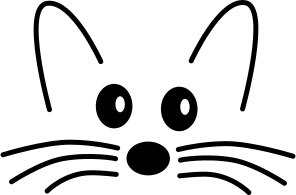
\includegraphics[width=1.4em]{squeak-logo}}}
\iftoshelse{
	\usepackage{marginnote}
		\renewcommand*{\marginfont}{\footnotesize}
	\newcommand{\vartriangleout}{\ifthenelse{\isodd{\thepage}}{\vartriangleright}{\vartriangleleft}}
	\newcommand{\dothisicon}{\fcolorbox{blue!65}{white}{\highlight{$\vartriangleout$}}}
	\newcommand{\dothis}[1]{%
		\noindent\par\noindent
		{\reversemarginpar
			\marginnote{\fcolorbox{blue!65}{white}{\highlight{$\vartriangleout$}}}}
		%\MarginLabel{do this}
		\noindent\emph{#1}
		\nopagebreak}
}{
	\newcommand{\dothisicon}{\raisebox{-.5ex}{
\includegraphics[height=1.2em]{pharo}}}
	\newcommand{\dothis}[1]{%
		\medskip
		\noindent\dothisicon
		\ifx#1\empty\else\quad\emph{#1}\fi
		\par\smallskip\nopagebreak}
}
%===> NEW VERSION <===
% NB: To use this in an individual chapter, you must set:
%\graphicspath{{figures/} {../figures/}}
% at the head of the chapter.  Don't forget the final /
%=============================================================
%:Reader hints (hint)
%
% Indicates a non-obvious consequence 
\newcommand{\hint}[1]{\vspace{1ex}\noindent\fbox{\textsc{Hint}} \emph{#1}}
%=================================================================
% graphics for Morphic handles
\newcommand{\grabHandle}{\raisebox{-0.2ex}{
\includegraphics[width=1em]{blackHandle}}}
\newcommand{\moveHandle}{\raisebox{-0.2ex}{
\includegraphics[width=1em]{moveHandle}}}
\newcommand{\debugHandle}{\raisebox{-0.2ex}{
\includegraphics[width=1em]{debugHandle}}}
%=============================================================
%:Highlighting Important stuff (doublebox)
%
% From Seaside book ...
\newsavebox{\SavedText}
\newlength{\InnerBoxRule}\setlength{\InnerBoxRule}{.75\fboxrule}
\newlength{\OuterBoxRule}\setlength{\OuterBoxRule}{1.5\fboxrule}
\newlength{\BoxSeparation}\setlength{\BoxSeparation}{1.5\fboxrule}
\addtolength{\BoxSeparation}{.5pt}
\newlength{\SaveBoxSep}\setlength{\SaveBoxSep}{2\fboxsep}
%
\newenvironment{doublebox}{\begin{lrbox}{\SavedText}
    \begin{minipage}{.75\textwidth}}
    {\end{minipage}\end{lrbox}\begin{center}
    \setlength{\fboxsep}{\BoxSeparation}\setlength{\fboxrule}{\OuterBoxRule}
    \fbox{\setlength{\fboxsep}{\SaveBoxSep}\setlength{\fboxrule}{\InnerBoxRule}%
      \fbox{\usebox{\SavedText}}}
  \end{center}}
% Use this:
\newcommand{\important}[1]{\begin{doublebox}#1\end{doublebox}}
%=============================================================
%:Section depth
\setcounter{secnumdepth}{2}
%% for this to happen start the file with
%\ifx\wholebook\relax\else
%% $Author$
% $Date$
% $Revision$

% HISTORY:
% 2006-10-31 - Oscar code macros
% ...

%=============================================================
% NB: documentclass must be set in main document.
% Allows book to be generated in multiple formats.
%=============================================================
%:Packages
\usepackage[T1]{fontenc}  %%%%%% really important to get the code directly in the text!
\usepackage{lmodern}
%\usepackage[scaled=0.85]{bookmanx} % needs another scale factor if used with \renewcommand{\sfdefault}{cmbr}
\usepackage{palatino}
\usepackage[scaled=0.85]{helvet}
\usepackage[protrusion,expansion=false]{microtype}
\usepackage{graphicx}
\usepackage{theorem}
\usepackage[english]{babel}
%%% ON: pdfsync breaks the use of p{width} for tabular columns!
%%\ifdefined\usepdfsync\usepackage{pdfsync}\fi % Requires texlive 2007
%=============================================================
%:More packages
%Stef should check which ones are used!
%\usepackage{picinpar}
%\usepackage{layout}
%\usepackage{color}
%\usepackage{enum}
%\usepackage{a4wide}
% \usepackage{fancyhdr}
\usepackage{ifthen}
\usepackage{float}
\usepackage{longtable}
\usepackage{makeidx}
\usepackage[nottoc]{tocbibind}
\usepackage{multicol}
\usepackage{booktabs}	% book-style tables
\usepackage{topcapt}	% enables \topcaption
\usepackage{multirow}
\usepackage{tabularx}
%\usepackage[bottom]{footmisc}
\usepackage{xspace}
\usepackage{alltt}
\usepackage{amssymb,textcomp}
\usepackage[usenames,dvipsnames]{color}
%\usepackage{colortbl}
\usepackage[hang]{subfigure}\makeatletter\def\p@subfigure{\thefigure\,}\makeatother
\usepackage{rotating}
\usepackage{enumitem}	% apb: allows more control over tags in enumerations
\usepackage{verbatim}     % for comment environment
\usepackage{varioref}	% for page references that work
\labelformat{footnote}{\thechapter--#1} % to distinguish citations from jurabib
\usepackage{needspace}
\usepackage{isodateo} % enable \isodate
\usepackage[newparttoc]{titlesec}
\usepackage{titletoc}
\usepackage{wrapfig}
\usepackage[
	super,
	citefull=first,
	authorformat={allreversed,and},
	titleformat={commasep,italic}
]{jurabib} % citations as footnotes
\usepackage[
	colorlinks=true,
	linkcolor=black,
	urlcolor=black,
	citecolor=black
]{hyperref}   % should come last
%=============================================================
%:PDF version
%%\pdfminorversion=3 % Set PDF to 1.3 for Lulu
%=============================================================
%:URL style
\makeatletter
\def\url@leostyle{%
  \@ifundefined{selectfont}{\def\UrlFont{\sf}}{\def\UrlFont{\sffamily}}}
\makeatother
% Now actually use the newly defined style.
\urlstyle{leo}
%=============================================================
%:Booleans
\newboolean{lulu}
\setboolean{lulu}{false}
\newcommand{\ifluluelse}[2]{\ifthenelse{\boolean{lulu}}{#1}{#2}}
%=============================================================
%:Names
\newcommand{\SUnit}{SUnit\xspace}
\newcommand{\sunit}{SUnit\xspace}
\newcommand{\xUnit}{$x$Unit\xspace}
\newcommand{\JUnit}{JUnit\xspace}
\newcommand{\st}{Smalltalk\xspace}
\newcommand{\pharo}{Pharo\xspace} % Use this, not \Pharo
%\newcommand{\sqmap}{SqueakMap\xspace}
\newcommand{\squeak}{Squeak\xspace} % use this, not \Squeak or \sq
\newcommand{\sqsrc}{SqueakSource\xspace}
\newcommand{\sbe}{\url{http://SqueakByExample.org}\xspace}
\newcommand{\pharoweb}{\url{http://pharo-project.org}\xspace}
\newcommand{\pbe}{\url{http://PharoByExample.org}\xspace}
\newcommand{\sba}{\url{http://SquareBracketAssociates.org}\xspace}
\newcommand{\bam}{\lct{Bounc\-ing\-Atoms\-Morph}\xspace}
%=============================================================
%:Markup macros for proof-reading
\usepackage[normalem]{ulem} % for \sout
\usepackage{xcolor}
\newcommand{\ra}{$\rightarrow$}
\newcommand{\ugh}[1]{\textcolor{red}{\uwave{#1}}} % please rephrase
\newcommand{\ins}[1]{\textcolor{blue}{\uline{#1}}} % please insert
\newcommand{\del}[1]{\textcolor{red}{\sout{#1}}} % please delete
\newcommand{\chg}[2]{\textcolor{red}{\sout{#1}}{\ra}\textcolor{blue}{\uline{#2}}} % please change
%=============================================================
%:Editorial comment macros
%\newcommand{\nnbb}[2]{
%    % \fbox{\bfseries\sffamily\scriptsize#1}
%    \fcolorbox{gray}{yellow}{\bfseries\sffamily\scriptsize#1}
%    {\sf\small$\blacktriangleright$\textit{#2}$\blacktriangleleft$}
%   }
\newcommand{\yellowbox}[1]{\fcolorbox{gray}{yellow}{\bfseries\sffamily\scriptsize#1}}
\newcommand{\triangles}[1]{{\sf\small$\blacktriangleright$\textit{#1}$\blacktriangleleft$}}
\newcommand{\nnbb}[2]{\yellowbox{#1} \triangles{#2}}
\newcommand{\fix}{\yellowbox{FIX!}}
\newcommand{\here}{\yellowbox{CONTINUE HERE!}}
% editor macros
\newcommand{\apl}[1]{\nnbb{Alain}{#1}} % Alain
\newcommand{\ab}[1]{\nnbb{Andrew}{#1}} % Black
\newcommand{\sd}[1]{\nnbb{St\'{e}f}{#1}} % Ducasse
\newcommand{\dc}[1]{\nnbb{DamienC}{#1}} % Ducasse
\newcommand{\md}[1]{\nnbb{Marcus}{#1}} % Denker
\newcommand{\on}[1]{\nnbb{Oscar}{#1}} % Nierstrasz
\newcommand{\damien}[1]{\nnbb{Damien}{#1}} % Pollet
\newcommand{\lr}[1]{\nnbb{Lukas}{#1}} % Renggli
\newcommand{\orla}[1]{\nnbb{Orla}{#1}} % Greevy
\newcommand{\alex}[1]{\nnbb{Alex}{#1}} % Bergel
\newcommand{\alx}[1]{\nnbb{Alex}{#1}} % Bergel
\newcommand{\dr}[1]{\nnbb{David}{#1}} % Roethlisberger
\newcommand{\ja}[1]{\nnbb{Jannik}{#1}} % Laval
\newcommand{\jr}[1]{\nnbb{Jorge}{#1}} % Ressia
\newcommand{\fp}[1]{\nnbb{Fabrizio}{#1}} % Perin
\newcommand{\michael}[1]{\nnbb{Michael}{#1}} % Davies
\newcommand{\ew}[1]{\nnbb{Erwann}{#1}} % Wernli
\newcommand{\mb}[1]{\nnbb{Martial}{#1}} % Boniou
\newcommand{\hw}[1]{\nnbb{Hernan}{#1}} % Wilkinson
%=============================================================
%:Abbreviation macros
\newcommand{\ie}{\emph{すなわち}、}
\newcommand{\eg}{\emph{例えば}、}
\newcommand{\etc}{などなど。}
%=============================================================
%:Cross reference macros
\newcommand{\charef}[1]{第~\ref{cha:#1}~章}
\newcommand{\secref}[1]{\ref{sec:#1}~節}
\newcommand{\figref}[1]{図~\ref{fig:#1}\xspace}
\newcommand{\Figref}[1]{図~\ref{fig:#1}\xspace}
\newcommand{\appref}[1]{付録~\ref{app:#1}\xspace}
\newcommand{\tabref}[1]{表~\ref{tab:#1}\xspace}
\newcommand{\faqref}[1]{FAQ~\ref{faq:#1}, p.~\pageref{faq:#1}\xspace}
% APB: I removed trailing \xspace commands from these macros because
% \xspace mostly doesn't work.  If you want a space after your
% references, type one!
% ON: xspace has always worked just fine for me!  Please leave them in.
%
\newcommand{\ruleref}[1]{\ref{rule:#1}\xspace}
%
\newcommand{\egref}[1]{example~\ref{eg:#1}\xspace}
\newcommand{\Egref}[1]{Example~\ref{eg:#1}\xspace}
%
\newcommand{\scrref}[1]{script~\ref{scr:#1}\xspace}
\newcommand{\Scrref}[1]{Script~\ref{scr:#1}\xspace}
\newcommand{\tscrref}[1]{the script~\ref{scr:#1}\xspace}
\newcommand{\Tscrref}[1]{The script~\ref{scr:#1}\xspace}
%
\newcommand{\mthref}[1]{method~\ref{mth:#1}\xspace}
\newcommand{\mthsref}[1]{methods~\ref{mth:#1}\xspace}
\newcommand{\Mthref}[1]{Method~\ref{mth:#1}\xspace}
\newcommand{\tmthref}[1]{the method~\ref{mth:#1}\xspace}
\newcommand{\Tmthref}[1]{The method~\ref{mth:#1}\xspace}
%
\newcommand{\clsref}[1]{class~\ref{cls:#1}\xspace}
\newcommand{\tclsref}[1]{the class~\ref{cls:#1}\xspace}
\newcommand{\Tclsref}[1]{The class~\ref{cls:#1}\xspace}

\newcommand{\chalabel}[1]{\label{cha:#1}}
\newcommand{\seclabel}[1]{\label{sec:#1}}
\newcommand{\figlabel}[1]{\label{fig:#1}}
\newcommand{\tablabel}[1]{\label{tab:#1}}
\newcommand{\rulelabel}[1]{\label{rule:#1}}
\newcommand{\eglabel}[1]{\label{eg:#1}}
\newcommand{\scrlabel}[1]{\label{scr:#1}}
\newcommand{\mthlabel}[1]{\label{mth:#1}}
\newcommand{\clslabel}[1]{\label{cls:#1}}
\newcommand{\faqlabel}[1]{\label{faq:#1}}
%=============================================================
%:Menu item macro
% for menu items, so we can change our minds on how to print them! (apb)
\definecolor{lightgray}{gray}{0.89}
\newcommand{\menu}[1]{{%
	\setlength{\fboxsep}{0pt}%
	\colorbox{lightgray}{{{\upshape\sffamily\strut \,#1\,}}}}}
\newcommand{\link}[1]{{%
	\fontfamily{lmr}\selectfont
 	\upshape{\sffamily \underline{#1}}}}
% For submenu items:
\newcommand{\go}{\,$\triangleright$\,}
% \newcommand{\go}{\,$\blacktriangleright$\,}
% For keyboard shortcuts:
%\newcommand{\short}[1]{\mbox{$\langle${\sc CMD}$\rangle$-#1}\xspace}
\newcommand{\short}[1]{\mbox{{\sc cmd}\hspace{0.08em}--\hspace{0.09em}#1}\xspace}
% For buttons:
\newcommand{\button}[1]{{%
	\setlength{\fboxsep}{0pt}%
	\fbox{{\upshape\sffamily\strut \,#1\,}}}}
% NB: The button macro does not work within captions -- incompatible with xcolor package :-(
\newcommand{\toolsflap}{\textit{Tools} flap\xspace}
%=============================================================
%:Mouse clicks
\newcommand{\click}{click\xspace} % RED
\newcommand{\actclick}{action-click\xspace} % YELLOW
\newcommand{\metaclick}{meta-click\xspace} % BLUE
\newcommand{\Click}{Click\xspace} % RED
\newcommand{\Actclick}{Action-click\xspace} % YELLOW
\newcommand{\Metaclick}{Meta-click\xspace} % BLUE
%=============================================================
%:ToSh macros
\newboolean{tosh}
\setboolean{tosh}{false}
\newcommand{\iftoshelse}[2]{\ifthenelse{\boolean{tosh}}{#1}{#2}}
%=============================================================
%:ToSh colors
%\newcommand{\highlightcolor}{\color{blue!65}}
%\newcommand{\boxcolor}{\color{gray!25}}
\newcommand{\highlight}[1]{\textcolor{blue!65}{#1}}
%\newcommand{\codecolor}{\color{blue!65}}
%%\setlength{\fboxrule}{2pt}
%\newcommand{\asPict}[1]{%
%	{\Large\highlight{#1}}}
%=============================================================
%:Reader cues (do this)
%
% Indicate something the reader should try out.
% \newcommand{\dothisicon}{\raisebox{-.5ex}{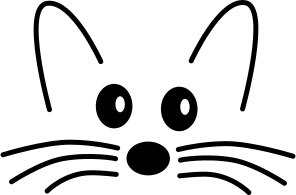
\includegraphics[width=1.4em]{squeak-logo}}}
\iftoshelse{
	\usepackage{marginnote}
		\renewcommand*{\marginfont}{\footnotesize}
	\newcommand{\vartriangleout}{\ifthenelse{\isodd{\thepage}}{\vartriangleright}{\vartriangleleft}}
	\newcommand{\dothisicon}{\fcolorbox{blue!65}{white}{\highlight{$\vartriangleout$}}}
	\newcommand{\dothis}[1]{%
		\noindent\par\noindent
		{\reversemarginpar
			\marginnote{\fcolorbox{blue!65}{white}{\highlight{$\vartriangleout$}}}}
		%\MarginLabel{do this}
		\noindent\emph{#1}
		\nopagebreak}
}{
	\newcommand{\dothisicon}{\raisebox{-.5ex}{
\includegraphics[height=1.2em]{pharo}}}
	\newcommand{\dothis}[1]{%
		\medskip
		\noindent\dothisicon
		\ifx#1\empty\else\quad\emph{#1}\fi
		\par\smallskip\nopagebreak}
}
%===> NEW VERSION <===
% NB: To use this in an individual chapter, you must set:
%\graphicspath{{figures/} {../figures/}}
% at the head of the chapter.  Don't forget the final /
%=============================================================
%:Reader hints (hint)
%
% Indicates a non-obvious consequence 
\newcommand{\hint}[1]{\vspace{1ex}\noindent\fbox{\textsc{Hint}} \emph{#1}}
%=================================================================
% graphics for Morphic handles
\newcommand{\grabHandle}{\raisebox{-0.2ex}{
\includegraphics[width=1em]{blackHandle}}}
\newcommand{\moveHandle}{\raisebox{-0.2ex}{
\includegraphics[width=1em]{moveHandle}}}
\newcommand{\debugHandle}{\raisebox{-0.2ex}{
\includegraphics[width=1em]{debugHandle}}}
%=============================================================
%:Highlighting Important stuff (doublebox)
%
% From Seaside book ...
\newsavebox{\SavedText}
\newlength{\InnerBoxRule}\setlength{\InnerBoxRule}{.75\fboxrule}
\newlength{\OuterBoxRule}\setlength{\OuterBoxRule}{1.5\fboxrule}
\newlength{\BoxSeparation}\setlength{\BoxSeparation}{1.5\fboxrule}
\addtolength{\BoxSeparation}{.5pt}
\newlength{\SaveBoxSep}\setlength{\SaveBoxSep}{2\fboxsep}
%
\newenvironment{doublebox}{\begin{lrbox}{\SavedText}
    \begin{minipage}{.75\textwidth}}
    {\end{minipage}\end{lrbox}\begin{center}
    \setlength{\fboxsep}{\BoxSeparation}\setlength{\fboxrule}{\OuterBoxRule}
    \fbox{\setlength{\fboxsep}{\SaveBoxSep}\setlength{\fboxrule}{\InnerBoxRule}%
      \fbox{\usebox{\SavedText}}}
  \end{center}}
% Use this:
\newcommand{\important}[1]{\begin{doublebox}#1\end{doublebox}}
%=============================================================
%:Section depth
\setcounter{secnumdepth}{2}
%% for this to happen start the file with
%\ifx\wholebook\relax\else
%% $Author$
% $Date$
% $Revision$

% HISTORY:
% 2006-10-31 - Oscar code macros
% ...

%=============================================================
% NB: documentclass must be set in main document.
% Allows book to be generated in multiple formats.
%=============================================================
%:Packages
\usepackage[T1]{fontenc}  %%%%%% really important to get the code directly in the text!
\usepackage{lmodern}
%\usepackage[scaled=0.85]{bookmanx} % needs another scale factor if used with \renewcommand{\sfdefault}{cmbr}
\usepackage{palatino}
\usepackage[scaled=0.85]{helvet}
\usepackage[protrusion,expansion=false]{microtype}
\usepackage{graphicx}
\usepackage{theorem}
\usepackage[english]{babel}
%%% ON: pdfsync breaks the use of p{width} for tabular columns!
%%\ifdefined\usepdfsync\usepackage{pdfsync}\fi % Requires texlive 2007
%=============================================================
%:More packages
%Stef should check which ones are used!
%\usepackage{picinpar}
%\usepackage{layout}
%\usepackage{color}
%\usepackage{enum}
%\usepackage{a4wide}
% \usepackage{fancyhdr}
\usepackage{ifthen}
\usepackage{float}
\usepackage{longtable}
\usepackage{makeidx}
\usepackage[nottoc]{tocbibind}
\usepackage{multicol}
\usepackage{booktabs}	% book-style tables
\usepackage{topcapt}	% enables \topcaption
\usepackage{multirow}
\usepackage{tabularx}
%\usepackage[bottom]{footmisc}
\usepackage{xspace}
\usepackage{alltt}
\usepackage{amssymb,textcomp}
\usepackage[usenames,dvipsnames]{color}
%\usepackage{colortbl}
\usepackage[hang]{subfigure}\makeatletter\def\p@subfigure{\thefigure\,}\makeatother
\usepackage{rotating}
\usepackage{enumitem}	% apb: allows more control over tags in enumerations
\usepackage{verbatim}     % for comment environment
\usepackage{varioref}	% for page references that work
\labelformat{footnote}{\thechapter--#1} % to distinguish citations from jurabib
\usepackage{needspace}
\usepackage{isodateo} % enable \isodate
\usepackage[newparttoc]{titlesec}
\usepackage{titletoc}
\usepackage{wrapfig}
\usepackage[
	super,
	citefull=first,
	authorformat={allreversed,and},
	titleformat={commasep,italic}
]{jurabib} % citations as footnotes
\usepackage[
	colorlinks=true,
	linkcolor=black,
	urlcolor=black,
	citecolor=black
]{hyperref}   % should come last
%=============================================================
%:PDF version
%%\pdfminorversion=3 % Set PDF to 1.3 for Lulu
%=============================================================
%:URL style
\makeatletter
\def\url@leostyle{%
  \@ifundefined{selectfont}{\def\UrlFont{\sf}}{\def\UrlFont{\sffamily}}}
\makeatother
% Now actually use the newly defined style.
\urlstyle{leo}
%=============================================================
%:Booleans
\newboolean{lulu}
\setboolean{lulu}{false}
\newcommand{\ifluluelse}[2]{\ifthenelse{\boolean{lulu}}{#1}{#2}}
%=============================================================
%:Names
\newcommand{\SUnit}{SUnit\xspace}
\newcommand{\sunit}{SUnit\xspace}
\newcommand{\xUnit}{$x$Unit\xspace}
\newcommand{\JUnit}{JUnit\xspace}
\newcommand{\st}{Smalltalk\xspace}
\newcommand{\pharo}{Pharo\xspace} % Use this, not \Pharo
%\newcommand{\sqmap}{SqueakMap\xspace}
\newcommand{\squeak}{Squeak\xspace} % use this, not \Squeak or \sq
\newcommand{\sqsrc}{SqueakSource\xspace}
\newcommand{\sbe}{\url{http://SqueakByExample.org}\xspace}
\newcommand{\pharoweb}{\url{http://pharo-project.org}\xspace}
\newcommand{\pbe}{\url{http://PharoByExample.org}\xspace}
\newcommand{\sba}{\url{http://SquareBracketAssociates.org}\xspace}
\newcommand{\bam}{\lct{Bounc\-ing\-Atoms\-Morph}\xspace}
%=============================================================
%:Markup macros for proof-reading
\usepackage[normalem]{ulem} % for \sout
\usepackage{xcolor}
\newcommand{\ra}{$\rightarrow$}
\newcommand{\ugh}[1]{\textcolor{red}{\uwave{#1}}} % please rephrase
\newcommand{\ins}[1]{\textcolor{blue}{\uline{#1}}} % please insert
\newcommand{\del}[1]{\textcolor{red}{\sout{#1}}} % please delete
\newcommand{\chg}[2]{\textcolor{red}{\sout{#1}}{\ra}\textcolor{blue}{\uline{#2}}} % please change
%=============================================================
%:Editorial comment macros
%\newcommand{\nnbb}[2]{
%    % \fbox{\bfseries\sffamily\scriptsize#1}
%    \fcolorbox{gray}{yellow}{\bfseries\sffamily\scriptsize#1}
%    {\sf\small$\blacktriangleright$\textit{#2}$\blacktriangleleft$}
%   }
\newcommand{\yellowbox}[1]{\fcolorbox{gray}{yellow}{\bfseries\sffamily\scriptsize#1}}
\newcommand{\triangles}[1]{{\sf\small$\blacktriangleright$\textit{#1}$\blacktriangleleft$}}
\newcommand{\nnbb}[2]{\yellowbox{#1} \triangles{#2}}
\newcommand{\fix}{\yellowbox{FIX!}}
\newcommand{\here}{\yellowbox{CONTINUE HERE!}}
% editor macros
\newcommand{\apl}[1]{\nnbb{Alain}{#1}} % Alain
\newcommand{\ab}[1]{\nnbb{Andrew}{#1}} % Black
\newcommand{\sd}[1]{\nnbb{St\'{e}f}{#1}} % Ducasse
\newcommand{\dc}[1]{\nnbb{DamienC}{#1}} % Ducasse
\newcommand{\md}[1]{\nnbb{Marcus}{#1}} % Denker
\newcommand{\on}[1]{\nnbb{Oscar}{#1}} % Nierstrasz
\newcommand{\damien}[1]{\nnbb{Damien}{#1}} % Pollet
\newcommand{\lr}[1]{\nnbb{Lukas}{#1}} % Renggli
\newcommand{\orla}[1]{\nnbb{Orla}{#1}} % Greevy
\newcommand{\alex}[1]{\nnbb{Alex}{#1}} % Bergel
\newcommand{\alx}[1]{\nnbb{Alex}{#1}} % Bergel
\newcommand{\dr}[1]{\nnbb{David}{#1}} % Roethlisberger
\newcommand{\ja}[1]{\nnbb{Jannik}{#1}} % Laval
\newcommand{\jr}[1]{\nnbb{Jorge}{#1}} % Ressia
\newcommand{\fp}[1]{\nnbb{Fabrizio}{#1}} % Perin
\newcommand{\michael}[1]{\nnbb{Michael}{#1}} % Davies
\newcommand{\ew}[1]{\nnbb{Erwann}{#1}} % Wernli
\newcommand{\mb}[1]{\nnbb{Martial}{#1}} % Boniou
\newcommand{\hw}[1]{\nnbb{Hernan}{#1}} % Wilkinson
%=============================================================
%:Abbreviation macros
\newcommand{\ie}{\emph{すなわち}、}
\newcommand{\eg}{\emph{例えば}、}
\newcommand{\etc}{などなど。}
%=============================================================
%:Cross reference macros
\newcommand{\charef}[1]{第~\ref{cha:#1}~章}
\newcommand{\secref}[1]{\ref{sec:#1}~節}
\newcommand{\figref}[1]{図~\ref{fig:#1}\xspace}
\newcommand{\Figref}[1]{図~\ref{fig:#1}\xspace}
\newcommand{\appref}[1]{付録~\ref{app:#1}\xspace}
\newcommand{\tabref}[1]{表~\ref{tab:#1}\xspace}
\newcommand{\faqref}[1]{FAQ~\ref{faq:#1}, p.~\pageref{faq:#1}\xspace}
% APB: I removed trailing \xspace commands from these macros because
% \xspace mostly doesn't work.  If you want a space after your
% references, type one!
% ON: xspace has always worked just fine for me!  Please leave them in.
%
\newcommand{\ruleref}[1]{\ref{rule:#1}\xspace}
%
\newcommand{\egref}[1]{example~\ref{eg:#1}\xspace}
\newcommand{\Egref}[1]{Example~\ref{eg:#1}\xspace}
%
\newcommand{\scrref}[1]{script~\ref{scr:#1}\xspace}
\newcommand{\Scrref}[1]{Script~\ref{scr:#1}\xspace}
\newcommand{\tscrref}[1]{the script~\ref{scr:#1}\xspace}
\newcommand{\Tscrref}[1]{The script~\ref{scr:#1}\xspace}
%
\newcommand{\mthref}[1]{method~\ref{mth:#1}\xspace}
\newcommand{\mthsref}[1]{methods~\ref{mth:#1}\xspace}
\newcommand{\Mthref}[1]{Method~\ref{mth:#1}\xspace}
\newcommand{\tmthref}[1]{the method~\ref{mth:#1}\xspace}
\newcommand{\Tmthref}[1]{The method~\ref{mth:#1}\xspace}
%
\newcommand{\clsref}[1]{class~\ref{cls:#1}\xspace}
\newcommand{\tclsref}[1]{the class~\ref{cls:#1}\xspace}
\newcommand{\Tclsref}[1]{The class~\ref{cls:#1}\xspace}

\newcommand{\chalabel}[1]{\label{cha:#1}}
\newcommand{\seclabel}[1]{\label{sec:#1}}
\newcommand{\figlabel}[1]{\label{fig:#1}}
\newcommand{\tablabel}[1]{\label{tab:#1}}
\newcommand{\rulelabel}[1]{\label{rule:#1}}
\newcommand{\eglabel}[1]{\label{eg:#1}}
\newcommand{\scrlabel}[1]{\label{scr:#1}}
\newcommand{\mthlabel}[1]{\label{mth:#1}}
\newcommand{\clslabel}[1]{\label{cls:#1}}
\newcommand{\faqlabel}[1]{\label{faq:#1}}
%=============================================================
%:Menu item macro
% for menu items, so we can change our minds on how to print them! (apb)
\definecolor{lightgray}{gray}{0.89}
\newcommand{\menu}[1]{{%
	\setlength{\fboxsep}{0pt}%
	\colorbox{lightgray}{{{\upshape\sffamily\strut \,#1\,}}}}}
\newcommand{\link}[1]{{%
	\fontfamily{lmr}\selectfont
 	\upshape{\sffamily \underline{#1}}}}
% For submenu items:
\newcommand{\go}{\,$\triangleright$\,}
% \newcommand{\go}{\,$\blacktriangleright$\,}
% For keyboard shortcuts:
%\newcommand{\short}[1]{\mbox{$\langle${\sc CMD}$\rangle$-#1}\xspace}
\newcommand{\short}[1]{\mbox{{\sc cmd}\hspace{0.08em}--\hspace{0.09em}#1}\xspace}
% For buttons:
\newcommand{\button}[1]{{%
	\setlength{\fboxsep}{0pt}%
	\fbox{{\upshape\sffamily\strut \,#1\,}}}}
% NB: The button macro does not work within captions -- incompatible with xcolor package :-(
\newcommand{\toolsflap}{\textit{Tools} flap\xspace}
%=============================================================
%:Mouse clicks
\newcommand{\click}{click\xspace} % RED
\newcommand{\actclick}{action-click\xspace} % YELLOW
\newcommand{\metaclick}{meta-click\xspace} % BLUE
\newcommand{\Click}{Click\xspace} % RED
\newcommand{\Actclick}{Action-click\xspace} % YELLOW
\newcommand{\Metaclick}{Meta-click\xspace} % BLUE
%=============================================================
%:ToSh macros
\newboolean{tosh}
\setboolean{tosh}{false}
\newcommand{\iftoshelse}[2]{\ifthenelse{\boolean{tosh}}{#1}{#2}}
%=============================================================
%:ToSh colors
%\newcommand{\highlightcolor}{\color{blue!65}}
%\newcommand{\boxcolor}{\color{gray!25}}
\newcommand{\highlight}[1]{\textcolor{blue!65}{#1}}
%\newcommand{\codecolor}{\color{blue!65}}
%%\setlength{\fboxrule}{2pt}
%\newcommand{\asPict}[1]{%
%	{\Large\highlight{#1}}}
%=============================================================
%:Reader cues (do this)
%
% Indicate something the reader should try out.
% \newcommand{\dothisicon}{\raisebox{-.5ex}{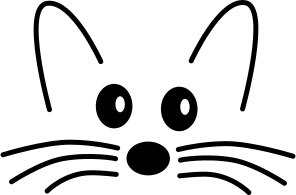
\includegraphics[width=1.4em]{squeak-logo}}}
\iftoshelse{
	\usepackage{marginnote}
		\renewcommand*{\marginfont}{\footnotesize}
	\newcommand{\vartriangleout}{\ifthenelse{\isodd{\thepage}}{\vartriangleright}{\vartriangleleft}}
	\newcommand{\dothisicon}{\fcolorbox{blue!65}{white}{\highlight{$\vartriangleout$}}}
	\newcommand{\dothis}[1]{%
		\noindent\par\noindent
		{\reversemarginpar
			\marginnote{\fcolorbox{blue!65}{white}{\highlight{$\vartriangleout$}}}}
		%\MarginLabel{do this}
		\noindent\emph{#1}
		\nopagebreak}
}{
	\newcommand{\dothisicon}{\raisebox{-.5ex}{
\includegraphics[height=1.2em]{pharo}}}
	\newcommand{\dothis}[1]{%
		\medskip
		\noindent\dothisicon
		\ifx#1\empty\else\quad\emph{#1}\fi
		\par\smallskip\nopagebreak}
}
%===> NEW VERSION <===
% NB: To use this in an individual chapter, you must set:
%\graphicspath{{figures/} {../figures/}}
% at the head of the chapter.  Don't forget the final /
%=============================================================
%:Reader hints (hint)
%
% Indicates a non-obvious consequence 
\newcommand{\hint}[1]{\vspace{1ex}\noindent\fbox{\textsc{Hint}} \emph{#1}}
%=================================================================
% graphics for Morphic handles
\newcommand{\grabHandle}{\raisebox{-0.2ex}{
\includegraphics[width=1em]{blackHandle}}}
\newcommand{\moveHandle}{\raisebox{-0.2ex}{
\includegraphics[width=1em]{moveHandle}}}
\newcommand{\debugHandle}{\raisebox{-0.2ex}{
\includegraphics[width=1em]{debugHandle}}}
%=============================================================
%:Highlighting Important stuff (doublebox)
%
% From Seaside book ...
\newsavebox{\SavedText}
\newlength{\InnerBoxRule}\setlength{\InnerBoxRule}{.75\fboxrule}
\newlength{\OuterBoxRule}\setlength{\OuterBoxRule}{1.5\fboxrule}
\newlength{\BoxSeparation}\setlength{\BoxSeparation}{1.5\fboxrule}
\addtolength{\BoxSeparation}{.5pt}
\newlength{\SaveBoxSep}\setlength{\SaveBoxSep}{2\fboxsep}
%
\newenvironment{doublebox}{\begin{lrbox}{\SavedText}
    \begin{minipage}{.75\textwidth}}
    {\end{minipage}\end{lrbox}\begin{center}
    \setlength{\fboxsep}{\BoxSeparation}\setlength{\fboxrule}{\OuterBoxRule}
    \fbox{\setlength{\fboxsep}{\SaveBoxSep}\setlength{\fboxrule}{\InnerBoxRule}%
      \fbox{\usebox{\SavedText}}}
  \end{center}}
% Use this:
\newcommand{\important}[1]{\begin{doublebox}#1\end{doublebox}}
%=============================================================
%:Section depth
\setcounter{secnumdepth}{2}
%% for this to happen start the file with
%\ifx\wholebook\relax\else
%\input{../common.tex}
%\begin{document}
%\fi
% and terminate by
% \ifx\wholebook\relax\else\end{document}\fi

\DeclareGraphicsExtensions{.pdf, .jpg, .png}
%=============================================================
%:PDF setup
\hypersetup{
%   a4paper,
%   pdfstartview=FitV,
%   colorlinks,
%   linkcolor=darkblue,
%   citecolor=darkblue,
   pdftitle={Pharo by Example},
   pdfauthor={Andrew P. Black, St\'ephane Ducasse,	Oscar Nierstrasz,
Damien Pollet},
   pdfkeywords={Smalltalk, Squeak, Object-Oriented Programming, OOP},
   pdfsubject={Computer Science}
}
%=============================================================
%:Page layout and appearance
%
% \renewcommand{\headrulewidth}{0pt}
\renewcommand{\chaptermark}[1]{\markboth{#1}{}}
\renewcommand{\sectionmark}[1]{\markright{\thesection\ #1}}
\renewpagestyle{plain}[\small\itshape]{%
	\setheadrule{0pt}%
	\sethead[][][]{}{}{}%
	\setfoot[][][]{}{}{}}
\renewpagestyle{headings}[\small\itshape]{%
	\setheadrule{0pt}%
	\setmarks{chapter}{section}%
	\sethead[\thepage][][\chaptertitle]{\sectiontitle}{}{\thepage}%
	\setfoot[][][]{}{}{}}
%=============================================================
%:Title section setup and TOC numbering depth
\setcounter{secnumdepth}{1}
\setcounter{tocdepth}{1}
\titleformat{\part}[display]{\centering}{\huge\partname\ \thepart}{1em}{\Huge\textbf}[]
\titleformat{\chapter}[display]{}{\huge\chaptertitlename\ \thechapter}{1em}{\Huge\raggedright\textbf}[]
\titlecontents{part}[3pc]{%
		\pagebreak[2]\addvspace{1em plus.4em minus.2em}%
		\leavevmode\large\bfseries}
	{\contentslabel{3pc}}{\hspace*{-3pc}}
	{}[\nopagebreak]
\titlecontents{chapter}[3pc]{%
		\pagebreak[0]\addvspace{1em plus.2em minus.2em}%
		\leavevmode\bfseries}
	{\contentslabel{3pc}}{}
	{\hfill\contentspage}[\nopagebreak]
\dottedcontents{section}[3pc]{}{3pc}{1pc}
\dottedcontents{subsection}[3pc]{}{0pc}{1pc}
% \dottedcontents{subsection}[4.5em]{}{0pt}{1pc}
% Make \cleardoublepage insert really blank pages http://www.tex.ac.uk/cgi-bin/texfaq2html?label=reallyblank
\let\origdoublepage\cleardoublepage
\newcommand{\clearemptydoublepage}{%
  \clearpage
  {\pagestyle{empty}\origdoublepage}}
\let\cleardoublepage\clearemptydoublepage % see http://www.tex.ac.uk/cgi-bin/texfaq2html?label=patch
%=============================================================
%:FAQ macros (for FAQ chapter)
\newtheorem{faq}{FAQ}
\newcommand{\answer}{\paragraph{Answer}\ }
%=============================================================
%:Listings package configuration
% \newcommand{\caret}{\makebox{\raisebox{0.4ex}{\footnotesize{$\wedge$}}}}
\newcommand{\caret}{\^\,}
\newcommand{\escape}{{\sf \textbackslash}}
\definecolor{source}{gray}{0.95}
\usepackage{listings}
\lstdefinelanguage{Smalltalk}{
%  morekeywords={self,super,true,false,nil,thisContext}, % This is overkill
  morestring=[d]',
  morecomment=[s]{"}{"},
  alsoletter={\#:},
  escapechar={!},
  literate=
    {BANG}{!}1
    {CARET}{\^}1
    {UNDERSCORE}{\_}1
    {\\st}{Smalltalk}9 % convenience -- in case \st occurs in code
    % {'}{{\textquotesingle}}1 % replaced by upquote=true in \lstset
    {_}{{$\leftarrow$}}1
    {>>>}{{\sep}}1
    {^}{{$\uparrow$}}1
    {~}{{$\sim$}}1
    {-}{{\texttt{-}}}1 %{\textminus}}1 %{-}{\hspace{-0.13em}}{-}}1  % the goal is to make - the same width as +
    % {+}{\sf+}1 %{\raisebox{0.08ex}{+}}}1      % and to raise + off the baseline to match -
    {-->}{{\quad$\longrightarrow$\quad}}3
	, % Don't forget the comma at the end!
  tabsize=4
}[keywords,comments,strings]

\lstset{language=Smalltalk,
	basicstyle=\sffamily,
	keywordstyle=\color{black}\bfseries,
	% stringstyle=\ttfamily, % Ugly! do we really want this? -- on
	mathescape=true,
	showstringspaces=false,
	keepspaces=true,
	breaklines=true,
	breakautoindent=true,
	backgroundcolor=\color{source},
	lineskip={-1pt}, % Ugly hack
	upquote=true, % straight quote; requires textcomp package
	columns=fullflexible} % no fixed width fonts
% In-line code (literal)
% Normally use this for all in-line code:
\newcommand{\ct}{\lstinline[mathescape=false,backgroundcolor=\color{white},basicstyle={\sffamily\upshape}]}
% apb 2007.8.28 added the \upshape declaration to avoid getting italicized code in \dothis{ } sections.
% In-line code (latex enabled)
% Use this only in special situations where \ct does not work
% (within section headings ...):
\newcommand{\lct}[1]{{\textsf{\textup{#1}}}}
% Use these for system categories and protocols:
\newcommand{\scat}[1]{\emph{\textsf{#1}}\xspace}
\newcommand{\pkg}[1]{\emph{\textsf{#1}}\xspace}
\newcommand{\prot}[1]{\emph{\textsf{#1}}\xspace}
% Code environments
% NB: the arg is for tests
% Only code and example environments may be tests
\lstnewenvironment{code}[1]{%
	\lstset{%
		% frame=lines,
		frame=single,
		framerule=0pt,
		mathescape=false
	}
}{}
\def\ignoredollar#1{}
%=============================================================
%:Code environments (method, script ...)
% NB: the third arg is for tests
% Only code and example environments may be tests
\lstnewenvironment{example}[3][defaultlabel]{%
	\renewcommand{\lstlistingname}{Example}%
	\lstset{
		% frame=lines,
		frame=single,
		framerule=0pt,
		mathescape=false,
		caption={\emph{#2}},
		label={eg:#1}
	}
}{}
\lstnewenvironment{script}[2][defaultlabel]{%
\renewcommand{\lstlistingname}{Script}%
	\lstset{
		% frame=lines,
		frame=single,
		framerule=0pt,
		mathescape=false,
		name={Script},
		caption={\emph{#2}},
		label={scr:#1}
	}
}{}
\lstnewenvironment{method}[2][defaultlabel]{%
	\renewcommand{\lstlistingname}{Method}%
	\lstset{
		% frame=lines,
		frame=single,
		framerule=0pt,
		mathescape=false,
		name={Method},
		caption={\emph{#2}},
		label={mth:#1}
	}
}{}
\lstnewenvironment{methods}[2][defaultlabel]{% just for multiple methods at once
	\renewcommand{\lstlistingname}{Methods}%
	\lstset{
		% frame=lines,
		frame=single,
		framerule=0pt,
		mathescape=false,
		name={Method},
		caption={\emph{#2}},
		label={mth:#1}
	}
}{}
\lstnewenvironment{numMethod}[2][defaultlabel]{%
	\renewcommand{\lstlistingname}{Method}%
	\lstset{
		numbers=left,
		numberstyle={\tiny\sffamily},
		% frame=lines,
		frame=single,
		framerule=0pt,
		mathescape=false,
		name={Method},
		caption={\emph{#2}},
		label={mth:#1}
	}
}{}
\lstnewenvironment{classdef}[2][defaultlabel]{%
	\renewcommand{\lstlistingname}{Class}%
	\lstset{
		% frame=lines,
		frame=single,
		framerule=0pt,
		mathescape=false,
		name={Class},
		caption={\emph{#2}},
		label={cls:#1}
	}
}{}
%=============================================================
%:Reserving space
% Usually need one more line than the actual lines of code
\newcommand{\needlines}[1]{\Needspace{#1\baselineskip}}
%=============================================================
%:Indexing macros
% Macros ending with "ind" generate text as well as an index entry
% Macros ending with "index" *only* generate an index entry
\newcommand{\ind}[1]{\index{#1}#1\xspace} % plain text
\newcommand{\subind}[2]{\index{#1!#2}#2\xspace} % show #2, subindex under #1
\newcommand{\emphind}[1]{\index{#1}\emph{#1}\xspace} % emph #1
\newcommand{\emphsubind}[2]{\index{#1!#2}\emph{#2}\xspace} % show emph #2, subindex inder #1
\newcommand{\scatind}[1]{\index{#1@\textsf{#1} (category)}\scat{#1}} % category
\newcommand{\pkgind}[1]{\index{#1@\textsf{#1} (package)}\pkg{#1}} % package
\newcommand{\protind}[1]{\index{#1@\textsf{#1} (protocol)}\prot{#1}} % protocol
\newcommand{\clsind}[1]{\index{#1@\textsf{#1} (class)}\ct{#1}\xspace}
% \newcommand{\clsind}[1]{\index{#1!\#@(class)}\ct{#1}\xspace} % class
\newcommand{\clsindplural}[1]{\index{#1!\#@(class)}\ct{#1}s\xspace} % class
\newcommand{\cvind}[1]{\index{#1@\textsf{#1} (class variable)}\ct{#1}\xspace} % class var
\newcommand{\glbind}[1]{\index{#1@\textsf{#1} (global)}\ct{#1}\xspace} % global
\newcommand{\patind}[1]{\index{#1@#1 (pattern)}\ct{#1}\xspace} % pattern
\newcommand{\pvind}[1]{\index{#1@\textsf{#1} (pseudo variable)}\ct{#1}\xspace} % pseudo var
\newcommand{\clsmthind}[2]{\index{#1!#2@\ct{#2}}\ct{#1>>>#2}\xspace} % class + method name
\newcommand{\mthind}[2]{\index{#1!#2@\ct{#2}}\ct{#2}\xspace} % show method name only
\newcommand{\lmthind}[2]{\index{#1!#2@\ct{#2}}\lct{#2}\xspace} % show method name only
\newcommand{\cmind}[2]{\index{#1!#2@\ct{#2}}\ct{#1>>>#2}\xspace} % show class>>method
\newcommand{\lcmind}[2]{\index{#1!#2@\ct{#2}}\lct{#1>>>#2}\xspace} % show class>>method
\newcommand{\toolsflapind}{\index{Tools flap}\toolsflap} % index tools flap
% The following only generate an index entry:
% \newcommand{\clsindex}[1]{\index{#1@\textsf{#1} (class)}}
\newcommand{\clsindex}[1]{\index{#1!\#@(class)}} % class
\newcommand{\mthindex}[2]{\index{#1!#2@\ct{#2}}} % method
\newcommand{\cmindex}[2]{\index{#1!#2@\ct{#2}}} % class>>method
\newcommand{\cvindex}[1]{\index{#1@\textsf{#1} (class variable)}} % class var
\newcommand{\glbindex}[1]{\index{#1@\textsf{#1} (global)}}% global
\newcommand{\pvindex}[1]{\index{#1@\textsf{#1} (pseudo variable)}}% pseudo var
\newcommand{\seeindex}[2]{\index{#1|see{#2}}} % #1, see #2
\newcommand{\scatindex}[1]{\index{#1@\textsf{#1} (category)}} % category
\newcommand{\pkgindex}[1]{\index{#1@\textsf{#1} (package)}} % package
\newcommand{\protindex}[1]{\index{#1@\textsf{#1} (protocol)}} % protocol
% How can we have the main entry page numbers in bold yet not break the hyperlink?
\newcommand{\boldidx}[1]{{\bf #1}} % breaks hyperlink
%\newcommand{\indmain}[1]{\index{#1|boldidx}#1\xspace} % plain text, main entry
%\newcommand{\emphsubindmain}[2]{\index{#1!#2|boldidx}\emph{#2}\xspace} % subindex, main entry
%\newcommand{\subindmain}[2]{\index{#1!#2|boldidx}#2\xspace} % subindex, main entry
%\newcommand{\clsindmain}[1]{\index{#1@\textsf{#1} (class)|boldidx}\ct{#1}\xspace}
%\newcommand{\clsindmain}[1]{\index{#1!\#@(class)|boldidx}\ct{#1}\xspace} % class main
%\newcommand{\indexmain}[1]{\index{#1|boldidx}} % main index entry only
\newcommand{\indmain}[1]{\index{#1}#1\xspace} % The main index entry for this item
\newcommand{\emphsubindmain}[2]{\index{#1!#2}\emph{#2}\xspace} % subindex, main entry
\newcommand{\subindmain}[2]{\index{#1!#2}#2\xspace} % subindex, main entry
%\newcommand{\clsindmain}[1]{\index{#1@\textsf{#1} (class)}\ct{#1}\xspace}
\newcommand{\clsindmain}[1]{\index{#1!\#@(class)}\ct{#1}\xspace} % class main
\newcommand{\clsindexmain}[1]{\index{#1!\#@(class)}} % class main index only
\newcommand{\indexmain}[1]{\index{#1}} 
%=============================================================
%:Code macros
% some constants
\newcommand{\codesize}{\small}
\newcommand{\codefont}{\sffamily}
%\newcommand{\cat}[1]{\textit{In category #1}}%%To remove later
\newlength{\scriptindent}
\setlength{\scriptindent}{.3cm}
%% Method presentation constants
\newlength{\methodindent}
\newlength{\methodwordlength}
\newlength{\aftermethod}
\setlength{\methodindent}{0.2cm}
\settowidth{\methodwordlength}{\ M\'ethode\ }
%=============================================================
%:Smalltalk macros
%\newcommand{\sep}{{$\gg$}}
\newcommand{\sep}{\mbox{>>}}
\newcommand{\self}{\lct{self}\xspace}
\newcommand{\super}{\lct{super}\xspace}
\newcommand{\nil}{\lct{nil}\xspace}
%=============================================================
% be less conservative about float placement
% these commands are from http://www.tex.ac.uk/cgi-bin/texfaq2html?label=floats
\renewcommand{\topfraction}{.9}
\renewcommand{\bottomfraction}{.9}
\renewcommand{\textfraction}{.1}
\renewcommand{\floatpagefraction}{.85}
\renewcommand{\dbltopfraction}{.66}
\renewcommand{\dblfloatpagefraction}{.85}
\setcounter{topnumber}{9}
\setcounter{bottomnumber}{9}
\setcounter{totalnumber}{20}
\setcounter{dbltopnumber}{9}
%=============================================================
% Give information from each chapter's author
\newcommand{\contact}[2]{\textbf{#1} \textsf{(#2)}}

\newcommand{\chapterauthor}[1]{\emph{with the participation of:\\#1}\\}

\newcommand{\authornoury}{\contact{Noury Bouraqadi}{bouraqadi@gmail.com}}
\newcommand{\authordamienc}{\contact{Damien Cassou}{damien.cassou@gmail.com}}
\newcommand{\authoroscar}{\contact{Oscar Nierstrasz}{oscar.nierstrasz@acm.org}}
\newcommand{\authorsteph}{\contact{St\'ephane Ducasse}{stephane.ducasse@inria.fr}}
\newcommand{\authoralex}{\contact{Alexandre Bergel}{alexandre@bergel.eu}}
\newcommand{\authorolivier}{\contact{Olivier Auverlot}{olivier.auverlot@inria.fr}}
\newcommand{\authornicolas}{\contact{Nicolas Cellier}{ncellier@ifrance.com}}
\newcommand{\authormarcus}{\contact{Marcus Denker}{marcus.denker@inria.fr}}
\newcommand{\authoralain}{\contact{Alain Plantec}{alain.plantec@univ-brest.fr}}
\newcommand{\authordale}{\contact{Dale Henrichs}{dale.henrichs@gemstone.com}}
\newcommand{\authormariano}{\contact{Mariano Martinez Peck}{marianopeck@gmail.com}}
\newcommand{\authorsven}{\contact{Sven Van Caekenberghe}{sven@beta9.be}}

%=============================================================
% apb doesn't like paragraphs to run in to each other without a break
\parskip 1ex
%=============================================================
%:Stuff to check, merge or deprecate
%\setlength{\marginparsep}{2mm}
%\renewcommand{\baselinestretch}{1.1}
%=============================================================

%\begin{document}
%\fi
% and terminate by
% \ifx\wholebook\relax\else\end{document}\fi

\DeclareGraphicsExtensions{.pdf, .jpg, .png}
%=============================================================
%:PDF setup
\hypersetup{
%   a4paper,
%   pdfstartview=FitV,
%   colorlinks,
%   linkcolor=darkblue,
%   citecolor=darkblue,
   pdftitle={Pharo by Example},
   pdfauthor={Andrew P. Black, St\'ephane Ducasse,	Oscar Nierstrasz,
Damien Pollet},
   pdfkeywords={Smalltalk, Squeak, Object-Oriented Programming, OOP},
   pdfsubject={Computer Science}
}
%=============================================================
%:Page layout and appearance
%
% \renewcommand{\headrulewidth}{0pt}
\renewcommand{\chaptermark}[1]{\markboth{#1}{}}
\renewcommand{\sectionmark}[1]{\markright{\thesection\ #1}}
\renewpagestyle{plain}[\small\itshape]{%
	\setheadrule{0pt}%
	\sethead[][][]{}{}{}%
	\setfoot[][][]{}{}{}}
\renewpagestyle{headings}[\small\itshape]{%
	\setheadrule{0pt}%
	\setmarks{chapter}{section}%
	\sethead[\thepage][][\chaptertitle]{\sectiontitle}{}{\thepage}%
	\setfoot[][][]{}{}{}}
%=============================================================
%:Title section setup and TOC numbering depth
\setcounter{secnumdepth}{1}
\setcounter{tocdepth}{1}
\titleformat{\part}[display]{\centering}{\huge\partname\ \thepart}{1em}{\Huge\textbf}[]
\titleformat{\chapter}[display]{}{\huge\chaptertitlename\ \thechapter}{1em}{\Huge\raggedright\textbf}[]
\titlecontents{part}[3pc]{%
		\pagebreak[2]\addvspace{1em plus.4em minus.2em}%
		\leavevmode\large\bfseries}
	{\contentslabel{3pc}}{\hspace*{-3pc}}
	{}[\nopagebreak]
\titlecontents{chapter}[3pc]{%
		\pagebreak[0]\addvspace{1em plus.2em minus.2em}%
		\leavevmode\bfseries}
	{\contentslabel{3pc}}{}
	{\hfill\contentspage}[\nopagebreak]
\dottedcontents{section}[3pc]{}{3pc}{1pc}
\dottedcontents{subsection}[3pc]{}{0pc}{1pc}
% \dottedcontents{subsection}[4.5em]{}{0pt}{1pc}
% Make \cleardoublepage insert really blank pages http://www.tex.ac.uk/cgi-bin/texfaq2html?label=reallyblank
\let\origdoublepage\cleardoublepage
\newcommand{\clearemptydoublepage}{%
  \clearpage
  {\pagestyle{empty}\origdoublepage}}
\let\cleardoublepage\clearemptydoublepage % see http://www.tex.ac.uk/cgi-bin/texfaq2html?label=patch
%=============================================================
%:FAQ macros (for FAQ chapter)
\newtheorem{faq}{FAQ}
\newcommand{\answer}{\paragraph{Answer}\ }
%=============================================================
%:Listings package configuration
% \newcommand{\caret}{\makebox{\raisebox{0.4ex}{\footnotesize{$\wedge$}}}}
\newcommand{\caret}{\^\,}
\newcommand{\escape}{{\sf \textbackslash}}
\definecolor{source}{gray}{0.95}
\usepackage{listings}
\lstdefinelanguage{Smalltalk}{
%  morekeywords={self,super,true,false,nil,thisContext}, % This is overkill
  morestring=[d]',
  morecomment=[s]{"}{"},
  alsoletter={\#:},
  escapechar={!},
  literate=
    {BANG}{!}1
    {CARET}{\^}1
    {UNDERSCORE}{\_}1
    {\\st}{Smalltalk}9 % convenience -- in case \st occurs in code
    % {'}{{\textquotesingle}}1 % replaced by upquote=true in \lstset
    {_}{{$\leftarrow$}}1
    {>>>}{{\sep}}1
    {^}{{$\uparrow$}}1
    {~}{{$\sim$}}1
    {-}{{\texttt{-}}}1 %{\textminus}}1 %{-}{\hspace{-0.13em}}{-}}1  % the goal is to make - the same width as +
    % {+}{\sf+}1 %{\raisebox{0.08ex}{+}}}1      % and to raise + off the baseline to match -
    {-->}{{\quad$\longrightarrow$\quad}}3
	, % Don't forget the comma at the end!
  tabsize=4
}[keywords,comments,strings]

\lstset{language=Smalltalk,
	basicstyle=\sffamily,
	keywordstyle=\color{black}\bfseries,
	% stringstyle=\ttfamily, % Ugly! do we really want this? -- on
	mathescape=true,
	showstringspaces=false,
	keepspaces=true,
	breaklines=true,
	breakautoindent=true,
	backgroundcolor=\color{source},
	lineskip={-1pt}, % Ugly hack
	upquote=true, % straight quote; requires textcomp package
	columns=fullflexible} % no fixed width fonts
% In-line code (literal)
% Normally use this for all in-line code:
\newcommand{\ct}{\lstinline[mathescape=false,backgroundcolor=\color{white},basicstyle={\sffamily\upshape}]}
% apb 2007.8.28 added the \upshape declaration to avoid getting italicized code in \dothis{ } sections.
% In-line code (latex enabled)
% Use this only in special situations where \ct does not work
% (within section headings ...):
\newcommand{\lct}[1]{{\textsf{\textup{#1}}}}
% Use these for system categories and protocols:
\newcommand{\scat}[1]{\emph{\textsf{#1}}\xspace}
\newcommand{\pkg}[1]{\emph{\textsf{#1}}\xspace}
\newcommand{\prot}[1]{\emph{\textsf{#1}}\xspace}
% Code environments
% NB: the arg is for tests
% Only code and example environments may be tests
\lstnewenvironment{code}[1]{%
	\lstset{%
		% frame=lines,
		frame=single,
		framerule=0pt,
		mathescape=false
	}
}{}
\def\ignoredollar#1{}
%=============================================================
%:Code environments (method, script ...)
% NB: the third arg is for tests
% Only code and example environments may be tests
\lstnewenvironment{example}[3][defaultlabel]{%
	\renewcommand{\lstlistingname}{Example}%
	\lstset{
		% frame=lines,
		frame=single,
		framerule=0pt,
		mathescape=false,
		caption={\emph{#2}},
		label={eg:#1}
	}
}{}
\lstnewenvironment{script}[2][defaultlabel]{%
\renewcommand{\lstlistingname}{Script}%
	\lstset{
		% frame=lines,
		frame=single,
		framerule=0pt,
		mathescape=false,
		name={Script},
		caption={\emph{#2}},
		label={scr:#1}
	}
}{}
\lstnewenvironment{method}[2][defaultlabel]{%
	\renewcommand{\lstlistingname}{Method}%
	\lstset{
		% frame=lines,
		frame=single,
		framerule=0pt,
		mathescape=false,
		name={Method},
		caption={\emph{#2}},
		label={mth:#1}
	}
}{}
\lstnewenvironment{methods}[2][defaultlabel]{% just for multiple methods at once
	\renewcommand{\lstlistingname}{Methods}%
	\lstset{
		% frame=lines,
		frame=single,
		framerule=0pt,
		mathescape=false,
		name={Method},
		caption={\emph{#2}},
		label={mth:#1}
	}
}{}
\lstnewenvironment{numMethod}[2][defaultlabel]{%
	\renewcommand{\lstlistingname}{Method}%
	\lstset{
		numbers=left,
		numberstyle={\tiny\sffamily},
		% frame=lines,
		frame=single,
		framerule=0pt,
		mathescape=false,
		name={Method},
		caption={\emph{#2}},
		label={mth:#1}
	}
}{}
\lstnewenvironment{classdef}[2][defaultlabel]{%
	\renewcommand{\lstlistingname}{Class}%
	\lstset{
		% frame=lines,
		frame=single,
		framerule=0pt,
		mathescape=false,
		name={Class},
		caption={\emph{#2}},
		label={cls:#1}
	}
}{}
%=============================================================
%:Reserving space
% Usually need one more line than the actual lines of code
\newcommand{\needlines}[1]{\Needspace{#1\baselineskip}}
%=============================================================
%:Indexing macros
% Macros ending with "ind" generate text as well as an index entry
% Macros ending with "index" *only* generate an index entry
\newcommand{\ind}[1]{\index{#1}#1\xspace} % plain text
\newcommand{\subind}[2]{\index{#1!#2}#2\xspace} % show #2, subindex under #1
\newcommand{\emphind}[1]{\index{#1}\emph{#1}\xspace} % emph #1
\newcommand{\emphsubind}[2]{\index{#1!#2}\emph{#2}\xspace} % show emph #2, subindex inder #1
\newcommand{\scatind}[1]{\index{#1@\textsf{#1} (category)}\scat{#1}} % category
\newcommand{\pkgind}[1]{\index{#1@\textsf{#1} (package)}\pkg{#1}} % package
\newcommand{\protind}[1]{\index{#1@\textsf{#1} (protocol)}\prot{#1}} % protocol
\newcommand{\clsind}[1]{\index{#1@\textsf{#1} (class)}\ct{#1}\xspace}
% \newcommand{\clsind}[1]{\index{#1!\#@(class)}\ct{#1}\xspace} % class
\newcommand{\clsindplural}[1]{\index{#1!\#@(class)}\ct{#1}s\xspace} % class
\newcommand{\cvind}[1]{\index{#1@\textsf{#1} (class variable)}\ct{#1}\xspace} % class var
\newcommand{\glbind}[1]{\index{#1@\textsf{#1} (global)}\ct{#1}\xspace} % global
\newcommand{\patind}[1]{\index{#1@#1 (pattern)}\ct{#1}\xspace} % pattern
\newcommand{\pvind}[1]{\index{#1@\textsf{#1} (pseudo variable)}\ct{#1}\xspace} % pseudo var
\newcommand{\clsmthind}[2]{\index{#1!#2@\ct{#2}}\ct{#1>>>#2}\xspace} % class + method name
\newcommand{\mthind}[2]{\index{#1!#2@\ct{#2}}\ct{#2}\xspace} % show method name only
\newcommand{\lmthind}[2]{\index{#1!#2@\ct{#2}}\lct{#2}\xspace} % show method name only
\newcommand{\cmind}[2]{\index{#1!#2@\ct{#2}}\ct{#1>>>#2}\xspace} % show class>>method
\newcommand{\lcmind}[2]{\index{#1!#2@\ct{#2}}\lct{#1>>>#2}\xspace} % show class>>method
\newcommand{\toolsflapind}{\index{Tools flap}\toolsflap} % index tools flap
% The following only generate an index entry:
% \newcommand{\clsindex}[1]{\index{#1@\textsf{#1} (class)}}
\newcommand{\clsindex}[1]{\index{#1!\#@(class)}} % class
\newcommand{\mthindex}[2]{\index{#1!#2@\ct{#2}}} % method
\newcommand{\cmindex}[2]{\index{#1!#2@\ct{#2}}} % class>>method
\newcommand{\cvindex}[1]{\index{#1@\textsf{#1} (class variable)}} % class var
\newcommand{\glbindex}[1]{\index{#1@\textsf{#1} (global)}}% global
\newcommand{\pvindex}[1]{\index{#1@\textsf{#1} (pseudo variable)}}% pseudo var
\newcommand{\seeindex}[2]{\index{#1|see{#2}}} % #1, see #2
\newcommand{\scatindex}[1]{\index{#1@\textsf{#1} (category)}} % category
\newcommand{\pkgindex}[1]{\index{#1@\textsf{#1} (package)}} % package
\newcommand{\protindex}[1]{\index{#1@\textsf{#1} (protocol)}} % protocol
% How can we have the main entry page numbers in bold yet not break the hyperlink?
\newcommand{\boldidx}[1]{{\bf #1}} % breaks hyperlink
%\newcommand{\indmain}[1]{\index{#1|boldidx}#1\xspace} % plain text, main entry
%\newcommand{\emphsubindmain}[2]{\index{#1!#2|boldidx}\emph{#2}\xspace} % subindex, main entry
%\newcommand{\subindmain}[2]{\index{#1!#2|boldidx}#2\xspace} % subindex, main entry
%\newcommand{\clsindmain}[1]{\index{#1@\textsf{#1} (class)|boldidx}\ct{#1}\xspace}
%\newcommand{\clsindmain}[1]{\index{#1!\#@(class)|boldidx}\ct{#1}\xspace} % class main
%\newcommand{\indexmain}[1]{\index{#1|boldidx}} % main index entry only
\newcommand{\indmain}[1]{\index{#1}#1\xspace} % The main index entry for this item
\newcommand{\emphsubindmain}[2]{\index{#1!#2}\emph{#2}\xspace} % subindex, main entry
\newcommand{\subindmain}[2]{\index{#1!#2}#2\xspace} % subindex, main entry
%\newcommand{\clsindmain}[1]{\index{#1@\textsf{#1} (class)}\ct{#1}\xspace}
\newcommand{\clsindmain}[1]{\index{#1!\#@(class)}\ct{#1}\xspace} % class main
\newcommand{\clsindexmain}[1]{\index{#1!\#@(class)}} % class main index only
\newcommand{\indexmain}[1]{\index{#1}} 
%=============================================================
%:Code macros
% some constants
\newcommand{\codesize}{\small}
\newcommand{\codefont}{\sffamily}
%\newcommand{\cat}[1]{\textit{In category #1}}%%To remove later
\newlength{\scriptindent}
\setlength{\scriptindent}{.3cm}
%% Method presentation constants
\newlength{\methodindent}
\newlength{\methodwordlength}
\newlength{\aftermethod}
\setlength{\methodindent}{0.2cm}
\settowidth{\methodwordlength}{\ M\'ethode\ }
%=============================================================
%:Smalltalk macros
%\newcommand{\sep}{{$\gg$}}
\newcommand{\sep}{\mbox{>>}}
\newcommand{\self}{\lct{self}\xspace}
\newcommand{\super}{\lct{super}\xspace}
\newcommand{\nil}{\lct{nil}\xspace}
%=============================================================
% be less conservative about float placement
% these commands are from http://www.tex.ac.uk/cgi-bin/texfaq2html?label=floats
\renewcommand{\topfraction}{.9}
\renewcommand{\bottomfraction}{.9}
\renewcommand{\textfraction}{.1}
\renewcommand{\floatpagefraction}{.85}
\renewcommand{\dbltopfraction}{.66}
\renewcommand{\dblfloatpagefraction}{.85}
\setcounter{topnumber}{9}
\setcounter{bottomnumber}{9}
\setcounter{totalnumber}{20}
\setcounter{dbltopnumber}{9}
%=============================================================
% Give information from each chapter's author
\newcommand{\contact}[2]{\textbf{#1} \textsf{(#2)}}

\newcommand{\chapterauthor}[1]{\emph{with the participation of:\\#1}\\}

\newcommand{\authornoury}{\contact{Noury Bouraqadi}{bouraqadi@gmail.com}}
\newcommand{\authordamienc}{\contact{Damien Cassou}{damien.cassou@gmail.com}}
\newcommand{\authoroscar}{\contact{Oscar Nierstrasz}{oscar.nierstrasz@acm.org}}
\newcommand{\authorsteph}{\contact{St\'ephane Ducasse}{stephane.ducasse@inria.fr}}
\newcommand{\authoralex}{\contact{Alexandre Bergel}{alexandre@bergel.eu}}
\newcommand{\authorolivier}{\contact{Olivier Auverlot}{olivier.auverlot@inria.fr}}
\newcommand{\authornicolas}{\contact{Nicolas Cellier}{ncellier@ifrance.com}}
\newcommand{\authormarcus}{\contact{Marcus Denker}{marcus.denker@inria.fr}}
\newcommand{\authoralain}{\contact{Alain Plantec}{alain.plantec@univ-brest.fr}}
\newcommand{\authordale}{\contact{Dale Henrichs}{dale.henrichs@gemstone.com}}
\newcommand{\authormariano}{\contact{Mariano Martinez Peck}{marianopeck@gmail.com}}
\newcommand{\authorsven}{\contact{Sven Van Caekenberghe}{sven@beta9.be}}

%=============================================================
% apb doesn't like paragraphs to run in to each other without a break
\parskip 1ex
%=============================================================
%:Stuff to check, merge or deprecate
%\setlength{\marginparsep}{2mm}
%\renewcommand{\baselinestretch}{1.1}
%=============================================================

%\begin{document}
%\fi
% and terminate by
% \ifx\wholebook\relax\else\end{document}\fi

\DeclareGraphicsExtensions{.pdf, .jpg, .png}
%=============================================================
%:PDF setup
\hypersetup{
%   a4paper,
%   pdfstartview=FitV,
%   colorlinks,
%   linkcolor=darkblue,
%   citecolor=darkblue,
   pdftitle={Pharo by Example},
   pdfauthor={Andrew P. Black, St\'ephane Ducasse,	Oscar Nierstrasz,
Damien Pollet},
   pdfkeywords={Smalltalk, Squeak, Object-Oriented Programming, OOP},
   pdfsubject={Computer Science}
}
%=============================================================
%:Page layout and appearance
%
% \renewcommand{\headrulewidth}{0pt}
\renewcommand{\chaptermark}[1]{\markboth{#1}{}}
\renewcommand{\sectionmark}[1]{\markright{\thesection\ #1}}
\renewpagestyle{plain}[\small\itshape]{%
	\setheadrule{0pt}%
	\sethead[][][]{}{}{}%
	\setfoot[][][]{}{}{}}
\renewpagestyle{headings}[\small\itshape]{%
	\setheadrule{0pt}%
	\setmarks{chapter}{section}%
	\sethead[\thepage][][\chaptertitle]{\sectiontitle}{}{\thepage}%
	\setfoot[][][]{}{}{}}
%=============================================================
%:Title section setup and TOC numbering depth
\setcounter{secnumdepth}{1}
\setcounter{tocdepth}{1}
\titleformat{\part}[display]{\centering}{\huge\partname\ \thepart}{1em}{\Huge\textbf}[]
\titleformat{\chapter}[display]{}{\huge\chaptertitlename\ \thechapter}{1em}{\Huge\raggedright\textbf}[]
\titlecontents{part}[3pc]{%
		\pagebreak[2]\addvspace{1em plus.4em minus.2em}%
		\leavevmode\large\bfseries}
	{\contentslabel{3pc}}{\hspace*{-3pc}}
	{}[\nopagebreak]
\titlecontents{chapter}[3pc]{%
		\pagebreak[0]\addvspace{1em plus.2em minus.2em}%
		\leavevmode\bfseries}
	{\contentslabel{3pc}}{}
	{\hfill\contentspage}[\nopagebreak]
\dottedcontents{section}[3pc]{}{3pc}{1pc}
\dottedcontents{subsection}[3pc]{}{0pc}{1pc}
% \dottedcontents{subsection}[4.5em]{}{0pt}{1pc}
% Make \cleardoublepage insert really blank pages http://www.tex.ac.uk/cgi-bin/texfaq2html?label=reallyblank
\let\origdoublepage\cleardoublepage
\newcommand{\clearemptydoublepage}{%
  \clearpage
  {\pagestyle{empty}\origdoublepage}}
\let\cleardoublepage\clearemptydoublepage % see http://www.tex.ac.uk/cgi-bin/texfaq2html?label=patch
%=============================================================
%:FAQ macros (for FAQ chapter)
\newtheorem{faq}{FAQ}
\newcommand{\answer}{\paragraph{Answer}\ }
%=============================================================
%:Listings package configuration
% \newcommand{\caret}{\makebox{\raisebox{0.4ex}{\footnotesize{$\wedge$}}}}
\newcommand{\caret}{\^\,}
\newcommand{\escape}{{\sf \textbackslash}}
\definecolor{source}{gray}{0.95}
\usepackage{listings}
\lstdefinelanguage{Smalltalk}{
%  morekeywords={self,super,true,false,nil,thisContext}, % This is overkill
  morestring=[d]',
  morecomment=[s]{"}{"},
  alsoletter={\#:},
  escapechar={!},
  literate=
    {BANG}{!}1
    {CARET}{\^}1
    {UNDERSCORE}{\_}1
    {\\st}{Smalltalk}9 % convenience -- in case \st occurs in code
    % {'}{{\textquotesingle}}1 % replaced by upquote=true in \lstset
    {_}{{$\leftarrow$}}1
    {>>>}{{\sep}}1
    {^}{{$\uparrow$}}1
    {~}{{$\sim$}}1
    {-}{{\texttt{-}}}1 %{\textminus}}1 %{-}{\hspace{-0.13em}}{-}}1  % the goal is to make - the same width as +
    % {+}{\sf+}1 %{\raisebox{0.08ex}{+}}}1      % and to raise + off the baseline to match -
    {-->}{{\quad$\longrightarrow$\quad}}3
	, % Don't forget the comma at the end!
  tabsize=4
}[keywords,comments,strings]

\lstset{language=Smalltalk,
	basicstyle=\sffamily,
	keywordstyle=\color{black}\bfseries,
	% stringstyle=\ttfamily, % Ugly! do we really want this? -- on
	mathescape=true,
	showstringspaces=false,
	keepspaces=true,
	breaklines=true,
	breakautoindent=true,
	backgroundcolor=\color{source},
	lineskip={-1pt}, % Ugly hack
	upquote=true, % straight quote; requires textcomp package
	columns=fullflexible} % no fixed width fonts
% In-line code (literal)
% Normally use this for all in-line code:
\newcommand{\ct}{\lstinline[mathescape=false,backgroundcolor=\color{white},basicstyle={\sffamily\upshape}]}
% apb 2007.8.28 added the \upshape declaration to avoid getting italicized code in \dothis{ } sections.
% In-line code (latex enabled)
% Use this only in special situations where \ct does not work
% (within section headings ...):
\newcommand{\lct}[1]{{\textsf{\textup{#1}}}}
% Use these for system categories and protocols:
\newcommand{\scat}[1]{\emph{\textsf{#1}}\xspace}
\newcommand{\pkg}[1]{\emph{\textsf{#1}}\xspace}
\newcommand{\prot}[1]{\emph{\textsf{#1}}\xspace}
% Code environments
% NB: the arg is for tests
% Only code and example environments may be tests
\lstnewenvironment{code}[1]{%
	\lstset{%
		% frame=lines,
		frame=single,
		framerule=0pt,
		mathescape=false
	}
}{}
\def\ignoredollar#1{}
%=============================================================
%:Code environments (method, script ...)
% NB: the third arg is for tests
% Only code and example environments may be tests
\lstnewenvironment{example}[3][defaultlabel]{%
	\renewcommand{\lstlistingname}{Example}%
	\lstset{
		% frame=lines,
		frame=single,
		framerule=0pt,
		mathescape=false,
		caption={\emph{#2}},
		label={eg:#1}
	}
}{}
\lstnewenvironment{script}[2][defaultlabel]{%
\renewcommand{\lstlistingname}{Script}%
	\lstset{
		% frame=lines,
		frame=single,
		framerule=0pt,
		mathescape=false,
		name={Script},
		caption={\emph{#2}},
		label={scr:#1}
	}
}{}
\lstnewenvironment{method}[2][defaultlabel]{%
	\renewcommand{\lstlistingname}{Method}%
	\lstset{
		% frame=lines,
		frame=single,
		framerule=0pt,
		mathescape=false,
		name={Method},
		caption={\emph{#2}},
		label={mth:#1}
	}
}{}
\lstnewenvironment{methods}[2][defaultlabel]{% just for multiple methods at once
	\renewcommand{\lstlistingname}{Methods}%
	\lstset{
		% frame=lines,
		frame=single,
		framerule=0pt,
		mathescape=false,
		name={Method},
		caption={\emph{#2}},
		label={mth:#1}
	}
}{}
\lstnewenvironment{numMethod}[2][defaultlabel]{%
	\renewcommand{\lstlistingname}{Method}%
	\lstset{
		numbers=left,
		numberstyle={\tiny\sffamily},
		% frame=lines,
		frame=single,
		framerule=0pt,
		mathescape=false,
		name={Method},
		caption={\emph{#2}},
		label={mth:#1}
	}
}{}
\lstnewenvironment{classdef}[2][defaultlabel]{%
	\renewcommand{\lstlistingname}{Class}%
	\lstset{
		% frame=lines,
		frame=single,
		framerule=0pt,
		mathescape=false,
		name={Class},
		caption={\emph{#2}},
		label={cls:#1}
	}
}{}
%=============================================================
%:Reserving space
% Usually need one more line than the actual lines of code
\newcommand{\needlines}[1]{\Needspace{#1\baselineskip}}
%=============================================================
%:Indexing macros
% Macros ending with "ind" generate text as well as an index entry
% Macros ending with "index" *only* generate an index entry
\newcommand{\ind}[1]{\index{#1}#1\xspace} % plain text
\newcommand{\subind}[2]{\index{#1!#2}#2\xspace} % show #2, subindex under #1
\newcommand{\emphind}[1]{\index{#1}\emph{#1}\xspace} % emph #1
\newcommand{\emphsubind}[2]{\index{#1!#2}\emph{#2}\xspace} % show emph #2, subindex inder #1
\newcommand{\scatind}[1]{\index{#1@\textsf{#1} (category)}\scat{#1}} % category
\newcommand{\pkgind}[1]{\index{#1@\textsf{#1} (package)}\pkg{#1}} % package
\newcommand{\protind}[1]{\index{#1@\textsf{#1} (protocol)}\prot{#1}} % protocol
\newcommand{\clsind}[1]{\index{#1@\textsf{#1} (class)}\ct{#1}\xspace}
% \newcommand{\clsind}[1]{\index{#1!\#@(class)}\ct{#1}\xspace} % class
\newcommand{\clsindplural}[1]{\index{#1!\#@(class)}\ct{#1}s\xspace} % class
\newcommand{\cvind}[1]{\index{#1@\textsf{#1} (class variable)}\ct{#1}\xspace} % class var
\newcommand{\glbind}[1]{\index{#1@\textsf{#1} (global)}\ct{#1}\xspace} % global
\newcommand{\patind}[1]{\index{#1@#1 (pattern)}\ct{#1}\xspace} % pattern
\newcommand{\pvind}[1]{\index{#1@\textsf{#1} (pseudo variable)}\ct{#1}\xspace} % pseudo var
\newcommand{\clsmthind}[2]{\index{#1!#2@\ct{#2}}\ct{#1>>>#2}\xspace} % class + method name
\newcommand{\mthind}[2]{\index{#1!#2@\ct{#2}}\ct{#2}\xspace} % show method name only
\newcommand{\lmthind}[2]{\index{#1!#2@\ct{#2}}\lct{#2}\xspace} % show method name only
\newcommand{\cmind}[2]{\index{#1!#2@\ct{#2}}\ct{#1>>>#2}\xspace} % show class>>method
\newcommand{\lcmind}[2]{\index{#1!#2@\ct{#2}}\lct{#1>>>#2}\xspace} % show class>>method
\newcommand{\toolsflapind}{\index{Tools flap}\toolsflap} % index tools flap
% The following only generate an index entry:
% \newcommand{\clsindex}[1]{\index{#1@\textsf{#1} (class)}}
\newcommand{\clsindex}[1]{\index{#1!\#@(class)}} % class
\newcommand{\mthindex}[2]{\index{#1!#2@\ct{#2}}} % method
\newcommand{\cmindex}[2]{\index{#1!#2@\ct{#2}}} % class>>method
\newcommand{\cvindex}[1]{\index{#1@\textsf{#1} (class variable)}} % class var
\newcommand{\glbindex}[1]{\index{#1@\textsf{#1} (global)}}% global
\newcommand{\pvindex}[1]{\index{#1@\textsf{#1} (pseudo variable)}}% pseudo var
\newcommand{\seeindex}[2]{\index{#1|see{#2}}} % #1, see #2
\newcommand{\scatindex}[1]{\index{#1@\textsf{#1} (category)}} % category
\newcommand{\pkgindex}[1]{\index{#1@\textsf{#1} (package)}} % package
\newcommand{\protindex}[1]{\index{#1@\textsf{#1} (protocol)}} % protocol
% How can we have the main entry page numbers in bold yet not break the hyperlink?
\newcommand{\boldidx}[1]{{\bf #1}} % breaks hyperlink
%\newcommand{\indmain}[1]{\index{#1|boldidx}#1\xspace} % plain text, main entry
%\newcommand{\emphsubindmain}[2]{\index{#1!#2|boldidx}\emph{#2}\xspace} % subindex, main entry
%\newcommand{\subindmain}[2]{\index{#1!#2|boldidx}#2\xspace} % subindex, main entry
%\newcommand{\clsindmain}[1]{\index{#1@\textsf{#1} (class)|boldidx}\ct{#1}\xspace}
%\newcommand{\clsindmain}[1]{\index{#1!\#@(class)|boldidx}\ct{#1}\xspace} % class main
%\newcommand{\indexmain}[1]{\index{#1|boldidx}} % main index entry only
\newcommand{\indmain}[1]{\index{#1}#1\xspace} % The main index entry for this item
\newcommand{\emphsubindmain}[2]{\index{#1!#2}\emph{#2}\xspace} % subindex, main entry
\newcommand{\subindmain}[2]{\index{#1!#2}#2\xspace} % subindex, main entry
%\newcommand{\clsindmain}[1]{\index{#1@\textsf{#1} (class)}\ct{#1}\xspace}
\newcommand{\clsindmain}[1]{\index{#1!\#@(class)}\ct{#1}\xspace} % class main
\newcommand{\clsindexmain}[1]{\index{#1!\#@(class)}} % class main index only
\newcommand{\indexmain}[1]{\index{#1}} 
%=============================================================
%:Code macros
% some constants
\newcommand{\codesize}{\small}
\newcommand{\codefont}{\sffamily}
%\newcommand{\cat}[1]{\textit{In category #1}}%%To remove later
\newlength{\scriptindent}
\setlength{\scriptindent}{.3cm}
%% Method presentation constants
\newlength{\methodindent}
\newlength{\methodwordlength}
\newlength{\aftermethod}
\setlength{\methodindent}{0.2cm}
\settowidth{\methodwordlength}{\ M\'ethode\ }
%=============================================================
%:Smalltalk macros
%\newcommand{\sep}{{$\gg$}}
\newcommand{\sep}{\mbox{>>}}
\newcommand{\self}{\lct{self}\xspace}
\newcommand{\super}{\lct{super}\xspace}
\newcommand{\nil}{\lct{nil}\xspace}
%=============================================================
% be less conservative about float placement
% these commands are from http://www.tex.ac.uk/cgi-bin/texfaq2html?label=floats
\renewcommand{\topfraction}{.9}
\renewcommand{\bottomfraction}{.9}
\renewcommand{\textfraction}{.1}
\renewcommand{\floatpagefraction}{.85}
\renewcommand{\dbltopfraction}{.66}
\renewcommand{\dblfloatpagefraction}{.85}
\setcounter{topnumber}{9}
\setcounter{bottomnumber}{9}
\setcounter{totalnumber}{20}
\setcounter{dbltopnumber}{9}
%=============================================================
% Give information from each chapter's author
\newcommand{\contact}[2]{\textbf{#1} \textsf{(#2)}}

\newcommand{\chapterauthor}[1]{\emph{with the participation of:\\#1}\\}

\newcommand{\authornoury}{\contact{Noury Bouraqadi}{bouraqadi@gmail.com}}
\newcommand{\authordamienc}{\contact{Damien Cassou}{damien.cassou@gmail.com}}
\newcommand{\authoroscar}{\contact{Oscar Nierstrasz}{oscar.nierstrasz@acm.org}}
\newcommand{\authorsteph}{\contact{St\'ephane Ducasse}{stephane.ducasse@inria.fr}}
\newcommand{\authoralex}{\contact{Alexandre Bergel}{alexandre@bergel.eu}}
\newcommand{\authorolivier}{\contact{Olivier Auverlot}{olivier.auverlot@inria.fr}}
\newcommand{\authornicolas}{\contact{Nicolas Cellier}{ncellier@ifrance.com}}
\newcommand{\authormarcus}{\contact{Marcus Denker}{marcus.denker@inria.fr}}
\newcommand{\authoralain}{\contact{Alain Plantec}{alain.plantec@univ-brest.fr}}
\newcommand{\authordale}{\contact{Dale Henrichs}{dale.henrichs@gemstone.com}}
\newcommand{\authormariano}{\contact{Mariano Martinez Peck}{marianopeck@gmail.com}}
\newcommand{\authorsven}{\contact{Sven Van Caekenberghe}{sven@beta9.be}}

%=============================================================
% apb doesn't like paragraphs to run in to each other without a break
\parskip 1ex
%=============================================================
%:Stuff to check, merge or deprecate
%\setlength{\marginparsep}{2mm}
%\renewcommand{\baselinestretch}{1.1}
%=============================================================

\setboolean{lulu}{true}
%=================================================================
% A4
%\documentclass[a4paper,11pt,twoside]{book}
%% $Author$
% $Date$
% $Revision$

% HISTORY:
% 2006-10-31 - Oscar code macros
% ...

%=============================================================
% NB: documentclass must be set in main document.
% Allows book to be generated in multiple formats.
%=============================================================
%:Packages
\usepackage[T1]{fontenc}  %%%%%% really important to get the code directly in the text!
\usepackage{lmodern}
%\usepackage[scaled=0.85]{bookmanx} % needs another scale factor if used with \renewcommand{\sfdefault}{cmbr}
\usepackage{palatino}
\usepackage[scaled=0.85]{helvet}
\usepackage[protrusion,expansion=false]{microtype}
\usepackage{graphicx}
\usepackage{theorem}
\usepackage[english]{babel}
%%% ON: pdfsync breaks the use of p{width} for tabular columns!
%%\ifdefined\usepdfsync\usepackage{pdfsync}\fi % Requires texlive 2007
%=============================================================
%:More packages
%Stef should check which ones are used!
%\usepackage{picinpar}
%\usepackage{layout}
%\usepackage{color}
%\usepackage{enum}
%\usepackage{a4wide}
% \usepackage{fancyhdr}
\usepackage{ifthen}
\usepackage{float}
\usepackage{longtable}
\usepackage{makeidx}
\usepackage[nottoc]{tocbibind}
\usepackage{multicol}
\usepackage{booktabs}	% book-style tables
\usepackage{topcapt}	% enables \topcaption
\usepackage{multirow}
\usepackage{tabularx}
%\usepackage[bottom]{footmisc}
\usepackage{xspace}
\usepackage{alltt}
\usepackage{amssymb,textcomp}
\usepackage[usenames,dvipsnames]{color}
%\usepackage{colortbl}
\usepackage[hang]{subfigure}\makeatletter\def\p@subfigure{\thefigure\,}\makeatother
\usepackage{rotating}
\usepackage{enumitem}	% apb: allows more control over tags in enumerations
\usepackage{verbatim}     % for comment environment
\usepackage{varioref}	% for page references that work
\labelformat{footnote}{\thechapter--#1} % to distinguish citations from jurabib
\usepackage{needspace}
\usepackage{isodateo} % enable \isodate
\usepackage[newparttoc]{titlesec}
\usepackage{titletoc}
\usepackage{wrapfig}
\usepackage[
	super,
	citefull=first,
	authorformat={allreversed,and},
	titleformat={commasep,italic}
]{jurabib} % citations as footnotes
\usepackage[
	colorlinks=true,
	linkcolor=black,
	urlcolor=black,
	citecolor=black
]{hyperref}   % should come last
%=============================================================
%:PDF version
%%\pdfminorversion=3 % Set PDF to 1.3 for Lulu
%=============================================================
%:URL style
\makeatletter
\def\url@leostyle{%
  \@ifundefined{selectfont}{\def\UrlFont{\sf}}{\def\UrlFont{\sffamily}}}
\makeatother
% Now actually use the newly defined style.
\urlstyle{leo}
%=============================================================
%:Booleans
\newboolean{lulu}
\setboolean{lulu}{false}
\newcommand{\ifluluelse}[2]{\ifthenelse{\boolean{lulu}}{#1}{#2}}
%=============================================================
%:Names
\newcommand{\SUnit}{SUnit\xspace}
\newcommand{\sunit}{SUnit\xspace}
\newcommand{\xUnit}{$x$Unit\xspace}
\newcommand{\JUnit}{JUnit\xspace}
\newcommand{\st}{Smalltalk\xspace}
\newcommand{\pharo}{Pharo\xspace} % Use this, not \Pharo
%\newcommand{\sqmap}{SqueakMap\xspace}
\newcommand{\squeak}{Squeak\xspace} % use this, not \Squeak or \sq
\newcommand{\sqsrc}{SqueakSource\xspace}
\newcommand{\sbe}{\url{http://SqueakByExample.org}\xspace}
\newcommand{\pharoweb}{\url{http://pharo-project.org}\xspace}
\newcommand{\pbe}{\url{http://PharoByExample.org}\xspace}
\newcommand{\sba}{\url{http://SquareBracketAssociates.org}\xspace}
\newcommand{\bam}{\lct{Bounc\-ing\-Atoms\-Morph}\xspace}
%=============================================================
%:Markup macros for proof-reading
\usepackage[normalem]{ulem} % for \sout
\usepackage{xcolor}
\newcommand{\ra}{$\rightarrow$}
\newcommand{\ugh}[1]{\textcolor{red}{\uwave{#1}}} % please rephrase
\newcommand{\ins}[1]{\textcolor{blue}{\uline{#1}}} % please insert
\newcommand{\del}[1]{\textcolor{red}{\sout{#1}}} % please delete
\newcommand{\chg}[2]{\textcolor{red}{\sout{#1}}{\ra}\textcolor{blue}{\uline{#2}}} % please change
%=============================================================
%:Editorial comment macros
%\newcommand{\nnbb}[2]{
%    % \fbox{\bfseries\sffamily\scriptsize#1}
%    \fcolorbox{gray}{yellow}{\bfseries\sffamily\scriptsize#1}
%    {\sf\small$\blacktriangleright$\textit{#2}$\blacktriangleleft$}
%   }
\newcommand{\yellowbox}[1]{\fcolorbox{gray}{yellow}{\bfseries\sffamily\scriptsize#1}}
\newcommand{\triangles}[1]{{\sf\small$\blacktriangleright$\textit{#1}$\blacktriangleleft$}}
\newcommand{\nnbb}[2]{\yellowbox{#1} \triangles{#2}}
\newcommand{\fix}{\yellowbox{FIX!}}
\newcommand{\here}{\yellowbox{CONTINUE HERE!}}
% editor macros
\newcommand{\apl}[1]{\nnbb{Alain}{#1}} % Alain
\newcommand{\ab}[1]{\nnbb{Andrew}{#1}} % Black
\newcommand{\sd}[1]{\nnbb{St\'{e}f}{#1}} % Ducasse
\newcommand{\dc}[1]{\nnbb{DamienC}{#1}} % Ducasse
\newcommand{\md}[1]{\nnbb{Marcus}{#1}} % Denker
\newcommand{\on}[1]{\nnbb{Oscar}{#1}} % Nierstrasz
\newcommand{\damien}[1]{\nnbb{Damien}{#1}} % Pollet
\newcommand{\lr}[1]{\nnbb{Lukas}{#1}} % Renggli
\newcommand{\orla}[1]{\nnbb{Orla}{#1}} % Greevy
\newcommand{\alex}[1]{\nnbb{Alex}{#1}} % Bergel
\newcommand{\alx}[1]{\nnbb{Alex}{#1}} % Bergel
\newcommand{\dr}[1]{\nnbb{David}{#1}} % Roethlisberger
\newcommand{\ja}[1]{\nnbb{Jannik}{#1}} % Laval
\newcommand{\jr}[1]{\nnbb{Jorge}{#1}} % Ressia
\newcommand{\fp}[1]{\nnbb{Fabrizio}{#1}} % Perin
\newcommand{\michael}[1]{\nnbb{Michael}{#1}} % Davies
\newcommand{\ew}[1]{\nnbb{Erwann}{#1}} % Wernli
\newcommand{\mb}[1]{\nnbb{Martial}{#1}} % Boniou
\newcommand{\hw}[1]{\nnbb{Hernan}{#1}} % Wilkinson
%=============================================================
%:Abbreviation macros
\newcommand{\ie}{\emph{すなわち}、}
\newcommand{\eg}{\emph{例えば}、}
\newcommand{\etc}{などなど。}
%=============================================================
%:Cross reference macros
\newcommand{\charef}[1]{第~\ref{cha:#1}~章}
\newcommand{\secref}[1]{\ref{sec:#1}~節}
\newcommand{\figref}[1]{図~\ref{fig:#1}\xspace}
\newcommand{\Figref}[1]{図~\ref{fig:#1}\xspace}
\newcommand{\appref}[1]{付録~\ref{app:#1}\xspace}
\newcommand{\tabref}[1]{表~\ref{tab:#1}\xspace}
\newcommand{\faqref}[1]{FAQ~\ref{faq:#1}, p.~\pageref{faq:#1}\xspace}
% APB: I removed trailing \xspace commands from these macros because
% \xspace mostly doesn't work.  If you want a space after your
% references, type one!
% ON: xspace has always worked just fine for me!  Please leave them in.
%
\newcommand{\ruleref}[1]{\ref{rule:#1}\xspace}
%
\newcommand{\egref}[1]{example~\ref{eg:#1}\xspace}
\newcommand{\Egref}[1]{Example~\ref{eg:#1}\xspace}
%
\newcommand{\scrref}[1]{script~\ref{scr:#1}\xspace}
\newcommand{\Scrref}[1]{Script~\ref{scr:#1}\xspace}
\newcommand{\tscrref}[1]{the script~\ref{scr:#1}\xspace}
\newcommand{\Tscrref}[1]{The script~\ref{scr:#1}\xspace}
%
\newcommand{\mthref}[1]{method~\ref{mth:#1}\xspace}
\newcommand{\mthsref}[1]{methods~\ref{mth:#1}\xspace}
\newcommand{\Mthref}[1]{Method~\ref{mth:#1}\xspace}
\newcommand{\tmthref}[1]{the method~\ref{mth:#1}\xspace}
\newcommand{\Tmthref}[1]{The method~\ref{mth:#1}\xspace}
%
\newcommand{\clsref}[1]{class~\ref{cls:#1}\xspace}
\newcommand{\tclsref}[1]{the class~\ref{cls:#1}\xspace}
\newcommand{\Tclsref}[1]{The class~\ref{cls:#1}\xspace}

\newcommand{\chalabel}[1]{\label{cha:#1}}
\newcommand{\seclabel}[1]{\label{sec:#1}}
\newcommand{\figlabel}[1]{\label{fig:#1}}
\newcommand{\tablabel}[1]{\label{tab:#1}}
\newcommand{\rulelabel}[1]{\label{rule:#1}}
\newcommand{\eglabel}[1]{\label{eg:#1}}
\newcommand{\scrlabel}[1]{\label{scr:#1}}
\newcommand{\mthlabel}[1]{\label{mth:#1}}
\newcommand{\clslabel}[1]{\label{cls:#1}}
\newcommand{\faqlabel}[1]{\label{faq:#1}}
%=============================================================
%:Menu item macro
% for menu items, so we can change our minds on how to print them! (apb)
\definecolor{lightgray}{gray}{0.89}
\newcommand{\menu}[1]{{%
	\setlength{\fboxsep}{0pt}%
	\colorbox{lightgray}{{{\upshape\sffamily\strut \,#1\,}}}}}
\newcommand{\link}[1]{{%
	\fontfamily{lmr}\selectfont
 	\upshape{\sffamily \underline{#1}}}}
% For submenu items:
\newcommand{\go}{\,$\triangleright$\,}
% \newcommand{\go}{\,$\blacktriangleright$\,}
% For keyboard shortcuts:
%\newcommand{\short}[1]{\mbox{$\langle${\sc CMD}$\rangle$-#1}\xspace}
\newcommand{\short}[1]{\mbox{{\sc cmd}\hspace{0.08em}--\hspace{0.09em}#1}\xspace}
% For buttons:
\newcommand{\button}[1]{{%
	\setlength{\fboxsep}{0pt}%
	\fbox{{\upshape\sffamily\strut \,#1\,}}}}
% NB: The button macro does not work within captions -- incompatible with xcolor package :-(
\newcommand{\toolsflap}{\textit{Tools} flap\xspace}
%=============================================================
%:Mouse clicks
\newcommand{\click}{click\xspace} % RED
\newcommand{\actclick}{action-click\xspace} % YELLOW
\newcommand{\metaclick}{meta-click\xspace} % BLUE
\newcommand{\Click}{Click\xspace} % RED
\newcommand{\Actclick}{Action-click\xspace} % YELLOW
\newcommand{\Metaclick}{Meta-click\xspace} % BLUE
%=============================================================
%:ToSh macros
\newboolean{tosh}
\setboolean{tosh}{false}
\newcommand{\iftoshelse}[2]{\ifthenelse{\boolean{tosh}}{#1}{#2}}
%=============================================================
%:ToSh colors
%\newcommand{\highlightcolor}{\color{blue!65}}
%\newcommand{\boxcolor}{\color{gray!25}}
\newcommand{\highlight}[1]{\textcolor{blue!65}{#1}}
%\newcommand{\codecolor}{\color{blue!65}}
%%\setlength{\fboxrule}{2pt}
%\newcommand{\asPict}[1]{%
%	{\Large\highlight{#1}}}
%=============================================================
%:Reader cues (do this)
%
% Indicate something the reader should try out.
% \newcommand{\dothisicon}{\raisebox{-.5ex}{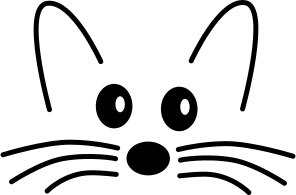
\includegraphics[width=1.4em]{squeak-logo}}}
\iftoshelse{
	\usepackage{marginnote}
		\renewcommand*{\marginfont}{\footnotesize}
	\newcommand{\vartriangleout}{\ifthenelse{\isodd{\thepage}}{\vartriangleright}{\vartriangleleft}}
	\newcommand{\dothisicon}{\fcolorbox{blue!65}{white}{\highlight{$\vartriangleout$}}}
	\newcommand{\dothis}[1]{%
		\noindent\par\noindent
		{\reversemarginpar
			\marginnote{\fcolorbox{blue!65}{white}{\highlight{$\vartriangleout$}}}}
		%\MarginLabel{do this}
		\noindent\emph{#1}
		\nopagebreak}
}{
	\newcommand{\dothisicon}{\raisebox{-.5ex}{
\includegraphics[height=1.2em]{pharo}}}
	\newcommand{\dothis}[1]{%
		\medskip
		\noindent\dothisicon
		\ifx#1\empty\else\quad\emph{#1}\fi
		\par\smallskip\nopagebreak}
}
%===> NEW VERSION <===
% NB: To use this in an individual chapter, you must set:
%\graphicspath{{figures/} {../figures/}}
% at the head of the chapter.  Don't forget the final /
%=============================================================
%:Reader hints (hint)
%
% Indicates a non-obvious consequence 
\newcommand{\hint}[1]{\vspace{1ex}\noindent\fbox{\textsc{Hint}} \emph{#1}}
%=================================================================
% graphics for Morphic handles
\newcommand{\grabHandle}{\raisebox{-0.2ex}{
\includegraphics[width=1em]{blackHandle}}}
\newcommand{\moveHandle}{\raisebox{-0.2ex}{
\includegraphics[width=1em]{moveHandle}}}
\newcommand{\debugHandle}{\raisebox{-0.2ex}{
\includegraphics[width=1em]{debugHandle}}}
%=============================================================
%:Highlighting Important stuff (doublebox)
%
% From Seaside book ...
\newsavebox{\SavedText}
\newlength{\InnerBoxRule}\setlength{\InnerBoxRule}{.75\fboxrule}
\newlength{\OuterBoxRule}\setlength{\OuterBoxRule}{1.5\fboxrule}
\newlength{\BoxSeparation}\setlength{\BoxSeparation}{1.5\fboxrule}
\addtolength{\BoxSeparation}{.5pt}
\newlength{\SaveBoxSep}\setlength{\SaveBoxSep}{2\fboxsep}
%
\newenvironment{doublebox}{\begin{lrbox}{\SavedText}
    \begin{minipage}{.75\textwidth}}
    {\end{minipage}\end{lrbox}\begin{center}
    \setlength{\fboxsep}{\BoxSeparation}\setlength{\fboxrule}{\OuterBoxRule}
    \fbox{\setlength{\fboxsep}{\SaveBoxSep}\setlength{\fboxrule}{\InnerBoxRule}%
      \fbox{\usebox{\SavedText}}}
  \end{center}}
% Use this:
\newcommand{\important}[1]{\begin{doublebox}#1\end{doublebox}}
%=============================================================
%:Section depth
\setcounter{secnumdepth}{2}
%% for this to happen start the file with
%\ifx\wholebook\relax\else
%% $Author$
% $Date$
% $Revision$

% HISTORY:
% 2006-10-31 - Oscar code macros
% ...

%=============================================================
% NB: documentclass must be set in main document.
% Allows book to be generated in multiple formats.
%=============================================================
%:Packages
\usepackage[T1]{fontenc}  %%%%%% really important to get the code directly in the text!
\usepackage{lmodern}
%\usepackage[scaled=0.85]{bookmanx} % needs another scale factor if used with \renewcommand{\sfdefault}{cmbr}
\usepackage{palatino}
\usepackage[scaled=0.85]{helvet}
\usepackage[protrusion,expansion=false]{microtype}
\usepackage{graphicx}
\usepackage{theorem}
\usepackage[english]{babel}
%%% ON: pdfsync breaks the use of p{width} for tabular columns!
%%\ifdefined\usepdfsync\usepackage{pdfsync}\fi % Requires texlive 2007
%=============================================================
%:More packages
%Stef should check which ones are used!
%\usepackage{picinpar}
%\usepackage{layout}
%\usepackage{color}
%\usepackage{enum}
%\usepackage{a4wide}
% \usepackage{fancyhdr}
\usepackage{ifthen}
\usepackage{float}
\usepackage{longtable}
\usepackage{makeidx}
\usepackage[nottoc]{tocbibind}
\usepackage{multicol}
\usepackage{booktabs}	% book-style tables
\usepackage{topcapt}	% enables \topcaption
\usepackage{multirow}
\usepackage{tabularx}
%\usepackage[bottom]{footmisc}
\usepackage{xspace}
\usepackage{alltt}
\usepackage{amssymb,textcomp}
\usepackage[usenames,dvipsnames]{color}
%\usepackage{colortbl}
\usepackage[hang]{subfigure}\makeatletter\def\p@subfigure{\thefigure\,}\makeatother
\usepackage{rotating}
\usepackage{enumitem}	% apb: allows more control over tags in enumerations
\usepackage{verbatim}     % for comment environment
\usepackage{varioref}	% for page references that work
\labelformat{footnote}{\thechapter--#1} % to distinguish citations from jurabib
\usepackage{needspace}
\usepackage{isodateo} % enable \isodate
\usepackage[newparttoc]{titlesec}
\usepackage{titletoc}
\usepackage{wrapfig}
\usepackage[
	super,
	citefull=first,
	authorformat={allreversed,and},
	titleformat={commasep,italic}
]{jurabib} % citations as footnotes
\usepackage[
	colorlinks=true,
	linkcolor=black,
	urlcolor=black,
	citecolor=black
]{hyperref}   % should come last
%=============================================================
%:PDF version
%%\pdfminorversion=3 % Set PDF to 1.3 for Lulu
%=============================================================
%:URL style
\makeatletter
\def\url@leostyle{%
  \@ifundefined{selectfont}{\def\UrlFont{\sf}}{\def\UrlFont{\sffamily}}}
\makeatother
% Now actually use the newly defined style.
\urlstyle{leo}
%=============================================================
%:Booleans
\newboolean{lulu}
\setboolean{lulu}{false}
\newcommand{\ifluluelse}[2]{\ifthenelse{\boolean{lulu}}{#1}{#2}}
%=============================================================
%:Names
\newcommand{\SUnit}{SUnit\xspace}
\newcommand{\sunit}{SUnit\xspace}
\newcommand{\xUnit}{$x$Unit\xspace}
\newcommand{\JUnit}{JUnit\xspace}
\newcommand{\st}{Smalltalk\xspace}
\newcommand{\pharo}{Pharo\xspace} % Use this, not \Pharo
%\newcommand{\sqmap}{SqueakMap\xspace}
\newcommand{\squeak}{Squeak\xspace} % use this, not \Squeak or \sq
\newcommand{\sqsrc}{SqueakSource\xspace}
\newcommand{\sbe}{\url{http://SqueakByExample.org}\xspace}
\newcommand{\pharoweb}{\url{http://pharo-project.org}\xspace}
\newcommand{\pbe}{\url{http://PharoByExample.org}\xspace}
\newcommand{\sba}{\url{http://SquareBracketAssociates.org}\xspace}
\newcommand{\bam}{\lct{Bounc\-ing\-Atoms\-Morph}\xspace}
%=============================================================
%:Markup macros for proof-reading
\usepackage[normalem]{ulem} % for \sout
\usepackage{xcolor}
\newcommand{\ra}{$\rightarrow$}
\newcommand{\ugh}[1]{\textcolor{red}{\uwave{#1}}} % please rephrase
\newcommand{\ins}[1]{\textcolor{blue}{\uline{#1}}} % please insert
\newcommand{\del}[1]{\textcolor{red}{\sout{#1}}} % please delete
\newcommand{\chg}[2]{\textcolor{red}{\sout{#1}}{\ra}\textcolor{blue}{\uline{#2}}} % please change
%=============================================================
%:Editorial comment macros
%\newcommand{\nnbb}[2]{
%    % \fbox{\bfseries\sffamily\scriptsize#1}
%    \fcolorbox{gray}{yellow}{\bfseries\sffamily\scriptsize#1}
%    {\sf\small$\blacktriangleright$\textit{#2}$\blacktriangleleft$}
%   }
\newcommand{\yellowbox}[1]{\fcolorbox{gray}{yellow}{\bfseries\sffamily\scriptsize#1}}
\newcommand{\triangles}[1]{{\sf\small$\blacktriangleright$\textit{#1}$\blacktriangleleft$}}
\newcommand{\nnbb}[2]{\yellowbox{#1} \triangles{#2}}
\newcommand{\fix}{\yellowbox{FIX!}}
\newcommand{\here}{\yellowbox{CONTINUE HERE!}}
% editor macros
\newcommand{\apl}[1]{\nnbb{Alain}{#1}} % Alain
\newcommand{\ab}[1]{\nnbb{Andrew}{#1}} % Black
\newcommand{\sd}[1]{\nnbb{St\'{e}f}{#1}} % Ducasse
\newcommand{\dc}[1]{\nnbb{DamienC}{#1}} % Ducasse
\newcommand{\md}[1]{\nnbb{Marcus}{#1}} % Denker
\newcommand{\on}[1]{\nnbb{Oscar}{#1}} % Nierstrasz
\newcommand{\damien}[1]{\nnbb{Damien}{#1}} % Pollet
\newcommand{\lr}[1]{\nnbb{Lukas}{#1}} % Renggli
\newcommand{\orla}[1]{\nnbb{Orla}{#1}} % Greevy
\newcommand{\alex}[1]{\nnbb{Alex}{#1}} % Bergel
\newcommand{\alx}[1]{\nnbb{Alex}{#1}} % Bergel
\newcommand{\dr}[1]{\nnbb{David}{#1}} % Roethlisberger
\newcommand{\ja}[1]{\nnbb{Jannik}{#1}} % Laval
\newcommand{\jr}[1]{\nnbb{Jorge}{#1}} % Ressia
\newcommand{\fp}[1]{\nnbb{Fabrizio}{#1}} % Perin
\newcommand{\michael}[1]{\nnbb{Michael}{#1}} % Davies
\newcommand{\ew}[1]{\nnbb{Erwann}{#1}} % Wernli
\newcommand{\mb}[1]{\nnbb{Martial}{#1}} % Boniou
\newcommand{\hw}[1]{\nnbb{Hernan}{#1}} % Wilkinson
%=============================================================
%:Abbreviation macros
\newcommand{\ie}{\emph{すなわち}、}
\newcommand{\eg}{\emph{例えば}、}
\newcommand{\etc}{などなど。}
%=============================================================
%:Cross reference macros
\newcommand{\charef}[1]{第~\ref{cha:#1}~章}
\newcommand{\secref}[1]{\ref{sec:#1}~節}
\newcommand{\figref}[1]{図~\ref{fig:#1}\xspace}
\newcommand{\Figref}[1]{図~\ref{fig:#1}\xspace}
\newcommand{\appref}[1]{付録~\ref{app:#1}\xspace}
\newcommand{\tabref}[1]{表~\ref{tab:#1}\xspace}
\newcommand{\faqref}[1]{FAQ~\ref{faq:#1}, p.~\pageref{faq:#1}\xspace}
% APB: I removed trailing \xspace commands from these macros because
% \xspace mostly doesn't work.  If you want a space after your
% references, type one!
% ON: xspace has always worked just fine for me!  Please leave them in.
%
\newcommand{\ruleref}[1]{\ref{rule:#1}\xspace}
%
\newcommand{\egref}[1]{example~\ref{eg:#1}\xspace}
\newcommand{\Egref}[1]{Example~\ref{eg:#1}\xspace}
%
\newcommand{\scrref}[1]{script~\ref{scr:#1}\xspace}
\newcommand{\Scrref}[1]{Script~\ref{scr:#1}\xspace}
\newcommand{\tscrref}[1]{the script~\ref{scr:#1}\xspace}
\newcommand{\Tscrref}[1]{The script~\ref{scr:#1}\xspace}
%
\newcommand{\mthref}[1]{method~\ref{mth:#1}\xspace}
\newcommand{\mthsref}[1]{methods~\ref{mth:#1}\xspace}
\newcommand{\Mthref}[1]{Method~\ref{mth:#1}\xspace}
\newcommand{\tmthref}[1]{the method~\ref{mth:#1}\xspace}
\newcommand{\Tmthref}[1]{The method~\ref{mth:#1}\xspace}
%
\newcommand{\clsref}[1]{class~\ref{cls:#1}\xspace}
\newcommand{\tclsref}[1]{the class~\ref{cls:#1}\xspace}
\newcommand{\Tclsref}[1]{The class~\ref{cls:#1}\xspace}

\newcommand{\chalabel}[1]{\label{cha:#1}}
\newcommand{\seclabel}[1]{\label{sec:#1}}
\newcommand{\figlabel}[1]{\label{fig:#1}}
\newcommand{\tablabel}[1]{\label{tab:#1}}
\newcommand{\rulelabel}[1]{\label{rule:#1}}
\newcommand{\eglabel}[1]{\label{eg:#1}}
\newcommand{\scrlabel}[1]{\label{scr:#1}}
\newcommand{\mthlabel}[1]{\label{mth:#1}}
\newcommand{\clslabel}[1]{\label{cls:#1}}
\newcommand{\faqlabel}[1]{\label{faq:#1}}
%=============================================================
%:Menu item macro
% for menu items, so we can change our minds on how to print them! (apb)
\definecolor{lightgray}{gray}{0.89}
\newcommand{\menu}[1]{{%
	\setlength{\fboxsep}{0pt}%
	\colorbox{lightgray}{{{\upshape\sffamily\strut \,#1\,}}}}}
\newcommand{\link}[1]{{%
	\fontfamily{lmr}\selectfont
 	\upshape{\sffamily \underline{#1}}}}
% For submenu items:
\newcommand{\go}{\,$\triangleright$\,}
% \newcommand{\go}{\,$\blacktriangleright$\,}
% For keyboard shortcuts:
%\newcommand{\short}[1]{\mbox{$\langle${\sc CMD}$\rangle$-#1}\xspace}
\newcommand{\short}[1]{\mbox{{\sc cmd}\hspace{0.08em}--\hspace{0.09em}#1}\xspace}
% For buttons:
\newcommand{\button}[1]{{%
	\setlength{\fboxsep}{0pt}%
	\fbox{{\upshape\sffamily\strut \,#1\,}}}}
% NB: The button macro does not work within captions -- incompatible with xcolor package :-(
\newcommand{\toolsflap}{\textit{Tools} flap\xspace}
%=============================================================
%:Mouse clicks
\newcommand{\click}{click\xspace} % RED
\newcommand{\actclick}{action-click\xspace} % YELLOW
\newcommand{\metaclick}{meta-click\xspace} % BLUE
\newcommand{\Click}{Click\xspace} % RED
\newcommand{\Actclick}{Action-click\xspace} % YELLOW
\newcommand{\Metaclick}{Meta-click\xspace} % BLUE
%=============================================================
%:ToSh macros
\newboolean{tosh}
\setboolean{tosh}{false}
\newcommand{\iftoshelse}[2]{\ifthenelse{\boolean{tosh}}{#1}{#2}}
%=============================================================
%:ToSh colors
%\newcommand{\highlightcolor}{\color{blue!65}}
%\newcommand{\boxcolor}{\color{gray!25}}
\newcommand{\highlight}[1]{\textcolor{blue!65}{#1}}
%\newcommand{\codecolor}{\color{blue!65}}
%%\setlength{\fboxrule}{2pt}
%\newcommand{\asPict}[1]{%
%	{\Large\highlight{#1}}}
%=============================================================
%:Reader cues (do this)
%
% Indicate something the reader should try out.
% \newcommand{\dothisicon}{\raisebox{-.5ex}{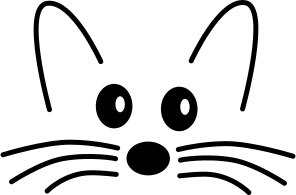
\includegraphics[width=1.4em]{squeak-logo}}}
\iftoshelse{
	\usepackage{marginnote}
		\renewcommand*{\marginfont}{\footnotesize}
	\newcommand{\vartriangleout}{\ifthenelse{\isodd{\thepage}}{\vartriangleright}{\vartriangleleft}}
	\newcommand{\dothisicon}{\fcolorbox{blue!65}{white}{\highlight{$\vartriangleout$}}}
	\newcommand{\dothis}[1]{%
		\noindent\par\noindent
		{\reversemarginpar
			\marginnote{\fcolorbox{blue!65}{white}{\highlight{$\vartriangleout$}}}}
		%\MarginLabel{do this}
		\noindent\emph{#1}
		\nopagebreak}
}{
	\newcommand{\dothisicon}{\raisebox{-.5ex}{
\includegraphics[height=1.2em]{pharo}}}
	\newcommand{\dothis}[1]{%
		\medskip
		\noindent\dothisicon
		\ifx#1\empty\else\quad\emph{#1}\fi
		\par\smallskip\nopagebreak}
}
%===> NEW VERSION <===
% NB: To use this in an individual chapter, you must set:
%\graphicspath{{figures/} {../figures/}}
% at the head of the chapter.  Don't forget the final /
%=============================================================
%:Reader hints (hint)
%
% Indicates a non-obvious consequence 
\newcommand{\hint}[1]{\vspace{1ex}\noindent\fbox{\textsc{Hint}} \emph{#1}}
%=================================================================
% graphics for Morphic handles
\newcommand{\grabHandle}{\raisebox{-0.2ex}{
\includegraphics[width=1em]{blackHandle}}}
\newcommand{\moveHandle}{\raisebox{-0.2ex}{
\includegraphics[width=1em]{moveHandle}}}
\newcommand{\debugHandle}{\raisebox{-0.2ex}{
\includegraphics[width=1em]{debugHandle}}}
%=============================================================
%:Highlighting Important stuff (doublebox)
%
% From Seaside book ...
\newsavebox{\SavedText}
\newlength{\InnerBoxRule}\setlength{\InnerBoxRule}{.75\fboxrule}
\newlength{\OuterBoxRule}\setlength{\OuterBoxRule}{1.5\fboxrule}
\newlength{\BoxSeparation}\setlength{\BoxSeparation}{1.5\fboxrule}
\addtolength{\BoxSeparation}{.5pt}
\newlength{\SaveBoxSep}\setlength{\SaveBoxSep}{2\fboxsep}
%
\newenvironment{doublebox}{\begin{lrbox}{\SavedText}
    \begin{minipage}{.75\textwidth}}
    {\end{minipage}\end{lrbox}\begin{center}
    \setlength{\fboxsep}{\BoxSeparation}\setlength{\fboxrule}{\OuterBoxRule}
    \fbox{\setlength{\fboxsep}{\SaveBoxSep}\setlength{\fboxrule}{\InnerBoxRule}%
      \fbox{\usebox{\SavedText}}}
  \end{center}}
% Use this:
\newcommand{\important}[1]{\begin{doublebox}#1\end{doublebox}}
%=============================================================
%:Section depth
\setcounter{secnumdepth}{2}
%% for this to happen start the file with
%\ifx\wholebook\relax\else
%% $Author$
% $Date$
% $Revision$

% HISTORY:
% 2006-10-31 - Oscar code macros
% ...

%=============================================================
% NB: documentclass must be set in main document.
% Allows book to be generated in multiple formats.
%=============================================================
%:Packages
\usepackage[T1]{fontenc}  %%%%%% really important to get the code directly in the text!
\usepackage{lmodern}
%\usepackage[scaled=0.85]{bookmanx} % needs another scale factor if used with \renewcommand{\sfdefault}{cmbr}
\usepackage{palatino}
\usepackage[scaled=0.85]{helvet}
\usepackage[protrusion,expansion=false]{microtype}
\usepackage{graphicx}
\usepackage{theorem}
\usepackage[english]{babel}
%%% ON: pdfsync breaks the use of p{width} for tabular columns!
%%\ifdefined\usepdfsync\usepackage{pdfsync}\fi % Requires texlive 2007
%=============================================================
%:More packages
%Stef should check which ones are used!
%\usepackage{picinpar}
%\usepackage{layout}
%\usepackage{color}
%\usepackage{enum}
%\usepackage{a4wide}
% \usepackage{fancyhdr}
\usepackage{ifthen}
\usepackage{float}
\usepackage{longtable}
\usepackage{makeidx}
\usepackage[nottoc]{tocbibind}
\usepackage{multicol}
\usepackage{booktabs}	% book-style tables
\usepackage{topcapt}	% enables \topcaption
\usepackage{multirow}
\usepackage{tabularx}
%\usepackage[bottom]{footmisc}
\usepackage{xspace}
\usepackage{alltt}
\usepackage{amssymb,textcomp}
\usepackage[usenames,dvipsnames]{color}
%\usepackage{colortbl}
\usepackage[hang]{subfigure}\makeatletter\def\p@subfigure{\thefigure\,}\makeatother
\usepackage{rotating}
\usepackage{enumitem}	% apb: allows more control over tags in enumerations
\usepackage{verbatim}     % for comment environment
\usepackage{varioref}	% for page references that work
\labelformat{footnote}{\thechapter--#1} % to distinguish citations from jurabib
\usepackage{needspace}
\usepackage{isodateo} % enable \isodate
\usepackage[newparttoc]{titlesec}
\usepackage{titletoc}
\usepackage{wrapfig}
\usepackage[
	super,
	citefull=first,
	authorformat={allreversed,and},
	titleformat={commasep,italic}
]{jurabib} % citations as footnotes
\usepackage[
	colorlinks=true,
	linkcolor=black,
	urlcolor=black,
	citecolor=black
]{hyperref}   % should come last
%=============================================================
%:PDF version
%%\pdfminorversion=3 % Set PDF to 1.3 for Lulu
%=============================================================
%:URL style
\makeatletter
\def\url@leostyle{%
  \@ifundefined{selectfont}{\def\UrlFont{\sf}}{\def\UrlFont{\sffamily}}}
\makeatother
% Now actually use the newly defined style.
\urlstyle{leo}
%=============================================================
%:Booleans
\newboolean{lulu}
\setboolean{lulu}{false}
\newcommand{\ifluluelse}[2]{\ifthenelse{\boolean{lulu}}{#1}{#2}}
%=============================================================
%:Names
\newcommand{\SUnit}{SUnit\xspace}
\newcommand{\sunit}{SUnit\xspace}
\newcommand{\xUnit}{$x$Unit\xspace}
\newcommand{\JUnit}{JUnit\xspace}
\newcommand{\st}{Smalltalk\xspace}
\newcommand{\pharo}{Pharo\xspace} % Use this, not \Pharo
%\newcommand{\sqmap}{SqueakMap\xspace}
\newcommand{\squeak}{Squeak\xspace} % use this, not \Squeak or \sq
\newcommand{\sqsrc}{SqueakSource\xspace}
\newcommand{\sbe}{\url{http://SqueakByExample.org}\xspace}
\newcommand{\pharoweb}{\url{http://pharo-project.org}\xspace}
\newcommand{\pbe}{\url{http://PharoByExample.org}\xspace}
\newcommand{\sba}{\url{http://SquareBracketAssociates.org}\xspace}
\newcommand{\bam}{\lct{Bounc\-ing\-Atoms\-Morph}\xspace}
%=============================================================
%:Markup macros for proof-reading
\usepackage[normalem]{ulem} % for \sout
\usepackage{xcolor}
\newcommand{\ra}{$\rightarrow$}
\newcommand{\ugh}[1]{\textcolor{red}{\uwave{#1}}} % please rephrase
\newcommand{\ins}[1]{\textcolor{blue}{\uline{#1}}} % please insert
\newcommand{\del}[1]{\textcolor{red}{\sout{#1}}} % please delete
\newcommand{\chg}[2]{\textcolor{red}{\sout{#1}}{\ra}\textcolor{blue}{\uline{#2}}} % please change
%=============================================================
%:Editorial comment macros
%\newcommand{\nnbb}[2]{
%    % \fbox{\bfseries\sffamily\scriptsize#1}
%    \fcolorbox{gray}{yellow}{\bfseries\sffamily\scriptsize#1}
%    {\sf\small$\blacktriangleright$\textit{#2}$\blacktriangleleft$}
%   }
\newcommand{\yellowbox}[1]{\fcolorbox{gray}{yellow}{\bfseries\sffamily\scriptsize#1}}
\newcommand{\triangles}[1]{{\sf\small$\blacktriangleright$\textit{#1}$\blacktriangleleft$}}
\newcommand{\nnbb}[2]{\yellowbox{#1} \triangles{#2}}
\newcommand{\fix}{\yellowbox{FIX!}}
\newcommand{\here}{\yellowbox{CONTINUE HERE!}}
% editor macros
\newcommand{\apl}[1]{\nnbb{Alain}{#1}} % Alain
\newcommand{\ab}[1]{\nnbb{Andrew}{#1}} % Black
\newcommand{\sd}[1]{\nnbb{St\'{e}f}{#1}} % Ducasse
\newcommand{\dc}[1]{\nnbb{DamienC}{#1}} % Ducasse
\newcommand{\md}[1]{\nnbb{Marcus}{#1}} % Denker
\newcommand{\on}[1]{\nnbb{Oscar}{#1}} % Nierstrasz
\newcommand{\damien}[1]{\nnbb{Damien}{#1}} % Pollet
\newcommand{\lr}[1]{\nnbb{Lukas}{#1}} % Renggli
\newcommand{\orla}[1]{\nnbb{Orla}{#1}} % Greevy
\newcommand{\alex}[1]{\nnbb{Alex}{#1}} % Bergel
\newcommand{\alx}[1]{\nnbb{Alex}{#1}} % Bergel
\newcommand{\dr}[1]{\nnbb{David}{#1}} % Roethlisberger
\newcommand{\ja}[1]{\nnbb{Jannik}{#1}} % Laval
\newcommand{\jr}[1]{\nnbb{Jorge}{#1}} % Ressia
\newcommand{\fp}[1]{\nnbb{Fabrizio}{#1}} % Perin
\newcommand{\michael}[1]{\nnbb{Michael}{#1}} % Davies
\newcommand{\ew}[1]{\nnbb{Erwann}{#1}} % Wernli
\newcommand{\mb}[1]{\nnbb{Martial}{#1}} % Boniou
\newcommand{\hw}[1]{\nnbb{Hernan}{#1}} % Wilkinson
%=============================================================
%:Abbreviation macros
\newcommand{\ie}{\emph{すなわち}、}
\newcommand{\eg}{\emph{例えば}、}
\newcommand{\etc}{などなど。}
%=============================================================
%:Cross reference macros
\newcommand{\charef}[1]{第~\ref{cha:#1}~章}
\newcommand{\secref}[1]{\ref{sec:#1}~節}
\newcommand{\figref}[1]{図~\ref{fig:#1}\xspace}
\newcommand{\Figref}[1]{図~\ref{fig:#1}\xspace}
\newcommand{\appref}[1]{付録~\ref{app:#1}\xspace}
\newcommand{\tabref}[1]{表~\ref{tab:#1}\xspace}
\newcommand{\faqref}[1]{FAQ~\ref{faq:#1}, p.~\pageref{faq:#1}\xspace}
% APB: I removed trailing \xspace commands from these macros because
% \xspace mostly doesn't work.  If you want a space after your
% references, type one!
% ON: xspace has always worked just fine for me!  Please leave them in.
%
\newcommand{\ruleref}[1]{\ref{rule:#1}\xspace}
%
\newcommand{\egref}[1]{example~\ref{eg:#1}\xspace}
\newcommand{\Egref}[1]{Example~\ref{eg:#1}\xspace}
%
\newcommand{\scrref}[1]{script~\ref{scr:#1}\xspace}
\newcommand{\Scrref}[1]{Script~\ref{scr:#1}\xspace}
\newcommand{\tscrref}[1]{the script~\ref{scr:#1}\xspace}
\newcommand{\Tscrref}[1]{The script~\ref{scr:#1}\xspace}
%
\newcommand{\mthref}[1]{method~\ref{mth:#1}\xspace}
\newcommand{\mthsref}[1]{methods~\ref{mth:#1}\xspace}
\newcommand{\Mthref}[1]{Method~\ref{mth:#1}\xspace}
\newcommand{\tmthref}[1]{the method~\ref{mth:#1}\xspace}
\newcommand{\Tmthref}[1]{The method~\ref{mth:#1}\xspace}
%
\newcommand{\clsref}[1]{class~\ref{cls:#1}\xspace}
\newcommand{\tclsref}[1]{the class~\ref{cls:#1}\xspace}
\newcommand{\Tclsref}[1]{The class~\ref{cls:#1}\xspace}

\newcommand{\chalabel}[1]{\label{cha:#1}}
\newcommand{\seclabel}[1]{\label{sec:#1}}
\newcommand{\figlabel}[1]{\label{fig:#1}}
\newcommand{\tablabel}[1]{\label{tab:#1}}
\newcommand{\rulelabel}[1]{\label{rule:#1}}
\newcommand{\eglabel}[1]{\label{eg:#1}}
\newcommand{\scrlabel}[1]{\label{scr:#1}}
\newcommand{\mthlabel}[1]{\label{mth:#1}}
\newcommand{\clslabel}[1]{\label{cls:#1}}
\newcommand{\faqlabel}[1]{\label{faq:#1}}
%=============================================================
%:Menu item macro
% for menu items, so we can change our minds on how to print them! (apb)
\definecolor{lightgray}{gray}{0.89}
\newcommand{\menu}[1]{{%
	\setlength{\fboxsep}{0pt}%
	\colorbox{lightgray}{{{\upshape\sffamily\strut \,#1\,}}}}}
\newcommand{\link}[1]{{%
	\fontfamily{lmr}\selectfont
 	\upshape{\sffamily \underline{#1}}}}
% For submenu items:
\newcommand{\go}{\,$\triangleright$\,}
% \newcommand{\go}{\,$\blacktriangleright$\,}
% For keyboard shortcuts:
%\newcommand{\short}[1]{\mbox{$\langle${\sc CMD}$\rangle$-#1}\xspace}
\newcommand{\short}[1]{\mbox{{\sc cmd}\hspace{0.08em}--\hspace{0.09em}#1}\xspace}
% For buttons:
\newcommand{\button}[1]{{%
	\setlength{\fboxsep}{0pt}%
	\fbox{{\upshape\sffamily\strut \,#1\,}}}}
% NB: The button macro does not work within captions -- incompatible with xcolor package :-(
\newcommand{\toolsflap}{\textit{Tools} flap\xspace}
%=============================================================
%:Mouse clicks
\newcommand{\click}{click\xspace} % RED
\newcommand{\actclick}{action-click\xspace} % YELLOW
\newcommand{\metaclick}{meta-click\xspace} % BLUE
\newcommand{\Click}{Click\xspace} % RED
\newcommand{\Actclick}{Action-click\xspace} % YELLOW
\newcommand{\Metaclick}{Meta-click\xspace} % BLUE
%=============================================================
%:ToSh macros
\newboolean{tosh}
\setboolean{tosh}{false}
\newcommand{\iftoshelse}[2]{\ifthenelse{\boolean{tosh}}{#1}{#2}}
%=============================================================
%:ToSh colors
%\newcommand{\highlightcolor}{\color{blue!65}}
%\newcommand{\boxcolor}{\color{gray!25}}
\newcommand{\highlight}[1]{\textcolor{blue!65}{#1}}
%\newcommand{\codecolor}{\color{blue!65}}
%%\setlength{\fboxrule}{2pt}
%\newcommand{\asPict}[1]{%
%	{\Large\highlight{#1}}}
%=============================================================
%:Reader cues (do this)
%
% Indicate something the reader should try out.
% \newcommand{\dothisicon}{\raisebox{-.5ex}{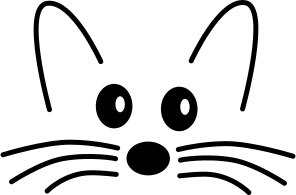
\includegraphics[width=1.4em]{squeak-logo}}}
\iftoshelse{
	\usepackage{marginnote}
		\renewcommand*{\marginfont}{\footnotesize}
	\newcommand{\vartriangleout}{\ifthenelse{\isodd{\thepage}}{\vartriangleright}{\vartriangleleft}}
	\newcommand{\dothisicon}{\fcolorbox{blue!65}{white}{\highlight{$\vartriangleout$}}}
	\newcommand{\dothis}[1]{%
		\noindent\par\noindent
		{\reversemarginpar
			\marginnote{\fcolorbox{blue!65}{white}{\highlight{$\vartriangleout$}}}}
		%\MarginLabel{do this}
		\noindent\emph{#1}
		\nopagebreak}
}{
	\newcommand{\dothisicon}{\raisebox{-.5ex}{
\includegraphics[height=1.2em]{pharo}}}
	\newcommand{\dothis}[1]{%
		\medskip
		\noindent\dothisicon
		\ifx#1\empty\else\quad\emph{#1}\fi
		\par\smallskip\nopagebreak}
}
%===> NEW VERSION <===
% NB: To use this in an individual chapter, you must set:
%\graphicspath{{figures/} {../figures/}}
% at the head of the chapter.  Don't forget the final /
%=============================================================
%:Reader hints (hint)
%
% Indicates a non-obvious consequence 
\newcommand{\hint}[1]{\vspace{1ex}\noindent\fbox{\textsc{Hint}} \emph{#1}}
%=================================================================
% graphics for Morphic handles
\newcommand{\grabHandle}{\raisebox{-0.2ex}{
\includegraphics[width=1em]{blackHandle}}}
\newcommand{\moveHandle}{\raisebox{-0.2ex}{
\includegraphics[width=1em]{moveHandle}}}
\newcommand{\debugHandle}{\raisebox{-0.2ex}{
\includegraphics[width=1em]{debugHandle}}}
%=============================================================
%:Highlighting Important stuff (doublebox)
%
% From Seaside book ...
\newsavebox{\SavedText}
\newlength{\InnerBoxRule}\setlength{\InnerBoxRule}{.75\fboxrule}
\newlength{\OuterBoxRule}\setlength{\OuterBoxRule}{1.5\fboxrule}
\newlength{\BoxSeparation}\setlength{\BoxSeparation}{1.5\fboxrule}
\addtolength{\BoxSeparation}{.5pt}
\newlength{\SaveBoxSep}\setlength{\SaveBoxSep}{2\fboxsep}
%
\newenvironment{doublebox}{\begin{lrbox}{\SavedText}
    \begin{minipage}{.75\textwidth}}
    {\end{minipage}\end{lrbox}\begin{center}
    \setlength{\fboxsep}{\BoxSeparation}\setlength{\fboxrule}{\OuterBoxRule}
    \fbox{\setlength{\fboxsep}{\SaveBoxSep}\setlength{\fboxrule}{\InnerBoxRule}%
      \fbox{\usebox{\SavedText}}}
  \end{center}}
% Use this:
\newcommand{\important}[1]{\begin{doublebox}#1\end{doublebox}}
%=============================================================
%:Section depth
\setcounter{secnumdepth}{2}
%% for this to happen start the file with
%\ifx\wholebook\relax\else
%\input{../common.tex}
%\begin{document}
%\fi
% and terminate by
% \ifx\wholebook\relax\else\end{document}\fi

\DeclareGraphicsExtensions{.pdf, .jpg, .png}
%=============================================================
%:PDF setup
\hypersetup{
%   a4paper,
%   pdfstartview=FitV,
%   colorlinks,
%   linkcolor=darkblue,
%   citecolor=darkblue,
   pdftitle={Pharo by Example},
   pdfauthor={Andrew P. Black, St\'ephane Ducasse,	Oscar Nierstrasz,
Damien Pollet},
   pdfkeywords={Smalltalk, Squeak, Object-Oriented Programming, OOP},
   pdfsubject={Computer Science}
}
%=============================================================
%:Page layout and appearance
%
% \renewcommand{\headrulewidth}{0pt}
\renewcommand{\chaptermark}[1]{\markboth{#1}{}}
\renewcommand{\sectionmark}[1]{\markright{\thesection\ #1}}
\renewpagestyle{plain}[\small\itshape]{%
	\setheadrule{0pt}%
	\sethead[][][]{}{}{}%
	\setfoot[][][]{}{}{}}
\renewpagestyle{headings}[\small\itshape]{%
	\setheadrule{0pt}%
	\setmarks{chapter}{section}%
	\sethead[\thepage][][\chaptertitle]{\sectiontitle}{}{\thepage}%
	\setfoot[][][]{}{}{}}
%=============================================================
%:Title section setup and TOC numbering depth
\setcounter{secnumdepth}{1}
\setcounter{tocdepth}{1}
\titleformat{\part}[display]{\centering}{\huge\partname\ \thepart}{1em}{\Huge\textbf}[]
\titleformat{\chapter}[display]{}{\huge\chaptertitlename\ \thechapter}{1em}{\Huge\raggedright\textbf}[]
\titlecontents{part}[3pc]{%
		\pagebreak[2]\addvspace{1em plus.4em minus.2em}%
		\leavevmode\large\bfseries}
	{\contentslabel{3pc}}{\hspace*{-3pc}}
	{}[\nopagebreak]
\titlecontents{chapter}[3pc]{%
		\pagebreak[0]\addvspace{1em plus.2em minus.2em}%
		\leavevmode\bfseries}
	{\contentslabel{3pc}}{}
	{\hfill\contentspage}[\nopagebreak]
\dottedcontents{section}[3pc]{}{3pc}{1pc}
\dottedcontents{subsection}[3pc]{}{0pc}{1pc}
% \dottedcontents{subsection}[4.5em]{}{0pt}{1pc}
% Make \cleardoublepage insert really blank pages http://www.tex.ac.uk/cgi-bin/texfaq2html?label=reallyblank
\let\origdoublepage\cleardoublepage
\newcommand{\clearemptydoublepage}{%
  \clearpage
  {\pagestyle{empty}\origdoublepage}}
\let\cleardoublepage\clearemptydoublepage % see http://www.tex.ac.uk/cgi-bin/texfaq2html?label=patch
%=============================================================
%:FAQ macros (for FAQ chapter)
\newtheorem{faq}{FAQ}
\newcommand{\answer}{\paragraph{Answer}\ }
%=============================================================
%:Listings package configuration
% \newcommand{\caret}{\makebox{\raisebox{0.4ex}{\footnotesize{$\wedge$}}}}
\newcommand{\caret}{\^\,}
\newcommand{\escape}{{\sf \textbackslash}}
\definecolor{source}{gray}{0.95}
\usepackage{listings}
\lstdefinelanguage{Smalltalk}{
%  morekeywords={self,super,true,false,nil,thisContext}, % This is overkill
  morestring=[d]',
  morecomment=[s]{"}{"},
  alsoletter={\#:},
  escapechar={!},
  literate=
    {BANG}{!}1
    {CARET}{\^}1
    {UNDERSCORE}{\_}1
    {\\st}{Smalltalk}9 % convenience -- in case \st occurs in code
    % {'}{{\textquotesingle}}1 % replaced by upquote=true in \lstset
    {_}{{$\leftarrow$}}1
    {>>>}{{\sep}}1
    {^}{{$\uparrow$}}1
    {~}{{$\sim$}}1
    {-}{{\texttt{-}}}1 %{\textminus}}1 %{-}{\hspace{-0.13em}}{-}}1  % the goal is to make - the same width as +
    % {+}{\sf+}1 %{\raisebox{0.08ex}{+}}}1      % and to raise + off the baseline to match -
    {-->}{{\quad$\longrightarrow$\quad}}3
	, % Don't forget the comma at the end!
  tabsize=4
}[keywords,comments,strings]

\lstset{language=Smalltalk,
	basicstyle=\sffamily,
	keywordstyle=\color{black}\bfseries,
	% stringstyle=\ttfamily, % Ugly! do we really want this? -- on
	mathescape=true,
	showstringspaces=false,
	keepspaces=true,
	breaklines=true,
	breakautoindent=true,
	backgroundcolor=\color{source},
	lineskip={-1pt}, % Ugly hack
	upquote=true, % straight quote; requires textcomp package
	columns=fullflexible} % no fixed width fonts
% In-line code (literal)
% Normally use this for all in-line code:
\newcommand{\ct}{\lstinline[mathescape=false,backgroundcolor=\color{white},basicstyle={\sffamily\upshape}]}
% apb 2007.8.28 added the \upshape declaration to avoid getting italicized code in \dothis{ } sections.
% In-line code (latex enabled)
% Use this only in special situations where \ct does not work
% (within section headings ...):
\newcommand{\lct}[1]{{\textsf{\textup{#1}}}}
% Use these for system categories and protocols:
\newcommand{\scat}[1]{\emph{\textsf{#1}}\xspace}
\newcommand{\pkg}[1]{\emph{\textsf{#1}}\xspace}
\newcommand{\prot}[1]{\emph{\textsf{#1}}\xspace}
% Code environments
% NB: the arg is for tests
% Only code and example environments may be tests
\lstnewenvironment{code}[1]{%
	\lstset{%
		% frame=lines,
		frame=single,
		framerule=0pt,
		mathescape=false
	}
}{}
\def\ignoredollar#1{}
%=============================================================
%:Code environments (method, script ...)
% NB: the third arg is for tests
% Only code and example environments may be tests
\lstnewenvironment{example}[3][defaultlabel]{%
	\renewcommand{\lstlistingname}{Example}%
	\lstset{
		% frame=lines,
		frame=single,
		framerule=0pt,
		mathescape=false,
		caption={\emph{#2}},
		label={eg:#1}
	}
}{}
\lstnewenvironment{script}[2][defaultlabel]{%
\renewcommand{\lstlistingname}{Script}%
	\lstset{
		% frame=lines,
		frame=single,
		framerule=0pt,
		mathescape=false,
		name={Script},
		caption={\emph{#2}},
		label={scr:#1}
	}
}{}
\lstnewenvironment{method}[2][defaultlabel]{%
	\renewcommand{\lstlistingname}{Method}%
	\lstset{
		% frame=lines,
		frame=single,
		framerule=0pt,
		mathescape=false,
		name={Method},
		caption={\emph{#2}},
		label={mth:#1}
	}
}{}
\lstnewenvironment{methods}[2][defaultlabel]{% just for multiple methods at once
	\renewcommand{\lstlistingname}{Methods}%
	\lstset{
		% frame=lines,
		frame=single,
		framerule=0pt,
		mathescape=false,
		name={Method},
		caption={\emph{#2}},
		label={mth:#1}
	}
}{}
\lstnewenvironment{numMethod}[2][defaultlabel]{%
	\renewcommand{\lstlistingname}{Method}%
	\lstset{
		numbers=left,
		numberstyle={\tiny\sffamily},
		% frame=lines,
		frame=single,
		framerule=0pt,
		mathescape=false,
		name={Method},
		caption={\emph{#2}},
		label={mth:#1}
	}
}{}
\lstnewenvironment{classdef}[2][defaultlabel]{%
	\renewcommand{\lstlistingname}{Class}%
	\lstset{
		% frame=lines,
		frame=single,
		framerule=0pt,
		mathescape=false,
		name={Class},
		caption={\emph{#2}},
		label={cls:#1}
	}
}{}
%=============================================================
%:Reserving space
% Usually need one more line than the actual lines of code
\newcommand{\needlines}[1]{\Needspace{#1\baselineskip}}
%=============================================================
%:Indexing macros
% Macros ending with "ind" generate text as well as an index entry
% Macros ending with "index" *only* generate an index entry
\newcommand{\ind}[1]{\index{#1}#1\xspace} % plain text
\newcommand{\subind}[2]{\index{#1!#2}#2\xspace} % show #2, subindex under #1
\newcommand{\emphind}[1]{\index{#1}\emph{#1}\xspace} % emph #1
\newcommand{\emphsubind}[2]{\index{#1!#2}\emph{#2}\xspace} % show emph #2, subindex inder #1
\newcommand{\scatind}[1]{\index{#1@\textsf{#1} (category)}\scat{#1}} % category
\newcommand{\pkgind}[1]{\index{#1@\textsf{#1} (package)}\pkg{#1}} % package
\newcommand{\protind}[1]{\index{#1@\textsf{#1} (protocol)}\prot{#1}} % protocol
\newcommand{\clsind}[1]{\index{#1@\textsf{#1} (class)}\ct{#1}\xspace}
% \newcommand{\clsind}[1]{\index{#1!\#@(class)}\ct{#1}\xspace} % class
\newcommand{\clsindplural}[1]{\index{#1!\#@(class)}\ct{#1}s\xspace} % class
\newcommand{\cvind}[1]{\index{#1@\textsf{#1} (class variable)}\ct{#1}\xspace} % class var
\newcommand{\glbind}[1]{\index{#1@\textsf{#1} (global)}\ct{#1}\xspace} % global
\newcommand{\patind}[1]{\index{#1@#1 (pattern)}\ct{#1}\xspace} % pattern
\newcommand{\pvind}[1]{\index{#1@\textsf{#1} (pseudo variable)}\ct{#1}\xspace} % pseudo var
\newcommand{\clsmthind}[2]{\index{#1!#2@\ct{#2}}\ct{#1>>>#2}\xspace} % class + method name
\newcommand{\mthind}[2]{\index{#1!#2@\ct{#2}}\ct{#2}\xspace} % show method name only
\newcommand{\lmthind}[2]{\index{#1!#2@\ct{#2}}\lct{#2}\xspace} % show method name only
\newcommand{\cmind}[2]{\index{#1!#2@\ct{#2}}\ct{#1>>>#2}\xspace} % show class>>method
\newcommand{\lcmind}[2]{\index{#1!#2@\ct{#2}}\lct{#1>>>#2}\xspace} % show class>>method
\newcommand{\toolsflapind}{\index{Tools flap}\toolsflap} % index tools flap
% The following only generate an index entry:
% \newcommand{\clsindex}[1]{\index{#1@\textsf{#1} (class)}}
\newcommand{\clsindex}[1]{\index{#1!\#@(class)}} % class
\newcommand{\mthindex}[2]{\index{#1!#2@\ct{#2}}} % method
\newcommand{\cmindex}[2]{\index{#1!#2@\ct{#2}}} % class>>method
\newcommand{\cvindex}[1]{\index{#1@\textsf{#1} (class variable)}} % class var
\newcommand{\glbindex}[1]{\index{#1@\textsf{#1} (global)}}% global
\newcommand{\pvindex}[1]{\index{#1@\textsf{#1} (pseudo variable)}}% pseudo var
\newcommand{\seeindex}[2]{\index{#1|see{#2}}} % #1, see #2
\newcommand{\scatindex}[1]{\index{#1@\textsf{#1} (category)}} % category
\newcommand{\pkgindex}[1]{\index{#1@\textsf{#1} (package)}} % package
\newcommand{\protindex}[1]{\index{#1@\textsf{#1} (protocol)}} % protocol
% How can we have the main entry page numbers in bold yet not break the hyperlink?
\newcommand{\boldidx}[1]{{\bf #1}} % breaks hyperlink
%\newcommand{\indmain}[1]{\index{#1|boldidx}#1\xspace} % plain text, main entry
%\newcommand{\emphsubindmain}[2]{\index{#1!#2|boldidx}\emph{#2}\xspace} % subindex, main entry
%\newcommand{\subindmain}[2]{\index{#1!#2|boldidx}#2\xspace} % subindex, main entry
%\newcommand{\clsindmain}[1]{\index{#1@\textsf{#1} (class)|boldidx}\ct{#1}\xspace}
%\newcommand{\clsindmain}[1]{\index{#1!\#@(class)|boldidx}\ct{#1}\xspace} % class main
%\newcommand{\indexmain}[1]{\index{#1|boldidx}} % main index entry only
\newcommand{\indmain}[1]{\index{#1}#1\xspace} % The main index entry for this item
\newcommand{\emphsubindmain}[2]{\index{#1!#2}\emph{#2}\xspace} % subindex, main entry
\newcommand{\subindmain}[2]{\index{#1!#2}#2\xspace} % subindex, main entry
%\newcommand{\clsindmain}[1]{\index{#1@\textsf{#1} (class)}\ct{#1}\xspace}
\newcommand{\clsindmain}[1]{\index{#1!\#@(class)}\ct{#1}\xspace} % class main
\newcommand{\clsindexmain}[1]{\index{#1!\#@(class)}} % class main index only
\newcommand{\indexmain}[1]{\index{#1}} 
%=============================================================
%:Code macros
% some constants
\newcommand{\codesize}{\small}
\newcommand{\codefont}{\sffamily}
%\newcommand{\cat}[1]{\textit{In category #1}}%%To remove later
\newlength{\scriptindent}
\setlength{\scriptindent}{.3cm}
%% Method presentation constants
\newlength{\methodindent}
\newlength{\methodwordlength}
\newlength{\aftermethod}
\setlength{\methodindent}{0.2cm}
\settowidth{\methodwordlength}{\ M\'ethode\ }
%=============================================================
%:Smalltalk macros
%\newcommand{\sep}{{$\gg$}}
\newcommand{\sep}{\mbox{>>}}
\newcommand{\self}{\lct{self}\xspace}
\newcommand{\super}{\lct{super}\xspace}
\newcommand{\nil}{\lct{nil}\xspace}
%=============================================================
% be less conservative about float placement
% these commands are from http://www.tex.ac.uk/cgi-bin/texfaq2html?label=floats
\renewcommand{\topfraction}{.9}
\renewcommand{\bottomfraction}{.9}
\renewcommand{\textfraction}{.1}
\renewcommand{\floatpagefraction}{.85}
\renewcommand{\dbltopfraction}{.66}
\renewcommand{\dblfloatpagefraction}{.85}
\setcounter{topnumber}{9}
\setcounter{bottomnumber}{9}
\setcounter{totalnumber}{20}
\setcounter{dbltopnumber}{9}
%=============================================================
% Give information from each chapter's author
\newcommand{\contact}[2]{\textbf{#1} \textsf{(#2)}}

\newcommand{\chapterauthor}[1]{\emph{with the participation of:\\#1}\\}

\newcommand{\authornoury}{\contact{Noury Bouraqadi}{bouraqadi@gmail.com}}
\newcommand{\authordamienc}{\contact{Damien Cassou}{damien.cassou@gmail.com}}
\newcommand{\authoroscar}{\contact{Oscar Nierstrasz}{oscar.nierstrasz@acm.org}}
\newcommand{\authorsteph}{\contact{St\'ephane Ducasse}{stephane.ducasse@inria.fr}}
\newcommand{\authoralex}{\contact{Alexandre Bergel}{alexandre@bergel.eu}}
\newcommand{\authorolivier}{\contact{Olivier Auverlot}{olivier.auverlot@inria.fr}}
\newcommand{\authornicolas}{\contact{Nicolas Cellier}{ncellier@ifrance.com}}
\newcommand{\authormarcus}{\contact{Marcus Denker}{marcus.denker@inria.fr}}
\newcommand{\authoralain}{\contact{Alain Plantec}{alain.plantec@univ-brest.fr}}
\newcommand{\authordale}{\contact{Dale Henrichs}{dale.henrichs@gemstone.com}}
\newcommand{\authormariano}{\contact{Mariano Martinez Peck}{marianopeck@gmail.com}}
\newcommand{\authorsven}{\contact{Sven Van Caekenberghe}{sven@beta9.be}}

%=============================================================
% apb doesn't like paragraphs to run in to each other without a break
\parskip 1ex
%=============================================================
%:Stuff to check, merge or deprecate
%\setlength{\marginparsep}{2mm}
%\renewcommand{\baselinestretch}{1.1}
%=============================================================

%\begin{document}
%\fi
% and terminate by
% \ifx\wholebook\relax\else\end{document}\fi

\DeclareGraphicsExtensions{.pdf, .jpg, .png}
%=============================================================
%:PDF setup
\hypersetup{
%   a4paper,
%   pdfstartview=FitV,
%   colorlinks,
%   linkcolor=darkblue,
%   citecolor=darkblue,
   pdftitle={Pharo by Example},
   pdfauthor={Andrew P. Black, St\'ephane Ducasse,	Oscar Nierstrasz,
Damien Pollet},
   pdfkeywords={Smalltalk, Squeak, Object-Oriented Programming, OOP},
   pdfsubject={Computer Science}
}
%=============================================================
%:Page layout and appearance
%
% \renewcommand{\headrulewidth}{0pt}
\renewcommand{\chaptermark}[1]{\markboth{#1}{}}
\renewcommand{\sectionmark}[1]{\markright{\thesection\ #1}}
\renewpagestyle{plain}[\small\itshape]{%
	\setheadrule{0pt}%
	\sethead[][][]{}{}{}%
	\setfoot[][][]{}{}{}}
\renewpagestyle{headings}[\small\itshape]{%
	\setheadrule{0pt}%
	\setmarks{chapter}{section}%
	\sethead[\thepage][][\chaptertitle]{\sectiontitle}{}{\thepage}%
	\setfoot[][][]{}{}{}}
%=============================================================
%:Title section setup and TOC numbering depth
\setcounter{secnumdepth}{1}
\setcounter{tocdepth}{1}
\titleformat{\part}[display]{\centering}{\huge\partname\ \thepart}{1em}{\Huge\textbf}[]
\titleformat{\chapter}[display]{}{\huge\chaptertitlename\ \thechapter}{1em}{\Huge\raggedright\textbf}[]
\titlecontents{part}[3pc]{%
		\pagebreak[2]\addvspace{1em plus.4em minus.2em}%
		\leavevmode\large\bfseries}
	{\contentslabel{3pc}}{\hspace*{-3pc}}
	{}[\nopagebreak]
\titlecontents{chapter}[3pc]{%
		\pagebreak[0]\addvspace{1em plus.2em minus.2em}%
		\leavevmode\bfseries}
	{\contentslabel{3pc}}{}
	{\hfill\contentspage}[\nopagebreak]
\dottedcontents{section}[3pc]{}{3pc}{1pc}
\dottedcontents{subsection}[3pc]{}{0pc}{1pc}
% \dottedcontents{subsection}[4.5em]{}{0pt}{1pc}
% Make \cleardoublepage insert really blank pages http://www.tex.ac.uk/cgi-bin/texfaq2html?label=reallyblank
\let\origdoublepage\cleardoublepage
\newcommand{\clearemptydoublepage}{%
  \clearpage
  {\pagestyle{empty}\origdoublepage}}
\let\cleardoublepage\clearemptydoublepage % see http://www.tex.ac.uk/cgi-bin/texfaq2html?label=patch
%=============================================================
%:FAQ macros (for FAQ chapter)
\newtheorem{faq}{FAQ}
\newcommand{\answer}{\paragraph{Answer}\ }
%=============================================================
%:Listings package configuration
% \newcommand{\caret}{\makebox{\raisebox{0.4ex}{\footnotesize{$\wedge$}}}}
\newcommand{\caret}{\^\,}
\newcommand{\escape}{{\sf \textbackslash}}
\definecolor{source}{gray}{0.95}
\usepackage{listings}
\lstdefinelanguage{Smalltalk}{
%  morekeywords={self,super,true,false,nil,thisContext}, % This is overkill
  morestring=[d]',
  morecomment=[s]{"}{"},
  alsoletter={\#:},
  escapechar={!},
  literate=
    {BANG}{!}1
    {CARET}{\^}1
    {UNDERSCORE}{\_}1
    {\\st}{Smalltalk}9 % convenience -- in case \st occurs in code
    % {'}{{\textquotesingle}}1 % replaced by upquote=true in \lstset
    {_}{{$\leftarrow$}}1
    {>>>}{{\sep}}1
    {^}{{$\uparrow$}}1
    {~}{{$\sim$}}1
    {-}{{\texttt{-}}}1 %{\textminus}}1 %{-}{\hspace{-0.13em}}{-}}1  % the goal is to make - the same width as +
    % {+}{\sf+}1 %{\raisebox{0.08ex}{+}}}1      % and to raise + off the baseline to match -
    {-->}{{\quad$\longrightarrow$\quad}}3
	, % Don't forget the comma at the end!
  tabsize=4
}[keywords,comments,strings]

\lstset{language=Smalltalk,
	basicstyle=\sffamily,
	keywordstyle=\color{black}\bfseries,
	% stringstyle=\ttfamily, % Ugly! do we really want this? -- on
	mathescape=true,
	showstringspaces=false,
	keepspaces=true,
	breaklines=true,
	breakautoindent=true,
	backgroundcolor=\color{source},
	lineskip={-1pt}, % Ugly hack
	upquote=true, % straight quote; requires textcomp package
	columns=fullflexible} % no fixed width fonts
% In-line code (literal)
% Normally use this for all in-line code:
\newcommand{\ct}{\lstinline[mathescape=false,backgroundcolor=\color{white},basicstyle={\sffamily\upshape}]}
% apb 2007.8.28 added the \upshape declaration to avoid getting italicized code in \dothis{ } sections.
% In-line code (latex enabled)
% Use this only in special situations where \ct does not work
% (within section headings ...):
\newcommand{\lct}[1]{{\textsf{\textup{#1}}}}
% Use these for system categories and protocols:
\newcommand{\scat}[1]{\emph{\textsf{#1}}\xspace}
\newcommand{\pkg}[1]{\emph{\textsf{#1}}\xspace}
\newcommand{\prot}[1]{\emph{\textsf{#1}}\xspace}
% Code environments
% NB: the arg is for tests
% Only code and example environments may be tests
\lstnewenvironment{code}[1]{%
	\lstset{%
		% frame=lines,
		frame=single,
		framerule=0pt,
		mathescape=false
	}
}{}
\def\ignoredollar#1{}
%=============================================================
%:Code environments (method, script ...)
% NB: the third arg is for tests
% Only code and example environments may be tests
\lstnewenvironment{example}[3][defaultlabel]{%
	\renewcommand{\lstlistingname}{Example}%
	\lstset{
		% frame=lines,
		frame=single,
		framerule=0pt,
		mathescape=false,
		caption={\emph{#2}},
		label={eg:#1}
	}
}{}
\lstnewenvironment{script}[2][defaultlabel]{%
\renewcommand{\lstlistingname}{Script}%
	\lstset{
		% frame=lines,
		frame=single,
		framerule=0pt,
		mathescape=false,
		name={Script},
		caption={\emph{#2}},
		label={scr:#1}
	}
}{}
\lstnewenvironment{method}[2][defaultlabel]{%
	\renewcommand{\lstlistingname}{Method}%
	\lstset{
		% frame=lines,
		frame=single,
		framerule=0pt,
		mathescape=false,
		name={Method},
		caption={\emph{#2}},
		label={mth:#1}
	}
}{}
\lstnewenvironment{methods}[2][defaultlabel]{% just for multiple methods at once
	\renewcommand{\lstlistingname}{Methods}%
	\lstset{
		% frame=lines,
		frame=single,
		framerule=0pt,
		mathescape=false,
		name={Method},
		caption={\emph{#2}},
		label={mth:#1}
	}
}{}
\lstnewenvironment{numMethod}[2][defaultlabel]{%
	\renewcommand{\lstlistingname}{Method}%
	\lstset{
		numbers=left,
		numberstyle={\tiny\sffamily},
		% frame=lines,
		frame=single,
		framerule=0pt,
		mathescape=false,
		name={Method},
		caption={\emph{#2}},
		label={mth:#1}
	}
}{}
\lstnewenvironment{classdef}[2][defaultlabel]{%
	\renewcommand{\lstlistingname}{Class}%
	\lstset{
		% frame=lines,
		frame=single,
		framerule=0pt,
		mathescape=false,
		name={Class},
		caption={\emph{#2}},
		label={cls:#1}
	}
}{}
%=============================================================
%:Reserving space
% Usually need one more line than the actual lines of code
\newcommand{\needlines}[1]{\Needspace{#1\baselineskip}}
%=============================================================
%:Indexing macros
% Macros ending with "ind" generate text as well as an index entry
% Macros ending with "index" *only* generate an index entry
\newcommand{\ind}[1]{\index{#1}#1\xspace} % plain text
\newcommand{\subind}[2]{\index{#1!#2}#2\xspace} % show #2, subindex under #1
\newcommand{\emphind}[1]{\index{#1}\emph{#1}\xspace} % emph #1
\newcommand{\emphsubind}[2]{\index{#1!#2}\emph{#2}\xspace} % show emph #2, subindex inder #1
\newcommand{\scatind}[1]{\index{#1@\textsf{#1} (category)}\scat{#1}} % category
\newcommand{\pkgind}[1]{\index{#1@\textsf{#1} (package)}\pkg{#1}} % package
\newcommand{\protind}[1]{\index{#1@\textsf{#1} (protocol)}\prot{#1}} % protocol
\newcommand{\clsind}[1]{\index{#1@\textsf{#1} (class)}\ct{#1}\xspace}
% \newcommand{\clsind}[1]{\index{#1!\#@(class)}\ct{#1}\xspace} % class
\newcommand{\clsindplural}[1]{\index{#1!\#@(class)}\ct{#1}s\xspace} % class
\newcommand{\cvind}[1]{\index{#1@\textsf{#1} (class variable)}\ct{#1}\xspace} % class var
\newcommand{\glbind}[1]{\index{#1@\textsf{#1} (global)}\ct{#1}\xspace} % global
\newcommand{\patind}[1]{\index{#1@#1 (pattern)}\ct{#1}\xspace} % pattern
\newcommand{\pvind}[1]{\index{#1@\textsf{#1} (pseudo variable)}\ct{#1}\xspace} % pseudo var
\newcommand{\clsmthind}[2]{\index{#1!#2@\ct{#2}}\ct{#1>>>#2}\xspace} % class + method name
\newcommand{\mthind}[2]{\index{#1!#2@\ct{#2}}\ct{#2}\xspace} % show method name only
\newcommand{\lmthind}[2]{\index{#1!#2@\ct{#2}}\lct{#2}\xspace} % show method name only
\newcommand{\cmind}[2]{\index{#1!#2@\ct{#2}}\ct{#1>>>#2}\xspace} % show class>>method
\newcommand{\lcmind}[2]{\index{#1!#2@\ct{#2}}\lct{#1>>>#2}\xspace} % show class>>method
\newcommand{\toolsflapind}{\index{Tools flap}\toolsflap} % index tools flap
% The following only generate an index entry:
% \newcommand{\clsindex}[1]{\index{#1@\textsf{#1} (class)}}
\newcommand{\clsindex}[1]{\index{#1!\#@(class)}} % class
\newcommand{\mthindex}[2]{\index{#1!#2@\ct{#2}}} % method
\newcommand{\cmindex}[2]{\index{#1!#2@\ct{#2}}} % class>>method
\newcommand{\cvindex}[1]{\index{#1@\textsf{#1} (class variable)}} % class var
\newcommand{\glbindex}[1]{\index{#1@\textsf{#1} (global)}}% global
\newcommand{\pvindex}[1]{\index{#1@\textsf{#1} (pseudo variable)}}% pseudo var
\newcommand{\seeindex}[2]{\index{#1|see{#2}}} % #1, see #2
\newcommand{\scatindex}[1]{\index{#1@\textsf{#1} (category)}} % category
\newcommand{\pkgindex}[1]{\index{#1@\textsf{#1} (package)}} % package
\newcommand{\protindex}[1]{\index{#1@\textsf{#1} (protocol)}} % protocol
% How can we have the main entry page numbers in bold yet not break the hyperlink?
\newcommand{\boldidx}[1]{{\bf #1}} % breaks hyperlink
%\newcommand{\indmain}[1]{\index{#1|boldidx}#1\xspace} % plain text, main entry
%\newcommand{\emphsubindmain}[2]{\index{#1!#2|boldidx}\emph{#2}\xspace} % subindex, main entry
%\newcommand{\subindmain}[2]{\index{#1!#2|boldidx}#2\xspace} % subindex, main entry
%\newcommand{\clsindmain}[1]{\index{#1@\textsf{#1} (class)|boldidx}\ct{#1}\xspace}
%\newcommand{\clsindmain}[1]{\index{#1!\#@(class)|boldidx}\ct{#1}\xspace} % class main
%\newcommand{\indexmain}[1]{\index{#1|boldidx}} % main index entry only
\newcommand{\indmain}[1]{\index{#1}#1\xspace} % The main index entry for this item
\newcommand{\emphsubindmain}[2]{\index{#1!#2}\emph{#2}\xspace} % subindex, main entry
\newcommand{\subindmain}[2]{\index{#1!#2}#2\xspace} % subindex, main entry
%\newcommand{\clsindmain}[1]{\index{#1@\textsf{#1} (class)}\ct{#1}\xspace}
\newcommand{\clsindmain}[1]{\index{#1!\#@(class)}\ct{#1}\xspace} % class main
\newcommand{\clsindexmain}[1]{\index{#1!\#@(class)}} % class main index only
\newcommand{\indexmain}[1]{\index{#1}} 
%=============================================================
%:Code macros
% some constants
\newcommand{\codesize}{\small}
\newcommand{\codefont}{\sffamily}
%\newcommand{\cat}[1]{\textit{In category #1}}%%To remove later
\newlength{\scriptindent}
\setlength{\scriptindent}{.3cm}
%% Method presentation constants
\newlength{\methodindent}
\newlength{\methodwordlength}
\newlength{\aftermethod}
\setlength{\methodindent}{0.2cm}
\settowidth{\methodwordlength}{\ M\'ethode\ }
%=============================================================
%:Smalltalk macros
%\newcommand{\sep}{{$\gg$}}
\newcommand{\sep}{\mbox{>>}}
\newcommand{\self}{\lct{self}\xspace}
\newcommand{\super}{\lct{super}\xspace}
\newcommand{\nil}{\lct{nil}\xspace}
%=============================================================
% be less conservative about float placement
% these commands are from http://www.tex.ac.uk/cgi-bin/texfaq2html?label=floats
\renewcommand{\topfraction}{.9}
\renewcommand{\bottomfraction}{.9}
\renewcommand{\textfraction}{.1}
\renewcommand{\floatpagefraction}{.85}
\renewcommand{\dbltopfraction}{.66}
\renewcommand{\dblfloatpagefraction}{.85}
\setcounter{topnumber}{9}
\setcounter{bottomnumber}{9}
\setcounter{totalnumber}{20}
\setcounter{dbltopnumber}{9}
%=============================================================
% Give information from each chapter's author
\newcommand{\contact}[2]{\textbf{#1} \textsf{(#2)}}

\newcommand{\chapterauthor}[1]{\emph{with the participation of:\\#1}\\}

\newcommand{\authornoury}{\contact{Noury Bouraqadi}{bouraqadi@gmail.com}}
\newcommand{\authordamienc}{\contact{Damien Cassou}{damien.cassou@gmail.com}}
\newcommand{\authoroscar}{\contact{Oscar Nierstrasz}{oscar.nierstrasz@acm.org}}
\newcommand{\authorsteph}{\contact{St\'ephane Ducasse}{stephane.ducasse@inria.fr}}
\newcommand{\authoralex}{\contact{Alexandre Bergel}{alexandre@bergel.eu}}
\newcommand{\authorolivier}{\contact{Olivier Auverlot}{olivier.auverlot@inria.fr}}
\newcommand{\authornicolas}{\contact{Nicolas Cellier}{ncellier@ifrance.com}}
\newcommand{\authormarcus}{\contact{Marcus Denker}{marcus.denker@inria.fr}}
\newcommand{\authoralain}{\contact{Alain Plantec}{alain.plantec@univ-brest.fr}}
\newcommand{\authordale}{\contact{Dale Henrichs}{dale.henrichs@gemstone.com}}
\newcommand{\authormariano}{\contact{Mariano Martinez Peck}{marianopeck@gmail.com}}
\newcommand{\authorsven}{\contact{Sven Van Caekenberghe}{sven@beta9.be}}

%=============================================================
% apb doesn't like paragraphs to run in to each other without a break
\parskip 1ex
%=============================================================
%:Stuff to check, merge or deprecate
%\setlength{\marginparsep}{2mm}
%\renewcommand{\baselinestretch}{1.1}
%=============================================================

%\begin{document}
%\fi
% and terminate by
% \ifx\wholebook\relax\else\end{document}\fi

\DeclareGraphicsExtensions{.pdf, .jpg, .png}
%=============================================================
%:PDF setup
\hypersetup{
%   a4paper,
%   pdfstartview=FitV,
%   colorlinks,
%   linkcolor=darkblue,
%   citecolor=darkblue,
   pdftitle={Pharo by Example},
   pdfauthor={Andrew P. Black, St\'ephane Ducasse,	Oscar Nierstrasz,
Damien Pollet},
   pdfkeywords={Smalltalk, Squeak, Object-Oriented Programming, OOP},
   pdfsubject={Computer Science}
}
%=============================================================
%:Page layout and appearance
%
% \renewcommand{\headrulewidth}{0pt}
\renewcommand{\chaptermark}[1]{\markboth{#1}{}}
\renewcommand{\sectionmark}[1]{\markright{\thesection\ #1}}
\renewpagestyle{plain}[\small\itshape]{%
	\setheadrule{0pt}%
	\sethead[][][]{}{}{}%
	\setfoot[][][]{}{}{}}
\renewpagestyle{headings}[\small\itshape]{%
	\setheadrule{0pt}%
	\setmarks{chapter}{section}%
	\sethead[\thepage][][\chaptertitle]{\sectiontitle}{}{\thepage}%
	\setfoot[][][]{}{}{}}
%=============================================================
%:Title section setup and TOC numbering depth
\setcounter{secnumdepth}{1}
\setcounter{tocdepth}{1}
\titleformat{\part}[display]{\centering}{\huge\partname\ \thepart}{1em}{\Huge\textbf}[]
\titleformat{\chapter}[display]{}{\huge\chaptertitlename\ \thechapter}{1em}{\Huge\raggedright\textbf}[]
\titlecontents{part}[3pc]{%
		\pagebreak[2]\addvspace{1em plus.4em minus.2em}%
		\leavevmode\large\bfseries}
	{\contentslabel{3pc}}{\hspace*{-3pc}}
	{}[\nopagebreak]
\titlecontents{chapter}[3pc]{%
		\pagebreak[0]\addvspace{1em plus.2em minus.2em}%
		\leavevmode\bfseries}
	{\contentslabel{3pc}}{}
	{\hfill\contentspage}[\nopagebreak]
\dottedcontents{section}[3pc]{}{3pc}{1pc}
\dottedcontents{subsection}[3pc]{}{0pc}{1pc}
% \dottedcontents{subsection}[4.5em]{}{0pt}{1pc}
% Make \cleardoublepage insert really blank pages http://www.tex.ac.uk/cgi-bin/texfaq2html?label=reallyblank
\let\origdoublepage\cleardoublepage
\newcommand{\clearemptydoublepage}{%
  \clearpage
  {\pagestyle{empty}\origdoublepage}}
\let\cleardoublepage\clearemptydoublepage % see http://www.tex.ac.uk/cgi-bin/texfaq2html?label=patch
%=============================================================
%:FAQ macros (for FAQ chapter)
\newtheorem{faq}{FAQ}
\newcommand{\answer}{\paragraph{Answer}\ }
%=============================================================
%:Listings package configuration
% \newcommand{\caret}{\makebox{\raisebox{0.4ex}{\footnotesize{$\wedge$}}}}
\newcommand{\caret}{\^\,}
\newcommand{\escape}{{\sf \textbackslash}}
\definecolor{source}{gray}{0.95}
\usepackage{listings}
\lstdefinelanguage{Smalltalk}{
%  morekeywords={self,super,true,false,nil,thisContext}, % This is overkill
  morestring=[d]',
  morecomment=[s]{"}{"},
  alsoletter={\#:},
  escapechar={!},
  literate=
    {BANG}{!}1
    {CARET}{\^}1
    {UNDERSCORE}{\_}1
    {\\st}{Smalltalk}9 % convenience -- in case \st occurs in code
    % {'}{{\textquotesingle}}1 % replaced by upquote=true in \lstset
    {_}{{$\leftarrow$}}1
    {>>>}{{\sep}}1
    {^}{{$\uparrow$}}1
    {~}{{$\sim$}}1
    {-}{{\texttt{-}}}1 %{\textminus}}1 %{-}{\hspace{-0.13em}}{-}}1  % the goal is to make - the same width as +
    % {+}{\sf+}1 %{\raisebox{0.08ex}{+}}}1      % and to raise + off the baseline to match -
    {-->}{{\quad$\longrightarrow$\quad}}3
	, % Don't forget the comma at the end!
  tabsize=4
}[keywords,comments,strings]

\lstset{language=Smalltalk,
	basicstyle=\sffamily,
	keywordstyle=\color{black}\bfseries,
	% stringstyle=\ttfamily, % Ugly! do we really want this? -- on
	mathescape=true,
	showstringspaces=false,
	keepspaces=true,
	breaklines=true,
	breakautoindent=true,
	backgroundcolor=\color{source},
	lineskip={-1pt}, % Ugly hack
	upquote=true, % straight quote; requires textcomp package
	columns=fullflexible} % no fixed width fonts
% In-line code (literal)
% Normally use this for all in-line code:
\newcommand{\ct}{\lstinline[mathescape=false,backgroundcolor=\color{white},basicstyle={\sffamily\upshape}]}
% apb 2007.8.28 added the \upshape declaration to avoid getting italicized code in \dothis{ } sections.
% In-line code (latex enabled)
% Use this only in special situations where \ct does not work
% (within section headings ...):
\newcommand{\lct}[1]{{\textsf{\textup{#1}}}}
% Use these for system categories and protocols:
\newcommand{\scat}[1]{\emph{\textsf{#1}}\xspace}
\newcommand{\pkg}[1]{\emph{\textsf{#1}}\xspace}
\newcommand{\prot}[1]{\emph{\textsf{#1}}\xspace}
% Code environments
% NB: the arg is for tests
% Only code and example environments may be tests
\lstnewenvironment{code}[1]{%
	\lstset{%
		% frame=lines,
		frame=single,
		framerule=0pt,
		mathescape=false
	}
}{}
\def\ignoredollar#1{}
%=============================================================
%:Code environments (method, script ...)
% NB: the third arg is for tests
% Only code and example environments may be tests
\lstnewenvironment{example}[3][defaultlabel]{%
	\renewcommand{\lstlistingname}{Example}%
	\lstset{
		% frame=lines,
		frame=single,
		framerule=0pt,
		mathescape=false,
		caption={\emph{#2}},
		label={eg:#1}
	}
}{}
\lstnewenvironment{script}[2][defaultlabel]{%
\renewcommand{\lstlistingname}{Script}%
	\lstset{
		% frame=lines,
		frame=single,
		framerule=0pt,
		mathescape=false,
		name={Script},
		caption={\emph{#2}},
		label={scr:#1}
	}
}{}
\lstnewenvironment{method}[2][defaultlabel]{%
	\renewcommand{\lstlistingname}{Method}%
	\lstset{
		% frame=lines,
		frame=single,
		framerule=0pt,
		mathescape=false,
		name={Method},
		caption={\emph{#2}},
		label={mth:#1}
	}
}{}
\lstnewenvironment{methods}[2][defaultlabel]{% just for multiple methods at once
	\renewcommand{\lstlistingname}{Methods}%
	\lstset{
		% frame=lines,
		frame=single,
		framerule=0pt,
		mathescape=false,
		name={Method},
		caption={\emph{#2}},
		label={mth:#1}
	}
}{}
\lstnewenvironment{numMethod}[2][defaultlabel]{%
	\renewcommand{\lstlistingname}{Method}%
	\lstset{
		numbers=left,
		numberstyle={\tiny\sffamily},
		% frame=lines,
		frame=single,
		framerule=0pt,
		mathescape=false,
		name={Method},
		caption={\emph{#2}},
		label={mth:#1}
	}
}{}
\lstnewenvironment{classdef}[2][defaultlabel]{%
	\renewcommand{\lstlistingname}{Class}%
	\lstset{
		% frame=lines,
		frame=single,
		framerule=0pt,
		mathescape=false,
		name={Class},
		caption={\emph{#2}},
		label={cls:#1}
	}
}{}
%=============================================================
%:Reserving space
% Usually need one more line than the actual lines of code
\newcommand{\needlines}[1]{\Needspace{#1\baselineskip}}
%=============================================================
%:Indexing macros
% Macros ending with "ind" generate text as well as an index entry
% Macros ending with "index" *only* generate an index entry
\newcommand{\ind}[1]{\index{#1}#1\xspace} % plain text
\newcommand{\subind}[2]{\index{#1!#2}#2\xspace} % show #2, subindex under #1
\newcommand{\emphind}[1]{\index{#1}\emph{#1}\xspace} % emph #1
\newcommand{\emphsubind}[2]{\index{#1!#2}\emph{#2}\xspace} % show emph #2, subindex inder #1
\newcommand{\scatind}[1]{\index{#1@\textsf{#1} (category)}\scat{#1}} % category
\newcommand{\pkgind}[1]{\index{#1@\textsf{#1} (package)}\pkg{#1}} % package
\newcommand{\protind}[1]{\index{#1@\textsf{#1} (protocol)}\prot{#1}} % protocol
\newcommand{\clsind}[1]{\index{#1@\textsf{#1} (class)}\ct{#1}\xspace}
% \newcommand{\clsind}[1]{\index{#1!\#@(class)}\ct{#1}\xspace} % class
\newcommand{\clsindplural}[1]{\index{#1!\#@(class)}\ct{#1}s\xspace} % class
\newcommand{\cvind}[1]{\index{#1@\textsf{#1} (class variable)}\ct{#1}\xspace} % class var
\newcommand{\glbind}[1]{\index{#1@\textsf{#1} (global)}\ct{#1}\xspace} % global
\newcommand{\patind}[1]{\index{#1@#1 (pattern)}\ct{#1}\xspace} % pattern
\newcommand{\pvind}[1]{\index{#1@\textsf{#1} (pseudo variable)}\ct{#1}\xspace} % pseudo var
\newcommand{\clsmthind}[2]{\index{#1!#2@\ct{#2}}\ct{#1>>>#2}\xspace} % class + method name
\newcommand{\mthind}[2]{\index{#1!#2@\ct{#2}}\ct{#2}\xspace} % show method name only
\newcommand{\lmthind}[2]{\index{#1!#2@\ct{#2}}\lct{#2}\xspace} % show method name only
\newcommand{\cmind}[2]{\index{#1!#2@\ct{#2}}\ct{#1>>>#2}\xspace} % show class>>method
\newcommand{\lcmind}[2]{\index{#1!#2@\ct{#2}}\lct{#1>>>#2}\xspace} % show class>>method
\newcommand{\toolsflapind}{\index{Tools flap}\toolsflap} % index tools flap
% The following only generate an index entry:
% \newcommand{\clsindex}[1]{\index{#1@\textsf{#1} (class)}}
\newcommand{\clsindex}[1]{\index{#1!\#@(class)}} % class
\newcommand{\mthindex}[2]{\index{#1!#2@\ct{#2}}} % method
\newcommand{\cmindex}[2]{\index{#1!#2@\ct{#2}}} % class>>method
\newcommand{\cvindex}[1]{\index{#1@\textsf{#1} (class variable)}} % class var
\newcommand{\glbindex}[1]{\index{#1@\textsf{#1} (global)}}% global
\newcommand{\pvindex}[1]{\index{#1@\textsf{#1} (pseudo variable)}}% pseudo var
\newcommand{\seeindex}[2]{\index{#1|see{#2}}} % #1, see #2
\newcommand{\scatindex}[1]{\index{#1@\textsf{#1} (category)}} % category
\newcommand{\pkgindex}[1]{\index{#1@\textsf{#1} (package)}} % package
\newcommand{\protindex}[1]{\index{#1@\textsf{#1} (protocol)}} % protocol
% How can we have the main entry page numbers in bold yet not break the hyperlink?
\newcommand{\boldidx}[1]{{\bf #1}} % breaks hyperlink
%\newcommand{\indmain}[1]{\index{#1|boldidx}#1\xspace} % plain text, main entry
%\newcommand{\emphsubindmain}[2]{\index{#1!#2|boldidx}\emph{#2}\xspace} % subindex, main entry
%\newcommand{\subindmain}[2]{\index{#1!#2|boldidx}#2\xspace} % subindex, main entry
%\newcommand{\clsindmain}[1]{\index{#1@\textsf{#1} (class)|boldidx}\ct{#1}\xspace}
%\newcommand{\clsindmain}[1]{\index{#1!\#@(class)|boldidx}\ct{#1}\xspace} % class main
%\newcommand{\indexmain}[1]{\index{#1|boldidx}} % main index entry only
\newcommand{\indmain}[1]{\index{#1}#1\xspace} % The main index entry for this item
\newcommand{\emphsubindmain}[2]{\index{#1!#2}\emph{#2}\xspace} % subindex, main entry
\newcommand{\subindmain}[2]{\index{#1!#2}#2\xspace} % subindex, main entry
%\newcommand{\clsindmain}[1]{\index{#1@\textsf{#1} (class)}\ct{#1}\xspace}
\newcommand{\clsindmain}[1]{\index{#1!\#@(class)}\ct{#1}\xspace} % class main
\newcommand{\clsindexmain}[1]{\index{#1!\#@(class)}} % class main index only
\newcommand{\indexmain}[1]{\index{#1}} 
%=============================================================
%:Code macros
% some constants
\newcommand{\codesize}{\small}
\newcommand{\codefont}{\sffamily}
%\newcommand{\cat}[1]{\textit{In category #1}}%%To remove later
\newlength{\scriptindent}
\setlength{\scriptindent}{.3cm}
%% Method presentation constants
\newlength{\methodindent}
\newlength{\methodwordlength}
\newlength{\aftermethod}
\setlength{\methodindent}{0.2cm}
\settowidth{\methodwordlength}{\ M\'ethode\ }
%=============================================================
%:Smalltalk macros
%\newcommand{\sep}{{$\gg$}}
\newcommand{\sep}{\mbox{>>}}
\newcommand{\self}{\lct{self}\xspace}
\newcommand{\super}{\lct{super}\xspace}
\newcommand{\nil}{\lct{nil}\xspace}
%=============================================================
% be less conservative about float placement
% these commands are from http://www.tex.ac.uk/cgi-bin/texfaq2html?label=floats
\renewcommand{\topfraction}{.9}
\renewcommand{\bottomfraction}{.9}
\renewcommand{\textfraction}{.1}
\renewcommand{\floatpagefraction}{.85}
\renewcommand{\dbltopfraction}{.66}
\renewcommand{\dblfloatpagefraction}{.85}
\setcounter{topnumber}{9}
\setcounter{bottomnumber}{9}
\setcounter{totalnumber}{20}
\setcounter{dbltopnumber}{9}
%=============================================================
% Give information from each chapter's author
\newcommand{\contact}[2]{\textbf{#1} \textsf{(#2)}}

\newcommand{\chapterauthor}[1]{\emph{with the participation of:\\#1}\\}

\newcommand{\authornoury}{\contact{Noury Bouraqadi}{bouraqadi@gmail.com}}
\newcommand{\authordamienc}{\contact{Damien Cassou}{damien.cassou@gmail.com}}
\newcommand{\authoroscar}{\contact{Oscar Nierstrasz}{oscar.nierstrasz@acm.org}}
\newcommand{\authorsteph}{\contact{St\'ephane Ducasse}{stephane.ducasse@inria.fr}}
\newcommand{\authoralex}{\contact{Alexandre Bergel}{alexandre@bergel.eu}}
\newcommand{\authorolivier}{\contact{Olivier Auverlot}{olivier.auverlot@inria.fr}}
\newcommand{\authornicolas}{\contact{Nicolas Cellier}{ncellier@ifrance.com}}
\newcommand{\authormarcus}{\contact{Marcus Denker}{marcus.denker@inria.fr}}
\newcommand{\authoralain}{\contact{Alain Plantec}{alain.plantec@univ-brest.fr}}
\newcommand{\authordale}{\contact{Dale Henrichs}{dale.henrichs@gemstone.com}}
\newcommand{\authormariano}{\contact{Mariano Martinez Peck}{marianopeck@gmail.com}}
\newcommand{\authorsven}{\contact{Sven Van Caekenberghe}{sven@beta9.be}}

%=============================================================
% apb doesn't like paragraphs to run in to each other without a break
\parskip 1ex
%=============================================================
%:Stuff to check, merge or deprecate
%\setlength{\marginparsep}{2mm}
%\renewcommand{\baselinestretch}{1.1}
%=============================================================

%\usepackage{a4wide}
%=================================================================
% Add the path for the figures of each chapter here:
\graphicspath{
	{figures/}
	% BOOK 1
	{BasicClasses/figures/}
	{Collections/figures/}
	{Environment/figures/}
	{FirstApp/figures/}
	{Messages/figures/}
	{Metaclasses/figures/}
	{Model/figures/}
	{Morphic/figures/}
	{Preface/figures/}
	{Profiling/figures/}
	{QuickTour/figures/}
	{SUnit/figures/}
	{Streams/figures/}
	{Syntax/figures/}
    {FAQ/figures/}
	% BOOK 2
	% {Announcements/figures/}
	{Compiler/figures/}
	{Concurrency/figures/}
	% {Debugging/figures/}
	{Exceptions/figures/}
	{Installer/figures/}
	% {Magma/figures/}
	{Reflection/figures/}
	{Monticello/figures/}
	{Omnibrowser/figures/}
	{Profiling/figures/}
	{Regex/figures/}
	{Seaside/figures/}
}
%=================================================================
\let\wholebook=\relax
\makeindex
\makeglossary
%=================================================================
\renewcommand{\nnbb}[2]{} % Disable editorial comments
%=================================================================
\begin{document}
\frontmatter
%=================================================================
\setcounter{page}{1}
\pagestyle{headings}
%=================================================================
\author{
	 Alexandre Bergel\quad
	Andrew P. Black\quad
	St\'ephane Ducasse\\[1ex]
	Oscar Nierstrasz\quad
	Damien Pollet
	\\[4ex]
	with Damien Cassou and Marcus Denker}
% (to be updated at the end)
\title{\Huge\bf Pharo by Example\\ Omnibus edition}
\isodate
\date{\emph{Version of \today}}
\maketitle
%=================================================================
~ % force the vfill
\vfill
\begin{footnotesize}
\setlength{\parindent}{0pt}
This book is available as a free download from \pbe.\\[1cm]

Copyright \copyright~2007, 2008, 2009 by Alexandre Bergel, Andrew P. Black, St\'ephane Ducasse, Oscar Nierstrasz and Damien Pollet.\\[1cm]

The contents of this book are protected under Creative Commons Attribution-ShareAlike 3.0 Unported license.

\emph{You are free:}
\begin{description}
  \item[to Share] \,---\, to copy, distribute and transmit the work
  \item[to Remix] \,---\, to adapt the work
\end{description}
\emph{Under the following conditions:}
\begin{description}
  \item[Attribution.] You must attribute the work in the manner specified by the author or licensor (but not in any way that suggests that they endorse you or your use of the work).
  \item[Share Alike.] If you alter, transform, or build upon this work, you may distribute the resulting work only under the same, similar or a compatible license.
\end{description}
\begin{itemize}
  \item For any reuse or distribution, you must make clear to others the license terms of this work. The best way to do this is with a link to this web page:
  \url{creativecommons.org/licenses/by-sa/3.0/}
  \item Any of the above conditions can be waived if you get permission from the copyright holder.
  \item Nothing in this license impairs or restricts the author's moral rights.
\end{itemize}
\raisebox{-0.25cm}{
\includegraphics[width=2cm]{CreativeCommons-BY-SA}}\quad
\parbox{\textwidth-2cm-1em}{
	Your fair dealing and other rights are in no way affected by the above.
	This is a human-readable summary of the Legal Code (the full license):\\
	\url{creativecommons.org/licenses/by-sa/3.0/legalcode}}\\[1cm]
Published by Square Bracket Associates, Switzerland. \sba\\
% ISBN 978-3-9523341-0-2\\
% First Edition, September, 2007. Revised editions with corrections, March 2008, May 2008.
Special Omnibus edition, September 2009
\end{footnotesize}
\vfill
%=================================================================
%\bibliographystyle{jurabib}
%\end{document}
%=================================================================
\tableofcontents
% \listoffigures
% \listoftables
% \lstlistoflistings
\sloppy % To avoid LaTeX's annoying habit of letting lines stick over the margins!
%=================================================================
% $Author$
% $Date$
% $Revision$

% HISTORY:
% 2006-10-05 - Oscar started
% 2007-05-28 - Stef edit
% 2007-06-06 - Oscar first draft
% 2007-08-14 - Stef corrections
% 2007-09-06 - Lukas review
% 2009-08-12 - Oscar rewrite for Pharo

%=================================================================
\ifx\wholebook\relax\else
% --------------------------------------------
% Lulu:
	\documentclass[a4paper,10pt,twoside]{book}
	\usepackage[
		papersize={6.13in,9.21in},
		hmargin={.75in,.75in},
		vmargin={.75in,1in},
		ignoreheadfoot
	]{geometry}
	% $Author$
% $Date$
% $Revision$

% HISTORY:
% 2006-10-31 - Oscar code macros
% ...

%=============================================================
% NB: documentclass must be set in main document.
% Allows book to be generated in multiple formats.
%=============================================================
%:Packages
\usepackage[T1]{fontenc}  %%%%%% really important to get the code directly in the text!
\usepackage{lmodern}
%\usepackage[scaled=0.85]{bookmanx} % needs another scale factor if used with \renewcommand{\sfdefault}{cmbr}
\usepackage{palatino}
\usepackage[scaled=0.85]{helvet}
\usepackage[protrusion,expansion=false]{microtype}
\usepackage{graphicx}
\usepackage{theorem}
\usepackage[english]{babel}
%%% ON: pdfsync breaks the use of p{width} for tabular columns!
%%\ifdefined\usepdfsync\usepackage{pdfsync}\fi % Requires texlive 2007
%=============================================================
%:More packages
%Stef should check which ones are used!
%\usepackage{picinpar}
%\usepackage{layout}
%\usepackage{color}
%\usepackage{enum}
%\usepackage{a4wide}
% \usepackage{fancyhdr}
\usepackage{ifthen}
\usepackage{float}
\usepackage{longtable}
\usepackage{makeidx}
\usepackage[nottoc]{tocbibind}
\usepackage{multicol}
\usepackage{booktabs}	% book-style tables
\usepackage{topcapt}	% enables \topcaption
\usepackage{multirow}
\usepackage{tabularx}
%\usepackage[bottom]{footmisc}
\usepackage{xspace}
\usepackage{alltt}
\usepackage{amssymb,textcomp}
\usepackage[usenames,dvipsnames]{color}
%\usepackage{colortbl}
\usepackage[hang]{subfigure}\makeatletter\def\p@subfigure{\thefigure\,}\makeatother
\usepackage{rotating}
\usepackage{enumitem}	% apb: allows more control over tags in enumerations
\usepackage{verbatim}     % for comment environment
\usepackage{varioref}	% for page references that work
\labelformat{footnote}{\thechapter--#1} % to distinguish citations from jurabib
\usepackage{needspace}
\usepackage{isodateo} % enable \isodate
\usepackage[newparttoc]{titlesec}
\usepackage{titletoc}
\usepackage{wrapfig}
\usepackage[
	super,
	citefull=first,
	authorformat={allreversed,and},
	titleformat={commasep,italic}
]{jurabib} % citations as footnotes
\usepackage[
	colorlinks=true,
	linkcolor=black,
	urlcolor=black,
	citecolor=black
]{hyperref}   % should come last
%=============================================================
%:PDF version
%%\pdfminorversion=3 % Set PDF to 1.3 for Lulu
%=============================================================
%:URL style
\makeatletter
\def\url@leostyle{%
  \@ifundefined{selectfont}{\def\UrlFont{\sf}}{\def\UrlFont{\sffamily}}}
\makeatother
% Now actually use the newly defined style.
\urlstyle{leo}
%=============================================================
%:Booleans
\newboolean{lulu}
\setboolean{lulu}{false}
\newcommand{\ifluluelse}[2]{\ifthenelse{\boolean{lulu}}{#1}{#2}}
%=============================================================
%:Names
\newcommand{\SUnit}{SUnit\xspace}
\newcommand{\sunit}{SUnit\xspace}
\newcommand{\xUnit}{$x$Unit\xspace}
\newcommand{\JUnit}{JUnit\xspace}
\newcommand{\st}{Smalltalk\xspace}
\newcommand{\pharo}{Pharo\xspace} % Use this, not \Pharo
%\newcommand{\sqmap}{SqueakMap\xspace}
\newcommand{\squeak}{Squeak\xspace} % use this, not \Squeak or \sq
\newcommand{\sqsrc}{SqueakSource\xspace}
\newcommand{\sbe}{\url{http://SqueakByExample.org}\xspace}
\newcommand{\pharoweb}{\url{http://pharo-project.org}\xspace}
\newcommand{\pbe}{\url{http://PharoByExample.org}\xspace}
\newcommand{\sba}{\url{http://SquareBracketAssociates.org}\xspace}
\newcommand{\bam}{\lct{Bounc\-ing\-Atoms\-Morph}\xspace}
%=============================================================
%:Markup macros for proof-reading
\usepackage[normalem]{ulem} % for \sout
\usepackage{xcolor}
\newcommand{\ra}{$\rightarrow$}
\newcommand{\ugh}[1]{\textcolor{red}{\uwave{#1}}} % please rephrase
\newcommand{\ins}[1]{\textcolor{blue}{\uline{#1}}} % please insert
\newcommand{\del}[1]{\textcolor{red}{\sout{#1}}} % please delete
\newcommand{\chg}[2]{\textcolor{red}{\sout{#1}}{\ra}\textcolor{blue}{\uline{#2}}} % please change
%=============================================================
%:Editorial comment macros
%\newcommand{\nnbb}[2]{
%    % \fbox{\bfseries\sffamily\scriptsize#1}
%    \fcolorbox{gray}{yellow}{\bfseries\sffamily\scriptsize#1}
%    {\sf\small$\blacktriangleright$\textit{#2}$\blacktriangleleft$}
%   }
\newcommand{\yellowbox}[1]{\fcolorbox{gray}{yellow}{\bfseries\sffamily\scriptsize#1}}
\newcommand{\triangles}[1]{{\sf\small$\blacktriangleright$\textit{#1}$\blacktriangleleft$}}
\newcommand{\nnbb}[2]{\yellowbox{#1} \triangles{#2}}
\newcommand{\fix}{\yellowbox{FIX!}}
\newcommand{\here}{\yellowbox{CONTINUE HERE!}}
% editor macros
\newcommand{\apl}[1]{\nnbb{Alain}{#1}} % Alain
\newcommand{\ab}[1]{\nnbb{Andrew}{#1}} % Black
\newcommand{\sd}[1]{\nnbb{St\'{e}f}{#1}} % Ducasse
\newcommand{\dc}[1]{\nnbb{DamienC}{#1}} % Ducasse
\newcommand{\md}[1]{\nnbb{Marcus}{#1}} % Denker
\newcommand{\on}[1]{\nnbb{Oscar}{#1}} % Nierstrasz
\newcommand{\damien}[1]{\nnbb{Damien}{#1}} % Pollet
\newcommand{\lr}[1]{\nnbb{Lukas}{#1}} % Renggli
\newcommand{\orla}[1]{\nnbb{Orla}{#1}} % Greevy
\newcommand{\alex}[1]{\nnbb{Alex}{#1}} % Bergel
\newcommand{\alx}[1]{\nnbb{Alex}{#1}} % Bergel
\newcommand{\dr}[1]{\nnbb{David}{#1}} % Roethlisberger
\newcommand{\ja}[1]{\nnbb{Jannik}{#1}} % Laval
\newcommand{\jr}[1]{\nnbb{Jorge}{#1}} % Ressia
\newcommand{\fp}[1]{\nnbb{Fabrizio}{#1}} % Perin
\newcommand{\michael}[1]{\nnbb{Michael}{#1}} % Davies
\newcommand{\ew}[1]{\nnbb{Erwann}{#1}} % Wernli
\newcommand{\mb}[1]{\nnbb{Martial}{#1}} % Boniou
\newcommand{\hw}[1]{\nnbb{Hernan}{#1}} % Wilkinson
%=============================================================
%:Abbreviation macros
\newcommand{\ie}{\emph{すなわち}、}
\newcommand{\eg}{\emph{例えば}、}
\newcommand{\etc}{などなど。}
%=============================================================
%:Cross reference macros
\newcommand{\charef}[1]{第~\ref{cha:#1}~章}
\newcommand{\secref}[1]{\ref{sec:#1}~節}
\newcommand{\figref}[1]{図~\ref{fig:#1}\xspace}
\newcommand{\Figref}[1]{図~\ref{fig:#1}\xspace}
\newcommand{\appref}[1]{付録~\ref{app:#1}\xspace}
\newcommand{\tabref}[1]{表~\ref{tab:#1}\xspace}
\newcommand{\faqref}[1]{FAQ~\ref{faq:#1}, p.~\pageref{faq:#1}\xspace}
% APB: I removed trailing \xspace commands from these macros because
% \xspace mostly doesn't work.  If you want a space after your
% references, type one!
% ON: xspace has always worked just fine for me!  Please leave them in.
%
\newcommand{\ruleref}[1]{\ref{rule:#1}\xspace}
%
\newcommand{\egref}[1]{example~\ref{eg:#1}\xspace}
\newcommand{\Egref}[1]{Example~\ref{eg:#1}\xspace}
%
\newcommand{\scrref}[1]{script~\ref{scr:#1}\xspace}
\newcommand{\Scrref}[1]{Script~\ref{scr:#1}\xspace}
\newcommand{\tscrref}[1]{the script~\ref{scr:#1}\xspace}
\newcommand{\Tscrref}[1]{The script~\ref{scr:#1}\xspace}
%
\newcommand{\mthref}[1]{method~\ref{mth:#1}\xspace}
\newcommand{\mthsref}[1]{methods~\ref{mth:#1}\xspace}
\newcommand{\Mthref}[1]{Method~\ref{mth:#1}\xspace}
\newcommand{\tmthref}[1]{the method~\ref{mth:#1}\xspace}
\newcommand{\Tmthref}[1]{The method~\ref{mth:#1}\xspace}
%
\newcommand{\clsref}[1]{class~\ref{cls:#1}\xspace}
\newcommand{\tclsref}[1]{the class~\ref{cls:#1}\xspace}
\newcommand{\Tclsref}[1]{The class~\ref{cls:#1}\xspace}

\newcommand{\chalabel}[1]{\label{cha:#1}}
\newcommand{\seclabel}[1]{\label{sec:#1}}
\newcommand{\figlabel}[1]{\label{fig:#1}}
\newcommand{\tablabel}[1]{\label{tab:#1}}
\newcommand{\rulelabel}[1]{\label{rule:#1}}
\newcommand{\eglabel}[1]{\label{eg:#1}}
\newcommand{\scrlabel}[1]{\label{scr:#1}}
\newcommand{\mthlabel}[1]{\label{mth:#1}}
\newcommand{\clslabel}[1]{\label{cls:#1}}
\newcommand{\faqlabel}[1]{\label{faq:#1}}
%=============================================================
%:Menu item macro
% for menu items, so we can change our minds on how to print them! (apb)
\definecolor{lightgray}{gray}{0.89}
\newcommand{\menu}[1]{{%
	\setlength{\fboxsep}{0pt}%
	\colorbox{lightgray}{{{\upshape\sffamily\strut \,#1\,}}}}}
\newcommand{\link}[1]{{%
	\fontfamily{lmr}\selectfont
 	\upshape{\sffamily \underline{#1}}}}
% For submenu items:
\newcommand{\go}{\,$\triangleright$\,}
% \newcommand{\go}{\,$\blacktriangleright$\,}
% For keyboard shortcuts:
%\newcommand{\short}[1]{\mbox{$\langle${\sc CMD}$\rangle$-#1}\xspace}
\newcommand{\short}[1]{\mbox{{\sc cmd}\hspace{0.08em}--\hspace{0.09em}#1}\xspace}
% For buttons:
\newcommand{\button}[1]{{%
	\setlength{\fboxsep}{0pt}%
	\fbox{{\upshape\sffamily\strut \,#1\,}}}}
% NB: The button macro does not work within captions -- incompatible with xcolor package :-(
\newcommand{\toolsflap}{\textit{Tools} flap\xspace}
%=============================================================
%:Mouse clicks
\newcommand{\click}{click\xspace} % RED
\newcommand{\actclick}{action-click\xspace} % YELLOW
\newcommand{\metaclick}{meta-click\xspace} % BLUE
\newcommand{\Click}{Click\xspace} % RED
\newcommand{\Actclick}{Action-click\xspace} % YELLOW
\newcommand{\Metaclick}{Meta-click\xspace} % BLUE
%=============================================================
%:ToSh macros
\newboolean{tosh}
\setboolean{tosh}{false}
\newcommand{\iftoshelse}[2]{\ifthenelse{\boolean{tosh}}{#1}{#2}}
%=============================================================
%:ToSh colors
%\newcommand{\highlightcolor}{\color{blue!65}}
%\newcommand{\boxcolor}{\color{gray!25}}
\newcommand{\highlight}[1]{\textcolor{blue!65}{#1}}
%\newcommand{\codecolor}{\color{blue!65}}
%%\setlength{\fboxrule}{2pt}
%\newcommand{\asPict}[1]{%
%	{\Large\highlight{#1}}}
%=============================================================
%:Reader cues (do this)
%
% Indicate something the reader should try out.
% \newcommand{\dothisicon}{\raisebox{-.5ex}{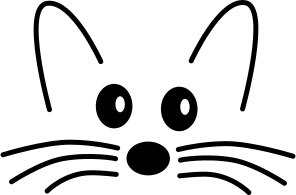
\includegraphics[width=1.4em]{squeak-logo}}}
\iftoshelse{
	\usepackage{marginnote}
		\renewcommand*{\marginfont}{\footnotesize}
	\newcommand{\vartriangleout}{\ifthenelse{\isodd{\thepage}}{\vartriangleright}{\vartriangleleft}}
	\newcommand{\dothisicon}{\fcolorbox{blue!65}{white}{\highlight{$\vartriangleout$}}}
	\newcommand{\dothis}[1]{%
		\noindent\par\noindent
		{\reversemarginpar
			\marginnote{\fcolorbox{blue!65}{white}{\highlight{$\vartriangleout$}}}}
		%\MarginLabel{do this}
		\noindent\emph{#1}
		\nopagebreak}
}{
	\newcommand{\dothisicon}{\raisebox{-.5ex}{
\includegraphics[height=1.2em]{pharo}}}
	\newcommand{\dothis}[1]{%
		\medskip
		\noindent\dothisicon
		\ifx#1\empty\else\quad\emph{#1}\fi
		\par\smallskip\nopagebreak}
}
%===> NEW VERSION <===
% NB: To use this in an individual chapter, you must set:
%\graphicspath{{figures/} {../figures/}}
% at the head of the chapter.  Don't forget the final /
%=============================================================
%:Reader hints (hint)
%
% Indicates a non-obvious consequence 
\newcommand{\hint}[1]{\vspace{1ex}\noindent\fbox{\textsc{Hint}} \emph{#1}}
%=================================================================
% graphics for Morphic handles
\newcommand{\grabHandle}{\raisebox{-0.2ex}{
\includegraphics[width=1em]{blackHandle}}}
\newcommand{\moveHandle}{\raisebox{-0.2ex}{
\includegraphics[width=1em]{moveHandle}}}
\newcommand{\debugHandle}{\raisebox{-0.2ex}{
\includegraphics[width=1em]{debugHandle}}}
%=============================================================
%:Highlighting Important stuff (doublebox)
%
% From Seaside book ...
\newsavebox{\SavedText}
\newlength{\InnerBoxRule}\setlength{\InnerBoxRule}{.75\fboxrule}
\newlength{\OuterBoxRule}\setlength{\OuterBoxRule}{1.5\fboxrule}
\newlength{\BoxSeparation}\setlength{\BoxSeparation}{1.5\fboxrule}
\addtolength{\BoxSeparation}{.5pt}
\newlength{\SaveBoxSep}\setlength{\SaveBoxSep}{2\fboxsep}
%
\newenvironment{doublebox}{\begin{lrbox}{\SavedText}
    \begin{minipage}{.75\textwidth}}
    {\end{minipage}\end{lrbox}\begin{center}
    \setlength{\fboxsep}{\BoxSeparation}\setlength{\fboxrule}{\OuterBoxRule}
    \fbox{\setlength{\fboxsep}{\SaveBoxSep}\setlength{\fboxrule}{\InnerBoxRule}%
      \fbox{\usebox{\SavedText}}}
  \end{center}}
% Use this:
\newcommand{\important}[1]{\begin{doublebox}#1\end{doublebox}}
%=============================================================
%:Section depth
\setcounter{secnumdepth}{2}
%% for this to happen start the file with
%\ifx\wholebook\relax\else
%% $Author$
% $Date$
% $Revision$

% HISTORY:
% 2006-10-31 - Oscar code macros
% ...

%=============================================================
% NB: documentclass must be set in main document.
% Allows book to be generated in multiple formats.
%=============================================================
%:Packages
\usepackage[T1]{fontenc}  %%%%%% really important to get the code directly in the text!
\usepackage{lmodern}
%\usepackage[scaled=0.85]{bookmanx} % needs another scale factor if used with \renewcommand{\sfdefault}{cmbr}
\usepackage{palatino}
\usepackage[scaled=0.85]{helvet}
\usepackage[protrusion,expansion=false]{microtype}
\usepackage{graphicx}
\usepackage{theorem}
\usepackage[english]{babel}
%%% ON: pdfsync breaks the use of p{width} for tabular columns!
%%\ifdefined\usepdfsync\usepackage{pdfsync}\fi % Requires texlive 2007
%=============================================================
%:More packages
%Stef should check which ones are used!
%\usepackage{picinpar}
%\usepackage{layout}
%\usepackage{color}
%\usepackage{enum}
%\usepackage{a4wide}
% \usepackage{fancyhdr}
\usepackage{ifthen}
\usepackage{float}
\usepackage{longtable}
\usepackage{makeidx}
\usepackage[nottoc]{tocbibind}
\usepackage{multicol}
\usepackage{booktabs}	% book-style tables
\usepackage{topcapt}	% enables \topcaption
\usepackage{multirow}
\usepackage{tabularx}
%\usepackage[bottom]{footmisc}
\usepackage{xspace}
\usepackage{alltt}
\usepackage{amssymb,textcomp}
\usepackage[usenames,dvipsnames]{color}
%\usepackage{colortbl}
\usepackage[hang]{subfigure}\makeatletter\def\p@subfigure{\thefigure\,}\makeatother
\usepackage{rotating}
\usepackage{enumitem}	% apb: allows more control over tags in enumerations
\usepackage{verbatim}     % for comment environment
\usepackage{varioref}	% for page references that work
\labelformat{footnote}{\thechapter--#1} % to distinguish citations from jurabib
\usepackage{needspace}
\usepackage{isodateo} % enable \isodate
\usepackage[newparttoc]{titlesec}
\usepackage{titletoc}
\usepackage{wrapfig}
\usepackage[
	super,
	citefull=first,
	authorformat={allreversed,and},
	titleformat={commasep,italic}
]{jurabib} % citations as footnotes
\usepackage[
	colorlinks=true,
	linkcolor=black,
	urlcolor=black,
	citecolor=black
]{hyperref}   % should come last
%=============================================================
%:PDF version
%%\pdfminorversion=3 % Set PDF to 1.3 for Lulu
%=============================================================
%:URL style
\makeatletter
\def\url@leostyle{%
  \@ifundefined{selectfont}{\def\UrlFont{\sf}}{\def\UrlFont{\sffamily}}}
\makeatother
% Now actually use the newly defined style.
\urlstyle{leo}
%=============================================================
%:Booleans
\newboolean{lulu}
\setboolean{lulu}{false}
\newcommand{\ifluluelse}[2]{\ifthenelse{\boolean{lulu}}{#1}{#2}}
%=============================================================
%:Names
\newcommand{\SUnit}{SUnit\xspace}
\newcommand{\sunit}{SUnit\xspace}
\newcommand{\xUnit}{$x$Unit\xspace}
\newcommand{\JUnit}{JUnit\xspace}
\newcommand{\st}{Smalltalk\xspace}
\newcommand{\pharo}{Pharo\xspace} % Use this, not \Pharo
%\newcommand{\sqmap}{SqueakMap\xspace}
\newcommand{\squeak}{Squeak\xspace} % use this, not \Squeak or \sq
\newcommand{\sqsrc}{SqueakSource\xspace}
\newcommand{\sbe}{\url{http://SqueakByExample.org}\xspace}
\newcommand{\pharoweb}{\url{http://pharo-project.org}\xspace}
\newcommand{\pbe}{\url{http://PharoByExample.org}\xspace}
\newcommand{\sba}{\url{http://SquareBracketAssociates.org}\xspace}
\newcommand{\bam}{\lct{Bounc\-ing\-Atoms\-Morph}\xspace}
%=============================================================
%:Markup macros for proof-reading
\usepackage[normalem]{ulem} % for \sout
\usepackage{xcolor}
\newcommand{\ra}{$\rightarrow$}
\newcommand{\ugh}[1]{\textcolor{red}{\uwave{#1}}} % please rephrase
\newcommand{\ins}[1]{\textcolor{blue}{\uline{#1}}} % please insert
\newcommand{\del}[1]{\textcolor{red}{\sout{#1}}} % please delete
\newcommand{\chg}[2]{\textcolor{red}{\sout{#1}}{\ra}\textcolor{blue}{\uline{#2}}} % please change
%=============================================================
%:Editorial comment macros
%\newcommand{\nnbb}[2]{
%    % \fbox{\bfseries\sffamily\scriptsize#1}
%    \fcolorbox{gray}{yellow}{\bfseries\sffamily\scriptsize#1}
%    {\sf\small$\blacktriangleright$\textit{#2}$\blacktriangleleft$}
%   }
\newcommand{\yellowbox}[1]{\fcolorbox{gray}{yellow}{\bfseries\sffamily\scriptsize#1}}
\newcommand{\triangles}[1]{{\sf\small$\blacktriangleright$\textit{#1}$\blacktriangleleft$}}
\newcommand{\nnbb}[2]{\yellowbox{#1} \triangles{#2}}
\newcommand{\fix}{\yellowbox{FIX!}}
\newcommand{\here}{\yellowbox{CONTINUE HERE!}}
% editor macros
\newcommand{\apl}[1]{\nnbb{Alain}{#1}} % Alain
\newcommand{\ab}[1]{\nnbb{Andrew}{#1}} % Black
\newcommand{\sd}[1]{\nnbb{St\'{e}f}{#1}} % Ducasse
\newcommand{\dc}[1]{\nnbb{DamienC}{#1}} % Ducasse
\newcommand{\md}[1]{\nnbb{Marcus}{#1}} % Denker
\newcommand{\on}[1]{\nnbb{Oscar}{#1}} % Nierstrasz
\newcommand{\damien}[1]{\nnbb{Damien}{#1}} % Pollet
\newcommand{\lr}[1]{\nnbb{Lukas}{#1}} % Renggli
\newcommand{\orla}[1]{\nnbb{Orla}{#1}} % Greevy
\newcommand{\alex}[1]{\nnbb{Alex}{#1}} % Bergel
\newcommand{\alx}[1]{\nnbb{Alex}{#1}} % Bergel
\newcommand{\dr}[1]{\nnbb{David}{#1}} % Roethlisberger
\newcommand{\ja}[1]{\nnbb{Jannik}{#1}} % Laval
\newcommand{\jr}[1]{\nnbb{Jorge}{#1}} % Ressia
\newcommand{\fp}[1]{\nnbb{Fabrizio}{#1}} % Perin
\newcommand{\michael}[1]{\nnbb{Michael}{#1}} % Davies
\newcommand{\ew}[1]{\nnbb{Erwann}{#1}} % Wernli
\newcommand{\mb}[1]{\nnbb{Martial}{#1}} % Boniou
\newcommand{\hw}[1]{\nnbb{Hernan}{#1}} % Wilkinson
%=============================================================
%:Abbreviation macros
\newcommand{\ie}{\emph{すなわち}、}
\newcommand{\eg}{\emph{例えば}、}
\newcommand{\etc}{などなど。}
%=============================================================
%:Cross reference macros
\newcommand{\charef}[1]{第~\ref{cha:#1}~章}
\newcommand{\secref}[1]{\ref{sec:#1}~節}
\newcommand{\figref}[1]{図~\ref{fig:#1}\xspace}
\newcommand{\Figref}[1]{図~\ref{fig:#1}\xspace}
\newcommand{\appref}[1]{付録~\ref{app:#1}\xspace}
\newcommand{\tabref}[1]{表~\ref{tab:#1}\xspace}
\newcommand{\faqref}[1]{FAQ~\ref{faq:#1}, p.~\pageref{faq:#1}\xspace}
% APB: I removed trailing \xspace commands from these macros because
% \xspace mostly doesn't work.  If you want a space after your
% references, type one!
% ON: xspace has always worked just fine for me!  Please leave them in.
%
\newcommand{\ruleref}[1]{\ref{rule:#1}\xspace}
%
\newcommand{\egref}[1]{example~\ref{eg:#1}\xspace}
\newcommand{\Egref}[1]{Example~\ref{eg:#1}\xspace}
%
\newcommand{\scrref}[1]{script~\ref{scr:#1}\xspace}
\newcommand{\Scrref}[1]{Script~\ref{scr:#1}\xspace}
\newcommand{\tscrref}[1]{the script~\ref{scr:#1}\xspace}
\newcommand{\Tscrref}[1]{The script~\ref{scr:#1}\xspace}
%
\newcommand{\mthref}[1]{method~\ref{mth:#1}\xspace}
\newcommand{\mthsref}[1]{methods~\ref{mth:#1}\xspace}
\newcommand{\Mthref}[1]{Method~\ref{mth:#1}\xspace}
\newcommand{\tmthref}[1]{the method~\ref{mth:#1}\xspace}
\newcommand{\Tmthref}[1]{The method~\ref{mth:#1}\xspace}
%
\newcommand{\clsref}[1]{class~\ref{cls:#1}\xspace}
\newcommand{\tclsref}[1]{the class~\ref{cls:#1}\xspace}
\newcommand{\Tclsref}[1]{The class~\ref{cls:#1}\xspace}

\newcommand{\chalabel}[1]{\label{cha:#1}}
\newcommand{\seclabel}[1]{\label{sec:#1}}
\newcommand{\figlabel}[1]{\label{fig:#1}}
\newcommand{\tablabel}[1]{\label{tab:#1}}
\newcommand{\rulelabel}[1]{\label{rule:#1}}
\newcommand{\eglabel}[1]{\label{eg:#1}}
\newcommand{\scrlabel}[1]{\label{scr:#1}}
\newcommand{\mthlabel}[1]{\label{mth:#1}}
\newcommand{\clslabel}[1]{\label{cls:#1}}
\newcommand{\faqlabel}[1]{\label{faq:#1}}
%=============================================================
%:Menu item macro
% for menu items, so we can change our minds on how to print them! (apb)
\definecolor{lightgray}{gray}{0.89}
\newcommand{\menu}[1]{{%
	\setlength{\fboxsep}{0pt}%
	\colorbox{lightgray}{{{\upshape\sffamily\strut \,#1\,}}}}}
\newcommand{\link}[1]{{%
	\fontfamily{lmr}\selectfont
 	\upshape{\sffamily \underline{#1}}}}
% For submenu items:
\newcommand{\go}{\,$\triangleright$\,}
% \newcommand{\go}{\,$\blacktriangleright$\,}
% For keyboard shortcuts:
%\newcommand{\short}[1]{\mbox{$\langle${\sc CMD}$\rangle$-#1}\xspace}
\newcommand{\short}[1]{\mbox{{\sc cmd}\hspace{0.08em}--\hspace{0.09em}#1}\xspace}
% For buttons:
\newcommand{\button}[1]{{%
	\setlength{\fboxsep}{0pt}%
	\fbox{{\upshape\sffamily\strut \,#1\,}}}}
% NB: The button macro does not work within captions -- incompatible with xcolor package :-(
\newcommand{\toolsflap}{\textit{Tools} flap\xspace}
%=============================================================
%:Mouse clicks
\newcommand{\click}{click\xspace} % RED
\newcommand{\actclick}{action-click\xspace} % YELLOW
\newcommand{\metaclick}{meta-click\xspace} % BLUE
\newcommand{\Click}{Click\xspace} % RED
\newcommand{\Actclick}{Action-click\xspace} % YELLOW
\newcommand{\Metaclick}{Meta-click\xspace} % BLUE
%=============================================================
%:ToSh macros
\newboolean{tosh}
\setboolean{tosh}{false}
\newcommand{\iftoshelse}[2]{\ifthenelse{\boolean{tosh}}{#1}{#2}}
%=============================================================
%:ToSh colors
%\newcommand{\highlightcolor}{\color{blue!65}}
%\newcommand{\boxcolor}{\color{gray!25}}
\newcommand{\highlight}[1]{\textcolor{blue!65}{#1}}
%\newcommand{\codecolor}{\color{blue!65}}
%%\setlength{\fboxrule}{2pt}
%\newcommand{\asPict}[1]{%
%	{\Large\highlight{#1}}}
%=============================================================
%:Reader cues (do this)
%
% Indicate something the reader should try out.
% \newcommand{\dothisicon}{\raisebox{-.5ex}{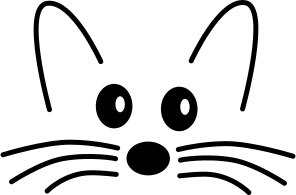
\includegraphics[width=1.4em]{squeak-logo}}}
\iftoshelse{
	\usepackage{marginnote}
		\renewcommand*{\marginfont}{\footnotesize}
	\newcommand{\vartriangleout}{\ifthenelse{\isodd{\thepage}}{\vartriangleright}{\vartriangleleft}}
	\newcommand{\dothisicon}{\fcolorbox{blue!65}{white}{\highlight{$\vartriangleout$}}}
	\newcommand{\dothis}[1]{%
		\noindent\par\noindent
		{\reversemarginpar
			\marginnote{\fcolorbox{blue!65}{white}{\highlight{$\vartriangleout$}}}}
		%\MarginLabel{do this}
		\noindent\emph{#1}
		\nopagebreak}
}{
	\newcommand{\dothisicon}{\raisebox{-.5ex}{
\includegraphics[height=1.2em]{pharo}}}
	\newcommand{\dothis}[1]{%
		\medskip
		\noindent\dothisicon
		\ifx#1\empty\else\quad\emph{#1}\fi
		\par\smallskip\nopagebreak}
}
%===> NEW VERSION <===
% NB: To use this in an individual chapter, you must set:
%\graphicspath{{figures/} {../figures/}}
% at the head of the chapter.  Don't forget the final /
%=============================================================
%:Reader hints (hint)
%
% Indicates a non-obvious consequence 
\newcommand{\hint}[1]{\vspace{1ex}\noindent\fbox{\textsc{Hint}} \emph{#1}}
%=================================================================
% graphics for Morphic handles
\newcommand{\grabHandle}{\raisebox{-0.2ex}{
\includegraphics[width=1em]{blackHandle}}}
\newcommand{\moveHandle}{\raisebox{-0.2ex}{
\includegraphics[width=1em]{moveHandle}}}
\newcommand{\debugHandle}{\raisebox{-0.2ex}{
\includegraphics[width=1em]{debugHandle}}}
%=============================================================
%:Highlighting Important stuff (doublebox)
%
% From Seaside book ...
\newsavebox{\SavedText}
\newlength{\InnerBoxRule}\setlength{\InnerBoxRule}{.75\fboxrule}
\newlength{\OuterBoxRule}\setlength{\OuterBoxRule}{1.5\fboxrule}
\newlength{\BoxSeparation}\setlength{\BoxSeparation}{1.5\fboxrule}
\addtolength{\BoxSeparation}{.5pt}
\newlength{\SaveBoxSep}\setlength{\SaveBoxSep}{2\fboxsep}
%
\newenvironment{doublebox}{\begin{lrbox}{\SavedText}
    \begin{minipage}{.75\textwidth}}
    {\end{minipage}\end{lrbox}\begin{center}
    \setlength{\fboxsep}{\BoxSeparation}\setlength{\fboxrule}{\OuterBoxRule}
    \fbox{\setlength{\fboxsep}{\SaveBoxSep}\setlength{\fboxrule}{\InnerBoxRule}%
      \fbox{\usebox{\SavedText}}}
  \end{center}}
% Use this:
\newcommand{\important}[1]{\begin{doublebox}#1\end{doublebox}}
%=============================================================
%:Section depth
\setcounter{secnumdepth}{2}
%% for this to happen start the file with
%\ifx\wholebook\relax\else
%\input{../common.tex}
%\begin{document}
%\fi
% and terminate by
% \ifx\wholebook\relax\else\end{document}\fi

\DeclareGraphicsExtensions{.pdf, .jpg, .png}
%=============================================================
%:PDF setup
\hypersetup{
%   a4paper,
%   pdfstartview=FitV,
%   colorlinks,
%   linkcolor=darkblue,
%   citecolor=darkblue,
   pdftitle={Pharo by Example},
   pdfauthor={Andrew P. Black, St\'ephane Ducasse,	Oscar Nierstrasz,
Damien Pollet},
   pdfkeywords={Smalltalk, Squeak, Object-Oriented Programming, OOP},
   pdfsubject={Computer Science}
}
%=============================================================
%:Page layout and appearance
%
% \renewcommand{\headrulewidth}{0pt}
\renewcommand{\chaptermark}[1]{\markboth{#1}{}}
\renewcommand{\sectionmark}[1]{\markright{\thesection\ #1}}
\renewpagestyle{plain}[\small\itshape]{%
	\setheadrule{0pt}%
	\sethead[][][]{}{}{}%
	\setfoot[][][]{}{}{}}
\renewpagestyle{headings}[\small\itshape]{%
	\setheadrule{0pt}%
	\setmarks{chapter}{section}%
	\sethead[\thepage][][\chaptertitle]{\sectiontitle}{}{\thepage}%
	\setfoot[][][]{}{}{}}
%=============================================================
%:Title section setup and TOC numbering depth
\setcounter{secnumdepth}{1}
\setcounter{tocdepth}{1}
\titleformat{\part}[display]{\centering}{\huge\partname\ \thepart}{1em}{\Huge\textbf}[]
\titleformat{\chapter}[display]{}{\huge\chaptertitlename\ \thechapter}{1em}{\Huge\raggedright\textbf}[]
\titlecontents{part}[3pc]{%
		\pagebreak[2]\addvspace{1em plus.4em minus.2em}%
		\leavevmode\large\bfseries}
	{\contentslabel{3pc}}{\hspace*{-3pc}}
	{}[\nopagebreak]
\titlecontents{chapter}[3pc]{%
		\pagebreak[0]\addvspace{1em plus.2em minus.2em}%
		\leavevmode\bfseries}
	{\contentslabel{3pc}}{}
	{\hfill\contentspage}[\nopagebreak]
\dottedcontents{section}[3pc]{}{3pc}{1pc}
\dottedcontents{subsection}[3pc]{}{0pc}{1pc}
% \dottedcontents{subsection}[4.5em]{}{0pt}{1pc}
% Make \cleardoublepage insert really blank pages http://www.tex.ac.uk/cgi-bin/texfaq2html?label=reallyblank
\let\origdoublepage\cleardoublepage
\newcommand{\clearemptydoublepage}{%
  \clearpage
  {\pagestyle{empty}\origdoublepage}}
\let\cleardoublepage\clearemptydoublepage % see http://www.tex.ac.uk/cgi-bin/texfaq2html?label=patch
%=============================================================
%:FAQ macros (for FAQ chapter)
\newtheorem{faq}{FAQ}
\newcommand{\answer}{\paragraph{Answer}\ }
%=============================================================
%:Listings package configuration
% \newcommand{\caret}{\makebox{\raisebox{0.4ex}{\footnotesize{$\wedge$}}}}
\newcommand{\caret}{\^\,}
\newcommand{\escape}{{\sf \textbackslash}}
\definecolor{source}{gray}{0.95}
\usepackage{listings}
\lstdefinelanguage{Smalltalk}{
%  morekeywords={self,super,true,false,nil,thisContext}, % This is overkill
  morestring=[d]',
  morecomment=[s]{"}{"},
  alsoletter={\#:},
  escapechar={!},
  literate=
    {BANG}{!}1
    {CARET}{\^}1
    {UNDERSCORE}{\_}1
    {\\st}{Smalltalk}9 % convenience -- in case \st occurs in code
    % {'}{{\textquotesingle}}1 % replaced by upquote=true in \lstset
    {_}{{$\leftarrow$}}1
    {>>>}{{\sep}}1
    {^}{{$\uparrow$}}1
    {~}{{$\sim$}}1
    {-}{{\texttt{-}}}1 %{\textminus}}1 %{-}{\hspace{-0.13em}}{-}}1  % the goal is to make - the same width as +
    % {+}{\sf+}1 %{\raisebox{0.08ex}{+}}}1      % and to raise + off the baseline to match -
    {-->}{{\quad$\longrightarrow$\quad}}3
	, % Don't forget the comma at the end!
  tabsize=4
}[keywords,comments,strings]

\lstset{language=Smalltalk,
	basicstyle=\sffamily,
	keywordstyle=\color{black}\bfseries,
	% stringstyle=\ttfamily, % Ugly! do we really want this? -- on
	mathescape=true,
	showstringspaces=false,
	keepspaces=true,
	breaklines=true,
	breakautoindent=true,
	backgroundcolor=\color{source},
	lineskip={-1pt}, % Ugly hack
	upquote=true, % straight quote; requires textcomp package
	columns=fullflexible} % no fixed width fonts
% In-line code (literal)
% Normally use this for all in-line code:
\newcommand{\ct}{\lstinline[mathescape=false,backgroundcolor=\color{white},basicstyle={\sffamily\upshape}]}
% apb 2007.8.28 added the \upshape declaration to avoid getting italicized code in \dothis{ } sections.
% In-line code (latex enabled)
% Use this only in special situations where \ct does not work
% (within section headings ...):
\newcommand{\lct}[1]{{\textsf{\textup{#1}}}}
% Use these for system categories and protocols:
\newcommand{\scat}[1]{\emph{\textsf{#1}}\xspace}
\newcommand{\pkg}[1]{\emph{\textsf{#1}}\xspace}
\newcommand{\prot}[1]{\emph{\textsf{#1}}\xspace}
% Code environments
% NB: the arg is for tests
% Only code and example environments may be tests
\lstnewenvironment{code}[1]{%
	\lstset{%
		% frame=lines,
		frame=single,
		framerule=0pt,
		mathescape=false
	}
}{}
\def\ignoredollar#1{}
%=============================================================
%:Code environments (method, script ...)
% NB: the third arg is for tests
% Only code and example environments may be tests
\lstnewenvironment{example}[3][defaultlabel]{%
	\renewcommand{\lstlistingname}{Example}%
	\lstset{
		% frame=lines,
		frame=single,
		framerule=0pt,
		mathescape=false,
		caption={\emph{#2}},
		label={eg:#1}
	}
}{}
\lstnewenvironment{script}[2][defaultlabel]{%
\renewcommand{\lstlistingname}{Script}%
	\lstset{
		% frame=lines,
		frame=single,
		framerule=0pt,
		mathescape=false,
		name={Script},
		caption={\emph{#2}},
		label={scr:#1}
	}
}{}
\lstnewenvironment{method}[2][defaultlabel]{%
	\renewcommand{\lstlistingname}{Method}%
	\lstset{
		% frame=lines,
		frame=single,
		framerule=0pt,
		mathescape=false,
		name={Method},
		caption={\emph{#2}},
		label={mth:#1}
	}
}{}
\lstnewenvironment{methods}[2][defaultlabel]{% just for multiple methods at once
	\renewcommand{\lstlistingname}{Methods}%
	\lstset{
		% frame=lines,
		frame=single,
		framerule=0pt,
		mathescape=false,
		name={Method},
		caption={\emph{#2}},
		label={mth:#1}
	}
}{}
\lstnewenvironment{numMethod}[2][defaultlabel]{%
	\renewcommand{\lstlistingname}{Method}%
	\lstset{
		numbers=left,
		numberstyle={\tiny\sffamily},
		% frame=lines,
		frame=single,
		framerule=0pt,
		mathescape=false,
		name={Method},
		caption={\emph{#2}},
		label={mth:#1}
	}
}{}
\lstnewenvironment{classdef}[2][defaultlabel]{%
	\renewcommand{\lstlistingname}{Class}%
	\lstset{
		% frame=lines,
		frame=single,
		framerule=0pt,
		mathescape=false,
		name={Class},
		caption={\emph{#2}},
		label={cls:#1}
	}
}{}
%=============================================================
%:Reserving space
% Usually need one more line than the actual lines of code
\newcommand{\needlines}[1]{\Needspace{#1\baselineskip}}
%=============================================================
%:Indexing macros
% Macros ending with "ind" generate text as well as an index entry
% Macros ending with "index" *only* generate an index entry
\newcommand{\ind}[1]{\index{#1}#1\xspace} % plain text
\newcommand{\subind}[2]{\index{#1!#2}#2\xspace} % show #2, subindex under #1
\newcommand{\emphind}[1]{\index{#1}\emph{#1}\xspace} % emph #1
\newcommand{\emphsubind}[2]{\index{#1!#2}\emph{#2}\xspace} % show emph #2, subindex inder #1
\newcommand{\scatind}[1]{\index{#1@\textsf{#1} (category)}\scat{#1}} % category
\newcommand{\pkgind}[1]{\index{#1@\textsf{#1} (package)}\pkg{#1}} % package
\newcommand{\protind}[1]{\index{#1@\textsf{#1} (protocol)}\prot{#1}} % protocol
\newcommand{\clsind}[1]{\index{#1@\textsf{#1} (class)}\ct{#1}\xspace}
% \newcommand{\clsind}[1]{\index{#1!\#@(class)}\ct{#1}\xspace} % class
\newcommand{\clsindplural}[1]{\index{#1!\#@(class)}\ct{#1}s\xspace} % class
\newcommand{\cvind}[1]{\index{#1@\textsf{#1} (class variable)}\ct{#1}\xspace} % class var
\newcommand{\glbind}[1]{\index{#1@\textsf{#1} (global)}\ct{#1}\xspace} % global
\newcommand{\patind}[1]{\index{#1@#1 (pattern)}\ct{#1}\xspace} % pattern
\newcommand{\pvind}[1]{\index{#1@\textsf{#1} (pseudo variable)}\ct{#1}\xspace} % pseudo var
\newcommand{\clsmthind}[2]{\index{#1!#2@\ct{#2}}\ct{#1>>>#2}\xspace} % class + method name
\newcommand{\mthind}[2]{\index{#1!#2@\ct{#2}}\ct{#2}\xspace} % show method name only
\newcommand{\lmthind}[2]{\index{#1!#2@\ct{#2}}\lct{#2}\xspace} % show method name only
\newcommand{\cmind}[2]{\index{#1!#2@\ct{#2}}\ct{#1>>>#2}\xspace} % show class>>method
\newcommand{\lcmind}[2]{\index{#1!#2@\ct{#2}}\lct{#1>>>#2}\xspace} % show class>>method
\newcommand{\toolsflapind}{\index{Tools flap}\toolsflap} % index tools flap
% The following only generate an index entry:
% \newcommand{\clsindex}[1]{\index{#1@\textsf{#1} (class)}}
\newcommand{\clsindex}[1]{\index{#1!\#@(class)}} % class
\newcommand{\mthindex}[2]{\index{#1!#2@\ct{#2}}} % method
\newcommand{\cmindex}[2]{\index{#1!#2@\ct{#2}}} % class>>method
\newcommand{\cvindex}[1]{\index{#1@\textsf{#1} (class variable)}} % class var
\newcommand{\glbindex}[1]{\index{#1@\textsf{#1} (global)}}% global
\newcommand{\pvindex}[1]{\index{#1@\textsf{#1} (pseudo variable)}}% pseudo var
\newcommand{\seeindex}[2]{\index{#1|see{#2}}} % #1, see #2
\newcommand{\scatindex}[1]{\index{#1@\textsf{#1} (category)}} % category
\newcommand{\pkgindex}[1]{\index{#1@\textsf{#1} (package)}} % package
\newcommand{\protindex}[1]{\index{#1@\textsf{#1} (protocol)}} % protocol
% How can we have the main entry page numbers in bold yet not break the hyperlink?
\newcommand{\boldidx}[1]{{\bf #1}} % breaks hyperlink
%\newcommand{\indmain}[1]{\index{#1|boldidx}#1\xspace} % plain text, main entry
%\newcommand{\emphsubindmain}[2]{\index{#1!#2|boldidx}\emph{#2}\xspace} % subindex, main entry
%\newcommand{\subindmain}[2]{\index{#1!#2|boldidx}#2\xspace} % subindex, main entry
%\newcommand{\clsindmain}[1]{\index{#1@\textsf{#1} (class)|boldidx}\ct{#1}\xspace}
%\newcommand{\clsindmain}[1]{\index{#1!\#@(class)|boldidx}\ct{#1}\xspace} % class main
%\newcommand{\indexmain}[1]{\index{#1|boldidx}} % main index entry only
\newcommand{\indmain}[1]{\index{#1}#1\xspace} % The main index entry for this item
\newcommand{\emphsubindmain}[2]{\index{#1!#2}\emph{#2}\xspace} % subindex, main entry
\newcommand{\subindmain}[2]{\index{#1!#2}#2\xspace} % subindex, main entry
%\newcommand{\clsindmain}[1]{\index{#1@\textsf{#1} (class)}\ct{#1}\xspace}
\newcommand{\clsindmain}[1]{\index{#1!\#@(class)}\ct{#1}\xspace} % class main
\newcommand{\clsindexmain}[1]{\index{#1!\#@(class)}} % class main index only
\newcommand{\indexmain}[1]{\index{#1}} 
%=============================================================
%:Code macros
% some constants
\newcommand{\codesize}{\small}
\newcommand{\codefont}{\sffamily}
%\newcommand{\cat}[1]{\textit{In category #1}}%%To remove later
\newlength{\scriptindent}
\setlength{\scriptindent}{.3cm}
%% Method presentation constants
\newlength{\methodindent}
\newlength{\methodwordlength}
\newlength{\aftermethod}
\setlength{\methodindent}{0.2cm}
\settowidth{\methodwordlength}{\ M\'ethode\ }
%=============================================================
%:Smalltalk macros
%\newcommand{\sep}{{$\gg$}}
\newcommand{\sep}{\mbox{>>}}
\newcommand{\self}{\lct{self}\xspace}
\newcommand{\super}{\lct{super}\xspace}
\newcommand{\nil}{\lct{nil}\xspace}
%=============================================================
% be less conservative about float placement
% these commands are from http://www.tex.ac.uk/cgi-bin/texfaq2html?label=floats
\renewcommand{\topfraction}{.9}
\renewcommand{\bottomfraction}{.9}
\renewcommand{\textfraction}{.1}
\renewcommand{\floatpagefraction}{.85}
\renewcommand{\dbltopfraction}{.66}
\renewcommand{\dblfloatpagefraction}{.85}
\setcounter{topnumber}{9}
\setcounter{bottomnumber}{9}
\setcounter{totalnumber}{20}
\setcounter{dbltopnumber}{9}
%=============================================================
% Give information from each chapter's author
\newcommand{\contact}[2]{\textbf{#1} \textsf{(#2)}}

\newcommand{\chapterauthor}[1]{\emph{with the participation of:\\#1}\\}

\newcommand{\authornoury}{\contact{Noury Bouraqadi}{bouraqadi@gmail.com}}
\newcommand{\authordamienc}{\contact{Damien Cassou}{damien.cassou@gmail.com}}
\newcommand{\authoroscar}{\contact{Oscar Nierstrasz}{oscar.nierstrasz@acm.org}}
\newcommand{\authorsteph}{\contact{St\'ephane Ducasse}{stephane.ducasse@inria.fr}}
\newcommand{\authoralex}{\contact{Alexandre Bergel}{alexandre@bergel.eu}}
\newcommand{\authorolivier}{\contact{Olivier Auverlot}{olivier.auverlot@inria.fr}}
\newcommand{\authornicolas}{\contact{Nicolas Cellier}{ncellier@ifrance.com}}
\newcommand{\authormarcus}{\contact{Marcus Denker}{marcus.denker@inria.fr}}
\newcommand{\authoralain}{\contact{Alain Plantec}{alain.plantec@univ-brest.fr}}
\newcommand{\authordale}{\contact{Dale Henrichs}{dale.henrichs@gemstone.com}}
\newcommand{\authormariano}{\contact{Mariano Martinez Peck}{marianopeck@gmail.com}}
\newcommand{\authorsven}{\contact{Sven Van Caekenberghe}{sven@beta9.be}}

%=============================================================
% apb doesn't like paragraphs to run in to each other without a break
\parskip 1ex
%=============================================================
%:Stuff to check, merge or deprecate
%\setlength{\marginparsep}{2mm}
%\renewcommand{\baselinestretch}{1.1}
%=============================================================

%\begin{document}
%\fi
% and terminate by
% \ifx\wholebook\relax\else\end{document}\fi

\DeclareGraphicsExtensions{.pdf, .jpg, .png}
%=============================================================
%:PDF setup
\hypersetup{
%   a4paper,
%   pdfstartview=FitV,
%   colorlinks,
%   linkcolor=darkblue,
%   citecolor=darkblue,
   pdftitle={Pharo by Example},
   pdfauthor={Andrew P. Black, St\'ephane Ducasse,	Oscar Nierstrasz,
Damien Pollet},
   pdfkeywords={Smalltalk, Squeak, Object-Oriented Programming, OOP},
   pdfsubject={Computer Science}
}
%=============================================================
%:Page layout and appearance
%
% \renewcommand{\headrulewidth}{0pt}
\renewcommand{\chaptermark}[1]{\markboth{#1}{}}
\renewcommand{\sectionmark}[1]{\markright{\thesection\ #1}}
\renewpagestyle{plain}[\small\itshape]{%
	\setheadrule{0pt}%
	\sethead[][][]{}{}{}%
	\setfoot[][][]{}{}{}}
\renewpagestyle{headings}[\small\itshape]{%
	\setheadrule{0pt}%
	\setmarks{chapter}{section}%
	\sethead[\thepage][][\chaptertitle]{\sectiontitle}{}{\thepage}%
	\setfoot[][][]{}{}{}}
%=============================================================
%:Title section setup and TOC numbering depth
\setcounter{secnumdepth}{1}
\setcounter{tocdepth}{1}
\titleformat{\part}[display]{\centering}{\huge\partname\ \thepart}{1em}{\Huge\textbf}[]
\titleformat{\chapter}[display]{}{\huge\chaptertitlename\ \thechapter}{1em}{\Huge\raggedright\textbf}[]
\titlecontents{part}[3pc]{%
		\pagebreak[2]\addvspace{1em plus.4em minus.2em}%
		\leavevmode\large\bfseries}
	{\contentslabel{3pc}}{\hspace*{-3pc}}
	{}[\nopagebreak]
\titlecontents{chapter}[3pc]{%
		\pagebreak[0]\addvspace{1em plus.2em minus.2em}%
		\leavevmode\bfseries}
	{\contentslabel{3pc}}{}
	{\hfill\contentspage}[\nopagebreak]
\dottedcontents{section}[3pc]{}{3pc}{1pc}
\dottedcontents{subsection}[3pc]{}{0pc}{1pc}
% \dottedcontents{subsection}[4.5em]{}{0pt}{1pc}
% Make \cleardoublepage insert really blank pages http://www.tex.ac.uk/cgi-bin/texfaq2html?label=reallyblank
\let\origdoublepage\cleardoublepage
\newcommand{\clearemptydoublepage}{%
  \clearpage
  {\pagestyle{empty}\origdoublepage}}
\let\cleardoublepage\clearemptydoublepage % see http://www.tex.ac.uk/cgi-bin/texfaq2html?label=patch
%=============================================================
%:FAQ macros (for FAQ chapter)
\newtheorem{faq}{FAQ}
\newcommand{\answer}{\paragraph{Answer}\ }
%=============================================================
%:Listings package configuration
% \newcommand{\caret}{\makebox{\raisebox{0.4ex}{\footnotesize{$\wedge$}}}}
\newcommand{\caret}{\^\,}
\newcommand{\escape}{{\sf \textbackslash}}
\definecolor{source}{gray}{0.95}
\usepackage{listings}
\lstdefinelanguage{Smalltalk}{
%  morekeywords={self,super,true,false,nil,thisContext}, % This is overkill
  morestring=[d]',
  morecomment=[s]{"}{"},
  alsoletter={\#:},
  escapechar={!},
  literate=
    {BANG}{!}1
    {CARET}{\^}1
    {UNDERSCORE}{\_}1
    {\\st}{Smalltalk}9 % convenience -- in case \st occurs in code
    % {'}{{\textquotesingle}}1 % replaced by upquote=true in \lstset
    {_}{{$\leftarrow$}}1
    {>>>}{{\sep}}1
    {^}{{$\uparrow$}}1
    {~}{{$\sim$}}1
    {-}{{\texttt{-}}}1 %{\textminus}}1 %{-}{\hspace{-0.13em}}{-}}1  % the goal is to make - the same width as +
    % {+}{\sf+}1 %{\raisebox{0.08ex}{+}}}1      % and to raise + off the baseline to match -
    {-->}{{\quad$\longrightarrow$\quad}}3
	, % Don't forget the comma at the end!
  tabsize=4
}[keywords,comments,strings]

\lstset{language=Smalltalk,
	basicstyle=\sffamily,
	keywordstyle=\color{black}\bfseries,
	% stringstyle=\ttfamily, % Ugly! do we really want this? -- on
	mathescape=true,
	showstringspaces=false,
	keepspaces=true,
	breaklines=true,
	breakautoindent=true,
	backgroundcolor=\color{source},
	lineskip={-1pt}, % Ugly hack
	upquote=true, % straight quote; requires textcomp package
	columns=fullflexible} % no fixed width fonts
% In-line code (literal)
% Normally use this for all in-line code:
\newcommand{\ct}{\lstinline[mathescape=false,backgroundcolor=\color{white},basicstyle={\sffamily\upshape}]}
% apb 2007.8.28 added the \upshape declaration to avoid getting italicized code in \dothis{ } sections.
% In-line code (latex enabled)
% Use this only in special situations where \ct does not work
% (within section headings ...):
\newcommand{\lct}[1]{{\textsf{\textup{#1}}}}
% Use these for system categories and protocols:
\newcommand{\scat}[1]{\emph{\textsf{#1}}\xspace}
\newcommand{\pkg}[1]{\emph{\textsf{#1}}\xspace}
\newcommand{\prot}[1]{\emph{\textsf{#1}}\xspace}
% Code environments
% NB: the arg is for tests
% Only code and example environments may be tests
\lstnewenvironment{code}[1]{%
	\lstset{%
		% frame=lines,
		frame=single,
		framerule=0pt,
		mathescape=false
	}
}{}
\def\ignoredollar#1{}
%=============================================================
%:Code environments (method, script ...)
% NB: the third arg is for tests
% Only code and example environments may be tests
\lstnewenvironment{example}[3][defaultlabel]{%
	\renewcommand{\lstlistingname}{Example}%
	\lstset{
		% frame=lines,
		frame=single,
		framerule=0pt,
		mathescape=false,
		caption={\emph{#2}},
		label={eg:#1}
	}
}{}
\lstnewenvironment{script}[2][defaultlabel]{%
\renewcommand{\lstlistingname}{Script}%
	\lstset{
		% frame=lines,
		frame=single,
		framerule=0pt,
		mathescape=false,
		name={Script},
		caption={\emph{#2}},
		label={scr:#1}
	}
}{}
\lstnewenvironment{method}[2][defaultlabel]{%
	\renewcommand{\lstlistingname}{Method}%
	\lstset{
		% frame=lines,
		frame=single,
		framerule=0pt,
		mathescape=false,
		name={Method},
		caption={\emph{#2}},
		label={mth:#1}
	}
}{}
\lstnewenvironment{methods}[2][defaultlabel]{% just for multiple methods at once
	\renewcommand{\lstlistingname}{Methods}%
	\lstset{
		% frame=lines,
		frame=single,
		framerule=0pt,
		mathescape=false,
		name={Method},
		caption={\emph{#2}},
		label={mth:#1}
	}
}{}
\lstnewenvironment{numMethod}[2][defaultlabel]{%
	\renewcommand{\lstlistingname}{Method}%
	\lstset{
		numbers=left,
		numberstyle={\tiny\sffamily},
		% frame=lines,
		frame=single,
		framerule=0pt,
		mathescape=false,
		name={Method},
		caption={\emph{#2}},
		label={mth:#1}
	}
}{}
\lstnewenvironment{classdef}[2][defaultlabel]{%
	\renewcommand{\lstlistingname}{Class}%
	\lstset{
		% frame=lines,
		frame=single,
		framerule=0pt,
		mathescape=false,
		name={Class},
		caption={\emph{#2}},
		label={cls:#1}
	}
}{}
%=============================================================
%:Reserving space
% Usually need one more line than the actual lines of code
\newcommand{\needlines}[1]{\Needspace{#1\baselineskip}}
%=============================================================
%:Indexing macros
% Macros ending with "ind" generate text as well as an index entry
% Macros ending with "index" *only* generate an index entry
\newcommand{\ind}[1]{\index{#1}#1\xspace} % plain text
\newcommand{\subind}[2]{\index{#1!#2}#2\xspace} % show #2, subindex under #1
\newcommand{\emphind}[1]{\index{#1}\emph{#1}\xspace} % emph #1
\newcommand{\emphsubind}[2]{\index{#1!#2}\emph{#2}\xspace} % show emph #2, subindex inder #1
\newcommand{\scatind}[1]{\index{#1@\textsf{#1} (category)}\scat{#1}} % category
\newcommand{\pkgind}[1]{\index{#1@\textsf{#1} (package)}\pkg{#1}} % package
\newcommand{\protind}[1]{\index{#1@\textsf{#1} (protocol)}\prot{#1}} % protocol
\newcommand{\clsind}[1]{\index{#1@\textsf{#1} (class)}\ct{#1}\xspace}
% \newcommand{\clsind}[1]{\index{#1!\#@(class)}\ct{#1}\xspace} % class
\newcommand{\clsindplural}[1]{\index{#1!\#@(class)}\ct{#1}s\xspace} % class
\newcommand{\cvind}[1]{\index{#1@\textsf{#1} (class variable)}\ct{#1}\xspace} % class var
\newcommand{\glbind}[1]{\index{#1@\textsf{#1} (global)}\ct{#1}\xspace} % global
\newcommand{\patind}[1]{\index{#1@#1 (pattern)}\ct{#1}\xspace} % pattern
\newcommand{\pvind}[1]{\index{#1@\textsf{#1} (pseudo variable)}\ct{#1}\xspace} % pseudo var
\newcommand{\clsmthind}[2]{\index{#1!#2@\ct{#2}}\ct{#1>>>#2}\xspace} % class + method name
\newcommand{\mthind}[2]{\index{#1!#2@\ct{#2}}\ct{#2}\xspace} % show method name only
\newcommand{\lmthind}[2]{\index{#1!#2@\ct{#2}}\lct{#2}\xspace} % show method name only
\newcommand{\cmind}[2]{\index{#1!#2@\ct{#2}}\ct{#1>>>#2}\xspace} % show class>>method
\newcommand{\lcmind}[2]{\index{#1!#2@\ct{#2}}\lct{#1>>>#2}\xspace} % show class>>method
\newcommand{\toolsflapind}{\index{Tools flap}\toolsflap} % index tools flap
% The following only generate an index entry:
% \newcommand{\clsindex}[1]{\index{#1@\textsf{#1} (class)}}
\newcommand{\clsindex}[1]{\index{#1!\#@(class)}} % class
\newcommand{\mthindex}[2]{\index{#1!#2@\ct{#2}}} % method
\newcommand{\cmindex}[2]{\index{#1!#2@\ct{#2}}} % class>>method
\newcommand{\cvindex}[1]{\index{#1@\textsf{#1} (class variable)}} % class var
\newcommand{\glbindex}[1]{\index{#1@\textsf{#1} (global)}}% global
\newcommand{\pvindex}[1]{\index{#1@\textsf{#1} (pseudo variable)}}% pseudo var
\newcommand{\seeindex}[2]{\index{#1|see{#2}}} % #1, see #2
\newcommand{\scatindex}[1]{\index{#1@\textsf{#1} (category)}} % category
\newcommand{\pkgindex}[1]{\index{#1@\textsf{#1} (package)}} % package
\newcommand{\protindex}[1]{\index{#1@\textsf{#1} (protocol)}} % protocol
% How can we have the main entry page numbers in bold yet not break the hyperlink?
\newcommand{\boldidx}[1]{{\bf #1}} % breaks hyperlink
%\newcommand{\indmain}[1]{\index{#1|boldidx}#1\xspace} % plain text, main entry
%\newcommand{\emphsubindmain}[2]{\index{#1!#2|boldidx}\emph{#2}\xspace} % subindex, main entry
%\newcommand{\subindmain}[2]{\index{#1!#2|boldidx}#2\xspace} % subindex, main entry
%\newcommand{\clsindmain}[1]{\index{#1@\textsf{#1} (class)|boldidx}\ct{#1}\xspace}
%\newcommand{\clsindmain}[1]{\index{#1!\#@(class)|boldidx}\ct{#1}\xspace} % class main
%\newcommand{\indexmain}[1]{\index{#1|boldidx}} % main index entry only
\newcommand{\indmain}[1]{\index{#1}#1\xspace} % The main index entry for this item
\newcommand{\emphsubindmain}[2]{\index{#1!#2}\emph{#2}\xspace} % subindex, main entry
\newcommand{\subindmain}[2]{\index{#1!#2}#2\xspace} % subindex, main entry
%\newcommand{\clsindmain}[1]{\index{#1@\textsf{#1} (class)}\ct{#1}\xspace}
\newcommand{\clsindmain}[1]{\index{#1!\#@(class)}\ct{#1}\xspace} % class main
\newcommand{\clsindexmain}[1]{\index{#1!\#@(class)}} % class main index only
\newcommand{\indexmain}[1]{\index{#1}} 
%=============================================================
%:Code macros
% some constants
\newcommand{\codesize}{\small}
\newcommand{\codefont}{\sffamily}
%\newcommand{\cat}[1]{\textit{In category #1}}%%To remove later
\newlength{\scriptindent}
\setlength{\scriptindent}{.3cm}
%% Method presentation constants
\newlength{\methodindent}
\newlength{\methodwordlength}
\newlength{\aftermethod}
\setlength{\methodindent}{0.2cm}
\settowidth{\methodwordlength}{\ M\'ethode\ }
%=============================================================
%:Smalltalk macros
%\newcommand{\sep}{{$\gg$}}
\newcommand{\sep}{\mbox{>>}}
\newcommand{\self}{\lct{self}\xspace}
\newcommand{\super}{\lct{super}\xspace}
\newcommand{\nil}{\lct{nil}\xspace}
%=============================================================
% be less conservative about float placement
% these commands are from http://www.tex.ac.uk/cgi-bin/texfaq2html?label=floats
\renewcommand{\topfraction}{.9}
\renewcommand{\bottomfraction}{.9}
\renewcommand{\textfraction}{.1}
\renewcommand{\floatpagefraction}{.85}
\renewcommand{\dbltopfraction}{.66}
\renewcommand{\dblfloatpagefraction}{.85}
\setcounter{topnumber}{9}
\setcounter{bottomnumber}{9}
\setcounter{totalnumber}{20}
\setcounter{dbltopnumber}{9}
%=============================================================
% Give information from each chapter's author
\newcommand{\contact}[2]{\textbf{#1} \textsf{(#2)}}

\newcommand{\chapterauthor}[1]{\emph{with the participation of:\\#1}\\}

\newcommand{\authornoury}{\contact{Noury Bouraqadi}{bouraqadi@gmail.com}}
\newcommand{\authordamienc}{\contact{Damien Cassou}{damien.cassou@gmail.com}}
\newcommand{\authoroscar}{\contact{Oscar Nierstrasz}{oscar.nierstrasz@acm.org}}
\newcommand{\authorsteph}{\contact{St\'ephane Ducasse}{stephane.ducasse@inria.fr}}
\newcommand{\authoralex}{\contact{Alexandre Bergel}{alexandre@bergel.eu}}
\newcommand{\authorolivier}{\contact{Olivier Auverlot}{olivier.auverlot@inria.fr}}
\newcommand{\authornicolas}{\contact{Nicolas Cellier}{ncellier@ifrance.com}}
\newcommand{\authormarcus}{\contact{Marcus Denker}{marcus.denker@inria.fr}}
\newcommand{\authoralain}{\contact{Alain Plantec}{alain.plantec@univ-brest.fr}}
\newcommand{\authordale}{\contact{Dale Henrichs}{dale.henrichs@gemstone.com}}
\newcommand{\authormariano}{\contact{Mariano Martinez Peck}{marianopeck@gmail.com}}
\newcommand{\authorsven}{\contact{Sven Van Caekenberghe}{sven@beta9.be}}

%=============================================================
% apb doesn't like paragraphs to run in to each other without a break
\parskip 1ex
%=============================================================
%:Stuff to check, merge or deprecate
%\setlength{\marginparsep}{2mm}
%\renewcommand{\baselinestretch}{1.1}
%=============================================================

	\pagestyle{headings}
	\setboolean{lulu}{true}
% --------------------------------------------
% A4:
%	\documentclass[a4paper,11pt,twoside]{book}
%	% $Author$
% $Date$
% $Revision$

% HISTORY:
% 2006-10-31 - Oscar code macros
% ...

%=============================================================
% NB: documentclass must be set in main document.
% Allows book to be generated in multiple formats.
%=============================================================
%:Packages
\usepackage[T1]{fontenc}  %%%%%% really important to get the code directly in the text!
\usepackage{lmodern}
%\usepackage[scaled=0.85]{bookmanx} % needs another scale factor if used with \renewcommand{\sfdefault}{cmbr}
\usepackage{palatino}
\usepackage[scaled=0.85]{helvet}
\usepackage[protrusion,expansion=false]{microtype}
\usepackage{graphicx}
\usepackage{theorem}
\usepackage[english]{babel}
%%% ON: pdfsync breaks the use of p{width} for tabular columns!
%%\ifdefined\usepdfsync\usepackage{pdfsync}\fi % Requires texlive 2007
%=============================================================
%:More packages
%Stef should check which ones are used!
%\usepackage{picinpar}
%\usepackage{layout}
%\usepackage{color}
%\usepackage{enum}
%\usepackage{a4wide}
% \usepackage{fancyhdr}
\usepackage{ifthen}
\usepackage{float}
\usepackage{longtable}
\usepackage{makeidx}
\usepackage[nottoc]{tocbibind}
\usepackage{multicol}
\usepackage{booktabs}	% book-style tables
\usepackage{topcapt}	% enables \topcaption
\usepackage{multirow}
\usepackage{tabularx}
%\usepackage[bottom]{footmisc}
\usepackage{xspace}
\usepackage{alltt}
\usepackage{amssymb,textcomp}
\usepackage[usenames,dvipsnames]{color}
%\usepackage{colortbl}
\usepackage[hang]{subfigure}\makeatletter\def\p@subfigure{\thefigure\,}\makeatother
\usepackage{rotating}
\usepackage{enumitem}	% apb: allows more control over tags in enumerations
\usepackage{verbatim}     % for comment environment
\usepackage{varioref}	% for page references that work
\labelformat{footnote}{\thechapter--#1} % to distinguish citations from jurabib
\usepackage{needspace}
\usepackage{isodateo} % enable \isodate
\usepackage[newparttoc]{titlesec}
\usepackage{titletoc}
\usepackage{wrapfig}
\usepackage[
	super,
	citefull=first,
	authorformat={allreversed,and},
	titleformat={commasep,italic}
]{jurabib} % citations as footnotes
\usepackage[
	colorlinks=true,
	linkcolor=black,
	urlcolor=black,
	citecolor=black
]{hyperref}   % should come last
%=============================================================
%:PDF version
%%\pdfminorversion=3 % Set PDF to 1.3 for Lulu
%=============================================================
%:URL style
\makeatletter
\def\url@leostyle{%
  \@ifundefined{selectfont}{\def\UrlFont{\sf}}{\def\UrlFont{\sffamily}}}
\makeatother
% Now actually use the newly defined style.
\urlstyle{leo}
%=============================================================
%:Booleans
\newboolean{lulu}
\setboolean{lulu}{false}
\newcommand{\ifluluelse}[2]{\ifthenelse{\boolean{lulu}}{#1}{#2}}
%=============================================================
%:Names
\newcommand{\SUnit}{SUnit\xspace}
\newcommand{\sunit}{SUnit\xspace}
\newcommand{\xUnit}{$x$Unit\xspace}
\newcommand{\JUnit}{JUnit\xspace}
\newcommand{\st}{Smalltalk\xspace}
\newcommand{\pharo}{Pharo\xspace} % Use this, not \Pharo
%\newcommand{\sqmap}{SqueakMap\xspace}
\newcommand{\squeak}{Squeak\xspace} % use this, not \Squeak or \sq
\newcommand{\sqsrc}{SqueakSource\xspace}
\newcommand{\sbe}{\url{http://SqueakByExample.org}\xspace}
\newcommand{\pharoweb}{\url{http://pharo-project.org}\xspace}
\newcommand{\pbe}{\url{http://PharoByExample.org}\xspace}
\newcommand{\sba}{\url{http://SquareBracketAssociates.org}\xspace}
\newcommand{\bam}{\lct{Bounc\-ing\-Atoms\-Morph}\xspace}
%=============================================================
%:Markup macros for proof-reading
\usepackage[normalem]{ulem} % for \sout
\usepackage{xcolor}
\newcommand{\ra}{$\rightarrow$}
\newcommand{\ugh}[1]{\textcolor{red}{\uwave{#1}}} % please rephrase
\newcommand{\ins}[1]{\textcolor{blue}{\uline{#1}}} % please insert
\newcommand{\del}[1]{\textcolor{red}{\sout{#1}}} % please delete
\newcommand{\chg}[2]{\textcolor{red}{\sout{#1}}{\ra}\textcolor{blue}{\uline{#2}}} % please change
%=============================================================
%:Editorial comment macros
%\newcommand{\nnbb}[2]{
%    % \fbox{\bfseries\sffamily\scriptsize#1}
%    \fcolorbox{gray}{yellow}{\bfseries\sffamily\scriptsize#1}
%    {\sf\small$\blacktriangleright$\textit{#2}$\blacktriangleleft$}
%   }
\newcommand{\yellowbox}[1]{\fcolorbox{gray}{yellow}{\bfseries\sffamily\scriptsize#1}}
\newcommand{\triangles}[1]{{\sf\small$\blacktriangleright$\textit{#1}$\blacktriangleleft$}}
\newcommand{\nnbb}[2]{\yellowbox{#1} \triangles{#2}}
\newcommand{\fix}{\yellowbox{FIX!}}
\newcommand{\here}{\yellowbox{CONTINUE HERE!}}
% editor macros
\newcommand{\apl}[1]{\nnbb{Alain}{#1}} % Alain
\newcommand{\ab}[1]{\nnbb{Andrew}{#1}} % Black
\newcommand{\sd}[1]{\nnbb{St\'{e}f}{#1}} % Ducasse
\newcommand{\dc}[1]{\nnbb{DamienC}{#1}} % Ducasse
\newcommand{\md}[1]{\nnbb{Marcus}{#1}} % Denker
\newcommand{\on}[1]{\nnbb{Oscar}{#1}} % Nierstrasz
\newcommand{\damien}[1]{\nnbb{Damien}{#1}} % Pollet
\newcommand{\lr}[1]{\nnbb{Lukas}{#1}} % Renggli
\newcommand{\orla}[1]{\nnbb{Orla}{#1}} % Greevy
\newcommand{\alex}[1]{\nnbb{Alex}{#1}} % Bergel
\newcommand{\alx}[1]{\nnbb{Alex}{#1}} % Bergel
\newcommand{\dr}[1]{\nnbb{David}{#1}} % Roethlisberger
\newcommand{\ja}[1]{\nnbb{Jannik}{#1}} % Laval
\newcommand{\jr}[1]{\nnbb{Jorge}{#1}} % Ressia
\newcommand{\fp}[1]{\nnbb{Fabrizio}{#1}} % Perin
\newcommand{\michael}[1]{\nnbb{Michael}{#1}} % Davies
\newcommand{\ew}[1]{\nnbb{Erwann}{#1}} % Wernli
\newcommand{\mb}[1]{\nnbb{Martial}{#1}} % Boniou
\newcommand{\hw}[1]{\nnbb{Hernan}{#1}} % Wilkinson
%=============================================================
%:Abbreviation macros
\newcommand{\ie}{\emph{すなわち}、}
\newcommand{\eg}{\emph{例えば}、}
\newcommand{\etc}{などなど。}
%=============================================================
%:Cross reference macros
\newcommand{\charef}[1]{第~\ref{cha:#1}~章}
\newcommand{\secref}[1]{\ref{sec:#1}~節}
\newcommand{\figref}[1]{図~\ref{fig:#1}\xspace}
\newcommand{\Figref}[1]{図~\ref{fig:#1}\xspace}
\newcommand{\appref}[1]{付録~\ref{app:#1}\xspace}
\newcommand{\tabref}[1]{表~\ref{tab:#1}\xspace}
\newcommand{\faqref}[1]{FAQ~\ref{faq:#1}, p.~\pageref{faq:#1}\xspace}
% APB: I removed trailing \xspace commands from these macros because
% \xspace mostly doesn't work.  If you want a space after your
% references, type one!
% ON: xspace has always worked just fine for me!  Please leave them in.
%
\newcommand{\ruleref}[1]{\ref{rule:#1}\xspace}
%
\newcommand{\egref}[1]{example~\ref{eg:#1}\xspace}
\newcommand{\Egref}[1]{Example~\ref{eg:#1}\xspace}
%
\newcommand{\scrref}[1]{script~\ref{scr:#1}\xspace}
\newcommand{\Scrref}[1]{Script~\ref{scr:#1}\xspace}
\newcommand{\tscrref}[1]{the script~\ref{scr:#1}\xspace}
\newcommand{\Tscrref}[1]{The script~\ref{scr:#1}\xspace}
%
\newcommand{\mthref}[1]{method~\ref{mth:#1}\xspace}
\newcommand{\mthsref}[1]{methods~\ref{mth:#1}\xspace}
\newcommand{\Mthref}[1]{Method~\ref{mth:#1}\xspace}
\newcommand{\tmthref}[1]{the method~\ref{mth:#1}\xspace}
\newcommand{\Tmthref}[1]{The method~\ref{mth:#1}\xspace}
%
\newcommand{\clsref}[1]{class~\ref{cls:#1}\xspace}
\newcommand{\tclsref}[1]{the class~\ref{cls:#1}\xspace}
\newcommand{\Tclsref}[1]{The class~\ref{cls:#1}\xspace}

\newcommand{\chalabel}[1]{\label{cha:#1}}
\newcommand{\seclabel}[1]{\label{sec:#1}}
\newcommand{\figlabel}[1]{\label{fig:#1}}
\newcommand{\tablabel}[1]{\label{tab:#1}}
\newcommand{\rulelabel}[1]{\label{rule:#1}}
\newcommand{\eglabel}[1]{\label{eg:#1}}
\newcommand{\scrlabel}[1]{\label{scr:#1}}
\newcommand{\mthlabel}[1]{\label{mth:#1}}
\newcommand{\clslabel}[1]{\label{cls:#1}}
\newcommand{\faqlabel}[1]{\label{faq:#1}}
%=============================================================
%:Menu item macro
% for menu items, so we can change our minds on how to print them! (apb)
\definecolor{lightgray}{gray}{0.89}
\newcommand{\menu}[1]{{%
	\setlength{\fboxsep}{0pt}%
	\colorbox{lightgray}{{{\upshape\sffamily\strut \,#1\,}}}}}
\newcommand{\link}[1]{{%
	\fontfamily{lmr}\selectfont
 	\upshape{\sffamily \underline{#1}}}}
% For submenu items:
\newcommand{\go}{\,$\triangleright$\,}
% \newcommand{\go}{\,$\blacktriangleright$\,}
% For keyboard shortcuts:
%\newcommand{\short}[1]{\mbox{$\langle${\sc CMD}$\rangle$-#1}\xspace}
\newcommand{\short}[1]{\mbox{{\sc cmd}\hspace{0.08em}--\hspace{0.09em}#1}\xspace}
% For buttons:
\newcommand{\button}[1]{{%
	\setlength{\fboxsep}{0pt}%
	\fbox{{\upshape\sffamily\strut \,#1\,}}}}
% NB: The button macro does not work within captions -- incompatible with xcolor package :-(
\newcommand{\toolsflap}{\textit{Tools} flap\xspace}
%=============================================================
%:Mouse clicks
\newcommand{\click}{click\xspace} % RED
\newcommand{\actclick}{action-click\xspace} % YELLOW
\newcommand{\metaclick}{meta-click\xspace} % BLUE
\newcommand{\Click}{Click\xspace} % RED
\newcommand{\Actclick}{Action-click\xspace} % YELLOW
\newcommand{\Metaclick}{Meta-click\xspace} % BLUE
%=============================================================
%:ToSh macros
\newboolean{tosh}
\setboolean{tosh}{false}
\newcommand{\iftoshelse}[2]{\ifthenelse{\boolean{tosh}}{#1}{#2}}
%=============================================================
%:ToSh colors
%\newcommand{\highlightcolor}{\color{blue!65}}
%\newcommand{\boxcolor}{\color{gray!25}}
\newcommand{\highlight}[1]{\textcolor{blue!65}{#1}}
%\newcommand{\codecolor}{\color{blue!65}}
%%\setlength{\fboxrule}{2pt}
%\newcommand{\asPict}[1]{%
%	{\Large\highlight{#1}}}
%=============================================================
%:Reader cues (do this)
%
% Indicate something the reader should try out.
% \newcommand{\dothisicon}{\raisebox{-.5ex}{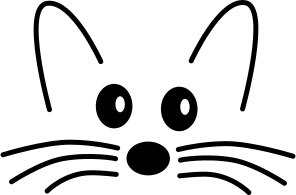
\includegraphics[width=1.4em]{squeak-logo}}}
\iftoshelse{
	\usepackage{marginnote}
		\renewcommand*{\marginfont}{\footnotesize}
	\newcommand{\vartriangleout}{\ifthenelse{\isodd{\thepage}}{\vartriangleright}{\vartriangleleft}}
	\newcommand{\dothisicon}{\fcolorbox{blue!65}{white}{\highlight{$\vartriangleout$}}}
	\newcommand{\dothis}[1]{%
		\noindent\par\noindent
		{\reversemarginpar
			\marginnote{\fcolorbox{blue!65}{white}{\highlight{$\vartriangleout$}}}}
		%\MarginLabel{do this}
		\noindent\emph{#1}
		\nopagebreak}
}{
	\newcommand{\dothisicon}{\raisebox{-.5ex}{
\includegraphics[height=1.2em]{pharo}}}
	\newcommand{\dothis}[1]{%
		\medskip
		\noindent\dothisicon
		\ifx#1\empty\else\quad\emph{#1}\fi
		\par\smallskip\nopagebreak}
}
%===> NEW VERSION <===
% NB: To use this in an individual chapter, you must set:
%\graphicspath{{figures/} {../figures/}}
% at the head of the chapter.  Don't forget the final /
%=============================================================
%:Reader hints (hint)
%
% Indicates a non-obvious consequence 
\newcommand{\hint}[1]{\vspace{1ex}\noindent\fbox{\textsc{Hint}} \emph{#1}}
%=================================================================
% graphics for Morphic handles
\newcommand{\grabHandle}{\raisebox{-0.2ex}{
\includegraphics[width=1em]{blackHandle}}}
\newcommand{\moveHandle}{\raisebox{-0.2ex}{
\includegraphics[width=1em]{moveHandle}}}
\newcommand{\debugHandle}{\raisebox{-0.2ex}{
\includegraphics[width=1em]{debugHandle}}}
%=============================================================
%:Highlighting Important stuff (doublebox)
%
% From Seaside book ...
\newsavebox{\SavedText}
\newlength{\InnerBoxRule}\setlength{\InnerBoxRule}{.75\fboxrule}
\newlength{\OuterBoxRule}\setlength{\OuterBoxRule}{1.5\fboxrule}
\newlength{\BoxSeparation}\setlength{\BoxSeparation}{1.5\fboxrule}
\addtolength{\BoxSeparation}{.5pt}
\newlength{\SaveBoxSep}\setlength{\SaveBoxSep}{2\fboxsep}
%
\newenvironment{doublebox}{\begin{lrbox}{\SavedText}
    \begin{minipage}{.75\textwidth}}
    {\end{minipage}\end{lrbox}\begin{center}
    \setlength{\fboxsep}{\BoxSeparation}\setlength{\fboxrule}{\OuterBoxRule}
    \fbox{\setlength{\fboxsep}{\SaveBoxSep}\setlength{\fboxrule}{\InnerBoxRule}%
      \fbox{\usebox{\SavedText}}}
  \end{center}}
% Use this:
\newcommand{\important}[1]{\begin{doublebox}#1\end{doublebox}}
%=============================================================
%:Section depth
\setcounter{secnumdepth}{2}
%% for this to happen start the file with
%\ifx\wholebook\relax\else
%% $Author$
% $Date$
% $Revision$

% HISTORY:
% 2006-10-31 - Oscar code macros
% ...

%=============================================================
% NB: documentclass must be set in main document.
% Allows book to be generated in multiple formats.
%=============================================================
%:Packages
\usepackage[T1]{fontenc}  %%%%%% really important to get the code directly in the text!
\usepackage{lmodern}
%\usepackage[scaled=0.85]{bookmanx} % needs another scale factor if used with \renewcommand{\sfdefault}{cmbr}
\usepackage{palatino}
\usepackage[scaled=0.85]{helvet}
\usepackage[protrusion,expansion=false]{microtype}
\usepackage{graphicx}
\usepackage{theorem}
\usepackage[english]{babel}
%%% ON: pdfsync breaks the use of p{width} for tabular columns!
%%\ifdefined\usepdfsync\usepackage{pdfsync}\fi % Requires texlive 2007
%=============================================================
%:More packages
%Stef should check which ones are used!
%\usepackage{picinpar}
%\usepackage{layout}
%\usepackage{color}
%\usepackage{enum}
%\usepackage{a4wide}
% \usepackage{fancyhdr}
\usepackage{ifthen}
\usepackage{float}
\usepackage{longtable}
\usepackage{makeidx}
\usepackage[nottoc]{tocbibind}
\usepackage{multicol}
\usepackage{booktabs}	% book-style tables
\usepackage{topcapt}	% enables \topcaption
\usepackage{multirow}
\usepackage{tabularx}
%\usepackage[bottom]{footmisc}
\usepackage{xspace}
\usepackage{alltt}
\usepackage{amssymb,textcomp}
\usepackage[usenames,dvipsnames]{color}
%\usepackage{colortbl}
\usepackage[hang]{subfigure}\makeatletter\def\p@subfigure{\thefigure\,}\makeatother
\usepackage{rotating}
\usepackage{enumitem}	% apb: allows more control over tags in enumerations
\usepackage{verbatim}     % for comment environment
\usepackage{varioref}	% for page references that work
\labelformat{footnote}{\thechapter--#1} % to distinguish citations from jurabib
\usepackage{needspace}
\usepackage{isodateo} % enable \isodate
\usepackage[newparttoc]{titlesec}
\usepackage{titletoc}
\usepackage{wrapfig}
\usepackage[
	super,
	citefull=first,
	authorformat={allreversed,and},
	titleformat={commasep,italic}
]{jurabib} % citations as footnotes
\usepackage[
	colorlinks=true,
	linkcolor=black,
	urlcolor=black,
	citecolor=black
]{hyperref}   % should come last
%=============================================================
%:PDF version
%%\pdfminorversion=3 % Set PDF to 1.3 for Lulu
%=============================================================
%:URL style
\makeatletter
\def\url@leostyle{%
  \@ifundefined{selectfont}{\def\UrlFont{\sf}}{\def\UrlFont{\sffamily}}}
\makeatother
% Now actually use the newly defined style.
\urlstyle{leo}
%=============================================================
%:Booleans
\newboolean{lulu}
\setboolean{lulu}{false}
\newcommand{\ifluluelse}[2]{\ifthenelse{\boolean{lulu}}{#1}{#2}}
%=============================================================
%:Names
\newcommand{\SUnit}{SUnit\xspace}
\newcommand{\sunit}{SUnit\xspace}
\newcommand{\xUnit}{$x$Unit\xspace}
\newcommand{\JUnit}{JUnit\xspace}
\newcommand{\st}{Smalltalk\xspace}
\newcommand{\pharo}{Pharo\xspace} % Use this, not \Pharo
%\newcommand{\sqmap}{SqueakMap\xspace}
\newcommand{\squeak}{Squeak\xspace} % use this, not \Squeak or \sq
\newcommand{\sqsrc}{SqueakSource\xspace}
\newcommand{\sbe}{\url{http://SqueakByExample.org}\xspace}
\newcommand{\pharoweb}{\url{http://pharo-project.org}\xspace}
\newcommand{\pbe}{\url{http://PharoByExample.org}\xspace}
\newcommand{\sba}{\url{http://SquareBracketAssociates.org}\xspace}
\newcommand{\bam}{\lct{Bounc\-ing\-Atoms\-Morph}\xspace}
%=============================================================
%:Markup macros for proof-reading
\usepackage[normalem]{ulem} % for \sout
\usepackage{xcolor}
\newcommand{\ra}{$\rightarrow$}
\newcommand{\ugh}[1]{\textcolor{red}{\uwave{#1}}} % please rephrase
\newcommand{\ins}[1]{\textcolor{blue}{\uline{#1}}} % please insert
\newcommand{\del}[1]{\textcolor{red}{\sout{#1}}} % please delete
\newcommand{\chg}[2]{\textcolor{red}{\sout{#1}}{\ra}\textcolor{blue}{\uline{#2}}} % please change
%=============================================================
%:Editorial comment macros
%\newcommand{\nnbb}[2]{
%    % \fbox{\bfseries\sffamily\scriptsize#1}
%    \fcolorbox{gray}{yellow}{\bfseries\sffamily\scriptsize#1}
%    {\sf\small$\blacktriangleright$\textit{#2}$\blacktriangleleft$}
%   }
\newcommand{\yellowbox}[1]{\fcolorbox{gray}{yellow}{\bfseries\sffamily\scriptsize#1}}
\newcommand{\triangles}[1]{{\sf\small$\blacktriangleright$\textit{#1}$\blacktriangleleft$}}
\newcommand{\nnbb}[2]{\yellowbox{#1} \triangles{#2}}
\newcommand{\fix}{\yellowbox{FIX!}}
\newcommand{\here}{\yellowbox{CONTINUE HERE!}}
% editor macros
\newcommand{\apl}[1]{\nnbb{Alain}{#1}} % Alain
\newcommand{\ab}[1]{\nnbb{Andrew}{#1}} % Black
\newcommand{\sd}[1]{\nnbb{St\'{e}f}{#1}} % Ducasse
\newcommand{\dc}[1]{\nnbb{DamienC}{#1}} % Ducasse
\newcommand{\md}[1]{\nnbb{Marcus}{#1}} % Denker
\newcommand{\on}[1]{\nnbb{Oscar}{#1}} % Nierstrasz
\newcommand{\damien}[1]{\nnbb{Damien}{#1}} % Pollet
\newcommand{\lr}[1]{\nnbb{Lukas}{#1}} % Renggli
\newcommand{\orla}[1]{\nnbb{Orla}{#1}} % Greevy
\newcommand{\alex}[1]{\nnbb{Alex}{#1}} % Bergel
\newcommand{\alx}[1]{\nnbb{Alex}{#1}} % Bergel
\newcommand{\dr}[1]{\nnbb{David}{#1}} % Roethlisberger
\newcommand{\ja}[1]{\nnbb{Jannik}{#1}} % Laval
\newcommand{\jr}[1]{\nnbb{Jorge}{#1}} % Ressia
\newcommand{\fp}[1]{\nnbb{Fabrizio}{#1}} % Perin
\newcommand{\michael}[1]{\nnbb{Michael}{#1}} % Davies
\newcommand{\ew}[1]{\nnbb{Erwann}{#1}} % Wernli
\newcommand{\mb}[1]{\nnbb{Martial}{#1}} % Boniou
\newcommand{\hw}[1]{\nnbb{Hernan}{#1}} % Wilkinson
%=============================================================
%:Abbreviation macros
\newcommand{\ie}{\emph{すなわち}、}
\newcommand{\eg}{\emph{例えば}、}
\newcommand{\etc}{などなど。}
%=============================================================
%:Cross reference macros
\newcommand{\charef}[1]{第~\ref{cha:#1}~章}
\newcommand{\secref}[1]{\ref{sec:#1}~節}
\newcommand{\figref}[1]{図~\ref{fig:#1}\xspace}
\newcommand{\Figref}[1]{図~\ref{fig:#1}\xspace}
\newcommand{\appref}[1]{付録~\ref{app:#1}\xspace}
\newcommand{\tabref}[1]{表~\ref{tab:#1}\xspace}
\newcommand{\faqref}[1]{FAQ~\ref{faq:#1}, p.~\pageref{faq:#1}\xspace}
% APB: I removed trailing \xspace commands from these macros because
% \xspace mostly doesn't work.  If you want a space after your
% references, type one!
% ON: xspace has always worked just fine for me!  Please leave them in.
%
\newcommand{\ruleref}[1]{\ref{rule:#1}\xspace}
%
\newcommand{\egref}[1]{example~\ref{eg:#1}\xspace}
\newcommand{\Egref}[1]{Example~\ref{eg:#1}\xspace}
%
\newcommand{\scrref}[1]{script~\ref{scr:#1}\xspace}
\newcommand{\Scrref}[1]{Script~\ref{scr:#1}\xspace}
\newcommand{\tscrref}[1]{the script~\ref{scr:#1}\xspace}
\newcommand{\Tscrref}[1]{The script~\ref{scr:#1}\xspace}
%
\newcommand{\mthref}[1]{method~\ref{mth:#1}\xspace}
\newcommand{\mthsref}[1]{methods~\ref{mth:#1}\xspace}
\newcommand{\Mthref}[1]{Method~\ref{mth:#1}\xspace}
\newcommand{\tmthref}[1]{the method~\ref{mth:#1}\xspace}
\newcommand{\Tmthref}[1]{The method~\ref{mth:#1}\xspace}
%
\newcommand{\clsref}[1]{class~\ref{cls:#1}\xspace}
\newcommand{\tclsref}[1]{the class~\ref{cls:#1}\xspace}
\newcommand{\Tclsref}[1]{The class~\ref{cls:#1}\xspace}

\newcommand{\chalabel}[1]{\label{cha:#1}}
\newcommand{\seclabel}[1]{\label{sec:#1}}
\newcommand{\figlabel}[1]{\label{fig:#1}}
\newcommand{\tablabel}[1]{\label{tab:#1}}
\newcommand{\rulelabel}[1]{\label{rule:#1}}
\newcommand{\eglabel}[1]{\label{eg:#1}}
\newcommand{\scrlabel}[1]{\label{scr:#1}}
\newcommand{\mthlabel}[1]{\label{mth:#1}}
\newcommand{\clslabel}[1]{\label{cls:#1}}
\newcommand{\faqlabel}[1]{\label{faq:#1}}
%=============================================================
%:Menu item macro
% for menu items, so we can change our minds on how to print them! (apb)
\definecolor{lightgray}{gray}{0.89}
\newcommand{\menu}[1]{{%
	\setlength{\fboxsep}{0pt}%
	\colorbox{lightgray}{{{\upshape\sffamily\strut \,#1\,}}}}}
\newcommand{\link}[1]{{%
	\fontfamily{lmr}\selectfont
 	\upshape{\sffamily \underline{#1}}}}
% For submenu items:
\newcommand{\go}{\,$\triangleright$\,}
% \newcommand{\go}{\,$\blacktriangleright$\,}
% For keyboard shortcuts:
%\newcommand{\short}[1]{\mbox{$\langle${\sc CMD}$\rangle$-#1}\xspace}
\newcommand{\short}[1]{\mbox{{\sc cmd}\hspace{0.08em}--\hspace{0.09em}#1}\xspace}
% For buttons:
\newcommand{\button}[1]{{%
	\setlength{\fboxsep}{0pt}%
	\fbox{{\upshape\sffamily\strut \,#1\,}}}}
% NB: The button macro does not work within captions -- incompatible with xcolor package :-(
\newcommand{\toolsflap}{\textit{Tools} flap\xspace}
%=============================================================
%:Mouse clicks
\newcommand{\click}{click\xspace} % RED
\newcommand{\actclick}{action-click\xspace} % YELLOW
\newcommand{\metaclick}{meta-click\xspace} % BLUE
\newcommand{\Click}{Click\xspace} % RED
\newcommand{\Actclick}{Action-click\xspace} % YELLOW
\newcommand{\Metaclick}{Meta-click\xspace} % BLUE
%=============================================================
%:ToSh macros
\newboolean{tosh}
\setboolean{tosh}{false}
\newcommand{\iftoshelse}[2]{\ifthenelse{\boolean{tosh}}{#1}{#2}}
%=============================================================
%:ToSh colors
%\newcommand{\highlightcolor}{\color{blue!65}}
%\newcommand{\boxcolor}{\color{gray!25}}
\newcommand{\highlight}[1]{\textcolor{blue!65}{#1}}
%\newcommand{\codecolor}{\color{blue!65}}
%%\setlength{\fboxrule}{2pt}
%\newcommand{\asPict}[1]{%
%	{\Large\highlight{#1}}}
%=============================================================
%:Reader cues (do this)
%
% Indicate something the reader should try out.
% \newcommand{\dothisicon}{\raisebox{-.5ex}{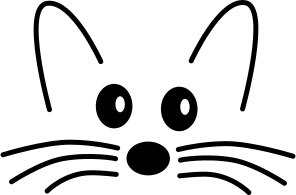
\includegraphics[width=1.4em]{squeak-logo}}}
\iftoshelse{
	\usepackage{marginnote}
		\renewcommand*{\marginfont}{\footnotesize}
	\newcommand{\vartriangleout}{\ifthenelse{\isodd{\thepage}}{\vartriangleright}{\vartriangleleft}}
	\newcommand{\dothisicon}{\fcolorbox{blue!65}{white}{\highlight{$\vartriangleout$}}}
	\newcommand{\dothis}[1]{%
		\noindent\par\noindent
		{\reversemarginpar
			\marginnote{\fcolorbox{blue!65}{white}{\highlight{$\vartriangleout$}}}}
		%\MarginLabel{do this}
		\noindent\emph{#1}
		\nopagebreak}
}{
	\newcommand{\dothisicon}{\raisebox{-.5ex}{
\includegraphics[height=1.2em]{pharo}}}
	\newcommand{\dothis}[1]{%
		\medskip
		\noindent\dothisicon
		\ifx#1\empty\else\quad\emph{#1}\fi
		\par\smallskip\nopagebreak}
}
%===> NEW VERSION <===
% NB: To use this in an individual chapter, you must set:
%\graphicspath{{figures/} {../figures/}}
% at the head of the chapter.  Don't forget the final /
%=============================================================
%:Reader hints (hint)
%
% Indicates a non-obvious consequence 
\newcommand{\hint}[1]{\vspace{1ex}\noindent\fbox{\textsc{Hint}} \emph{#1}}
%=================================================================
% graphics for Morphic handles
\newcommand{\grabHandle}{\raisebox{-0.2ex}{
\includegraphics[width=1em]{blackHandle}}}
\newcommand{\moveHandle}{\raisebox{-0.2ex}{
\includegraphics[width=1em]{moveHandle}}}
\newcommand{\debugHandle}{\raisebox{-0.2ex}{\includegraphics[width=1em]{debugHandle}}}
%=============================================================
%:Highlighting Important stuff (doublebox)
%
% From Seaside book ...
\newsavebox{\SavedText}
\newlength{\InnerBoxRule}\setlength{\InnerBoxRule}{.75\fboxrule}
\newlength{\OuterBoxRule}\setlength{\OuterBoxRule}{1.5\fboxrule}
\newlength{\BoxSeparation}\setlength{\BoxSeparation}{1.5\fboxrule}
\addtolength{\BoxSeparation}{.5pt}
\newlength{\SaveBoxSep}\setlength{\SaveBoxSep}{2\fboxsep}
%
\newenvironment{doublebox}{\begin{lrbox}{\SavedText}
    \begin{minipage}{.75\textwidth}}
    {\end{minipage}\end{lrbox}\begin{center}
    \setlength{\fboxsep}{\BoxSeparation}\setlength{\fboxrule}{\OuterBoxRule}
    \fbox{\setlength{\fboxsep}{\SaveBoxSep}\setlength{\fboxrule}{\InnerBoxRule}%
      \fbox{\usebox{\SavedText}}}
  \end{center}}
% Use this:
\newcommand{\important}[1]{\begin{doublebox}#1\end{doublebox}}
%=============================================================
%:Section depth
\setcounter{secnumdepth}{2}
%% for this to happen start the file with
%\ifx\wholebook\relax\else
%\input{../common.tex}
%\begin{document}
%\fi
% and terminate by
% \ifx\wholebook\relax\else\end{document}\fi

\DeclareGraphicsExtensions{.pdf, .jpg, .png}
%=============================================================
%:PDF setup
\hypersetup{
%   a4paper,
%   pdfstartview=FitV,
%   colorlinks,
%   linkcolor=darkblue,
%   citecolor=darkblue,
   pdftitle={Pharo by Example},
   pdfauthor={Andrew P. Black, St\'ephane Ducasse,	Oscar Nierstrasz,
Damien Pollet},
   pdfkeywords={Smalltalk, Squeak, Object-Oriented Programming, OOP},
   pdfsubject={Computer Science}
}
%=============================================================
%:Page layout and appearance
%
% \renewcommand{\headrulewidth}{0pt}
\renewcommand{\chaptermark}[1]{\markboth{#1}{}}
\renewcommand{\sectionmark}[1]{\markright{\thesection\ #1}}
\renewpagestyle{plain}[\small\itshape]{%
	\setheadrule{0pt}%
	\sethead[][][]{}{}{}%
	\setfoot[][][]{}{}{}}
\renewpagestyle{headings}[\small\itshape]{%
	\setheadrule{0pt}%
	\setmarks{chapter}{section}%
	\sethead[\thepage][][\chaptertitle]{\sectiontitle}{}{\thepage}%
	\setfoot[][][]{}{}{}}
%=============================================================
%:Title section setup and TOC numbering depth
\setcounter{secnumdepth}{1}
\setcounter{tocdepth}{1}
\titleformat{\part}[display]{\centering}{\huge\partname\ \thepart}{1em}{\Huge\textbf}[]
\titleformat{\chapter}[display]{}{\huge\chaptertitlename\ \thechapter}{1em}{\Huge\raggedright\textbf}[]
\titlecontents{part}[3pc]{%
		\pagebreak[2]\addvspace{1em plus.4em minus.2em}%
		\leavevmode\large\bfseries}
	{\contentslabel{3pc}}{\hspace*{-3pc}}
	{}[\nopagebreak]
\titlecontents{chapter}[3pc]{%
		\pagebreak[0]\addvspace{1em plus.2em minus.2em}%
		\leavevmode\bfseries}
	{\contentslabel{3pc}}{}
	{\hfill\contentspage}[\nopagebreak]
\dottedcontents{section}[3pc]{}{3pc}{1pc}
\dottedcontents{subsection}[3pc]{}{0pc}{1pc}
% \dottedcontents{subsection}[4.5em]{}{0pt}{1pc}
% Make \cleardoublepage insert really blank pages http://www.tex.ac.uk/cgi-bin/texfaq2html?label=reallyblank
\let\origdoublepage\cleardoublepage
\newcommand{\clearemptydoublepage}{%
  \clearpage
  {\pagestyle{empty}\origdoublepage}}
\let\cleardoublepage\clearemptydoublepage % see http://www.tex.ac.uk/cgi-bin/texfaq2html?label=patch
%=============================================================
%:FAQ macros (for FAQ chapter)
\newtheorem{faq}{FAQ}
\newcommand{\answer}{\paragraph{Answer}\ }
%=============================================================
%:Listings package configuration
% \newcommand{\caret}{\makebox{\raisebox{0.4ex}{\footnotesize{$\wedge$}}}}
\newcommand{\caret}{\^\,}
\newcommand{\escape}{{\sf \textbackslash}}
\definecolor{source}{gray}{0.95}
\usepackage{listings}
\lstdefinelanguage{Smalltalk}{
%  morekeywords={self,super,true,false,nil,thisContext}, % This is overkill
  morestring=[d]',
  morecomment=[s]{"}{"},
  alsoletter={\#:},
  escapechar={!},
  literate=
    {BANG}{!}1
    {CARET}{\^}1
    {UNDERSCORE}{\_}1
    {\\st}{Smalltalk}9 % convenience -- in case \st occurs in code
    % {'}{{\textquotesingle}}1 % replaced by upquote=true in \lstset
    {_}{{$\leftarrow$}}1
    {>>>}{{\sep}}1
    {^}{{$\uparrow$}}1
    {~}{{$\sim$}}1
    {-}{{\texttt{-}}}1 %{\textminus}}1 %{-}{\hspace{-0.13em}}{-}}1  % the goal is to make - the same width as +
    % {+}{\sf+}1 %{\raisebox{0.08ex}{+}}}1      % and to raise + off the baseline to match -
    {-->}{{\quad$\longrightarrow$\quad}}3
	, % Don't forget the comma at the end!
  tabsize=4
}[keywords,comments,strings]

\lstset{language=Smalltalk,
	basicstyle=\sffamily,
	keywordstyle=\color{black}\bfseries,
	% stringstyle=\ttfamily, % Ugly! do we really want this? -- on
	mathescape=true,
	showstringspaces=false,
	keepspaces=true,
	breaklines=true,
	breakautoindent=true,
	backgroundcolor=\color{source},
	lineskip={-1pt}, % Ugly hack
	upquote=true, % straight quote; requires textcomp package
	columns=fullflexible} % no fixed width fonts
% In-line code (literal)
% Normally use this for all in-line code:
\newcommand{\ct}{\lstinline[mathescape=false,backgroundcolor=\color{white},basicstyle={\sffamily\upshape}]}
% apb 2007.8.28 added the \upshape declaration to avoid getting italicized code in \dothis{ } sections.
% In-line code (latex enabled)
% Use this only in special situations where \ct does not work
% (within section headings ...):
\newcommand{\lct}[1]{{\textsf{\textup{#1}}}}
% Use these for system categories and protocols:
\newcommand{\scat}[1]{\emph{\textsf{#1}}\xspace}
\newcommand{\pkg}[1]{\emph{\textsf{#1}}\xspace}
\newcommand{\prot}[1]{\emph{\textsf{#1}}\xspace}
% Code environments
% NB: the arg is for tests
% Only code and example environments may be tests
\lstnewenvironment{code}[1]{%
	\lstset{%
		% frame=lines,
		frame=single,
		framerule=0pt,
		mathescape=false
	}
}{}
\def\ignoredollar#1{}
%=============================================================
%:Code environments (method, script ...)
% NB: the third arg is for tests
% Only code and example environments may be tests
\lstnewenvironment{example}[3][defaultlabel]{%
	\renewcommand{\lstlistingname}{Example}%
	\lstset{
		% frame=lines,
		frame=single,
		framerule=0pt,
		mathescape=false,
		caption={\emph{#2}},
		label={eg:#1}
	}
}{}
\lstnewenvironment{script}[2][defaultlabel]{%
\renewcommand{\lstlistingname}{Script}%
	\lstset{
		% frame=lines,
		frame=single,
		framerule=0pt,
		mathescape=false,
		name={Script},
		caption={\emph{#2}},
		label={scr:#1}
	}
}{}
\lstnewenvironment{method}[2][defaultlabel]{%
	\renewcommand{\lstlistingname}{Method}%
	\lstset{
		% frame=lines,
		frame=single,
		framerule=0pt,
		mathescape=false,
		name={Method},
		caption={\emph{#2}},
		label={mth:#1}
	}
}{}
\lstnewenvironment{methods}[2][defaultlabel]{% just for multiple methods at once
	\renewcommand{\lstlistingname}{Methods}%
	\lstset{
		% frame=lines,
		frame=single,
		framerule=0pt,
		mathescape=false,
		name={Method},
		caption={\emph{#2}},
		label={mth:#1}
	}
}{}
\lstnewenvironment{numMethod}[2][defaultlabel]{%
	\renewcommand{\lstlistingname}{Method}%
	\lstset{
		numbers=left,
		numberstyle={\tiny\sffamily},
		% frame=lines,
		frame=single,
		framerule=0pt,
		mathescape=false,
		name={Method},
		caption={\emph{#2}},
		label={mth:#1}
	}
}{}
\lstnewenvironment{classdef}[2][defaultlabel]{%
	\renewcommand{\lstlistingname}{Class}%
	\lstset{
		% frame=lines,
		frame=single,
		framerule=0pt,
		mathescape=false,
		name={Class},
		caption={\emph{#2}},
		label={cls:#1}
	}
}{}
%=============================================================
%:Reserving space
% Usually need one more line than the actual lines of code
\newcommand{\needlines}[1]{\Needspace{#1\baselineskip}}
%=============================================================
%:Indexing macros
% Macros ending with "ind" generate text as well as an index entry
% Macros ending with "index" *only* generate an index entry
\newcommand{\ind}[1]{\index{#1}#1\xspace} % plain text
\newcommand{\subind}[2]{\index{#1!#2}#2\xspace} % show #2, subindex under #1
\newcommand{\emphind}[1]{\index{#1}\emph{#1}\xspace} % emph #1
\newcommand{\emphsubind}[2]{\index{#1!#2}\emph{#2}\xspace} % show emph #2, subindex inder #1
\newcommand{\scatind}[1]{\index{#1@\textsf{#1} (category)}\scat{#1}} % category
\newcommand{\pkgind}[1]{\index{#1@\textsf{#1} (package)}\pkg{#1}} % package
\newcommand{\protind}[1]{\index{#1@\textsf{#1} (protocol)}\prot{#1}} % protocol
\newcommand{\clsind}[1]{\index{#1@\textsf{#1} (class)}\ct{#1}\xspace}
% \newcommand{\clsind}[1]{\index{#1!\#@(class)}\ct{#1}\xspace} % class
\newcommand{\clsindplural}[1]{\index{#1!\#@(class)}\ct{#1}s\xspace} % class
\newcommand{\cvind}[1]{\index{#1@\textsf{#1} (class variable)}\ct{#1}\xspace} % class var
\newcommand{\glbind}[1]{\index{#1@\textsf{#1} (global)}\ct{#1}\xspace} % global
\newcommand{\patind}[1]{\index{#1@#1 (pattern)}\ct{#1}\xspace} % pattern
\newcommand{\pvind}[1]{\index{#1@\textsf{#1} (pseudo variable)}\ct{#1}\xspace} % pseudo var
\newcommand{\clsmthind}[2]{\index{#1!#2@\ct{#2}}\ct{#1>>>#2}\xspace} % class + method name
\newcommand{\mthind}[2]{\index{#1!#2@\ct{#2}}\ct{#2}\xspace} % show method name only
\newcommand{\lmthind}[2]{\index{#1!#2@\ct{#2}}\lct{#2}\xspace} % show method name only
\newcommand{\cmind}[2]{\index{#1!#2@\ct{#2}}\ct{#1>>>#2}\xspace} % show class>>method
\newcommand{\lcmind}[2]{\index{#1!#2@\ct{#2}}\lct{#1>>>#2}\xspace} % show class>>method
\newcommand{\toolsflapind}{\index{Tools flap}\toolsflap} % index tools flap
% The following only generate an index entry:
% \newcommand{\clsindex}[1]{\index{#1@\textsf{#1} (class)}}
\newcommand{\clsindex}[1]{\index{#1!\#@(class)}} % class
\newcommand{\mthindex}[2]{\index{#1!#2@\ct{#2}}} % method
\newcommand{\cmindex}[2]{\index{#1!#2@\ct{#2}}} % class>>method
\newcommand{\cvindex}[1]{\index{#1@\textsf{#1} (class variable)}} % class var
\newcommand{\glbindex}[1]{\index{#1@\textsf{#1} (global)}}% global
\newcommand{\pvindex}[1]{\index{#1@\textsf{#1} (pseudo variable)}}% pseudo var
\newcommand{\seeindex}[2]{\index{#1|see{#2}}} % #1, see #2
\newcommand{\scatindex}[1]{\index{#1@\textsf{#1} (category)}} % category
\newcommand{\pkgindex}[1]{\index{#1@\textsf{#1} (package)}} % package
\newcommand{\protindex}[1]{\index{#1@\textsf{#1} (protocol)}} % protocol
% How can we have the main entry page numbers in bold yet not break the hyperlink?
\newcommand{\boldidx}[1]{{\bf #1}} % breaks hyperlink
%\newcommand{\indmain}[1]{\index{#1|boldidx}#1\xspace} % plain text, main entry
%\newcommand{\emphsubindmain}[2]{\index{#1!#2|boldidx}\emph{#2}\xspace} % subindex, main entry
%\newcommand{\subindmain}[2]{\index{#1!#2|boldidx}#2\xspace} % subindex, main entry
%\newcommand{\clsindmain}[1]{\index{#1@\textsf{#1} (class)|boldidx}\ct{#1}\xspace}
%\newcommand{\clsindmain}[1]{\index{#1!\#@(class)|boldidx}\ct{#1}\xspace} % class main
%\newcommand{\indexmain}[1]{\index{#1|boldidx}} % main index entry only
\newcommand{\indmain}[1]{\index{#1}#1\xspace} % The main index entry for this item
\newcommand{\emphsubindmain}[2]{\index{#1!#2}\emph{#2}\xspace} % subindex, main entry
\newcommand{\subindmain}[2]{\index{#1!#2}#2\xspace} % subindex, main entry
%\newcommand{\clsindmain}[1]{\index{#1@\textsf{#1} (class)}\ct{#1}\xspace}
\newcommand{\clsindmain}[1]{\index{#1!\#@(class)}\ct{#1}\xspace} % class main
\newcommand{\clsindexmain}[1]{\index{#1!\#@(class)}} % class main index only
\newcommand{\indexmain}[1]{\index{#1}} 
%=============================================================
%:Code macros
% some constants
\newcommand{\codesize}{\small}
\newcommand{\codefont}{\sffamily}
%\newcommand{\cat}[1]{\textit{In category #1}}%%To remove later
\newlength{\scriptindent}
\setlength{\scriptindent}{.3cm}
%% Method presentation constants
\newlength{\methodindent}
\newlength{\methodwordlength}
\newlength{\aftermethod}
\setlength{\methodindent}{0.2cm}
\settowidth{\methodwordlength}{\ M\'ethode\ }
%=============================================================
%:Smalltalk macros
%\newcommand{\sep}{{$\gg$}}
\newcommand{\sep}{\mbox{>>}}
\newcommand{\self}{\lct{self}\xspace}
\newcommand{\super}{\lct{super}\xspace}
\newcommand{\nil}{\lct{nil}\xspace}
%=============================================================
% be less conservative about float placement
% these commands are from http://www.tex.ac.uk/cgi-bin/texfaq2html?label=floats
\renewcommand{\topfraction}{.9}
\renewcommand{\bottomfraction}{.9}
\renewcommand{\textfraction}{.1}
\renewcommand{\floatpagefraction}{.85}
\renewcommand{\dbltopfraction}{.66}
\renewcommand{\dblfloatpagefraction}{.85}
\setcounter{topnumber}{9}
\setcounter{bottomnumber}{9}
\setcounter{totalnumber}{20}
\setcounter{dbltopnumber}{9}
%=============================================================
% Give information from each chapter's author
\newcommand{\contact}[2]{\textbf{#1} \textsf{(#2)}}

\newcommand{\chapterauthor}[1]{\emph{with the participation of:\\#1}\\}

\newcommand{\authornoury}{\contact{Noury Bouraqadi}{bouraqadi@gmail.com}}
\newcommand{\authordamienc}{\contact{Damien Cassou}{damien.cassou@gmail.com}}
\newcommand{\authoroscar}{\contact{Oscar Nierstrasz}{oscar.nierstrasz@acm.org}}
\newcommand{\authorsteph}{\contact{St\'ephane Ducasse}{stephane.ducasse@inria.fr}}
\newcommand{\authoralex}{\contact{Alexandre Bergel}{alexandre@bergel.eu}}
\newcommand{\authorolivier}{\contact{Olivier Auverlot}{olivier.auverlot@inria.fr}}
\newcommand{\authornicolas}{\contact{Nicolas Cellier}{ncellier@ifrance.com}}
\newcommand{\authormarcus}{\contact{Marcus Denker}{marcus.denker@inria.fr}}
\newcommand{\authoralain}{\contact{Alain Plantec}{alain.plantec@univ-brest.fr}}
\newcommand{\authordale}{\contact{Dale Henrichs}{dale.henrichs@gemstone.com}}
\newcommand{\authormariano}{\contact{Mariano Martinez Peck}{marianopeck@gmail.com}}
\newcommand{\authorsven}{\contact{Sven Van Caekenberghe}{sven@beta9.be}}

%=============================================================
% apb doesn't like paragraphs to run in to each other without a break
\parskip 1ex
%=============================================================
%:Stuff to check, merge or deprecate
%\setlength{\marginparsep}{2mm}
%\renewcommand{\baselinestretch}{1.1}
%=============================================================

%\begin{document}
%\fi
% and terminate by
% \ifx\wholebook\relax\else\end{document}\fi

\DeclareGraphicsExtensions{.pdf, .jpg, .png}
%=============================================================
%:PDF setup
\hypersetup{
%   a4paper,
%   pdfstartview=FitV,
%   colorlinks,
%   linkcolor=darkblue,
%   citecolor=darkblue,
   pdftitle={Pharo by Example},
   pdfauthor={Andrew P. Black, St\'ephane Ducasse,	Oscar Nierstrasz,
Damien Pollet},
   pdfkeywords={Smalltalk, Squeak, Object-Oriented Programming, OOP},
   pdfsubject={Computer Science}
}
%=============================================================
%:Page layout and appearance
%
% \renewcommand{\headrulewidth}{0pt}
\renewcommand{\chaptermark}[1]{\markboth{#1}{}}
\renewcommand{\sectionmark}[1]{\markright{\thesection\ #1}}
\renewpagestyle{plain}[\small\itshape]{%
	\setheadrule{0pt}%
	\sethead[][][]{}{}{}%
	\setfoot[][][]{}{}{}}
\renewpagestyle{headings}[\small\itshape]{%
	\setheadrule{0pt}%
	\setmarks{chapter}{section}%
	\sethead[\thepage][][\chaptertitle]{\sectiontitle}{}{\thepage}%
	\setfoot[][][]{}{}{}}
%=============================================================
%:Title section setup and TOC numbering depth
\setcounter{secnumdepth}{1}
\setcounter{tocdepth}{1}
\titleformat{\part}[display]{\centering}{\huge\partname\ \thepart}{1em}{\Huge\textbf}[]
\titleformat{\chapter}[display]{}{\huge\chaptertitlename\ \thechapter}{1em}{\Huge\raggedright\textbf}[]
\titlecontents{part}[3pc]{%
		\pagebreak[2]\addvspace{1em plus.4em minus.2em}%
		\leavevmode\large\bfseries}
	{\contentslabel{3pc}}{\hspace*{-3pc}}
	{}[\nopagebreak]
\titlecontents{chapter}[3pc]{%
		\pagebreak[0]\addvspace{1em plus.2em minus.2em}%
		\leavevmode\bfseries}
	{\contentslabel{3pc}}{}
	{\hfill\contentspage}[\nopagebreak]
\dottedcontents{section}[3pc]{}{3pc}{1pc}
\dottedcontents{subsection}[3pc]{}{0pc}{1pc}
% \dottedcontents{subsection}[4.5em]{}{0pt}{1pc}
% Make \cleardoublepage insert really blank pages http://www.tex.ac.uk/cgi-bin/texfaq2html?label=reallyblank
\let\origdoublepage\cleardoublepage
\newcommand{\clearemptydoublepage}{%
  \clearpage
  {\pagestyle{empty}\origdoublepage}}
\let\cleardoublepage\clearemptydoublepage % see http://www.tex.ac.uk/cgi-bin/texfaq2html?label=patch
%=============================================================
%:FAQ macros (for FAQ chapter)
\newtheorem{faq}{FAQ}
\newcommand{\answer}{\paragraph{Answer}\ }
%=============================================================
%:Listings package configuration
% \newcommand{\caret}{\makebox{\raisebox{0.4ex}{\footnotesize{$\wedge$}}}}
\newcommand{\caret}{\^\,}
\newcommand{\escape}{{\sf \textbackslash}}
\definecolor{source}{gray}{0.95}
\usepackage{listings}
\lstdefinelanguage{Smalltalk}{
%  morekeywords={self,super,true,false,nil,thisContext}, % This is overkill
  morestring=[d]',
  morecomment=[s]{"}{"},
  alsoletter={\#:},
  escapechar={!},
  literate=
    {BANG}{!}1
    {CARET}{\^}1
    {UNDERSCORE}{\_}1
    {\\st}{Smalltalk}9 % convenience -- in case \st occurs in code
    % {'}{{\textquotesingle}}1 % replaced by upquote=true in \lstset
    {_}{{$\leftarrow$}}1
    {>>>}{{\sep}}1
    {^}{{$\uparrow$}}1
    {~}{{$\sim$}}1
    {-}{{\texttt{-}}}1 %{\textminus}}1 %{-}{\hspace{-0.13em}}{-}}1  % the goal is to make - the same width as +
    % {+}{\sf+}1 %{\raisebox{0.08ex}{+}}}1      % and to raise + off the baseline to match -
    {-->}{{\quad$\longrightarrow$\quad}}3
	, % Don't forget the comma at the end!
  tabsize=4
}[keywords,comments,strings]

\lstset{language=Smalltalk,
	basicstyle=\sffamily,
	keywordstyle=\color{black}\bfseries,
	% stringstyle=\ttfamily, % Ugly! do we really want this? -- on
	mathescape=true,
	showstringspaces=false,
	keepspaces=true,
	breaklines=true,
	breakautoindent=true,
	backgroundcolor=\color{source},
	lineskip={-1pt}, % Ugly hack
	upquote=true, % straight quote; requires textcomp package
	columns=fullflexible} % no fixed width fonts
% In-line code (literal)
% Normally use this for all in-line code:
\newcommand{\ct}{\lstinline[mathescape=false,backgroundcolor=\color{white},basicstyle={\sffamily\upshape}]}
% apb 2007.8.28 added the \upshape declaration to avoid getting italicized code in \dothis{ } sections.
% In-line code (latex enabled)
% Use this only in special situations where \ct does not work
% (within section headings ...):
\newcommand{\lct}[1]{{\textsf{\textup{#1}}}}
% Use these for system categories and protocols:
\newcommand{\scat}[1]{\emph{\textsf{#1}}\xspace}
\newcommand{\pkg}[1]{\emph{\textsf{#1}}\xspace}
\newcommand{\prot}[1]{\emph{\textsf{#1}}\xspace}
% Code environments
% NB: the arg is for tests
% Only code and example environments may be tests
\lstnewenvironment{code}[1]{%
	\lstset{%
		% frame=lines,
		frame=single,
		framerule=0pt,
		mathescape=false
	}
}{}
\def\ignoredollar#1{}
%=============================================================
%:Code environments (method, script ...)
% NB: the third arg is for tests
% Only code and example environments may be tests
\lstnewenvironment{example}[3][defaultlabel]{%
	\renewcommand{\lstlistingname}{Example}%
	\lstset{
		% frame=lines,
		frame=single,
		framerule=0pt,
		mathescape=false,
		caption={\emph{#2}},
		label={eg:#1}
	}
}{}
\lstnewenvironment{script}[2][defaultlabel]{%
\renewcommand{\lstlistingname}{Script}%
	\lstset{
		% frame=lines,
		frame=single,
		framerule=0pt,
		mathescape=false,
		name={Script},
		caption={\emph{#2}},
		label={scr:#1}
	}
}{}
\lstnewenvironment{method}[2][defaultlabel]{%
	\renewcommand{\lstlistingname}{Method}%
	\lstset{
		% frame=lines,
		frame=single,
		framerule=0pt,
		mathescape=false,
		name={Method},
		caption={\emph{#2}},
		label={mth:#1}
	}
}{}
\lstnewenvironment{methods}[2][defaultlabel]{% just for multiple methods at once
	\renewcommand{\lstlistingname}{Methods}%
	\lstset{
		% frame=lines,
		frame=single,
		framerule=0pt,
		mathescape=false,
		name={Method},
		caption={\emph{#2}},
		label={mth:#1}
	}
}{}
\lstnewenvironment{numMethod}[2][defaultlabel]{%
	\renewcommand{\lstlistingname}{Method}%
	\lstset{
		numbers=left,
		numberstyle={\tiny\sffamily},
		% frame=lines,
		frame=single,
		framerule=0pt,
		mathescape=false,
		name={Method},
		caption={\emph{#2}},
		label={mth:#1}
	}
}{}
\lstnewenvironment{classdef}[2][defaultlabel]{%
	\renewcommand{\lstlistingname}{Class}%
	\lstset{
		% frame=lines,
		frame=single,
		framerule=0pt,
		mathescape=false,
		name={Class},
		caption={\emph{#2}},
		label={cls:#1}
	}
}{}
%=============================================================
%:Reserving space
% Usually need one more line than the actual lines of code
\newcommand{\needlines}[1]{\Needspace{#1\baselineskip}}
%=============================================================
%:Indexing macros
% Macros ending with "ind" generate text as well as an index entry
% Macros ending with "index" *only* generate an index entry
\newcommand{\ind}[1]{\index{#1}#1\xspace} % plain text
\newcommand{\subind}[2]{\index{#1!#2}#2\xspace} % show #2, subindex under #1
\newcommand{\emphind}[1]{\index{#1}\emph{#1}\xspace} % emph #1
\newcommand{\emphsubind}[2]{\index{#1!#2}\emph{#2}\xspace} % show emph #2, subindex inder #1
\newcommand{\scatind}[1]{\index{#1@\textsf{#1} (category)}\scat{#1}} % category
\newcommand{\pkgind}[1]{\index{#1@\textsf{#1} (package)}\pkg{#1}} % package
\newcommand{\protind}[1]{\index{#1@\textsf{#1} (protocol)}\prot{#1}} % protocol
\newcommand{\clsind}[1]{\index{#1@\textsf{#1} (class)}\ct{#1}\xspace}
% \newcommand{\clsind}[1]{\index{#1!\#@(class)}\ct{#1}\xspace} % class
\newcommand{\clsindplural}[1]{\index{#1!\#@(class)}\ct{#1}s\xspace} % class
\newcommand{\cvind}[1]{\index{#1@\textsf{#1} (class variable)}\ct{#1}\xspace} % class var
\newcommand{\glbind}[1]{\index{#1@\textsf{#1} (global)}\ct{#1}\xspace} % global
\newcommand{\patind}[1]{\index{#1@#1 (pattern)}\ct{#1}\xspace} % pattern
\newcommand{\pvind}[1]{\index{#1@\textsf{#1} (pseudo variable)}\ct{#1}\xspace} % pseudo var
\newcommand{\clsmthind}[2]{\index{#1!#2@\ct{#2}}\ct{#1>>>#2}\xspace} % class + method name
\newcommand{\mthind}[2]{\index{#1!#2@\ct{#2}}\ct{#2}\xspace} % show method name only
\newcommand{\lmthind}[2]{\index{#1!#2@\ct{#2}}\lct{#2}\xspace} % show method name only
\newcommand{\cmind}[2]{\index{#1!#2@\ct{#2}}\ct{#1>>>#2}\xspace} % show class>>method
\newcommand{\lcmind}[2]{\index{#1!#2@\ct{#2}}\lct{#1>>>#2}\xspace} % show class>>method
\newcommand{\toolsflapind}{\index{Tools flap}\toolsflap} % index tools flap
% The following only generate an index entry:
% \newcommand{\clsindex}[1]{\index{#1@\textsf{#1} (class)}}
\newcommand{\clsindex}[1]{\index{#1!\#@(class)}} % class
\newcommand{\mthindex}[2]{\index{#1!#2@\ct{#2}}} % method
\newcommand{\cmindex}[2]{\index{#1!#2@\ct{#2}}} % class>>method
\newcommand{\cvindex}[1]{\index{#1@\textsf{#1} (class variable)}} % class var
\newcommand{\glbindex}[1]{\index{#1@\textsf{#1} (global)}}% global
\newcommand{\pvindex}[1]{\index{#1@\textsf{#1} (pseudo variable)}}% pseudo var
\newcommand{\seeindex}[2]{\index{#1|see{#2}}} % #1, see #2
\newcommand{\scatindex}[1]{\index{#1@\textsf{#1} (category)}} % category
\newcommand{\pkgindex}[1]{\index{#1@\textsf{#1} (package)}} % package
\newcommand{\protindex}[1]{\index{#1@\textsf{#1} (protocol)}} % protocol
% How can we have the main entry page numbers in bold yet not break the hyperlink?
\newcommand{\boldidx}[1]{{\bf #1}} % breaks hyperlink
%\newcommand{\indmain}[1]{\index{#1|boldidx}#1\xspace} % plain text, main entry
%\newcommand{\emphsubindmain}[2]{\index{#1!#2|boldidx}\emph{#2}\xspace} % subindex, main entry
%\newcommand{\subindmain}[2]{\index{#1!#2|boldidx}#2\xspace} % subindex, main entry
%\newcommand{\clsindmain}[1]{\index{#1@\textsf{#1} (class)|boldidx}\ct{#1}\xspace}
%\newcommand{\clsindmain}[1]{\index{#1!\#@(class)|boldidx}\ct{#1}\xspace} % class main
%\newcommand{\indexmain}[1]{\index{#1|boldidx}} % main index entry only
\newcommand{\indmain}[1]{\index{#1}#1\xspace} % The main index entry for this item
\newcommand{\emphsubindmain}[2]{\index{#1!#2}\emph{#2}\xspace} % subindex, main entry
\newcommand{\subindmain}[2]{\index{#1!#2}#2\xspace} % subindex, main entry
%\newcommand{\clsindmain}[1]{\index{#1@\textsf{#1} (class)}\ct{#1}\xspace}
\newcommand{\clsindmain}[1]{\index{#1!\#@(class)}\ct{#1}\xspace} % class main
\newcommand{\clsindexmain}[1]{\index{#1!\#@(class)}} % class main index only
\newcommand{\indexmain}[1]{\index{#1}} 
%=============================================================
%:Code macros
% some constants
\newcommand{\codesize}{\small}
\newcommand{\codefont}{\sffamily}
%\newcommand{\cat}[1]{\textit{In category #1}}%%To remove later
\newlength{\scriptindent}
\setlength{\scriptindent}{.3cm}
%% Method presentation constants
\newlength{\methodindent}
\newlength{\methodwordlength}
\newlength{\aftermethod}
\setlength{\methodindent}{0.2cm}
\settowidth{\methodwordlength}{\ M\'ethode\ }
%=============================================================
%:Smalltalk macros
%\newcommand{\sep}{{$\gg$}}
\newcommand{\sep}{\mbox{>>}}
\newcommand{\self}{\lct{self}\xspace}
\newcommand{\super}{\lct{super}\xspace}
\newcommand{\nil}{\lct{nil}\xspace}
%=============================================================
% be less conservative about float placement
% these commands are from http://www.tex.ac.uk/cgi-bin/texfaq2html?label=floats
\renewcommand{\topfraction}{.9}
\renewcommand{\bottomfraction}{.9}
\renewcommand{\textfraction}{.1}
\renewcommand{\floatpagefraction}{.85}
\renewcommand{\dbltopfraction}{.66}
\renewcommand{\dblfloatpagefraction}{.85}
\setcounter{topnumber}{9}
\setcounter{bottomnumber}{9}
\setcounter{totalnumber}{20}
\setcounter{dbltopnumber}{9}
%=============================================================
% Give information from each chapter's author
\newcommand{\contact}[2]{\textbf{#1} \textsf{(#2)}}

\newcommand{\chapterauthor}[1]{\emph{with the participation of:\\#1}\\}

\newcommand{\authornoury}{\contact{Noury Bouraqadi}{bouraqadi@gmail.com}}
\newcommand{\authordamienc}{\contact{Damien Cassou}{damien.cassou@gmail.com}}
\newcommand{\authoroscar}{\contact{Oscar Nierstrasz}{oscar.nierstrasz@acm.org}}
\newcommand{\authorsteph}{\contact{St\'ephane Ducasse}{stephane.ducasse@inria.fr}}
\newcommand{\authoralex}{\contact{Alexandre Bergel}{alexandre@bergel.eu}}
\newcommand{\authorolivier}{\contact{Olivier Auverlot}{olivier.auverlot@inria.fr}}
\newcommand{\authornicolas}{\contact{Nicolas Cellier}{ncellier@ifrance.com}}
\newcommand{\authormarcus}{\contact{Marcus Denker}{marcus.denker@inria.fr}}
\newcommand{\authoralain}{\contact{Alain Plantec}{alain.plantec@univ-brest.fr}}
\newcommand{\authordale}{\contact{Dale Henrichs}{dale.henrichs@gemstone.com}}
\newcommand{\authormariano}{\contact{Mariano Martinez Peck}{marianopeck@gmail.com}}
\newcommand{\authorsven}{\contact{Sven Van Caekenberghe}{sven@beta9.be}}

%=============================================================
% apb doesn't like paragraphs to run in to each other without a break
\parskip 1ex
%=============================================================
%:Stuff to check, merge or deprecate
%\setlength{\marginparsep}{2mm}
%\renewcommand{\baselinestretch}{1.1}
%=============================================================

%	\usepackage{a4wide}
% --------------------------------------------
    \graphicspath{{figures/} {../figures/}}
	\begin{document}
	% \renewcommand{\nnbb}[2]{} % Disable editorial comments
	\sloppy
	\frontmatter
\fi
%=================================================================
\chapter{Preface}\chalabel{intro}

%=================================================================
%\section*{What is \pharo?}
\section*{\pharo とは?}

%\pharo is a modern, open source, fully-featured implementation of the \st programming language and environment. \pharo is derived from \squeak\cite{Inga97a}, a re-implementation of the classic \st-80 system. Whereas \squeak was developed mainly as a platform for developing experimental educational software, \pharo strives to offer a lean, open-source platform for professional software development, and a robust and stable platform for research and development into dynamic languages and environments. \pharo serves as the reference implementation for the Seaside web development framework.
\pharo は現代的な、オープンソースの、 \st プログラミング言語・環境のフル機能を実装しています。 \pharo は古典的な \st-80 システムを再実装した \squeak\cite{Inga97a}から派生しています。\squeak は主に実験的な教育向けソフトウェアを開発するためのプラットフォームとして開発されたのにくらべ、\pharo はプロフェッショナルなソフトウェアを開発するための洗練されたオープンソース・プラットフォーム、さらに研究と開発のための頑丈で安定したプラットフォームを動的な言語・環境に提供するように努めています。\pharo はSeasideウェブ開発フレームワークのリファレンス実装としても使われています。

%\pharo resolves some licensing issues with \squeak. Unlike previous versions of \squeak, the \pharo core contains only code that has been contributed under the MIT license. The \pharo project started in March 2008 as a fork of \squeak 3.9, and the first 1.0 beta version was released on July 31, 2009.
\pharo は \squeak にあったライセンスの問題を解決しています。\squeak の前バージョンとは異なり、\pharo のコア部分はMITライセンスの下に寄付されています。\pharo プロジェクトは2008年3月に \squeak 3.9からのフォークとして始まり、最初の1.0ベータバージョンは2009年7月31日にリリースされました。

%Although \pharo removes many packages from \squeak, it also includes numerous features that are optional in \squeak. For example, true type fonts are bundled into \pharo. \pharo also includes support for true block closures. The user interfaces has been simplified and revised.
\pharo は \squeak からパッケージをいくつも取り去っている一方で、\squeak ではオプショナルであった機能をたくさん取り入れてもいます。たとえば、\pharo には True Type フォントが入っています。\pharo には本物のブロッククロージャもサポートされています(訳注:\squeak ではBlockContextという再帰できないクロージャ実装でした)。

%\pharo is highly portable --- even its virtual machine is written entirely in \st, making it easy to debug, analyze, and change. \pharo is the vehicle for a wide range of innovative projects from multimedia applications and educational platforms to commercial web development environments. 
\pharo は高い可搬性を持っています。仮想マシンでさえもすべて \st で書かれていて、デバック・解析・変更をし易くなっています。\pharo はマルチメディア・アプリケーションや教育向けプラットフォームから商用ウェブ開発環境まで広範囲のイノベーティブなプロジェクトを運用する手段になります。

%There is an important aspect behind \pharo: \pharo should not just be a copy of the past but really \emph{reinvent} Smalltalk. Big-bang approaches rarely succeed. \pharo will really favor evolutionary and incremental changes. We want to be able to experiment with important new features or libraries. Evolution means that \pharo accepts mistakes and is not aiming for the next perfect solution in one big step\,---\,even if we would love it. \pharo will favor small incremental changes but a multitude of them. The success of \pharo depends on the contributions of its community.
% The \pharo community will pay attention to your submissions to improve the system.
\pharo の裏にはある重要な視点があります。「\pharo は過去の複製ではなく、本当にSmalltalkを\emph{再発明}すべきだ」というものです。ビッグバンアプローチが成功するのは稀です。\pharo は進化的でインクリメンタルな変更を支持します。重要な新機能やライブラリを実験できるようにしたいのです。進化とは\pharo が誤りを受け入れることを意味します。つまり、\pharo では(私たちが大好きな)大きなワンステップによる完璧な解答は目指しません。\pharo はたくさんの小さな変更をひとまとめにせず、インクリメンタルに適用することを支持します。\pharo の成功はコミュニティからの貢献にかかっています。
% \pharo のコミュニティはシステムを向上させるあなたの提案に注目しています。

%=================================================================
\section*{だれのための本か?}

%This book is based on \emph{Squeak by Example}\footnote{\sbe}, an open-source introduction to \squeak.
%The book has been liberally adapted and revised to reflect the differences between \pharo and \squeak.
%This book presents the various aspects of \pharo, starting with the basics, and proceeding to more advanced topics.
この本はオープンソースで公開されている\squeak の入門書 \emph{Squeak by Example}\footnote{\sbe} を元にしています。
\pharo と\squeak の違いに柔軟に適応し、違いを反映して改訂されています。
\pharo の基本からはじまり先進的な話題まで多様な側面を紹介しています。

%This book will not teach you how to program. The reader should have some familiarity with programming languages. Some background with object-oriented programming would be helpful.
この本ではどうやってプログラムするかは学べないと思います。この本はプログラミング言語をいくつか知っているひとに向いています。オブジェクト指向プログラミングの経験も役に立つと思います。

%This book will introduce the \pharo programming environment, the language and the associated tools.  You will be exposed to common idioms and practices, but the focus is on the technology, not on object-oriented design. Wherever possible, we will show you lots of examples. (We have been inspired by Alec Sharp's excellent book on Smalltalk\cite{Shar97a}.)
%\index{Sharp, Alex}
この本では\pharo のプログラミング環境(言語と関連ツール)を紹介します。一般的なイデオムや実例に触れてもらいますが、オブジェクト指向設計ではなくて技術のほうに焦点を当てています。可能ならあらゆるところで例をたくさん示そうと思います(Alec Sharpによる素晴らしいSmalltalkの本\cite{Shar97a}にインスパイアされています)。
\index{Sharp, Alex}

%There are numerous other books on \st freely available on the web but none of these focuses specifically on \pharo. See for example:
%\url{http://stephane.ducasse.free.fr/FreeBooks.html}
ウェブ上には\st についての無料の本が他にもたくさんありますが、\pharo に特化したものはありません。参照:
\url{http://stephane.ducasse.free.fr/FreeBooks.html}

\ifluluelse{}{\newpage} % layout hint
%=================================================================
%\section*{A word of advice}
\section*{忠告}

% http://www.surfscranton.com/architecture/KnightsPrinciples.htm

%Do not be frustrated by parts of \st that you do not immediately understand.
%You do not have to know everything!
%Alan Knight expresses this principle as follows\footnote{\url{http://www.surfscranton.com/architecture/KnightsPrinciples.htm}}:
%\index{Knight, Alan}
個々の\st の記述がすぐにわからないからといってイラだってはいけません。
すべてを知る必要はないのです!
Alan Knightはこの原則を次のように表現しています。\footnote{\url{http://www.surfscranton.com/architecture/KnightsPrinciples.htm}}:
\index{Knight, Alan}

%\important{{\bf Try not to care.}
%Beginning \st programmers often have trouble because they think they need to understand all the details of how a thing works before they can use it. This means it takes quite a while before they can master \ct{Transcript show: 'Hello World'}. One of the great leaps in OO is to be able to answer the question ``How does this work?'' with ``I don't care''.}
\important{{\bf 気にしないようにする}
\st を学びはじめたプログラマーは、どうやってそれが動くのかを詳細まですべて理解しなければならないと考えて困ってしまうことがよくあります。つまり、\ct{Transcript show: 'Hello World'} をマスターするまでにかなり時間がかかるということです。オブジェクト指向における偉大な一歩のひとつは、「どうやって動くのだろう?」という問いに対して「気にしない」と答えられることなのです。}
%=================================================================
\section*{オープンな本}

%This book is an open book in the following senses: 
この本は、次の意味でオープンな本です。

\begin{itemize}

%\item	The content of this book is released under the Creative Commons Attribution-ShareAlike (by-sa) license.
%		In short, you are allowed to freely share and adapt this book, as long as you respect the conditions of the license available at the following URL: 
%		\url{http://creativecommons.org/licenses/by-sa/3.0/}.

\item	この本の内容はクリエイティブ・コモンズの表示—継承(by-sa)ライセンスの下で公開されています。
		つまり、以下のURLにあるライセンス条件を尊重する限り、この本を自由に配布したり改変したりできます。
		URL: 
		\url{http://creativecommons.org/licenses/by-sa/3.0/}
%翻訳メモ: リンクを日本語のページにするか?

%\item	This book just describes the core of \pharo.
%		Ideally we would like to encourage others to contribute chapters
%		on the parts of \pharo that we have not described.
%		If you would like to participate in this effort, please
%		contact us.  We would like to see this book grow!

\item	この本は\pharo のコア部だけを解説しています。
		理想をいうと、私たちが書かなかった部分を他の人が寄稿してくれるようにしたいです。
		この取り組みに参加したい人は連絡してください。私たちはこの本が育つのを見たいのです!
		
\end{itemize}

%For more details, visit \pbe.
詳しくは、\pbe を見てください。


%=================================================================
\section*{ \pharo のコミュニティ}

% The \pharo community is friendly and active.
% Here is a short list of resources that you may find useful:
\pharo のコミュニティは親切で活動的です。
役に立ちそうなリソースをいくつかここにあげておきます。

\begin{itemize}
% \item \url{http://www.pharo-project.org} is the main web site of \pharo.
\item \url{http://www.pharo-project.org} \pharo のメイン・ウェブサイト。

%environment built on top of \pharo but whose audience is elementary
%school teachers.) % I remove this [Martial: french contributor]

% \item \url{http://www.squeaksource.com} is the equivalent of SourceForge for \pharo projects.
% Many optional packages for \pharo live here.
\item \url{http://www.squeaksource.com} \pharo プロジェクトにとってのSourceForge的なもの。\pharo 用の追加パッケージがここでたくさん生まれています。

\end{itemize}

%=================================================================
%\section*{Examples and exercises}
\section*{例と練習問題}

%We make use of two special conventions in this book.
この本では特別なきまりを2つつくりました。

%We have tried to provide as many examples as possible.
%In particular, there are many examples that show a fragment of code which can be evaluated.  We use the symbol \ct{-->} to indicate the result that you obtain when you select an expression and \menu{print it}:
できる限りたくさんの例を示すようにしています。
特に、実行できる短いコードで示された例がたくさんあります。式を選択して\menu{print it}を選ぶと得られる結果を示すために\ct{-->}記号を使います。

%\begin{code}{@TEST}
%3 + 4 --> 7    "if you select 3+4 and 'print it', you will see 7"
%\end{code}
\begin{code}{@TEST}
3 + 4 --> 7    「3+4を選択して'print it'を選ぶと7が得られる」
%翻訳メモ: メニューは日本語版にあわせて翻訳しておくか?
\end{code}

%In case you want to play in \pharo with these code snippets, you can download a plain text file with all the example code from the book's web site: \pbe.
これらのコードを\pharo で遊んでみたいときは、この本のサイト(\pbe)からすべてのコード例がテキストファイルでダウンロードできます。

%The second convention that we use is to display the icon \dothisicon{} to indicate when there is something for you to do:
二つめのきまりとして、あなたがすべきことを示すために\dothisicon{}アイコンを使います。

%\dothis{Go ahead and read the next chapter!}
\dothis{次の章へ読み進みましょう!}

%=================================================================
%\section*{Acknowledgments}
\section*{謝辞}

%We would first like to thank the original developers of \squeak for making this amazing \st development environment available as an open source project.
先ず、\squeak というこの驚くべき\st 開発環境をオープンソース・プロジェクトとして公開したオリジナルの開発者たちに感謝します。

%% We would like to thank various people who have contributed to this book.
%% In particular, we thank
%We would also like to thank Hilaire Fernandes and Serge Stinckwich who allowed us to translate parts of their columns on \st, and Damien Cassou for contributing the chapter on streams.
\st についてのコラムを翻訳することを許可してくれたHilaire FernandesとSerge Stinckwich、ストリームの章を寄稿してくれたDamien Cassouに感謝します。

%We especially thank Alexandre Bergel, Orla Greevy, Fabrizio Perin, Lukas Renggli, Jorge Ressia and Erwann Wernli for their detailed reviews.
査読をしてくれたAlexandre Bergel、Orla Greevy、Fabrizio Perin、Lukas Renggli、Jorge Ressia、Erwann Wernliに特に感謝します。

%We thank the University of Bern, Switzerland, for graciously supporting this open-source project and for hosting the web site of this book.
このオープンソース・プロジェクトを快く援助し、この本のウェブサイトを設置してくれたベルン大学(スイス)に感謝します。

%We also thank the Squeak community for their enthusiastic support of this book project, and for informing us of the errors found in the first edition of this book.
この本のプロジェクトを熱心に支援して、初版の間違いを教えてくれたSqueakのコミュニティに感謝します。

%=============================================================
\ifx\wholebook\relax\else
   \bibliographystyle{jurabib}
   \nobibliography{scg}
   \end{document}
\fi
%=============================================================

% $Author: oscar $
% $Date: 2009-07-06 10:21:47 +0200 (Mon, 06 Jul 2009) $
% $Revision: 27886 $

% HISTORY:
% 2009-07-06 - Oscar opened new template (no contents)

%=================================================================
\ifx\wholebook\relax\else
% --------------------------------------------
% Lulu:
	\documentclass[a4paper,10pt,twoside]{book}
	\usepackage[
		papersize={6.13in,9.21in},
		hmargin={.75in,.75in},
		vmargin={.75in,1in},
		ignoreheadfoot
	]{geometry}
	% $Author$
% $Date$
% $Revision$

% HISTORY:
% 2006-10-31 - Oscar code macros
% ...

%=============================================================
% NB: documentclass must be set in main document.
% Allows book to be generated in multiple formats.
%=============================================================
%:Packages
\usepackage[T1]{fontenc}  %%%%%% really important to get the code directly in the text!
\usepackage{lmodern}
%\usepackage[scaled=0.85]{bookmanx} % needs another scale factor if used with \renewcommand{\sfdefault}{cmbr}
\usepackage{palatino}
\usepackage[scaled=0.85]{helvet}
\usepackage[protrusion,expansion=false]{microtype}
\usepackage{graphicx}
\usepackage{theorem}
\usepackage[english]{babel}
%%% ON: pdfsync breaks the use of p{width} for tabular columns!
%%\ifdefined\usepdfsync\usepackage{pdfsync}\fi % Requires texlive 2007
%=============================================================
%:More packages
%Stef should check which ones are used!
%\usepackage{picinpar}
%\usepackage{layout}
%\usepackage{color}
%\usepackage{enum}
%\usepackage{a4wide}
% \usepackage{fancyhdr}
\usepackage{ifthen}
\usepackage{float}
\usepackage{longtable}
\usepackage{makeidx}
\usepackage[nottoc]{tocbibind}
\usepackage{multicol}
\usepackage{booktabs}	% book-style tables
\usepackage{topcapt}	% enables \topcaption
\usepackage{multirow}
\usepackage{tabularx}
%\usepackage[bottom]{footmisc}
\usepackage{xspace}
\usepackage{alltt}
\usepackage{amssymb,textcomp}
\usepackage[usenames,dvipsnames]{color}
%\usepackage{colortbl}
\usepackage[hang]{subfigure}\makeatletter\def\p@subfigure{\thefigure\,}\makeatother
\usepackage{rotating}
\usepackage{enumitem}	% apb: allows more control over tags in enumerations
\usepackage{verbatim}     % for comment environment
\usepackage{varioref}	% for page references that work
\labelformat{footnote}{\thechapter--#1} % to distinguish citations from jurabib
\usepackage{needspace}
\usepackage{isodateo} % enable \isodate
\usepackage[newparttoc]{titlesec}
\usepackage{titletoc}
\usepackage{wrapfig}
\usepackage[
	super,
	citefull=first,
	authorformat={allreversed,and},
	titleformat={commasep,italic}
]{jurabib} % citations as footnotes
\usepackage[
	colorlinks=true,
	linkcolor=black,
	urlcolor=black,
	citecolor=black
]{hyperref}   % should come last
%=============================================================
%:PDF version
%%\pdfminorversion=3 % Set PDF to 1.3 for Lulu
%=============================================================
%:URL style
\makeatletter
\def\url@leostyle{%
  \@ifundefined{selectfont}{\def\UrlFont{\sf}}{\def\UrlFont{\sffamily}}}
\makeatother
% Now actually use the newly defined style.
\urlstyle{leo}
%=============================================================
%:Booleans
\newboolean{lulu}
\setboolean{lulu}{false}
\newcommand{\ifluluelse}[2]{\ifthenelse{\boolean{lulu}}{#1}{#2}}
%=============================================================
%:Names
\newcommand{\SUnit}{SUnit\xspace}
\newcommand{\sunit}{SUnit\xspace}
\newcommand{\xUnit}{$x$Unit\xspace}
\newcommand{\JUnit}{JUnit\xspace}
\newcommand{\st}{Smalltalk\xspace}
\newcommand{\pharo}{Pharo\xspace} % Use this, not \Pharo
%\newcommand{\sqmap}{SqueakMap\xspace}
\newcommand{\squeak}{Squeak\xspace} % use this, not \Squeak or \sq
\newcommand{\sqsrc}{SqueakSource\xspace}
\newcommand{\sbe}{\url{http://SqueakByExample.org}\xspace}
\newcommand{\pharoweb}{\url{http://pharo-project.org}\xspace}
\newcommand{\pbe}{\url{http://PharoByExample.org}\xspace}
\newcommand{\sba}{\url{http://SquareBracketAssociates.org}\xspace}
\newcommand{\bam}{\lct{Bounc\-ing\-Atoms\-Morph}\xspace}
%=============================================================
%:Markup macros for proof-reading
\usepackage[normalem]{ulem} % for \sout
\usepackage{xcolor}
\newcommand{\ra}{$\rightarrow$}
\newcommand{\ugh}[1]{\textcolor{red}{\uwave{#1}}} % please rephrase
\newcommand{\ins}[1]{\textcolor{blue}{\uline{#1}}} % please insert
\newcommand{\del}[1]{\textcolor{red}{\sout{#1}}} % please delete
\newcommand{\chg}[2]{\textcolor{red}{\sout{#1}}{\ra}\textcolor{blue}{\uline{#2}}} % please change
%=============================================================
%:Editorial comment macros
%\newcommand{\nnbb}[2]{
%    % \fbox{\bfseries\sffamily\scriptsize#1}
%    \fcolorbox{gray}{yellow}{\bfseries\sffamily\scriptsize#1}
%    {\sf\small$\blacktriangleright$\textit{#2}$\blacktriangleleft$}
%   }
\newcommand{\yellowbox}[1]{\fcolorbox{gray}{yellow}{\bfseries\sffamily\scriptsize#1}}
\newcommand{\triangles}[1]{{\sf\small$\blacktriangleright$\textit{#1}$\blacktriangleleft$}}
\newcommand{\nnbb}[2]{\yellowbox{#1} \triangles{#2}}
\newcommand{\fix}{\yellowbox{FIX!}}
\newcommand{\here}{\yellowbox{CONTINUE HERE!}}
% editor macros
\newcommand{\apl}[1]{\nnbb{Alain}{#1}} % Alain
\newcommand{\ab}[1]{\nnbb{Andrew}{#1}} % Black
\newcommand{\sd}[1]{\nnbb{St\'{e}f}{#1}} % Ducasse
\newcommand{\dc}[1]{\nnbb{DamienC}{#1}} % Ducasse
\newcommand{\md}[1]{\nnbb{Marcus}{#1}} % Denker
\newcommand{\on}[1]{\nnbb{Oscar}{#1}} % Nierstrasz
\newcommand{\damien}[1]{\nnbb{Damien}{#1}} % Pollet
\newcommand{\lr}[1]{\nnbb{Lukas}{#1}} % Renggli
\newcommand{\orla}[1]{\nnbb{Orla}{#1}} % Greevy
\newcommand{\alex}[1]{\nnbb{Alex}{#1}} % Bergel
\newcommand{\alx}[1]{\nnbb{Alex}{#1}} % Bergel
\newcommand{\dr}[1]{\nnbb{David}{#1}} % Roethlisberger
\newcommand{\ja}[1]{\nnbb{Jannik}{#1}} % Laval
\newcommand{\jr}[1]{\nnbb{Jorge}{#1}} % Ressia
\newcommand{\fp}[1]{\nnbb{Fabrizio}{#1}} % Perin
\newcommand{\michael}[1]{\nnbb{Michael}{#1}} % Davies
\newcommand{\ew}[1]{\nnbb{Erwann}{#1}} % Wernli
\newcommand{\mb}[1]{\nnbb{Martial}{#1}} % Boniou
\newcommand{\hw}[1]{\nnbb{Hernan}{#1}} % Wilkinson
%=============================================================
%:Abbreviation macros
\newcommand{\ie}{\emph{すなわち}、}
\newcommand{\eg}{\emph{例えば}、}
\newcommand{\etc}{などなど。}
%=============================================================
%:Cross reference macros
\newcommand{\charef}[1]{第~\ref{cha:#1}~章}
\newcommand{\secref}[1]{\ref{sec:#1}~節}
\newcommand{\figref}[1]{図~\ref{fig:#1}\xspace}
\newcommand{\Figref}[1]{図~\ref{fig:#1}\xspace}
\newcommand{\appref}[1]{付録~\ref{app:#1}\xspace}
\newcommand{\tabref}[1]{表~\ref{tab:#1}\xspace}
\newcommand{\faqref}[1]{FAQ~\ref{faq:#1}, p.~\pageref{faq:#1}\xspace}
% APB: I removed trailing \xspace commands from these macros because
% \xspace mostly doesn't work.  If you want a space after your
% references, type one!
% ON: xspace has always worked just fine for me!  Please leave them in.
%
\newcommand{\ruleref}[1]{\ref{rule:#1}\xspace}
%
\newcommand{\egref}[1]{example~\ref{eg:#1}\xspace}
\newcommand{\Egref}[1]{Example~\ref{eg:#1}\xspace}
%
\newcommand{\scrref}[1]{script~\ref{scr:#1}\xspace}
\newcommand{\Scrref}[1]{Script~\ref{scr:#1}\xspace}
\newcommand{\tscrref}[1]{the script~\ref{scr:#1}\xspace}
\newcommand{\Tscrref}[1]{The script~\ref{scr:#1}\xspace}
%
\newcommand{\mthref}[1]{method~\ref{mth:#1}\xspace}
\newcommand{\mthsref}[1]{methods~\ref{mth:#1}\xspace}
\newcommand{\Mthref}[1]{Method~\ref{mth:#1}\xspace}
\newcommand{\tmthref}[1]{the method~\ref{mth:#1}\xspace}
\newcommand{\Tmthref}[1]{The method~\ref{mth:#1}\xspace}
%
\newcommand{\clsref}[1]{class~\ref{cls:#1}\xspace}
\newcommand{\tclsref}[1]{the class~\ref{cls:#1}\xspace}
\newcommand{\Tclsref}[1]{The class~\ref{cls:#1}\xspace}

\newcommand{\chalabel}[1]{\label{cha:#1}}
\newcommand{\seclabel}[1]{\label{sec:#1}}
\newcommand{\figlabel}[1]{\label{fig:#1}}
\newcommand{\tablabel}[1]{\label{tab:#1}}
\newcommand{\rulelabel}[1]{\label{rule:#1}}
\newcommand{\eglabel}[1]{\label{eg:#1}}
\newcommand{\scrlabel}[1]{\label{scr:#1}}
\newcommand{\mthlabel}[1]{\label{mth:#1}}
\newcommand{\clslabel}[1]{\label{cls:#1}}
\newcommand{\faqlabel}[1]{\label{faq:#1}}
%=============================================================
%:Menu item macro
% for menu items, so we can change our minds on how to print them! (apb)
\definecolor{lightgray}{gray}{0.89}
\newcommand{\menu}[1]{{%
	\setlength{\fboxsep}{0pt}%
	\colorbox{lightgray}{{{\upshape\sffamily\strut \,#1\,}}}}}
\newcommand{\link}[1]{{%
	\fontfamily{lmr}\selectfont
 	\upshape{\sffamily \underline{#1}}}}
% For submenu items:
\newcommand{\go}{\,$\triangleright$\,}
% \newcommand{\go}{\,$\blacktriangleright$\,}
% For keyboard shortcuts:
%\newcommand{\short}[1]{\mbox{$\langle${\sc CMD}$\rangle$-#1}\xspace}
\newcommand{\short}[1]{\mbox{{\sc cmd}\hspace{0.08em}--\hspace{0.09em}#1}\xspace}
% For buttons:
\newcommand{\button}[1]{{%
	\setlength{\fboxsep}{0pt}%
	\fbox{{\upshape\sffamily\strut \,#1\,}}}}
% NB: The button macro does not work within captions -- incompatible with xcolor package :-(
\newcommand{\toolsflap}{\textit{Tools} flap\xspace}
%=============================================================
%:Mouse clicks
\newcommand{\click}{click\xspace} % RED
\newcommand{\actclick}{action-click\xspace} % YELLOW
\newcommand{\metaclick}{meta-click\xspace} % BLUE
\newcommand{\Click}{Click\xspace} % RED
\newcommand{\Actclick}{Action-click\xspace} % YELLOW
\newcommand{\Metaclick}{Meta-click\xspace} % BLUE
%=============================================================
%:ToSh macros
\newboolean{tosh}
\setboolean{tosh}{false}
\newcommand{\iftoshelse}[2]{\ifthenelse{\boolean{tosh}}{#1}{#2}}
%=============================================================
%:ToSh colors
%\newcommand{\highlightcolor}{\color{blue!65}}
%\newcommand{\boxcolor}{\color{gray!25}}
\newcommand{\highlight}[1]{\textcolor{blue!65}{#1}}
%\newcommand{\codecolor}{\color{blue!65}}
%%\setlength{\fboxrule}{2pt}
%\newcommand{\asPict}[1]{%
%	{\Large\highlight{#1}}}
%=============================================================
%:Reader cues (do this)
%
% Indicate something the reader should try out.
% \newcommand{\dothisicon}{\raisebox{-.5ex}{\includegraphics[width=1.4em]{squeak-logo}}}
\iftoshelse{
	\usepackage{marginnote}
		\renewcommand*{\marginfont}{\footnotesize}
	\newcommand{\vartriangleout}{\ifthenelse{\isodd{\thepage}}{\vartriangleright}{\vartriangleleft}}
	\newcommand{\dothisicon}{\fcolorbox{blue!65}{white}{\highlight{$\vartriangleout$}}}
	\newcommand{\dothis}[1]{%
		\noindent\par\noindent
		{\reversemarginpar
			\marginnote{\fcolorbox{blue!65}{white}{\highlight{$\vartriangleout$}}}}
		%\MarginLabel{do this}
		\noindent\emph{#1}
		\nopagebreak}
}{
	\newcommand{\dothisicon}{\raisebox{-.5ex}{\includegraphics[height=1.2em]{pharo}}}
	\newcommand{\dothis}[1]{%
		\medskip
		\noindent\dothisicon
		\ifx#1\empty\else\quad\emph{#1}\fi
		\par\smallskip\nopagebreak}
}
%===> NEW VERSION <===
% NB: To use this in an individual chapter, you must set:
%\graphicspath{{figures/} {../figures/}}
% at the head of the chapter.  Don't forget the final /
%=============================================================
%:Reader hints (hint)
%
% Indicates a non-obvious consequence 
\newcommand{\hint}[1]{\vspace{1ex}\noindent\fbox{\textsc{Hint}} \emph{#1}}
%=================================================================
% graphics for Morphic handles
\newcommand{\grabHandle}{\raisebox{-0.2ex}{\includegraphics[width=1em]{blackHandle}}}
\newcommand{\moveHandle}{\raisebox{-0.2ex}{\includegraphics[width=1em]{moveHandle}}}
\newcommand{\debugHandle}{\raisebox{-0.2ex}{\includegraphics[width=1em]{debugHandle}}}
%=============================================================
%:Highlighting Important stuff (doublebox)
%
% From Seaside book ...
\newsavebox{\SavedText}
\newlength{\InnerBoxRule}\setlength{\InnerBoxRule}{.75\fboxrule}
\newlength{\OuterBoxRule}\setlength{\OuterBoxRule}{1.5\fboxrule}
\newlength{\BoxSeparation}\setlength{\BoxSeparation}{1.5\fboxrule}
\addtolength{\BoxSeparation}{.5pt}
\newlength{\SaveBoxSep}\setlength{\SaveBoxSep}{2\fboxsep}
%
\newenvironment{doublebox}{\begin{lrbox}{\SavedText}
    \begin{minipage}{.75\textwidth}}
    {\end{minipage}\end{lrbox}\begin{center}
    \setlength{\fboxsep}{\BoxSeparation}\setlength{\fboxrule}{\OuterBoxRule}
    \fbox{\setlength{\fboxsep}{\SaveBoxSep}\setlength{\fboxrule}{\InnerBoxRule}%
      \fbox{\usebox{\SavedText}}}
  \end{center}}
% Use this:
\newcommand{\important}[1]{\begin{doublebox}#1\end{doublebox}}
%=============================================================
%:Section depth
\setcounter{secnumdepth}{2}
%% for this to happen start the file with
%\ifx\wholebook\relax\else
%% $Author$
% $Date$
% $Revision$

% HISTORY:
% 2006-10-31 - Oscar code macros
% ...

%=============================================================
% NB: documentclass must be set in main document.
% Allows book to be generated in multiple formats.
%=============================================================
%:Packages
\usepackage[T1]{fontenc}  %%%%%% really important to get the code directly in the text!
\usepackage{lmodern}
%\usepackage[scaled=0.85]{bookmanx} % needs another scale factor if used with \renewcommand{\sfdefault}{cmbr}
\usepackage{palatino}
\usepackage[scaled=0.85]{helvet}
\usepackage[protrusion,expansion=false]{microtype}
\usepackage{graphicx}
\usepackage{theorem}
\usepackage[english]{babel}
%%% ON: pdfsync breaks the use of p{width} for tabular columns!
%%\ifdefined\usepdfsync\usepackage{pdfsync}\fi % Requires texlive 2007
%=============================================================
%:More packages
%Stef should check which ones are used!
%\usepackage{picinpar}
%\usepackage{layout}
%\usepackage{color}
%\usepackage{enum}
%\usepackage{a4wide}
% \usepackage{fancyhdr}
\usepackage{ifthen}
\usepackage{float}
\usepackage{longtable}
\usepackage{makeidx}
\usepackage[nottoc]{tocbibind}
\usepackage{multicol}
\usepackage{booktabs}	% book-style tables
\usepackage{topcapt}	% enables \topcaption
\usepackage{multirow}
\usepackage{tabularx}
%\usepackage[bottom]{footmisc}
\usepackage{xspace}
\usepackage{alltt}
\usepackage{amssymb,textcomp}
\usepackage[usenames,dvipsnames]{color}
%\usepackage{colortbl}
\usepackage[hang]{subfigure}\makeatletter\def\p@subfigure{\thefigure\,}\makeatother
\usepackage{rotating}
\usepackage{enumitem}	% apb: allows more control over tags in enumerations
\usepackage{verbatim}     % for comment environment
\usepackage{varioref}	% for page references that work
\labelformat{footnote}{\thechapter--#1} % to distinguish citations from jurabib
\usepackage{needspace}
\usepackage{isodateo} % enable \isodate
\usepackage[newparttoc]{titlesec}
\usepackage{titletoc}
\usepackage{wrapfig}
\usepackage[
	super,
	citefull=first,
	authorformat={allreversed,and},
	titleformat={commasep,italic}
]{jurabib} % citations as footnotes
\usepackage[
	colorlinks=true,
	linkcolor=black,
	urlcolor=black,
	citecolor=black
]{hyperref}   % should come last
%=============================================================
%:PDF version
%%\pdfminorversion=3 % Set PDF to 1.3 for Lulu
%=============================================================
%:URL style
\makeatletter
\def\url@leostyle{%
  \@ifundefined{selectfont}{\def\UrlFont{\sf}}{\def\UrlFont{\sffamily}}}
\makeatother
% Now actually use the newly defined style.
\urlstyle{leo}
%=============================================================
%:Booleans
\newboolean{lulu}
\setboolean{lulu}{false}
\newcommand{\ifluluelse}[2]{\ifthenelse{\boolean{lulu}}{#1}{#2}}
%=============================================================
%:Names
\newcommand{\SUnit}{SUnit\xspace}
\newcommand{\sunit}{SUnit\xspace}
\newcommand{\xUnit}{$x$Unit\xspace}
\newcommand{\JUnit}{JUnit\xspace}
\newcommand{\st}{Smalltalk\xspace}
\newcommand{\pharo}{Pharo\xspace} % Use this, not \Pharo
%\newcommand{\sqmap}{SqueakMap\xspace}
\newcommand{\squeak}{Squeak\xspace} % use this, not \Squeak or \sq
\newcommand{\sqsrc}{SqueakSource\xspace}
\newcommand{\sbe}{\url{http://SqueakByExample.org}\xspace}
\newcommand{\pharoweb}{\url{http://pharo-project.org}\xspace}
\newcommand{\pbe}{\url{http://PharoByExample.org}\xspace}
\newcommand{\sba}{\url{http://SquareBracketAssociates.org}\xspace}
\newcommand{\bam}{\lct{Bounc\-ing\-Atoms\-Morph}\xspace}
%=============================================================
%:Markup macros for proof-reading
\usepackage[normalem]{ulem} % for \sout
\usepackage{xcolor}
\newcommand{\ra}{$\rightarrow$}
\newcommand{\ugh}[1]{\textcolor{red}{\uwave{#1}}} % please rephrase
\newcommand{\ins}[1]{\textcolor{blue}{\uline{#1}}} % please insert
\newcommand{\del}[1]{\textcolor{red}{\sout{#1}}} % please delete
\newcommand{\chg}[2]{\textcolor{red}{\sout{#1}}{\ra}\textcolor{blue}{\uline{#2}}} % please change
%=============================================================
%:Editorial comment macros
%\newcommand{\nnbb}[2]{
%    % \fbox{\bfseries\sffamily\scriptsize#1}
%    \fcolorbox{gray}{yellow}{\bfseries\sffamily\scriptsize#1}
%    {\sf\small$\blacktriangleright$\textit{#2}$\blacktriangleleft$}
%   }
\newcommand{\yellowbox}[1]{\fcolorbox{gray}{yellow}{\bfseries\sffamily\scriptsize#1}}
\newcommand{\triangles}[1]{{\sf\small$\blacktriangleright$\textit{#1}$\blacktriangleleft$}}
\newcommand{\nnbb}[2]{\yellowbox{#1} \triangles{#2}}
\newcommand{\fix}{\yellowbox{FIX!}}
\newcommand{\here}{\yellowbox{CONTINUE HERE!}}
% editor macros
\newcommand{\apl}[1]{\nnbb{Alain}{#1}} % Alain
\newcommand{\ab}[1]{\nnbb{Andrew}{#1}} % Black
\newcommand{\sd}[1]{\nnbb{St\'{e}f}{#1}} % Ducasse
\newcommand{\dc}[1]{\nnbb{DamienC}{#1}} % Ducasse
\newcommand{\md}[1]{\nnbb{Marcus}{#1}} % Denker
\newcommand{\on}[1]{\nnbb{Oscar}{#1}} % Nierstrasz
\newcommand{\damien}[1]{\nnbb{Damien}{#1}} % Pollet
\newcommand{\lr}[1]{\nnbb{Lukas}{#1}} % Renggli
\newcommand{\orla}[1]{\nnbb{Orla}{#1}} % Greevy
\newcommand{\alex}[1]{\nnbb{Alex}{#1}} % Bergel
\newcommand{\alx}[1]{\nnbb{Alex}{#1}} % Bergel
\newcommand{\dr}[1]{\nnbb{David}{#1}} % Roethlisberger
\newcommand{\ja}[1]{\nnbb{Jannik}{#1}} % Laval
\newcommand{\jr}[1]{\nnbb{Jorge}{#1}} % Ressia
\newcommand{\fp}[1]{\nnbb{Fabrizio}{#1}} % Perin
\newcommand{\michael}[1]{\nnbb{Michael}{#1}} % Davies
\newcommand{\ew}[1]{\nnbb{Erwann}{#1}} % Wernli
\newcommand{\mb}[1]{\nnbb{Martial}{#1}} % Boniou
\newcommand{\hw}[1]{\nnbb{Hernan}{#1}} % Wilkinson
%=============================================================
%:Abbreviation macros
\newcommand{\ie}{\emph{すなわち}、}
\newcommand{\eg}{\emph{例えば}、}
\newcommand{\etc}{などなど。}
%=============================================================
%:Cross reference macros
\newcommand{\charef}[1]{第~\ref{cha:#1}~章}
\newcommand{\secref}[1]{\ref{sec:#1}~節}
\newcommand{\figref}[1]{図~\ref{fig:#1}\xspace}
\newcommand{\Figref}[1]{図~\ref{fig:#1}\xspace}
\newcommand{\appref}[1]{付録~\ref{app:#1}\xspace}
\newcommand{\tabref}[1]{表~\ref{tab:#1}\xspace}
\newcommand{\faqref}[1]{FAQ~\ref{faq:#1}, p.~\pageref{faq:#1}\xspace}
% APB: I removed trailing \xspace commands from these macros because
% \xspace mostly doesn't work.  If you want a space after your
% references, type one!
% ON: xspace has always worked just fine for me!  Please leave them in.
%
\newcommand{\ruleref}[1]{\ref{rule:#1}\xspace}
%
\newcommand{\egref}[1]{example~\ref{eg:#1}\xspace}
\newcommand{\Egref}[1]{Example~\ref{eg:#1}\xspace}
%
\newcommand{\scrref}[1]{script~\ref{scr:#1}\xspace}
\newcommand{\Scrref}[1]{Script~\ref{scr:#1}\xspace}
\newcommand{\tscrref}[1]{the script~\ref{scr:#1}\xspace}
\newcommand{\Tscrref}[1]{The script~\ref{scr:#1}\xspace}
%
\newcommand{\mthref}[1]{method~\ref{mth:#1}\xspace}
\newcommand{\mthsref}[1]{methods~\ref{mth:#1}\xspace}
\newcommand{\Mthref}[1]{Method~\ref{mth:#1}\xspace}
\newcommand{\tmthref}[1]{the method~\ref{mth:#1}\xspace}
\newcommand{\Tmthref}[1]{The method~\ref{mth:#1}\xspace}
%
\newcommand{\clsref}[1]{class~\ref{cls:#1}\xspace}
\newcommand{\tclsref}[1]{the class~\ref{cls:#1}\xspace}
\newcommand{\Tclsref}[1]{The class~\ref{cls:#1}\xspace}

\newcommand{\chalabel}[1]{\label{cha:#1}}
\newcommand{\seclabel}[1]{\label{sec:#1}}
\newcommand{\figlabel}[1]{\label{fig:#1}}
\newcommand{\tablabel}[1]{\label{tab:#1}}
\newcommand{\rulelabel}[1]{\label{rule:#1}}
\newcommand{\eglabel}[1]{\label{eg:#1}}
\newcommand{\scrlabel}[1]{\label{scr:#1}}
\newcommand{\mthlabel}[1]{\label{mth:#1}}
\newcommand{\clslabel}[1]{\label{cls:#1}}
\newcommand{\faqlabel}[1]{\label{faq:#1}}
%=============================================================
%:Menu item macro
% for menu items, so we can change our minds on how to print them! (apb)
\definecolor{lightgray}{gray}{0.89}
\newcommand{\menu}[1]{{%
	\setlength{\fboxsep}{0pt}%
	\colorbox{lightgray}{{{\upshape\sffamily\strut \,#1\,}}}}}
\newcommand{\link}[1]{{%
	\fontfamily{lmr}\selectfont
 	\upshape{\sffamily \underline{#1}}}}
% For submenu items:
\newcommand{\go}{\,$\triangleright$\,}
% \newcommand{\go}{\,$\blacktriangleright$\,}
% For keyboard shortcuts:
%\newcommand{\short}[1]{\mbox{$\langle${\sc CMD}$\rangle$-#1}\xspace}
\newcommand{\short}[1]{\mbox{{\sc cmd}\hspace{0.08em}--\hspace{0.09em}#1}\xspace}
% For buttons:
\newcommand{\button}[1]{{%
	\setlength{\fboxsep}{0pt}%
	\fbox{{\upshape\sffamily\strut \,#1\,}}}}
% NB: The button macro does not work within captions -- incompatible with xcolor package :-(
\newcommand{\toolsflap}{\textit{Tools} flap\xspace}
%=============================================================
%:Mouse clicks
\newcommand{\click}{click\xspace} % RED
\newcommand{\actclick}{action-click\xspace} % YELLOW
\newcommand{\metaclick}{meta-click\xspace} % BLUE
\newcommand{\Click}{Click\xspace} % RED
\newcommand{\Actclick}{Action-click\xspace} % YELLOW
\newcommand{\Metaclick}{Meta-click\xspace} % BLUE
%=============================================================
%:ToSh macros
\newboolean{tosh}
\setboolean{tosh}{false}
\newcommand{\iftoshelse}[2]{\ifthenelse{\boolean{tosh}}{#1}{#2}}
%=============================================================
%:ToSh colors
%\newcommand{\highlightcolor}{\color{blue!65}}
%\newcommand{\boxcolor}{\color{gray!25}}
\newcommand{\highlight}[1]{\textcolor{blue!65}{#1}}
%\newcommand{\codecolor}{\color{blue!65}}
%%\setlength{\fboxrule}{2pt}
%\newcommand{\asPict}[1]{%
%	{\Large\highlight{#1}}}
%=============================================================
%:Reader cues (do this)
%
% Indicate something the reader should try out.
% \newcommand{\dothisicon}{\raisebox{-.5ex}{\includegraphics[width=1.4em]{squeak-logo}}}
\iftoshelse{
	\usepackage{marginnote}
		\renewcommand*{\marginfont}{\footnotesize}
	\newcommand{\vartriangleout}{\ifthenelse{\isodd{\thepage}}{\vartriangleright}{\vartriangleleft}}
	\newcommand{\dothisicon}{\fcolorbox{blue!65}{white}{\highlight{$\vartriangleout$}}}
	\newcommand{\dothis}[1]{%
		\noindent\par\noindent
		{\reversemarginpar
			\marginnote{\fcolorbox{blue!65}{white}{\highlight{$\vartriangleout$}}}}
		%\MarginLabel{do this}
		\noindent\emph{#1}
		\nopagebreak}
}{
	\newcommand{\dothisicon}{\raisebox{-.5ex}{\includegraphics[height=1.2em]{pharo}}}
	\newcommand{\dothis}[1]{%
		\medskip
		\noindent\dothisicon
		\ifx#1\empty\else\quad\emph{#1}\fi
		\par\smallskip\nopagebreak}
}
%===> NEW VERSION <===
% NB: To use this in an individual chapter, you must set:
%\graphicspath{{figures/} {../figures/}}
% at the head of the chapter.  Don't forget the final /
%=============================================================
%:Reader hints (hint)
%
% Indicates a non-obvious consequence 
\newcommand{\hint}[1]{\vspace{1ex}\noindent\fbox{\textsc{Hint}} \emph{#1}}
%=================================================================
% graphics for Morphic handles
\newcommand{\grabHandle}{\raisebox{-0.2ex}{\includegraphics[width=1em]{blackHandle}}}
\newcommand{\moveHandle}{\raisebox{-0.2ex}{\includegraphics[width=1em]{moveHandle}}}
\newcommand{\debugHandle}{\raisebox{-0.2ex}{\includegraphics[width=1em]{debugHandle}}}
%=============================================================
%:Highlighting Important stuff (doublebox)
%
% From Seaside book ...
\newsavebox{\SavedText}
\newlength{\InnerBoxRule}\setlength{\InnerBoxRule}{.75\fboxrule}
\newlength{\OuterBoxRule}\setlength{\OuterBoxRule}{1.5\fboxrule}
\newlength{\BoxSeparation}\setlength{\BoxSeparation}{1.5\fboxrule}
\addtolength{\BoxSeparation}{.5pt}
\newlength{\SaveBoxSep}\setlength{\SaveBoxSep}{2\fboxsep}
%
\newenvironment{doublebox}{\begin{lrbox}{\SavedText}
    \begin{minipage}{.75\textwidth}}
    {\end{minipage}\end{lrbox}\begin{center}
    \setlength{\fboxsep}{\BoxSeparation}\setlength{\fboxrule}{\OuterBoxRule}
    \fbox{\setlength{\fboxsep}{\SaveBoxSep}\setlength{\fboxrule}{\InnerBoxRule}%
      \fbox{\usebox{\SavedText}}}
  \end{center}}
% Use this:
\newcommand{\important}[1]{\begin{doublebox}#1\end{doublebox}}
%=============================================================
%:Section depth
\setcounter{secnumdepth}{2}
%% for this to happen start the file with
%\ifx\wholebook\relax\else
%\input{../common.tex}
%\begin{document}
%\fi
% and terminate by
% \ifx\wholebook\relax\else\end{document}\fi

\DeclareGraphicsExtensions{.pdf, .jpg, .png}
%=============================================================
%:PDF setup
\hypersetup{
%   a4paper,
%   pdfstartview=FitV,
%   colorlinks,
%   linkcolor=darkblue,
%   citecolor=darkblue,
   pdftitle={Pharo by Example},
   pdfauthor={Andrew P. Black, St\'ephane Ducasse,	Oscar Nierstrasz,
Damien Pollet},
   pdfkeywords={Smalltalk, Squeak, Object-Oriented Programming, OOP},
   pdfsubject={Computer Science}
}
%=============================================================
%:Page layout and appearance
%
% \renewcommand{\headrulewidth}{0pt}
\renewcommand{\chaptermark}[1]{\markboth{#1}{}}
\renewcommand{\sectionmark}[1]{\markright{\thesection\ #1}}
\renewpagestyle{plain}[\small\itshape]{%
	\setheadrule{0pt}%
	\sethead[][][]{}{}{}%
	\setfoot[][][]{}{}{}}
\renewpagestyle{headings}[\small\itshape]{%
	\setheadrule{0pt}%
	\setmarks{chapter}{section}%
	\sethead[\thepage][][\chaptertitle]{\sectiontitle}{}{\thepage}%
	\setfoot[][][]{}{}{}}
%=============================================================
%:Title section setup and TOC numbering depth
\setcounter{secnumdepth}{1}
\setcounter{tocdepth}{1}
\titleformat{\part}[display]{\centering}{\huge\partname\ \thepart}{1em}{\Huge\textbf}[]
\titleformat{\chapter}[display]{}{\huge\chaptertitlename\ \thechapter}{1em}{\Huge\raggedright\textbf}[]
\titlecontents{part}[3pc]{%
		\pagebreak[2]\addvspace{1em plus.4em minus.2em}%
		\leavevmode\large\bfseries}
	{\contentslabel{3pc}}{\hspace*{-3pc}}
	{}[\nopagebreak]
\titlecontents{chapter}[3pc]{%
		\pagebreak[0]\addvspace{1em plus.2em minus.2em}%
		\leavevmode\bfseries}
	{\contentslabel{3pc}}{}
	{\hfill\contentspage}[\nopagebreak]
\dottedcontents{section}[3pc]{}{3pc}{1pc}
\dottedcontents{subsection}[3pc]{}{0pc}{1pc}
% \dottedcontents{subsection}[4.5em]{}{0pt}{1pc}
% Make \cleardoublepage insert really blank pages http://www.tex.ac.uk/cgi-bin/texfaq2html?label=reallyblank
\let\origdoublepage\cleardoublepage
\newcommand{\clearemptydoublepage}{%
  \clearpage
  {\pagestyle{empty}\origdoublepage}}
\let\cleardoublepage\clearemptydoublepage % see http://www.tex.ac.uk/cgi-bin/texfaq2html?label=patch
%=============================================================
%:FAQ macros (for FAQ chapter)
\newtheorem{faq}{FAQ}
\newcommand{\answer}{\paragraph{Answer}\ }
%=============================================================
%:Listings package configuration
% \newcommand{\caret}{\makebox{\raisebox{0.4ex}{\footnotesize{$\wedge$}}}}
\newcommand{\caret}{\^\,}
\newcommand{\escape}{{\sf \textbackslash}}
\definecolor{source}{gray}{0.95}
\usepackage{listings}
\lstdefinelanguage{Smalltalk}{
%  morekeywords={self,super,true,false,nil,thisContext}, % This is overkill
  morestring=[d]',
  morecomment=[s]{"}{"},
  alsoletter={\#:},
  escapechar={!},
  literate=
    {BANG}{!}1
    {CARET}{\^}1
    {UNDERSCORE}{\_}1
    {\\st}{Smalltalk}9 % convenience -- in case \st occurs in code
    % {'}{{\textquotesingle}}1 % replaced by upquote=true in \lstset
    {_}{{$\leftarrow$}}1
    {>>>}{{\sep}}1
    {^}{{$\uparrow$}}1
    {~}{{$\sim$}}1
    {-}{{\texttt{-}}}1 %{\textminus}}1 %{-}{\hspace{-0.13em}}{-}}1  % the goal is to make - the same width as +
    % {+}{\sf+}1 %{\raisebox{0.08ex}{+}}}1      % and to raise + off the baseline to match -
    {-->}{{\quad$\longrightarrow$\quad}}3
	, % Don't forget the comma at the end!
  tabsize=4
}[keywords,comments,strings]

\lstset{language=Smalltalk,
	basicstyle=\sffamily,
	keywordstyle=\color{black}\bfseries,
	% stringstyle=\ttfamily, % Ugly! do we really want this? -- on
	mathescape=true,
	showstringspaces=false,
	keepspaces=true,
	breaklines=true,
	breakautoindent=true,
	backgroundcolor=\color{source},
	lineskip={-1pt}, % Ugly hack
	upquote=true, % straight quote; requires textcomp package
	columns=fullflexible} % no fixed width fonts
% In-line code (literal)
% Normally use this for all in-line code:
\newcommand{\ct}{\lstinline[mathescape=false,backgroundcolor=\color{white},basicstyle={\sffamily\upshape}]}
% apb 2007.8.28 added the \upshape declaration to avoid getting italicized code in \dothis{ } sections.
% In-line code (latex enabled)
% Use this only in special situations where \ct does not work
% (within section headings ...):
\newcommand{\lct}[1]{{\textsf{\textup{#1}}}}
% Use these for system categories and protocols:
\newcommand{\scat}[1]{\emph{\textsf{#1}}\xspace}
\newcommand{\pkg}[1]{\emph{\textsf{#1}}\xspace}
\newcommand{\prot}[1]{\emph{\textsf{#1}}\xspace}
% Code environments
% NB: the arg is for tests
% Only code and example environments may be tests
\lstnewenvironment{code}[1]{%
	\lstset{%
		% frame=lines,
		frame=single,
		framerule=0pt,
		mathescape=false
	}
}{}
\def\ignoredollar#1{}
%=============================================================
%:Code environments (method, script ...)
% NB: the third arg is for tests
% Only code and example environments may be tests
\lstnewenvironment{example}[3][defaultlabel]{%
	\renewcommand{\lstlistingname}{Example}%
	\lstset{
		% frame=lines,
		frame=single,
		framerule=0pt,
		mathescape=false,
		caption={\emph{#2}},
		label={eg:#1}
	}
}{}
\lstnewenvironment{script}[2][defaultlabel]{%
\renewcommand{\lstlistingname}{Script}%
	\lstset{
		% frame=lines,
		frame=single,
		framerule=0pt,
		mathescape=false,
		name={Script},
		caption={\emph{#2}},
		label={scr:#1}
	}
}{}
\lstnewenvironment{method}[2][defaultlabel]{%
	\renewcommand{\lstlistingname}{Method}%
	\lstset{
		% frame=lines,
		frame=single,
		framerule=0pt,
		mathescape=false,
		name={Method},
		caption={\emph{#2}},
		label={mth:#1}
	}
}{}
\lstnewenvironment{methods}[2][defaultlabel]{% just for multiple methods at once
	\renewcommand{\lstlistingname}{Methods}%
	\lstset{
		% frame=lines,
		frame=single,
		framerule=0pt,
		mathescape=false,
		name={Method},
		caption={\emph{#2}},
		label={mth:#1}
	}
}{}
\lstnewenvironment{numMethod}[2][defaultlabel]{%
	\renewcommand{\lstlistingname}{Method}%
	\lstset{
		numbers=left,
		numberstyle={\tiny\sffamily},
		% frame=lines,
		frame=single,
		framerule=0pt,
		mathescape=false,
		name={Method},
		caption={\emph{#2}},
		label={mth:#1}
	}
}{}
\lstnewenvironment{classdef}[2][defaultlabel]{%
	\renewcommand{\lstlistingname}{Class}%
	\lstset{
		% frame=lines,
		frame=single,
		framerule=0pt,
		mathescape=false,
		name={Class},
		caption={\emph{#2}},
		label={cls:#1}
	}
}{}
%=============================================================
%:Reserving space
% Usually need one more line than the actual lines of code
\newcommand{\needlines}[1]{\Needspace{#1\baselineskip}}
%=============================================================
%:Indexing macros
% Macros ending with "ind" generate text as well as an index entry
% Macros ending with "index" *only* generate an index entry
\newcommand{\ind}[1]{\index{#1}#1\xspace} % plain text
\newcommand{\subind}[2]{\index{#1!#2}#2\xspace} % show #2, subindex under #1
\newcommand{\emphind}[1]{\index{#1}\emph{#1}\xspace} % emph #1
\newcommand{\emphsubind}[2]{\index{#1!#2}\emph{#2}\xspace} % show emph #2, subindex inder #1
\newcommand{\scatind}[1]{\index{#1@\textsf{#1} (category)}\scat{#1}} % category
\newcommand{\pkgind}[1]{\index{#1@\textsf{#1} (package)}\pkg{#1}} % package
\newcommand{\protind}[1]{\index{#1@\textsf{#1} (protocol)}\prot{#1}} % protocol
\newcommand{\clsind}[1]{\index{#1@\textsf{#1} (class)}\ct{#1}\xspace}
% \newcommand{\clsind}[1]{\index{#1!\#@(class)}\ct{#1}\xspace} % class
\newcommand{\clsindplural}[1]{\index{#1!\#@(class)}\ct{#1}s\xspace} % class
\newcommand{\cvind}[1]{\index{#1@\textsf{#1} (class variable)}\ct{#1}\xspace} % class var
\newcommand{\glbind}[1]{\index{#1@\textsf{#1} (global)}\ct{#1}\xspace} % global
\newcommand{\patind}[1]{\index{#1@#1 (pattern)}\ct{#1}\xspace} % pattern
\newcommand{\pvind}[1]{\index{#1@\textsf{#1} (pseudo variable)}\ct{#1}\xspace} % pseudo var
\newcommand{\clsmthind}[2]{\index{#1!#2@\ct{#2}}\ct{#1>>>#2}\xspace} % class + method name
\newcommand{\mthind}[2]{\index{#1!#2@\ct{#2}}\ct{#2}\xspace} % show method name only
\newcommand{\lmthind}[2]{\index{#1!#2@\ct{#2}}\lct{#2}\xspace} % show method name only
\newcommand{\cmind}[2]{\index{#1!#2@\ct{#2}}\ct{#1>>>#2}\xspace} % show class>>method
\newcommand{\lcmind}[2]{\index{#1!#2@\ct{#2}}\lct{#1>>>#2}\xspace} % show class>>method
\newcommand{\toolsflapind}{\index{Tools flap}\toolsflap} % index tools flap
% The following only generate an index entry:
% \newcommand{\clsindex}[1]{\index{#1@\textsf{#1} (class)}}
\newcommand{\clsindex}[1]{\index{#1!\#@(class)}} % class
\newcommand{\mthindex}[2]{\index{#1!#2@\ct{#2}}} % method
\newcommand{\cmindex}[2]{\index{#1!#2@\ct{#2}}} % class>>method
\newcommand{\cvindex}[1]{\index{#1@\textsf{#1} (class variable)}} % class var
\newcommand{\glbindex}[1]{\index{#1@\textsf{#1} (global)}}% global
\newcommand{\pvindex}[1]{\index{#1@\textsf{#1} (pseudo variable)}}% pseudo var
\newcommand{\seeindex}[2]{\index{#1|see{#2}}} % #1, see #2
\newcommand{\scatindex}[1]{\index{#1@\textsf{#1} (category)}} % category
\newcommand{\pkgindex}[1]{\index{#1@\textsf{#1} (package)}} % package
\newcommand{\protindex}[1]{\index{#1@\textsf{#1} (protocol)}} % protocol
% How can we have the main entry page numbers in bold yet not break the hyperlink?
\newcommand{\boldidx}[1]{{\bf #1}} % breaks hyperlink
%\newcommand{\indmain}[1]{\index{#1|boldidx}#1\xspace} % plain text, main entry
%\newcommand{\emphsubindmain}[2]{\index{#1!#2|boldidx}\emph{#2}\xspace} % subindex, main entry
%\newcommand{\subindmain}[2]{\index{#1!#2|boldidx}#2\xspace} % subindex, main entry
%\newcommand{\clsindmain}[1]{\index{#1@\textsf{#1} (class)|boldidx}\ct{#1}\xspace}
%\newcommand{\clsindmain}[1]{\index{#1!\#@(class)|boldidx}\ct{#1}\xspace} % class main
%\newcommand{\indexmain}[1]{\index{#1|boldidx}} % main index entry only
\newcommand{\indmain}[1]{\index{#1}#1\xspace} % The main index entry for this item
\newcommand{\emphsubindmain}[2]{\index{#1!#2}\emph{#2}\xspace} % subindex, main entry
\newcommand{\subindmain}[2]{\index{#1!#2}#2\xspace} % subindex, main entry
%\newcommand{\clsindmain}[1]{\index{#1@\textsf{#1} (class)}\ct{#1}\xspace}
\newcommand{\clsindmain}[1]{\index{#1!\#@(class)}\ct{#1}\xspace} % class main
\newcommand{\clsindexmain}[1]{\index{#1!\#@(class)}} % class main index only
\newcommand{\indexmain}[1]{\index{#1}} 
%=============================================================
%:Code macros
% some constants
\newcommand{\codesize}{\small}
\newcommand{\codefont}{\sffamily}
%\newcommand{\cat}[1]{\textit{In category #1}}%%To remove later
\newlength{\scriptindent}
\setlength{\scriptindent}{.3cm}
%% Method presentation constants
\newlength{\methodindent}
\newlength{\methodwordlength}
\newlength{\aftermethod}
\setlength{\methodindent}{0.2cm}
\settowidth{\methodwordlength}{\ M\'ethode\ }
%=============================================================
%:Smalltalk macros
%\newcommand{\sep}{{$\gg$}}
\newcommand{\sep}{\mbox{>>}}
\newcommand{\self}{\lct{self}\xspace}
\newcommand{\super}{\lct{super}\xspace}
\newcommand{\nil}{\lct{nil}\xspace}
%=============================================================
% be less conservative about float placement
% these commands are from http://www.tex.ac.uk/cgi-bin/texfaq2html?label=floats
\renewcommand{\topfraction}{.9}
\renewcommand{\bottomfraction}{.9}
\renewcommand{\textfraction}{.1}
\renewcommand{\floatpagefraction}{.85}
\renewcommand{\dbltopfraction}{.66}
\renewcommand{\dblfloatpagefraction}{.85}
\setcounter{topnumber}{9}
\setcounter{bottomnumber}{9}
\setcounter{totalnumber}{20}
\setcounter{dbltopnumber}{9}
%=============================================================
% Give information from each chapter's author
\newcommand{\contact}[2]{\textbf{#1} \textsf{(#2)}}

\newcommand{\chapterauthor}[1]{\emph{with the participation of:\\#1}\\}

\newcommand{\authornoury}{\contact{Noury Bouraqadi}{bouraqadi@gmail.com}}
\newcommand{\authordamienc}{\contact{Damien Cassou}{damien.cassou@gmail.com}}
\newcommand{\authoroscar}{\contact{Oscar Nierstrasz}{oscar.nierstrasz@acm.org}}
\newcommand{\authorsteph}{\contact{St\'ephane Ducasse}{stephane.ducasse@inria.fr}}
\newcommand{\authoralex}{\contact{Alexandre Bergel}{alexandre@bergel.eu}}
\newcommand{\authorolivier}{\contact{Olivier Auverlot}{olivier.auverlot@inria.fr}}
\newcommand{\authornicolas}{\contact{Nicolas Cellier}{ncellier@ifrance.com}}
\newcommand{\authormarcus}{\contact{Marcus Denker}{marcus.denker@inria.fr}}
\newcommand{\authoralain}{\contact{Alain Plantec}{alain.plantec@univ-brest.fr}}
\newcommand{\authordale}{\contact{Dale Henrichs}{dale.henrichs@gemstone.com}}
\newcommand{\authormariano}{\contact{Mariano Martinez Peck}{marianopeck@gmail.com}}
\newcommand{\authorsven}{\contact{Sven Van Caekenberghe}{sven@beta9.be}}

%=============================================================
% apb doesn't like paragraphs to run in to each other without a break
\parskip 1ex
%=============================================================
%:Stuff to check, merge or deprecate
%\setlength{\marginparsep}{2mm}
%\renewcommand{\baselinestretch}{1.1}
%=============================================================

%\begin{document}
%\fi
% and terminate by
% \ifx\wholebook\relax\else\end{document}\fi

\DeclareGraphicsExtensions{.pdf, .jpg, .png}
%=============================================================
%:PDF setup
\hypersetup{
%   a4paper,
%   pdfstartview=FitV,
%   colorlinks,
%   linkcolor=darkblue,
%   citecolor=darkblue,
   pdftitle={Pharo by Example},
   pdfauthor={Andrew P. Black, St\'ephane Ducasse,	Oscar Nierstrasz,
Damien Pollet},
   pdfkeywords={Smalltalk, Squeak, Object-Oriented Programming, OOP},
   pdfsubject={Computer Science}
}
%=============================================================
%:Page layout and appearance
%
% \renewcommand{\headrulewidth}{0pt}
\renewcommand{\chaptermark}[1]{\markboth{#1}{}}
\renewcommand{\sectionmark}[1]{\markright{\thesection\ #1}}
\renewpagestyle{plain}[\small\itshape]{%
	\setheadrule{0pt}%
	\sethead[][][]{}{}{}%
	\setfoot[][][]{}{}{}}
\renewpagestyle{headings}[\small\itshape]{%
	\setheadrule{0pt}%
	\setmarks{chapter}{section}%
	\sethead[\thepage][][\chaptertitle]{\sectiontitle}{}{\thepage}%
	\setfoot[][][]{}{}{}}
%=============================================================
%:Title section setup and TOC numbering depth
\setcounter{secnumdepth}{1}
\setcounter{tocdepth}{1}
\titleformat{\part}[display]{\centering}{\huge\partname\ \thepart}{1em}{\Huge\textbf}[]
\titleformat{\chapter}[display]{}{\huge\chaptertitlename\ \thechapter}{1em}{\Huge\raggedright\textbf}[]
\titlecontents{part}[3pc]{%
		\pagebreak[2]\addvspace{1em plus.4em minus.2em}%
		\leavevmode\large\bfseries}
	{\contentslabel{3pc}}{\hspace*{-3pc}}
	{}[\nopagebreak]
\titlecontents{chapter}[3pc]{%
		\pagebreak[0]\addvspace{1em plus.2em minus.2em}%
		\leavevmode\bfseries}
	{\contentslabel{3pc}}{}
	{\hfill\contentspage}[\nopagebreak]
\dottedcontents{section}[3pc]{}{3pc}{1pc}
\dottedcontents{subsection}[3pc]{}{0pc}{1pc}
% \dottedcontents{subsection}[4.5em]{}{0pt}{1pc}
% Make \cleardoublepage insert really blank pages http://www.tex.ac.uk/cgi-bin/texfaq2html?label=reallyblank
\let\origdoublepage\cleardoublepage
\newcommand{\clearemptydoublepage}{%
  \clearpage
  {\pagestyle{empty}\origdoublepage}}
\let\cleardoublepage\clearemptydoublepage % see http://www.tex.ac.uk/cgi-bin/texfaq2html?label=patch
%=============================================================
%:FAQ macros (for FAQ chapter)
\newtheorem{faq}{FAQ}
\newcommand{\answer}{\paragraph{Answer}\ }
%=============================================================
%:Listings package configuration
% \newcommand{\caret}{\makebox{\raisebox{0.4ex}{\footnotesize{$\wedge$}}}}
\newcommand{\caret}{\^\,}
\newcommand{\escape}{{\sf \textbackslash}}
\definecolor{source}{gray}{0.95}
\usepackage{listings}
\lstdefinelanguage{Smalltalk}{
%  morekeywords={self,super,true,false,nil,thisContext}, % This is overkill
  morestring=[d]',
  morecomment=[s]{"}{"},
  alsoletter={\#:},
  escapechar={!},
  literate=
    {BANG}{!}1
    {CARET}{\^}1
    {UNDERSCORE}{\_}1
    {\\st}{Smalltalk}9 % convenience -- in case \st occurs in code
    % {'}{{\textquotesingle}}1 % replaced by upquote=true in \lstset
    {_}{{$\leftarrow$}}1
    {>>>}{{\sep}}1
    {^}{{$\uparrow$}}1
    {~}{{$\sim$}}1
    {-}{{\texttt{-}}}1 %{\textminus}}1 %{-}{\hspace{-0.13em}}{-}}1  % the goal is to make - the same width as +
    % {+}{\sf+}1 %{\raisebox{0.08ex}{+}}}1      % and to raise + off the baseline to match -
    {-->}{{\quad$\longrightarrow$\quad}}3
	, % Don't forget the comma at the end!
  tabsize=4
}[keywords,comments,strings]

\lstset{language=Smalltalk,
	basicstyle=\sffamily,
	keywordstyle=\color{black}\bfseries,
	% stringstyle=\ttfamily, % Ugly! do we really want this? -- on
	mathescape=true,
	showstringspaces=false,
	keepspaces=true,
	breaklines=true,
	breakautoindent=true,
	backgroundcolor=\color{source},
	lineskip={-1pt}, % Ugly hack
	upquote=true, % straight quote; requires textcomp package
	columns=fullflexible} % no fixed width fonts
% In-line code (literal)
% Normally use this for all in-line code:
\newcommand{\ct}{\lstinline[mathescape=false,backgroundcolor=\color{white},basicstyle={\sffamily\upshape}]}
% apb 2007.8.28 added the \upshape declaration to avoid getting italicized code in \dothis{ } sections.
% In-line code (latex enabled)
% Use this only in special situations where \ct does not work
% (within section headings ...):
\newcommand{\lct}[1]{{\textsf{\textup{#1}}}}
% Use these for system categories and protocols:
\newcommand{\scat}[1]{\emph{\textsf{#1}}\xspace}
\newcommand{\pkg}[1]{\emph{\textsf{#1}}\xspace}
\newcommand{\prot}[1]{\emph{\textsf{#1}}\xspace}
% Code environments
% NB: the arg is for tests
% Only code and example environments may be tests
\lstnewenvironment{code}[1]{%
	\lstset{%
		% frame=lines,
		frame=single,
		framerule=0pt,
		mathescape=false
	}
}{}
\def\ignoredollar#1{}
%=============================================================
%:Code environments (method, script ...)
% NB: the third arg is for tests
% Only code and example environments may be tests
\lstnewenvironment{example}[3][defaultlabel]{%
	\renewcommand{\lstlistingname}{Example}%
	\lstset{
		% frame=lines,
		frame=single,
		framerule=0pt,
		mathescape=false,
		caption={\emph{#2}},
		label={eg:#1}
	}
}{}
\lstnewenvironment{script}[2][defaultlabel]{%
\renewcommand{\lstlistingname}{Script}%
	\lstset{
		% frame=lines,
		frame=single,
		framerule=0pt,
		mathescape=false,
		name={Script},
		caption={\emph{#2}},
		label={scr:#1}
	}
}{}
\lstnewenvironment{method}[2][defaultlabel]{%
	\renewcommand{\lstlistingname}{Method}%
	\lstset{
		% frame=lines,
		frame=single,
		framerule=0pt,
		mathescape=false,
		name={Method},
		caption={\emph{#2}},
		label={mth:#1}
	}
}{}
\lstnewenvironment{methods}[2][defaultlabel]{% just for multiple methods at once
	\renewcommand{\lstlistingname}{Methods}%
	\lstset{
		% frame=lines,
		frame=single,
		framerule=0pt,
		mathescape=false,
		name={Method},
		caption={\emph{#2}},
		label={mth:#1}
	}
}{}
\lstnewenvironment{numMethod}[2][defaultlabel]{%
	\renewcommand{\lstlistingname}{Method}%
	\lstset{
		numbers=left,
		numberstyle={\tiny\sffamily},
		% frame=lines,
		frame=single,
		framerule=0pt,
		mathescape=false,
		name={Method},
		caption={\emph{#2}},
		label={mth:#1}
	}
}{}
\lstnewenvironment{classdef}[2][defaultlabel]{%
	\renewcommand{\lstlistingname}{Class}%
	\lstset{
		% frame=lines,
		frame=single,
		framerule=0pt,
		mathescape=false,
		name={Class},
		caption={\emph{#2}},
		label={cls:#1}
	}
}{}
%=============================================================
%:Reserving space
% Usually need one more line than the actual lines of code
\newcommand{\needlines}[1]{\Needspace{#1\baselineskip}}
%=============================================================
%:Indexing macros
% Macros ending with "ind" generate text as well as an index entry
% Macros ending with "index" *only* generate an index entry
\newcommand{\ind}[1]{\index{#1}#1\xspace} % plain text
\newcommand{\subind}[2]{\index{#1!#2}#2\xspace} % show #2, subindex under #1
\newcommand{\emphind}[1]{\index{#1}\emph{#1}\xspace} % emph #1
\newcommand{\emphsubind}[2]{\index{#1!#2}\emph{#2}\xspace} % show emph #2, subindex inder #1
\newcommand{\scatind}[1]{\index{#1@\textsf{#1} (category)}\scat{#1}} % category
\newcommand{\pkgind}[1]{\index{#1@\textsf{#1} (package)}\pkg{#1}} % package
\newcommand{\protind}[1]{\index{#1@\textsf{#1} (protocol)}\prot{#1}} % protocol
\newcommand{\clsind}[1]{\index{#1@\textsf{#1} (class)}\ct{#1}\xspace}
% \newcommand{\clsind}[1]{\index{#1!\#@(class)}\ct{#1}\xspace} % class
\newcommand{\clsindplural}[1]{\index{#1!\#@(class)}\ct{#1}s\xspace} % class
\newcommand{\cvind}[1]{\index{#1@\textsf{#1} (class variable)}\ct{#1}\xspace} % class var
\newcommand{\glbind}[1]{\index{#1@\textsf{#1} (global)}\ct{#1}\xspace} % global
\newcommand{\patind}[1]{\index{#1@#1 (pattern)}\ct{#1}\xspace} % pattern
\newcommand{\pvind}[1]{\index{#1@\textsf{#1} (pseudo variable)}\ct{#1}\xspace} % pseudo var
\newcommand{\clsmthind}[2]{\index{#1!#2@\ct{#2}}\ct{#1>>>#2}\xspace} % class + method name
\newcommand{\mthind}[2]{\index{#1!#2@\ct{#2}}\ct{#2}\xspace} % show method name only
\newcommand{\lmthind}[2]{\index{#1!#2@\ct{#2}}\lct{#2}\xspace} % show method name only
\newcommand{\cmind}[2]{\index{#1!#2@\ct{#2}}\ct{#1>>>#2}\xspace} % show class>>method
\newcommand{\lcmind}[2]{\index{#1!#2@\ct{#2}}\lct{#1>>>#2}\xspace} % show class>>method
\newcommand{\toolsflapind}{\index{Tools flap}\toolsflap} % index tools flap
% The following only generate an index entry:
% \newcommand{\clsindex}[1]{\index{#1@\textsf{#1} (class)}}
\newcommand{\clsindex}[1]{\index{#1!\#@(class)}} % class
\newcommand{\mthindex}[2]{\index{#1!#2@\ct{#2}}} % method
\newcommand{\cmindex}[2]{\index{#1!#2@\ct{#2}}} % class>>method
\newcommand{\cvindex}[1]{\index{#1@\textsf{#1} (class variable)}} % class var
\newcommand{\glbindex}[1]{\index{#1@\textsf{#1} (global)}}% global
\newcommand{\pvindex}[1]{\index{#1@\textsf{#1} (pseudo variable)}}% pseudo var
\newcommand{\seeindex}[2]{\index{#1|see{#2}}} % #1, see #2
\newcommand{\scatindex}[1]{\index{#1@\textsf{#1} (category)}} % category
\newcommand{\pkgindex}[1]{\index{#1@\textsf{#1} (package)}} % package
\newcommand{\protindex}[1]{\index{#1@\textsf{#1} (protocol)}} % protocol
% How can we have the main entry page numbers in bold yet not break the hyperlink?
\newcommand{\boldidx}[1]{{\bf #1}} % breaks hyperlink
%\newcommand{\indmain}[1]{\index{#1|boldidx}#1\xspace} % plain text, main entry
%\newcommand{\emphsubindmain}[2]{\index{#1!#2|boldidx}\emph{#2}\xspace} % subindex, main entry
%\newcommand{\subindmain}[2]{\index{#1!#2|boldidx}#2\xspace} % subindex, main entry
%\newcommand{\clsindmain}[1]{\index{#1@\textsf{#1} (class)|boldidx}\ct{#1}\xspace}
%\newcommand{\clsindmain}[1]{\index{#1!\#@(class)|boldidx}\ct{#1}\xspace} % class main
%\newcommand{\indexmain}[1]{\index{#1|boldidx}} % main index entry only
\newcommand{\indmain}[1]{\index{#1}#1\xspace} % The main index entry for this item
\newcommand{\emphsubindmain}[2]{\index{#1!#2}\emph{#2}\xspace} % subindex, main entry
\newcommand{\subindmain}[2]{\index{#1!#2}#2\xspace} % subindex, main entry
%\newcommand{\clsindmain}[1]{\index{#1@\textsf{#1} (class)}\ct{#1}\xspace}
\newcommand{\clsindmain}[1]{\index{#1!\#@(class)}\ct{#1}\xspace} % class main
\newcommand{\clsindexmain}[1]{\index{#1!\#@(class)}} % class main index only
\newcommand{\indexmain}[1]{\index{#1}} 
%=============================================================
%:Code macros
% some constants
\newcommand{\codesize}{\small}
\newcommand{\codefont}{\sffamily}
%\newcommand{\cat}[1]{\textit{In category #1}}%%To remove later
\newlength{\scriptindent}
\setlength{\scriptindent}{.3cm}
%% Method presentation constants
\newlength{\methodindent}
\newlength{\methodwordlength}
\newlength{\aftermethod}
\setlength{\methodindent}{0.2cm}
\settowidth{\methodwordlength}{\ M\'ethode\ }
%=============================================================
%:Smalltalk macros
%\newcommand{\sep}{{$\gg$}}
\newcommand{\sep}{\mbox{>>}}
\newcommand{\self}{\lct{self}\xspace}
\newcommand{\super}{\lct{super}\xspace}
\newcommand{\nil}{\lct{nil}\xspace}
%=============================================================
% be less conservative about float placement
% these commands are from http://www.tex.ac.uk/cgi-bin/texfaq2html?label=floats
\renewcommand{\topfraction}{.9}
\renewcommand{\bottomfraction}{.9}
\renewcommand{\textfraction}{.1}
\renewcommand{\floatpagefraction}{.85}
\renewcommand{\dbltopfraction}{.66}
\renewcommand{\dblfloatpagefraction}{.85}
\setcounter{topnumber}{9}
\setcounter{bottomnumber}{9}
\setcounter{totalnumber}{20}
\setcounter{dbltopnumber}{9}
%=============================================================
% Give information from each chapter's author
\newcommand{\contact}[2]{\textbf{#1} \textsf{(#2)}}

\newcommand{\chapterauthor}[1]{\emph{with the participation of:\\#1}\\}

\newcommand{\authornoury}{\contact{Noury Bouraqadi}{bouraqadi@gmail.com}}
\newcommand{\authordamienc}{\contact{Damien Cassou}{damien.cassou@gmail.com}}
\newcommand{\authoroscar}{\contact{Oscar Nierstrasz}{oscar.nierstrasz@acm.org}}
\newcommand{\authorsteph}{\contact{St\'ephane Ducasse}{stephane.ducasse@inria.fr}}
\newcommand{\authoralex}{\contact{Alexandre Bergel}{alexandre@bergel.eu}}
\newcommand{\authorolivier}{\contact{Olivier Auverlot}{olivier.auverlot@inria.fr}}
\newcommand{\authornicolas}{\contact{Nicolas Cellier}{ncellier@ifrance.com}}
\newcommand{\authormarcus}{\contact{Marcus Denker}{marcus.denker@inria.fr}}
\newcommand{\authoralain}{\contact{Alain Plantec}{alain.plantec@univ-brest.fr}}
\newcommand{\authordale}{\contact{Dale Henrichs}{dale.henrichs@gemstone.com}}
\newcommand{\authormariano}{\contact{Mariano Martinez Peck}{marianopeck@gmail.com}}
\newcommand{\authorsven}{\contact{Sven Van Caekenberghe}{sven@beta9.be}}

%=============================================================
% apb doesn't like paragraphs to run in to each other without a break
\parskip 1ex
%=============================================================
%:Stuff to check, merge or deprecate
%\setlength{\marginparsep}{2mm}
%\renewcommand{\baselinestretch}{1.1}
%=============================================================

	\pagestyle{headings}
	\setboolean{lulu}{true}
% --------------------------------------------
% A4:
%	\documentclass[a4paper,11pt,twoside]{book}
%	% $Author$
% $Date$
% $Revision$

% HISTORY:
% 2006-10-31 - Oscar code macros
% ...

%=============================================================
% NB: documentclass must be set in main document.
% Allows book to be generated in multiple formats.
%=============================================================
%:Packages
\usepackage[T1]{fontenc}  %%%%%% really important to get the code directly in the text!
\usepackage{lmodern}
%\usepackage[scaled=0.85]{bookmanx} % needs another scale factor if used with \renewcommand{\sfdefault}{cmbr}
\usepackage{palatino}
\usepackage[scaled=0.85]{helvet}
\usepackage[protrusion,expansion=false]{microtype}
\usepackage{graphicx}
\usepackage{theorem}
\usepackage[english]{babel}
%%% ON: pdfsync breaks the use of p{width} for tabular columns!
%%\ifdefined\usepdfsync\usepackage{pdfsync}\fi % Requires texlive 2007
%=============================================================
%:More packages
%Stef should check which ones are used!
%\usepackage{picinpar}
%\usepackage{layout}
%\usepackage{color}
%\usepackage{enum}
%\usepackage{a4wide}
% \usepackage{fancyhdr}
\usepackage{ifthen}
\usepackage{float}
\usepackage{longtable}
\usepackage{makeidx}
\usepackage[nottoc]{tocbibind}
\usepackage{multicol}
\usepackage{booktabs}	% book-style tables
\usepackage{topcapt}	% enables \topcaption
\usepackage{multirow}
\usepackage{tabularx}
%\usepackage[bottom]{footmisc}
\usepackage{xspace}
\usepackage{alltt}
\usepackage{amssymb,textcomp}
\usepackage[usenames,dvipsnames]{color}
%\usepackage{colortbl}
\usepackage[hang]{subfigure}\makeatletter\def\p@subfigure{\thefigure\,}\makeatother
\usepackage{rotating}
\usepackage{enumitem}	% apb: allows more control over tags in enumerations
\usepackage{verbatim}     % for comment environment
\usepackage{varioref}	% for page references that work
\labelformat{footnote}{\thechapter--#1} % to distinguish citations from jurabib
\usepackage{needspace}
\usepackage{isodateo} % enable \isodate
\usepackage[newparttoc]{titlesec}
\usepackage{titletoc}
\usepackage{wrapfig}
\usepackage[
	super,
	citefull=first,
	authorformat={allreversed,and},
	titleformat={commasep,italic}
]{jurabib} % citations as footnotes
\usepackage[
	colorlinks=true,
	linkcolor=black,
	urlcolor=black,
	citecolor=black
]{hyperref}   % should come last
%=============================================================
%:PDF version
%%\pdfminorversion=3 % Set PDF to 1.3 for Lulu
%=============================================================
%:URL style
\makeatletter
\def\url@leostyle{%
  \@ifundefined{selectfont}{\def\UrlFont{\sf}}{\def\UrlFont{\sffamily}}}
\makeatother
% Now actually use the newly defined style.
\urlstyle{leo}
%=============================================================
%:Booleans
\newboolean{lulu}
\setboolean{lulu}{false}
\newcommand{\ifluluelse}[2]{\ifthenelse{\boolean{lulu}}{#1}{#2}}
%=============================================================
%:Names
\newcommand{\SUnit}{SUnit\xspace}
\newcommand{\sunit}{SUnit\xspace}
\newcommand{\xUnit}{$x$Unit\xspace}
\newcommand{\JUnit}{JUnit\xspace}
\newcommand{\st}{Smalltalk\xspace}
\newcommand{\pharo}{Pharo\xspace} % Use this, not \Pharo
%\newcommand{\sqmap}{SqueakMap\xspace}
\newcommand{\squeak}{Squeak\xspace} % use this, not \Squeak or \sq
\newcommand{\sqsrc}{SqueakSource\xspace}
\newcommand{\sbe}{\url{http://SqueakByExample.org}\xspace}
\newcommand{\pharoweb}{\url{http://pharo-project.org}\xspace}
\newcommand{\pbe}{\url{http://PharoByExample.org}\xspace}
\newcommand{\sba}{\url{http://SquareBracketAssociates.org}\xspace}
\newcommand{\bam}{\lct{Bounc\-ing\-Atoms\-Morph}\xspace}
%=============================================================
%:Markup macros for proof-reading
\usepackage[normalem]{ulem} % for \sout
\usepackage{xcolor}
\newcommand{\ra}{$\rightarrow$}
\newcommand{\ugh}[1]{\textcolor{red}{\uwave{#1}}} % please rephrase
\newcommand{\ins}[1]{\textcolor{blue}{\uline{#1}}} % please insert
\newcommand{\del}[1]{\textcolor{red}{\sout{#1}}} % please delete
\newcommand{\chg}[2]{\textcolor{red}{\sout{#1}}{\ra}\textcolor{blue}{\uline{#2}}} % please change
%=============================================================
%:Editorial comment macros
%\newcommand{\nnbb}[2]{
%    % \fbox{\bfseries\sffamily\scriptsize#1}
%    \fcolorbox{gray}{yellow}{\bfseries\sffamily\scriptsize#1}
%    {\sf\small$\blacktriangleright$\textit{#2}$\blacktriangleleft$}
%   }
\newcommand{\yellowbox}[1]{\fcolorbox{gray}{yellow}{\bfseries\sffamily\scriptsize#1}}
\newcommand{\triangles}[1]{{\sf\small$\blacktriangleright$\textit{#1}$\blacktriangleleft$}}
\newcommand{\nnbb}[2]{\yellowbox{#1} \triangles{#2}}
\newcommand{\fix}{\yellowbox{FIX!}}
\newcommand{\here}{\yellowbox{CONTINUE HERE!}}
% editor macros
\newcommand{\apl}[1]{\nnbb{Alain}{#1}} % Alain
\newcommand{\ab}[1]{\nnbb{Andrew}{#1}} % Black
\newcommand{\sd}[1]{\nnbb{St\'{e}f}{#1}} % Ducasse
\newcommand{\dc}[1]{\nnbb{DamienC}{#1}} % Ducasse
\newcommand{\md}[1]{\nnbb{Marcus}{#1}} % Denker
\newcommand{\on}[1]{\nnbb{Oscar}{#1}} % Nierstrasz
\newcommand{\damien}[1]{\nnbb{Damien}{#1}} % Pollet
\newcommand{\lr}[1]{\nnbb{Lukas}{#1}} % Renggli
\newcommand{\orla}[1]{\nnbb{Orla}{#1}} % Greevy
\newcommand{\alex}[1]{\nnbb{Alex}{#1}} % Bergel
\newcommand{\alx}[1]{\nnbb{Alex}{#1}} % Bergel
\newcommand{\dr}[1]{\nnbb{David}{#1}} % Roethlisberger
\newcommand{\ja}[1]{\nnbb{Jannik}{#1}} % Laval
\newcommand{\jr}[1]{\nnbb{Jorge}{#1}} % Ressia
\newcommand{\fp}[1]{\nnbb{Fabrizio}{#1}} % Perin
\newcommand{\michael}[1]{\nnbb{Michael}{#1}} % Davies
\newcommand{\ew}[1]{\nnbb{Erwann}{#1}} % Wernli
\newcommand{\mb}[1]{\nnbb{Martial}{#1}} % Boniou
\newcommand{\hw}[1]{\nnbb{Hernan}{#1}} % Wilkinson
%=============================================================
%:Abbreviation macros
\newcommand{\ie}{\emph{すなわち}、}
\newcommand{\eg}{\emph{例えば}、}
\newcommand{\etc}{などなど。}
%=============================================================
%:Cross reference macros
\newcommand{\charef}[1]{第~\ref{cha:#1}~章}
\newcommand{\secref}[1]{\ref{sec:#1}~節}
\newcommand{\figref}[1]{図~\ref{fig:#1}\xspace}
\newcommand{\Figref}[1]{図~\ref{fig:#1}\xspace}
\newcommand{\appref}[1]{付録~\ref{app:#1}\xspace}
\newcommand{\tabref}[1]{表~\ref{tab:#1}\xspace}
\newcommand{\faqref}[1]{FAQ~\ref{faq:#1}, p.~\pageref{faq:#1}\xspace}
% APB: I removed trailing \xspace commands from these macros because
% \xspace mostly doesn't work.  If you want a space after your
% references, type one!
% ON: xspace has always worked just fine for me!  Please leave them in.
%
\newcommand{\ruleref}[1]{\ref{rule:#1}\xspace}
%
\newcommand{\egref}[1]{example~\ref{eg:#1}\xspace}
\newcommand{\Egref}[1]{Example~\ref{eg:#1}\xspace}
%
\newcommand{\scrref}[1]{script~\ref{scr:#1}\xspace}
\newcommand{\Scrref}[1]{Script~\ref{scr:#1}\xspace}
\newcommand{\tscrref}[1]{the script~\ref{scr:#1}\xspace}
\newcommand{\Tscrref}[1]{The script~\ref{scr:#1}\xspace}
%
\newcommand{\mthref}[1]{method~\ref{mth:#1}\xspace}
\newcommand{\mthsref}[1]{methods~\ref{mth:#1}\xspace}
\newcommand{\Mthref}[1]{Method~\ref{mth:#1}\xspace}
\newcommand{\tmthref}[1]{the method~\ref{mth:#1}\xspace}
\newcommand{\Tmthref}[1]{The method~\ref{mth:#1}\xspace}
%
\newcommand{\clsref}[1]{class~\ref{cls:#1}\xspace}
\newcommand{\tclsref}[1]{the class~\ref{cls:#1}\xspace}
\newcommand{\Tclsref}[1]{The class~\ref{cls:#1}\xspace}

\newcommand{\chalabel}[1]{\label{cha:#1}}
\newcommand{\seclabel}[1]{\label{sec:#1}}
\newcommand{\figlabel}[1]{\label{fig:#1}}
\newcommand{\tablabel}[1]{\label{tab:#1}}
\newcommand{\rulelabel}[1]{\label{rule:#1}}
\newcommand{\eglabel}[1]{\label{eg:#1}}
\newcommand{\scrlabel}[1]{\label{scr:#1}}
\newcommand{\mthlabel}[1]{\label{mth:#1}}
\newcommand{\clslabel}[1]{\label{cls:#1}}
\newcommand{\faqlabel}[1]{\label{faq:#1}}
%=============================================================
%:Menu item macro
% for menu items, so we can change our minds on how to print them! (apb)
\definecolor{lightgray}{gray}{0.89}
\newcommand{\menu}[1]{{%
	\setlength{\fboxsep}{0pt}%
	\colorbox{lightgray}{{{\upshape\sffamily\strut \,#1\,}}}}}
\newcommand{\link}[1]{{%
	\fontfamily{lmr}\selectfont
 	\upshape{\sffamily \underline{#1}}}}
% For submenu items:
\newcommand{\go}{\,$\triangleright$\,}
% \newcommand{\go}{\,$\blacktriangleright$\,}
% For keyboard shortcuts:
%\newcommand{\short}[1]{\mbox{$\langle${\sc CMD}$\rangle$-#1}\xspace}
\newcommand{\short}[1]{\mbox{{\sc cmd}\hspace{0.08em}--\hspace{0.09em}#1}\xspace}
% For buttons:
\newcommand{\button}[1]{{%
	\setlength{\fboxsep}{0pt}%
	\fbox{{\upshape\sffamily\strut \,#1\,}}}}
% NB: The button macro does not work within captions -- incompatible with xcolor package :-(
\newcommand{\toolsflap}{\textit{Tools} flap\xspace}
%=============================================================
%:Mouse clicks
\newcommand{\click}{click\xspace} % RED
\newcommand{\actclick}{action-click\xspace} % YELLOW
\newcommand{\metaclick}{meta-click\xspace} % BLUE
\newcommand{\Click}{Click\xspace} % RED
\newcommand{\Actclick}{Action-click\xspace} % YELLOW
\newcommand{\Metaclick}{Meta-click\xspace} % BLUE
%=============================================================
%:ToSh macros
\newboolean{tosh}
\setboolean{tosh}{false}
\newcommand{\iftoshelse}[2]{\ifthenelse{\boolean{tosh}}{#1}{#2}}
%=============================================================
%:ToSh colors
%\newcommand{\highlightcolor}{\color{blue!65}}
%\newcommand{\boxcolor}{\color{gray!25}}
\newcommand{\highlight}[1]{\textcolor{blue!65}{#1}}
%\newcommand{\codecolor}{\color{blue!65}}
%%\setlength{\fboxrule}{2pt}
%\newcommand{\asPict}[1]{%
%	{\Large\highlight{#1}}}
%=============================================================
%:Reader cues (do this)
%
% Indicate something the reader should try out.
% \newcommand{\dothisicon}{\raisebox{-.5ex}{\includegraphics[width=1.4em]{squeak-logo}}}
\iftoshelse{
	\usepackage{marginnote}
		\renewcommand*{\marginfont}{\footnotesize}
	\newcommand{\vartriangleout}{\ifthenelse{\isodd{\thepage}}{\vartriangleright}{\vartriangleleft}}
	\newcommand{\dothisicon}{\fcolorbox{blue!65}{white}{\highlight{$\vartriangleout$}}}
	\newcommand{\dothis}[1]{%
		\noindent\par\noindent
		{\reversemarginpar
			\marginnote{\fcolorbox{blue!65}{white}{\highlight{$\vartriangleout$}}}}
		%\MarginLabel{do this}
		\noindent\emph{#1}
		\nopagebreak}
}{
	\newcommand{\dothisicon}{\raisebox{-.5ex}{\includegraphics[height=1.2em]{pharo}}}
	\newcommand{\dothis}[1]{%
		\medskip
		\noindent\dothisicon
		\ifx#1\empty\else\quad\emph{#1}\fi
		\par\smallskip\nopagebreak}
}
%===> NEW VERSION <===
% NB: To use this in an individual chapter, you must set:
%\graphicspath{{figures/} {../figures/}}
% at the head of the chapter.  Don't forget the final /
%=============================================================
%:Reader hints (hint)
%
% Indicates a non-obvious consequence 
\newcommand{\hint}[1]{\vspace{1ex}\noindent\fbox{\textsc{Hint}} \emph{#1}}
%=================================================================
% graphics for Morphic handles
\newcommand{\grabHandle}{\raisebox{-0.2ex}{\includegraphics[width=1em]{blackHandle}}}
\newcommand{\moveHandle}{\raisebox{-0.2ex}{\includegraphics[width=1em]{moveHandle}}}
\newcommand{\debugHandle}{\raisebox{-0.2ex}{\includegraphics[width=1em]{debugHandle}}}
%=============================================================
%:Highlighting Important stuff (doublebox)
%
% From Seaside book ...
\newsavebox{\SavedText}
\newlength{\InnerBoxRule}\setlength{\InnerBoxRule}{.75\fboxrule}
\newlength{\OuterBoxRule}\setlength{\OuterBoxRule}{1.5\fboxrule}
\newlength{\BoxSeparation}\setlength{\BoxSeparation}{1.5\fboxrule}
\addtolength{\BoxSeparation}{.5pt}
\newlength{\SaveBoxSep}\setlength{\SaveBoxSep}{2\fboxsep}
%
\newenvironment{doublebox}{\begin{lrbox}{\SavedText}
    \begin{minipage}{.75\textwidth}}
    {\end{minipage}\end{lrbox}\begin{center}
    \setlength{\fboxsep}{\BoxSeparation}\setlength{\fboxrule}{\OuterBoxRule}
    \fbox{\setlength{\fboxsep}{\SaveBoxSep}\setlength{\fboxrule}{\InnerBoxRule}%
      \fbox{\usebox{\SavedText}}}
  \end{center}}
% Use this:
\newcommand{\important}[1]{\begin{doublebox}#1\end{doublebox}}
%=============================================================
%:Section depth
\setcounter{secnumdepth}{2}
%% for this to happen start the file with
%\ifx\wholebook\relax\else
%% $Author$
% $Date$
% $Revision$

% HISTORY:
% 2006-10-31 - Oscar code macros
% ...

%=============================================================
% NB: documentclass must be set in main document.
% Allows book to be generated in multiple formats.
%=============================================================
%:Packages
\usepackage[T1]{fontenc}  %%%%%% really important to get the code directly in the text!
\usepackage{lmodern}
%\usepackage[scaled=0.85]{bookmanx} % needs another scale factor if used with \renewcommand{\sfdefault}{cmbr}
\usepackage{palatino}
\usepackage[scaled=0.85]{helvet}
\usepackage[protrusion,expansion=false]{microtype}
\usepackage{graphicx}
\usepackage{theorem}
\usepackage[english]{babel}
%%% ON: pdfsync breaks the use of p{width} for tabular columns!
%%\ifdefined\usepdfsync\usepackage{pdfsync}\fi % Requires texlive 2007
%=============================================================
%:More packages
%Stef should check which ones are used!
%\usepackage{picinpar}
%\usepackage{layout}
%\usepackage{color}
%\usepackage{enum}
%\usepackage{a4wide}
% \usepackage{fancyhdr}
\usepackage{ifthen}
\usepackage{float}
\usepackage{longtable}
\usepackage{makeidx}
\usepackage[nottoc]{tocbibind}
\usepackage{multicol}
\usepackage{booktabs}	% book-style tables
\usepackage{topcapt}	% enables \topcaption
\usepackage{multirow}
\usepackage{tabularx}
%\usepackage[bottom]{footmisc}
\usepackage{xspace}
\usepackage{alltt}
\usepackage{amssymb,textcomp}
\usepackage[usenames,dvipsnames]{color}
%\usepackage{colortbl}
\usepackage[hang]{subfigure}\makeatletter\def\p@subfigure{\thefigure\,}\makeatother
\usepackage{rotating}
\usepackage{enumitem}	% apb: allows more control over tags in enumerations
\usepackage{verbatim}     % for comment environment
\usepackage{varioref}	% for page references that work
\labelformat{footnote}{\thechapter--#1} % to distinguish citations from jurabib
\usepackage{needspace}
\usepackage{isodateo} % enable \isodate
\usepackage[newparttoc]{titlesec}
\usepackage{titletoc}
\usepackage{wrapfig}
\usepackage[
	super,
	citefull=first,
	authorformat={allreversed,and},
	titleformat={commasep,italic}
]{jurabib} % citations as footnotes
\usepackage[
	colorlinks=true,
	linkcolor=black,
	urlcolor=black,
	citecolor=black
]{hyperref}   % should come last
%=============================================================
%:PDF version
%%\pdfminorversion=3 % Set PDF to 1.3 for Lulu
%=============================================================
%:URL style
\makeatletter
\def\url@leostyle{%
  \@ifundefined{selectfont}{\def\UrlFont{\sf}}{\def\UrlFont{\sffamily}}}
\makeatother
% Now actually use the newly defined style.
\urlstyle{leo}
%=============================================================
%:Booleans
\newboolean{lulu}
\setboolean{lulu}{false}
\newcommand{\ifluluelse}[2]{\ifthenelse{\boolean{lulu}}{#1}{#2}}
%=============================================================
%:Names
\newcommand{\SUnit}{SUnit\xspace}
\newcommand{\sunit}{SUnit\xspace}
\newcommand{\xUnit}{$x$Unit\xspace}
\newcommand{\JUnit}{JUnit\xspace}
\newcommand{\st}{Smalltalk\xspace}
\newcommand{\pharo}{Pharo\xspace} % Use this, not \Pharo
%\newcommand{\sqmap}{SqueakMap\xspace}
\newcommand{\squeak}{Squeak\xspace} % use this, not \Squeak or \sq
\newcommand{\sqsrc}{SqueakSource\xspace}
\newcommand{\sbe}{\url{http://SqueakByExample.org}\xspace}
\newcommand{\pharoweb}{\url{http://pharo-project.org}\xspace}
\newcommand{\pbe}{\url{http://PharoByExample.org}\xspace}
\newcommand{\sba}{\url{http://SquareBracketAssociates.org}\xspace}
\newcommand{\bam}{\lct{Bounc\-ing\-Atoms\-Morph}\xspace}
%=============================================================
%:Markup macros for proof-reading
\usepackage[normalem]{ulem} % for \sout
\usepackage{xcolor}
\newcommand{\ra}{$\rightarrow$}
\newcommand{\ugh}[1]{\textcolor{red}{\uwave{#1}}} % please rephrase
\newcommand{\ins}[1]{\textcolor{blue}{\uline{#1}}} % please insert
\newcommand{\del}[1]{\textcolor{red}{\sout{#1}}} % please delete
\newcommand{\chg}[2]{\textcolor{red}{\sout{#1}}{\ra}\textcolor{blue}{\uline{#2}}} % please change
%=============================================================
%:Editorial comment macros
%\newcommand{\nnbb}[2]{
%    % \fbox{\bfseries\sffamily\scriptsize#1}
%    \fcolorbox{gray}{yellow}{\bfseries\sffamily\scriptsize#1}
%    {\sf\small$\blacktriangleright$\textit{#2}$\blacktriangleleft$}
%   }
\newcommand{\yellowbox}[1]{\fcolorbox{gray}{yellow}{\bfseries\sffamily\scriptsize#1}}
\newcommand{\triangles}[1]{{\sf\small$\blacktriangleright$\textit{#1}$\blacktriangleleft$}}
\newcommand{\nnbb}[2]{\yellowbox{#1} \triangles{#2}}
\newcommand{\fix}{\yellowbox{FIX!}}
\newcommand{\here}{\yellowbox{CONTINUE HERE!}}
% editor macros
\newcommand{\apl}[1]{\nnbb{Alain}{#1}} % Alain
\newcommand{\ab}[1]{\nnbb{Andrew}{#1}} % Black
\newcommand{\sd}[1]{\nnbb{St\'{e}f}{#1}} % Ducasse
\newcommand{\dc}[1]{\nnbb{DamienC}{#1}} % Ducasse
\newcommand{\md}[1]{\nnbb{Marcus}{#1}} % Denker
\newcommand{\on}[1]{\nnbb{Oscar}{#1}} % Nierstrasz
\newcommand{\damien}[1]{\nnbb{Damien}{#1}} % Pollet
\newcommand{\lr}[1]{\nnbb{Lukas}{#1}} % Renggli
\newcommand{\orla}[1]{\nnbb{Orla}{#1}} % Greevy
\newcommand{\alex}[1]{\nnbb{Alex}{#1}} % Bergel
\newcommand{\alx}[1]{\nnbb{Alex}{#1}} % Bergel
\newcommand{\dr}[1]{\nnbb{David}{#1}} % Roethlisberger
\newcommand{\ja}[1]{\nnbb{Jannik}{#1}} % Laval
\newcommand{\jr}[1]{\nnbb{Jorge}{#1}} % Ressia
\newcommand{\fp}[1]{\nnbb{Fabrizio}{#1}} % Perin
\newcommand{\michael}[1]{\nnbb{Michael}{#1}} % Davies
\newcommand{\ew}[1]{\nnbb{Erwann}{#1}} % Wernli
\newcommand{\mb}[1]{\nnbb{Martial}{#1}} % Boniou
\newcommand{\hw}[1]{\nnbb{Hernan}{#1}} % Wilkinson
%=============================================================
%:Abbreviation macros
\newcommand{\ie}{\emph{すなわち}、}
\newcommand{\eg}{\emph{例えば}、}
\newcommand{\etc}{などなど。}
%=============================================================
%:Cross reference macros
\newcommand{\charef}[1]{第~\ref{cha:#1}~章}
\newcommand{\secref}[1]{\ref{sec:#1}~節}
\newcommand{\figref}[1]{図~\ref{fig:#1}\xspace}
\newcommand{\Figref}[1]{図~\ref{fig:#1}\xspace}
\newcommand{\appref}[1]{付録~\ref{app:#1}\xspace}
\newcommand{\tabref}[1]{表~\ref{tab:#1}\xspace}
\newcommand{\faqref}[1]{FAQ~\ref{faq:#1}, p.~\pageref{faq:#1}\xspace}
% APB: I removed trailing \xspace commands from these macros because
% \xspace mostly doesn't work.  If you want a space after your
% references, type one!
% ON: xspace has always worked just fine for me!  Please leave them in.
%
\newcommand{\ruleref}[1]{\ref{rule:#1}\xspace}
%
\newcommand{\egref}[1]{example~\ref{eg:#1}\xspace}
\newcommand{\Egref}[1]{Example~\ref{eg:#1}\xspace}
%
\newcommand{\scrref}[1]{script~\ref{scr:#1}\xspace}
\newcommand{\Scrref}[1]{Script~\ref{scr:#1}\xspace}
\newcommand{\tscrref}[1]{the script~\ref{scr:#1}\xspace}
\newcommand{\Tscrref}[1]{The script~\ref{scr:#1}\xspace}
%
\newcommand{\mthref}[1]{method~\ref{mth:#1}\xspace}
\newcommand{\mthsref}[1]{methods~\ref{mth:#1}\xspace}
\newcommand{\Mthref}[1]{Method~\ref{mth:#1}\xspace}
\newcommand{\tmthref}[1]{the method~\ref{mth:#1}\xspace}
\newcommand{\Tmthref}[1]{The method~\ref{mth:#1}\xspace}
%
\newcommand{\clsref}[1]{class~\ref{cls:#1}\xspace}
\newcommand{\tclsref}[1]{the class~\ref{cls:#1}\xspace}
\newcommand{\Tclsref}[1]{The class~\ref{cls:#1}\xspace}

\newcommand{\chalabel}[1]{\label{cha:#1}}
\newcommand{\seclabel}[1]{\label{sec:#1}}
\newcommand{\figlabel}[1]{\label{fig:#1}}
\newcommand{\tablabel}[1]{\label{tab:#1}}
\newcommand{\rulelabel}[1]{\label{rule:#1}}
\newcommand{\eglabel}[1]{\label{eg:#1}}
\newcommand{\scrlabel}[1]{\label{scr:#1}}
\newcommand{\mthlabel}[1]{\label{mth:#1}}
\newcommand{\clslabel}[1]{\label{cls:#1}}
\newcommand{\faqlabel}[1]{\label{faq:#1}}
%=============================================================
%:Menu item macro
% for menu items, so we can change our minds on how to print them! (apb)
\definecolor{lightgray}{gray}{0.89}
\newcommand{\menu}[1]{{%
	\setlength{\fboxsep}{0pt}%
	\colorbox{lightgray}{{{\upshape\sffamily\strut \,#1\,}}}}}
\newcommand{\link}[1]{{%
	\fontfamily{lmr}\selectfont
 	\upshape{\sffamily \underline{#1}}}}
% For submenu items:
\newcommand{\go}{\,$\triangleright$\,}
% \newcommand{\go}{\,$\blacktriangleright$\,}
% For keyboard shortcuts:
%\newcommand{\short}[1]{\mbox{$\langle${\sc CMD}$\rangle$-#1}\xspace}
\newcommand{\short}[1]{\mbox{{\sc cmd}\hspace{0.08em}--\hspace{0.09em}#1}\xspace}
% For buttons:
\newcommand{\button}[1]{{%
	\setlength{\fboxsep}{0pt}%
	\fbox{{\upshape\sffamily\strut \,#1\,}}}}
% NB: The button macro does not work within captions -- incompatible with xcolor package :-(
\newcommand{\toolsflap}{\textit{Tools} flap\xspace}
%=============================================================
%:Mouse clicks
\newcommand{\click}{click\xspace} % RED
\newcommand{\actclick}{action-click\xspace} % YELLOW
\newcommand{\metaclick}{meta-click\xspace} % BLUE
\newcommand{\Click}{Click\xspace} % RED
\newcommand{\Actclick}{Action-click\xspace} % YELLOW
\newcommand{\Metaclick}{Meta-click\xspace} % BLUE
%=============================================================
%:ToSh macros
\newboolean{tosh}
\setboolean{tosh}{false}
\newcommand{\iftoshelse}[2]{\ifthenelse{\boolean{tosh}}{#1}{#2}}
%=============================================================
%:ToSh colors
%\newcommand{\highlightcolor}{\color{blue!65}}
%\newcommand{\boxcolor}{\color{gray!25}}
\newcommand{\highlight}[1]{\textcolor{blue!65}{#1}}
%\newcommand{\codecolor}{\color{blue!65}}
%%\setlength{\fboxrule}{2pt}
%\newcommand{\asPict}[1]{%
%	{\Large\highlight{#1}}}
%=============================================================
%:Reader cues (do this)
%
% Indicate something the reader should try out.
% \newcommand{\dothisicon}{\raisebox{-.5ex}{\includegraphics[width=1.4em]{squeak-logo}}}
\iftoshelse{
	\usepackage{marginnote}
		\renewcommand*{\marginfont}{\footnotesize}
	\newcommand{\vartriangleout}{\ifthenelse{\isodd{\thepage}}{\vartriangleright}{\vartriangleleft}}
	\newcommand{\dothisicon}{\fcolorbox{blue!65}{white}{\highlight{$\vartriangleout$}}}
	\newcommand{\dothis}[1]{%
		\noindent\par\noindent
		{\reversemarginpar
			\marginnote{\fcolorbox{blue!65}{white}{\highlight{$\vartriangleout$}}}}
		%\MarginLabel{do this}
		\noindent\emph{#1}
		\nopagebreak}
}{
	\newcommand{\dothisicon}{\raisebox{-.5ex}{\includegraphics[height=1.2em]{pharo}}}
	\newcommand{\dothis}[1]{%
		\medskip
		\noindent\dothisicon
		\ifx#1\empty\else\quad\emph{#1}\fi
		\par\smallskip\nopagebreak}
}
%===> NEW VERSION <===
% NB: To use this in an individual chapter, you must set:
%\graphicspath{{figures/} {../figures/}}
% at the head of the chapter.  Don't forget the final /
%=============================================================
%:Reader hints (hint)
%
% Indicates a non-obvious consequence 
\newcommand{\hint}[1]{\vspace{1ex}\noindent\fbox{\textsc{Hint}} \emph{#1}}
%=================================================================
% graphics for Morphic handles
\newcommand{\grabHandle}{\raisebox{-0.2ex}{\includegraphics[width=1em]{blackHandle}}}
\newcommand{\moveHandle}{\raisebox{-0.2ex}{\includegraphics[width=1em]{moveHandle}}}
\newcommand{\debugHandle}{\raisebox{-0.2ex}{\includegraphics[width=1em]{debugHandle}}}
%=============================================================
%:Highlighting Important stuff (doublebox)
%
% From Seaside book ...
\newsavebox{\SavedText}
\newlength{\InnerBoxRule}\setlength{\InnerBoxRule}{.75\fboxrule}
\newlength{\OuterBoxRule}\setlength{\OuterBoxRule}{1.5\fboxrule}
\newlength{\BoxSeparation}\setlength{\BoxSeparation}{1.5\fboxrule}
\addtolength{\BoxSeparation}{.5pt}
\newlength{\SaveBoxSep}\setlength{\SaveBoxSep}{2\fboxsep}
%
\newenvironment{doublebox}{\begin{lrbox}{\SavedText}
    \begin{minipage}{.75\textwidth}}
    {\end{minipage}\end{lrbox}\begin{center}
    \setlength{\fboxsep}{\BoxSeparation}\setlength{\fboxrule}{\OuterBoxRule}
    \fbox{\setlength{\fboxsep}{\SaveBoxSep}\setlength{\fboxrule}{\InnerBoxRule}%
      \fbox{\usebox{\SavedText}}}
  \end{center}}
% Use this:
\newcommand{\important}[1]{\begin{doublebox}#1\end{doublebox}}
%=============================================================
%:Section depth
\setcounter{secnumdepth}{2}
%% for this to happen start the file with
%\ifx\wholebook\relax\else
%\input{../common.tex}
%\begin{document}
%\fi
% and terminate by
% \ifx\wholebook\relax\else\end{document}\fi

\DeclareGraphicsExtensions{.pdf, .jpg, .png}
%=============================================================
%:PDF setup
\hypersetup{
%   a4paper,
%   pdfstartview=FitV,
%   colorlinks,
%   linkcolor=darkblue,
%   citecolor=darkblue,
   pdftitle={Pharo by Example},
   pdfauthor={Andrew P. Black, St\'ephane Ducasse,	Oscar Nierstrasz,
Damien Pollet},
   pdfkeywords={Smalltalk, Squeak, Object-Oriented Programming, OOP},
   pdfsubject={Computer Science}
}
%=============================================================
%:Page layout and appearance
%
% \renewcommand{\headrulewidth}{0pt}
\renewcommand{\chaptermark}[1]{\markboth{#1}{}}
\renewcommand{\sectionmark}[1]{\markright{\thesection\ #1}}
\renewpagestyle{plain}[\small\itshape]{%
	\setheadrule{0pt}%
	\sethead[][][]{}{}{}%
	\setfoot[][][]{}{}{}}
\renewpagestyle{headings}[\small\itshape]{%
	\setheadrule{0pt}%
	\setmarks{chapter}{section}%
	\sethead[\thepage][][\chaptertitle]{\sectiontitle}{}{\thepage}%
	\setfoot[][][]{}{}{}}
%=============================================================
%:Title section setup and TOC numbering depth
\setcounter{secnumdepth}{1}
\setcounter{tocdepth}{1}
\titleformat{\part}[display]{\centering}{\huge\partname\ \thepart}{1em}{\Huge\textbf}[]
\titleformat{\chapter}[display]{}{\huge\chaptertitlename\ \thechapter}{1em}{\Huge\raggedright\textbf}[]
\titlecontents{part}[3pc]{%
		\pagebreak[2]\addvspace{1em plus.4em minus.2em}%
		\leavevmode\large\bfseries}
	{\contentslabel{3pc}}{\hspace*{-3pc}}
	{}[\nopagebreak]
\titlecontents{chapter}[3pc]{%
		\pagebreak[0]\addvspace{1em plus.2em minus.2em}%
		\leavevmode\bfseries}
	{\contentslabel{3pc}}{}
	{\hfill\contentspage}[\nopagebreak]
\dottedcontents{section}[3pc]{}{3pc}{1pc}
\dottedcontents{subsection}[3pc]{}{0pc}{1pc}
% \dottedcontents{subsection}[4.5em]{}{0pt}{1pc}
% Make \cleardoublepage insert really blank pages http://www.tex.ac.uk/cgi-bin/texfaq2html?label=reallyblank
\let\origdoublepage\cleardoublepage
\newcommand{\clearemptydoublepage}{%
  \clearpage
  {\pagestyle{empty}\origdoublepage}}
\let\cleardoublepage\clearemptydoublepage % see http://www.tex.ac.uk/cgi-bin/texfaq2html?label=patch
%=============================================================
%:FAQ macros (for FAQ chapter)
\newtheorem{faq}{FAQ}
\newcommand{\answer}{\paragraph{Answer}\ }
%=============================================================
%:Listings package configuration
% \newcommand{\caret}{\makebox{\raisebox{0.4ex}{\footnotesize{$\wedge$}}}}
\newcommand{\caret}{\^\,}
\newcommand{\escape}{{\sf \textbackslash}}
\definecolor{source}{gray}{0.95}
\usepackage{listings}
\lstdefinelanguage{Smalltalk}{
%  morekeywords={self,super,true,false,nil,thisContext}, % This is overkill
  morestring=[d]',
  morecomment=[s]{"}{"},
  alsoletter={\#:},
  escapechar={!},
  literate=
    {BANG}{!}1
    {CARET}{\^}1
    {UNDERSCORE}{\_}1
    {\\st}{Smalltalk}9 % convenience -- in case \st occurs in code
    % {'}{{\textquotesingle}}1 % replaced by upquote=true in \lstset
    {_}{{$\leftarrow$}}1
    {>>>}{{\sep}}1
    {^}{{$\uparrow$}}1
    {~}{{$\sim$}}1
    {-}{{\texttt{-}}}1 %{\textminus}}1 %{-}{\hspace{-0.13em}}{-}}1  % the goal is to make - the same width as +
    % {+}{\sf+}1 %{\raisebox{0.08ex}{+}}}1      % and to raise + off the baseline to match -
    {-->}{{\quad$\longrightarrow$\quad}}3
	, % Don't forget the comma at the end!
  tabsize=4
}[keywords,comments,strings]

\lstset{language=Smalltalk,
	basicstyle=\sffamily,
	keywordstyle=\color{black}\bfseries,
	% stringstyle=\ttfamily, % Ugly! do we really want this? -- on
	mathescape=true,
	showstringspaces=false,
	keepspaces=true,
	breaklines=true,
	breakautoindent=true,
	backgroundcolor=\color{source},
	lineskip={-1pt}, % Ugly hack
	upquote=true, % straight quote; requires textcomp package
	columns=fullflexible} % no fixed width fonts
% In-line code (literal)
% Normally use this for all in-line code:
\newcommand{\ct}{\lstinline[mathescape=false,backgroundcolor=\color{white},basicstyle={\sffamily\upshape}]}
% apb 2007.8.28 added the \upshape declaration to avoid getting italicized code in \dothis{ } sections.
% In-line code (latex enabled)
% Use this only in special situations where \ct does not work
% (within section headings ...):
\newcommand{\lct}[1]{{\textsf{\textup{#1}}}}
% Use these for system categories and protocols:
\newcommand{\scat}[1]{\emph{\textsf{#1}}\xspace}
\newcommand{\pkg}[1]{\emph{\textsf{#1}}\xspace}
\newcommand{\prot}[1]{\emph{\textsf{#1}}\xspace}
% Code environments
% NB: the arg is for tests
% Only code and example environments may be tests
\lstnewenvironment{code}[1]{%
	\lstset{%
		% frame=lines,
		frame=single,
		framerule=0pt,
		mathescape=false
	}
}{}
\def\ignoredollar#1{}
%=============================================================
%:Code environments (method, script ...)
% NB: the third arg is for tests
% Only code and example environments may be tests
\lstnewenvironment{example}[3][defaultlabel]{%
	\renewcommand{\lstlistingname}{Example}%
	\lstset{
		% frame=lines,
		frame=single,
		framerule=0pt,
		mathescape=false,
		caption={\emph{#2}},
		label={eg:#1}
	}
}{}
\lstnewenvironment{script}[2][defaultlabel]{%
\renewcommand{\lstlistingname}{Script}%
	\lstset{
		% frame=lines,
		frame=single,
		framerule=0pt,
		mathescape=false,
		name={Script},
		caption={\emph{#2}},
		label={scr:#1}
	}
}{}
\lstnewenvironment{method}[2][defaultlabel]{%
	\renewcommand{\lstlistingname}{Method}%
	\lstset{
		% frame=lines,
		frame=single,
		framerule=0pt,
		mathescape=false,
		name={Method},
		caption={\emph{#2}},
		label={mth:#1}
	}
}{}
\lstnewenvironment{methods}[2][defaultlabel]{% just for multiple methods at once
	\renewcommand{\lstlistingname}{Methods}%
	\lstset{
		% frame=lines,
		frame=single,
		framerule=0pt,
		mathescape=false,
		name={Method},
		caption={\emph{#2}},
		label={mth:#1}
	}
}{}
\lstnewenvironment{numMethod}[2][defaultlabel]{%
	\renewcommand{\lstlistingname}{Method}%
	\lstset{
		numbers=left,
		numberstyle={\tiny\sffamily},
		% frame=lines,
		frame=single,
		framerule=0pt,
		mathescape=false,
		name={Method},
		caption={\emph{#2}},
		label={mth:#1}
	}
}{}
\lstnewenvironment{classdef}[2][defaultlabel]{%
	\renewcommand{\lstlistingname}{Class}%
	\lstset{
		% frame=lines,
		frame=single,
		framerule=0pt,
		mathescape=false,
		name={Class},
		caption={\emph{#2}},
		label={cls:#1}
	}
}{}
%=============================================================
%:Reserving space
% Usually need one more line than the actual lines of code
\newcommand{\needlines}[1]{\Needspace{#1\baselineskip}}
%=============================================================
%:Indexing macros
% Macros ending with "ind" generate text as well as an index entry
% Macros ending with "index" *only* generate an index entry
\newcommand{\ind}[1]{\index{#1}#1\xspace} % plain text
\newcommand{\subind}[2]{\index{#1!#2}#2\xspace} % show #2, subindex under #1
\newcommand{\emphind}[1]{\index{#1}\emph{#1}\xspace} % emph #1
\newcommand{\emphsubind}[2]{\index{#1!#2}\emph{#2}\xspace} % show emph #2, subindex inder #1
\newcommand{\scatind}[1]{\index{#1@\textsf{#1} (category)}\scat{#1}} % category
\newcommand{\pkgind}[1]{\index{#1@\textsf{#1} (package)}\pkg{#1}} % package
\newcommand{\protind}[1]{\index{#1@\textsf{#1} (protocol)}\prot{#1}} % protocol
\newcommand{\clsind}[1]{\index{#1@\textsf{#1} (class)}\ct{#1}\xspace}
% \newcommand{\clsind}[1]{\index{#1!\#@(class)}\ct{#1}\xspace} % class
\newcommand{\clsindplural}[1]{\index{#1!\#@(class)}\ct{#1}s\xspace} % class
\newcommand{\cvind}[1]{\index{#1@\textsf{#1} (class variable)}\ct{#1}\xspace} % class var
\newcommand{\glbind}[1]{\index{#1@\textsf{#1} (global)}\ct{#1}\xspace} % global
\newcommand{\patind}[1]{\index{#1@#1 (pattern)}\ct{#1}\xspace} % pattern
\newcommand{\pvind}[1]{\index{#1@\textsf{#1} (pseudo variable)}\ct{#1}\xspace} % pseudo var
\newcommand{\clsmthind}[2]{\index{#1!#2@\ct{#2}}\ct{#1>>>#2}\xspace} % class + method name
\newcommand{\mthind}[2]{\index{#1!#2@\ct{#2}}\ct{#2}\xspace} % show method name only
\newcommand{\lmthind}[2]{\index{#1!#2@\ct{#2}}\lct{#2}\xspace} % show method name only
\newcommand{\cmind}[2]{\index{#1!#2@\ct{#2}}\ct{#1>>>#2}\xspace} % show class>>method
\newcommand{\lcmind}[2]{\index{#1!#2@\ct{#2}}\lct{#1>>>#2}\xspace} % show class>>method
\newcommand{\toolsflapind}{\index{Tools flap}\toolsflap} % index tools flap
% The following only generate an index entry:
% \newcommand{\clsindex}[1]{\index{#1@\textsf{#1} (class)}}
\newcommand{\clsindex}[1]{\index{#1!\#@(class)}} % class
\newcommand{\mthindex}[2]{\index{#1!#2@\ct{#2}}} % method
\newcommand{\cmindex}[2]{\index{#1!#2@\ct{#2}}} % class>>method
\newcommand{\cvindex}[1]{\index{#1@\textsf{#1} (class variable)}} % class var
\newcommand{\glbindex}[1]{\index{#1@\textsf{#1} (global)}}% global
\newcommand{\pvindex}[1]{\index{#1@\textsf{#1} (pseudo variable)}}% pseudo var
\newcommand{\seeindex}[2]{\index{#1|see{#2}}} % #1, see #2
\newcommand{\scatindex}[1]{\index{#1@\textsf{#1} (category)}} % category
\newcommand{\pkgindex}[1]{\index{#1@\textsf{#1} (package)}} % package
\newcommand{\protindex}[1]{\index{#1@\textsf{#1} (protocol)}} % protocol
% How can we have the main entry page numbers in bold yet not break the hyperlink?
\newcommand{\boldidx}[1]{{\bf #1}} % breaks hyperlink
%\newcommand{\indmain}[1]{\index{#1|boldidx}#1\xspace} % plain text, main entry
%\newcommand{\emphsubindmain}[2]{\index{#1!#2|boldidx}\emph{#2}\xspace} % subindex, main entry
%\newcommand{\subindmain}[2]{\index{#1!#2|boldidx}#2\xspace} % subindex, main entry
%\newcommand{\clsindmain}[1]{\index{#1@\textsf{#1} (class)|boldidx}\ct{#1}\xspace}
%\newcommand{\clsindmain}[1]{\index{#1!\#@(class)|boldidx}\ct{#1}\xspace} % class main
%\newcommand{\indexmain}[1]{\index{#1|boldidx}} % main index entry only
\newcommand{\indmain}[1]{\index{#1}#1\xspace} % The main index entry for this item
\newcommand{\emphsubindmain}[2]{\index{#1!#2}\emph{#2}\xspace} % subindex, main entry
\newcommand{\subindmain}[2]{\index{#1!#2}#2\xspace} % subindex, main entry
%\newcommand{\clsindmain}[1]{\index{#1@\textsf{#1} (class)}\ct{#1}\xspace}
\newcommand{\clsindmain}[1]{\index{#1!\#@(class)}\ct{#1}\xspace} % class main
\newcommand{\clsindexmain}[1]{\index{#1!\#@(class)}} % class main index only
\newcommand{\indexmain}[1]{\index{#1}} 
%=============================================================
%:Code macros
% some constants
\newcommand{\codesize}{\small}
\newcommand{\codefont}{\sffamily}
%\newcommand{\cat}[1]{\textit{In category #1}}%%To remove later
\newlength{\scriptindent}
\setlength{\scriptindent}{.3cm}
%% Method presentation constants
\newlength{\methodindent}
\newlength{\methodwordlength}
\newlength{\aftermethod}
\setlength{\methodindent}{0.2cm}
\settowidth{\methodwordlength}{\ M\'ethode\ }
%=============================================================
%:Smalltalk macros
%\newcommand{\sep}{{$\gg$}}
\newcommand{\sep}{\mbox{>>}}
\newcommand{\self}{\lct{self}\xspace}
\newcommand{\super}{\lct{super}\xspace}
\newcommand{\nil}{\lct{nil}\xspace}
%=============================================================
% be less conservative about float placement
% these commands are from http://www.tex.ac.uk/cgi-bin/texfaq2html?label=floats
\renewcommand{\topfraction}{.9}
\renewcommand{\bottomfraction}{.9}
\renewcommand{\textfraction}{.1}
\renewcommand{\floatpagefraction}{.85}
\renewcommand{\dbltopfraction}{.66}
\renewcommand{\dblfloatpagefraction}{.85}
\setcounter{topnumber}{9}
\setcounter{bottomnumber}{9}
\setcounter{totalnumber}{20}
\setcounter{dbltopnumber}{9}
%=============================================================
% Give information from each chapter's author
\newcommand{\contact}[2]{\textbf{#1} \textsf{(#2)}}

\newcommand{\chapterauthor}[1]{\emph{with the participation of:\\#1}\\}

\newcommand{\authornoury}{\contact{Noury Bouraqadi}{bouraqadi@gmail.com}}
\newcommand{\authordamienc}{\contact{Damien Cassou}{damien.cassou@gmail.com}}
\newcommand{\authoroscar}{\contact{Oscar Nierstrasz}{oscar.nierstrasz@acm.org}}
\newcommand{\authorsteph}{\contact{St\'ephane Ducasse}{stephane.ducasse@inria.fr}}
\newcommand{\authoralex}{\contact{Alexandre Bergel}{alexandre@bergel.eu}}
\newcommand{\authorolivier}{\contact{Olivier Auverlot}{olivier.auverlot@inria.fr}}
\newcommand{\authornicolas}{\contact{Nicolas Cellier}{ncellier@ifrance.com}}
\newcommand{\authormarcus}{\contact{Marcus Denker}{marcus.denker@inria.fr}}
\newcommand{\authoralain}{\contact{Alain Plantec}{alain.plantec@univ-brest.fr}}
\newcommand{\authordale}{\contact{Dale Henrichs}{dale.henrichs@gemstone.com}}
\newcommand{\authormariano}{\contact{Mariano Martinez Peck}{marianopeck@gmail.com}}
\newcommand{\authorsven}{\contact{Sven Van Caekenberghe}{sven@beta9.be}}

%=============================================================
% apb doesn't like paragraphs to run in to each other without a break
\parskip 1ex
%=============================================================
%:Stuff to check, merge or deprecate
%\setlength{\marginparsep}{2mm}
%\renewcommand{\baselinestretch}{1.1}
%=============================================================

%\begin{document}
%\fi
% and terminate by
% \ifx\wholebook\relax\else\end{document}\fi

\DeclareGraphicsExtensions{.pdf, .jpg, .png}
%=============================================================
%:PDF setup
\hypersetup{
%   a4paper,
%   pdfstartview=FitV,
%   colorlinks,
%   linkcolor=darkblue,
%   citecolor=darkblue,
   pdftitle={Pharo by Example},
   pdfauthor={Andrew P. Black, St\'ephane Ducasse,	Oscar Nierstrasz,
Damien Pollet},
   pdfkeywords={Smalltalk, Squeak, Object-Oriented Programming, OOP},
   pdfsubject={Computer Science}
}
%=============================================================
%:Page layout and appearance
%
% \renewcommand{\headrulewidth}{0pt}
\renewcommand{\chaptermark}[1]{\markboth{#1}{}}
\renewcommand{\sectionmark}[1]{\markright{\thesection\ #1}}
\renewpagestyle{plain}[\small\itshape]{%
	\setheadrule{0pt}%
	\sethead[][][]{}{}{}%
	\setfoot[][][]{}{}{}}
\renewpagestyle{headings}[\small\itshape]{%
	\setheadrule{0pt}%
	\setmarks{chapter}{section}%
	\sethead[\thepage][][\chaptertitle]{\sectiontitle}{}{\thepage}%
	\setfoot[][][]{}{}{}}
%=============================================================
%:Title section setup and TOC numbering depth
\setcounter{secnumdepth}{1}
\setcounter{tocdepth}{1}
\titleformat{\part}[display]{\centering}{\huge\partname\ \thepart}{1em}{\Huge\textbf}[]
\titleformat{\chapter}[display]{}{\huge\chaptertitlename\ \thechapter}{1em}{\Huge\raggedright\textbf}[]
\titlecontents{part}[3pc]{%
		\pagebreak[2]\addvspace{1em plus.4em minus.2em}%
		\leavevmode\large\bfseries}
	{\contentslabel{3pc}}{\hspace*{-3pc}}
	{}[\nopagebreak]
\titlecontents{chapter}[3pc]{%
		\pagebreak[0]\addvspace{1em plus.2em minus.2em}%
		\leavevmode\bfseries}
	{\contentslabel{3pc}}{}
	{\hfill\contentspage}[\nopagebreak]
\dottedcontents{section}[3pc]{}{3pc}{1pc}
\dottedcontents{subsection}[3pc]{}{0pc}{1pc}
% \dottedcontents{subsection}[4.5em]{}{0pt}{1pc}
% Make \cleardoublepage insert really blank pages http://www.tex.ac.uk/cgi-bin/texfaq2html?label=reallyblank
\let\origdoublepage\cleardoublepage
\newcommand{\clearemptydoublepage}{%
  \clearpage
  {\pagestyle{empty}\origdoublepage}}
\let\cleardoublepage\clearemptydoublepage % see http://www.tex.ac.uk/cgi-bin/texfaq2html?label=patch
%=============================================================
%:FAQ macros (for FAQ chapter)
\newtheorem{faq}{FAQ}
\newcommand{\answer}{\paragraph{Answer}\ }
%=============================================================
%:Listings package configuration
% \newcommand{\caret}{\makebox{\raisebox{0.4ex}{\footnotesize{$\wedge$}}}}
\newcommand{\caret}{\^\,}
\newcommand{\escape}{{\sf \textbackslash}}
\definecolor{source}{gray}{0.95}
\usepackage{listings}
\lstdefinelanguage{Smalltalk}{
%  morekeywords={self,super,true,false,nil,thisContext}, % This is overkill
  morestring=[d]',
  morecomment=[s]{"}{"},
  alsoletter={\#:},
  escapechar={!},
  literate=
    {BANG}{!}1
    {CARET}{\^}1
    {UNDERSCORE}{\_}1
    {\\st}{Smalltalk}9 % convenience -- in case \st occurs in code
    % {'}{{\textquotesingle}}1 % replaced by upquote=true in \lstset
    {_}{{$\leftarrow$}}1
    {>>>}{{\sep}}1
    {^}{{$\uparrow$}}1
    {~}{{$\sim$}}1
    {-}{{\texttt{-}}}1 %{\textminus}}1 %{-}{\hspace{-0.13em}}{-}}1  % the goal is to make - the same width as +
    % {+}{\sf+}1 %{\raisebox{0.08ex}{+}}}1      % and to raise + off the baseline to match -
    {-->}{{\quad$\longrightarrow$\quad}}3
	, % Don't forget the comma at the end!
  tabsize=4
}[keywords,comments,strings]

\lstset{language=Smalltalk,
	basicstyle=\sffamily,
	keywordstyle=\color{black}\bfseries,
	% stringstyle=\ttfamily, % Ugly! do we really want this? -- on
	mathescape=true,
	showstringspaces=false,
	keepspaces=true,
	breaklines=true,
	breakautoindent=true,
	backgroundcolor=\color{source},
	lineskip={-1pt}, % Ugly hack
	upquote=true, % straight quote; requires textcomp package
	columns=fullflexible} % no fixed width fonts
% In-line code (literal)
% Normally use this for all in-line code:
\newcommand{\ct}{\lstinline[mathescape=false,backgroundcolor=\color{white},basicstyle={\sffamily\upshape}]}
% apb 2007.8.28 added the \upshape declaration to avoid getting italicized code in \dothis{ } sections.
% In-line code (latex enabled)
% Use this only in special situations where \ct does not work
% (within section headings ...):
\newcommand{\lct}[1]{{\textsf{\textup{#1}}}}
% Use these for system categories and protocols:
\newcommand{\scat}[1]{\emph{\textsf{#1}}\xspace}
\newcommand{\pkg}[1]{\emph{\textsf{#1}}\xspace}
\newcommand{\prot}[1]{\emph{\textsf{#1}}\xspace}
% Code environments
% NB: the arg is for tests
% Only code and example environments may be tests
\lstnewenvironment{code}[1]{%
	\lstset{%
		% frame=lines,
		frame=single,
		framerule=0pt,
		mathescape=false
	}
}{}
\def\ignoredollar#1{}
%=============================================================
%:Code environments (method, script ...)
% NB: the third arg is for tests
% Only code and example environments may be tests
\lstnewenvironment{example}[3][defaultlabel]{%
	\renewcommand{\lstlistingname}{Example}%
	\lstset{
		% frame=lines,
		frame=single,
		framerule=0pt,
		mathescape=false,
		caption={\emph{#2}},
		label={eg:#1}
	}
}{}
\lstnewenvironment{script}[2][defaultlabel]{%
\renewcommand{\lstlistingname}{Script}%
	\lstset{
		% frame=lines,
		frame=single,
		framerule=0pt,
		mathescape=false,
		name={Script},
		caption={\emph{#2}},
		label={scr:#1}
	}
}{}
\lstnewenvironment{method}[2][defaultlabel]{%
	\renewcommand{\lstlistingname}{Method}%
	\lstset{
		% frame=lines,
		frame=single,
		framerule=0pt,
		mathescape=false,
		name={Method},
		caption={\emph{#2}},
		label={mth:#1}
	}
}{}
\lstnewenvironment{methods}[2][defaultlabel]{% just for multiple methods at once
	\renewcommand{\lstlistingname}{Methods}%
	\lstset{
		% frame=lines,
		frame=single,
		framerule=0pt,
		mathescape=false,
		name={Method},
		caption={\emph{#2}},
		label={mth:#1}
	}
}{}
\lstnewenvironment{numMethod}[2][defaultlabel]{%
	\renewcommand{\lstlistingname}{Method}%
	\lstset{
		numbers=left,
		numberstyle={\tiny\sffamily},
		% frame=lines,
		frame=single,
		framerule=0pt,
		mathescape=false,
		name={Method},
		caption={\emph{#2}},
		label={mth:#1}
	}
}{}
\lstnewenvironment{classdef}[2][defaultlabel]{%
	\renewcommand{\lstlistingname}{Class}%
	\lstset{
		% frame=lines,
		frame=single,
		framerule=0pt,
		mathescape=false,
		name={Class},
		caption={\emph{#2}},
		label={cls:#1}
	}
}{}
%=============================================================
%:Reserving space
% Usually need one more line than the actual lines of code
\newcommand{\needlines}[1]{\Needspace{#1\baselineskip}}
%=============================================================
%:Indexing macros
% Macros ending with "ind" generate text as well as an index entry
% Macros ending with "index" *only* generate an index entry
\newcommand{\ind}[1]{\index{#1}#1\xspace} % plain text
\newcommand{\subind}[2]{\index{#1!#2}#2\xspace} % show #2, subindex under #1
\newcommand{\emphind}[1]{\index{#1}\emph{#1}\xspace} % emph #1
\newcommand{\emphsubind}[2]{\index{#1!#2}\emph{#2}\xspace} % show emph #2, subindex inder #1
\newcommand{\scatind}[1]{\index{#1@\textsf{#1} (category)}\scat{#1}} % category
\newcommand{\pkgind}[1]{\index{#1@\textsf{#1} (package)}\pkg{#1}} % package
\newcommand{\protind}[1]{\index{#1@\textsf{#1} (protocol)}\prot{#1}} % protocol
\newcommand{\clsind}[1]{\index{#1@\textsf{#1} (class)}\ct{#1}\xspace}
% \newcommand{\clsind}[1]{\index{#1!\#@(class)}\ct{#1}\xspace} % class
\newcommand{\clsindplural}[1]{\index{#1!\#@(class)}\ct{#1}s\xspace} % class
\newcommand{\cvind}[1]{\index{#1@\textsf{#1} (class variable)}\ct{#1}\xspace} % class var
\newcommand{\glbind}[1]{\index{#1@\textsf{#1} (global)}\ct{#1}\xspace} % global
\newcommand{\patind}[1]{\index{#1@#1 (pattern)}\ct{#1}\xspace} % pattern
\newcommand{\pvind}[1]{\index{#1@\textsf{#1} (pseudo variable)}\ct{#1}\xspace} % pseudo var
\newcommand{\clsmthind}[2]{\index{#1!#2@\ct{#2}}\ct{#1>>>#2}\xspace} % class + method name
\newcommand{\mthind}[2]{\index{#1!#2@\ct{#2}}\ct{#2}\xspace} % show method name only
\newcommand{\lmthind}[2]{\index{#1!#2@\ct{#2}}\lct{#2}\xspace} % show method name only
\newcommand{\cmind}[2]{\index{#1!#2@\ct{#2}}\ct{#1>>>#2}\xspace} % show class>>method
\newcommand{\lcmind}[2]{\index{#1!#2@\ct{#2}}\lct{#1>>>#2}\xspace} % show class>>method
\newcommand{\toolsflapind}{\index{Tools flap}\toolsflap} % index tools flap
% The following only generate an index entry:
% \newcommand{\clsindex}[1]{\index{#1@\textsf{#1} (class)}}
\newcommand{\clsindex}[1]{\index{#1!\#@(class)}} % class
\newcommand{\mthindex}[2]{\index{#1!#2@\ct{#2}}} % method
\newcommand{\cmindex}[2]{\index{#1!#2@\ct{#2}}} % class>>method
\newcommand{\cvindex}[1]{\index{#1@\textsf{#1} (class variable)}} % class var
\newcommand{\glbindex}[1]{\index{#1@\textsf{#1} (global)}}% global
\newcommand{\pvindex}[1]{\index{#1@\textsf{#1} (pseudo variable)}}% pseudo var
\newcommand{\seeindex}[2]{\index{#1|see{#2}}} % #1, see #2
\newcommand{\scatindex}[1]{\index{#1@\textsf{#1} (category)}} % category
\newcommand{\pkgindex}[1]{\index{#1@\textsf{#1} (package)}} % package
\newcommand{\protindex}[1]{\index{#1@\textsf{#1} (protocol)}} % protocol
% How can we have the main entry page numbers in bold yet not break the hyperlink?
\newcommand{\boldidx}[1]{{\bf #1}} % breaks hyperlink
%\newcommand{\indmain}[1]{\index{#1|boldidx}#1\xspace} % plain text, main entry
%\newcommand{\emphsubindmain}[2]{\index{#1!#2|boldidx}\emph{#2}\xspace} % subindex, main entry
%\newcommand{\subindmain}[2]{\index{#1!#2|boldidx}#2\xspace} % subindex, main entry
%\newcommand{\clsindmain}[1]{\index{#1@\textsf{#1} (class)|boldidx}\ct{#1}\xspace}
%\newcommand{\clsindmain}[1]{\index{#1!\#@(class)|boldidx}\ct{#1}\xspace} % class main
%\newcommand{\indexmain}[1]{\index{#1|boldidx}} % main index entry only
\newcommand{\indmain}[1]{\index{#1}#1\xspace} % The main index entry for this item
\newcommand{\emphsubindmain}[2]{\index{#1!#2}\emph{#2}\xspace} % subindex, main entry
\newcommand{\subindmain}[2]{\index{#1!#2}#2\xspace} % subindex, main entry
%\newcommand{\clsindmain}[1]{\index{#1@\textsf{#1} (class)}\ct{#1}\xspace}
\newcommand{\clsindmain}[1]{\index{#1!\#@(class)}\ct{#1}\xspace} % class main
\newcommand{\clsindexmain}[1]{\index{#1!\#@(class)}} % class main index only
\newcommand{\indexmain}[1]{\index{#1}} 
%=============================================================
%:Code macros
% some constants
\newcommand{\codesize}{\small}
\newcommand{\codefont}{\sffamily}
%\newcommand{\cat}[1]{\textit{In category #1}}%%To remove later
\newlength{\scriptindent}
\setlength{\scriptindent}{.3cm}
%% Method presentation constants
\newlength{\methodindent}
\newlength{\methodwordlength}
\newlength{\aftermethod}
\setlength{\methodindent}{0.2cm}
\settowidth{\methodwordlength}{\ M\'ethode\ }
%=============================================================
%:Smalltalk macros
%\newcommand{\sep}{{$\gg$}}
\newcommand{\sep}{\mbox{>>}}
\newcommand{\self}{\lct{self}\xspace}
\newcommand{\super}{\lct{super}\xspace}
\newcommand{\nil}{\lct{nil}\xspace}
%=============================================================
% be less conservative about float placement
% these commands are from http://www.tex.ac.uk/cgi-bin/texfaq2html?label=floats
\renewcommand{\topfraction}{.9}
\renewcommand{\bottomfraction}{.9}
\renewcommand{\textfraction}{.1}
\renewcommand{\floatpagefraction}{.85}
\renewcommand{\dbltopfraction}{.66}
\renewcommand{\dblfloatpagefraction}{.85}
\setcounter{topnumber}{9}
\setcounter{bottomnumber}{9}
\setcounter{totalnumber}{20}
\setcounter{dbltopnumber}{9}
%=============================================================
% Give information from each chapter's author
\newcommand{\contact}[2]{\textbf{#1} \textsf{(#2)}}

\newcommand{\chapterauthor}[1]{\emph{with the participation of:\\#1}\\}

\newcommand{\authornoury}{\contact{Noury Bouraqadi}{bouraqadi@gmail.com}}
\newcommand{\authordamienc}{\contact{Damien Cassou}{damien.cassou@gmail.com}}
\newcommand{\authoroscar}{\contact{Oscar Nierstrasz}{oscar.nierstrasz@acm.org}}
\newcommand{\authorsteph}{\contact{St\'ephane Ducasse}{stephane.ducasse@inria.fr}}
\newcommand{\authoralex}{\contact{Alexandre Bergel}{alexandre@bergel.eu}}
\newcommand{\authorolivier}{\contact{Olivier Auverlot}{olivier.auverlot@inria.fr}}
\newcommand{\authornicolas}{\contact{Nicolas Cellier}{ncellier@ifrance.com}}
\newcommand{\authormarcus}{\contact{Marcus Denker}{marcus.denker@inria.fr}}
\newcommand{\authoralain}{\contact{Alain Plantec}{alain.plantec@univ-brest.fr}}
\newcommand{\authordale}{\contact{Dale Henrichs}{dale.henrichs@gemstone.com}}
\newcommand{\authormariano}{\contact{Mariano Martinez Peck}{marianopeck@gmail.com}}
\newcommand{\authorsven}{\contact{Sven Van Caekenberghe}{sven@beta9.be}}

%=============================================================
% apb doesn't like paragraphs to run in to each other without a break
\parskip 1ex
%=============================================================
%:Stuff to check, merge or deprecate
%\setlength{\marginparsep}{2mm}
%\renewcommand{\baselinestretch}{1.1}
%=============================================================

%	\usepackage{a4wide}
% --------------------------------------------
    \graphicspath{{figures/} {../figures/}}
	\begin{document}
	% \renewcommand{\nnbb}[2]{} % Disable editorial comments
	\sloppy
	\frontmatter
\fi
%=================================================================
\chapter{Preface to the Omnibus Edition}\chalabel{omnibus}

This special edition of \emph{Pharo by Example} includes a number of chapters on advanced topics planned for a second volume to be released in late 2009 or early 2010.
This edition has been specially prepared for the Masters course \emph{Dynamic Object-Oriented Programming with Smalltalk}\footnote{\url{http://scg.unibe.ch/teaching/smalltalk}} offered at the University of Bern in the Fall Semester 2009.
The additional chapters cover such topics as
Monticello, a web-based version repository for shared Smalltalk projects,
Seaside, an advanced web development framework written in Smalltalk,
Regular expressions in Smalltalk,
the Omnibrowser framework for developing browsers,
exception handling in Smalltalk, and
support for introspection and reflection in Smalltalk.

%=================================================================
\section*{Acknowledgments}

We thank Vassili Bykov for his permission to liberally adapt the Regex documentation for the chapter on regular expressions in Smalltalk.

We also thank
Orla Greevy,
Fabrizio Perin,
Lukas Renggli,
Jorge Ressia,
and
David Roethlisberger
for their detailed reviews of the new material,
and Frederica Nierstrasz for contributing to the cover artwork.

%\on{Add ACKs for new chapters!}
%\on{pharo cover art: Samuel Morello}

%Thanks to the following reviewers:
%Orla Greevy,
%Lukas Renggli.

%Thanks to Vassili Bykov for permission to adapt his Regex documentation.

%=============================================================
\ifx\wholebook\relax\else
   \bibliographystyle{jurabib}
   \nobibliography{scg}
   \end{document}
\fi
%=============================================================

\mainmatter
%=================================================================
\part{Getting Started}
% $Author$
% $Date$
% $Revision$

% HISTORY:
% 2006-12-01 - Andrew edited (split from FirstApp?)
% 2006-12-03 - Andrew first draft
% 2006-12-06 - Stef edit
% 2007-06-11 - Oscar edit
% 2007-07-03 - Stef review
% 2007-08-22 - Andrew corrections
% 2007-09-11 - Marcus review
% 2007-09-11 - Orla review
% 2009-07-04 - Oscar migrated to Pharo

%=================================================================
\ifx\wholebook\relax\else
% --------------------------------------------
% Lulu:
	\documentclass[a4paper,10pt,twoside]{book}
	\usepackage[
		papersize={6.13in,9.21in},
		hmargin={.75in,.75in},
		vmargin={.75in,1in},
		ignoreheadfoot
	]{geometry}
	% $Author$
% $Date$
% $Revision$

% HISTORY:
% 2006-10-31 - Oscar code macros
% ...

%=============================================================
% NB: documentclass must be set in main document.
% Allows book to be generated in multiple formats.
%=============================================================
%:Packages
\usepackage[T1]{fontenc}  %%%%%% really important to get the code directly in the text!
\usepackage{lmodern}
%\usepackage[scaled=0.85]{bookmanx} % needs another scale factor if used with \renewcommand{\sfdefault}{cmbr}
\usepackage{palatino}
\usepackage[scaled=0.85]{helvet}
\usepackage[protrusion,expansion=false]{microtype}
\usepackage{graphicx}
\usepackage{theorem}
\usepackage[english]{babel}
%%% ON: pdfsync breaks the use of p{width} for tabular columns!
%%\ifdefined\usepdfsync\usepackage{pdfsync}\fi % Requires texlive 2007
%=============================================================
%:More packages
%Stef should check which ones are used!
%\usepackage{picinpar}
%\usepackage{layout}
%\usepackage{color}
%\usepackage{enum}
%\usepackage{a4wide}
% \usepackage{fancyhdr}
\usepackage{ifthen}
\usepackage{float}
\usepackage{longtable}
\usepackage{makeidx}
\usepackage[nottoc]{tocbibind}
\usepackage{multicol}
\usepackage{booktabs}	% book-style tables
\usepackage{topcapt}	% enables \topcaption
\usepackage{multirow}
\usepackage{tabularx}
%\usepackage[bottom]{footmisc}
\usepackage{xspace}
\usepackage{alltt}
\usepackage{amssymb,textcomp}
\usepackage[usenames,dvipsnames]{color}
%\usepackage{colortbl}
\usepackage[hang]{subfigure}\makeatletter\def\p@subfigure{\thefigure\,}\makeatother
\usepackage{rotating}
\usepackage{enumitem}	% apb: allows more control over tags in enumerations
\usepackage{verbatim}     % for comment environment
\usepackage{varioref}	% for page references that work
\labelformat{footnote}{\thechapter--#1} % to distinguish citations from jurabib
\usepackage{needspace}
\usepackage{isodateo} % enable \isodate
\usepackage[newparttoc]{titlesec}
\usepackage{titletoc}
\usepackage{wrapfig}
\usepackage[
	super,
	citefull=first,
	authorformat={allreversed,and},
	titleformat={commasep,italic}
]{jurabib} % citations as footnotes
\usepackage[
	colorlinks=true,
	linkcolor=black,
	urlcolor=black,
	citecolor=black
]{hyperref}   % should come last
%=============================================================
%:PDF version
%%\pdfminorversion=3 % Set PDF to 1.3 for Lulu
%=============================================================
%:URL style
\makeatletter
\def\url@leostyle{%
  \@ifundefined{selectfont}{\def\UrlFont{\sf}}{\def\UrlFont{\sffamily}}}
\makeatother
% Now actually use the newly defined style.
\urlstyle{leo}
%=============================================================
%:Booleans
\newboolean{lulu}
\setboolean{lulu}{false}
\newcommand{\ifluluelse}[2]{\ifthenelse{\boolean{lulu}}{#1}{#2}}
%=============================================================
%:Names
\newcommand{\SUnit}{SUnit\xspace}
\newcommand{\sunit}{SUnit\xspace}
\newcommand{\xUnit}{$x$Unit\xspace}
\newcommand{\JUnit}{JUnit\xspace}
\newcommand{\st}{Smalltalk\xspace}
\newcommand{\pharo}{Pharo\xspace} % Use this, not \Pharo
%\newcommand{\sqmap}{SqueakMap\xspace}
\newcommand{\squeak}{Squeak\xspace} % use this, not \Squeak or \sq
\newcommand{\sqsrc}{SqueakSource\xspace}
\newcommand{\sbe}{\url{http://SqueakByExample.org}\xspace}
\newcommand{\pharoweb}{\url{http://pharo-project.org}\xspace}
\newcommand{\pbe}{\url{http://PharoByExample.org}\xspace}
\newcommand{\sba}{\url{http://SquareBracketAssociates.org}\xspace}
\newcommand{\bam}{\lct{Bounc\-ing\-Atoms\-Morph}\xspace}
%=============================================================
%:Markup macros for proof-reading
\usepackage[normalem]{ulem} % for \sout
\usepackage{xcolor}
\newcommand{\ra}{$\rightarrow$}
\newcommand{\ugh}[1]{\textcolor{red}{\uwave{#1}}} % please rephrase
\newcommand{\ins}[1]{\textcolor{blue}{\uline{#1}}} % please insert
\newcommand{\del}[1]{\textcolor{red}{\sout{#1}}} % please delete
\newcommand{\chg}[2]{\textcolor{red}{\sout{#1}}{\ra}\textcolor{blue}{\uline{#2}}} % please change
%=============================================================
%:Editorial comment macros
%\newcommand{\nnbb}[2]{
%    % \fbox{\bfseries\sffamily\scriptsize#1}
%    \fcolorbox{gray}{yellow}{\bfseries\sffamily\scriptsize#1}
%    {\sf\small$\blacktriangleright$\textit{#2}$\blacktriangleleft$}
%   }
\newcommand{\yellowbox}[1]{\fcolorbox{gray}{yellow}{\bfseries\sffamily\scriptsize#1}}
\newcommand{\triangles}[1]{{\sf\small$\blacktriangleright$\textit{#1}$\blacktriangleleft$}}
\newcommand{\nnbb}[2]{\yellowbox{#1} \triangles{#2}}
\newcommand{\fix}{\yellowbox{FIX!}}
\newcommand{\here}{\yellowbox{CONTINUE HERE!}}
% editor macros
\newcommand{\apl}[1]{\nnbb{Alain}{#1}} % Alain
\newcommand{\ab}[1]{\nnbb{Andrew}{#1}} % Black
\newcommand{\sd}[1]{\nnbb{St\'{e}f}{#1}} % Ducasse
\newcommand{\dc}[1]{\nnbb{DamienC}{#1}} % Ducasse
\newcommand{\md}[1]{\nnbb{Marcus}{#1}} % Denker
\newcommand{\on}[1]{\nnbb{Oscar}{#1}} % Nierstrasz
\newcommand{\damien}[1]{\nnbb{Damien}{#1}} % Pollet
\newcommand{\lr}[1]{\nnbb{Lukas}{#1}} % Renggli
\newcommand{\orla}[1]{\nnbb{Orla}{#1}} % Greevy
\newcommand{\alex}[1]{\nnbb{Alex}{#1}} % Bergel
\newcommand{\alx}[1]{\nnbb{Alex}{#1}} % Bergel
\newcommand{\dr}[1]{\nnbb{David}{#1}} % Roethlisberger
\newcommand{\ja}[1]{\nnbb{Jannik}{#1}} % Laval
\newcommand{\jr}[1]{\nnbb{Jorge}{#1}} % Ressia
\newcommand{\fp}[1]{\nnbb{Fabrizio}{#1}} % Perin
\newcommand{\michael}[1]{\nnbb{Michael}{#1}} % Davies
\newcommand{\ew}[1]{\nnbb{Erwann}{#1}} % Wernli
\newcommand{\mb}[1]{\nnbb{Martial}{#1}} % Boniou
\newcommand{\hw}[1]{\nnbb{Hernan}{#1}} % Wilkinson
%=============================================================
%:Abbreviation macros
\newcommand{\ie}{\emph{すなわち}、}
\newcommand{\eg}{\emph{例えば}、}
\newcommand{\etc}{などなど。}
%=============================================================
%:Cross reference macros
\newcommand{\charef}[1]{第~\ref{cha:#1}~章}
\newcommand{\secref}[1]{\ref{sec:#1}~節}
\newcommand{\figref}[1]{図~\ref{fig:#1}\xspace}
\newcommand{\Figref}[1]{図~\ref{fig:#1}\xspace}
\newcommand{\appref}[1]{付録~\ref{app:#1}\xspace}
\newcommand{\tabref}[1]{表~\ref{tab:#1}\xspace}
\newcommand{\faqref}[1]{FAQ~\ref{faq:#1}, p.~\pageref{faq:#1}\xspace}
% APB: I removed trailing \xspace commands from these macros because
% \xspace mostly doesn't work.  If you want a space after your
% references, type one!
% ON: xspace has always worked just fine for me!  Please leave them in.
%
\newcommand{\ruleref}[1]{\ref{rule:#1}\xspace}
%
\newcommand{\egref}[1]{example~\ref{eg:#1}\xspace}
\newcommand{\Egref}[1]{Example~\ref{eg:#1}\xspace}
%
\newcommand{\scrref}[1]{script~\ref{scr:#1}\xspace}
\newcommand{\Scrref}[1]{Script~\ref{scr:#1}\xspace}
\newcommand{\tscrref}[1]{the script~\ref{scr:#1}\xspace}
\newcommand{\Tscrref}[1]{The script~\ref{scr:#1}\xspace}
%
\newcommand{\mthref}[1]{method~\ref{mth:#1}\xspace}
\newcommand{\mthsref}[1]{methods~\ref{mth:#1}\xspace}
\newcommand{\Mthref}[1]{Method~\ref{mth:#1}\xspace}
\newcommand{\tmthref}[1]{the method~\ref{mth:#1}\xspace}
\newcommand{\Tmthref}[1]{The method~\ref{mth:#1}\xspace}
%
\newcommand{\clsref}[1]{class~\ref{cls:#1}\xspace}
\newcommand{\tclsref}[1]{the class~\ref{cls:#1}\xspace}
\newcommand{\Tclsref}[1]{The class~\ref{cls:#1}\xspace}

\newcommand{\chalabel}[1]{\label{cha:#1}}
\newcommand{\seclabel}[1]{\label{sec:#1}}
\newcommand{\figlabel}[1]{\label{fig:#1}}
\newcommand{\tablabel}[1]{\label{tab:#1}}
\newcommand{\rulelabel}[1]{\label{rule:#1}}
\newcommand{\eglabel}[1]{\label{eg:#1}}
\newcommand{\scrlabel}[1]{\label{scr:#1}}
\newcommand{\mthlabel}[1]{\label{mth:#1}}
\newcommand{\clslabel}[1]{\label{cls:#1}}
\newcommand{\faqlabel}[1]{\label{faq:#1}}
%=============================================================
%:Menu item macro
% for menu items, so we can change our minds on how to print them! (apb)
\definecolor{lightgray}{gray}{0.89}
\newcommand{\menu}[1]{{%
	\setlength{\fboxsep}{0pt}%
	\colorbox{lightgray}{{{\upshape\sffamily\strut \,#1\,}}}}}
\newcommand{\link}[1]{{%
	\fontfamily{lmr}\selectfont
 	\upshape{\sffamily \underline{#1}}}}
% For submenu items:
\newcommand{\go}{\,$\triangleright$\,}
% \newcommand{\go}{\,$\blacktriangleright$\,}
% For keyboard shortcuts:
%\newcommand{\short}[1]{\mbox{$\langle${\sc CMD}$\rangle$-#1}\xspace}
\newcommand{\short}[1]{\mbox{{\sc cmd}\hspace{0.08em}--\hspace{0.09em}#1}\xspace}
% For buttons:
\newcommand{\button}[1]{{%
	\setlength{\fboxsep}{0pt}%
	\fbox{{\upshape\sffamily\strut \,#1\,}}}}
% NB: The button macro does not work within captions -- incompatible with xcolor package :-(
\newcommand{\toolsflap}{\textit{Tools} flap\xspace}
%=============================================================
%:Mouse clicks
\newcommand{\click}{click\xspace} % RED
\newcommand{\actclick}{action-click\xspace} % YELLOW
\newcommand{\metaclick}{meta-click\xspace} % BLUE
\newcommand{\Click}{Click\xspace} % RED
\newcommand{\Actclick}{Action-click\xspace} % YELLOW
\newcommand{\Metaclick}{Meta-click\xspace} % BLUE
%=============================================================
%:ToSh macros
\newboolean{tosh}
\setboolean{tosh}{false}
\newcommand{\iftoshelse}[2]{\ifthenelse{\boolean{tosh}}{#1}{#2}}
%=============================================================
%:ToSh colors
%\newcommand{\highlightcolor}{\color{blue!65}}
%\newcommand{\boxcolor}{\color{gray!25}}
\newcommand{\highlight}[1]{\textcolor{blue!65}{#1}}
%\newcommand{\codecolor}{\color{blue!65}}
%%\setlength{\fboxrule}{2pt}
%\newcommand{\asPict}[1]{%
%	{\Large\highlight{#1}}}
%=============================================================
%:Reader cues (do this)
%
% Indicate something the reader should try out.
% \newcommand{\dothisicon}{\raisebox{-.5ex}{\includegraphics[width=1.4em]{squeak-logo}}}
\iftoshelse{
	\usepackage{marginnote}
		\renewcommand*{\marginfont}{\footnotesize}
	\newcommand{\vartriangleout}{\ifthenelse{\isodd{\thepage}}{\vartriangleright}{\vartriangleleft}}
	\newcommand{\dothisicon}{\fcolorbox{blue!65}{white}{\highlight{$\vartriangleout$}}}
	\newcommand{\dothis}[1]{%
		\noindent\par\noindent
		{\reversemarginpar
			\marginnote{\fcolorbox{blue!65}{white}{\highlight{$\vartriangleout$}}}}
		%\MarginLabel{do this}
		\noindent\emph{#1}
		\nopagebreak}
}{
	\newcommand{\dothisicon}{\raisebox{-.5ex}{\includegraphics[height=1.2em]{pharo}}}
	\newcommand{\dothis}[1]{%
		\medskip
		\noindent\dothisicon
		\ifx#1\empty\else\quad\emph{#1}\fi
		\par\smallskip\nopagebreak}
}
%===> NEW VERSION <===
% NB: To use this in an individual chapter, you must set:
%\graphicspath{{figures/} {../figures/}}
% at the head of the chapter.  Don't forget the final /
%=============================================================
%:Reader hints (hint)
%
% Indicates a non-obvious consequence 
\newcommand{\hint}[1]{\vspace{1ex}\noindent\fbox{\textsc{Hint}} \emph{#1}}
%=================================================================
% graphics for Morphic handles
\newcommand{\grabHandle}{\raisebox{-0.2ex}{\includegraphics[width=1em]{blackHandle}}}
\newcommand{\moveHandle}{\raisebox{-0.2ex}{\includegraphics[width=1em]{moveHandle}}}
\newcommand{\debugHandle}{\raisebox{-0.2ex}{\includegraphics[width=1em]{debugHandle}}}
%=============================================================
%:Highlighting Important stuff (doublebox)
%
% From Seaside book ...
\newsavebox{\SavedText}
\newlength{\InnerBoxRule}\setlength{\InnerBoxRule}{.75\fboxrule}
\newlength{\OuterBoxRule}\setlength{\OuterBoxRule}{1.5\fboxrule}
\newlength{\BoxSeparation}\setlength{\BoxSeparation}{1.5\fboxrule}
\addtolength{\BoxSeparation}{.5pt}
\newlength{\SaveBoxSep}\setlength{\SaveBoxSep}{2\fboxsep}
%
\newenvironment{doublebox}{\begin{lrbox}{\SavedText}
    \begin{minipage}{.75\textwidth}}
    {\end{minipage}\end{lrbox}\begin{center}
    \setlength{\fboxsep}{\BoxSeparation}\setlength{\fboxrule}{\OuterBoxRule}
    \fbox{\setlength{\fboxsep}{\SaveBoxSep}\setlength{\fboxrule}{\InnerBoxRule}%
      \fbox{\usebox{\SavedText}}}
  \end{center}}
% Use this:
\newcommand{\important}[1]{\begin{doublebox}#1\end{doublebox}}
%=============================================================
%:Section depth
\setcounter{secnumdepth}{2}
%% for this to happen start the file with
%\ifx\wholebook\relax\else
%% $Author$
% $Date$
% $Revision$

% HISTORY:
% 2006-10-31 - Oscar code macros
% ...

%=============================================================
% NB: documentclass must be set in main document.
% Allows book to be generated in multiple formats.
%=============================================================
%:Packages
\usepackage[T1]{fontenc}  %%%%%% really important to get the code directly in the text!
\usepackage{lmodern}
%\usepackage[scaled=0.85]{bookmanx} % needs another scale factor if used with \renewcommand{\sfdefault}{cmbr}
\usepackage{palatino}
\usepackage[scaled=0.85]{helvet}
\usepackage[protrusion,expansion=false]{microtype}
\usepackage{graphicx}
\usepackage{theorem}
\usepackage[english]{babel}
%%% ON: pdfsync breaks the use of p{width} for tabular columns!
%%\ifdefined\usepdfsync\usepackage{pdfsync}\fi % Requires texlive 2007
%=============================================================
%:More packages
%Stef should check which ones are used!
%\usepackage{picinpar}
%\usepackage{layout}
%\usepackage{color}
%\usepackage{enum}
%\usepackage{a4wide}
% \usepackage{fancyhdr}
\usepackage{ifthen}
\usepackage{float}
\usepackage{longtable}
\usepackage{makeidx}
\usepackage[nottoc]{tocbibind}
\usepackage{multicol}
\usepackage{booktabs}	% book-style tables
\usepackage{topcapt}	% enables \topcaption
\usepackage{multirow}
\usepackage{tabularx}
%\usepackage[bottom]{footmisc}
\usepackage{xspace}
\usepackage{alltt}
\usepackage{amssymb,textcomp}
\usepackage[usenames,dvipsnames]{color}
%\usepackage{colortbl}
\usepackage[hang]{subfigure}\makeatletter\def\p@subfigure{\thefigure\,}\makeatother
\usepackage{rotating}
\usepackage{enumitem}	% apb: allows more control over tags in enumerations
\usepackage{verbatim}     % for comment environment
\usepackage{varioref}	% for page references that work
\labelformat{footnote}{\thechapter--#1} % to distinguish citations from jurabib
\usepackage{needspace}
\usepackage{isodateo} % enable \isodate
\usepackage[newparttoc]{titlesec}
\usepackage{titletoc}
\usepackage{wrapfig}
\usepackage[
	super,
	citefull=first,
	authorformat={allreversed,and},
	titleformat={commasep,italic}
]{jurabib} % citations as footnotes
\usepackage[
	colorlinks=true,
	linkcolor=black,
	urlcolor=black,
	citecolor=black
]{hyperref}   % should come last
%=============================================================
%:PDF version
%%\pdfminorversion=3 % Set PDF to 1.3 for Lulu
%=============================================================
%:URL style
\makeatletter
\def\url@leostyle{%
  \@ifundefined{selectfont}{\def\UrlFont{\sf}}{\def\UrlFont{\sffamily}}}
\makeatother
% Now actually use the newly defined style.
\urlstyle{leo}
%=============================================================
%:Booleans
\newboolean{lulu}
\setboolean{lulu}{false}
\newcommand{\ifluluelse}[2]{\ifthenelse{\boolean{lulu}}{#1}{#2}}
%=============================================================
%:Names
\newcommand{\SUnit}{SUnit\xspace}
\newcommand{\sunit}{SUnit\xspace}
\newcommand{\xUnit}{$x$Unit\xspace}
\newcommand{\JUnit}{JUnit\xspace}
\newcommand{\st}{Smalltalk\xspace}
\newcommand{\pharo}{Pharo\xspace} % Use this, not \Pharo
%\newcommand{\sqmap}{SqueakMap\xspace}
\newcommand{\squeak}{Squeak\xspace} % use this, not \Squeak or \sq
\newcommand{\sqsrc}{SqueakSource\xspace}
\newcommand{\sbe}{\url{http://SqueakByExample.org}\xspace}
\newcommand{\pharoweb}{\url{http://pharo-project.org}\xspace}
\newcommand{\pbe}{\url{http://PharoByExample.org}\xspace}
\newcommand{\sba}{\url{http://SquareBracketAssociates.org}\xspace}
\newcommand{\bam}{\lct{Bounc\-ing\-Atoms\-Morph}\xspace}
%=============================================================
%:Markup macros for proof-reading
\usepackage[normalem]{ulem} % for \sout
\usepackage{xcolor}
\newcommand{\ra}{$\rightarrow$}
\newcommand{\ugh}[1]{\textcolor{red}{\uwave{#1}}} % please rephrase
\newcommand{\ins}[1]{\textcolor{blue}{\uline{#1}}} % please insert
\newcommand{\del}[1]{\textcolor{red}{\sout{#1}}} % please delete
\newcommand{\chg}[2]{\textcolor{red}{\sout{#1}}{\ra}\textcolor{blue}{\uline{#2}}} % please change
%=============================================================
%:Editorial comment macros
%\newcommand{\nnbb}[2]{
%    % \fbox{\bfseries\sffamily\scriptsize#1}
%    \fcolorbox{gray}{yellow}{\bfseries\sffamily\scriptsize#1}
%    {\sf\small$\blacktriangleright$\textit{#2}$\blacktriangleleft$}
%   }
\newcommand{\yellowbox}[1]{\fcolorbox{gray}{yellow}{\bfseries\sffamily\scriptsize#1}}
\newcommand{\triangles}[1]{{\sf\small$\blacktriangleright$\textit{#1}$\blacktriangleleft$}}
\newcommand{\nnbb}[2]{\yellowbox{#1} \triangles{#2}}
\newcommand{\fix}{\yellowbox{FIX!}}
\newcommand{\here}{\yellowbox{CONTINUE HERE!}}
% editor macros
\newcommand{\apl}[1]{\nnbb{Alain}{#1}} % Alain
\newcommand{\ab}[1]{\nnbb{Andrew}{#1}} % Black
\newcommand{\sd}[1]{\nnbb{St\'{e}f}{#1}} % Ducasse
\newcommand{\dc}[1]{\nnbb{DamienC}{#1}} % Ducasse
\newcommand{\md}[1]{\nnbb{Marcus}{#1}} % Denker
\newcommand{\on}[1]{\nnbb{Oscar}{#1}} % Nierstrasz
\newcommand{\damien}[1]{\nnbb{Damien}{#1}} % Pollet
\newcommand{\lr}[1]{\nnbb{Lukas}{#1}} % Renggli
\newcommand{\orla}[1]{\nnbb{Orla}{#1}} % Greevy
\newcommand{\alex}[1]{\nnbb{Alex}{#1}} % Bergel
\newcommand{\alx}[1]{\nnbb{Alex}{#1}} % Bergel
\newcommand{\dr}[1]{\nnbb{David}{#1}} % Roethlisberger
\newcommand{\ja}[1]{\nnbb{Jannik}{#1}} % Laval
\newcommand{\jr}[1]{\nnbb{Jorge}{#1}} % Ressia
\newcommand{\fp}[1]{\nnbb{Fabrizio}{#1}} % Perin
\newcommand{\michael}[1]{\nnbb{Michael}{#1}} % Davies
\newcommand{\ew}[1]{\nnbb{Erwann}{#1}} % Wernli
\newcommand{\mb}[1]{\nnbb{Martial}{#1}} % Boniou
\newcommand{\hw}[1]{\nnbb{Hernan}{#1}} % Wilkinson
%=============================================================
%:Abbreviation macros
\newcommand{\ie}{\emph{すなわち}、}
\newcommand{\eg}{\emph{例えば}、}
\newcommand{\etc}{などなど。}
%=============================================================
%:Cross reference macros
\newcommand{\charef}[1]{第~\ref{cha:#1}~章}
\newcommand{\secref}[1]{\ref{sec:#1}~節}
\newcommand{\figref}[1]{図~\ref{fig:#1}\xspace}
\newcommand{\Figref}[1]{図~\ref{fig:#1}\xspace}
\newcommand{\appref}[1]{付録~\ref{app:#1}\xspace}
\newcommand{\tabref}[1]{表~\ref{tab:#1}\xspace}
\newcommand{\faqref}[1]{FAQ~\ref{faq:#1}, p.~\pageref{faq:#1}\xspace}
% APB: I removed trailing \xspace commands from these macros because
% \xspace mostly doesn't work.  If you want a space after your
% references, type one!
% ON: xspace has always worked just fine for me!  Please leave them in.
%
\newcommand{\ruleref}[1]{\ref{rule:#1}\xspace}
%
\newcommand{\egref}[1]{example~\ref{eg:#1}\xspace}
\newcommand{\Egref}[1]{Example~\ref{eg:#1}\xspace}
%
\newcommand{\scrref}[1]{script~\ref{scr:#1}\xspace}
\newcommand{\Scrref}[1]{Script~\ref{scr:#1}\xspace}
\newcommand{\tscrref}[1]{the script~\ref{scr:#1}\xspace}
\newcommand{\Tscrref}[1]{The script~\ref{scr:#1}\xspace}
%
\newcommand{\mthref}[1]{method~\ref{mth:#1}\xspace}
\newcommand{\mthsref}[1]{methods~\ref{mth:#1}\xspace}
\newcommand{\Mthref}[1]{Method~\ref{mth:#1}\xspace}
\newcommand{\tmthref}[1]{the method~\ref{mth:#1}\xspace}
\newcommand{\Tmthref}[1]{The method~\ref{mth:#1}\xspace}
%
\newcommand{\clsref}[1]{class~\ref{cls:#1}\xspace}
\newcommand{\tclsref}[1]{the class~\ref{cls:#1}\xspace}
\newcommand{\Tclsref}[1]{The class~\ref{cls:#1}\xspace}

\newcommand{\chalabel}[1]{\label{cha:#1}}
\newcommand{\seclabel}[1]{\label{sec:#1}}
\newcommand{\figlabel}[1]{\label{fig:#1}}
\newcommand{\tablabel}[1]{\label{tab:#1}}
\newcommand{\rulelabel}[1]{\label{rule:#1}}
\newcommand{\eglabel}[1]{\label{eg:#1}}
\newcommand{\scrlabel}[1]{\label{scr:#1}}
\newcommand{\mthlabel}[1]{\label{mth:#1}}
\newcommand{\clslabel}[1]{\label{cls:#1}}
\newcommand{\faqlabel}[1]{\label{faq:#1}}
%=============================================================
%:Menu item macro
% for menu items, so we can change our minds on how to print them! (apb)
\definecolor{lightgray}{gray}{0.89}
\newcommand{\menu}[1]{{%
	\setlength{\fboxsep}{0pt}%
	\colorbox{lightgray}{{{\upshape\sffamily\strut \,#1\,}}}}}
\newcommand{\link}[1]{{%
	\fontfamily{lmr}\selectfont
 	\upshape{\sffamily \underline{#1}}}}
% For submenu items:
\newcommand{\go}{\,$\triangleright$\,}
% \newcommand{\go}{\,$\blacktriangleright$\,}
% For keyboard shortcuts:
%\newcommand{\short}[1]{\mbox{$\langle${\sc CMD}$\rangle$-#1}\xspace}
\newcommand{\short}[1]{\mbox{{\sc cmd}\hspace{0.08em}--\hspace{0.09em}#1}\xspace}
% For buttons:
\newcommand{\button}[1]{{%
	\setlength{\fboxsep}{0pt}%
	\fbox{{\upshape\sffamily\strut \,#1\,}}}}
% NB: The button macro does not work within captions -- incompatible with xcolor package :-(
\newcommand{\toolsflap}{\textit{Tools} flap\xspace}
%=============================================================
%:Mouse clicks
\newcommand{\click}{click\xspace} % RED
\newcommand{\actclick}{action-click\xspace} % YELLOW
\newcommand{\metaclick}{meta-click\xspace} % BLUE
\newcommand{\Click}{Click\xspace} % RED
\newcommand{\Actclick}{Action-click\xspace} % YELLOW
\newcommand{\Metaclick}{Meta-click\xspace} % BLUE
%=============================================================
%:ToSh macros
\newboolean{tosh}
\setboolean{tosh}{false}
\newcommand{\iftoshelse}[2]{\ifthenelse{\boolean{tosh}}{#1}{#2}}
%=============================================================
%:ToSh colors
%\newcommand{\highlightcolor}{\color{blue!65}}
%\newcommand{\boxcolor}{\color{gray!25}}
\newcommand{\highlight}[1]{\textcolor{blue!65}{#1}}
%\newcommand{\codecolor}{\color{blue!65}}
%%\setlength{\fboxrule}{2pt}
%\newcommand{\asPict}[1]{%
%	{\Large\highlight{#1}}}
%=============================================================
%:Reader cues (do this)
%
% Indicate something the reader should try out.
% \newcommand{\dothisicon}{\raisebox{-.5ex}{\includegraphics[width=1.4em]{squeak-logo}}}
\iftoshelse{
	\usepackage{marginnote}
		\renewcommand*{\marginfont}{\footnotesize}
	\newcommand{\vartriangleout}{\ifthenelse{\isodd{\thepage}}{\vartriangleright}{\vartriangleleft}}
	\newcommand{\dothisicon}{\fcolorbox{blue!65}{white}{\highlight{$\vartriangleout$}}}
	\newcommand{\dothis}[1]{%
		\noindent\par\noindent
		{\reversemarginpar
			\marginnote{\fcolorbox{blue!65}{white}{\highlight{$\vartriangleout$}}}}
		%\MarginLabel{do this}
		\noindent\emph{#1}
		\nopagebreak}
}{
	\newcommand{\dothisicon}{\raisebox{-.5ex}{\includegraphics[height=1.2em]{pharo}}}
	\newcommand{\dothis}[1]{%
		\medskip
		\noindent\dothisicon
		\ifx#1\empty\else\quad\emph{#1}\fi
		\par\smallskip\nopagebreak}
}
%===> NEW VERSION <===
% NB: To use this in an individual chapter, you must set:
%\graphicspath{{figures/} {../figures/}}
% at the head of the chapter.  Don't forget the final /
%=============================================================
%:Reader hints (hint)
%
% Indicates a non-obvious consequence 
\newcommand{\hint}[1]{\vspace{1ex}\noindent\fbox{\textsc{Hint}} \emph{#1}}
%=================================================================
% graphics for Morphic handles
\newcommand{\grabHandle}{\raisebox{-0.2ex}{\includegraphics[width=1em]{blackHandle}}}
\newcommand{\moveHandle}{\raisebox{-0.2ex}{\includegraphics[width=1em]{moveHandle}}}
\newcommand{\debugHandle}{\raisebox{-0.2ex}{\includegraphics[width=1em]{debugHandle}}}
%=============================================================
%:Highlighting Important stuff (doublebox)
%
% From Seaside book ...
\newsavebox{\SavedText}
\newlength{\InnerBoxRule}\setlength{\InnerBoxRule}{.75\fboxrule}
\newlength{\OuterBoxRule}\setlength{\OuterBoxRule}{1.5\fboxrule}
\newlength{\BoxSeparation}\setlength{\BoxSeparation}{1.5\fboxrule}
\addtolength{\BoxSeparation}{.5pt}
\newlength{\SaveBoxSep}\setlength{\SaveBoxSep}{2\fboxsep}
%
\newenvironment{doublebox}{\begin{lrbox}{\SavedText}
    \begin{minipage}{.75\textwidth}}
    {\end{minipage}\end{lrbox}\begin{center}
    \setlength{\fboxsep}{\BoxSeparation}\setlength{\fboxrule}{\OuterBoxRule}
    \fbox{\setlength{\fboxsep}{\SaveBoxSep}\setlength{\fboxrule}{\InnerBoxRule}%
      \fbox{\usebox{\SavedText}}}
  \end{center}}
% Use this:
\newcommand{\important}[1]{\begin{doublebox}#1\end{doublebox}}
%=============================================================
%:Section depth
\setcounter{secnumdepth}{2}
%% for this to happen start the file with
%\ifx\wholebook\relax\else
%\input{../common.tex}
%\begin{document}
%\fi
% and terminate by
% \ifx\wholebook\relax\else\end{document}\fi

\DeclareGraphicsExtensions{.pdf, .jpg, .png}
%=============================================================
%:PDF setup
\hypersetup{
%   a4paper,
%   pdfstartview=FitV,
%   colorlinks,
%   linkcolor=darkblue,
%   citecolor=darkblue,
   pdftitle={Pharo by Example},
   pdfauthor={Andrew P. Black, St\'ephane Ducasse,	Oscar Nierstrasz,
Damien Pollet},
   pdfkeywords={Smalltalk, Squeak, Object-Oriented Programming, OOP},
   pdfsubject={Computer Science}
}
%=============================================================
%:Page layout and appearance
%
% \renewcommand{\headrulewidth}{0pt}
\renewcommand{\chaptermark}[1]{\markboth{#1}{}}
\renewcommand{\sectionmark}[1]{\markright{\thesection\ #1}}
\renewpagestyle{plain}[\small\itshape]{%
	\setheadrule{0pt}%
	\sethead[][][]{}{}{}%
	\setfoot[][][]{}{}{}}
\renewpagestyle{headings}[\small\itshape]{%
	\setheadrule{0pt}%
	\setmarks{chapter}{section}%
	\sethead[\thepage][][\chaptertitle]{\sectiontitle}{}{\thepage}%
	\setfoot[][][]{}{}{}}
%=============================================================
%:Title section setup and TOC numbering depth
\setcounter{secnumdepth}{1}
\setcounter{tocdepth}{1}
\titleformat{\part}[display]{\centering}{\huge\partname\ \thepart}{1em}{\Huge\textbf}[]
\titleformat{\chapter}[display]{}{\huge\chaptertitlename\ \thechapter}{1em}{\Huge\raggedright\textbf}[]
\titlecontents{part}[3pc]{%
		\pagebreak[2]\addvspace{1em plus.4em minus.2em}%
		\leavevmode\large\bfseries}
	{\contentslabel{3pc}}{\hspace*{-3pc}}
	{}[\nopagebreak]
\titlecontents{chapter}[3pc]{%
		\pagebreak[0]\addvspace{1em plus.2em minus.2em}%
		\leavevmode\bfseries}
	{\contentslabel{3pc}}{}
	{\hfill\contentspage}[\nopagebreak]
\dottedcontents{section}[3pc]{}{3pc}{1pc}
\dottedcontents{subsection}[3pc]{}{0pc}{1pc}
% \dottedcontents{subsection}[4.5em]{}{0pt}{1pc}
% Make \cleardoublepage insert really blank pages http://www.tex.ac.uk/cgi-bin/texfaq2html?label=reallyblank
\let\origdoublepage\cleardoublepage
\newcommand{\clearemptydoublepage}{%
  \clearpage
  {\pagestyle{empty}\origdoublepage}}
\let\cleardoublepage\clearemptydoublepage % see http://www.tex.ac.uk/cgi-bin/texfaq2html?label=patch
%=============================================================
%:FAQ macros (for FAQ chapter)
\newtheorem{faq}{FAQ}
\newcommand{\answer}{\paragraph{Answer}\ }
%=============================================================
%:Listings package configuration
% \newcommand{\caret}{\makebox{\raisebox{0.4ex}{\footnotesize{$\wedge$}}}}
\newcommand{\caret}{\^\,}
\newcommand{\escape}{{\sf \textbackslash}}
\definecolor{source}{gray}{0.95}
\usepackage{listings}
\lstdefinelanguage{Smalltalk}{
%  morekeywords={self,super,true,false,nil,thisContext}, % This is overkill
  morestring=[d]',
  morecomment=[s]{"}{"},
  alsoletter={\#:},
  escapechar={!},
  literate=
    {BANG}{!}1
    {CARET}{\^}1
    {UNDERSCORE}{\_}1
    {\\st}{Smalltalk}9 % convenience -- in case \st occurs in code
    % {'}{{\textquotesingle}}1 % replaced by upquote=true in \lstset
    {_}{{$\leftarrow$}}1
    {>>>}{{\sep}}1
    {^}{{$\uparrow$}}1
    {~}{{$\sim$}}1
    {-}{{\texttt{-}}}1 %{\textminus}}1 %{-}{\hspace{-0.13em}}{-}}1  % the goal is to make - the same width as +
    % {+}{\sf+}1 %{\raisebox{0.08ex}{+}}}1      % and to raise + off the baseline to match -
    {-->}{{\quad$\longrightarrow$\quad}}3
	, % Don't forget the comma at the end!
  tabsize=4
}[keywords,comments,strings]

\lstset{language=Smalltalk,
	basicstyle=\sffamily,
	keywordstyle=\color{black}\bfseries,
	% stringstyle=\ttfamily, % Ugly! do we really want this? -- on
	mathescape=true,
	showstringspaces=false,
	keepspaces=true,
	breaklines=true,
	breakautoindent=true,
	backgroundcolor=\color{source},
	lineskip={-1pt}, % Ugly hack
	upquote=true, % straight quote; requires textcomp package
	columns=fullflexible} % no fixed width fonts
% In-line code (literal)
% Normally use this for all in-line code:
\newcommand{\ct}{\lstinline[mathescape=false,backgroundcolor=\color{white},basicstyle={\sffamily\upshape}]}
% apb 2007.8.28 added the \upshape declaration to avoid getting italicized code in \dothis{ } sections.
% In-line code (latex enabled)
% Use this only in special situations where \ct does not work
% (within section headings ...):
\newcommand{\lct}[1]{{\textsf{\textup{#1}}}}
% Use these for system categories and protocols:
\newcommand{\scat}[1]{\emph{\textsf{#1}}\xspace}
\newcommand{\pkg}[1]{\emph{\textsf{#1}}\xspace}
\newcommand{\prot}[1]{\emph{\textsf{#1}}\xspace}
% Code environments
% NB: the arg is for tests
% Only code and example environments may be tests
\lstnewenvironment{code}[1]{%
	\lstset{%
		% frame=lines,
		frame=single,
		framerule=0pt,
		mathescape=false
	}
}{}
\def\ignoredollar#1{}
%=============================================================
%:Code environments (method, script ...)
% NB: the third arg is for tests
% Only code and example environments may be tests
\lstnewenvironment{example}[3][defaultlabel]{%
	\renewcommand{\lstlistingname}{Example}%
	\lstset{
		% frame=lines,
		frame=single,
		framerule=0pt,
		mathescape=false,
		caption={\emph{#2}},
		label={eg:#1}
	}
}{}
\lstnewenvironment{script}[2][defaultlabel]{%
\renewcommand{\lstlistingname}{Script}%
	\lstset{
		% frame=lines,
		frame=single,
		framerule=0pt,
		mathescape=false,
		name={Script},
		caption={\emph{#2}},
		label={scr:#1}
	}
}{}
\lstnewenvironment{method}[2][defaultlabel]{%
	\renewcommand{\lstlistingname}{Method}%
	\lstset{
		% frame=lines,
		frame=single,
		framerule=0pt,
		mathescape=false,
		name={Method},
		caption={\emph{#2}},
		label={mth:#1}
	}
}{}
\lstnewenvironment{methods}[2][defaultlabel]{% just for multiple methods at once
	\renewcommand{\lstlistingname}{Methods}%
	\lstset{
		% frame=lines,
		frame=single,
		framerule=0pt,
		mathescape=false,
		name={Method},
		caption={\emph{#2}},
		label={mth:#1}
	}
}{}
\lstnewenvironment{numMethod}[2][defaultlabel]{%
	\renewcommand{\lstlistingname}{Method}%
	\lstset{
		numbers=left,
		numberstyle={\tiny\sffamily},
		% frame=lines,
		frame=single,
		framerule=0pt,
		mathescape=false,
		name={Method},
		caption={\emph{#2}},
		label={mth:#1}
	}
}{}
\lstnewenvironment{classdef}[2][defaultlabel]{%
	\renewcommand{\lstlistingname}{Class}%
	\lstset{
		% frame=lines,
		frame=single,
		framerule=0pt,
		mathescape=false,
		name={Class},
		caption={\emph{#2}},
		label={cls:#1}
	}
}{}
%=============================================================
%:Reserving space
% Usually need one more line than the actual lines of code
\newcommand{\needlines}[1]{\Needspace{#1\baselineskip}}
%=============================================================
%:Indexing macros
% Macros ending with "ind" generate text as well as an index entry
% Macros ending with "index" *only* generate an index entry
\newcommand{\ind}[1]{\index{#1}#1\xspace} % plain text
\newcommand{\subind}[2]{\index{#1!#2}#2\xspace} % show #2, subindex under #1
\newcommand{\emphind}[1]{\index{#1}\emph{#1}\xspace} % emph #1
\newcommand{\emphsubind}[2]{\index{#1!#2}\emph{#2}\xspace} % show emph #2, subindex inder #1
\newcommand{\scatind}[1]{\index{#1@\textsf{#1} (category)}\scat{#1}} % category
\newcommand{\pkgind}[1]{\index{#1@\textsf{#1} (package)}\pkg{#1}} % package
\newcommand{\protind}[1]{\index{#1@\textsf{#1} (protocol)}\prot{#1}} % protocol
\newcommand{\clsind}[1]{\index{#1@\textsf{#1} (class)}\ct{#1}\xspace}
% \newcommand{\clsind}[1]{\index{#1!\#@(class)}\ct{#1}\xspace} % class
\newcommand{\clsindplural}[1]{\index{#1!\#@(class)}\ct{#1}s\xspace} % class
\newcommand{\cvind}[1]{\index{#1@\textsf{#1} (class variable)}\ct{#1}\xspace} % class var
\newcommand{\glbind}[1]{\index{#1@\textsf{#1} (global)}\ct{#1}\xspace} % global
\newcommand{\patind}[1]{\index{#1@#1 (pattern)}\ct{#1}\xspace} % pattern
\newcommand{\pvind}[1]{\index{#1@\textsf{#1} (pseudo variable)}\ct{#1}\xspace} % pseudo var
\newcommand{\clsmthind}[2]{\index{#1!#2@\ct{#2}}\ct{#1>>>#2}\xspace} % class + method name
\newcommand{\mthind}[2]{\index{#1!#2@\ct{#2}}\ct{#2}\xspace} % show method name only
\newcommand{\lmthind}[2]{\index{#1!#2@\ct{#2}}\lct{#2}\xspace} % show method name only
\newcommand{\cmind}[2]{\index{#1!#2@\ct{#2}}\ct{#1>>>#2}\xspace} % show class>>method
\newcommand{\lcmind}[2]{\index{#1!#2@\ct{#2}}\lct{#1>>>#2}\xspace} % show class>>method
\newcommand{\toolsflapind}{\index{Tools flap}\toolsflap} % index tools flap
% The following only generate an index entry:
% \newcommand{\clsindex}[1]{\index{#1@\textsf{#1} (class)}}
\newcommand{\clsindex}[1]{\index{#1!\#@(class)}} % class
\newcommand{\mthindex}[2]{\index{#1!#2@\ct{#2}}} % method
\newcommand{\cmindex}[2]{\index{#1!#2@\ct{#2}}} % class>>method
\newcommand{\cvindex}[1]{\index{#1@\textsf{#1} (class variable)}} % class var
\newcommand{\glbindex}[1]{\index{#1@\textsf{#1} (global)}}% global
\newcommand{\pvindex}[1]{\index{#1@\textsf{#1} (pseudo variable)}}% pseudo var
\newcommand{\seeindex}[2]{\index{#1|see{#2}}} % #1, see #2
\newcommand{\scatindex}[1]{\index{#1@\textsf{#1} (category)}} % category
\newcommand{\pkgindex}[1]{\index{#1@\textsf{#1} (package)}} % package
\newcommand{\protindex}[1]{\index{#1@\textsf{#1} (protocol)}} % protocol
% How can we have the main entry page numbers in bold yet not break the hyperlink?
\newcommand{\boldidx}[1]{{\bf #1}} % breaks hyperlink
%\newcommand{\indmain}[1]{\index{#1|boldidx}#1\xspace} % plain text, main entry
%\newcommand{\emphsubindmain}[2]{\index{#1!#2|boldidx}\emph{#2}\xspace} % subindex, main entry
%\newcommand{\subindmain}[2]{\index{#1!#2|boldidx}#2\xspace} % subindex, main entry
%\newcommand{\clsindmain}[1]{\index{#1@\textsf{#1} (class)|boldidx}\ct{#1}\xspace}
%\newcommand{\clsindmain}[1]{\index{#1!\#@(class)|boldidx}\ct{#1}\xspace} % class main
%\newcommand{\indexmain}[1]{\index{#1|boldidx}} % main index entry only
\newcommand{\indmain}[1]{\index{#1}#1\xspace} % The main index entry for this item
\newcommand{\emphsubindmain}[2]{\index{#1!#2}\emph{#2}\xspace} % subindex, main entry
\newcommand{\subindmain}[2]{\index{#1!#2}#2\xspace} % subindex, main entry
%\newcommand{\clsindmain}[1]{\index{#1@\textsf{#1} (class)}\ct{#1}\xspace}
\newcommand{\clsindmain}[1]{\index{#1!\#@(class)}\ct{#1}\xspace} % class main
\newcommand{\clsindexmain}[1]{\index{#1!\#@(class)}} % class main index only
\newcommand{\indexmain}[1]{\index{#1}} 
%=============================================================
%:Code macros
% some constants
\newcommand{\codesize}{\small}
\newcommand{\codefont}{\sffamily}
%\newcommand{\cat}[1]{\textit{In category #1}}%%To remove later
\newlength{\scriptindent}
\setlength{\scriptindent}{.3cm}
%% Method presentation constants
\newlength{\methodindent}
\newlength{\methodwordlength}
\newlength{\aftermethod}
\setlength{\methodindent}{0.2cm}
\settowidth{\methodwordlength}{\ M\'ethode\ }
%=============================================================
%:Smalltalk macros
%\newcommand{\sep}{{$\gg$}}
\newcommand{\sep}{\mbox{>>}}
\newcommand{\self}{\lct{self}\xspace}
\newcommand{\super}{\lct{super}\xspace}
\newcommand{\nil}{\lct{nil}\xspace}
%=============================================================
% be less conservative about float placement
% these commands are from http://www.tex.ac.uk/cgi-bin/texfaq2html?label=floats
\renewcommand{\topfraction}{.9}
\renewcommand{\bottomfraction}{.9}
\renewcommand{\textfraction}{.1}
\renewcommand{\floatpagefraction}{.85}
\renewcommand{\dbltopfraction}{.66}
\renewcommand{\dblfloatpagefraction}{.85}
\setcounter{topnumber}{9}
\setcounter{bottomnumber}{9}
\setcounter{totalnumber}{20}
\setcounter{dbltopnumber}{9}
%=============================================================
% Give information from each chapter's author
\newcommand{\contact}[2]{\textbf{#1} \textsf{(#2)}}

\newcommand{\chapterauthor}[1]{\emph{with the participation of:\\#1}\\}

\newcommand{\authornoury}{\contact{Noury Bouraqadi}{bouraqadi@gmail.com}}
\newcommand{\authordamienc}{\contact{Damien Cassou}{damien.cassou@gmail.com}}
\newcommand{\authoroscar}{\contact{Oscar Nierstrasz}{oscar.nierstrasz@acm.org}}
\newcommand{\authorsteph}{\contact{St\'ephane Ducasse}{stephane.ducasse@inria.fr}}
\newcommand{\authoralex}{\contact{Alexandre Bergel}{alexandre@bergel.eu}}
\newcommand{\authorolivier}{\contact{Olivier Auverlot}{olivier.auverlot@inria.fr}}
\newcommand{\authornicolas}{\contact{Nicolas Cellier}{ncellier@ifrance.com}}
\newcommand{\authormarcus}{\contact{Marcus Denker}{marcus.denker@inria.fr}}
\newcommand{\authoralain}{\contact{Alain Plantec}{alain.plantec@univ-brest.fr}}
\newcommand{\authordale}{\contact{Dale Henrichs}{dale.henrichs@gemstone.com}}
\newcommand{\authormariano}{\contact{Mariano Martinez Peck}{marianopeck@gmail.com}}
\newcommand{\authorsven}{\contact{Sven Van Caekenberghe}{sven@beta9.be}}

%=============================================================
% apb doesn't like paragraphs to run in to each other without a break
\parskip 1ex
%=============================================================
%:Stuff to check, merge or deprecate
%\setlength{\marginparsep}{2mm}
%\renewcommand{\baselinestretch}{1.1}
%=============================================================

%\begin{document}
%\fi
% and terminate by
% \ifx\wholebook\relax\else\end{document}\fi

\DeclareGraphicsExtensions{.pdf, .jpg, .png}
%=============================================================
%:PDF setup
\hypersetup{
%   a4paper,
%   pdfstartview=FitV,
%   colorlinks,
%   linkcolor=darkblue,
%   citecolor=darkblue,
   pdftitle={Pharo by Example},
   pdfauthor={Andrew P. Black, St\'ephane Ducasse,	Oscar Nierstrasz,
Damien Pollet},
   pdfkeywords={Smalltalk, Squeak, Object-Oriented Programming, OOP},
   pdfsubject={Computer Science}
}
%=============================================================
%:Page layout and appearance
%
% \renewcommand{\headrulewidth}{0pt}
\renewcommand{\chaptermark}[1]{\markboth{#1}{}}
\renewcommand{\sectionmark}[1]{\markright{\thesection\ #1}}
\renewpagestyle{plain}[\small\itshape]{%
	\setheadrule{0pt}%
	\sethead[][][]{}{}{}%
	\setfoot[][][]{}{}{}}
\renewpagestyle{headings}[\small\itshape]{%
	\setheadrule{0pt}%
	\setmarks{chapter}{section}%
	\sethead[\thepage][][\chaptertitle]{\sectiontitle}{}{\thepage}%
	\setfoot[][][]{}{}{}}
%=============================================================
%:Title section setup and TOC numbering depth
\setcounter{secnumdepth}{1}
\setcounter{tocdepth}{1}
\titleformat{\part}[display]{\centering}{\huge\partname\ \thepart}{1em}{\Huge\textbf}[]
\titleformat{\chapter}[display]{}{\huge\chaptertitlename\ \thechapter}{1em}{\Huge\raggedright\textbf}[]
\titlecontents{part}[3pc]{%
		\pagebreak[2]\addvspace{1em plus.4em minus.2em}%
		\leavevmode\large\bfseries}
	{\contentslabel{3pc}}{\hspace*{-3pc}}
	{}[\nopagebreak]
\titlecontents{chapter}[3pc]{%
		\pagebreak[0]\addvspace{1em plus.2em minus.2em}%
		\leavevmode\bfseries}
	{\contentslabel{3pc}}{}
	{\hfill\contentspage}[\nopagebreak]
\dottedcontents{section}[3pc]{}{3pc}{1pc}
\dottedcontents{subsection}[3pc]{}{0pc}{1pc}
% \dottedcontents{subsection}[4.5em]{}{0pt}{1pc}
% Make \cleardoublepage insert really blank pages http://www.tex.ac.uk/cgi-bin/texfaq2html?label=reallyblank
\let\origdoublepage\cleardoublepage
\newcommand{\clearemptydoublepage}{%
  \clearpage
  {\pagestyle{empty}\origdoublepage}}
\let\cleardoublepage\clearemptydoublepage % see http://www.tex.ac.uk/cgi-bin/texfaq2html?label=patch
%=============================================================
%:FAQ macros (for FAQ chapter)
\newtheorem{faq}{FAQ}
\newcommand{\answer}{\paragraph{Answer}\ }
%=============================================================
%:Listings package configuration
% \newcommand{\caret}{\makebox{\raisebox{0.4ex}{\footnotesize{$\wedge$}}}}
\newcommand{\caret}{\^\,}
\newcommand{\escape}{{\sf \textbackslash}}
\definecolor{source}{gray}{0.95}
\usepackage{listings}
\lstdefinelanguage{Smalltalk}{
%  morekeywords={self,super,true,false,nil,thisContext}, % This is overkill
  morestring=[d]',
  morecomment=[s]{"}{"},
  alsoletter={\#:},
  escapechar={!},
  literate=
    {BANG}{!}1
    {CARET}{\^}1
    {UNDERSCORE}{\_}1
    {\\st}{Smalltalk}9 % convenience -- in case \st occurs in code
    % {'}{{\textquotesingle}}1 % replaced by upquote=true in \lstset
    {_}{{$\leftarrow$}}1
    {>>>}{{\sep}}1
    {^}{{$\uparrow$}}1
    {~}{{$\sim$}}1
    {-}{{\texttt{-}}}1 %{\textminus}}1 %{-}{\hspace{-0.13em}}{-}}1  % the goal is to make - the same width as +
    % {+}{\sf+}1 %{\raisebox{0.08ex}{+}}}1      % and to raise + off the baseline to match -
    {-->}{{\quad$\longrightarrow$\quad}}3
	, % Don't forget the comma at the end!
  tabsize=4
}[keywords,comments,strings]

\lstset{language=Smalltalk,
	basicstyle=\sffamily,
	keywordstyle=\color{black}\bfseries,
	% stringstyle=\ttfamily, % Ugly! do we really want this? -- on
	mathescape=true,
	showstringspaces=false,
	keepspaces=true,
	breaklines=true,
	breakautoindent=true,
	backgroundcolor=\color{source},
	lineskip={-1pt}, % Ugly hack
	upquote=true, % straight quote; requires textcomp package
	columns=fullflexible} % no fixed width fonts
% In-line code (literal)
% Normally use this for all in-line code:
\newcommand{\ct}{\lstinline[mathescape=false,backgroundcolor=\color{white},basicstyle={\sffamily\upshape}]}
% apb 2007.8.28 added the \upshape declaration to avoid getting italicized code in \dothis{ } sections.
% In-line code (latex enabled)
% Use this only in special situations where \ct does not work
% (within section headings ...):
\newcommand{\lct}[1]{{\textsf{\textup{#1}}}}
% Use these for system categories and protocols:
\newcommand{\scat}[1]{\emph{\textsf{#1}}\xspace}
\newcommand{\pkg}[1]{\emph{\textsf{#1}}\xspace}
\newcommand{\prot}[1]{\emph{\textsf{#1}}\xspace}
% Code environments
% NB: the arg is for tests
% Only code and example environments may be tests
\lstnewenvironment{code}[1]{%
	\lstset{%
		% frame=lines,
		frame=single,
		framerule=0pt,
		mathescape=false
	}
}{}
\def\ignoredollar#1{}
%=============================================================
%:Code environments (method, script ...)
% NB: the third arg is for tests
% Only code and example environments may be tests
\lstnewenvironment{example}[3][defaultlabel]{%
	\renewcommand{\lstlistingname}{Example}%
	\lstset{
		% frame=lines,
		frame=single,
		framerule=0pt,
		mathescape=false,
		caption={\emph{#2}},
		label={eg:#1}
	}
}{}
\lstnewenvironment{script}[2][defaultlabel]{%
\renewcommand{\lstlistingname}{Script}%
	\lstset{
		% frame=lines,
		frame=single,
		framerule=0pt,
		mathescape=false,
		name={Script},
		caption={\emph{#2}},
		label={scr:#1}
	}
}{}
\lstnewenvironment{method}[2][defaultlabel]{%
	\renewcommand{\lstlistingname}{Method}%
	\lstset{
		% frame=lines,
		frame=single,
		framerule=0pt,
		mathescape=false,
		name={Method},
		caption={\emph{#2}},
		label={mth:#1}
	}
}{}
\lstnewenvironment{methods}[2][defaultlabel]{% just for multiple methods at once
	\renewcommand{\lstlistingname}{Methods}%
	\lstset{
		% frame=lines,
		frame=single,
		framerule=0pt,
		mathescape=false,
		name={Method},
		caption={\emph{#2}},
		label={mth:#1}
	}
}{}
\lstnewenvironment{numMethod}[2][defaultlabel]{%
	\renewcommand{\lstlistingname}{Method}%
	\lstset{
		numbers=left,
		numberstyle={\tiny\sffamily},
		% frame=lines,
		frame=single,
		framerule=0pt,
		mathescape=false,
		name={Method},
		caption={\emph{#2}},
		label={mth:#1}
	}
}{}
\lstnewenvironment{classdef}[2][defaultlabel]{%
	\renewcommand{\lstlistingname}{Class}%
	\lstset{
		% frame=lines,
		frame=single,
		framerule=0pt,
		mathescape=false,
		name={Class},
		caption={\emph{#2}},
		label={cls:#1}
	}
}{}
%=============================================================
%:Reserving space
% Usually need one more line than the actual lines of code
\newcommand{\needlines}[1]{\Needspace{#1\baselineskip}}
%=============================================================
%:Indexing macros
% Macros ending with "ind" generate text as well as an index entry
% Macros ending with "index" *only* generate an index entry
\newcommand{\ind}[1]{\index{#1}#1\xspace} % plain text
\newcommand{\subind}[2]{\index{#1!#2}#2\xspace} % show #2, subindex under #1
\newcommand{\emphind}[1]{\index{#1}\emph{#1}\xspace} % emph #1
\newcommand{\emphsubind}[2]{\index{#1!#2}\emph{#2}\xspace} % show emph #2, subindex inder #1
\newcommand{\scatind}[1]{\index{#1@\textsf{#1} (category)}\scat{#1}} % category
\newcommand{\pkgind}[1]{\index{#1@\textsf{#1} (package)}\pkg{#1}} % package
\newcommand{\protind}[1]{\index{#1@\textsf{#1} (protocol)}\prot{#1}} % protocol
\newcommand{\clsind}[1]{\index{#1@\textsf{#1} (class)}\ct{#1}\xspace}
% \newcommand{\clsind}[1]{\index{#1!\#@(class)}\ct{#1}\xspace} % class
\newcommand{\clsindplural}[1]{\index{#1!\#@(class)}\ct{#1}s\xspace} % class
\newcommand{\cvind}[1]{\index{#1@\textsf{#1} (class variable)}\ct{#1}\xspace} % class var
\newcommand{\glbind}[1]{\index{#1@\textsf{#1} (global)}\ct{#1}\xspace} % global
\newcommand{\patind}[1]{\index{#1@#1 (pattern)}\ct{#1}\xspace} % pattern
\newcommand{\pvind}[1]{\index{#1@\textsf{#1} (pseudo variable)}\ct{#1}\xspace} % pseudo var
\newcommand{\clsmthind}[2]{\index{#1!#2@\ct{#2}}\ct{#1>>>#2}\xspace} % class + method name
\newcommand{\mthind}[2]{\index{#1!#2@\ct{#2}}\ct{#2}\xspace} % show method name only
\newcommand{\lmthind}[2]{\index{#1!#2@\ct{#2}}\lct{#2}\xspace} % show method name only
\newcommand{\cmind}[2]{\index{#1!#2@\ct{#2}}\ct{#1>>>#2}\xspace} % show class>>method
\newcommand{\lcmind}[2]{\index{#1!#2@\ct{#2}}\lct{#1>>>#2}\xspace} % show class>>method
\newcommand{\toolsflapind}{\index{Tools flap}\toolsflap} % index tools flap
% The following only generate an index entry:
% \newcommand{\clsindex}[1]{\index{#1@\textsf{#1} (class)}}
\newcommand{\clsindex}[1]{\index{#1!\#@(class)}} % class
\newcommand{\mthindex}[2]{\index{#1!#2@\ct{#2}}} % method
\newcommand{\cmindex}[2]{\index{#1!#2@\ct{#2}}} % class>>method
\newcommand{\cvindex}[1]{\index{#1@\textsf{#1} (class variable)}} % class var
\newcommand{\glbindex}[1]{\index{#1@\textsf{#1} (global)}}% global
\newcommand{\pvindex}[1]{\index{#1@\textsf{#1} (pseudo variable)}}% pseudo var
\newcommand{\seeindex}[2]{\index{#1|see{#2}}} % #1, see #2
\newcommand{\scatindex}[1]{\index{#1@\textsf{#1} (category)}} % category
\newcommand{\pkgindex}[1]{\index{#1@\textsf{#1} (package)}} % package
\newcommand{\protindex}[1]{\index{#1@\textsf{#1} (protocol)}} % protocol
% How can we have the main entry page numbers in bold yet not break the hyperlink?
\newcommand{\boldidx}[1]{{\bf #1}} % breaks hyperlink
%\newcommand{\indmain}[1]{\index{#1|boldidx}#1\xspace} % plain text, main entry
%\newcommand{\emphsubindmain}[2]{\index{#1!#2|boldidx}\emph{#2}\xspace} % subindex, main entry
%\newcommand{\subindmain}[2]{\index{#1!#2|boldidx}#2\xspace} % subindex, main entry
%\newcommand{\clsindmain}[1]{\index{#1@\textsf{#1} (class)|boldidx}\ct{#1}\xspace}
%\newcommand{\clsindmain}[1]{\index{#1!\#@(class)|boldidx}\ct{#1}\xspace} % class main
%\newcommand{\indexmain}[1]{\index{#1|boldidx}} % main index entry only
\newcommand{\indmain}[1]{\index{#1}#1\xspace} % The main index entry for this item
\newcommand{\emphsubindmain}[2]{\index{#1!#2}\emph{#2}\xspace} % subindex, main entry
\newcommand{\subindmain}[2]{\index{#1!#2}#2\xspace} % subindex, main entry
%\newcommand{\clsindmain}[1]{\index{#1@\textsf{#1} (class)}\ct{#1}\xspace}
\newcommand{\clsindmain}[1]{\index{#1!\#@(class)}\ct{#1}\xspace} % class main
\newcommand{\clsindexmain}[1]{\index{#1!\#@(class)}} % class main index only
\newcommand{\indexmain}[1]{\index{#1}} 
%=============================================================
%:Code macros
% some constants
\newcommand{\codesize}{\small}
\newcommand{\codefont}{\sffamily}
%\newcommand{\cat}[1]{\textit{In category #1}}%%To remove later
\newlength{\scriptindent}
\setlength{\scriptindent}{.3cm}
%% Method presentation constants
\newlength{\methodindent}
\newlength{\methodwordlength}
\newlength{\aftermethod}
\setlength{\methodindent}{0.2cm}
\settowidth{\methodwordlength}{\ M\'ethode\ }
%=============================================================
%:Smalltalk macros
%\newcommand{\sep}{{$\gg$}}
\newcommand{\sep}{\mbox{>>}}
\newcommand{\self}{\lct{self}\xspace}
\newcommand{\super}{\lct{super}\xspace}
\newcommand{\nil}{\lct{nil}\xspace}
%=============================================================
% be less conservative about float placement
% these commands are from http://www.tex.ac.uk/cgi-bin/texfaq2html?label=floats
\renewcommand{\topfraction}{.9}
\renewcommand{\bottomfraction}{.9}
\renewcommand{\textfraction}{.1}
\renewcommand{\floatpagefraction}{.85}
\renewcommand{\dbltopfraction}{.66}
\renewcommand{\dblfloatpagefraction}{.85}
\setcounter{topnumber}{9}
\setcounter{bottomnumber}{9}
\setcounter{totalnumber}{20}
\setcounter{dbltopnumber}{9}
%=============================================================
% Give information from each chapter's author
\newcommand{\contact}[2]{\textbf{#1} \textsf{(#2)}}

\newcommand{\chapterauthor}[1]{\emph{with the participation of:\\#1}\\}

\newcommand{\authornoury}{\contact{Noury Bouraqadi}{bouraqadi@gmail.com}}
\newcommand{\authordamienc}{\contact{Damien Cassou}{damien.cassou@gmail.com}}
\newcommand{\authoroscar}{\contact{Oscar Nierstrasz}{oscar.nierstrasz@acm.org}}
\newcommand{\authorsteph}{\contact{St\'ephane Ducasse}{stephane.ducasse@inria.fr}}
\newcommand{\authoralex}{\contact{Alexandre Bergel}{alexandre@bergel.eu}}
\newcommand{\authorolivier}{\contact{Olivier Auverlot}{olivier.auverlot@inria.fr}}
\newcommand{\authornicolas}{\contact{Nicolas Cellier}{ncellier@ifrance.com}}
\newcommand{\authormarcus}{\contact{Marcus Denker}{marcus.denker@inria.fr}}
\newcommand{\authoralain}{\contact{Alain Plantec}{alain.plantec@univ-brest.fr}}
\newcommand{\authordale}{\contact{Dale Henrichs}{dale.henrichs@gemstone.com}}
\newcommand{\authormariano}{\contact{Mariano Martinez Peck}{marianopeck@gmail.com}}
\newcommand{\authorsven}{\contact{Sven Van Caekenberghe}{sven@beta9.be}}

%=============================================================
% apb doesn't like paragraphs to run in to each other without a break
\parskip 1ex
%=============================================================
%:Stuff to check, merge or deprecate
%\setlength{\marginparsep}{2mm}
%\renewcommand{\baselinestretch}{1.1}
%=============================================================

	\pagestyle{headings}
	\setboolean{lulu}{true}
% --------------------------------------------
% A4:
%	\documentclass[a4paper,11pt,twoside]{book}
%	% $Author$
% $Date$
% $Revision$

% HISTORY:
% 2006-10-31 - Oscar code macros
% ...

%=============================================================
% NB: documentclass must be set in main document.
% Allows book to be generated in multiple formats.
%=============================================================
%:Packages
\usepackage[T1]{fontenc}  %%%%%% really important to get the code directly in the text!
\usepackage{lmodern}
%\usepackage[scaled=0.85]{bookmanx} % needs another scale factor if used with \renewcommand{\sfdefault}{cmbr}
\usepackage{palatino}
\usepackage[scaled=0.85]{helvet}
\usepackage[protrusion,expansion=false]{microtype}
\usepackage{graphicx}
\usepackage{theorem}
\usepackage[english]{babel}
%%% ON: pdfsync breaks the use of p{width} for tabular columns!
%%\ifdefined\usepdfsync\usepackage{pdfsync}\fi % Requires texlive 2007
%=============================================================
%:More packages
%Stef should check which ones are used!
%\usepackage{picinpar}
%\usepackage{layout}
%\usepackage{color}
%\usepackage{enum}
%\usepackage{a4wide}
% \usepackage{fancyhdr}
\usepackage{ifthen}
\usepackage{float}
\usepackage{longtable}
\usepackage{makeidx}
\usepackage[nottoc]{tocbibind}
\usepackage{multicol}
\usepackage{booktabs}	% book-style tables
\usepackage{topcapt}	% enables \topcaption
\usepackage{multirow}
\usepackage{tabularx}
%\usepackage[bottom]{footmisc}
\usepackage{xspace}
\usepackage{alltt}
\usepackage{amssymb,textcomp}
\usepackage[usenames,dvipsnames]{color}
%\usepackage{colortbl}
\usepackage[hang]{subfigure}\makeatletter\def\p@subfigure{\thefigure\,}\makeatother
\usepackage{rotating}
\usepackage{enumitem}	% apb: allows more control over tags in enumerations
\usepackage{verbatim}     % for comment environment
\usepackage{varioref}	% for page references that work
\labelformat{footnote}{\thechapter--#1} % to distinguish citations from jurabib
\usepackage{needspace}
\usepackage{isodateo} % enable \isodate
\usepackage[newparttoc]{titlesec}
\usepackage{titletoc}
\usepackage{wrapfig}
\usepackage[
	super,
	citefull=first,
	authorformat={allreversed,and},
	titleformat={commasep,italic}
]{jurabib} % citations as footnotes
\usepackage[
	colorlinks=true,
	linkcolor=black,
	urlcolor=black,
	citecolor=black
]{hyperref}   % should come last
%=============================================================
%:PDF version
%%\pdfminorversion=3 % Set PDF to 1.3 for Lulu
%=============================================================
%:URL style
\makeatletter
\def\url@leostyle{%
  \@ifundefined{selectfont}{\def\UrlFont{\sf}}{\def\UrlFont{\sffamily}}}
\makeatother
% Now actually use the newly defined style.
\urlstyle{leo}
%=============================================================
%:Booleans
\newboolean{lulu}
\setboolean{lulu}{false}
\newcommand{\ifluluelse}[2]{\ifthenelse{\boolean{lulu}}{#1}{#2}}
%=============================================================
%:Names
\newcommand{\SUnit}{SUnit\xspace}
\newcommand{\sunit}{SUnit\xspace}
\newcommand{\xUnit}{$x$Unit\xspace}
\newcommand{\JUnit}{JUnit\xspace}
\newcommand{\st}{Smalltalk\xspace}
\newcommand{\pharo}{Pharo\xspace} % Use this, not \Pharo
%\newcommand{\sqmap}{SqueakMap\xspace}
\newcommand{\squeak}{Squeak\xspace} % use this, not \Squeak or \sq
\newcommand{\sqsrc}{SqueakSource\xspace}
\newcommand{\sbe}{\url{http://SqueakByExample.org}\xspace}
\newcommand{\pharoweb}{\url{http://pharo-project.org}\xspace}
\newcommand{\pbe}{\url{http://PharoByExample.org}\xspace}
\newcommand{\sba}{\url{http://SquareBracketAssociates.org}\xspace}
\newcommand{\bam}{\lct{Bounc\-ing\-Atoms\-Morph}\xspace}
%=============================================================
%:Markup macros for proof-reading
\usepackage[normalem]{ulem} % for \sout
\usepackage{xcolor}
\newcommand{\ra}{$\rightarrow$}
\newcommand{\ugh}[1]{\textcolor{red}{\uwave{#1}}} % please rephrase
\newcommand{\ins}[1]{\textcolor{blue}{\uline{#1}}} % please insert
\newcommand{\del}[1]{\textcolor{red}{\sout{#1}}} % please delete
\newcommand{\chg}[2]{\textcolor{red}{\sout{#1}}{\ra}\textcolor{blue}{\uline{#2}}} % please change
%=============================================================
%:Editorial comment macros
%\newcommand{\nnbb}[2]{
%    % \fbox{\bfseries\sffamily\scriptsize#1}
%    \fcolorbox{gray}{yellow}{\bfseries\sffamily\scriptsize#1}
%    {\sf\small$\blacktriangleright$\textit{#2}$\blacktriangleleft$}
%   }
\newcommand{\yellowbox}[1]{\fcolorbox{gray}{yellow}{\bfseries\sffamily\scriptsize#1}}
\newcommand{\triangles}[1]{{\sf\small$\blacktriangleright$\textit{#1}$\blacktriangleleft$}}
\newcommand{\nnbb}[2]{\yellowbox{#1} \triangles{#2}}
\newcommand{\fix}{\yellowbox{FIX!}}
\newcommand{\here}{\yellowbox{CONTINUE HERE!}}
% editor macros
\newcommand{\apl}[1]{\nnbb{Alain}{#1}} % Alain
\newcommand{\ab}[1]{\nnbb{Andrew}{#1}} % Black
\newcommand{\sd}[1]{\nnbb{St\'{e}f}{#1}} % Ducasse
\newcommand{\dc}[1]{\nnbb{DamienC}{#1}} % Ducasse
\newcommand{\md}[1]{\nnbb{Marcus}{#1}} % Denker
\newcommand{\on}[1]{\nnbb{Oscar}{#1}} % Nierstrasz
\newcommand{\damien}[1]{\nnbb{Damien}{#1}} % Pollet
\newcommand{\lr}[1]{\nnbb{Lukas}{#1}} % Renggli
\newcommand{\orla}[1]{\nnbb{Orla}{#1}} % Greevy
\newcommand{\alex}[1]{\nnbb{Alex}{#1}} % Bergel
\newcommand{\alx}[1]{\nnbb{Alex}{#1}} % Bergel
\newcommand{\dr}[1]{\nnbb{David}{#1}} % Roethlisberger
\newcommand{\ja}[1]{\nnbb{Jannik}{#1}} % Laval
\newcommand{\jr}[1]{\nnbb{Jorge}{#1}} % Ressia
\newcommand{\fp}[1]{\nnbb{Fabrizio}{#1}} % Perin
\newcommand{\michael}[1]{\nnbb{Michael}{#1}} % Davies
\newcommand{\ew}[1]{\nnbb{Erwann}{#1}} % Wernli
\newcommand{\mb}[1]{\nnbb{Martial}{#1}} % Boniou
\newcommand{\hw}[1]{\nnbb{Hernan}{#1}} % Wilkinson
%=============================================================
%:Abbreviation macros
\newcommand{\ie}{\emph{すなわち}、}
\newcommand{\eg}{\emph{例えば}、}
\newcommand{\etc}{などなど。}
%=============================================================
%:Cross reference macros
\newcommand{\charef}[1]{第~\ref{cha:#1}~章}
\newcommand{\secref}[1]{\ref{sec:#1}~節}
\newcommand{\figref}[1]{図~\ref{fig:#1}\xspace}
\newcommand{\Figref}[1]{図~\ref{fig:#1}\xspace}
\newcommand{\appref}[1]{付録~\ref{app:#1}\xspace}
\newcommand{\tabref}[1]{表~\ref{tab:#1}\xspace}
\newcommand{\faqref}[1]{FAQ~\ref{faq:#1}, p.~\pageref{faq:#1}\xspace}
% APB: I removed trailing \xspace commands from these macros because
% \xspace mostly doesn't work.  If you want a space after your
% references, type one!
% ON: xspace has always worked just fine for me!  Please leave them in.
%
\newcommand{\ruleref}[1]{\ref{rule:#1}\xspace}
%
\newcommand{\egref}[1]{example~\ref{eg:#1}\xspace}
\newcommand{\Egref}[1]{Example~\ref{eg:#1}\xspace}
%
\newcommand{\scrref}[1]{script~\ref{scr:#1}\xspace}
\newcommand{\Scrref}[1]{Script~\ref{scr:#1}\xspace}
\newcommand{\tscrref}[1]{the script~\ref{scr:#1}\xspace}
\newcommand{\Tscrref}[1]{The script~\ref{scr:#1}\xspace}
%
\newcommand{\mthref}[1]{method~\ref{mth:#1}\xspace}
\newcommand{\mthsref}[1]{methods~\ref{mth:#1}\xspace}
\newcommand{\Mthref}[1]{Method~\ref{mth:#1}\xspace}
\newcommand{\tmthref}[1]{the method~\ref{mth:#1}\xspace}
\newcommand{\Tmthref}[1]{The method~\ref{mth:#1}\xspace}
%
\newcommand{\clsref}[1]{class~\ref{cls:#1}\xspace}
\newcommand{\tclsref}[1]{the class~\ref{cls:#1}\xspace}
\newcommand{\Tclsref}[1]{The class~\ref{cls:#1}\xspace}

\newcommand{\chalabel}[1]{\label{cha:#1}}
\newcommand{\seclabel}[1]{\label{sec:#1}}
\newcommand{\figlabel}[1]{\label{fig:#1}}
\newcommand{\tablabel}[1]{\label{tab:#1}}
\newcommand{\rulelabel}[1]{\label{rule:#1}}
\newcommand{\eglabel}[1]{\label{eg:#1}}
\newcommand{\scrlabel}[1]{\label{scr:#1}}
\newcommand{\mthlabel}[1]{\label{mth:#1}}
\newcommand{\clslabel}[1]{\label{cls:#1}}
\newcommand{\faqlabel}[1]{\label{faq:#1}}
%=============================================================
%:Menu item macro
% for menu items, so we can change our minds on how to print them! (apb)
\definecolor{lightgray}{gray}{0.89}
\newcommand{\menu}[1]{{%
	\setlength{\fboxsep}{0pt}%
	\colorbox{lightgray}{{{\upshape\sffamily\strut \,#1\,}}}}}
\newcommand{\link}[1]{{%
	\fontfamily{lmr}\selectfont
 	\upshape{\sffamily \underline{#1}}}}
% For submenu items:
\newcommand{\go}{\,$\triangleright$\,}
% \newcommand{\go}{\,$\blacktriangleright$\,}
% For keyboard shortcuts:
%\newcommand{\short}[1]{\mbox{$\langle${\sc CMD}$\rangle$-#1}\xspace}
\newcommand{\short}[1]{\mbox{{\sc cmd}\hspace{0.08em}--\hspace{0.09em}#1}\xspace}
% For buttons:
\newcommand{\button}[1]{{%
	\setlength{\fboxsep}{0pt}%
	\fbox{{\upshape\sffamily\strut \,#1\,}}}}
% NB: The button macro does not work within captions -- incompatible with xcolor package :-(
\newcommand{\toolsflap}{\textit{Tools} flap\xspace}
%=============================================================
%:Mouse clicks
\newcommand{\click}{click\xspace} % RED
\newcommand{\actclick}{action-click\xspace} % YELLOW
\newcommand{\metaclick}{meta-click\xspace} % BLUE
\newcommand{\Click}{Click\xspace} % RED
\newcommand{\Actclick}{Action-click\xspace} % YELLOW
\newcommand{\Metaclick}{Meta-click\xspace} % BLUE
%=============================================================
%:ToSh macros
\newboolean{tosh}
\setboolean{tosh}{false}
\newcommand{\iftoshelse}[2]{\ifthenelse{\boolean{tosh}}{#1}{#2}}
%=============================================================
%:ToSh colors
%\newcommand{\highlightcolor}{\color{blue!65}}
%\newcommand{\boxcolor}{\color{gray!25}}
\newcommand{\highlight}[1]{\textcolor{blue!65}{#1}}
%\newcommand{\codecolor}{\color{blue!65}}
%%\setlength{\fboxrule}{2pt}
%\newcommand{\asPict}[1]{%
%	{\Large\highlight{#1}}}
%=============================================================
%:Reader cues (do this)
%
% Indicate something the reader should try out.
% \newcommand{\dothisicon}{\raisebox{-.5ex}{\includegraphics[width=1.4em]{squeak-logo}}}
\iftoshelse{
	\usepackage{marginnote}
		\renewcommand*{\marginfont}{\footnotesize}
	\newcommand{\vartriangleout}{\ifthenelse{\isodd{\thepage}}{\vartriangleright}{\vartriangleleft}}
	\newcommand{\dothisicon}{\fcolorbox{blue!65}{white}{\highlight{$\vartriangleout$}}}
	\newcommand{\dothis}[1]{%
		\noindent\par\noindent
		{\reversemarginpar
			\marginnote{\fcolorbox{blue!65}{white}{\highlight{$\vartriangleout$}}}}
		%\MarginLabel{do this}
		\noindent\emph{#1}
		\nopagebreak}
}{
	\newcommand{\dothisicon}{\raisebox{-.5ex}{\includegraphics[height=1.2em]{pharo}}}
	\newcommand{\dothis}[1]{%
		\medskip
		\noindent\dothisicon
		\ifx#1\empty\else\quad\emph{#1}\fi
		\par\smallskip\nopagebreak}
}
%===> NEW VERSION <===
% NB: To use this in an individual chapter, you must set:
%\graphicspath{{figures/} {../figures/}}
% at the head of the chapter.  Don't forget the final /
%=============================================================
%:Reader hints (hint)
%
% Indicates a non-obvious consequence 
\newcommand{\hint}[1]{\vspace{1ex}\noindent\fbox{\textsc{Hint}} \emph{#1}}
%=================================================================
% graphics for Morphic handles
\newcommand{\grabHandle}{\raisebox{-0.2ex}{\includegraphics[width=1em]{blackHandle}}}
\newcommand{\moveHandle}{\raisebox{-0.2ex}{\includegraphics[width=1em]{moveHandle}}}
\newcommand{\debugHandle}{\raisebox{-0.2ex}{\includegraphics[width=1em]{debugHandle}}}
%=============================================================
%:Highlighting Important stuff (doublebox)
%
% From Seaside book ...
\newsavebox{\SavedText}
\newlength{\InnerBoxRule}\setlength{\InnerBoxRule}{.75\fboxrule}
\newlength{\OuterBoxRule}\setlength{\OuterBoxRule}{1.5\fboxrule}
\newlength{\BoxSeparation}\setlength{\BoxSeparation}{1.5\fboxrule}
\addtolength{\BoxSeparation}{.5pt}
\newlength{\SaveBoxSep}\setlength{\SaveBoxSep}{2\fboxsep}
%
\newenvironment{doublebox}{\begin{lrbox}{\SavedText}
    \begin{minipage}{.75\textwidth}}
    {\end{minipage}\end{lrbox}\begin{center}
    \setlength{\fboxsep}{\BoxSeparation}\setlength{\fboxrule}{\OuterBoxRule}
    \fbox{\setlength{\fboxsep}{\SaveBoxSep}\setlength{\fboxrule}{\InnerBoxRule}%
      \fbox{\usebox{\SavedText}}}
  \end{center}}
% Use this:
\newcommand{\important}[1]{\begin{doublebox}#1\end{doublebox}}
%=============================================================
%:Section depth
\setcounter{secnumdepth}{2}
%% for this to happen start the file with
%\ifx\wholebook\relax\else
%% $Author$
% $Date$
% $Revision$

% HISTORY:
% 2006-10-31 - Oscar code macros
% ...

%=============================================================
% NB: documentclass must be set in main document.
% Allows book to be generated in multiple formats.
%=============================================================
%:Packages
\usepackage[T1]{fontenc}  %%%%%% really important to get the code directly in the text!
\usepackage{lmodern}
%\usepackage[scaled=0.85]{bookmanx} % needs another scale factor if used with \renewcommand{\sfdefault}{cmbr}
\usepackage{palatino}
\usepackage[scaled=0.85]{helvet}
\usepackage[protrusion,expansion=false]{microtype}
\usepackage{graphicx}
\usepackage{theorem}
\usepackage[english]{babel}
%%% ON: pdfsync breaks the use of p{width} for tabular columns!
%%\ifdefined\usepdfsync\usepackage{pdfsync}\fi % Requires texlive 2007
%=============================================================
%:More packages
%Stef should check which ones are used!
%\usepackage{picinpar}
%\usepackage{layout}
%\usepackage{color}
%\usepackage{enum}
%\usepackage{a4wide}
% \usepackage{fancyhdr}
\usepackage{ifthen}
\usepackage{float}
\usepackage{longtable}
\usepackage{makeidx}
\usepackage[nottoc]{tocbibind}
\usepackage{multicol}
\usepackage{booktabs}	% book-style tables
\usepackage{topcapt}	% enables \topcaption
\usepackage{multirow}
\usepackage{tabularx}
%\usepackage[bottom]{footmisc}
\usepackage{xspace}
\usepackage{alltt}
\usepackage{amssymb,textcomp}
\usepackage[usenames,dvipsnames]{color}
%\usepackage{colortbl}
\usepackage[hang]{subfigure}\makeatletter\def\p@subfigure{\thefigure\,}\makeatother
\usepackage{rotating}
\usepackage{enumitem}	% apb: allows more control over tags in enumerations
\usepackage{verbatim}     % for comment environment
\usepackage{varioref}	% for page references that work
\labelformat{footnote}{\thechapter--#1} % to distinguish citations from jurabib
\usepackage{needspace}
\usepackage{isodateo} % enable \isodate
\usepackage[newparttoc]{titlesec}
\usepackage{titletoc}
\usepackage{wrapfig}
\usepackage[
	super,
	citefull=first,
	authorformat={allreversed,and},
	titleformat={commasep,italic}
]{jurabib} % citations as footnotes
\usepackage[
	colorlinks=true,
	linkcolor=black,
	urlcolor=black,
	citecolor=black
]{hyperref}   % should come last
%=============================================================
%:PDF version
%%\pdfminorversion=3 % Set PDF to 1.3 for Lulu
%=============================================================
%:URL style
\makeatletter
\def\url@leostyle{%
  \@ifundefined{selectfont}{\def\UrlFont{\sf}}{\def\UrlFont{\sffamily}}}
\makeatother
% Now actually use the newly defined style.
\urlstyle{leo}
%=============================================================
%:Booleans
\newboolean{lulu}
\setboolean{lulu}{false}
\newcommand{\ifluluelse}[2]{\ifthenelse{\boolean{lulu}}{#1}{#2}}
%=============================================================
%:Names
\newcommand{\SUnit}{SUnit\xspace}
\newcommand{\sunit}{SUnit\xspace}
\newcommand{\xUnit}{$x$Unit\xspace}
\newcommand{\JUnit}{JUnit\xspace}
\newcommand{\st}{Smalltalk\xspace}
\newcommand{\pharo}{Pharo\xspace} % Use this, not \Pharo
%\newcommand{\sqmap}{SqueakMap\xspace}
\newcommand{\squeak}{Squeak\xspace} % use this, not \Squeak or \sq
\newcommand{\sqsrc}{SqueakSource\xspace}
\newcommand{\sbe}{\url{http://SqueakByExample.org}\xspace}
\newcommand{\pharoweb}{\url{http://pharo-project.org}\xspace}
\newcommand{\pbe}{\url{http://PharoByExample.org}\xspace}
\newcommand{\sba}{\url{http://SquareBracketAssociates.org}\xspace}
\newcommand{\bam}{\lct{Bounc\-ing\-Atoms\-Morph}\xspace}
%=============================================================
%:Markup macros for proof-reading
\usepackage[normalem]{ulem} % for \sout
\usepackage{xcolor}
\newcommand{\ra}{$\rightarrow$}
\newcommand{\ugh}[1]{\textcolor{red}{\uwave{#1}}} % please rephrase
\newcommand{\ins}[1]{\textcolor{blue}{\uline{#1}}} % please insert
\newcommand{\del}[1]{\textcolor{red}{\sout{#1}}} % please delete
\newcommand{\chg}[2]{\textcolor{red}{\sout{#1}}{\ra}\textcolor{blue}{\uline{#2}}} % please change
%=============================================================
%:Editorial comment macros
%\newcommand{\nnbb}[2]{
%    % \fbox{\bfseries\sffamily\scriptsize#1}
%    \fcolorbox{gray}{yellow}{\bfseries\sffamily\scriptsize#1}
%    {\sf\small$\blacktriangleright$\textit{#2}$\blacktriangleleft$}
%   }
\newcommand{\yellowbox}[1]{\fcolorbox{gray}{yellow}{\bfseries\sffamily\scriptsize#1}}
\newcommand{\triangles}[1]{{\sf\small$\blacktriangleright$\textit{#1}$\blacktriangleleft$}}
\newcommand{\nnbb}[2]{\yellowbox{#1} \triangles{#2}}
\newcommand{\fix}{\yellowbox{FIX!}}
\newcommand{\here}{\yellowbox{CONTINUE HERE!}}
% editor macros
\newcommand{\apl}[1]{\nnbb{Alain}{#1}} % Alain
\newcommand{\ab}[1]{\nnbb{Andrew}{#1}} % Black
\newcommand{\sd}[1]{\nnbb{St\'{e}f}{#1}} % Ducasse
\newcommand{\dc}[1]{\nnbb{DamienC}{#1}} % Ducasse
\newcommand{\md}[1]{\nnbb{Marcus}{#1}} % Denker
\newcommand{\on}[1]{\nnbb{Oscar}{#1}} % Nierstrasz
\newcommand{\damien}[1]{\nnbb{Damien}{#1}} % Pollet
\newcommand{\lr}[1]{\nnbb{Lukas}{#1}} % Renggli
\newcommand{\orla}[1]{\nnbb{Orla}{#1}} % Greevy
\newcommand{\alex}[1]{\nnbb{Alex}{#1}} % Bergel
\newcommand{\alx}[1]{\nnbb{Alex}{#1}} % Bergel
\newcommand{\dr}[1]{\nnbb{David}{#1}} % Roethlisberger
\newcommand{\ja}[1]{\nnbb{Jannik}{#1}} % Laval
\newcommand{\jr}[1]{\nnbb{Jorge}{#1}} % Ressia
\newcommand{\fp}[1]{\nnbb{Fabrizio}{#1}} % Perin
\newcommand{\michael}[1]{\nnbb{Michael}{#1}} % Davies
\newcommand{\ew}[1]{\nnbb{Erwann}{#1}} % Wernli
\newcommand{\mb}[1]{\nnbb{Martial}{#1}} % Boniou
\newcommand{\hw}[1]{\nnbb{Hernan}{#1}} % Wilkinson
%=============================================================
%:Abbreviation macros
\newcommand{\ie}{\emph{すなわち}、}
\newcommand{\eg}{\emph{例えば}、}
\newcommand{\etc}{などなど。}
%=============================================================
%:Cross reference macros
\newcommand{\charef}[1]{第~\ref{cha:#1}~章}
\newcommand{\secref}[1]{\ref{sec:#1}~節}
\newcommand{\figref}[1]{図~\ref{fig:#1}\xspace}
\newcommand{\Figref}[1]{図~\ref{fig:#1}\xspace}
\newcommand{\appref}[1]{付録~\ref{app:#1}\xspace}
\newcommand{\tabref}[1]{表~\ref{tab:#1}\xspace}
\newcommand{\faqref}[1]{FAQ~\ref{faq:#1}, p.~\pageref{faq:#1}\xspace}
% APB: I removed trailing \xspace commands from these macros because
% \xspace mostly doesn't work.  If you want a space after your
% references, type one!
% ON: xspace has always worked just fine for me!  Please leave them in.
%
\newcommand{\ruleref}[1]{\ref{rule:#1}\xspace}
%
\newcommand{\egref}[1]{example~\ref{eg:#1}\xspace}
\newcommand{\Egref}[1]{Example~\ref{eg:#1}\xspace}
%
\newcommand{\scrref}[1]{script~\ref{scr:#1}\xspace}
\newcommand{\Scrref}[1]{Script~\ref{scr:#1}\xspace}
\newcommand{\tscrref}[1]{the script~\ref{scr:#1}\xspace}
\newcommand{\Tscrref}[1]{The script~\ref{scr:#1}\xspace}
%
\newcommand{\mthref}[1]{method~\ref{mth:#1}\xspace}
\newcommand{\mthsref}[1]{methods~\ref{mth:#1}\xspace}
\newcommand{\Mthref}[1]{Method~\ref{mth:#1}\xspace}
\newcommand{\tmthref}[1]{the method~\ref{mth:#1}\xspace}
\newcommand{\Tmthref}[1]{The method~\ref{mth:#1}\xspace}
%
\newcommand{\clsref}[1]{class~\ref{cls:#1}\xspace}
\newcommand{\tclsref}[1]{the class~\ref{cls:#1}\xspace}
\newcommand{\Tclsref}[1]{The class~\ref{cls:#1}\xspace}

\newcommand{\chalabel}[1]{\label{cha:#1}}
\newcommand{\seclabel}[1]{\label{sec:#1}}
\newcommand{\figlabel}[1]{\label{fig:#1}}
\newcommand{\tablabel}[1]{\label{tab:#1}}
\newcommand{\rulelabel}[1]{\label{rule:#1}}
\newcommand{\eglabel}[1]{\label{eg:#1}}
\newcommand{\scrlabel}[1]{\label{scr:#1}}
\newcommand{\mthlabel}[1]{\label{mth:#1}}
\newcommand{\clslabel}[1]{\label{cls:#1}}
\newcommand{\faqlabel}[1]{\label{faq:#1}}
%=============================================================
%:Menu item macro
% for menu items, so we can change our minds on how to print them! (apb)
\definecolor{lightgray}{gray}{0.89}
\newcommand{\menu}[1]{{%
	\setlength{\fboxsep}{0pt}%
	\colorbox{lightgray}{{{\upshape\sffamily\strut \,#1\,}}}}}
\newcommand{\link}[1]{{%
	\fontfamily{lmr}\selectfont
 	\upshape{\sffamily \underline{#1}}}}
% For submenu items:
\newcommand{\go}{\,$\triangleright$\,}
% \newcommand{\go}{\,$\blacktriangleright$\,}
% For keyboard shortcuts:
%\newcommand{\short}[1]{\mbox{$\langle${\sc CMD}$\rangle$-#1}\xspace}
\newcommand{\short}[1]{\mbox{{\sc cmd}\hspace{0.08em}--\hspace{0.09em}#1}\xspace}
% For buttons:
\newcommand{\button}[1]{{%
	\setlength{\fboxsep}{0pt}%
	\fbox{{\upshape\sffamily\strut \,#1\,}}}}
% NB: The button macro does not work within captions -- incompatible with xcolor package :-(
\newcommand{\toolsflap}{\textit{Tools} flap\xspace}
%=============================================================
%:Mouse clicks
\newcommand{\click}{click\xspace} % RED
\newcommand{\actclick}{action-click\xspace} % YELLOW
\newcommand{\metaclick}{meta-click\xspace} % BLUE
\newcommand{\Click}{Click\xspace} % RED
\newcommand{\Actclick}{Action-click\xspace} % YELLOW
\newcommand{\Metaclick}{Meta-click\xspace} % BLUE
%=============================================================
%:ToSh macros
\newboolean{tosh}
\setboolean{tosh}{false}
\newcommand{\iftoshelse}[2]{\ifthenelse{\boolean{tosh}}{#1}{#2}}
%=============================================================
%:ToSh colors
%\newcommand{\highlightcolor}{\color{blue!65}}
%\newcommand{\boxcolor}{\color{gray!25}}
\newcommand{\highlight}[1]{\textcolor{blue!65}{#1}}
%\newcommand{\codecolor}{\color{blue!65}}
%%\setlength{\fboxrule}{2pt}
%\newcommand{\asPict}[1]{%
%	{\Large\highlight{#1}}}
%=============================================================
%:Reader cues (do this)
%
% Indicate something the reader should try out.
% \newcommand{\dothisicon}{\raisebox{-.5ex}{\includegraphics[width=1.4em]{squeak-logo}}}
\iftoshelse{
	\usepackage{marginnote}
		\renewcommand*{\marginfont}{\footnotesize}
	\newcommand{\vartriangleout}{\ifthenelse{\isodd{\thepage}}{\vartriangleright}{\vartriangleleft}}
	\newcommand{\dothisicon}{\fcolorbox{blue!65}{white}{\highlight{$\vartriangleout$}}}
	\newcommand{\dothis}[1]{%
		\noindent\par\noindent
		{\reversemarginpar
			\marginnote{\fcolorbox{blue!65}{white}{\highlight{$\vartriangleout$}}}}
		%\MarginLabel{do this}
		\noindent\emph{#1}
		\nopagebreak}
}{
	\newcommand{\dothisicon}{\raisebox{-.5ex}{\includegraphics[height=1.2em]{pharo}}}
	\newcommand{\dothis}[1]{%
		\medskip
		\noindent\dothisicon
		\ifx#1\empty\else\quad\emph{#1}\fi
		\par\smallskip\nopagebreak}
}
%===> NEW VERSION <===
% NB: To use this in an individual chapter, you must set:
%\graphicspath{{figures/} {../figures/}}
% at the head of the chapter.  Don't forget the final /
%=============================================================
%:Reader hints (hint)
%
% Indicates a non-obvious consequence 
\newcommand{\hint}[1]{\vspace{1ex}\noindent\fbox{\textsc{Hint}} \emph{#1}}
%=================================================================
% graphics for Morphic handles
\newcommand{\grabHandle}{\raisebox{-0.2ex}{\includegraphics[width=1em]{blackHandle}}}
\newcommand{\moveHandle}{\raisebox{-0.2ex}{\includegraphics[width=1em]{moveHandle}}}
\newcommand{\debugHandle}{\raisebox{-0.2ex}{\includegraphics[width=1em]{debugHandle}}}
%=============================================================
%:Highlighting Important stuff (doublebox)
%
% From Seaside book ...
\newsavebox{\SavedText}
\newlength{\InnerBoxRule}\setlength{\InnerBoxRule}{.75\fboxrule}
\newlength{\OuterBoxRule}\setlength{\OuterBoxRule}{1.5\fboxrule}
\newlength{\BoxSeparation}\setlength{\BoxSeparation}{1.5\fboxrule}
\addtolength{\BoxSeparation}{.5pt}
\newlength{\SaveBoxSep}\setlength{\SaveBoxSep}{2\fboxsep}
%
\newenvironment{doublebox}{\begin{lrbox}{\SavedText}
    \begin{minipage}{.75\textwidth}}
    {\end{minipage}\end{lrbox}\begin{center}
    \setlength{\fboxsep}{\BoxSeparation}\setlength{\fboxrule}{\OuterBoxRule}
    \fbox{\setlength{\fboxsep}{\SaveBoxSep}\setlength{\fboxrule}{\InnerBoxRule}%
      \fbox{\usebox{\SavedText}}}
  \end{center}}
% Use this:
\newcommand{\important}[1]{\begin{doublebox}#1\end{doublebox}}
%=============================================================
%:Section depth
\setcounter{secnumdepth}{2}
%% for this to happen start the file with
%\ifx\wholebook\relax\else
%\input{../common.tex}
%\begin{document}
%\fi
% and terminate by
% \ifx\wholebook\relax\else\end{document}\fi

\DeclareGraphicsExtensions{.pdf, .jpg, .png}
%=============================================================
%:PDF setup
\hypersetup{
%   a4paper,
%   pdfstartview=FitV,
%   colorlinks,
%   linkcolor=darkblue,
%   citecolor=darkblue,
   pdftitle={Pharo by Example},
   pdfauthor={Andrew P. Black, St\'ephane Ducasse,	Oscar Nierstrasz,
Damien Pollet},
   pdfkeywords={Smalltalk, Squeak, Object-Oriented Programming, OOP},
   pdfsubject={Computer Science}
}
%=============================================================
%:Page layout and appearance
%
% \renewcommand{\headrulewidth}{0pt}
\renewcommand{\chaptermark}[1]{\markboth{#1}{}}
\renewcommand{\sectionmark}[1]{\markright{\thesection\ #1}}
\renewpagestyle{plain}[\small\itshape]{%
	\setheadrule{0pt}%
	\sethead[][][]{}{}{}%
	\setfoot[][][]{}{}{}}
\renewpagestyle{headings}[\small\itshape]{%
	\setheadrule{0pt}%
	\setmarks{chapter}{section}%
	\sethead[\thepage][][\chaptertitle]{\sectiontitle}{}{\thepage}%
	\setfoot[][][]{}{}{}}
%=============================================================
%:Title section setup and TOC numbering depth
\setcounter{secnumdepth}{1}
\setcounter{tocdepth}{1}
\titleformat{\part}[display]{\centering}{\huge\partname\ \thepart}{1em}{\Huge\textbf}[]
\titleformat{\chapter}[display]{}{\huge\chaptertitlename\ \thechapter}{1em}{\Huge\raggedright\textbf}[]
\titlecontents{part}[3pc]{%
		\pagebreak[2]\addvspace{1em plus.4em minus.2em}%
		\leavevmode\large\bfseries}
	{\contentslabel{3pc}}{\hspace*{-3pc}}
	{}[\nopagebreak]
\titlecontents{chapter}[3pc]{%
		\pagebreak[0]\addvspace{1em plus.2em minus.2em}%
		\leavevmode\bfseries}
	{\contentslabel{3pc}}{}
	{\hfill\contentspage}[\nopagebreak]
\dottedcontents{section}[3pc]{}{3pc}{1pc}
\dottedcontents{subsection}[3pc]{}{0pc}{1pc}
% \dottedcontents{subsection}[4.5em]{}{0pt}{1pc}
% Make \cleardoublepage insert really blank pages http://www.tex.ac.uk/cgi-bin/texfaq2html?label=reallyblank
\let\origdoublepage\cleardoublepage
\newcommand{\clearemptydoublepage}{%
  \clearpage
  {\pagestyle{empty}\origdoublepage}}
\let\cleardoublepage\clearemptydoublepage % see http://www.tex.ac.uk/cgi-bin/texfaq2html?label=patch
%=============================================================
%:FAQ macros (for FAQ chapter)
\newtheorem{faq}{FAQ}
\newcommand{\answer}{\paragraph{Answer}\ }
%=============================================================
%:Listings package configuration
% \newcommand{\caret}{\makebox{\raisebox{0.4ex}{\footnotesize{$\wedge$}}}}
\newcommand{\caret}{\^\,}
\newcommand{\escape}{{\sf \textbackslash}}
\definecolor{source}{gray}{0.95}
\usepackage{listings}
\lstdefinelanguage{Smalltalk}{
%  morekeywords={self,super,true,false,nil,thisContext}, % This is overkill
  morestring=[d]',
  morecomment=[s]{"}{"},
  alsoletter={\#:},
  escapechar={!},
  literate=
    {BANG}{!}1
    {CARET}{\^}1
    {UNDERSCORE}{\_}1
    {\\st}{Smalltalk}9 % convenience -- in case \st occurs in code
    % {'}{{\textquotesingle}}1 % replaced by upquote=true in \lstset
    {_}{{$\leftarrow$}}1
    {>>>}{{\sep}}1
    {^}{{$\uparrow$}}1
    {~}{{$\sim$}}1
    {-}{{\texttt{-}}}1 %{\textminus}}1 %{-}{\hspace{-0.13em}}{-}}1  % the goal is to make - the same width as +
    % {+}{\sf+}1 %{\raisebox{0.08ex}{+}}}1      % and to raise + off the baseline to match -
    {-->}{{\quad$\longrightarrow$\quad}}3
	, % Don't forget the comma at the end!
  tabsize=4
}[keywords,comments,strings]

\lstset{language=Smalltalk,
	basicstyle=\sffamily,
	keywordstyle=\color{black}\bfseries,
	% stringstyle=\ttfamily, % Ugly! do we really want this? -- on
	mathescape=true,
	showstringspaces=false,
	keepspaces=true,
	breaklines=true,
	breakautoindent=true,
	backgroundcolor=\color{source},
	lineskip={-1pt}, % Ugly hack
	upquote=true, % straight quote; requires textcomp package
	columns=fullflexible} % no fixed width fonts
% In-line code (literal)
% Normally use this for all in-line code:
\newcommand{\ct}{\lstinline[mathescape=false,backgroundcolor=\color{white},basicstyle={\sffamily\upshape}]}
% apb 2007.8.28 added the \upshape declaration to avoid getting italicized code in \dothis{ } sections.
% In-line code (latex enabled)
% Use this only in special situations where \ct does not work
% (within section headings ...):
\newcommand{\lct}[1]{{\textsf{\textup{#1}}}}
% Use these for system categories and protocols:
\newcommand{\scat}[1]{\emph{\textsf{#1}}\xspace}
\newcommand{\pkg}[1]{\emph{\textsf{#1}}\xspace}
\newcommand{\prot}[1]{\emph{\textsf{#1}}\xspace}
% Code environments
% NB: the arg is for tests
% Only code and example environments may be tests
\lstnewenvironment{code}[1]{%
	\lstset{%
		% frame=lines,
		frame=single,
		framerule=0pt,
		mathescape=false
	}
}{}
\def\ignoredollar#1{}
%=============================================================
%:Code environments (method, script ...)
% NB: the third arg is for tests
% Only code and example environments may be tests
\lstnewenvironment{example}[3][defaultlabel]{%
	\renewcommand{\lstlistingname}{Example}%
	\lstset{
		% frame=lines,
		frame=single,
		framerule=0pt,
		mathescape=false,
		caption={\emph{#2}},
		label={eg:#1}
	}
}{}
\lstnewenvironment{script}[2][defaultlabel]{%
\renewcommand{\lstlistingname}{Script}%
	\lstset{
		% frame=lines,
		frame=single,
		framerule=0pt,
		mathescape=false,
		name={Script},
		caption={\emph{#2}},
		label={scr:#1}
	}
}{}
\lstnewenvironment{method}[2][defaultlabel]{%
	\renewcommand{\lstlistingname}{Method}%
	\lstset{
		% frame=lines,
		frame=single,
		framerule=0pt,
		mathescape=false,
		name={Method},
		caption={\emph{#2}},
		label={mth:#1}
	}
}{}
\lstnewenvironment{methods}[2][defaultlabel]{% just for multiple methods at once
	\renewcommand{\lstlistingname}{Methods}%
	\lstset{
		% frame=lines,
		frame=single,
		framerule=0pt,
		mathescape=false,
		name={Method},
		caption={\emph{#2}},
		label={mth:#1}
	}
}{}
\lstnewenvironment{numMethod}[2][defaultlabel]{%
	\renewcommand{\lstlistingname}{Method}%
	\lstset{
		numbers=left,
		numberstyle={\tiny\sffamily},
		% frame=lines,
		frame=single,
		framerule=0pt,
		mathescape=false,
		name={Method},
		caption={\emph{#2}},
		label={mth:#1}
	}
}{}
\lstnewenvironment{classdef}[2][defaultlabel]{%
	\renewcommand{\lstlistingname}{Class}%
	\lstset{
		% frame=lines,
		frame=single,
		framerule=0pt,
		mathescape=false,
		name={Class},
		caption={\emph{#2}},
		label={cls:#1}
	}
}{}
%=============================================================
%:Reserving space
% Usually need one more line than the actual lines of code
\newcommand{\needlines}[1]{\Needspace{#1\baselineskip}}
%=============================================================
%:Indexing macros
% Macros ending with "ind" generate text as well as an index entry
% Macros ending with "index" *only* generate an index entry
\newcommand{\ind}[1]{\index{#1}#1\xspace} % plain text
\newcommand{\subind}[2]{\index{#1!#2}#2\xspace} % show #2, subindex under #1
\newcommand{\emphind}[1]{\index{#1}\emph{#1}\xspace} % emph #1
\newcommand{\emphsubind}[2]{\index{#1!#2}\emph{#2}\xspace} % show emph #2, subindex inder #1
\newcommand{\scatind}[1]{\index{#1@\textsf{#1} (category)}\scat{#1}} % category
\newcommand{\pkgind}[1]{\index{#1@\textsf{#1} (package)}\pkg{#1}} % package
\newcommand{\protind}[1]{\index{#1@\textsf{#1} (protocol)}\prot{#1}} % protocol
\newcommand{\clsind}[1]{\index{#1@\textsf{#1} (class)}\ct{#1}\xspace}
% \newcommand{\clsind}[1]{\index{#1!\#@(class)}\ct{#1}\xspace} % class
\newcommand{\clsindplural}[1]{\index{#1!\#@(class)}\ct{#1}s\xspace} % class
\newcommand{\cvind}[1]{\index{#1@\textsf{#1} (class variable)}\ct{#1}\xspace} % class var
\newcommand{\glbind}[1]{\index{#1@\textsf{#1} (global)}\ct{#1}\xspace} % global
\newcommand{\patind}[1]{\index{#1@#1 (pattern)}\ct{#1}\xspace} % pattern
\newcommand{\pvind}[1]{\index{#1@\textsf{#1} (pseudo variable)}\ct{#1}\xspace} % pseudo var
\newcommand{\clsmthind}[2]{\index{#1!#2@\ct{#2}}\ct{#1>>>#2}\xspace} % class + method name
\newcommand{\mthind}[2]{\index{#1!#2@\ct{#2}}\ct{#2}\xspace} % show method name only
\newcommand{\lmthind}[2]{\index{#1!#2@\ct{#2}}\lct{#2}\xspace} % show method name only
\newcommand{\cmind}[2]{\index{#1!#2@\ct{#2}}\ct{#1>>>#2}\xspace} % show class>>method
\newcommand{\lcmind}[2]{\index{#1!#2@\ct{#2}}\lct{#1>>>#2}\xspace} % show class>>method
\newcommand{\toolsflapind}{\index{Tools flap}\toolsflap} % index tools flap
% The following only generate an index entry:
% \newcommand{\clsindex}[1]{\index{#1@\textsf{#1} (class)}}
\newcommand{\clsindex}[1]{\index{#1!\#@(class)}} % class
\newcommand{\mthindex}[2]{\index{#1!#2@\ct{#2}}} % method
\newcommand{\cmindex}[2]{\index{#1!#2@\ct{#2}}} % class>>method
\newcommand{\cvindex}[1]{\index{#1@\textsf{#1} (class variable)}} % class var
\newcommand{\glbindex}[1]{\index{#1@\textsf{#1} (global)}}% global
\newcommand{\pvindex}[1]{\index{#1@\textsf{#1} (pseudo variable)}}% pseudo var
\newcommand{\seeindex}[2]{\index{#1|see{#2}}} % #1, see #2
\newcommand{\scatindex}[1]{\index{#1@\textsf{#1} (category)}} % category
\newcommand{\pkgindex}[1]{\index{#1@\textsf{#1} (package)}} % package
\newcommand{\protindex}[1]{\index{#1@\textsf{#1} (protocol)}} % protocol
% How can we have the main entry page numbers in bold yet not break the hyperlink?
\newcommand{\boldidx}[1]{{\bf #1}} % breaks hyperlink
%\newcommand{\indmain}[1]{\index{#1|boldidx}#1\xspace} % plain text, main entry
%\newcommand{\emphsubindmain}[2]{\index{#1!#2|boldidx}\emph{#2}\xspace} % subindex, main entry
%\newcommand{\subindmain}[2]{\index{#1!#2|boldidx}#2\xspace} % subindex, main entry
%\newcommand{\clsindmain}[1]{\index{#1@\textsf{#1} (class)|boldidx}\ct{#1}\xspace}
%\newcommand{\clsindmain}[1]{\index{#1!\#@(class)|boldidx}\ct{#1}\xspace} % class main
%\newcommand{\indexmain}[1]{\index{#1|boldidx}} % main index entry only
\newcommand{\indmain}[1]{\index{#1}#1\xspace} % The main index entry for this item
\newcommand{\emphsubindmain}[2]{\index{#1!#2}\emph{#2}\xspace} % subindex, main entry
\newcommand{\subindmain}[2]{\index{#1!#2}#2\xspace} % subindex, main entry
%\newcommand{\clsindmain}[1]{\index{#1@\textsf{#1} (class)}\ct{#1}\xspace}
\newcommand{\clsindmain}[1]{\index{#1!\#@(class)}\ct{#1}\xspace} % class main
\newcommand{\clsindexmain}[1]{\index{#1!\#@(class)}} % class main index only
\newcommand{\indexmain}[1]{\index{#1}} 
%=============================================================
%:Code macros
% some constants
\newcommand{\codesize}{\small}
\newcommand{\codefont}{\sffamily}
%\newcommand{\cat}[1]{\textit{In category #1}}%%To remove later
\newlength{\scriptindent}
\setlength{\scriptindent}{.3cm}
%% Method presentation constants
\newlength{\methodindent}
\newlength{\methodwordlength}
\newlength{\aftermethod}
\setlength{\methodindent}{0.2cm}
\settowidth{\methodwordlength}{\ M\'ethode\ }
%=============================================================
%:Smalltalk macros
%\newcommand{\sep}{{$\gg$}}
\newcommand{\sep}{\mbox{>>}}
\newcommand{\self}{\lct{self}\xspace}
\newcommand{\super}{\lct{super}\xspace}
\newcommand{\nil}{\lct{nil}\xspace}
%=============================================================
% be less conservative about float placement
% these commands are from http://www.tex.ac.uk/cgi-bin/texfaq2html?label=floats
\renewcommand{\topfraction}{.9}
\renewcommand{\bottomfraction}{.9}
\renewcommand{\textfraction}{.1}
\renewcommand{\floatpagefraction}{.85}
\renewcommand{\dbltopfraction}{.66}
\renewcommand{\dblfloatpagefraction}{.85}
\setcounter{topnumber}{9}
\setcounter{bottomnumber}{9}
\setcounter{totalnumber}{20}
\setcounter{dbltopnumber}{9}
%=============================================================
% Give information from each chapter's author
\newcommand{\contact}[2]{\textbf{#1} \textsf{(#2)}}

\newcommand{\chapterauthor}[1]{\emph{with the participation of:\\#1}\\}

\newcommand{\authornoury}{\contact{Noury Bouraqadi}{bouraqadi@gmail.com}}
\newcommand{\authordamienc}{\contact{Damien Cassou}{damien.cassou@gmail.com}}
\newcommand{\authoroscar}{\contact{Oscar Nierstrasz}{oscar.nierstrasz@acm.org}}
\newcommand{\authorsteph}{\contact{St\'ephane Ducasse}{stephane.ducasse@inria.fr}}
\newcommand{\authoralex}{\contact{Alexandre Bergel}{alexandre@bergel.eu}}
\newcommand{\authorolivier}{\contact{Olivier Auverlot}{olivier.auverlot@inria.fr}}
\newcommand{\authornicolas}{\contact{Nicolas Cellier}{ncellier@ifrance.com}}
\newcommand{\authormarcus}{\contact{Marcus Denker}{marcus.denker@inria.fr}}
\newcommand{\authoralain}{\contact{Alain Plantec}{alain.plantec@univ-brest.fr}}
\newcommand{\authordale}{\contact{Dale Henrichs}{dale.henrichs@gemstone.com}}
\newcommand{\authormariano}{\contact{Mariano Martinez Peck}{marianopeck@gmail.com}}
\newcommand{\authorsven}{\contact{Sven Van Caekenberghe}{sven@beta9.be}}

%=============================================================
% apb doesn't like paragraphs to run in to each other without a break
\parskip 1ex
%=============================================================
%:Stuff to check, merge or deprecate
%\setlength{\marginparsep}{2mm}
%\renewcommand{\baselinestretch}{1.1}
%=============================================================

%\begin{document}
%\fi
% and terminate by
% \ifx\wholebook\relax\else\end{document}\fi

\DeclareGraphicsExtensions{.pdf, .jpg, .png}
%=============================================================
%:PDF setup
\hypersetup{
%   a4paper,
%   pdfstartview=FitV,
%   colorlinks,
%   linkcolor=darkblue,
%   citecolor=darkblue,
   pdftitle={Pharo by Example},
   pdfauthor={Andrew P. Black, St\'ephane Ducasse,	Oscar Nierstrasz,
Damien Pollet},
   pdfkeywords={Smalltalk, Squeak, Object-Oriented Programming, OOP},
   pdfsubject={Computer Science}
}
%=============================================================
%:Page layout and appearance
%
% \renewcommand{\headrulewidth}{0pt}
\renewcommand{\chaptermark}[1]{\markboth{#1}{}}
\renewcommand{\sectionmark}[1]{\markright{\thesection\ #1}}
\renewpagestyle{plain}[\small\itshape]{%
	\setheadrule{0pt}%
	\sethead[][][]{}{}{}%
	\setfoot[][][]{}{}{}}
\renewpagestyle{headings}[\small\itshape]{%
	\setheadrule{0pt}%
	\setmarks{chapter}{section}%
	\sethead[\thepage][][\chaptertitle]{\sectiontitle}{}{\thepage}%
	\setfoot[][][]{}{}{}}
%=============================================================
%:Title section setup and TOC numbering depth
\setcounter{secnumdepth}{1}
\setcounter{tocdepth}{1}
\titleformat{\part}[display]{\centering}{\huge\partname\ \thepart}{1em}{\Huge\textbf}[]
\titleformat{\chapter}[display]{}{\huge\chaptertitlename\ \thechapter}{1em}{\Huge\raggedright\textbf}[]
\titlecontents{part}[3pc]{%
		\pagebreak[2]\addvspace{1em plus.4em minus.2em}%
		\leavevmode\large\bfseries}
	{\contentslabel{3pc}}{\hspace*{-3pc}}
	{}[\nopagebreak]
\titlecontents{chapter}[3pc]{%
		\pagebreak[0]\addvspace{1em plus.2em minus.2em}%
		\leavevmode\bfseries}
	{\contentslabel{3pc}}{}
	{\hfill\contentspage}[\nopagebreak]
\dottedcontents{section}[3pc]{}{3pc}{1pc}
\dottedcontents{subsection}[3pc]{}{0pc}{1pc}
% \dottedcontents{subsection}[4.5em]{}{0pt}{1pc}
% Make \cleardoublepage insert really blank pages http://www.tex.ac.uk/cgi-bin/texfaq2html?label=reallyblank
\let\origdoublepage\cleardoublepage
\newcommand{\clearemptydoublepage}{%
  \clearpage
  {\pagestyle{empty}\origdoublepage}}
\let\cleardoublepage\clearemptydoublepage % see http://www.tex.ac.uk/cgi-bin/texfaq2html?label=patch
%=============================================================
%:FAQ macros (for FAQ chapter)
\newtheorem{faq}{FAQ}
\newcommand{\answer}{\paragraph{Answer}\ }
%=============================================================
%:Listings package configuration
% \newcommand{\caret}{\makebox{\raisebox{0.4ex}{\footnotesize{$\wedge$}}}}
\newcommand{\caret}{\^\,}
\newcommand{\escape}{{\sf \textbackslash}}
\definecolor{source}{gray}{0.95}
\usepackage{listings}
\lstdefinelanguage{Smalltalk}{
%  morekeywords={self,super,true,false,nil,thisContext}, % This is overkill
  morestring=[d]',
  morecomment=[s]{"}{"},
  alsoletter={\#:},
  escapechar={!},
  literate=
    {BANG}{!}1
    {CARET}{\^}1
    {UNDERSCORE}{\_}1
    {\\st}{Smalltalk}9 % convenience -- in case \st occurs in code
    % {'}{{\textquotesingle}}1 % replaced by upquote=true in \lstset
    {_}{{$\leftarrow$}}1
    {>>>}{{\sep}}1
    {^}{{$\uparrow$}}1
    {~}{{$\sim$}}1
    {-}{{\texttt{-}}}1 %{\textminus}}1 %{-}{\hspace{-0.13em}}{-}}1  % the goal is to make - the same width as +
    % {+}{\sf+}1 %{\raisebox{0.08ex}{+}}}1      % and to raise + off the baseline to match -
    {-->}{{\quad$\longrightarrow$\quad}}3
	, % Don't forget the comma at the end!
  tabsize=4
}[keywords,comments,strings]

\lstset{language=Smalltalk,
	basicstyle=\sffamily,
	keywordstyle=\color{black}\bfseries,
	% stringstyle=\ttfamily, % Ugly! do we really want this? -- on
	mathescape=true,
	showstringspaces=false,
	keepspaces=true,
	breaklines=true,
	breakautoindent=true,
	backgroundcolor=\color{source},
	lineskip={-1pt}, % Ugly hack
	upquote=true, % straight quote; requires textcomp package
	columns=fullflexible} % no fixed width fonts
% In-line code (literal)
% Normally use this for all in-line code:
\newcommand{\ct}{\lstinline[mathescape=false,backgroundcolor=\color{white},basicstyle={\sffamily\upshape}]}
% apb 2007.8.28 added the \upshape declaration to avoid getting italicized code in \dothis{ } sections.
% In-line code (latex enabled)
% Use this only in special situations where \ct does not work
% (within section headings ...):
\newcommand{\lct}[1]{{\textsf{\textup{#1}}}}
% Use these for system categories and protocols:
\newcommand{\scat}[1]{\emph{\textsf{#1}}\xspace}
\newcommand{\pkg}[1]{\emph{\textsf{#1}}\xspace}
\newcommand{\prot}[1]{\emph{\textsf{#1}}\xspace}
% Code environments
% NB: the arg is for tests
% Only code and example environments may be tests
\lstnewenvironment{code}[1]{%
	\lstset{%
		% frame=lines,
		frame=single,
		framerule=0pt,
		mathescape=false
	}
}{}
\def\ignoredollar#1{}
%=============================================================
%:Code environments (method, script ...)
% NB: the third arg is for tests
% Only code and example environments may be tests
\lstnewenvironment{example}[3][defaultlabel]{%
	\renewcommand{\lstlistingname}{Example}%
	\lstset{
		% frame=lines,
		frame=single,
		framerule=0pt,
		mathescape=false,
		caption={\emph{#2}},
		label={eg:#1}
	}
}{}
\lstnewenvironment{script}[2][defaultlabel]{%
\renewcommand{\lstlistingname}{Script}%
	\lstset{
		% frame=lines,
		frame=single,
		framerule=0pt,
		mathescape=false,
		name={Script},
		caption={\emph{#2}},
		label={scr:#1}
	}
}{}
\lstnewenvironment{method}[2][defaultlabel]{%
	\renewcommand{\lstlistingname}{Method}%
	\lstset{
		% frame=lines,
		frame=single,
		framerule=0pt,
		mathescape=false,
		name={Method},
		caption={\emph{#2}},
		label={mth:#1}
	}
}{}
\lstnewenvironment{methods}[2][defaultlabel]{% just for multiple methods at once
	\renewcommand{\lstlistingname}{Methods}%
	\lstset{
		% frame=lines,
		frame=single,
		framerule=0pt,
		mathescape=false,
		name={Method},
		caption={\emph{#2}},
		label={mth:#1}
	}
}{}
\lstnewenvironment{numMethod}[2][defaultlabel]{%
	\renewcommand{\lstlistingname}{Method}%
	\lstset{
		numbers=left,
		numberstyle={\tiny\sffamily},
		% frame=lines,
		frame=single,
		framerule=0pt,
		mathescape=false,
		name={Method},
		caption={\emph{#2}},
		label={mth:#1}
	}
}{}
\lstnewenvironment{classdef}[2][defaultlabel]{%
	\renewcommand{\lstlistingname}{Class}%
	\lstset{
		% frame=lines,
		frame=single,
		framerule=0pt,
		mathescape=false,
		name={Class},
		caption={\emph{#2}},
		label={cls:#1}
	}
}{}
%=============================================================
%:Reserving space
% Usually need one more line than the actual lines of code
\newcommand{\needlines}[1]{\Needspace{#1\baselineskip}}
%=============================================================
%:Indexing macros
% Macros ending with "ind" generate text as well as an index entry
% Macros ending with "index" *only* generate an index entry
\newcommand{\ind}[1]{\index{#1}#1\xspace} % plain text
\newcommand{\subind}[2]{\index{#1!#2}#2\xspace} % show #2, subindex under #1
\newcommand{\emphind}[1]{\index{#1}\emph{#1}\xspace} % emph #1
\newcommand{\emphsubind}[2]{\index{#1!#2}\emph{#2}\xspace} % show emph #2, subindex inder #1
\newcommand{\scatind}[1]{\index{#1@\textsf{#1} (category)}\scat{#1}} % category
\newcommand{\pkgind}[1]{\index{#1@\textsf{#1} (package)}\pkg{#1}} % package
\newcommand{\protind}[1]{\index{#1@\textsf{#1} (protocol)}\prot{#1}} % protocol
\newcommand{\clsind}[1]{\index{#1@\textsf{#1} (class)}\ct{#1}\xspace}
% \newcommand{\clsind}[1]{\index{#1!\#@(class)}\ct{#1}\xspace} % class
\newcommand{\clsindplural}[1]{\index{#1!\#@(class)}\ct{#1}s\xspace} % class
\newcommand{\cvind}[1]{\index{#1@\textsf{#1} (class variable)}\ct{#1}\xspace} % class var
\newcommand{\glbind}[1]{\index{#1@\textsf{#1} (global)}\ct{#1}\xspace} % global
\newcommand{\patind}[1]{\index{#1@#1 (pattern)}\ct{#1}\xspace} % pattern
\newcommand{\pvind}[1]{\index{#1@\textsf{#1} (pseudo variable)}\ct{#1}\xspace} % pseudo var
\newcommand{\clsmthind}[2]{\index{#1!#2@\ct{#2}}\ct{#1>>>#2}\xspace} % class + method name
\newcommand{\mthind}[2]{\index{#1!#2@\ct{#2}}\ct{#2}\xspace} % show method name only
\newcommand{\lmthind}[2]{\index{#1!#2@\ct{#2}}\lct{#2}\xspace} % show method name only
\newcommand{\cmind}[2]{\index{#1!#2@\ct{#2}}\ct{#1>>>#2}\xspace} % show class>>method
\newcommand{\lcmind}[2]{\index{#1!#2@\ct{#2}}\lct{#1>>>#2}\xspace} % show class>>method
\newcommand{\toolsflapind}{\index{Tools flap}\toolsflap} % index tools flap
% The following only generate an index entry:
% \newcommand{\clsindex}[1]{\index{#1@\textsf{#1} (class)}}
\newcommand{\clsindex}[1]{\index{#1!\#@(class)}} % class
\newcommand{\mthindex}[2]{\index{#1!#2@\ct{#2}}} % method
\newcommand{\cmindex}[2]{\index{#1!#2@\ct{#2}}} % class>>method
\newcommand{\cvindex}[1]{\index{#1@\textsf{#1} (class variable)}} % class var
\newcommand{\glbindex}[1]{\index{#1@\textsf{#1} (global)}}% global
\newcommand{\pvindex}[1]{\index{#1@\textsf{#1} (pseudo variable)}}% pseudo var
\newcommand{\seeindex}[2]{\index{#1|see{#2}}} % #1, see #2
\newcommand{\scatindex}[1]{\index{#1@\textsf{#1} (category)}} % category
\newcommand{\pkgindex}[1]{\index{#1@\textsf{#1} (package)}} % package
\newcommand{\protindex}[1]{\index{#1@\textsf{#1} (protocol)}} % protocol
% How can we have the main entry page numbers in bold yet not break the hyperlink?
\newcommand{\boldidx}[1]{{\bf #1}} % breaks hyperlink
%\newcommand{\indmain}[1]{\index{#1|boldidx}#1\xspace} % plain text, main entry
%\newcommand{\emphsubindmain}[2]{\index{#1!#2|boldidx}\emph{#2}\xspace} % subindex, main entry
%\newcommand{\subindmain}[2]{\index{#1!#2|boldidx}#2\xspace} % subindex, main entry
%\newcommand{\clsindmain}[1]{\index{#1@\textsf{#1} (class)|boldidx}\ct{#1}\xspace}
%\newcommand{\clsindmain}[1]{\index{#1!\#@(class)|boldidx}\ct{#1}\xspace} % class main
%\newcommand{\indexmain}[1]{\index{#1|boldidx}} % main index entry only
\newcommand{\indmain}[1]{\index{#1}#1\xspace} % The main index entry for this item
\newcommand{\emphsubindmain}[2]{\index{#1!#2}\emph{#2}\xspace} % subindex, main entry
\newcommand{\subindmain}[2]{\index{#1!#2}#2\xspace} % subindex, main entry
%\newcommand{\clsindmain}[1]{\index{#1@\textsf{#1} (class)}\ct{#1}\xspace}
\newcommand{\clsindmain}[1]{\index{#1!\#@(class)}\ct{#1}\xspace} % class main
\newcommand{\clsindexmain}[1]{\index{#1!\#@(class)}} % class main index only
\newcommand{\indexmain}[1]{\index{#1}} 
%=============================================================
%:Code macros
% some constants
\newcommand{\codesize}{\small}
\newcommand{\codefont}{\sffamily}
%\newcommand{\cat}[1]{\textit{In category #1}}%%To remove later
\newlength{\scriptindent}
\setlength{\scriptindent}{.3cm}
%% Method presentation constants
\newlength{\methodindent}
\newlength{\methodwordlength}
\newlength{\aftermethod}
\setlength{\methodindent}{0.2cm}
\settowidth{\methodwordlength}{\ M\'ethode\ }
%=============================================================
%:Smalltalk macros
%\newcommand{\sep}{{$\gg$}}
\newcommand{\sep}{\mbox{>>}}
\newcommand{\self}{\lct{self}\xspace}
\newcommand{\super}{\lct{super}\xspace}
\newcommand{\nil}{\lct{nil}\xspace}
%=============================================================
% be less conservative about float placement
% these commands are from http://www.tex.ac.uk/cgi-bin/texfaq2html?label=floats
\renewcommand{\topfraction}{.9}
\renewcommand{\bottomfraction}{.9}
\renewcommand{\textfraction}{.1}
\renewcommand{\floatpagefraction}{.85}
\renewcommand{\dbltopfraction}{.66}
\renewcommand{\dblfloatpagefraction}{.85}
\setcounter{topnumber}{9}
\setcounter{bottomnumber}{9}
\setcounter{totalnumber}{20}
\setcounter{dbltopnumber}{9}
%=============================================================
% Give information from each chapter's author
\newcommand{\contact}[2]{\textbf{#1} \textsf{(#2)}}

\newcommand{\chapterauthor}[1]{\emph{with the participation of:\\#1}\\}

\newcommand{\authornoury}{\contact{Noury Bouraqadi}{bouraqadi@gmail.com}}
\newcommand{\authordamienc}{\contact{Damien Cassou}{damien.cassou@gmail.com}}
\newcommand{\authoroscar}{\contact{Oscar Nierstrasz}{oscar.nierstrasz@acm.org}}
\newcommand{\authorsteph}{\contact{St\'ephane Ducasse}{stephane.ducasse@inria.fr}}
\newcommand{\authoralex}{\contact{Alexandre Bergel}{alexandre@bergel.eu}}
\newcommand{\authorolivier}{\contact{Olivier Auverlot}{olivier.auverlot@inria.fr}}
\newcommand{\authornicolas}{\contact{Nicolas Cellier}{ncellier@ifrance.com}}
\newcommand{\authormarcus}{\contact{Marcus Denker}{marcus.denker@inria.fr}}
\newcommand{\authoralain}{\contact{Alain Plantec}{alain.plantec@univ-brest.fr}}
\newcommand{\authordale}{\contact{Dale Henrichs}{dale.henrichs@gemstone.com}}
\newcommand{\authormariano}{\contact{Mariano Martinez Peck}{marianopeck@gmail.com}}
\newcommand{\authorsven}{\contact{Sven Van Caekenberghe}{sven@beta9.be}}

%=============================================================
% apb doesn't like paragraphs to run in to each other without a break
\parskip 1ex
%=============================================================
%:Stuff to check, merge or deprecate
%\setlength{\marginparsep}{2mm}
%\renewcommand{\baselinestretch}{1.1}
%=============================================================

%	\usepackage{a4wide}
% --------------------------------------------
    \graphicspath{{figures/} {../figures/}}
	\begin{document}
	% \renewcommand{\nnbb}[2]{} % Disable editorial comments
	\sloppy
\fi
%=================================================================
\newcommand{\clover}{%
	\raisebox{-0.8ex}[0pt][0pt]{%
		\includegraphics[width=1em]{cloverleafKey}}}
%=================================================================
\chapter{\pharo 早巡り}
\chalabel{quick}

この章では、\pharo 環境に親しんでもらうために、その概要を解説します。
\pharo を実際に試してみる場面がたくさんあるので、この章はコンピュータを手元に置いて読むと良いでしょう。

\pharo を動かして試してもらいたい箇所にはこのアイコン: \dothisicon{} で印を付けておきます。
\pharo の起動方法、システムとやりとりする様々なやり方、基本的なツールについて知ることになるでしょう。
また、新しいメソッドの定義の仕方や、オブジェクトを作成し、それにメッセージを送る方法についても学びます。

%=================================================================
\section{入門}

\pharo は \pharoweb から自由に\ind{ダウンロード}できます。
三つのパーツをダウンロードしなければなりません。それらは実際には 4 個のファイルからなります (\figref{download})。

\begin{figure}[htb]
\centerline {\includegraphics[width=\textwidth]{annotatedDownload-flat}}
\caption{\pharo がサポートするプラットフォーム用のダウンロードファイル。\figlabel{download}}
\end{figure}

\begin{enumerate}

  \item \emphind{バーチャルマシン} (VM)。Pharoのシステムで唯一、オペレーティングシステムとプロセッサごとに異なっているものです。主要なプラットフォーム用にコンパイル済みのバーチャルマシンが用意されています。\figref{download} にあるのは、某プラットフォーム用のバーチャルマシンで、\textit{Pharo.exe} という名前です。

  \item \emphind{ソースファイル}。ソースファイルには \pharo の中で、あまり頻繁には変更されない部分のソースコードが入っています。\figref{download} では \emph{SqueakV39.sources} がソースファイルです。\footnote{\pharo は \squeak 3.9 をベースに作られています。今のところバーチャルマシンは \squeak と同じものを使っています。}

  \item \ind{仮想イメージ}。emph{システム仮想イメージ}は、実行中の \pharo システムのスナップショットです。このスナップショットは二つのファイルからなります。イメージファイル \emphind{イメージファイル}(\emph{.}\emphind{image})にはシステムのすべてのオブジェクト(クラスやメソッドもオブジェクトです)が入っています。チェンジファイル \emphind{チェンジファイル}(\emph{.}\emphind{changes})にはシステムに加えたソースコードの変更ログが入ります。
\figref{download} では、これらのファイルは \emph{pharo.image} および \emph{pharo.changes} です。
\end{enumerate}

\dothis{\pharo をダウンロードしてインストールしましょう。}
\pharo by Example のウェブページにある仮想イメージを使うことをお勧めします。\footnote{\pbe}
\index{ダウンロード}
\seclabel{sbeImage}

本書のサンプルのほとんどは \pharo のどのバージョンでも動作するので、もし \pharo を既にインストールしているのならそれを使っても構いません。
ただし、ここで説明することと、見た目や振る舞いが違ったからといって驚かないで下さい。
% On the other hand, if you are about to download \pharo for the first time, you may as well grab the \emph{\pharo by Example} image.

\pharo で作業しているとき、イメージファイルとチェンジファイルは常に内容が更新されるため、これらは書き込み可能にしておいてください。
そして、二つのファイルは常に同じ場所に置いて下さい。
テキストエディタで直接変更してはいけません。\pharo は、オブジェクトを格納したりソースコードの変更のログを書き出すのにこの二つのファイルを使います。
ダウンロードしたイメージファイルとチェンジファイルのバックアップを取っておくと良いでしょう。こうしておけば、いつでもまっさらな仮想イメージから \pharo を開始し、自分で書いたコードを後からロードできます。

\emphind{ソースファイル}とバーチャルマシンは書き込み不可にして、ユーザ間で共有できます。
バーチャルマシン、ソースファイル、イメージファイル(チェンジファイル)は同じ場所に置いても構いませんし、バーチャルマシンとソースファイルだけ別の共有ディレクトリに置いておくこともできます。
オペレーティングシステムや作業スタイルに合わせて一番良い方法を選んでください。

%\sd{it would be really nice to have a setup and startup section on PC, Mac and Linux}
%\ab{I agree entirely; the reason that this is not here is because I could do only the Mac section.  Damien can probably do Windoze.  Perhaps we can ask on the list for a Linux volunteer?}

%-----------------------------------------------------------------
\begin{figure}[htb]
% \centerline {\includegraphics[width=0.6\textwidth]{download}}
\centerline {\includegraphics[width=\textwidth]{startup}}
\caption{\pbe からダウンロードしたままのまっさらな仮想イメージ。\figlabel{startup}}
\end{figure}

\index{\pharo を起動する}
\paragraph{起動する。} \pharo の起動は普通のアプリケーションと同じです: バーチャルマシンのアイコンに\emphind{イメージファイル}をドラッグ\&ドロップしたり、\emph{イメージファイル}をダブルクリックしたり、あるいはコマンドラインでバーチャルマシンの名前の後に\emph{イメージファイル}へのパスを入力することになるでしょう。使っているオペレーティングシステムに合わせて下さい(異なるバージョンのバーチャルマシンがあると、オペレーティングシステムは正しいバーチャルマシンを自動で選んでくれないかも知れません。そうしたときはドラッグ\&ドロップ、あるいはコマンドラインから起動した方が安全でしょう)。

\pharo を起動すると、1 個の大きなウィンドウが現れます。ウィンドウの中にはワークスペースウィンドウがいくつか開いているかも知れません (\figref{startup})。しかしどうすれば良いのか、これだけではわからないでしょう。
メニューバーが出ることもありますが、\pharo ではもっぱらコンテキスト依存のポップアップメニューを使います。
% You will notice that there is no menu bar, or at least not a useful one.  
% Instead,  \pharo makes heavy use of context-dependent pop-up menus.

\dothis{\pharo を始めましょう。ウィンドウの左上にある赤いボタンを \click するとワークスペースを閉じることができます。}

ウィンドウを最小化するにはオレンジ色のボタン、最大化するには緑色のボタンを \click します。

%-----------------------------------------------------------------
\paragraph{最初のやりとり。}

\figref{threeButtons:click} の \ind{ワールドメニュー}から始めるのがいいでしょう。

\dothis{メインウィンドウの背景でマウスのボタンをクリックしてワールドメニューを表示しましょう。そして \menu{Workspace} を選択して新しいワークスペースを開きましょう。}

%\begin{figure}[tbh]
%	\centering
%	\subfigure[The world menu]{\figlabel{threeButtons:click}% click
%		\includegraphics[width=0.25\linewidth]{worldMenu}}\hfill
%	\subfigure[The contextual menu]{\figlabel{threeButtons:actclick}% action click
%		\includegraphics[width=0.35\linewidth]{yellowButtonMenuOnWorkspace}}\hfill
%	\subfigure[The morphic halo]{\figlabel{threeButtons:metaclick}% meta click
%		\includegraphics[width=0.35\linewidth]{morphicHaloOnWorkspace}}% these braces needed (else no whitespace at end of line)
%	\caption{The world menu (brought up by \click{ing}), a contextual menu (\actclick{ing}), and a morphic \subind{Morphic}{halo} (\metaclick{ing}).\figlabel{threeButtons}}
%\end{figure}

\begin{figure}[tbh]
	\centering
	\subfigure[ワールドメニュー]{\figlabel{threeButtons:click}% click
		\includegraphics[width=0.40\linewidth]{worldMenu}}\hfill
	\subfigure[コンテキストメニュー]{\figlabel{threeButtons:actclick}% action click
		\includegraphics[width=0.55\linewidth]{yellowButtonMenuOnWorkspace}}\hfill
	\subfigure[ハロー]{\figlabel{threeButtons:metaclick}% meta click
		\includegraphics[width=0.60\linewidth]{morphicHaloOnWorkspace}}% these braces needed (else no whitespace at end of line)
	\caption{ワールドメニュー (\click すれば出る)、コンテキストメニュー (\actclick)、\subind{Morphic}{ハロー} (\metaclick)。\figlabel{threeButtons}}
\end{figure}
\seeindex{ハロー}{Morphic}

%% ON: I had to shrink this and move it up to avoid
%% it running over the end of the page.
%\begin{wrapfigure}[19]{r}{0.25\linewidth}
%% The parameters are the number of narrow lines to the right of the figure [19],
%% the placement {r} for right, and the width of the figure. Capital R will allow some float.
%% Inside the wrapfig environment, linewidth is special --- the width of the figure.
%\includegraphics[width=0.95\linewidth]{colouredMouse}
%\caption{The author's mouse. \click{ing} the scroll wheel activates the blue button.}
%\figlabel{colouredMouse}
%\end{wrapfigure}

\st はもともと \ind{3 ボタンマウス}のコンピュータを想定して設計されています。マウスのボタンが足りないときは、修飾キーを押しながらマウスを \click しなければなりません。2 ボタンマウスでも十分 \pharo を使うことはできますが、もし 1 ボタンマウスしか持っていなら、クリックできるスクロールホイールが付いた 2 ボタンマウスを買うことを考えたほうがいいでしょう。 そうすれば \pharo をいっそう楽しく使えるようになります。

様々なコンピュータ、マウス、キーボードそして個人設定があるため、\pharo では「マウスの左ボタンをクリック」という表現は避けています。
もともと \st ではそれぞれのマウスボタンを色で表していました。\footnote{マウスボタンの色は\emph{赤}、\emph{黄}そして\emph{青}です。著者はどの色がどのボタンを指していたのかさっぱり思い出せません。}
\index{赤ボタン}
\index{黄ボタン}
\index{青ボタン}
あることをするのにユーザが様々な修飾キー (\emph{control}、\emph{ALT}、\emph{meta} \etc) を使うので、この本では代わりに以下の用語を用います:
\begin{description}
\item [\click:] 一番良く使われるマウスボタンで、通常は修飾キーを使わずに 1 ボタンマウスを \click するのと同じです。 背景を \click して「ワールド」メニュー (\figref{threeButtons:click}) を表示してみましょう。
\item [\actclick:] 次に良く使われるボタンです。このボタンでコンテキストメニューを表示します。コンテキストメニューが表示するアクションの一覧は、マウスが指している場所によって異なります; \figref{threeButtons:actclick} を見てください。マウスに該当するボタンが無い場合、普通は \emph{control} 修飾キーを使って \actclick するように設定します。
\item [\metaclick:] 最後に、画面上の任意のオブジェクトを \metaclick すると、そのオブジェクトの「\subind{Morphic}{ハロー}」を表示させることができます。ハローは画面上のオブジェクトを回転させたりリサイズするためのハンドルの集まりです。 \figref{threeButtons:metaclick} を見てください。\footnote{\pharo はデフォルトでハンドルを無効にしていますが、これらはプリファレンス・ブラウザを使って有効にできます。プリファレンス・ブラウザについてはすぐ後で述べます。}
ハンドルにマウスをかざしておけば、バルーンヘルプが出てその機能について教えてくれます。
\pharo では、\metaclick する方法はオペレーティングシステムに依存します。
{\sc shift} \emph{ctrl} あるいは {\sc shift} \emph{option} を押しながらクリックすることになるでしょう。
% \ab{This makes it sound like either {\sc shift} \emph{ctrl} or {\sc shift} \emph{alt} will work.  On my (Mac OS) system, only the latter works.  Perhaps we want to say: In \pharo, how you meta-click depends on your operating system. On Linux \ldots}
% Typically you will use a third modifier key, such as \emph{command} or \emph{meta} to \metaclick.
\end{description}

\dothis{\ct{Time now} とワークスペースに入力しましょう。
そしてワークスペースで \actclick して、
\menu{print it} を選択しましょう。}

%Now we will activate \metaclick{ing}.

%\dothis{Open the preference browser (\menu{System {\ldots\go} Preferences {\ldots\go} Preference Browser\ldots}) and find the \menu{halosEnabled} option using the search box.}

%\begin{figure}[htb]
%\centerline{\includegraphics[width=\textwidth]{PreferenceBrowser}}
%\caption{The Preference Browser.\figlabel{prefBrowser}}
%\end{figure}

%\dothis{Now you should be able to \metaclick on the workspace. (See \figref{threeButtons:metaclick}.)
%Grab the blue \raisebox{-0.4ex}{\includegraphics[width=1em]{morphicRotate}} handle near the bottom left corner and drag it to rotate the workspace.}

右利きの人なら \click は左ボタンに、\actclick は右ボタンに、\metaclick はクリックできるスクロールホイール(あれば)に、それぞれ設定することをお勧めします。
% If you don't have a clickable scroll wheel, then you can get the Morphic halo by holding down the \ct{alt} or \ct{option} key while \click{ing}. 
% \ab{This doesn't work any more.  This sentence either repeats or contradicts the meta-click item above; neither is a good idea.}
Macintoshで 1 ボタンのマウスを使っているのなら、\clover{} を押しながらマウスを \click することで \actclick か \metaclick をシミュレートすることもできます。とはいえ、これから \pharo を頻繁に使うのなら、最低でも二つ以上のボタンの付いたマウスに投資することをお勧めします。

オペレーティングシステムやマウスドライバの設定を変えることで、マウスの動作を望み通りにできます。
%\ab{How can I get meta-click without a three-finger salute?  Is this a secret?}
\pharo にはマウスやキーボードのメタキーの設定を変更できる機能もあります。
プリファレンス・ブラウザ (\menu{System {\ldots\go} Preferences {\ldots\go} Preference Browser\ldots})では、\menu{keyboard} カテゴリの \menu{swapControlAndAltKeys} オプションを使うことで \actclick と \metaclick を入れ替えることができます。
プリファレンス・ブラウザには他にも様々なキーボードショートカットを設定するオプションがあります。

\begin{figure}[htb]
\centerline{\includegraphics[width=\textwidth]{PreferenceBrowser}}
\caption{プリファレンス・ブラウザ。\figlabel{prefBrowser}}
\end{figure}


%=================================================================
\section{ワールドメニュー}
\index{ワールドメニュー}

\dothis{\pharo の背景でもう一度 \click してみましょう。}
再び \menu{World} メニューが表示されるはずです。
ほとんどの \pharo のメニューにはモードがありません。 メニューは、右上のピンアイコンを \click して、画面上に残しておくことができます。やってみましょう。
% Also, notice that menus appear when you click the mouse, but do not disappear when you release it; they stay visible until you make a selection, or until you click outside of the menu. You can even move the menu around by grabbing its title bar.

ワールドメニューを使えば多くの \pharo のツールに簡単にアクセスすることができます。

\dothis{\menu{World} メニューと \menu{{}Tools \ldots} メニューを詳しく見てみましょう (\figref{threeButtons:click})。}

ブラウザやワークスペースといった \pharo の主要なツールがリストされています。以降の章ではこれらのツールのほとんどを使うことになります。

%=================================================================
\section{メッセージを送る}

\dothis{ワークスペースを開けましょう。そして以下のテキストを入力しましょう。}

\begin{code}{}
BouncingAtomsMorph new openInWorld
\end{code}

\dothis{\actclick しましょう。メニューが現れるはずです。\menu{do it (d)} を選択しましょう (\figref{doit})。}

\begin{figure}[htb]
\centerline {\includegraphics[width=0.8\textwidth]{Doit}}
\caption{式を"do it"する。\figlabel{doit}}
\end{figure}

\pharo の画面左上に、たくさんの原子が弾むウインドウが表示されたはずです。

あなたはたった今、最初の \st の式を実行しました!
\bam クラスへ \ct{new} メッセージを送り、結果として \bam のインスタンスが生成され、さらに \ct{openInWorld} メッセージがこのインスタンスに送られました。
\bam クラスは \ct{new} メッセージを受け取った際、自分がすることを決めました。つまり、bam クラスは \ct{new} メッセージに対する\emph{メソッド}を探索して適切に反応しました。
同様に \bam のインスタンスも \ct{openInWorld} に対するメソッドを探索して適切なアクションを取りました。

Smalltalkerとしばらく話せば、すぐに、彼らが「手続きをコールする」または「メソッドを呼び出す」といった表現を使わず、代わりに「メッセージを送る」と言っていることに気づくでしょう。
これは、オブジェクトが自身のアクションに責任を持つという思想の現れです。
決して、オブジェクトに何々をしろと\emph{命令する}ことはありません。代わりにメッセージを送って、何かしてほしいと礼儀正しく\emph{頼み}ます。
あなたではなくオブジェクトが、メッセージに反応するための適切なメソッドを選ぶのです。

%=================================================================
\section{\pharo のセッションを保存、終了そして再開する}

\dothis{弾む原子のウィンドウを \click して好きな所へドラッグしましょう。ウィンドウは「意のまま」です。\click して適当な位置に置きましょう。}

\begin{figure}[htb]
\begin{minipage}[b]{0.48\textwidth}
\centerline {\includegraphics[width=0.7\textwidth]{atoms}}
\caption{\bam。\figlabel{atoms}}
\end{minipage}
\hfill
\begin{minipage}[b]{0.48\textwidth}
\centerline {\includegraphics[width=0.7\textwidth]{saveAs}}
\caption{\menu{save as \ldots} ダイアログ。\figlabel{saveas}}
\end{minipage}
\end{figure}

\dothis{\menu{World\go{}Save as \ldots} を選択して「myPharo」と入力し、\button{OK} ボタンを \click しましょう。
そして \menu{World\go{}Save and quit} を選びましょう。}

オリジナルのイメージファイルとチェンジファイルがあった場所に「myPharo.\ind{image}」と「myPharo.\ind{changes}」というファイルができているはずです。これらのファイルには \menu{Save and quit} する直前の \pharo 仮想イメージの動作中の状態が入っています。
この二つのファイルはディスク上の好きな場所に移動して構いませんが、(オペレーティングシステムによっては)バーチャルマシンと\emph{ソースファイル}も同じ場所へ移動、コピー(あるいはリンク)する必要があるかもしれません。

\dothis{今作った「myPharo.image」ファイルを使って \pharo を起動しましょう。}

先ほど \pharo を終了したときとそっくりそのままの状態に戻ったことにお気づきでしょう。\bam も同じところにあり、原子も弾み続けています。

\pharo を起動すると、\pharo \ind{バーチャルマシン}は指定されたイメージファイルを読み込みます。このファイルにはたくさんのオブジェクトのスナップショットが入っています。これらのオブジェクトには、既に書かれた大量のコードやたくさんのプログラミングツール(これらはすべてオブジェクトです)が含まれます。\pharo を使っていると、これらのオブジェクトへメッセージ送ったり、新しいオブジェクトを作ることになります。また、いくつかのオブジェクトは命を終え、オブジェクトに割り当てられていたメモリは回収(\ie ガベージコレクション)されます。

\pharo を終了するとき、普通はすべてのオブジェクトのスナップショットを保存することになるでしょう。ここで通常、古いイメージファイルは上書きされることになりますが、先ほど行ったように新しく名前を付けてイメージファイルを保存することもできます。

\emph{イメージファイル}の他に\emph{チェンジファイル}もあります。
このファイルは、標準のツールを使っていったソースコードの変更をすべて記録しています。
通常このファイルはまったく意識する必要はありません。
しかし後で見るように、\emph{チェンジファイル}はエラーから回復したり保存しそこなった変更を再現するのに重宝します。
これについては後ほど!

皆さんがここまで使ってきた仮想イメージは、1970年代後半に作られたオリジナルの \st-80 の仮想イメージの子孫です。
この仮想イメージの中には何十年と生き続けているオブジェクトもあります!

プロジェクトを保存し管理するのにも仮想イメージが基本的なメカニズムとして使われていると思うかも知れませんが、それは違います。
すぐ後で見るように、ソースコードを管理し、ソフトウェアをチームで共有するにはもっと良いツールがあります。
仮想イメージは非常に便利ですが、Monticello などのツールを使えばバージョン管理やコードの共有がもっとうまくできるので、仮想イメージに執着せず、無造作に作ったり捨てたりすることに慣れた方が良いでしょう。

\dothis{マウス(と必要ならば修飾キー)を使って \bam を \metaclick しましょう。\footnote{うまくいかない場合はプリファレンス・ブラウザの \ct{halosEnabled} オプションをチェックしてみてください。}}
色とりどりの円が表示されたはずです。これらをまとめて \bam の\subind{Morphic}{ハロー}と呼びます。
一つ一つの円を\emph{ハンドル}と呼びます。
十字のピンクのハンドルをクリックしましょう; \bam は消えるはずです。

%=================================================================
\section{ワークスペースとトランスクリプト}
\seclabel{transcript}

\dothis{すべてのウィンドウを閉じ、\ind{トランスクリプト}と\ind{ワークスペース}を開きましょう(トランスクリプトは \menu{World{\go}Tools ...} サブメニューから開けます)。}

\dothis{トランスクリプトとワークスペースの位置やサイズを変えて、ワークスペースをトランスクリプトにオーバーラップさせましょう。}
ウィンドウをリサイズするにはウィンドウの角をドラッグするか、\metaclick してハローを出して黄色の(右下の)ハンドルをドラッグします。

常にアクティブなウィンドウは一つだけです。 そのウィンドウは前面にあり枠がハイライトされています。
% The mouse cursor must be in the window in which you wish to type.

トランスクリプトは、システムメッセージのログを取るのにしばしば使われるオブジェクトです。
トランスクリプトは「システムコンソール」の一種です。
%Note that the transcript is terribly slow, so if you keep it open and write to it certain operations can become 10 times slower.
%In addition the transcript is not thread-safe so you may experience strange problems if multiple objects write concurrently to the transcript.
% ON: I think the transcript has been made thread-safe now, right?

ワークスペースは、試してみたい \st コードの断片を入力するのに役立ちます。
ワークスペースにはまた、任意のテキスト(TODO リストや仮想イメージを使う人への手引きなど)を書き残しておくこともできます。
ワークスペースはしばしば、保存した仮想イメージについてドキュメントを記すのに使われます。先ほどダウンロードした標準仮想イメージがその例です (\figref{startup})。

\dothis{ワークスペースに次のテキストを入力しましょう:}
\begin{code}{}
Transcript show: 'hello world'; cr.
\end{code}

ワークスペースで、今入力したテキストの様々な箇所をダブル\click してみましょう。
単語の上、文字列の終りあるいは式全体の終りという具合に \click してみて、単語全体、文字列全体あるいはテキスト全体が選択されるのを確認しましょう。

\dothis{入力したテキスト全体を選択して \actclick し、\menu{do it (d)} を選択しましょう。}
トランスクリプトウィンドウに「hello world」と表示されます。
(\figref{helloworld})。
もう一度やってみましょう。
(メニュー項目 \menu{do it (d)} の中の \menu{(d)} は \emph{do it} へのキーボードショートカットが \short{d} であることを示しています。これについて詳しくは次の節で!)

\begin{figure}[htb]
\centerline {\includegraphics[width=\textwidth]{HelloWorld}}
\caption{オーバーラップしたウィンドウ。ワークスペースがアクティブ。\figlabel{helloworld}}
\end{figure}

%=================================================================
\section{キーボードショートカット}

式を評価したいとき、いつも \actclick する必要はありません。代わりに\ind{キーボードショートカット}を使うこともできます。メニューの括弧書きの部分が該当します。プラットフォームに応じていずれかの修飾キー (control、alt、command、あるいは meta)を押すことになるでしょう
(このようなキーボードショートカットを以後、\short{\emph{キー}}と表記することにします)。

\dothis{もう一度ワークスペースの式を評価してみましょう。ただしキーボードショートカットを使ってください (\short{d})。}
\index{キーボードショートカット!do it}

\menu{do it} の他に \menu{print it}、\menu{inspect it} そして \menu{explore it} にも気づいたでしょう。手短に説明します。

\dothis{\ct{3 + 4} とワークスペースに入力しましょう。そしてキーボードショートカットを使って \menu{do it} します。}

何も起きなかったとしても驚かないでください! ここでは \ct{3} という数に \ct{+} というメッセージを \ct{4} という引数付きで送ったことになります。普通に \ct{7} が計算されて返されたのですが、ワークスペースはこの答えをどうすべきかわからないので答えを捨ててしまいます。結果を見たければ、代わりに \menu{print it} を使う必要があります。\menu{print it} は式をコンパイル、実行して、その結果に \ct{printString} を送ってできた文字列を表示します。

\dothis{\ct{3+4} を選択して \menu{print it} しましょう(\short{p})。}
今度は期待通りの結果になります (\figref{printit})。
\index{キーボードショートカット!print it}

\begin{figure}[htb]
% \centerline {\includegraphics[width=0.4\textwidth]{PrintIt}}
\centerline {\includegraphics[width=0.8\textwidth]{PrintIt}}
\caption{"do it"ではなく"print it"。\figlabel{printit}}
\end{figure}

\needlines{3}
\begin{code}{@TEST}
3 + 4 --> 7
\end{code}
\noindent
この本の約束事として、特定の \pharo の式を \menu{print it} したらどうなるかを示すのに \ct{-->} の表記を用います。

\dothis{選択されている「\ct{7}」を削除し (\pharo は既に「\ct{7}」を選択しているはずです。だから delete キーを押すだけです)、\ct{3+4} をもう一度選択して今度は \menu{inspect it} (\short{i})しましょう。}
\noindent
タイトルに \ct{SmallInteger: 7} と書かれたウィンドウが表示されるはずです。これを\emphind{インスペクタ}と呼びます (\figref{inspectit})。
インスペクタは極めて便利なツールで、これを用いればシステムのどんなオブジェクトもブラウズできますし、どんなオブジェクトともやりとりすることができます。
タイトルの意味は、\ct{7} はクラス \clsind{SmallInteger} のインスタンスであるということです。
左のペインを使ってオブジェクトのインスタンス変数をブラウズすることができます。インスタンス変数の値は右のペインに表示されます。
下のペインにはオブジェクトへメッセージを送るための式を書くことができます。

\begin{figure}[htb]
\centerline {\includegraphics[width=\textwidth]{InspectIt}}
\caption{オブジェクトをインスペクトする。\figlabel{inspectit}}
\end{figure}

\dothis{\ct{7} のインスペクタの下のペインに \ct{self squared} と入力して \menu{print it} しましょう。}

\needlines{2}
\dothis{インスペクタを閉じましょう。ワークスペースに \ct{Object} と入力して今度は \menu{explore it} (\short{I}、大文字の i)します。}
\index{キーボードショートカット!explore it}
\index{エクスプローラ}

今度は \clsind{Object} のタイトルが付いたウィンドウ(オブジェクト・エクスプローラ)が現れるはずです。
このウィンドウの中には \mbox{$\triangleright$ \ct{root: Object}} というテキストがあります。
三角をクリックして中身を開いてください (\figref{exploreit})。

\begin{figure}[htb]
\centerline {\includegraphics[width=0.7\textwidth]{ExploreIt}}
\caption{\ct{Object} をエクスプロアする。\figlabel{exploreit}}
\end{figure}

オブジェクト・エクスプローラはインスペクタと似ていますが、複雑なオブジェクトのツリービューを提供する点で異ります。
この例では、見ているオブジェクトは \ct{Object} クラスです。
ここではこのクラスに格納されている要素を直に見ることができますし、さらに要素の内部構造をたどっていくことも容易にできます。

%=================================================================
\section{クラスブラウザ}

クラス\ind{ブラウザ}\footnote{紛らわしいことに「システムブラウザ」や「コードブラウザ」などと呼ばれることがあります。\pharo では \ind{OmniBrowser} というブラウザの実装が使われています。OmniBrowser は「OB」または「パッケージブラウザ」としても知られています。
この本では単に「ブラウザ」としますが、曖昧さを避けるために「クラスブラウザ」も用います。}はプログラミングにとって重要なツールです。
後で見るように \pharo にはいくつかの興味深いブラウザがありますが、どの仮想イメージを使う場合でも、クラスブラウザは最も基本的なブラウザです。
\seeindex{クラスブラウザ}{ブラウザ}

\dothis{\menu{World \go Class browser} を選択してブラウザを開きましょう。\footnote{もしブラウザが \figref{classBrowser} のようでなければ、デフォルトのブラウザを変える必要があるでしょう。\faqref{packagebrowser} を見てください。}}

\begin{figure}[htb]
\ifluluelse
	{\centerline {\includegraphics[width=\textwidth]{ClassBrowser1}}}
	{\centerline {\includegraphics[width=0.7\textwidth]{ClassBrowser1}}}
\caption{Object クラスの \ct{printString} メソッドを表示しているブラウザ。
\figlabel{classBrowser}}
\end{figure}

\figref{classBrowser} がブラウザです。
タイトルバーは \clsind{Object} クラスをブラウズしていることを示しています。
%\footnote{If the browser you have seems to differ from the one described in this book, you may be using an image with a different default browser. See \faqref{omnibrowser}.}

ブラウザを開くと、一番左のペイン以外、すべて空欄となっています。
このペインで全 \emph{パッケージ}を一覧できます。各パッケージには関連するクラスがグループ化されて入っています。
\index{パッケージ}

\dothis{\scatind{Kernel} パッケージをクリックしましょう。}
選択されたパッケージに含まれるクラスが 2 番目のペインにリストされます。

\dothis{\clsind{Object} クラスを選択しましょう。}
今度は残りの二つのペインにテキストが表示されます。
3 番目のペインには選択されたクラスの\emph{プロトコル}が表示されます。
プロトコルは、関連するメソッドを扱いやすいようにグループ分けしたものです。
\ind{プロトコル}を何も選択していなければ、すべてのメソッドが 4 番目のペインに表示されます。

\dothis{\protind{printing} プロトコルを選択しましょう。}
printing プロトコルを見つけるには下にスクロールしなければならないかもしれません。
今度は文字列表示に属するメソッドだけが 4 番目のペインに表示されます。

\dothis{\mthind{Object}{printString} メソッドを選択しましょう。}
今度は下のペインに \ct{printString} メソッドのソースコードが表示されます。このメソッドはすべてのオブジェクトで共有されます(メソッドをオーバーライドするものを除く)。

%=================================================================
\section{クラスを見つける}

\pharo でクラスを見つける方法は複数あります。一つ目は、今見たようにブラウザを使ってパッケージからたどっていく方法です。この場合パッケージ名は最初からわかっているか推測することになります。
\index{ブラウザ}
\seeindex{ブラウザ!クラスを見つける}{クラス, 見つける}
\index{クラス!見つける}

二つ目はクラスに \ct{browse} メッセージを送って自身のブラウザを開いてもらう方法です。例えば\clsind{Boolean} クラスをブラウズしたいとしましょう。

\dothis{ワークスペースに \ct{Boolean browse} と入力し、 \menu{do it} しましょう。}
Boolean クラスのブラウザが開きます (\figref{browseBoolean})。
\ind{キーボードショートカット} \short{b} (browse) もあります。このキーボードショートカットはクラス名が現れる場所ならどのツールの中でも使えます。
\index{キーボードショートカット!browse it}
クラス名を選択して \short{b} をタイプすればよいのです。

\dothis{キーボードショートカットを使って \ct{Boolean} クラスをブラウズしましょう。}

\begin{figure}[hbt]
\centerline {\includegraphics[width=\textwidth]{Kernel-objects-boolean}}
\caption{Boolean クラスの定義を表示しているブラウザ。
\figlabel{browseBoolean}}
\end{figure}

\ct{Boolean} クラスが選択されていて、プロトコルもメソッドも選択されていないときは、メソッドのソースコードの代わりに\emph{クラス定義}が表示されることに注意してください (\figref{browseBoolean})。
クラス定義は、親クラスにサブクラスの作成を依頼するという、\st のメッセージ送信に過ぎません。
ここでは \ct{Object} クラスが \ct{Boolean} という名前のサブクラスを作成するよう依頼されているのがわかります。\ct{Boolean} クラスのインスタンス変数、クラス変数、プール辞書は空で、カテゴリは \scatind{Kernel-Objects}になっています。
% The lower pane shows the \emph{class comment} --- a piece of plain text describing the class.
クラスペインの下の \button{?} を \click すると、専用のペインでクラス\subind{クラス}{コメント}を見ることができます (\figref{classComment})。

\begin{figure}[hbt]
\centerline {\includegraphics[width=\textwidth]{classComment}}
\caption{\ct{Boolean} クラスのクラスコメント。
\figlabel{classComment}}
\end{figure}

クラスを見つけるには、大体は名前で検索するのが一番の早道です。例えば日付と時間を表すクラスを探しているとしましょう。

\dothis{ブラウザのパッケージペインにマウスを置き、\short{f} とタイプするか \actclick して \menu{find class \ldots (f)} を選択しましょう。ダイアログボックスに「time」と打ってください。} 
\noindent
「time」を含んだクラス名のリストが表示されます(\figref{findit})。\ct{Time} を選択しましょう。ブラウザが \ct{Time} クラスを表示します。\ct{Time} のクラスコメントには関連するクラスが書いてあります。これらをブラウズしたければ、その名前を選んで \short{b} をタイプします(実際はどのテキストペインでもこの方法は使えます)。
\index{キーボードショートカット!find ...}
\index{キーボードショートカット!browse it}

\begin{figure}[hbt]
\centerline{
	\includegraphics[width=0.45\textwidth]{FindIt}
	\hspace{1cm}
	\includegraphics[width=0.45\textwidth]{TimeClasses}
}
\caption{名前でクラスを検索する。
\figlabel{findit}}
\end{figure}

検索ダイアログで完全なクラス名(最初は大文字)を入力した場合、ブラウザは候補リストを表示することなくそのクラスを直接開きます。

%=================================================================
\section{メソッドを見つける}
\seclabel{quick:methodFinder}

メソッド名やその一部が、クラス名よりも簡単に推測できることもあります。現在の時刻を知りたい場合、「now」というメソッドや「now」を含んだメソッドがあるのではと思うでしょう。しかしどこにあるのでしょうか?
そうしたときは\emphind{メソッド・ファインダ}が助けてくれます。
\seeindex{ブラウザ!メソッドを見つける}{メソッド, 見つける}
\index{メソッド!見つける}

\dothis{\menu{World \go Tools ... \go Method finder} を選択しましょう。
左上のペインに「now」と入力して \menu{accept} しましょう(または \textsc{return} キーを押します)。}
メソッド・ファインダは「now」を含むすべてのメソッド名のリストを表示します。
\ct{now} までスクロールするには、リストにカーソルを移動し「\ct{n}」をタイプします(ちなみにこの方法はすべてのスクロールするリストで使えます)。「now」を選択しましょう。すると右側のペインにこの名前のメソッドを定義しているクラスの一覧が表示されます (\figref{MethodFinder})。クラス名を選択するとそのクラスのブラウザが開きます。

\begin{figure}[hbt]
\centerline {\includegraphics[width=0.7\textwidth]{methodFinder-now}}
\caption{メソッド・ファインダ。\ct{now} の定義を含んだすべてのクラスをリストしている。
\figlabel{MethodFinder}}
\end{figure}

時にはメソッドが存在することはわかっていても、何という名前なのか見当がつかないこともあるでしょう。
メソッド・ファインダはこのようなときにも役立ちます! 例えば文字列を大文字化するメソッドを見つけたかったとします。\ct{'eureka'} を \ct{'EUREKA'} という具合にです。


\dothis{\ct{'eureka' . 'EUREKA'} とメソッド・ファインダに入力して
  \textsc{return} キーを押しましょう
  (\figref{methodFinder-example1})。}
\noindent
メソッド・ファインダはお望みのメソッドを勧めてくれます。\footnote{もしウィンドウが開いて推奨されないメソッドと警告されても、あわてないでください。 メソッド・ファインダは候補すべてを表示しようとするので、推奨されないメソッドが含まれることもあります。落ち着いて ~\button{Proceed} を \click してください。}

メソッド・ファインダの右側ペインの行頭のアスタリスクは、望んだ結果を得るのに、そのメソッドが実際に使われたことを示します。
今回 \ct{String asUppercase} の先頭にアスタリスクが付いているので、クラス \clsind{String} で定義された \mthind{String}{asUppercase} が \ct{'eureka' . 'EUREKA'} の変換に使われたとわかります。アスタリスクが付いていないメソッドは、単に名前が同じということで挙げられたものです。\cmind{Character}{asUppercase} は実行されていません。\ct{'eureka'} は \clsind{Character} オブジェクトではないからです。

\begin{figure}[hbt]
\centerline {\includegraphics[width=\textwidth]{MethodFinder-example1}}
\caption{例を使ってメソッドを見つける。
\figlabel{methodFinder-example1}}
\end{figure}

引数のあるメソッドについてもメソッド・ファインダを使うことができます。 例えば二つの整数の最大公約数を求めるメソッドを探すときは、\ct{25. 35. 5} と入力します。また複数の例を使って検索の範囲を絞りこむこともできます。 下のペインのヘルプテキストに詳しい方法が書いてあります。

%=================================================================
\section{メソッドを新しく定義する}

\ind{テスト駆動開発}\cite{Beck03a} (TDD)が登場してから、コードを書く方法は一変しました。
TDD の背景にある思想は、振る舞いを期待するテストコードを、コード本体より先に書くというものです。
TDDではテストを書いてから、初めてそのテストを満足させるコードを書きます。
\seeindex{振舞い駆動開発}{テスト駆動開発}
% \orla{describe the technique where we write a test hat ... subsequently we write ...}

「何かを大声で強調して言う」メソッドを書く、という課題があったとしましょう。これは正確にはどういう意味でしょう? そうしたメソッドの名前としてふさわしいのは何でしょう? 将来そのメソッドを保守するプログラマに、このメソッドが何をするのかを確実に伝えるにはどうすればいいでしょう? 以下の例で、こうした疑問に答えていきます。

\begin{quote}
文字列「Don't panic」にメッセージ \ct{shout} を送ったときの結果は、「DON'T PANIC!」となるべきである。
\end{quote}

\noindent
この例を、システムが理解できるようにテストメソッドに変換します。
\index{testing}
\index{SUnit}

\needlines{3}
\begin{method}[testShout]{shout メソッドのテスト}
testShout
	self assert: ('Don''t panic' shout = 'DON''T PANICBANG')
\end{method} % BANG is the escape for !

\pharo で新しくメソッドを作るにはどうすればよいでしょうか? まずメソッドがどのクラスに属するかを決めなければいけません。
今からテストしようとしている \ct{shout} メソッドは \clsind{String} クラスのものとするので、テストは習慣として \clsind{StringTest} クラス内に作成します。

\begin{figure}[hbt]
\centerline {\includegraphics[width=\textwidth]{StringTest-newMethodTemplate}}
\caption{\ct{StringTest} の新規メソッドのテンプレート。
\figlabel{newMethodTemplate}}
\end{figure}

\dothis{\ct{StringTest} のブラウザを開きましょう。\ct{testShout} のプロトコルとして \menu{tests - converting} を選択しましょう (\figref{newMethodTemplate})。
下のペインで選択されているのはメソッドのテンプレートです。これを見れば \st のメソッドの大まかな姿がわかります。
これを消して \mthref{testShout} のコードを入力しましょう。}
ブラウザにテキストを入力すると下のペインが赤く縁取りされることに注意してください。これにより、このペインの変更がまだ保存されていないことがわかります。
それでは下のペインで \actclick して \menu{accept (s)} を選択するか、もしくは \short{s} をタイプし、メソッドをコンパイル・保存してください。
\index{キーボードショートカット}
\index{キーボードショートカット!accept}
\seeindex{accept it}{キーボードショートカット, accept}

仮想イメージでコードをアクセプトするのが初めてだとしたら、名前を入力するよう促されるはずです。仮想イメージはたくさんの人が書いたコードからできているので、メソッドを作成・変更した人を記録しておくことは重要です。ファーストネームとラストネームを、空白なし、またはドットで区切って入力します。

%\begin{figure}[hbt]
%\centerline {\includegraphics[width=0.35\textwidth]{initials}}
%\caption{Entering your initials.
%\figlabel{initials}}
%\end{figure}

\ct{shout} というメソッドはまだ無いので、ブラウザはこれが本当に意図した名前であるかどうか確認します。そして他の可能性のある名前についても提案してきます (\figref{testShoutConfirm})。
単にミスタイプしたときにはこの機能は非常に助かりますが、今回は 今から作ろうとするメソッドは \ct{shout} で\emph{間違いない}ので、確認用メニューの一番上の項目を選択します (\figref{testShoutConfirm})。

%\begin{figure}[htb]
%\begin{minipage}[b]{0.48\textwidth}
%\centerline {\includegraphics[width=0.9\textwidth]{name}}
%\caption{Entering your name.\figlabel{name}}
%\end{minipage}
%\hfill
%\begin{minipage}[b]{0.48\textwidth}
%\centerline {\includegraphics[width=\textwidth]{testShoutConfirm}}
%\caption{Accepting the \ct{StringTest} method \ct{testShout}.\figlabel{testShoutConfirm}}
%\end{minipage}
%\end{figure}

\begin{figure}[htb]
\centerline {\includegraphics[width=0.6\textwidth]{name}}
\caption{名前を入力する。\figlabel{name}}
\end{figure}

\begin{figure}[htb]
\centerline {\includegraphics[width=\textwidth]{testShoutConfirm}}
\caption{\ct{StringTest} の \ct{testShout} メソッドをアクセプトする。\figlabel{testShoutConfirm}}
\end{figure}


%\begin{figure}[hbt]
%\ifluluelse
%	{\centerline {\includegraphics[width=\textwidth]{testShoutConfirm}}}
%	{\centerline {\includegraphics[width=0.7\textwidth]{testShoutConfirm}}}
%\caption{Accepting the \ct{StringTest} method \ct{testShout}.
%\figlabel{testShoutConfirm}}
%\end{figure}

\dothis{今作ったテストを実行しましょう。\menu{World} から \ind{SUnit} \emphind{TestRunner} を開いてください。}

一番左に二つ並んだペインは、ブラウザの上部のペインに少し似ています。左側のペインにはクラスカテゴリのリストが表示されますが、テストクラスを含んだものに限られます。

\dothis{\scat{CollectionsTests-Text} を選択しましょう。右側のペインにはそのカテゴリのすべてのテストクラスが表示されます。その中に \ct{StringTest} もあります。テストクラスの名前はもう選択されているので、\menu{Run Selected} を \click するとテストが実行されます。}

\begin{figure}[hbt]
\centerline {\includegraphics[width=\textwidth]{testRunnerOnStringTest}}
\caption{StringTest を実行する。
\figlabel{testRunnerTestShout}}
\end{figure}

テストを実行した結果が \figref{testRunnerTestShout} のように表示され、テストの実行時にエラーがあったことがわかります。エラーを起こしたテストのリストは右下のペインに表示されます。 見てわかるように、\ct{StringTest>>>#testShout} が原因です
(\st では \ct{StringTest} クラスの \mthind{StringTest}{testShout} メソッドを \ct{StringTest>>>#testShout} と表記します)。
\ct{StringTest>>>#testShout} を \click すると再度そのテストだけが実行され、「\ct{MessageNotUnderstood: ByteString>>>shout}」というウィンドウが開きます。
\seeindex{\ct{>>}}{Behavior, \ct{>>}}
\cmindex{Behavior}{>>}

エラーメッセージとともに開いたこのウィンドウは、\st のデバッガです (\figref{predebugger})。
% \ab{Well, it's actually the \emph{pre-}debugger.  Does this matter?}\damien{I don't think it's important at this point.}
\ind{デバッガ}とその使い方については \charef{env} で解説します。

\begin{figure}[hbt]
\centerline {\includegraphics[width=\textwidth]{Predebugger}}
\caption{(プリ)デバッガ}
\figlabel{predebugger}
\end{figure}

このエラーは、もちろん期待した通りのものです。文字列が \ct{shout} するためのメソッドをまだ書いていないので、テストを実行するとエラーが発生するのは当然です。
それでもなお、テストが失敗することを確認するのは良い習慣です。それによって、テストの仕組みが正しく設定され新しいテストが実行されたことを確認できるからです。
いったんエラーを確認したら、テストの実行をやめて (\button{Abandon}) デバッガウィンドウを閉じることができます。
ちなみにたいていの \st では、まだ無いメソッドを \button{Create} を使ってその場で書いてしまうこともできます。デバッガの中で新しく作成されたメソッドを編集し、テストを継続実行 (\button{Proceed}) できます。

ではテストが成功するようにメソッドを作成しましょう!

\dothis{ブラウザで \clsind{String} クラスを選択し、\protind{converting} プロトコルを選択します。\mthref{shout} のテキストでメソッド作成テンプレートを上書きし \menu{accept} しましょう
(注: \mbox{\ct{^}} のところには \caret を入力します)。}
\begin{method}[shout]{shout メソッド}
shout
	^ self asUppercase, 'BANG'
\end{method}

カンマは、文字列連結を意味します。つまりこのメソッドでは、\ct{shout} を受け取った \ct{String} オブジェクトを大文字にし、末尾に感嘆符を付け足します。
\pharo では $\uparrow$ 以下の式がメソッドの戻り値になります。ここでは戻り値は、大文字化になり感嘆符が付いた\emph{新しい}文字列です。
\seeindex{comma}{Collection, カンマ演算子}
\index{Collection!カンマ演算子}

このメソッドは思いどおり動くでしょうか? もう一度テストを実行してどうなるか確認してみましょう。

\dothis{テスト・ランナーで \menu{Run Selected} を再びクリックしましょう。今度は緑のバーが出て、テストがすべて失敗もエラーもなく実行できたことを示すテキストが表示されます。}
緑のバーが出たなら、成果を保存して一休みすると良いでしょう!
%\footnotetext{Actually, you might not get a green bar since some images contains tests for bugs that still need to be fixed.
%Don't worry about this.
%\pharo is constantly evolving.
%}

\begin{figure}[hbt]
\ifluluelse
	{\centerline{\includegraphics[width=\textwidth]{String-Shout}}}
	{\centerline{\includegraphics[width=0.7\textwidth]{String-Shout}}}
\caption{\ct{String} クラスで定義された \ct{shout} メソッド。
\figlabel{String-shout}}
\end{figure}

%=================================================================
\section{まとめ}
この章では \pharo の環境を紹介し、ブラウザ、メソッド・ファインダ、テスト・ランナーと言った主要なツールの使い方を学びました。\pharo の文法についても、全部ではありませんが少しだけ学びました。

\begin{itemize}
  \item 実行中の \pharo システムは \emph{バーチャルマシン}、\emph{ソースファイル}、\emph{イメージファイル} および \emph{チェンジファイル}からなります。この中で最後の二つだけが更新されます。これらは実行中のシステムのスナップショットを記録します。
  \item \pharo 仮想イメージをロードすると、実行中のオブジェクトも含め、保存したときとまったく同じ状態が再現されます。
  \item \pharo は 3 ボタンマウスで \click、\actclick、\metaclick するように設計されています。3 ボタンマウスが無くても、キーボードの修飾キーを使えば同じことができます。
  \item \pharo の背景部分を \click すると\emph{ワールドメニュー}が表示されます。ワールドメニューからは様々なツールが起動できます。
  \item \emph{ワークスペース}は、コードの断片を書いて評価するためのツールです。ワークスペースに、任意のテキストを書いておくこともできます。
  \item コードを評価するのに、ワークスペースや他のツールのテキストペインの上で\ind{キーボードショートカット}を使うことができます。最も重要なのは \menu{do it} (\short{d})、\menu{print it} (\short{p})、\menu{inspect it} (\short{i})、\menu{explore it} (\short{I}) そして \menu{browse it} (\short{b})です。
%  \item \sqmap is a tool for loading useful packages from the Internet.
  \item \emph{ブラウザ}は、\pharo のコードをブラウズしたり新たにコードを書いたりするための最も重要なツールです。
  \item \emph{テスト・ランナー}は、ユニットテストを実行するためのツールです。テスト・ランナーはテスト駆動開発もサポートします。
\end{itemize}

%=================================================================
\ifx\wholebook\relax\else 
   \bibliographystyle{jurabib}
   \nobibliography{scg}
   \end{document}
\fi
%=================================================================

%%% Local Variables:
%%% coding: utf-8
%%% mode: latex
%%% TeX-master: t
%%% TeX-PDF-mode: t
%%% ispell-local-dictionary: "english"
%%% End:

% $Author$
% $Date$
% $Revision$

% HISTORY:
% 2006-12-05 - Stef started
% 2006-12-30 - Andrew new material
% 2007-01-10 - Stef edit
% 2007-01-12 - Andrew edit
% 2007-06-07 - Oscar edit
% 2007-07-03 - Stef edit
% 2007-09-06 - Lukas review
% 2007-09-06 - Cassou corrections
% 2007-09-24 - Cassou review
% 2009-07-01 - Oscar migrated to Pharo

%=================================================================
\ifx\wholebook\relax\else
% --------------------------------------------
% Lulu:
	\documentclass[a4paper,10pt,twoside]{book}
	\usepackage[
		papersize={6.13in,9.21in},
		hmargin={.75in,.75in},
		vmargin={.75in,1in},
		ignoreheadfoot
	]{geometry}
	% $Author$
% $Date$
% $Revision$

% HISTORY:
% 2006-10-31 - Oscar code macros
% ...

%=============================================================
% NB: documentclass must be set in main document.
% Allows book to be generated in multiple formats.
%=============================================================
%:Packages
\usepackage[T1]{fontenc}  %%%%%% really important to get the code directly in the text!
\usepackage{lmodern}
%\usepackage[scaled=0.85]{bookmanx} % needs another scale factor if used with \renewcommand{\sfdefault}{cmbr}
\usepackage{palatino}
\usepackage[scaled=0.85]{helvet}
\usepackage[protrusion,expansion=false]{microtype}
\usepackage{graphicx}
\usepackage{theorem}
\usepackage[english]{babel}
%%% ON: pdfsync breaks the use of p{width} for tabular columns!
%%\ifdefined\usepdfsync\usepackage{pdfsync}\fi % Requires texlive 2007
%=============================================================
%:More packages
%Stef should check which ones are used!
%\usepackage{picinpar}
%\usepackage{layout}
%\usepackage{color}
%\usepackage{enum}
%\usepackage{a4wide}
% \usepackage{fancyhdr}
\usepackage{ifthen}
\usepackage{float}
\usepackage{longtable}
\usepackage{makeidx}
\usepackage[nottoc]{tocbibind}
\usepackage{multicol}
\usepackage{booktabs}	% book-style tables
\usepackage{topcapt}	% enables \topcaption
\usepackage{multirow}
\usepackage{tabularx}
%\usepackage[bottom]{footmisc}
\usepackage{xspace}
\usepackage{alltt}
\usepackage{amssymb,textcomp}
\usepackage[usenames,dvipsnames]{color}
%\usepackage{colortbl}
\usepackage[hang]{subfigure}\makeatletter\def\p@subfigure{\thefigure\,}\makeatother
\usepackage{rotating}
\usepackage{enumitem}	% apb: allows more control over tags in enumerations
\usepackage{verbatim}     % for comment environment
\usepackage{varioref}	% for page references that work
\labelformat{footnote}{\thechapter--#1} % to distinguish citations from jurabib
\usepackage{needspace}
\usepackage{isodateo} % enable \isodate
\usepackage[newparttoc]{titlesec}
\usepackage{titletoc}
\usepackage{wrapfig}
\usepackage[
	super,
	citefull=first,
	authorformat={allreversed,and},
	titleformat={commasep,italic}
]{jurabib} % citations as footnotes
\usepackage[
	colorlinks=true,
	linkcolor=black,
	urlcolor=black,
	citecolor=black
]{hyperref}   % should come last
%=============================================================
%:PDF version
%%\pdfminorversion=3 % Set PDF to 1.3 for Lulu
%=============================================================
%:URL style
\makeatletter
\def\url@leostyle{%
  \@ifundefined{selectfont}{\def\UrlFont{\sf}}{\def\UrlFont{\sffamily}}}
\makeatother
% Now actually use the newly defined style.
\urlstyle{leo}
%=============================================================
%:Booleans
\newboolean{lulu}
\setboolean{lulu}{false}
\newcommand{\ifluluelse}[2]{\ifthenelse{\boolean{lulu}}{#1}{#2}}
%=============================================================
%:Names
\newcommand{\SUnit}{SUnit\xspace}
\newcommand{\sunit}{SUnit\xspace}
\newcommand{\xUnit}{$x$Unit\xspace}
\newcommand{\JUnit}{JUnit\xspace}
\newcommand{\st}{Smalltalk\xspace}
\newcommand{\pharo}{Pharo\xspace} % Use this, not \Pharo
%\newcommand{\sqmap}{SqueakMap\xspace}
\newcommand{\squeak}{Squeak\xspace} % use this, not \Squeak or \sq
\newcommand{\sqsrc}{SqueakSource\xspace}
\newcommand{\sbe}{\url{http://SqueakByExample.org}\xspace}
\newcommand{\pharoweb}{\url{http://pharo-project.org}\xspace}
\newcommand{\pbe}{\url{http://PharoByExample.org}\xspace}
\newcommand{\sba}{\url{http://SquareBracketAssociates.org}\xspace}
\newcommand{\bam}{\lct{Bounc\-ing\-Atoms\-Morph}\xspace}
%=============================================================
%:Markup macros for proof-reading
\usepackage[normalem]{ulem} % for \sout
\usepackage{xcolor}
\newcommand{\ra}{$\rightarrow$}
\newcommand{\ugh}[1]{\textcolor{red}{\uwave{#1}}} % please rephrase
\newcommand{\ins}[1]{\textcolor{blue}{\uline{#1}}} % please insert
\newcommand{\del}[1]{\textcolor{red}{\sout{#1}}} % please delete
\newcommand{\chg}[2]{\textcolor{red}{\sout{#1}}{\ra}\textcolor{blue}{\uline{#2}}} % please change
%=============================================================
%:Editorial comment macros
%\newcommand{\nnbb}[2]{
%    % \fbox{\bfseries\sffamily\scriptsize#1}
%    \fcolorbox{gray}{yellow}{\bfseries\sffamily\scriptsize#1}
%    {\sf\small$\blacktriangleright$\textit{#2}$\blacktriangleleft$}
%   }
\newcommand{\yellowbox}[1]{\fcolorbox{gray}{yellow}{\bfseries\sffamily\scriptsize#1}}
\newcommand{\triangles}[1]{{\sf\small$\blacktriangleright$\textit{#1}$\blacktriangleleft$}}
\newcommand{\nnbb}[2]{\yellowbox{#1} \triangles{#2}}
\newcommand{\fix}{\yellowbox{FIX!}}
\newcommand{\here}{\yellowbox{CONTINUE HERE!}}
% editor macros
\newcommand{\apl}[1]{\nnbb{Alain}{#1}} % Alain
\newcommand{\ab}[1]{\nnbb{Andrew}{#1}} % Black
\newcommand{\sd}[1]{\nnbb{St\'{e}f}{#1}} % Ducasse
\newcommand{\dc}[1]{\nnbb{DamienC}{#1}} % Ducasse
\newcommand{\md}[1]{\nnbb{Marcus}{#1}} % Denker
\newcommand{\on}[1]{\nnbb{Oscar}{#1}} % Nierstrasz
\newcommand{\damien}[1]{\nnbb{Damien}{#1}} % Pollet
\newcommand{\lr}[1]{\nnbb{Lukas}{#1}} % Renggli
\newcommand{\orla}[1]{\nnbb{Orla}{#1}} % Greevy
\newcommand{\alex}[1]{\nnbb{Alex}{#1}} % Bergel
\newcommand{\alx}[1]{\nnbb{Alex}{#1}} % Bergel
\newcommand{\dr}[1]{\nnbb{David}{#1}} % Roethlisberger
\newcommand{\ja}[1]{\nnbb{Jannik}{#1}} % Laval
\newcommand{\jr}[1]{\nnbb{Jorge}{#1}} % Ressia
\newcommand{\fp}[1]{\nnbb{Fabrizio}{#1}} % Perin
\newcommand{\michael}[1]{\nnbb{Michael}{#1}} % Davies
\newcommand{\ew}[1]{\nnbb{Erwann}{#1}} % Wernli
\newcommand{\mb}[1]{\nnbb{Martial}{#1}} % Boniou
\newcommand{\hw}[1]{\nnbb{Hernan}{#1}} % Wilkinson
%=============================================================
%:Abbreviation macros
\newcommand{\ie}{\emph{すなわち}、}
\newcommand{\eg}{\emph{例えば}、}
\newcommand{\etc}{などなど。}
%=============================================================
%:Cross reference macros
\newcommand{\charef}[1]{第~\ref{cha:#1}~章}
\newcommand{\secref}[1]{\ref{sec:#1}~節}
\newcommand{\figref}[1]{図~\ref{fig:#1}\xspace}
\newcommand{\Figref}[1]{図~\ref{fig:#1}\xspace}
\newcommand{\appref}[1]{付録~\ref{app:#1}\xspace}
\newcommand{\tabref}[1]{表~\ref{tab:#1}\xspace}
\newcommand{\faqref}[1]{FAQ~\ref{faq:#1}, p.~\pageref{faq:#1}\xspace}
% APB: I removed trailing \xspace commands from these macros because
% \xspace mostly doesn't work.  If you want a space after your
% references, type one!
% ON: xspace has always worked just fine for me!  Please leave them in.
%
\newcommand{\ruleref}[1]{\ref{rule:#1}\xspace}
%
\newcommand{\egref}[1]{example~\ref{eg:#1}\xspace}
\newcommand{\Egref}[1]{Example~\ref{eg:#1}\xspace}
%
\newcommand{\scrref}[1]{script~\ref{scr:#1}\xspace}
\newcommand{\Scrref}[1]{Script~\ref{scr:#1}\xspace}
\newcommand{\tscrref}[1]{the script~\ref{scr:#1}\xspace}
\newcommand{\Tscrref}[1]{The script~\ref{scr:#1}\xspace}
%
\newcommand{\mthref}[1]{method~\ref{mth:#1}\xspace}
\newcommand{\mthsref}[1]{methods~\ref{mth:#1}\xspace}
\newcommand{\Mthref}[1]{Method~\ref{mth:#1}\xspace}
\newcommand{\tmthref}[1]{the method~\ref{mth:#1}\xspace}
\newcommand{\Tmthref}[1]{The method~\ref{mth:#1}\xspace}
%
\newcommand{\clsref}[1]{class~\ref{cls:#1}\xspace}
\newcommand{\tclsref}[1]{the class~\ref{cls:#1}\xspace}
\newcommand{\Tclsref}[1]{The class~\ref{cls:#1}\xspace}

\newcommand{\chalabel}[1]{\label{cha:#1}}
\newcommand{\seclabel}[1]{\label{sec:#1}}
\newcommand{\figlabel}[1]{\label{fig:#1}}
\newcommand{\tablabel}[1]{\label{tab:#1}}
\newcommand{\rulelabel}[1]{\label{rule:#1}}
\newcommand{\eglabel}[1]{\label{eg:#1}}
\newcommand{\scrlabel}[1]{\label{scr:#1}}
\newcommand{\mthlabel}[1]{\label{mth:#1}}
\newcommand{\clslabel}[1]{\label{cls:#1}}
\newcommand{\faqlabel}[1]{\label{faq:#1}}
%=============================================================
%:Menu item macro
% for menu items, so we can change our minds on how to print them! (apb)
\definecolor{lightgray}{gray}{0.89}
\newcommand{\menu}[1]{{%
	\setlength{\fboxsep}{0pt}%
	\colorbox{lightgray}{{{\upshape\sffamily\strut \,#1\,}}}}}
\newcommand{\link}[1]{{%
	\fontfamily{lmr}\selectfont
 	\upshape{\sffamily \underline{#1}}}}
% For submenu items:
\newcommand{\go}{\,$\triangleright$\,}
% \newcommand{\go}{\,$\blacktriangleright$\,}
% For keyboard shortcuts:
%\newcommand{\short}[1]{\mbox{$\langle${\sc CMD}$\rangle$-#1}\xspace}
\newcommand{\short}[1]{\mbox{{\sc cmd}\hspace{0.08em}--\hspace{0.09em}#1}\xspace}
% For buttons:
\newcommand{\button}[1]{{%
	\setlength{\fboxsep}{0pt}%
	\fbox{{\upshape\sffamily\strut \,#1\,}}}}
% NB: The button macro does not work within captions -- incompatible with xcolor package :-(
\newcommand{\toolsflap}{\textit{Tools} flap\xspace}
%=============================================================
%:Mouse clicks
\newcommand{\click}{click\xspace} % RED
\newcommand{\actclick}{action-click\xspace} % YELLOW
\newcommand{\metaclick}{meta-click\xspace} % BLUE
\newcommand{\Click}{Click\xspace} % RED
\newcommand{\Actclick}{Action-click\xspace} % YELLOW
\newcommand{\Metaclick}{Meta-click\xspace} % BLUE
%=============================================================
%:ToSh macros
\newboolean{tosh}
\setboolean{tosh}{false}
\newcommand{\iftoshelse}[2]{\ifthenelse{\boolean{tosh}}{#1}{#2}}
%=============================================================
%:ToSh colors
%\newcommand{\highlightcolor}{\color{blue!65}}
%\newcommand{\boxcolor}{\color{gray!25}}
\newcommand{\highlight}[1]{\textcolor{blue!65}{#1}}
%\newcommand{\codecolor}{\color{blue!65}}
%%\setlength{\fboxrule}{2pt}
%\newcommand{\asPict}[1]{%
%	{\Large\highlight{#1}}}
%=============================================================
%:Reader cues (do this)
%
% Indicate something the reader should try out.
% \newcommand{\dothisicon}{\raisebox{-.5ex}{\includegraphics[width=1.4em]{squeak-logo}}}
\iftoshelse{
	\usepackage{marginnote}
		\renewcommand*{\marginfont}{\footnotesize}
	\newcommand{\vartriangleout}{\ifthenelse{\isodd{\thepage}}{\vartriangleright}{\vartriangleleft}}
	\newcommand{\dothisicon}{\fcolorbox{blue!65}{white}{\highlight{$\vartriangleout$}}}
	\newcommand{\dothis}[1]{%
		\noindent\par\noindent
		{\reversemarginpar
			\marginnote{\fcolorbox{blue!65}{white}{\highlight{$\vartriangleout$}}}}
		%\MarginLabel{do this}
		\noindent\emph{#1}
		\nopagebreak}
}{
	\newcommand{\dothisicon}{\raisebox{-.5ex}{\includegraphics[height=1.2em]{pharo}}}
	\newcommand{\dothis}[1]{%
		\medskip
		\noindent\dothisicon
		\ifx#1\empty\else\quad\emph{#1}\fi
		\par\smallskip\nopagebreak}
}
%===> NEW VERSION <===
% NB: To use this in an individual chapter, you must set:
%\graphicspath{{figures/} {../figures/}}
% at the head of the chapter.  Don't forget the final /
%=============================================================
%:Reader hints (hint)
%
% Indicates a non-obvious consequence 
\newcommand{\hint}[1]{\vspace{1ex}\noindent\fbox{\textsc{Hint}} \emph{#1}}
%=================================================================
% graphics for Morphic handles
\newcommand{\grabHandle}{\raisebox{-0.2ex}{\includegraphics[width=1em]{blackHandle}}}
\newcommand{\moveHandle}{\raisebox{-0.2ex}{\includegraphics[width=1em]{moveHandle}}}
\newcommand{\debugHandle}{\raisebox{-0.2ex}{\includegraphics[width=1em]{debugHandle}}}
%=============================================================
%:Highlighting Important stuff (doublebox)
%
% From Seaside book ...
\newsavebox{\SavedText}
\newlength{\InnerBoxRule}\setlength{\InnerBoxRule}{.75\fboxrule}
\newlength{\OuterBoxRule}\setlength{\OuterBoxRule}{1.5\fboxrule}
\newlength{\BoxSeparation}\setlength{\BoxSeparation}{1.5\fboxrule}
\addtolength{\BoxSeparation}{.5pt}
\newlength{\SaveBoxSep}\setlength{\SaveBoxSep}{2\fboxsep}
%
\newenvironment{doublebox}{\begin{lrbox}{\SavedText}
    \begin{minipage}{.75\textwidth}}
    {\end{minipage}\end{lrbox}\begin{center}
    \setlength{\fboxsep}{\BoxSeparation}\setlength{\fboxrule}{\OuterBoxRule}
    \fbox{\setlength{\fboxsep}{\SaveBoxSep}\setlength{\fboxrule}{\InnerBoxRule}%
      \fbox{\usebox{\SavedText}}}
  \end{center}}
% Use this:
\newcommand{\important}[1]{\begin{doublebox}#1\end{doublebox}}
%=============================================================
%:Section depth
\setcounter{secnumdepth}{2}
%% for this to happen start the file with
%\ifx\wholebook\relax\else
%% $Author$
% $Date$
% $Revision$

% HISTORY:
% 2006-10-31 - Oscar code macros
% ...

%=============================================================
% NB: documentclass must be set in main document.
% Allows book to be generated in multiple formats.
%=============================================================
%:Packages
\usepackage[T1]{fontenc}  %%%%%% really important to get the code directly in the text!
\usepackage{lmodern}
%\usepackage[scaled=0.85]{bookmanx} % needs another scale factor if used with \renewcommand{\sfdefault}{cmbr}
\usepackage{palatino}
\usepackage[scaled=0.85]{helvet}
\usepackage[protrusion,expansion=false]{microtype}
\usepackage{graphicx}
\usepackage{theorem}
\usepackage[english]{babel}
%%% ON: pdfsync breaks the use of p{width} for tabular columns!
%%\ifdefined\usepdfsync\usepackage{pdfsync}\fi % Requires texlive 2007
%=============================================================
%:More packages
%Stef should check which ones are used!
%\usepackage{picinpar}
%\usepackage{layout}
%\usepackage{color}
%\usepackage{enum}
%\usepackage{a4wide}
% \usepackage{fancyhdr}
\usepackage{ifthen}
\usepackage{float}
\usepackage{longtable}
\usepackage{makeidx}
\usepackage[nottoc]{tocbibind}
\usepackage{multicol}
\usepackage{booktabs}	% book-style tables
\usepackage{topcapt}	% enables \topcaption
\usepackage{multirow}
\usepackage{tabularx}
%\usepackage[bottom]{footmisc}
\usepackage{xspace}
\usepackage{alltt}
\usepackage{amssymb,textcomp}
\usepackage[usenames,dvipsnames]{color}
%\usepackage{colortbl}
\usepackage[hang]{subfigure}\makeatletter\def\p@subfigure{\thefigure\,}\makeatother
\usepackage{rotating}
\usepackage{enumitem}	% apb: allows more control over tags in enumerations
\usepackage{verbatim}     % for comment environment
\usepackage{varioref}	% for page references that work
\labelformat{footnote}{\thechapter--#1} % to distinguish citations from jurabib
\usepackage{needspace}
\usepackage{isodateo} % enable \isodate
\usepackage[newparttoc]{titlesec}
\usepackage{titletoc}
\usepackage{wrapfig}
\usepackage[
	super,
	citefull=first,
	authorformat={allreversed,and},
	titleformat={commasep,italic}
]{jurabib} % citations as footnotes
\usepackage[
	colorlinks=true,
	linkcolor=black,
	urlcolor=black,
	citecolor=black
]{hyperref}   % should come last
%=============================================================
%:PDF version
%%\pdfminorversion=3 % Set PDF to 1.3 for Lulu
%=============================================================
%:URL style
\makeatletter
\def\url@leostyle{%
  \@ifundefined{selectfont}{\def\UrlFont{\sf}}{\def\UrlFont{\sffamily}}}
\makeatother
% Now actually use the newly defined style.
\urlstyle{leo}
%=============================================================
%:Booleans
\newboolean{lulu}
\setboolean{lulu}{false}
\newcommand{\ifluluelse}[2]{\ifthenelse{\boolean{lulu}}{#1}{#2}}
%=============================================================
%:Names
\newcommand{\SUnit}{SUnit\xspace}
\newcommand{\sunit}{SUnit\xspace}
\newcommand{\xUnit}{$x$Unit\xspace}
\newcommand{\JUnit}{JUnit\xspace}
\newcommand{\st}{Smalltalk\xspace}
\newcommand{\pharo}{Pharo\xspace} % Use this, not \Pharo
%\newcommand{\sqmap}{SqueakMap\xspace}
\newcommand{\squeak}{Squeak\xspace} % use this, not \Squeak or \sq
\newcommand{\sqsrc}{SqueakSource\xspace}
\newcommand{\sbe}{\url{http://SqueakByExample.org}\xspace}
\newcommand{\pharoweb}{\url{http://pharo-project.org}\xspace}
\newcommand{\pbe}{\url{http://PharoByExample.org}\xspace}
\newcommand{\sba}{\url{http://SquareBracketAssociates.org}\xspace}
\newcommand{\bam}{\lct{Bounc\-ing\-Atoms\-Morph}\xspace}
%=============================================================
%:Markup macros for proof-reading
\usepackage[normalem]{ulem} % for \sout
\usepackage{xcolor}
\newcommand{\ra}{$\rightarrow$}
\newcommand{\ugh}[1]{\textcolor{red}{\uwave{#1}}} % please rephrase
\newcommand{\ins}[1]{\textcolor{blue}{\uline{#1}}} % please insert
\newcommand{\del}[1]{\textcolor{red}{\sout{#1}}} % please delete
\newcommand{\chg}[2]{\textcolor{red}{\sout{#1}}{\ra}\textcolor{blue}{\uline{#2}}} % please change
%=============================================================
%:Editorial comment macros
%\newcommand{\nnbb}[2]{
%    % \fbox{\bfseries\sffamily\scriptsize#1}
%    \fcolorbox{gray}{yellow}{\bfseries\sffamily\scriptsize#1}
%    {\sf\small$\blacktriangleright$\textit{#2}$\blacktriangleleft$}
%   }
\newcommand{\yellowbox}[1]{\fcolorbox{gray}{yellow}{\bfseries\sffamily\scriptsize#1}}
\newcommand{\triangles}[1]{{\sf\small$\blacktriangleright$\textit{#1}$\blacktriangleleft$}}
\newcommand{\nnbb}[2]{\yellowbox{#1} \triangles{#2}}
\newcommand{\fix}{\yellowbox{FIX!}}
\newcommand{\here}{\yellowbox{CONTINUE HERE!}}
% editor macros
\newcommand{\apl}[1]{\nnbb{Alain}{#1}} % Alain
\newcommand{\ab}[1]{\nnbb{Andrew}{#1}} % Black
\newcommand{\sd}[1]{\nnbb{St\'{e}f}{#1}} % Ducasse
\newcommand{\dc}[1]{\nnbb{DamienC}{#1}} % Ducasse
\newcommand{\md}[1]{\nnbb{Marcus}{#1}} % Denker
\newcommand{\on}[1]{\nnbb{Oscar}{#1}} % Nierstrasz
\newcommand{\damien}[1]{\nnbb{Damien}{#1}} % Pollet
\newcommand{\lr}[1]{\nnbb{Lukas}{#1}} % Renggli
\newcommand{\orla}[1]{\nnbb{Orla}{#1}} % Greevy
\newcommand{\alex}[1]{\nnbb{Alex}{#1}} % Bergel
\newcommand{\alx}[1]{\nnbb{Alex}{#1}} % Bergel
\newcommand{\dr}[1]{\nnbb{David}{#1}} % Roethlisberger
\newcommand{\ja}[1]{\nnbb{Jannik}{#1}} % Laval
\newcommand{\jr}[1]{\nnbb{Jorge}{#1}} % Ressia
\newcommand{\fp}[1]{\nnbb{Fabrizio}{#1}} % Perin
\newcommand{\michael}[1]{\nnbb{Michael}{#1}} % Davies
\newcommand{\ew}[1]{\nnbb{Erwann}{#1}} % Wernli
\newcommand{\mb}[1]{\nnbb{Martial}{#1}} % Boniou
\newcommand{\hw}[1]{\nnbb{Hernan}{#1}} % Wilkinson
%=============================================================
%:Abbreviation macros
\newcommand{\ie}{\emph{すなわち}、}
\newcommand{\eg}{\emph{例えば}、}
\newcommand{\etc}{などなど。}
%=============================================================
%:Cross reference macros
\newcommand{\charef}[1]{第~\ref{cha:#1}~章}
\newcommand{\secref}[1]{\ref{sec:#1}~節}
\newcommand{\figref}[1]{図~\ref{fig:#1}\xspace}
\newcommand{\Figref}[1]{図~\ref{fig:#1}\xspace}
\newcommand{\appref}[1]{付録~\ref{app:#1}\xspace}
\newcommand{\tabref}[1]{表~\ref{tab:#1}\xspace}
\newcommand{\faqref}[1]{FAQ~\ref{faq:#1}, p.~\pageref{faq:#1}\xspace}
% APB: I removed trailing \xspace commands from these macros because
% \xspace mostly doesn't work.  If you want a space after your
% references, type one!
% ON: xspace has always worked just fine for me!  Please leave them in.
%
\newcommand{\ruleref}[1]{\ref{rule:#1}\xspace}
%
\newcommand{\egref}[1]{example~\ref{eg:#1}\xspace}
\newcommand{\Egref}[1]{Example~\ref{eg:#1}\xspace}
%
\newcommand{\scrref}[1]{script~\ref{scr:#1}\xspace}
\newcommand{\Scrref}[1]{Script~\ref{scr:#1}\xspace}
\newcommand{\tscrref}[1]{the script~\ref{scr:#1}\xspace}
\newcommand{\Tscrref}[1]{The script~\ref{scr:#1}\xspace}
%
\newcommand{\mthref}[1]{method~\ref{mth:#1}\xspace}
\newcommand{\mthsref}[1]{methods~\ref{mth:#1}\xspace}
\newcommand{\Mthref}[1]{Method~\ref{mth:#1}\xspace}
\newcommand{\tmthref}[1]{the method~\ref{mth:#1}\xspace}
\newcommand{\Tmthref}[1]{The method~\ref{mth:#1}\xspace}
%
\newcommand{\clsref}[1]{class~\ref{cls:#1}\xspace}
\newcommand{\tclsref}[1]{the class~\ref{cls:#1}\xspace}
\newcommand{\Tclsref}[1]{The class~\ref{cls:#1}\xspace}

\newcommand{\chalabel}[1]{\label{cha:#1}}
\newcommand{\seclabel}[1]{\label{sec:#1}}
\newcommand{\figlabel}[1]{\label{fig:#1}}
\newcommand{\tablabel}[1]{\label{tab:#1}}
\newcommand{\rulelabel}[1]{\label{rule:#1}}
\newcommand{\eglabel}[1]{\label{eg:#1}}
\newcommand{\scrlabel}[1]{\label{scr:#1}}
\newcommand{\mthlabel}[1]{\label{mth:#1}}
\newcommand{\clslabel}[1]{\label{cls:#1}}
\newcommand{\faqlabel}[1]{\label{faq:#1}}
%=============================================================
%:Menu item macro
% for menu items, so we can change our minds on how to print them! (apb)
\definecolor{lightgray}{gray}{0.89}
\newcommand{\menu}[1]{{%
	\setlength{\fboxsep}{0pt}%
	\colorbox{lightgray}{{{\upshape\sffamily\strut \,#1\,}}}}}
\newcommand{\link}[1]{{%
	\fontfamily{lmr}\selectfont
 	\upshape{\sffamily \underline{#1}}}}
% For submenu items:
\newcommand{\go}{\,$\triangleright$\,}
% \newcommand{\go}{\,$\blacktriangleright$\,}
% For keyboard shortcuts:
%\newcommand{\short}[1]{\mbox{$\langle${\sc CMD}$\rangle$-#1}\xspace}
\newcommand{\short}[1]{\mbox{{\sc cmd}\hspace{0.08em}--\hspace{0.09em}#1}\xspace}
% For buttons:
\newcommand{\button}[1]{{%
	\setlength{\fboxsep}{0pt}%
	\fbox{{\upshape\sffamily\strut \,#1\,}}}}
% NB: The button macro does not work within captions -- incompatible with xcolor package :-(
\newcommand{\toolsflap}{\textit{Tools} flap\xspace}
%=============================================================
%:Mouse clicks
\newcommand{\click}{click\xspace} % RED
\newcommand{\actclick}{action-click\xspace} % YELLOW
\newcommand{\metaclick}{meta-click\xspace} % BLUE
\newcommand{\Click}{Click\xspace} % RED
\newcommand{\Actclick}{Action-click\xspace} % YELLOW
\newcommand{\Metaclick}{Meta-click\xspace} % BLUE
%=============================================================
%:ToSh macros
\newboolean{tosh}
\setboolean{tosh}{false}
\newcommand{\iftoshelse}[2]{\ifthenelse{\boolean{tosh}}{#1}{#2}}
%=============================================================
%:ToSh colors
%\newcommand{\highlightcolor}{\color{blue!65}}
%\newcommand{\boxcolor}{\color{gray!25}}
\newcommand{\highlight}[1]{\textcolor{blue!65}{#1}}
%\newcommand{\codecolor}{\color{blue!65}}
%%\setlength{\fboxrule}{2pt}
%\newcommand{\asPict}[1]{%
%	{\Large\highlight{#1}}}
%=============================================================
%:Reader cues (do this)
%
% Indicate something the reader should try out.
% \newcommand{\dothisicon}{\raisebox{-.5ex}{\includegraphics[width=1.4em]{squeak-logo}}}
\iftoshelse{
	\usepackage{marginnote}
		\renewcommand*{\marginfont}{\footnotesize}
	\newcommand{\vartriangleout}{\ifthenelse{\isodd{\thepage}}{\vartriangleright}{\vartriangleleft}}
	\newcommand{\dothisicon}{\fcolorbox{blue!65}{white}{\highlight{$\vartriangleout$}}}
	\newcommand{\dothis}[1]{%
		\noindent\par\noindent
		{\reversemarginpar
			\marginnote{\fcolorbox{blue!65}{white}{\highlight{$\vartriangleout$}}}}
		%\MarginLabel{do this}
		\noindent\emph{#1}
		\nopagebreak}
}{
	\newcommand{\dothisicon}{\raisebox{-.5ex}{\includegraphics[height=1.2em]{pharo}}}
	\newcommand{\dothis}[1]{%
		\medskip
		\noindent\dothisicon
		\ifx#1\empty\else\quad\emph{#1}\fi
		\par\smallskip\nopagebreak}
}
%===> NEW VERSION <===
% NB: To use this in an individual chapter, you must set:
%\graphicspath{{figures/} {../figures/}}
% at the head of the chapter.  Don't forget the final /
%=============================================================
%:Reader hints (hint)
%
% Indicates a non-obvious consequence 
\newcommand{\hint}[1]{\vspace{1ex}\noindent\fbox{\textsc{Hint}} \emph{#1}}
%=================================================================
% graphics for Morphic handles
\newcommand{\grabHandle}{\raisebox{-0.2ex}{\includegraphics[width=1em]{blackHandle}}}
\newcommand{\moveHandle}{\raisebox{-0.2ex}{\includegraphics[width=1em]{moveHandle}}}
\newcommand{\debugHandle}{\raisebox{-0.2ex}{\includegraphics[width=1em]{debugHandle}}}
%=============================================================
%:Highlighting Important stuff (doublebox)
%
% From Seaside book ...
\newsavebox{\SavedText}
\newlength{\InnerBoxRule}\setlength{\InnerBoxRule}{.75\fboxrule}
\newlength{\OuterBoxRule}\setlength{\OuterBoxRule}{1.5\fboxrule}
\newlength{\BoxSeparation}\setlength{\BoxSeparation}{1.5\fboxrule}
\addtolength{\BoxSeparation}{.5pt}
\newlength{\SaveBoxSep}\setlength{\SaveBoxSep}{2\fboxsep}
%
\newenvironment{doublebox}{\begin{lrbox}{\SavedText}
    \begin{minipage}{.75\textwidth}}
    {\end{minipage}\end{lrbox}\begin{center}
    \setlength{\fboxsep}{\BoxSeparation}\setlength{\fboxrule}{\OuterBoxRule}
    \fbox{\setlength{\fboxsep}{\SaveBoxSep}\setlength{\fboxrule}{\InnerBoxRule}%
      \fbox{\usebox{\SavedText}}}
  \end{center}}
% Use this:
\newcommand{\important}[1]{\begin{doublebox}#1\end{doublebox}}
%=============================================================
%:Section depth
\setcounter{secnumdepth}{2}
%% for this to happen start the file with
%\ifx\wholebook\relax\else
%\input{../common.tex}
%\begin{document}
%\fi
% and terminate by
% \ifx\wholebook\relax\else\end{document}\fi

\DeclareGraphicsExtensions{.pdf, .jpg, .png}
%=============================================================
%:PDF setup
\hypersetup{
%   a4paper,
%   pdfstartview=FitV,
%   colorlinks,
%   linkcolor=darkblue,
%   citecolor=darkblue,
   pdftitle={Pharo by Example},
   pdfauthor={Andrew P. Black, St\'ephane Ducasse,	Oscar Nierstrasz,
Damien Pollet},
   pdfkeywords={Smalltalk, Squeak, Object-Oriented Programming, OOP},
   pdfsubject={Computer Science}
}
%=============================================================
%:Page layout and appearance
%
% \renewcommand{\headrulewidth}{0pt}
\renewcommand{\chaptermark}[1]{\markboth{#1}{}}
\renewcommand{\sectionmark}[1]{\markright{\thesection\ #1}}
\renewpagestyle{plain}[\small\itshape]{%
	\setheadrule{0pt}%
	\sethead[][][]{}{}{}%
	\setfoot[][][]{}{}{}}
\renewpagestyle{headings}[\small\itshape]{%
	\setheadrule{0pt}%
	\setmarks{chapter}{section}%
	\sethead[\thepage][][\chaptertitle]{\sectiontitle}{}{\thepage}%
	\setfoot[][][]{}{}{}}
%=============================================================
%:Title section setup and TOC numbering depth
\setcounter{secnumdepth}{1}
\setcounter{tocdepth}{1}
\titleformat{\part}[display]{\centering}{\huge\partname\ \thepart}{1em}{\Huge\textbf}[]
\titleformat{\chapter}[display]{}{\huge\chaptertitlename\ \thechapter}{1em}{\Huge\raggedright\textbf}[]
\titlecontents{part}[3pc]{%
		\pagebreak[2]\addvspace{1em plus.4em minus.2em}%
		\leavevmode\large\bfseries}
	{\contentslabel{3pc}}{\hspace*{-3pc}}
	{}[\nopagebreak]
\titlecontents{chapter}[3pc]{%
		\pagebreak[0]\addvspace{1em plus.2em minus.2em}%
		\leavevmode\bfseries}
	{\contentslabel{3pc}}{}
	{\hfill\contentspage}[\nopagebreak]
\dottedcontents{section}[3pc]{}{3pc}{1pc}
\dottedcontents{subsection}[3pc]{}{0pc}{1pc}
% \dottedcontents{subsection}[4.5em]{}{0pt}{1pc}
% Make \cleardoublepage insert really blank pages http://www.tex.ac.uk/cgi-bin/texfaq2html?label=reallyblank
\let\origdoublepage\cleardoublepage
\newcommand{\clearemptydoublepage}{%
  \clearpage
  {\pagestyle{empty}\origdoublepage}}
\let\cleardoublepage\clearemptydoublepage % see http://www.tex.ac.uk/cgi-bin/texfaq2html?label=patch
%=============================================================
%:FAQ macros (for FAQ chapter)
\newtheorem{faq}{FAQ}
\newcommand{\answer}{\paragraph{Answer}\ }
%=============================================================
%:Listings package configuration
% \newcommand{\caret}{\makebox{\raisebox{0.4ex}{\footnotesize{$\wedge$}}}}
\newcommand{\caret}{\^\,}
\newcommand{\escape}{{\sf \textbackslash}}
\definecolor{source}{gray}{0.95}
\usepackage{listings}
\lstdefinelanguage{Smalltalk}{
%  morekeywords={self,super,true,false,nil,thisContext}, % This is overkill
  morestring=[d]',
  morecomment=[s]{"}{"},
  alsoletter={\#:},
  escapechar={!},
  literate=
    {BANG}{!}1
    {CARET}{\^}1
    {UNDERSCORE}{\_}1
    {\\st}{Smalltalk}9 % convenience -- in case \st occurs in code
    % {'}{{\textquotesingle}}1 % replaced by upquote=true in \lstset
    {_}{{$\leftarrow$}}1
    {>>>}{{\sep}}1
    {^}{{$\uparrow$}}1
    {~}{{$\sim$}}1
    {-}{{\texttt{-}}}1 %{\textminus}}1 %{-}{\hspace{-0.13em}}{-}}1  % the goal is to make - the same width as +
    % {+}{\sf+}1 %{\raisebox{0.08ex}{+}}}1      % and to raise + off the baseline to match -
    {-->}{{\quad$\longrightarrow$\quad}}3
	, % Don't forget the comma at the end!
  tabsize=4
}[keywords,comments,strings]

\lstset{language=Smalltalk,
	basicstyle=\sffamily,
	keywordstyle=\color{black}\bfseries,
	% stringstyle=\ttfamily, % Ugly! do we really want this? -- on
	mathescape=true,
	showstringspaces=false,
	keepspaces=true,
	breaklines=true,
	breakautoindent=true,
	backgroundcolor=\color{source},
	lineskip={-1pt}, % Ugly hack
	upquote=true, % straight quote; requires textcomp package
	columns=fullflexible} % no fixed width fonts
% In-line code (literal)
% Normally use this for all in-line code:
\newcommand{\ct}{\lstinline[mathescape=false,backgroundcolor=\color{white},basicstyle={\sffamily\upshape}]}
% apb 2007.8.28 added the \upshape declaration to avoid getting italicized code in \dothis{ } sections.
% In-line code (latex enabled)
% Use this only in special situations where \ct does not work
% (within section headings ...):
\newcommand{\lct}[1]{{\textsf{\textup{#1}}}}
% Use these for system categories and protocols:
\newcommand{\scat}[1]{\emph{\textsf{#1}}\xspace}
\newcommand{\pkg}[1]{\emph{\textsf{#1}}\xspace}
\newcommand{\prot}[1]{\emph{\textsf{#1}}\xspace}
% Code environments
% NB: the arg is for tests
% Only code and example environments may be tests
\lstnewenvironment{code}[1]{%
	\lstset{%
		% frame=lines,
		frame=single,
		framerule=0pt,
		mathescape=false
	}
}{}
\def\ignoredollar#1{}
%=============================================================
%:Code environments (method, script ...)
% NB: the third arg is for tests
% Only code and example environments may be tests
\lstnewenvironment{example}[3][defaultlabel]{%
	\renewcommand{\lstlistingname}{Example}%
	\lstset{
		% frame=lines,
		frame=single,
		framerule=0pt,
		mathescape=false,
		caption={\emph{#2}},
		label={eg:#1}
	}
}{}
\lstnewenvironment{script}[2][defaultlabel]{%
\renewcommand{\lstlistingname}{Script}%
	\lstset{
		% frame=lines,
		frame=single,
		framerule=0pt,
		mathescape=false,
		name={Script},
		caption={\emph{#2}},
		label={scr:#1}
	}
}{}
\lstnewenvironment{method}[2][defaultlabel]{%
	\renewcommand{\lstlistingname}{Method}%
	\lstset{
		% frame=lines,
		frame=single,
		framerule=0pt,
		mathescape=false,
		name={Method},
		caption={\emph{#2}},
		label={mth:#1}
	}
}{}
\lstnewenvironment{methods}[2][defaultlabel]{% just for multiple methods at once
	\renewcommand{\lstlistingname}{Methods}%
	\lstset{
		% frame=lines,
		frame=single,
		framerule=0pt,
		mathescape=false,
		name={Method},
		caption={\emph{#2}},
		label={mth:#1}
	}
}{}
\lstnewenvironment{numMethod}[2][defaultlabel]{%
	\renewcommand{\lstlistingname}{Method}%
	\lstset{
		numbers=left,
		numberstyle={\tiny\sffamily},
		% frame=lines,
		frame=single,
		framerule=0pt,
		mathescape=false,
		name={Method},
		caption={\emph{#2}},
		label={mth:#1}
	}
}{}
\lstnewenvironment{classdef}[2][defaultlabel]{%
	\renewcommand{\lstlistingname}{Class}%
	\lstset{
		% frame=lines,
		frame=single,
		framerule=0pt,
		mathescape=false,
		name={Class},
		caption={\emph{#2}},
		label={cls:#1}
	}
}{}
%=============================================================
%:Reserving space
% Usually need one more line than the actual lines of code
\newcommand{\needlines}[1]{\Needspace{#1\baselineskip}}
%=============================================================
%:Indexing macros
% Macros ending with "ind" generate text as well as an index entry
% Macros ending with "index" *only* generate an index entry
\newcommand{\ind}[1]{\index{#1}#1\xspace} % plain text
\newcommand{\subind}[2]{\index{#1!#2}#2\xspace} % show #2, subindex under #1
\newcommand{\emphind}[1]{\index{#1}\emph{#1}\xspace} % emph #1
\newcommand{\emphsubind}[2]{\index{#1!#2}\emph{#2}\xspace} % show emph #2, subindex inder #1
\newcommand{\scatind}[1]{\index{#1@\textsf{#1} (category)}\scat{#1}} % category
\newcommand{\pkgind}[1]{\index{#1@\textsf{#1} (package)}\pkg{#1}} % package
\newcommand{\protind}[1]{\index{#1@\textsf{#1} (protocol)}\prot{#1}} % protocol
\newcommand{\clsind}[1]{\index{#1@\textsf{#1} (class)}\ct{#1}\xspace}
% \newcommand{\clsind}[1]{\index{#1!\#@(class)}\ct{#1}\xspace} % class
\newcommand{\clsindplural}[1]{\index{#1!\#@(class)}\ct{#1}s\xspace} % class
\newcommand{\cvind}[1]{\index{#1@\textsf{#1} (class variable)}\ct{#1}\xspace} % class var
\newcommand{\glbind}[1]{\index{#1@\textsf{#1} (global)}\ct{#1}\xspace} % global
\newcommand{\patind}[1]{\index{#1@#1 (pattern)}\ct{#1}\xspace} % pattern
\newcommand{\pvind}[1]{\index{#1@\textsf{#1} (pseudo variable)}\ct{#1}\xspace} % pseudo var
\newcommand{\clsmthind}[2]{\index{#1!#2@\ct{#2}}\ct{#1>>>#2}\xspace} % class + method name
\newcommand{\mthind}[2]{\index{#1!#2@\ct{#2}}\ct{#2}\xspace} % show method name only
\newcommand{\lmthind}[2]{\index{#1!#2@\ct{#2}}\lct{#2}\xspace} % show method name only
\newcommand{\cmind}[2]{\index{#1!#2@\ct{#2}}\ct{#1>>>#2}\xspace} % show class>>method
\newcommand{\lcmind}[2]{\index{#1!#2@\ct{#2}}\lct{#1>>>#2}\xspace} % show class>>method
\newcommand{\toolsflapind}{\index{Tools flap}\toolsflap} % index tools flap
% The following only generate an index entry:
% \newcommand{\clsindex}[1]{\index{#1@\textsf{#1} (class)}}
\newcommand{\clsindex}[1]{\index{#1!\#@(class)}} % class
\newcommand{\mthindex}[2]{\index{#1!#2@\ct{#2}}} % method
\newcommand{\cmindex}[2]{\index{#1!#2@\ct{#2}}} % class>>method
\newcommand{\cvindex}[1]{\index{#1@\textsf{#1} (class variable)}} % class var
\newcommand{\glbindex}[1]{\index{#1@\textsf{#1} (global)}}% global
\newcommand{\pvindex}[1]{\index{#1@\textsf{#1} (pseudo variable)}}% pseudo var
\newcommand{\seeindex}[2]{\index{#1|see{#2}}} % #1, see #2
\newcommand{\scatindex}[1]{\index{#1@\textsf{#1} (category)}} % category
\newcommand{\pkgindex}[1]{\index{#1@\textsf{#1} (package)}} % package
\newcommand{\protindex}[1]{\index{#1@\textsf{#1} (protocol)}} % protocol
% How can we have the main entry page numbers in bold yet not break the hyperlink?
\newcommand{\boldidx}[1]{{\bf #1}} % breaks hyperlink
%\newcommand{\indmain}[1]{\index{#1|boldidx}#1\xspace} % plain text, main entry
%\newcommand{\emphsubindmain}[2]{\index{#1!#2|boldidx}\emph{#2}\xspace} % subindex, main entry
%\newcommand{\subindmain}[2]{\index{#1!#2|boldidx}#2\xspace} % subindex, main entry
%\newcommand{\clsindmain}[1]{\index{#1@\textsf{#1} (class)|boldidx}\ct{#1}\xspace}
%\newcommand{\clsindmain}[1]{\index{#1!\#@(class)|boldidx}\ct{#1}\xspace} % class main
%\newcommand{\indexmain}[1]{\index{#1|boldidx}} % main index entry only
\newcommand{\indmain}[1]{\index{#1}#1\xspace} % The main index entry for this item
\newcommand{\emphsubindmain}[2]{\index{#1!#2}\emph{#2}\xspace} % subindex, main entry
\newcommand{\subindmain}[2]{\index{#1!#2}#2\xspace} % subindex, main entry
%\newcommand{\clsindmain}[1]{\index{#1@\textsf{#1} (class)}\ct{#1}\xspace}
\newcommand{\clsindmain}[1]{\index{#1!\#@(class)}\ct{#1}\xspace} % class main
\newcommand{\clsindexmain}[1]{\index{#1!\#@(class)}} % class main index only
\newcommand{\indexmain}[1]{\index{#1}} 
%=============================================================
%:Code macros
% some constants
\newcommand{\codesize}{\small}
\newcommand{\codefont}{\sffamily}
%\newcommand{\cat}[1]{\textit{In category #1}}%%To remove later
\newlength{\scriptindent}
\setlength{\scriptindent}{.3cm}
%% Method presentation constants
\newlength{\methodindent}
\newlength{\methodwordlength}
\newlength{\aftermethod}
\setlength{\methodindent}{0.2cm}
\settowidth{\methodwordlength}{\ M\'ethode\ }
%=============================================================
%:Smalltalk macros
%\newcommand{\sep}{{$\gg$}}
\newcommand{\sep}{\mbox{>>}}
\newcommand{\self}{\lct{self}\xspace}
\newcommand{\super}{\lct{super}\xspace}
\newcommand{\nil}{\lct{nil}\xspace}
%=============================================================
% be less conservative about float placement
% these commands are from http://www.tex.ac.uk/cgi-bin/texfaq2html?label=floats
\renewcommand{\topfraction}{.9}
\renewcommand{\bottomfraction}{.9}
\renewcommand{\textfraction}{.1}
\renewcommand{\floatpagefraction}{.85}
\renewcommand{\dbltopfraction}{.66}
\renewcommand{\dblfloatpagefraction}{.85}
\setcounter{topnumber}{9}
\setcounter{bottomnumber}{9}
\setcounter{totalnumber}{20}
\setcounter{dbltopnumber}{9}
%=============================================================
% Give information from each chapter's author
\newcommand{\contact}[2]{\textbf{#1} \textsf{(#2)}}

\newcommand{\chapterauthor}[1]{\emph{with the participation of:\\#1}\\}

\newcommand{\authornoury}{\contact{Noury Bouraqadi}{bouraqadi@gmail.com}}
\newcommand{\authordamienc}{\contact{Damien Cassou}{damien.cassou@gmail.com}}
\newcommand{\authoroscar}{\contact{Oscar Nierstrasz}{oscar.nierstrasz@acm.org}}
\newcommand{\authorsteph}{\contact{St\'ephane Ducasse}{stephane.ducasse@inria.fr}}
\newcommand{\authoralex}{\contact{Alexandre Bergel}{alexandre@bergel.eu}}
\newcommand{\authorolivier}{\contact{Olivier Auverlot}{olivier.auverlot@inria.fr}}
\newcommand{\authornicolas}{\contact{Nicolas Cellier}{ncellier@ifrance.com}}
\newcommand{\authormarcus}{\contact{Marcus Denker}{marcus.denker@inria.fr}}
\newcommand{\authoralain}{\contact{Alain Plantec}{alain.plantec@univ-brest.fr}}
\newcommand{\authordale}{\contact{Dale Henrichs}{dale.henrichs@gemstone.com}}
\newcommand{\authormariano}{\contact{Mariano Martinez Peck}{marianopeck@gmail.com}}
\newcommand{\authorsven}{\contact{Sven Van Caekenberghe}{sven@beta9.be}}

%=============================================================
% apb doesn't like paragraphs to run in to each other without a break
\parskip 1ex
%=============================================================
%:Stuff to check, merge or deprecate
%\setlength{\marginparsep}{2mm}
%\renewcommand{\baselinestretch}{1.1}
%=============================================================

%\begin{document}
%\fi
% and terminate by
% \ifx\wholebook\relax\else\end{document}\fi

\DeclareGraphicsExtensions{.pdf, .jpg, .png}
%=============================================================
%:PDF setup
\hypersetup{
%   a4paper,
%   pdfstartview=FitV,
%   colorlinks,
%   linkcolor=darkblue,
%   citecolor=darkblue,
   pdftitle={Pharo by Example},
   pdfauthor={Andrew P. Black, St\'ephane Ducasse,	Oscar Nierstrasz,
Damien Pollet},
   pdfkeywords={Smalltalk, Squeak, Object-Oriented Programming, OOP},
   pdfsubject={Computer Science}
}
%=============================================================
%:Page layout and appearance
%
% \renewcommand{\headrulewidth}{0pt}
\renewcommand{\chaptermark}[1]{\markboth{#1}{}}
\renewcommand{\sectionmark}[1]{\markright{\thesection\ #1}}
\renewpagestyle{plain}[\small\itshape]{%
	\setheadrule{0pt}%
	\sethead[][][]{}{}{}%
	\setfoot[][][]{}{}{}}
\renewpagestyle{headings}[\small\itshape]{%
	\setheadrule{0pt}%
	\setmarks{chapter}{section}%
	\sethead[\thepage][][\chaptertitle]{\sectiontitle}{}{\thepage}%
	\setfoot[][][]{}{}{}}
%=============================================================
%:Title section setup and TOC numbering depth
\setcounter{secnumdepth}{1}
\setcounter{tocdepth}{1}
\titleformat{\part}[display]{\centering}{\huge\partname\ \thepart}{1em}{\Huge\textbf}[]
\titleformat{\chapter}[display]{}{\huge\chaptertitlename\ \thechapter}{1em}{\Huge\raggedright\textbf}[]
\titlecontents{part}[3pc]{%
		\pagebreak[2]\addvspace{1em plus.4em minus.2em}%
		\leavevmode\large\bfseries}
	{\contentslabel{3pc}}{\hspace*{-3pc}}
	{}[\nopagebreak]
\titlecontents{chapter}[3pc]{%
		\pagebreak[0]\addvspace{1em plus.2em minus.2em}%
		\leavevmode\bfseries}
	{\contentslabel{3pc}}{}
	{\hfill\contentspage}[\nopagebreak]
\dottedcontents{section}[3pc]{}{3pc}{1pc}
\dottedcontents{subsection}[3pc]{}{0pc}{1pc}
% \dottedcontents{subsection}[4.5em]{}{0pt}{1pc}
% Make \cleardoublepage insert really blank pages http://www.tex.ac.uk/cgi-bin/texfaq2html?label=reallyblank
\let\origdoublepage\cleardoublepage
\newcommand{\clearemptydoublepage}{%
  \clearpage
  {\pagestyle{empty}\origdoublepage}}
\let\cleardoublepage\clearemptydoublepage % see http://www.tex.ac.uk/cgi-bin/texfaq2html?label=patch
%=============================================================
%:FAQ macros (for FAQ chapter)
\newtheorem{faq}{FAQ}
\newcommand{\answer}{\paragraph{Answer}\ }
%=============================================================
%:Listings package configuration
% \newcommand{\caret}{\makebox{\raisebox{0.4ex}{\footnotesize{$\wedge$}}}}
\newcommand{\caret}{\^\,}
\newcommand{\escape}{{\sf \textbackslash}}
\definecolor{source}{gray}{0.95}
\usepackage{listings}
\lstdefinelanguage{Smalltalk}{
%  morekeywords={self,super,true,false,nil,thisContext}, % This is overkill
  morestring=[d]',
  morecomment=[s]{"}{"},
  alsoletter={\#:},
  escapechar={!},
  literate=
    {BANG}{!}1
    {CARET}{\^}1
    {UNDERSCORE}{\_}1
    {\\st}{Smalltalk}9 % convenience -- in case \st occurs in code
    % {'}{{\textquotesingle}}1 % replaced by upquote=true in \lstset
    {_}{{$\leftarrow$}}1
    {>>>}{{\sep}}1
    {^}{{$\uparrow$}}1
    {~}{{$\sim$}}1
    {-}{{\texttt{-}}}1 %{\textminus}}1 %{-}{\hspace{-0.13em}}{-}}1  % the goal is to make - the same width as +
    % {+}{\sf+}1 %{\raisebox{0.08ex}{+}}}1      % and to raise + off the baseline to match -
    {-->}{{\quad$\longrightarrow$\quad}}3
	, % Don't forget the comma at the end!
  tabsize=4
}[keywords,comments,strings]

\lstset{language=Smalltalk,
	basicstyle=\sffamily,
	keywordstyle=\color{black}\bfseries,
	% stringstyle=\ttfamily, % Ugly! do we really want this? -- on
	mathescape=true,
	showstringspaces=false,
	keepspaces=true,
	breaklines=true,
	breakautoindent=true,
	backgroundcolor=\color{source},
	lineskip={-1pt}, % Ugly hack
	upquote=true, % straight quote; requires textcomp package
	columns=fullflexible} % no fixed width fonts
% In-line code (literal)
% Normally use this for all in-line code:
\newcommand{\ct}{\lstinline[mathescape=false,backgroundcolor=\color{white},basicstyle={\sffamily\upshape}]}
% apb 2007.8.28 added the \upshape declaration to avoid getting italicized code in \dothis{ } sections.
% In-line code (latex enabled)
% Use this only in special situations where \ct does not work
% (within section headings ...):
\newcommand{\lct}[1]{{\textsf{\textup{#1}}}}
% Use these for system categories and protocols:
\newcommand{\scat}[1]{\emph{\textsf{#1}}\xspace}
\newcommand{\pkg}[1]{\emph{\textsf{#1}}\xspace}
\newcommand{\prot}[1]{\emph{\textsf{#1}}\xspace}
% Code environments
% NB: the arg is for tests
% Only code and example environments may be tests
\lstnewenvironment{code}[1]{%
	\lstset{%
		% frame=lines,
		frame=single,
		framerule=0pt,
		mathescape=false
	}
}{}
\def\ignoredollar#1{}
%=============================================================
%:Code environments (method, script ...)
% NB: the third arg is for tests
% Only code and example environments may be tests
\lstnewenvironment{example}[3][defaultlabel]{%
	\renewcommand{\lstlistingname}{Example}%
	\lstset{
		% frame=lines,
		frame=single,
		framerule=0pt,
		mathescape=false,
		caption={\emph{#2}},
		label={eg:#1}
	}
}{}
\lstnewenvironment{script}[2][defaultlabel]{%
\renewcommand{\lstlistingname}{Script}%
	\lstset{
		% frame=lines,
		frame=single,
		framerule=0pt,
		mathescape=false,
		name={Script},
		caption={\emph{#2}},
		label={scr:#1}
	}
}{}
\lstnewenvironment{method}[2][defaultlabel]{%
	\renewcommand{\lstlistingname}{Method}%
	\lstset{
		% frame=lines,
		frame=single,
		framerule=0pt,
		mathescape=false,
		name={Method},
		caption={\emph{#2}},
		label={mth:#1}
	}
}{}
\lstnewenvironment{methods}[2][defaultlabel]{% just for multiple methods at once
	\renewcommand{\lstlistingname}{Methods}%
	\lstset{
		% frame=lines,
		frame=single,
		framerule=0pt,
		mathescape=false,
		name={Method},
		caption={\emph{#2}},
		label={mth:#1}
	}
}{}
\lstnewenvironment{numMethod}[2][defaultlabel]{%
	\renewcommand{\lstlistingname}{Method}%
	\lstset{
		numbers=left,
		numberstyle={\tiny\sffamily},
		% frame=lines,
		frame=single,
		framerule=0pt,
		mathescape=false,
		name={Method},
		caption={\emph{#2}},
		label={mth:#1}
	}
}{}
\lstnewenvironment{classdef}[2][defaultlabel]{%
	\renewcommand{\lstlistingname}{Class}%
	\lstset{
		% frame=lines,
		frame=single,
		framerule=0pt,
		mathescape=false,
		name={Class},
		caption={\emph{#2}},
		label={cls:#1}
	}
}{}
%=============================================================
%:Reserving space
% Usually need one more line than the actual lines of code
\newcommand{\needlines}[1]{\Needspace{#1\baselineskip}}
%=============================================================
%:Indexing macros
% Macros ending with "ind" generate text as well as an index entry
% Macros ending with "index" *only* generate an index entry
\newcommand{\ind}[1]{\index{#1}#1\xspace} % plain text
\newcommand{\subind}[2]{\index{#1!#2}#2\xspace} % show #2, subindex under #1
\newcommand{\emphind}[1]{\index{#1}\emph{#1}\xspace} % emph #1
\newcommand{\emphsubind}[2]{\index{#1!#2}\emph{#2}\xspace} % show emph #2, subindex inder #1
\newcommand{\scatind}[1]{\index{#1@\textsf{#1} (category)}\scat{#1}} % category
\newcommand{\pkgind}[1]{\index{#1@\textsf{#1} (package)}\pkg{#1}} % package
\newcommand{\protind}[1]{\index{#1@\textsf{#1} (protocol)}\prot{#1}} % protocol
\newcommand{\clsind}[1]{\index{#1@\textsf{#1} (class)}\ct{#1}\xspace}
% \newcommand{\clsind}[1]{\index{#1!\#@(class)}\ct{#1}\xspace} % class
\newcommand{\clsindplural}[1]{\index{#1!\#@(class)}\ct{#1}s\xspace} % class
\newcommand{\cvind}[1]{\index{#1@\textsf{#1} (class variable)}\ct{#1}\xspace} % class var
\newcommand{\glbind}[1]{\index{#1@\textsf{#1} (global)}\ct{#1}\xspace} % global
\newcommand{\patind}[1]{\index{#1@#1 (pattern)}\ct{#1}\xspace} % pattern
\newcommand{\pvind}[1]{\index{#1@\textsf{#1} (pseudo variable)}\ct{#1}\xspace} % pseudo var
\newcommand{\clsmthind}[2]{\index{#1!#2@\ct{#2}}\ct{#1>>>#2}\xspace} % class + method name
\newcommand{\mthind}[2]{\index{#1!#2@\ct{#2}}\ct{#2}\xspace} % show method name only
\newcommand{\lmthind}[2]{\index{#1!#2@\ct{#2}}\lct{#2}\xspace} % show method name only
\newcommand{\cmind}[2]{\index{#1!#2@\ct{#2}}\ct{#1>>>#2}\xspace} % show class>>method
\newcommand{\lcmind}[2]{\index{#1!#2@\ct{#2}}\lct{#1>>>#2}\xspace} % show class>>method
\newcommand{\toolsflapind}{\index{Tools flap}\toolsflap} % index tools flap
% The following only generate an index entry:
% \newcommand{\clsindex}[1]{\index{#1@\textsf{#1} (class)}}
\newcommand{\clsindex}[1]{\index{#1!\#@(class)}} % class
\newcommand{\mthindex}[2]{\index{#1!#2@\ct{#2}}} % method
\newcommand{\cmindex}[2]{\index{#1!#2@\ct{#2}}} % class>>method
\newcommand{\cvindex}[1]{\index{#1@\textsf{#1} (class variable)}} % class var
\newcommand{\glbindex}[1]{\index{#1@\textsf{#1} (global)}}% global
\newcommand{\pvindex}[1]{\index{#1@\textsf{#1} (pseudo variable)}}% pseudo var
\newcommand{\seeindex}[2]{\index{#1|see{#2}}} % #1, see #2
\newcommand{\scatindex}[1]{\index{#1@\textsf{#1} (category)}} % category
\newcommand{\pkgindex}[1]{\index{#1@\textsf{#1} (package)}} % package
\newcommand{\protindex}[1]{\index{#1@\textsf{#1} (protocol)}} % protocol
% How can we have the main entry page numbers in bold yet not break the hyperlink?
\newcommand{\boldidx}[1]{{\bf #1}} % breaks hyperlink
%\newcommand{\indmain}[1]{\index{#1|boldidx}#1\xspace} % plain text, main entry
%\newcommand{\emphsubindmain}[2]{\index{#1!#2|boldidx}\emph{#2}\xspace} % subindex, main entry
%\newcommand{\subindmain}[2]{\index{#1!#2|boldidx}#2\xspace} % subindex, main entry
%\newcommand{\clsindmain}[1]{\index{#1@\textsf{#1} (class)|boldidx}\ct{#1}\xspace}
%\newcommand{\clsindmain}[1]{\index{#1!\#@(class)|boldidx}\ct{#1}\xspace} % class main
%\newcommand{\indexmain}[1]{\index{#1|boldidx}} % main index entry only
\newcommand{\indmain}[1]{\index{#1}#1\xspace} % The main index entry for this item
\newcommand{\emphsubindmain}[2]{\index{#1!#2}\emph{#2}\xspace} % subindex, main entry
\newcommand{\subindmain}[2]{\index{#1!#2}#2\xspace} % subindex, main entry
%\newcommand{\clsindmain}[1]{\index{#1@\textsf{#1} (class)}\ct{#1}\xspace}
\newcommand{\clsindmain}[1]{\index{#1!\#@(class)}\ct{#1}\xspace} % class main
\newcommand{\clsindexmain}[1]{\index{#1!\#@(class)}} % class main index only
\newcommand{\indexmain}[1]{\index{#1}} 
%=============================================================
%:Code macros
% some constants
\newcommand{\codesize}{\small}
\newcommand{\codefont}{\sffamily}
%\newcommand{\cat}[1]{\textit{In category #1}}%%To remove later
\newlength{\scriptindent}
\setlength{\scriptindent}{.3cm}
%% Method presentation constants
\newlength{\methodindent}
\newlength{\methodwordlength}
\newlength{\aftermethod}
\setlength{\methodindent}{0.2cm}
\settowidth{\methodwordlength}{\ M\'ethode\ }
%=============================================================
%:Smalltalk macros
%\newcommand{\sep}{{$\gg$}}
\newcommand{\sep}{\mbox{>>}}
\newcommand{\self}{\lct{self}\xspace}
\newcommand{\super}{\lct{super}\xspace}
\newcommand{\nil}{\lct{nil}\xspace}
%=============================================================
% be less conservative about float placement
% these commands are from http://www.tex.ac.uk/cgi-bin/texfaq2html?label=floats
\renewcommand{\topfraction}{.9}
\renewcommand{\bottomfraction}{.9}
\renewcommand{\textfraction}{.1}
\renewcommand{\floatpagefraction}{.85}
\renewcommand{\dbltopfraction}{.66}
\renewcommand{\dblfloatpagefraction}{.85}
\setcounter{topnumber}{9}
\setcounter{bottomnumber}{9}
\setcounter{totalnumber}{20}
\setcounter{dbltopnumber}{9}
%=============================================================
% Give information from each chapter's author
\newcommand{\contact}[2]{\textbf{#1} \textsf{(#2)}}

\newcommand{\chapterauthor}[1]{\emph{with the participation of:\\#1}\\}

\newcommand{\authornoury}{\contact{Noury Bouraqadi}{bouraqadi@gmail.com}}
\newcommand{\authordamienc}{\contact{Damien Cassou}{damien.cassou@gmail.com}}
\newcommand{\authoroscar}{\contact{Oscar Nierstrasz}{oscar.nierstrasz@acm.org}}
\newcommand{\authorsteph}{\contact{St\'ephane Ducasse}{stephane.ducasse@inria.fr}}
\newcommand{\authoralex}{\contact{Alexandre Bergel}{alexandre@bergel.eu}}
\newcommand{\authorolivier}{\contact{Olivier Auverlot}{olivier.auverlot@inria.fr}}
\newcommand{\authornicolas}{\contact{Nicolas Cellier}{ncellier@ifrance.com}}
\newcommand{\authormarcus}{\contact{Marcus Denker}{marcus.denker@inria.fr}}
\newcommand{\authoralain}{\contact{Alain Plantec}{alain.plantec@univ-brest.fr}}
\newcommand{\authordale}{\contact{Dale Henrichs}{dale.henrichs@gemstone.com}}
\newcommand{\authormariano}{\contact{Mariano Martinez Peck}{marianopeck@gmail.com}}
\newcommand{\authorsven}{\contact{Sven Van Caekenberghe}{sven@beta9.be}}

%=============================================================
% apb doesn't like paragraphs to run in to each other without a break
\parskip 1ex
%=============================================================
%:Stuff to check, merge or deprecate
%\setlength{\marginparsep}{2mm}
%\renewcommand{\baselinestretch}{1.1}
%=============================================================

	\pagestyle{headings}
	\setboolean{lulu}{true}
% --------------------------------------------
% A4:
%	\documentclass[a4paper,11pt,twoside]{book}
%	% $Author$
% $Date$
% $Revision$

% HISTORY:
% 2006-10-31 - Oscar code macros
% ...

%=============================================================
% NB: documentclass must be set in main document.
% Allows book to be generated in multiple formats.
%=============================================================
%:Packages
\usepackage[T1]{fontenc}  %%%%%% really important to get the code directly in the text!
\usepackage{lmodern}
%\usepackage[scaled=0.85]{bookmanx} % needs another scale factor if used with \renewcommand{\sfdefault}{cmbr}
\usepackage{palatino}
\usepackage[scaled=0.85]{helvet}
\usepackage[protrusion,expansion=false]{microtype}
\usepackage{graphicx}
\usepackage{theorem}
\usepackage[english]{babel}
%%% ON: pdfsync breaks the use of p{width} for tabular columns!
%%\ifdefined\usepdfsync\usepackage{pdfsync}\fi % Requires texlive 2007
%=============================================================
%:More packages
%Stef should check which ones are used!
%\usepackage{picinpar}
%\usepackage{layout}
%\usepackage{color}
%\usepackage{enum}
%\usepackage{a4wide}
% \usepackage{fancyhdr}
\usepackage{ifthen}
\usepackage{float}
\usepackage{longtable}
\usepackage{makeidx}
\usepackage[nottoc]{tocbibind}
\usepackage{multicol}
\usepackage{booktabs}	% book-style tables
\usepackage{topcapt}	% enables \topcaption
\usepackage{multirow}
\usepackage{tabularx}
%\usepackage[bottom]{footmisc}
\usepackage{xspace}
\usepackage{alltt}
\usepackage{amssymb,textcomp}
\usepackage[usenames,dvipsnames]{color}
%\usepackage{colortbl}
\usepackage[hang]{subfigure}\makeatletter\def\p@subfigure{\thefigure\,}\makeatother
\usepackage{rotating}
\usepackage{enumitem}	% apb: allows more control over tags in enumerations
\usepackage{verbatim}     % for comment environment
\usepackage{varioref}	% for page references that work
\labelformat{footnote}{\thechapter--#1} % to distinguish citations from jurabib
\usepackage{needspace}
\usepackage{isodateo} % enable \isodate
\usepackage[newparttoc]{titlesec}
\usepackage{titletoc}
\usepackage{wrapfig}
\usepackage[
	super,
	citefull=first,
	authorformat={allreversed,and},
	titleformat={commasep,italic}
]{jurabib} % citations as footnotes
\usepackage[
	colorlinks=true,
	linkcolor=black,
	urlcolor=black,
	citecolor=black
]{hyperref}   % should come last
%=============================================================
%:PDF version
%%\pdfminorversion=3 % Set PDF to 1.3 for Lulu
%=============================================================
%:URL style
\makeatletter
\def\url@leostyle{%
  \@ifundefined{selectfont}{\def\UrlFont{\sf}}{\def\UrlFont{\sffamily}}}
\makeatother
% Now actually use the newly defined style.
\urlstyle{leo}
%=============================================================
%:Booleans
\newboolean{lulu}
\setboolean{lulu}{false}
\newcommand{\ifluluelse}[2]{\ifthenelse{\boolean{lulu}}{#1}{#2}}
%=============================================================
%:Names
\newcommand{\SUnit}{SUnit\xspace}
\newcommand{\sunit}{SUnit\xspace}
\newcommand{\xUnit}{$x$Unit\xspace}
\newcommand{\JUnit}{JUnit\xspace}
\newcommand{\st}{Smalltalk\xspace}
\newcommand{\pharo}{Pharo\xspace} % Use this, not \Pharo
%\newcommand{\sqmap}{SqueakMap\xspace}
\newcommand{\squeak}{Squeak\xspace} % use this, not \Squeak or \sq
\newcommand{\sqsrc}{SqueakSource\xspace}
\newcommand{\sbe}{\url{http://SqueakByExample.org}\xspace}
\newcommand{\pharoweb}{\url{http://pharo-project.org}\xspace}
\newcommand{\pbe}{\url{http://PharoByExample.org}\xspace}
\newcommand{\sba}{\url{http://SquareBracketAssociates.org}\xspace}
\newcommand{\bam}{\lct{Bounc\-ing\-Atoms\-Morph}\xspace}
%=============================================================
%:Markup macros for proof-reading
\usepackage[normalem]{ulem} % for \sout
\usepackage{xcolor}
\newcommand{\ra}{$\rightarrow$}
\newcommand{\ugh}[1]{\textcolor{red}{\uwave{#1}}} % please rephrase
\newcommand{\ins}[1]{\textcolor{blue}{\uline{#1}}} % please insert
\newcommand{\del}[1]{\textcolor{red}{\sout{#1}}} % please delete
\newcommand{\chg}[2]{\textcolor{red}{\sout{#1}}{\ra}\textcolor{blue}{\uline{#2}}} % please change
%=============================================================
%:Editorial comment macros
%\newcommand{\nnbb}[2]{
%    % \fbox{\bfseries\sffamily\scriptsize#1}
%    \fcolorbox{gray}{yellow}{\bfseries\sffamily\scriptsize#1}
%    {\sf\small$\blacktriangleright$\textit{#2}$\blacktriangleleft$}
%   }
\newcommand{\yellowbox}[1]{\fcolorbox{gray}{yellow}{\bfseries\sffamily\scriptsize#1}}
\newcommand{\triangles}[1]{{\sf\small$\blacktriangleright$\textit{#1}$\blacktriangleleft$}}
\newcommand{\nnbb}[2]{\yellowbox{#1} \triangles{#2}}
\newcommand{\fix}{\yellowbox{FIX!}}
\newcommand{\here}{\yellowbox{CONTINUE HERE!}}
% editor macros
\newcommand{\apl}[1]{\nnbb{Alain}{#1}} % Alain
\newcommand{\ab}[1]{\nnbb{Andrew}{#1}} % Black
\newcommand{\sd}[1]{\nnbb{St\'{e}f}{#1}} % Ducasse
\newcommand{\dc}[1]{\nnbb{DamienC}{#1}} % Ducasse
\newcommand{\md}[1]{\nnbb{Marcus}{#1}} % Denker
\newcommand{\on}[1]{\nnbb{Oscar}{#1}} % Nierstrasz
\newcommand{\damien}[1]{\nnbb{Damien}{#1}} % Pollet
\newcommand{\lr}[1]{\nnbb{Lukas}{#1}} % Renggli
\newcommand{\orla}[1]{\nnbb{Orla}{#1}} % Greevy
\newcommand{\alex}[1]{\nnbb{Alex}{#1}} % Bergel
\newcommand{\alx}[1]{\nnbb{Alex}{#1}} % Bergel
\newcommand{\dr}[1]{\nnbb{David}{#1}} % Roethlisberger
\newcommand{\ja}[1]{\nnbb{Jannik}{#1}} % Laval
\newcommand{\jr}[1]{\nnbb{Jorge}{#1}} % Ressia
\newcommand{\fp}[1]{\nnbb{Fabrizio}{#1}} % Perin
\newcommand{\michael}[1]{\nnbb{Michael}{#1}} % Davies
\newcommand{\ew}[1]{\nnbb{Erwann}{#1}} % Wernli
\newcommand{\mb}[1]{\nnbb{Martial}{#1}} % Boniou
\newcommand{\hw}[1]{\nnbb{Hernan}{#1}} % Wilkinson
%=============================================================
%:Abbreviation macros
\newcommand{\ie}{\emph{すなわち}、}
\newcommand{\eg}{\emph{例えば}、}
\newcommand{\etc}{などなど。}
%=============================================================
%:Cross reference macros
\newcommand{\charef}[1]{第~\ref{cha:#1}~章}
\newcommand{\secref}[1]{\ref{sec:#1}~節}
\newcommand{\figref}[1]{図~\ref{fig:#1}\xspace}
\newcommand{\Figref}[1]{図~\ref{fig:#1}\xspace}
\newcommand{\appref}[1]{付録~\ref{app:#1}\xspace}
\newcommand{\tabref}[1]{表~\ref{tab:#1}\xspace}
\newcommand{\faqref}[1]{FAQ~\ref{faq:#1}, p.~\pageref{faq:#1}\xspace}
% APB: I removed trailing \xspace commands from these macros because
% \xspace mostly doesn't work.  If you want a space after your
% references, type one!
% ON: xspace has always worked just fine for me!  Please leave them in.
%
\newcommand{\ruleref}[1]{\ref{rule:#1}\xspace}
%
\newcommand{\egref}[1]{example~\ref{eg:#1}\xspace}
\newcommand{\Egref}[1]{Example~\ref{eg:#1}\xspace}
%
\newcommand{\scrref}[1]{script~\ref{scr:#1}\xspace}
\newcommand{\Scrref}[1]{Script~\ref{scr:#1}\xspace}
\newcommand{\tscrref}[1]{the script~\ref{scr:#1}\xspace}
\newcommand{\Tscrref}[1]{The script~\ref{scr:#1}\xspace}
%
\newcommand{\mthref}[1]{method~\ref{mth:#1}\xspace}
\newcommand{\mthsref}[1]{methods~\ref{mth:#1}\xspace}
\newcommand{\Mthref}[1]{Method~\ref{mth:#1}\xspace}
\newcommand{\tmthref}[1]{the method~\ref{mth:#1}\xspace}
\newcommand{\Tmthref}[1]{The method~\ref{mth:#1}\xspace}
%
\newcommand{\clsref}[1]{class~\ref{cls:#1}\xspace}
\newcommand{\tclsref}[1]{the class~\ref{cls:#1}\xspace}
\newcommand{\Tclsref}[1]{The class~\ref{cls:#1}\xspace}

\newcommand{\chalabel}[1]{\label{cha:#1}}
\newcommand{\seclabel}[1]{\label{sec:#1}}
\newcommand{\figlabel}[1]{\label{fig:#1}}
\newcommand{\tablabel}[1]{\label{tab:#1}}
\newcommand{\rulelabel}[1]{\label{rule:#1}}
\newcommand{\eglabel}[1]{\label{eg:#1}}
\newcommand{\scrlabel}[1]{\label{scr:#1}}
\newcommand{\mthlabel}[1]{\label{mth:#1}}
\newcommand{\clslabel}[1]{\label{cls:#1}}
\newcommand{\faqlabel}[1]{\label{faq:#1}}
%=============================================================
%:Menu item macro
% for menu items, so we can change our minds on how to print them! (apb)
\definecolor{lightgray}{gray}{0.89}
\newcommand{\menu}[1]{{%
	\setlength{\fboxsep}{0pt}%
	\colorbox{lightgray}{{{\upshape\sffamily\strut \,#1\,}}}}}
\newcommand{\link}[1]{{%
	\fontfamily{lmr}\selectfont
 	\upshape{\sffamily \underline{#1}}}}
% For submenu items:
\newcommand{\go}{\,$\triangleright$\,}
% \newcommand{\go}{\,$\blacktriangleright$\,}
% For keyboard shortcuts:
%\newcommand{\short}[1]{\mbox{$\langle${\sc CMD}$\rangle$-#1}\xspace}
\newcommand{\short}[1]{\mbox{{\sc cmd}\hspace{0.08em}--\hspace{0.09em}#1}\xspace}
% For buttons:
\newcommand{\button}[1]{{%
	\setlength{\fboxsep}{0pt}%
	\fbox{{\upshape\sffamily\strut \,#1\,}}}}
% NB: The button macro does not work within captions -- incompatible with xcolor package :-(
\newcommand{\toolsflap}{\textit{Tools} flap\xspace}
%=============================================================
%:Mouse clicks
\newcommand{\click}{click\xspace} % RED
\newcommand{\actclick}{action-click\xspace} % YELLOW
\newcommand{\metaclick}{meta-click\xspace} % BLUE
\newcommand{\Click}{Click\xspace} % RED
\newcommand{\Actclick}{Action-click\xspace} % YELLOW
\newcommand{\Metaclick}{Meta-click\xspace} % BLUE
%=============================================================
%:ToSh macros
\newboolean{tosh}
\setboolean{tosh}{false}
\newcommand{\iftoshelse}[2]{\ifthenelse{\boolean{tosh}}{#1}{#2}}
%=============================================================
%:ToSh colors
%\newcommand{\highlightcolor}{\color{blue!65}}
%\newcommand{\boxcolor}{\color{gray!25}}
\newcommand{\highlight}[1]{\textcolor{blue!65}{#1}}
%\newcommand{\codecolor}{\color{blue!65}}
%%\setlength{\fboxrule}{2pt}
%\newcommand{\asPict}[1]{%
%	{\Large\highlight{#1}}}
%=============================================================
%:Reader cues (do this)
%
% Indicate something the reader should try out.
% \newcommand{\dothisicon}{\raisebox{-.5ex}{\includegraphics[width=1.4em]{squeak-logo}}}
\iftoshelse{
	\usepackage{marginnote}
		\renewcommand*{\marginfont}{\footnotesize}
	\newcommand{\vartriangleout}{\ifthenelse{\isodd{\thepage}}{\vartriangleright}{\vartriangleleft}}
	\newcommand{\dothisicon}{\fcolorbox{blue!65}{white}{\highlight{$\vartriangleout$}}}
	\newcommand{\dothis}[1]{%
		\noindent\par\noindent
		{\reversemarginpar
			\marginnote{\fcolorbox{blue!65}{white}{\highlight{$\vartriangleout$}}}}
		%\MarginLabel{do this}
		\noindent\emph{#1}
		\nopagebreak}
}{
	\newcommand{\dothisicon}{\raisebox{-.5ex}{\includegraphics[height=1.2em]{pharo}}}
	\newcommand{\dothis}[1]{%
		\medskip
		\noindent\dothisicon
		\ifx#1\empty\else\quad\emph{#1}\fi
		\par\smallskip\nopagebreak}
}
%===> NEW VERSION <===
% NB: To use this in an individual chapter, you must set:
%\graphicspath{{figures/} {../figures/}}
% at the head of the chapter.  Don't forget the final /
%=============================================================
%:Reader hints (hint)
%
% Indicates a non-obvious consequence 
\newcommand{\hint}[1]{\vspace{1ex}\noindent\fbox{\textsc{Hint}} \emph{#1}}
%=================================================================
% graphics for Morphic handles
\newcommand{\grabHandle}{\raisebox{-0.2ex}{\includegraphics[width=1em]{blackHandle}}}
\newcommand{\moveHandle}{\raisebox{-0.2ex}{\includegraphics[width=1em]{moveHandle}}}
\newcommand{\debugHandle}{\raisebox{-0.2ex}{\includegraphics[width=1em]{debugHandle}}}
%=============================================================
%:Highlighting Important stuff (doublebox)
%
% From Seaside book ...
\newsavebox{\SavedText}
\newlength{\InnerBoxRule}\setlength{\InnerBoxRule}{.75\fboxrule}
\newlength{\OuterBoxRule}\setlength{\OuterBoxRule}{1.5\fboxrule}
\newlength{\BoxSeparation}\setlength{\BoxSeparation}{1.5\fboxrule}
\addtolength{\BoxSeparation}{.5pt}
\newlength{\SaveBoxSep}\setlength{\SaveBoxSep}{2\fboxsep}
%
\newenvironment{doublebox}{\begin{lrbox}{\SavedText}
    \begin{minipage}{.75\textwidth}}
    {\end{minipage}\end{lrbox}\begin{center}
    \setlength{\fboxsep}{\BoxSeparation}\setlength{\fboxrule}{\OuterBoxRule}
    \fbox{\setlength{\fboxsep}{\SaveBoxSep}\setlength{\fboxrule}{\InnerBoxRule}%
      \fbox{\usebox{\SavedText}}}
  \end{center}}
% Use this:
\newcommand{\important}[1]{\begin{doublebox}#1\end{doublebox}}
%=============================================================
%:Section depth
\setcounter{secnumdepth}{2}
%% for this to happen start the file with
%\ifx\wholebook\relax\else
%% $Author$
% $Date$
% $Revision$

% HISTORY:
% 2006-10-31 - Oscar code macros
% ...

%=============================================================
% NB: documentclass must be set in main document.
% Allows book to be generated in multiple formats.
%=============================================================
%:Packages
\usepackage[T1]{fontenc}  %%%%%% really important to get the code directly in the text!
\usepackage{lmodern}
%\usepackage[scaled=0.85]{bookmanx} % needs another scale factor if used with \renewcommand{\sfdefault}{cmbr}
\usepackage{palatino}
\usepackage[scaled=0.85]{helvet}
\usepackage[protrusion,expansion=false]{microtype}
\usepackage{graphicx}
\usepackage{theorem}
\usepackage[english]{babel}
%%% ON: pdfsync breaks the use of p{width} for tabular columns!
%%\ifdefined\usepdfsync\usepackage{pdfsync}\fi % Requires texlive 2007
%=============================================================
%:More packages
%Stef should check which ones are used!
%\usepackage{picinpar}
%\usepackage{layout}
%\usepackage{color}
%\usepackage{enum}
%\usepackage{a4wide}
% \usepackage{fancyhdr}
\usepackage{ifthen}
\usepackage{float}
\usepackage{longtable}
\usepackage{makeidx}
\usepackage[nottoc]{tocbibind}
\usepackage{multicol}
\usepackage{booktabs}	% book-style tables
\usepackage{topcapt}	% enables \topcaption
\usepackage{multirow}
\usepackage{tabularx}
%\usepackage[bottom]{footmisc}
\usepackage{xspace}
\usepackage{alltt}
\usepackage{amssymb,textcomp}
\usepackage[usenames,dvipsnames]{color}
%\usepackage{colortbl}
\usepackage[hang]{subfigure}\makeatletter\def\p@subfigure{\thefigure\,}\makeatother
\usepackage{rotating}
\usepackage{enumitem}	% apb: allows more control over tags in enumerations
\usepackage{verbatim}     % for comment environment
\usepackage{varioref}	% for page references that work
\labelformat{footnote}{\thechapter--#1} % to distinguish citations from jurabib
\usepackage{needspace}
\usepackage{isodateo} % enable \isodate
\usepackage[newparttoc]{titlesec}
\usepackage{titletoc}
\usepackage{wrapfig}
\usepackage[
	super,
	citefull=first,
	authorformat={allreversed,and},
	titleformat={commasep,italic}
]{jurabib} % citations as footnotes
\usepackage[
	colorlinks=true,
	linkcolor=black,
	urlcolor=black,
	citecolor=black
]{hyperref}   % should come last
%=============================================================
%:PDF version
%%\pdfminorversion=3 % Set PDF to 1.3 for Lulu
%=============================================================
%:URL style
\makeatletter
\def\url@leostyle{%
  \@ifundefined{selectfont}{\def\UrlFont{\sf}}{\def\UrlFont{\sffamily}}}
\makeatother
% Now actually use the newly defined style.
\urlstyle{leo}
%=============================================================
%:Booleans
\newboolean{lulu}
\setboolean{lulu}{false}
\newcommand{\ifluluelse}[2]{\ifthenelse{\boolean{lulu}}{#1}{#2}}
%=============================================================
%:Names
\newcommand{\SUnit}{SUnit\xspace}
\newcommand{\sunit}{SUnit\xspace}
\newcommand{\xUnit}{$x$Unit\xspace}
\newcommand{\JUnit}{JUnit\xspace}
\newcommand{\st}{Smalltalk\xspace}
\newcommand{\pharo}{Pharo\xspace} % Use this, not \Pharo
%\newcommand{\sqmap}{SqueakMap\xspace}
\newcommand{\squeak}{Squeak\xspace} % use this, not \Squeak or \sq
\newcommand{\sqsrc}{SqueakSource\xspace}
\newcommand{\sbe}{\url{http://SqueakByExample.org}\xspace}
\newcommand{\pharoweb}{\url{http://pharo-project.org}\xspace}
\newcommand{\pbe}{\url{http://PharoByExample.org}\xspace}
\newcommand{\sba}{\url{http://SquareBracketAssociates.org}\xspace}
\newcommand{\bam}{\lct{Bounc\-ing\-Atoms\-Morph}\xspace}
%=============================================================
%:Markup macros for proof-reading
\usepackage[normalem]{ulem} % for \sout
\usepackage{xcolor}
\newcommand{\ra}{$\rightarrow$}
\newcommand{\ugh}[1]{\textcolor{red}{\uwave{#1}}} % please rephrase
\newcommand{\ins}[1]{\textcolor{blue}{\uline{#1}}} % please insert
\newcommand{\del}[1]{\textcolor{red}{\sout{#1}}} % please delete
\newcommand{\chg}[2]{\textcolor{red}{\sout{#1}}{\ra}\textcolor{blue}{\uline{#2}}} % please change
%=============================================================
%:Editorial comment macros
%\newcommand{\nnbb}[2]{
%    % \fbox{\bfseries\sffamily\scriptsize#1}
%    \fcolorbox{gray}{yellow}{\bfseries\sffamily\scriptsize#1}
%    {\sf\small$\blacktriangleright$\textit{#2}$\blacktriangleleft$}
%   }
\newcommand{\yellowbox}[1]{\fcolorbox{gray}{yellow}{\bfseries\sffamily\scriptsize#1}}
\newcommand{\triangles}[1]{{\sf\small$\blacktriangleright$\textit{#1}$\blacktriangleleft$}}
\newcommand{\nnbb}[2]{\yellowbox{#1} \triangles{#2}}
\newcommand{\fix}{\yellowbox{FIX!}}
\newcommand{\here}{\yellowbox{CONTINUE HERE!}}
% editor macros
\newcommand{\apl}[1]{\nnbb{Alain}{#1}} % Alain
\newcommand{\ab}[1]{\nnbb{Andrew}{#1}} % Black
\newcommand{\sd}[1]{\nnbb{St\'{e}f}{#1}} % Ducasse
\newcommand{\dc}[1]{\nnbb{DamienC}{#1}} % Ducasse
\newcommand{\md}[1]{\nnbb{Marcus}{#1}} % Denker
\newcommand{\on}[1]{\nnbb{Oscar}{#1}} % Nierstrasz
\newcommand{\damien}[1]{\nnbb{Damien}{#1}} % Pollet
\newcommand{\lr}[1]{\nnbb{Lukas}{#1}} % Renggli
\newcommand{\orla}[1]{\nnbb{Orla}{#1}} % Greevy
\newcommand{\alex}[1]{\nnbb{Alex}{#1}} % Bergel
\newcommand{\alx}[1]{\nnbb{Alex}{#1}} % Bergel
\newcommand{\dr}[1]{\nnbb{David}{#1}} % Roethlisberger
\newcommand{\ja}[1]{\nnbb{Jannik}{#1}} % Laval
\newcommand{\jr}[1]{\nnbb{Jorge}{#1}} % Ressia
\newcommand{\fp}[1]{\nnbb{Fabrizio}{#1}} % Perin
\newcommand{\michael}[1]{\nnbb{Michael}{#1}} % Davies
\newcommand{\ew}[1]{\nnbb{Erwann}{#1}} % Wernli
\newcommand{\mb}[1]{\nnbb{Martial}{#1}} % Boniou
\newcommand{\hw}[1]{\nnbb{Hernan}{#1}} % Wilkinson
%=============================================================
%:Abbreviation macros
\newcommand{\ie}{\emph{すなわち}、}
\newcommand{\eg}{\emph{例えば}、}
\newcommand{\etc}{などなど。}
%=============================================================
%:Cross reference macros
\newcommand{\charef}[1]{第~\ref{cha:#1}~章}
\newcommand{\secref}[1]{\ref{sec:#1}~節}
\newcommand{\figref}[1]{図~\ref{fig:#1}\xspace}
\newcommand{\Figref}[1]{図~\ref{fig:#1}\xspace}
\newcommand{\appref}[1]{付録~\ref{app:#1}\xspace}
\newcommand{\tabref}[1]{表~\ref{tab:#1}\xspace}
\newcommand{\faqref}[1]{FAQ~\ref{faq:#1}, p.~\pageref{faq:#1}\xspace}
% APB: I removed trailing \xspace commands from these macros because
% \xspace mostly doesn't work.  If you want a space after your
% references, type one!
% ON: xspace has always worked just fine for me!  Please leave them in.
%
\newcommand{\ruleref}[1]{\ref{rule:#1}\xspace}
%
\newcommand{\egref}[1]{example~\ref{eg:#1}\xspace}
\newcommand{\Egref}[1]{Example~\ref{eg:#1}\xspace}
%
\newcommand{\scrref}[1]{script~\ref{scr:#1}\xspace}
\newcommand{\Scrref}[1]{Script~\ref{scr:#1}\xspace}
\newcommand{\tscrref}[1]{the script~\ref{scr:#1}\xspace}
\newcommand{\Tscrref}[1]{The script~\ref{scr:#1}\xspace}
%
\newcommand{\mthref}[1]{method~\ref{mth:#1}\xspace}
\newcommand{\mthsref}[1]{methods~\ref{mth:#1}\xspace}
\newcommand{\Mthref}[1]{Method~\ref{mth:#1}\xspace}
\newcommand{\tmthref}[1]{the method~\ref{mth:#1}\xspace}
\newcommand{\Tmthref}[1]{The method~\ref{mth:#1}\xspace}
%
\newcommand{\clsref}[1]{class~\ref{cls:#1}\xspace}
\newcommand{\tclsref}[1]{the class~\ref{cls:#1}\xspace}
\newcommand{\Tclsref}[1]{The class~\ref{cls:#1}\xspace}

\newcommand{\chalabel}[1]{\label{cha:#1}}
\newcommand{\seclabel}[1]{\label{sec:#1}}
\newcommand{\figlabel}[1]{\label{fig:#1}}
\newcommand{\tablabel}[1]{\label{tab:#1}}
\newcommand{\rulelabel}[1]{\label{rule:#1}}
\newcommand{\eglabel}[1]{\label{eg:#1}}
\newcommand{\scrlabel}[1]{\label{scr:#1}}
\newcommand{\mthlabel}[1]{\label{mth:#1}}
\newcommand{\clslabel}[1]{\label{cls:#1}}
\newcommand{\faqlabel}[1]{\label{faq:#1}}
%=============================================================
%:Menu item macro
% for menu items, so we can change our minds on how to print them! (apb)
\definecolor{lightgray}{gray}{0.89}
\newcommand{\menu}[1]{{%
	\setlength{\fboxsep}{0pt}%
	\colorbox{lightgray}{{{\upshape\sffamily\strut \,#1\,}}}}}
\newcommand{\link}[1]{{%
	\fontfamily{lmr}\selectfont
 	\upshape{\sffamily \underline{#1}}}}
% For submenu items:
\newcommand{\go}{\,$\triangleright$\,}
% \newcommand{\go}{\,$\blacktriangleright$\,}
% For keyboard shortcuts:
%\newcommand{\short}[1]{\mbox{$\langle${\sc CMD}$\rangle$-#1}\xspace}
\newcommand{\short}[1]{\mbox{{\sc cmd}\hspace{0.08em}--\hspace{0.09em}#1}\xspace}
% For buttons:
\newcommand{\button}[1]{{%
	\setlength{\fboxsep}{0pt}%
	\fbox{{\upshape\sffamily\strut \,#1\,}}}}
% NB: The button macro does not work within captions -- incompatible with xcolor package :-(
\newcommand{\toolsflap}{\textit{Tools} flap\xspace}
%=============================================================
%:Mouse clicks
\newcommand{\click}{click\xspace} % RED
\newcommand{\actclick}{action-click\xspace} % YELLOW
\newcommand{\metaclick}{meta-click\xspace} % BLUE
\newcommand{\Click}{Click\xspace} % RED
\newcommand{\Actclick}{Action-click\xspace} % YELLOW
\newcommand{\Metaclick}{Meta-click\xspace} % BLUE
%=============================================================
%:ToSh macros
\newboolean{tosh}
\setboolean{tosh}{false}
\newcommand{\iftoshelse}[2]{\ifthenelse{\boolean{tosh}}{#1}{#2}}
%=============================================================
%:ToSh colors
%\newcommand{\highlightcolor}{\color{blue!65}}
%\newcommand{\boxcolor}{\color{gray!25}}
\newcommand{\highlight}[1]{\textcolor{blue!65}{#1}}
%\newcommand{\codecolor}{\color{blue!65}}
%%\setlength{\fboxrule}{2pt}
%\newcommand{\asPict}[1]{%
%	{\Large\highlight{#1}}}
%=============================================================
%:Reader cues (do this)
%
% Indicate something the reader should try out.
% \newcommand{\dothisicon}{\raisebox{-.5ex}{\includegraphics[width=1.4em]{squeak-logo}}}
\iftoshelse{
	\usepackage{marginnote}
		\renewcommand*{\marginfont}{\footnotesize}
	\newcommand{\vartriangleout}{\ifthenelse{\isodd{\thepage}}{\vartriangleright}{\vartriangleleft}}
	\newcommand{\dothisicon}{\fcolorbox{blue!65}{white}{\highlight{$\vartriangleout$}}}
	\newcommand{\dothis}[1]{%
		\noindent\par\noindent
		{\reversemarginpar
			\marginnote{\fcolorbox{blue!65}{white}{\highlight{$\vartriangleout$}}}}
		%\MarginLabel{do this}
		\noindent\emph{#1}
		\nopagebreak}
}{
	\newcommand{\dothisicon}{\raisebox{-.5ex}{\includegraphics[height=1.2em]{pharo}}}
	\newcommand{\dothis}[1]{%
		\medskip
		\noindent\dothisicon
		\ifx#1\empty\else\quad\emph{#1}\fi
		\par\smallskip\nopagebreak}
}
%===> NEW VERSION <===
% NB: To use this in an individual chapter, you must set:
%\graphicspath{{figures/} {../figures/}}
% at the head of the chapter.  Don't forget the final /
%=============================================================
%:Reader hints (hint)
%
% Indicates a non-obvious consequence 
\newcommand{\hint}[1]{\vspace{1ex}\noindent\fbox{\textsc{Hint}} \emph{#1}}
%=================================================================
% graphics for Morphic handles
\newcommand{\grabHandle}{\raisebox{-0.2ex}{\includegraphics[width=1em]{blackHandle}}}
\newcommand{\moveHandle}{\raisebox{-0.2ex}{\includegraphics[width=1em]{moveHandle}}}
\newcommand{\debugHandle}{\raisebox{-0.2ex}{\includegraphics[width=1em]{debugHandle}}}
%=============================================================
%:Highlighting Important stuff (doublebox)
%
% From Seaside book ...
\newsavebox{\SavedText}
\newlength{\InnerBoxRule}\setlength{\InnerBoxRule}{.75\fboxrule}
\newlength{\OuterBoxRule}\setlength{\OuterBoxRule}{1.5\fboxrule}
\newlength{\BoxSeparation}\setlength{\BoxSeparation}{1.5\fboxrule}
\addtolength{\BoxSeparation}{.5pt}
\newlength{\SaveBoxSep}\setlength{\SaveBoxSep}{2\fboxsep}
%
\newenvironment{doublebox}{\begin{lrbox}{\SavedText}
    \begin{minipage}{.75\textwidth}}
    {\end{minipage}\end{lrbox}\begin{center}
    \setlength{\fboxsep}{\BoxSeparation}\setlength{\fboxrule}{\OuterBoxRule}
    \fbox{\setlength{\fboxsep}{\SaveBoxSep}\setlength{\fboxrule}{\InnerBoxRule}%
      \fbox{\usebox{\SavedText}}}
  \end{center}}
% Use this:
\newcommand{\important}[1]{\begin{doublebox}#1\end{doublebox}}
%=============================================================
%:Section depth
\setcounter{secnumdepth}{2}
%% for this to happen start the file with
%\ifx\wholebook\relax\else
%\input{../common.tex}
%\begin{document}
%\fi
% and terminate by
% \ifx\wholebook\relax\else\end{document}\fi

\DeclareGraphicsExtensions{.pdf, .jpg, .png}
%=============================================================
%:PDF setup
\hypersetup{
%   a4paper,
%   pdfstartview=FitV,
%   colorlinks,
%   linkcolor=darkblue,
%   citecolor=darkblue,
   pdftitle={Pharo by Example},
   pdfauthor={Andrew P. Black, St\'ephane Ducasse,	Oscar Nierstrasz,
Damien Pollet},
   pdfkeywords={Smalltalk, Squeak, Object-Oriented Programming, OOP},
   pdfsubject={Computer Science}
}
%=============================================================
%:Page layout and appearance
%
% \renewcommand{\headrulewidth}{0pt}
\renewcommand{\chaptermark}[1]{\markboth{#1}{}}
\renewcommand{\sectionmark}[1]{\markright{\thesection\ #1}}
\renewpagestyle{plain}[\small\itshape]{%
	\setheadrule{0pt}%
	\sethead[][][]{}{}{}%
	\setfoot[][][]{}{}{}}
\renewpagestyle{headings}[\small\itshape]{%
	\setheadrule{0pt}%
	\setmarks{chapter}{section}%
	\sethead[\thepage][][\chaptertitle]{\sectiontitle}{}{\thepage}%
	\setfoot[][][]{}{}{}}
%=============================================================
%:Title section setup and TOC numbering depth
\setcounter{secnumdepth}{1}
\setcounter{tocdepth}{1}
\titleformat{\part}[display]{\centering}{\huge\partname\ \thepart}{1em}{\Huge\textbf}[]
\titleformat{\chapter}[display]{}{\huge\chaptertitlename\ \thechapter}{1em}{\Huge\raggedright\textbf}[]
\titlecontents{part}[3pc]{%
		\pagebreak[2]\addvspace{1em plus.4em minus.2em}%
		\leavevmode\large\bfseries}
	{\contentslabel{3pc}}{\hspace*{-3pc}}
	{}[\nopagebreak]
\titlecontents{chapter}[3pc]{%
		\pagebreak[0]\addvspace{1em plus.2em minus.2em}%
		\leavevmode\bfseries}
	{\contentslabel{3pc}}{}
	{\hfill\contentspage}[\nopagebreak]
\dottedcontents{section}[3pc]{}{3pc}{1pc}
\dottedcontents{subsection}[3pc]{}{0pc}{1pc}
% \dottedcontents{subsection}[4.5em]{}{0pt}{1pc}
% Make \cleardoublepage insert really blank pages http://www.tex.ac.uk/cgi-bin/texfaq2html?label=reallyblank
\let\origdoublepage\cleardoublepage
\newcommand{\clearemptydoublepage}{%
  \clearpage
  {\pagestyle{empty}\origdoublepage}}
\let\cleardoublepage\clearemptydoublepage % see http://www.tex.ac.uk/cgi-bin/texfaq2html?label=patch
%=============================================================
%:FAQ macros (for FAQ chapter)
\newtheorem{faq}{FAQ}
\newcommand{\answer}{\paragraph{Answer}\ }
%=============================================================
%:Listings package configuration
% \newcommand{\caret}{\makebox{\raisebox{0.4ex}{\footnotesize{$\wedge$}}}}
\newcommand{\caret}{\^\,}
\newcommand{\escape}{{\sf \textbackslash}}
\definecolor{source}{gray}{0.95}
\usepackage{listings}
\lstdefinelanguage{Smalltalk}{
%  morekeywords={self,super,true,false,nil,thisContext}, % This is overkill
  morestring=[d]',
  morecomment=[s]{"}{"},
  alsoletter={\#:},
  escapechar={!},
  literate=
    {BANG}{!}1
    {CARET}{\^}1
    {UNDERSCORE}{\_}1
    {\\st}{Smalltalk}9 % convenience -- in case \st occurs in code
    % {'}{{\textquotesingle}}1 % replaced by upquote=true in \lstset
    {_}{{$\leftarrow$}}1
    {>>>}{{\sep}}1
    {^}{{$\uparrow$}}1
    {~}{{$\sim$}}1
    {-}{{\texttt{-}}}1 %{\textminus}}1 %{-}{\hspace{-0.13em}}{-}}1  % the goal is to make - the same width as +
    % {+}{\sf+}1 %{\raisebox{0.08ex}{+}}}1      % and to raise + off the baseline to match -
    {-->}{{\quad$\longrightarrow$\quad}}3
	, % Don't forget the comma at the end!
  tabsize=4
}[keywords,comments,strings]

\lstset{language=Smalltalk,
	basicstyle=\sffamily,
	keywordstyle=\color{black}\bfseries,
	% stringstyle=\ttfamily, % Ugly! do we really want this? -- on
	mathescape=true,
	showstringspaces=false,
	keepspaces=true,
	breaklines=true,
	breakautoindent=true,
	backgroundcolor=\color{source},
	lineskip={-1pt}, % Ugly hack
	upquote=true, % straight quote; requires textcomp package
	columns=fullflexible} % no fixed width fonts
% In-line code (literal)
% Normally use this for all in-line code:
\newcommand{\ct}{\lstinline[mathescape=false,backgroundcolor=\color{white},basicstyle={\sffamily\upshape}]}
% apb 2007.8.28 added the \upshape declaration to avoid getting italicized code in \dothis{ } sections.
% In-line code (latex enabled)
% Use this only in special situations where \ct does not work
% (within section headings ...):
\newcommand{\lct}[1]{{\textsf{\textup{#1}}}}
% Use these for system categories and protocols:
\newcommand{\scat}[1]{\emph{\textsf{#1}}\xspace}
\newcommand{\pkg}[1]{\emph{\textsf{#1}}\xspace}
\newcommand{\prot}[1]{\emph{\textsf{#1}}\xspace}
% Code environments
% NB: the arg is for tests
% Only code and example environments may be tests
\lstnewenvironment{code}[1]{%
	\lstset{%
		% frame=lines,
		frame=single,
		framerule=0pt,
		mathescape=false
	}
}{}
\def\ignoredollar#1{}
%=============================================================
%:Code environments (method, script ...)
% NB: the third arg is for tests
% Only code and example environments may be tests
\lstnewenvironment{example}[3][defaultlabel]{%
	\renewcommand{\lstlistingname}{Example}%
	\lstset{
		% frame=lines,
		frame=single,
		framerule=0pt,
		mathescape=false,
		caption={\emph{#2}},
		label={eg:#1}
	}
}{}
\lstnewenvironment{script}[2][defaultlabel]{%
\renewcommand{\lstlistingname}{Script}%
	\lstset{
		% frame=lines,
		frame=single,
		framerule=0pt,
		mathescape=false,
		name={Script},
		caption={\emph{#2}},
		label={scr:#1}
	}
}{}
\lstnewenvironment{method}[2][defaultlabel]{%
	\renewcommand{\lstlistingname}{Method}%
	\lstset{
		% frame=lines,
		frame=single,
		framerule=0pt,
		mathescape=false,
		name={Method},
		caption={\emph{#2}},
		label={mth:#1}
	}
}{}
\lstnewenvironment{methods}[2][defaultlabel]{% just for multiple methods at once
	\renewcommand{\lstlistingname}{Methods}%
	\lstset{
		% frame=lines,
		frame=single,
		framerule=0pt,
		mathescape=false,
		name={Method},
		caption={\emph{#2}},
		label={mth:#1}
	}
}{}
\lstnewenvironment{numMethod}[2][defaultlabel]{%
	\renewcommand{\lstlistingname}{Method}%
	\lstset{
		numbers=left,
		numberstyle={\tiny\sffamily},
		% frame=lines,
		frame=single,
		framerule=0pt,
		mathescape=false,
		name={Method},
		caption={\emph{#2}},
		label={mth:#1}
	}
}{}
\lstnewenvironment{classdef}[2][defaultlabel]{%
	\renewcommand{\lstlistingname}{Class}%
	\lstset{
		% frame=lines,
		frame=single,
		framerule=0pt,
		mathescape=false,
		name={Class},
		caption={\emph{#2}},
		label={cls:#1}
	}
}{}
%=============================================================
%:Reserving space
% Usually need one more line than the actual lines of code
\newcommand{\needlines}[1]{\Needspace{#1\baselineskip}}
%=============================================================
%:Indexing macros
% Macros ending with "ind" generate text as well as an index entry
% Macros ending with "index" *only* generate an index entry
\newcommand{\ind}[1]{\index{#1}#1\xspace} % plain text
\newcommand{\subind}[2]{\index{#1!#2}#2\xspace} % show #2, subindex under #1
\newcommand{\emphind}[1]{\index{#1}\emph{#1}\xspace} % emph #1
\newcommand{\emphsubind}[2]{\index{#1!#2}\emph{#2}\xspace} % show emph #2, subindex inder #1
\newcommand{\scatind}[1]{\index{#1@\textsf{#1} (category)}\scat{#1}} % category
\newcommand{\pkgind}[1]{\index{#1@\textsf{#1} (package)}\pkg{#1}} % package
\newcommand{\protind}[1]{\index{#1@\textsf{#1} (protocol)}\prot{#1}} % protocol
\newcommand{\clsind}[1]{\index{#1@\textsf{#1} (class)}\ct{#1}\xspace}
% \newcommand{\clsind}[1]{\index{#1!\#@(class)}\ct{#1}\xspace} % class
\newcommand{\clsindplural}[1]{\index{#1!\#@(class)}\ct{#1}s\xspace} % class
\newcommand{\cvind}[1]{\index{#1@\textsf{#1} (class variable)}\ct{#1}\xspace} % class var
\newcommand{\glbind}[1]{\index{#1@\textsf{#1} (global)}\ct{#1}\xspace} % global
\newcommand{\patind}[1]{\index{#1@#1 (pattern)}\ct{#1}\xspace} % pattern
\newcommand{\pvind}[1]{\index{#1@\textsf{#1} (pseudo variable)}\ct{#1}\xspace} % pseudo var
\newcommand{\clsmthind}[2]{\index{#1!#2@\ct{#2}}\ct{#1>>>#2}\xspace} % class + method name
\newcommand{\mthind}[2]{\index{#1!#2@\ct{#2}}\ct{#2}\xspace} % show method name only
\newcommand{\lmthind}[2]{\index{#1!#2@\ct{#2}}\lct{#2}\xspace} % show method name only
\newcommand{\cmind}[2]{\index{#1!#2@\ct{#2}}\ct{#1>>>#2}\xspace} % show class>>method
\newcommand{\lcmind}[2]{\index{#1!#2@\ct{#2}}\lct{#1>>>#2}\xspace} % show class>>method
\newcommand{\toolsflapind}{\index{Tools flap}\toolsflap} % index tools flap
% The following only generate an index entry:
% \newcommand{\clsindex}[1]{\index{#1@\textsf{#1} (class)}}
\newcommand{\clsindex}[1]{\index{#1!\#@(class)}} % class
\newcommand{\mthindex}[2]{\index{#1!#2@\ct{#2}}} % method
\newcommand{\cmindex}[2]{\index{#1!#2@\ct{#2}}} % class>>method
\newcommand{\cvindex}[1]{\index{#1@\textsf{#1} (class variable)}} % class var
\newcommand{\glbindex}[1]{\index{#1@\textsf{#1} (global)}}% global
\newcommand{\pvindex}[1]{\index{#1@\textsf{#1} (pseudo variable)}}% pseudo var
\newcommand{\seeindex}[2]{\index{#1|see{#2}}} % #1, see #2
\newcommand{\scatindex}[1]{\index{#1@\textsf{#1} (category)}} % category
\newcommand{\pkgindex}[1]{\index{#1@\textsf{#1} (package)}} % package
\newcommand{\protindex}[1]{\index{#1@\textsf{#1} (protocol)}} % protocol
% How can we have the main entry page numbers in bold yet not break the hyperlink?
\newcommand{\boldidx}[1]{{\bf #1}} % breaks hyperlink
%\newcommand{\indmain}[1]{\index{#1|boldidx}#1\xspace} % plain text, main entry
%\newcommand{\emphsubindmain}[2]{\index{#1!#2|boldidx}\emph{#2}\xspace} % subindex, main entry
%\newcommand{\subindmain}[2]{\index{#1!#2|boldidx}#2\xspace} % subindex, main entry
%\newcommand{\clsindmain}[1]{\index{#1@\textsf{#1} (class)|boldidx}\ct{#1}\xspace}
%\newcommand{\clsindmain}[1]{\index{#1!\#@(class)|boldidx}\ct{#1}\xspace} % class main
%\newcommand{\indexmain}[1]{\index{#1|boldidx}} % main index entry only
\newcommand{\indmain}[1]{\index{#1}#1\xspace} % The main index entry for this item
\newcommand{\emphsubindmain}[2]{\index{#1!#2}\emph{#2}\xspace} % subindex, main entry
\newcommand{\subindmain}[2]{\index{#1!#2}#2\xspace} % subindex, main entry
%\newcommand{\clsindmain}[1]{\index{#1@\textsf{#1} (class)}\ct{#1}\xspace}
\newcommand{\clsindmain}[1]{\index{#1!\#@(class)}\ct{#1}\xspace} % class main
\newcommand{\clsindexmain}[1]{\index{#1!\#@(class)}} % class main index only
\newcommand{\indexmain}[1]{\index{#1}} 
%=============================================================
%:Code macros
% some constants
\newcommand{\codesize}{\small}
\newcommand{\codefont}{\sffamily}
%\newcommand{\cat}[1]{\textit{In category #1}}%%To remove later
\newlength{\scriptindent}
\setlength{\scriptindent}{.3cm}
%% Method presentation constants
\newlength{\methodindent}
\newlength{\methodwordlength}
\newlength{\aftermethod}
\setlength{\methodindent}{0.2cm}
\settowidth{\methodwordlength}{\ M\'ethode\ }
%=============================================================
%:Smalltalk macros
%\newcommand{\sep}{{$\gg$}}
\newcommand{\sep}{\mbox{>>}}
\newcommand{\self}{\lct{self}\xspace}
\newcommand{\super}{\lct{super}\xspace}
\newcommand{\nil}{\lct{nil}\xspace}
%=============================================================
% be less conservative about float placement
% these commands are from http://www.tex.ac.uk/cgi-bin/texfaq2html?label=floats
\renewcommand{\topfraction}{.9}
\renewcommand{\bottomfraction}{.9}
\renewcommand{\textfraction}{.1}
\renewcommand{\floatpagefraction}{.85}
\renewcommand{\dbltopfraction}{.66}
\renewcommand{\dblfloatpagefraction}{.85}
\setcounter{topnumber}{9}
\setcounter{bottomnumber}{9}
\setcounter{totalnumber}{20}
\setcounter{dbltopnumber}{9}
%=============================================================
% Give information from each chapter's author
\newcommand{\contact}[2]{\textbf{#1} \textsf{(#2)}}

\newcommand{\chapterauthor}[1]{\emph{with the participation of:\\#1}\\}

\newcommand{\authornoury}{\contact{Noury Bouraqadi}{bouraqadi@gmail.com}}
\newcommand{\authordamienc}{\contact{Damien Cassou}{damien.cassou@gmail.com}}
\newcommand{\authoroscar}{\contact{Oscar Nierstrasz}{oscar.nierstrasz@acm.org}}
\newcommand{\authorsteph}{\contact{St\'ephane Ducasse}{stephane.ducasse@inria.fr}}
\newcommand{\authoralex}{\contact{Alexandre Bergel}{alexandre@bergel.eu}}
\newcommand{\authorolivier}{\contact{Olivier Auverlot}{olivier.auverlot@inria.fr}}
\newcommand{\authornicolas}{\contact{Nicolas Cellier}{ncellier@ifrance.com}}
\newcommand{\authormarcus}{\contact{Marcus Denker}{marcus.denker@inria.fr}}
\newcommand{\authoralain}{\contact{Alain Plantec}{alain.plantec@univ-brest.fr}}
\newcommand{\authordale}{\contact{Dale Henrichs}{dale.henrichs@gemstone.com}}
\newcommand{\authormariano}{\contact{Mariano Martinez Peck}{marianopeck@gmail.com}}
\newcommand{\authorsven}{\contact{Sven Van Caekenberghe}{sven@beta9.be}}

%=============================================================
% apb doesn't like paragraphs to run in to each other without a break
\parskip 1ex
%=============================================================
%:Stuff to check, merge or deprecate
%\setlength{\marginparsep}{2mm}
%\renewcommand{\baselinestretch}{1.1}
%=============================================================

%\begin{document}
%\fi
% and terminate by
% \ifx\wholebook\relax\else\end{document}\fi

\DeclareGraphicsExtensions{.pdf, .jpg, .png}
%=============================================================
%:PDF setup
\hypersetup{
%   a4paper,
%   pdfstartview=FitV,
%   colorlinks,
%   linkcolor=darkblue,
%   citecolor=darkblue,
   pdftitle={Pharo by Example},
   pdfauthor={Andrew P. Black, St\'ephane Ducasse,	Oscar Nierstrasz,
Damien Pollet},
   pdfkeywords={Smalltalk, Squeak, Object-Oriented Programming, OOP},
   pdfsubject={Computer Science}
}
%=============================================================
%:Page layout and appearance
%
% \renewcommand{\headrulewidth}{0pt}
\renewcommand{\chaptermark}[1]{\markboth{#1}{}}
\renewcommand{\sectionmark}[1]{\markright{\thesection\ #1}}
\renewpagestyle{plain}[\small\itshape]{%
	\setheadrule{0pt}%
	\sethead[][][]{}{}{}%
	\setfoot[][][]{}{}{}}
\renewpagestyle{headings}[\small\itshape]{%
	\setheadrule{0pt}%
	\setmarks{chapter}{section}%
	\sethead[\thepage][][\chaptertitle]{\sectiontitle}{}{\thepage}%
	\setfoot[][][]{}{}{}}
%=============================================================
%:Title section setup and TOC numbering depth
\setcounter{secnumdepth}{1}
\setcounter{tocdepth}{1}
\titleformat{\part}[display]{\centering}{\huge\partname\ \thepart}{1em}{\Huge\textbf}[]
\titleformat{\chapter}[display]{}{\huge\chaptertitlename\ \thechapter}{1em}{\Huge\raggedright\textbf}[]
\titlecontents{part}[3pc]{%
		\pagebreak[2]\addvspace{1em plus.4em minus.2em}%
		\leavevmode\large\bfseries}
	{\contentslabel{3pc}}{\hspace*{-3pc}}
	{}[\nopagebreak]
\titlecontents{chapter}[3pc]{%
		\pagebreak[0]\addvspace{1em plus.2em minus.2em}%
		\leavevmode\bfseries}
	{\contentslabel{3pc}}{}
	{\hfill\contentspage}[\nopagebreak]
\dottedcontents{section}[3pc]{}{3pc}{1pc}
\dottedcontents{subsection}[3pc]{}{0pc}{1pc}
% \dottedcontents{subsection}[4.5em]{}{0pt}{1pc}
% Make \cleardoublepage insert really blank pages http://www.tex.ac.uk/cgi-bin/texfaq2html?label=reallyblank
\let\origdoublepage\cleardoublepage
\newcommand{\clearemptydoublepage}{%
  \clearpage
  {\pagestyle{empty}\origdoublepage}}
\let\cleardoublepage\clearemptydoublepage % see http://www.tex.ac.uk/cgi-bin/texfaq2html?label=patch
%=============================================================
%:FAQ macros (for FAQ chapter)
\newtheorem{faq}{FAQ}
\newcommand{\answer}{\paragraph{Answer}\ }
%=============================================================
%:Listings package configuration
% \newcommand{\caret}{\makebox{\raisebox{0.4ex}{\footnotesize{$\wedge$}}}}
\newcommand{\caret}{\^\,}
\newcommand{\escape}{{\sf \textbackslash}}
\definecolor{source}{gray}{0.95}
\usepackage{listings}
\lstdefinelanguage{Smalltalk}{
%  morekeywords={self,super,true,false,nil,thisContext}, % This is overkill
  morestring=[d]',
  morecomment=[s]{"}{"},
  alsoletter={\#:},
  escapechar={!},
  literate=
    {BANG}{!}1
    {CARET}{\^}1
    {UNDERSCORE}{\_}1
    {\\st}{Smalltalk}9 % convenience -- in case \st occurs in code
    % {'}{{\textquotesingle}}1 % replaced by upquote=true in \lstset
    {_}{{$\leftarrow$}}1
    {>>>}{{\sep}}1
    {^}{{$\uparrow$}}1
    {~}{{$\sim$}}1
    {-}{{\texttt{-}}}1 %{\textminus}}1 %{-}{\hspace{-0.13em}}{-}}1  % the goal is to make - the same width as +
    % {+}{\sf+}1 %{\raisebox{0.08ex}{+}}}1      % and to raise + off the baseline to match -
    {-->}{{\quad$\longrightarrow$\quad}}3
	, % Don't forget the comma at the end!
  tabsize=4
}[keywords,comments,strings]

\lstset{language=Smalltalk,
	basicstyle=\sffamily,
	keywordstyle=\color{black}\bfseries,
	% stringstyle=\ttfamily, % Ugly! do we really want this? -- on
	mathescape=true,
	showstringspaces=false,
	keepspaces=true,
	breaklines=true,
	breakautoindent=true,
	backgroundcolor=\color{source},
	lineskip={-1pt}, % Ugly hack
	upquote=true, % straight quote; requires textcomp package
	columns=fullflexible} % no fixed width fonts
% In-line code (literal)
% Normally use this for all in-line code:
\newcommand{\ct}{\lstinline[mathescape=false,backgroundcolor=\color{white},basicstyle={\sffamily\upshape}]}
% apb 2007.8.28 added the \upshape declaration to avoid getting italicized code in \dothis{ } sections.
% In-line code (latex enabled)
% Use this only in special situations where \ct does not work
% (within section headings ...):
\newcommand{\lct}[1]{{\textsf{\textup{#1}}}}
% Use these for system categories and protocols:
\newcommand{\scat}[1]{\emph{\textsf{#1}}\xspace}
\newcommand{\pkg}[1]{\emph{\textsf{#1}}\xspace}
\newcommand{\prot}[1]{\emph{\textsf{#1}}\xspace}
% Code environments
% NB: the arg is for tests
% Only code and example environments may be tests
\lstnewenvironment{code}[1]{%
	\lstset{%
		% frame=lines,
		frame=single,
		framerule=0pt,
		mathescape=false
	}
}{}
\def\ignoredollar#1{}
%=============================================================
%:Code environments (method, script ...)
% NB: the third arg is for tests
% Only code and example environments may be tests
\lstnewenvironment{example}[3][defaultlabel]{%
	\renewcommand{\lstlistingname}{Example}%
	\lstset{
		% frame=lines,
		frame=single,
		framerule=0pt,
		mathescape=false,
		caption={\emph{#2}},
		label={eg:#1}
	}
}{}
\lstnewenvironment{script}[2][defaultlabel]{%
\renewcommand{\lstlistingname}{Script}%
	\lstset{
		% frame=lines,
		frame=single,
		framerule=0pt,
		mathescape=false,
		name={Script},
		caption={\emph{#2}},
		label={scr:#1}
	}
}{}
\lstnewenvironment{method}[2][defaultlabel]{%
	\renewcommand{\lstlistingname}{Method}%
	\lstset{
		% frame=lines,
		frame=single,
		framerule=0pt,
		mathescape=false,
		name={Method},
		caption={\emph{#2}},
		label={mth:#1}
	}
}{}
\lstnewenvironment{methods}[2][defaultlabel]{% just for multiple methods at once
	\renewcommand{\lstlistingname}{Methods}%
	\lstset{
		% frame=lines,
		frame=single,
		framerule=0pt,
		mathescape=false,
		name={Method},
		caption={\emph{#2}},
		label={mth:#1}
	}
}{}
\lstnewenvironment{numMethod}[2][defaultlabel]{%
	\renewcommand{\lstlistingname}{Method}%
	\lstset{
		numbers=left,
		numberstyle={\tiny\sffamily},
		% frame=lines,
		frame=single,
		framerule=0pt,
		mathescape=false,
		name={Method},
		caption={\emph{#2}},
		label={mth:#1}
	}
}{}
\lstnewenvironment{classdef}[2][defaultlabel]{%
	\renewcommand{\lstlistingname}{Class}%
	\lstset{
		% frame=lines,
		frame=single,
		framerule=0pt,
		mathescape=false,
		name={Class},
		caption={\emph{#2}},
		label={cls:#1}
	}
}{}
%=============================================================
%:Reserving space
% Usually need one more line than the actual lines of code
\newcommand{\needlines}[1]{\Needspace{#1\baselineskip}}
%=============================================================
%:Indexing macros
% Macros ending with "ind" generate text as well as an index entry
% Macros ending with "index" *only* generate an index entry
\newcommand{\ind}[1]{\index{#1}#1\xspace} % plain text
\newcommand{\subind}[2]{\index{#1!#2}#2\xspace} % show #2, subindex under #1
\newcommand{\emphind}[1]{\index{#1}\emph{#1}\xspace} % emph #1
\newcommand{\emphsubind}[2]{\index{#1!#2}\emph{#2}\xspace} % show emph #2, subindex inder #1
\newcommand{\scatind}[1]{\index{#1@\textsf{#1} (category)}\scat{#1}} % category
\newcommand{\pkgind}[1]{\index{#1@\textsf{#1} (package)}\pkg{#1}} % package
\newcommand{\protind}[1]{\index{#1@\textsf{#1} (protocol)}\prot{#1}} % protocol
\newcommand{\clsind}[1]{\index{#1@\textsf{#1} (class)}\ct{#1}\xspace}
% \newcommand{\clsind}[1]{\index{#1!\#@(class)}\ct{#1}\xspace} % class
\newcommand{\clsindplural}[1]{\index{#1!\#@(class)}\ct{#1}s\xspace} % class
\newcommand{\cvind}[1]{\index{#1@\textsf{#1} (class variable)}\ct{#1}\xspace} % class var
\newcommand{\glbind}[1]{\index{#1@\textsf{#1} (global)}\ct{#1}\xspace} % global
\newcommand{\patind}[1]{\index{#1@#1 (pattern)}\ct{#1}\xspace} % pattern
\newcommand{\pvind}[1]{\index{#1@\textsf{#1} (pseudo variable)}\ct{#1}\xspace} % pseudo var
\newcommand{\clsmthind}[2]{\index{#1!#2@\ct{#2}}\ct{#1>>>#2}\xspace} % class + method name
\newcommand{\mthind}[2]{\index{#1!#2@\ct{#2}}\ct{#2}\xspace} % show method name only
\newcommand{\lmthind}[2]{\index{#1!#2@\ct{#2}}\lct{#2}\xspace} % show method name only
\newcommand{\cmind}[2]{\index{#1!#2@\ct{#2}}\ct{#1>>>#2}\xspace} % show class>>method
\newcommand{\lcmind}[2]{\index{#1!#2@\ct{#2}}\lct{#1>>>#2}\xspace} % show class>>method
\newcommand{\toolsflapind}{\index{Tools flap}\toolsflap} % index tools flap
% The following only generate an index entry:
% \newcommand{\clsindex}[1]{\index{#1@\textsf{#1} (class)}}
\newcommand{\clsindex}[1]{\index{#1!\#@(class)}} % class
\newcommand{\mthindex}[2]{\index{#1!#2@\ct{#2}}} % method
\newcommand{\cmindex}[2]{\index{#1!#2@\ct{#2}}} % class>>method
\newcommand{\cvindex}[1]{\index{#1@\textsf{#1} (class variable)}} % class var
\newcommand{\glbindex}[1]{\index{#1@\textsf{#1} (global)}}% global
\newcommand{\pvindex}[1]{\index{#1@\textsf{#1} (pseudo variable)}}% pseudo var
\newcommand{\seeindex}[2]{\index{#1|see{#2}}} % #1, see #2
\newcommand{\scatindex}[1]{\index{#1@\textsf{#1} (category)}} % category
\newcommand{\pkgindex}[1]{\index{#1@\textsf{#1} (package)}} % package
\newcommand{\protindex}[1]{\index{#1@\textsf{#1} (protocol)}} % protocol
% How can we have the main entry page numbers in bold yet not break the hyperlink?
\newcommand{\boldidx}[1]{{\bf #1}} % breaks hyperlink
%\newcommand{\indmain}[1]{\index{#1|boldidx}#1\xspace} % plain text, main entry
%\newcommand{\emphsubindmain}[2]{\index{#1!#2|boldidx}\emph{#2}\xspace} % subindex, main entry
%\newcommand{\subindmain}[2]{\index{#1!#2|boldidx}#2\xspace} % subindex, main entry
%\newcommand{\clsindmain}[1]{\index{#1@\textsf{#1} (class)|boldidx}\ct{#1}\xspace}
%\newcommand{\clsindmain}[1]{\index{#1!\#@(class)|boldidx}\ct{#1}\xspace} % class main
%\newcommand{\indexmain}[1]{\index{#1|boldidx}} % main index entry only
\newcommand{\indmain}[1]{\index{#1}#1\xspace} % The main index entry for this item
\newcommand{\emphsubindmain}[2]{\index{#1!#2}\emph{#2}\xspace} % subindex, main entry
\newcommand{\subindmain}[2]{\index{#1!#2}#2\xspace} % subindex, main entry
%\newcommand{\clsindmain}[1]{\index{#1@\textsf{#1} (class)}\ct{#1}\xspace}
\newcommand{\clsindmain}[1]{\index{#1!\#@(class)}\ct{#1}\xspace} % class main
\newcommand{\clsindexmain}[1]{\index{#1!\#@(class)}} % class main index only
\newcommand{\indexmain}[1]{\index{#1}} 
%=============================================================
%:Code macros
% some constants
\newcommand{\codesize}{\small}
\newcommand{\codefont}{\sffamily}
%\newcommand{\cat}[1]{\textit{In category #1}}%%To remove later
\newlength{\scriptindent}
\setlength{\scriptindent}{.3cm}
%% Method presentation constants
\newlength{\methodindent}
\newlength{\methodwordlength}
\newlength{\aftermethod}
\setlength{\methodindent}{0.2cm}
\settowidth{\methodwordlength}{\ M\'ethode\ }
%=============================================================
%:Smalltalk macros
%\newcommand{\sep}{{$\gg$}}
\newcommand{\sep}{\mbox{>>}}
\newcommand{\self}{\lct{self}\xspace}
\newcommand{\super}{\lct{super}\xspace}
\newcommand{\nil}{\lct{nil}\xspace}
%=============================================================
% be less conservative about float placement
% these commands are from http://www.tex.ac.uk/cgi-bin/texfaq2html?label=floats
\renewcommand{\topfraction}{.9}
\renewcommand{\bottomfraction}{.9}
\renewcommand{\textfraction}{.1}
\renewcommand{\floatpagefraction}{.85}
\renewcommand{\dbltopfraction}{.66}
\renewcommand{\dblfloatpagefraction}{.85}
\setcounter{topnumber}{9}
\setcounter{bottomnumber}{9}
\setcounter{totalnumber}{20}
\setcounter{dbltopnumber}{9}
%=============================================================
% Give information from each chapter's author
\newcommand{\contact}[2]{\textbf{#1} \textsf{(#2)}}

\newcommand{\chapterauthor}[1]{\emph{with the participation of:\\#1}\\}

\newcommand{\authornoury}{\contact{Noury Bouraqadi}{bouraqadi@gmail.com}}
\newcommand{\authordamienc}{\contact{Damien Cassou}{damien.cassou@gmail.com}}
\newcommand{\authoroscar}{\contact{Oscar Nierstrasz}{oscar.nierstrasz@acm.org}}
\newcommand{\authorsteph}{\contact{St\'ephane Ducasse}{stephane.ducasse@inria.fr}}
\newcommand{\authoralex}{\contact{Alexandre Bergel}{alexandre@bergel.eu}}
\newcommand{\authorolivier}{\contact{Olivier Auverlot}{olivier.auverlot@inria.fr}}
\newcommand{\authornicolas}{\contact{Nicolas Cellier}{ncellier@ifrance.com}}
\newcommand{\authormarcus}{\contact{Marcus Denker}{marcus.denker@inria.fr}}
\newcommand{\authoralain}{\contact{Alain Plantec}{alain.plantec@univ-brest.fr}}
\newcommand{\authordale}{\contact{Dale Henrichs}{dale.henrichs@gemstone.com}}
\newcommand{\authormariano}{\contact{Mariano Martinez Peck}{marianopeck@gmail.com}}
\newcommand{\authorsven}{\contact{Sven Van Caekenberghe}{sven@beta9.be}}

%=============================================================
% apb doesn't like paragraphs to run in to each other without a break
\parskip 1ex
%=============================================================
%:Stuff to check, merge or deprecate
%\setlength{\marginparsep}{2mm}
%\renewcommand{\baselinestretch}{1.1}
%=============================================================

%	\usepackage{a4wide}
% --------------------------------------------
    \graphicspath{{figures/} {../figures/}}
	\begin{document}
	% \renewcommand{\nnbb}[2]{} % Disable editorial comments
	\sloppy
\fi
%=================================================================
\chapter{最初のアプリケーション}
\chalabel{firstApp}

この章では、簡単なゲーム:\ind{Lights Out}\footnote{\url{http://en.wikipedia.org/wiki/Lights_Out_(game)}}を作成します。ゲームの作成を通じて、プログラミングやデバックに\pharo プログラマーが使用するツール群や、プログラムを他の開発者とやりとりする方法について体験していきます。
この章では、\ind{Browser}、オブジェクト・インスペクタ、デバッガ、\ind{Monticello} \ind{package} ブラウザ を扱います。\st による開発はとても効率的です。\st はとても簡潔なプログラミング言語です。また、開発ツールが言語に非常によく統合されています。そのため、あなたは開発の手間に時間をかけることなく、コードを書くことに多くの時間を使うことができるでしょう。

%=================================================================
\section{Lights Outゲーム}

% DON'T USE WRAPFIGURE CLOSE TOO A PAGE BREAK!!! (ON)
%\begin{wrapfigure}[13]{r}{0.35\linewidth}%
%	\vskip -\baselineskip
%	\centerline{\includegraphics[width=.8\linewidth]{GameBoard}}
%	\caption{The Lights Out game board. The user has just clicked the mouse as shown by the cursor.
%	\figlabel{gameBoard}}
%\end{wrapfigure}

\begin{figure}[ht]
	\vskip -\baselineskip
	\centerline{\includegraphics[width=.3\linewidth]{GameBoard}}
	\caption{Lights Outゲームボード。ユーザーはボード上のセルをマウスでクリックするだけです。
	\figlabel{gameBoard}}
\end{figure}

\pharo の開発ツールの使い方を体験するために、これから\emph{Lights Out}と呼ばれる簡単なゲームを作っていきます。ゲームボードは\figref{gameBoard}のように淡黄色の\emph{セル}の長方形配列で構成されます。セルのどれかをマウスでクリックすると、周囲の4つのセルが青色に変わります。もう一度クリックすると、それらはまた淡黄色に戻ります。このゲームの目的は、できるだけ多くのセルを青色に変えることです。
\figref{gameBoard}に示されているゲームはゲームボード本体と、100個のセルといった2種類のオブジェクトで構成されています。\pharo のコードとしては、2つのクラスでゲームを実装しています。1つはゲームを表すクラス、もう1つはセルを表すクラスです。それでは、\pharo の開発ツールを使い、どのようにこれらのクラスを定義していくかを見ていくことにしましょう。

%=================================================================
\section{パッケージを作成する}

\charef{quick}のブラウザの紹介で、クラスやメソッドのブラウザの仕方や、新たなメソッドを定義する方法を学びました。ここではパッケージ、カテゴリ、クラスの作り方を学びます。
\index{category!creating}
\index{package!creating}

\dothis{ブラウザを開きパッケージペインで\actclick し、\menu{create package}を選択します。
\footnote{パッケージ・ブラウザが標準ブラウザとしてインストールされているものとします。もし\figref{addPackage}で示されているようなブラウザでない場合は、デフォルトのブラウザを変更する必要があります。\faqref{packagebrowser}参照。}}

\begin{figure}[htb]
\begin{minipage}[b]{0.48\textwidth}
\ifluluelse
	{\centerline {\includegraphics[width=0.9\textwidth]{AddPackage}}}
	{\centerline {\includegraphics[scale=0.7]{AddPackage}}}
	\caption{パッケージを追加します。
	\figlabel{addPackage}}
\end{minipage}
\hfill
\begin{minipage}[b]{0.48\textwidth}
\ifluluelse
	{\centerline {\includegraphics[width=0.8\textwidth]{ClassTemplate}}}
	{\centerline {\includegraphics[scale=0.6]{ClassTemplate}}}
	\caption{クラステンプレート。
	\figlabel{classTemplate}}
\end{minipage}
\end{figure}

ダイアログボックスに新たなパッケージ名(\scat{PBE-LightsOut}とします)を入力し、\menu{accept}をクリックしてください(または単にリターンキーを押してください)。すると新たなパッケージが作成され、パッケージ一覧にアルファベット順に整列されて表示されます。

%=================================================================
\section{LOCellクラスを定義する}

当然ですが、新しいパッケージにはまだ何のクラスも定義されていません。しかし、メインの編集ペインには新たなクラスを作りやすいように、自動的にクラスのテンプレートが用意されています(\figref{classTemplate}参照)。

このテンプレートは、\ct{Object}クラスに\ct{NameOfSubClass}というサブクラスを作成するメッセージを送信する\st 式になっています。新しいクラスはいずれの変数も持たず、\scat{PBE-LightsOut}カテゴリに属するようになっています。

\subsection{カテゴリとパッケージについて}
\seclabel{categoriesPackages}

従来から\st にあった\emph{カテゴリ}はよく知られていますが、パッケージは知られていません。この2つの違いは何でしょうか。カテゴリとは\st 関連するクラスをイメージファイル内で集約しているだけのものです。\emph{パッケージ}とは関係するクラス\emph{と拡張メソッド}を集めたもので、\ind{Monticello}のようなツールでバージョン管理されるものです。慣習としてパッケージ名とカテゴリ名には同じ名前を使います。通常は2つの違いを気にする必要はありません。しかし、これらの用語の違いが重要なこともあるため、本書では注意深く使い分けています。実際に\ind{Monticello}を使い始めるところで、より詳しく見ていくことにしましょう。

\index{package}
\index{category}

\subsection{新しいクラスを作成する}

テンプレートを修正し、目的に合ったクラスを作ってみましょう。

\dothis{クラス作成のテンプレートを修正する手順は以下の通りです:}
\begin{itemize}
  \item \clsind{Object}を\clsind{SimpleSwitchMorph}に書き換えます。
  \item \ct{NameOfSubClass}を\clsind{LOCell}に書き換えます。
  \item インスタンス変数のリストに\ct{mouseAction}を追加します。
\end{itemize}
結果は\clsref{firstClassDef}の通りです。

\needlines{5}
\begin{classdef}[firstClassDef]{\ct| LOCell|クラスを定義する}
SimpleSwitchMorph subclass: #LOCell
   instanceVariableNames: 'mouseAction'
   classVariableNames: ''
   poolDictionaries: ''
   category: 'PBE-LightsOut'
\end{classdef}
\index{browser!defining a class}
\index{class!creation}
\index{Morphic}

この新しい定義は、\ct{SimpleSwitchMorph}という既存のクラスに対し、\ct{LOCell}というサブクラスを作るようメッセージを送る\st 式になっています(実際には\ct{LOCell}クラスはまだ存在していないため、クラス名を表す\emphind{シンボル} \ct{#LOCell}を引数として渡しています)。
また、このメッセージには新しいクラスのインスタンスが\ct{mouseAction}インスタンス変数を持つことも含まれています。\ct{mouseAction}は、セル上でマウスがクリックされた時の振る舞いを定義するためのインスタンス変数となります。

\emph{この時点ではまだ何も作られてはいません。}クラステンプレートペインの境界線が赤に変わっていることに注目してください(\figref{acceptClassDef})。これはまだ\emph{変更が保存されていないこと}を意味しています。実際にこのメッセージを送るためには、この変更を\menu{accept}する必要があります。

\begin{figure}[h!t]
\ifluluelse
	{\centerline {\includegraphics[width=\textwidth]{AcceptClassDef}}}
	{\centerline {\includegraphics[scale=0.7]{AcceptClassDef}}}
\caption{クラス作成テンプレート。
\figlabel{acceptClassDef}}
\end{figure}

\dothis{新しいクラス定義を「了解(accept)」します}
action-clickして\menu{accept}を選択、もしくはショートカットの\short{s} (save)を実行して下さい。\ct{SimpleSwitchMorph}にメッセージが送られ、新しいクラスがコンパイルされます。
クラス定義をacceptすると、クラスが作成されてBrowserのクラスペインに表示されます(\figref{LOCell})。編集ペインにはクラス定義が表示され、その下にある小さなペインでクラスの目的を説明するようにうながされます\footnote{訳者が確認した環境(Pharo by Example Image および 1.3環境)ではそのようなペインはありません。代わりに、クラスブラウザ中にある「?」というボタンを押すことでクラスの目的を書くペインが表示されていました。また、クラスコメントが書かれていない場合には、その「?」の箇所が赤くなりクラスの目的を書くことをうながすような挙動となっています。}。ここへ記述する内容は\emph{クラスコメント}と呼ばれ、他のプログラマーへクラスの大まかな目的を伝えるための重要なものになります。\st プログラマーはコードの読みやすさを重視するため、メソッドに詳細なコメントが書くことは稀です。ここでの哲学は、コードの意図はコード自身に語らせよ、ということです(もしそうなっていない場合は、そうなるまでリファクタリングしましょう!)。

\index{keyboard shortcut!accept}

\subind{クラス}{コメント}には、クラスの詳細すぎる説明ではなく、後でプログラマーがこのクラスを調査する際に必要となる全体としての目的を簡潔に記述するようにしましょう。

\dothis{LOCellクラスのコメントを入力し、acceptして下さい。これは後に変更することができます。}

\begin{figure}[h!t]
\ifluluelse
	{\centerline {\includegraphics[width=\textwidth]{LOCell}}}
	{\centerline {\includegraphics[scale=0.7]{LOCell}}}
\caption{新しく作成された\ct{LOCell}クラス \figlabel{LOCell}}
\end{figure}

%=================================================================
\section{クラスにメソッドを追加する}

それではこのクラスにメソッドをいくつか追加してみましょう。

\dothis{プロトコルペインにある\prot{-{}-all-{}-}プロトコルを選択します。}

編集ペインにメソッドを作成するためのテンプレートが表示されています。
それを選択して、\mthref{scbecellinitialize}に示されている内容に書き換えてください。

\protindex{all}
\index{method!creation}
\index{browser!defining a method}

\needlines{10}
\begin{numMethod}[scbecellinitialize]{\ct{LOCell}のインスタンスを初期化する}
initialize
   super initialize.
   self label: ''.
   self borderWidth: 2.
   bounds := 0@0 corner: 16@16.
   offColor := Color paleYellow.
   onColor := Color paleBlue darker.
   self useSquareCorners.
   self turnOff
\end{numMethod}
\index{initialization}

\noindent
3行目\ct{''}の文字は、間に何の文字も挟まない引用符です。二重引用符ではないことに注意してください。\ct{''}は空の文字列を表しています。

\dothis{このメソッドの定義をacceptします。}

上記のコードは何をしているのでしょうか?ここでは詳細については触れずに(本の残りの部分はそのためにあるのです!)、簡単に内容を見ていきます。それでは1行ずつ進んでいきましょう。

\mthind{LOCell}{initialize}と呼ばれるメソッドに注目してください。この名前はとても重要です。initializeと名付けられたメソッドは、慣習的にオブジェクトが生成された直後に呼び出されます。つまり、\ct{LOCell new}が評価されると\ct{initialize}メッセージが新しく作られたオブジェクトに自動的に送られます。\ct{initialize}メソッドはオブジェクトの状態、主にそのインスタンス変数を設定するために使われます。
\seeindex{Object!initialization}{initialization}
\index{initialization}

このメソッドは、スーパークラスである\ct{SimpleSwitchMorph}の\ct{initialize}メソッドをまず実行しています(2行目)。\lct{スーパークラスの}\ct{initialize}メソッドを実行すると継承された状態が適切に初期化されると考えてください。処理をする前には、必ずスーパークラスの\ct{initialize}メソッドを呼び出して、継承された状態を初期化しておくとよいでしょう。\ct{SimpleSwitchMorph}の\ct{initialize}メソッドが実際に何をするかは知らなくとも構いません。しかし、あえて不明瞭な状態から処理を始めるよりは、いくつかのインスタンス変数に妥当な初期値が設定されることを期待して、スーパークラスの\ct{initialize}メソッドを呼び出すようにしましょう。

メソッドの残りの部分はこのオブジェクトの状態を設定しています。
例えば、\ct{self label: ''}をオブジェクトに送ることで、このオブジェクトのラベルに空の文字列を設定しています。
\pvindex{self}

\ct{0@0 corner: 16@16}については、おそらく説明が必要でしょう。\lct{0@0}は、$x$,$y$座標の両方が0に設定された\clsind{Point}オブジェクトを表しています。実際には、\ct{0@0}は数値\ct{0}に\ct{@}メッセージを引数\ct{0}で送るメッセージ式になっています。
% Yuck... the following should be \mthind{Number}{@}
%%% THIS IS BROKEN -- don't do it! (on)
%\def\atsign{\textsf{@}}%
%{\makeatletter
%	\protected@write\@indexfile{}%
%    {\string\indexentry{\string\atsign|see{Number, \string\atsign}}{\thepage}}%
%	\protected@write\@indexfile{}%
%    {\string\indexentry{Number!\string\atsign|hyperpage}{\thepage}}%
%	\makeatother}
その結果、数値\ct{0}は\ct{Point}クラスに、座標(0,0)の新たなインスタンスを作るよう指示します。新たに作られた\ct{Point}オブジェクトに\ct{corner: 16@16}メッセージが送られ、角が\ct{0@0}と\ct{16@16}の\ct{Rectangle}オブジェクトが作られます。この\ct{Rectangle}オブジェクトは、スーパークラスから継承された\ct{bounds}変数に代入されます。
\pharo の画面の座標系の原点は\emph{左上}で、\emph{下に向かって} $y$座標の値が増えることに注意してください。

メソッドの残りの部分について説明の必要はないでしょう。良い\st を書くコツの1つは、コードが英語のように読めるような良いメソッド名をつけることです。オブジェクトが自分自身に語りかけ、``\lct{自分は直角の角を使う!}'', ``\lct{自分はスィッチを切る!}''と言っているイメージを持つことができるはずです。

%ここまで(p32)%

%=================================================================
\section{オブジェクトをインスペクトする}

新しく\ct{LOCell}オブジェクトを作ってインスペクトすることによって、さきほど書いたコードの効果を確認することができます。

\dothis{workspaceを開いて、\ct{LOCell new}と打ち込み\menu{inspect it}してください。}

\begin{figure}[htbp]
   \centering
   \includegraphics[width=\textwidth]{LOCellInspector}
   \caption{LOCellオブジェクトを調べるために使用したinspector。\figlabel{LOCellInspector}}
\end{figure}

\ind{inspector}の左側のペインには、インスペクトしたオブジェクトのインスタンス変数のリストが表示されます。その中の1つ(例えば\mbox{\ct{bounds}})を選んで見てください。すると、右側のペインにその\ind{インスタンス変数}の値が表示されます。

%  You can also use the inspector to change the value of an instance variable.
%\dothis{Change the value of \ct{bounds} to \ct{0@0 corner: 50@50} and \menu{accept} it.}
%\on{This does not work any more. I get:}
%\ct{OTNamedVariableNode(Object)>>doesNotUnderstand: #selectedClass}
%\on{should use the mini workspace instead to send bounds: ?}

inspectorの下側にあるペインはmini-workspaceです。このmini-workspaceは擬似変数\self が選択されたオブジェクトに束縛されているため、とても便利です。

\dothis{
inspectorウィンドウのルートにあるLOCellを選択してください。下部にあるペインに、\ct{self bounds: (200@200 corner: 250@250)}と打ち込み \menu{do it}して下さい。inspector上で\ct{bounds}の値が変化します。次にmini-workspaceに\ct{self openInWorld}と打ち込み \menu{do it}して下さい。}

画面の左上の端、実際には\ct{bounds}メッセージで表示するよう指示した場所にセルが表示されます。セル上で\metaclick をすると\subind{Morphic}{halo}が現れます。右上の左隣にある茶色いハンドルを使ってセルを移動したり、右下にある黄色のハンドルを使ってセルをリサイズしてみましょう。boundsの値がどのように変化するか、inspectorを使って確認して下さい。(新たな boundsの値を見るために \menu{refresh} \actclick が必要かもしれません。)

\begin{figure}[htbp]
\centering
\ifluluelse
	{\includegraphics[width=\textwidth]{LOCellResize} }
	{\includegraphics[scale=0.7]{LOCellResize} }
\caption{セルのリサイズ。\figlabel{cellresize}}
\end{figure}

\dothis{ピンク色のハンドル\ct{x}をクリックしてセルを消してください。}

%=================================================================
\section{LOGameクラスを定義する}

ゲームを行うために必要なもう一つのクラスを作っていきます。クラス名は\clsind{LOGame}とします。

\dothis{Browserのメインウインドウで、クラス定義テンプレートを表示させてください。}

パッケージ名をクリックすることで、クラス定義テンプレートを表示させることができます。以下のようにコードを書いたら、それを\menu{accept}して下さい。

\needlines{6}
\begin{classdef}[sbegame]{LOGameクラスを定義します。}
BorderedMorph subclass: #LOGame
   instanceVariableNames: ''
   classVariableNames: ''
   poolDictionaries: ''
   category: 'PBE-LightsOut'
\end{classdef}

\ct{LOGame}は\clsind{BorderedMorph}のサブクラスとしました。\clsind{Morph}は\pharo のグラフィック図形すべてのスーパークラスで、\ct{BorderedMorph}は境界線を扱える\ct{Morph}になります。2行目にある引用符の間にはインスタンス変数の名前を入れることができますが、ここでは空のままにしておきましょう。

\ct{LOGame}の\mthind{LOGame}{initialize}メソッドを定義しましょう。

\dothis{以下の内容を\ct{LOGame}のメソッドとしてBrowserに書き込んで、\menu{accept}して下さい。}

\begin{numMethod}[sbegameinitialize]{ゲームを初期化する}
initialize
   | sampleCell width height n |
   super initialize.
   n := self cellsPerSide.
   sampleCell := LOCell new.
   width := sampleCell width.
   height := sampleCell height.
   self bounds: (5@5 extent: ((width*n) @(height*n)) + (2 * self borderWidth)).
   cells := Matrix new: n tabulate: [ :i :j | self newCellAt: i at: j ].
\end{numMethod}

%\sd{it would be nicer if we would not have to create an instance of LOCell for nothing}
%\on{yes}

\pharo は用語のいくつかが認識できないと警告をしてくるはずです。まずはじめに、\pharo は、\ct{cellsPerSide}メッセージが認識できないことと、スペルミスの場合に備えた修正案をいくつか提示してきます。

\begin{figure}[htb]
\begin{minipage}{0.48\textwidth}
	\centering
	\ifluluelse
		{\includegraphics[width=\textwidth]{UnknownSelector}}
		{\includegraphics[scale=0.7]{UnknownSelector}}
	\caption{\pharo が未知のセレクターを検出。\figlabel{unknownSelector}}
\end{minipage}
\hfill
\begin{minipage}{0.48\textwidth}
	\centering
	\ifluluelse
		{\includegraphics[width=\textwidth]{DeclareInstanceVar}}
		{\includegraphics[scale=0.7]{DeclareInstanceVar}}
	\caption{新しいインスタンス変数を宣言。\figlabel{declareInstance}}
\end{minipage}
\end{figure}

しかし、\ct{cellsPerSide}はスペルミスではありません。単にまだこのメソッドを定義していないだけです。これから1,2分の間にはこのメソッドを定義することにしましょう。

\dothis{メニューから最初のアイテムを選択し、\ct{cellsPerSide}がスペルミスなどではないことを確認します。}

次に\pharo は\ct{cells}が認識できないと警告してきます。\pharo はこの問題を解消するための案をいくつか提示してきます。

\dothis{\ct{cell}をインスタンス変数として扱いたいので、\menu{declare instance}を選択します。}

最後に\pharo は最終行で使われている\ct{newCellAt:at:}メッセージについて警告してきます。もちろんこれもスペルミスではないので、先ほどと同様に確認してください。

\index{on the fly variable definition}
\index{instance variable definition}

さて、もう一度\ct{LOGame}のクラス定義を見てみましょう(\button{instance}ボタンをクリックすることでできます)。クラス定義が更新され、インスタンス変数\ct{cells}が含まれるようになっていることがBrowser上から確認できるはずです。

それでは、この\ct{initialize}メソッドの中身を見ていきましょう。
\ct{| sampleCell width height n |}と書かれている行では、4つの一時変数を宣言しています。ここで宣言された変数は、スコープがこのメソッドに限定されてしまうため、一時変数と呼ばれています。説明的な名前を持った一時変数を使うことで、コードをより読みやすくすることができます。\st では定数と変数を区別するための特別な構文はありません。また、ここで宣言された4つの"変数"は、実際には定数と変わりありません。4〜7行目で一度だけ値が設定されています。

ゲームボードには必要な数のセルとそれらの境界を表示するために十分な大きさが必要ですが、セルの数がどれぐらい必要になるかは今はまだ判断できません。そこで、\ct{cellsPerSide}というメソッドをこの後で別に定義して、セルの数を決定する責務をそちらに委譲することにします。メソッドを定義する前に\ct{cellsPerSide}をメッセージ送信するようにしたため、\ct{initialize}メソッドをacceptするときに\pharo から``confirm, correct, or cancel''と警告されることになってしまいましたが、これを避けてはいけません。
こうしたやり方は、まだ定義していない他のメソッドを書くという観点でとても良い習慣です。なぜなら、\ct{initialize}メソッドを書き始めるまで私たちはそのメソッドが必要かどうかを認識することはできませんし、その時点にならないと意味のある名前や流れを邪魔しないインターフェイスを与えることはできないからです。

4行目でこのメソッドが使われています。\st 式\ct{self cellsPerSide}は\ct{cellsPerSide}メッセージを\pvind{self}、つまりオブジェクト自身に送ります。この結果、ゲームボードの一辺に必要なセルの数が\ct{n}に割り当てられました。

次の3行では、新たな\ct{LOCell}オブジェクトを作成し、ゲームボードの幅と高さを適切な一時変数に割り当てています。

%The eighth line sends the message \ct{bounds:} to \self.
%\ct{bounds:} is a method that we inherit from our superclass; it is used to define the space on the screen that this Morph will occupy.
%The single colon (\ct{:}) at the end of the name says that \ct{bounds:} expects a single parameter, which should be a rectangle object.
8行目では新しいオブジェクトの\ct{bounds}を設定しています。詳細は今は気にせず、括弧内の式で原点(\ie 左上隅)、(5,5)と右下隅からなる、適切な数のセルを置くのに十分な長方形がつくられると理解してください。

最後の行では、\ct{LOGame}オブジェクトのインスタンス変数\ct{cells}に、新しく作った適切な数の行と列をもつ\clsind{Matrix}オブジェクトを設定しています。\clsind{Matrix}オブジェクトの作成は、\ct{new:tabulate:}メッセージを\ct{Matrix}クラス(このクラスももちろんオブジェクトです。そのためメッセージを送ることができます。)に送ることで実現しています。\mthind{Matrix class}{new:tabulate:}は、2つのコロン(\ct{:})を持つことから2つの引数を取ることがわかります。引数はコロンの後に書きます。もし、引数を括弧内に一緒に書く言語しか使ったことがなければ、最初はこの書き方に戸惑うかもしれません。しかし、これはただの構文です。慌てることはありません。慣れれば、メソッド名が引数の役割を説明してくれる、とてもわかりやすい構文だとわかるでしょう。例えば次の式、\ct{Matrix rows: 5 columns: 2}なら、Matrixは2行5列ではなく5行2列であることは明白です。

\cmindex{Matrix class}{rows:columns:}

\ct{Matrix new: n tabulate: [ :i :j | self newCellAt: i at: j ]}式は\ct{n}{$\times$}\ct{n}の行列とその要素を初期化しています。各要素の初期値はその座標に依存します。\ct{(i,j)}\textsuperscript{th}の位置にある要素は\ct{self newCellAt: i at: j}式を評価した結果で初期化されます。

%:===> Pretty-print is broken! (how to pretty-print?)

% \on{I think it is silly to copy paste from the pretty-print view to the normal view}

%That's \ct{initialize}.  When you accept this message body, you might want to take the opportunity to pretty-up the formatting.  You don't have to do this by hand: from the \actclick menu select \menu{more \ldots \go prettyprint}, and the browser will do it for you\damien{this didn't do anything to me}.  You have to \menu{accept} again after you have \subind{method}{pretty-print}{}ed a method, or of course you can \subind{keyboard shortcut}{cancel}
%(\short{l}\,---\,that's a lower-case letter \emph{L}) if you don't like the result.
%Alternatively, you can set up the browser to use the pretty-printer automatically whenever it shows you code: use the the right-most button in the button bar to adjust the view.
%\seeindex{pretty-print}{method}

%If you find yourself using \menu{more\,\ldots} a lot, it's useful to know that you can hold down the {\sc shift} key when you click to directly bring up the \menu{more \ldots} menu.

%=================================================================
\section{メソッドをプロトコルにまとめる}

メソッドの定義を続ける前に、Browserの上部にある3つめのペインを少し見てみましょう。3つめのペインを使うことで、1つめのペインを使ってクラスをパッケージに分類したようにメソッドを分類化することができます。これによって4つめのペインが大量のメソッドで埋もれてしまうのを防ぐことができます。こうしたメソッドの分類は``プロトコル''とよばれています。

\index{protocol}

クラスにわずかのメソッドしかない場合、プロトコルによる余分な階層のレベルは必要ありません。そうしたクラスのために、Browserはクラスの全てのメソッドを含む仮想プロトコル\prot{-{}-all-{}-}を提供しています。

\protindex{all}

\begin{figure}[htbp]
   \centering
   \includegraphics[width=\textwidth]{Categorize}
   \caption{分類されていないすべてのメソッドを自動的に分類します。\figlabel{categorize}}
\end{figure}

この例に沿って作業をしている場合は、3つ目のペインには\protind{まだ分類されていない}プロトコルが含まれているかもしれません。

\dothis{プロトコルペインを\actclick して下さい。その後\menu{various \go categorize automatically}を選択したら、\ct{initialize}メソッドを新しいプロトコル\protind{initialization}に移動してください。}

\pharo はプロトコルが妥当であるかをどのようにして知るのでしょうか。一般に\pharo はそれを知ることはできません。しかしこのケースでは、スーパークラスにも\ct{initialize}メソッドが定義されているので、\pharo は\ct{initialize}メソッドをオーバーライド元のメソッドと同じプロトコルに分類するべきだと判断します。

\index{method!categorize}

%You may find that \pharo has already put your \ct{initialize} method into the \protind{initialization} protocol.
%If so, it's probably because you have loaded a package called \ct{AutomaticMethodCategorizer} into your image.

\paragraph{表記規則} Smalltalkerは、メソッドが属するクラスを識別するために``\verb|>>|''という表記をよく使用します。例えば\ct{LOGame}クラスのcellsPerSideメソッドは\ct{LOGame>>cellsPerSide}と表します。
この表記が\st 式では\emph{ない}ことを明示するため、本書ではその代わりに特殊なシンボル\ct{>>>}を使うことにします。さきほどのメソッドであれば、文中では\ct{LOGame>>>cellsPerSide}と表します。

\cmindex{Behavior}{>>}

以後、本書ではこの記法でメソッド名を記述します。もちろん、実際にBrowser上でコードを打ち込むときはクラス名や\ct{>>>}を打ち込む必要はありません。クラスペインで適切なクラスが選択されていることを確認するだけで十分です。

それでは、これから\ct{LOGame>>>initialize}メソッドで使われている他の2つのメソッドを定義していきます。両方とも\prot{initialization} プロトコルに入れることにします。

\begin{method}[sbegamecellsperside]{定数メソッド}
LOGame>>>cellsPerSide
   "ゲームの側面にあるセルの数"
   ^ 10
\end{method}
\cmindex{LOGame}{cellsPerSide}
\index{constant methods}

このメソッドは非常にシンプルで、単に10という値を返すだけです。このように値をメソッドとして表現しておくと、プログラムが成長してこの値が単純に定まらなくなった場合に、値を計算して返すようにメソッドを変更することで適応できるという利点があります。

\needlines{10}
\begin{method}[newCellAt:at:]{初期化補助メソッド}
LOGame>>>newCellAt: i at: j
   "位置(i,j)にあるセルを作成し、適切な画面の位置に追加。新しいセルを返す"
   | c origin |
   c := LOCell new.
   origin := self innerBounds origin.
   self addMorph: c.
   c position: ((i - 1) * c width) @ ((j - 1) * c height) + origin.
   c mouseAction: [self toggleNeighboursOfCellAt: i at: j]
\end{method}
\cmindex{LOGame}{newCellAt:at:}
%   ^ c      "omit this final line to create a bug"

\dothis{\ct{LOGame>>>cellsPerSide}メソッドと\ct{LOGame>>>newCellAt:at:}メソッドを追加してください。}

新しい\ct{toggleNeighboursOfCellAt:at:}セレクタと\ct{mouseAction:}セレクタのスペルをチェックしましょう。

\Mthref{newCellAt:at:} において新しいLOCellは、セル\nlclsind{行列}{ぎょうれつ}の\ct{(i,j)}の位置を特定しています。最後の行では新たにcellの\ct{mouseAction}に\emph{block}\mbox{\lct{[self toggleNeighboursOfCellAt: i at: j ]}.}を定義しています。これによってマウスをクリックしたときに呼び出される振る舞いを定義しています。あわせて、対応するメソッドも定義する必要があります。

\begin{method}[toggleNeighboursOfCellAt:at:]{呼び出されるメソッド}
LOGame>>>toggleNeighboursOfCellAt: i at: j
   (i > 1) ifTrue: [ (cells at: i - 1 at: j ) toggleState].
   (i < self cellsPerSide) ifTrue: [ (cells at: i + 1 at: j) toggleState].
   (j > 1) ifTrue: [ (cells at: i  at: j - 1) toggleState].
   (j < self cellsPerSide) ifTrue: [ (cells at: i at: j + 1) toggleState].
\end{method}
\cmindex{LOGame}{toggleNeighboursOfCellAt:at:}

\Mthref{toggleNeighboursOfCellAt:at:} はcell(\ct{i}, \ct{j})の東西南北の位置にある4つのセルの状態を切り替えます。唯一の難点はボードが有限であることです。そのため、隣接するcellが存在することを状態を切り替える前に確認しなければなりません。

\dothis{このメソッドを\prot{game logic}と呼ばれる新たなプロトコルに置きます。(プロトコルペイン上で新たなプロトコルを\actclick して下さい)}

メソッドを移動するには、単にその名前をクリックして新たに作ったプロトコルまでドラッグするだけです(\figref{dragMethod})。

\begin{figure}[htbp]
   \centering
   \ifluluelse
		{\includegraphics[width=\textwidth]{DragMethod} }
		{\includegraphics[scale=0.7]{DragMethod} }
   \caption{メソッドをプロトコルへ持って行く。\figlabel{dragMethod}}
\end{figure}

Lights Outゲームを完成させるには、マウスのイベントを操作するためのメソッドを\ct{LOCell}クラスにあと2つ\ct{LOCell}定義する必要があります。

\begin{method}[mouseAction:]{典型的なセッターメソッド}
LOCell>>>mouseAction: aBlock
   ^ mouseAction := aBlock
\end{method}
\cmindex{LOCell}{mouseAction:}

\Mthref{mouseAction:} はcellの\ct{mouseAction}変数に引数を設定してその値を返す以上のことはしていません。このようにインスタンス変数の値を\emph{変更する}メソッドは\emph{セッターメソッド}と呼ばれています。また、インスタンス変数の現在の値を返すメソッドは\emph{ゲッターメソッド}と呼ばれています。
\seeindex{setter method}{accessor}
\seeindex{getter method}{accessor}

もし他のプログラミング言語でゲッターメソッドとセッターメソッドを使うことに慣れていたら、これらのメソッドを\ct{setmouseAction}や\ct{getmouseAction}と呼びたくなるかもしれません。しかし\st の習慣では異なります。ゲッターメソッド名は常にそのメソッドで得るインスタンス変数名と同じ名前にします。セッターメソッド名も同様ですが、\ct{mouseAction}と\ct{mouseAction:}のように後端に``\ct{:}''を付けます。

セッターメソッドとゲッターメソッドはあわせて\emphind{アクセサ}メソッドと呼ばれています。また、これらは慣習として\protind{accessing}プロトコルに置かれます。\st では全てのインスタンス変数はそれらを持つオブジェクトのものです。そのため、\st 言語で他のオブジェクトがそれらの変数を読み書きするには、このようにアクセサメソッドを用意して行う他ありません\footnote{実際にはインスタンス変数はサブクラスの中からも参照できます。}。

\dothis{\ct{LOCell}クラスを表示し、\ct{LOCell>>>mouseAction:}を定義してください。定義が終わったら、そのメソッドを\prot{accessing}プロトコルに置いてください。}

最後に\ct{mouseUp:}メソッドを定義する必要があります。このメソッドは画面上のcellの上にあるマウスのマウスボタンが離されたときに自動的に呼び出されます。

\begin{method}[sbecellmouseup]{イベントハンドラ}
LOCell>>>mouseUp: anEvent
   mouseAction value
\end{method}
\cmindex{LOCell}{mouseUp:}

\dothis{\ct{LOCell>>>mouseUp:}を追加し、\menu{categorize automatically}を実行してください。}

\index{method!categorize}

このメソッドは\lct{value}メッセージを\ct{mouseAction}インスタンス変数に保存されているオブジェクトに送ります。\ct{LOGame>>>newCellAt: i at: j}で以下のコード片を\ct{mouseAction:}に指定したことを思い出してください。

\ct{[self toggleNeighboursOfCellAt: i at: j ]}

\noindent
\lct{value}メッセージを送ると、このコード片が評価されてcellの状態が切り替わることになります。

%=================================================================
\section{コードを実行してみましょう}

以上でLights Outゲームは完成です!

手順通りに進んできたのなら、2つのクラスと7つのメソッドから構成されているこのゲームで遊ぶことができるはずです。

\dothis{workspace上で\ct{LOGame new openInWorld}と打ち込み、\menu{do it}して下さい。}

ゲームが始まって、cellをクリックでき、またそれがどの動作するかを見ることができるでしょう。

cellをクリックするとエラーメッセージと共に\clsind{PreDebugWindow}と呼ばれる\emphind{つうち@通知}ウインドウが表示されました。理論上は動くはずなのですが\ldots{}。\figref{lightsOutError}に描かれているように、このウインドウは\ct{MessageNotUnderstood: LOGame>>>toggleState} と言ってきています。

\begin{figure}[ht]
\ifluluelse
	{\centerline{\includegraphics[width=\textwidth]{Error}}}
	{\centerline{\includegraphics[scale=0.7]{Error}}}
\caption{cellをクリックしたときにゲームでバグが発生
\figlabel{lightsOutError}}
\end{figure}

\noindent
一体何が起こったのでしょうか? 原因を見つけるために、\st のとても役に立つツールの一つ、\ind{debugger}を使いましょう。

\dothis{通知ウインドウにある\menu{debug}ボタンをクリックしてください。}

debuggerが表示されるはずです。debuggerウインドウの上部には実行スタックが表示されます。実行スタックには全ての有効なメソッドが表示されています。そのなかの1つを選ぶと、真ん中のペインにメソッド中の実行された\st コードが表示され、エラーを引き起こした部分がハイライトされます。

\dothis{(上部付近の)\ct{LOGame>>>toggleNeighboursOfCellAt:at:}と表示されている行をクリックしてください。}

debugger上でメソッド中のエラーが発生した実行コンテキストを確認することができます(\figref{debugToggle})。

\begin{figure}[ht]
\ifluluelse
	{\centerline {\includegraphics[width=\textwidth]{Debugger}}}
	{\centerline {\includegraphics[scale=0.7]{Debugger}}}
\caption{debugger上で\ct{toggleNeighboursOfCell:at:}メソッドを選択する。
\figlabel{debugToggle}}
\end{figure}

debuggerウインドウの下側には2つの小さなinspectorウインドウが表示されています。左側のウインドウでは、メッセージのレシーバーである、選択されたメソッドを実行しているオブジェクトの中身をインスペクトすることができます。つまりインスタンス変数の値などをここで確認することができます。右側のウインドウではメソッドの実行状態を表すオブジェクトの中身をインスペクトすることができます。つまりメソッドの引数や一時変数の値などを確認することができます。

debuggerを使うことで、workspace上で式を評価するのと同じように、オブジェクトの中のパラメータや局所変数の値を見ながらコードを1行ずつ実行していくことができます。他のデバッガと比べて最も驚くべきことは、デバッグ中にコードを書き換えることができるということです。Browser上よりもdebugger上でほとんどの時間プログラムをしているSmalltalkerもいるくらいです。debugger上でプログラムをする利点は、作成中のメソッドが意図通りに動くかどうかを実際の実行コンテキスト中の引数と一緒に見ることができることにあります。

今回の場合では、\ct{LOGame}インスタンスに送られた\ct{toggleState}メッセージが上部パネルの最初の行に表示されているはずです。これは\lct{LOCell}のインスタンスへ送られるはずのメッセージです。問題は\ct{cells}行列の初期化にあるように思われます。
\cmind{LOGame}{initialize}のコードをBrowserで見ると\ct{cells}には\ct{newCellAt:at:}の戻り値が設定されていることがわかります。しかしメソッドの中身を確認すると、戻り値として何も返していません!メソッドはデフォルトでは\ct{self}を戻り値として返します。\ct{newCellAt:at:}のケースでは\ct{LOGame}のインスタンスが返されることになります。
\index{method!returning self}

\dothis{debuggerウインドウを閉じで下さい。
その後、\ct{c}を返すために``\ct{^ c}''式を \ct{LOGame>>>newCellAt:at:}メソッドの最後に追加して下さい。
% It should now look as shown in \mthref{newCellAt:at:nobug}.}
(\mthref{newCellAt:at:nobug}参照。)}

% \needlines{6}
\begin{method}[newCellAt:at:nobug]{バグの修正。}
LOGame>>>newCellAt: i at: j
   "位置(i,j)にあるcellを作成し、適切な画面の位置に追加。新しいcellを返す"
   | c origin |
   c := LOCell new.
   origin := self innerBounds origin.
   self addMorph: c.
   c position: ((i - 1) * c width) @ ((j - 1) * c height) + origin.
   c mouseAction: [self toggleNeighboursOfCellAt: i at: j].
   ^ c
\end{method}
\cmindex{LOGame}{newCellAt:at:}

\noindent
\charef{quick}でやった、\st では\subind{method}{値}を\ind{返す}時には\ct{^}を使うこと、そのために\verb|^|と打ち込むことを思い出してください。
% \index{^@\verb|^|}
\index{^@{$\uparrow$}|\ \hfill$\Longrightarrow$ {return}~~~}

debuggerウインドウ上で直接コードを修正した後で、\menu{Proceed}をクリックしアプリケーションを継続して実行することがしばしばあります。今回の場合は、バグは実行に失敗したメソッドにではなくオブジェクトの初期化処理にあったので、最も簡単な処理方法は新たにやり直すことです。debuggerウインドウを閉じ、(\subind{Morphic}{halo})で実行中のゲームのインスタンスを破棄し、新たにインスタンスを作成します。

%Indeed, even in this case it would be possible to \menu{do} \ct{self initialize} and then \menu{Proceed} the \ct{toggleNeighboursOfCellAt:at:} method.
%\ab{St\'eph, did you try this?  It seems to me that it ought to work, but when I tried it, it messed up my image.}
% ON : It messed me up too!  Better not propose this.

\dothis{もう一度\ct{LOGame new openInWorld} を実行してください。}

これでこのゲームは正常...あるいはそれに近い動作をするはずです。マウスをクリックしてから離すまでの間にマウスを移動させると、マウス上のcellも切り替わってしまいます。この動作は\ct{SimpleSwitchMorph}を継承したことによる振る舞いです。\ct{mouseMove:}をオーバーライドして、何もしないように修正しましょう。

% \needlines{6}
\begin{method}[mouseMove:]{マウスの動作をオーバーライドする。}
LOGame>>>mouseMove: anEvent
\end{method}

ついに完成しました!

%\sd{It would be good to have a word about the debugger buttons into, step.... Or to have a separate chapter, we would use the material I wrote for my turtle book, please check it.}
%\on{I think that is too much for this chapter. It will come soon enough.}

%=================================================================
\section{\st のコードの保存と共有}
\seclabel{Monticello}

現在、手元には動作するLights Outゲームがあります。あなたはこのゲームを友人と共有するためにどこかに保存したいと思うかもしれません。もちろん、\pharo のイメージファイル全体を保存し、最初のプログラムを走って見せて回ることもできます。しかしもし友人が自分のコードが入ったイメージファイルを持っていたら、あなたのイメージファイルを欲しがらないかもしれません。この場合に必要なのは、他のプログラマーがあなたのソースコードを自分のイメージファイルに取り込めるよう、\pharo のイメージファイルからソースコードを取り出すことです。

最も簡単なやり方はコードを\emph{File out}することです。パッケージペインのメニューを\actclick すると、オプションで\scat{PBE-LightsOut}パッケージ全てを\menu{various \go  File out}できます。取り出されたファイルはいちおう読むことも可能ですが、本来はコンピュターが読むためのものであり人のためのものではありません。このファイルを友人にメールで送れば、友人たちはfile list Browserを使うことでソースコードを自分の\pharo イメージファイルに組み込むことができます。

\seeindex{saving code}{categories}
\seeindex{category!filing out}{file, filing out}
\seeindex{class!filing out}{file, filing out}
\seeindex{method!filing out}{file, filing out}
\index{file!filing out}

\dothis{\scat{PBE-LightsOut}パッケージを\actclick し、内容を\menu{various \go  File out}して下さい。}
``PBE-LightsOut.st''という名のファイルがイメージファイルがある同一フォルダ内にあるのを見つけることができます。テキストエディタでこのファイルを見てみてください。

\dothis{まっさらな\pharo のイメージファイルを開き、File Browserツールを使い、先ほど取り出したPBE-LightsOut.stを(\menu{Tools \ldots {\go} File Browser})から\menu{File in}して下さい。そしてそのイメージファイル上でゲームが動作することを確認して下さい。}
\seeindex{category!filing in}{file, filing in}
\seeindex{class!filing in}{file, filing in}
\seeindex{method!filing in}{file, filing in}
\index{file!filing in}

\begin{figure}[ht]
\centerline {\includegraphics[width=\textwidth]{FileIn}}
\caption{\pharo にソースコードをFile inする。
\figlabel{filein}}
\end{figure}

\subsection{Monticelloパッケージ}
\emph{File out}は書いたコードを保存するのには便利な方法ですが、これは明らかに古い方法です。
ほとんどのオープンソースプロジェクトでは、コードを保守するために役立つ\ind{CVS}\footnote{\url{http://www.nongnu.org/cvs}}や\ind{Subversion}\footnote{\url{http://subversion.tigris.org}}などのリポジトリを使っています。\pharo プログラマーにはコードを管理するのにもっと役に立つ\ind{Monticello}パッケージがあります。これらのパッケージにはファイル名の最後に \ct{.mcz}が付いています。このファイルの正体は\ind{パッケージ}のコード全てをまとめてZIPで圧縮したものです。

Monticello package Browserを使うことで、FTPやHTTPなどを含む色々な種類のサーバーのリポジトリにパッケージを保存することができます。もちろん自分で管理しているローカルディレクトリのリポジトリにパッケージを保存することもできます。パッケージのコピーは常にローカルハードディスクの\emph{package-cache}フォルダにキャッシュされています。Monticelloにより複数のバージョンのプログラムを保存したり、マージしたり、古いバージョンに戻したり、バージョン間の違いを閲覧することができます。実際、\ind{Monticello}は分散バージョン管理システムとして広まりました。このことは開発者の成果物をCVSやSubversionのように一箇所のリポジトリにではなく、いつくかの異なった場所に保管することができることを意味します。\damien{Mercurial, Git はバージョン管理システムの例ではあるが、ここで触れる必要があるかは確かではない。}

もちろん\ct{.mcz}ファイルをEメールで送ることも出来ます。
受け取った人はそれを\emph{package-cache}フォルダーに置くことにより。そのファイルをMonticelloを使い閲覧したりロードしたりすることができます。
%(It is also possible to load it using the file list, but there is a difference between loading a \ct{.mcz} file using a file list and using Monticello \sd{check}.)

\dothis{\menu{World}メニューからMonticello Browserを開いてください。}
Browserの右側のペイン(\figref{monticello1}参照)にはMonticelloのリポジトリのリストがあります。このリストには、今使っているイメージにロードしたコードを含めて全てのリポジトリを含んでいます。

%In addition to \sqsrc servers, Monticello repositories can live in a variety of other places, the simplest being a directory on your local disk.

\begin{figure}[hbt]
\ifluluelse
	{\centerline {\includegraphics[width=\textwidth]{MonticelloBrowser}}}
	{\centerline {\includegraphics[scale=0.7]{MonticelloBrowser}}}
\caption{Monticello Browser。
\figlabel{monticello1}}
\end{figure}

Monticello Browserのリストの上部はローカルディレクトリにある \emphind{package cache}と呼ばれるリポジトリです。ここにはネットワーク越しにロードしたり、公開したパッケージのコピーがキャッシュされます。
ローカルキャッシュは自分のローカル履歴が保存できるため非常に便利です。つまりインターネットに接続できない場所や、回線が遅いために何度も保存したいとは思わないぐらい遠くのリポジトリでも作業することができることを意味します。


\subsection{Monticelloを使ったコードの保存と読み込み}
Monticello Browserの左側にはイメージ内に読み込まれたバージョンを持つパッケージのリストが表示されます。そして読み込まれた後に修正されたパッケージにはアスタリスクで印がつけられています。(これらは時に\subind{package}{dirty}と呼ばれています。) パッケージを選択すると、リポジトリのリストは選択したパッケージのコピーを含むリポジトリに限定されます。
\seeindex{*}{package, dirty}
\seeindex{dirty package}{package, dirty}

%What is a package?  For now, you can think of a package as a group of  class and method categories that share the same prefix.  Since we put all of the code for the Lights Out game into the category called \scat{PBE-LightsOut}, we can refer to it as the \ct{PBE-LightsOut} package.

\dothis{\button{+Package}ボタンと\ct{PBE-LightsOut}と打ち込み、\ct{PBE-LightsOut}パッケージをMonticello Browserに追加します。}

\subsection{\ind{\sqsrc}: \pharo のための\ind{SourceForge}}

コードを保存、共有する一番良い方法は\sqsrc サーバー上のでアカウントを取りプロジェクトを作ることです。\sqsrc はSourceForge\footnote{\url{http://sourceforge.net}}のようなものです。\sqsrc はHTTPの\ind{Monticello}サーバーのwebフロントエンドでプロジェクトを管理するることができます。
\url{http://www.squeaksource.com}に公開されている\sqsrc サーバーがあります。本書に関係したコードのコピーは\url{http://www.squeaksource.com/PharoByExample.html}に保管されています。ウェブブラウザからプロジェクトを見ることもできますが、Monticello Browser を使うことでパッケージを管理するためにより多くの生産的な作業が\pharo から行えます。

\dothis{web browserで\url{http://www.squeaksource.com}を開いてください。アカウントを作り、Lights Outゲームのためのプロジェクトを作ってください(つまり登録してください)。}

\sqsrc はリポジトリを追加する際にMonticello Browserを使うことを薦めてくるでしょう。

\sqsrc にプロジェクトを作成したら、\pharo システムにそれを使うよう伝える必要があります。

\dothis{\ct{PBE-LightsOut}パッケージを選択し、Monticello Browserの\button{+Repository}ボタンをクリックして下さい。}
利用可能なさまざまなタイプのリポジトリのリストが表示されます。\sqsrc リポジトリに追加するためには\menu{HTTP}を選択してください。サーバに関する必要な情報を提供できるダイアログが表示されます。\sqsrc プロジェクトを識別するため、提示されたテンプレートをコピーし、Monticelloに貼り付け、自分のイニシャルとパスワードを提供する必要があります。

\needlines{5}
\begin{code}{}
MCHttpRepository
    location: 'http://www.squeaksource.com/!\emph{YourProject}!'
    user: '!\emph{yourInitials}!'
    password: '!\emph{yourPassword}!'
\end{code}

\noindent
もしイニシャルとパスワードを空にした場合、プロジェクトを読み込むことはできますが更新することはできません。

\needlines{5}
\begin{code}{}
MCHttpRepository
    location: 'http://www.squeaksource.com/!\emph{YourProject}!'
    user: ''
    password: ''
\end{code}

%You can then load the code in your image by selecting the version you want. You can browse the code without loading it, using the \button{Browse} button.
一度このテンプレートを受諾すると新たなリポジトリがMonticello Browserの右側のリストに表示されます。

\begin{figure}[hbt]
\ifluluelse
	{\centerline {\includegraphics[width=\textwidth]{BrowseRepository}}}
	{\centerline {\includegraphics[scale=0.7]{BrowseRepository}}}
\caption{\ind{Monticello}リポジトリの閲覧
\figlabel{monticello3}}
\end{figure}

\dothis{\button{Save}ボタンを押し最初のバージョンのLight Outゲームを\sqsrc に保存してください。}

パッケージを自分のイメージファイルに読み込むためには、最初にバージョンを特定しなければいけません。Repository Browserを使うことでにバージョンを特定することができます。\button{Open}ボタンを使うかメニューを\actclick してRepository Browserを開いてください。一度バージョンを選択すると、イメージファイルにパッケージを読み込むことができます。

\dothis{保存した\ct{PBE-LightsOut}リポジトリを開いてください。}

詳細は\charef{env}で述べますがMonticelloはとても多くのことができます。
Monticelloについては\url{http://www.wiresong.ca/Monticello/}でオンラインドキュメントを読むこともできます。

%=================================================================
\section{章のまとめ}
この章ではカテゴリ、クラス、そしてメソッドの作り方について学びました。
また、Browser、inspector、debugger、そしてMonticello Browserの使い方について学びました。

\begin{itemize}
  \item カテゴリは関連するクラスのグループ化したものです。
  \item スーパークラスへメッセージを送ることで新たにクラスを定義することができます。
  \item プロトコルは関連するメソッドをグループ化したものです。
  \item Browser上で定義し編集し\emph{acceptする}ことで新たなメソッドを作ったり修正することができます。
  \item inspectorは任意のオブジェクトの中の値を簡単に見たり割り込んだりするための多目的GUIです。
  \item Browserは宣言されたメソッドや変数の使い方を見つたり、可能な訂正を受け入れるためのものです。
  \item \pharo では\ct{initialize}メソッドはオブジェクトが作られた直後に自動的に実行されます。どんな初期化コードもそこに書くことができます。
  \item debuggerは動作しているプログラムの状態を見たり修正するための高度なGUIを提供します。
  \item カテゴリを\emph{File out}することでソースコードを共有することができます。
  \item コードを共有するより良い方法は、Monticelloを使って外部のレポジトリ、例えば\sqsrc のプロジェクトとして定義したリポジトリを管理することです。
\end{itemize}

%=================================================================
\ifx\wholebook\relax\else\end{document}\fi
%=================================================================
%=================================================================
%%% Local Variables:
%%% coding: utf-8
%%% mode: latex
%%% TeX-master: t
%%% TeX-PDF-mode: t
%%% ispell-local-dictionary: "english"
%%% End:

% $Author$
% $Date$
% $Revision$
% $Id$

% HISTORY:
% 2006-10-24 - Stef started
% 2006-12-01 - Oscar edit
% 2006-12-02 - Andrew edit
% 2007-05-04 - Oscar first draft
% 2007-07-04 - Stef review

%=================================================================
\ifx\wholebook\relax\else
% --------------------------------------------
% Lulu:
	\documentclass[a4paper,10pt,twoside]{book}
	\usepackage[
		papersize={6.13in,9.21in},
		hmargin={.75in,.75in},
		vmargin={.75in,1in},
		ignoreheadfoot
	]{geometry}
	% $Author$
% $Date$
% $Revision$

% HISTORY:
% 2006-10-31 - Oscar code macros
% ...

%=============================================================
% NB: documentclass must be set in main document.
% Allows book to be generated in multiple formats.
%=============================================================
%:Packages
\usepackage[T1]{fontenc}  %%%%%% really important to get the code directly in the text!
\usepackage{lmodern}
%\usepackage[scaled=0.85]{bookmanx} % needs another scale factor if used with \renewcommand{\sfdefault}{cmbr}
\usepackage{palatino}
\usepackage[scaled=0.85]{helvet}
\usepackage[protrusion,expansion=false]{microtype}
\usepackage{graphicx}
\usepackage{theorem}
\usepackage[english]{babel}
%%% ON: pdfsync breaks the use of p{width} for tabular columns!
%%\ifdefined\usepdfsync\usepackage{pdfsync}\fi % Requires texlive 2007
%=============================================================
%:More packages
%Stef should check which ones are used!
%\usepackage{picinpar}
%\usepackage{layout}
%\usepackage{color}
%\usepackage{enum}
%\usepackage{a4wide}
% \usepackage{fancyhdr}
\usepackage{ifthen}
\usepackage{float}
\usepackage{longtable}
\usepackage{makeidx}
\usepackage[nottoc]{tocbibind}
\usepackage{multicol}
\usepackage{booktabs}	% book-style tables
\usepackage{topcapt}	% enables \topcaption
\usepackage{multirow}
\usepackage{tabularx}
%\usepackage[bottom]{footmisc}
\usepackage{xspace}
\usepackage{alltt}
\usepackage{amssymb,textcomp}
\usepackage[usenames,dvipsnames]{color}
%\usepackage{colortbl}
\usepackage[hang]{subfigure}\makeatletter\def\p@subfigure{\thefigure\,}\makeatother
\usepackage{rotating}
\usepackage{enumitem}	% apb: allows more control over tags in enumerations
\usepackage{verbatim}     % for comment environment
\usepackage{varioref}	% for page references that work
\labelformat{footnote}{\thechapter--#1} % to distinguish citations from jurabib
\usepackage{needspace}
\usepackage{isodateo} % enable \isodate
\usepackage[newparttoc]{titlesec}
\usepackage{titletoc}
\usepackage{wrapfig}
\usepackage[
	super,
	citefull=first,
	authorformat={allreversed,and},
	titleformat={commasep,italic}
]{jurabib} % citations as footnotes
\usepackage[
	colorlinks=true,
	linkcolor=black,
	urlcolor=black,
	citecolor=black
]{hyperref}   % should come last
%=============================================================
%:PDF version
%%\pdfminorversion=3 % Set PDF to 1.3 for Lulu
%=============================================================
%:URL style
\makeatletter
\def\url@leostyle{%
  \@ifundefined{selectfont}{\def\UrlFont{\sf}}{\def\UrlFont{\sffamily}}}
\makeatother
% Now actually use the newly defined style.
\urlstyle{leo}
%=============================================================
%:Booleans
\newboolean{lulu}
\setboolean{lulu}{false}
\newcommand{\ifluluelse}[2]{\ifthenelse{\boolean{lulu}}{#1}{#2}}
%=============================================================
%:Names
\newcommand{\SUnit}{SUnit\xspace}
\newcommand{\sunit}{SUnit\xspace}
\newcommand{\xUnit}{$x$Unit\xspace}
\newcommand{\JUnit}{JUnit\xspace}
\newcommand{\st}{Smalltalk\xspace}
\newcommand{\pharo}{Pharo\xspace} % Use this, not \Pharo
%\newcommand{\sqmap}{SqueakMap\xspace}
\newcommand{\squeak}{Squeak\xspace} % use this, not \Squeak or \sq
\newcommand{\sqsrc}{SqueakSource\xspace}
\newcommand{\sbe}{\url{http://SqueakByExample.org}\xspace}
\newcommand{\pharoweb}{\url{http://pharo-project.org}\xspace}
\newcommand{\pbe}{\url{http://PharoByExample.org}\xspace}
\newcommand{\sba}{\url{http://SquareBracketAssociates.org}\xspace}
\newcommand{\bam}{\lct{Bounc\-ing\-Atoms\-Morph}\xspace}
%=============================================================
%:Markup macros for proof-reading
\usepackage[normalem]{ulem} % for \sout
\usepackage{xcolor}
\newcommand{\ra}{$\rightarrow$}
\newcommand{\ugh}[1]{\textcolor{red}{\uwave{#1}}} % please rephrase
\newcommand{\ins}[1]{\textcolor{blue}{\uline{#1}}} % please insert
\newcommand{\del}[1]{\textcolor{red}{\sout{#1}}} % please delete
\newcommand{\chg}[2]{\textcolor{red}{\sout{#1}}{\ra}\textcolor{blue}{\uline{#2}}} % please change
%=============================================================
%:Editorial comment macros
%\newcommand{\nnbb}[2]{
%    % \fbox{\bfseries\sffamily\scriptsize#1}
%    \fcolorbox{gray}{yellow}{\bfseries\sffamily\scriptsize#1}
%    {\sf\small$\blacktriangleright$\textit{#2}$\blacktriangleleft$}
%   }
\newcommand{\yellowbox}[1]{\fcolorbox{gray}{yellow}{\bfseries\sffamily\scriptsize#1}}
\newcommand{\triangles}[1]{{\sf\small$\blacktriangleright$\textit{#1}$\blacktriangleleft$}}
\newcommand{\nnbb}[2]{\yellowbox{#1} \triangles{#2}}
\newcommand{\fix}{\yellowbox{FIX!}}
\newcommand{\here}{\yellowbox{CONTINUE HERE!}}
% editor macros
\newcommand{\apl}[1]{\nnbb{Alain}{#1}} % Alain
\newcommand{\ab}[1]{\nnbb{Andrew}{#1}} % Black
\newcommand{\sd}[1]{\nnbb{St\'{e}f}{#1}} % Ducasse
\newcommand{\dc}[1]{\nnbb{DamienC}{#1}} % Ducasse
\newcommand{\md}[1]{\nnbb{Marcus}{#1}} % Denker
\newcommand{\on}[1]{\nnbb{Oscar}{#1}} % Nierstrasz
\newcommand{\damien}[1]{\nnbb{Damien}{#1}} % Pollet
\newcommand{\lr}[1]{\nnbb{Lukas}{#1}} % Renggli
\newcommand{\orla}[1]{\nnbb{Orla}{#1}} % Greevy
\newcommand{\alex}[1]{\nnbb{Alex}{#1}} % Bergel
\newcommand{\alx}[1]{\nnbb{Alex}{#1}} % Bergel
\newcommand{\dr}[1]{\nnbb{David}{#1}} % Roethlisberger
\newcommand{\ja}[1]{\nnbb{Jannik}{#1}} % Laval
\newcommand{\jr}[1]{\nnbb{Jorge}{#1}} % Ressia
\newcommand{\fp}[1]{\nnbb{Fabrizio}{#1}} % Perin
\newcommand{\michael}[1]{\nnbb{Michael}{#1}} % Davies
\newcommand{\ew}[1]{\nnbb{Erwann}{#1}} % Wernli
\newcommand{\mb}[1]{\nnbb{Martial}{#1}} % Boniou
\newcommand{\hw}[1]{\nnbb{Hernan}{#1}} % Wilkinson
%=============================================================
%:Abbreviation macros
\newcommand{\ie}{\emph{すなわち}、}
\newcommand{\eg}{\emph{例えば}、}
\newcommand{\etc}{などなど。}
%=============================================================
%:Cross reference macros
\newcommand{\charef}[1]{第~\ref{cha:#1}~章}
\newcommand{\secref}[1]{\ref{sec:#1}~節}
\newcommand{\figref}[1]{図~\ref{fig:#1}\xspace}
\newcommand{\Figref}[1]{図~\ref{fig:#1}\xspace}
\newcommand{\appref}[1]{付録~\ref{app:#1}\xspace}
\newcommand{\tabref}[1]{表~\ref{tab:#1}\xspace}
\newcommand{\faqref}[1]{FAQ~\ref{faq:#1}, p.~\pageref{faq:#1}\xspace}
% APB: I removed trailing \xspace commands from these macros because
% \xspace mostly doesn't work.  If you want a space after your
% references, type one!
% ON: xspace has always worked just fine for me!  Please leave them in.
%
\newcommand{\ruleref}[1]{\ref{rule:#1}\xspace}
%
\newcommand{\egref}[1]{example~\ref{eg:#1}\xspace}
\newcommand{\Egref}[1]{Example~\ref{eg:#1}\xspace}
%
\newcommand{\scrref}[1]{script~\ref{scr:#1}\xspace}
\newcommand{\Scrref}[1]{Script~\ref{scr:#1}\xspace}
\newcommand{\tscrref}[1]{the script~\ref{scr:#1}\xspace}
\newcommand{\Tscrref}[1]{The script~\ref{scr:#1}\xspace}
%
\newcommand{\mthref}[1]{method~\ref{mth:#1}\xspace}
\newcommand{\mthsref}[1]{methods~\ref{mth:#1}\xspace}
\newcommand{\Mthref}[1]{Method~\ref{mth:#1}\xspace}
\newcommand{\tmthref}[1]{the method~\ref{mth:#1}\xspace}
\newcommand{\Tmthref}[1]{The method~\ref{mth:#1}\xspace}
%
\newcommand{\clsref}[1]{class~\ref{cls:#1}\xspace}
\newcommand{\tclsref}[1]{the class~\ref{cls:#1}\xspace}
\newcommand{\Tclsref}[1]{The class~\ref{cls:#1}\xspace}

\newcommand{\chalabel}[1]{\label{cha:#1}}
\newcommand{\seclabel}[1]{\label{sec:#1}}
\newcommand{\figlabel}[1]{\label{fig:#1}}
\newcommand{\tablabel}[1]{\label{tab:#1}}
\newcommand{\rulelabel}[1]{\label{rule:#1}}
\newcommand{\eglabel}[1]{\label{eg:#1}}
\newcommand{\scrlabel}[1]{\label{scr:#1}}
\newcommand{\mthlabel}[1]{\label{mth:#1}}
\newcommand{\clslabel}[1]{\label{cls:#1}}
\newcommand{\faqlabel}[1]{\label{faq:#1}}
%=============================================================
%:Menu item macro
% for menu items, so we can change our minds on how to print them! (apb)
\definecolor{lightgray}{gray}{0.89}
\newcommand{\menu}[1]{{%
	\setlength{\fboxsep}{0pt}%
	\colorbox{lightgray}{{{\upshape\sffamily\strut \,#1\,}}}}}
\newcommand{\link}[1]{{%
	\fontfamily{lmr}\selectfont
 	\upshape{\sffamily \underline{#1}}}}
% For submenu items:
\newcommand{\go}{\,$\triangleright$\,}
% \newcommand{\go}{\,$\blacktriangleright$\,}
% For keyboard shortcuts:
%\newcommand{\short}[1]{\mbox{$\langle${\sc CMD}$\rangle$-#1}\xspace}
\newcommand{\short}[1]{\mbox{{\sc cmd}\hspace{0.08em}--\hspace{0.09em}#1}\xspace}
% For buttons:
\newcommand{\button}[1]{{%
	\setlength{\fboxsep}{0pt}%
	\fbox{{\upshape\sffamily\strut \,#1\,}}}}
% NB: The button macro does not work within captions -- incompatible with xcolor package :-(
\newcommand{\toolsflap}{\textit{Tools} flap\xspace}
%=============================================================
%:Mouse clicks
\newcommand{\click}{click\xspace} % RED
\newcommand{\actclick}{action-click\xspace} % YELLOW
\newcommand{\metaclick}{meta-click\xspace} % BLUE
\newcommand{\Click}{Click\xspace} % RED
\newcommand{\Actclick}{Action-click\xspace} % YELLOW
\newcommand{\Metaclick}{Meta-click\xspace} % BLUE
%=============================================================
%:ToSh macros
\newboolean{tosh}
\setboolean{tosh}{false}
\newcommand{\iftoshelse}[2]{\ifthenelse{\boolean{tosh}}{#1}{#2}}
%=============================================================
%:ToSh colors
%\newcommand{\highlightcolor}{\color{blue!65}}
%\newcommand{\boxcolor}{\color{gray!25}}
\newcommand{\highlight}[1]{\textcolor{blue!65}{#1}}
%\newcommand{\codecolor}{\color{blue!65}}
%%\setlength{\fboxrule}{2pt}
%\newcommand{\asPict}[1]{%
%	{\Large\highlight{#1}}}
%=============================================================
%:Reader cues (do this)
%
% Indicate something the reader should try out.
% \newcommand{\dothisicon}{\raisebox{-.5ex}{\includegraphics[width=1.4em]{squeak-logo}}}
\iftoshelse{
	\usepackage{marginnote}
		\renewcommand*{\marginfont}{\footnotesize}
	\newcommand{\vartriangleout}{\ifthenelse{\isodd{\thepage}}{\vartriangleright}{\vartriangleleft}}
	\newcommand{\dothisicon}{\fcolorbox{blue!65}{white}{\highlight{$\vartriangleout$}}}
	\newcommand{\dothis}[1]{%
		\noindent\par\noindent
		{\reversemarginpar
			\marginnote{\fcolorbox{blue!65}{white}{\highlight{$\vartriangleout$}}}}
		%\MarginLabel{do this}
		\noindent\emph{#1}
		\nopagebreak}
}{
	\newcommand{\dothisicon}{\raisebox{-.5ex}{\includegraphics[height=1.2em]{pharo}}}
	\newcommand{\dothis}[1]{%
		\medskip
		\noindent\dothisicon
		\ifx#1\empty\else\quad\emph{#1}\fi
		\par\smallskip\nopagebreak}
}
%===> NEW VERSION <===
% NB: To use this in an individual chapter, you must set:
%\graphicspath{{figures/} {../figures/}}
% at the head of the chapter.  Don't forget the final /
%=============================================================
%:Reader hints (hint)
%
% Indicates a non-obvious consequence 
\newcommand{\hint}[1]{\vspace{1ex}\noindent\fbox{\textsc{Hint}} \emph{#1}}
%=================================================================
% graphics for Morphic handles
\newcommand{\grabHandle}{\raisebox{-0.2ex}{\includegraphics[width=1em]{blackHandle}}}
\newcommand{\moveHandle}{\raisebox{-0.2ex}{\includegraphics[width=1em]{moveHandle}}}
\newcommand{\debugHandle}{\raisebox{-0.2ex}{\includegraphics[width=1em]{debugHandle}}}
%=============================================================
%:Highlighting Important stuff (doublebox)
%
% From Seaside book ...
\newsavebox{\SavedText}
\newlength{\InnerBoxRule}\setlength{\InnerBoxRule}{.75\fboxrule}
\newlength{\OuterBoxRule}\setlength{\OuterBoxRule}{1.5\fboxrule}
\newlength{\BoxSeparation}\setlength{\BoxSeparation}{1.5\fboxrule}
\addtolength{\BoxSeparation}{.5pt}
\newlength{\SaveBoxSep}\setlength{\SaveBoxSep}{2\fboxsep}
%
\newenvironment{doublebox}{\begin{lrbox}{\SavedText}
    \begin{minipage}{.75\textwidth}}
    {\end{minipage}\end{lrbox}\begin{center}
    \setlength{\fboxsep}{\BoxSeparation}\setlength{\fboxrule}{\OuterBoxRule}
    \fbox{\setlength{\fboxsep}{\SaveBoxSep}\setlength{\fboxrule}{\InnerBoxRule}%
      \fbox{\usebox{\SavedText}}}
  \end{center}}
% Use this:
\newcommand{\important}[1]{\begin{doublebox}#1\end{doublebox}}
%=============================================================
%:Section depth
\setcounter{secnumdepth}{2}
%% for this to happen start the file with
%\ifx\wholebook\relax\else
%% $Author$
% $Date$
% $Revision$

% HISTORY:
% 2006-10-31 - Oscar code macros
% ...

%=============================================================
% NB: documentclass must be set in main document.
% Allows book to be generated in multiple formats.
%=============================================================
%:Packages
\usepackage[T1]{fontenc}  %%%%%% really important to get the code directly in the text!
\usepackage{lmodern}
%\usepackage[scaled=0.85]{bookmanx} % needs another scale factor if used with \renewcommand{\sfdefault}{cmbr}
\usepackage{palatino}
\usepackage[scaled=0.85]{helvet}
\usepackage[protrusion,expansion=false]{microtype}
\usepackage{graphicx}
\usepackage{theorem}
\usepackage[english]{babel}
%%% ON: pdfsync breaks the use of p{width} for tabular columns!
%%\ifdefined\usepdfsync\usepackage{pdfsync}\fi % Requires texlive 2007
%=============================================================
%:More packages
%Stef should check which ones are used!
%\usepackage{picinpar}
%\usepackage{layout}
%\usepackage{color}
%\usepackage{enum}
%\usepackage{a4wide}
% \usepackage{fancyhdr}
\usepackage{ifthen}
\usepackage{float}
\usepackage{longtable}
\usepackage{makeidx}
\usepackage[nottoc]{tocbibind}
\usepackage{multicol}
\usepackage{booktabs}	% book-style tables
\usepackage{topcapt}	% enables \topcaption
\usepackage{multirow}
\usepackage{tabularx}
%\usepackage[bottom]{footmisc}
\usepackage{xspace}
\usepackage{alltt}
\usepackage{amssymb,textcomp}
\usepackage[usenames,dvipsnames]{color}
%\usepackage{colortbl}
\usepackage[hang]{subfigure}\makeatletter\def\p@subfigure{\thefigure\,}\makeatother
\usepackage{rotating}
\usepackage{enumitem}	% apb: allows more control over tags in enumerations
\usepackage{verbatim}     % for comment environment
\usepackage{varioref}	% for page references that work
\labelformat{footnote}{\thechapter--#1} % to distinguish citations from jurabib
\usepackage{needspace}
\usepackage{isodateo} % enable \isodate
\usepackage[newparttoc]{titlesec}
\usepackage{titletoc}
\usepackage{wrapfig}
\usepackage[
	super,
	citefull=first,
	authorformat={allreversed,and},
	titleformat={commasep,italic}
]{jurabib} % citations as footnotes
\usepackage[
	colorlinks=true,
	linkcolor=black,
	urlcolor=black,
	citecolor=black
]{hyperref}   % should come last
%=============================================================
%:PDF version
%%\pdfminorversion=3 % Set PDF to 1.3 for Lulu
%=============================================================
%:URL style
\makeatletter
\def\url@leostyle{%
  \@ifundefined{selectfont}{\def\UrlFont{\sf}}{\def\UrlFont{\sffamily}}}
\makeatother
% Now actually use the newly defined style.
\urlstyle{leo}
%=============================================================
%:Booleans
\newboolean{lulu}
\setboolean{lulu}{false}
\newcommand{\ifluluelse}[2]{\ifthenelse{\boolean{lulu}}{#1}{#2}}
%=============================================================
%:Names
\newcommand{\SUnit}{SUnit\xspace}
\newcommand{\sunit}{SUnit\xspace}
\newcommand{\xUnit}{$x$Unit\xspace}
\newcommand{\JUnit}{JUnit\xspace}
\newcommand{\st}{Smalltalk\xspace}
\newcommand{\pharo}{Pharo\xspace} % Use this, not \Pharo
%\newcommand{\sqmap}{SqueakMap\xspace}
\newcommand{\squeak}{Squeak\xspace} % use this, not \Squeak or \sq
\newcommand{\sqsrc}{SqueakSource\xspace}
\newcommand{\sbe}{\url{http://SqueakByExample.org}\xspace}
\newcommand{\pharoweb}{\url{http://pharo-project.org}\xspace}
\newcommand{\pbe}{\url{http://PharoByExample.org}\xspace}
\newcommand{\sba}{\url{http://SquareBracketAssociates.org}\xspace}
\newcommand{\bam}{\lct{Bounc\-ing\-Atoms\-Morph}\xspace}
%=============================================================
%:Markup macros for proof-reading
\usepackage[normalem]{ulem} % for \sout
\usepackage{xcolor}
\newcommand{\ra}{$\rightarrow$}
\newcommand{\ugh}[1]{\textcolor{red}{\uwave{#1}}} % please rephrase
\newcommand{\ins}[1]{\textcolor{blue}{\uline{#1}}} % please insert
\newcommand{\del}[1]{\textcolor{red}{\sout{#1}}} % please delete
\newcommand{\chg}[2]{\textcolor{red}{\sout{#1}}{\ra}\textcolor{blue}{\uline{#2}}} % please change
%=============================================================
%:Editorial comment macros
%\newcommand{\nnbb}[2]{
%    % \fbox{\bfseries\sffamily\scriptsize#1}
%    \fcolorbox{gray}{yellow}{\bfseries\sffamily\scriptsize#1}
%    {\sf\small$\blacktriangleright$\textit{#2}$\blacktriangleleft$}
%   }
\newcommand{\yellowbox}[1]{\fcolorbox{gray}{yellow}{\bfseries\sffamily\scriptsize#1}}
\newcommand{\triangles}[1]{{\sf\small$\blacktriangleright$\textit{#1}$\blacktriangleleft$}}
\newcommand{\nnbb}[2]{\yellowbox{#1} \triangles{#2}}
\newcommand{\fix}{\yellowbox{FIX!}}
\newcommand{\here}{\yellowbox{CONTINUE HERE!}}
% editor macros
\newcommand{\apl}[1]{\nnbb{Alain}{#1}} % Alain
\newcommand{\ab}[1]{\nnbb{Andrew}{#1}} % Black
\newcommand{\sd}[1]{\nnbb{St\'{e}f}{#1}} % Ducasse
\newcommand{\dc}[1]{\nnbb{DamienC}{#1}} % Ducasse
\newcommand{\md}[1]{\nnbb{Marcus}{#1}} % Denker
\newcommand{\on}[1]{\nnbb{Oscar}{#1}} % Nierstrasz
\newcommand{\damien}[1]{\nnbb{Damien}{#1}} % Pollet
\newcommand{\lr}[1]{\nnbb{Lukas}{#1}} % Renggli
\newcommand{\orla}[1]{\nnbb{Orla}{#1}} % Greevy
\newcommand{\alex}[1]{\nnbb{Alex}{#1}} % Bergel
\newcommand{\alx}[1]{\nnbb{Alex}{#1}} % Bergel
\newcommand{\dr}[1]{\nnbb{David}{#1}} % Roethlisberger
\newcommand{\ja}[1]{\nnbb{Jannik}{#1}} % Laval
\newcommand{\jr}[1]{\nnbb{Jorge}{#1}} % Ressia
\newcommand{\fp}[1]{\nnbb{Fabrizio}{#1}} % Perin
\newcommand{\michael}[1]{\nnbb{Michael}{#1}} % Davies
\newcommand{\ew}[1]{\nnbb{Erwann}{#1}} % Wernli
\newcommand{\mb}[1]{\nnbb{Martial}{#1}} % Boniou
\newcommand{\hw}[1]{\nnbb{Hernan}{#1}} % Wilkinson
%=============================================================
%:Abbreviation macros
\newcommand{\ie}{\emph{すなわち}、}
\newcommand{\eg}{\emph{例えば}、}
\newcommand{\etc}{などなど。}
%=============================================================
%:Cross reference macros
\newcommand{\charef}[1]{第~\ref{cha:#1}~章}
\newcommand{\secref}[1]{\ref{sec:#1}~節}
\newcommand{\figref}[1]{図~\ref{fig:#1}\xspace}
\newcommand{\Figref}[1]{図~\ref{fig:#1}\xspace}
\newcommand{\appref}[1]{付録~\ref{app:#1}\xspace}
\newcommand{\tabref}[1]{表~\ref{tab:#1}\xspace}
\newcommand{\faqref}[1]{FAQ~\ref{faq:#1}, p.~\pageref{faq:#1}\xspace}
% APB: I removed trailing \xspace commands from these macros because
% \xspace mostly doesn't work.  If you want a space after your
% references, type one!
% ON: xspace has always worked just fine for me!  Please leave them in.
%
\newcommand{\ruleref}[1]{\ref{rule:#1}\xspace}
%
\newcommand{\egref}[1]{example~\ref{eg:#1}\xspace}
\newcommand{\Egref}[1]{Example~\ref{eg:#1}\xspace}
%
\newcommand{\scrref}[1]{script~\ref{scr:#1}\xspace}
\newcommand{\Scrref}[1]{Script~\ref{scr:#1}\xspace}
\newcommand{\tscrref}[1]{the script~\ref{scr:#1}\xspace}
\newcommand{\Tscrref}[1]{The script~\ref{scr:#1}\xspace}
%
\newcommand{\mthref}[1]{method~\ref{mth:#1}\xspace}
\newcommand{\mthsref}[1]{methods~\ref{mth:#1}\xspace}
\newcommand{\Mthref}[1]{Method~\ref{mth:#1}\xspace}
\newcommand{\tmthref}[1]{the method~\ref{mth:#1}\xspace}
\newcommand{\Tmthref}[1]{The method~\ref{mth:#1}\xspace}
%
\newcommand{\clsref}[1]{class~\ref{cls:#1}\xspace}
\newcommand{\tclsref}[1]{the class~\ref{cls:#1}\xspace}
\newcommand{\Tclsref}[1]{The class~\ref{cls:#1}\xspace}

\newcommand{\chalabel}[1]{\label{cha:#1}}
\newcommand{\seclabel}[1]{\label{sec:#1}}
\newcommand{\figlabel}[1]{\label{fig:#1}}
\newcommand{\tablabel}[1]{\label{tab:#1}}
\newcommand{\rulelabel}[1]{\label{rule:#1}}
\newcommand{\eglabel}[1]{\label{eg:#1}}
\newcommand{\scrlabel}[1]{\label{scr:#1}}
\newcommand{\mthlabel}[1]{\label{mth:#1}}
\newcommand{\clslabel}[1]{\label{cls:#1}}
\newcommand{\faqlabel}[1]{\label{faq:#1}}
%=============================================================
%:Menu item macro
% for menu items, so we can change our minds on how to print them! (apb)
\definecolor{lightgray}{gray}{0.89}
\newcommand{\menu}[1]{{%
	\setlength{\fboxsep}{0pt}%
	\colorbox{lightgray}{{{\upshape\sffamily\strut \,#1\,}}}}}
\newcommand{\link}[1]{{%
	\fontfamily{lmr}\selectfont
 	\upshape{\sffamily \underline{#1}}}}
% For submenu items:
\newcommand{\go}{\,$\triangleright$\,}
% \newcommand{\go}{\,$\blacktriangleright$\,}
% For keyboard shortcuts:
%\newcommand{\short}[1]{\mbox{$\langle${\sc CMD}$\rangle$-#1}\xspace}
\newcommand{\short}[1]{\mbox{{\sc cmd}\hspace{0.08em}--\hspace{0.09em}#1}\xspace}
% For buttons:
\newcommand{\button}[1]{{%
	\setlength{\fboxsep}{0pt}%
	\fbox{{\upshape\sffamily\strut \,#1\,}}}}
% NB: The button macro does not work within captions -- incompatible with xcolor package :-(
\newcommand{\toolsflap}{\textit{Tools} flap\xspace}
%=============================================================
%:Mouse clicks
\newcommand{\click}{click\xspace} % RED
\newcommand{\actclick}{action-click\xspace} % YELLOW
\newcommand{\metaclick}{meta-click\xspace} % BLUE
\newcommand{\Click}{Click\xspace} % RED
\newcommand{\Actclick}{Action-click\xspace} % YELLOW
\newcommand{\Metaclick}{Meta-click\xspace} % BLUE
%=============================================================
%:ToSh macros
\newboolean{tosh}
\setboolean{tosh}{false}
\newcommand{\iftoshelse}[2]{\ifthenelse{\boolean{tosh}}{#1}{#2}}
%=============================================================
%:ToSh colors
%\newcommand{\highlightcolor}{\color{blue!65}}
%\newcommand{\boxcolor}{\color{gray!25}}
\newcommand{\highlight}[1]{\textcolor{blue!65}{#1}}
%\newcommand{\codecolor}{\color{blue!65}}
%%\setlength{\fboxrule}{2pt}
%\newcommand{\asPict}[1]{%
%	{\Large\highlight{#1}}}
%=============================================================
%:Reader cues (do this)
%
% Indicate something the reader should try out.
% \newcommand{\dothisicon}{\raisebox{-.5ex}{\includegraphics[width=1.4em]{squeak-logo}}}
\iftoshelse{
	\usepackage{marginnote}
		\renewcommand*{\marginfont}{\footnotesize}
	\newcommand{\vartriangleout}{\ifthenelse{\isodd{\thepage}}{\vartriangleright}{\vartriangleleft}}
	\newcommand{\dothisicon}{\fcolorbox{blue!65}{white}{\highlight{$\vartriangleout$}}}
	\newcommand{\dothis}[1]{%
		\noindent\par\noindent
		{\reversemarginpar
			\marginnote{\fcolorbox{blue!65}{white}{\highlight{$\vartriangleout$}}}}
		%\MarginLabel{do this}
		\noindent\emph{#1}
		\nopagebreak}
}{
	\newcommand{\dothisicon}{\raisebox{-.5ex}{\includegraphics[height=1.2em]{pharo}}}
	\newcommand{\dothis}[1]{%
		\medskip
		\noindent\dothisicon
		\ifx#1\empty\else\quad\emph{#1}\fi
		\par\smallskip\nopagebreak}
}
%===> NEW VERSION <===
% NB: To use this in an individual chapter, you must set:
%\graphicspath{{figures/} {../figures/}}
% at the head of the chapter.  Don't forget the final /
%=============================================================
%:Reader hints (hint)
%
% Indicates a non-obvious consequence 
\newcommand{\hint}[1]{\vspace{1ex}\noindent\fbox{\textsc{Hint}} \emph{#1}}
%=================================================================
% graphics for Morphic handles
\newcommand{\grabHandle}{\raisebox{-0.2ex}{\includegraphics[width=1em]{blackHandle}}}
\newcommand{\moveHandle}{\raisebox{-0.2ex}{\includegraphics[width=1em]{moveHandle}}}
\newcommand{\debugHandle}{\raisebox{-0.2ex}{\includegraphics[width=1em]{debugHandle}}}
%=============================================================
%:Highlighting Important stuff (doublebox)
%
% From Seaside book ...
\newsavebox{\SavedText}
\newlength{\InnerBoxRule}\setlength{\InnerBoxRule}{.75\fboxrule}
\newlength{\OuterBoxRule}\setlength{\OuterBoxRule}{1.5\fboxrule}
\newlength{\BoxSeparation}\setlength{\BoxSeparation}{1.5\fboxrule}
\addtolength{\BoxSeparation}{.5pt}
\newlength{\SaveBoxSep}\setlength{\SaveBoxSep}{2\fboxsep}
%
\newenvironment{doublebox}{\begin{lrbox}{\SavedText}
    \begin{minipage}{.75\textwidth}}
    {\end{minipage}\end{lrbox}\begin{center}
    \setlength{\fboxsep}{\BoxSeparation}\setlength{\fboxrule}{\OuterBoxRule}
    \fbox{\setlength{\fboxsep}{\SaveBoxSep}\setlength{\fboxrule}{\InnerBoxRule}%
      \fbox{\usebox{\SavedText}}}
  \end{center}}
% Use this:
\newcommand{\important}[1]{\begin{doublebox}#1\end{doublebox}}
%=============================================================
%:Section depth
\setcounter{secnumdepth}{2}
%% for this to happen start the file with
%\ifx\wholebook\relax\else
%\input{../common.tex}
%\begin{document}
%\fi
% and terminate by
% \ifx\wholebook\relax\else\end{document}\fi

\DeclareGraphicsExtensions{.pdf, .jpg, .png}
%=============================================================
%:PDF setup
\hypersetup{
%   a4paper,
%   pdfstartview=FitV,
%   colorlinks,
%   linkcolor=darkblue,
%   citecolor=darkblue,
   pdftitle={Pharo by Example},
   pdfauthor={Andrew P. Black, St\'ephane Ducasse,	Oscar Nierstrasz,
Damien Pollet},
   pdfkeywords={Smalltalk, Squeak, Object-Oriented Programming, OOP},
   pdfsubject={Computer Science}
}
%=============================================================
%:Page layout and appearance
%
% \renewcommand{\headrulewidth}{0pt}
\renewcommand{\chaptermark}[1]{\markboth{#1}{}}
\renewcommand{\sectionmark}[1]{\markright{\thesection\ #1}}
\renewpagestyle{plain}[\small\itshape]{%
	\setheadrule{0pt}%
	\sethead[][][]{}{}{}%
	\setfoot[][][]{}{}{}}
\renewpagestyle{headings}[\small\itshape]{%
	\setheadrule{0pt}%
	\setmarks{chapter}{section}%
	\sethead[\thepage][][\chaptertitle]{\sectiontitle}{}{\thepage}%
	\setfoot[][][]{}{}{}}
%=============================================================
%:Title section setup and TOC numbering depth
\setcounter{secnumdepth}{1}
\setcounter{tocdepth}{1}
\titleformat{\part}[display]{\centering}{\huge\partname\ \thepart}{1em}{\Huge\textbf}[]
\titleformat{\chapter}[display]{}{\huge\chaptertitlename\ \thechapter}{1em}{\Huge\raggedright\textbf}[]
\titlecontents{part}[3pc]{%
		\pagebreak[2]\addvspace{1em plus.4em minus.2em}%
		\leavevmode\large\bfseries}
	{\contentslabel{3pc}}{\hspace*{-3pc}}
	{}[\nopagebreak]
\titlecontents{chapter}[3pc]{%
		\pagebreak[0]\addvspace{1em plus.2em minus.2em}%
		\leavevmode\bfseries}
	{\contentslabel{3pc}}{}
	{\hfill\contentspage}[\nopagebreak]
\dottedcontents{section}[3pc]{}{3pc}{1pc}
\dottedcontents{subsection}[3pc]{}{0pc}{1pc}
% \dottedcontents{subsection}[4.5em]{}{0pt}{1pc}
% Make \cleardoublepage insert really blank pages http://www.tex.ac.uk/cgi-bin/texfaq2html?label=reallyblank
\let\origdoublepage\cleardoublepage
\newcommand{\clearemptydoublepage}{%
  \clearpage
  {\pagestyle{empty}\origdoublepage}}
\let\cleardoublepage\clearemptydoublepage % see http://www.tex.ac.uk/cgi-bin/texfaq2html?label=patch
%=============================================================
%:FAQ macros (for FAQ chapter)
\newtheorem{faq}{FAQ}
\newcommand{\answer}{\paragraph{Answer}\ }
%=============================================================
%:Listings package configuration
% \newcommand{\caret}{\makebox{\raisebox{0.4ex}{\footnotesize{$\wedge$}}}}
\newcommand{\caret}{\^\,}
\newcommand{\escape}{{\sf \textbackslash}}
\definecolor{source}{gray}{0.95}
\usepackage{listings}
\lstdefinelanguage{Smalltalk}{
%  morekeywords={self,super,true,false,nil,thisContext}, % This is overkill
  morestring=[d]',
  morecomment=[s]{"}{"},
  alsoletter={\#:},
  escapechar={!},
  literate=
    {BANG}{!}1
    {CARET}{\^}1
    {UNDERSCORE}{\_}1
    {\\st}{Smalltalk}9 % convenience -- in case \st occurs in code
    % {'}{{\textquotesingle}}1 % replaced by upquote=true in \lstset
    {_}{{$\leftarrow$}}1
    {>>>}{{\sep}}1
    {^}{{$\uparrow$}}1
    {~}{{$\sim$}}1
    {-}{{\texttt{-}}}1 %{\textminus}}1 %{-}{\hspace{-0.13em}}{-}}1  % the goal is to make - the same width as +
    % {+}{\sf+}1 %{\raisebox{0.08ex}{+}}}1      % and to raise + off the baseline to match -
    {-->}{{\quad$\longrightarrow$\quad}}3
	, % Don't forget the comma at the end!
  tabsize=4
}[keywords,comments,strings]

\lstset{language=Smalltalk,
	basicstyle=\sffamily,
	keywordstyle=\color{black}\bfseries,
	% stringstyle=\ttfamily, % Ugly! do we really want this? -- on
	mathescape=true,
	showstringspaces=false,
	keepspaces=true,
	breaklines=true,
	breakautoindent=true,
	backgroundcolor=\color{source},
	lineskip={-1pt}, % Ugly hack
	upquote=true, % straight quote; requires textcomp package
	columns=fullflexible} % no fixed width fonts
% In-line code (literal)
% Normally use this for all in-line code:
\newcommand{\ct}{\lstinline[mathescape=false,backgroundcolor=\color{white},basicstyle={\sffamily\upshape}]}
% apb 2007.8.28 added the \upshape declaration to avoid getting italicized code in \dothis{ } sections.
% In-line code (latex enabled)
% Use this only in special situations where \ct does not work
% (within section headings ...):
\newcommand{\lct}[1]{{\textsf{\textup{#1}}}}
% Use these for system categories and protocols:
\newcommand{\scat}[1]{\emph{\textsf{#1}}\xspace}
\newcommand{\pkg}[1]{\emph{\textsf{#1}}\xspace}
\newcommand{\prot}[1]{\emph{\textsf{#1}}\xspace}
% Code environments
% NB: the arg is for tests
% Only code and example environments may be tests
\lstnewenvironment{code}[1]{%
	\lstset{%
		% frame=lines,
		frame=single,
		framerule=0pt,
		mathescape=false
	}
}{}
\def\ignoredollar#1{}
%=============================================================
%:Code environments (method, script ...)
% NB: the third arg is for tests
% Only code and example environments may be tests
\lstnewenvironment{example}[3][defaultlabel]{%
	\renewcommand{\lstlistingname}{Example}%
	\lstset{
		% frame=lines,
		frame=single,
		framerule=0pt,
		mathescape=false,
		caption={\emph{#2}},
		label={eg:#1}
	}
}{}
\lstnewenvironment{script}[2][defaultlabel]{%
\renewcommand{\lstlistingname}{Script}%
	\lstset{
		% frame=lines,
		frame=single,
		framerule=0pt,
		mathescape=false,
		name={Script},
		caption={\emph{#2}},
		label={scr:#1}
	}
}{}
\lstnewenvironment{method}[2][defaultlabel]{%
	\renewcommand{\lstlistingname}{Method}%
	\lstset{
		% frame=lines,
		frame=single,
		framerule=0pt,
		mathescape=false,
		name={Method},
		caption={\emph{#2}},
		label={mth:#1}
	}
}{}
\lstnewenvironment{methods}[2][defaultlabel]{% just for multiple methods at once
	\renewcommand{\lstlistingname}{Methods}%
	\lstset{
		% frame=lines,
		frame=single,
		framerule=0pt,
		mathescape=false,
		name={Method},
		caption={\emph{#2}},
		label={mth:#1}
	}
}{}
\lstnewenvironment{numMethod}[2][defaultlabel]{%
	\renewcommand{\lstlistingname}{Method}%
	\lstset{
		numbers=left,
		numberstyle={\tiny\sffamily},
		% frame=lines,
		frame=single,
		framerule=0pt,
		mathescape=false,
		name={Method},
		caption={\emph{#2}},
		label={mth:#1}
	}
}{}
\lstnewenvironment{classdef}[2][defaultlabel]{%
	\renewcommand{\lstlistingname}{Class}%
	\lstset{
		% frame=lines,
		frame=single,
		framerule=0pt,
		mathescape=false,
		name={Class},
		caption={\emph{#2}},
		label={cls:#1}
	}
}{}
%=============================================================
%:Reserving space
% Usually need one more line than the actual lines of code
\newcommand{\needlines}[1]{\Needspace{#1\baselineskip}}
%=============================================================
%:Indexing macros
% Macros ending with "ind" generate text as well as an index entry
% Macros ending with "index" *only* generate an index entry
\newcommand{\ind}[1]{\index{#1}#1\xspace} % plain text
\newcommand{\subind}[2]{\index{#1!#2}#2\xspace} % show #2, subindex under #1
\newcommand{\emphind}[1]{\index{#1}\emph{#1}\xspace} % emph #1
\newcommand{\emphsubind}[2]{\index{#1!#2}\emph{#2}\xspace} % show emph #2, subindex inder #1
\newcommand{\scatind}[1]{\index{#1@\textsf{#1} (category)}\scat{#1}} % category
\newcommand{\pkgind}[1]{\index{#1@\textsf{#1} (package)}\pkg{#1}} % package
\newcommand{\protind}[1]{\index{#1@\textsf{#1} (protocol)}\prot{#1}} % protocol
\newcommand{\clsind}[1]{\index{#1@\textsf{#1} (class)}\ct{#1}\xspace}
% \newcommand{\clsind}[1]{\index{#1!\#@(class)}\ct{#1}\xspace} % class
\newcommand{\clsindplural}[1]{\index{#1!\#@(class)}\ct{#1}s\xspace} % class
\newcommand{\cvind}[1]{\index{#1@\textsf{#1} (class variable)}\ct{#1}\xspace} % class var
\newcommand{\glbind}[1]{\index{#1@\textsf{#1} (global)}\ct{#1}\xspace} % global
\newcommand{\patind}[1]{\index{#1@#1 (pattern)}\ct{#1}\xspace} % pattern
\newcommand{\pvind}[1]{\index{#1@\textsf{#1} (pseudo variable)}\ct{#1}\xspace} % pseudo var
\newcommand{\clsmthind}[2]{\index{#1!#2@\ct{#2}}\ct{#1>>>#2}\xspace} % class + method name
\newcommand{\mthind}[2]{\index{#1!#2@\ct{#2}}\ct{#2}\xspace} % show method name only
\newcommand{\lmthind}[2]{\index{#1!#2@\ct{#2}}\lct{#2}\xspace} % show method name only
\newcommand{\cmind}[2]{\index{#1!#2@\ct{#2}}\ct{#1>>>#2}\xspace} % show class>>method
\newcommand{\lcmind}[2]{\index{#1!#2@\ct{#2}}\lct{#1>>>#2}\xspace} % show class>>method
\newcommand{\toolsflapind}{\index{Tools flap}\toolsflap} % index tools flap
% The following only generate an index entry:
% \newcommand{\clsindex}[1]{\index{#1@\textsf{#1} (class)}}
\newcommand{\clsindex}[1]{\index{#1!\#@(class)}} % class
\newcommand{\mthindex}[2]{\index{#1!#2@\ct{#2}}} % method
\newcommand{\cmindex}[2]{\index{#1!#2@\ct{#2}}} % class>>method
\newcommand{\cvindex}[1]{\index{#1@\textsf{#1} (class variable)}} % class var
\newcommand{\glbindex}[1]{\index{#1@\textsf{#1} (global)}}% global
\newcommand{\pvindex}[1]{\index{#1@\textsf{#1} (pseudo variable)}}% pseudo var
\newcommand{\seeindex}[2]{\index{#1|see{#2}}} % #1, see #2
\newcommand{\scatindex}[1]{\index{#1@\textsf{#1} (category)}} % category
\newcommand{\pkgindex}[1]{\index{#1@\textsf{#1} (package)}} % package
\newcommand{\protindex}[1]{\index{#1@\textsf{#1} (protocol)}} % protocol
% How can we have the main entry page numbers in bold yet not break the hyperlink?
\newcommand{\boldidx}[1]{{\bf #1}} % breaks hyperlink
%\newcommand{\indmain}[1]{\index{#1|boldidx}#1\xspace} % plain text, main entry
%\newcommand{\emphsubindmain}[2]{\index{#1!#2|boldidx}\emph{#2}\xspace} % subindex, main entry
%\newcommand{\subindmain}[2]{\index{#1!#2|boldidx}#2\xspace} % subindex, main entry
%\newcommand{\clsindmain}[1]{\index{#1@\textsf{#1} (class)|boldidx}\ct{#1}\xspace}
%\newcommand{\clsindmain}[1]{\index{#1!\#@(class)|boldidx}\ct{#1}\xspace} % class main
%\newcommand{\indexmain}[1]{\index{#1|boldidx}} % main index entry only
\newcommand{\indmain}[1]{\index{#1}#1\xspace} % The main index entry for this item
\newcommand{\emphsubindmain}[2]{\index{#1!#2}\emph{#2}\xspace} % subindex, main entry
\newcommand{\subindmain}[2]{\index{#1!#2}#2\xspace} % subindex, main entry
%\newcommand{\clsindmain}[1]{\index{#1@\textsf{#1} (class)}\ct{#1}\xspace}
\newcommand{\clsindmain}[1]{\index{#1!\#@(class)}\ct{#1}\xspace} % class main
\newcommand{\clsindexmain}[1]{\index{#1!\#@(class)}} % class main index only
\newcommand{\indexmain}[1]{\index{#1}} 
%=============================================================
%:Code macros
% some constants
\newcommand{\codesize}{\small}
\newcommand{\codefont}{\sffamily}
%\newcommand{\cat}[1]{\textit{In category #1}}%%To remove later
\newlength{\scriptindent}
\setlength{\scriptindent}{.3cm}
%% Method presentation constants
\newlength{\methodindent}
\newlength{\methodwordlength}
\newlength{\aftermethod}
\setlength{\methodindent}{0.2cm}
\settowidth{\methodwordlength}{\ M\'ethode\ }
%=============================================================
%:Smalltalk macros
%\newcommand{\sep}{{$\gg$}}
\newcommand{\sep}{\mbox{>>}}
\newcommand{\self}{\lct{self}\xspace}
\newcommand{\super}{\lct{super}\xspace}
\newcommand{\nil}{\lct{nil}\xspace}
%=============================================================
% be less conservative about float placement
% these commands are from http://www.tex.ac.uk/cgi-bin/texfaq2html?label=floats
\renewcommand{\topfraction}{.9}
\renewcommand{\bottomfraction}{.9}
\renewcommand{\textfraction}{.1}
\renewcommand{\floatpagefraction}{.85}
\renewcommand{\dbltopfraction}{.66}
\renewcommand{\dblfloatpagefraction}{.85}
\setcounter{topnumber}{9}
\setcounter{bottomnumber}{9}
\setcounter{totalnumber}{20}
\setcounter{dbltopnumber}{9}
%=============================================================
% Give information from each chapter's author
\newcommand{\contact}[2]{\textbf{#1} \textsf{(#2)}}

\newcommand{\chapterauthor}[1]{\emph{with the participation of:\\#1}\\}

\newcommand{\authornoury}{\contact{Noury Bouraqadi}{bouraqadi@gmail.com}}
\newcommand{\authordamienc}{\contact{Damien Cassou}{damien.cassou@gmail.com}}
\newcommand{\authoroscar}{\contact{Oscar Nierstrasz}{oscar.nierstrasz@acm.org}}
\newcommand{\authorsteph}{\contact{St\'ephane Ducasse}{stephane.ducasse@inria.fr}}
\newcommand{\authoralex}{\contact{Alexandre Bergel}{alexandre@bergel.eu}}
\newcommand{\authorolivier}{\contact{Olivier Auverlot}{olivier.auverlot@inria.fr}}
\newcommand{\authornicolas}{\contact{Nicolas Cellier}{ncellier@ifrance.com}}
\newcommand{\authormarcus}{\contact{Marcus Denker}{marcus.denker@inria.fr}}
\newcommand{\authoralain}{\contact{Alain Plantec}{alain.plantec@univ-brest.fr}}
\newcommand{\authordale}{\contact{Dale Henrichs}{dale.henrichs@gemstone.com}}
\newcommand{\authormariano}{\contact{Mariano Martinez Peck}{marianopeck@gmail.com}}
\newcommand{\authorsven}{\contact{Sven Van Caekenberghe}{sven@beta9.be}}

%=============================================================
% apb doesn't like paragraphs to run in to each other without a break
\parskip 1ex
%=============================================================
%:Stuff to check, merge or deprecate
%\setlength{\marginparsep}{2mm}
%\renewcommand{\baselinestretch}{1.1}
%=============================================================

%\begin{document}
%\fi
% and terminate by
% \ifx\wholebook\relax\else\end{document}\fi

\DeclareGraphicsExtensions{.pdf, .jpg, .png}
%=============================================================
%:PDF setup
\hypersetup{
%   a4paper,
%   pdfstartview=FitV,
%   colorlinks,
%   linkcolor=darkblue,
%   citecolor=darkblue,
   pdftitle={Pharo by Example},
   pdfauthor={Andrew P. Black, St\'ephane Ducasse,	Oscar Nierstrasz,
Damien Pollet},
   pdfkeywords={Smalltalk, Squeak, Object-Oriented Programming, OOP},
   pdfsubject={Computer Science}
}
%=============================================================
%:Page layout and appearance
%
% \renewcommand{\headrulewidth}{0pt}
\renewcommand{\chaptermark}[1]{\markboth{#1}{}}
\renewcommand{\sectionmark}[1]{\markright{\thesection\ #1}}
\renewpagestyle{plain}[\small\itshape]{%
	\setheadrule{0pt}%
	\sethead[][][]{}{}{}%
	\setfoot[][][]{}{}{}}
\renewpagestyle{headings}[\small\itshape]{%
	\setheadrule{0pt}%
	\setmarks{chapter}{section}%
	\sethead[\thepage][][\chaptertitle]{\sectiontitle}{}{\thepage}%
	\setfoot[][][]{}{}{}}
%=============================================================
%:Title section setup and TOC numbering depth
\setcounter{secnumdepth}{1}
\setcounter{tocdepth}{1}
\titleformat{\part}[display]{\centering}{\huge\partname\ \thepart}{1em}{\Huge\textbf}[]
\titleformat{\chapter}[display]{}{\huge\chaptertitlename\ \thechapter}{1em}{\Huge\raggedright\textbf}[]
\titlecontents{part}[3pc]{%
		\pagebreak[2]\addvspace{1em plus.4em minus.2em}%
		\leavevmode\large\bfseries}
	{\contentslabel{3pc}}{\hspace*{-3pc}}
	{}[\nopagebreak]
\titlecontents{chapter}[3pc]{%
		\pagebreak[0]\addvspace{1em plus.2em minus.2em}%
		\leavevmode\bfseries}
	{\contentslabel{3pc}}{}
	{\hfill\contentspage}[\nopagebreak]
\dottedcontents{section}[3pc]{}{3pc}{1pc}
\dottedcontents{subsection}[3pc]{}{0pc}{1pc}
% \dottedcontents{subsection}[4.5em]{}{0pt}{1pc}
% Make \cleardoublepage insert really blank pages http://www.tex.ac.uk/cgi-bin/texfaq2html?label=reallyblank
\let\origdoublepage\cleardoublepage
\newcommand{\clearemptydoublepage}{%
  \clearpage
  {\pagestyle{empty}\origdoublepage}}
\let\cleardoublepage\clearemptydoublepage % see http://www.tex.ac.uk/cgi-bin/texfaq2html?label=patch
%=============================================================
%:FAQ macros (for FAQ chapter)
\newtheorem{faq}{FAQ}
\newcommand{\answer}{\paragraph{Answer}\ }
%=============================================================
%:Listings package configuration
% \newcommand{\caret}{\makebox{\raisebox{0.4ex}{\footnotesize{$\wedge$}}}}
\newcommand{\caret}{\^\,}
\newcommand{\escape}{{\sf \textbackslash}}
\definecolor{source}{gray}{0.95}
\usepackage{listings}
\lstdefinelanguage{Smalltalk}{
%  morekeywords={self,super,true,false,nil,thisContext}, % This is overkill
  morestring=[d]',
  morecomment=[s]{"}{"},
  alsoletter={\#:},
  escapechar={!},
  literate=
    {BANG}{!}1
    {CARET}{\^}1
    {UNDERSCORE}{\_}1
    {\\st}{Smalltalk}9 % convenience -- in case \st occurs in code
    % {'}{{\textquotesingle}}1 % replaced by upquote=true in \lstset
    {_}{{$\leftarrow$}}1
    {>>>}{{\sep}}1
    {^}{{$\uparrow$}}1
    {~}{{$\sim$}}1
    {-}{{\texttt{-}}}1 %{\textminus}}1 %{-}{\hspace{-0.13em}}{-}}1  % the goal is to make - the same width as +
    % {+}{\sf+}1 %{\raisebox{0.08ex}{+}}}1      % and to raise + off the baseline to match -
    {-->}{{\quad$\longrightarrow$\quad}}3
	, % Don't forget the comma at the end!
  tabsize=4
}[keywords,comments,strings]

\lstset{language=Smalltalk,
	basicstyle=\sffamily,
	keywordstyle=\color{black}\bfseries,
	% stringstyle=\ttfamily, % Ugly! do we really want this? -- on
	mathescape=true,
	showstringspaces=false,
	keepspaces=true,
	breaklines=true,
	breakautoindent=true,
	backgroundcolor=\color{source},
	lineskip={-1pt}, % Ugly hack
	upquote=true, % straight quote; requires textcomp package
	columns=fullflexible} % no fixed width fonts
% In-line code (literal)
% Normally use this for all in-line code:
\newcommand{\ct}{\lstinline[mathescape=false,backgroundcolor=\color{white},basicstyle={\sffamily\upshape}]}
% apb 2007.8.28 added the \upshape declaration to avoid getting italicized code in \dothis{ } sections.
% In-line code (latex enabled)
% Use this only in special situations where \ct does not work
% (within section headings ...):
\newcommand{\lct}[1]{{\textsf{\textup{#1}}}}
% Use these for system categories and protocols:
\newcommand{\scat}[1]{\emph{\textsf{#1}}\xspace}
\newcommand{\pkg}[1]{\emph{\textsf{#1}}\xspace}
\newcommand{\prot}[1]{\emph{\textsf{#1}}\xspace}
% Code environments
% NB: the arg is for tests
% Only code and example environments may be tests
\lstnewenvironment{code}[1]{%
	\lstset{%
		% frame=lines,
		frame=single,
		framerule=0pt,
		mathescape=false
	}
}{}
\def\ignoredollar#1{}
%=============================================================
%:Code environments (method, script ...)
% NB: the third arg is for tests
% Only code and example environments may be tests
\lstnewenvironment{example}[3][defaultlabel]{%
	\renewcommand{\lstlistingname}{Example}%
	\lstset{
		% frame=lines,
		frame=single,
		framerule=0pt,
		mathescape=false,
		caption={\emph{#2}},
		label={eg:#1}
	}
}{}
\lstnewenvironment{script}[2][defaultlabel]{%
\renewcommand{\lstlistingname}{Script}%
	\lstset{
		% frame=lines,
		frame=single,
		framerule=0pt,
		mathescape=false,
		name={Script},
		caption={\emph{#2}},
		label={scr:#1}
	}
}{}
\lstnewenvironment{method}[2][defaultlabel]{%
	\renewcommand{\lstlistingname}{Method}%
	\lstset{
		% frame=lines,
		frame=single,
		framerule=0pt,
		mathescape=false,
		name={Method},
		caption={\emph{#2}},
		label={mth:#1}
	}
}{}
\lstnewenvironment{methods}[2][defaultlabel]{% just for multiple methods at once
	\renewcommand{\lstlistingname}{Methods}%
	\lstset{
		% frame=lines,
		frame=single,
		framerule=0pt,
		mathescape=false,
		name={Method},
		caption={\emph{#2}},
		label={mth:#1}
	}
}{}
\lstnewenvironment{numMethod}[2][defaultlabel]{%
	\renewcommand{\lstlistingname}{Method}%
	\lstset{
		numbers=left,
		numberstyle={\tiny\sffamily},
		% frame=lines,
		frame=single,
		framerule=0pt,
		mathescape=false,
		name={Method},
		caption={\emph{#2}},
		label={mth:#1}
	}
}{}
\lstnewenvironment{classdef}[2][defaultlabel]{%
	\renewcommand{\lstlistingname}{Class}%
	\lstset{
		% frame=lines,
		frame=single,
		framerule=0pt,
		mathescape=false,
		name={Class},
		caption={\emph{#2}},
		label={cls:#1}
	}
}{}
%=============================================================
%:Reserving space
% Usually need one more line than the actual lines of code
\newcommand{\needlines}[1]{\Needspace{#1\baselineskip}}
%=============================================================
%:Indexing macros
% Macros ending with "ind" generate text as well as an index entry
% Macros ending with "index" *only* generate an index entry
\newcommand{\ind}[1]{\index{#1}#1\xspace} % plain text
\newcommand{\subind}[2]{\index{#1!#2}#2\xspace} % show #2, subindex under #1
\newcommand{\emphind}[1]{\index{#1}\emph{#1}\xspace} % emph #1
\newcommand{\emphsubind}[2]{\index{#1!#2}\emph{#2}\xspace} % show emph #2, subindex inder #1
\newcommand{\scatind}[1]{\index{#1@\textsf{#1} (category)}\scat{#1}} % category
\newcommand{\pkgind}[1]{\index{#1@\textsf{#1} (package)}\pkg{#1}} % package
\newcommand{\protind}[1]{\index{#1@\textsf{#1} (protocol)}\prot{#1}} % protocol
\newcommand{\clsind}[1]{\index{#1@\textsf{#1} (class)}\ct{#1}\xspace}
% \newcommand{\clsind}[1]{\index{#1!\#@(class)}\ct{#1}\xspace} % class
\newcommand{\clsindplural}[1]{\index{#1!\#@(class)}\ct{#1}s\xspace} % class
\newcommand{\cvind}[1]{\index{#1@\textsf{#1} (class variable)}\ct{#1}\xspace} % class var
\newcommand{\glbind}[1]{\index{#1@\textsf{#1} (global)}\ct{#1}\xspace} % global
\newcommand{\patind}[1]{\index{#1@#1 (pattern)}\ct{#1}\xspace} % pattern
\newcommand{\pvind}[1]{\index{#1@\textsf{#1} (pseudo variable)}\ct{#1}\xspace} % pseudo var
\newcommand{\clsmthind}[2]{\index{#1!#2@\ct{#2}}\ct{#1>>>#2}\xspace} % class + method name
\newcommand{\mthind}[2]{\index{#1!#2@\ct{#2}}\ct{#2}\xspace} % show method name only
\newcommand{\lmthind}[2]{\index{#1!#2@\ct{#2}}\lct{#2}\xspace} % show method name only
\newcommand{\cmind}[2]{\index{#1!#2@\ct{#2}}\ct{#1>>>#2}\xspace} % show class>>method
\newcommand{\lcmind}[2]{\index{#1!#2@\ct{#2}}\lct{#1>>>#2}\xspace} % show class>>method
\newcommand{\toolsflapind}{\index{Tools flap}\toolsflap} % index tools flap
% The following only generate an index entry:
% \newcommand{\clsindex}[1]{\index{#1@\textsf{#1} (class)}}
\newcommand{\clsindex}[1]{\index{#1!\#@(class)}} % class
\newcommand{\mthindex}[2]{\index{#1!#2@\ct{#2}}} % method
\newcommand{\cmindex}[2]{\index{#1!#2@\ct{#2}}} % class>>method
\newcommand{\cvindex}[1]{\index{#1@\textsf{#1} (class variable)}} % class var
\newcommand{\glbindex}[1]{\index{#1@\textsf{#1} (global)}}% global
\newcommand{\pvindex}[1]{\index{#1@\textsf{#1} (pseudo variable)}}% pseudo var
\newcommand{\seeindex}[2]{\index{#1|see{#2}}} % #1, see #2
\newcommand{\scatindex}[1]{\index{#1@\textsf{#1} (category)}} % category
\newcommand{\pkgindex}[1]{\index{#1@\textsf{#1} (package)}} % package
\newcommand{\protindex}[1]{\index{#1@\textsf{#1} (protocol)}} % protocol
% How can we have the main entry page numbers in bold yet not break the hyperlink?
\newcommand{\boldidx}[1]{{\bf #1}} % breaks hyperlink
%\newcommand{\indmain}[1]{\index{#1|boldidx}#1\xspace} % plain text, main entry
%\newcommand{\emphsubindmain}[2]{\index{#1!#2|boldidx}\emph{#2}\xspace} % subindex, main entry
%\newcommand{\subindmain}[2]{\index{#1!#2|boldidx}#2\xspace} % subindex, main entry
%\newcommand{\clsindmain}[1]{\index{#1@\textsf{#1} (class)|boldidx}\ct{#1}\xspace}
%\newcommand{\clsindmain}[1]{\index{#1!\#@(class)|boldidx}\ct{#1}\xspace} % class main
%\newcommand{\indexmain}[1]{\index{#1|boldidx}} % main index entry only
\newcommand{\indmain}[1]{\index{#1}#1\xspace} % The main index entry for this item
\newcommand{\emphsubindmain}[2]{\index{#1!#2}\emph{#2}\xspace} % subindex, main entry
\newcommand{\subindmain}[2]{\index{#1!#2}#2\xspace} % subindex, main entry
%\newcommand{\clsindmain}[1]{\index{#1@\textsf{#1} (class)}\ct{#1}\xspace}
\newcommand{\clsindmain}[1]{\index{#1!\#@(class)}\ct{#1}\xspace} % class main
\newcommand{\clsindexmain}[1]{\index{#1!\#@(class)}} % class main index only
\newcommand{\indexmain}[1]{\index{#1}} 
%=============================================================
%:Code macros
% some constants
\newcommand{\codesize}{\small}
\newcommand{\codefont}{\sffamily}
%\newcommand{\cat}[1]{\textit{In category #1}}%%To remove later
\newlength{\scriptindent}
\setlength{\scriptindent}{.3cm}
%% Method presentation constants
\newlength{\methodindent}
\newlength{\methodwordlength}
\newlength{\aftermethod}
\setlength{\methodindent}{0.2cm}
\settowidth{\methodwordlength}{\ M\'ethode\ }
%=============================================================
%:Smalltalk macros
%\newcommand{\sep}{{$\gg$}}
\newcommand{\sep}{\mbox{>>}}
\newcommand{\self}{\lct{self}\xspace}
\newcommand{\super}{\lct{super}\xspace}
\newcommand{\nil}{\lct{nil}\xspace}
%=============================================================
% be less conservative about float placement
% these commands are from http://www.tex.ac.uk/cgi-bin/texfaq2html?label=floats
\renewcommand{\topfraction}{.9}
\renewcommand{\bottomfraction}{.9}
\renewcommand{\textfraction}{.1}
\renewcommand{\floatpagefraction}{.85}
\renewcommand{\dbltopfraction}{.66}
\renewcommand{\dblfloatpagefraction}{.85}
\setcounter{topnumber}{9}
\setcounter{bottomnumber}{9}
\setcounter{totalnumber}{20}
\setcounter{dbltopnumber}{9}
%=============================================================
% Give information from each chapter's author
\newcommand{\contact}[2]{\textbf{#1} \textsf{(#2)}}

\newcommand{\chapterauthor}[1]{\emph{with the participation of:\\#1}\\}

\newcommand{\authornoury}{\contact{Noury Bouraqadi}{bouraqadi@gmail.com}}
\newcommand{\authordamienc}{\contact{Damien Cassou}{damien.cassou@gmail.com}}
\newcommand{\authoroscar}{\contact{Oscar Nierstrasz}{oscar.nierstrasz@acm.org}}
\newcommand{\authorsteph}{\contact{St\'ephane Ducasse}{stephane.ducasse@inria.fr}}
\newcommand{\authoralex}{\contact{Alexandre Bergel}{alexandre@bergel.eu}}
\newcommand{\authorolivier}{\contact{Olivier Auverlot}{olivier.auverlot@inria.fr}}
\newcommand{\authornicolas}{\contact{Nicolas Cellier}{ncellier@ifrance.com}}
\newcommand{\authormarcus}{\contact{Marcus Denker}{marcus.denker@inria.fr}}
\newcommand{\authoralain}{\contact{Alain Plantec}{alain.plantec@univ-brest.fr}}
\newcommand{\authordale}{\contact{Dale Henrichs}{dale.henrichs@gemstone.com}}
\newcommand{\authormariano}{\contact{Mariano Martinez Peck}{marianopeck@gmail.com}}
\newcommand{\authorsven}{\contact{Sven Van Caekenberghe}{sven@beta9.be}}

%=============================================================
% apb doesn't like paragraphs to run in to each other without a break
\parskip 1ex
%=============================================================
%:Stuff to check, merge or deprecate
%\setlength{\marginparsep}{2mm}
%\renewcommand{\baselinestretch}{1.1}
%=============================================================

	\pagestyle{headings}
	\setboolean{lulu}{true}

\usepackage{ums}
\input jpdftextounicode
\pdfgentounicode=1

% --------------------------------------------
% A4:
%	\documentclass[a4paper,11pt,twoside]{book}
%	% $Author$
% $Date$
% $Revision$

% HISTORY:
% 2006-10-31 - Oscar code macros
% ...

%=============================================================
% NB: documentclass must be set in main document.
% Allows book to be generated in multiple formats.
%=============================================================
%:Packages
\usepackage[T1]{fontenc}  %%%%%% really important to get the code directly in the text!
\usepackage{lmodern}
%\usepackage[scaled=0.85]{bookmanx} % needs another scale factor if used with \renewcommand{\sfdefault}{cmbr}
\usepackage{palatino}
\usepackage[scaled=0.85]{helvet}
\usepackage[protrusion,expansion=false]{microtype}
\usepackage{graphicx}
\usepackage{theorem}
\usepackage[english]{babel}
%%% ON: pdfsync breaks the use of p{width} for tabular columns!
%%\ifdefined\usepdfsync\usepackage{pdfsync}\fi % Requires texlive 2007
%=============================================================
%:More packages
%Stef should check which ones are used!
%\usepackage{picinpar}
%\usepackage{layout}
%\usepackage{color}
%\usepackage{enum}
%\usepackage{a4wide}
% \usepackage{fancyhdr}
\usepackage{ifthen}
\usepackage{float}
\usepackage{longtable}
\usepackage{makeidx}
\usepackage[nottoc]{tocbibind}
\usepackage{multicol}
\usepackage{booktabs}	% book-style tables
\usepackage{topcapt}	% enables \topcaption
\usepackage{multirow}
\usepackage{tabularx}
%\usepackage[bottom]{footmisc}
\usepackage{xspace}
\usepackage{alltt}
\usepackage{amssymb,textcomp}
\usepackage[usenames,dvipsnames]{color}
%\usepackage{colortbl}
\usepackage[hang]{subfigure}\makeatletter\def\p@subfigure{\thefigure\,}\makeatother
\usepackage{rotating}
\usepackage{enumitem}	% apb: allows more control over tags in enumerations
\usepackage{verbatim}     % for comment environment
\usepackage{varioref}	% for page references that work
\labelformat{footnote}{\thechapter--#1} % to distinguish citations from jurabib
\usepackage{needspace}
\usepackage{isodateo} % enable \isodate
\usepackage[newparttoc]{titlesec}
\usepackage{titletoc}
\usepackage{wrapfig}
\usepackage[
	super,
	citefull=first,
	authorformat={allreversed,and},
	titleformat={commasep,italic}
]{jurabib} % citations as footnotes
\usepackage[
	colorlinks=true,
	linkcolor=black,
	urlcolor=black,
	citecolor=black
]{hyperref}   % should come last
%=============================================================
%:PDF version
%%\pdfminorversion=3 % Set PDF to 1.3 for Lulu
%=============================================================
%:URL style
\makeatletter
\def\url@leostyle{%
  \@ifundefined{selectfont}{\def\UrlFont{\sf}}{\def\UrlFont{\sffamily}}}
\makeatother
% Now actually use the newly defined style.
\urlstyle{leo}
%=============================================================
%:Booleans
\newboolean{lulu}
\setboolean{lulu}{false}
\newcommand{\ifluluelse}[2]{\ifthenelse{\boolean{lulu}}{#1}{#2}}
%=============================================================
%:Names
\newcommand{\SUnit}{SUnit\xspace}
\newcommand{\sunit}{SUnit\xspace}
\newcommand{\xUnit}{$x$Unit\xspace}
\newcommand{\JUnit}{JUnit\xspace}
\newcommand{\st}{Smalltalk\xspace}
\newcommand{\pharo}{Pharo\xspace} % Use this, not \Pharo
%\newcommand{\sqmap}{SqueakMap\xspace}
\newcommand{\squeak}{Squeak\xspace} % use this, not \Squeak or \sq
\newcommand{\sqsrc}{SqueakSource\xspace}
\newcommand{\sbe}{\url{http://SqueakByExample.org}\xspace}
\newcommand{\pharoweb}{\url{http://pharo-project.org}\xspace}
\newcommand{\pbe}{\url{http://PharoByExample.org}\xspace}
\newcommand{\sba}{\url{http://SquareBracketAssociates.org}\xspace}
\newcommand{\bam}{\lct{Bounc\-ing\-Atoms\-Morph}\xspace}
%=============================================================
%:Markup macros for proof-reading
\usepackage[normalem]{ulem} % for \sout
\usepackage{xcolor}
\newcommand{\ra}{$\rightarrow$}
\newcommand{\ugh}[1]{\textcolor{red}{\uwave{#1}}} % please rephrase
\newcommand{\ins}[1]{\textcolor{blue}{\uline{#1}}} % please insert
\newcommand{\del}[1]{\textcolor{red}{\sout{#1}}} % please delete
\newcommand{\chg}[2]{\textcolor{red}{\sout{#1}}{\ra}\textcolor{blue}{\uline{#2}}} % please change
%=============================================================
%:Editorial comment macros
%\newcommand{\nnbb}[2]{
%    % \fbox{\bfseries\sffamily\scriptsize#1}
%    \fcolorbox{gray}{yellow}{\bfseries\sffamily\scriptsize#1}
%    {\sf\small$\blacktriangleright$\textit{#2}$\blacktriangleleft$}
%   }
\newcommand{\yellowbox}[1]{\fcolorbox{gray}{yellow}{\bfseries\sffamily\scriptsize#1}}
\newcommand{\triangles}[1]{{\sf\small$\blacktriangleright$\textit{#1}$\blacktriangleleft$}}
\newcommand{\nnbb}[2]{\yellowbox{#1} \triangles{#2}}
\newcommand{\fix}{\yellowbox{FIX!}}
\newcommand{\here}{\yellowbox{CONTINUE HERE!}}
% editor macros
\newcommand{\apl}[1]{\nnbb{Alain}{#1}} % Alain
\newcommand{\ab}[1]{\nnbb{Andrew}{#1}} % Black
\newcommand{\sd}[1]{\nnbb{St\'{e}f}{#1}} % Ducasse
\newcommand{\dc}[1]{\nnbb{DamienC}{#1}} % Ducasse
\newcommand{\md}[1]{\nnbb{Marcus}{#1}} % Denker
\newcommand{\on}[1]{\nnbb{Oscar}{#1}} % Nierstrasz
\newcommand{\damien}[1]{\nnbb{Damien}{#1}} % Pollet
\newcommand{\lr}[1]{\nnbb{Lukas}{#1}} % Renggli
\newcommand{\orla}[1]{\nnbb{Orla}{#1}} % Greevy
\newcommand{\alex}[1]{\nnbb{Alex}{#1}} % Bergel
\newcommand{\alx}[1]{\nnbb{Alex}{#1}} % Bergel
\newcommand{\dr}[1]{\nnbb{David}{#1}} % Roethlisberger
\newcommand{\ja}[1]{\nnbb{Jannik}{#1}} % Laval
\newcommand{\jr}[1]{\nnbb{Jorge}{#1}} % Ressia
\newcommand{\fp}[1]{\nnbb{Fabrizio}{#1}} % Perin
\newcommand{\michael}[1]{\nnbb{Michael}{#1}} % Davies
\newcommand{\ew}[1]{\nnbb{Erwann}{#1}} % Wernli
\newcommand{\mb}[1]{\nnbb{Martial}{#1}} % Boniou
\newcommand{\hw}[1]{\nnbb{Hernan}{#1}} % Wilkinson
%=============================================================
%:Abbreviation macros
\newcommand{\ie}{\emph{すなわち}、}
\newcommand{\eg}{\emph{例えば}、}
\newcommand{\etc}{などなど。}
%=============================================================
%:Cross reference macros
\newcommand{\charef}[1]{第~\ref{cha:#1}~章}
\newcommand{\secref}[1]{\ref{sec:#1}~節}
\newcommand{\figref}[1]{図~\ref{fig:#1}\xspace}
\newcommand{\Figref}[1]{図~\ref{fig:#1}\xspace}
\newcommand{\appref}[1]{付録~\ref{app:#1}\xspace}
\newcommand{\tabref}[1]{表~\ref{tab:#1}\xspace}
\newcommand{\faqref}[1]{FAQ~\ref{faq:#1}, p.~\pageref{faq:#1}\xspace}
% APB: I removed trailing \xspace commands from these macros because
% \xspace mostly doesn't work.  If you want a space after your
% references, type one!
% ON: xspace has always worked just fine for me!  Please leave them in.
%
\newcommand{\ruleref}[1]{\ref{rule:#1}\xspace}
%
\newcommand{\egref}[1]{example~\ref{eg:#1}\xspace}
\newcommand{\Egref}[1]{Example~\ref{eg:#1}\xspace}
%
\newcommand{\scrref}[1]{script~\ref{scr:#1}\xspace}
\newcommand{\Scrref}[1]{Script~\ref{scr:#1}\xspace}
\newcommand{\tscrref}[1]{the script~\ref{scr:#1}\xspace}
\newcommand{\Tscrref}[1]{The script~\ref{scr:#1}\xspace}
%
\newcommand{\mthref}[1]{method~\ref{mth:#1}\xspace}
\newcommand{\mthsref}[1]{methods~\ref{mth:#1}\xspace}
\newcommand{\Mthref}[1]{Method~\ref{mth:#1}\xspace}
\newcommand{\tmthref}[1]{the method~\ref{mth:#1}\xspace}
\newcommand{\Tmthref}[1]{The method~\ref{mth:#1}\xspace}
%
\newcommand{\clsref}[1]{class~\ref{cls:#1}\xspace}
\newcommand{\tclsref}[1]{the class~\ref{cls:#1}\xspace}
\newcommand{\Tclsref}[1]{The class~\ref{cls:#1}\xspace}

\newcommand{\chalabel}[1]{\label{cha:#1}}
\newcommand{\seclabel}[1]{\label{sec:#1}}
\newcommand{\figlabel}[1]{\label{fig:#1}}
\newcommand{\tablabel}[1]{\label{tab:#1}}
\newcommand{\rulelabel}[1]{\label{rule:#1}}
\newcommand{\eglabel}[1]{\label{eg:#1}}
\newcommand{\scrlabel}[1]{\label{scr:#1}}
\newcommand{\mthlabel}[1]{\label{mth:#1}}
\newcommand{\clslabel}[1]{\label{cls:#1}}
\newcommand{\faqlabel}[1]{\label{faq:#1}}
%=============================================================
%:Menu item macro
% for menu items, so we can change our minds on how to print them! (apb)
\definecolor{lightgray}{gray}{0.89}
\newcommand{\menu}[1]{{%
	\setlength{\fboxsep}{0pt}%
	\colorbox{lightgray}{{{\upshape\sffamily\strut \,#1\,}}}}}
\newcommand{\link}[1]{{%
	\fontfamily{lmr}\selectfont
 	\upshape{\sffamily \underline{#1}}}}
% For submenu items:
\newcommand{\go}{\,$\triangleright$\,}
% \newcommand{\go}{\,$\blacktriangleright$\,}
% For keyboard shortcuts:
%\newcommand{\short}[1]{\mbox{$\langle${\sc CMD}$\rangle$-#1}\xspace}
\newcommand{\short}[1]{\mbox{{\sc cmd}\hspace{0.08em}--\hspace{0.09em}#1}\xspace}
% For buttons:
\newcommand{\button}[1]{{%
	\setlength{\fboxsep}{0pt}%
	\fbox{{\upshape\sffamily\strut \,#1\,}}}}
% NB: The button macro does not work within captions -- incompatible with xcolor package :-(
\newcommand{\toolsflap}{\textit{Tools} flap\xspace}
%=============================================================
%:Mouse clicks
\newcommand{\click}{click\xspace} % RED
\newcommand{\actclick}{action-click\xspace} % YELLOW
\newcommand{\metaclick}{meta-click\xspace} % BLUE
\newcommand{\Click}{Click\xspace} % RED
\newcommand{\Actclick}{Action-click\xspace} % YELLOW
\newcommand{\Metaclick}{Meta-click\xspace} % BLUE
%=============================================================
%:ToSh macros
\newboolean{tosh}
\setboolean{tosh}{false}
\newcommand{\iftoshelse}[2]{\ifthenelse{\boolean{tosh}}{#1}{#2}}
%=============================================================
%:ToSh colors
%\newcommand{\highlightcolor}{\color{blue!65}}
%\newcommand{\boxcolor}{\color{gray!25}}
\newcommand{\highlight}[1]{\textcolor{blue!65}{#1}}
%\newcommand{\codecolor}{\color{blue!65}}
%%\setlength{\fboxrule}{2pt}
%\newcommand{\asPict}[1]{%
%	{\Large\highlight{#1}}}
%=============================================================
%:Reader cues (do this)
%
% Indicate something the reader should try out.
% \newcommand{\dothisicon}{\raisebox{-.5ex}{\includegraphics[width=1.4em]{squeak-logo}}}
\iftoshelse{
	\usepackage{marginnote}
		\renewcommand*{\marginfont}{\footnotesize}
	\newcommand{\vartriangleout}{\ifthenelse{\isodd{\thepage}}{\vartriangleright}{\vartriangleleft}}
	\newcommand{\dothisicon}{\fcolorbox{blue!65}{white}{\highlight{$\vartriangleout$}}}
	\newcommand{\dothis}[1]{%
		\noindent\par\noindent
		{\reversemarginpar
			\marginnote{\fcolorbox{blue!65}{white}{\highlight{$\vartriangleout$}}}}
		%\MarginLabel{do this}
		\noindent\emph{#1}
		\nopagebreak}
}{
	\newcommand{\dothisicon}{\raisebox{-.5ex}{\includegraphics[height=1.2em]{pharo}}}
	\newcommand{\dothis}[1]{%
		\medskip
		\noindent\dothisicon
		\ifx#1\empty\else\quad\emph{#1}\fi
		\par\smallskip\nopagebreak}
}
%===> NEW VERSION <===
% NB: To use this in an individual chapter, you must set:
%\graphicspath{{figures/} {../figures/}}
% at the head of the chapter.  Don't forget the final /
%=============================================================
%:Reader hints (hint)
%
% Indicates a non-obvious consequence 
\newcommand{\hint}[1]{\vspace{1ex}\noindent\fbox{\textsc{Hint}} \emph{#1}}
%=================================================================
% graphics for Morphic handles
\newcommand{\grabHandle}{\raisebox{-0.2ex}{\includegraphics[width=1em]{blackHandle}}}
\newcommand{\moveHandle}{\raisebox{-0.2ex}{\includegraphics[width=1em]{moveHandle}}}
\newcommand{\debugHandle}{\raisebox{-0.2ex}{\includegraphics[width=1em]{debugHandle}}}
%=============================================================
%:Highlighting Important stuff (doublebox)
%
% From Seaside book ...
\newsavebox{\SavedText}
\newlength{\InnerBoxRule}\setlength{\InnerBoxRule}{.75\fboxrule}
\newlength{\OuterBoxRule}\setlength{\OuterBoxRule}{1.5\fboxrule}
\newlength{\BoxSeparation}\setlength{\BoxSeparation}{1.5\fboxrule}
\addtolength{\BoxSeparation}{.5pt}
\newlength{\SaveBoxSep}\setlength{\SaveBoxSep}{2\fboxsep}
%
\newenvironment{doublebox}{\begin{lrbox}{\SavedText}
    \begin{minipage}{.75\textwidth}}
    {\end{minipage}\end{lrbox}\begin{center}
    \setlength{\fboxsep}{\BoxSeparation}\setlength{\fboxrule}{\OuterBoxRule}
    \fbox{\setlength{\fboxsep}{\SaveBoxSep}\setlength{\fboxrule}{\InnerBoxRule}%
      \fbox{\usebox{\SavedText}}}
  \end{center}}
% Use this:
\newcommand{\important}[1]{\begin{doublebox}#1\end{doublebox}}
%=============================================================
%:Section depth
\setcounter{secnumdepth}{2}
%% for this to happen start the file with
%\ifx\wholebook\relax\else
%% $Author$
% $Date$
% $Revision$

% HISTORY:
% 2006-10-31 - Oscar code macros
% ...

%=============================================================
% NB: documentclass must be set in main document.
% Allows book to be generated in multiple formats.
%=============================================================
%:Packages
\usepackage[T1]{fontenc}  %%%%%% really important to get the code directly in the text!
\usepackage{lmodern}
%\usepackage[scaled=0.85]{bookmanx} % needs another scale factor if used with \renewcommand{\sfdefault}{cmbr}
\usepackage{palatino}
\usepackage[scaled=0.85]{helvet}
\usepackage[protrusion,expansion=false]{microtype}
\usepackage{graphicx}
\usepackage{theorem}
\usepackage[english]{babel}
%%% ON: pdfsync breaks the use of p{width} for tabular columns!
%%\ifdefined\usepdfsync\usepackage{pdfsync}\fi % Requires texlive 2007
%=============================================================
%:More packages
%Stef should check which ones are used!
%\usepackage{picinpar}
%\usepackage{layout}
%\usepackage{color}
%\usepackage{enum}
%\usepackage{a4wide}
% \usepackage{fancyhdr}
\usepackage{ifthen}
\usepackage{float}
\usepackage{longtable}
\usepackage{makeidx}
\usepackage[nottoc]{tocbibind}
\usepackage{multicol}
\usepackage{booktabs}	% book-style tables
\usepackage{topcapt}	% enables \topcaption
\usepackage{multirow}
\usepackage{tabularx}
%\usepackage[bottom]{footmisc}
\usepackage{xspace}
\usepackage{alltt}
\usepackage{amssymb,textcomp}
\usepackage[usenames,dvipsnames]{color}
%\usepackage{colortbl}
\usepackage[hang]{subfigure}\makeatletter\def\p@subfigure{\thefigure\,}\makeatother
\usepackage{rotating}
\usepackage{enumitem}	% apb: allows more control over tags in enumerations
\usepackage{verbatim}     % for comment environment
\usepackage{varioref}	% for page references that work
\labelformat{footnote}{\thechapter--#1} % to distinguish citations from jurabib
\usepackage{needspace}
\usepackage{isodateo} % enable \isodate
\usepackage[newparttoc]{titlesec}
\usepackage{titletoc}
\usepackage{wrapfig}
\usepackage[
	super,
	citefull=first,
	authorformat={allreversed,and},
	titleformat={commasep,italic}
]{jurabib} % citations as footnotes
\usepackage[
	colorlinks=true,
	linkcolor=black,
	urlcolor=black,
	citecolor=black
]{hyperref}   % should come last
%=============================================================
%:PDF version
%%\pdfminorversion=3 % Set PDF to 1.3 for Lulu
%=============================================================
%:URL style
\makeatletter
\def\url@leostyle{%
  \@ifundefined{selectfont}{\def\UrlFont{\sf}}{\def\UrlFont{\sffamily}}}
\makeatother
% Now actually use the newly defined style.
\urlstyle{leo}
%=============================================================
%:Booleans
\newboolean{lulu}
\setboolean{lulu}{false}
\newcommand{\ifluluelse}[2]{\ifthenelse{\boolean{lulu}}{#1}{#2}}
%=============================================================
%:Names
\newcommand{\SUnit}{SUnit\xspace}
\newcommand{\sunit}{SUnit\xspace}
\newcommand{\xUnit}{$x$Unit\xspace}
\newcommand{\JUnit}{JUnit\xspace}
\newcommand{\st}{Smalltalk\xspace}
\newcommand{\pharo}{Pharo\xspace} % Use this, not \Pharo
%\newcommand{\sqmap}{SqueakMap\xspace}
\newcommand{\squeak}{Squeak\xspace} % use this, not \Squeak or \sq
\newcommand{\sqsrc}{SqueakSource\xspace}
\newcommand{\sbe}{\url{http://SqueakByExample.org}\xspace}
\newcommand{\pharoweb}{\url{http://pharo-project.org}\xspace}
\newcommand{\pbe}{\url{http://PharoByExample.org}\xspace}
\newcommand{\sba}{\url{http://SquareBracketAssociates.org}\xspace}
\newcommand{\bam}{\lct{Bounc\-ing\-Atoms\-Morph}\xspace}
%=============================================================
%:Markup macros for proof-reading
\usepackage[normalem]{ulem} % for \sout
\usepackage{xcolor}
\newcommand{\ra}{$\rightarrow$}
\newcommand{\ugh}[1]{\textcolor{red}{\uwave{#1}}} % please rephrase
\newcommand{\ins}[1]{\textcolor{blue}{\uline{#1}}} % please insert
\newcommand{\del}[1]{\textcolor{red}{\sout{#1}}} % please delete
\newcommand{\chg}[2]{\textcolor{red}{\sout{#1}}{\ra}\textcolor{blue}{\uline{#2}}} % please change
%=============================================================
%:Editorial comment macros
%\newcommand{\nnbb}[2]{
%    % \fbox{\bfseries\sffamily\scriptsize#1}
%    \fcolorbox{gray}{yellow}{\bfseries\sffamily\scriptsize#1}
%    {\sf\small$\blacktriangleright$\textit{#2}$\blacktriangleleft$}
%   }
\newcommand{\yellowbox}[1]{\fcolorbox{gray}{yellow}{\bfseries\sffamily\scriptsize#1}}
\newcommand{\triangles}[1]{{\sf\small$\blacktriangleright$\textit{#1}$\blacktriangleleft$}}
\newcommand{\nnbb}[2]{\yellowbox{#1} \triangles{#2}}
\newcommand{\fix}{\yellowbox{FIX!}}
\newcommand{\here}{\yellowbox{CONTINUE HERE!}}
% editor macros
\newcommand{\apl}[1]{\nnbb{Alain}{#1}} % Alain
\newcommand{\ab}[1]{\nnbb{Andrew}{#1}} % Black
\newcommand{\sd}[1]{\nnbb{St\'{e}f}{#1}} % Ducasse
\newcommand{\dc}[1]{\nnbb{DamienC}{#1}} % Ducasse
\newcommand{\md}[1]{\nnbb{Marcus}{#1}} % Denker
\newcommand{\on}[1]{\nnbb{Oscar}{#1}} % Nierstrasz
\newcommand{\damien}[1]{\nnbb{Damien}{#1}} % Pollet
\newcommand{\lr}[1]{\nnbb{Lukas}{#1}} % Renggli
\newcommand{\orla}[1]{\nnbb{Orla}{#1}} % Greevy
\newcommand{\alex}[1]{\nnbb{Alex}{#1}} % Bergel
\newcommand{\alx}[1]{\nnbb{Alex}{#1}} % Bergel
\newcommand{\dr}[1]{\nnbb{David}{#1}} % Roethlisberger
\newcommand{\ja}[1]{\nnbb{Jannik}{#1}} % Laval
\newcommand{\jr}[1]{\nnbb{Jorge}{#1}} % Ressia
\newcommand{\fp}[1]{\nnbb{Fabrizio}{#1}} % Perin
\newcommand{\michael}[1]{\nnbb{Michael}{#1}} % Davies
\newcommand{\ew}[1]{\nnbb{Erwann}{#1}} % Wernli
\newcommand{\mb}[1]{\nnbb{Martial}{#1}} % Boniou
\newcommand{\hw}[1]{\nnbb{Hernan}{#1}} % Wilkinson
%=============================================================
%:Abbreviation macros
\newcommand{\ie}{\emph{すなわち}、}
\newcommand{\eg}{\emph{例えば}、}
\newcommand{\etc}{などなど。}
%=============================================================
%:Cross reference macros
\newcommand{\charef}[1]{第~\ref{cha:#1}~章}
\newcommand{\secref}[1]{\ref{sec:#1}~節}
\newcommand{\figref}[1]{図~\ref{fig:#1}\xspace}
\newcommand{\Figref}[1]{図~\ref{fig:#1}\xspace}
\newcommand{\appref}[1]{付録~\ref{app:#1}\xspace}
\newcommand{\tabref}[1]{表~\ref{tab:#1}\xspace}
\newcommand{\faqref}[1]{FAQ~\ref{faq:#1}, p.~\pageref{faq:#1}\xspace}
% APB: I removed trailing \xspace commands from these macros because
% \xspace mostly doesn't work.  If you want a space after your
% references, type one!
% ON: xspace has always worked just fine for me!  Please leave them in.
%
\newcommand{\ruleref}[1]{\ref{rule:#1}\xspace}
%
\newcommand{\egref}[1]{example~\ref{eg:#1}\xspace}
\newcommand{\Egref}[1]{Example~\ref{eg:#1}\xspace}
%
\newcommand{\scrref}[1]{script~\ref{scr:#1}\xspace}
\newcommand{\Scrref}[1]{Script~\ref{scr:#1}\xspace}
\newcommand{\tscrref}[1]{the script~\ref{scr:#1}\xspace}
\newcommand{\Tscrref}[1]{The script~\ref{scr:#1}\xspace}
%
\newcommand{\mthref}[1]{method~\ref{mth:#1}\xspace}
\newcommand{\mthsref}[1]{methods~\ref{mth:#1}\xspace}
\newcommand{\Mthref}[1]{Method~\ref{mth:#1}\xspace}
\newcommand{\tmthref}[1]{the method~\ref{mth:#1}\xspace}
\newcommand{\Tmthref}[1]{The method~\ref{mth:#1}\xspace}
%
\newcommand{\clsref}[1]{class~\ref{cls:#1}\xspace}
\newcommand{\tclsref}[1]{the class~\ref{cls:#1}\xspace}
\newcommand{\Tclsref}[1]{The class~\ref{cls:#1}\xspace}

\newcommand{\chalabel}[1]{\label{cha:#1}}
\newcommand{\seclabel}[1]{\label{sec:#1}}
\newcommand{\figlabel}[1]{\label{fig:#1}}
\newcommand{\tablabel}[1]{\label{tab:#1}}
\newcommand{\rulelabel}[1]{\label{rule:#1}}
\newcommand{\eglabel}[1]{\label{eg:#1}}
\newcommand{\scrlabel}[1]{\label{scr:#1}}
\newcommand{\mthlabel}[1]{\label{mth:#1}}
\newcommand{\clslabel}[1]{\label{cls:#1}}
\newcommand{\faqlabel}[1]{\label{faq:#1}}
%=============================================================
%:Menu item macro
% for menu items, so we can change our minds on how to print them! (apb)
\definecolor{lightgray}{gray}{0.89}
\newcommand{\menu}[1]{{%
	\setlength{\fboxsep}{0pt}%
	\colorbox{lightgray}{{{\upshape\sffamily\strut \,#1\,}}}}}
\newcommand{\link}[1]{{%
	\fontfamily{lmr}\selectfont
 	\upshape{\sffamily \underline{#1}}}}
% For submenu items:
\newcommand{\go}{\,$\triangleright$\,}
% \newcommand{\go}{\,$\blacktriangleright$\,}
% For keyboard shortcuts:
%\newcommand{\short}[1]{\mbox{$\langle${\sc CMD}$\rangle$-#1}\xspace}
\newcommand{\short}[1]{\mbox{{\sc cmd}\hspace{0.08em}--\hspace{0.09em}#1}\xspace}
% For buttons:
\newcommand{\button}[1]{{%
	\setlength{\fboxsep}{0pt}%
	\fbox{{\upshape\sffamily\strut \,#1\,}}}}
% NB: The button macro does not work within captions -- incompatible with xcolor package :-(
\newcommand{\toolsflap}{\textit{Tools} flap\xspace}
%=============================================================
%:Mouse clicks
\newcommand{\click}{click\xspace} % RED
\newcommand{\actclick}{action-click\xspace} % YELLOW
\newcommand{\metaclick}{meta-click\xspace} % BLUE
\newcommand{\Click}{Click\xspace} % RED
\newcommand{\Actclick}{Action-click\xspace} % YELLOW
\newcommand{\Metaclick}{Meta-click\xspace} % BLUE
%=============================================================
%:ToSh macros
\newboolean{tosh}
\setboolean{tosh}{false}
\newcommand{\iftoshelse}[2]{\ifthenelse{\boolean{tosh}}{#1}{#2}}
%=============================================================
%:ToSh colors
%\newcommand{\highlightcolor}{\color{blue!65}}
%\newcommand{\boxcolor}{\color{gray!25}}
\newcommand{\highlight}[1]{\textcolor{blue!65}{#1}}
%\newcommand{\codecolor}{\color{blue!65}}
%%\setlength{\fboxrule}{2pt}
%\newcommand{\asPict}[1]{%
%	{\Large\highlight{#1}}}
%=============================================================
%:Reader cues (do this)
%
% Indicate something the reader should try out.
% \newcommand{\dothisicon}{\raisebox{-.5ex}{\includegraphics[width=1.4em]{squeak-logo}}}
\iftoshelse{
	\usepackage{marginnote}
		\renewcommand*{\marginfont}{\footnotesize}
	\newcommand{\vartriangleout}{\ifthenelse{\isodd{\thepage}}{\vartriangleright}{\vartriangleleft}}
	\newcommand{\dothisicon}{\fcolorbox{blue!65}{white}{\highlight{$\vartriangleout$}}}
	\newcommand{\dothis}[1]{%
		\noindent\par\noindent
		{\reversemarginpar
			\marginnote{\fcolorbox{blue!65}{white}{\highlight{$\vartriangleout$}}}}
		%\MarginLabel{do this}
		\noindent\emph{#1}
		\nopagebreak}
}{
	\newcommand{\dothisicon}{\raisebox{-.5ex}{\includegraphics[height=1.2em]{pharo}}}
	\newcommand{\dothis}[1]{%
		\medskip
		\noindent\dothisicon
		\ifx#1\empty\else\quad\emph{#1}\fi
		\par\smallskip\nopagebreak}
}
%===> NEW VERSION <===
% NB: To use this in an individual chapter, you must set:
%\graphicspath{{figures/} {../figures/}}
% at the head of the chapter.  Don't forget the final /
%=============================================================
%:Reader hints (hint)
%
% Indicates a non-obvious consequence 
\newcommand{\hint}[1]{\vspace{1ex}\noindent\fbox{\textsc{Hint}} \emph{#1}}
%=================================================================
% graphics for Morphic handles
\newcommand{\grabHandle}{\raisebox{-0.2ex}{\includegraphics[width=1em]{blackHandle}}}
\newcommand{\moveHandle}{\raisebox{-0.2ex}{\includegraphics[width=1em]{moveHandle}}}
\newcommand{\debugHandle}{\raisebox{-0.2ex}{\includegraphics[width=1em]{debugHandle}}}
%=============================================================
%:Highlighting Important stuff (doublebox)
%
% From Seaside book ...
\newsavebox{\SavedText}
\newlength{\InnerBoxRule}\setlength{\InnerBoxRule}{.75\fboxrule}
\newlength{\OuterBoxRule}\setlength{\OuterBoxRule}{1.5\fboxrule}
\newlength{\BoxSeparation}\setlength{\BoxSeparation}{1.5\fboxrule}
\addtolength{\BoxSeparation}{.5pt}
\newlength{\SaveBoxSep}\setlength{\SaveBoxSep}{2\fboxsep}
%
\newenvironment{doublebox}{\begin{lrbox}{\SavedText}
    \begin{minipage}{.75\textwidth}}
    {\end{minipage}\end{lrbox}\begin{center}
    \setlength{\fboxsep}{\BoxSeparation}\setlength{\fboxrule}{\OuterBoxRule}
    \fbox{\setlength{\fboxsep}{\SaveBoxSep}\setlength{\fboxrule}{\InnerBoxRule}%
      \fbox{\usebox{\SavedText}}}
  \end{center}}
% Use this:
\newcommand{\important}[1]{\begin{doublebox}#1\end{doublebox}}
%=============================================================
%:Section depth
\setcounter{secnumdepth}{2}
%% for this to happen start the file with
%\ifx\wholebook\relax\else
%\input{../common.tex}
%\begin{document}
%\fi
% and terminate by
% \ifx\wholebook\relax\else\end{document}\fi

\DeclareGraphicsExtensions{.pdf, .jpg, .png}
%=============================================================
%:PDF setup
\hypersetup{
%   a4paper,
%   pdfstartview=FitV,
%   colorlinks,
%   linkcolor=darkblue,
%   citecolor=darkblue,
   pdftitle={Pharo by Example},
   pdfauthor={Andrew P. Black, St\'ephane Ducasse,	Oscar Nierstrasz,
Damien Pollet},
   pdfkeywords={Smalltalk, Squeak, Object-Oriented Programming, OOP},
   pdfsubject={Computer Science}
}
%=============================================================
%:Page layout and appearance
%
% \renewcommand{\headrulewidth}{0pt}
\renewcommand{\chaptermark}[1]{\markboth{#1}{}}
\renewcommand{\sectionmark}[1]{\markright{\thesection\ #1}}
\renewpagestyle{plain}[\small\itshape]{%
	\setheadrule{0pt}%
	\sethead[][][]{}{}{}%
	\setfoot[][][]{}{}{}}
\renewpagestyle{headings}[\small\itshape]{%
	\setheadrule{0pt}%
	\setmarks{chapter}{section}%
	\sethead[\thepage][][\chaptertitle]{\sectiontitle}{}{\thepage}%
	\setfoot[][][]{}{}{}}
%=============================================================
%:Title section setup and TOC numbering depth
\setcounter{secnumdepth}{1}
\setcounter{tocdepth}{1}
\titleformat{\part}[display]{\centering}{\huge\partname\ \thepart}{1em}{\Huge\textbf}[]
\titleformat{\chapter}[display]{}{\huge\chaptertitlename\ \thechapter}{1em}{\Huge\raggedright\textbf}[]
\titlecontents{part}[3pc]{%
		\pagebreak[2]\addvspace{1em plus.4em minus.2em}%
		\leavevmode\large\bfseries}
	{\contentslabel{3pc}}{\hspace*{-3pc}}
	{}[\nopagebreak]
\titlecontents{chapter}[3pc]{%
		\pagebreak[0]\addvspace{1em plus.2em minus.2em}%
		\leavevmode\bfseries}
	{\contentslabel{3pc}}{}
	{\hfill\contentspage}[\nopagebreak]
\dottedcontents{section}[3pc]{}{3pc}{1pc}
\dottedcontents{subsection}[3pc]{}{0pc}{1pc}
% \dottedcontents{subsection}[4.5em]{}{0pt}{1pc}
% Make \cleardoublepage insert really blank pages http://www.tex.ac.uk/cgi-bin/texfaq2html?label=reallyblank
\let\origdoublepage\cleardoublepage
\newcommand{\clearemptydoublepage}{%
  \clearpage
  {\pagestyle{empty}\origdoublepage}}
\let\cleardoublepage\clearemptydoublepage % see http://www.tex.ac.uk/cgi-bin/texfaq2html?label=patch
%=============================================================
%:FAQ macros (for FAQ chapter)
\newtheorem{faq}{FAQ}
\newcommand{\answer}{\paragraph{Answer}\ }
%=============================================================
%:Listings package configuration
% \newcommand{\caret}{\makebox{\raisebox{0.4ex}{\footnotesize{$\wedge$}}}}
\newcommand{\caret}{\^\,}
\newcommand{\escape}{{\sf \textbackslash}}
\definecolor{source}{gray}{0.95}
\usepackage{listings}
\lstdefinelanguage{Smalltalk}{
%  morekeywords={self,super,true,false,nil,thisContext}, % This is overkill
  morestring=[d]',
  morecomment=[s]{"}{"},
  alsoletter={\#:},
  escapechar={!},
  literate=
    {BANG}{!}1
    {CARET}{\^}1
    {UNDERSCORE}{\_}1
    {\\st}{Smalltalk}9 % convenience -- in case \st occurs in code
    % {'}{{\textquotesingle}}1 % replaced by upquote=true in \lstset
    {_}{{$\leftarrow$}}1
    {>>>}{{\sep}}1
    {^}{{$\uparrow$}}1
    {~}{{$\sim$}}1
    {-}{{\texttt{-}}}1 %{\textminus}}1 %{-}{\hspace{-0.13em}}{-}}1  % the goal is to make - the same width as +
    % {+}{\sf+}1 %{\raisebox{0.08ex}{+}}}1      % and to raise + off the baseline to match -
    {-->}{{\quad$\longrightarrow$\quad}}3
	, % Don't forget the comma at the end!
  tabsize=4
}[keywords,comments,strings]

\lstset{language=Smalltalk,
	basicstyle=\sffamily,
	keywordstyle=\color{black}\bfseries,
	% stringstyle=\ttfamily, % Ugly! do we really want this? -- on
	mathescape=true,
	showstringspaces=false,
	keepspaces=true,
	breaklines=true,
	breakautoindent=true,
	backgroundcolor=\color{source},
	lineskip={-1pt}, % Ugly hack
	upquote=true, % straight quote; requires textcomp package
	columns=fullflexible} % no fixed width fonts
% In-line code (literal)
% Normally use this for all in-line code:
\newcommand{\ct}{\lstinline[mathescape=false,backgroundcolor=\color{white},basicstyle={\sffamily\upshape}]}
% apb 2007.8.28 added the \upshape declaration to avoid getting italicized code in \dothis{ } sections.
% In-line code (latex enabled)
% Use this only in special situations where \ct does not work
% (within section headings ...):
\newcommand{\lct}[1]{{\textsf{\textup{#1}}}}
% Use these for system categories and protocols:
\newcommand{\scat}[1]{\emph{\textsf{#1}}\xspace}
\newcommand{\pkg}[1]{\emph{\textsf{#1}}\xspace}
\newcommand{\prot}[1]{\emph{\textsf{#1}}\xspace}
% Code environments
% NB: the arg is for tests
% Only code and example environments may be tests
\lstnewenvironment{code}[1]{%
	\lstset{%
		% frame=lines,
		frame=single,
		framerule=0pt,
		mathescape=false
	}
}{}
\def\ignoredollar#1{}
%=============================================================
%:Code environments (method, script ...)
% NB: the third arg is for tests
% Only code and example environments may be tests
\lstnewenvironment{example}[3][defaultlabel]{%
	\renewcommand{\lstlistingname}{Example}%
	\lstset{
		% frame=lines,
		frame=single,
		framerule=0pt,
		mathescape=false,
		caption={\emph{#2}},
		label={eg:#1}
	}
}{}
\lstnewenvironment{script}[2][defaultlabel]{%
\renewcommand{\lstlistingname}{Script}%
	\lstset{
		% frame=lines,
		frame=single,
		framerule=0pt,
		mathescape=false,
		name={Script},
		caption={\emph{#2}},
		label={scr:#1}
	}
}{}
\lstnewenvironment{method}[2][defaultlabel]{%
	\renewcommand{\lstlistingname}{Method}%
	\lstset{
		% frame=lines,
		frame=single,
		framerule=0pt,
		mathescape=false,
		name={Method},
		caption={\emph{#2}},
		label={mth:#1}
	}
}{}
\lstnewenvironment{methods}[2][defaultlabel]{% just for multiple methods at once
	\renewcommand{\lstlistingname}{Methods}%
	\lstset{
		% frame=lines,
		frame=single,
		framerule=0pt,
		mathescape=false,
		name={Method},
		caption={\emph{#2}},
		label={mth:#1}
	}
}{}
\lstnewenvironment{numMethod}[2][defaultlabel]{%
	\renewcommand{\lstlistingname}{Method}%
	\lstset{
		numbers=left,
		numberstyle={\tiny\sffamily},
		% frame=lines,
		frame=single,
		framerule=0pt,
		mathescape=false,
		name={Method},
		caption={\emph{#2}},
		label={mth:#1}
	}
}{}
\lstnewenvironment{classdef}[2][defaultlabel]{%
	\renewcommand{\lstlistingname}{Class}%
	\lstset{
		% frame=lines,
		frame=single,
		framerule=0pt,
		mathescape=false,
		name={Class},
		caption={\emph{#2}},
		label={cls:#1}
	}
}{}
%=============================================================
%:Reserving space
% Usually need one more line than the actual lines of code
\newcommand{\needlines}[1]{\Needspace{#1\baselineskip}}
%=============================================================
%:Indexing macros
% Macros ending with "ind" generate text as well as an index entry
% Macros ending with "index" *only* generate an index entry
\newcommand{\ind}[1]{\index{#1}#1\xspace} % plain text
\newcommand{\subind}[2]{\index{#1!#2}#2\xspace} % show #2, subindex under #1
\newcommand{\emphind}[1]{\index{#1}\emph{#1}\xspace} % emph #1
\newcommand{\emphsubind}[2]{\index{#1!#2}\emph{#2}\xspace} % show emph #2, subindex inder #1
\newcommand{\scatind}[1]{\index{#1@\textsf{#1} (category)}\scat{#1}} % category
\newcommand{\pkgind}[1]{\index{#1@\textsf{#1} (package)}\pkg{#1}} % package
\newcommand{\protind}[1]{\index{#1@\textsf{#1} (protocol)}\prot{#1}} % protocol
\newcommand{\clsind}[1]{\index{#1@\textsf{#1} (class)}\ct{#1}\xspace}
% \newcommand{\clsind}[1]{\index{#1!\#@(class)}\ct{#1}\xspace} % class
\newcommand{\clsindplural}[1]{\index{#1!\#@(class)}\ct{#1}s\xspace} % class
\newcommand{\cvind}[1]{\index{#1@\textsf{#1} (class variable)}\ct{#1}\xspace} % class var
\newcommand{\glbind}[1]{\index{#1@\textsf{#1} (global)}\ct{#1}\xspace} % global
\newcommand{\patind}[1]{\index{#1@#1 (pattern)}\ct{#1}\xspace} % pattern
\newcommand{\pvind}[1]{\index{#1@\textsf{#1} (pseudo variable)}\ct{#1}\xspace} % pseudo var
\newcommand{\clsmthind}[2]{\index{#1!#2@\ct{#2}}\ct{#1>>>#2}\xspace} % class + method name
\newcommand{\mthind}[2]{\index{#1!#2@\ct{#2}}\ct{#2}\xspace} % show method name only
\newcommand{\lmthind}[2]{\index{#1!#2@\ct{#2}}\lct{#2}\xspace} % show method name only
\newcommand{\cmind}[2]{\index{#1!#2@\ct{#2}}\ct{#1>>>#2}\xspace} % show class>>method
\newcommand{\lcmind}[2]{\index{#1!#2@\ct{#2}}\lct{#1>>>#2}\xspace} % show class>>method
\newcommand{\toolsflapind}{\index{Tools flap}\toolsflap} % index tools flap
% The following only generate an index entry:
% \newcommand{\clsindex}[1]{\index{#1@\textsf{#1} (class)}}
\newcommand{\clsindex}[1]{\index{#1!\#@(class)}} % class
\newcommand{\mthindex}[2]{\index{#1!#2@\ct{#2}}} % method
\newcommand{\cmindex}[2]{\index{#1!#2@\ct{#2}}} % class>>method
\newcommand{\cvindex}[1]{\index{#1@\textsf{#1} (class variable)}} % class var
\newcommand{\glbindex}[1]{\index{#1@\textsf{#1} (global)}}% global
\newcommand{\pvindex}[1]{\index{#1@\textsf{#1} (pseudo variable)}}% pseudo var
\newcommand{\seeindex}[2]{\index{#1|see{#2}}} % #1, see #2
\newcommand{\scatindex}[1]{\index{#1@\textsf{#1} (category)}} % category
\newcommand{\pkgindex}[1]{\index{#1@\textsf{#1} (package)}} % package
\newcommand{\protindex}[1]{\index{#1@\textsf{#1} (protocol)}} % protocol
% How can we have the main entry page numbers in bold yet not break the hyperlink?
\newcommand{\boldidx}[1]{{\bf #1}} % breaks hyperlink
%\newcommand{\indmain}[1]{\index{#1|boldidx}#1\xspace} % plain text, main entry
%\newcommand{\emphsubindmain}[2]{\index{#1!#2|boldidx}\emph{#2}\xspace} % subindex, main entry
%\newcommand{\subindmain}[2]{\index{#1!#2|boldidx}#2\xspace} % subindex, main entry
%\newcommand{\clsindmain}[1]{\index{#1@\textsf{#1} (class)|boldidx}\ct{#1}\xspace}
%\newcommand{\clsindmain}[1]{\index{#1!\#@(class)|boldidx}\ct{#1}\xspace} % class main
%\newcommand{\indexmain}[1]{\index{#1|boldidx}} % main index entry only
\newcommand{\indmain}[1]{\index{#1}#1\xspace} % The main index entry for this item
\newcommand{\emphsubindmain}[2]{\index{#1!#2}\emph{#2}\xspace} % subindex, main entry
\newcommand{\subindmain}[2]{\index{#1!#2}#2\xspace} % subindex, main entry
%\newcommand{\clsindmain}[1]{\index{#1@\textsf{#1} (class)}\ct{#1}\xspace}
\newcommand{\clsindmain}[1]{\index{#1!\#@(class)}\ct{#1}\xspace} % class main
\newcommand{\clsindexmain}[1]{\index{#1!\#@(class)}} % class main index only
\newcommand{\indexmain}[1]{\index{#1}} 
%=============================================================
%:Code macros
% some constants
\newcommand{\codesize}{\small}
\newcommand{\codefont}{\sffamily}
%\newcommand{\cat}[1]{\textit{In category #1}}%%To remove later
\newlength{\scriptindent}
\setlength{\scriptindent}{.3cm}
%% Method presentation constants
\newlength{\methodindent}
\newlength{\methodwordlength}
\newlength{\aftermethod}
\setlength{\methodindent}{0.2cm}
\settowidth{\methodwordlength}{\ M\'ethode\ }
%=============================================================
%:Smalltalk macros
%\newcommand{\sep}{{$\gg$}}
\newcommand{\sep}{\mbox{>>}}
\newcommand{\self}{\lct{self}\xspace}
\newcommand{\super}{\lct{super}\xspace}
\newcommand{\nil}{\lct{nil}\xspace}
%=============================================================
% be less conservative about float placement
% these commands are from http://www.tex.ac.uk/cgi-bin/texfaq2html?label=floats
\renewcommand{\topfraction}{.9}
\renewcommand{\bottomfraction}{.9}
\renewcommand{\textfraction}{.1}
\renewcommand{\floatpagefraction}{.85}
\renewcommand{\dbltopfraction}{.66}
\renewcommand{\dblfloatpagefraction}{.85}
\setcounter{topnumber}{9}
\setcounter{bottomnumber}{9}
\setcounter{totalnumber}{20}
\setcounter{dbltopnumber}{9}
%=============================================================
% Give information from each chapter's author
\newcommand{\contact}[2]{\textbf{#1} \textsf{(#2)}}

\newcommand{\chapterauthor}[1]{\emph{with the participation of:\\#1}\\}

\newcommand{\authornoury}{\contact{Noury Bouraqadi}{bouraqadi@gmail.com}}
\newcommand{\authordamienc}{\contact{Damien Cassou}{damien.cassou@gmail.com}}
\newcommand{\authoroscar}{\contact{Oscar Nierstrasz}{oscar.nierstrasz@acm.org}}
\newcommand{\authorsteph}{\contact{St\'ephane Ducasse}{stephane.ducasse@inria.fr}}
\newcommand{\authoralex}{\contact{Alexandre Bergel}{alexandre@bergel.eu}}
\newcommand{\authorolivier}{\contact{Olivier Auverlot}{olivier.auverlot@inria.fr}}
\newcommand{\authornicolas}{\contact{Nicolas Cellier}{ncellier@ifrance.com}}
\newcommand{\authormarcus}{\contact{Marcus Denker}{marcus.denker@inria.fr}}
\newcommand{\authoralain}{\contact{Alain Plantec}{alain.plantec@univ-brest.fr}}
\newcommand{\authordale}{\contact{Dale Henrichs}{dale.henrichs@gemstone.com}}
\newcommand{\authormariano}{\contact{Mariano Martinez Peck}{marianopeck@gmail.com}}
\newcommand{\authorsven}{\contact{Sven Van Caekenberghe}{sven@beta9.be}}

%=============================================================
% apb doesn't like paragraphs to run in to each other without a break
\parskip 1ex
%=============================================================
%:Stuff to check, merge or deprecate
%\setlength{\marginparsep}{2mm}
%\renewcommand{\baselinestretch}{1.1}
%=============================================================

%\begin{document}
%\fi
% and terminate by
% \ifx\wholebook\relax\else\end{document}\fi

\DeclareGraphicsExtensions{.pdf, .jpg, .png}
%=============================================================
%:PDF setup
\hypersetup{
%   a4paper,
%   pdfstartview=FitV,
%   colorlinks,
%   linkcolor=darkblue,
%   citecolor=darkblue,
   pdftitle={Pharo by Example},
   pdfauthor={Andrew P. Black, St\'ephane Ducasse,	Oscar Nierstrasz,
Damien Pollet},
   pdfkeywords={Smalltalk, Squeak, Object-Oriented Programming, OOP},
   pdfsubject={Computer Science}
}
%=============================================================
%:Page layout and appearance
%
% \renewcommand{\headrulewidth}{0pt}
\renewcommand{\chaptermark}[1]{\markboth{#1}{}}
\renewcommand{\sectionmark}[1]{\markright{\thesection\ #1}}
\renewpagestyle{plain}[\small\itshape]{%
	\setheadrule{0pt}%
	\sethead[][][]{}{}{}%
	\setfoot[][][]{}{}{}}
\renewpagestyle{headings}[\small\itshape]{%
	\setheadrule{0pt}%
	\setmarks{chapter}{section}%
	\sethead[\thepage][][\chaptertitle]{\sectiontitle}{}{\thepage}%
	\setfoot[][][]{}{}{}}
%=============================================================
%:Title section setup and TOC numbering depth
\setcounter{secnumdepth}{1}
\setcounter{tocdepth}{1}
\titleformat{\part}[display]{\centering}{\huge\partname\ \thepart}{1em}{\Huge\textbf}[]
\titleformat{\chapter}[display]{}{\huge\chaptertitlename\ \thechapter}{1em}{\Huge\raggedright\textbf}[]
\titlecontents{part}[3pc]{%
		\pagebreak[2]\addvspace{1em plus.4em minus.2em}%
		\leavevmode\large\bfseries}
	{\contentslabel{3pc}}{\hspace*{-3pc}}
	{}[\nopagebreak]
\titlecontents{chapter}[3pc]{%
		\pagebreak[0]\addvspace{1em plus.2em minus.2em}%
		\leavevmode\bfseries}
	{\contentslabel{3pc}}{}
	{\hfill\contentspage}[\nopagebreak]
\dottedcontents{section}[3pc]{}{3pc}{1pc}
\dottedcontents{subsection}[3pc]{}{0pc}{1pc}
% \dottedcontents{subsection}[4.5em]{}{0pt}{1pc}
% Make \cleardoublepage insert really blank pages http://www.tex.ac.uk/cgi-bin/texfaq2html?label=reallyblank
\let\origdoublepage\cleardoublepage
\newcommand{\clearemptydoublepage}{%
  \clearpage
  {\pagestyle{empty}\origdoublepage}}
\let\cleardoublepage\clearemptydoublepage % see http://www.tex.ac.uk/cgi-bin/texfaq2html?label=patch
%=============================================================
%:FAQ macros (for FAQ chapter)
\newtheorem{faq}{FAQ}
\newcommand{\answer}{\paragraph{Answer}\ }
%=============================================================
%:Listings package configuration
% \newcommand{\caret}{\makebox{\raisebox{0.4ex}{\footnotesize{$\wedge$}}}}
\newcommand{\caret}{\^\,}
\newcommand{\escape}{{\sf \textbackslash}}
\definecolor{source}{gray}{0.95}
\usepackage{listings}
\lstdefinelanguage{Smalltalk}{
%  morekeywords={self,super,true,false,nil,thisContext}, % This is overkill
  morestring=[d]',
  morecomment=[s]{"}{"},
  alsoletter={\#:},
  escapechar={!},
  literate=
    {BANG}{!}1
    {CARET}{\^}1
    {UNDERSCORE}{\_}1
    {\\st}{Smalltalk}9 % convenience -- in case \st occurs in code
    % {'}{{\textquotesingle}}1 % replaced by upquote=true in \lstset
    {_}{{$\leftarrow$}}1
    {>>>}{{\sep}}1
    {^}{{$\uparrow$}}1
    {~}{{$\sim$}}1
    {-}{{\texttt{-}}}1 %{\textminus}}1 %{-}{\hspace{-0.13em}}{-}}1  % the goal is to make - the same width as +
    % {+}{\sf+}1 %{\raisebox{0.08ex}{+}}}1      % and to raise + off the baseline to match -
    {-->}{{\quad$\longrightarrow$\quad}}3
	, % Don't forget the comma at the end!
  tabsize=4
}[keywords,comments,strings]

\lstset{language=Smalltalk,
	basicstyle=\sffamily,
	keywordstyle=\color{black}\bfseries,
	% stringstyle=\ttfamily, % Ugly! do we really want this? -- on
	mathescape=true,
	showstringspaces=false,
	keepspaces=true,
	breaklines=true,
	breakautoindent=true,
	backgroundcolor=\color{source},
	lineskip={-1pt}, % Ugly hack
	upquote=true, % straight quote; requires textcomp package
	columns=fullflexible} % no fixed width fonts
% In-line code (literal)
% Normally use this for all in-line code:
\newcommand{\ct}{\lstinline[mathescape=false,backgroundcolor=\color{white},basicstyle={\sffamily\upshape}]}
% apb 2007.8.28 added the \upshape declaration to avoid getting italicized code in \dothis{ } sections.
% In-line code (latex enabled)
% Use this only in special situations where \ct does not work
% (within section headings ...):
\newcommand{\lct}[1]{{\textsf{\textup{#1}}}}
% Use these for system categories and protocols:
\newcommand{\scat}[1]{\emph{\textsf{#1}}\xspace}
\newcommand{\pkg}[1]{\emph{\textsf{#1}}\xspace}
\newcommand{\prot}[1]{\emph{\textsf{#1}}\xspace}
% Code environments
% NB: the arg is for tests
% Only code and example environments may be tests
\lstnewenvironment{code}[1]{%
	\lstset{%
		% frame=lines,
		frame=single,
		framerule=0pt,
		mathescape=false
	}
}{}
\def\ignoredollar#1{}
%=============================================================
%:Code environments (method, script ...)
% NB: the third arg is for tests
% Only code and example environments may be tests
\lstnewenvironment{example}[3][defaultlabel]{%
	\renewcommand{\lstlistingname}{Example}%
	\lstset{
		% frame=lines,
		frame=single,
		framerule=0pt,
		mathescape=false,
		caption={\emph{#2}},
		label={eg:#1}
	}
}{}
\lstnewenvironment{script}[2][defaultlabel]{%
\renewcommand{\lstlistingname}{Script}%
	\lstset{
		% frame=lines,
		frame=single,
		framerule=0pt,
		mathescape=false,
		name={Script},
		caption={\emph{#2}},
		label={scr:#1}
	}
}{}
\lstnewenvironment{method}[2][defaultlabel]{%
	\renewcommand{\lstlistingname}{Method}%
	\lstset{
		% frame=lines,
		frame=single,
		framerule=0pt,
		mathescape=false,
		name={Method},
		caption={\emph{#2}},
		label={mth:#1}
	}
}{}
\lstnewenvironment{methods}[2][defaultlabel]{% just for multiple methods at once
	\renewcommand{\lstlistingname}{Methods}%
	\lstset{
		% frame=lines,
		frame=single,
		framerule=0pt,
		mathescape=false,
		name={Method},
		caption={\emph{#2}},
		label={mth:#1}
	}
}{}
\lstnewenvironment{numMethod}[2][defaultlabel]{%
	\renewcommand{\lstlistingname}{Method}%
	\lstset{
		numbers=left,
		numberstyle={\tiny\sffamily},
		% frame=lines,
		frame=single,
		framerule=0pt,
		mathescape=false,
		name={Method},
		caption={\emph{#2}},
		label={mth:#1}
	}
}{}
\lstnewenvironment{classdef}[2][defaultlabel]{%
	\renewcommand{\lstlistingname}{Class}%
	\lstset{
		% frame=lines,
		frame=single,
		framerule=0pt,
		mathescape=false,
		name={Class},
		caption={\emph{#2}},
		label={cls:#1}
	}
}{}
%=============================================================
%:Reserving space
% Usually need one more line than the actual lines of code
\newcommand{\needlines}[1]{\Needspace{#1\baselineskip}}
%=============================================================
%:Indexing macros
% Macros ending with "ind" generate text as well as an index entry
% Macros ending with "index" *only* generate an index entry
\newcommand{\ind}[1]{\index{#1}#1\xspace} % plain text
\newcommand{\subind}[2]{\index{#1!#2}#2\xspace} % show #2, subindex under #1
\newcommand{\emphind}[1]{\index{#1}\emph{#1}\xspace} % emph #1
\newcommand{\emphsubind}[2]{\index{#1!#2}\emph{#2}\xspace} % show emph #2, subindex inder #1
\newcommand{\scatind}[1]{\index{#1@\textsf{#1} (category)}\scat{#1}} % category
\newcommand{\pkgind}[1]{\index{#1@\textsf{#1} (package)}\pkg{#1}} % package
\newcommand{\protind}[1]{\index{#1@\textsf{#1} (protocol)}\prot{#1}} % protocol
\newcommand{\clsind}[1]{\index{#1@\textsf{#1} (class)}\ct{#1}\xspace}
% \newcommand{\clsind}[1]{\index{#1!\#@(class)}\ct{#1}\xspace} % class
\newcommand{\clsindplural}[1]{\index{#1!\#@(class)}\ct{#1}s\xspace} % class
\newcommand{\cvind}[1]{\index{#1@\textsf{#1} (class variable)}\ct{#1}\xspace} % class var
\newcommand{\glbind}[1]{\index{#1@\textsf{#1} (global)}\ct{#1}\xspace} % global
\newcommand{\patind}[1]{\index{#1@#1 (pattern)}\ct{#1}\xspace} % pattern
\newcommand{\pvind}[1]{\index{#1@\textsf{#1} (pseudo variable)}\ct{#1}\xspace} % pseudo var
\newcommand{\clsmthind}[2]{\index{#1!#2@\ct{#2}}\ct{#1>>>#2}\xspace} % class + method name
\newcommand{\mthind}[2]{\index{#1!#2@\ct{#2}}\ct{#2}\xspace} % show method name only
\newcommand{\lmthind}[2]{\index{#1!#2@\ct{#2}}\lct{#2}\xspace} % show method name only
\newcommand{\cmind}[2]{\index{#1!#2@\ct{#2}}\ct{#1>>>#2}\xspace} % show class>>method
\newcommand{\lcmind}[2]{\index{#1!#2@\ct{#2}}\lct{#1>>>#2}\xspace} % show class>>method
\newcommand{\toolsflapind}{\index{Tools flap}\toolsflap} % index tools flap
% The following only generate an index entry:
% \newcommand{\clsindex}[1]{\index{#1@\textsf{#1} (class)}}
\newcommand{\clsindex}[1]{\index{#1!\#@(class)}} % class
\newcommand{\mthindex}[2]{\index{#1!#2@\ct{#2}}} % method
\newcommand{\cmindex}[2]{\index{#1!#2@\ct{#2}}} % class>>method
\newcommand{\cvindex}[1]{\index{#1@\textsf{#1} (class variable)}} % class var
\newcommand{\glbindex}[1]{\index{#1@\textsf{#1} (global)}}% global
\newcommand{\pvindex}[1]{\index{#1@\textsf{#1} (pseudo variable)}}% pseudo var
\newcommand{\seeindex}[2]{\index{#1|see{#2}}} % #1, see #2
\newcommand{\scatindex}[1]{\index{#1@\textsf{#1} (category)}} % category
\newcommand{\pkgindex}[1]{\index{#1@\textsf{#1} (package)}} % package
\newcommand{\protindex}[1]{\index{#1@\textsf{#1} (protocol)}} % protocol
% How can we have the main entry page numbers in bold yet not break the hyperlink?
\newcommand{\boldidx}[1]{{\bf #1}} % breaks hyperlink
%\newcommand{\indmain}[1]{\index{#1|boldidx}#1\xspace} % plain text, main entry
%\newcommand{\emphsubindmain}[2]{\index{#1!#2|boldidx}\emph{#2}\xspace} % subindex, main entry
%\newcommand{\subindmain}[2]{\index{#1!#2|boldidx}#2\xspace} % subindex, main entry
%\newcommand{\clsindmain}[1]{\index{#1@\textsf{#1} (class)|boldidx}\ct{#1}\xspace}
%\newcommand{\clsindmain}[1]{\index{#1!\#@(class)|boldidx}\ct{#1}\xspace} % class main
%\newcommand{\indexmain}[1]{\index{#1|boldidx}} % main index entry only
\newcommand{\indmain}[1]{\index{#1}#1\xspace} % The main index entry for this item
\newcommand{\emphsubindmain}[2]{\index{#1!#2}\emph{#2}\xspace} % subindex, main entry
\newcommand{\subindmain}[2]{\index{#1!#2}#2\xspace} % subindex, main entry
%\newcommand{\clsindmain}[1]{\index{#1@\textsf{#1} (class)}\ct{#1}\xspace}
\newcommand{\clsindmain}[1]{\index{#1!\#@(class)}\ct{#1}\xspace} % class main
\newcommand{\clsindexmain}[1]{\index{#1!\#@(class)}} % class main index only
\newcommand{\indexmain}[1]{\index{#1}} 
%=============================================================
%:Code macros
% some constants
\newcommand{\codesize}{\small}
\newcommand{\codefont}{\sffamily}
%\newcommand{\cat}[1]{\textit{In category #1}}%%To remove later
\newlength{\scriptindent}
\setlength{\scriptindent}{.3cm}
%% Method presentation constants
\newlength{\methodindent}
\newlength{\methodwordlength}
\newlength{\aftermethod}
\setlength{\methodindent}{0.2cm}
\settowidth{\methodwordlength}{\ M\'ethode\ }
%=============================================================
%:Smalltalk macros
%\newcommand{\sep}{{$\gg$}}
\newcommand{\sep}{\mbox{>>}}
\newcommand{\self}{\lct{self}\xspace}
\newcommand{\super}{\lct{super}\xspace}
\newcommand{\nil}{\lct{nil}\xspace}
%=============================================================
% be less conservative about float placement
% these commands are from http://www.tex.ac.uk/cgi-bin/texfaq2html?label=floats
\renewcommand{\topfraction}{.9}
\renewcommand{\bottomfraction}{.9}
\renewcommand{\textfraction}{.1}
\renewcommand{\floatpagefraction}{.85}
\renewcommand{\dbltopfraction}{.66}
\renewcommand{\dblfloatpagefraction}{.85}
\setcounter{topnumber}{9}
\setcounter{bottomnumber}{9}
\setcounter{totalnumber}{20}
\setcounter{dbltopnumber}{9}
%=============================================================
% Give information from each chapter's author
\newcommand{\contact}[2]{\textbf{#1} \textsf{(#2)}}

\newcommand{\chapterauthor}[1]{\emph{with the participation of:\\#1}\\}

\newcommand{\authornoury}{\contact{Noury Bouraqadi}{bouraqadi@gmail.com}}
\newcommand{\authordamienc}{\contact{Damien Cassou}{damien.cassou@gmail.com}}
\newcommand{\authoroscar}{\contact{Oscar Nierstrasz}{oscar.nierstrasz@acm.org}}
\newcommand{\authorsteph}{\contact{St\'ephane Ducasse}{stephane.ducasse@inria.fr}}
\newcommand{\authoralex}{\contact{Alexandre Bergel}{alexandre@bergel.eu}}
\newcommand{\authorolivier}{\contact{Olivier Auverlot}{olivier.auverlot@inria.fr}}
\newcommand{\authornicolas}{\contact{Nicolas Cellier}{ncellier@ifrance.com}}
\newcommand{\authormarcus}{\contact{Marcus Denker}{marcus.denker@inria.fr}}
\newcommand{\authoralain}{\contact{Alain Plantec}{alain.plantec@univ-brest.fr}}
\newcommand{\authordale}{\contact{Dale Henrichs}{dale.henrichs@gemstone.com}}
\newcommand{\authormariano}{\contact{Mariano Martinez Peck}{marianopeck@gmail.com}}
\newcommand{\authorsven}{\contact{Sven Van Caekenberghe}{sven@beta9.be}}

%=============================================================
% apb doesn't like paragraphs to run in to each other without a break
\parskip 1ex
%=============================================================
%:Stuff to check, merge or deprecate
%\setlength{\marginparsep}{2mm}
%\renewcommand{\baselinestretch}{1.1}
%=============================================================

%	\usepackage{a4wide}
% --------------------------------------------
    \graphicspath{{figures/} {../figures/}}
	\begin{document}
	\renewcommand{\nnbb}[2]{} % Disable editorial comments
	\sloppy
\fi
%=================================================================
\chapter{Syntax in a nutshell}
\chalabel{syntax}

\sd{We should add pragmas.}
\on{Please do so.}

% \sd{It would be good to add link to the chapter where the reader can learn about conditional, exceptions and loops.}
% \on{There are links already.}

% \pharo, like most modern \st dialects, adopts a syntax very close to that of \st-80.
\pharo のシンタックスは他の近代的な \st 実装と同様, \st-80 にとてもよく似ています.
% The \ind{syntax} is designed so that program text can be read aloud as though it were a kind of pidgin English:
そして,プログラムをピジン英語のように声に出して読めるよう \ind{シンタックス} が設計されています.

\begin{code}{}
(Smalltalk includes: Class) ifTrue: [ Transcript show: Class superclass ]
\end{code}

\noindent
% \pharo's syntax is minimal.
\pharo のシンタックスはとてもシンプルです.
% Essentially there is syntax only for \emph{sending messages} (\ie expressions) \damien{I don't think there is a syntax for declaring methods; in my opinion, this is just a feature of our browsers. That's why I'm commenting: and \emph{declaring methods}}.
本質的には,メッセージ(\ie 式)を送信するためにのみシンタックスが存在します.
% Expressions are built up from a very small number of  primitive elements.
式は少数の基本要素を使って構築します.
% There are only 6 keywords, and there is no syntax for control structures or declaring new classes.
キーワードは6つだけしかありません.さらに,制御構造のためのシンタックスも,新しいクラスを宣言するためのシンタックスもありません.
% Instead, nearly everything is achieved by sending messages to objects.
代わりに,オブジェクトにメッセージを送信することにより,ほとんどのことが達成できるのです.
% For instance, instead of an if-then-else control structure, \st sends messages like \ct{ifTrue:} to \clsind{Boolean} objects.
例えば,if-then-else制御構造の代わりに, \st は \clsind{Boolean} オブジェクトに \ct{ifTrue:} のようなメッセージを送ります.
% New \mbox{(sub-)classes} are created by sending a message to their superclass.
また,新しい(サブ)クラスを作成するときには作成したいクラスのスーパークラスにメッセージを送ります.

%=================================================================
\section{Syntactic elements}

% Expressions are composed of the following building blocks:
式は以下の要素からできています.
% (i) six reserved keywords, or \emph{pseudo-variables}:
(i) 6つの予約語もしくは擬似変数:
\pvind{self}, \pvind{super}, \pvind{nil}, \pvind{true}, \pvind{false}, and \pvind{thisContext},
% (ii) constant expressions for \emphind{literal objects} including numbers, characters, strings, symbols and arrays,
(ii) 数,文字,文字列,シンボルおよび配列を含む \emphind{リテラルオブジェクト}用定数式,
% (iii) variable declarations,
(iii) 変数宣言,
% (iv) assignments,
(iv) 代入,
%(v) \ind{block} closures, and
(v) \ind{ブロック} クロージャー
% (vi) messages.
(vi) メッセージ
\seeindex{pseudo-variable}{variable, pseudo}

%\begin{table}\centering
%	\begin{tabular}{ll}
%		\toprule
%		Syntax & What it represents \\
%		\midrule
%		\lct{startPoint}			&	a variable name\\
%		\lct{Transcript}			&	a global variable name\\
%		\lct{self}				&	pseudo-variable \\
%		\midrule
%		\lct{1}				 	&	decimal integer \\
%		\lct{2r101}				&	binary integer \\
%		\lct{1.5}					&	floating point number \\
%		\lct{2.4e7}				&	exponential notation \\
%		\lct{\$a}					&	the character `a' \\
%		\lct{'Hello'}				&	the string ``Hello'' \\
%		\lct{\#Hello}				&	the symbol \lct{\#Hello} \\
%		\lct{\#(1 2 3)}			&	a literal array \\
%		\lct{\{1. 2. 1+2\}}		&	a dynamic array \\
%		\midrule
%		\lct{"a comment"} 		&	a comment \\
%		\midrule
%		\lct{| x y |}				&	declaration of variables \lct{x} and \lct{y}	\\
%		\lct{x := 1}				&	assign 1 to \lct{x} \\
%		\lct{[ x + y ]}			&	a block that evaluates to \lct{x+y} \\
%		\lct{<primitive: 1>}		&	virtual machine primitive or annotation\\
%		\midrule
%		\lct{3 factorial}			&	unary message \\
%		\lct{3+4}					&	binary messages \\
%		\lct{2 raisedTo: 6 modulo: 10}		&	keyword message \\
%		\midrule
%		\lct{$\uparrow$ true} 			&	return the value true	\\
%		\lct{Transcript show: 'hello'. Transcript cr }		&	expression separator (\lct{.})	\\
%		\lct{Transcript show: 'hello'; cr}					&	message cascade (\lct{;}) \\
%		\bottomrule
%	\end{tabular}
%	\caption{\pharo Syntax in a Nutshell\tablabel{syntax}}
%\end{table}

\begin{table}\centering
	\begin{tabular}{ll}
		\toprule
		シンタックス & 意味 \\
		\midrule
		\lct{startPoint}			&	変数名 \\
		\lct{Transcript}			&	グローバル変数名 \\
		\lct{self}				&	擬似変数 \\
		\midrule
		\lct{1}				 	&	10進整数 \\
		\lct{2r101}				&	2進整数 \\
		\lct{1.5}					&	浮動小数点数 \\
		\lct{2.4e7}				&	指数表現 \\
		\lct{\$a}					&	文字 `a' \\
		\lct{'Hello'}				&	文字列 ``Hello'' \\
		\lct{\#Hello}				&	シンボル \lct{\#Hello} \\
		\lct{\#(1 2 3)}			&	リテラル配列 \\
		\lct{\{1. 2. 1+2\}}		&	動的配列 \\
		\midrule
		\lct{"a comment"} 		&	コメント \\
		\midrule
		\lct{| x y |}				&	変数 \lct{x} と \lct{y} の宣言	\\
		\lct{x := 1}				&	\lct{x} に 1 を代入 \\
		\lct{[ x + y ]}			&	\lct{x+y} を評価するブロック \\
		\lct{<primitive: 1>}		&	バーチャルマシン・プリミティブもしくはアノテーション \\
		\midrule
		\lct{3 factorial}			&	単項メッセージ \\
		\lct{3+4}					&	二項メッセージ \\
		\lct{2 raisedTo: 6 modulo: 10}		&	キーワードメッセージ \\
		\midrule
		\lct{$\uparrow$ true} 			&	値 true を返す \\
		\lct{Transcript show: 'hello'. Transcript cr }		&	式セパレーター (\lct{.})	\\
		\lct{Transcript show: 'hello'; cr}					&	メッセージカスケード (\lct{;}) \\
		\bottomrule
	\end{tabular}
	\caption{\pharo Syntax in a Nutshell\tablabel{syntax}}
\end{table}

% We can see examples of the various syntactic elements in \tabref{syntax}.
\tabref{syntax} は様々なシンタックスの例です.

\begin{description}
%\item[Local variables]	\ct{startPoint} is a variable name, or identifier.
\item[ローカル変数] \ct{startPoint} は変数名もしくは識別子です.
%		By convention, identifiers are composed of words in ``\ind{camelCase}'' (\ie each word except the first starting with an upper case letter).
		慣習により,識別子は ``\ind{キャメルケース}'' (\ie 2番目以降の単語の先頭を大文字にし,単語を連結したもの)で記述します.
%		The first letter of an instance variable, method or block argument, or temporary variable must be lower case.
		インスタンス変数,メソッドとブロックの引数,一時変数の先頭の文字は小文字にします.
%		This indicates to the reader that the variable has a private scope.
		つまり,プライベートなスコープを持つ変数の先頭を小文字にするのです.

% \item[Shared variables]	Identifiers that start with upper case letters are \subind{variable}{global} variables, class \subind{class}{variable}{}s,  \subind{variable}{pool} dictionaries or class names.
\item[共有変数] の先頭は大文字にします.\ind{グローバル変数} , \ind{クラス変数} , \ind{プール・ディクショナリ} , もしくはクラス名を表します.
%		\ct{Transcript} is a global variable, an instance of the class \ct{TranscriptStream}.
		\ct{Transcript} はグローバル変数であり,クラス \ct{TranscriptStream} のインスタンスです.
		\seeindex{global variable}{variable, global}
		\seeindex{pool dictionary}{variable, pool}
		\seeindex{variable!class}{class, variable}

% \item[The receiver.]	\pvind{self} is a keyword that refers to the object inside which the current method is executing. We call it ``the receiver'' % because this object will normally have received the message that caused the method to execute.
% 		\self is called a ``\subind{variable}{pseudo}-variable'' since we cannot assign to it.
\item[レシーバー]. \pvind{self} は現在実行しているメソッドからオブジェクトを参照するためのキーワードです.selfは「レシーバー」とも呼びます.
なぜなら,selfは,メソッドを実行するメッセージを受け取るからです.
selfには代入することができないので「擬似変数」といいます.

% \item[Integers.] In addition to ordinary decimal integers like \ct{42}, \pharo also provides a \ind{radix notation}.
% 	\ct{2r101} is \ct{101} in radix 2 (\ie binary), which is equal to decimal 5.
\item[整数]. \ct{42}のような通常の十進整数表記法に加えて,\pharoでは基数表記法も使えます.
\ct{2r101}は基数2(\ie 2進数)で101であり,10進数の5と同じです.
% 	\index{literal}
	\index{リテラル}
% 	\index{literal!number}

% \item[Floating point numbers] can be specified with their base-ten \ind{exponent}: \mbox{\ct{2.4e7}} is $2.4 \times 10^7$.
\item[浮動小数点数] は10を基数とした\ind{指数}で指定することができます:
\mbox{\ct{2.4e7}}は$2.4 \times 10^7$です.
% 	\index{floating point number}
 	\index{浮動小数点数}

% \item[Characters.] A dollar sign introduces a literal \subind{literal}{character}: \ct{$a}\ignoredollar$ is the literal for `a'.
% 		Instances of non-printing characters can be obtained by sending appropriately named messages to the \clsind{Character} class, such as  \ct{Character space} \cmindex{Character class}{space} and \ct{Character tab}\cmindex{Character class}{tab}.
\item[文字.] ドル記号は\subind{リテラル}{文字}を表します: \ct{$a}\ignoredollar$ は「a」のリテラルです.
非印刷文字のインスタンスは\ct{Character space}や\ct{Character tab}のように\clsind{Character}クラスに適切なメッセージを送ることにより得ることができます.
		
%\item[Strings.] Single quotes are used to define a literal \subind{literal}{string}.
%		If you want a string with a quote inside, just double the quote, as in \ct{'G''day'}.
\item[文字列.] シングルクォートは\subind{リテラル}{文字列}を定義するために使います.
	クォートを含んだ文字列を表現する場合は,\ct{'G''day'} のように,クォートを重ねてください.

\item[Symbols] are like Strings, in that they contain a sequence of characters.  
	However, unlike a string, a literal \subind{literal}{symbol} is guaranteed to be globally unique.
		There is only one Symbol object \ct{#Hello} but there may be multiple String objects with the value \ct{'Hello'}.
\item[シンボル] はそれらが文字の列で出来ている点で,文字列に似ています.
	しかし,文字列とシンボルはグローバルに一意であることが保証される点で文字列とは異なります.
	シンボルオブジェクト\ct{#Hello}はひとつだけしか存在しません.しかし,値\ct{'Hello'}を持った文字列オブジェクトは複数あるかもしれません.
		\seeindex{\#@{\textsf{\#}}}{literal symbol}

% \item[Compile-time arrays] are defined by \ct{#( )}, surrounding space-separated literals.
%		Everything within the parentheses must be a compile-time constant.
%		For example,  \ct{#(27 (true false) abc)} is a \subind{Array}{literal} \subind{literal}{array} of three elements: the integer \ct{27}, the compile-time array containing the two booleans, and the symbol \ct{#abc}. (Note that this is the same as \ct{#(27 #(true false) #abc)}.)
\item[コンパイル時配列] はスペースで分離したリテラルを\ct{#( )}で囲んで定義します.
		括弧内のすべてはコンパイル時に定数でなければなりません.
		例えば,\ct{#(27 (true false) abc)}は3つの要素の\subind{配列}{リテラル}です: 整数ct{27},2つの論理値が入ったコンパイル時配列,そしてシンボル\ct{#abc}.
		(これが\ct{#(27 #( true false) #abc)}と同じであることに注意してください.)

% \item[Run-time arrays.] Curly braces \ct|{ }| define a (\subind{Array}{dynamic}) array at run-time.
%		Elements are expressions separated by periods.
%		So \ct|{ 1. 2. 1+2 }| defines an array with elements 1, 2, and the result of evaluating 1+2.
%		(The curly-brace notation is peculiar to the \pharo and \squeak dialects of \st!
%		In other \st{}s you must build up dynamic arrays explicitly.)
\item[実行時配列.] 中括弧 \ct|{ }|は、実行時に(ダイナミックに)配列を定義します.
		要素はピリオドによって分離された式です.
		したがって,\ct|{ 1. 2. 1+2 }|は,要素 1, 2,と 1+2 を評価した結果の配列を定義します.
		(中括弧表記法は \pharo と \squeak の特有な機能です!他のSmalltalkでは,動的配列を明示的に構築しなければなりません.)

% \item[Comments] are enclosed in double quotes.
%		\ct{"hello"} is a \ind{comment}, not a string, and is ignored by the \pharo compiler.
%		Comments may span multiple lines.
\item[コメント]はダブルクォートで囲います.
		\ct{"hello"} は文字列ではな\ind{くコメント}なので,\pharoコンパイラは無視します.
		コメントは複数行にまたがってもよいです.
		
% \item[Local variable definitions.]	Vertical bars \ct{| |} enclose the \subind{variable}{declaration} of one or more local variables in a method (and also in a block).
\item[ローカル変数定義.] メソッド(およびブロック中)でローカル変数を定義するには,1つ以上の宣言を縦線\ct{| |}で囲みます.
		% \seeindex{\|@{\textsf{\|\|}}}{assignment}
		% Can't seem to index or-bars! (special char for index macro)
%		\seeindex{declaration}{variable declaration}

% \item[Assignment.]	\ct{:=} assigns an object to a variable.
\item[代入.] \ct{:=} は変数にオブジェクトを代入します.
%		Sometimes you will see $\leftarrow$ used instead.
%		Unfortunately, since this is not an \textsc{ascii} character, it will appear as an underscore unless
%		you are using a special font.
%		So, \ct{x := 1} is the same as \ct{x _ 1} or \ct{x UNDERSCORE 1}. You should use \ct{:=} since the other representations have been deprecated.
		\index{assignment}
		\seeindex{:=@{\textsf{:=}}}{assignment}
		\seeindex{\_@{\textsf{\_}}}{assignment}
		\seeindex{<-@{$\leftarrow$}}{assignment}

% \item[Blocks.] Square brackets \ct{[ ]} define a \ind{block}, also known as a block closure or a lexical closure, which is a first-class object representing a function.
% 		As we shall see, blocks may take arguments and can have local variables.
\item[ブロック.] 角括弧 \ct{[ ]} はブロック・クロージャーあるいは静的クロージャーと呼ばれるブロックを定義します.ブロックは関数を表わすファーストクラスのオブジェクトです.
	ブロックは引き数をとることも,ローカル変数を持つこともできます.
	\seeindex{[ ]@{\textsf{[ ]}}}{block}
	\seeindex{closure}{block}
	\seeindex{lexical closure}{block}

% \item[Primitives.]	\ct{<primitive: ...>} denotes an invocation of a \ind{virtual machine} \ind{primitive.}
%	(\ct{<primitive: 1>} is the VM primitive for \ct{SmallInteger>>>+}.)
%	Any code following the primitive is executed only if the primitive fails.
%	The same syntax is also used for method annotations.
\item[プリミティブ.] \ct{<primitive: ...>}は,バーチャルマシン・プリミティブの呼出しを表わします.
	(\ct{<primitive: 1>} は \ct{SmallInteger>>>+}のVMプリミティブです.)
	プリミティブが異常終了した場合,プリミティブの後にあるコードが実行されます.
	同じシンタックスはメソッド・アノテーションにも使われます.

% \item[Unary messages] consist of a single word (like \ct{factorial}) sent to a receiver (like \ct{3}).
item[単項メッセージ] は,レシーバー(例えば\ct{3})へ送られる単一語(例えば\ct{factorial})から構成されます.
	\index{message!unary}
	\seeindex{unary message}{message, unary}

% \item[Binary messages] are operators (like \ct{+}) sent to a receiver and taking a single argument. In \ct{3+4}, the receiver is \ct{3} and the argument is \ct{4}.
\item[二項メッセージ] は,レシーバーに送られる,単一の引き数をとる演算子(例えば \ct{+})です.\ct{3+4}の場合,レシーバーはct{3}で,引数は\ct{4}です.
	\index{message!binary}
	\seeindex{binary message}{message, binary}

% \item[Keyword messages] consist of multiple keywords (like \ct{raisedTo:modulo:}), each ending with a colon and taking a single argument. 
% In the expression \ct{2 raisedTo: 6 modulo: 10}, the \emphind{message selector} \ct{raisedTo:modulo:} takes the two arguments \ct{6} and \ct{10}, one following each colon.  We send the message to the receiver \ct{2}.
\item[キーワード・メッセージ]は,それぞれコロンで終わり,ひとつの引き数を取る複数のキーワード(例えば \ct{raisedTo:modulo:)から構成されます.
	式\ct{2 raisedTo: 6 modulo: 10} では,\emphind{メッセージセレクター} \ct{raisedTo:modulo:}はそれぞれコロンで終わり,引数 \ct{6} および \ct{10} を取り,レシーバー \ct{2} へメッセージを送ります.
	\index{message!keyword}
	\seeindex{keyword message}{message, keyword}

% \item[Method return.] \ct{^} is used to \emphind{return} a value from a method.  (You must type \verb|^| to obtain the \ct{^} character.)
\item[メソッド・リターン.] \ct{^}はメソッドから値を返すために使われます.
% \md{\ct{^} always returns from the method, even if used in a block, it returns from the enclosing method.}
\md{\ct{^}は常にメソッドからリターンします.たとえブロックの中で使ってもそのブロックを包含するメソッドからリターンすることになります.}

% \item[Sequences of statements.]	A period or full-stop (\ct{.}) is the \emph{statement} \emphsubind{statement}{separator}. Putting a period between two expressions turns them into independent statements.	
\item[ステートメント・シーケンス.] ピリオド(\ct{.})はステートメント・セパレーターです.2つの式の間にピリオドを置くと,それらは独立したステートメントとして扱われます.
	\seeindex{full stop}{statement separator}
	\seeindex{period}{statement separator}
	\seeindex{\ct{.}}{statement separator}

% \item[Cascades.] Semicolons can be used to send a \emphind{cascade} of messages to a single receiver.  In \ct{Transcript show: 'hello'; cr} we first send the keyword message \ct{show: 'hello'} to the receiver \ct{Transcript}, and then we send the unary message \ct{cr} to the same receiver.
\item[カスケード.] セミコロンは一つのレシーバーへメッセージを連続して送るために使います. \ct{Transcript show: 'hello'; cr} は,最初にレシーバーである \ct{Transcript} にキーワード・メッセージ\ct{show: 'hello'}を送り,次に,同じレシーバーへ単項のメッセージ\ct{cr}を送ります.
	\seeindex{;}{cascade}

\end{description}

% The classes \ct{Number}, \ct{Character}, \ct{String} and \ct{Boolean} are described in more detail in \charef{basic}.
クラス\ct{Number},\ct{Character},\ct{String},\ct{Boolean}は,\charef{basic}でより詳細に取り上げます.

\on{Blocks are described in \charef{blocks}. (Control flow and Iterators).}

%=================================================================
\section{Pseudo-variables}

% In \st, there are 6 reserved keywords, or \emph{pseudo-variables}:
% \pvind{nil}, \pvind{true},  \pvind{false},  \pvind{self}, \pvind{super}, and \pvind{thisContext}.
\st では,次の6つの予約キーワード,擬似変数があります:
\pvind{nil},\pvind{true},\pvind{false},\pvind{self},\pvind{super},\pvind{thisContext}.
% They are called \subind{variable}{pseudo}-variables because they are predefined and cannot be assigned to.
これらは事前に定義され,代入することができないので,擬似変数と呼びます.
% \ct{true}, \ct{false}, and \ct{nil} are constants while the values of \ct{self}, \ct{super}, and \ct{thisContext} vary dynamically as code is executed.
\ct{true},\ct{false}および\ct{nil}は定数です.その一方で,\ct{self},\ct{super}および\ct{thisContext}の値はコードの実行中に動的に変化します.

% \ct{true} and \ct{false} are the unique instances of the \clsind{Boolean} classes \clsind{True} and \clsind{False}.
\ct{true}と\ct{false}は\clsind{Boolean}クラス\clsind{True}および\clsind{False}の唯一のインスタンスです.
% See \charef{basic} for more details.
より詳細については,\charef{basic}を参照してください.

% \pvind{self} always refers to the receiver of the currently executing method.
\pvind{self}は,常に現在実行しているメソッドのレシーバーを指します.

% \ct{super} also refers to the receiver of the current method, but when you send a message to \super, the method-lookup changes so that it starts from the superclass of the class containing the method that uses \ct{super}.
\ct{super}は,カレントメソッドのレシーバーを指します.しかし,ct{super}にメッセージを送る場合,メソッド・ルックアップはスーパークラスから始まります.
% For further details see \charef{model}.
更なる詳細は\charef{model}を参照してください.

% \ct{nil} is the undefined object.
% It is the unique instance of the class \clsind{UndefinedObject}. 
\ct{nil}は未定義のオブジェクトを表すクラスUndefinedObjectの唯一のインスタンスです.
% Instance variables, class variables and local variables are initialized to \ct{nil}.
インスタンス変数,クラス変数およびローカル変数は\ct{nil}に初期化されます.

% \ct{thisContext} is a pseudo-variable that represents the top frame of the run-time stack.
% In other words, it represents the currently executing \clsind{MethodContext} or \clsind{BlockClosure}.
% \ct{thisContext} is normally not of interest to most programmers, but it is essential for implementing development tools like the debugger and it is also used to implement exception handling and continuations.
\ct{thisContext}は,ランタイム・スタックのトップフレームを表わす擬似変数です.
現在実行している\clsind{MethodContext}あるいは\clsind{BlockClosure}を表わすと言い換えることができます.
\ct{thisContext}は,通常のプログラミングに必要ありませが,デバッガのような開発ツールの実装には不可欠です.
また,例外処理と継続を実装するためにも使われます.

%=================================================================
\section{Message sends}

% There are three kinds of messages in \pharo.
\pharoには3種類のメッセージがあります.

\begin{enumerate}
%  \item \emph{Unary} messages take no argument.
%  \ct{1 factorial} sends the message \ct{factorial} to the object \ct{1}.
	\item 引数をとらない単項メッセージ.
	\ct{1 factorial}は,オブジェクト\ct{1}に,メッセージ\ct{factorial}を送ります.
%  \item \emph{Binary} messages take exactly one argument.
%  	\ct{1 + 2} sends the message \ct{+} with argument \ct{2} to the object \ct{1}.
	\item 1つの引き数をとる二項メッセージ.
	\ct{1 + 2}は,オブジェクト \ct{1} に,メッセージ \ct{+} を引数 \ct{2} とともに送ります.
%  \item \emph{Keyword} messages take an arbitrary number of arguments.
%  	\ct{2 raisedTo: 6 modulo: 10} sends the message consisting of the message selector
%	\ct{raisedTo:modulo:} and the arguments \ct{6} and \ct{10} to the object \ct{2}.
	\item 任意の数の引数をとるキーワードメッセージ.
	\ct{2 raisedTo: 6 modulo: 10} は,オブジェクト \ct{2} に,メッセージセレクタ \ct{raisedTo:modulo:} と引数 \ct{6}, \ct{10} から構成されるメッセージを送ります.
\end{enumerate}

% Unary message selectors consist of alphanumeric characters, and start with a lower case letter.
単項のメッセージセレクタは英小文字でから始まる英数字で記述します.
\index{message!unary}

% Binary message selectors consist of one or more characters from the following set:
二項メッセージ・セレクターは次の文字を使い1文字以上で記述します:
\index{message!binary}
\begin{code}{}
+ - / \ * ~ < > = @ % | & ! ? ,
\end{code}
\noindent
% [\~\!\@\%\&\*\-\+\=\\\|\?\/\>\<\,]
\on{It seems that 3 or more chars work fine, but it is not possible to have more than one ``-'' in a binary selector. Perhaps due to a conflict with parsing negative numbers?}
\ab{That's right; $-$ is weird.}
% Keyword message selectors consist of a series of alphanumeric keywords, where each keyword starts with a lower-case letter and ends with a colon.
キーワード・メッセージセレクタは一連のキーワードから構成します.キーワードはそれぞれ英小文字で始まり,コロンで終わる英数字で記述します.
\index{message!keyword}

% Unary messages have the highest precedence, then binary messages, and finally keyword messages, so:
単項のメッセージは最も高い優先順位を持ちます.次に二項メッセージ,最後にキーワード・メッセージの順になります.
\begin{code}{@TEST}
2 raisedTo: 1 + 3 factorial --> 128
\end{code}
% (First we send \ct{factorial} to \ct{3}, then we send \ct{+ 6} to \ct{1}, and finally we send \ct{raisedTo: 7} to \ct{2}.)  
% Recall that we use the notation \lct{\emph{expression}}\ct{-->}\lct{\emph{result}} to show the result of evaluating an expression.
(最初に,\ct{3}へ\ct{factorial}を送ります.次に,\ct{1}へ\ct{+ 6}を送ります.最後に,\ct{2}へ\ct{raisedTo: 7}を送ります.)
式を評価した結果を示すために,\式\ct{-->}結果という表記を使うことを思い出してください.

% Precedence aside, evaluation is strictly from left to right, so
評価順は,厳密に左から右です,
\begin{code}{@TEST}
1 + 2 * 3 --> 9
\end{code}
% not \ct{7}.
\ct{7}ではありません.
% Parentheses must be used to alter the order of evaluation:
評価順序を変更するためには括弧を使わなければなりません:
\begin{code}{@TEST}
1 + (2 * 3) --> 7
\end{code}

% Message sends may be composed with periods and semi-colons. A period-separated sequence of expressions causes each expression in the series to be evaluated as a \emphind{statement}, one after the other.
メッセージ送信はピリオドとセミコロンで組み立てられることもあります.
ピリオドで分離された式の並びはステートメントとして順々に評価されます.
\index{statement!separator}

\begin{code}{}
Transcript cr.
Transcript show: 'hello world'.
Transcript cr
\end{code}

\noindent
% This will send \ct{cr} to the \glbind{Transcript} object, then send it \ct{show: 'hello world'}, and finally send it another \ct{cr}.
これは\glbind{Transcript}オブジェクトに\ct{cr}を送り,次に,\ct{show: 'hello world'}を送り,最後に,もう一つの\ct{cr}を送ります.

% When a series of messages is being sent to the \emph{same} receiver, then this can be expressed more succinctly as a \emphind{cascade}.
% The receiver is specified just once, and the sequence of messages is separated by semi-colons:
一連のメッセージを同じレシーバーへ送る場合,カスケードとしてより簡潔に表現することができます.
レシーバーを,一度だけ指定し,メッセージのシーケンスをセミコロンで分割します:

\begin{code}{}
Transcript cr;
    show: 'hello world';
    cr
\end{code}
% This has precisely the same effect as the previous example.
このプログラムは前のプログラムと同じ意味になります.

%=================================================================
\section{Method syntax}

% Whereas expressions may be evaluated anywhere in \pharo (for example, in a workspace, in a debugger, or in a browser), methods are normally defined in a browser window, or in the debugger.
% (Methods can also be filed in from an external medium, but this is not the usual way to program in \pharo.)
\pharoのあらゆる場所(例えば,デバッガ,ワークスペース,ブラウザ)で式を評価することができます.けれども,メソッドは通常,ブラウザウィンドウやデバッガで定義します.
(外部媒体で記述したメソッドを読み込むこともできます.しかし,\pharoでプログラムする普通の方法ではありません.)

% Programs are developed one method at a time, in the context of a given class.
プログラムは,クラスのコンテキストの中で,1メソッドずつ開発していきます.
% (A class is defined by sending a message to an existing class, asking it to create a subclass, so there is no special syntax required for defining classes.)
(クラスは既存のクラスにサブクラスを作成するようにメッセージを送ることにより定義します.したがって,クラスの定義に特別のシンタックスは必要ないのです.)

% Here is the method \mthind{String}{lineCount} in the class \clsind{String}.
次の例には,クラス\clsind{String}にメソッド\mthind{String}{lineCount}があります.
% (The usual convention is to refer to methods as \ct{ClassName>>>methodName}, so we call this method \ct{String>>>lineCount}.)
(慣例でメソッドを\ct{ClassName>>>methodName}と表します.したがって,このメソッドは\ct{String>>>lineCount}と表します.)

\needlines{9}
\begin{method}[lineCount]{Line count}
String>>>lineCount
   "Answer the number of lines represented by the receiver,
   where every cr adds one line."
   | cr count |
   cr := Character cr.
   count := 1 min: self size.
   self do:
      [:c | c == cr ifTrue: [count := count + 1]].
   ^ count
\end{method}

% Syntactically, a method consists of:
構文上,メソッドは次のものから構成されます:
\begin{enumerate}
%  \item the method pattern, containing the name (\ie \ct{lineCount}) and any arguments (none in this example);
	\item 名前(\ie \ct{lineCount})と引数(この例ではひとつもない)からなるメソッドの型
%  \item comments (these may occur anywhere, but the convention is to put one at the top that explains what the method does);
	\item コメント(どんな場所にも書くことができますが,慣例では,メソッドが何を行うかの説明を一番上に書きます.)
%  \item declarations of local variables (\ie \ct{cr} and \ct{count}); and
	\item ローカル変数(\ie \ct{cr} と \ct{count})
%  \item any number of expressions separated by dots; here there are four.
	\item ドットによって分割した任意個の式(この例では4つあります)
\end{enumerate}

% The evaluation of any expression preceded by a \ct{^} (typed as \verb|^|) will cause the method to exit at that point, returning the value of that expression.
% A method that terminates without explicitly returning some expression will implicitly \ind{return} \pvind{self}.
\ct{^}(\verb|^|とタイプした)が先頭にある式を評価すると,その式の値を返し,その時点でメソッドを終了します.
明示的に式を評価せずに終了するメソッドは暗黙的に\pvind{self}を返します.
\index{return!implicit}

% Arguments and local variables should always start with lower case letters.
% Names starting with upper-case letters are assumed to be global variables.
% Class names, like \ct{Character}, for example, are simply global variables referring to the object representing that class.
引数とローカル変数は,常に英小文字で始めます.
英大文字で始まる名前はグローバル変数に使用します.
例えば,\ct{Character}のようなクラス名は,そのクラスを表わすオブジェクトを指すグローバル変数です.


%=================================================================
\section{Block syntax}

Blocks provide a mechanism to defer the evaluation of expressions.
A \ind{block} is essentially an anonymous function. A block is evaluated by sending it the message \mthind{BlockClosure}{value}.
The block answers the value of the last expression in its body, unless there is an explicit return (with \ct{^}), in which case it does not answer any value.
\seeindex{value}{BlockClosure}

\begin{code}{@TEST}
[ 1 + 2 ] value --> 3
\end{code}

Blocks may take parameters, each of which is declared with a leading colon.
A  vertical bar separates the parameter declaration(s) from the body of the block.
To evaluate a block with one parameter, you must send it the message \mthind{BlockClosure}{value:} with one argument.
A two-parameter block must be sent \mthind{BlockClosure}{value:value:}, and so on, up to 4 arguments.

\begin{code}{@TEST}
[ :x | 1 + x ] value: 2 --> 3
[ :x :y | x + y ] value: 1 value: 2 --> 3
\end{code}

If you have a block with more than four parameters, you must use \mthind{BlockClosure}{valueWithArguments:} and pass the arguments in an array.
(A block with a large number of parameters is often a sign of a design problem.)

Blocks may also declare local variables, which are surrounded by vertical bars, just like local variable declarations in a method.
Locals are declared after any arguments:
\index{variable!declaration}

\begin{code}{@TEST}
[ :x :y | | z | z := x+ y. z ] value: 1 value: 2 --> 3
\end{code}

Blocks are actually lexical \emph{closures}, since they can refer to variables of the surrounding environment.
The following block refers to the variable \ct{x} of its enclosing environment:

\begin{code}{@TEST}
| x |
x := 1.
[ :y | x + y ] value: 2 --> 3
\end{code}

Blocks are instances of the class \clsind{BlockClosure}.
This means that they are objects, so they can be assigned to variables and passed as arguments just like any other object.
% For both understandability and performance, it is better for blocks to refer only to their parameters and local variables; blocks that do not refer external variables are optimized by the compiler.
% MARCUS sez: I would just delete the sentence. There is nothing optimized, accessign outer temps is as fast as inner, so the only reason to avoid accessing outer temps would be that the code is easier to understand. But that's a relatively weak argument, I think.
% However, the ability to refer (``capture'') non-local variables can be very powerful when it is needed. 

%\paragraph{Really important.} \^\ acts as an escaping mechanism. 
%Return expressions inside a nested block expression will terminate the enclosing method.
%In the example 

%\begin{script}[detect]{...} when the expression \ct{^\ x@y} is executed, the method \ct{detect:}
% escapes the current iteration and returns it. 

%TwoLevelSet>>detect: aBlock

%   firstLevel keysAndValuesDo: [ :x :v |
%      v do: [ :y | (aBlock value: x@y) ifTrue: [^x@y]]
%   ].
%   ^nil
%\end{script}


%=================================================================
\section{Conditionals and loops in a nutshell}

\st offers no special syntax for control constructs.
Instead, these are typically expressed by sending messages to booleans, numbers and collections, with blocks as arguments.

Conditionals are expressed by sending one of the messages \mthind{Boolean}{ifTrue:}, \mthind{Boolean}{ifFalse:} or \mthind{Boolean}{ifTrue:ifFalse:} to the result of a boolean expression. See \charef{basic} for more about booleans.

\begin{code}{}
(17 * 13 > 220)
   ifTrue: [ 'bigger' ]
   ifFalse: [ 'smaller' ] --> 'bigger'
\end{code}
% ON: Not a test.
% My regex approach cannot handle multi-line expressions :-(

Loops are typically expressed by sending messages to blocks, integers or collections.
Since the exit condition for a loop may be repeatedly evaluated, it should be a block rather than a boolean value.
Here is an example of a very procedural loop:
\index{iteration}
\index{iteration|seealso{Collection, iteration}}
\seeindex{loops}{iteration}
\seeindex{enumeration}{iteration}
\seeindex{control constructs}{iteration}

\begin{code}{@TEST | n |}
n := 1.
[ n < 1000 ] whileTrue: [ n := n*2 ].
n --> 1024
\end{code}
\cmindex{BlockClosure}{whileTrue:}

\noindent
\mthind{BlockClosure}{whileFalse:} reverses the exit condition.
\begin{code}{@TEST | n |}
n := 1.
[ n > 1000 ] whileFalse: [ n := n*2 ].
n --> 1024
\end{code}

\noindent
\mthind{Integer}{timesRepeat:} offers a simple way to implement a fixed iteration:

\begin{code}{@TEST | n |}
n := 1.
10 timesRepeat: [ n := n*2 ].
n --> 1024
\end{code}

We can also send the message \mthind{Number}{to:do:} to a number which then acts as the initial value of a loop counter.
The two arguments are the upper bound, and a block that takes the current value of the loop counter as its argument:

\needlines{4}
\begin{code}{@TEST | result |}
result := String new.
1 to: 10 do: [:n | result := result, n printString, ' '].
result --> '1 2 3 4 5 6 7 8 9 10 '
\end{code}

\damien{I think the previous example that I've just added is clearer than the one which is commented here.}
% \begin{code}{@TEST | n |}
% n := 0.
% 1 to: 10 do: [ :counter | n := n + counter ].
% n --> 55
% \end{code}

\paragraph{High-Order Iterators.}
Collections comprise a large number of different classes, many of which support the same protocol.
The most important messages for iterating over collections include
\mthind{Collection}{do:}, \mthind{Collection}{collect:}, \mthind{Collection}{select:}, \mthind{Collection}{reject:}, \mthind{Collection}{detect:} and \mthind{Collection}{inject:into:}.
These messages define high-level iterators that allow one to write very compact code.

An \clsind{Interval} is a collection that lets one iterate over a sequence of numbers from the starting point to the end.
\ct{1 to: 10} represents the interval from 1 to 10.
Since it is a collection, we can send the message \ct{do:} to it.
The argument is a block that is evaluated for each element of the collection.

\begin{code}{@TEST | result |}
result := String new.
(1 to: 10) do: [:n | result := result, n printString, ' '].
result --> '1 2 3 4 5 6 7 8 9 10 '
\end{code}

\damien{Again, I think the previous example is clearer than the one which is commented here.}
% \begin{code}{@TEST | n |}
% n := 0.
% (1 to: 10) do: [ :element | n := n + element ].
% n --> 55
% \end{code}

\ct{collect:} builds a new collection of the same size, transforming each element.
\begin{code}{@TEST}
(1 to: 10) collect: [ :each | each * each ] --> #(1 4 9 16 25 36 49 64 81 100)
\end{code}

\ct{select:} and \ct{reject:} build new collections, each containing a subset of the elements satisfying (or not) the boolean block condition.
\ct{detect:} returns the first element satisfying the condition.
Don't forget that strings are also collections, so you can iterate over all the characters.

\begin{code}{@TEST}
'hello there' select: [ :char | char isVowel ] --> 'eoee'
'hello there' reject: [ :char | char isVowel ] --> 'hll thr'
'hello there' detect: [ :char | char isVowel ] --> $e
\end{code}

Finally, you should be aware that collections also support a functional-style \emph{fold} operator in the \ct{inject:into:} method.
This lets you generate a cumulative result using an expression that starts with a seed value and injects each element of the collection.
Sums and products are typical examples.
\seeindex{fold}{\ct{Collection>>>inject:into}}

\begin{code}{@TEST}
(1 to: 10) inject: 0 into: [ :sum :each | sum + each ] --> 55
\end{code}

\noindent
This is equivalent to \ct{0+1+2+3+4+5+6+7+8+9+10}.

More about collections can be found in  \charef{collections}.

%=================================================================
\section{Primitives and pragmas}

In \st everything is an object, and everything happens by sending messages.
Nevertheless, at certain points we hit rock bottom.
Certain objects can only get work done by invoking \ind{virtual machine} \ind{primitive}{}s.

For example, the following are all implemented as primitives:
memory allocation (\mthind{Behavior}{new}, \mthind{Behavior}{new:}),
bit manipulation (\mthind{Integer}{bitAnd:}, \mthind{Integer}{bitOr:}, \mthind{Integer}{bitShift:}),
pointer and integer arithmetic (\ct{+}, \ct{-},  \ct{<},  \ct{>}, \ct{*}, \ct{/ }, \ct{=}, \ct{==}...),
and array access (\mthind{Object}{at:}, \mthind{Object}{at:put:}).
\seeindex{new@{\ct{new}}}{\ct{Behavior>>>new}}

Primitives are invoked with the syntax \ct{<primitive: aNumber>}.
A method that invokes such a primitive may also include \st code, which will be evaluated \emph{only} if the primitive fails.

Here we see the code for \cmind{SmallInteger}{+}.
If the primitive fails, the expression \ct{super + aNumber} will be evaluated and returned.

\needlines{6}
\begin{method}[primitive]{A primitive method}
+ aNumber 
  "Primitive. Add the receiver to the argument and answer with the result
  if it is a SmallInteger. Fail if the argument or the result is not a
  SmallInteger  Essential  No Lookup. See Object documentation whatIsAPrimitive."

  <primitive: 1>
  ^ super + aNumber
\end{method}

%The other use of primitives is to optimize some crucial methods. The idea is that the system could work 
%without the primitive but it would be slow. The following method shows that the method \ct{@} is calling the primitive 18. Here the point creation is clearly expressible in \st therefore the code after the primitive is just the creation of a point illustrating what the primitive is actually doing. Note that such a code will be never called except if the primitive would failed which is extremely rare.  

%\begin{method}[xxx]{xxx}
%Integer>>@ y 
%   "Primitive. Answer a Point whose x value is the receiver and whose y 
%   value is the argument. Optional. No Lookup. See Object documentation 
%   whatIsAPrimitive."

%   <primitive: 18>
%   ^Point x: self y: y
%\end{method}


In \pharo, the angle bracket syntax is also used for method annotations called pragmas.
\sd{we should give an example}\ab{Please do!  Is don't know about these.}\damien{it's the third time we talk about pragmas without saying what they are and how to use them.}

%=================================================================
\section{Chapter summary}

\begin{itemize}

\item	\pharo has (only) six reserved identifiers also called \textit{pseudo-variables}: \ct{true}, \ct{false}, \ct{nil}, \ct{self}, \ct{super},  and  \ct{thisContext}.

\item	There are five kinds of literal objects: numbers (\ct{5}, \ct{2.5}, \ct{1.9e15}, \ct{2r111}), characters (\ct{$a}), strings (\ct{'hello'}), symbols (\ct{#hello}), and arrays (\ct{#('hello' #hi)})

\item	Strings are delimited by single quotes, comments by double quotes.
		To get a quote inside a string, double it.

\item	Unlike strings, symbols are guaranteed to be globally unique.

\item	Use \ct{#( ... )} to define a literal array.
		Use \ct|{ ... }| to define a dynamic array.
		Note that 
		\ct{#( 1 + 2 ) size --> 3}, but 
		\ct|{ 1 + 2 } size --> 1|

\item	There are three kinds of messages:
		\emph{unary} (\eg \ct{1 asString}, \ct{Array new}),
		\emph{binary} (\eg \ct{3 + 4}, \ct{'hi' , ' there'}), and
		\emph{keyword} (\eg \ct{'hi' at: 2 put: $o})

\item	A \emph{cascaded} message send is a sequence of messages sent to the same target, separated by semi-colons:
\ct{OrderedCollection new add: #calvin; add: #hobbes; size --> 2}

\item	Local variables are declared with vertical bars.
		Use \ct{:=} for assignment.
		\ct{|x| x:=1}

\item	Expressions consist of message sends, cascades and assignments, possibly grouped with parentheses.
		\emph{Statements} are expressions separated by periods.

\item	Block closures are expressions enclosed in square brackets.
		Blocks may take arguments and can contain temporary variables.
		The expressions in the block are not evaluated until you send the block a 
		\ct{value...} message with the correct number of arguments.\\
		\ct{[:x | x + 2] value: 4 --> 6}.

\item	There is no dedicated syntax for control constructs, just messages that conditionally evaluate blocks.\\
		\ct{(\st includes: Class) ifTrue: [ Transcript show: Class superclass ]}

\end{itemize}

%=================================================================
\ifx\wholebook\relax\else
\end{document}\fi
%=================================================================
%%% Local Variables:
%%% coding: utf-8
%%% mode: latex
%%% TeX-master: t
%%% TeX-PDF-mode: t
%%% ispell-local-dictionary: "english"
%%% End:

% $Author$
% $Date$
% $Revision$

% HISTORY:
% 2007-06-06 - Stef started
% 2007-08-21 - Oscar edit
% 2007-09-06 - Lukas corrections
% 2007-09-11 - Orla corrections

%=================================================================
\ifx\wholebook\relax\else
% --------------------------------------------
% Lulu:
	\documentclass[a4paper,10pt,twoside]{book}
	\usepackage[
		papersize={6.13in,9.21in},
		hmargin={.75in,.75in},
		vmargin={.75in,1in},
		ignoreheadfoot
	]{geometry}
	% $Author$
% $Date$
% $Revision$

% HISTORY:
% 2006-10-31 - Oscar code macros
% ...

%=============================================================
% NB: documentclass must be set in main document.
% Allows book to be generated in multiple formats.
%=============================================================
%:Packages
\usepackage[T1]{fontenc}  %%%%%% really important to get the code directly in the text!
\usepackage{lmodern}
%\usepackage[scaled=0.85]{bookmanx} % needs another scale factor if used with \renewcommand{\sfdefault}{cmbr}
\usepackage{palatino}
\usepackage[scaled=0.85]{helvet}
\usepackage[protrusion,expansion=false]{microtype}
\usepackage{graphicx}
\usepackage{theorem}
\usepackage[english]{babel}
%%% ON: pdfsync breaks the use of p{width} for tabular columns!
%%\ifdefined\usepdfsync\usepackage{pdfsync}\fi % Requires texlive 2007
%=============================================================
%:More packages
%Stef should check which ones are used!
%\usepackage{picinpar}
%\usepackage{layout}
%\usepackage{color}
%\usepackage{enum}
%\usepackage{a4wide}
% \usepackage{fancyhdr}
\usepackage{ifthen}
\usepackage{float}
\usepackage{longtable}
\usepackage{makeidx}
\usepackage[nottoc]{tocbibind}
\usepackage{multicol}
\usepackage{booktabs}	% book-style tables
\usepackage{topcapt}	% enables \topcaption
\usepackage{multirow}
\usepackage{tabularx}
%\usepackage[bottom]{footmisc}
\usepackage{xspace}
\usepackage{alltt}
\usepackage{amssymb,textcomp}
\usepackage[usenames,dvipsnames]{color}
%\usepackage{colortbl}
\usepackage[hang]{subfigure}\makeatletter\def\p@subfigure{\thefigure\,}\makeatother
\usepackage{rotating}
\usepackage{enumitem}	% apb: allows more control over tags in enumerations
\usepackage{verbatim}     % for comment environment
\usepackage{varioref}	% for page references that work
\labelformat{footnote}{\thechapter--#1} % to distinguish citations from jurabib
\usepackage{needspace}
\usepackage{isodateo} % enable \isodate
\usepackage[newparttoc]{titlesec}
\usepackage{titletoc}
\usepackage{wrapfig}
\usepackage[
	super,
	citefull=first,
	authorformat={allreversed,and},
	titleformat={commasep,italic}
]{jurabib} % citations as footnotes
\usepackage[
	colorlinks=true,
	linkcolor=black,
	urlcolor=black,
	citecolor=black
]{hyperref}   % should come last
%=============================================================
%:PDF version
%%\pdfminorversion=3 % Set PDF to 1.3 for Lulu
%=============================================================
%:URL style
\makeatletter
\def\url@leostyle{%
  \@ifundefined{selectfont}{\def\UrlFont{\sf}}{\def\UrlFont{\sffamily}}}
\makeatother
% Now actually use the newly defined style.
\urlstyle{leo}
%=============================================================
%:Booleans
\newboolean{lulu}
\setboolean{lulu}{false}
\newcommand{\ifluluelse}[2]{\ifthenelse{\boolean{lulu}}{#1}{#2}}
%=============================================================
%:Names
\newcommand{\SUnit}{SUnit\xspace}
\newcommand{\sunit}{SUnit\xspace}
\newcommand{\xUnit}{$x$Unit\xspace}
\newcommand{\JUnit}{JUnit\xspace}
\newcommand{\st}{Smalltalk\xspace}
\newcommand{\pharo}{Pharo\xspace} % Use this, not \Pharo
%\newcommand{\sqmap}{SqueakMap\xspace}
\newcommand{\squeak}{Squeak\xspace} % use this, not \Squeak or \sq
\newcommand{\sqsrc}{SqueakSource\xspace}
\newcommand{\sbe}{\url{http://SqueakByExample.org}\xspace}
\newcommand{\pharoweb}{\url{http://pharo-project.org}\xspace}
\newcommand{\pbe}{\url{http://PharoByExample.org}\xspace}
\newcommand{\sba}{\url{http://SquareBracketAssociates.org}\xspace}
\newcommand{\bam}{\lct{Bounc\-ing\-Atoms\-Morph}\xspace}
%=============================================================
%:Markup macros for proof-reading
\usepackage[normalem]{ulem} % for \sout
\usepackage{xcolor}
\newcommand{\ra}{$\rightarrow$}
\newcommand{\ugh}[1]{\textcolor{red}{\uwave{#1}}} % please rephrase
\newcommand{\ins}[1]{\textcolor{blue}{\uline{#1}}} % please insert
\newcommand{\del}[1]{\textcolor{red}{\sout{#1}}} % please delete
\newcommand{\chg}[2]{\textcolor{red}{\sout{#1}}{\ra}\textcolor{blue}{\uline{#2}}} % please change
%=============================================================
%:Editorial comment macros
%\newcommand{\nnbb}[2]{
%    % \fbox{\bfseries\sffamily\scriptsize#1}
%    \fcolorbox{gray}{yellow}{\bfseries\sffamily\scriptsize#1}
%    {\sf\small$\blacktriangleright$\textit{#2}$\blacktriangleleft$}
%   }
\newcommand{\yellowbox}[1]{\fcolorbox{gray}{yellow}{\bfseries\sffamily\scriptsize#1}}
\newcommand{\triangles}[1]{{\sf\small$\blacktriangleright$\textit{#1}$\blacktriangleleft$}}
\newcommand{\nnbb}[2]{\yellowbox{#1} \triangles{#2}}
\newcommand{\fix}{\yellowbox{FIX!}}
\newcommand{\here}{\yellowbox{CONTINUE HERE!}}
% editor macros
\newcommand{\apl}[1]{\nnbb{Alain}{#1}} % Alain
\newcommand{\ab}[1]{\nnbb{Andrew}{#1}} % Black
\newcommand{\sd}[1]{\nnbb{St\'{e}f}{#1}} % Ducasse
\newcommand{\dc}[1]{\nnbb{DamienC}{#1}} % Ducasse
\newcommand{\md}[1]{\nnbb{Marcus}{#1}} % Denker
\newcommand{\on}[1]{\nnbb{Oscar}{#1}} % Nierstrasz
\newcommand{\damien}[1]{\nnbb{Damien}{#1}} % Pollet
\newcommand{\lr}[1]{\nnbb{Lukas}{#1}} % Renggli
\newcommand{\orla}[1]{\nnbb{Orla}{#1}} % Greevy
\newcommand{\alex}[1]{\nnbb{Alex}{#1}} % Bergel
\newcommand{\alx}[1]{\nnbb{Alex}{#1}} % Bergel
\newcommand{\dr}[1]{\nnbb{David}{#1}} % Roethlisberger
\newcommand{\ja}[1]{\nnbb{Jannik}{#1}} % Laval
\newcommand{\jr}[1]{\nnbb{Jorge}{#1}} % Ressia
\newcommand{\fp}[1]{\nnbb{Fabrizio}{#1}} % Perin
\newcommand{\michael}[1]{\nnbb{Michael}{#1}} % Davies
\newcommand{\ew}[1]{\nnbb{Erwann}{#1}} % Wernli
\newcommand{\mb}[1]{\nnbb{Martial}{#1}} % Boniou
\newcommand{\hw}[1]{\nnbb{Hernan}{#1}} % Wilkinson
%=============================================================
%:Abbreviation macros
\newcommand{\ie}{\emph{すなわち}、}
\newcommand{\eg}{\emph{例えば}、}
\newcommand{\etc}{などなど。}
%=============================================================
%:Cross reference macros
\newcommand{\charef}[1]{第~\ref{cha:#1}~章}
\newcommand{\secref}[1]{\ref{sec:#1}~節}
\newcommand{\figref}[1]{図~\ref{fig:#1}\xspace}
\newcommand{\Figref}[1]{図~\ref{fig:#1}\xspace}
\newcommand{\appref}[1]{付録~\ref{app:#1}\xspace}
\newcommand{\tabref}[1]{表~\ref{tab:#1}\xspace}
\newcommand{\faqref}[1]{FAQ~\ref{faq:#1}, p.~\pageref{faq:#1}\xspace}
% APB: I removed trailing \xspace commands from these macros because
% \xspace mostly doesn't work.  If you want a space after your
% references, type one!
% ON: xspace has always worked just fine for me!  Please leave them in.
%
\newcommand{\ruleref}[1]{\ref{rule:#1}\xspace}
%
\newcommand{\egref}[1]{example~\ref{eg:#1}\xspace}
\newcommand{\Egref}[1]{Example~\ref{eg:#1}\xspace}
%
\newcommand{\scrref}[1]{script~\ref{scr:#1}\xspace}
\newcommand{\Scrref}[1]{Script~\ref{scr:#1}\xspace}
\newcommand{\tscrref}[1]{the script~\ref{scr:#1}\xspace}
\newcommand{\Tscrref}[1]{The script~\ref{scr:#1}\xspace}
%
\newcommand{\mthref}[1]{method~\ref{mth:#1}\xspace}
\newcommand{\mthsref}[1]{methods~\ref{mth:#1}\xspace}
\newcommand{\Mthref}[1]{Method~\ref{mth:#1}\xspace}
\newcommand{\tmthref}[1]{the method~\ref{mth:#1}\xspace}
\newcommand{\Tmthref}[1]{The method~\ref{mth:#1}\xspace}
%
\newcommand{\clsref}[1]{class~\ref{cls:#1}\xspace}
\newcommand{\tclsref}[1]{the class~\ref{cls:#1}\xspace}
\newcommand{\Tclsref}[1]{The class~\ref{cls:#1}\xspace}

\newcommand{\chalabel}[1]{\label{cha:#1}}
\newcommand{\seclabel}[1]{\label{sec:#1}}
\newcommand{\figlabel}[1]{\label{fig:#1}}
\newcommand{\tablabel}[1]{\label{tab:#1}}
\newcommand{\rulelabel}[1]{\label{rule:#1}}
\newcommand{\eglabel}[1]{\label{eg:#1}}
\newcommand{\scrlabel}[1]{\label{scr:#1}}
\newcommand{\mthlabel}[1]{\label{mth:#1}}
\newcommand{\clslabel}[1]{\label{cls:#1}}
\newcommand{\faqlabel}[1]{\label{faq:#1}}
%=============================================================
%:Menu item macro
% for menu items, so we can change our minds on how to print them! (apb)
\definecolor{lightgray}{gray}{0.89}
\newcommand{\menu}[1]{{%
	\setlength{\fboxsep}{0pt}%
	\colorbox{lightgray}{{{\upshape\sffamily\strut \,#1\,}}}}}
\newcommand{\link}[1]{{%
	\fontfamily{lmr}\selectfont
 	\upshape{\sffamily \underline{#1}}}}
% For submenu items:
\newcommand{\go}{\,$\triangleright$\,}
% \newcommand{\go}{\,$\blacktriangleright$\,}
% For keyboard shortcuts:
%\newcommand{\short}[1]{\mbox{$\langle${\sc CMD}$\rangle$-#1}\xspace}
\newcommand{\short}[1]{\mbox{{\sc cmd}\hspace{0.08em}--\hspace{0.09em}#1}\xspace}
% For buttons:
\newcommand{\button}[1]{{%
	\setlength{\fboxsep}{0pt}%
	\fbox{{\upshape\sffamily\strut \,#1\,}}}}
% NB: The button macro does not work within captions -- incompatible with xcolor package :-(
\newcommand{\toolsflap}{\textit{Tools} flap\xspace}
%=============================================================
%:Mouse clicks
\newcommand{\click}{click\xspace} % RED
\newcommand{\actclick}{action-click\xspace} % YELLOW
\newcommand{\metaclick}{meta-click\xspace} % BLUE
\newcommand{\Click}{Click\xspace} % RED
\newcommand{\Actclick}{Action-click\xspace} % YELLOW
\newcommand{\Metaclick}{Meta-click\xspace} % BLUE
%=============================================================
%:ToSh macros
\newboolean{tosh}
\setboolean{tosh}{false}
\newcommand{\iftoshelse}[2]{\ifthenelse{\boolean{tosh}}{#1}{#2}}
%=============================================================
%:ToSh colors
%\newcommand{\highlightcolor}{\color{blue!65}}
%\newcommand{\boxcolor}{\color{gray!25}}
\newcommand{\highlight}[1]{\textcolor{blue!65}{#1}}
%\newcommand{\codecolor}{\color{blue!65}}
%%\setlength{\fboxrule}{2pt}
%\newcommand{\asPict}[1]{%
%	{\Large\highlight{#1}}}
%=============================================================
%:Reader cues (do this)
%
% Indicate something the reader should try out.
% \newcommand{\dothisicon}{\raisebox{-.5ex}{\includegraphics[width=1.4em]{squeak-logo}}}
\iftoshelse{
	\usepackage{marginnote}
		\renewcommand*{\marginfont}{\footnotesize}
	\newcommand{\vartriangleout}{\ifthenelse{\isodd{\thepage}}{\vartriangleright}{\vartriangleleft}}
	\newcommand{\dothisicon}{\fcolorbox{blue!65}{white}{\highlight{$\vartriangleout$}}}
	\newcommand{\dothis}[1]{%
		\noindent\par\noindent
		{\reversemarginpar
			\marginnote{\fcolorbox{blue!65}{white}{\highlight{$\vartriangleout$}}}}
		%\MarginLabel{do this}
		\noindent\emph{#1}
		\nopagebreak}
}{
	\newcommand{\dothisicon}{\raisebox{-.5ex}{\includegraphics[height=1.2em]{pharo}}}
	\newcommand{\dothis}[1]{%
		\medskip
		\noindent\dothisicon
		\ifx#1\empty\else\quad\emph{#1}\fi
		\par\smallskip\nopagebreak}
}
%===> NEW VERSION <===
% NB: To use this in an individual chapter, you must set:
%\graphicspath{{figures/} {../figures/}}
% at the head of the chapter.  Don't forget the final /
%=============================================================
%:Reader hints (hint)
%
% Indicates a non-obvious consequence 
\newcommand{\hint}[1]{\vspace{1ex}\noindent\fbox{\textsc{Hint}} \emph{#1}}
%=================================================================
% graphics for Morphic handles
\newcommand{\grabHandle}{\raisebox{-0.2ex}{\includegraphics[width=1em]{blackHandle}}}
\newcommand{\moveHandle}{\raisebox{-0.2ex}{\includegraphics[width=1em]{moveHandle}}}
\newcommand{\debugHandle}{\raisebox{-0.2ex}{\includegraphics[width=1em]{debugHandle}}}
%=============================================================
%:Highlighting Important stuff (doublebox)
%
% From Seaside book ...
\newsavebox{\SavedText}
\newlength{\InnerBoxRule}\setlength{\InnerBoxRule}{.75\fboxrule}
\newlength{\OuterBoxRule}\setlength{\OuterBoxRule}{1.5\fboxrule}
\newlength{\BoxSeparation}\setlength{\BoxSeparation}{1.5\fboxrule}
\addtolength{\BoxSeparation}{.5pt}
\newlength{\SaveBoxSep}\setlength{\SaveBoxSep}{2\fboxsep}
%
\newenvironment{doublebox}{\begin{lrbox}{\SavedText}
    \begin{minipage}{.75\textwidth}}
    {\end{minipage}\end{lrbox}\begin{center}
    \setlength{\fboxsep}{\BoxSeparation}\setlength{\fboxrule}{\OuterBoxRule}
    \fbox{\setlength{\fboxsep}{\SaveBoxSep}\setlength{\fboxrule}{\InnerBoxRule}%
      \fbox{\usebox{\SavedText}}}
  \end{center}}
% Use this:
\newcommand{\important}[1]{\begin{doublebox}#1\end{doublebox}}
%=============================================================
%:Section depth
\setcounter{secnumdepth}{2}
%% for this to happen start the file with
%\ifx\wholebook\relax\else
%% $Author$
% $Date$
% $Revision$

% HISTORY:
% 2006-10-31 - Oscar code macros
% ...

%=============================================================
% NB: documentclass must be set in main document.
% Allows book to be generated in multiple formats.
%=============================================================
%:Packages
\usepackage[T1]{fontenc}  %%%%%% really important to get the code directly in the text!
\usepackage{lmodern}
%\usepackage[scaled=0.85]{bookmanx} % needs another scale factor if used with \renewcommand{\sfdefault}{cmbr}
\usepackage{palatino}
\usepackage[scaled=0.85]{helvet}
\usepackage[protrusion,expansion=false]{microtype}
\usepackage{graphicx}
\usepackage{theorem}
\usepackage[english]{babel}
%%% ON: pdfsync breaks the use of p{width} for tabular columns!
%%\ifdefined\usepdfsync\usepackage{pdfsync}\fi % Requires texlive 2007
%=============================================================
%:More packages
%Stef should check which ones are used!
%\usepackage{picinpar}
%\usepackage{layout}
%\usepackage{color}
%\usepackage{enum}
%\usepackage{a4wide}
% \usepackage{fancyhdr}
\usepackage{ifthen}
\usepackage{float}
\usepackage{longtable}
\usepackage{makeidx}
\usepackage[nottoc]{tocbibind}
\usepackage{multicol}
\usepackage{booktabs}	% book-style tables
\usepackage{topcapt}	% enables \topcaption
\usepackage{multirow}
\usepackage{tabularx}
%\usepackage[bottom]{footmisc}
\usepackage{xspace}
\usepackage{alltt}
\usepackage{amssymb,textcomp}
\usepackage[usenames,dvipsnames]{color}
%\usepackage{colortbl}
\usepackage[hang]{subfigure}\makeatletter\def\p@subfigure{\thefigure\,}\makeatother
\usepackage{rotating}
\usepackage{enumitem}	% apb: allows more control over tags in enumerations
\usepackage{verbatim}     % for comment environment
\usepackage{varioref}	% for page references that work
\labelformat{footnote}{\thechapter--#1} % to distinguish citations from jurabib
\usepackage{needspace}
\usepackage{isodateo} % enable \isodate
\usepackage[newparttoc]{titlesec}
\usepackage{titletoc}
\usepackage{wrapfig}
\usepackage[
	super,
	citefull=first,
	authorformat={allreversed,and},
	titleformat={commasep,italic}
]{jurabib} % citations as footnotes
\usepackage[
	colorlinks=true,
	linkcolor=black,
	urlcolor=black,
	citecolor=black
]{hyperref}   % should come last
%=============================================================
%:PDF version
%%\pdfminorversion=3 % Set PDF to 1.3 for Lulu
%=============================================================
%:URL style
\makeatletter
\def\url@leostyle{%
  \@ifundefined{selectfont}{\def\UrlFont{\sf}}{\def\UrlFont{\sffamily}}}
\makeatother
% Now actually use the newly defined style.
\urlstyle{leo}
%=============================================================
%:Booleans
\newboolean{lulu}
\setboolean{lulu}{false}
\newcommand{\ifluluelse}[2]{\ifthenelse{\boolean{lulu}}{#1}{#2}}
%=============================================================
%:Names
\newcommand{\SUnit}{SUnit\xspace}
\newcommand{\sunit}{SUnit\xspace}
\newcommand{\xUnit}{$x$Unit\xspace}
\newcommand{\JUnit}{JUnit\xspace}
\newcommand{\st}{Smalltalk\xspace}
\newcommand{\pharo}{Pharo\xspace} % Use this, not \Pharo
%\newcommand{\sqmap}{SqueakMap\xspace}
\newcommand{\squeak}{Squeak\xspace} % use this, not \Squeak or \sq
\newcommand{\sqsrc}{SqueakSource\xspace}
\newcommand{\sbe}{\url{http://SqueakByExample.org}\xspace}
\newcommand{\pharoweb}{\url{http://pharo-project.org}\xspace}
\newcommand{\pbe}{\url{http://PharoByExample.org}\xspace}
\newcommand{\sba}{\url{http://SquareBracketAssociates.org}\xspace}
\newcommand{\bam}{\lct{Bounc\-ing\-Atoms\-Morph}\xspace}
%=============================================================
%:Markup macros for proof-reading
\usepackage[normalem]{ulem} % for \sout
\usepackage{xcolor}
\newcommand{\ra}{$\rightarrow$}
\newcommand{\ugh}[1]{\textcolor{red}{\uwave{#1}}} % please rephrase
\newcommand{\ins}[1]{\textcolor{blue}{\uline{#1}}} % please insert
\newcommand{\del}[1]{\textcolor{red}{\sout{#1}}} % please delete
\newcommand{\chg}[2]{\textcolor{red}{\sout{#1}}{\ra}\textcolor{blue}{\uline{#2}}} % please change
%=============================================================
%:Editorial comment macros
%\newcommand{\nnbb}[2]{
%    % \fbox{\bfseries\sffamily\scriptsize#1}
%    \fcolorbox{gray}{yellow}{\bfseries\sffamily\scriptsize#1}
%    {\sf\small$\blacktriangleright$\textit{#2}$\blacktriangleleft$}
%   }
\newcommand{\yellowbox}[1]{\fcolorbox{gray}{yellow}{\bfseries\sffamily\scriptsize#1}}
\newcommand{\triangles}[1]{{\sf\small$\blacktriangleright$\textit{#1}$\blacktriangleleft$}}
\newcommand{\nnbb}[2]{\yellowbox{#1} \triangles{#2}}
\newcommand{\fix}{\yellowbox{FIX!}}
\newcommand{\here}{\yellowbox{CONTINUE HERE!}}
% editor macros
\newcommand{\apl}[1]{\nnbb{Alain}{#1}} % Alain
\newcommand{\ab}[1]{\nnbb{Andrew}{#1}} % Black
\newcommand{\sd}[1]{\nnbb{St\'{e}f}{#1}} % Ducasse
\newcommand{\dc}[1]{\nnbb{DamienC}{#1}} % Ducasse
\newcommand{\md}[1]{\nnbb{Marcus}{#1}} % Denker
\newcommand{\on}[1]{\nnbb{Oscar}{#1}} % Nierstrasz
\newcommand{\damien}[1]{\nnbb{Damien}{#1}} % Pollet
\newcommand{\lr}[1]{\nnbb{Lukas}{#1}} % Renggli
\newcommand{\orla}[1]{\nnbb{Orla}{#1}} % Greevy
\newcommand{\alex}[1]{\nnbb{Alex}{#1}} % Bergel
\newcommand{\alx}[1]{\nnbb{Alex}{#1}} % Bergel
\newcommand{\dr}[1]{\nnbb{David}{#1}} % Roethlisberger
\newcommand{\ja}[1]{\nnbb{Jannik}{#1}} % Laval
\newcommand{\jr}[1]{\nnbb{Jorge}{#1}} % Ressia
\newcommand{\fp}[1]{\nnbb{Fabrizio}{#1}} % Perin
\newcommand{\michael}[1]{\nnbb{Michael}{#1}} % Davies
\newcommand{\ew}[1]{\nnbb{Erwann}{#1}} % Wernli
\newcommand{\mb}[1]{\nnbb{Martial}{#1}} % Boniou
\newcommand{\hw}[1]{\nnbb{Hernan}{#1}} % Wilkinson
%=============================================================
%:Abbreviation macros
\newcommand{\ie}{\emph{すなわち}、}
\newcommand{\eg}{\emph{例えば}、}
\newcommand{\etc}{などなど。}
%=============================================================
%:Cross reference macros
\newcommand{\charef}[1]{第~\ref{cha:#1}~章}
\newcommand{\secref}[1]{\ref{sec:#1}~節}
\newcommand{\figref}[1]{図~\ref{fig:#1}\xspace}
\newcommand{\Figref}[1]{図~\ref{fig:#1}\xspace}
\newcommand{\appref}[1]{付録~\ref{app:#1}\xspace}
\newcommand{\tabref}[1]{表~\ref{tab:#1}\xspace}
\newcommand{\faqref}[1]{FAQ~\ref{faq:#1}, p.~\pageref{faq:#1}\xspace}
% APB: I removed trailing \xspace commands from these macros because
% \xspace mostly doesn't work.  If you want a space after your
% references, type one!
% ON: xspace has always worked just fine for me!  Please leave them in.
%
\newcommand{\ruleref}[1]{\ref{rule:#1}\xspace}
%
\newcommand{\egref}[1]{example~\ref{eg:#1}\xspace}
\newcommand{\Egref}[1]{Example~\ref{eg:#1}\xspace}
%
\newcommand{\scrref}[1]{script~\ref{scr:#1}\xspace}
\newcommand{\Scrref}[1]{Script~\ref{scr:#1}\xspace}
\newcommand{\tscrref}[1]{the script~\ref{scr:#1}\xspace}
\newcommand{\Tscrref}[1]{The script~\ref{scr:#1}\xspace}
%
\newcommand{\mthref}[1]{method~\ref{mth:#1}\xspace}
\newcommand{\mthsref}[1]{methods~\ref{mth:#1}\xspace}
\newcommand{\Mthref}[1]{Method~\ref{mth:#1}\xspace}
\newcommand{\tmthref}[1]{the method~\ref{mth:#1}\xspace}
\newcommand{\Tmthref}[1]{The method~\ref{mth:#1}\xspace}
%
\newcommand{\clsref}[1]{class~\ref{cls:#1}\xspace}
\newcommand{\tclsref}[1]{the class~\ref{cls:#1}\xspace}
\newcommand{\Tclsref}[1]{The class~\ref{cls:#1}\xspace}

\newcommand{\chalabel}[1]{\label{cha:#1}}
\newcommand{\seclabel}[1]{\label{sec:#1}}
\newcommand{\figlabel}[1]{\label{fig:#1}}
\newcommand{\tablabel}[1]{\label{tab:#1}}
\newcommand{\rulelabel}[1]{\label{rule:#1}}
\newcommand{\eglabel}[1]{\label{eg:#1}}
\newcommand{\scrlabel}[1]{\label{scr:#1}}
\newcommand{\mthlabel}[1]{\label{mth:#1}}
\newcommand{\clslabel}[1]{\label{cls:#1}}
\newcommand{\faqlabel}[1]{\label{faq:#1}}
%=============================================================
%:Menu item macro
% for menu items, so we can change our minds on how to print them! (apb)
\definecolor{lightgray}{gray}{0.89}
\newcommand{\menu}[1]{{%
	\setlength{\fboxsep}{0pt}%
	\colorbox{lightgray}{{{\upshape\sffamily\strut \,#1\,}}}}}
\newcommand{\link}[1]{{%
	\fontfamily{lmr}\selectfont
 	\upshape{\sffamily \underline{#1}}}}
% For submenu items:
\newcommand{\go}{\,$\triangleright$\,}
% \newcommand{\go}{\,$\blacktriangleright$\,}
% For keyboard shortcuts:
%\newcommand{\short}[1]{\mbox{$\langle${\sc CMD}$\rangle$-#1}\xspace}
\newcommand{\short}[1]{\mbox{{\sc cmd}\hspace{0.08em}--\hspace{0.09em}#1}\xspace}
% For buttons:
\newcommand{\button}[1]{{%
	\setlength{\fboxsep}{0pt}%
	\fbox{{\upshape\sffamily\strut \,#1\,}}}}
% NB: The button macro does not work within captions -- incompatible with xcolor package :-(
\newcommand{\toolsflap}{\textit{Tools} flap\xspace}
%=============================================================
%:Mouse clicks
\newcommand{\click}{click\xspace} % RED
\newcommand{\actclick}{action-click\xspace} % YELLOW
\newcommand{\metaclick}{meta-click\xspace} % BLUE
\newcommand{\Click}{Click\xspace} % RED
\newcommand{\Actclick}{Action-click\xspace} % YELLOW
\newcommand{\Metaclick}{Meta-click\xspace} % BLUE
%=============================================================
%:ToSh macros
\newboolean{tosh}
\setboolean{tosh}{false}
\newcommand{\iftoshelse}[2]{\ifthenelse{\boolean{tosh}}{#1}{#2}}
%=============================================================
%:ToSh colors
%\newcommand{\highlightcolor}{\color{blue!65}}
%\newcommand{\boxcolor}{\color{gray!25}}
\newcommand{\highlight}[1]{\textcolor{blue!65}{#1}}
%\newcommand{\codecolor}{\color{blue!65}}
%%\setlength{\fboxrule}{2pt}
%\newcommand{\asPict}[1]{%
%	{\Large\highlight{#1}}}
%=============================================================
%:Reader cues (do this)
%
% Indicate something the reader should try out.
% \newcommand{\dothisicon}{\raisebox{-.5ex}{\includegraphics[width=1.4em]{squeak-logo}}}
\iftoshelse{
	\usepackage{marginnote}
		\renewcommand*{\marginfont}{\footnotesize}
	\newcommand{\vartriangleout}{\ifthenelse{\isodd{\thepage}}{\vartriangleright}{\vartriangleleft}}
	\newcommand{\dothisicon}{\fcolorbox{blue!65}{white}{\highlight{$\vartriangleout$}}}
	\newcommand{\dothis}[1]{%
		\noindent\par\noindent
		{\reversemarginpar
			\marginnote{\fcolorbox{blue!65}{white}{\highlight{$\vartriangleout$}}}}
		%\MarginLabel{do this}
		\noindent\emph{#1}
		\nopagebreak}
}{
	\newcommand{\dothisicon}{\raisebox{-.5ex}{\includegraphics[height=1.2em]{pharo}}}
	\newcommand{\dothis}[1]{%
		\medskip
		\noindent\dothisicon
		\ifx#1\empty\else\quad\emph{#1}\fi
		\par\smallskip\nopagebreak}
}
%===> NEW VERSION <===
% NB: To use this in an individual chapter, you must set:
%\graphicspath{{figures/} {../figures/}}
% at the head of the chapter.  Don't forget the final /
%=============================================================
%:Reader hints (hint)
%
% Indicates a non-obvious consequence 
\newcommand{\hint}[1]{\vspace{1ex}\noindent\fbox{\textsc{Hint}} \emph{#1}}
%=================================================================
% graphics for Morphic handles
\newcommand{\grabHandle}{\raisebox{-0.2ex}{\includegraphics[width=1em]{blackHandle}}}
\newcommand{\moveHandle}{\raisebox{-0.2ex}{\includegraphics[width=1em]{moveHandle}}}
\newcommand{\debugHandle}{\raisebox{-0.2ex}{\includegraphics[width=1em]{debugHandle}}}
%=============================================================
%:Highlighting Important stuff (doublebox)
%
% From Seaside book ...
\newsavebox{\SavedText}
\newlength{\InnerBoxRule}\setlength{\InnerBoxRule}{.75\fboxrule}
\newlength{\OuterBoxRule}\setlength{\OuterBoxRule}{1.5\fboxrule}
\newlength{\BoxSeparation}\setlength{\BoxSeparation}{1.5\fboxrule}
\addtolength{\BoxSeparation}{.5pt}
\newlength{\SaveBoxSep}\setlength{\SaveBoxSep}{2\fboxsep}
%
\newenvironment{doublebox}{\begin{lrbox}{\SavedText}
    \begin{minipage}{.75\textwidth}}
    {\end{minipage}\end{lrbox}\begin{center}
    \setlength{\fboxsep}{\BoxSeparation}\setlength{\fboxrule}{\OuterBoxRule}
    \fbox{\setlength{\fboxsep}{\SaveBoxSep}\setlength{\fboxrule}{\InnerBoxRule}%
      \fbox{\usebox{\SavedText}}}
  \end{center}}
% Use this:
\newcommand{\important}[1]{\begin{doublebox}#1\end{doublebox}}
%=============================================================
%:Section depth
\setcounter{secnumdepth}{2}
%% for this to happen start the file with
%\ifx\wholebook\relax\else
%\input{../common.tex}
%\begin{document}
%\fi
% and terminate by
% \ifx\wholebook\relax\else\end{document}\fi

\DeclareGraphicsExtensions{.pdf, .jpg, .png}
%=============================================================
%:PDF setup
\hypersetup{
%   a4paper,
%   pdfstartview=FitV,
%   colorlinks,
%   linkcolor=darkblue,
%   citecolor=darkblue,
   pdftitle={Pharo by Example},
   pdfauthor={Andrew P. Black, St\'ephane Ducasse,	Oscar Nierstrasz,
Damien Pollet},
   pdfkeywords={Smalltalk, Squeak, Object-Oriented Programming, OOP},
   pdfsubject={Computer Science}
}
%=============================================================
%:Page layout and appearance
%
% \renewcommand{\headrulewidth}{0pt}
\renewcommand{\chaptermark}[1]{\markboth{#1}{}}
\renewcommand{\sectionmark}[1]{\markright{\thesection\ #1}}
\renewpagestyle{plain}[\small\itshape]{%
	\setheadrule{0pt}%
	\sethead[][][]{}{}{}%
	\setfoot[][][]{}{}{}}
\renewpagestyle{headings}[\small\itshape]{%
	\setheadrule{0pt}%
	\setmarks{chapter}{section}%
	\sethead[\thepage][][\chaptertitle]{\sectiontitle}{}{\thepage}%
	\setfoot[][][]{}{}{}}
%=============================================================
%:Title section setup and TOC numbering depth
\setcounter{secnumdepth}{1}
\setcounter{tocdepth}{1}
\titleformat{\part}[display]{\centering}{\huge\partname\ \thepart}{1em}{\Huge\textbf}[]
\titleformat{\chapter}[display]{}{\huge\chaptertitlename\ \thechapter}{1em}{\Huge\raggedright\textbf}[]
\titlecontents{part}[3pc]{%
		\pagebreak[2]\addvspace{1em plus.4em minus.2em}%
		\leavevmode\large\bfseries}
	{\contentslabel{3pc}}{\hspace*{-3pc}}
	{}[\nopagebreak]
\titlecontents{chapter}[3pc]{%
		\pagebreak[0]\addvspace{1em plus.2em minus.2em}%
		\leavevmode\bfseries}
	{\contentslabel{3pc}}{}
	{\hfill\contentspage}[\nopagebreak]
\dottedcontents{section}[3pc]{}{3pc}{1pc}
\dottedcontents{subsection}[3pc]{}{0pc}{1pc}
% \dottedcontents{subsection}[4.5em]{}{0pt}{1pc}
% Make \cleardoublepage insert really blank pages http://www.tex.ac.uk/cgi-bin/texfaq2html?label=reallyblank
\let\origdoublepage\cleardoublepage
\newcommand{\clearemptydoublepage}{%
  \clearpage
  {\pagestyle{empty}\origdoublepage}}
\let\cleardoublepage\clearemptydoublepage % see http://www.tex.ac.uk/cgi-bin/texfaq2html?label=patch
%=============================================================
%:FAQ macros (for FAQ chapter)
\newtheorem{faq}{FAQ}
\newcommand{\answer}{\paragraph{Answer}\ }
%=============================================================
%:Listings package configuration
% \newcommand{\caret}{\makebox{\raisebox{0.4ex}{\footnotesize{$\wedge$}}}}
\newcommand{\caret}{\^\,}
\newcommand{\escape}{{\sf \textbackslash}}
\definecolor{source}{gray}{0.95}
\usepackage{listings}
\lstdefinelanguage{Smalltalk}{
%  morekeywords={self,super,true,false,nil,thisContext}, % This is overkill
  morestring=[d]',
  morecomment=[s]{"}{"},
  alsoletter={\#:},
  escapechar={!},
  literate=
    {BANG}{!}1
    {CARET}{\^}1
    {UNDERSCORE}{\_}1
    {\\st}{Smalltalk}9 % convenience -- in case \st occurs in code
    % {'}{{\textquotesingle}}1 % replaced by upquote=true in \lstset
    {_}{{$\leftarrow$}}1
    {>>>}{{\sep}}1
    {^}{{$\uparrow$}}1
    {~}{{$\sim$}}1
    {-}{{\texttt{-}}}1 %{\textminus}}1 %{-}{\hspace{-0.13em}}{-}}1  % the goal is to make - the same width as +
    % {+}{\sf+}1 %{\raisebox{0.08ex}{+}}}1      % and to raise + off the baseline to match -
    {-->}{{\quad$\longrightarrow$\quad}}3
	, % Don't forget the comma at the end!
  tabsize=4
}[keywords,comments,strings]

\lstset{language=Smalltalk,
	basicstyle=\sffamily,
	keywordstyle=\color{black}\bfseries,
	% stringstyle=\ttfamily, % Ugly! do we really want this? -- on
	mathescape=true,
	showstringspaces=false,
	keepspaces=true,
	breaklines=true,
	breakautoindent=true,
	backgroundcolor=\color{source},
	lineskip={-1pt}, % Ugly hack
	upquote=true, % straight quote; requires textcomp package
	columns=fullflexible} % no fixed width fonts
% In-line code (literal)
% Normally use this for all in-line code:
\newcommand{\ct}{\lstinline[mathescape=false,backgroundcolor=\color{white},basicstyle={\sffamily\upshape}]}
% apb 2007.8.28 added the \upshape declaration to avoid getting italicized code in \dothis{ } sections.
% In-line code (latex enabled)
% Use this only in special situations where \ct does not work
% (within section headings ...):
\newcommand{\lct}[1]{{\textsf{\textup{#1}}}}
% Use these for system categories and protocols:
\newcommand{\scat}[1]{\emph{\textsf{#1}}\xspace}
\newcommand{\pkg}[1]{\emph{\textsf{#1}}\xspace}
\newcommand{\prot}[1]{\emph{\textsf{#1}}\xspace}
% Code environments
% NB: the arg is for tests
% Only code and example environments may be tests
\lstnewenvironment{code}[1]{%
	\lstset{%
		% frame=lines,
		frame=single,
		framerule=0pt,
		mathescape=false
	}
}{}
\def\ignoredollar#1{}
%=============================================================
%:Code environments (method, script ...)
% NB: the third arg is for tests
% Only code and example environments may be tests
\lstnewenvironment{example}[3][defaultlabel]{%
	\renewcommand{\lstlistingname}{Example}%
	\lstset{
		% frame=lines,
		frame=single,
		framerule=0pt,
		mathescape=false,
		caption={\emph{#2}},
		label={eg:#1}
	}
}{}
\lstnewenvironment{script}[2][defaultlabel]{%
\renewcommand{\lstlistingname}{Script}%
	\lstset{
		% frame=lines,
		frame=single,
		framerule=0pt,
		mathescape=false,
		name={Script},
		caption={\emph{#2}},
		label={scr:#1}
	}
}{}
\lstnewenvironment{method}[2][defaultlabel]{%
	\renewcommand{\lstlistingname}{Method}%
	\lstset{
		% frame=lines,
		frame=single,
		framerule=0pt,
		mathescape=false,
		name={Method},
		caption={\emph{#2}},
		label={mth:#1}
	}
}{}
\lstnewenvironment{methods}[2][defaultlabel]{% just for multiple methods at once
	\renewcommand{\lstlistingname}{Methods}%
	\lstset{
		% frame=lines,
		frame=single,
		framerule=0pt,
		mathescape=false,
		name={Method},
		caption={\emph{#2}},
		label={mth:#1}
	}
}{}
\lstnewenvironment{numMethod}[2][defaultlabel]{%
	\renewcommand{\lstlistingname}{Method}%
	\lstset{
		numbers=left,
		numberstyle={\tiny\sffamily},
		% frame=lines,
		frame=single,
		framerule=0pt,
		mathescape=false,
		name={Method},
		caption={\emph{#2}},
		label={mth:#1}
	}
}{}
\lstnewenvironment{classdef}[2][defaultlabel]{%
	\renewcommand{\lstlistingname}{Class}%
	\lstset{
		% frame=lines,
		frame=single,
		framerule=0pt,
		mathescape=false,
		name={Class},
		caption={\emph{#2}},
		label={cls:#1}
	}
}{}
%=============================================================
%:Reserving space
% Usually need one more line than the actual lines of code
\newcommand{\needlines}[1]{\Needspace{#1\baselineskip}}
%=============================================================
%:Indexing macros
% Macros ending with "ind" generate text as well as an index entry
% Macros ending with "index" *only* generate an index entry
\newcommand{\ind}[1]{\index{#1}#1\xspace} % plain text
\newcommand{\subind}[2]{\index{#1!#2}#2\xspace} % show #2, subindex under #1
\newcommand{\emphind}[1]{\index{#1}\emph{#1}\xspace} % emph #1
\newcommand{\emphsubind}[2]{\index{#1!#2}\emph{#2}\xspace} % show emph #2, subindex inder #1
\newcommand{\scatind}[1]{\index{#1@\textsf{#1} (category)}\scat{#1}} % category
\newcommand{\pkgind}[1]{\index{#1@\textsf{#1} (package)}\pkg{#1}} % package
\newcommand{\protind}[1]{\index{#1@\textsf{#1} (protocol)}\prot{#1}} % protocol
\newcommand{\clsind}[1]{\index{#1@\textsf{#1} (class)}\ct{#1}\xspace}
% \newcommand{\clsind}[1]{\index{#1!\#@(class)}\ct{#1}\xspace} % class
\newcommand{\clsindplural}[1]{\index{#1!\#@(class)}\ct{#1}s\xspace} % class
\newcommand{\cvind}[1]{\index{#1@\textsf{#1} (class variable)}\ct{#1}\xspace} % class var
\newcommand{\glbind}[1]{\index{#1@\textsf{#1} (global)}\ct{#1}\xspace} % global
\newcommand{\patind}[1]{\index{#1@#1 (pattern)}\ct{#1}\xspace} % pattern
\newcommand{\pvind}[1]{\index{#1@\textsf{#1} (pseudo variable)}\ct{#1}\xspace} % pseudo var
\newcommand{\clsmthind}[2]{\index{#1!#2@\ct{#2}}\ct{#1>>>#2}\xspace} % class + method name
\newcommand{\mthind}[2]{\index{#1!#2@\ct{#2}}\ct{#2}\xspace} % show method name only
\newcommand{\lmthind}[2]{\index{#1!#2@\ct{#2}}\lct{#2}\xspace} % show method name only
\newcommand{\cmind}[2]{\index{#1!#2@\ct{#2}}\ct{#1>>>#2}\xspace} % show class>>method
\newcommand{\lcmind}[2]{\index{#1!#2@\ct{#2}}\lct{#1>>>#2}\xspace} % show class>>method
\newcommand{\toolsflapind}{\index{Tools flap}\toolsflap} % index tools flap
% The following only generate an index entry:
% \newcommand{\clsindex}[1]{\index{#1@\textsf{#1} (class)}}
\newcommand{\clsindex}[1]{\index{#1!\#@(class)}} % class
\newcommand{\mthindex}[2]{\index{#1!#2@\ct{#2}}} % method
\newcommand{\cmindex}[2]{\index{#1!#2@\ct{#2}}} % class>>method
\newcommand{\cvindex}[1]{\index{#1@\textsf{#1} (class variable)}} % class var
\newcommand{\glbindex}[1]{\index{#1@\textsf{#1} (global)}}% global
\newcommand{\pvindex}[1]{\index{#1@\textsf{#1} (pseudo variable)}}% pseudo var
\newcommand{\seeindex}[2]{\index{#1|see{#2}}} % #1, see #2
\newcommand{\scatindex}[1]{\index{#1@\textsf{#1} (category)}} % category
\newcommand{\pkgindex}[1]{\index{#1@\textsf{#1} (package)}} % package
\newcommand{\protindex}[1]{\index{#1@\textsf{#1} (protocol)}} % protocol
% How can we have the main entry page numbers in bold yet not break the hyperlink?
\newcommand{\boldidx}[1]{{\bf #1}} % breaks hyperlink
%\newcommand{\indmain}[1]{\index{#1|boldidx}#1\xspace} % plain text, main entry
%\newcommand{\emphsubindmain}[2]{\index{#1!#2|boldidx}\emph{#2}\xspace} % subindex, main entry
%\newcommand{\subindmain}[2]{\index{#1!#2|boldidx}#2\xspace} % subindex, main entry
%\newcommand{\clsindmain}[1]{\index{#1@\textsf{#1} (class)|boldidx}\ct{#1}\xspace}
%\newcommand{\clsindmain}[1]{\index{#1!\#@(class)|boldidx}\ct{#1}\xspace} % class main
%\newcommand{\indexmain}[1]{\index{#1|boldidx}} % main index entry only
\newcommand{\indmain}[1]{\index{#1}#1\xspace} % The main index entry for this item
\newcommand{\emphsubindmain}[2]{\index{#1!#2}\emph{#2}\xspace} % subindex, main entry
\newcommand{\subindmain}[2]{\index{#1!#2}#2\xspace} % subindex, main entry
%\newcommand{\clsindmain}[1]{\index{#1@\textsf{#1} (class)}\ct{#1}\xspace}
\newcommand{\clsindmain}[1]{\index{#1!\#@(class)}\ct{#1}\xspace} % class main
\newcommand{\clsindexmain}[1]{\index{#1!\#@(class)}} % class main index only
\newcommand{\indexmain}[1]{\index{#1}} 
%=============================================================
%:Code macros
% some constants
\newcommand{\codesize}{\small}
\newcommand{\codefont}{\sffamily}
%\newcommand{\cat}[1]{\textit{In category #1}}%%To remove later
\newlength{\scriptindent}
\setlength{\scriptindent}{.3cm}
%% Method presentation constants
\newlength{\methodindent}
\newlength{\methodwordlength}
\newlength{\aftermethod}
\setlength{\methodindent}{0.2cm}
\settowidth{\methodwordlength}{\ M\'ethode\ }
%=============================================================
%:Smalltalk macros
%\newcommand{\sep}{{$\gg$}}
\newcommand{\sep}{\mbox{>>}}
\newcommand{\self}{\lct{self}\xspace}
\newcommand{\super}{\lct{super}\xspace}
\newcommand{\nil}{\lct{nil}\xspace}
%=============================================================
% be less conservative about float placement
% these commands are from http://www.tex.ac.uk/cgi-bin/texfaq2html?label=floats
\renewcommand{\topfraction}{.9}
\renewcommand{\bottomfraction}{.9}
\renewcommand{\textfraction}{.1}
\renewcommand{\floatpagefraction}{.85}
\renewcommand{\dbltopfraction}{.66}
\renewcommand{\dblfloatpagefraction}{.85}
\setcounter{topnumber}{9}
\setcounter{bottomnumber}{9}
\setcounter{totalnumber}{20}
\setcounter{dbltopnumber}{9}
%=============================================================
% Give information from each chapter's author
\newcommand{\contact}[2]{\textbf{#1} \textsf{(#2)}}

\newcommand{\chapterauthor}[1]{\emph{with the participation of:\\#1}\\}

\newcommand{\authornoury}{\contact{Noury Bouraqadi}{bouraqadi@gmail.com}}
\newcommand{\authordamienc}{\contact{Damien Cassou}{damien.cassou@gmail.com}}
\newcommand{\authoroscar}{\contact{Oscar Nierstrasz}{oscar.nierstrasz@acm.org}}
\newcommand{\authorsteph}{\contact{St\'ephane Ducasse}{stephane.ducasse@inria.fr}}
\newcommand{\authoralex}{\contact{Alexandre Bergel}{alexandre@bergel.eu}}
\newcommand{\authorolivier}{\contact{Olivier Auverlot}{olivier.auverlot@inria.fr}}
\newcommand{\authornicolas}{\contact{Nicolas Cellier}{ncellier@ifrance.com}}
\newcommand{\authormarcus}{\contact{Marcus Denker}{marcus.denker@inria.fr}}
\newcommand{\authoralain}{\contact{Alain Plantec}{alain.plantec@univ-brest.fr}}
\newcommand{\authordale}{\contact{Dale Henrichs}{dale.henrichs@gemstone.com}}
\newcommand{\authormariano}{\contact{Mariano Martinez Peck}{marianopeck@gmail.com}}
\newcommand{\authorsven}{\contact{Sven Van Caekenberghe}{sven@beta9.be}}

%=============================================================
% apb doesn't like paragraphs to run in to each other without a break
\parskip 1ex
%=============================================================
%:Stuff to check, merge or deprecate
%\setlength{\marginparsep}{2mm}
%\renewcommand{\baselinestretch}{1.1}
%=============================================================

%\begin{document}
%\fi
% and terminate by
% \ifx\wholebook\relax\else\end{document}\fi

\DeclareGraphicsExtensions{.pdf, .jpg, .png}
%=============================================================
%:PDF setup
\hypersetup{
%   a4paper,
%   pdfstartview=FitV,
%   colorlinks,
%   linkcolor=darkblue,
%   citecolor=darkblue,
   pdftitle={Pharo by Example},
   pdfauthor={Andrew P. Black, St\'ephane Ducasse,	Oscar Nierstrasz,
Damien Pollet},
   pdfkeywords={Smalltalk, Squeak, Object-Oriented Programming, OOP},
   pdfsubject={Computer Science}
}
%=============================================================
%:Page layout and appearance
%
% \renewcommand{\headrulewidth}{0pt}
\renewcommand{\chaptermark}[1]{\markboth{#1}{}}
\renewcommand{\sectionmark}[1]{\markright{\thesection\ #1}}
\renewpagestyle{plain}[\small\itshape]{%
	\setheadrule{0pt}%
	\sethead[][][]{}{}{}%
	\setfoot[][][]{}{}{}}
\renewpagestyle{headings}[\small\itshape]{%
	\setheadrule{0pt}%
	\setmarks{chapter}{section}%
	\sethead[\thepage][][\chaptertitle]{\sectiontitle}{}{\thepage}%
	\setfoot[][][]{}{}{}}
%=============================================================
%:Title section setup and TOC numbering depth
\setcounter{secnumdepth}{1}
\setcounter{tocdepth}{1}
\titleformat{\part}[display]{\centering}{\huge\partname\ \thepart}{1em}{\Huge\textbf}[]
\titleformat{\chapter}[display]{}{\huge\chaptertitlename\ \thechapter}{1em}{\Huge\raggedright\textbf}[]
\titlecontents{part}[3pc]{%
		\pagebreak[2]\addvspace{1em plus.4em minus.2em}%
		\leavevmode\large\bfseries}
	{\contentslabel{3pc}}{\hspace*{-3pc}}
	{}[\nopagebreak]
\titlecontents{chapter}[3pc]{%
		\pagebreak[0]\addvspace{1em plus.2em minus.2em}%
		\leavevmode\bfseries}
	{\contentslabel{3pc}}{}
	{\hfill\contentspage}[\nopagebreak]
\dottedcontents{section}[3pc]{}{3pc}{1pc}
\dottedcontents{subsection}[3pc]{}{0pc}{1pc}
% \dottedcontents{subsection}[4.5em]{}{0pt}{1pc}
% Make \cleardoublepage insert really blank pages http://www.tex.ac.uk/cgi-bin/texfaq2html?label=reallyblank
\let\origdoublepage\cleardoublepage
\newcommand{\clearemptydoublepage}{%
  \clearpage
  {\pagestyle{empty}\origdoublepage}}
\let\cleardoublepage\clearemptydoublepage % see http://www.tex.ac.uk/cgi-bin/texfaq2html?label=patch
%=============================================================
%:FAQ macros (for FAQ chapter)
\newtheorem{faq}{FAQ}
\newcommand{\answer}{\paragraph{Answer}\ }
%=============================================================
%:Listings package configuration
% \newcommand{\caret}{\makebox{\raisebox{0.4ex}{\footnotesize{$\wedge$}}}}
\newcommand{\caret}{\^\,}
\newcommand{\escape}{{\sf \textbackslash}}
\definecolor{source}{gray}{0.95}
\usepackage{listings}
\lstdefinelanguage{Smalltalk}{
%  morekeywords={self,super,true,false,nil,thisContext}, % This is overkill
  morestring=[d]',
  morecomment=[s]{"}{"},
  alsoletter={\#:},
  escapechar={!},
  literate=
    {BANG}{!}1
    {CARET}{\^}1
    {UNDERSCORE}{\_}1
    {\\st}{Smalltalk}9 % convenience -- in case \st occurs in code
    % {'}{{\textquotesingle}}1 % replaced by upquote=true in \lstset
    {_}{{$\leftarrow$}}1
    {>>>}{{\sep}}1
    {^}{{$\uparrow$}}1
    {~}{{$\sim$}}1
    {-}{{\texttt{-}}}1 %{\textminus}}1 %{-}{\hspace{-0.13em}}{-}}1  % the goal is to make - the same width as +
    % {+}{\sf+}1 %{\raisebox{0.08ex}{+}}}1      % and to raise + off the baseline to match -
    {-->}{{\quad$\longrightarrow$\quad}}3
	, % Don't forget the comma at the end!
  tabsize=4
}[keywords,comments,strings]

\lstset{language=Smalltalk,
	basicstyle=\sffamily,
	keywordstyle=\color{black}\bfseries,
	% stringstyle=\ttfamily, % Ugly! do we really want this? -- on
	mathescape=true,
	showstringspaces=false,
	keepspaces=true,
	breaklines=true,
	breakautoindent=true,
	backgroundcolor=\color{source},
	lineskip={-1pt}, % Ugly hack
	upquote=true, % straight quote; requires textcomp package
	columns=fullflexible} % no fixed width fonts
% In-line code (literal)
% Normally use this for all in-line code:
\newcommand{\ct}{\lstinline[mathescape=false,backgroundcolor=\color{white},basicstyle={\sffamily\upshape}]}
% apb 2007.8.28 added the \upshape declaration to avoid getting italicized code in \dothis{ } sections.
% In-line code (latex enabled)
% Use this only in special situations where \ct does not work
% (within section headings ...):
\newcommand{\lct}[1]{{\textsf{\textup{#1}}}}
% Use these for system categories and protocols:
\newcommand{\scat}[1]{\emph{\textsf{#1}}\xspace}
\newcommand{\pkg}[1]{\emph{\textsf{#1}}\xspace}
\newcommand{\prot}[1]{\emph{\textsf{#1}}\xspace}
% Code environments
% NB: the arg is for tests
% Only code and example environments may be tests
\lstnewenvironment{code}[1]{%
	\lstset{%
		% frame=lines,
		frame=single,
		framerule=0pt,
		mathescape=false
	}
}{}
\def\ignoredollar#1{}
%=============================================================
%:Code environments (method, script ...)
% NB: the third arg is for tests
% Only code and example environments may be tests
\lstnewenvironment{example}[3][defaultlabel]{%
	\renewcommand{\lstlistingname}{Example}%
	\lstset{
		% frame=lines,
		frame=single,
		framerule=0pt,
		mathescape=false,
		caption={\emph{#2}},
		label={eg:#1}
	}
}{}
\lstnewenvironment{script}[2][defaultlabel]{%
\renewcommand{\lstlistingname}{Script}%
	\lstset{
		% frame=lines,
		frame=single,
		framerule=0pt,
		mathescape=false,
		name={Script},
		caption={\emph{#2}},
		label={scr:#1}
	}
}{}
\lstnewenvironment{method}[2][defaultlabel]{%
	\renewcommand{\lstlistingname}{Method}%
	\lstset{
		% frame=lines,
		frame=single,
		framerule=0pt,
		mathescape=false,
		name={Method},
		caption={\emph{#2}},
		label={mth:#1}
	}
}{}
\lstnewenvironment{methods}[2][defaultlabel]{% just for multiple methods at once
	\renewcommand{\lstlistingname}{Methods}%
	\lstset{
		% frame=lines,
		frame=single,
		framerule=0pt,
		mathescape=false,
		name={Method},
		caption={\emph{#2}},
		label={mth:#1}
	}
}{}
\lstnewenvironment{numMethod}[2][defaultlabel]{%
	\renewcommand{\lstlistingname}{Method}%
	\lstset{
		numbers=left,
		numberstyle={\tiny\sffamily},
		% frame=lines,
		frame=single,
		framerule=0pt,
		mathescape=false,
		name={Method},
		caption={\emph{#2}},
		label={mth:#1}
	}
}{}
\lstnewenvironment{classdef}[2][defaultlabel]{%
	\renewcommand{\lstlistingname}{Class}%
	\lstset{
		% frame=lines,
		frame=single,
		framerule=0pt,
		mathescape=false,
		name={Class},
		caption={\emph{#2}},
		label={cls:#1}
	}
}{}
%=============================================================
%:Reserving space
% Usually need one more line than the actual lines of code
\newcommand{\needlines}[1]{\Needspace{#1\baselineskip}}
%=============================================================
%:Indexing macros
% Macros ending with "ind" generate text as well as an index entry
% Macros ending with "index" *only* generate an index entry
\newcommand{\ind}[1]{\index{#1}#1\xspace} % plain text
\newcommand{\subind}[2]{\index{#1!#2}#2\xspace} % show #2, subindex under #1
\newcommand{\emphind}[1]{\index{#1}\emph{#1}\xspace} % emph #1
\newcommand{\emphsubind}[2]{\index{#1!#2}\emph{#2}\xspace} % show emph #2, subindex inder #1
\newcommand{\scatind}[1]{\index{#1@\textsf{#1} (category)}\scat{#1}} % category
\newcommand{\pkgind}[1]{\index{#1@\textsf{#1} (package)}\pkg{#1}} % package
\newcommand{\protind}[1]{\index{#1@\textsf{#1} (protocol)}\prot{#1}} % protocol
\newcommand{\clsind}[1]{\index{#1@\textsf{#1} (class)}\ct{#1}\xspace}
% \newcommand{\clsind}[1]{\index{#1!\#@(class)}\ct{#1}\xspace} % class
\newcommand{\clsindplural}[1]{\index{#1!\#@(class)}\ct{#1}s\xspace} % class
\newcommand{\cvind}[1]{\index{#1@\textsf{#1} (class variable)}\ct{#1}\xspace} % class var
\newcommand{\glbind}[1]{\index{#1@\textsf{#1} (global)}\ct{#1}\xspace} % global
\newcommand{\patind}[1]{\index{#1@#1 (pattern)}\ct{#1}\xspace} % pattern
\newcommand{\pvind}[1]{\index{#1@\textsf{#1} (pseudo variable)}\ct{#1}\xspace} % pseudo var
\newcommand{\clsmthind}[2]{\index{#1!#2@\ct{#2}}\ct{#1>>>#2}\xspace} % class + method name
\newcommand{\mthind}[2]{\index{#1!#2@\ct{#2}}\ct{#2}\xspace} % show method name only
\newcommand{\lmthind}[2]{\index{#1!#2@\ct{#2}}\lct{#2}\xspace} % show method name only
\newcommand{\cmind}[2]{\index{#1!#2@\ct{#2}}\ct{#1>>>#2}\xspace} % show class>>method
\newcommand{\lcmind}[2]{\index{#1!#2@\ct{#2}}\lct{#1>>>#2}\xspace} % show class>>method
\newcommand{\toolsflapind}{\index{Tools flap}\toolsflap} % index tools flap
% The following only generate an index entry:
% \newcommand{\clsindex}[1]{\index{#1@\textsf{#1} (class)}}
\newcommand{\clsindex}[1]{\index{#1!\#@(class)}} % class
\newcommand{\mthindex}[2]{\index{#1!#2@\ct{#2}}} % method
\newcommand{\cmindex}[2]{\index{#1!#2@\ct{#2}}} % class>>method
\newcommand{\cvindex}[1]{\index{#1@\textsf{#1} (class variable)}} % class var
\newcommand{\glbindex}[1]{\index{#1@\textsf{#1} (global)}}% global
\newcommand{\pvindex}[1]{\index{#1@\textsf{#1} (pseudo variable)}}% pseudo var
\newcommand{\seeindex}[2]{\index{#1|see{#2}}} % #1, see #2
\newcommand{\scatindex}[1]{\index{#1@\textsf{#1} (category)}} % category
\newcommand{\pkgindex}[1]{\index{#1@\textsf{#1} (package)}} % package
\newcommand{\protindex}[1]{\index{#1@\textsf{#1} (protocol)}} % protocol
% How can we have the main entry page numbers in bold yet not break the hyperlink?
\newcommand{\boldidx}[1]{{\bf #1}} % breaks hyperlink
%\newcommand{\indmain}[1]{\index{#1|boldidx}#1\xspace} % plain text, main entry
%\newcommand{\emphsubindmain}[2]{\index{#1!#2|boldidx}\emph{#2}\xspace} % subindex, main entry
%\newcommand{\subindmain}[2]{\index{#1!#2|boldidx}#2\xspace} % subindex, main entry
%\newcommand{\clsindmain}[1]{\index{#1@\textsf{#1} (class)|boldidx}\ct{#1}\xspace}
%\newcommand{\clsindmain}[1]{\index{#1!\#@(class)|boldidx}\ct{#1}\xspace} % class main
%\newcommand{\indexmain}[1]{\index{#1|boldidx}} % main index entry only
\newcommand{\indmain}[1]{\index{#1}#1\xspace} % The main index entry for this item
\newcommand{\emphsubindmain}[2]{\index{#1!#2}\emph{#2}\xspace} % subindex, main entry
\newcommand{\subindmain}[2]{\index{#1!#2}#2\xspace} % subindex, main entry
%\newcommand{\clsindmain}[1]{\index{#1@\textsf{#1} (class)}\ct{#1}\xspace}
\newcommand{\clsindmain}[1]{\index{#1!\#@(class)}\ct{#1}\xspace} % class main
\newcommand{\clsindexmain}[1]{\index{#1!\#@(class)}} % class main index only
\newcommand{\indexmain}[1]{\index{#1}} 
%=============================================================
%:Code macros
% some constants
\newcommand{\codesize}{\small}
\newcommand{\codefont}{\sffamily}
%\newcommand{\cat}[1]{\textit{In category #1}}%%To remove later
\newlength{\scriptindent}
\setlength{\scriptindent}{.3cm}
%% Method presentation constants
\newlength{\methodindent}
\newlength{\methodwordlength}
\newlength{\aftermethod}
\setlength{\methodindent}{0.2cm}
\settowidth{\methodwordlength}{\ M\'ethode\ }
%=============================================================
%:Smalltalk macros
%\newcommand{\sep}{{$\gg$}}
\newcommand{\sep}{\mbox{>>}}
\newcommand{\self}{\lct{self}\xspace}
\newcommand{\super}{\lct{super}\xspace}
\newcommand{\nil}{\lct{nil}\xspace}
%=============================================================
% be less conservative about float placement
% these commands are from http://www.tex.ac.uk/cgi-bin/texfaq2html?label=floats
\renewcommand{\topfraction}{.9}
\renewcommand{\bottomfraction}{.9}
\renewcommand{\textfraction}{.1}
\renewcommand{\floatpagefraction}{.85}
\renewcommand{\dbltopfraction}{.66}
\renewcommand{\dblfloatpagefraction}{.85}
\setcounter{topnumber}{9}
\setcounter{bottomnumber}{9}
\setcounter{totalnumber}{20}
\setcounter{dbltopnumber}{9}
%=============================================================
% Give information from each chapter's author
\newcommand{\contact}[2]{\textbf{#1} \textsf{(#2)}}

\newcommand{\chapterauthor}[1]{\emph{with the participation of:\\#1}\\}

\newcommand{\authornoury}{\contact{Noury Bouraqadi}{bouraqadi@gmail.com}}
\newcommand{\authordamienc}{\contact{Damien Cassou}{damien.cassou@gmail.com}}
\newcommand{\authoroscar}{\contact{Oscar Nierstrasz}{oscar.nierstrasz@acm.org}}
\newcommand{\authorsteph}{\contact{St\'ephane Ducasse}{stephane.ducasse@inria.fr}}
\newcommand{\authoralex}{\contact{Alexandre Bergel}{alexandre@bergel.eu}}
\newcommand{\authorolivier}{\contact{Olivier Auverlot}{olivier.auverlot@inria.fr}}
\newcommand{\authornicolas}{\contact{Nicolas Cellier}{ncellier@ifrance.com}}
\newcommand{\authormarcus}{\contact{Marcus Denker}{marcus.denker@inria.fr}}
\newcommand{\authoralain}{\contact{Alain Plantec}{alain.plantec@univ-brest.fr}}
\newcommand{\authordale}{\contact{Dale Henrichs}{dale.henrichs@gemstone.com}}
\newcommand{\authormariano}{\contact{Mariano Martinez Peck}{marianopeck@gmail.com}}
\newcommand{\authorsven}{\contact{Sven Van Caekenberghe}{sven@beta9.be}}

%=============================================================
% apb doesn't like paragraphs to run in to each other without a break
\parskip 1ex
%=============================================================
%:Stuff to check, merge or deprecate
%\setlength{\marginparsep}{2mm}
%\renewcommand{\baselinestretch}{1.1}
%=============================================================

	\pagestyle{headings}
	\setboolean{lulu}{true}
% --------------------------------------------
% A4:
%	\documentclass[a4paper,11pt,twoside]{book}
%	% $Author$
% $Date$
% $Revision$

% HISTORY:
% 2006-10-31 - Oscar code macros
% ...

%=============================================================
% NB: documentclass must be set in main document.
% Allows book to be generated in multiple formats.
%=============================================================
%:Packages
\usepackage[T1]{fontenc}  %%%%%% really important to get the code directly in the text!
\usepackage{lmodern}
%\usepackage[scaled=0.85]{bookmanx} % needs another scale factor if used with \renewcommand{\sfdefault}{cmbr}
\usepackage{palatino}
\usepackage[scaled=0.85]{helvet}
\usepackage[protrusion,expansion=false]{microtype}
\usepackage{graphicx}
\usepackage{theorem}
\usepackage[english]{babel}
%%% ON: pdfsync breaks the use of p{width} for tabular columns!
%%\ifdefined\usepdfsync\usepackage{pdfsync}\fi % Requires texlive 2007
%=============================================================
%:More packages
%Stef should check which ones are used!
%\usepackage{picinpar}
%\usepackage{layout}
%\usepackage{color}
%\usepackage{enum}
%\usepackage{a4wide}
% \usepackage{fancyhdr}
\usepackage{ifthen}
\usepackage{float}
\usepackage{longtable}
\usepackage{makeidx}
\usepackage[nottoc]{tocbibind}
\usepackage{multicol}
\usepackage{booktabs}	% book-style tables
\usepackage{topcapt}	% enables \topcaption
\usepackage{multirow}
\usepackage{tabularx}
%\usepackage[bottom]{footmisc}
\usepackage{xspace}
\usepackage{alltt}
\usepackage{amssymb,textcomp}
\usepackage[usenames,dvipsnames]{color}
%\usepackage{colortbl}
\usepackage[hang]{subfigure}\makeatletter\def\p@subfigure{\thefigure\,}\makeatother
\usepackage{rotating}
\usepackage{enumitem}	% apb: allows more control over tags in enumerations
\usepackage{verbatim}     % for comment environment
\usepackage{varioref}	% for page references that work
\labelformat{footnote}{\thechapter--#1} % to distinguish citations from jurabib
\usepackage{needspace}
\usepackage{isodateo} % enable \isodate
\usepackage[newparttoc]{titlesec}
\usepackage{titletoc}
\usepackage{wrapfig}
\usepackage[
	super,
	citefull=first,
	authorformat={allreversed,and},
	titleformat={commasep,italic}
]{jurabib} % citations as footnotes
\usepackage[
	colorlinks=true,
	linkcolor=black,
	urlcolor=black,
	citecolor=black
]{hyperref}   % should come last
%=============================================================
%:PDF version
%%\pdfminorversion=3 % Set PDF to 1.3 for Lulu
%=============================================================
%:URL style
\makeatletter
\def\url@leostyle{%
  \@ifundefined{selectfont}{\def\UrlFont{\sf}}{\def\UrlFont{\sffamily}}}
\makeatother
% Now actually use the newly defined style.
\urlstyle{leo}
%=============================================================
%:Booleans
\newboolean{lulu}
\setboolean{lulu}{false}
\newcommand{\ifluluelse}[2]{\ifthenelse{\boolean{lulu}}{#1}{#2}}
%=============================================================
%:Names
\newcommand{\SUnit}{SUnit\xspace}
\newcommand{\sunit}{SUnit\xspace}
\newcommand{\xUnit}{$x$Unit\xspace}
\newcommand{\JUnit}{JUnit\xspace}
\newcommand{\st}{Smalltalk\xspace}
\newcommand{\pharo}{Pharo\xspace} % Use this, not \Pharo
%\newcommand{\sqmap}{SqueakMap\xspace}
\newcommand{\squeak}{Squeak\xspace} % use this, not \Squeak or \sq
\newcommand{\sqsrc}{SqueakSource\xspace}
\newcommand{\sbe}{\url{http://SqueakByExample.org}\xspace}
\newcommand{\pharoweb}{\url{http://pharo-project.org}\xspace}
\newcommand{\pbe}{\url{http://PharoByExample.org}\xspace}
\newcommand{\sba}{\url{http://SquareBracketAssociates.org}\xspace}
\newcommand{\bam}{\lct{Bounc\-ing\-Atoms\-Morph}\xspace}
%=============================================================
%:Markup macros for proof-reading
\usepackage[normalem]{ulem} % for \sout
\usepackage{xcolor}
\newcommand{\ra}{$\rightarrow$}
\newcommand{\ugh}[1]{\textcolor{red}{\uwave{#1}}} % please rephrase
\newcommand{\ins}[1]{\textcolor{blue}{\uline{#1}}} % please insert
\newcommand{\del}[1]{\textcolor{red}{\sout{#1}}} % please delete
\newcommand{\chg}[2]{\textcolor{red}{\sout{#1}}{\ra}\textcolor{blue}{\uline{#2}}} % please change
%=============================================================
%:Editorial comment macros
%\newcommand{\nnbb}[2]{
%    % \fbox{\bfseries\sffamily\scriptsize#1}
%    \fcolorbox{gray}{yellow}{\bfseries\sffamily\scriptsize#1}
%    {\sf\small$\blacktriangleright$\textit{#2}$\blacktriangleleft$}
%   }
\newcommand{\yellowbox}[1]{\fcolorbox{gray}{yellow}{\bfseries\sffamily\scriptsize#1}}
\newcommand{\triangles}[1]{{\sf\small$\blacktriangleright$\textit{#1}$\blacktriangleleft$}}
\newcommand{\nnbb}[2]{\yellowbox{#1} \triangles{#2}}
\newcommand{\fix}{\yellowbox{FIX!}}
\newcommand{\here}{\yellowbox{CONTINUE HERE!}}
% editor macros
\newcommand{\apl}[1]{\nnbb{Alain}{#1}} % Alain
\newcommand{\ab}[1]{\nnbb{Andrew}{#1}} % Black
\newcommand{\sd}[1]{\nnbb{St\'{e}f}{#1}} % Ducasse
\newcommand{\dc}[1]{\nnbb{DamienC}{#1}} % Ducasse
\newcommand{\md}[1]{\nnbb{Marcus}{#1}} % Denker
\newcommand{\on}[1]{\nnbb{Oscar}{#1}} % Nierstrasz
\newcommand{\damien}[1]{\nnbb{Damien}{#1}} % Pollet
\newcommand{\lr}[1]{\nnbb{Lukas}{#1}} % Renggli
\newcommand{\orla}[1]{\nnbb{Orla}{#1}} % Greevy
\newcommand{\alex}[1]{\nnbb{Alex}{#1}} % Bergel
\newcommand{\alx}[1]{\nnbb{Alex}{#1}} % Bergel
\newcommand{\dr}[1]{\nnbb{David}{#1}} % Roethlisberger
\newcommand{\ja}[1]{\nnbb{Jannik}{#1}} % Laval
\newcommand{\jr}[1]{\nnbb{Jorge}{#1}} % Ressia
\newcommand{\fp}[1]{\nnbb{Fabrizio}{#1}} % Perin
\newcommand{\michael}[1]{\nnbb{Michael}{#1}} % Davies
\newcommand{\ew}[1]{\nnbb{Erwann}{#1}} % Wernli
\newcommand{\mb}[1]{\nnbb{Martial}{#1}} % Boniou
\newcommand{\hw}[1]{\nnbb{Hernan}{#1}} % Wilkinson
%=============================================================
%:Abbreviation macros
\newcommand{\ie}{\emph{すなわち}、}
\newcommand{\eg}{\emph{例えば}、}
\newcommand{\etc}{などなど。}
%=============================================================
%:Cross reference macros
\newcommand{\charef}[1]{第~\ref{cha:#1}~章}
\newcommand{\secref}[1]{\ref{sec:#1}~節}
\newcommand{\figref}[1]{図~\ref{fig:#1}\xspace}
\newcommand{\Figref}[1]{図~\ref{fig:#1}\xspace}
\newcommand{\appref}[1]{付録~\ref{app:#1}\xspace}
\newcommand{\tabref}[1]{表~\ref{tab:#1}\xspace}
\newcommand{\faqref}[1]{FAQ~\ref{faq:#1}, p.~\pageref{faq:#1}\xspace}
% APB: I removed trailing \xspace commands from these macros because
% \xspace mostly doesn't work.  If you want a space after your
% references, type one!
% ON: xspace has always worked just fine for me!  Please leave them in.
%
\newcommand{\ruleref}[1]{\ref{rule:#1}\xspace}
%
\newcommand{\egref}[1]{example~\ref{eg:#1}\xspace}
\newcommand{\Egref}[1]{Example~\ref{eg:#1}\xspace}
%
\newcommand{\scrref}[1]{script~\ref{scr:#1}\xspace}
\newcommand{\Scrref}[1]{Script~\ref{scr:#1}\xspace}
\newcommand{\tscrref}[1]{the script~\ref{scr:#1}\xspace}
\newcommand{\Tscrref}[1]{The script~\ref{scr:#1}\xspace}
%
\newcommand{\mthref}[1]{method~\ref{mth:#1}\xspace}
\newcommand{\mthsref}[1]{methods~\ref{mth:#1}\xspace}
\newcommand{\Mthref}[1]{Method~\ref{mth:#1}\xspace}
\newcommand{\tmthref}[1]{the method~\ref{mth:#1}\xspace}
\newcommand{\Tmthref}[1]{The method~\ref{mth:#1}\xspace}
%
\newcommand{\clsref}[1]{class~\ref{cls:#1}\xspace}
\newcommand{\tclsref}[1]{the class~\ref{cls:#1}\xspace}
\newcommand{\Tclsref}[1]{The class~\ref{cls:#1}\xspace}

\newcommand{\chalabel}[1]{\label{cha:#1}}
\newcommand{\seclabel}[1]{\label{sec:#1}}
\newcommand{\figlabel}[1]{\label{fig:#1}}
\newcommand{\tablabel}[1]{\label{tab:#1}}
\newcommand{\rulelabel}[1]{\label{rule:#1}}
\newcommand{\eglabel}[1]{\label{eg:#1}}
\newcommand{\scrlabel}[1]{\label{scr:#1}}
\newcommand{\mthlabel}[1]{\label{mth:#1}}
\newcommand{\clslabel}[1]{\label{cls:#1}}
\newcommand{\faqlabel}[1]{\label{faq:#1}}
%=============================================================
%:Menu item macro
% for menu items, so we can change our minds on how to print them! (apb)
\definecolor{lightgray}{gray}{0.89}
\newcommand{\menu}[1]{{%
	\setlength{\fboxsep}{0pt}%
	\colorbox{lightgray}{{{\upshape\sffamily\strut \,#1\,}}}}}
\newcommand{\link}[1]{{%
	\fontfamily{lmr}\selectfont
 	\upshape{\sffamily \underline{#1}}}}
% For submenu items:
\newcommand{\go}{\,$\triangleright$\,}
% \newcommand{\go}{\,$\blacktriangleright$\,}
% For keyboard shortcuts:
%\newcommand{\short}[1]{\mbox{$\langle${\sc CMD}$\rangle$-#1}\xspace}
\newcommand{\short}[1]{\mbox{{\sc cmd}\hspace{0.08em}--\hspace{0.09em}#1}\xspace}
% For buttons:
\newcommand{\button}[1]{{%
	\setlength{\fboxsep}{0pt}%
	\fbox{{\upshape\sffamily\strut \,#1\,}}}}
% NB: The button macro does not work within captions -- incompatible with xcolor package :-(
\newcommand{\toolsflap}{\textit{Tools} flap\xspace}
%=============================================================
%:Mouse clicks
\newcommand{\click}{click\xspace} % RED
\newcommand{\actclick}{action-click\xspace} % YELLOW
\newcommand{\metaclick}{meta-click\xspace} % BLUE
\newcommand{\Click}{Click\xspace} % RED
\newcommand{\Actclick}{Action-click\xspace} % YELLOW
\newcommand{\Metaclick}{Meta-click\xspace} % BLUE
%=============================================================
%:ToSh macros
\newboolean{tosh}
\setboolean{tosh}{false}
\newcommand{\iftoshelse}[2]{\ifthenelse{\boolean{tosh}}{#1}{#2}}
%=============================================================
%:ToSh colors
%\newcommand{\highlightcolor}{\color{blue!65}}
%\newcommand{\boxcolor}{\color{gray!25}}
\newcommand{\highlight}[1]{\textcolor{blue!65}{#1}}
%\newcommand{\codecolor}{\color{blue!65}}
%%\setlength{\fboxrule}{2pt}
%\newcommand{\asPict}[1]{%
%	{\Large\highlight{#1}}}
%=============================================================
%:Reader cues (do this)
%
% Indicate something the reader should try out.
% \newcommand{\dothisicon}{\raisebox{-.5ex}{\includegraphics[width=1.4em]{squeak-logo}}}
\iftoshelse{
	\usepackage{marginnote}
		\renewcommand*{\marginfont}{\footnotesize}
	\newcommand{\vartriangleout}{\ifthenelse{\isodd{\thepage}}{\vartriangleright}{\vartriangleleft}}
	\newcommand{\dothisicon}{\fcolorbox{blue!65}{white}{\highlight{$\vartriangleout$}}}
	\newcommand{\dothis}[1]{%
		\noindent\par\noindent
		{\reversemarginpar
			\marginnote{\fcolorbox{blue!65}{white}{\highlight{$\vartriangleout$}}}}
		%\MarginLabel{do this}
		\noindent\emph{#1}
		\nopagebreak}
}{
	\newcommand{\dothisicon}{\raisebox{-.5ex}{\includegraphics[height=1.2em]{pharo}}}
	\newcommand{\dothis}[1]{%
		\medskip
		\noindent\dothisicon
		\ifx#1\empty\else\quad\emph{#1}\fi
		\par\smallskip\nopagebreak}
}
%===> NEW VERSION <===
% NB: To use this in an individual chapter, you must set:
%\graphicspath{{figures/} {../figures/}}
% at the head of the chapter.  Don't forget the final /
%=============================================================
%:Reader hints (hint)
%
% Indicates a non-obvious consequence 
\newcommand{\hint}[1]{\vspace{1ex}\noindent\fbox{\textsc{Hint}} \emph{#1}}
%=================================================================
% graphics for Morphic handles
\newcommand{\grabHandle}{\raisebox{-0.2ex}{\includegraphics[width=1em]{blackHandle}}}
\newcommand{\moveHandle}{\raisebox{-0.2ex}{\includegraphics[width=1em]{moveHandle}}}
\newcommand{\debugHandle}{\raisebox{-0.2ex}{\includegraphics[width=1em]{debugHandle}}}
%=============================================================
%:Highlighting Important stuff (doublebox)
%
% From Seaside book ...
\newsavebox{\SavedText}
\newlength{\InnerBoxRule}\setlength{\InnerBoxRule}{.75\fboxrule}
\newlength{\OuterBoxRule}\setlength{\OuterBoxRule}{1.5\fboxrule}
\newlength{\BoxSeparation}\setlength{\BoxSeparation}{1.5\fboxrule}
\addtolength{\BoxSeparation}{.5pt}
\newlength{\SaveBoxSep}\setlength{\SaveBoxSep}{2\fboxsep}
%
\newenvironment{doublebox}{\begin{lrbox}{\SavedText}
    \begin{minipage}{.75\textwidth}}
    {\end{minipage}\end{lrbox}\begin{center}
    \setlength{\fboxsep}{\BoxSeparation}\setlength{\fboxrule}{\OuterBoxRule}
    \fbox{\setlength{\fboxsep}{\SaveBoxSep}\setlength{\fboxrule}{\InnerBoxRule}%
      \fbox{\usebox{\SavedText}}}
  \end{center}}
% Use this:
\newcommand{\important}[1]{\begin{doublebox}#1\end{doublebox}}
%=============================================================
%:Section depth
\setcounter{secnumdepth}{2}
%% for this to happen start the file with
%\ifx\wholebook\relax\else
%% $Author$
% $Date$
% $Revision$

% HISTORY:
% 2006-10-31 - Oscar code macros
% ...

%=============================================================
% NB: documentclass must be set in main document.
% Allows book to be generated in multiple formats.
%=============================================================
%:Packages
\usepackage[T1]{fontenc}  %%%%%% really important to get the code directly in the text!
\usepackage{lmodern}
%\usepackage[scaled=0.85]{bookmanx} % needs another scale factor if used with \renewcommand{\sfdefault}{cmbr}
\usepackage{palatino}
\usepackage[scaled=0.85]{helvet}
\usepackage[protrusion,expansion=false]{microtype}
\usepackage{graphicx}
\usepackage{theorem}
\usepackage[english]{babel}
%%% ON: pdfsync breaks the use of p{width} for tabular columns!
%%\ifdefined\usepdfsync\usepackage{pdfsync}\fi % Requires texlive 2007
%=============================================================
%:More packages
%Stef should check which ones are used!
%\usepackage{picinpar}
%\usepackage{layout}
%\usepackage{color}
%\usepackage{enum}
%\usepackage{a4wide}
% \usepackage{fancyhdr}
\usepackage{ifthen}
\usepackage{float}
\usepackage{longtable}
\usepackage{makeidx}
\usepackage[nottoc]{tocbibind}
\usepackage{multicol}
\usepackage{booktabs}	% book-style tables
\usepackage{topcapt}	% enables \topcaption
\usepackage{multirow}
\usepackage{tabularx}
%\usepackage[bottom]{footmisc}
\usepackage{xspace}
\usepackage{alltt}
\usepackage{amssymb,textcomp}
\usepackage[usenames,dvipsnames]{color}
%\usepackage{colortbl}
\usepackage[hang]{subfigure}\makeatletter\def\p@subfigure{\thefigure\,}\makeatother
\usepackage{rotating}
\usepackage{enumitem}	% apb: allows more control over tags in enumerations
\usepackage{verbatim}     % for comment environment
\usepackage{varioref}	% for page references that work
\labelformat{footnote}{\thechapter--#1} % to distinguish citations from jurabib
\usepackage{needspace}
\usepackage{isodateo} % enable \isodate
\usepackage[newparttoc]{titlesec}
\usepackage{titletoc}
\usepackage{wrapfig}
\usepackage[
	super,
	citefull=first,
	authorformat={allreversed,and},
	titleformat={commasep,italic}
]{jurabib} % citations as footnotes
\usepackage[
	colorlinks=true,
	linkcolor=black,
	urlcolor=black,
	citecolor=black
]{hyperref}   % should come last
%=============================================================
%:PDF version
%%\pdfminorversion=3 % Set PDF to 1.3 for Lulu
%=============================================================
%:URL style
\makeatletter
\def\url@leostyle{%
  \@ifundefined{selectfont}{\def\UrlFont{\sf}}{\def\UrlFont{\sffamily}}}
\makeatother
% Now actually use the newly defined style.
\urlstyle{leo}
%=============================================================
%:Booleans
\newboolean{lulu}
\setboolean{lulu}{false}
\newcommand{\ifluluelse}[2]{\ifthenelse{\boolean{lulu}}{#1}{#2}}
%=============================================================
%:Names
\newcommand{\SUnit}{SUnit\xspace}
\newcommand{\sunit}{SUnit\xspace}
\newcommand{\xUnit}{$x$Unit\xspace}
\newcommand{\JUnit}{JUnit\xspace}
\newcommand{\st}{Smalltalk\xspace}
\newcommand{\pharo}{Pharo\xspace} % Use this, not \Pharo
%\newcommand{\sqmap}{SqueakMap\xspace}
\newcommand{\squeak}{Squeak\xspace} % use this, not \Squeak or \sq
\newcommand{\sqsrc}{SqueakSource\xspace}
\newcommand{\sbe}{\url{http://SqueakByExample.org}\xspace}
\newcommand{\pharoweb}{\url{http://pharo-project.org}\xspace}
\newcommand{\pbe}{\url{http://PharoByExample.org}\xspace}
\newcommand{\sba}{\url{http://SquareBracketAssociates.org}\xspace}
\newcommand{\bam}{\lct{Bounc\-ing\-Atoms\-Morph}\xspace}
%=============================================================
%:Markup macros for proof-reading
\usepackage[normalem]{ulem} % for \sout
\usepackage{xcolor}
\newcommand{\ra}{$\rightarrow$}
\newcommand{\ugh}[1]{\textcolor{red}{\uwave{#1}}} % please rephrase
\newcommand{\ins}[1]{\textcolor{blue}{\uline{#1}}} % please insert
\newcommand{\del}[1]{\textcolor{red}{\sout{#1}}} % please delete
\newcommand{\chg}[2]{\textcolor{red}{\sout{#1}}{\ra}\textcolor{blue}{\uline{#2}}} % please change
%=============================================================
%:Editorial comment macros
%\newcommand{\nnbb}[2]{
%    % \fbox{\bfseries\sffamily\scriptsize#1}
%    \fcolorbox{gray}{yellow}{\bfseries\sffamily\scriptsize#1}
%    {\sf\small$\blacktriangleright$\textit{#2}$\blacktriangleleft$}
%   }
\newcommand{\yellowbox}[1]{\fcolorbox{gray}{yellow}{\bfseries\sffamily\scriptsize#1}}
\newcommand{\triangles}[1]{{\sf\small$\blacktriangleright$\textit{#1}$\blacktriangleleft$}}
\newcommand{\nnbb}[2]{\yellowbox{#1} \triangles{#2}}
\newcommand{\fix}{\yellowbox{FIX!}}
\newcommand{\here}{\yellowbox{CONTINUE HERE!}}
% editor macros
\newcommand{\apl}[1]{\nnbb{Alain}{#1}} % Alain
\newcommand{\ab}[1]{\nnbb{Andrew}{#1}} % Black
\newcommand{\sd}[1]{\nnbb{St\'{e}f}{#1}} % Ducasse
\newcommand{\dc}[1]{\nnbb{DamienC}{#1}} % Ducasse
\newcommand{\md}[1]{\nnbb{Marcus}{#1}} % Denker
\newcommand{\on}[1]{\nnbb{Oscar}{#1}} % Nierstrasz
\newcommand{\damien}[1]{\nnbb{Damien}{#1}} % Pollet
\newcommand{\lr}[1]{\nnbb{Lukas}{#1}} % Renggli
\newcommand{\orla}[1]{\nnbb{Orla}{#1}} % Greevy
\newcommand{\alex}[1]{\nnbb{Alex}{#1}} % Bergel
\newcommand{\alx}[1]{\nnbb{Alex}{#1}} % Bergel
\newcommand{\dr}[1]{\nnbb{David}{#1}} % Roethlisberger
\newcommand{\ja}[1]{\nnbb{Jannik}{#1}} % Laval
\newcommand{\jr}[1]{\nnbb{Jorge}{#1}} % Ressia
\newcommand{\fp}[1]{\nnbb{Fabrizio}{#1}} % Perin
\newcommand{\michael}[1]{\nnbb{Michael}{#1}} % Davies
\newcommand{\ew}[1]{\nnbb{Erwann}{#1}} % Wernli
\newcommand{\mb}[1]{\nnbb{Martial}{#1}} % Boniou
\newcommand{\hw}[1]{\nnbb{Hernan}{#1}} % Wilkinson
%=============================================================
%:Abbreviation macros
\newcommand{\ie}{\emph{すなわち}、}
\newcommand{\eg}{\emph{例えば}、}
\newcommand{\etc}{などなど。}
%=============================================================
%:Cross reference macros
\newcommand{\charef}[1]{第~\ref{cha:#1}~章}
\newcommand{\secref}[1]{\ref{sec:#1}~節}
\newcommand{\figref}[1]{図~\ref{fig:#1}\xspace}
\newcommand{\Figref}[1]{図~\ref{fig:#1}\xspace}
\newcommand{\appref}[1]{付録~\ref{app:#1}\xspace}
\newcommand{\tabref}[1]{表~\ref{tab:#1}\xspace}
\newcommand{\faqref}[1]{FAQ~\ref{faq:#1}, p.~\pageref{faq:#1}\xspace}
% APB: I removed trailing \xspace commands from these macros because
% \xspace mostly doesn't work.  If you want a space after your
% references, type one!
% ON: xspace has always worked just fine for me!  Please leave them in.
%
\newcommand{\ruleref}[1]{\ref{rule:#1}\xspace}
%
\newcommand{\egref}[1]{example~\ref{eg:#1}\xspace}
\newcommand{\Egref}[1]{Example~\ref{eg:#1}\xspace}
%
\newcommand{\scrref}[1]{script~\ref{scr:#1}\xspace}
\newcommand{\Scrref}[1]{Script~\ref{scr:#1}\xspace}
\newcommand{\tscrref}[1]{the script~\ref{scr:#1}\xspace}
\newcommand{\Tscrref}[1]{The script~\ref{scr:#1}\xspace}
%
\newcommand{\mthref}[1]{method~\ref{mth:#1}\xspace}
\newcommand{\mthsref}[1]{methods~\ref{mth:#1}\xspace}
\newcommand{\Mthref}[1]{Method~\ref{mth:#1}\xspace}
\newcommand{\tmthref}[1]{the method~\ref{mth:#1}\xspace}
\newcommand{\Tmthref}[1]{The method~\ref{mth:#1}\xspace}
%
\newcommand{\clsref}[1]{class~\ref{cls:#1}\xspace}
\newcommand{\tclsref}[1]{the class~\ref{cls:#1}\xspace}
\newcommand{\Tclsref}[1]{The class~\ref{cls:#1}\xspace}

\newcommand{\chalabel}[1]{\label{cha:#1}}
\newcommand{\seclabel}[1]{\label{sec:#1}}
\newcommand{\figlabel}[1]{\label{fig:#1}}
\newcommand{\tablabel}[1]{\label{tab:#1}}
\newcommand{\rulelabel}[1]{\label{rule:#1}}
\newcommand{\eglabel}[1]{\label{eg:#1}}
\newcommand{\scrlabel}[1]{\label{scr:#1}}
\newcommand{\mthlabel}[1]{\label{mth:#1}}
\newcommand{\clslabel}[1]{\label{cls:#1}}
\newcommand{\faqlabel}[1]{\label{faq:#1}}
%=============================================================
%:Menu item macro
% for menu items, so we can change our minds on how to print them! (apb)
\definecolor{lightgray}{gray}{0.89}
\newcommand{\menu}[1]{{%
	\setlength{\fboxsep}{0pt}%
	\colorbox{lightgray}{{{\upshape\sffamily\strut \,#1\,}}}}}
\newcommand{\link}[1]{{%
	\fontfamily{lmr}\selectfont
 	\upshape{\sffamily \underline{#1}}}}
% For submenu items:
\newcommand{\go}{\,$\triangleright$\,}
% \newcommand{\go}{\,$\blacktriangleright$\,}
% For keyboard shortcuts:
%\newcommand{\short}[1]{\mbox{$\langle${\sc CMD}$\rangle$-#1}\xspace}
\newcommand{\short}[1]{\mbox{{\sc cmd}\hspace{0.08em}--\hspace{0.09em}#1}\xspace}
% For buttons:
\newcommand{\button}[1]{{%
	\setlength{\fboxsep}{0pt}%
	\fbox{{\upshape\sffamily\strut \,#1\,}}}}
% NB: The button macro does not work within captions -- incompatible with xcolor package :-(
\newcommand{\toolsflap}{\textit{Tools} flap\xspace}
%=============================================================
%:Mouse clicks
\newcommand{\click}{click\xspace} % RED
\newcommand{\actclick}{action-click\xspace} % YELLOW
\newcommand{\metaclick}{meta-click\xspace} % BLUE
\newcommand{\Click}{Click\xspace} % RED
\newcommand{\Actclick}{Action-click\xspace} % YELLOW
\newcommand{\Metaclick}{Meta-click\xspace} % BLUE
%=============================================================
%:ToSh macros
\newboolean{tosh}
\setboolean{tosh}{false}
\newcommand{\iftoshelse}[2]{\ifthenelse{\boolean{tosh}}{#1}{#2}}
%=============================================================
%:ToSh colors
%\newcommand{\highlightcolor}{\color{blue!65}}
%\newcommand{\boxcolor}{\color{gray!25}}
\newcommand{\highlight}[1]{\textcolor{blue!65}{#1}}
%\newcommand{\codecolor}{\color{blue!65}}
%%\setlength{\fboxrule}{2pt}
%\newcommand{\asPict}[1]{%
%	{\Large\highlight{#1}}}
%=============================================================
%:Reader cues (do this)
%
% Indicate something the reader should try out.
% \newcommand{\dothisicon}{\raisebox{-.5ex}{\includegraphics[width=1.4em]{squeak-logo}}}
\iftoshelse{
	\usepackage{marginnote}
		\renewcommand*{\marginfont}{\footnotesize}
	\newcommand{\vartriangleout}{\ifthenelse{\isodd{\thepage}}{\vartriangleright}{\vartriangleleft}}
	\newcommand{\dothisicon}{\fcolorbox{blue!65}{white}{\highlight{$\vartriangleout$}}}
	\newcommand{\dothis}[1]{%
		\noindent\par\noindent
		{\reversemarginpar
			\marginnote{\fcolorbox{blue!65}{white}{\highlight{$\vartriangleout$}}}}
		%\MarginLabel{do this}
		\noindent\emph{#1}
		\nopagebreak}
}{
	\newcommand{\dothisicon}{\raisebox{-.5ex}{\includegraphics[height=1.2em]{pharo}}}
	\newcommand{\dothis}[1]{%
		\medskip
		\noindent\dothisicon
		\ifx#1\empty\else\quad\emph{#1}\fi
		\par\smallskip\nopagebreak}
}
%===> NEW VERSION <===
% NB: To use this in an individual chapter, you must set:
%\graphicspath{{figures/} {../figures/}}
% at the head of the chapter.  Don't forget the final /
%=============================================================
%:Reader hints (hint)
%
% Indicates a non-obvious consequence 
\newcommand{\hint}[1]{\vspace{1ex}\noindent\fbox{\textsc{Hint}} \emph{#1}}
%=================================================================
% graphics for Morphic handles
\newcommand{\grabHandle}{\raisebox{-0.2ex}{\includegraphics[width=1em]{blackHandle}}}
\newcommand{\moveHandle}{\raisebox{-0.2ex}{\includegraphics[width=1em]{moveHandle}}}
\newcommand{\debugHandle}{\raisebox{-0.2ex}{\includegraphics[width=1em]{debugHandle}}}
%=============================================================
%:Highlighting Important stuff (doublebox)
%
% From Seaside book ...
\newsavebox{\SavedText}
\newlength{\InnerBoxRule}\setlength{\InnerBoxRule}{.75\fboxrule}
\newlength{\OuterBoxRule}\setlength{\OuterBoxRule}{1.5\fboxrule}
\newlength{\BoxSeparation}\setlength{\BoxSeparation}{1.5\fboxrule}
\addtolength{\BoxSeparation}{.5pt}
\newlength{\SaveBoxSep}\setlength{\SaveBoxSep}{2\fboxsep}
%
\newenvironment{doublebox}{\begin{lrbox}{\SavedText}
    \begin{minipage}{.75\textwidth}}
    {\end{minipage}\end{lrbox}\begin{center}
    \setlength{\fboxsep}{\BoxSeparation}\setlength{\fboxrule}{\OuterBoxRule}
    \fbox{\setlength{\fboxsep}{\SaveBoxSep}\setlength{\fboxrule}{\InnerBoxRule}%
      \fbox{\usebox{\SavedText}}}
  \end{center}}
% Use this:
\newcommand{\important}[1]{\begin{doublebox}#1\end{doublebox}}
%=============================================================
%:Section depth
\setcounter{secnumdepth}{2}
%% for this to happen start the file with
%\ifx\wholebook\relax\else
%\input{../common.tex}
%\begin{document}
%\fi
% and terminate by
% \ifx\wholebook\relax\else\end{document}\fi

\DeclareGraphicsExtensions{.pdf, .jpg, .png}
%=============================================================
%:PDF setup
\hypersetup{
%   a4paper,
%   pdfstartview=FitV,
%   colorlinks,
%   linkcolor=darkblue,
%   citecolor=darkblue,
   pdftitle={Pharo by Example},
   pdfauthor={Andrew P. Black, St\'ephane Ducasse,	Oscar Nierstrasz,
Damien Pollet},
   pdfkeywords={Smalltalk, Squeak, Object-Oriented Programming, OOP},
   pdfsubject={Computer Science}
}
%=============================================================
%:Page layout and appearance
%
% \renewcommand{\headrulewidth}{0pt}
\renewcommand{\chaptermark}[1]{\markboth{#1}{}}
\renewcommand{\sectionmark}[1]{\markright{\thesection\ #1}}
\renewpagestyle{plain}[\small\itshape]{%
	\setheadrule{0pt}%
	\sethead[][][]{}{}{}%
	\setfoot[][][]{}{}{}}
\renewpagestyle{headings}[\small\itshape]{%
	\setheadrule{0pt}%
	\setmarks{chapter}{section}%
	\sethead[\thepage][][\chaptertitle]{\sectiontitle}{}{\thepage}%
	\setfoot[][][]{}{}{}}
%=============================================================
%:Title section setup and TOC numbering depth
\setcounter{secnumdepth}{1}
\setcounter{tocdepth}{1}
\titleformat{\part}[display]{\centering}{\huge\partname\ \thepart}{1em}{\Huge\textbf}[]
\titleformat{\chapter}[display]{}{\huge\chaptertitlename\ \thechapter}{1em}{\Huge\raggedright\textbf}[]
\titlecontents{part}[3pc]{%
		\pagebreak[2]\addvspace{1em plus.4em minus.2em}%
		\leavevmode\large\bfseries}
	{\contentslabel{3pc}}{\hspace*{-3pc}}
	{}[\nopagebreak]
\titlecontents{chapter}[3pc]{%
		\pagebreak[0]\addvspace{1em plus.2em minus.2em}%
		\leavevmode\bfseries}
	{\contentslabel{3pc}}{}
	{\hfill\contentspage}[\nopagebreak]
\dottedcontents{section}[3pc]{}{3pc}{1pc}
\dottedcontents{subsection}[3pc]{}{0pc}{1pc}
% \dottedcontents{subsection}[4.5em]{}{0pt}{1pc}
% Make \cleardoublepage insert really blank pages http://www.tex.ac.uk/cgi-bin/texfaq2html?label=reallyblank
\let\origdoublepage\cleardoublepage
\newcommand{\clearemptydoublepage}{%
  \clearpage
  {\pagestyle{empty}\origdoublepage}}
\let\cleardoublepage\clearemptydoublepage % see http://www.tex.ac.uk/cgi-bin/texfaq2html?label=patch
%=============================================================
%:FAQ macros (for FAQ chapter)
\newtheorem{faq}{FAQ}
\newcommand{\answer}{\paragraph{Answer}\ }
%=============================================================
%:Listings package configuration
% \newcommand{\caret}{\makebox{\raisebox{0.4ex}{\footnotesize{$\wedge$}}}}
\newcommand{\caret}{\^\,}
\newcommand{\escape}{{\sf \textbackslash}}
\definecolor{source}{gray}{0.95}
\usepackage{listings}
\lstdefinelanguage{Smalltalk}{
%  morekeywords={self,super,true,false,nil,thisContext}, % This is overkill
  morestring=[d]',
  morecomment=[s]{"}{"},
  alsoletter={\#:},
  escapechar={!},
  literate=
    {BANG}{!}1
    {CARET}{\^}1
    {UNDERSCORE}{\_}1
    {\\st}{Smalltalk}9 % convenience -- in case \st occurs in code
    % {'}{{\textquotesingle}}1 % replaced by upquote=true in \lstset
    {_}{{$\leftarrow$}}1
    {>>>}{{\sep}}1
    {^}{{$\uparrow$}}1
    {~}{{$\sim$}}1
    {-}{{\texttt{-}}}1 %{\textminus}}1 %{-}{\hspace{-0.13em}}{-}}1  % the goal is to make - the same width as +
    % {+}{\sf+}1 %{\raisebox{0.08ex}{+}}}1      % and to raise + off the baseline to match -
    {-->}{{\quad$\longrightarrow$\quad}}3
	, % Don't forget the comma at the end!
  tabsize=4
}[keywords,comments,strings]

\lstset{language=Smalltalk,
	basicstyle=\sffamily,
	keywordstyle=\color{black}\bfseries,
	% stringstyle=\ttfamily, % Ugly! do we really want this? -- on
	mathescape=true,
	showstringspaces=false,
	keepspaces=true,
	breaklines=true,
	breakautoindent=true,
	backgroundcolor=\color{source},
	lineskip={-1pt}, % Ugly hack
	upquote=true, % straight quote; requires textcomp package
	columns=fullflexible} % no fixed width fonts
% In-line code (literal)
% Normally use this for all in-line code:
\newcommand{\ct}{\lstinline[mathescape=false,backgroundcolor=\color{white},basicstyle={\sffamily\upshape}]}
% apb 2007.8.28 added the \upshape declaration to avoid getting italicized code in \dothis{ } sections.
% In-line code (latex enabled)
% Use this only in special situations where \ct does not work
% (within section headings ...):
\newcommand{\lct}[1]{{\textsf{\textup{#1}}}}
% Use these for system categories and protocols:
\newcommand{\scat}[1]{\emph{\textsf{#1}}\xspace}
\newcommand{\pkg}[1]{\emph{\textsf{#1}}\xspace}
\newcommand{\prot}[1]{\emph{\textsf{#1}}\xspace}
% Code environments
% NB: the arg is for tests
% Only code and example environments may be tests
\lstnewenvironment{code}[1]{%
	\lstset{%
		% frame=lines,
		frame=single,
		framerule=0pt,
		mathescape=false
	}
}{}
\def\ignoredollar#1{}
%=============================================================
%:Code environments (method, script ...)
% NB: the third arg is for tests
% Only code and example environments may be tests
\lstnewenvironment{example}[3][defaultlabel]{%
	\renewcommand{\lstlistingname}{Example}%
	\lstset{
		% frame=lines,
		frame=single,
		framerule=0pt,
		mathescape=false,
		caption={\emph{#2}},
		label={eg:#1}
	}
}{}
\lstnewenvironment{script}[2][defaultlabel]{%
\renewcommand{\lstlistingname}{Script}%
	\lstset{
		% frame=lines,
		frame=single,
		framerule=0pt,
		mathescape=false,
		name={Script},
		caption={\emph{#2}},
		label={scr:#1}
	}
}{}
\lstnewenvironment{method}[2][defaultlabel]{%
	\renewcommand{\lstlistingname}{Method}%
	\lstset{
		% frame=lines,
		frame=single,
		framerule=0pt,
		mathescape=false,
		name={Method},
		caption={\emph{#2}},
		label={mth:#1}
	}
}{}
\lstnewenvironment{methods}[2][defaultlabel]{% just for multiple methods at once
	\renewcommand{\lstlistingname}{Methods}%
	\lstset{
		% frame=lines,
		frame=single,
		framerule=0pt,
		mathescape=false,
		name={Method},
		caption={\emph{#2}},
		label={mth:#1}
	}
}{}
\lstnewenvironment{numMethod}[2][defaultlabel]{%
	\renewcommand{\lstlistingname}{Method}%
	\lstset{
		numbers=left,
		numberstyle={\tiny\sffamily},
		% frame=lines,
		frame=single,
		framerule=0pt,
		mathescape=false,
		name={Method},
		caption={\emph{#2}},
		label={mth:#1}
	}
}{}
\lstnewenvironment{classdef}[2][defaultlabel]{%
	\renewcommand{\lstlistingname}{Class}%
	\lstset{
		% frame=lines,
		frame=single,
		framerule=0pt,
		mathescape=false,
		name={Class},
		caption={\emph{#2}},
		label={cls:#1}
	}
}{}
%=============================================================
%:Reserving space
% Usually need one more line than the actual lines of code
\newcommand{\needlines}[1]{\Needspace{#1\baselineskip}}
%=============================================================
%:Indexing macros
% Macros ending with "ind" generate text as well as an index entry
% Macros ending with "index" *only* generate an index entry
\newcommand{\ind}[1]{\index{#1}#1\xspace} % plain text
\newcommand{\subind}[2]{\index{#1!#2}#2\xspace} % show #2, subindex under #1
\newcommand{\emphind}[1]{\index{#1}\emph{#1}\xspace} % emph #1
\newcommand{\emphsubind}[2]{\index{#1!#2}\emph{#2}\xspace} % show emph #2, subindex inder #1
\newcommand{\scatind}[1]{\index{#1@\textsf{#1} (category)}\scat{#1}} % category
\newcommand{\pkgind}[1]{\index{#1@\textsf{#1} (package)}\pkg{#1}} % package
\newcommand{\protind}[1]{\index{#1@\textsf{#1} (protocol)}\prot{#1}} % protocol
\newcommand{\clsind}[1]{\index{#1@\textsf{#1} (class)}\ct{#1}\xspace}
% \newcommand{\clsind}[1]{\index{#1!\#@(class)}\ct{#1}\xspace} % class
\newcommand{\clsindplural}[1]{\index{#1!\#@(class)}\ct{#1}s\xspace} % class
\newcommand{\cvind}[1]{\index{#1@\textsf{#1} (class variable)}\ct{#1}\xspace} % class var
\newcommand{\glbind}[1]{\index{#1@\textsf{#1} (global)}\ct{#1}\xspace} % global
\newcommand{\patind}[1]{\index{#1@#1 (pattern)}\ct{#1}\xspace} % pattern
\newcommand{\pvind}[1]{\index{#1@\textsf{#1} (pseudo variable)}\ct{#1}\xspace} % pseudo var
\newcommand{\clsmthind}[2]{\index{#1!#2@\ct{#2}}\ct{#1>>>#2}\xspace} % class + method name
\newcommand{\mthind}[2]{\index{#1!#2@\ct{#2}}\ct{#2}\xspace} % show method name only
\newcommand{\lmthind}[2]{\index{#1!#2@\ct{#2}}\lct{#2}\xspace} % show method name only
\newcommand{\cmind}[2]{\index{#1!#2@\ct{#2}}\ct{#1>>>#2}\xspace} % show class>>method
\newcommand{\lcmind}[2]{\index{#1!#2@\ct{#2}}\lct{#1>>>#2}\xspace} % show class>>method
\newcommand{\toolsflapind}{\index{Tools flap}\toolsflap} % index tools flap
% The following only generate an index entry:
% \newcommand{\clsindex}[1]{\index{#1@\textsf{#1} (class)}}
\newcommand{\clsindex}[1]{\index{#1!\#@(class)}} % class
\newcommand{\mthindex}[2]{\index{#1!#2@\ct{#2}}} % method
\newcommand{\cmindex}[2]{\index{#1!#2@\ct{#2}}} % class>>method
\newcommand{\cvindex}[1]{\index{#1@\textsf{#1} (class variable)}} % class var
\newcommand{\glbindex}[1]{\index{#1@\textsf{#1} (global)}}% global
\newcommand{\pvindex}[1]{\index{#1@\textsf{#1} (pseudo variable)}}% pseudo var
\newcommand{\seeindex}[2]{\index{#1|see{#2}}} % #1, see #2
\newcommand{\scatindex}[1]{\index{#1@\textsf{#1} (category)}} % category
\newcommand{\pkgindex}[1]{\index{#1@\textsf{#1} (package)}} % package
\newcommand{\protindex}[1]{\index{#1@\textsf{#1} (protocol)}} % protocol
% How can we have the main entry page numbers in bold yet not break the hyperlink?
\newcommand{\boldidx}[1]{{\bf #1}} % breaks hyperlink
%\newcommand{\indmain}[1]{\index{#1|boldidx}#1\xspace} % plain text, main entry
%\newcommand{\emphsubindmain}[2]{\index{#1!#2|boldidx}\emph{#2}\xspace} % subindex, main entry
%\newcommand{\subindmain}[2]{\index{#1!#2|boldidx}#2\xspace} % subindex, main entry
%\newcommand{\clsindmain}[1]{\index{#1@\textsf{#1} (class)|boldidx}\ct{#1}\xspace}
%\newcommand{\clsindmain}[1]{\index{#1!\#@(class)|boldidx}\ct{#1}\xspace} % class main
%\newcommand{\indexmain}[1]{\index{#1|boldidx}} % main index entry only
\newcommand{\indmain}[1]{\index{#1}#1\xspace} % The main index entry for this item
\newcommand{\emphsubindmain}[2]{\index{#1!#2}\emph{#2}\xspace} % subindex, main entry
\newcommand{\subindmain}[2]{\index{#1!#2}#2\xspace} % subindex, main entry
%\newcommand{\clsindmain}[1]{\index{#1@\textsf{#1} (class)}\ct{#1}\xspace}
\newcommand{\clsindmain}[1]{\index{#1!\#@(class)}\ct{#1}\xspace} % class main
\newcommand{\clsindexmain}[1]{\index{#1!\#@(class)}} % class main index only
\newcommand{\indexmain}[1]{\index{#1}} 
%=============================================================
%:Code macros
% some constants
\newcommand{\codesize}{\small}
\newcommand{\codefont}{\sffamily}
%\newcommand{\cat}[1]{\textit{In category #1}}%%To remove later
\newlength{\scriptindent}
\setlength{\scriptindent}{.3cm}
%% Method presentation constants
\newlength{\methodindent}
\newlength{\methodwordlength}
\newlength{\aftermethod}
\setlength{\methodindent}{0.2cm}
\settowidth{\methodwordlength}{\ M\'ethode\ }
%=============================================================
%:Smalltalk macros
%\newcommand{\sep}{{$\gg$}}
\newcommand{\sep}{\mbox{>>}}
\newcommand{\self}{\lct{self}\xspace}
\newcommand{\super}{\lct{super}\xspace}
\newcommand{\nil}{\lct{nil}\xspace}
%=============================================================
% be less conservative about float placement
% these commands are from http://www.tex.ac.uk/cgi-bin/texfaq2html?label=floats
\renewcommand{\topfraction}{.9}
\renewcommand{\bottomfraction}{.9}
\renewcommand{\textfraction}{.1}
\renewcommand{\floatpagefraction}{.85}
\renewcommand{\dbltopfraction}{.66}
\renewcommand{\dblfloatpagefraction}{.85}
\setcounter{topnumber}{9}
\setcounter{bottomnumber}{9}
\setcounter{totalnumber}{20}
\setcounter{dbltopnumber}{9}
%=============================================================
% Give information from each chapter's author
\newcommand{\contact}[2]{\textbf{#1} \textsf{(#2)}}

\newcommand{\chapterauthor}[1]{\emph{with the participation of:\\#1}\\}

\newcommand{\authornoury}{\contact{Noury Bouraqadi}{bouraqadi@gmail.com}}
\newcommand{\authordamienc}{\contact{Damien Cassou}{damien.cassou@gmail.com}}
\newcommand{\authoroscar}{\contact{Oscar Nierstrasz}{oscar.nierstrasz@acm.org}}
\newcommand{\authorsteph}{\contact{St\'ephane Ducasse}{stephane.ducasse@inria.fr}}
\newcommand{\authoralex}{\contact{Alexandre Bergel}{alexandre@bergel.eu}}
\newcommand{\authorolivier}{\contact{Olivier Auverlot}{olivier.auverlot@inria.fr}}
\newcommand{\authornicolas}{\contact{Nicolas Cellier}{ncellier@ifrance.com}}
\newcommand{\authormarcus}{\contact{Marcus Denker}{marcus.denker@inria.fr}}
\newcommand{\authoralain}{\contact{Alain Plantec}{alain.plantec@univ-brest.fr}}
\newcommand{\authordale}{\contact{Dale Henrichs}{dale.henrichs@gemstone.com}}
\newcommand{\authormariano}{\contact{Mariano Martinez Peck}{marianopeck@gmail.com}}
\newcommand{\authorsven}{\contact{Sven Van Caekenberghe}{sven@beta9.be}}

%=============================================================
% apb doesn't like paragraphs to run in to each other without a break
\parskip 1ex
%=============================================================
%:Stuff to check, merge or deprecate
%\setlength{\marginparsep}{2mm}
%\renewcommand{\baselinestretch}{1.1}
%=============================================================

%\begin{document}
%\fi
% and terminate by
% \ifx\wholebook\relax\else\end{document}\fi

\DeclareGraphicsExtensions{.pdf, .jpg, .png}
%=============================================================
%:PDF setup
\hypersetup{
%   a4paper,
%   pdfstartview=FitV,
%   colorlinks,
%   linkcolor=darkblue,
%   citecolor=darkblue,
   pdftitle={Pharo by Example},
   pdfauthor={Andrew P. Black, St\'ephane Ducasse,	Oscar Nierstrasz,
Damien Pollet},
   pdfkeywords={Smalltalk, Squeak, Object-Oriented Programming, OOP},
   pdfsubject={Computer Science}
}
%=============================================================
%:Page layout and appearance
%
% \renewcommand{\headrulewidth}{0pt}
\renewcommand{\chaptermark}[1]{\markboth{#1}{}}
\renewcommand{\sectionmark}[1]{\markright{\thesection\ #1}}
\renewpagestyle{plain}[\small\itshape]{%
	\setheadrule{0pt}%
	\sethead[][][]{}{}{}%
	\setfoot[][][]{}{}{}}
\renewpagestyle{headings}[\small\itshape]{%
	\setheadrule{0pt}%
	\setmarks{chapter}{section}%
	\sethead[\thepage][][\chaptertitle]{\sectiontitle}{}{\thepage}%
	\setfoot[][][]{}{}{}}
%=============================================================
%:Title section setup and TOC numbering depth
\setcounter{secnumdepth}{1}
\setcounter{tocdepth}{1}
\titleformat{\part}[display]{\centering}{\huge\partname\ \thepart}{1em}{\Huge\textbf}[]
\titleformat{\chapter}[display]{}{\huge\chaptertitlename\ \thechapter}{1em}{\Huge\raggedright\textbf}[]
\titlecontents{part}[3pc]{%
		\pagebreak[2]\addvspace{1em plus.4em minus.2em}%
		\leavevmode\large\bfseries}
	{\contentslabel{3pc}}{\hspace*{-3pc}}
	{}[\nopagebreak]
\titlecontents{chapter}[3pc]{%
		\pagebreak[0]\addvspace{1em plus.2em minus.2em}%
		\leavevmode\bfseries}
	{\contentslabel{3pc}}{}
	{\hfill\contentspage}[\nopagebreak]
\dottedcontents{section}[3pc]{}{3pc}{1pc}
\dottedcontents{subsection}[3pc]{}{0pc}{1pc}
% \dottedcontents{subsection}[4.5em]{}{0pt}{1pc}
% Make \cleardoublepage insert really blank pages http://www.tex.ac.uk/cgi-bin/texfaq2html?label=reallyblank
\let\origdoublepage\cleardoublepage
\newcommand{\clearemptydoublepage}{%
  \clearpage
  {\pagestyle{empty}\origdoublepage}}
\let\cleardoublepage\clearemptydoublepage % see http://www.tex.ac.uk/cgi-bin/texfaq2html?label=patch
%=============================================================
%:FAQ macros (for FAQ chapter)
\newtheorem{faq}{FAQ}
\newcommand{\answer}{\paragraph{Answer}\ }
%=============================================================
%:Listings package configuration
% \newcommand{\caret}{\makebox{\raisebox{0.4ex}{\footnotesize{$\wedge$}}}}
\newcommand{\caret}{\^\,}
\newcommand{\escape}{{\sf \textbackslash}}
\definecolor{source}{gray}{0.95}
\usepackage{listings}
\lstdefinelanguage{Smalltalk}{
%  morekeywords={self,super,true,false,nil,thisContext}, % This is overkill
  morestring=[d]',
  morecomment=[s]{"}{"},
  alsoletter={\#:},
  escapechar={!},
  literate=
    {BANG}{!}1
    {CARET}{\^}1
    {UNDERSCORE}{\_}1
    {\\st}{Smalltalk}9 % convenience -- in case \st occurs in code
    % {'}{{\textquotesingle}}1 % replaced by upquote=true in \lstset
    {_}{{$\leftarrow$}}1
    {>>>}{{\sep}}1
    {^}{{$\uparrow$}}1
    {~}{{$\sim$}}1
    {-}{{\texttt{-}}}1 %{\textminus}}1 %{-}{\hspace{-0.13em}}{-}}1  % the goal is to make - the same width as +
    % {+}{\sf+}1 %{\raisebox{0.08ex}{+}}}1      % and to raise + off the baseline to match -
    {-->}{{\quad$\longrightarrow$\quad}}3
	, % Don't forget the comma at the end!
  tabsize=4
}[keywords,comments,strings]

\lstset{language=Smalltalk,
	basicstyle=\sffamily,
	keywordstyle=\color{black}\bfseries,
	% stringstyle=\ttfamily, % Ugly! do we really want this? -- on
	mathescape=true,
	showstringspaces=false,
	keepspaces=true,
	breaklines=true,
	breakautoindent=true,
	backgroundcolor=\color{source},
	lineskip={-1pt}, % Ugly hack
	upquote=true, % straight quote; requires textcomp package
	columns=fullflexible} % no fixed width fonts
% In-line code (literal)
% Normally use this for all in-line code:
\newcommand{\ct}{\lstinline[mathescape=false,backgroundcolor=\color{white},basicstyle={\sffamily\upshape}]}
% apb 2007.8.28 added the \upshape declaration to avoid getting italicized code in \dothis{ } sections.
% In-line code (latex enabled)
% Use this only in special situations where \ct does not work
% (within section headings ...):
\newcommand{\lct}[1]{{\textsf{\textup{#1}}}}
% Use these for system categories and protocols:
\newcommand{\scat}[1]{\emph{\textsf{#1}}\xspace}
\newcommand{\pkg}[1]{\emph{\textsf{#1}}\xspace}
\newcommand{\prot}[1]{\emph{\textsf{#1}}\xspace}
% Code environments
% NB: the arg is for tests
% Only code and example environments may be tests
\lstnewenvironment{code}[1]{%
	\lstset{%
		% frame=lines,
		frame=single,
		framerule=0pt,
		mathescape=false
	}
}{}
\def\ignoredollar#1{}
%=============================================================
%:Code environments (method, script ...)
% NB: the third arg is for tests
% Only code and example environments may be tests
\lstnewenvironment{example}[3][defaultlabel]{%
	\renewcommand{\lstlistingname}{Example}%
	\lstset{
		% frame=lines,
		frame=single,
		framerule=0pt,
		mathescape=false,
		caption={\emph{#2}},
		label={eg:#1}
	}
}{}
\lstnewenvironment{script}[2][defaultlabel]{%
\renewcommand{\lstlistingname}{Script}%
	\lstset{
		% frame=lines,
		frame=single,
		framerule=0pt,
		mathescape=false,
		name={Script},
		caption={\emph{#2}},
		label={scr:#1}
	}
}{}
\lstnewenvironment{method}[2][defaultlabel]{%
	\renewcommand{\lstlistingname}{Method}%
	\lstset{
		% frame=lines,
		frame=single,
		framerule=0pt,
		mathescape=false,
		name={Method},
		caption={\emph{#2}},
		label={mth:#1}
	}
}{}
\lstnewenvironment{methods}[2][defaultlabel]{% just for multiple methods at once
	\renewcommand{\lstlistingname}{Methods}%
	\lstset{
		% frame=lines,
		frame=single,
		framerule=0pt,
		mathescape=false,
		name={Method},
		caption={\emph{#2}},
		label={mth:#1}
	}
}{}
\lstnewenvironment{numMethod}[2][defaultlabel]{%
	\renewcommand{\lstlistingname}{Method}%
	\lstset{
		numbers=left,
		numberstyle={\tiny\sffamily},
		% frame=lines,
		frame=single,
		framerule=0pt,
		mathescape=false,
		name={Method},
		caption={\emph{#2}},
		label={mth:#1}
	}
}{}
\lstnewenvironment{classdef}[2][defaultlabel]{%
	\renewcommand{\lstlistingname}{Class}%
	\lstset{
		% frame=lines,
		frame=single,
		framerule=0pt,
		mathescape=false,
		name={Class},
		caption={\emph{#2}},
		label={cls:#1}
	}
}{}
%=============================================================
%:Reserving space
% Usually need one more line than the actual lines of code
\newcommand{\needlines}[1]{\Needspace{#1\baselineskip}}
%=============================================================
%:Indexing macros
% Macros ending with "ind" generate text as well as an index entry
% Macros ending with "index" *only* generate an index entry
\newcommand{\ind}[1]{\index{#1}#1\xspace} % plain text
\newcommand{\subind}[2]{\index{#1!#2}#2\xspace} % show #2, subindex under #1
\newcommand{\emphind}[1]{\index{#1}\emph{#1}\xspace} % emph #1
\newcommand{\emphsubind}[2]{\index{#1!#2}\emph{#2}\xspace} % show emph #2, subindex inder #1
\newcommand{\scatind}[1]{\index{#1@\textsf{#1} (category)}\scat{#1}} % category
\newcommand{\pkgind}[1]{\index{#1@\textsf{#1} (package)}\pkg{#1}} % package
\newcommand{\protind}[1]{\index{#1@\textsf{#1} (protocol)}\prot{#1}} % protocol
\newcommand{\clsind}[1]{\index{#1@\textsf{#1} (class)}\ct{#1}\xspace}
% \newcommand{\clsind}[1]{\index{#1!\#@(class)}\ct{#1}\xspace} % class
\newcommand{\clsindplural}[1]{\index{#1!\#@(class)}\ct{#1}s\xspace} % class
\newcommand{\cvind}[1]{\index{#1@\textsf{#1} (class variable)}\ct{#1}\xspace} % class var
\newcommand{\glbind}[1]{\index{#1@\textsf{#1} (global)}\ct{#1}\xspace} % global
\newcommand{\patind}[1]{\index{#1@#1 (pattern)}\ct{#1}\xspace} % pattern
\newcommand{\pvind}[1]{\index{#1@\textsf{#1} (pseudo variable)}\ct{#1}\xspace} % pseudo var
\newcommand{\clsmthind}[2]{\index{#1!#2@\ct{#2}}\ct{#1>>>#2}\xspace} % class + method name
\newcommand{\mthind}[2]{\index{#1!#2@\ct{#2}}\ct{#2}\xspace} % show method name only
\newcommand{\lmthind}[2]{\index{#1!#2@\ct{#2}}\lct{#2}\xspace} % show method name only
\newcommand{\cmind}[2]{\index{#1!#2@\ct{#2}}\ct{#1>>>#2}\xspace} % show class>>method
\newcommand{\lcmind}[2]{\index{#1!#2@\ct{#2}}\lct{#1>>>#2}\xspace} % show class>>method
\newcommand{\toolsflapind}{\index{Tools flap}\toolsflap} % index tools flap
% The following only generate an index entry:
% \newcommand{\clsindex}[1]{\index{#1@\textsf{#1} (class)}}
\newcommand{\clsindex}[1]{\index{#1!\#@(class)}} % class
\newcommand{\mthindex}[2]{\index{#1!#2@\ct{#2}}} % method
\newcommand{\cmindex}[2]{\index{#1!#2@\ct{#2}}} % class>>method
\newcommand{\cvindex}[1]{\index{#1@\textsf{#1} (class variable)}} % class var
\newcommand{\glbindex}[1]{\index{#1@\textsf{#1} (global)}}% global
\newcommand{\pvindex}[1]{\index{#1@\textsf{#1} (pseudo variable)}}% pseudo var
\newcommand{\seeindex}[2]{\index{#1|see{#2}}} % #1, see #2
\newcommand{\scatindex}[1]{\index{#1@\textsf{#1} (category)}} % category
\newcommand{\pkgindex}[1]{\index{#1@\textsf{#1} (package)}} % package
\newcommand{\protindex}[1]{\index{#1@\textsf{#1} (protocol)}} % protocol
% How can we have the main entry page numbers in bold yet not break the hyperlink?
\newcommand{\boldidx}[1]{{\bf #1}} % breaks hyperlink
%\newcommand{\indmain}[1]{\index{#1|boldidx}#1\xspace} % plain text, main entry
%\newcommand{\emphsubindmain}[2]{\index{#1!#2|boldidx}\emph{#2}\xspace} % subindex, main entry
%\newcommand{\subindmain}[2]{\index{#1!#2|boldidx}#2\xspace} % subindex, main entry
%\newcommand{\clsindmain}[1]{\index{#1@\textsf{#1} (class)|boldidx}\ct{#1}\xspace}
%\newcommand{\clsindmain}[1]{\index{#1!\#@(class)|boldidx}\ct{#1}\xspace} % class main
%\newcommand{\indexmain}[1]{\index{#1|boldidx}} % main index entry only
\newcommand{\indmain}[1]{\index{#1}#1\xspace} % The main index entry for this item
\newcommand{\emphsubindmain}[2]{\index{#1!#2}\emph{#2}\xspace} % subindex, main entry
\newcommand{\subindmain}[2]{\index{#1!#2}#2\xspace} % subindex, main entry
%\newcommand{\clsindmain}[1]{\index{#1@\textsf{#1} (class)}\ct{#1}\xspace}
\newcommand{\clsindmain}[1]{\index{#1!\#@(class)}\ct{#1}\xspace} % class main
\newcommand{\clsindexmain}[1]{\index{#1!\#@(class)}} % class main index only
\newcommand{\indexmain}[1]{\index{#1}} 
%=============================================================
%:Code macros
% some constants
\newcommand{\codesize}{\small}
\newcommand{\codefont}{\sffamily}
%\newcommand{\cat}[1]{\textit{In category #1}}%%To remove later
\newlength{\scriptindent}
\setlength{\scriptindent}{.3cm}
%% Method presentation constants
\newlength{\methodindent}
\newlength{\methodwordlength}
\newlength{\aftermethod}
\setlength{\methodindent}{0.2cm}
\settowidth{\methodwordlength}{\ M\'ethode\ }
%=============================================================
%:Smalltalk macros
%\newcommand{\sep}{{$\gg$}}
\newcommand{\sep}{\mbox{>>}}
\newcommand{\self}{\lct{self}\xspace}
\newcommand{\super}{\lct{super}\xspace}
\newcommand{\nil}{\lct{nil}\xspace}
%=============================================================
% be less conservative about float placement
% these commands are from http://www.tex.ac.uk/cgi-bin/texfaq2html?label=floats
\renewcommand{\topfraction}{.9}
\renewcommand{\bottomfraction}{.9}
\renewcommand{\textfraction}{.1}
\renewcommand{\floatpagefraction}{.85}
\renewcommand{\dbltopfraction}{.66}
\renewcommand{\dblfloatpagefraction}{.85}
\setcounter{topnumber}{9}
\setcounter{bottomnumber}{9}
\setcounter{totalnumber}{20}
\setcounter{dbltopnumber}{9}
%=============================================================
% Give information from each chapter's author
\newcommand{\contact}[2]{\textbf{#1} \textsf{(#2)}}

\newcommand{\chapterauthor}[1]{\emph{with the participation of:\\#1}\\}

\newcommand{\authornoury}{\contact{Noury Bouraqadi}{bouraqadi@gmail.com}}
\newcommand{\authordamienc}{\contact{Damien Cassou}{damien.cassou@gmail.com}}
\newcommand{\authoroscar}{\contact{Oscar Nierstrasz}{oscar.nierstrasz@acm.org}}
\newcommand{\authorsteph}{\contact{St\'ephane Ducasse}{stephane.ducasse@inria.fr}}
\newcommand{\authoralex}{\contact{Alexandre Bergel}{alexandre@bergel.eu}}
\newcommand{\authorolivier}{\contact{Olivier Auverlot}{olivier.auverlot@inria.fr}}
\newcommand{\authornicolas}{\contact{Nicolas Cellier}{ncellier@ifrance.com}}
\newcommand{\authormarcus}{\contact{Marcus Denker}{marcus.denker@inria.fr}}
\newcommand{\authoralain}{\contact{Alain Plantec}{alain.plantec@univ-brest.fr}}
\newcommand{\authordale}{\contact{Dale Henrichs}{dale.henrichs@gemstone.com}}
\newcommand{\authormariano}{\contact{Mariano Martinez Peck}{marianopeck@gmail.com}}
\newcommand{\authorsven}{\contact{Sven Van Caekenberghe}{sven@beta9.be}}

%=============================================================
% apb doesn't like paragraphs to run in to each other without a break
\parskip 1ex
%=============================================================
%:Stuff to check, merge or deprecate
%\setlength{\marginparsep}{2mm}
%\renewcommand{\baselinestretch}{1.1}
%=============================================================

%	\usepackage{a4wide}
% --------------------------------------------
    \graphicspath{{figures/} {../figures/}}
	\begin{document}
	\renewcommand{\nnbb}[2]{} % Disable editorial comments
	\sloppy
\fi
%=================================================================
\chapter{メッセージ構文を理解しよう}
\chalabel{understanding}

\st の構文はとても簡素ではありますが、標準的なものではないために慣れるのに少し時間が必要でしょう。
この章ではメッセージ構文の特徴に順応するためのガイダンスを提供します。
もしすでに構文には慣れていると思われるなら、この章は飛ばしてもよいですし、あるいはまたあとで読むことにしてもよいでしょう。

%=============================================================
\section{メッセージを読み取る}

\st では\charef{syntax}で紹介した構文要素 (\ct+:= ^ . ; # () {} [ : | ]+)を除けば、, すべてがメッセージ送信です。
\ind{C++}のように、\ct{+}のような演算子を自分で作ったクラスに定義することもできますが、すべての演算子は同じ優先順位となることに気をつけてください。
また、あるメソッドが受け取る引数の個数も変えられません。例えば、``\ct{-}''は常に2項演算子で、単項の``\ct{-}''をオーバーロードして作ることはできません。

\st では、メッセージ構文の優先順位、すなわち記述されたメッセージがどのような順番で送信されるかはメッセージ構文の種類によって決定されます。そのメッセージ構文の種類は3種類だけです。それらは\emphsubind{message}{unary(単項)}、\emphsubind{message}{binary(2項)}および\emphsubind{message}{keyword(キーワード)}メッセージです。単項メッセージは最高の優先順位であり、その次が2項、そして最後がキーワードメッセージです。ほかの多くの言語と同様に、\ind{かっこ}を使って評価順を変えることができます。これらの規則によって、\st のコードは可能な限り読みやすく、かつ規則のことに頭を悩ませなくてもよいようになっています。

基本的に\st でのすべての計算はメッセージ送信によって行われるので、メッセージを正しく読み取ることが非常に重要です。以下にまとめた用語と概念を理解することが役に立つでしょう。

\begin{itemize}
  \item メッセージは\emphsubind{message}{セレクター}および必要な場合に指定されるメッセージ引数からなりたっています。
  \item メッセージは\emphsubind{message}{レシーバー}に送信されます。
  \item レシーバーとメッセージの組み合わせが、\figref{firstScriptMessage}にあるように\emph{メッセージ} \emphsubind{message}{送信}と呼ばれています。
%  \item We call expression a message send, a variable, an assignment, a literal or a block. 
\end{itemize}

\begin{figure}[htb]
\begin{minipage}{0.53\textwidth}
	\begin{center}
	\includegraphics[width=0.95\textwidth]{message}
	\caption{レシーバー、セレクター、引数からなるメッセージ送信の例2つ。\figlabel{firstScriptMessage}}\end{center}
\end{minipage}
\hfill
\begin{minipage}{0.43\textwidth}
	\begin{center}
	\ifluluelse
		{\includegraphics[width=0.9\textwidth]{uKeyUnOne}}
		{\includegraphics[width=6cm]{uKeyUnOne}}
	\caption{\ct{aMorph color: Color yellow}という式は\ct{Color yellow}および\ct{aMorph color: Color yellow}という二つのメッセージ送信からなりたっている。\figlabel{ellipse}}
	\end{center}
\end{minipage}
\end{figure}

%\begin{figure}[ht]
%\begin{center}
%\includegraphics[width=0.5\textwidth]{message}
%\caption{Two messages composed of a receiver, a method selector, and a set of arguments.\figlabel{firstScriptMessage}}\end{center}
%\end{figure}

\important{メッセージは常にレシーバーに送信されます。レシーバーはリテラル、ブロック、変数または他のメッセージを評価した結果のいずれかです。}
%sd-ま、代入を考えてないからかんぜんただしいというわけではないがな

以下の図ではメッセージのレシーバーを同定しやすくなるよう、レシーバーに下線を引くことにします。
また、それぞれのメッセージ送信を点線の楕円で囲み、送信される順番に従って番号をつけてあります。

%\begin{figure}[!ht]
%\begin{center}
%\includegraphics[width=6cm]{uKeyUnOne}
%\end{center}
%\caption{\ct{aMorph color: Color yellow} is composed of two expressions: \ct{Color yellow} and \ct{aMorph color: Color yellow}.\figlabel{ellipse}}
%\end{figure}

\figref{ellipse}は\ct{Color yellow}と\ct{aMorph color: Color yellow}という2つのメッセージ送信を表していますので、楕円も2つあります。

メッセージ送信\ct{Color yellow}がまず実行されるので、そこについている楕円に番号\ct{1}がついています。全体の中にはレシーバーが2つあります。ひとつは\ct{aMorph}で、メッセージ\ct{color: ...}が送られており、もう一つは\ct{Color}で、メッセージ\ct{yellow}が送られています。それぞれに下線がついています。

レシーバーは、例えばメッセージ送信\ct{100 + 200}の\ct{100}や、\ct{Color yellow}の中の\ct{Color}のように、メッセージ送信記述の最初の要素であることが多いです。しかしながら、ほかのメッセージの結果がレシーバーとして使われることもよくあります。例えば、\ct{Pen new go: 100}というメッセージ式では、\ct{go: 100}というメッセージのレシーバーはは\ct{Pen new}というメッセージ送信から結果として返されるオブジェクトとなります。いずれにせよ、メッセージは\emph{レシーバー}と呼ばれるオブジェクトに送られ、そのオブジェクトはほかのメッセージ送信の結果の場合もあるということです。

\begin{table}\centering
	\begin{tabularx}{\linewidth}{llX}
		\toprule
		メッセージ送信式 & メッセージの種類 & 結果 \\
		\midrule
		\lct{Color yellow}
			& 単項
			& 色を表すオブジェクト。
		\\
		\lct{aPen  go: 100}
			& キーワード
			& レシーバーであるペン・オブジェクト100ピクセル移動。
		\\
		\lct{100 + 20}
			& 2項
			& 数値オブジェクト100に数値20を引数とする+メッセージを送信。
		\\
		\lct{Browser open}
			& 単項
			& 新しいブラウザを開く。
		\\
		\lct{Pen new  go: 100}
			& 単項およびキーワード
			& ペン・オブジェクトが生成され、100ピクセル移動する。
		\\
		\lct{aPen go: 100 + 20}
			& キーワードおよび2項
			& レシーバーであるペン・オブジェクトが120ピクセル移動。
		\\
		\bottomrule
	\end{tabularx}
	\caption{メッセージ送信と種類の例}\tablabel{messageExamples}
\end{table}

\tabref{messageExamples}にいくつかのメッセージ式の例を挙げました。
必ずしもすべてのメッセージ式に引数があるわけではないということに注意してください。\ct{open}のような単項メッセージには引数はありません。\ct{go: 100}と\ct{+ 20}のような単独のキーワードと2項メッセージは引数を一つとります。
単純なメッセージと複合的なものとがあります。\ct{Color yellow}や\ct{100 + 20}は単純です。一つのメッセージが一つのオブジェクトに送られるだけです。一方、\ct{aPen go: 100 + 20}は2つのメッセージ送信が複合したものです。\ct{+ 20}が\ct{100}に送られ、その結果を引数として\ct{go:}が\ct{aPen}に送られます。
値を返す式(代入、メッセージ送信およびリテラル)がレシーバーとなりえます。\ct{Pen new go: 100}では、メッセージ\ct{go: 100}が\ct{Pen new}の結果として返されるオブジェクトに送られます。

%=============================================================
\section{3種類のメッセージ}

\st ではメッセージの送信順序を決定するいくつかの簡単な規則が定義されています。これらの規則は、以下のような3種類のメッセージ式の種類に基づいています。
\begin{itemize}
\item \emph{単項メッセージ}はあるオブジェクトに他の追加情報なしで送られるようなメッセージです。 例えば、\ct{3 factorial}という式の\ct{factorial}は単項メッセージです。
\item  \emph{2項メッセージ}は演算子(しばしば算術的な)からなるメッセージです。これらは常にレシーバーと引数という2つのオブジェクトが関与しているために2項(binary)と呼ばれています。\ct{10 + 20}の場合は、\ct{+}が演算子であり、 引数\ct{20}と共に\ct{10}に送られています。
\item  \emph{キーワードメッセージ}は1つあるいはそれ以上のキーワードからなっています。それぞれのキーワードはコロン記号(\ct{:})がついており、さらにひとつ引数をとります。例えば、\ct{anArray at: 1 put: 10}という式の場合、キーワード\ct{at:}は\ct{1}という引数をとり、\ct{put:}というキーワードが引数\ct{10}をとっています。
\end{itemize}

%-------------------------------------------------------------
\subsection{単項メッセージ}
単項メッセージは引数を必要としないメッセージであり、その構文は\ct{receiver selector}という形式です。セレクターは\ct{:}を含まない単純な文字列です(例: \ct{factorial}, \ct{open}, \ct{class})。
\needlines{4}
\begin{code}{@TEST}
89 sin           --> 0.860069405812453
3 sqrt           --> 1.732050807568877
Float pi         --> 3.141592653589793
'blop' size     --> 4
true not        --> false
Object class --> Object class  "The class of Object is Object class (BANG)"
\end{code}
% ON: I changed the examples to things we can test

\important{単項メッセージは引数を必要とないメッセージです。\\
その構文は\lct{receiver \textbf{selector}}という形式です。}

%-------------------------------------------------------------
\subsection{2項メッセージ} 
2項メッセージは引数を1つだけとり\emph{かつ}セレクターが以下の文字集合からの1文字以上の繰り返しからなるメッセージです。\ct{+}、\ct{-}、\ct{*}、\ct{/}、\ct{\&}、\ct{=}、\ct{>}、\ct{|}、\ct{<}、\ct{\~}、および\ct{@}。構文解析時に問題が起こるので、\ct{--}は不正なセレクターであるということに注意してください。

\begin{code}{@TEST}
100@100      --> 100@100  "Pointオブジェクトを生成"
3 + 4              --> 7
10 - 1            --> 9
4 <= 3            --> false
(4/3) * 3 = 4   --> true  "同値性のテストも単なる2項メッセージ。分数オブジェクトは値を正確に表現できる"
(3/4) == (3/4) --> false  "別個に作られた2つの分数オブジェクトは同一ではない"
\end{code}

\important{2項メッセージは引数を1つだけとり\emph{かつ}セレクターが以下の文字集合からの1文字以上の繰り返しからなるメッセージです。\ct{+}、\ct{-}、\ct{*}、\ct{/}、\ct{\&}、\ct{=}、\ct{>}、\ct{|}、\ct{<}、\ct{\~}、および\ct{@}。\ct{--}は許されません。 \\
その構文は\lct{receiver \textbf{selector} argument}という形式です。}

%-------------------------------------------------------------
\subsection{キーワードメッセージ} 

キーワードメッセージは1つ以上の引数を必要とします。そのセレクターは\ct{:}で終わるキーワードを1つ以上並べたものからなります。キーワードメッセージの構文は
\lct{receiver \textbf{selectorWordOne:} argument\-One \textbf{wordTwo:} argumentTwo}という形式です。

それぞれのキーワードが引数をひとつずつとります。すなわち、\ct{r:g:b:}というセレクターは3引数であり、\ct{playFileNamed:}や\ct{at:}は1引数、\ct{at:put:}は2引数ということになります。\ct{Color}クラスのインスタンスを作るためには、例えば\ct{r:g:b:}を使い、\ct{Color r: 1 g: 0 b: 0}のようなメッセージにより、赤色を表すColorオブジェクトを作ることができます。ここでは、コロンもセレクターの一部であるということに注意してください。

\important{\ind{Java}や\ind{C++}であれば、\st における\ct{Color r: 1 g: 0 b: 0}という式は
\ct{Color.rgb(1,0,0)}と書かれることになるでしょう。}

\begin{code}{@TEST | nums |}
1 to: 10                        --> (1 to: 10)  "区間オブジェクトを生成"
Color r: 1 g: 0 b: 0       --> Color red  "色オブジェクトを返す"
12 between: 8 and: 15 --> true

nums := Array newFrom: (1 to: 5).
nums at: 1 put: 6.
nums --> #(6 2 3 4 5)
\end{code}
% ON: Changed to real examples that we can test

\important{キーワードメッセージは1つ以上の引数をとるメッセージです。そのセレクターはそれぞれがコロン(\ct{:})で終わる1つ以上のキーワードからなります。構文は\\
\lct{receiver \textbf{selectorWordOne:} argumentOne \textbf{wordTwo:} argumentTwo}という形式をとります。}

%=============================================================
\section{複合したメッセージ}
これまで述べた3種類のメッセージはことなる優先順位をもっており、それらを組み合わせて使うときに、エレガントに行うことができます。

\begin{enumerate}
\item 単項メッセージがまず最初に送信され、次に2項、そして最後にキーワードメッセージが送られます。
\item \ind{かっこ}で囲まれたメッセージは他のものよりも優先して送信されます。
\item 同じ種類のメッセージは左から右に評価されます。
\end{enumerate}
\index{message!evaluation order}

このルールにより、プログラムを読む際にも自然に読めるようになっています。メッセージが意図した通りの順番で送られることを明示的に示したいのであれば、\figref{uKeyUn}にあるように、かっこを足していくこともできます。この図では、メッセージ\ct{yellow}が単項メッセージであり、\ct{color:}はキーワードメッセージであるため、\ct{Color yellow}がまず先に実行されます。しかし、かっこで囲まれたメッセージがまず実行されるため、(冗長な)かっこを\ct{Color yellow}の周りに書くことにより、ここがまず先に実行されるということを強調することができます。以下では、これらの点について説明します。

\begin{figure}[ht]
\ifluluelse
	{\centerline{\includegraphics[width=0.9\textwidth]{uKeyUn}} }
	{\centerline{\includegraphics[width=10cm]{uKeyUn}} }
\caption{単項メッセージが最初に送られるので、\ct{Color yellow}がまず送られ、返されたColorオブジェクトが引数として\ct{aPen color:}に渡されます。\figlabel{uKeyUn}}
\end{figure}

%---------------------------------------------------------
\subsection*{単項 > 2項 > キーワード}
単項メッセージがまず送られ、次に2項、そしてキーワードメッセージが最後に送られます。しばしば、単項が他の種類のメッセージよりも高い優先順位を持つということがあります。

\important{\textbf{規則1:} 単項メッセージがまず送られ、次に2項、そしてキーワードメッセージが最後に送られます。\\
\centerline{単項 \ct{>} 2項 \ct{>} キーワード}
}

以下の例が示すように、\stの構文では複合したメッセージ式を多くの場合自然な形で読むことができます。
\begin{code}{@TEST}
1000 factorial / 999 factorial --> 1000
2 raisedTo: 1 + 3 factorial     --> 128
\end{code}
\noindent

ただし、残念ながら、算術演算の場合にはこの規則はやや単純すぎます。そのため、かっこを使って2項演算子を複数組み合わせたときに評価順を強制する必要があります。
\begin{code}{@TEST}
1 + 2 * 3   --> 9
1 + (2 * 3) --> 7
\end{code}

以下のさらに複雑な(!)例は、さらに混みいった\stの式も自然に読めるということの良い例になっています。
\begin{code}{@TEST}
[:aClass | aClass methodDict keys select: [:aMethod | (aClass>>aMethod) isAbstract ]] value: Boolean --> an IdentitySet(#or: #| #and: #& #ifTrue: #ifTrue:ifFalse: #ifFalse: #not #ifFalse:ifTrue:)
\end{code}
\noindent
ここでは、\ct{Boolean}クラスのどのメソッドが抽象メソッドであるかを調べようとしています\footnote{実をいうと、同等の式はさらに簡単に\ct{Boolean methodDict select: #isAbstract thenCollect: #selector}と書くこともできます。}\damien{I've added this footnote, just remove it if you don't like it :-)}.
まず、引数として渡されたクラス\ct{aClass}に, そのメソッド辞書のキー集合を問い合わせ、その中から、抽象メソッドに対応しているものを選択(select)するブロックを記述します。
そのブロックの引数\ct{aClass}にあるクラス\ct{Boolean}を束縛しています。
この式の中では、かっこはメソッドをクラスから取り出すを2項演算子\ct{>>}を、単項メッセージ\mbox{\ct{isAbstract}}の前に送るところだけに必要でした。全体を評価した結果は、\ct{Boolean}のサブクラスである\ct{True}および\ct{False}で実装しなくてはならないメソッドの集合となっています。

%\begin{code}{}
%Pen new go: 30 + 50          "create a turtle and moves it forward 80 pixels"
%Display restoreAfter: [WarpBlt test4] 					
%	"Keyword message, try test1, test12, test3, test4 and test 5"
%#($t $e $s $t) at: 3 --> $s 
%#($a $b $c $d) at: 2 factorial put: $z 
%\end{code}

%As you can see the syntax and in particular the keyword messages as in
%the example \ct{array at: 1 put: 4} make it possible to write code
%with a structure approaching that of natural language.
% This was one of the initial objectives so that the children can program.

\paragraph{例:} 式\ct{aPen color: Color yellow}の中には、\ct{Color}に送られる\emph{単項}メッセージ\ct{yellow}と、\ct{aPen}に送られる\emph{keyword}メッセージ\ct{color:}があります。単項メッセージがまず送られるので、\egref{decColor}にあるように\ct{Color yellow}がまず送られ(1)、その結果として返されたColorオブジェクトがメッセージ\ct{aPen color: aColor}の引数となります(2)。

\needlines{5}
\begin{example}[decColor]{\ct{aPen color: Color yellow}の評価順を分解}{}
        aPen color: Color yellow
(1)                       Color yellow        "単項メッセージがまず送られる"
                        --> aColor
(2)   aPen color: aColor                 "キーワードメッセージが次に送られる"
\end{example}

\paragraph{例:} 式\ct{aPen go: 100 + 20}の中には、\emph{2項}メッセージ\ct{+ 20}と\emph{キーワード}メッセージ\ct{go:}があります。2項メッセージはキーワードメッセージの先に送られるので\ct{100 + 20}がまず送信されます(1)。\ct{+ 20}が数値オブジェクト\ct{100}に送信され、数値\ct{120}が返ります。次に、メッセージ\ct{aPen go: 120}が\ct{120}を引数として送信されます(2)。
\Egref{decGo}にこのメッセージを図示しました。

\begin{example}[decGo]{\ct{aPen go: 100 + 20}の評価順を分解}{}
      aPen go: 100 + 20   
(1)                 100 + 20           "2項メッセージがまず送られる"
                   -->   120
(2)  aPen go: 120                   "キーワードメッセージが次に送られる"
\end{example}

\begin{figure}[htb]
\begin{minipage}{0.48\textwidth}
	\ifluluelse
		{\centerline{\includegraphics[width=0.9\textwidth]{uKeyBin}}}
		{\centerline{\includegraphics[width=6cm]{uKeyBin}}}
	\caption{2項メッセージはキーワードメッセージの前に送られる。\figlabel{uKeyBin}}
\end{minipage}
\hfill
\begin{minipage}{0.48\textwidth}
	\begin{center}
	\ifluluelse
		{\includegraphics[width=0.9\textwidth]{uunKeyBin}}
		{\includegraphics[width=6cm]{uunKeyBin}}
\caption{\ct{Pen new go: 100 + 20}の評価順}\figlabel{unKeyBin}
\end{center}
\end{minipage}
\end{figure}

%\begin{figure}[ht]
%\centerline{\includegraphics[width=6cm]{uKeyBin}} 
%\caption{Unary messages are sent first so \ct{Color yellow} is sent. This returns a color object which is passed as argument of the message \ct{aPen color:}.\figlabel{uKeyBin}}
%\end{figure}

%\paragraph{Example 3.}
%The message \ct{aPen penSize: aPen penSize + 2} contains one unary message \ct{penSize}, one binary message \ct{+},  and one keyword message \ct{penSize:}.
%The unary message \ct{aPen penSize} is sent first (1), this message returns a number representing the current size of the receiver pen. Then the binary message is sent (2), the returned number is sent the message \ct{+ 2} which in its turn returns another number. Finally the keyword message 
%\ct{penSize:} is sent with the last number as argument. The expression increases the receiver pen size by two pixels. \Egref{decpen} illustrates the decomposition of message evaluation.

% penSize does not exist on Pen
%\

%\begin{scriptfigwithsize}[0.65]{\includegraphics[width=6cm]{uKeyUnBin}}{Decomposing \ct{ aPen penSize: aPen penSize + 2}}\scrlabel{decpen}
%      aPen penSize: aPen penSize + 2
%(1)                        aPen penSize            "unary"
%                              $\arrow$  aNumber
%(2)                              aNumber + 2	             "binary"
%                                    $\arrow$   anotherNumber	
%(3)   aPen penSize: anotherNumber           "keyword"      
%\end{scriptfigwithsize}

\paragraph{例:} 練習として、式\ct{Pen new go: 100 + 20}の評価順を分解してみてください。この式には単項メッセージがひとつ、キーワードメッセージがひとつ、2項メッセージがひとつあります。(\figref{unKeyBin}を参照。).
% The unary message \ct{Pen new} is first sent. It returns a new bot, then the binary message \ct{100 + 20} is sent and returns \ct{120}. Finally the message \ct{go:} is sent to the newly created robot with \ct{120}.

%\begin{figure}[ht]
%\begin{center}
%\includegraphics[width=8cm]{uunKeyBin}
%\caption{Decomposing \ct{Pen new go: 100 + 20}}\figlabel{unKeyBin}
%\end{center}
%\end{figure}

%-------------------------------------------------------------
\subsection{かっこ優先}

\important{\textbf{規則2:} かっこで囲まれたメッセージが他のメッセージよりも優先して送信されます。\\
\centerline{\ct{(}任意のメッセージ\ct{) >} 単項 \ct{>} 2項 \ct{>} キーワード}}

\begin{code}{@TEST}
1.5 tan rounded asString = (((1.5 tan) rounded) asString) --> true    "かっこは不要"
3 + 4 factorial   --> 27    "(5040ではない)"
(3 + 4) factorial --> 5040
\end{code}

以下の例では、\ct{lowMajorScaleOn:}を\ct{play}よりも先に送るために\ind{かっこ}が使われています。
\begin{code}{}
(FMSound lowMajorScaleOn: FMSound clarinet) play 
"(1) メッセージclarinetがFMSoundクラスに送られ、クラリネットの音色オブジェクトが作られる。
 (2) このオブジェクトがFMSoundに送られるlowMajorScaleOn:キーワードメッセージの引数として送られる。
 (3) 結果の音オブジェクトにplayが送られ、演奏される。"
\end{code}

% ON: This has nothing to do with parentheses!
%RecordingControlsMorph new openInWorld
%"An instance of the digitizer is created then visualized. If your microphone is plugged in try a sampleBANG"

% ON: This link is broken, and the result does not understand display!
%(HTTPSocket httpShowGif:
%   'www.altavista.digital.com/av/pix/default/av-adv.gif') display

\paragraph{例:}
式\ct{(65@325 extent: 134@100) center}は左上が座標$(65, 325)$で大きさが$134{\times}100$であるような長方形の中央座標を返します。図\Egref{decExtent}に評価順を分解したところが図示されています。まず、かっこで囲まれた部分が実行されます。その部分には2つの2項メッセージ\ct{65@325}と\ct{134@100}があるので、それらがまず実行されてそれぞれPointオブジェクトを返します。次に、キーワードメッセージ\ct{extent:}が送られ、Rectangleオブジェクトが得られます。最後に、単項メッセージ\ct{center}がその長方形オブジェクトに送られ、点が返ります。
もしかっこがなかったとすると、数値\ct{100}はメッセージ\ct{center}を理解できないため、評価時にエラーとなります。

\needlines{9}
\begin{example}[decExtent]{かっこの例。}{}
      (65@325 extent: 134@100) center
(1)   65@325                                                    "2項"
    --> aPoint
(2)                                134@100                     "2項"
                                 --> anotherPoint
(3)   aPoint extent: anotherPoint                       "キーワード"
      --> aRectangle
(4)   aRectangle center                                     "単項"
      --> 132@375
\end{example}

\subsection{左から右への評価}
ここまでで、異なる種類のメッセージがどのような優先順位で処理されるかを学びました。残る疑問は、同じ優先順位のメッセージがどのような順番で送信されるかということです。その答えは、左から右に送られるというものです。このことは、実は\egref{decExtent}の中で、2つのPointオブジェクト生成メッセージ(\ct{@})が送られているときにすでに登場していました。

\important{{\textbf{規則3:} 同じ種類のメッセージがある場合は、評価は左から右の順で行われる。}}

%\begin{figure}
%\centerline{\includegraphics[width=8cm]{ucompoUn}} 
%\caption{The message \ct{Pen new east} is composed of two unary messages. Therefore the leftmost one, \ct{new},  is sent and it returns a new robot to which the second message \ct{east} is sent. \figlabel{compoUn}}
%\end{figure}

\paragraph{例:} 式\ct{Pen new down}では単項メッセージのみが使われているので、左端の\ct{Pen new}がまず送信されます。その結果は新しいペン・オブジェクトで、それに次のメッセージ\ct{down}が送られます。\figref{unaryMessages}を参照してください。

\begin{figure}
	\centering
	\includegraphics[width=8cm]{ucompoUn}
	\caption{\ct{Pen new down}の評価順の分解\figlabel{unaryMessages}}
\end{figure}

%-------------------------------------------------------------
\subsection{算術演算での非統一性}
複合メッセージに関する規則はごく単純なものですが、算術演算が2項メッセージとして記述されている場合には伝統的な記法との非統一性が問題となります。以下はいくつかよけいなかっこが必要となる例です。

\needlines{6}
\begin{code}{@TEST}
3 + 4 * 5      --> 35    "(23ではない)  2項メッセージが左から右に実行されるため"
3 + (4 * 5)    --> 23
1 + 1/3         --> (2/3)    "4/3ではない"
1 + (1/3)       --> (4/3)
1/3 + 2/3       --> (7/9)    "1ではない"
(1/3) + (2/3)  --> 1
\end{code}

\paragraph{例:}
式\ct{20 + 2 * 5}では\ct{+}と\ct{*}という2項メッセージだけが使われています。しかしながら、\stでは\ct{+}と\ct{*}の間には特に優先順位の違いがありません。どちらも2項メッセージであるだけなので、\ct{*}は\ct{+}よりも優先順位が高い訳ではありません。\egref{binaryMessages1}のように、ここでは左端の\ct{+}がまず送信され(1)、その結果に\ct{*}が送信されます。

\begin{example}[binaryMessages1]{Decomposing \ct{20 + 2 * 5}}{}
"2項メッセージ同士には優先順位の違いがないので、算数の約束としては*がまず先に実行されるべきですが、ここでは左端の+がまず評価されます。"

      20 + 2 * 5 
(1)  20 + 2 --> 22
(2)  22       * 5 --> 110
\end{example}

\begin{figure}
\begin{center}\includegraphics[width=8cm]{ucompoNoBracketPar}\end{center}
\end{figure}
\noindent
\egref{binaryMessages1}の結果は、\ct{30}ではなく\ct{110}となります。これはもしかすると書かれた意図とは反しているかもしれませんが、メッセージ送信の規則をそのまま適用した結果であり、\stの簡素なモデルに付随する問題ではあります。正しい結果を得るためには、かっこを使う必要があります。かっこで囲まれたメッセージが先に評価されるため、メッセージ式\ct{20 + (2 * 5)}は\egref{mathcorrect}に示されたように評価され、正しい結果を返します。

\needlines{4}
\begin{example}[mathcorrect]{\ct{20 + (2 * 5)}の評価順の分解}{}
"かっこで囲まれたメッセージが先に評価されるので、*が+の前に実行され、正しく動作します。"

    20 + (2 * 5) 
(1)        (2 * 5) --> 10
(2) 20 + 10      --> 30
\end{example}

\begin{figure}
\begin{center}
\includegraphics[width=8cm]{ucompoNumberBracket}
\end{center}
\end{figure}

\important{\stでは、+ や * のような算術演算にも特別な優先順位はありません。\ct{+}や\ct{*}も単なる2項メッセージであり、\ct{*}は\ct{+}に優先するわけではありません。意図通りの結果を得るためにはかっこを使ってください。}

%  At the beginning put parenthesis when you have multiple binary messages.}  HUH?  At the beginning of what?!

\begin{figure}
\begin{center}
\ifluluelse
	{\includegraphics[width=\textwidth]{uKeyUnBinPar}}
	{\includegraphics[width=0.8\textwidth]{uKeyUnBinPar}}
\ifluluelse
	{\includegraphics[width=\textwidth]{uunKeyBinPar}}
	{\includegraphics[width=10cm]{uunKeyBinPar}}
\end{center}
\caption{かっこの有無に関わらない等価なメッセージ式の\figlabel{uKeyUnBinPar}}
\end{figure}

最初の規則は単項メッセージは2項メッセージやキーワードメッセージに優先するということであったので、単項メッセージのまわりにはかっこを書く必要はないということに注目してください。表\tabref{expression}に普通に書いた式と、仮に優先順位規則が存在しなかったとしたらどのようにかっこをつけて等価な式とするかという対応を挙げました。この表では右も左も同じ実行順序となり、同じ結果を返します。

\begin{figure}\centering
	\begin{tabular}{l@{\qquad}l}
	\toprule
	規則に基づく評価順 & 明示的にかっこを書いた等価な式 \\
	\midrule
	\lct{aPen color: Color yellow}
		& \lct{aPen color: (Color yellow)}
		\\
	\lct{aPen go: 100 + 20}
		& \lct{aPen go: (100 + 20)}
		\\
	\lct{aPen penSize: aPen penSize + 2}
		& \lct{aPen penSize: ((aPen penSize) + 2)}
		\\
	\lct{2 factorial + 4}
		& \lct{(2 factorial) + 4}
		\\
	\bottomrule
	\end{tabular}
	\caption{メッセージ式とかっこを完全につけた等価な式の対応例\tablabel{expressions}}
\end{figure}

%=============================================================
\section{キーワードメッセージの切れ目を見つけるためのヒント}
初心者には、いつかっこを書かなくてはならないのかを理解することがしばしば問題となります。以下で、コンパイラがどのようにキーワードメッセージを認識するのかを紹介しましょう。

%-------------------------------------------------------------
\subsection{かっこかかっこなしか?}
構文的には、文字\ct{[}、\ct{]}、\ct{(}および\ct{)}が領域を区切るために使われます。それぞれの領域の中では\ct{.}や\ct{;}で切られておらず、\ct{:}で終端されている語の列がキーワードメッセージを構成します。もし、コロンで終端されている語が文字\ct{[}、\ct{]}、\ct{(}、\ct{)}で区切られた領域内にあるのであれば、それらの語はその領域の中で独立した別のメッセージ式を構成することになります。

以下の例では\ct{rotatedBy:magnify:smoothing:}と\ct{at:put:}という2つの独立したキーワードメッセージが使われています。

\begin{code}{}
aDict
   at: (rotatingForm 
          rotateBy: angle	
          magnify: 2 
          smoothing: 1)
   put: 3
\end{code}

\important{
The characters \lct{[}, \lct{]}, \lct{(} and \lct{)} delimit distinct areas. Within such an area, 
a keyword message is the longest sequence  of words terminated by \lct{:} that is not cut by the characters \lct{.},  or \lct{;}. 
When the characters \lct{[}, \lct{]}, \lct{(} and \lct{)} surround some words with colons, these words participate in the keyword message local to the area defined.}

\on{Sounds terribly complicated.  yo-ちげーねーな}

\paragraph{ヒント:} もしまだ優先順位規則がよくわからないのであれば、まずはかっこをなるべくたくさんつけるようにして、同じ優先順位を持つメッセージ同士であっても確実に区別できるようにしてもよいかもしれません。

以下の例では\ct{x isNil}は単項でありキーワードメッセージ\ct{ifTrue:}よりも先に送られるため、かっこは本来必要ありません。
\begin{code}{}
(x isNil)
   ifTrue:[...]
\end{code}

以下の例では、\ct{includes:}と\ct{ifTrue:}はどちらもキーワードメッセージなので、かっこを使う必要があります。
\begin{code}{}
ord := OrderedCollection new.
(ord includes: $a)
   ifTrue:[...]
\end{code}
\noindent
かっこを付けなかったとしたら、\ct{includes:ifTrue:}という意味不明なメッセージがordコレクションに送られてしまいます!

%-------------------------------------------------------------
\subsection{\lct{[ ]}や\lct{( )}をいつ使うべきか}
もしかすると、大かっこ(鍵かっこ)をいつかっこの代わりに使うべきかをりかいするのにとまどっているかもしれませんね。
基本原則としては、もしある式が何回(もしかすると0回かも)評価されるかあらかじめ決定できない時には、その式を\ct{[ ]}で囲めばよいと言えます。
\lct{[\emph{expression}]}という式は、実行時に\ind{ブロック}クロージャ (\ie、あるオブジェクト)を\lct{\emph{expression}}から生成します。このクロージャは必要に応じて何度でも(0回の可能性も含めて)評価することできます。\ct{[ ]}の中には、メッセージ式、変数、リテラル、代入、または別のブロックを書くことができます。

\ct{ifTrue:}や\ct{ifTrue:ifFalse:}のような条件分岐がブロックを必要とするのはこのためです。同じ原理に従い、\ct{whileTrue:}メッセージのレシーバーと引数も何度評価されるかはあらかじめ決定できないので大かっこが必要です。

一方、通常のかっこはメッセージ送信の順序のみに影響を与えます。
すなわち、\lct{(\emph{expression})}という式では\lct{\emph{expression}}の部分は\emph{常に}一度だけ評価されます。

\begin{code}{}
[ x isReady ] whileTrue: [ y doSomething ]   "レシーバーと引数の両方ともブロックでなくてはならない"
4 timesRepeat: [ Beeper beep ]                   "引数は2回以上実行されるので、ブロックでなくてはならない"
(x isReady) ifTrue: [ y doSomething ]           "引数は一度だけ評価されるのでブロックではない"
\end{code}

%=============================================================
\section{式の列(文)}
ピリオドで区切られた複数の式(\ie メッセージ送信や代入など)は順番に評価されます。
ただし、変数宣言とその直後の式の間にはピリオドは書かないということに注意してください。
最後の式の値が式の列全体の結果として返されます。最後の式が以外の式が返す値は無視されます。ここでは、ピリオドは\subind{文}{の区切り}であり、終端子ではないということに注意してください。式の列全体の最後にはピリオドを付けても付けなくてもかまいません。

\begin{code}{@TEST}
| box |
box := 20@30 corner: 60@90.
box containsPoint: 40@50 --> true
\end{code}

%=============================================================
\section{カスケードメッセージ式}
\stには、複数のメッセージを同じ同じレシーバーに送信するためのセミコロン(\ct{;})を使った記法があります。これは\st用語では\emphind{カスケード}と呼ばれています。

\important{Expression Msg1 ; Msg2}

\begin{minipage}{0.35\textwidth}
\begin{code}{}
Transcript show: 'Pharo is '.
Transcript show: 'fun '.
Transcript cr.
\end{code}
\end{minipage}
\emph{is equivalent to:}
\begin{minipage}{0.35\textwidth}
\begin{code}{}
Transcript        
   show: 'Pharo is';
   show: 'fun ';
   cr
\end{code}
\end{minipage}

カスケードメッセージを受け取っているオブジェクト自身が、メッセージ送信の結果として返される可能性があるということに注意してください。
さらには、すべてのカスケードメッセージのレシーバーは、一連のカスケードメッセージの中で最初のものを受け取ったオブジェクトが使われます。以下の例では、最初のカスケードメッセージは\ct{setX:setY:}です(後にカスケードが続いているため)。カスケードメッセージ\ct{setX:setY:}のレシーバーは\ct{Point new}によって新たに作られたPointオブジェクトであり、\ct{Point}ではありません。引き続き、同じレシーバーにメッセージ\ct{isZero}が送信されます。

\begin{code}{}
Point new setX: 25 setY: 35; isZero --> false
\end{code}

%=============================================================
\section{章のまとめ}

\begin{itemize}
\item メッセージは常に\emph{レシーバー}と呼ばれるオブジェクトに送信されます。レシーバーは他のメッセージ送信の結果であることもあります。

\item 単項メッセージは引数をとらないメッセージです。\\
その構文は\lct{receiver \textbf{selector}}です。

\item 2項メッセージはレシーバーと引数という2つのオブジェクトが関与し、\emph{かつ}そのセレクターが文字集合\ct{+}、\ct{-}、\ct{*}、\ct{/}、\ct{|}、\texttt{\&}、\ct{=}、\ct{>}、\ct{<}、\texttt{\~}および\ct{@}の要素の列からなるメッセージです。その構文は\lct{receiver \textbf{selector} argument}です。

\item キーワードメッセージは2つ以上のオブジェクトが関与し、そのセレクターにコロン(\ct{:})が使われているようなメッセージです。\\
その構文は
\lct{receiver \textbf{selectorWordOne:} argumentOne \textbf{wordTwo:} argumentTwo}です。

\item \textbf{規則1:} 単項メッセージがまず送信され、次に2項メッセージ、そして最後にキーワードメッセージが送信されます。
\item \textbf{規則2:} かっこで囲まれたメッセージが他のメッセージよりも先に送信されます。
\item \textbf{規則3:} 同じ種類のメッセージが使われている場合は、評価左から右という順序で行われます。
\item \stでは、\ct{+}や\ct{*}のような一般の算術演算もすべて同じ優先順位となっています。\ct{+}や\ct{*}は普通の2項メッセージなので、\ct{*}が\ct{+}よりも高い優先順位を持つということはありません。異なる結果を求めたい場合はかっこを使用してください。
\end{itemize}

%\end{document}
% ON: Don't ever put an \end{document} in a chapter
% It will make the book stop there!
%=================================================================
\ifx\wholebook\relax\else\end{document}\fi
%=================================================================

%=================================================================
%%% Local Variables:
%%% coding: utf-8
%%% mode: latex
%%% TeX-master: t
%%% TeX-PDF-mode: t
%%% ispell-local-dictionary: "english"
%%% End:

%---------------------------------------------------------

%=================================================================
\part{Developing in Pharo}
% $Author$
% $Date$
% $Revision$

% HISTORY:
% 2006-10-24 - Stef started
% 2006-10-25 - Stef first draft
% 2006-12-07 - Andrew edit
% 2007-06-13 - Andrew revised
% 2007-06-21 - Oscar edit
% 2007-07-26 - Stef review
% 2007-08-23 - Oscar review
% 2007-08-29 - Andrew corrections

%=================================================================
\ifx\wholebook\relax\else
% --------------------------------------------
% Lulu:
	\documentclass[a4paper,10pt,twoside]{book}
	\usepackage[
		papersize={6.13in,9.21in},
		hmargin={.75in,.75in},
		vmargin={.75in,1in},
		ignoreheadfoot
	]{geometry}
	% $Author$
% $Date$
% $Revision$

% HISTORY:
% 2006-10-31 - Oscar code macros
% ...

%=============================================================
% NB: documentclass must be set in main document.
% Allows book to be generated in multiple formats.
%=============================================================
%:Packages
\usepackage[T1]{fontenc}  %%%%%% really important to get the code directly in the text!
\usepackage{lmodern}
%\usepackage[scaled=0.85]{bookmanx} % needs another scale factor if used with \renewcommand{\sfdefault}{cmbr}
\usepackage{palatino}
\usepackage[scaled=0.85]{helvet}
\usepackage[protrusion,expansion=false]{microtype}
\usepackage{graphicx}
\usepackage{theorem}
\usepackage[english]{babel}
%%% ON: pdfsync breaks the use of p{width} for tabular columns!
%%\ifdefined\usepdfsync\usepackage{pdfsync}\fi % Requires texlive 2007
%=============================================================
%:More packages
%Stef should check which ones are used!
%\usepackage{picinpar}
%\usepackage{layout}
%\usepackage{color}
%\usepackage{enum}
%\usepackage{a4wide}
% \usepackage{fancyhdr}
\usepackage{ifthen}
\usepackage{float}
\usepackage{longtable}
\usepackage{makeidx}
\usepackage[nottoc]{tocbibind}
\usepackage{multicol}
\usepackage{booktabs}	% book-style tables
\usepackage{topcapt}	% enables \topcaption
\usepackage{multirow}
\usepackage{tabularx}
%\usepackage[bottom]{footmisc}
\usepackage{xspace}
\usepackage{alltt}
\usepackage{amssymb,textcomp}
\usepackage[usenames,dvipsnames]{color}
%\usepackage{colortbl}
\usepackage[hang]{subfigure}\makeatletter\def\p@subfigure{\thefigure\,}\makeatother
\usepackage{rotating}
\usepackage{enumitem}	% apb: allows more control over tags in enumerations
\usepackage{verbatim}     % for comment environment
\usepackage{varioref}	% for page references that work
\labelformat{footnote}{\thechapter--#1} % to distinguish citations from jurabib
\usepackage{needspace}
\usepackage{isodateo} % enable \isodate
\usepackage[newparttoc]{titlesec}
\usepackage{titletoc}
\usepackage{wrapfig}
\usepackage[
	super,
	citefull=first,
	authorformat={allreversed,and},
	titleformat={commasep,italic}
]{jurabib} % citations as footnotes
\usepackage[
	colorlinks=true,
	linkcolor=black,
	urlcolor=black,
	citecolor=black
]{hyperref}   % should come last
%=============================================================
%:PDF version
%%\pdfminorversion=3 % Set PDF to 1.3 for Lulu
%=============================================================
%:URL style
\makeatletter
\def\url@leostyle{%
  \@ifundefined{selectfont}{\def\UrlFont{\sf}}{\def\UrlFont{\sffamily}}}
\makeatother
% Now actually use the newly defined style.
\urlstyle{leo}
%=============================================================
%:Booleans
\newboolean{lulu}
\setboolean{lulu}{false}
\newcommand{\ifluluelse}[2]{\ifthenelse{\boolean{lulu}}{#1}{#2}}
%=============================================================
%:Names
\newcommand{\SUnit}{SUnit\xspace}
\newcommand{\sunit}{SUnit\xspace}
\newcommand{\xUnit}{$x$Unit\xspace}
\newcommand{\JUnit}{JUnit\xspace}
\newcommand{\st}{Smalltalk\xspace}
\newcommand{\pharo}{Pharo\xspace} % Use this, not \Pharo
%\newcommand{\sqmap}{SqueakMap\xspace}
\newcommand{\squeak}{Squeak\xspace} % use this, not \Squeak or \sq
\newcommand{\sqsrc}{SqueakSource\xspace}
\newcommand{\sbe}{\url{http://SqueakByExample.org}\xspace}
\newcommand{\pharoweb}{\url{http://pharo-project.org}\xspace}
\newcommand{\pbe}{\url{http://PharoByExample.org}\xspace}
\newcommand{\sba}{\url{http://SquareBracketAssociates.org}\xspace}
\newcommand{\bam}{\lct{Bounc\-ing\-Atoms\-Morph}\xspace}
%=============================================================
%:Markup macros for proof-reading
\usepackage[normalem]{ulem} % for \sout
\usepackage{xcolor}
\newcommand{\ra}{$\rightarrow$}
\newcommand{\ugh}[1]{\textcolor{red}{\uwave{#1}}} % please rephrase
\newcommand{\ins}[1]{\textcolor{blue}{\uline{#1}}} % please insert
\newcommand{\del}[1]{\textcolor{red}{\sout{#1}}} % please delete
\newcommand{\chg}[2]{\textcolor{red}{\sout{#1}}{\ra}\textcolor{blue}{\uline{#2}}} % please change
%=============================================================
%:Editorial comment macros
%\newcommand{\nnbb}[2]{
%    % \fbox{\bfseries\sffamily\scriptsize#1}
%    \fcolorbox{gray}{yellow}{\bfseries\sffamily\scriptsize#1}
%    {\sf\small$\blacktriangleright$\textit{#2}$\blacktriangleleft$}
%   }
\newcommand{\yellowbox}[1]{\fcolorbox{gray}{yellow}{\bfseries\sffamily\scriptsize#1}}
\newcommand{\triangles}[1]{{\sf\small$\blacktriangleright$\textit{#1}$\blacktriangleleft$}}
\newcommand{\nnbb}[2]{\yellowbox{#1} \triangles{#2}}
\newcommand{\fix}{\yellowbox{FIX!}}
\newcommand{\here}{\yellowbox{CONTINUE HERE!}}
% editor macros
\newcommand{\apl}[1]{\nnbb{Alain}{#1}} % Alain
\newcommand{\ab}[1]{\nnbb{Andrew}{#1}} % Black
\newcommand{\sd}[1]{\nnbb{St\'{e}f}{#1}} % Ducasse
\newcommand{\dc}[1]{\nnbb{DamienC}{#1}} % Ducasse
\newcommand{\md}[1]{\nnbb{Marcus}{#1}} % Denker
\newcommand{\on}[1]{\nnbb{Oscar}{#1}} % Nierstrasz
\newcommand{\damien}[1]{\nnbb{Damien}{#1}} % Pollet
\newcommand{\lr}[1]{\nnbb{Lukas}{#1}} % Renggli
\newcommand{\orla}[1]{\nnbb{Orla}{#1}} % Greevy
\newcommand{\alex}[1]{\nnbb{Alex}{#1}} % Bergel
\newcommand{\alx}[1]{\nnbb{Alex}{#1}} % Bergel
\newcommand{\dr}[1]{\nnbb{David}{#1}} % Roethlisberger
\newcommand{\ja}[1]{\nnbb{Jannik}{#1}} % Laval
\newcommand{\jr}[1]{\nnbb{Jorge}{#1}} % Ressia
\newcommand{\fp}[1]{\nnbb{Fabrizio}{#1}} % Perin
\newcommand{\michael}[1]{\nnbb{Michael}{#1}} % Davies
\newcommand{\ew}[1]{\nnbb{Erwann}{#1}} % Wernli
\newcommand{\mb}[1]{\nnbb{Martial}{#1}} % Boniou
\newcommand{\hw}[1]{\nnbb{Hernan}{#1}} % Wilkinson
%=============================================================
%:Abbreviation macros
\newcommand{\ie}{\emph{すなわち}、}
\newcommand{\eg}{\emph{例えば}、}
\newcommand{\etc}{などなど。}
%=============================================================
%:Cross reference macros
\newcommand{\charef}[1]{第~\ref{cha:#1}~章}
\newcommand{\secref}[1]{\ref{sec:#1}~節}
\newcommand{\figref}[1]{図~\ref{fig:#1}\xspace}
\newcommand{\Figref}[1]{図~\ref{fig:#1}\xspace}
\newcommand{\appref}[1]{付録~\ref{app:#1}\xspace}
\newcommand{\tabref}[1]{表~\ref{tab:#1}\xspace}
\newcommand{\faqref}[1]{FAQ~\ref{faq:#1}, p.~\pageref{faq:#1}\xspace}
% APB: I removed trailing \xspace commands from these macros because
% \xspace mostly doesn't work.  If you want a space after your
% references, type one!
% ON: xspace has always worked just fine for me!  Please leave them in.
%
\newcommand{\ruleref}[1]{\ref{rule:#1}\xspace}
%
\newcommand{\egref}[1]{example~\ref{eg:#1}\xspace}
\newcommand{\Egref}[1]{Example~\ref{eg:#1}\xspace}
%
\newcommand{\scrref}[1]{script~\ref{scr:#1}\xspace}
\newcommand{\Scrref}[1]{Script~\ref{scr:#1}\xspace}
\newcommand{\tscrref}[1]{the script~\ref{scr:#1}\xspace}
\newcommand{\Tscrref}[1]{The script~\ref{scr:#1}\xspace}
%
\newcommand{\mthref}[1]{method~\ref{mth:#1}\xspace}
\newcommand{\mthsref}[1]{methods~\ref{mth:#1}\xspace}
\newcommand{\Mthref}[1]{Method~\ref{mth:#1}\xspace}
\newcommand{\tmthref}[1]{the method~\ref{mth:#1}\xspace}
\newcommand{\Tmthref}[1]{The method~\ref{mth:#1}\xspace}
%
\newcommand{\clsref}[1]{class~\ref{cls:#1}\xspace}
\newcommand{\tclsref}[1]{the class~\ref{cls:#1}\xspace}
\newcommand{\Tclsref}[1]{The class~\ref{cls:#1}\xspace}

\newcommand{\chalabel}[1]{\label{cha:#1}}
\newcommand{\seclabel}[1]{\label{sec:#1}}
\newcommand{\figlabel}[1]{\label{fig:#1}}
\newcommand{\tablabel}[1]{\label{tab:#1}}
\newcommand{\rulelabel}[1]{\label{rule:#1}}
\newcommand{\eglabel}[1]{\label{eg:#1}}
\newcommand{\scrlabel}[1]{\label{scr:#1}}
\newcommand{\mthlabel}[1]{\label{mth:#1}}
\newcommand{\clslabel}[1]{\label{cls:#1}}
\newcommand{\faqlabel}[1]{\label{faq:#1}}
%=============================================================
%:Menu item macro
% for menu items, so we can change our minds on how to print them! (apb)
\definecolor{lightgray}{gray}{0.89}
\newcommand{\menu}[1]{{%
	\setlength{\fboxsep}{0pt}%
	\colorbox{lightgray}{{{\upshape\sffamily\strut \,#1\,}}}}}
\newcommand{\link}[1]{{%
	\fontfamily{lmr}\selectfont
 	\upshape{\sffamily \underline{#1}}}}
% For submenu items:
\newcommand{\go}{\,$\triangleright$\,}
% \newcommand{\go}{\,$\blacktriangleright$\,}
% For keyboard shortcuts:
%\newcommand{\short}[1]{\mbox{$\langle${\sc CMD}$\rangle$-#1}\xspace}
\newcommand{\short}[1]{\mbox{{\sc cmd}\hspace{0.08em}--\hspace{0.09em}#1}\xspace}
% For buttons:
\newcommand{\button}[1]{{%
	\setlength{\fboxsep}{0pt}%
	\fbox{{\upshape\sffamily\strut \,#1\,}}}}
% NB: The button macro does not work within captions -- incompatible with xcolor package :-(
\newcommand{\toolsflap}{\textit{Tools} flap\xspace}
%=============================================================
%:Mouse clicks
\newcommand{\click}{click\xspace} % RED
\newcommand{\actclick}{action-click\xspace} % YELLOW
\newcommand{\metaclick}{meta-click\xspace} % BLUE
\newcommand{\Click}{Click\xspace} % RED
\newcommand{\Actclick}{Action-click\xspace} % YELLOW
\newcommand{\Metaclick}{Meta-click\xspace} % BLUE
%=============================================================
%:ToSh macros
\newboolean{tosh}
\setboolean{tosh}{false}
\newcommand{\iftoshelse}[2]{\ifthenelse{\boolean{tosh}}{#1}{#2}}
%=============================================================
%:ToSh colors
%\newcommand{\highlightcolor}{\color{blue!65}}
%\newcommand{\boxcolor}{\color{gray!25}}
\newcommand{\highlight}[1]{\textcolor{blue!65}{#1}}
%\newcommand{\codecolor}{\color{blue!65}}
%%\setlength{\fboxrule}{2pt}
%\newcommand{\asPict}[1]{%
%	{\Large\highlight{#1}}}
%=============================================================
%:Reader cues (do this)
%
% Indicate something the reader should try out.
% \newcommand{\dothisicon}{\raisebox{-.5ex}{\includegraphics[width=1.4em]{squeak-logo}}}
\iftoshelse{
	\usepackage{marginnote}
		\renewcommand*{\marginfont}{\footnotesize}
	\newcommand{\vartriangleout}{\ifthenelse{\isodd{\thepage}}{\vartriangleright}{\vartriangleleft}}
	\newcommand{\dothisicon}{\fcolorbox{blue!65}{white}{\highlight{$\vartriangleout$}}}
	\newcommand{\dothis}[1]{%
		\noindent\par\noindent
		{\reversemarginpar
			\marginnote{\fcolorbox{blue!65}{white}{\highlight{$\vartriangleout$}}}}
		%\MarginLabel{do this}
		\noindent\emph{#1}
		\nopagebreak}
}{
	\newcommand{\dothisicon}{\raisebox{-.5ex}{\includegraphics[height=1.2em]{pharo}}}
	\newcommand{\dothis}[1]{%
		\medskip
		\noindent\dothisicon
		\ifx#1\empty\else\quad\emph{#1}\fi
		\par\smallskip\nopagebreak}
}
%===> NEW VERSION <===
% NB: To use this in an individual chapter, you must set:
%\graphicspath{{figures/} {../figures/}}
% at the head of the chapter.  Don't forget the final /
%=============================================================
%:Reader hints (hint)
%
% Indicates a non-obvious consequence 
\newcommand{\hint}[1]{\vspace{1ex}\noindent\fbox{\textsc{Hint}} \emph{#1}}
%=================================================================
% graphics for Morphic handles
\newcommand{\grabHandle}{\raisebox{-0.2ex}{\includegraphics[width=1em]{blackHandle}}}
\newcommand{\moveHandle}{\raisebox{-0.2ex}{\includegraphics[width=1em]{moveHandle}}}
\newcommand{\debugHandle}{\raisebox{-0.2ex}{\includegraphics[width=1em]{debugHandle}}}
%=============================================================
%:Highlighting Important stuff (doublebox)
%
% From Seaside book ...
\newsavebox{\SavedText}
\newlength{\InnerBoxRule}\setlength{\InnerBoxRule}{.75\fboxrule}
\newlength{\OuterBoxRule}\setlength{\OuterBoxRule}{1.5\fboxrule}
\newlength{\BoxSeparation}\setlength{\BoxSeparation}{1.5\fboxrule}
\addtolength{\BoxSeparation}{.5pt}
\newlength{\SaveBoxSep}\setlength{\SaveBoxSep}{2\fboxsep}
%
\newenvironment{doublebox}{\begin{lrbox}{\SavedText}
    \begin{minipage}{.75\textwidth}}
    {\end{minipage}\end{lrbox}\begin{center}
    \setlength{\fboxsep}{\BoxSeparation}\setlength{\fboxrule}{\OuterBoxRule}
    \fbox{\setlength{\fboxsep}{\SaveBoxSep}\setlength{\fboxrule}{\InnerBoxRule}%
      \fbox{\usebox{\SavedText}}}
  \end{center}}
% Use this:
\newcommand{\important}[1]{\begin{doublebox}#1\end{doublebox}}
%=============================================================
%:Section depth
\setcounter{secnumdepth}{2}
%% for this to happen start the file with
%\ifx\wholebook\relax\else
%% $Author$
% $Date$
% $Revision$

% HISTORY:
% 2006-10-31 - Oscar code macros
% ...

%=============================================================
% NB: documentclass must be set in main document.
% Allows book to be generated in multiple formats.
%=============================================================
%:Packages
\usepackage[T1]{fontenc}  %%%%%% really important to get the code directly in the text!
\usepackage{lmodern}
%\usepackage[scaled=0.85]{bookmanx} % needs another scale factor if used with \renewcommand{\sfdefault}{cmbr}
\usepackage{palatino}
\usepackage[scaled=0.85]{helvet}
\usepackage[protrusion,expansion=false]{microtype}
\usepackage{graphicx}
\usepackage{theorem}
\usepackage[english]{babel}
%%% ON: pdfsync breaks the use of p{width} for tabular columns!
%%\ifdefined\usepdfsync\usepackage{pdfsync}\fi % Requires texlive 2007
%=============================================================
%:More packages
%Stef should check which ones are used!
%\usepackage{picinpar}
%\usepackage{layout}
%\usepackage{color}
%\usepackage{enum}
%\usepackage{a4wide}
% \usepackage{fancyhdr}
\usepackage{ifthen}
\usepackage{float}
\usepackage{longtable}
\usepackage{makeidx}
\usepackage[nottoc]{tocbibind}
\usepackage{multicol}
\usepackage{booktabs}	% book-style tables
\usepackage{topcapt}	% enables \topcaption
\usepackage{multirow}
\usepackage{tabularx}
%\usepackage[bottom]{footmisc}
\usepackage{xspace}
\usepackage{alltt}
\usepackage{amssymb,textcomp}
\usepackage[usenames,dvipsnames]{color}
%\usepackage{colortbl}
\usepackage[hang]{subfigure}\makeatletter\def\p@subfigure{\thefigure\,}\makeatother
\usepackage{rotating}
\usepackage{enumitem}	% apb: allows more control over tags in enumerations
\usepackage{verbatim}     % for comment environment
\usepackage{varioref}	% for page references that work
\labelformat{footnote}{\thechapter--#1} % to distinguish citations from jurabib
\usepackage{needspace}
\usepackage{isodateo} % enable \isodate
\usepackage[newparttoc]{titlesec}
\usepackage{titletoc}
\usepackage{wrapfig}
\usepackage[
	super,
	citefull=first,
	authorformat={allreversed,and},
	titleformat={commasep,italic}
]{jurabib} % citations as footnotes
\usepackage[
	colorlinks=true,
	linkcolor=black,
	urlcolor=black,
	citecolor=black
]{hyperref}   % should come last
%=============================================================
%:PDF version
%%\pdfminorversion=3 % Set PDF to 1.3 for Lulu
%=============================================================
%:URL style
\makeatletter
\def\url@leostyle{%
  \@ifundefined{selectfont}{\def\UrlFont{\sf}}{\def\UrlFont{\sffamily}}}
\makeatother
% Now actually use the newly defined style.
\urlstyle{leo}
%=============================================================
%:Booleans
\newboolean{lulu}
\setboolean{lulu}{false}
\newcommand{\ifluluelse}[2]{\ifthenelse{\boolean{lulu}}{#1}{#2}}
%=============================================================
%:Names
\newcommand{\SUnit}{SUnit\xspace}
\newcommand{\sunit}{SUnit\xspace}
\newcommand{\xUnit}{$x$Unit\xspace}
\newcommand{\JUnit}{JUnit\xspace}
\newcommand{\st}{Smalltalk\xspace}
\newcommand{\pharo}{Pharo\xspace} % Use this, not \Pharo
%\newcommand{\sqmap}{SqueakMap\xspace}
\newcommand{\squeak}{Squeak\xspace} % use this, not \Squeak or \sq
\newcommand{\sqsrc}{SqueakSource\xspace}
\newcommand{\sbe}{\url{http://SqueakByExample.org}\xspace}
\newcommand{\pharoweb}{\url{http://pharo-project.org}\xspace}
\newcommand{\pbe}{\url{http://PharoByExample.org}\xspace}
\newcommand{\sba}{\url{http://SquareBracketAssociates.org}\xspace}
\newcommand{\bam}{\lct{Bounc\-ing\-Atoms\-Morph}\xspace}
%=============================================================
%:Markup macros for proof-reading
\usepackage[normalem]{ulem} % for \sout
\usepackage{xcolor}
\newcommand{\ra}{$\rightarrow$}
\newcommand{\ugh}[1]{\textcolor{red}{\uwave{#1}}} % please rephrase
\newcommand{\ins}[1]{\textcolor{blue}{\uline{#1}}} % please insert
\newcommand{\del}[1]{\textcolor{red}{\sout{#1}}} % please delete
\newcommand{\chg}[2]{\textcolor{red}{\sout{#1}}{\ra}\textcolor{blue}{\uline{#2}}} % please change
%=============================================================
%:Editorial comment macros
%\newcommand{\nnbb}[2]{
%    % \fbox{\bfseries\sffamily\scriptsize#1}
%    \fcolorbox{gray}{yellow}{\bfseries\sffamily\scriptsize#1}
%    {\sf\small$\blacktriangleright$\textit{#2}$\blacktriangleleft$}
%   }
\newcommand{\yellowbox}[1]{\fcolorbox{gray}{yellow}{\bfseries\sffamily\scriptsize#1}}
\newcommand{\triangles}[1]{{\sf\small$\blacktriangleright$\textit{#1}$\blacktriangleleft$}}
\newcommand{\nnbb}[2]{\yellowbox{#1} \triangles{#2}}
\newcommand{\fix}{\yellowbox{FIX!}}
\newcommand{\here}{\yellowbox{CONTINUE HERE!}}
% editor macros
\newcommand{\apl}[1]{\nnbb{Alain}{#1}} % Alain
\newcommand{\ab}[1]{\nnbb{Andrew}{#1}} % Black
\newcommand{\sd}[1]{\nnbb{St\'{e}f}{#1}} % Ducasse
\newcommand{\dc}[1]{\nnbb{DamienC}{#1}} % Ducasse
\newcommand{\md}[1]{\nnbb{Marcus}{#1}} % Denker
\newcommand{\on}[1]{\nnbb{Oscar}{#1}} % Nierstrasz
\newcommand{\damien}[1]{\nnbb{Damien}{#1}} % Pollet
\newcommand{\lr}[1]{\nnbb{Lukas}{#1}} % Renggli
\newcommand{\orla}[1]{\nnbb{Orla}{#1}} % Greevy
\newcommand{\alex}[1]{\nnbb{Alex}{#1}} % Bergel
\newcommand{\alx}[1]{\nnbb{Alex}{#1}} % Bergel
\newcommand{\dr}[1]{\nnbb{David}{#1}} % Roethlisberger
\newcommand{\ja}[1]{\nnbb{Jannik}{#1}} % Laval
\newcommand{\jr}[1]{\nnbb{Jorge}{#1}} % Ressia
\newcommand{\fp}[1]{\nnbb{Fabrizio}{#1}} % Perin
\newcommand{\michael}[1]{\nnbb{Michael}{#1}} % Davies
\newcommand{\ew}[1]{\nnbb{Erwann}{#1}} % Wernli
\newcommand{\mb}[1]{\nnbb{Martial}{#1}} % Boniou
\newcommand{\hw}[1]{\nnbb{Hernan}{#1}} % Wilkinson
%=============================================================
%:Abbreviation macros
\newcommand{\ie}{\emph{すなわち}、}
\newcommand{\eg}{\emph{例えば}、}
\newcommand{\etc}{などなど。}
%=============================================================
%:Cross reference macros
\newcommand{\charef}[1]{第~\ref{cha:#1}~章}
\newcommand{\secref}[1]{\ref{sec:#1}~節}
\newcommand{\figref}[1]{図~\ref{fig:#1}\xspace}
\newcommand{\Figref}[1]{図~\ref{fig:#1}\xspace}
\newcommand{\appref}[1]{付録~\ref{app:#1}\xspace}
\newcommand{\tabref}[1]{表~\ref{tab:#1}\xspace}
\newcommand{\faqref}[1]{FAQ~\ref{faq:#1}, p.~\pageref{faq:#1}\xspace}
% APB: I removed trailing \xspace commands from these macros because
% \xspace mostly doesn't work.  If you want a space after your
% references, type one!
% ON: xspace has always worked just fine for me!  Please leave them in.
%
\newcommand{\ruleref}[1]{\ref{rule:#1}\xspace}
%
\newcommand{\egref}[1]{example~\ref{eg:#1}\xspace}
\newcommand{\Egref}[1]{Example~\ref{eg:#1}\xspace}
%
\newcommand{\scrref}[1]{script~\ref{scr:#1}\xspace}
\newcommand{\Scrref}[1]{Script~\ref{scr:#1}\xspace}
\newcommand{\tscrref}[1]{the script~\ref{scr:#1}\xspace}
\newcommand{\Tscrref}[1]{The script~\ref{scr:#1}\xspace}
%
\newcommand{\mthref}[1]{method~\ref{mth:#1}\xspace}
\newcommand{\mthsref}[1]{methods~\ref{mth:#1}\xspace}
\newcommand{\Mthref}[1]{Method~\ref{mth:#1}\xspace}
\newcommand{\tmthref}[1]{the method~\ref{mth:#1}\xspace}
\newcommand{\Tmthref}[1]{The method~\ref{mth:#1}\xspace}
%
\newcommand{\clsref}[1]{class~\ref{cls:#1}\xspace}
\newcommand{\tclsref}[1]{the class~\ref{cls:#1}\xspace}
\newcommand{\Tclsref}[1]{The class~\ref{cls:#1}\xspace}

\newcommand{\chalabel}[1]{\label{cha:#1}}
\newcommand{\seclabel}[1]{\label{sec:#1}}
\newcommand{\figlabel}[1]{\label{fig:#1}}
\newcommand{\tablabel}[1]{\label{tab:#1}}
\newcommand{\rulelabel}[1]{\label{rule:#1}}
\newcommand{\eglabel}[1]{\label{eg:#1}}
\newcommand{\scrlabel}[1]{\label{scr:#1}}
\newcommand{\mthlabel}[1]{\label{mth:#1}}
\newcommand{\clslabel}[1]{\label{cls:#1}}
\newcommand{\faqlabel}[1]{\label{faq:#1}}
%=============================================================
%:Menu item macro
% for menu items, so we can change our minds on how to print them! (apb)
\definecolor{lightgray}{gray}{0.89}
\newcommand{\menu}[1]{{%
	\setlength{\fboxsep}{0pt}%
	\colorbox{lightgray}{{{\upshape\sffamily\strut \,#1\,}}}}}
\newcommand{\link}[1]{{%
	\fontfamily{lmr}\selectfont
 	\upshape{\sffamily \underline{#1}}}}
% For submenu items:
\newcommand{\go}{\,$\triangleright$\,}
% \newcommand{\go}{\,$\blacktriangleright$\,}
% For keyboard shortcuts:
%\newcommand{\short}[1]{\mbox{$\langle${\sc CMD}$\rangle$-#1}\xspace}
\newcommand{\short}[1]{\mbox{{\sc cmd}\hspace{0.08em}--\hspace{0.09em}#1}\xspace}
% For buttons:
\newcommand{\button}[1]{{%
	\setlength{\fboxsep}{0pt}%
	\fbox{{\upshape\sffamily\strut \,#1\,}}}}
% NB: The button macro does not work within captions -- incompatible with xcolor package :-(
\newcommand{\toolsflap}{\textit{Tools} flap\xspace}
%=============================================================
%:Mouse clicks
\newcommand{\click}{click\xspace} % RED
\newcommand{\actclick}{action-click\xspace} % YELLOW
\newcommand{\metaclick}{meta-click\xspace} % BLUE
\newcommand{\Click}{Click\xspace} % RED
\newcommand{\Actclick}{Action-click\xspace} % YELLOW
\newcommand{\Metaclick}{Meta-click\xspace} % BLUE
%=============================================================
%:ToSh macros
\newboolean{tosh}
\setboolean{tosh}{false}
\newcommand{\iftoshelse}[2]{\ifthenelse{\boolean{tosh}}{#1}{#2}}
%=============================================================
%:ToSh colors
%\newcommand{\highlightcolor}{\color{blue!65}}
%\newcommand{\boxcolor}{\color{gray!25}}
\newcommand{\highlight}[1]{\textcolor{blue!65}{#1}}
%\newcommand{\codecolor}{\color{blue!65}}
%%\setlength{\fboxrule}{2pt}
%\newcommand{\asPict}[1]{%
%	{\Large\highlight{#1}}}
%=============================================================
%:Reader cues (do this)
%
% Indicate something the reader should try out.
% \newcommand{\dothisicon}{\raisebox{-.5ex}{\includegraphics[width=1.4em]{squeak-logo}}}
\iftoshelse{
	\usepackage{marginnote}
		\renewcommand*{\marginfont}{\footnotesize}
	\newcommand{\vartriangleout}{\ifthenelse{\isodd{\thepage}}{\vartriangleright}{\vartriangleleft}}
	\newcommand{\dothisicon}{\fcolorbox{blue!65}{white}{\highlight{$\vartriangleout$}}}
	\newcommand{\dothis}[1]{%
		\noindent\par\noindent
		{\reversemarginpar
			\marginnote{\fcolorbox{blue!65}{white}{\highlight{$\vartriangleout$}}}}
		%\MarginLabel{do this}
		\noindent\emph{#1}
		\nopagebreak}
}{
	\newcommand{\dothisicon}{\raisebox{-.5ex}{\includegraphics[height=1.2em]{pharo}}}
	\newcommand{\dothis}[1]{%
		\medskip
		\noindent\dothisicon
		\ifx#1\empty\else\quad\emph{#1}\fi
		\par\smallskip\nopagebreak}
}
%===> NEW VERSION <===
% NB: To use this in an individual chapter, you must set:
%\graphicspath{{figures/} {../figures/}}
% at the head of the chapter.  Don't forget the final /
%=============================================================
%:Reader hints (hint)
%
% Indicates a non-obvious consequence 
\newcommand{\hint}[1]{\vspace{1ex}\noindent\fbox{\textsc{Hint}} \emph{#1}}
%=================================================================
% graphics for Morphic handles
\newcommand{\grabHandle}{\raisebox{-0.2ex}{\includegraphics[width=1em]{blackHandle}}}
\newcommand{\moveHandle}{\raisebox{-0.2ex}{\includegraphics[width=1em]{moveHandle}}}
\newcommand{\debugHandle}{\raisebox{-0.2ex}{\includegraphics[width=1em]{debugHandle}}}
%=============================================================
%:Highlighting Important stuff (doublebox)
%
% From Seaside book ...
\newsavebox{\SavedText}
\newlength{\InnerBoxRule}\setlength{\InnerBoxRule}{.75\fboxrule}
\newlength{\OuterBoxRule}\setlength{\OuterBoxRule}{1.5\fboxrule}
\newlength{\BoxSeparation}\setlength{\BoxSeparation}{1.5\fboxrule}
\addtolength{\BoxSeparation}{.5pt}
\newlength{\SaveBoxSep}\setlength{\SaveBoxSep}{2\fboxsep}
%
\newenvironment{doublebox}{\begin{lrbox}{\SavedText}
    \begin{minipage}{.75\textwidth}}
    {\end{minipage}\end{lrbox}\begin{center}
    \setlength{\fboxsep}{\BoxSeparation}\setlength{\fboxrule}{\OuterBoxRule}
    \fbox{\setlength{\fboxsep}{\SaveBoxSep}\setlength{\fboxrule}{\InnerBoxRule}%
      \fbox{\usebox{\SavedText}}}
  \end{center}}
% Use this:
\newcommand{\important}[1]{\begin{doublebox}#1\end{doublebox}}
%=============================================================
%:Section depth
\setcounter{secnumdepth}{2}
%% for this to happen start the file with
%\ifx\wholebook\relax\else
%\input{../common.tex}
%\begin{document}
%\fi
% and terminate by
% \ifx\wholebook\relax\else\end{document}\fi

\DeclareGraphicsExtensions{.pdf, .jpg, .png}
%=============================================================
%:PDF setup
\hypersetup{
%   a4paper,
%   pdfstartview=FitV,
%   colorlinks,
%   linkcolor=darkblue,
%   citecolor=darkblue,
   pdftitle={Pharo by Example},
   pdfauthor={Andrew P. Black, St\'ephane Ducasse,	Oscar Nierstrasz,
Damien Pollet},
   pdfkeywords={Smalltalk, Squeak, Object-Oriented Programming, OOP},
   pdfsubject={Computer Science}
}
%=============================================================
%:Page layout and appearance
%
% \renewcommand{\headrulewidth}{0pt}
\renewcommand{\chaptermark}[1]{\markboth{#1}{}}
\renewcommand{\sectionmark}[1]{\markright{\thesection\ #1}}
\renewpagestyle{plain}[\small\itshape]{%
	\setheadrule{0pt}%
	\sethead[][][]{}{}{}%
	\setfoot[][][]{}{}{}}
\renewpagestyle{headings}[\small\itshape]{%
	\setheadrule{0pt}%
	\setmarks{chapter}{section}%
	\sethead[\thepage][][\chaptertitle]{\sectiontitle}{}{\thepage}%
	\setfoot[][][]{}{}{}}
%=============================================================
%:Title section setup and TOC numbering depth
\setcounter{secnumdepth}{1}
\setcounter{tocdepth}{1}
\titleformat{\part}[display]{\centering}{\huge\partname\ \thepart}{1em}{\Huge\textbf}[]
\titleformat{\chapter}[display]{}{\huge\chaptertitlename\ \thechapter}{1em}{\Huge\raggedright\textbf}[]
\titlecontents{part}[3pc]{%
		\pagebreak[2]\addvspace{1em plus.4em minus.2em}%
		\leavevmode\large\bfseries}
	{\contentslabel{3pc}}{\hspace*{-3pc}}
	{}[\nopagebreak]
\titlecontents{chapter}[3pc]{%
		\pagebreak[0]\addvspace{1em plus.2em minus.2em}%
		\leavevmode\bfseries}
	{\contentslabel{3pc}}{}
	{\hfill\contentspage}[\nopagebreak]
\dottedcontents{section}[3pc]{}{3pc}{1pc}
\dottedcontents{subsection}[3pc]{}{0pc}{1pc}
% \dottedcontents{subsection}[4.5em]{}{0pt}{1pc}
% Make \cleardoublepage insert really blank pages http://www.tex.ac.uk/cgi-bin/texfaq2html?label=reallyblank
\let\origdoublepage\cleardoublepage
\newcommand{\clearemptydoublepage}{%
  \clearpage
  {\pagestyle{empty}\origdoublepage}}
\let\cleardoublepage\clearemptydoublepage % see http://www.tex.ac.uk/cgi-bin/texfaq2html?label=patch
%=============================================================
%:FAQ macros (for FAQ chapter)
\newtheorem{faq}{FAQ}
\newcommand{\answer}{\paragraph{Answer}\ }
%=============================================================
%:Listings package configuration
% \newcommand{\caret}{\makebox{\raisebox{0.4ex}{\footnotesize{$\wedge$}}}}
\newcommand{\caret}{\^\,}
\newcommand{\escape}{{\sf \textbackslash}}
\definecolor{source}{gray}{0.95}
\usepackage{listings}
\lstdefinelanguage{Smalltalk}{
%  morekeywords={self,super,true,false,nil,thisContext}, % This is overkill
  morestring=[d]',
  morecomment=[s]{"}{"},
  alsoletter={\#:},
  escapechar={!},
  literate=
    {BANG}{!}1
    {CARET}{\^}1
    {UNDERSCORE}{\_}1
    {\\st}{Smalltalk}9 % convenience -- in case \st occurs in code
    % {'}{{\textquotesingle}}1 % replaced by upquote=true in \lstset
    {_}{{$\leftarrow$}}1
    {>>>}{{\sep}}1
    {^}{{$\uparrow$}}1
    {~}{{$\sim$}}1
    {-}{{\texttt{-}}}1 %{\textminus}}1 %{-}{\hspace{-0.13em}}{-}}1  % the goal is to make - the same width as +
    % {+}{\sf+}1 %{\raisebox{0.08ex}{+}}}1      % and to raise + off the baseline to match -
    {-->}{{\quad$\longrightarrow$\quad}}3
	, % Don't forget the comma at the end!
  tabsize=4
}[keywords,comments,strings]

\lstset{language=Smalltalk,
	basicstyle=\sffamily,
	keywordstyle=\color{black}\bfseries,
	% stringstyle=\ttfamily, % Ugly! do we really want this? -- on
	mathescape=true,
	showstringspaces=false,
	keepspaces=true,
	breaklines=true,
	breakautoindent=true,
	backgroundcolor=\color{source},
	lineskip={-1pt}, % Ugly hack
	upquote=true, % straight quote; requires textcomp package
	columns=fullflexible} % no fixed width fonts
% In-line code (literal)
% Normally use this for all in-line code:
\newcommand{\ct}{\lstinline[mathescape=false,backgroundcolor=\color{white},basicstyle={\sffamily\upshape}]}
% apb 2007.8.28 added the \upshape declaration to avoid getting italicized code in \dothis{ } sections.
% In-line code (latex enabled)
% Use this only in special situations where \ct does not work
% (within section headings ...):
\newcommand{\lct}[1]{{\textsf{\textup{#1}}}}
% Use these for system categories and protocols:
\newcommand{\scat}[1]{\emph{\textsf{#1}}\xspace}
\newcommand{\pkg}[1]{\emph{\textsf{#1}}\xspace}
\newcommand{\prot}[1]{\emph{\textsf{#1}}\xspace}
% Code environments
% NB: the arg is for tests
% Only code and example environments may be tests
\lstnewenvironment{code}[1]{%
	\lstset{%
		% frame=lines,
		frame=single,
		framerule=0pt,
		mathescape=false
	}
}{}
\def\ignoredollar#1{}
%=============================================================
%:Code environments (method, script ...)
% NB: the third arg is for tests
% Only code and example environments may be tests
\lstnewenvironment{example}[3][defaultlabel]{%
	\renewcommand{\lstlistingname}{Example}%
	\lstset{
		% frame=lines,
		frame=single,
		framerule=0pt,
		mathescape=false,
		caption={\emph{#2}},
		label={eg:#1}
	}
}{}
\lstnewenvironment{script}[2][defaultlabel]{%
\renewcommand{\lstlistingname}{Script}%
	\lstset{
		% frame=lines,
		frame=single,
		framerule=0pt,
		mathescape=false,
		name={Script},
		caption={\emph{#2}},
		label={scr:#1}
	}
}{}
\lstnewenvironment{method}[2][defaultlabel]{%
	\renewcommand{\lstlistingname}{Method}%
	\lstset{
		% frame=lines,
		frame=single,
		framerule=0pt,
		mathescape=false,
		name={Method},
		caption={\emph{#2}},
		label={mth:#1}
	}
}{}
\lstnewenvironment{methods}[2][defaultlabel]{% just for multiple methods at once
	\renewcommand{\lstlistingname}{Methods}%
	\lstset{
		% frame=lines,
		frame=single,
		framerule=0pt,
		mathescape=false,
		name={Method},
		caption={\emph{#2}},
		label={mth:#1}
	}
}{}
\lstnewenvironment{numMethod}[2][defaultlabel]{%
	\renewcommand{\lstlistingname}{Method}%
	\lstset{
		numbers=left,
		numberstyle={\tiny\sffamily},
		% frame=lines,
		frame=single,
		framerule=0pt,
		mathescape=false,
		name={Method},
		caption={\emph{#2}},
		label={mth:#1}
	}
}{}
\lstnewenvironment{classdef}[2][defaultlabel]{%
	\renewcommand{\lstlistingname}{Class}%
	\lstset{
		% frame=lines,
		frame=single,
		framerule=0pt,
		mathescape=false,
		name={Class},
		caption={\emph{#2}},
		label={cls:#1}
	}
}{}
%=============================================================
%:Reserving space
% Usually need one more line than the actual lines of code
\newcommand{\needlines}[1]{\Needspace{#1\baselineskip}}
%=============================================================
%:Indexing macros
% Macros ending with "ind" generate text as well as an index entry
% Macros ending with "index" *only* generate an index entry
\newcommand{\ind}[1]{\index{#1}#1\xspace} % plain text
\newcommand{\subind}[2]{\index{#1!#2}#2\xspace} % show #2, subindex under #1
\newcommand{\emphind}[1]{\index{#1}\emph{#1}\xspace} % emph #1
\newcommand{\emphsubind}[2]{\index{#1!#2}\emph{#2}\xspace} % show emph #2, subindex inder #1
\newcommand{\scatind}[1]{\index{#1@\textsf{#1} (category)}\scat{#1}} % category
\newcommand{\pkgind}[1]{\index{#1@\textsf{#1} (package)}\pkg{#1}} % package
\newcommand{\protind}[1]{\index{#1@\textsf{#1} (protocol)}\prot{#1}} % protocol
\newcommand{\clsind}[1]{\index{#1@\textsf{#1} (class)}\ct{#1}\xspace}
% \newcommand{\clsind}[1]{\index{#1!\#@(class)}\ct{#1}\xspace} % class
\newcommand{\clsindplural}[1]{\index{#1!\#@(class)}\ct{#1}s\xspace} % class
\newcommand{\cvind}[1]{\index{#1@\textsf{#1} (class variable)}\ct{#1}\xspace} % class var
\newcommand{\glbind}[1]{\index{#1@\textsf{#1} (global)}\ct{#1}\xspace} % global
\newcommand{\patind}[1]{\index{#1@#1 (pattern)}\ct{#1}\xspace} % pattern
\newcommand{\pvind}[1]{\index{#1@\textsf{#1} (pseudo variable)}\ct{#1}\xspace} % pseudo var
\newcommand{\clsmthind}[2]{\index{#1!#2@\ct{#2}}\ct{#1>>>#2}\xspace} % class + method name
\newcommand{\mthind}[2]{\index{#1!#2@\ct{#2}}\ct{#2}\xspace} % show method name only
\newcommand{\lmthind}[2]{\index{#1!#2@\ct{#2}}\lct{#2}\xspace} % show method name only
\newcommand{\cmind}[2]{\index{#1!#2@\ct{#2}}\ct{#1>>>#2}\xspace} % show class>>method
\newcommand{\lcmind}[2]{\index{#1!#2@\ct{#2}}\lct{#1>>>#2}\xspace} % show class>>method
\newcommand{\toolsflapind}{\index{Tools flap}\toolsflap} % index tools flap
% The following only generate an index entry:
% \newcommand{\clsindex}[1]{\index{#1@\textsf{#1} (class)}}
\newcommand{\clsindex}[1]{\index{#1!\#@(class)}} % class
\newcommand{\mthindex}[2]{\index{#1!#2@\ct{#2}}} % method
\newcommand{\cmindex}[2]{\index{#1!#2@\ct{#2}}} % class>>method
\newcommand{\cvindex}[1]{\index{#1@\textsf{#1} (class variable)}} % class var
\newcommand{\glbindex}[1]{\index{#1@\textsf{#1} (global)}}% global
\newcommand{\pvindex}[1]{\index{#1@\textsf{#1} (pseudo variable)}}% pseudo var
\newcommand{\seeindex}[2]{\index{#1|see{#2}}} % #1, see #2
\newcommand{\scatindex}[1]{\index{#1@\textsf{#1} (category)}} % category
\newcommand{\pkgindex}[1]{\index{#1@\textsf{#1} (package)}} % package
\newcommand{\protindex}[1]{\index{#1@\textsf{#1} (protocol)}} % protocol
% How can we have the main entry page numbers in bold yet not break the hyperlink?
\newcommand{\boldidx}[1]{{\bf #1}} % breaks hyperlink
%\newcommand{\indmain}[1]{\index{#1|boldidx}#1\xspace} % plain text, main entry
%\newcommand{\emphsubindmain}[2]{\index{#1!#2|boldidx}\emph{#2}\xspace} % subindex, main entry
%\newcommand{\subindmain}[2]{\index{#1!#2|boldidx}#2\xspace} % subindex, main entry
%\newcommand{\clsindmain}[1]{\index{#1@\textsf{#1} (class)|boldidx}\ct{#1}\xspace}
%\newcommand{\clsindmain}[1]{\index{#1!\#@(class)|boldidx}\ct{#1}\xspace} % class main
%\newcommand{\indexmain}[1]{\index{#1|boldidx}} % main index entry only
\newcommand{\indmain}[1]{\index{#1}#1\xspace} % The main index entry for this item
\newcommand{\emphsubindmain}[2]{\index{#1!#2}\emph{#2}\xspace} % subindex, main entry
\newcommand{\subindmain}[2]{\index{#1!#2}#2\xspace} % subindex, main entry
%\newcommand{\clsindmain}[1]{\index{#1@\textsf{#1} (class)}\ct{#1}\xspace}
\newcommand{\clsindmain}[1]{\index{#1!\#@(class)}\ct{#1}\xspace} % class main
\newcommand{\clsindexmain}[1]{\index{#1!\#@(class)}} % class main index only
\newcommand{\indexmain}[1]{\index{#1}} 
%=============================================================
%:Code macros
% some constants
\newcommand{\codesize}{\small}
\newcommand{\codefont}{\sffamily}
%\newcommand{\cat}[1]{\textit{In category #1}}%%To remove later
\newlength{\scriptindent}
\setlength{\scriptindent}{.3cm}
%% Method presentation constants
\newlength{\methodindent}
\newlength{\methodwordlength}
\newlength{\aftermethod}
\setlength{\methodindent}{0.2cm}
\settowidth{\methodwordlength}{\ M\'ethode\ }
%=============================================================
%:Smalltalk macros
%\newcommand{\sep}{{$\gg$}}
\newcommand{\sep}{\mbox{>>}}
\newcommand{\self}{\lct{self}\xspace}
\newcommand{\super}{\lct{super}\xspace}
\newcommand{\nil}{\lct{nil}\xspace}
%=============================================================
% be less conservative about float placement
% these commands are from http://www.tex.ac.uk/cgi-bin/texfaq2html?label=floats
\renewcommand{\topfraction}{.9}
\renewcommand{\bottomfraction}{.9}
\renewcommand{\textfraction}{.1}
\renewcommand{\floatpagefraction}{.85}
\renewcommand{\dbltopfraction}{.66}
\renewcommand{\dblfloatpagefraction}{.85}
\setcounter{topnumber}{9}
\setcounter{bottomnumber}{9}
\setcounter{totalnumber}{20}
\setcounter{dbltopnumber}{9}
%=============================================================
% Give information from each chapter's author
\newcommand{\contact}[2]{\textbf{#1} \textsf{(#2)}}

\newcommand{\chapterauthor}[1]{\emph{with the participation of:\\#1}\\}

\newcommand{\authornoury}{\contact{Noury Bouraqadi}{bouraqadi@gmail.com}}
\newcommand{\authordamienc}{\contact{Damien Cassou}{damien.cassou@gmail.com}}
\newcommand{\authoroscar}{\contact{Oscar Nierstrasz}{oscar.nierstrasz@acm.org}}
\newcommand{\authorsteph}{\contact{St\'ephane Ducasse}{stephane.ducasse@inria.fr}}
\newcommand{\authoralex}{\contact{Alexandre Bergel}{alexandre@bergel.eu}}
\newcommand{\authorolivier}{\contact{Olivier Auverlot}{olivier.auverlot@inria.fr}}
\newcommand{\authornicolas}{\contact{Nicolas Cellier}{ncellier@ifrance.com}}
\newcommand{\authormarcus}{\contact{Marcus Denker}{marcus.denker@inria.fr}}
\newcommand{\authoralain}{\contact{Alain Plantec}{alain.plantec@univ-brest.fr}}
\newcommand{\authordale}{\contact{Dale Henrichs}{dale.henrichs@gemstone.com}}
\newcommand{\authormariano}{\contact{Mariano Martinez Peck}{marianopeck@gmail.com}}
\newcommand{\authorsven}{\contact{Sven Van Caekenberghe}{sven@beta9.be}}

%=============================================================
% apb doesn't like paragraphs to run in to each other without a break
\parskip 1ex
%=============================================================
%:Stuff to check, merge or deprecate
%\setlength{\marginparsep}{2mm}
%\renewcommand{\baselinestretch}{1.1}
%=============================================================

%\begin{document}
%\fi
% and terminate by
% \ifx\wholebook\relax\else\end{document}\fi

\DeclareGraphicsExtensions{.pdf, .jpg, .png}
%=============================================================
%:PDF setup
\hypersetup{
%   a4paper,
%   pdfstartview=FitV,
%   colorlinks,
%   linkcolor=darkblue,
%   citecolor=darkblue,
   pdftitle={Pharo by Example},
   pdfauthor={Andrew P. Black, St\'ephane Ducasse,	Oscar Nierstrasz,
Damien Pollet},
   pdfkeywords={Smalltalk, Squeak, Object-Oriented Programming, OOP},
   pdfsubject={Computer Science}
}
%=============================================================
%:Page layout and appearance
%
% \renewcommand{\headrulewidth}{0pt}
\renewcommand{\chaptermark}[1]{\markboth{#1}{}}
\renewcommand{\sectionmark}[1]{\markright{\thesection\ #1}}
\renewpagestyle{plain}[\small\itshape]{%
	\setheadrule{0pt}%
	\sethead[][][]{}{}{}%
	\setfoot[][][]{}{}{}}
\renewpagestyle{headings}[\small\itshape]{%
	\setheadrule{0pt}%
	\setmarks{chapter}{section}%
	\sethead[\thepage][][\chaptertitle]{\sectiontitle}{}{\thepage}%
	\setfoot[][][]{}{}{}}
%=============================================================
%:Title section setup and TOC numbering depth
\setcounter{secnumdepth}{1}
\setcounter{tocdepth}{1}
\titleformat{\part}[display]{\centering}{\huge\partname\ \thepart}{1em}{\Huge\textbf}[]
\titleformat{\chapter}[display]{}{\huge\chaptertitlename\ \thechapter}{1em}{\Huge\raggedright\textbf}[]
\titlecontents{part}[3pc]{%
		\pagebreak[2]\addvspace{1em plus.4em minus.2em}%
		\leavevmode\large\bfseries}
	{\contentslabel{3pc}}{\hspace*{-3pc}}
	{}[\nopagebreak]
\titlecontents{chapter}[3pc]{%
		\pagebreak[0]\addvspace{1em plus.2em minus.2em}%
		\leavevmode\bfseries}
	{\contentslabel{3pc}}{}
	{\hfill\contentspage}[\nopagebreak]
\dottedcontents{section}[3pc]{}{3pc}{1pc}
\dottedcontents{subsection}[3pc]{}{0pc}{1pc}
% \dottedcontents{subsection}[4.5em]{}{0pt}{1pc}
% Make \cleardoublepage insert really blank pages http://www.tex.ac.uk/cgi-bin/texfaq2html?label=reallyblank
\let\origdoublepage\cleardoublepage
\newcommand{\clearemptydoublepage}{%
  \clearpage
  {\pagestyle{empty}\origdoublepage}}
\let\cleardoublepage\clearemptydoublepage % see http://www.tex.ac.uk/cgi-bin/texfaq2html?label=patch
%=============================================================
%:FAQ macros (for FAQ chapter)
\newtheorem{faq}{FAQ}
\newcommand{\answer}{\paragraph{Answer}\ }
%=============================================================
%:Listings package configuration
% \newcommand{\caret}{\makebox{\raisebox{0.4ex}{\footnotesize{$\wedge$}}}}
\newcommand{\caret}{\^\,}
\newcommand{\escape}{{\sf \textbackslash}}
\definecolor{source}{gray}{0.95}
\usepackage{listings}
\lstdefinelanguage{Smalltalk}{
%  morekeywords={self,super,true,false,nil,thisContext}, % This is overkill
  morestring=[d]',
  morecomment=[s]{"}{"},
  alsoletter={\#:},
  escapechar={!},
  literate=
    {BANG}{!}1
    {CARET}{\^}1
    {UNDERSCORE}{\_}1
    {\\st}{Smalltalk}9 % convenience -- in case \st occurs in code
    % {'}{{\textquotesingle}}1 % replaced by upquote=true in \lstset
    {_}{{$\leftarrow$}}1
    {>>>}{{\sep}}1
    {^}{{$\uparrow$}}1
    {~}{{$\sim$}}1
    {-}{{\texttt{-}}}1 %{\textminus}}1 %{-}{\hspace{-0.13em}}{-}}1  % the goal is to make - the same width as +
    % {+}{\sf+}1 %{\raisebox{0.08ex}{+}}}1      % and to raise + off the baseline to match -
    {-->}{{\quad$\longrightarrow$\quad}}3
	, % Don't forget the comma at the end!
  tabsize=4
}[keywords,comments,strings]

\lstset{language=Smalltalk,
	basicstyle=\sffamily,
	keywordstyle=\color{black}\bfseries,
	% stringstyle=\ttfamily, % Ugly! do we really want this? -- on
	mathescape=true,
	showstringspaces=false,
	keepspaces=true,
	breaklines=true,
	breakautoindent=true,
	backgroundcolor=\color{source},
	lineskip={-1pt}, % Ugly hack
	upquote=true, % straight quote; requires textcomp package
	columns=fullflexible} % no fixed width fonts
% In-line code (literal)
% Normally use this for all in-line code:
\newcommand{\ct}{\lstinline[mathescape=false,backgroundcolor=\color{white},basicstyle={\sffamily\upshape}]}
% apb 2007.8.28 added the \upshape declaration to avoid getting italicized code in \dothis{ } sections.
% In-line code (latex enabled)
% Use this only in special situations where \ct does not work
% (within section headings ...):
\newcommand{\lct}[1]{{\textsf{\textup{#1}}}}
% Use these for system categories and protocols:
\newcommand{\scat}[1]{\emph{\textsf{#1}}\xspace}
\newcommand{\pkg}[1]{\emph{\textsf{#1}}\xspace}
\newcommand{\prot}[1]{\emph{\textsf{#1}}\xspace}
% Code environments
% NB: the arg is for tests
% Only code and example environments may be tests
\lstnewenvironment{code}[1]{%
	\lstset{%
		% frame=lines,
		frame=single,
		framerule=0pt,
		mathescape=false
	}
}{}
\def\ignoredollar#1{}
%=============================================================
%:Code environments (method, script ...)
% NB: the third arg is for tests
% Only code and example environments may be tests
\lstnewenvironment{example}[3][defaultlabel]{%
	\renewcommand{\lstlistingname}{Example}%
	\lstset{
		% frame=lines,
		frame=single,
		framerule=0pt,
		mathescape=false,
		caption={\emph{#2}},
		label={eg:#1}
	}
}{}
\lstnewenvironment{script}[2][defaultlabel]{%
\renewcommand{\lstlistingname}{Script}%
	\lstset{
		% frame=lines,
		frame=single,
		framerule=0pt,
		mathescape=false,
		name={Script},
		caption={\emph{#2}},
		label={scr:#1}
	}
}{}
\lstnewenvironment{method}[2][defaultlabel]{%
	\renewcommand{\lstlistingname}{Method}%
	\lstset{
		% frame=lines,
		frame=single,
		framerule=0pt,
		mathescape=false,
		name={Method},
		caption={\emph{#2}},
		label={mth:#1}
	}
}{}
\lstnewenvironment{methods}[2][defaultlabel]{% just for multiple methods at once
	\renewcommand{\lstlistingname}{Methods}%
	\lstset{
		% frame=lines,
		frame=single,
		framerule=0pt,
		mathescape=false,
		name={Method},
		caption={\emph{#2}},
		label={mth:#1}
	}
}{}
\lstnewenvironment{numMethod}[2][defaultlabel]{%
	\renewcommand{\lstlistingname}{Method}%
	\lstset{
		numbers=left,
		numberstyle={\tiny\sffamily},
		% frame=lines,
		frame=single,
		framerule=0pt,
		mathescape=false,
		name={Method},
		caption={\emph{#2}},
		label={mth:#1}
	}
}{}
\lstnewenvironment{classdef}[2][defaultlabel]{%
	\renewcommand{\lstlistingname}{Class}%
	\lstset{
		% frame=lines,
		frame=single,
		framerule=0pt,
		mathescape=false,
		name={Class},
		caption={\emph{#2}},
		label={cls:#1}
	}
}{}
%=============================================================
%:Reserving space
% Usually need one more line than the actual lines of code
\newcommand{\needlines}[1]{\Needspace{#1\baselineskip}}
%=============================================================
%:Indexing macros
% Macros ending with "ind" generate text as well as an index entry
% Macros ending with "index" *only* generate an index entry
\newcommand{\ind}[1]{\index{#1}#1\xspace} % plain text
\newcommand{\subind}[2]{\index{#1!#2}#2\xspace} % show #2, subindex under #1
\newcommand{\emphind}[1]{\index{#1}\emph{#1}\xspace} % emph #1
\newcommand{\emphsubind}[2]{\index{#1!#2}\emph{#2}\xspace} % show emph #2, subindex inder #1
\newcommand{\scatind}[1]{\index{#1@\textsf{#1} (category)}\scat{#1}} % category
\newcommand{\pkgind}[1]{\index{#1@\textsf{#1} (package)}\pkg{#1}} % package
\newcommand{\protind}[1]{\index{#1@\textsf{#1} (protocol)}\prot{#1}} % protocol
\newcommand{\clsind}[1]{\index{#1@\textsf{#1} (class)}\ct{#1}\xspace}
% \newcommand{\clsind}[1]{\index{#1!\#@(class)}\ct{#1}\xspace} % class
\newcommand{\clsindplural}[1]{\index{#1!\#@(class)}\ct{#1}s\xspace} % class
\newcommand{\cvind}[1]{\index{#1@\textsf{#1} (class variable)}\ct{#1}\xspace} % class var
\newcommand{\glbind}[1]{\index{#1@\textsf{#1} (global)}\ct{#1}\xspace} % global
\newcommand{\patind}[1]{\index{#1@#1 (pattern)}\ct{#1}\xspace} % pattern
\newcommand{\pvind}[1]{\index{#1@\textsf{#1} (pseudo variable)}\ct{#1}\xspace} % pseudo var
\newcommand{\clsmthind}[2]{\index{#1!#2@\ct{#2}}\ct{#1>>>#2}\xspace} % class + method name
\newcommand{\mthind}[2]{\index{#1!#2@\ct{#2}}\ct{#2}\xspace} % show method name only
\newcommand{\lmthind}[2]{\index{#1!#2@\ct{#2}}\lct{#2}\xspace} % show method name only
\newcommand{\cmind}[2]{\index{#1!#2@\ct{#2}}\ct{#1>>>#2}\xspace} % show class>>method
\newcommand{\lcmind}[2]{\index{#1!#2@\ct{#2}}\lct{#1>>>#2}\xspace} % show class>>method
\newcommand{\toolsflapind}{\index{Tools flap}\toolsflap} % index tools flap
% The following only generate an index entry:
% \newcommand{\clsindex}[1]{\index{#1@\textsf{#1} (class)}}
\newcommand{\clsindex}[1]{\index{#1!\#@(class)}} % class
\newcommand{\mthindex}[2]{\index{#1!#2@\ct{#2}}} % method
\newcommand{\cmindex}[2]{\index{#1!#2@\ct{#2}}} % class>>method
\newcommand{\cvindex}[1]{\index{#1@\textsf{#1} (class variable)}} % class var
\newcommand{\glbindex}[1]{\index{#1@\textsf{#1} (global)}}% global
\newcommand{\pvindex}[1]{\index{#1@\textsf{#1} (pseudo variable)}}% pseudo var
\newcommand{\seeindex}[2]{\index{#1|see{#2}}} % #1, see #2
\newcommand{\scatindex}[1]{\index{#1@\textsf{#1} (category)}} % category
\newcommand{\pkgindex}[1]{\index{#1@\textsf{#1} (package)}} % package
\newcommand{\protindex}[1]{\index{#1@\textsf{#1} (protocol)}} % protocol
% How can we have the main entry page numbers in bold yet not break the hyperlink?
\newcommand{\boldidx}[1]{{\bf #1}} % breaks hyperlink
%\newcommand{\indmain}[1]{\index{#1|boldidx}#1\xspace} % plain text, main entry
%\newcommand{\emphsubindmain}[2]{\index{#1!#2|boldidx}\emph{#2}\xspace} % subindex, main entry
%\newcommand{\subindmain}[2]{\index{#1!#2|boldidx}#2\xspace} % subindex, main entry
%\newcommand{\clsindmain}[1]{\index{#1@\textsf{#1} (class)|boldidx}\ct{#1}\xspace}
%\newcommand{\clsindmain}[1]{\index{#1!\#@(class)|boldidx}\ct{#1}\xspace} % class main
%\newcommand{\indexmain}[1]{\index{#1|boldidx}} % main index entry only
\newcommand{\indmain}[1]{\index{#1}#1\xspace} % The main index entry for this item
\newcommand{\emphsubindmain}[2]{\index{#1!#2}\emph{#2}\xspace} % subindex, main entry
\newcommand{\subindmain}[2]{\index{#1!#2}#2\xspace} % subindex, main entry
%\newcommand{\clsindmain}[1]{\index{#1@\textsf{#1} (class)}\ct{#1}\xspace}
\newcommand{\clsindmain}[1]{\index{#1!\#@(class)}\ct{#1}\xspace} % class main
\newcommand{\clsindexmain}[1]{\index{#1!\#@(class)}} % class main index only
\newcommand{\indexmain}[1]{\index{#1}} 
%=============================================================
%:Code macros
% some constants
\newcommand{\codesize}{\small}
\newcommand{\codefont}{\sffamily}
%\newcommand{\cat}[1]{\textit{In category #1}}%%To remove later
\newlength{\scriptindent}
\setlength{\scriptindent}{.3cm}
%% Method presentation constants
\newlength{\methodindent}
\newlength{\methodwordlength}
\newlength{\aftermethod}
\setlength{\methodindent}{0.2cm}
\settowidth{\methodwordlength}{\ M\'ethode\ }
%=============================================================
%:Smalltalk macros
%\newcommand{\sep}{{$\gg$}}
\newcommand{\sep}{\mbox{>>}}
\newcommand{\self}{\lct{self}\xspace}
\newcommand{\super}{\lct{super}\xspace}
\newcommand{\nil}{\lct{nil}\xspace}
%=============================================================
% be less conservative about float placement
% these commands are from http://www.tex.ac.uk/cgi-bin/texfaq2html?label=floats
\renewcommand{\topfraction}{.9}
\renewcommand{\bottomfraction}{.9}
\renewcommand{\textfraction}{.1}
\renewcommand{\floatpagefraction}{.85}
\renewcommand{\dbltopfraction}{.66}
\renewcommand{\dblfloatpagefraction}{.85}
\setcounter{topnumber}{9}
\setcounter{bottomnumber}{9}
\setcounter{totalnumber}{20}
\setcounter{dbltopnumber}{9}
%=============================================================
% Give information from each chapter's author
\newcommand{\contact}[2]{\textbf{#1} \textsf{(#2)}}

\newcommand{\chapterauthor}[1]{\emph{with the participation of:\\#1}\\}

\newcommand{\authornoury}{\contact{Noury Bouraqadi}{bouraqadi@gmail.com}}
\newcommand{\authordamienc}{\contact{Damien Cassou}{damien.cassou@gmail.com}}
\newcommand{\authoroscar}{\contact{Oscar Nierstrasz}{oscar.nierstrasz@acm.org}}
\newcommand{\authorsteph}{\contact{St\'ephane Ducasse}{stephane.ducasse@inria.fr}}
\newcommand{\authoralex}{\contact{Alexandre Bergel}{alexandre@bergel.eu}}
\newcommand{\authorolivier}{\contact{Olivier Auverlot}{olivier.auverlot@inria.fr}}
\newcommand{\authornicolas}{\contact{Nicolas Cellier}{ncellier@ifrance.com}}
\newcommand{\authormarcus}{\contact{Marcus Denker}{marcus.denker@inria.fr}}
\newcommand{\authoralain}{\contact{Alain Plantec}{alain.plantec@univ-brest.fr}}
\newcommand{\authordale}{\contact{Dale Henrichs}{dale.henrichs@gemstone.com}}
\newcommand{\authormariano}{\contact{Mariano Martinez Peck}{marianopeck@gmail.com}}
\newcommand{\authorsven}{\contact{Sven Van Caekenberghe}{sven@beta9.be}}

%=============================================================
% apb doesn't like paragraphs to run in to each other without a break
\parskip 1ex
%=============================================================
%:Stuff to check, merge or deprecate
%\setlength{\marginparsep}{2mm}
%\renewcommand{\baselinestretch}{1.1}
%=============================================================

	\pagestyle{headings}
	\setboolean{lulu}{true}
% --------------------------------------------
% A4:
%	\documentclass[a4paper,11pt,twoside]{book}
%	% $Author$
% $Date$
% $Revision$

% HISTORY:
% 2006-10-31 - Oscar code macros
% ...

%=============================================================
% NB: documentclass must be set in main document.
% Allows book to be generated in multiple formats.
%=============================================================
%:Packages
\usepackage[T1]{fontenc}  %%%%%% really important to get the code directly in the text!
\usepackage{lmodern}
%\usepackage[scaled=0.85]{bookmanx} % needs another scale factor if used with \renewcommand{\sfdefault}{cmbr}
\usepackage{palatino}
\usepackage[scaled=0.85]{helvet}
\usepackage[protrusion,expansion=false]{microtype}
\usepackage{graphicx}
\usepackage{theorem}
\usepackage[english]{babel}
%%% ON: pdfsync breaks the use of p{width} for tabular columns!
%%\ifdefined\usepdfsync\usepackage{pdfsync}\fi % Requires texlive 2007
%=============================================================
%:More packages
%Stef should check which ones are used!
%\usepackage{picinpar}
%\usepackage{layout}
%\usepackage{color}
%\usepackage{enum}
%\usepackage{a4wide}
% \usepackage{fancyhdr}
\usepackage{ifthen}
\usepackage{float}
\usepackage{longtable}
\usepackage{makeidx}
\usepackage[nottoc]{tocbibind}
\usepackage{multicol}
\usepackage{booktabs}	% book-style tables
\usepackage{topcapt}	% enables \topcaption
\usepackage{multirow}
\usepackage{tabularx}
%\usepackage[bottom]{footmisc}
\usepackage{xspace}
\usepackage{alltt}
\usepackage{amssymb,textcomp}
\usepackage[usenames,dvipsnames]{color}
%\usepackage{colortbl}
\usepackage[hang]{subfigure}\makeatletter\def\p@subfigure{\thefigure\,}\makeatother
\usepackage{rotating}
\usepackage{enumitem}	% apb: allows more control over tags in enumerations
\usepackage{verbatim}     % for comment environment
\usepackage{varioref}	% for page references that work
\labelformat{footnote}{\thechapter--#1} % to distinguish citations from jurabib
\usepackage{needspace}
\usepackage{isodateo} % enable \isodate
\usepackage[newparttoc]{titlesec}
\usepackage{titletoc}
\usepackage{wrapfig}
\usepackage[
	super,
	citefull=first,
	authorformat={allreversed,and},
	titleformat={commasep,italic}
]{jurabib} % citations as footnotes
\usepackage[
	colorlinks=true,
	linkcolor=black,
	urlcolor=black,
	citecolor=black
]{hyperref}   % should come last
%=============================================================
%:PDF version
%%\pdfminorversion=3 % Set PDF to 1.3 for Lulu
%=============================================================
%:URL style
\makeatletter
\def\url@leostyle{%
  \@ifundefined{selectfont}{\def\UrlFont{\sf}}{\def\UrlFont{\sffamily}}}
\makeatother
% Now actually use the newly defined style.
\urlstyle{leo}
%=============================================================
%:Booleans
\newboolean{lulu}
\setboolean{lulu}{false}
\newcommand{\ifluluelse}[2]{\ifthenelse{\boolean{lulu}}{#1}{#2}}
%=============================================================
%:Names
\newcommand{\SUnit}{SUnit\xspace}
\newcommand{\sunit}{SUnit\xspace}
\newcommand{\xUnit}{$x$Unit\xspace}
\newcommand{\JUnit}{JUnit\xspace}
\newcommand{\st}{Smalltalk\xspace}
\newcommand{\pharo}{Pharo\xspace} % Use this, not \Pharo
%\newcommand{\sqmap}{SqueakMap\xspace}
\newcommand{\squeak}{Squeak\xspace} % use this, not \Squeak or \sq
\newcommand{\sqsrc}{SqueakSource\xspace}
\newcommand{\sbe}{\url{http://SqueakByExample.org}\xspace}
\newcommand{\pharoweb}{\url{http://pharo-project.org}\xspace}
\newcommand{\pbe}{\url{http://PharoByExample.org}\xspace}
\newcommand{\sba}{\url{http://SquareBracketAssociates.org}\xspace}
\newcommand{\bam}{\lct{Bounc\-ing\-Atoms\-Morph}\xspace}
%=============================================================
%:Markup macros for proof-reading
\usepackage[normalem]{ulem} % for \sout
\usepackage{xcolor}
\newcommand{\ra}{$\rightarrow$}
\newcommand{\ugh}[1]{\textcolor{red}{\uwave{#1}}} % please rephrase
\newcommand{\ins}[1]{\textcolor{blue}{\uline{#1}}} % please insert
\newcommand{\del}[1]{\textcolor{red}{\sout{#1}}} % please delete
\newcommand{\chg}[2]{\textcolor{red}{\sout{#1}}{\ra}\textcolor{blue}{\uline{#2}}} % please change
%=============================================================
%:Editorial comment macros
%\newcommand{\nnbb}[2]{
%    % \fbox{\bfseries\sffamily\scriptsize#1}
%    \fcolorbox{gray}{yellow}{\bfseries\sffamily\scriptsize#1}
%    {\sf\small$\blacktriangleright$\textit{#2}$\blacktriangleleft$}
%   }
\newcommand{\yellowbox}[1]{\fcolorbox{gray}{yellow}{\bfseries\sffamily\scriptsize#1}}
\newcommand{\triangles}[1]{{\sf\small$\blacktriangleright$\textit{#1}$\blacktriangleleft$}}
\newcommand{\nnbb}[2]{\yellowbox{#1} \triangles{#2}}
\newcommand{\fix}{\yellowbox{FIX!}}
\newcommand{\here}{\yellowbox{CONTINUE HERE!}}
% editor macros
\newcommand{\apl}[1]{\nnbb{Alain}{#1}} % Alain
\newcommand{\ab}[1]{\nnbb{Andrew}{#1}} % Black
\newcommand{\sd}[1]{\nnbb{St\'{e}f}{#1}} % Ducasse
\newcommand{\dc}[1]{\nnbb{DamienC}{#1}} % Ducasse
\newcommand{\md}[1]{\nnbb{Marcus}{#1}} % Denker
\newcommand{\on}[1]{\nnbb{Oscar}{#1}} % Nierstrasz
\newcommand{\damien}[1]{\nnbb{Damien}{#1}} % Pollet
\newcommand{\lr}[1]{\nnbb{Lukas}{#1}} % Renggli
\newcommand{\orla}[1]{\nnbb{Orla}{#1}} % Greevy
\newcommand{\alex}[1]{\nnbb{Alex}{#1}} % Bergel
\newcommand{\alx}[1]{\nnbb{Alex}{#1}} % Bergel
\newcommand{\dr}[1]{\nnbb{David}{#1}} % Roethlisberger
\newcommand{\ja}[1]{\nnbb{Jannik}{#1}} % Laval
\newcommand{\jr}[1]{\nnbb{Jorge}{#1}} % Ressia
\newcommand{\fp}[1]{\nnbb{Fabrizio}{#1}} % Perin
\newcommand{\michael}[1]{\nnbb{Michael}{#1}} % Davies
\newcommand{\ew}[1]{\nnbb{Erwann}{#1}} % Wernli
\newcommand{\mb}[1]{\nnbb{Martial}{#1}} % Boniou
\newcommand{\hw}[1]{\nnbb{Hernan}{#1}} % Wilkinson
%=============================================================
%:Abbreviation macros
\newcommand{\ie}{\emph{すなわち}、}
\newcommand{\eg}{\emph{例えば}、}
\newcommand{\etc}{などなど。}
%=============================================================
%:Cross reference macros
\newcommand{\charef}[1]{第~\ref{cha:#1}~章}
\newcommand{\secref}[1]{\ref{sec:#1}~節}
\newcommand{\figref}[1]{図~\ref{fig:#1}\xspace}
\newcommand{\Figref}[1]{図~\ref{fig:#1}\xspace}
\newcommand{\appref}[1]{付録~\ref{app:#1}\xspace}
\newcommand{\tabref}[1]{表~\ref{tab:#1}\xspace}
\newcommand{\faqref}[1]{FAQ~\ref{faq:#1}, p.~\pageref{faq:#1}\xspace}
% APB: I removed trailing \xspace commands from these macros because
% \xspace mostly doesn't work.  If you want a space after your
% references, type one!
% ON: xspace has always worked just fine for me!  Please leave them in.
%
\newcommand{\ruleref}[1]{\ref{rule:#1}\xspace}
%
\newcommand{\egref}[1]{example~\ref{eg:#1}\xspace}
\newcommand{\Egref}[1]{Example~\ref{eg:#1}\xspace}
%
\newcommand{\scrref}[1]{script~\ref{scr:#1}\xspace}
\newcommand{\Scrref}[1]{Script~\ref{scr:#1}\xspace}
\newcommand{\tscrref}[1]{the script~\ref{scr:#1}\xspace}
\newcommand{\Tscrref}[1]{The script~\ref{scr:#1}\xspace}
%
\newcommand{\mthref}[1]{method~\ref{mth:#1}\xspace}
\newcommand{\mthsref}[1]{methods~\ref{mth:#1}\xspace}
\newcommand{\Mthref}[1]{Method~\ref{mth:#1}\xspace}
\newcommand{\tmthref}[1]{the method~\ref{mth:#1}\xspace}
\newcommand{\Tmthref}[1]{The method~\ref{mth:#1}\xspace}
%
\newcommand{\clsref}[1]{class~\ref{cls:#1}\xspace}
\newcommand{\tclsref}[1]{the class~\ref{cls:#1}\xspace}
\newcommand{\Tclsref}[1]{The class~\ref{cls:#1}\xspace}

\newcommand{\chalabel}[1]{\label{cha:#1}}
\newcommand{\seclabel}[1]{\label{sec:#1}}
\newcommand{\figlabel}[1]{\label{fig:#1}}
\newcommand{\tablabel}[1]{\label{tab:#1}}
\newcommand{\rulelabel}[1]{\label{rule:#1}}
\newcommand{\eglabel}[1]{\label{eg:#1}}
\newcommand{\scrlabel}[1]{\label{scr:#1}}
\newcommand{\mthlabel}[1]{\label{mth:#1}}
\newcommand{\clslabel}[1]{\label{cls:#1}}
\newcommand{\faqlabel}[1]{\label{faq:#1}}
%=============================================================
%:Menu item macro
% for menu items, so we can change our minds on how to print them! (apb)
\definecolor{lightgray}{gray}{0.89}
\newcommand{\menu}[1]{{%
	\setlength{\fboxsep}{0pt}%
	\colorbox{lightgray}{{{\upshape\sffamily\strut \,#1\,}}}}}
\newcommand{\link}[1]{{%
	\fontfamily{lmr}\selectfont
 	\upshape{\sffamily \underline{#1}}}}
% For submenu items:
\newcommand{\go}{\,$\triangleright$\,}
% \newcommand{\go}{\,$\blacktriangleright$\,}
% For keyboard shortcuts:
%\newcommand{\short}[1]{\mbox{$\langle${\sc CMD}$\rangle$-#1}\xspace}
\newcommand{\short}[1]{\mbox{{\sc cmd}\hspace{0.08em}--\hspace{0.09em}#1}\xspace}
% For buttons:
\newcommand{\button}[1]{{%
	\setlength{\fboxsep}{0pt}%
	\fbox{{\upshape\sffamily\strut \,#1\,}}}}
% NB: The button macro does not work within captions -- incompatible with xcolor package :-(
\newcommand{\toolsflap}{\textit{Tools} flap\xspace}
%=============================================================
%:Mouse clicks
\newcommand{\click}{click\xspace} % RED
\newcommand{\actclick}{action-click\xspace} % YELLOW
\newcommand{\metaclick}{meta-click\xspace} % BLUE
\newcommand{\Click}{Click\xspace} % RED
\newcommand{\Actclick}{Action-click\xspace} % YELLOW
\newcommand{\Metaclick}{Meta-click\xspace} % BLUE
%=============================================================
%:ToSh macros
\newboolean{tosh}
\setboolean{tosh}{false}
\newcommand{\iftoshelse}[2]{\ifthenelse{\boolean{tosh}}{#1}{#2}}
%=============================================================
%:ToSh colors
%\newcommand{\highlightcolor}{\color{blue!65}}
%\newcommand{\boxcolor}{\color{gray!25}}
\newcommand{\highlight}[1]{\textcolor{blue!65}{#1}}
%\newcommand{\codecolor}{\color{blue!65}}
%%\setlength{\fboxrule}{2pt}
%\newcommand{\asPict}[1]{%
%	{\Large\highlight{#1}}}
%=============================================================
%:Reader cues (do this)
%
% Indicate something the reader should try out.
% \newcommand{\dothisicon}{\raisebox{-.5ex}{\includegraphics[width=1.4em]{squeak-logo}}}
\iftoshelse{
	\usepackage{marginnote}
		\renewcommand*{\marginfont}{\footnotesize}
	\newcommand{\vartriangleout}{\ifthenelse{\isodd{\thepage}}{\vartriangleright}{\vartriangleleft}}
	\newcommand{\dothisicon}{\fcolorbox{blue!65}{white}{\highlight{$\vartriangleout$}}}
	\newcommand{\dothis}[1]{%
		\noindent\par\noindent
		{\reversemarginpar
			\marginnote{\fcolorbox{blue!65}{white}{\highlight{$\vartriangleout$}}}}
		%\MarginLabel{do this}
		\noindent\emph{#1}
		\nopagebreak}
}{
	\newcommand{\dothisicon}{\raisebox{-.5ex}{\includegraphics[height=1.2em]{pharo}}}
	\newcommand{\dothis}[1]{%
		\medskip
		\noindent\dothisicon
		\ifx#1\empty\else\quad\emph{#1}\fi
		\par\smallskip\nopagebreak}
}
%===> NEW VERSION <===
% NB: To use this in an individual chapter, you must set:
%\graphicspath{{figures/} {../figures/}}
% at the head of the chapter.  Don't forget the final /
%=============================================================
%:Reader hints (hint)
%
% Indicates a non-obvious consequence 
\newcommand{\hint}[1]{\vspace{1ex}\noindent\fbox{\textsc{Hint}} \emph{#1}}
%=================================================================
% graphics for Morphic handles
\newcommand{\grabHandle}{\raisebox{-0.2ex}{\includegraphics[width=1em]{blackHandle}}}
\newcommand{\moveHandle}{\raisebox{-0.2ex}{\includegraphics[width=1em]{moveHandle}}}
\newcommand{\debugHandle}{\raisebox{-0.2ex}{\includegraphics[width=1em]{debugHandle}}}
%=============================================================
%:Highlighting Important stuff (doublebox)
%
% From Seaside book ...
\newsavebox{\SavedText}
\newlength{\InnerBoxRule}\setlength{\InnerBoxRule}{.75\fboxrule}
\newlength{\OuterBoxRule}\setlength{\OuterBoxRule}{1.5\fboxrule}
\newlength{\BoxSeparation}\setlength{\BoxSeparation}{1.5\fboxrule}
\addtolength{\BoxSeparation}{.5pt}
\newlength{\SaveBoxSep}\setlength{\SaveBoxSep}{2\fboxsep}
%
\newenvironment{doublebox}{\begin{lrbox}{\SavedText}
    \begin{minipage}{.75\textwidth}}
    {\end{minipage}\end{lrbox}\begin{center}
    \setlength{\fboxsep}{\BoxSeparation}\setlength{\fboxrule}{\OuterBoxRule}
    \fbox{\setlength{\fboxsep}{\SaveBoxSep}\setlength{\fboxrule}{\InnerBoxRule}%
      \fbox{\usebox{\SavedText}}}
  \end{center}}
% Use this:
\newcommand{\important}[1]{\begin{doublebox}#1\end{doublebox}}
%=============================================================
%:Section depth
\setcounter{secnumdepth}{2}
%% for this to happen start the file with
%\ifx\wholebook\relax\else
%% $Author$
% $Date$
% $Revision$

% HISTORY:
% 2006-10-31 - Oscar code macros
% ...

%=============================================================
% NB: documentclass must be set in main document.
% Allows book to be generated in multiple formats.
%=============================================================
%:Packages
\usepackage[T1]{fontenc}  %%%%%% really important to get the code directly in the text!
\usepackage{lmodern}
%\usepackage[scaled=0.85]{bookmanx} % needs another scale factor if used with \renewcommand{\sfdefault}{cmbr}
\usepackage{palatino}
\usepackage[scaled=0.85]{helvet}
\usepackage[protrusion,expansion=false]{microtype}
\usepackage{graphicx}
\usepackage{theorem}
\usepackage[english]{babel}
%%% ON: pdfsync breaks the use of p{width} for tabular columns!
%%\ifdefined\usepdfsync\usepackage{pdfsync}\fi % Requires texlive 2007
%=============================================================
%:More packages
%Stef should check which ones are used!
%\usepackage{picinpar}
%\usepackage{layout}
%\usepackage{color}
%\usepackage{enum}
%\usepackage{a4wide}
% \usepackage{fancyhdr}
\usepackage{ifthen}
\usepackage{float}
\usepackage{longtable}
\usepackage{makeidx}
\usepackage[nottoc]{tocbibind}
\usepackage{multicol}
\usepackage{booktabs}	% book-style tables
\usepackage{topcapt}	% enables \topcaption
\usepackage{multirow}
\usepackage{tabularx}
%\usepackage[bottom]{footmisc}
\usepackage{xspace}
\usepackage{alltt}
\usepackage{amssymb,textcomp}
\usepackage[usenames,dvipsnames]{color}
%\usepackage{colortbl}
\usepackage[hang]{subfigure}\makeatletter\def\p@subfigure{\thefigure\,}\makeatother
\usepackage{rotating}
\usepackage{enumitem}	% apb: allows more control over tags in enumerations
\usepackage{verbatim}     % for comment environment
\usepackage{varioref}	% for page references that work
\labelformat{footnote}{\thechapter--#1} % to distinguish citations from jurabib
\usepackage{needspace}
\usepackage{isodateo} % enable \isodate
\usepackage[newparttoc]{titlesec}
\usepackage{titletoc}
\usepackage{wrapfig}
\usepackage[
	super,
	citefull=first,
	authorformat={allreversed,and},
	titleformat={commasep,italic}
]{jurabib} % citations as footnotes
\usepackage[
	colorlinks=true,
	linkcolor=black,
	urlcolor=black,
	citecolor=black
]{hyperref}   % should come last
%=============================================================
%:PDF version
%%\pdfminorversion=3 % Set PDF to 1.3 for Lulu
%=============================================================
%:URL style
\makeatletter
\def\url@leostyle{%
  \@ifundefined{selectfont}{\def\UrlFont{\sf}}{\def\UrlFont{\sffamily}}}
\makeatother
% Now actually use the newly defined style.
\urlstyle{leo}
%=============================================================
%:Booleans
\newboolean{lulu}
\setboolean{lulu}{false}
\newcommand{\ifluluelse}[2]{\ifthenelse{\boolean{lulu}}{#1}{#2}}
%=============================================================
%:Names
\newcommand{\SUnit}{SUnit\xspace}
\newcommand{\sunit}{SUnit\xspace}
\newcommand{\xUnit}{$x$Unit\xspace}
\newcommand{\JUnit}{JUnit\xspace}
\newcommand{\st}{Smalltalk\xspace}
\newcommand{\pharo}{Pharo\xspace} % Use this, not \Pharo
%\newcommand{\sqmap}{SqueakMap\xspace}
\newcommand{\squeak}{Squeak\xspace} % use this, not \Squeak or \sq
\newcommand{\sqsrc}{SqueakSource\xspace}
\newcommand{\sbe}{\url{http://SqueakByExample.org}\xspace}
\newcommand{\pharoweb}{\url{http://pharo-project.org}\xspace}
\newcommand{\pbe}{\url{http://PharoByExample.org}\xspace}
\newcommand{\sba}{\url{http://SquareBracketAssociates.org}\xspace}
\newcommand{\bam}{\lct{Bounc\-ing\-Atoms\-Morph}\xspace}
%=============================================================
%:Markup macros for proof-reading
\usepackage[normalem]{ulem} % for \sout
\usepackage{xcolor}
\newcommand{\ra}{$\rightarrow$}
\newcommand{\ugh}[1]{\textcolor{red}{\uwave{#1}}} % please rephrase
\newcommand{\ins}[1]{\textcolor{blue}{\uline{#1}}} % please insert
\newcommand{\del}[1]{\textcolor{red}{\sout{#1}}} % please delete
\newcommand{\chg}[2]{\textcolor{red}{\sout{#1}}{\ra}\textcolor{blue}{\uline{#2}}} % please change
%=============================================================
%:Editorial comment macros
%\newcommand{\nnbb}[2]{
%    % \fbox{\bfseries\sffamily\scriptsize#1}
%    \fcolorbox{gray}{yellow}{\bfseries\sffamily\scriptsize#1}
%    {\sf\small$\blacktriangleright$\textit{#2}$\blacktriangleleft$}
%   }
\newcommand{\yellowbox}[1]{\fcolorbox{gray}{yellow}{\bfseries\sffamily\scriptsize#1}}
\newcommand{\triangles}[1]{{\sf\small$\blacktriangleright$\textit{#1}$\blacktriangleleft$}}
\newcommand{\nnbb}[2]{\yellowbox{#1} \triangles{#2}}
\newcommand{\fix}{\yellowbox{FIX!}}
\newcommand{\here}{\yellowbox{CONTINUE HERE!}}
% editor macros
\newcommand{\apl}[1]{\nnbb{Alain}{#1}} % Alain
\newcommand{\ab}[1]{\nnbb{Andrew}{#1}} % Black
\newcommand{\sd}[1]{\nnbb{St\'{e}f}{#1}} % Ducasse
\newcommand{\dc}[1]{\nnbb{DamienC}{#1}} % Ducasse
\newcommand{\md}[1]{\nnbb{Marcus}{#1}} % Denker
\newcommand{\on}[1]{\nnbb{Oscar}{#1}} % Nierstrasz
\newcommand{\damien}[1]{\nnbb{Damien}{#1}} % Pollet
\newcommand{\lr}[1]{\nnbb{Lukas}{#1}} % Renggli
\newcommand{\orla}[1]{\nnbb{Orla}{#1}} % Greevy
\newcommand{\alex}[1]{\nnbb{Alex}{#1}} % Bergel
\newcommand{\alx}[1]{\nnbb{Alex}{#1}} % Bergel
\newcommand{\dr}[1]{\nnbb{David}{#1}} % Roethlisberger
\newcommand{\ja}[1]{\nnbb{Jannik}{#1}} % Laval
\newcommand{\jr}[1]{\nnbb{Jorge}{#1}} % Ressia
\newcommand{\fp}[1]{\nnbb{Fabrizio}{#1}} % Perin
\newcommand{\michael}[1]{\nnbb{Michael}{#1}} % Davies
\newcommand{\ew}[1]{\nnbb{Erwann}{#1}} % Wernli
\newcommand{\mb}[1]{\nnbb{Martial}{#1}} % Boniou
\newcommand{\hw}[1]{\nnbb{Hernan}{#1}} % Wilkinson
%=============================================================
%:Abbreviation macros
\newcommand{\ie}{\emph{すなわち}、}
\newcommand{\eg}{\emph{例えば}、}
\newcommand{\etc}{などなど。}
%=============================================================
%:Cross reference macros
\newcommand{\charef}[1]{第~\ref{cha:#1}~章}
\newcommand{\secref}[1]{\ref{sec:#1}~節}
\newcommand{\figref}[1]{図~\ref{fig:#1}\xspace}
\newcommand{\Figref}[1]{図~\ref{fig:#1}\xspace}
\newcommand{\appref}[1]{付録~\ref{app:#1}\xspace}
\newcommand{\tabref}[1]{表~\ref{tab:#1}\xspace}
\newcommand{\faqref}[1]{FAQ~\ref{faq:#1}, p.~\pageref{faq:#1}\xspace}
% APB: I removed trailing \xspace commands from these macros because
% \xspace mostly doesn't work.  If you want a space after your
% references, type one!
% ON: xspace has always worked just fine for me!  Please leave them in.
%
\newcommand{\ruleref}[1]{\ref{rule:#1}\xspace}
%
\newcommand{\egref}[1]{example~\ref{eg:#1}\xspace}
\newcommand{\Egref}[1]{Example~\ref{eg:#1}\xspace}
%
\newcommand{\scrref}[1]{script~\ref{scr:#1}\xspace}
\newcommand{\Scrref}[1]{Script~\ref{scr:#1}\xspace}
\newcommand{\tscrref}[1]{the script~\ref{scr:#1}\xspace}
\newcommand{\Tscrref}[1]{The script~\ref{scr:#1}\xspace}
%
\newcommand{\mthref}[1]{method~\ref{mth:#1}\xspace}
\newcommand{\mthsref}[1]{methods~\ref{mth:#1}\xspace}
\newcommand{\Mthref}[1]{Method~\ref{mth:#1}\xspace}
\newcommand{\tmthref}[1]{the method~\ref{mth:#1}\xspace}
\newcommand{\Tmthref}[1]{The method~\ref{mth:#1}\xspace}
%
\newcommand{\clsref}[1]{class~\ref{cls:#1}\xspace}
\newcommand{\tclsref}[1]{the class~\ref{cls:#1}\xspace}
\newcommand{\Tclsref}[1]{The class~\ref{cls:#1}\xspace}

\newcommand{\chalabel}[1]{\label{cha:#1}}
\newcommand{\seclabel}[1]{\label{sec:#1}}
\newcommand{\figlabel}[1]{\label{fig:#1}}
\newcommand{\tablabel}[1]{\label{tab:#1}}
\newcommand{\rulelabel}[1]{\label{rule:#1}}
\newcommand{\eglabel}[1]{\label{eg:#1}}
\newcommand{\scrlabel}[1]{\label{scr:#1}}
\newcommand{\mthlabel}[1]{\label{mth:#1}}
\newcommand{\clslabel}[1]{\label{cls:#1}}
\newcommand{\faqlabel}[1]{\label{faq:#1}}
%=============================================================
%:Menu item macro
% for menu items, so we can change our minds on how to print them! (apb)
\definecolor{lightgray}{gray}{0.89}
\newcommand{\menu}[1]{{%
	\setlength{\fboxsep}{0pt}%
	\colorbox{lightgray}{{{\upshape\sffamily\strut \,#1\,}}}}}
\newcommand{\link}[1]{{%
	\fontfamily{lmr}\selectfont
 	\upshape{\sffamily \underline{#1}}}}
% For submenu items:
\newcommand{\go}{\,$\triangleright$\,}
% \newcommand{\go}{\,$\blacktriangleright$\,}
% For keyboard shortcuts:
%\newcommand{\short}[1]{\mbox{$\langle${\sc CMD}$\rangle$-#1}\xspace}
\newcommand{\short}[1]{\mbox{{\sc cmd}\hspace{0.08em}--\hspace{0.09em}#1}\xspace}
% For buttons:
\newcommand{\button}[1]{{%
	\setlength{\fboxsep}{0pt}%
	\fbox{{\upshape\sffamily\strut \,#1\,}}}}
% NB: The button macro does not work within captions -- incompatible with xcolor package :-(
\newcommand{\toolsflap}{\textit{Tools} flap\xspace}
%=============================================================
%:Mouse clicks
\newcommand{\click}{click\xspace} % RED
\newcommand{\actclick}{action-click\xspace} % YELLOW
\newcommand{\metaclick}{meta-click\xspace} % BLUE
\newcommand{\Click}{Click\xspace} % RED
\newcommand{\Actclick}{Action-click\xspace} % YELLOW
\newcommand{\Metaclick}{Meta-click\xspace} % BLUE
%=============================================================
%:ToSh macros
\newboolean{tosh}
\setboolean{tosh}{false}
\newcommand{\iftoshelse}[2]{\ifthenelse{\boolean{tosh}}{#1}{#2}}
%=============================================================
%:ToSh colors
%\newcommand{\highlightcolor}{\color{blue!65}}
%\newcommand{\boxcolor}{\color{gray!25}}
\newcommand{\highlight}[1]{\textcolor{blue!65}{#1}}
%\newcommand{\codecolor}{\color{blue!65}}
%%\setlength{\fboxrule}{2pt}
%\newcommand{\asPict}[1]{%
%	{\Large\highlight{#1}}}
%=============================================================
%:Reader cues (do this)
%
% Indicate something the reader should try out.
% \newcommand{\dothisicon}{\raisebox{-.5ex}{\includegraphics[width=1.4em]{squeak-logo}}}
\iftoshelse{
	\usepackage{marginnote}
		\renewcommand*{\marginfont}{\footnotesize}
	\newcommand{\vartriangleout}{\ifthenelse{\isodd{\thepage}}{\vartriangleright}{\vartriangleleft}}
	\newcommand{\dothisicon}{\fcolorbox{blue!65}{white}{\highlight{$\vartriangleout$}}}
	\newcommand{\dothis}[1]{%
		\noindent\par\noindent
		{\reversemarginpar
			\marginnote{\fcolorbox{blue!65}{white}{\highlight{$\vartriangleout$}}}}
		%\MarginLabel{do this}
		\noindent\emph{#1}
		\nopagebreak}
}{
	\newcommand{\dothisicon}{\raisebox{-.5ex}{\includegraphics[height=1.2em]{pharo}}}
	\newcommand{\dothis}[1]{%
		\medskip
		\noindent\dothisicon
		\ifx#1\empty\else\quad\emph{#1}\fi
		\par\smallskip\nopagebreak}
}
%===> NEW VERSION <===
% NB: To use this in an individual chapter, you must set:
%\graphicspath{{figures/} {../figures/}}
% at the head of the chapter.  Don't forget the final /
%=============================================================
%:Reader hints (hint)
%
% Indicates a non-obvious consequence 
\newcommand{\hint}[1]{\vspace{1ex}\noindent\fbox{\textsc{Hint}} \emph{#1}}
%=================================================================
% graphics for Morphic handles
\newcommand{\grabHandle}{\raisebox{-0.2ex}{\includegraphics[width=1em]{blackHandle}}}
\newcommand{\moveHandle}{\raisebox{-0.2ex}{\includegraphics[width=1em]{moveHandle}}}
\newcommand{\debugHandle}{\raisebox{-0.2ex}{\includegraphics[width=1em]{debugHandle}}}
%=============================================================
%:Highlighting Important stuff (doublebox)
%
% From Seaside book ...
\newsavebox{\SavedText}
\newlength{\InnerBoxRule}\setlength{\InnerBoxRule}{.75\fboxrule}
\newlength{\OuterBoxRule}\setlength{\OuterBoxRule}{1.5\fboxrule}
\newlength{\BoxSeparation}\setlength{\BoxSeparation}{1.5\fboxrule}
\addtolength{\BoxSeparation}{.5pt}
\newlength{\SaveBoxSep}\setlength{\SaveBoxSep}{2\fboxsep}
%
\newenvironment{doublebox}{\begin{lrbox}{\SavedText}
    \begin{minipage}{.75\textwidth}}
    {\end{minipage}\end{lrbox}\begin{center}
    \setlength{\fboxsep}{\BoxSeparation}\setlength{\fboxrule}{\OuterBoxRule}
    \fbox{\setlength{\fboxsep}{\SaveBoxSep}\setlength{\fboxrule}{\InnerBoxRule}%
      \fbox{\usebox{\SavedText}}}
  \end{center}}
% Use this:
\newcommand{\important}[1]{\begin{doublebox}#1\end{doublebox}}
%=============================================================
%:Section depth
\setcounter{secnumdepth}{2}
%% for this to happen start the file with
%\ifx\wholebook\relax\else
%\input{../common.tex}
%\begin{document}
%\fi
% and terminate by
% \ifx\wholebook\relax\else\end{document}\fi

\DeclareGraphicsExtensions{.pdf, .jpg, .png}
%=============================================================
%:PDF setup
\hypersetup{
%   a4paper,
%   pdfstartview=FitV,
%   colorlinks,
%   linkcolor=darkblue,
%   citecolor=darkblue,
   pdftitle={Pharo by Example},
   pdfauthor={Andrew P. Black, St\'ephane Ducasse,	Oscar Nierstrasz,
Damien Pollet},
   pdfkeywords={Smalltalk, Squeak, Object-Oriented Programming, OOP},
   pdfsubject={Computer Science}
}
%=============================================================
%:Page layout and appearance
%
% \renewcommand{\headrulewidth}{0pt}
\renewcommand{\chaptermark}[1]{\markboth{#1}{}}
\renewcommand{\sectionmark}[1]{\markright{\thesection\ #1}}
\renewpagestyle{plain}[\small\itshape]{%
	\setheadrule{0pt}%
	\sethead[][][]{}{}{}%
	\setfoot[][][]{}{}{}}
\renewpagestyle{headings}[\small\itshape]{%
	\setheadrule{0pt}%
	\setmarks{chapter}{section}%
	\sethead[\thepage][][\chaptertitle]{\sectiontitle}{}{\thepage}%
	\setfoot[][][]{}{}{}}
%=============================================================
%:Title section setup and TOC numbering depth
\setcounter{secnumdepth}{1}
\setcounter{tocdepth}{1}
\titleformat{\part}[display]{\centering}{\huge\partname\ \thepart}{1em}{\Huge\textbf}[]
\titleformat{\chapter}[display]{}{\huge\chaptertitlename\ \thechapter}{1em}{\Huge\raggedright\textbf}[]
\titlecontents{part}[3pc]{%
		\pagebreak[2]\addvspace{1em plus.4em minus.2em}%
		\leavevmode\large\bfseries}
	{\contentslabel{3pc}}{\hspace*{-3pc}}
	{}[\nopagebreak]
\titlecontents{chapter}[3pc]{%
		\pagebreak[0]\addvspace{1em plus.2em minus.2em}%
		\leavevmode\bfseries}
	{\contentslabel{3pc}}{}
	{\hfill\contentspage}[\nopagebreak]
\dottedcontents{section}[3pc]{}{3pc}{1pc}
\dottedcontents{subsection}[3pc]{}{0pc}{1pc}
% \dottedcontents{subsection}[4.5em]{}{0pt}{1pc}
% Make \cleardoublepage insert really blank pages http://www.tex.ac.uk/cgi-bin/texfaq2html?label=reallyblank
\let\origdoublepage\cleardoublepage
\newcommand{\clearemptydoublepage}{%
  \clearpage
  {\pagestyle{empty}\origdoublepage}}
\let\cleardoublepage\clearemptydoublepage % see http://www.tex.ac.uk/cgi-bin/texfaq2html?label=patch
%=============================================================
%:FAQ macros (for FAQ chapter)
\newtheorem{faq}{FAQ}
\newcommand{\answer}{\paragraph{Answer}\ }
%=============================================================
%:Listings package configuration
% \newcommand{\caret}{\makebox{\raisebox{0.4ex}{\footnotesize{$\wedge$}}}}
\newcommand{\caret}{\^\,}
\newcommand{\escape}{{\sf \textbackslash}}
\definecolor{source}{gray}{0.95}
\usepackage{listings}
\lstdefinelanguage{Smalltalk}{
%  morekeywords={self,super,true,false,nil,thisContext}, % This is overkill
  morestring=[d]',
  morecomment=[s]{"}{"},
  alsoletter={\#:},
  escapechar={!},
  literate=
    {BANG}{!}1
    {CARET}{\^}1
    {UNDERSCORE}{\_}1
    {\\st}{Smalltalk}9 % convenience -- in case \st occurs in code
    % {'}{{\textquotesingle}}1 % replaced by upquote=true in \lstset
    {_}{{$\leftarrow$}}1
    {>>>}{{\sep}}1
    {^}{{$\uparrow$}}1
    {~}{{$\sim$}}1
    {-}{{\texttt{-}}}1 %{\textminus}}1 %{-}{\hspace{-0.13em}}{-}}1  % the goal is to make - the same width as +
    % {+}{\sf+}1 %{\raisebox{0.08ex}{+}}}1      % and to raise + off the baseline to match -
    {-->}{{\quad$\longrightarrow$\quad}}3
	, % Don't forget the comma at the end!
  tabsize=4
}[keywords,comments,strings]

\lstset{language=Smalltalk,
	basicstyle=\sffamily,
	keywordstyle=\color{black}\bfseries,
	% stringstyle=\ttfamily, % Ugly! do we really want this? -- on
	mathescape=true,
	showstringspaces=false,
	keepspaces=true,
	breaklines=true,
	breakautoindent=true,
	backgroundcolor=\color{source},
	lineskip={-1pt}, % Ugly hack
	upquote=true, % straight quote; requires textcomp package
	columns=fullflexible} % no fixed width fonts
% In-line code (literal)
% Normally use this for all in-line code:
\newcommand{\ct}{\lstinline[mathescape=false,backgroundcolor=\color{white},basicstyle={\sffamily\upshape}]}
% apb 2007.8.28 added the \upshape declaration to avoid getting italicized code in \dothis{ } sections.
% In-line code (latex enabled)
% Use this only in special situations where \ct does not work
% (within section headings ...):
\newcommand{\lct}[1]{{\textsf{\textup{#1}}}}
% Use these for system categories and protocols:
\newcommand{\scat}[1]{\emph{\textsf{#1}}\xspace}
\newcommand{\pkg}[1]{\emph{\textsf{#1}}\xspace}
\newcommand{\prot}[1]{\emph{\textsf{#1}}\xspace}
% Code environments
% NB: the arg is for tests
% Only code and example environments may be tests
\lstnewenvironment{code}[1]{%
	\lstset{%
		% frame=lines,
		frame=single,
		framerule=0pt,
		mathescape=false
	}
}{}
\def\ignoredollar#1{}
%=============================================================
%:Code environments (method, script ...)
% NB: the third arg is for tests
% Only code and example environments may be tests
\lstnewenvironment{example}[3][defaultlabel]{%
	\renewcommand{\lstlistingname}{Example}%
	\lstset{
		% frame=lines,
		frame=single,
		framerule=0pt,
		mathescape=false,
		caption={\emph{#2}},
		label={eg:#1}
	}
}{}
\lstnewenvironment{script}[2][defaultlabel]{%
\renewcommand{\lstlistingname}{Script}%
	\lstset{
		% frame=lines,
		frame=single,
		framerule=0pt,
		mathescape=false,
		name={Script},
		caption={\emph{#2}},
		label={scr:#1}
	}
}{}
\lstnewenvironment{method}[2][defaultlabel]{%
	\renewcommand{\lstlistingname}{Method}%
	\lstset{
		% frame=lines,
		frame=single,
		framerule=0pt,
		mathescape=false,
		name={Method},
		caption={\emph{#2}},
		label={mth:#1}
	}
}{}
\lstnewenvironment{methods}[2][defaultlabel]{% just for multiple methods at once
	\renewcommand{\lstlistingname}{Methods}%
	\lstset{
		% frame=lines,
		frame=single,
		framerule=0pt,
		mathescape=false,
		name={Method},
		caption={\emph{#2}},
		label={mth:#1}
	}
}{}
\lstnewenvironment{numMethod}[2][defaultlabel]{%
	\renewcommand{\lstlistingname}{Method}%
	\lstset{
		numbers=left,
		numberstyle={\tiny\sffamily},
		% frame=lines,
		frame=single,
		framerule=0pt,
		mathescape=false,
		name={Method},
		caption={\emph{#2}},
		label={mth:#1}
	}
}{}
\lstnewenvironment{classdef}[2][defaultlabel]{%
	\renewcommand{\lstlistingname}{Class}%
	\lstset{
		% frame=lines,
		frame=single,
		framerule=0pt,
		mathescape=false,
		name={Class},
		caption={\emph{#2}},
		label={cls:#1}
	}
}{}
%=============================================================
%:Reserving space
% Usually need one more line than the actual lines of code
\newcommand{\needlines}[1]{\Needspace{#1\baselineskip}}
%=============================================================
%:Indexing macros
% Macros ending with "ind" generate text as well as an index entry
% Macros ending with "index" *only* generate an index entry
\newcommand{\ind}[1]{\index{#1}#1\xspace} % plain text
\newcommand{\subind}[2]{\index{#1!#2}#2\xspace} % show #2, subindex under #1
\newcommand{\emphind}[1]{\index{#1}\emph{#1}\xspace} % emph #1
\newcommand{\emphsubind}[2]{\index{#1!#2}\emph{#2}\xspace} % show emph #2, subindex inder #1
\newcommand{\scatind}[1]{\index{#1@\textsf{#1} (category)}\scat{#1}} % category
\newcommand{\pkgind}[1]{\index{#1@\textsf{#1} (package)}\pkg{#1}} % package
\newcommand{\protind}[1]{\index{#1@\textsf{#1} (protocol)}\prot{#1}} % protocol
\newcommand{\clsind}[1]{\index{#1@\textsf{#1} (class)}\ct{#1}\xspace}
% \newcommand{\clsind}[1]{\index{#1!\#@(class)}\ct{#1}\xspace} % class
\newcommand{\clsindplural}[1]{\index{#1!\#@(class)}\ct{#1}s\xspace} % class
\newcommand{\cvind}[1]{\index{#1@\textsf{#1} (class variable)}\ct{#1}\xspace} % class var
\newcommand{\glbind}[1]{\index{#1@\textsf{#1} (global)}\ct{#1}\xspace} % global
\newcommand{\patind}[1]{\index{#1@#1 (pattern)}\ct{#1}\xspace} % pattern
\newcommand{\pvind}[1]{\index{#1@\textsf{#1} (pseudo variable)}\ct{#1}\xspace} % pseudo var
\newcommand{\clsmthind}[2]{\index{#1!#2@\ct{#2}}\ct{#1>>>#2}\xspace} % class + method name
\newcommand{\mthind}[2]{\index{#1!#2@\ct{#2}}\ct{#2}\xspace} % show method name only
\newcommand{\lmthind}[2]{\index{#1!#2@\ct{#2}}\lct{#2}\xspace} % show method name only
\newcommand{\cmind}[2]{\index{#1!#2@\ct{#2}}\ct{#1>>>#2}\xspace} % show class>>method
\newcommand{\lcmind}[2]{\index{#1!#2@\ct{#2}}\lct{#1>>>#2}\xspace} % show class>>method
\newcommand{\toolsflapind}{\index{Tools flap}\toolsflap} % index tools flap
% The following only generate an index entry:
% \newcommand{\clsindex}[1]{\index{#1@\textsf{#1} (class)}}
\newcommand{\clsindex}[1]{\index{#1!\#@(class)}} % class
\newcommand{\mthindex}[2]{\index{#1!#2@\ct{#2}}} % method
\newcommand{\cmindex}[2]{\index{#1!#2@\ct{#2}}} % class>>method
\newcommand{\cvindex}[1]{\index{#1@\textsf{#1} (class variable)}} % class var
\newcommand{\glbindex}[1]{\index{#1@\textsf{#1} (global)}}% global
\newcommand{\pvindex}[1]{\index{#1@\textsf{#1} (pseudo variable)}}% pseudo var
\newcommand{\seeindex}[2]{\index{#1|see{#2}}} % #1, see #2
\newcommand{\scatindex}[1]{\index{#1@\textsf{#1} (category)}} % category
\newcommand{\pkgindex}[1]{\index{#1@\textsf{#1} (package)}} % package
\newcommand{\protindex}[1]{\index{#1@\textsf{#1} (protocol)}} % protocol
% How can we have the main entry page numbers in bold yet not break the hyperlink?
\newcommand{\boldidx}[1]{{\bf #1}} % breaks hyperlink
%\newcommand{\indmain}[1]{\index{#1|boldidx}#1\xspace} % plain text, main entry
%\newcommand{\emphsubindmain}[2]{\index{#1!#2|boldidx}\emph{#2}\xspace} % subindex, main entry
%\newcommand{\subindmain}[2]{\index{#1!#2|boldidx}#2\xspace} % subindex, main entry
%\newcommand{\clsindmain}[1]{\index{#1@\textsf{#1} (class)|boldidx}\ct{#1}\xspace}
%\newcommand{\clsindmain}[1]{\index{#1!\#@(class)|boldidx}\ct{#1}\xspace} % class main
%\newcommand{\indexmain}[1]{\index{#1|boldidx}} % main index entry only
\newcommand{\indmain}[1]{\index{#1}#1\xspace} % The main index entry for this item
\newcommand{\emphsubindmain}[2]{\index{#1!#2}\emph{#2}\xspace} % subindex, main entry
\newcommand{\subindmain}[2]{\index{#1!#2}#2\xspace} % subindex, main entry
%\newcommand{\clsindmain}[1]{\index{#1@\textsf{#1} (class)}\ct{#1}\xspace}
\newcommand{\clsindmain}[1]{\index{#1!\#@(class)}\ct{#1}\xspace} % class main
\newcommand{\clsindexmain}[1]{\index{#1!\#@(class)}} % class main index only
\newcommand{\indexmain}[1]{\index{#1}} 
%=============================================================
%:Code macros
% some constants
\newcommand{\codesize}{\small}
\newcommand{\codefont}{\sffamily}
%\newcommand{\cat}[1]{\textit{In category #1}}%%To remove later
\newlength{\scriptindent}
\setlength{\scriptindent}{.3cm}
%% Method presentation constants
\newlength{\methodindent}
\newlength{\methodwordlength}
\newlength{\aftermethod}
\setlength{\methodindent}{0.2cm}
\settowidth{\methodwordlength}{\ M\'ethode\ }
%=============================================================
%:Smalltalk macros
%\newcommand{\sep}{{$\gg$}}
\newcommand{\sep}{\mbox{>>}}
\newcommand{\self}{\lct{self}\xspace}
\newcommand{\super}{\lct{super}\xspace}
\newcommand{\nil}{\lct{nil}\xspace}
%=============================================================
% be less conservative about float placement
% these commands are from http://www.tex.ac.uk/cgi-bin/texfaq2html?label=floats
\renewcommand{\topfraction}{.9}
\renewcommand{\bottomfraction}{.9}
\renewcommand{\textfraction}{.1}
\renewcommand{\floatpagefraction}{.85}
\renewcommand{\dbltopfraction}{.66}
\renewcommand{\dblfloatpagefraction}{.85}
\setcounter{topnumber}{9}
\setcounter{bottomnumber}{9}
\setcounter{totalnumber}{20}
\setcounter{dbltopnumber}{9}
%=============================================================
% Give information from each chapter's author
\newcommand{\contact}[2]{\textbf{#1} \textsf{(#2)}}

\newcommand{\chapterauthor}[1]{\emph{with the participation of:\\#1}\\}

\newcommand{\authornoury}{\contact{Noury Bouraqadi}{bouraqadi@gmail.com}}
\newcommand{\authordamienc}{\contact{Damien Cassou}{damien.cassou@gmail.com}}
\newcommand{\authoroscar}{\contact{Oscar Nierstrasz}{oscar.nierstrasz@acm.org}}
\newcommand{\authorsteph}{\contact{St\'ephane Ducasse}{stephane.ducasse@inria.fr}}
\newcommand{\authoralex}{\contact{Alexandre Bergel}{alexandre@bergel.eu}}
\newcommand{\authorolivier}{\contact{Olivier Auverlot}{olivier.auverlot@inria.fr}}
\newcommand{\authornicolas}{\contact{Nicolas Cellier}{ncellier@ifrance.com}}
\newcommand{\authormarcus}{\contact{Marcus Denker}{marcus.denker@inria.fr}}
\newcommand{\authoralain}{\contact{Alain Plantec}{alain.plantec@univ-brest.fr}}
\newcommand{\authordale}{\contact{Dale Henrichs}{dale.henrichs@gemstone.com}}
\newcommand{\authormariano}{\contact{Mariano Martinez Peck}{marianopeck@gmail.com}}
\newcommand{\authorsven}{\contact{Sven Van Caekenberghe}{sven@beta9.be}}

%=============================================================
% apb doesn't like paragraphs to run in to each other without a break
\parskip 1ex
%=============================================================
%:Stuff to check, merge or deprecate
%\setlength{\marginparsep}{2mm}
%\renewcommand{\baselinestretch}{1.1}
%=============================================================

%\begin{document}
%\fi
% and terminate by
% \ifx\wholebook\relax\else\end{document}\fi

\DeclareGraphicsExtensions{.pdf, .jpg, .png}
%=============================================================
%:PDF setup
\hypersetup{
%   a4paper,
%   pdfstartview=FitV,
%   colorlinks,
%   linkcolor=darkblue,
%   citecolor=darkblue,
   pdftitle={Pharo by Example},
   pdfauthor={Andrew P. Black, St\'ephane Ducasse,	Oscar Nierstrasz,
Damien Pollet},
   pdfkeywords={Smalltalk, Squeak, Object-Oriented Programming, OOP},
   pdfsubject={Computer Science}
}
%=============================================================
%:Page layout and appearance
%
% \renewcommand{\headrulewidth}{0pt}
\renewcommand{\chaptermark}[1]{\markboth{#1}{}}
\renewcommand{\sectionmark}[1]{\markright{\thesection\ #1}}
\renewpagestyle{plain}[\small\itshape]{%
	\setheadrule{0pt}%
	\sethead[][][]{}{}{}%
	\setfoot[][][]{}{}{}}
\renewpagestyle{headings}[\small\itshape]{%
	\setheadrule{0pt}%
	\setmarks{chapter}{section}%
	\sethead[\thepage][][\chaptertitle]{\sectiontitle}{}{\thepage}%
	\setfoot[][][]{}{}{}}
%=============================================================
%:Title section setup and TOC numbering depth
\setcounter{secnumdepth}{1}
\setcounter{tocdepth}{1}
\titleformat{\part}[display]{\centering}{\huge\partname\ \thepart}{1em}{\Huge\textbf}[]
\titleformat{\chapter}[display]{}{\huge\chaptertitlename\ \thechapter}{1em}{\Huge\raggedright\textbf}[]
\titlecontents{part}[3pc]{%
		\pagebreak[2]\addvspace{1em plus.4em minus.2em}%
		\leavevmode\large\bfseries}
	{\contentslabel{3pc}}{\hspace*{-3pc}}
	{}[\nopagebreak]
\titlecontents{chapter}[3pc]{%
		\pagebreak[0]\addvspace{1em plus.2em minus.2em}%
		\leavevmode\bfseries}
	{\contentslabel{3pc}}{}
	{\hfill\contentspage}[\nopagebreak]
\dottedcontents{section}[3pc]{}{3pc}{1pc}
\dottedcontents{subsection}[3pc]{}{0pc}{1pc}
% \dottedcontents{subsection}[4.5em]{}{0pt}{1pc}
% Make \cleardoublepage insert really blank pages http://www.tex.ac.uk/cgi-bin/texfaq2html?label=reallyblank
\let\origdoublepage\cleardoublepage
\newcommand{\clearemptydoublepage}{%
  \clearpage
  {\pagestyle{empty}\origdoublepage}}
\let\cleardoublepage\clearemptydoublepage % see http://www.tex.ac.uk/cgi-bin/texfaq2html?label=patch
%=============================================================
%:FAQ macros (for FAQ chapter)
\newtheorem{faq}{FAQ}
\newcommand{\answer}{\paragraph{Answer}\ }
%=============================================================
%:Listings package configuration
% \newcommand{\caret}{\makebox{\raisebox{0.4ex}{\footnotesize{$\wedge$}}}}
\newcommand{\caret}{\^\,}
\newcommand{\escape}{{\sf \textbackslash}}
\definecolor{source}{gray}{0.95}
\usepackage{listings}
\lstdefinelanguage{Smalltalk}{
%  morekeywords={self,super,true,false,nil,thisContext}, % This is overkill
  morestring=[d]',
  morecomment=[s]{"}{"},
  alsoletter={\#:},
  escapechar={!},
  literate=
    {BANG}{!}1
    {CARET}{\^}1
    {UNDERSCORE}{\_}1
    {\\st}{Smalltalk}9 % convenience -- in case \st occurs in code
    % {'}{{\textquotesingle}}1 % replaced by upquote=true in \lstset
    {_}{{$\leftarrow$}}1
    {>>>}{{\sep}}1
    {^}{{$\uparrow$}}1
    {~}{{$\sim$}}1
    {-}{{\texttt{-}}}1 %{\textminus}}1 %{-}{\hspace{-0.13em}}{-}}1  % the goal is to make - the same width as +
    % {+}{\sf+}1 %{\raisebox{0.08ex}{+}}}1      % and to raise + off the baseline to match -
    {-->}{{\quad$\longrightarrow$\quad}}3
	, % Don't forget the comma at the end!
  tabsize=4
}[keywords,comments,strings]

\lstset{language=Smalltalk,
	basicstyle=\sffamily,
	keywordstyle=\color{black}\bfseries,
	% stringstyle=\ttfamily, % Ugly! do we really want this? -- on
	mathescape=true,
	showstringspaces=false,
	keepspaces=true,
	breaklines=true,
	breakautoindent=true,
	backgroundcolor=\color{source},
	lineskip={-1pt}, % Ugly hack
	upquote=true, % straight quote; requires textcomp package
	columns=fullflexible} % no fixed width fonts
% In-line code (literal)
% Normally use this for all in-line code:
\newcommand{\ct}{\lstinline[mathescape=false,backgroundcolor=\color{white},basicstyle={\sffamily\upshape}]}
% apb 2007.8.28 added the \upshape declaration to avoid getting italicized code in \dothis{ } sections.
% In-line code (latex enabled)
% Use this only in special situations where \ct does not work
% (within section headings ...):
\newcommand{\lct}[1]{{\textsf{\textup{#1}}}}
% Use these for system categories and protocols:
\newcommand{\scat}[1]{\emph{\textsf{#1}}\xspace}
\newcommand{\pkg}[1]{\emph{\textsf{#1}}\xspace}
\newcommand{\prot}[1]{\emph{\textsf{#1}}\xspace}
% Code environments
% NB: the arg is for tests
% Only code and example environments may be tests
\lstnewenvironment{code}[1]{%
	\lstset{%
		% frame=lines,
		frame=single,
		framerule=0pt,
		mathescape=false
	}
}{}
\def\ignoredollar#1{}
%=============================================================
%:Code environments (method, script ...)
% NB: the third arg is for tests
% Only code and example environments may be tests
\lstnewenvironment{example}[3][defaultlabel]{%
	\renewcommand{\lstlistingname}{Example}%
	\lstset{
		% frame=lines,
		frame=single,
		framerule=0pt,
		mathescape=false,
		caption={\emph{#2}},
		label={eg:#1}
	}
}{}
\lstnewenvironment{script}[2][defaultlabel]{%
\renewcommand{\lstlistingname}{Script}%
	\lstset{
		% frame=lines,
		frame=single,
		framerule=0pt,
		mathescape=false,
		name={Script},
		caption={\emph{#2}},
		label={scr:#1}
	}
}{}
\lstnewenvironment{method}[2][defaultlabel]{%
	\renewcommand{\lstlistingname}{Method}%
	\lstset{
		% frame=lines,
		frame=single,
		framerule=0pt,
		mathescape=false,
		name={Method},
		caption={\emph{#2}},
		label={mth:#1}
	}
}{}
\lstnewenvironment{methods}[2][defaultlabel]{% just for multiple methods at once
	\renewcommand{\lstlistingname}{Methods}%
	\lstset{
		% frame=lines,
		frame=single,
		framerule=0pt,
		mathescape=false,
		name={Method},
		caption={\emph{#2}},
		label={mth:#1}
	}
}{}
\lstnewenvironment{numMethod}[2][defaultlabel]{%
	\renewcommand{\lstlistingname}{Method}%
	\lstset{
		numbers=left,
		numberstyle={\tiny\sffamily},
		% frame=lines,
		frame=single,
		framerule=0pt,
		mathescape=false,
		name={Method},
		caption={\emph{#2}},
		label={mth:#1}
	}
}{}
\lstnewenvironment{classdef}[2][defaultlabel]{%
	\renewcommand{\lstlistingname}{Class}%
	\lstset{
		% frame=lines,
		frame=single,
		framerule=0pt,
		mathescape=false,
		name={Class},
		caption={\emph{#2}},
		label={cls:#1}
	}
}{}
%=============================================================
%:Reserving space
% Usually need one more line than the actual lines of code
\newcommand{\needlines}[1]{\Needspace{#1\baselineskip}}
%=============================================================
%:Indexing macros
% Macros ending with "ind" generate text as well as an index entry
% Macros ending with "index" *only* generate an index entry
\newcommand{\ind}[1]{\index{#1}#1\xspace} % plain text
\newcommand{\subind}[2]{\index{#1!#2}#2\xspace} % show #2, subindex under #1
\newcommand{\emphind}[1]{\index{#1}\emph{#1}\xspace} % emph #1
\newcommand{\emphsubind}[2]{\index{#1!#2}\emph{#2}\xspace} % show emph #2, subindex inder #1
\newcommand{\scatind}[1]{\index{#1@\textsf{#1} (category)}\scat{#1}} % category
\newcommand{\pkgind}[1]{\index{#1@\textsf{#1} (package)}\pkg{#1}} % package
\newcommand{\protind}[1]{\index{#1@\textsf{#1} (protocol)}\prot{#1}} % protocol
\newcommand{\clsind}[1]{\index{#1@\textsf{#1} (class)}\ct{#1}\xspace}
% \newcommand{\clsind}[1]{\index{#1!\#@(class)}\ct{#1}\xspace} % class
\newcommand{\clsindplural}[1]{\index{#1!\#@(class)}\ct{#1}s\xspace} % class
\newcommand{\cvind}[1]{\index{#1@\textsf{#1} (class variable)}\ct{#1}\xspace} % class var
\newcommand{\glbind}[1]{\index{#1@\textsf{#1} (global)}\ct{#1}\xspace} % global
\newcommand{\patind}[1]{\index{#1@#1 (pattern)}\ct{#1}\xspace} % pattern
\newcommand{\pvind}[1]{\index{#1@\textsf{#1} (pseudo variable)}\ct{#1}\xspace} % pseudo var
\newcommand{\clsmthind}[2]{\index{#1!#2@\ct{#2}}\ct{#1>>>#2}\xspace} % class + method name
\newcommand{\mthind}[2]{\index{#1!#2@\ct{#2}}\ct{#2}\xspace} % show method name only
\newcommand{\lmthind}[2]{\index{#1!#2@\ct{#2}}\lct{#2}\xspace} % show method name only
\newcommand{\cmind}[2]{\index{#1!#2@\ct{#2}}\ct{#1>>>#2}\xspace} % show class>>method
\newcommand{\lcmind}[2]{\index{#1!#2@\ct{#2}}\lct{#1>>>#2}\xspace} % show class>>method
\newcommand{\toolsflapind}{\index{Tools flap}\toolsflap} % index tools flap
% The following only generate an index entry:
% \newcommand{\clsindex}[1]{\index{#1@\textsf{#1} (class)}}
\newcommand{\clsindex}[1]{\index{#1!\#@(class)}} % class
\newcommand{\mthindex}[2]{\index{#1!#2@\ct{#2}}} % method
\newcommand{\cmindex}[2]{\index{#1!#2@\ct{#2}}} % class>>method
\newcommand{\cvindex}[1]{\index{#1@\textsf{#1} (class variable)}} % class var
\newcommand{\glbindex}[1]{\index{#1@\textsf{#1} (global)}}% global
\newcommand{\pvindex}[1]{\index{#1@\textsf{#1} (pseudo variable)}}% pseudo var
\newcommand{\seeindex}[2]{\index{#1|see{#2}}} % #1, see #2
\newcommand{\scatindex}[1]{\index{#1@\textsf{#1} (category)}} % category
\newcommand{\pkgindex}[1]{\index{#1@\textsf{#1} (package)}} % package
\newcommand{\protindex}[1]{\index{#1@\textsf{#1} (protocol)}} % protocol
% How can we have the main entry page numbers in bold yet not break the hyperlink?
\newcommand{\boldidx}[1]{{\bf #1}} % breaks hyperlink
%\newcommand{\indmain}[1]{\index{#1|boldidx}#1\xspace} % plain text, main entry
%\newcommand{\emphsubindmain}[2]{\index{#1!#2|boldidx}\emph{#2}\xspace} % subindex, main entry
%\newcommand{\subindmain}[2]{\index{#1!#2|boldidx}#2\xspace} % subindex, main entry
%\newcommand{\clsindmain}[1]{\index{#1@\textsf{#1} (class)|boldidx}\ct{#1}\xspace}
%\newcommand{\clsindmain}[1]{\index{#1!\#@(class)|boldidx}\ct{#1}\xspace} % class main
%\newcommand{\indexmain}[1]{\index{#1|boldidx}} % main index entry only
\newcommand{\indmain}[1]{\index{#1}#1\xspace} % The main index entry for this item
\newcommand{\emphsubindmain}[2]{\index{#1!#2}\emph{#2}\xspace} % subindex, main entry
\newcommand{\subindmain}[2]{\index{#1!#2}#2\xspace} % subindex, main entry
%\newcommand{\clsindmain}[1]{\index{#1@\textsf{#1} (class)}\ct{#1}\xspace}
\newcommand{\clsindmain}[1]{\index{#1!\#@(class)}\ct{#1}\xspace} % class main
\newcommand{\clsindexmain}[1]{\index{#1!\#@(class)}} % class main index only
\newcommand{\indexmain}[1]{\index{#1}} 
%=============================================================
%:Code macros
% some constants
\newcommand{\codesize}{\small}
\newcommand{\codefont}{\sffamily}
%\newcommand{\cat}[1]{\textit{In category #1}}%%To remove later
\newlength{\scriptindent}
\setlength{\scriptindent}{.3cm}
%% Method presentation constants
\newlength{\methodindent}
\newlength{\methodwordlength}
\newlength{\aftermethod}
\setlength{\methodindent}{0.2cm}
\settowidth{\methodwordlength}{\ M\'ethode\ }
%=============================================================
%:Smalltalk macros
%\newcommand{\sep}{{$\gg$}}
\newcommand{\sep}{\mbox{>>}}
\newcommand{\self}{\lct{self}\xspace}
\newcommand{\super}{\lct{super}\xspace}
\newcommand{\nil}{\lct{nil}\xspace}
%=============================================================
% be less conservative about float placement
% these commands are from http://www.tex.ac.uk/cgi-bin/texfaq2html?label=floats
\renewcommand{\topfraction}{.9}
\renewcommand{\bottomfraction}{.9}
\renewcommand{\textfraction}{.1}
\renewcommand{\floatpagefraction}{.85}
\renewcommand{\dbltopfraction}{.66}
\renewcommand{\dblfloatpagefraction}{.85}
\setcounter{topnumber}{9}
\setcounter{bottomnumber}{9}
\setcounter{totalnumber}{20}
\setcounter{dbltopnumber}{9}
%=============================================================
% Give information from each chapter's author
\newcommand{\contact}[2]{\textbf{#1} \textsf{(#2)}}

\newcommand{\chapterauthor}[1]{\emph{with the participation of:\\#1}\\}

\newcommand{\authornoury}{\contact{Noury Bouraqadi}{bouraqadi@gmail.com}}
\newcommand{\authordamienc}{\contact{Damien Cassou}{damien.cassou@gmail.com}}
\newcommand{\authoroscar}{\contact{Oscar Nierstrasz}{oscar.nierstrasz@acm.org}}
\newcommand{\authorsteph}{\contact{St\'ephane Ducasse}{stephane.ducasse@inria.fr}}
\newcommand{\authoralex}{\contact{Alexandre Bergel}{alexandre@bergel.eu}}
\newcommand{\authorolivier}{\contact{Olivier Auverlot}{olivier.auverlot@inria.fr}}
\newcommand{\authornicolas}{\contact{Nicolas Cellier}{ncellier@ifrance.com}}
\newcommand{\authormarcus}{\contact{Marcus Denker}{marcus.denker@inria.fr}}
\newcommand{\authoralain}{\contact{Alain Plantec}{alain.plantec@univ-brest.fr}}
\newcommand{\authordale}{\contact{Dale Henrichs}{dale.henrichs@gemstone.com}}
\newcommand{\authormariano}{\contact{Mariano Martinez Peck}{marianopeck@gmail.com}}
\newcommand{\authorsven}{\contact{Sven Van Caekenberghe}{sven@beta9.be}}

%=============================================================
% apb doesn't like paragraphs to run in to each other without a break
\parskip 1ex
%=============================================================
%:Stuff to check, merge or deprecate
%\setlength{\marginparsep}{2mm}
%\renewcommand{\baselinestretch}{1.1}
%=============================================================

%	\usepackage{a4wide}
% --------------------------------------------
    \graphicspath{{figures/} {../figures/}}
	\begin{document}
	\renewcommand{\nnbb}[2]{} % Disable editorial comments
	\sloppy
\fi
%=================================================================
\chapter{\st オブジェクトモデル}
\chalabel{model}

\st のプログラミングモデルは簡潔で一貫しています: すべてはオブジェクトで、オブジェクト間のやりとりはメッセージを送りあうことによってのみ行われます。
一方で、この簡潔さと一貫性が、他の言語に慣れたプログラマにとって難しさの元になっています。
この章では、\st のオブジェクトモデルの中心となる概念を示します。特に、クラスをオブジェクトとして表現することが何をもたらすのかを議論します。

%=========================================================
\section{モデルの規則}
\seclabel{rules}

\st のオブジェクトモデルは、統一的に適用できるいくつかの簡潔な規則に基いています。

\begin{enumerate}[label={\textbf{Rule \arabic{*}}.}, ref={Rule \arabic{*}}, leftmargin=*]
\item{} \rulelabel{everything}
	すべてのものはオブジェクトである。

\item{} \rulelabel{instance}
	すべてのオブジェクトはクラスのインスタンスである。

\item{}  \rulelabel{inheritance}
	すべてのクラスにはスーパークラスがある。

\item{}  \rulelabel{message}
	すべてのことは、メッセージを送ることで起こる。

\item{}  \rulelabel{lookup}
	メソッド探索は継承の連鎖を辿る。

\end{enumerate}

\noindent
では、これらの規則を1つ1つ詳細に見ていきましょう。


%=========================================================
\section{すべてのものはオブジェクトである}

%\ruleref{everything}

「すべてのものはオブジェクトである」という信念は、感染力が高いものです。
ほんの短い間\st を使っただけで、この規則がいかに物事を簡単にするのか、驚くことでしょう。
例えば、整数も本物のオブジェクトで、他のあらゆるオブジェクトと同様、整数にもメッセージを送ることができます。

\begin{code}{@TEST}
3 + 4            --> 7    "'+ 4'を3に送ることで, 結果として7が得られます"
20 factorial  --> 2432902008176640000   "factorialを送ると, 大きな数が得られます"
\end{code}

\ct{20 factorial}の内部表現と\ct{7}の内部表現は実際には異なっていますが、それらはどちらもオブジェクトなので、実際のコード --- \ct{factorial}の実装ですら --- そうしたことを知る必要はありません。

\needlines{3}
この規則は最も根本的には以下のように帰結するでしょう。
\important{クラスもオブジェクトである。}
もっと言えば、クラスは第二級のオブジェクトではありません。クラスは正真正銘ファーストクラスのオブジェクトで、メッセージを投げたりインスペクトしたりすることができます。
つまり\pharo は本当の意味でリフレクティブなシステムだということです。このことが開発者に非常に強力な表現力を与えています。

\st の実装の深いところでは、3つの種類のオブジェクトがあります。(1)インスタンス変数を持ち、参照で渡される通常のオブジェクト、(2)値で渡される\emph{小さな整数(SmallInteger)}、(3)配列のように連続したメモリ領域を持つインデックスつきオブジェクトです。\st の美しさは、これら3種類のオブジェクトの違いについて通常は気にする必要がないということにあります。

%=========================================================
\section{すべてのオブジェクトはクラスのインスタンスである}

%\ruleref{instance}

すべてのオブジェクトはクラスを持っています。オブジェクトに\ct{class}メッセージを送るとわかります。

\begin{code}{@TEST}
1 class                 --> SmallInteger
20 factorial class --> LargePositiveInteger
'hello' class          --> ByteString
#(1 2 3) class       --> Array
(4@5) class         --> Point
Object new class --> Object
\end{code}

クラスはインスタンス変数を通じてインスタンスの\emph{構造}を定義します。
そしてメソッドよってインスタンスの\emph{振る舞い}を定義します。
各メソッドの名前は\emphsubind{メソッド}{セレクタ}と呼ばれます。名前はそのクラスの中でユニークです。

\emph{クラスはオブジェクト}で、{すべてのオブジェクトはクラスのインスタンスである}ことから、クラスもまた、あるクラスのインスタンスということになります。
クラスをインスタンスとするクラスは\emphind{メタクラス}と呼ばれます。
クラスを定義するたびに、システムは自動的にメタクラスを生成します。
メタクラスは、インスタンスとしてのクラスの構造と振る舞いを定義します。
99\% \damien{どなたか、本当に99\%だと確かめましたか?大抵のものは'99\%'よりも良いかもしれませんよ}は、メタクラスについて考える必要はないでしょう。当面は無視しても大丈夫です。
(\charef{metaclasses}でメタクラスについて詳しく見ていきます。)
%---------------------------------------------------------
\subsection{インスタンス変数}

\st ではインスタンス変数は、その\emph{インスタンス}でプライベートです。
これは、\ind{Java}や\ind{C++}と対照的です。それらの言語では、インスタンス変数(``フィールド''とか``メンバ変数''とも呼ばれています)は同じクラスの他のインスタンスからのアクセスを許しています。
オブジェクトの\emphind{カプセル化の境界}がJavaやC++ではクラスで、\st ではインスタンスになっていると言えます。

\seeindex{Henn!instance}{インスタンス変数}
\seeindex{field}{インスタンス変数}
\seeindex{attribute}{インスタンス変数}
\seeindex{slot}{インスタンス変数}
\index{インスタンス変数}

\st では、``\ind{アクセサ}メソッド''を定義しない限り、同じクラスの2つのインスタンスはお互いのインスタンス変数にアクセスすることはできません。
他のオブジェクトのインスタンス変数に直接アクセスするための言語構文がないのです。
(実際には\ind{リフレクション}という仕組みによって、他のオブジェクトからインスタンス変数の値にアクセスすることもできます。こうしたメタプログラミングはオブジェクト\ind{インスペクタ}のようなツールを記述することを意図しています。インスペクタはオブジェクトの中身を見ることを目的にしたツールです。)
インスタンス変数は、その変数を定義しているクラスやサブクラスのインスタンスメソッドから、名前でアクセスすることができます。このことから、\st のインスタンス変数はC++やJavaの\emph{プロテクト}変数に似ていると言えます。しかしながら、やはりプライベートと読んだほうが好ましいでしょう。というのも、インスタンス変数をサブクラスからアクセスすることは、\st では良くないスタイルと考えられているからです。

\subsubsection{例題}
\cmind{Point}{dist:} (\mthref{dist:})メソッドは、レシーバともう1つの点(Point)との間の距離を計算します。
メソッド内から、レシーバのインスタンス変数\ct{x}と\ct{y}に、直接アクセスしています。
しかし、もう1つのPointのインスタンス変数については、\ct{x}メッセージや\ct{y}メッセージを送ってアクセスしなければなりません。

\needlines{7}
\begin{method}[dist:]{the distance between two points}
Point>>>dist: aPoint 
	"aPointとレシーバの距離を答える。"  
	| dx dy |
	dx := aPoint x - x.
	dy :=  aPoint y - y.
	^ ((dx * dx) + (dy * dy)) sqrt
\end{method}

\begin{code}{@TEST}
1@1 dist: 4@5 --> 5.0
\end{code}

クラスベースのカプセル化ではなく、インスタンスベースのカプセル化を選択する決め手となったのは、インスタンスベースのカプセル化は同じ抽象の異なる実装を共存させることができるからです。
例えば、\ct{Point>>dist:}メソッドは、引数\ct{aPoint}がレシーバと同じクラスなのかどうか知る必要もありませんし、気にする必要もありません。引数オブジェクトは極座標かもしれませんし、データベースのレコードかもしれませんし、分散システムの他の計算機上にあるかもしれません。\ct{x}メッセージや\ct{y}メッセージに応えてくれる限り、\mthref{dist:}のコードはちゃんと動作するでしょう。

%---------------------------------------------------------
\subsection{メソッド}

すべてのメソッドは\subind{メソッド}{パブリック}です。\footnote{正確には、ほとんどすべて、です。\pharo では、\ct{pvt}で始まるセレクタを持つメソッドはプライベートで、\ct{pvt}メッセージは\self に\emph{のみ}送ることができます。しかし、\ct{pvt}メソッドはあまり使われていません。}メソッドは、その目的に応じてプロトコルにグループ分けされています。慣例により、よく使われるプロトコルというものがあります。例えば、\protind{accessing}はアクセサメソッド、\protind{initialization}はオブジェクト初期化のメソッドという具合になっています。\protind{private}プロトコルは、外から見るべきでないメソッドをグループ化するのに使われます。しかし、そういった``private''メソッドがあるからといって、実際にメッセージを送ることを防ぐものではありません。
メソッドはそのオブジェクトのすべてのインスタンス変数にアクセスすることができます。\st 開発者の中には、アクセサを通してのみインスタンス変数にアクセスすることを好む人もいます。このプラクテイスは価値あるものですが、クラスのインターフェースを乱雑にしたり、もっと悪いことに、外部の世界にプライベートな状態を晒すことにもなります。

%---------------------------------------------------------
\subsection{インスタンス側とクラス側}

クラスはオブジェクトなので、クラス自身のインスタンス変数やメソッドを持つことができます。
これらは\emph{クラスインスタンス変数}や\emph{クラスメソッド}と呼ばれていますが、実際のところ普通のインスタンス変数やメソッドと何も違いません。
クラスインスタンス変数は単にメタクラスで定義されたインスタンス変数にすぎませんし、クラスメソッドは単に\ind{メタクラス}で定義されたメソッドにすぎません。
\index{クラス!インスタンス変数}
\seeindex{変数!クラスインスタンス}{クラス, インスタンス変数}
\index{クラス!メソッド}

クラスは\ind{メタクラス}のインスタンスですが、クラスとそのメタクラスは別々のクラスです。
しかし、プログラマであるあなたにはおよそ関係ない話です。プログラマが気にかけることは、オブジェクトの振る舞いやそれを生成するクラスを定義することなのです。

\begin{figure}[htb]
\begin{center}
\includegraphics[width=\textwidth]{Color-Buttons}
\caption{クラスとそのメタクラスをブラウズする。
% \sd{Do we use Key everywhere in the picture as a legend indicator?}
% \on{sure, wherever appropriate}
\figlabel{Buttons}}
\end{center}
\end{figure}

こうしたことから、ブラウザ\index{ブラウザ}は、クラスとメタクラスの両方を、あたかも1つのものの2つの側面であるかのように、見ることができるようになっています。\figref{Buttons}に示されている、``\subind{ブラウザ}{インスタンス側}''と\subind{ブラウザ}{クラス側}''です。図の\button{instance}ボタンをクリックすると、\ct{Color}クラスのブラウズになります。\ct{Color}のインスタンス(例えば青色)にメッセージが送られた時に実行されるメソッド一覧のブラウズです。\button{class}ボタンを推すと、\ct{Color class}クラスのブラウズになります。ここでは\ct{Color}クラス自体にメッセージが送られた時に実行されるメソッドを見ることになります。例えば、\ct{Color blue}は\ct{blue}メッセージを\clsind{Color}クラスに送っています。ということは、この\ct{blue}メッセージは\ct{Color}のクラス側に定義されているはずです。インスタンス側ではありません。
\seeindex{class side}{browser!class side}
\seeindex{instance side}{browser!instance side}

\needlines{5}
\begin{code}{@TEST | aColor |}
aColor := Color blue.               "クラス側のblueメソッド"
aColor        --> Color blue
aColor red  --> 0.0         "インスタンス側のアクセサメソッドred"
aColor blue --> 1.0        "インスタンス側のアクセサメソッドblue"
\end{code}

新たなクラスの定義は、\subind{ブラウザ}{インスタンス側}で提供されるテンプレートを埋めることで行えます。このテンプレートをアクセプトすると、システムはそのクラスだけでなく、対応するメタクラスをも生成します。\button{class}ボタンをクリックするとメタクラスをブラウズできます。メタクラス生成テンプレートで編集するのは、クラスインスタンス変数のリストだけです。

一旦クラスが生成されると、\button{instance}ボタンのクリックで、そのクラス(およびそのサブクラス)のインスタンス用のメソッドを編集したりブラウズしたりできます。例えば、\figref{Buttons}を見ると、\ct{hue}メソッドが\ct{Color}クラスに定義されていますが、これはColorのインスタンスのためのものです。対して、\button{class}ボタンでは、メタクラス(この場合、\ct{Color class})のインスタンス用のメソッドのブラウズ、定義になります

%---------------------------------------------------------
\subsection{クラスメソッド} 

クラスメソッドはとても便利なことがあります。\ct{Color class}をブラウズすると良い例が見つかります。\subind{クラス}{メソッド}には二種類あります。\cmind{Color class}{blue}のように、そのクラスのインスタンスを作るものと、\cmind{Color class}{showColorCube}のように、ユーティリティ的な機能を提供するものです。

他の用途に使われているクラスメソッドを見かけることもあるでしょうが、この二つが典型的な用例です。

余計なインスタンスを生成することなく実行できるので、\subind{ブラウザ}{クラス側}にユーティリティ的なメソッドを置くと便利です。実際、そういったユーティリティメソッドの多くは、簡単に実行できるコメントを含んでいます。

\dothis{ \ct{Color class>>>showColorCube}メソッドをブラウズして, コメント\ct{"Color showColorCube"}の引用符の内側をダブルクリックして、\short{d}を押してみてください。}
このメソッドが実行されたことがわかるでしょう。(\menu{World \go \ind{restore display}~(r)}を実行して、元に戻してください。)

\ind{Java}や\ind{C++}に慣れている人には、クラスメソッドは静的メソッドに似ているように見えるかもしれません。
しかし、\st の一貫性の点で、いくぶんの違いがあります。Javaの静的メソッドは本当に単に静的に名前解決される手続きに過ぎないのですが、\st のクラスメソッドは動的に探索されるメソッドです。つまり、\st ではクラスメソッドを継承したりオーバーライドしたりsuperに送信したりできますが、Javaの静的メソッドではできません。

%---------------------------------------------------------
\subsection{クラスインスタンス変数}
通常のインスタンス変数では、あるクラスのすべてのインスタンスは同じ変数名のセットを持っていて、サブクラスのインスタンスはそれらの名前を継承します。しかし、各インスタンスはそれぞれプライベートな値のセットを持ちます。\subind{クラス}{インスタンス変数}{}も全く同様です。各クラスはそれぞれプライベートなクラスインスタンス変数を持っています。サブクラスはクラスインスタンス変数を継承しますが、\emph{サブクラスはプライベートなコピーとしてクラスインスタンス変数の値を保持することになります。} オブジェクトがインスタンス変数を共有しないのと同様に、クラスとサブクラスもクラスインスタンス変数を共有しません。

あるクラスについて生成したインスタンスの数を管理するために\ct{count}というクラスインスタンス変数を使うことはできますが、そのサブクラスはどれも自分自身の\ct{count}変数を持っているので、サブクラスのインスタンスの数は別々に数えられることになります。

\paragraph{例: クラスインスタンス変数はサブクラスと共有されない。}
2つのクラス\ct{Dog}(犬)と\ct{Hyena}(ハイエナ)を定義します。\ct{Hyena}は\ct{Dog}からクラスインスタンス変数\ct{count}を継承します。

\begin{classdef}[dog]{犬クラスとハイエナクラス}
Object subclass: #Dog
	instanceVariableNames: ''
	classVariableNames: ''
	poolDictionaries: ''
	category: 'PBE-CIV'

Dog class
	instanceVariableNames: 'count'

Dog subclass: #Hyena
	instanceVariableNames: ''
	classVariableNames: ''
	poolDictionaries: ''
	category: 'PBE-CIV'
\end{classdef}

\ct{Dog}の\ct{count}を\ct{0}に初期化するクラスメソッドと、新しいインスタンスが生成されたらそれに1を足すクラスメソッドを定義しましょう:

\begin{method}[dogcount]{新しい犬の数を数える}
Dog class>>>initialize
	super initialize.
	count := 0.

Dog class>>>new
	count := count +1.
	^ super new

Dog class>>>count
	^ count
\end{method}

これで、新しい\ct{Dogのインスタンス}(犬)が生成されるたびに、countに1が足されていきます。\ct{Hyena}(ハイエナ)も同様ですが、別々に数えられていきます:
\begin{code}{}
Dog initialize.
Hyena initialize.
Dog count     --> 0
Hyena count --> 0
Dog new.
Dog count     --> 1
Dog new.
Dog count     --> 2
Hyena new.
Hyena count --> 1
\end{code}
% ON: In order to make this a test, I need the previous code to be part of the setup. Bleh.

インスタンス変数がインスタンスごとにプライベートなのと同様に、クラスインスタンス変数はクラスごとにプライベートだということにも注意してください。クラスとそのインスタンスは別々のオブジェクトなので、以下のことが言えます。

\important{クラスはそのインスタンスのインスタンス変数にアクセスできない。}
\important{クラスのインスタンスは、そのクラスのクラスインスタンス変数にアクセスできない。}
このことから、インスタンスを初期化するメソッドは常に\subind{ブラウザ}{インスタンス側}で定義しなければなりません --- \subind{ブラウザ}{クラス側}からはインスタンス変数にアクセスできないので、初期化できないのです。クラスができることは、新しく生成されたインスタンスに、\ind{初期化}用のメッセージを(時にはアクセサも使ったりして)送ることです。

同様にインスタンスがクラスインスタンス変数にアクセスするには、クラスにアクセサメッセージを送り間接的に行うしかありません。

\ind{Java}にはクラスインスタンス変数に相当するものはありません。Javaと\ind{C++}の静的変数は、\st ではどちらかというと\secref{classVars}で説明するクラス変数に似ています。すべてのサブクラスとインスタンスが同一の静的変数を共有するというものだからです。

\paragraph{例: シングルトンを定義する。}
\ind{シングルトンパターン}~\cite{Alpe98a}はクラスインスタンス変数とクラスメソッドを使う典型例です。\ct{WebServer}クラスを実装してみましょう。シングルトンパターンを使い、\ct{WebServer}クラスには1つしかインスタンスができないようにします。

ブラウザの\button{instance}ボタンをクリックして、\clsind{WebServer}クラスを以下のように定義します。(\clsref{singleton})

\begin{classdef}[singleton]{シングルトンクラス}
Object subclass: #WebServer
	instanceVariableNames: 'sessions' 	
	classVariableNames: '' 	
	poolDictionaries: '' 	
	category: 'Web'
\end{classdef}

そして、\button{class}ボタンをクリックして、\subind{ブラウザ}{クラス側}でクラスインスタンス変数\ct{uniqueInstance}を追加します。

\begin{classdef}[webserver]{シングルトンクラスのクラス側}
WebServer class 	
	instanceVariableNames: 'uniqueInstance'
\end{classdef}

この結果、\ct{WebServer}クラスは、新たなインスタンス変数を追加で持つことになります。\ct{superclass}や\ct{methodDict}といった変数もスーパークラスから継承しているからです。

さて、これで\subind{クラス}{メソッド}\ct{luniqueInstance}を定義できます。\mthref{uniqueInstance}を見てください。このメソッドではまず、\ct{uniqueInstance}が初期化されているかをチェックします。初期化されていない場合は、インスタンスを生成し、クラスインスタンス変数\ct{uniqueInstance}に代入します。最後に、\ct{uniqueInstance}の値を返しています。\ct{uniqueInstance}はクラスインスタンス変数なので、このクラスメソッド内では直接アクセスすることができます。
    
\begin{method}[uniqueInstance]{uniqueInstance (クラス側)}
WebServer class>>>uniqueInstance
     uniqueInstance ifNil: [uniqueInstance := self new].
     ^ uniqueInstance
\end{method}

\ct{Webserver uniqueInstance}が最初に実行される時には、\ct{WebServer}クラスのインスタンスが生成され、変数\ct{uniqueInstance}に代入されます。以後は、新しいインスタンスを生成することなしに、前回生成されたインスタンスが返されます。

\mthref{uniqueInstance}の条件分岐の内側にあるインスタンス生成のコードが\ct{self new}という形であって、\ct{WebServer new}ではないことに留意してください。何が違うのでしょうか?
\ct{uniqueInstance}メソッドは\ct{WebServer class}に定義されているので、同じことだと思うかもしれません。
\ct{WebServer}のサブクラスが作られるまでは確かに同じなのですが、\ct{ReliableWebServer}が\lct{WebServer}のサブクラスで、\ct{uniqueInstance}メソッドを継承していたらどうなるでしょうか。普通は\ct{ReliableWebServer uniqueInstance}の結果は\lct{ReliableWebServer}のインスタンスとなって欲しいはずです。こうしたときに、\self を使うことで、そのようにすることができます。\self はメッセージを受けとるクラス自身だからです。\ct{WebServer}と{ReliableWebServer}はそれぞれ自分のクラスインスタンス変数\ct{uniqueInstance}を持っていることにも留意してください。それぞれの変数は、もちろん、別々の値になります。

%=========================================================
\section{すべてのクラスはスーパークラスを持っている}

%\ruleref{inheritance}

\st では、各クラスは単一の\emphind{スーパークラス}から、振舞いと構造の記述を継承します。
つまり\st は単一\ind{継承}です。

\needlines{2}
\begin{code}{@TEST}
SmallInteger superclass --> Integer
Integer superclass          --> Number
Number superclass        --> Magnitude
Magnitude superclass    --> Object
Object superclass           --> ProtoObject
ProtoObject superclass  --> nil
\end{code}

伝統的には、\st の継承階層のルートは\clsind{Object}クラスです。(なぜなら、すべてのものはオブジェクトだからです。)
\pharo では、実際にはルートは\clsind{ProtoObject}と呼ばれるクラスです。しかし、通常はこのクラスに注意する必要はありません。
\ct{ProtoObject}はすべてのオブジェクトが持って\emph{いなければならない}最低限のメッセージをカプセル化しています。
しかしながら、大抵のクラスは\ct{Object}からの継承となっています。\ct{Object}はほとんどすべてのオブジェクトが理解し対応すべきメッセージを、たくさん追加で定義しています。特別な理由がないかぎり、アプリケーションのクラスを生成する際には、\ct{Object}や、そのサブクラスを継承すべきです。

\dothis{新しいクラスを生成するには、既存のクラスに
\ct{subclass: instanceVariableNames: ...}
というメッセージを送ります。
他にもいくつかクラスを生成するためのメソッドがあります。
\prot{Kernel-Classes \go Class \go subclass creation}プロトコルを見て、どのようなメソッドがあるか見てみてください。}
\scatindex{Kernel-Classes}
\protindex{creation}

%There is no special syntax for creating abstract classes in \st.
%An abstract class is an ordinary class in which the implementation of some methods is deferred to a subclass.
%This is repeated in the next section

\pharo には多重継承はありませんが、互いに関係のないクラスで同じ振る舞いを共有する\emphind{トレイト}{}と呼ばれるメカニズムをサポートしています。トレイトはメソッドの集合で、継承関係にない複数のクラス間で再利用されます。トレイトを使うと、同じコードを繰り返し定義することなく、別々のクラス間で共有させることができます。

%---------------------------------------------------------
\subsection{抽象メソッドと抽象クラス}

\subind{クラス}{抽象}クラスは、インスタンスを生成するのではなく、サブクラスを定義するために存在するクラスです。抽象クラスは通常は不完全なもので、メソッドの中身すべてが実装されてはいるわけではありません。``空の''メソッド---他のメソッドがそのメソッドがあることを想定しているのに、実装が定義されていないメソッド---を\subind{メソッド}{抽象}メソッドと呼びます。
\seeindex{抽象クラス}{クラス, 抽象}
\seeindex{抽象メソッド}{メソッド, 抽象}

\st には、抽象メソッドや抽象クラスを示す特別な構文はありません。コード規約として、抽象メソッドの本文に\mbox{\ct{self subclassResponsibility}}と書きます。これはいわゆる``マーカーメソッド''で、サブクラスでそのメソッドの具体的な実装を定義する責任があることを示しています。\ct{self subclassResponsibility}を書いたメソッドは必ずオーバーライドしなければならず、直接実行してはならないものです。もしオーバーライドし忘れたら、メソッド実行の結果、例外が発生してしまいます。
\cmindex{Object}{subclassResponsibility}

抽象メソッドを持つクラスが抽象クラスです。実際には抽象クラスのインスタンスを生成しないようにする仕組みはありません。抽象メソッドが実行されるまでは、普通に動作します。

\subsubsection{例: \ct{Magnitude}クラス}
\clsind{Magnitude}は互いに比較するクラスを定義するのに役立つ抽象クラスです。\ct{Magnitude}のサブクラスは\ct{<}および\ct{=}、\ct{hash}の3つのメソッドを定義しなければなりません。\ct{Magnitude}では、それらのメッセージを使って\ct{>}および\ct{>=}、\ct{<=}、\ct{max:}、\ct{min:}、\ct{between:and:}等のメソッドを定義しています。こうしたメソッドはサブクラスで継承されて使われます。抽象メソッド\mthind{Magnitude}{<}は、\mthref{MagnitudeLessThan}のようになっています。

\begin{method}[MagnitudeLessThan]{\ct{Magnitude>>><}}
Magnitude>>>< aMagnitude 
	"レシーバが引数より小さいかどうかを答える。"
	^self subclassResponsibility
\end{method}

\noindent
対照的に、\mthind{Magnitude}{>=}は具象メソッドで、\ct{<}を使って定義されています。

\begin{method}[Magnitude>=]{\ct{Magnitude>>>>=}}
>= aMagnitude 
	"レシーバが引数と等しいかそれ以上かどうかを答える。"
	^(self < aMagnitude) not
\end{method}
他の比較メソッドも同様です。

\clsind{Character}は\ct{Magnitude}のサブクラスで、\mthind{Object}{subclassResponsibility}となっていた\ct{<}メソッドをオーバーライドして、メソッドを再定義しています(\mthref{CharacterLessThan}参照)。\ct{Character}は\ct{=}メソッドおよび\ct{hash}メソッドも定義していて、\ct{>=}および\ct{<=}、\ct{~=}等のメソッドを\ct{Magnitude}から継承しています。

\begin{method}[CharacterLessThan]{\ct{Character>>><}}
Character>>>< aCharacter 
	"レシーバがaCharacterより小さければ、trueと答える。"
	^self asciiValue < aCharacter asciiValue
\end{method}

%---------------------------------------------------------
\subsection{トレイト}
\emphind{トレイト}は、継承なしにクラスの振る舞いに取り込むことができるメソッドの集合です。これによって、単一継承の容易さを保ちながら、複数のクラスにとって有用なメソッドを共通化することができます。

新しいトレイトを定義する方法は、単にサブクラス定義のテンプレートを、\clsind{Trait}用のメッセージに置き換えるだけです。

\needspace{5\baselineskip}
\begin{classdef}[tauthor]{新しいトレイトを定義する}
Trait named: #TAuthor
	uses: { }
	category: 'PBE-LightsOut'
\end{classdef}

\noindent
ここでは、\scat{PBE-LightsOut}カテゴリに\ct{TAuthor}トレイトを定義しています。このトレイトでは既存のトレイトを\emph{使って}いません。一般には、\ct{uses:}の引数として、他のトレイトの\emph{トレイト合成式}を使うことができます。ここでは単に空の配列にしています。

トレイトはメソッドを持つことができますが、インスタンス変数は持ちません。以下のようにすると、クラス階層のどこに位置するかに関係なく\ct{author}メソッドを色々なクラスに追加できるようになります。

\begin{method}[author]{authorメソッド}
TAuthor>>>author
    "著者の頭文字を返す。"
	^ 'on'    "oscar nierstraszの頭文字"
\end{method}

\noindent
さあ、これで既にスーパークラスを持っているクラスに対してこのトレイトを使うことができます。例えば、\charef{firstApp}で定義した\ct{LOGame}クラスです。単に、\ct{LOGame}クラスを定義するテンプレートを書き変え、\ct{uses:}の引数で\ct{TAuthor}を使うように指定するだけです。

\begin{classdef}[sbegamewithtrait]{トレイトを使う}
BorderedMorph subclass: #LOGame
	uses: TAuthor
	instanceVariableNames: 'cells'
	classVariableNames: ''
	poolDictionaries: ''
	category: 'PBE-LightsOut'
\end{classdef}

\ct{LOGame}のインスタンスを生成すると、期待通り\ct{author}メッセージに答えてくれるようになります。

\begin{code}{}
LOGame new author --> 'on'
\end{code}

トレイト合成式では複数のトレイトを\ct{+}演算子でつなげることができます。もし不整合(複数のトレイトで同じ名前のメソッドを定義しているなど)があっても、\ct{-}演算子でそうしたメソッドを明示的に除外したり、今定義しているクラスやトレイト側で再定義したりすることで、解消することができます。\ct{@}演算子でメソッドに\emph{エイリアス}として別名をつけることも可能です。

トレイトはシステムの中核部分で使われています。
\mbox{\clsind{Behavior}}クラスが良い例です。

\needlines{8}
\begin{classdef}[behaviorwithtraits]{\ct{Behavior}の定義で使われているトレイト}
Object subclass: #Behavior
	uses: TPureBehavior @ {#basicAddTraitSelector:withMethod:->#addTraitSelector:withMethod:}
	instanceVariableNames: 'superclass methodDict format'
	classVariableNames: 'ObsoleteSubclasses'
	poolDictionaries: ''
	category: 'Kernel-Classes'
\end{classdef}
\noindent
ここでは、\ct{TPureBehavior}の\ct{addTraitSelector:withMethod:}メソッドを\ct{basicAddTraitSelector:withMethod:}として別名をつけています。
現在、トレイトをサポートする機能がブラウザに追加されているところです。

%PBE.image(1.0)のソースを見ても上記のようにはなっていない
%ここまで

%=========================================================
\section{あらゆるコトは、メッセージ送信で起こる}

%\ruleref{message}

この規則は、\st プログラミングの本質を捉えています。

手続き的プログラミングでは、手続きが呼ばれた時にどのコードが使われるかは、呼び出し側が決めます。
呼び出し側が、名前で、\emph{静的に}、手続きや関数を選んで実行します。

オブジェクト指向プログラミングでは、``メソッドを呼び出し''\emph{ません}。``メッセージを\subind{メッセージ}{送信}''します。
この用語の違いは重要です。
それぞれのオブジェクトにはそれぞれの責任があります。
オブジェクトを手続きに渡すことで、そのオブジェクトが何をすべきか\emph{指示する}ようなことはしません。
そうではなく、オブジェクトにメッセージを送ることで、オブジェクトに何かをするように\emph{お願い}するのです。
ここで、メッセージはコードでは\emph{ありません}。まさに名前と引数のリストだけです。
メッセージを受けたレシーバは、そこで、頼まれたことを実行するための\emph{メソッド}を選択して、どう対応するのかを決めます。
同じメッセージに対してオブジェクトによって別々のメソッドを持っていることがあるので、メソッドはメッセージを受け取った時に\emph{動的に}選択されなければなりません。
\begin{code}{@TEST}
3 + 4         --> 7          "整数「3」にメッセージ「+」と引数「4」を送信する"
(1@2) + 4 --> 5@6    "点「(1@2)」にメッセージ「+」と引数「4」を送信する"
\end{code}
\noindent
したがって、\emph{同じメッセージ}を異なるオブジェクトに送信することができ、それぞれのオブジェクトはそのメッセージに対応するために\emph{オブジェクト毎のメソッド}を持つことができます。
\ct{+ 4}というメッセージにどう対応するのかを\ct{SmallInteger} \ct{3}や\ct{Point} \ct{1@2}に指示しないのです。
それぞれが\ct{+}メソッドを持っていて、そのメソッドに従って\ct{+ 4}に対応するのです。

\st のメッセージ送信のモデルの帰結として言えることがあります。オブジェクトはとても小さなメソッドを持ち他のオブジェクトに仕事を移譲し、巨大で手続き的なメソッドで過大な責任をかかえることを避ける傾向を持つということです。
ジョセフ・ペルリン(Joseph Pelrine)はこの原則を次のように簡潔に表現しています。
\ab{Citation?}
\on{sorry, just personal communication and my own lecture notes!}
\important{誰かに押しつけられる仕事を自分でやらないこと。}
\index{Pelrine, Joseph}

多くのオブジェクト指向言語はオブジェクトに対して静的動的両方の操作方法を提供していますが、\st では動的なメッセージ送信だけです。
静的な操作の代わりに、例えば、クラスがオブジェクトであることで、単にクラスにメッセージを送ります。

\st では、\emph{ほぼ}すべてのコトはメッセージ送信で起こります。
いずれかの時点で、メッセージ送信ではない処理が必ず発生します。
\begin{itemize}
  \item \emph{変数宣言}はメッセージ送信ではありません。
		実際、変数\subind{変数}{宣言}{}は実行可能ですらありません。
		変数宣言はオブジェクトへの参照を格納する領域を確保する意味しかありません。
  \item \emph{代入}はメッセージ送信ではありません。
		変数への\ind{代入}はその定義スコープ内で名前を束縛します。
  \item \emph{リターン}はメッセージ送信ではありません。
		\ind{リターン}は計算結果をメッセージの送り手に返します。
  \item \emph{プリミティブ}はメッセージ送信ではありません。
		プリミティブは\ind{仮想マシン}に実装されています。
		\index{プリミティブ}
\end{itemize}
これら僅かな例外を除いて、他の色々なコトはメッセージ送信で起こるのです。
特に、\st には``パブリックなフィールド''はないので、他のオブジェクトの\ind{インスタンス変数}を更新するには、メッセージを送ってそのオブジェクト自身のフィールドを更新するようにお願いするしかありません。
もちろん、すべてのインスタンス変数についてセッターメソッドやゲッターメソッドを定義するのは、オブジェクト指向として良いスタイルとは言えません。
ジョセフ・ペルリンは次のようにも言っています。
\important{あなたが持っているデータを他人に弄らせるな。}

%=========================================================
\section{メソッド探索は継承の連鎖を辿る}

%\ruleref{lookup}

オブジェクトがメッセージを受け取る時、何が起こるのでしょう?

とても単純な過程をたどります:
メッセージを受けたレシーバのクラスはそのメッセージを処理するのに用いるメソッドを探索します。
もしそのクラスがメソッドを持っていなければ、その\ind{スーパークラス}に頼みます。それを続けて、\ind{継承}の連鎖を上がっていきます。
メソッドが見つかれば、渡された引数はそのメソッドの引数に束縛されて、\ind{仮想マシン}がそれを実行します。
\index{メソッド!探索}

メソッド探索の本質はこんなに簡単なのですが、
いくつか注意しなければならないことがあります。

\begin{itemize}
  \item \emph{メソッドが明示的に値を返していない場合は、どうなるのでしょうか?}
  \item \emph{あるクラスがスーパークラスのメソッドを再実装している場合は、どうなるのでしょうか?}
  \item \emph{\pvind{self}送信と\pvind{super}送信は何が違うのでしょうか?}
  \item \emph{メソッドが見つからない場合には、どうなるのでしょうか?}
\end{itemize}

ここでは、メソッド探索の概念的な規則を示します。仮想マシンを実装する人はありとあらゆるトリックや最適化を駆使してメソッド探索を高速化するのですが、
それは彼等に任せておきましょう。ここで示す規則から外れているとは判らないように、やっているはずです。

まず、探索の基本戦略から見ていきましょう。その上で、上記の一連の疑問文について考察しましょう。

%---------------------------------------------------------
\subsection{メソッド探索}
\ct{EllipseMorph}のインスタンスを生成してみます。
\begin{code}{@TEST | anEllipse |}
anEllipse := EllipseMorph new.
\end{code}
\noindent
ここで、このオブジェクトに\ct{defaultColor}メッセージを送ったら、\ct{Color yellow}という結果が得られます。
\begin{code}{@TEST | anEllipse | anEllipse := EllipseMorph new.}
anEllipse defaultColor --> Color yellow
\end{code}
\noindent
\ct{EllipseMorph}クラスは\ct{defaultColor}を実装しているので、適切なメソッドが直ちに見つかります。

\begin{method}[defaultColor]{レシーバのクラス自体に実装されたメソッド}
EllipseMorph>>>defaultColor
	"レシーバのデフォルトの色/塗り方を答える"
	^ Color yellow
\end{method}
\cmindex{EllipseMorph}{defaultColor}

一方、\ct{anEllipse}に\ct{openInWorld}メッセージを送ると、メソッドは直ちには見つかりません。\ct{anEllipse}クラスは\ct{openInWorld}を実装していないからです。
したがって、続いてスーパークラスである\lct{BorderedMorph}を探索していって、\ct{Morph}クラスで\ct{openInWorld}メソッドが見つかるまで続きます。

\begin{method}[openInWorld]{継承されたメソッド}
Morph>>>openInWorld
	"このモーフをワールドに追加する。"

	self openInWorld: self currentWorld
\end{method}
\cmindex{Morph}{openInWorld}

\begin{figure}[htb]
\begin{center}
	{\includegraphics[width=0.8\textwidth]{openInWorldLookup}}
\caption{メソッド探索は継承階層を負っていく\figlabel{openInWorldLookup}}
\end{center}
\end{figure}

%---------------------------------------------------------
\subsection{selfを返す}

\ct{EllipseMorph>>>defaultColor} (\mthref{defaultColor})は\ct{Color yellow}を明示的に返している一方で、\ct{Morph>>>openInWorld} (\mthref{openInWorld})は返り値を示すものがないことに注目してください。

実際にはメソッドは\emph{常に}値を答えます---もちろん、値というのはオブジェクトです。
答える値はメソッド中の\ct{^}で決まることもありますが、\ct{^}を実行することなくメソッドの終わりまで来てしまった場合、それでもなおメソッドは値を答えます。その場合、メソッドは、そのメッセージを受け取ったオブジェクトを答えます。
そのことを、``\self を答える''と言います。Smalltalkでは疑似変数\self はメッセージを受けたレシーバを指します。\ind{Java}の\ct{this}みたいなものです。
\index{変数!疑似}
\index{return}
\seeindex{caret}{return}

つまり、\mthref{openInWorld}は\mthref{openInWorldReturnSelf}と同じことです。

\needlines{5}
\begin{method}[openInWorldReturnSelf]{明示的にselfを返す}
Morph>>>openInWorld
	"このモーフをワールドに追加する。"
	
    self openInWorld: self currentWorld
	^ self		"不要なので、通常はわざわざ書かないこと!"
\end{method}

なぜ上記のような場合には\ct{^ self}と明示的に書かないほうがいいのかと言うと、
何か明示的に返す場合には、メッセージを送ったセンダーにとって何か意味があることだということをコードに書いていると言えます。
\self を明示的に返すのであれば、センダーにその返り値を使ってほしい、と言う意味になるのです。
上記のコードではそういう意図はないので、\self を返すということを明示しないほうがよいでしょう。

これは\st では日常的なイディオムで、ケント・ベックは``興味を惹くような返り値'' \cite{Beck97a} と呼んでいます。
\index{Beck, Kent}

\important{センダーにその値を使ってほしい時にだけ、返り値を示すこと。}

%---------------------------------------------------------
\subsection{オーバーライドと拡張}

\figref{openInWorldLookup}で示された\ct{EllipseMorph}クラスの階層では、\ct{Morph}クラスと\mbox{\ct{EllipseMorph}}クラスのどちらも\ct{defaultColor}を実装しています。
実際、\ct{Morph new openInWorld}で新しいモーフを開くと、青いモーフが出ます。楕円の場合にはデフォルトで黄色です。
\index{メソッド!オーバーライド}
\index{メソッド!拡張}
\seeindex{オーバーライド}{メソッド, オーバーライド}
\seeindex{拡張}{メソッド, 拡張}

これを、\ct{EllipseMorph}が\ct{Morph}から継承した\ct{defaultColor}メソッドを\emph{オーバーライド}する、と言います。
継承したメソッドは、\ct{anEllipse}の視点からは見えなくなります。

継承したメソッドをオーバーライドするのではなく、機能を追加して\emph{拡張}したいこともあります。つまり、サブクラスで定義する新しい機能\emph{に加えて}オーバーライドされたメソッドを実行したい、ということです。
\st では、\super 送信すれば可能です。単一継承をサポートする多くのオブジェクト指向言語によく見られる方法です。

\ct{initialize}メソッドは、この仕組みの一番重要な応用例です。
あるクラスの新しいインスタンスを初期化する時には、スーパークラスから継承したインスタンス変数も必ず初期化しなければなりません。
しかし、どうやって初期化するのかは、継承の連鎖の中でスーパークラスそれぞれの\ct{initialize}メソッドに既に記述されています。
サブクラスは継承したインスタンス変数の初期化には本来関わりがありません。

以上のことから、良いプラクティスでは、\ct{initialize}メソッドを実装する時には常にまず\ct{super initialize}を送信してから他の\ind{初期化}を続けます。
\index{super!initialize}

\needlines{6}
\begin{method}[morphinit]{Super initialize}
BorderedMorph>>>initialize
	"レシーバの状態を初期化する"
	super initialize.
	self borderInitialize
\end{method}

\important{ \ct{initialize}メソッドは、必ず\ct{super initialize}で始めること。}

%---------------------------------------------------------
\subsection{self送信とsuper送信}

\super\subind{super}{送信}{}は、継承されオーバーライドされてしまう振る舞いを組み入れるのに用います。
しかしながら、継承されたものであろうとそうでなかろうと、メソッドを組み入れるには通常、\self\subind{self}{送信}{}を用います。

\self 送信と\super 送信の違いは何でしょうか? 
\self と同様に、\super はメッセージを受けたレシーバを表わします。
違うのは、\ind{メソッド探索}だけです。
\super 送信があると、レシーバのクラスから探索を始めるのではなく、そのメソッドを定義しているクラスのスーパークラスから探索を始めます。

\super はスーパークラス\emph{ではない}ことに注意してください!
スーパークラスのことだと思うのは、よく見られる間違いです。
また、レシーバのスーパークラスから探索を始めるというのも、間違いです。
どういうことか、以下に例を示します。

\ct{constructorString}メッセージは、どんなモーフにも送信することができます。
\begin{code}{@TEST | anEllipse | anEllipse := EllipseMorph new.}
anEllipse constructorString --> '(EllipseMorph newBounds: (0@0 corner: 50@40) color: Color yellow)'
\end{code}
返り値は、評価するとそのモーフを再生成できる文字列です。

\self と\super をどう組み合わせて、この文字列が得られるのでしょうか?
まず最初に、\ct{anEllipse constructorString}が実行されると、\ct{Morph}クラスの\ct{constructorString}が見つかります。
\figref{constructorStringLookup}を見てください。

\begin{figure}[htb]
\begin{center}
\ifluluelse
	{\includegraphics[width=\textwidth]{constructorStringLookup}}
	{\includegraphics[width=0.8\textwidth]{constructorStringLookup}}
\caption{\self 送信と\super 送信\figlabel{constructorStringLookup}}
\end{center}
\end{figure}

\needlines{2}
\begin{method}[constructorString]{\self 送信}
Morph>>>constructorString
	^ String streamContents: [:s | self printConstructorOn: s indent: 0].
\end{method}
\cmind{Morph}{constructorString}メソッドが\lct{printConstructorOn:indent:}を\self 送信します。
このメッセージもまた探索され、探索は\lct{EllipseMorph}クラスから始まって、\ct{Morph}で見つかります。
次にこのメソッドは\lct{printConstructorOn:indent:nodeDict:}を\self 送信します。それがまた\ct{fullPrintOn:}を\self 送信します。
さらに、\ct{fullPrintOn:}は\ct{EllipseMorph}クラスから探索を始め、\mthind{BorderedMorph}{fullPrintOn:}が\ct{BorderedMorph}で見つかります。(もう一度、\figref{constructorStringLookup}を参照してください。)
注意していただきたいのは、\self 送信ではレシーバのクラス、この場合には\ct{anEllipse}クラスから、メソッド探索を始めます。

\important{\self 送信は、\emph{動的な}メソッド探索を、レシーバのクラスから開始します。}

\needlines{4}
\begin{method}[fullPrintOn]{\super 送信と\self 送信を組み合わせる}
BorderedMorph>>>fullPrintOn: aStream
	aStream nextPutAll: '('.
	!\textbf{super fullPrintOn: aStream.}!
	aStream nextPutAll: ') setBorderWidth: '; print: borderWidth;
		nextPutAll: ' borderColor: ' , (self colorString: borderColor)
\end{method}
こうすると\ct{BorderedMorph>>>fullPrintOn:}は、\super 送信をして、スーパークラスから継承した\ct{fullPrintOn:}を拡張しています。
\super 送信なので、メソッド探索は\super 送信が発生したクラスのスーパークラスである\ct{Morph}クラスから開始します。
すると、\ct{Morph>>>fullPrintOn:}が即座に見つかるので、それを評価します。

\super 送信の探索はレシーバのスーパークラスから開始しているのではない、ということに注意してください。
もしレシーバのスーパークラスから探索を開始すると、\ct{BorderedMorph}から探索を始めるということになり、無限ループになってしまいます!

\important{\super 送信は、\emph{静的な}メソッド探索を、\super 送信を行なっているメソッドを定義しているクラスのスーパークラスから開始します。}

\super 送信と\figref{constructorStringLookup}から、\super は静的束縛だということが判ります。\super 送信をしているソースコードがどのクラスにあるかだけですべて決まります。
対照的に、\self 送信は動的です。今実行しているメッセージのレシーバを表わしています。つまり、\self に送られた\emph{すべての}メッセージは、そのレシーバのクラスから探索を開始します。

%---------------------------------------------------------
\subsection{理解されないメッセージ}

探しているメソッドが見つからなかったら、どうなるのでしょうか?
\index{メッセージ!理解されない}

楕円に\ct{foo}メッセージを送ってみましょう。
まず最初に、通常のメソッド探索が開始され、\ct{foo}メソッドを探して\clsind{Object}(正確には\clsind{ProtoObject})まで継承の連鎖を一通り探索します。
メソッドが見つからない場合、\ind{仮想マシン}がそのオブジェクトに\ct{self doesNotUnderstand: #foo}メッセージを送信させます。(\figref{fooNotFound}を参照)

\begin{figure}[htb]
\begin{center}
\ifluluelse
	{\includegraphics[width=\textwidth]{fooNotFound}}
	{\includegraphics[width=0.8\textwidth]{fooNotFound}}
\caption{Message \lct{foo} is not understood\figlabel{fooNotFound}}
\end{center}
\end{figure}

さあ、これは全く普通の動的なメッセージ送信なので、探索はまた\ct{EllipseMorph}から始まります。ただし、今度は\ct{doesNotUnderstand:}メソッドを探します。
結局のところ、\ct{Object}が\ct{doesNotUnderstand:}を実装しています。
このメソッドは、\ct{MessageNotUnderstood}オブジェクトを生成します。\ct{MessageNotUnderstood}オブジェクトは、現在実行しているコンテキストでデバッガを立ち上げることができます。

なぜこんな明らかなエラーを扱うのにこんなに複雑なことをするのかというと、
こうすると開発者がエラーを捕まえて別のアクションをするようにするのが簡単になるのです。
\mthind{Object}{doesNotUnderstand:}は\ct{Object}のどのサブクラスでもオーバーライドして、エラーを別のやり方で処理することができます。

実際、あるオブジェクトから別のオブジェクトにメッセージを自動的に移譲する実装が簡単になります。
\ct{Delegator}オブジェクトは実装していないすべてのメッセージを単純に別のオブジェクトに移譲して、そのメッセージを処理させたりそのオブジェクトにエラーを発生させることができます。

%=========================================================
\section{共有変数}

\st の側面のなかで、5つの規則ではあまり簡単にカバーされていないものを見ていきましょう。\subind{変数}{共有}変数のことです。

\st には3種類の共有変数があります:(1) \empty{グローバル}な共有変数 (2) インスタンスとクラスの間で共有される変数(\emph{クラス変数}) (3) クラスのグループの間で共有される変数(\emph{プール変数}) です。
これらの共有変数の名前は大文字で始まります。これは、その変数が複数のオブジェクトの間で共有されている警告です。
\index{変数!グローバル}
\index{クラス!変数}
\index{変数!プール}

%---------------------------------------------------------
\subsection{グローバル変数}
\pharo では、すべてのグローバル変数は\glbind{Smalltalk}という名前空間に格納されます。\glbind{Smalltalk}は\clsind{SystemDictionary}クラスのインスタンスとして実装されています。
グローバル変数はどこからでもアクセス可能です。
各クラスはグローバル変数で名付けられています。加えて、特別なオブジェクトや共通して有用なオブジェクトもグローバル変数で名前付けられています。

変数\glbind{Transcript}(トランスクリプト)は\clsind{TranscriptStream}のインスタンスを指します。\clsind{TranscriptStream}はスクロール付きウィンドウに書き込むストリームです。
以下のコードは、\ct{Transcript}に情報を表示して改行します。

\begin{code}{}
Transcript show: 'Pharoは楽しくてパワフル!' ; cr
\end{code}

\noindent
\menu{do it}する前に、\menu{World \go Tools \ldots \go Transcript}でトランスクリプトを開いてください。

\hint{トランスクリプトへの書き込みは遅いです。特に、トランスクリプトウィンドウが開いている時は。
なので、速度が低下した時は、トランスクリプトに書き込んでいるのなら窓を畳んでみることも1つの手です。}

\subsubsection{他の便利なグローバル変数}

\begin{itemize}
\item
\ct{Smalltalk}は\ct{SystemDictionary}のインスタンスで、\ct{Smalltalk}自身を含むすべてのグローバル変数を定義します。
この辞書のキーは\st コードでグローバル変数名として使われているシンボルです。
従って、例えば、
\begin{code}{@TEST}
Smalltalk at: #Boolean --> Boolean
\end{code}
\ct{Smalltalk}はそれ自身がグローバル変数なので、
\begin{code}{}
Smalltalk at: #Smalltalk-->a SystemDictionary(lots of globals)}
\end{code} 
さらに、
\begin{code}{@TEST}
(Smalltalk at: #Smalltalk) == Smalltalk --> true
\end{code}

\item \clsind{Sensor}は\clsind{EventSensor}のインスタンスで、\pharo への入力を代表します。
例えば、\lct{Sensor keyboard}はキーボードからの次の入力を答えます。
 and \ct{Sensor leftShiftDown} answers \ct{true} if the left shift key is being held down,
そして、\ct{Sensor leftShiftDown}は、左シフトキーが押されている時に\ct{true}と答えて、
さらに、\ct{Sensor mousePoint}は現在のマウスの位置を示す\ct{Point}を答えます。

\item \glbind{World} is an instance of \clsind{PasteUpMorph} that represents the screen.
\item \glbind{World}は\clsind{PasteUpMorph}のインスタンスで、スクリーンを代表します。
\ct{World bounds}はスクリーン全体の範囲を示す矩形を答えます。すべてのモーフは\ct{World}のサブモーフです。
\index{Morphic}

\item 
\glbind{ActiveHand}は\clsind{HandMorph}の現在のインスタンスで、カーソルのグラフィックを代表します。
\ct{ActiveHand}のサブモーフはマウスでドラッグしているものを持ちます。
\ab{I have never used this, and had to browse the image to see what it is!  What do you use it for?}

\item
\glbind{Undeclared}も辞書です。すべての未宣言の変数を持っています。
未宣言の変数を参照するメソッドを書くと、通常はブラウザがそれを宣言するよう促します。例えば、グローバル変数やそのクラスのインスタンス変数として。
しかし、後で変数宣言を削除した場合には、コードは未宣言の変数を参照することになります。
\ct{Undeclared}をインスペクトすることで、奇妙な振舞いの原因がわかることもあるでしょう。

\item
\glbind{SystemOrganization}は\clsind{SystemOrganizer}のインスタンスです。クラスの構成をパッケージに記録します。より正確に言えば、\emph{クラス名}をカテゴリーに分類します。
\end{itemize}

\begin{code}{@TEST}
SystemOrganization categoryOfElement: #Magnitude --> #'Kernel-Numbers'
\end{code}

現在のプラクティスでは、グローバル変数の使用を厳格に制限します。通常はクラスインスタンス変数やクラス変数を使ってクラスメソッドでアクセスすることが望ましいです。
もし仮に\pharo を1から再実装するようなことがあれば、グローバル変数はクラスを除いてほとんどがシングルトンに置き換えられるでしょう。

通常、グローバル変数を定義するには、大文字で始まる未宣言の識別子への代入を\menu{do it}するだけでいいです。
すると、パーサがグローバル変数を定義するよう提案します。
プログラムでグローバル変数を定義するには、\ct{Smalltalk at: #AGlobalName put: nil}を実行するだけでいいです。
削除するには、\ct{Smalltalk removeKey: #AGlobalName}です。
\glbindex{Smalltalk}

%---------------------------------------------------------
\subsection{クラス変数}
\seclabel{classVars}

あるクラスとそのクラスのすべてのインスタンスでデータを共有する必要があることがあります。
\emph{クラス変数}を使えば可能です。
クラス\subind{クラス}{変数}という用語は、変数のライフタイムがクラスと同じだということを示しています。
しかし、その用語の字面からはわかりませんが、クラス変数はクラスの間だけでなく、インスタンスとも共有されます。\figref{privateSharedVar}を参照ください。
実際のところ、\emph{共有変数}という名称のほうがより適切だったでしょう。そのほうが役割がより明らかで、使用上の危険の警告にもなっています。特に変更する時には危険です。

\begin{figure}[htb]
\begin{center}
\ifluluelse
	{\includegraphics[width=\textwidth]{privateSharedVarColor}}
	{\includegraphics[width=0.7\textwidth]{privateSharedVarColor}}
\caption{インスタンスメソッドとクラスメソッドが別々の変数にアクセスしている。\figlabel{privateSharedVar}}
\end{center}
\end{figure}

\figref{privateSharedVar}では、\ct{rgb}と\ct{cachedDepth}は\ct{Color}のインスタンス変数であり、したがって、\clsind{Color}のインスタンスからアクセス可能です。
また、\lct{superclass}や\lct{subclass}、\lct{methodDict}等はクラスインスタンス変数であり、\lct{Color}クラスからしかアクセスできません。

しかし、何か新しいものもあります。\ct{ColorNames}と\ct{CachedColormaps}は\emph{クラス変数}で、\ct{Color}に定義されています。
これらの変数が大文字であることが、共有されているというヒントを与えてくれます。
実際、\ct{Color}の全インスタンスがこれらの共有変数にアクセスできるだけでなく、\ct{Color}クラス自身と\emph{そのすべてのサブクラスからアクセス可能です}。
これらの共有変数には、インスタンスメソッドとクラスメソッドの両方がアクセス可能です。

%\begin{figure}
%\begin{center}\includegraphics[width=6cm]{dateToday}\caption{A date is an object that  represents only anumber of days; all the information about month names, day names, etc.\ is shared among all the instances \figlabel{dateToday}}\end{center}.
%\end{figure}

クラス\subind{クラス}{変数}はクラス定義テンプレートの中で宣言されます。
例えば、\ct{Color}クラスは大量のクラス変数を定義して色オブジェクトの生成を高速化しています。その定義を下図(\clsref{Color})に示します。
\needlines{5}
\begin{classdef}[Color]{Colorとクラス変数}
Object subclass: #Color 	
        instanceVariableNames: 'rgb cachedDepth cachedBitPattern'
        classVariableNames: 'Black Blue BlueShift Brown CachedColormaps ColorChart ColorNames ComponentMask ComponentMax Cyan DarkGray Gray GrayToIndexMap Green GreenShift HalfComponentMask HighLightBitmaps IndexedColors LightBlue LightBrown LightCyan LightGray LightGreen LightMagenta LightOrange LightRed LightYellow Magenta MaskingMap Orange PaleBlue PaleBuff PaleGreen PaleMagenta PaleOrange PalePeach PaleRed PaleTan PaleYellow PureBlue PureCyan PureGreen PureMagenta PureRed PureYellow RandomStream Red RedShift TranslucentPatterns Transparent VeryDarkGray VeryLightGray VeryPaleRed VeryVeryDarkGray VeryVeryLightGray White Yellow'
        poolDictionaries: '' 	
        category: 'Graphics-Primitives'
\end{classdef}

クラス変数\cvind{ColorNames}は、よく使われる色の名前を持つ配列です。
この配列は\ct{Color}とそのサブクラス\clsind{TranslucentColor}のすべてのインスタンスに共有されていて、インスタンスメソッドやクラスメソッドからアクセス可能です。% (see \figref{ClassVarAccess2}).

\ct{ColorNames}は\cmind{Color class}{initializeNames}で一度だけ初期化されますが、\ct{Color}のインスタンスからアクセスされます。
\cmind{Color}{name}メソッドは、ある色の名前を探すためにこの変数を使います。
ほとんどの色は名前を持たないので、インスタンス変数\ct{name}をすべての色が持つことは適切ではないと考えられたからです。

\subsubsection{クラスの初期化}

クラス変数があることで、どうやってそれを初期化するかが問題になります。
解の1つは、\subind{クラス}{初期化}を遅延させることです。
これは、クラス変数へのアクセサメソッドを実装して、その中でもしその変数がまだ初期化されていなければ初期化することで実現できます。
その場合には、常にアクセサメソッドを使って、クラス変数には絶対に直接アクセスしてはいけないことになります。
これは、アクセサの送信の上に初期化する必要があるかどうかチェックするコストが上乗せされます。
さらに言えば、そうするとこの変数は事実上もはや共有されていないので、クラス変数を使う意義がなくなります。

\begin{method}[colorclasscolornames]{Color class>>colorNames}
Color class>>>colorNames	
	ColorNames ifNil: [self initializeNames].
	^ ColorNames
\end{method}	
\cmindex{Color class}{colorNames}

もう1つの解は、クラスメソッド\ct{initialize}をオーバーライドすることです。

\needlines{3}
\begin{method}[colorclassinit]{Color class>>initialize}
Color class>>>initialize	
	!\ldots!
	self initializeNames
\end{method}	
\cmindex{Color class}{initialize}

\noindent
この方法を採る場合には、\ct{initialize}メソッドを定義したら、これを\ct{Color initialize}で実行するのを忘れてはいけません。
\subind{ブラウザ}{クラス側} \ct{initialize}メソッドはコードをメモリーにロードした時には自動的に実行されますが、ブラウザで入力してコンパイルした時や編集して再コンパイルした時には自動的には実行\emph{されない}のです。

%---------------------------------------------------------
\subsection{プール変数}
プール変数は、直接継承関係にないようなクラスの間でも共有される変数です。
プール変数は元々はプール辞書に格納されていましたが、今ではそれ専用のクラス(SharedPoolのサブクラス)のクラス変数として定義しなければなりません。
アドバイスを1つ。使うのを避けてください。プール変数が必要になるのは、稀にしかない特定の状況しかありません。
ここでは、\subind{変数}{プール}変数を使ったコードを読むのに必要十分な説明をします。

プール変数にアクセスするにはクラス定義でそのプールを示さなければなりません。
例えば、\clsind{Text}クラスはプール辞書\ct{TextConstants}を使うことを示しています。プール辞書\ct{TextConstants}には\glbind{CR}や\glbind{LF}といった、テキストに関するすべての定数が定義されています。
\ct{#CR}がキーで、値として\ct{Character cr}つまり改行文字が結び付けられています。
\cmindex{Character class}{cr}

\begin{classdef}[textpooldict]{\ct{Text}クラスのプール辞書}
ArrayedCollection subclass: #Text
        instanceVariableNames: 'string runs' 	
        classVariableNames: '' 	
        !\textbf{poolDictionaries: 'TextConstants'}!
        category: 'Collections-Text'
\end{classdef}
   
こうすることで、\ct{Text}クラスのメソッドはメソッド本文で\emph{直接}プール辞書のキーにアクセスすることができます。
つまり、明示的に辞書を参照せずに変数参照の構文でアクセスできます。
例えば、以下のようなメソッドを書くことができます。
  
\begin{method}[texttestcr]{Text>>testCR}
Text>>>testCR 	
      ^ CR == Character cr
\end{method}

もう一度繰り返します。プール変数やプール辞書を使わないことをお奨めします。

%=========================================================
\section{章のまとめ}

\pharo のオブジェクトモデルは単純かつ一貫しています。
すべてのものはオブジェクトで、およそすべてのことはメッセージ送信によって起こります。

\begin{itemize}
  \item すべてのものはオブジェクトである。
  整数のようなプリミティブもオブジェクトであり、さらに、クラスもファーストクラスオブジェクトです。

  \item すべてのオブジェクトはクラスのインスタンスである。
  クラスは、\emph{プライベートな}インスタンス変数によってオブジェクトの構造を定義します。そして、\emph{パブリックな}メソッドによって振る舞いを定義します。各クラスはそれぞれのメタクラスの単一のインスタンスです。クラス変数はクラスとそのすべてのインスタンスに共有されるプライベートな変数です。
  クラスはそのインスタンスのインスタンス変数に直接アクセスすることはできません。そしてインスタンスも同じクラスの他のインスタンスのインスタンス変数にアクセスできません。
  そういったアクセスが必要ならば、アクセサを定義しなければなりません。

  \item すべてのクラスはスーパークラスを持っている。
  単一継承の階層のルートは\lct{ProtoObject}です。
  しかし、クラスを定義する時には、通常は\ct{Object}クラスかそのサブクラスから継承します。
  抽象クラスを定義する特別な構文はありません。
  抽象クラスは単に抽象メソッドを持つクラスです。抽象メソッドは\ct{self subclassResponsibility}のみからなるメソッドです。
  \pharo は単一継承のみサポートしていますが、共有したいメソッドを\emph{トレイト}にパッケージングすることで簡単に共有できます。

  \item すべてのことはメッセージ送信で起こる。
	「メソッドを呼び出す」のではなく、「メッセージを送信」します。
	するとレシーバがそのメッセージに対応するメソッドを選択します。

  \item メソッド探索は継承の連鎖を辿る。
  \self 送信は動的で、レシーバのクラスからメソッド探索を始めます。一方、
  \super 送信は静的で、\super 送信を記述しているクラスのスーパークラスから探索を始めます。
  
  \item 3種類の共有変数がある。
  		グローバル変数は、システムのどこからもアクセス可能です。
		クラス変数はクラスとそのサブクラスとインスタンスの間で共有されます。
		プール変数は特定のクラスの間で共有されます。
		共有変数は、できるかぎり使わないべきです。

\end{itemize}

%=========================================================
\ifx\wholebook\relax\else
   \bibliographystyle{jurabib}
   \nobibliography{scg}
   \end{document}
\fi
%=========================================================

%=================================================================
%%% Local Variables:
%%% coding: utf-8
%%% mode: latex
%%% TeX-master: t
%%% TeX-PDF-mode: t
%%% ispell-local-dictionary: "english"
%%% End:

%---------------------------------------------------------

% $Author$
% $Date$
% $Revision$

% HISTORY:
% 2006-10-24 - Pollet started
% 2006-12-09 - Andrew adds material
% 2007-08-30 - Andrew completes first draft
% 2007-08-31 - Oscar edits
% 2007-09-07 - Stef corrections
% 2007-10-08 - Cassou corrections
% 2010-03-05 - Alexandre minor correction (thanks Ralph Boland)

%=================================================================
\ifx\wholebook\relax\else
% --------------------------------------------
% Lulu:
\documentclass[a4paper,10pt,twoside]{book}
\usepackage[
papersize={6.13in,9.21in},
hmargin={.75in,.75in},
vmargin={.75in,1in},
ignoreheadfoot
]{geometry}
% $Author$
% $Date$
% $Revision$

% HISTORY:
% 2006-10-31 - Oscar code macros
% ...

%=============================================================
% NB: documentclass must be set in main document.
% Allows book to be generated in multiple formats.
%=============================================================
%:Packages
\usepackage[T1]{fontenc}  %%%%%% really important to get the code directly in the text!
\usepackage{lmodern}
%\usepackage[scaled=0.85]{bookmanx} % needs another scale factor if used with \renewcommand{\sfdefault}{cmbr}
\usepackage{palatino}
\usepackage[scaled=0.85]{helvet}
\usepackage[protrusion,expansion=false]{microtype}
\usepackage{graphicx}
\usepackage{theorem}
\usepackage[english]{babel}
%%% ON: pdfsync breaks the use of p{width} for tabular columns!
%%\ifdefined\usepdfsync\usepackage{pdfsync}\fi % Requires texlive 2007
%=============================================================
%:More packages
%Stef should check which ones are used!
%\usepackage{picinpar}
%\usepackage{layout}
%\usepackage{color}
%\usepackage{enum}
%\usepackage{a4wide}
% \usepackage{fancyhdr}
\usepackage{ifthen}
\usepackage{float}
\usepackage{longtable}
\usepackage{makeidx}
\usepackage[nottoc]{tocbibind}
\usepackage{multicol}
\usepackage{booktabs}	% book-style tables
\usepackage{topcapt}	% enables \topcaption
\usepackage{multirow}
\usepackage{tabularx}
%\usepackage[bottom]{footmisc}
\usepackage{xspace}
\usepackage{alltt}
\usepackage{amssymb,textcomp}
\usepackage[usenames,dvipsnames]{color}
%\usepackage{colortbl}
\usepackage[hang]{subfigure}\makeatletter\def\p@subfigure{\thefigure\,}\makeatother
\usepackage{rotating}
\usepackage{enumitem}	% apb: allows more control over tags in enumerations
\usepackage{verbatim}     % for comment environment
\usepackage{varioref}	% for page references that work
\labelformat{footnote}{\thechapter--#1} % to distinguish citations from jurabib
\usepackage{needspace}
\usepackage{isodateo} % enable \isodate
\usepackage[newparttoc]{titlesec}
\usepackage{titletoc}
\usepackage{wrapfig}
\usepackage[
	super,
	citefull=first,
	authorformat={allreversed,and},
	titleformat={commasep,italic}
]{jurabib} % citations as footnotes
\usepackage[
	colorlinks=true,
	linkcolor=black,
	urlcolor=black,
	citecolor=black
]{hyperref}   % should come last
%=============================================================
%:PDF version
%%\pdfminorversion=3 % Set PDF to 1.3 for Lulu
%=============================================================
%:URL style
\makeatletter
\def\url@leostyle{%
  \@ifundefined{selectfont}{\def\UrlFont{\sf}}{\def\UrlFont{\sffamily}}}
\makeatother
% Now actually use the newly defined style.
\urlstyle{leo}
%=============================================================
%:Booleans
\newboolean{lulu}
\setboolean{lulu}{false}
\newcommand{\ifluluelse}[2]{\ifthenelse{\boolean{lulu}}{#1}{#2}}
%=============================================================
%:Names
\newcommand{\SUnit}{SUnit\xspace}
\newcommand{\sunit}{SUnit\xspace}
\newcommand{\xUnit}{$x$Unit\xspace}
\newcommand{\JUnit}{JUnit\xspace}
\newcommand{\st}{Smalltalk\xspace}
\newcommand{\pharo}{Pharo\xspace} % Use this, not \Pharo
%\newcommand{\sqmap}{SqueakMap\xspace}
\newcommand{\squeak}{Squeak\xspace} % use this, not \Squeak or \sq
\newcommand{\sqsrc}{SqueakSource\xspace}
\newcommand{\sbe}{\url{http://SqueakByExample.org}\xspace}
\newcommand{\pharoweb}{\url{http://pharo-project.org}\xspace}
\newcommand{\pbe}{\url{http://PharoByExample.org}\xspace}
\newcommand{\sba}{\url{http://SquareBracketAssociates.org}\xspace}
\newcommand{\bam}{\lct{Bounc\-ing\-Atoms\-Morph}\xspace}
%=============================================================
%:Markup macros for proof-reading
\usepackage[normalem]{ulem} % for \sout
\usepackage{xcolor}
\newcommand{\ra}{$\rightarrow$}
\newcommand{\ugh}[1]{\textcolor{red}{\uwave{#1}}} % please rephrase
\newcommand{\ins}[1]{\textcolor{blue}{\uline{#1}}} % please insert
\newcommand{\del}[1]{\textcolor{red}{\sout{#1}}} % please delete
\newcommand{\chg}[2]{\textcolor{red}{\sout{#1}}{\ra}\textcolor{blue}{\uline{#2}}} % please change
%=============================================================
%:Editorial comment macros
%\newcommand{\nnbb}[2]{
%    % \fbox{\bfseries\sffamily\scriptsize#1}
%    \fcolorbox{gray}{yellow}{\bfseries\sffamily\scriptsize#1}
%    {\sf\small$\blacktriangleright$\textit{#2}$\blacktriangleleft$}
%   }
\newcommand{\yellowbox}[1]{\fcolorbox{gray}{yellow}{\bfseries\sffamily\scriptsize#1}}
\newcommand{\triangles}[1]{{\sf\small$\blacktriangleright$\textit{#1}$\blacktriangleleft$}}
\newcommand{\nnbb}[2]{\yellowbox{#1} \triangles{#2}}
\newcommand{\fix}{\yellowbox{FIX!}}
\newcommand{\here}{\yellowbox{CONTINUE HERE!}}
% editor macros
\newcommand{\apl}[1]{\nnbb{Alain}{#1}} % Alain
\newcommand{\ab}[1]{\nnbb{Andrew}{#1}} % Black
\newcommand{\sd}[1]{\nnbb{St\'{e}f}{#1}} % Ducasse
\newcommand{\dc}[1]{\nnbb{DamienC}{#1}} % Ducasse
\newcommand{\md}[1]{\nnbb{Marcus}{#1}} % Denker
\newcommand{\on}[1]{\nnbb{Oscar}{#1}} % Nierstrasz
\newcommand{\damien}[1]{\nnbb{Damien}{#1}} % Pollet
\newcommand{\lr}[1]{\nnbb{Lukas}{#1}} % Renggli
\newcommand{\orla}[1]{\nnbb{Orla}{#1}} % Greevy
\newcommand{\alex}[1]{\nnbb{Alex}{#1}} % Bergel
\newcommand{\alx}[1]{\nnbb{Alex}{#1}} % Bergel
\newcommand{\dr}[1]{\nnbb{David}{#1}} % Roethlisberger
\newcommand{\ja}[1]{\nnbb{Jannik}{#1}} % Laval
\newcommand{\jr}[1]{\nnbb{Jorge}{#1}} % Ressia
\newcommand{\fp}[1]{\nnbb{Fabrizio}{#1}} % Perin
\newcommand{\michael}[1]{\nnbb{Michael}{#1}} % Davies
\newcommand{\ew}[1]{\nnbb{Erwann}{#1}} % Wernli
\newcommand{\mb}[1]{\nnbb{Martial}{#1}} % Boniou
\newcommand{\hw}[1]{\nnbb{Hernan}{#1}} % Wilkinson
%=============================================================
%:Abbreviation macros
\newcommand{\ie}{\emph{すなわち}、}
\newcommand{\eg}{\emph{例えば}、}
\newcommand{\etc}{などなど。}
%=============================================================
%:Cross reference macros
\newcommand{\charef}[1]{第~\ref{cha:#1}~章}
\newcommand{\secref}[1]{\ref{sec:#1}~節}
\newcommand{\figref}[1]{図~\ref{fig:#1}\xspace}
\newcommand{\Figref}[1]{図~\ref{fig:#1}\xspace}
\newcommand{\appref}[1]{付録~\ref{app:#1}\xspace}
\newcommand{\tabref}[1]{表~\ref{tab:#1}\xspace}
\newcommand{\faqref}[1]{FAQ~\ref{faq:#1}, p.~\pageref{faq:#1}\xspace}
% APB: I removed trailing \xspace commands from these macros because
% \xspace mostly doesn't work.  If you want a space after your
% references, type one!
% ON: xspace has always worked just fine for me!  Please leave them in.
%
\newcommand{\ruleref}[1]{\ref{rule:#1}\xspace}
%
\newcommand{\egref}[1]{example~\ref{eg:#1}\xspace}
\newcommand{\Egref}[1]{Example~\ref{eg:#1}\xspace}
%
\newcommand{\scrref}[1]{script~\ref{scr:#1}\xspace}
\newcommand{\Scrref}[1]{Script~\ref{scr:#1}\xspace}
\newcommand{\tscrref}[1]{the script~\ref{scr:#1}\xspace}
\newcommand{\Tscrref}[1]{The script~\ref{scr:#1}\xspace}
%
\newcommand{\mthref}[1]{method~\ref{mth:#1}\xspace}
\newcommand{\mthsref}[1]{methods~\ref{mth:#1}\xspace}
\newcommand{\Mthref}[1]{Method~\ref{mth:#1}\xspace}
\newcommand{\tmthref}[1]{the method~\ref{mth:#1}\xspace}
\newcommand{\Tmthref}[1]{The method~\ref{mth:#1}\xspace}
%
\newcommand{\clsref}[1]{class~\ref{cls:#1}\xspace}
\newcommand{\tclsref}[1]{the class~\ref{cls:#1}\xspace}
\newcommand{\Tclsref}[1]{The class~\ref{cls:#1}\xspace}

\newcommand{\chalabel}[1]{\label{cha:#1}}
\newcommand{\seclabel}[1]{\label{sec:#1}}
\newcommand{\figlabel}[1]{\label{fig:#1}}
\newcommand{\tablabel}[1]{\label{tab:#1}}
\newcommand{\rulelabel}[1]{\label{rule:#1}}
\newcommand{\eglabel}[1]{\label{eg:#1}}
\newcommand{\scrlabel}[1]{\label{scr:#1}}
\newcommand{\mthlabel}[1]{\label{mth:#1}}
\newcommand{\clslabel}[1]{\label{cls:#1}}
\newcommand{\faqlabel}[1]{\label{faq:#1}}
%=============================================================
%:Menu item macro
% for menu items, so we can change our minds on how to print them! (apb)
\definecolor{lightgray}{gray}{0.89}
\newcommand{\menu}[1]{{%
	\setlength{\fboxsep}{0pt}%
	\colorbox{lightgray}{{{\upshape\sffamily\strut \,#1\,}}}}}
\newcommand{\link}[1]{{%
	\fontfamily{lmr}\selectfont
 	\upshape{\sffamily \underline{#1}}}}
% For submenu items:
\newcommand{\go}{\,$\triangleright$\,}
% \newcommand{\go}{\,$\blacktriangleright$\,}
% For keyboard shortcuts:
%\newcommand{\short}[1]{\mbox{$\langle${\sc CMD}$\rangle$-#1}\xspace}
\newcommand{\short}[1]{\mbox{{\sc cmd}\hspace{0.08em}--\hspace{0.09em}#1}\xspace}
% For buttons:
\newcommand{\button}[1]{{%
	\setlength{\fboxsep}{0pt}%
	\fbox{{\upshape\sffamily\strut \,#1\,}}}}
% NB: The button macro does not work within captions -- incompatible with xcolor package :-(
\newcommand{\toolsflap}{\textit{Tools} flap\xspace}
%=============================================================
%:Mouse clicks
\newcommand{\click}{click\xspace} % RED
\newcommand{\actclick}{action-click\xspace} % YELLOW
\newcommand{\metaclick}{meta-click\xspace} % BLUE
\newcommand{\Click}{Click\xspace} % RED
\newcommand{\Actclick}{Action-click\xspace} % YELLOW
\newcommand{\Metaclick}{Meta-click\xspace} % BLUE
%=============================================================
%:ToSh macros
\newboolean{tosh}
\setboolean{tosh}{false}
\newcommand{\iftoshelse}[2]{\ifthenelse{\boolean{tosh}}{#1}{#2}}
%=============================================================
%:ToSh colors
%\newcommand{\highlightcolor}{\color{blue!65}}
%\newcommand{\boxcolor}{\color{gray!25}}
\newcommand{\highlight}[1]{\textcolor{blue!65}{#1}}
%\newcommand{\codecolor}{\color{blue!65}}
%%\setlength{\fboxrule}{2pt}
%\newcommand{\asPict}[1]{%
%	{\Large\highlight{#1}}}
%=============================================================
%:Reader cues (do this)
%
% Indicate something the reader should try out.
% \newcommand{\dothisicon}{\raisebox{-.5ex}{\includegraphics[width=1.4em]{squeak-logo}}}
\iftoshelse{
	\usepackage{marginnote}
		\renewcommand*{\marginfont}{\footnotesize}
	\newcommand{\vartriangleout}{\ifthenelse{\isodd{\thepage}}{\vartriangleright}{\vartriangleleft}}
	\newcommand{\dothisicon}{\fcolorbox{blue!65}{white}{\highlight{$\vartriangleout$}}}
	\newcommand{\dothis}[1]{%
		\noindent\par\noindent
		{\reversemarginpar
			\marginnote{\fcolorbox{blue!65}{white}{\highlight{$\vartriangleout$}}}}
		%\MarginLabel{do this}
		\noindent\emph{#1}
		\nopagebreak}
}{
	\newcommand{\dothisicon}{\raisebox{-.5ex}{\includegraphics[height=1.2em]{pharo}}}
	\newcommand{\dothis}[1]{%
		\medskip
		\noindent\dothisicon
		\ifx#1\empty\else\quad\emph{#1}\fi
		\par\smallskip\nopagebreak}
}
%===> NEW VERSION <===
% NB: To use this in an individual chapter, you must set:
%\graphicspath{{figures/} {../figures/}}
% at the head of the chapter.  Don't forget the final /
%=============================================================
%:Reader hints (hint)
%
% Indicates a non-obvious consequence 
\newcommand{\hint}[1]{\vspace{1ex}\noindent\fbox{\textsc{Hint}} \emph{#1}}
%=================================================================
% graphics for Morphic handles
\newcommand{\grabHandle}{\raisebox{-0.2ex}{\includegraphics[width=1em]{blackHandle}}}
\newcommand{\moveHandle}{\raisebox{-0.2ex}{\includegraphics[width=1em]{moveHandle}}}
\newcommand{\debugHandle}{\raisebox{-0.2ex}{\includegraphics[width=1em]{debugHandle}}}
%=============================================================
%:Highlighting Important stuff (doublebox)
%
% From Seaside book ...
\newsavebox{\SavedText}
\newlength{\InnerBoxRule}\setlength{\InnerBoxRule}{.75\fboxrule}
\newlength{\OuterBoxRule}\setlength{\OuterBoxRule}{1.5\fboxrule}
\newlength{\BoxSeparation}\setlength{\BoxSeparation}{1.5\fboxrule}
\addtolength{\BoxSeparation}{.5pt}
\newlength{\SaveBoxSep}\setlength{\SaveBoxSep}{2\fboxsep}
%
\newenvironment{doublebox}{\begin{lrbox}{\SavedText}
    \begin{minipage}{.75\textwidth}}
    {\end{minipage}\end{lrbox}\begin{center}
    \setlength{\fboxsep}{\BoxSeparation}\setlength{\fboxrule}{\OuterBoxRule}
    \fbox{\setlength{\fboxsep}{\SaveBoxSep}\setlength{\fboxrule}{\InnerBoxRule}%
      \fbox{\usebox{\SavedText}}}
  \end{center}}
% Use this:
\newcommand{\important}[1]{\begin{doublebox}#1\end{doublebox}}
%=============================================================
%:Section depth
\setcounter{secnumdepth}{2}
%% for this to happen start the file with
%\ifx\wholebook\relax\else
%% $Author$
% $Date$
% $Revision$

% HISTORY:
% 2006-10-31 - Oscar code macros
% ...

%=============================================================
% NB: documentclass must be set in main document.
% Allows book to be generated in multiple formats.
%=============================================================
%:Packages
\usepackage[T1]{fontenc}  %%%%%% really important to get the code directly in the text!
\usepackage{lmodern}
%\usepackage[scaled=0.85]{bookmanx} % needs another scale factor if used with \renewcommand{\sfdefault}{cmbr}
\usepackage{palatino}
\usepackage[scaled=0.85]{helvet}
\usepackage[protrusion,expansion=false]{microtype}
\usepackage{graphicx}
\usepackage{theorem}
\usepackage[english]{babel}
%%% ON: pdfsync breaks the use of p{width} for tabular columns!
%%\ifdefined\usepdfsync\usepackage{pdfsync}\fi % Requires texlive 2007
%=============================================================
%:More packages
%Stef should check which ones are used!
%\usepackage{picinpar}
%\usepackage{layout}
%\usepackage{color}
%\usepackage{enum}
%\usepackage{a4wide}
% \usepackage{fancyhdr}
\usepackage{ifthen}
\usepackage{float}
\usepackage{longtable}
\usepackage{makeidx}
\usepackage[nottoc]{tocbibind}
\usepackage{multicol}
\usepackage{booktabs}	% book-style tables
\usepackage{topcapt}	% enables \topcaption
\usepackage{multirow}
\usepackage{tabularx}
%\usepackage[bottom]{footmisc}
\usepackage{xspace}
\usepackage{alltt}
\usepackage{amssymb,textcomp}
\usepackage[usenames,dvipsnames]{color}
%\usepackage{colortbl}
\usepackage[hang]{subfigure}\makeatletter\def\p@subfigure{\thefigure\,}\makeatother
\usepackage{rotating}
\usepackage{enumitem}	% apb: allows more control over tags in enumerations
\usepackage{verbatim}     % for comment environment
\usepackage{varioref}	% for page references that work
\labelformat{footnote}{\thechapter--#1} % to distinguish citations from jurabib
\usepackage{needspace}
\usepackage{isodateo} % enable \isodate
\usepackage[newparttoc]{titlesec}
\usepackage{titletoc}
\usepackage{wrapfig}
\usepackage[
	super,
	citefull=first,
	authorformat={allreversed,and},
	titleformat={commasep,italic}
]{jurabib} % citations as footnotes
\usepackage[
	colorlinks=true,
	linkcolor=black,
	urlcolor=black,
	citecolor=black
]{hyperref}   % should come last
%=============================================================
%:PDF version
%%\pdfminorversion=3 % Set PDF to 1.3 for Lulu
%=============================================================
%:URL style
\makeatletter
\def\url@leostyle{%
  \@ifundefined{selectfont}{\def\UrlFont{\sf}}{\def\UrlFont{\sffamily}}}
\makeatother
% Now actually use the newly defined style.
\urlstyle{leo}
%=============================================================
%:Booleans
\newboolean{lulu}
\setboolean{lulu}{false}
\newcommand{\ifluluelse}[2]{\ifthenelse{\boolean{lulu}}{#1}{#2}}
%=============================================================
%:Names
\newcommand{\SUnit}{SUnit\xspace}
\newcommand{\sunit}{SUnit\xspace}
\newcommand{\xUnit}{$x$Unit\xspace}
\newcommand{\JUnit}{JUnit\xspace}
\newcommand{\st}{Smalltalk\xspace}
\newcommand{\pharo}{Pharo\xspace} % Use this, not \Pharo
%\newcommand{\sqmap}{SqueakMap\xspace}
\newcommand{\squeak}{Squeak\xspace} % use this, not \Squeak or \sq
\newcommand{\sqsrc}{SqueakSource\xspace}
\newcommand{\sbe}{\url{http://SqueakByExample.org}\xspace}
\newcommand{\pharoweb}{\url{http://pharo-project.org}\xspace}
\newcommand{\pbe}{\url{http://PharoByExample.org}\xspace}
\newcommand{\sba}{\url{http://SquareBracketAssociates.org}\xspace}
\newcommand{\bam}{\lct{Bounc\-ing\-Atoms\-Morph}\xspace}
%=============================================================
%:Markup macros for proof-reading
\usepackage[normalem]{ulem} % for \sout
\usepackage{xcolor}
\newcommand{\ra}{$\rightarrow$}
\newcommand{\ugh}[1]{\textcolor{red}{\uwave{#1}}} % please rephrase
\newcommand{\ins}[1]{\textcolor{blue}{\uline{#1}}} % please insert
\newcommand{\del}[1]{\textcolor{red}{\sout{#1}}} % please delete
\newcommand{\chg}[2]{\textcolor{red}{\sout{#1}}{\ra}\textcolor{blue}{\uline{#2}}} % please change
%=============================================================
%:Editorial comment macros
%\newcommand{\nnbb}[2]{
%    % \fbox{\bfseries\sffamily\scriptsize#1}
%    \fcolorbox{gray}{yellow}{\bfseries\sffamily\scriptsize#1}
%    {\sf\small$\blacktriangleright$\textit{#2}$\blacktriangleleft$}
%   }
\newcommand{\yellowbox}[1]{\fcolorbox{gray}{yellow}{\bfseries\sffamily\scriptsize#1}}
\newcommand{\triangles}[1]{{\sf\small$\blacktriangleright$\textit{#1}$\blacktriangleleft$}}
\newcommand{\nnbb}[2]{\yellowbox{#1} \triangles{#2}}
\newcommand{\fix}{\yellowbox{FIX!}}
\newcommand{\here}{\yellowbox{CONTINUE HERE!}}
% editor macros
\newcommand{\apl}[1]{\nnbb{Alain}{#1}} % Alain
\newcommand{\ab}[1]{\nnbb{Andrew}{#1}} % Black
\newcommand{\sd}[1]{\nnbb{St\'{e}f}{#1}} % Ducasse
\newcommand{\dc}[1]{\nnbb{DamienC}{#1}} % Ducasse
\newcommand{\md}[1]{\nnbb{Marcus}{#1}} % Denker
\newcommand{\on}[1]{\nnbb{Oscar}{#1}} % Nierstrasz
\newcommand{\damien}[1]{\nnbb{Damien}{#1}} % Pollet
\newcommand{\lr}[1]{\nnbb{Lukas}{#1}} % Renggli
\newcommand{\orla}[1]{\nnbb{Orla}{#1}} % Greevy
\newcommand{\alex}[1]{\nnbb{Alex}{#1}} % Bergel
\newcommand{\alx}[1]{\nnbb{Alex}{#1}} % Bergel
\newcommand{\dr}[1]{\nnbb{David}{#1}} % Roethlisberger
\newcommand{\ja}[1]{\nnbb{Jannik}{#1}} % Laval
\newcommand{\jr}[1]{\nnbb{Jorge}{#1}} % Ressia
\newcommand{\fp}[1]{\nnbb{Fabrizio}{#1}} % Perin
\newcommand{\michael}[1]{\nnbb{Michael}{#1}} % Davies
\newcommand{\ew}[1]{\nnbb{Erwann}{#1}} % Wernli
\newcommand{\mb}[1]{\nnbb{Martial}{#1}} % Boniou
\newcommand{\hw}[1]{\nnbb{Hernan}{#1}} % Wilkinson
%=============================================================
%:Abbreviation macros
\newcommand{\ie}{\emph{すなわち}、}
\newcommand{\eg}{\emph{例えば}、}
\newcommand{\etc}{などなど。}
%=============================================================
%:Cross reference macros
\newcommand{\charef}[1]{第~\ref{cha:#1}~章}
\newcommand{\secref}[1]{\ref{sec:#1}~節}
\newcommand{\figref}[1]{図~\ref{fig:#1}\xspace}
\newcommand{\Figref}[1]{図~\ref{fig:#1}\xspace}
\newcommand{\appref}[1]{付録~\ref{app:#1}\xspace}
\newcommand{\tabref}[1]{表~\ref{tab:#1}\xspace}
\newcommand{\faqref}[1]{FAQ~\ref{faq:#1}, p.~\pageref{faq:#1}\xspace}
% APB: I removed trailing \xspace commands from these macros because
% \xspace mostly doesn't work.  If you want a space after your
% references, type one!
% ON: xspace has always worked just fine for me!  Please leave them in.
%
\newcommand{\ruleref}[1]{\ref{rule:#1}\xspace}
%
\newcommand{\egref}[1]{example~\ref{eg:#1}\xspace}
\newcommand{\Egref}[1]{Example~\ref{eg:#1}\xspace}
%
\newcommand{\scrref}[1]{script~\ref{scr:#1}\xspace}
\newcommand{\Scrref}[1]{Script~\ref{scr:#1}\xspace}
\newcommand{\tscrref}[1]{the script~\ref{scr:#1}\xspace}
\newcommand{\Tscrref}[1]{The script~\ref{scr:#1}\xspace}
%
\newcommand{\mthref}[1]{method~\ref{mth:#1}\xspace}
\newcommand{\mthsref}[1]{methods~\ref{mth:#1}\xspace}
\newcommand{\Mthref}[1]{Method~\ref{mth:#1}\xspace}
\newcommand{\tmthref}[1]{the method~\ref{mth:#1}\xspace}
\newcommand{\Tmthref}[1]{The method~\ref{mth:#1}\xspace}
%
\newcommand{\clsref}[1]{class~\ref{cls:#1}\xspace}
\newcommand{\tclsref}[1]{the class~\ref{cls:#1}\xspace}
\newcommand{\Tclsref}[1]{The class~\ref{cls:#1}\xspace}

\newcommand{\chalabel}[1]{\label{cha:#1}}
\newcommand{\seclabel}[1]{\label{sec:#1}}
\newcommand{\figlabel}[1]{\label{fig:#1}}
\newcommand{\tablabel}[1]{\label{tab:#1}}
\newcommand{\rulelabel}[1]{\label{rule:#1}}
\newcommand{\eglabel}[1]{\label{eg:#1}}
\newcommand{\scrlabel}[1]{\label{scr:#1}}
\newcommand{\mthlabel}[1]{\label{mth:#1}}
\newcommand{\clslabel}[1]{\label{cls:#1}}
\newcommand{\faqlabel}[1]{\label{faq:#1}}
%=============================================================
%:Menu item macro
% for menu items, so we can change our minds on how to print them! (apb)
\definecolor{lightgray}{gray}{0.89}
\newcommand{\menu}[1]{{%
	\setlength{\fboxsep}{0pt}%
	\colorbox{lightgray}{{{\upshape\sffamily\strut \,#1\,}}}}}
\newcommand{\link}[1]{{%
	\fontfamily{lmr}\selectfont
 	\upshape{\sffamily \underline{#1}}}}
% For submenu items:
\newcommand{\go}{\,$\triangleright$\,}
% \newcommand{\go}{\,$\blacktriangleright$\,}
% For keyboard shortcuts:
%\newcommand{\short}[1]{\mbox{$\langle${\sc CMD}$\rangle$-#1}\xspace}
\newcommand{\short}[1]{\mbox{{\sc cmd}\hspace{0.08em}--\hspace{0.09em}#1}\xspace}
% For buttons:
\newcommand{\button}[1]{{%
	\setlength{\fboxsep}{0pt}%
	\fbox{{\upshape\sffamily\strut \,#1\,}}}}
% NB: The button macro does not work within captions -- incompatible with xcolor package :-(
\newcommand{\toolsflap}{\textit{Tools} flap\xspace}
%=============================================================
%:Mouse clicks
\newcommand{\click}{click\xspace} % RED
\newcommand{\actclick}{action-click\xspace} % YELLOW
\newcommand{\metaclick}{meta-click\xspace} % BLUE
\newcommand{\Click}{Click\xspace} % RED
\newcommand{\Actclick}{Action-click\xspace} % YELLOW
\newcommand{\Metaclick}{Meta-click\xspace} % BLUE
%=============================================================
%:ToSh macros
\newboolean{tosh}
\setboolean{tosh}{false}
\newcommand{\iftoshelse}[2]{\ifthenelse{\boolean{tosh}}{#1}{#2}}
%=============================================================
%:ToSh colors
%\newcommand{\highlightcolor}{\color{blue!65}}
%\newcommand{\boxcolor}{\color{gray!25}}
\newcommand{\highlight}[1]{\textcolor{blue!65}{#1}}
%\newcommand{\codecolor}{\color{blue!65}}
%%\setlength{\fboxrule}{2pt}
%\newcommand{\asPict}[1]{%
%	{\Large\highlight{#1}}}
%=============================================================
%:Reader cues (do this)
%
% Indicate something the reader should try out.
% \newcommand{\dothisicon}{\raisebox{-.5ex}{\includegraphics[width=1.4em]{squeak-logo}}}
\iftoshelse{
	\usepackage{marginnote}
		\renewcommand*{\marginfont}{\footnotesize}
	\newcommand{\vartriangleout}{\ifthenelse{\isodd{\thepage}}{\vartriangleright}{\vartriangleleft}}
	\newcommand{\dothisicon}{\fcolorbox{blue!65}{white}{\highlight{$\vartriangleout$}}}
	\newcommand{\dothis}[1]{%
		\noindent\par\noindent
		{\reversemarginpar
			\marginnote{\fcolorbox{blue!65}{white}{\highlight{$\vartriangleout$}}}}
		%\MarginLabel{do this}
		\noindent\emph{#1}
		\nopagebreak}
}{
	\newcommand{\dothisicon}{\raisebox{-.5ex}{\includegraphics[height=1.2em]{pharo}}}
	\newcommand{\dothis}[1]{%
		\medskip
		\noindent\dothisicon
		\ifx#1\empty\else\quad\emph{#1}\fi
		\par\smallskip\nopagebreak}
}
%===> NEW VERSION <===
% NB: To use this in an individual chapter, you must set:
%\graphicspath{{figures/} {../figures/}}
% at the head of the chapter.  Don't forget the final /
%=============================================================
%:Reader hints (hint)
%
% Indicates a non-obvious consequence 
\newcommand{\hint}[1]{\vspace{1ex}\noindent\fbox{\textsc{Hint}} \emph{#1}}
%=================================================================
% graphics for Morphic handles
\newcommand{\grabHandle}{\raisebox{-0.2ex}{\includegraphics[width=1em]{blackHandle}}}
\newcommand{\moveHandle}{\raisebox{-0.2ex}{\includegraphics[width=1em]{moveHandle}}}
\newcommand{\debugHandle}{\raisebox{-0.2ex}{\includegraphics[width=1em]{debugHandle}}}
%=============================================================
%:Highlighting Important stuff (doublebox)
%
% From Seaside book ...
\newsavebox{\SavedText}
\newlength{\InnerBoxRule}\setlength{\InnerBoxRule}{.75\fboxrule}
\newlength{\OuterBoxRule}\setlength{\OuterBoxRule}{1.5\fboxrule}
\newlength{\BoxSeparation}\setlength{\BoxSeparation}{1.5\fboxrule}
\addtolength{\BoxSeparation}{.5pt}
\newlength{\SaveBoxSep}\setlength{\SaveBoxSep}{2\fboxsep}
%
\newenvironment{doublebox}{\begin{lrbox}{\SavedText}
    \begin{minipage}{.75\textwidth}}
    {\end{minipage}\end{lrbox}\begin{center}
    \setlength{\fboxsep}{\BoxSeparation}\setlength{\fboxrule}{\OuterBoxRule}
    \fbox{\setlength{\fboxsep}{\SaveBoxSep}\setlength{\fboxrule}{\InnerBoxRule}%
      \fbox{\usebox{\SavedText}}}
  \end{center}}
% Use this:
\newcommand{\important}[1]{\begin{doublebox}#1\end{doublebox}}
%=============================================================
%:Section depth
\setcounter{secnumdepth}{2}
%% for this to happen start the file with
%\ifx\wholebook\relax\else
%\input{../common.tex}
%\begin{document}
%\fi
% and terminate by
% \ifx\wholebook\relax\else\end{document}\fi

\DeclareGraphicsExtensions{.pdf, .jpg, .png}
%=============================================================
%:PDF setup
\hypersetup{
%   a4paper,
%   pdfstartview=FitV,
%   colorlinks,
%   linkcolor=darkblue,
%   citecolor=darkblue,
   pdftitle={Pharo by Example},
   pdfauthor={Andrew P. Black, St\'ephane Ducasse,	Oscar Nierstrasz,
Damien Pollet},
   pdfkeywords={Smalltalk, Squeak, Object-Oriented Programming, OOP},
   pdfsubject={Computer Science}
}
%=============================================================
%:Page layout and appearance
%
% \renewcommand{\headrulewidth}{0pt}
\renewcommand{\chaptermark}[1]{\markboth{#1}{}}
\renewcommand{\sectionmark}[1]{\markright{\thesection\ #1}}
\renewpagestyle{plain}[\small\itshape]{%
	\setheadrule{0pt}%
	\sethead[][][]{}{}{}%
	\setfoot[][][]{}{}{}}
\renewpagestyle{headings}[\small\itshape]{%
	\setheadrule{0pt}%
	\setmarks{chapter}{section}%
	\sethead[\thepage][][\chaptertitle]{\sectiontitle}{}{\thepage}%
	\setfoot[][][]{}{}{}}
%=============================================================
%:Title section setup and TOC numbering depth
\setcounter{secnumdepth}{1}
\setcounter{tocdepth}{1}
\titleformat{\part}[display]{\centering}{\huge\partname\ \thepart}{1em}{\Huge\textbf}[]
\titleformat{\chapter}[display]{}{\huge\chaptertitlename\ \thechapter}{1em}{\Huge\raggedright\textbf}[]
\titlecontents{part}[3pc]{%
		\pagebreak[2]\addvspace{1em plus.4em minus.2em}%
		\leavevmode\large\bfseries}
	{\contentslabel{3pc}}{\hspace*{-3pc}}
	{}[\nopagebreak]
\titlecontents{chapter}[3pc]{%
		\pagebreak[0]\addvspace{1em plus.2em minus.2em}%
		\leavevmode\bfseries}
	{\contentslabel{3pc}}{}
	{\hfill\contentspage}[\nopagebreak]
\dottedcontents{section}[3pc]{}{3pc}{1pc}
\dottedcontents{subsection}[3pc]{}{0pc}{1pc}
% \dottedcontents{subsection}[4.5em]{}{0pt}{1pc}
% Make \cleardoublepage insert really blank pages http://www.tex.ac.uk/cgi-bin/texfaq2html?label=reallyblank
\let\origdoublepage\cleardoublepage
\newcommand{\clearemptydoublepage}{%
  \clearpage
  {\pagestyle{empty}\origdoublepage}}
\let\cleardoublepage\clearemptydoublepage % see http://www.tex.ac.uk/cgi-bin/texfaq2html?label=patch
%=============================================================
%:FAQ macros (for FAQ chapter)
\newtheorem{faq}{FAQ}
\newcommand{\answer}{\paragraph{Answer}\ }
%=============================================================
%:Listings package configuration
% \newcommand{\caret}{\makebox{\raisebox{0.4ex}{\footnotesize{$\wedge$}}}}
\newcommand{\caret}{\^\,}
\newcommand{\escape}{{\sf \textbackslash}}
\definecolor{source}{gray}{0.95}
\usepackage{listings}
\lstdefinelanguage{Smalltalk}{
%  morekeywords={self,super,true,false,nil,thisContext}, % This is overkill
  morestring=[d]',
  morecomment=[s]{"}{"},
  alsoletter={\#:},
  escapechar={!},
  literate=
    {BANG}{!}1
    {CARET}{\^}1
    {UNDERSCORE}{\_}1
    {\\st}{Smalltalk}9 % convenience -- in case \st occurs in code
    % {'}{{\textquotesingle}}1 % replaced by upquote=true in \lstset
    {_}{{$\leftarrow$}}1
    {>>>}{{\sep}}1
    {^}{{$\uparrow$}}1
    {~}{{$\sim$}}1
    {-}{{\texttt{-}}}1 %{\textminus}}1 %{-}{\hspace{-0.13em}}{-}}1  % the goal is to make - the same width as +
    % {+}{\sf+}1 %{\raisebox{0.08ex}{+}}}1      % and to raise + off the baseline to match -
    {-->}{{\quad$\longrightarrow$\quad}}3
	, % Don't forget the comma at the end!
  tabsize=4
}[keywords,comments,strings]

\lstset{language=Smalltalk,
	basicstyle=\sffamily,
	keywordstyle=\color{black}\bfseries,
	% stringstyle=\ttfamily, % Ugly! do we really want this? -- on
	mathescape=true,
	showstringspaces=false,
	keepspaces=true,
	breaklines=true,
	breakautoindent=true,
	backgroundcolor=\color{source},
	lineskip={-1pt}, % Ugly hack
	upquote=true, % straight quote; requires textcomp package
	columns=fullflexible} % no fixed width fonts
% In-line code (literal)
% Normally use this for all in-line code:
\newcommand{\ct}{\lstinline[mathescape=false,backgroundcolor=\color{white},basicstyle={\sffamily\upshape}]}
% apb 2007.8.28 added the \upshape declaration to avoid getting italicized code in \dothis{ } sections.
% In-line code (latex enabled)
% Use this only in special situations where \ct does not work
% (within section headings ...):
\newcommand{\lct}[1]{{\textsf{\textup{#1}}}}
% Use these for system categories and protocols:
\newcommand{\scat}[1]{\emph{\textsf{#1}}\xspace}
\newcommand{\pkg}[1]{\emph{\textsf{#1}}\xspace}
\newcommand{\prot}[1]{\emph{\textsf{#1}}\xspace}
% Code environments
% NB: the arg is for tests
% Only code and example environments may be tests
\lstnewenvironment{code}[1]{%
	\lstset{%
		% frame=lines,
		frame=single,
		framerule=0pt,
		mathescape=false
	}
}{}
\def\ignoredollar#1{}
%=============================================================
%:Code environments (method, script ...)
% NB: the third arg is for tests
% Only code and example environments may be tests
\lstnewenvironment{example}[3][defaultlabel]{%
	\renewcommand{\lstlistingname}{Example}%
	\lstset{
		% frame=lines,
		frame=single,
		framerule=0pt,
		mathescape=false,
		caption={\emph{#2}},
		label={eg:#1}
	}
}{}
\lstnewenvironment{script}[2][defaultlabel]{%
\renewcommand{\lstlistingname}{Script}%
	\lstset{
		% frame=lines,
		frame=single,
		framerule=0pt,
		mathescape=false,
		name={Script},
		caption={\emph{#2}},
		label={scr:#1}
	}
}{}
\lstnewenvironment{method}[2][defaultlabel]{%
	\renewcommand{\lstlistingname}{Method}%
	\lstset{
		% frame=lines,
		frame=single,
		framerule=0pt,
		mathescape=false,
		name={Method},
		caption={\emph{#2}},
		label={mth:#1}
	}
}{}
\lstnewenvironment{methods}[2][defaultlabel]{% just for multiple methods at once
	\renewcommand{\lstlistingname}{Methods}%
	\lstset{
		% frame=lines,
		frame=single,
		framerule=0pt,
		mathescape=false,
		name={Method},
		caption={\emph{#2}},
		label={mth:#1}
	}
}{}
\lstnewenvironment{numMethod}[2][defaultlabel]{%
	\renewcommand{\lstlistingname}{Method}%
	\lstset{
		numbers=left,
		numberstyle={\tiny\sffamily},
		% frame=lines,
		frame=single,
		framerule=0pt,
		mathescape=false,
		name={Method},
		caption={\emph{#2}},
		label={mth:#1}
	}
}{}
\lstnewenvironment{classdef}[2][defaultlabel]{%
	\renewcommand{\lstlistingname}{Class}%
	\lstset{
		% frame=lines,
		frame=single,
		framerule=0pt,
		mathescape=false,
		name={Class},
		caption={\emph{#2}},
		label={cls:#1}
	}
}{}
%=============================================================
%:Reserving space
% Usually need one more line than the actual lines of code
\newcommand{\needlines}[1]{\Needspace{#1\baselineskip}}
%=============================================================
%:Indexing macros
% Macros ending with "ind" generate text as well as an index entry
% Macros ending with "index" *only* generate an index entry
\newcommand{\ind}[1]{\index{#1}#1\xspace} % plain text
\newcommand{\subind}[2]{\index{#1!#2}#2\xspace} % show #2, subindex under #1
\newcommand{\emphind}[1]{\index{#1}\emph{#1}\xspace} % emph #1
\newcommand{\emphsubind}[2]{\index{#1!#2}\emph{#2}\xspace} % show emph #2, subindex inder #1
\newcommand{\scatind}[1]{\index{#1@\textsf{#1} (category)}\scat{#1}} % category
\newcommand{\pkgind}[1]{\index{#1@\textsf{#1} (package)}\pkg{#1}} % package
\newcommand{\protind}[1]{\index{#1@\textsf{#1} (protocol)}\prot{#1}} % protocol
\newcommand{\clsind}[1]{\index{#1@\textsf{#1} (class)}\ct{#1}\xspace}
% \newcommand{\clsind}[1]{\index{#1!\#@(class)}\ct{#1}\xspace} % class
\newcommand{\clsindplural}[1]{\index{#1!\#@(class)}\ct{#1}s\xspace} % class
\newcommand{\cvind}[1]{\index{#1@\textsf{#1} (class variable)}\ct{#1}\xspace} % class var
\newcommand{\glbind}[1]{\index{#1@\textsf{#1} (global)}\ct{#1}\xspace} % global
\newcommand{\patind}[1]{\index{#1@#1 (pattern)}\ct{#1}\xspace} % pattern
\newcommand{\pvind}[1]{\index{#1@\textsf{#1} (pseudo variable)}\ct{#1}\xspace} % pseudo var
\newcommand{\clsmthind}[2]{\index{#1!#2@\ct{#2}}\ct{#1>>>#2}\xspace} % class + method name
\newcommand{\mthind}[2]{\index{#1!#2@\ct{#2}}\ct{#2}\xspace} % show method name only
\newcommand{\lmthind}[2]{\index{#1!#2@\ct{#2}}\lct{#2}\xspace} % show method name only
\newcommand{\cmind}[2]{\index{#1!#2@\ct{#2}}\ct{#1>>>#2}\xspace} % show class>>method
\newcommand{\lcmind}[2]{\index{#1!#2@\ct{#2}}\lct{#1>>>#2}\xspace} % show class>>method
\newcommand{\toolsflapind}{\index{Tools flap}\toolsflap} % index tools flap
% The following only generate an index entry:
% \newcommand{\clsindex}[1]{\index{#1@\textsf{#1} (class)}}
\newcommand{\clsindex}[1]{\index{#1!\#@(class)}} % class
\newcommand{\mthindex}[2]{\index{#1!#2@\ct{#2}}} % method
\newcommand{\cmindex}[2]{\index{#1!#2@\ct{#2}}} % class>>method
\newcommand{\cvindex}[1]{\index{#1@\textsf{#1} (class variable)}} % class var
\newcommand{\glbindex}[1]{\index{#1@\textsf{#1} (global)}}% global
\newcommand{\pvindex}[1]{\index{#1@\textsf{#1} (pseudo variable)}}% pseudo var
\newcommand{\seeindex}[2]{\index{#1|see{#2}}} % #1, see #2
\newcommand{\scatindex}[1]{\index{#1@\textsf{#1} (category)}} % category
\newcommand{\pkgindex}[1]{\index{#1@\textsf{#1} (package)}} % package
\newcommand{\protindex}[1]{\index{#1@\textsf{#1} (protocol)}} % protocol
% How can we have the main entry page numbers in bold yet not break the hyperlink?
\newcommand{\boldidx}[1]{{\bf #1}} % breaks hyperlink
%\newcommand{\indmain}[1]{\index{#1|boldidx}#1\xspace} % plain text, main entry
%\newcommand{\emphsubindmain}[2]{\index{#1!#2|boldidx}\emph{#2}\xspace} % subindex, main entry
%\newcommand{\subindmain}[2]{\index{#1!#2|boldidx}#2\xspace} % subindex, main entry
%\newcommand{\clsindmain}[1]{\index{#1@\textsf{#1} (class)|boldidx}\ct{#1}\xspace}
%\newcommand{\clsindmain}[1]{\index{#1!\#@(class)|boldidx}\ct{#1}\xspace} % class main
%\newcommand{\indexmain}[1]{\index{#1|boldidx}} % main index entry only
\newcommand{\indmain}[1]{\index{#1}#1\xspace} % The main index entry for this item
\newcommand{\emphsubindmain}[2]{\index{#1!#2}\emph{#2}\xspace} % subindex, main entry
\newcommand{\subindmain}[2]{\index{#1!#2}#2\xspace} % subindex, main entry
%\newcommand{\clsindmain}[1]{\index{#1@\textsf{#1} (class)}\ct{#1}\xspace}
\newcommand{\clsindmain}[1]{\index{#1!\#@(class)}\ct{#1}\xspace} % class main
\newcommand{\clsindexmain}[1]{\index{#1!\#@(class)}} % class main index only
\newcommand{\indexmain}[1]{\index{#1}} 
%=============================================================
%:Code macros
% some constants
\newcommand{\codesize}{\small}
\newcommand{\codefont}{\sffamily}
%\newcommand{\cat}[1]{\textit{In category #1}}%%To remove later
\newlength{\scriptindent}
\setlength{\scriptindent}{.3cm}
%% Method presentation constants
\newlength{\methodindent}
\newlength{\methodwordlength}
\newlength{\aftermethod}
\setlength{\methodindent}{0.2cm}
\settowidth{\methodwordlength}{\ M\'ethode\ }
%=============================================================
%:Smalltalk macros
%\newcommand{\sep}{{$\gg$}}
\newcommand{\sep}{\mbox{>>}}
\newcommand{\self}{\lct{self}\xspace}
\newcommand{\super}{\lct{super}\xspace}
\newcommand{\nil}{\lct{nil}\xspace}
%=============================================================
% be less conservative about float placement
% these commands are from http://www.tex.ac.uk/cgi-bin/texfaq2html?label=floats
\renewcommand{\topfraction}{.9}
\renewcommand{\bottomfraction}{.9}
\renewcommand{\textfraction}{.1}
\renewcommand{\floatpagefraction}{.85}
\renewcommand{\dbltopfraction}{.66}
\renewcommand{\dblfloatpagefraction}{.85}
\setcounter{topnumber}{9}
\setcounter{bottomnumber}{9}
\setcounter{totalnumber}{20}
\setcounter{dbltopnumber}{9}
%=============================================================
% Give information from each chapter's author
\newcommand{\contact}[2]{\textbf{#1} \textsf{(#2)}}

\newcommand{\chapterauthor}[1]{\emph{with the participation of:\\#1}\\}

\newcommand{\authornoury}{\contact{Noury Bouraqadi}{bouraqadi@gmail.com}}
\newcommand{\authordamienc}{\contact{Damien Cassou}{damien.cassou@gmail.com}}
\newcommand{\authoroscar}{\contact{Oscar Nierstrasz}{oscar.nierstrasz@acm.org}}
\newcommand{\authorsteph}{\contact{St\'ephane Ducasse}{stephane.ducasse@inria.fr}}
\newcommand{\authoralex}{\contact{Alexandre Bergel}{alexandre@bergel.eu}}
\newcommand{\authorolivier}{\contact{Olivier Auverlot}{olivier.auverlot@inria.fr}}
\newcommand{\authornicolas}{\contact{Nicolas Cellier}{ncellier@ifrance.com}}
\newcommand{\authormarcus}{\contact{Marcus Denker}{marcus.denker@inria.fr}}
\newcommand{\authoralain}{\contact{Alain Plantec}{alain.plantec@univ-brest.fr}}
\newcommand{\authordale}{\contact{Dale Henrichs}{dale.henrichs@gemstone.com}}
\newcommand{\authormariano}{\contact{Mariano Martinez Peck}{marianopeck@gmail.com}}
\newcommand{\authorsven}{\contact{Sven Van Caekenberghe}{sven@beta9.be}}

%=============================================================
% apb doesn't like paragraphs to run in to each other without a break
\parskip 1ex
%=============================================================
%:Stuff to check, merge or deprecate
%\setlength{\marginparsep}{2mm}
%\renewcommand{\baselinestretch}{1.1}
%=============================================================

%\begin{document}
%\fi
% and terminate by
% \ifx\wholebook\relax\else\end{document}\fi

\DeclareGraphicsExtensions{.pdf, .jpg, .png}
%=============================================================
%:PDF setup
\hypersetup{
%   a4paper,
%   pdfstartview=FitV,
%   colorlinks,
%   linkcolor=darkblue,
%   citecolor=darkblue,
   pdftitle={Pharo by Example},
   pdfauthor={Andrew P. Black, St\'ephane Ducasse,	Oscar Nierstrasz,
Damien Pollet},
   pdfkeywords={Smalltalk, Squeak, Object-Oriented Programming, OOP},
   pdfsubject={Computer Science}
}
%=============================================================
%:Page layout and appearance
%
% \renewcommand{\headrulewidth}{0pt}
\renewcommand{\chaptermark}[1]{\markboth{#1}{}}
\renewcommand{\sectionmark}[1]{\markright{\thesection\ #1}}
\renewpagestyle{plain}[\small\itshape]{%
	\setheadrule{0pt}%
	\sethead[][][]{}{}{}%
	\setfoot[][][]{}{}{}}
\renewpagestyle{headings}[\small\itshape]{%
	\setheadrule{0pt}%
	\setmarks{chapter}{section}%
	\sethead[\thepage][][\chaptertitle]{\sectiontitle}{}{\thepage}%
	\setfoot[][][]{}{}{}}
%=============================================================
%:Title section setup and TOC numbering depth
\setcounter{secnumdepth}{1}
\setcounter{tocdepth}{1}
\titleformat{\part}[display]{\centering}{\huge\partname\ \thepart}{1em}{\Huge\textbf}[]
\titleformat{\chapter}[display]{}{\huge\chaptertitlename\ \thechapter}{1em}{\Huge\raggedright\textbf}[]
\titlecontents{part}[3pc]{%
		\pagebreak[2]\addvspace{1em plus.4em minus.2em}%
		\leavevmode\large\bfseries}
	{\contentslabel{3pc}}{\hspace*{-3pc}}
	{}[\nopagebreak]
\titlecontents{chapter}[3pc]{%
		\pagebreak[0]\addvspace{1em plus.2em minus.2em}%
		\leavevmode\bfseries}
	{\contentslabel{3pc}}{}
	{\hfill\contentspage}[\nopagebreak]
\dottedcontents{section}[3pc]{}{3pc}{1pc}
\dottedcontents{subsection}[3pc]{}{0pc}{1pc}
% \dottedcontents{subsection}[4.5em]{}{0pt}{1pc}
% Make \cleardoublepage insert really blank pages http://www.tex.ac.uk/cgi-bin/texfaq2html?label=reallyblank
\let\origdoublepage\cleardoublepage
\newcommand{\clearemptydoublepage}{%
  \clearpage
  {\pagestyle{empty}\origdoublepage}}
\let\cleardoublepage\clearemptydoublepage % see http://www.tex.ac.uk/cgi-bin/texfaq2html?label=patch
%=============================================================
%:FAQ macros (for FAQ chapter)
\newtheorem{faq}{FAQ}
\newcommand{\answer}{\paragraph{Answer}\ }
%=============================================================
%:Listings package configuration
% \newcommand{\caret}{\makebox{\raisebox{0.4ex}{\footnotesize{$\wedge$}}}}
\newcommand{\caret}{\^\,}
\newcommand{\escape}{{\sf \textbackslash}}
\definecolor{source}{gray}{0.95}
\usepackage{listings}
\lstdefinelanguage{Smalltalk}{
%  morekeywords={self,super,true,false,nil,thisContext}, % This is overkill
  morestring=[d]',
  morecomment=[s]{"}{"},
  alsoletter={\#:},
  escapechar={!},
  literate=
    {BANG}{!}1
    {CARET}{\^}1
    {UNDERSCORE}{\_}1
    {\\st}{Smalltalk}9 % convenience -- in case \st occurs in code
    % {'}{{\textquotesingle}}1 % replaced by upquote=true in \lstset
    {_}{{$\leftarrow$}}1
    {>>>}{{\sep}}1
    {^}{{$\uparrow$}}1
    {~}{{$\sim$}}1
    {-}{{\texttt{-}}}1 %{\textminus}}1 %{-}{\hspace{-0.13em}}{-}}1  % the goal is to make - the same width as +
    % {+}{\sf+}1 %{\raisebox{0.08ex}{+}}}1      % and to raise + off the baseline to match -
    {-->}{{\quad$\longrightarrow$\quad}}3
	, % Don't forget the comma at the end!
  tabsize=4
}[keywords,comments,strings]

\lstset{language=Smalltalk,
	basicstyle=\sffamily,
	keywordstyle=\color{black}\bfseries,
	% stringstyle=\ttfamily, % Ugly! do we really want this? -- on
	mathescape=true,
	showstringspaces=false,
	keepspaces=true,
	breaklines=true,
	breakautoindent=true,
	backgroundcolor=\color{source},
	lineskip={-1pt}, % Ugly hack
	upquote=true, % straight quote; requires textcomp package
	columns=fullflexible} % no fixed width fonts
% In-line code (literal)
% Normally use this for all in-line code:
\newcommand{\ct}{\lstinline[mathescape=false,backgroundcolor=\color{white},basicstyle={\sffamily\upshape}]}
% apb 2007.8.28 added the \upshape declaration to avoid getting italicized code in \dothis{ } sections.
% In-line code (latex enabled)
% Use this only in special situations where \ct does not work
% (within section headings ...):
\newcommand{\lct}[1]{{\textsf{\textup{#1}}}}
% Use these for system categories and protocols:
\newcommand{\scat}[1]{\emph{\textsf{#1}}\xspace}
\newcommand{\pkg}[1]{\emph{\textsf{#1}}\xspace}
\newcommand{\prot}[1]{\emph{\textsf{#1}}\xspace}
% Code environments
% NB: the arg is for tests
% Only code and example environments may be tests
\lstnewenvironment{code}[1]{%
	\lstset{%
		% frame=lines,
		frame=single,
		framerule=0pt,
		mathescape=false
	}
}{}
\def\ignoredollar#1{}
%=============================================================
%:Code environments (method, script ...)
% NB: the third arg is for tests
% Only code and example environments may be tests
\lstnewenvironment{example}[3][defaultlabel]{%
	\renewcommand{\lstlistingname}{Example}%
	\lstset{
		% frame=lines,
		frame=single,
		framerule=0pt,
		mathescape=false,
		caption={\emph{#2}},
		label={eg:#1}
	}
}{}
\lstnewenvironment{script}[2][defaultlabel]{%
\renewcommand{\lstlistingname}{Script}%
	\lstset{
		% frame=lines,
		frame=single,
		framerule=0pt,
		mathescape=false,
		name={Script},
		caption={\emph{#2}},
		label={scr:#1}
	}
}{}
\lstnewenvironment{method}[2][defaultlabel]{%
	\renewcommand{\lstlistingname}{Method}%
	\lstset{
		% frame=lines,
		frame=single,
		framerule=0pt,
		mathescape=false,
		name={Method},
		caption={\emph{#2}},
		label={mth:#1}
	}
}{}
\lstnewenvironment{methods}[2][defaultlabel]{% just for multiple methods at once
	\renewcommand{\lstlistingname}{Methods}%
	\lstset{
		% frame=lines,
		frame=single,
		framerule=0pt,
		mathescape=false,
		name={Method},
		caption={\emph{#2}},
		label={mth:#1}
	}
}{}
\lstnewenvironment{numMethod}[2][defaultlabel]{%
	\renewcommand{\lstlistingname}{Method}%
	\lstset{
		numbers=left,
		numberstyle={\tiny\sffamily},
		% frame=lines,
		frame=single,
		framerule=0pt,
		mathescape=false,
		name={Method},
		caption={\emph{#2}},
		label={mth:#1}
	}
}{}
\lstnewenvironment{classdef}[2][defaultlabel]{%
	\renewcommand{\lstlistingname}{Class}%
	\lstset{
		% frame=lines,
		frame=single,
		framerule=0pt,
		mathescape=false,
		name={Class},
		caption={\emph{#2}},
		label={cls:#1}
	}
}{}
%=============================================================
%:Reserving space
% Usually need one more line than the actual lines of code
\newcommand{\needlines}[1]{\Needspace{#1\baselineskip}}
%=============================================================
%:Indexing macros
% Macros ending with "ind" generate text as well as an index entry
% Macros ending with "index" *only* generate an index entry
\newcommand{\ind}[1]{\index{#1}#1\xspace} % plain text
\newcommand{\subind}[2]{\index{#1!#2}#2\xspace} % show #2, subindex under #1
\newcommand{\emphind}[1]{\index{#1}\emph{#1}\xspace} % emph #1
\newcommand{\emphsubind}[2]{\index{#1!#2}\emph{#2}\xspace} % show emph #2, subindex inder #1
\newcommand{\scatind}[1]{\index{#1@\textsf{#1} (category)}\scat{#1}} % category
\newcommand{\pkgind}[1]{\index{#1@\textsf{#1} (package)}\pkg{#1}} % package
\newcommand{\protind}[1]{\index{#1@\textsf{#1} (protocol)}\prot{#1}} % protocol
\newcommand{\clsind}[1]{\index{#1@\textsf{#1} (class)}\ct{#1}\xspace}
% \newcommand{\clsind}[1]{\index{#1!\#@(class)}\ct{#1}\xspace} % class
\newcommand{\clsindplural}[1]{\index{#1!\#@(class)}\ct{#1}s\xspace} % class
\newcommand{\cvind}[1]{\index{#1@\textsf{#1} (class variable)}\ct{#1}\xspace} % class var
\newcommand{\glbind}[1]{\index{#1@\textsf{#1} (global)}\ct{#1}\xspace} % global
\newcommand{\patind}[1]{\index{#1@#1 (pattern)}\ct{#1}\xspace} % pattern
\newcommand{\pvind}[1]{\index{#1@\textsf{#1} (pseudo variable)}\ct{#1}\xspace} % pseudo var
\newcommand{\clsmthind}[2]{\index{#1!#2@\ct{#2}}\ct{#1>>>#2}\xspace} % class + method name
\newcommand{\mthind}[2]{\index{#1!#2@\ct{#2}}\ct{#2}\xspace} % show method name only
\newcommand{\lmthind}[2]{\index{#1!#2@\ct{#2}}\lct{#2}\xspace} % show method name only
\newcommand{\cmind}[2]{\index{#1!#2@\ct{#2}}\ct{#1>>>#2}\xspace} % show class>>method
\newcommand{\lcmind}[2]{\index{#1!#2@\ct{#2}}\lct{#1>>>#2}\xspace} % show class>>method
\newcommand{\toolsflapind}{\index{Tools flap}\toolsflap} % index tools flap
% The following only generate an index entry:
% \newcommand{\clsindex}[1]{\index{#1@\textsf{#1} (class)}}
\newcommand{\clsindex}[1]{\index{#1!\#@(class)}} % class
\newcommand{\mthindex}[2]{\index{#1!#2@\ct{#2}}} % method
\newcommand{\cmindex}[2]{\index{#1!#2@\ct{#2}}} % class>>method
\newcommand{\cvindex}[1]{\index{#1@\textsf{#1} (class variable)}} % class var
\newcommand{\glbindex}[1]{\index{#1@\textsf{#1} (global)}}% global
\newcommand{\pvindex}[1]{\index{#1@\textsf{#1} (pseudo variable)}}% pseudo var
\newcommand{\seeindex}[2]{\index{#1|see{#2}}} % #1, see #2
\newcommand{\scatindex}[1]{\index{#1@\textsf{#1} (category)}} % category
\newcommand{\pkgindex}[1]{\index{#1@\textsf{#1} (package)}} % package
\newcommand{\protindex}[1]{\index{#1@\textsf{#1} (protocol)}} % protocol
% How can we have the main entry page numbers in bold yet not break the hyperlink?
\newcommand{\boldidx}[1]{{\bf #1}} % breaks hyperlink
%\newcommand{\indmain}[1]{\index{#1|boldidx}#1\xspace} % plain text, main entry
%\newcommand{\emphsubindmain}[2]{\index{#1!#2|boldidx}\emph{#2}\xspace} % subindex, main entry
%\newcommand{\subindmain}[2]{\index{#1!#2|boldidx}#2\xspace} % subindex, main entry
%\newcommand{\clsindmain}[1]{\index{#1@\textsf{#1} (class)|boldidx}\ct{#1}\xspace}
%\newcommand{\clsindmain}[1]{\index{#1!\#@(class)|boldidx}\ct{#1}\xspace} % class main
%\newcommand{\indexmain}[1]{\index{#1|boldidx}} % main index entry only
\newcommand{\indmain}[1]{\index{#1}#1\xspace} % The main index entry for this item
\newcommand{\emphsubindmain}[2]{\index{#1!#2}\emph{#2}\xspace} % subindex, main entry
\newcommand{\subindmain}[2]{\index{#1!#2}#2\xspace} % subindex, main entry
%\newcommand{\clsindmain}[1]{\index{#1@\textsf{#1} (class)}\ct{#1}\xspace}
\newcommand{\clsindmain}[1]{\index{#1!\#@(class)}\ct{#1}\xspace} % class main
\newcommand{\clsindexmain}[1]{\index{#1!\#@(class)}} % class main index only
\newcommand{\indexmain}[1]{\index{#1}} 
%=============================================================
%:Code macros
% some constants
\newcommand{\codesize}{\small}
\newcommand{\codefont}{\sffamily}
%\newcommand{\cat}[1]{\textit{In category #1}}%%To remove later
\newlength{\scriptindent}
\setlength{\scriptindent}{.3cm}
%% Method presentation constants
\newlength{\methodindent}
\newlength{\methodwordlength}
\newlength{\aftermethod}
\setlength{\methodindent}{0.2cm}
\settowidth{\methodwordlength}{\ M\'ethode\ }
%=============================================================
%:Smalltalk macros
%\newcommand{\sep}{{$\gg$}}
\newcommand{\sep}{\mbox{>>}}
\newcommand{\self}{\lct{self}\xspace}
\newcommand{\super}{\lct{super}\xspace}
\newcommand{\nil}{\lct{nil}\xspace}
%=============================================================
% be less conservative about float placement
% these commands are from http://www.tex.ac.uk/cgi-bin/texfaq2html?label=floats
\renewcommand{\topfraction}{.9}
\renewcommand{\bottomfraction}{.9}
\renewcommand{\textfraction}{.1}
\renewcommand{\floatpagefraction}{.85}
\renewcommand{\dbltopfraction}{.66}
\renewcommand{\dblfloatpagefraction}{.85}
\setcounter{topnumber}{9}
\setcounter{bottomnumber}{9}
\setcounter{totalnumber}{20}
\setcounter{dbltopnumber}{9}
%=============================================================
% Give information from each chapter's author
\newcommand{\contact}[2]{\textbf{#1} \textsf{(#2)}}

\newcommand{\chapterauthor}[1]{\emph{with the participation of:\\#1}\\}

\newcommand{\authornoury}{\contact{Noury Bouraqadi}{bouraqadi@gmail.com}}
\newcommand{\authordamienc}{\contact{Damien Cassou}{damien.cassou@gmail.com}}
\newcommand{\authoroscar}{\contact{Oscar Nierstrasz}{oscar.nierstrasz@acm.org}}
\newcommand{\authorsteph}{\contact{St\'ephane Ducasse}{stephane.ducasse@inria.fr}}
\newcommand{\authoralex}{\contact{Alexandre Bergel}{alexandre@bergel.eu}}
\newcommand{\authorolivier}{\contact{Olivier Auverlot}{olivier.auverlot@inria.fr}}
\newcommand{\authornicolas}{\contact{Nicolas Cellier}{ncellier@ifrance.com}}
\newcommand{\authormarcus}{\contact{Marcus Denker}{marcus.denker@inria.fr}}
\newcommand{\authoralain}{\contact{Alain Plantec}{alain.plantec@univ-brest.fr}}
\newcommand{\authordale}{\contact{Dale Henrichs}{dale.henrichs@gemstone.com}}
\newcommand{\authormariano}{\contact{Mariano Martinez Peck}{marianopeck@gmail.com}}
\newcommand{\authorsven}{\contact{Sven Van Caekenberghe}{sven@beta9.be}}

%=============================================================
% apb doesn't like paragraphs to run in to each other without a break
\parskip 1ex
%=============================================================
%:Stuff to check, merge or deprecate
%\setlength{\marginparsep}{2mm}
%\renewcommand{\baselinestretch}{1.1}
%=============================================================

\pagestyle{headings}
\setboolean{lulu}{true}
% --------------------------------------------
% A4:
% \documentclass[a4paper,11pt,twoside]{book}
% % $Author$
% $Date$
% $Revision$

% HISTORY:
% 2006-10-31 - Oscar code macros
% ...

%=============================================================
% NB: documentclass must be set in main document.
% Allows book to be generated in multiple formats.
%=============================================================
%:Packages
\usepackage[T1]{fontenc}  %%%%%% really important to get the code directly in the text!
\usepackage{lmodern}
%\usepackage[scaled=0.85]{bookmanx} % needs another scale factor if used with \renewcommand{\sfdefault}{cmbr}
\usepackage{palatino}
\usepackage[scaled=0.85]{helvet}
\usepackage[protrusion,expansion=false]{microtype}
\usepackage{graphicx}
\usepackage{theorem}
\usepackage[english]{babel}
%%% ON: pdfsync breaks the use of p{width} for tabular columns!
%%\ifdefined\usepdfsync\usepackage{pdfsync}\fi % Requires texlive 2007
%=============================================================
%:More packages
%Stef should check which ones are used!
%\usepackage{picinpar}
%\usepackage{layout}
%\usepackage{color}
%\usepackage{enum}
%\usepackage{a4wide}
% \usepackage{fancyhdr}
\usepackage{ifthen}
\usepackage{float}
\usepackage{longtable}
\usepackage{makeidx}
\usepackage[nottoc]{tocbibind}
\usepackage{multicol}
\usepackage{booktabs}	% book-style tables
\usepackage{topcapt}	% enables \topcaption
\usepackage{multirow}
\usepackage{tabularx}
%\usepackage[bottom]{footmisc}
\usepackage{xspace}
\usepackage{alltt}
\usepackage{amssymb,textcomp}
\usepackage[usenames,dvipsnames]{color}
%\usepackage{colortbl}
\usepackage[hang]{subfigure}\makeatletter\def\p@subfigure{\thefigure\,}\makeatother
\usepackage{rotating}
\usepackage{enumitem}	% apb: allows more control over tags in enumerations
\usepackage{verbatim}     % for comment environment
\usepackage{varioref}	% for page references that work
\labelformat{footnote}{\thechapter--#1} % to distinguish citations from jurabib
\usepackage{needspace}
\usepackage{isodateo} % enable \isodate
\usepackage[newparttoc]{titlesec}
\usepackage{titletoc}
\usepackage{wrapfig}
\usepackage[
	super,
	citefull=first,
	authorformat={allreversed,and},
	titleformat={commasep,italic}
]{jurabib} % citations as footnotes
\usepackage[
	colorlinks=true,
	linkcolor=black,
	urlcolor=black,
	citecolor=black
]{hyperref}   % should come last
%=============================================================
%:PDF version
%%\pdfminorversion=3 % Set PDF to 1.3 for Lulu
%=============================================================
%:URL style
\makeatletter
\def\url@leostyle{%
  \@ifundefined{selectfont}{\def\UrlFont{\sf}}{\def\UrlFont{\sffamily}}}
\makeatother
% Now actually use the newly defined style.
\urlstyle{leo}
%=============================================================
%:Booleans
\newboolean{lulu}
\setboolean{lulu}{false}
\newcommand{\ifluluelse}[2]{\ifthenelse{\boolean{lulu}}{#1}{#2}}
%=============================================================
%:Names
\newcommand{\SUnit}{SUnit\xspace}
\newcommand{\sunit}{SUnit\xspace}
\newcommand{\xUnit}{$x$Unit\xspace}
\newcommand{\JUnit}{JUnit\xspace}
\newcommand{\st}{Smalltalk\xspace}
\newcommand{\pharo}{Pharo\xspace} % Use this, not \Pharo
%\newcommand{\sqmap}{SqueakMap\xspace}
\newcommand{\squeak}{Squeak\xspace} % use this, not \Squeak or \sq
\newcommand{\sqsrc}{SqueakSource\xspace}
\newcommand{\sbe}{\url{http://SqueakByExample.org}\xspace}
\newcommand{\pharoweb}{\url{http://pharo-project.org}\xspace}
\newcommand{\pbe}{\url{http://PharoByExample.org}\xspace}
\newcommand{\sba}{\url{http://SquareBracketAssociates.org}\xspace}
\newcommand{\bam}{\lct{Bounc\-ing\-Atoms\-Morph}\xspace}
%=============================================================
%:Markup macros for proof-reading
\usepackage[normalem]{ulem} % for \sout
\usepackage{xcolor}
\newcommand{\ra}{$\rightarrow$}
\newcommand{\ugh}[1]{\textcolor{red}{\uwave{#1}}} % please rephrase
\newcommand{\ins}[1]{\textcolor{blue}{\uline{#1}}} % please insert
\newcommand{\del}[1]{\textcolor{red}{\sout{#1}}} % please delete
\newcommand{\chg}[2]{\textcolor{red}{\sout{#1}}{\ra}\textcolor{blue}{\uline{#2}}} % please change
%=============================================================
%:Editorial comment macros
%\newcommand{\nnbb}[2]{
%    % \fbox{\bfseries\sffamily\scriptsize#1}
%    \fcolorbox{gray}{yellow}{\bfseries\sffamily\scriptsize#1}
%    {\sf\small$\blacktriangleright$\textit{#2}$\blacktriangleleft$}
%   }
\newcommand{\yellowbox}[1]{\fcolorbox{gray}{yellow}{\bfseries\sffamily\scriptsize#1}}
\newcommand{\triangles}[1]{{\sf\small$\blacktriangleright$\textit{#1}$\blacktriangleleft$}}
\newcommand{\nnbb}[2]{\yellowbox{#1} \triangles{#2}}
\newcommand{\fix}{\yellowbox{FIX!}}
\newcommand{\here}{\yellowbox{CONTINUE HERE!}}
% editor macros
\newcommand{\apl}[1]{\nnbb{Alain}{#1}} % Alain
\newcommand{\ab}[1]{\nnbb{Andrew}{#1}} % Black
\newcommand{\sd}[1]{\nnbb{St\'{e}f}{#1}} % Ducasse
\newcommand{\dc}[1]{\nnbb{DamienC}{#1}} % Ducasse
\newcommand{\md}[1]{\nnbb{Marcus}{#1}} % Denker
\newcommand{\on}[1]{\nnbb{Oscar}{#1}} % Nierstrasz
\newcommand{\damien}[1]{\nnbb{Damien}{#1}} % Pollet
\newcommand{\lr}[1]{\nnbb{Lukas}{#1}} % Renggli
\newcommand{\orla}[1]{\nnbb{Orla}{#1}} % Greevy
\newcommand{\alex}[1]{\nnbb{Alex}{#1}} % Bergel
\newcommand{\alx}[1]{\nnbb{Alex}{#1}} % Bergel
\newcommand{\dr}[1]{\nnbb{David}{#1}} % Roethlisberger
\newcommand{\ja}[1]{\nnbb{Jannik}{#1}} % Laval
\newcommand{\jr}[1]{\nnbb{Jorge}{#1}} % Ressia
\newcommand{\fp}[1]{\nnbb{Fabrizio}{#1}} % Perin
\newcommand{\michael}[1]{\nnbb{Michael}{#1}} % Davies
\newcommand{\ew}[1]{\nnbb{Erwann}{#1}} % Wernli
\newcommand{\mb}[1]{\nnbb{Martial}{#1}} % Boniou
\newcommand{\hw}[1]{\nnbb{Hernan}{#1}} % Wilkinson
%=============================================================
%:Abbreviation macros
\newcommand{\ie}{\emph{すなわち}、}
\newcommand{\eg}{\emph{例えば}、}
\newcommand{\etc}{などなど。}
%=============================================================
%:Cross reference macros
\newcommand{\charef}[1]{第~\ref{cha:#1}~章}
\newcommand{\secref}[1]{\ref{sec:#1}~節}
\newcommand{\figref}[1]{図~\ref{fig:#1}\xspace}
\newcommand{\Figref}[1]{図~\ref{fig:#1}\xspace}
\newcommand{\appref}[1]{付録~\ref{app:#1}\xspace}
\newcommand{\tabref}[1]{表~\ref{tab:#1}\xspace}
\newcommand{\faqref}[1]{FAQ~\ref{faq:#1}, p.~\pageref{faq:#1}\xspace}
% APB: I removed trailing \xspace commands from these macros because
% \xspace mostly doesn't work.  If you want a space after your
% references, type one!
% ON: xspace has always worked just fine for me!  Please leave them in.
%
\newcommand{\ruleref}[1]{\ref{rule:#1}\xspace}
%
\newcommand{\egref}[1]{example~\ref{eg:#1}\xspace}
\newcommand{\Egref}[1]{Example~\ref{eg:#1}\xspace}
%
\newcommand{\scrref}[1]{script~\ref{scr:#1}\xspace}
\newcommand{\Scrref}[1]{Script~\ref{scr:#1}\xspace}
\newcommand{\tscrref}[1]{the script~\ref{scr:#1}\xspace}
\newcommand{\Tscrref}[1]{The script~\ref{scr:#1}\xspace}
%
\newcommand{\mthref}[1]{method~\ref{mth:#1}\xspace}
\newcommand{\mthsref}[1]{methods~\ref{mth:#1}\xspace}
\newcommand{\Mthref}[1]{Method~\ref{mth:#1}\xspace}
\newcommand{\tmthref}[1]{the method~\ref{mth:#1}\xspace}
\newcommand{\Tmthref}[1]{The method~\ref{mth:#1}\xspace}
%
\newcommand{\clsref}[1]{class~\ref{cls:#1}\xspace}
\newcommand{\tclsref}[1]{the class~\ref{cls:#1}\xspace}
\newcommand{\Tclsref}[1]{The class~\ref{cls:#1}\xspace}

\newcommand{\chalabel}[1]{\label{cha:#1}}
\newcommand{\seclabel}[1]{\label{sec:#1}}
\newcommand{\figlabel}[1]{\label{fig:#1}}
\newcommand{\tablabel}[1]{\label{tab:#1}}
\newcommand{\rulelabel}[1]{\label{rule:#1}}
\newcommand{\eglabel}[1]{\label{eg:#1}}
\newcommand{\scrlabel}[1]{\label{scr:#1}}
\newcommand{\mthlabel}[1]{\label{mth:#1}}
\newcommand{\clslabel}[1]{\label{cls:#1}}
\newcommand{\faqlabel}[1]{\label{faq:#1}}
%=============================================================
%:Menu item macro
% for menu items, so we can change our minds on how to print them! (apb)
\definecolor{lightgray}{gray}{0.89}
\newcommand{\menu}[1]{{%
	\setlength{\fboxsep}{0pt}%
	\colorbox{lightgray}{{{\upshape\sffamily\strut \,#1\,}}}}}
\newcommand{\link}[1]{{%
	\fontfamily{lmr}\selectfont
 	\upshape{\sffamily \underline{#1}}}}
% For submenu items:
\newcommand{\go}{\,$\triangleright$\,}
% \newcommand{\go}{\,$\blacktriangleright$\,}
% For keyboard shortcuts:
%\newcommand{\short}[1]{\mbox{$\langle${\sc CMD}$\rangle$-#1}\xspace}
\newcommand{\short}[1]{\mbox{{\sc cmd}\hspace{0.08em}--\hspace{0.09em}#1}\xspace}
% For buttons:
\newcommand{\button}[1]{{%
	\setlength{\fboxsep}{0pt}%
	\fbox{{\upshape\sffamily\strut \,#1\,}}}}
% NB: The button macro does not work within captions -- incompatible with xcolor package :-(
\newcommand{\toolsflap}{\textit{Tools} flap\xspace}
%=============================================================
%:Mouse clicks
\newcommand{\click}{click\xspace} % RED
\newcommand{\actclick}{action-click\xspace} % YELLOW
\newcommand{\metaclick}{meta-click\xspace} % BLUE
\newcommand{\Click}{Click\xspace} % RED
\newcommand{\Actclick}{Action-click\xspace} % YELLOW
\newcommand{\Metaclick}{Meta-click\xspace} % BLUE
%=============================================================
%:ToSh macros
\newboolean{tosh}
\setboolean{tosh}{false}
\newcommand{\iftoshelse}[2]{\ifthenelse{\boolean{tosh}}{#1}{#2}}
%=============================================================
%:ToSh colors
%\newcommand{\highlightcolor}{\color{blue!65}}
%\newcommand{\boxcolor}{\color{gray!25}}
\newcommand{\highlight}[1]{\textcolor{blue!65}{#1}}
%\newcommand{\codecolor}{\color{blue!65}}
%%\setlength{\fboxrule}{2pt}
%\newcommand{\asPict}[1]{%
%	{\Large\highlight{#1}}}
%=============================================================
%:Reader cues (do this)
%
% Indicate something the reader should try out.
% \newcommand{\dothisicon}{\raisebox{-.5ex}{\includegraphics[width=1.4em]{squeak-logo}}}
\iftoshelse{
	\usepackage{marginnote}
		\renewcommand*{\marginfont}{\footnotesize}
	\newcommand{\vartriangleout}{\ifthenelse{\isodd{\thepage}}{\vartriangleright}{\vartriangleleft}}
	\newcommand{\dothisicon}{\fcolorbox{blue!65}{white}{\highlight{$\vartriangleout$}}}
	\newcommand{\dothis}[1]{%
		\noindent\par\noindent
		{\reversemarginpar
			\marginnote{\fcolorbox{blue!65}{white}{\highlight{$\vartriangleout$}}}}
		%\MarginLabel{do this}
		\noindent\emph{#1}
		\nopagebreak}
}{
	\newcommand{\dothisicon}{\raisebox{-.5ex}{\includegraphics[height=1.2em]{pharo}}}
	\newcommand{\dothis}[1]{%
		\medskip
		\noindent\dothisicon
		\ifx#1\empty\else\quad\emph{#1}\fi
		\par\smallskip\nopagebreak}
}
%===> NEW VERSION <===
% NB: To use this in an individual chapter, you must set:
%\graphicspath{{figures/} {../figures/}}
% at the head of the chapter.  Don't forget the final /
%=============================================================
%:Reader hints (hint)
%
% Indicates a non-obvious consequence 
\newcommand{\hint}[1]{\vspace{1ex}\noindent\fbox{\textsc{Hint}} \emph{#1}}
%=================================================================
% graphics for Morphic handles
\newcommand{\grabHandle}{\raisebox{-0.2ex}{\includegraphics[width=1em]{blackHandle}}}
\newcommand{\moveHandle}{\raisebox{-0.2ex}{\includegraphics[width=1em]{moveHandle}}}
\newcommand{\debugHandle}{\raisebox{-0.2ex}{\includegraphics[width=1em]{debugHandle}}}
%=============================================================
%:Highlighting Important stuff (doublebox)
%
% From Seaside book ...
\newsavebox{\SavedText}
\newlength{\InnerBoxRule}\setlength{\InnerBoxRule}{.75\fboxrule}
\newlength{\OuterBoxRule}\setlength{\OuterBoxRule}{1.5\fboxrule}
\newlength{\BoxSeparation}\setlength{\BoxSeparation}{1.5\fboxrule}
\addtolength{\BoxSeparation}{.5pt}
\newlength{\SaveBoxSep}\setlength{\SaveBoxSep}{2\fboxsep}
%
\newenvironment{doublebox}{\begin{lrbox}{\SavedText}
    \begin{minipage}{.75\textwidth}}
    {\end{minipage}\end{lrbox}\begin{center}
    \setlength{\fboxsep}{\BoxSeparation}\setlength{\fboxrule}{\OuterBoxRule}
    \fbox{\setlength{\fboxsep}{\SaveBoxSep}\setlength{\fboxrule}{\InnerBoxRule}%
      \fbox{\usebox{\SavedText}}}
  \end{center}}
% Use this:
\newcommand{\important}[1]{\begin{doublebox}#1\end{doublebox}}
%=============================================================
%:Section depth
\setcounter{secnumdepth}{2}
%% for this to happen start the file with
%\ifx\wholebook\relax\else
%% $Author$
% $Date$
% $Revision$

% HISTORY:
% 2006-10-31 - Oscar code macros
% ...

%=============================================================
% NB: documentclass must be set in main document.
% Allows book to be generated in multiple formats.
%=============================================================
%:Packages
\usepackage[T1]{fontenc}  %%%%%% really important to get the code directly in the text!
\usepackage{lmodern}
%\usepackage[scaled=0.85]{bookmanx} % needs another scale factor if used with \renewcommand{\sfdefault}{cmbr}
\usepackage{palatino}
\usepackage[scaled=0.85]{helvet}
\usepackage[protrusion,expansion=false]{microtype}
\usepackage{graphicx}
\usepackage{theorem}
\usepackage[english]{babel}
%%% ON: pdfsync breaks the use of p{width} for tabular columns!
%%\ifdefined\usepdfsync\usepackage{pdfsync}\fi % Requires texlive 2007
%=============================================================
%:More packages
%Stef should check which ones are used!
%\usepackage{picinpar}
%\usepackage{layout}
%\usepackage{color}
%\usepackage{enum}
%\usepackage{a4wide}
% \usepackage{fancyhdr}
\usepackage{ifthen}
\usepackage{float}
\usepackage{longtable}
\usepackage{makeidx}
\usepackage[nottoc]{tocbibind}
\usepackage{multicol}
\usepackage{booktabs}	% book-style tables
\usepackage{topcapt}	% enables \topcaption
\usepackage{multirow}
\usepackage{tabularx}
%\usepackage[bottom]{footmisc}
\usepackage{xspace}
\usepackage{alltt}
\usepackage{amssymb,textcomp}
\usepackage[usenames,dvipsnames]{color}
%\usepackage{colortbl}
\usepackage[hang]{subfigure}\makeatletter\def\p@subfigure{\thefigure\,}\makeatother
\usepackage{rotating}
\usepackage{enumitem}	% apb: allows more control over tags in enumerations
\usepackage{verbatim}     % for comment environment
\usepackage{varioref}	% for page references that work
\labelformat{footnote}{\thechapter--#1} % to distinguish citations from jurabib
\usepackage{needspace}
\usepackage{isodateo} % enable \isodate
\usepackage[newparttoc]{titlesec}
\usepackage{titletoc}
\usepackage{wrapfig}
\usepackage[
	super,
	citefull=first,
	authorformat={allreversed,and},
	titleformat={commasep,italic}
]{jurabib} % citations as footnotes
\usepackage[
	colorlinks=true,
	linkcolor=black,
	urlcolor=black,
	citecolor=black
]{hyperref}   % should come last
%=============================================================
%:PDF version
%%\pdfminorversion=3 % Set PDF to 1.3 for Lulu
%=============================================================
%:URL style
\makeatletter
\def\url@leostyle{%
  \@ifundefined{selectfont}{\def\UrlFont{\sf}}{\def\UrlFont{\sffamily}}}
\makeatother
% Now actually use the newly defined style.
\urlstyle{leo}
%=============================================================
%:Booleans
\newboolean{lulu}
\setboolean{lulu}{false}
\newcommand{\ifluluelse}[2]{\ifthenelse{\boolean{lulu}}{#1}{#2}}
%=============================================================
%:Names
\newcommand{\SUnit}{SUnit\xspace}
\newcommand{\sunit}{SUnit\xspace}
\newcommand{\xUnit}{$x$Unit\xspace}
\newcommand{\JUnit}{JUnit\xspace}
\newcommand{\st}{Smalltalk\xspace}
\newcommand{\pharo}{Pharo\xspace} % Use this, not \Pharo
%\newcommand{\sqmap}{SqueakMap\xspace}
\newcommand{\squeak}{Squeak\xspace} % use this, not \Squeak or \sq
\newcommand{\sqsrc}{SqueakSource\xspace}
\newcommand{\sbe}{\url{http://SqueakByExample.org}\xspace}
\newcommand{\pharoweb}{\url{http://pharo-project.org}\xspace}
\newcommand{\pbe}{\url{http://PharoByExample.org}\xspace}
\newcommand{\sba}{\url{http://SquareBracketAssociates.org}\xspace}
\newcommand{\bam}{\lct{Bounc\-ing\-Atoms\-Morph}\xspace}
%=============================================================
%:Markup macros for proof-reading
\usepackage[normalem]{ulem} % for \sout
\usepackage{xcolor}
\newcommand{\ra}{$\rightarrow$}
\newcommand{\ugh}[1]{\textcolor{red}{\uwave{#1}}} % please rephrase
\newcommand{\ins}[1]{\textcolor{blue}{\uline{#1}}} % please insert
\newcommand{\del}[1]{\textcolor{red}{\sout{#1}}} % please delete
\newcommand{\chg}[2]{\textcolor{red}{\sout{#1}}{\ra}\textcolor{blue}{\uline{#2}}} % please change
%=============================================================
%:Editorial comment macros
%\newcommand{\nnbb}[2]{
%    % \fbox{\bfseries\sffamily\scriptsize#1}
%    \fcolorbox{gray}{yellow}{\bfseries\sffamily\scriptsize#1}
%    {\sf\small$\blacktriangleright$\textit{#2}$\blacktriangleleft$}
%   }
\newcommand{\yellowbox}[1]{\fcolorbox{gray}{yellow}{\bfseries\sffamily\scriptsize#1}}
\newcommand{\triangles}[1]{{\sf\small$\blacktriangleright$\textit{#1}$\blacktriangleleft$}}
\newcommand{\nnbb}[2]{\yellowbox{#1} \triangles{#2}}
\newcommand{\fix}{\yellowbox{FIX!}}
\newcommand{\here}{\yellowbox{CONTINUE HERE!}}
% editor macros
\newcommand{\apl}[1]{\nnbb{Alain}{#1}} % Alain
\newcommand{\ab}[1]{\nnbb{Andrew}{#1}} % Black
\newcommand{\sd}[1]{\nnbb{St\'{e}f}{#1}} % Ducasse
\newcommand{\dc}[1]{\nnbb{DamienC}{#1}} % Ducasse
\newcommand{\md}[1]{\nnbb{Marcus}{#1}} % Denker
\newcommand{\on}[1]{\nnbb{Oscar}{#1}} % Nierstrasz
\newcommand{\damien}[1]{\nnbb{Damien}{#1}} % Pollet
\newcommand{\lr}[1]{\nnbb{Lukas}{#1}} % Renggli
\newcommand{\orla}[1]{\nnbb{Orla}{#1}} % Greevy
\newcommand{\alex}[1]{\nnbb{Alex}{#1}} % Bergel
\newcommand{\alx}[1]{\nnbb{Alex}{#1}} % Bergel
\newcommand{\dr}[1]{\nnbb{David}{#1}} % Roethlisberger
\newcommand{\ja}[1]{\nnbb{Jannik}{#1}} % Laval
\newcommand{\jr}[1]{\nnbb{Jorge}{#1}} % Ressia
\newcommand{\fp}[1]{\nnbb{Fabrizio}{#1}} % Perin
\newcommand{\michael}[1]{\nnbb{Michael}{#1}} % Davies
\newcommand{\ew}[1]{\nnbb{Erwann}{#1}} % Wernli
\newcommand{\mb}[1]{\nnbb{Martial}{#1}} % Boniou
\newcommand{\hw}[1]{\nnbb{Hernan}{#1}} % Wilkinson
%=============================================================
%:Abbreviation macros
\newcommand{\ie}{\emph{すなわち}、}
\newcommand{\eg}{\emph{例えば}、}
\newcommand{\etc}{などなど。}
%=============================================================
%:Cross reference macros
\newcommand{\charef}[1]{第~\ref{cha:#1}~章}
\newcommand{\secref}[1]{\ref{sec:#1}~節}
\newcommand{\figref}[1]{図~\ref{fig:#1}\xspace}
\newcommand{\Figref}[1]{図~\ref{fig:#1}\xspace}
\newcommand{\appref}[1]{付録~\ref{app:#1}\xspace}
\newcommand{\tabref}[1]{表~\ref{tab:#1}\xspace}
\newcommand{\faqref}[1]{FAQ~\ref{faq:#1}, p.~\pageref{faq:#1}\xspace}
% APB: I removed trailing \xspace commands from these macros because
% \xspace mostly doesn't work.  If you want a space after your
% references, type one!
% ON: xspace has always worked just fine for me!  Please leave them in.
%
\newcommand{\ruleref}[1]{\ref{rule:#1}\xspace}
%
\newcommand{\egref}[1]{example~\ref{eg:#1}\xspace}
\newcommand{\Egref}[1]{Example~\ref{eg:#1}\xspace}
%
\newcommand{\scrref}[1]{script~\ref{scr:#1}\xspace}
\newcommand{\Scrref}[1]{Script~\ref{scr:#1}\xspace}
\newcommand{\tscrref}[1]{the script~\ref{scr:#1}\xspace}
\newcommand{\Tscrref}[1]{The script~\ref{scr:#1}\xspace}
%
\newcommand{\mthref}[1]{method~\ref{mth:#1}\xspace}
\newcommand{\mthsref}[1]{methods~\ref{mth:#1}\xspace}
\newcommand{\Mthref}[1]{Method~\ref{mth:#1}\xspace}
\newcommand{\tmthref}[1]{the method~\ref{mth:#1}\xspace}
\newcommand{\Tmthref}[1]{The method~\ref{mth:#1}\xspace}
%
\newcommand{\clsref}[1]{class~\ref{cls:#1}\xspace}
\newcommand{\tclsref}[1]{the class~\ref{cls:#1}\xspace}
\newcommand{\Tclsref}[1]{The class~\ref{cls:#1}\xspace}

\newcommand{\chalabel}[1]{\label{cha:#1}}
\newcommand{\seclabel}[1]{\label{sec:#1}}
\newcommand{\figlabel}[1]{\label{fig:#1}}
\newcommand{\tablabel}[1]{\label{tab:#1}}
\newcommand{\rulelabel}[1]{\label{rule:#1}}
\newcommand{\eglabel}[1]{\label{eg:#1}}
\newcommand{\scrlabel}[1]{\label{scr:#1}}
\newcommand{\mthlabel}[1]{\label{mth:#1}}
\newcommand{\clslabel}[1]{\label{cls:#1}}
\newcommand{\faqlabel}[1]{\label{faq:#1}}
%=============================================================
%:Menu item macro
% for menu items, so we can change our minds on how to print them! (apb)
\definecolor{lightgray}{gray}{0.89}
\newcommand{\menu}[1]{{%
	\setlength{\fboxsep}{0pt}%
	\colorbox{lightgray}{{{\upshape\sffamily\strut \,#1\,}}}}}
\newcommand{\link}[1]{{%
	\fontfamily{lmr}\selectfont
 	\upshape{\sffamily \underline{#1}}}}
% For submenu items:
\newcommand{\go}{\,$\triangleright$\,}
% \newcommand{\go}{\,$\blacktriangleright$\,}
% For keyboard shortcuts:
%\newcommand{\short}[1]{\mbox{$\langle${\sc CMD}$\rangle$-#1}\xspace}
\newcommand{\short}[1]{\mbox{{\sc cmd}\hspace{0.08em}--\hspace{0.09em}#1}\xspace}
% For buttons:
\newcommand{\button}[1]{{%
	\setlength{\fboxsep}{0pt}%
	\fbox{{\upshape\sffamily\strut \,#1\,}}}}
% NB: The button macro does not work within captions -- incompatible with xcolor package :-(
\newcommand{\toolsflap}{\textit{Tools} flap\xspace}
%=============================================================
%:Mouse clicks
\newcommand{\click}{click\xspace} % RED
\newcommand{\actclick}{action-click\xspace} % YELLOW
\newcommand{\metaclick}{meta-click\xspace} % BLUE
\newcommand{\Click}{Click\xspace} % RED
\newcommand{\Actclick}{Action-click\xspace} % YELLOW
\newcommand{\Metaclick}{Meta-click\xspace} % BLUE
%=============================================================
%:ToSh macros
\newboolean{tosh}
\setboolean{tosh}{false}
\newcommand{\iftoshelse}[2]{\ifthenelse{\boolean{tosh}}{#1}{#2}}
%=============================================================
%:ToSh colors
%\newcommand{\highlightcolor}{\color{blue!65}}
%\newcommand{\boxcolor}{\color{gray!25}}
\newcommand{\highlight}[1]{\textcolor{blue!65}{#1}}
%\newcommand{\codecolor}{\color{blue!65}}
%%\setlength{\fboxrule}{2pt}
%\newcommand{\asPict}[1]{%
%	{\Large\highlight{#1}}}
%=============================================================
%:Reader cues (do this)
%
% Indicate something the reader should try out.
% \newcommand{\dothisicon}{\raisebox{-.5ex}{\includegraphics[width=1.4em]{squeak-logo}}}
\iftoshelse{
	\usepackage{marginnote}
		\renewcommand*{\marginfont}{\footnotesize}
	\newcommand{\vartriangleout}{\ifthenelse{\isodd{\thepage}}{\vartriangleright}{\vartriangleleft}}
	\newcommand{\dothisicon}{\fcolorbox{blue!65}{white}{\highlight{$\vartriangleout$}}}
	\newcommand{\dothis}[1]{%
		\noindent\par\noindent
		{\reversemarginpar
			\marginnote{\fcolorbox{blue!65}{white}{\highlight{$\vartriangleout$}}}}
		%\MarginLabel{do this}
		\noindent\emph{#1}
		\nopagebreak}
}{
	\newcommand{\dothisicon}{\raisebox{-.5ex}{\includegraphics[height=1.2em]{pharo}}}
	\newcommand{\dothis}[1]{%
		\medskip
		\noindent\dothisicon
		\ifx#1\empty\else\quad\emph{#1}\fi
		\par\smallskip\nopagebreak}
}
%===> NEW VERSION <===
% NB: To use this in an individual chapter, you must set:
%\graphicspath{{figures/} {../figures/}}
% at the head of the chapter.  Don't forget the final /
%=============================================================
%:Reader hints (hint)
%
% Indicates a non-obvious consequence 
\newcommand{\hint}[1]{\vspace{1ex}\noindent\fbox{\textsc{Hint}} \emph{#1}}
%=================================================================
% graphics for Morphic handles
\newcommand{\grabHandle}{\raisebox{-0.2ex}{\includegraphics[width=1em]{blackHandle}}}
\newcommand{\moveHandle}{\raisebox{-0.2ex}{\includegraphics[width=1em]{moveHandle}}}
\newcommand{\debugHandle}{\raisebox{-0.2ex}{\includegraphics[width=1em]{debugHandle}}}
%=============================================================
%:Highlighting Important stuff (doublebox)
%
% From Seaside book ...
\newsavebox{\SavedText}
\newlength{\InnerBoxRule}\setlength{\InnerBoxRule}{.75\fboxrule}
\newlength{\OuterBoxRule}\setlength{\OuterBoxRule}{1.5\fboxrule}
\newlength{\BoxSeparation}\setlength{\BoxSeparation}{1.5\fboxrule}
\addtolength{\BoxSeparation}{.5pt}
\newlength{\SaveBoxSep}\setlength{\SaveBoxSep}{2\fboxsep}
%
\newenvironment{doublebox}{\begin{lrbox}{\SavedText}
    \begin{minipage}{.75\textwidth}}
    {\end{minipage}\end{lrbox}\begin{center}
    \setlength{\fboxsep}{\BoxSeparation}\setlength{\fboxrule}{\OuterBoxRule}
    \fbox{\setlength{\fboxsep}{\SaveBoxSep}\setlength{\fboxrule}{\InnerBoxRule}%
      \fbox{\usebox{\SavedText}}}
  \end{center}}
% Use this:
\newcommand{\important}[1]{\begin{doublebox}#1\end{doublebox}}
%=============================================================
%:Section depth
\setcounter{secnumdepth}{2}
%% for this to happen start the file with
%\ifx\wholebook\relax\else
%\input{../common.tex}
%\begin{document}
%\fi
% and terminate by
% \ifx\wholebook\relax\else\end{document}\fi

\DeclareGraphicsExtensions{.pdf, .jpg, .png}
%=============================================================
%:PDF setup
\hypersetup{
%   a4paper,
%   pdfstartview=FitV,
%   colorlinks,
%   linkcolor=darkblue,
%   citecolor=darkblue,
   pdftitle={Pharo by Example},
   pdfauthor={Andrew P. Black, St\'ephane Ducasse,	Oscar Nierstrasz,
Damien Pollet},
   pdfkeywords={Smalltalk, Squeak, Object-Oriented Programming, OOP},
   pdfsubject={Computer Science}
}
%=============================================================
%:Page layout and appearance
%
% \renewcommand{\headrulewidth}{0pt}
\renewcommand{\chaptermark}[1]{\markboth{#1}{}}
\renewcommand{\sectionmark}[1]{\markright{\thesection\ #1}}
\renewpagestyle{plain}[\small\itshape]{%
	\setheadrule{0pt}%
	\sethead[][][]{}{}{}%
	\setfoot[][][]{}{}{}}
\renewpagestyle{headings}[\small\itshape]{%
	\setheadrule{0pt}%
	\setmarks{chapter}{section}%
	\sethead[\thepage][][\chaptertitle]{\sectiontitle}{}{\thepage}%
	\setfoot[][][]{}{}{}}
%=============================================================
%:Title section setup and TOC numbering depth
\setcounter{secnumdepth}{1}
\setcounter{tocdepth}{1}
\titleformat{\part}[display]{\centering}{\huge\partname\ \thepart}{1em}{\Huge\textbf}[]
\titleformat{\chapter}[display]{}{\huge\chaptertitlename\ \thechapter}{1em}{\Huge\raggedright\textbf}[]
\titlecontents{part}[3pc]{%
		\pagebreak[2]\addvspace{1em plus.4em minus.2em}%
		\leavevmode\large\bfseries}
	{\contentslabel{3pc}}{\hspace*{-3pc}}
	{}[\nopagebreak]
\titlecontents{chapter}[3pc]{%
		\pagebreak[0]\addvspace{1em plus.2em minus.2em}%
		\leavevmode\bfseries}
	{\contentslabel{3pc}}{}
	{\hfill\contentspage}[\nopagebreak]
\dottedcontents{section}[3pc]{}{3pc}{1pc}
\dottedcontents{subsection}[3pc]{}{0pc}{1pc}
% \dottedcontents{subsection}[4.5em]{}{0pt}{1pc}
% Make \cleardoublepage insert really blank pages http://www.tex.ac.uk/cgi-bin/texfaq2html?label=reallyblank
\let\origdoublepage\cleardoublepage
\newcommand{\clearemptydoublepage}{%
  \clearpage
  {\pagestyle{empty}\origdoublepage}}
\let\cleardoublepage\clearemptydoublepage % see http://www.tex.ac.uk/cgi-bin/texfaq2html?label=patch
%=============================================================
%:FAQ macros (for FAQ chapter)
\newtheorem{faq}{FAQ}
\newcommand{\answer}{\paragraph{Answer}\ }
%=============================================================
%:Listings package configuration
% \newcommand{\caret}{\makebox{\raisebox{0.4ex}{\footnotesize{$\wedge$}}}}
\newcommand{\caret}{\^\,}
\newcommand{\escape}{{\sf \textbackslash}}
\definecolor{source}{gray}{0.95}
\usepackage{listings}
\lstdefinelanguage{Smalltalk}{
%  morekeywords={self,super,true,false,nil,thisContext}, % This is overkill
  morestring=[d]',
  morecomment=[s]{"}{"},
  alsoletter={\#:},
  escapechar={!},
  literate=
    {BANG}{!}1
    {CARET}{\^}1
    {UNDERSCORE}{\_}1
    {\\st}{Smalltalk}9 % convenience -- in case \st occurs in code
    % {'}{{\textquotesingle}}1 % replaced by upquote=true in \lstset
    {_}{{$\leftarrow$}}1
    {>>>}{{\sep}}1
    {^}{{$\uparrow$}}1
    {~}{{$\sim$}}1
    {-}{{\texttt{-}}}1 %{\textminus}}1 %{-}{\hspace{-0.13em}}{-}}1  % the goal is to make - the same width as +
    % {+}{\sf+}1 %{\raisebox{0.08ex}{+}}}1      % and to raise + off the baseline to match -
    {-->}{{\quad$\longrightarrow$\quad}}3
	, % Don't forget the comma at the end!
  tabsize=4
}[keywords,comments,strings]

\lstset{language=Smalltalk,
	basicstyle=\sffamily,
	keywordstyle=\color{black}\bfseries,
	% stringstyle=\ttfamily, % Ugly! do we really want this? -- on
	mathescape=true,
	showstringspaces=false,
	keepspaces=true,
	breaklines=true,
	breakautoindent=true,
	backgroundcolor=\color{source},
	lineskip={-1pt}, % Ugly hack
	upquote=true, % straight quote; requires textcomp package
	columns=fullflexible} % no fixed width fonts
% In-line code (literal)
% Normally use this for all in-line code:
\newcommand{\ct}{\lstinline[mathescape=false,backgroundcolor=\color{white},basicstyle={\sffamily\upshape}]}
% apb 2007.8.28 added the \upshape declaration to avoid getting italicized code in \dothis{ } sections.
% In-line code (latex enabled)
% Use this only in special situations where \ct does not work
% (within section headings ...):
\newcommand{\lct}[1]{{\textsf{\textup{#1}}}}
% Use these for system categories and protocols:
\newcommand{\scat}[1]{\emph{\textsf{#1}}\xspace}
\newcommand{\pkg}[1]{\emph{\textsf{#1}}\xspace}
\newcommand{\prot}[1]{\emph{\textsf{#1}}\xspace}
% Code environments
% NB: the arg is for tests
% Only code and example environments may be tests
\lstnewenvironment{code}[1]{%
	\lstset{%
		% frame=lines,
		frame=single,
		framerule=0pt,
		mathescape=false
	}
}{}
\def\ignoredollar#1{}
%=============================================================
%:Code environments (method, script ...)
% NB: the third arg is for tests
% Only code and example environments may be tests
\lstnewenvironment{example}[3][defaultlabel]{%
	\renewcommand{\lstlistingname}{Example}%
	\lstset{
		% frame=lines,
		frame=single,
		framerule=0pt,
		mathescape=false,
		caption={\emph{#2}},
		label={eg:#1}
	}
}{}
\lstnewenvironment{script}[2][defaultlabel]{%
\renewcommand{\lstlistingname}{Script}%
	\lstset{
		% frame=lines,
		frame=single,
		framerule=0pt,
		mathescape=false,
		name={Script},
		caption={\emph{#2}},
		label={scr:#1}
	}
}{}
\lstnewenvironment{method}[2][defaultlabel]{%
	\renewcommand{\lstlistingname}{Method}%
	\lstset{
		% frame=lines,
		frame=single,
		framerule=0pt,
		mathescape=false,
		name={Method},
		caption={\emph{#2}},
		label={mth:#1}
	}
}{}
\lstnewenvironment{methods}[2][defaultlabel]{% just for multiple methods at once
	\renewcommand{\lstlistingname}{Methods}%
	\lstset{
		% frame=lines,
		frame=single,
		framerule=0pt,
		mathescape=false,
		name={Method},
		caption={\emph{#2}},
		label={mth:#1}
	}
}{}
\lstnewenvironment{numMethod}[2][defaultlabel]{%
	\renewcommand{\lstlistingname}{Method}%
	\lstset{
		numbers=left,
		numberstyle={\tiny\sffamily},
		% frame=lines,
		frame=single,
		framerule=0pt,
		mathescape=false,
		name={Method},
		caption={\emph{#2}},
		label={mth:#1}
	}
}{}
\lstnewenvironment{classdef}[2][defaultlabel]{%
	\renewcommand{\lstlistingname}{Class}%
	\lstset{
		% frame=lines,
		frame=single,
		framerule=0pt,
		mathescape=false,
		name={Class},
		caption={\emph{#2}},
		label={cls:#1}
	}
}{}
%=============================================================
%:Reserving space
% Usually need one more line than the actual lines of code
\newcommand{\needlines}[1]{\Needspace{#1\baselineskip}}
%=============================================================
%:Indexing macros
% Macros ending with "ind" generate text as well as an index entry
% Macros ending with "index" *only* generate an index entry
\newcommand{\ind}[1]{\index{#1}#1\xspace} % plain text
\newcommand{\subind}[2]{\index{#1!#2}#2\xspace} % show #2, subindex under #1
\newcommand{\emphind}[1]{\index{#1}\emph{#1}\xspace} % emph #1
\newcommand{\emphsubind}[2]{\index{#1!#2}\emph{#2}\xspace} % show emph #2, subindex inder #1
\newcommand{\scatind}[1]{\index{#1@\textsf{#1} (category)}\scat{#1}} % category
\newcommand{\pkgind}[1]{\index{#1@\textsf{#1} (package)}\pkg{#1}} % package
\newcommand{\protind}[1]{\index{#1@\textsf{#1} (protocol)}\prot{#1}} % protocol
\newcommand{\clsind}[1]{\index{#1@\textsf{#1} (class)}\ct{#1}\xspace}
% \newcommand{\clsind}[1]{\index{#1!\#@(class)}\ct{#1}\xspace} % class
\newcommand{\clsindplural}[1]{\index{#1!\#@(class)}\ct{#1}s\xspace} % class
\newcommand{\cvind}[1]{\index{#1@\textsf{#1} (class variable)}\ct{#1}\xspace} % class var
\newcommand{\glbind}[1]{\index{#1@\textsf{#1} (global)}\ct{#1}\xspace} % global
\newcommand{\patind}[1]{\index{#1@#1 (pattern)}\ct{#1}\xspace} % pattern
\newcommand{\pvind}[1]{\index{#1@\textsf{#1} (pseudo variable)}\ct{#1}\xspace} % pseudo var
\newcommand{\clsmthind}[2]{\index{#1!#2@\ct{#2}}\ct{#1>>>#2}\xspace} % class + method name
\newcommand{\mthind}[2]{\index{#1!#2@\ct{#2}}\ct{#2}\xspace} % show method name only
\newcommand{\lmthind}[2]{\index{#1!#2@\ct{#2}}\lct{#2}\xspace} % show method name only
\newcommand{\cmind}[2]{\index{#1!#2@\ct{#2}}\ct{#1>>>#2}\xspace} % show class>>method
\newcommand{\lcmind}[2]{\index{#1!#2@\ct{#2}}\lct{#1>>>#2}\xspace} % show class>>method
\newcommand{\toolsflapind}{\index{Tools flap}\toolsflap} % index tools flap
% The following only generate an index entry:
% \newcommand{\clsindex}[1]{\index{#1@\textsf{#1} (class)}}
\newcommand{\clsindex}[1]{\index{#1!\#@(class)}} % class
\newcommand{\mthindex}[2]{\index{#1!#2@\ct{#2}}} % method
\newcommand{\cmindex}[2]{\index{#1!#2@\ct{#2}}} % class>>method
\newcommand{\cvindex}[1]{\index{#1@\textsf{#1} (class variable)}} % class var
\newcommand{\glbindex}[1]{\index{#1@\textsf{#1} (global)}}% global
\newcommand{\pvindex}[1]{\index{#1@\textsf{#1} (pseudo variable)}}% pseudo var
\newcommand{\seeindex}[2]{\index{#1|see{#2}}} % #1, see #2
\newcommand{\scatindex}[1]{\index{#1@\textsf{#1} (category)}} % category
\newcommand{\pkgindex}[1]{\index{#1@\textsf{#1} (package)}} % package
\newcommand{\protindex}[1]{\index{#1@\textsf{#1} (protocol)}} % protocol
% How can we have the main entry page numbers in bold yet not break the hyperlink?
\newcommand{\boldidx}[1]{{\bf #1}} % breaks hyperlink
%\newcommand{\indmain}[1]{\index{#1|boldidx}#1\xspace} % plain text, main entry
%\newcommand{\emphsubindmain}[2]{\index{#1!#2|boldidx}\emph{#2}\xspace} % subindex, main entry
%\newcommand{\subindmain}[2]{\index{#1!#2|boldidx}#2\xspace} % subindex, main entry
%\newcommand{\clsindmain}[1]{\index{#1@\textsf{#1} (class)|boldidx}\ct{#1}\xspace}
%\newcommand{\clsindmain}[1]{\index{#1!\#@(class)|boldidx}\ct{#1}\xspace} % class main
%\newcommand{\indexmain}[1]{\index{#1|boldidx}} % main index entry only
\newcommand{\indmain}[1]{\index{#1}#1\xspace} % The main index entry for this item
\newcommand{\emphsubindmain}[2]{\index{#1!#2}\emph{#2}\xspace} % subindex, main entry
\newcommand{\subindmain}[2]{\index{#1!#2}#2\xspace} % subindex, main entry
%\newcommand{\clsindmain}[1]{\index{#1@\textsf{#1} (class)}\ct{#1}\xspace}
\newcommand{\clsindmain}[1]{\index{#1!\#@(class)}\ct{#1}\xspace} % class main
\newcommand{\clsindexmain}[1]{\index{#1!\#@(class)}} % class main index only
\newcommand{\indexmain}[1]{\index{#1}} 
%=============================================================
%:Code macros
% some constants
\newcommand{\codesize}{\small}
\newcommand{\codefont}{\sffamily}
%\newcommand{\cat}[1]{\textit{In category #1}}%%To remove later
\newlength{\scriptindent}
\setlength{\scriptindent}{.3cm}
%% Method presentation constants
\newlength{\methodindent}
\newlength{\methodwordlength}
\newlength{\aftermethod}
\setlength{\methodindent}{0.2cm}
\settowidth{\methodwordlength}{\ M\'ethode\ }
%=============================================================
%:Smalltalk macros
%\newcommand{\sep}{{$\gg$}}
\newcommand{\sep}{\mbox{>>}}
\newcommand{\self}{\lct{self}\xspace}
\newcommand{\super}{\lct{super}\xspace}
\newcommand{\nil}{\lct{nil}\xspace}
%=============================================================
% be less conservative about float placement
% these commands are from http://www.tex.ac.uk/cgi-bin/texfaq2html?label=floats
\renewcommand{\topfraction}{.9}
\renewcommand{\bottomfraction}{.9}
\renewcommand{\textfraction}{.1}
\renewcommand{\floatpagefraction}{.85}
\renewcommand{\dbltopfraction}{.66}
\renewcommand{\dblfloatpagefraction}{.85}
\setcounter{topnumber}{9}
\setcounter{bottomnumber}{9}
\setcounter{totalnumber}{20}
\setcounter{dbltopnumber}{9}
%=============================================================
% Give information from each chapter's author
\newcommand{\contact}[2]{\textbf{#1} \textsf{(#2)}}

\newcommand{\chapterauthor}[1]{\emph{with the participation of:\\#1}\\}

\newcommand{\authornoury}{\contact{Noury Bouraqadi}{bouraqadi@gmail.com}}
\newcommand{\authordamienc}{\contact{Damien Cassou}{damien.cassou@gmail.com}}
\newcommand{\authoroscar}{\contact{Oscar Nierstrasz}{oscar.nierstrasz@acm.org}}
\newcommand{\authorsteph}{\contact{St\'ephane Ducasse}{stephane.ducasse@inria.fr}}
\newcommand{\authoralex}{\contact{Alexandre Bergel}{alexandre@bergel.eu}}
\newcommand{\authorolivier}{\contact{Olivier Auverlot}{olivier.auverlot@inria.fr}}
\newcommand{\authornicolas}{\contact{Nicolas Cellier}{ncellier@ifrance.com}}
\newcommand{\authormarcus}{\contact{Marcus Denker}{marcus.denker@inria.fr}}
\newcommand{\authoralain}{\contact{Alain Plantec}{alain.plantec@univ-brest.fr}}
\newcommand{\authordale}{\contact{Dale Henrichs}{dale.henrichs@gemstone.com}}
\newcommand{\authormariano}{\contact{Mariano Martinez Peck}{marianopeck@gmail.com}}
\newcommand{\authorsven}{\contact{Sven Van Caekenberghe}{sven@beta9.be}}

%=============================================================
% apb doesn't like paragraphs to run in to each other without a break
\parskip 1ex
%=============================================================
%:Stuff to check, merge or deprecate
%\setlength{\marginparsep}{2mm}
%\renewcommand{\baselinestretch}{1.1}
%=============================================================

%\begin{document}
%\fi
% and terminate by
% \ifx\wholebook\relax\else\end{document}\fi

\DeclareGraphicsExtensions{.pdf, .jpg, .png}
%=============================================================
%:PDF setup
\hypersetup{
%   a4paper,
%   pdfstartview=FitV,
%   colorlinks,
%   linkcolor=darkblue,
%   citecolor=darkblue,
   pdftitle={Pharo by Example},
   pdfauthor={Andrew P. Black, St\'ephane Ducasse,	Oscar Nierstrasz,
Damien Pollet},
   pdfkeywords={Smalltalk, Squeak, Object-Oriented Programming, OOP},
   pdfsubject={Computer Science}
}
%=============================================================
%:Page layout and appearance
%
% \renewcommand{\headrulewidth}{0pt}
\renewcommand{\chaptermark}[1]{\markboth{#1}{}}
\renewcommand{\sectionmark}[1]{\markright{\thesection\ #1}}
\renewpagestyle{plain}[\small\itshape]{%
	\setheadrule{0pt}%
	\sethead[][][]{}{}{}%
	\setfoot[][][]{}{}{}}
\renewpagestyle{headings}[\small\itshape]{%
	\setheadrule{0pt}%
	\setmarks{chapter}{section}%
	\sethead[\thepage][][\chaptertitle]{\sectiontitle}{}{\thepage}%
	\setfoot[][][]{}{}{}}
%=============================================================
%:Title section setup and TOC numbering depth
\setcounter{secnumdepth}{1}
\setcounter{tocdepth}{1}
\titleformat{\part}[display]{\centering}{\huge\partname\ \thepart}{1em}{\Huge\textbf}[]
\titleformat{\chapter}[display]{}{\huge\chaptertitlename\ \thechapter}{1em}{\Huge\raggedright\textbf}[]
\titlecontents{part}[3pc]{%
		\pagebreak[2]\addvspace{1em plus.4em minus.2em}%
		\leavevmode\large\bfseries}
	{\contentslabel{3pc}}{\hspace*{-3pc}}
	{}[\nopagebreak]
\titlecontents{chapter}[3pc]{%
		\pagebreak[0]\addvspace{1em plus.2em minus.2em}%
		\leavevmode\bfseries}
	{\contentslabel{3pc}}{}
	{\hfill\contentspage}[\nopagebreak]
\dottedcontents{section}[3pc]{}{3pc}{1pc}
\dottedcontents{subsection}[3pc]{}{0pc}{1pc}
% \dottedcontents{subsection}[4.5em]{}{0pt}{1pc}
% Make \cleardoublepage insert really blank pages http://www.tex.ac.uk/cgi-bin/texfaq2html?label=reallyblank
\let\origdoublepage\cleardoublepage
\newcommand{\clearemptydoublepage}{%
  \clearpage
  {\pagestyle{empty}\origdoublepage}}
\let\cleardoublepage\clearemptydoublepage % see http://www.tex.ac.uk/cgi-bin/texfaq2html?label=patch
%=============================================================
%:FAQ macros (for FAQ chapter)
\newtheorem{faq}{FAQ}
\newcommand{\answer}{\paragraph{Answer}\ }
%=============================================================
%:Listings package configuration
% \newcommand{\caret}{\makebox{\raisebox{0.4ex}{\footnotesize{$\wedge$}}}}
\newcommand{\caret}{\^\,}
\newcommand{\escape}{{\sf \textbackslash}}
\definecolor{source}{gray}{0.95}
\usepackage{listings}
\lstdefinelanguage{Smalltalk}{
%  morekeywords={self,super,true,false,nil,thisContext}, % This is overkill
  morestring=[d]',
  morecomment=[s]{"}{"},
  alsoletter={\#:},
  escapechar={!},
  literate=
    {BANG}{!}1
    {CARET}{\^}1
    {UNDERSCORE}{\_}1
    {\\st}{Smalltalk}9 % convenience -- in case \st occurs in code
    % {'}{{\textquotesingle}}1 % replaced by upquote=true in \lstset
    {_}{{$\leftarrow$}}1
    {>>>}{{\sep}}1
    {^}{{$\uparrow$}}1
    {~}{{$\sim$}}1
    {-}{{\texttt{-}}}1 %{\textminus}}1 %{-}{\hspace{-0.13em}}{-}}1  % the goal is to make - the same width as +
    % {+}{\sf+}1 %{\raisebox{0.08ex}{+}}}1      % and to raise + off the baseline to match -
    {-->}{{\quad$\longrightarrow$\quad}}3
	, % Don't forget the comma at the end!
  tabsize=4
}[keywords,comments,strings]

\lstset{language=Smalltalk,
	basicstyle=\sffamily,
	keywordstyle=\color{black}\bfseries,
	% stringstyle=\ttfamily, % Ugly! do we really want this? -- on
	mathescape=true,
	showstringspaces=false,
	keepspaces=true,
	breaklines=true,
	breakautoindent=true,
	backgroundcolor=\color{source},
	lineskip={-1pt}, % Ugly hack
	upquote=true, % straight quote; requires textcomp package
	columns=fullflexible} % no fixed width fonts
% In-line code (literal)
% Normally use this for all in-line code:
\newcommand{\ct}{\lstinline[mathescape=false,backgroundcolor=\color{white},basicstyle={\sffamily\upshape}]}
% apb 2007.8.28 added the \upshape declaration to avoid getting italicized code in \dothis{ } sections.
% In-line code (latex enabled)
% Use this only in special situations where \ct does not work
% (within section headings ...):
\newcommand{\lct}[1]{{\textsf{\textup{#1}}}}
% Use these for system categories and protocols:
\newcommand{\scat}[1]{\emph{\textsf{#1}}\xspace}
\newcommand{\pkg}[1]{\emph{\textsf{#1}}\xspace}
\newcommand{\prot}[1]{\emph{\textsf{#1}}\xspace}
% Code environments
% NB: the arg is for tests
% Only code and example environments may be tests
\lstnewenvironment{code}[1]{%
	\lstset{%
		% frame=lines,
		frame=single,
		framerule=0pt,
		mathescape=false
	}
}{}
\def\ignoredollar#1{}
%=============================================================
%:Code environments (method, script ...)
% NB: the third arg is for tests
% Only code and example environments may be tests
\lstnewenvironment{example}[3][defaultlabel]{%
	\renewcommand{\lstlistingname}{Example}%
	\lstset{
		% frame=lines,
		frame=single,
		framerule=0pt,
		mathescape=false,
		caption={\emph{#2}},
		label={eg:#1}
	}
}{}
\lstnewenvironment{script}[2][defaultlabel]{%
\renewcommand{\lstlistingname}{Script}%
	\lstset{
		% frame=lines,
		frame=single,
		framerule=0pt,
		mathescape=false,
		name={Script},
		caption={\emph{#2}},
		label={scr:#1}
	}
}{}
\lstnewenvironment{method}[2][defaultlabel]{%
	\renewcommand{\lstlistingname}{Method}%
	\lstset{
		% frame=lines,
		frame=single,
		framerule=0pt,
		mathescape=false,
		name={Method},
		caption={\emph{#2}},
		label={mth:#1}
	}
}{}
\lstnewenvironment{methods}[2][defaultlabel]{% just for multiple methods at once
	\renewcommand{\lstlistingname}{Methods}%
	\lstset{
		% frame=lines,
		frame=single,
		framerule=0pt,
		mathescape=false,
		name={Method},
		caption={\emph{#2}},
		label={mth:#1}
	}
}{}
\lstnewenvironment{numMethod}[2][defaultlabel]{%
	\renewcommand{\lstlistingname}{Method}%
	\lstset{
		numbers=left,
		numberstyle={\tiny\sffamily},
		% frame=lines,
		frame=single,
		framerule=0pt,
		mathescape=false,
		name={Method},
		caption={\emph{#2}},
		label={mth:#1}
	}
}{}
\lstnewenvironment{classdef}[2][defaultlabel]{%
	\renewcommand{\lstlistingname}{Class}%
	\lstset{
		% frame=lines,
		frame=single,
		framerule=0pt,
		mathescape=false,
		name={Class},
		caption={\emph{#2}},
		label={cls:#1}
	}
}{}
%=============================================================
%:Reserving space
% Usually need one more line than the actual lines of code
\newcommand{\needlines}[1]{\Needspace{#1\baselineskip}}
%=============================================================
%:Indexing macros
% Macros ending with "ind" generate text as well as an index entry
% Macros ending with "index" *only* generate an index entry
\newcommand{\ind}[1]{\index{#1}#1\xspace} % plain text
\newcommand{\subind}[2]{\index{#1!#2}#2\xspace} % show #2, subindex under #1
\newcommand{\emphind}[1]{\index{#1}\emph{#1}\xspace} % emph #1
\newcommand{\emphsubind}[2]{\index{#1!#2}\emph{#2}\xspace} % show emph #2, subindex inder #1
\newcommand{\scatind}[1]{\index{#1@\textsf{#1} (category)}\scat{#1}} % category
\newcommand{\pkgind}[1]{\index{#1@\textsf{#1} (package)}\pkg{#1}} % package
\newcommand{\protind}[1]{\index{#1@\textsf{#1} (protocol)}\prot{#1}} % protocol
\newcommand{\clsind}[1]{\index{#1@\textsf{#1} (class)}\ct{#1}\xspace}
% \newcommand{\clsind}[1]{\index{#1!\#@(class)}\ct{#1}\xspace} % class
\newcommand{\clsindplural}[1]{\index{#1!\#@(class)}\ct{#1}s\xspace} % class
\newcommand{\cvind}[1]{\index{#1@\textsf{#1} (class variable)}\ct{#1}\xspace} % class var
\newcommand{\glbind}[1]{\index{#1@\textsf{#1} (global)}\ct{#1}\xspace} % global
\newcommand{\patind}[1]{\index{#1@#1 (pattern)}\ct{#1}\xspace} % pattern
\newcommand{\pvind}[1]{\index{#1@\textsf{#1} (pseudo variable)}\ct{#1}\xspace} % pseudo var
\newcommand{\clsmthind}[2]{\index{#1!#2@\ct{#2}}\ct{#1>>>#2}\xspace} % class + method name
\newcommand{\mthind}[2]{\index{#1!#2@\ct{#2}}\ct{#2}\xspace} % show method name only
\newcommand{\lmthind}[2]{\index{#1!#2@\ct{#2}}\lct{#2}\xspace} % show method name only
\newcommand{\cmind}[2]{\index{#1!#2@\ct{#2}}\ct{#1>>>#2}\xspace} % show class>>method
\newcommand{\lcmind}[2]{\index{#1!#2@\ct{#2}}\lct{#1>>>#2}\xspace} % show class>>method
\newcommand{\toolsflapind}{\index{Tools flap}\toolsflap} % index tools flap
% The following only generate an index entry:
% \newcommand{\clsindex}[1]{\index{#1@\textsf{#1} (class)}}
\newcommand{\clsindex}[1]{\index{#1!\#@(class)}} % class
\newcommand{\mthindex}[2]{\index{#1!#2@\ct{#2}}} % method
\newcommand{\cmindex}[2]{\index{#1!#2@\ct{#2}}} % class>>method
\newcommand{\cvindex}[1]{\index{#1@\textsf{#1} (class variable)}} % class var
\newcommand{\glbindex}[1]{\index{#1@\textsf{#1} (global)}}% global
\newcommand{\pvindex}[1]{\index{#1@\textsf{#1} (pseudo variable)}}% pseudo var
\newcommand{\seeindex}[2]{\index{#1|see{#2}}} % #1, see #2
\newcommand{\scatindex}[1]{\index{#1@\textsf{#1} (category)}} % category
\newcommand{\pkgindex}[1]{\index{#1@\textsf{#1} (package)}} % package
\newcommand{\protindex}[1]{\index{#1@\textsf{#1} (protocol)}} % protocol
% How can we have the main entry page numbers in bold yet not break the hyperlink?
\newcommand{\boldidx}[1]{{\bf #1}} % breaks hyperlink
%\newcommand{\indmain}[1]{\index{#1|boldidx}#1\xspace} % plain text, main entry
%\newcommand{\emphsubindmain}[2]{\index{#1!#2|boldidx}\emph{#2}\xspace} % subindex, main entry
%\newcommand{\subindmain}[2]{\index{#1!#2|boldidx}#2\xspace} % subindex, main entry
%\newcommand{\clsindmain}[1]{\index{#1@\textsf{#1} (class)|boldidx}\ct{#1}\xspace}
%\newcommand{\clsindmain}[1]{\index{#1!\#@(class)|boldidx}\ct{#1}\xspace} % class main
%\newcommand{\indexmain}[1]{\index{#1|boldidx}} % main index entry only
\newcommand{\indmain}[1]{\index{#1}#1\xspace} % The main index entry for this item
\newcommand{\emphsubindmain}[2]{\index{#1!#2}\emph{#2}\xspace} % subindex, main entry
\newcommand{\subindmain}[2]{\index{#1!#2}#2\xspace} % subindex, main entry
%\newcommand{\clsindmain}[1]{\index{#1@\textsf{#1} (class)}\ct{#1}\xspace}
\newcommand{\clsindmain}[1]{\index{#1!\#@(class)}\ct{#1}\xspace} % class main
\newcommand{\clsindexmain}[1]{\index{#1!\#@(class)}} % class main index only
\newcommand{\indexmain}[1]{\index{#1}} 
%=============================================================
%:Code macros
% some constants
\newcommand{\codesize}{\small}
\newcommand{\codefont}{\sffamily}
%\newcommand{\cat}[1]{\textit{In category #1}}%%To remove later
\newlength{\scriptindent}
\setlength{\scriptindent}{.3cm}
%% Method presentation constants
\newlength{\methodindent}
\newlength{\methodwordlength}
\newlength{\aftermethod}
\setlength{\methodindent}{0.2cm}
\settowidth{\methodwordlength}{\ M\'ethode\ }
%=============================================================
%:Smalltalk macros
%\newcommand{\sep}{{$\gg$}}
\newcommand{\sep}{\mbox{>>}}
\newcommand{\self}{\lct{self}\xspace}
\newcommand{\super}{\lct{super}\xspace}
\newcommand{\nil}{\lct{nil}\xspace}
%=============================================================
% be less conservative about float placement
% these commands are from http://www.tex.ac.uk/cgi-bin/texfaq2html?label=floats
\renewcommand{\topfraction}{.9}
\renewcommand{\bottomfraction}{.9}
\renewcommand{\textfraction}{.1}
\renewcommand{\floatpagefraction}{.85}
\renewcommand{\dbltopfraction}{.66}
\renewcommand{\dblfloatpagefraction}{.85}
\setcounter{topnumber}{9}
\setcounter{bottomnumber}{9}
\setcounter{totalnumber}{20}
\setcounter{dbltopnumber}{9}
%=============================================================
% Give information from each chapter's author
\newcommand{\contact}[2]{\textbf{#1} \textsf{(#2)}}

\newcommand{\chapterauthor}[1]{\emph{with the participation of:\\#1}\\}

\newcommand{\authornoury}{\contact{Noury Bouraqadi}{bouraqadi@gmail.com}}
\newcommand{\authordamienc}{\contact{Damien Cassou}{damien.cassou@gmail.com}}
\newcommand{\authoroscar}{\contact{Oscar Nierstrasz}{oscar.nierstrasz@acm.org}}
\newcommand{\authorsteph}{\contact{St\'ephane Ducasse}{stephane.ducasse@inria.fr}}
\newcommand{\authoralex}{\contact{Alexandre Bergel}{alexandre@bergel.eu}}
\newcommand{\authorolivier}{\contact{Olivier Auverlot}{olivier.auverlot@inria.fr}}
\newcommand{\authornicolas}{\contact{Nicolas Cellier}{ncellier@ifrance.com}}
\newcommand{\authormarcus}{\contact{Marcus Denker}{marcus.denker@inria.fr}}
\newcommand{\authoralain}{\contact{Alain Plantec}{alain.plantec@univ-brest.fr}}
\newcommand{\authordale}{\contact{Dale Henrichs}{dale.henrichs@gemstone.com}}
\newcommand{\authormariano}{\contact{Mariano Martinez Peck}{marianopeck@gmail.com}}
\newcommand{\authorsven}{\contact{Sven Van Caekenberghe}{sven@beta9.be}}

%=============================================================
% apb doesn't like paragraphs to run in to each other without a break
\parskip 1ex
%=============================================================
%:Stuff to check, merge or deprecate
%\setlength{\marginparsep}{2mm}
%\renewcommand{\baselinestretch}{1.1}
%=============================================================

% \usepackage{a4wide}
% --------------------------------------------
    \graphicspath{{figures/} {../figures/}}
\begin{document}
% \renewcommand{\nnbb}[2]{} % Disable editorial comments
\sloppy
\fi
%=================================================================
\chapter{\pharo のプログラミング環境}
\chalabel{env}

% Email 2009-10-21
\hw{The fist paragraph talks about error handling. Maybe it is a good idea to reference point 1.4 for the problems related with error handling. I know that forward references are not good, but changing the order to talk about error codes first is a big change. \\
Just as a comment, in my class of exceptions, I start talking about how to write safe code and talk about error code as a common technique. Then we discuss about the problems of error code handling (as you do later in the chapter) and then I make them think about how to "remove" all that code duplication... the solution then is obviuos, the problem needs to be reified and a object model has to be created to solve the problem... then we talk about whose responsible for what so, processes, contexts and blocks came into play and we deduce the final model together... Anyway, the idea of seen exceptions as a model that replaces error codes makes a lot of sense to them and help them understand exceptions from the conceptual point of view \\
- Section 1.4: it says: "If Smalltalk did provide exception-handling".
I think it should say: "If Smalltalk did NOT provide exception-handling" \\
- Something that is missing but I don't know if it is one goal of the chapter is some words about whose responsible to signal exceptions (the objects at the end of the tree call) and whose responsible to handle exceptions (the objects at the top of the tree call) \\
Section 1.7 sounded to me a little out of order... because you need to talk about defaultAction but you have not talked about how handlers are found yet... I would move this secction to the end, as an example of exception usage \\
- Page 12, point 4: it says: "send it value: E". I think it should say "send TO it value: E". I also would write "value: E" in italics because it makes more clear that you are talking about a message. \\
- Section Nested Exceptions: "Exception handlers are outside of their own scope" For me is confusing... maybe "Exception handlers do not handle exceptions signaled during its evaluation" or something like that?
The first example of Nested Exceptions does:
\ct{result := [[ Error signal ....]}\\
But nowhere before is said what \#on:do: returns... \\
- Section 1.9: Does it make sense to talk about abandon? It is the same as return...
Section 1.10: I would put section 1.10 as part of 1.9. I mean, it is the same from the organization point of view as Retry Execution, etc. \\
- Page 16, second example: ResumableLoader>>readOptionsFrom:aStrem. A the end of the method does "aStream close". I think it should not close the stream, that is responsibility of the one that opened it and passed it as parameter.
Page 16, third example, the "stream close" should be inside an \#ensure: :-) \\
- I would move the Deprication example to a different section. I think it is better to finish with how exception can be handle and then give examples. \\
- About deprication, why is it an exception? why not having a global object to wich one can send the message \#deprecated:on:in: ? my feeling is that there is no need to use exceptions for this... even more, I'm starting to think that they are a bad example of exception usage... \\
- Section 1.11: I would move it inside section 1.9, at the same level as Retry excecution, Returning execution, etc.
Section 1.12: Same as section 1.11. I would put Resending exceptions as part of 1.9
Section 1.13: Same as section 1.11 (does it make sense to have outer? I think it only adds confusion... just a coment) \\
- Page 23: It seems to me that the second example is not doing what it is expected. The handler variable references the doit closure, not the handler. I think it should be:
\ct{| exception handler |
[ exception := thisContext sender at: 1.
1/0 ]
on: Error
do: [ :ex | handler := thisContext ].
{ exception . handler } explore}
I would also suggest to send the message \#at: 1 to the handler \\
- Section 1.16: I don't like the title... Specialized Exceptions or Specific Exceptions ?
I think a good discussion about when to subclass an exception and when to reuse an exception is valuable. Something to help avoid a class explosion of exceptions... That is an interesting problem... \\
}

この章の目的は、\pharo のプログラミング環境を使い、どのようにプログラムを開発するかを示すことです。
既にブラウザを使ってメソッドやクラスをどのように定義するかについて見てきたわけですが、この章ではブラウザのその他の機能について示し、他のいくつかのブラウザについて紹介していきます。

もちろん作ったプログラムが期待したように動作しないのはよくあることです。\pharo には優れたデバッガがあります。最も役立つツールではありますが、最初に使うときは悩むかも知れません。デバッグの手順について説明し、いくつかのデバッガの機能について実演します。

\st 固有の特徴の一つは、プログラミングをしているとき、静止したプログラムテキストの世界ではなく、動いているオブジェクトからなる世界にいるということです。このことにより、プログラミング中に非常に素早いフィードバックを得ることが可能で、このフィードバックによって生産性がより向上します。動いているオブジェクトを見たり、実際に変更するために二つのツールがあります。それは\emph{インスペクタ}と\emph{エクスプローラ}です。

ファイルやテキストエディタではなく、動いているオブジェクトからなる世界でプログラミングを行っているため、\st イメージファイルからプログラムを取り出すために、何らかの明示的な作業をしなければいけません。
この作業のための昔からのやり方は、\emph{ファイルアウト}や\emph{チェンジセット}を作ることで、全ての\st の方言でサポートされています。これらは、基本的に他のシステムで読み込めるようにコード化されたテキストファイルです。
\pharo 上でプログラムを取り出すための新しい方法は、サーバー上のバージョン管理されたリポジトリにコードをアップロードすることです。このために、Monticelloと呼ばれるツールを使います。これは特にチームで作業する際に、よりパワフルで効果的な手段となります。
\seeindex{change set}{file, filing out}
\index{file!filing out}

%Finally, you may find a bug in \pharo as you work; we explain how to report bugs, and how to submit bug fixes.
%\ab{Or I would, if I knew how. We should do this, or remove the paragraph.}

%=========================================================
\section{概要}
\seclabel{overview}

\st と現在のグラフィカルインターフェースは一緒に発展してきました。
\st の最初の公開リリースである1983年以前でさえ、\st は独自のグラフィカルな開発環境を備え、全ての\st の開発はその上で行われてきました。
では、\pharo の主なツールを見ていきましょう。

\begin{itemize}
\item{\menu{Browser}(ブラウザ)}は、中心的な開発ツールです。クラスやメソッドの作成、定義、構築を行う際にこのツールを使います。これを使うことで全てのクラスライブラリもブラウズできます。ソースコードを別々のファイルに保存する他の環境とは異なり、\st では全てのクラスやメソッドがイメージファイルに含まれます。
\index{browser}

\item{\menu{Message Names}(メッセージネーム)}ツールを使うことにより、特定のセレクタもしくは部分文字列を含んだセレクタを持つ全てのメソッドを探すことができます。(訳注:Pharo 1.4ではFinderツールに統合されており、ドロップダウンメニューでSelectorsを選択することで利用できます)
\index{message name finder}

\item{\menu{Method Finder}(メソッド・ファインダ)}ツールは、メソッドを探すのに役立ちますが、メソッド名と同様に、何を\emph{する}のかによりメソッドを検索します。(訳注:Pharo 1.4ではFinderツールに統合されており、ドロップダウンメニューでExamplesを選択することで利用できます)
\index{method finder}

\item{\menu{Monticello Browser}(Monticelloブラウザ)}は、Monticelloパッケージからコードを読み込んだり、保存したりするための出発点です。

\item{\menu{Process Browser}(プロセスブラウザ)}は、\st 上で実行されている全てのプロセス(スレッド)を見るのに役立ちます。
\index{process browser}

\item{\menu{Test Runner}}は、SUnitテストを実行、デバッグすることができます。詳細については\charef{SUnit}を参照して下さい。
\index{Test Runner}
\index{SUnit}

\item{\menu{Transcript}(トランスクリプト)}は、\glbind{Transcript}出力ストリームに対するウィンドウで、\secref{transcript}で既に述べた通り、ログメッセージを書くのに役立ちます。

\item{\menu{Workspace}(ワークスペース)}は入力することができるウィンドウです。
          これはいろいろな目的に使えますが、最もよく使われるのは\st 式を入力して、\menu{do it}で実行することです。
          \ind{workspace}の使い方は\secref{transcript}にも図解されています。
\end{itemize}

\menu{Debugger}(デバッガ)は名前からわかる通り明確な役割を持っています。しかし、他のプログラミング言語のデバッガと比べて、より重要な役割を担っていることに気づくでしょう。\st では\ind{debugger}上で\emph{プログラム}できるのです。デバッガはメニュー画面から起動されるのではなく、たいてい、失敗するテストプログラムを実行したり、\short{\textbf{.}}と入力することにより起動しているプロセスを中断したり、あるいは、コード中に\lct{self halt}式を挿入することで、起動されます。
\index{process!interrupting}

%=========================================================
\section{ブラウザ}
\seclabel{browser}

\st の歴史と共に、長年にわたり多くの異なるクラスブラウザが開発されてきました。
\pharo では、様々なビューを一つにまとめたブラウザを提供することで、この物語を単純にしました。
\figref{SystemBrowser0}は最初にブラウザを開いたときに表示されるものです。\footnote{もしブラザウが\figref{classBrowser}のように表示されない場合、デフォルトのブラウザを変更する必要があるかも知れないことを思い出して下さい。\faqref{packagebrowser}参照}\footnote{訳注:\pharo のデフォルトブラウザは何度も変更されています。バージョン1.3では、OBSystemBrowserが使用されており、この章の説明とは異なる場合があります。バージョン1.4ではデフォルトブラウザはSystemBrowserであり、OBSystemBrowserは別途インストールする必要がありました。バージョン1.4 SummerではOBSystemBrowserがデフォルトブラウザになっています}

\begin{figure}[htbp]
   \centering
   \ifluluelse
{\includegraphics[width=\textwidth]{SystemBrowser0} }
{\includegraphics[width=0.7\textwidth]{SystemBrowser0} }
   \caption{ブラウザ}
   \figlabel{SystemBrowser0}
\end{figure}

ブラウザ上部の4つの小さなペインは、システム内メソッドの階層ビューを表しています。これは、NeXTstepの\textit{File Viewer}やMac OS Xの\textit{Finder}のカラムモードといった、ディスク上のファイルを見るためのビューと同様のものです。
左端のペインはクラスの\emph{パッケージ}リストです。そのうちの一つ(例えば\scat{Kernel})を選択すると、すぐ右隣にあるペインにパッケージ中のすべてのクラスが表示されます。
% \on{I adopted the spelling of NeXTstep recommended by wikipedia}

\begin{figure}[htbp]
   \centering
   \ifluluelse
{\includegraphics[width=\textwidth]{SystemBrowser1} }
{\includegraphics[width=.7\textwidth]{SystemBrowser1} }
   \caption{ブラウザで\ct{Model}クラスを選択
   \figlabel{SystemBrowserModel}}
\end{figure}

同様に、左から2番目のペインでクラスの一つ、例えば\menu{Model}(\figref{SystemBrowserModel}参照)を選ぶと、その右隣の3番目のペインにクラスに対して定義された\emph{プロトコル}が表示され、デフォルトで仮想プロトコル\prot{-{}-all-{}-}が選択されます。
プロトコルとはメソッドをカテゴリー化するためのもので、クラスの振る舞いを概念的に首尾一貫して細分化することで、それらを探したり考えたりするのに役立ちます。
左から4つめのペインは、選択したプロトコルで定義されている全てのメソッド名が表示されます。
ここでメソッド名を選ぶと、そのメソッドのソースコードがブラウザ下部にある大きなペインに表示されます。このペインではソースコードのブラウズや編集、編集後の保存ができます。
ブラウザで\menu{Model}クラス、\protind{dependents}プロトコル、そして\menu{myDependents}を選択していくと、\figref{SystemBrowserMyDependents}のように表示されるはずです。
\protindex{all}
\cmindex{Model}{myDependents}

\begin{figure}[htbp]
   \centering
   \ifluluelse
{\includegraphics[width=\textwidth]{SystemBrowserMyDependents}}
{\includegraphics[width=0.7\textwidth]{SystemBrowserMyDependents}}
   \caption{\ct{Model}クラスの\ct{myDependents}メソッドをブラウザで表示
   \figlabel{SystemBrowserMyDependents}}
\end{figure}

Mac OS X の\emph{Finder}とは違い、ブラウザ上部4つのペインは完全に同じものというわけではありません。
クラスやメソッドは\st 言語の一部であるのに対し、パッケージとプロトコルはそうではなく、これらはブラウザの各ペインに表示すべき情報量を制限するために導入されたものです。例えば、もしプロトコルがなければ、ブラウザは選択したクラスの全てのメソッドのリストを表示する必要があります。多くのクラスでは、このようなリストは大きすぎて扱うのが不便になってしまいます。
\index{Mac OS X Finder}

このことから、新しいパッケージやプロトコルを作る方法は、新しいクラスやメソッドを作る方法とは異なります。新しいパッケージを作るにはパッケージペインで\actclick し\menu{new package}を選びます。新しいプロトコルを作るにはプロトコルペインで\actclick し\menu{new protocol}を選びます。
ダイアログの中に新しく作ったものの名前を入力すれば完了です。パッケージやプロトコルについては、名前や内容を入力する以外に必要な作業は何もありません。
\index{package!creating}

\begin{figure}[htbp]
   \centering
   \ifluluelse
{\includegraphics[width=\textwidth]{SystemBrowserClassCreation}}
{\includegraphics[width=0.7\textwidth]{SystemBrowserClassCreation}}
   \caption{クラス作成テンプレートをブラウザに表示
   \figlabel{SystemBrowserClassCreation}}
\end{figure}

これとは対照的に、新しいクラスやメソッドを作るには、
実際に何らかの\st コードを書く必要があります。
(左端のペインで)現在選択されているパッケージをクリックすると、
ブラウザ下部のペインにクラス生成のテンプレートが表示されます(\figref{SystemBrowserClassCreation})。
このテンプレートを編集することで、新しいクラスを作ります。
\ct{Object}を作りたいサブクラスの親となる既存のクラス名で置き換え、
\ct{NameOfSubclass}を新しいサブクラス名に置き換えます。
既にわかっているのであれば、インスタンス変数名を入力します。
新しいクラスに対するカテゴリーは、デフォルトで現在選択しているパッケージのカテゴリーとなりますが、
\footnote{パッケージとカテゴリーが正確には同じものではないことを思い出して下さい。\secref{packages}にてそれらの関係について詳しく見ていきます}必要なら変更することもできます。
既にサブクラス化の元となる既存クラスをブラウザで選択しているのならば、
クラスペインを\actclick し\menu{class templates \ldots \go subclass template}を選択することにより、
ほんの少し初期化が異なる同様のテンプレートを得ることができます。
また、既存のクラス定義でクラス名を新しいものに変えることでもクラス定義を編集できます。
どの場合でも新しい定義をアクセプトすると、
(\ct{#}から始まる名前の)新しいクラスが(つまり対応するメタクラスのインスタンスとして)作られます。
クラスを作ることはそのクラスを参照するグローバル変数を作ることでもあるため、
名前によって既存の全クラスを参照することができるわけです。


\index{class!creation}
\index{browser!defining a class}

新しいクラス名が、(\ie \ct{#}で始まる)\lclsind{シンボル}としてクラスの作ったテンプレートの中に現れる理由や、クラスが作られた後は(\ie \ct{#}のない)識別子としてクラス名を使えば、そのクラスをコードから参照できるようになる理由が理解できたでしょうか?

新しいメソッドを作るプロセスも同様です。最初にメソッドを作りたいクラスを選択し、次にプロトコルを選択します。\figref{SystemBrowserMethodTemplate}のように、ブラウザは編集可能なメソッド作成テンプレートを表示します。
\index{method!creation}
\index{browser!defining a method}

\begin{figure}[htbp]
   \centering
   \ifluluelse
{\includegraphics [width=\textwidth]{SystemBrowserMethodTemplate}}
{\includegraphics[width=0.7\textwidth]{SystemBrowserMethodTemplate}}
   \caption{メソッド作成テンプレートをブラウザに表示
   \figlabel{SystemBrowserMethodTemplate}}
\end{figure}

%---------------------------------------------------------
\subsection{コード空間を渡り歩く}

ブラウザはコードを探したり分析するためのいくつかのツールを提供します。
これらのツールは、様々なコンテキストメニューを\actclick したり、あるいは最も頻繁に使われるツールなどはキーボードショートカットによって利用できます。

\subsubsection{新しいブラウザウィンドウを開く}
\seclabel{browsing}

時折、複数のブラウザウィンドウを開きたくなる場合があります。
コードを書いているときは少なくとも二つ必要でしょう。一つは入力中のメソッドのため、もう一つは物事がどう動いているのか調べるのにシステム周りを見るためです。
テキスト中でクラス名を選択した後に\ind{キーボードショートカット}\short{b}を使えば、そのクラスを表示するブラウザを起動することができます。
\index{browser!browse button}
\index{keyboard shortcut!browse it}

\dothis{次のことを試してみてください: ワークスペースウィンドウ内でクラス名(例えば\ct{Morph})を入力し、それを選択し\short{b}を押して下さい。この方法はよく役に立ち、どのテキストウィンドウでも使えます。}

\subsubsection{メッセージのセンダとインプリメンタ}
\seclabel{sendersImplementors}

\index{browser!senders}
メソッドペインで\menu{browse \ldots \go senders (n)}を\actclick すると、選択したメソッドを使用している全てのメソッドのリストが表示されます。ブラウザを開いて\ct{Morph}を選択した後、メソッドペインの中の\mthind{Morph}{drawOn:}メソッドをクリックすると、\ct{drawOn:}本体がブラウザ下部に表示されます。 \menu{senders (n)} (\figref{SendersOfDrawOn})を選ぶと、\ct{drawOn:}を一番上の項目としたメニューが現れ、以下\ct{drawOn:}が送る全てのメッセージ(\figref{SendersOfDrawOn2})が順に表示されます。このメニューの項目を選ぶと、選択したメッセージ(\figref{CanvasDraw})を送る仮想イメージ内の全メソッドのリストがブラウザで表示されます。

%\begin{figure}[htb]
%\begin{minipage}[b]{0.74\textwidth}
%\centerline {\includegraphics[width=\textwidth]{SendersOfDrawOn}}
%\caption{The \menu{senders (n)} menu item.\figlabel{SendersOfDrawOn}}
%\end{minipage}
%\hfill
%\begin{minipage}[b]{0.24\textwidth}
%\centerline {\includegraphics[width=\textwidth]{SendersOfDrawOn2}}
%\caption{Choose senders of which message.\figlabel{SendersOfDrawOn2}}
%\end{minipage}
%\end{figure}

\begin{figure}[htb]
\centerline {\includegraphics[width=\textwidth]{SendersOfDrawOn}}
\caption{\menu{senders (n)}メニュー項目。\figlabel{SendersOfDrawOn}}
\end{figure}

\begin{figure}[htb]
\centerline {\includegraphics[width=0.4\textwidth]{SendersOfDrawOn2}}
\caption{メッセージのセンダを選択。\figlabel{SendersOfDrawOn2}}
\end{figure}

\menu{senders (n)}の中の``n''は、メッセージのセンダを探すためのキーボードショートカットが\short{n}であることを示しています。この方法は、\emph{どの}テキストウィンドウでも使えます。

\dothis{コードペインにあるテキスト``drawOn:''を選択して\short{n}を押せば、直ちに\ct{drawOn:}のセンダが表示されます。}

\begin{figure}[htbp]
\begin{center}
   \ifluluelse
{\includegraphics[width=\textwidth]{CanvasDraw}}
{\includegraphics[width=0.7\textwidth]{CanvasDraw}}
\end{center}
\caption{センダブラウザは \ct{Canvas>>>draw}メソッドが、引数に対して\ct{drawOn:}メッセージを送っていることを表しています。\figlabel{CanvasDraw}}
\end{figure}

\ct{AtomMorph>>>drawOn:}にある\ct{drawOn:}のセンダを探せば、それがsuper \subind{super}{send}であることがわかるでしょう。つまり、実行されるメソッドは\ct{AtomMorph}のスーパークラスにあることがわかります。ではいったいどのクラスでしょうか? \menu{browse \go hierarchy implementors}を\actclick すれば、そのメソッドが\ct{EllipseMorph}クラスにあることがわかります。
\index{browser!hierarchy button}

\figref{CanvasDraw}のリストの6番目にあるセンダ\ct{Canvas>>>draw}を見てみましょう。
このメソッドは、引数として渡されたどんなオブジェクトに対しても\ct{drawOn:}を送ることがわかります。つまり、あらゆるクラスのインスタンスが引数となる可能性があります。
データフロー解析がいくつかのメッセージのレシーバクラスを把握する助けにはなりますが、一般的には、ブラウザを使ってもどのメッセージ送信がどのメソッドの実行につながるのかを知る簡単な方法はありません。
このような理由から``センダ'' ブラウザは、メッセージが示唆するメソッドだけ、つまり選択されたセレクタを持つ全てのメッセージセンダを表示します。
それにも関わらず、どのようにメソッドを\emph{使う}のかを理解する必要があるときには、すぐに使用例を導けるのでセンダブラウザが大いに役立ちます。
同じセレクタを持つ全てのメソッドは同じように使われるはずなので、メッセージの使い方はどれも似ているはずです。
\index{browser!senders}

\index{browser!implementors}
インプリメンタブラウザも似たような動作をしますが、メッセージセンダのリストの代わりに、同じセレクターを持つメソッドを実装している全クラスのリストを表示します。
このことを確かめるために、メソッドペインにある\lct{drawOn:}を選び、\menu{browse \go implementors (m)}を選びます(もしくはコードペイン中のテキスト``drawOn:''を選択し、\short{m}を押します)。すると、\ct{drawOn:}メソッドを実装する90余りのクラスが、スクロール可能なメソッドリストのウィンドウとして表示されます。
これほど多くのクラスがこのメソッドを実装していることに驚く必要はありません。\ct{drawOn:}は、画面上に自分自身を描画することができる全てのオブジェクトによって理解されるメッセージなのです。

\subsubsection{メソッドのバージョン}
\seclabel{versions}

新しい\subind{method}{バージョン}のメソッドを保存しても、古いものは失われません。\pharo は全ての古いバージョンを保存し、異なるバージョンを比較したり、古いバージョンに戻したり(``復帰'')することができます。
\begin{figure}[btp]
   \centering
   \includegraphics[width=\textwidth]{Versions}
   \caption{\ind{バージョンブラウザ}が二つの\ct{TheWorldMenu>>>buildWorldMenu:}メソッドを表示}
   \figlabel{buildWorldMenuVersions}
\end{figure}
\menu{browse \go versions (v)}メニュー項目により、選択したメソッドに加えられた一連の変更を調べることができます。
\figref{buildWorldMenuVersions}では、\ct{buildWorldMenu:}メソッドの二つのバージョンを示しています。

\index{browser!versions button}
上部のペインには、そのメソッドのバージョン毎に1行ずつ表示されており、このメソッドを書いたプログラマのイニシャル、保存した日時、クラスとメソッドの名前、そして定義されているプロトコルが表示されます。現在の(アクティブな)バージョンはリストの一番上にあります。選択されたバージョンは、下部のペインに表示されます。
% If the \menu{diffs} checkbox is selected, as it is in \figref{mouseUpVersions}, the display also shows the differences between the selected version and the one immediately older.
選択されたメソッドと現在のバージョンの違いを表示したり、選択したバージョンに復帰するためのボタンが用意されています。
% The \menu{prettyDiffs} checkbox is useful if there have been changes to layout: it pretty-prints both versions before differencing, so that the differences that are displayed exclude formatting changes.

\ind{バージョンブラウザ}の存在は、必要なコードを残すべきか悩む必要がなく、単に削除すれば良いことを意味しています。もしそのコードが\emph{本当に}必要だとわかったら、いつでも古いバージョンに復帰することができますし、古いバージョンから必要なコードの断片を得て別のメソッドに貼り付けることもできます。
バージョンブラウザを使う癖を付けましょう。もはや必要のなくなったコードをコメントアウトするのは悪い習慣です。なぜなら、そのことで現在のコードが読みにくくなるからです。
Smalltalkerは読みやすいコードを非常に高く評価します。

\hint{メソッド全体を削除した後で、元に戻したい場合はどうすればいいでしょう? チェンジセットの中に削除したものを見つけることができます。そこで\actclick することにより、以前のバージョンを確認できます。
チェンジセットブラウザは\secref{env:changeSet}で述べられています。}

\subsubsection{メソッドのオーバーライド}
\seclabel{overriding}

インヘリタンスブラウザは、表示されたメソッドによってオーバーライドされた全てのメソッドを表示します。
どのように動作するかを見るために、ブラウザで\cmind{ImageMorph}{drawOn:}メソッドを選択してください。
メソッド名の隣にある三角形のアイコンに注目してください。(\figref{OBinheritanceBrowser})
上向きの三角形は、\ct{ImageMorph>>>drawOn:}が継承されたメソッド(\ie \ct{Morph>>>drawOn:})をオーバーライドしていることを示しており、さらに下向きの三角形は、サブクラスによってオーバーライドされていることを示しています。(アイコンをクリックすることで、これらのメソッドに移動することもできます。)
ここで、\menu{browse \go inheritance}を選択してください。
インヘリタンスブラウザが、オーバーライドされたメソッドの階層関係を示します。(\figref{OBinheritanceBrowser}参照)

\begin{figure}[btp]
\begin{center}
   \ifluluelse
{\includegraphics[width=\textwidth]{OBInheritanceOverriding}}
{\includegraphics[width=0.7\textwidth]{OBInheritanceOverriding}}
\end{center}
\caption{\ct{ImageMorph>>>drawOn:} とそれがオーバーライドしたメソッド。選択したメソッドの兄弟関係がリストに表示されている。}
\figlabel{OBinheritanceBrowser}
\end{figure}

\subsubsection{階層ビュー}
\seclabel{hierarchy}

標準では、ブラウザは左端のペインにパッケージのリストを表示します。
しかしクラスの階層ビューに切り替えることは可能です。
関心のある特定のクラスを選択してください。例えば\ct{ImageMorph}を選択し、\button{hier.}ボタンをクリックします。
選択したクラスの全てのスーパークラスとサブクラスを含むクラス階層を、左端のペインで見ることができます。
二つ目のペインは選択したクラスのメソッドを実装するパッケージのリストが表示されます。\footnote{訳注:バージョン1.4では階層ブラウザが表示されますが、二つ目のペインにパッケージのリストは表示されません}
%The \button{hierarchy} button opens a \ind{hierarchy browser} on the current class; this
%browser can also be opened by using the \menu{browse hierarchy} menu item in the class pane.
%The hierarchy browser is similar to the browser, but instead of displaying the categories and the classes in each category, it shows a single list of classes, indented to represent inheritance.
%The category of the selected class is displayed in the small annotation pane at the top of the browser.
\figref{hierarchyBrowser}では、\clsind{ImageMorph}のスーパークラスが \clsind{Morph}であることを階層ブラウザが示しています。
\index{browser!hierarchy button}

\begin{figure}[btp]
\begin{center}
\ifluluelse
{\includegraphics[width=\textwidth]{hierarchyBrowser}}
{\includegraphics[width=0.7\textwidth]{hierarchyBrowser}}
\end{center}
\caption{\ct{ImageMorph}の階層ビュー}
\figlabel{hierarchyBrowser}
\end{figure}

\subsubsection{変数への参照を見つける}
\seclabel{variables}

\index{browser!variables}
クラスペインにあるクラスを\actclick し、\menu{browse \go chase variables}を選択することで、インスタンス変数やクラス変数が使われている場所を見つけることができます。
\emph{追跡ブラウザ}を使うことで、全てのインスタンス変数やクラス変数のアクセサ、さらにこれらのアクセサを送るメソッドなどを探索することができます(\figref{chasingBrowser})。

\begin{figure}[btp]
\begin{center}
\ifluluelse
{\includegraphics[width=\textwidth]{chasingBrowser}}
{\includegraphics[width=0.7\textwidth]{chasingBrowser}}
\end{center}
\caption{\ct{Morph}に対する追跡ブラウザ}
\figlabel{chasingBrowser}
\end{figure}

% The menu also includes \menu{inst var defs}, which shows the subset of the instance variable references that assign to the variable.
%Once you click on the button or select the menu item, you will be presented with a dialog that invites you to choose a variable from all of the variables defined in the current class, and all of the variables that it inherits. The list is in inheritance order; it can often be useful to bring up this list just to remind yourself of the name of an instance variable. If you click outside the list, it will go away and no variable browser will be created.

%Also available by \actclick{ing} the class pane is \menu{class vars}, which opens an inspector showing the class variables of the current class \emph{and their values}, and \menu{class refs (N)} which displays a list of all of the methods that directly reference the current class.

\subsubsection{ソース}
\seclabel{sources}

\index{browser!view}
メソッドペインを\actclick することで利用可能となる\menu{various \go view \ldots}メニュー項目は、``how to show''メニューを表示しますが\footnote{訳注:バージョン1.4ではメソッドペインの下にあるViewボタンを押すと``Choose''メニューが表示されます}、これは選択されたメソッドをソースペインでブラウザがどのように表示するかを選ばせるものです。 \menu{source}(ソースコード)、\menu{prettyPrint}(整形されたソースコード)、\menu{byteCode}(バイトコード)および\menu{decompile}(バイトコードから逆コンパイルされたソースコード)といった選択肢があります。
% The label on the button changes if you select one of the other modes. There are other options too; if you let the mouse linger over the names, a help balloon will appear. Try some of them.
\index{method!pretty-print}
\index{method!decompile}
\index{method!byte code}

``how to show''メニューで選択した\menu{prettyPrint}は、ソースを保存する前に整形出力したメソッドと同じもの\footnote{\menu{pretty print (r)}はメソッドペインの最初のメニュー項目もしくはコードペインの真ん中下側にあります。}\footnote{訳注:バージョン1.4では、メソッドペインおよびコードペインでの整形出力機能はありません。}ではないことに注意してください。
このメニューは、ブラウザの表示方法を制御するだけで、システムに格納されたコードには何の影響も及ぼしません。
二つのブラウザを開いて一方のブラウザで\menu{prettyPrint}を選び、もう一方のBrowserで\menu{source}を選ぶことで、このことを確認できます。
同じようにして、二つのブラウザで同じメソッドを表示させた状態で、一方で\menu{byteCode}を選択し、もう一方で\menu{decompile}選択することは、\pharo の仮想マシンのバイトコードの命令セットについて学ぶ良い方法です。

\subsubsection{リファクタリング}

コンテキストメニューから多くの標準的なリファクタリングが行えます。
4つのペインのどれでも\actclick すれば、現在リファクタリング可能な操作を見ることができます。
\figref{refactoring}を参照してください。

以前は、リファクタリングのためにリファクタリングブラウザと呼ばれる特殊なブラウザを使う必要がありましたが、現在はどのブラウザからも利用できます。

\begin{figure}[btp]
\begin{center}
\ifluluelse
{\includegraphics[width=\textwidth]{refactoring}}
{\includegraphics[width=0.7\textwidth]{refactoring}}
\end{center}
\caption{リファクタリング操作}
\figlabel{refactoring}
\end{figure}

%---------------------------------------------------------
\subsection{ブラウザのメニュー}

ブラウザのペインを\actclick することで多くの追加機能を利用することができます。
たとえメニュー項目上のラベルが同じであっても、その\emph{意味}は文脈に依存します。
例えばパッケージペイン、クラスペイン、プロトコルペイン、そしてメソッドペインの全てが\menu{File out}メニュー項目を持っています。しかしそれらは異なる動作をします。パッケージペインの\menu{File out}メニューは、パッケージ全体をファイル出力します。クラスペインの\menu{File out}メニューはクラス全体をファイル出力します。プロトコルペインの\menu{File out}メニューはプロトコル全体をファイル出力します。そしてメソッドペインの\menu{File out}メニューは表示されたメソッドだけをファイル出力します。
このことは明らかだと思えるかもしれませんが、初心者にとっては混乱の元になります。
\index{file!filing in}
\index{file!filing out}

おそらくパッケージペインの中で最も便利なメニュー項目は\menu{find class\ldots (f)}です。カテゴリーは活発に開発しているコードについては役立ちますが、ほとんど誰もシステム全体のカテゴリー化について知りませんし、クラスがどのパッケージにあるか推測するよりも、クラス名の先頭の数文字を入力した後でshort{f}と入力した方がずっと早いのです。\menu{recent classes\ldots}はたとえクラス名を忘れてしまっても、最近ブラウズしたクラスへ素早く戻るのに役立ちます。
\index{class!finding}
\index{class!recent}

ブラウザの左上にある検索ボックスに名前を入力することで、特定のクラスやメソッドを探すこともできます。リターンキーを入力するとシステムに問い合わせがなされ、その結果が表示されます。検索語の前に\ct{#}を付けることで、クラスへの参照や、メッセージのセンダを探せることに気をつけてください。
%To browse to a particular method, you can
%In the class pane, there are two menu items \menu{find method} and \menu{find method wildcard\ldots} that can be useful if you want to browse a particular method.
選択したクラスの特定のメソッドを探すのであれば、(デフォルトで表示される)\prot{-{}-all-{}-}プロトコルをブラウズした方が速いでしょう。メソッドペインにマウスを移動し、探そうとしているメソッド名の最初の文字を入力してください。
メソッドペインがスクロールして、探しているメソッド名が見えるでしょう。
\index{method!finding}
\protindex{all}

\dothis{\cmind{OrderedCollection}{removeAt:}で二つの操作方法を試してください。}

メニューには他の多くのオプションがあります。少々の時間を取って、ブラウザ上のどこにどのような機能があるかを探しておくと、後ほど報われることでしょう。

\dothis{クラスペインメニューの\menu{Browse Protocol}, \menu{Browse Hierarchy}, そして\menu{Show Hierarchy}の結果を比較してください。}

%---------------------------------------------------------
\subsection{プログラムによるブラウズ}

\glbind{SystemNavigation}クラスはシステム周りを操作するために役に立つユーティリティメソッドのいくつかを提供しています。
典型的なブラウザが提供する機能の大半は、\ct{SystemNavigation}によって実装されています。
\index{browsing programmatically}

\dothis{
\ct{drawOn:}:のセンダを見るためには、ワークスペースを開いて以下のコードを評価してください。}
\begin{code}{}
SystemNavigation default browseAllCallsOn: #drawOn:
\end{code}
センダの検索を特定のクラスのメソッドに制限するには以下のようにします。
\begin{code}{}
SystemNavigation default browseAllCallsOn: #drawOn: from: ImageMorph
\end{code}
開発ツールもオブジェクトなので、プログラムから完全にアクセス可能であり、自分自身のツールを開発することや既存のツールを必要に応じて変更することもできます。

\menu{implementors}メニュー項目と等価なプログラムは以下のようなものです。
\begin{code}{}
SystemNavigation default browseAllImplementorsOf: #drawOn:
\end{code}

他に何ができるのかを知るには、ブラウザで\ct{SystemNavigation}クラスを探してください。
その他の操作例については、FAQ(\appref{faq})で見つけることができます。

%=========================================================
\section{Monticello}

\secref{Monticello}において、\pharo のパッケージ作成ツールである\ind{Monticello}の概要について説明しました。
しかし、Monticelloは、その章で述べたこと以上の特徴を備えています。
Monticelloは\emph{パッケージ}を扱うので、Monticelloについて説明する前に、まず\ind{パッケージ}が何なのかということを正確に説明する必要があります。

%---------------------------------------------------------
\subsection{パッケージ: \pharo コードの宣言的なカテゴリー化}\seclabel{packages}

かなり前の\secref{categoriesPackages}において、パッケージとは概ねカテゴリーと同等のものであると指摘しました。ここでは、その関係が実際には何であるか見ていきます。
パッケージシステムとは、\st ソースコードを組織化するためのシンプルで軽量な方法のことです。これは、カテゴリーとプロトコルに対して簡単な命名規則を利用します。

例を使って説明しましょう。
あるフレームワークを開発していると仮定しましょう。これは \pharo から関係データベースを簡単に利用するためのものです。あなたはこのフレームワークを\ct{PharoLink}と呼ぶことにしました。そして、作成したクラスを全てを含むような一連のカテゴリーを作ったとします。例えば、
\ct{'PharoLink-Connections'}カテゴリーは\ct{OracleConnection MySQLConnection PostgresConnection}を含み、\ct{'PharoLink-Model'}カテゴリーは\ct{DBTable DBRow DBQuery}等を含みます。しかし、作成したコードの全てがこれらのクラスの中にあるわけではありません。例えば、オブジェクトをSQL的な形式に変換するための一連のメソッドもあるかもしれません。

\begin{code}{}
Object>>>asSQL
String>>>asSQL
Date>>>asSQL
\end{code}

\noindent
これらのメソッドは、
% \damien{don't we say 'belong to'?}
% \on{no -- belong in = they should be there; belong to = they are there}
\ct{PharoLink-Connections}や\ct{PharoLink-Model}カテゴリと同じパッケージに属しています。
しかし、明らかに\ct{Object}クラス全体がそのパッケージに属するわけではありません。
つまり、クラスの残りが別のパッケージにあるとしても、特定の\emph{メソッド}をパッケージに含める方法が必要になります。

\index{package!extension}
\seeindex{extension package}{package, extension}

それを行う方法は、(\ct{Object}, \ct{String} \ct{Date}等)のメソッドを、prot{*PharoLink}(最初のアスタリスクに注意してください)というプロトコルに置くことです。\scat{PharoLink-\ldots}カテゴリーと\prot{*PharoLink}プロトコルの組み合わせが、\ct{PharoLink}パッケージを形作ります。
正確には、パッケージに置かれる規則は以下の通りです。

\ct{Foo}と名付けられたパッケージは次のものを含みます。

\begin{enumerate} \seclabel{packageRules}
\item{} \scat{Foo}カテゴリもしくは\scat{Foo-}で始まる名前のカテゴリ内にある、クラスの全ての\emph{クラス定義}
\item{} \label{env:extensions} \prot{*Foo}や\prot{*foo}\footnote{比較の際に大文字か小文字かは無視されます。}という名前のプロトコルか、\prot{*Foo-}や\prot{*foo-}で始まる名前のプロトコルにある、\emph{任意のクラス}内の全ての\emph{メソッド}
\item{} \scat{Foo}カテゴリーか、\scat{Foo-}で始まる名前のカテゴリーのクラスにある全ての\emph{メソッド}。ただし\prot{*}で始まる名前のプロトコルにあるメソッドは\emph{除外される}。

\end{enumerate}
\noindent
これらの規則の結果、各クラスの定義と各メソッドが、ちょうど一つのパッケージに属することになります。最後の規則にある\emph{例外}は、それらのメソッドが他のパッケージに属すために必要となります。規則\ref{env:extensions}にある、大文字小文字が無視されるというのは、カテゴリ名がキャメルケース(空白を含まない)のに対して、(必ずというわけではないが)典型的なプロトコル名が小文字である(空白を含む場合がある)からです。
\index{camelCase}

\ct{PackageInfo}クラスがこれらの規則を実装しており、このクラスを試すことで規則の感触を掴むことができます。

\dothis{ワークスペース上で以下の式を評価して下さい。}

\begin{code}{}
mc := PackageInfo named: 'Monticello'
\end{code}

さて、このパッケージについて探索できるようになりました。
例えば、ワークスペース上で\ct{mc classes}を表示することで、Monticelloパッケージを構成するクラスの長いリストが得られます。
\ct{mc coreMethods}
は、これらのクラスにある全てのメソッドに対する\ct{MethodReference}のリストが返されます。\ct{mc extensionMethods}は、おそらく最も面白い問い合わせでしょう。この問い合わせは、\ct{Monticello}パッケージに含まれる全てのメソッドのうち、\lct{Monticello}クラスを除いたものを返します。

パッケージは比較的新しく\pharo に加えられたものです。しかし、パッケージの命名規則は、すでに使われていたものをベースとしていたため、パッケージの採用を意識していない古いコードを分析する際にも\ct{PackageInfo}を使うことができます。

\dothis{\ct{(PackageInfo named: 'Collections') externalSubclasses}を\lct{表示}してください。この式は、\ct{Collection}パッケージに\emph{含まれていない}\ct{Collections}の全てのサブクラスの一覧を返します。}

%---------------------------------------------------------
\subsection{Monticelloの基礎}

\ind{Monticello}は、合衆国3番目の大統領であり「バージニア信教自由法」の起草者であるトーマス・ジェファーソンの山頂の家にちなんで名付けられました。この名前はイタリア語で``小さな山''を意味し、イタリア語の発音に従い``c''をchairの``ch''と発音して「モンティチェロ」といいます。


\begin{figure}[btp]
\begin{center}
\ifluluelse
{\includegraphics[width=\textwidth]{freshMonticello}}
{\includegraphics[width=0.7\textwidth]{freshMonticello}}
\end{center}
\caption{Monticelloブラウザ}
\figlabel{freshMonticello}
\end{figure}

Monticelloブラウザを開くと、\figref{freshMonticello}のように、二つのペインと1列に並んだボタンが表示されます。
左側のペインには、実行中の仮想イメージにロードされた全てのパッケージが表示され、名前の後のカッコの中にはパッケージを特定するバージョンが表示されます。

右側のペインには、Monticelloが知っている全てのソースコードリポジトリが表示されており、通常はそれらのリポジトリからコードがロードされます。左側のペインにあるパッケージを選ぶと、右側のペインには、選択したパッケージのバージョンを含むリポジトリのみを表示するようにフィルタリングされます。

リポジトリの一つは\emph{package-cache}と呼ばれるディレクトリで、実行中のイメージファイルのあるディレクトリのサブディレクトリです。
遠隔地にあるリポジトリからコードを読み込んだり、書き込んだりする場合、コピーがpackage-cacheにも保存されます。ネットワークが利用できない場合にパッケージへアクセスする必要のあるとき、package-cacheが役立ちます。また、例えば電子メールの添付ファイルとしてMonticelloファイル(.mcz)が直接与えられた場合、そのファイルをpackage-cacheディレクトリに置くのが一番手軽なアクセス方法となります。
\index{package!cache}

リストに新しいリポジトリを追加するには、\button{+Repository}ボタンをクリックし、ポップアップメニューからリポジトリの種類を選んでください。ではHTTPリポジトリを追加しましょう。

\dothis{Monticelloを開き、\button{+Repository}ボタンをクリックし、\menu{HTTP}を選びます。
以下のようにダイアログ内容を編集してください。}
%\ab{How does one continue the $\backslash$dothis to include the code?}
%\on{Don't. Just close the \dothis{} and follow with the code.}
\needlines{4}
\begin{code}{}
MCHttpRepository
location: 'http://squeaksource.com/PharoByExample'
user: ''
password: ''
\end{code}

\begin{figure}[btp]
\begin{center}
\ifluluelse
{\includegraphics[width=0.7\textwidth]{SqueakSource-PBE}}
{\includegraphics[width=0.7\textwidth]{SqueakSource-PBE}}
\end{center}
\caption{リポジトリブラウザ}
\figlabel{SqueakSource:PBE}
\end{figure}
\noindent
その後、このリポジトリをリポジトリブラウザで開くために、\button{Open}ボタンをクリックします。\figref{SqueakSource:PBE}のようなものが見えるでしょう。左側のペインには、リポジトリ内の全てのパッケージのリストがあります。その中の一つを選択すれば、右側のペインにこのリポジトリ内にある選択されたパッケージの全てのバージョンが表示されます。

その中の一つのバージョンを選択すると、\button{Browse}ボタンでの(イメージファイルに読み込むことなしに)ブラウズや\button{Load}ボタンでの読み込み、そして、\button{Changes}ボタンでは、選択したバージョンを読み込んだ場合の変更点を見ることができます。\button{Copy}ボタンでは、任意のバージョンのパッケージのコピーを作成して、他のリポジトリに書きこむこともできます。

見ればわかる通り、バージョン名には、パッケージ名、バージョン作成者のイニシャル、およびバージョン番号が含まれています。バージョン名はリポジトリ内のファイル名でもあります。これらの名前を変更してはいけません。なぜならMonticelloの適切な操作は、これらの名前に依存しているからです! Monticelloのバージョンファイルは単なるzipアーカイブであり、興味があればzipツールを使ってファイルを解凍できますが、その内容を見る最良の方法は、Monticello自体を使うことです。

Monticelloでパッケージを作成するには、二つのことを行う必要があります。一つはコードを書くこと、もう一つはそれをMonticelloに伝えることです。

\dothis{\scat{PBE-Monticello}というパッケージを作成し、\figref{MCnewcategory}のように二つのクラスをその中に置いて下さい。もちろん、\ct{Object}などの既存のクラスのメソッドを作り、\pageref{sec:packageRules}ページにある規則を使ってこのクラスと同じパッケージに置いて下さい\,---\,\figref{MCnewmethod}を参照のこと。}

\begin{figure}[btp]
\begin{center}
\ifluluelse
{\includegraphics[width=\textwidth]{MCnewcategory}}
{\includegraphics[width=0.7\textwidth]{MCnewcategory}}
\end{center}
\caption{``PBE''パッケージの二つのクラス。}
\figlabel{MCnewcategory}
\end{figure}

\begin{figure}[btp]
\begin{center}
\ifluluelse
{\includegraphics[width=\textwidth]{MCnewmethod}}
{\includegraphics[width=0.7\textwidth]{MCnewmethod}}
\end{center}
\caption{``PBE''パッケージに置かれる拡張メソッド。}
\figlabel{MCnewmethod}
\end{figure}

作成したパッケージをMonticelloに伝えるために、\button{+Package}ボタンをクリックし、パッケージ名、この場合は``PBE''を入力して下さい。Monticelloは\ct{PBE}をパッケージリストに加えます。パッケージはアスタリスクでマークされ、仮想イメージ内のバージョンがどのリポジトリにも書き込まれていないことを示します。ここで、Monticelloに二つのパッケージを持つことに注意して下さい。一つは\ct{PBE}、もう一つは\ct{PBE-Monticello}です。\ct{PBE}は\ct{PBE-Monticello}や\ct{PBE-}で始まる他の全てのパッケージを含むため、これでよいのです。

最初はこのパッケージに関連している唯一のリポジトリは、\figref{MC+PBE}に示されているようにパッケージキャッシュだけです。それで問題なく、コードを保存することができますし、パッケージキャッシュに格納されます。
\button{Save}ボタンをクリックすると、\figref{PBE-on}のように保存するパッケージのバージョンに対するログメッセージを入力するよう求められます。このメッセージをアクセプトするとMonticelloはパッケージを保存します。
保存したことを示すため、Monticelloのパッケージペインに付けられていたアスタリスクがなくなり、バージョン番号が付与されます。

もしパッケージに変更を加えた\,---\, 例えばクラスの一つにメソッドを追加した \,---\, 場合、アスタリスクが再び現れて、変更が保存されていないことを示します。パッケージキャッシュをリポジトリブラウザで開いて保存したバージョンを選べば、\button{Changes}ボタンや他のボタンを使うことができます。
もちろんリポジトリに新しいバージョンを保存することもできます。\button{Refresh}ボタンを押してリポジトリビューを一度更新すれば、\figref{package-cache-browser}のように表示されるはずです。
\index{package!cache}

\begin{figure}[tbp]
\begin{center}
\includegraphics[width=\textwidth]{MC+PBE}
\end{center}
\caption{Monticelloでまだ保存されていないPBEパッケージ。}
\figlabel{MC+PBE}
\end{figure}

\begin{figure}[tbp]
\begin{center}
\includegraphics[width=0.8\textwidth]{PBE-on}
\end{center}
\caption{パッケージの新バージョンに対するログメッセージを入力する。}
\figlabel{PBE-on}
\end{figure}

\begin{figure}[tbp]
\begin{center}
\includegraphics[width=\textwidth]{package-cache-browser}
\end{center}
\caption{作成したパッケージの二つのバージョンがパッケージキャッシュにあります。}
\figlabel{package-cache-browser}
\end{figure}

新しいパッケージをパッケージキャッシュ以外のリポジトリに保存するためには、必要に応じてリポジトリを追加するなどして、まずMonticelloにそのリポジトリについて知らせる必要があります。
その後、パッケージキャッシュ上のリポジトリブラウザで\button{Copy}ボタンを使って、コピー先のリポジトリを選ぶことができます。
\figref{associateRepository}のようにリポジトリ上で\actclick し、\menu{add to package \ldots}を選ぶことで、お望みのリポジトリをパッケージと関連づけることもできます。
いったんパッケージがリポジトリに関連付いていれば、Monticelloブラウザでリポジトリとパッケージを選んで\button{Save}ボタンをクリックすることで、新しいバージョンを保存することができます。
もちろんリポジトリへ書き込むためのパーミッションは必要です。
\emphind{\sqsrc}上の\ct{PharoByExample}リポジトリは世界から読むことができますが、書き込むことはできません。そこに保存しようとしてもエラーメッセージが表示されるでしょう。
しかし、\sqsrc にあなた専用のリポジトリを作成することは可能です。\url{http://www.squeaksource.com}にあるWebインターフェースを使って、あなたのパッケージを保存するリポジトリを利用できます。
これは、友人とコードを共有したり複数のコンピュータを使う場合などの仕組みとして特に有用です。

\begin{figure}[tbp]
\begin{center}
\includegraphics[width=\textwidth]{MCaddToPackage}
\end{center}
\caption{パッケージに関連付けられたポジトリのセットにリポジトリに追加する。}
\figlabel{associateRepository}
\end{figure}

書き込みパーミッションを持たないリポジトリに対して保存しようとした場合、ともかくそのバージョンはパッケージキャッシュに書き込まれます。
つまり、リポジトリの情報を編集するか(Monticelloブラウザで\actclick )別のリポジトリを選んで、パッケージキャッシュブラウザから\button{Copy}ボタンを押せば、そのバージョンを復活させることができます。

%=========================================================
\section{インスペクタと[Explore]}
\seclabel{inspector} % (fold)

\st が他の多くの言語と異なる特徴の一つは、静的なコードの世界ではなく、生きたオブジェクトの世界へ開かれた窓を提供しているということです。
そこではどのようなオブジェクトでもプログラマによって調べることが可能です。さらには変更することさえできます。\,---\, ただし、システムを構成している基本的なオブジェクトを変更するようなときには注意が必要です。
もちろん言うまでもなく、まず最初にイメージを保存しておいてください!

%---------------------------------------------------------
\subsection{インスペクタ}

\dothis{\ind{インスペクタ}を使ってどんなことができるか、実際に見てみるためにワークスペースで \ct{TimeStamp now} と入力し、\actclick で \menu{inpect it} を選んでください。}
(メニューを使う前にテキストを選択しておく必要はありません。テキストが選択されていない場合には、メニュー操作は現在の行全てを対象にするからです。
\menu{\textbf{i}nspect it} を選ぶ代わりに \short{i} とタイプしても同じです)
\clsindex{TimeStamp}
\index{keyboard shortcut!inspect it}

\begin{figure}[btp]
\begin{center}
\includegraphics[width=\textwidth]{inspectTimeNow1}
\end{center}
\caption{ \ct{TimeStamp now} をインスペクトする}
\figlabel{inspectTimeNow1}
\end{figure}

\figref{inspectTimeNow1} のようなウィンドウが現れます。
これがインスペクタで、特定のオブジェクトの内部に向かって開かれた窓と考えることができます。特定のオブジェクトとはこの場合、 \ct{TimeStamp now} という式を評価することによって生成された \mbox{\ct{TimeStamp}} のインスタンスオブジェクトのことです。
% the \mbox is here because without it, the listings macros puts a space between TimeStamp
% and the following word, and that space happens to come out at the start of a line.

ウィンドウのタイトルバーには、インスペクトしているオブジェクトが印字形式で表示されています。
左側のペインの先頭の \menu{self} を選択すると、右側のペインにそのオブジェクトが文字列で表示されます。
% If you select \menu{all inst vars} in the left pane, the right pane will show a list of the instance variables in the object, and the printstring for each one.
% The remaining items in the left pane represent the instance variables; this makes it easy to examine them one at a time, and also to change them.
左側のペインはそのオブジェクトのツリー構造ビューとなっており、\self をツリーの根としています。
インスタンス変数は、名前の横にある三角形を展開することで探求できます。\footnote{訳注:Pharo 1.2以降ツリーではなく一覧表示に変更されています}

インスペクタの下部にある横長のペインは小さなワークスペースウィンドウです。このウィンドウでは、疑似変数の \ct{self} が左側のペインで選択したオブジェクトに束縛されている\footnote{訳注:Pharo 1.2以降でselfは常にインスペクトしているオブジェクトを束縛しています}ので便利です。
そこで、
\begin{code}{}
self - TimeStamp today
\end{code}
上記の式をワークスペースペインで \menu{inspect it} すると、結果は \clsind{Duration} オブジェクトになります。このオブジェクトは、今日の午前0時と \ct{TimeStamp now} を評価して得られた \ct{TimeStamp} オブジェクト(インスペクトしているもの)との、時間間隔を表しています。
さらに \ct{TimeStamp now - self} を評価すれば、あなたがこのセクションを読むのに費やした時間を教えてくれるでしょう!

\ct{self} だけでなく、オブジェクトの全てのインスタンス変数も、ワークスペースペインの有効範囲にあります。つまり、変数に対して式で参照したり代入することもできます。例えば、左のペインのツリーの根にあるオブジェクトを選んでから、ワークスペースペインで \ct{jdn := jdn - 1} を評価すると、インスタンス変数 \ct{jdn} の値が実際に変化することがわかりますし、\ct{TimeStamp now - self} の値も1日分増えるでしょう。

% ON: Does not work anymore
%You can change instance variables directly by selecting them, replacing the old value in the right-hand pane by a \pharo expression, and accepting.
%\pharo will evaluate the expression and assign the result to the instance variable.

DictionaryやOrderedCollectionやCompiledMethod、さらにいくつかのクラスに対しては、インスペクタに特別な拡張がなされていて、これらのオブジェクトの内容をより簡単に検査することができます。

%---------------------------------------------------------
\subsection{オブジェクトエクスプローラ}

\emph{オブジェクトエクスプローラ}は概念的にはインスペクタとよく似ていますが、情報の表し方が異なっています。
この相違点を調べるために、先ほどまでインスペクトしていたものと同じオブジェクトを\emph{エクスプローラ}で探求してみましょう。

\begin{figure}[tbp]
\begin{minipage}{0.48\textwidth}
\begin{center}
\ifluluelse
{\includegraphics[width=\textwidth]{exploreTimeStampNow}}
{\includegraphics[width=0.7\textwidth]{exploreTimeStampNow}}
\end{center}
\caption{ \ct{TimeStamp now} を探求する}
\figlabel{exploreTimeStampNow}
\end{minipage}
\hfill
\begin{minipage}{0.48\textwidth}
\begin{center}
\ifluluelse
{\includegraphics[width=\textwidth]{exploreTimeStampNow2}}
{\includegraphics[width=0.7\textwidth]{exploreTimeStampNow2}}
\end{center}
\caption{インスタンス変数を探求する}
\figlabel{exploreTimeStampNow2}
\end{minipage}
\end{figure}

\dothis{インスペクタの左側のペインで \menu{self} を選び、\actclick で \menu{explore (I)} を選んでください}
\ind{エクスプローラ}ウィンドウは \figref{exploreTimeStampNow} のように表示されます。
ツリー構造の \lct{根} の隣にある小さな三角形をクリックすると、ビューが \figref{exploreTimeStampNow2} のように変化します。このビューは、エクスプロアの対象とするオブジェクトのインスタンス変数を表示します。
\ct{offset} の隣の三角形をクリックすると、 \emph{その}インスタンス変数が見えます。
エクスプローラは、複雑な階層構造を探求しなければならない場合に便利なため、この名前が付けられています。
\index{keyboard shortcut!explore it}

オブジェクトエクスプローラのワークスペースペインの働きは、インスペクタのものと若干異なります。
\ct{self} はツリー構造のルートとなっているオブジェクトではなく、現在選択されているオブジェクトに束縛されるようになっています。また、選択されたオブジェクトのインスタンス変数も同様のスコープに従います。

エクスプローラの真価を見るために、深い入れ子構造を持ったオブジェクトを調べてみましょう。

\dothis{ワークスペースで \ct{Object explore} を評価してください}
これは \pharo の \ct{Object} クラスを表すオブジェクトです。
メソッド辞書を表すオブジェクトに加えて、そのクラスのコンパイル済みメソッドも直接ナビゲートできることに注意してください( \figref{ExploreObject} 参照)。

\begin{figure}[tbp]
\begin{center}
\includegraphics[width=0.5\textwidth]{ExploreObject}
\end{center}
\caption{\ct{Object} クラスを探求する}
\figlabel{ExploreObject}
\end{figure}

%\dothis{Open a browser, and \metaclick five times on the method pane to bring-up the Morphic halo on the \ct{OBPluggableListMorph} that is used to represent the list of messages.
%Click on the \emph{debug} handle \debugHandle{} and select \menu{explore morph}
%from the menu that appears. This will open an Explorer on the \clsind{OBPluggableListMorph} object that represents the method list on the screen.
%Open the root object (by clicking in its triangle), open its \ct{submorphs}, and continue exploring the structure of the objects that underlie this Morph, as shown in \figref{explorePluggableListMorph}.}
%
%\begin{figure}[tbp]
% \begin{center}
% \includegraphics[width=0.7\textwidth]{explorePluggableListMorph}
% \end{center}
% \caption{Exploring a \ct{PluggableListMorph}}
% \figlabel{explorePluggableListMorph}
%\end{figure}

%=========================================================
\section{デバッガ}
\seclabel{debugger} % (fold)

\ind{デバッガ} は間違いなく \pharo のツールの中で一番強力なツールです。ただデバッグのためというだけでなく、新しいコードを書くのにも利用されます。
デバッガのデモンストレーションをするために、バグを作るところから始めましょう!

\dothis{ブラウザを使って、以下のメソッドを \ct{String} クラスに追加してください}

\needlines{7}
\begin{method}[buggy]{バグがあるメソッド}
suffix
"自分自身をファイル名と仮定して、最後のドットから後ろの部分をサフィックスとして返す"
| dot dotPosition |
dot := FileDirectory dot.
dotPosition := (self size to: 1 by: -1) detect: [ :i | (self at: i) = dot ].
^ self copyFrom: dotPosition to: self size
\end{method}

もちろん、こんな簡単なメソッドは動くのが当たり前だろうと確信するので、SUnit のテストも書かずにワークスペースで \ct{'readme.txt' suffix} と入力し、
\menu{print it(p)} を実行します。
すると驚くことに、期待した答え \ct{'txt'} の代わりに、 \figref{PreDebugWindow} のような \clsind{PreDebugWindow} がポップアップします。

\begin{figure}[btp]
\begin{center}
\includegraphics[width=0.8\textwidth]{PreDebugWindow}
\end{center}
\caption{ \ct{PreDebugWindow} によるバグの通知}
\figlabel{PreDebugWindow}
\end{figure}

\ct{PreDebugWindow} はどんなエラーが起きたのかタイトルバーでわかるようになっています。さらに、エラーに至るまでのメッセージの \emphind{スタックトレース} が表示されます。
トレースの一番下を起点とし、 \ct{UndefinedObject>>DoIt} という行が、ワークスペースで \ct{'readme.txt' suffix} を選び、\pharo に \menu{print it} させたときのコンパイルおよび実行されたコードを表しています。
もちろん、このコードは \clsind{ByteString} クラスのオブジェクト(\ct{'readme.txt'})にメッセージ \ct{suffix} を送ります。
これは \ct{String} クラスから継承している \ct{suffix} メソッドの実行を引き起こし、このことがスタックトレースの次の行で \ct{ByteString(String)>>suffix} として表されています。
スタックをさらにたどると、\ct{suffix} メソッドは \ct{detect:} メッセージを送信し、\ldots そして \ct{detect:ifNone:} メソッドが \ct{errorNotFound} を送信していることがわかります。
\clsindex{UndefinedObject}

\begin{figure}[btp]
\begin{center}
\ifluluelse
{\includegraphics[width=\textwidth]{debuggerDetectIfNone}}
{\includegraphics[width=0.7\textwidth]{debuggerDetectIfNone}}
\end{center}
\caption{デバッガ}
\figlabel{debuggerDetectIfNone}
\end{figure}

\emph{なぜ}ドットが見つからなかったのかを調べるために、デバッガ本体が必要なので、\button{Debug} ボタンをクリックします。

%\dothis{You can also open the debugger by clicking on any of the lines on the stack trace. If you do this, the debugger will open already focussed on the corresponding method.}

\figref{debuggerDetectIfNone} にデバッガを示します。最初は威嚇的に見えますが、使うのはとても簡単です。
タイトルバーと一番上のペインは \lct{PreDebugWindow} にあるものととてもよく似ています。
しかし、デバッガではスタックトレースはメソッドブラウザと合体させており、スタックトレース上の行を選択すると対応するメソッドが下のペインに表示されます。
エラーを引き起こした実行はまだイメージ内にありますが、中断状態にあることを意識することは重要です。
スタックトレースの各行は、実行を継続するのに必要な全ての情報を持った実行スタック上のフレームを表しています。これには、計算に伴う全てのオブジェクトと各インスタンス変数、実行中のメソッドの全ての一時変数も含まれています。

\figref{debuggerDetectIfNone} では、一番上のペインで \ct{detect:ifNone:} メソッドが選択されています。
メソッドの本体は中央のペインに表示されています。\ct{value} メッセージが青くハイライトされているのは、このメソッドではメッセージ \ct{value} を送信し、その結果を待っている状態であることを示しています。

デバッガの一番下の4つのペインは、実際には(ワークスペースペインを持たない)二つの小さなインスペクタです。
左側のインスペクタは現在のオブジェクト、つまり、中央のペインで \self に相当するオブジェクトを表しています。
別のスタックフレームを選ぶと、\self の示すオブジェクトが変わり、
\self{}-インスペクタの内容も変わります。
左下のペインの \self をクリックすると、\self がIntervalオブジェクト \ct{(10 to: 1 by -1)} であることがわかります。これは期待通りのオブジェクトです。
デバッガの小さなインスペクタにワークスペースペインは必要ありません。というのも、全ての変数がメソッドペインの有効範囲内にあるからです。このペインに対する式の入力や選択、それらの式の評価など自由に行うことができます。
そうした変更は、いつでも \menu{cancel(l)} メニューや \short{\textit{l}} を使って取り消せます。
% apb: that lower-case-L is in italics so that it doesn't look like a 1 or a |
\index{keyboard shortcut!cancel}

右側のインスペクタには、現在のコンテクストにおける一時変数が表示されます。
\figref{debuggerDetectIfNone} では、
\ct{value} が、引数 \ct{exceptionBlock} に送られています。

%\dothis{To see the current value of this parameter, click on \ct{exceptionBlock} in the context inspector.
%This will tell you that \ct{exceptionBlock} is \ct{[self errorNotFound: ...]}.
%\on{no longer true!}

スタックトレースで一つ下のメソッドを見ると、\ct{exceptionBlock} は \ct{[self errorNotFound: ...]} です。エラーメッセージが表示されるのは驚くことではありません。

ちなみに、ミニインスペクタに表示された変数に対して完全なインスペクタやエクスプローラを開きたい場合は、単に変数名をダブルクリックするか、変数名を選んで \actclick し、\menu{inspect(i)} もしくは \menu{explore(I)} を選びます。
こうしておくと、他のコードの実行中に変数の変化を見たい場合に便利です。
\index{keyboard shortcut!inspect it}
\index{keyboard shortcut!explore it}

メソッドウィンドウに戻って見てみると、メソッドの最後から2番目の行で、文字列 \ct{'readme.txt'} から \lct{ドット} を見つけようとしており、その実行が目的の行に達していないことがわかります。
\pharo は逆向きに実行させることはできませんが、メソッドを再実行させることは可能で、オブジェクト自体を変化させず、新しいオブジェクトを生成するようなコードの場合にうまく働きます。

\dothis{\button{Restart} をクリックしてください。すると実行位置が現在のメソッドの最初の文に戻ります。
次に送信されるメッセージ {\ct{do:}} が青くハイライトして表示されています( \figref{RestartDetectIfNone} 参照)。}

\begin{figure}[btp]
\begin{center}
\ifluluelse
{\includegraphics[width=\textwidth]{RestartDetectIfNone}}
{\includegraphics[width=0.7\textwidth]{RestartDetectIfNone}}
\end{center}
\caption{\ct{detect: ifNone:} メソッドを再実行した後のデバッガ}
\figlabel{RestartDetectIfNone}
\end{figure}

\button{Into} と \button{Over} ボタンは二つの異なる方法でステップ実行します。\button{Over} ボタンを押した場合、\pharo は現在のメッセージ送信(この場合では \ct{do:})を、エラーが発生しない限り1ステップだけ実行します。
つまり \button{Over} ボタンによって、現在のメソッドの次のメッセージ送信へと移ります。この場合は \ct{value} となります。\,---\, これは、まさしく最初にいた場所なので、大した助けにはなりません。
必要なことは、なぜ \ct{do:} メソッドが求めている文字を見つけられないのかを突き止めることです。

\dothis{\button{Over} ボタンをクリックした後で、\button{Restart} ボタンをクリックして \figref{RestartDetectIfNone} の状態に戻ってください。}

\dothis{\button{Into} ボタンをクリックしてください。\pharo はハイライトされていたメッセージ送信に対応するメソッドの中に入ります。この場合は、\ct{Collection>>do:} です。}

しかし、どちらにしてもこれはあまり助けにならないことがわかります。というのも \ct{Collection>>do:} が壊れていないことはかなり確信が持てます。\pharo に対して \emph{何かを} させているところにバグがあるはずです。
この場合、\button{Through} ボタンを用いるのが適しています。\ct{do:} メソッド自身の詳細を無視して、引数ブロックの実行に焦点を当てたいからです。

\dothis{再度 \ct{detect:ifNone:} メソッドを選び、\button{Restart} ボタンで \figref{RestartDetectIfNone} の状態に戻します。
今度は \button{Through} ボタンを数回クリックします。このとき、コンテクストウィンドウの \ct{each} 変数を選択しておきます。
\ct{do:} メソッドの実行に従って、\ct{each} の内容が \ct{10} からカウントダウンしていくことがわかります。}

\ct{each} の値が \ct{7} のとき、\ct{ifTrue:} ブロックが実行されることを期待しているのですが、そうなっていません。
何が悪いのかを見るため、\figref{steppingIntoValue} で示すように \ct{value:} を \button{Into} ボタンでステップ実行します。

\begin{figure}[btp]
\begin{center}
\ifluluelse
{\includegraphics[width=\textwidth]{steppingIntoValue}}
{\includegraphics[width=0.7\textwidth]{steppingIntoValue}}
\end{center}
\caption{\ct{do:} メソッドを数回 \lct{Through} ボタンでステップ実行した後のデバッガ}
\figlabel{steppingIntoValue}
\end{figure}

\button{Into} ボタンをクリックした後、\figref{dotIsAString} で示した位置にいることがわかります。
一見すると \ct{suffix} メソッドに \emph{戻って} しまったように見えますが、\ct{suffix} メソッドが \ct{detect:} メソッドに引数として渡しているブロックを実行中なのです。
%\on{does not work any more! the debugger does not know about block variables!}
%If you select \ct{i} in the context inspector, you can see its current value, which should be \ct{7} if you have been following along.
%You can then select the corresponding element of \self from the \self{}-inspector.
%In \figref{dotIsAString} you can see that element \ct{7} of the string is character 46, which is indeed a dot.
コンテクストインスペクタで \ct{dot} を選ぶと、その値が \ct{'.'} であることがわかります。
ここに至って、なぜイコールとならなかったかわかりました。\ct{'readme.txt'} の7番目の文字は \ct{Character} なのに、\ct{dot} が \ct{String} となっています。

\begin{figure}[btp]
\begin{center}
\ifluluelse
{\includegraphics[width=\textwidth]{dotIsAString}}
{\includegraphics[width=0.7\textwidth]{dotIsAString}}
\end{center}
\caption{\ct{'readme.txt' at: 7} が \ct{dot} と等しくならない原因を示しているデバッガ}
\figlabel{dotIsAString}
\end{figure}

バグが判明したので修正方法も明白です。\ct{dot}を探す前に、文字へ変換する必要があります。

\begin{figure}[btp]
\begin{center}
\ifluluelse
{\includegraphics[width=\textwidth]{revertDialog}}
{\includegraphics[width=0.7\textwidth]{revertDialog}}
\end{center}
\caption{デバッガの中で \ct{suffix} メソッドを修正する。内側のブロックから抜けだすかどうかの確認}
\figlabel{revertDialog}
\end{figure}

\dothis{\ct{dot := FileDirectory dot first} のように、デバッガの中でコードを正しく修正し、変更を \menu{accept} してください。}

\lct{detect:} の内側にあるブロック内のコードを実行しているため、この修正によっていくつかのスタックフレームが失われることになります。それでよいかどうかを \pharo が確認します( \figref{revertDialog} 参照)、\menu{yes} をクリックして、新しいメソッドを保存(およびコンパイル)します。

%\dothis{Click \button{Restart} and then \button{Proceed}; the debugger window will vanish, and the evaluation of the expression \ct{'readme.txt' suffix} will complete, and print the answer \ct{'.txt'}}

\ct{'readme.txt' suffix} 式の評価は完了し、\ct{'.txt'} という答えを出力します。

この答えは正しいでしょうか?残念ながら、明確に答えることができません。サフィックスは \ct{.txt} であるべきでしょうか?それとも \ct{txt} ?
\ct{suffix} メソッドのコメントは全然明確ではありません。
こうした問題を避ける方法は、答えを定義する \ind{SUnit} テストを書くことです。

\begin{method}[testSuffix]{\ct{suffix} メソッドのための簡単なテスト}
testSuffixFound
self assert: 'readme.txt' suffix = 'txt'
\end{method}

テストの記述に必要な労力は、同じテストをワークスペースで実行するよりも若干多くなりますが、\sunit を使うことで、テストを実行可能な文書として保持し、他人が簡単にテストできるようになります。
さらに、\ct{StringTest} クラスに \mthref{testSuffix} を追加して \sunit でテストを実行すれば、エラーのデバッグに素早く戻ることができます。
\sunit はアサーション違反があるとデバッガを開きますが、\figref{fixOffByOne} のように、スタックフレームを一つ遡り、\button{Restart} ボタンでテストを再実行し、\button{Into} ボタンで \ct{suffix} メソッドに入ることでエラーを修正できます。
その後、\sunit Test Runner で \button{Run Failures} ボタンをクリックして、テストが通過することを確認するだけです。

\begin{figure}[btp]
\begin{center}
\includegraphics[width=\textwidth]{fixOffByOne}
\end{center}
\caption{デバッガの中で \ct{suffix} メソッドを編集する: \sunit のアサーション違反の後にOff-by-one エラーを修正する}
\figlabel{fixOffByOne}
\end{figure}

以下はより良いテストコードです。

\begin{method}[testSuffix2]{\ct{suffix} メソッドのためのより良いテスト}
testSuffixFound
self assert: 'readme.txt' suffix = 'txt'.
self assert: 'read.me.txt' suffix = 'txt'
\end{method}
\noindent
なぜこのテストがより良いものなのでしょう?その理由は、対象となる文字列に一つ以上のドットがある場合に、このメソッドがどのように振る舞うかを読む人に教えてくれているからです。

エラーやアサーション違反の捕捉以外にも、デバッガに入るいくつかの方法があります。
コードの実行によって無限ループに陥ってしまった場合、 \short{.} (あなたが英語を学んだ場所によりますが、終止符またはピリオドと呼ばれるもの)を入力することで、割り込みをかけてその計算状況におけるデバッガを開くことができます。\footnote{同様に、どんなときでも \short{{\sc shift--}.} の入力によって、緊急デバッガが起動することを覚えておくと便利です。}
また、疑わしいコードの箇所に \ct{self halt} と入れておくだけでもいいです。
例えば、\ct{suffix} メソッドであるならば、次のような感じです。
\index{process!interrupting}

\needspace{11ex}
\begin{method}[suffix]{\ct{suffix} メソッドに \ct{halt} を入れる}
suffix
"自分自身をファイル名と仮定して、最後のドットから後の部分をサフィックスとして返す。"
| dot dotPosition |
dot := FileDirectory dot first.
dotPosition := (self size to: 1 by: -1) detect: [ :i | (self at: i) = dot ].
self halt.
^ self copyFrom: dotPosition to: self size
\end{method}

このメソッドを走らせると、 \ct{self halt} の実行により \ind{pre-debugger} が開きますので、そこから、実行を続行させたり、デバッガに入って変数を見たり、ステップ実行したり、コードを編集したりすることができます。

デバッガについては以上で全てですが、 \ct{suffix} メソッドについてはまだです。
最初のバグで気付いたでしょうが、対象となる文字列にドットがない場合、\ct{suffix} メソッドはエラーを発生します。
これは望ましい振る舞いではないので、こうしたケースで起きることを明示するために二つ目のテストを追加しましょう。

\needlines{3}
\begin{method}[testNoSuffix]{\ct{suffix} メソッドのための二つ目のテスト: 対象がサフィックスを持たない}
testSuffixNotFound
self assert: 'readme' suffix = ''
\end{method}

\needlines{2}
\dothis{ \mthref{testNoSuffix} を \clsind{StringTest} クラスのテストスイートに追加し、テストがエラーを起こすところを見ます。
\sunit でエラーが起きたテストを選んでデバッガに入り、テストを通過させるためにコードを編集します。
最も簡単で明解な方法は、\ct{detect:} メッセージの代わりに \ct{detect:ifNone:} を用い、2番目の引数を単に文字列の大きさを返すブロックとすることです。}

SUnitについては \charef{SUnit} でより詳しく学びます。

% section debugger (end)

%=========================================================
\section{プロセスブラウザ}

\st はマルチスレッドなシステムです。イメージ中では、たくさんの軽量プロセス(スレッドとして知られる)が平行して走っています。
将来的には \pharo の仮想機械は可能ならばマルチプロセッサを利用するようになるかもしれませんが、現時点では、平行性は時分割処理で実装されています。

\begin{figure}[btp]
\begin{center}
\ifluluelse
{\includegraphics[width=\textwidth]{processBrowser}}
{\includegraphics[width=0.7\textwidth]{processBrowser}}
\end{center}
\caption{プロセスブラウザ}
\figlabel{processBrowser}
\end{figure}

プロセス \subind{プロセス}{ブラウザ} は、デバッガの親類で、\pharo の中で稼働している様々なプロセスを見せてくれます。
\figref{processBrowser} にスクリーンショットを示します。
左上のペインは \pharo の中の全てのプロセスのリストで、優先度80の割り込みタイマー監視のプロセスから、優先度10のアイドルプロセスに至るまでが優先度順に並んでいます。
もちろん、単一プロセッサ上ですので、見ているときに動いている唯一のプロセスはUIプロセスです。他の全てのプロセスは、何らかのイベントを待っています。
%:===> Process browser context menu is broken!
\on{broken -- to be fixed!}
デフォルトでは、プロセスの表示は静止していますが、\actclick{ing} で \menu{turn on auto-update(a)} を選ぶことで更新することができます。

左上のペインでプロセスを選ぶと、ちょうど、デバッガのように、右上のペインにそのプロセスのスタックトレースが表示されます。
スタックトレースを選ぶと、対応するメソッドが下部のペインに表示されます。
プロセスブラウザは \self や \lct{thisContext} のためのミニインスペクタを備えてはいませんが、スタックトレース上で \actclick{ing} することにより同様の機能を提供します。

%=========================================================
\section{メソッド検索}
\seclabel{methodFinder}

\pharo にはメソッド検索のための二つのツールがあります。
両者はインターフェースも機能性も異なっています。

\emph{メソッド・ファインダ}は \secref{quick:methodFinder} である程度説明したように、メソッドを名前や機能性から探すことができます。
しかし、メソッドの本体を見ようとすると、メソッド・ファインダは新たにブラウザを開いてしまいます。
これではすぐにウィンドウで溢れてしまいます。

\begin{figure}[btp]
\begin{center}
\ifluluelse
{\includegraphics[width=\textwidth]{methodNamesRandom}}
{\includegraphics[width=0.7\textwidth]{methodNamesRandom}}
\end{center}
\caption{\ct{random} を部分文字列としてセレクタ名に持つ全てのメソッドを表示しているメッセージネームブラウザ}
\figlabel{methodNamesRandom} % should be *message* names!
\end{figure}

\index{message names browser}
\emph{メッセージネームブラウザ} は、より限定的な検索機能を持っています。検索用の入力欄にメッセージ・セレクタの一部を入力すると、\figref{methodNamesRandom} のように、名前にその一部を含んだすべてのメソッドがブラウザに表示されます。
さらに、これは一人前のブラウザでもあります。
左側のペインにある名前の一つを選択すると、その名前を持つすべてのメソッドが右側のペインに表示され、下部のペインでブラウズできます。
ブラウザと同様に、メッセージネームブラウザはボタン・バーを備えており、選択したメソッドやそのクラスを他のブラウザで開くことができます。


% section methodFinder (end)

%=========================================================
\section{チェンジセットとチェンジソーター}
\seclabel{env:changeSet} % (fold)

\pharo で作業をしている間、メソッドやクラスに対するどのような変更も \lct{チェンジセット} に記録されます。
これには、新しいクラスの作成や、クラス名の変更、カテゴリの変更や既存のクラスへのメソッドの追加など\,---\,重要なことは全て含まれます。
しかし、きままな \emph{doit} は含まれないので、例えばワークスペースで新しくグローバル変数を定義した場合には、変数の作成は\subind{file}{チェンジセット}に記録されません。
\index{change sorter}

多くのチェンジセットが存在していますが、常にその内の一つだけがイメージに対する変更を収集します。\,---\,これを \lct{カレントチェンジセット} と呼びます\,---\,
\menu{World \go Tools \ldots \go Change Sorter}を選ぶと現れるチェンジソーターを使えば、どれがカレントチェンジセットなのか確認したり、すべてのチェンジセットについて調べることができます。

\begin{figure}[btp]
\begin{center}
\includegraphics[width=\linewidth]{changeSorter}
\end{center}
\caption{チェンジソーター}
\figlabel{changeSorter}
\end{figure}

\figref{changeSorter} にチェンジソーターを示します。タイトルバーは、どのチェンジセットがカレントチェンジセットなのかを表すとともに、カレントチェンジセットが選択された状態でチェンジソーターが開きます。

左上のペインで他のチェンジセットを選ぶことができます。\actclick メニューで他のチェンジセットをカレントチェンジセットにしたり、新しいチェンジセットを作ることができます。
右隣のペインには、選択したチェンジセット(とそのカテゴリ)が影響を与えるすべてのクラスがリスト表示されます。
クラスの一つを選ぶと、(クラスの全てのメソッド \emph{ではなく})そのチェンジセットに存在するメソッドの名前が左中央のペインに表示され、さらにメソッド名を選ぶと下のペインにメソッドの定義が表示されます。
チェンジソーターは、クラスの生成自体がチェンジセットの一部であるかどうかを\emph{示さない}ことに注意してください。なお、クラス生成に関する情報は、チェンジセットを表現するためのオブジェクト構造には格納されています。

チェンジソーターでは、クラスやメソッドの上で \actclick メニューを使うことで、チェンジセットから削除することができます。
% However, for more elaborate editing of change sets, you should use a second tool, the \textit{change sorter}, available by selecting \menu{World\go{}open \ldots \go{}dual change sorter}, which is shown in \figref{changeSorter}.
% The change sorter is essentially two change set browsers side by side; each side can focus on a different change set, class, or method.

チェンジソーターは、同時に二つのチェンジセットを扱え、一つは左側でもう一つは右側に表示されます。
この配置により、チェンジソーターの主な特徴である、一方のチェンジセットからもう一方へと変更の移動やコピーが支援されます。\figref{changeSorter}に \actclick メニューを示します。
個々のメソッドを一方からもう一方へコピーすることもできます。

なぜ、チェンジセットの合成に注意を払わなければならないのか、不思議に思うかもしれません。
その答えは、チェンジセットが \pharo からファイルシステムにコードを書き出すシンプルな仕組みを提供するからです。つまり、コードを他の \pharo イメージに取り込んだり、\pharo 以外の \st に取り込むことができるからです。
チェンジセットの書き出しは ``ファイルアウト'' として知られているもので、どんなチェンジセットでも、どんなブラウザのクラスやメソッドでも、\actclick メニューにより行うことができます。
ファイルアウトを繰り返すと、ファイルの新しいバージョンが生成されますが、
チェンジセットは Monticello のようなバージョン管理ツールではないので、依存関係の追跡は行いません。
\index{file!filing out}

Monticello の出現以前、チェンジセットは Smalltalker の間でコードを交換する主な手段でした。
チェンジセットは、単純さ(ファイルアウトしたものは単なるテキストファイルですが、テキストエディタで編集するようなことは \emph{お勧めしません} )と可搬性の高さという利点を持っています。
%It's also quite easy to create a change set that makes changes to many different, unrelated parts of the system\,---\,something that Monticello is not yet equipped to do.
%\ab{Or is it?}
%\on{you mean something different than extensions to foreign packages using the *package protocol notation?}

チェンジセットの主な欠点は、\ind{Monticello} パッケージに比べて依存関係の概念をサポートしていないということです。ファイルアウトしたチェンジセットは、読み込まれる際にイメージに変更を加える \emph{アクション} の集合です。チェンジセットを無事に読み込むためには、イメージはふさわしい状態にあることが求められます。
例えば、チェンジセットがあるクラスへメソッドを追加するアクションを含んでいる場合、あらかじめイメージにそのクラスが定義されているときのみ、読み込みを完了できます。
同様にチェンジセットが、クラス名の変更やカテゴリの変更を行う場合も、当然そのクラスがイメージに存在しているときのみ正しく動作します。ファイルアウト時には、クラスに定義されているインスタンス変数をメソッドが参照しているのに、それを取り込もうとしているイメージには変数が存在していないこともあり得ます。
問題は、チェンジセットがファイルインできる条件を明示していないことです。
ファイルインのプロセスはうまくいくことが望まれますが、うまくいかない場合、たいていわけのわからないエラーメッセージとスタックトレースで終わることになります。
たとえファイルインが成功しても、あるチェンジセットが別のチェンジセットによる変更を勝手に元に戻してしまうことすらあります。

これとは対照的に Monticello パッケージではコードを宣言的な流儀で表現します。つまり、読み込みの完了後にイメージがどのような状態であるべきかを記述します。
これにより(二つのパッケージが最後の段階で矛盾した要求を持つ場合など)コンフリクトについて警告し、
依存関係の順序で一連のパッケージをロードすることを提案します。

こういった欠点にも関わらず、チェンジセットは未だに使われています。特に、インターネット上で見たり使いたいと思うチェンジセットを見つけることでしょう。
さて、チェンジソーターを使ってチェンジセットをファイルアウトするところを見てきたので、今度はファイルインの方法を説明しましょう。
それには別のツール、ファイルリストブラウザが必要になります。

% section changeSet (end)

%=========================================================
\section{ファイルリストブラウザ}

\begin{figure}[btp]
\begin{center}
\ifluluelse
{\includegraphics[width=\textwidth]{fileList}}
{\includegraphics[width=0.7\textwidth]{fileList}}
\end{center}
\caption{ファイルリストブラウザ}
\figlabel{fileList}
\end{figure}

\ind{ファイルリストブラウザ} は、実際のところ \pharo からファイルシステム(FTPサーバーも含む)をブラウズするための汎用的なツールです。
\menu{World \go{}Tools \dots \go{}File Browser} メニューで開くことができます。
もちろん、みなさんのローカルのファイルシステムの内容で見えるものは変わりますが、典型的な見え方を \figref{fileList} に示します。
\seeindex{file!browsing}{file list browser}

最初にファイルリストブラウザを開くと、カレントディレクトリ、つまり \pharo を起動したディレクトリが選択された状態になります。タイトルバーにはこのディレクトリへのパスが表示されます。
左側の大きなペインは、ごく一般的なやり方でファイルシステムをたどるのに使えます。
ディレクトリが選択されると、そのディレクトリ内のファイル(ディレクトリは含まれない\footnote{訳注:実際には表示されます})のリストが右側に表示されます。
このファイルのリストは、Unix流のパターンをウィンドウの左上にある小さな入力ボックスに入力することでフィルタをかけることができます。
最初、このパターンは \ct{*} であり、全てのファイル名にマッチしますが、異なる文字列を入力してアクセプトすると、パターンが変更されます。(入力したパターンの前後には、暗黙的に \ct{*} が付加されることに気をつけてください)
ファイルの並び順は、\button{name}、\button{date} そして \button{size} ボタンで変更できます。
その他のボタンはブラウザで選択したファイル名に依存します。
\figref{fileList} では、ファイル名のサフィックスが \ct{.cs} であると、ブラウザがチェンジセットだと推測し、\button{install} する(この場合、そのファイル名に基づいた名前のチェンジセットに \textit{ファイルイン} されます)ためのボタンや、ファイルの変更点を見るための \button{changes} ボタン、ファイル内のコードを調べるための \button{code} ボタン、
\emph{カレントチェンジセット} にコードを取り込むための\button{filein} ボタンを提供します。
\button{conflicts} ボタンは、イメージにすでにあるコードとコンフリクトするようなチェンジセットの変更を教えてくれるものと推測されるかもしれませんが、それは違います。
\ab{Does anyone know what it does do? I've never found it useful.}
\on{I tried it and found that it complained about linefeeds.}
その代わりに(改行の有無など)ファイルが正しく読み込まれるかといった潜在的な問題をチェックします。

\begin{figure}[btp]
\begin{center}
\ifluluelse
{\includegraphics[width=\textwidth]{fileContentsBrowser}}
{\includegraphics[width=0.7\textwidth]{fileContentsBrowser}}
\end{center}
\caption{ファイルコンテンツブラウザ}
\figlabel{fileContentsBrowser}
\end{figure}

ボタン表示の選択はファイル内容ではなくファイルの \emph{名前} に依存していることから、時折期待するボタンが画面に現れないことがあります。
しかし、すべてのオプションは常に \actclick の \menu{more \ldots} から利用できるので、
簡単にこの問題へ対処できます。

\button{code} ボタンは、おそらくチェンジセットを扱う上で最も便利なもので、チェンジセットファイルの内容をブラウザで開きます。例を \figref{fileContentsBrowser} に示します。
このファイルコンテンツブラウザはブラウザによく似ていますが、クラスとプロトコルとメソッドだけを表示し、カテゴリを表示しません。
個々のクラスごとに、そのクラスがすでにシステムに存在しているかどうか、ファイルで定義されているかどうか(定義が \emph{同一か否か}は示しません)がわかるようになっています。
個々のクラスのメソッドを表示した上で、さらに(\figref{fileContentsBrowser} のように)現在のバージョンとファイルのバージョンとの差分を表示します。
上部の4つのペインのコンテキストメニューでは、チェンジセット全体をファイルインするのか、それとも対応するクラスや、プロトコル、メソッドごとにファイルインするかどうかを指示できます。

%=========================================================
\section{Smalltalkでは、コードを失うことはありません}
\seclabel{cantLoseCode} % (fold)

\pharo がクラッシュすることは十分あり得ることです。実験的なシステムであり、\pharo が機能するために必要なものを含め、すべてが変更可能になっているからです!

\dothis{悪意を持って \pharo をクラッシュさせましょう。 \ct{Object become: nil} を試してみてください}

クラッシュしてイメージが何時間も前に保存したバージョンに戻ってしまったとしても、良い知らせがあります。それはみなさんがやったことは決して失われないということです。
というのも、実行したあらゆるコードが \emph{.changes} ファイルに保存されているからです。
あらゆるコードです!
これにはワークスペースで評価した1行プログラムから、プログラミング中にクラスへ追加したコードまで含まれます。
\index{changes}

ここでは、どのようにコードを回復するかという手順を説明します。
必要なときまで、特に読む必要はありませんが、
そうなったときに見つけるられるよう、ここでみなさんをお待ちしています。

最悪の場合では、\emph{.changes} ファイルをテキストエディタで開くこともできますが、数メガバイトに達するため遅くなりますし、お勧めできません。
\pharo は、より良い方法を提供します。

%---------------------------------------------------------
\subsection{コードを回復する方法}
最後のスナップショットの \pharo をリスタートして、 \menu{World\go{}Tools \ldots \go{}Recover lost changes} を選びます。
%This will open a workspace full of useful expressions. The first three,

%\begin{code}{}
%Smalltalk recover: 10000.
%ChangeList browseRecentLog.
%ChangeList browseRecent: 2000.
%\end{code}

%\noindent
%are most useful for recovery.

% If you execute \ct{ChangeList browseRecentLog}, you will be given

すると、履歴をどれくらい遡ってブラウズしたいかを選ぶことができます。
通常、最後のスナップショットまで遡って変更をブラウズすることで十分です。(同様の効果を \ct{ChangeList browseRecent: 2000} というコードを編集することで得ることができます。ただし \ct{2000} という数値は試行錯誤で決めることになります)

\emph{recent changes}ブラウザが表示されますが、これは最後のスナップショットの後の変更で、 \pharo に対して行ったすべての操作のリストとなります。
このリストから \actclick メニューで項目を削除することができます。
これで十分と判断したら、残ったものをファイルインできます。このように、新しいイメージに変更を加えます。
ファイルインする前に、普通のチェンジセットブラウザを使って新しいチェンジセットを作るのは良いアイデアです。これによって復元した全てのコードが新しいチェンジセットの中に入るからです。
その後、チェンジセットをファイルアウトすることができます。

\emph{recent changes} ブラウザの便利な機能に \menu{remove doIts} があります。
たいてい、do itの操作はファイルイン(つまり再実行)したくないでしょう。
しかし、例外もあります。
クラス定義は \menu{doIt} として表現されるからです。
\emph{あるクラスのメソッドをファイルインする前に、クラスは存在していなければなりません。}
そこで、新しいクラスを定義する際には、\emph{最初に}クラスを定義するdo itをファイルインし、その後 \menu{remove doIts} してからメソッドをファイルインします。
\lr{Maybe mention that class renames are not logged and completely screw up the change-set mechanism. (p. 174)}

私がリカバリが完了するときは、新しいチェンジセットをファイルアウトした後、イメージを保存することなく \pharo を終了します。再起動して、きれいな状態に戻ってから新しいチェンジセットを適用するようにしています。
% section cantLoseCode (end)

%=========================================================
\section{まとめ}

\pharo で開発作業を効果的に行うためには、開発環境が提供するツールについて学ぶ努力を惜しまないことが大切です。

\begin{itemize}
  \item 標準的な \emph{ブラウザ} は、既存のカテゴリやクラス、メソッドプロトコルやメソッドを調べたり、新しく定義するための中心的なインターフェースです。
    ブラウザは、メッセージのセンダやインプリメンタ、メソッドのバージョンへ直接ジャンプするといった、いろいろな便利なボタンを提供します。
  \item (OmniBrowser やリファクタリングブラウザといった)さまざまなブラウザや、クラスやメソッドへのさまざまなビューを提供する(階層ブラウザなど)特殊用途のブラウザがあります。
  \item どんなツールでも、クラスやメソッドの名前を選んだ後に \short{b} のキーボードショートカットを使えば、すぐにブラウザへジャンプできます。
  \item \ct{SystemNavigation default} に対してメッセージを送ることでも、 \st システムをプログラミング的にブラウズできます。
  \item \emph{Monticello} は、クラスやメソッドのパッケージを外部へ出力したり、取り込んだり、バージョン管理や共有するためのツールです。
    Monticello のパッケージは、カテゴリやサブカテゴリと他のカテゴリに属する関連メソッドプロトコルから構成されます。
  \item \emph{インスペクタ} と \emph{エクスプローラ} の二つのツールは、イメージの中で生きているオブジェクトを調べたり対話するための便利なツールです。
    \metaclick{すること} によりMorphic Haloを出し、デバッグハンドル \debugHandle を選ぶと、ツールをインスペクトすることもできます。
  \item \emph{デバッガ} は、エラーが起きた際にプログラムの実行スタックを見せるだけでなく、ソースコードを含め、アプリケーションのすべてのオブジェクトとの対話を可能にするツールです。多くの場合、デバッガでソースコードを修正し、実行を継続することが可能です。デバッガはSUnit(\charef{SUnit})と並んでテストファースト開発を支援する効果的なツールです。
  \item \emph{プロセスブラウザ} は、イメージの中で現在実行中のプロセスを監視したり問い合わせたり対話したりできます。
  \item \emph{メソッド・ファインダ} と \emph{メッセージネームブラウザ} は、メソッドの場所を突き止めるツールです。前者は、名前がはっきりわからないが期待される振る舞いがわかってる場合に便利です。後者は、名前の一部しかわからない場合に、ブラウズのための優れたインターフェースを提供します。
  \item \emph{チェンジセット} は、イメージのソースコードに対するすべての変更を自動的に記録されるログのことです。主にソースコードのバージョンの保存や交換の手段としては、Monticello に取って代わられていますが、ごくまれに発生し得る壊滅的な故障からの復旧などでは未だに便利です。
  \item \emph{ファイルリストブラウザ} はファイルシステムをブラウズするツールです。これはファイルシステムからソースコードを \menu{filein} することもできます。
  \item イメージを保存したり Monticello でソースコードをバックアップする前にクラッシュしてしまった場合、\emph{チェンジリストブラウザ} を使うことで最新の変更から回復することができます。再実行したい変更を選んで、最新のイメージのコピーに取り込むことができます。
\end{itemize}

%=================================================================
\ifx\wholebook\relax\else\end{document}\fi
%=================================================================

%=========================================================
%---------------------------------------------------------

% $Author$
% $Date$
% $Revision$

% HISTORY:
% 2006-12-07 - Stef starts
% 2007-01-26 - Andrew updates
% 2007-05-22 - Andrew first draft
% 2007-06-24 - Oscar edit
% 2009-07-06 - Oscar migrate to pharo

%=================================================================
\ifx\wholebook\relax\else
% --------------------------------------------
% Lulu:
	\documentclass[a4paper,10pt,twoside]{book}
	\usepackage[
		papersize={6.13in,9.21in},
		hmargin={.75in,.75in},
		vmargin={.75in,1in},
		ignoreheadfoot
	]{geometry}
	% $Author$
% $Date$
% $Revision$

% HISTORY:
% 2006-10-31 - Oscar code macros
% ...

%=============================================================
% NB: documentclass must be set in main document.
% Allows book to be generated in multiple formats.
%=============================================================
%:Packages
\usepackage[T1]{fontenc}  %%%%%% really important to get the code directly in the text!
\usepackage{lmodern}
%\usepackage[scaled=0.85]{bookmanx} % needs another scale factor if used with \renewcommand{\sfdefault}{cmbr}
\usepackage{palatino}
\usepackage[scaled=0.85]{helvet}
\usepackage[protrusion,expansion=false]{microtype}
\usepackage{graphicx}
\usepackage{theorem}
\usepackage[english]{babel}
%%% ON: pdfsync breaks the use of p{width} for tabular columns!
%%\ifdefined\usepdfsync\usepackage{pdfsync}\fi % Requires texlive 2007
%=============================================================
%:More packages
%Stef should check which ones are used!
%\usepackage{picinpar}
%\usepackage{layout}
%\usepackage{color}
%\usepackage{enum}
%\usepackage{a4wide}
% \usepackage{fancyhdr}
\usepackage{ifthen}
\usepackage{float}
\usepackage{longtable}
\usepackage{makeidx}
\usepackage[nottoc]{tocbibind}
\usepackage{multicol}
\usepackage{booktabs}	% book-style tables
\usepackage{topcapt}	% enables \topcaption
\usepackage{multirow}
\usepackage{tabularx}
%\usepackage[bottom]{footmisc}
\usepackage{xspace}
\usepackage{alltt}
\usepackage{amssymb,textcomp}
\usepackage[usenames,dvipsnames]{color}
%\usepackage{colortbl}
\usepackage[hang]{subfigure}\makeatletter\def\p@subfigure{\thefigure\,}\makeatother
\usepackage{rotating}
\usepackage{enumitem}	% apb: allows more control over tags in enumerations
\usepackage{verbatim}     % for comment environment
\usepackage{varioref}	% for page references that work
\labelformat{footnote}{\thechapter--#1} % to distinguish citations from jurabib
\usepackage{needspace}
\usepackage{isodateo} % enable \isodate
\usepackage[newparttoc]{titlesec}
\usepackage{titletoc}
\usepackage{wrapfig}
\usepackage[
	super,
	citefull=first,
	authorformat={allreversed,and},
	titleformat={commasep,italic}
]{jurabib} % citations as footnotes
\usepackage[
	colorlinks=true,
	linkcolor=black,
	urlcolor=black,
	citecolor=black
]{hyperref}   % should come last
%=============================================================
%:PDF version
%%\pdfminorversion=3 % Set PDF to 1.3 for Lulu
%=============================================================
%:URL style
\makeatletter
\def\url@leostyle{%
  \@ifundefined{selectfont}{\def\UrlFont{\sf}}{\def\UrlFont{\sffamily}}}
\makeatother
% Now actually use the newly defined style.
\urlstyle{leo}
%=============================================================
%:Booleans
\newboolean{lulu}
\setboolean{lulu}{false}
\newcommand{\ifluluelse}[2]{\ifthenelse{\boolean{lulu}}{#1}{#2}}
%=============================================================
%:Names
\newcommand{\SUnit}{SUnit\xspace}
\newcommand{\sunit}{SUnit\xspace}
\newcommand{\xUnit}{$x$Unit\xspace}
\newcommand{\JUnit}{JUnit\xspace}
\newcommand{\st}{Smalltalk\xspace}
\newcommand{\pharo}{Pharo\xspace} % Use this, not \Pharo
%\newcommand{\sqmap}{SqueakMap\xspace}
\newcommand{\squeak}{Squeak\xspace} % use this, not \Squeak or \sq
\newcommand{\sqsrc}{SqueakSource\xspace}
\newcommand{\sbe}{\url{http://SqueakByExample.org}\xspace}
\newcommand{\pharoweb}{\url{http://pharo-project.org}\xspace}
\newcommand{\pbe}{\url{http://PharoByExample.org}\xspace}
\newcommand{\sba}{\url{http://SquareBracketAssociates.org}\xspace}
\newcommand{\bam}{\lct{Bounc\-ing\-Atoms\-Morph}\xspace}
%=============================================================
%:Markup macros for proof-reading
\usepackage[normalem]{ulem} % for \sout
\usepackage{xcolor}
\newcommand{\ra}{$\rightarrow$}
\newcommand{\ugh}[1]{\textcolor{red}{\uwave{#1}}} % please rephrase
\newcommand{\ins}[1]{\textcolor{blue}{\uline{#1}}} % please insert
\newcommand{\del}[1]{\textcolor{red}{\sout{#1}}} % please delete
\newcommand{\chg}[2]{\textcolor{red}{\sout{#1}}{\ra}\textcolor{blue}{\uline{#2}}} % please change
%=============================================================
%:Editorial comment macros
%\newcommand{\nnbb}[2]{
%    % \fbox{\bfseries\sffamily\scriptsize#1}
%    \fcolorbox{gray}{yellow}{\bfseries\sffamily\scriptsize#1}
%    {\sf\small$\blacktriangleright$\textit{#2}$\blacktriangleleft$}
%   }
\newcommand{\yellowbox}[1]{\fcolorbox{gray}{yellow}{\bfseries\sffamily\scriptsize#1}}
\newcommand{\triangles}[1]{{\sf\small$\blacktriangleright$\textit{#1}$\blacktriangleleft$}}
\newcommand{\nnbb}[2]{\yellowbox{#1} \triangles{#2}}
\newcommand{\fix}{\yellowbox{FIX!}}
\newcommand{\here}{\yellowbox{CONTINUE HERE!}}
% editor macros
\newcommand{\apl}[1]{\nnbb{Alain}{#1}} % Alain
\newcommand{\ab}[1]{\nnbb{Andrew}{#1}} % Black
\newcommand{\sd}[1]{\nnbb{St\'{e}f}{#1}} % Ducasse
\newcommand{\dc}[1]{\nnbb{DamienC}{#1}} % Ducasse
\newcommand{\md}[1]{\nnbb{Marcus}{#1}} % Denker
\newcommand{\on}[1]{\nnbb{Oscar}{#1}} % Nierstrasz
\newcommand{\damien}[1]{\nnbb{Damien}{#1}} % Pollet
\newcommand{\lr}[1]{\nnbb{Lukas}{#1}} % Renggli
\newcommand{\orla}[1]{\nnbb{Orla}{#1}} % Greevy
\newcommand{\alex}[1]{\nnbb{Alex}{#1}} % Bergel
\newcommand{\alx}[1]{\nnbb{Alex}{#1}} % Bergel
\newcommand{\dr}[1]{\nnbb{David}{#1}} % Roethlisberger
\newcommand{\ja}[1]{\nnbb{Jannik}{#1}} % Laval
\newcommand{\jr}[1]{\nnbb{Jorge}{#1}} % Ressia
\newcommand{\fp}[1]{\nnbb{Fabrizio}{#1}} % Perin
\newcommand{\michael}[1]{\nnbb{Michael}{#1}} % Davies
\newcommand{\ew}[1]{\nnbb{Erwann}{#1}} % Wernli
\newcommand{\mb}[1]{\nnbb{Martial}{#1}} % Boniou
\newcommand{\hw}[1]{\nnbb{Hernan}{#1}} % Wilkinson
%=============================================================
%:Abbreviation macros
\newcommand{\ie}{\emph{すなわち}、}
\newcommand{\eg}{\emph{例えば}、}
\newcommand{\etc}{などなど。}
%=============================================================
%:Cross reference macros
\newcommand{\charef}[1]{第~\ref{cha:#1}~章}
\newcommand{\secref}[1]{\ref{sec:#1}~節}
\newcommand{\figref}[1]{図~\ref{fig:#1}\xspace}
\newcommand{\Figref}[1]{図~\ref{fig:#1}\xspace}
\newcommand{\appref}[1]{付録~\ref{app:#1}\xspace}
\newcommand{\tabref}[1]{表~\ref{tab:#1}\xspace}
\newcommand{\faqref}[1]{FAQ~\ref{faq:#1}, p.~\pageref{faq:#1}\xspace}
% APB: I removed trailing \xspace commands from these macros because
% \xspace mostly doesn't work.  If you want a space after your
% references, type one!
% ON: xspace has always worked just fine for me!  Please leave them in.
%
\newcommand{\ruleref}[1]{\ref{rule:#1}\xspace}
%
\newcommand{\egref}[1]{example~\ref{eg:#1}\xspace}
\newcommand{\Egref}[1]{Example~\ref{eg:#1}\xspace}
%
\newcommand{\scrref}[1]{script~\ref{scr:#1}\xspace}
\newcommand{\Scrref}[1]{Script~\ref{scr:#1}\xspace}
\newcommand{\tscrref}[1]{the script~\ref{scr:#1}\xspace}
\newcommand{\Tscrref}[1]{The script~\ref{scr:#1}\xspace}
%
\newcommand{\mthref}[1]{method~\ref{mth:#1}\xspace}
\newcommand{\mthsref}[1]{methods~\ref{mth:#1}\xspace}
\newcommand{\Mthref}[1]{Method~\ref{mth:#1}\xspace}
\newcommand{\tmthref}[1]{the method~\ref{mth:#1}\xspace}
\newcommand{\Tmthref}[1]{The method~\ref{mth:#1}\xspace}
%
\newcommand{\clsref}[1]{class~\ref{cls:#1}\xspace}
\newcommand{\tclsref}[1]{the class~\ref{cls:#1}\xspace}
\newcommand{\Tclsref}[1]{The class~\ref{cls:#1}\xspace}

\newcommand{\chalabel}[1]{\label{cha:#1}}
\newcommand{\seclabel}[1]{\label{sec:#1}}
\newcommand{\figlabel}[1]{\label{fig:#1}}
\newcommand{\tablabel}[1]{\label{tab:#1}}
\newcommand{\rulelabel}[1]{\label{rule:#1}}
\newcommand{\eglabel}[1]{\label{eg:#1}}
\newcommand{\scrlabel}[1]{\label{scr:#1}}
\newcommand{\mthlabel}[1]{\label{mth:#1}}
\newcommand{\clslabel}[1]{\label{cls:#1}}
\newcommand{\faqlabel}[1]{\label{faq:#1}}
%=============================================================
%:Menu item macro
% for menu items, so we can change our minds on how to print them! (apb)
\definecolor{lightgray}{gray}{0.89}
\newcommand{\menu}[1]{{%
	\setlength{\fboxsep}{0pt}%
	\colorbox{lightgray}{{{\upshape\sffamily\strut \,#1\,}}}}}
\newcommand{\link}[1]{{%
	\fontfamily{lmr}\selectfont
 	\upshape{\sffamily \underline{#1}}}}
% For submenu items:
\newcommand{\go}{\,$\triangleright$\,}
% \newcommand{\go}{\,$\blacktriangleright$\,}
% For keyboard shortcuts:
%\newcommand{\short}[1]{\mbox{$\langle${\sc CMD}$\rangle$-#1}\xspace}
\newcommand{\short}[1]{\mbox{{\sc cmd}\hspace{0.08em}--\hspace{0.09em}#1}\xspace}
% For buttons:
\newcommand{\button}[1]{{%
	\setlength{\fboxsep}{0pt}%
	\fbox{{\upshape\sffamily\strut \,#1\,}}}}
% NB: The button macro does not work within captions -- incompatible with xcolor package :-(
\newcommand{\toolsflap}{\textit{Tools} flap\xspace}
%=============================================================
%:Mouse clicks
\newcommand{\click}{click\xspace} % RED
\newcommand{\actclick}{action-click\xspace} % YELLOW
\newcommand{\metaclick}{meta-click\xspace} % BLUE
\newcommand{\Click}{Click\xspace} % RED
\newcommand{\Actclick}{Action-click\xspace} % YELLOW
\newcommand{\Metaclick}{Meta-click\xspace} % BLUE
%=============================================================
%:ToSh macros
\newboolean{tosh}
\setboolean{tosh}{false}
\newcommand{\iftoshelse}[2]{\ifthenelse{\boolean{tosh}}{#1}{#2}}
%=============================================================
%:ToSh colors
%\newcommand{\highlightcolor}{\color{blue!65}}
%\newcommand{\boxcolor}{\color{gray!25}}
\newcommand{\highlight}[1]{\textcolor{blue!65}{#1}}
%\newcommand{\codecolor}{\color{blue!65}}
%%\setlength{\fboxrule}{2pt}
%\newcommand{\asPict}[1]{%
%	{\Large\highlight{#1}}}
%=============================================================
%:Reader cues (do this)
%
% Indicate something the reader should try out.
% \newcommand{\dothisicon}{\raisebox{-.5ex}{\includegraphics[width=1.4em]{squeak-logo}}}
\iftoshelse{
	\usepackage{marginnote}
		\renewcommand*{\marginfont}{\footnotesize}
	\newcommand{\vartriangleout}{\ifthenelse{\isodd{\thepage}}{\vartriangleright}{\vartriangleleft}}
	\newcommand{\dothisicon}{\fcolorbox{blue!65}{white}{\highlight{$\vartriangleout$}}}
	\newcommand{\dothis}[1]{%
		\noindent\par\noindent
		{\reversemarginpar
			\marginnote{\fcolorbox{blue!65}{white}{\highlight{$\vartriangleout$}}}}
		%\MarginLabel{do this}
		\noindent\emph{#1}
		\nopagebreak}
}{
	\newcommand{\dothisicon}{\raisebox{-.5ex}{\includegraphics[height=1.2em]{pharo}}}
	\newcommand{\dothis}[1]{%
		\medskip
		\noindent\dothisicon
		\ifx#1\empty\else\quad\emph{#1}\fi
		\par\smallskip\nopagebreak}
}
%===> NEW VERSION <===
% NB: To use this in an individual chapter, you must set:
%\graphicspath{{figures/} {../figures/}}
% at the head of the chapter.  Don't forget the final /
%=============================================================
%:Reader hints (hint)
%
% Indicates a non-obvious consequence 
\newcommand{\hint}[1]{\vspace{1ex}\noindent\fbox{\textsc{Hint}} \emph{#1}}
%=================================================================
% graphics for Morphic handles
\newcommand{\grabHandle}{\raisebox{-0.2ex}{\includegraphics[width=1em]{blackHandle}}}
\newcommand{\moveHandle}{\raisebox{-0.2ex}{\includegraphics[width=1em]{moveHandle}}}
\newcommand{\debugHandle}{\raisebox{-0.2ex}{\includegraphics[width=1em]{debugHandle}}}
%=============================================================
%:Highlighting Important stuff (doublebox)
%
% From Seaside book ...
\newsavebox{\SavedText}
\newlength{\InnerBoxRule}\setlength{\InnerBoxRule}{.75\fboxrule}
\newlength{\OuterBoxRule}\setlength{\OuterBoxRule}{1.5\fboxrule}
\newlength{\BoxSeparation}\setlength{\BoxSeparation}{1.5\fboxrule}
\addtolength{\BoxSeparation}{.5pt}
\newlength{\SaveBoxSep}\setlength{\SaveBoxSep}{2\fboxsep}
%
\newenvironment{doublebox}{\begin{lrbox}{\SavedText}
    \begin{minipage}{.75\textwidth}}
    {\end{minipage}\end{lrbox}\begin{center}
    \setlength{\fboxsep}{\BoxSeparation}\setlength{\fboxrule}{\OuterBoxRule}
    \fbox{\setlength{\fboxsep}{\SaveBoxSep}\setlength{\fboxrule}{\InnerBoxRule}%
      \fbox{\usebox{\SavedText}}}
  \end{center}}
% Use this:
\newcommand{\important}[1]{\begin{doublebox}#1\end{doublebox}}
%=============================================================
%:Section depth
\setcounter{secnumdepth}{2}
%% for this to happen start the file with
%\ifx\wholebook\relax\else
%% $Author$
% $Date$
% $Revision$

% HISTORY:
% 2006-10-31 - Oscar code macros
% ...

%=============================================================
% NB: documentclass must be set in main document.
% Allows book to be generated in multiple formats.
%=============================================================
%:Packages
\usepackage[T1]{fontenc}  %%%%%% really important to get the code directly in the text!
\usepackage{lmodern}
%\usepackage[scaled=0.85]{bookmanx} % needs another scale factor if used with \renewcommand{\sfdefault}{cmbr}
\usepackage{palatino}
\usepackage[scaled=0.85]{helvet}
\usepackage[protrusion,expansion=false]{microtype}
\usepackage{graphicx}
\usepackage{theorem}
\usepackage[english]{babel}
%%% ON: pdfsync breaks the use of p{width} for tabular columns!
%%\ifdefined\usepdfsync\usepackage{pdfsync}\fi % Requires texlive 2007
%=============================================================
%:More packages
%Stef should check which ones are used!
%\usepackage{picinpar}
%\usepackage{layout}
%\usepackage{color}
%\usepackage{enum}
%\usepackage{a4wide}
% \usepackage{fancyhdr}
\usepackage{ifthen}
\usepackage{float}
\usepackage{longtable}
\usepackage{makeidx}
\usepackage[nottoc]{tocbibind}
\usepackage{multicol}
\usepackage{booktabs}	% book-style tables
\usepackage{topcapt}	% enables \topcaption
\usepackage{multirow}
\usepackage{tabularx}
%\usepackage[bottom]{footmisc}
\usepackage{xspace}
\usepackage{alltt}
\usepackage{amssymb,textcomp}
\usepackage[usenames,dvipsnames]{color}
%\usepackage{colortbl}
\usepackage[hang]{subfigure}\makeatletter\def\p@subfigure{\thefigure\,}\makeatother
\usepackage{rotating}
\usepackage{enumitem}	% apb: allows more control over tags in enumerations
\usepackage{verbatim}     % for comment environment
\usepackage{varioref}	% for page references that work
\labelformat{footnote}{\thechapter--#1} % to distinguish citations from jurabib
\usepackage{needspace}
\usepackage{isodateo} % enable \isodate
\usepackage[newparttoc]{titlesec}
\usepackage{titletoc}
\usepackage{wrapfig}
\usepackage[
	super,
	citefull=first,
	authorformat={allreversed,and},
	titleformat={commasep,italic}
]{jurabib} % citations as footnotes
\usepackage[
	colorlinks=true,
	linkcolor=black,
	urlcolor=black,
	citecolor=black
]{hyperref}   % should come last
%=============================================================
%:PDF version
%%\pdfminorversion=3 % Set PDF to 1.3 for Lulu
%=============================================================
%:URL style
\makeatletter
\def\url@leostyle{%
  \@ifundefined{selectfont}{\def\UrlFont{\sf}}{\def\UrlFont{\sffamily}}}
\makeatother
% Now actually use the newly defined style.
\urlstyle{leo}
%=============================================================
%:Booleans
\newboolean{lulu}
\setboolean{lulu}{false}
\newcommand{\ifluluelse}[2]{\ifthenelse{\boolean{lulu}}{#1}{#2}}
%=============================================================
%:Names
\newcommand{\SUnit}{SUnit\xspace}
\newcommand{\sunit}{SUnit\xspace}
\newcommand{\xUnit}{$x$Unit\xspace}
\newcommand{\JUnit}{JUnit\xspace}
\newcommand{\st}{Smalltalk\xspace}
\newcommand{\pharo}{Pharo\xspace} % Use this, not \Pharo
%\newcommand{\sqmap}{SqueakMap\xspace}
\newcommand{\squeak}{Squeak\xspace} % use this, not \Squeak or \sq
\newcommand{\sqsrc}{SqueakSource\xspace}
\newcommand{\sbe}{\url{http://SqueakByExample.org}\xspace}
\newcommand{\pharoweb}{\url{http://pharo-project.org}\xspace}
\newcommand{\pbe}{\url{http://PharoByExample.org}\xspace}
\newcommand{\sba}{\url{http://SquareBracketAssociates.org}\xspace}
\newcommand{\bam}{\lct{Bounc\-ing\-Atoms\-Morph}\xspace}
%=============================================================
%:Markup macros for proof-reading
\usepackage[normalem]{ulem} % for \sout
\usepackage{xcolor}
\newcommand{\ra}{$\rightarrow$}
\newcommand{\ugh}[1]{\textcolor{red}{\uwave{#1}}} % please rephrase
\newcommand{\ins}[1]{\textcolor{blue}{\uline{#1}}} % please insert
\newcommand{\del}[1]{\textcolor{red}{\sout{#1}}} % please delete
\newcommand{\chg}[2]{\textcolor{red}{\sout{#1}}{\ra}\textcolor{blue}{\uline{#2}}} % please change
%=============================================================
%:Editorial comment macros
%\newcommand{\nnbb}[2]{
%    % \fbox{\bfseries\sffamily\scriptsize#1}
%    \fcolorbox{gray}{yellow}{\bfseries\sffamily\scriptsize#1}
%    {\sf\small$\blacktriangleright$\textit{#2}$\blacktriangleleft$}
%   }
\newcommand{\yellowbox}[1]{\fcolorbox{gray}{yellow}{\bfseries\sffamily\scriptsize#1}}
\newcommand{\triangles}[1]{{\sf\small$\blacktriangleright$\textit{#1}$\blacktriangleleft$}}
\newcommand{\nnbb}[2]{\yellowbox{#1} \triangles{#2}}
\newcommand{\fix}{\yellowbox{FIX!}}
\newcommand{\here}{\yellowbox{CONTINUE HERE!}}
% editor macros
\newcommand{\apl}[1]{\nnbb{Alain}{#1}} % Alain
\newcommand{\ab}[1]{\nnbb{Andrew}{#1}} % Black
\newcommand{\sd}[1]{\nnbb{St\'{e}f}{#1}} % Ducasse
\newcommand{\dc}[1]{\nnbb{DamienC}{#1}} % Ducasse
\newcommand{\md}[1]{\nnbb{Marcus}{#1}} % Denker
\newcommand{\on}[1]{\nnbb{Oscar}{#1}} % Nierstrasz
\newcommand{\damien}[1]{\nnbb{Damien}{#1}} % Pollet
\newcommand{\lr}[1]{\nnbb{Lukas}{#1}} % Renggli
\newcommand{\orla}[1]{\nnbb{Orla}{#1}} % Greevy
\newcommand{\alex}[1]{\nnbb{Alex}{#1}} % Bergel
\newcommand{\alx}[1]{\nnbb{Alex}{#1}} % Bergel
\newcommand{\dr}[1]{\nnbb{David}{#1}} % Roethlisberger
\newcommand{\ja}[1]{\nnbb{Jannik}{#1}} % Laval
\newcommand{\jr}[1]{\nnbb{Jorge}{#1}} % Ressia
\newcommand{\fp}[1]{\nnbb{Fabrizio}{#1}} % Perin
\newcommand{\michael}[1]{\nnbb{Michael}{#1}} % Davies
\newcommand{\ew}[1]{\nnbb{Erwann}{#1}} % Wernli
\newcommand{\mb}[1]{\nnbb{Martial}{#1}} % Boniou
\newcommand{\hw}[1]{\nnbb{Hernan}{#1}} % Wilkinson
%=============================================================
%:Abbreviation macros
\newcommand{\ie}{\emph{すなわち}、}
\newcommand{\eg}{\emph{例えば}、}
\newcommand{\etc}{などなど。}
%=============================================================
%:Cross reference macros
\newcommand{\charef}[1]{第~\ref{cha:#1}~章}
\newcommand{\secref}[1]{\ref{sec:#1}~節}
\newcommand{\figref}[1]{図~\ref{fig:#1}\xspace}
\newcommand{\Figref}[1]{図~\ref{fig:#1}\xspace}
\newcommand{\appref}[1]{付録~\ref{app:#1}\xspace}
\newcommand{\tabref}[1]{表~\ref{tab:#1}\xspace}
\newcommand{\faqref}[1]{FAQ~\ref{faq:#1}, p.~\pageref{faq:#1}\xspace}
% APB: I removed trailing \xspace commands from these macros because
% \xspace mostly doesn't work.  If you want a space after your
% references, type one!
% ON: xspace has always worked just fine for me!  Please leave them in.
%
\newcommand{\ruleref}[1]{\ref{rule:#1}\xspace}
%
\newcommand{\egref}[1]{example~\ref{eg:#1}\xspace}
\newcommand{\Egref}[1]{Example~\ref{eg:#1}\xspace}
%
\newcommand{\scrref}[1]{script~\ref{scr:#1}\xspace}
\newcommand{\Scrref}[1]{Script~\ref{scr:#1}\xspace}
\newcommand{\tscrref}[1]{the script~\ref{scr:#1}\xspace}
\newcommand{\Tscrref}[1]{The script~\ref{scr:#1}\xspace}
%
\newcommand{\mthref}[1]{method~\ref{mth:#1}\xspace}
\newcommand{\mthsref}[1]{methods~\ref{mth:#1}\xspace}
\newcommand{\Mthref}[1]{Method~\ref{mth:#1}\xspace}
\newcommand{\tmthref}[1]{the method~\ref{mth:#1}\xspace}
\newcommand{\Tmthref}[1]{The method~\ref{mth:#1}\xspace}
%
\newcommand{\clsref}[1]{class~\ref{cls:#1}\xspace}
\newcommand{\tclsref}[1]{the class~\ref{cls:#1}\xspace}
\newcommand{\Tclsref}[1]{The class~\ref{cls:#1}\xspace}

\newcommand{\chalabel}[1]{\label{cha:#1}}
\newcommand{\seclabel}[1]{\label{sec:#1}}
\newcommand{\figlabel}[1]{\label{fig:#1}}
\newcommand{\tablabel}[1]{\label{tab:#1}}
\newcommand{\rulelabel}[1]{\label{rule:#1}}
\newcommand{\eglabel}[1]{\label{eg:#1}}
\newcommand{\scrlabel}[1]{\label{scr:#1}}
\newcommand{\mthlabel}[1]{\label{mth:#1}}
\newcommand{\clslabel}[1]{\label{cls:#1}}
\newcommand{\faqlabel}[1]{\label{faq:#1}}
%=============================================================
%:Menu item macro
% for menu items, so we can change our minds on how to print them! (apb)
\definecolor{lightgray}{gray}{0.89}
\newcommand{\menu}[1]{{%
	\setlength{\fboxsep}{0pt}%
	\colorbox{lightgray}{{{\upshape\sffamily\strut \,#1\,}}}}}
\newcommand{\link}[1]{{%
	\fontfamily{lmr}\selectfont
 	\upshape{\sffamily \underline{#1}}}}
% For submenu items:
\newcommand{\go}{\,$\triangleright$\,}
% \newcommand{\go}{\,$\blacktriangleright$\,}
% For keyboard shortcuts:
%\newcommand{\short}[1]{\mbox{$\langle${\sc CMD}$\rangle$-#1}\xspace}
\newcommand{\short}[1]{\mbox{{\sc cmd}\hspace{0.08em}--\hspace{0.09em}#1}\xspace}
% For buttons:
\newcommand{\button}[1]{{%
	\setlength{\fboxsep}{0pt}%
	\fbox{{\upshape\sffamily\strut \,#1\,}}}}
% NB: The button macro does not work within captions -- incompatible with xcolor package :-(
\newcommand{\toolsflap}{\textit{Tools} flap\xspace}
%=============================================================
%:Mouse clicks
\newcommand{\click}{click\xspace} % RED
\newcommand{\actclick}{action-click\xspace} % YELLOW
\newcommand{\metaclick}{meta-click\xspace} % BLUE
\newcommand{\Click}{Click\xspace} % RED
\newcommand{\Actclick}{Action-click\xspace} % YELLOW
\newcommand{\Metaclick}{Meta-click\xspace} % BLUE
%=============================================================
%:ToSh macros
\newboolean{tosh}
\setboolean{tosh}{false}
\newcommand{\iftoshelse}[2]{\ifthenelse{\boolean{tosh}}{#1}{#2}}
%=============================================================
%:ToSh colors
%\newcommand{\highlightcolor}{\color{blue!65}}
%\newcommand{\boxcolor}{\color{gray!25}}
\newcommand{\highlight}[1]{\textcolor{blue!65}{#1}}
%\newcommand{\codecolor}{\color{blue!65}}
%%\setlength{\fboxrule}{2pt}
%\newcommand{\asPict}[1]{%
%	{\Large\highlight{#1}}}
%=============================================================
%:Reader cues (do this)
%
% Indicate something the reader should try out.
% \newcommand{\dothisicon}{\raisebox{-.5ex}{\includegraphics[width=1.4em]{squeak-logo}}}
\iftoshelse{
	\usepackage{marginnote}
		\renewcommand*{\marginfont}{\footnotesize}
	\newcommand{\vartriangleout}{\ifthenelse{\isodd{\thepage}}{\vartriangleright}{\vartriangleleft}}
	\newcommand{\dothisicon}{\fcolorbox{blue!65}{white}{\highlight{$\vartriangleout$}}}
	\newcommand{\dothis}[1]{%
		\noindent\par\noindent
		{\reversemarginpar
			\marginnote{\fcolorbox{blue!65}{white}{\highlight{$\vartriangleout$}}}}
		%\MarginLabel{do this}
		\noindent\emph{#1}
		\nopagebreak}
}{
	\newcommand{\dothisicon}{\raisebox{-.5ex}{\includegraphics[height=1.2em]{pharo}}}
	\newcommand{\dothis}[1]{%
		\medskip
		\noindent\dothisicon
		\ifx#1\empty\else\quad\emph{#1}\fi
		\par\smallskip\nopagebreak}
}
%===> NEW VERSION <===
% NB: To use this in an individual chapter, you must set:
%\graphicspath{{figures/} {../figures/}}
% at the head of the chapter.  Don't forget the final /
%=============================================================
%:Reader hints (hint)
%
% Indicates a non-obvious consequence 
\newcommand{\hint}[1]{\vspace{1ex}\noindent\fbox{\textsc{Hint}} \emph{#1}}
%=================================================================
% graphics for Morphic handles
\newcommand{\grabHandle}{\raisebox{-0.2ex}{\includegraphics[width=1em]{blackHandle}}}
\newcommand{\moveHandle}{\raisebox{-0.2ex}{\includegraphics[width=1em]{moveHandle}}}
\newcommand{\debugHandle}{\raisebox{-0.2ex}{\includegraphics[width=1em]{debugHandle}}}
%=============================================================
%:Highlighting Important stuff (doublebox)
%
% From Seaside book ...
\newsavebox{\SavedText}
\newlength{\InnerBoxRule}\setlength{\InnerBoxRule}{.75\fboxrule}
\newlength{\OuterBoxRule}\setlength{\OuterBoxRule}{1.5\fboxrule}
\newlength{\BoxSeparation}\setlength{\BoxSeparation}{1.5\fboxrule}
\addtolength{\BoxSeparation}{.5pt}
\newlength{\SaveBoxSep}\setlength{\SaveBoxSep}{2\fboxsep}
%
\newenvironment{doublebox}{\begin{lrbox}{\SavedText}
    \begin{minipage}{.75\textwidth}}
    {\end{minipage}\end{lrbox}\begin{center}
    \setlength{\fboxsep}{\BoxSeparation}\setlength{\fboxrule}{\OuterBoxRule}
    \fbox{\setlength{\fboxsep}{\SaveBoxSep}\setlength{\fboxrule}{\InnerBoxRule}%
      \fbox{\usebox{\SavedText}}}
  \end{center}}
% Use this:
\newcommand{\important}[1]{\begin{doublebox}#1\end{doublebox}}
%=============================================================
%:Section depth
\setcounter{secnumdepth}{2}
%% for this to happen start the file with
%\ifx\wholebook\relax\else
%\input{../common.tex}
%\begin{document}
%\fi
% and terminate by
% \ifx\wholebook\relax\else\end{document}\fi

\DeclareGraphicsExtensions{.pdf, .jpg, .png}
%=============================================================
%:PDF setup
\hypersetup{
%   a4paper,
%   pdfstartview=FitV,
%   colorlinks,
%   linkcolor=darkblue,
%   citecolor=darkblue,
   pdftitle={Pharo by Example},
   pdfauthor={Andrew P. Black, St\'ephane Ducasse,	Oscar Nierstrasz,
Damien Pollet},
   pdfkeywords={Smalltalk, Squeak, Object-Oriented Programming, OOP},
   pdfsubject={Computer Science}
}
%=============================================================
%:Page layout and appearance
%
% \renewcommand{\headrulewidth}{0pt}
\renewcommand{\chaptermark}[1]{\markboth{#1}{}}
\renewcommand{\sectionmark}[1]{\markright{\thesection\ #1}}
\renewpagestyle{plain}[\small\itshape]{%
	\setheadrule{0pt}%
	\sethead[][][]{}{}{}%
	\setfoot[][][]{}{}{}}
\renewpagestyle{headings}[\small\itshape]{%
	\setheadrule{0pt}%
	\setmarks{chapter}{section}%
	\sethead[\thepage][][\chaptertitle]{\sectiontitle}{}{\thepage}%
	\setfoot[][][]{}{}{}}
%=============================================================
%:Title section setup and TOC numbering depth
\setcounter{secnumdepth}{1}
\setcounter{tocdepth}{1}
\titleformat{\part}[display]{\centering}{\huge\partname\ \thepart}{1em}{\Huge\textbf}[]
\titleformat{\chapter}[display]{}{\huge\chaptertitlename\ \thechapter}{1em}{\Huge\raggedright\textbf}[]
\titlecontents{part}[3pc]{%
		\pagebreak[2]\addvspace{1em plus.4em minus.2em}%
		\leavevmode\large\bfseries}
	{\contentslabel{3pc}}{\hspace*{-3pc}}
	{}[\nopagebreak]
\titlecontents{chapter}[3pc]{%
		\pagebreak[0]\addvspace{1em plus.2em minus.2em}%
		\leavevmode\bfseries}
	{\contentslabel{3pc}}{}
	{\hfill\contentspage}[\nopagebreak]
\dottedcontents{section}[3pc]{}{3pc}{1pc}
\dottedcontents{subsection}[3pc]{}{0pc}{1pc}
% \dottedcontents{subsection}[4.5em]{}{0pt}{1pc}
% Make \cleardoublepage insert really blank pages http://www.tex.ac.uk/cgi-bin/texfaq2html?label=reallyblank
\let\origdoublepage\cleardoublepage
\newcommand{\clearemptydoublepage}{%
  \clearpage
  {\pagestyle{empty}\origdoublepage}}
\let\cleardoublepage\clearemptydoublepage % see http://www.tex.ac.uk/cgi-bin/texfaq2html?label=patch
%=============================================================
%:FAQ macros (for FAQ chapter)
\newtheorem{faq}{FAQ}
\newcommand{\answer}{\paragraph{Answer}\ }
%=============================================================
%:Listings package configuration
% \newcommand{\caret}{\makebox{\raisebox{0.4ex}{\footnotesize{$\wedge$}}}}
\newcommand{\caret}{\^\,}
\newcommand{\escape}{{\sf \textbackslash}}
\definecolor{source}{gray}{0.95}
\usepackage{listings}
\lstdefinelanguage{Smalltalk}{
%  morekeywords={self,super,true,false,nil,thisContext}, % This is overkill
  morestring=[d]',
  morecomment=[s]{"}{"},
  alsoletter={\#:},
  escapechar={!},
  literate=
    {BANG}{!}1
    {CARET}{\^}1
    {UNDERSCORE}{\_}1
    {\\st}{Smalltalk}9 % convenience -- in case \st occurs in code
    % {'}{{\textquotesingle}}1 % replaced by upquote=true in \lstset
    {_}{{$\leftarrow$}}1
    {>>>}{{\sep}}1
    {^}{{$\uparrow$}}1
    {~}{{$\sim$}}1
    {-}{{\texttt{-}}}1 %{\textminus}}1 %{-}{\hspace{-0.13em}}{-}}1  % the goal is to make - the same width as +
    % {+}{\sf+}1 %{\raisebox{0.08ex}{+}}}1      % and to raise + off the baseline to match -
    {-->}{{\quad$\longrightarrow$\quad}}3
	, % Don't forget the comma at the end!
  tabsize=4
}[keywords,comments,strings]

\lstset{language=Smalltalk,
	basicstyle=\sffamily,
	keywordstyle=\color{black}\bfseries,
	% stringstyle=\ttfamily, % Ugly! do we really want this? -- on
	mathescape=true,
	showstringspaces=false,
	keepspaces=true,
	breaklines=true,
	breakautoindent=true,
	backgroundcolor=\color{source},
	lineskip={-1pt}, % Ugly hack
	upquote=true, % straight quote; requires textcomp package
	columns=fullflexible} % no fixed width fonts
% In-line code (literal)
% Normally use this for all in-line code:
\newcommand{\ct}{\lstinline[mathescape=false,backgroundcolor=\color{white},basicstyle={\sffamily\upshape}]}
% apb 2007.8.28 added the \upshape declaration to avoid getting italicized code in \dothis{ } sections.
% In-line code (latex enabled)
% Use this only in special situations where \ct does not work
% (within section headings ...):
\newcommand{\lct}[1]{{\textsf{\textup{#1}}}}
% Use these for system categories and protocols:
\newcommand{\scat}[1]{\emph{\textsf{#1}}\xspace}
\newcommand{\pkg}[1]{\emph{\textsf{#1}}\xspace}
\newcommand{\prot}[1]{\emph{\textsf{#1}}\xspace}
% Code environments
% NB: the arg is for tests
% Only code and example environments may be tests
\lstnewenvironment{code}[1]{%
	\lstset{%
		% frame=lines,
		frame=single,
		framerule=0pt,
		mathescape=false
	}
}{}
\def\ignoredollar#1{}
%=============================================================
%:Code environments (method, script ...)
% NB: the third arg is for tests
% Only code and example environments may be tests
\lstnewenvironment{example}[3][defaultlabel]{%
	\renewcommand{\lstlistingname}{Example}%
	\lstset{
		% frame=lines,
		frame=single,
		framerule=0pt,
		mathescape=false,
		caption={\emph{#2}},
		label={eg:#1}
	}
}{}
\lstnewenvironment{script}[2][defaultlabel]{%
\renewcommand{\lstlistingname}{Script}%
	\lstset{
		% frame=lines,
		frame=single,
		framerule=0pt,
		mathescape=false,
		name={Script},
		caption={\emph{#2}},
		label={scr:#1}
	}
}{}
\lstnewenvironment{method}[2][defaultlabel]{%
	\renewcommand{\lstlistingname}{Method}%
	\lstset{
		% frame=lines,
		frame=single,
		framerule=0pt,
		mathescape=false,
		name={Method},
		caption={\emph{#2}},
		label={mth:#1}
	}
}{}
\lstnewenvironment{methods}[2][defaultlabel]{% just for multiple methods at once
	\renewcommand{\lstlistingname}{Methods}%
	\lstset{
		% frame=lines,
		frame=single,
		framerule=0pt,
		mathescape=false,
		name={Method},
		caption={\emph{#2}},
		label={mth:#1}
	}
}{}
\lstnewenvironment{numMethod}[2][defaultlabel]{%
	\renewcommand{\lstlistingname}{Method}%
	\lstset{
		numbers=left,
		numberstyle={\tiny\sffamily},
		% frame=lines,
		frame=single,
		framerule=0pt,
		mathescape=false,
		name={Method},
		caption={\emph{#2}},
		label={mth:#1}
	}
}{}
\lstnewenvironment{classdef}[2][defaultlabel]{%
	\renewcommand{\lstlistingname}{Class}%
	\lstset{
		% frame=lines,
		frame=single,
		framerule=0pt,
		mathescape=false,
		name={Class},
		caption={\emph{#2}},
		label={cls:#1}
	}
}{}
%=============================================================
%:Reserving space
% Usually need one more line than the actual lines of code
\newcommand{\needlines}[1]{\Needspace{#1\baselineskip}}
%=============================================================
%:Indexing macros
% Macros ending with "ind" generate text as well as an index entry
% Macros ending with "index" *only* generate an index entry
\newcommand{\ind}[1]{\index{#1}#1\xspace} % plain text
\newcommand{\subind}[2]{\index{#1!#2}#2\xspace} % show #2, subindex under #1
\newcommand{\emphind}[1]{\index{#1}\emph{#1}\xspace} % emph #1
\newcommand{\emphsubind}[2]{\index{#1!#2}\emph{#2}\xspace} % show emph #2, subindex inder #1
\newcommand{\scatind}[1]{\index{#1@\textsf{#1} (category)}\scat{#1}} % category
\newcommand{\pkgind}[1]{\index{#1@\textsf{#1} (package)}\pkg{#1}} % package
\newcommand{\protind}[1]{\index{#1@\textsf{#1} (protocol)}\prot{#1}} % protocol
\newcommand{\clsind}[1]{\index{#1@\textsf{#1} (class)}\ct{#1}\xspace}
% \newcommand{\clsind}[1]{\index{#1!\#@(class)}\ct{#1}\xspace} % class
\newcommand{\clsindplural}[1]{\index{#1!\#@(class)}\ct{#1}s\xspace} % class
\newcommand{\cvind}[1]{\index{#1@\textsf{#1} (class variable)}\ct{#1}\xspace} % class var
\newcommand{\glbind}[1]{\index{#1@\textsf{#1} (global)}\ct{#1}\xspace} % global
\newcommand{\patind}[1]{\index{#1@#1 (pattern)}\ct{#1}\xspace} % pattern
\newcommand{\pvind}[1]{\index{#1@\textsf{#1} (pseudo variable)}\ct{#1}\xspace} % pseudo var
\newcommand{\clsmthind}[2]{\index{#1!#2@\ct{#2}}\ct{#1>>>#2}\xspace} % class + method name
\newcommand{\mthind}[2]{\index{#1!#2@\ct{#2}}\ct{#2}\xspace} % show method name only
\newcommand{\lmthind}[2]{\index{#1!#2@\ct{#2}}\lct{#2}\xspace} % show method name only
\newcommand{\cmind}[2]{\index{#1!#2@\ct{#2}}\ct{#1>>>#2}\xspace} % show class>>method
\newcommand{\lcmind}[2]{\index{#1!#2@\ct{#2}}\lct{#1>>>#2}\xspace} % show class>>method
\newcommand{\toolsflapind}{\index{Tools flap}\toolsflap} % index tools flap
% The following only generate an index entry:
% \newcommand{\clsindex}[1]{\index{#1@\textsf{#1} (class)}}
\newcommand{\clsindex}[1]{\index{#1!\#@(class)}} % class
\newcommand{\mthindex}[2]{\index{#1!#2@\ct{#2}}} % method
\newcommand{\cmindex}[2]{\index{#1!#2@\ct{#2}}} % class>>method
\newcommand{\cvindex}[1]{\index{#1@\textsf{#1} (class variable)}} % class var
\newcommand{\glbindex}[1]{\index{#1@\textsf{#1} (global)}}% global
\newcommand{\pvindex}[1]{\index{#1@\textsf{#1} (pseudo variable)}}% pseudo var
\newcommand{\seeindex}[2]{\index{#1|see{#2}}} % #1, see #2
\newcommand{\scatindex}[1]{\index{#1@\textsf{#1} (category)}} % category
\newcommand{\pkgindex}[1]{\index{#1@\textsf{#1} (package)}} % package
\newcommand{\protindex}[1]{\index{#1@\textsf{#1} (protocol)}} % protocol
% How can we have the main entry page numbers in bold yet not break the hyperlink?
\newcommand{\boldidx}[1]{{\bf #1}} % breaks hyperlink
%\newcommand{\indmain}[1]{\index{#1|boldidx}#1\xspace} % plain text, main entry
%\newcommand{\emphsubindmain}[2]{\index{#1!#2|boldidx}\emph{#2}\xspace} % subindex, main entry
%\newcommand{\subindmain}[2]{\index{#1!#2|boldidx}#2\xspace} % subindex, main entry
%\newcommand{\clsindmain}[1]{\index{#1@\textsf{#1} (class)|boldidx}\ct{#1}\xspace}
%\newcommand{\clsindmain}[1]{\index{#1!\#@(class)|boldidx}\ct{#1}\xspace} % class main
%\newcommand{\indexmain}[1]{\index{#1|boldidx}} % main index entry only
\newcommand{\indmain}[1]{\index{#1}#1\xspace} % The main index entry for this item
\newcommand{\emphsubindmain}[2]{\index{#1!#2}\emph{#2}\xspace} % subindex, main entry
\newcommand{\subindmain}[2]{\index{#1!#2}#2\xspace} % subindex, main entry
%\newcommand{\clsindmain}[1]{\index{#1@\textsf{#1} (class)}\ct{#1}\xspace}
\newcommand{\clsindmain}[1]{\index{#1!\#@(class)}\ct{#1}\xspace} % class main
\newcommand{\clsindexmain}[1]{\index{#1!\#@(class)}} % class main index only
\newcommand{\indexmain}[1]{\index{#1}} 
%=============================================================
%:Code macros
% some constants
\newcommand{\codesize}{\small}
\newcommand{\codefont}{\sffamily}
%\newcommand{\cat}[1]{\textit{In category #1}}%%To remove later
\newlength{\scriptindent}
\setlength{\scriptindent}{.3cm}
%% Method presentation constants
\newlength{\methodindent}
\newlength{\methodwordlength}
\newlength{\aftermethod}
\setlength{\methodindent}{0.2cm}
\settowidth{\methodwordlength}{\ M\'ethode\ }
%=============================================================
%:Smalltalk macros
%\newcommand{\sep}{{$\gg$}}
\newcommand{\sep}{\mbox{>>}}
\newcommand{\self}{\lct{self}\xspace}
\newcommand{\super}{\lct{super}\xspace}
\newcommand{\nil}{\lct{nil}\xspace}
%=============================================================
% be less conservative about float placement
% these commands are from http://www.tex.ac.uk/cgi-bin/texfaq2html?label=floats
\renewcommand{\topfraction}{.9}
\renewcommand{\bottomfraction}{.9}
\renewcommand{\textfraction}{.1}
\renewcommand{\floatpagefraction}{.85}
\renewcommand{\dbltopfraction}{.66}
\renewcommand{\dblfloatpagefraction}{.85}
\setcounter{topnumber}{9}
\setcounter{bottomnumber}{9}
\setcounter{totalnumber}{20}
\setcounter{dbltopnumber}{9}
%=============================================================
% Give information from each chapter's author
\newcommand{\contact}[2]{\textbf{#1} \textsf{(#2)}}

\newcommand{\chapterauthor}[1]{\emph{with the participation of:\\#1}\\}

\newcommand{\authornoury}{\contact{Noury Bouraqadi}{bouraqadi@gmail.com}}
\newcommand{\authordamienc}{\contact{Damien Cassou}{damien.cassou@gmail.com}}
\newcommand{\authoroscar}{\contact{Oscar Nierstrasz}{oscar.nierstrasz@acm.org}}
\newcommand{\authorsteph}{\contact{St\'ephane Ducasse}{stephane.ducasse@inria.fr}}
\newcommand{\authoralex}{\contact{Alexandre Bergel}{alexandre@bergel.eu}}
\newcommand{\authorolivier}{\contact{Olivier Auverlot}{olivier.auverlot@inria.fr}}
\newcommand{\authornicolas}{\contact{Nicolas Cellier}{ncellier@ifrance.com}}
\newcommand{\authormarcus}{\contact{Marcus Denker}{marcus.denker@inria.fr}}
\newcommand{\authoralain}{\contact{Alain Plantec}{alain.plantec@univ-brest.fr}}
\newcommand{\authordale}{\contact{Dale Henrichs}{dale.henrichs@gemstone.com}}
\newcommand{\authormariano}{\contact{Mariano Martinez Peck}{marianopeck@gmail.com}}
\newcommand{\authorsven}{\contact{Sven Van Caekenberghe}{sven@beta9.be}}

%=============================================================
% apb doesn't like paragraphs to run in to each other without a break
\parskip 1ex
%=============================================================
%:Stuff to check, merge or deprecate
%\setlength{\marginparsep}{2mm}
%\renewcommand{\baselinestretch}{1.1}
%=============================================================

%\begin{document}
%\fi
% and terminate by
% \ifx\wholebook\relax\else\end{document}\fi

\DeclareGraphicsExtensions{.pdf, .jpg, .png}
%=============================================================
%:PDF setup
\hypersetup{
%   a4paper,
%   pdfstartview=FitV,
%   colorlinks,
%   linkcolor=darkblue,
%   citecolor=darkblue,
   pdftitle={Pharo by Example},
   pdfauthor={Andrew P. Black, St\'ephane Ducasse,	Oscar Nierstrasz,
Damien Pollet},
   pdfkeywords={Smalltalk, Squeak, Object-Oriented Programming, OOP},
   pdfsubject={Computer Science}
}
%=============================================================
%:Page layout and appearance
%
% \renewcommand{\headrulewidth}{0pt}
\renewcommand{\chaptermark}[1]{\markboth{#1}{}}
\renewcommand{\sectionmark}[1]{\markright{\thesection\ #1}}
\renewpagestyle{plain}[\small\itshape]{%
	\setheadrule{0pt}%
	\sethead[][][]{}{}{}%
	\setfoot[][][]{}{}{}}
\renewpagestyle{headings}[\small\itshape]{%
	\setheadrule{0pt}%
	\setmarks{chapter}{section}%
	\sethead[\thepage][][\chaptertitle]{\sectiontitle}{}{\thepage}%
	\setfoot[][][]{}{}{}}
%=============================================================
%:Title section setup and TOC numbering depth
\setcounter{secnumdepth}{1}
\setcounter{tocdepth}{1}
\titleformat{\part}[display]{\centering}{\huge\partname\ \thepart}{1em}{\Huge\textbf}[]
\titleformat{\chapter}[display]{}{\huge\chaptertitlename\ \thechapter}{1em}{\Huge\raggedright\textbf}[]
\titlecontents{part}[3pc]{%
		\pagebreak[2]\addvspace{1em plus.4em minus.2em}%
		\leavevmode\large\bfseries}
	{\contentslabel{3pc}}{\hspace*{-3pc}}
	{}[\nopagebreak]
\titlecontents{chapter}[3pc]{%
		\pagebreak[0]\addvspace{1em plus.2em minus.2em}%
		\leavevmode\bfseries}
	{\contentslabel{3pc}}{}
	{\hfill\contentspage}[\nopagebreak]
\dottedcontents{section}[3pc]{}{3pc}{1pc}
\dottedcontents{subsection}[3pc]{}{0pc}{1pc}
% \dottedcontents{subsection}[4.5em]{}{0pt}{1pc}
% Make \cleardoublepage insert really blank pages http://www.tex.ac.uk/cgi-bin/texfaq2html?label=reallyblank
\let\origdoublepage\cleardoublepage
\newcommand{\clearemptydoublepage}{%
  \clearpage
  {\pagestyle{empty}\origdoublepage}}
\let\cleardoublepage\clearemptydoublepage % see http://www.tex.ac.uk/cgi-bin/texfaq2html?label=patch
%=============================================================
%:FAQ macros (for FAQ chapter)
\newtheorem{faq}{FAQ}
\newcommand{\answer}{\paragraph{Answer}\ }
%=============================================================
%:Listings package configuration
% \newcommand{\caret}{\makebox{\raisebox{0.4ex}{\footnotesize{$\wedge$}}}}
\newcommand{\caret}{\^\,}
\newcommand{\escape}{{\sf \textbackslash}}
\definecolor{source}{gray}{0.95}
\usepackage{listings}
\lstdefinelanguage{Smalltalk}{
%  morekeywords={self,super,true,false,nil,thisContext}, % This is overkill
  morestring=[d]',
  morecomment=[s]{"}{"},
  alsoletter={\#:},
  escapechar={!},
  literate=
    {BANG}{!}1
    {CARET}{\^}1
    {UNDERSCORE}{\_}1
    {\\st}{Smalltalk}9 % convenience -- in case \st occurs in code
    % {'}{{\textquotesingle}}1 % replaced by upquote=true in \lstset
    {_}{{$\leftarrow$}}1
    {>>>}{{\sep}}1
    {^}{{$\uparrow$}}1
    {~}{{$\sim$}}1
    {-}{{\texttt{-}}}1 %{\textminus}}1 %{-}{\hspace{-0.13em}}{-}}1  % the goal is to make - the same width as +
    % {+}{\sf+}1 %{\raisebox{0.08ex}{+}}}1      % and to raise + off the baseline to match -
    {-->}{{\quad$\longrightarrow$\quad}}3
	, % Don't forget the comma at the end!
  tabsize=4
}[keywords,comments,strings]

\lstset{language=Smalltalk,
	basicstyle=\sffamily,
	keywordstyle=\color{black}\bfseries,
	% stringstyle=\ttfamily, % Ugly! do we really want this? -- on
	mathescape=true,
	showstringspaces=false,
	keepspaces=true,
	breaklines=true,
	breakautoindent=true,
	backgroundcolor=\color{source},
	lineskip={-1pt}, % Ugly hack
	upquote=true, % straight quote; requires textcomp package
	columns=fullflexible} % no fixed width fonts
% In-line code (literal)
% Normally use this for all in-line code:
\newcommand{\ct}{\lstinline[mathescape=false,backgroundcolor=\color{white},basicstyle={\sffamily\upshape}]}
% apb 2007.8.28 added the \upshape declaration to avoid getting italicized code in \dothis{ } sections.
% In-line code (latex enabled)
% Use this only in special situations where \ct does not work
% (within section headings ...):
\newcommand{\lct}[1]{{\textsf{\textup{#1}}}}
% Use these for system categories and protocols:
\newcommand{\scat}[1]{\emph{\textsf{#1}}\xspace}
\newcommand{\pkg}[1]{\emph{\textsf{#1}}\xspace}
\newcommand{\prot}[1]{\emph{\textsf{#1}}\xspace}
% Code environments
% NB: the arg is for tests
% Only code and example environments may be tests
\lstnewenvironment{code}[1]{%
	\lstset{%
		% frame=lines,
		frame=single,
		framerule=0pt,
		mathescape=false
	}
}{}
\def\ignoredollar#1{}
%=============================================================
%:Code environments (method, script ...)
% NB: the third arg is for tests
% Only code and example environments may be tests
\lstnewenvironment{example}[3][defaultlabel]{%
	\renewcommand{\lstlistingname}{Example}%
	\lstset{
		% frame=lines,
		frame=single,
		framerule=0pt,
		mathescape=false,
		caption={\emph{#2}},
		label={eg:#1}
	}
}{}
\lstnewenvironment{script}[2][defaultlabel]{%
\renewcommand{\lstlistingname}{Script}%
	\lstset{
		% frame=lines,
		frame=single,
		framerule=0pt,
		mathescape=false,
		name={Script},
		caption={\emph{#2}},
		label={scr:#1}
	}
}{}
\lstnewenvironment{method}[2][defaultlabel]{%
	\renewcommand{\lstlistingname}{Method}%
	\lstset{
		% frame=lines,
		frame=single,
		framerule=0pt,
		mathescape=false,
		name={Method},
		caption={\emph{#2}},
		label={mth:#1}
	}
}{}
\lstnewenvironment{methods}[2][defaultlabel]{% just for multiple methods at once
	\renewcommand{\lstlistingname}{Methods}%
	\lstset{
		% frame=lines,
		frame=single,
		framerule=0pt,
		mathescape=false,
		name={Method},
		caption={\emph{#2}},
		label={mth:#1}
	}
}{}
\lstnewenvironment{numMethod}[2][defaultlabel]{%
	\renewcommand{\lstlistingname}{Method}%
	\lstset{
		numbers=left,
		numberstyle={\tiny\sffamily},
		% frame=lines,
		frame=single,
		framerule=0pt,
		mathescape=false,
		name={Method},
		caption={\emph{#2}},
		label={mth:#1}
	}
}{}
\lstnewenvironment{classdef}[2][defaultlabel]{%
	\renewcommand{\lstlistingname}{Class}%
	\lstset{
		% frame=lines,
		frame=single,
		framerule=0pt,
		mathescape=false,
		name={Class},
		caption={\emph{#2}},
		label={cls:#1}
	}
}{}
%=============================================================
%:Reserving space
% Usually need one more line than the actual lines of code
\newcommand{\needlines}[1]{\Needspace{#1\baselineskip}}
%=============================================================
%:Indexing macros
% Macros ending with "ind" generate text as well as an index entry
% Macros ending with "index" *only* generate an index entry
\newcommand{\ind}[1]{\index{#1}#1\xspace} % plain text
\newcommand{\subind}[2]{\index{#1!#2}#2\xspace} % show #2, subindex under #1
\newcommand{\emphind}[1]{\index{#1}\emph{#1}\xspace} % emph #1
\newcommand{\emphsubind}[2]{\index{#1!#2}\emph{#2}\xspace} % show emph #2, subindex inder #1
\newcommand{\scatind}[1]{\index{#1@\textsf{#1} (category)}\scat{#1}} % category
\newcommand{\pkgind}[1]{\index{#1@\textsf{#1} (package)}\pkg{#1}} % package
\newcommand{\protind}[1]{\index{#1@\textsf{#1} (protocol)}\prot{#1}} % protocol
\newcommand{\clsind}[1]{\index{#1@\textsf{#1} (class)}\ct{#1}\xspace}
% \newcommand{\clsind}[1]{\index{#1!\#@(class)}\ct{#1}\xspace} % class
\newcommand{\clsindplural}[1]{\index{#1!\#@(class)}\ct{#1}s\xspace} % class
\newcommand{\cvind}[1]{\index{#1@\textsf{#1} (class variable)}\ct{#1}\xspace} % class var
\newcommand{\glbind}[1]{\index{#1@\textsf{#1} (global)}\ct{#1}\xspace} % global
\newcommand{\patind}[1]{\index{#1@#1 (pattern)}\ct{#1}\xspace} % pattern
\newcommand{\pvind}[1]{\index{#1@\textsf{#1} (pseudo variable)}\ct{#1}\xspace} % pseudo var
\newcommand{\clsmthind}[2]{\index{#1!#2@\ct{#2}}\ct{#1>>>#2}\xspace} % class + method name
\newcommand{\mthind}[2]{\index{#1!#2@\ct{#2}}\ct{#2}\xspace} % show method name only
\newcommand{\lmthind}[2]{\index{#1!#2@\ct{#2}}\lct{#2}\xspace} % show method name only
\newcommand{\cmind}[2]{\index{#1!#2@\ct{#2}}\ct{#1>>>#2}\xspace} % show class>>method
\newcommand{\lcmind}[2]{\index{#1!#2@\ct{#2}}\lct{#1>>>#2}\xspace} % show class>>method
\newcommand{\toolsflapind}{\index{Tools flap}\toolsflap} % index tools flap
% The following only generate an index entry:
% \newcommand{\clsindex}[1]{\index{#1@\textsf{#1} (class)}}
\newcommand{\clsindex}[1]{\index{#1!\#@(class)}} % class
\newcommand{\mthindex}[2]{\index{#1!#2@\ct{#2}}} % method
\newcommand{\cmindex}[2]{\index{#1!#2@\ct{#2}}} % class>>method
\newcommand{\cvindex}[1]{\index{#1@\textsf{#1} (class variable)}} % class var
\newcommand{\glbindex}[1]{\index{#1@\textsf{#1} (global)}}% global
\newcommand{\pvindex}[1]{\index{#1@\textsf{#1} (pseudo variable)}}% pseudo var
\newcommand{\seeindex}[2]{\index{#1|see{#2}}} % #1, see #2
\newcommand{\scatindex}[1]{\index{#1@\textsf{#1} (category)}} % category
\newcommand{\pkgindex}[1]{\index{#1@\textsf{#1} (package)}} % package
\newcommand{\protindex}[1]{\index{#1@\textsf{#1} (protocol)}} % protocol
% How can we have the main entry page numbers in bold yet not break the hyperlink?
\newcommand{\boldidx}[1]{{\bf #1}} % breaks hyperlink
%\newcommand{\indmain}[1]{\index{#1|boldidx}#1\xspace} % plain text, main entry
%\newcommand{\emphsubindmain}[2]{\index{#1!#2|boldidx}\emph{#2}\xspace} % subindex, main entry
%\newcommand{\subindmain}[2]{\index{#1!#2|boldidx}#2\xspace} % subindex, main entry
%\newcommand{\clsindmain}[1]{\index{#1@\textsf{#1} (class)|boldidx}\ct{#1}\xspace}
%\newcommand{\clsindmain}[1]{\index{#1!\#@(class)|boldidx}\ct{#1}\xspace} % class main
%\newcommand{\indexmain}[1]{\index{#1|boldidx}} % main index entry only
\newcommand{\indmain}[1]{\index{#1}#1\xspace} % The main index entry for this item
\newcommand{\emphsubindmain}[2]{\index{#1!#2}\emph{#2}\xspace} % subindex, main entry
\newcommand{\subindmain}[2]{\index{#1!#2}#2\xspace} % subindex, main entry
%\newcommand{\clsindmain}[1]{\index{#1@\textsf{#1} (class)}\ct{#1}\xspace}
\newcommand{\clsindmain}[1]{\index{#1!\#@(class)}\ct{#1}\xspace} % class main
\newcommand{\clsindexmain}[1]{\index{#1!\#@(class)}} % class main index only
\newcommand{\indexmain}[1]{\index{#1}} 
%=============================================================
%:Code macros
% some constants
\newcommand{\codesize}{\small}
\newcommand{\codefont}{\sffamily}
%\newcommand{\cat}[1]{\textit{In category #1}}%%To remove later
\newlength{\scriptindent}
\setlength{\scriptindent}{.3cm}
%% Method presentation constants
\newlength{\methodindent}
\newlength{\methodwordlength}
\newlength{\aftermethod}
\setlength{\methodindent}{0.2cm}
\settowidth{\methodwordlength}{\ M\'ethode\ }
%=============================================================
%:Smalltalk macros
%\newcommand{\sep}{{$\gg$}}
\newcommand{\sep}{\mbox{>>}}
\newcommand{\self}{\lct{self}\xspace}
\newcommand{\super}{\lct{super}\xspace}
\newcommand{\nil}{\lct{nil}\xspace}
%=============================================================
% be less conservative about float placement
% these commands are from http://www.tex.ac.uk/cgi-bin/texfaq2html?label=floats
\renewcommand{\topfraction}{.9}
\renewcommand{\bottomfraction}{.9}
\renewcommand{\textfraction}{.1}
\renewcommand{\floatpagefraction}{.85}
\renewcommand{\dbltopfraction}{.66}
\renewcommand{\dblfloatpagefraction}{.85}
\setcounter{topnumber}{9}
\setcounter{bottomnumber}{9}
\setcounter{totalnumber}{20}
\setcounter{dbltopnumber}{9}
%=============================================================
% Give information from each chapter's author
\newcommand{\contact}[2]{\textbf{#1} \textsf{(#2)}}

\newcommand{\chapterauthor}[1]{\emph{with the participation of:\\#1}\\}

\newcommand{\authornoury}{\contact{Noury Bouraqadi}{bouraqadi@gmail.com}}
\newcommand{\authordamienc}{\contact{Damien Cassou}{damien.cassou@gmail.com}}
\newcommand{\authoroscar}{\contact{Oscar Nierstrasz}{oscar.nierstrasz@acm.org}}
\newcommand{\authorsteph}{\contact{St\'ephane Ducasse}{stephane.ducasse@inria.fr}}
\newcommand{\authoralex}{\contact{Alexandre Bergel}{alexandre@bergel.eu}}
\newcommand{\authorolivier}{\contact{Olivier Auverlot}{olivier.auverlot@inria.fr}}
\newcommand{\authornicolas}{\contact{Nicolas Cellier}{ncellier@ifrance.com}}
\newcommand{\authormarcus}{\contact{Marcus Denker}{marcus.denker@inria.fr}}
\newcommand{\authoralain}{\contact{Alain Plantec}{alain.plantec@univ-brest.fr}}
\newcommand{\authordale}{\contact{Dale Henrichs}{dale.henrichs@gemstone.com}}
\newcommand{\authormariano}{\contact{Mariano Martinez Peck}{marianopeck@gmail.com}}
\newcommand{\authorsven}{\contact{Sven Van Caekenberghe}{sven@beta9.be}}

%=============================================================
% apb doesn't like paragraphs to run in to each other without a break
\parskip 1ex
%=============================================================
%:Stuff to check, merge or deprecate
%\setlength{\marginparsep}{2mm}
%\renewcommand{\baselinestretch}{1.1}
%=============================================================

	\pagestyle{headings}
	\setboolean{lulu}{true}
% --------------------------------------------
% A4:
%	\documentclass[a4paper,11pt,twoside]{book}
%	% $Author$
% $Date$
% $Revision$

% HISTORY:
% 2006-10-31 - Oscar code macros
% ...

%=============================================================
% NB: documentclass must be set in main document.
% Allows book to be generated in multiple formats.
%=============================================================
%:Packages
\usepackage[T1]{fontenc}  %%%%%% really important to get the code directly in the text!
\usepackage{lmodern}
%\usepackage[scaled=0.85]{bookmanx} % needs another scale factor if used with \renewcommand{\sfdefault}{cmbr}
\usepackage{palatino}
\usepackage[scaled=0.85]{helvet}
\usepackage[protrusion,expansion=false]{microtype}
\usepackage{graphicx}
\usepackage{theorem}
\usepackage[english]{babel}
%%% ON: pdfsync breaks the use of p{width} for tabular columns!
%%\ifdefined\usepdfsync\usepackage{pdfsync}\fi % Requires texlive 2007
%=============================================================
%:More packages
%Stef should check which ones are used!
%\usepackage{picinpar}
%\usepackage{layout}
%\usepackage{color}
%\usepackage{enum}
%\usepackage{a4wide}
% \usepackage{fancyhdr}
\usepackage{ifthen}
\usepackage{float}
\usepackage{longtable}
\usepackage{makeidx}
\usepackage[nottoc]{tocbibind}
\usepackage{multicol}
\usepackage{booktabs}	% book-style tables
\usepackage{topcapt}	% enables \topcaption
\usepackage{multirow}
\usepackage{tabularx}
%\usepackage[bottom]{footmisc}
\usepackage{xspace}
\usepackage{alltt}
\usepackage{amssymb,textcomp}
\usepackage[usenames,dvipsnames]{color}
%\usepackage{colortbl}
\usepackage[hang]{subfigure}\makeatletter\def\p@subfigure{\thefigure\,}\makeatother
\usepackage{rotating}
\usepackage{enumitem}	% apb: allows more control over tags in enumerations
\usepackage{verbatim}     % for comment environment
\usepackage{varioref}	% for page references that work
\labelformat{footnote}{\thechapter--#1} % to distinguish citations from jurabib
\usepackage{needspace}
\usepackage{isodateo} % enable \isodate
\usepackage[newparttoc]{titlesec}
\usepackage{titletoc}
\usepackage{wrapfig}
\usepackage[
	super,
	citefull=first,
	authorformat={allreversed,and},
	titleformat={commasep,italic}
]{jurabib} % citations as footnotes
\usepackage[
	colorlinks=true,
	linkcolor=black,
	urlcolor=black,
	citecolor=black
]{hyperref}   % should come last
%=============================================================
%:PDF version
%%\pdfminorversion=3 % Set PDF to 1.3 for Lulu
%=============================================================
%:URL style
\makeatletter
\def\url@leostyle{%
  \@ifundefined{selectfont}{\def\UrlFont{\sf}}{\def\UrlFont{\sffamily}}}
\makeatother
% Now actually use the newly defined style.
\urlstyle{leo}
%=============================================================
%:Booleans
\newboolean{lulu}
\setboolean{lulu}{false}
\newcommand{\ifluluelse}[2]{\ifthenelse{\boolean{lulu}}{#1}{#2}}
%=============================================================
%:Names
\newcommand{\SUnit}{SUnit\xspace}
\newcommand{\sunit}{SUnit\xspace}
\newcommand{\xUnit}{$x$Unit\xspace}
\newcommand{\JUnit}{JUnit\xspace}
\newcommand{\st}{Smalltalk\xspace}
\newcommand{\pharo}{Pharo\xspace} % Use this, not \Pharo
%\newcommand{\sqmap}{SqueakMap\xspace}
\newcommand{\squeak}{Squeak\xspace} % use this, not \Squeak or \sq
\newcommand{\sqsrc}{SqueakSource\xspace}
\newcommand{\sbe}{\url{http://SqueakByExample.org}\xspace}
\newcommand{\pharoweb}{\url{http://pharo-project.org}\xspace}
\newcommand{\pbe}{\url{http://PharoByExample.org}\xspace}
\newcommand{\sba}{\url{http://SquareBracketAssociates.org}\xspace}
\newcommand{\bam}{\lct{Bounc\-ing\-Atoms\-Morph}\xspace}
%=============================================================
%:Markup macros for proof-reading
\usepackage[normalem]{ulem} % for \sout
\usepackage{xcolor}
\newcommand{\ra}{$\rightarrow$}
\newcommand{\ugh}[1]{\textcolor{red}{\uwave{#1}}} % please rephrase
\newcommand{\ins}[1]{\textcolor{blue}{\uline{#1}}} % please insert
\newcommand{\del}[1]{\textcolor{red}{\sout{#1}}} % please delete
\newcommand{\chg}[2]{\textcolor{red}{\sout{#1}}{\ra}\textcolor{blue}{\uline{#2}}} % please change
%=============================================================
%:Editorial comment macros
%\newcommand{\nnbb}[2]{
%    % \fbox{\bfseries\sffamily\scriptsize#1}
%    \fcolorbox{gray}{yellow}{\bfseries\sffamily\scriptsize#1}
%    {\sf\small$\blacktriangleright$\textit{#2}$\blacktriangleleft$}
%   }
\newcommand{\yellowbox}[1]{\fcolorbox{gray}{yellow}{\bfseries\sffamily\scriptsize#1}}
\newcommand{\triangles}[1]{{\sf\small$\blacktriangleright$\textit{#1}$\blacktriangleleft$}}
\newcommand{\nnbb}[2]{\yellowbox{#1} \triangles{#2}}
\newcommand{\fix}{\yellowbox{FIX!}}
\newcommand{\here}{\yellowbox{CONTINUE HERE!}}
% editor macros
\newcommand{\apl}[1]{\nnbb{Alain}{#1}} % Alain
\newcommand{\ab}[1]{\nnbb{Andrew}{#1}} % Black
\newcommand{\sd}[1]{\nnbb{St\'{e}f}{#1}} % Ducasse
\newcommand{\dc}[1]{\nnbb{DamienC}{#1}} % Ducasse
\newcommand{\md}[1]{\nnbb{Marcus}{#1}} % Denker
\newcommand{\on}[1]{\nnbb{Oscar}{#1}} % Nierstrasz
\newcommand{\damien}[1]{\nnbb{Damien}{#1}} % Pollet
\newcommand{\lr}[1]{\nnbb{Lukas}{#1}} % Renggli
\newcommand{\orla}[1]{\nnbb{Orla}{#1}} % Greevy
\newcommand{\alex}[1]{\nnbb{Alex}{#1}} % Bergel
\newcommand{\alx}[1]{\nnbb{Alex}{#1}} % Bergel
\newcommand{\dr}[1]{\nnbb{David}{#1}} % Roethlisberger
\newcommand{\ja}[1]{\nnbb{Jannik}{#1}} % Laval
\newcommand{\jr}[1]{\nnbb{Jorge}{#1}} % Ressia
\newcommand{\fp}[1]{\nnbb{Fabrizio}{#1}} % Perin
\newcommand{\michael}[1]{\nnbb{Michael}{#1}} % Davies
\newcommand{\ew}[1]{\nnbb{Erwann}{#1}} % Wernli
\newcommand{\mb}[1]{\nnbb{Martial}{#1}} % Boniou
\newcommand{\hw}[1]{\nnbb{Hernan}{#1}} % Wilkinson
%=============================================================
%:Abbreviation macros
\newcommand{\ie}{\emph{すなわち}、}
\newcommand{\eg}{\emph{例えば}、}
\newcommand{\etc}{などなど。}
%=============================================================
%:Cross reference macros
\newcommand{\charef}[1]{第~\ref{cha:#1}~章}
\newcommand{\secref}[1]{\ref{sec:#1}~節}
\newcommand{\figref}[1]{図~\ref{fig:#1}\xspace}
\newcommand{\Figref}[1]{図~\ref{fig:#1}\xspace}
\newcommand{\appref}[1]{付録~\ref{app:#1}\xspace}
\newcommand{\tabref}[1]{表~\ref{tab:#1}\xspace}
\newcommand{\faqref}[1]{FAQ~\ref{faq:#1}, p.~\pageref{faq:#1}\xspace}
% APB: I removed trailing \xspace commands from these macros because
% \xspace mostly doesn't work.  If you want a space after your
% references, type one!
% ON: xspace has always worked just fine for me!  Please leave them in.
%
\newcommand{\ruleref}[1]{\ref{rule:#1}\xspace}
%
\newcommand{\egref}[1]{example~\ref{eg:#1}\xspace}
\newcommand{\Egref}[1]{Example~\ref{eg:#1}\xspace}
%
\newcommand{\scrref}[1]{script~\ref{scr:#1}\xspace}
\newcommand{\Scrref}[1]{Script~\ref{scr:#1}\xspace}
\newcommand{\tscrref}[1]{the script~\ref{scr:#1}\xspace}
\newcommand{\Tscrref}[1]{The script~\ref{scr:#1}\xspace}
%
\newcommand{\mthref}[1]{method~\ref{mth:#1}\xspace}
\newcommand{\mthsref}[1]{methods~\ref{mth:#1}\xspace}
\newcommand{\Mthref}[1]{Method~\ref{mth:#1}\xspace}
\newcommand{\tmthref}[1]{the method~\ref{mth:#1}\xspace}
\newcommand{\Tmthref}[1]{The method~\ref{mth:#1}\xspace}
%
\newcommand{\clsref}[1]{class~\ref{cls:#1}\xspace}
\newcommand{\tclsref}[1]{the class~\ref{cls:#1}\xspace}
\newcommand{\Tclsref}[1]{The class~\ref{cls:#1}\xspace}

\newcommand{\chalabel}[1]{\label{cha:#1}}
\newcommand{\seclabel}[1]{\label{sec:#1}}
\newcommand{\figlabel}[1]{\label{fig:#1}}
\newcommand{\tablabel}[1]{\label{tab:#1}}
\newcommand{\rulelabel}[1]{\label{rule:#1}}
\newcommand{\eglabel}[1]{\label{eg:#1}}
\newcommand{\scrlabel}[1]{\label{scr:#1}}
\newcommand{\mthlabel}[1]{\label{mth:#1}}
\newcommand{\clslabel}[1]{\label{cls:#1}}
\newcommand{\faqlabel}[1]{\label{faq:#1}}
%=============================================================
%:Menu item macro
% for menu items, so we can change our minds on how to print them! (apb)
\definecolor{lightgray}{gray}{0.89}
\newcommand{\menu}[1]{{%
	\setlength{\fboxsep}{0pt}%
	\colorbox{lightgray}{{{\upshape\sffamily\strut \,#1\,}}}}}
\newcommand{\link}[1]{{%
	\fontfamily{lmr}\selectfont
 	\upshape{\sffamily \underline{#1}}}}
% For submenu items:
\newcommand{\go}{\,$\triangleright$\,}
% \newcommand{\go}{\,$\blacktriangleright$\,}
% For keyboard shortcuts:
%\newcommand{\short}[1]{\mbox{$\langle${\sc CMD}$\rangle$-#1}\xspace}
\newcommand{\short}[1]{\mbox{{\sc cmd}\hspace{0.08em}--\hspace{0.09em}#1}\xspace}
% For buttons:
\newcommand{\button}[1]{{%
	\setlength{\fboxsep}{0pt}%
	\fbox{{\upshape\sffamily\strut \,#1\,}}}}
% NB: The button macro does not work within captions -- incompatible with xcolor package :-(
\newcommand{\toolsflap}{\textit{Tools} flap\xspace}
%=============================================================
%:Mouse clicks
\newcommand{\click}{click\xspace} % RED
\newcommand{\actclick}{action-click\xspace} % YELLOW
\newcommand{\metaclick}{meta-click\xspace} % BLUE
\newcommand{\Click}{Click\xspace} % RED
\newcommand{\Actclick}{Action-click\xspace} % YELLOW
\newcommand{\Metaclick}{Meta-click\xspace} % BLUE
%=============================================================
%:ToSh macros
\newboolean{tosh}
\setboolean{tosh}{false}
\newcommand{\iftoshelse}[2]{\ifthenelse{\boolean{tosh}}{#1}{#2}}
%=============================================================
%:ToSh colors
%\newcommand{\highlightcolor}{\color{blue!65}}
%\newcommand{\boxcolor}{\color{gray!25}}
\newcommand{\highlight}[1]{\textcolor{blue!65}{#1}}
%\newcommand{\codecolor}{\color{blue!65}}
%%\setlength{\fboxrule}{2pt}
%\newcommand{\asPict}[1]{%
%	{\Large\highlight{#1}}}
%=============================================================
%:Reader cues (do this)
%
% Indicate something the reader should try out.
% \newcommand{\dothisicon}{\raisebox{-.5ex}{\includegraphics[width=1.4em]{squeak-logo}}}
\iftoshelse{
	\usepackage{marginnote}
		\renewcommand*{\marginfont}{\footnotesize}
	\newcommand{\vartriangleout}{\ifthenelse{\isodd{\thepage}}{\vartriangleright}{\vartriangleleft}}
	\newcommand{\dothisicon}{\fcolorbox{blue!65}{white}{\highlight{$\vartriangleout$}}}
	\newcommand{\dothis}[1]{%
		\noindent\par\noindent
		{\reversemarginpar
			\marginnote{\fcolorbox{blue!65}{white}{\highlight{$\vartriangleout$}}}}
		%\MarginLabel{do this}
		\noindent\emph{#1}
		\nopagebreak}
}{
	\newcommand{\dothisicon}{\raisebox{-.5ex}{\includegraphics[height=1.2em]{pharo}}}
	\newcommand{\dothis}[1]{%
		\medskip
		\noindent\dothisicon
		\ifx#1\empty\else\quad\emph{#1}\fi
		\par\smallskip\nopagebreak}
}
%===> NEW VERSION <===
% NB: To use this in an individual chapter, you must set:
%\graphicspath{{figures/} {../figures/}}
% at the head of the chapter.  Don't forget the final /
%=============================================================
%:Reader hints (hint)
%
% Indicates a non-obvious consequence 
\newcommand{\hint}[1]{\vspace{1ex}\noindent\fbox{\textsc{Hint}} \emph{#1}}
%=================================================================
% graphics for Morphic handles
\newcommand{\grabHandle}{\raisebox{-0.2ex}{\includegraphics[width=1em]{blackHandle}}}
\newcommand{\moveHandle}{\raisebox{-0.2ex}{\includegraphics[width=1em]{moveHandle}}}
\newcommand{\debugHandle}{\raisebox{-0.2ex}{\includegraphics[width=1em]{debugHandle}}}
%=============================================================
%:Highlighting Important stuff (doublebox)
%
% From Seaside book ...
\newsavebox{\SavedText}
\newlength{\InnerBoxRule}\setlength{\InnerBoxRule}{.75\fboxrule}
\newlength{\OuterBoxRule}\setlength{\OuterBoxRule}{1.5\fboxrule}
\newlength{\BoxSeparation}\setlength{\BoxSeparation}{1.5\fboxrule}
\addtolength{\BoxSeparation}{.5pt}
\newlength{\SaveBoxSep}\setlength{\SaveBoxSep}{2\fboxsep}
%
\newenvironment{doublebox}{\begin{lrbox}{\SavedText}
    \begin{minipage}{.75\textwidth}}
    {\end{minipage}\end{lrbox}\begin{center}
    \setlength{\fboxsep}{\BoxSeparation}\setlength{\fboxrule}{\OuterBoxRule}
    \fbox{\setlength{\fboxsep}{\SaveBoxSep}\setlength{\fboxrule}{\InnerBoxRule}%
      \fbox{\usebox{\SavedText}}}
  \end{center}}
% Use this:
\newcommand{\important}[1]{\begin{doublebox}#1\end{doublebox}}
%=============================================================
%:Section depth
\setcounter{secnumdepth}{2}
%% for this to happen start the file with
%\ifx\wholebook\relax\else
%% $Author$
% $Date$
% $Revision$

% HISTORY:
% 2006-10-31 - Oscar code macros
% ...

%=============================================================
% NB: documentclass must be set in main document.
% Allows book to be generated in multiple formats.
%=============================================================
%:Packages
\usepackage[T1]{fontenc}  %%%%%% really important to get the code directly in the text!
\usepackage{lmodern}
%\usepackage[scaled=0.85]{bookmanx} % needs another scale factor if used with \renewcommand{\sfdefault}{cmbr}
\usepackage{palatino}
\usepackage[scaled=0.85]{helvet}
\usepackage[protrusion,expansion=false]{microtype}
\usepackage{graphicx}
\usepackage{theorem}
\usepackage[english]{babel}
%%% ON: pdfsync breaks the use of p{width} for tabular columns!
%%\ifdefined\usepdfsync\usepackage{pdfsync}\fi % Requires texlive 2007
%=============================================================
%:More packages
%Stef should check which ones are used!
%\usepackage{picinpar}
%\usepackage{layout}
%\usepackage{color}
%\usepackage{enum}
%\usepackage{a4wide}
% \usepackage{fancyhdr}
\usepackage{ifthen}
\usepackage{float}
\usepackage{longtable}
\usepackage{makeidx}
\usepackage[nottoc]{tocbibind}
\usepackage{multicol}
\usepackage{booktabs}	% book-style tables
\usepackage{topcapt}	% enables \topcaption
\usepackage{multirow}
\usepackage{tabularx}
%\usepackage[bottom]{footmisc}
\usepackage{xspace}
\usepackage{alltt}
\usepackage{amssymb,textcomp}
\usepackage[usenames,dvipsnames]{color}
%\usepackage{colortbl}
\usepackage[hang]{subfigure}\makeatletter\def\p@subfigure{\thefigure\,}\makeatother
\usepackage{rotating}
\usepackage{enumitem}	% apb: allows more control over tags in enumerations
\usepackage{verbatim}     % for comment environment
\usepackage{varioref}	% for page references that work
\labelformat{footnote}{\thechapter--#1} % to distinguish citations from jurabib
\usepackage{needspace}
\usepackage{isodateo} % enable \isodate
\usepackage[newparttoc]{titlesec}
\usepackage{titletoc}
\usepackage{wrapfig}
\usepackage[
	super,
	citefull=first,
	authorformat={allreversed,and},
	titleformat={commasep,italic}
]{jurabib} % citations as footnotes
\usepackage[
	colorlinks=true,
	linkcolor=black,
	urlcolor=black,
	citecolor=black
]{hyperref}   % should come last
%=============================================================
%:PDF version
%%\pdfminorversion=3 % Set PDF to 1.3 for Lulu
%=============================================================
%:URL style
\makeatletter
\def\url@leostyle{%
  \@ifundefined{selectfont}{\def\UrlFont{\sf}}{\def\UrlFont{\sffamily}}}
\makeatother
% Now actually use the newly defined style.
\urlstyle{leo}
%=============================================================
%:Booleans
\newboolean{lulu}
\setboolean{lulu}{false}
\newcommand{\ifluluelse}[2]{\ifthenelse{\boolean{lulu}}{#1}{#2}}
%=============================================================
%:Names
\newcommand{\SUnit}{SUnit\xspace}
\newcommand{\sunit}{SUnit\xspace}
\newcommand{\xUnit}{$x$Unit\xspace}
\newcommand{\JUnit}{JUnit\xspace}
\newcommand{\st}{Smalltalk\xspace}
\newcommand{\pharo}{Pharo\xspace} % Use this, not \Pharo
%\newcommand{\sqmap}{SqueakMap\xspace}
\newcommand{\squeak}{Squeak\xspace} % use this, not \Squeak or \sq
\newcommand{\sqsrc}{SqueakSource\xspace}
\newcommand{\sbe}{\url{http://SqueakByExample.org}\xspace}
\newcommand{\pharoweb}{\url{http://pharo-project.org}\xspace}
\newcommand{\pbe}{\url{http://PharoByExample.org}\xspace}
\newcommand{\sba}{\url{http://SquareBracketAssociates.org}\xspace}
\newcommand{\bam}{\lct{Bounc\-ing\-Atoms\-Morph}\xspace}
%=============================================================
%:Markup macros for proof-reading
\usepackage[normalem]{ulem} % for \sout
\usepackage{xcolor}
\newcommand{\ra}{$\rightarrow$}
\newcommand{\ugh}[1]{\textcolor{red}{\uwave{#1}}} % please rephrase
\newcommand{\ins}[1]{\textcolor{blue}{\uline{#1}}} % please insert
\newcommand{\del}[1]{\textcolor{red}{\sout{#1}}} % please delete
\newcommand{\chg}[2]{\textcolor{red}{\sout{#1}}{\ra}\textcolor{blue}{\uline{#2}}} % please change
%=============================================================
%:Editorial comment macros
%\newcommand{\nnbb}[2]{
%    % \fbox{\bfseries\sffamily\scriptsize#1}
%    \fcolorbox{gray}{yellow}{\bfseries\sffamily\scriptsize#1}
%    {\sf\small$\blacktriangleright$\textit{#2}$\blacktriangleleft$}
%   }
\newcommand{\yellowbox}[1]{\fcolorbox{gray}{yellow}{\bfseries\sffamily\scriptsize#1}}
\newcommand{\triangles}[1]{{\sf\small$\blacktriangleright$\textit{#1}$\blacktriangleleft$}}
\newcommand{\nnbb}[2]{\yellowbox{#1} \triangles{#2}}
\newcommand{\fix}{\yellowbox{FIX!}}
\newcommand{\here}{\yellowbox{CONTINUE HERE!}}
% editor macros
\newcommand{\apl}[1]{\nnbb{Alain}{#1}} % Alain
\newcommand{\ab}[1]{\nnbb{Andrew}{#1}} % Black
\newcommand{\sd}[1]{\nnbb{St\'{e}f}{#1}} % Ducasse
\newcommand{\dc}[1]{\nnbb{DamienC}{#1}} % Ducasse
\newcommand{\md}[1]{\nnbb{Marcus}{#1}} % Denker
\newcommand{\on}[1]{\nnbb{Oscar}{#1}} % Nierstrasz
\newcommand{\damien}[1]{\nnbb{Damien}{#1}} % Pollet
\newcommand{\lr}[1]{\nnbb{Lukas}{#1}} % Renggli
\newcommand{\orla}[1]{\nnbb{Orla}{#1}} % Greevy
\newcommand{\alex}[1]{\nnbb{Alex}{#1}} % Bergel
\newcommand{\alx}[1]{\nnbb{Alex}{#1}} % Bergel
\newcommand{\dr}[1]{\nnbb{David}{#1}} % Roethlisberger
\newcommand{\ja}[1]{\nnbb{Jannik}{#1}} % Laval
\newcommand{\jr}[1]{\nnbb{Jorge}{#1}} % Ressia
\newcommand{\fp}[1]{\nnbb{Fabrizio}{#1}} % Perin
\newcommand{\michael}[1]{\nnbb{Michael}{#1}} % Davies
\newcommand{\ew}[1]{\nnbb{Erwann}{#1}} % Wernli
\newcommand{\mb}[1]{\nnbb{Martial}{#1}} % Boniou
\newcommand{\hw}[1]{\nnbb{Hernan}{#1}} % Wilkinson
%=============================================================
%:Abbreviation macros
\newcommand{\ie}{\emph{すなわち}、}
\newcommand{\eg}{\emph{例えば}、}
\newcommand{\etc}{などなど。}
%=============================================================
%:Cross reference macros
\newcommand{\charef}[1]{第~\ref{cha:#1}~章}
\newcommand{\secref}[1]{\ref{sec:#1}~節}
\newcommand{\figref}[1]{図~\ref{fig:#1}\xspace}
\newcommand{\Figref}[1]{図~\ref{fig:#1}\xspace}
\newcommand{\appref}[1]{付録~\ref{app:#1}\xspace}
\newcommand{\tabref}[1]{表~\ref{tab:#1}\xspace}
\newcommand{\faqref}[1]{FAQ~\ref{faq:#1}, p.~\pageref{faq:#1}\xspace}
% APB: I removed trailing \xspace commands from these macros because
% \xspace mostly doesn't work.  If you want a space after your
% references, type one!
% ON: xspace has always worked just fine for me!  Please leave them in.
%
\newcommand{\ruleref}[1]{\ref{rule:#1}\xspace}
%
\newcommand{\egref}[1]{example~\ref{eg:#1}\xspace}
\newcommand{\Egref}[1]{Example~\ref{eg:#1}\xspace}
%
\newcommand{\scrref}[1]{script~\ref{scr:#1}\xspace}
\newcommand{\Scrref}[1]{Script~\ref{scr:#1}\xspace}
\newcommand{\tscrref}[1]{the script~\ref{scr:#1}\xspace}
\newcommand{\Tscrref}[1]{The script~\ref{scr:#1}\xspace}
%
\newcommand{\mthref}[1]{method~\ref{mth:#1}\xspace}
\newcommand{\mthsref}[1]{methods~\ref{mth:#1}\xspace}
\newcommand{\Mthref}[1]{Method~\ref{mth:#1}\xspace}
\newcommand{\tmthref}[1]{the method~\ref{mth:#1}\xspace}
\newcommand{\Tmthref}[1]{The method~\ref{mth:#1}\xspace}
%
\newcommand{\clsref}[1]{class~\ref{cls:#1}\xspace}
\newcommand{\tclsref}[1]{the class~\ref{cls:#1}\xspace}
\newcommand{\Tclsref}[1]{The class~\ref{cls:#1}\xspace}

\newcommand{\chalabel}[1]{\label{cha:#1}}
\newcommand{\seclabel}[1]{\label{sec:#1}}
\newcommand{\figlabel}[1]{\label{fig:#1}}
\newcommand{\tablabel}[1]{\label{tab:#1}}
\newcommand{\rulelabel}[1]{\label{rule:#1}}
\newcommand{\eglabel}[1]{\label{eg:#1}}
\newcommand{\scrlabel}[1]{\label{scr:#1}}
\newcommand{\mthlabel}[1]{\label{mth:#1}}
\newcommand{\clslabel}[1]{\label{cls:#1}}
\newcommand{\faqlabel}[1]{\label{faq:#1}}
%=============================================================
%:Menu item macro
% for menu items, so we can change our minds on how to print them! (apb)
\definecolor{lightgray}{gray}{0.89}
\newcommand{\menu}[1]{{%
	\setlength{\fboxsep}{0pt}%
	\colorbox{lightgray}{{{\upshape\sffamily\strut \,#1\,}}}}}
\newcommand{\link}[1]{{%
	\fontfamily{lmr}\selectfont
 	\upshape{\sffamily \underline{#1}}}}
% For submenu items:
\newcommand{\go}{\,$\triangleright$\,}
% \newcommand{\go}{\,$\blacktriangleright$\,}
% For keyboard shortcuts:
%\newcommand{\short}[1]{\mbox{$\langle${\sc CMD}$\rangle$-#1}\xspace}
\newcommand{\short}[1]{\mbox{{\sc cmd}\hspace{0.08em}--\hspace{0.09em}#1}\xspace}
% For buttons:
\newcommand{\button}[1]{{%
	\setlength{\fboxsep}{0pt}%
	\fbox{{\upshape\sffamily\strut \,#1\,}}}}
% NB: The button macro does not work within captions -- incompatible with xcolor package :-(
\newcommand{\toolsflap}{\textit{Tools} flap\xspace}
%=============================================================
%:Mouse clicks
\newcommand{\click}{click\xspace} % RED
\newcommand{\actclick}{action-click\xspace} % YELLOW
\newcommand{\metaclick}{meta-click\xspace} % BLUE
\newcommand{\Click}{Click\xspace} % RED
\newcommand{\Actclick}{Action-click\xspace} % YELLOW
\newcommand{\Metaclick}{Meta-click\xspace} % BLUE
%=============================================================
%:ToSh macros
\newboolean{tosh}
\setboolean{tosh}{false}
\newcommand{\iftoshelse}[2]{\ifthenelse{\boolean{tosh}}{#1}{#2}}
%=============================================================
%:ToSh colors
%\newcommand{\highlightcolor}{\color{blue!65}}
%\newcommand{\boxcolor}{\color{gray!25}}
\newcommand{\highlight}[1]{\textcolor{blue!65}{#1}}
%\newcommand{\codecolor}{\color{blue!65}}
%%\setlength{\fboxrule}{2pt}
%\newcommand{\asPict}[1]{%
%	{\Large\highlight{#1}}}
%=============================================================
%:Reader cues (do this)
%
% Indicate something the reader should try out.
% \newcommand{\dothisicon}{\raisebox{-.5ex}{\includegraphics[width=1.4em]{squeak-logo}}}
\iftoshelse{
	\usepackage{marginnote}
		\renewcommand*{\marginfont}{\footnotesize}
	\newcommand{\vartriangleout}{\ifthenelse{\isodd{\thepage}}{\vartriangleright}{\vartriangleleft}}
	\newcommand{\dothisicon}{\fcolorbox{blue!65}{white}{\highlight{$\vartriangleout$}}}
	\newcommand{\dothis}[1]{%
		\noindent\par\noindent
		{\reversemarginpar
			\marginnote{\fcolorbox{blue!65}{white}{\highlight{$\vartriangleout$}}}}
		%\MarginLabel{do this}
		\noindent\emph{#1}
		\nopagebreak}
}{
	\newcommand{\dothisicon}{\raisebox{-.5ex}{\includegraphics[height=1.2em]{pharo}}}
	\newcommand{\dothis}[1]{%
		\medskip
		\noindent\dothisicon
		\ifx#1\empty\else\quad\emph{#1}\fi
		\par\smallskip\nopagebreak}
}
%===> NEW VERSION <===
% NB: To use this in an individual chapter, you must set:
%\graphicspath{{figures/} {../figures/}}
% at the head of the chapter.  Don't forget the final /
%=============================================================
%:Reader hints (hint)
%
% Indicates a non-obvious consequence 
\newcommand{\hint}[1]{\vspace{1ex}\noindent\fbox{\textsc{Hint}} \emph{#1}}
%=================================================================
% graphics for Morphic handles
\newcommand{\grabHandle}{\raisebox{-0.2ex}{\includegraphics[width=1em]{blackHandle}}}
\newcommand{\moveHandle}{\raisebox{-0.2ex}{\includegraphics[width=1em]{moveHandle}}}
\newcommand{\debugHandle}{\raisebox{-0.2ex}{\includegraphics[width=1em]{debugHandle}}}
%=============================================================
%:Highlighting Important stuff (doublebox)
%
% From Seaside book ...
\newsavebox{\SavedText}
\newlength{\InnerBoxRule}\setlength{\InnerBoxRule}{.75\fboxrule}
\newlength{\OuterBoxRule}\setlength{\OuterBoxRule}{1.5\fboxrule}
\newlength{\BoxSeparation}\setlength{\BoxSeparation}{1.5\fboxrule}
\addtolength{\BoxSeparation}{.5pt}
\newlength{\SaveBoxSep}\setlength{\SaveBoxSep}{2\fboxsep}
%
\newenvironment{doublebox}{\begin{lrbox}{\SavedText}
    \begin{minipage}{.75\textwidth}}
    {\end{minipage}\end{lrbox}\begin{center}
    \setlength{\fboxsep}{\BoxSeparation}\setlength{\fboxrule}{\OuterBoxRule}
    \fbox{\setlength{\fboxsep}{\SaveBoxSep}\setlength{\fboxrule}{\InnerBoxRule}%
      \fbox{\usebox{\SavedText}}}
  \end{center}}
% Use this:
\newcommand{\important}[1]{\begin{doublebox}#1\end{doublebox}}
%=============================================================
%:Section depth
\setcounter{secnumdepth}{2}
%% for this to happen start the file with
%\ifx\wholebook\relax\else
%\input{../common.tex}
%\begin{document}
%\fi
% and terminate by
% \ifx\wholebook\relax\else\end{document}\fi

\DeclareGraphicsExtensions{.pdf, .jpg, .png}
%=============================================================
%:PDF setup
\hypersetup{
%   a4paper,
%   pdfstartview=FitV,
%   colorlinks,
%   linkcolor=darkblue,
%   citecolor=darkblue,
   pdftitle={Pharo by Example},
   pdfauthor={Andrew P. Black, St\'ephane Ducasse,	Oscar Nierstrasz,
Damien Pollet},
   pdfkeywords={Smalltalk, Squeak, Object-Oriented Programming, OOP},
   pdfsubject={Computer Science}
}
%=============================================================
%:Page layout and appearance
%
% \renewcommand{\headrulewidth}{0pt}
\renewcommand{\chaptermark}[1]{\markboth{#1}{}}
\renewcommand{\sectionmark}[1]{\markright{\thesection\ #1}}
\renewpagestyle{plain}[\small\itshape]{%
	\setheadrule{0pt}%
	\sethead[][][]{}{}{}%
	\setfoot[][][]{}{}{}}
\renewpagestyle{headings}[\small\itshape]{%
	\setheadrule{0pt}%
	\setmarks{chapter}{section}%
	\sethead[\thepage][][\chaptertitle]{\sectiontitle}{}{\thepage}%
	\setfoot[][][]{}{}{}}
%=============================================================
%:Title section setup and TOC numbering depth
\setcounter{secnumdepth}{1}
\setcounter{tocdepth}{1}
\titleformat{\part}[display]{\centering}{\huge\partname\ \thepart}{1em}{\Huge\textbf}[]
\titleformat{\chapter}[display]{}{\huge\chaptertitlename\ \thechapter}{1em}{\Huge\raggedright\textbf}[]
\titlecontents{part}[3pc]{%
		\pagebreak[2]\addvspace{1em plus.4em minus.2em}%
		\leavevmode\large\bfseries}
	{\contentslabel{3pc}}{\hspace*{-3pc}}
	{}[\nopagebreak]
\titlecontents{chapter}[3pc]{%
		\pagebreak[0]\addvspace{1em plus.2em minus.2em}%
		\leavevmode\bfseries}
	{\contentslabel{3pc}}{}
	{\hfill\contentspage}[\nopagebreak]
\dottedcontents{section}[3pc]{}{3pc}{1pc}
\dottedcontents{subsection}[3pc]{}{0pc}{1pc}
% \dottedcontents{subsection}[4.5em]{}{0pt}{1pc}
% Make \cleardoublepage insert really blank pages http://www.tex.ac.uk/cgi-bin/texfaq2html?label=reallyblank
\let\origdoublepage\cleardoublepage
\newcommand{\clearemptydoublepage}{%
  \clearpage
  {\pagestyle{empty}\origdoublepage}}
\let\cleardoublepage\clearemptydoublepage % see http://www.tex.ac.uk/cgi-bin/texfaq2html?label=patch
%=============================================================
%:FAQ macros (for FAQ chapter)
\newtheorem{faq}{FAQ}
\newcommand{\answer}{\paragraph{Answer}\ }
%=============================================================
%:Listings package configuration
% \newcommand{\caret}{\makebox{\raisebox{0.4ex}{\footnotesize{$\wedge$}}}}
\newcommand{\caret}{\^\,}
\newcommand{\escape}{{\sf \textbackslash}}
\definecolor{source}{gray}{0.95}
\usepackage{listings}
\lstdefinelanguage{Smalltalk}{
%  morekeywords={self,super,true,false,nil,thisContext}, % This is overkill
  morestring=[d]',
  morecomment=[s]{"}{"},
  alsoletter={\#:},
  escapechar={!},
  literate=
    {BANG}{!}1
    {CARET}{\^}1
    {UNDERSCORE}{\_}1
    {\\st}{Smalltalk}9 % convenience -- in case \st occurs in code
    % {'}{{\textquotesingle}}1 % replaced by upquote=true in \lstset
    {_}{{$\leftarrow$}}1
    {>>>}{{\sep}}1
    {^}{{$\uparrow$}}1
    {~}{{$\sim$}}1
    {-}{{\texttt{-}}}1 %{\textminus}}1 %{-}{\hspace{-0.13em}}{-}}1  % the goal is to make - the same width as +
    % {+}{\sf+}1 %{\raisebox{0.08ex}{+}}}1      % and to raise + off the baseline to match -
    {-->}{{\quad$\longrightarrow$\quad}}3
	, % Don't forget the comma at the end!
  tabsize=4
}[keywords,comments,strings]

\lstset{language=Smalltalk,
	basicstyle=\sffamily,
	keywordstyle=\color{black}\bfseries,
	% stringstyle=\ttfamily, % Ugly! do we really want this? -- on
	mathescape=true,
	showstringspaces=false,
	keepspaces=true,
	breaklines=true,
	breakautoindent=true,
	backgroundcolor=\color{source},
	lineskip={-1pt}, % Ugly hack
	upquote=true, % straight quote; requires textcomp package
	columns=fullflexible} % no fixed width fonts
% In-line code (literal)
% Normally use this for all in-line code:
\newcommand{\ct}{\lstinline[mathescape=false,backgroundcolor=\color{white},basicstyle={\sffamily\upshape}]}
% apb 2007.8.28 added the \upshape declaration to avoid getting italicized code in \dothis{ } sections.
% In-line code (latex enabled)
% Use this only in special situations where \ct does not work
% (within section headings ...):
\newcommand{\lct}[1]{{\textsf{\textup{#1}}}}
% Use these for system categories and protocols:
\newcommand{\scat}[1]{\emph{\textsf{#1}}\xspace}
\newcommand{\pkg}[1]{\emph{\textsf{#1}}\xspace}
\newcommand{\prot}[1]{\emph{\textsf{#1}}\xspace}
% Code environments
% NB: the arg is for tests
% Only code and example environments may be tests
\lstnewenvironment{code}[1]{%
	\lstset{%
		% frame=lines,
		frame=single,
		framerule=0pt,
		mathescape=false
	}
}{}
\def\ignoredollar#1{}
%=============================================================
%:Code environments (method, script ...)
% NB: the third arg is for tests
% Only code and example environments may be tests
\lstnewenvironment{example}[3][defaultlabel]{%
	\renewcommand{\lstlistingname}{Example}%
	\lstset{
		% frame=lines,
		frame=single,
		framerule=0pt,
		mathescape=false,
		caption={\emph{#2}},
		label={eg:#1}
	}
}{}
\lstnewenvironment{script}[2][defaultlabel]{%
\renewcommand{\lstlistingname}{Script}%
	\lstset{
		% frame=lines,
		frame=single,
		framerule=0pt,
		mathescape=false,
		name={Script},
		caption={\emph{#2}},
		label={scr:#1}
	}
}{}
\lstnewenvironment{method}[2][defaultlabel]{%
	\renewcommand{\lstlistingname}{Method}%
	\lstset{
		% frame=lines,
		frame=single,
		framerule=0pt,
		mathescape=false,
		name={Method},
		caption={\emph{#2}},
		label={mth:#1}
	}
}{}
\lstnewenvironment{methods}[2][defaultlabel]{% just for multiple methods at once
	\renewcommand{\lstlistingname}{Methods}%
	\lstset{
		% frame=lines,
		frame=single,
		framerule=0pt,
		mathescape=false,
		name={Method},
		caption={\emph{#2}},
		label={mth:#1}
	}
}{}
\lstnewenvironment{numMethod}[2][defaultlabel]{%
	\renewcommand{\lstlistingname}{Method}%
	\lstset{
		numbers=left,
		numberstyle={\tiny\sffamily},
		% frame=lines,
		frame=single,
		framerule=0pt,
		mathescape=false,
		name={Method},
		caption={\emph{#2}},
		label={mth:#1}
	}
}{}
\lstnewenvironment{classdef}[2][defaultlabel]{%
	\renewcommand{\lstlistingname}{Class}%
	\lstset{
		% frame=lines,
		frame=single,
		framerule=0pt,
		mathescape=false,
		name={Class},
		caption={\emph{#2}},
		label={cls:#1}
	}
}{}
%=============================================================
%:Reserving space
% Usually need one more line than the actual lines of code
\newcommand{\needlines}[1]{\Needspace{#1\baselineskip}}
%=============================================================
%:Indexing macros
% Macros ending with "ind" generate text as well as an index entry
% Macros ending with "index" *only* generate an index entry
\newcommand{\ind}[1]{\index{#1}#1\xspace} % plain text
\newcommand{\subind}[2]{\index{#1!#2}#2\xspace} % show #2, subindex under #1
\newcommand{\emphind}[1]{\index{#1}\emph{#1}\xspace} % emph #1
\newcommand{\emphsubind}[2]{\index{#1!#2}\emph{#2}\xspace} % show emph #2, subindex inder #1
\newcommand{\scatind}[1]{\index{#1@\textsf{#1} (category)}\scat{#1}} % category
\newcommand{\pkgind}[1]{\index{#1@\textsf{#1} (package)}\pkg{#1}} % package
\newcommand{\protind}[1]{\index{#1@\textsf{#1} (protocol)}\prot{#1}} % protocol
\newcommand{\clsind}[1]{\index{#1@\textsf{#1} (class)}\ct{#1}\xspace}
% \newcommand{\clsind}[1]{\index{#1!\#@(class)}\ct{#1}\xspace} % class
\newcommand{\clsindplural}[1]{\index{#1!\#@(class)}\ct{#1}s\xspace} % class
\newcommand{\cvind}[1]{\index{#1@\textsf{#1} (class variable)}\ct{#1}\xspace} % class var
\newcommand{\glbind}[1]{\index{#1@\textsf{#1} (global)}\ct{#1}\xspace} % global
\newcommand{\patind}[1]{\index{#1@#1 (pattern)}\ct{#1}\xspace} % pattern
\newcommand{\pvind}[1]{\index{#1@\textsf{#1} (pseudo variable)}\ct{#1}\xspace} % pseudo var
\newcommand{\clsmthind}[2]{\index{#1!#2@\ct{#2}}\ct{#1>>>#2}\xspace} % class + method name
\newcommand{\mthind}[2]{\index{#1!#2@\ct{#2}}\ct{#2}\xspace} % show method name only
\newcommand{\lmthind}[2]{\index{#1!#2@\ct{#2}}\lct{#2}\xspace} % show method name only
\newcommand{\cmind}[2]{\index{#1!#2@\ct{#2}}\ct{#1>>>#2}\xspace} % show class>>method
\newcommand{\lcmind}[2]{\index{#1!#2@\ct{#2}}\lct{#1>>>#2}\xspace} % show class>>method
\newcommand{\toolsflapind}{\index{Tools flap}\toolsflap} % index tools flap
% The following only generate an index entry:
% \newcommand{\clsindex}[1]{\index{#1@\textsf{#1} (class)}}
\newcommand{\clsindex}[1]{\index{#1!\#@(class)}} % class
\newcommand{\mthindex}[2]{\index{#1!#2@\ct{#2}}} % method
\newcommand{\cmindex}[2]{\index{#1!#2@\ct{#2}}} % class>>method
\newcommand{\cvindex}[1]{\index{#1@\textsf{#1} (class variable)}} % class var
\newcommand{\glbindex}[1]{\index{#1@\textsf{#1} (global)}}% global
\newcommand{\pvindex}[1]{\index{#1@\textsf{#1} (pseudo variable)}}% pseudo var
\newcommand{\seeindex}[2]{\index{#1|see{#2}}} % #1, see #2
\newcommand{\scatindex}[1]{\index{#1@\textsf{#1} (category)}} % category
\newcommand{\pkgindex}[1]{\index{#1@\textsf{#1} (package)}} % package
\newcommand{\protindex}[1]{\index{#1@\textsf{#1} (protocol)}} % protocol
% How can we have the main entry page numbers in bold yet not break the hyperlink?
\newcommand{\boldidx}[1]{{\bf #1}} % breaks hyperlink
%\newcommand{\indmain}[1]{\index{#1|boldidx}#1\xspace} % plain text, main entry
%\newcommand{\emphsubindmain}[2]{\index{#1!#2|boldidx}\emph{#2}\xspace} % subindex, main entry
%\newcommand{\subindmain}[2]{\index{#1!#2|boldidx}#2\xspace} % subindex, main entry
%\newcommand{\clsindmain}[1]{\index{#1@\textsf{#1} (class)|boldidx}\ct{#1}\xspace}
%\newcommand{\clsindmain}[1]{\index{#1!\#@(class)|boldidx}\ct{#1}\xspace} % class main
%\newcommand{\indexmain}[1]{\index{#1|boldidx}} % main index entry only
\newcommand{\indmain}[1]{\index{#1}#1\xspace} % The main index entry for this item
\newcommand{\emphsubindmain}[2]{\index{#1!#2}\emph{#2}\xspace} % subindex, main entry
\newcommand{\subindmain}[2]{\index{#1!#2}#2\xspace} % subindex, main entry
%\newcommand{\clsindmain}[1]{\index{#1@\textsf{#1} (class)}\ct{#1}\xspace}
\newcommand{\clsindmain}[1]{\index{#1!\#@(class)}\ct{#1}\xspace} % class main
\newcommand{\clsindexmain}[1]{\index{#1!\#@(class)}} % class main index only
\newcommand{\indexmain}[1]{\index{#1}} 
%=============================================================
%:Code macros
% some constants
\newcommand{\codesize}{\small}
\newcommand{\codefont}{\sffamily}
%\newcommand{\cat}[1]{\textit{In category #1}}%%To remove later
\newlength{\scriptindent}
\setlength{\scriptindent}{.3cm}
%% Method presentation constants
\newlength{\methodindent}
\newlength{\methodwordlength}
\newlength{\aftermethod}
\setlength{\methodindent}{0.2cm}
\settowidth{\methodwordlength}{\ M\'ethode\ }
%=============================================================
%:Smalltalk macros
%\newcommand{\sep}{{$\gg$}}
\newcommand{\sep}{\mbox{>>}}
\newcommand{\self}{\lct{self}\xspace}
\newcommand{\super}{\lct{super}\xspace}
\newcommand{\nil}{\lct{nil}\xspace}
%=============================================================
% be less conservative about float placement
% these commands are from http://www.tex.ac.uk/cgi-bin/texfaq2html?label=floats
\renewcommand{\topfraction}{.9}
\renewcommand{\bottomfraction}{.9}
\renewcommand{\textfraction}{.1}
\renewcommand{\floatpagefraction}{.85}
\renewcommand{\dbltopfraction}{.66}
\renewcommand{\dblfloatpagefraction}{.85}
\setcounter{topnumber}{9}
\setcounter{bottomnumber}{9}
\setcounter{totalnumber}{20}
\setcounter{dbltopnumber}{9}
%=============================================================
% Give information from each chapter's author
\newcommand{\contact}[2]{\textbf{#1} \textsf{(#2)}}

\newcommand{\chapterauthor}[1]{\emph{with the participation of:\\#1}\\}

\newcommand{\authornoury}{\contact{Noury Bouraqadi}{bouraqadi@gmail.com}}
\newcommand{\authordamienc}{\contact{Damien Cassou}{damien.cassou@gmail.com}}
\newcommand{\authoroscar}{\contact{Oscar Nierstrasz}{oscar.nierstrasz@acm.org}}
\newcommand{\authorsteph}{\contact{St\'ephane Ducasse}{stephane.ducasse@inria.fr}}
\newcommand{\authoralex}{\contact{Alexandre Bergel}{alexandre@bergel.eu}}
\newcommand{\authorolivier}{\contact{Olivier Auverlot}{olivier.auverlot@inria.fr}}
\newcommand{\authornicolas}{\contact{Nicolas Cellier}{ncellier@ifrance.com}}
\newcommand{\authormarcus}{\contact{Marcus Denker}{marcus.denker@inria.fr}}
\newcommand{\authoralain}{\contact{Alain Plantec}{alain.plantec@univ-brest.fr}}
\newcommand{\authordale}{\contact{Dale Henrichs}{dale.henrichs@gemstone.com}}
\newcommand{\authormariano}{\contact{Mariano Martinez Peck}{marianopeck@gmail.com}}
\newcommand{\authorsven}{\contact{Sven Van Caekenberghe}{sven@beta9.be}}

%=============================================================
% apb doesn't like paragraphs to run in to each other without a break
\parskip 1ex
%=============================================================
%:Stuff to check, merge or deprecate
%\setlength{\marginparsep}{2mm}
%\renewcommand{\baselinestretch}{1.1}
%=============================================================

%\begin{document}
%\fi
% and terminate by
% \ifx\wholebook\relax\else\end{document}\fi

\DeclareGraphicsExtensions{.pdf, .jpg, .png}
%=============================================================
%:PDF setup
\hypersetup{
%   a4paper,
%   pdfstartview=FitV,
%   colorlinks,
%   linkcolor=darkblue,
%   citecolor=darkblue,
   pdftitle={Pharo by Example},
   pdfauthor={Andrew P. Black, St\'ephane Ducasse,	Oscar Nierstrasz,
Damien Pollet},
   pdfkeywords={Smalltalk, Squeak, Object-Oriented Programming, OOP},
   pdfsubject={Computer Science}
}
%=============================================================
%:Page layout and appearance
%
% \renewcommand{\headrulewidth}{0pt}
\renewcommand{\chaptermark}[1]{\markboth{#1}{}}
\renewcommand{\sectionmark}[1]{\markright{\thesection\ #1}}
\renewpagestyle{plain}[\small\itshape]{%
	\setheadrule{0pt}%
	\sethead[][][]{}{}{}%
	\setfoot[][][]{}{}{}}
\renewpagestyle{headings}[\small\itshape]{%
	\setheadrule{0pt}%
	\setmarks{chapter}{section}%
	\sethead[\thepage][][\chaptertitle]{\sectiontitle}{}{\thepage}%
	\setfoot[][][]{}{}{}}
%=============================================================
%:Title section setup and TOC numbering depth
\setcounter{secnumdepth}{1}
\setcounter{tocdepth}{1}
\titleformat{\part}[display]{\centering}{\huge\partname\ \thepart}{1em}{\Huge\textbf}[]
\titleformat{\chapter}[display]{}{\huge\chaptertitlename\ \thechapter}{1em}{\Huge\raggedright\textbf}[]
\titlecontents{part}[3pc]{%
		\pagebreak[2]\addvspace{1em plus.4em minus.2em}%
		\leavevmode\large\bfseries}
	{\contentslabel{3pc}}{\hspace*{-3pc}}
	{}[\nopagebreak]
\titlecontents{chapter}[3pc]{%
		\pagebreak[0]\addvspace{1em plus.2em minus.2em}%
		\leavevmode\bfseries}
	{\contentslabel{3pc}}{}
	{\hfill\contentspage}[\nopagebreak]
\dottedcontents{section}[3pc]{}{3pc}{1pc}
\dottedcontents{subsection}[3pc]{}{0pc}{1pc}
% \dottedcontents{subsection}[4.5em]{}{0pt}{1pc}
% Make \cleardoublepage insert really blank pages http://www.tex.ac.uk/cgi-bin/texfaq2html?label=reallyblank
\let\origdoublepage\cleardoublepage
\newcommand{\clearemptydoublepage}{%
  \clearpage
  {\pagestyle{empty}\origdoublepage}}
\let\cleardoublepage\clearemptydoublepage % see http://www.tex.ac.uk/cgi-bin/texfaq2html?label=patch
%=============================================================
%:FAQ macros (for FAQ chapter)
\newtheorem{faq}{FAQ}
\newcommand{\answer}{\paragraph{Answer}\ }
%=============================================================
%:Listings package configuration
% \newcommand{\caret}{\makebox{\raisebox{0.4ex}{\footnotesize{$\wedge$}}}}
\newcommand{\caret}{\^\,}
\newcommand{\escape}{{\sf \textbackslash}}
\definecolor{source}{gray}{0.95}
\usepackage{listings}
\lstdefinelanguage{Smalltalk}{
%  morekeywords={self,super,true,false,nil,thisContext}, % This is overkill
  morestring=[d]',
  morecomment=[s]{"}{"},
  alsoletter={\#:},
  escapechar={!},
  literate=
    {BANG}{!}1
    {CARET}{\^}1
    {UNDERSCORE}{\_}1
    {\\st}{Smalltalk}9 % convenience -- in case \st occurs in code
    % {'}{{\textquotesingle}}1 % replaced by upquote=true in \lstset
    {_}{{$\leftarrow$}}1
    {>>>}{{\sep}}1
    {^}{{$\uparrow$}}1
    {~}{{$\sim$}}1
    {-}{{\texttt{-}}}1 %{\textminus}}1 %{-}{\hspace{-0.13em}}{-}}1  % the goal is to make - the same width as +
    % {+}{\sf+}1 %{\raisebox{0.08ex}{+}}}1      % and to raise + off the baseline to match -
    {-->}{{\quad$\longrightarrow$\quad}}3
	, % Don't forget the comma at the end!
  tabsize=4
}[keywords,comments,strings]

\lstset{language=Smalltalk,
	basicstyle=\sffamily,
	keywordstyle=\color{black}\bfseries,
	% stringstyle=\ttfamily, % Ugly! do we really want this? -- on
	mathescape=true,
	showstringspaces=false,
	keepspaces=true,
	breaklines=true,
	breakautoindent=true,
	backgroundcolor=\color{source},
	lineskip={-1pt}, % Ugly hack
	upquote=true, % straight quote; requires textcomp package
	columns=fullflexible} % no fixed width fonts
% In-line code (literal)
% Normally use this for all in-line code:
\newcommand{\ct}{\lstinline[mathescape=false,backgroundcolor=\color{white},basicstyle={\sffamily\upshape}]}
% apb 2007.8.28 added the \upshape declaration to avoid getting italicized code in \dothis{ } sections.
% In-line code (latex enabled)
% Use this only in special situations where \ct does not work
% (within section headings ...):
\newcommand{\lct}[1]{{\textsf{\textup{#1}}}}
% Use these for system categories and protocols:
\newcommand{\scat}[1]{\emph{\textsf{#1}}\xspace}
\newcommand{\pkg}[1]{\emph{\textsf{#1}}\xspace}
\newcommand{\prot}[1]{\emph{\textsf{#1}}\xspace}
% Code environments
% NB: the arg is for tests
% Only code and example environments may be tests
\lstnewenvironment{code}[1]{%
	\lstset{%
		% frame=lines,
		frame=single,
		framerule=0pt,
		mathescape=false
	}
}{}
\def\ignoredollar#1{}
%=============================================================
%:Code environments (method, script ...)
% NB: the third arg is for tests
% Only code and example environments may be tests
\lstnewenvironment{example}[3][defaultlabel]{%
	\renewcommand{\lstlistingname}{Example}%
	\lstset{
		% frame=lines,
		frame=single,
		framerule=0pt,
		mathescape=false,
		caption={\emph{#2}},
		label={eg:#1}
	}
}{}
\lstnewenvironment{script}[2][defaultlabel]{%
\renewcommand{\lstlistingname}{Script}%
	\lstset{
		% frame=lines,
		frame=single,
		framerule=0pt,
		mathescape=false,
		name={Script},
		caption={\emph{#2}},
		label={scr:#1}
	}
}{}
\lstnewenvironment{method}[2][defaultlabel]{%
	\renewcommand{\lstlistingname}{Method}%
	\lstset{
		% frame=lines,
		frame=single,
		framerule=0pt,
		mathescape=false,
		name={Method},
		caption={\emph{#2}},
		label={mth:#1}
	}
}{}
\lstnewenvironment{methods}[2][defaultlabel]{% just for multiple methods at once
	\renewcommand{\lstlistingname}{Methods}%
	\lstset{
		% frame=lines,
		frame=single,
		framerule=0pt,
		mathescape=false,
		name={Method},
		caption={\emph{#2}},
		label={mth:#1}
	}
}{}
\lstnewenvironment{numMethod}[2][defaultlabel]{%
	\renewcommand{\lstlistingname}{Method}%
	\lstset{
		numbers=left,
		numberstyle={\tiny\sffamily},
		% frame=lines,
		frame=single,
		framerule=0pt,
		mathescape=false,
		name={Method},
		caption={\emph{#2}},
		label={mth:#1}
	}
}{}
\lstnewenvironment{classdef}[2][defaultlabel]{%
	\renewcommand{\lstlistingname}{Class}%
	\lstset{
		% frame=lines,
		frame=single,
		framerule=0pt,
		mathescape=false,
		name={Class},
		caption={\emph{#2}},
		label={cls:#1}
	}
}{}
%=============================================================
%:Reserving space
% Usually need one more line than the actual lines of code
\newcommand{\needlines}[1]{\Needspace{#1\baselineskip}}
%=============================================================
%:Indexing macros
% Macros ending with "ind" generate text as well as an index entry
% Macros ending with "index" *only* generate an index entry
\newcommand{\ind}[1]{\index{#1}#1\xspace} % plain text
\newcommand{\subind}[2]{\index{#1!#2}#2\xspace} % show #2, subindex under #1
\newcommand{\emphind}[1]{\index{#1}\emph{#1}\xspace} % emph #1
\newcommand{\emphsubind}[2]{\index{#1!#2}\emph{#2}\xspace} % show emph #2, subindex inder #1
\newcommand{\scatind}[1]{\index{#1@\textsf{#1} (category)}\scat{#1}} % category
\newcommand{\pkgind}[1]{\index{#1@\textsf{#1} (package)}\pkg{#1}} % package
\newcommand{\protind}[1]{\index{#1@\textsf{#1} (protocol)}\prot{#1}} % protocol
\newcommand{\clsind}[1]{\index{#1@\textsf{#1} (class)}\ct{#1}\xspace}
% \newcommand{\clsind}[1]{\index{#1!\#@(class)}\ct{#1}\xspace} % class
\newcommand{\clsindplural}[1]{\index{#1!\#@(class)}\ct{#1}s\xspace} % class
\newcommand{\cvind}[1]{\index{#1@\textsf{#1} (class variable)}\ct{#1}\xspace} % class var
\newcommand{\glbind}[1]{\index{#1@\textsf{#1} (global)}\ct{#1}\xspace} % global
\newcommand{\patind}[1]{\index{#1@#1 (pattern)}\ct{#1}\xspace} % pattern
\newcommand{\pvind}[1]{\index{#1@\textsf{#1} (pseudo variable)}\ct{#1}\xspace} % pseudo var
\newcommand{\clsmthind}[2]{\index{#1!#2@\ct{#2}}\ct{#1>>>#2}\xspace} % class + method name
\newcommand{\mthind}[2]{\index{#1!#2@\ct{#2}}\ct{#2}\xspace} % show method name only
\newcommand{\lmthind}[2]{\index{#1!#2@\ct{#2}}\lct{#2}\xspace} % show method name only
\newcommand{\cmind}[2]{\index{#1!#2@\ct{#2}}\ct{#1>>>#2}\xspace} % show class>>method
\newcommand{\lcmind}[2]{\index{#1!#2@\ct{#2}}\lct{#1>>>#2}\xspace} % show class>>method
\newcommand{\toolsflapind}{\index{Tools flap}\toolsflap} % index tools flap
% The following only generate an index entry:
% \newcommand{\clsindex}[1]{\index{#1@\textsf{#1} (class)}}
\newcommand{\clsindex}[1]{\index{#1!\#@(class)}} % class
\newcommand{\mthindex}[2]{\index{#1!#2@\ct{#2}}} % method
\newcommand{\cmindex}[2]{\index{#1!#2@\ct{#2}}} % class>>method
\newcommand{\cvindex}[1]{\index{#1@\textsf{#1} (class variable)}} % class var
\newcommand{\glbindex}[1]{\index{#1@\textsf{#1} (global)}}% global
\newcommand{\pvindex}[1]{\index{#1@\textsf{#1} (pseudo variable)}}% pseudo var
\newcommand{\seeindex}[2]{\index{#1|see{#2}}} % #1, see #2
\newcommand{\scatindex}[1]{\index{#1@\textsf{#1} (category)}} % category
\newcommand{\pkgindex}[1]{\index{#1@\textsf{#1} (package)}} % package
\newcommand{\protindex}[1]{\index{#1@\textsf{#1} (protocol)}} % protocol
% How can we have the main entry page numbers in bold yet not break the hyperlink?
\newcommand{\boldidx}[1]{{\bf #1}} % breaks hyperlink
%\newcommand{\indmain}[1]{\index{#1|boldidx}#1\xspace} % plain text, main entry
%\newcommand{\emphsubindmain}[2]{\index{#1!#2|boldidx}\emph{#2}\xspace} % subindex, main entry
%\newcommand{\subindmain}[2]{\index{#1!#2|boldidx}#2\xspace} % subindex, main entry
%\newcommand{\clsindmain}[1]{\index{#1@\textsf{#1} (class)|boldidx}\ct{#1}\xspace}
%\newcommand{\clsindmain}[1]{\index{#1!\#@(class)|boldidx}\ct{#1}\xspace} % class main
%\newcommand{\indexmain}[1]{\index{#1|boldidx}} % main index entry only
\newcommand{\indmain}[1]{\index{#1}#1\xspace} % The main index entry for this item
\newcommand{\emphsubindmain}[2]{\index{#1!#2}\emph{#2}\xspace} % subindex, main entry
\newcommand{\subindmain}[2]{\index{#1!#2}#2\xspace} % subindex, main entry
%\newcommand{\clsindmain}[1]{\index{#1@\textsf{#1} (class)}\ct{#1}\xspace}
\newcommand{\clsindmain}[1]{\index{#1!\#@(class)}\ct{#1}\xspace} % class main
\newcommand{\clsindexmain}[1]{\index{#1!\#@(class)}} % class main index only
\newcommand{\indexmain}[1]{\index{#1}} 
%=============================================================
%:Code macros
% some constants
\newcommand{\codesize}{\small}
\newcommand{\codefont}{\sffamily}
%\newcommand{\cat}[1]{\textit{In category #1}}%%To remove later
\newlength{\scriptindent}
\setlength{\scriptindent}{.3cm}
%% Method presentation constants
\newlength{\methodindent}
\newlength{\methodwordlength}
\newlength{\aftermethod}
\setlength{\methodindent}{0.2cm}
\settowidth{\methodwordlength}{\ M\'ethode\ }
%=============================================================
%:Smalltalk macros
%\newcommand{\sep}{{$\gg$}}
\newcommand{\sep}{\mbox{>>}}
\newcommand{\self}{\lct{self}\xspace}
\newcommand{\super}{\lct{super}\xspace}
\newcommand{\nil}{\lct{nil}\xspace}
%=============================================================
% be less conservative about float placement
% these commands are from http://www.tex.ac.uk/cgi-bin/texfaq2html?label=floats
\renewcommand{\topfraction}{.9}
\renewcommand{\bottomfraction}{.9}
\renewcommand{\textfraction}{.1}
\renewcommand{\floatpagefraction}{.85}
\renewcommand{\dbltopfraction}{.66}
\renewcommand{\dblfloatpagefraction}{.85}
\setcounter{topnumber}{9}
\setcounter{bottomnumber}{9}
\setcounter{totalnumber}{20}
\setcounter{dbltopnumber}{9}
%=============================================================
% Give information from each chapter's author
\newcommand{\contact}[2]{\textbf{#1} \textsf{(#2)}}

\newcommand{\chapterauthor}[1]{\emph{with the participation of:\\#1}\\}

\newcommand{\authornoury}{\contact{Noury Bouraqadi}{bouraqadi@gmail.com}}
\newcommand{\authordamienc}{\contact{Damien Cassou}{damien.cassou@gmail.com}}
\newcommand{\authoroscar}{\contact{Oscar Nierstrasz}{oscar.nierstrasz@acm.org}}
\newcommand{\authorsteph}{\contact{St\'ephane Ducasse}{stephane.ducasse@inria.fr}}
\newcommand{\authoralex}{\contact{Alexandre Bergel}{alexandre@bergel.eu}}
\newcommand{\authorolivier}{\contact{Olivier Auverlot}{olivier.auverlot@inria.fr}}
\newcommand{\authornicolas}{\contact{Nicolas Cellier}{ncellier@ifrance.com}}
\newcommand{\authormarcus}{\contact{Marcus Denker}{marcus.denker@inria.fr}}
\newcommand{\authoralain}{\contact{Alain Plantec}{alain.plantec@univ-brest.fr}}
\newcommand{\authordale}{\contact{Dale Henrichs}{dale.henrichs@gemstone.com}}
\newcommand{\authormariano}{\contact{Mariano Martinez Peck}{marianopeck@gmail.com}}
\newcommand{\authorsven}{\contact{Sven Van Caekenberghe}{sven@beta9.be}}

%=============================================================
% apb doesn't like paragraphs to run in to each other without a break
\parskip 1ex
%=============================================================
%:Stuff to check, merge or deprecate
%\setlength{\marginparsep}{2mm}
%\renewcommand{\baselinestretch}{1.1}
%=============================================================

%	\usepackage{a4wide}
% --------------------------------------------
    \graphicspath{{figures/} {../figures/}}
	\begin{document}
	% \renewcommand{\nnbb}[2]{} % Disable editorial comments
	\sloppy
\fi
%=================================================================
\chapter{SUnit}
\chalabel{SUnit}

%=================================================================
%\section{Introduction}

\section{はじめに}

\on{Would be nice to have an example of test-driven development with SUnit from beginning to end. Perhaps this is for another chapter?}

\if0
\indmain{SUnit} is a minimal yet powerful framework that supports the
creation and deployment of tests.
As might be guessed from its name, the design of \sunit focussed on \emph{Unit Tests}, 
but in fact it can be used for integration tests and functional tests as well.
\sunit was
originally developed by Kent Beck and subsequently extended by Joseph
Pelrine and others to incorporate the
notion of a resource, which we will describe in \secref{resource}.
\fi

\indmain{SUnit} は小さいながらも強力な、テストの作成と運用のためのフレームワークです。その名前からわかるように、 \emph{ユニットテスト} を対象として設計されていますが、統合テストや機能テストにも使えます。 \sunit は Kent Beck が開発し、 Joseph Pelrine を始めとする開発者達がテストリソース (\secref{resource}) の概念を取り入れました。

\index{Beck, Kent}
\index{Pelrine, Joseph}
\seeindex{resource}{test, resource}

\if0
The interest in testing and \ind{Test Driven Development}
is not limited to \pharo or \st.  
Automated testing has become a hallmark of the \ind{Agile software development} movement, and any
software developer concerned with improving software quality would do well to adopt it.
Indeed, developers in many languages have come to appreciate
the power of unit testing, and versions of
\xUnit{}  now exist for many languages, including \ind{Java}, \ind{Python}, \ind{Perl}, .Net and \ind{Oracle}.
\seeindex{Matrix!free will}{Oracle} % sorry, couldn't resist
%  OSCAR: There was a broken citation here for the xprogramming web site
% I could not figure out what it was supposed to refer to.
This chapter describes \SUnit~3.3 (the current version as of this writing); the official web site of \sunit is
\url{sunit.sourceforge.net}, where updates can be found.
\index{xUnit}
\index{Net@.Net}
\fi

テストと\ind{テスト駆動開発}のメリットは \pharo や \st に留まりません。
テスト自動化は\ind{アジャイルソフトウェア開発}の特徴であり、ソフトウェアの品質を上げたい開発者なら採用するでしょう。 
ユニットテストの効果を評価する開発者は多く、今では多くの言語に \xUnit{} ライブラリがあります (\ind{Java} 、 \ind{Python} 、 \ind{Perl} 、 .Net 、\ind{Oracle} など) 。
\seeindex{Matrix!free will}{Oracle} % sorry, couldn't resist
この章では \SUnit~3.3 (原文の執筆時のバージョン) について解説します。
\sunit の最新版は \url{sunit.sourceforge.net} で確認できます。
\index{xUnit}
\index{Net@.Net}

\if0
Neither testing, nor the building of test suites, is new:  everybody knows that
tests are a good way to catch errors.
\mbox{\ind{eXtreme Programming},} by making testing a
core practice and by emphasizing \emph{automated} tests, 
has helped to make testing productive and fun, rather than a 
chore that programmers dislike.
The \st community has a long tradition of
testing because of the incremental style of development supported by its
programming environment.  
In traditional \st development, the programmer would write tests in a workspace
as soon as a method was finished.
Sometimes a test would be incorporated as a comment at the head of the method that it exercised, or tests that needed some set up would be included as example methods in the class.
The problem with these practices is that tests in a workspace are not available to other programmers who modify the code; comments and example methods are better in this respect, 
but there is still no easy way to keep track of them and
to run them automatically.
Tests that are not run do not help you to find bugs!
Moreover, an example method does not
inform the reader of the expected result:
you can run the example and see the\,---\,perhaps surprising\,---\,result, 
but you will not know if the observed behaviour is correct.
\fi

テストは新しい概念ではありません。
誰でもテストはエラーを発見するいい方法だと知っています。
\mbox{\ind{エクストリーム・プログラミング}} (eXtreme Programming) ではテストの実践方法が考案され、テストの\emph{自動化}が重視されました。
その結果テストの価値が上がり、プログラマにとってテストは面倒な作業から楽しい作業に変わりました。
\st のプログラミング環境がインクリメンタルな開発を支えることから、 \st コミュニティは長らくテストを重視してきました。
\st の伝統的な開発では、実装したメソッドをすぐにワークスペースでテストします。
メソッドのコメントにテストを書いたり、テストの準備がいる場合はサンプルメソッドとして実装する場合もあります。
ワークスペースにテストを書くと (\st イメージを共有しない限り) 他のプログラマから使えないので、その点ではコメントやサンプルメソッドのほうがまだ便利です。
ただ、メソッドの開発に合わせてテストを見直し、さらに自動的に実行させるのは簡単ではありません。
テストが実行されなければ、バグも見つけられません!
また、サンプルメソッドが一見正しい結果を出したとしても、本当に正しい処理が行われた証拠にはなりません。

\sunit is valuable because it allows us to write tests that are self-checking:
the test itself defines what the correct result should be.
It also helps us to
organize tests into groups, to describe the context in which the tests must run, and to
run a group of tests
automatically.  In less than two minutes you can write tests using
\sunit, so instead of writing small code snippets in a workspace, we encourage you
to use \sunit and get all the
advantages of stored and automatically executable tests.

In this chapter we start by discussing why we test, and what makes a good test. We then present a series of small 
examples showing how to use \sunit.
Finally, we look at the implementation of \sunit, so that you can understand how
\st uses the power of \ind{reflection} in supporting its tools. 

%=================================================================
\section{Why testing is important}
\seclabel{why}

Unfortunately, many developers believe that tests are a waste of their time.  
After all, \emph{they} do not write bugs\,---\,only \emph{other} programmers do that.
Most of us have said, at some time or other:
``I would write tests if I had more time.''
If you never write a bug, and if your code will never be changed in the future,
then indeed tests are a waste of your time.
However, this most likely
also means that your application is trivial, or that it is not used by you or anyone else.  
Think of tests as an investment for the future: having a
suite of tests will be quite useful now, but it will be \emph{extremely} useful when
your application, or the environment in which it executes, changes in the future.

Tests play several roles. First, they provide documentation of the functionality that they cover.  
Moreover, the documentation is active: watching the tests pass tells you that the documentation is up-to-date.
Second,
tests help developers to confirm that some changes that they have just made to a package
have not broken anything else in the system\,---\,and to find the parts that break when that confidence turns out to be misplaced.
Finally, writing tests at the same time as\,---\,or even
before\,---\,programming forces you to think about the functionality
that you want to design, \emph{and how it should appear to the client}, 
rather than about how to implement it.
By writing the tests first\,---\,before the code\,---\,you are compelled to state
the context in which your functionality will run, the way it will
interact with the client code, and the expected results.  
Your code will improve: try it.

%The culture of tests has always been present in the \st
%community because after writing a method, we would write a small
%expression to test it.  This practice supports the extremely tight
%incremental development cycle promoted by \st.  However, doing
%so does not bring the maximum benefit from testing because the tests
%are not saved and run automatically.  Moreover it often happens that
%the context of the tests is left unspecified so the reader has to
%interpret the results and assess if they are right or wrong.

We cannot test all aspects of any realistic application.
Covering a complete application is simply impossible and should not be the
goal of testing. 
Even with a good test suite
some bugs will still creep into the application, where they can lay dormant
waiting for an opportunity to damage your system.  
If you find that this has happened, take advantage of it!
As soon as you uncover the bug, write a test that exposes it, run the test, and watch it fail.
Now you can start to fix the bug: the test will tell you when you are done.
%=================================================================
\section{What makes a good test?}

Writing good tests is a skill that can be learned most easily by
practicing.  Let us look at the properties that tests should have to
get a maximum benefit.

\begin{enumerate}
\item Tests should be repeatable.  You should be able to run a test
  as often as you want, and always get the same answer.

\item Tests should run without human intervention.  You should even be
  able to run them during the night.

\item Tests should tell a story.  Each test should cover one aspect of a 
  piece of code.  A test should act as a scenario that you or someone else can
  read to understand a piece of functionality. \label{prop:oneAspect}

\item Tests should have a change frequency lower than that of the
  functionality they cover:  you do not want to have to change all your
  tests every time you modify your application.  One way to achieve
  this is to write tests based on the public interfaces of the
  class that you are testing.  
  It is OK to write a test for a private ``helper'' method if you feel that the method
  is complicated enough to need the test, but you should be aware that such a test 
  may have to be changed, or thrown away entirely, when you think of a better
  implementation.
\end{enumerate}

A consequence of property (\ref{prop:oneAspect}) is that 
the number of tests should be somewhat proportional to the number of
functions to be tested: changing one aspect of the
system should not break all the tests but only a limited
number.  This is important because having 100 tests fail should send a
much stronger message than having 10 tests fail.
However, it is not always possible to achieve this ideal: 
in particular, if a change breaks the initialization of an object, or the
set-up of a test, it is likely to cause all of the tests to fail. 

\ind{eXtreme Programming} advocates writing tests before writing code.  This may seem to go
against our deep instincts as software developers.  
All we can say is: go ahead and try it.
We have found that writing the tests before the code helps us
to know what we want to code, helps us know when we are done,
and helps us conceptualize the functionality of a class and to
design its interface.
Moreover, test-first development gives us the courage to go fast, because we are not afraid that we will forget something important.  

% \on{I cannot understand this without some explanation!}

%Writing tests is not difficult in itself. What is more difficult is choosing what to test.
%The pragmatic programmers\footnote{\url{www.pragmaticprogrammer.com}} offer the right-BICEP principle. It stands for: 
%\begin{itemize}
%\item Right -- Are the results right?
%\item B -- Are all the boundary conditions correct?
%\item I -- Can you check inverse relationships?
%\item C -- Can you cross-check results using other means?
%\item E -- Can you force error conditions to happen?
%\item P -- Are performance characteristics within bounds?
%\end{itemize}


% Now let's write our first test, and show you the benefits of using \SUnit.
%=================================================================
%\section{\sunit by example}

\section{\sunit by example}

Before going into the details of \SUnit, we will show a step by step
example.  We use an example that tests the class \ct{Set}.  Try
entering the code as we go along.

\SUnit の詳細に触れる前に、一つずつ例を挙げていきます。 \ct{Set} クラスのテストを例に進めますので、例に従ってコードを入力してください。
%---------------------------------------------------------
%\subsection{Step 1: create the test class}

\subsection{ステップ 1: テストクラスを作る}

\if0
\dothis{First you should create a new subclass of \clsind{TestCase} called
\ct{ExampleSetTest}.   Add two instance variables so that your new
class looks like this:}
\fi

\dothis{まず、 \clsind{TestCase} のサブクラス \ct{ExampleSetSet} を作ります。このクラスに二つのインスタンス変数 \ct{full} と \ct{empty} を追加します。}

%\begin{classdef}[exampleSetTest]{An Example Set Test class}
\begin{classdef}[exampleSetTest]{ExampleSetTest クラス}
TestCase subclass: #ExampleSetTest
	instanceVariableNames: 'full empty'
	classVariableNames: ''
	poolDictionaries: ''
	category: 'MySetTest'
\end{classdef}

\if0
We will use the class \ct{ExampleSetTest} to group all the tests related to
the class \ct{Set}.  It defines the context in which the tests
will run.  Here the context is described by
the two instance variables \ct{full} and \ct{empty}
that we will use to represent a full and an empty set.
\fi

\ct{ExampleSetTest} クラスに \ct{Set} クラスのテストをまとめます。このクラスにはテスト実行時のコンテキスト (テストの実行に必要な状況、状態) を定義します。コンテキストは二つのインスタンス変数 \ct{full} と \ct{empty} で表します。 \ct{full} は要素を持つセット、 \ct{empty} は空のセットを表します。

\if0
The name of the class is not critical, but by convention it should end in \ct{Test}.
If you define a class called \ct{Pattern} and call the corresponding test class \ct{PatternTest}, the two classes will be alphabetized together in the browser (assuming that they are in the same category).  It \emph{is} critical that your class be a subclass of \ct{TestCase}.
\fi

クラスの名前は重要ではありませんが、 \ct{Test} で終わる名前にすべきです。 \ct{Pattern} クラスのテストクラスなら \ct{PatternTest} とすれば、ブラウザで見たときに (どちらも同じカテゴリであれば) 両方のクラスがアルファベット順に並びます。テストクラスが \ct{TestCase} のサブクラスであるほうが重要です。

%---------------------------------------------------------
%\subsection{Step 2: initialize the test context}

\subsection{ステップ 2: テスト環境を整える}

\if0
The method \mthind{TestCase}{setUp} defines the context in which the tests will run, a bit like an initialize method.
\ct{setUp} is invoked before the execution of each test
method defined in the test class.
\index{SUnit!set up method}
\seeindex{testing}{SUnit}
\fi

\mthind{TestCase}{setUp} メソッドで、テスト実行時の状態を定義します。ちょっと初期化メソッドに似ていますね。 \ct{setUp} は (テストクラスに実装した) 各テストメソッドの実行前に実行されます。

\index{SUnit!set up method}
\seeindex{testing}{SUnit}

\if0
\dothis{Define the \ct{setUp} method as follows, to initialize the \ct{empty} variable to refer to an empty set and the \ct{full} variable to
refer to a set containing two elements. }
\if

\dothis{\ct{setUp} メソッドを次のように定義してください。インスタンス変数 \ct{empty} に空のセットを代入し、 \ct{full} に二つの要素を持つセットを代入します。

\needlines{3}
%\begin{method}[setupExampleSetTest]{Setting up a fixture}
\begin{method}[setupExampleSetTest]{フィクスチャを設定する}
ExampleSetTest>>>setUp
	empty := Set new.
	full := Set with: 5 with: 6
\end{method}

\noindent
\if0
In testing jargon the context is called the \emph{fixture} for the
test.
\fi

このテストではコンテキストのことを \emph{フィクスチャ} と呼びます。テスト用語です。

\index{SUnit!fixture}
\seeindex{fixture}{SUnit, fixture}

%---------------------------------------------------------
%\subsection{Step 3: write some test methods}
\subsection{ステップ 3: テストメソッドを書く}

\if0
Let's create some tests by defining some methods in the class
\ct{ExampleSetTest}.  
Each method represents one test; 
the name of the method should start with the string `\ct{test}' so that \sunit
will collect them into test suites.
Test methods take no arguments.
\fi

それではテストを書いてみましょう。
\ct{ExampleSetTest} にテスト用のメソッドを定義します。
一つのメソッドで一つのテストを表します。
テストメソッドは名前を `\ct{test}' で始め、引数を取りません。
\sunit はテストメソッドを集めてテストスイートとしてまとめます。

\if0
\dothis{Define the following test methods.}
The first test, named \ct{testIncludes}, tests the
\ct{includes:} method of \ct{Set}.  The test says that sending the
message \ct{includes: 5} to a set containing 5 should return
\ct{true}.  Clearly, this test relies on the fact
that the \ct{setUp} method has already run.
\fi

\dothis{次のテストメソッドを定義します。}

最初のテスト \ct{testIncludes} は、 \ct{Set} の \ct{includes:} メソッドをテストします。
\ct{5} を要素に持つ \ct{Set} に \ct{includes: 5} のメッセージを送ると \ct{true} が返ると仮定します。
明らかに \ct{setUp} メソッドが先に実行されることが前提になっています。

%\begin{method}[testIncludes]{Testing set membership}
\begin{method}[testIncludes]{\ct{Set} の要素のテスト}
ExampleSetTest>>>testIncludes
	self assert: (full includes: 5).
	self assert: (full includes: 6)
\end{method}

\if0
The second test, named \ct{testOccurrences}, verifies that the
number of occurrences of~5 in \ct{full} set is equal to one, even if we
add another element~5 to the set.
\fi

二つ目のテスト \ct{testOccurrences} は、 \ct{Set} に同じ要素が一つしか含まれないことを検証します。 \ct{full} にはすでに \ct{5} が含まれていますが、さらに \ct{5} を追加しても \ct{5} の数は変わりません。

\needlines{6}
%\begin{method}[testOccurrences]{Testing occurrences}
\begin{method}[testOccurrences]{同じ要素の数のテスト}
ExampleSetTest>>>testOccurrences
	self assert: (empty occurrencesOf: 0) = 0.
	self assert: (full occurrencesOf: 5) = 1.
	full add: 5.
	self assert: (full occurrencesOf: 5) = 1
\end{method}

\if0
Finally, we test that the set no
longer contains the element 5 after we have removed it.
\fi

最後に \ct{5} を削除し、 \ct{Set} が \ct{5} を含まないことをテストします。

%\begin{method}[testRemove]{Testing removal}
\begin{method}[testRemove]{要素を削除するテスト}
ExampleSetTest>>>testRemove
	full remove: 5.
	self assert: (full includes: 6).
	self deny: (full includes: 5)
\end{method}

\if0
\noindent
Note the use of the method \mthind{TestCase}{deny:} to assert something that should not be true.
\ct{aTest deny: anExpression} is equivalent to \ct{aTest assert: anExpression not}, but is much more readable.
\fi

\noindent
\ct{true} を返すべきではないテストに \mthind{TestCase}{deny:} メソッドを使っているのに注意してください。
\ct{aTest deny: anExpression} は \ct{aTest assert: anExpression not} と同じ意味ですが、よりわかりやすくなります。

%---------------------------------------------------------
%\subsection{Step 4: run the tests}
\subsection{ステップ 4: テストを実行する}

\if0
The easiest way to run the tests is directly from the browser.  Simply \actclick on the package, class name, or on an individual test method, and select \menu{run the tests (t)}.
The test methods will be flagged red or green, depending on whether they pass or not, and the class will be flagged fully or partially green or red depending on whether all, some or none of the tests pass.
\fi

テストの実行にはブラウザを使うと簡単です。
パッケージ、クラス名、テストメソッドのいずれかを選択し、メニューから \menu{run the tests (t)} を実行します。
テストの成功したメソッドには緑のマークが、失敗したメソッドには赤のマークがつきます。
すべてのテストに成功するとクラスに緑のマークが、一つでも失敗すると赤のマークがつきます。

\begin{figure}[tbh]
  \begin{center}
	\includegraphics[width=\linewidth]{browser-tests}
%	\caption{Running \sunit tests from the browser}
	\caption{ブラウザから \sunit のテストを実行する}
	\figlabel{browser-tests}
  \end{center}
\end{figure}

% 最新版の Pharo ではデザインが多少変わっています。

\if0
You can also select sets of test suites to run, and obtain a more detailed log of the results using the \sunit \emphind{Test Runner}, which you can open by selecting \menu{World \go Test Runner}.
The \emph{TestRunner}, shown in \figref{test-runner}, is designed to make it easy  to execute groups of tests.
The left-most pane lists all of the categories that contain test classes (\ie  subclasses of \ct{TestCase}); when some of these categories are selected, the test classes that they contain appear in the pane to the right.
Abstract classes are italicized, and the test class hierarchy is shown by indentation, so subclasses of \ct{ClassTestCase} are indented more than subclasses of \ct{TestCase}.
\fi

\menu{World} メニューから \menu{Test Runner} を選択すると開く \sunit \emphind{テストランナー} (図 \figref{test-runner}) を使えば、テストの詳細な内容と実行結果を見られます。
\emph{テストランナー} はまとまったテストを簡単に実行できるように設計されています。
最も左にあるペインでは、テストクラス (\ie \ct{TestCase} のサブクラス) を含むすべてのカテゴリを表示しています。カテゴリを選択すると、そのカテゴリに含まれるテストクラスのクラス階層が隣のペインに表示されます。
イタリック体のフォントで表示されるクラスは抽象クラス (テストメソッドを含まないテストクラス) です。

% ここまで読み進めた読者には "the test class hierarchy is shown by indentation, ..." のくだりは冗長と考えて省略しました。
% また、 TestCase が表示されるのは "SUnit-Kernel" カテゴリを選んだ場合か、どのカテゴリも選ばない場合です。

\begin{figure}[tbh]
  \begin{center}
	\includegraphics[width=\linewidth]{test-runner}
%	\caption{The \pharo \sunit Test Runner}
	\caption{\pharo \sunit テストランナー}
	\figlabel{test-runner}
  \end{center}
\end{figure}

%\dothis{Open a Test Runner, select the category \menu{MySetTest}, and click the \button{Run Selected} button.}

\dothis{テストランナーを開いて \menu{MySetTest} カテゴリを選択し、 \button{Run Selected} ボタンをクリックします。}

% ON: With OB, you don't need this.
%You can also run a single test by executing a \menu{print it} on the following code: \ct{ExampleSetTest run: #testRemove}.  
%We usually include an executable comment in our test methods that allows us to run them
%with a \menu{do it} from the browser, as shown in \mthref{ExampleSetTestTestRemoveii}.

%\needlines{6}
%\begin{method}[ExampleSetTestTestRemoveii]{Executable comments in test methods}
%ExampleSetTest>>>testRemove
%	"self run: #testRemove"
%	full remove: 5.
%	self assert: (full includes: 6).
%	self deny: (full includes: 5)
%\end{method}

%\dothis{Introduce a bug in \ct{ExampleSetTest>>>testRemove} and run the tests again. For example, change \ct{5} to \ct{4}.}
\dothis{\ct{ExampleSetTest>>>testRemove} にバグを入れて、再度テストを実行してみましょう。例えば、 \ct{5} を \ct{4} にします。}

\if0
The tests that did not pass (if any) are listed in the right-hand panes of
the \emph{Test Runner};
if you want to debug one, to see why it failed, just click on the name.
\fi

失敗したテストは \emph{テストランナー} の右のペインに表示されます。
失敗の原因を知りたければ、表示されたテストメソッドをクリックしてください。
ここからデバッグもできます。

%Alternatively, you can execute the following expressions:
%\begin{code}{}
%(ExampleSetTest selector: #testRemove) debug
%\end{code}
%or
%\begin{code}{}
%ExampleSetTest debug: #testRemove
%\end{code}

%---------------------------------------------------------
%\subsection{Step 5: interpret the results}
\subsection{ステップ 5: 結果を分析する}

\if0
The method \mthind{TestCase}{assert:}\,, which is defined in the class
\ct{TestCase}, expects a boolean argument, usually the value of a tested expression.  When the argument is
true, the
test passes; when the argument is false, the test fails.
\fi

\ct{TestCase} クラスの \mthind{TestCase}{assert:}\ メソッドは論理値の引数を一つ
とります。
通常はこの値にテストする式の戻り値を指定します。
引数が真ならテストに成功、偽なら失敗とみなします。

\if0
There are actually three possible outcomes of a test.
The outcome that we hope for is that all of the assertions in the test are true, in which case the test passes.
In the test runner, when all of the tests pass, the bar at the top turns green.
However, there are also two kinds of thing that can go wrong when
you run a test.
Most obviously, one of the assertions can be false, causing the test to \emph{fail}.
However, it is also possible that some kind of error occurs during the execution of the test, such as a \emph{message not understood} error or an \emph{index out of bounds} error.
If an error occurs, the assertions in the test method may not have been executed at all,
so we can't say that the test has failed; nevertheless, something is clearly wrong!
In the {test runner}, failing tests cause the bar at the top to turn yellow, and are listed in the middle pane on the right, whereas erroneous tests cause the bar to turn red, and are listed in the bottom pane on the right.
\fi

% 原文が回りくどいので構成を変えました。

テストの実行結果は 3 通りあります。
一つはすべてのテストに成功する場合。
すべてのテストに成功すると、{テストランナー}の右上のバーが緑に変わります。
次に、一つでもテストに\emph{失敗}する場合。
{テストランナー}のバーが黄色に変わり、その下のペインに失敗したテストが表示されます。
最後に、テストの実行中にエラー (例外) が発生する場合。
例えば \emph{message not understood} や \emph{index out of bounds} といったエラーえす。
エラーが発生するとバーが赤に変わり、エラーの発生したテストが表示されます。

%\dothis{Modify your tests to provoke both errors and failures.}
\dothis{エラーしたり失敗するようにテストを変更してみましょう。}

%=================================================================
%\section{The \SUnit cook book}

\section{\SUnit クックブック}

\if0
This section will give you more details on how to use \SUnit.  If you
have used another testing framework such as \JUnit\footnote{\url{http://junit.org}},
much of this will be familiar, since all these frameworks have their roots in \SUnit.
Normally you will use \SUnit's GUI to run tests, but there are
situations where you may not want to use it.
\fi

この章では \SUnit の詳しい使い方を解説します。
\JUnit\footnote{\url{http://junit.org}} などの他のテスティングフレームワークの経験があるなら、 \SUnit は親しみやすいでしょう。どのフレームワークも \SUnit にルーツがあります。
通常 \SUnit では GUI でテストを実行しますが、 GUI を使いたくない場合もあるでしょう。

%---------------------------------------------------------
%\subsection{Other assertions}
\subsection{様々なアサーション}

\if0
In addition to \ct{assert:} and \ct{deny:}, there are several other methods that can be used to make assertions.
\fi

\ct{assert:} や \ct{deny:} の他にもアサーション用のメソッドがあります。

\if0
First, \mthind{TestCase}{assert:description:} and \mthind{TestCase}{deny:description:} take a second argument which is a message string that can be used to describe the reason for the failure, if it is not obvious from the test itself.   These methods are described in~\secref{descriptionStrings}.
\fi

一つ目は \mthind{TestCase}{assert:description:} と \mthind{TestCase}{deny:description:} です。
二つ目の引数には、テストの失敗時に表示する理由を示す文字列を指定します。
失敗の原因がわかりにくい場合に使うといいでしょう。
~\secref{descriptionStrings}でこれらのメソッドについて触れます。

\if0
Next, \sunit provides two additional methods, \mthind{TestCase}{should:raise:} and
\mthind{TestCase}{shouldnt:raise:} for testing exception propagation.
For example, you would use 
\ct{(self should: aBlock raise: anException)} to test that a particular exception is raised during the execution of \ct{aBlock}.  \Mthref{ESTtestIllegal}
illustrates the use of \mbox{\ct{should:raise:}.}
\fi

二つ目は \mthind{TestCase}{should:raise:} と \mthind{TestCase}{shouldnt:raise:} です。
テストの実行時に適切な例外が発生するかどうかをテストします。
例えば \ct{(self should: aBlock raise: anException)} を実行すると、 \ct{aBlock} の実行中に例外 \ct{anException} が発生すればテストは成功です。
\Mthref{ESTtestIllegal} に \mbox{\ct{should:raise:}} を使った例を示します。

%\dothis{Try running this test.}

\dothis{このテストを実行してみましょう。}

\if0
Note that the first argument of the \ct{should:} and \ct{shouldnt:} methods is a \emphind{block} that \emph{contains} the expression to be evaluated.   
\fi

\ct{should:} と \ct{shouldnt:} の最初の引数は、評価する式を\emph{含む}\emphind{ブロック}です。

%\begin{method}[ESTtestIllegal]{Testing error raising}
\begin{method}[ESTtestIllegal]{エラーの発生をテストする}
ExampleSetTest>>>testIllegal
	self should: [empty at: 5] raise: Error.
	self should: [empty at: 5 put: #zork] raise: Error
\end{method}

\if0
\sunit is portable: it can be used from all dialects of \st.  To make
\sunit portable, its developers factored-out the dialect-dependent aspects.  The class method \cmind{TestResult class}{error} answers
the system's error class in a dialect-independent fashion. 
You can take advantage of this: if you want to write tests that will work in any dialect of \st, instead of 
\mthref{ESTtestIllegal} you would write:
\fi

\sunit では処理系依存のコードをできるだけ避けて移植性を高めており、どの \st 処理系でも使えるようになっています。
例えばシステムエラーのクラスは処理系によって異なるため、 \cmind{TestResult class}{error} メソッドで返すようにしています。
処理系に依存しないようにするには、 \mthref{ESTtestIllegal} のコードを次のように書き換えます。

\needlines{4}
%\begin{method}[portabletestillegal]{Portable error handling}
\begin{method}[portabletestillegal]{移植性の高いエラー捕捉方法}
ExampleSetTest>>>testIllegal
	self should: [empty at: 5] raise: TestResult error.
	self should: [empty at: 5 put: #zork] raise: TestResult error
\end{method}

%\dothis{Give it a try.}
\dothis{試してみましょう。}

%---------------------------------------------------------
\subsection{メニューを使わずにテストランナーを開く}

ワークスペースなどで \ct{TestRunner open} を実行 (コンテキストメニューから \menu{do it} を選択) します。

% この内容は次の "Running a single test" で書かれていますが、
% あまり関係がないため独立させました。

%---------------------------------------------------------
%\subsection{Running a single test}

\subsection{テストを一つだけ実行する}

\if0
Normally, you will run your tests using the Test Runner.
If you don't want to launch the Test Runner from the \menu{open\,\ldots} menu, you can execute \ct{TestRunner open} as a \menu{print it}.

You can run a single test as follows.
\fi

テストランナーを開かずにテストを一つだけ実行したい場合、次のコードを実行します。

\begin{code}{}
ExampleSetTest run: #testRemove --> 1 run, 1 passed, 0 failed, 0 errors
\end{code}

%---------------------------------------------------------
%\subsection{Running all the tests in a test class}
\subsection{テストクラスに定義されたすべてのテストを実行する}

\if0
Any subclass of \ct{TestCase} responds to the message \ct{suite}, which will build a test suite that contains all the
methods in the class whose names start with the string ``\ct{test}''.
To run the tests in the suite, send it the message \ct{run}.
For example:
\fi

\ct{TestCase} のサブクラスに \ct{suite} メッセージを送ると、名前が ``\ct{test}'' で始まるメソッドを集めてテストスイートを組み立てます。
このテストスイートに \ct{run} メッセージを送ってテストを実行します。
次に例を示します。

\begin{code}{}
ExampleSetTest suite run --> 5 run, 5 passed, 0 failed, 0 errors
\end{code}

%---------------------------------------------------------
%\subsection{Must I subclass TestCase?}

\subsection{必ず TestCase クラスを継承しなければならない?}

\if0
In \JUnit{} you can build a \clsind{TestSuite} from an arbitrary class
containing \ct{test*} methods.  In \st you can do the same
but you will then have to create a suite by hand and your class will
have to implement all the essential \ct{TestCase} methods like \ct{assert:}.
We recommend that you not try to do this.  The framework is there: use it.
\fi

\ct{TestCase} クラスを継承しなくても \clsind{TestSuite} は組み立てられます。
ただし、自分で \ct{TestCase} クラスの主要なメソッド (\ct{assert:} など) を実装したり、テストスイートを自分で作る必要が出てきます。
\ct{TestCase} クラスを継承しましょう。

% JUnit の説明が少し違います。
% JUnit 3.x 系では TestCase クラスを継承して test* メソッドを定義しますが、
% 4.x 系ではアノテーションを使って任意のメソッドをテストに指定します。
% JUnit の説明のほうが多くなるので割愛しました。

%=================================================================
%\section{The SUnit framework}
\section{SUnit フレームワーク}

\if0
\sunit consists of four main classes: \clsind{TestCase},
\clsind{TestSuite}, \clsind{TestResult}, and \clsind{TestResource}, as shown in \figref{sunit-classes}.
The notion of a \emph{test resource} was introduced in \sunit 3.1 to represent a resource that is expensive to set-up but which can be used by
a whole series of tests.  A \ct{TestResource}
specifies a \ct{setUp} method that is executed just once before a suite of tests;
this is in distinction to the \ct{TestCase>>>setUp} method, which is executed before
each test.
\fi

SUnit は次の 4 つのクラスから構成されます: \clsind{TestCase} 、
\clsind{TestSuite} 、 \clsind{TestResult} 、 \clsind{TestResource} (\figref{sunit-classes}) 。
\emph{テストリソース}は \sunit 3.1 で導入された概念で、コストの高いセットアップに使われます。
\ct{TestResource} の \ct{setUp} メソッドは \ct{TestCase>>>setUp} と異なり、テストスイートの実行前に一度だけ実行されます。 \ct{TestCase>>>setUp} は各テストの実行前に setUp メソッドが実行されます。

\begin{figure}[htb]
  \begin{center}
		{\includegraphics[width=0.8\textwidth]{sunit-classes}}
%	\caption{The four classes representing the core of \SUnit}
	\caption{\SUnit を構成する 4 つのクラス}
	\figlabel{sunit-classes}
  \end{center}
\end{figure}


%---------------------------------------------------------
\subsection{TestCase}

\if0
\clsindmain{TestCase} is an abstract class that is designed to be subclassed; each of its subclasses represents a group of tests that share a common context (that is, a test suite).
Each test is run by creating a new instance of a subclass of \ct{TestCase},
running \mthind{TestCase}{setUp}, running the test method itself, and then running \mthind{TestCase}{tearDown}.
\fi

\clsindmain{TestCase} は抽象クラスです。サブクラスにテストを記述し、テスト間で実行時の状態を共有します (テストスイート) 。
各テストは、それぞれ \ct{TestCase} のサブクラスのインスタンスを生成してから実行されます。 \mthind{TestCase}{setUp} を実行し、テストメソッドを実行し、最後に \mthind{TestCase}{tearDown} を実行します。

\if0
The context is specified
by instance variables of the subclass
and by the specialization of the method
\ct{setUp}, which initializes those instance variables.
Subclasses of \ct{TestCase} can also override method
\ct{tearDown}, which is invoked after the execution of each test,
and can be used to release any objects
allocated during \ct{setUp}.
\fi

実行時の状態をインスタンス変数で表し、オーバーライドした \ct{setUp} メソッドで初期化します。 \ct{setUp} で初期化したオブジェクトの終了処理を行うには、 \ct{tearDown} メソッドをオーバーライドします。

%---------------------------------------------------------
\subsection{TestSuite}

\if0
Instances of the class \clsindmain{TestSuite} contain a collection of test cases.  An
instance of \ct{TestSuite} contains tests, and other test suites.
That is, a test suite contains sub-instances of
\ct{TestCase} and \ct{TestSuite}.
Both individual \lct{TestCase}s and \lct{TestSuite}s understand the same protocol, so they can be treated in the same way; for example, both can be \ct{run}.
This is in fact an application of the composite
pattern in which \ct{TestSuite} is the composite and the
\ct{TestCase}s are the leaves\,---\,see \textit{Design Patterns} for more information on this pattern\cite{Gamm95a}.
\fi

\clsindmain{TestSuite} はテストケース (テストとテストスイート) の集合を含みます。つまり、 \ct{TestSuite} は \ct{TestCase} と \ct{TestSuite} のインスタンスを含みます。
\lct{TestCase} と \lct{TestSuite} の間に継承関係はありませんが、どちらも同じプロトコルを実装しているので同じように扱えます。
例えば、どちらも \ct{run} メソッドが定義されています。
\ct{TestSuite} を枝、 \ct{TestCase} を葉として Composite パターンを適用しています (詳しくは\textit{デザインパターン}を参照してください) 。

%---------------------------------------------------------
\subsection{TestResult}

\if0
The class \clsindmain{TestResult} represents the results of a
\ct{TestSuite} execution.  It records the number of tests passed,
the number of tests failed, and the number of errors signalled.
\fi

\clsindmain{TestResult} は \ct{TestSuite} の実行結果を扱います。
成功したテストの数、失敗したテストの数、エラーの発生したテストの数を記録します。

%---------------------------------------------------------
\subsection{TestResource}
\seclabel{resource}

One of the important  features of a suite of tests is that they should be independent of each other: the failure of one test should not cause an avalanche of failures of other tests that depend upon it, nor should the order in which the tests are run matter.
Performing \ct{setUp} before each test and \ct{tearDown} afterwards helps to reinforce this independence. 

However, there are occasions where setting up the necessary context is just too time-consuming for it to be practical to do once before the execution of each test.
Moreover, if it is known that the test cases do not disrupt the resources used by the tests, then it is wasteful to set them up afresh for each test; it is sufficient to set them up once for each suite of tests.
Suppose, for example, that a suite of tests needs to query a database, or do some analysis on some compiled code.
In such cases, it may make sense to set up the database and open a connection to it, or to compile some source code, before any of the tests start to run.

Where should we cache these resources, so that they can be shared by a suite of tests?
The instance variables of a particular \ct{TestCase} sub-instance won't do, because such an instance persists only for the duration of a single test.
A global variable would work, but using too many global variables pollutes the name space, and the binding between the global and the tests that depend on it will not be explicit.
A better solution is to put the necessary resources in a singleton object of some class.
The class \clsindmain{TestResource} exists to be subclassed by such resource classes.
Each subclass of \lct{TestResource} understands the message  \ct{current}, which will answer a singleton instance of that subclass.
Methods \ct{setUp} and \ct{tearDown} should be overridden in the subclass to ensure that the resource is initialized and finalized.

One thing remains: somehow, \sunit has to be told which resources are associated with which test suite.
A resource is associated
with a particular subclass of \ct{TestCase} 
by overriding the \emph{class} method \ct{resources}.
\ab{The set of resources attributed to each test is actually the closure of these resources under the resources message, but I think that we don't want to say that!}
By default, the resources of 
a \ct{TestSuite} are
the union of the resources of
the \ct{TestCase}s that it contains.

Here is an example. 
We define a subclass of \ct{TestResource} called
\ct{MyTestResource} and we associate it with \ct{MyTestCase}
by specializing the class method \ct{resources} to return an array
of the test classes that it will use.

\needlines{8}
\begin{classdef}[mytestresource]{An example of a TestResource subclass}
TestResource subclass: #MyTestResource
	instanceVariableNames: ''

MyTestCase class>>>resources
	"associate the resource with this class of test cases"
	^{ MyTestResource }
\end{classdef}

%\needlines{10}
%\begin{classdef}[mytestresource]{An example of a TestResource subclass}
%TestResource subclass: #MyTestResource
%	instanceVariableNames: ''

%MyTestResource>>>setUp
%	"Set up resources here."

%MyTestResource>>>tearDown
%	"Tear down resources here."

%MyTestCase class>>>resources
%	"associate the resource with this class of test cases"
%	^{ MyTestResource }
%\end{classdef}

% \on{Do we really need the empty setUp and tearDown methods here?}

%=================================================================
\section{Advanced features of SUnit}
In addition to \ct{TestResource}, the current version of \sunit contains assertion
description strings, logging support, and resumable test failures.

%---------------------------------------------------------
\subsection{Assertion description strings}
\seclabel{descriptionStrings}

The \ct{TestCase} assertion protocol includes a
number of methods that allow the programmer to supply a description of the assertion.  The description is a \ct{String}; if the test case
fails, this string will be displayed by the test runner.  Of
course, this string can be constructed dynamically.
\begin{code}{}
| e |
e := 42.
self assert: e = 23
	description: 'expected 23, got ', e printString
\end{code}

The relevant methods in \ct{TestCase} are:
\begin{code}{}
#assert:description:
#deny:description:
#should:description:
#shouldnt:description:
\end{code}
\cmindex{TestCase}{assert:description:}
\cmindex{TestCase}{deny:description:}
\cmindex{TestCase}{should:description:}
\cmindex{TestCase}{shouldnt:description:}

%---------------------------------------------------------
\subsection{Logging support}
The description strings described above may also be logged to a
\ct{Stream} such as the \ct{Transcript}, or a file stream.
You can choose whether to log by overriding
\cmind{TestCase}{isLogging} in your test class; you must also choose where
to log by overriding \cmind{TestCase}{failureLog} to answer an appropriate stream.

%---------------------------------------------------------
\subsection{Continuing after a failure}
\sunit also allows us to specify whether or not a test should continue after a failure.  This is a really
powerful feature that uses the exception mechanisms offered
by \st.  To see what this can be used for, let's look at an
example. Consider the following test expression:
\begin{code}{}
aCollection do: [ :each | self assert: each even]
\end{code}
In this case, as soon as the test finds the first element of the collection that isn't
\ct{even}, the test stops. 
However, we would usually like to
continue, and see both how many elements, and which elements, aren't
\ct{even}, and maybe also log this information.  You can do this
as follows:
\begin{code}{}
aCollection do:
	[:each |
	self
		assert: each even
		description: each printString , ' is not even'
		resumable: true]
\end{code}
This will print out a message on your logging stream for each element
that fails.  It doesn't accumulate failures, \ie if the assertion
fails 10~times in your test method, you'll still only see one failure.
All the other assertion methods that we have seen are not resumable;
\ct{assert: p description: s} is equivalent to \ct{assert: p description: s resumable: false}.
\cmindex{Collection}{do:}
%=================================================================
\section{The implementation of SUnit}

The implementation of \sunit makes an interesting case study of a \st framework.
Let's look at some key aspects of the implementation by following the
execution of a test.
%---------------------------------------------------------
\subsection{Running one test}

To execute one test, we evaluate the expression
\ct{(aTestClass selector: aSymbol) run.}


\begin{figure}[tbh]
  \begin{center}
		{\includegraphics[width=0.7\textwidth]{sunit-scenario}}
	\caption{Running one test}
	\figlabel{sunit-scenario}
  \end{center}
\end{figure}

The method \cmind{TestCase}{run} creates an instance of
\clsind{TestResult} that will accumulate the results of the
tests, then it sends itself the message \mthind{TestCase}{run:}.
(See \figref{sunit-scenario}.)

\needlines{6}
\begin{method}[tastecaserun]{Running a test case}
TestCase>>>run
	| result |
	result := TestResult new.
	self run: result.
	^result
\end{method}

% Note that in a future release, the class of the \ct{TestResult} to
% be created will be returned by a method so that new
%\ct{TestResult} can be introduced. }

The method
\cmind{TestCase}{run:} sends the message
\mthind{TestResult}{runCase:} to the test result:

\begin{method}[testcaserun:]{Passing the test case to the test result}
TestCase>>>run: aResult
	aResult runCase: self
\end{method}
The method \ct{TestResult>>>runCase:} sends
the message \mthind{TestCase}{runCase} to an individual test, to execute the test.
\ct{TestResult>>>runCase} deals with 
any exceptions that may be raised during the
execution of a test, runs a \ct{TestCase} by sending it the
message \ct{runCase}, and counts the errors, failures
and passes.
\begin{method}[testresultruncase]{Catching test case errors and failures}
TestResult>>>runCase: aTestCase
	| testCasePassed |
	testCasePassed := true.
	[[aTestCase runCase] 
			on: self class failure
			do: 
				[:signal | 
				failures add: aTestCase.
				testCasePassed := false.
				signal return: false]]
					on: self class error
					do:
						[:signal |
						errors add: aTestCase.
						testCasePassed := false.
						signal return: false].
	testCasePassed ifTrue: [passed add: aTestCase]
\end{method}

The method \ct{TestCase>>>runCase} sends the messages
\mthind{TestCase}{setUp} and \mthind{TestCase}{tearDown} as shown below.
\needlines{3}
\begin{method}[testcaseruncase]{Test case template method}
TestCase>>>runCase
	[self setUp.
	self performTest] ensure: [self tearDown]
\end{method}

%---------------------------------------------------------
\subsection{Running a \lct{TestSuite}}

To run more than one test, we send the message
\ct{run} to a \ct{TestSuite} that contains the relevant tests. 
\ct{TestCase class} provides some functionality to build a test suite from
its methods.  The expression \ct{MyTestCase buildSuiteFromSelectors} returns a suite containing all the tests defined in the {\ct{MyTestCase} class.
The core of this process is
\begin{method}[testcasetestselectors]{Auto-building the test suite}
TestCase class>>>testSelectors 
	^self selectors asSortedCollection asOrderedCollection select: [:each | 
		('test*' match: each) and: [each numArgs isZero]]
\end{method}
\cmindex{MyTestCase class}{buildSuiteFromSelectors}

The method \cmind{TestSuite}{run} creates an instance of
\ct{TestResult}, verifies that all the resources are available, and then sends itself
the message \mthind{TestSuite}{run:}, which runs all
the tests in the suite.  All the resources are then
released.
\begin{method}[testsuiterun]{Running a test suite}
TestSuite>>>run
	| result |
 	result := TestResult new.
	self resources do: [ :res |
		res isAvailable ifFalse: [^res signalInitializationError]].
	[self run: result] ensure: [self resources do: [:each | each reset]].
	^result
\end{method}

\begin{method}[testsuiterun:]{Passing the test result to the test suite}
TestSuite>>>run: aResult
	self tests do: [:each | 
		self changed: each.
		each run: aResult].
\end{method}
The class \clsind{TestResource} and its subclasses keep track of
their currently created instances (one per class) that can be accessed
and created using the class method \mthind{TestResource class}{current}.  This instance is
cleared when the tests have finished running and the resources are
reset.

The resource availability check makes it possible for the resource to be 
re-created if needed, as shown in the class method \cmind{TestResource class}{isAvailable}.  During the \ct{TestResource}
instance creation, it is initialized and the method \mthind{TestResource}{setUp} is
invoked.

%(Note it may happen that your version of \sunit 3.0 does
%not correctly initialize the resource.  A version with this bug
%circulated a lot.  Verify that \ct{TestResource}
%\ct{class>>>new} calls the method \ct{initialize}).

\needlines{4}
\begin{method}[testresourceisavailable]{Test resource availability}
TestResource class>>>isAvailable
	^self current notNil and: [self current isAvailable]
\end{method}
\begin{method}[testresourcecurrent]{Test resource creation}
TestResource class>>>current
	current isNil ifTrue: [current := self new].
	^current
\end{method}
\begin{method}[restresourceinitialize]{Test resource initialization}
TestResource>>>initialize
	super initialize.
	self setUp
\end{method}
%=================================================================
%\section{Some advice on testing}

\section{テストのポイント}

While the mechanics of testing are easy, writing good tests is not.
Here is some advice on how to design tests.

テストの仕組みは簡単ですが、いいテストを書くのは簡単ではありません。いくつかテストのポイントを紹介します。

\begin{description}
%\item[Self-contained tests.] You do not
%  want to have to change your tests  each time you change your code, so try to write the tests
%  so that they are self-contained.  This can be difficult, but pays off in the
%  long term.  Writing tests in terms of stable interfaces supports
%  self-contained tests.
%  \on{I have no idea what you are trying to tell me.
%  What specifically should I do or not do?
%  Give an example!}

%\item[Do not over-test.] Try to build your tests so that they do not
%  overlap.  It is annoying to have many tests covering the same
%  functionality, because one bug in the code will then break many tests at the same time.
%  This is covered by Black's rule, below.

\index{Feathers, Michael}
\item[Feathers' Rules for Unit tests.]
  Michael Feathers, an  agile process consultant and author, writes:\footnote{See \url{http://www.artima.com/weblogs/viewpost.jsp?thread=126923}. 9 September 2005} 
  \begin{quotation}
  \noindent
  {\it
  A test is not a unit test if:
  \begin{itemize}
	\item it talks to the database,
	\item it communicates across the network,
	\item it touches the file system,
	\item it can't run at the same time as any of your other unit tests, or
	\item you have to do special things to your environment (such as editing config files) to run it.
 \end{itemize}
Tests that do these things aren't bad. Often they are worth writing, and they can be written in a unit test harness. However, it is important to be able to separate them from true unit tests so that we can keep a set of tests that we can run fast whenever we make our changes.
 }
  \end{quotation}
Never get yourself into a situation where you don't want to run your unit test suite because it takes too long.   
 
\if0
Feathers の法則。アジャイル開発コンサルタントでもあり、「レガシーコード改善ガイド」の著者でもある Michael Feathers は次のように書いています。

次のテストはユニットテストではありません:

* データベースと対話したり、
* インターネットに接続したり、
* ファイルシステムに触ったり、
* 他のユニットテストとまとめて実行できなかったり、
* 特別な環境 (設定ファイルの編集が必要など) を準備しなければならない。
\f0

\item[Unit Tests \textit{vs.}\ Acceptance Tests.] Unit tests capture one piece of
  functionality, and as such make it easier to identify bugs in that functionality.
  As far as
  possible try to have unit tests for each method that could possibly fail, and group them per class.
  However,
  for certain deeply recursive or complex setup situations, it is
  easier to write tests that represent a scenario in the larger application; these are called acceptance 
  tests or functional tests.
  Tests that break Feathers' rules may make good acceptance tests.
  Group acceptance tests according to the functionality that they test.
  For example, if you are writing a compiler, you might write acceptance tests that make 
  assertions about the code generated for each possible source language statement.
  Such tests might exercise many classes, and might take a long time to run because they touch the 
  file system.
  You can write them using \sunit, but you won't want to run them each time you make a small change,
  so they should be separated from the true unit tests.
 
\item[Black's Rule of Testing.]
  For every test in the system, you should be able to identify some property for which
  the test increases your confidence.
  It's obvious that there should be no important property that you are not testing.
  This rule states the less obvious fact that there should be
  no test that does not add value to the system by increasing your confidence that a useful property
  holds.
  For example, several tests of the same property do no good. 
  In fact, they do harm in two ways.
  First, they make it harder to infer the behaviour of the class by reading the tests. 
  Second, 
  because one bug in the code might then break many tests, they make it harder to estimate how many bugs remain in the code.
  So, have a property in mind when you write a test.
\end{description}

%\section{Extending \SUnit}
%\seclabel{extending}

%In this section we will explain how to extend \sunit so that it uses
%a \ct{setUp} and \ct{tearDown} that are shared by all of the
%tests in a \ct{TestCase} subclass.  We will define a new sublass
%of \ct{TestCase} called \ct{SharingSetUpTestCase}, and a
%subclass of \ct{SharingSetUpTestCase} called \ct{SharedOne}.
%We will also need to define a new subclass of \ct{TestSuite}
%called \ct{SharedSetUpTestSuite}, and we will make some minor
%adjustments to \ct{TestCase}.

%Our tests will be in \ct{SharedOne}.  When we execute
%\begin{script}
%Transcript clear.
%SharedOne suite run
%\end{script}
%we will obtain the following trace.
%\begin{code}{}
%SharedOne>>>setUp
%SharedOne class>>>sharedSetUp
%SharedOne>>>testOne
%SharedOne>>>tearDown
%SharedOne>>>setUp
%SharedOne>>>testTwo
%SharedOne>>>tearDown
%SharedOne class>>>sharedTearDown
%2 run, 2 passed, 0 failed, 0 errors
%\end{code}
%You can see that the shared code is executed just once for both
%tests.

%\subsection{\ct{SharedSetUpTestCase}}

%The extension of the \sunit framework is based on the introduction
%of two classes: \ct{SharedSetUpTestCase} and
%\ct{SharedSetUpTestSuite}.  The basic idea is to use a flag that
%is flushed (cleared) after a certain number of tests have been run.
%The class \ct{SharedSetUpTestCase} defines one instance variable
%that indicates whether each test is run individually or in the context
%of a shared \ct{setUp} and \ct{tearDown}.  There are also two
%class instance variables.  One indicates the number of tests for which
%the shared \ct{setUp} should be in effect, and the other indicates
%whether the shared \ct{setUp} is in effect.
%\begin{method}[xxx]{xxx}
%SharedSetUpTestCase
%	superclass: TestCase
%	instanceVariableNames: 'runIndividually '
%	classInstanceVariableNames: 'numberOfTestsToTearDown
%								 sharedSetUp '
%\end{method}
%\ct{suiteClass} is used by \ct{TestCase} to determine the
%suite that is running.
%\begin{method}[xxx]{xxx}
%SharedSetUpTestCase class>>>suiteClass
%	^SharedSetUpTestSuite
%\end{method}
%\begin{method}[xxx]{xxx}
%SharedSetUpTestCase class>>>sharedSetUp
%	"A subclass should only override this hook to define
%	 a sharedSetUp"
%\end{method}
%\begin{method}[xxx]{xxx}
%SharedSetUpTestCase class>>>sharedTearDown
%	"Here we specify the teardown of the shared setup"
%\end{method}
%\begin{method}[xxx]{xxx}
%SharedSetUpTestCase class>>>flushSharedSetUp
%	sharedSetUp := nil
%\end{method}
%The \ct{SharedSetUpTestCase} class is initialized with the number
%of tests for which the shared \ct{setUp} should be in effect.
%\begin{method}[xxx]{xxx}
%SharedSetUpTestCase class>>>armTestsToTearDown: aNumber
%	self flushSharedSetUp.
%	numberOfTestsToTearDown := aNumber.
%\end{method}
%Every time a test is run, the method \ct{anothertestHasBeenRun} is
%invoked.  Once the specified number of tests is reached the
%\ct{sharedSetUp} is flushed and the \ct{sharedTearDown} is
%executed.
%\begin{method}[xxx]{xxx}
%SharedSetUpTestCase class>>>anotherTestHasBeenRun
%	"Everytimes a test is run this method is called,
%	 once all the tests of the suite
%	 are run the shared setup is reset"
%	numberOfTestsToTearDown := numberOfTestsToTearDown - 1.
%	numberOfTestsToTearDown isZero
%		ifTrue:
%			[self flushSharedSetUp.
%			self sharedTearDown]
%\end{method}
%When a test is run its \ct{setUp} is executed and it then it calls
%the class method \ct{privateSharedSetUp}.  This method will only
%invoke the \ct{sharedSetUp} if the \ct{sharedSetUp} test
%indicates that it hasn't been done yet.
%\begin{method}[xxx]{xxx}
%SharedSetUpTestCase class>>>privateSharedSetUp
%	sharedSetUp isNil
%		ifTrue:
%			[sharedSetUp := 1.
%			self sharedSetUp]
%\end{method}
%\begin{method}[xxx]{xxx}
%SharedSetUpTestCase>>>setUp
%	self class privateSharedSetUp
%\end{method}
%\begin{method}[xxx]{xxx}
%SharedSetUpTestCase>>>tearDown
%	self class anotherTestHasBeenRun
%\end{method}
%When a test case is created we assume that it will be run once.  We
%can change this later by invoking the method
%\ct{executedFromASuite}.
%\begin{method}[xxx]{xxx}
%SharedSetUpTestCase>>>setTestSelector: aSymbol
%	"Must do it this way because there is no initialize"

%	runIndividually := true.
%	super setTestSelector: aSymbol
%\end{method}
%\begin{method}[xxx]{xxx}
%SharedSetUpTestCase>>>executedFromASuite
%	runIndividually := false
%\end{method}
%The methods responsible for test execution are then specialized as
%follows.
%\begin{method}[xxx]{xxx}
%runIndividually
%	^runIndividually
%\end{method}
%\begin{method}[xxx]{xxx}
%SharedSetUpTestCase>>>armTearDownCounter
%	self runIndividually
%		ifTrue: [self class armTestsToTearDown: 1]
%\end{method}
%\begin{method}[xxx]{xxx}
%SharedSetUpTestCase>>>runCaseAsFailure
%	self armTearDownCounter.
%	super runCaseAsFailure
%\end{method}
%\begin{method}[xxx]{xxx}
%SharedSetUpTestCase>>>runCase
%	self armTearDownCounter.
%	super runCase
%\end{method}

%\subsection{\ct{SharedOne}}

%\ct{SharedOne} is a new class which inherits from
%\ct{SharingSetUpTestCase} as follows.  We define two simple tests
%\ct{testOne} and \ct{testTwo}.
%\begin{method}[xxx]{xxx}
%SharedOne
%	superclass: SharingSetUpTestCase
%\end{method}
%\begin{method}[xxx]{xxx}
%SharedOne>>>testOne
%	Transcript
%		show: 'SharedOne>>>testOne';
%		cr
%\end{method}
%\begin{method}[xxx]{xxx}
%SharedOne>>>testTwo
%	Transcript
%		show: 'SharedOne>>>testTwo';
%		cr
%\end{method}
%Then we define the methods \ct{setUp} and \ct{tearDown} that
%will be executed before and after the execution of the tests exactly
%in the same way as with non sharing tests.  Note however, the fact
%that with the solution we will present we have to explicitly invoke
%the \ct{setUp} method and \ct{tearDown} of the superclass.
%\begin{method}[xxx]{xxx}
%SharedOne>>>setUp
%	Transcript
%		show: 'SharedOne>>>setUp';
%		cr.
%	super setUp
%\end{method}
%\begin{method}[xxx]{xxx}
%SharedOne>>>tearDown
%	Transcript
%		show: 'SharedOne>>>tearDown';
%		cr.
%	super tearDown
%\end{method}
%Finally, we define the methods \ct{sharedSetUp} and
%\ct{sharedTearDown} that will be only executed once for the two
%tests.  Note that this solution assumes that the tests are not
%destructive to the shared fixture, but just query it.
%\begin{method}[xxx]{xxx}
%SharedOne class>>>sharedSetUp
%	Transcript
%		show: 'SharedOne class>>>sharedSetUp';
%		cr
%	"My set up here."
%\end{method}
%\begin{method}[xxx]{xxx}
%SharedOne class>>>sharedTearDown
%	Transcript
%		show: 'SharedOne class>>>sharedTearDown';
%		cr
%	"My tear down here."
%\end{method}

%\subsection{\ct{SharedSetUpTestSuite}}

%The \ct{SharedSetUpTestSuite} defines just one instance variable
%\ct{testCaseClass} and redefines the two methods necessary to run
%the test suite \ct{run:} and \ct{run}.
%\ct{checkAndArmSharedSetUp} initializes the number of tests to run
%before the shared \ct{tearDown} is executed.
%\begin{method}[xxx]{xxx}
%SharedSetUpTestSuite
%	superclass: TestSuite
%	instanceVariableNames: 'testCaseClass'
%\end{method}
%\begin{method}[xxx]{xxx}
%SharedSetUpTestSuite>>>checkAndArmSharedSetUp
%	self tests isEmpty
%		ifFalse: [self tests first class
%				 armTestsToTearDown: self tests size]
%\end{method}
%\begin{method}[xxx]{xxx}
%SharedSetUpTestSuite>>>run: aResult
%	self checkAndArmSharedSetUp.
%	^super run: aResult
%\end{method}
%\begin{method}[xxx]{xxx}
%SharedSetUpTestSuite>>>run
%	self checkAndArmSharedSetUp.
%	^super run
%\end{method}
%Finally the method \ct{addTest:} is specialized so that it marks
%all its tests with the fact that they are executed in a
%\ct{TestSuite} and checks whether all its tests are from the same
%class to avoid inconsistency.
%\begin{method}[xxx]{xxx}
%SharedSetUpTestSuite>>>addTest: aTest
%	"Sharing a setup only works if the test case
%	composing the test suite are from
%	the same class so we test it"

%	aTest executedFromASuite.
%	testCaseClass isNil
%		ifTrue: [testCaseClass := aTest class.
%				super addTest: aTest ]
%		ifFalse: [aTest class == testCaseClass
%				  ifFalse: [self error:
%						   'you cannot have test case of
%							different classes in
%							a SharingSetUpTestSuite'.]
%				  ifTrue: [super addTest: aTest]]
%\end{method}

%\subsection{Changes to \ct{TestCase}}

%In order for the above changes to work, you must make
%\ct{TestCase} aware of your new test suite.
%\begin{method}[xxx]{xxx}
%TestCase class>>>buildSuite
%	| suite |
%	^self isAbstract
%		ifTrue:
%			[suite := self suiteClass new.
%			suite name: self name asString.
%			self allSubclasses
%				do: [:each |
%					each isAbstract
%						ifFalse: [suite addTest:
%						  each buildSuiteFromSelectors]].
%			suite]
%		ifFalse: [self buildSuiteFromSelectors]
%\end{method}
%\begin{method}[xxx]{xxx}
%TestCase class>>>buildSuiteFromMethods: testMethods
%	^testMethods
%		inject: ((self suiteClass new)
%				name: self name asString;
%				yourself)
%		into:
%			[:suite :selector |
%			suite
%				addTest: (self selector: selector);
%				yourself]
%\end{method}
%If you have made all the changes correctly, you should be able to run
%your tests and see the results shown in section~\ref{sec:extending}.
%
%\section{Exercise}

%The previous section was designed to give you some insight into the
%workings of \SUnit.  You can obtain the same effect by using \SUnit's
%resources.

%Create new classes \ct{MyTestResource} and \ct{MyTestCase}
%which are subclasses of \ct{TestResource} and \ct{TestCase}
%respectively.  Add the appropriate methods so that the following
%messages are written to the \ct{Transcript} when you run your
%tests.

%\begin{method}[xxx]{xxx}
%MyTestResource>>>setUp has run.
%MyTestCase>>>setUp has run.
%MyTestCase>>>testOne has run.
%MyTestCase>>>tearDown has run.
%MyTestCase>>>setUp has run.
%MyTestCase>>>testTwo has run.
%MyTestCase>>>tearDown has run.
%MyTestResource>>>tearDown has run.
%\end{method}

%% You need to write the following six methods.

%% MyTestCase>>>setUp
%%	 Transcript
%%		 show: 'MyTestCase>>>setUp has run.';
%%		 cr

%% MyTestCase>>>tearDown
%%	 Transcript
%%		 show: 'MyTestCase>>>tearDown has run.';
%%		 cr

%% MyTestCase>>>testOne
%%	 Transcript
%%		 show: 'MyTestCase>>>testOne has run.';
%%		 cr

%% MyTestCase>>>testTwo
%%	 Transcript
%%		 show: 'MyTestCase>>>testTwo has run.';
%%		 cr

%% MyTestCase class>>>resources
%%	 ^Array with: MyTestResource

%% MyTestResource>>>setUp
%%	 Transcript
%%		 show: 'MyTestResource>>>setUp has run';
%%		 cr

%% MyTestResource>>>tearDown
%%	 Transcript
%%		 show: 'MyTestResource>>>tearDown has run.';
%%		 cr
%=================================================================
%\section{Chapter summary}
\section{まとめ}

\if0
This chapter explained why tests are an important investment in 
the future of your code.  
We explained in a step-by-step fashion how
to define a few tests for the class \ct{Set}.
Then we gave an overview of the core of the \sunit framework by presenting
the classes \ct{TestCase}, \ct{TestResult}, \ct{TestSuite}
and \lct{TestResources}.  Finally we looked deep inside \sunit by
following the execution of a test and a test suite.
\fi

この章では、なぜコードの未来にとってテストが重要な投資なのか説明しました。 Set クラスのテストを一つずつ定義しながら説明しました。 SUnit フレームワークの中心となるクラス群、 TestCase 、 TestResult 、 TestSuite 、 TestResource の全体像をお見せしました。テストとテストスイートの実行過程を追うことで、 SUnit をより深く理解できたでしょう。

\if0
* ユニットテストの効果を最大限に引き出すポイント: 高速、繰り返し可能、 途中で人の操作を要求しない、一つの機能のみをテストする。

* テストクラス名は「元のクラス名 + "Test" 」にします (MyClass のテストクラスなら MyClassTest) 。テストクラスは TestCase のサブクラスとして定義すべきです。

* setUp メソッドでテストデータを初期化してください。

* 各テストメソッド名は "test" で始めるべきです。

* アサーションは TestCase の assert: や deny: などのメソッドで行います。

* SUnit のテストランナーを使ってテストを実行しましょう。テストランナーはツールバーにあります。
\fi

\begin{itemize}
  \item To maximize their potential, unit tests should be fast, repeatable, independent of any direct human interaction and cover a single unit of functionality.
  \item Tests for a class called \ct{MyClass} belong in a class classed \ct{MyClassTest}, which should be introduced as a subclass of \lct{TestCase}.
  \item Initialize your test data in a \ct{setUp} method.
  \item Each test method should start with the word ``test''.
  \item Use the \ct{TestCase} methods \ct{assert:}, \ct{deny:} and others to make assertions.
  \item Run tests using the SUnit test runner tool (in the tool bar).
\end{itemize}

%=============================================================
\ifx\wholebook\relax\else
   \bibliographystyle{jurabib}
   \nobibliography{scg}
   \end{document}
\fi
%=============================================================
%%% Local Variables:
%%% coding: utf-8
%%% mode: latex
%%% TeX-master: t
%%% TeX-PDF-mode: t
%%% ispell-local-dictionary: "english"
%%% End:

% $Author$
% $Date$
% $Revision$

% HISTORY:
% 2006-10-31 - Oscar started
% 2007-08-19 - Stef revised
% 2007-11-09 - Andrew corrections
% 2008-03-28 - Cassou corrections
% 2009-07-07 - Oscar fixed broken tests

%=================================================================
\ifx\wholebook\relax\else
% --------------------------------------------
% Lulu:
  \documentclass[a4paper,10pt,twoside]{book}
  \usepackage[
    papersize={6.13in,9.21in},
    hmargin={.75in,.75in},
    vmargin={.75in,1in},
    ignoreheadfoot
  ]{geometry}
  % $Author$
% $Date$
% $Revision$

% HISTORY:
% 2006-10-31 - Oscar code macros
% ...

%=============================================================
% NB: documentclass must be set in main document.
% Allows book to be generated in multiple formats.
%=============================================================
%:Packages
\usepackage[T1]{fontenc}  %%%%%% really important to get the code directly in the text!
\usepackage{lmodern}
%\usepackage[scaled=0.85]{bookmanx} % needs another scale factor if used with \renewcommand{\sfdefault}{cmbr}
\usepackage{palatino}
\usepackage[scaled=0.85]{helvet}
\usepackage[protrusion,expansion=false]{microtype}
\usepackage{graphicx}
\usepackage{theorem}
\usepackage[english]{babel}
%%% ON: pdfsync breaks the use of p{width} for tabular columns!
%%\ifdefined\usepdfsync\usepackage{pdfsync}\fi % Requires texlive 2007
%=============================================================
%:More packages
%Stef should check which ones are used!
%\usepackage{picinpar}
%\usepackage{layout}
%\usepackage{color}
%\usepackage{enum}
%\usepackage{a4wide}
% \usepackage{fancyhdr}
\usepackage{ifthen}
\usepackage{float}
\usepackage{longtable}
\usepackage{makeidx}
\usepackage[nottoc]{tocbibind}
\usepackage{multicol}
\usepackage{booktabs}	% book-style tables
\usepackage{topcapt}	% enables \topcaption
\usepackage{multirow}
\usepackage{tabularx}
%\usepackage[bottom]{footmisc}
\usepackage{xspace}
\usepackage{alltt}
\usepackage{amssymb,textcomp}
\usepackage[usenames,dvipsnames]{color}
%\usepackage{colortbl}
\usepackage[hang]{subfigure}\makeatletter\def\p@subfigure{\thefigure\,}\makeatother
\usepackage{rotating}
\usepackage{enumitem}	% apb: allows more control over tags in enumerations
\usepackage{verbatim}     % for comment environment
\usepackage{varioref}	% for page references that work
\labelformat{footnote}{\thechapter--#1} % to distinguish citations from jurabib
\usepackage{needspace}
\usepackage{isodateo} % enable \isodate
\usepackage[newparttoc]{titlesec}
\usepackage{titletoc}
\usepackage{wrapfig}
\usepackage[
	super,
	citefull=first,
	authorformat={allreversed,and},
	titleformat={commasep,italic}
]{jurabib} % citations as footnotes
\usepackage[
	colorlinks=true,
	linkcolor=black,
	urlcolor=black,
	citecolor=black
]{hyperref}   % should come last
%=============================================================
%:PDF version
%%\pdfminorversion=3 % Set PDF to 1.3 for Lulu
%=============================================================
%:URL style
\makeatletter
\def\url@leostyle{%
  \@ifundefined{selectfont}{\def\UrlFont{\sf}}{\def\UrlFont{\sffamily}}}
\makeatother
% Now actually use the newly defined style.
\urlstyle{leo}
%=============================================================
%:Booleans
\newboolean{lulu}
\setboolean{lulu}{false}
\newcommand{\ifluluelse}[2]{\ifthenelse{\boolean{lulu}}{#1}{#2}}
%=============================================================
%:Names
\newcommand{\SUnit}{SUnit\xspace}
\newcommand{\sunit}{SUnit\xspace}
\newcommand{\xUnit}{$x$Unit\xspace}
\newcommand{\JUnit}{JUnit\xspace}
\newcommand{\st}{Smalltalk\xspace}
\newcommand{\pharo}{Pharo\xspace} % Use this, not \Pharo
%\newcommand{\sqmap}{SqueakMap\xspace}
\newcommand{\squeak}{Squeak\xspace} % use this, not \Squeak or \sq
\newcommand{\sqsrc}{SqueakSource\xspace}
\newcommand{\sbe}{\url{http://SqueakByExample.org}\xspace}
\newcommand{\pharoweb}{\url{http://pharo-project.org}\xspace}
\newcommand{\pbe}{\url{http://PharoByExample.org}\xspace}
\newcommand{\sba}{\url{http://SquareBracketAssociates.org}\xspace}
\newcommand{\bam}{\lct{Bounc\-ing\-Atoms\-Morph}\xspace}
%=============================================================
%:Markup macros for proof-reading
\usepackage[normalem]{ulem} % for \sout
\usepackage{xcolor}
\newcommand{\ra}{$\rightarrow$}
\newcommand{\ugh}[1]{\textcolor{red}{\uwave{#1}}} % please rephrase
\newcommand{\ins}[1]{\textcolor{blue}{\uline{#1}}} % please insert
\newcommand{\del}[1]{\textcolor{red}{\sout{#1}}} % please delete
\newcommand{\chg}[2]{\textcolor{red}{\sout{#1}}{\ra}\textcolor{blue}{\uline{#2}}} % please change
%=============================================================
%:Editorial comment macros
%\newcommand{\nnbb}[2]{
%    % \fbox{\bfseries\sffamily\scriptsize#1}
%    \fcolorbox{gray}{yellow}{\bfseries\sffamily\scriptsize#1}
%    {\sf\small$\blacktriangleright$\textit{#2}$\blacktriangleleft$}
%   }
\newcommand{\yellowbox}[1]{\fcolorbox{gray}{yellow}{\bfseries\sffamily\scriptsize#1}}
\newcommand{\triangles}[1]{{\sf\small$\blacktriangleright$\textit{#1}$\blacktriangleleft$}}
\newcommand{\nnbb}[2]{\yellowbox{#1} \triangles{#2}}
\newcommand{\fix}{\yellowbox{FIX!}}
\newcommand{\here}{\yellowbox{CONTINUE HERE!}}
% editor macros
\newcommand{\apl}[1]{\nnbb{Alain}{#1}} % Alain
\newcommand{\ab}[1]{\nnbb{Andrew}{#1}} % Black
\newcommand{\sd}[1]{\nnbb{St\'{e}f}{#1}} % Ducasse
\newcommand{\dc}[1]{\nnbb{DamienC}{#1}} % Ducasse
\newcommand{\md}[1]{\nnbb{Marcus}{#1}} % Denker
\newcommand{\on}[1]{\nnbb{Oscar}{#1}} % Nierstrasz
\newcommand{\damien}[1]{\nnbb{Damien}{#1}} % Pollet
\newcommand{\lr}[1]{\nnbb{Lukas}{#1}} % Renggli
\newcommand{\orla}[1]{\nnbb{Orla}{#1}} % Greevy
\newcommand{\alex}[1]{\nnbb{Alex}{#1}} % Bergel
\newcommand{\alx}[1]{\nnbb{Alex}{#1}} % Bergel
\newcommand{\dr}[1]{\nnbb{David}{#1}} % Roethlisberger
\newcommand{\ja}[1]{\nnbb{Jannik}{#1}} % Laval
\newcommand{\jr}[1]{\nnbb{Jorge}{#1}} % Ressia
\newcommand{\fp}[1]{\nnbb{Fabrizio}{#1}} % Perin
\newcommand{\michael}[1]{\nnbb{Michael}{#1}} % Davies
\newcommand{\ew}[1]{\nnbb{Erwann}{#1}} % Wernli
\newcommand{\mb}[1]{\nnbb{Martial}{#1}} % Boniou
\newcommand{\hw}[1]{\nnbb{Hernan}{#1}} % Wilkinson
%=============================================================
%:Abbreviation macros
\newcommand{\ie}{\emph{すなわち}、}
\newcommand{\eg}{\emph{例えば}、}
\newcommand{\etc}{などなど。}
%=============================================================
%:Cross reference macros
\newcommand{\charef}[1]{第~\ref{cha:#1}~章}
\newcommand{\secref}[1]{\ref{sec:#1}~節}
\newcommand{\figref}[1]{図~\ref{fig:#1}\xspace}
\newcommand{\Figref}[1]{図~\ref{fig:#1}\xspace}
\newcommand{\appref}[1]{付録~\ref{app:#1}\xspace}
\newcommand{\tabref}[1]{表~\ref{tab:#1}\xspace}
\newcommand{\faqref}[1]{FAQ~\ref{faq:#1}, p.~\pageref{faq:#1}\xspace}
% APB: I removed trailing \xspace commands from these macros because
% \xspace mostly doesn't work.  If you want a space after your
% references, type one!
% ON: xspace has always worked just fine for me!  Please leave them in.
%
\newcommand{\ruleref}[1]{\ref{rule:#1}\xspace}
%
\newcommand{\egref}[1]{example~\ref{eg:#1}\xspace}
\newcommand{\Egref}[1]{Example~\ref{eg:#1}\xspace}
%
\newcommand{\scrref}[1]{script~\ref{scr:#1}\xspace}
\newcommand{\Scrref}[1]{Script~\ref{scr:#1}\xspace}
\newcommand{\tscrref}[1]{the script~\ref{scr:#1}\xspace}
\newcommand{\Tscrref}[1]{The script~\ref{scr:#1}\xspace}
%
\newcommand{\mthref}[1]{method~\ref{mth:#1}\xspace}
\newcommand{\mthsref}[1]{methods~\ref{mth:#1}\xspace}
\newcommand{\Mthref}[1]{Method~\ref{mth:#1}\xspace}
\newcommand{\tmthref}[1]{the method~\ref{mth:#1}\xspace}
\newcommand{\Tmthref}[1]{The method~\ref{mth:#1}\xspace}
%
\newcommand{\clsref}[1]{class~\ref{cls:#1}\xspace}
\newcommand{\tclsref}[1]{the class~\ref{cls:#1}\xspace}
\newcommand{\Tclsref}[1]{The class~\ref{cls:#1}\xspace}

\newcommand{\chalabel}[1]{\label{cha:#1}}
\newcommand{\seclabel}[1]{\label{sec:#1}}
\newcommand{\figlabel}[1]{\label{fig:#1}}
\newcommand{\tablabel}[1]{\label{tab:#1}}
\newcommand{\rulelabel}[1]{\label{rule:#1}}
\newcommand{\eglabel}[1]{\label{eg:#1}}
\newcommand{\scrlabel}[1]{\label{scr:#1}}
\newcommand{\mthlabel}[1]{\label{mth:#1}}
\newcommand{\clslabel}[1]{\label{cls:#1}}
\newcommand{\faqlabel}[1]{\label{faq:#1}}
%=============================================================
%:Menu item macro
% for menu items, so we can change our minds on how to print them! (apb)
\definecolor{lightgray}{gray}{0.89}
\newcommand{\menu}[1]{{%
	\setlength{\fboxsep}{0pt}%
	\colorbox{lightgray}{{{\upshape\sffamily\strut \,#1\,}}}}}
\newcommand{\link}[1]{{%
	\fontfamily{lmr}\selectfont
 	\upshape{\sffamily \underline{#1}}}}
% For submenu items:
\newcommand{\go}{\,$\triangleright$\,}
% \newcommand{\go}{\,$\blacktriangleright$\,}
% For keyboard shortcuts:
%\newcommand{\short}[1]{\mbox{$\langle${\sc CMD}$\rangle$-#1}\xspace}
\newcommand{\short}[1]{\mbox{{\sc cmd}\hspace{0.08em}--\hspace{0.09em}#1}\xspace}
% For buttons:
\newcommand{\button}[1]{{%
	\setlength{\fboxsep}{0pt}%
	\fbox{{\upshape\sffamily\strut \,#1\,}}}}
% NB: The button macro does not work within captions -- incompatible with xcolor package :-(
\newcommand{\toolsflap}{\textit{Tools} flap\xspace}
%=============================================================
%:Mouse clicks
\newcommand{\click}{click\xspace} % RED
\newcommand{\actclick}{action-click\xspace} % YELLOW
\newcommand{\metaclick}{meta-click\xspace} % BLUE
\newcommand{\Click}{Click\xspace} % RED
\newcommand{\Actclick}{Action-click\xspace} % YELLOW
\newcommand{\Metaclick}{Meta-click\xspace} % BLUE
%=============================================================
%:ToSh macros
\newboolean{tosh}
\setboolean{tosh}{false}
\newcommand{\iftoshelse}[2]{\ifthenelse{\boolean{tosh}}{#1}{#2}}
%=============================================================
%:ToSh colors
%\newcommand{\highlightcolor}{\color{blue!65}}
%\newcommand{\boxcolor}{\color{gray!25}}
\newcommand{\highlight}[1]{\textcolor{blue!65}{#1}}
%\newcommand{\codecolor}{\color{blue!65}}
%%\setlength{\fboxrule}{2pt}
%\newcommand{\asPict}[1]{%
%	{\Large\highlight{#1}}}
%=============================================================
%:Reader cues (do this)
%
% Indicate something the reader should try out.
% \newcommand{\dothisicon}{\raisebox{-.5ex}{\includegraphics[width=1.4em]{squeak-logo}}}
\iftoshelse{
	\usepackage{marginnote}
		\renewcommand*{\marginfont}{\footnotesize}
	\newcommand{\vartriangleout}{\ifthenelse{\isodd{\thepage}}{\vartriangleright}{\vartriangleleft}}
	\newcommand{\dothisicon}{\fcolorbox{blue!65}{white}{\highlight{$\vartriangleout$}}}
	\newcommand{\dothis}[1]{%
		\noindent\par\noindent
		{\reversemarginpar
			\marginnote{\fcolorbox{blue!65}{white}{\highlight{$\vartriangleout$}}}}
		%\MarginLabel{do this}
		\noindent\emph{#1}
		\nopagebreak}
}{
	\newcommand{\dothisicon}{\raisebox{-.5ex}{\includegraphics[height=1.2em]{pharo}}}
	\newcommand{\dothis}[1]{%
		\medskip
		\noindent\dothisicon
		\ifx#1\empty\else\quad\emph{#1}\fi
		\par\smallskip\nopagebreak}
}
%===> NEW VERSION <===
% NB: To use this in an individual chapter, you must set:
%\graphicspath{{figures/} {../figures/}}
% at the head of the chapter.  Don't forget the final /
%=============================================================
%:Reader hints (hint)
%
% Indicates a non-obvious consequence 
\newcommand{\hint}[1]{\vspace{1ex}\noindent\fbox{\textsc{Hint}} \emph{#1}}
%=================================================================
% graphics for Morphic handles
\newcommand{\grabHandle}{\raisebox{-0.2ex}{\includegraphics[width=1em]{blackHandle}}}
\newcommand{\moveHandle}{\raisebox{-0.2ex}{\includegraphics[width=1em]{moveHandle}}}
\newcommand{\debugHandle}{\raisebox{-0.2ex}{\includegraphics[width=1em]{debugHandle}}}
%=============================================================
%:Highlighting Important stuff (doublebox)
%
% From Seaside book ...
\newsavebox{\SavedText}
\newlength{\InnerBoxRule}\setlength{\InnerBoxRule}{.75\fboxrule}
\newlength{\OuterBoxRule}\setlength{\OuterBoxRule}{1.5\fboxrule}
\newlength{\BoxSeparation}\setlength{\BoxSeparation}{1.5\fboxrule}
\addtolength{\BoxSeparation}{.5pt}
\newlength{\SaveBoxSep}\setlength{\SaveBoxSep}{2\fboxsep}
%
\newenvironment{doublebox}{\begin{lrbox}{\SavedText}
    \begin{minipage}{.75\textwidth}}
    {\end{minipage}\end{lrbox}\begin{center}
    \setlength{\fboxsep}{\BoxSeparation}\setlength{\fboxrule}{\OuterBoxRule}
    \fbox{\setlength{\fboxsep}{\SaveBoxSep}\setlength{\fboxrule}{\InnerBoxRule}%
      \fbox{\usebox{\SavedText}}}
  \end{center}}
% Use this:
\newcommand{\important}[1]{\begin{doublebox}#1\end{doublebox}}
%=============================================================
%:Section depth
\setcounter{secnumdepth}{2}
%% for this to happen start the file with
%\ifx\wholebook\relax\else
%% $Author$
% $Date$
% $Revision$

% HISTORY:
% 2006-10-31 - Oscar code macros
% ...

%=============================================================
% NB: documentclass must be set in main document.
% Allows book to be generated in multiple formats.
%=============================================================
%:Packages
\usepackage[T1]{fontenc}  %%%%%% really important to get the code directly in the text!
\usepackage{lmodern}
%\usepackage[scaled=0.85]{bookmanx} % needs another scale factor if used with \renewcommand{\sfdefault}{cmbr}
\usepackage{palatino}
\usepackage[scaled=0.85]{helvet}
\usepackage[protrusion,expansion=false]{microtype}
\usepackage{graphicx}
\usepackage{theorem}
\usepackage[english]{babel}
%%% ON: pdfsync breaks the use of p{width} for tabular columns!
%%\ifdefined\usepdfsync\usepackage{pdfsync}\fi % Requires texlive 2007
%=============================================================
%:More packages
%Stef should check which ones are used!
%\usepackage{picinpar}
%\usepackage{layout}
%\usepackage{color}
%\usepackage{enum}
%\usepackage{a4wide}
% \usepackage{fancyhdr}
\usepackage{ifthen}
\usepackage{float}
\usepackage{longtable}
\usepackage{makeidx}
\usepackage[nottoc]{tocbibind}
\usepackage{multicol}
\usepackage{booktabs}	% book-style tables
\usepackage{topcapt}	% enables \topcaption
\usepackage{multirow}
\usepackage{tabularx}
%\usepackage[bottom]{footmisc}
\usepackage{xspace}
\usepackage{alltt}
\usepackage{amssymb,textcomp}
\usepackage[usenames,dvipsnames]{color}
%\usepackage{colortbl}
\usepackage[hang]{subfigure}\makeatletter\def\p@subfigure{\thefigure\,}\makeatother
\usepackage{rotating}
\usepackage{enumitem}	% apb: allows more control over tags in enumerations
\usepackage{verbatim}     % for comment environment
\usepackage{varioref}	% for page references that work
\labelformat{footnote}{\thechapter--#1} % to distinguish citations from jurabib
\usepackage{needspace}
\usepackage{isodateo} % enable \isodate
\usepackage[newparttoc]{titlesec}
\usepackage{titletoc}
\usepackage{wrapfig}
\usepackage[
	super,
	citefull=first,
	authorformat={allreversed,and},
	titleformat={commasep,italic}
]{jurabib} % citations as footnotes
\usepackage[
	colorlinks=true,
	linkcolor=black,
	urlcolor=black,
	citecolor=black
]{hyperref}   % should come last
%=============================================================
%:PDF version
%%\pdfminorversion=3 % Set PDF to 1.3 for Lulu
%=============================================================
%:URL style
\makeatletter
\def\url@leostyle{%
  \@ifundefined{selectfont}{\def\UrlFont{\sf}}{\def\UrlFont{\sffamily}}}
\makeatother
% Now actually use the newly defined style.
\urlstyle{leo}
%=============================================================
%:Booleans
\newboolean{lulu}
\setboolean{lulu}{false}
\newcommand{\ifluluelse}[2]{\ifthenelse{\boolean{lulu}}{#1}{#2}}
%=============================================================
%:Names
\newcommand{\SUnit}{SUnit\xspace}
\newcommand{\sunit}{SUnit\xspace}
\newcommand{\xUnit}{$x$Unit\xspace}
\newcommand{\JUnit}{JUnit\xspace}
\newcommand{\st}{Smalltalk\xspace}
\newcommand{\pharo}{Pharo\xspace} % Use this, not \Pharo
%\newcommand{\sqmap}{SqueakMap\xspace}
\newcommand{\squeak}{Squeak\xspace} % use this, not \Squeak or \sq
\newcommand{\sqsrc}{SqueakSource\xspace}
\newcommand{\sbe}{\url{http://SqueakByExample.org}\xspace}
\newcommand{\pharoweb}{\url{http://pharo-project.org}\xspace}
\newcommand{\pbe}{\url{http://PharoByExample.org}\xspace}
\newcommand{\sba}{\url{http://SquareBracketAssociates.org}\xspace}
\newcommand{\bam}{\lct{Bounc\-ing\-Atoms\-Morph}\xspace}
%=============================================================
%:Markup macros for proof-reading
\usepackage[normalem]{ulem} % for \sout
\usepackage{xcolor}
\newcommand{\ra}{$\rightarrow$}
\newcommand{\ugh}[1]{\textcolor{red}{\uwave{#1}}} % please rephrase
\newcommand{\ins}[1]{\textcolor{blue}{\uline{#1}}} % please insert
\newcommand{\del}[1]{\textcolor{red}{\sout{#1}}} % please delete
\newcommand{\chg}[2]{\textcolor{red}{\sout{#1}}{\ra}\textcolor{blue}{\uline{#2}}} % please change
%=============================================================
%:Editorial comment macros
%\newcommand{\nnbb}[2]{
%    % \fbox{\bfseries\sffamily\scriptsize#1}
%    \fcolorbox{gray}{yellow}{\bfseries\sffamily\scriptsize#1}
%    {\sf\small$\blacktriangleright$\textit{#2}$\blacktriangleleft$}
%   }
\newcommand{\yellowbox}[1]{\fcolorbox{gray}{yellow}{\bfseries\sffamily\scriptsize#1}}
\newcommand{\triangles}[1]{{\sf\small$\blacktriangleright$\textit{#1}$\blacktriangleleft$}}
\newcommand{\nnbb}[2]{\yellowbox{#1} \triangles{#2}}
\newcommand{\fix}{\yellowbox{FIX!}}
\newcommand{\here}{\yellowbox{CONTINUE HERE!}}
% editor macros
\newcommand{\apl}[1]{\nnbb{Alain}{#1}} % Alain
\newcommand{\ab}[1]{\nnbb{Andrew}{#1}} % Black
\newcommand{\sd}[1]{\nnbb{St\'{e}f}{#1}} % Ducasse
\newcommand{\dc}[1]{\nnbb{DamienC}{#1}} % Ducasse
\newcommand{\md}[1]{\nnbb{Marcus}{#1}} % Denker
\newcommand{\on}[1]{\nnbb{Oscar}{#1}} % Nierstrasz
\newcommand{\damien}[1]{\nnbb{Damien}{#1}} % Pollet
\newcommand{\lr}[1]{\nnbb{Lukas}{#1}} % Renggli
\newcommand{\orla}[1]{\nnbb{Orla}{#1}} % Greevy
\newcommand{\alex}[1]{\nnbb{Alex}{#1}} % Bergel
\newcommand{\alx}[1]{\nnbb{Alex}{#1}} % Bergel
\newcommand{\dr}[1]{\nnbb{David}{#1}} % Roethlisberger
\newcommand{\ja}[1]{\nnbb{Jannik}{#1}} % Laval
\newcommand{\jr}[1]{\nnbb{Jorge}{#1}} % Ressia
\newcommand{\fp}[1]{\nnbb{Fabrizio}{#1}} % Perin
\newcommand{\michael}[1]{\nnbb{Michael}{#1}} % Davies
\newcommand{\ew}[1]{\nnbb{Erwann}{#1}} % Wernli
\newcommand{\mb}[1]{\nnbb{Martial}{#1}} % Boniou
\newcommand{\hw}[1]{\nnbb{Hernan}{#1}} % Wilkinson
%=============================================================
%:Abbreviation macros
\newcommand{\ie}{\emph{すなわち}、}
\newcommand{\eg}{\emph{例えば}、}
\newcommand{\etc}{などなど。}
%=============================================================
%:Cross reference macros
\newcommand{\charef}[1]{第~\ref{cha:#1}~章}
\newcommand{\secref}[1]{\ref{sec:#1}~節}
\newcommand{\figref}[1]{図~\ref{fig:#1}\xspace}
\newcommand{\Figref}[1]{図~\ref{fig:#1}\xspace}
\newcommand{\appref}[1]{付録~\ref{app:#1}\xspace}
\newcommand{\tabref}[1]{表~\ref{tab:#1}\xspace}
\newcommand{\faqref}[1]{FAQ~\ref{faq:#1}, p.~\pageref{faq:#1}\xspace}
% APB: I removed trailing \xspace commands from these macros because
% \xspace mostly doesn't work.  If you want a space after your
% references, type one!
% ON: xspace has always worked just fine for me!  Please leave them in.
%
\newcommand{\ruleref}[1]{\ref{rule:#1}\xspace}
%
\newcommand{\egref}[1]{example~\ref{eg:#1}\xspace}
\newcommand{\Egref}[1]{Example~\ref{eg:#1}\xspace}
%
\newcommand{\scrref}[1]{script~\ref{scr:#1}\xspace}
\newcommand{\Scrref}[1]{Script~\ref{scr:#1}\xspace}
\newcommand{\tscrref}[1]{the script~\ref{scr:#1}\xspace}
\newcommand{\Tscrref}[1]{The script~\ref{scr:#1}\xspace}
%
\newcommand{\mthref}[1]{method~\ref{mth:#1}\xspace}
\newcommand{\mthsref}[1]{methods~\ref{mth:#1}\xspace}
\newcommand{\Mthref}[1]{Method~\ref{mth:#1}\xspace}
\newcommand{\tmthref}[1]{the method~\ref{mth:#1}\xspace}
\newcommand{\Tmthref}[1]{The method~\ref{mth:#1}\xspace}
%
\newcommand{\clsref}[1]{class~\ref{cls:#1}\xspace}
\newcommand{\tclsref}[1]{the class~\ref{cls:#1}\xspace}
\newcommand{\Tclsref}[1]{The class~\ref{cls:#1}\xspace}

\newcommand{\chalabel}[1]{\label{cha:#1}}
\newcommand{\seclabel}[1]{\label{sec:#1}}
\newcommand{\figlabel}[1]{\label{fig:#1}}
\newcommand{\tablabel}[1]{\label{tab:#1}}
\newcommand{\rulelabel}[1]{\label{rule:#1}}
\newcommand{\eglabel}[1]{\label{eg:#1}}
\newcommand{\scrlabel}[1]{\label{scr:#1}}
\newcommand{\mthlabel}[1]{\label{mth:#1}}
\newcommand{\clslabel}[1]{\label{cls:#1}}
\newcommand{\faqlabel}[1]{\label{faq:#1}}
%=============================================================
%:Menu item macro
% for menu items, so we can change our minds on how to print them! (apb)
\definecolor{lightgray}{gray}{0.89}
\newcommand{\menu}[1]{{%
	\setlength{\fboxsep}{0pt}%
	\colorbox{lightgray}{{{\upshape\sffamily\strut \,#1\,}}}}}
\newcommand{\link}[1]{{%
	\fontfamily{lmr}\selectfont
 	\upshape{\sffamily \underline{#1}}}}
% For submenu items:
\newcommand{\go}{\,$\triangleright$\,}
% \newcommand{\go}{\,$\blacktriangleright$\,}
% For keyboard shortcuts:
%\newcommand{\short}[1]{\mbox{$\langle${\sc CMD}$\rangle$-#1}\xspace}
\newcommand{\short}[1]{\mbox{{\sc cmd}\hspace{0.08em}--\hspace{0.09em}#1}\xspace}
% For buttons:
\newcommand{\button}[1]{{%
	\setlength{\fboxsep}{0pt}%
	\fbox{{\upshape\sffamily\strut \,#1\,}}}}
% NB: The button macro does not work within captions -- incompatible with xcolor package :-(
\newcommand{\toolsflap}{\textit{Tools} flap\xspace}
%=============================================================
%:Mouse clicks
\newcommand{\click}{click\xspace} % RED
\newcommand{\actclick}{action-click\xspace} % YELLOW
\newcommand{\metaclick}{meta-click\xspace} % BLUE
\newcommand{\Click}{Click\xspace} % RED
\newcommand{\Actclick}{Action-click\xspace} % YELLOW
\newcommand{\Metaclick}{Meta-click\xspace} % BLUE
%=============================================================
%:ToSh macros
\newboolean{tosh}
\setboolean{tosh}{false}
\newcommand{\iftoshelse}[2]{\ifthenelse{\boolean{tosh}}{#1}{#2}}
%=============================================================
%:ToSh colors
%\newcommand{\highlightcolor}{\color{blue!65}}
%\newcommand{\boxcolor}{\color{gray!25}}
\newcommand{\highlight}[1]{\textcolor{blue!65}{#1}}
%\newcommand{\codecolor}{\color{blue!65}}
%%\setlength{\fboxrule}{2pt}
%\newcommand{\asPict}[1]{%
%	{\Large\highlight{#1}}}
%=============================================================
%:Reader cues (do this)
%
% Indicate something the reader should try out.
% \newcommand{\dothisicon}{\raisebox{-.5ex}{\includegraphics[width=1.4em]{squeak-logo}}}
\iftoshelse{
	\usepackage{marginnote}
		\renewcommand*{\marginfont}{\footnotesize}
	\newcommand{\vartriangleout}{\ifthenelse{\isodd{\thepage}}{\vartriangleright}{\vartriangleleft}}
	\newcommand{\dothisicon}{\fcolorbox{blue!65}{white}{\highlight{$\vartriangleout$}}}
	\newcommand{\dothis}[1]{%
		\noindent\par\noindent
		{\reversemarginpar
			\marginnote{\fcolorbox{blue!65}{white}{\highlight{$\vartriangleout$}}}}
		%\MarginLabel{do this}
		\noindent\emph{#1}
		\nopagebreak}
}{
	\newcommand{\dothisicon}{\raisebox{-.5ex}{\includegraphics[height=1.2em]{pharo}}}
	\newcommand{\dothis}[1]{%
		\medskip
		\noindent\dothisicon
		\ifx#1\empty\else\quad\emph{#1}\fi
		\par\smallskip\nopagebreak}
}
%===> NEW VERSION <===
% NB: To use this in an individual chapter, you must set:
%\graphicspath{{figures/} {../figures/}}
% at the head of the chapter.  Don't forget the final /
%=============================================================
%:Reader hints (hint)
%
% Indicates a non-obvious consequence 
\newcommand{\hint}[1]{\vspace{1ex}\noindent\fbox{\textsc{Hint}} \emph{#1}}
%=================================================================
% graphics for Morphic handles
\newcommand{\grabHandle}{\raisebox{-0.2ex}{\includegraphics[width=1em]{blackHandle}}}
\newcommand{\moveHandle}{\raisebox{-0.2ex}{\includegraphics[width=1em]{moveHandle}}}
\newcommand{\debugHandle}{\raisebox{-0.2ex}{\includegraphics[width=1em]{debugHandle}}}
%=============================================================
%:Highlighting Important stuff (doublebox)
%
% From Seaside book ...
\newsavebox{\SavedText}
\newlength{\InnerBoxRule}\setlength{\InnerBoxRule}{.75\fboxrule}
\newlength{\OuterBoxRule}\setlength{\OuterBoxRule}{1.5\fboxrule}
\newlength{\BoxSeparation}\setlength{\BoxSeparation}{1.5\fboxrule}
\addtolength{\BoxSeparation}{.5pt}
\newlength{\SaveBoxSep}\setlength{\SaveBoxSep}{2\fboxsep}
%
\newenvironment{doublebox}{\begin{lrbox}{\SavedText}
    \begin{minipage}{.75\textwidth}}
    {\end{minipage}\end{lrbox}\begin{center}
    \setlength{\fboxsep}{\BoxSeparation}\setlength{\fboxrule}{\OuterBoxRule}
    \fbox{\setlength{\fboxsep}{\SaveBoxSep}\setlength{\fboxrule}{\InnerBoxRule}%
      \fbox{\usebox{\SavedText}}}
  \end{center}}
% Use this:
\newcommand{\important}[1]{\begin{doublebox}#1\end{doublebox}}
%=============================================================
%:Section depth
\setcounter{secnumdepth}{2}
%% for this to happen start the file with
%\ifx\wholebook\relax\else
%\input{../common.tex}
%\begin{document}
%\fi
% and terminate by
% \ifx\wholebook\relax\else\end{document}\fi

\DeclareGraphicsExtensions{.pdf, .jpg, .png}
%=============================================================
%:PDF setup
\hypersetup{
%   a4paper,
%   pdfstartview=FitV,
%   colorlinks,
%   linkcolor=darkblue,
%   citecolor=darkblue,
   pdftitle={Pharo by Example},
   pdfauthor={Andrew P. Black, St\'ephane Ducasse,	Oscar Nierstrasz,
Damien Pollet},
   pdfkeywords={Smalltalk, Squeak, Object-Oriented Programming, OOP},
   pdfsubject={Computer Science}
}
%=============================================================
%:Page layout and appearance
%
% \renewcommand{\headrulewidth}{0pt}
\renewcommand{\chaptermark}[1]{\markboth{#1}{}}
\renewcommand{\sectionmark}[1]{\markright{\thesection\ #1}}
\renewpagestyle{plain}[\small\itshape]{%
	\setheadrule{0pt}%
	\sethead[][][]{}{}{}%
	\setfoot[][][]{}{}{}}
\renewpagestyle{headings}[\small\itshape]{%
	\setheadrule{0pt}%
	\setmarks{chapter}{section}%
	\sethead[\thepage][][\chaptertitle]{\sectiontitle}{}{\thepage}%
	\setfoot[][][]{}{}{}}
%=============================================================
%:Title section setup and TOC numbering depth
\setcounter{secnumdepth}{1}
\setcounter{tocdepth}{1}
\titleformat{\part}[display]{\centering}{\huge\partname\ \thepart}{1em}{\Huge\textbf}[]
\titleformat{\chapter}[display]{}{\huge\chaptertitlename\ \thechapter}{1em}{\Huge\raggedright\textbf}[]
\titlecontents{part}[3pc]{%
		\pagebreak[2]\addvspace{1em plus.4em minus.2em}%
		\leavevmode\large\bfseries}
	{\contentslabel{3pc}}{\hspace*{-3pc}}
	{}[\nopagebreak]
\titlecontents{chapter}[3pc]{%
		\pagebreak[0]\addvspace{1em plus.2em minus.2em}%
		\leavevmode\bfseries}
	{\contentslabel{3pc}}{}
	{\hfill\contentspage}[\nopagebreak]
\dottedcontents{section}[3pc]{}{3pc}{1pc}
\dottedcontents{subsection}[3pc]{}{0pc}{1pc}
% \dottedcontents{subsection}[4.5em]{}{0pt}{1pc}
% Make \cleardoublepage insert really blank pages http://www.tex.ac.uk/cgi-bin/texfaq2html?label=reallyblank
\let\origdoublepage\cleardoublepage
\newcommand{\clearemptydoublepage}{%
  \clearpage
  {\pagestyle{empty}\origdoublepage}}
\let\cleardoublepage\clearemptydoublepage % see http://www.tex.ac.uk/cgi-bin/texfaq2html?label=patch
%=============================================================
%:FAQ macros (for FAQ chapter)
\newtheorem{faq}{FAQ}
\newcommand{\answer}{\paragraph{Answer}\ }
%=============================================================
%:Listings package configuration
% \newcommand{\caret}{\makebox{\raisebox{0.4ex}{\footnotesize{$\wedge$}}}}
\newcommand{\caret}{\^\,}
\newcommand{\escape}{{\sf \textbackslash}}
\definecolor{source}{gray}{0.95}
\usepackage{listings}
\lstdefinelanguage{Smalltalk}{
%  morekeywords={self,super,true,false,nil,thisContext}, % This is overkill
  morestring=[d]',
  morecomment=[s]{"}{"},
  alsoletter={\#:},
  escapechar={!},
  literate=
    {BANG}{!}1
    {CARET}{\^}1
    {UNDERSCORE}{\_}1
    {\\st}{Smalltalk}9 % convenience -- in case \st occurs in code
    % {'}{{\textquotesingle}}1 % replaced by upquote=true in \lstset
    {_}{{$\leftarrow$}}1
    {>>>}{{\sep}}1
    {^}{{$\uparrow$}}1
    {~}{{$\sim$}}1
    {-}{{\texttt{-}}}1 %{\textminus}}1 %{-}{\hspace{-0.13em}}{-}}1  % the goal is to make - the same width as +
    % {+}{\sf+}1 %{\raisebox{0.08ex}{+}}}1      % and to raise + off the baseline to match -
    {-->}{{\quad$\longrightarrow$\quad}}3
	, % Don't forget the comma at the end!
  tabsize=4
}[keywords,comments,strings]

\lstset{language=Smalltalk,
	basicstyle=\sffamily,
	keywordstyle=\color{black}\bfseries,
	% stringstyle=\ttfamily, % Ugly! do we really want this? -- on
	mathescape=true,
	showstringspaces=false,
	keepspaces=true,
	breaklines=true,
	breakautoindent=true,
	backgroundcolor=\color{source},
	lineskip={-1pt}, % Ugly hack
	upquote=true, % straight quote; requires textcomp package
	columns=fullflexible} % no fixed width fonts
% In-line code (literal)
% Normally use this for all in-line code:
\newcommand{\ct}{\lstinline[mathescape=false,backgroundcolor=\color{white},basicstyle={\sffamily\upshape}]}
% apb 2007.8.28 added the \upshape declaration to avoid getting italicized code in \dothis{ } sections.
% In-line code (latex enabled)
% Use this only in special situations where \ct does not work
% (within section headings ...):
\newcommand{\lct}[1]{{\textsf{\textup{#1}}}}
% Use these for system categories and protocols:
\newcommand{\scat}[1]{\emph{\textsf{#1}}\xspace}
\newcommand{\pkg}[1]{\emph{\textsf{#1}}\xspace}
\newcommand{\prot}[1]{\emph{\textsf{#1}}\xspace}
% Code environments
% NB: the arg is for tests
% Only code and example environments may be tests
\lstnewenvironment{code}[1]{%
	\lstset{%
		% frame=lines,
		frame=single,
		framerule=0pt,
		mathescape=false
	}
}{}
\def\ignoredollar#1{}
%=============================================================
%:Code environments (method, script ...)
% NB: the third arg is for tests
% Only code and example environments may be tests
\lstnewenvironment{example}[3][defaultlabel]{%
	\renewcommand{\lstlistingname}{Example}%
	\lstset{
		% frame=lines,
		frame=single,
		framerule=0pt,
		mathescape=false,
		caption={\emph{#2}},
		label={eg:#1}
	}
}{}
\lstnewenvironment{script}[2][defaultlabel]{%
\renewcommand{\lstlistingname}{Script}%
	\lstset{
		% frame=lines,
		frame=single,
		framerule=0pt,
		mathescape=false,
		name={Script},
		caption={\emph{#2}},
		label={scr:#1}
	}
}{}
\lstnewenvironment{method}[2][defaultlabel]{%
	\renewcommand{\lstlistingname}{Method}%
	\lstset{
		% frame=lines,
		frame=single,
		framerule=0pt,
		mathescape=false,
		name={Method},
		caption={\emph{#2}},
		label={mth:#1}
	}
}{}
\lstnewenvironment{methods}[2][defaultlabel]{% just for multiple methods at once
	\renewcommand{\lstlistingname}{Methods}%
	\lstset{
		% frame=lines,
		frame=single,
		framerule=0pt,
		mathescape=false,
		name={Method},
		caption={\emph{#2}},
		label={mth:#1}
	}
}{}
\lstnewenvironment{numMethod}[2][defaultlabel]{%
	\renewcommand{\lstlistingname}{Method}%
	\lstset{
		numbers=left,
		numberstyle={\tiny\sffamily},
		% frame=lines,
		frame=single,
		framerule=0pt,
		mathescape=false,
		name={Method},
		caption={\emph{#2}},
		label={mth:#1}
	}
}{}
\lstnewenvironment{classdef}[2][defaultlabel]{%
	\renewcommand{\lstlistingname}{Class}%
	\lstset{
		% frame=lines,
		frame=single,
		framerule=0pt,
		mathescape=false,
		name={Class},
		caption={\emph{#2}},
		label={cls:#1}
	}
}{}
%=============================================================
%:Reserving space
% Usually need one more line than the actual lines of code
\newcommand{\needlines}[1]{\Needspace{#1\baselineskip}}
%=============================================================
%:Indexing macros
% Macros ending with "ind" generate text as well as an index entry
% Macros ending with "index" *only* generate an index entry
\newcommand{\ind}[1]{\index{#1}#1\xspace} % plain text
\newcommand{\subind}[2]{\index{#1!#2}#2\xspace} % show #2, subindex under #1
\newcommand{\emphind}[1]{\index{#1}\emph{#1}\xspace} % emph #1
\newcommand{\emphsubind}[2]{\index{#1!#2}\emph{#2}\xspace} % show emph #2, subindex inder #1
\newcommand{\scatind}[1]{\index{#1@\textsf{#1} (category)}\scat{#1}} % category
\newcommand{\pkgind}[1]{\index{#1@\textsf{#1} (package)}\pkg{#1}} % package
\newcommand{\protind}[1]{\index{#1@\textsf{#1} (protocol)}\prot{#1}} % protocol
\newcommand{\clsind}[1]{\index{#1@\textsf{#1} (class)}\ct{#1}\xspace}
% \newcommand{\clsind}[1]{\index{#1!\#@(class)}\ct{#1}\xspace} % class
\newcommand{\clsindplural}[1]{\index{#1!\#@(class)}\ct{#1}s\xspace} % class
\newcommand{\cvind}[1]{\index{#1@\textsf{#1} (class variable)}\ct{#1}\xspace} % class var
\newcommand{\glbind}[1]{\index{#1@\textsf{#1} (global)}\ct{#1}\xspace} % global
\newcommand{\patind}[1]{\index{#1@#1 (pattern)}\ct{#1}\xspace} % pattern
\newcommand{\pvind}[1]{\index{#1@\textsf{#1} (pseudo variable)}\ct{#1}\xspace} % pseudo var
\newcommand{\clsmthind}[2]{\index{#1!#2@\ct{#2}}\ct{#1>>>#2}\xspace} % class + method name
\newcommand{\mthind}[2]{\index{#1!#2@\ct{#2}}\ct{#2}\xspace} % show method name only
\newcommand{\lmthind}[2]{\index{#1!#2@\ct{#2}}\lct{#2}\xspace} % show method name only
\newcommand{\cmind}[2]{\index{#1!#2@\ct{#2}}\ct{#1>>>#2}\xspace} % show class>>method
\newcommand{\lcmind}[2]{\index{#1!#2@\ct{#2}}\lct{#1>>>#2}\xspace} % show class>>method
\newcommand{\toolsflapind}{\index{Tools flap}\toolsflap} % index tools flap
% The following only generate an index entry:
% \newcommand{\clsindex}[1]{\index{#1@\textsf{#1} (class)}}
\newcommand{\clsindex}[1]{\index{#1!\#@(class)}} % class
\newcommand{\mthindex}[2]{\index{#1!#2@\ct{#2}}} % method
\newcommand{\cmindex}[2]{\index{#1!#2@\ct{#2}}} % class>>method
\newcommand{\cvindex}[1]{\index{#1@\textsf{#1} (class variable)}} % class var
\newcommand{\glbindex}[1]{\index{#1@\textsf{#1} (global)}}% global
\newcommand{\pvindex}[1]{\index{#1@\textsf{#1} (pseudo variable)}}% pseudo var
\newcommand{\seeindex}[2]{\index{#1|see{#2}}} % #1, see #2
\newcommand{\scatindex}[1]{\index{#1@\textsf{#1} (category)}} % category
\newcommand{\pkgindex}[1]{\index{#1@\textsf{#1} (package)}} % package
\newcommand{\protindex}[1]{\index{#1@\textsf{#1} (protocol)}} % protocol
% How can we have the main entry page numbers in bold yet not break the hyperlink?
\newcommand{\boldidx}[1]{{\bf #1}} % breaks hyperlink
%\newcommand{\indmain}[1]{\index{#1|boldidx}#1\xspace} % plain text, main entry
%\newcommand{\emphsubindmain}[2]{\index{#1!#2|boldidx}\emph{#2}\xspace} % subindex, main entry
%\newcommand{\subindmain}[2]{\index{#1!#2|boldidx}#2\xspace} % subindex, main entry
%\newcommand{\clsindmain}[1]{\index{#1@\textsf{#1} (class)|boldidx}\ct{#1}\xspace}
%\newcommand{\clsindmain}[1]{\index{#1!\#@(class)|boldidx}\ct{#1}\xspace} % class main
%\newcommand{\indexmain}[1]{\index{#1|boldidx}} % main index entry only
\newcommand{\indmain}[1]{\index{#1}#1\xspace} % The main index entry for this item
\newcommand{\emphsubindmain}[2]{\index{#1!#2}\emph{#2}\xspace} % subindex, main entry
\newcommand{\subindmain}[2]{\index{#1!#2}#2\xspace} % subindex, main entry
%\newcommand{\clsindmain}[1]{\index{#1@\textsf{#1} (class)}\ct{#1}\xspace}
\newcommand{\clsindmain}[1]{\index{#1!\#@(class)}\ct{#1}\xspace} % class main
\newcommand{\clsindexmain}[1]{\index{#1!\#@(class)}} % class main index only
\newcommand{\indexmain}[1]{\index{#1}} 
%=============================================================
%:Code macros
% some constants
\newcommand{\codesize}{\small}
\newcommand{\codefont}{\sffamily}
%\newcommand{\cat}[1]{\textit{In category #1}}%%To remove later
\newlength{\scriptindent}
\setlength{\scriptindent}{.3cm}
%% Method presentation constants
\newlength{\methodindent}
\newlength{\methodwordlength}
\newlength{\aftermethod}
\setlength{\methodindent}{0.2cm}
\settowidth{\methodwordlength}{\ M\'ethode\ }
%=============================================================
%:Smalltalk macros
%\newcommand{\sep}{{$\gg$}}
\newcommand{\sep}{\mbox{>>}}
\newcommand{\self}{\lct{self}\xspace}
\newcommand{\super}{\lct{super}\xspace}
\newcommand{\nil}{\lct{nil}\xspace}
%=============================================================
% be less conservative about float placement
% these commands are from http://www.tex.ac.uk/cgi-bin/texfaq2html?label=floats
\renewcommand{\topfraction}{.9}
\renewcommand{\bottomfraction}{.9}
\renewcommand{\textfraction}{.1}
\renewcommand{\floatpagefraction}{.85}
\renewcommand{\dbltopfraction}{.66}
\renewcommand{\dblfloatpagefraction}{.85}
\setcounter{topnumber}{9}
\setcounter{bottomnumber}{9}
\setcounter{totalnumber}{20}
\setcounter{dbltopnumber}{9}
%=============================================================
% Give information from each chapter's author
\newcommand{\contact}[2]{\textbf{#1} \textsf{(#2)}}

\newcommand{\chapterauthor}[1]{\emph{with the participation of:\\#1}\\}

\newcommand{\authornoury}{\contact{Noury Bouraqadi}{bouraqadi@gmail.com}}
\newcommand{\authordamienc}{\contact{Damien Cassou}{damien.cassou@gmail.com}}
\newcommand{\authoroscar}{\contact{Oscar Nierstrasz}{oscar.nierstrasz@acm.org}}
\newcommand{\authorsteph}{\contact{St\'ephane Ducasse}{stephane.ducasse@inria.fr}}
\newcommand{\authoralex}{\contact{Alexandre Bergel}{alexandre@bergel.eu}}
\newcommand{\authorolivier}{\contact{Olivier Auverlot}{olivier.auverlot@inria.fr}}
\newcommand{\authornicolas}{\contact{Nicolas Cellier}{ncellier@ifrance.com}}
\newcommand{\authormarcus}{\contact{Marcus Denker}{marcus.denker@inria.fr}}
\newcommand{\authoralain}{\contact{Alain Plantec}{alain.plantec@univ-brest.fr}}
\newcommand{\authordale}{\contact{Dale Henrichs}{dale.henrichs@gemstone.com}}
\newcommand{\authormariano}{\contact{Mariano Martinez Peck}{marianopeck@gmail.com}}
\newcommand{\authorsven}{\contact{Sven Van Caekenberghe}{sven@beta9.be}}

%=============================================================
% apb doesn't like paragraphs to run in to each other without a break
\parskip 1ex
%=============================================================
%:Stuff to check, merge or deprecate
%\setlength{\marginparsep}{2mm}
%\renewcommand{\baselinestretch}{1.1}
%=============================================================

%\begin{document}
%\fi
% and terminate by
% \ifx\wholebook\relax\else\end{document}\fi

\DeclareGraphicsExtensions{.pdf, .jpg, .png}
%=============================================================
%:PDF setup
\hypersetup{
%   a4paper,
%   pdfstartview=FitV,
%   colorlinks,
%   linkcolor=darkblue,
%   citecolor=darkblue,
   pdftitle={Pharo by Example},
   pdfauthor={Andrew P. Black, St\'ephane Ducasse,	Oscar Nierstrasz,
Damien Pollet},
   pdfkeywords={Smalltalk, Squeak, Object-Oriented Programming, OOP},
   pdfsubject={Computer Science}
}
%=============================================================
%:Page layout and appearance
%
% \renewcommand{\headrulewidth}{0pt}
\renewcommand{\chaptermark}[1]{\markboth{#1}{}}
\renewcommand{\sectionmark}[1]{\markright{\thesection\ #1}}
\renewpagestyle{plain}[\small\itshape]{%
	\setheadrule{0pt}%
	\sethead[][][]{}{}{}%
	\setfoot[][][]{}{}{}}
\renewpagestyle{headings}[\small\itshape]{%
	\setheadrule{0pt}%
	\setmarks{chapter}{section}%
	\sethead[\thepage][][\chaptertitle]{\sectiontitle}{}{\thepage}%
	\setfoot[][][]{}{}{}}
%=============================================================
%:Title section setup and TOC numbering depth
\setcounter{secnumdepth}{1}
\setcounter{tocdepth}{1}
\titleformat{\part}[display]{\centering}{\huge\partname\ \thepart}{1em}{\Huge\textbf}[]
\titleformat{\chapter}[display]{}{\huge\chaptertitlename\ \thechapter}{1em}{\Huge\raggedright\textbf}[]
\titlecontents{part}[3pc]{%
		\pagebreak[2]\addvspace{1em plus.4em minus.2em}%
		\leavevmode\large\bfseries}
	{\contentslabel{3pc}}{\hspace*{-3pc}}
	{}[\nopagebreak]
\titlecontents{chapter}[3pc]{%
		\pagebreak[0]\addvspace{1em plus.2em minus.2em}%
		\leavevmode\bfseries}
	{\contentslabel{3pc}}{}
	{\hfill\contentspage}[\nopagebreak]
\dottedcontents{section}[3pc]{}{3pc}{1pc}
\dottedcontents{subsection}[3pc]{}{0pc}{1pc}
% \dottedcontents{subsection}[4.5em]{}{0pt}{1pc}
% Make \cleardoublepage insert really blank pages http://www.tex.ac.uk/cgi-bin/texfaq2html?label=reallyblank
\let\origdoublepage\cleardoublepage
\newcommand{\clearemptydoublepage}{%
  \clearpage
  {\pagestyle{empty}\origdoublepage}}
\let\cleardoublepage\clearemptydoublepage % see http://www.tex.ac.uk/cgi-bin/texfaq2html?label=patch
%=============================================================
%:FAQ macros (for FAQ chapter)
\newtheorem{faq}{FAQ}
\newcommand{\answer}{\paragraph{Answer}\ }
%=============================================================
%:Listings package configuration
% \newcommand{\caret}{\makebox{\raisebox{0.4ex}{\footnotesize{$\wedge$}}}}
\newcommand{\caret}{\^\,}
\newcommand{\escape}{{\sf \textbackslash}}
\definecolor{source}{gray}{0.95}
\usepackage{listings}
\lstdefinelanguage{Smalltalk}{
%  morekeywords={self,super,true,false,nil,thisContext}, % This is overkill
  morestring=[d]',
  morecomment=[s]{"}{"},
  alsoletter={\#:},
  escapechar={!},
  literate=
    {BANG}{!}1
    {CARET}{\^}1
    {UNDERSCORE}{\_}1
    {\\st}{Smalltalk}9 % convenience -- in case \st occurs in code
    % {'}{{\textquotesingle}}1 % replaced by upquote=true in \lstset
    {_}{{$\leftarrow$}}1
    {>>>}{{\sep}}1
    {^}{{$\uparrow$}}1
    {~}{{$\sim$}}1
    {-}{{\texttt{-}}}1 %{\textminus}}1 %{-}{\hspace{-0.13em}}{-}}1  % the goal is to make - the same width as +
    % {+}{\sf+}1 %{\raisebox{0.08ex}{+}}}1      % and to raise + off the baseline to match -
    {-->}{{\quad$\longrightarrow$\quad}}3
	, % Don't forget the comma at the end!
  tabsize=4
}[keywords,comments,strings]

\lstset{language=Smalltalk,
	basicstyle=\sffamily,
	keywordstyle=\color{black}\bfseries,
	% stringstyle=\ttfamily, % Ugly! do we really want this? -- on
	mathescape=true,
	showstringspaces=false,
	keepspaces=true,
	breaklines=true,
	breakautoindent=true,
	backgroundcolor=\color{source},
	lineskip={-1pt}, % Ugly hack
	upquote=true, % straight quote; requires textcomp package
	columns=fullflexible} % no fixed width fonts
% In-line code (literal)
% Normally use this for all in-line code:
\newcommand{\ct}{\lstinline[mathescape=false,backgroundcolor=\color{white},basicstyle={\sffamily\upshape}]}
% apb 2007.8.28 added the \upshape declaration to avoid getting italicized code in \dothis{ } sections.
% In-line code (latex enabled)
% Use this only in special situations where \ct does not work
% (within section headings ...):
\newcommand{\lct}[1]{{\textsf{\textup{#1}}}}
% Use these for system categories and protocols:
\newcommand{\scat}[1]{\emph{\textsf{#1}}\xspace}
\newcommand{\pkg}[1]{\emph{\textsf{#1}}\xspace}
\newcommand{\prot}[1]{\emph{\textsf{#1}}\xspace}
% Code environments
% NB: the arg is for tests
% Only code and example environments may be tests
\lstnewenvironment{code}[1]{%
	\lstset{%
		% frame=lines,
		frame=single,
		framerule=0pt,
		mathescape=false
	}
}{}
\def\ignoredollar#1{}
%=============================================================
%:Code environments (method, script ...)
% NB: the third arg is for tests
% Only code and example environments may be tests
\lstnewenvironment{example}[3][defaultlabel]{%
	\renewcommand{\lstlistingname}{Example}%
	\lstset{
		% frame=lines,
		frame=single,
		framerule=0pt,
		mathescape=false,
		caption={\emph{#2}},
		label={eg:#1}
	}
}{}
\lstnewenvironment{script}[2][defaultlabel]{%
\renewcommand{\lstlistingname}{Script}%
	\lstset{
		% frame=lines,
		frame=single,
		framerule=0pt,
		mathescape=false,
		name={Script},
		caption={\emph{#2}},
		label={scr:#1}
	}
}{}
\lstnewenvironment{method}[2][defaultlabel]{%
	\renewcommand{\lstlistingname}{Method}%
	\lstset{
		% frame=lines,
		frame=single,
		framerule=0pt,
		mathescape=false,
		name={Method},
		caption={\emph{#2}},
		label={mth:#1}
	}
}{}
\lstnewenvironment{methods}[2][defaultlabel]{% just for multiple methods at once
	\renewcommand{\lstlistingname}{Methods}%
	\lstset{
		% frame=lines,
		frame=single,
		framerule=0pt,
		mathescape=false,
		name={Method},
		caption={\emph{#2}},
		label={mth:#1}
	}
}{}
\lstnewenvironment{numMethod}[2][defaultlabel]{%
	\renewcommand{\lstlistingname}{Method}%
	\lstset{
		numbers=left,
		numberstyle={\tiny\sffamily},
		% frame=lines,
		frame=single,
		framerule=0pt,
		mathescape=false,
		name={Method},
		caption={\emph{#2}},
		label={mth:#1}
	}
}{}
\lstnewenvironment{classdef}[2][defaultlabel]{%
	\renewcommand{\lstlistingname}{Class}%
	\lstset{
		% frame=lines,
		frame=single,
		framerule=0pt,
		mathescape=false,
		name={Class},
		caption={\emph{#2}},
		label={cls:#1}
	}
}{}
%=============================================================
%:Reserving space
% Usually need one more line than the actual lines of code
\newcommand{\needlines}[1]{\Needspace{#1\baselineskip}}
%=============================================================
%:Indexing macros
% Macros ending with "ind" generate text as well as an index entry
% Macros ending with "index" *only* generate an index entry
\newcommand{\ind}[1]{\index{#1}#1\xspace} % plain text
\newcommand{\subind}[2]{\index{#1!#2}#2\xspace} % show #2, subindex under #1
\newcommand{\emphind}[1]{\index{#1}\emph{#1}\xspace} % emph #1
\newcommand{\emphsubind}[2]{\index{#1!#2}\emph{#2}\xspace} % show emph #2, subindex inder #1
\newcommand{\scatind}[1]{\index{#1@\textsf{#1} (category)}\scat{#1}} % category
\newcommand{\pkgind}[1]{\index{#1@\textsf{#1} (package)}\pkg{#1}} % package
\newcommand{\protind}[1]{\index{#1@\textsf{#1} (protocol)}\prot{#1}} % protocol
\newcommand{\clsind}[1]{\index{#1@\textsf{#1} (class)}\ct{#1}\xspace}
% \newcommand{\clsind}[1]{\index{#1!\#@(class)}\ct{#1}\xspace} % class
\newcommand{\clsindplural}[1]{\index{#1!\#@(class)}\ct{#1}s\xspace} % class
\newcommand{\cvind}[1]{\index{#1@\textsf{#1} (class variable)}\ct{#1}\xspace} % class var
\newcommand{\glbind}[1]{\index{#1@\textsf{#1} (global)}\ct{#1}\xspace} % global
\newcommand{\patind}[1]{\index{#1@#1 (pattern)}\ct{#1}\xspace} % pattern
\newcommand{\pvind}[1]{\index{#1@\textsf{#1} (pseudo variable)}\ct{#1}\xspace} % pseudo var
\newcommand{\clsmthind}[2]{\index{#1!#2@\ct{#2}}\ct{#1>>>#2}\xspace} % class + method name
\newcommand{\mthind}[2]{\index{#1!#2@\ct{#2}}\ct{#2}\xspace} % show method name only
\newcommand{\lmthind}[2]{\index{#1!#2@\ct{#2}}\lct{#2}\xspace} % show method name only
\newcommand{\cmind}[2]{\index{#1!#2@\ct{#2}}\ct{#1>>>#2}\xspace} % show class>>method
\newcommand{\lcmind}[2]{\index{#1!#2@\ct{#2}}\lct{#1>>>#2}\xspace} % show class>>method
\newcommand{\toolsflapind}{\index{Tools flap}\toolsflap} % index tools flap
% The following only generate an index entry:
% \newcommand{\clsindex}[1]{\index{#1@\textsf{#1} (class)}}
\newcommand{\clsindex}[1]{\index{#1!\#@(class)}} % class
\newcommand{\mthindex}[2]{\index{#1!#2@\ct{#2}}} % method
\newcommand{\cmindex}[2]{\index{#1!#2@\ct{#2}}} % class>>method
\newcommand{\cvindex}[1]{\index{#1@\textsf{#1} (class variable)}} % class var
\newcommand{\glbindex}[1]{\index{#1@\textsf{#1} (global)}}% global
\newcommand{\pvindex}[1]{\index{#1@\textsf{#1} (pseudo variable)}}% pseudo var
\newcommand{\seeindex}[2]{\index{#1|see{#2}}} % #1, see #2
\newcommand{\scatindex}[1]{\index{#1@\textsf{#1} (category)}} % category
\newcommand{\pkgindex}[1]{\index{#1@\textsf{#1} (package)}} % package
\newcommand{\protindex}[1]{\index{#1@\textsf{#1} (protocol)}} % protocol
% How can we have the main entry page numbers in bold yet not break the hyperlink?
\newcommand{\boldidx}[1]{{\bf #1}} % breaks hyperlink
%\newcommand{\indmain}[1]{\index{#1|boldidx}#1\xspace} % plain text, main entry
%\newcommand{\emphsubindmain}[2]{\index{#1!#2|boldidx}\emph{#2}\xspace} % subindex, main entry
%\newcommand{\subindmain}[2]{\index{#1!#2|boldidx}#2\xspace} % subindex, main entry
%\newcommand{\clsindmain}[1]{\index{#1@\textsf{#1} (class)|boldidx}\ct{#1}\xspace}
%\newcommand{\clsindmain}[1]{\index{#1!\#@(class)|boldidx}\ct{#1}\xspace} % class main
%\newcommand{\indexmain}[1]{\index{#1|boldidx}} % main index entry only
\newcommand{\indmain}[1]{\index{#1}#1\xspace} % The main index entry for this item
\newcommand{\emphsubindmain}[2]{\index{#1!#2}\emph{#2}\xspace} % subindex, main entry
\newcommand{\subindmain}[2]{\index{#1!#2}#2\xspace} % subindex, main entry
%\newcommand{\clsindmain}[1]{\index{#1@\textsf{#1} (class)}\ct{#1}\xspace}
\newcommand{\clsindmain}[1]{\index{#1!\#@(class)}\ct{#1}\xspace} % class main
\newcommand{\clsindexmain}[1]{\index{#1!\#@(class)}} % class main index only
\newcommand{\indexmain}[1]{\index{#1}} 
%=============================================================
%:Code macros
% some constants
\newcommand{\codesize}{\small}
\newcommand{\codefont}{\sffamily}
%\newcommand{\cat}[1]{\textit{In category #1}}%%To remove later
\newlength{\scriptindent}
\setlength{\scriptindent}{.3cm}
%% Method presentation constants
\newlength{\methodindent}
\newlength{\methodwordlength}
\newlength{\aftermethod}
\setlength{\methodindent}{0.2cm}
\settowidth{\methodwordlength}{\ M\'ethode\ }
%=============================================================
%:Smalltalk macros
%\newcommand{\sep}{{$\gg$}}
\newcommand{\sep}{\mbox{>>}}
\newcommand{\self}{\lct{self}\xspace}
\newcommand{\super}{\lct{super}\xspace}
\newcommand{\nil}{\lct{nil}\xspace}
%=============================================================
% be less conservative about float placement
% these commands are from http://www.tex.ac.uk/cgi-bin/texfaq2html?label=floats
\renewcommand{\topfraction}{.9}
\renewcommand{\bottomfraction}{.9}
\renewcommand{\textfraction}{.1}
\renewcommand{\floatpagefraction}{.85}
\renewcommand{\dbltopfraction}{.66}
\renewcommand{\dblfloatpagefraction}{.85}
\setcounter{topnumber}{9}
\setcounter{bottomnumber}{9}
\setcounter{totalnumber}{20}
\setcounter{dbltopnumber}{9}
%=============================================================
% Give information from each chapter's author
\newcommand{\contact}[2]{\textbf{#1} \textsf{(#2)}}

\newcommand{\chapterauthor}[1]{\emph{with the participation of:\\#1}\\}

\newcommand{\authornoury}{\contact{Noury Bouraqadi}{bouraqadi@gmail.com}}
\newcommand{\authordamienc}{\contact{Damien Cassou}{damien.cassou@gmail.com}}
\newcommand{\authoroscar}{\contact{Oscar Nierstrasz}{oscar.nierstrasz@acm.org}}
\newcommand{\authorsteph}{\contact{St\'ephane Ducasse}{stephane.ducasse@inria.fr}}
\newcommand{\authoralex}{\contact{Alexandre Bergel}{alexandre@bergel.eu}}
\newcommand{\authorolivier}{\contact{Olivier Auverlot}{olivier.auverlot@inria.fr}}
\newcommand{\authornicolas}{\contact{Nicolas Cellier}{ncellier@ifrance.com}}
\newcommand{\authormarcus}{\contact{Marcus Denker}{marcus.denker@inria.fr}}
\newcommand{\authoralain}{\contact{Alain Plantec}{alain.plantec@univ-brest.fr}}
\newcommand{\authordale}{\contact{Dale Henrichs}{dale.henrichs@gemstone.com}}
\newcommand{\authormariano}{\contact{Mariano Martinez Peck}{marianopeck@gmail.com}}
\newcommand{\authorsven}{\contact{Sven Van Caekenberghe}{sven@beta9.be}}

%=============================================================
% apb doesn't like paragraphs to run in to each other without a break
\parskip 1ex
%=============================================================
%:Stuff to check, merge or deprecate
%\setlength{\marginparsep}{2mm}
%\renewcommand{\baselinestretch}{1.1}
%=============================================================

  \pagestyle{headings}
  \setboolean{lulu}{true}
% --------------------------------------------
% A4:
% \documentclass[a4paper,11pt,twoside]{book}
% % $Author$
% $Date$
% $Revision$

% HISTORY:
% 2006-10-31 - Oscar code macros
% ...

%=============================================================
% NB: documentclass must be set in main document.
% Allows book to be generated in multiple formats.
%=============================================================
%:Packages
\usepackage[T1]{fontenc}  %%%%%% really important to get the code directly in the text!
\usepackage{lmodern}
%\usepackage[scaled=0.85]{bookmanx} % needs another scale factor if used with \renewcommand{\sfdefault}{cmbr}
\usepackage{palatino}
\usepackage[scaled=0.85]{helvet}
\usepackage[protrusion,expansion=false]{microtype}
\usepackage{graphicx}
\usepackage{theorem}
\usepackage[english]{babel}
%%% ON: pdfsync breaks the use of p{width} for tabular columns!
%%\ifdefined\usepdfsync\usepackage{pdfsync}\fi % Requires texlive 2007
%=============================================================
%:More packages
%Stef should check which ones are used!
%\usepackage{picinpar}
%\usepackage{layout}
%\usepackage{color}
%\usepackage{enum}
%\usepackage{a4wide}
% \usepackage{fancyhdr}
\usepackage{ifthen}
\usepackage{float}
\usepackage{longtable}
\usepackage{makeidx}
\usepackage[nottoc]{tocbibind}
\usepackage{multicol}
\usepackage{booktabs}	% book-style tables
\usepackage{topcapt}	% enables \topcaption
\usepackage{multirow}
\usepackage{tabularx}
%\usepackage[bottom]{footmisc}
\usepackage{xspace}
\usepackage{alltt}
\usepackage{amssymb,textcomp}
\usepackage[usenames,dvipsnames]{color}
%\usepackage{colortbl}
\usepackage[hang]{subfigure}\makeatletter\def\p@subfigure{\thefigure\,}\makeatother
\usepackage{rotating}
\usepackage{enumitem}	% apb: allows more control over tags in enumerations
\usepackage{verbatim}     % for comment environment
\usepackage{varioref}	% for page references that work
\labelformat{footnote}{\thechapter--#1} % to distinguish citations from jurabib
\usepackage{needspace}
\usepackage{isodateo} % enable \isodate
\usepackage[newparttoc]{titlesec}
\usepackage{titletoc}
\usepackage{wrapfig}
\usepackage[
	super,
	citefull=first,
	authorformat={allreversed,and},
	titleformat={commasep,italic}
]{jurabib} % citations as footnotes
\usepackage[
	colorlinks=true,
	linkcolor=black,
	urlcolor=black,
	citecolor=black
]{hyperref}   % should come last
%=============================================================
%:PDF version
%%\pdfminorversion=3 % Set PDF to 1.3 for Lulu
%=============================================================
%:URL style
\makeatletter
\def\url@leostyle{%
  \@ifundefined{selectfont}{\def\UrlFont{\sf}}{\def\UrlFont{\sffamily}}}
\makeatother
% Now actually use the newly defined style.
\urlstyle{leo}
%=============================================================
%:Booleans
\newboolean{lulu}
\setboolean{lulu}{false}
\newcommand{\ifluluelse}[2]{\ifthenelse{\boolean{lulu}}{#1}{#2}}
%=============================================================
%:Names
\newcommand{\SUnit}{SUnit\xspace}
\newcommand{\sunit}{SUnit\xspace}
\newcommand{\xUnit}{$x$Unit\xspace}
\newcommand{\JUnit}{JUnit\xspace}
\newcommand{\st}{Smalltalk\xspace}
\newcommand{\pharo}{Pharo\xspace} % Use this, not \Pharo
%\newcommand{\sqmap}{SqueakMap\xspace}
\newcommand{\squeak}{Squeak\xspace} % use this, not \Squeak or \sq
\newcommand{\sqsrc}{SqueakSource\xspace}
\newcommand{\sbe}{\url{http://SqueakByExample.org}\xspace}
\newcommand{\pharoweb}{\url{http://pharo-project.org}\xspace}
\newcommand{\pbe}{\url{http://PharoByExample.org}\xspace}
\newcommand{\sba}{\url{http://SquareBracketAssociates.org}\xspace}
\newcommand{\bam}{\lct{Bounc\-ing\-Atoms\-Morph}\xspace}
%=============================================================
%:Markup macros for proof-reading
\usepackage[normalem]{ulem} % for \sout
\usepackage{xcolor}
\newcommand{\ra}{$\rightarrow$}
\newcommand{\ugh}[1]{\textcolor{red}{\uwave{#1}}} % please rephrase
\newcommand{\ins}[1]{\textcolor{blue}{\uline{#1}}} % please insert
\newcommand{\del}[1]{\textcolor{red}{\sout{#1}}} % please delete
\newcommand{\chg}[2]{\textcolor{red}{\sout{#1}}{\ra}\textcolor{blue}{\uline{#2}}} % please change
%=============================================================
%:Editorial comment macros
%\newcommand{\nnbb}[2]{
%    % \fbox{\bfseries\sffamily\scriptsize#1}
%    \fcolorbox{gray}{yellow}{\bfseries\sffamily\scriptsize#1}
%    {\sf\small$\blacktriangleright$\textit{#2}$\blacktriangleleft$}
%   }
\newcommand{\yellowbox}[1]{\fcolorbox{gray}{yellow}{\bfseries\sffamily\scriptsize#1}}
\newcommand{\triangles}[1]{{\sf\small$\blacktriangleright$\textit{#1}$\blacktriangleleft$}}
\newcommand{\nnbb}[2]{\yellowbox{#1} \triangles{#2}}
\newcommand{\fix}{\yellowbox{FIX!}}
\newcommand{\here}{\yellowbox{CONTINUE HERE!}}
% editor macros
\newcommand{\apl}[1]{\nnbb{Alain}{#1}} % Alain
\newcommand{\ab}[1]{\nnbb{Andrew}{#1}} % Black
\newcommand{\sd}[1]{\nnbb{St\'{e}f}{#1}} % Ducasse
\newcommand{\dc}[1]{\nnbb{DamienC}{#1}} % Ducasse
\newcommand{\md}[1]{\nnbb{Marcus}{#1}} % Denker
\newcommand{\on}[1]{\nnbb{Oscar}{#1}} % Nierstrasz
\newcommand{\damien}[1]{\nnbb{Damien}{#1}} % Pollet
\newcommand{\lr}[1]{\nnbb{Lukas}{#1}} % Renggli
\newcommand{\orla}[1]{\nnbb{Orla}{#1}} % Greevy
\newcommand{\alex}[1]{\nnbb{Alex}{#1}} % Bergel
\newcommand{\alx}[1]{\nnbb{Alex}{#1}} % Bergel
\newcommand{\dr}[1]{\nnbb{David}{#1}} % Roethlisberger
\newcommand{\ja}[1]{\nnbb{Jannik}{#1}} % Laval
\newcommand{\jr}[1]{\nnbb{Jorge}{#1}} % Ressia
\newcommand{\fp}[1]{\nnbb{Fabrizio}{#1}} % Perin
\newcommand{\michael}[1]{\nnbb{Michael}{#1}} % Davies
\newcommand{\ew}[1]{\nnbb{Erwann}{#1}} % Wernli
\newcommand{\mb}[1]{\nnbb{Martial}{#1}} % Boniou
\newcommand{\hw}[1]{\nnbb{Hernan}{#1}} % Wilkinson
%=============================================================
%:Abbreviation macros
\newcommand{\ie}{\emph{すなわち}、}
\newcommand{\eg}{\emph{例えば}、}
\newcommand{\etc}{などなど。}
%=============================================================
%:Cross reference macros
\newcommand{\charef}[1]{第~\ref{cha:#1}~章}
\newcommand{\secref}[1]{\ref{sec:#1}~節}
\newcommand{\figref}[1]{図~\ref{fig:#1}\xspace}
\newcommand{\Figref}[1]{図~\ref{fig:#1}\xspace}
\newcommand{\appref}[1]{付録~\ref{app:#1}\xspace}
\newcommand{\tabref}[1]{表~\ref{tab:#1}\xspace}
\newcommand{\faqref}[1]{FAQ~\ref{faq:#1}, p.~\pageref{faq:#1}\xspace}
% APB: I removed trailing \xspace commands from these macros because
% \xspace mostly doesn't work.  If you want a space after your
% references, type one!
% ON: xspace has always worked just fine for me!  Please leave them in.
%
\newcommand{\ruleref}[1]{\ref{rule:#1}\xspace}
%
\newcommand{\egref}[1]{example~\ref{eg:#1}\xspace}
\newcommand{\Egref}[1]{Example~\ref{eg:#1}\xspace}
%
\newcommand{\scrref}[1]{script~\ref{scr:#1}\xspace}
\newcommand{\Scrref}[1]{Script~\ref{scr:#1}\xspace}
\newcommand{\tscrref}[1]{the script~\ref{scr:#1}\xspace}
\newcommand{\Tscrref}[1]{The script~\ref{scr:#1}\xspace}
%
\newcommand{\mthref}[1]{method~\ref{mth:#1}\xspace}
\newcommand{\mthsref}[1]{methods~\ref{mth:#1}\xspace}
\newcommand{\Mthref}[1]{Method~\ref{mth:#1}\xspace}
\newcommand{\tmthref}[1]{the method~\ref{mth:#1}\xspace}
\newcommand{\Tmthref}[1]{The method~\ref{mth:#1}\xspace}
%
\newcommand{\clsref}[1]{class~\ref{cls:#1}\xspace}
\newcommand{\tclsref}[1]{the class~\ref{cls:#1}\xspace}
\newcommand{\Tclsref}[1]{The class~\ref{cls:#1}\xspace}

\newcommand{\chalabel}[1]{\label{cha:#1}}
\newcommand{\seclabel}[1]{\label{sec:#1}}
\newcommand{\figlabel}[1]{\label{fig:#1}}
\newcommand{\tablabel}[1]{\label{tab:#1}}
\newcommand{\rulelabel}[1]{\label{rule:#1}}
\newcommand{\eglabel}[1]{\label{eg:#1}}
\newcommand{\scrlabel}[1]{\label{scr:#1}}
\newcommand{\mthlabel}[1]{\label{mth:#1}}
\newcommand{\clslabel}[1]{\label{cls:#1}}
\newcommand{\faqlabel}[1]{\label{faq:#1}}
%=============================================================
%:Menu item macro
% for menu items, so we can change our minds on how to print them! (apb)
\definecolor{lightgray}{gray}{0.89}
\newcommand{\menu}[1]{{%
	\setlength{\fboxsep}{0pt}%
	\colorbox{lightgray}{{{\upshape\sffamily\strut \,#1\,}}}}}
\newcommand{\link}[1]{{%
	\fontfamily{lmr}\selectfont
 	\upshape{\sffamily \underline{#1}}}}
% For submenu items:
\newcommand{\go}{\,$\triangleright$\,}
% \newcommand{\go}{\,$\blacktriangleright$\,}
% For keyboard shortcuts:
%\newcommand{\short}[1]{\mbox{$\langle${\sc CMD}$\rangle$-#1}\xspace}
\newcommand{\short}[1]{\mbox{{\sc cmd}\hspace{0.08em}--\hspace{0.09em}#1}\xspace}
% For buttons:
\newcommand{\button}[1]{{%
	\setlength{\fboxsep}{0pt}%
	\fbox{{\upshape\sffamily\strut \,#1\,}}}}
% NB: The button macro does not work within captions -- incompatible with xcolor package :-(
\newcommand{\toolsflap}{\textit{Tools} flap\xspace}
%=============================================================
%:Mouse clicks
\newcommand{\click}{click\xspace} % RED
\newcommand{\actclick}{action-click\xspace} % YELLOW
\newcommand{\metaclick}{meta-click\xspace} % BLUE
\newcommand{\Click}{Click\xspace} % RED
\newcommand{\Actclick}{Action-click\xspace} % YELLOW
\newcommand{\Metaclick}{Meta-click\xspace} % BLUE
%=============================================================
%:ToSh macros
\newboolean{tosh}
\setboolean{tosh}{false}
\newcommand{\iftoshelse}[2]{\ifthenelse{\boolean{tosh}}{#1}{#2}}
%=============================================================
%:ToSh colors
%\newcommand{\highlightcolor}{\color{blue!65}}
%\newcommand{\boxcolor}{\color{gray!25}}
\newcommand{\highlight}[1]{\textcolor{blue!65}{#1}}
%\newcommand{\codecolor}{\color{blue!65}}
%%\setlength{\fboxrule}{2pt}
%\newcommand{\asPict}[1]{%
%	{\Large\highlight{#1}}}
%=============================================================
%:Reader cues (do this)
%
% Indicate something the reader should try out.
% \newcommand{\dothisicon}{\raisebox{-.5ex}{\includegraphics[width=1.4em]{squeak-logo}}}
\iftoshelse{
	\usepackage{marginnote}
		\renewcommand*{\marginfont}{\footnotesize}
	\newcommand{\vartriangleout}{\ifthenelse{\isodd{\thepage}}{\vartriangleright}{\vartriangleleft}}
	\newcommand{\dothisicon}{\fcolorbox{blue!65}{white}{\highlight{$\vartriangleout$}}}
	\newcommand{\dothis}[1]{%
		\noindent\par\noindent
		{\reversemarginpar
			\marginnote{\fcolorbox{blue!65}{white}{\highlight{$\vartriangleout$}}}}
		%\MarginLabel{do this}
		\noindent\emph{#1}
		\nopagebreak}
}{
	\newcommand{\dothisicon}{\raisebox{-.5ex}{\includegraphics[height=1.2em]{pharo}}}
	\newcommand{\dothis}[1]{%
		\medskip
		\noindent\dothisicon
		\ifx#1\empty\else\quad\emph{#1}\fi
		\par\smallskip\nopagebreak}
}
%===> NEW VERSION <===
% NB: To use this in an individual chapter, you must set:
%\graphicspath{{figures/} {../figures/}}
% at the head of the chapter.  Don't forget the final /
%=============================================================
%:Reader hints (hint)
%
% Indicates a non-obvious consequence 
\newcommand{\hint}[1]{\vspace{1ex}\noindent\fbox{\textsc{Hint}} \emph{#1}}
%=================================================================
% graphics for Morphic handles
\newcommand{\grabHandle}{\raisebox{-0.2ex}{\includegraphics[width=1em]{blackHandle}}}
\newcommand{\moveHandle}{\raisebox{-0.2ex}{\includegraphics[width=1em]{moveHandle}}}
\newcommand{\debugHandle}{\raisebox{-0.2ex}{\includegraphics[width=1em]{debugHandle}}}
%=============================================================
%:Highlighting Important stuff (doublebox)
%
% From Seaside book ...
\newsavebox{\SavedText}
\newlength{\InnerBoxRule}\setlength{\InnerBoxRule}{.75\fboxrule}
\newlength{\OuterBoxRule}\setlength{\OuterBoxRule}{1.5\fboxrule}
\newlength{\BoxSeparation}\setlength{\BoxSeparation}{1.5\fboxrule}
\addtolength{\BoxSeparation}{.5pt}
\newlength{\SaveBoxSep}\setlength{\SaveBoxSep}{2\fboxsep}
%
\newenvironment{doublebox}{\begin{lrbox}{\SavedText}
    \begin{minipage}{.75\textwidth}}
    {\end{minipage}\end{lrbox}\begin{center}
    \setlength{\fboxsep}{\BoxSeparation}\setlength{\fboxrule}{\OuterBoxRule}
    \fbox{\setlength{\fboxsep}{\SaveBoxSep}\setlength{\fboxrule}{\InnerBoxRule}%
      \fbox{\usebox{\SavedText}}}
  \end{center}}
% Use this:
\newcommand{\important}[1]{\begin{doublebox}#1\end{doublebox}}
%=============================================================
%:Section depth
\setcounter{secnumdepth}{2}
%% for this to happen start the file with
%\ifx\wholebook\relax\else
%% $Author$
% $Date$
% $Revision$

% HISTORY:
% 2006-10-31 - Oscar code macros
% ...

%=============================================================
% NB: documentclass must be set in main document.
% Allows book to be generated in multiple formats.
%=============================================================
%:Packages
\usepackage[T1]{fontenc}  %%%%%% really important to get the code directly in the text!
\usepackage{lmodern}
%\usepackage[scaled=0.85]{bookmanx} % needs another scale factor if used with \renewcommand{\sfdefault}{cmbr}
\usepackage{palatino}
\usepackage[scaled=0.85]{helvet}
\usepackage[protrusion,expansion=false]{microtype}
\usepackage{graphicx}
\usepackage{theorem}
\usepackage[english]{babel}
%%% ON: pdfsync breaks the use of p{width} for tabular columns!
%%\ifdefined\usepdfsync\usepackage{pdfsync}\fi % Requires texlive 2007
%=============================================================
%:More packages
%Stef should check which ones are used!
%\usepackage{picinpar}
%\usepackage{layout}
%\usepackage{color}
%\usepackage{enum}
%\usepackage{a4wide}
% \usepackage{fancyhdr}
\usepackage{ifthen}
\usepackage{float}
\usepackage{longtable}
\usepackage{makeidx}
\usepackage[nottoc]{tocbibind}
\usepackage{multicol}
\usepackage{booktabs}	% book-style tables
\usepackage{topcapt}	% enables \topcaption
\usepackage{multirow}
\usepackage{tabularx}
%\usepackage[bottom]{footmisc}
\usepackage{xspace}
\usepackage{alltt}
\usepackage{amssymb,textcomp}
\usepackage[usenames,dvipsnames]{color}
%\usepackage{colortbl}
\usepackage[hang]{subfigure}\makeatletter\def\p@subfigure{\thefigure\,}\makeatother
\usepackage{rotating}
\usepackage{enumitem}	% apb: allows more control over tags in enumerations
\usepackage{verbatim}     % for comment environment
\usepackage{varioref}	% for page references that work
\labelformat{footnote}{\thechapter--#1} % to distinguish citations from jurabib
\usepackage{needspace}
\usepackage{isodateo} % enable \isodate
\usepackage[newparttoc]{titlesec}
\usepackage{titletoc}
\usepackage{wrapfig}
\usepackage[
	super,
	citefull=first,
	authorformat={allreversed,and},
	titleformat={commasep,italic}
]{jurabib} % citations as footnotes
\usepackage[
	colorlinks=true,
	linkcolor=black,
	urlcolor=black,
	citecolor=black
]{hyperref}   % should come last
%=============================================================
%:PDF version
%%\pdfminorversion=3 % Set PDF to 1.3 for Lulu
%=============================================================
%:URL style
\makeatletter
\def\url@leostyle{%
  \@ifundefined{selectfont}{\def\UrlFont{\sf}}{\def\UrlFont{\sffamily}}}
\makeatother
% Now actually use the newly defined style.
\urlstyle{leo}
%=============================================================
%:Booleans
\newboolean{lulu}
\setboolean{lulu}{false}
\newcommand{\ifluluelse}[2]{\ifthenelse{\boolean{lulu}}{#1}{#2}}
%=============================================================
%:Names
\newcommand{\SUnit}{SUnit\xspace}
\newcommand{\sunit}{SUnit\xspace}
\newcommand{\xUnit}{$x$Unit\xspace}
\newcommand{\JUnit}{JUnit\xspace}
\newcommand{\st}{Smalltalk\xspace}
\newcommand{\pharo}{Pharo\xspace} % Use this, not \Pharo
%\newcommand{\sqmap}{SqueakMap\xspace}
\newcommand{\squeak}{Squeak\xspace} % use this, not \Squeak or \sq
\newcommand{\sqsrc}{SqueakSource\xspace}
\newcommand{\sbe}{\url{http://SqueakByExample.org}\xspace}
\newcommand{\pharoweb}{\url{http://pharo-project.org}\xspace}
\newcommand{\pbe}{\url{http://PharoByExample.org}\xspace}
\newcommand{\sba}{\url{http://SquareBracketAssociates.org}\xspace}
\newcommand{\bam}{\lct{Bounc\-ing\-Atoms\-Morph}\xspace}
%=============================================================
%:Markup macros for proof-reading
\usepackage[normalem]{ulem} % for \sout
\usepackage{xcolor}
\newcommand{\ra}{$\rightarrow$}
\newcommand{\ugh}[1]{\textcolor{red}{\uwave{#1}}} % please rephrase
\newcommand{\ins}[1]{\textcolor{blue}{\uline{#1}}} % please insert
\newcommand{\del}[1]{\textcolor{red}{\sout{#1}}} % please delete
\newcommand{\chg}[2]{\textcolor{red}{\sout{#1}}{\ra}\textcolor{blue}{\uline{#2}}} % please change
%=============================================================
%:Editorial comment macros
%\newcommand{\nnbb}[2]{
%    % \fbox{\bfseries\sffamily\scriptsize#1}
%    \fcolorbox{gray}{yellow}{\bfseries\sffamily\scriptsize#1}
%    {\sf\small$\blacktriangleright$\textit{#2}$\blacktriangleleft$}
%   }
\newcommand{\yellowbox}[1]{\fcolorbox{gray}{yellow}{\bfseries\sffamily\scriptsize#1}}
\newcommand{\triangles}[1]{{\sf\small$\blacktriangleright$\textit{#1}$\blacktriangleleft$}}
\newcommand{\nnbb}[2]{\yellowbox{#1} \triangles{#2}}
\newcommand{\fix}{\yellowbox{FIX!}}
\newcommand{\here}{\yellowbox{CONTINUE HERE!}}
% editor macros
\newcommand{\apl}[1]{\nnbb{Alain}{#1}} % Alain
\newcommand{\ab}[1]{\nnbb{Andrew}{#1}} % Black
\newcommand{\sd}[1]{\nnbb{St\'{e}f}{#1}} % Ducasse
\newcommand{\dc}[1]{\nnbb{DamienC}{#1}} % Ducasse
\newcommand{\md}[1]{\nnbb{Marcus}{#1}} % Denker
\newcommand{\on}[1]{\nnbb{Oscar}{#1}} % Nierstrasz
\newcommand{\damien}[1]{\nnbb{Damien}{#1}} % Pollet
\newcommand{\lr}[1]{\nnbb{Lukas}{#1}} % Renggli
\newcommand{\orla}[1]{\nnbb{Orla}{#1}} % Greevy
\newcommand{\alex}[1]{\nnbb{Alex}{#1}} % Bergel
\newcommand{\alx}[1]{\nnbb{Alex}{#1}} % Bergel
\newcommand{\dr}[1]{\nnbb{David}{#1}} % Roethlisberger
\newcommand{\ja}[1]{\nnbb{Jannik}{#1}} % Laval
\newcommand{\jr}[1]{\nnbb{Jorge}{#1}} % Ressia
\newcommand{\fp}[1]{\nnbb{Fabrizio}{#1}} % Perin
\newcommand{\michael}[1]{\nnbb{Michael}{#1}} % Davies
\newcommand{\ew}[1]{\nnbb{Erwann}{#1}} % Wernli
\newcommand{\mb}[1]{\nnbb{Martial}{#1}} % Boniou
\newcommand{\hw}[1]{\nnbb{Hernan}{#1}} % Wilkinson
%=============================================================
%:Abbreviation macros
\newcommand{\ie}{\emph{すなわち}、}
\newcommand{\eg}{\emph{例えば}、}
\newcommand{\etc}{などなど。}
%=============================================================
%:Cross reference macros
\newcommand{\charef}[1]{第~\ref{cha:#1}~章}
\newcommand{\secref}[1]{\ref{sec:#1}~節}
\newcommand{\figref}[1]{図~\ref{fig:#1}\xspace}
\newcommand{\Figref}[1]{図~\ref{fig:#1}\xspace}
\newcommand{\appref}[1]{付録~\ref{app:#1}\xspace}
\newcommand{\tabref}[1]{表~\ref{tab:#1}\xspace}
\newcommand{\faqref}[1]{FAQ~\ref{faq:#1}, p.~\pageref{faq:#1}\xspace}
% APB: I removed trailing \xspace commands from these macros because
% \xspace mostly doesn't work.  If you want a space after your
% references, type one!
% ON: xspace has always worked just fine for me!  Please leave them in.
%
\newcommand{\ruleref}[1]{\ref{rule:#1}\xspace}
%
\newcommand{\egref}[1]{example~\ref{eg:#1}\xspace}
\newcommand{\Egref}[1]{Example~\ref{eg:#1}\xspace}
%
\newcommand{\scrref}[1]{script~\ref{scr:#1}\xspace}
\newcommand{\Scrref}[1]{Script~\ref{scr:#1}\xspace}
\newcommand{\tscrref}[1]{the script~\ref{scr:#1}\xspace}
\newcommand{\Tscrref}[1]{The script~\ref{scr:#1}\xspace}
%
\newcommand{\mthref}[1]{method~\ref{mth:#1}\xspace}
\newcommand{\mthsref}[1]{methods~\ref{mth:#1}\xspace}
\newcommand{\Mthref}[1]{Method~\ref{mth:#1}\xspace}
\newcommand{\tmthref}[1]{the method~\ref{mth:#1}\xspace}
\newcommand{\Tmthref}[1]{The method~\ref{mth:#1}\xspace}
%
\newcommand{\clsref}[1]{class~\ref{cls:#1}\xspace}
\newcommand{\tclsref}[1]{the class~\ref{cls:#1}\xspace}
\newcommand{\Tclsref}[1]{The class~\ref{cls:#1}\xspace}

\newcommand{\chalabel}[1]{\label{cha:#1}}
\newcommand{\seclabel}[1]{\label{sec:#1}}
\newcommand{\figlabel}[1]{\label{fig:#1}}
\newcommand{\tablabel}[1]{\label{tab:#1}}
\newcommand{\rulelabel}[1]{\label{rule:#1}}
\newcommand{\eglabel}[1]{\label{eg:#1}}
\newcommand{\scrlabel}[1]{\label{scr:#1}}
\newcommand{\mthlabel}[1]{\label{mth:#1}}
\newcommand{\clslabel}[1]{\label{cls:#1}}
\newcommand{\faqlabel}[1]{\label{faq:#1}}
%=============================================================
%:Menu item macro
% for menu items, so we can change our minds on how to print them! (apb)
\definecolor{lightgray}{gray}{0.89}
\newcommand{\menu}[1]{{%
	\setlength{\fboxsep}{0pt}%
	\colorbox{lightgray}{{{\upshape\sffamily\strut \,#1\,}}}}}
\newcommand{\link}[1]{{%
	\fontfamily{lmr}\selectfont
 	\upshape{\sffamily \underline{#1}}}}
% For submenu items:
\newcommand{\go}{\,$\triangleright$\,}
% \newcommand{\go}{\,$\blacktriangleright$\,}
% For keyboard shortcuts:
%\newcommand{\short}[1]{\mbox{$\langle${\sc CMD}$\rangle$-#1}\xspace}
\newcommand{\short}[1]{\mbox{{\sc cmd}\hspace{0.08em}--\hspace{0.09em}#1}\xspace}
% For buttons:
\newcommand{\button}[1]{{%
	\setlength{\fboxsep}{0pt}%
	\fbox{{\upshape\sffamily\strut \,#1\,}}}}
% NB: The button macro does not work within captions -- incompatible with xcolor package :-(
\newcommand{\toolsflap}{\textit{Tools} flap\xspace}
%=============================================================
%:Mouse clicks
\newcommand{\click}{click\xspace} % RED
\newcommand{\actclick}{action-click\xspace} % YELLOW
\newcommand{\metaclick}{meta-click\xspace} % BLUE
\newcommand{\Click}{Click\xspace} % RED
\newcommand{\Actclick}{Action-click\xspace} % YELLOW
\newcommand{\Metaclick}{Meta-click\xspace} % BLUE
%=============================================================
%:ToSh macros
\newboolean{tosh}
\setboolean{tosh}{false}
\newcommand{\iftoshelse}[2]{\ifthenelse{\boolean{tosh}}{#1}{#2}}
%=============================================================
%:ToSh colors
%\newcommand{\highlightcolor}{\color{blue!65}}
%\newcommand{\boxcolor}{\color{gray!25}}
\newcommand{\highlight}[1]{\textcolor{blue!65}{#1}}
%\newcommand{\codecolor}{\color{blue!65}}
%%\setlength{\fboxrule}{2pt}
%\newcommand{\asPict}[1]{%
%	{\Large\highlight{#1}}}
%=============================================================
%:Reader cues (do this)
%
% Indicate something the reader should try out.
% \newcommand{\dothisicon}{\raisebox{-.5ex}{\includegraphics[width=1.4em]{squeak-logo}}}
\iftoshelse{
	\usepackage{marginnote}
		\renewcommand*{\marginfont}{\footnotesize}
	\newcommand{\vartriangleout}{\ifthenelse{\isodd{\thepage}}{\vartriangleright}{\vartriangleleft}}
	\newcommand{\dothisicon}{\fcolorbox{blue!65}{white}{\highlight{$\vartriangleout$}}}
	\newcommand{\dothis}[1]{%
		\noindent\par\noindent
		{\reversemarginpar
			\marginnote{\fcolorbox{blue!65}{white}{\highlight{$\vartriangleout$}}}}
		%\MarginLabel{do this}
		\noindent\emph{#1}
		\nopagebreak}
}{
	\newcommand{\dothisicon}{\raisebox{-.5ex}{\includegraphics[height=1.2em]{pharo}}}
	\newcommand{\dothis}[1]{%
		\medskip
		\noindent\dothisicon
		\ifx#1\empty\else\quad\emph{#1}\fi
		\par\smallskip\nopagebreak}
}
%===> NEW VERSION <===
% NB: To use this in an individual chapter, you must set:
%\graphicspath{{figures/} {../figures/}}
% at the head of the chapter.  Don't forget the final /
%=============================================================
%:Reader hints (hint)
%
% Indicates a non-obvious consequence 
\newcommand{\hint}[1]{\vspace{1ex}\noindent\fbox{\textsc{Hint}} \emph{#1}}
%=================================================================
% graphics for Morphic handles
\newcommand{\grabHandle}{\raisebox{-0.2ex}{\includegraphics[width=1em]{blackHandle}}}
\newcommand{\moveHandle}{\raisebox{-0.2ex}{\includegraphics[width=1em]{moveHandle}}}
\newcommand{\debugHandle}{\raisebox{-0.2ex}{\includegraphics[width=1em]{debugHandle}}}
%=============================================================
%:Highlighting Important stuff (doublebox)
%
% From Seaside book ...
\newsavebox{\SavedText}
\newlength{\InnerBoxRule}\setlength{\InnerBoxRule}{.75\fboxrule}
\newlength{\OuterBoxRule}\setlength{\OuterBoxRule}{1.5\fboxrule}
\newlength{\BoxSeparation}\setlength{\BoxSeparation}{1.5\fboxrule}
\addtolength{\BoxSeparation}{.5pt}
\newlength{\SaveBoxSep}\setlength{\SaveBoxSep}{2\fboxsep}
%
\newenvironment{doublebox}{\begin{lrbox}{\SavedText}
    \begin{minipage}{.75\textwidth}}
    {\end{minipage}\end{lrbox}\begin{center}
    \setlength{\fboxsep}{\BoxSeparation}\setlength{\fboxrule}{\OuterBoxRule}
    \fbox{\setlength{\fboxsep}{\SaveBoxSep}\setlength{\fboxrule}{\InnerBoxRule}%
      \fbox{\usebox{\SavedText}}}
  \end{center}}
% Use this:
\newcommand{\important}[1]{\begin{doublebox}#1\end{doublebox}}
%=============================================================
%:Section depth
\setcounter{secnumdepth}{2}
%% for this to happen start the file with
%\ifx\wholebook\relax\else
%\input{../common.tex}
%\begin{document}
%\fi
% and terminate by
% \ifx\wholebook\relax\else\end{document}\fi

\DeclareGraphicsExtensions{.pdf, .jpg, .png}
%=============================================================
%:PDF setup
\hypersetup{
%   a4paper,
%   pdfstartview=FitV,
%   colorlinks,
%   linkcolor=darkblue,
%   citecolor=darkblue,
   pdftitle={Pharo by Example},
   pdfauthor={Andrew P. Black, St\'ephane Ducasse,	Oscar Nierstrasz,
Damien Pollet},
   pdfkeywords={Smalltalk, Squeak, Object-Oriented Programming, OOP},
   pdfsubject={Computer Science}
}
%=============================================================
%:Page layout and appearance
%
% \renewcommand{\headrulewidth}{0pt}
\renewcommand{\chaptermark}[1]{\markboth{#1}{}}
\renewcommand{\sectionmark}[1]{\markright{\thesection\ #1}}
\renewpagestyle{plain}[\small\itshape]{%
	\setheadrule{0pt}%
	\sethead[][][]{}{}{}%
	\setfoot[][][]{}{}{}}
\renewpagestyle{headings}[\small\itshape]{%
	\setheadrule{0pt}%
	\setmarks{chapter}{section}%
	\sethead[\thepage][][\chaptertitle]{\sectiontitle}{}{\thepage}%
	\setfoot[][][]{}{}{}}
%=============================================================
%:Title section setup and TOC numbering depth
\setcounter{secnumdepth}{1}
\setcounter{tocdepth}{1}
\titleformat{\part}[display]{\centering}{\huge\partname\ \thepart}{1em}{\Huge\textbf}[]
\titleformat{\chapter}[display]{}{\huge\chaptertitlename\ \thechapter}{1em}{\Huge\raggedright\textbf}[]
\titlecontents{part}[3pc]{%
		\pagebreak[2]\addvspace{1em plus.4em minus.2em}%
		\leavevmode\large\bfseries}
	{\contentslabel{3pc}}{\hspace*{-3pc}}
	{}[\nopagebreak]
\titlecontents{chapter}[3pc]{%
		\pagebreak[0]\addvspace{1em plus.2em minus.2em}%
		\leavevmode\bfseries}
	{\contentslabel{3pc}}{}
	{\hfill\contentspage}[\nopagebreak]
\dottedcontents{section}[3pc]{}{3pc}{1pc}
\dottedcontents{subsection}[3pc]{}{0pc}{1pc}
% \dottedcontents{subsection}[4.5em]{}{0pt}{1pc}
% Make \cleardoublepage insert really blank pages http://www.tex.ac.uk/cgi-bin/texfaq2html?label=reallyblank
\let\origdoublepage\cleardoublepage
\newcommand{\clearemptydoublepage}{%
  \clearpage
  {\pagestyle{empty}\origdoublepage}}
\let\cleardoublepage\clearemptydoublepage % see http://www.tex.ac.uk/cgi-bin/texfaq2html?label=patch
%=============================================================
%:FAQ macros (for FAQ chapter)
\newtheorem{faq}{FAQ}
\newcommand{\answer}{\paragraph{Answer}\ }
%=============================================================
%:Listings package configuration
% \newcommand{\caret}{\makebox{\raisebox{0.4ex}{\footnotesize{$\wedge$}}}}
\newcommand{\caret}{\^\,}
\newcommand{\escape}{{\sf \textbackslash}}
\definecolor{source}{gray}{0.95}
\usepackage{listings}
\lstdefinelanguage{Smalltalk}{
%  morekeywords={self,super,true,false,nil,thisContext}, % This is overkill
  morestring=[d]',
  morecomment=[s]{"}{"},
  alsoletter={\#:},
  escapechar={!},
  literate=
    {BANG}{!}1
    {CARET}{\^}1
    {UNDERSCORE}{\_}1
    {\\st}{Smalltalk}9 % convenience -- in case \st occurs in code
    % {'}{{\textquotesingle}}1 % replaced by upquote=true in \lstset
    {_}{{$\leftarrow$}}1
    {>>>}{{\sep}}1
    {^}{{$\uparrow$}}1
    {~}{{$\sim$}}1
    {-}{{\texttt{-}}}1 %{\textminus}}1 %{-}{\hspace{-0.13em}}{-}}1  % the goal is to make - the same width as +
    % {+}{\sf+}1 %{\raisebox{0.08ex}{+}}}1      % and to raise + off the baseline to match -
    {-->}{{\quad$\longrightarrow$\quad}}3
	, % Don't forget the comma at the end!
  tabsize=4
}[keywords,comments,strings]

\lstset{language=Smalltalk,
	basicstyle=\sffamily,
	keywordstyle=\color{black}\bfseries,
	% stringstyle=\ttfamily, % Ugly! do we really want this? -- on
	mathescape=true,
	showstringspaces=false,
	keepspaces=true,
	breaklines=true,
	breakautoindent=true,
	backgroundcolor=\color{source},
	lineskip={-1pt}, % Ugly hack
	upquote=true, % straight quote; requires textcomp package
	columns=fullflexible} % no fixed width fonts
% In-line code (literal)
% Normally use this for all in-line code:
\newcommand{\ct}{\lstinline[mathescape=false,backgroundcolor=\color{white},basicstyle={\sffamily\upshape}]}
% apb 2007.8.28 added the \upshape declaration to avoid getting italicized code in \dothis{ } sections.
% In-line code (latex enabled)
% Use this only in special situations where \ct does not work
% (within section headings ...):
\newcommand{\lct}[1]{{\textsf{\textup{#1}}}}
% Use these for system categories and protocols:
\newcommand{\scat}[1]{\emph{\textsf{#1}}\xspace}
\newcommand{\pkg}[1]{\emph{\textsf{#1}}\xspace}
\newcommand{\prot}[1]{\emph{\textsf{#1}}\xspace}
% Code environments
% NB: the arg is for tests
% Only code and example environments may be tests
\lstnewenvironment{code}[1]{%
	\lstset{%
		% frame=lines,
		frame=single,
		framerule=0pt,
		mathescape=false
	}
}{}
\def\ignoredollar#1{}
%=============================================================
%:Code environments (method, script ...)
% NB: the third arg is for tests
% Only code and example environments may be tests
\lstnewenvironment{example}[3][defaultlabel]{%
	\renewcommand{\lstlistingname}{Example}%
	\lstset{
		% frame=lines,
		frame=single,
		framerule=0pt,
		mathescape=false,
		caption={\emph{#2}},
		label={eg:#1}
	}
}{}
\lstnewenvironment{script}[2][defaultlabel]{%
\renewcommand{\lstlistingname}{Script}%
	\lstset{
		% frame=lines,
		frame=single,
		framerule=0pt,
		mathescape=false,
		name={Script},
		caption={\emph{#2}},
		label={scr:#1}
	}
}{}
\lstnewenvironment{method}[2][defaultlabel]{%
	\renewcommand{\lstlistingname}{Method}%
	\lstset{
		% frame=lines,
		frame=single,
		framerule=0pt,
		mathescape=false,
		name={Method},
		caption={\emph{#2}},
		label={mth:#1}
	}
}{}
\lstnewenvironment{methods}[2][defaultlabel]{% just for multiple methods at once
	\renewcommand{\lstlistingname}{Methods}%
	\lstset{
		% frame=lines,
		frame=single,
		framerule=0pt,
		mathescape=false,
		name={Method},
		caption={\emph{#2}},
		label={mth:#1}
	}
}{}
\lstnewenvironment{numMethod}[2][defaultlabel]{%
	\renewcommand{\lstlistingname}{Method}%
	\lstset{
		numbers=left,
		numberstyle={\tiny\sffamily},
		% frame=lines,
		frame=single,
		framerule=0pt,
		mathescape=false,
		name={Method},
		caption={\emph{#2}},
		label={mth:#1}
	}
}{}
\lstnewenvironment{classdef}[2][defaultlabel]{%
	\renewcommand{\lstlistingname}{Class}%
	\lstset{
		% frame=lines,
		frame=single,
		framerule=0pt,
		mathescape=false,
		name={Class},
		caption={\emph{#2}},
		label={cls:#1}
	}
}{}
%=============================================================
%:Reserving space
% Usually need one more line than the actual lines of code
\newcommand{\needlines}[1]{\Needspace{#1\baselineskip}}
%=============================================================
%:Indexing macros
% Macros ending with "ind" generate text as well as an index entry
% Macros ending with "index" *only* generate an index entry
\newcommand{\ind}[1]{\index{#1}#1\xspace} % plain text
\newcommand{\subind}[2]{\index{#1!#2}#2\xspace} % show #2, subindex under #1
\newcommand{\emphind}[1]{\index{#1}\emph{#1}\xspace} % emph #1
\newcommand{\emphsubind}[2]{\index{#1!#2}\emph{#2}\xspace} % show emph #2, subindex inder #1
\newcommand{\scatind}[1]{\index{#1@\textsf{#1} (category)}\scat{#1}} % category
\newcommand{\pkgind}[1]{\index{#1@\textsf{#1} (package)}\pkg{#1}} % package
\newcommand{\protind}[1]{\index{#1@\textsf{#1} (protocol)}\prot{#1}} % protocol
\newcommand{\clsind}[1]{\index{#1@\textsf{#1} (class)}\ct{#1}\xspace}
% \newcommand{\clsind}[1]{\index{#1!\#@(class)}\ct{#1}\xspace} % class
\newcommand{\clsindplural}[1]{\index{#1!\#@(class)}\ct{#1}s\xspace} % class
\newcommand{\cvind}[1]{\index{#1@\textsf{#1} (class variable)}\ct{#1}\xspace} % class var
\newcommand{\glbind}[1]{\index{#1@\textsf{#1} (global)}\ct{#1}\xspace} % global
\newcommand{\patind}[1]{\index{#1@#1 (pattern)}\ct{#1}\xspace} % pattern
\newcommand{\pvind}[1]{\index{#1@\textsf{#1} (pseudo variable)}\ct{#1}\xspace} % pseudo var
\newcommand{\clsmthind}[2]{\index{#1!#2@\ct{#2}}\ct{#1>>>#2}\xspace} % class + method name
\newcommand{\mthind}[2]{\index{#1!#2@\ct{#2}}\ct{#2}\xspace} % show method name only
\newcommand{\lmthind}[2]{\index{#1!#2@\ct{#2}}\lct{#2}\xspace} % show method name only
\newcommand{\cmind}[2]{\index{#1!#2@\ct{#2}}\ct{#1>>>#2}\xspace} % show class>>method
\newcommand{\lcmind}[2]{\index{#1!#2@\ct{#2}}\lct{#1>>>#2}\xspace} % show class>>method
\newcommand{\toolsflapind}{\index{Tools flap}\toolsflap} % index tools flap
% The following only generate an index entry:
% \newcommand{\clsindex}[1]{\index{#1@\textsf{#1} (class)}}
\newcommand{\clsindex}[1]{\index{#1!\#@(class)}} % class
\newcommand{\mthindex}[2]{\index{#1!#2@\ct{#2}}} % method
\newcommand{\cmindex}[2]{\index{#1!#2@\ct{#2}}} % class>>method
\newcommand{\cvindex}[1]{\index{#1@\textsf{#1} (class variable)}} % class var
\newcommand{\glbindex}[1]{\index{#1@\textsf{#1} (global)}}% global
\newcommand{\pvindex}[1]{\index{#1@\textsf{#1} (pseudo variable)}}% pseudo var
\newcommand{\seeindex}[2]{\index{#1|see{#2}}} % #1, see #2
\newcommand{\scatindex}[1]{\index{#1@\textsf{#1} (category)}} % category
\newcommand{\pkgindex}[1]{\index{#1@\textsf{#1} (package)}} % package
\newcommand{\protindex}[1]{\index{#1@\textsf{#1} (protocol)}} % protocol
% How can we have the main entry page numbers in bold yet not break the hyperlink?
\newcommand{\boldidx}[1]{{\bf #1}} % breaks hyperlink
%\newcommand{\indmain}[1]{\index{#1|boldidx}#1\xspace} % plain text, main entry
%\newcommand{\emphsubindmain}[2]{\index{#1!#2|boldidx}\emph{#2}\xspace} % subindex, main entry
%\newcommand{\subindmain}[2]{\index{#1!#2|boldidx}#2\xspace} % subindex, main entry
%\newcommand{\clsindmain}[1]{\index{#1@\textsf{#1} (class)|boldidx}\ct{#1}\xspace}
%\newcommand{\clsindmain}[1]{\index{#1!\#@(class)|boldidx}\ct{#1}\xspace} % class main
%\newcommand{\indexmain}[1]{\index{#1|boldidx}} % main index entry only
\newcommand{\indmain}[1]{\index{#1}#1\xspace} % The main index entry for this item
\newcommand{\emphsubindmain}[2]{\index{#1!#2}\emph{#2}\xspace} % subindex, main entry
\newcommand{\subindmain}[2]{\index{#1!#2}#2\xspace} % subindex, main entry
%\newcommand{\clsindmain}[1]{\index{#1@\textsf{#1} (class)}\ct{#1}\xspace}
\newcommand{\clsindmain}[1]{\index{#1!\#@(class)}\ct{#1}\xspace} % class main
\newcommand{\clsindexmain}[1]{\index{#1!\#@(class)}} % class main index only
\newcommand{\indexmain}[1]{\index{#1}} 
%=============================================================
%:Code macros
% some constants
\newcommand{\codesize}{\small}
\newcommand{\codefont}{\sffamily}
%\newcommand{\cat}[1]{\textit{In category #1}}%%To remove later
\newlength{\scriptindent}
\setlength{\scriptindent}{.3cm}
%% Method presentation constants
\newlength{\methodindent}
\newlength{\methodwordlength}
\newlength{\aftermethod}
\setlength{\methodindent}{0.2cm}
\settowidth{\methodwordlength}{\ M\'ethode\ }
%=============================================================
%:Smalltalk macros
%\newcommand{\sep}{{$\gg$}}
\newcommand{\sep}{\mbox{>>}}
\newcommand{\self}{\lct{self}\xspace}
\newcommand{\super}{\lct{super}\xspace}
\newcommand{\nil}{\lct{nil}\xspace}
%=============================================================
% be less conservative about float placement
% these commands are from http://www.tex.ac.uk/cgi-bin/texfaq2html?label=floats
\renewcommand{\topfraction}{.9}
\renewcommand{\bottomfraction}{.9}
\renewcommand{\textfraction}{.1}
\renewcommand{\floatpagefraction}{.85}
\renewcommand{\dbltopfraction}{.66}
\renewcommand{\dblfloatpagefraction}{.85}
\setcounter{topnumber}{9}
\setcounter{bottomnumber}{9}
\setcounter{totalnumber}{20}
\setcounter{dbltopnumber}{9}
%=============================================================
% Give information from each chapter's author
\newcommand{\contact}[2]{\textbf{#1} \textsf{(#2)}}

\newcommand{\chapterauthor}[1]{\emph{with the participation of:\\#1}\\}

\newcommand{\authornoury}{\contact{Noury Bouraqadi}{bouraqadi@gmail.com}}
\newcommand{\authordamienc}{\contact{Damien Cassou}{damien.cassou@gmail.com}}
\newcommand{\authoroscar}{\contact{Oscar Nierstrasz}{oscar.nierstrasz@acm.org}}
\newcommand{\authorsteph}{\contact{St\'ephane Ducasse}{stephane.ducasse@inria.fr}}
\newcommand{\authoralex}{\contact{Alexandre Bergel}{alexandre@bergel.eu}}
\newcommand{\authorolivier}{\contact{Olivier Auverlot}{olivier.auverlot@inria.fr}}
\newcommand{\authornicolas}{\contact{Nicolas Cellier}{ncellier@ifrance.com}}
\newcommand{\authormarcus}{\contact{Marcus Denker}{marcus.denker@inria.fr}}
\newcommand{\authoralain}{\contact{Alain Plantec}{alain.plantec@univ-brest.fr}}
\newcommand{\authordale}{\contact{Dale Henrichs}{dale.henrichs@gemstone.com}}
\newcommand{\authormariano}{\contact{Mariano Martinez Peck}{marianopeck@gmail.com}}
\newcommand{\authorsven}{\contact{Sven Van Caekenberghe}{sven@beta9.be}}

%=============================================================
% apb doesn't like paragraphs to run in to each other without a break
\parskip 1ex
%=============================================================
%:Stuff to check, merge or deprecate
%\setlength{\marginparsep}{2mm}
%\renewcommand{\baselinestretch}{1.1}
%=============================================================

%\begin{document}
%\fi
% and terminate by
% \ifx\wholebook\relax\else\end{document}\fi

\DeclareGraphicsExtensions{.pdf, .jpg, .png}
%=============================================================
%:PDF setup
\hypersetup{
%   a4paper,
%   pdfstartview=FitV,
%   colorlinks,
%   linkcolor=darkblue,
%   citecolor=darkblue,
   pdftitle={Pharo by Example},
   pdfauthor={Andrew P. Black, St\'ephane Ducasse,	Oscar Nierstrasz,
Damien Pollet},
   pdfkeywords={Smalltalk, Squeak, Object-Oriented Programming, OOP},
   pdfsubject={Computer Science}
}
%=============================================================
%:Page layout and appearance
%
% \renewcommand{\headrulewidth}{0pt}
\renewcommand{\chaptermark}[1]{\markboth{#1}{}}
\renewcommand{\sectionmark}[1]{\markright{\thesection\ #1}}
\renewpagestyle{plain}[\small\itshape]{%
	\setheadrule{0pt}%
	\sethead[][][]{}{}{}%
	\setfoot[][][]{}{}{}}
\renewpagestyle{headings}[\small\itshape]{%
	\setheadrule{0pt}%
	\setmarks{chapter}{section}%
	\sethead[\thepage][][\chaptertitle]{\sectiontitle}{}{\thepage}%
	\setfoot[][][]{}{}{}}
%=============================================================
%:Title section setup and TOC numbering depth
\setcounter{secnumdepth}{1}
\setcounter{tocdepth}{1}
\titleformat{\part}[display]{\centering}{\huge\partname\ \thepart}{1em}{\Huge\textbf}[]
\titleformat{\chapter}[display]{}{\huge\chaptertitlename\ \thechapter}{1em}{\Huge\raggedright\textbf}[]
\titlecontents{part}[3pc]{%
		\pagebreak[2]\addvspace{1em plus.4em minus.2em}%
		\leavevmode\large\bfseries}
	{\contentslabel{3pc}}{\hspace*{-3pc}}
	{}[\nopagebreak]
\titlecontents{chapter}[3pc]{%
		\pagebreak[0]\addvspace{1em plus.2em minus.2em}%
		\leavevmode\bfseries}
	{\contentslabel{3pc}}{}
	{\hfill\contentspage}[\nopagebreak]
\dottedcontents{section}[3pc]{}{3pc}{1pc}
\dottedcontents{subsection}[3pc]{}{0pc}{1pc}
% \dottedcontents{subsection}[4.5em]{}{0pt}{1pc}
% Make \cleardoublepage insert really blank pages http://www.tex.ac.uk/cgi-bin/texfaq2html?label=reallyblank
\let\origdoublepage\cleardoublepage
\newcommand{\clearemptydoublepage}{%
  \clearpage
  {\pagestyle{empty}\origdoublepage}}
\let\cleardoublepage\clearemptydoublepage % see http://www.tex.ac.uk/cgi-bin/texfaq2html?label=patch
%=============================================================
%:FAQ macros (for FAQ chapter)
\newtheorem{faq}{FAQ}
\newcommand{\answer}{\paragraph{Answer}\ }
%=============================================================
%:Listings package configuration
% \newcommand{\caret}{\makebox{\raisebox{0.4ex}{\footnotesize{$\wedge$}}}}
\newcommand{\caret}{\^\,}
\newcommand{\escape}{{\sf \textbackslash}}
\definecolor{source}{gray}{0.95}
\usepackage{listings}
\lstdefinelanguage{Smalltalk}{
%  morekeywords={self,super,true,false,nil,thisContext}, % This is overkill
  morestring=[d]',
  morecomment=[s]{"}{"},
  alsoletter={\#:},
  escapechar={!},
  literate=
    {BANG}{!}1
    {CARET}{\^}1
    {UNDERSCORE}{\_}1
    {\\st}{Smalltalk}9 % convenience -- in case \st occurs in code
    % {'}{{\textquotesingle}}1 % replaced by upquote=true in \lstset
    {_}{{$\leftarrow$}}1
    {>>>}{{\sep}}1
    {^}{{$\uparrow$}}1
    {~}{{$\sim$}}1
    {-}{{\texttt{-}}}1 %{\textminus}}1 %{-}{\hspace{-0.13em}}{-}}1  % the goal is to make - the same width as +
    % {+}{\sf+}1 %{\raisebox{0.08ex}{+}}}1      % and to raise + off the baseline to match -
    {-->}{{\quad$\longrightarrow$\quad}}3
	, % Don't forget the comma at the end!
  tabsize=4
}[keywords,comments,strings]

\lstset{language=Smalltalk,
	basicstyle=\sffamily,
	keywordstyle=\color{black}\bfseries,
	% stringstyle=\ttfamily, % Ugly! do we really want this? -- on
	mathescape=true,
	showstringspaces=false,
	keepspaces=true,
	breaklines=true,
	breakautoindent=true,
	backgroundcolor=\color{source},
	lineskip={-1pt}, % Ugly hack
	upquote=true, % straight quote; requires textcomp package
	columns=fullflexible} % no fixed width fonts
% In-line code (literal)
% Normally use this for all in-line code:
\newcommand{\ct}{\lstinline[mathescape=false,backgroundcolor=\color{white},basicstyle={\sffamily\upshape}]}
% apb 2007.8.28 added the \upshape declaration to avoid getting italicized code in \dothis{ } sections.
% In-line code (latex enabled)
% Use this only in special situations where \ct does not work
% (within section headings ...):
\newcommand{\lct}[1]{{\textsf{\textup{#1}}}}
% Use these for system categories and protocols:
\newcommand{\scat}[1]{\emph{\textsf{#1}}\xspace}
\newcommand{\pkg}[1]{\emph{\textsf{#1}}\xspace}
\newcommand{\prot}[1]{\emph{\textsf{#1}}\xspace}
% Code environments
% NB: the arg is for tests
% Only code and example environments may be tests
\lstnewenvironment{code}[1]{%
	\lstset{%
		% frame=lines,
		frame=single,
		framerule=0pt,
		mathescape=false
	}
}{}
\def\ignoredollar#1{}
%=============================================================
%:Code environments (method, script ...)
% NB: the third arg is for tests
% Only code and example environments may be tests
\lstnewenvironment{example}[3][defaultlabel]{%
	\renewcommand{\lstlistingname}{Example}%
	\lstset{
		% frame=lines,
		frame=single,
		framerule=0pt,
		mathescape=false,
		caption={\emph{#2}},
		label={eg:#1}
	}
}{}
\lstnewenvironment{script}[2][defaultlabel]{%
\renewcommand{\lstlistingname}{Script}%
	\lstset{
		% frame=lines,
		frame=single,
		framerule=0pt,
		mathescape=false,
		name={Script},
		caption={\emph{#2}},
		label={scr:#1}
	}
}{}
\lstnewenvironment{method}[2][defaultlabel]{%
	\renewcommand{\lstlistingname}{Method}%
	\lstset{
		% frame=lines,
		frame=single,
		framerule=0pt,
		mathescape=false,
		name={Method},
		caption={\emph{#2}},
		label={mth:#1}
	}
}{}
\lstnewenvironment{methods}[2][defaultlabel]{% just for multiple methods at once
	\renewcommand{\lstlistingname}{Methods}%
	\lstset{
		% frame=lines,
		frame=single,
		framerule=0pt,
		mathescape=false,
		name={Method},
		caption={\emph{#2}},
		label={mth:#1}
	}
}{}
\lstnewenvironment{numMethod}[2][defaultlabel]{%
	\renewcommand{\lstlistingname}{Method}%
	\lstset{
		numbers=left,
		numberstyle={\tiny\sffamily},
		% frame=lines,
		frame=single,
		framerule=0pt,
		mathescape=false,
		name={Method},
		caption={\emph{#2}},
		label={mth:#1}
	}
}{}
\lstnewenvironment{classdef}[2][defaultlabel]{%
	\renewcommand{\lstlistingname}{Class}%
	\lstset{
		% frame=lines,
		frame=single,
		framerule=0pt,
		mathescape=false,
		name={Class},
		caption={\emph{#2}},
		label={cls:#1}
	}
}{}
%=============================================================
%:Reserving space
% Usually need one more line than the actual lines of code
\newcommand{\needlines}[1]{\Needspace{#1\baselineskip}}
%=============================================================
%:Indexing macros
% Macros ending with "ind" generate text as well as an index entry
% Macros ending with "index" *only* generate an index entry
\newcommand{\ind}[1]{\index{#1}#1\xspace} % plain text
\newcommand{\subind}[2]{\index{#1!#2}#2\xspace} % show #2, subindex under #1
\newcommand{\emphind}[1]{\index{#1}\emph{#1}\xspace} % emph #1
\newcommand{\emphsubind}[2]{\index{#1!#2}\emph{#2}\xspace} % show emph #2, subindex inder #1
\newcommand{\scatind}[1]{\index{#1@\textsf{#1} (category)}\scat{#1}} % category
\newcommand{\pkgind}[1]{\index{#1@\textsf{#1} (package)}\pkg{#1}} % package
\newcommand{\protind}[1]{\index{#1@\textsf{#1} (protocol)}\prot{#1}} % protocol
\newcommand{\clsind}[1]{\index{#1@\textsf{#1} (class)}\ct{#1}\xspace}
% \newcommand{\clsind}[1]{\index{#1!\#@(class)}\ct{#1}\xspace} % class
\newcommand{\clsindplural}[1]{\index{#1!\#@(class)}\ct{#1}s\xspace} % class
\newcommand{\cvind}[1]{\index{#1@\textsf{#1} (class variable)}\ct{#1}\xspace} % class var
\newcommand{\glbind}[1]{\index{#1@\textsf{#1} (global)}\ct{#1}\xspace} % global
\newcommand{\patind}[1]{\index{#1@#1 (pattern)}\ct{#1}\xspace} % pattern
\newcommand{\pvind}[1]{\index{#1@\textsf{#1} (pseudo variable)}\ct{#1}\xspace} % pseudo var
\newcommand{\clsmthind}[2]{\index{#1!#2@\ct{#2}}\ct{#1>>>#2}\xspace} % class + method name
\newcommand{\mthind}[2]{\index{#1!#2@\ct{#2}}\ct{#2}\xspace} % show method name only
\newcommand{\lmthind}[2]{\index{#1!#2@\ct{#2}}\lct{#2}\xspace} % show method name only
\newcommand{\cmind}[2]{\index{#1!#2@\ct{#2}}\ct{#1>>>#2}\xspace} % show class>>method
\newcommand{\lcmind}[2]{\index{#1!#2@\ct{#2}}\lct{#1>>>#2}\xspace} % show class>>method
\newcommand{\toolsflapind}{\index{Tools flap}\toolsflap} % index tools flap
% The following only generate an index entry:
% \newcommand{\clsindex}[1]{\index{#1@\textsf{#1} (class)}}
\newcommand{\clsindex}[1]{\index{#1!\#@(class)}} % class
\newcommand{\mthindex}[2]{\index{#1!#2@\ct{#2}}} % method
\newcommand{\cmindex}[2]{\index{#1!#2@\ct{#2}}} % class>>method
\newcommand{\cvindex}[1]{\index{#1@\textsf{#1} (class variable)}} % class var
\newcommand{\glbindex}[1]{\index{#1@\textsf{#1} (global)}}% global
\newcommand{\pvindex}[1]{\index{#1@\textsf{#1} (pseudo variable)}}% pseudo var
\newcommand{\seeindex}[2]{\index{#1|see{#2}}} % #1, see #2
\newcommand{\scatindex}[1]{\index{#1@\textsf{#1} (category)}} % category
\newcommand{\pkgindex}[1]{\index{#1@\textsf{#1} (package)}} % package
\newcommand{\protindex}[1]{\index{#1@\textsf{#1} (protocol)}} % protocol
% How can we have the main entry page numbers in bold yet not break the hyperlink?
\newcommand{\boldidx}[1]{{\bf #1}} % breaks hyperlink
%\newcommand{\indmain}[1]{\index{#1|boldidx}#1\xspace} % plain text, main entry
%\newcommand{\emphsubindmain}[2]{\index{#1!#2|boldidx}\emph{#2}\xspace} % subindex, main entry
%\newcommand{\subindmain}[2]{\index{#1!#2|boldidx}#2\xspace} % subindex, main entry
%\newcommand{\clsindmain}[1]{\index{#1@\textsf{#1} (class)|boldidx}\ct{#1}\xspace}
%\newcommand{\clsindmain}[1]{\index{#1!\#@(class)|boldidx}\ct{#1}\xspace} % class main
%\newcommand{\indexmain}[1]{\index{#1|boldidx}} % main index entry only
\newcommand{\indmain}[1]{\index{#1}#1\xspace} % The main index entry for this item
\newcommand{\emphsubindmain}[2]{\index{#1!#2}\emph{#2}\xspace} % subindex, main entry
\newcommand{\subindmain}[2]{\index{#1!#2}#2\xspace} % subindex, main entry
%\newcommand{\clsindmain}[1]{\index{#1@\textsf{#1} (class)}\ct{#1}\xspace}
\newcommand{\clsindmain}[1]{\index{#1!\#@(class)}\ct{#1}\xspace} % class main
\newcommand{\clsindexmain}[1]{\index{#1!\#@(class)}} % class main index only
\newcommand{\indexmain}[1]{\index{#1}} 
%=============================================================
%:Code macros
% some constants
\newcommand{\codesize}{\small}
\newcommand{\codefont}{\sffamily}
%\newcommand{\cat}[1]{\textit{In category #1}}%%To remove later
\newlength{\scriptindent}
\setlength{\scriptindent}{.3cm}
%% Method presentation constants
\newlength{\methodindent}
\newlength{\methodwordlength}
\newlength{\aftermethod}
\setlength{\methodindent}{0.2cm}
\settowidth{\methodwordlength}{\ M\'ethode\ }
%=============================================================
%:Smalltalk macros
%\newcommand{\sep}{{$\gg$}}
\newcommand{\sep}{\mbox{>>}}
\newcommand{\self}{\lct{self}\xspace}
\newcommand{\super}{\lct{super}\xspace}
\newcommand{\nil}{\lct{nil}\xspace}
%=============================================================
% be less conservative about float placement
% these commands are from http://www.tex.ac.uk/cgi-bin/texfaq2html?label=floats
\renewcommand{\topfraction}{.9}
\renewcommand{\bottomfraction}{.9}
\renewcommand{\textfraction}{.1}
\renewcommand{\floatpagefraction}{.85}
\renewcommand{\dbltopfraction}{.66}
\renewcommand{\dblfloatpagefraction}{.85}
\setcounter{topnumber}{9}
\setcounter{bottomnumber}{9}
\setcounter{totalnumber}{20}
\setcounter{dbltopnumber}{9}
%=============================================================
% Give information from each chapter's author
\newcommand{\contact}[2]{\textbf{#1} \textsf{(#2)}}

\newcommand{\chapterauthor}[1]{\emph{with the participation of:\\#1}\\}

\newcommand{\authornoury}{\contact{Noury Bouraqadi}{bouraqadi@gmail.com}}
\newcommand{\authordamienc}{\contact{Damien Cassou}{damien.cassou@gmail.com}}
\newcommand{\authoroscar}{\contact{Oscar Nierstrasz}{oscar.nierstrasz@acm.org}}
\newcommand{\authorsteph}{\contact{St\'ephane Ducasse}{stephane.ducasse@inria.fr}}
\newcommand{\authoralex}{\contact{Alexandre Bergel}{alexandre@bergel.eu}}
\newcommand{\authorolivier}{\contact{Olivier Auverlot}{olivier.auverlot@inria.fr}}
\newcommand{\authornicolas}{\contact{Nicolas Cellier}{ncellier@ifrance.com}}
\newcommand{\authormarcus}{\contact{Marcus Denker}{marcus.denker@inria.fr}}
\newcommand{\authoralain}{\contact{Alain Plantec}{alain.plantec@univ-brest.fr}}
\newcommand{\authordale}{\contact{Dale Henrichs}{dale.henrichs@gemstone.com}}
\newcommand{\authormariano}{\contact{Mariano Martinez Peck}{marianopeck@gmail.com}}
\newcommand{\authorsven}{\contact{Sven Van Caekenberghe}{sven@beta9.be}}

%=============================================================
% apb doesn't like paragraphs to run in to each other without a break
\parskip 1ex
%=============================================================
%:Stuff to check, merge or deprecate
%\setlength{\marginparsep}{2mm}
%\renewcommand{\baselinestretch}{1.1}
%=============================================================

% \usepackage{a4wide}
% --------------------------------------------
    \graphicspath{{figures/} {../figures/}}
  \begin{document}
  \renewcommand{\nnbb}[2]{} % Disable editorial comments
  \sloppy
\fi
%=================================================================
\chapter{基本的なクラス群}
\chalabel{basic}

Smalltalkの魔法の大部分は言語そのものではなくクラスライブラリにあります。Smalltalkで効率的にプログラミングするには、クラスライブラリがどのように言語や環境を支えているのか学ばなければなりません。クラスライブラリは全てがSmalltalkで記述されていて、このクラスを定義していないときでも、パッケージは新しい機能をクラスに追加できるため、簡単に拡張することができます。


私たちの目的は\pharoのクラスライブラリ全体の細かい部分を周りくどく説明することではなく、プログラムを効率的に利用する、または書き換えるのに必要なキーとなるクラスやメソッドに注目することです。本章ではほぼ全てのアプリケーションで必要になると思われる次の基本的なクラスを取り上げます: \ct{Object}・\ct{Number}とそのサブクラス・\ct{Character}・\ct{String}・\ct{Symbol}・\ct{Boolean}

\md{Here are some comments:\\
- copying: Good question... the copying in \pharo is much too complicated... there is for one the "old" smalltalk way of
  overrifing postCopy, and then the "automatic" deepCopy... which is quite complex and (I think) was no good idea...
 (see class comment in  DeepCopier)\\
- Debugging: Yes, needs its own chapter. We should talk about haltIf, haltOnce...\\
- assert: Object>>>assert: can take both a block and a boolean, because boleen implements \#value.
  (I will fix SUnit to allow both, too).\\
- Characters and Strings: we should talk about Unicode stuff... but I don't know too much myself.}

%=================================================================
\section{Object}
あらゆる意味で、\clsindmain{Object}クラスは継承階層のルートです。本当のところは\pharoでは、オブジェクトとして振舞うことができる最小の実体を定義するために使用される、\clsind{ProtoObject}クラスが階層の真のルートですが、とりあえずそれについては無視していいでしょう。
% (後ほどリフレクションの章で詳しく説明します。)

\ct{Object}クラスは\scatind{Kernel-Objects}カテゴリの中にあります。(拡張も含めると)400ものメソッドがあるということにきっと驚くでしょう。これはつまり、新しいクラスを定義すると、あなたがそれを知っていようといまいと、全てに自動的に400個のメソッドが提供されるということです。削除されるべき不要なメソッドもいくつかあり、\pharoの新しいバージョンではおそらくそれら不要なメソッドのいくつかは削除されることになることを覚えておきましょう。

\sd{変更される可能性のあるものを引用することは好みませんし、簡単に一覧を見つけられるので、今のところはそのままにしておきます。}
\ct{Object}クラスのクラスコメントには次のように書かれています:

\needlines{4}
\begin{quote}
\textit{\ct{Object}クラスはクラス階層内のほぼ全てのクラスのルートクラスです。例外は\ct{ProtoObject}クラス(\ct{Object}の親クラス)とその直接のサブクラスです。
\ct{Object}クラスでは通常のオブジェクトの、アクセス・コピー・比較・エラー処理・メッセージ送信・\ind{リフレクション}などのデフォルトの振舞いが提供されます。また、全てのオブジェクトが応答する必要があるユーティリティメッセージもここで定義されています。
\ct{Object}はインスタンス変数を持っておらず、追加すべきでもありません。これは(例えば\ct{SmallInteger}や\ct{UndefinedObject}などの)特別な実装を持つ\ct{Object}から継承されたオブジェクトのクラスがいくつかあることや、VMがある標準的なクラス群の構造とレイアウトを知っていてそれに依存しているためです。
}
\end{quote}

\ct{Object}のインスタンス側のメソッドカテゴリをブラウズすると、提供されているいくつかの主だった振舞いを理解できるようになるでしょう。

%-----------------------------------------------------------------
\subsection{Printing}
Smalltalkのすべてのオブジェクトは自分自身の表示用の形式を返すことができます。ワークスペースで好きな式を選び、\menu{print it}メニューを選択してください: 式が実行され、その結果を表示するためのオブジェクトが要求されます。実際には、\ct{printString}メッセージが、戻されたオブジェクトに送られています。\mthind{Object}{printString}は\ind{テンプレートメソッド}で、その核となる部分はレシーバーに送られる\mthind{Object}{printOn:}メッセージにあります。\ct{printOn:}メッセージはいわゆるフックメソッドで上書き可能です。

おそらく\ct{Object>>>printOn:}は最も頻繁に上書きされるメソッドのひとつになるでしょう。このメソッドは引数に\clsind{Stream}を受け取り、そこにオブジェクトの\clsind{String}表現を書き込みます。デフォルトの実装は単純に``\ct{a}''または``\ct{an}''の後にクラス名を書きこむだけです。\ct{Object>>>printString}はそれが実際に書きこまれた\ct{String}を返します。

例えば\clsind{Browser}クラスは\ct{printOn:}メソッドを再定義していないので、printStringメソッドをインスタンスに送ると\ct{Object}で定義されたメソッドが実行されます。
\begin{code}{@TEST}
Browser new printString --> 'a Browser'
\end{code}

\ct{Color}では\mthind{Color}{printOn:}を特殊化した例が見られます。実行するとクラスの名前に続いて色を生成するために使用したクラスメソッドの名前が表示されます。

\needlines{7}
\begin{method}[zork]{printOn:の再定義。}
Color>>>printOn: aStream
  | name |
  (name := self name) ifNotNil: 
    [ ^ aStream
      nextPutAll: 'Color ';
      nextPutAll: name ].
  self storeOn: aStream
\end{method}\ignoredollar$

\begin{code}{@TEST}
Color red printString --> 'Color red'
\end{code}

% Note that the message \ct{printOn:} is not the same as \mthind{Object}{storeOn:}. The message \ct{storeOn:} puts on its argument stream an expression that can be used to recreate the receiver. This expression is evaluated when the stream is read using the message \ct{readFrom:}. \ct{printOn:} just returns a textual version of the receiver. Of course, it may happen that this textual representation may represent the receiver as a self-evaluating expression.
\ct{printOn:}メッセージは\mthind{Object}{storeOn:}メッセージとは異なることに注意してください。\ct{storeOn:}メッセージはレシーバーを再生成するのに利用できる式を引数として渡されたストリームに流します。ストリームが\ct{readFrom:}メッセージによって読まれるときにその式が評価されます。\ct{printOn:}は単にレシーバーの文字列表現を返すだけです。もちろん、その文字列表現がレシーバーの自己評価型の表現ということもありえます。

% \paragraph{A word about representation and self-evaluating representation.}
\paragraph{表現と自己評価型表現という言葉について}
%In functional programming, expressions return values when executed. In Smalltalk, messages (expressions) return objects (values). Some objects have the nice properties that their value is themselves. For example, the value of the object \ct{true} is itself \ie the object \ct{true}. We call such objects \emphind{self-evaluating objects}. You can see a \emph{printed} version of an object value when you print the object in a workspace. Here are some examples of such self-evaluating expressions. 
関数型プログラミングでは、式を実行すると値を返します。一方Smalltalkでは、メッセージ(式)はオブジェクト(値)を返します。オブジェクトの中には自分自身を表す値を持つ便利なプロパティを持つものがあります。例えば、\ct{true}オブジェクトの値はそれ自身、\ieつまり\ct{true}オブジェクトです。このようなオブジェクトは\emphind{自己評価型オブジェクト}と呼ばれます。ワークスペースでオブジェクトをprintすると、オブジェクトの値の\emph{printed}バージョンを見ることができます。

\begin{code}{@TEST}
true         --> true
3@4       --> 3@4
$a           --> $a
#(1 2 3)   --> #(1 2 3)
Color red --> Color red
\end{code}

%Note that some objects such as arrays are self-evaluating or not depending on the objects they contain. For example, an array of booleans is self-evaluating whereas an array of persons is not.
配列のようなオブジェクトは含まれるオブジェクトによって自己評価型であったり、そうでは無かったりすることに注意して下さい。例えば、真偽値の配列は自己評価型ですが、personの配列はそうではありません。
%The following example shows that a \subind{Array}{dynamic} array is self-evaluating only if its elements are:
次の例では\subind{Array}{dynamic}配列が、要素もそうである場合だけ、自己評価型になることを示しています:
\begin{code}{@TEST}
{10@10. 100@100}           --> {10@10. 100@100}
{Browser new . 100@100} --> an Array(a Browser 100@100)
\end{code}

%Remember that \subind{Array}{literal} arrays can only contain literals. Hence the following array does not contain two points but rather six literal elements.
\subind{Array}{literal}配列はリテラルだけを保持できることに注意して下さい。そのため、次の配列は二つの座標を保持するのではなく、6つのリテラルを持つことになります。
\begin{code}{@TEST}
#(10@10 100@100) --> #(10 #@ 10 100 #@ 100)
\end{code}

%Lots of \ct{printOn:} method specializations implement self-evaluating behavior. The implementations of \cmind{Point}{printOn:} and \cmind{Interval}{printOn:} are self-evaluating.
\ct{printOn:}メソッドの特殊化の多くが、自己評価型の振舞いを実装しています。\cmind{Point}{printOn:}や\cmind{Interval}{printOn:}の実装は自己評価型です。

%\begin{method}[Self-evaluating points]{Self-evaluation of \ct{Point}}
%    "The receiver prints on aStream in terms of infix notation."
\begin{method}[Self-evaluating points]{\ct{Point}の自己評価型}
Point>>>printOn: aStream 
    "レシーバーは中置記法でaStream上に書き込まれます"
    x printOn: aStream.
    aStream nextPut: $@.
    y printOn: aStream
\end{method}\ignoredollar$

%\begin{method}[Self-evaluating intervals]{Self-evaluation of \ct{Interval}}
\begin{method}[Self-evaluating intervals]{\ct{Interval}の自己評価型}
Interval>>>printOn: aStream
    aStream nextPut: $(;
        print: start;
        nextPutAll: ' to: ';
        print: stop.
    step ~= 1 ifTrue: [aStream nextPutAll: ' by: '; print: step].
    aStream nextPut: $)
\end{method}

%1 to: 10 --> (1 to: 10)    "intervals are self-evaluating"
\begin{code}{@TEST}
1 to: 10 --> (1 to: 10)    "インターバルは自己評価可能です"
\end{code}

%-----------------------------------------------------------------
%\subsection{Identity and equality}
\subsection{同一性と同値性}

i%In Smalltalk, the message \ct{=} tests object \emphsubindmain{Object}{equality} (\ie whether two objects represent the same value) whereas \ct{==} tests object \emphsubindmain{Object}{identity} (\ie whether two expressions represent the same object).
Smalltalkでは、\ct{=}メッセージは\emphsubindmain{Object}{同値性}を確かめます(\ieつまり、二つのオブジェクトが同じ値を持つかどうか)。一方\ct{==}は\emphsubindmain{Object}{同一性}を確かめます(\ieつまり二つの表現が同じオブジェクトを示すかどうか)。
\seeindex{\ct{=}}{Object, 同値性}
\seeindex{\ct{==}}{Object, 同一性}
\seeindex{equality}{Object, 同値性}
\seeindex{identity}{Object, 同一性}

%The default implementation of object equality is to test for object identity:
オブジェクトequalityのデフォルトの実装はオブジェクトの同一性をテストします:
%    "Answer whether the receiver and the argument represent the same object.
%    If = is redefined in any subclass, consider also redefining the message hash."
\begin{method}{Object equality}
Object>>>= anObject
    "レシーバーと引数が同じオブジェクトを表すかどうかを返します。
    もし = をサブクラスによって再定義するなら、hashメッセージも合わせて再定義してください。"
    ^ self == anObject
\end{method}
\cmindex{Object}{=}

%This is a method that you will frequently want to override. Consider the case of \ct{Complex} numbers:
これは頻繁に上書きされがちなメソッドです。\ct{Complex}数の場合を見てみましょう:

%(1 + 2 i) = (1 + 2 i)   --> true     "same value"
%(1 + 2 i) == (1 + 2 i) --> false    "but different objects"
\begin{code}{@TEST}
(1 + 2 i) = (1 + 2 i)   --> true     "同じ値"
(1 + 2 i) == (1 + 2 i) --> false    "だけど、違うオブジェクト"
\end{code}

%This works because \ct{Complex} overrides \ct{=} as follows:
これが動作するのは\ct{Complex}が\ct{=}を次のように上書きしているからです:
\cmindex{Complex}{=}
\needlines{5}
%\begin{method}{Equality for complex numbers}
\begin{method}{複素数の同値性}
Complex>>>= anObject
    anObject isComplex
        ifTrue: [^ (real = anObject real) & (imaginary = anObject imaginary)]
        ifFalse: [^ anObject adaptToComplex: self andSend: #=]
\end{method}

%The default implementation of \ct{Object>>>~=} simply negates \ct{Object>>>=}, and should not normally need to be changed.
\ct{Object>>>~=}のデフォルトの実装は単純に\ct{Object>>>=}を反転しているだけですが、通常は変更する必要はありません。
%\cmindex{Object}{\~=}
\index{Object!~=@\ct{~=}} % needs special treatment due to ~

\begin{code}{@TEST}
(1 + 2 i) ~= (1 + 4 i) --> true
\end{code}

%If you override \ct{=}, you should consider overriding \mthind{Object}{hash}. If instances of your class are ever used as keys in a \clsind{Dictionary}, then you should make sure that instances that are considered to be equal have the same hash value:
もし\ct{=}を上書きした場合は、\mthind{Object}{hash}を上書きすることを検討して下さい。クラスのインスタンスが\clsind{Dictionary}のキーとして使用された場合に、同値であると見なされるインスタンスはハッシュ値が同じになるようにしておかなければいけません:
\cmindex{Complex}{hash}
%\begin{method}{Hash must be reimplemented for complex numbers}
%    "Hash is reimplemented because = is implemented."
\begin{method}{複素数のHashは必ず再実装が必要です}
Complex>>>hash
    "= が実装されたのでHashが再実装される"
    ^ real hash bitXor: imaginary hash.
\end{method}

%Although you should override \ct{=} and \ct{hash} together, you should \emph{never} override \ct{==}. (The semantics of object identity is the same for all classes.)  \ct{==} is a primitive method of \clsind{ProtoObject}.
\ct{=}と\ct{hash}は同時に上書きするべきですが、\ct{==}は\emph{決して}上書きしてはいけません。(オブジェクトが同一であることの意味は全てのクラスで同じでなければいけません。)\ct{==}は\clsind{ProtoObject}のプリミティブメソッドです。

%Note that \pharo has some strange behaviour compared to other Smalltalks: for example a symbol and a string can be equal. (We consider this to be a bug, not a feature.)
\pharoは他のSmalltalkと比べていくつか奇妙な振舞いをすることに注意が必要です: 例えばシンボルと文字列は同値と見なされることがあります。(これは仕様ではなくバグではないかと思います。)

\begin{code}{@TEST}
#'lulu' = 'lulu' --> true
'lulu' = #'lulu' --> true
\end{code}


%-----------------------------------------------------------------
%\subsection{Class membership}
\subsection{クラス構成員}
%Several methods allow you to query the class of an object. 
オブジェクトのクラスを問い合わせることのできるメソッドがいくつかあります。

%\paragraph{\mthind{Object}{class}.} You can ask any object about its class using the message \ct{class}.
\paragraph{\mthind{Object}{class}.} \ct{class}メッセージを使用してオブジェクトにどのクラスに属するか尋ねることができます。
\begin{code}{@TEST}
1 class --> SmallInteger
\end{code}

%Conversely, you can ask if an object is an instance of a specific class:
反対に、オブジェクトがあるクラスのインスタンスであるかどうかを尋ねることもできます:
\cmindex{Object}{isMemberOf:}
%1 isMemberOf: SmallInteger --> true    "must be precisely this class"
\begin{code}{@TEST}
1 isMemberOf: SmallInteger --> true    "このクラスそのものでなければいけない"
1 isMemberOf: Integer          --> false
1 isMemberOf: Number        --> false
1 isMemberOf: Object           --> false
\end{code}

%Since Smalltalk is written in itself, you can really navigate through its structure using the right combination of superclass and class messages (see \charef{metaclasses}). 
Smalltalkはそれ自身で記述されているので、スーパークラスとクラスメッセージの正しい組み合わせを利用してその構造を本当にナビゲートできます(\charef{metaclasses}を参照)。

\paragraph{\ct{isKindOf:}}
%\cmind{Object}{isKindOf:} answers whether the receiver's class is either the same as, or a subclass of the argument class.
\cmind{Object}{isKindOf:} はレシーバーのクラスが引数のクラスと等しいまたはそのサブクラスであるかどうかを返します。

\begin{code}{@TEST}
1 isKindOf: SmallInteger --> true
1 isKindOf: Integer          --> true
1 isKindOf: Number         --> true
1 isKindOf: Object           --> true
1 isKindOf: String            --> false

1/3 isKindOf: Number      --> true
1/3 isKindOf: Integer        --> false
\end{code}

%\ct{1/3} which is a \clsind{Fraction} is a kind of \clsind{Number}, since the class \ct{Number} is a superclass of the class \ct{Fraction}, but \ct{1/3} is not a \ct{Integer}.
\clsind{Fraction}である\ct{1/3}は\clsind{Number}の一種です。これは\ct{Number}クラスが\ct{Fraction}クラスのスーパークラスだからですが、\ct{1/3}は\ct{Integer}ではありません。

\paragraph{\ct{respondsTo:}}
%\cmind{Object}{respondsTo:} answers whether the receiver understands the message selector given as an argument.
\cmind{Object}{respondsTo:}はレシーバーが引数として与えられたメッセージセレクタを理解できるかどうかを返します。

\begin{code}{@TEST}
1 respondsTo: #, --> false
\end{code}

%Normally it is a bad idea to query an object for its class, or to ask it which messages it understands.
一般的には、オブジェクトのクラスを尋ねたり、メッセージを理解できるかどうかを尋ねたりするのはいい考えではありません。
%Instead of making decisions based on the class of object, you should simply send a message to the object and let it decide (\ie on the basis of its class) how it should behave.
オブジェクトのクラスに基づいて判断する代わりに、単にオブジェクトにメッセージを送信し、どう振る舞うかはオブジェクトの(クラスに基づいた)決定に任せるべきです。

%-----------------------------------------------------------------
\subsection{Copying}

% Copying objects introduces some subtle issues. Since instance variables are accessed by reference, a \emphsubind{Object}{shallow copy} of an object would share its references to instance variables with the original object:
オブジェクトのコピーにはちょっとした問題がいくつかあります。インスタンス変数は参照によってアクセスされ、オブジェクトの\emphsubind{Object}{shallow copy}は元のオブジェクトとインスタンス変数の参照を共有します。
%\seeindex{copy}{Object, \ct{copy}}
%\seeindex{shallow copy}{Object, \ct{shallowCopy}}
%\seeindex{deep copy}{Object, \ct{deepCopy}}
\seeindex{コピー}{Object, \ct{copy}}
\seeindex{浅いコピー}{Object, \ct{shallowCopy}}
\seeindex{深いコピー}{Object, \ct{deepCopy}}

%a2 --> #(#('sally'))    "the subarray is shared!"
\begin{code}{@TEST | a1 a2 |}
a1 := { { 'harry' } }.
a1 --> #(#('harry'))
a2 := a1 shallowCopy.
a2 --> #(#('harry'))
(a1 at: 1) at: 1 put: 'sally'.
a1 --> #(#('sally'))
a2 --> #(#('sally'))    "内側の配列が共有されている!"
\end{code}

%\cmind{Object}{shallowCopy} is a primitive method that creates a shallow copy of an object. Since \ct{a2} is only a shallow copy of \ct{a1}, the two arrays share a reference to the nested \ct{Array} that they contain.
\cmind{Object}{shallowCopy}はオブジェクトの浅いコピーを作成するためのプリミティブなメソッドです。\ct{a2}は\ct{a1}の単なる浅いコピーなので、二つの配列は、そこに含まれるネストされた\ct{Array}の参照を共有しています。

%\ct{Object>>>shallowCopy} is the ``public interface'' to \cmind{Object}{copy} and should be overridden if instances are unique. This is the case, for example, with the classes \clsind{Boolean}, \clsind{Character}, \clsind{SmallInteger}, \clsind{Symbol} and \clsind{UndefinedObject}.
\ct{Object>>>shallowCopy}は\cmind{Object}{copy}の``公開インターフェース''で、インスタンスが固有のものであれば上書きしなければいけません。例えば、\clsind{Boolean}クラス、\clsind{Character}、\clsind{SmalInteger}、\clsind{UndefinedObject}などがその一例です。

%\cmind{Object}{copyTwoLevel} does the obvious thing when a simple shallow copy does not suffice:
\cmind{Object}{copyTwoLevel}は、単純な浅いコピーではうまくいかないときに、見たままのことを実行してくれます:

%a2 --> #(#('harry'))    "fully independent state"
\begin{code}{@TEST | a1 a2 |}
a1 := { { 'harry' } } .
a2 := a1 copyTwoLevel.
(a1 at: 1) at: 1 put: 'sally'.
a1 --> #(#('sally'))
a2 --> #(#('harry'))    "完全に独立した状態を持ちます"
\end{code}

%\cmind{Object}{deepCopy} makes an arbitrarily deep copy of an object.
\cmind{Object}{deepCopy}は任意の深さまでオブジェクトをコピーします。

\begin{code}{@TEST | a1 a2 |}
a1 := { { { 'harry' } } } .
a2 := a1 deepCopy.
(a1 at: 1) at: 1 put: 'sally'.
a1 --> #(#('sally'))
a2 --> #(#(#('harry')))
\end{code}

%The problem with \ct{deepCopy} is that it will not terminate when applied to a mutually recursive structure:
\ct{deepCopy}の問題は、相互に再帰しているような構造を持つ場合に、終了しなくなることです:

%a1 deepCopy --> !\emph{... does not terminate!}!
\begin{code}{NB: CANNOT TEST}
a1 := { 'harry' }.
a2 := { a1 }.
a1 at: 1 put: a2.
a1 deepCopy --> !\emph{... 終了しない!}!
\end{code}
% NB: Not a test!

%Although it is possible to override \ct{deepCopy} to do the right thing, \cmind{Object}{copy} offers a better solution:
正しく動くように\ct{deepCopy}を上書きすることも可能ですが、\cmind{Object}{copy}がもっといい解決策を用意しています:

%\begin{method}{Copying objects as a template method}
%Object>>>copy
%    "Answer another instance just like the receiver.
%    Subclasses typically override postCopy;
%    they typically do not override shallowCopy."
%    ^self shallowCopy postCopy
%\end{method}
%TODO
\begin{method}{オブジェクトをコピーするテンプレートメソッド}
Object>>>copy
    "ちょうどレシーバーのようにもう一つのインスタンスを答えます。
    一般的にサブクラスはpostCopyを上書きし、
    shallowCopyは上書きしません。"
    ^self shallowCopy postCopy
\end{method}

%You should override \mthind{Object}{postCopy} to copy any instance variables that should not be shared. \ct{postCopy} should always do a \ct{super postCopy}.
共有されるべきではないインスタンス変数をコピーするには\mthind{Object}{postCopy}を上書きすべきです。\ct{postCopy}では常に\ct{super postCopy}を実行すべきです。

%\on{I looked, but did not finda good example in the system.}
\on{見てみたけど、システムの中にはいい例が見つかりませんでした。}

%-----------------------------------------------------------------
%\subsection{Debugging}
\subsection{デバッグ}

%The most important method here is \mthind{Object}{halt}. In order to set a breakpoint in a method, simply insert the message send \ct{self halt} at some point in the body of the method.  When this message is sent, execution will be interrupted and a \ind{debugger} will open to this point in your program.
もっとも重要なメソッドがこの\mthind{Object}{halt}です。メソッドにブレークポイントを設定するためには、単にメソッド本文の好きな場所で\ct{self halt}というメッセージ送信を挿入するだけです。このメッセージが送られると、プログラムのその位置で実行が中断され\ind{debugger}が起動します。
%(See \charef{env} for more details about the debugger.)
(デバッガのさらに詳細な部分については\charef{env}を参照してください)

%\sd{in another chapter haltIf:, haltOnce, inspectOnce, flagging: isThisEverCalled, }
\sd{他の章にはhaltIf:、haltOnce、inspectOnce、flagging: isThisEverCalledなどがあります}

%The next most important message is \mthind{Object}{assert:}, which takes a \ind{block} as its argument. If the block returns \ct{true}, execution continues. Otherwise an \ct{AssertionFailure} exception will be raised. If this exception is not otherwise caught, the debugger will open to this point in the execution. \ct{assert:} is especially useful to support \emphind{design by contract}. The most typical usage is to check non-trivial pre-conditions to public methods of objects. \cmind{Stack}{pop} could easily have been implemented as follows:
次に最も重要なメッセージは\mthind{Object}{assert:}です。これは引数として\ind{ブロック}を取ります。ブロックが\ct{true}を返すと、実行は継続されます。そうでなければ\ct{AssertionFailure}例外が発生します。この例外がキャッチされなければ、例外の発生した位置でデバッガが開きます。\ct{assert:}は\emphind{契約による設計}をサポートするのに特に便利です。オブジェクトのパブリックなメソッドの重要な事前条件をチェックするというのが最もよくある利用方法です。\cmind{Stack}{pop}は次のように簡単に実装されています:

%\begin{method}{Checking a pre-condition}
%Stack>>>pop
%    "Return the first element and remove it from the stack."
%    self assert: [ self isEmpty not ].
%    ^self linkedList removeFirst element
%\end{method}
\begin{method}{事前条件のチェック}
Stack>>>pop
    "最初の要素を返し、スタックからそれを削除します。"
    self assert: [ self isEmpty not ].
    ^self linkedList removeFirst element
\end{method}

%Do not confuse \ct{Object>>>assert:} with \cmind{TestCase}{assert:}, which occurs in the SUnit testing framework (see \charef{SUnit}). While the former expects a block as its argument\footnote{Actually, it will take any argument that understands \ct{value}, including a \ct{Boolean}.}, the latter expects a \clsind{Boolean}. Although both are useful for debugging, they each serve a very different intent.
\ct{Object>>>assert:}と\cmind{TestCase}{assert:}を混乱しないでください。後者はSUnitテスティングフレームワーク(\charef{SUnit}を参照)の中で出てきます。前者は引数としてブロックを期待する\footnote{実際には\ct{value}を解釈できる、\ct{Boolean}を含む、あらゆる引数を受け取れます}のに対し、後者は\clsind{Boolean}を期待します。共にデバッグのために有用ですが、それぞれ大きく異なる目的を持っています。

%-----------------------------------------------------------------
%\subsection{Error handling}
\subsection{エラー処理}

%This protocol contains several methods useful for signaling run-time errors.
このプロトコルは実行時エラーを通知するのに便利なメソッドをいくつか含みます。

%Sending \lct{self deprecated: \emph{anExplanationString}} signals that the current method should no longer be used, if deprecation has been turned on in the \protind{debug} protocol of the \ind{preference browser}.
\ind{プリファレンスブラウザ}の\protind{debug}プロトコルでdeprecationをオンにすると、\lct{self deprecated: \emph{anExplanationString}}が送信され、現在のメソッドがもはや利用されるべきではないということを通知できます。

%The \ct{String} argument should offer an alternative.
\ct{String}引数で代わりの選択肢を提示すべきです。
\cmindex{Object}{deprecated:}
\index{deprecation}

\begin{code}{NB: CANNOT TEST}
1 doIfNotNil: [ :arg | arg printString, ' is not nil' ]
  --> !\emph{SmallInteger(Object)>>doIfNotNil: has been deprecated. use ifNotNilDo:}!
\end{code}

%\ct{doesNotUnderstand:} is sent whenever message lookup fails. The default implementation, \ie \cmind{Object}{doesNotUnderstand:} will trigger the debugger at this point. It may be useful to override \lct{does\-Not\-Un\-der\-stand:} to provide some other behaviour.
メッセージの検索に失敗すると\ct{doesNotUnderstand:}が送信されます。デフォルトの実装では、\ie \cmind{Object}{doesNotUnderstand:} その位置でデバッガが起動されます。\lct{does\-Not\-Un\-der\-stand:}を上書きして他の動作をさせると便利かもしれません。

%\on{Add a chapter ref when we write the chapter on exceptions.}
\on{例外についての章を書いたらその章への参照を追加すること。}

%\cmind{Object}{error} and \cmind{Object}{error:} are generic methods that can be used to raise exceptions.
\cmind{Object}{error}と\cmind{Object}{error:}は例外を発生させるのに利用できる一般的なメソッドです。
%(Generally it is better to raise your own custom exceptions, so you can distinguish errors arising from your code from those coming from kernel classes.)
(一般的には独自に定義した例外を発生させる方が、自分のコードとカーネルクラスのどちらで発生したエラーなのかを区別できるので、望ましいでしょう。)
%\lr{Maybe mention that it is preferred to create your own custom exception class. (p. 208)}
\lr{たぶん独自の例外を自分で作成した方がいいということに触れています。(p. 208)}

%Abstract methods in Smalltalk are implemented by convention with the body \lct{self sub\-class\-Res\-pon\-si\-bi\-li\-ty}. Should an abstract class be instantiated by accident, then calls to abstract methods will result in \cmind{Object}{subclassResponsibility} being evaluated.
Smalltalkでは規約により抽象メソッドはメソッドの本文に\lct{self sub\-class\-Res\-pon\-si\-bi\-li\-ty}と書くことで実装されます。抽象クラスが間違ってインスタンス化され、抽象メソッドが呼び出されたとしても、\cmind{Object}{subclassResponsibility}が評価されるだけです。

%\begin{method}{Signaling that a method is abstract}
%Object>>>subclassResponsibility
%    "This message sets up a framework for the behavior of the class' subclasses.
%    Announce that the subclass should have implemented this message."
%    self error: 'My subclass should have overridden ', thisContext sender selector printString
%\end{method}
\begin{method}{メソッドが抽象であることを示す}
Object>>>subclassResponsibility
    "このメソッドは、このクラスのサブクラスの振る舞いの枠組みの為に用意されています。
    サブクラスはこのメソッドを実装すべきであることに注意してください。"
    self error: 'My subclass should have overridden ', thisContext sender selector printString
\end{method}

%\clsind{Magnitude}, \clsind{Number} and \clsind{Boolean} are classical examples of \subind{class}{abstract} classes that we shall see shortly in this chapter.
この章のすぐ先で紹介される\clsind{Magnitude}と\clsind{Number}と\clsind{Boolean}が\subind{class}{abstract}クラスの古典的な例です。

\begin{code}{NB: CANNOT TEST}
Number new + 1 --> !\emph{Error: My subclass should have overridden \#+}!
\end{code}

%\ct{self shouldNotImplement} is sent by convention to signal that an inherited method is not appropriate for this subclass. This is generally a sign that something is not quite right with the design of the class hierarchy. Due to the limitations of single inheritance, however, sometimes it is very hard to avoid such workarounds. 
規約によりサブクラスにより継承されるべきではないメソッドを示すには\ct{self shouldNotImplement}が送信されます。これは一般的にはクラス階層のデザインがなにかうまくいっていないというサインです。しかし、単一継承という制限があるため、こういった回避策を避けることが難しい場合もあります。
\cmindex{Object}{shouldNotImplement}
\index{inheritance!canceling}

%A typical example is \cmind{Collection}{remove:} which is inherited by \clsind{Dictionary} but flagged as not implemented. (A \ct{Dictionary} provides \mthind{Dictionary}{removeKey:} instead.)
典型的な例は、\clsind{Dictionary}が継承したけれど未実装であるとフラグを立てている\cmind{Collection}{remove:}です。(\ct{Dictionary}には代わりに\mthind{Dictionary}{removeKey:}が用意されています。)

%-----------------------------------------------------------------
%\sd{ subsection{Deprecation} }
\sd{ subsection{廃止予定} }
%\sd{to be done}
\sd{あとで書く}

\on{There already is some text above!  See second paragraph on Error handling.}

%-----------------------------------------------------------------
\subsection{Testing}

%The \protind{testing} methods have nothing to do with SUnit testing! A testing method is one that lets you ask a question about the state of the receiver and returns a \clsind{Boolean}.
\protind{testing}メソッド群はSUnitのテストとはなんの関係もありません!testingメソッドはレシーバーの状態を尋ねて\clsind{Boolean}を返すことができるただのメソッドです。

%Numerous testing methods are provided by \ct{Object}. We have already seen \mthind{Object}{isComplex}. Others include \mthind{Object}{isArray}, \mthind{Object}{isBoolean}, \mthind{Object}{isBlock}, \mthind{Object}{isCollection} and so on. Generally such methods are to be avoided since querying an object for its class is a form of violation of encapsulation. Instead of testing an object for its class, one should simply send a request and let the object decide how to handle it.
数値のテスティングメソッドは\ct{Object}によって提供されます。\mthind{Object}{isComplex}を既にみたでしょう。Objectクラスにはその他にも\mthind{Object}{isArray}、\mthind{Object}{isBoolean}、\mthind{Object}{isBlock}、\mthind{Object}{isCollection}などがあります。オブジェクトに自身のクラスを尋ねるというのはカプセル化を破ることにつながるため一般的にはこのようなメソッドは避けるべきです。オブジェクトに自身のクラスを尋ねるのではなく、単純に要求を送り、オブジェクト自身がそれをどのように扱うかを決められるようにすべきでしょう。

%Nevertheless some of these testing methods are undeniably useful. The most useful are probably \cmind{ProtoObject}{isNil} and \cmind{Object}{notNil} (though the \patind{Null Object}\cite{Wool98a} design pattern can obviate the need for even these methods).
にもかかわらず、これらのテスティングメソッドのいくつかは間違いなく有用です。もっとも有用なのはおそらく\cmind{ProtoObject}{isNil}と\cmind{Object}{notNil}でしょう(\patind{Null Object}\cite{Wool98a}デザインパターンでこれらのメソッドの必要性を除くこともできますが)。

% \footnote{However the \emph{Null Object} design pattern can obviate the need for even these methods. See, Bobby Woolf, ``Null Object,'' Pattern Languages of Program Design 3, Robert Martin, Dirk Riehle and Frank Buschmann (Eds.), pp. 5-18, Addison Wesley, 1998.}.

%-----------------------------------------------------------------
%\subsection{Initialize release}
\subsection{初期化リリース}

%A final key method that occurs not in \ct{Object} but in \ct{ProtoObject} is \mthind{ProtoObject}{initialize}.
\ct{Object}ではなく\ct{ProtoObject}で見られる最後のキーメソッドは\mthind{ProtoObject}{initialize}です。

%   "Subclasses should redefine this method to perform initializations on instance creation"
\begin{method}{\lct{initialize} as an empty hook method}
ProtoObject>>>initialize
   "サブクラスはこのメソッドを再定義してインスタンス作成時に初期化を実行しなければいけません"
\end{method}

%The reason this is important is that in \pharo, the default \mthind{Behavior}{new} method defined for every class in the system will send \ct{initialize} to newly created instances.
これが重要な理由は、\pharoでは、デフォルトの\mthind{Behavior}{new}メソッドがシステム内のすべてクラスでインスタンスが新しく作成されたときに\ct{initialize}を送るからです。

%\begin{method}{\lct{new} as a class-side template method}
%    "Answer a new initialized instance of the receiver (which is a class) with no indexable
%    variables. Fail if the class is indexable."
\begin{method}{クラス側のテンプレートメソッドとしての\lct{new}}
Behavior>>>new
    "indexableではないレシーバー(クラス)の初期化された新しいインスタンスを返します。
    クラスがindexableだった場合は失敗します"
    ^ self basicNew initialize
\end{method}
\cmindex{Behavior}{new}

%This means that simply by overriding the \ct{initialize} \ind{hook method}, new instances of your class will automatically be initialized. The \ct{initialize} method should normally perform a \ct{super initialize} to establish the class \subind{class}{invariant} for any inherited instance variables.
これは、単にct{initialize} \ind{フックメソッド}を上書きすれば、あなたのクラスの新しいインスタンスが自動的に初期化されるということを意味しています。\ct{initialize}メソッドは通常、継承された全てのインスタンス変数についてクラスの\subind{class}{invariant}を確立するために\ct{super initialize}を実行する必要があります。
%(Note that this is \emph{not} the standard behaviour of other Smalltalks.)
(これは他のSmalltalkでは標準の振舞い\emph{ではない}ことに注意して下さい。)

%=================================================================
\section{Numbers}
\seclabel{Number}
%Remarkably, numbers in Smalltalk are not primitive data values but true objects. Of course numbers are implemented efficiently in the virtual machine, but the \clsindmain{Number} hierarchy is as perfectly accessible and extensible as any other portion of the Smalltalk class hierarchy.
驚いたことに、Smalltalkでは数値はプリミティブなデータの値ではなく本当のオブジェクトです。もちろん、数値は仮想マシンで効率的に実装されていますが、\clsindmain{Number}階層はSmalltalkクラス階層の他の部分と同じく、完全にアクセス可能で拡張可能です。

\begin{figure}[ht]
\centerline {\includegraphics[width=8cm]{NumberHierarchy}}
\caption{The Number Hierarchy \figlabel{numbers}}
\end{figure}

%Numbers are found in the \scatind{Kernel-Numbers} category. The abstract root of this hierarchy is \clsind{Magnitude}, which represents all kinds of classes supporting comparision operators. \ct{Number} adds various arithmetic and other operators as mostly abstract methods. \clsind{Float} and \clsind{Fraction} represent, respectively, floating point numbers and fractional values.  \clsind{Integer} is also abstract, thus distinguishing between subclasses \clsind{SmallInteger}, \clsind{LargePositiveInteger} and \clsind{LargeNegativeInteger}. For the most part users do not need to be aware of the difference between the three \ct{Integer} classes, as values are automatically converted as needed.
数値は\scatind{Kernel-Numbers}カテゴリの中にあります。この階層の抽象最上位クラスは\clsind{Magnitude}です。このクラスは比較演算子をサポートするクラスの全種類を表します。\ct{Number}は様々な算術演算やその他の演算を、ほとんどが抽象メソッドですが、追加します。\clsind{Float}と\clsind{Fraction}はそれぞれ浮動小数点数と分数を表します。\clsind{Integer}も抽象クラスで、サブクラス\clsind{SmallInteger}、\clsind{LargePositiveInteger}、\clsind{LargeNegativeInteger}に区分されます。必要に応じて自動的に値が変換されるので、ほとんどのユーザーは3つの\ct{Integer}クラスの違いについて気にする必要はありません。

%-----------------------------------------------------------------
\subsection{Magnitude}

%\clsindmain{Magnitude} is the parent not only of the \clsind{Number} classes, but also of other classes supporting comparison operations, such as \clsind{Character}, \clsind{Duration} and \clsind{Timespan}.  (\clsind{Complex} numbers are not comparable, and so do not inherit from \clsind{Number}.)
\clsindmain{Magnitude}は\clsind{Number}クラス群の親であるだけでなく、その他のクラス、\clsind{Character}、\clsind{Duration}、\clsind{Timespan}などの比較演算をサポートするクラスでもあります。(\clsind{Complex}数は比較できません。従って\clsind{Number}を継承してもいません)

%Methods \mthind{Magnitude}{<} and \mthind{Magnitude}{=} are abstract. The remaining operators are generically defined. For example:
\mthind{Magnitude}{<}と\mthind{Magnitude}{=}は抽象メソッドです。それ以外の演算子は一般的な定義が与えられています。例えば:

%\begin{method}{Abstract comparison methods}
%    "Answer whether the receiver is less than the argument."
%    "Answer whether the receiver is greater than the argument."
\begin{method}{比較用の抽象メソッド}
Magnitude>>> < aMagnitude 
    "レシーバーが引数よりも小さいかどうかを返す"
    ^self subclassResponsibility

Magnitude>>> > aMagnitude 
    "レシーバーが引数よりも大きいかどうかを返す"
    ^aMagnitude < self
\end{method}
\cmindex{Magnitude}{>}

%-----------------------------------------------------------------
\subsection{Number}

%Similarly, \clsindmain{Number} defines \mthind{Number}{+}, \mthind{Number}{-}, \mthind{Number}{*} and \mthind{Number}{/} to be abstract, but all other arithmetic operators are generically defined.
同様に、\clsindmain{Number}では\mthind{Number}{+}、\mthind{Number}{-}、\mthind{Number}{*}、\mthind{Number}{/}などが抽象メソッドとして定義されており、それ以外の算術演算には一般的な定義が与えられています。

%All \ct{Number} objects support various \emph{converting} operators, such as \mthind{Number}{asFloat} and \mthind{Number}{asInteger}. There are also numerous \emphind{shortcut constructor methods}, such as \mthind{Number}{i}, which converts a \ct{Number} to an instance of \clsind{Complex} with a zero real component, and others which generate \clsindplural{Duration}, such as \mthind{Number}{hour}, \mthind{Number}{day} and \mthind{Number}{week}.
\ct{Number}オブジェクトは全て、\mthind{Number}{asFloat}や\mthind{Number}{asInteger}のような様々な\emph{変換}オペレーターを備えています。またそれ以外にも、\ct{Number}を実部がゼロの\clsind{Complex}のインスタンスに変換する\mthind{Number}{i}や、\clsindplural{Duration}を生成する\mthind{Number}{hour}、\mthind{Number}{day}、\mthind{Number}{week}のようなたくさんの\emphind{ショートカットコンストラクタメソッド}があります。

%\ct{Numbers} directly support common \emph{math functions} such as \mthind{Number}{sin}, \mthind{Number}{log}, \mthind{Number}{raiseTo:}, \mthind{Number}{squared}, \mthind{Number}{sqrt} and so on.
\ct{Numbers}は\mthind{Number}{sin}、\mthind{Number}{log}、\mthind{Number}{raiseTo:}、\mthind{Number}{squared}、\mthind{Number}{sqrt}などのような標準的な\emph{算術関数}を直接サポートしています。

%\cmind{Number}{printOn:} is implemented in terms of the abstract method \ct{Number>>>printOn:base:}. (The default base is 10.)
\cmind{Number}{printOn:}は抽象メソッド\ct{Number>>>printOn:base:}(デフォルトの基数は10)を使って実装されています。

%Testing methods include \mthind{Number}{even}, \mthind{Number}{odd}, \mthind{Number}{positive} and \mthind{Number}{negative}. Unsurprisingly \ct{Number} overrides \lct{is\-Num\-ber}. More interesting, \mthind{Number}{isInfinite} is defined to return \ct{false}.
テスティングメソッドとしては\mthind{Number}{even}、\mthind{Number}{odd}、\mthind{Number}{positive}、\mthind{Number}{negative}などがあります。当然\ct{Number}は\lct{is\-Num\-ber}を上書きしています。さらに興味深い点として、\mthind{Number}{isInfinite}は\ct{false}を返すように定義されています。

%\emph{Truncation} methods include \mthind{Number}{floor}, \mthind{Number}{ceiling}, \mthind{Number}{integerPart}, \mthind{Number}{fractionPart} and so on.
\emph{Truncation}メソッドとしては\mthind{Number}{floor}、\mthind{Number}{ceiling}、\mthind{Number}{integerPart}、\mthind{Number}{fractionPart}などがあります。

%1 + 2.5     --> 3.5             "Addition of two numbers"
%3.4 * 5      --> 17.0           "Multiplication of two numbers"
%8 / 2         --> 4                 "Division of two numbers"
%10 - 8.3   --> 1.7              "Subtraction of two numbers"
%12 = 11    --> false           "Equality between two numbers"
%12 ~= 11 --> true            "Test if two numbers are different"
%12 > 9      --> true            "Greater than"
%12 >= 10  --> true            "Greater or equal  than"
%12 < 10    --> false           "Smaller than"
%100@10   --> 100@10    "Point creation"
\begin{code}{@TEST}
1 + 2.5     --> 3.5             "二つの数の和"
3.4 * 5      --> 17.0           "二つの数の積"
8 / 2         --> 4                 "二つの数の商"
10 - 8.3   --> 1.7              "二つの数の差"
12 = 11    --> false           "二つの数の等価性"
12 ~= 11 --> true            "二つの数が異なるかどうかを試験"
12 > 9      --> true            "より大きい"
12 >= 10  --> true            "以上"
12 < 10    --> false           "より小さい"
100@10   --> 100@10    "座標の生成"
\end{code}
%\on{Should check how tabbing works in the listings package ...}
\on{listingパッケージ内でタブがどう動作するかをチェックすること...}

%The following example works surprisingly well in \st:
驚いたことに次の例は正しく動作します \st:
\begin{code}{@TEST}
1000 factorial / 999 factorial --> 1000
\end{code}
%Note that \ct{1000 factorial} is really calculated which in many other languages can be quite difficult to compute. This is an excellent example of automatic coercion and exact handling of a number.
\ct{1000 factorial}は他の多くの言語では計算するのが非常に難しいのですが、実際に計算できているという点に注意して下さい。これは自動変換と、数値の厳密な扱いの非常に良い例です。
\cmindex{Integer}{factorial}

%\dothis{Try to display the result of \ct{1000 factorial}. It takes more time to display it than to calculate it!}
\dothis{\ct{1000 factorial}の結果を表示してみましょう。表示するには単に計算するよりも長い時間がかかります!}

%-----------------------------------------------------------------
\subsection{Float}

%\clsindmain{Float} implements the abstract \ct{Number} methods for floating point numbers.
\clsindmain{Float}は浮動小数点数用の\ct{Number}の抽象メソッドを実装しています。

%More interestingly, \ct{Float class} (\ie the class-side of \ct{Float}) provides methods to return the following \emph{constants}: \mthind{Float class}{e}, \mthind{Float class}{infinity}, \mthind{Float class}{nan} and \mthind{Float class}{pi}.
より興味深い点として、\ct{Float class}(\ie つまり\ct{Float}のクラス側)は次の\emph{定数}を返すメソッドを提供しています: \mthind{Float class}{e}、\mthind{Float class}{infinity}、\mthind{Float class}{nan}、\mthind{Float class}{pi}。

%Float infinity               --> Infinity
\begin{code}{@TEST}
Float pi                      --> 3.141592653589793
Float infinity               --> 無限大
Float infinity isInfinite --> true
\end{code}

%-----------------------------------------------------------------
\subsection{Fraction}

%\clsind{Fractions} are represented by instance variables for the numerator and denominator, which should be \ct{Integer}s. \ct{Fractions} are normally created by \ct{Integer} division (rather than using the constructor method \cmind{Fraction}{numerator:denominator:}):
\clsind{Fractions}は、\ct{Integer}である分子と分母のためのインスタンス変数によって表されます。\ct{Fractions}は(\cmind{Fraction}{numerator:denominator:}というコンストラクタメソッドを使用するのではなく)通常は\ct{Integer}の割り算によって生成されます。

\begin{code}{@TEST}
6/8             --> (3/4)
(6/8) class --> Fraction
\end{code}

%Multiplying a \ct{Fraction} by an \ct{Integer} or another \ct{Fraction} may yield an \ct{Integer}:
\ct{Fraction}と\ct{Integer}または他の\ct{Fraction}を掛け合わせると\ct{Integer}になることがあります:

\begin{code}{@TEST}
6/8 * 4 --> 3
\end{code}

%\lr{Maybe mention to avoid fractions in results that one of the operands has to be a float, e.g. 6.0 / 8 or 6 asFloat / 8. (p. 213)}
\lr{Maybe mention to avoid fractions in results that one of the operands has to be a float, e.g. 6.0 / 8 or 6 asFloat / 8. (p. 213)}

%-----------------------------------------------------------------
\subsection{Integer}

%\clsindmain{Integer} is the abstract parent of three concrete integer implementations. In addition to providing concrete implementations of many abstract \ct{Number} methods, it also adds a few methods specific to integers, such as \mthind{Integer}{factorial}, \mthind{Integer}{atRandom}, \mthind{Integer}{isPrime}, \mthind{Integer}{gcd:} and many others.
\clsindmain{Integer}は三つの具象性数クラスの親になる抽象クラスです。多くの抽象的な\ct{Number}のメソッドの具体的な実装を提供するだけでなく、\mthind{Integer}{factorial}、\mthind{Integer}{atRandom}、\mthind{Integer}{isPrime}、\mthind{Integer}{gcd:}など、いくつか整数独自のメソッドも追加されています。

%\clsindmain{SmallInteger} is special in that its instances are represented compactly --- instead of being stored as a reference, a \ct{SmallInteger} is represented directly using the bits that would otherwise be used to hold a reference.  The first bit of an object reference indicates whether the object is a \ct{SmallInteger} or not.
\clsindmain{SmallInteger}は、インスタンスがコンパクトに表現できるという点で特殊です。つまり、参照として保持する代わりに、\ct{SmallInteger}は他の整数が参照を保持するために使用している領域に直接数値を表すために使用します。オブジェクト参照の最初のビットが、そのオブジェクトが\ct{SmallInteger}かどうかを示しています。

%The class methods \mthind{SmallInteger}{minVal} and \mthind{SmallInteger}{maxVal} tell us the range of a \ct{SmallInteger}:
クラスメソッドである\mthind{SmallInteger}{minVal}と\mthind{SmallInteger}{maxVal}で、\ct{SmallInteger}の範囲が分かります:

\begin{code}{@TEST}
SmallInteger maxVal = ((2 raisedTo: 30) - 1)      --> true
SmallInteger minVal = (2 raisedTo: 30) negated --> true
\end{code}

%When a \ct{SmallInteger} goes out of this range, it is automatically converted to a \clsind{LargePositiveInteger} or a \clsind{LargeNegativeInteger}, as needed:
\ct{SmallInteger}がその範囲に収まらなくなると、必要に応じて自動的に\clsind{LargePositiveInteger}または\clsind{LargeNegativeInteger}に変換されます:

\begin{code}{@TEST}
(SmallInteger maxVal + 1) class --> LargePositiveInteger
(SmallInteger minVal - 1) class  --> LargeNegativeInteger
\end{code}

%Large integers are similarly converted back to small integers when appropriate.
大きな整数も同様に、適切なタイミングで小さな整数に変換されます。

%As in most programming languages, integers can be useful for specifying iterative behaviour.  There is a dedicated method \mthind{Integer}{timesRepeat:} for evaluating a block repeatedly.
多くのプログラミング言語と同様に、整数はイテレーティブな振舞いを表すために利用できます。ブロックを繰り返し評価することに特化した\mthind{Integer}{timesRepeat:}というメソッドもあります。
%We have already seen a similar example in \charef{syntax}:
\charef{syntax}で既に同様の例を目にしています:
\begin{code}{@TEST | n |}
n := 2.
3 timesRepeat: [ n := n*n ].
n --> 256
\end{code}

%=================================================================
\section{Characters}

%\clsindmain{Character} is defined in the \scatind{Collections-Strings} category as a subclass of \clsind{Magnitude}. Printable characters are represented in \pharo as \lct{\$$\langle$\emph{char}$\rangle$}.  For example:
\clsindmain{Character}は\scatind{Collections-Strings}カテゴリで、\clsind{Magnitude}のサブクラスとして定義されています。\pharo内で表示可能な文字は\lct{\$$\langle$\emph{char}$\rangle$}で表されます。例えば:

\begin{code}{@TEST}
$a < $b --> true
\end{code}

%Non-printing characters can be generated by various class methods.  \mbox{\cmind{Character class}{value:}} takes the Unicode (or ASCII) integer value as argument and returns the corresponding character. The protocol \protind{accessing untypeable characters} contains a number of convenience constructor methods such as \mthind{Character class}{backspace}, \mthind{Character class}{cr}, \mthind{Character class}{escape}, \mthind{Character class}{euro}, \mthind{Character class}{space}, \mthind{Character class}{tab}, and so on.
表示できない文字も様々なクラスメソッドを利用して生成できます。\mbox{\cmind{Character class}{value:}}はUnicode(またはASCII)を表す整数値を受け取って、対応する文字を返します。\protind{accessing untypeable characters}プロトコルには、\mthind{Character class}{backspace}、\mthind{Character class}{cr}、\mthind{Character class}{escape}、\mthind{Character class}{euro}、\mthind{Character class}{space}、\mthind{Character class}{tab}などのたくさんの便利なコンストラクタが含まれています。

\begin{code}{@TEST}
Character space = (Character value: Character space asciiValue) --> true
\end{code}

%The \mthind{Character}{printOn:} method is clever enough to know which of the three ways to generate characters offers the most appropriate representation:
\mthind{Character}{printOn:}メソッドは優秀で、文字を生成する三つの方法の内で最も適切な表現がどれかを理解しています:

\begin{code}{@TEST}
Character value: 1   --> Character home
Character value: 2   --> Character value: 2
Character value: 32 --> Character space
Character value: 97 --> $a
\end{code}\ignoredollar$

%Various convenient \emph{testing} methods are built in: \mthind{Character}{isAlphaNumeric}, \mthind{Character}{isCharacter}, \mthind{Character}{isDigit}, \mthind{Character}{isLowercase}, \mthind{Character}{isVowel}, and so on.
次のような便利な\emph{testing}メソッドが数多く組み込まれています:\mthind{Character}{isAlphaNumeric}、\mthind{Character}{isCharacter}、\mthind{Character}{isDigit}、\mthind{Character}{isLowercase}、\mthind{Character}{isVowel}など。

%To convert a \ct{Character} to the string containing just that character, send \mthind{Character}{asString}.  In this case \ct{asString} and \mthind{Character}{printString} yield different results:
\ct{Character}を単にその文字を含む文字列に変換するには、\mthind{Character}{asString}を送ります。この場合、\ct{asString}と\mthind{Character}{printString}は異なる結果を生じます。

\begin{code}{@TEST}
$a asString    --> 'a'
$a                  --> $a
$a printString --> '$a'
\end{code}

%Every ascii \ct{Character} is a unique instance, stored in the class variable \cvind{CharacterTable}:
それぞれのascii \ct{Character}は一意のインスタンスで、クラス変数である\cvind{CharacterTable}の中に保持されています:

\begin{code}{@TEST}
(Character value: 97) == $a --> true
\end{code}\ignoredollar$

%\ct{Characters} outside the range 0 to 255 are not unique, however: 
しかし、0から255の範囲の外にある\ct{Characters}は一意ではありません:

\begin{code}{@TEST}
Character characterTable size                               --> 256
(Character value: 500) == (Character value: 500) --> false
\end{code}

%=================================================================
\section{Strings}

%The \clsindmain{String} class is also defined in the category \scatind{Collections-Strings}.  A \ct{String} is an indexed \ct{Collection} that holds only \ct{Characters}.
\clsindmain{String}クラスも\scatind{Collections-Strings}カテゴリで定義されています。\ct{String}は\ct{Characters}だけを保持できるインデックス付きの\ct{Collection}です。

\begin{figure}[ht]
  {\centerline {\includegraphics[width=0.4\textwidth]{StringHierarchy}}}
\caption{The String Hierarchy \figlabel{strings}}
\end{figure}

%In fact, \ct{String} is abstract and \pharo \ct{Strings} are actually instances of the concrete class \clsindmain{ByteString}.
実のところ、\ct{String}は抽象クラスで、\pharoの\ct{Strings}は実際には具象クラスである\clsindmain{ByteString}のインスタンスです。

\begin{code}{@TEST}
'hello world' class --> ByteString
\end{code}

%The other important subclass of \ct{String} is \clsindmain{Symbol}.  The key difference is that there is only ever a single instance of  \ct{Symbol} with a given value.  (This is sometimes called ``the unique instance property'').  In contrast, two separately constructed \ct{String}s that happen to contain the same sequence of characters will often be different objects.
\ct{String}のもう一つの重要なサブクラスは\clsindmain{Symbol}です。主な違いは、\ct{Symbol}には一つの値につきたった一つのインスタンスしか存在しないということです。(これはしばしば``一意インスタンス特性''と呼ばれます。)一方、別々に生成されたまたま同じ文字の並びを持つ\ct{String}は異なるオブジェクトであることがよくあります。

\begin{code}{@TEST}
'hel','lo' == 'hello' --> false
\end{code}

\begin{code}{@TEST}
('hel','lo') asSymbol == #hello --> true
\end{code}

\noindent
%Another important difference is that a \ct{String} is mutable, whereas a \ct{Symbol} is immutable.
もう一つの重要な違いは、\ct{String}は変更可能ですが、\ct{Symbol}は変更不能という点です。

\begin{code}{@TEST}
'hello' at: 2 put: $u; yourself --> 'hullo'
\end{code}\ignoredollar$

\begin{code}{NB: CANNOT TEST}
#hello at: 2 put: $u --> error!
\end{code}\ignoredollar$

%It is easy to forget that since strings are collections, they understand the same messages that other collections do:
文字列はコレクションなので、他のコレクションと同様なメッセージを理解できるということはよく見逃されます:

\begin{code}{@TEST}
#hello indexOf: $o --> 5
\end{code}\ignoredollar$

%Although \ct{String} does not inherit from \clsind{Magnitude}, it does support the usual \protind{comparing} methods, \ct{<}, \ct{=} and so on.  In addition, \cmind{String}{match:} is useful for some basic glob-style pattern-matching:
\ct{String}は\clsind{Magnitude}を継承していませんが、\ct{<}, \ct{=}などの通常の\protind{comparing}メソッド群をサポートしています。さらに、\cmind{String}{match:}はいくつかの基本的なglobスタイルのパターンマッチを使用できて便利です。

\begin{code}{@TEST}
'*or*' match: 'zorro' --> true
\end{code}

%Should you need more advanced support for regular expressions, have a look at the \pkgind{Regex}package by Vassili Bykov.
正規表現のより進んだサポートが必要なのであれば、Vassili Bykovにより\pkgind{Regex}パッケージを参照してください。
\index{Bykov, Vassili}
\index{regular expression package}

%Strings support rather a large number of conversion methods. Many of these are \ind{shortcut constructor methods} for other classes, such as \mthind{String}{asDate}, \mthind{String}{asFileName} and so on.  There are also a number of useful methods for converting a string to another string, such as \mthind{String}{capitalized} and \mthind{String}{translateToLowercase}.
文字列は比較的多くの変換メソッドをサポートしています。それらの多くは\mthind{String}{asDate}、\mthind{String}{asFileName}などのような、他のクラスの\ind{shortcut constructor methods}です。また、\mthind{String}{capitalized}や\mthind{String}{translateToLowercase}などのような、文字列から他の文字列に変換する便利なメソッドもたくさんあります。

%For more on strings and collections, see \charef{collections}.
文字列とコレクションについて更に進んだ話題は、\charef{collections}を参照して下さい。

\on{There is more material we could use here:
\url{http://www.dmu.com/crb/crb7.html}.}

%=================================================================
\section{Booleans}

%The class \clsindmain{Boolean} offers a fascinating insight into how much of the Smalltalk language has been pushed into the class library. \ct{Boolean} is the \subind{class}{abstract} superclass of the \patind{Singleton} classes \clsindmain{True} and \clsindmain{False}.
\clsindmain{Boolean}クラスはSmalltalkという言語がどれほど多くのものをクラスライブラリに詰め込んでいるかということについて非常に興味深い洞察を与えてくれます。\ct{Boolean}は\patind{Singleton}クラスである\clsindmain{True}と\clsindmain{False}の\subind{class}{abstract}な親クラスです。

\begin{figure}[ht]
  {\centerline {\includegraphics[width=0.5\textwidth]{BooleanHierarchy}}}
\caption{The Boolean Hierarchy \figlabel{booleans}}
\end{figure}

%Most of the behaviour of \ct{Boolean}s can be understood by considering the method \mthind{Boolean}{ifTrue:ifFalse:}, which takes two \ct{Blocks} as arguments.
\ct{Boolean}のほとんどの振舞いは引数として二つの\ct{Blocks}を取る\mthind{Boolean}{ifTrue:ifFalse:}を詳しく調べることで理解できるでしょう。

\begin{code}{@TEST}
(4 factorial > 20) ifTrue: [ 'bigger' ] ifFalse: [ 'smaller' ] --> 'bigger'
\end{code}

%The method is abstract in \ct{Boolean}.
このメソッドは\ct{Boolean}の中では抽象メソッドです。
%The implementations in its concrete subclasses are both trivial:
具象サブクラスでの実装はいずれも簡単なものです:

\begin{method}{Implementations of \lct{ifTrue:ifFalse:}}
True>>>ifTrue: trueAlternativeBlock ifFalse: falseAlternativeBlock 
    ^trueAlternativeBlock value

False>>>ifTrue: trueAlternativeBlock ifFalse: falseAlternativeBlock 
    ^falseAlternativeBlock value
\end{method}
\cmindex{True}{ifTrue:}
\cmindex{False}{ifTrue:}

%In fact, this is the essence of OOP: when a message is sent to an object, the object itself determines which method will be used to respond. In this case an instance of \ct{True} simply evaluates the \emph{true} alternative, while an instance of \ct{False} evaluates the \emph{false} alternative.  All the abstract \ct{Boolean} methods are implemented in this way for \ct{True} and \ct{False}. For example:
実際、これがOOPの本質です: メッセージがオブジェクトに送られたら、オブジェクト自身がどのメソッドで反応するかを決めるのです。今回の場合では、\ct{True}インスタンスは\emph{true}の選択肢を実行し、反対に\ct{False}インスタンスは\emph{false}の選択肢を実行します。\ct{Boolean}の全ての抽象メソッドは、\ct{True}と\ct{False}の中でこのような方法で実装されています。例えば:

\begin{method}{否定の実装}
True>>>not
    "Negation--answer false since the receiver is true."
    ^false
\end{method}
\cmindex{True}{not}

%\ct{Booleans} offer several useful convenience methods, such as \mthind{Boolean}{ifTrue:}, \mthind{Boolean}{ifFalse:}, \mthind{Boolean}{ifFalse:ifTrue}. You also have the choice between eager and lazy conjunctions and disjunctions.
\ct{Booleans}には\mthind{Boolean}{ifTrue:}、\mthind{Boolean}{ifFalse:}、\mthind{Boolean}{ifFalse:ifTrue}などのような便利なメソッドがいくつかあります。また強欲・怠惰な論理積・論理和から選んで使用できます。

%(1>2) & (3<4)              --> false    "must evaluate both sides"
%(1>2) and: [ 3<4 ]        --> false    "only evaluate receiver"
%(1>2) and: [ (1/0) > 0 ] --> false    "argument block is never evaluated, so no exception"
\begin{code}{@TEST}
(1>2) & (3<4)              --> false    "両者を必ず評価する"
(1>2) and: [ 3<4 ]        --> false    "レシーバーだけが評価される"
(1>2) and: [ (1/0) > 0 ] --> false    "引数ブロックは評価されないので、例外も発生しない"
\end{code}

%In the first example, both \ct{Boolean} subexpressions are evaluated, since \mthind{Boolean}{&} takes a \ct{Boolean} argument.
最初の例では、\mthind{Boolean}{&}が\ct{Boolean}引数を受け取るので、\ct{Boolean}である部分式は両方とも評価されます。
%In the second and third examples, only the first is evaluated, since \mthind{Boolean}{and:} expects a \ct{Block} as its argument.  The \ct{Block} is evaluated only if the first argument is \pvind{true}.
二つ目と3つ目の例では、\mthind{Boolean}{and:}が引数として\ct{Block}を取るので、最初の式しか評価されません。\ct{Block}は最初の引数が\pvind{true}のときにだけ評価されるのです。

\dothis{Try to imagine how \ct{and:} and \ct{or:} are implemented.
Check the implementations in \ct{Boolean}, \ct{True} and \ct{False}.}

%=================================================================
%\section{Chapter summary}
\section{本章のまとめ}

\begin{itemize}
%  \item Send \ct{yourself} to get back the receiver at the end of a cascade.

%  \item If you override \ct{=} then you should override \ct{hash} as well.
  \item もし\ct{=}を上書きした場合は、合わせて\ct{hash}も上書きする必要があります。

%  \item Override \ct{postCopy} to correctly implement copying for your objects.
  \item 自作オブジェクトのコピーを正しく実装するには\ct{postCopy}を上書きして下さい。

%  \item Send \ct{self halt} to set a breakpoint.
  \item ブレークポイントを設定するには\ct{self halt}を送ります。

%  \item Return \ct{self subclassResponsibility} to make a method abstract.
  \item メソッドを抽象メソッドにするには\ct{self subclassResponsibility}を返します。

%  \item To give an object a \ct{String} representation you should override \ct{printOn:}.
  \item オブジェクトの\ct{String}表現を提供するには、\ct{printOn:}を上書きして下さい。

%  \item Override the hook method \ct{initialize} to properly initialize instances.
  \item インスタンスを適切に初期化するにはフックメソッドである\ct{initialize}を上書きします。

%  \item \ct{Number} methods automatically convert between \ct{Floats}, \ct{Fractions} and \ct{Integers}.
  \item \ct{Number}メソッドは自動的に\ct{Floats}、\ct{Fractions}、\ct{Integers}の間で変換されます。

%  \item \ct{Fractions} truly represent rational numbers rather than floats.
  \item \ct{Fractions}は浮動小数点数ではなく本当の有理数を表しています。

%  \item \ct{Characters} are unique instances.
  \item \ct{Characters}のインスタンスは一意です。

%  \item \ct{Strings} are mutable; \ct{Symbols} are not.
%  Take care not to mutate string literals, however!
  \item \ct{Strings}は変更可能ですが、\ct{Symbols}はそうではありません。
  しかし文字列リテラルは変更できないということに注意しましょう!

%  \item \ct{Symbols} are unique; \ct{Strings} are not.
  \item \ct{Symbols}は一意ですが、\ct{Strings}はそうではありません。

%  \item \ct{Strings} and \ct{Symbols} are \ct{Collections} and therefore support the usual \ct{Collection} methods.
  \item \ct{Strings}と\ct{Symbols}は\ct{Collections}なので、一般的な\ct{Collection}のメソッドをサポートしています。

\end{itemize}

%=============================================================
\ifx\wholebook\relax\else
   \bibliographystyle{jurabib}
   \nobibliography{scg}
   \end{document}
\fi
%=============================================================

%-----------------------------------------------------------------

%%% Local Variables:
%%% coding: utf-8
%%% mode: latex
%%% TeX-master: t
%%% TeX-PDF-mode: t
%%% ispell-local-dictionary: "english"
%%% End: 

% $Author$
% $Date$
% $Revision$

% HISTORY:
% 2006-12-07 - Andrew started
% 2007-03-30 - Cassou moved Streams to separate chapter
% 2007-05-28 - Stef adds material
% 2007-08-13 - Oscar edits
% 2009-07-07 - Oscar migrated to Pharo; fixed broken tests
% 2011-xx-xx - Naruhiko translated to Japanese

%=================================================================
\ifx\wholebook\relax\else
% --------------------------------------------
% Lulu:
	\documentclass[a4paper,10pt,twoside]{book}
	\usepackage[
		papersize={6.13in,9.21in},
		hmargin={.75in,.75in},
		vmargin={.75in,1in},
		ignoreheadfoot
	]{geometry}
	% $Author$
% $Date$
% $Revision$

% HISTORY:
% 2006-10-31 - Oscar code macros
% ...

%=============================================================
% NB: documentclass must be set in main document.
% Allows book to be generated in multiple formats.
%=============================================================
%:Packages
\usepackage[T1]{fontenc}  %%%%%% really important to get the code directly in the text!
\usepackage{lmodern}
%\usepackage[scaled=0.85]{bookmanx} % needs another scale factor if used with \renewcommand{\sfdefault}{cmbr}
\usepackage{palatino}
\usepackage[scaled=0.85]{helvet}
\usepackage[protrusion,expansion=false]{microtype}
\usepackage{graphicx}
\usepackage{theorem}
\usepackage[english]{babel}
%%% ON: pdfsync breaks the use of p{width} for tabular columns!
%%\ifdefined\usepdfsync\usepackage{pdfsync}\fi % Requires texlive 2007
%=============================================================
%:More packages
%Stef should check which ones are used!
%\usepackage{picinpar}
%\usepackage{layout}
%\usepackage{color}
%\usepackage{enum}
%\usepackage{a4wide}
% \usepackage{fancyhdr}
\usepackage{ifthen}
\usepackage{float}
\usepackage{longtable}
\usepackage{makeidx}
\usepackage[nottoc]{tocbibind}
\usepackage{multicol}
\usepackage{booktabs}	% book-style tables
\usepackage{topcapt}	% enables \topcaption
\usepackage{multirow}
\usepackage{tabularx}
%\usepackage[bottom]{footmisc}
\usepackage{xspace}
\usepackage{alltt}
\usepackage{amssymb,textcomp}
\usepackage[usenames,dvipsnames]{color}
%\usepackage{colortbl}
\usepackage[hang]{subfigure}\makeatletter\def\p@subfigure{\thefigure\,}\makeatother
\usepackage{rotating}
\usepackage{enumitem}	% apb: allows more control over tags in enumerations
\usepackage{verbatim}     % for comment environment
\usepackage{varioref}	% for page references that work
\labelformat{footnote}{\thechapter--#1} % to distinguish citations from jurabib
\usepackage{needspace}
\usepackage{isodateo} % enable \isodate
\usepackage[newparttoc]{titlesec}
\usepackage{titletoc}
\usepackage{wrapfig}
\usepackage[
	super,
	citefull=first,
	authorformat={allreversed,and},
	titleformat={commasep,italic}
]{jurabib} % citations as footnotes
\usepackage[
	colorlinks=true,
	linkcolor=black,
	urlcolor=black,
	citecolor=black
]{hyperref}   % should come last
%=============================================================
%:PDF version
%%\pdfminorversion=3 % Set PDF to 1.3 for Lulu
%=============================================================
%:URL style
\makeatletter
\def\url@leostyle{%
  \@ifundefined{selectfont}{\def\UrlFont{\sf}}{\def\UrlFont{\sffamily}}}
\makeatother
% Now actually use the newly defined style.
\urlstyle{leo}
%=============================================================
%:Booleans
\newboolean{lulu}
\setboolean{lulu}{false}
\newcommand{\ifluluelse}[2]{\ifthenelse{\boolean{lulu}}{#1}{#2}}
%=============================================================
%:Names
\newcommand{\SUnit}{SUnit\xspace}
\newcommand{\sunit}{SUnit\xspace}
\newcommand{\xUnit}{$x$Unit\xspace}
\newcommand{\JUnit}{JUnit\xspace}
\newcommand{\st}{Smalltalk\xspace}
\newcommand{\pharo}{Pharo\xspace} % Use this, not \Pharo
%\newcommand{\sqmap}{SqueakMap\xspace}
\newcommand{\squeak}{Squeak\xspace} % use this, not \Squeak or \sq
\newcommand{\sqsrc}{SqueakSource\xspace}
\newcommand{\sbe}{\url{http://SqueakByExample.org}\xspace}
\newcommand{\pharoweb}{\url{http://pharo-project.org}\xspace}
\newcommand{\pbe}{\url{http://PharoByExample.org}\xspace}
\newcommand{\sba}{\url{http://SquareBracketAssociates.org}\xspace}
\newcommand{\bam}{\lct{Bounc\-ing\-Atoms\-Morph}\xspace}
%=============================================================
%:Markup macros for proof-reading
\usepackage[normalem]{ulem} % for \sout
\usepackage{xcolor}
\newcommand{\ra}{$\rightarrow$}
\newcommand{\ugh}[1]{\textcolor{red}{\uwave{#1}}} % please rephrase
\newcommand{\ins}[1]{\textcolor{blue}{\uline{#1}}} % please insert
\newcommand{\del}[1]{\textcolor{red}{\sout{#1}}} % please delete
\newcommand{\chg}[2]{\textcolor{red}{\sout{#1}}{\ra}\textcolor{blue}{\uline{#2}}} % please change
%=============================================================
%:Editorial comment macros
%\newcommand{\nnbb}[2]{
%    % \fbox{\bfseries\sffamily\scriptsize#1}
%    \fcolorbox{gray}{yellow}{\bfseries\sffamily\scriptsize#1}
%    {\sf\small$\blacktriangleright$\textit{#2}$\blacktriangleleft$}
%   }
\newcommand{\yellowbox}[1]{\fcolorbox{gray}{yellow}{\bfseries\sffamily\scriptsize#1}}
\newcommand{\triangles}[1]{{\sf\small$\blacktriangleright$\textit{#1}$\blacktriangleleft$}}
\newcommand{\nnbb}[2]{\yellowbox{#1} \triangles{#2}}
\newcommand{\fix}{\yellowbox{FIX!}}
\newcommand{\here}{\yellowbox{CONTINUE HERE!}}
% editor macros
\newcommand{\apl}[1]{\nnbb{Alain}{#1}} % Alain
\newcommand{\ab}[1]{\nnbb{Andrew}{#1}} % Black
\newcommand{\sd}[1]{\nnbb{St\'{e}f}{#1}} % Ducasse
\newcommand{\dc}[1]{\nnbb{DamienC}{#1}} % Ducasse
\newcommand{\md}[1]{\nnbb{Marcus}{#1}} % Denker
\newcommand{\on}[1]{\nnbb{Oscar}{#1}} % Nierstrasz
\newcommand{\damien}[1]{\nnbb{Damien}{#1}} % Pollet
\newcommand{\lr}[1]{\nnbb{Lukas}{#1}} % Renggli
\newcommand{\orla}[1]{\nnbb{Orla}{#1}} % Greevy
\newcommand{\alex}[1]{\nnbb{Alex}{#1}} % Bergel
\newcommand{\alx}[1]{\nnbb{Alex}{#1}} % Bergel
\newcommand{\dr}[1]{\nnbb{David}{#1}} % Roethlisberger
\newcommand{\ja}[1]{\nnbb{Jannik}{#1}} % Laval
\newcommand{\jr}[1]{\nnbb{Jorge}{#1}} % Ressia
\newcommand{\fp}[1]{\nnbb{Fabrizio}{#1}} % Perin
\newcommand{\michael}[1]{\nnbb{Michael}{#1}} % Davies
\newcommand{\ew}[1]{\nnbb{Erwann}{#1}} % Wernli
\newcommand{\mb}[1]{\nnbb{Martial}{#1}} % Boniou
\newcommand{\hw}[1]{\nnbb{Hernan}{#1}} % Wilkinson
%=============================================================
%:Abbreviation macros
\newcommand{\ie}{\emph{すなわち}、}
\newcommand{\eg}{\emph{例えば}、}
\newcommand{\etc}{などなど。}
%=============================================================
%:Cross reference macros
\newcommand{\charef}[1]{第~\ref{cha:#1}~章}
\newcommand{\secref}[1]{\ref{sec:#1}~節}
\newcommand{\figref}[1]{図~\ref{fig:#1}\xspace}
\newcommand{\Figref}[1]{図~\ref{fig:#1}\xspace}
\newcommand{\appref}[1]{付録~\ref{app:#1}\xspace}
\newcommand{\tabref}[1]{表~\ref{tab:#1}\xspace}
\newcommand{\faqref}[1]{FAQ~\ref{faq:#1}, p.~\pageref{faq:#1}\xspace}
% APB: I removed trailing \xspace commands from these macros because
% \xspace mostly doesn't work.  If you want a space after your
% references, type one!
% ON: xspace has always worked just fine for me!  Please leave them in.
%
\newcommand{\ruleref}[1]{\ref{rule:#1}\xspace}
%
\newcommand{\egref}[1]{example~\ref{eg:#1}\xspace}
\newcommand{\Egref}[1]{Example~\ref{eg:#1}\xspace}
%
\newcommand{\scrref}[1]{script~\ref{scr:#1}\xspace}
\newcommand{\Scrref}[1]{Script~\ref{scr:#1}\xspace}
\newcommand{\tscrref}[1]{the script~\ref{scr:#1}\xspace}
\newcommand{\Tscrref}[1]{The script~\ref{scr:#1}\xspace}
%
\newcommand{\mthref}[1]{method~\ref{mth:#1}\xspace}
\newcommand{\mthsref}[1]{methods~\ref{mth:#1}\xspace}
\newcommand{\Mthref}[1]{Method~\ref{mth:#1}\xspace}
\newcommand{\tmthref}[1]{the method~\ref{mth:#1}\xspace}
\newcommand{\Tmthref}[1]{The method~\ref{mth:#1}\xspace}
%
\newcommand{\clsref}[1]{class~\ref{cls:#1}\xspace}
\newcommand{\tclsref}[1]{the class~\ref{cls:#1}\xspace}
\newcommand{\Tclsref}[1]{The class~\ref{cls:#1}\xspace}

\newcommand{\chalabel}[1]{\label{cha:#1}}
\newcommand{\seclabel}[1]{\label{sec:#1}}
\newcommand{\figlabel}[1]{\label{fig:#1}}
\newcommand{\tablabel}[1]{\label{tab:#1}}
\newcommand{\rulelabel}[1]{\label{rule:#1}}
\newcommand{\eglabel}[1]{\label{eg:#1}}
\newcommand{\scrlabel}[1]{\label{scr:#1}}
\newcommand{\mthlabel}[1]{\label{mth:#1}}
\newcommand{\clslabel}[1]{\label{cls:#1}}
\newcommand{\faqlabel}[1]{\label{faq:#1}}
%=============================================================
%:Menu item macro
% for menu items, so we can change our minds on how to print them! (apb)
\definecolor{lightgray}{gray}{0.89}
\newcommand{\menu}[1]{{%
	\setlength{\fboxsep}{0pt}%
	\colorbox{lightgray}{{{\upshape\sffamily\strut \,#1\,}}}}}
\newcommand{\link}[1]{{%
	\fontfamily{lmr}\selectfont
 	\upshape{\sffamily \underline{#1}}}}
% For submenu items:
\newcommand{\go}{\,$\triangleright$\,}
% \newcommand{\go}{\,$\blacktriangleright$\,}
% For keyboard shortcuts:
%\newcommand{\short}[1]{\mbox{$\langle${\sc CMD}$\rangle$-#1}\xspace}
\newcommand{\short}[1]{\mbox{{\sc cmd}\hspace{0.08em}--\hspace{0.09em}#1}\xspace}
% For buttons:
\newcommand{\button}[1]{{%
	\setlength{\fboxsep}{0pt}%
	\fbox{{\upshape\sffamily\strut \,#1\,}}}}
% NB: The button macro does not work within captions -- incompatible with xcolor package :-(
\newcommand{\toolsflap}{\textit{Tools} flap\xspace}
%=============================================================
%:Mouse clicks
\newcommand{\click}{click\xspace} % RED
\newcommand{\actclick}{action-click\xspace} % YELLOW
\newcommand{\metaclick}{meta-click\xspace} % BLUE
\newcommand{\Click}{Click\xspace} % RED
\newcommand{\Actclick}{Action-click\xspace} % YELLOW
\newcommand{\Metaclick}{Meta-click\xspace} % BLUE
%=============================================================
%:ToSh macros
\newboolean{tosh}
\setboolean{tosh}{false}
\newcommand{\iftoshelse}[2]{\ifthenelse{\boolean{tosh}}{#1}{#2}}
%=============================================================
%:ToSh colors
%\newcommand{\highlightcolor}{\color{blue!65}}
%\newcommand{\boxcolor}{\color{gray!25}}
\newcommand{\highlight}[1]{\textcolor{blue!65}{#1}}
%\newcommand{\codecolor}{\color{blue!65}}
%%\setlength{\fboxrule}{2pt}
%\newcommand{\asPict}[1]{%
%	{\Large\highlight{#1}}}
%=============================================================
%:Reader cues (do this)
%
% Indicate something the reader should try out.
% \newcommand{\dothisicon}{\raisebox{-.5ex}{\includegraphics[width=1.4em]{squeak-logo}}}
\iftoshelse{
	\usepackage{marginnote}
		\renewcommand*{\marginfont}{\footnotesize}
	\newcommand{\vartriangleout}{\ifthenelse{\isodd{\thepage}}{\vartriangleright}{\vartriangleleft}}
	\newcommand{\dothisicon}{\fcolorbox{blue!65}{white}{\highlight{$\vartriangleout$}}}
	\newcommand{\dothis}[1]{%
		\noindent\par\noindent
		{\reversemarginpar
			\marginnote{\fcolorbox{blue!65}{white}{\highlight{$\vartriangleout$}}}}
		%\MarginLabel{do this}
		\noindent\emph{#1}
		\nopagebreak}
}{
	\newcommand{\dothisicon}{\raisebox{-.5ex}{\includegraphics[height=1.2em]{pharo}}}
	\newcommand{\dothis}[1]{%
		\medskip
		\noindent\dothisicon
		\ifx#1\empty\else\quad\emph{#1}\fi
		\par\smallskip\nopagebreak}
}
%===> NEW VERSION <===
% NB: To use this in an individual chapter, you must set:
%\graphicspath{{figures/} {../figures/}}
% at the head of the chapter.  Don't forget the final /
%=============================================================
%:Reader hints (hint)
%
% Indicates a non-obvious consequence 
\newcommand{\hint}[1]{\vspace{1ex}\noindent\fbox{\textsc{Hint}} \emph{#1}}
%=================================================================
% graphics for Morphic handles
\newcommand{\grabHandle}{\raisebox{-0.2ex}{\includegraphics[width=1em]{blackHandle}}}
\newcommand{\moveHandle}{\raisebox{-0.2ex}{\includegraphics[width=1em]{moveHandle}}}
\newcommand{\debugHandle}{\raisebox{-0.2ex}{\includegraphics[width=1em]{debugHandle}}}
%=============================================================
%:Highlighting Important stuff (doublebox)
%
% From Seaside book ...
\newsavebox{\SavedText}
\newlength{\InnerBoxRule}\setlength{\InnerBoxRule}{.75\fboxrule}
\newlength{\OuterBoxRule}\setlength{\OuterBoxRule}{1.5\fboxrule}
\newlength{\BoxSeparation}\setlength{\BoxSeparation}{1.5\fboxrule}
\addtolength{\BoxSeparation}{.5pt}
\newlength{\SaveBoxSep}\setlength{\SaveBoxSep}{2\fboxsep}
%
\newenvironment{doublebox}{\begin{lrbox}{\SavedText}
    \begin{minipage}{.75\textwidth}}
    {\end{minipage}\end{lrbox}\begin{center}
    \setlength{\fboxsep}{\BoxSeparation}\setlength{\fboxrule}{\OuterBoxRule}
    \fbox{\setlength{\fboxsep}{\SaveBoxSep}\setlength{\fboxrule}{\InnerBoxRule}%
      \fbox{\usebox{\SavedText}}}
  \end{center}}
% Use this:
\newcommand{\important}[1]{\begin{doublebox}#1\end{doublebox}}
%=============================================================
%:Section depth
\setcounter{secnumdepth}{2}
%% for this to happen start the file with
%\ifx\wholebook\relax\else
%% $Author$
% $Date$
% $Revision$

% HISTORY:
% 2006-10-31 - Oscar code macros
% ...

%=============================================================
% NB: documentclass must be set in main document.
% Allows book to be generated in multiple formats.
%=============================================================
%:Packages
\usepackage[T1]{fontenc}  %%%%%% really important to get the code directly in the text!
\usepackage{lmodern}
%\usepackage[scaled=0.85]{bookmanx} % needs another scale factor if used with \renewcommand{\sfdefault}{cmbr}
\usepackage{palatino}
\usepackage[scaled=0.85]{helvet}
\usepackage[protrusion,expansion=false]{microtype}
\usepackage{graphicx}
\usepackage{theorem}
\usepackage[english]{babel}
%%% ON: pdfsync breaks the use of p{width} for tabular columns!
%%\ifdefined\usepdfsync\usepackage{pdfsync}\fi % Requires texlive 2007
%=============================================================
%:More packages
%Stef should check which ones are used!
%\usepackage{picinpar}
%\usepackage{layout}
%\usepackage{color}
%\usepackage{enum}
%\usepackage{a4wide}
% \usepackage{fancyhdr}
\usepackage{ifthen}
\usepackage{float}
\usepackage{longtable}
\usepackage{makeidx}
\usepackage[nottoc]{tocbibind}
\usepackage{multicol}
\usepackage{booktabs}	% book-style tables
\usepackage{topcapt}	% enables \topcaption
\usepackage{multirow}
\usepackage{tabularx}
%\usepackage[bottom]{footmisc}
\usepackage{xspace}
\usepackage{alltt}
\usepackage{amssymb,textcomp}
\usepackage[usenames,dvipsnames]{color}
%\usepackage{colortbl}
\usepackage[hang]{subfigure}\makeatletter\def\p@subfigure{\thefigure\,}\makeatother
\usepackage{rotating}
\usepackage{enumitem}	% apb: allows more control over tags in enumerations
\usepackage{verbatim}     % for comment environment
\usepackage{varioref}	% for page references that work
\labelformat{footnote}{\thechapter--#1} % to distinguish citations from jurabib
\usepackage{needspace}
\usepackage{isodateo} % enable \isodate
\usepackage[newparttoc]{titlesec}
\usepackage{titletoc}
\usepackage{wrapfig}
\usepackage[
	super,
	citefull=first,
	authorformat={allreversed,and},
	titleformat={commasep,italic}
]{jurabib} % citations as footnotes
\usepackage[
	colorlinks=true,
	linkcolor=black,
	urlcolor=black,
	citecolor=black
]{hyperref}   % should come last
%=============================================================
%:PDF version
%%\pdfminorversion=3 % Set PDF to 1.3 for Lulu
%=============================================================
%:URL style
\makeatletter
\def\url@leostyle{%
  \@ifundefined{selectfont}{\def\UrlFont{\sf}}{\def\UrlFont{\sffamily}}}
\makeatother
% Now actually use the newly defined style.
\urlstyle{leo}
%=============================================================
%:Booleans
\newboolean{lulu}
\setboolean{lulu}{false}
\newcommand{\ifluluelse}[2]{\ifthenelse{\boolean{lulu}}{#1}{#2}}
%=============================================================
%:Names
\newcommand{\SUnit}{SUnit\xspace}
\newcommand{\sunit}{SUnit\xspace}
\newcommand{\xUnit}{$x$Unit\xspace}
\newcommand{\JUnit}{JUnit\xspace}
\newcommand{\st}{Smalltalk\xspace}
\newcommand{\pharo}{Pharo\xspace} % Use this, not \Pharo
%\newcommand{\sqmap}{SqueakMap\xspace}
\newcommand{\squeak}{Squeak\xspace} % use this, not \Squeak or \sq
\newcommand{\sqsrc}{SqueakSource\xspace}
\newcommand{\sbe}{\url{http://SqueakByExample.org}\xspace}
\newcommand{\pharoweb}{\url{http://pharo-project.org}\xspace}
\newcommand{\pbe}{\url{http://PharoByExample.org}\xspace}
\newcommand{\sba}{\url{http://SquareBracketAssociates.org}\xspace}
\newcommand{\bam}{\lct{Bounc\-ing\-Atoms\-Morph}\xspace}
%=============================================================
%:Markup macros for proof-reading
\usepackage[normalem]{ulem} % for \sout
\usepackage{xcolor}
\newcommand{\ra}{$\rightarrow$}
\newcommand{\ugh}[1]{\textcolor{red}{\uwave{#1}}} % please rephrase
\newcommand{\ins}[1]{\textcolor{blue}{\uline{#1}}} % please insert
\newcommand{\del}[1]{\textcolor{red}{\sout{#1}}} % please delete
\newcommand{\chg}[2]{\textcolor{red}{\sout{#1}}{\ra}\textcolor{blue}{\uline{#2}}} % please change
%=============================================================
%:Editorial comment macros
%\newcommand{\nnbb}[2]{
%    % \fbox{\bfseries\sffamily\scriptsize#1}
%    \fcolorbox{gray}{yellow}{\bfseries\sffamily\scriptsize#1}
%    {\sf\small$\blacktriangleright$\textit{#2}$\blacktriangleleft$}
%   }
\newcommand{\yellowbox}[1]{\fcolorbox{gray}{yellow}{\bfseries\sffamily\scriptsize#1}}
\newcommand{\triangles}[1]{{\sf\small$\blacktriangleright$\textit{#1}$\blacktriangleleft$}}
\newcommand{\nnbb}[2]{\yellowbox{#1} \triangles{#2}}
\newcommand{\fix}{\yellowbox{FIX!}}
\newcommand{\here}{\yellowbox{CONTINUE HERE!}}
% editor macros
\newcommand{\apl}[1]{\nnbb{Alain}{#1}} % Alain
\newcommand{\ab}[1]{\nnbb{Andrew}{#1}} % Black
\newcommand{\sd}[1]{\nnbb{St\'{e}f}{#1}} % Ducasse
\newcommand{\dc}[1]{\nnbb{DamienC}{#1}} % Ducasse
\newcommand{\md}[1]{\nnbb{Marcus}{#1}} % Denker
\newcommand{\on}[1]{\nnbb{Oscar}{#1}} % Nierstrasz
\newcommand{\damien}[1]{\nnbb{Damien}{#1}} % Pollet
\newcommand{\lr}[1]{\nnbb{Lukas}{#1}} % Renggli
\newcommand{\orla}[1]{\nnbb{Orla}{#1}} % Greevy
\newcommand{\alex}[1]{\nnbb{Alex}{#1}} % Bergel
\newcommand{\alx}[1]{\nnbb{Alex}{#1}} % Bergel
\newcommand{\dr}[1]{\nnbb{David}{#1}} % Roethlisberger
\newcommand{\ja}[1]{\nnbb{Jannik}{#1}} % Laval
\newcommand{\jr}[1]{\nnbb{Jorge}{#1}} % Ressia
\newcommand{\fp}[1]{\nnbb{Fabrizio}{#1}} % Perin
\newcommand{\michael}[1]{\nnbb{Michael}{#1}} % Davies
\newcommand{\ew}[1]{\nnbb{Erwann}{#1}} % Wernli
\newcommand{\mb}[1]{\nnbb{Martial}{#1}} % Boniou
\newcommand{\hw}[1]{\nnbb{Hernan}{#1}} % Wilkinson
%=============================================================
%:Abbreviation macros
\newcommand{\ie}{\emph{すなわち}、}
\newcommand{\eg}{\emph{例えば}、}
\newcommand{\etc}{などなど。}
%=============================================================
%:Cross reference macros
\newcommand{\charef}[1]{第~\ref{cha:#1}~章}
\newcommand{\secref}[1]{\ref{sec:#1}~節}
\newcommand{\figref}[1]{図~\ref{fig:#1}\xspace}
\newcommand{\Figref}[1]{図~\ref{fig:#1}\xspace}
\newcommand{\appref}[1]{付録~\ref{app:#1}\xspace}
\newcommand{\tabref}[1]{表~\ref{tab:#1}\xspace}
\newcommand{\faqref}[1]{FAQ~\ref{faq:#1}, p.~\pageref{faq:#1}\xspace}
% APB: I removed trailing \xspace commands from these macros because
% \xspace mostly doesn't work.  If you want a space after your
% references, type one!
% ON: xspace has always worked just fine for me!  Please leave them in.
%
\newcommand{\ruleref}[1]{\ref{rule:#1}\xspace}
%
\newcommand{\egref}[1]{example~\ref{eg:#1}\xspace}
\newcommand{\Egref}[1]{Example~\ref{eg:#1}\xspace}
%
\newcommand{\scrref}[1]{script~\ref{scr:#1}\xspace}
\newcommand{\Scrref}[1]{Script~\ref{scr:#1}\xspace}
\newcommand{\tscrref}[1]{the script~\ref{scr:#1}\xspace}
\newcommand{\Tscrref}[1]{The script~\ref{scr:#1}\xspace}
%
\newcommand{\mthref}[1]{method~\ref{mth:#1}\xspace}
\newcommand{\mthsref}[1]{methods~\ref{mth:#1}\xspace}
\newcommand{\Mthref}[1]{Method~\ref{mth:#1}\xspace}
\newcommand{\tmthref}[1]{the method~\ref{mth:#1}\xspace}
\newcommand{\Tmthref}[1]{The method~\ref{mth:#1}\xspace}
%
\newcommand{\clsref}[1]{class~\ref{cls:#1}\xspace}
\newcommand{\tclsref}[1]{the class~\ref{cls:#1}\xspace}
\newcommand{\Tclsref}[1]{The class~\ref{cls:#1}\xspace}

\newcommand{\chalabel}[1]{\label{cha:#1}}
\newcommand{\seclabel}[1]{\label{sec:#1}}
\newcommand{\figlabel}[1]{\label{fig:#1}}
\newcommand{\tablabel}[1]{\label{tab:#1}}
\newcommand{\rulelabel}[1]{\label{rule:#1}}
\newcommand{\eglabel}[1]{\label{eg:#1}}
\newcommand{\scrlabel}[1]{\label{scr:#1}}
\newcommand{\mthlabel}[1]{\label{mth:#1}}
\newcommand{\clslabel}[1]{\label{cls:#1}}
\newcommand{\faqlabel}[1]{\label{faq:#1}}
%=============================================================
%:Menu item macro
% for menu items, so we can change our minds on how to print them! (apb)
\definecolor{lightgray}{gray}{0.89}
\newcommand{\menu}[1]{{%
	\setlength{\fboxsep}{0pt}%
	\colorbox{lightgray}{{{\upshape\sffamily\strut \,#1\,}}}}}
\newcommand{\link}[1]{{%
	\fontfamily{lmr}\selectfont
 	\upshape{\sffamily \underline{#1}}}}
% For submenu items:
\newcommand{\go}{\,$\triangleright$\,}
% \newcommand{\go}{\,$\blacktriangleright$\,}
% For keyboard shortcuts:
%\newcommand{\short}[1]{\mbox{$\langle${\sc CMD}$\rangle$-#1}\xspace}
\newcommand{\short}[1]{\mbox{{\sc cmd}\hspace{0.08em}--\hspace{0.09em}#1}\xspace}
% For buttons:
\newcommand{\button}[1]{{%
	\setlength{\fboxsep}{0pt}%
	\fbox{{\upshape\sffamily\strut \,#1\,}}}}
% NB: The button macro does not work within captions -- incompatible with xcolor package :-(
\newcommand{\toolsflap}{\textit{Tools} flap\xspace}
%=============================================================
%:Mouse clicks
\newcommand{\click}{click\xspace} % RED
\newcommand{\actclick}{action-click\xspace} % YELLOW
\newcommand{\metaclick}{meta-click\xspace} % BLUE
\newcommand{\Click}{Click\xspace} % RED
\newcommand{\Actclick}{Action-click\xspace} % YELLOW
\newcommand{\Metaclick}{Meta-click\xspace} % BLUE
%=============================================================
%:ToSh macros
\newboolean{tosh}
\setboolean{tosh}{false}
\newcommand{\iftoshelse}[2]{\ifthenelse{\boolean{tosh}}{#1}{#2}}
%=============================================================
%:ToSh colors
%\newcommand{\highlightcolor}{\color{blue!65}}
%\newcommand{\boxcolor}{\color{gray!25}}
\newcommand{\highlight}[1]{\textcolor{blue!65}{#1}}
%\newcommand{\codecolor}{\color{blue!65}}
%%\setlength{\fboxrule}{2pt}
%\newcommand{\asPict}[1]{%
%	{\Large\highlight{#1}}}
%=============================================================
%:Reader cues (do this)
%
% Indicate something the reader should try out.
% \newcommand{\dothisicon}{\raisebox{-.5ex}{\includegraphics[width=1.4em]{squeak-logo}}}
\iftoshelse{
	\usepackage{marginnote}
		\renewcommand*{\marginfont}{\footnotesize}
	\newcommand{\vartriangleout}{\ifthenelse{\isodd{\thepage}}{\vartriangleright}{\vartriangleleft}}
	\newcommand{\dothisicon}{\fcolorbox{blue!65}{white}{\highlight{$\vartriangleout$}}}
	\newcommand{\dothis}[1]{%
		\noindent\par\noindent
		{\reversemarginpar
			\marginnote{\fcolorbox{blue!65}{white}{\highlight{$\vartriangleout$}}}}
		%\MarginLabel{do this}
		\noindent\emph{#1}
		\nopagebreak}
}{
	\newcommand{\dothisicon}{\raisebox{-.5ex}{\includegraphics[height=1.2em]{pharo}}}
	\newcommand{\dothis}[1]{%
		\medskip
		\noindent\dothisicon
		\ifx#1\empty\else\quad\emph{#1}\fi
		\par\smallskip\nopagebreak}
}
%===> NEW VERSION <===
% NB: To use this in an individual chapter, you must set:
%\graphicspath{{figures/} {../figures/}}
% at the head of the chapter.  Don't forget the final /
%=============================================================
%:Reader hints (hint)
%
% Indicates a non-obvious consequence 
\newcommand{\hint}[1]{\vspace{1ex}\noindent\fbox{\textsc{Hint}} \emph{#1}}
%=================================================================
% graphics for Morphic handles
\newcommand{\grabHandle}{\raisebox{-0.2ex}{\includegraphics[width=1em]{blackHandle}}}
\newcommand{\moveHandle}{\raisebox{-0.2ex}{\includegraphics[width=1em]{moveHandle}}}
\newcommand{\debugHandle}{\raisebox{-0.2ex}{\includegraphics[width=1em]{debugHandle}}}
%=============================================================
%:Highlighting Important stuff (doublebox)
%
% From Seaside book ...
\newsavebox{\SavedText}
\newlength{\InnerBoxRule}\setlength{\InnerBoxRule}{.75\fboxrule}
\newlength{\OuterBoxRule}\setlength{\OuterBoxRule}{1.5\fboxrule}
\newlength{\BoxSeparation}\setlength{\BoxSeparation}{1.5\fboxrule}
\addtolength{\BoxSeparation}{.5pt}
\newlength{\SaveBoxSep}\setlength{\SaveBoxSep}{2\fboxsep}
%
\newenvironment{doublebox}{\begin{lrbox}{\SavedText}
    \begin{minipage}{.75\textwidth}}
    {\end{minipage}\end{lrbox}\begin{center}
    \setlength{\fboxsep}{\BoxSeparation}\setlength{\fboxrule}{\OuterBoxRule}
    \fbox{\setlength{\fboxsep}{\SaveBoxSep}\setlength{\fboxrule}{\InnerBoxRule}%
      \fbox{\usebox{\SavedText}}}
  \end{center}}
% Use this:
\newcommand{\important}[1]{\begin{doublebox}#1\end{doublebox}}
%=============================================================
%:Section depth
\setcounter{secnumdepth}{2}
%% for this to happen start the file with
%\ifx\wholebook\relax\else
%\input{../common.tex}
%\begin{document}
%\fi
% and terminate by
% \ifx\wholebook\relax\else\end{document}\fi

\DeclareGraphicsExtensions{.pdf, .jpg, .png}
%=============================================================
%:PDF setup
\hypersetup{
%   a4paper,
%   pdfstartview=FitV,
%   colorlinks,
%   linkcolor=darkblue,
%   citecolor=darkblue,
   pdftitle={Pharo by Example},
   pdfauthor={Andrew P. Black, St\'ephane Ducasse,	Oscar Nierstrasz,
Damien Pollet},
   pdfkeywords={Smalltalk, Squeak, Object-Oriented Programming, OOP},
   pdfsubject={Computer Science}
}
%=============================================================
%:Page layout and appearance
%
% \renewcommand{\headrulewidth}{0pt}
\renewcommand{\chaptermark}[1]{\markboth{#1}{}}
\renewcommand{\sectionmark}[1]{\markright{\thesection\ #1}}
\renewpagestyle{plain}[\small\itshape]{%
	\setheadrule{0pt}%
	\sethead[][][]{}{}{}%
	\setfoot[][][]{}{}{}}
\renewpagestyle{headings}[\small\itshape]{%
	\setheadrule{0pt}%
	\setmarks{chapter}{section}%
	\sethead[\thepage][][\chaptertitle]{\sectiontitle}{}{\thepage}%
	\setfoot[][][]{}{}{}}
%=============================================================
%:Title section setup and TOC numbering depth
\setcounter{secnumdepth}{1}
\setcounter{tocdepth}{1}
\titleformat{\part}[display]{\centering}{\huge\partname\ \thepart}{1em}{\Huge\textbf}[]
\titleformat{\chapter}[display]{}{\huge\chaptertitlename\ \thechapter}{1em}{\Huge\raggedright\textbf}[]
\titlecontents{part}[3pc]{%
		\pagebreak[2]\addvspace{1em plus.4em minus.2em}%
		\leavevmode\large\bfseries}
	{\contentslabel{3pc}}{\hspace*{-3pc}}
	{}[\nopagebreak]
\titlecontents{chapter}[3pc]{%
		\pagebreak[0]\addvspace{1em plus.2em minus.2em}%
		\leavevmode\bfseries}
	{\contentslabel{3pc}}{}
	{\hfill\contentspage}[\nopagebreak]
\dottedcontents{section}[3pc]{}{3pc}{1pc}
\dottedcontents{subsection}[3pc]{}{0pc}{1pc}
% \dottedcontents{subsection}[4.5em]{}{0pt}{1pc}
% Make \cleardoublepage insert really blank pages http://www.tex.ac.uk/cgi-bin/texfaq2html?label=reallyblank
\let\origdoublepage\cleardoublepage
\newcommand{\clearemptydoublepage}{%
  \clearpage
  {\pagestyle{empty}\origdoublepage}}
\let\cleardoublepage\clearemptydoublepage % see http://www.tex.ac.uk/cgi-bin/texfaq2html?label=patch
%=============================================================
%:FAQ macros (for FAQ chapter)
\newtheorem{faq}{FAQ}
\newcommand{\answer}{\paragraph{Answer}\ }
%=============================================================
%:Listings package configuration
% \newcommand{\caret}{\makebox{\raisebox{0.4ex}{\footnotesize{$\wedge$}}}}
\newcommand{\caret}{\^\,}
\newcommand{\escape}{{\sf \textbackslash}}
\definecolor{source}{gray}{0.95}
\usepackage{listings}
\lstdefinelanguage{Smalltalk}{
%  morekeywords={self,super,true,false,nil,thisContext}, % This is overkill
  morestring=[d]',
  morecomment=[s]{"}{"},
  alsoletter={\#:},
  escapechar={!},
  literate=
    {BANG}{!}1
    {CARET}{\^}1
    {UNDERSCORE}{\_}1
    {\\st}{Smalltalk}9 % convenience -- in case \st occurs in code
    % {'}{{\textquotesingle}}1 % replaced by upquote=true in \lstset
    {_}{{$\leftarrow$}}1
    {>>>}{{\sep}}1
    {^}{{$\uparrow$}}1
    {~}{{$\sim$}}1
    {-}{{\texttt{-}}}1 %{\textminus}}1 %{-}{\hspace{-0.13em}}{-}}1  % the goal is to make - the same width as +
    % {+}{\sf+}1 %{\raisebox{0.08ex}{+}}}1      % and to raise + off the baseline to match -
    {-->}{{\quad$\longrightarrow$\quad}}3
	, % Don't forget the comma at the end!
  tabsize=4
}[keywords,comments,strings]

\lstset{language=Smalltalk,
	basicstyle=\sffamily,
	keywordstyle=\color{black}\bfseries,
	% stringstyle=\ttfamily, % Ugly! do we really want this? -- on
	mathescape=true,
	showstringspaces=false,
	keepspaces=true,
	breaklines=true,
	breakautoindent=true,
	backgroundcolor=\color{source},
	lineskip={-1pt}, % Ugly hack
	upquote=true, % straight quote; requires textcomp package
	columns=fullflexible} % no fixed width fonts
% In-line code (literal)
% Normally use this for all in-line code:
\newcommand{\ct}{\lstinline[mathescape=false,backgroundcolor=\color{white},basicstyle={\sffamily\upshape}]}
% apb 2007.8.28 added the \upshape declaration to avoid getting italicized code in \dothis{ } sections.
% In-line code (latex enabled)
% Use this only in special situations where \ct does not work
% (within section headings ...):
\newcommand{\lct}[1]{{\textsf{\textup{#1}}}}
% Use these for system categories and protocols:
\newcommand{\scat}[1]{\emph{\textsf{#1}}\xspace}
\newcommand{\pkg}[1]{\emph{\textsf{#1}}\xspace}
\newcommand{\prot}[1]{\emph{\textsf{#1}}\xspace}
% Code environments
% NB: the arg is for tests
% Only code and example environments may be tests
\lstnewenvironment{code}[1]{%
	\lstset{%
		% frame=lines,
		frame=single,
		framerule=0pt,
		mathescape=false
	}
}{}
\def\ignoredollar#1{}
%=============================================================
%:Code environments (method, script ...)
% NB: the third arg is for tests
% Only code and example environments may be tests
\lstnewenvironment{example}[3][defaultlabel]{%
	\renewcommand{\lstlistingname}{Example}%
	\lstset{
		% frame=lines,
		frame=single,
		framerule=0pt,
		mathescape=false,
		caption={\emph{#2}},
		label={eg:#1}
	}
}{}
\lstnewenvironment{script}[2][defaultlabel]{%
\renewcommand{\lstlistingname}{Script}%
	\lstset{
		% frame=lines,
		frame=single,
		framerule=0pt,
		mathescape=false,
		name={Script},
		caption={\emph{#2}},
		label={scr:#1}
	}
}{}
\lstnewenvironment{method}[2][defaultlabel]{%
	\renewcommand{\lstlistingname}{Method}%
	\lstset{
		% frame=lines,
		frame=single,
		framerule=0pt,
		mathescape=false,
		name={Method},
		caption={\emph{#2}},
		label={mth:#1}
	}
}{}
\lstnewenvironment{methods}[2][defaultlabel]{% just for multiple methods at once
	\renewcommand{\lstlistingname}{Methods}%
	\lstset{
		% frame=lines,
		frame=single,
		framerule=0pt,
		mathescape=false,
		name={Method},
		caption={\emph{#2}},
		label={mth:#1}
	}
}{}
\lstnewenvironment{numMethod}[2][defaultlabel]{%
	\renewcommand{\lstlistingname}{Method}%
	\lstset{
		numbers=left,
		numberstyle={\tiny\sffamily},
		% frame=lines,
		frame=single,
		framerule=0pt,
		mathescape=false,
		name={Method},
		caption={\emph{#2}},
		label={mth:#1}
	}
}{}
\lstnewenvironment{classdef}[2][defaultlabel]{%
	\renewcommand{\lstlistingname}{Class}%
	\lstset{
		% frame=lines,
		frame=single,
		framerule=0pt,
		mathescape=false,
		name={Class},
		caption={\emph{#2}},
		label={cls:#1}
	}
}{}
%=============================================================
%:Reserving space
% Usually need one more line than the actual lines of code
\newcommand{\needlines}[1]{\Needspace{#1\baselineskip}}
%=============================================================
%:Indexing macros
% Macros ending with "ind" generate text as well as an index entry
% Macros ending with "index" *only* generate an index entry
\newcommand{\ind}[1]{\index{#1}#1\xspace} % plain text
\newcommand{\subind}[2]{\index{#1!#2}#2\xspace} % show #2, subindex under #1
\newcommand{\emphind}[1]{\index{#1}\emph{#1}\xspace} % emph #1
\newcommand{\emphsubind}[2]{\index{#1!#2}\emph{#2}\xspace} % show emph #2, subindex inder #1
\newcommand{\scatind}[1]{\index{#1@\textsf{#1} (category)}\scat{#1}} % category
\newcommand{\pkgind}[1]{\index{#1@\textsf{#1} (package)}\pkg{#1}} % package
\newcommand{\protind}[1]{\index{#1@\textsf{#1} (protocol)}\prot{#1}} % protocol
\newcommand{\clsind}[1]{\index{#1@\textsf{#1} (class)}\ct{#1}\xspace}
% \newcommand{\clsind}[1]{\index{#1!\#@(class)}\ct{#1}\xspace} % class
\newcommand{\clsindplural}[1]{\index{#1!\#@(class)}\ct{#1}s\xspace} % class
\newcommand{\cvind}[1]{\index{#1@\textsf{#1} (class variable)}\ct{#1}\xspace} % class var
\newcommand{\glbind}[1]{\index{#1@\textsf{#1} (global)}\ct{#1}\xspace} % global
\newcommand{\patind}[1]{\index{#1@#1 (pattern)}\ct{#1}\xspace} % pattern
\newcommand{\pvind}[1]{\index{#1@\textsf{#1} (pseudo variable)}\ct{#1}\xspace} % pseudo var
\newcommand{\clsmthind}[2]{\index{#1!#2@\ct{#2}}\ct{#1>>>#2}\xspace} % class + method name
\newcommand{\mthind}[2]{\index{#1!#2@\ct{#2}}\ct{#2}\xspace} % show method name only
\newcommand{\lmthind}[2]{\index{#1!#2@\ct{#2}}\lct{#2}\xspace} % show method name only
\newcommand{\cmind}[2]{\index{#1!#2@\ct{#2}}\ct{#1>>>#2}\xspace} % show class>>method
\newcommand{\lcmind}[2]{\index{#1!#2@\ct{#2}}\lct{#1>>>#2}\xspace} % show class>>method
\newcommand{\toolsflapind}{\index{Tools flap}\toolsflap} % index tools flap
% The following only generate an index entry:
% \newcommand{\clsindex}[1]{\index{#1@\textsf{#1} (class)}}
\newcommand{\clsindex}[1]{\index{#1!\#@(class)}} % class
\newcommand{\mthindex}[2]{\index{#1!#2@\ct{#2}}} % method
\newcommand{\cmindex}[2]{\index{#1!#2@\ct{#2}}} % class>>method
\newcommand{\cvindex}[1]{\index{#1@\textsf{#1} (class variable)}} % class var
\newcommand{\glbindex}[1]{\index{#1@\textsf{#1} (global)}}% global
\newcommand{\pvindex}[1]{\index{#1@\textsf{#1} (pseudo variable)}}% pseudo var
\newcommand{\seeindex}[2]{\index{#1|see{#2}}} % #1, see #2
\newcommand{\scatindex}[1]{\index{#1@\textsf{#1} (category)}} % category
\newcommand{\pkgindex}[1]{\index{#1@\textsf{#1} (package)}} % package
\newcommand{\protindex}[1]{\index{#1@\textsf{#1} (protocol)}} % protocol
% How can we have the main entry page numbers in bold yet not break the hyperlink?
\newcommand{\boldidx}[1]{{\bf #1}} % breaks hyperlink
%\newcommand{\indmain}[1]{\index{#1|boldidx}#1\xspace} % plain text, main entry
%\newcommand{\emphsubindmain}[2]{\index{#1!#2|boldidx}\emph{#2}\xspace} % subindex, main entry
%\newcommand{\subindmain}[2]{\index{#1!#2|boldidx}#2\xspace} % subindex, main entry
%\newcommand{\clsindmain}[1]{\index{#1@\textsf{#1} (class)|boldidx}\ct{#1}\xspace}
%\newcommand{\clsindmain}[1]{\index{#1!\#@(class)|boldidx}\ct{#1}\xspace} % class main
%\newcommand{\indexmain}[1]{\index{#1|boldidx}} % main index entry only
\newcommand{\indmain}[1]{\index{#1}#1\xspace} % The main index entry for this item
\newcommand{\emphsubindmain}[2]{\index{#1!#2}\emph{#2}\xspace} % subindex, main entry
\newcommand{\subindmain}[2]{\index{#1!#2}#2\xspace} % subindex, main entry
%\newcommand{\clsindmain}[1]{\index{#1@\textsf{#1} (class)}\ct{#1}\xspace}
\newcommand{\clsindmain}[1]{\index{#1!\#@(class)}\ct{#1}\xspace} % class main
\newcommand{\clsindexmain}[1]{\index{#1!\#@(class)}} % class main index only
\newcommand{\indexmain}[1]{\index{#1}} 
%=============================================================
%:Code macros
% some constants
\newcommand{\codesize}{\small}
\newcommand{\codefont}{\sffamily}
%\newcommand{\cat}[1]{\textit{In category #1}}%%To remove later
\newlength{\scriptindent}
\setlength{\scriptindent}{.3cm}
%% Method presentation constants
\newlength{\methodindent}
\newlength{\methodwordlength}
\newlength{\aftermethod}
\setlength{\methodindent}{0.2cm}
\settowidth{\methodwordlength}{\ M\'ethode\ }
%=============================================================
%:Smalltalk macros
%\newcommand{\sep}{{$\gg$}}
\newcommand{\sep}{\mbox{>>}}
\newcommand{\self}{\lct{self}\xspace}
\newcommand{\super}{\lct{super}\xspace}
\newcommand{\nil}{\lct{nil}\xspace}
%=============================================================
% be less conservative about float placement
% these commands are from http://www.tex.ac.uk/cgi-bin/texfaq2html?label=floats
\renewcommand{\topfraction}{.9}
\renewcommand{\bottomfraction}{.9}
\renewcommand{\textfraction}{.1}
\renewcommand{\floatpagefraction}{.85}
\renewcommand{\dbltopfraction}{.66}
\renewcommand{\dblfloatpagefraction}{.85}
\setcounter{topnumber}{9}
\setcounter{bottomnumber}{9}
\setcounter{totalnumber}{20}
\setcounter{dbltopnumber}{9}
%=============================================================
% Give information from each chapter's author
\newcommand{\contact}[2]{\textbf{#1} \textsf{(#2)}}

\newcommand{\chapterauthor}[1]{\emph{with the participation of:\\#1}\\}

\newcommand{\authornoury}{\contact{Noury Bouraqadi}{bouraqadi@gmail.com}}
\newcommand{\authordamienc}{\contact{Damien Cassou}{damien.cassou@gmail.com}}
\newcommand{\authoroscar}{\contact{Oscar Nierstrasz}{oscar.nierstrasz@acm.org}}
\newcommand{\authorsteph}{\contact{St\'ephane Ducasse}{stephane.ducasse@inria.fr}}
\newcommand{\authoralex}{\contact{Alexandre Bergel}{alexandre@bergel.eu}}
\newcommand{\authorolivier}{\contact{Olivier Auverlot}{olivier.auverlot@inria.fr}}
\newcommand{\authornicolas}{\contact{Nicolas Cellier}{ncellier@ifrance.com}}
\newcommand{\authormarcus}{\contact{Marcus Denker}{marcus.denker@inria.fr}}
\newcommand{\authoralain}{\contact{Alain Plantec}{alain.plantec@univ-brest.fr}}
\newcommand{\authordale}{\contact{Dale Henrichs}{dale.henrichs@gemstone.com}}
\newcommand{\authormariano}{\contact{Mariano Martinez Peck}{marianopeck@gmail.com}}
\newcommand{\authorsven}{\contact{Sven Van Caekenberghe}{sven@beta9.be}}

%=============================================================
% apb doesn't like paragraphs to run in to each other without a break
\parskip 1ex
%=============================================================
%:Stuff to check, merge or deprecate
%\setlength{\marginparsep}{2mm}
%\renewcommand{\baselinestretch}{1.1}
%=============================================================

%\begin{document}
%\fi
% and terminate by
% \ifx\wholebook\relax\else\end{document}\fi

\DeclareGraphicsExtensions{.pdf, .jpg, .png}
%=============================================================
%:PDF setup
\hypersetup{
%   a4paper,
%   pdfstartview=FitV,
%   colorlinks,
%   linkcolor=darkblue,
%   citecolor=darkblue,
   pdftitle={Pharo by Example},
   pdfauthor={Andrew P. Black, St\'ephane Ducasse,	Oscar Nierstrasz,
Damien Pollet},
   pdfkeywords={Smalltalk, Squeak, Object-Oriented Programming, OOP},
   pdfsubject={Computer Science}
}
%=============================================================
%:Page layout and appearance
%
% \renewcommand{\headrulewidth}{0pt}
\renewcommand{\chaptermark}[1]{\markboth{#1}{}}
\renewcommand{\sectionmark}[1]{\markright{\thesection\ #1}}
\renewpagestyle{plain}[\small\itshape]{%
	\setheadrule{0pt}%
	\sethead[][][]{}{}{}%
	\setfoot[][][]{}{}{}}
\renewpagestyle{headings}[\small\itshape]{%
	\setheadrule{0pt}%
	\setmarks{chapter}{section}%
	\sethead[\thepage][][\chaptertitle]{\sectiontitle}{}{\thepage}%
	\setfoot[][][]{}{}{}}
%=============================================================
%:Title section setup and TOC numbering depth
\setcounter{secnumdepth}{1}
\setcounter{tocdepth}{1}
\titleformat{\part}[display]{\centering}{\huge\partname\ \thepart}{1em}{\Huge\textbf}[]
\titleformat{\chapter}[display]{}{\huge\chaptertitlename\ \thechapter}{1em}{\Huge\raggedright\textbf}[]
\titlecontents{part}[3pc]{%
		\pagebreak[2]\addvspace{1em plus.4em minus.2em}%
		\leavevmode\large\bfseries}
	{\contentslabel{3pc}}{\hspace*{-3pc}}
	{}[\nopagebreak]
\titlecontents{chapter}[3pc]{%
		\pagebreak[0]\addvspace{1em plus.2em minus.2em}%
		\leavevmode\bfseries}
	{\contentslabel{3pc}}{}
	{\hfill\contentspage}[\nopagebreak]
\dottedcontents{section}[3pc]{}{3pc}{1pc}
\dottedcontents{subsection}[3pc]{}{0pc}{1pc}
% \dottedcontents{subsection}[4.5em]{}{0pt}{1pc}
% Make \cleardoublepage insert really blank pages http://www.tex.ac.uk/cgi-bin/texfaq2html?label=reallyblank
\let\origdoublepage\cleardoublepage
\newcommand{\clearemptydoublepage}{%
  \clearpage
  {\pagestyle{empty}\origdoublepage}}
\let\cleardoublepage\clearemptydoublepage % see http://www.tex.ac.uk/cgi-bin/texfaq2html?label=patch
%=============================================================
%:FAQ macros (for FAQ chapter)
\newtheorem{faq}{FAQ}
\newcommand{\answer}{\paragraph{Answer}\ }
%=============================================================
%:Listings package configuration
% \newcommand{\caret}{\makebox{\raisebox{0.4ex}{\footnotesize{$\wedge$}}}}
\newcommand{\caret}{\^\,}
\newcommand{\escape}{{\sf \textbackslash}}
\definecolor{source}{gray}{0.95}
\usepackage{listings}
\lstdefinelanguage{Smalltalk}{
%  morekeywords={self,super,true,false,nil,thisContext}, % This is overkill
  morestring=[d]',
  morecomment=[s]{"}{"},
  alsoletter={\#:},
  escapechar={!},
  literate=
    {BANG}{!}1
    {CARET}{\^}1
    {UNDERSCORE}{\_}1
    {\\st}{Smalltalk}9 % convenience -- in case \st occurs in code
    % {'}{{\textquotesingle}}1 % replaced by upquote=true in \lstset
    {_}{{$\leftarrow$}}1
    {>>>}{{\sep}}1
    {^}{{$\uparrow$}}1
    {~}{{$\sim$}}1
    {-}{{\texttt{-}}}1 %{\textminus}}1 %{-}{\hspace{-0.13em}}{-}}1  % the goal is to make - the same width as +
    % {+}{\sf+}1 %{\raisebox{0.08ex}{+}}}1      % and to raise + off the baseline to match -
    {-->}{{\quad$\longrightarrow$\quad}}3
	, % Don't forget the comma at the end!
  tabsize=4
}[keywords,comments,strings]

\lstset{language=Smalltalk,
	basicstyle=\sffamily,
	keywordstyle=\color{black}\bfseries,
	% stringstyle=\ttfamily, % Ugly! do we really want this? -- on
	mathescape=true,
	showstringspaces=false,
	keepspaces=true,
	breaklines=true,
	breakautoindent=true,
	backgroundcolor=\color{source},
	lineskip={-1pt}, % Ugly hack
	upquote=true, % straight quote; requires textcomp package
	columns=fullflexible} % no fixed width fonts
% In-line code (literal)
% Normally use this for all in-line code:
\newcommand{\ct}{\lstinline[mathescape=false,backgroundcolor=\color{white},basicstyle={\sffamily\upshape}]}
% apb 2007.8.28 added the \upshape declaration to avoid getting italicized code in \dothis{ } sections.
% In-line code (latex enabled)
% Use this only in special situations where \ct does not work
% (within section headings ...):
\newcommand{\lct}[1]{{\textsf{\textup{#1}}}}
% Use these for system categories and protocols:
\newcommand{\scat}[1]{\emph{\textsf{#1}}\xspace}
\newcommand{\pkg}[1]{\emph{\textsf{#1}}\xspace}
\newcommand{\prot}[1]{\emph{\textsf{#1}}\xspace}
% Code environments
% NB: the arg is for tests
% Only code and example environments may be tests
\lstnewenvironment{code}[1]{%
	\lstset{%
		% frame=lines,
		frame=single,
		framerule=0pt,
		mathescape=false
	}
}{}
\def\ignoredollar#1{}
%=============================================================
%:Code environments (method, script ...)
% NB: the third arg is for tests
% Only code and example environments may be tests
\lstnewenvironment{example}[3][defaultlabel]{%
	\renewcommand{\lstlistingname}{Example}%
	\lstset{
		% frame=lines,
		frame=single,
		framerule=0pt,
		mathescape=false,
		caption={\emph{#2}},
		label={eg:#1}
	}
}{}
\lstnewenvironment{script}[2][defaultlabel]{%
\renewcommand{\lstlistingname}{Script}%
	\lstset{
		% frame=lines,
		frame=single,
		framerule=0pt,
		mathescape=false,
		name={Script},
		caption={\emph{#2}},
		label={scr:#1}
	}
}{}
\lstnewenvironment{method}[2][defaultlabel]{%
	\renewcommand{\lstlistingname}{Method}%
	\lstset{
		% frame=lines,
		frame=single,
		framerule=0pt,
		mathescape=false,
		name={Method},
		caption={\emph{#2}},
		label={mth:#1}
	}
}{}
\lstnewenvironment{methods}[2][defaultlabel]{% just for multiple methods at once
	\renewcommand{\lstlistingname}{Methods}%
	\lstset{
		% frame=lines,
		frame=single,
		framerule=0pt,
		mathescape=false,
		name={Method},
		caption={\emph{#2}},
		label={mth:#1}
	}
}{}
\lstnewenvironment{numMethod}[2][defaultlabel]{%
	\renewcommand{\lstlistingname}{Method}%
	\lstset{
		numbers=left,
		numberstyle={\tiny\sffamily},
		% frame=lines,
		frame=single,
		framerule=0pt,
		mathescape=false,
		name={Method},
		caption={\emph{#2}},
		label={mth:#1}
	}
}{}
\lstnewenvironment{classdef}[2][defaultlabel]{%
	\renewcommand{\lstlistingname}{Class}%
	\lstset{
		% frame=lines,
		frame=single,
		framerule=0pt,
		mathescape=false,
		name={Class},
		caption={\emph{#2}},
		label={cls:#1}
	}
}{}
%=============================================================
%:Reserving space
% Usually need one more line than the actual lines of code
\newcommand{\needlines}[1]{\Needspace{#1\baselineskip}}
%=============================================================
%:Indexing macros
% Macros ending with "ind" generate text as well as an index entry
% Macros ending with "index" *only* generate an index entry
\newcommand{\ind}[1]{\index{#1}#1\xspace} % plain text
\newcommand{\subind}[2]{\index{#1!#2}#2\xspace} % show #2, subindex under #1
\newcommand{\emphind}[1]{\index{#1}\emph{#1}\xspace} % emph #1
\newcommand{\emphsubind}[2]{\index{#1!#2}\emph{#2}\xspace} % show emph #2, subindex inder #1
\newcommand{\scatind}[1]{\index{#1@\textsf{#1} (category)}\scat{#1}} % category
\newcommand{\pkgind}[1]{\index{#1@\textsf{#1} (package)}\pkg{#1}} % package
\newcommand{\protind}[1]{\index{#1@\textsf{#1} (protocol)}\prot{#1}} % protocol
\newcommand{\clsind}[1]{\index{#1@\textsf{#1} (class)}\ct{#1}\xspace}
% \newcommand{\clsind}[1]{\index{#1!\#@(class)}\ct{#1}\xspace} % class
\newcommand{\clsindplural}[1]{\index{#1!\#@(class)}\ct{#1}s\xspace} % class
\newcommand{\cvind}[1]{\index{#1@\textsf{#1} (class variable)}\ct{#1}\xspace} % class var
\newcommand{\glbind}[1]{\index{#1@\textsf{#1} (global)}\ct{#1}\xspace} % global
\newcommand{\patind}[1]{\index{#1@#1 (pattern)}\ct{#1}\xspace} % pattern
\newcommand{\pvind}[1]{\index{#1@\textsf{#1} (pseudo variable)}\ct{#1}\xspace} % pseudo var
\newcommand{\clsmthind}[2]{\index{#1!#2@\ct{#2}}\ct{#1>>>#2}\xspace} % class + method name
\newcommand{\mthind}[2]{\index{#1!#2@\ct{#2}}\ct{#2}\xspace} % show method name only
\newcommand{\lmthind}[2]{\index{#1!#2@\ct{#2}}\lct{#2}\xspace} % show method name only
\newcommand{\cmind}[2]{\index{#1!#2@\ct{#2}}\ct{#1>>>#2}\xspace} % show class>>method
\newcommand{\lcmind}[2]{\index{#1!#2@\ct{#2}}\lct{#1>>>#2}\xspace} % show class>>method
\newcommand{\toolsflapind}{\index{Tools flap}\toolsflap} % index tools flap
% The following only generate an index entry:
% \newcommand{\clsindex}[1]{\index{#1@\textsf{#1} (class)}}
\newcommand{\clsindex}[1]{\index{#1!\#@(class)}} % class
\newcommand{\mthindex}[2]{\index{#1!#2@\ct{#2}}} % method
\newcommand{\cmindex}[2]{\index{#1!#2@\ct{#2}}} % class>>method
\newcommand{\cvindex}[1]{\index{#1@\textsf{#1} (class variable)}} % class var
\newcommand{\glbindex}[1]{\index{#1@\textsf{#1} (global)}}% global
\newcommand{\pvindex}[1]{\index{#1@\textsf{#1} (pseudo variable)}}% pseudo var
\newcommand{\seeindex}[2]{\index{#1|see{#2}}} % #1, see #2
\newcommand{\scatindex}[1]{\index{#1@\textsf{#1} (category)}} % category
\newcommand{\pkgindex}[1]{\index{#1@\textsf{#1} (package)}} % package
\newcommand{\protindex}[1]{\index{#1@\textsf{#1} (protocol)}} % protocol
% How can we have the main entry page numbers in bold yet not break the hyperlink?
\newcommand{\boldidx}[1]{{\bf #1}} % breaks hyperlink
%\newcommand{\indmain}[1]{\index{#1|boldidx}#1\xspace} % plain text, main entry
%\newcommand{\emphsubindmain}[2]{\index{#1!#2|boldidx}\emph{#2}\xspace} % subindex, main entry
%\newcommand{\subindmain}[2]{\index{#1!#2|boldidx}#2\xspace} % subindex, main entry
%\newcommand{\clsindmain}[1]{\index{#1@\textsf{#1} (class)|boldidx}\ct{#1}\xspace}
%\newcommand{\clsindmain}[1]{\index{#1!\#@(class)|boldidx}\ct{#1}\xspace} % class main
%\newcommand{\indexmain}[1]{\index{#1|boldidx}} % main index entry only
\newcommand{\indmain}[1]{\index{#1}#1\xspace} % The main index entry for this item
\newcommand{\emphsubindmain}[2]{\index{#1!#2}\emph{#2}\xspace} % subindex, main entry
\newcommand{\subindmain}[2]{\index{#1!#2}#2\xspace} % subindex, main entry
%\newcommand{\clsindmain}[1]{\index{#1@\textsf{#1} (class)}\ct{#1}\xspace}
\newcommand{\clsindmain}[1]{\index{#1!\#@(class)}\ct{#1}\xspace} % class main
\newcommand{\clsindexmain}[1]{\index{#1!\#@(class)}} % class main index only
\newcommand{\indexmain}[1]{\index{#1}} 
%=============================================================
%:Code macros
% some constants
\newcommand{\codesize}{\small}
\newcommand{\codefont}{\sffamily}
%\newcommand{\cat}[1]{\textit{In category #1}}%%To remove later
\newlength{\scriptindent}
\setlength{\scriptindent}{.3cm}
%% Method presentation constants
\newlength{\methodindent}
\newlength{\methodwordlength}
\newlength{\aftermethod}
\setlength{\methodindent}{0.2cm}
\settowidth{\methodwordlength}{\ M\'ethode\ }
%=============================================================
%:Smalltalk macros
%\newcommand{\sep}{{$\gg$}}
\newcommand{\sep}{\mbox{>>}}
\newcommand{\self}{\lct{self}\xspace}
\newcommand{\super}{\lct{super}\xspace}
\newcommand{\nil}{\lct{nil}\xspace}
%=============================================================
% be less conservative about float placement
% these commands are from http://www.tex.ac.uk/cgi-bin/texfaq2html?label=floats
\renewcommand{\topfraction}{.9}
\renewcommand{\bottomfraction}{.9}
\renewcommand{\textfraction}{.1}
\renewcommand{\floatpagefraction}{.85}
\renewcommand{\dbltopfraction}{.66}
\renewcommand{\dblfloatpagefraction}{.85}
\setcounter{topnumber}{9}
\setcounter{bottomnumber}{9}
\setcounter{totalnumber}{20}
\setcounter{dbltopnumber}{9}
%=============================================================
% Give information from each chapter's author
\newcommand{\contact}[2]{\textbf{#1} \textsf{(#2)}}

\newcommand{\chapterauthor}[1]{\emph{with the participation of:\\#1}\\}

\newcommand{\authornoury}{\contact{Noury Bouraqadi}{bouraqadi@gmail.com}}
\newcommand{\authordamienc}{\contact{Damien Cassou}{damien.cassou@gmail.com}}
\newcommand{\authoroscar}{\contact{Oscar Nierstrasz}{oscar.nierstrasz@acm.org}}
\newcommand{\authorsteph}{\contact{St\'ephane Ducasse}{stephane.ducasse@inria.fr}}
\newcommand{\authoralex}{\contact{Alexandre Bergel}{alexandre@bergel.eu}}
\newcommand{\authorolivier}{\contact{Olivier Auverlot}{olivier.auverlot@inria.fr}}
\newcommand{\authornicolas}{\contact{Nicolas Cellier}{ncellier@ifrance.com}}
\newcommand{\authormarcus}{\contact{Marcus Denker}{marcus.denker@inria.fr}}
\newcommand{\authoralain}{\contact{Alain Plantec}{alain.plantec@univ-brest.fr}}
\newcommand{\authordale}{\contact{Dale Henrichs}{dale.henrichs@gemstone.com}}
\newcommand{\authormariano}{\contact{Mariano Martinez Peck}{marianopeck@gmail.com}}
\newcommand{\authorsven}{\contact{Sven Van Caekenberghe}{sven@beta9.be}}

%=============================================================
% apb doesn't like paragraphs to run in to each other without a break
\parskip 1ex
%=============================================================
%:Stuff to check, merge or deprecate
%\setlength{\marginparsep}{2mm}
%\renewcommand{\baselinestretch}{1.1}
%=============================================================

	\pagestyle{headings}
	\setboolean{lulu}{true}
% --------------------------------------------
% A4:
%	\documentclass[a4paper,11pt,twoside]{book}
%	% $Author$
% $Date$
% $Revision$

% HISTORY:
% 2006-10-31 - Oscar code macros
% ...

%=============================================================
% NB: documentclass must be set in main document.
% Allows book to be generated in multiple formats.
%=============================================================
%:Packages
\usepackage[T1]{fontenc}  %%%%%% really important to get the code directly in the text!
\usepackage{lmodern}
%\usepackage[scaled=0.85]{bookmanx} % needs another scale factor if used with \renewcommand{\sfdefault}{cmbr}
\usepackage{palatino}
\usepackage[scaled=0.85]{helvet}
\usepackage[protrusion,expansion=false]{microtype}
\usepackage{graphicx}
\usepackage{theorem}
\usepackage[english]{babel}
%%% ON: pdfsync breaks the use of p{width} for tabular columns!
%%\ifdefined\usepdfsync\usepackage{pdfsync}\fi % Requires texlive 2007
%=============================================================
%:More packages
%Stef should check which ones are used!
%\usepackage{picinpar}
%\usepackage{layout}
%\usepackage{color}
%\usepackage{enum}
%\usepackage{a4wide}
% \usepackage{fancyhdr}
\usepackage{ifthen}
\usepackage{float}
\usepackage{longtable}
\usepackage{makeidx}
\usepackage[nottoc]{tocbibind}
\usepackage{multicol}
\usepackage{booktabs}	% book-style tables
\usepackage{topcapt}	% enables \topcaption
\usepackage{multirow}
\usepackage{tabularx}
%\usepackage[bottom]{footmisc}
\usepackage{xspace}
\usepackage{alltt}
\usepackage{amssymb,textcomp}
\usepackage[usenames,dvipsnames]{color}
%\usepackage{colortbl}
\usepackage[hang]{subfigure}\makeatletter\def\p@subfigure{\thefigure\,}\makeatother
\usepackage{rotating}
\usepackage{enumitem}	% apb: allows more control over tags in enumerations
\usepackage{verbatim}     % for comment environment
\usepackage{varioref}	% for page references that work
\labelformat{footnote}{\thechapter--#1} % to distinguish citations from jurabib
\usepackage{needspace}
\usepackage{isodateo} % enable \isodate
\usepackage[newparttoc]{titlesec}
\usepackage{titletoc}
\usepackage{wrapfig}
\usepackage[
	super,
	citefull=first,
	authorformat={allreversed,and},
	titleformat={commasep,italic}
]{jurabib} % citations as footnotes
\usepackage[
	colorlinks=true,
	linkcolor=black,
	urlcolor=black,
	citecolor=black
]{hyperref}   % should come last
%=============================================================
%:PDF version
%%\pdfminorversion=3 % Set PDF to 1.3 for Lulu
%=============================================================
%:URL style
\makeatletter
\def\url@leostyle{%
  \@ifundefined{selectfont}{\def\UrlFont{\sf}}{\def\UrlFont{\sffamily}}}
\makeatother
% Now actually use the newly defined style.
\urlstyle{leo}
%=============================================================
%:Booleans
\newboolean{lulu}
\setboolean{lulu}{false}
\newcommand{\ifluluelse}[2]{\ifthenelse{\boolean{lulu}}{#1}{#2}}
%=============================================================
%:Names
\newcommand{\SUnit}{SUnit\xspace}
\newcommand{\sunit}{SUnit\xspace}
\newcommand{\xUnit}{$x$Unit\xspace}
\newcommand{\JUnit}{JUnit\xspace}
\newcommand{\st}{Smalltalk\xspace}
\newcommand{\pharo}{Pharo\xspace} % Use this, not \Pharo
%\newcommand{\sqmap}{SqueakMap\xspace}
\newcommand{\squeak}{Squeak\xspace} % use this, not \Squeak or \sq
\newcommand{\sqsrc}{SqueakSource\xspace}
\newcommand{\sbe}{\url{http://SqueakByExample.org}\xspace}
\newcommand{\pharoweb}{\url{http://pharo-project.org}\xspace}
\newcommand{\pbe}{\url{http://PharoByExample.org}\xspace}
\newcommand{\sba}{\url{http://SquareBracketAssociates.org}\xspace}
\newcommand{\bam}{\lct{Bounc\-ing\-Atoms\-Morph}\xspace}
%=============================================================
%:Markup macros for proof-reading
\usepackage[normalem]{ulem} % for \sout
\usepackage{xcolor}
\newcommand{\ra}{$\rightarrow$}
\newcommand{\ugh}[1]{\textcolor{red}{\uwave{#1}}} % please rephrase
\newcommand{\ins}[1]{\textcolor{blue}{\uline{#1}}} % please insert
\newcommand{\del}[1]{\textcolor{red}{\sout{#1}}} % please delete
\newcommand{\chg}[2]{\textcolor{red}{\sout{#1}}{\ra}\textcolor{blue}{\uline{#2}}} % please change
%=============================================================
%:Editorial comment macros
%\newcommand{\nnbb}[2]{
%    % \fbox{\bfseries\sffamily\scriptsize#1}
%    \fcolorbox{gray}{yellow}{\bfseries\sffamily\scriptsize#1}
%    {\sf\small$\blacktriangleright$\textit{#2}$\blacktriangleleft$}
%   }
\newcommand{\yellowbox}[1]{\fcolorbox{gray}{yellow}{\bfseries\sffamily\scriptsize#1}}
\newcommand{\triangles}[1]{{\sf\small$\blacktriangleright$\textit{#1}$\blacktriangleleft$}}
\newcommand{\nnbb}[2]{\yellowbox{#1} \triangles{#2}}
\newcommand{\fix}{\yellowbox{FIX!}}
\newcommand{\here}{\yellowbox{CONTINUE HERE!}}
% editor macros
\newcommand{\apl}[1]{\nnbb{Alain}{#1}} % Alain
\newcommand{\ab}[1]{\nnbb{Andrew}{#1}} % Black
\newcommand{\sd}[1]{\nnbb{St\'{e}f}{#1}} % Ducasse
\newcommand{\dc}[1]{\nnbb{DamienC}{#1}} % Ducasse
\newcommand{\md}[1]{\nnbb{Marcus}{#1}} % Denker
\newcommand{\on}[1]{\nnbb{Oscar}{#1}} % Nierstrasz
\newcommand{\damien}[1]{\nnbb{Damien}{#1}} % Pollet
\newcommand{\lr}[1]{\nnbb{Lukas}{#1}} % Renggli
\newcommand{\orla}[1]{\nnbb{Orla}{#1}} % Greevy
\newcommand{\alex}[1]{\nnbb{Alex}{#1}} % Bergel
\newcommand{\alx}[1]{\nnbb{Alex}{#1}} % Bergel
\newcommand{\dr}[1]{\nnbb{David}{#1}} % Roethlisberger
\newcommand{\ja}[1]{\nnbb{Jannik}{#1}} % Laval
\newcommand{\jr}[1]{\nnbb{Jorge}{#1}} % Ressia
\newcommand{\fp}[1]{\nnbb{Fabrizio}{#1}} % Perin
\newcommand{\michael}[1]{\nnbb{Michael}{#1}} % Davies
\newcommand{\ew}[1]{\nnbb{Erwann}{#1}} % Wernli
\newcommand{\mb}[1]{\nnbb{Martial}{#1}} % Boniou
\newcommand{\hw}[1]{\nnbb{Hernan}{#1}} % Wilkinson
%=============================================================
%:Abbreviation macros
\newcommand{\ie}{\emph{すなわち}、}
\newcommand{\eg}{\emph{例えば}、}
\newcommand{\etc}{などなど。}
%=============================================================
%:Cross reference macros
\newcommand{\charef}[1]{第~\ref{cha:#1}~章}
\newcommand{\secref}[1]{\ref{sec:#1}~節}
\newcommand{\figref}[1]{図~\ref{fig:#1}\xspace}
\newcommand{\Figref}[1]{図~\ref{fig:#1}\xspace}
\newcommand{\appref}[1]{付録~\ref{app:#1}\xspace}
\newcommand{\tabref}[1]{表~\ref{tab:#1}\xspace}
\newcommand{\faqref}[1]{FAQ~\ref{faq:#1}, p.~\pageref{faq:#1}\xspace}
% APB: I removed trailing \xspace commands from these macros because
% \xspace mostly doesn't work.  If you want a space after your
% references, type one!
% ON: xspace has always worked just fine for me!  Please leave them in.
%
\newcommand{\ruleref}[1]{\ref{rule:#1}\xspace}
%
\newcommand{\egref}[1]{example~\ref{eg:#1}\xspace}
\newcommand{\Egref}[1]{Example~\ref{eg:#1}\xspace}
%
\newcommand{\scrref}[1]{script~\ref{scr:#1}\xspace}
\newcommand{\Scrref}[1]{Script~\ref{scr:#1}\xspace}
\newcommand{\tscrref}[1]{the script~\ref{scr:#1}\xspace}
\newcommand{\Tscrref}[1]{The script~\ref{scr:#1}\xspace}
%
\newcommand{\mthref}[1]{method~\ref{mth:#1}\xspace}
\newcommand{\mthsref}[1]{methods~\ref{mth:#1}\xspace}
\newcommand{\Mthref}[1]{Method~\ref{mth:#1}\xspace}
\newcommand{\tmthref}[1]{the method~\ref{mth:#1}\xspace}
\newcommand{\Tmthref}[1]{The method~\ref{mth:#1}\xspace}
%
\newcommand{\clsref}[1]{class~\ref{cls:#1}\xspace}
\newcommand{\tclsref}[1]{the class~\ref{cls:#1}\xspace}
\newcommand{\Tclsref}[1]{The class~\ref{cls:#1}\xspace}

\newcommand{\chalabel}[1]{\label{cha:#1}}
\newcommand{\seclabel}[1]{\label{sec:#1}}
\newcommand{\figlabel}[1]{\label{fig:#1}}
\newcommand{\tablabel}[1]{\label{tab:#1}}
\newcommand{\rulelabel}[1]{\label{rule:#1}}
\newcommand{\eglabel}[1]{\label{eg:#1}}
\newcommand{\scrlabel}[1]{\label{scr:#1}}
\newcommand{\mthlabel}[1]{\label{mth:#1}}
\newcommand{\clslabel}[1]{\label{cls:#1}}
\newcommand{\faqlabel}[1]{\label{faq:#1}}
%=============================================================
%:Menu item macro
% for menu items, so we can change our minds on how to print them! (apb)
\definecolor{lightgray}{gray}{0.89}
\newcommand{\menu}[1]{{%
	\setlength{\fboxsep}{0pt}%
	\colorbox{lightgray}{{{\upshape\sffamily\strut \,#1\,}}}}}
\newcommand{\link}[1]{{%
	\fontfamily{lmr}\selectfont
 	\upshape{\sffamily \underline{#1}}}}
% For submenu items:
\newcommand{\go}{\,$\triangleright$\,}
% \newcommand{\go}{\,$\blacktriangleright$\,}
% For keyboard shortcuts:
%\newcommand{\short}[1]{\mbox{$\langle${\sc CMD}$\rangle$-#1}\xspace}
\newcommand{\short}[1]{\mbox{{\sc cmd}\hspace{0.08em}--\hspace{0.09em}#1}\xspace}
% For buttons:
\newcommand{\button}[1]{{%
	\setlength{\fboxsep}{0pt}%
	\fbox{{\upshape\sffamily\strut \,#1\,}}}}
% NB: The button macro does not work within captions -- incompatible with xcolor package :-(
\newcommand{\toolsflap}{\textit{Tools} flap\xspace}
%=============================================================
%:Mouse clicks
\newcommand{\click}{click\xspace} % RED
\newcommand{\actclick}{action-click\xspace} % YELLOW
\newcommand{\metaclick}{meta-click\xspace} % BLUE
\newcommand{\Click}{Click\xspace} % RED
\newcommand{\Actclick}{Action-click\xspace} % YELLOW
\newcommand{\Metaclick}{Meta-click\xspace} % BLUE
%=============================================================
%:ToSh macros
\newboolean{tosh}
\setboolean{tosh}{false}
\newcommand{\iftoshelse}[2]{\ifthenelse{\boolean{tosh}}{#1}{#2}}
%=============================================================
%:ToSh colors
%\newcommand{\highlightcolor}{\color{blue!65}}
%\newcommand{\boxcolor}{\color{gray!25}}
\newcommand{\highlight}[1]{\textcolor{blue!65}{#1}}
%\newcommand{\codecolor}{\color{blue!65}}
%%\setlength{\fboxrule}{2pt}
%\newcommand{\asPict}[1]{%
%	{\Large\highlight{#1}}}
%=============================================================
%:Reader cues (do this)
%
% Indicate something the reader should try out.
% \newcommand{\dothisicon}{\raisebox{-.5ex}{\includegraphics[width=1.4em]{squeak-logo}}}
\iftoshelse{
	\usepackage{marginnote}
		\renewcommand*{\marginfont}{\footnotesize}
	\newcommand{\vartriangleout}{\ifthenelse{\isodd{\thepage}}{\vartriangleright}{\vartriangleleft}}
	\newcommand{\dothisicon}{\fcolorbox{blue!65}{white}{\highlight{$\vartriangleout$}}}
	\newcommand{\dothis}[1]{%
		\noindent\par\noindent
		{\reversemarginpar
			\marginnote{\fcolorbox{blue!65}{white}{\highlight{$\vartriangleout$}}}}
		%\MarginLabel{do this}
		\noindent\emph{#1}
		\nopagebreak}
}{
	\newcommand{\dothisicon}{\raisebox{-.5ex}{\includegraphics[height=1.2em]{pharo}}}
	\newcommand{\dothis}[1]{%
		\medskip
		\noindent\dothisicon
		\ifx#1\empty\else\quad\emph{#1}\fi
		\par\smallskip\nopagebreak}
}
%===> NEW VERSION <===
% NB: To use this in an individual chapter, you must set:
%\graphicspath{{figures/} {../figures/}}
% at the head of the chapter.  Don't forget the final /
%=============================================================
%:Reader hints (hint)
%
% Indicates a non-obvious consequence 
\newcommand{\hint}[1]{\vspace{1ex}\noindent\fbox{\textsc{Hint}} \emph{#1}}
%=================================================================
% graphics for Morphic handles
\newcommand{\grabHandle}{\raisebox{-0.2ex}{\includegraphics[width=1em]{blackHandle}}}
\newcommand{\moveHandle}{\raisebox{-0.2ex}{\includegraphics[width=1em]{moveHandle}}}
\newcommand{\debugHandle}{\raisebox{-0.2ex}{\includegraphics[width=1em]{debugHandle}}}
%=============================================================
%:Highlighting Important stuff (doublebox)
%
% From Seaside book ...
\newsavebox{\SavedText}
\newlength{\InnerBoxRule}\setlength{\InnerBoxRule}{.75\fboxrule}
\newlength{\OuterBoxRule}\setlength{\OuterBoxRule}{1.5\fboxrule}
\newlength{\BoxSeparation}\setlength{\BoxSeparation}{1.5\fboxrule}
\addtolength{\BoxSeparation}{.5pt}
\newlength{\SaveBoxSep}\setlength{\SaveBoxSep}{2\fboxsep}
%
\newenvironment{doublebox}{\begin{lrbox}{\SavedText}
    \begin{minipage}{.75\textwidth}}
    {\end{minipage}\end{lrbox}\begin{center}
    \setlength{\fboxsep}{\BoxSeparation}\setlength{\fboxrule}{\OuterBoxRule}
    \fbox{\setlength{\fboxsep}{\SaveBoxSep}\setlength{\fboxrule}{\InnerBoxRule}%
      \fbox{\usebox{\SavedText}}}
  \end{center}}
% Use this:
\newcommand{\important}[1]{\begin{doublebox}#1\end{doublebox}}
%=============================================================
%:Section depth
\setcounter{secnumdepth}{2}
%% for this to happen start the file with
%\ifx\wholebook\relax\else
%% $Author$
% $Date$
% $Revision$

% HISTORY:
% 2006-10-31 - Oscar code macros
% ...

%=============================================================
% NB: documentclass must be set in main document.
% Allows book to be generated in multiple formats.
%=============================================================
%:Packages
\usepackage[T1]{fontenc}  %%%%%% really important to get the code directly in the text!
\usepackage{lmodern}
%\usepackage[scaled=0.85]{bookmanx} % needs another scale factor if used with \renewcommand{\sfdefault}{cmbr}
\usepackage{palatino}
\usepackage[scaled=0.85]{helvet}
\usepackage[protrusion,expansion=false]{microtype}
\usepackage{graphicx}
\usepackage{theorem}
\usepackage[english]{babel}
%%% ON: pdfsync breaks the use of p{width} for tabular columns!
%%\ifdefined\usepdfsync\usepackage{pdfsync}\fi % Requires texlive 2007
%=============================================================
%:More packages
%Stef should check which ones are used!
%\usepackage{picinpar}
%\usepackage{layout}
%\usepackage{color}
%\usepackage{enum}
%\usepackage{a4wide}
% \usepackage{fancyhdr}
\usepackage{ifthen}
\usepackage{float}
\usepackage{longtable}
\usepackage{makeidx}
\usepackage[nottoc]{tocbibind}
\usepackage{multicol}
\usepackage{booktabs}	% book-style tables
\usepackage{topcapt}	% enables \topcaption
\usepackage{multirow}
\usepackage{tabularx}
%\usepackage[bottom]{footmisc}
\usepackage{xspace}
\usepackage{alltt}
\usepackage{amssymb,textcomp}
\usepackage[usenames,dvipsnames]{color}
%\usepackage{colortbl}
\usepackage[hang]{subfigure}\makeatletter\def\p@subfigure{\thefigure\,}\makeatother
\usepackage{rotating}
\usepackage{enumitem}	% apb: allows more control over tags in enumerations
\usepackage{verbatim}     % for comment environment
\usepackage{varioref}	% for page references that work
\labelformat{footnote}{\thechapter--#1} % to distinguish citations from jurabib
\usepackage{needspace}
\usepackage{isodateo} % enable \isodate
\usepackage[newparttoc]{titlesec}
\usepackage{titletoc}
\usepackage{wrapfig}
\usepackage[
	super,
	citefull=first,
	authorformat={allreversed,and},
	titleformat={commasep,italic}
]{jurabib} % citations as footnotes
\usepackage[
	colorlinks=true,
	linkcolor=black,
	urlcolor=black,
	citecolor=black
]{hyperref}   % should come last
%=============================================================
%:PDF version
%%\pdfminorversion=3 % Set PDF to 1.3 for Lulu
%=============================================================
%:URL style
\makeatletter
\def\url@leostyle{%
  \@ifundefined{selectfont}{\def\UrlFont{\sf}}{\def\UrlFont{\sffamily}}}
\makeatother
% Now actually use the newly defined style.
\urlstyle{leo}
%=============================================================
%:Booleans
\newboolean{lulu}
\setboolean{lulu}{false}
\newcommand{\ifluluelse}[2]{\ifthenelse{\boolean{lulu}}{#1}{#2}}
%=============================================================
%:Names
\newcommand{\SUnit}{SUnit\xspace}
\newcommand{\sunit}{SUnit\xspace}
\newcommand{\xUnit}{$x$Unit\xspace}
\newcommand{\JUnit}{JUnit\xspace}
\newcommand{\st}{Smalltalk\xspace}
\newcommand{\pharo}{Pharo\xspace} % Use this, not \Pharo
%\newcommand{\sqmap}{SqueakMap\xspace}
\newcommand{\squeak}{Squeak\xspace} % use this, not \Squeak or \sq
\newcommand{\sqsrc}{SqueakSource\xspace}
\newcommand{\sbe}{\url{http://SqueakByExample.org}\xspace}
\newcommand{\pharoweb}{\url{http://pharo-project.org}\xspace}
\newcommand{\pbe}{\url{http://PharoByExample.org}\xspace}
\newcommand{\sba}{\url{http://SquareBracketAssociates.org}\xspace}
\newcommand{\bam}{\lct{Bounc\-ing\-Atoms\-Morph}\xspace}
%=============================================================
%:Markup macros for proof-reading
\usepackage[normalem]{ulem} % for \sout
\usepackage{xcolor}
\newcommand{\ra}{$\rightarrow$}
\newcommand{\ugh}[1]{\textcolor{red}{\uwave{#1}}} % please rephrase
\newcommand{\ins}[1]{\textcolor{blue}{\uline{#1}}} % please insert
\newcommand{\del}[1]{\textcolor{red}{\sout{#1}}} % please delete
\newcommand{\chg}[2]{\textcolor{red}{\sout{#1}}{\ra}\textcolor{blue}{\uline{#2}}} % please change
%=============================================================
%:Editorial comment macros
%\newcommand{\nnbb}[2]{
%    % \fbox{\bfseries\sffamily\scriptsize#1}
%    \fcolorbox{gray}{yellow}{\bfseries\sffamily\scriptsize#1}
%    {\sf\small$\blacktriangleright$\textit{#2}$\blacktriangleleft$}
%   }
\newcommand{\yellowbox}[1]{\fcolorbox{gray}{yellow}{\bfseries\sffamily\scriptsize#1}}
\newcommand{\triangles}[1]{{\sf\small$\blacktriangleright$\textit{#1}$\blacktriangleleft$}}
\newcommand{\nnbb}[2]{\yellowbox{#1} \triangles{#2}}
\newcommand{\fix}{\yellowbox{FIX!}}
\newcommand{\here}{\yellowbox{CONTINUE HERE!}}
% editor macros
\newcommand{\apl}[1]{\nnbb{Alain}{#1}} % Alain
\newcommand{\ab}[1]{\nnbb{Andrew}{#1}} % Black
\newcommand{\sd}[1]{\nnbb{St\'{e}f}{#1}} % Ducasse
\newcommand{\dc}[1]{\nnbb{DamienC}{#1}} % Ducasse
\newcommand{\md}[1]{\nnbb{Marcus}{#1}} % Denker
\newcommand{\on}[1]{\nnbb{Oscar}{#1}} % Nierstrasz
\newcommand{\damien}[1]{\nnbb{Damien}{#1}} % Pollet
\newcommand{\lr}[1]{\nnbb{Lukas}{#1}} % Renggli
\newcommand{\orla}[1]{\nnbb{Orla}{#1}} % Greevy
\newcommand{\alex}[1]{\nnbb{Alex}{#1}} % Bergel
\newcommand{\alx}[1]{\nnbb{Alex}{#1}} % Bergel
\newcommand{\dr}[1]{\nnbb{David}{#1}} % Roethlisberger
\newcommand{\ja}[1]{\nnbb{Jannik}{#1}} % Laval
\newcommand{\jr}[1]{\nnbb{Jorge}{#1}} % Ressia
\newcommand{\fp}[1]{\nnbb{Fabrizio}{#1}} % Perin
\newcommand{\michael}[1]{\nnbb{Michael}{#1}} % Davies
\newcommand{\ew}[1]{\nnbb{Erwann}{#1}} % Wernli
\newcommand{\mb}[1]{\nnbb{Martial}{#1}} % Boniou
\newcommand{\hw}[1]{\nnbb{Hernan}{#1}} % Wilkinson
%=============================================================
%:Abbreviation macros
\newcommand{\ie}{\emph{すなわち}、}
\newcommand{\eg}{\emph{例えば}、}
\newcommand{\etc}{などなど。}
%=============================================================
%:Cross reference macros
\newcommand{\charef}[1]{第~\ref{cha:#1}~章}
\newcommand{\secref}[1]{\ref{sec:#1}~節}
\newcommand{\figref}[1]{図~\ref{fig:#1}\xspace}
\newcommand{\Figref}[1]{図~\ref{fig:#1}\xspace}
\newcommand{\appref}[1]{付録~\ref{app:#1}\xspace}
\newcommand{\tabref}[1]{表~\ref{tab:#1}\xspace}
\newcommand{\faqref}[1]{FAQ~\ref{faq:#1}, p.~\pageref{faq:#1}\xspace}
% APB: I removed trailing \xspace commands from these macros because
% \xspace mostly doesn't work.  If you want a space after your
% references, type one!
% ON: xspace has always worked just fine for me!  Please leave them in.
%
\newcommand{\ruleref}[1]{\ref{rule:#1}\xspace}
%
\newcommand{\egref}[1]{example~\ref{eg:#1}\xspace}
\newcommand{\Egref}[1]{Example~\ref{eg:#1}\xspace}
%
\newcommand{\scrref}[1]{script~\ref{scr:#1}\xspace}
\newcommand{\Scrref}[1]{Script~\ref{scr:#1}\xspace}
\newcommand{\tscrref}[1]{the script~\ref{scr:#1}\xspace}
\newcommand{\Tscrref}[1]{The script~\ref{scr:#1}\xspace}
%
\newcommand{\mthref}[1]{method~\ref{mth:#1}\xspace}
\newcommand{\mthsref}[1]{methods~\ref{mth:#1}\xspace}
\newcommand{\Mthref}[1]{Method~\ref{mth:#1}\xspace}
\newcommand{\tmthref}[1]{the method~\ref{mth:#1}\xspace}
\newcommand{\Tmthref}[1]{The method~\ref{mth:#1}\xspace}
%
\newcommand{\clsref}[1]{class~\ref{cls:#1}\xspace}
\newcommand{\tclsref}[1]{the class~\ref{cls:#1}\xspace}
\newcommand{\Tclsref}[1]{The class~\ref{cls:#1}\xspace}

\newcommand{\chalabel}[1]{\label{cha:#1}}
\newcommand{\seclabel}[1]{\label{sec:#1}}
\newcommand{\figlabel}[1]{\label{fig:#1}}
\newcommand{\tablabel}[1]{\label{tab:#1}}
\newcommand{\rulelabel}[1]{\label{rule:#1}}
\newcommand{\eglabel}[1]{\label{eg:#1}}
\newcommand{\scrlabel}[1]{\label{scr:#1}}
\newcommand{\mthlabel}[1]{\label{mth:#1}}
\newcommand{\clslabel}[1]{\label{cls:#1}}
\newcommand{\faqlabel}[1]{\label{faq:#1}}
%=============================================================
%:Menu item macro
% for menu items, so we can change our minds on how to print them! (apb)
\definecolor{lightgray}{gray}{0.89}
\newcommand{\menu}[1]{{%
	\setlength{\fboxsep}{0pt}%
	\colorbox{lightgray}{{{\upshape\sffamily\strut \,#1\,}}}}}
\newcommand{\link}[1]{{%
	\fontfamily{lmr}\selectfont
 	\upshape{\sffamily \underline{#1}}}}
% For submenu items:
\newcommand{\go}{\,$\triangleright$\,}
% \newcommand{\go}{\,$\blacktriangleright$\,}
% For keyboard shortcuts:
%\newcommand{\short}[1]{\mbox{$\langle${\sc CMD}$\rangle$-#1}\xspace}
\newcommand{\short}[1]{\mbox{{\sc cmd}\hspace{0.08em}--\hspace{0.09em}#1}\xspace}
% For buttons:
\newcommand{\button}[1]{{%
	\setlength{\fboxsep}{0pt}%
	\fbox{{\upshape\sffamily\strut \,#1\,}}}}
% NB: The button macro does not work within captions -- incompatible with xcolor package :-(
\newcommand{\toolsflap}{\textit{Tools} flap\xspace}
%=============================================================
%:Mouse clicks
\newcommand{\click}{click\xspace} % RED
\newcommand{\actclick}{action-click\xspace} % YELLOW
\newcommand{\metaclick}{meta-click\xspace} % BLUE
\newcommand{\Click}{Click\xspace} % RED
\newcommand{\Actclick}{Action-click\xspace} % YELLOW
\newcommand{\Metaclick}{Meta-click\xspace} % BLUE
%=============================================================
%:ToSh macros
\newboolean{tosh}
\setboolean{tosh}{false}
\newcommand{\iftoshelse}[2]{\ifthenelse{\boolean{tosh}}{#1}{#2}}
%=============================================================
%:ToSh colors
%\newcommand{\highlightcolor}{\color{blue!65}}
%\newcommand{\boxcolor}{\color{gray!25}}
\newcommand{\highlight}[1]{\textcolor{blue!65}{#1}}
%\newcommand{\codecolor}{\color{blue!65}}
%%\setlength{\fboxrule}{2pt}
%\newcommand{\asPict}[1]{%
%	{\Large\highlight{#1}}}
%=============================================================
%:Reader cues (do this)
%
% Indicate something the reader should try out.
% \newcommand{\dothisicon}{\raisebox{-.5ex}{\includegraphics[width=1.4em]{squeak-logo}}}
\iftoshelse{
	\usepackage{marginnote}
		\renewcommand*{\marginfont}{\footnotesize}
	\newcommand{\vartriangleout}{\ifthenelse{\isodd{\thepage}}{\vartriangleright}{\vartriangleleft}}
	\newcommand{\dothisicon}{\fcolorbox{blue!65}{white}{\highlight{$\vartriangleout$}}}
	\newcommand{\dothis}[1]{%
		\noindent\par\noindent
		{\reversemarginpar
			\marginnote{\fcolorbox{blue!65}{white}{\highlight{$\vartriangleout$}}}}
		%\MarginLabel{do this}
		\noindent\emph{#1}
		\nopagebreak}
}{
	\newcommand{\dothisicon}{\raisebox{-.5ex}{\includegraphics[height=1.2em]{pharo}}}
	\newcommand{\dothis}[1]{%
		\medskip
		\noindent\dothisicon
		\ifx#1\empty\else\quad\emph{#1}\fi
		\par\smallskip\nopagebreak}
}
%===> NEW VERSION <===
% NB: To use this in an individual chapter, you must set:
%\graphicspath{{figures/} {../figures/}}
% at the head of the chapter.  Don't forget the final /
%=============================================================
%:Reader hints (hint)
%
% Indicates a non-obvious consequence 
\newcommand{\hint}[1]{\vspace{1ex}\noindent\fbox{\textsc{Hint}} \emph{#1}}
%=================================================================
% graphics for Morphic handles
\newcommand{\grabHandle}{\raisebox{-0.2ex}{\includegraphics[width=1em]{blackHandle}}}
\newcommand{\moveHandle}{\raisebox{-0.2ex}{\includegraphics[width=1em]{moveHandle}}}
\newcommand{\debugHandle}{\raisebox{-0.2ex}{\includegraphics[width=1em]{debugHandle}}}
%=============================================================
%:Highlighting Important stuff (doublebox)
%
% From Seaside book ...
\newsavebox{\SavedText}
\newlength{\InnerBoxRule}\setlength{\InnerBoxRule}{.75\fboxrule}
\newlength{\OuterBoxRule}\setlength{\OuterBoxRule}{1.5\fboxrule}
\newlength{\BoxSeparation}\setlength{\BoxSeparation}{1.5\fboxrule}
\addtolength{\BoxSeparation}{.5pt}
\newlength{\SaveBoxSep}\setlength{\SaveBoxSep}{2\fboxsep}
%
\newenvironment{doublebox}{\begin{lrbox}{\SavedText}
    \begin{minipage}{.75\textwidth}}
    {\end{minipage}\end{lrbox}\begin{center}
    \setlength{\fboxsep}{\BoxSeparation}\setlength{\fboxrule}{\OuterBoxRule}
    \fbox{\setlength{\fboxsep}{\SaveBoxSep}\setlength{\fboxrule}{\InnerBoxRule}%
      \fbox{\usebox{\SavedText}}}
  \end{center}}
% Use this:
\newcommand{\important}[1]{\begin{doublebox}#1\end{doublebox}}
%=============================================================
%:Section depth
\setcounter{secnumdepth}{2}
%% for this to happen start the file with
%\ifx\wholebook\relax\else
%\input{../common.tex}
%\begin{document}
%\fi
% and terminate by
% \ifx\wholebook\relax\else\end{document}\fi

\DeclareGraphicsExtensions{.pdf, .jpg, .png}
%=============================================================
%:PDF setup
\hypersetup{
%   a4paper,
%   pdfstartview=FitV,
%   colorlinks,
%   linkcolor=darkblue,
%   citecolor=darkblue,
   pdftitle={Pharo by Example},
   pdfauthor={Andrew P. Black, St\'ephane Ducasse,	Oscar Nierstrasz,
Damien Pollet},
   pdfkeywords={Smalltalk, Squeak, Object-Oriented Programming, OOP},
   pdfsubject={Computer Science}
}
%=============================================================
%:Page layout and appearance
%
% \renewcommand{\headrulewidth}{0pt}
\renewcommand{\chaptermark}[1]{\markboth{#1}{}}
\renewcommand{\sectionmark}[1]{\markright{\thesection\ #1}}
\renewpagestyle{plain}[\small\itshape]{%
	\setheadrule{0pt}%
	\sethead[][][]{}{}{}%
	\setfoot[][][]{}{}{}}
\renewpagestyle{headings}[\small\itshape]{%
	\setheadrule{0pt}%
	\setmarks{chapter}{section}%
	\sethead[\thepage][][\chaptertitle]{\sectiontitle}{}{\thepage}%
	\setfoot[][][]{}{}{}}
%=============================================================
%:Title section setup and TOC numbering depth
\setcounter{secnumdepth}{1}
\setcounter{tocdepth}{1}
\titleformat{\part}[display]{\centering}{\huge\partname\ \thepart}{1em}{\Huge\textbf}[]
\titleformat{\chapter}[display]{}{\huge\chaptertitlename\ \thechapter}{1em}{\Huge\raggedright\textbf}[]
\titlecontents{part}[3pc]{%
		\pagebreak[2]\addvspace{1em plus.4em minus.2em}%
		\leavevmode\large\bfseries}
	{\contentslabel{3pc}}{\hspace*{-3pc}}
	{}[\nopagebreak]
\titlecontents{chapter}[3pc]{%
		\pagebreak[0]\addvspace{1em plus.2em minus.2em}%
		\leavevmode\bfseries}
	{\contentslabel{3pc}}{}
	{\hfill\contentspage}[\nopagebreak]
\dottedcontents{section}[3pc]{}{3pc}{1pc}
\dottedcontents{subsection}[3pc]{}{0pc}{1pc}
% \dottedcontents{subsection}[4.5em]{}{0pt}{1pc}
% Make \cleardoublepage insert really blank pages http://www.tex.ac.uk/cgi-bin/texfaq2html?label=reallyblank
\let\origdoublepage\cleardoublepage
\newcommand{\clearemptydoublepage}{%
  \clearpage
  {\pagestyle{empty}\origdoublepage}}
\let\cleardoublepage\clearemptydoublepage % see http://www.tex.ac.uk/cgi-bin/texfaq2html?label=patch
%=============================================================
%:FAQ macros (for FAQ chapter)
\newtheorem{faq}{FAQ}
\newcommand{\answer}{\paragraph{Answer}\ }
%=============================================================
%:Listings package configuration
% \newcommand{\caret}{\makebox{\raisebox{0.4ex}{\footnotesize{$\wedge$}}}}
\newcommand{\caret}{\^\,}
\newcommand{\escape}{{\sf \textbackslash}}
\definecolor{source}{gray}{0.95}
\usepackage{listings}
\lstdefinelanguage{Smalltalk}{
%  morekeywords={self,super,true,false,nil,thisContext}, % This is overkill
  morestring=[d]',
  morecomment=[s]{"}{"},
  alsoletter={\#:},
  escapechar={!},
  literate=
    {BANG}{!}1
    {CARET}{\^}1
    {UNDERSCORE}{\_}1
    {\\st}{Smalltalk}9 % convenience -- in case \st occurs in code
    % {'}{{\textquotesingle}}1 % replaced by upquote=true in \lstset
    {_}{{$\leftarrow$}}1
    {>>>}{{\sep}}1
    {^}{{$\uparrow$}}1
    {~}{{$\sim$}}1
    {-}{{\texttt{-}}}1 %{\textminus}}1 %{-}{\hspace{-0.13em}}{-}}1  % the goal is to make - the same width as +
    % {+}{\sf+}1 %{\raisebox{0.08ex}{+}}}1      % and to raise + off the baseline to match -
    {-->}{{\quad$\longrightarrow$\quad}}3
	, % Don't forget the comma at the end!
  tabsize=4
}[keywords,comments,strings]

\lstset{language=Smalltalk,
	basicstyle=\sffamily,
	keywordstyle=\color{black}\bfseries,
	% stringstyle=\ttfamily, % Ugly! do we really want this? -- on
	mathescape=true,
	showstringspaces=false,
	keepspaces=true,
	breaklines=true,
	breakautoindent=true,
	backgroundcolor=\color{source},
	lineskip={-1pt}, % Ugly hack
	upquote=true, % straight quote; requires textcomp package
	columns=fullflexible} % no fixed width fonts
% In-line code (literal)
% Normally use this for all in-line code:
\newcommand{\ct}{\lstinline[mathescape=false,backgroundcolor=\color{white},basicstyle={\sffamily\upshape}]}
% apb 2007.8.28 added the \upshape declaration to avoid getting italicized code in \dothis{ } sections.
% In-line code (latex enabled)
% Use this only in special situations where \ct does not work
% (within section headings ...):
\newcommand{\lct}[1]{{\textsf{\textup{#1}}}}
% Use these for system categories and protocols:
\newcommand{\scat}[1]{\emph{\textsf{#1}}\xspace}
\newcommand{\pkg}[1]{\emph{\textsf{#1}}\xspace}
\newcommand{\prot}[1]{\emph{\textsf{#1}}\xspace}
% Code environments
% NB: the arg is for tests
% Only code and example environments may be tests
\lstnewenvironment{code}[1]{%
	\lstset{%
		% frame=lines,
		frame=single,
		framerule=0pt,
		mathescape=false
	}
}{}
\def\ignoredollar#1{}
%=============================================================
%:Code environments (method, script ...)
% NB: the third arg is for tests
% Only code and example environments may be tests
\lstnewenvironment{example}[3][defaultlabel]{%
	\renewcommand{\lstlistingname}{Example}%
	\lstset{
		% frame=lines,
		frame=single,
		framerule=0pt,
		mathescape=false,
		caption={\emph{#2}},
		label={eg:#1}
	}
}{}
\lstnewenvironment{script}[2][defaultlabel]{%
\renewcommand{\lstlistingname}{Script}%
	\lstset{
		% frame=lines,
		frame=single,
		framerule=0pt,
		mathescape=false,
		name={Script},
		caption={\emph{#2}},
		label={scr:#1}
	}
}{}
\lstnewenvironment{method}[2][defaultlabel]{%
	\renewcommand{\lstlistingname}{Method}%
	\lstset{
		% frame=lines,
		frame=single,
		framerule=0pt,
		mathescape=false,
		name={Method},
		caption={\emph{#2}},
		label={mth:#1}
	}
}{}
\lstnewenvironment{methods}[2][defaultlabel]{% just for multiple methods at once
	\renewcommand{\lstlistingname}{Methods}%
	\lstset{
		% frame=lines,
		frame=single,
		framerule=0pt,
		mathescape=false,
		name={Method},
		caption={\emph{#2}},
		label={mth:#1}
	}
}{}
\lstnewenvironment{numMethod}[2][defaultlabel]{%
	\renewcommand{\lstlistingname}{Method}%
	\lstset{
		numbers=left,
		numberstyle={\tiny\sffamily},
		% frame=lines,
		frame=single,
		framerule=0pt,
		mathescape=false,
		name={Method},
		caption={\emph{#2}},
		label={mth:#1}
	}
}{}
\lstnewenvironment{classdef}[2][defaultlabel]{%
	\renewcommand{\lstlistingname}{Class}%
	\lstset{
		% frame=lines,
		frame=single,
		framerule=0pt,
		mathescape=false,
		name={Class},
		caption={\emph{#2}},
		label={cls:#1}
	}
}{}
%=============================================================
%:Reserving space
% Usually need one more line than the actual lines of code
\newcommand{\needlines}[1]{\Needspace{#1\baselineskip}}
%=============================================================
%:Indexing macros
% Macros ending with "ind" generate text as well as an index entry
% Macros ending with "index" *only* generate an index entry
\newcommand{\ind}[1]{\index{#1}#1\xspace} % plain text
\newcommand{\subind}[2]{\index{#1!#2}#2\xspace} % show #2, subindex under #1
\newcommand{\emphind}[1]{\index{#1}\emph{#1}\xspace} % emph #1
\newcommand{\emphsubind}[2]{\index{#1!#2}\emph{#2}\xspace} % show emph #2, subindex inder #1
\newcommand{\scatind}[1]{\index{#1@\textsf{#1} (category)}\scat{#1}} % category
\newcommand{\pkgind}[1]{\index{#1@\textsf{#1} (package)}\pkg{#1}} % package
\newcommand{\protind}[1]{\index{#1@\textsf{#1} (protocol)}\prot{#1}} % protocol
\newcommand{\clsind}[1]{\index{#1@\textsf{#1} (class)}\ct{#1}\xspace}
% \newcommand{\clsind}[1]{\index{#1!\#@(class)}\ct{#1}\xspace} % class
\newcommand{\clsindplural}[1]{\index{#1!\#@(class)}\ct{#1}s\xspace} % class
\newcommand{\cvind}[1]{\index{#1@\textsf{#1} (class variable)}\ct{#1}\xspace} % class var
\newcommand{\glbind}[1]{\index{#1@\textsf{#1} (global)}\ct{#1}\xspace} % global
\newcommand{\patind}[1]{\index{#1@#1 (pattern)}\ct{#1}\xspace} % pattern
\newcommand{\pvind}[1]{\index{#1@\textsf{#1} (pseudo variable)}\ct{#1}\xspace} % pseudo var
\newcommand{\clsmthind}[2]{\index{#1!#2@\ct{#2}}\ct{#1>>>#2}\xspace} % class + method name
\newcommand{\mthind}[2]{\index{#1!#2@\ct{#2}}\ct{#2}\xspace} % show method name only
\newcommand{\lmthind}[2]{\index{#1!#2@\ct{#2}}\lct{#2}\xspace} % show method name only
\newcommand{\cmind}[2]{\index{#1!#2@\ct{#2}}\ct{#1>>>#2}\xspace} % show class>>method
\newcommand{\lcmind}[2]{\index{#1!#2@\ct{#2}}\lct{#1>>>#2}\xspace} % show class>>method
\newcommand{\toolsflapind}{\index{Tools flap}\toolsflap} % index tools flap
% The following only generate an index entry:
% \newcommand{\clsindex}[1]{\index{#1@\textsf{#1} (class)}}
\newcommand{\clsindex}[1]{\index{#1!\#@(class)}} % class
\newcommand{\mthindex}[2]{\index{#1!#2@\ct{#2}}} % method
\newcommand{\cmindex}[2]{\index{#1!#2@\ct{#2}}} % class>>method
\newcommand{\cvindex}[1]{\index{#1@\textsf{#1} (class variable)}} % class var
\newcommand{\glbindex}[1]{\index{#1@\textsf{#1} (global)}}% global
\newcommand{\pvindex}[1]{\index{#1@\textsf{#1} (pseudo variable)}}% pseudo var
\newcommand{\seeindex}[2]{\index{#1|see{#2}}} % #1, see #2
\newcommand{\scatindex}[1]{\index{#1@\textsf{#1} (category)}} % category
\newcommand{\pkgindex}[1]{\index{#1@\textsf{#1} (package)}} % package
\newcommand{\protindex}[1]{\index{#1@\textsf{#1} (protocol)}} % protocol
% How can we have the main entry page numbers in bold yet not break the hyperlink?
\newcommand{\boldidx}[1]{{\bf #1}} % breaks hyperlink
%\newcommand{\indmain}[1]{\index{#1|boldidx}#1\xspace} % plain text, main entry
%\newcommand{\emphsubindmain}[2]{\index{#1!#2|boldidx}\emph{#2}\xspace} % subindex, main entry
%\newcommand{\subindmain}[2]{\index{#1!#2|boldidx}#2\xspace} % subindex, main entry
%\newcommand{\clsindmain}[1]{\index{#1@\textsf{#1} (class)|boldidx}\ct{#1}\xspace}
%\newcommand{\clsindmain}[1]{\index{#1!\#@(class)|boldidx}\ct{#1}\xspace} % class main
%\newcommand{\indexmain}[1]{\index{#1|boldidx}} % main index entry only
\newcommand{\indmain}[1]{\index{#1}#1\xspace} % The main index entry for this item
\newcommand{\emphsubindmain}[2]{\index{#1!#2}\emph{#2}\xspace} % subindex, main entry
\newcommand{\subindmain}[2]{\index{#1!#2}#2\xspace} % subindex, main entry
%\newcommand{\clsindmain}[1]{\index{#1@\textsf{#1} (class)}\ct{#1}\xspace}
\newcommand{\clsindmain}[1]{\index{#1!\#@(class)}\ct{#1}\xspace} % class main
\newcommand{\clsindexmain}[1]{\index{#1!\#@(class)}} % class main index only
\newcommand{\indexmain}[1]{\index{#1}} 
%=============================================================
%:Code macros
% some constants
\newcommand{\codesize}{\small}
\newcommand{\codefont}{\sffamily}
%\newcommand{\cat}[1]{\textit{In category #1}}%%To remove later
\newlength{\scriptindent}
\setlength{\scriptindent}{.3cm}
%% Method presentation constants
\newlength{\methodindent}
\newlength{\methodwordlength}
\newlength{\aftermethod}
\setlength{\methodindent}{0.2cm}
\settowidth{\methodwordlength}{\ M\'ethode\ }
%=============================================================
%:Smalltalk macros
%\newcommand{\sep}{{$\gg$}}
\newcommand{\sep}{\mbox{>>}}
\newcommand{\self}{\lct{self}\xspace}
\newcommand{\super}{\lct{super}\xspace}
\newcommand{\nil}{\lct{nil}\xspace}
%=============================================================
% be less conservative about float placement
% these commands are from http://www.tex.ac.uk/cgi-bin/texfaq2html?label=floats
\renewcommand{\topfraction}{.9}
\renewcommand{\bottomfraction}{.9}
\renewcommand{\textfraction}{.1}
\renewcommand{\floatpagefraction}{.85}
\renewcommand{\dbltopfraction}{.66}
\renewcommand{\dblfloatpagefraction}{.85}
\setcounter{topnumber}{9}
\setcounter{bottomnumber}{9}
\setcounter{totalnumber}{20}
\setcounter{dbltopnumber}{9}
%=============================================================
% Give information from each chapter's author
\newcommand{\contact}[2]{\textbf{#1} \textsf{(#2)}}

\newcommand{\chapterauthor}[1]{\emph{with the participation of:\\#1}\\}

\newcommand{\authornoury}{\contact{Noury Bouraqadi}{bouraqadi@gmail.com}}
\newcommand{\authordamienc}{\contact{Damien Cassou}{damien.cassou@gmail.com}}
\newcommand{\authoroscar}{\contact{Oscar Nierstrasz}{oscar.nierstrasz@acm.org}}
\newcommand{\authorsteph}{\contact{St\'ephane Ducasse}{stephane.ducasse@inria.fr}}
\newcommand{\authoralex}{\contact{Alexandre Bergel}{alexandre@bergel.eu}}
\newcommand{\authorolivier}{\contact{Olivier Auverlot}{olivier.auverlot@inria.fr}}
\newcommand{\authornicolas}{\contact{Nicolas Cellier}{ncellier@ifrance.com}}
\newcommand{\authormarcus}{\contact{Marcus Denker}{marcus.denker@inria.fr}}
\newcommand{\authoralain}{\contact{Alain Plantec}{alain.plantec@univ-brest.fr}}
\newcommand{\authordale}{\contact{Dale Henrichs}{dale.henrichs@gemstone.com}}
\newcommand{\authormariano}{\contact{Mariano Martinez Peck}{marianopeck@gmail.com}}
\newcommand{\authorsven}{\contact{Sven Van Caekenberghe}{sven@beta9.be}}

%=============================================================
% apb doesn't like paragraphs to run in to each other without a break
\parskip 1ex
%=============================================================
%:Stuff to check, merge or deprecate
%\setlength{\marginparsep}{2mm}
%\renewcommand{\baselinestretch}{1.1}
%=============================================================

%\begin{document}
%\fi
% and terminate by
% \ifx\wholebook\relax\else\end{document}\fi

\DeclareGraphicsExtensions{.pdf, .jpg, .png}
%=============================================================
%:PDF setup
\hypersetup{
%   a4paper,
%   pdfstartview=FitV,
%   colorlinks,
%   linkcolor=darkblue,
%   citecolor=darkblue,
   pdftitle={Pharo by Example},
   pdfauthor={Andrew P. Black, St\'ephane Ducasse,	Oscar Nierstrasz,
Damien Pollet},
   pdfkeywords={Smalltalk, Squeak, Object-Oriented Programming, OOP},
   pdfsubject={Computer Science}
}
%=============================================================
%:Page layout and appearance
%
% \renewcommand{\headrulewidth}{0pt}
\renewcommand{\chaptermark}[1]{\markboth{#1}{}}
\renewcommand{\sectionmark}[1]{\markright{\thesection\ #1}}
\renewpagestyle{plain}[\small\itshape]{%
	\setheadrule{0pt}%
	\sethead[][][]{}{}{}%
	\setfoot[][][]{}{}{}}
\renewpagestyle{headings}[\small\itshape]{%
	\setheadrule{0pt}%
	\setmarks{chapter}{section}%
	\sethead[\thepage][][\chaptertitle]{\sectiontitle}{}{\thepage}%
	\setfoot[][][]{}{}{}}
%=============================================================
%:Title section setup and TOC numbering depth
\setcounter{secnumdepth}{1}
\setcounter{tocdepth}{1}
\titleformat{\part}[display]{\centering}{\huge\partname\ \thepart}{1em}{\Huge\textbf}[]
\titleformat{\chapter}[display]{}{\huge\chaptertitlename\ \thechapter}{1em}{\Huge\raggedright\textbf}[]
\titlecontents{part}[3pc]{%
		\pagebreak[2]\addvspace{1em plus.4em minus.2em}%
		\leavevmode\large\bfseries}
	{\contentslabel{3pc}}{\hspace*{-3pc}}
	{}[\nopagebreak]
\titlecontents{chapter}[3pc]{%
		\pagebreak[0]\addvspace{1em plus.2em minus.2em}%
		\leavevmode\bfseries}
	{\contentslabel{3pc}}{}
	{\hfill\contentspage}[\nopagebreak]
\dottedcontents{section}[3pc]{}{3pc}{1pc}
\dottedcontents{subsection}[3pc]{}{0pc}{1pc}
% \dottedcontents{subsection}[4.5em]{}{0pt}{1pc}
% Make \cleardoublepage insert really blank pages http://www.tex.ac.uk/cgi-bin/texfaq2html?label=reallyblank
\let\origdoublepage\cleardoublepage
\newcommand{\clearemptydoublepage}{%
  \clearpage
  {\pagestyle{empty}\origdoublepage}}
\let\cleardoublepage\clearemptydoublepage % see http://www.tex.ac.uk/cgi-bin/texfaq2html?label=patch
%=============================================================
%:FAQ macros (for FAQ chapter)
\newtheorem{faq}{FAQ}
\newcommand{\answer}{\paragraph{Answer}\ }
%=============================================================
%:Listings package configuration
% \newcommand{\caret}{\makebox{\raisebox{0.4ex}{\footnotesize{$\wedge$}}}}
\newcommand{\caret}{\^\,}
\newcommand{\escape}{{\sf \textbackslash}}
\definecolor{source}{gray}{0.95}
\usepackage{listings}
\lstdefinelanguage{Smalltalk}{
%  morekeywords={self,super,true,false,nil,thisContext}, % This is overkill
  morestring=[d]',
  morecomment=[s]{"}{"},
  alsoletter={\#:},
  escapechar={!},
  literate=
    {BANG}{!}1
    {CARET}{\^}1
    {UNDERSCORE}{\_}1
    {\\st}{Smalltalk}9 % convenience -- in case \st occurs in code
    % {'}{{\textquotesingle}}1 % replaced by upquote=true in \lstset
    {_}{{$\leftarrow$}}1
    {>>>}{{\sep}}1
    {^}{{$\uparrow$}}1
    {~}{{$\sim$}}1
    {-}{{\texttt{-}}}1 %{\textminus}}1 %{-}{\hspace{-0.13em}}{-}}1  % the goal is to make - the same width as +
    % {+}{\sf+}1 %{\raisebox{0.08ex}{+}}}1      % and to raise + off the baseline to match -
    {-->}{{\quad$\longrightarrow$\quad}}3
	, % Don't forget the comma at the end!
  tabsize=4
}[keywords,comments,strings]

\lstset{language=Smalltalk,
	basicstyle=\sffamily,
	keywordstyle=\color{black}\bfseries,
	% stringstyle=\ttfamily, % Ugly! do we really want this? -- on
	mathescape=true,
	showstringspaces=false,
	keepspaces=true,
	breaklines=true,
	breakautoindent=true,
	backgroundcolor=\color{source},
	lineskip={-1pt}, % Ugly hack
	upquote=true, % straight quote; requires textcomp package
	columns=fullflexible} % no fixed width fonts
% In-line code (literal)
% Normally use this for all in-line code:
\newcommand{\ct}{\lstinline[mathescape=false,backgroundcolor=\color{white},basicstyle={\sffamily\upshape}]}
% apb 2007.8.28 added the \upshape declaration to avoid getting italicized code in \dothis{ } sections.
% In-line code (latex enabled)
% Use this only in special situations where \ct does not work
% (within section headings ...):
\newcommand{\lct}[1]{{\textsf{\textup{#1}}}}
% Use these for system categories and protocols:
\newcommand{\scat}[1]{\emph{\textsf{#1}}\xspace}
\newcommand{\pkg}[1]{\emph{\textsf{#1}}\xspace}
\newcommand{\prot}[1]{\emph{\textsf{#1}}\xspace}
% Code environments
% NB: the arg is for tests
% Only code and example environments may be tests
\lstnewenvironment{code}[1]{%
	\lstset{%
		% frame=lines,
		frame=single,
		framerule=0pt,
		mathescape=false
	}
}{}
\def\ignoredollar#1{}
%=============================================================
%:Code environments (method, script ...)
% NB: the third arg is for tests
% Only code and example environments may be tests
\lstnewenvironment{example}[3][defaultlabel]{%
	\renewcommand{\lstlistingname}{Example}%
	\lstset{
		% frame=lines,
		frame=single,
		framerule=0pt,
		mathescape=false,
		caption={\emph{#2}},
		label={eg:#1}
	}
}{}
\lstnewenvironment{script}[2][defaultlabel]{%
\renewcommand{\lstlistingname}{Script}%
	\lstset{
		% frame=lines,
		frame=single,
		framerule=0pt,
		mathescape=false,
		name={Script},
		caption={\emph{#2}},
		label={scr:#1}
	}
}{}
\lstnewenvironment{method}[2][defaultlabel]{%
	\renewcommand{\lstlistingname}{Method}%
	\lstset{
		% frame=lines,
		frame=single,
		framerule=0pt,
		mathescape=false,
		name={Method},
		caption={\emph{#2}},
		label={mth:#1}
	}
}{}
\lstnewenvironment{methods}[2][defaultlabel]{% just for multiple methods at once
	\renewcommand{\lstlistingname}{Methods}%
	\lstset{
		% frame=lines,
		frame=single,
		framerule=0pt,
		mathescape=false,
		name={Method},
		caption={\emph{#2}},
		label={mth:#1}
	}
}{}
\lstnewenvironment{numMethod}[2][defaultlabel]{%
	\renewcommand{\lstlistingname}{Method}%
	\lstset{
		numbers=left,
		numberstyle={\tiny\sffamily},
		% frame=lines,
		frame=single,
		framerule=0pt,
		mathescape=false,
		name={Method},
		caption={\emph{#2}},
		label={mth:#1}
	}
}{}
\lstnewenvironment{classdef}[2][defaultlabel]{%
	\renewcommand{\lstlistingname}{Class}%
	\lstset{
		% frame=lines,
		frame=single,
		framerule=0pt,
		mathescape=false,
		name={Class},
		caption={\emph{#2}},
		label={cls:#1}
	}
}{}
%=============================================================
%:Reserving space
% Usually need one more line than the actual lines of code
\newcommand{\needlines}[1]{\Needspace{#1\baselineskip}}
%=============================================================
%:Indexing macros
% Macros ending with "ind" generate text as well as an index entry
% Macros ending with "index" *only* generate an index entry
\newcommand{\ind}[1]{\index{#1}#1\xspace} % plain text
\newcommand{\subind}[2]{\index{#1!#2}#2\xspace} % show #2, subindex under #1
\newcommand{\emphind}[1]{\index{#1}\emph{#1}\xspace} % emph #1
\newcommand{\emphsubind}[2]{\index{#1!#2}\emph{#2}\xspace} % show emph #2, subindex inder #1
\newcommand{\scatind}[1]{\index{#1@\textsf{#1} (category)}\scat{#1}} % category
\newcommand{\pkgind}[1]{\index{#1@\textsf{#1} (package)}\pkg{#1}} % package
\newcommand{\protind}[1]{\index{#1@\textsf{#1} (protocol)}\prot{#1}} % protocol
\newcommand{\clsind}[1]{\index{#1@\textsf{#1} (class)}\ct{#1}\xspace}
% \newcommand{\clsind}[1]{\index{#1!\#@(class)}\ct{#1}\xspace} % class
\newcommand{\clsindplural}[1]{\index{#1!\#@(class)}\ct{#1}s\xspace} % class
\newcommand{\cvind}[1]{\index{#1@\textsf{#1} (class variable)}\ct{#1}\xspace} % class var
\newcommand{\glbind}[1]{\index{#1@\textsf{#1} (global)}\ct{#1}\xspace} % global
\newcommand{\patind}[1]{\index{#1@#1 (pattern)}\ct{#1}\xspace} % pattern
\newcommand{\pvind}[1]{\index{#1@\textsf{#1} (pseudo variable)}\ct{#1}\xspace} % pseudo var
\newcommand{\clsmthind}[2]{\index{#1!#2@\ct{#2}}\ct{#1>>>#2}\xspace} % class + method name
\newcommand{\mthind}[2]{\index{#1!#2@\ct{#2}}\ct{#2}\xspace} % show method name only
\newcommand{\lmthind}[2]{\index{#1!#2@\ct{#2}}\lct{#2}\xspace} % show method name only
\newcommand{\cmind}[2]{\index{#1!#2@\ct{#2}}\ct{#1>>>#2}\xspace} % show class>>method
\newcommand{\lcmind}[2]{\index{#1!#2@\ct{#2}}\lct{#1>>>#2}\xspace} % show class>>method
\newcommand{\toolsflapind}{\index{Tools flap}\toolsflap} % index tools flap
% The following only generate an index entry:
% \newcommand{\clsindex}[1]{\index{#1@\textsf{#1} (class)}}
\newcommand{\clsindex}[1]{\index{#1!\#@(class)}} % class
\newcommand{\mthindex}[2]{\index{#1!#2@\ct{#2}}} % method
\newcommand{\cmindex}[2]{\index{#1!#2@\ct{#2}}} % class>>method
\newcommand{\cvindex}[1]{\index{#1@\textsf{#1} (class variable)}} % class var
\newcommand{\glbindex}[1]{\index{#1@\textsf{#1} (global)}}% global
\newcommand{\pvindex}[1]{\index{#1@\textsf{#1} (pseudo variable)}}% pseudo var
\newcommand{\seeindex}[2]{\index{#1|see{#2}}} % #1, see #2
\newcommand{\scatindex}[1]{\index{#1@\textsf{#1} (category)}} % category
\newcommand{\pkgindex}[1]{\index{#1@\textsf{#1} (package)}} % package
\newcommand{\protindex}[1]{\index{#1@\textsf{#1} (protocol)}} % protocol
% How can we have the main entry page numbers in bold yet not break the hyperlink?
\newcommand{\boldidx}[1]{{\bf #1}} % breaks hyperlink
%\newcommand{\indmain}[1]{\index{#1|boldidx}#1\xspace} % plain text, main entry
%\newcommand{\emphsubindmain}[2]{\index{#1!#2|boldidx}\emph{#2}\xspace} % subindex, main entry
%\newcommand{\subindmain}[2]{\index{#1!#2|boldidx}#2\xspace} % subindex, main entry
%\newcommand{\clsindmain}[1]{\index{#1@\textsf{#1} (class)|boldidx}\ct{#1}\xspace}
%\newcommand{\clsindmain}[1]{\index{#1!\#@(class)|boldidx}\ct{#1}\xspace} % class main
%\newcommand{\indexmain}[1]{\index{#1|boldidx}} % main index entry only
\newcommand{\indmain}[1]{\index{#1}#1\xspace} % The main index entry for this item
\newcommand{\emphsubindmain}[2]{\index{#1!#2}\emph{#2}\xspace} % subindex, main entry
\newcommand{\subindmain}[2]{\index{#1!#2}#2\xspace} % subindex, main entry
%\newcommand{\clsindmain}[1]{\index{#1@\textsf{#1} (class)}\ct{#1}\xspace}
\newcommand{\clsindmain}[1]{\index{#1!\#@(class)}\ct{#1}\xspace} % class main
\newcommand{\clsindexmain}[1]{\index{#1!\#@(class)}} % class main index only
\newcommand{\indexmain}[1]{\index{#1}} 
%=============================================================
%:Code macros
% some constants
\newcommand{\codesize}{\small}
\newcommand{\codefont}{\sffamily}
%\newcommand{\cat}[1]{\textit{In category #1}}%%To remove later
\newlength{\scriptindent}
\setlength{\scriptindent}{.3cm}
%% Method presentation constants
\newlength{\methodindent}
\newlength{\methodwordlength}
\newlength{\aftermethod}
\setlength{\methodindent}{0.2cm}
\settowidth{\methodwordlength}{\ M\'ethode\ }
%=============================================================
%:Smalltalk macros
%\newcommand{\sep}{{$\gg$}}
\newcommand{\sep}{\mbox{>>}}
\newcommand{\self}{\lct{self}\xspace}
\newcommand{\super}{\lct{super}\xspace}
\newcommand{\nil}{\lct{nil}\xspace}
%=============================================================
% be less conservative about float placement
% these commands are from http://www.tex.ac.uk/cgi-bin/texfaq2html?label=floats
\renewcommand{\topfraction}{.9}
\renewcommand{\bottomfraction}{.9}
\renewcommand{\textfraction}{.1}
\renewcommand{\floatpagefraction}{.85}
\renewcommand{\dbltopfraction}{.66}
\renewcommand{\dblfloatpagefraction}{.85}
\setcounter{topnumber}{9}
\setcounter{bottomnumber}{9}
\setcounter{totalnumber}{20}
\setcounter{dbltopnumber}{9}
%=============================================================
% Give information from each chapter's author
\newcommand{\contact}[2]{\textbf{#1} \textsf{(#2)}}

\newcommand{\chapterauthor}[1]{\emph{with the participation of:\\#1}\\}

\newcommand{\authornoury}{\contact{Noury Bouraqadi}{bouraqadi@gmail.com}}
\newcommand{\authordamienc}{\contact{Damien Cassou}{damien.cassou@gmail.com}}
\newcommand{\authoroscar}{\contact{Oscar Nierstrasz}{oscar.nierstrasz@acm.org}}
\newcommand{\authorsteph}{\contact{St\'ephane Ducasse}{stephane.ducasse@inria.fr}}
\newcommand{\authoralex}{\contact{Alexandre Bergel}{alexandre@bergel.eu}}
\newcommand{\authorolivier}{\contact{Olivier Auverlot}{olivier.auverlot@inria.fr}}
\newcommand{\authornicolas}{\contact{Nicolas Cellier}{ncellier@ifrance.com}}
\newcommand{\authormarcus}{\contact{Marcus Denker}{marcus.denker@inria.fr}}
\newcommand{\authoralain}{\contact{Alain Plantec}{alain.plantec@univ-brest.fr}}
\newcommand{\authordale}{\contact{Dale Henrichs}{dale.henrichs@gemstone.com}}
\newcommand{\authormariano}{\contact{Mariano Martinez Peck}{marianopeck@gmail.com}}
\newcommand{\authorsven}{\contact{Sven Van Caekenberghe}{sven@beta9.be}}

%=============================================================
% apb doesn't like paragraphs to run in to each other without a break
\parskip 1ex
%=============================================================
%:Stuff to check, merge or deprecate
%\setlength{\marginparsep}{2mm}
%\renewcommand{\baselinestretch}{1.1}
%=============================================================

%	\usepackage{a4wide}
% --------------------------------------------
    \graphicspath{{figures/} {../figures/}}
	\begin{document}
	% \renewcommand{\nnbb}[2]{} % Disable editorial comments
	\sloppy
\fi
%=================================================================
\chapter{コレクション}
\chalabel{collections}

\ew{Stack is a popular construction. How does it fit in the collection hierarchy?}

% \ab{ The material here is based on a section that Andrew wrote for the \st Collections refactoring paper. It's not necessarily all appropriate for the book, but much of it is, I think, useful.}
%\on{recycled some material from \url{https://www.iam.unibe.ch/scg/svn_repos/Lectures/ST-H07/03StandardClasses.ppt}}
%\sd{Did a first pass: I should have a look at Xavier Briffault's book and at the material mentionned by andrew + lalonde book?}
%=============================================================
\section{導入}

コレクションクラスは全体として、大まかに定義されたグループを形成します。このグループは、\clsindmain{Collection} クラスと \clsind{Stream} クラスの汎用のサブクラスからなります。「\ind{ブルーブック}」~\cite{Gold83a} には、このグループのクラスとして \ct{Collection} の 17 個のサブクラスと、\ct{Stream} の 9 個のサブクラス、合計 28 個のクラスが取り上げられています。これらは、\st-80 システムがリリースされる前に何度か再設計されたものでした。これらのクラスは、グループとして、しばしばオブジェクト指向設計の模範的な実例とみなされます。

\pharo では、抽象クラスである \ct{Collection} は 101 個のサブクラスを、同じく抽象クラスの \ct{Stream} は 50 個のサブクラスを持ちますが、これらのうち多く (\mbox{\clsind{Bitmap}、}\mbox{\clsind{FileStream}、}\clsind{CompiledMethod} など) はシステムやアプリケーションの一部として使われるように作られた専用のクラスなので、システム構成上「Collection」カテゴリ内にはありません。この章では「コレクション階層」という言葉は、\ct{Collection} とそのサブクラスの中でも\emph{特に}  \scat{Collections-*} というカテゴリ内にあるものを指します。
同様に「ストリーム階層」は、 \ct{Stream} とそのサブクラスの中でも\emph{特に} \scat{Collections-Streams} カテゴリ内にあるものを指します。
これら 56 個のクラスは、982 個のメッセージに反応し、合計 1609 個のメソッドを定義しているのです! \footnote{訳注: \pharo 1.3 では\ct{Collection} は 75 個のサブクラス、\ct{Stream} は 39 個のサブクラスを持ちます。また「コレクション階層」と「ストリーム階層」の合計 54 のクラスは 1660 個のメソッドを持ち、993 個のメッセージに反応します}

% See test case in PBE-Collections for statistics

%c := (Collection allSubclasses select: [:each | each category beginsWith: 'Collections']).
%s := (Stream allSubclasses select: [:each | each category beginsWith: 'Collections-Streams']).
%m := (c,s) gather: #methods.
%Transcript
%	show: 'Collection subclasses: ', Collection allSubclasses size printString; cr;
%	show: 'Stream subclasses: ', Stream allSubclasses size printString; cr;
%	show: 'Collection package subclasses: ', c size printString; cr;
%	show: 'Collection package subclasses: ', c size printString; cr;
%	show: 'Stream package subclasses: ', s size printString; cr;
%	show: 'Total messages: ', m size printString; cr;
%	show: 'Total messages: ', (m collect: #selector) asSet size printString; cr

%\begin{figure}
%\begin{center}
%\ifluluelse
%	{\fbox{\includegraphics[height=0.9\textheight]{CollectionHierarchyList}}}
%	{\fbox{\includegraphics[width=3in]{CollectionHierarchyList}}}
%\caption{The collection classes in \pharo. Indentation indicates subclassing.
%\textit{\textsf{Italicized}} classes are abstract.
%{\textbf{Bold}} classes are described in the ``Blue Book".}
%\figlabel{CollClassesList}
%\end{center}
%\end{figure}

この章では、\figref{CollClassesTree} に示したコレクションクラスのサブセットに焦点を当てます。
ストリームについては、別に \charef{streams} で論じます。

% \sd{should put stream related text in Stream chapter}.

% Note that the stream classes suffer from aging problems since they contain duplicated code and other code smells.
% ON: We should avoid statements like this!

\begin{figure}
\begin{center}
\ifluluelse
	{\includegraphics[width=\textwidth]{CollectionHierarchy}}
	{\includegraphics[width=0.8\textwidth]{CollectionHierarchy}}
\caption{\pharo における主要なコレクションクラス}
\figlabel{CollClassesTree}
\end{center}
\end{figure}

%=========================================================
\section{コレクションの種類}
\seclabel{varieties}

コレクションクラスを上手く使うには、幅広い種類のコレクションの実装とそれぞれの共通点と違いについて、少なくともうわべだけは理解しておかなければなりません。

個別の要素よりコレクションについてプログラムすることは、プログラムの抽象度を高める上で重要な手法の一つです。
\ind{Lisp} の \ct{map} 関数は、このようなスタイルを実現した初期の例です。\ct{map} は、関数とリストを引数に取り、リストの各要素に対して関数を適用してその結果をリストにして返します。\st-80 はこのようなスタイルを推し進め((but))、「コレクションに基づく」プログラミングを中心に据えたのです。\ind{ML} や \ind{Haskell} のようなモダンな関数型プログラミング言語は、\st の後継者であると言えます。

このアイディアが良いのはなぜでしょう?
例えば学生についての((TODO: record))のコレクションといったデータ構造があったとして、何かの基準に一致するすべての学生の((TODO: record))について同じアクションを取りたいと考えたとします。命令型言語に慣れたプログラマーなら、ループを使うことをすぐに思いつくでしょう。しかし、\st プログラマならこう書くでしょう:
\begin{code}{}
students select: [ :each | each gpa < threshold ]
\end{code}
\noindent
これは「\ct{students} の要素の中で、ある条件を満たすもの」からなる新しいコレクションを返します((which 「evaluates」とあったが、2 訳までを尊重した))。角カッコで囲まれた式が \ct{true} を返すことが条件です\footnote{角カッコ内の式は無名関数 $\lambda x. x~{\sf gpa} < {\sf threshold}$ を定義する $\lambda$ 式だと考えることができます。
\index{lambda 式}}。
この \st コードには「ドメイン特化言語(ドメイン特化問い合わせ言語)」的なシンプルさとエレガンスがあります。

\ct{select:} メッセージは、\st の\emph{すべての}コレクションが理解します。学生のデータ構造が配列なのか連結リストなのかを調べる必要はありません。どちらも \ct{select:} メッセージを理解します。 \ct{students} が配列なのか連結リストなのかをあらかじめ知っておかなければならないループを使うやり方とは、大きく異なるということに注意しましょう((before the loop can be 「set up」とあったが、2 訳までを尊重した))。

\st では、特定のコレクションを指定せずに単に「コレクション」と言った場合には、要素に関する次のプロトコルが明確に定義されたオブジェクトを指します: ある要素が含まれているかテストするプロトコル、要素の列挙を行うプロトコル。\emph{すべての}コレクションは、\protind{testing} メッセージ: \mbox{\mthind{Collection}{includes:}、}\mbox{\mthind{Collection}{isEmpty}、}\mthind{Collection}{occurrencesOf:}を理解します。\emph{すべての}コレクションは、\prot{enumeration} メッセージ: \mthind{Collection}{do:}、\mthind{Collection}{select:}、\mthind{Collection}{reject:} (\ct{select:} の反対)、\mthind{Collection}{collect:} (Lisp の \ct{map}と同じ)、\mthind{Collection}{detect:ifNone:}、\mthind{Collection}{inject:into:} (左畳込みを行う) などを理解します。
このプロトコルの普遍性とバラエティが、コレクションをとても強力なものにしています。

\figref{protocols} は、コレクション階層内のほとんどのクラスが標準でサポートしているプロトコルをまとめたものです。
それぞれのメソッドは、\ct{Collection} のサブクラス内で定義または再定義され、最適化され、時にはその使用を禁じられることもあります。

\begin{figure*}
\begin{center}
\ifluluelse
	{\begin{tabular}{|l|p{8cm}|}}
	{\begin{tabular}{|l|p{12cm}|}}
\hline
{\bf プロトコル} & {\bf メソッド}\\
\hline
\protind{accessing}	&	\lct{size}, \lct{capacity}, \lct{at: \emph{anIndex}}, \lct{at: \emph{anIndex} put: \emph{anElement}}	\\
\hline
\protind{testing}	&	\lct{isEmpty}, \lct{includes: \emph{anElement}}, \lct{contains: \emph{aBlock}}, \\
& \lct{occurrencesOf: \emph{anElement}}	\\
\hline
\protind{adding}	&	\lct{add: \emph{anElement}}, \lct{addAll: \emph{aCollection}}	\\
\hline
\protind{removing}		&	\lct{remove: \emph{anElement}}, \lct{remove: \emph{anElement} ifAbsent: \emph{aBlock}}, \lct{removeAll: \emph{aCollection}}	\\
\hline
\protind{enumerating}	&	\lct{do: \emph{aBlock}}, \lct{collect: \emph{aBlock}}, \lct{select: \emph{aBlock}}, \lct{ reject: \emph{aBlock}}, \lct{detect: \emph{aBlock}}, \lct{detect: \emph{aBlock} ifNone: \emph{aNoneBlock}}, \\
& \lct{inject: \emph{aValue} into: \emph{aBinaryBlock}}	\\
\hline
\protind{converting}	&	\lct{asBag}, \lct{asSet}, \lct{asOrderedCollection}, \lct{asSortedCollection}, \\
& \lct{asArray}, \lct{asSortedCollection: \emph{aBlock}}	\\
\hline
\protind{creation}		&	\lct{with: \emph{anElement}}, \lct{with:with:}, \lct{with:with:with:}, \\
& \lct{with:with:with:with:}, \lct{withAll: \emph{aCollection}}	\\
\hline
\end{tabular}
\caption{標準的なコレクションプロトコル\figlabel{protocols}}
\end{center}
\end{figure*}

%\begin{figure*}
%\begin{center}
%\includegraphics[width=\textwidth]{CollectionsBySeq}
%\caption{Collections can be categorized according to whether or not they are sequenceable, \ie whether there are clearly defined first and last elements. All of the sequenceable collections except linked lists can also be indexed by an integer key. Of the non-sequenceable collections, dictionaries can be accessed by an arbitrary key, such as a string, while sets and bags cannot.\figlabel{CollsBySeq}}%
%\end{center}
%\end{figure*}
%\on{A useless diagram -- refer to the class hierarchy instead!}

このような基本的な一貫性を前提として、サポートされるプロトコルが異なったり、同じリクエストに対しての振る舞いが異なるさまざまなコレクションが存在しています。
これらの違いのうち重要なものについて、見ていきましょう。

\begin{itemize}
  \item {\bf 順序付き (Sequenceable):}
  \clsind{SequenceableCollection} のすべてのサブクラスのインスタンスは、\mthind{SequenceableCollection}{first} 要素から始まり、\mthind{SequenceableCollection}{last} 要素まで明確に決まった順序で並んでいます (sequenceable)。
  一方で、\mbox{\clsind{Set}、}\mbox{\clsind{Bag}、}\clsind{Dictionary} のインスタンスは順序付きではありません。

  \item {\bf ソート済み:}
  \clsind{SortedCollection} は、その要素を常にソートされた状態に保ちます。

  \item {\bf 添字参照/添字付き:}
        ほとんどの順序付きのコレクションは、添字で参照できます。つまり \ct{at:} で要素を取り出せるということです。
        \clsind{Array} は添字付きのデータ構造の中でもとても身近なもので、固定されたサイズを持ちます。\ct{anArray at: n} は、\ct{anArray} の \ct{n} 個目の要素を取り出し、\ct{anArray at: n put: v} は、\ct{n} 個目の要素の値を \ct{v} に変えます。
        \ct{LinkedList} と \ct{SkipList} は順序付きですが、添字では参照できません。つまり \ct{first} と \ct{last} は理解しますが、\ct{at:} は理解しません((嘘: \ct{LinkedList>>>at:} はある。\ct{SkipList} というクラスはない))。
	\clsindex{LinkedList}
	\clsindex{SkipList}

  \item {\bf キー参照:}
	\clsind{Dictionary} とそのサブクラスのインスタンスは、添字の代わりにキーで要素を参照できます。

  \item {\bf 変更可能性 (Mutable):}
        ほとんどのコレクションは、内容が変更可能 (mutable) ですが、\ct{Interval} と \ct{Symbol} は例外です。
        \clsind{Interval} クラスは、\clsind{Integer} が扱える範囲の大きさを持つ、内容が不変 (immutable) のコレクションです。例えば\ct{5 to: 16 by: 2} は、要素 5、7、9、11、13、15 を含む \ct{Interval} オブジェクトです。これは \ct{at:} を使って添字で参照できますが、\ct{at:put:} で値を変更することはできません。
	\clsindex{Symbol}

  \item {\bf 動的拡張:}
         \ct{Interval} や \ct{Array} のインスタンスは、常にサイズが固定されています。他の種類のコレクション (\ct{SortedCollection}、\ct{OrderedCollection}、\ct{LinkedList} ((sorted collections, ordered collections, and linked lists))) は、生成後にサイズを拡張することができます。

         \clsind{OrderedCollection}クラス は、\ct{Array} より汎用的です。\ct{OrderedCollection} は、動的にサイズが拡張され、\mthind{OrderedCollection}{addFirst:} や \mthind{OrderedCollection}{addLast:} といったメソッドが、\mthind{OrderedCollection}{at:} や \mthind{OrderedCollection}{at:put:} メソッドの他にあります。
  
  \item {\bf 重複の許容:}
  	\clsind{Set} は要素の重複を取り除きますが、\clsind{Bag} はそういったことをしません。
	重複の判定に、\clsind{Dictionary}、\ct{Set}、\ct{Bag} は、各要素の \ct{=} メソッド((メッセージ?))を用います。コレクションの \ct{Identity} な変種は、二つの引数が同じオブジェクトであるかを判定する \ct{==} メソッド((メッセージ?))を用い、\ct{Pluggable} な変種であれば、コレクションの作成時に与えられた任意の同値関係を用います。
	\index{Pluggable なコレクション}

  \item {\bf 異種性 (Heterogeneous):}
        ほとんどのコレクションは、どんな種類の要素も格納できます。
        一方で \clsind{String}、\clsind{CharacterArray}、\clsind{Symbol} は、\ct{Character} だけしか入れられません。
        \clsind{Array} にはさまざまなオブジェクトが混在できますが、\ct{ByteArray} は \lct{バイト} だけを、\clsind{IntegerArray} は \ct{Integer} だけを、\clsind{FloatArray} は \ct{Float} だけを格納できます。
	\clsind{LinkedList} の要素には、必ず \prot{Link \go accessing} プロトコルを受け付けなければならないという制約があります。

\end{itemize}

%  How is the order established? Sorted collections use a supplied total ordering function, intervals are implicitly ordered, while arrays and ordered collections are ordered explicitly when elements are inserted.

%=========================================================
\section{コレクションの実装}
\seclabel{implementation}

\begin{figure*}
\begin{center}
\includegraphics[width=\textwidth]{CollectionsByImpl}
\caption{実装技法により分類されたコレクション% some of collections だから「一部の」とすべきなのかもしれないが、ここは敢えて訳を落とす。
    \figlabel{collsByImpl}}
\end{center}
\end{figure*}

機能による分類だけではなく、どうやってコレクションクラスが実装されているかも知っておく必要があります。\figref{collsByImpl} に示すように、主要な実装技法としては五つのものがあります。

\begin{enumerate}
  \item 配列は、要素をコレクションオブジェクト自身の(順序付きの)インスタンス変数に格納します。結果として配列のサイズは固定され、その代わりに配列は、一回のメモリ割り当てで生成できます。
  \clsindex{Array}
  \item \clsind{OrderedCollections} と \clsind{SortedCollections} は、要素を配列に格納し、インスタンス変数でその配列を参照します。
  こうすることで、この内部の配列のサイズよりもコレクションが大きくなったら、より大きい配列と入れ替えることができます。
  \item \clsind{Set} や \clsind{Dictionary} の類もまた、ストレージへのアクセスに補助的な配列を参照しますが、これをハッシュテーブルとして用います。\ct{Bag} は、内部の要素そのものとその出現回数をキーと値のペアとして持つ補助的な \ct{Dictionary} を使います。
% \clsindex{Bag}
  \item \clsind{LinkedList} は標準的な片方向リンクの内部形式を取ります。
% \clsindex{LinkedList}
  \item \clsind{Interval} は、開始点、終了点、ステップサイズの三つの整数を格納します。
% \clsindex{Interval}
\end{enumerate}
これらの基本的なクラスの他に、\ct{Array}、\ct{Set}、それから\ct{Dictionary}の多くには、「\subind{Collection}{Weak}」 という変種があります。これらは要素を「弱く」保持します。\ie 要素のガーベージコレクションを禁止しないということです。
\pharo のバーチャルマシンはこれらのクラスを判別し、特別に扱います。
\index{弱いコレクション}

\st のコレクションについてより詳しく知りたい場合は LaLonde と Pugh の素晴らしい本\cite{LaLo90a} を参照してください。

%=========================================================
\section{主要なクラス}
よく使う、あるいは重要なコレクションクラスについて、簡単なコード例で説明しましょう。
コレクションの主なプロトコルは以下のとおりです: \mthind{Collection}{at:}、\mthind{Collection}{at:put:} --- 要素へのアクセス、\mthind{Collection}{add:}、\mthind{Collection}{remove:} --- 要素の追加または削除、\mthind{Collection}{size}、\mthind{Collection}{isEmpty}、\mthind{Collection}{include:} --- コレクションについての情報の取得、\mthind{Collection}{do:}、\mthind{Collection}{collect:}、\mthind{Collection}{select:} --- コレクション全体での繰り返し。
それぞれのコレクションによって、これらのプロトコルを実装したりしなかったりしまし、実装しているときは、コレクションの意味論に沿うようにプロトコルを解釈します。それぞれのクラスをブラウズしてみて、具体的でより上級のプロトコルを探してみると良いでしょう。
\seeindex{do:@\ct{do:}}{Collection, \ct{do:}}
\seeindex{at:@\ct{at:}}{Collection, \ct{at:}}
\seeindex{at:put:@\ct{at:put:}}{Collection, \ct{at:put:}}

以下では、最も良く使う次のクラスを取り上げます。\clsind{OrderedCollection}、\clsind{Set}、\clsind{SortedCollection}、\clsind{Dictionary}、\clsind{Interval}、\clsind{Array}。

\paragraph{良く使う生成プロトコル。}
コレクションのインスタンスを作る方法は、いくつかあります。\mthind{Collection Class}{new:} メソッドと \mthind{Collection class}{with:} メソッドを使うのが、一番汎用的なやり方でしょう。\ct{new: anInteger} は、サイズが \ct{anInteger} ですべての要素が \ct{nil} であるコレクションを作ります。\mthind{Collection class}{with:} \ct{anObject} はコレクションを作り、それに \ct{anObject} を追加します。コレクションごとに、この振る舞いの実装は異るでしょう((Different collections will realize this behaviour differently.))。

初期要素を持つコレクションを作るには、\mthind{Collection class}{with:}、\mthind{Collection class}{with:with:} \etc のメソッドを使うことができます。\ct{with:with:...} 方式では、最大 6 個の要素を持ったコレクションまで作ることができます。

\begin{code}{@TEST}
Array with: 1 --> #(1)
Array with: 1 with: 2 --> #(1 2)
Array with: 1 with: 2 with: 3 --> #(1 2 3)
Array with: 1 with: 2 with: 3 with: 4 --> #(1 2 3 4)
Array with: 1 with: 2 with: 3 with: 4 with: 5 --> #(1 2 3 4 5)
Array with: 1 with: 2 with: 3 with: 4 with: 5 with: 6 --> #(1 2 3 4 5 6)
\end{code}

あるコレクションのすべての要素を別の種類のコレクションに加えるには、\ct{addAll:} が使えます:

\begin{code}{@TEST}
(1 to: 5) asOrderedCollection addAll: '678'; yourself --> an OrderedCollection(1 2 3 4 5 $6 $7 $8)
\end{code}
\noindent
\mthind{Collection}{addAll:} は、引数を返します。レシーバを返すわけではないのに注意してください!

\mthind{Collection class}{withAll:} や \mthind{Collection class}{newFrom:} で、色々なコレクションを作ることもできます。

\begin{code}{@TEST}
Array withAll: #(7 3 1 3)                      --> #(7 3 1 3)
OrderedCollection withAll: #(7 3 1 3) --> an OrderedCollection(7 3 1 3)
SortedCollection withAll: #(7 3 1 3)    --> a SortedCollection(1 3 3 7)
Set withAll: #(7 3 1 3)                         --> a Set(7 1 3)
Bag withAll: #(7 3 1 3)                        --> a Bag(7 1 3 3)
Dictionary withAll: #(7 3 1 3)               --> a Dictionary(1->7 2->3 3->1 4->3 )
\end{code}

\needlines{3}
\begin{code}{@TEST}
Array newFrom: #(7 3 1 3)                                          --> #(7 3 1 3)
OrderedCollection newFrom: #(7 3 1 3)                     --> an OrderedCollection(7 3 1 3)
SortedCollection newFrom: #(7 3 1 3)                       --> a SortedCollection(1 3 3 7)
Set newFrom: #(7 3 1 3)                                            --> a Set(7 1 3)
Bag newFrom: #(7 3 1 3)                                           --> a Bag(7 1 3 3)
Dictionary newFrom: {1 -> 7. 2 -> 3. 3 -> 1. 4 -> 3} --> a Dictionary(1->7 2->3 3->1 4->3 )
\end{code}
\noindent
この二つのメソッドは同じではないことに注意してください。
具体的には、\cmind{Dictionary class}{withAll:} では引数を値のコレクションと解釈しますが、\cmind{Dictionary class}{newFrom:} はアソシエーションのコレクションが与えられることを期待しています。

%---------------------------------------------------------
\subsection{配列}
配列 (\clsindmain{Array}) は、サイズが固定のコレクションです。また配列の要素には、整数の添字でアクセスできます。
C の流儀とは異なり、\st の配列の先頭要素は位置 1 です。0 ではありません。
配列の要素にアクセスする主なプロトコルは、\mthind{Array}{at:} と \mthind{Array}{at:put:} です。\ct{at: anInteger} は、添字 \ct{anInteger} にある要素を返します。\ct{at: anInteger put: anObject} は、\ct{anObject} を添字 \ct{anInteger} に入れます。配列はサイズ固定のコレクションなので、配列の末尾に要素を追加したり、末尾の要素を削除したりはできません。以下のコードは、サイズ 5 の配列を作り、最初の三つの要素にそれぞれ値を入れ、先頭要素の値を返します。

\begin{code}{@TEST | anArray | }
anArray := Array new: 5.
anArray at: 1 put: 4.
anArray at: 2 put: 3/2.
anArray at: 3 put: 'ssss'.
anArray at: 1 --> 4
\end{code}

\clsind{Array} クラスのインスタンスを作るにはいくつか方法があります。\ct{new:}、\ct{with:}、それから \ct{#( )} と \ct|{ }| を使うこともできます((constructs))。

\paragraph{\mthind{Array class}{new:} による生成。} \ct{new: anInteger} は、サイズ \ct{anInteger} の配列を生成します。
\ct{Array new: 5} は、サイズ 5 の配列を生成します。

\paragraph{\mthind{Array class}{with:} による生成。} \ct{with:} メソッドは、要素の値を引数として与えることができます。
次のコードでは、数値 \ct{4}、分数 \ct{3/2}、文字列 \ct{'lulu'} の三つの要素を持つ配列を生成します。

\begin{code}{@TEST | anArray |}
Array with: 4 with: 3/2 with: 'lulu' -->  {4. (3/2). 'lulu'}
\end{code}

\paragraph{\ct|\#()| を用いたリテラル生成。}
\ct{#()} は、静的な (または 「\subind{Array}{リテラル}」) 要素を持つ\ind{リテラル配列}を生成します。静的というのは、要素の値が実行時ではなく式がコンパイルされた時に分かっていなければならない、ということです。以下のコードは、最初の要素が (リテラル) 数値 \ct{1} で次の要素が (リテラル) 文字列 \ct{'here'} であるサイズ 2 の配列を生成します。

\seeindex{\#@{\textsf{\#( )}}}{Array, リテラル}
\seeindex{\{@{\textsf{\{ \}}}}{Array, 動的}

\begin{code}{@TEST | anArray |}
#(1 'here') size --> 2
\end{code}

\ct{#(1+2)} を評価した場合、数値 \ct{3} だけを要素として持つ配列ではなく、\ct{#(1 #+ 2)} \ie 数値 \ct{1}、シンボル \ct{#+}、数値 \ct{2} の三つの要素を持つ配列になります。

\begin{code}{@TEST}
#(1+2) -->  #(1 #+ 2)
\end{code}

\noindent
これは、\ct{#()} によって、配列に格納されている式がリテラルとしてコンパイラに解釈されるからです。式はスキャンされて結果として得られた要素が新しい配列に格納されます((The expression is scanned and the resulting elements are fed to a new array.))。リテラル配列は、数値、\ct{nil}、\ct{true}、\ct{false}、シンボル、文字列を格納できます。

\paragraph{\ct|\{ \}| を用いた動的生成。}
\ct|{}| ((construct)) を使って動的配列を作ることができます。\ct|{ a . b }| は、\lct{Array with: a with: b} と等価です。つまるところ、\ct|{| と \ct|}| で囲まれた式が実行されるということです。

\begin{code}{@TEST | anArray |}
{ 1 + 2 } --> #(3)
{(1/2) asFloat} at: 1 --> 0.5
{10 atRandom . 1/3} at: 2 --> (1/3)
\end{code}

\paragraph{要素へのアクセス。}
すべての順序付きのコレクションは、\mthind{Array}{at:} および \mthind{Array}{at:put:} で要素にアクセスできます。\footnote{訳注: \ct{LinkedList} に \ct{at:put:} するとエラーになります。}

\begin{code}{@TEST | anArray |}
anArray := #(1 2 3 4 5 6) copy.
anArray at: 3 --> 3
anArray at: 3 put: 33.
anArray at: 3 --> 33
\end{code}
\cmindex{Array}{copy}

\noindent
リテラル配列を変更するコードには十分注意してください!
リテラル配列について、コンパイラは領域を最初の一回だけ確保します。
そのため配列をコピーしない限り、上の例を二回目に評価したとき、「リテラル」 配列の値は期待通りにはならないでしょう。
(コピーを取らなければ、二回目の実行時には、リテラル配列 \ct{#(1 2 3 4 5 6)} は実は \ct{#(1 2 33 4 5 6)} になってしまっているのです!)
動的配列にはこのような問題はありません((?????))。

%---------------------------------------------------------
\subsection{OrderedCollection}
\clsindmain{OrderedCollection} は、自動でサイズを拡張し、順序を保持して要素を追加できるコレクションです。\ct{OrderedCollection} は、\mthind{OrderedCollection}{add:}、\mthind{OrderedCollection}{addFirst:}、\mthind{OrderedCollection}{addLast:}、\mthind{OrderedCollection}{addAll:} などの多様なメソッドを提供しています。

\begin{code}{@TEST | ordCol |}
ordCol := OrderedCollection new.
ordCol add: 'Seaside'; add: 'SqueakSource'; addFirst: 'Monticello'.
ordCol --> an OrderedCollection('Monticello' 'Seaside' 'SqueakSource')
\end{code}

\paragraph{要素を削除する。} メソッド \mthind{OrderedCollection}{remove:} \ct{anObject} は、\ct{anObject} と一致する最初のオブジェクトをコレクションから削除します。もしそのオブジェクトが存在しない場合は、エラーを発生させます。

\begin{code}{@TEST | ordCol | ordCol := OrderedCollection with: 'Monticello' with: 'Seaside' with: 'SqueakSource'.}
ordCol add: 'Monticello'.
ordCol remove: 'Monticello'.
ordCol --> an OrderedCollection('Seaside' 'SqueakSource' 'Monticello')
\end{code}

\ct{remove:} の変種に、\mthind{OrderedCollection}{remove:ifAbsent:} があります。
\ct{remove:ifAbsent:}の第二引数には、削除しようとした要素がコレクションに存在しないときの動作をブロックとして渡すことができます。

\begin{code}{@TEST | ordCol res | ordCol := OrderedCollection with: 'Seaside' with: 'SqueakSource' with: 'Monticello'.}
res := ordCol remove: 'zork' ifAbsent: [33].
res --> 33
\end{code}

\paragraph{変換。}
\ct{Array} に対して(またはその他どんなコレクションに対しても)、\mthind{Collection}{asOrderedCollection} を送信して、そのコレクションを \ct{OrderedCollection} に変換することができます:

\begin{code}{@TEST}
#(1 2 3) asOrderedCollection --> an OrderedCollection(1 2 3)
'hello' asOrderedCollection --> an OrderedCollection($h $e $l $l $o)
\end{code}

%\paragraph{A word about automatic growth.}
%Note that while \ct{OrderedCollection} grows automatically when you add new elements it can be better to create an \ct{OrderedCollection} with a good approximation of the numbers of elements it will contain. The following code creates an ordered collection whose size is equal to the number of classes in \pharo and adds all the classes to it.

% \on{I don't like this example. No one should ever write code like this. Furthermore it is not good advice, as you almost never need to do this.}

%\begin{code}{@TEST | classes res | }
%classes := Smalltalk allClasses.
%res := OrderedCollection new: classes size.
%classes do: [:each | res add: each].
%classes size = res size --> true
%\end{code}

%\noindent
%This can be faster than creating the ordered collection with \ct{new} and letting it grow (see \charef{profiling}).

%---------------------------------------------------------
\subsection{Interval}
\clsindmain{Interval} クラスは、数値の並びを表現します。例えば、1 から 100 までの数の並びは以下のように定義できます:
\cmindex{Interval class}{from:to:}
\begin{code}{@TEST}
Interval from: 1 to: 100 --> (1 to: 100)
\end{code}

\noindent
この \ct{Interval} オブジェクトを \mthind{Interval class}{printString} した結果を見ると、\clsind{Number} クラスには \mthind{Number}{to:} という \ct{Interval} オブジェクトを生成するショートカットメソッドがあることが分かります。

\begin{code}{}
(Interval from: 1 to: 100) = (1 to: 100) --> true
\end{code}

\cmind{Interval class}{from:to:by:} または \cmind{Number}{to:by:} によって、以下のように二つの値の間のステップを指定することができます。

\begin{code}{@TEST}
(Interval from: 1 to: 100 by: 0.5) size --> 199
(1 to: 100 by: 0.5) at: 198 --> 99.5
(1/2 to: 54/7 by: 1/3) last --> (15/2)
\end{code}

%---------------------------------------------------------
\subsection{Dictionary}
\ct{Dictionary}は、要素がキーによってアクセスされる重要なコレクションです。
\ct{Dictionary}のメッセージの中でよく使うものとしては、\mthind{Dictionary}{at:}、\mthind{Dictionary}{at:put:}、\mthind{Dictionary}{at:ifAbsent:}、\mthind{Dictionary}{keys}、\mthind{Dictionary}{values} があります。
\seeindex{keys}{Dictionary, キー}
\seeindex{values}{Dictionary, 値}

\begin{code}{@TEST | colors |}
colors := Dictionary new.
colors at: #yellow put: Color yellow.
colors at: #blue put: Color blue.
colors at: #red put: Color red.
colors at: #yellow --> Color yellow
colors keys          --> a Set(#blue #yellow #red)
colors values       --> {Color blue. Color yellow. Color red}\footnote{訳注: \pharo 1.3ではrgb値が返ります}
\end{code}

\ct{Dictionary}は、キーを同値性によって比較します。 \ct{=} で比較したときに真であるならば、二つのキーは等しいとみなされます。よくあるけれど見つけにくいバグは、キーとして使うオブジェクトで \ct{=}メソッド を再定義しているにもかかわらず、\ct{hash} メソッドを再定義していないというものです。これら二つのメソッドは、どちらも\ct{Dictionary}の実装の中でオブジェクトの比較に用いられます。
\index{Dictionary!\ct{=} と \ct{hash} をオーバーライドする}

コレクションの階層はサブクラスの考え方に基づいており、サブタイプに基づいているわけではありません。そのことは、\clsindmain{Dictionary} のクラス階層に明確に示されています。\ct{Dictionary} は \ct{Set} のサブクラスではありますが、普通は \ct{Dictionary} を \ct{Set} のように使おうとは思わないでしょう。しかし実装を見ると、\ct{Dictionary} はアソシエーション(キーと値。メッセージ \mthind{Object}{->} により生成される)の集合であることが明確に分かります。そのため、\ct{Dictionary} はアソシエーションのコレクションから作ることもできますし、\ct{Dictionary}をアソシエーションの配列に変換することもできます。
\seeindex{association}{Object, \ct{->}}

\needlines{5}
\begin{code}{@TEST | colors |}
colors := Dictionary newFrom: { #blue->Color blue . #red->Color red . #yellow->Color yellow }.
colors removeKey: #blue.
colors associations --> {#yellow->Color yellow. #red->Color red}\footnote{訳注: \pharo 1.3ではrgb値が返ります}
\end{code}

\paragraph{IdentityDictionary。}
\ct{Dictionary} が二つのキーが同じであるかを判定するのに \ct{=} メッセージおよび \ct{hash} メッセージを用いるのに対し、\clsindmain{IdentityDictionary} は、キーの同一性 (\mthind{ProtoObject}{==} メッセージ)を用います。\ie 二つのキーが同じオブジェクトであるとき\emph{だけ}、これらのキーは等しいとみなされます。

しばしば \ct{Symbol} はキーとして用いられますが、そのような場合に\ct{IdentityDictionary} を使うのはごく自然なことです。なぜなら、\clsind{Symbol} はグローバルに一意であることが保証されているからです。
一方、キーが \ct{String} の場合は、普通の \ct{Dictionary} クラスを使うべきです。そうしないと問題が生じるでしょう。

\begin{code}{@TEST | a b trouble |}
a := 'foobar'.
b := a copy.
trouble := IdentityDictionary new.
trouble at: a put: 'a'; at: b put: 'b'.
trouble at: a          --> 'a'
trouble at: b          --> 'b'
trouble at: 'foobar' --> 'a'\footnote{訳注: \pharo 1.3ではKeyNotFound:エラーが返ります}
\end{code}

\noindent
\ct{a} と \ct{b} はそれぞれ別のオブジェクトなので、異なるオブジェクトとして扱われます。
興味深いことですが、リテラル \mbox{\ct{'foobar'}} は一度しか確保されないので、\ct{a} と全く同じオブジェクトになります((1 コンパイル単位内に限る?))。
このような振る舞いに依存したコードを書きたいなんて思わないでしょう!
普通の \ct{Dictionary} は、\ct{'foobar'} と値が等しいキーに対して同じ値を返します。

\ct{IdentityDictionary} のキーとしては、グローバルに一意であるオブジェクト (\ct{Symbol} や \ct{SmallInteger} など) を使ってください。\ct{String} (やその他のオブジェクト) をキーとして使うなら、普通の \ct{Dictionary} を使いましょう。


特筆すべきは、グローバル変数 \glbind{Smalltalk} が \clsind{SystemDictionary} のインスタンスであり、\ct{SystemDictionary}は \ct{IdentityDictionary} のサブクラスなので、\ct{Smalltalk} のすべてのキーは \ct {Symbol} (実際は 8 ビット文字しか格納できない \ct{ByteSymbol}) だということです。

\begin{code}{@TEST}
Smalltalk keys collect: [ :each | each class ] --> a Set(ByteSymbol)\footnote{訳注: \pharo 1.3 ではArrayが返ります}
\end{code}
\noindent
\ct{keys} または \ct{values} メッセージを \ct{Dictionary} に送信すると結果は \ct{Set} になりますが、このクラスについては次に説明します。\footnote{訳注: \pharo 1.3ではArrayが返ります}
% Since every key has the same class, the set of classes of keys contains only a single element, \ct{ByteSymbol}.

%---------------------------------------------------------
\subsection{Set}
\clsindmain{Set} (集合)は、数学的な「集合」のように振る舞うコレクションです。\ie 重複した要素を持たず、要素間には順序がありません。\ct{Set} に要素を加えるには\mthind{Set}{add:} メッセージ を用いますが、\ct{at:} によって要素にアクセスすることはできません。\ct{Set} に格納されるオブジェクトは、メソッド \ct{hash} と \ct{=} を実装していることが期待されます。

\begin{code}{@TEST | s | }
s := Set new.
s add: 4/2; add: 4; add:2.
s size --> 2
\end{code}

Set を作るには、\cmind{Set class}{newFrom:} または変換メッセージ \cmind{Collection}{asSet} を用いることができます。

\begin{code}{@TEST}
(Set newFrom: #( 1 2 3 1 4 )) = #(1 2 3 4 3 2 1) asSet --> true
\end{code}

\mthind{Collection}{asSet} は、コレクションから重複を取り除くのに便利に使えます。
\begin{code}{@TEST}
{ Color black. Color white. (Color red + Color blue + Color green) } asSet size --> 2
\end{code}
\noindent
\ct{Color red + Color blue + Color green = Color white} であることに注意してください。

\clsindmain{Bag} は \ct{Set} ととても似ていますが、重複を許すという違いがあります。
\begin{code}{@TEST}
{ Color black. Color white. (Color red + Color blue + Color green) } asBag size --> 3
\end{code}

集合演算である \emph{union (和集合演算)}、\emph{intersection (積集合演算)}、\emph{要素を含むかのテスト}は、\ct{Collection} メッセージ((メソッド?))の \mthind{Collection}{union:}、\mthind{Collection}{intersection:}、\mthind{Collection}{includes:} として実装されています。
レシーバが最初に \ct{Set} に変換されるので、これらの演算はすべてのコレクションでちゃんと動くのです!
\seeindex{Set!和集合}{Collection, \ct{union:}}
\seeindex{Set!積集合}{Collection, \ct{intersection:}}
\seeindex{Set!要素を含むか}{Collection, \ct{includes:}}

\begin{code}{@TEST}
(1 to: 6) union: (4 to: 10)  --> a Set(1 2 3 4 5 6 7 8 9 10)
'hello' intersection: 'there' --> 'he'
#Smalltalk includes: $k     --> true
\end{code}

後で説明するように、\ct{Set} の各要素はイテレータでアクセスできます (\secref{iterators} 参照)。

%---------------------------------------------------------
\subsection{SortedCollection}
\ct{OrderedCollection} とは対照的に、\clsindmain{SortedCollection} は、要素をソート順を保って格納します。デフォルトでは、\ct{SortedCollection} はソート順を決めるのに \mthind{Magnitude}{<=} を用いるので、\clsind{Magnitude} (抽象クラスです)のサブクラスのインスタンスをソートできます。\ct{Magnitude} は、比較プロトコル (\mthind{Magnitude}{<}, \mthind{Magnitude}{=}, \mthind{Magnitude}{>}, \mthind{Magnitude}{>=}, \mthind{Magnitude}{between:and:}...) を定義しています
(\charef{basic}参照)。

\ct{SortedCollection} を作るにはまず新しいインスタンスを生成し、要素を追加していきます。
\begin{code}{@TEST}
SortedCollection new add: 5; add: 2; add: 50; add: -10; yourself. --> a SortedCollection(-10 2 5 50)
\end{code}

\noindent
しかし、普通は、すでにあるコレクションに変換メッセージ \mthind{Collection}{asSortedCollection} を送信して \ct{SortedCollection} を作ります:
\begin{code}{@TEST}
#(5 2 50 -10) asSortedCollection --> a SortedCollection(-10 2 5 50)
\end{code}

この例は、次の FAQ に対する答えとなります:

\important{FAQ: コレクションをソートするにはどうすればいいでしょうか?\\
{\sc 答え}: \ct{asSortedCollection} メッセージを送信します。}

\begin{code}{@TEST}
'hello' asSortedCollection --> a SortedCollection($e $h $l $l $o)
\end{code}

では、ソートした結果を \ct{String} に戻すにはどうすれば良いでしょう?
残念なことに \ct{asString} は \ct{printString} 表現を返すので、望む結果は得られません。
\begin{code}{@TEST}
'hello' asSortedCollection asString --> 'a SortedCollection($e $h $l $l $o)'
\end{code}
\noindent
正解は、\ct{String class>>>newFrom:}、\ct{String class>>>withAll:}、\ct{Object>>>as:} のいずれかを用いることです。
\begin{code}{@TEST}
'hello' asSortedCollection as: String              --> 'ehllo'
String newFrom: ('hello' asSortedCollection) --> 'ehllo'
String withAll: ('hello' asSortedCollection)     --> 'ehllo'
\end{code}
\seeindex{Collection!ソート}{Collection, \ct{asSortedCollection}}

すべての要素が比較可能である限り、\ct{SortedCollection} は異なった種類の要素を持つことができます。例えば整数、浮動小数点数、分数といった異なった種類の数を混ぜることができます。
\begin{code}{@TEST | col |}
{ 5. 2/-3. 5.21 } asSortedCollection --> a SortedCollection((-2/3) 5 5.21)
\end{code}

もしかしたら、\ct{<=} メッセージを理解しないオブジェクトをソートしたかったり、\ct{<=} 以外の基準でソートしたかったりするかもしれません。この場合は、\ct{SortedCollection} の生成時に、ソートブロックと呼ばれる 2 引数のブロックを与えることができます。例えば、\ct{Color} クラスは \ct{Magnitude} ではありませんし \ct{Color} オブジェクトは \ct{<=} メッセージを理解しませんが、次のようにソートブロックを指定することで、色を明度(明るさの尺度)によってソートすることができます。

\begin{code}{@TEST | col |}
col := SortedCollection sortBlock: [:c1 :c2 | c1 luminance <= c2 luminance].
col addAll: { Color red. Color yellow. Color white. Color black }.
col --> a SortedCollection(Color black Color red Color yellow Color white)
\end{code}
\cmindex{SortedCollection class}{sortBlock:}

%---------------------------------------------------------
\subsection{String}
\st の \clsindmain{String} (文字列)は、\ct{Character} のコレクションとして表現されます。
文字列を表すコレクションは、順序付きで添字付きで変更可能です。また、同じ種類の要素、すなわち \clsind{Character} のインスタンスしか持つことができません。
\ct{Array} のように、\ct{String} は専用の文法を持ち、普通は \ct{String} リテラルを一重引用符で囲むことにより直接生成しますが、通常のコレクション作成メソッドもちゃんと動きます。

\begin{code}{@TEST | s1 s2 |}
'Hello'                                             --> 'Hello'
String with: $A                               --> 'A'
String with: $h with: $i with: $BANG       --> 'hiBANG'
String newFrom: #($h $e $l $l $o) --> 'hello'
\end{code}

実際は、\ct{String} は抽象クラスです。
\ct{String} のインスタンスを作ったときに実際に得られるのは、8 ビット文字の \clsind{ByteString} か 32 ビット文字の \clsind{WideString} です。
話を簡単にするために、その差異は無視して単に \ct{String} のインスタンスについて述べます。

\ct{String} の二つのインスタンスは、カンマ((ウィキペディアではコンマ。Google ではカンマが優勢))によって連結できます。
\index{Collection!comma operator}
\begin{code}{@TEST |s|}
s := 'no', ' ', 'worries'.
s -->  'no worries'
\end{code}

文字列は可変コレクションなので、\mthind{String}{at:put:} を用いて変更することもできます。

\begin{code}{@TEST |s| s := 'no', ' ', 'worries'.}
s at: 4 put: $h; at: 5 put: $u.
s --> 'no hurries'
\end{code}

カンマメソッドは \ct{Collection} で定義されているので、どんな種類のコレクションでも使えることに注意してください!
\begin{code}{@TEST}
(1 to: 3) , '45' --> #(1 2 3 $4 $5)
\end{code}
\seeindex{String!連結}{Collection, カンマ演算子}
\seeindex{String!カンマ}{Collection, カンマ演算子}
\index{Collection!カンマ演算子}

以下に示すように、すでにある文字列を \mthind{String}{replaceAll:with:} または \mthind{String}{relpaceFrom:to:with:} を使って変更することもできます。後者の文字数と \ct{Interval} オブジェクトのサイズが異ると例外が発生するので((should have the same size))注意してください。

\begin{code}{@TEST |s| s := 'no hurries' copy.}
s replaceAll: $n with: $N.
s --> 'No hurries'
s replaceFrom: 4 to: 5 with: 'wo'.
s --> 'No worries'
\end{code}

上のメソッドと異なり、\mthind{String}{copyReplaceAll:} は新たな文字列を生成します
(興味深いことに、引数は個別の文字というよりも部分文字列なので、サイズが一致している必要はありません)。

\begin{code}{@TEST |s| s:= 'No worries' copy.}
s copyReplaceAll: 'rries' with: 'mbats' --> 'No wombats'
\end{code}

実装をちょっと見てみれば、これらのメソッドは \ct{String} 専用ではなく、どんな \ct{SequenceableCollection} にも使えることが分かるので、例えば次のような例もちゃんと動きます。

\begin{code}{@TEST}
(1 to: 6) copyReplaceAll: (3 to: 5) with: { 'three'. 'etc.' } --> #(1 2 'three' 'etc.' 6)
\end{code}

\paragraph{文字列のマッチ。}
\index{String!パターンマッチ}
\mthind{String}{match:} メッセージを送信することによって、パターンと文字列が一致するかどうかを調べることができます。
パターンでは、\ct{*} を任意の長さの文字列にマッチする意味で、また \# を 1 文字にマッチする意味で使うことできます。注意したいのは、\ct{match:} はパターンに送信するもので、調べたい文字列に送るメッセージではないということです。
\begin{code}{@TEST}
'Linux *' match: 'Linux mag'                      --> true
'GNU/Linux #ag' match: 'GNU/Linux tag' --> true
\end{code}

もう一つ便利なメソッドは、\ct{findString:} です。
\begin{code}{@TEST}
'GNU/Linux mag' findString: 'Linux'                                                      --> 5
'GNU/Linux mag' findString: 'linux' startingAt: 1 caseSensitive: false  --> 5
\end{code}

Perl 互換のより高度のパターンマッチングの機能が必要なら、\pkgind{Regex} パッケージを使うこともできます。

\paragraph{文字列に対するテスト。} 以下の例は、\ct{String} だけでなく他の一般的なコレクションにも定義されているメッセージ: \mthind{String}{isEmpty}、\mthind{String}{includes:}、\mthind{String}{anySatisfy:} を文字列に使ったときの動作を示しています。

\begin{code}{@TEST}
'Hello' isEmpty --> false
'Hello' includes: $a --> false
'JOE' anySatisfy: [:c | c isLowercase] --> false
'Joe' anySatisfy: [:c | c isLowercase] --> true
\end{code}

\paragraph{文字列のテンプレート化。}
文字列の\subind{String}{テンプレート化}に便利なメッセージが三つあります: \mthind{String}{format:}、\mthind{String}{expandMacros}、\mthind{String}{expandMacrosWith:}。\index{文字列のテンプレート化}

\begin{code}{@TEST}
'{1} is {2}' format: {'Pharo' . 'cool'}  --> 'Pharo is cool'
\end{code}

\mthind{String}{expandMacros}、\mthind{String}{expandMacrosWith:} などのメッセージは、\ct{<n>} によるキャリッジリターン、\ct{<t>} によるタブ、\ct{<1s>}、\ct{<2s>}、\ct{<3s>} による引数の展開 (\ct{<1p>}、\ct{<2p>}もほぼ同様ですが、これらは文字列を一重引用符で囲みます)、\ct{<1?value1:value2>} による条件付きの値の埋め込みなどをサポート((offer))しています。

\begin{code}{@TEST}
'look-<t>-here' expandMacros                                         --> 'look-	-here'
'<1s> is <2s>' expandMacrosWith: 'Pharo' with: 'cool'   --> 'Pharo is cool'
'<2s> is <1s>' expandMacrosWith: 'Pharo' with: 'cool'   --> 'cool is Pharo'
'<1p> or <1s>' expandMacrosWith: 'Pharo' with: 'cool'  --> '''Pharo'' or Pharo'
'<1?Quentin:Thibaut> plays' expandMacrosWith: true     --> 'Quentin plays'
'<1?Quentin:Thibaut> plays' expandMacrosWith: false    --> 'Thibaut plays'
\end{code}\mthindex{String}{expandMacrosWith:with:}

\paragraph{その他のユーティリティメソッド。}
\ct{String} クラスは、他にもたくさんのユーティリティメソッドを提供しています。例えば、\mthind{String}{asLowercase}、\mthind{String}{asUppercase}、\mthind{String}{capitalized}。

\begin{code}{@TEST}
'XYZ' asLowercase --> 'xyz'
'xyz' asUppercase   --> 'XYZ'
'hilaire' capitalized   --> 'Hilaire'
'1.54' asNumber      --> 1.54
'this sentence is without a doubt far too long' contractTo: 20 --> 'this sent...too long'
\end{code}

\mthind{Object}{printString} を送信してオブジェクトにその文字列表現を問い合わせたときと、\mthind{Object}{asString} を送信してオブジェクトを文字列に変換したときの結果は、一般的に異なるということに注意してください。
例えば次のとおり。

\begin{code}{@TEST}
#ASymbol printString --> '#ASymbol'
#ASymbol asString    --> 'ASymbol'
\end{code}

シンボルは文字列と似ていますが、グローバルに一意であることが保証されるという点で異なります。このため辞書の、とりわけ \ct{IdentifyDictionary} のキーとして、シンボルは文字列より適しています。
\clsind{String} と \clsind{Symbol} については、\charef{basic} も参照してください。

%=========================================================
\section{コレクションのイテレータ}
\seclabel{iterators}

\st では、ループや条件分岐は、コレクションや、整数やブロックのようなオブジェクトへの単なるメッセージ送信です (\charef{syntax} も参照のこと)。\ct{to:do:} のような低水準のメッセージ --- 先頭要素から最後の要素に対して引数付きのブロックを評価する --- に加え、\st のコレクション階層はさまざまな高水準のイテレータを提供しています。イテレータを使うことでコードがより堅牢に、コンパクトになります。
\index{Collection!繰り返し}

%---------------------------------------------------------
\subsection{繰り返し (\lct{do:})}
\mthind{Collection}{do:} メソッドは基本となるコレクションイテレータです((中黒を取った))。\ct{do:}は、引数 (1 引数ブロック) をレシーバの各要素に順に適用していきます。
次の例ではレシーバに含まれるすべての文字列をトランスクリプトにプリントします。

\begin{code}{}
#('bob' 'joe' 'toto') do: [:each | Transcript show: each; cr].
\end{code}

\paragraph{変種。} \ct{do:} には沢山の変種が存在します。例えば \mthind{Collection}{do:without:}、 \mthind{SequenceableCollection}{doWithIndex:}、 \mthind{OrderedCollection}{reverseDo:} などです:
添字付けきのコレクション (\ct{Array}、\ct{OrderedCollection}、\ct{SortedCollection}) には \mthind{SequenceableCollection}{doWithIndex:} メソッドがあって、これ((メソッドよりメッセージの方が好ましい?))を使うとブロック内から現在の添字にもアクセスできます。このメソッドは \ct{Number} クラスで定義されている \ct{to:do:} に関係しています。

\begin{code}{@TEST}
#('bob' 'joe' 'toto') doWithIndex: [:each :i | (each = 'joe') ifTrue: [ ^ i ] ] --> 2
\end{code}

\ct{OrderedCollectionの} \mthind{OrderedCollection}{reverseDo:} はすべての要素を逆順に処理します。

以下のコードは、\mthind{Collection}{do:separatedBy:}という興味深いメッセージについて示しています。
\ct{do:separatedBy:} は、二つの要素の間においてだけ、二番目のブロックを実行します((わかりづらい))。
\begin{code}{@TEST | res | }
res := ''.
#('bob' 'joe' 'toto') do: [:e | res := res, e ] separatedBy: [res := res, '.'].
res --> 'bob.joe.toto'
\end{code}
\noindent
このコードは一時文字列を作っているという点でできが良いとはとても言いがたく、結果をバッファする書き込みストリームを用いたほうが良いということに注意しましょう (\charef{streams} 参照):
\begin{code}{@TEST}
String streamContents: [:stream | #('bob' 'joe' 'toto') asStringOn: stream delimiter: '.' ] --> 'bob.joe.toto'
\end{code}

% DAMIEN: I would write it:
%res := String streamContents: [:stream |
%  #('bob' 'joe' 'toto')
%       do: [:e | stream nextPutAll: e]
%       separatedBy: [stream nextPut: $.]].
%res --> 'bob.joe.toto'
%Or even simpler:
%res := String streamContents: [:stream | #('bob' 'joe' 'toto')
%asStringOn: stream delimiter: '.' ].
%res --> 'bob.joe.toto'


\paragraph{Dictionary。}
\mthind{Dictionary}{do:} が辞書に送信されると、要素のうち影響を受けるのは値だけで、アソシエーションは無視されます。\mthind{Dictionary}{keysDo:}、\mthind{Dictionary}{valuesDo:}、 \mthind{Dictionary}{associationsDo:} を使う方がより適当です。それぞれキー、値、アソシエーションについて繰り返します。

\begin{code}{}
colors := Dictionary newFrom: { #yellow -> Color yellow. #blue -> Color blue. #red -> Color red }.
colors keysDo: [:key | Transcript show: key; cr].                    "キーの一覧を表示する"
colors valuesDo: [:value | Transcript show: value;cr].            "値の一覧を表示する"
colors associationsDo: [:value | Transcript show: value;cr].  "アソシエーションの一覧を表示する"
\end{code}

%---------------------------------------------------------
\subsection{結果を集める (\lct{collect:})}
コレクションの要素に何かの処理を行い、その結果を新たなコレクションにしたい場合、\ct{do:} を用いるより、\ct{collect:} またはその他のイテレータメソッドを用いたほうが良いでしょう。
これらのメソッドのほとんどは \ct{Collection} およびそのサブクラスの、\protind{enumerating} プロトコルに分類されています。

例えば各要素を倍にしたコレクションを新たに作る場合を考えてみましょう。メソッド \ct{do:} を使うと次のように書かなければなりません:

\begin{code}{@TEST | double |}
double := OrderedCollection new.
#(1 2 3 4 5 6) do: [:e | double add: 2 * e].
double --> an OrderedCollection(2 4 6 8 10 12)
\end{code}

\noindent
\mthind{Collection}{collect:} メソッドは引数で渡されたブロックを各要素に対し実行し、その結果を格納した新たなコレクションを返します。
\ct{collect:} を用いることで、コードはとてもシンプルになります。
\begin{code}{@TEST}
#(1 2 3 4 5 6) collect: [:e | 2 * e] --> #(2 4 6 8 10 12)
\end{code}

\mthind{Collection}{do:} に比べた \ct{collect:} の利点は、次の例でよりいっそう劇的になります。整数のコレクションを用意して、その絶対値からなるコレクションを生成します:

\begin{code}{@TEST |aCol result|}
aCol :=  #( 2 -3 4 -35 4 -11).
result := aCol species new: aCol size.
1 to: aCol size do: [ :each | result at: each put: (aCol at: each) abs].
result --> #(2 3 4 35 4 11)
\end{code}
\noindent
上の例とずっとシンプルな以下の式と比べてみてくださいL
\begin{code}{@TEST}
#( 2 -3 4 -35 4 -11) collect: [:each | each abs ] --> #(2 3 4 35 4 11)
\end{code}
\noindent
二つ目の解のもう一つ良い点は \ct{Set} や \ct{Bag} でも同じように動くことです。

コレクションの要素それぞれにメッセージを送信したいのでなければ、一般的に \ct{do:} の利用は避けたほうが良いです。

\ct{collect:} メッセージを送ると、レシーバと同じ種類のコレクションが返ることに注意しましょう。
以下のコードが失敗するのはこれが原因です。
(\ct{String} は整数を保持できないので)
\begin{code}{}
'abc' collect: [:ea | ea asciiValue ]      "エラーBANG"
\end{code}
\noindent
最初に文字列を \ct{Array} または \ct{OrderedCollection} に変換しておく必要があります:
\begin{code}{@TEST}
'abc' asArray collect: [:ea | ea asciiValue ] --> #(97 98 99)
\end{code}

実は \ct{collect:} はレシーバと完全に同じクラスのコレクションを返すという保証はなく、単に同じ「\emph{種類 (\ct{species})}」であるということが保証されているだけです。\ct{Interval} の例では、実際は \ct{Array} になるのです!\footnote{訳注: \ct{Interval>>>species} を見てください。}
\begin{code}{@TEST}
(1 to: 5) collect: [ :ea | ea * 2 ] --> #(2 4 6 8 10)
\end{code}

%---------------------------------------------------------
\subsection{要素の選別 (\lct{select:}と\lct{reject:})}
% (\ct{select:}, \ct{reject:}, \ct{detect:})}

\mthind{Collection}{select:} メソッドはレシーバの要素の中で与えられた条件を満たすものを返します:

\begin{code}{@TEST}
(2 to: 20) select: [:each | each isPrime] --> #(2 3 5 7 11 13 17 19)
\end{code}

\mthind{Collection}{reject:} はその反対です:
\begin{code}{@TEST}
(2 to: 20) reject: [:each | each isPrime] --> #(4 6 8 9 10 12 14 15 16 18 20)
\end{code}

%---------------------------------------------------------
\subsection{\lct{detect:} による要素の特定}
\mthind{OrderedCollection}{detect:} メソッドはレシーバの要素のなかで、与えられたブロック引数を満たす最初のものを返します。

\begin{code}{@TEST}
'through' detect: [:each | each isVowel] --> $o
\end{code}

\mthind{Collection}{detect:ifNone:} メソッドは \ct{detect:} から派生したものです。
第二ブロックは一つ目のブロックを満たす要素が存在しないときに評価されます。

\begin{code}{@TEST}
Smalltalk allClasses detect: [:each | '*cobol*' match: each asString] ifNone: [ nil ] --> nil
\end{code}

%---------------------------------------------------------
\subsection{\lct{inject:into:} を用いて結果を累積する}
関数型言語はしばしば \emph{fold} や \emph{reduce} といった高階関数を用意しています。これらはコレクションのすべての要素に二項演算子を繰り返し適用して結果を累積します。
\pharo でこのようなことをするには \cmind{Collection}{inject:into:} が使えます。

第一引数は初期値です。第二引数は 2 引数ブロックで、これまでの適用された結果と、今回処理する要素を受け取ります。

\ct{inject:into:} の簡単な例として数のコレクションの総和を求めてみましょう。
ガウス少年のように、\pharo では 1 から 100 までの自然数の和を以下のように書けるのです:
\begin{code}{@TEST}
(1 to: 100) inject: 0 into: [:sum :each | sum + each ] --> 5050
\end{code}

別の例として、階乗を計算する 1 引数ブロックは以下のように書けます。
\begin{code}{@TEST |factorial|}
factorial := [:n | (1 to: n) inject: 1 into: [:product :each | product * each ] ].
factorial value: 10 --> 3628800
\end{code}

%---------------------------------------------------------
\subsection{その他のメッセージ}

\paragraph{\mthind{Collection}{count:}}  \ct{count:} メッセージは与えられた条件を満たす要素の数を返します。条件は真偽値を返すブロックで表現されます。

\begin{code}{@TEST}
Smalltalk allClasses count: [:each | 'Collection*' match: each asString ] --> 3\footnote{訳注: \pharo 1.3では5が返ります}
\end{code}

\paragraph{\mthind{Collection}{includes:}}  \ct{includes:} メッセージは引数がコレクションの中に含まれているかを調べます。

\begin{code}{@TEST | colors |}
colors := {Color white . Color yellow. Color red . Color blue . Color orange}.
colors includes: Color blue. --> true
\end{code}

\paragraph{\mthind{OrderedCollection}{anySatisfy:}}  \ct{anySatisfy:} メッセージは引数で渡された条件を満足する要素がコレクション中に一つでもあれば true を返します。

\begin{code}{@TEST | colors | colors := {Color white . Color yellow. Color red . Color blue . Color orange}.}
colors anySatisfy: [:c | c red > 0.5] --> true
\end{code}
%=========================================================
\section{コレクションを使う時のヒント}

\paragraph{\mthind{OrderedCollection}{add:} を使うときのよくある間違い。} 次のエラーは \st で最も頻繁に見られる間違いです。
\index{Collection!よくある間違いエラー}

\begin{code}{@TEST | collection | }
collection := OrderedCollection new add: 1; add: 2.
collection --> 2
\end{code}
\noindent
変数 \ct{collection} は新たに作られたコレクションではなく、最後に追加された値を保持しています。
これは\ct{add:} メソッドが追加された要素を返し、レシーバを返すわけではないことによるものです。

次のコードで期待した結果を得ることができます。
\begin{code}{@TEST | collection |}
collection := OrderedCollection new.
collection add: 1; add: 2.
collection --> an OrderedCollection(1 2)
\end{code}

また、\mthind{Object}{yourself} メッセージを用いることもできます。\ct{yourself} は \ind{カスケード}されたメッセージのレシーバをします。

\begin{code}{@TEST | collection |}
collection := OrderedCollection new add: 1; add: 2; yourself --> an OrderedCollection(1 2)
\end{code}

\paragraph{繰り返しを行っているコレクションからの要素削除。} もう一つよくある間違いとしては、繰り返しを行っているコレクションから、要素を削除しようとすることがあります。
\mthind{Collection}{remove:}
\begin{code}{@TEST |range|}
range := (2 to: 20) asOrderedCollection.
range do: [:aNumber | aNumber isPrime ifFalse: [ range remove: aNumber ] ].
range --> an OrderedCollection(2 3 5 7 9 11 13 15 17 19)
\end{code}
\noindent
9 と 15 が除外されなければいけないので、この結果は明らかに間違っています!

解決策は処理の前にコレクションをコピーしておくことです。
\begin{code}{@TEST |range|}
range := (2 to: 20) asOrderedCollection.
range copy do: [:aNumber | aNumber isPrime ifFalse: [ range remove: aNumber ] ].
range --> an OrderedCollection(2 3 5 7 11 13 17 19)
\end{code}

\paragraph{\ct{=} と \ct{hash} 両方の再定義。}
発見が難しいエラーに \ct{=} を再定義して、\ct{hash} を再定義していない場合があります。\ct{Set} に入れた要素がいつの間にかなくなっていたりとか、そういうおかしな振る舞いが症状として現れます。ケント・ベックによって提案された一つの解決策は \ct{hash} の再定義に \ct{xor:} を用いることです。
例えば著者もタイトルも同じ二つの本は「等しい」と考えたくなるでしょうから、
\ct{=} をそのように再定義したくなりますが、そのときは \ct{hash} も次のように再定義すべきなのです:
\index{Dictionary!\ct{=} と \ct{hash} をオーバーライドする}

\begin{method}{\lct{=} と \lct{hash} を再定義する}
Book>>>= aBook
   self class = aBook class ifFalse: [^ false].
   ^ title = aBook title and: [ authors = aBook authors]

Book>>>hash 
   ^ title hash xor: authors hash
\end{method}

また、可変なオブジェクト \ie ハッシュ値が時間と共に変わっていくようなオブジェクトを \ct{Set} の要素、あるいは \ct{Dictionary} のキーとして用いると、別のたちの悪い問題が生じます。
デバッグがお好きでなければ、そういうことは止めておきましょう!

%=========================================================
\section{まとめ}

\st のコレクション階層は異なった種類のコレクションを同じように扱える共通の語彙((vocabulary. プロトコルのことか?))を持っています。

\begin{itemize}
  \item 主な違いは、\ct{SequenceableCollection}が要素を与えられた順序で保持するのに対し、\ct{Dictionary} とそのサブクラスはキーと値のアソシエーションを保持し、\ct{Set} と \ct{Bag}は順序を持つことです。
  \item ほとんどのコレクションは、\ct{asArray}、\ct{asOrderedCollection} \etc のメッセージを送信することで、他のコレクションに変換できます。
  \item コレクションをソートするには、\ct{asSortedCollection} メッセージを送信します。
  \item リテラルの \ct{Array} は \ct{#( ... )} という特別な構文で作ることができます。動的な \ct{Array} は \ct|{ ... }| という構文で作ることができます。
  \item \ct{Dictionary} はキーを同値性で比較します。この性質はキーとして \ct{String} のインスタンスを用いるときに最も便利です。一方、\ct{IdentifyDictionary} はオブジェクトの同一性でキーを判別します。この性質はキーとして \ct{Symbol} を用いるときか、オブジェクトの参照を値にマップする((mapping object references to values))ときなどに適しています。
  \item \ct{String} は通常のコレクションメッセージを受け取ることができます。加えて、\ct{String} は簡単な形式のパターンマッチングもサポートしています。より高度な応用には、RegEx パッケージを参照してください。
  \item 基本となる繰り返し用のメッセージは \ct{do:} です。命令ベースの((imperative))コード、例えばコレクションのすべての要素を変更するとか、同じメッセージを送信するコードで有用です。
  \item \ct{do:} を用いる代わりに、通常は、\ct{collect:}、\ct{select:}、\ct{reject:}、\ct{includes:}、\ct{inject:into:} その他の高水準なメッセージを用います。これらによってコレクションを統一的な方法で処理することができます。
  \item 繰り返しを行っているコレクションの要素を削除しないでください。繰り返し中にコレクションを変更したいなら、コピーに対して繰り返します。
  \item \ct{=} の定義を上書きしたなら、\ct{hash} の再定義もお忘れなく!
\end{itemize}

%=========================================================
\ifx\wholebook\relax\else
   \bibliographystyle{jurabib}
   \nobibliography{scg}
   \end{document}
\fi
%=========================================================


% $Author$
% $Date$
% $Revision$

% HISTORY:
% 2007-03-30 - Cassou splits of Streams from Collection chapter
% 2007-07-05 - Cassou partial draft complete?
% 2007-08-02 - Stef pass
% 2007-08-16 - Cassou continues
% 2007-08-21 - Oscar edit
% 2007-08-21 - Cassou review
% 2009-07-07 - Oscar migrate to Pharo; fixed broken tests

%=================================================================
\ifx\wholebook\relax\else
% --------------------------------------------
% Lulu:
	\documentclass[a4paper,10pt,twoside]{book}
	\usepackage[
		papersize={6.13in,9.21in},
		hmargin={.75in,.75in},
		vmargin={.75in,1in},
		ignoreheadfoot
	]{geometry}
	% $Author$
% $Date$
% $Revision$

% HISTORY:
% 2006-10-31 - Oscar code macros
% ...

%=============================================================
% NB: documentclass must be set in main document.
% Allows book to be generated in multiple formats.
%=============================================================
%:Packages
\usepackage[T1]{fontenc}  %%%%%% really important to get the code directly in the text!
\usepackage{lmodern}
%\usepackage[scaled=0.85]{bookmanx} % needs another scale factor if used with \renewcommand{\sfdefault}{cmbr}
\usepackage{palatino}
\usepackage[scaled=0.85]{helvet}
\usepackage[protrusion,expansion=false]{microtype}
\usepackage{graphicx}
\usepackage{theorem}
\usepackage[english]{babel}
%%% ON: pdfsync breaks the use of p{width} for tabular columns!
%%\ifdefined\usepdfsync\usepackage{pdfsync}\fi % Requires texlive 2007
%=============================================================
%:More packages
%Stef should check which ones are used!
%\usepackage{picinpar}
%\usepackage{layout}
%\usepackage{color}
%\usepackage{enum}
%\usepackage{a4wide}
% \usepackage{fancyhdr}
\usepackage{ifthen}
\usepackage{float}
\usepackage{longtable}
\usepackage{makeidx}
\usepackage[nottoc]{tocbibind}
\usepackage{multicol}
\usepackage{booktabs}	% book-style tables
\usepackage{topcapt}	% enables \topcaption
\usepackage{multirow}
\usepackage{tabularx}
%\usepackage[bottom]{footmisc}
\usepackage{xspace}
\usepackage{alltt}
\usepackage{amssymb,textcomp}
\usepackage[usenames,dvipsnames]{color}
%\usepackage{colortbl}
\usepackage[hang]{subfigure}\makeatletter\def\p@subfigure{\thefigure\,}\makeatother
\usepackage{rotating}
\usepackage{enumitem}	% apb: allows more control over tags in enumerations
\usepackage{verbatim}     % for comment environment
\usepackage{varioref}	% for page references that work
\labelformat{footnote}{\thechapter--#1} % to distinguish citations from jurabib
\usepackage{needspace}
\usepackage{isodateo} % enable \isodate
\usepackage[newparttoc]{titlesec}
\usepackage{titletoc}
\usepackage{wrapfig}
\usepackage[
	super,
	citefull=first,
	authorformat={allreversed,and},
	titleformat={commasep,italic}
]{jurabib} % citations as footnotes
\usepackage[
	colorlinks=true,
	linkcolor=black,
	urlcolor=black,
	citecolor=black
]{hyperref}   % should come last
%=============================================================
%:PDF version
%%\pdfminorversion=3 % Set PDF to 1.3 for Lulu
%=============================================================
%:URL style
\makeatletter
\def\url@leostyle{%
  \@ifundefined{selectfont}{\def\UrlFont{\sf}}{\def\UrlFont{\sffamily}}}
\makeatother
% Now actually use the newly defined style.
\urlstyle{leo}
%=============================================================
%:Booleans
\newboolean{lulu}
\setboolean{lulu}{false}
\newcommand{\ifluluelse}[2]{\ifthenelse{\boolean{lulu}}{#1}{#2}}
%=============================================================
%:Names
\newcommand{\SUnit}{SUnit\xspace}
\newcommand{\sunit}{SUnit\xspace}
\newcommand{\xUnit}{$x$Unit\xspace}
\newcommand{\JUnit}{JUnit\xspace}
\newcommand{\st}{Smalltalk\xspace}
\newcommand{\pharo}{Pharo\xspace} % Use this, not \Pharo
%\newcommand{\sqmap}{SqueakMap\xspace}
\newcommand{\squeak}{Squeak\xspace} % use this, not \Squeak or \sq
\newcommand{\sqsrc}{SqueakSource\xspace}
\newcommand{\sbe}{\url{http://SqueakByExample.org}\xspace}
\newcommand{\pharoweb}{\url{http://pharo-project.org}\xspace}
\newcommand{\pbe}{\url{http://PharoByExample.org}\xspace}
\newcommand{\sba}{\url{http://SquareBracketAssociates.org}\xspace}
\newcommand{\bam}{\lct{Bounc\-ing\-Atoms\-Morph}\xspace}
%=============================================================
%:Markup macros for proof-reading
\usepackage[normalem]{ulem} % for \sout
\usepackage{xcolor}
\newcommand{\ra}{$\rightarrow$}
\newcommand{\ugh}[1]{\textcolor{red}{\uwave{#1}}} % please rephrase
\newcommand{\ins}[1]{\textcolor{blue}{\uline{#1}}} % please insert
\newcommand{\del}[1]{\textcolor{red}{\sout{#1}}} % please delete
\newcommand{\chg}[2]{\textcolor{red}{\sout{#1}}{\ra}\textcolor{blue}{\uline{#2}}} % please change
%=============================================================
%:Editorial comment macros
%\newcommand{\nnbb}[2]{
%    % \fbox{\bfseries\sffamily\scriptsize#1}
%    \fcolorbox{gray}{yellow}{\bfseries\sffamily\scriptsize#1}
%    {\sf\small$\blacktriangleright$\textit{#2}$\blacktriangleleft$}
%   }
\newcommand{\yellowbox}[1]{\fcolorbox{gray}{yellow}{\bfseries\sffamily\scriptsize#1}}
\newcommand{\triangles}[1]{{\sf\small$\blacktriangleright$\textit{#1}$\blacktriangleleft$}}
\newcommand{\nnbb}[2]{\yellowbox{#1} \triangles{#2}}
\newcommand{\fix}{\yellowbox{FIX!}}
\newcommand{\here}{\yellowbox{CONTINUE HERE!}}
% editor macros
\newcommand{\apl}[1]{\nnbb{Alain}{#1}} % Alain
\newcommand{\ab}[1]{\nnbb{Andrew}{#1}} % Black
\newcommand{\sd}[1]{\nnbb{St\'{e}f}{#1}} % Ducasse
\newcommand{\dc}[1]{\nnbb{DamienC}{#1}} % Ducasse
\newcommand{\md}[1]{\nnbb{Marcus}{#1}} % Denker
\newcommand{\on}[1]{\nnbb{Oscar}{#1}} % Nierstrasz
\newcommand{\damien}[1]{\nnbb{Damien}{#1}} % Pollet
\newcommand{\lr}[1]{\nnbb{Lukas}{#1}} % Renggli
\newcommand{\orla}[1]{\nnbb{Orla}{#1}} % Greevy
\newcommand{\alex}[1]{\nnbb{Alex}{#1}} % Bergel
\newcommand{\alx}[1]{\nnbb{Alex}{#1}} % Bergel
\newcommand{\dr}[1]{\nnbb{David}{#1}} % Roethlisberger
\newcommand{\ja}[1]{\nnbb{Jannik}{#1}} % Laval
\newcommand{\jr}[1]{\nnbb{Jorge}{#1}} % Ressia
\newcommand{\fp}[1]{\nnbb{Fabrizio}{#1}} % Perin
\newcommand{\michael}[1]{\nnbb{Michael}{#1}} % Davies
\newcommand{\ew}[1]{\nnbb{Erwann}{#1}} % Wernli
\newcommand{\mb}[1]{\nnbb{Martial}{#1}} % Boniou
\newcommand{\hw}[1]{\nnbb{Hernan}{#1}} % Wilkinson
%=============================================================
%:Abbreviation macros
\newcommand{\ie}{\emph{すなわち}、}
\newcommand{\eg}{\emph{例えば}、}
\newcommand{\etc}{などなど。}
%=============================================================
%:Cross reference macros
\newcommand{\charef}[1]{第~\ref{cha:#1}~章}
\newcommand{\secref}[1]{\ref{sec:#1}~節}
\newcommand{\figref}[1]{図~\ref{fig:#1}\xspace}
\newcommand{\Figref}[1]{図~\ref{fig:#1}\xspace}
\newcommand{\appref}[1]{付録~\ref{app:#1}\xspace}
\newcommand{\tabref}[1]{表~\ref{tab:#1}\xspace}
\newcommand{\faqref}[1]{FAQ~\ref{faq:#1}, p.~\pageref{faq:#1}\xspace}
% APB: I removed trailing \xspace commands from these macros because
% \xspace mostly doesn't work.  If you want a space after your
% references, type one!
% ON: xspace has always worked just fine for me!  Please leave them in.
%
\newcommand{\ruleref}[1]{\ref{rule:#1}\xspace}
%
\newcommand{\egref}[1]{example~\ref{eg:#1}\xspace}
\newcommand{\Egref}[1]{Example~\ref{eg:#1}\xspace}
%
\newcommand{\scrref}[1]{script~\ref{scr:#1}\xspace}
\newcommand{\Scrref}[1]{Script~\ref{scr:#1}\xspace}
\newcommand{\tscrref}[1]{the script~\ref{scr:#1}\xspace}
\newcommand{\Tscrref}[1]{The script~\ref{scr:#1}\xspace}
%
\newcommand{\mthref}[1]{method~\ref{mth:#1}\xspace}
\newcommand{\mthsref}[1]{methods~\ref{mth:#1}\xspace}
\newcommand{\Mthref}[1]{Method~\ref{mth:#1}\xspace}
\newcommand{\tmthref}[1]{the method~\ref{mth:#1}\xspace}
\newcommand{\Tmthref}[1]{The method~\ref{mth:#1}\xspace}
%
\newcommand{\clsref}[1]{class~\ref{cls:#1}\xspace}
\newcommand{\tclsref}[1]{the class~\ref{cls:#1}\xspace}
\newcommand{\Tclsref}[1]{The class~\ref{cls:#1}\xspace}

\newcommand{\chalabel}[1]{\label{cha:#1}}
\newcommand{\seclabel}[1]{\label{sec:#1}}
\newcommand{\figlabel}[1]{\label{fig:#1}}
\newcommand{\tablabel}[1]{\label{tab:#1}}
\newcommand{\rulelabel}[1]{\label{rule:#1}}
\newcommand{\eglabel}[1]{\label{eg:#1}}
\newcommand{\scrlabel}[1]{\label{scr:#1}}
\newcommand{\mthlabel}[1]{\label{mth:#1}}
\newcommand{\clslabel}[1]{\label{cls:#1}}
\newcommand{\faqlabel}[1]{\label{faq:#1}}
%=============================================================
%:Menu item macro
% for menu items, so we can change our minds on how to print them! (apb)
\definecolor{lightgray}{gray}{0.89}
\newcommand{\menu}[1]{{%
	\setlength{\fboxsep}{0pt}%
	\colorbox{lightgray}{{{\upshape\sffamily\strut \,#1\,}}}}}
\newcommand{\link}[1]{{%
	\fontfamily{lmr}\selectfont
 	\upshape{\sffamily \underline{#1}}}}
% For submenu items:
\newcommand{\go}{\,$\triangleright$\,}
% \newcommand{\go}{\,$\blacktriangleright$\,}
% For keyboard shortcuts:
%\newcommand{\short}[1]{\mbox{$\langle${\sc CMD}$\rangle$-#1}\xspace}
\newcommand{\short}[1]{\mbox{{\sc cmd}\hspace{0.08em}--\hspace{0.09em}#1}\xspace}
% For buttons:
\newcommand{\button}[1]{{%
	\setlength{\fboxsep}{0pt}%
	\fbox{{\upshape\sffamily\strut \,#1\,}}}}
% NB: The button macro does not work within captions -- incompatible with xcolor package :-(
\newcommand{\toolsflap}{\textit{Tools} flap\xspace}
%=============================================================
%:Mouse clicks
\newcommand{\click}{click\xspace} % RED
\newcommand{\actclick}{action-click\xspace} % YELLOW
\newcommand{\metaclick}{meta-click\xspace} % BLUE
\newcommand{\Click}{Click\xspace} % RED
\newcommand{\Actclick}{Action-click\xspace} % YELLOW
\newcommand{\Metaclick}{Meta-click\xspace} % BLUE
%=============================================================
%:ToSh macros
\newboolean{tosh}
\setboolean{tosh}{false}
\newcommand{\iftoshelse}[2]{\ifthenelse{\boolean{tosh}}{#1}{#2}}
%=============================================================
%:ToSh colors
%\newcommand{\highlightcolor}{\color{blue!65}}
%\newcommand{\boxcolor}{\color{gray!25}}
\newcommand{\highlight}[1]{\textcolor{blue!65}{#1}}
%\newcommand{\codecolor}{\color{blue!65}}
%%\setlength{\fboxrule}{2pt}
%\newcommand{\asPict}[1]{%
%	{\Large\highlight{#1}}}
%=============================================================
%:Reader cues (do this)
%
% Indicate something the reader should try out.
% \newcommand{\dothisicon}{\raisebox{-.5ex}{\includegraphics[width=1.4em]{squeak-logo}}}
\iftoshelse{
	\usepackage{marginnote}
		\renewcommand*{\marginfont}{\footnotesize}
	\newcommand{\vartriangleout}{\ifthenelse{\isodd{\thepage}}{\vartriangleright}{\vartriangleleft}}
	\newcommand{\dothisicon}{\fcolorbox{blue!65}{white}{\highlight{$\vartriangleout$}}}
	\newcommand{\dothis}[1]{%
		\noindent\par\noindent
		{\reversemarginpar
			\marginnote{\fcolorbox{blue!65}{white}{\highlight{$\vartriangleout$}}}}
		%\MarginLabel{do this}
		\noindent\emph{#1}
		\nopagebreak}
}{
	\newcommand{\dothisicon}{\raisebox{-.5ex}{\includegraphics[height=1.2em]{pharo}}}
	\newcommand{\dothis}[1]{%
		\medskip
		\noindent\dothisicon
		\ifx#1\empty\else\quad\emph{#1}\fi
		\par\smallskip\nopagebreak}
}
%===> NEW VERSION <===
% NB: To use this in an individual chapter, you must set:
%\graphicspath{{figures/} {../figures/}}
% at the head of the chapter.  Don't forget the final /
%=============================================================
%:Reader hints (hint)
%
% Indicates a non-obvious consequence 
\newcommand{\hint}[1]{\vspace{1ex}\noindent\fbox{\textsc{Hint}} \emph{#1}}
%=================================================================
% graphics for Morphic handles
\newcommand{\grabHandle}{\raisebox{-0.2ex}{\includegraphics[width=1em]{blackHandle}}}
\newcommand{\moveHandle}{\raisebox{-0.2ex}{\includegraphics[width=1em]{moveHandle}}}
\newcommand{\debugHandle}{\raisebox{-0.2ex}{\includegraphics[width=1em]{debugHandle}}}
%=============================================================
%:Highlighting Important stuff (doublebox)
%
% From Seaside book ...
\newsavebox{\SavedText}
\newlength{\InnerBoxRule}\setlength{\InnerBoxRule}{.75\fboxrule}
\newlength{\OuterBoxRule}\setlength{\OuterBoxRule}{1.5\fboxrule}
\newlength{\BoxSeparation}\setlength{\BoxSeparation}{1.5\fboxrule}
\addtolength{\BoxSeparation}{.5pt}
\newlength{\SaveBoxSep}\setlength{\SaveBoxSep}{2\fboxsep}
%
\newenvironment{doublebox}{\begin{lrbox}{\SavedText}
    \begin{minipage}{.75\textwidth}}
    {\end{minipage}\end{lrbox}\begin{center}
    \setlength{\fboxsep}{\BoxSeparation}\setlength{\fboxrule}{\OuterBoxRule}
    \fbox{\setlength{\fboxsep}{\SaveBoxSep}\setlength{\fboxrule}{\InnerBoxRule}%
      \fbox{\usebox{\SavedText}}}
  \end{center}}
% Use this:
\newcommand{\important}[1]{\begin{doublebox}#1\end{doublebox}}
%=============================================================
%:Section depth
\setcounter{secnumdepth}{2}
%% for this to happen start the file with
%\ifx\wholebook\relax\else
%% $Author$
% $Date$
% $Revision$

% HISTORY:
% 2006-10-31 - Oscar code macros
% ...

%=============================================================
% NB: documentclass must be set in main document.
% Allows book to be generated in multiple formats.
%=============================================================
%:Packages
\usepackage[T1]{fontenc}  %%%%%% really important to get the code directly in the text!
\usepackage{lmodern}
%\usepackage[scaled=0.85]{bookmanx} % needs another scale factor if used with \renewcommand{\sfdefault}{cmbr}
\usepackage{palatino}
\usepackage[scaled=0.85]{helvet}
\usepackage[protrusion,expansion=false]{microtype}
\usepackage{graphicx}
\usepackage{theorem}
\usepackage[english]{babel}
%%% ON: pdfsync breaks the use of p{width} for tabular columns!
%%\ifdefined\usepdfsync\usepackage{pdfsync}\fi % Requires texlive 2007
%=============================================================
%:More packages
%Stef should check which ones are used!
%\usepackage{picinpar}
%\usepackage{layout}
%\usepackage{color}
%\usepackage{enum}
%\usepackage{a4wide}
% \usepackage{fancyhdr}
\usepackage{ifthen}
\usepackage{float}
\usepackage{longtable}
\usepackage{makeidx}
\usepackage[nottoc]{tocbibind}
\usepackage{multicol}
\usepackage{booktabs}	% book-style tables
\usepackage{topcapt}	% enables \topcaption
\usepackage{multirow}
\usepackage{tabularx}
%\usepackage[bottom]{footmisc}
\usepackage{xspace}
\usepackage{alltt}
\usepackage{amssymb,textcomp}
\usepackage[usenames,dvipsnames]{color}
%\usepackage{colortbl}
\usepackage[hang]{subfigure}\makeatletter\def\p@subfigure{\thefigure\,}\makeatother
\usepackage{rotating}
\usepackage{enumitem}	% apb: allows more control over tags in enumerations
\usepackage{verbatim}     % for comment environment
\usepackage{varioref}	% for page references that work
\labelformat{footnote}{\thechapter--#1} % to distinguish citations from jurabib
\usepackage{needspace}
\usepackage{isodateo} % enable \isodate
\usepackage[newparttoc]{titlesec}
\usepackage{titletoc}
\usepackage{wrapfig}
\usepackage[
	super,
	citefull=first,
	authorformat={allreversed,and},
	titleformat={commasep,italic}
]{jurabib} % citations as footnotes
\usepackage[
	colorlinks=true,
	linkcolor=black,
	urlcolor=black,
	citecolor=black
]{hyperref}   % should come last
%=============================================================
%:PDF version
%%\pdfminorversion=3 % Set PDF to 1.3 for Lulu
%=============================================================
%:URL style
\makeatletter
\def\url@leostyle{%
  \@ifundefined{selectfont}{\def\UrlFont{\sf}}{\def\UrlFont{\sffamily}}}
\makeatother
% Now actually use the newly defined style.
\urlstyle{leo}
%=============================================================
%:Booleans
\newboolean{lulu}
\setboolean{lulu}{false}
\newcommand{\ifluluelse}[2]{\ifthenelse{\boolean{lulu}}{#1}{#2}}
%=============================================================
%:Names
\newcommand{\SUnit}{SUnit\xspace}
\newcommand{\sunit}{SUnit\xspace}
\newcommand{\xUnit}{$x$Unit\xspace}
\newcommand{\JUnit}{JUnit\xspace}
\newcommand{\st}{Smalltalk\xspace}
\newcommand{\pharo}{Pharo\xspace} % Use this, not \Pharo
%\newcommand{\sqmap}{SqueakMap\xspace}
\newcommand{\squeak}{Squeak\xspace} % use this, not \Squeak or \sq
\newcommand{\sqsrc}{SqueakSource\xspace}
\newcommand{\sbe}{\url{http://SqueakByExample.org}\xspace}
\newcommand{\pharoweb}{\url{http://pharo-project.org}\xspace}
\newcommand{\pbe}{\url{http://PharoByExample.org}\xspace}
\newcommand{\sba}{\url{http://SquareBracketAssociates.org}\xspace}
\newcommand{\bam}{\lct{Bounc\-ing\-Atoms\-Morph}\xspace}
%=============================================================
%:Markup macros for proof-reading
\usepackage[normalem]{ulem} % for \sout
\usepackage{xcolor}
\newcommand{\ra}{$\rightarrow$}
\newcommand{\ugh}[1]{\textcolor{red}{\uwave{#1}}} % please rephrase
\newcommand{\ins}[1]{\textcolor{blue}{\uline{#1}}} % please insert
\newcommand{\del}[1]{\textcolor{red}{\sout{#1}}} % please delete
\newcommand{\chg}[2]{\textcolor{red}{\sout{#1}}{\ra}\textcolor{blue}{\uline{#2}}} % please change
%=============================================================
%:Editorial comment macros
%\newcommand{\nnbb}[2]{
%    % \fbox{\bfseries\sffamily\scriptsize#1}
%    \fcolorbox{gray}{yellow}{\bfseries\sffamily\scriptsize#1}
%    {\sf\small$\blacktriangleright$\textit{#2}$\blacktriangleleft$}
%   }
\newcommand{\yellowbox}[1]{\fcolorbox{gray}{yellow}{\bfseries\sffamily\scriptsize#1}}
\newcommand{\triangles}[1]{{\sf\small$\blacktriangleright$\textit{#1}$\blacktriangleleft$}}
\newcommand{\nnbb}[2]{\yellowbox{#1} \triangles{#2}}
\newcommand{\fix}{\yellowbox{FIX!}}
\newcommand{\here}{\yellowbox{CONTINUE HERE!}}
% editor macros
\newcommand{\apl}[1]{\nnbb{Alain}{#1}} % Alain
\newcommand{\ab}[1]{\nnbb{Andrew}{#1}} % Black
\newcommand{\sd}[1]{\nnbb{St\'{e}f}{#1}} % Ducasse
\newcommand{\dc}[1]{\nnbb{DamienC}{#1}} % Ducasse
\newcommand{\md}[1]{\nnbb{Marcus}{#1}} % Denker
\newcommand{\on}[1]{\nnbb{Oscar}{#1}} % Nierstrasz
\newcommand{\damien}[1]{\nnbb{Damien}{#1}} % Pollet
\newcommand{\lr}[1]{\nnbb{Lukas}{#1}} % Renggli
\newcommand{\orla}[1]{\nnbb{Orla}{#1}} % Greevy
\newcommand{\alex}[1]{\nnbb{Alex}{#1}} % Bergel
\newcommand{\alx}[1]{\nnbb{Alex}{#1}} % Bergel
\newcommand{\dr}[1]{\nnbb{David}{#1}} % Roethlisberger
\newcommand{\ja}[1]{\nnbb{Jannik}{#1}} % Laval
\newcommand{\jr}[1]{\nnbb{Jorge}{#1}} % Ressia
\newcommand{\fp}[1]{\nnbb{Fabrizio}{#1}} % Perin
\newcommand{\michael}[1]{\nnbb{Michael}{#1}} % Davies
\newcommand{\ew}[1]{\nnbb{Erwann}{#1}} % Wernli
\newcommand{\mb}[1]{\nnbb{Martial}{#1}} % Boniou
\newcommand{\hw}[1]{\nnbb{Hernan}{#1}} % Wilkinson
%=============================================================
%:Abbreviation macros
\newcommand{\ie}{\emph{すなわち}、}
\newcommand{\eg}{\emph{例えば}、}
\newcommand{\etc}{などなど。}
%=============================================================
%:Cross reference macros
\newcommand{\charef}[1]{第~\ref{cha:#1}~章}
\newcommand{\secref}[1]{\ref{sec:#1}~節}
\newcommand{\figref}[1]{図~\ref{fig:#1}\xspace}
\newcommand{\Figref}[1]{図~\ref{fig:#1}\xspace}
\newcommand{\appref}[1]{付録~\ref{app:#1}\xspace}
\newcommand{\tabref}[1]{表~\ref{tab:#1}\xspace}
\newcommand{\faqref}[1]{FAQ~\ref{faq:#1}, p.~\pageref{faq:#1}\xspace}
% APB: I removed trailing \xspace commands from these macros because
% \xspace mostly doesn't work.  If you want a space after your
% references, type one!
% ON: xspace has always worked just fine for me!  Please leave them in.
%
\newcommand{\ruleref}[1]{\ref{rule:#1}\xspace}
%
\newcommand{\egref}[1]{example~\ref{eg:#1}\xspace}
\newcommand{\Egref}[1]{Example~\ref{eg:#1}\xspace}
%
\newcommand{\scrref}[1]{script~\ref{scr:#1}\xspace}
\newcommand{\Scrref}[1]{Script~\ref{scr:#1}\xspace}
\newcommand{\tscrref}[1]{the script~\ref{scr:#1}\xspace}
\newcommand{\Tscrref}[1]{The script~\ref{scr:#1}\xspace}
%
\newcommand{\mthref}[1]{method~\ref{mth:#1}\xspace}
\newcommand{\mthsref}[1]{methods~\ref{mth:#1}\xspace}
\newcommand{\Mthref}[1]{Method~\ref{mth:#1}\xspace}
\newcommand{\tmthref}[1]{the method~\ref{mth:#1}\xspace}
\newcommand{\Tmthref}[1]{The method~\ref{mth:#1}\xspace}
%
\newcommand{\clsref}[1]{class~\ref{cls:#1}\xspace}
\newcommand{\tclsref}[1]{the class~\ref{cls:#1}\xspace}
\newcommand{\Tclsref}[1]{The class~\ref{cls:#1}\xspace}

\newcommand{\chalabel}[1]{\label{cha:#1}}
\newcommand{\seclabel}[1]{\label{sec:#1}}
\newcommand{\figlabel}[1]{\label{fig:#1}}
\newcommand{\tablabel}[1]{\label{tab:#1}}
\newcommand{\rulelabel}[1]{\label{rule:#1}}
\newcommand{\eglabel}[1]{\label{eg:#1}}
\newcommand{\scrlabel}[1]{\label{scr:#1}}
\newcommand{\mthlabel}[1]{\label{mth:#1}}
\newcommand{\clslabel}[1]{\label{cls:#1}}
\newcommand{\faqlabel}[1]{\label{faq:#1}}
%=============================================================
%:Menu item macro
% for menu items, so we can change our minds on how to print them! (apb)
\definecolor{lightgray}{gray}{0.89}
\newcommand{\menu}[1]{{%
	\setlength{\fboxsep}{0pt}%
	\colorbox{lightgray}{{{\upshape\sffamily\strut \,#1\,}}}}}
\newcommand{\link}[1]{{%
	\fontfamily{lmr}\selectfont
 	\upshape{\sffamily \underline{#1}}}}
% For submenu items:
\newcommand{\go}{\,$\triangleright$\,}
% \newcommand{\go}{\,$\blacktriangleright$\,}
% For keyboard shortcuts:
%\newcommand{\short}[1]{\mbox{$\langle${\sc CMD}$\rangle$-#1}\xspace}
\newcommand{\short}[1]{\mbox{{\sc cmd}\hspace{0.08em}--\hspace{0.09em}#1}\xspace}
% For buttons:
\newcommand{\button}[1]{{%
	\setlength{\fboxsep}{0pt}%
	\fbox{{\upshape\sffamily\strut \,#1\,}}}}
% NB: The button macro does not work within captions -- incompatible with xcolor package :-(
\newcommand{\toolsflap}{\textit{Tools} flap\xspace}
%=============================================================
%:Mouse clicks
\newcommand{\click}{click\xspace} % RED
\newcommand{\actclick}{action-click\xspace} % YELLOW
\newcommand{\metaclick}{meta-click\xspace} % BLUE
\newcommand{\Click}{Click\xspace} % RED
\newcommand{\Actclick}{Action-click\xspace} % YELLOW
\newcommand{\Metaclick}{Meta-click\xspace} % BLUE
%=============================================================
%:ToSh macros
\newboolean{tosh}
\setboolean{tosh}{false}
\newcommand{\iftoshelse}[2]{\ifthenelse{\boolean{tosh}}{#1}{#2}}
%=============================================================
%:ToSh colors
%\newcommand{\highlightcolor}{\color{blue!65}}
%\newcommand{\boxcolor}{\color{gray!25}}
\newcommand{\highlight}[1]{\textcolor{blue!65}{#1}}
%\newcommand{\codecolor}{\color{blue!65}}
%%\setlength{\fboxrule}{2pt}
%\newcommand{\asPict}[1]{%
%	{\Large\highlight{#1}}}
%=============================================================
%:Reader cues (do this)
%
% Indicate something the reader should try out.
% \newcommand{\dothisicon}{\raisebox{-.5ex}{\includegraphics[width=1.4em]{squeak-logo}}}
\iftoshelse{
	\usepackage{marginnote}
		\renewcommand*{\marginfont}{\footnotesize}
	\newcommand{\vartriangleout}{\ifthenelse{\isodd{\thepage}}{\vartriangleright}{\vartriangleleft}}
	\newcommand{\dothisicon}{\fcolorbox{blue!65}{white}{\highlight{$\vartriangleout$}}}
	\newcommand{\dothis}[1]{%
		\noindent\par\noindent
		{\reversemarginpar
			\marginnote{\fcolorbox{blue!65}{white}{\highlight{$\vartriangleout$}}}}
		%\MarginLabel{do this}
		\noindent\emph{#1}
		\nopagebreak}
}{
	\newcommand{\dothisicon}{\raisebox{-.5ex}{\includegraphics[height=1.2em]{pharo}}}
	\newcommand{\dothis}[1]{%
		\medskip
		\noindent\dothisicon
		\ifx#1\empty\else\quad\emph{#1}\fi
		\par\smallskip\nopagebreak}
}
%===> NEW VERSION <===
% NB: To use this in an individual chapter, you must set:
%\graphicspath{{figures/} {../figures/}}
% at the head of the chapter.  Don't forget the final /
%=============================================================
%:Reader hints (hint)
%
% Indicates a non-obvious consequence 
\newcommand{\hint}[1]{\vspace{1ex}\noindent\fbox{\textsc{Hint}} \emph{#1}}
%=================================================================
% graphics for Morphic handles
\newcommand{\grabHandle}{\raisebox{-0.2ex}{\includegraphics[width=1em]{blackHandle}}}
\newcommand{\moveHandle}{\raisebox{-0.2ex}{\includegraphics[width=1em]{moveHandle}}}
\newcommand{\debugHandle}{\raisebox{-0.2ex}{\includegraphics[width=1em]{debugHandle}}}
%=============================================================
%:Highlighting Important stuff (doublebox)
%
% From Seaside book ...
\newsavebox{\SavedText}
\newlength{\InnerBoxRule}\setlength{\InnerBoxRule}{.75\fboxrule}
\newlength{\OuterBoxRule}\setlength{\OuterBoxRule}{1.5\fboxrule}
\newlength{\BoxSeparation}\setlength{\BoxSeparation}{1.5\fboxrule}
\addtolength{\BoxSeparation}{.5pt}
\newlength{\SaveBoxSep}\setlength{\SaveBoxSep}{2\fboxsep}
%
\newenvironment{doublebox}{\begin{lrbox}{\SavedText}
    \begin{minipage}{.75\textwidth}}
    {\end{minipage}\end{lrbox}\begin{center}
    \setlength{\fboxsep}{\BoxSeparation}\setlength{\fboxrule}{\OuterBoxRule}
    \fbox{\setlength{\fboxsep}{\SaveBoxSep}\setlength{\fboxrule}{\InnerBoxRule}%
      \fbox{\usebox{\SavedText}}}
  \end{center}}
% Use this:
\newcommand{\important}[1]{\begin{doublebox}#1\end{doublebox}}
%=============================================================
%:Section depth
\setcounter{secnumdepth}{2}
%% for this to happen start the file with
%\ifx\wholebook\relax\else
%\input{../common.tex}
%\begin{document}
%\fi
% and terminate by
% \ifx\wholebook\relax\else\end{document}\fi

\DeclareGraphicsExtensions{.pdf, .jpg, .png}
%=============================================================
%:PDF setup
\hypersetup{
%   a4paper,
%   pdfstartview=FitV,
%   colorlinks,
%   linkcolor=darkblue,
%   citecolor=darkblue,
   pdftitle={Pharo by Example},
   pdfauthor={Andrew P. Black, St\'ephane Ducasse,	Oscar Nierstrasz,
Damien Pollet},
   pdfkeywords={Smalltalk, Squeak, Object-Oriented Programming, OOP},
   pdfsubject={Computer Science}
}
%=============================================================
%:Page layout and appearance
%
% \renewcommand{\headrulewidth}{0pt}
\renewcommand{\chaptermark}[1]{\markboth{#1}{}}
\renewcommand{\sectionmark}[1]{\markright{\thesection\ #1}}
\renewpagestyle{plain}[\small\itshape]{%
	\setheadrule{0pt}%
	\sethead[][][]{}{}{}%
	\setfoot[][][]{}{}{}}
\renewpagestyle{headings}[\small\itshape]{%
	\setheadrule{0pt}%
	\setmarks{chapter}{section}%
	\sethead[\thepage][][\chaptertitle]{\sectiontitle}{}{\thepage}%
	\setfoot[][][]{}{}{}}
%=============================================================
%:Title section setup and TOC numbering depth
\setcounter{secnumdepth}{1}
\setcounter{tocdepth}{1}
\titleformat{\part}[display]{\centering}{\huge\partname\ \thepart}{1em}{\Huge\textbf}[]
\titleformat{\chapter}[display]{}{\huge\chaptertitlename\ \thechapter}{1em}{\Huge\raggedright\textbf}[]
\titlecontents{part}[3pc]{%
		\pagebreak[2]\addvspace{1em plus.4em minus.2em}%
		\leavevmode\large\bfseries}
	{\contentslabel{3pc}}{\hspace*{-3pc}}
	{}[\nopagebreak]
\titlecontents{chapter}[3pc]{%
		\pagebreak[0]\addvspace{1em plus.2em minus.2em}%
		\leavevmode\bfseries}
	{\contentslabel{3pc}}{}
	{\hfill\contentspage}[\nopagebreak]
\dottedcontents{section}[3pc]{}{3pc}{1pc}
\dottedcontents{subsection}[3pc]{}{0pc}{1pc}
% \dottedcontents{subsection}[4.5em]{}{0pt}{1pc}
% Make \cleardoublepage insert really blank pages http://www.tex.ac.uk/cgi-bin/texfaq2html?label=reallyblank
\let\origdoublepage\cleardoublepage
\newcommand{\clearemptydoublepage}{%
  \clearpage
  {\pagestyle{empty}\origdoublepage}}
\let\cleardoublepage\clearemptydoublepage % see http://www.tex.ac.uk/cgi-bin/texfaq2html?label=patch
%=============================================================
%:FAQ macros (for FAQ chapter)
\newtheorem{faq}{FAQ}
\newcommand{\answer}{\paragraph{Answer}\ }
%=============================================================
%:Listings package configuration
% \newcommand{\caret}{\makebox{\raisebox{0.4ex}{\footnotesize{$\wedge$}}}}
\newcommand{\caret}{\^\,}
\newcommand{\escape}{{\sf \textbackslash}}
\definecolor{source}{gray}{0.95}
\usepackage{listings}
\lstdefinelanguage{Smalltalk}{
%  morekeywords={self,super,true,false,nil,thisContext}, % This is overkill
  morestring=[d]',
  morecomment=[s]{"}{"},
  alsoletter={\#:},
  escapechar={!},
  literate=
    {BANG}{!}1
    {CARET}{\^}1
    {UNDERSCORE}{\_}1
    {\\st}{Smalltalk}9 % convenience -- in case \st occurs in code
    % {'}{{\textquotesingle}}1 % replaced by upquote=true in \lstset
    {_}{{$\leftarrow$}}1
    {>>>}{{\sep}}1
    {^}{{$\uparrow$}}1
    {~}{{$\sim$}}1
    {-}{{\texttt{-}}}1 %{\textminus}}1 %{-}{\hspace{-0.13em}}{-}}1  % the goal is to make - the same width as +
    % {+}{\sf+}1 %{\raisebox{0.08ex}{+}}}1      % and to raise + off the baseline to match -
    {-->}{{\quad$\longrightarrow$\quad}}3
	, % Don't forget the comma at the end!
  tabsize=4
}[keywords,comments,strings]

\lstset{language=Smalltalk,
	basicstyle=\sffamily,
	keywordstyle=\color{black}\bfseries,
	% stringstyle=\ttfamily, % Ugly! do we really want this? -- on
	mathescape=true,
	showstringspaces=false,
	keepspaces=true,
	breaklines=true,
	breakautoindent=true,
	backgroundcolor=\color{source},
	lineskip={-1pt}, % Ugly hack
	upquote=true, % straight quote; requires textcomp package
	columns=fullflexible} % no fixed width fonts
% In-line code (literal)
% Normally use this for all in-line code:
\newcommand{\ct}{\lstinline[mathescape=false,backgroundcolor=\color{white},basicstyle={\sffamily\upshape}]}
% apb 2007.8.28 added the \upshape declaration to avoid getting italicized code in \dothis{ } sections.
% In-line code (latex enabled)
% Use this only in special situations where \ct does not work
% (within section headings ...):
\newcommand{\lct}[1]{{\textsf{\textup{#1}}}}
% Use these for system categories and protocols:
\newcommand{\scat}[1]{\emph{\textsf{#1}}\xspace}
\newcommand{\pkg}[1]{\emph{\textsf{#1}}\xspace}
\newcommand{\prot}[1]{\emph{\textsf{#1}}\xspace}
% Code environments
% NB: the arg is for tests
% Only code and example environments may be tests
\lstnewenvironment{code}[1]{%
	\lstset{%
		% frame=lines,
		frame=single,
		framerule=0pt,
		mathescape=false
	}
}{}
\def\ignoredollar#1{}
%=============================================================
%:Code environments (method, script ...)
% NB: the third arg is for tests
% Only code and example environments may be tests
\lstnewenvironment{example}[3][defaultlabel]{%
	\renewcommand{\lstlistingname}{Example}%
	\lstset{
		% frame=lines,
		frame=single,
		framerule=0pt,
		mathescape=false,
		caption={\emph{#2}},
		label={eg:#1}
	}
}{}
\lstnewenvironment{script}[2][defaultlabel]{%
\renewcommand{\lstlistingname}{Script}%
	\lstset{
		% frame=lines,
		frame=single,
		framerule=0pt,
		mathescape=false,
		name={Script},
		caption={\emph{#2}},
		label={scr:#1}
	}
}{}
\lstnewenvironment{method}[2][defaultlabel]{%
	\renewcommand{\lstlistingname}{Method}%
	\lstset{
		% frame=lines,
		frame=single,
		framerule=0pt,
		mathescape=false,
		name={Method},
		caption={\emph{#2}},
		label={mth:#1}
	}
}{}
\lstnewenvironment{methods}[2][defaultlabel]{% just for multiple methods at once
	\renewcommand{\lstlistingname}{Methods}%
	\lstset{
		% frame=lines,
		frame=single,
		framerule=0pt,
		mathescape=false,
		name={Method},
		caption={\emph{#2}},
		label={mth:#1}
	}
}{}
\lstnewenvironment{numMethod}[2][defaultlabel]{%
	\renewcommand{\lstlistingname}{Method}%
	\lstset{
		numbers=left,
		numberstyle={\tiny\sffamily},
		% frame=lines,
		frame=single,
		framerule=0pt,
		mathescape=false,
		name={Method},
		caption={\emph{#2}},
		label={mth:#1}
	}
}{}
\lstnewenvironment{classdef}[2][defaultlabel]{%
	\renewcommand{\lstlistingname}{Class}%
	\lstset{
		% frame=lines,
		frame=single,
		framerule=0pt,
		mathescape=false,
		name={Class},
		caption={\emph{#2}},
		label={cls:#1}
	}
}{}
%=============================================================
%:Reserving space
% Usually need one more line than the actual lines of code
\newcommand{\needlines}[1]{\Needspace{#1\baselineskip}}
%=============================================================
%:Indexing macros
% Macros ending with "ind" generate text as well as an index entry
% Macros ending with "index" *only* generate an index entry
\newcommand{\ind}[1]{\index{#1}#1\xspace} % plain text
\newcommand{\subind}[2]{\index{#1!#2}#2\xspace} % show #2, subindex under #1
\newcommand{\emphind}[1]{\index{#1}\emph{#1}\xspace} % emph #1
\newcommand{\emphsubind}[2]{\index{#1!#2}\emph{#2}\xspace} % show emph #2, subindex inder #1
\newcommand{\scatind}[1]{\index{#1@\textsf{#1} (category)}\scat{#1}} % category
\newcommand{\pkgind}[1]{\index{#1@\textsf{#1} (package)}\pkg{#1}} % package
\newcommand{\protind}[1]{\index{#1@\textsf{#1} (protocol)}\prot{#1}} % protocol
\newcommand{\clsind}[1]{\index{#1@\textsf{#1} (class)}\ct{#1}\xspace}
% \newcommand{\clsind}[1]{\index{#1!\#@(class)}\ct{#1}\xspace} % class
\newcommand{\clsindplural}[1]{\index{#1!\#@(class)}\ct{#1}s\xspace} % class
\newcommand{\cvind}[1]{\index{#1@\textsf{#1} (class variable)}\ct{#1}\xspace} % class var
\newcommand{\glbind}[1]{\index{#1@\textsf{#1} (global)}\ct{#1}\xspace} % global
\newcommand{\patind}[1]{\index{#1@#1 (pattern)}\ct{#1}\xspace} % pattern
\newcommand{\pvind}[1]{\index{#1@\textsf{#1} (pseudo variable)}\ct{#1}\xspace} % pseudo var
\newcommand{\clsmthind}[2]{\index{#1!#2@\ct{#2}}\ct{#1>>>#2}\xspace} % class + method name
\newcommand{\mthind}[2]{\index{#1!#2@\ct{#2}}\ct{#2}\xspace} % show method name only
\newcommand{\lmthind}[2]{\index{#1!#2@\ct{#2}}\lct{#2}\xspace} % show method name only
\newcommand{\cmind}[2]{\index{#1!#2@\ct{#2}}\ct{#1>>>#2}\xspace} % show class>>method
\newcommand{\lcmind}[2]{\index{#1!#2@\ct{#2}}\lct{#1>>>#2}\xspace} % show class>>method
\newcommand{\toolsflapind}{\index{Tools flap}\toolsflap} % index tools flap
% The following only generate an index entry:
% \newcommand{\clsindex}[1]{\index{#1@\textsf{#1} (class)}}
\newcommand{\clsindex}[1]{\index{#1!\#@(class)}} % class
\newcommand{\mthindex}[2]{\index{#1!#2@\ct{#2}}} % method
\newcommand{\cmindex}[2]{\index{#1!#2@\ct{#2}}} % class>>method
\newcommand{\cvindex}[1]{\index{#1@\textsf{#1} (class variable)}} % class var
\newcommand{\glbindex}[1]{\index{#1@\textsf{#1} (global)}}% global
\newcommand{\pvindex}[1]{\index{#1@\textsf{#1} (pseudo variable)}}% pseudo var
\newcommand{\seeindex}[2]{\index{#1|see{#2}}} % #1, see #2
\newcommand{\scatindex}[1]{\index{#1@\textsf{#1} (category)}} % category
\newcommand{\pkgindex}[1]{\index{#1@\textsf{#1} (package)}} % package
\newcommand{\protindex}[1]{\index{#1@\textsf{#1} (protocol)}} % protocol
% How can we have the main entry page numbers in bold yet not break the hyperlink?
\newcommand{\boldidx}[1]{{\bf #1}} % breaks hyperlink
%\newcommand{\indmain}[1]{\index{#1|boldidx}#1\xspace} % plain text, main entry
%\newcommand{\emphsubindmain}[2]{\index{#1!#2|boldidx}\emph{#2}\xspace} % subindex, main entry
%\newcommand{\subindmain}[2]{\index{#1!#2|boldidx}#2\xspace} % subindex, main entry
%\newcommand{\clsindmain}[1]{\index{#1@\textsf{#1} (class)|boldidx}\ct{#1}\xspace}
%\newcommand{\clsindmain}[1]{\index{#1!\#@(class)|boldidx}\ct{#1}\xspace} % class main
%\newcommand{\indexmain}[1]{\index{#1|boldidx}} % main index entry only
\newcommand{\indmain}[1]{\index{#1}#1\xspace} % The main index entry for this item
\newcommand{\emphsubindmain}[2]{\index{#1!#2}\emph{#2}\xspace} % subindex, main entry
\newcommand{\subindmain}[2]{\index{#1!#2}#2\xspace} % subindex, main entry
%\newcommand{\clsindmain}[1]{\index{#1@\textsf{#1} (class)}\ct{#1}\xspace}
\newcommand{\clsindmain}[1]{\index{#1!\#@(class)}\ct{#1}\xspace} % class main
\newcommand{\clsindexmain}[1]{\index{#1!\#@(class)}} % class main index only
\newcommand{\indexmain}[1]{\index{#1}} 
%=============================================================
%:Code macros
% some constants
\newcommand{\codesize}{\small}
\newcommand{\codefont}{\sffamily}
%\newcommand{\cat}[1]{\textit{In category #1}}%%To remove later
\newlength{\scriptindent}
\setlength{\scriptindent}{.3cm}
%% Method presentation constants
\newlength{\methodindent}
\newlength{\methodwordlength}
\newlength{\aftermethod}
\setlength{\methodindent}{0.2cm}
\settowidth{\methodwordlength}{\ M\'ethode\ }
%=============================================================
%:Smalltalk macros
%\newcommand{\sep}{{$\gg$}}
\newcommand{\sep}{\mbox{>>}}
\newcommand{\self}{\lct{self}\xspace}
\newcommand{\super}{\lct{super}\xspace}
\newcommand{\nil}{\lct{nil}\xspace}
%=============================================================
% be less conservative about float placement
% these commands are from http://www.tex.ac.uk/cgi-bin/texfaq2html?label=floats
\renewcommand{\topfraction}{.9}
\renewcommand{\bottomfraction}{.9}
\renewcommand{\textfraction}{.1}
\renewcommand{\floatpagefraction}{.85}
\renewcommand{\dbltopfraction}{.66}
\renewcommand{\dblfloatpagefraction}{.85}
\setcounter{topnumber}{9}
\setcounter{bottomnumber}{9}
\setcounter{totalnumber}{20}
\setcounter{dbltopnumber}{9}
%=============================================================
% Give information from each chapter's author
\newcommand{\contact}[2]{\textbf{#1} \textsf{(#2)}}

\newcommand{\chapterauthor}[1]{\emph{with the participation of:\\#1}\\}

\newcommand{\authornoury}{\contact{Noury Bouraqadi}{bouraqadi@gmail.com}}
\newcommand{\authordamienc}{\contact{Damien Cassou}{damien.cassou@gmail.com}}
\newcommand{\authoroscar}{\contact{Oscar Nierstrasz}{oscar.nierstrasz@acm.org}}
\newcommand{\authorsteph}{\contact{St\'ephane Ducasse}{stephane.ducasse@inria.fr}}
\newcommand{\authoralex}{\contact{Alexandre Bergel}{alexandre@bergel.eu}}
\newcommand{\authorolivier}{\contact{Olivier Auverlot}{olivier.auverlot@inria.fr}}
\newcommand{\authornicolas}{\contact{Nicolas Cellier}{ncellier@ifrance.com}}
\newcommand{\authormarcus}{\contact{Marcus Denker}{marcus.denker@inria.fr}}
\newcommand{\authoralain}{\contact{Alain Plantec}{alain.plantec@univ-brest.fr}}
\newcommand{\authordale}{\contact{Dale Henrichs}{dale.henrichs@gemstone.com}}
\newcommand{\authormariano}{\contact{Mariano Martinez Peck}{marianopeck@gmail.com}}
\newcommand{\authorsven}{\contact{Sven Van Caekenberghe}{sven@beta9.be}}

%=============================================================
% apb doesn't like paragraphs to run in to each other without a break
\parskip 1ex
%=============================================================
%:Stuff to check, merge or deprecate
%\setlength{\marginparsep}{2mm}
%\renewcommand{\baselinestretch}{1.1}
%=============================================================

%\begin{document}
%\fi
% and terminate by
% \ifx\wholebook\relax\else\end{document}\fi

\DeclareGraphicsExtensions{.pdf, .jpg, .png}
%=============================================================
%:PDF setup
\hypersetup{
%   a4paper,
%   pdfstartview=FitV,
%   colorlinks,
%   linkcolor=darkblue,
%   citecolor=darkblue,
   pdftitle={Pharo by Example},
   pdfauthor={Andrew P. Black, St\'ephane Ducasse,	Oscar Nierstrasz,
Damien Pollet},
   pdfkeywords={Smalltalk, Squeak, Object-Oriented Programming, OOP},
   pdfsubject={Computer Science}
}
%=============================================================
%:Page layout and appearance
%
% \renewcommand{\headrulewidth}{0pt}
\renewcommand{\chaptermark}[1]{\markboth{#1}{}}
\renewcommand{\sectionmark}[1]{\markright{\thesection\ #1}}
\renewpagestyle{plain}[\small\itshape]{%
	\setheadrule{0pt}%
	\sethead[][][]{}{}{}%
	\setfoot[][][]{}{}{}}
\renewpagestyle{headings}[\small\itshape]{%
	\setheadrule{0pt}%
	\setmarks{chapter}{section}%
	\sethead[\thepage][][\chaptertitle]{\sectiontitle}{}{\thepage}%
	\setfoot[][][]{}{}{}}
%=============================================================
%:Title section setup and TOC numbering depth
\setcounter{secnumdepth}{1}
\setcounter{tocdepth}{1}
\titleformat{\part}[display]{\centering}{\huge\partname\ \thepart}{1em}{\Huge\textbf}[]
\titleformat{\chapter}[display]{}{\huge\chaptertitlename\ \thechapter}{1em}{\Huge\raggedright\textbf}[]
\titlecontents{part}[3pc]{%
		\pagebreak[2]\addvspace{1em plus.4em minus.2em}%
		\leavevmode\large\bfseries}
	{\contentslabel{3pc}}{\hspace*{-3pc}}
	{}[\nopagebreak]
\titlecontents{chapter}[3pc]{%
		\pagebreak[0]\addvspace{1em plus.2em minus.2em}%
		\leavevmode\bfseries}
	{\contentslabel{3pc}}{}
	{\hfill\contentspage}[\nopagebreak]
\dottedcontents{section}[3pc]{}{3pc}{1pc}
\dottedcontents{subsection}[3pc]{}{0pc}{1pc}
% \dottedcontents{subsection}[4.5em]{}{0pt}{1pc}
% Make \cleardoublepage insert really blank pages http://www.tex.ac.uk/cgi-bin/texfaq2html?label=reallyblank
\let\origdoublepage\cleardoublepage
\newcommand{\clearemptydoublepage}{%
  \clearpage
  {\pagestyle{empty}\origdoublepage}}
\let\cleardoublepage\clearemptydoublepage % see http://www.tex.ac.uk/cgi-bin/texfaq2html?label=patch
%=============================================================
%:FAQ macros (for FAQ chapter)
\newtheorem{faq}{FAQ}
\newcommand{\answer}{\paragraph{Answer}\ }
%=============================================================
%:Listings package configuration
% \newcommand{\caret}{\makebox{\raisebox{0.4ex}{\footnotesize{$\wedge$}}}}
\newcommand{\caret}{\^\,}
\newcommand{\escape}{{\sf \textbackslash}}
\definecolor{source}{gray}{0.95}
\usepackage{listings}
\lstdefinelanguage{Smalltalk}{
%  morekeywords={self,super,true,false,nil,thisContext}, % This is overkill
  morestring=[d]',
  morecomment=[s]{"}{"},
  alsoletter={\#:},
  escapechar={!},
  literate=
    {BANG}{!}1
    {CARET}{\^}1
    {UNDERSCORE}{\_}1
    {\\st}{Smalltalk}9 % convenience -- in case \st occurs in code
    % {'}{{\textquotesingle}}1 % replaced by upquote=true in \lstset
    {_}{{$\leftarrow$}}1
    {>>>}{{\sep}}1
    {^}{{$\uparrow$}}1
    {~}{{$\sim$}}1
    {-}{{\texttt{-}}}1 %{\textminus}}1 %{-}{\hspace{-0.13em}}{-}}1  % the goal is to make - the same width as +
    % {+}{\sf+}1 %{\raisebox{0.08ex}{+}}}1      % and to raise + off the baseline to match -
    {-->}{{\quad$\longrightarrow$\quad}}3
	, % Don't forget the comma at the end!
  tabsize=4
}[keywords,comments,strings]

\lstset{language=Smalltalk,
	basicstyle=\sffamily,
	keywordstyle=\color{black}\bfseries,
	% stringstyle=\ttfamily, % Ugly! do we really want this? -- on
	mathescape=true,
	showstringspaces=false,
	keepspaces=true,
	breaklines=true,
	breakautoindent=true,
	backgroundcolor=\color{source},
	lineskip={-1pt}, % Ugly hack
	upquote=true, % straight quote; requires textcomp package
	columns=fullflexible} % no fixed width fonts
% In-line code (literal)
% Normally use this for all in-line code:
\newcommand{\ct}{\lstinline[mathescape=false,backgroundcolor=\color{white},basicstyle={\sffamily\upshape}]}
% apb 2007.8.28 added the \upshape declaration to avoid getting italicized code in \dothis{ } sections.
% In-line code (latex enabled)
% Use this only in special situations where \ct does not work
% (within section headings ...):
\newcommand{\lct}[1]{{\textsf{\textup{#1}}}}
% Use these for system categories and protocols:
\newcommand{\scat}[1]{\emph{\textsf{#1}}\xspace}
\newcommand{\pkg}[1]{\emph{\textsf{#1}}\xspace}
\newcommand{\prot}[1]{\emph{\textsf{#1}}\xspace}
% Code environments
% NB: the arg is for tests
% Only code and example environments may be tests
\lstnewenvironment{code}[1]{%
	\lstset{%
		% frame=lines,
		frame=single,
		framerule=0pt,
		mathescape=false
	}
}{}
\def\ignoredollar#1{}
%=============================================================
%:Code environments (method, script ...)
% NB: the third arg is for tests
% Only code and example environments may be tests
\lstnewenvironment{example}[3][defaultlabel]{%
	\renewcommand{\lstlistingname}{Example}%
	\lstset{
		% frame=lines,
		frame=single,
		framerule=0pt,
		mathescape=false,
		caption={\emph{#2}},
		label={eg:#1}
	}
}{}
\lstnewenvironment{script}[2][defaultlabel]{%
\renewcommand{\lstlistingname}{Script}%
	\lstset{
		% frame=lines,
		frame=single,
		framerule=0pt,
		mathescape=false,
		name={Script},
		caption={\emph{#2}},
		label={scr:#1}
	}
}{}
\lstnewenvironment{method}[2][defaultlabel]{%
	\renewcommand{\lstlistingname}{Method}%
	\lstset{
		% frame=lines,
		frame=single,
		framerule=0pt,
		mathescape=false,
		name={Method},
		caption={\emph{#2}},
		label={mth:#1}
	}
}{}
\lstnewenvironment{methods}[2][defaultlabel]{% just for multiple methods at once
	\renewcommand{\lstlistingname}{Methods}%
	\lstset{
		% frame=lines,
		frame=single,
		framerule=0pt,
		mathescape=false,
		name={Method},
		caption={\emph{#2}},
		label={mth:#1}
	}
}{}
\lstnewenvironment{numMethod}[2][defaultlabel]{%
	\renewcommand{\lstlistingname}{Method}%
	\lstset{
		numbers=left,
		numberstyle={\tiny\sffamily},
		% frame=lines,
		frame=single,
		framerule=0pt,
		mathescape=false,
		name={Method},
		caption={\emph{#2}},
		label={mth:#1}
	}
}{}
\lstnewenvironment{classdef}[2][defaultlabel]{%
	\renewcommand{\lstlistingname}{Class}%
	\lstset{
		% frame=lines,
		frame=single,
		framerule=0pt,
		mathescape=false,
		name={Class},
		caption={\emph{#2}},
		label={cls:#1}
	}
}{}
%=============================================================
%:Reserving space
% Usually need one more line than the actual lines of code
\newcommand{\needlines}[1]{\Needspace{#1\baselineskip}}
%=============================================================
%:Indexing macros
% Macros ending with "ind" generate text as well as an index entry
% Macros ending with "index" *only* generate an index entry
\newcommand{\ind}[1]{\index{#1}#1\xspace} % plain text
\newcommand{\subind}[2]{\index{#1!#2}#2\xspace} % show #2, subindex under #1
\newcommand{\emphind}[1]{\index{#1}\emph{#1}\xspace} % emph #1
\newcommand{\emphsubind}[2]{\index{#1!#2}\emph{#2}\xspace} % show emph #2, subindex inder #1
\newcommand{\scatind}[1]{\index{#1@\textsf{#1} (category)}\scat{#1}} % category
\newcommand{\pkgind}[1]{\index{#1@\textsf{#1} (package)}\pkg{#1}} % package
\newcommand{\protind}[1]{\index{#1@\textsf{#1} (protocol)}\prot{#1}} % protocol
\newcommand{\clsind}[1]{\index{#1@\textsf{#1} (class)}\ct{#1}\xspace}
% \newcommand{\clsind}[1]{\index{#1!\#@(class)}\ct{#1}\xspace} % class
\newcommand{\clsindplural}[1]{\index{#1!\#@(class)}\ct{#1}s\xspace} % class
\newcommand{\cvind}[1]{\index{#1@\textsf{#1} (class variable)}\ct{#1}\xspace} % class var
\newcommand{\glbind}[1]{\index{#1@\textsf{#1} (global)}\ct{#1}\xspace} % global
\newcommand{\patind}[1]{\index{#1@#1 (pattern)}\ct{#1}\xspace} % pattern
\newcommand{\pvind}[1]{\index{#1@\textsf{#1} (pseudo variable)}\ct{#1}\xspace} % pseudo var
\newcommand{\clsmthind}[2]{\index{#1!#2@\ct{#2}}\ct{#1>>>#2}\xspace} % class + method name
\newcommand{\mthind}[2]{\index{#1!#2@\ct{#2}}\ct{#2}\xspace} % show method name only
\newcommand{\lmthind}[2]{\index{#1!#2@\ct{#2}}\lct{#2}\xspace} % show method name only
\newcommand{\cmind}[2]{\index{#1!#2@\ct{#2}}\ct{#1>>>#2}\xspace} % show class>>method
\newcommand{\lcmind}[2]{\index{#1!#2@\ct{#2}}\lct{#1>>>#2}\xspace} % show class>>method
\newcommand{\toolsflapind}{\index{Tools flap}\toolsflap} % index tools flap
% The following only generate an index entry:
% \newcommand{\clsindex}[1]{\index{#1@\textsf{#1} (class)}}
\newcommand{\clsindex}[1]{\index{#1!\#@(class)}} % class
\newcommand{\mthindex}[2]{\index{#1!#2@\ct{#2}}} % method
\newcommand{\cmindex}[2]{\index{#1!#2@\ct{#2}}} % class>>method
\newcommand{\cvindex}[1]{\index{#1@\textsf{#1} (class variable)}} % class var
\newcommand{\glbindex}[1]{\index{#1@\textsf{#1} (global)}}% global
\newcommand{\pvindex}[1]{\index{#1@\textsf{#1} (pseudo variable)}}% pseudo var
\newcommand{\seeindex}[2]{\index{#1|see{#2}}} % #1, see #2
\newcommand{\scatindex}[1]{\index{#1@\textsf{#1} (category)}} % category
\newcommand{\pkgindex}[1]{\index{#1@\textsf{#1} (package)}} % package
\newcommand{\protindex}[1]{\index{#1@\textsf{#1} (protocol)}} % protocol
% How can we have the main entry page numbers in bold yet not break the hyperlink?
\newcommand{\boldidx}[1]{{\bf #1}} % breaks hyperlink
%\newcommand{\indmain}[1]{\index{#1|boldidx}#1\xspace} % plain text, main entry
%\newcommand{\emphsubindmain}[2]{\index{#1!#2|boldidx}\emph{#2}\xspace} % subindex, main entry
%\newcommand{\subindmain}[2]{\index{#1!#2|boldidx}#2\xspace} % subindex, main entry
%\newcommand{\clsindmain}[1]{\index{#1@\textsf{#1} (class)|boldidx}\ct{#1}\xspace}
%\newcommand{\clsindmain}[1]{\index{#1!\#@(class)|boldidx}\ct{#1}\xspace} % class main
%\newcommand{\indexmain}[1]{\index{#1|boldidx}} % main index entry only
\newcommand{\indmain}[1]{\index{#1}#1\xspace} % The main index entry for this item
\newcommand{\emphsubindmain}[2]{\index{#1!#2}\emph{#2}\xspace} % subindex, main entry
\newcommand{\subindmain}[2]{\index{#1!#2}#2\xspace} % subindex, main entry
%\newcommand{\clsindmain}[1]{\index{#1@\textsf{#1} (class)}\ct{#1}\xspace}
\newcommand{\clsindmain}[1]{\index{#1!\#@(class)}\ct{#1}\xspace} % class main
\newcommand{\clsindexmain}[1]{\index{#1!\#@(class)}} % class main index only
\newcommand{\indexmain}[1]{\index{#1}} 
%=============================================================
%:Code macros
% some constants
\newcommand{\codesize}{\small}
\newcommand{\codefont}{\sffamily}
%\newcommand{\cat}[1]{\textit{In category #1}}%%To remove later
\newlength{\scriptindent}
\setlength{\scriptindent}{.3cm}
%% Method presentation constants
\newlength{\methodindent}
\newlength{\methodwordlength}
\newlength{\aftermethod}
\setlength{\methodindent}{0.2cm}
\settowidth{\methodwordlength}{\ M\'ethode\ }
%=============================================================
%:Smalltalk macros
%\newcommand{\sep}{{$\gg$}}
\newcommand{\sep}{\mbox{>>}}
\newcommand{\self}{\lct{self}\xspace}
\newcommand{\super}{\lct{super}\xspace}
\newcommand{\nil}{\lct{nil}\xspace}
%=============================================================
% be less conservative about float placement
% these commands are from http://www.tex.ac.uk/cgi-bin/texfaq2html?label=floats
\renewcommand{\topfraction}{.9}
\renewcommand{\bottomfraction}{.9}
\renewcommand{\textfraction}{.1}
\renewcommand{\floatpagefraction}{.85}
\renewcommand{\dbltopfraction}{.66}
\renewcommand{\dblfloatpagefraction}{.85}
\setcounter{topnumber}{9}
\setcounter{bottomnumber}{9}
\setcounter{totalnumber}{20}
\setcounter{dbltopnumber}{9}
%=============================================================
% Give information from each chapter's author
\newcommand{\contact}[2]{\textbf{#1} \textsf{(#2)}}

\newcommand{\chapterauthor}[1]{\emph{with the participation of:\\#1}\\}

\newcommand{\authornoury}{\contact{Noury Bouraqadi}{bouraqadi@gmail.com}}
\newcommand{\authordamienc}{\contact{Damien Cassou}{damien.cassou@gmail.com}}
\newcommand{\authoroscar}{\contact{Oscar Nierstrasz}{oscar.nierstrasz@acm.org}}
\newcommand{\authorsteph}{\contact{St\'ephane Ducasse}{stephane.ducasse@inria.fr}}
\newcommand{\authoralex}{\contact{Alexandre Bergel}{alexandre@bergel.eu}}
\newcommand{\authorolivier}{\contact{Olivier Auverlot}{olivier.auverlot@inria.fr}}
\newcommand{\authornicolas}{\contact{Nicolas Cellier}{ncellier@ifrance.com}}
\newcommand{\authormarcus}{\contact{Marcus Denker}{marcus.denker@inria.fr}}
\newcommand{\authoralain}{\contact{Alain Plantec}{alain.plantec@univ-brest.fr}}
\newcommand{\authordale}{\contact{Dale Henrichs}{dale.henrichs@gemstone.com}}
\newcommand{\authormariano}{\contact{Mariano Martinez Peck}{marianopeck@gmail.com}}
\newcommand{\authorsven}{\contact{Sven Van Caekenberghe}{sven@beta9.be}}

%=============================================================
% apb doesn't like paragraphs to run in to each other without a break
\parskip 1ex
%=============================================================
%:Stuff to check, merge or deprecate
%\setlength{\marginparsep}{2mm}
%\renewcommand{\baselinestretch}{1.1}
%=============================================================

	\pagestyle{headings}
	\setboolean{lulu}{true}
% --------------------------------------------
% A4:
%	\documentclass[a4paper,11pt,twoside]{book}
%	% $Author$
% $Date$
% $Revision$

% HISTORY:
% 2006-10-31 - Oscar code macros
% ...

%=============================================================
% NB: documentclass must be set in main document.
% Allows book to be generated in multiple formats.
%=============================================================
%:Packages
\usepackage[T1]{fontenc}  %%%%%% really important to get the code directly in the text!
\usepackage{lmodern}
%\usepackage[scaled=0.85]{bookmanx} % needs another scale factor if used with \renewcommand{\sfdefault}{cmbr}
\usepackage{palatino}
\usepackage[scaled=0.85]{helvet}
\usepackage[protrusion,expansion=false]{microtype}
\usepackage{graphicx}
\usepackage{theorem}
\usepackage[english]{babel}
%%% ON: pdfsync breaks the use of p{width} for tabular columns!
%%\ifdefined\usepdfsync\usepackage{pdfsync}\fi % Requires texlive 2007
%=============================================================
%:More packages
%Stef should check which ones are used!
%\usepackage{picinpar}
%\usepackage{layout}
%\usepackage{color}
%\usepackage{enum}
%\usepackage{a4wide}
% \usepackage{fancyhdr}
\usepackage{ifthen}
\usepackage{float}
\usepackage{longtable}
\usepackage{makeidx}
\usepackage[nottoc]{tocbibind}
\usepackage{multicol}
\usepackage{booktabs}	% book-style tables
\usepackage{topcapt}	% enables \topcaption
\usepackage{multirow}
\usepackage{tabularx}
%\usepackage[bottom]{footmisc}
\usepackage{xspace}
\usepackage{alltt}
\usepackage{amssymb,textcomp}
\usepackage[usenames,dvipsnames]{color}
%\usepackage{colortbl}
\usepackage[hang]{subfigure}\makeatletter\def\p@subfigure{\thefigure\,}\makeatother
\usepackage{rotating}
\usepackage{enumitem}	% apb: allows more control over tags in enumerations
\usepackage{verbatim}     % for comment environment
\usepackage{varioref}	% for page references that work
\labelformat{footnote}{\thechapter--#1} % to distinguish citations from jurabib
\usepackage{needspace}
\usepackage{isodateo} % enable \isodate
\usepackage[newparttoc]{titlesec}
\usepackage{titletoc}
\usepackage{wrapfig}
\usepackage[
	super,
	citefull=first,
	authorformat={allreversed,and},
	titleformat={commasep,italic}
]{jurabib} % citations as footnotes
\usepackage[
	colorlinks=true,
	linkcolor=black,
	urlcolor=black,
	citecolor=black
]{hyperref}   % should come last
%=============================================================
%:PDF version
%%\pdfminorversion=3 % Set PDF to 1.3 for Lulu
%=============================================================
%:URL style
\makeatletter
\def\url@leostyle{%
  \@ifundefined{selectfont}{\def\UrlFont{\sf}}{\def\UrlFont{\sffamily}}}
\makeatother
% Now actually use the newly defined style.
\urlstyle{leo}
%=============================================================
%:Booleans
\newboolean{lulu}
\setboolean{lulu}{false}
\newcommand{\ifluluelse}[2]{\ifthenelse{\boolean{lulu}}{#1}{#2}}
%=============================================================
%:Names
\newcommand{\SUnit}{SUnit\xspace}
\newcommand{\sunit}{SUnit\xspace}
\newcommand{\xUnit}{$x$Unit\xspace}
\newcommand{\JUnit}{JUnit\xspace}
\newcommand{\st}{Smalltalk\xspace}
\newcommand{\pharo}{Pharo\xspace} % Use this, not \Pharo
%\newcommand{\sqmap}{SqueakMap\xspace}
\newcommand{\squeak}{Squeak\xspace} % use this, not \Squeak or \sq
\newcommand{\sqsrc}{SqueakSource\xspace}
\newcommand{\sbe}{\url{http://SqueakByExample.org}\xspace}
\newcommand{\pharoweb}{\url{http://pharo-project.org}\xspace}
\newcommand{\pbe}{\url{http://PharoByExample.org}\xspace}
\newcommand{\sba}{\url{http://SquareBracketAssociates.org}\xspace}
\newcommand{\bam}{\lct{Bounc\-ing\-Atoms\-Morph}\xspace}
%=============================================================
%:Markup macros for proof-reading
\usepackage[normalem]{ulem} % for \sout
\usepackage{xcolor}
\newcommand{\ra}{$\rightarrow$}
\newcommand{\ugh}[1]{\textcolor{red}{\uwave{#1}}} % please rephrase
\newcommand{\ins}[1]{\textcolor{blue}{\uline{#1}}} % please insert
\newcommand{\del}[1]{\textcolor{red}{\sout{#1}}} % please delete
\newcommand{\chg}[2]{\textcolor{red}{\sout{#1}}{\ra}\textcolor{blue}{\uline{#2}}} % please change
%=============================================================
%:Editorial comment macros
%\newcommand{\nnbb}[2]{
%    % \fbox{\bfseries\sffamily\scriptsize#1}
%    \fcolorbox{gray}{yellow}{\bfseries\sffamily\scriptsize#1}
%    {\sf\small$\blacktriangleright$\textit{#2}$\blacktriangleleft$}
%   }
\newcommand{\yellowbox}[1]{\fcolorbox{gray}{yellow}{\bfseries\sffamily\scriptsize#1}}
\newcommand{\triangles}[1]{{\sf\small$\blacktriangleright$\textit{#1}$\blacktriangleleft$}}
\newcommand{\nnbb}[2]{\yellowbox{#1} \triangles{#2}}
\newcommand{\fix}{\yellowbox{FIX!}}
\newcommand{\here}{\yellowbox{CONTINUE HERE!}}
% editor macros
\newcommand{\apl}[1]{\nnbb{Alain}{#1}} % Alain
\newcommand{\ab}[1]{\nnbb{Andrew}{#1}} % Black
\newcommand{\sd}[1]{\nnbb{St\'{e}f}{#1}} % Ducasse
\newcommand{\dc}[1]{\nnbb{DamienC}{#1}} % Ducasse
\newcommand{\md}[1]{\nnbb{Marcus}{#1}} % Denker
\newcommand{\on}[1]{\nnbb{Oscar}{#1}} % Nierstrasz
\newcommand{\damien}[1]{\nnbb{Damien}{#1}} % Pollet
\newcommand{\lr}[1]{\nnbb{Lukas}{#1}} % Renggli
\newcommand{\orla}[1]{\nnbb{Orla}{#1}} % Greevy
\newcommand{\alex}[1]{\nnbb{Alex}{#1}} % Bergel
\newcommand{\alx}[1]{\nnbb{Alex}{#1}} % Bergel
\newcommand{\dr}[1]{\nnbb{David}{#1}} % Roethlisberger
\newcommand{\ja}[1]{\nnbb{Jannik}{#1}} % Laval
\newcommand{\jr}[1]{\nnbb{Jorge}{#1}} % Ressia
\newcommand{\fp}[1]{\nnbb{Fabrizio}{#1}} % Perin
\newcommand{\michael}[1]{\nnbb{Michael}{#1}} % Davies
\newcommand{\ew}[1]{\nnbb{Erwann}{#1}} % Wernli
\newcommand{\mb}[1]{\nnbb{Martial}{#1}} % Boniou
\newcommand{\hw}[1]{\nnbb{Hernan}{#1}} % Wilkinson
%=============================================================
%:Abbreviation macros
\newcommand{\ie}{\emph{すなわち}、}
\newcommand{\eg}{\emph{例えば}、}
\newcommand{\etc}{などなど。}
%=============================================================
%:Cross reference macros
\newcommand{\charef}[1]{第~\ref{cha:#1}~章}
\newcommand{\secref}[1]{\ref{sec:#1}~節}
\newcommand{\figref}[1]{図~\ref{fig:#1}\xspace}
\newcommand{\Figref}[1]{図~\ref{fig:#1}\xspace}
\newcommand{\appref}[1]{付録~\ref{app:#1}\xspace}
\newcommand{\tabref}[1]{表~\ref{tab:#1}\xspace}
\newcommand{\faqref}[1]{FAQ~\ref{faq:#1}, p.~\pageref{faq:#1}\xspace}
% APB: I removed trailing \xspace commands from these macros because
% \xspace mostly doesn't work.  If you want a space after your
% references, type one!
% ON: xspace has always worked just fine for me!  Please leave them in.
%
\newcommand{\ruleref}[1]{\ref{rule:#1}\xspace}
%
\newcommand{\egref}[1]{example~\ref{eg:#1}\xspace}
\newcommand{\Egref}[1]{Example~\ref{eg:#1}\xspace}
%
\newcommand{\scrref}[1]{script~\ref{scr:#1}\xspace}
\newcommand{\Scrref}[1]{Script~\ref{scr:#1}\xspace}
\newcommand{\tscrref}[1]{the script~\ref{scr:#1}\xspace}
\newcommand{\Tscrref}[1]{The script~\ref{scr:#1}\xspace}
%
\newcommand{\mthref}[1]{method~\ref{mth:#1}\xspace}
\newcommand{\mthsref}[1]{methods~\ref{mth:#1}\xspace}
\newcommand{\Mthref}[1]{Method~\ref{mth:#1}\xspace}
\newcommand{\tmthref}[1]{the method~\ref{mth:#1}\xspace}
\newcommand{\Tmthref}[1]{The method~\ref{mth:#1}\xspace}
%
\newcommand{\clsref}[1]{class~\ref{cls:#1}\xspace}
\newcommand{\tclsref}[1]{the class~\ref{cls:#1}\xspace}
\newcommand{\Tclsref}[1]{The class~\ref{cls:#1}\xspace}

\newcommand{\chalabel}[1]{\label{cha:#1}}
\newcommand{\seclabel}[1]{\label{sec:#1}}
\newcommand{\figlabel}[1]{\label{fig:#1}}
\newcommand{\tablabel}[1]{\label{tab:#1}}
\newcommand{\rulelabel}[1]{\label{rule:#1}}
\newcommand{\eglabel}[1]{\label{eg:#1}}
\newcommand{\scrlabel}[1]{\label{scr:#1}}
\newcommand{\mthlabel}[1]{\label{mth:#1}}
\newcommand{\clslabel}[1]{\label{cls:#1}}
\newcommand{\faqlabel}[1]{\label{faq:#1}}
%=============================================================
%:Menu item macro
% for menu items, so we can change our minds on how to print them! (apb)
\definecolor{lightgray}{gray}{0.89}
\newcommand{\menu}[1]{{%
	\setlength{\fboxsep}{0pt}%
	\colorbox{lightgray}{{{\upshape\sffamily\strut \,#1\,}}}}}
\newcommand{\link}[1]{{%
	\fontfamily{lmr}\selectfont
 	\upshape{\sffamily \underline{#1}}}}
% For submenu items:
\newcommand{\go}{\,$\triangleright$\,}
% \newcommand{\go}{\,$\blacktriangleright$\,}
% For keyboard shortcuts:
%\newcommand{\short}[1]{\mbox{$\langle${\sc CMD}$\rangle$-#1}\xspace}
\newcommand{\short}[1]{\mbox{{\sc cmd}\hspace{0.08em}--\hspace{0.09em}#1}\xspace}
% For buttons:
\newcommand{\button}[1]{{%
	\setlength{\fboxsep}{0pt}%
	\fbox{{\upshape\sffamily\strut \,#1\,}}}}
% NB: The button macro does not work within captions -- incompatible with xcolor package :-(
\newcommand{\toolsflap}{\textit{Tools} flap\xspace}
%=============================================================
%:Mouse clicks
\newcommand{\click}{click\xspace} % RED
\newcommand{\actclick}{action-click\xspace} % YELLOW
\newcommand{\metaclick}{meta-click\xspace} % BLUE
\newcommand{\Click}{Click\xspace} % RED
\newcommand{\Actclick}{Action-click\xspace} % YELLOW
\newcommand{\Metaclick}{Meta-click\xspace} % BLUE
%=============================================================
%:ToSh macros
\newboolean{tosh}
\setboolean{tosh}{false}
\newcommand{\iftoshelse}[2]{\ifthenelse{\boolean{tosh}}{#1}{#2}}
%=============================================================
%:ToSh colors
%\newcommand{\highlightcolor}{\color{blue!65}}
%\newcommand{\boxcolor}{\color{gray!25}}
\newcommand{\highlight}[1]{\textcolor{blue!65}{#1}}
%\newcommand{\codecolor}{\color{blue!65}}
%%\setlength{\fboxrule}{2pt}
%\newcommand{\asPict}[1]{%
%	{\Large\highlight{#1}}}
%=============================================================
%:Reader cues (do this)
%
% Indicate something the reader should try out.
% \newcommand{\dothisicon}{\raisebox{-.5ex}{\includegraphics[width=1.4em]{squeak-logo}}}
\iftoshelse{
	\usepackage{marginnote}
		\renewcommand*{\marginfont}{\footnotesize}
	\newcommand{\vartriangleout}{\ifthenelse{\isodd{\thepage}}{\vartriangleright}{\vartriangleleft}}
	\newcommand{\dothisicon}{\fcolorbox{blue!65}{white}{\highlight{$\vartriangleout$}}}
	\newcommand{\dothis}[1]{%
		\noindent\par\noindent
		{\reversemarginpar
			\marginnote{\fcolorbox{blue!65}{white}{\highlight{$\vartriangleout$}}}}
		%\MarginLabel{do this}
		\noindent\emph{#1}
		\nopagebreak}
}{
	\newcommand{\dothisicon}{\raisebox{-.5ex}{\includegraphics[height=1.2em]{pharo}}}
	\newcommand{\dothis}[1]{%
		\medskip
		\noindent\dothisicon
		\ifx#1\empty\else\quad\emph{#1}\fi
		\par\smallskip\nopagebreak}
}
%===> NEW VERSION <===
% NB: To use this in an individual chapter, you must set:
%\graphicspath{{figures/} {../figures/}}
% at the head of the chapter.  Don't forget the final /
%=============================================================
%:Reader hints (hint)
%
% Indicates a non-obvious consequence 
\newcommand{\hint}[1]{\vspace{1ex}\noindent\fbox{\textsc{Hint}} \emph{#1}}
%=================================================================
% graphics for Morphic handles
\newcommand{\grabHandle}{\raisebox{-0.2ex}{\includegraphics[width=1em]{blackHandle}}}
\newcommand{\moveHandle}{\raisebox{-0.2ex}{\includegraphics[width=1em]{moveHandle}}}
\newcommand{\debugHandle}{\raisebox{-0.2ex}{\includegraphics[width=1em]{debugHandle}}}
%=============================================================
%:Highlighting Important stuff (doublebox)
%
% From Seaside book ...
\newsavebox{\SavedText}
\newlength{\InnerBoxRule}\setlength{\InnerBoxRule}{.75\fboxrule}
\newlength{\OuterBoxRule}\setlength{\OuterBoxRule}{1.5\fboxrule}
\newlength{\BoxSeparation}\setlength{\BoxSeparation}{1.5\fboxrule}
\addtolength{\BoxSeparation}{.5pt}
\newlength{\SaveBoxSep}\setlength{\SaveBoxSep}{2\fboxsep}
%
\newenvironment{doublebox}{\begin{lrbox}{\SavedText}
    \begin{minipage}{.75\textwidth}}
    {\end{minipage}\end{lrbox}\begin{center}
    \setlength{\fboxsep}{\BoxSeparation}\setlength{\fboxrule}{\OuterBoxRule}
    \fbox{\setlength{\fboxsep}{\SaveBoxSep}\setlength{\fboxrule}{\InnerBoxRule}%
      \fbox{\usebox{\SavedText}}}
  \end{center}}
% Use this:
\newcommand{\important}[1]{\begin{doublebox}#1\end{doublebox}}
%=============================================================
%:Section depth
\setcounter{secnumdepth}{2}
%% for this to happen start the file with
%\ifx\wholebook\relax\else
%% $Author$
% $Date$
% $Revision$

% HISTORY:
% 2006-10-31 - Oscar code macros
% ...

%=============================================================
% NB: documentclass must be set in main document.
% Allows book to be generated in multiple formats.
%=============================================================
%:Packages
\usepackage[T1]{fontenc}  %%%%%% really important to get the code directly in the text!
\usepackage{lmodern}
%\usepackage[scaled=0.85]{bookmanx} % needs another scale factor if used with \renewcommand{\sfdefault}{cmbr}
\usepackage{palatino}
\usepackage[scaled=0.85]{helvet}
\usepackage[protrusion,expansion=false]{microtype}
\usepackage{graphicx}
\usepackage{theorem}
\usepackage[english]{babel}
%%% ON: pdfsync breaks the use of p{width} for tabular columns!
%%\ifdefined\usepdfsync\usepackage{pdfsync}\fi % Requires texlive 2007
%=============================================================
%:More packages
%Stef should check which ones are used!
%\usepackage{picinpar}
%\usepackage{layout}
%\usepackage{color}
%\usepackage{enum}
%\usepackage{a4wide}
% \usepackage{fancyhdr}
\usepackage{ifthen}
\usepackage{float}
\usepackage{longtable}
\usepackage{makeidx}
\usepackage[nottoc]{tocbibind}
\usepackage{multicol}
\usepackage{booktabs}	% book-style tables
\usepackage{topcapt}	% enables \topcaption
\usepackage{multirow}
\usepackage{tabularx}
%\usepackage[bottom]{footmisc}
\usepackage{xspace}
\usepackage{alltt}
\usepackage{amssymb,textcomp}
\usepackage[usenames,dvipsnames]{color}
%\usepackage{colortbl}
\usepackage[hang]{subfigure}\makeatletter\def\p@subfigure{\thefigure\,}\makeatother
\usepackage{rotating}
\usepackage{enumitem}	% apb: allows more control over tags in enumerations
\usepackage{verbatim}     % for comment environment
\usepackage{varioref}	% for page references that work
\labelformat{footnote}{\thechapter--#1} % to distinguish citations from jurabib
\usepackage{needspace}
\usepackage{isodateo} % enable \isodate
\usepackage[newparttoc]{titlesec}
\usepackage{titletoc}
\usepackage{wrapfig}
\usepackage[
	super,
	citefull=first,
	authorformat={allreversed,and},
	titleformat={commasep,italic}
]{jurabib} % citations as footnotes
\usepackage[
	colorlinks=true,
	linkcolor=black,
	urlcolor=black,
	citecolor=black
]{hyperref}   % should come last
%=============================================================
%:PDF version
%%\pdfminorversion=3 % Set PDF to 1.3 for Lulu
%=============================================================
%:URL style
\makeatletter
\def\url@leostyle{%
  \@ifundefined{selectfont}{\def\UrlFont{\sf}}{\def\UrlFont{\sffamily}}}
\makeatother
% Now actually use the newly defined style.
\urlstyle{leo}
%=============================================================
%:Booleans
\newboolean{lulu}
\setboolean{lulu}{false}
\newcommand{\ifluluelse}[2]{\ifthenelse{\boolean{lulu}}{#1}{#2}}
%=============================================================
%:Names
\newcommand{\SUnit}{SUnit\xspace}
\newcommand{\sunit}{SUnit\xspace}
\newcommand{\xUnit}{$x$Unit\xspace}
\newcommand{\JUnit}{JUnit\xspace}
\newcommand{\st}{Smalltalk\xspace}
\newcommand{\pharo}{Pharo\xspace} % Use this, not \Pharo
%\newcommand{\sqmap}{SqueakMap\xspace}
\newcommand{\squeak}{Squeak\xspace} % use this, not \Squeak or \sq
\newcommand{\sqsrc}{SqueakSource\xspace}
\newcommand{\sbe}{\url{http://SqueakByExample.org}\xspace}
\newcommand{\pharoweb}{\url{http://pharo-project.org}\xspace}
\newcommand{\pbe}{\url{http://PharoByExample.org}\xspace}
\newcommand{\sba}{\url{http://SquareBracketAssociates.org}\xspace}
\newcommand{\bam}{\lct{Bounc\-ing\-Atoms\-Morph}\xspace}
%=============================================================
%:Markup macros for proof-reading
\usepackage[normalem]{ulem} % for \sout
\usepackage{xcolor}
\newcommand{\ra}{$\rightarrow$}
\newcommand{\ugh}[1]{\textcolor{red}{\uwave{#1}}} % please rephrase
\newcommand{\ins}[1]{\textcolor{blue}{\uline{#1}}} % please insert
\newcommand{\del}[1]{\textcolor{red}{\sout{#1}}} % please delete
\newcommand{\chg}[2]{\textcolor{red}{\sout{#1}}{\ra}\textcolor{blue}{\uline{#2}}} % please change
%=============================================================
%:Editorial comment macros
%\newcommand{\nnbb}[2]{
%    % \fbox{\bfseries\sffamily\scriptsize#1}
%    \fcolorbox{gray}{yellow}{\bfseries\sffamily\scriptsize#1}
%    {\sf\small$\blacktriangleright$\textit{#2}$\blacktriangleleft$}
%   }
\newcommand{\yellowbox}[1]{\fcolorbox{gray}{yellow}{\bfseries\sffamily\scriptsize#1}}
\newcommand{\triangles}[1]{{\sf\small$\blacktriangleright$\textit{#1}$\blacktriangleleft$}}
\newcommand{\nnbb}[2]{\yellowbox{#1} \triangles{#2}}
\newcommand{\fix}{\yellowbox{FIX!}}
\newcommand{\here}{\yellowbox{CONTINUE HERE!}}
% editor macros
\newcommand{\apl}[1]{\nnbb{Alain}{#1}} % Alain
\newcommand{\ab}[1]{\nnbb{Andrew}{#1}} % Black
\newcommand{\sd}[1]{\nnbb{St\'{e}f}{#1}} % Ducasse
\newcommand{\dc}[1]{\nnbb{DamienC}{#1}} % Ducasse
\newcommand{\md}[1]{\nnbb{Marcus}{#1}} % Denker
\newcommand{\on}[1]{\nnbb{Oscar}{#1}} % Nierstrasz
\newcommand{\damien}[1]{\nnbb{Damien}{#1}} % Pollet
\newcommand{\lr}[1]{\nnbb{Lukas}{#1}} % Renggli
\newcommand{\orla}[1]{\nnbb{Orla}{#1}} % Greevy
\newcommand{\alex}[1]{\nnbb{Alex}{#1}} % Bergel
\newcommand{\alx}[1]{\nnbb{Alex}{#1}} % Bergel
\newcommand{\dr}[1]{\nnbb{David}{#1}} % Roethlisberger
\newcommand{\ja}[1]{\nnbb{Jannik}{#1}} % Laval
\newcommand{\jr}[1]{\nnbb{Jorge}{#1}} % Ressia
\newcommand{\fp}[1]{\nnbb{Fabrizio}{#1}} % Perin
\newcommand{\michael}[1]{\nnbb{Michael}{#1}} % Davies
\newcommand{\ew}[1]{\nnbb{Erwann}{#1}} % Wernli
\newcommand{\mb}[1]{\nnbb{Martial}{#1}} % Boniou
\newcommand{\hw}[1]{\nnbb{Hernan}{#1}} % Wilkinson
%=============================================================
%:Abbreviation macros
\newcommand{\ie}{\emph{すなわち}、}
\newcommand{\eg}{\emph{例えば}、}
\newcommand{\etc}{などなど。}
%=============================================================
%:Cross reference macros
\newcommand{\charef}[1]{第~\ref{cha:#1}~章}
\newcommand{\secref}[1]{\ref{sec:#1}~節}
\newcommand{\figref}[1]{図~\ref{fig:#1}\xspace}
\newcommand{\Figref}[1]{図~\ref{fig:#1}\xspace}
\newcommand{\appref}[1]{付録~\ref{app:#1}\xspace}
\newcommand{\tabref}[1]{表~\ref{tab:#1}\xspace}
\newcommand{\faqref}[1]{FAQ~\ref{faq:#1}, p.~\pageref{faq:#1}\xspace}
% APB: I removed trailing \xspace commands from these macros because
% \xspace mostly doesn't work.  If you want a space after your
% references, type one!
% ON: xspace has always worked just fine for me!  Please leave them in.
%
\newcommand{\ruleref}[1]{\ref{rule:#1}\xspace}
%
\newcommand{\egref}[1]{example~\ref{eg:#1}\xspace}
\newcommand{\Egref}[1]{Example~\ref{eg:#1}\xspace}
%
\newcommand{\scrref}[1]{script~\ref{scr:#1}\xspace}
\newcommand{\Scrref}[1]{Script~\ref{scr:#1}\xspace}
\newcommand{\tscrref}[1]{the script~\ref{scr:#1}\xspace}
\newcommand{\Tscrref}[1]{The script~\ref{scr:#1}\xspace}
%
\newcommand{\mthref}[1]{method~\ref{mth:#1}\xspace}
\newcommand{\mthsref}[1]{methods~\ref{mth:#1}\xspace}
\newcommand{\Mthref}[1]{Method~\ref{mth:#1}\xspace}
\newcommand{\tmthref}[1]{the method~\ref{mth:#1}\xspace}
\newcommand{\Tmthref}[1]{The method~\ref{mth:#1}\xspace}
%
\newcommand{\clsref}[1]{class~\ref{cls:#1}\xspace}
\newcommand{\tclsref}[1]{the class~\ref{cls:#1}\xspace}
\newcommand{\Tclsref}[1]{The class~\ref{cls:#1}\xspace}

\newcommand{\chalabel}[1]{\label{cha:#1}}
\newcommand{\seclabel}[1]{\label{sec:#1}}
\newcommand{\figlabel}[1]{\label{fig:#1}}
\newcommand{\tablabel}[1]{\label{tab:#1}}
\newcommand{\rulelabel}[1]{\label{rule:#1}}
\newcommand{\eglabel}[1]{\label{eg:#1}}
\newcommand{\scrlabel}[1]{\label{scr:#1}}
\newcommand{\mthlabel}[1]{\label{mth:#1}}
\newcommand{\clslabel}[1]{\label{cls:#1}}
\newcommand{\faqlabel}[1]{\label{faq:#1}}
%=============================================================
%:Menu item macro
% for menu items, so we can change our minds on how to print them! (apb)
\definecolor{lightgray}{gray}{0.89}
\newcommand{\menu}[1]{{%
	\setlength{\fboxsep}{0pt}%
	\colorbox{lightgray}{{{\upshape\sffamily\strut \,#1\,}}}}}
\newcommand{\link}[1]{{%
	\fontfamily{lmr}\selectfont
 	\upshape{\sffamily \underline{#1}}}}
% For submenu items:
\newcommand{\go}{\,$\triangleright$\,}
% \newcommand{\go}{\,$\blacktriangleright$\,}
% For keyboard shortcuts:
%\newcommand{\short}[1]{\mbox{$\langle${\sc CMD}$\rangle$-#1}\xspace}
\newcommand{\short}[1]{\mbox{{\sc cmd}\hspace{0.08em}--\hspace{0.09em}#1}\xspace}
% For buttons:
\newcommand{\button}[1]{{%
	\setlength{\fboxsep}{0pt}%
	\fbox{{\upshape\sffamily\strut \,#1\,}}}}
% NB: The button macro does not work within captions -- incompatible with xcolor package :-(
\newcommand{\toolsflap}{\textit{Tools} flap\xspace}
%=============================================================
%:Mouse clicks
\newcommand{\click}{click\xspace} % RED
\newcommand{\actclick}{action-click\xspace} % YELLOW
\newcommand{\metaclick}{meta-click\xspace} % BLUE
\newcommand{\Click}{Click\xspace} % RED
\newcommand{\Actclick}{Action-click\xspace} % YELLOW
\newcommand{\Metaclick}{Meta-click\xspace} % BLUE
%=============================================================
%:ToSh macros
\newboolean{tosh}
\setboolean{tosh}{false}
\newcommand{\iftoshelse}[2]{\ifthenelse{\boolean{tosh}}{#1}{#2}}
%=============================================================
%:ToSh colors
%\newcommand{\highlightcolor}{\color{blue!65}}
%\newcommand{\boxcolor}{\color{gray!25}}
\newcommand{\highlight}[1]{\textcolor{blue!65}{#1}}
%\newcommand{\codecolor}{\color{blue!65}}
%%\setlength{\fboxrule}{2pt}
%\newcommand{\asPict}[1]{%
%	{\Large\highlight{#1}}}
%=============================================================
%:Reader cues (do this)
%
% Indicate something the reader should try out.
% \newcommand{\dothisicon}{\raisebox{-.5ex}{\includegraphics[width=1.4em]{squeak-logo}}}
\iftoshelse{
	\usepackage{marginnote}
		\renewcommand*{\marginfont}{\footnotesize}
	\newcommand{\vartriangleout}{\ifthenelse{\isodd{\thepage}}{\vartriangleright}{\vartriangleleft}}
	\newcommand{\dothisicon}{\fcolorbox{blue!65}{white}{\highlight{$\vartriangleout$}}}
	\newcommand{\dothis}[1]{%
		\noindent\par\noindent
		{\reversemarginpar
			\marginnote{\fcolorbox{blue!65}{white}{\highlight{$\vartriangleout$}}}}
		%\MarginLabel{do this}
		\noindent\emph{#1}
		\nopagebreak}
}{
	\newcommand{\dothisicon}{\raisebox{-.5ex}{\includegraphics[height=1.2em]{pharo}}}
	\newcommand{\dothis}[1]{%
		\medskip
		\noindent\dothisicon
		\ifx#1\empty\else\quad\emph{#1}\fi
		\par\smallskip\nopagebreak}
}
%===> NEW VERSION <===
% NB: To use this in an individual chapter, you must set:
%\graphicspath{{figures/} {../figures/}}
% at the head of the chapter.  Don't forget the final /
%=============================================================
%:Reader hints (hint)
%
% Indicates a non-obvious consequence 
\newcommand{\hint}[1]{\vspace{1ex}\noindent\fbox{\textsc{Hint}} \emph{#1}}
%=================================================================
% graphics for Morphic handles
\newcommand{\grabHandle}{\raisebox{-0.2ex}{\includegraphics[width=1em]{blackHandle}}}
\newcommand{\moveHandle}{\raisebox{-0.2ex}{\includegraphics[width=1em]{moveHandle}}}
\newcommand{\debugHandle}{\raisebox{-0.2ex}{\includegraphics[width=1em]{debugHandle}}}
%=============================================================
%:Highlighting Important stuff (doublebox)
%
% From Seaside book ...
\newsavebox{\SavedText}
\newlength{\InnerBoxRule}\setlength{\InnerBoxRule}{.75\fboxrule}
\newlength{\OuterBoxRule}\setlength{\OuterBoxRule}{1.5\fboxrule}
\newlength{\BoxSeparation}\setlength{\BoxSeparation}{1.5\fboxrule}
\addtolength{\BoxSeparation}{.5pt}
\newlength{\SaveBoxSep}\setlength{\SaveBoxSep}{2\fboxsep}
%
\newenvironment{doublebox}{\begin{lrbox}{\SavedText}
    \begin{minipage}{.75\textwidth}}
    {\end{minipage}\end{lrbox}\begin{center}
    \setlength{\fboxsep}{\BoxSeparation}\setlength{\fboxrule}{\OuterBoxRule}
    \fbox{\setlength{\fboxsep}{\SaveBoxSep}\setlength{\fboxrule}{\InnerBoxRule}%
      \fbox{\usebox{\SavedText}}}
  \end{center}}
% Use this:
\newcommand{\important}[1]{\begin{doublebox}#1\end{doublebox}}
%=============================================================
%:Section depth
\setcounter{secnumdepth}{2}
%% for this to happen start the file with
%\ifx\wholebook\relax\else
%\input{../common.tex}
%\begin{document}
%\fi
% and terminate by
% \ifx\wholebook\relax\else\end{document}\fi

\DeclareGraphicsExtensions{.pdf, .jpg, .png}
%=============================================================
%:PDF setup
\hypersetup{
%   a4paper,
%   pdfstartview=FitV,
%   colorlinks,
%   linkcolor=darkblue,
%   citecolor=darkblue,
   pdftitle={Pharo by Example},
   pdfauthor={Andrew P. Black, St\'ephane Ducasse,	Oscar Nierstrasz,
Damien Pollet},
   pdfkeywords={Smalltalk, Squeak, Object-Oriented Programming, OOP},
   pdfsubject={Computer Science}
}
%=============================================================
%:Page layout and appearance
%
% \renewcommand{\headrulewidth}{0pt}
\renewcommand{\chaptermark}[1]{\markboth{#1}{}}
\renewcommand{\sectionmark}[1]{\markright{\thesection\ #1}}
\renewpagestyle{plain}[\small\itshape]{%
	\setheadrule{0pt}%
	\sethead[][][]{}{}{}%
	\setfoot[][][]{}{}{}}
\renewpagestyle{headings}[\small\itshape]{%
	\setheadrule{0pt}%
	\setmarks{chapter}{section}%
	\sethead[\thepage][][\chaptertitle]{\sectiontitle}{}{\thepage}%
	\setfoot[][][]{}{}{}}
%=============================================================
%:Title section setup and TOC numbering depth
\setcounter{secnumdepth}{1}
\setcounter{tocdepth}{1}
\titleformat{\part}[display]{\centering}{\huge\partname\ \thepart}{1em}{\Huge\textbf}[]
\titleformat{\chapter}[display]{}{\huge\chaptertitlename\ \thechapter}{1em}{\Huge\raggedright\textbf}[]
\titlecontents{part}[3pc]{%
		\pagebreak[2]\addvspace{1em plus.4em minus.2em}%
		\leavevmode\large\bfseries}
	{\contentslabel{3pc}}{\hspace*{-3pc}}
	{}[\nopagebreak]
\titlecontents{chapter}[3pc]{%
		\pagebreak[0]\addvspace{1em plus.2em minus.2em}%
		\leavevmode\bfseries}
	{\contentslabel{3pc}}{}
	{\hfill\contentspage}[\nopagebreak]
\dottedcontents{section}[3pc]{}{3pc}{1pc}
\dottedcontents{subsection}[3pc]{}{0pc}{1pc}
% \dottedcontents{subsection}[4.5em]{}{0pt}{1pc}
% Make \cleardoublepage insert really blank pages http://www.tex.ac.uk/cgi-bin/texfaq2html?label=reallyblank
\let\origdoublepage\cleardoublepage
\newcommand{\clearemptydoublepage}{%
  \clearpage
  {\pagestyle{empty}\origdoublepage}}
\let\cleardoublepage\clearemptydoublepage % see http://www.tex.ac.uk/cgi-bin/texfaq2html?label=patch
%=============================================================
%:FAQ macros (for FAQ chapter)
\newtheorem{faq}{FAQ}
\newcommand{\answer}{\paragraph{Answer}\ }
%=============================================================
%:Listings package configuration
% \newcommand{\caret}{\makebox{\raisebox{0.4ex}{\footnotesize{$\wedge$}}}}
\newcommand{\caret}{\^\,}
\newcommand{\escape}{{\sf \textbackslash}}
\definecolor{source}{gray}{0.95}
\usepackage{listings}
\lstdefinelanguage{Smalltalk}{
%  morekeywords={self,super,true,false,nil,thisContext}, % This is overkill
  morestring=[d]',
  morecomment=[s]{"}{"},
  alsoletter={\#:},
  escapechar={!},
  literate=
    {BANG}{!}1
    {CARET}{\^}1
    {UNDERSCORE}{\_}1
    {\\st}{Smalltalk}9 % convenience -- in case \st occurs in code
    % {'}{{\textquotesingle}}1 % replaced by upquote=true in \lstset
    {_}{{$\leftarrow$}}1
    {>>>}{{\sep}}1
    {^}{{$\uparrow$}}1
    {~}{{$\sim$}}1
    {-}{{\texttt{-}}}1 %{\textminus}}1 %{-}{\hspace{-0.13em}}{-}}1  % the goal is to make - the same width as +
    % {+}{\sf+}1 %{\raisebox{0.08ex}{+}}}1      % and to raise + off the baseline to match -
    {-->}{{\quad$\longrightarrow$\quad}}3
	, % Don't forget the comma at the end!
  tabsize=4
}[keywords,comments,strings]

\lstset{language=Smalltalk,
	basicstyle=\sffamily,
	keywordstyle=\color{black}\bfseries,
	% stringstyle=\ttfamily, % Ugly! do we really want this? -- on
	mathescape=true,
	showstringspaces=false,
	keepspaces=true,
	breaklines=true,
	breakautoindent=true,
	backgroundcolor=\color{source},
	lineskip={-1pt}, % Ugly hack
	upquote=true, % straight quote; requires textcomp package
	columns=fullflexible} % no fixed width fonts
% In-line code (literal)
% Normally use this for all in-line code:
\newcommand{\ct}{\lstinline[mathescape=false,backgroundcolor=\color{white},basicstyle={\sffamily\upshape}]}
% apb 2007.8.28 added the \upshape declaration to avoid getting italicized code in \dothis{ } sections.
% In-line code (latex enabled)
% Use this only in special situations where \ct does not work
% (within section headings ...):
\newcommand{\lct}[1]{{\textsf{\textup{#1}}}}
% Use these for system categories and protocols:
\newcommand{\scat}[1]{\emph{\textsf{#1}}\xspace}
\newcommand{\pkg}[1]{\emph{\textsf{#1}}\xspace}
\newcommand{\prot}[1]{\emph{\textsf{#1}}\xspace}
% Code environments
% NB: the arg is for tests
% Only code and example environments may be tests
\lstnewenvironment{code}[1]{%
	\lstset{%
		% frame=lines,
		frame=single,
		framerule=0pt,
		mathescape=false
	}
}{}
\def\ignoredollar#1{}
%=============================================================
%:Code environments (method, script ...)
% NB: the third arg is for tests
% Only code and example environments may be tests
\lstnewenvironment{example}[3][defaultlabel]{%
	\renewcommand{\lstlistingname}{Example}%
	\lstset{
		% frame=lines,
		frame=single,
		framerule=0pt,
		mathescape=false,
		caption={\emph{#2}},
		label={eg:#1}
	}
}{}
\lstnewenvironment{script}[2][defaultlabel]{%
\renewcommand{\lstlistingname}{Script}%
	\lstset{
		% frame=lines,
		frame=single,
		framerule=0pt,
		mathescape=false,
		name={Script},
		caption={\emph{#2}},
		label={scr:#1}
	}
}{}
\lstnewenvironment{method}[2][defaultlabel]{%
	\renewcommand{\lstlistingname}{Method}%
	\lstset{
		% frame=lines,
		frame=single,
		framerule=0pt,
		mathescape=false,
		name={Method},
		caption={\emph{#2}},
		label={mth:#1}
	}
}{}
\lstnewenvironment{methods}[2][defaultlabel]{% just for multiple methods at once
	\renewcommand{\lstlistingname}{Methods}%
	\lstset{
		% frame=lines,
		frame=single,
		framerule=0pt,
		mathescape=false,
		name={Method},
		caption={\emph{#2}},
		label={mth:#1}
	}
}{}
\lstnewenvironment{numMethod}[2][defaultlabel]{%
	\renewcommand{\lstlistingname}{Method}%
	\lstset{
		numbers=left,
		numberstyle={\tiny\sffamily},
		% frame=lines,
		frame=single,
		framerule=0pt,
		mathescape=false,
		name={Method},
		caption={\emph{#2}},
		label={mth:#1}
	}
}{}
\lstnewenvironment{classdef}[2][defaultlabel]{%
	\renewcommand{\lstlistingname}{Class}%
	\lstset{
		% frame=lines,
		frame=single,
		framerule=0pt,
		mathescape=false,
		name={Class},
		caption={\emph{#2}},
		label={cls:#1}
	}
}{}
%=============================================================
%:Reserving space
% Usually need one more line than the actual lines of code
\newcommand{\needlines}[1]{\Needspace{#1\baselineskip}}
%=============================================================
%:Indexing macros
% Macros ending with "ind" generate text as well as an index entry
% Macros ending with "index" *only* generate an index entry
\newcommand{\ind}[1]{\index{#1}#1\xspace} % plain text
\newcommand{\subind}[2]{\index{#1!#2}#2\xspace} % show #2, subindex under #1
\newcommand{\emphind}[1]{\index{#1}\emph{#1}\xspace} % emph #1
\newcommand{\emphsubind}[2]{\index{#1!#2}\emph{#2}\xspace} % show emph #2, subindex inder #1
\newcommand{\scatind}[1]{\index{#1@\textsf{#1} (category)}\scat{#1}} % category
\newcommand{\pkgind}[1]{\index{#1@\textsf{#1} (package)}\pkg{#1}} % package
\newcommand{\protind}[1]{\index{#1@\textsf{#1} (protocol)}\prot{#1}} % protocol
\newcommand{\clsind}[1]{\index{#1@\textsf{#1} (class)}\ct{#1}\xspace}
% \newcommand{\clsind}[1]{\index{#1!\#@(class)}\ct{#1}\xspace} % class
\newcommand{\clsindplural}[1]{\index{#1!\#@(class)}\ct{#1}s\xspace} % class
\newcommand{\cvind}[1]{\index{#1@\textsf{#1} (class variable)}\ct{#1}\xspace} % class var
\newcommand{\glbind}[1]{\index{#1@\textsf{#1} (global)}\ct{#1}\xspace} % global
\newcommand{\patind}[1]{\index{#1@#1 (pattern)}\ct{#1}\xspace} % pattern
\newcommand{\pvind}[1]{\index{#1@\textsf{#1} (pseudo variable)}\ct{#1}\xspace} % pseudo var
\newcommand{\clsmthind}[2]{\index{#1!#2@\ct{#2}}\ct{#1>>>#2}\xspace} % class + method name
\newcommand{\mthind}[2]{\index{#1!#2@\ct{#2}}\ct{#2}\xspace} % show method name only
\newcommand{\lmthind}[2]{\index{#1!#2@\ct{#2}}\lct{#2}\xspace} % show method name only
\newcommand{\cmind}[2]{\index{#1!#2@\ct{#2}}\ct{#1>>>#2}\xspace} % show class>>method
\newcommand{\lcmind}[2]{\index{#1!#2@\ct{#2}}\lct{#1>>>#2}\xspace} % show class>>method
\newcommand{\toolsflapind}{\index{Tools flap}\toolsflap} % index tools flap
% The following only generate an index entry:
% \newcommand{\clsindex}[1]{\index{#1@\textsf{#1} (class)}}
\newcommand{\clsindex}[1]{\index{#1!\#@(class)}} % class
\newcommand{\mthindex}[2]{\index{#1!#2@\ct{#2}}} % method
\newcommand{\cmindex}[2]{\index{#1!#2@\ct{#2}}} % class>>method
\newcommand{\cvindex}[1]{\index{#1@\textsf{#1} (class variable)}} % class var
\newcommand{\glbindex}[1]{\index{#1@\textsf{#1} (global)}}% global
\newcommand{\pvindex}[1]{\index{#1@\textsf{#1} (pseudo variable)}}% pseudo var
\newcommand{\seeindex}[2]{\index{#1|see{#2}}} % #1, see #2
\newcommand{\scatindex}[1]{\index{#1@\textsf{#1} (category)}} % category
\newcommand{\pkgindex}[1]{\index{#1@\textsf{#1} (package)}} % package
\newcommand{\protindex}[1]{\index{#1@\textsf{#1} (protocol)}} % protocol
% How can we have the main entry page numbers in bold yet not break the hyperlink?
\newcommand{\boldidx}[1]{{\bf #1}} % breaks hyperlink
%\newcommand{\indmain}[1]{\index{#1|boldidx}#1\xspace} % plain text, main entry
%\newcommand{\emphsubindmain}[2]{\index{#1!#2|boldidx}\emph{#2}\xspace} % subindex, main entry
%\newcommand{\subindmain}[2]{\index{#1!#2|boldidx}#2\xspace} % subindex, main entry
%\newcommand{\clsindmain}[1]{\index{#1@\textsf{#1} (class)|boldidx}\ct{#1}\xspace}
%\newcommand{\clsindmain}[1]{\index{#1!\#@(class)|boldidx}\ct{#1}\xspace} % class main
%\newcommand{\indexmain}[1]{\index{#1|boldidx}} % main index entry only
\newcommand{\indmain}[1]{\index{#1}#1\xspace} % The main index entry for this item
\newcommand{\emphsubindmain}[2]{\index{#1!#2}\emph{#2}\xspace} % subindex, main entry
\newcommand{\subindmain}[2]{\index{#1!#2}#2\xspace} % subindex, main entry
%\newcommand{\clsindmain}[1]{\index{#1@\textsf{#1} (class)}\ct{#1}\xspace}
\newcommand{\clsindmain}[1]{\index{#1!\#@(class)}\ct{#1}\xspace} % class main
\newcommand{\clsindexmain}[1]{\index{#1!\#@(class)}} % class main index only
\newcommand{\indexmain}[1]{\index{#1}} 
%=============================================================
%:Code macros
% some constants
\newcommand{\codesize}{\small}
\newcommand{\codefont}{\sffamily}
%\newcommand{\cat}[1]{\textit{In category #1}}%%To remove later
\newlength{\scriptindent}
\setlength{\scriptindent}{.3cm}
%% Method presentation constants
\newlength{\methodindent}
\newlength{\methodwordlength}
\newlength{\aftermethod}
\setlength{\methodindent}{0.2cm}
\settowidth{\methodwordlength}{\ M\'ethode\ }
%=============================================================
%:Smalltalk macros
%\newcommand{\sep}{{$\gg$}}
\newcommand{\sep}{\mbox{>>}}
\newcommand{\self}{\lct{self}\xspace}
\newcommand{\super}{\lct{super}\xspace}
\newcommand{\nil}{\lct{nil}\xspace}
%=============================================================
% be less conservative about float placement
% these commands are from http://www.tex.ac.uk/cgi-bin/texfaq2html?label=floats
\renewcommand{\topfraction}{.9}
\renewcommand{\bottomfraction}{.9}
\renewcommand{\textfraction}{.1}
\renewcommand{\floatpagefraction}{.85}
\renewcommand{\dbltopfraction}{.66}
\renewcommand{\dblfloatpagefraction}{.85}
\setcounter{topnumber}{9}
\setcounter{bottomnumber}{9}
\setcounter{totalnumber}{20}
\setcounter{dbltopnumber}{9}
%=============================================================
% Give information from each chapter's author
\newcommand{\contact}[2]{\textbf{#1} \textsf{(#2)}}

\newcommand{\chapterauthor}[1]{\emph{with the participation of:\\#1}\\}

\newcommand{\authornoury}{\contact{Noury Bouraqadi}{bouraqadi@gmail.com}}
\newcommand{\authordamienc}{\contact{Damien Cassou}{damien.cassou@gmail.com}}
\newcommand{\authoroscar}{\contact{Oscar Nierstrasz}{oscar.nierstrasz@acm.org}}
\newcommand{\authorsteph}{\contact{St\'ephane Ducasse}{stephane.ducasse@inria.fr}}
\newcommand{\authoralex}{\contact{Alexandre Bergel}{alexandre@bergel.eu}}
\newcommand{\authorolivier}{\contact{Olivier Auverlot}{olivier.auverlot@inria.fr}}
\newcommand{\authornicolas}{\contact{Nicolas Cellier}{ncellier@ifrance.com}}
\newcommand{\authormarcus}{\contact{Marcus Denker}{marcus.denker@inria.fr}}
\newcommand{\authoralain}{\contact{Alain Plantec}{alain.plantec@univ-brest.fr}}
\newcommand{\authordale}{\contact{Dale Henrichs}{dale.henrichs@gemstone.com}}
\newcommand{\authormariano}{\contact{Mariano Martinez Peck}{marianopeck@gmail.com}}
\newcommand{\authorsven}{\contact{Sven Van Caekenberghe}{sven@beta9.be}}

%=============================================================
% apb doesn't like paragraphs to run in to each other without a break
\parskip 1ex
%=============================================================
%:Stuff to check, merge or deprecate
%\setlength{\marginparsep}{2mm}
%\renewcommand{\baselinestretch}{1.1}
%=============================================================

%\begin{document}
%\fi
% and terminate by
% \ifx\wholebook\relax\else\end{document}\fi

\DeclareGraphicsExtensions{.pdf, .jpg, .png}
%=============================================================
%:PDF setup
\hypersetup{
%   a4paper,
%   pdfstartview=FitV,
%   colorlinks,
%   linkcolor=darkblue,
%   citecolor=darkblue,
   pdftitle={Pharo by Example},
   pdfauthor={Andrew P. Black, St\'ephane Ducasse,	Oscar Nierstrasz,
Damien Pollet},
   pdfkeywords={Smalltalk, Squeak, Object-Oriented Programming, OOP},
   pdfsubject={Computer Science}
}
%=============================================================
%:Page layout and appearance
%
% \renewcommand{\headrulewidth}{0pt}
\renewcommand{\chaptermark}[1]{\markboth{#1}{}}
\renewcommand{\sectionmark}[1]{\markright{\thesection\ #1}}
\renewpagestyle{plain}[\small\itshape]{%
	\setheadrule{0pt}%
	\sethead[][][]{}{}{}%
	\setfoot[][][]{}{}{}}
\renewpagestyle{headings}[\small\itshape]{%
	\setheadrule{0pt}%
	\setmarks{chapter}{section}%
	\sethead[\thepage][][\chaptertitle]{\sectiontitle}{}{\thepage}%
	\setfoot[][][]{}{}{}}
%=============================================================
%:Title section setup and TOC numbering depth
\setcounter{secnumdepth}{1}
\setcounter{tocdepth}{1}
\titleformat{\part}[display]{\centering}{\huge\partname\ \thepart}{1em}{\Huge\textbf}[]
\titleformat{\chapter}[display]{}{\huge\chaptertitlename\ \thechapter}{1em}{\Huge\raggedright\textbf}[]
\titlecontents{part}[3pc]{%
		\pagebreak[2]\addvspace{1em plus.4em minus.2em}%
		\leavevmode\large\bfseries}
	{\contentslabel{3pc}}{\hspace*{-3pc}}
	{}[\nopagebreak]
\titlecontents{chapter}[3pc]{%
		\pagebreak[0]\addvspace{1em plus.2em minus.2em}%
		\leavevmode\bfseries}
	{\contentslabel{3pc}}{}
	{\hfill\contentspage}[\nopagebreak]
\dottedcontents{section}[3pc]{}{3pc}{1pc}
\dottedcontents{subsection}[3pc]{}{0pc}{1pc}
% \dottedcontents{subsection}[4.5em]{}{0pt}{1pc}
% Make \cleardoublepage insert really blank pages http://www.tex.ac.uk/cgi-bin/texfaq2html?label=reallyblank
\let\origdoublepage\cleardoublepage
\newcommand{\clearemptydoublepage}{%
  \clearpage
  {\pagestyle{empty}\origdoublepage}}
\let\cleardoublepage\clearemptydoublepage % see http://www.tex.ac.uk/cgi-bin/texfaq2html?label=patch
%=============================================================
%:FAQ macros (for FAQ chapter)
\newtheorem{faq}{FAQ}
\newcommand{\answer}{\paragraph{Answer}\ }
%=============================================================
%:Listings package configuration
% \newcommand{\caret}{\makebox{\raisebox{0.4ex}{\footnotesize{$\wedge$}}}}
\newcommand{\caret}{\^\,}
\newcommand{\escape}{{\sf \textbackslash}}
\definecolor{source}{gray}{0.95}
\usepackage{listings}
\lstdefinelanguage{Smalltalk}{
%  morekeywords={self,super,true,false,nil,thisContext}, % This is overkill
  morestring=[d]',
  morecomment=[s]{"}{"},
  alsoletter={\#:},
  escapechar={!},
  literate=
    {BANG}{!}1
    {CARET}{\^}1
    {UNDERSCORE}{\_}1
    {\\st}{Smalltalk}9 % convenience -- in case \st occurs in code
    % {'}{{\textquotesingle}}1 % replaced by upquote=true in \lstset
    {_}{{$\leftarrow$}}1
    {>>>}{{\sep}}1
    {^}{{$\uparrow$}}1
    {~}{{$\sim$}}1
    {-}{{\texttt{-}}}1 %{\textminus}}1 %{-}{\hspace{-0.13em}}{-}}1  % the goal is to make - the same width as +
    % {+}{\sf+}1 %{\raisebox{0.08ex}{+}}}1      % and to raise + off the baseline to match -
    {-->}{{\quad$\longrightarrow$\quad}}3
	, % Don't forget the comma at the end!
  tabsize=4
}[keywords,comments,strings]

\lstset{language=Smalltalk,
	basicstyle=\sffamily,
	keywordstyle=\color{black}\bfseries,
	% stringstyle=\ttfamily, % Ugly! do we really want this? -- on
	mathescape=true,
	showstringspaces=false,
	keepspaces=true,
	breaklines=true,
	breakautoindent=true,
	backgroundcolor=\color{source},
	lineskip={-1pt}, % Ugly hack
	upquote=true, % straight quote; requires textcomp package
	columns=fullflexible} % no fixed width fonts
% In-line code (literal)
% Normally use this for all in-line code:
\newcommand{\ct}{\lstinline[mathescape=false,backgroundcolor=\color{white},basicstyle={\sffamily\upshape}]}
% apb 2007.8.28 added the \upshape declaration to avoid getting italicized code in \dothis{ } sections.
% In-line code (latex enabled)
% Use this only in special situations where \ct does not work
% (within section headings ...):
\newcommand{\lct}[1]{{\textsf{\textup{#1}}}}
% Use these for system categories and protocols:
\newcommand{\scat}[1]{\emph{\textsf{#1}}\xspace}
\newcommand{\pkg}[1]{\emph{\textsf{#1}}\xspace}
\newcommand{\prot}[1]{\emph{\textsf{#1}}\xspace}
% Code environments
% NB: the arg is for tests
% Only code and example environments may be tests
\lstnewenvironment{code}[1]{%
	\lstset{%
		% frame=lines,
		frame=single,
		framerule=0pt,
		mathescape=false
	}
}{}
\def\ignoredollar#1{}
%=============================================================
%:Code environments (method, script ...)
% NB: the third arg is for tests
% Only code and example environments may be tests
\lstnewenvironment{example}[3][defaultlabel]{%
	\renewcommand{\lstlistingname}{Example}%
	\lstset{
		% frame=lines,
		frame=single,
		framerule=0pt,
		mathescape=false,
		caption={\emph{#2}},
		label={eg:#1}
	}
}{}
\lstnewenvironment{script}[2][defaultlabel]{%
\renewcommand{\lstlistingname}{Script}%
	\lstset{
		% frame=lines,
		frame=single,
		framerule=0pt,
		mathescape=false,
		name={Script},
		caption={\emph{#2}},
		label={scr:#1}
	}
}{}
\lstnewenvironment{method}[2][defaultlabel]{%
	\renewcommand{\lstlistingname}{Method}%
	\lstset{
		% frame=lines,
		frame=single,
		framerule=0pt,
		mathescape=false,
		name={Method},
		caption={\emph{#2}},
		label={mth:#1}
	}
}{}
\lstnewenvironment{methods}[2][defaultlabel]{% just for multiple methods at once
	\renewcommand{\lstlistingname}{Methods}%
	\lstset{
		% frame=lines,
		frame=single,
		framerule=0pt,
		mathescape=false,
		name={Method},
		caption={\emph{#2}},
		label={mth:#1}
	}
}{}
\lstnewenvironment{numMethod}[2][defaultlabel]{%
	\renewcommand{\lstlistingname}{Method}%
	\lstset{
		numbers=left,
		numberstyle={\tiny\sffamily},
		% frame=lines,
		frame=single,
		framerule=0pt,
		mathescape=false,
		name={Method},
		caption={\emph{#2}},
		label={mth:#1}
	}
}{}
\lstnewenvironment{classdef}[2][defaultlabel]{%
	\renewcommand{\lstlistingname}{Class}%
	\lstset{
		% frame=lines,
		frame=single,
		framerule=0pt,
		mathescape=false,
		name={Class},
		caption={\emph{#2}},
		label={cls:#1}
	}
}{}
%=============================================================
%:Reserving space
% Usually need one more line than the actual lines of code
\newcommand{\needlines}[1]{\Needspace{#1\baselineskip}}
%=============================================================
%:Indexing macros
% Macros ending with "ind" generate text as well as an index entry
% Macros ending with "index" *only* generate an index entry
\newcommand{\ind}[1]{\index{#1}#1\xspace} % plain text
\newcommand{\subind}[2]{\index{#1!#2}#2\xspace} % show #2, subindex under #1
\newcommand{\emphind}[1]{\index{#1}\emph{#1}\xspace} % emph #1
\newcommand{\emphsubind}[2]{\index{#1!#2}\emph{#2}\xspace} % show emph #2, subindex inder #1
\newcommand{\scatind}[1]{\index{#1@\textsf{#1} (category)}\scat{#1}} % category
\newcommand{\pkgind}[1]{\index{#1@\textsf{#1} (package)}\pkg{#1}} % package
\newcommand{\protind}[1]{\index{#1@\textsf{#1} (protocol)}\prot{#1}} % protocol
\newcommand{\clsind}[1]{\index{#1@\textsf{#1} (class)}\ct{#1}\xspace}
% \newcommand{\clsind}[1]{\index{#1!\#@(class)}\ct{#1}\xspace} % class
\newcommand{\clsindplural}[1]{\index{#1!\#@(class)}\ct{#1}s\xspace} % class
\newcommand{\cvind}[1]{\index{#1@\textsf{#1} (class variable)}\ct{#1}\xspace} % class var
\newcommand{\glbind}[1]{\index{#1@\textsf{#1} (global)}\ct{#1}\xspace} % global
\newcommand{\patind}[1]{\index{#1@#1 (pattern)}\ct{#1}\xspace} % pattern
\newcommand{\pvind}[1]{\index{#1@\textsf{#1} (pseudo variable)}\ct{#1}\xspace} % pseudo var
\newcommand{\clsmthind}[2]{\index{#1!#2@\ct{#2}}\ct{#1>>>#2}\xspace} % class + method name
\newcommand{\mthind}[2]{\index{#1!#2@\ct{#2}}\ct{#2}\xspace} % show method name only
\newcommand{\lmthind}[2]{\index{#1!#2@\ct{#2}}\lct{#2}\xspace} % show method name only
\newcommand{\cmind}[2]{\index{#1!#2@\ct{#2}}\ct{#1>>>#2}\xspace} % show class>>method
\newcommand{\lcmind}[2]{\index{#1!#2@\ct{#2}}\lct{#1>>>#2}\xspace} % show class>>method
\newcommand{\toolsflapind}{\index{Tools flap}\toolsflap} % index tools flap
% The following only generate an index entry:
% \newcommand{\clsindex}[1]{\index{#1@\textsf{#1} (class)}}
\newcommand{\clsindex}[1]{\index{#1!\#@(class)}} % class
\newcommand{\mthindex}[2]{\index{#1!#2@\ct{#2}}} % method
\newcommand{\cmindex}[2]{\index{#1!#2@\ct{#2}}} % class>>method
\newcommand{\cvindex}[1]{\index{#1@\textsf{#1} (class variable)}} % class var
\newcommand{\glbindex}[1]{\index{#1@\textsf{#1} (global)}}% global
\newcommand{\pvindex}[1]{\index{#1@\textsf{#1} (pseudo variable)}}% pseudo var
\newcommand{\seeindex}[2]{\index{#1|see{#2}}} % #1, see #2
\newcommand{\scatindex}[1]{\index{#1@\textsf{#1} (category)}} % category
\newcommand{\pkgindex}[1]{\index{#1@\textsf{#1} (package)}} % package
\newcommand{\protindex}[1]{\index{#1@\textsf{#1} (protocol)}} % protocol
% How can we have the main entry page numbers in bold yet not break the hyperlink?
\newcommand{\boldidx}[1]{{\bf #1}} % breaks hyperlink
%\newcommand{\indmain}[1]{\index{#1|boldidx}#1\xspace} % plain text, main entry
%\newcommand{\emphsubindmain}[2]{\index{#1!#2|boldidx}\emph{#2}\xspace} % subindex, main entry
%\newcommand{\subindmain}[2]{\index{#1!#2|boldidx}#2\xspace} % subindex, main entry
%\newcommand{\clsindmain}[1]{\index{#1@\textsf{#1} (class)|boldidx}\ct{#1}\xspace}
%\newcommand{\clsindmain}[1]{\index{#1!\#@(class)|boldidx}\ct{#1}\xspace} % class main
%\newcommand{\indexmain}[1]{\index{#1|boldidx}} % main index entry only
\newcommand{\indmain}[1]{\index{#1}#1\xspace} % The main index entry for this item
\newcommand{\emphsubindmain}[2]{\index{#1!#2}\emph{#2}\xspace} % subindex, main entry
\newcommand{\subindmain}[2]{\index{#1!#2}#2\xspace} % subindex, main entry
%\newcommand{\clsindmain}[1]{\index{#1@\textsf{#1} (class)}\ct{#1}\xspace}
\newcommand{\clsindmain}[1]{\index{#1!\#@(class)}\ct{#1}\xspace} % class main
\newcommand{\clsindexmain}[1]{\index{#1!\#@(class)}} % class main index only
\newcommand{\indexmain}[1]{\index{#1}} 
%=============================================================
%:Code macros
% some constants
\newcommand{\codesize}{\small}
\newcommand{\codefont}{\sffamily}
%\newcommand{\cat}[1]{\textit{In category #1}}%%To remove later
\newlength{\scriptindent}
\setlength{\scriptindent}{.3cm}
%% Method presentation constants
\newlength{\methodindent}
\newlength{\methodwordlength}
\newlength{\aftermethod}
\setlength{\methodindent}{0.2cm}
\settowidth{\methodwordlength}{\ M\'ethode\ }
%=============================================================
%:Smalltalk macros
%\newcommand{\sep}{{$\gg$}}
\newcommand{\sep}{\mbox{>>}}
\newcommand{\self}{\lct{self}\xspace}
\newcommand{\super}{\lct{super}\xspace}
\newcommand{\nil}{\lct{nil}\xspace}
%=============================================================
% be less conservative about float placement
% these commands are from http://www.tex.ac.uk/cgi-bin/texfaq2html?label=floats
\renewcommand{\topfraction}{.9}
\renewcommand{\bottomfraction}{.9}
\renewcommand{\textfraction}{.1}
\renewcommand{\floatpagefraction}{.85}
\renewcommand{\dbltopfraction}{.66}
\renewcommand{\dblfloatpagefraction}{.85}
\setcounter{topnumber}{9}
\setcounter{bottomnumber}{9}
\setcounter{totalnumber}{20}
\setcounter{dbltopnumber}{9}
%=============================================================
% Give information from each chapter's author
\newcommand{\contact}[2]{\textbf{#1} \textsf{(#2)}}

\newcommand{\chapterauthor}[1]{\emph{with the participation of:\\#1}\\}

\newcommand{\authornoury}{\contact{Noury Bouraqadi}{bouraqadi@gmail.com}}
\newcommand{\authordamienc}{\contact{Damien Cassou}{damien.cassou@gmail.com}}
\newcommand{\authoroscar}{\contact{Oscar Nierstrasz}{oscar.nierstrasz@acm.org}}
\newcommand{\authorsteph}{\contact{St\'ephane Ducasse}{stephane.ducasse@inria.fr}}
\newcommand{\authoralex}{\contact{Alexandre Bergel}{alexandre@bergel.eu}}
\newcommand{\authorolivier}{\contact{Olivier Auverlot}{olivier.auverlot@inria.fr}}
\newcommand{\authornicolas}{\contact{Nicolas Cellier}{ncellier@ifrance.com}}
\newcommand{\authormarcus}{\contact{Marcus Denker}{marcus.denker@inria.fr}}
\newcommand{\authoralain}{\contact{Alain Plantec}{alain.plantec@univ-brest.fr}}
\newcommand{\authordale}{\contact{Dale Henrichs}{dale.henrichs@gemstone.com}}
\newcommand{\authormariano}{\contact{Mariano Martinez Peck}{marianopeck@gmail.com}}
\newcommand{\authorsven}{\contact{Sven Van Caekenberghe}{sven@beta9.be}}

%=============================================================
% apb doesn't like paragraphs to run in to each other without a break
\parskip 1ex
%=============================================================
%:Stuff to check, merge or deprecate
%\setlength{\marginparsep}{2mm}
%\renewcommand{\baselinestretch}{1.1}
%=============================================================

%	\usepackage{a4wide}
% --------------------------------------------
    \graphicspath{{figures/} {../figures/}}
	\begin{document}
	\renewcommand{\nnbb}[2]{} % Disable editorial comments
	\sloppy
\fi
%=================================================================
%\chapter{Streams}\chalabel{streams}
\chapter{ストリーム}\chalabel{ストリーム}

%\ew{Streams are presented as a way to navigate collection. From my point of view, stream are important not to navigate collection, but to produce/consume data:
%(a)	memory constraint. Data can not hold into memory and must be processed in a stream fashion, e.g: encryption
%(b)	blocking IO. A stream is a nice abstraction to deal with, and the stream manages internally data availability, buffering, etc. to simplify the consumption/production of data
%Only few streams have random access capability.}

\clsindexmain{ストリーム}

ストリームはコレクション,ファイル,ネットワークストリームのような
連続する要素に対する反復処理に用いられます。
ストリームは読み取り可能か,書き込み可能か,もしくはその両方です。
読み取りまたは書き込みは常にストリームの現在位置に対して相対的です。
ストリームはコレクションに簡単に変換可能ですし,その逆も同様です。

%\lr{"Streams can easily be converted into collections." I wouldn't say it like this, because it is not true for all streams (infinite streams). According to Kent Beck we should only talk about conversion when the same protocol is supported. Collections and Streams do not support the same protocol. (p. 249)}


%=============================================================
\section{二続きの要素}

ストリーミングを理解する良いたとえは以下のようなものです。
ストリームは二続きの要素として表されます。
過去の要素と未来の要素です。
ストリームはこの二つの連続の間に位置します。
Smalltalkのストリームに対する全ての操作はこれによるので,このモデルを理解しておくのは大切です。
このような理由で,ほとんどの\clsind{Stream}クラスは\clsind{PositionableStream}のサブクラスになっています。
図\figref{_abcde}は5個の文字を含むストリームを表しています。このストリームはその初期位置にあります。\ie 過去には一つの要素もありません。\mthind{PositionableStream}{reset}メッセージによりこの位置に戻すことができます。



\begin{figure}[ht]
\centerline{\includegraphics[scale=0.5]{_abcdeStef}}
\caption{最初のストリームの位置.}
\figlabel{_abcde}
\vspace{.2in}
\end{figure}

要素の読み取りは概念的に,未来の要素列の先頭を取り除き,それを過去の要素列の最後に付け加えることを意味します。
\ct{next}メッセージを使って一つの要素を読むと,ストリームの状態は図\figref{a_bcde}に示されているようになります。

\begin{figure}[ht]
\centerline{\includegraphics[scale=0.5]{a_bcdeStef}}
\caption{\ct{next}メソッドを実行したあとの同じストリーム: 文字 \ct{a} は 「過去」 で \ct{b}, \ct{c}, \ct{d} \ct{e} は 「未来」です.}
\figlabel{a_bcde}
\vspace{.2in}
\end{figure}

要素の書き込みは未来の先頭要素を新しいものに置き換えて過去に移動させることを意味します。図\figref{ax_cde}は\mthind{Stream}{nextPut:} \ct{anElement}メッセージを使って同じ要素を\ct{x}で書き換えた状態を示しています。


\begin{figure}[ht]
\centerline{\includegraphics[scale=0.5]{ax_cdeStef}}
\caption{\ct{x}を書き込んだ同じストリーム.}
\figlabel{ax_cde}
\vspace{.2in}
\end{figure}

%=============================================================
\section{ストリーム対コレクション}

コレクションのプロトコルは要素の格納,除去と列挙の手段を提供しますが,それらの合成は許されていません。
例を挙げると,\clsind{OrderedCollection}の要素を\ct{do:}メソッドによって処理する場合,
\ct{do:}のブロック内で要素の追加と削除はできません。
あるいは,コレクションのプロトコルには二つのコレクションを同時に反復処理し,片方は前進させて
もう片方をそうしないように選ぶような方法を提供していません。
このような処理にはトラバースインデックスまたはコレクション自身の外部に保存された
位置のリファレンスが必要になります。
これこそ\clsind{ReadStream},  \clsind{WriteStream} そして \clsind{ReadWriteStream}の役割です。



これら三つのクラスはコレクションではなく, \emph{ストリームに}定義されています。
例を挙げると,次のコードはインターバルのストリームを作り,それから二つの要素を読み取ります。


\needlines{5}
\begin{code}{@TEST |r|}
r := ReadStream on: (1 to: 1000).
r next.   --> 1
r next.   --> 2
r atEnd.--> false
\end{code}

\ct{WriteStream}はコレクションにデータを書き込むことができます。


\begin{code}{@TEST |w|}
w := WriteStream on: (String new: 5).
w nextPut: $a.
w nextPut: $b.
w contents. -->  'ab'
\end{code}

読み取りと書き込みの両方のプロトコルを提供する\ct{ReadWriteStream}を作ることもできます。

\ct{WriteStream}と\ct{ReadWriteStream}の主な問題は,\pharoでは配列と文字列しか
サポートしていないことです。
これは,Nileと名付けられた新しいライブラリの開発で変わりつつありますが,
今のところそれ以外のコレクションに対する操作はエラーになります。

\needlines{3}
\begin{code}{}
w := WriteStream on: (OrderedCollection new: 20).
w nextPut: 12. -->  エラー
\end{code}

ストリームはコレクションに対してのみ有効ではなく,ファイルやソケットにも使えます。
次の例は\ct{test.txt}というファイルを作成し,改行で分離された2つの文字列を書き込み,ファイルを閉じます。

\needlines{3}
\begin{code}{}
StandardFileStream
  fileNamed: 'test.txt'
  do: [:str | str
                nextPutAll: '123';
                cr;
                nextPutAll: 'abcd'].
\end{code}
\cmindex{FileStream class}{fileNamed:do:}

次の章ではプロトコルについてさらに解説します。

%=============================================================
\section{ストリームによるコレクションの操作}

ストリームはコレクションの要素を扱うのにとても便利で,コレクションの要素の読み取りと書き込みに使われます。
これからコレクションに対するストリームの特徴を探っていきます。


%-----------------------------------------------------------------
\subsection{コレクションを読み取る}

このセクションではコレクションの読み取りの特徴について見ていきます。
コレクションの読み取りにストリームを使うことは,本質的にはコレクションへのポインタを提供することになります。
ポインタは読み取りによって前進し,また希望する場所へ自由に移動させることができます。
コレクションの要素を読み込むのには\clsindmain{ReadStream}クラスを使います。

コレクションから一つ以上の要素を読み取るには\mthind{ReadStream}{next}と\mthind{ReadStream}{next:}メソッドを使います。

\begin{code}{@TEST |stream|}
stream := ReadStream on: #(1 (a b c) false).
stream next. -->   1
stream next. -->   #(#a #b #c)
stream next. -->   false
\end{code}
\cmindex{PositionableStream class}{on:}

\begin{code}{@TEST |stream|}
stream := ReadStream on: 'abcdef'.
stream next: 0. -->   ''
stream next: 1. -->   'a'
stream next: 3. -->   'bcd'
stream next: 2. -->   'ef'
\end{code}

\mthind{PositionableStream}{peek}メッセージはストリームの次の要素が
何であるかを,ポインタを進ませないで知りたいときに使われます。

\begin{code}{@TEST |stream negative number|}
stream := ReadStream on: '-143'.
negative := (stream peek = $-).    "読み取ることなく最初の要素を調べる"
negative. --> true
negative ifTrue: [stream next].       "マイナスの文字を無視する"
number := stream upToEnd.
number. --> '143'
\end{code}
\noindent

このコードは,ストリーム中の数の符合をブール変数\ct{negative}に設定し,絶対値を\ct{number}に設定します。
\mthind{ReadStream}{upToEnd}メソッドは現在の位置から最後までのストリームの全てを返し,
ストリームのポインタを最後に設定します。このコードは,引数と同じ時は先に進み,
異なるときは進まない\mthind{PositionableStream}{peekFor:}メソッドを使うことで単純化できます。


\begin{code}{@TEST |stream negative number|}
stream := '-143' readStream.
(stream peekFor: $-) --> true
stream upToEnd         --> '143'
\end{code}
\noindent

\ct{peekFor:}メソッドはまた,引数と要素が等しいかを示す真偽値を返します。

上のコードの例からストリームを作る新しい方法に気付いたと思います。
一連のコレクションに対して単に\mthind{SequenceableCollection}{readStream}メッセージを送ることで,
そのコレクションからストリームを読み取ることができます。

\paragraph{位置決め} 
ストリームのポインタを位置決めするメソッドがあります。
もしインデックスがあるなら\mthind{PositionableStream}{position:}メソッドで直接そこへ移動できます。
\mthind{PositionableStream}{position}メソッドで現在位置を求めることができます。
ストリームは要素と要素の間を示しているのであって,要素そのものを指しているわけではないことを覚えておいて下さい。
インデックスはストリームの先頭を0として対応します。


図\figref{ab_cde}に描かれたストリームの状態を次のコードで得ることができます。


\begin{code}{@TEST |stream|}
stream := 'abcde' readStream.
stream position: 2.
stream peek --> $c
\end{code}

\begin{figure}[h!t]
\centerline{\includegraphics[scale=0.5]{ab_cdeStef}}
\caption{2番目の位置にあるストリーム}
\figlabel{ab_cde}
\vspace{.2in}
\end{figure}


ストリームの先頭か最後に移動する場合はそれぞれ\mthind{PositionableStream}{reset}メソッド,
\mthind{PositionableStream}{setToEnd}メソッドを使います。
\mthind{PositionableStream}{skip:}と\mthind{PositionableStream}{skipTo:}メソッドは現在位置を基準として前に進む場合に使います。
\ct{skip:}メソッドは引数に数を取ることができ,その数の要素を飛ばします。
一方,\ct{skipTo:}メソッドは与えられた引数と同じ要素が見つかるまでストリームの要素を飛ばしていきます。
そのときの位置は,見つかった要素の後ろになることに注意して下さい。

\begin{code}{@TEST |stream|}
stream := 'abcdef' readStream.
stream next.        --> $a    "ストリームはaの真後ろに位置している"
stream skip: 3.                           "dの後ろに位置している"
stream position.  -->   4
stream skip: -2.                          "bの後ろに位置している"
stream position.  --> 2
stream reset.
stream position.  --> 0
stream skipTo: $e.                      "ストリームはeの後ろに移った"
stream next.        --> $f
stream contents. --> 'abcdef'
\end{code}

ご覧のように\ct{e}の文字は飛ばされています。

\mthind{PositionableStream}{contents}メソッドは常にストリーム全体のコピーを返します。

\paragraph{テスト}現在のストリームの状態をテストするためのメソッドがあります。
\mthind{PositionableStream}{atEnd}メソッドはこれ以上読める要素がない場合のみtrueを返します。
\mthind{PositionableStream}{isEmpty}メソッドはコレクションに全く要素がない場合のみtrueを返します。

二つのソートされたコレクションを引数としてこれらのコレクションを別のソートされたコレクションと結合するアルゴリズムを
\ct{atEnd}メソッドを使って実装する例を示します。

\needlines{4}
\begin{code}{@TEST |stream1 stream2 result|}
stream1 := #(1 4 9 11 12 13) readStream.
stream2 := #(1 2 3 4 5 10 13 14 15) readStream.

"変数resultにはソートされたコレクションが入る."
result := OrderedCollection new.
[stream1 atEnd not & stream2 atEnd not]
  whileTrue: [stream1 peek < stream2 peek
    "両方のストリームのもっとも小さな要素が取り除かれてresultに加えられる."
    ifTrue: [result add: stream1 next]
    ifFalse: [result add: stream2 next]].

%"One of the two streams might not be at its end. Copy whatever remains."
"二つのストリームのどちらかは終端にきていないだろう.残っている全てをコピーする."
result
  addAll: stream1 upToEnd;
  addAll: stream2 upToEnd.

result. -->   an OrderedCollection(1 1 2 3 4 4 5 9 10 11 12 13 13 14 15)
\end{code}

%-----------------------------------------------------------------
\subsection{コレクションへの書き込み}

\ct{ReadStream}を使ってコレクションの要素をどのように読み取るかについては既にみてきました。
次に,\clsindmain{WriteStream}{}を使ってコレクションを作成する方法について学びましょう。


コレクションの様々な場所にたくさんのデータを加えるとき,\ct{WriteStream}は便利です。
次の例のように,静的部分と動的部分からなる文字列を生成するときにもしばしば用いられます。


\begin{code}{NB: can't be tested due to the changing number of classes}
stream := String new writeStream.
stream
  nextPutAll: 'This Smalltalk image contains: ';
  print: Smalltalk allClasses size;
  nextPutAll: ' classes.';
  cr;
  nextPutAll: 'This is really a lot.'.

stream contents. --> 'This Smalltalk image contains: 2322 classes.
This is really a lot.'
\end{code}

この方法は,例えば\ct{printOn:}メソッドの異なる実装にも使えます。
ストリームの内容だけにしか興味がない場合,これはもっと単純で効果的なストリームの作成法です。

\begin{code}{@TEST |string|}
string := String streamContents:
		[:stream |
			stream
                 print: #(1 2 3);
                 space;
                 nextPutAll: 'size';
                 space;
                 nextPut: $=;
                 space;
                 print: 3.	].
string. -->   '#(1 2 3) size = 3'
\end{code}

\mthind{SequenceableCollection class}{streamContents:} \seclabel{streamContents}メソッドは
コレクションと,そのコレクションを流すためのストリームを作ります。
それから引数として与えられたブロックを実行します。
ブロックが終了すると\ct{streamContents:}メソッドはコレクションの中身を返します。


%The following \ct{WriteStream} methods are especially useful in this context:
次のような状況に合わせた\ct{WriteStream}メソッドがあります。

\begin{description}
\item[\lct{nextPut:}] 引数をストリームに加えるとき。
\item[\lct{nextPutAll:}] 引数として与えたコレクションの要素をそれぞれストリームに追加するとき。
\item[\lct{print:}] ストリームにテキストによる表示手段を追加する。
	\cmindex{Stream}{print:}
\end{description}

\mthind{WriteStream}{space},\mthind{WriteStream}{tab},\mthind{WriteStream}{cr} 
などの異なる種類の文字を表示するのに便利なメソッドもあります。
\mthind{WriteStream}{ensureASpace}は,ストリームの最後の文字がスペースでない場合には追加し,
最後がスペースをあることを保証します。

\paragraph{連結について}

\ct{WriteStream}の\mthind{WriteStream}{nextPut:}メソッド,\mthind{WriteStream}{nextPutAll:}メソッドは多くの場合,
文字を連結する一番良い方法になります。
カンマ演算子(\ct{,})による結合はあまり効率的ではありません。

\index{Collection!comma operator}

\begin{code}{}
[| temp |
  temp := String new.
  (1 to: 100000)
    do: [:i | temp := temp, i asString, ' ']] timeToRun --> 115176 "(milliseconds)"

[| temp |
  temp := WriteStream on: String new.
  (1 to: 100000)
    do: [:i | temp nextPutAll: i asString; space].
  temp contents] timeToRun --> 1262 "(milliseconds)"
\end{code}

カンマ演算子は,レシーバと引数の文字列を新たに作成するのでどちらも
コピーしなければなりません。これがストリームの方がカンマ演算子より効果的であることの理由です。
もし,同じレシーバに対してカンマ演算子で繰り返し連結をしてみると,
指数関数的にコピーしなければならない文字数が増えてくるために,
どんどん時間がかかるようになってきます。
またこの方法はメモリ上に回収しなければならないゴミをたくさん残します。
カンマ演算子の代わりにストリームを使うのはよく知られている最適化方法です。
実際は\mthind{SequenceableCollection class}{streamContents:}メソッド(\pageref{sec:streamContents}参照)
がこれを手伝ってくれます。


\begin{code}{}
String streamContents: [ :tempStream |
  (1 to: 100000)
       do: [:i | tempStream nextPutAll: i asString; space]] 
\end{code}

%-----------------------------------------------------------------
\subsection{読み取りと書き込みを同時に行う}

ストリームを使うことでコレクションに対して同時に読み取りと書き込みを行うことができます。ウェブブラウザの
前進・後退ボタンの動作を管理する\ct{History}クラスを作りたいという状況を考えてみましょう。
履歴は図\ref{fig:emptyStream}から\ref{fig:page4Stef}のような動作をします。


\begin{figure}[!ht]
\centerline{\includegraphics[scale=0.5]{emptyStef}}
\caption{履歴は空です。ブラウザには何も表示されていません。}
\figlabel{emptyStream}
\vspace{.2in}
\end{figure}

\begin{figure}[!ht]
\centerline{\includegraphics[scale=0.5]{page1Stef}}
\caption{ユーザはページ1を開きます。}
\figlabel{page1}
\vspace{.2in}
\end{figure}

\begin{figure}[!ht]
\centerline{\includegraphics[scale=0.5]{page2Stef}}
%\caption{The user clicks on a link to page 2.}
\caption{ユーザはページ2へのリンクをクリックします。}
\figlabel{page2}
\vspace{.2in}
\end{figure}

\begin{figure}[!ht]
\centerline{\includegraphics[scale=0.5]{page3Stef}}
\caption{ユーザはページ3へのリンクをクリックします。}
\figlabel{page3}
\vspace{.2in}
\end{figure}

\begin{figure}[!ht]
\centerline{\includegraphics[scale=0.5]{page2_Stef}}
\caption{ユーザは戻るボタンをクリックします。今,再びページ2を見ています。}
\figlabel{page2_}
\vspace{.2in}
\end{figure}

\begin{figure}[!ht]
\centerline{\includegraphics[scale=0.5]{page1_Stef}}
\caption{ユーザは更に戻るボタンをクリックします。ページ1が表示されています。}
\figlabel{page1_}
\vspace{.2in}
\end{figure}

\begin{figure}[!ht]
\centerline{\includegraphics[scale=0.5]{page4Stef}}
\caption{1ページからユーザは4ページへのリンクをクリックしました。ページ2,ページ3の履歴はなくなります。}
\figlabel{page4}
\vspace{.2in}
\end{figure}

この振る舞いは\clsind{ReadWriteStream}を使うことで実装できます。

\needlines{6}
\begin{code}{}
Object subclass: #History
  instanceVariableNames: 'stream'
  classVariableNames: ''
  poolDictionaries: ''
  category: 'PBE-Streams'

History>>initialize
    super initialize.
    stream := ReadWriteStream on: Array new.
\end{code}

ストリームを持つクラスを定義しました。このストリームは\ct{initialize}メソッドで作られます。
ここまで特にも難しいことはありません。

次に,前進と後進のメソッドが必要になります。

\begin{code}{}
History>>goBackward
  self canGoBackward ifFalse: [self error: 'Already on the first element'].
  stream skip: -2.
  ^ stream next.

History>>goForward
  self canGoForward ifFalse: [self error: 'Already on the last element'].
  ^ stream next
\end{code}

ここまでのコードはとても単純明快です。
次に,ユーザがリンクをクリックしたときに動作する\ct{goTo:}メソッドに取りかかりましょう。
たとえば次のようなコードが思いつくかも知れません。

\begin{code}{}
History>>goTo: aPage
    stream nextPut: aPage.
\end{code}

しかし,これでは不十分です。ユーザがリンクをクリックしたとき,履歴上では進めるページがないはずだからです。
つまり,前進ボタンは無効になってなければいけません。
これを実現するもっともシンプルな方法は,履歴の指している要素の後ろに\ct{nil}を書き込むことです。


\begin{code}{}
History>>goTo: anObject
  stream nextPut: anObject.
  stream nextPut: nil.
  stream back.
\end{code}

これで,あとは\ct{canGoBackward}メソッドと\ct{canGoForward}メソッドを実装するだけです。

ストリームは常に二つの要素の間に位置しています。
戻るには今の位置から2ページ分(1ページ目が現在のページ,2ページ目が戻ったときに表示したいページ)
戻る必要があります。

\begin{code}{}
History>>canGoBackward
  ^ stream position > 1

History>>canGoForward
  ^ stream atEnd not and: [stream peek notNil]
\end{code}

ストリームの中身を確認できるメソッドを追加します。

\begin{code}{}
History>>contents
  ^ stream contents
\end{code}

これで履歴が狙い通りに動きます。

\begin{code}{}
History new
	goTo: #page1;
	goTo: #page2;
	goTo: #page3;
	goBackward;
	goBackward;
	goTo: #page4;
	contents --> #(#page1 #page4 nil nil)
\end{code}

%=============================================================
\section{ファイルアクセスにストリームを使う}

コレクションの要素に対してどのようにストリームを使うかをこれまで見てきました。
ハードディスクのファイルに対しても同じようにストリームを使うことができます。
一度作成すれば,ストリームはファイルに対してのストリームはコレクションに対してのストリームとほとんど変わりません。
同じプロトコルで読み取り,書き込み,位置の移動ができます。
大きな違いはストリームの作成にあります。
これからいくつか異なるファイルストリームの作成方法を見ていきましょう。


%-----------------------------------------------------------------
\subsection{ファイルストリームを作成する}

\seclabel{creat-file-stre}

ファイルストリームを作るには\clsindmain{FileStream}クラスが提供する
次のインスタンス作成メソッドのどれかを使います。

\begin{description}

\item[\lct{fileNamed:}] 与えられた名前のファイルを読み取り,書き込みのために開きます。
  もしファイルが既に存在していたら,その内容は変更したり置き換えられたりしますが,ファイルを閉じるときに切り捨てられません。
  もし,ファイル名にディレクトリ部分が明示されていない場合,デフォルトディレクトリにファイルは作成されます。
  \cmindex{FileStream class}{fileNamed:}
  
\item[\lct{newFileNamed:}] 与えられた名前の新しいファイルを作り,そのファイルに書き込むためのストリームを返します。
  もしファイルが既に存在していた場合はユーザに対してどうするか尋ねます。
  \cmindex{FileStream class}{newFileNamed:}
  
\item[\lct{forceNewFileNamed:}] 与えられた名前のファイルを作成し,そのファイルに書き込むためのストリームを返します。
  もしファイルが既に存在していた場合,新しいファイルを作成するかの確認をせずに古いファイルを消去します。
  \cmindex{FileStream class}{forceNewFileNamed:}

\item[\lct{oldFileNamed:}] 読み込みと書き込みのために与えられた名前の既にあるファイルを開きます。
  もしファイルが既に存在していたら,その内容は変更したり置き換えられたりしますが,ファイルを閉じるときに切り捨てられません。
  もし,ファイル名にディレクトリ部分が明示されていない場合,デフォルトディレクトリにファイルは作成されます。
  \cmindex{FileStream class}{oldFileNamed:}

\item[\lct{readOnlyFileNamed:}] ファイルを読み込みのために開きます。
  \cmindex{FileStream class}{readOnlyFileNamed:}

\end{description}

ファイルをストリームで開くたびに,必ず閉じなければならないことを覚えておいて下さい。
これには\mthind{FileStream}{close}メソッドを使います。


\begin{code}{@TEST |stream|}
stream := FileStream forceNewFileNamed: 'test.txt'.
stream
    nextPutAll: 'This text is written in a file named ';
    print: stream localName.
stream close.

stream := FileStream readOnlyFileNamed: 'test.txt'.
stream contents. --> 'This text is written in a file named ''test.txt'''
stream close.
\end{code}


\mthind{FileStream}{localName}メソッドはファイルの一番最後の内容を返します。
\mthind{StandardFileStream}{fullName}メソッドでファイルのフルパスを得ることができます。


%You will soon notice that manually closing the file stream is
%painful and error-prone. That's why \ct{FileStream} offers a message called \mthind{FileStream class}{forceNewFileNamed:do:} to
%automatically close a new stream after evaluating a block that
%sets its contents.
そのうち,ファイルストリームを手動で閉じることは面倒な上にエラーの元になることに気付くでしょう。
内容についてのブロックを評価したあと自動的にストリームを
閉じる\mthind{FileStream class}{forceNewFileNamed:do:}:メソッドを\ct{FileStream}クラスが提供しているのはそのためです。


\begin{code}{@TEST |string|}
FileStream
    forceNewFileNamed: 'test.txt'
    do: [:stream |
        stream
            nextPutAll: 'This text is written in a file named ';
            print: stream localName].
string := FileStream
            readOnlyFileNamed: 'test.txt'
            do: [:stream | stream contents].
string --> 'This text is written in a file named ''test.txt'''
\end{code}

ブロックを引数にとるストリーム作成のメソッドは,まずファイルに対してのストリームを作成し,
次に引数のブロックを実行し,最後にストリームを閉じます。
これらのメソッドはブロックの返すもの,つまり最後のブロック表現の値を返します。
前の例でこれは,ファイルの中身を得てそれを変数\ct{string}に入れるところで使われています。

%-----------------------------------------------------------------
\subsection{バイナリストリーム}

\seclabel{binary-streams}

デフォルトでストリームは文字の読み取りと書き込み可能なテキストベースで作成されます。
もしバイナリでストリームを作りたい場合,\mthind{FileStream}{binary}メッセージを送る必要があります。


%When your stream is in binary mode, you can only write numbers from 0
%to 255 (1 Byte). If you want to use \ct{nextPutAll:} to write more
%than one number at a time, you have to pass a \clsind{ByteArray} as
%argument.
もし,ストリームがバイナリモードの場合,0から255(1バイト)の数を書き込むことしかできません。
1つ以上の文字を同時に書き込むのに使いたい場合\ct{nextPutAll:}メソッドを使い,\clsind{ByteArray}を引数として渡す必要があります。

\begin{code}{@TEST}
FileStream
  forceNewFileNamed: 'test.bin'
  do: [:stream |
          stream
            binary;
            nextPutAll: #(145 250 139 98) asByteArray].

FileStream
  readOnlyFileNamed: 'test.bin'
  do: [:stream |
          stream binary.
          stream size.         --> 4
          stream next.         --> 145
          stream upToEnd. --> #[250 139 98]
      ].
\end{code}

次の例は「test.pgm」(portable graymap file format)を作成する例です。
作成したファイルはお気に入りのドロープログラムで開くことができます。


% The following does not assert anything, but @TEST is used to ensure
% that no error is thrown.
\begin{code}{@TEST}
FileStream
  forceNewFileNamed: 'test.pgm' 
  do: [:stream |
	stream
		nextPutAll: 'P5'; cr;
		nextPutAll: '4 4'; cr;
		nextPutAll: '255'; cr;
		binary;
		nextPutAll: #(255 0 255 0) asByteArray;
		nextPutAll: #(0 255 0 255) asByteArray;
		nextPutAll: #(255 0 255 0) asByteArray;
		nextPutAll: #(0 255 0 255) asByteArray
	]
\end{code}

これは図\figref{checkerboard4x4}のような4x4のチェッカーボード(市松模様)を作ります。

\begin{figure}[!ht]
\centerline{\includegraphics[width=0.25\textwidth]{checkerboard4x4}}
\caption{バイナリストリームで描くことができる4x4のチェッカーボード(市松模様)}
\figlabel{checkerboard4x4}
\vspace{.2in}
\end{figure}

%=============================================================
\section{章のまとめ}

ストリームは一連の要素を連続的に読み取る,あるいは書き込むための,
コレクションよりも良い方法を提供します。
また,ストリームとコレクションを相互に変換する簡単な方法があります。
\begin{itemize}
  \item ストリームは読み取り可能,または書き込み可能,あるいは読み取り・書き込みが同時に可能です。
  \item コレクションをストリームに変換する場合,コレクション「で」ストリームを定義します。\eg \ct{ReadStream on: (1 to: 1000)}または,コレクションに対して\ct{readStream}メッセージを送る,など。
  \item ストリームをコレクションに変換する場合,\ct{contents}メッセージを送ります。
  \item 大きなコレクションを連結する場合はカンマ演算子を使うよりも,ストリームを作成してから\ct{nextPutAll:}メソッドでコレクションをストリームに結合し,\ct{contents}メソッドを送って結果を取り出す方法が有効です。
  \item ファイルストリームは初期設定では文字型です。\ct{binary}メッセージを送ることで明示的にバイナリにすることができます。
\end{itemize}

%=================================================================
\ifx\wholebook\relax\else\end{document}\fi
%=================================================================

%-----------------------------------------------------------------

%%% Local Variables: 
%%% coding: utf-8
%%% mode: latex
%%% TeX-master: t
%%% TeX-PDF-mode: t
%%% ispell-local-dictionary: "english"
%%% End:

% $Author$
% $Date$
% $Revision$

% HISTORY:
% 2006-11-19 - Stef added French version of Hilaire's morphic article
% 2006-12-10 - Pollet translating
% 2007-08-16 - Oscar edit
% 2007-11-05 - Andrew edit
% 2009-07-07 - Oscar migrate to Pharo

%=================================================================
\ifx\wholebook\relax\else
% --------------------------------------------
% Lulu:
	\documentclass[a4paper,10pt,twoside]{book}
	\usepackage[
		papersize={6.13in,9.21in},
		hmargin={.75in,.75in},
		vmargin={.75in,1in},
		ignoreheadfoot
	]{geometry}
	% $Author$
% $Date$
% $Revision$

% HISTORY:
% 2006-10-31 - Oscar code macros
% ...

%=============================================================
% NB: documentclass must be set in main document.
% Allows book to be generated in multiple formats.
%=============================================================
%:Packages
\usepackage[T1]{fontenc}  %%%%%% really important to get the code directly in the text!
\usepackage{lmodern}
%\usepackage[scaled=0.85]{bookmanx} % needs another scale factor if used with \renewcommand{\sfdefault}{cmbr}
\usepackage{palatino}
\usepackage[scaled=0.85]{helvet}
\usepackage[protrusion,expansion=false]{microtype}
\usepackage{graphicx}
\usepackage{theorem}
\usepackage[english]{babel}
%%% ON: pdfsync breaks the use of p{width} for tabular columns!
%%\ifdefined\usepdfsync\usepackage{pdfsync}\fi % Requires texlive 2007
%=============================================================
%:More packages
%Stef should check which ones are used!
%\usepackage{picinpar}
%\usepackage{layout}
%\usepackage{color}
%\usepackage{enum}
%\usepackage{a4wide}
% \usepackage{fancyhdr}
\usepackage{ifthen}
\usepackage{float}
\usepackage{longtable}
\usepackage{makeidx}
\usepackage[nottoc]{tocbibind}
\usepackage{multicol}
\usepackage{booktabs}	% book-style tables
\usepackage{topcapt}	% enables \topcaption
\usepackage{multirow}
\usepackage{tabularx}
%\usepackage[bottom]{footmisc}
\usepackage{xspace}
\usepackage{alltt}
\usepackage{amssymb,textcomp}
\usepackage[usenames,dvipsnames]{color}
%\usepackage{colortbl}
\usepackage[hang]{subfigure}\makeatletter\def\p@subfigure{\thefigure\,}\makeatother
\usepackage{rotating}
\usepackage{enumitem}	% apb: allows more control over tags in enumerations
\usepackage{verbatim}     % for comment environment
\usepackage{varioref}	% for page references that work
\labelformat{footnote}{\thechapter--#1} % to distinguish citations from jurabib
\usepackage{needspace}
\usepackage{isodateo} % enable \isodate
\usepackage[newparttoc]{titlesec}
\usepackage{titletoc}
\usepackage{wrapfig}
\usepackage[
	super,
	citefull=first,
	authorformat={allreversed,and},
	titleformat={commasep,italic}
]{jurabib} % citations as footnotes
\usepackage[
	colorlinks=true,
	linkcolor=black,
	urlcolor=black,
	citecolor=black
]{hyperref}   % should come last
%=============================================================
%:PDF version
%%\pdfminorversion=3 % Set PDF to 1.3 for Lulu
%=============================================================
%:URL style
\makeatletter
\def\url@leostyle{%
  \@ifundefined{selectfont}{\def\UrlFont{\sf}}{\def\UrlFont{\sffamily}}}
\makeatother
% Now actually use the newly defined style.
\urlstyle{leo}
%=============================================================
%:Booleans
\newboolean{lulu}
\setboolean{lulu}{false}
\newcommand{\ifluluelse}[2]{\ifthenelse{\boolean{lulu}}{#1}{#2}}
%=============================================================
%:Names
\newcommand{\SUnit}{SUnit\xspace}
\newcommand{\sunit}{SUnit\xspace}
\newcommand{\xUnit}{$x$Unit\xspace}
\newcommand{\JUnit}{JUnit\xspace}
\newcommand{\st}{Smalltalk\xspace}
\newcommand{\pharo}{Pharo\xspace} % Use this, not \Pharo
%\newcommand{\sqmap}{SqueakMap\xspace}
\newcommand{\squeak}{Squeak\xspace} % use this, not \Squeak or \sq
\newcommand{\sqsrc}{SqueakSource\xspace}
\newcommand{\sbe}{\url{http://SqueakByExample.org}\xspace}
\newcommand{\pharoweb}{\url{http://pharo-project.org}\xspace}
\newcommand{\pbe}{\url{http://PharoByExample.org}\xspace}
\newcommand{\sba}{\url{http://SquareBracketAssociates.org}\xspace}
\newcommand{\bam}{\lct{Bounc\-ing\-Atoms\-Morph}\xspace}
%=============================================================
%:Markup macros for proof-reading
\usepackage[normalem]{ulem} % for \sout
\usepackage{xcolor}
\newcommand{\ra}{$\rightarrow$}
\newcommand{\ugh}[1]{\textcolor{red}{\uwave{#1}}} % please rephrase
\newcommand{\ins}[1]{\textcolor{blue}{\uline{#1}}} % please insert
\newcommand{\del}[1]{\textcolor{red}{\sout{#1}}} % please delete
\newcommand{\chg}[2]{\textcolor{red}{\sout{#1}}{\ra}\textcolor{blue}{\uline{#2}}} % please change
%=============================================================
%:Editorial comment macros
%\newcommand{\nnbb}[2]{
%    % \fbox{\bfseries\sffamily\scriptsize#1}
%    \fcolorbox{gray}{yellow}{\bfseries\sffamily\scriptsize#1}
%    {\sf\small$\blacktriangleright$\textit{#2}$\blacktriangleleft$}
%   }
\newcommand{\yellowbox}[1]{\fcolorbox{gray}{yellow}{\bfseries\sffamily\scriptsize#1}}
\newcommand{\triangles}[1]{{\sf\small$\blacktriangleright$\textit{#1}$\blacktriangleleft$}}
\newcommand{\nnbb}[2]{\yellowbox{#1} \triangles{#2}}
\newcommand{\fix}{\yellowbox{FIX!}}
\newcommand{\here}{\yellowbox{CONTINUE HERE!}}
% editor macros
\newcommand{\apl}[1]{\nnbb{Alain}{#1}} % Alain
\newcommand{\ab}[1]{\nnbb{Andrew}{#1}} % Black
\newcommand{\sd}[1]{\nnbb{St\'{e}f}{#1}} % Ducasse
\newcommand{\dc}[1]{\nnbb{DamienC}{#1}} % Ducasse
\newcommand{\md}[1]{\nnbb{Marcus}{#1}} % Denker
\newcommand{\on}[1]{\nnbb{Oscar}{#1}} % Nierstrasz
\newcommand{\damien}[1]{\nnbb{Damien}{#1}} % Pollet
\newcommand{\lr}[1]{\nnbb{Lukas}{#1}} % Renggli
\newcommand{\orla}[1]{\nnbb{Orla}{#1}} % Greevy
\newcommand{\alex}[1]{\nnbb{Alex}{#1}} % Bergel
\newcommand{\alx}[1]{\nnbb{Alex}{#1}} % Bergel
\newcommand{\dr}[1]{\nnbb{David}{#1}} % Roethlisberger
\newcommand{\ja}[1]{\nnbb{Jannik}{#1}} % Laval
\newcommand{\jr}[1]{\nnbb{Jorge}{#1}} % Ressia
\newcommand{\fp}[1]{\nnbb{Fabrizio}{#1}} % Perin
\newcommand{\michael}[1]{\nnbb{Michael}{#1}} % Davies
\newcommand{\ew}[1]{\nnbb{Erwann}{#1}} % Wernli
\newcommand{\mb}[1]{\nnbb{Martial}{#1}} % Boniou
\newcommand{\hw}[1]{\nnbb{Hernan}{#1}} % Wilkinson
%=============================================================
%:Abbreviation macros
\newcommand{\ie}{\emph{すなわち}、}
\newcommand{\eg}{\emph{例えば}、}
\newcommand{\etc}{などなど。}
%=============================================================
%:Cross reference macros
\newcommand{\charef}[1]{第~\ref{cha:#1}~章}
\newcommand{\secref}[1]{\ref{sec:#1}~節}
\newcommand{\figref}[1]{図~\ref{fig:#1}\xspace}
\newcommand{\Figref}[1]{図~\ref{fig:#1}\xspace}
\newcommand{\appref}[1]{付録~\ref{app:#1}\xspace}
\newcommand{\tabref}[1]{表~\ref{tab:#1}\xspace}
\newcommand{\faqref}[1]{FAQ~\ref{faq:#1}, p.~\pageref{faq:#1}\xspace}
% APB: I removed trailing \xspace commands from these macros because
% \xspace mostly doesn't work.  If you want a space after your
% references, type one!
% ON: xspace has always worked just fine for me!  Please leave them in.
%
\newcommand{\ruleref}[1]{\ref{rule:#1}\xspace}
%
\newcommand{\egref}[1]{example~\ref{eg:#1}\xspace}
\newcommand{\Egref}[1]{Example~\ref{eg:#1}\xspace}
%
\newcommand{\scrref}[1]{script~\ref{scr:#1}\xspace}
\newcommand{\Scrref}[1]{Script~\ref{scr:#1}\xspace}
\newcommand{\tscrref}[1]{the script~\ref{scr:#1}\xspace}
\newcommand{\Tscrref}[1]{The script~\ref{scr:#1}\xspace}
%
\newcommand{\mthref}[1]{method~\ref{mth:#1}\xspace}
\newcommand{\mthsref}[1]{methods~\ref{mth:#1}\xspace}
\newcommand{\Mthref}[1]{Method~\ref{mth:#1}\xspace}
\newcommand{\tmthref}[1]{the method~\ref{mth:#1}\xspace}
\newcommand{\Tmthref}[1]{The method~\ref{mth:#1}\xspace}
%
\newcommand{\clsref}[1]{class~\ref{cls:#1}\xspace}
\newcommand{\tclsref}[1]{the class~\ref{cls:#1}\xspace}
\newcommand{\Tclsref}[1]{The class~\ref{cls:#1}\xspace}

\newcommand{\chalabel}[1]{\label{cha:#1}}
\newcommand{\seclabel}[1]{\label{sec:#1}}
\newcommand{\figlabel}[1]{\label{fig:#1}}
\newcommand{\tablabel}[1]{\label{tab:#1}}
\newcommand{\rulelabel}[1]{\label{rule:#1}}
\newcommand{\eglabel}[1]{\label{eg:#1}}
\newcommand{\scrlabel}[1]{\label{scr:#1}}
\newcommand{\mthlabel}[1]{\label{mth:#1}}
\newcommand{\clslabel}[1]{\label{cls:#1}}
\newcommand{\faqlabel}[1]{\label{faq:#1}}
%=============================================================
%:Menu item macro
% for menu items, so we can change our minds on how to print them! (apb)
\definecolor{lightgray}{gray}{0.89}
\newcommand{\menu}[1]{{%
	\setlength{\fboxsep}{0pt}%
	\colorbox{lightgray}{{{\upshape\sffamily\strut \,#1\,}}}}}
\newcommand{\link}[1]{{%
	\fontfamily{lmr}\selectfont
 	\upshape{\sffamily \underline{#1}}}}
% For submenu items:
\newcommand{\go}{\,$\triangleright$\,}
% \newcommand{\go}{\,$\blacktriangleright$\,}
% For keyboard shortcuts:
%\newcommand{\short}[1]{\mbox{$\langle${\sc CMD}$\rangle$-#1}\xspace}
\newcommand{\short}[1]{\mbox{{\sc cmd}\hspace{0.08em}--\hspace{0.09em}#1}\xspace}
% For buttons:
\newcommand{\button}[1]{{%
	\setlength{\fboxsep}{0pt}%
	\fbox{{\upshape\sffamily\strut \,#1\,}}}}
% NB: The button macro does not work within captions -- incompatible with xcolor package :-(
\newcommand{\toolsflap}{\textit{Tools} flap\xspace}
%=============================================================
%:Mouse clicks
\newcommand{\click}{click\xspace} % RED
\newcommand{\actclick}{action-click\xspace} % YELLOW
\newcommand{\metaclick}{meta-click\xspace} % BLUE
\newcommand{\Click}{Click\xspace} % RED
\newcommand{\Actclick}{Action-click\xspace} % YELLOW
\newcommand{\Metaclick}{Meta-click\xspace} % BLUE
%=============================================================
%:ToSh macros
\newboolean{tosh}
\setboolean{tosh}{false}
\newcommand{\iftoshelse}[2]{\ifthenelse{\boolean{tosh}}{#1}{#2}}
%=============================================================
%:ToSh colors
%\newcommand{\highlightcolor}{\color{blue!65}}
%\newcommand{\boxcolor}{\color{gray!25}}
\newcommand{\highlight}[1]{\textcolor{blue!65}{#1}}
%\newcommand{\codecolor}{\color{blue!65}}
%%\setlength{\fboxrule}{2pt}
%\newcommand{\asPict}[1]{%
%	{\Large\highlight{#1}}}
%=============================================================
%:Reader cues (do this)
%
% Indicate something the reader should try out.
% \newcommand{\dothisicon}{\raisebox{-.5ex}{\includegraphics[width=1.4em]{squeak-logo}}}
\iftoshelse{
	\usepackage{marginnote}
		\renewcommand*{\marginfont}{\footnotesize}
	\newcommand{\vartriangleout}{\ifthenelse{\isodd{\thepage}}{\vartriangleright}{\vartriangleleft}}
	\newcommand{\dothisicon}{\fcolorbox{blue!65}{white}{\highlight{$\vartriangleout$}}}
	\newcommand{\dothis}[1]{%
		\noindent\par\noindent
		{\reversemarginpar
			\marginnote{\fcolorbox{blue!65}{white}{\highlight{$\vartriangleout$}}}}
		%\MarginLabel{do this}
		\noindent\emph{#1}
		\nopagebreak}
}{
	\newcommand{\dothisicon}{\raisebox{-.5ex}{\includegraphics[height=1.2em]{pharo}}}
	\newcommand{\dothis}[1]{%
		\medskip
		\noindent\dothisicon
		\ifx#1\empty\else\quad\emph{#1}\fi
		\par\smallskip\nopagebreak}
}
%===> NEW VERSION <===
% NB: To use this in an individual chapter, you must set:
%\graphicspath{{figures/} {../figures/}}
% at the head of the chapter.  Don't forget the final /
%=============================================================
%:Reader hints (hint)
%
% Indicates a non-obvious consequence 
\newcommand{\hint}[1]{\vspace{1ex}\noindent\fbox{\textsc{Hint}} \emph{#1}}
%=================================================================
% graphics for Morphic handles
\newcommand{\grabHandle}{\raisebox{-0.2ex}{\includegraphics[width=1em]{blackHandle}}}
\newcommand{\moveHandle}{\raisebox{-0.2ex}{\includegraphics[width=1em]{moveHandle}}}
\newcommand{\debugHandle}{\raisebox{-0.2ex}{\includegraphics[width=1em]{debugHandle}}}
%=============================================================
%:Highlighting Important stuff (doublebox)
%
% From Seaside book ...
\newsavebox{\SavedText}
\newlength{\InnerBoxRule}\setlength{\InnerBoxRule}{.75\fboxrule}
\newlength{\OuterBoxRule}\setlength{\OuterBoxRule}{1.5\fboxrule}
\newlength{\BoxSeparation}\setlength{\BoxSeparation}{1.5\fboxrule}
\addtolength{\BoxSeparation}{.5pt}
\newlength{\SaveBoxSep}\setlength{\SaveBoxSep}{2\fboxsep}
%
\newenvironment{doublebox}{\begin{lrbox}{\SavedText}
    \begin{minipage}{.75\textwidth}}
    {\end{minipage}\end{lrbox}\begin{center}
    \setlength{\fboxsep}{\BoxSeparation}\setlength{\fboxrule}{\OuterBoxRule}
    \fbox{\setlength{\fboxsep}{\SaveBoxSep}\setlength{\fboxrule}{\InnerBoxRule}%
      \fbox{\usebox{\SavedText}}}
  \end{center}}
% Use this:
\newcommand{\important}[1]{\begin{doublebox}#1\end{doublebox}}
%=============================================================
%:Section depth
\setcounter{secnumdepth}{2}
%% for this to happen start the file with
%\ifx\wholebook\relax\else
%% $Author$
% $Date$
% $Revision$

% HISTORY:
% 2006-10-31 - Oscar code macros
% ...

%=============================================================
% NB: documentclass must be set in main document.
% Allows book to be generated in multiple formats.
%=============================================================
%:Packages
\usepackage[T1]{fontenc}  %%%%%% really important to get the code directly in the text!
\usepackage{lmodern}
%\usepackage[scaled=0.85]{bookmanx} % needs another scale factor if used with \renewcommand{\sfdefault}{cmbr}
\usepackage{palatino}
\usepackage[scaled=0.85]{helvet}
\usepackage[protrusion,expansion=false]{microtype}
\usepackage{graphicx}
\usepackage{theorem}
\usepackage[english]{babel}
%%% ON: pdfsync breaks the use of p{width} for tabular columns!
%%\ifdefined\usepdfsync\usepackage{pdfsync}\fi % Requires texlive 2007
%=============================================================
%:More packages
%Stef should check which ones are used!
%\usepackage{picinpar}
%\usepackage{layout}
%\usepackage{color}
%\usepackage{enum}
%\usepackage{a4wide}
% \usepackage{fancyhdr}
\usepackage{ifthen}
\usepackage{float}
\usepackage{longtable}
\usepackage{makeidx}
\usepackage[nottoc]{tocbibind}
\usepackage{multicol}
\usepackage{booktabs}	% book-style tables
\usepackage{topcapt}	% enables \topcaption
\usepackage{multirow}
\usepackage{tabularx}
%\usepackage[bottom]{footmisc}
\usepackage{xspace}
\usepackage{alltt}
\usepackage{amssymb,textcomp}
\usepackage[usenames,dvipsnames]{color}
%\usepackage{colortbl}
\usepackage[hang]{subfigure}\makeatletter\def\p@subfigure{\thefigure\,}\makeatother
\usepackage{rotating}
\usepackage{enumitem}	% apb: allows more control over tags in enumerations
\usepackage{verbatim}     % for comment environment
\usepackage{varioref}	% for page references that work
\labelformat{footnote}{\thechapter--#1} % to distinguish citations from jurabib
\usepackage{needspace}
\usepackage{isodateo} % enable \isodate
\usepackage[newparttoc]{titlesec}
\usepackage{titletoc}
\usepackage{wrapfig}
\usepackage[
	super,
	citefull=first,
	authorformat={allreversed,and},
	titleformat={commasep,italic}
]{jurabib} % citations as footnotes
\usepackage[
	colorlinks=true,
	linkcolor=black,
	urlcolor=black,
	citecolor=black
]{hyperref}   % should come last
%=============================================================
%:PDF version
%%\pdfminorversion=3 % Set PDF to 1.3 for Lulu
%=============================================================
%:URL style
\makeatletter
\def\url@leostyle{%
  \@ifundefined{selectfont}{\def\UrlFont{\sf}}{\def\UrlFont{\sffamily}}}
\makeatother
% Now actually use the newly defined style.
\urlstyle{leo}
%=============================================================
%:Booleans
\newboolean{lulu}
\setboolean{lulu}{false}
\newcommand{\ifluluelse}[2]{\ifthenelse{\boolean{lulu}}{#1}{#2}}
%=============================================================
%:Names
\newcommand{\SUnit}{SUnit\xspace}
\newcommand{\sunit}{SUnit\xspace}
\newcommand{\xUnit}{$x$Unit\xspace}
\newcommand{\JUnit}{JUnit\xspace}
\newcommand{\st}{Smalltalk\xspace}
\newcommand{\pharo}{Pharo\xspace} % Use this, not \Pharo
%\newcommand{\sqmap}{SqueakMap\xspace}
\newcommand{\squeak}{Squeak\xspace} % use this, not \Squeak or \sq
\newcommand{\sqsrc}{SqueakSource\xspace}
\newcommand{\sbe}{\url{http://SqueakByExample.org}\xspace}
\newcommand{\pharoweb}{\url{http://pharo-project.org}\xspace}
\newcommand{\pbe}{\url{http://PharoByExample.org}\xspace}
\newcommand{\sba}{\url{http://SquareBracketAssociates.org}\xspace}
\newcommand{\bam}{\lct{Bounc\-ing\-Atoms\-Morph}\xspace}
%=============================================================
%:Markup macros for proof-reading
\usepackage[normalem]{ulem} % for \sout
\usepackage{xcolor}
\newcommand{\ra}{$\rightarrow$}
\newcommand{\ugh}[1]{\textcolor{red}{\uwave{#1}}} % please rephrase
\newcommand{\ins}[1]{\textcolor{blue}{\uline{#1}}} % please insert
\newcommand{\del}[1]{\textcolor{red}{\sout{#1}}} % please delete
\newcommand{\chg}[2]{\textcolor{red}{\sout{#1}}{\ra}\textcolor{blue}{\uline{#2}}} % please change
%=============================================================
%:Editorial comment macros
%\newcommand{\nnbb}[2]{
%    % \fbox{\bfseries\sffamily\scriptsize#1}
%    \fcolorbox{gray}{yellow}{\bfseries\sffamily\scriptsize#1}
%    {\sf\small$\blacktriangleright$\textit{#2}$\blacktriangleleft$}
%   }
\newcommand{\yellowbox}[1]{\fcolorbox{gray}{yellow}{\bfseries\sffamily\scriptsize#1}}
\newcommand{\triangles}[1]{{\sf\small$\blacktriangleright$\textit{#1}$\blacktriangleleft$}}
\newcommand{\nnbb}[2]{\yellowbox{#1} \triangles{#2}}
\newcommand{\fix}{\yellowbox{FIX!}}
\newcommand{\here}{\yellowbox{CONTINUE HERE!}}
% editor macros
\newcommand{\apl}[1]{\nnbb{Alain}{#1}} % Alain
\newcommand{\ab}[1]{\nnbb{Andrew}{#1}} % Black
\newcommand{\sd}[1]{\nnbb{St\'{e}f}{#1}} % Ducasse
\newcommand{\dc}[1]{\nnbb{DamienC}{#1}} % Ducasse
\newcommand{\md}[1]{\nnbb{Marcus}{#1}} % Denker
\newcommand{\on}[1]{\nnbb{Oscar}{#1}} % Nierstrasz
\newcommand{\damien}[1]{\nnbb{Damien}{#1}} % Pollet
\newcommand{\lr}[1]{\nnbb{Lukas}{#1}} % Renggli
\newcommand{\orla}[1]{\nnbb{Orla}{#1}} % Greevy
\newcommand{\alex}[1]{\nnbb{Alex}{#1}} % Bergel
\newcommand{\alx}[1]{\nnbb{Alex}{#1}} % Bergel
\newcommand{\dr}[1]{\nnbb{David}{#1}} % Roethlisberger
\newcommand{\ja}[1]{\nnbb{Jannik}{#1}} % Laval
\newcommand{\jr}[1]{\nnbb{Jorge}{#1}} % Ressia
\newcommand{\fp}[1]{\nnbb{Fabrizio}{#1}} % Perin
\newcommand{\michael}[1]{\nnbb{Michael}{#1}} % Davies
\newcommand{\ew}[1]{\nnbb{Erwann}{#1}} % Wernli
\newcommand{\mb}[1]{\nnbb{Martial}{#1}} % Boniou
\newcommand{\hw}[1]{\nnbb{Hernan}{#1}} % Wilkinson
%=============================================================
%:Abbreviation macros
\newcommand{\ie}{\emph{すなわち}、}
\newcommand{\eg}{\emph{例えば}、}
\newcommand{\etc}{などなど。}
%=============================================================
%:Cross reference macros
\newcommand{\charef}[1]{第~\ref{cha:#1}~章}
\newcommand{\secref}[1]{\ref{sec:#1}~節}
\newcommand{\figref}[1]{図~\ref{fig:#1}\xspace}
\newcommand{\Figref}[1]{図~\ref{fig:#1}\xspace}
\newcommand{\appref}[1]{付録~\ref{app:#1}\xspace}
\newcommand{\tabref}[1]{表~\ref{tab:#1}\xspace}
\newcommand{\faqref}[1]{FAQ~\ref{faq:#1}, p.~\pageref{faq:#1}\xspace}
% APB: I removed trailing \xspace commands from these macros because
% \xspace mostly doesn't work.  If you want a space after your
% references, type one!
% ON: xspace has always worked just fine for me!  Please leave them in.
%
\newcommand{\ruleref}[1]{\ref{rule:#1}\xspace}
%
\newcommand{\egref}[1]{example~\ref{eg:#1}\xspace}
\newcommand{\Egref}[1]{Example~\ref{eg:#1}\xspace}
%
\newcommand{\scrref}[1]{script~\ref{scr:#1}\xspace}
\newcommand{\Scrref}[1]{Script~\ref{scr:#1}\xspace}
\newcommand{\tscrref}[1]{the script~\ref{scr:#1}\xspace}
\newcommand{\Tscrref}[1]{The script~\ref{scr:#1}\xspace}
%
\newcommand{\mthref}[1]{method~\ref{mth:#1}\xspace}
\newcommand{\mthsref}[1]{methods~\ref{mth:#1}\xspace}
\newcommand{\Mthref}[1]{Method~\ref{mth:#1}\xspace}
\newcommand{\tmthref}[1]{the method~\ref{mth:#1}\xspace}
\newcommand{\Tmthref}[1]{The method~\ref{mth:#1}\xspace}
%
\newcommand{\clsref}[1]{class~\ref{cls:#1}\xspace}
\newcommand{\tclsref}[1]{the class~\ref{cls:#1}\xspace}
\newcommand{\Tclsref}[1]{The class~\ref{cls:#1}\xspace}

\newcommand{\chalabel}[1]{\label{cha:#1}}
\newcommand{\seclabel}[1]{\label{sec:#1}}
\newcommand{\figlabel}[1]{\label{fig:#1}}
\newcommand{\tablabel}[1]{\label{tab:#1}}
\newcommand{\rulelabel}[1]{\label{rule:#1}}
\newcommand{\eglabel}[1]{\label{eg:#1}}
\newcommand{\scrlabel}[1]{\label{scr:#1}}
\newcommand{\mthlabel}[1]{\label{mth:#1}}
\newcommand{\clslabel}[1]{\label{cls:#1}}
\newcommand{\faqlabel}[1]{\label{faq:#1}}
%=============================================================
%:Menu item macro
% for menu items, so we can change our minds on how to print them! (apb)
\definecolor{lightgray}{gray}{0.89}
\newcommand{\menu}[1]{{%
	\setlength{\fboxsep}{0pt}%
	\colorbox{lightgray}{{{\upshape\sffamily\strut \,#1\,}}}}}
\newcommand{\link}[1]{{%
	\fontfamily{lmr}\selectfont
 	\upshape{\sffamily \underline{#1}}}}
% For submenu items:
\newcommand{\go}{\,$\triangleright$\,}
% \newcommand{\go}{\,$\blacktriangleright$\,}
% For keyboard shortcuts:
%\newcommand{\short}[1]{\mbox{$\langle${\sc CMD}$\rangle$-#1}\xspace}
\newcommand{\short}[1]{\mbox{{\sc cmd}\hspace{0.08em}--\hspace{0.09em}#1}\xspace}
% For buttons:
\newcommand{\button}[1]{{%
	\setlength{\fboxsep}{0pt}%
	\fbox{{\upshape\sffamily\strut \,#1\,}}}}
% NB: The button macro does not work within captions -- incompatible with xcolor package :-(
\newcommand{\toolsflap}{\textit{Tools} flap\xspace}
%=============================================================
%:Mouse clicks
\newcommand{\click}{click\xspace} % RED
\newcommand{\actclick}{action-click\xspace} % YELLOW
\newcommand{\metaclick}{meta-click\xspace} % BLUE
\newcommand{\Click}{Click\xspace} % RED
\newcommand{\Actclick}{Action-click\xspace} % YELLOW
\newcommand{\Metaclick}{Meta-click\xspace} % BLUE
%=============================================================
%:ToSh macros
\newboolean{tosh}
\setboolean{tosh}{false}
\newcommand{\iftoshelse}[2]{\ifthenelse{\boolean{tosh}}{#1}{#2}}
%=============================================================
%:ToSh colors
%\newcommand{\highlightcolor}{\color{blue!65}}
%\newcommand{\boxcolor}{\color{gray!25}}
\newcommand{\highlight}[1]{\textcolor{blue!65}{#1}}
%\newcommand{\codecolor}{\color{blue!65}}
%%\setlength{\fboxrule}{2pt}
%\newcommand{\asPict}[1]{%
%	{\Large\highlight{#1}}}
%=============================================================
%:Reader cues (do this)
%
% Indicate something the reader should try out.
% \newcommand{\dothisicon}{\raisebox{-.5ex}{\includegraphics[width=1.4em]{squeak-logo}}}
\iftoshelse{
	\usepackage{marginnote}
		\renewcommand*{\marginfont}{\footnotesize}
	\newcommand{\vartriangleout}{\ifthenelse{\isodd{\thepage}}{\vartriangleright}{\vartriangleleft}}
	\newcommand{\dothisicon}{\fcolorbox{blue!65}{white}{\highlight{$\vartriangleout$}}}
	\newcommand{\dothis}[1]{%
		\noindent\par\noindent
		{\reversemarginpar
			\marginnote{\fcolorbox{blue!65}{white}{\highlight{$\vartriangleout$}}}}
		%\MarginLabel{do this}
		\noindent\emph{#1}
		\nopagebreak}
}{
	\newcommand{\dothisicon}{\raisebox{-.5ex}{\includegraphics[height=1.2em]{pharo}}}
	\newcommand{\dothis}[1]{%
		\medskip
		\noindent\dothisicon
		\ifx#1\empty\else\quad\emph{#1}\fi
		\par\smallskip\nopagebreak}
}
%===> NEW VERSION <===
% NB: To use this in an individual chapter, you must set:
%\graphicspath{{figures/} {../figures/}}
% at the head of the chapter.  Don't forget the final /
%=============================================================
%:Reader hints (hint)
%
% Indicates a non-obvious consequence 
\newcommand{\hint}[1]{\vspace{1ex}\noindent\fbox{\textsc{Hint}} \emph{#1}}
%=================================================================
% graphics for Morphic handles
\newcommand{\grabHandle}{\raisebox{-0.2ex}{\includegraphics[width=1em]{blackHandle}}}
\newcommand{\moveHandle}{\raisebox{-0.2ex}{\includegraphics[width=1em]{moveHandle}}}
\newcommand{\debugHandle}{\raisebox{-0.2ex}{\includegraphics[width=1em]{debugHandle}}}
%=============================================================
%:Highlighting Important stuff (doublebox)
%
% From Seaside book ...
\newsavebox{\SavedText}
\newlength{\InnerBoxRule}\setlength{\InnerBoxRule}{.75\fboxrule}
\newlength{\OuterBoxRule}\setlength{\OuterBoxRule}{1.5\fboxrule}
\newlength{\BoxSeparation}\setlength{\BoxSeparation}{1.5\fboxrule}
\addtolength{\BoxSeparation}{.5pt}
\newlength{\SaveBoxSep}\setlength{\SaveBoxSep}{2\fboxsep}
%
\newenvironment{doublebox}{\begin{lrbox}{\SavedText}
    \begin{minipage}{.75\textwidth}}
    {\end{minipage}\end{lrbox}\begin{center}
    \setlength{\fboxsep}{\BoxSeparation}\setlength{\fboxrule}{\OuterBoxRule}
    \fbox{\setlength{\fboxsep}{\SaveBoxSep}\setlength{\fboxrule}{\InnerBoxRule}%
      \fbox{\usebox{\SavedText}}}
  \end{center}}
% Use this:
\newcommand{\important}[1]{\begin{doublebox}#1\end{doublebox}}
%=============================================================
%:Section depth
\setcounter{secnumdepth}{2}
%% for this to happen start the file with
%\ifx\wholebook\relax\else
%\input{../common.tex}
%\begin{document}
%\fi
% and terminate by
% \ifx\wholebook\relax\else\end{document}\fi

\DeclareGraphicsExtensions{.pdf, .jpg, .png}
%=============================================================
%:PDF setup
\hypersetup{
%   a4paper,
%   pdfstartview=FitV,
%   colorlinks,
%   linkcolor=darkblue,
%   citecolor=darkblue,
   pdftitle={Pharo by Example},
   pdfauthor={Andrew P. Black, St\'ephane Ducasse,	Oscar Nierstrasz,
Damien Pollet},
   pdfkeywords={Smalltalk, Squeak, Object-Oriented Programming, OOP},
   pdfsubject={Computer Science}
}
%=============================================================
%:Page layout and appearance
%
% \renewcommand{\headrulewidth}{0pt}
\renewcommand{\chaptermark}[1]{\markboth{#1}{}}
\renewcommand{\sectionmark}[1]{\markright{\thesection\ #1}}
\renewpagestyle{plain}[\small\itshape]{%
	\setheadrule{0pt}%
	\sethead[][][]{}{}{}%
	\setfoot[][][]{}{}{}}
\renewpagestyle{headings}[\small\itshape]{%
	\setheadrule{0pt}%
	\setmarks{chapter}{section}%
	\sethead[\thepage][][\chaptertitle]{\sectiontitle}{}{\thepage}%
	\setfoot[][][]{}{}{}}
%=============================================================
%:Title section setup and TOC numbering depth
\setcounter{secnumdepth}{1}
\setcounter{tocdepth}{1}
\titleformat{\part}[display]{\centering}{\huge\partname\ \thepart}{1em}{\Huge\textbf}[]
\titleformat{\chapter}[display]{}{\huge\chaptertitlename\ \thechapter}{1em}{\Huge\raggedright\textbf}[]
\titlecontents{part}[3pc]{%
		\pagebreak[2]\addvspace{1em plus.4em minus.2em}%
		\leavevmode\large\bfseries}
	{\contentslabel{3pc}}{\hspace*{-3pc}}
	{}[\nopagebreak]
\titlecontents{chapter}[3pc]{%
		\pagebreak[0]\addvspace{1em plus.2em minus.2em}%
		\leavevmode\bfseries}
	{\contentslabel{3pc}}{}
	{\hfill\contentspage}[\nopagebreak]
\dottedcontents{section}[3pc]{}{3pc}{1pc}
\dottedcontents{subsection}[3pc]{}{0pc}{1pc}
% \dottedcontents{subsection}[4.5em]{}{0pt}{1pc}
% Make \cleardoublepage insert really blank pages http://www.tex.ac.uk/cgi-bin/texfaq2html?label=reallyblank
\let\origdoublepage\cleardoublepage
\newcommand{\clearemptydoublepage}{%
  \clearpage
  {\pagestyle{empty}\origdoublepage}}
\let\cleardoublepage\clearemptydoublepage % see http://www.tex.ac.uk/cgi-bin/texfaq2html?label=patch
%=============================================================
%:FAQ macros (for FAQ chapter)
\newtheorem{faq}{FAQ}
\newcommand{\answer}{\paragraph{Answer}\ }
%=============================================================
%:Listings package configuration
% \newcommand{\caret}{\makebox{\raisebox{0.4ex}{\footnotesize{$\wedge$}}}}
\newcommand{\caret}{\^\,}
\newcommand{\escape}{{\sf \textbackslash}}
\definecolor{source}{gray}{0.95}
\usepackage{listings}
\lstdefinelanguage{Smalltalk}{
%  morekeywords={self,super,true,false,nil,thisContext}, % This is overkill
  morestring=[d]',
  morecomment=[s]{"}{"},
  alsoletter={\#:},
  escapechar={!},
  literate=
    {BANG}{!}1
    {CARET}{\^}1
    {UNDERSCORE}{\_}1
    {\\st}{Smalltalk}9 % convenience -- in case \st occurs in code
    % {'}{{\textquotesingle}}1 % replaced by upquote=true in \lstset
    {_}{{$\leftarrow$}}1
    {>>>}{{\sep}}1
    {^}{{$\uparrow$}}1
    {~}{{$\sim$}}1
    {-}{{\texttt{-}}}1 %{\textminus}}1 %{-}{\hspace{-0.13em}}{-}}1  % the goal is to make - the same width as +
    % {+}{\sf+}1 %{\raisebox{0.08ex}{+}}}1      % and to raise + off the baseline to match -
    {-->}{{\quad$\longrightarrow$\quad}}3
	, % Don't forget the comma at the end!
  tabsize=4
}[keywords,comments,strings]

\lstset{language=Smalltalk,
	basicstyle=\sffamily,
	keywordstyle=\color{black}\bfseries,
	% stringstyle=\ttfamily, % Ugly! do we really want this? -- on
	mathescape=true,
	showstringspaces=false,
	keepspaces=true,
	breaklines=true,
	breakautoindent=true,
	backgroundcolor=\color{source},
	lineskip={-1pt}, % Ugly hack
	upquote=true, % straight quote; requires textcomp package
	columns=fullflexible} % no fixed width fonts
% In-line code (literal)
% Normally use this for all in-line code:
\newcommand{\ct}{\lstinline[mathescape=false,backgroundcolor=\color{white},basicstyle={\sffamily\upshape}]}
% apb 2007.8.28 added the \upshape declaration to avoid getting italicized code in \dothis{ } sections.
% In-line code (latex enabled)
% Use this only in special situations where \ct does not work
% (within section headings ...):
\newcommand{\lct}[1]{{\textsf{\textup{#1}}}}
% Use these for system categories and protocols:
\newcommand{\scat}[1]{\emph{\textsf{#1}}\xspace}
\newcommand{\pkg}[1]{\emph{\textsf{#1}}\xspace}
\newcommand{\prot}[1]{\emph{\textsf{#1}}\xspace}
% Code environments
% NB: the arg is for tests
% Only code and example environments may be tests
\lstnewenvironment{code}[1]{%
	\lstset{%
		% frame=lines,
		frame=single,
		framerule=0pt,
		mathescape=false
	}
}{}
\def\ignoredollar#1{}
%=============================================================
%:Code environments (method, script ...)
% NB: the third arg is for tests
% Only code and example environments may be tests
\lstnewenvironment{example}[3][defaultlabel]{%
	\renewcommand{\lstlistingname}{Example}%
	\lstset{
		% frame=lines,
		frame=single,
		framerule=0pt,
		mathescape=false,
		caption={\emph{#2}},
		label={eg:#1}
	}
}{}
\lstnewenvironment{script}[2][defaultlabel]{%
\renewcommand{\lstlistingname}{Script}%
	\lstset{
		% frame=lines,
		frame=single,
		framerule=0pt,
		mathescape=false,
		name={Script},
		caption={\emph{#2}},
		label={scr:#1}
	}
}{}
\lstnewenvironment{method}[2][defaultlabel]{%
	\renewcommand{\lstlistingname}{Method}%
	\lstset{
		% frame=lines,
		frame=single,
		framerule=0pt,
		mathescape=false,
		name={Method},
		caption={\emph{#2}},
		label={mth:#1}
	}
}{}
\lstnewenvironment{methods}[2][defaultlabel]{% just for multiple methods at once
	\renewcommand{\lstlistingname}{Methods}%
	\lstset{
		% frame=lines,
		frame=single,
		framerule=0pt,
		mathescape=false,
		name={Method},
		caption={\emph{#2}},
		label={mth:#1}
	}
}{}
\lstnewenvironment{numMethod}[2][defaultlabel]{%
	\renewcommand{\lstlistingname}{Method}%
	\lstset{
		numbers=left,
		numberstyle={\tiny\sffamily},
		% frame=lines,
		frame=single,
		framerule=0pt,
		mathescape=false,
		name={Method},
		caption={\emph{#2}},
		label={mth:#1}
	}
}{}
\lstnewenvironment{classdef}[2][defaultlabel]{%
	\renewcommand{\lstlistingname}{Class}%
	\lstset{
		% frame=lines,
		frame=single,
		framerule=0pt,
		mathescape=false,
		name={Class},
		caption={\emph{#2}},
		label={cls:#1}
	}
}{}
%=============================================================
%:Reserving space
% Usually need one more line than the actual lines of code
\newcommand{\needlines}[1]{\Needspace{#1\baselineskip}}
%=============================================================
%:Indexing macros
% Macros ending with "ind" generate text as well as an index entry
% Macros ending with "index" *only* generate an index entry
\newcommand{\ind}[1]{\index{#1}#1\xspace} % plain text
\newcommand{\subind}[2]{\index{#1!#2}#2\xspace} % show #2, subindex under #1
\newcommand{\emphind}[1]{\index{#1}\emph{#1}\xspace} % emph #1
\newcommand{\emphsubind}[2]{\index{#1!#2}\emph{#2}\xspace} % show emph #2, subindex inder #1
\newcommand{\scatind}[1]{\index{#1@\textsf{#1} (category)}\scat{#1}} % category
\newcommand{\pkgind}[1]{\index{#1@\textsf{#1} (package)}\pkg{#1}} % package
\newcommand{\protind}[1]{\index{#1@\textsf{#1} (protocol)}\prot{#1}} % protocol
\newcommand{\clsind}[1]{\index{#1@\textsf{#1} (class)}\ct{#1}\xspace}
% \newcommand{\clsind}[1]{\index{#1!\#@(class)}\ct{#1}\xspace} % class
\newcommand{\clsindplural}[1]{\index{#1!\#@(class)}\ct{#1}s\xspace} % class
\newcommand{\cvind}[1]{\index{#1@\textsf{#1} (class variable)}\ct{#1}\xspace} % class var
\newcommand{\glbind}[1]{\index{#1@\textsf{#1} (global)}\ct{#1}\xspace} % global
\newcommand{\patind}[1]{\index{#1@#1 (pattern)}\ct{#1}\xspace} % pattern
\newcommand{\pvind}[1]{\index{#1@\textsf{#1} (pseudo variable)}\ct{#1}\xspace} % pseudo var
\newcommand{\clsmthind}[2]{\index{#1!#2@\ct{#2}}\ct{#1>>>#2}\xspace} % class + method name
\newcommand{\mthind}[2]{\index{#1!#2@\ct{#2}}\ct{#2}\xspace} % show method name only
\newcommand{\lmthind}[2]{\index{#1!#2@\ct{#2}}\lct{#2}\xspace} % show method name only
\newcommand{\cmind}[2]{\index{#1!#2@\ct{#2}}\ct{#1>>>#2}\xspace} % show class>>method
\newcommand{\lcmind}[2]{\index{#1!#2@\ct{#2}}\lct{#1>>>#2}\xspace} % show class>>method
\newcommand{\toolsflapind}{\index{Tools flap}\toolsflap} % index tools flap
% The following only generate an index entry:
% \newcommand{\clsindex}[1]{\index{#1@\textsf{#1} (class)}}
\newcommand{\clsindex}[1]{\index{#1!\#@(class)}} % class
\newcommand{\mthindex}[2]{\index{#1!#2@\ct{#2}}} % method
\newcommand{\cmindex}[2]{\index{#1!#2@\ct{#2}}} % class>>method
\newcommand{\cvindex}[1]{\index{#1@\textsf{#1} (class variable)}} % class var
\newcommand{\glbindex}[1]{\index{#1@\textsf{#1} (global)}}% global
\newcommand{\pvindex}[1]{\index{#1@\textsf{#1} (pseudo variable)}}% pseudo var
\newcommand{\seeindex}[2]{\index{#1|see{#2}}} % #1, see #2
\newcommand{\scatindex}[1]{\index{#1@\textsf{#1} (category)}} % category
\newcommand{\pkgindex}[1]{\index{#1@\textsf{#1} (package)}} % package
\newcommand{\protindex}[1]{\index{#1@\textsf{#1} (protocol)}} % protocol
% How can we have the main entry page numbers in bold yet not break the hyperlink?
\newcommand{\boldidx}[1]{{\bf #1}} % breaks hyperlink
%\newcommand{\indmain}[1]{\index{#1|boldidx}#1\xspace} % plain text, main entry
%\newcommand{\emphsubindmain}[2]{\index{#1!#2|boldidx}\emph{#2}\xspace} % subindex, main entry
%\newcommand{\subindmain}[2]{\index{#1!#2|boldidx}#2\xspace} % subindex, main entry
%\newcommand{\clsindmain}[1]{\index{#1@\textsf{#1} (class)|boldidx}\ct{#1}\xspace}
%\newcommand{\clsindmain}[1]{\index{#1!\#@(class)|boldidx}\ct{#1}\xspace} % class main
%\newcommand{\indexmain}[1]{\index{#1|boldidx}} % main index entry only
\newcommand{\indmain}[1]{\index{#1}#1\xspace} % The main index entry for this item
\newcommand{\emphsubindmain}[2]{\index{#1!#2}\emph{#2}\xspace} % subindex, main entry
\newcommand{\subindmain}[2]{\index{#1!#2}#2\xspace} % subindex, main entry
%\newcommand{\clsindmain}[1]{\index{#1@\textsf{#1} (class)}\ct{#1}\xspace}
\newcommand{\clsindmain}[1]{\index{#1!\#@(class)}\ct{#1}\xspace} % class main
\newcommand{\clsindexmain}[1]{\index{#1!\#@(class)}} % class main index only
\newcommand{\indexmain}[1]{\index{#1}} 
%=============================================================
%:Code macros
% some constants
\newcommand{\codesize}{\small}
\newcommand{\codefont}{\sffamily}
%\newcommand{\cat}[1]{\textit{In category #1}}%%To remove later
\newlength{\scriptindent}
\setlength{\scriptindent}{.3cm}
%% Method presentation constants
\newlength{\methodindent}
\newlength{\methodwordlength}
\newlength{\aftermethod}
\setlength{\methodindent}{0.2cm}
\settowidth{\methodwordlength}{\ M\'ethode\ }
%=============================================================
%:Smalltalk macros
%\newcommand{\sep}{{$\gg$}}
\newcommand{\sep}{\mbox{>>}}
\newcommand{\self}{\lct{self}\xspace}
\newcommand{\super}{\lct{super}\xspace}
\newcommand{\nil}{\lct{nil}\xspace}
%=============================================================
% be less conservative about float placement
% these commands are from http://www.tex.ac.uk/cgi-bin/texfaq2html?label=floats
\renewcommand{\topfraction}{.9}
\renewcommand{\bottomfraction}{.9}
\renewcommand{\textfraction}{.1}
\renewcommand{\floatpagefraction}{.85}
\renewcommand{\dbltopfraction}{.66}
\renewcommand{\dblfloatpagefraction}{.85}
\setcounter{topnumber}{9}
\setcounter{bottomnumber}{9}
\setcounter{totalnumber}{20}
\setcounter{dbltopnumber}{9}
%=============================================================
% Give information from each chapter's author
\newcommand{\contact}[2]{\textbf{#1} \textsf{(#2)}}

\newcommand{\chapterauthor}[1]{\emph{with the participation of:\\#1}\\}

\newcommand{\authornoury}{\contact{Noury Bouraqadi}{bouraqadi@gmail.com}}
\newcommand{\authordamienc}{\contact{Damien Cassou}{damien.cassou@gmail.com}}
\newcommand{\authoroscar}{\contact{Oscar Nierstrasz}{oscar.nierstrasz@acm.org}}
\newcommand{\authorsteph}{\contact{St\'ephane Ducasse}{stephane.ducasse@inria.fr}}
\newcommand{\authoralex}{\contact{Alexandre Bergel}{alexandre@bergel.eu}}
\newcommand{\authorolivier}{\contact{Olivier Auverlot}{olivier.auverlot@inria.fr}}
\newcommand{\authornicolas}{\contact{Nicolas Cellier}{ncellier@ifrance.com}}
\newcommand{\authormarcus}{\contact{Marcus Denker}{marcus.denker@inria.fr}}
\newcommand{\authoralain}{\contact{Alain Plantec}{alain.plantec@univ-brest.fr}}
\newcommand{\authordale}{\contact{Dale Henrichs}{dale.henrichs@gemstone.com}}
\newcommand{\authormariano}{\contact{Mariano Martinez Peck}{marianopeck@gmail.com}}
\newcommand{\authorsven}{\contact{Sven Van Caekenberghe}{sven@beta9.be}}

%=============================================================
% apb doesn't like paragraphs to run in to each other without a break
\parskip 1ex
%=============================================================
%:Stuff to check, merge or deprecate
%\setlength{\marginparsep}{2mm}
%\renewcommand{\baselinestretch}{1.1}
%=============================================================

%\begin{document}
%\fi
% and terminate by
% \ifx\wholebook\relax\else\end{document}\fi

\DeclareGraphicsExtensions{.pdf, .jpg, .png}
%=============================================================
%:PDF setup
\hypersetup{
%   a4paper,
%   pdfstartview=FitV,
%   colorlinks,
%   linkcolor=darkblue,
%   citecolor=darkblue,
   pdftitle={Pharo by Example},
   pdfauthor={Andrew P. Black, St\'ephane Ducasse,	Oscar Nierstrasz,
Damien Pollet},
   pdfkeywords={Smalltalk, Squeak, Object-Oriented Programming, OOP},
   pdfsubject={Computer Science}
}
%=============================================================
%:Page layout and appearance
%
% \renewcommand{\headrulewidth}{0pt}
\renewcommand{\chaptermark}[1]{\markboth{#1}{}}
\renewcommand{\sectionmark}[1]{\markright{\thesection\ #1}}
\renewpagestyle{plain}[\small\itshape]{%
	\setheadrule{0pt}%
	\sethead[][][]{}{}{}%
	\setfoot[][][]{}{}{}}
\renewpagestyle{headings}[\small\itshape]{%
	\setheadrule{0pt}%
	\setmarks{chapter}{section}%
	\sethead[\thepage][][\chaptertitle]{\sectiontitle}{}{\thepage}%
	\setfoot[][][]{}{}{}}
%=============================================================
%:Title section setup and TOC numbering depth
\setcounter{secnumdepth}{1}
\setcounter{tocdepth}{1}
\titleformat{\part}[display]{\centering}{\huge\partname\ \thepart}{1em}{\Huge\textbf}[]
\titleformat{\chapter}[display]{}{\huge\chaptertitlename\ \thechapter}{1em}{\Huge\raggedright\textbf}[]
\titlecontents{part}[3pc]{%
		\pagebreak[2]\addvspace{1em plus.4em minus.2em}%
		\leavevmode\large\bfseries}
	{\contentslabel{3pc}}{\hspace*{-3pc}}
	{}[\nopagebreak]
\titlecontents{chapter}[3pc]{%
		\pagebreak[0]\addvspace{1em plus.2em minus.2em}%
		\leavevmode\bfseries}
	{\contentslabel{3pc}}{}
	{\hfill\contentspage}[\nopagebreak]
\dottedcontents{section}[3pc]{}{3pc}{1pc}
\dottedcontents{subsection}[3pc]{}{0pc}{1pc}
% \dottedcontents{subsection}[4.5em]{}{0pt}{1pc}
% Make \cleardoublepage insert really blank pages http://www.tex.ac.uk/cgi-bin/texfaq2html?label=reallyblank
\let\origdoublepage\cleardoublepage
\newcommand{\clearemptydoublepage}{%
  \clearpage
  {\pagestyle{empty}\origdoublepage}}
\let\cleardoublepage\clearemptydoublepage % see http://www.tex.ac.uk/cgi-bin/texfaq2html?label=patch
%=============================================================
%:FAQ macros (for FAQ chapter)
\newtheorem{faq}{FAQ}
\newcommand{\answer}{\paragraph{Answer}\ }
%=============================================================
%:Listings package configuration
% \newcommand{\caret}{\makebox{\raisebox{0.4ex}{\footnotesize{$\wedge$}}}}
\newcommand{\caret}{\^\,}
\newcommand{\escape}{{\sf \textbackslash}}
\definecolor{source}{gray}{0.95}
\usepackage{listings}
\lstdefinelanguage{Smalltalk}{
%  morekeywords={self,super,true,false,nil,thisContext}, % This is overkill
  morestring=[d]',
  morecomment=[s]{"}{"},
  alsoletter={\#:},
  escapechar={!},
  literate=
    {BANG}{!}1
    {CARET}{\^}1
    {UNDERSCORE}{\_}1
    {\\st}{Smalltalk}9 % convenience -- in case \st occurs in code
    % {'}{{\textquotesingle}}1 % replaced by upquote=true in \lstset
    {_}{{$\leftarrow$}}1
    {>>>}{{\sep}}1
    {^}{{$\uparrow$}}1
    {~}{{$\sim$}}1
    {-}{{\texttt{-}}}1 %{\textminus}}1 %{-}{\hspace{-0.13em}}{-}}1  % the goal is to make - the same width as +
    % {+}{\sf+}1 %{\raisebox{0.08ex}{+}}}1      % and to raise + off the baseline to match -
    {-->}{{\quad$\longrightarrow$\quad}}3
	, % Don't forget the comma at the end!
  tabsize=4
}[keywords,comments,strings]

\lstset{language=Smalltalk,
	basicstyle=\sffamily,
	keywordstyle=\color{black}\bfseries,
	% stringstyle=\ttfamily, % Ugly! do we really want this? -- on
	mathescape=true,
	showstringspaces=false,
	keepspaces=true,
	breaklines=true,
	breakautoindent=true,
	backgroundcolor=\color{source},
	lineskip={-1pt}, % Ugly hack
	upquote=true, % straight quote; requires textcomp package
	columns=fullflexible} % no fixed width fonts
% In-line code (literal)
% Normally use this for all in-line code:
\newcommand{\ct}{\lstinline[mathescape=false,backgroundcolor=\color{white},basicstyle={\sffamily\upshape}]}
% apb 2007.8.28 added the \upshape declaration to avoid getting italicized code in \dothis{ } sections.
% In-line code (latex enabled)
% Use this only in special situations where \ct does not work
% (within section headings ...):
\newcommand{\lct}[1]{{\textsf{\textup{#1}}}}
% Use these for system categories and protocols:
\newcommand{\scat}[1]{\emph{\textsf{#1}}\xspace}
\newcommand{\pkg}[1]{\emph{\textsf{#1}}\xspace}
\newcommand{\prot}[1]{\emph{\textsf{#1}}\xspace}
% Code environments
% NB: the arg is for tests
% Only code and example environments may be tests
\lstnewenvironment{code}[1]{%
	\lstset{%
		% frame=lines,
		frame=single,
		framerule=0pt,
		mathescape=false
	}
}{}
\def\ignoredollar#1{}
%=============================================================
%:Code environments (method, script ...)
% NB: the third arg is for tests
% Only code and example environments may be tests
\lstnewenvironment{example}[3][defaultlabel]{%
	\renewcommand{\lstlistingname}{Example}%
	\lstset{
		% frame=lines,
		frame=single,
		framerule=0pt,
		mathescape=false,
		caption={\emph{#2}},
		label={eg:#1}
	}
}{}
\lstnewenvironment{script}[2][defaultlabel]{%
\renewcommand{\lstlistingname}{Script}%
	\lstset{
		% frame=lines,
		frame=single,
		framerule=0pt,
		mathescape=false,
		name={Script},
		caption={\emph{#2}},
		label={scr:#1}
	}
}{}
\lstnewenvironment{method}[2][defaultlabel]{%
	\renewcommand{\lstlistingname}{Method}%
	\lstset{
		% frame=lines,
		frame=single,
		framerule=0pt,
		mathescape=false,
		name={Method},
		caption={\emph{#2}},
		label={mth:#1}
	}
}{}
\lstnewenvironment{methods}[2][defaultlabel]{% just for multiple methods at once
	\renewcommand{\lstlistingname}{Methods}%
	\lstset{
		% frame=lines,
		frame=single,
		framerule=0pt,
		mathescape=false,
		name={Method},
		caption={\emph{#2}},
		label={mth:#1}
	}
}{}
\lstnewenvironment{numMethod}[2][defaultlabel]{%
	\renewcommand{\lstlistingname}{Method}%
	\lstset{
		numbers=left,
		numberstyle={\tiny\sffamily},
		% frame=lines,
		frame=single,
		framerule=0pt,
		mathescape=false,
		name={Method},
		caption={\emph{#2}},
		label={mth:#1}
	}
}{}
\lstnewenvironment{classdef}[2][defaultlabel]{%
	\renewcommand{\lstlistingname}{Class}%
	\lstset{
		% frame=lines,
		frame=single,
		framerule=0pt,
		mathescape=false,
		name={Class},
		caption={\emph{#2}},
		label={cls:#1}
	}
}{}
%=============================================================
%:Reserving space
% Usually need one more line than the actual lines of code
\newcommand{\needlines}[1]{\Needspace{#1\baselineskip}}
%=============================================================
%:Indexing macros
% Macros ending with "ind" generate text as well as an index entry
% Macros ending with "index" *only* generate an index entry
\newcommand{\ind}[1]{\index{#1}#1\xspace} % plain text
\newcommand{\subind}[2]{\index{#1!#2}#2\xspace} % show #2, subindex under #1
\newcommand{\emphind}[1]{\index{#1}\emph{#1}\xspace} % emph #1
\newcommand{\emphsubind}[2]{\index{#1!#2}\emph{#2}\xspace} % show emph #2, subindex inder #1
\newcommand{\scatind}[1]{\index{#1@\textsf{#1} (category)}\scat{#1}} % category
\newcommand{\pkgind}[1]{\index{#1@\textsf{#1} (package)}\pkg{#1}} % package
\newcommand{\protind}[1]{\index{#1@\textsf{#1} (protocol)}\prot{#1}} % protocol
\newcommand{\clsind}[1]{\index{#1@\textsf{#1} (class)}\ct{#1}\xspace}
% \newcommand{\clsind}[1]{\index{#1!\#@(class)}\ct{#1}\xspace} % class
\newcommand{\clsindplural}[1]{\index{#1!\#@(class)}\ct{#1}s\xspace} % class
\newcommand{\cvind}[1]{\index{#1@\textsf{#1} (class variable)}\ct{#1}\xspace} % class var
\newcommand{\glbind}[1]{\index{#1@\textsf{#1} (global)}\ct{#1}\xspace} % global
\newcommand{\patind}[1]{\index{#1@#1 (pattern)}\ct{#1}\xspace} % pattern
\newcommand{\pvind}[1]{\index{#1@\textsf{#1} (pseudo variable)}\ct{#1}\xspace} % pseudo var
\newcommand{\clsmthind}[2]{\index{#1!#2@\ct{#2}}\ct{#1>>>#2}\xspace} % class + method name
\newcommand{\mthind}[2]{\index{#1!#2@\ct{#2}}\ct{#2}\xspace} % show method name only
\newcommand{\lmthind}[2]{\index{#1!#2@\ct{#2}}\lct{#2}\xspace} % show method name only
\newcommand{\cmind}[2]{\index{#1!#2@\ct{#2}}\ct{#1>>>#2}\xspace} % show class>>method
\newcommand{\lcmind}[2]{\index{#1!#2@\ct{#2}}\lct{#1>>>#2}\xspace} % show class>>method
\newcommand{\toolsflapind}{\index{Tools flap}\toolsflap} % index tools flap
% The following only generate an index entry:
% \newcommand{\clsindex}[1]{\index{#1@\textsf{#1} (class)}}
\newcommand{\clsindex}[1]{\index{#1!\#@(class)}} % class
\newcommand{\mthindex}[2]{\index{#1!#2@\ct{#2}}} % method
\newcommand{\cmindex}[2]{\index{#1!#2@\ct{#2}}} % class>>method
\newcommand{\cvindex}[1]{\index{#1@\textsf{#1} (class variable)}} % class var
\newcommand{\glbindex}[1]{\index{#1@\textsf{#1} (global)}}% global
\newcommand{\pvindex}[1]{\index{#1@\textsf{#1} (pseudo variable)}}% pseudo var
\newcommand{\seeindex}[2]{\index{#1|see{#2}}} % #1, see #2
\newcommand{\scatindex}[1]{\index{#1@\textsf{#1} (category)}} % category
\newcommand{\pkgindex}[1]{\index{#1@\textsf{#1} (package)}} % package
\newcommand{\protindex}[1]{\index{#1@\textsf{#1} (protocol)}} % protocol
% How can we have the main entry page numbers in bold yet not break the hyperlink?
\newcommand{\boldidx}[1]{{\bf #1}} % breaks hyperlink
%\newcommand{\indmain}[1]{\index{#1|boldidx}#1\xspace} % plain text, main entry
%\newcommand{\emphsubindmain}[2]{\index{#1!#2|boldidx}\emph{#2}\xspace} % subindex, main entry
%\newcommand{\subindmain}[2]{\index{#1!#2|boldidx}#2\xspace} % subindex, main entry
%\newcommand{\clsindmain}[1]{\index{#1@\textsf{#1} (class)|boldidx}\ct{#1}\xspace}
%\newcommand{\clsindmain}[1]{\index{#1!\#@(class)|boldidx}\ct{#1}\xspace} % class main
%\newcommand{\indexmain}[1]{\index{#1|boldidx}} % main index entry only
\newcommand{\indmain}[1]{\index{#1}#1\xspace} % The main index entry for this item
\newcommand{\emphsubindmain}[2]{\index{#1!#2}\emph{#2}\xspace} % subindex, main entry
\newcommand{\subindmain}[2]{\index{#1!#2}#2\xspace} % subindex, main entry
%\newcommand{\clsindmain}[1]{\index{#1@\textsf{#1} (class)}\ct{#1}\xspace}
\newcommand{\clsindmain}[1]{\index{#1!\#@(class)}\ct{#1}\xspace} % class main
\newcommand{\clsindexmain}[1]{\index{#1!\#@(class)}} % class main index only
\newcommand{\indexmain}[1]{\index{#1}} 
%=============================================================
%:Code macros
% some constants
\newcommand{\codesize}{\small}
\newcommand{\codefont}{\sffamily}
%\newcommand{\cat}[1]{\textit{In category #1}}%%To remove later
\newlength{\scriptindent}
\setlength{\scriptindent}{.3cm}
%% Method presentation constants
\newlength{\methodindent}
\newlength{\methodwordlength}
\newlength{\aftermethod}
\setlength{\methodindent}{0.2cm}
\settowidth{\methodwordlength}{\ M\'ethode\ }
%=============================================================
%:Smalltalk macros
%\newcommand{\sep}{{$\gg$}}
\newcommand{\sep}{\mbox{>>}}
\newcommand{\self}{\lct{self}\xspace}
\newcommand{\super}{\lct{super}\xspace}
\newcommand{\nil}{\lct{nil}\xspace}
%=============================================================
% be less conservative about float placement
% these commands are from http://www.tex.ac.uk/cgi-bin/texfaq2html?label=floats
\renewcommand{\topfraction}{.9}
\renewcommand{\bottomfraction}{.9}
\renewcommand{\textfraction}{.1}
\renewcommand{\floatpagefraction}{.85}
\renewcommand{\dbltopfraction}{.66}
\renewcommand{\dblfloatpagefraction}{.85}
\setcounter{topnumber}{9}
\setcounter{bottomnumber}{9}
\setcounter{totalnumber}{20}
\setcounter{dbltopnumber}{9}
%=============================================================
% Give information from each chapter's author
\newcommand{\contact}[2]{\textbf{#1} \textsf{(#2)}}

\newcommand{\chapterauthor}[1]{\emph{with the participation of:\\#1}\\}

\newcommand{\authornoury}{\contact{Noury Bouraqadi}{bouraqadi@gmail.com}}
\newcommand{\authordamienc}{\contact{Damien Cassou}{damien.cassou@gmail.com}}
\newcommand{\authoroscar}{\contact{Oscar Nierstrasz}{oscar.nierstrasz@acm.org}}
\newcommand{\authorsteph}{\contact{St\'ephane Ducasse}{stephane.ducasse@inria.fr}}
\newcommand{\authoralex}{\contact{Alexandre Bergel}{alexandre@bergel.eu}}
\newcommand{\authorolivier}{\contact{Olivier Auverlot}{olivier.auverlot@inria.fr}}
\newcommand{\authornicolas}{\contact{Nicolas Cellier}{ncellier@ifrance.com}}
\newcommand{\authormarcus}{\contact{Marcus Denker}{marcus.denker@inria.fr}}
\newcommand{\authoralain}{\contact{Alain Plantec}{alain.plantec@univ-brest.fr}}
\newcommand{\authordale}{\contact{Dale Henrichs}{dale.henrichs@gemstone.com}}
\newcommand{\authormariano}{\contact{Mariano Martinez Peck}{marianopeck@gmail.com}}
\newcommand{\authorsven}{\contact{Sven Van Caekenberghe}{sven@beta9.be}}

%=============================================================
% apb doesn't like paragraphs to run in to each other without a break
\parskip 1ex
%=============================================================
%:Stuff to check, merge or deprecate
%\setlength{\marginparsep}{2mm}
%\renewcommand{\baselinestretch}{1.1}
%=============================================================

	\pagestyle{headings}
	\setboolean{lulu}{true}
% --------------------------------------------
% A4:
%	\documentclass[a4paper,11pt,twoside]{book}
%	% $Author$
% $Date$
% $Revision$

% HISTORY:
% 2006-10-31 - Oscar code macros
% ...

%=============================================================
% NB: documentclass must be set in main document.
% Allows book to be generated in multiple formats.
%=============================================================
%:Packages
\usepackage[T1]{fontenc}  %%%%%% really important to get the code directly in the text!
\usepackage{lmodern}
%\usepackage[scaled=0.85]{bookmanx} % needs another scale factor if used with \renewcommand{\sfdefault}{cmbr}
\usepackage{palatino}
\usepackage[scaled=0.85]{helvet}
\usepackage[protrusion,expansion=false]{microtype}
\usepackage{graphicx}
\usepackage{theorem}
\usepackage[english]{babel}
%%% ON: pdfsync breaks the use of p{width} for tabular columns!
%%\ifdefined\usepdfsync\usepackage{pdfsync}\fi % Requires texlive 2007
%=============================================================
%:More packages
%Stef should check which ones are used!
%\usepackage{picinpar}
%\usepackage{layout}
%\usepackage{color}
%\usepackage{enum}
%\usepackage{a4wide}
% \usepackage{fancyhdr}
\usepackage{ifthen}
\usepackage{float}
\usepackage{longtable}
\usepackage{makeidx}
\usepackage[nottoc]{tocbibind}
\usepackage{multicol}
\usepackage{booktabs}	% book-style tables
\usepackage{topcapt}	% enables \topcaption
\usepackage{multirow}
\usepackage{tabularx}
%\usepackage[bottom]{footmisc}
\usepackage{xspace}
\usepackage{alltt}
\usepackage{amssymb,textcomp}
\usepackage[usenames,dvipsnames]{color}
%\usepackage{colortbl}
\usepackage[hang]{subfigure}\makeatletter\def\p@subfigure{\thefigure\,}\makeatother
\usepackage{rotating}
\usepackage{enumitem}	% apb: allows more control over tags in enumerations
\usepackage{verbatim}     % for comment environment
\usepackage{varioref}	% for page references that work
\labelformat{footnote}{\thechapter--#1} % to distinguish citations from jurabib
\usepackage{needspace}
\usepackage{isodateo} % enable \isodate
\usepackage[newparttoc]{titlesec}
\usepackage{titletoc}
\usepackage{wrapfig}
\usepackage[
	super,
	citefull=first,
	authorformat={allreversed,and},
	titleformat={commasep,italic}
]{jurabib} % citations as footnotes
\usepackage[
	colorlinks=true,
	linkcolor=black,
	urlcolor=black,
	citecolor=black
]{hyperref}   % should come last
%=============================================================
%:PDF version
%%\pdfminorversion=3 % Set PDF to 1.3 for Lulu
%=============================================================
%:URL style
\makeatletter
\def\url@leostyle{%
  \@ifundefined{selectfont}{\def\UrlFont{\sf}}{\def\UrlFont{\sffamily}}}
\makeatother
% Now actually use the newly defined style.
\urlstyle{leo}
%=============================================================
%:Booleans
\newboolean{lulu}
\setboolean{lulu}{false}
\newcommand{\ifluluelse}[2]{\ifthenelse{\boolean{lulu}}{#1}{#2}}
%=============================================================
%:Names
\newcommand{\SUnit}{SUnit\xspace}
\newcommand{\sunit}{SUnit\xspace}
\newcommand{\xUnit}{$x$Unit\xspace}
\newcommand{\JUnit}{JUnit\xspace}
\newcommand{\st}{Smalltalk\xspace}
\newcommand{\pharo}{Pharo\xspace} % Use this, not \Pharo
%\newcommand{\sqmap}{SqueakMap\xspace}
\newcommand{\squeak}{Squeak\xspace} % use this, not \Squeak or \sq
\newcommand{\sqsrc}{SqueakSource\xspace}
\newcommand{\sbe}{\url{http://SqueakByExample.org}\xspace}
\newcommand{\pharoweb}{\url{http://pharo-project.org}\xspace}
\newcommand{\pbe}{\url{http://PharoByExample.org}\xspace}
\newcommand{\sba}{\url{http://SquareBracketAssociates.org}\xspace}
\newcommand{\bam}{\lct{Bounc\-ing\-Atoms\-Morph}\xspace}
%=============================================================
%:Markup macros for proof-reading
\usepackage[normalem]{ulem} % for \sout
\usepackage{xcolor}
\newcommand{\ra}{$\rightarrow$}
\newcommand{\ugh}[1]{\textcolor{red}{\uwave{#1}}} % please rephrase
\newcommand{\ins}[1]{\textcolor{blue}{\uline{#1}}} % please insert
\newcommand{\del}[1]{\textcolor{red}{\sout{#1}}} % please delete
\newcommand{\chg}[2]{\textcolor{red}{\sout{#1}}{\ra}\textcolor{blue}{\uline{#2}}} % please change
%=============================================================
%:Editorial comment macros
%\newcommand{\nnbb}[2]{
%    % \fbox{\bfseries\sffamily\scriptsize#1}
%    \fcolorbox{gray}{yellow}{\bfseries\sffamily\scriptsize#1}
%    {\sf\small$\blacktriangleright$\textit{#2}$\blacktriangleleft$}
%   }
\newcommand{\yellowbox}[1]{\fcolorbox{gray}{yellow}{\bfseries\sffamily\scriptsize#1}}
\newcommand{\triangles}[1]{{\sf\small$\blacktriangleright$\textit{#1}$\blacktriangleleft$}}
\newcommand{\nnbb}[2]{\yellowbox{#1} \triangles{#2}}
\newcommand{\fix}{\yellowbox{FIX!}}
\newcommand{\here}{\yellowbox{CONTINUE HERE!}}
% editor macros
\newcommand{\apl}[1]{\nnbb{Alain}{#1}} % Alain
\newcommand{\ab}[1]{\nnbb{Andrew}{#1}} % Black
\newcommand{\sd}[1]{\nnbb{St\'{e}f}{#1}} % Ducasse
\newcommand{\dc}[1]{\nnbb{DamienC}{#1}} % Ducasse
\newcommand{\md}[1]{\nnbb{Marcus}{#1}} % Denker
\newcommand{\on}[1]{\nnbb{Oscar}{#1}} % Nierstrasz
\newcommand{\damien}[1]{\nnbb{Damien}{#1}} % Pollet
\newcommand{\lr}[1]{\nnbb{Lukas}{#1}} % Renggli
\newcommand{\orla}[1]{\nnbb{Orla}{#1}} % Greevy
\newcommand{\alex}[1]{\nnbb{Alex}{#1}} % Bergel
\newcommand{\alx}[1]{\nnbb{Alex}{#1}} % Bergel
\newcommand{\dr}[1]{\nnbb{David}{#1}} % Roethlisberger
\newcommand{\ja}[1]{\nnbb{Jannik}{#1}} % Laval
\newcommand{\jr}[1]{\nnbb{Jorge}{#1}} % Ressia
\newcommand{\fp}[1]{\nnbb{Fabrizio}{#1}} % Perin
\newcommand{\michael}[1]{\nnbb{Michael}{#1}} % Davies
\newcommand{\ew}[1]{\nnbb{Erwann}{#1}} % Wernli
\newcommand{\mb}[1]{\nnbb{Martial}{#1}} % Boniou
\newcommand{\hw}[1]{\nnbb{Hernan}{#1}} % Wilkinson
%=============================================================
%:Abbreviation macros
\newcommand{\ie}{\emph{すなわち}、}
\newcommand{\eg}{\emph{例えば}、}
\newcommand{\etc}{などなど。}
%=============================================================
%:Cross reference macros
\newcommand{\charef}[1]{第~\ref{cha:#1}~章}
\newcommand{\secref}[1]{\ref{sec:#1}~節}
\newcommand{\figref}[1]{図~\ref{fig:#1}\xspace}
\newcommand{\Figref}[1]{図~\ref{fig:#1}\xspace}
\newcommand{\appref}[1]{付録~\ref{app:#1}\xspace}
\newcommand{\tabref}[1]{表~\ref{tab:#1}\xspace}
\newcommand{\faqref}[1]{FAQ~\ref{faq:#1}, p.~\pageref{faq:#1}\xspace}
% APB: I removed trailing \xspace commands from these macros because
% \xspace mostly doesn't work.  If you want a space after your
% references, type one!
% ON: xspace has always worked just fine for me!  Please leave them in.
%
\newcommand{\ruleref}[1]{\ref{rule:#1}\xspace}
%
\newcommand{\egref}[1]{example~\ref{eg:#1}\xspace}
\newcommand{\Egref}[1]{Example~\ref{eg:#1}\xspace}
%
\newcommand{\scrref}[1]{script~\ref{scr:#1}\xspace}
\newcommand{\Scrref}[1]{Script~\ref{scr:#1}\xspace}
\newcommand{\tscrref}[1]{the script~\ref{scr:#1}\xspace}
\newcommand{\Tscrref}[1]{The script~\ref{scr:#1}\xspace}
%
\newcommand{\mthref}[1]{method~\ref{mth:#1}\xspace}
\newcommand{\mthsref}[1]{methods~\ref{mth:#1}\xspace}
\newcommand{\Mthref}[1]{Method~\ref{mth:#1}\xspace}
\newcommand{\tmthref}[1]{the method~\ref{mth:#1}\xspace}
\newcommand{\Tmthref}[1]{The method~\ref{mth:#1}\xspace}
%
\newcommand{\clsref}[1]{class~\ref{cls:#1}\xspace}
\newcommand{\tclsref}[1]{the class~\ref{cls:#1}\xspace}
\newcommand{\Tclsref}[1]{The class~\ref{cls:#1}\xspace}

\newcommand{\chalabel}[1]{\label{cha:#1}}
\newcommand{\seclabel}[1]{\label{sec:#1}}
\newcommand{\figlabel}[1]{\label{fig:#1}}
\newcommand{\tablabel}[1]{\label{tab:#1}}
\newcommand{\rulelabel}[1]{\label{rule:#1}}
\newcommand{\eglabel}[1]{\label{eg:#1}}
\newcommand{\scrlabel}[1]{\label{scr:#1}}
\newcommand{\mthlabel}[1]{\label{mth:#1}}
\newcommand{\clslabel}[1]{\label{cls:#1}}
\newcommand{\faqlabel}[1]{\label{faq:#1}}
%=============================================================
%:Menu item macro
% for menu items, so we can change our minds on how to print them! (apb)
\definecolor{lightgray}{gray}{0.89}
\newcommand{\menu}[1]{{%
	\setlength{\fboxsep}{0pt}%
	\colorbox{lightgray}{{{\upshape\sffamily\strut \,#1\,}}}}}
\newcommand{\link}[1]{{%
	\fontfamily{lmr}\selectfont
 	\upshape{\sffamily \underline{#1}}}}
% For submenu items:
\newcommand{\go}{\,$\triangleright$\,}
% \newcommand{\go}{\,$\blacktriangleright$\,}
% For keyboard shortcuts:
%\newcommand{\short}[1]{\mbox{$\langle${\sc CMD}$\rangle$-#1}\xspace}
\newcommand{\short}[1]{\mbox{{\sc cmd}\hspace{0.08em}--\hspace{0.09em}#1}\xspace}
% For buttons:
\newcommand{\button}[1]{{%
	\setlength{\fboxsep}{0pt}%
	\fbox{{\upshape\sffamily\strut \,#1\,}}}}
% NB: The button macro does not work within captions -- incompatible with xcolor package :-(
\newcommand{\toolsflap}{\textit{Tools} flap\xspace}
%=============================================================
%:Mouse clicks
\newcommand{\click}{click\xspace} % RED
\newcommand{\actclick}{action-click\xspace} % YELLOW
\newcommand{\metaclick}{meta-click\xspace} % BLUE
\newcommand{\Click}{Click\xspace} % RED
\newcommand{\Actclick}{Action-click\xspace} % YELLOW
\newcommand{\Metaclick}{Meta-click\xspace} % BLUE
%=============================================================
%:ToSh macros
\newboolean{tosh}
\setboolean{tosh}{false}
\newcommand{\iftoshelse}[2]{\ifthenelse{\boolean{tosh}}{#1}{#2}}
%=============================================================
%:ToSh colors
%\newcommand{\highlightcolor}{\color{blue!65}}
%\newcommand{\boxcolor}{\color{gray!25}}
\newcommand{\highlight}[1]{\textcolor{blue!65}{#1}}
%\newcommand{\codecolor}{\color{blue!65}}
%%\setlength{\fboxrule}{2pt}
%\newcommand{\asPict}[1]{%
%	{\Large\highlight{#1}}}
%=============================================================
%:Reader cues (do this)
%
% Indicate something the reader should try out.
% \newcommand{\dothisicon}{\raisebox{-.5ex}{\includegraphics[width=1.4em]{squeak-logo}}}
\iftoshelse{
	\usepackage{marginnote}
		\renewcommand*{\marginfont}{\footnotesize}
	\newcommand{\vartriangleout}{\ifthenelse{\isodd{\thepage}}{\vartriangleright}{\vartriangleleft}}
	\newcommand{\dothisicon}{\fcolorbox{blue!65}{white}{\highlight{$\vartriangleout$}}}
	\newcommand{\dothis}[1]{%
		\noindent\par\noindent
		{\reversemarginpar
			\marginnote{\fcolorbox{blue!65}{white}{\highlight{$\vartriangleout$}}}}
		%\MarginLabel{do this}
		\noindent\emph{#1}
		\nopagebreak}
}{
	\newcommand{\dothisicon}{\raisebox{-.5ex}{\includegraphics[height=1.2em]{pharo}}}
	\newcommand{\dothis}[1]{%
		\medskip
		\noindent\dothisicon
		\ifx#1\empty\else\quad\emph{#1}\fi
		\par\smallskip\nopagebreak}
}
%===> NEW VERSION <===
% NB: To use this in an individual chapter, you must set:
%\graphicspath{{figures/} {../figures/}}
% at the head of the chapter.  Don't forget the final /
%=============================================================
%:Reader hints (hint)
%
% Indicates a non-obvious consequence 
\newcommand{\hint}[1]{\vspace{1ex}\noindent\fbox{\textsc{Hint}} \emph{#1}}
%=================================================================
% graphics for Morphic handles
\newcommand{\grabHandle}{\raisebox{-0.2ex}{\includegraphics[width=1em]{blackHandle}}}
\newcommand{\moveHandle}{\raisebox{-0.2ex}{\includegraphics[width=1em]{moveHandle}}}
\newcommand{\debugHandle}{\raisebox{-0.2ex}{\includegraphics[width=1em]{debugHandle}}}
%=============================================================
%:Highlighting Important stuff (doublebox)
%
% From Seaside book ...
\newsavebox{\SavedText}
\newlength{\InnerBoxRule}\setlength{\InnerBoxRule}{.75\fboxrule}
\newlength{\OuterBoxRule}\setlength{\OuterBoxRule}{1.5\fboxrule}
\newlength{\BoxSeparation}\setlength{\BoxSeparation}{1.5\fboxrule}
\addtolength{\BoxSeparation}{.5pt}
\newlength{\SaveBoxSep}\setlength{\SaveBoxSep}{2\fboxsep}
%
\newenvironment{doublebox}{\begin{lrbox}{\SavedText}
    \begin{minipage}{.75\textwidth}}
    {\end{minipage}\end{lrbox}\begin{center}
    \setlength{\fboxsep}{\BoxSeparation}\setlength{\fboxrule}{\OuterBoxRule}
    \fbox{\setlength{\fboxsep}{\SaveBoxSep}\setlength{\fboxrule}{\InnerBoxRule}%
      \fbox{\usebox{\SavedText}}}
  \end{center}}
% Use this:
\newcommand{\important}[1]{\begin{doublebox}#1\end{doublebox}}
%=============================================================
%:Section depth
\setcounter{secnumdepth}{2}
%% for this to happen start the file with
%\ifx\wholebook\relax\else
%% $Author$
% $Date$
% $Revision$

% HISTORY:
% 2006-10-31 - Oscar code macros
% ...

%=============================================================
% NB: documentclass must be set in main document.
% Allows book to be generated in multiple formats.
%=============================================================
%:Packages
\usepackage[T1]{fontenc}  %%%%%% really important to get the code directly in the text!
\usepackage{lmodern}
%\usepackage[scaled=0.85]{bookmanx} % needs another scale factor if used with \renewcommand{\sfdefault}{cmbr}
\usepackage{palatino}
\usepackage[scaled=0.85]{helvet}
\usepackage[protrusion,expansion=false]{microtype}
\usepackage{graphicx}
\usepackage{theorem}
\usepackage[english]{babel}
%%% ON: pdfsync breaks the use of p{width} for tabular columns!
%%\ifdefined\usepdfsync\usepackage{pdfsync}\fi % Requires texlive 2007
%=============================================================
%:More packages
%Stef should check which ones are used!
%\usepackage{picinpar}
%\usepackage{layout}
%\usepackage{color}
%\usepackage{enum}
%\usepackage{a4wide}
% \usepackage{fancyhdr}
\usepackage{ifthen}
\usepackage{float}
\usepackage{longtable}
\usepackage{makeidx}
\usepackage[nottoc]{tocbibind}
\usepackage{multicol}
\usepackage{booktabs}	% book-style tables
\usepackage{topcapt}	% enables \topcaption
\usepackage{multirow}
\usepackage{tabularx}
%\usepackage[bottom]{footmisc}
\usepackage{xspace}
\usepackage{alltt}
\usepackage{amssymb,textcomp}
\usepackage[usenames,dvipsnames]{color}
%\usepackage{colortbl}
\usepackage[hang]{subfigure}\makeatletter\def\p@subfigure{\thefigure\,}\makeatother
\usepackage{rotating}
\usepackage{enumitem}	% apb: allows more control over tags in enumerations
\usepackage{verbatim}     % for comment environment
\usepackage{varioref}	% for page references that work
\labelformat{footnote}{\thechapter--#1} % to distinguish citations from jurabib
\usepackage{needspace}
\usepackage{isodateo} % enable \isodate
\usepackage[newparttoc]{titlesec}
\usepackage{titletoc}
\usepackage{wrapfig}
\usepackage[
	super,
	citefull=first,
	authorformat={allreversed,and},
	titleformat={commasep,italic}
]{jurabib} % citations as footnotes
\usepackage[
	colorlinks=true,
	linkcolor=black,
	urlcolor=black,
	citecolor=black
]{hyperref}   % should come last
%=============================================================
%:PDF version
%%\pdfminorversion=3 % Set PDF to 1.3 for Lulu
%=============================================================
%:URL style
\makeatletter
\def\url@leostyle{%
  \@ifundefined{selectfont}{\def\UrlFont{\sf}}{\def\UrlFont{\sffamily}}}
\makeatother
% Now actually use the newly defined style.
\urlstyle{leo}
%=============================================================
%:Booleans
\newboolean{lulu}
\setboolean{lulu}{false}
\newcommand{\ifluluelse}[2]{\ifthenelse{\boolean{lulu}}{#1}{#2}}
%=============================================================
%:Names
\newcommand{\SUnit}{SUnit\xspace}
\newcommand{\sunit}{SUnit\xspace}
\newcommand{\xUnit}{$x$Unit\xspace}
\newcommand{\JUnit}{JUnit\xspace}
\newcommand{\st}{Smalltalk\xspace}
\newcommand{\pharo}{Pharo\xspace} % Use this, not \Pharo
%\newcommand{\sqmap}{SqueakMap\xspace}
\newcommand{\squeak}{Squeak\xspace} % use this, not \Squeak or \sq
\newcommand{\sqsrc}{SqueakSource\xspace}
\newcommand{\sbe}{\url{http://SqueakByExample.org}\xspace}
\newcommand{\pharoweb}{\url{http://pharo-project.org}\xspace}
\newcommand{\pbe}{\url{http://PharoByExample.org}\xspace}
\newcommand{\sba}{\url{http://SquareBracketAssociates.org}\xspace}
\newcommand{\bam}{\lct{Bounc\-ing\-Atoms\-Morph}\xspace}
%=============================================================
%:Markup macros for proof-reading
\usepackage[normalem]{ulem} % for \sout
\usepackage{xcolor}
\newcommand{\ra}{$\rightarrow$}
\newcommand{\ugh}[1]{\textcolor{red}{\uwave{#1}}} % please rephrase
\newcommand{\ins}[1]{\textcolor{blue}{\uline{#1}}} % please insert
\newcommand{\del}[1]{\textcolor{red}{\sout{#1}}} % please delete
\newcommand{\chg}[2]{\textcolor{red}{\sout{#1}}{\ra}\textcolor{blue}{\uline{#2}}} % please change
%=============================================================
%:Editorial comment macros
%\newcommand{\nnbb}[2]{
%    % \fbox{\bfseries\sffamily\scriptsize#1}
%    \fcolorbox{gray}{yellow}{\bfseries\sffamily\scriptsize#1}
%    {\sf\small$\blacktriangleright$\textit{#2}$\blacktriangleleft$}
%   }
\newcommand{\yellowbox}[1]{\fcolorbox{gray}{yellow}{\bfseries\sffamily\scriptsize#1}}
\newcommand{\triangles}[1]{{\sf\small$\blacktriangleright$\textit{#1}$\blacktriangleleft$}}
\newcommand{\nnbb}[2]{\yellowbox{#1} \triangles{#2}}
\newcommand{\fix}{\yellowbox{FIX!}}
\newcommand{\here}{\yellowbox{CONTINUE HERE!}}
% editor macros
\newcommand{\apl}[1]{\nnbb{Alain}{#1}} % Alain
\newcommand{\ab}[1]{\nnbb{Andrew}{#1}} % Black
\newcommand{\sd}[1]{\nnbb{St\'{e}f}{#1}} % Ducasse
\newcommand{\dc}[1]{\nnbb{DamienC}{#1}} % Ducasse
\newcommand{\md}[1]{\nnbb{Marcus}{#1}} % Denker
\newcommand{\on}[1]{\nnbb{Oscar}{#1}} % Nierstrasz
\newcommand{\damien}[1]{\nnbb{Damien}{#1}} % Pollet
\newcommand{\lr}[1]{\nnbb{Lukas}{#1}} % Renggli
\newcommand{\orla}[1]{\nnbb{Orla}{#1}} % Greevy
\newcommand{\alex}[1]{\nnbb{Alex}{#1}} % Bergel
\newcommand{\alx}[1]{\nnbb{Alex}{#1}} % Bergel
\newcommand{\dr}[1]{\nnbb{David}{#1}} % Roethlisberger
\newcommand{\ja}[1]{\nnbb{Jannik}{#1}} % Laval
\newcommand{\jr}[1]{\nnbb{Jorge}{#1}} % Ressia
\newcommand{\fp}[1]{\nnbb{Fabrizio}{#1}} % Perin
\newcommand{\michael}[1]{\nnbb{Michael}{#1}} % Davies
\newcommand{\ew}[1]{\nnbb{Erwann}{#1}} % Wernli
\newcommand{\mb}[1]{\nnbb{Martial}{#1}} % Boniou
\newcommand{\hw}[1]{\nnbb{Hernan}{#1}} % Wilkinson
%=============================================================
%:Abbreviation macros
\newcommand{\ie}{\emph{すなわち}、}
\newcommand{\eg}{\emph{例えば}、}
\newcommand{\etc}{などなど。}
%=============================================================
%:Cross reference macros
\newcommand{\charef}[1]{第~\ref{cha:#1}~章}
\newcommand{\secref}[1]{\ref{sec:#1}~節}
\newcommand{\figref}[1]{図~\ref{fig:#1}\xspace}
\newcommand{\Figref}[1]{図~\ref{fig:#1}\xspace}
\newcommand{\appref}[1]{付録~\ref{app:#1}\xspace}
\newcommand{\tabref}[1]{表~\ref{tab:#1}\xspace}
\newcommand{\faqref}[1]{FAQ~\ref{faq:#1}, p.~\pageref{faq:#1}\xspace}
% APB: I removed trailing \xspace commands from these macros because
% \xspace mostly doesn't work.  If you want a space after your
% references, type one!
% ON: xspace has always worked just fine for me!  Please leave them in.
%
\newcommand{\ruleref}[1]{\ref{rule:#1}\xspace}
%
\newcommand{\egref}[1]{example~\ref{eg:#1}\xspace}
\newcommand{\Egref}[1]{Example~\ref{eg:#1}\xspace}
%
\newcommand{\scrref}[1]{script~\ref{scr:#1}\xspace}
\newcommand{\Scrref}[1]{Script~\ref{scr:#1}\xspace}
\newcommand{\tscrref}[1]{the script~\ref{scr:#1}\xspace}
\newcommand{\Tscrref}[1]{The script~\ref{scr:#1}\xspace}
%
\newcommand{\mthref}[1]{method~\ref{mth:#1}\xspace}
\newcommand{\mthsref}[1]{methods~\ref{mth:#1}\xspace}
\newcommand{\Mthref}[1]{Method~\ref{mth:#1}\xspace}
\newcommand{\tmthref}[1]{the method~\ref{mth:#1}\xspace}
\newcommand{\Tmthref}[1]{The method~\ref{mth:#1}\xspace}
%
\newcommand{\clsref}[1]{class~\ref{cls:#1}\xspace}
\newcommand{\tclsref}[1]{the class~\ref{cls:#1}\xspace}
\newcommand{\Tclsref}[1]{The class~\ref{cls:#1}\xspace}

\newcommand{\chalabel}[1]{\label{cha:#1}}
\newcommand{\seclabel}[1]{\label{sec:#1}}
\newcommand{\figlabel}[1]{\label{fig:#1}}
\newcommand{\tablabel}[1]{\label{tab:#1}}
\newcommand{\rulelabel}[1]{\label{rule:#1}}
\newcommand{\eglabel}[1]{\label{eg:#1}}
\newcommand{\scrlabel}[1]{\label{scr:#1}}
\newcommand{\mthlabel}[1]{\label{mth:#1}}
\newcommand{\clslabel}[1]{\label{cls:#1}}
\newcommand{\faqlabel}[1]{\label{faq:#1}}
%=============================================================
%:Menu item macro
% for menu items, so we can change our minds on how to print them! (apb)
\definecolor{lightgray}{gray}{0.89}
\newcommand{\menu}[1]{{%
	\setlength{\fboxsep}{0pt}%
	\colorbox{lightgray}{{{\upshape\sffamily\strut \,#1\,}}}}}
\newcommand{\link}[1]{{%
	\fontfamily{lmr}\selectfont
 	\upshape{\sffamily \underline{#1}}}}
% For submenu items:
\newcommand{\go}{\,$\triangleright$\,}
% \newcommand{\go}{\,$\blacktriangleright$\,}
% For keyboard shortcuts:
%\newcommand{\short}[1]{\mbox{$\langle${\sc CMD}$\rangle$-#1}\xspace}
\newcommand{\short}[1]{\mbox{{\sc cmd}\hspace{0.08em}--\hspace{0.09em}#1}\xspace}
% For buttons:
\newcommand{\button}[1]{{%
	\setlength{\fboxsep}{0pt}%
	\fbox{{\upshape\sffamily\strut \,#1\,}}}}
% NB: The button macro does not work within captions -- incompatible with xcolor package :-(
\newcommand{\toolsflap}{\textit{Tools} flap\xspace}
%=============================================================
%:Mouse clicks
\newcommand{\click}{click\xspace} % RED
\newcommand{\actclick}{action-click\xspace} % YELLOW
\newcommand{\metaclick}{meta-click\xspace} % BLUE
\newcommand{\Click}{Click\xspace} % RED
\newcommand{\Actclick}{Action-click\xspace} % YELLOW
\newcommand{\Metaclick}{Meta-click\xspace} % BLUE
%=============================================================
%:ToSh macros
\newboolean{tosh}
\setboolean{tosh}{false}
\newcommand{\iftoshelse}[2]{\ifthenelse{\boolean{tosh}}{#1}{#2}}
%=============================================================
%:ToSh colors
%\newcommand{\highlightcolor}{\color{blue!65}}
%\newcommand{\boxcolor}{\color{gray!25}}
\newcommand{\highlight}[1]{\textcolor{blue!65}{#1}}
%\newcommand{\codecolor}{\color{blue!65}}
%%\setlength{\fboxrule}{2pt}
%\newcommand{\asPict}[1]{%
%	{\Large\highlight{#1}}}
%=============================================================
%:Reader cues (do this)
%
% Indicate something the reader should try out.
% \newcommand{\dothisicon}{\raisebox{-.5ex}{\includegraphics[width=1.4em]{squeak-logo}}}
\iftoshelse{
	\usepackage{marginnote}
		\renewcommand*{\marginfont}{\footnotesize}
	\newcommand{\vartriangleout}{\ifthenelse{\isodd{\thepage}}{\vartriangleright}{\vartriangleleft}}
	\newcommand{\dothisicon}{\fcolorbox{blue!65}{white}{\highlight{$\vartriangleout$}}}
	\newcommand{\dothis}[1]{%
		\noindent\par\noindent
		{\reversemarginpar
			\marginnote{\fcolorbox{blue!65}{white}{\highlight{$\vartriangleout$}}}}
		%\MarginLabel{do this}
		\noindent\emph{#1}
		\nopagebreak}
}{
	\newcommand{\dothisicon}{\raisebox{-.5ex}{\includegraphics[height=1.2em]{pharo}}}
	\newcommand{\dothis}[1]{%
		\medskip
		\noindent\dothisicon
		\ifx#1\empty\else\quad\emph{#1}\fi
		\par\smallskip\nopagebreak}
}
%===> NEW VERSION <===
% NB: To use this in an individual chapter, you must set:
%\graphicspath{{figures/} {../figures/}}
% at the head of the chapter.  Don't forget the final /
%=============================================================
%:Reader hints (hint)
%
% Indicates a non-obvious consequence 
\newcommand{\hint}[1]{\vspace{1ex}\noindent\fbox{\textsc{Hint}} \emph{#1}}
%=================================================================
% graphics for Morphic handles
\newcommand{\grabHandle}{\raisebox{-0.2ex}{\includegraphics[width=1em]{blackHandle}}}
\newcommand{\moveHandle}{\raisebox{-0.2ex}{\includegraphics[width=1em]{moveHandle}}}
\newcommand{\debugHandle}{\raisebox{-0.2ex}{\includegraphics[width=1em]{debugHandle}}}
%=============================================================
%:Highlighting Important stuff (doublebox)
%
% From Seaside book ...
\newsavebox{\SavedText}
\newlength{\InnerBoxRule}\setlength{\InnerBoxRule}{.75\fboxrule}
\newlength{\OuterBoxRule}\setlength{\OuterBoxRule}{1.5\fboxrule}
\newlength{\BoxSeparation}\setlength{\BoxSeparation}{1.5\fboxrule}
\addtolength{\BoxSeparation}{.5pt}
\newlength{\SaveBoxSep}\setlength{\SaveBoxSep}{2\fboxsep}
%
\newenvironment{doublebox}{\begin{lrbox}{\SavedText}
    \begin{minipage}{.75\textwidth}}
    {\end{minipage}\end{lrbox}\begin{center}
    \setlength{\fboxsep}{\BoxSeparation}\setlength{\fboxrule}{\OuterBoxRule}
    \fbox{\setlength{\fboxsep}{\SaveBoxSep}\setlength{\fboxrule}{\InnerBoxRule}%
      \fbox{\usebox{\SavedText}}}
  \end{center}}
% Use this:
\newcommand{\important}[1]{\begin{doublebox}#1\end{doublebox}}
%=============================================================
%:Section depth
\setcounter{secnumdepth}{2}
%% for this to happen start the file with
%\ifx\wholebook\relax\else
%\input{../common.tex}
%\begin{document}
%\fi
% and terminate by
% \ifx\wholebook\relax\else\end{document}\fi

\DeclareGraphicsExtensions{.pdf, .jpg, .png}
%=============================================================
%:PDF setup
\hypersetup{
%   a4paper,
%   pdfstartview=FitV,
%   colorlinks,
%   linkcolor=darkblue,
%   citecolor=darkblue,
   pdftitle={Pharo by Example},
   pdfauthor={Andrew P. Black, St\'ephane Ducasse,	Oscar Nierstrasz,
Damien Pollet},
   pdfkeywords={Smalltalk, Squeak, Object-Oriented Programming, OOP},
   pdfsubject={Computer Science}
}
%=============================================================
%:Page layout and appearance
%
% \renewcommand{\headrulewidth}{0pt}
\renewcommand{\chaptermark}[1]{\markboth{#1}{}}
\renewcommand{\sectionmark}[1]{\markright{\thesection\ #1}}
\renewpagestyle{plain}[\small\itshape]{%
	\setheadrule{0pt}%
	\sethead[][][]{}{}{}%
	\setfoot[][][]{}{}{}}
\renewpagestyle{headings}[\small\itshape]{%
	\setheadrule{0pt}%
	\setmarks{chapter}{section}%
	\sethead[\thepage][][\chaptertitle]{\sectiontitle}{}{\thepage}%
	\setfoot[][][]{}{}{}}
%=============================================================
%:Title section setup and TOC numbering depth
\setcounter{secnumdepth}{1}
\setcounter{tocdepth}{1}
\titleformat{\part}[display]{\centering}{\huge\partname\ \thepart}{1em}{\Huge\textbf}[]
\titleformat{\chapter}[display]{}{\huge\chaptertitlename\ \thechapter}{1em}{\Huge\raggedright\textbf}[]
\titlecontents{part}[3pc]{%
		\pagebreak[2]\addvspace{1em plus.4em minus.2em}%
		\leavevmode\large\bfseries}
	{\contentslabel{3pc}}{\hspace*{-3pc}}
	{}[\nopagebreak]
\titlecontents{chapter}[3pc]{%
		\pagebreak[0]\addvspace{1em plus.2em minus.2em}%
		\leavevmode\bfseries}
	{\contentslabel{3pc}}{}
	{\hfill\contentspage}[\nopagebreak]
\dottedcontents{section}[3pc]{}{3pc}{1pc}
\dottedcontents{subsection}[3pc]{}{0pc}{1pc}
% \dottedcontents{subsection}[4.5em]{}{0pt}{1pc}
% Make \cleardoublepage insert really blank pages http://www.tex.ac.uk/cgi-bin/texfaq2html?label=reallyblank
\let\origdoublepage\cleardoublepage
\newcommand{\clearemptydoublepage}{%
  \clearpage
  {\pagestyle{empty}\origdoublepage}}
\let\cleardoublepage\clearemptydoublepage % see http://www.tex.ac.uk/cgi-bin/texfaq2html?label=patch
%=============================================================
%:FAQ macros (for FAQ chapter)
\newtheorem{faq}{FAQ}
\newcommand{\answer}{\paragraph{Answer}\ }
%=============================================================
%:Listings package configuration
% \newcommand{\caret}{\makebox{\raisebox{0.4ex}{\footnotesize{$\wedge$}}}}
\newcommand{\caret}{\^\,}
\newcommand{\escape}{{\sf \textbackslash}}
\definecolor{source}{gray}{0.95}
\usepackage{listings}
\lstdefinelanguage{Smalltalk}{
%  morekeywords={self,super,true,false,nil,thisContext}, % This is overkill
  morestring=[d]',
  morecomment=[s]{"}{"},
  alsoletter={\#:},
  escapechar={!},
  literate=
    {BANG}{!}1
    {CARET}{\^}1
    {UNDERSCORE}{\_}1
    {\\st}{Smalltalk}9 % convenience -- in case \st occurs in code
    % {'}{{\textquotesingle}}1 % replaced by upquote=true in \lstset
    {_}{{$\leftarrow$}}1
    {>>>}{{\sep}}1
    {^}{{$\uparrow$}}1
    {~}{{$\sim$}}1
    {-}{{\texttt{-}}}1 %{\textminus}}1 %{-}{\hspace{-0.13em}}{-}}1  % the goal is to make - the same width as +
    % {+}{\sf+}1 %{\raisebox{0.08ex}{+}}}1      % and to raise + off the baseline to match -
    {-->}{{\quad$\longrightarrow$\quad}}3
	, % Don't forget the comma at the end!
  tabsize=4
}[keywords,comments,strings]

\lstset{language=Smalltalk,
	basicstyle=\sffamily,
	keywordstyle=\color{black}\bfseries,
	% stringstyle=\ttfamily, % Ugly! do we really want this? -- on
	mathescape=true,
	showstringspaces=false,
	keepspaces=true,
	breaklines=true,
	breakautoindent=true,
	backgroundcolor=\color{source},
	lineskip={-1pt}, % Ugly hack
	upquote=true, % straight quote; requires textcomp package
	columns=fullflexible} % no fixed width fonts
% In-line code (literal)
% Normally use this for all in-line code:
\newcommand{\ct}{\lstinline[mathescape=false,backgroundcolor=\color{white},basicstyle={\sffamily\upshape}]}
% apb 2007.8.28 added the \upshape declaration to avoid getting italicized code in \dothis{ } sections.
% In-line code (latex enabled)
% Use this only in special situations where \ct does not work
% (within section headings ...):
\newcommand{\lct}[1]{{\textsf{\textup{#1}}}}
% Use these for system categories and protocols:
\newcommand{\scat}[1]{\emph{\textsf{#1}}\xspace}
\newcommand{\pkg}[1]{\emph{\textsf{#1}}\xspace}
\newcommand{\prot}[1]{\emph{\textsf{#1}}\xspace}
% Code environments
% NB: the arg is for tests
% Only code and example environments may be tests
\lstnewenvironment{code}[1]{%
	\lstset{%
		% frame=lines,
		frame=single,
		framerule=0pt,
		mathescape=false
	}
}{}
\def\ignoredollar#1{}
%=============================================================
%:Code environments (method, script ...)
% NB: the third arg is for tests
% Only code and example environments may be tests
\lstnewenvironment{example}[3][defaultlabel]{%
	\renewcommand{\lstlistingname}{Example}%
	\lstset{
		% frame=lines,
		frame=single,
		framerule=0pt,
		mathescape=false,
		caption={\emph{#2}},
		label={eg:#1}
	}
}{}
\lstnewenvironment{script}[2][defaultlabel]{%
\renewcommand{\lstlistingname}{Script}%
	\lstset{
		% frame=lines,
		frame=single,
		framerule=0pt,
		mathescape=false,
		name={Script},
		caption={\emph{#2}},
		label={scr:#1}
	}
}{}
\lstnewenvironment{method}[2][defaultlabel]{%
	\renewcommand{\lstlistingname}{Method}%
	\lstset{
		% frame=lines,
		frame=single,
		framerule=0pt,
		mathescape=false,
		name={Method},
		caption={\emph{#2}},
		label={mth:#1}
	}
}{}
\lstnewenvironment{methods}[2][defaultlabel]{% just for multiple methods at once
	\renewcommand{\lstlistingname}{Methods}%
	\lstset{
		% frame=lines,
		frame=single,
		framerule=0pt,
		mathescape=false,
		name={Method},
		caption={\emph{#2}},
		label={mth:#1}
	}
}{}
\lstnewenvironment{numMethod}[2][defaultlabel]{%
	\renewcommand{\lstlistingname}{Method}%
	\lstset{
		numbers=left,
		numberstyle={\tiny\sffamily},
		% frame=lines,
		frame=single,
		framerule=0pt,
		mathescape=false,
		name={Method},
		caption={\emph{#2}},
		label={mth:#1}
	}
}{}
\lstnewenvironment{classdef}[2][defaultlabel]{%
	\renewcommand{\lstlistingname}{Class}%
	\lstset{
		% frame=lines,
		frame=single,
		framerule=0pt,
		mathescape=false,
		name={Class},
		caption={\emph{#2}},
		label={cls:#1}
	}
}{}
%=============================================================
%:Reserving space
% Usually need one more line than the actual lines of code
\newcommand{\needlines}[1]{\Needspace{#1\baselineskip}}
%=============================================================
%:Indexing macros
% Macros ending with "ind" generate text as well as an index entry
% Macros ending with "index" *only* generate an index entry
\newcommand{\ind}[1]{\index{#1}#1\xspace} % plain text
\newcommand{\subind}[2]{\index{#1!#2}#2\xspace} % show #2, subindex under #1
\newcommand{\emphind}[1]{\index{#1}\emph{#1}\xspace} % emph #1
\newcommand{\emphsubind}[2]{\index{#1!#2}\emph{#2}\xspace} % show emph #2, subindex inder #1
\newcommand{\scatind}[1]{\index{#1@\textsf{#1} (category)}\scat{#1}} % category
\newcommand{\pkgind}[1]{\index{#1@\textsf{#1} (package)}\pkg{#1}} % package
\newcommand{\protind}[1]{\index{#1@\textsf{#1} (protocol)}\prot{#1}} % protocol
\newcommand{\clsind}[1]{\index{#1@\textsf{#1} (class)}\ct{#1}\xspace}
% \newcommand{\clsind}[1]{\index{#1!\#@(class)}\ct{#1}\xspace} % class
\newcommand{\clsindplural}[1]{\index{#1!\#@(class)}\ct{#1}s\xspace} % class
\newcommand{\cvind}[1]{\index{#1@\textsf{#1} (class variable)}\ct{#1}\xspace} % class var
\newcommand{\glbind}[1]{\index{#1@\textsf{#1} (global)}\ct{#1}\xspace} % global
\newcommand{\patind}[1]{\index{#1@#1 (pattern)}\ct{#1}\xspace} % pattern
\newcommand{\pvind}[1]{\index{#1@\textsf{#1} (pseudo variable)}\ct{#1}\xspace} % pseudo var
\newcommand{\clsmthind}[2]{\index{#1!#2@\ct{#2}}\ct{#1>>>#2}\xspace} % class + method name
\newcommand{\mthind}[2]{\index{#1!#2@\ct{#2}}\ct{#2}\xspace} % show method name only
\newcommand{\lmthind}[2]{\index{#1!#2@\ct{#2}}\lct{#2}\xspace} % show method name only
\newcommand{\cmind}[2]{\index{#1!#2@\ct{#2}}\ct{#1>>>#2}\xspace} % show class>>method
\newcommand{\lcmind}[2]{\index{#1!#2@\ct{#2}}\lct{#1>>>#2}\xspace} % show class>>method
\newcommand{\toolsflapind}{\index{Tools flap}\toolsflap} % index tools flap
% The following only generate an index entry:
% \newcommand{\clsindex}[1]{\index{#1@\textsf{#1} (class)}}
\newcommand{\clsindex}[1]{\index{#1!\#@(class)}} % class
\newcommand{\mthindex}[2]{\index{#1!#2@\ct{#2}}} % method
\newcommand{\cmindex}[2]{\index{#1!#2@\ct{#2}}} % class>>method
\newcommand{\cvindex}[1]{\index{#1@\textsf{#1} (class variable)}} % class var
\newcommand{\glbindex}[1]{\index{#1@\textsf{#1} (global)}}% global
\newcommand{\pvindex}[1]{\index{#1@\textsf{#1} (pseudo variable)}}% pseudo var
\newcommand{\seeindex}[2]{\index{#1|see{#2}}} % #1, see #2
\newcommand{\scatindex}[1]{\index{#1@\textsf{#1} (category)}} % category
\newcommand{\pkgindex}[1]{\index{#1@\textsf{#1} (package)}} % package
\newcommand{\protindex}[1]{\index{#1@\textsf{#1} (protocol)}} % protocol
% How can we have the main entry page numbers in bold yet not break the hyperlink?
\newcommand{\boldidx}[1]{{\bf #1}} % breaks hyperlink
%\newcommand{\indmain}[1]{\index{#1|boldidx}#1\xspace} % plain text, main entry
%\newcommand{\emphsubindmain}[2]{\index{#1!#2|boldidx}\emph{#2}\xspace} % subindex, main entry
%\newcommand{\subindmain}[2]{\index{#1!#2|boldidx}#2\xspace} % subindex, main entry
%\newcommand{\clsindmain}[1]{\index{#1@\textsf{#1} (class)|boldidx}\ct{#1}\xspace}
%\newcommand{\clsindmain}[1]{\index{#1!\#@(class)|boldidx}\ct{#1}\xspace} % class main
%\newcommand{\indexmain}[1]{\index{#1|boldidx}} % main index entry only
\newcommand{\indmain}[1]{\index{#1}#1\xspace} % The main index entry for this item
\newcommand{\emphsubindmain}[2]{\index{#1!#2}\emph{#2}\xspace} % subindex, main entry
\newcommand{\subindmain}[2]{\index{#1!#2}#2\xspace} % subindex, main entry
%\newcommand{\clsindmain}[1]{\index{#1@\textsf{#1} (class)}\ct{#1}\xspace}
\newcommand{\clsindmain}[1]{\index{#1!\#@(class)}\ct{#1}\xspace} % class main
\newcommand{\clsindexmain}[1]{\index{#1!\#@(class)}} % class main index only
\newcommand{\indexmain}[1]{\index{#1}} 
%=============================================================
%:Code macros
% some constants
\newcommand{\codesize}{\small}
\newcommand{\codefont}{\sffamily}
%\newcommand{\cat}[1]{\textit{In category #1}}%%To remove later
\newlength{\scriptindent}
\setlength{\scriptindent}{.3cm}
%% Method presentation constants
\newlength{\methodindent}
\newlength{\methodwordlength}
\newlength{\aftermethod}
\setlength{\methodindent}{0.2cm}
\settowidth{\methodwordlength}{\ M\'ethode\ }
%=============================================================
%:Smalltalk macros
%\newcommand{\sep}{{$\gg$}}
\newcommand{\sep}{\mbox{>>}}
\newcommand{\self}{\lct{self}\xspace}
\newcommand{\super}{\lct{super}\xspace}
\newcommand{\nil}{\lct{nil}\xspace}
%=============================================================
% be less conservative about float placement
% these commands are from http://www.tex.ac.uk/cgi-bin/texfaq2html?label=floats
\renewcommand{\topfraction}{.9}
\renewcommand{\bottomfraction}{.9}
\renewcommand{\textfraction}{.1}
\renewcommand{\floatpagefraction}{.85}
\renewcommand{\dbltopfraction}{.66}
\renewcommand{\dblfloatpagefraction}{.85}
\setcounter{topnumber}{9}
\setcounter{bottomnumber}{9}
\setcounter{totalnumber}{20}
\setcounter{dbltopnumber}{9}
%=============================================================
% Give information from each chapter's author
\newcommand{\contact}[2]{\textbf{#1} \textsf{(#2)}}

\newcommand{\chapterauthor}[1]{\emph{with the participation of:\\#1}\\}

\newcommand{\authornoury}{\contact{Noury Bouraqadi}{bouraqadi@gmail.com}}
\newcommand{\authordamienc}{\contact{Damien Cassou}{damien.cassou@gmail.com}}
\newcommand{\authoroscar}{\contact{Oscar Nierstrasz}{oscar.nierstrasz@acm.org}}
\newcommand{\authorsteph}{\contact{St\'ephane Ducasse}{stephane.ducasse@inria.fr}}
\newcommand{\authoralex}{\contact{Alexandre Bergel}{alexandre@bergel.eu}}
\newcommand{\authorolivier}{\contact{Olivier Auverlot}{olivier.auverlot@inria.fr}}
\newcommand{\authornicolas}{\contact{Nicolas Cellier}{ncellier@ifrance.com}}
\newcommand{\authormarcus}{\contact{Marcus Denker}{marcus.denker@inria.fr}}
\newcommand{\authoralain}{\contact{Alain Plantec}{alain.plantec@univ-brest.fr}}
\newcommand{\authordale}{\contact{Dale Henrichs}{dale.henrichs@gemstone.com}}
\newcommand{\authormariano}{\contact{Mariano Martinez Peck}{marianopeck@gmail.com}}
\newcommand{\authorsven}{\contact{Sven Van Caekenberghe}{sven@beta9.be}}

%=============================================================
% apb doesn't like paragraphs to run in to each other without a break
\parskip 1ex
%=============================================================
%:Stuff to check, merge or deprecate
%\setlength{\marginparsep}{2mm}
%\renewcommand{\baselinestretch}{1.1}
%=============================================================

%\begin{document}
%\fi
% and terminate by
% \ifx\wholebook\relax\else\end{document}\fi

\DeclareGraphicsExtensions{.pdf, .jpg, .png}
%=============================================================
%:PDF setup
\hypersetup{
%   a4paper,
%   pdfstartview=FitV,
%   colorlinks,
%   linkcolor=darkblue,
%   citecolor=darkblue,
   pdftitle={Pharo by Example},
   pdfauthor={Andrew P. Black, St\'ephane Ducasse,	Oscar Nierstrasz,
Damien Pollet},
   pdfkeywords={Smalltalk, Squeak, Object-Oriented Programming, OOP},
   pdfsubject={Computer Science}
}
%=============================================================
%:Page layout and appearance
%
% \renewcommand{\headrulewidth}{0pt}
\renewcommand{\chaptermark}[1]{\markboth{#1}{}}
\renewcommand{\sectionmark}[1]{\markright{\thesection\ #1}}
\renewpagestyle{plain}[\small\itshape]{%
	\setheadrule{0pt}%
	\sethead[][][]{}{}{}%
	\setfoot[][][]{}{}{}}
\renewpagestyle{headings}[\small\itshape]{%
	\setheadrule{0pt}%
	\setmarks{chapter}{section}%
	\sethead[\thepage][][\chaptertitle]{\sectiontitle}{}{\thepage}%
	\setfoot[][][]{}{}{}}
%=============================================================
%:Title section setup and TOC numbering depth
\setcounter{secnumdepth}{1}
\setcounter{tocdepth}{1}
\titleformat{\part}[display]{\centering}{\huge\partname\ \thepart}{1em}{\Huge\textbf}[]
\titleformat{\chapter}[display]{}{\huge\chaptertitlename\ \thechapter}{1em}{\Huge\raggedright\textbf}[]
\titlecontents{part}[3pc]{%
		\pagebreak[2]\addvspace{1em plus.4em minus.2em}%
		\leavevmode\large\bfseries}
	{\contentslabel{3pc}}{\hspace*{-3pc}}
	{}[\nopagebreak]
\titlecontents{chapter}[3pc]{%
		\pagebreak[0]\addvspace{1em plus.2em minus.2em}%
		\leavevmode\bfseries}
	{\contentslabel{3pc}}{}
	{\hfill\contentspage}[\nopagebreak]
\dottedcontents{section}[3pc]{}{3pc}{1pc}
\dottedcontents{subsection}[3pc]{}{0pc}{1pc}
% \dottedcontents{subsection}[4.5em]{}{0pt}{1pc}
% Make \cleardoublepage insert really blank pages http://www.tex.ac.uk/cgi-bin/texfaq2html?label=reallyblank
\let\origdoublepage\cleardoublepage
\newcommand{\clearemptydoublepage}{%
  \clearpage
  {\pagestyle{empty}\origdoublepage}}
\let\cleardoublepage\clearemptydoublepage % see http://www.tex.ac.uk/cgi-bin/texfaq2html?label=patch
%=============================================================
%:FAQ macros (for FAQ chapter)
\newtheorem{faq}{FAQ}
\newcommand{\answer}{\paragraph{Answer}\ }
%=============================================================
%:Listings package configuration
% \newcommand{\caret}{\makebox{\raisebox{0.4ex}{\footnotesize{$\wedge$}}}}
\newcommand{\caret}{\^\,}
\newcommand{\escape}{{\sf \textbackslash}}
\definecolor{source}{gray}{0.95}
\usepackage{listings}
\lstdefinelanguage{Smalltalk}{
%  morekeywords={self,super,true,false,nil,thisContext}, % This is overkill
  morestring=[d]',
  morecomment=[s]{"}{"},
  alsoletter={\#:},
  escapechar={!},
  literate=
    {BANG}{!}1
    {CARET}{\^}1
    {UNDERSCORE}{\_}1
    {\\st}{Smalltalk}9 % convenience -- in case \st occurs in code
    % {'}{{\textquotesingle}}1 % replaced by upquote=true in \lstset
    {_}{{$\leftarrow$}}1
    {>>>}{{\sep}}1
    {^}{{$\uparrow$}}1
    {~}{{$\sim$}}1
    {-}{{\texttt{-}}}1 %{\textminus}}1 %{-}{\hspace{-0.13em}}{-}}1  % the goal is to make - the same width as +
    % {+}{\sf+}1 %{\raisebox{0.08ex}{+}}}1      % and to raise + off the baseline to match -
    {-->}{{\quad$\longrightarrow$\quad}}3
	, % Don't forget the comma at the end!
  tabsize=4
}[keywords,comments,strings]

\lstset{language=Smalltalk,
	basicstyle=\sffamily,
	keywordstyle=\color{black}\bfseries,
	% stringstyle=\ttfamily, % Ugly! do we really want this? -- on
	mathescape=true,
	showstringspaces=false,
	keepspaces=true,
	breaklines=true,
	breakautoindent=true,
	backgroundcolor=\color{source},
	lineskip={-1pt}, % Ugly hack
	upquote=true, % straight quote; requires textcomp package
	columns=fullflexible} % no fixed width fonts
% In-line code (literal)
% Normally use this for all in-line code:
\newcommand{\ct}{\lstinline[mathescape=false,backgroundcolor=\color{white},basicstyle={\sffamily\upshape}]}
% apb 2007.8.28 added the \upshape declaration to avoid getting italicized code in \dothis{ } sections.
% In-line code (latex enabled)
% Use this only in special situations where \ct does not work
% (within section headings ...):
\newcommand{\lct}[1]{{\textsf{\textup{#1}}}}
% Use these for system categories and protocols:
\newcommand{\scat}[1]{\emph{\textsf{#1}}\xspace}
\newcommand{\pkg}[1]{\emph{\textsf{#1}}\xspace}
\newcommand{\prot}[1]{\emph{\textsf{#1}}\xspace}
% Code environments
% NB: the arg is for tests
% Only code and example environments may be tests
\lstnewenvironment{code}[1]{%
	\lstset{%
		% frame=lines,
		frame=single,
		framerule=0pt,
		mathescape=false
	}
}{}
\def\ignoredollar#1{}
%=============================================================
%:Code environments (method, script ...)
% NB: the third arg is for tests
% Only code and example environments may be tests
\lstnewenvironment{example}[3][defaultlabel]{%
	\renewcommand{\lstlistingname}{Example}%
	\lstset{
		% frame=lines,
		frame=single,
		framerule=0pt,
		mathescape=false,
		caption={\emph{#2}},
		label={eg:#1}
	}
}{}
\lstnewenvironment{script}[2][defaultlabel]{%
\renewcommand{\lstlistingname}{Script}%
	\lstset{
		% frame=lines,
		frame=single,
		framerule=0pt,
		mathescape=false,
		name={Script},
		caption={\emph{#2}},
		label={scr:#1}
	}
}{}
\lstnewenvironment{method}[2][defaultlabel]{%
	\renewcommand{\lstlistingname}{Method}%
	\lstset{
		% frame=lines,
		frame=single,
		framerule=0pt,
		mathescape=false,
		name={Method},
		caption={\emph{#2}},
		label={mth:#1}
	}
}{}
\lstnewenvironment{methods}[2][defaultlabel]{% just for multiple methods at once
	\renewcommand{\lstlistingname}{Methods}%
	\lstset{
		% frame=lines,
		frame=single,
		framerule=0pt,
		mathescape=false,
		name={Method},
		caption={\emph{#2}},
		label={mth:#1}
	}
}{}
\lstnewenvironment{numMethod}[2][defaultlabel]{%
	\renewcommand{\lstlistingname}{Method}%
	\lstset{
		numbers=left,
		numberstyle={\tiny\sffamily},
		% frame=lines,
		frame=single,
		framerule=0pt,
		mathescape=false,
		name={Method},
		caption={\emph{#2}},
		label={mth:#1}
	}
}{}
\lstnewenvironment{classdef}[2][defaultlabel]{%
	\renewcommand{\lstlistingname}{Class}%
	\lstset{
		% frame=lines,
		frame=single,
		framerule=0pt,
		mathescape=false,
		name={Class},
		caption={\emph{#2}},
		label={cls:#1}
	}
}{}
%=============================================================
%:Reserving space
% Usually need one more line than the actual lines of code
\newcommand{\needlines}[1]{\Needspace{#1\baselineskip}}
%=============================================================
%:Indexing macros
% Macros ending with "ind" generate text as well as an index entry
% Macros ending with "index" *only* generate an index entry
\newcommand{\ind}[1]{\index{#1}#1\xspace} % plain text
\newcommand{\subind}[2]{\index{#1!#2}#2\xspace} % show #2, subindex under #1
\newcommand{\emphind}[1]{\index{#1}\emph{#1}\xspace} % emph #1
\newcommand{\emphsubind}[2]{\index{#1!#2}\emph{#2}\xspace} % show emph #2, subindex inder #1
\newcommand{\scatind}[1]{\index{#1@\textsf{#1} (category)}\scat{#1}} % category
\newcommand{\pkgind}[1]{\index{#1@\textsf{#1} (package)}\pkg{#1}} % package
\newcommand{\protind}[1]{\index{#1@\textsf{#1} (protocol)}\prot{#1}} % protocol
\newcommand{\clsind}[1]{\index{#1@\textsf{#1} (class)}\ct{#1}\xspace}
% \newcommand{\clsind}[1]{\index{#1!\#@(class)}\ct{#1}\xspace} % class
\newcommand{\clsindplural}[1]{\index{#1!\#@(class)}\ct{#1}s\xspace} % class
\newcommand{\cvind}[1]{\index{#1@\textsf{#1} (class variable)}\ct{#1}\xspace} % class var
\newcommand{\glbind}[1]{\index{#1@\textsf{#1} (global)}\ct{#1}\xspace} % global
\newcommand{\patind}[1]{\index{#1@#1 (pattern)}\ct{#1}\xspace} % pattern
\newcommand{\pvind}[1]{\index{#1@\textsf{#1} (pseudo variable)}\ct{#1}\xspace} % pseudo var
\newcommand{\clsmthind}[2]{\index{#1!#2@\ct{#2}}\ct{#1>>>#2}\xspace} % class + method name
\newcommand{\mthind}[2]{\index{#1!#2@\ct{#2}}\ct{#2}\xspace} % show method name only
\newcommand{\lmthind}[2]{\index{#1!#2@\ct{#2}}\lct{#2}\xspace} % show method name only
\newcommand{\cmind}[2]{\index{#1!#2@\ct{#2}}\ct{#1>>>#2}\xspace} % show class>>method
\newcommand{\lcmind}[2]{\index{#1!#2@\ct{#2}}\lct{#1>>>#2}\xspace} % show class>>method
\newcommand{\toolsflapind}{\index{Tools flap}\toolsflap} % index tools flap
% The following only generate an index entry:
% \newcommand{\clsindex}[1]{\index{#1@\textsf{#1} (class)}}
\newcommand{\clsindex}[1]{\index{#1!\#@(class)}} % class
\newcommand{\mthindex}[2]{\index{#1!#2@\ct{#2}}} % method
\newcommand{\cmindex}[2]{\index{#1!#2@\ct{#2}}} % class>>method
\newcommand{\cvindex}[1]{\index{#1@\textsf{#1} (class variable)}} % class var
\newcommand{\glbindex}[1]{\index{#1@\textsf{#1} (global)}}% global
\newcommand{\pvindex}[1]{\index{#1@\textsf{#1} (pseudo variable)}}% pseudo var
\newcommand{\seeindex}[2]{\index{#1|see{#2}}} % #1, see #2
\newcommand{\scatindex}[1]{\index{#1@\textsf{#1} (category)}} % category
\newcommand{\pkgindex}[1]{\index{#1@\textsf{#1} (package)}} % package
\newcommand{\protindex}[1]{\index{#1@\textsf{#1} (protocol)}} % protocol
% How can we have the main entry page numbers in bold yet not break the hyperlink?
\newcommand{\boldidx}[1]{{\bf #1}} % breaks hyperlink
%\newcommand{\indmain}[1]{\index{#1|boldidx}#1\xspace} % plain text, main entry
%\newcommand{\emphsubindmain}[2]{\index{#1!#2|boldidx}\emph{#2}\xspace} % subindex, main entry
%\newcommand{\subindmain}[2]{\index{#1!#2|boldidx}#2\xspace} % subindex, main entry
%\newcommand{\clsindmain}[1]{\index{#1@\textsf{#1} (class)|boldidx}\ct{#1}\xspace}
%\newcommand{\clsindmain}[1]{\index{#1!\#@(class)|boldidx}\ct{#1}\xspace} % class main
%\newcommand{\indexmain}[1]{\index{#1|boldidx}} % main index entry only
\newcommand{\indmain}[1]{\index{#1}#1\xspace} % The main index entry for this item
\newcommand{\emphsubindmain}[2]{\index{#1!#2}\emph{#2}\xspace} % subindex, main entry
\newcommand{\subindmain}[2]{\index{#1!#2}#2\xspace} % subindex, main entry
%\newcommand{\clsindmain}[1]{\index{#1@\textsf{#1} (class)}\ct{#1}\xspace}
\newcommand{\clsindmain}[1]{\index{#1!\#@(class)}\ct{#1}\xspace} % class main
\newcommand{\clsindexmain}[1]{\index{#1!\#@(class)}} % class main index only
\newcommand{\indexmain}[1]{\index{#1}} 
%=============================================================
%:Code macros
% some constants
\newcommand{\codesize}{\small}
\newcommand{\codefont}{\sffamily}
%\newcommand{\cat}[1]{\textit{In category #1}}%%To remove later
\newlength{\scriptindent}
\setlength{\scriptindent}{.3cm}
%% Method presentation constants
\newlength{\methodindent}
\newlength{\methodwordlength}
\newlength{\aftermethod}
\setlength{\methodindent}{0.2cm}
\settowidth{\methodwordlength}{\ M\'ethode\ }
%=============================================================
%:Smalltalk macros
%\newcommand{\sep}{{$\gg$}}
\newcommand{\sep}{\mbox{>>}}
\newcommand{\self}{\lct{self}\xspace}
\newcommand{\super}{\lct{super}\xspace}
\newcommand{\nil}{\lct{nil}\xspace}
%=============================================================
% be less conservative about float placement
% these commands are from http://www.tex.ac.uk/cgi-bin/texfaq2html?label=floats
\renewcommand{\topfraction}{.9}
\renewcommand{\bottomfraction}{.9}
\renewcommand{\textfraction}{.1}
\renewcommand{\floatpagefraction}{.85}
\renewcommand{\dbltopfraction}{.66}
\renewcommand{\dblfloatpagefraction}{.85}
\setcounter{topnumber}{9}
\setcounter{bottomnumber}{9}
\setcounter{totalnumber}{20}
\setcounter{dbltopnumber}{9}
%=============================================================
% Give information from each chapter's author
\newcommand{\contact}[2]{\textbf{#1} \textsf{(#2)}}

\newcommand{\chapterauthor}[1]{\emph{with the participation of:\\#1}\\}

\newcommand{\authornoury}{\contact{Noury Bouraqadi}{bouraqadi@gmail.com}}
\newcommand{\authordamienc}{\contact{Damien Cassou}{damien.cassou@gmail.com}}
\newcommand{\authoroscar}{\contact{Oscar Nierstrasz}{oscar.nierstrasz@acm.org}}
\newcommand{\authorsteph}{\contact{St\'ephane Ducasse}{stephane.ducasse@inria.fr}}
\newcommand{\authoralex}{\contact{Alexandre Bergel}{alexandre@bergel.eu}}
\newcommand{\authorolivier}{\contact{Olivier Auverlot}{olivier.auverlot@inria.fr}}
\newcommand{\authornicolas}{\contact{Nicolas Cellier}{ncellier@ifrance.com}}
\newcommand{\authormarcus}{\contact{Marcus Denker}{marcus.denker@inria.fr}}
\newcommand{\authoralain}{\contact{Alain Plantec}{alain.plantec@univ-brest.fr}}
\newcommand{\authordale}{\contact{Dale Henrichs}{dale.henrichs@gemstone.com}}
\newcommand{\authormariano}{\contact{Mariano Martinez Peck}{marianopeck@gmail.com}}
\newcommand{\authorsven}{\contact{Sven Van Caekenberghe}{sven@beta9.be}}

%=============================================================
% apb doesn't like paragraphs to run in to each other without a break
\parskip 1ex
%=============================================================
%:Stuff to check, merge or deprecate
%\setlength{\marginparsep}{2mm}
%\renewcommand{\baselinestretch}{1.1}
%=============================================================

%	\usepackage{a4wide}
% --------------------------------------------
    \graphicspath{{figures/} {../figures/}}
	\begin{document}
	% \renewcommand{\nnbb}[2]{} % Disable editorial comments
	\sloppy
\fi
%=================================================================
\chapter{Morphic}

%\sd{We should first give a conceptual overview.
%Then we need a cookbook of how to do simple things in Morphic.
%The observer pattern and its implementation with changed:  and update: messages could go here.  Or in ``Idiomatic design patterns'' later.}

\indmain{Morphic}は、\pharo のGUIに付けられた名前です。
Morphicは\st で書かれており、さまざまなOSの間で完全な互換性があります。その結果、\pharo はUnix, MacOS, Windowsのいずれにおいても全く同じ見た目となっています。
Morphicと他の多くのユーザー・インタフェース・ツールキットとの違いは、インタフェースを「構成すること」と「実行すること」とのモードを分けていないということです。画面上のすべてのグラフィック要素(graphical elements)は、いつでもユーザーが組み立てたり分解したりできます。\footnote{Hilaire Fernandesに謝意を評します。彼のフランス語で書かれたオリジナル版をこの章のベースとすることを許諾してくれました。}

\ab{After the first printing, I took an editing pass, correcting some errors and grammatical infelicities.}

\on{I have commented out the LabelstickerMorph and PyramidMorph examples, as they do not really add much over the other examples we have already. The source code is now available in the example subdirectory, in case someone would like to try and use them after all.}

%=================================================================
\section{Morphicの歴史}

Morphicは、プログラミング言語\ind{Self}向けとして、John MaloneyとRandy Smithによって1993年頃から開発が始められました。
Maloneyは\squeak のために新しくMorphicを書き直しましたが、Self版の基本的な考え方は今でも\pharo のMorphicに受け継がれています。その基本的な考え方とは、\emph{直接性}と\emph{生命感}です。
直接性とは、画面上の図形がマウスでクリックして直接調べたり変更したりできるオブジェクトであるということです。
生命感とは、ユーザーインターフェースがいつでもユーザーの操作に反応できることです。つまり、画面上の情報は、それが表している世界が変わるたびに自動的に更新されます。
簡単な例を挙げれば、メニューから項目を取り外してボタンとして使うことができます。

\dothis{Worldメニューを出します。その上で\Metaclick を一回すると、Morphic ハローが現れます。\footnote{プリファレンス・ブラウザーで、\button{halosEnabled}を設定することを忘れないでください。または、ワークスペース上で\ct{Preferences enable: \#halosEnabled}を実行します。}その後、取り外したいメニュー項目の上で更に\metaclick をすると、メニュー項目の上にハローが現れます。\figref{detachingMenu}で示すように、黒いハンドル\grabHandle を掴んでその項目を画面の適当な場所にドラッグします。}
\index{Morphic!halo}
\index{blue button}

\begin{figure}[ht]
	\centerline{\includegraphics[width=0.3\textwidth]{detachingMenu}}
	\caption{\menu{Workspace}メニューのモーフを取り外して独立したボタンにしているところ。
		\figlabel{detachingMenu}}
\end{figure}

\pharo の起動後、画面上にあるすべてのオブジェクトは、\emph{モーフ}と呼ばれます。つまり、これらのオブジェクトは\ct{Morph}クラスのインスタンスです。
\mbox{\ct{Morph}}クラスは多くのメソッドを持つ大きなクラスであるため、少ないコードで面白い動作をするサブクラスを作れます。
あらゆるオブジェクトを表すモーフを作れますが、どのくらい良い表現が得られるかはオブジェクトによります。

\dothis{文字列オブジェクトを表すモーフを作るには、ワークスペースで以下のコードを実行します。} % , one line at a time.}
\begin{code}{}
'Morph' asMorph openInWorld
\end{code}
\cmindex{Morph}{openInWorld}

%\begin{code}{}
%s := 'Morph' asMorph openInWorld.
%s openViewerForArgument
%\end{code}
%\cmindex{Morph}{openInWorld}
% ON: openViewerForArgument is gone in pharo!

これは、\ct{'Morph'}という文字列を表すモーフを作り、「ワールド」上で開きます。(つまり、表示します)「ワールド」とは、\pharo の画面のことです。
これで\metaclick で操作できるグラフィック要素 — モーフ — が得られます。
%The second line opens a ``viewer'' that shows you attributes of this Morph, such as its \ct{x} and \ct{y}  coordinates on the screen.  Clicking on one of the yellow exclamation marks sends a message to the Morph, which responds appropriately.

もちろん、今見ているものより面白い表現を持つモーフを定義することも可能です。
class \ct{Object}クラスにある\mthind{Object}{asMorph}メソッドのデフォルトの実装では、単にStringMorphを作るだけです。
例えば、\ct{Color tan asMorph}は、単に\clsind{Color} \ct{tan printString}の実行結果をラベルに持つStringMorphを返します。
それでは、これを変更して色のついた長方形を代わりに返すようにしましょう。

\dothis{ブラウザーを開き\ct{Color}クラスに以下のメソッドを追加します。}
\needlines{3}
\begin{method}{\ct{Color}のインスタンスを表すモーフを返す}
Color>>>asMorph
	^ Morph new color: self
\end{method}
\noindent
ワークスペースで\ct{Color orange asMorph} \mthind{Morph}{openInWorld}を実行すれば、文字列のモーフの代わりにオレンジ色の長方形が現れます。


%=================================================================
\section{モーフを操作する}

モーフはオブジェクトです。つまり、\st の他のオブジェクトと同様に操作できます。
メッセージを送ることで属性を変えたり、新しいMorphのサブクラスを作ったりできます。
どんなモーフも(たとえ画面に表示されていなくとも)位置と大きさを持っています。
便宜上、すべてのモーフは画面上の四角形の領域を占めていると考えます。不規則な形状の場合であっても、その位置と大きさは、そのモーフを囲む最小の四角形の「箱」となります。この箱を、モーフのバウンディングボックス、あるいは単に「bounds」と言います。
\mthind{Morph}{position}メソッドは、モーフの左上の座標(またはモーフのバウンディングボックスの左上の座標)を表す\ct{Point}オブジェクトを返します。
この座標系の原点は画面の左上の端にあります。$y$座標は画面の\emph{下方向に}増えていき、$x$座標は右方向に増えていきます。
\ct{extent}メソッドも\ct{Point}オブジェクトを返しますが、位置ではなくモーフの幅と高さからなる座標値を返します。

\dothis{ワークスペースに以下のコードを入力し\menu{do it}します。}
\begin{code}{}
joe := Morph new color: Color blue.
joe openInWorld.
bill := Morph new color: Color red .
bill openInWorld.
\end{code}
\noindent
さらに、\ct{joe position}と入力して\menu{print it}します。joeを動かすために、\ct{joe position: (joe position + (10@3))}を繰り返して実行します。

大きさについても同様のことが可能です。
\ct{joe} \mthind{Morph}{extent}はjoeの大きさを返します。
joeを大きくするには、\ct{joe extent: (joe extent * 1.1)}を実行します。
モーフの色を変えるには、好きな\ct{Color}オブジェクトを引数にして\mthind{Morph}{color:}メッセージを送ります。例えば、\ct{joe color: Color orange}のようにします。
透明度を設定するには、\ct{joe color: (Color orange alpha: 0.5)}を試してください。

\dothis{billにjoeの後を追いかけさせるには、以下のコードを繰り返して実行します。}
\begin{code}{}
bill position: (joe position + (100@0))
\end{code}
\noindent
マウスでjoeを移動した後にこのコードを実行すれば、billはjoeの100ピクセル右側に移動するでしょう。
\ab{It would seem that this would be a good place to introduce the \ct{step} method}

%=================================================================
\section{モーフの組み込み}

新しいグラフィカルな表現を作る一つの方法は、モーフの内側に別のモーフを置くことです。
これをモーフの\emph{組み込み}と言います。モーフはどんな深さにも組み込めます。
%
%To create new morphs, there are two main techniques that you can combine:
%\begin{enumerate}
%	\item by composing morphs one into another,
%	\item by subclassing \ct{Morph} and overriding \mthind{Morph}{drawOn:} to draw original morph shapes.
%\end{enumerate}
%}
\index{Morph!composing}
モーフを別のモーフに組み込むには、\mthind{Morph}{addMorph:}というメッセージを入れ物となるモーフに送ります。

\dothis{あるモーフを別のモーフに加えましょう。}
\begin{code}{}
star := StarMorph new color: Color yellow.
joe addMorph: star.
star position: joe position.
\end{code}

\noindent
最後の行では、星をjoeと同じ座標に置いています。
組み込まれるモーフの座標は、入れ物となるモーフを基準にするのではなく画面を基準とすることに気をつけてください。
モーフの位置を設定するための多くのメソッドがあります。
\ct{Morph}クラスの\protind{geometry}をブラウズすれば自分自身で確認できます。
例えば、joeの中心に星を置くには、\ct{star} \mthind{Morph}{center:} \ct{joe center}を実行します。

\begin{figure}[ht]
	\centerline{\includegraphics{joeStar}}
	\caption{青色の半透明なモーフであるjoeが星を含んでいる。
		\figlabel{joeStar}}
\end{figure}

マウスで星を掴もうとすると実際にはjoeを掴み、2つのモーフが一緒に動きます。星はjoeの内側に\emph{埋め込まれて}います。
joeの内側にもっと多くのモーフを埋め込むことができます。
プログラムによる埋め込みに加え、直接的な操作によっても埋め込むことができます。

%=================================================================
\section{自由にモーフを作り、描く}

モーフの組み込みによりたくさんの便利で面白いグラフィカルな表現を作れますが、いずれ今までと全く違う何かを作りたいと思うでしょう。
\index{Morph!subclassing}
そのためには、\ct{Morph}のサブクラスを作り\mthind{Morph}{drawOn:}メソッドをオーバーライドすれば、見た目を変更できます。

Morphicのフレームワークは、モーフの再描画が必要となった際に、モーフに対して\ct{drawOn:}メッセージを送ります。\ct{drawOn:}メッセージの引数は、\clsind{Canvas}クラス(またはそのサブクラス)のインスタンスで、期待される振る舞いはモーフが自分自身をキャンバスのbounds内に描くことです。
この知識を使って十字モーフを作ってみましょう。
\index{Morph!subclassing}

\dothis{ブラウザーを開き、\ct{Morph}を継承した\clsind{CrossMorph}クラスを新しく定義します。}
\begin{classdef}{\ct{CrossMorph}を定義する}
Morph subclass: #CrossMorph
	instanceVariableNames: ''
	classVariableNames: ''
	poolDictionaries: ''
	category: 'PBE-Morphic'
\end{classdef}

以下のように\ct{drawOn:}メソッドを定義できます。
\begin{method}[firstDrawOn]{\ct{CrossMorph}を描く}
drawOn: aCanvas 
	| crossHeight crossWidth horizontalBar verticalBar |
	crossHeight := self height / 3.0 .
	crossWidth := self width / 3.0 .
	horizontalBar := self bounds insetBy: 0 @ crossHeight.
	verticalBar := self bounds insetBy: crossWidth @ 0.
	aCanvas fillRectangle: horizontalBar color: self color.
	aCanvas fillRectangle: verticalBar color: self color
\end{method}


\begin{figure}[hbt]
	\ifluluelse
		{\centerline{\includegraphics[width=0.3\textwidth]{NewCross}}}
		{\centerline{\includegraphics{NewCross}}}
	\caption{Haloを伴った\ct{CrossMorph}。自由に大きさを変更できる。
		\figlabel{cross}}
\end{figure}


モーフに\mthind{Morph}{bounds}メッセージを送ると、\clsind{Rectangle}クラスのインスタンスであるバウンディングボックスが返されます。\clsind{Rectangle}クラスのインスタンスは数多くのメッセージを理解し、四角形に関連する他の四角形を作れます。この例では、引数に点を指定した\ct{insetBy:}メッセージを使って高さを低くした四角形を作り、さらに幅を縮めた四角形を作っています。

\dothis{新しいモーフをテストするために、\ct{CrossMorph new} \mthind{Morph}{openInWorld}を実行します。}
実行すると\figref{cross}のようになります。
しかし、マウスに反応する場所(つまりモーフを掴むのにクリックするところ)がバウンディングボックス全体になっていることに気づくと思います。これを解決しましょう。

Morphicフレームワークは、モーフがカーソルの下にあるかどうか知る必要があるとき、マウスポインタの下にバウンディングボックスがある全てのモーフに対して、\ct{containsPoint:}メッセージを送ります。
つまり、マウスに反応する場所をモーフの十字部分に制限するには、\ct{containsPoint:}メソッドをオーバーライドします。


\dothis{\ct{CrossMorph}クラスに以下のメソッドを定義します。}

\needlines{4}
\begin{method}[firstContains]{\ct{CrossMorph}のマウスに反応する場所を設定する。}
containsPoint: aPoint
	| crossHeight crossWidth horizontalBar verticalBar |
	crossHeight := self height / 3.0.
	crossWidth := self width / 3.0.
	horizontalBar := self bounds insetBy: 0 @ crossHeight.
	verticalBar := self bounds insetBy: crossWidth @ 0.
	^ (horizontalBar containsPoint: aPoint)
		or: [verticalBar containsPoint: aPoint]
\end{method}

このメソッドは\ct{drawOn:}と同じロジックを使っています。つまり、\ct{containsPoint:}が\ct{true}と答える領域は、\ct{drawOn}によって色が付けられた領域と一致すると確実に言えます。
\ct{Rectangle}クラスの\mthind{Rectangle}{containsPoint:}を活用すれば、この面倒な仕事をやりとげることができます。

メソッド\mthsref{firstDrawOn}と\ref{mth:firstContains}のコードには2つの問題点があります。
あきらかな点は、コードが重複していることです。
これはとても重大な過ちです。というのも、\ct{horizonatalBar}や\ct{verticalBar}の計算方法を変える必要があるときに、2カ所にあるコードの一方を修正するのを簡単に忘れてしまうからです。
解決方法は、これらの計算を新たな2つのメソッドに抽出することです。どちらも\ct{private}プロトコルに格納します。

\needlines{4}
\begin{method}{\ct{horizontalBar}.}
horizontalBar
	| crossHeight |
	crossHeight := self height / 3.0.
	^ self bounds insetBy: 0 @ crossHeight
\end{method}

\needlines{4}
\begin{method}{\ct{verticalBar}.}
verticalBar
	| crossWidth |
	crossWidth := self width / 3.0.
	^ self bounds insetBy: crossWidth @ 0
\end{method}

\noindent
これらのメソッドを使って\ct{drawOn:}と\ct{containsPoint:}の両方を書き直します。

\needlines{4}
\begin{method}{リファクタリング後の\ct{CrossMorph>>>drawOn:}.}
drawOn: aCanvas 
	aCanvas fillRectangle: self horizontalBar color: self color.
	aCanvas fillRectangle: self verticalBar color: self color
\end{method}

\needlines{4}
\begin{method}{リファクタリング後の\ct{CrossMorph>>>containsPoint:}.}
containsPoint: aPoint 
	^ (self horizontalBar containsPoint: aPoint)
		or: [self verticalBar containsPoint: aPoint]
\end{method}

プライベートメソッドに意味のある名前をつけたおかげで、このコードはより簡単に理解できるようになりました。
実際、すぐに2番目の問題が明らかになります。それは、十字の中央の部分がhorizontalBarとverticalBarの両者の下になっており、2度描かれてしまうという問題です。
不透明な色を塗る場合には問題になりませんが、\figref{overdrawBug}に示すような半透明な色で描くとすぐにこのバグが露見します。

\begin{figure}[t]
\begin{minipage}{0.48\textwidth}
	\ifluluelse
		{\centerline{\includegraphics[scale=0.6]{overdrawBug}}}
		{\centerline{\includegraphics{overdrawBug}}}
	\caption{十字の中央が2度描かれる。
		\figlabel{overdrawBug}}
\end{minipage}
\hfill
\begin{minipage}{0.48\textwidth}
	\ifluluelse
		{\centerline{\includegraphics[scale=0.6]{hairlineBug}}}
		{\centerline{\includegraphics{bug}}}
	\caption{塗られていない部分のある十字モーフ。
		\figlabel{bug}}
\end{minipage}
\end{figure}

\needlines{4}
\dothis{ワークスペースで、以下のコードを1行ずつ実行します。}

\begin{code}{}
m := CrossMorph new bounds: (0@0 corner: 300@300).
m openInWorld.
m color: (Color blue alpha: 0.3).
\end{code}

\noindent
この解決法は、verticalBarを3つの部分に分け、上側と下側の部分だけ塗りつぶすということです。
\ct{Rectangle}クラスでこの面倒な仕事をしてくれるメソッドがまた見つかります。\ct{r1 areasOutside: r2}は、\ct{r2}の外側に出ている\ct{r1}を構成する四角形の配列を返します。
以下が改良されたコードになります。

\begin{method}{\ct{drawOn:}メソッドの改良版。十字の中心を一度だけ塗りつぶす。}
drawOn: aCanvas 
	| topAndBottom |
	aCanvas fillRectangle: self horizontalBar color: self color.
	topAndBottom := self verticalBar areasOutside: self horizontalBar. 
	topAndBottom do: [ :each | aCanvas fillRectangle: each color: self color]
\end{method}

このコードは正しく動作するように見えますが、何回か十字の大きさを変更しようとすると、\figref{bug}のように、ある大きさの時に1ピクセル分の幅の線が十字の下側と残りの部分を分けてしまうことに気づきます。
これは丸め誤差のせいです。塗りつぶそうとする四角形の大きさが整数でない時に、\ct{fillRectangle: color:}
が不適切に数値を丸めてしまい、1ピクセル分だけ塗りつぶされなくなるからです。
このバグは、四角形の大きさを計算する際に明示的に丸めることで解決できます。

\needlines{5}
\begin{method}{明示的に四捨五入した\ct{CrossMorph>>>horizontalBar}}
horizontalBar
	| crossHeight |
	crossHeight := (self height / 3.0) rounded.
	^ self bounds insetBy: 0 @ crossHeight
\end{method}

\needlines{5}
\begin{method}{明示的に四捨五入した\ct{CrossMorph>>>verticalBar}}
verticalBar
	| crossWidth |
	crossWidth := (self width / 3.0) rounded.
	^ self bounds insetBy: crossWidth @ 0
\end{method}



%=================================================================
%\section{Composing Morphs}

%\on{The source code is in the examples directory.
%For the moment I prefer to leave out the examples, as they do not add much.}

%Below, we present a few morphs that were designed for a course project.

%\paragraph{An adhesive Label} The \ct{LabelStickerMorph} is a metaphor for an adhesive label with a colored border and three lines of text (\figref{labeler}, \egref{labeler}).

%\begin{figure}[ht]
%	\centerline{\includegraphics[width=0.25\textwidth]{labeler}}
%	\caption{The sticker label morph.
%		\figlabel{labeler}}
%\end{figure}

%\begin{example}[labeler]{Creating a sticker label}{}
%label := LabelstickerMorph new openInWorld.
%label text1: 'Confiture sans sucre';
%	text2: 'Fraises du jardin';
%	text3: '9 mai 2006'.
%label lineColor: Color blue
%\end{example}

%\paragraph{A Number Pyramid}
%The previous morph is designed by overriding the \ct{drawOn:} method.
%We built \ct{PyramidMorph} by composing morphs: we used \ct{TextMorph}s to make the blocks and added them to a base morph (\figref{pyramid}, \egref{pyramid}). \damien{figure does not match text... no numbers? Where is the code?}
%\begin{figure}[ht]
%	\centerline{\includegraphics{pyramid}}
%	\caption{The number pyramid morph.
%		\figlabel{pyramid}}
%\end{figure}

%\begin{example}[pyramid]{Manipulating the number pyramid}{}
%pyramid := (PyramidMorph base: 4) openInWorld.
%pyramid block: 8 value: 2
%\end{example}


%=================================================================
\section{対話とアニメーション}

モーフを使って、生きたユーザー・インタフェースを実現するには、マウスやキーボードでモーフと対話できなければなりません。
さらに、モーフは自分の見た目や位置を変えることで(つまり自分自身のアニメーションによって)、ユーザーからの入力に反応する必要があります。


\subsection{マウスイベント}

マウスボタンが押されたとき、Morphicはマウスポインタの下にある各モーフに対して\ct{handlesMouseDown:}メッセージを送ります。もし、モーフが\ct{true}を返すと、Morphicは直ちにそのモーフに対して\mthind{Morph}{mouseDown:}メッセージを送ります。ユーザーがマウスボタンを離した際にも\mthind{Morph}{mouseUp:}メッセージを送ります。
全てのモーフが\ct{false}を返すと、Morphicはドラッグ&ドロップの操作を開始します。
後述するように、\ct{mouseDown:}と\ct{mouseUp:}メッセージは、\clsind{MouseEvent}オブジェクトの引数を伴って送られます。この引数は、マウスの動作の詳細を表しています。

\ct{CrossMorph}クラスを拡張して、マウスイベントを扱うようにしましょう。
まず、全ての十字モーフが\mthind{Morph}{handlesMouseDown:}メッセージに\ct{true}を返すようにします。

\dothis{\ct{CrossMorph}に以下のメソッドを追加します。}
\begin{method}{\ct{CrossMorph}がマウスクリックに反応するように宣言する。}
CrossMorph>>>handlesMouseDown: anEvent
	^true
\end{method}

十字モーフのクリックで赤色に変わり、\actclick で黄色に変わるようにしましょう。
これは\mthref{mouseDown}によって実現できます。

\needlines{7}
\begin{method}[mouseDown]{マウスクリックに反応してモーフの色を変えるようにする。}
CrossMorph>>>mouseDown: anEvent
	anEvent redButtonPressed "click"
		ifTrue: [self color: Color red].
	anEvent yellowButtonPressed "action-click"
		ifTrue: [self color: Color yellow].
	self changed
\end{method}

\ab{I added this note:}
このメソッドでは、モーフの色を変えた後で\ct{self changed}を送っていることに注意してください。
これによって、Morphicは直ちに\ct{drawOn:}を送るようになります。
\ab{However, the \ct{self changed} message seems to be entirely unnecessary; the colour changes instantly without it.}
なお、いったんモーフが\ind{マウスイベント}を処理すると、もはやモーフをマウスで掴んで動かすことができなくなることに気をつけてください。
その代わりにHaloを使う必要があります。モーフ上の\metaclick でHaloを出し、モーフの上部にある茶色の\moveHandle{}か、赤の\grabHandle{}のいずれかでモーフを掴みます。

\ct{mouseDown:}の引数の\ct{anEvent}は、\mbox{\clsind{MouseEvent}クラス}のインスタンスです。これは\lct{Mor\-phic\-Event}クラスのサブクラスです。\ct{MouseEvent}では、\mthind{MouseEvent}{redButtonPressed}と\mthind{MouseEvent}{yellowButtonPressed}メソッドを定義しています。マウスイベントを扱うメソッドにどんなものがあるか調べるには、このクラスをブラウズします。

\subsection{キーボードイベント}

\ind{キーボードイベント}を得るには、次の3ステップを必要とします。
\begin{enumerate}
	\item 「キーボードフォーカス」を特定のモーフに与えます。例えば、マウスがモーフの上にあるときに、フォーカスを与えることができます。
	\item \mthind{Morph}{handleKeystroke:}メソッドを使って、モーフがキーボードイベントを処理するようにします。このメッセージは、ユーザーがキーを押した際に、キーボードフォーカスを持っているモーフへ送られます。
	\item マウスがモーフの上にない時に、キーボードフォーカスを解放します。
\end{enumerate}

キー入力に反応するように\ct{CrossMorph}クラスを拡張します。
まず、マウスがモーフ上にあることを通知するように変更します。
これは、\mthind{Morph}{handlesMouseOver:}メッセージに\ct{true}を返すことで実現できます。

\dothis{モーフがマウスポインタの下にある時に、\ct{CrossMorph}が対応できるよう宣言します。}
\begin{method}{「マウスオーバー」イベントを扱えるようにする。} 
CrossMorph>>>handlesMouseOver: anEvent
	^true
\end{method}

\noindent
マウスの位置の取り扱いは\mthind{Morph}{handlesMouseDown:}の場合と同様です。
マウスポインタがモーフに入る、または離れる際に、\mthind{Morph}{mouseEnter:}と\mthind{Morph}{mouseLeave:}メッセージがモーフに送られます。

\dothis{\ct{CrossMorph}クラスがキーボードフォーカスの獲得と解放を行えるように、2つのメソッドを定義します。3つ目のメソッドで実際にキー入力を処理します。}
\begin{method}{マウスがモーフに入ったときにキーボードフォーカスを獲得する。}
CrossMorph>>>mouseEnter: anEvent
	anEvent hand newKeyboardFocus: self
\end{method}

\begin{method}{マウスポインタがモーフから離れた時に、キーボードフォーカスを解放する。}
CrossMorph>>>mouseLeave: anEvent
	anEvent hand newKeyboardFocus: nil
\end{method}

\begin{method}[handleKeystroke]{キーボードイベントを受け取って処理する。}
CrossMorph>>>handleKeystroke: anEvent
	| keyValue |
	keyValue := anEvent keyValue.
	keyValue = 30	 "up arrow"
		ifTrue: [self position: self position - (0 @ 1)].
	keyValue = 31	 "down arrow"
		ifTrue: [self position: self position + (0 @ 1)].
	keyValue = 29	 "right arrow"
		ifTrue: [self position: self position + (1 @ 0)].
	keyValue = 28	 "left arrow"
		ifTrue: [self position: self position - (1 @ 0)]
\end{method}

矢印キーを使ってモーフを動かすことができるようなメソッドを書きました。
マウスがモーフの上にない時には、\mthind{Morph}{handleKeystroke:}メッセージが送られないため、モーフはキーボードに反応しなくなることに注意してください。
キーの値を知りたいときは、Transcriptウィンドウを出し、\glbind{Transcript} \ct{show: anEvent keyValue}を\mthref{handleKeystroke}に加えてください。
\ct{handleKeystroke:}の引数の\ct{anEvent}は、\clsind{KeyboardEvent}のインスタンスで、\clsind{MorphicEvent}クラスのサブクラスです。このクラスをブラウズすれば、キーボードイベントについて更に学習できます。

\subsection{Morphicアニメーション}

Morphicは主に2つのメソッドからなる単純なアニメーション機能を提供します。\mthind{Morphic}{step}が一定の間隔でモーフに送られ、\mthind{Morphic}{stepTime}は\ct{step}の間隔をミリ秒単位で指定します。\footnote{実際には、\ct{stepTime}は\ct{step}間の\emph{最小}時間を指定します。仮に\ct{stepTime}を1にしても、\pharo の負荷が高くなりすぎて、それほど頻繁にstepをモーフに送れないので注意してください。}
加えて、
\mthind{Morphic}{startStepping}はstepを開始させ、\mthind{Morphic}{stopStepping}はそれを停止させます。stepが始まっているかどうかを知るには、\mthind{Morphic}{isStepping}を使います。
\index{Morphic!animation}

\dothis{以下のようなメソッドを定義して、\ct{CrossMorph}を点滅させます。}
\begin{method}{アニメーションの間隔を設定する。}
CrossMorph>>>stepTime
	^ 100
\end{method}
\begin{method}{アニメーションのstepを作る。}
CrossMorph>>>step
	(self color diff: Color black) < 0.1
		ifTrue: [self color: Color red]
		ifFalse: [self color: self color darker]
\end{method}
\noindent
アニメーションを開始させるには、\ct{CrossMorph}上でインスペクタを開いて(Haloのデバッグハンドル\debugHandle{}を使います)、下部の小さなワークスペースペインに\ct{self startStepping}と入力し、\menu{do it}を実行します。
代わりに\ct{handleKeystroke:}メソッドを変更して、$+$キーと$-$キーでstepを開始、停止させることもできます。

\dothis{以下のコードを\mthref{handleKeystroke}に加えます。}

\begin{code}{}
	keyValue = $+ asciiValue 
		ifTrue: [self startStepping].
	keyValue = $- asciiValue
		ifTrue: [self stopStepping].
\end{code}

% \on{You can also \menu{debug \go inspect morph} and evaluate: \ct{self currentWorld startStepping: self}.}

%=================================================================
\section{対話機能}

ユーザーに入力を促すために、\clsind{UIManager}クラスはすぐに使えるダイアログボックスを多く提供しています。
例えば、\mthind{UIManager}{request:initialAnswer:}メソッドは、ユーザーによって入力された文字列を返します。(\figref{dialogName})
\begin{code}{}
UIManager default request: 'What''s your name?' initialAnswer: 'no name'
\end{code}

\begin{figure}[htb]
\begin{minipage}{0.48\textwidth}
	\centerline{\includegraphics[width=0.8\textwidth]{dialog}}
	\caption{入力ダイアログ}\figlabel{dialogName}
\end{minipage}
\hfill
\begin{minipage}{0.48\textwidth}
	\vfill
	\centerline{\includegraphics [width=0.8\textwidth]{popup}}
	\vfill
	\vspace{4ex}
	\caption{ポップアップメニュー}\figlabel{popup}
\end{minipage}
\end{figure}

ポップアップメニューを出すには、様々な\ct{chooseFrom:}メソッドを使います。(\figref{popup})
\begin{code}{}
UIManager default
	chooseFrom: #('circle' 'oval' 'square' 'rectangle' 'triangle')
	lines: #(2 4) message: 'Choose a shape'
\end{code}

\dothis{\clsind{UIManager}クラスをブラウズして、提供されている対話メソッドを試してみましょう。}

%\begin{figure}[ht]
%	\centerline{\includegraphics[width=5cm]{dialog}}
%	\caption{Dialog displayed by \ct{FillInTheBlank request: 'What''s your name?' initialAnswer: 'no name'}.
%		\figlabel{dialogName}}
%\end{figure}

%To display a pop-up menu, use the \clsind{PopupMenu} class:
%\begin{code}{}
%UIManager default chooseFrom: #('circle' 'oval' 'square' 'rectangle' 'triangle') lines: #(2 4) message: 'Choose a shape'
%\end{code}

%\begin{figure}[ht]
%	\centerline{\includegraphics[width=3cm]{popup}}
%	\caption{PopUp displayed by \ct{PopUpMenu>>>startUpWithCaption:}.}
%\end{figure}

%=================================================================
\section{ドラッグ&ドロップ}

Morphicはドラッグ&ドロップもサポートします。受け入れ側のモーフとドロップされるモーフの2つのモーフからなる簡単な例について考えてみましょう。
受け入れ側のモーフは、ドロップされるモーフが条件を満たしたときにだけドロップを受け入れます。この例ではモーフが青色であることを条件とします。受け入れが拒否された場合、ドロップされるモーフが何をするか決めます。

\dothis{まず受け入れ側のモーフを定義しましょう。}
\begin{classdef}{他のモーフを受け入れるモーフを定義する。}
Morph subclass: #ReceiverMorph
	instanceVariableNames: ''
	classVariableNames: ''
	poolDictionaries: ''
	category: 'PBE-Morphic'
\end{classdef}

\dothis{いつものやり方で初期化メソッドを定義します。}
\begin{method}{\ct{ReceiverMorph}を初期化する。}
ReceiverMorph>>>initialize
	super initialize.
	color := Color red.
	bounds := 0 @ 0 extent: 200 @ 200
\end{method}

受け入れ側のモーフがドロップを受け入れるか否かは、どのように判断されるのでしょか?
一般的に、モーフの両者がドロップに同意する必要があります。
受け入れ側は\mthind{Morph}{wantsDroppedMorph:event:}メッセージに反応することで決定します。最初の引数はドロップされるモーフ、2番目の引数はマウスイベントです。例えば、受け入れ側はドロップ時に何らかの修飾キーが押されたかどうかを調べられます。
ドロップされるモーフも、\ct{wantsToBeDroppedInto:}メッセージが送られた時に、ドロップされる先のモーフが気に入るか調べるチャンスがあります。このメソッドのデフォルトの実装(\ct{Morph}クラスで定義されている)では、\ct{true}を返します。

\begin{method}{色を基準にしてドロップを受け入れる。}
ReceiverMorph>>>wantsDroppedMorph: aMorph event: anEvent
	^ aMorph color = Color blue
\end{method}

受け入れ側のモーフがドロップを望まない場合には、ドロップされるモーフに何が起こるのでしょうか。デフォルトの動作は、何もしないことです。つまり、ドロップされずに受け入れ側のモーフの上に置かれるだけです。より直感的な動作としては、ドロップされるモーフが元の位置に戻ることでしょう。これは、ドロップされるモーフを拒否する際に、受け入れ側のモーフが\mthind{Morph}{repelsMorph:event:}メッセージに対して\ct{true}を返すことで実現できます。

\needlines{4}
\begin{method}{ドロップ拒否時のモーフの振る舞いを変える。}
ReceiverMorph>>>repelsMorph: aMorph event: ev
	^ (self wantsDroppedMorph: aMorph event: ev) not
\end{method}

以上が、受け入れ側のモーフで必要なこと全てです。

\dothis{ワークスペースで\clsind{ReceiverMorph}と\clsind{EllipseMorph}のインスタンスを作ります。}
\begin{code}{}
ReceiverMorph new openInWorld.
EllipseMorph new openInWorld.
\end{code}
\noindent
黄色い\ct{EllipseMorph}を受け入れ側のモーフにドラッグ&ドロップしましょう。モーフはドロップを拒否され、元の位置に戻るはずです。

\dothis{この動作を変えるには、インスペクタを使って楕円のモーフの色を\ct{Color blue}に変えます。青いモーフは\ct{ReceiverMorph}に受け入れられるはずです。}

では、\ct{DroppedMorph}と名付けた\ct{Morph}クラスの特別なサブクラスを作って、もう少し経験を積みましょう。

\begin{classdef}{\ct{ReceiverMorph}にドラッグ&ドロップ可能なモーフを定義する。}
Morph subclass: #DroppedMorph
	instanceVariableNames: ''
	classVariableNames: ''
	poolDictionaries: ''
	category: 'PBE-Morphic'
\end{classdef}

\needlines{5}
\begin{method}{\ct{DroppedMorph}を初期化する。}
DroppedMorph>>>initialize
	super initialize.
	color := Color blue.
	self position: 250@100
\end{method}

ドロップされるモーフが受け入れ側に拒否された時にすべきことを設定できます。ここでは、モーフをマウスポインタに付いたままにします。
\begin{method}{ドロップを拒否されたモーフの反応を定義すす。}
DroppedMorph>>>rejectDropMorphEvent: anEvent
	| h |
	h := anEvent hand.
	WorldState
		addDeferredUIMessage: [h grabMorph: self].
	anEvent wasHandled: true
\end{method}

イベントに対して\mthind{MorphicEvent}{hand}メッセージを送ると、\ct{HandMorph}のインスタンスである\emph{ハンド}が返されます。このオブジェクトは、マウスポインタやマウスポインタに関係する様々なものを管理しています。
ここでは、ドロップを拒否されたモーフである\ct{self}をハンドが掴むように\ct{World}に指示しています。

\dothis{\ct{DroppedMorph}の2つのインスタンスを作成し、受け入れ側のモーフにドラッグ&ドロップします。}
\begin{code}{}
ReceiverMorph new openInWorld.
(DroppedMorph new color: Color blue) openInWorld.
(DroppedMorph new color: Color green) openInWorld.
\end{code}
\noindent
緑色のモーフはドロップを拒否されるため、マウスポインタに付いたままになります。

%=================================================================
\section{完全な例}

サイコロを転がすモーフを作りましょう。\footnote{}モーフをクリックすると全ての面が高速に表示され、再度クリックするとアニメーションが止まります。

\begin{figure}[ht]
	\centerline{\includegraphics[scale=0.65]{die}}
	\caption{Morphicで作られたサイコロ
		\figlabel{dialogDie}}
\end{figure}

\dothis{外枠を描くため、\ct{Morph}クラスの代わりに\clsind{BorderedMorph}のサブクラスとしてサイコロを定義します。}

\needlines{6}
\begin{classdef}{サイコロモーフを定義する。}
BorderedMorph subclass: #DieMorph
	instanceVariableNames: 'faces dieValue isStopped'
	classVariableNames: ''
	poolDictionaries: ''
	category: 'PBE-Morphic'
\end{classdef}

インスタンス変数の\ct{faces}は、サイコロの面の個数を記録します。ここで実装するサイコロモーフは、9までの面を許すことにします!\ct{dieValue}は現在表示されている面の値を表し、\ct{isStopped}はサイコロのアニメーションが停止している時に\ct{true}となります。
サイコロのインスタンスを作るために、\clsind{DieMorph}の\emph{クラス}側に\ct{faces: n}メソッドを定義し、\ct{n}個の面を持つ新しいサイコロを生成するようにします。
\begin{method}{好きな個数の面を持つ新しいサイコロを生成する。}
DieMorph class>>>faces: aNumber
	^ self new faces: aNumber
\end{method}

\ct{initialize}メソッドは今までと同じやりかたでインスタンス側に定義します。なお、\ct{new}は新しく生成されたインスタンスに\ct{initialize}メッセージを送ることを覚えておいてください。
\begin{method}{\ct{DieMorph}のインスタンスを初期化する。}
DieMorph>>>initialize
	super initialize.
	self extent: 50 @ 50.
	self useGradientFill; borderWidth: 2; useRoundedCorners.
	self setBorderStyle: #complexRaised.
	self fillStyle direction: self extent.
	self color: Color green.
	dieValue := 1.
	faces := 6.
	isStopped := false
\end{method}

サイコロの見た目をカッコ良くするために、\ct{BorderedMorph}クラスのメソッドをいくつか使います。浮き出る効果を得るための太い枠線や、丸まった角、表示面のグラデーションなどです。
インスタンス側の\ct{faces:}メソッドでは、正しい引数が与えられているかをチェックするように定義します。
\begin{method}{サイコロの面の個数を設定する。}
DieMorph>>>faces: aNumber
	"Set the number of faces"
	(aNumber isInteger
			and: [aNumber > 0]
			and: [aNumber <= 9])
		ifTrue: [faces := aNumber]
\end{method}
\on{Why not make this a pre-condition, \ie an assertion?}

サイコロが生成された時にメッセージが送られる順序を知るのは良いことです。
例えば、\ct{DieMorph faces: 9}を評価したと仮定します。
\begin{enumerate}
	\item クラスメソッドの\ct{DieMorph class>>>faces:}は、\ct{DieMorph class}クラスに\ct{new}メッセージを送ります。
	\item (\ct{Behavior}クラスから継承された\ct{DieMorph class}クラスの)\ct{new}メソッドが、新しいインスタンスを生成し、そのインスタンスに\ct{initialize}メッセージを送ります。
	\item \ct{DieMorph}の\ct{initialize}メソッドが、\ct{faces}インスタンス変数に初期値6を設定します。
	\item \ct{DieMorph class>>>new}メソッドが、クラスメソッドの\ct{DieMorph class>>>faces:}に返り、そのあと新しいインスタンスに\ct{faces: 9}メッセージを送ります。 
	\item インスタンスメソッドの\ct{DieMorph>>>faces:}が実行され、\ct{faces}インスタンス変数を9に設定します。
\end{enumerate}

\ct{drawOn:}を定義する前に、表示面に描く目の位置を求めるメソッドをいくつか定義します。
\begin{methods}{サイコロの面の目の位置を求める9つのメソッドを定義する。}
DieMorph>>>face1
	^{0.5@0.5}
DieMorph>>>face2
	^{0.25@0.25 . 0.75@0.75}
DieMorph>>>face3
	^{0.25@0.25 . 0.75@0.75 . 0.5@0.5}
DieMorph>>>face4
	^{0.25@0.25 . 0.75@0.25 . 0.75@0.75 . 0.25@0.75}
DieMorph>>>face5
	^{0.25@0.25 . 0.75@0.25 . 0.75@0.75 . 0.25@0.75 . 0.5@0.5}
DieMorph>>>face6
	^{0.25@0.25 . 0.75@0.25 . 0.75@0.75 . 0.25@0.75 . 0.25@0.5 . 0.75@0.5}
DieMorph>>>face7
	^{0.25@0.25 . 0.75@0.25 . 0.75@0.75 . 0.25@0.75 . 0.25@0.5 . 0.75@0.5 . 0.5@0.5}
DieMorph >>>face8
	^{0.25@0.25 . 0.75@0.25 . 0.75@0.75 . 0.25@0.75 . 0.25@0.5 . 0.75@0.5 . 0.5@0.5 . 0.5@0.25}
DieMorph >>>face9
	^{0.25@0.25 . 0.75@0.25 . 0.75@0.75 . 0.25@0.75 . 0.25@0.5 . 0.75@0.5 . 0.5@0.5 . 0.5@0.25 . 0.5@0.75}
\end{methods}
\on{kind of ugly boilerplate code -- should be a nice way to map these more elegantly to coordinates.}

上記のメソッドは、サイコロの各面の目の座標をコレクションの形で定義しています。それぞれの座標は$1\times1$の範囲に収めているので、拡大して実際の目の場所を求めます。

\ct{drawOn:}メソッドは、サイコロの背景を描くための\ct{super}-sendと、目を描くという2つの仕事を行います。
\begin{method}{サイコロモーフを描く。}
DieMorph>>>drawOn: aCanvas
	super drawOn: aCanvas.
	(self perform: ('face' , dieValue asString) asSymbol)
		do: [:aPoint | self drawDotOn: aCanvas at: aPoint]
\end{method}

このメソッドの後半は、\st のリフレクション機能を使っています。
サイコロの面に対応する\ct{faceX}メソッドから得た座標のコレクションに対して、順に\ct{drawDotOn:at:}メッセージを送ることでサイコロの目を描いています。適切な\ct{faceX}メソッドを呼び出すために、\mthind{Object}{perform:}メソッドを使います。このメソッドが、\lct{('face', dieValue asString) asSymbol}により作られた文字列をメッセージとして送ります。このような\ct{perform:}の使い方は至るところで見られます。
\index{reflection}
\begin{method}{サイコロの目を描く。}
DieMorph>>>drawDotOn: aCanvas at: aPoint
	aCanvas
		fillOval: (Rectangle
			center: self position + (self extent * aPoint)
			extent: self extent / 6)
		color: Color black
\end{method}
\ew{I would not use reflection to call faceX on p.234. A statically filled Dictionary would be more appropriate. Get the point set with "MyDict at: X".}

座標が$[0{:}1]$の範囲で正規化されているため、サイコロの大きさにあわせるために、\ct{self extent * aPoint}で拡大します。

\dothis{ワークスペースでサイコロのインスタンスを作ることができます。}
\begin{code}{}
(DieMorph faces: 6) openInWorld.
\end{code}

表示面を変えるために、\ct{myDie dieValue: 4}のように使えるアクセッサを作ります。
\begin{method}{サイコロの表示面を設定する。}
DieMorph>>>dieValue: aNumber
	(aNumber isInteger
			and: [aNumber > 0]
			and: [aNumber <= faces])
		ifTrue:
			[dieValue := aNumber.
			self changed]
\end{method}

サイコロの面を高速に表示するためにアニメーション機能を使います。
\needlines{3}
\index{Morphic!animation}
\begin{methods}{サイコロのアニメーションを作る。}
DieMorph>>>stepTime
	^ 100

DieMorph>>>step
	isStopped ifFalse: [self dieValue: (1 to: faces) atRandom]
\end{methods}
サイコロが回ってますね!

サイコロの回転をクリックで始めたり止めたりするには、前述したマウスイベントのやり方を使います。
まず、マウスイベントを受け入れるようにします。

\begin{methods}{アニメーションの開始と停止のためにマウスクリックを処理する。}
DieMorph>>>handlesMouseDown: anEvent
	^ true

DieMorph>>>mouseDown: anEvent
	anEvent redButtonPressed
		ifTrue: [isStopped := isStopped not]
\end{methods}
以上により、クリックでサイコロを振ったり止めたりできます。

% That's all for the essentials of Morphic!

% Most of the work on \ct{DieMorph} was done with an instance of it living in the environment; this is quite nice when to tweak programs.

%=================================================================
\section{キャンバスの追加情報}

\ct{drawOn:}メソッドは、\clsindmain{Canvas}クラスのインスタンスを引数として1つだけ取ります。
このキャンバスとは、モーフ自身を描く領域のことです。
キャンバスの描画メソッドを使うことで、モーフに自由な外観を与えられます。
\ct{Canvas}クラスの階層構造をブラウズすれば、いくつもの変形を見ることができます。
通常用いられる\ct{Canvas}クラスの変形は\clsind{FormCanvas}クラスなので、\ct{Canvas}クラスと\ct{FormCanvas}クラスの中から主要な描画メソッドを見つけられます。
これらのメソッドには、点や線、多角形や四角形、楕円やテキスト、画像などの描画や、回転や拡大・縮小などの機能があります。

透明なモーフやその他の描画メソッド、アンチエイリアスなどを実現するために、他の種類のキャンバスも利用できます。
これらの特徴を使うためには、\clsind{AlphaBlendingCanvas}クラスや\clsind{BalloonCanvas}クラスが必要となるでしょう。
しかし、\ct{drawOn:}が引数として\ct{FormCanvas}のインスタンスを受け取るとしたら、\ct{drawOn:}の中でどうやって他のキャンバスを得れば良いのでしょうか?
幸いにも、あるキャンバスを別の種類に変換することが可能です。

\dothis{\ct{DieMorph}のアルファチャンネル透過率を0.5にするキャンバスを使うように、\ct{drawOn:}を再定義します。}
\needlines{7}
\begin{method}{透明なサイコロを描く。}
DieMorph>>>drawOn: aCanvas
	| theCanvas |
	theCanvas := aCanvas asAlphaBlendingCanvas: 0.5.
	super drawOn: theCanvas.
	(self perform: ('face' , dieValue asString) asSymbol)
		do: [:aPoint | self drawDotOn: theCanvas at: aPoint]
\end{method}
\noindent
以上で終わりです。

\begin{figure}[ht]
	\centerline{\includegraphics[scale=0.7]{multiMorphs}}
	\caption{アルファチャンネル透過率を設定したサイコロ。
		\figlabel{multiMorphs}}
\end{figure}

% ON: This appears to be broken:

%If you're curious, have a look at the \mthind{Canvas}{asAlphaBlendingCanvas:} method.
%You can also get antialiasing by using \clsind{BalloonCanvas} and transforming the die drawing methods as shown in \mthsref{aadie}.

%\needlines{6}
%\begin{methods}[aadie]{Drawing an antialiased die.}
%DieMorph>>>drawOn: aCanvas
%	| theCanvas |
%	theCanvas := aCanvas asBalloonCanvas aaLevel: 3.
%	super drawOn: aCanvas.
%	(self perform: ('face' , dieValue asString) asSymbol)
%		do: [:aPoint | self drawDotOn: theCanvas at: aPoint]

%DieMorph>>>drawDotOn: aCanvas at: aPoint
%	aCanvas
%		drawOval: (Rectangle
%			center: self position + (self extent * aPoint)
%			extent: self extent / 6)
%		color: Color black
%		borderWidth: 0
%		borderColor: Color transparent
%\end{methods}

%=================================================================
\section{Chapter summary}

Morphicは、グラフィカルなフレームワークで、動的にGUI要素を組み合わせることができます。

\begin{itemize}
  \item \ct{asMorph openInWorld}メッセージをオブジェクトに送ると、モーフに変換して画面に表示できます。
  \item モーフを\metaclick すると、ハンドルが表示されモーフを操ることができるようになります。(ハンドルの機能は個々のバルーンヘルプの説明を見ましょう)
  \item ドラッグ&ドロップによるか\ct{addMorph:}メッセージを送ることで、モーフを別のモーフに組み込めます。
  \item 既にあるクラスのサブクラスを作り、\ct{initialize}や\ct{drawOn:}といった主要なメソッドを再定義できます。
  \item \ct{handlesMouseDown:}メソッドや\ct{handlesMouseOver:}メソッド\etc を再定義すれば、マウスやキーボードに反応するようにモーフを制御できます。
  \item \ct{step}メソッド(何をするか)と\ct{stepTime}メソッド(ミリ秒単位のstep間隔)を定義すれば、モーフのアニメーションを作れます。
  \item \ct{PopUpMenu}や\ct{FillInTheBlank}といった多くの定義済みのモーフを使って、ユーザーと対話できます。
\end{itemize}

%=================================================================
\ifx\wholebook\relax\else\end{document}\fi
%=================================================================

%-----------------------------------------------------------------

%=================================================================
\part{Advanced Pharo}
% $Author$
% $Date$
% $Revision$

% HISTORY:
% 2006-10-24 - Stef started
% 2006-11-16 - Stef completes first draft
% 2007-04-09 - Andrew review and edit
% 2007-08-23 - Oscar edit
% 2007-09-05 - Andrew edit

%=================================================================
\ifx\wholebook\relax\else
% --------------------------------------------
% Lulu:
	\documentclass[a4paper,10pt,twoside]{book}
	\usepackage[
		papersize={6.13in,9.21in},
		hmargin={.75in,.75in},
		vmargin={.75in,1in},
		ignoreheadfoot
	]{geometry}
	% $Author$
% $Date$
% $Revision$

% HISTORY:
% 2006-10-31 - Oscar code macros
% ...

%=============================================================
% NB: documentclass must be set in main document.
% Allows book to be generated in multiple formats.
%=============================================================
%:Packages
\usepackage[T1]{fontenc}  %%%%%% really important to get the code directly in the text!
\usepackage{lmodern}
%\usepackage[scaled=0.85]{bookmanx} % needs another scale factor if used with \renewcommand{\sfdefault}{cmbr}
\usepackage{palatino}
\usepackage[scaled=0.85]{helvet}
\usepackage[protrusion,expansion=false]{microtype}
\usepackage{graphicx}
\usepackage{theorem}
\usepackage[english]{babel}
%%% ON: pdfsync breaks the use of p{width} for tabular columns!
%%\ifdefined\usepdfsync\usepackage{pdfsync}\fi % Requires texlive 2007
%=============================================================
%:More packages
%Stef should check which ones are used!
%\usepackage{picinpar}
%\usepackage{layout}
%\usepackage{color}
%\usepackage{enum}
%\usepackage{a4wide}
% \usepackage{fancyhdr}
\usepackage{ifthen}
\usepackage{float}
\usepackage{longtable}
\usepackage{makeidx}
\usepackage[nottoc]{tocbibind}
\usepackage{multicol}
\usepackage{booktabs}	% book-style tables
\usepackage{topcapt}	% enables \topcaption
\usepackage{multirow}
\usepackage{tabularx}
%\usepackage[bottom]{footmisc}
\usepackage{xspace}
\usepackage{alltt}
\usepackage{amssymb,textcomp}
\usepackage[usenames,dvipsnames]{color}
%\usepackage{colortbl}
\usepackage[hang]{subfigure}\makeatletter\def\p@subfigure{\thefigure\,}\makeatother
\usepackage{rotating}
\usepackage{enumitem}	% apb: allows more control over tags in enumerations
\usepackage{verbatim}     % for comment environment
\usepackage{varioref}	% for page references that work
\labelformat{footnote}{\thechapter--#1} % to distinguish citations from jurabib
\usepackage{needspace}
\usepackage{isodateo} % enable \isodate
\usepackage[newparttoc]{titlesec}
\usepackage{titletoc}
\usepackage{wrapfig}
\usepackage[
	super,
	citefull=first,
	authorformat={allreversed,and},
	titleformat={commasep,italic}
]{jurabib} % citations as footnotes
\usepackage[
	colorlinks=true,
	linkcolor=black,
	urlcolor=black,
	citecolor=black
]{hyperref}   % should come last
%=============================================================
%:PDF version
%%\pdfminorversion=3 % Set PDF to 1.3 for Lulu
%=============================================================
%:URL style
\makeatletter
\def\url@leostyle{%
  \@ifundefined{selectfont}{\def\UrlFont{\sf}}{\def\UrlFont{\sffamily}}}
\makeatother
% Now actually use the newly defined style.
\urlstyle{leo}
%=============================================================
%:Booleans
\newboolean{lulu}
\setboolean{lulu}{false}
\newcommand{\ifluluelse}[2]{\ifthenelse{\boolean{lulu}}{#1}{#2}}
%=============================================================
%:Names
\newcommand{\SUnit}{SUnit\xspace}
\newcommand{\sunit}{SUnit\xspace}
\newcommand{\xUnit}{$x$Unit\xspace}
\newcommand{\JUnit}{JUnit\xspace}
\newcommand{\st}{Smalltalk\xspace}
\newcommand{\pharo}{Pharo\xspace} % Use this, not \Pharo
%\newcommand{\sqmap}{SqueakMap\xspace}
\newcommand{\squeak}{Squeak\xspace} % use this, not \Squeak or \sq
\newcommand{\sqsrc}{SqueakSource\xspace}
\newcommand{\sbe}{\url{http://SqueakByExample.org}\xspace}
\newcommand{\pharoweb}{\url{http://pharo-project.org}\xspace}
\newcommand{\pbe}{\url{http://PharoByExample.org}\xspace}
\newcommand{\sba}{\url{http://SquareBracketAssociates.org}\xspace}
\newcommand{\bam}{\lct{Bounc\-ing\-Atoms\-Morph}\xspace}
%=============================================================
%:Markup macros for proof-reading
\usepackage[normalem]{ulem} % for \sout
\usepackage{xcolor}
\newcommand{\ra}{$\rightarrow$}
\newcommand{\ugh}[1]{\textcolor{red}{\uwave{#1}}} % please rephrase
\newcommand{\ins}[1]{\textcolor{blue}{\uline{#1}}} % please insert
\newcommand{\del}[1]{\textcolor{red}{\sout{#1}}} % please delete
\newcommand{\chg}[2]{\textcolor{red}{\sout{#1}}{\ra}\textcolor{blue}{\uline{#2}}} % please change
%=============================================================
%:Editorial comment macros
%\newcommand{\nnbb}[2]{
%    % \fbox{\bfseries\sffamily\scriptsize#1}
%    \fcolorbox{gray}{yellow}{\bfseries\sffamily\scriptsize#1}
%    {\sf\small$\blacktriangleright$\textit{#2}$\blacktriangleleft$}
%   }
\newcommand{\yellowbox}[1]{\fcolorbox{gray}{yellow}{\bfseries\sffamily\scriptsize#1}}
\newcommand{\triangles}[1]{{\sf\small$\blacktriangleright$\textit{#1}$\blacktriangleleft$}}
\newcommand{\nnbb}[2]{\yellowbox{#1} \triangles{#2}}
\newcommand{\fix}{\yellowbox{FIX!}}
\newcommand{\here}{\yellowbox{CONTINUE HERE!}}
% editor macros
\newcommand{\apl}[1]{\nnbb{Alain}{#1}} % Alain
\newcommand{\ab}[1]{\nnbb{Andrew}{#1}} % Black
\newcommand{\sd}[1]{\nnbb{St\'{e}f}{#1}} % Ducasse
\newcommand{\dc}[1]{\nnbb{DamienC}{#1}} % Ducasse
\newcommand{\md}[1]{\nnbb{Marcus}{#1}} % Denker
\newcommand{\on}[1]{\nnbb{Oscar}{#1}} % Nierstrasz
\newcommand{\damien}[1]{\nnbb{Damien}{#1}} % Pollet
\newcommand{\lr}[1]{\nnbb{Lukas}{#1}} % Renggli
\newcommand{\orla}[1]{\nnbb{Orla}{#1}} % Greevy
\newcommand{\alex}[1]{\nnbb{Alex}{#1}} % Bergel
\newcommand{\alx}[1]{\nnbb{Alex}{#1}} % Bergel
\newcommand{\dr}[1]{\nnbb{David}{#1}} % Roethlisberger
\newcommand{\ja}[1]{\nnbb{Jannik}{#1}} % Laval
\newcommand{\jr}[1]{\nnbb{Jorge}{#1}} % Ressia
\newcommand{\fp}[1]{\nnbb{Fabrizio}{#1}} % Perin
\newcommand{\michael}[1]{\nnbb{Michael}{#1}} % Davies
\newcommand{\ew}[1]{\nnbb{Erwann}{#1}} % Wernli
\newcommand{\mb}[1]{\nnbb{Martial}{#1}} % Boniou
\newcommand{\hw}[1]{\nnbb{Hernan}{#1}} % Wilkinson
%=============================================================
%:Abbreviation macros
\newcommand{\ie}{\emph{すなわち}、}
\newcommand{\eg}{\emph{例えば}、}
\newcommand{\etc}{などなど。}
%=============================================================
%:Cross reference macros
\newcommand{\charef}[1]{第~\ref{cha:#1}~章}
\newcommand{\secref}[1]{\ref{sec:#1}~節}
\newcommand{\figref}[1]{図~\ref{fig:#1}\xspace}
\newcommand{\Figref}[1]{図~\ref{fig:#1}\xspace}
\newcommand{\appref}[1]{付録~\ref{app:#1}\xspace}
\newcommand{\tabref}[1]{表~\ref{tab:#1}\xspace}
\newcommand{\faqref}[1]{FAQ~\ref{faq:#1}, p.~\pageref{faq:#1}\xspace}
% APB: I removed trailing \xspace commands from these macros because
% \xspace mostly doesn't work.  If you want a space after your
% references, type one!
% ON: xspace has always worked just fine for me!  Please leave them in.
%
\newcommand{\ruleref}[1]{\ref{rule:#1}\xspace}
%
\newcommand{\egref}[1]{example~\ref{eg:#1}\xspace}
\newcommand{\Egref}[1]{Example~\ref{eg:#1}\xspace}
%
\newcommand{\scrref}[1]{script~\ref{scr:#1}\xspace}
\newcommand{\Scrref}[1]{Script~\ref{scr:#1}\xspace}
\newcommand{\tscrref}[1]{the script~\ref{scr:#1}\xspace}
\newcommand{\Tscrref}[1]{The script~\ref{scr:#1}\xspace}
%
\newcommand{\mthref}[1]{method~\ref{mth:#1}\xspace}
\newcommand{\mthsref}[1]{methods~\ref{mth:#1}\xspace}
\newcommand{\Mthref}[1]{Method~\ref{mth:#1}\xspace}
\newcommand{\tmthref}[1]{the method~\ref{mth:#1}\xspace}
\newcommand{\Tmthref}[1]{The method~\ref{mth:#1}\xspace}
%
\newcommand{\clsref}[1]{class~\ref{cls:#1}\xspace}
\newcommand{\tclsref}[1]{the class~\ref{cls:#1}\xspace}
\newcommand{\Tclsref}[1]{The class~\ref{cls:#1}\xspace}

\newcommand{\chalabel}[1]{\label{cha:#1}}
\newcommand{\seclabel}[1]{\label{sec:#1}}
\newcommand{\figlabel}[1]{\label{fig:#1}}
\newcommand{\tablabel}[1]{\label{tab:#1}}
\newcommand{\rulelabel}[1]{\label{rule:#1}}
\newcommand{\eglabel}[1]{\label{eg:#1}}
\newcommand{\scrlabel}[1]{\label{scr:#1}}
\newcommand{\mthlabel}[1]{\label{mth:#1}}
\newcommand{\clslabel}[1]{\label{cls:#1}}
\newcommand{\faqlabel}[1]{\label{faq:#1}}
%=============================================================
%:Menu item macro
% for menu items, so we can change our minds on how to print them! (apb)
\definecolor{lightgray}{gray}{0.89}
\newcommand{\menu}[1]{{%
	\setlength{\fboxsep}{0pt}%
	\colorbox{lightgray}{{{\upshape\sffamily\strut \,#1\,}}}}}
\newcommand{\link}[1]{{%
	\fontfamily{lmr}\selectfont
 	\upshape{\sffamily \underline{#1}}}}
% For submenu items:
\newcommand{\go}{\,$\triangleright$\,}
% \newcommand{\go}{\,$\blacktriangleright$\,}
% For keyboard shortcuts:
%\newcommand{\short}[1]{\mbox{$\langle${\sc CMD}$\rangle$-#1}\xspace}
\newcommand{\short}[1]{\mbox{{\sc cmd}\hspace{0.08em}--\hspace{0.09em}#1}\xspace}
% For buttons:
\newcommand{\button}[1]{{%
	\setlength{\fboxsep}{0pt}%
	\fbox{{\upshape\sffamily\strut \,#1\,}}}}
% NB: The button macro does not work within captions -- incompatible with xcolor package :-(
\newcommand{\toolsflap}{\textit{Tools} flap\xspace}
%=============================================================
%:Mouse clicks
\newcommand{\click}{click\xspace} % RED
\newcommand{\actclick}{action-click\xspace} % YELLOW
\newcommand{\metaclick}{meta-click\xspace} % BLUE
\newcommand{\Click}{Click\xspace} % RED
\newcommand{\Actclick}{Action-click\xspace} % YELLOW
\newcommand{\Metaclick}{Meta-click\xspace} % BLUE
%=============================================================
%:ToSh macros
\newboolean{tosh}
\setboolean{tosh}{false}
\newcommand{\iftoshelse}[2]{\ifthenelse{\boolean{tosh}}{#1}{#2}}
%=============================================================
%:ToSh colors
%\newcommand{\highlightcolor}{\color{blue!65}}
%\newcommand{\boxcolor}{\color{gray!25}}
\newcommand{\highlight}[1]{\textcolor{blue!65}{#1}}
%\newcommand{\codecolor}{\color{blue!65}}
%%\setlength{\fboxrule}{2pt}
%\newcommand{\asPict}[1]{%
%	{\Large\highlight{#1}}}
%=============================================================
%:Reader cues (do this)
%
% Indicate something the reader should try out.
% \newcommand{\dothisicon}{\raisebox{-.5ex}{\includegraphics[width=1.4em]{squeak-logo}}}
\iftoshelse{
	\usepackage{marginnote}
		\renewcommand*{\marginfont}{\footnotesize}
	\newcommand{\vartriangleout}{\ifthenelse{\isodd{\thepage}}{\vartriangleright}{\vartriangleleft}}
	\newcommand{\dothisicon}{\fcolorbox{blue!65}{white}{\highlight{$\vartriangleout$}}}
	\newcommand{\dothis}[1]{%
		\noindent\par\noindent
		{\reversemarginpar
			\marginnote{\fcolorbox{blue!65}{white}{\highlight{$\vartriangleout$}}}}
		%\MarginLabel{do this}
		\noindent\emph{#1}
		\nopagebreak}
}{
	\newcommand{\dothisicon}{\raisebox{-.5ex}{\includegraphics[height=1.2em]{pharo}}}
	\newcommand{\dothis}[1]{%
		\medskip
		\noindent\dothisicon
		\ifx#1\empty\else\quad\emph{#1}\fi
		\par\smallskip\nopagebreak}
}
%===> NEW VERSION <===
% NB: To use this in an individual chapter, you must set:
%\graphicspath{{figures/} {../figures/}}
% at the head of the chapter.  Don't forget the final /
%=============================================================
%:Reader hints (hint)
%
% Indicates a non-obvious consequence 
\newcommand{\hint}[1]{\vspace{1ex}\noindent\fbox{\textsc{Hint}} \emph{#1}}
%=================================================================
% graphics for Morphic handles
\newcommand{\grabHandle}{\raisebox{-0.2ex}{\includegraphics[width=1em]{blackHandle}}}
\newcommand{\moveHandle}{\raisebox{-0.2ex}{\includegraphics[width=1em]{moveHandle}}}
\newcommand{\debugHandle}{\raisebox{-0.2ex}{\includegraphics[width=1em]{debugHandle}}}
%=============================================================
%:Highlighting Important stuff (doublebox)
%
% From Seaside book ...
\newsavebox{\SavedText}
\newlength{\InnerBoxRule}\setlength{\InnerBoxRule}{.75\fboxrule}
\newlength{\OuterBoxRule}\setlength{\OuterBoxRule}{1.5\fboxrule}
\newlength{\BoxSeparation}\setlength{\BoxSeparation}{1.5\fboxrule}
\addtolength{\BoxSeparation}{.5pt}
\newlength{\SaveBoxSep}\setlength{\SaveBoxSep}{2\fboxsep}
%
\newenvironment{doublebox}{\begin{lrbox}{\SavedText}
    \begin{minipage}{.75\textwidth}}
    {\end{minipage}\end{lrbox}\begin{center}
    \setlength{\fboxsep}{\BoxSeparation}\setlength{\fboxrule}{\OuterBoxRule}
    \fbox{\setlength{\fboxsep}{\SaveBoxSep}\setlength{\fboxrule}{\InnerBoxRule}%
      \fbox{\usebox{\SavedText}}}
  \end{center}}
% Use this:
\newcommand{\important}[1]{\begin{doublebox}#1\end{doublebox}}
%=============================================================
%:Section depth
\setcounter{secnumdepth}{2}
%% for this to happen start the file with
%\ifx\wholebook\relax\else
%% $Author$
% $Date$
% $Revision$

% HISTORY:
% 2006-10-31 - Oscar code macros
% ...

%=============================================================
% NB: documentclass must be set in main document.
% Allows book to be generated in multiple formats.
%=============================================================
%:Packages
\usepackage[T1]{fontenc}  %%%%%% really important to get the code directly in the text!
\usepackage{lmodern}
%\usepackage[scaled=0.85]{bookmanx} % needs another scale factor if used with \renewcommand{\sfdefault}{cmbr}
\usepackage{palatino}
\usepackage[scaled=0.85]{helvet}
\usepackage[protrusion,expansion=false]{microtype}
\usepackage{graphicx}
\usepackage{theorem}
\usepackage[english]{babel}
%%% ON: pdfsync breaks the use of p{width} for tabular columns!
%%\ifdefined\usepdfsync\usepackage{pdfsync}\fi % Requires texlive 2007
%=============================================================
%:More packages
%Stef should check which ones are used!
%\usepackage{picinpar}
%\usepackage{layout}
%\usepackage{color}
%\usepackage{enum}
%\usepackage{a4wide}
% \usepackage{fancyhdr}
\usepackage{ifthen}
\usepackage{float}
\usepackage{longtable}
\usepackage{makeidx}
\usepackage[nottoc]{tocbibind}
\usepackage{multicol}
\usepackage{booktabs}	% book-style tables
\usepackage{topcapt}	% enables \topcaption
\usepackage{multirow}
\usepackage{tabularx}
%\usepackage[bottom]{footmisc}
\usepackage{xspace}
\usepackage{alltt}
\usepackage{amssymb,textcomp}
\usepackage[usenames,dvipsnames]{color}
%\usepackage{colortbl}
\usepackage[hang]{subfigure}\makeatletter\def\p@subfigure{\thefigure\,}\makeatother
\usepackage{rotating}
\usepackage{enumitem}	% apb: allows more control over tags in enumerations
\usepackage{verbatim}     % for comment environment
\usepackage{varioref}	% for page references that work
\labelformat{footnote}{\thechapter--#1} % to distinguish citations from jurabib
\usepackage{needspace}
\usepackage{isodateo} % enable \isodate
\usepackage[newparttoc]{titlesec}
\usepackage{titletoc}
\usepackage{wrapfig}
\usepackage[
	super,
	citefull=first,
	authorformat={allreversed,and},
	titleformat={commasep,italic}
]{jurabib} % citations as footnotes
\usepackage[
	colorlinks=true,
	linkcolor=black,
	urlcolor=black,
	citecolor=black
]{hyperref}   % should come last
%=============================================================
%:PDF version
%%\pdfminorversion=3 % Set PDF to 1.3 for Lulu
%=============================================================
%:URL style
\makeatletter
\def\url@leostyle{%
  \@ifundefined{selectfont}{\def\UrlFont{\sf}}{\def\UrlFont{\sffamily}}}
\makeatother
% Now actually use the newly defined style.
\urlstyle{leo}
%=============================================================
%:Booleans
\newboolean{lulu}
\setboolean{lulu}{false}
\newcommand{\ifluluelse}[2]{\ifthenelse{\boolean{lulu}}{#1}{#2}}
%=============================================================
%:Names
\newcommand{\SUnit}{SUnit\xspace}
\newcommand{\sunit}{SUnit\xspace}
\newcommand{\xUnit}{$x$Unit\xspace}
\newcommand{\JUnit}{JUnit\xspace}
\newcommand{\st}{Smalltalk\xspace}
\newcommand{\pharo}{Pharo\xspace} % Use this, not \Pharo
%\newcommand{\sqmap}{SqueakMap\xspace}
\newcommand{\squeak}{Squeak\xspace} % use this, not \Squeak or \sq
\newcommand{\sqsrc}{SqueakSource\xspace}
\newcommand{\sbe}{\url{http://SqueakByExample.org}\xspace}
\newcommand{\pharoweb}{\url{http://pharo-project.org}\xspace}
\newcommand{\pbe}{\url{http://PharoByExample.org}\xspace}
\newcommand{\sba}{\url{http://SquareBracketAssociates.org}\xspace}
\newcommand{\bam}{\lct{Bounc\-ing\-Atoms\-Morph}\xspace}
%=============================================================
%:Markup macros for proof-reading
\usepackage[normalem]{ulem} % for \sout
\usepackage{xcolor}
\newcommand{\ra}{$\rightarrow$}
\newcommand{\ugh}[1]{\textcolor{red}{\uwave{#1}}} % please rephrase
\newcommand{\ins}[1]{\textcolor{blue}{\uline{#1}}} % please insert
\newcommand{\del}[1]{\textcolor{red}{\sout{#1}}} % please delete
\newcommand{\chg}[2]{\textcolor{red}{\sout{#1}}{\ra}\textcolor{blue}{\uline{#2}}} % please change
%=============================================================
%:Editorial comment macros
%\newcommand{\nnbb}[2]{
%    % \fbox{\bfseries\sffamily\scriptsize#1}
%    \fcolorbox{gray}{yellow}{\bfseries\sffamily\scriptsize#1}
%    {\sf\small$\blacktriangleright$\textit{#2}$\blacktriangleleft$}
%   }
\newcommand{\yellowbox}[1]{\fcolorbox{gray}{yellow}{\bfseries\sffamily\scriptsize#1}}
\newcommand{\triangles}[1]{{\sf\small$\blacktriangleright$\textit{#1}$\blacktriangleleft$}}
\newcommand{\nnbb}[2]{\yellowbox{#1} \triangles{#2}}
\newcommand{\fix}{\yellowbox{FIX!}}
\newcommand{\here}{\yellowbox{CONTINUE HERE!}}
% editor macros
\newcommand{\apl}[1]{\nnbb{Alain}{#1}} % Alain
\newcommand{\ab}[1]{\nnbb{Andrew}{#1}} % Black
\newcommand{\sd}[1]{\nnbb{St\'{e}f}{#1}} % Ducasse
\newcommand{\dc}[1]{\nnbb{DamienC}{#1}} % Ducasse
\newcommand{\md}[1]{\nnbb{Marcus}{#1}} % Denker
\newcommand{\on}[1]{\nnbb{Oscar}{#1}} % Nierstrasz
\newcommand{\damien}[1]{\nnbb{Damien}{#1}} % Pollet
\newcommand{\lr}[1]{\nnbb{Lukas}{#1}} % Renggli
\newcommand{\orla}[1]{\nnbb{Orla}{#1}} % Greevy
\newcommand{\alex}[1]{\nnbb{Alex}{#1}} % Bergel
\newcommand{\alx}[1]{\nnbb{Alex}{#1}} % Bergel
\newcommand{\dr}[1]{\nnbb{David}{#1}} % Roethlisberger
\newcommand{\ja}[1]{\nnbb{Jannik}{#1}} % Laval
\newcommand{\jr}[1]{\nnbb{Jorge}{#1}} % Ressia
\newcommand{\fp}[1]{\nnbb{Fabrizio}{#1}} % Perin
\newcommand{\michael}[1]{\nnbb{Michael}{#1}} % Davies
\newcommand{\ew}[1]{\nnbb{Erwann}{#1}} % Wernli
\newcommand{\mb}[1]{\nnbb{Martial}{#1}} % Boniou
\newcommand{\hw}[1]{\nnbb{Hernan}{#1}} % Wilkinson
%=============================================================
%:Abbreviation macros
\newcommand{\ie}{\emph{すなわち}、}
\newcommand{\eg}{\emph{例えば}、}
\newcommand{\etc}{などなど。}
%=============================================================
%:Cross reference macros
\newcommand{\charef}[1]{第~\ref{cha:#1}~章}
\newcommand{\secref}[1]{\ref{sec:#1}~節}
\newcommand{\figref}[1]{図~\ref{fig:#1}\xspace}
\newcommand{\Figref}[1]{図~\ref{fig:#1}\xspace}
\newcommand{\appref}[1]{付録~\ref{app:#1}\xspace}
\newcommand{\tabref}[1]{表~\ref{tab:#1}\xspace}
\newcommand{\faqref}[1]{FAQ~\ref{faq:#1}, p.~\pageref{faq:#1}\xspace}
% APB: I removed trailing \xspace commands from these macros because
% \xspace mostly doesn't work.  If you want a space after your
% references, type one!
% ON: xspace has always worked just fine for me!  Please leave them in.
%
\newcommand{\ruleref}[1]{\ref{rule:#1}\xspace}
%
\newcommand{\egref}[1]{example~\ref{eg:#1}\xspace}
\newcommand{\Egref}[1]{Example~\ref{eg:#1}\xspace}
%
\newcommand{\scrref}[1]{script~\ref{scr:#1}\xspace}
\newcommand{\Scrref}[1]{Script~\ref{scr:#1}\xspace}
\newcommand{\tscrref}[1]{the script~\ref{scr:#1}\xspace}
\newcommand{\Tscrref}[1]{The script~\ref{scr:#1}\xspace}
%
\newcommand{\mthref}[1]{method~\ref{mth:#1}\xspace}
\newcommand{\mthsref}[1]{methods~\ref{mth:#1}\xspace}
\newcommand{\Mthref}[1]{Method~\ref{mth:#1}\xspace}
\newcommand{\tmthref}[1]{the method~\ref{mth:#1}\xspace}
\newcommand{\Tmthref}[1]{The method~\ref{mth:#1}\xspace}
%
\newcommand{\clsref}[1]{class~\ref{cls:#1}\xspace}
\newcommand{\tclsref}[1]{the class~\ref{cls:#1}\xspace}
\newcommand{\Tclsref}[1]{The class~\ref{cls:#1}\xspace}

\newcommand{\chalabel}[1]{\label{cha:#1}}
\newcommand{\seclabel}[1]{\label{sec:#1}}
\newcommand{\figlabel}[1]{\label{fig:#1}}
\newcommand{\tablabel}[1]{\label{tab:#1}}
\newcommand{\rulelabel}[1]{\label{rule:#1}}
\newcommand{\eglabel}[1]{\label{eg:#1}}
\newcommand{\scrlabel}[1]{\label{scr:#1}}
\newcommand{\mthlabel}[1]{\label{mth:#1}}
\newcommand{\clslabel}[1]{\label{cls:#1}}
\newcommand{\faqlabel}[1]{\label{faq:#1}}
%=============================================================
%:Menu item macro
% for menu items, so we can change our minds on how to print them! (apb)
\definecolor{lightgray}{gray}{0.89}
\newcommand{\menu}[1]{{%
	\setlength{\fboxsep}{0pt}%
	\colorbox{lightgray}{{{\upshape\sffamily\strut \,#1\,}}}}}
\newcommand{\link}[1]{{%
	\fontfamily{lmr}\selectfont
 	\upshape{\sffamily \underline{#1}}}}
% For submenu items:
\newcommand{\go}{\,$\triangleright$\,}
% \newcommand{\go}{\,$\blacktriangleright$\,}
% For keyboard shortcuts:
%\newcommand{\short}[1]{\mbox{$\langle${\sc CMD}$\rangle$-#1}\xspace}
\newcommand{\short}[1]{\mbox{{\sc cmd}\hspace{0.08em}--\hspace{0.09em}#1}\xspace}
% For buttons:
\newcommand{\button}[1]{{%
	\setlength{\fboxsep}{0pt}%
	\fbox{{\upshape\sffamily\strut \,#1\,}}}}
% NB: The button macro does not work within captions -- incompatible with xcolor package :-(
\newcommand{\toolsflap}{\textit{Tools} flap\xspace}
%=============================================================
%:Mouse clicks
\newcommand{\click}{click\xspace} % RED
\newcommand{\actclick}{action-click\xspace} % YELLOW
\newcommand{\metaclick}{meta-click\xspace} % BLUE
\newcommand{\Click}{Click\xspace} % RED
\newcommand{\Actclick}{Action-click\xspace} % YELLOW
\newcommand{\Metaclick}{Meta-click\xspace} % BLUE
%=============================================================
%:ToSh macros
\newboolean{tosh}
\setboolean{tosh}{false}
\newcommand{\iftoshelse}[2]{\ifthenelse{\boolean{tosh}}{#1}{#2}}
%=============================================================
%:ToSh colors
%\newcommand{\highlightcolor}{\color{blue!65}}
%\newcommand{\boxcolor}{\color{gray!25}}
\newcommand{\highlight}[1]{\textcolor{blue!65}{#1}}
%\newcommand{\codecolor}{\color{blue!65}}
%%\setlength{\fboxrule}{2pt}
%\newcommand{\asPict}[1]{%
%	{\Large\highlight{#1}}}
%=============================================================
%:Reader cues (do this)
%
% Indicate something the reader should try out.
% \newcommand{\dothisicon}{\raisebox{-.5ex}{\includegraphics[width=1.4em]{squeak-logo}}}
\iftoshelse{
	\usepackage{marginnote}
		\renewcommand*{\marginfont}{\footnotesize}
	\newcommand{\vartriangleout}{\ifthenelse{\isodd{\thepage}}{\vartriangleright}{\vartriangleleft}}
	\newcommand{\dothisicon}{\fcolorbox{blue!65}{white}{\highlight{$\vartriangleout$}}}
	\newcommand{\dothis}[1]{%
		\noindent\par\noindent
		{\reversemarginpar
			\marginnote{\fcolorbox{blue!65}{white}{\highlight{$\vartriangleout$}}}}
		%\MarginLabel{do this}
		\noindent\emph{#1}
		\nopagebreak}
}{
	\newcommand{\dothisicon}{\raisebox{-.5ex}{\includegraphics[height=1.2em]{pharo}}}
	\newcommand{\dothis}[1]{%
		\medskip
		\noindent\dothisicon
		\ifx#1\empty\else\quad\emph{#1}\fi
		\par\smallskip\nopagebreak}
}
%===> NEW VERSION <===
% NB: To use this in an individual chapter, you must set:
%\graphicspath{{figures/} {../figures/}}
% at the head of the chapter.  Don't forget the final /
%=============================================================
%:Reader hints (hint)
%
% Indicates a non-obvious consequence 
\newcommand{\hint}[1]{\vspace{1ex}\noindent\fbox{\textsc{Hint}} \emph{#1}}
%=================================================================
% graphics for Morphic handles
\newcommand{\grabHandle}{\raisebox{-0.2ex}{\includegraphics[width=1em]{blackHandle}}}
\newcommand{\moveHandle}{\raisebox{-0.2ex}{\includegraphics[width=1em]{moveHandle}}}
\newcommand{\debugHandle}{\raisebox{-0.2ex}{\includegraphics[width=1em]{debugHandle}}}
%=============================================================
%:Highlighting Important stuff (doublebox)
%
% From Seaside book ...
\newsavebox{\SavedText}
\newlength{\InnerBoxRule}\setlength{\InnerBoxRule}{.75\fboxrule}
\newlength{\OuterBoxRule}\setlength{\OuterBoxRule}{1.5\fboxrule}
\newlength{\BoxSeparation}\setlength{\BoxSeparation}{1.5\fboxrule}
\addtolength{\BoxSeparation}{.5pt}
\newlength{\SaveBoxSep}\setlength{\SaveBoxSep}{2\fboxsep}
%
\newenvironment{doublebox}{\begin{lrbox}{\SavedText}
    \begin{minipage}{.75\textwidth}}
    {\end{minipage}\end{lrbox}\begin{center}
    \setlength{\fboxsep}{\BoxSeparation}\setlength{\fboxrule}{\OuterBoxRule}
    \fbox{\setlength{\fboxsep}{\SaveBoxSep}\setlength{\fboxrule}{\InnerBoxRule}%
      \fbox{\usebox{\SavedText}}}
  \end{center}}
% Use this:
\newcommand{\important}[1]{\begin{doublebox}#1\end{doublebox}}
%=============================================================
%:Section depth
\setcounter{secnumdepth}{2}
%% for this to happen start the file with
%\ifx\wholebook\relax\else
%\input{../common.tex}
%\begin{document}
%\fi
% and terminate by
% \ifx\wholebook\relax\else\end{document}\fi

\DeclareGraphicsExtensions{.pdf, .jpg, .png}
%=============================================================
%:PDF setup
\hypersetup{
%   a4paper,
%   pdfstartview=FitV,
%   colorlinks,
%   linkcolor=darkblue,
%   citecolor=darkblue,
   pdftitle={Pharo by Example},
   pdfauthor={Andrew P. Black, St\'ephane Ducasse,	Oscar Nierstrasz,
Damien Pollet},
   pdfkeywords={Smalltalk, Squeak, Object-Oriented Programming, OOP},
   pdfsubject={Computer Science}
}
%=============================================================
%:Page layout and appearance
%
% \renewcommand{\headrulewidth}{0pt}
\renewcommand{\chaptermark}[1]{\markboth{#1}{}}
\renewcommand{\sectionmark}[1]{\markright{\thesection\ #1}}
\renewpagestyle{plain}[\small\itshape]{%
	\setheadrule{0pt}%
	\sethead[][][]{}{}{}%
	\setfoot[][][]{}{}{}}
\renewpagestyle{headings}[\small\itshape]{%
	\setheadrule{0pt}%
	\setmarks{chapter}{section}%
	\sethead[\thepage][][\chaptertitle]{\sectiontitle}{}{\thepage}%
	\setfoot[][][]{}{}{}}
%=============================================================
%:Title section setup and TOC numbering depth
\setcounter{secnumdepth}{1}
\setcounter{tocdepth}{1}
\titleformat{\part}[display]{\centering}{\huge\partname\ \thepart}{1em}{\Huge\textbf}[]
\titleformat{\chapter}[display]{}{\huge\chaptertitlename\ \thechapter}{1em}{\Huge\raggedright\textbf}[]
\titlecontents{part}[3pc]{%
		\pagebreak[2]\addvspace{1em plus.4em minus.2em}%
		\leavevmode\large\bfseries}
	{\contentslabel{3pc}}{\hspace*{-3pc}}
	{}[\nopagebreak]
\titlecontents{chapter}[3pc]{%
		\pagebreak[0]\addvspace{1em plus.2em minus.2em}%
		\leavevmode\bfseries}
	{\contentslabel{3pc}}{}
	{\hfill\contentspage}[\nopagebreak]
\dottedcontents{section}[3pc]{}{3pc}{1pc}
\dottedcontents{subsection}[3pc]{}{0pc}{1pc}
% \dottedcontents{subsection}[4.5em]{}{0pt}{1pc}
% Make \cleardoublepage insert really blank pages http://www.tex.ac.uk/cgi-bin/texfaq2html?label=reallyblank
\let\origdoublepage\cleardoublepage
\newcommand{\clearemptydoublepage}{%
  \clearpage
  {\pagestyle{empty}\origdoublepage}}
\let\cleardoublepage\clearemptydoublepage % see http://www.tex.ac.uk/cgi-bin/texfaq2html?label=patch
%=============================================================
%:FAQ macros (for FAQ chapter)
\newtheorem{faq}{FAQ}
\newcommand{\answer}{\paragraph{Answer}\ }
%=============================================================
%:Listings package configuration
% \newcommand{\caret}{\makebox{\raisebox{0.4ex}{\footnotesize{$\wedge$}}}}
\newcommand{\caret}{\^\,}
\newcommand{\escape}{{\sf \textbackslash}}
\definecolor{source}{gray}{0.95}
\usepackage{listings}
\lstdefinelanguage{Smalltalk}{
%  morekeywords={self,super,true,false,nil,thisContext}, % This is overkill
  morestring=[d]',
  morecomment=[s]{"}{"},
  alsoletter={\#:},
  escapechar={!},
  literate=
    {BANG}{!}1
    {CARET}{\^}1
    {UNDERSCORE}{\_}1
    {\\st}{Smalltalk}9 % convenience -- in case \st occurs in code
    % {'}{{\textquotesingle}}1 % replaced by upquote=true in \lstset
    {_}{{$\leftarrow$}}1
    {>>>}{{\sep}}1
    {^}{{$\uparrow$}}1
    {~}{{$\sim$}}1
    {-}{{\texttt{-}}}1 %{\textminus}}1 %{-}{\hspace{-0.13em}}{-}}1  % the goal is to make - the same width as +
    % {+}{\sf+}1 %{\raisebox{0.08ex}{+}}}1      % and to raise + off the baseline to match -
    {-->}{{\quad$\longrightarrow$\quad}}3
	, % Don't forget the comma at the end!
  tabsize=4
}[keywords,comments,strings]

\lstset{language=Smalltalk,
	basicstyle=\sffamily,
	keywordstyle=\color{black}\bfseries,
	% stringstyle=\ttfamily, % Ugly! do we really want this? -- on
	mathescape=true,
	showstringspaces=false,
	keepspaces=true,
	breaklines=true,
	breakautoindent=true,
	backgroundcolor=\color{source},
	lineskip={-1pt}, % Ugly hack
	upquote=true, % straight quote; requires textcomp package
	columns=fullflexible} % no fixed width fonts
% In-line code (literal)
% Normally use this for all in-line code:
\newcommand{\ct}{\lstinline[mathescape=false,backgroundcolor=\color{white},basicstyle={\sffamily\upshape}]}
% apb 2007.8.28 added the \upshape declaration to avoid getting italicized code in \dothis{ } sections.
% In-line code (latex enabled)
% Use this only in special situations where \ct does not work
% (within section headings ...):
\newcommand{\lct}[1]{{\textsf{\textup{#1}}}}
% Use these for system categories and protocols:
\newcommand{\scat}[1]{\emph{\textsf{#1}}\xspace}
\newcommand{\pkg}[1]{\emph{\textsf{#1}}\xspace}
\newcommand{\prot}[1]{\emph{\textsf{#1}}\xspace}
% Code environments
% NB: the arg is for tests
% Only code and example environments may be tests
\lstnewenvironment{code}[1]{%
	\lstset{%
		% frame=lines,
		frame=single,
		framerule=0pt,
		mathescape=false
	}
}{}
\def\ignoredollar#1{}
%=============================================================
%:Code environments (method, script ...)
% NB: the third arg is for tests
% Only code and example environments may be tests
\lstnewenvironment{example}[3][defaultlabel]{%
	\renewcommand{\lstlistingname}{Example}%
	\lstset{
		% frame=lines,
		frame=single,
		framerule=0pt,
		mathescape=false,
		caption={\emph{#2}},
		label={eg:#1}
	}
}{}
\lstnewenvironment{script}[2][defaultlabel]{%
\renewcommand{\lstlistingname}{Script}%
	\lstset{
		% frame=lines,
		frame=single,
		framerule=0pt,
		mathescape=false,
		name={Script},
		caption={\emph{#2}},
		label={scr:#1}
	}
}{}
\lstnewenvironment{method}[2][defaultlabel]{%
	\renewcommand{\lstlistingname}{Method}%
	\lstset{
		% frame=lines,
		frame=single,
		framerule=0pt,
		mathescape=false,
		name={Method},
		caption={\emph{#2}},
		label={mth:#1}
	}
}{}
\lstnewenvironment{methods}[2][defaultlabel]{% just for multiple methods at once
	\renewcommand{\lstlistingname}{Methods}%
	\lstset{
		% frame=lines,
		frame=single,
		framerule=0pt,
		mathescape=false,
		name={Method},
		caption={\emph{#2}},
		label={mth:#1}
	}
}{}
\lstnewenvironment{numMethod}[2][defaultlabel]{%
	\renewcommand{\lstlistingname}{Method}%
	\lstset{
		numbers=left,
		numberstyle={\tiny\sffamily},
		% frame=lines,
		frame=single,
		framerule=0pt,
		mathescape=false,
		name={Method},
		caption={\emph{#2}},
		label={mth:#1}
	}
}{}
\lstnewenvironment{classdef}[2][defaultlabel]{%
	\renewcommand{\lstlistingname}{Class}%
	\lstset{
		% frame=lines,
		frame=single,
		framerule=0pt,
		mathescape=false,
		name={Class},
		caption={\emph{#2}},
		label={cls:#1}
	}
}{}
%=============================================================
%:Reserving space
% Usually need one more line than the actual lines of code
\newcommand{\needlines}[1]{\Needspace{#1\baselineskip}}
%=============================================================
%:Indexing macros
% Macros ending with "ind" generate text as well as an index entry
% Macros ending with "index" *only* generate an index entry
\newcommand{\ind}[1]{\index{#1}#1\xspace} % plain text
\newcommand{\subind}[2]{\index{#1!#2}#2\xspace} % show #2, subindex under #1
\newcommand{\emphind}[1]{\index{#1}\emph{#1}\xspace} % emph #1
\newcommand{\emphsubind}[2]{\index{#1!#2}\emph{#2}\xspace} % show emph #2, subindex inder #1
\newcommand{\scatind}[1]{\index{#1@\textsf{#1} (category)}\scat{#1}} % category
\newcommand{\pkgind}[1]{\index{#1@\textsf{#1} (package)}\pkg{#1}} % package
\newcommand{\protind}[1]{\index{#1@\textsf{#1} (protocol)}\prot{#1}} % protocol
\newcommand{\clsind}[1]{\index{#1@\textsf{#1} (class)}\ct{#1}\xspace}
% \newcommand{\clsind}[1]{\index{#1!\#@(class)}\ct{#1}\xspace} % class
\newcommand{\clsindplural}[1]{\index{#1!\#@(class)}\ct{#1}s\xspace} % class
\newcommand{\cvind}[1]{\index{#1@\textsf{#1} (class variable)}\ct{#1}\xspace} % class var
\newcommand{\glbind}[1]{\index{#1@\textsf{#1} (global)}\ct{#1}\xspace} % global
\newcommand{\patind}[1]{\index{#1@#1 (pattern)}\ct{#1}\xspace} % pattern
\newcommand{\pvind}[1]{\index{#1@\textsf{#1} (pseudo variable)}\ct{#1}\xspace} % pseudo var
\newcommand{\clsmthind}[2]{\index{#1!#2@\ct{#2}}\ct{#1>>>#2}\xspace} % class + method name
\newcommand{\mthind}[2]{\index{#1!#2@\ct{#2}}\ct{#2}\xspace} % show method name only
\newcommand{\lmthind}[2]{\index{#1!#2@\ct{#2}}\lct{#2}\xspace} % show method name only
\newcommand{\cmind}[2]{\index{#1!#2@\ct{#2}}\ct{#1>>>#2}\xspace} % show class>>method
\newcommand{\lcmind}[2]{\index{#1!#2@\ct{#2}}\lct{#1>>>#2}\xspace} % show class>>method
\newcommand{\toolsflapind}{\index{Tools flap}\toolsflap} % index tools flap
% The following only generate an index entry:
% \newcommand{\clsindex}[1]{\index{#1@\textsf{#1} (class)}}
\newcommand{\clsindex}[1]{\index{#1!\#@(class)}} % class
\newcommand{\mthindex}[2]{\index{#1!#2@\ct{#2}}} % method
\newcommand{\cmindex}[2]{\index{#1!#2@\ct{#2}}} % class>>method
\newcommand{\cvindex}[1]{\index{#1@\textsf{#1} (class variable)}} % class var
\newcommand{\glbindex}[1]{\index{#1@\textsf{#1} (global)}}% global
\newcommand{\pvindex}[1]{\index{#1@\textsf{#1} (pseudo variable)}}% pseudo var
\newcommand{\seeindex}[2]{\index{#1|see{#2}}} % #1, see #2
\newcommand{\scatindex}[1]{\index{#1@\textsf{#1} (category)}} % category
\newcommand{\pkgindex}[1]{\index{#1@\textsf{#1} (package)}} % package
\newcommand{\protindex}[1]{\index{#1@\textsf{#1} (protocol)}} % protocol
% How can we have the main entry page numbers in bold yet not break the hyperlink?
\newcommand{\boldidx}[1]{{\bf #1}} % breaks hyperlink
%\newcommand{\indmain}[1]{\index{#1|boldidx}#1\xspace} % plain text, main entry
%\newcommand{\emphsubindmain}[2]{\index{#1!#2|boldidx}\emph{#2}\xspace} % subindex, main entry
%\newcommand{\subindmain}[2]{\index{#1!#2|boldidx}#2\xspace} % subindex, main entry
%\newcommand{\clsindmain}[1]{\index{#1@\textsf{#1} (class)|boldidx}\ct{#1}\xspace}
%\newcommand{\clsindmain}[1]{\index{#1!\#@(class)|boldidx}\ct{#1}\xspace} % class main
%\newcommand{\indexmain}[1]{\index{#1|boldidx}} % main index entry only
\newcommand{\indmain}[1]{\index{#1}#1\xspace} % The main index entry for this item
\newcommand{\emphsubindmain}[2]{\index{#1!#2}\emph{#2}\xspace} % subindex, main entry
\newcommand{\subindmain}[2]{\index{#1!#2}#2\xspace} % subindex, main entry
%\newcommand{\clsindmain}[1]{\index{#1@\textsf{#1} (class)}\ct{#1}\xspace}
\newcommand{\clsindmain}[1]{\index{#1!\#@(class)}\ct{#1}\xspace} % class main
\newcommand{\clsindexmain}[1]{\index{#1!\#@(class)}} % class main index only
\newcommand{\indexmain}[1]{\index{#1}} 
%=============================================================
%:Code macros
% some constants
\newcommand{\codesize}{\small}
\newcommand{\codefont}{\sffamily}
%\newcommand{\cat}[1]{\textit{In category #1}}%%To remove later
\newlength{\scriptindent}
\setlength{\scriptindent}{.3cm}
%% Method presentation constants
\newlength{\methodindent}
\newlength{\methodwordlength}
\newlength{\aftermethod}
\setlength{\methodindent}{0.2cm}
\settowidth{\methodwordlength}{\ M\'ethode\ }
%=============================================================
%:Smalltalk macros
%\newcommand{\sep}{{$\gg$}}
\newcommand{\sep}{\mbox{>>}}
\newcommand{\self}{\lct{self}\xspace}
\newcommand{\super}{\lct{super}\xspace}
\newcommand{\nil}{\lct{nil}\xspace}
%=============================================================
% be less conservative about float placement
% these commands are from http://www.tex.ac.uk/cgi-bin/texfaq2html?label=floats
\renewcommand{\topfraction}{.9}
\renewcommand{\bottomfraction}{.9}
\renewcommand{\textfraction}{.1}
\renewcommand{\floatpagefraction}{.85}
\renewcommand{\dbltopfraction}{.66}
\renewcommand{\dblfloatpagefraction}{.85}
\setcounter{topnumber}{9}
\setcounter{bottomnumber}{9}
\setcounter{totalnumber}{20}
\setcounter{dbltopnumber}{9}
%=============================================================
% Give information from each chapter's author
\newcommand{\contact}[2]{\textbf{#1} \textsf{(#2)}}

\newcommand{\chapterauthor}[1]{\emph{with the participation of:\\#1}\\}

\newcommand{\authornoury}{\contact{Noury Bouraqadi}{bouraqadi@gmail.com}}
\newcommand{\authordamienc}{\contact{Damien Cassou}{damien.cassou@gmail.com}}
\newcommand{\authoroscar}{\contact{Oscar Nierstrasz}{oscar.nierstrasz@acm.org}}
\newcommand{\authorsteph}{\contact{St\'ephane Ducasse}{stephane.ducasse@inria.fr}}
\newcommand{\authoralex}{\contact{Alexandre Bergel}{alexandre@bergel.eu}}
\newcommand{\authorolivier}{\contact{Olivier Auverlot}{olivier.auverlot@inria.fr}}
\newcommand{\authornicolas}{\contact{Nicolas Cellier}{ncellier@ifrance.com}}
\newcommand{\authormarcus}{\contact{Marcus Denker}{marcus.denker@inria.fr}}
\newcommand{\authoralain}{\contact{Alain Plantec}{alain.plantec@univ-brest.fr}}
\newcommand{\authordale}{\contact{Dale Henrichs}{dale.henrichs@gemstone.com}}
\newcommand{\authormariano}{\contact{Mariano Martinez Peck}{marianopeck@gmail.com}}
\newcommand{\authorsven}{\contact{Sven Van Caekenberghe}{sven@beta9.be}}

%=============================================================
% apb doesn't like paragraphs to run in to each other without a break
\parskip 1ex
%=============================================================
%:Stuff to check, merge or deprecate
%\setlength{\marginparsep}{2mm}
%\renewcommand{\baselinestretch}{1.1}
%=============================================================

%\begin{document}
%\fi
% and terminate by
% \ifx\wholebook\relax\else\end{document}\fi

\DeclareGraphicsExtensions{.pdf, .jpg, .png}
%=============================================================
%:PDF setup
\hypersetup{
%   a4paper,
%   pdfstartview=FitV,
%   colorlinks,
%   linkcolor=darkblue,
%   citecolor=darkblue,
   pdftitle={Pharo by Example},
   pdfauthor={Andrew P. Black, St\'ephane Ducasse,	Oscar Nierstrasz,
Damien Pollet},
   pdfkeywords={Smalltalk, Squeak, Object-Oriented Programming, OOP},
   pdfsubject={Computer Science}
}
%=============================================================
%:Page layout and appearance
%
% \renewcommand{\headrulewidth}{0pt}
\renewcommand{\chaptermark}[1]{\markboth{#1}{}}
\renewcommand{\sectionmark}[1]{\markright{\thesection\ #1}}
\renewpagestyle{plain}[\small\itshape]{%
	\setheadrule{0pt}%
	\sethead[][][]{}{}{}%
	\setfoot[][][]{}{}{}}
\renewpagestyle{headings}[\small\itshape]{%
	\setheadrule{0pt}%
	\setmarks{chapter}{section}%
	\sethead[\thepage][][\chaptertitle]{\sectiontitle}{}{\thepage}%
	\setfoot[][][]{}{}{}}
%=============================================================
%:Title section setup and TOC numbering depth
\setcounter{secnumdepth}{1}
\setcounter{tocdepth}{1}
\titleformat{\part}[display]{\centering}{\huge\partname\ \thepart}{1em}{\Huge\textbf}[]
\titleformat{\chapter}[display]{}{\huge\chaptertitlename\ \thechapter}{1em}{\Huge\raggedright\textbf}[]
\titlecontents{part}[3pc]{%
		\pagebreak[2]\addvspace{1em plus.4em minus.2em}%
		\leavevmode\large\bfseries}
	{\contentslabel{3pc}}{\hspace*{-3pc}}
	{}[\nopagebreak]
\titlecontents{chapter}[3pc]{%
		\pagebreak[0]\addvspace{1em plus.2em minus.2em}%
		\leavevmode\bfseries}
	{\contentslabel{3pc}}{}
	{\hfill\contentspage}[\nopagebreak]
\dottedcontents{section}[3pc]{}{3pc}{1pc}
\dottedcontents{subsection}[3pc]{}{0pc}{1pc}
% \dottedcontents{subsection}[4.5em]{}{0pt}{1pc}
% Make \cleardoublepage insert really blank pages http://www.tex.ac.uk/cgi-bin/texfaq2html?label=reallyblank
\let\origdoublepage\cleardoublepage
\newcommand{\clearemptydoublepage}{%
  \clearpage
  {\pagestyle{empty}\origdoublepage}}
\let\cleardoublepage\clearemptydoublepage % see http://www.tex.ac.uk/cgi-bin/texfaq2html?label=patch
%=============================================================
%:FAQ macros (for FAQ chapter)
\newtheorem{faq}{FAQ}
\newcommand{\answer}{\paragraph{Answer}\ }
%=============================================================
%:Listings package configuration
% \newcommand{\caret}{\makebox{\raisebox{0.4ex}{\footnotesize{$\wedge$}}}}
\newcommand{\caret}{\^\,}
\newcommand{\escape}{{\sf \textbackslash}}
\definecolor{source}{gray}{0.95}
\usepackage{listings}
\lstdefinelanguage{Smalltalk}{
%  morekeywords={self,super,true,false,nil,thisContext}, % This is overkill
  morestring=[d]',
  morecomment=[s]{"}{"},
  alsoletter={\#:},
  escapechar={!},
  literate=
    {BANG}{!}1
    {CARET}{\^}1
    {UNDERSCORE}{\_}1
    {\\st}{Smalltalk}9 % convenience -- in case \st occurs in code
    % {'}{{\textquotesingle}}1 % replaced by upquote=true in \lstset
    {_}{{$\leftarrow$}}1
    {>>>}{{\sep}}1
    {^}{{$\uparrow$}}1
    {~}{{$\sim$}}1
    {-}{{\texttt{-}}}1 %{\textminus}}1 %{-}{\hspace{-0.13em}}{-}}1  % the goal is to make - the same width as +
    % {+}{\sf+}1 %{\raisebox{0.08ex}{+}}}1      % and to raise + off the baseline to match -
    {-->}{{\quad$\longrightarrow$\quad}}3
	, % Don't forget the comma at the end!
  tabsize=4
}[keywords,comments,strings]

\lstset{language=Smalltalk,
	basicstyle=\sffamily,
	keywordstyle=\color{black}\bfseries,
	% stringstyle=\ttfamily, % Ugly! do we really want this? -- on
	mathescape=true,
	showstringspaces=false,
	keepspaces=true,
	breaklines=true,
	breakautoindent=true,
	backgroundcolor=\color{source},
	lineskip={-1pt}, % Ugly hack
	upquote=true, % straight quote; requires textcomp package
	columns=fullflexible} % no fixed width fonts
% In-line code (literal)
% Normally use this for all in-line code:
\newcommand{\ct}{\lstinline[mathescape=false,backgroundcolor=\color{white},basicstyle={\sffamily\upshape}]}
% apb 2007.8.28 added the \upshape declaration to avoid getting italicized code in \dothis{ } sections.
% In-line code (latex enabled)
% Use this only in special situations where \ct does not work
% (within section headings ...):
\newcommand{\lct}[1]{{\textsf{\textup{#1}}}}
% Use these for system categories and protocols:
\newcommand{\scat}[1]{\emph{\textsf{#1}}\xspace}
\newcommand{\pkg}[1]{\emph{\textsf{#1}}\xspace}
\newcommand{\prot}[1]{\emph{\textsf{#1}}\xspace}
% Code environments
% NB: the arg is for tests
% Only code and example environments may be tests
\lstnewenvironment{code}[1]{%
	\lstset{%
		% frame=lines,
		frame=single,
		framerule=0pt,
		mathescape=false
	}
}{}
\def\ignoredollar#1{}
%=============================================================
%:Code environments (method, script ...)
% NB: the third arg is for tests
% Only code and example environments may be tests
\lstnewenvironment{example}[3][defaultlabel]{%
	\renewcommand{\lstlistingname}{Example}%
	\lstset{
		% frame=lines,
		frame=single,
		framerule=0pt,
		mathescape=false,
		caption={\emph{#2}},
		label={eg:#1}
	}
}{}
\lstnewenvironment{script}[2][defaultlabel]{%
\renewcommand{\lstlistingname}{Script}%
	\lstset{
		% frame=lines,
		frame=single,
		framerule=0pt,
		mathescape=false,
		name={Script},
		caption={\emph{#2}},
		label={scr:#1}
	}
}{}
\lstnewenvironment{method}[2][defaultlabel]{%
	\renewcommand{\lstlistingname}{Method}%
	\lstset{
		% frame=lines,
		frame=single,
		framerule=0pt,
		mathescape=false,
		name={Method},
		caption={\emph{#2}},
		label={mth:#1}
	}
}{}
\lstnewenvironment{methods}[2][defaultlabel]{% just for multiple methods at once
	\renewcommand{\lstlistingname}{Methods}%
	\lstset{
		% frame=lines,
		frame=single,
		framerule=0pt,
		mathescape=false,
		name={Method},
		caption={\emph{#2}},
		label={mth:#1}
	}
}{}
\lstnewenvironment{numMethod}[2][defaultlabel]{%
	\renewcommand{\lstlistingname}{Method}%
	\lstset{
		numbers=left,
		numberstyle={\tiny\sffamily},
		% frame=lines,
		frame=single,
		framerule=0pt,
		mathescape=false,
		name={Method},
		caption={\emph{#2}},
		label={mth:#1}
	}
}{}
\lstnewenvironment{classdef}[2][defaultlabel]{%
	\renewcommand{\lstlistingname}{Class}%
	\lstset{
		% frame=lines,
		frame=single,
		framerule=0pt,
		mathescape=false,
		name={Class},
		caption={\emph{#2}},
		label={cls:#1}
	}
}{}
%=============================================================
%:Reserving space
% Usually need one more line than the actual lines of code
\newcommand{\needlines}[1]{\Needspace{#1\baselineskip}}
%=============================================================
%:Indexing macros
% Macros ending with "ind" generate text as well as an index entry
% Macros ending with "index" *only* generate an index entry
\newcommand{\ind}[1]{\index{#1}#1\xspace} % plain text
\newcommand{\subind}[2]{\index{#1!#2}#2\xspace} % show #2, subindex under #1
\newcommand{\emphind}[1]{\index{#1}\emph{#1}\xspace} % emph #1
\newcommand{\emphsubind}[2]{\index{#1!#2}\emph{#2}\xspace} % show emph #2, subindex inder #1
\newcommand{\scatind}[1]{\index{#1@\textsf{#1} (category)}\scat{#1}} % category
\newcommand{\pkgind}[1]{\index{#1@\textsf{#1} (package)}\pkg{#1}} % package
\newcommand{\protind}[1]{\index{#1@\textsf{#1} (protocol)}\prot{#1}} % protocol
\newcommand{\clsind}[1]{\index{#1@\textsf{#1} (class)}\ct{#1}\xspace}
% \newcommand{\clsind}[1]{\index{#1!\#@(class)}\ct{#1}\xspace} % class
\newcommand{\clsindplural}[1]{\index{#1!\#@(class)}\ct{#1}s\xspace} % class
\newcommand{\cvind}[1]{\index{#1@\textsf{#1} (class variable)}\ct{#1}\xspace} % class var
\newcommand{\glbind}[1]{\index{#1@\textsf{#1} (global)}\ct{#1}\xspace} % global
\newcommand{\patind}[1]{\index{#1@#1 (pattern)}\ct{#1}\xspace} % pattern
\newcommand{\pvind}[1]{\index{#1@\textsf{#1} (pseudo variable)}\ct{#1}\xspace} % pseudo var
\newcommand{\clsmthind}[2]{\index{#1!#2@\ct{#2}}\ct{#1>>>#2}\xspace} % class + method name
\newcommand{\mthind}[2]{\index{#1!#2@\ct{#2}}\ct{#2}\xspace} % show method name only
\newcommand{\lmthind}[2]{\index{#1!#2@\ct{#2}}\lct{#2}\xspace} % show method name only
\newcommand{\cmind}[2]{\index{#1!#2@\ct{#2}}\ct{#1>>>#2}\xspace} % show class>>method
\newcommand{\lcmind}[2]{\index{#1!#2@\ct{#2}}\lct{#1>>>#2}\xspace} % show class>>method
\newcommand{\toolsflapind}{\index{Tools flap}\toolsflap} % index tools flap
% The following only generate an index entry:
% \newcommand{\clsindex}[1]{\index{#1@\textsf{#1} (class)}}
\newcommand{\clsindex}[1]{\index{#1!\#@(class)}} % class
\newcommand{\mthindex}[2]{\index{#1!#2@\ct{#2}}} % method
\newcommand{\cmindex}[2]{\index{#1!#2@\ct{#2}}} % class>>method
\newcommand{\cvindex}[1]{\index{#1@\textsf{#1} (class variable)}} % class var
\newcommand{\glbindex}[1]{\index{#1@\textsf{#1} (global)}}% global
\newcommand{\pvindex}[1]{\index{#1@\textsf{#1} (pseudo variable)}}% pseudo var
\newcommand{\seeindex}[2]{\index{#1|see{#2}}} % #1, see #2
\newcommand{\scatindex}[1]{\index{#1@\textsf{#1} (category)}} % category
\newcommand{\pkgindex}[1]{\index{#1@\textsf{#1} (package)}} % package
\newcommand{\protindex}[1]{\index{#1@\textsf{#1} (protocol)}} % protocol
% How can we have the main entry page numbers in bold yet not break the hyperlink?
\newcommand{\boldidx}[1]{{\bf #1}} % breaks hyperlink
%\newcommand{\indmain}[1]{\index{#1|boldidx}#1\xspace} % plain text, main entry
%\newcommand{\emphsubindmain}[2]{\index{#1!#2|boldidx}\emph{#2}\xspace} % subindex, main entry
%\newcommand{\subindmain}[2]{\index{#1!#2|boldidx}#2\xspace} % subindex, main entry
%\newcommand{\clsindmain}[1]{\index{#1@\textsf{#1} (class)|boldidx}\ct{#1}\xspace}
%\newcommand{\clsindmain}[1]{\index{#1!\#@(class)|boldidx}\ct{#1}\xspace} % class main
%\newcommand{\indexmain}[1]{\index{#1|boldidx}} % main index entry only
\newcommand{\indmain}[1]{\index{#1}#1\xspace} % The main index entry for this item
\newcommand{\emphsubindmain}[2]{\index{#1!#2}\emph{#2}\xspace} % subindex, main entry
\newcommand{\subindmain}[2]{\index{#1!#2}#2\xspace} % subindex, main entry
%\newcommand{\clsindmain}[1]{\index{#1@\textsf{#1} (class)}\ct{#1}\xspace}
\newcommand{\clsindmain}[1]{\index{#1!\#@(class)}\ct{#1}\xspace} % class main
\newcommand{\clsindexmain}[1]{\index{#1!\#@(class)}} % class main index only
\newcommand{\indexmain}[1]{\index{#1}} 
%=============================================================
%:Code macros
% some constants
\newcommand{\codesize}{\small}
\newcommand{\codefont}{\sffamily}
%\newcommand{\cat}[1]{\textit{In category #1}}%%To remove later
\newlength{\scriptindent}
\setlength{\scriptindent}{.3cm}
%% Method presentation constants
\newlength{\methodindent}
\newlength{\methodwordlength}
\newlength{\aftermethod}
\setlength{\methodindent}{0.2cm}
\settowidth{\methodwordlength}{\ M\'ethode\ }
%=============================================================
%:Smalltalk macros
%\newcommand{\sep}{{$\gg$}}
\newcommand{\sep}{\mbox{>>}}
\newcommand{\self}{\lct{self}\xspace}
\newcommand{\super}{\lct{super}\xspace}
\newcommand{\nil}{\lct{nil}\xspace}
%=============================================================
% be less conservative about float placement
% these commands are from http://www.tex.ac.uk/cgi-bin/texfaq2html?label=floats
\renewcommand{\topfraction}{.9}
\renewcommand{\bottomfraction}{.9}
\renewcommand{\textfraction}{.1}
\renewcommand{\floatpagefraction}{.85}
\renewcommand{\dbltopfraction}{.66}
\renewcommand{\dblfloatpagefraction}{.85}
\setcounter{topnumber}{9}
\setcounter{bottomnumber}{9}
\setcounter{totalnumber}{20}
\setcounter{dbltopnumber}{9}
%=============================================================
% Give information from each chapter's author
\newcommand{\contact}[2]{\textbf{#1} \textsf{(#2)}}

\newcommand{\chapterauthor}[1]{\emph{with the participation of:\\#1}\\}

\newcommand{\authornoury}{\contact{Noury Bouraqadi}{bouraqadi@gmail.com}}
\newcommand{\authordamienc}{\contact{Damien Cassou}{damien.cassou@gmail.com}}
\newcommand{\authoroscar}{\contact{Oscar Nierstrasz}{oscar.nierstrasz@acm.org}}
\newcommand{\authorsteph}{\contact{St\'ephane Ducasse}{stephane.ducasse@inria.fr}}
\newcommand{\authoralex}{\contact{Alexandre Bergel}{alexandre@bergel.eu}}
\newcommand{\authorolivier}{\contact{Olivier Auverlot}{olivier.auverlot@inria.fr}}
\newcommand{\authornicolas}{\contact{Nicolas Cellier}{ncellier@ifrance.com}}
\newcommand{\authormarcus}{\contact{Marcus Denker}{marcus.denker@inria.fr}}
\newcommand{\authoralain}{\contact{Alain Plantec}{alain.plantec@univ-brest.fr}}
\newcommand{\authordale}{\contact{Dale Henrichs}{dale.henrichs@gemstone.com}}
\newcommand{\authormariano}{\contact{Mariano Martinez Peck}{marianopeck@gmail.com}}
\newcommand{\authorsven}{\contact{Sven Van Caekenberghe}{sven@beta9.be}}

%=============================================================
% apb doesn't like paragraphs to run in to each other without a break
\parskip 1ex
%=============================================================
%:Stuff to check, merge or deprecate
%\setlength{\marginparsep}{2mm}
%\renewcommand{\baselinestretch}{1.1}
%=============================================================

	\pagestyle{headings}
	\setboolean{lulu}{true}
% --------------------------------------------
% A4:
%	\documentclass[a4paper,11pt,twoside]{book}
%	% $Author$
% $Date$
% $Revision$

% HISTORY:
% 2006-10-31 - Oscar code macros
% ...

%=============================================================
% NB: documentclass must be set in main document.
% Allows book to be generated in multiple formats.
%=============================================================
%:Packages
\usepackage[T1]{fontenc}  %%%%%% really important to get the code directly in the text!
\usepackage{lmodern}
%\usepackage[scaled=0.85]{bookmanx} % needs another scale factor if used with \renewcommand{\sfdefault}{cmbr}
\usepackage{palatino}
\usepackage[scaled=0.85]{helvet}
\usepackage[protrusion,expansion=false]{microtype}
\usepackage{graphicx}
\usepackage{theorem}
\usepackage[english]{babel}
%%% ON: pdfsync breaks the use of p{width} for tabular columns!
%%\ifdefined\usepdfsync\usepackage{pdfsync}\fi % Requires texlive 2007
%=============================================================
%:More packages
%Stef should check which ones are used!
%\usepackage{picinpar}
%\usepackage{layout}
%\usepackage{color}
%\usepackage{enum}
%\usepackage{a4wide}
% \usepackage{fancyhdr}
\usepackage{ifthen}
\usepackage{float}
\usepackage{longtable}
\usepackage{makeidx}
\usepackage[nottoc]{tocbibind}
\usepackage{multicol}
\usepackage{booktabs}	% book-style tables
\usepackage{topcapt}	% enables \topcaption
\usepackage{multirow}
\usepackage{tabularx}
%\usepackage[bottom]{footmisc}
\usepackage{xspace}
\usepackage{alltt}
\usepackage{amssymb,textcomp}
\usepackage[usenames,dvipsnames]{color}
%\usepackage{colortbl}
\usepackage[hang]{subfigure}\makeatletter\def\p@subfigure{\thefigure\,}\makeatother
\usepackage{rotating}
\usepackage{enumitem}	% apb: allows more control over tags in enumerations
\usepackage{verbatim}     % for comment environment
\usepackage{varioref}	% for page references that work
\labelformat{footnote}{\thechapter--#1} % to distinguish citations from jurabib
\usepackage{needspace}
\usepackage{isodateo} % enable \isodate
\usepackage[newparttoc]{titlesec}
\usepackage{titletoc}
\usepackage{wrapfig}
\usepackage[
	super,
	citefull=first,
	authorformat={allreversed,and},
	titleformat={commasep,italic}
]{jurabib} % citations as footnotes
\usepackage[
	colorlinks=true,
	linkcolor=black,
	urlcolor=black,
	citecolor=black
]{hyperref}   % should come last
%=============================================================
%:PDF version
%%\pdfminorversion=3 % Set PDF to 1.3 for Lulu
%=============================================================
%:URL style
\makeatletter
\def\url@leostyle{%
  \@ifundefined{selectfont}{\def\UrlFont{\sf}}{\def\UrlFont{\sffamily}}}
\makeatother
% Now actually use the newly defined style.
\urlstyle{leo}
%=============================================================
%:Booleans
\newboolean{lulu}
\setboolean{lulu}{false}
\newcommand{\ifluluelse}[2]{\ifthenelse{\boolean{lulu}}{#1}{#2}}
%=============================================================
%:Names
\newcommand{\SUnit}{SUnit\xspace}
\newcommand{\sunit}{SUnit\xspace}
\newcommand{\xUnit}{$x$Unit\xspace}
\newcommand{\JUnit}{JUnit\xspace}
\newcommand{\st}{Smalltalk\xspace}
\newcommand{\pharo}{Pharo\xspace} % Use this, not \Pharo
%\newcommand{\sqmap}{SqueakMap\xspace}
\newcommand{\squeak}{Squeak\xspace} % use this, not \Squeak or \sq
\newcommand{\sqsrc}{SqueakSource\xspace}
\newcommand{\sbe}{\url{http://SqueakByExample.org}\xspace}
\newcommand{\pharoweb}{\url{http://pharo-project.org}\xspace}
\newcommand{\pbe}{\url{http://PharoByExample.org}\xspace}
\newcommand{\sba}{\url{http://SquareBracketAssociates.org}\xspace}
\newcommand{\bam}{\lct{Bounc\-ing\-Atoms\-Morph}\xspace}
%=============================================================
%:Markup macros for proof-reading
\usepackage[normalem]{ulem} % for \sout
\usepackage{xcolor}
\newcommand{\ra}{$\rightarrow$}
\newcommand{\ugh}[1]{\textcolor{red}{\uwave{#1}}} % please rephrase
\newcommand{\ins}[1]{\textcolor{blue}{\uline{#1}}} % please insert
\newcommand{\del}[1]{\textcolor{red}{\sout{#1}}} % please delete
\newcommand{\chg}[2]{\textcolor{red}{\sout{#1}}{\ra}\textcolor{blue}{\uline{#2}}} % please change
%=============================================================
%:Editorial comment macros
%\newcommand{\nnbb}[2]{
%    % \fbox{\bfseries\sffamily\scriptsize#1}
%    \fcolorbox{gray}{yellow}{\bfseries\sffamily\scriptsize#1}
%    {\sf\small$\blacktriangleright$\textit{#2}$\blacktriangleleft$}
%   }
\newcommand{\yellowbox}[1]{\fcolorbox{gray}{yellow}{\bfseries\sffamily\scriptsize#1}}
\newcommand{\triangles}[1]{{\sf\small$\blacktriangleright$\textit{#1}$\blacktriangleleft$}}
\newcommand{\nnbb}[2]{\yellowbox{#1} \triangles{#2}}
\newcommand{\fix}{\yellowbox{FIX!}}
\newcommand{\here}{\yellowbox{CONTINUE HERE!}}
% editor macros
\newcommand{\apl}[1]{\nnbb{Alain}{#1}} % Alain
\newcommand{\ab}[1]{\nnbb{Andrew}{#1}} % Black
\newcommand{\sd}[1]{\nnbb{St\'{e}f}{#1}} % Ducasse
\newcommand{\dc}[1]{\nnbb{DamienC}{#1}} % Ducasse
\newcommand{\md}[1]{\nnbb{Marcus}{#1}} % Denker
\newcommand{\on}[1]{\nnbb{Oscar}{#1}} % Nierstrasz
\newcommand{\damien}[1]{\nnbb{Damien}{#1}} % Pollet
\newcommand{\lr}[1]{\nnbb{Lukas}{#1}} % Renggli
\newcommand{\orla}[1]{\nnbb{Orla}{#1}} % Greevy
\newcommand{\alex}[1]{\nnbb{Alex}{#1}} % Bergel
\newcommand{\alx}[1]{\nnbb{Alex}{#1}} % Bergel
\newcommand{\dr}[1]{\nnbb{David}{#1}} % Roethlisberger
\newcommand{\ja}[1]{\nnbb{Jannik}{#1}} % Laval
\newcommand{\jr}[1]{\nnbb{Jorge}{#1}} % Ressia
\newcommand{\fp}[1]{\nnbb{Fabrizio}{#1}} % Perin
\newcommand{\michael}[1]{\nnbb{Michael}{#1}} % Davies
\newcommand{\ew}[1]{\nnbb{Erwann}{#1}} % Wernli
\newcommand{\mb}[1]{\nnbb{Martial}{#1}} % Boniou
\newcommand{\hw}[1]{\nnbb{Hernan}{#1}} % Wilkinson
%=============================================================
%:Abbreviation macros
\newcommand{\ie}{\emph{すなわち}、}
\newcommand{\eg}{\emph{例えば}、}
\newcommand{\etc}{などなど。}
%=============================================================
%:Cross reference macros
\newcommand{\charef}[1]{第~\ref{cha:#1}~章}
\newcommand{\secref}[1]{\ref{sec:#1}~節}
\newcommand{\figref}[1]{図~\ref{fig:#1}\xspace}
\newcommand{\Figref}[1]{図~\ref{fig:#1}\xspace}
\newcommand{\appref}[1]{付録~\ref{app:#1}\xspace}
\newcommand{\tabref}[1]{表~\ref{tab:#1}\xspace}
\newcommand{\faqref}[1]{FAQ~\ref{faq:#1}, p.~\pageref{faq:#1}\xspace}
% APB: I removed trailing \xspace commands from these macros because
% \xspace mostly doesn't work.  If you want a space after your
% references, type one!
% ON: xspace has always worked just fine for me!  Please leave them in.
%
\newcommand{\ruleref}[1]{\ref{rule:#1}\xspace}
%
\newcommand{\egref}[1]{example~\ref{eg:#1}\xspace}
\newcommand{\Egref}[1]{Example~\ref{eg:#1}\xspace}
%
\newcommand{\scrref}[1]{script~\ref{scr:#1}\xspace}
\newcommand{\Scrref}[1]{Script~\ref{scr:#1}\xspace}
\newcommand{\tscrref}[1]{the script~\ref{scr:#1}\xspace}
\newcommand{\Tscrref}[1]{The script~\ref{scr:#1}\xspace}
%
\newcommand{\mthref}[1]{method~\ref{mth:#1}\xspace}
\newcommand{\mthsref}[1]{methods~\ref{mth:#1}\xspace}
\newcommand{\Mthref}[1]{Method~\ref{mth:#1}\xspace}
\newcommand{\tmthref}[1]{the method~\ref{mth:#1}\xspace}
\newcommand{\Tmthref}[1]{The method~\ref{mth:#1}\xspace}
%
\newcommand{\clsref}[1]{class~\ref{cls:#1}\xspace}
\newcommand{\tclsref}[1]{the class~\ref{cls:#1}\xspace}
\newcommand{\Tclsref}[1]{The class~\ref{cls:#1}\xspace}

\newcommand{\chalabel}[1]{\label{cha:#1}}
\newcommand{\seclabel}[1]{\label{sec:#1}}
\newcommand{\figlabel}[1]{\label{fig:#1}}
\newcommand{\tablabel}[1]{\label{tab:#1}}
\newcommand{\rulelabel}[1]{\label{rule:#1}}
\newcommand{\eglabel}[1]{\label{eg:#1}}
\newcommand{\scrlabel}[1]{\label{scr:#1}}
\newcommand{\mthlabel}[1]{\label{mth:#1}}
\newcommand{\clslabel}[1]{\label{cls:#1}}
\newcommand{\faqlabel}[1]{\label{faq:#1}}
%=============================================================
%:Menu item macro
% for menu items, so we can change our minds on how to print them! (apb)
\definecolor{lightgray}{gray}{0.89}
\newcommand{\menu}[1]{{%
	\setlength{\fboxsep}{0pt}%
	\colorbox{lightgray}{{{\upshape\sffamily\strut \,#1\,}}}}}
\newcommand{\link}[1]{{%
	\fontfamily{lmr}\selectfont
 	\upshape{\sffamily \underline{#1}}}}
% For submenu items:
\newcommand{\go}{\,$\triangleright$\,}
% \newcommand{\go}{\,$\blacktriangleright$\,}
% For keyboard shortcuts:
%\newcommand{\short}[1]{\mbox{$\langle${\sc CMD}$\rangle$-#1}\xspace}
\newcommand{\short}[1]{\mbox{{\sc cmd}\hspace{0.08em}--\hspace{0.09em}#1}\xspace}
% For buttons:
\newcommand{\button}[1]{{%
	\setlength{\fboxsep}{0pt}%
	\fbox{{\upshape\sffamily\strut \,#1\,}}}}
% NB: The button macro does not work within captions -- incompatible with xcolor package :-(
\newcommand{\toolsflap}{\textit{Tools} flap\xspace}
%=============================================================
%:Mouse clicks
\newcommand{\click}{click\xspace} % RED
\newcommand{\actclick}{action-click\xspace} % YELLOW
\newcommand{\metaclick}{meta-click\xspace} % BLUE
\newcommand{\Click}{Click\xspace} % RED
\newcommand{\Actclick}{Action-click\xspace} % YELLOW
\newcommand{\Metaclick}{Meta-click\xspace} % BLUE
%=============================================================
%:ToSh macros
\newboolean{tosh}
\setboolean{tosh}{false}
\newcommand{\iftoshelse}[2]{\ifthenelse{\boolean{tosh}}{#1}{#2}}
%=============================================================
%:ToSh colors
%\newcommand{\highlightcolor}{\color{blue!65}}
%\newcommand{\boxcolor}{\color{gray!25}}
\newcommand{\highlight}[1]{\textcolor{blue!65}{#1}}
%\newcommand{\codecolor}{\color{blue!65}}
%%\setlength{\fboxrule}{2pt}
%\newcommand{\asPict}[1]{%
%	{\Large\highlight{#1}}}
%=============================================================
%:Reader cues (do this)
%
% Indicate something the reader should try out.
% \newcommand{\dothisicon}{\raisebox{-.5ex}{\includegraphics[width=1.4em]{squeak-logo}}}
\iftoshelse{
	\usepackage{marginnote}
		\renewcommand*{\marginfont}{\footnotesize}
	\newcommand{\vartriangleout}{\ifthenelse{\isodd{\thepage}}{\vartriangleright}{\vartriangleleft}}
	\newcommand{\dothisicon}{\fcolorbox{blue!65}{white}{\highlight{$\vartriangleout$}}}
	\newcommand{\dothis}[1]{%
		\noindent\par\noindent
		{\reversemarginpar
			\marginnote{\fcolorbox{blue!65}{white}{\highlight{$\vartriangleout$}}}}
		%\MarginLabel{do this}
		\noindent\emph{#1}
		\nopagebreak}
}{
	\newcommand{\dothisicon}{\raisebox{-.5ex}{\includegraphics[height=1.2em]{pharo}}}
	\newcommand{\dothis}[1]{%
		\medskip
		\noindent\dothisicon
		\ifx#1\empty\else\quad\emph{#1}\fi
		\par\smallskip\nopagebreak}
}
%===> NEW VERSION <===
% NB: To use this in an individual chapter, you must set:
%\graphicspath{{figures/} {../figures/}}
% at the head of the chapter.  Don't forget the final /
%=============================================================
%:Reader hints (hint)
%
% Indicates a non-obvious consequence 
\newcommand{\hint}[1]{\vspace{1ex}\noindent\fbox{\textsc{Hint}} \emph{#1}}
%=================================================================
% graphics for Morphic handles
\newcommand{\grabHandle}{\raisebox{-0.2ex}{\includegraphics[width=1em]{blackHandle}}}
\newcommand{\moveHandle}{\raisebox{-0.2ex}{\includegraphics[width=1em]{moveHandle}}}
\newcommand{\debugHandle}{\raisebox{-0.2ex}{\includegraphics[width=1em]{debugHandle}}}
%=============================================================
%:Highlighting Important stuff (doublebox)
%
% From Seaside book ...
\newsavebox{\SavedText}
\newlength{\InnerBoxRule}\setlength{\InnerBoxRule}{.75\fboxrule}
\newlength{\OuterBoxRule}\setlength{\OuterBoxRule}{1.5\fboxrule}
\newlength{\BoxSeparation}\setlength{\BoxSeparation}{1.5\fboxrule}
\addtolength{\BoxSeparation}{.5pt}
\newlength{\SaveBoxSep}\setlength{\SaveBoxSep}{2\fboxsep}
%
\newenvironment{doublebox}{\begin{lrbox}{\SavedText}
    \begin{minipage}{.75\textwidth}}
    {\end{minipage}\end{lrbox}\begin{center}
    \setlength{\fboxsep}{\BoxSeparation}\setlength{\fboxrule}{\OuterBoxRule}
    \fbox{\setlength{\fboxsep}{\SaveBoxSep}\setlength{\fboxrule}{\InnerBoxRule}%
      \fbox{\usebox{\SavedText}}}
  \end{center}}
% Use this:
\newcommand{\important}[1]{\begin{doublebox}#1\end{doublebox}}
%=============================================================
%:Section depth
\setcounter{secnumdepth}{2}
%% for this to happen start the file with
%\ifx\wholebook\relax\else
%% $Author$
% $Date$
% $Revision$

% HISTORY:
% 2006-10-31 - Oscar code macros
% ...

%=============================================================
% NB: documentclass must be set in main document.
% Allows book to be generated in multiple formats.
%=============================================================
%:Packages
\usepackage[T1]{fontenc}  %%%%%% really important to get the code directly in the text!
\usepackage{lmodern}
%\usepackage[scaled=0.85]{bookmanx} % needs another scale factor if used with \renewcommand{\sfdefault}{cmbr}
\usepackage{palatino}
\usepackage[scaled=0.85]{helvet}
\usepackage[protrusion,expansion=false]{microtype}
\usepackage{graphicx}
\usepackage{theorem}
\usepackage[english]{babel}
%%% ON: pdfsync breaks the use of p{width} for tabular columns!
%%\ifdefined\usepdfsync\usepackage{pdfsync}\fi % Requires texlive 2007
%=============================================================
%:More packages
%Stef should check which ones are used!
%\usepackage{picinpar}
%\usepackage{layout}
%\usepackage{color}
%\usepackage{enum}
%\usepackage{a4wide}
% \usepackage{fancyhdr}
\usepackage{ifthen}
\usepackage{float}
\usepackage{longtable}
\usepackage{makeidx}
\usepackage[nottoc]{tocbibind}
\usepackage{multicol}
\usepackage{booktabs}	% book-style tables
\usepackage{topcapt}	% enables \topcaption
\usepackage{multirow}
\usepackage{tabularx}
%\usepackage[bottom]{footmisc}
\usepackage{xspace}
\usepackage{alltt}
\usepackage{amssymb,textcomp}
\usepackage[usenames,dvipsnames]{color}
%\usepackage{colortbl}
\usepackage[hang]{subfigure}\makeatletter\def\p@subfigure{\thefigure\,}\makeatother
\usepackage{rotating}
\usepackage{enumitem}	% apb: allows more control over tags in enumerations
\usepackage{verbatim}     % for comment environment
\usepackage{varioref}	% for page references that work
\labelformat{footnote}{\thechapter--#1} % to distinguish citations from jurabib
\usepackage{needspace}
\usepackage{isodateo} % enable \isodate
\usepackage[newparttoc]{titlesec}
\usepackage{titletoc}
\usepackage{wrapfig}
\usepackage[
	super,
	citefull=first,
	authorformat={allreversed,and},
	titleformat={commasep,italic}
]{jurabib} % citations as footnotes
\usepackage[
	colorlinks=true,
	linkcolor=black,
	urlcolor=black,
	citecolor=black
]{hyperref}   % should come last
%=============================================================
%:PDF version
%%\pdfminorversion=3 % Set PDF to 1.3 for Lulu
%=============================================================
%:URL style
\makeatletter
\def\url@leostyle{%
  \@ifundefined{selectfont}{\def\UrlFont{\sf}}{\def\UrlFont{\sffamily}}}
\makeatother
% Now actually use the newly defined style.
\urlstyle{leo}
%=============================================================
%:Booleans
\newboolean{lulu}
\setboolean{lulu}{false}
\newcommand{\ifluluelse}[2]{\ifthenelse{\boolean{lulu}}{#1}{#2}}
%=============================================================
%:Names
\newcommand{\SUnit}{SUnit\xspace}
\newcommand{\sunit}{SUnit\xspace}
\newcommand{\xUnit}{$x$Unit\xspace}
\newcommand{\JUnit}{JUnit\xspace}
\newcommand{\st}{Smalltalk\xspace}
\newcommand{\pharo}{Pharo\xspace} % Use this, not \Pharo
%\newcommand{\sqmap}{SqueakMap\xspace}
\newcommand{\squeak}{Squeak\xspace} % use this, not \Squeak or \sq
\newcommand{\sqsrc}{SqueakSource\xspace}
\newcommand{\sbe}{\url{http://SqueakByExample.org}\xspace}
\newcommand{\pharoweb}{\url{http://pharo-project.org}\xspace}
\newcommand{\pbe}{\url{http://PharoByExample.org}\xspace}
\newcommand{\sba}{\url{http://SquareBracketAssociates.org}\xspace}
\newcommand{\bam}{\lct{Bounc\-ing\-Atoms\-Morph}\xspace}
%=============================================================
%:Markup macros for proof-reading
\usepackage[normalem]{ulem} % for \sout
\usepackage{xcolor}
\newcommand{\ra}{$\rightarrow$}
\newcommand{\ugh}[1]{\textcolor{red}{\uwave{#1}}} % please rephrase
\newcommand{\ins}[1]{\textcolor{blue}{\uline{#1}}} % please insert
\newcommand{\del}[1]{\textcolor{red}{\sout{#1}}} % please delete
\newcommand{\chg}[2]{\textcolor{red}{\sout{#1}}{\ra}\textcolor{blue}{\uline{#2}}} % please change
%=============================================================
%:Editorial comment macros
%\newcommand{\nnbb}[2]{
%    % \fbox{\bfseries\sffamily\scriptsize#1}
%    \fcolorbox{gray}{yellow}{\bfseries\sffamily\scriptsize#1}
%    {\sf\small$\blacktriangleright$\textit{#2}$\blacktriangleleft$}
%   }
\newcommand{\yellowbox}[1]{\fcolorbox{gray}{yellow}{\bfseries\sffamily\scriptsize#1}}
\newcommand{\triangles}[1]{{\sf\small$\blacktriangleright$\textit{#1}$\blacktriangleleft$}}
\newcommand{\nnbb}[2]{\yellowbox{#1} \triangles{#2}}
\newcommand{\fix}{\yellowbox{FIX!}}
\newcommand{\here}{\yellowbox{CONTINUE HERE!}}
% editor macros
\newcommand{\apl}[1]{\nnbb{Alain}{#1}} % Alain
\newcommand{\ab}[1]{\nnbb{Andrew}{#1}} % Black
\newcommand{\sd}[1]{\nnbb{St\'{e}f}{#1}} % Ducasse
\newcommand{\dc}[1]{\nnbb{DamienC}{#1}} % Ducasse
\newcommand{\md}[1]{\nnbb{Marcus}{#1}} % Denker
\newcommand{\on}[1]{\nnbb{Oscar}{#1}} % Nierstrasz
\newcommand{\damien}[1]{\nnbb{Damien}{#1}} % Pollet
\newcommand{\lr}[1]{\nnbb{Lukas}{#1}} % Renggli
\newcommand{\orla}[1]{\nnbb{Orla}{#1}} % Greevy
\newcommand{\alex}[1]{\nnbb{Alex}{#1}} % Bergel
\newcommand{\alx}[1]{\nnbb{Alex}{#1}} % Bergel
\newcommand{\dr}[1]{\nnbb{David}{#1}} % Roethlisberger
\newcommand{\ja}[1]{\nnbb{Jannik}{#1}} % Laval
\newcommand{\jr}[1]{\nnbb{Jorge}{#1}} % Ressia
\newcommand{\fp}[1]{\nnbb{Fabrizio}{#1}} % Perin
\newcommand{\michael}[1]{\nnbb{Michael}{#1}} % Davies
\newcommand{\ew}[1]{\nnbb{Erwann}{#1}} % Wernli
\newcommand{\mb}[1]{\nnbb{Martial}{#1}} % Boniou
\newcommand{\hw}[1]{\nnbb{Hernan}{#1}} % Wilkinson
%=============================================================
%:Abbreviation macros
\newcommand{\ie}{\emph{すなわち}、}
\newcommand{\eg}{\emph{例えば}、}
\newcommand{\etc}{などなど。}
%=============================================================
%:Cross reference macros
\newcommand{\charef}[1]{第~\ref{cha:#1}~章}
\newcommand{\secref}[1]{\ref{sec:#1}~節}
\newcommand{\figref}[1]{図~\ref{fig:#1}\xspace}
\newcommand{\Figref}[1]{図~\ref{fig:#1}\xspace}
\newcommand{\appref}[1]{付録~\ref{app:#1}\xspace}
\newcommand{\tabref}[1]{表~\ref{tab:#1}\xspace}
\newcommand{\faqref}[1]{FAQ~\ref{faq:#1}, p.~\pageref{faq:#1}\xspace}
% APB: I removed trailing \xspace commands from these macros because
% \xspace mostly doesn't work.  If you want a space after your
% references, type one!
% ON: xspace has always worked just fine for me!  Please leave them in.
%
\newcommand{\ruleref}[1]{\ref{rule:#1}\xspace}
%
\newcommand{\egref}[1]{example~\ref{eg:#1}\xspace}
\newcommand{\Egref}[1]{Example~\ref{eg:#1}\xspace}
%
\newcommand{\scrref}[1]{script~\ref{scr:#1}\xspace}
\newcommand{\Scrref}[1]{Script~\ref{scr:#1}\xspace}
\newcommand{\tscrref}[1]{the script~\ref{scr:#1}\xspace}
\newcommand{\Tscrref}[1]{The script~\ref{scr:#1}\xspace}
%
\newcommand{\mthref}[1]{method~\ref{mth:#1}\xspace}
\newcommand{\mthsref}[1]{methods~\ref{mth:#1}\xspace}
\newcommand{\Mthref}[1]{Method~\ref{mth:#1}\xspace}
\newcommand{\tmthref}[1]{the method~\ref{mth:#1}\xspace}
\newcommand{\Tmthref}[1]{The method~\ref{mth:#1}\xspace}
%
\newcommand{\clsref}[1]{class~\ref{cls:#1}\xspace}
\newcommand{\tclsref}[1]{the class~\ref{cls:#1}\xspace}
\newcommand{\Tclsref}[1]{The class~\ref{cls:#1}\xspace}

\newcommand{\chalabel}[1]{\label{cha:#1}}
\newcommand{\seclabel}[1]{\label{sec:#1}}
\newcommand{\figlabel}[1]{\label{fig:#1}}
\newcommand{\tablabel}[1]{\label{tab:#1}}
\newcommand{\rulelabel}[1]{\label{rule:#1}}
\newcommand{\eglabel}[1]{\label{eg:#1}}
\newcommand{\scrlabel}[1]{\label{scr:#1}}
\newcommand{\mthlabel}[1]{\label{mth:#1}}
\newcommand{\clslabel}[1]{\label{cls:#1}}
\newcommand{\faqlabel}[1]{\label{faq:#1}}
%=============================================================
%:Menu item macro
% for menu items, so we can change our minds on how to print them! (apb)
\definecolor{lightgray}{gray}{0.89}
\newcommand{\menu}[1]{{%
	\setlength{\fboxsep}{0pt}%
	\colorbox{lightgray}{{{\upshape\sffamily\strut \,#1\,}}}}}
\newcommand{\link}[1]{{%
	\fontfamily{lmr}\selectfont
 	\upshape{\sffamily \underline{#1}}}}
% For submenu items:
\newcommand{\go}{\,$\triangleright$\,}
% \newcommand{\go}{\,$\blacktriangleright$\,}
% For keyboard shortcuts:
%\newcommand{\short}[1]{\mbox{$\langle${\sc CMD}$\rangle$-#1}\xspace}
\newcommand{\short}[1]{\mbox{{\sc cmd}\hspace{0.08em}--\hspace{0.09em}#1}\xspace}
% For buttons:
\newcommand{\button}[1]{{%
	\setlength{\fboxsep}{0pt}%
	\fbox{{\upshape\sffamily\strut \,#1\,}}}}
% NB: The button macro does not work within captions -- incompatible with xcolor package :-(
\newcommand{\toolsflap}{\textit{Tools} flap\xspace}
%=============================================================
%:Mouse clicks
\newcommand{\click}{click\xspace} % RED
\newcommand{\actclick}{action-click\xspace} % YELLOW
\newcommand{\metaclick}{meta-click\xspace} % BLUE
\newcommand{\Click}{Click\xspace} % RED
\newcommand{\Actclick}{Action-click\xspace} % YELLOW
\newcommand{\Metaclick}{Meta-click\xspace} % BLUE
%=============================================================
%:ToSh macros
\newboolean{tosh}
\setboolean{tosh}{false}
\newcommand{\iftoshelse}[2]{\ifthenelse{\boolean{tosh}}{#1}{#2}}
%=============================================================
%:ToSh colors
%\newcommand{\highlightcolor}{\color{blue!65}}
%\newcommand{\boxcolor}{\color{gray!25}}
\newcommand{\highlight}[1]{\textcolor{blue!65}{#1}}
%\newcommand{\codecolor}{\color{blue!65}}
%%\setlength{\fboxrule}{2pt}
%\newcommand{\asPict}[1]{%
%	{\Large\highlight{#1}}}
%=============================================================
%:Reader cues (do this)
%
% Indicate something the reader should try out.
% \newcommand{\dothisicon}{\raisebox{-.5ex}{\includegraphics[width=1.4em]{squeak-logo}}}
\iftoshelse{
	\usepackage{marginnote}
		\renewcommand*{\marginfont}{\footnotesize}
	\newcommand{\vartriangleout}{\ifthenelse{\isodd{\thepage}}{\vartriangleright}{\vartriangleleft}}
	\newcommand{\dothisicon}{\fcolorbox{blue!65}{white}{\highlight{$\vartriangleout$}}}
	\newcommand{\dothis}[1]{%
		\noindent\par\noindent
		{\reversemarginpar
			\marginnote{\fcolorbox{blue!65}{white}{\highlight{$\vartriangleout$}}}}
		%\MarginLabel{do this}
		\noindent\emph{#1}
		\nopagebreak}
}{
	\newcommand{\dothisicon}{\raisebox{-.5ex}{\includegraphics[height=1.2em]{pharo}}}
	\newcommand{\dothis}[1]{%
		\medskip
		\noindent\dothisicon
		\ifx#1\empty\else\quad\emph{#1}\fi
		\par\smallskip\nopagebreak}
}
%===> NEW VERSION <===
% NB: To use this in an individual chapter, you must set:
%\graphicspath{{figures/} {../figures/}}
% at the head of the chapter.  Don't forget the final /
%=============================================================
%:Reader hints (hint)
%
% Indicates a non-obvious consequence 
\newcommand{\hint}[1]{\vspace{1ex}\noindent\fbox{\textsc{Hint}} \emph{#1}}
%=================================================================
% graphics for Morphic handles
\newcommand{\grabHandle}{\raisebox{-0.2ex}{\includegraphics[width=1em]{blackHandle}}}
\newcommand{\moveHandle}{\raisebox{-0.2ex}{\includegraphics[width=1em]{moveHandle}}}
\newcommand{\debugHandle}{\raisebox{-0.2ex}{\includegraphics[width=1em]{debugHandle}}}
%=============================================================
%:Highlighting Important stuff (doublebox)
%
% From Seaside book ...
\newsavebox{\SavedText}
\newlength{\InnerBoxRule}\setlength{\InnerBoxRule}{.75\fboxrule}
\newlength{\OuterBoxRule}\setlength{\OuterBoxRule}{1.5\fboxrule}
\newlength{\BoxSeparation}\setlength{\BoxSeparation}{1.5\fboxrule}
\addtolength{\BoxSeparation}{.5pt}
\newlength{\SaveBoxSep}\setlength{\SaveBoxSep}{2\fboxsep}
%
\newenvironment{doublebox}{\begin{lrbox}{\SavedText}
    \begin{minipage}{.75\textwidth}}
    {\end{minipage}\end{lrbox}\begin{center}
    \setlength{\fboxsep}{\BoxSeparation}\setlength{\fboxrule}{\OuterBoxRule}
    \fbox{\setlength{\fboxsep}{\SaveBoxSep}\setlength{\fboxrule}{\InnerBoxRule}%
      \fbox{\usebox{\SavedText}}}
  \end{center}}
% Use this:
\newcommand{\important}[1]{\begin{doublebox}#1\end{doublebox}}
%=============================================================
%:Section depth
\setcounter{secnumdepth}{2}
%% for this to happen start the file with
%\ifx\wholebook\relax\else
%\input{../common.tex}
%\begin{document}
%\fi
% and terminate by
% \ifx\wholebook\relax\else\end{document}\fi

\DeclareGraphicsExtensions{.pdf, .jpg, .png}
%=============================================================
%:PDF setup
\hypersetup{
%   a4paper,
%   pdfstartview=FitV,
%   colorlinks,
%   linkcolor=darkblue,
%   citecolor=darkblue,
   pdftitle={Pharo by Example},
   pdfauthor={Andrew P. Black, St\'ephane Ducasse,	Oscar Nierstrasz,
Damien Pollet},
   pdfkeywords={Smalltalk, Squeak, Object-Oriented Programming, OOP},
   pdfsubject={Computer Science}
}
%=============================================================
%:Page layout and appearance
%
% \renewcommand{\headrulewidth}{0pt}
\renewcommand{\chaptermark}[1]{\markboth{#1}{}}
\renewcommand{\sectionmark}[1]{\markright{\thesection\ #1}}
\renewpagestyle{plain}[\small\itshape]{%
	\setheadrule{0pt}%
	\sethead[][][]{}{}{}%
	\setfoot[][][]{}{}{}}
\renewpagestyle{headings}[\small\itshape]{%
	\setheadrule{0pt}%
	\setmarks{chapter}{section}%
	\sethead[\thepage][][\chaptertitle]{\sectiontitle}{}{\thepage}%
	\setfoot[][][]{}{}{}}
%=============================================================
%:Title section setup and TOC numbering depth
\setcounter{secnumdepth}{1}
\setcounter{tocdepth}{1}
\titleformat{\part}[display]{\centering}{\huge\partname\ \thepart}{1em}{\Huge\textbf}[]
\titleformat{\chapter}[display]{}{\huge\chaptertitlename\ \thechapter}{1em}{\Huge\raggedright\textbf}[]
\titlecontents{part}[3pc]{%
		\pagebreak[2]\addvspace{1em plus.4em minus.2em}%
		\leavevmode\large\bfseries}
	{\contentslabel{3pc}}{\hspace*{-3pc}}
	{}[\nopagebreak]
\titlecontents{chapter}[3pc]{%
		\pagebreak[0]\addvspace{1em plus.2em minus.2em}%
		\leavevmode\bfseries}
	{\contentslabel{3pc}}{}
	{\hfill\contentspage}[\nopagebreak]
\dottedcontents{section}[3pc]{}{3pc}{1pc}
\dottedcontents{subsection}[3pc]{}{0pc}{1pc}
% \dottedcontents{subsection}[4.5em]{}{0pt}{1pc}
% Make \cleardoublepage insert really blank pages http://www.tex.ac.uk/cgi-bin/texfaq2html?label=reallyblank
\let\origdoublepage\cleardoublepage
\newcommand{\clearemptydoublepage}{%
  \clearpage
  {\pagestyle{empty}\origdoublepage}}
\let\cleardoublepage\clearemptydoublepage % see http://www.tex.ac.uk/cgi-bin/texfaq2html?label=patch
%=============================================================
%:FAQ macros (for FAQ chapter)
\newtheorem{faq}{FAQ}
\newcommand{\answer}{\paragraph{Answer}\ }
%=============================================================
%:Listings package configuration
% \newcommand{\caret}{\makebox{\raisebox{0.4ex}{\footnotesize{$\wedge$}}}}
\newcommand{\caret}{\^\,}
\newcommand{\escape}{{\sf \textbackslash}}
\definecolor{source}{gray}{0.95}
\usepackage{listings}
\lstdefinelanguage{Smalltalk}{
%  morekeywords={self,super,true,false,nil,thisContext}, % This is overkill
  morestring=[d]',
  morecomment=[s]{"}{"},
  alsoletter={\#:},
  escapechar={!},
  literate=
    {BANG}{!}1
    {CARET}{\^}1
    {UNDERSCORE}{\_}1
    {\\st}{Smalltalk}9 % convenience -- in case \st occurs in code
    % {'}{{\textquotesingle}}1 % replaced by upquote=true in \lstset
    {_}{{$\leftarrow$}}1
    {>>>}{{\sep}}1
    {^}{{$\uparrow$}}1
    {~}{{$\sim$}}1
    {-}{{\texttt{-}}}1 %{\textminus}}1 %{-}{\hspace{-0.13em}}{-}}1  % the goal is to make - the same width as +
    % {+}{\sf+}1 %{\raisebox{0.08ex}{+}}}1      % and to raise + off the baseline to match -
    {-->}{{\quad$\longrightarrow$\quad}}3
	, % Don't forget the comma at the end!
  tabsize=4
}[keywords,comments,strings]

\lstset{language=Smalltalk,
	basicstyle=\sffamily,
	keywordstyle=\color{black}\bfseries,
	% stringstyle=\ttfamily, % Ugly! do we really want this? -- on
	mathescape=true,
	showstringspaces=false,
	keepspaces=true,
	breaklines=true,
	breakautoindent=true,
	backgroundcolor=\color{source},
	lineskip={-1pt}, % Ugly hack
	upquote=true, % straight quote; requires textcomp package
	columns=fullflexible} % no fixed width fonts
% In-line code (literal)
% Normally use this for all in-line code:
\newcommand{\ct}{\lstinline[mathescape=false,backgroundcolor=\color{white},basicstyle={\sffamily\upshape}]}
% apb 2007.8.28 added the \upshape declaration to avoid getting italicized code in \dothis{ } sections.
% In-line code (latex enabled)
% Use this only in special situations where \ct does not work
% (within section headings ...):
\newcommand{\lct}[1]{{\textsf{\textup{#1}}}}
% Use these for system categories and protocols:
\newcommand{\scat}[1]{\emph{\textsf{#1}}\xspace}
\newcommand{\pkg}[1]{\emph{\textsf{#1}}\xspace}
\newcommand{\prot}[1]{\emph{\textsf{#1}}\xspace}
% Code environments
% NB: the arg is for tests
% Only code and example environments may be tests
\lstnewenvironment{code}[1]{%
	\lstset{%
		% frame=lines,
		frame=single,
		framerule=0pt,
		mathescape=false
	}
}{}
\def\ignoredollar#1{}
%=============================================================
%:Code environments (method, script ...)
% NB: the third arg is for tests
% Only code and example environments may be tests
\lstnewenvironment{example}[3][defaultlabel]{%
	\renewcommand{\lstlistingname}{Example}%
	\lstset{
		% frame=lines,
		frame=single,
		framerule=0pt,
		mathescape=false,
		caption={\emph{#2}},
		label={eg:#1}
	}
}{}
\lstnewenvironment{script}[2][defaultlabel]{%
\renewcommand{\lstlistingname}{Script}%
	\lstset{
		% frame=lines,
		frame=single,
		framerule=0pt,
		mathescape=false,
		name={Script},
		caption={\emph{#2}},
		label={scr:#1}
	}
}{}
\lstnewenvironment{method}[2][defaultlabel]{%
	\renewcommand{\lstlistingname}{Method}%
	\lstset{
		% frame=lines,
		frame=single,
		framerule=0pt,
		mathescape=false,
		name={Method},
		caption={\emph{#2}},
		label={mth:#1}
	}
}{}
\lstnewenvironment{methods}[2][defaultlabel]{% just for multiple methods at once
	\renewcommand{\lstlistingname}{Methods}%
	\lstset{
		% frame=lines,
		frame=single,
		framerule=0pt,
		mathescape=false,
		name={Method},
		caption={\emph{#2}},
		label={mth:#1}
	}
}{}
\lstnewenvironment{numMethod}[2][defaultlabel]{%
	\renewcommand{\lstlistingname}{Method}%
	\lstset{
		numbers=left,
		numberstyle={\tiny\sffamily},
		% frame=lines,
		frame=single,
		framerule=0pt,
		mathescape=false,
		name={Method},
		caption={\emph{#2}},
		label={mth:#1}
	}
}{}
\lstnewenvironment{classdef}[2][defaultlabel]{%
	\renewcommand{\lstlistingname}{Class}%
	\lstset{
		% frame=lines,
		frame=single,
		framerule=0pt,
		mathescape=false,
		name={Class},
		caption={\emph{#2}},
		label={cls:#1}
	}
}{}
%=============================================================
%:Reserving space
% Usually need one more line than the actual lines of code
\newcommand{\needlines}[1]{\Needspace{#1\baselineskip}}
%=============================================================
%:Indexing macros
% Macros ending with "ind" generate text as well as an index entry
% Macros ending with "index" *only* generate an index entry
\newcommand{\ind}[1]{\index{#1}#1\xspace} % plain text
\newcommand{\subind}[2]{\index{#1!#2}#2\xspace} % show #2, subindex under #1
\newcommand{\emphind}[1]{\index{#1}\emph{#1}\xspace} % emph #1
\newcommand{\emphsubind}[2]{\index{#1!#2}\emph{#2}\xspace} % show emph #2, subindex inder #1
\newcommand{\scatind}[1]{\index{#1@\textsf{#1} (category)}\scat{#1}} % category
\newcommand{\pkgind}[1]{\index{#1@\textsf{#1} (package)}\pkg{#1}} % package
\newcommand{\protind}[1]{\index{#1@\textsf{#1} (protocol)}\prot{#1}} % protocol
\newcommand{\clsind}[1]{\index{#1@\textsf{#1} (class)}\ct{#1}\xspace}
% \newcommand{\clsind}[1]{\index{#1!\#@(class)}\ct{#1}\xspace} % class
\newcommand{\clsindplural}[1]{\index{#1!\#@(class)}\ct{#1}s\xspace} % class
\newcommand{\cvind}[1]{\index{#1@\textsf{#1} (class variable)}\ct{#1}\xspace} % class var
\newcommand{\glbind}[1]{\index{#1@\textsf{#1} (global)}\ct{#1}\xspace} % global
\newcommand{\patind}[1]{\index{#1@#1 (pattern)}\ct{#1}\xspace} % pattern
\newcommand{\pvind}[1]{\index{#1@\textsf{#1} (pseudo variable)}\ct{#1}\xspace} % pseudo var
\newcommand{\clsmthind}[2]{\index{#1!#2@\ct{#2}}\ct{#1>>>#2}\xspace} % class + method name
\newcommand{\mthind}[2]{\index{#1!#2@\ct{#2}}\ct{#2}\xspace} % show method name only
\newcommand{\lmthind}[2]{\index{#1!#2@\ct{#2}}\lct{#2}\xspace} % show method name only
\newcommand{\cmind}[2]{\index{#1!#2@\ct{#2}}\ct{#1>>>#2}\xspace} % show class>>method
\newcommand{\lcmind}[2]{\index{#1!#2@\ct{#2}}\lct{#1>>>#2}\xspace} % show class>>method
\newcommand{\toolsflapind}{\index{Tools flap}\toolsflap} % index tools flap
% The following only generate an index entry:
% \newcommand{\clsindex}[1]{\index{#1@\textsf{#1} (class)}}
\newcommand{\clsindex}[1]{\index{#1!\#@(class)}} % class
\newcommand{\mthindex}[2]{\index{#1!#2@\ct{#2}}} % method
\newcommand{\cmindex}[2]{\index{#1!#2@\ct{#2}}} % class>>method
\newcommand{\cvindex}[1]{\index{#1@\textsf{#1} (class variable)}} % class var
\newcommand{\glbindex}[1]{\index{#1@\textsf{#1} (global)}}% global
\newcommand{\pvindex}[1]{\index{#1@\textsf{#1} (pseudo variable)}}% pseudo var
\newcommand{\seeindex}[2]{\index{#1|see{#2}}} % #1, see #2
\newcommand{\scatindex}[1]{\index{#1@\textsf{#1} (category)}} % category
\newcommand{\pkgindex}[1]{\index{#1@\textsf{#1} (package)}} % package
\newcommand{\protindex}[1]{\index{#1@\textsf{#1} (protocol)}} % protocol
% How can we have the main entry page numbers in bold yet not break the hyperlink?
\newcommand{\boldidx}[1]{{\bf #1}} % breaks hyperlink
%\newcommand{\indmain}[1]{\index{#1|boldidx}#1\xspace} % plain text, main entry
%\newcommand{\emphsubindmain}[2]{\index{#1!#2|boldidx}\emph{#2}\xspace} % subindex, main entry
%\newcommand{\subindmain}[2]{\index{#1!#2|boldidx}#2\xspace} % subindex, main entry
%\newcommand{\clsindmain}[1]{\index{#1@\textsf{#1} (class)|boldidx}\ct{#1}\xspace}
%\newcommand{\clsindmain}[1]{\index{#1!\#@(class)|boldidx}\ct{#1}\xspace} % class main
%\newcommand{\indexmain}[1]{\index{#1|boldidx}} % main index entry only
\newcommand{\indmain}[1]{\index{#1}#1\xspace} % The main index entry for this item
\newcommand{\emphsubindmain}[2]{\index{#1!#2}\emph{#2}\xspace} % subindex, main entry
\newcommand{\subindmain}[2]{\index{#1!#2}#2\xspace} % subindex, main entry
%\newcommand{\clsindmain}[1]{\index{#1@\textsf{#1} (class)}\ct{#1}\xspace}
\newcommand{\clsindmain}[1]{\index{#1!\#@(class)}\ct{#1}\xspace} % class main
\newcommand{\clsindexmain}[1]{\index{#1!\#@(class)}} % class main index only
\newcommand{\indexmain}[1]{\index{#1}} 
%=============================================================
%:Code macros
% some constants
\newcommand{\codesize}{\small}
\newcommand{\codefont}{\sffamily}
%\newcommand{\cat}[1]{\textit{In category #1}}%%To remove later
\newlength{\scriptindent}
\setlength{\scriptindent}{.3cm}
%% Method presentation constants
\newlength{\methodindent}
\newlength{\methodwordlength}
\newlength{\aftermethod}
\setlength{\methodindent}{0.2cm}
\settowidth{\methodwordlength}{\ M\'ethode\ }
%=============================================================
%:Smalltalk macros
%\newcommand{\sep}{{$\gg$}}
\newcommand{\sep}{\mbox{>>}}
\newcommand{\self}{\lct{self}\xspace}
\newcommand{\super}{\lct{super}\xspace}
\newcommand{\nil}{\lct{nil}\xspace}
%=============================================================
% be less conservative about float placement
% these commands are from http://www.tex.ac.uk/cgi-bin/texfaq2html?label=floats
\renewcommand{\topfraction}{.9}
\renewcommand{\bottomfraction}{.9}
\renewcommand{\textfraction}{.1}
\renewcommand{\floatpagefraction}{.85}
\renewcommand{\dbltopfraction}{.66}
\renewcommand{\dblfloatpagefraction}{.85}
\setcounter{topnumber}{9}
\setcounter{bottomnumber}{9}
\setcounter{totalnumber}{20}
\setcounter{dbltopnumber}{9}
%=============================================================
% Give information from each chapter's author
\newcommand{\contact}[2]{\textbf{#1} \textsf{(#2)}}

\newcommand{\chapterauthor}[1]{\emph{with the participation of:\\#1}\\}

\newcommand{\authornoury}{\contact{Noury Bouraqadi}{bouraqadi@gmail.com}}
\newcommand{\authordamienc}{\contact{Damien Cassou}{damien.cassou@gmail.com}}
\newcommand{\authoroscar}{\contact{Oscar Nierstrasz}{oscar.nierstrasz@acm.org}}
\newcommand{\authorsteph}{\contact{St\'ephane Ducasse}{stephane.ducasse@inria.fr}}
\newcommand{\authoralex}{\contact{Alexandre Bergel}{alexandre@bergel.eu}}
\newcommand{\authorolivier}{\contact{Olivier Auverlot}{olivier.auverlot@inria.fr}}
\newcommand{\authornicolas}{\contact{Nicolas Cellier}{ncellier@ifrance.com}}
\newcommand{\authormarcus}{\contact{Marcus Denker}{marcus.denker@inria.fr}}
\newcommand{\authoralain}{\contact{Alain Plantec}{alain.plantec@univ-brest.fr}}
\newcommand{\authordale}{\contact{Dale Henrichs}{dale.henrichs@gemstone.com}}
\newcommand{\authormariano}{\contact{Mariano Martinez Peck}{marianopeck@gmail.com}}
\newcommand{\authorsven}{\contact{Sven Van Caekenberghe}{sven@beta9.be}}

%=============================================================
% apb doesn't like paragraphs to run in to each other without a break
\parskip 1ex
%=============================================================
%:Stuff to check, merge or deprecate
%\setlength{\marginparsep}{2mm}
%\renewcommand{\baselinestretch}{1.1}
%=============================================================

%\begin{document}
%\fi
% and terminate by
% \ifx\wholebook\relax\else\end{document}\fi

\DeclareGraphicsExtensions{.pdf, .jpg, .png}
%=============================================================
%:PDF setup
\hypersetup{
%   a4paper,
%   pdfstartview=FitV,
%   colorlinks,
%   linkcolor=darkblue,
%   citecolor=darkblue,
   pdftitle={Pharo by Example},
   pdfauthor={Andrew P. Black, St\'ephane Ducasse,	Oscar Nierstrasz,
Damien Pollet},
   pdfkeywords={Smalltalk, Squeak, Object-Oriented Programming, OOP},
   pdfsubject={Computer Science}
}
%=============================================================
%:Page layout and appearance
%
% \renewcommand{\headrulewidth}{0pt}
\renewcommand{\chaptermark}[1]{\markboth{#1}{}}
\renewcommand{\sectionmark}[1]{\markright{\thesection\ #1}}
\renewpagestyle{plain}[\small\itshape]{%
	\setheadrule{0pt}%
	\sethead[][][]{}{}{}%
	\setfoot[][][]{}{}{}}
\renewpagestyle{headings}[\small\itshape]{%
	\setheadrule{0pt}%
	\setmarks{chapter}{section}%
	\sethead[\thepage][][\chaptertitle]{\sectiontitle}{}{\thepage}%
	\setfoot[][][]{}{}{}}
%=============================================================
%:Title section setup and TOC numbering depth
\setcounter{secnumdepth}{1}
\setcounter{tocdepth}{1}
\titleformat{\part}[display]{\centering}{\huge\partname\ \thepart}{1em}{\Huge\textbf}[]
\titleformat{\chapter}[display]{}{\huge\chaptertitlename\ \thechapter}{1em}{\Huge\raggedright\textbf}[]
\titlecontents{part}[3pc]{%
		\pagebreak[2]\addvspace{1em plus.4em minus.2em}%
		\leavevmode\large\bfseries}
	{\contentslabel{3pc}}{\hspace*{-3pc}}
	{}[\nopagebreak]
\titlecontents{chapter}[3pc]{%
		\pagebreak[0]\addvspace{1em plus.2em minus.2em}%
		\leavevmode\bfseries}
	{\contentslabel{3pc}}{}
	{\hfill\contentspage}[\nopagebreak]
\dottedcontents{section}[3pc]{}{3pc}{1pc}
\dottedcontents{subsection}[3pc]{}{0pc}{1pc}
% \dottedcontents{subsection}[4.5em]{}{0pt}{1pc}
% Make \cleardoublepage insert really blank pages http://www.tex.ac.uk/cgi-bin/texfaq2html?label=reallyblank
\let\origdoublepage\cleardoublepage
\newcommand{\clearemptydoublepage}{%
  \clearpage
  {\pagestyle{empty}\origdoublepage}}
\let\cleardoublepage\clearemptydoublepage % see http://www.tex.ac.uk/cgi-bin/texfaq2html?label=patch
%=============================================================
%:FAQ macros (for FAQ chapter)
\newtheorem{faq}{FAQ}
\newcommand{\answer}{\paragraph{Answer}\ }
%=============================================================
%:Listings package configuration
% \newcommand{\caret}{\makebox{\raisebox{0.4ex}{\footnotesize{$\wedge$}}}}
\newcommand{\caret}{\^\,}
\newcommand{\escape}{{\sf \textbackslash}}
\definecolor{source}{gray}{0.95}
\usepackage{listings}
\lstdefinelanguage{Smalltalk}{
%  morekeywords={self,super,true,false,nil,thisContext}, % This is overkill
  morestring=[d]',
  morecomment=[s]{"}{"},
  alsoletter={\#:},
  escapechar={!},
  literate=
    {BANG}{!}1
    {CARET}{\^}1
    {UNDERSCORE}{\_}1
    {\\st}{Smalltalk}9 % convenience -- in case \st occurs in code
    % {'}{{\textquotesingle}}1 % replaced by upquote=true in \lstset
    {_}{{$\leftarrow$}}1
    {>>>}{{\sep}}1
    {^}{{$\uparrow$}}1
    {~}{{$\sim$}}1
    {-}{{\texttt{-}}}1 %{\textminus}}1 %{-}{\hspace{-0.13em}}{-}}1  % the goal is to make - the same width as +
    % {+}{\sf+}1 %{\raisebox{0.08ex}{+}}}1      % and to raise + off the baseline to match -
    {-->}{{\quad$\longrightarrow$\quad}}3
	, % Don't forget the comma at the end!
  tabsize=4
}[keywords,comments,strings]

\lstset{language=Smalltalk,
	basicstyle=\sffamily,
	keywordstyle=\color{black}\bfseries,
	% stringstyle=\ttfamily, % Ugly! do we really want this? -- on
	mathescape=true,
	showstringspaces=false,
	keepspaces=true,
	breaklines=true,
	breakautoindent=true,
	backgroundcolor=\color{source},
	lineskip={-1pt}, % Ugly hack
	upquote=true, % straight quote; requires textcomp package
	columns=fullflexible} % no fixed width fonts
% In-line code (literal)
% Normally use this for all in-line code:
\newcommand{\ct}{\lstinline[mathescape=false,backgroundcolor=\color{white},basicstyle={\sffamily\upshape}]}
% apb 2007.8.28 added the \upshape declaration to avoid getting italicized code in \dothis{ } sections.
% In-line code (latex enabled)
% Use this only in special situations where \ct does not work
% (within section headings ...):
\newcommand{\lct}[1]{{\textsf{\textup{#1}}}}
% Use these for system categories and protocols:
\newcommand{\scat}[1]{\emph{\textsf{#1}}\xspace}
\newcommand{\pkg}[1]{\emph{\textsf{#1}}\xspace}
\newcommand{\prot}[1]{\emph{\textsf{#1}}\xspace}
% Code environments
% NB: the arg is for tests
% Only code and example environments may be tests
\lstnewenvironment{code}[1]{%
	\lstset{%
		% frame=lines,
		frame=single,
		framerule=0pt,
		mathescape=false
	}
}{}
\def\ignoredollar#1{}
%=============================================================
%:Code environments (method, script ...)
% NB: the third arg is for tests
% Only code and example environments may be tests
\lstnewenvironment{example}[3][defaultlabel]{%
	\renewcommand{\lstlistingname}{Example}%
	\lstset{
		% frame=lines,
		frame=single,
		framerule=0pt,
		mathescape=false,
		caption={\emph{#2}},
		label={eg:#1}
	}
}{}
\lstnewenvironment{script}[2][defaultlabel]{%
\renewcommand{\lstlistingname}{Script}%
	\lstset{
		% frame=lines,
		frame=single,
		framerule=0pt,
		mathescape=false,
		name={Script},
		caption={\emph{#2}},
		label={scr:#1}
	}
}{}
\lstnewenvironment{method}[2][defaultlabel]{%
	\renewcommand{\lstlistingname}{Method}%
	\lstset{
		% frame=lines,
		frame=single,
		framerule=0pt,
		mathescape=false,
		name={Method},
		caption={\emph{#2}},
		label={mth:#1}
	}
}{}
\lstnewenvironment{methods}[2][defaultlabel]{% just for multiple methods at once
	\renewcommand{\lstlistingname}{Methods}%
	\lstset{
		% frame=lines,
		frame=single,
		framerule=0pt,
		mathescape=false,
		name={Method},
		caption={\emph{#2}},
		label={mth:#1}
	}
}{}
\lstnewenvironment{numMethod}[2][defaultlabel]{%
	\renewcommand{\lstlistingname}{Method}%
	\lstset{
		numbers=left,
		numberstyle={\tiny\sffamily},
		% frame=lines,
		frame=single,
		framerule=0pt,
		mathescape=false,
		name={Method},
		caption={\emph{#2}},
		label={mth:#1}
	}
}{}
\lstnewenvironment{classdef}[2][defaultlabel]{%
	\renewcommand{\lstlistingname}{Class}%
	\lstset{
		% frame=lines,
		frame=single,
		framerule=0pt,
		mathescape=false,
		name={Class},
		caption={\emph{#2}},
		label={cls:#1}
	}
}{}
%=============================================================
%:Reserving space
% Usually need one more line than the actual lines of code
\newcommand{\needlines}[1]{\Needspace{#1\baselineskip}}
%=============================================================
%:Indexing macros
% Macros ending with "ind" generate text as well as an index entry
% Macros ending with "index" *only* generate an index entry
\newcommand{\ind}[1]{\index{#1}#1\xspace} % plain text
\newcommand{\subind}[2]{\index{#1!#2}#2\xspace} % show #2, subindex under #1
\newcommand{\emphind}[1]{\index{#1}\emph{#1}\xspace} % emph #1
\newcommand{\emphsubind}[2]{\index{#1!#2}\emph{#2}\xspace} % show emph #2, subindex inder #1
\newcommand{\scatind}[1]{\index{#1@\textsf{#1} (category)}\scat{#1}} % category
\newcommand{\pkgind}[1]{\index{#1@\textsf{#1} (package)}\pkg{#1}} % package
\newcommand{\protind}[1]{\index{#1@\textsf{#1} (protocol)}\prot{#1}} % protocol
\newcommand{\clsind}[1]{\index{#1@\textsf{#1} (class)}\ct{#1}\xspace}
% \newcommand{\clsind}[1]{\index{#1!\#@(class)}\ct{#1}\xspace} % class
\newcommand{\clsindplural}[1]{\index{#1!\#@(class)}\ct{#1}s\xspace} % class
\newcommand{\cvind}[1]{\index{#1@\textsf{#1} (class variable)}\ct{#1}\xspace} % class var
\newcommand{\glbind}[1]{\index{#1@\textsf{#1} (global)}\ct{#1}\xspace} % global
\newcommand{\patind}[1]{\index{#1@#1 (pattern)}\ct{#1}\xspace} % pattern
\newcommand{\pvind}[1]{\index{#1@\textsf{#1} (pseudo variable)}\ct{#1}\xspace} % pseudo var
\newcommand{\clsmthind}[2]{\index{#1!#2@\ct{#2}}\ct{#1>>>#2}\xspace} % class + method name
\newcommand{\mthind}[2]{\index{#1!#2@\ct{#2}}\ct{#2}\xspace} % show method name only
\newcommand{\lmthind}[2]{\index{#1!#2@\ct{#2}}\lct{#2}\xspace} % show method name only
\newcommand{\cmind}[2]{\index{#1!#2@\ct{#2}}\ct{#1>>>#2}\xspace} % show class>>method
\newcommand{\lcmind}[2]{\index{#1!#2@\ct{#2}}\lct{#1>>>#2}\xspace} % show class>>method
\newcommand{\toolsflapind}{\index{Tools flap}\toolsflap} % index tools flap
% The following only generate an index entry:
% \newcommand{\clsindex}[1]{\index{#1@\textsf{#1} (class)}}
\newcommand{\clsindex}[1]{\index{#1!\#@(class)}} % class
\newcommand{\mthindex}[2]{\index{#1!#2@\ct{#2}}} % method
\newcommand{\cmindex}[2]{\index{#1!#2@\ct{#2}}} % class>>method
\newcommand{\cvindex}[1]{\index{#1@\textsf{#1} (class variable)}} % class var
\newcommand{\glbindex}[1]{\index{#1@\textsf{#1} (global)}}% global
\newcommand{\pvindex}[1]{\index{#1@\textsf{#1} (pseudo variable)}}% pseudo var
\newcommand{\seeindex}[2]{\index{#1|see{#2}}} % #1, see #2
\newcommand{\scatindex}[1]{\index{#1@\textsf{#1} (category)}} % category
\newcommand{\pkgindex}[1]{\index{#1@\textsf{#1} (package)}} % package
\newcommand{\protindex}[1]{\index{#1@\textsf{#1} (protocol)}} % protocol
% How can we have the main entry page numbers in bold yet not break the hyperlink?
\newcommand{\boldidx}[1]{{\bf #1}} % breaks hyperlink
%\newcommand{\indmain}[1]{\index{#1|boldidx}#1\xspace} % plain text, main entry
%\newcommand{\emphsubindmain}[2]{\index{#1!#2|boldidx}\emph{#2}\xspace} % subindex, main entry
%\newcommand{\subindmain}[2]{\index{#1!#2|boldidx}#2\xspace} % subindex, main entry
%\newcommand{\clsindmain}[1]{\index{#1@\textsf{#1} (class)|boldidx}\ct{#1}\xspace}
%\newcommand{\clsindmain}[1]{\index{#1!\#@(class)|boldidx}\ct{#1}\xspace} % class main
%\newcommand{\indexmain}[1]{\index{#1|boldidx}} % main index entry only
\newcommand{\indmain}[1]{\index{#1}#1\xspace} % The main index entry for this item
\newcommand{\emphsubindmain}[2]{\index{#1!#2}\emph{#2}\xspace} % subindex, main entry
\newcommand{\subindmain}[2]{\index{#1!#2}#2\xspace} % subindex, main entry
%\newcommand{\clsindmain}[1]{\index{#1@\textsf{#1} (class)}\ct{#1}\xspace}
\newcommand{\clsindmain}[1]{\index{#1!\#@(class)}\ct{#1}\xspace} % class main
\newcommand{\clsindexmain}[1]{\index{#1!\#@(class)}} % class main index only
\newcommand{\indexmain}[1]{\index{#1}} 
%=============================================================
%:Code macros
% some constants
\newcommand{\codesize}{\small}
\newcommand{\codefont}{\sffamily}
%\newcommand{\cat}[1]{\textit{In category #1}}%%To remove later
\newlength{\scriptindent}
\setlength{\scriptindent}{.3cm}
%% Method presentation constants
\newlength{\methodindent}
\newlength{\methodwordlength}
\newlength{\aftermethod}
\setlength{\methodindent}{0.2cm}
\settowidth{\methodwordlength}{\ M\'ethode\ }
%=============================================================
%:Smalltalk macros
%\newcommand{\sep}{{$\gg$}}
\newcommand{\sep}{\mbox{>>}}
\newcommand{\self}{\lct{self}\xspace}
\newcommand{\super}{\lct{super}\xspace}
\newcommand{\nil}{\lct{nil}\xspace}
%=============================================================
% be less conservative about float placement
% these commands are from http://www.tex.ac.uk/cgi-bin/texfaq2html?label=floats
\renewcommand{\topfraction}{.9}
\renewcommand{\bottomfraction}{.9}
\renewcommand{\textfraction}{.1}
\renewcommand{\floatpagefraction}{.85}
\renewcommand{\dbltopfraction}{.66}
\renewcommand{\dblfloatpagefraction}{.85}
\setcounter{topnumber}{9}
\setcounter{bottomnumber}{9}
\setcounter{totalnumber}{20}
\setcounter{dbltopnumber}{9}
%=============================================================
% Give information from each chapter's author
\newcommand{\contact}[2]{\textbf{#1} \textsf{(#2)}}

\newcommand{\chapterauthor}[1]{\emph{with the participation of:\\#1}\\}

\newcommand{\authornoury}{\contact{Noury Bouraqadi}{bouraqadi@gmail.com}}
\newcommand{\authordamienc}{\contact{Damien Cassou}{damien.cassou@gmail.com}}
\newcommand{\authoroscar}{\contact{Oscar Nierstrasz}{oscar.nierstrasz@acm.org}}
\newcommand{\authorsteph}{\contact{St\'ephane Ducasse}{stephane.ducasse@inria.fr}}
\newcommand{\authoralex}{\contact{Alexandre Bergel}{alexandre@bergel.eu}}
\newcommand{\authorolivier}{\contact{Olivier Auverlot}{olivier.auverlot@inria.fr}}
\newcommand{\authornicolas}{\contact{Nicolas Cellier}{ncellier@ifrance.com}}
\newcommand{\authormarcus}{\contact{Marcus Denker}{marcus.denker@inria.fr}}
\newcommand{\authoralain}{\contact{Alain Plantec}{alain.plantec@univ-brest.fr}}
\newcommand{\authordale}{\contact{Dale Henrichs}{dale.henrichs@gemstone.com}}
\newcommand{\authormariano}{\contact{Mariano Martinez Peck}{marianopeck@gmail.com}}
\newcommand{\authorsven}{\contact{Sven Van Caekenberghe}{sven@beta9.be}}

%=============================================================
% apb doesn't like paragraphs to run in to each other without a break
\parskip 1ex
%=============================================================
%:Stuff to check, merge or deprecate
%\setlength{\marginparsep}{2mm}
%\renewcommand{\baselinestretch}{1.1}
%=============================================================

%	\usepackage{a4wide}
% --------------------------------------------
    \graphicspath{{figures/} {../figures/}}
	\begin{document}
	\renewcommand{\nnbb}[2]{} % Disable editorial comments
	\sloppy
\fi
%=================================================================
\chapter{クラスとメタクラス}
\chalabel{metaclasses}

\on{The section on responsibilities of Class, Behavior and Metaclass are weak, and need to be fleshed out with convincing examples. Marcus, can you help?}

\charef{model}で見てきたように、\st ではすべてがオブジェクトで、それらはいずれもあるクラスのインスタンスです。クラスもまた例外なくオブジェクトであり、あるクラスのインスタンスです。
このオブジェクトモデルは、簡潔で、シンプルかつエレガントに統一されており、オブジェクト指向プログラミングの本質を捉えています。
しかしながら、慣れていないうちは、この一貫性のために混乱してしまうかもしれません。この章では、それが複雑ではなく、魔法でも特別なものでもない、ただシンプルな規則が一貫して適用されている、ということを示します。
これらの規則を追えば、システムがなぜこのように成り立っているのかが分かるでしょう。

%=================================================================
\section{クラスとメタクラスのルール}

Smalltalkのオブジェクトモデルは、一貫した数少ないコンセプトの上に成り立っています。
Smalltalkの設計者は、オッカムの剃刀と呼ばれる規則を使って、モデルが必要以上に複雑になる要因を削ぎ落としました。
\charef{model}で見た、オブジェクトモデルのルールを思い出しましょう。

\begin{enumerate}[label={\textbf{Rule \arabic{*}}.}, ref={Rule \arabic{*}}, leftmargin=*, widest=10]
% NB: rule labels must not be multiply defined across chapters!
\item{} % \rulelabel{everything}
	すべてのものはオブジェクトである。

\item{} % \rulelabel{instance}
	すべてのオブジェクトは、あるクラスのインスタンスである。

\item{} % \rulelabel{inheritance}
	すべてのクラスは、スーパークラスを持つ。

\item{} % \rulelabel{message}
	すべての出来事は、メッセージを送ることで生じる。

\item{} % \rulelabel{lookup}
	メソッド検索は継承チェーンに沿って行われる。

\end{enumerate}

この章の冒頭で述べたように、\ref{rule:everything}の規則より\emph{クラスもオブジェクト}が成り立ちます。そして、\ref{rule:instance}より、クラスもなんらかのクラスのインスタンスです。
このクラスのクラスを\emph{メタクラス}といいます。
\seclabel{metaclassIntro}
あるクラスの\indmain{メタクラス}は、そのクラスを定義した際に自動的に作られます。
普段はメタクラスのことを気にする必要はないでしょう。
しかしながら、ブラウザで``\subind{browser}{クラス側}''を選んだときには、実は異なるクラスを見ているということを思い返してください。
クラスとそのメタクラスは、前者が後者のインスタンスであるということを除けば、それぞれ別々のクラスであるということです。

クラスとメタクラスを正確に説明するには、\charef{model}のルールに付け足す必要があります。

\begin{enumerate}[label={\textbf{Rule \arabic{*}}.}, ref={Rule \arabic{*}}, leftmargin=*, widest=10]
\setcounter{enumi}{5}
\item{} \rulelabel{metaclass}
	すべてのクラスは、メタクラスのインスタンスである。

\item{} \rulelabel{parallelhierarchy}
	メタクラスの\subind{metaclass}{階層}は、クラスの階層と並列に存在する。

\item{} \rulelabel{behavior}
	すべてのメタクラスは\clsind{Class}と\clsind{Behavior}を継承している。

\item{} \rulelabel{metaclassclass}
	すべてのメタクラスは\clsind{Metaclass}のインスタンスである。

\item{} \rulelabel{metaclassmetaclass}
	\ct{Metaclass}のメタクラスは、\ct{Metaclass}のインスタンスである。

\end{enumerate}

\noindent
これら10個のルールが、\st のオブジェクトモデルのすべてです。

以下では、まず\charef{model}で紹介した5つのルールを小さな例を使いながら説明します。
そして、同じ例を用いて、新しいルールを深く見ていきます。

%=================================================================
\section{Smalltalkオブジェクトモデルの復習}

すべてがオブジェクトなので、「青色オブジェクト」も\st ではオブジェクトです。
\begin{code}{@TEST}
Color blue --> Color blue
\end{code}

\noindent
すべてのオブジェクトはあるクラスのインスタンスです。青色オブジェクトのクラスは\clsind{Color}です。
\begin{code}{@TEST}
Color blue class --> Color
\end{code}

\noindent
興味深いことに、\emph{alpha}(透明度)を指定すると、異なるクラス(\clsind{TranslucentColor})のインスタンスが得られます。
\begin{code}{@TEST}
(Color blue alpha: 0.4) class --> TranslucentColor
\end{code}

\noindent
Morphを作り、その色としてこの半透明オブジェクトを指定することができます。
\begin{code}{}
EllipseMorph new color: (Color blue alpha: 0.4); openInWorld
\end{code}
\noindent
これを実行すると、\figref{translucentEllipse}のようになります。

\begin{center}
\begin{figure}[!ht]
\ifluluelse
	{\centerline {\includegraphics[scale=0.7]{TranslucentEllipse}}}
	{\centerline {\includegraphics[width=8cm]{TranslucentEllipse}}}
\caption{半透明の楕円Morph\figlabel{translucentEllipse}}
\end{figure}
\end{center}

\ref{rule:inheritance}より、すべてのクラスはスーパークラスを持ちます。
\clsind{TranslucentColor}のスーパークラスは\clsind{Color}です。そして、\ct{Color}のスーパークラスは\clsind{Object}です。
\begin{code}{@TEST}
TranslucentColor superclass --> Color
Color superclass                   --> Object
\end{code}

\ref{rule:message}「すべての出来事は、\ind{メッセージを送ること}{}で生じる」より、\mthind{Color class}{blue}は\ct{Color}へのメッセージであると推測できます。\mthind{Object}{class}と\mthind{Color}{alpha:}は青色オブジェクトへのメッセージ、\mthind{Morph}{openInWorld}は楕円Morphへのメッセージ、そして、\mthind{Behavior}{superclass}は\ct{TranslucentColor}と\ct{Color}へのメッセージです。
どのケースでも、メッセージのレシーバーはオブジェクトです。すべてがオブジェクトであることから、いくつかのケースではレシーバーがクラスとなっています。

\ref{rule:lookup}「メソッド検索は継承チェーンに沿って行われる」より、\ct{Color blue alpha: 0.4}で得られたオブジェクトに\ct{class}メッセージを送った場合、メッセージは、対応するメソッドが見つかる\ct{Object}で取り扱われます。\figref{classmessage}をご覧ください。

\begin{center}
\begin{figure}[!ht]
\ifluluelse
	{\centerline{\includegraphics[width=\textwidth]{TranslucentClassMessage}}}
	{\centerline{\includegraphics[width=0.8\textwidth]{TranslucentClassMessage}}}
\caption{半透明色オブジェクトへのメッセージ送信\figlabel{classmessage}}
\end{figure}
\end{center}

この図は\emphind{is-a}の継承関係を示したものです。
\ct{Color blue alpha: 0.4}で得られたオブジェクトは、\ct{TranslucentColor}のインスタンスですが、同時に\ct{Color}オブジェクトであるとも、\ct{Object}オブジェクトであるとも言えます。これらのクラスで定義されたすべてのメッセージに応答することができるからです。
さらに補足すると、\mthind{Object}{isKindOf:}メッセージをオブジェクトに送ることで、レシーバーが引数で与えられたクラスと\emph{is a}の関係にあるかどうかを調べることができます。
\begin{code}{@TEST | translucentBlue |}
translucentBlue := Color blue alpha: 0.4.
translucentBlue isKindOf: TranslucentColor --> true
translucentBlue isKindOf: Color                    --> true
translucentBlue isKindOf: Object                  --> true
\end{code}

%=================================================================
\section{すべてのクラスは、メタクラスのインスタンス}

% \ruleref{metaclass}

\secref{metaclassIntro}で述べたように、インスタンスとしてクラスを持つようなクラスは\ind{メタクラス}{}と呼ばれます。

\paragraph{メタクラスは暗黙的な存在です。}
メタクラスはクラスを定義すると自動的に作成されます。これはプログラマが気にする必要はないことなので、\emph{暗黙的}であると言われます。作成されるクラスごとに、それに対応する\subind{metaclass}{暗黙的}なメタクラスが一つだけ作成されます。
% At a more advanced level, this implies that sharing between metaclasses is difficult except by subclassing. 

通常のクラスはグローバル変数によって参照することができますが、メタクラスは匿名の存在です。しかし、クラスを通して、いつでもメタクラスのインスタンスを参照することができます。例えば、\clsind{Color}は\clsind{Color class}のインスタンスであり、\ct{Object}は、\clsind{Object class}のインスタンスです。
\begin{code}{@TEST}
Color class   --> Color class
Object class --> Object class
\end{code}

\noindent
\figref{translucentmetaclasses}は、クラスがその(\subind{metaclass}{匿名}の)メタクラスのインスタンスであることを示しています。

\begin{center}
\begin{figure}[!ht]
\ifluluelse
	{\centerline {\includegraphics[width=\textwidth]{TranslucentMetaclasses}}}
	{\centerline {\includegraphics[width=0.8\textwidth]{TranslucentMetaclasses}}}
\caption{TranslucentColorのメタクラスと、そのスーパークラス\figlabel{translucentmetaclasses}}
\end{figure}
\end{center}

クラスもまたオブジェクトであることより、それらにメッセージを送って情報を得ることも簡単にできます。以下をご覧ください。

\begin{code}{@TEST}
Color subclasses                           --> {TranslucentColor}
TranslucentColor subclasses         --> #()
TranslucentColor allSuperclasses  --> an OrderedCollection(Color Object ProtoObject)
TranslucentColor instVarNames     --> #('alpha')
TranslucentColor allInstVarNames --> #('rgb' 'cachedDepth' 'cachedBitPattern' 'alpha')
TranslucentColor selectors             -->  an IdentitySet(#pixelWord32 #asNontranslucentColor #privateAlpha #pixelValueForDepth: #isOpaque #isTranslucentColor #storeOn: #pixelWordForDepth: #scaledPixelValue32 #alpha #bitPatternForDepth: #hash #isTransparent #isTranslucent #balancedPatternForDepth: #setRgb:alpha: #alpha: #storeArrayValuesOn:)
\end{code}
\cmindex{Class}{subclasses}
\cmindex{Behavior}{allSuperclasses}
\cmindex{Behavior}{instVarNames}
\cmindex{Behavior}{allInstVarNames}
\cmindex{Behavior}{selectors}

%=================================================================
\section{メタクラス階層は、クラス階層に並列に存在する}
% \ruleref{parallelhierarchy}

\ref{rule:parallelhierarchy}より、メタクラスのスーパークラスには任意のクラスがなれるわけではありません。メタクラスのスーパクラスとして許されているのは、メタクラスの単一インスタンスであるクラスのスーパークラスのメタクラスとなります。

\begin{code}{@TEST}
TranslucentColor class superclass --> Color class
TranslucentColor superclass class --> Color class
\end{code}

\noindent
メタクラス\subindmain{metaclass}{階層}はクラス階層と並列に存在するというのは、この事実のことです。\figref{parallelHierarchies}に、\clsind{TranslucentColor}の階層がどのようになっているかを示します。

\begin{center}
\begin{figure}[!ht]
\ifluluelse
	{\centerline {\includegraphics[width=\textwidth]{TranslucentMetaclassHierarchy}}}
	{\centerline {\includegraphics[width=0.8\textwidth]{TranslucentMetaclassHierarchy}}}
\caption{メタクラス階層と、並列に存在するクラス階層\figlabel{parallelHierarchies}}
\end{figure}
\end{center}

\begin{code}{@TEST}
TranslucentColor class                                     --> TranslucentColor class
TranslucentColor class superclass                   --> Color class
TranslucentColor class superclass superclass --> Object class
\end{code}

\paragraph{クラスとオブジェクトの一貫性}
ここで一息入れて考え直してみると、オブジェクトでもクラスでもメッセージを送る場合に区別がないということは、興味深いことです。どちらのケースも、メソッド検索はメッセージのレシーバークラスから始まり、継承チェーンを辿っていきます。

従って、クラスに送ったメッセージの検索は、メタクラスの階層チェーンを辿らなければなりません。例えば、\mthind{Color class}{blue}メソッドは\ct{Color}の\subind{browser}{クラス側}に定義されています。\ct{TranslucentColor}に\ct{blue}メッセージを送信した場合にも、他のメッセージとまったく同様にメソッドを検索します。すなわち、検索は\ct{TranslucentColor class}でまず行われ、対応するメソッドが見つかるまでメタクラス階層を\ct{Color class}まで辿っていきます。\figref{metaclasslookup}をご覧ください。

\begin{code}{@TEST}
TranslucentColor blue --> Color blue
\end{code}
\noindent
\ct{TranslucentColor}のインスタンスではなく、普通の\ct{Color blue}オブジェクトが得られることに注意してください\、---\、不思議なところはどこにもありません!

\begin{center}
\begin{figure}[!ht]
\ifluluelse
	{\centerline {\includegraphics[width=\textwidth]{TranslucentColorBlue}}}
	{\centerline {\includegraphics[width=0.8\textwidth]{TranslucentColorBlue}}}
\caption{通常のオブジェトと同様のメッセージ検索\figlabel{metaclasslookup}}
\end{figure}
\end{center}

すなわち、Smalltalkのメソッド\subind{method}{検索}は、唯一の統一された方法で行われていると言えます。クラスもまた単なるオブジェクトであり、他のオブジェクトと同じように振る舞います。
クラスは、新しいインスタンスを作る能力を持ちますが、これは、クラスがたまたま\ct{new}という新しいインスタンスを作ることのできるメソッドを持ち、それに対応する\ct{new}メッセージに応答できるからです。
通常はクラス以外のオブジェクトはこのメッセージに応答できませんが、もし十分な理由があれば、\ct{new}メソッドをメタクラス以外に追加することを止めるものはなにもありません。

クラスもオブジェクトなので、同様にインスペクトすることができます。
\index{inspector}

\dothis{\ct{Color blue}と\ct{Color}をインスペクトしてみましょう。}

\noindent
前者は\ct{Color}のインスタンス、後者は\ct{Color}自身をインスペクトしていることに注意してください。インスペクタのタイトルバーにはどちらの場合も\emph{class}の名前が表示されるので、少し混乱するかもしれません。

\figref{inspectingColor}にあるように、\ct{Color}のインスペクタによって、スーパークラス(superclass)、インスタンス変数(instanceVariables)、メソッド\subind{method}{辞書}(methodDict)などを見ることできます。

\begin{center}
\begin{figure}[!ht]
\ifluluelse
	{\centerline{\includegraphics[width=\textwidth]{InspectingColor}}}
	{\centerline{\includegraphics[width=10cm]{InspectingColor}}}
\caption{クラスもオブジェクト\figlabel{inspectingColor}}
\end{figure}
\end{center}

%=================================================================
\section{すべてのメタクラスは、\lct{Class}と\lct{Behavior}を継承する}
% \ruleref{behavior}

すべての\ind{メタクラス}はクラスなので(\emphind{is-a})、\clsind{Class}を継承しています。\clsind{Class}のスーパークラスは\clsind{ClassDescription}、さらにそのスーパークラスは\clsind{Behavior}です。\st ではすべてがオブジェクトなので(\emph{is-a})、最終的には、これらのクラスも\ct{Object}を継承していることになります。\figref{inheritbehavior}に、最終的な図を示します。

\begin{center}
\begin{figure}
\ifluluelse
	{\centerline{\includegraphics[width=\textwidth]{TranslucentBehavior}}}
	{\centerline{\includegraphics[width=0.8\textwidth]{TranslucentBehavior}}}
\caption{メタクラスは、\lct{Class}と\lct{Behavior}を継承する\figlabel{inheritbehavior}}
\end{figure}
\end{center}

\paragraph{\lct{new}はどこに定義されているのでしょうか?}
\ct{new}がどこに定義されていて、どのように検索されるのかについて考えてみることが、メタクラスが\ct{Class}と\ct{Behavior}を継承しているということの重要性を理解する手助けになります。\ct{new}メッセージがクラスに送られたときは、\figref{sendingnew}のように、メタクラス継承チェインを辿って、スーパークラスである、\ct{Class}、\ct{ClassDescription}、そして\ct{Behavior}の順にメソッド検索が行われます。

\emph{「どこに\ct{new}が定義されているのか」}という問いは決定的に重要です。\mthind{Behavior}{new}は、最上層のものとしてまず\ct{Behavior}で定義されています。そして、必要に応じてプログラマが定義したクラスのメタクラスを含むすべての\ct{Behavior}のサブクラスで再定義することができます。\ct{new}メッセージをクラスに送った場合、まずは通常通りそのクラスのメタクラスから検索が開始され、そこで見つからなければ、\ct{new}を再定義しているクラスまたは最終的には\ct{Behavior}まで、順にスーパークラスを辿って検索されます。

ここでは、\ct{TranslucentColor new}を評価した結果は\clsind{TranslucentColor}のインスタンスであり、メソッドが\ct{Behavior}まで辿った時にようやく見つかった場合であっても\ct{Behavior}のインスタンスになるわけでは\emph{ない}ことに注意してください。\ct{new}は常に\self のインスタンスを返します。これは\ct{new}が他のクラスで実装されている場合でも同じです。

\begin{code}{@TEST}
TranslucentColor new class --> TranslucentColor    "Behaviorのインスタンスではない!"
\end{code}

\begin{center}
\begin{figure}
\ifluluelse
	{\centerline{\includegraphics[width=\textwidth]{TranslucentSendingNew}}}
	{\centerline{\includegraphics[width=0.8\textwidth]{TranslucentSendingNew}}}
\caption{\lct{new}は一般的なメッセージで、メタクラスチェインを辿って検索されます\figlabel{sendingnew}}
\end{figure}
\end{center}

よくある間違いは、\ct{new}メッセージのレシーバーとなっているクラスのスーパークラスをブラウズして定義を探そうとすることです。引数で与えられた大きさのオブジェクトを生成するための標準的なメッセージ\ct{new:}も同様です。たとえば、\lct{Array new: 4}は、4つの要素を保つ配列を生成しますが、\ct{Array}とそのスーパークラスからは、このメソッドの定義を見つけることは出来ないでしょう。代わりに、実際のメソッド検索が行われる\ct{Array class}とそのスーパークラス階層に目を向けてみるべきです。

\on{The text below needs more details and convincing examples ...}

\paragraph{\lct{Behavior}、\lct{ClassDescription}および\lct{Class}の責務について}
\clsind{Behavior}は、インスタンスを持つための必要最小限の状態を保持しています。すなわち、スーパークラスへのリンク、メソッド辞書、およびクラスのフォーマット(ポインターオブジェクト・非ポインターオブジェクトの区別、コンパクトクラス・非コンパクトクラスの区別、およびインスタンス変数の個数をコード化したもの)などです。
\on{not sure I understand the last point}
\ct{Behavior}は\ct{Object}を継承しているので、それ自身、およびそのすべてのサブクラスは、一般のオブジェクトとしても振る舞うことができます。

\ct{Behavior}は、コンパイラへの基本的なインターフェースも提供します。メソッド辞書の生成、メソッドのコンパイル、インスタンスの生成(\ie \mthind{Behavior}{new}, \mthind{Behavior}{basicNew}, \mthind{Behavior}{new:}, \mthind{Behavior}{basicNew:})、クラス階層の操作(\ie \mthindex{Behavior}{superclass:} \lct{superclass:}, \mthind{Behavior}{addSubclass:})、メソッドへのアクセス(\ie \mthind{Behavior}{selectors}, \lmthind{Behavior}{allSelectors}, \mthind{Behavior}{compiledMethodAt:})、インスタンス、およびインスタンス変数へのアクセス(\ie \mthind{Behavior}{allInstances}, \mthind{Behavior}{instVarNames}\ldots)、クラス階層へのアクセス(\ie \mthind{Behavior}{superclass}, \mthind{Behavior}{subclasses})、クラス階層関連の問い合わせ(\ie \mthind{Behavior}{hasMethods}, \mthind{Behavior}{includesSelector}, \mthind{Behavior}{canUnderstand:}, \mthind{Behavior}{inheritsFrom:}, \mthind{Behavior}{isVariable})などを提供します。

\clsind{ClassDescription}は抽象クラスであり、\clsind{Class}と\clsind{Metaclass}という直接のサブクラスが必要とする機能を提供しています。
\clsind{ClassDescription}は\ct{Behavior}で提供されている最小限の基礎に以下のような多くの機能を追加しています。それらは、
インスタンス変数の名前の管理、
プロトコルによるメソッドの分類、
チェンジセットや変更ログの取り扱い、
そしてファイルアウト機能の大部分などです。

\clsind{Class}は、すべてのクラスに共通する一般的な振る舞いを提供します。
それらは、クラス名、メソッドのコンパイル、メソッドの保管、インスタンス変数に関わる機能です。
また、クラス変数名、共有プール変数に関わる機能(\mthind{Class}{addClassVarName:}, \mthind{Class}{addSharedPool:}, \mthind{Class}{initialize})も持ちます。
メタクラスは通常のクラスという形でインスタンスを持ち、そのインスタンスにクラスとしてのサービスを提供しなくてはならないので、すべてのメタクラスは\ct{Class}を継承することになります。

%=================================================================
\section{すべてのメタクラスは\lct{Metaclass}のインスタンス}
% \ruleref{metaclassclass}

メタクラスもまたオブジェクトです。\figref{metaclassclass}が示すように、それらは\clsind{Metaclass}のインスタンスです。\ct{Metaclass}のインスタンスは全部が匿名のメタクラスです。そのようなメタクラスのそれぞれは、ただ一つだけインスタンスを持ちます。つまるところ、それがクラスというわけです。

\begin{center}
\begin{figure}
\ifluluelse
	{\centerline{\includegraphics[width=\textwidth]{TranslucentMetaclassClass}}}
	{\centerline{\includegraphics[width=0.8\textwidth]{TranslucentMetaclassClass}}}
\caption{すべてのメタクラスは\lct{Metaclass}のインスタンス\figlabel{metaclassclass}}
\end{figure}
\end{center}

\ct{Metaclass}は、一般的なメタクラスの振る舞いを提供します。
例えば、メタクラスの唯一のインスタンスを生成のためのメソッド(\lct{sub\-class\-Of:})、メタクラスの唯一のインスタンス、クラス変数の初期化、メタクラスのインスタンス、メソッドのコンパイル、クラスの情報(例:継承関係、インスタンス変数、\etc)などです。
% (\ct{name:inEnvironment:subclassOf:})
% Actually, this is in ClassBuilder, it seems!
% (different semantics can be introduced)
\ab{This is too cryptic for me.}

%=================================================================
\section{\lct{Metaclass}のメタクラスは\lct{Metaclass}のインスタンス}
% \ruleref{metaclassmetaclass}

残る質問は1つだけです。\clsind{Metaclass class}のクラスは何でしょうか?

答えは簡単です。それはメタクラスで、\ct{Metaclass}のインスタンスであり、システム内の他のすべてのメタクラスと同じです。\figref{metaclassclassclass}をご覧ください。

\begin{center}
\begin{figure}
\ifluluelse
	{\centerline{\includegraphics[width=\textwidth]{TranslucentMetaclassClassClass}}}
	{\centerline{\includegraphics[width=0.8\textwidth]{TranslucentMetaclassClassClass}}}
\caption{すべてのメタクラスは、\lct{Metaclass}のインスタンスです。\lct{Metaclass}のメタクラスも同様です\figlabel{metaclassclassclass}}
\end{figure}
\end{center}

この図は、すべてのメタクラスは\ct{Metaclass}のインスタンスであり、\ct{Metaclass}のメタクラスもまた同様であるということを示しています。
\ref{fig:metaclassclass}と\ref{fig:metaclassclassclass}を比較すると、メタクラスの階層は\ct{Object class}に辿り着くところまでクラスの階層を完全に鏡に映したようになっていることが分かるでしょう。

次の例で、\figref{metaclassclassclass}が正確であることを示すために。クラス階層に関するどのような問い合わせができるのかを示します。
(本当のことを言えば、簡略化のためのちょっとしたウソが混じっています。\ct{Object class superclass -->} \clsind{ProtoObject class}、で\ct{Class}ではありません。\pharo では、\ct{Class}に辿りつくために、もう一段上がらなければなりません。)

\begin{example}{クラス階層}{@TEST}
TranslucentColor superclass --> Color
Color superclass                   --> Object
\end{example}

\needlines{4}
\begin{example}{クラス階層に並列するメタクラス階層}{@TEST}
TranslucentColor class superclass   --> Color class
Color class superclass                     --> Object class
Object class superclass superclass --> Class    "NB: skip ProtoObject class"
Class superclass                              --> ClassDescription
ClassDescription superclass            --> Behavior
Behavior superclass                         --> Object
\end{example}

\begin{example}{Metaclassのインスタンス}{@TEST}
TranslucentColor class class --> Metaclass
Color class class                   --> Metaclass
Object class class                 --> Metaclass
Behavior class class              --> Metaclass
\end{example}
\begin{example}{Metaclass classはMetaclassのインスタンス}{@TEST}
Metaclass class class --> Metaclass
Metaclass superclass --> ClassDescription
\end{example}

%=================================================================
\section{章のまとめ}
ここまでで、あなたはクラスがどのように組織されており、一貫性のあるオブジェクトモデルがどのような効果を及ぼしているのかということを、以前よりも理解できていることでしょう。もし忘れたり混乱してしまったりしたときには、いつでもメッセージ・パッシングが鍵であることを思い出してください。メッセージのレシーバーのクラスから、メソッドを探せばよいのです。
これは\emph{どのオブジェクトでも}同じです。
もしレシーバーのクラスからメソッドがみつからなければそのスーパークラスを探せばよいのです。

\begin{itemize}
\item すべてのクラスはメタクラスのインスタンスです。
	メタクラスは暗黙的に定義されます。メタクラスはクラスを定義をしたときに、そのクラスを唯一のインスタンスとするように自動的に作成されます。

\item メタクラスの階層はクラスの階層をなぞるようになっています。
	クラスへのメッセージのメソッド探索は、普通のオブジェクトのメソッド探索と同様にそのメタクラスの継承チェーンに沿って行います。

\item すべてのメタクラスは\ct{Class}と\ct{Behavior}を継承します。
	すべてのクラスは\ct{Class}のインスタンスです(\emph{is-a})。メタクラスもクラスなので\ct{Class}を継承しています。
	\ct{Behavior}はインスタンスを持つようなすべての存在に共通の振る舞いを提供します。

\item すべてのメタクラスは\ct{Metaclass}のインスタンスです。
	\ct{ClassDescription}は\ct{Class}および\ct{Metaclass}に共通することがらすべてを提供します。

\item \ct{Metaclass}のメタクラスは\ct{Metaclass}のインスタンスです。
	クラス-インスタンスの関係(\emph{instance-of})は閉じたループを形成します。すなわち、\ct{Metaclass class class --> Metaclass}ということです。
\end{itemize}
%=================================================================
\ifx\wholebook\relax\else\end{document}\fi
%=================================================================

%-----------------------------------------------------------------


%=================================================================
\part{Software Development}
% $Author $
% $Date$
% $Revision$

% HISTORY:
% 2007-10-29 - Alex first draft
% 2007-12-18 - Andrew review pass
% 2008-05-30 - Stef review pass
% 2009-04-22 - Oscar revised
% 2009-04-23 - Alex revised (noted Squeak vs Pharo)
% 2009-06-17 - Oscar migrated to Pharo
% 2009-07-15 - Oscar indexing

%=================================================================
\ifx\wholebook\relax\else
% --------------------------------------------
% Lulu:
	\documentclass[a4paper,10pt,twoside]{book}
	\usepackage[
		papersize={6.13in,9.21in},
		hmargin={.75in,.75in},
		vmargin={.75in,1in},
		ignoreheadfoot
	]{geometry}
	% $Author$
% $Date$
% $Revision$

% HISTORY:
% 2006-10-31 - Oscar code macros
% ...

%=============================================================
% NB: documentclass must be set in main document.
% Allows book to be generated in multiple formats.
%=============================================================
%:Packages
\usepackage[T1]{fontenc}  %%%%%% really important to get the code directly in the text!
\usepackage{lmodern}
%\usepackage[scaled=0.85]{bookmanx} % needs another scale factor if used with \renewcommand{\sfdefault}{cmbr}
\usepackage{palatino}
\usepackage[scaled=0.85]{helvet}
\usepackage[protrusion,expansion=false]{microtype}
\usepackage{graphicx}
\usepackage{theorem}
\usepackage[english]{babel}
%%% ON: pdfsync breaks the use of p{width} for tabular columns!
%%\ifdefined\usepdfsync\usepackage{pdfsync}\fi % Requires texlive 2007
%=============================================================
%:More packages
%Stef should check which ones are used!
%\usepackage{picinpar}
%\usepackage{layout}
%\usepackage{color}
%\usepackage{enum}
%\usepackage{a4wide}
% \usepackage{fancyhdr}
\usepackage{ifthen}
\usepackage{float}
\usepackage{longtable}
\usepackage{makeidx}
\usepackage[nottoc]{tocbibind}
\usepackage{multicol}
\usepackage{booktabs}	% book-style tables
\usepackage{topcapt}	% enables \topcaption
\usepackage{multirow}
\usepackage{tabularx}
%\usepackage[bottom]{footmisc}
\usepackage{xspace}
\usepackage{alltt}
\usepackage{amssymb,textcomp}
\usepackage[usenames,dvipsnames]{color}
%\usepackage{colortbl}
\usepackage[hang]{subfigure}\makeatletter\def\p@subfigure{\thefigure\,}\makeatother
\usepackage{rotating}
\usepackage{enumitem}	% apb: allows more control over tags in enumerations
\usepackage{verbatim}     % for comment environment
\usepackage{varioref}	% for page references that work
\labelformat{footnote}{\thechapter--#1} % to distinguish citations from jurabib
\usepackage{needspace}
\usepackage{isodateo} % enable \isodate
\usepackage[newparttoc]{titlesec}
\usepackage{titletoc}
\usepackage{wrapfig}
\usepackage[
	super,
	citefull=first,
	authorformat={allreversed,and},
	titleformat={commasep,italic}
]{jurabib} % citations as footnotes
\usepackage[
	colorlinks=true,
	linkcolor=black,
	urlcolor=black,
	citecolor=black
]{hyperref}   % should come last
%=============================================================
%:PDF version
%%\pdfminorversion=3 % Set PDF to 1.3 for Lulu
%=============================================================
%:URL style
\makeatletter
\def\url@leostyle{%
  \@ifundefined{selectfont}{\def\UrlFont{\sf}}{\def\UrlFont{\sffamily}}}
\makeatother
% Now actually use the newly defined style.
\urlstyle{leo}
%=============================================================
%:Booleans
\newboolean{lulu}
\setboolean{lulu}{false}
\newcommand{\ifluluelse}[2]{\ifthenelse{\boolean{lulu}}{#1}{#2}}
%=============================================================
%:Names
\newcommand{\SUnit}{SUnit\xspace}
\newcommand{\sunit}{SUnit\xspace}
\newcommand{\xUnit}{$x$Unit\xspace}
\newcommand{\JUnit}{JUnit\xspace}
\newcommand{\st}{Smalltalk\xspace}
\newcommand{\pharo}{Pharo\xspace} % Use this, not \Pharo
%\newcommand{\sqmap}{SqueakMap\xspace}
\newcommand{\squeak}{Squeak\xspace} % use this, not \Squeak or \sq
\newcommand{\sqsrc}{SqueakSource\xspace}
\newcommand{\sbe}{\url{http://SqueakByExample.org}\xspace}
\newcommand{\pharoweb}{\url{http://pharo-project.org}\xspace}
\newcommand{\pbe}{\url{http://PharoByExample.org}\xspace}
\newcommand{\sba}{\url{http://SquareBracketAssociates.org}\xspace}
\newcommand{\bam}{\lct{Bounc\-ing\-Atoms\-Morph}\xspace}
%=============================================================
%:Markup macros for proof-reading
\usepackage[normalem]{ulem} % for \sout
\usepackage{xcolor}
\newcommand{\ra}{$\rightarrow$}
\newcommand{\ugh}[1]{\textcolor{red}{\uwave{#1}}} % please rephrase
\newcommand{\ins}[1]{\textcolor{blue}{\uline{#1}}} % please insert
\newcommand{\del}[1]{\textcolor{red}{\sout{#1}}} % please delete
\newcommand{\chg}[2]{\textcolor{red}{\sout{#1}}{\ra}\textcolor{blue}{\uline{#2}}} % please change
%=============================================================
%:Editorial comment macros
%\newcommand{\nnbb}[2]{
%    % \fbox{\bfseries\sffamily\scriptsize#1}
%    \fcolorbox{gray}{yellow}{\bfseries\sffamily\scriptsize#1}
%    {\sf\small$\blacktriangleright$\textit{#2}$\blacktriangleleft$}
%   }
\newcommand{\yellowbox}[1]{\fcolorbox{gray}{yellow}{\bfseries\sffamily\scriptsize#1}}
\newcommand{\triangles}[1]{{\sf\small$\blacktriangleright$\textit{#1}$\blacktriangleleft$}}
\newcommand{\nnbb}[2]{\yellowbox{#1} \triangles{#2}}
\newcommand{\fix}{\yellowbox{FIX!}}
\newcommand{\here}{\yellowbox{CONTINUE HERE!}}
% editor macros
\newcommand{\apl}[1]{\nnbb{Alain}{#1}} % Alain
\newcommand{\ab}[1]{\nnbb{Andrew}{#1}} % Black
\newcommand{\sd}[1]{\nnbb{St\'{e}f}{#1}} % Ducasse
\newcommand{\dc}[1]{\nnbb{DamienC}{#1}} % Ducasse
\newcommand{\md}[1]{\nnbb{Marcus}{#1}} % Denker
\newcommand{\on}[1]{\nnbb{Oscar}{#1}} % Nierstrasz
\newcommand{\damien}[1]{\nnbb{Damien}{#1}} % Pollet
\newcommand{\lr}[1]{\nnbb{Lukas}{#1}} % Renggli
\newcommand{\orla}[1]{\nnbb{Orla}{#1}} % Greevy
\newcommand{\alex}[1]{\nnbb{Alex}{#1}} % Bergel
\newcommand{\alx}[1]{\nnbb{Alex}{#1}} % Bergel
\newcommand{\dr}[1]{\nnbb{David}{#1}} % Roethlisberger
\newcommand{\ja}[1]{\nnbb{Jannik}{#1}} % Laval
\newcommand{\jr}[1]{\nnbb{Jorge}{#1}} % Ressia
\newcommand{\fp}[1]{\nnbb{Fabrizio}{#1}} % Perin
\newcommand{\michael}[1]{\nnbb{Michael}{#1}} % Davies
\newcommand{\ew}[1]{\nnbb{Erwann}{#1}} % Wernli
\newcommand{\mb}[1]{\nnbb{Martial}{#1}} % Boniou
\newcommand{\hw}[1]{\nnbb{Hernan}{#1}} % Wilkinson
%=============================================================
%:Abbreviation macros
\newcommand{\ie}{\emph{すなわち}、}
\newcommand{\eg}{\emph{例えば}、}
\newcommand{\etc}{などなど。}
%=============================================================
%:Cross reference macros
\newcommand{\charef}[1]{第~\ref{cha:#1}~章}
\newcommand{\secref}[1]{\ref{sec:#1}~節}
\newcommand{\figref}[1]{図~\ref{fig:#1}\xspace}
\newcommand{\Figref}[1]{図~\ref{fig:#1}\xspace}
\newcommand{\appref}[1]{付録~\ref{app:#1}\xspace}
\newcommand{\tabref}[1]{表~\ref{tab:#1}\xspace}
\newcommand{\faqref}[1]{FAQ~\ref{faq:#1}, p.~\pageref{faq:#1}\xspace}
% APB: I removed trailing \xspace commands from these macros because
% \xspace mostly doesn't work.  If you want a space after your
% references, type one!
% ON: xspace has always worked just fine for me!  Please leave them in.
%
\newcommand{\ruleref}[1]{\ref{rule:#1}\xspace}
%
\newcommand{\egref}[1]{example~\ref{eg:#1}\xspace}
\newcommand{\Egref}[1]{Example~\ref{eg:#1}\xspace}
%
\newcommand{\scrref}[1]{script~\ref{scr:#1}\xspace}
\newcommand{\Scrref}[1]{Script~\ref{scr:#1}\xspace}
\newcommand{\tscrref}[1]{the script~\ref{scr:#1}\xspace}
\newcommand{\Tscrref}[1]{The script~\ref{scr:#1}\xspace}
%
\newcommand{\mthref}[1]{method~\ref{mth:#1}\xspace}
\newcommand{\mthsref}[1]{methods~\ref{mth:#1}\xspace}
\newcommand{\Mthref}[1]{Method~\ref{mth:#1}\xspace}
\newcommand{\tmthref}[1]{the method~\ref{mth:#1}\xspace}
\newcommand{\Tmthref}[1]{The method~\ref{mth:#1}\xspace}
%
\newcommand{\clsref}[1]{class~\ref{cls:#1}\xspace}
\newcommand{\tclsref}[1]{the class~\ref{cls:#1}\xspace}
\newcommand{\Tclsref}[1]{The class~\ref{cls:#1}\xspace}

\newcommand{\chalabel}[1]{\label{cha:#1}}
\newcommand{\seclabel}[1]{\label{sec:#1}}
\newcommand{\figlabel}[1]{\label{fig:#1}}
\newcommand{\tablabel}[1]{\label{tab:#1}}
\newcommand{\rulelabel}[1]{\label{rule:#1}}
\newcommand{\eglabel}[1]{\label{eg:#1}}
\newcommand{\scrlabel}[1]{\label{scr:#1}}
\newcommand{\mthlabel}[1]{\label{mth:#1}}
\newcommand{\clslabel}[1]{\label{cls:#1}}
\newcommand{\faqlabel}[1]{\label{faq:#1}}
%=============================================================
%:Menu item macro
% for menu items, so we can change our minds on how to print them! (apb)
\definecolor{lightgray}{gray}{0.89}
\newcommand{\menu}[1]{{%
	\setlength{\fboxsep}{0pt}%
	\colorbox{lightgray}{{{\upshape\sffamily\strut \,#1\,}}}}}
\newcommand{\link}[1]{{%
	\fontfamily{lmr}\selectfont
 	\upshape{\sffamily \underline{#1}}}}
% For submenu items:
\newcommand{\go}{\,$\triangleright$\,}
% \newcommand{\go}{\,$\blacktriangleright$\,}
% For keyboard shortcuts:
%\newcommand{\short}[1]{\mbox{$\langle${\sc CMD}$\rangle$-#1}\xspace}
\newcommand{\short}[1]{\mbox{{\sc cmd}\hspace{0.08em}--\hspace{0.09em}#1}\xspace}
% For buttons:
\newcommand{\button}[1]{{%
	\setlength{\fboxsep}{0pt}%
	\fbox{{\upshape\sffamily\strut \,#1\,}}}}
% NB: The button macro does not work within captions -- incompatible with xcolor package :-(
\newcommand{\toolsflap}{\textit{Tools} flap\xspace}
%=============================================================
%:Mouse clicks
\newcommand{\click}{click\xspace} % RED
\newcommand{\actclick}{action-click\xspace} % YELLOW
\newcommand{\metaclick}{meta-click\xspace} % BLUE
\newcommand{\Click}{Click\xspace} % RED
\newcommand{\Actclick}{Action-click\xspace} % YELLOW
\newcommand{\Metaclick}{Meta-click\xspace} % BLUE
%=============================================================
%:ToSh macros
\newboolean{tosh}
\setboolean{tosh}{false}
\newcommand{\iftoshelse}[2]{\ifthenelse{\boolean{tosh}}{#1}{#2}}
%=============================================================
%:ToSh colors
%\newcommand{\highlightcolor}{\color{blue!65}}
%\newcommand{\boxcolor}{\color{gray!25}}
\newcommand{\highlight}[1]{\textcolor{blue!65}{#1}}
%\newcommand{\codecolor}{\color{blue!65}}
%%\setlength{\fboxrule}{2pt}
%\newcommand{\asPict}[1]{%
%	{\Large\highlight{#1}}}
%=============================================================
%:Reader cues (do this)
%
% Indicate something the reader should try out.
% \newcommand{\dothisicon}{\raisebox{-.5ex}{\includegraphics[width=1.4em]{squeak-logo}}}
\iftoshelse{
	\usepackage{marginnote}
		\renewcommand*{\marginfont}{\footnotesize}
	\newcommand{\vartriangleout}{\ifthenelse{\isodd{\thepage}}{\vartriangleright}{\vartriangleleft}}
	\newcommand{\dothisicon}{\fcolorbox{blue!65}{white}{\highlight{$\vartriangleout$}}}
	\newcommand{\dothis}[1]{%
		\noindent\par\noindent
		{\reversemarginpar
			\marginnote{\fcolorbox{blue!65}{white}{\highlight{$\vartriangleout$}}}}
		%\MarginLabel{do this}
		\noindent\emph{#1}
		\nopagebreak}
}{
	\newcommand{\dothisicon}{\raisebox{-.5ex}{\includegraphics[height=1.2em]{pharo}}}
	\newcommand{\dothis}[1]{%
		\medskip
		\noindent\dothisicon
		\ifx#1\empty\else\quad\emph{#1}\fi
		\par\smallskip\nopagebreak}
}
%===> NEW VERSION <===
% NB: To use this in an individual chapter, you must set:
%\graphicspath{{figures/} {../figures/}}
% at the head of the chapter.  Don't forget the final /
%=============================================================
%:Reader hints (hint)
%
% Indicates a non-obvious consequence 
\newcommand{\hint}[1]{\vspace{1ex}\noindent\fbox{\textsc{Hint}} \emph{#1}}
%=================================================================
% graphics for Morphic handles
\newcommand{\grabHandle}{\raisebox{-0.2ex}{\includegraphics[width=1em]{blackHandle}}}
\newcommand{\moveHandle}{\raisebox{-0.2ex}{\includegraphics[width=1em]{moveHandle}}}
\newcommand{\debugHandle}{\raisebox{-0.2ex}{\includegraphics[width=1em]{debugHandle}}}
%=============================================================
%:Highlighting Important stuff (doublebox)
%
% From Seaside book ...
\newsavebox{\SavedText}
\newlength{\InnerBoxRule}\setlength{\InnerBoxRule}{.75\fboxrule}
\newlength{\OuterBoxRule}\setlength{\OuterBoxRule}{1.5\fboxrule}
\newlength{\BoxSeparation}\setlength{\BoxSeparation}{1.5\fboxrule}
\addtolength{\BoxSeparation}{.5pt}
\newlength{\SaveBoxSep}\setlength{\SaveBoxSep}{2\fboxsep}
%
\newenvironment{doublebox}{\begin{lrbox}{\SavedText}
    \begin{minipage}{.75\textwidth}}
    {\end{minipage}\end{lrbox}\begin{center}
    \setlength{\fboxsep}{\BoxSeparation}\setlength{\fboxrule}{\OuterBoxRule}
    \fbox{\setlength{\fboxsep}{\SaveBoxSep}\setlength{\fboxrule}{\InnerBoxRule}%
      \fbox{\usebox{\SavedText}}}
  \end{center}}
% Use this:
\newcommand{\important}[1]{\begin{doublebox}#1\end{doublebox}}
%=============================================================
%:Section depth
\setcounter{secnumdepth}{2}
%% for this to happen start the file with
%\ifx\wholebook\relax\else
%% $Author$
% $Date$
% $Revision$

% HISTORY:
% 2006-10-31 - Oscar code macros
% ...

%=============================================================
% NB: documentclass must be set in main document.
% Allows book to be generated in multiple formats.
%=============================================================
%:Packages
\usepackage[T1]{fontenc}  %%%%%% really important to get the code directly in the text!
\usepackage{lmodern}
%\usepackage[scaled=0.85]{bookmanx} % needs another scale factor if used with \renewcommand{\sfdefault}{cmbr}
\usepackage{palatino}
\usepackage[scaled=0.85]{helvet}
\usepackage[protrusion,expansion=false]{microtype}
\usepackage{graphicx}
\usepackage{theorem}
\usepackage[english]{babel}
%%% ON: pdfsync breaks the use of p{width} for tabular columns!
%%\ifdefined\usepdfsync\usepackage{pdfsync}\fi % Requires texlive 2007
%=============================================================
%:More packages
%Stef should check which ones are used!
%\usepackage{picinpar}
%\usepackage{layout}
%\usepackage{color}
%\usepackage{enum}
%\usepackage{a4wide}
% \usepackage{fancyhdr}
\usepackage{ifthen}
\usepackage{float}
\usepackage{longtable}
\usepackage{makeidx}
\usepackage[nottoc]{tocbibind}
\usepackage{multicol}
\usepackage{booktabs}	% book-style tables
\usepackage{topcapt}	% enables \topcaption
\usepackage{multirow}
\usepackage{tabularx}
%\usepackage[bottom]{footmisc}
\usepackage{xspace}
\usepackage{alltt}
\usepackage{amssymb,textcomp}
\usepackage[usenames,dvipsnames]{color}
%\usepackage{colortbl}
\usepackage[hang]{subfigure}\makeatletter\def\p@subfigure{\thefigure\,}\makeatother
\usepackage{rotating}
\usepackage{enumitem}	% apb: allows more control over tags in enumerations
\usepackage{verbatim}     % for comment environment
\usepackage{varioref}	% for page references that work
\labelformat{footnote}{\thechapter--#1} % to distinguish citations from jurabib
\usepackage{needspace}
\usepackage{isodateo} % enable \isodate
\usepackage[newparttoc]{titlesec}
\usepackage{titletoc}
\usepackage{wrapfig}
\usepackage[
	super,
	citefull=first,
	authorformat={allreversed,and},
	titleformat={commasep,italic}
]{jurabib} % citations as footnotes
\usepackage[
	colorlinks=true,
	linkcolor=black,
	urlcolor=black,
	citecolor=black
]{hyperref}   % should come last
%=============================================================
%:PDF version
%%\pdfminorversion=3 % Set PDF to 1.3 for Lulu
%=============================================================
%:URL style
\makeatletter
\def\url@leostyle{%
  \@ifundefined{selectfont}{\def\UrlFont{\sf}}{\def\UrlFont{\sffamily}}}
\makeatother
% Now actually use the newly defined style.
\urlstyle{leo}
%=============================================================
%:Booleans
\newboolean{lulu}
\setboolean{lulu}{false}
\newcommand{\ifluluelse}[2]{\ifthenelse{\boolean{lulu}}{#1}{#2}}
%=============================================================
%:Names
\newcommand{\SUnit}{SUnit\xspace}
\newcommand{\sunit}{SUnit\xspace}
\newcommand{\xUnit}{$x$Unit\xspace}
\newcommand{\JUnit}{JUnit\xspace}
\newcommand{\st}{Smalltalk\xspace}
\newcommand{\pharo}{Pharo\xspace} % Use this, not \Pharo
%\newcommand{\sqmap}{SqueakMap\xspace}
\newcommand{\squeak}{Squeak\xspace} % use this, not \Squeak or \sq
\newcommand{\sqsrc}{SqueakSource\xspace}
\newcommand{\sbe}{\url{http://SqueakByExample.org}\xspace}
\newcommand{\pharoweb}{\url{http://pharo-project.org}\xspace}
\newcommand{\pbe}{\url{http://PharoByExample.org}\xspace}
\newcommand{\sba}{\url{http://SquareBracketAssociates.org}\xspace}
\newcommand{\bam}{\lct{Bounc\-ing\-Atoms\-Morph}\xspace}
%=============================================================
%:Markup macros for proof-reading
\usepackage[normalem]{ulem} % for \sout
\usepackage{xcolor}
\newcommand{\ra}{$\rightarrow$}
\newcommand{\ugh}[1]{\textcolor{red}{\uwave{#1}}} % please rephrase
\newcommand{\ins}[1]{\textcolor{blue}{\uline{#1}}} % please insert
\newcommand{\del}[1]{\textcolor{red}{\sout{#1}}} % please delete
\newcommand{\chg}[2]{\textcolor{red}{\sout{#1}}{\ra}\textcolor{blue}{\uline{#2}}} % please change
%=============================================================
%:Editorial comment macros
%\newcommand{\nnbb}[2]{
%    % \fbox{\bfseries\sffamily\scriptsize#1}
%    \fcolorbox{gray}{yellow}{\bfseries\sffamily\scriptsize#1}
%    {\sf\small$\blacktriangleright$\textit{#2}$\blacktriangleleft$}
%   }
\newcommand{\yellowbox}[1]{\fcolorbox{gray}{yellow}{\bfseries\sffamily\scriptsize#1}}
\newcommand{\triangles}[1]{{\sf\small$\blacktriangleright$\textit{#1}$\blacktriangleleft$}}
\newcommand{\nnbb}[2]{\yellowbox{#1} \triangles{#2}}
\newcommand{\fix}{\yellowbox{FIX!}}
\newcommand{\here}{\yellowbox{CONTINUE HERE!}}
% editor macros
\newcommand{\apl}[1]{\nnbb{Alain}{#1}} % Alain
\newcommand{\ab}[1]{\nnbb{Andrew}{#1}} % Black
\newcommand{\sd}[1]{\nnbb{St\'{e}f}{#1}} % Ducasse
\newcommand{\dc}[1]{\nnbb{DamienC}{#1}} % Ducasse
\newcommand{\md}[1]{\nnbb{Marcus}{#1}} % Denker
\newcommand{\on}[1]{\nnbb{Oscar}{#1}} % Nierstrasz
\newcommand{\damien}[1]{\nnbb{Damien}{#1}} % Pollet
\newcommand{\lr}[1]{\nnbb{Lukas}{#1}} % Renggli
\newcommand{\orla}[1]{\nnbb{Orla}{#1}} % Greevy
\newcommand{\alex}[1]{\nnbb{Alex}{#1}} % Bergel
\newcommand{\alx}[1]{\nnbb{Alex}{#1}} % Bergel
\newcommand{\dr}[1]{\nnbb{David}{#1}} % Roethlisberger
\newcommand{\ja}[1]{\nnbb{Jannik}{#1}} % Laval
\newcommand{\jr}[1]{\nnbb{Jorge}{#1}} % Ressia
\newcommand{\fp}[1]{\nnbb{Fabrizio}{#1}} % Perin
\newcommand{\michael}[1]{\nnbb{Michael}{#1}} % Davies
\newcommand{\ew}[1]{\nnbb{Erwann}{#1}} % Wernli
\newcommand{\mb}[1]{\nnbb{Martial}{#1}} % Boniou
\newcommand{\hw}[1]{\nnbb{Hernan}{#1}} % Wilkinson
%=============================================================
%:Abbreviation macros
\newcommand{\ie}{\emph{すなわち}、}
\newcommand{\eg}{\emph{例えば}、}
\newcommand{\etc}{などなど。}
%=============================================================
%:Cross reference macros
\newcommand{\charef}[1]{第~\ref{cha:#1}~章}
\newcommand{\secref}[1]{\ref{sec:#1}~節}
\newcommand{\figref}[1]{図~\ref{fig:#1}\xspace}
\newcommand{\Figref}[1]{図~\ref{fig:#1}\xspace}
\newcommand{\appref}[1]{付録~\ref{app:#1}\xspace}
\newcommand{\tabref}[1]{表~\ref{tab:#1}\xspace}
\newcommand{\faqref}[1]{FAQ~\ref{faq:#1}, p.~\pageref{faq:#1}\xspace}
% APB: I removed trailing \xspace commands from these macros because
% \xspace mostly doesn't work.  If you want a space after your
% references, type one!
% ON: xspace has always worked just fine for me!  Please leave them in.
%
\newcommand{\ruleref}[1]{\ref{rule:#1}\xspace}
%
\newcommand{\egref}[1]{example~\ref{eg:#1}\xspace}
\newcommand{\Egref}[1]{Example~\ref{eg:#1}\xspace}
%
\newcommand{\scrref}[1]{script~\ref{scr:#1}\xspace}
\newcommand{\Scrref}[1]{Script~\ref{scr:#1}\xspace}
\newcommand{\tscrref}[1]{the script~\ref{scr:#1}\xspace}
\newcommand{\Tscrref}[1]{The script~\ref{scr:#1}\xspace}
%
\newcommand{\mthref}[1]{method~\ref{mth:#1}\xspace}
\newcommand{\mthsref}[1]{methods~\ref{mth:#1}\xspace}
\newcommand{\Mthref}[1]{Method~\ref{mth:#1}\xspace}
\newcommand{\tmthref}[1]{the method~\ref{mth:#1}\xspace}
\newcommand{\Tmthref}[1]{The method~\ref{mth:#1}\xspace}
%
\newcommand{\clsref}[1]{class~\ref{cls:#1}\xspace}
\newcommand{\tclsref}[1]{the class~\ref{cls:#1}\xspace}
\newcommand{\Tclsref}[1]{The class~\ref{cls:#1}\xspace}

\newcommand{\chalabel}[1]{\label{cha:#1}}
\newcommand{\seclabel}[1]{\label{sec:#1}}
\newcommand{\figlabel}[1]{\label{fig:#1}}
\newcommand{\tablabel}[1]{\label{tab:#1}}
\newcommand{\rulelabel}[1]{\label{rule:#1}}
\newcommand{\eglabel}[1]{\label{eg:#1}}
\newcommand{\scrlabel}[1]{\label{scr:#1}}
\newcommand{\mthlabel}[1]{\label{mth:#1}}
\newcommand{\clslabel}[1]{\label{cls:#1}}
\newcommand{\faqlabel}[1]{\label{faq:#1}}
%=============================================================
%:Menu item macro
% for menu items, so we can change our minds on how to print them! (apb)
\definecolor{lightgray}{gray}{0.89}
\newcommand{\menu}[1]{{%
	\setlength{\fboxsep}{0pt}%
	\colorbox{lightgray}{{{\upshape\sffamily\strut \,#1\,}}}}}
\newcommand{\link}[1]{{%
	\fontfamily{lmr}\selectfont
 	\upshape{\sffamily \underline{#1}}}}
% For submenu items:
\newcommand{\go}{\,$\triangleright$\,}
% \newcommand{\go}{\,$\blacktriangleright$\,}
% For keyboard shortcuts:
%\newcommand{\short}[1]{\mbox{$\langle${\sc CMD}$\rangle$-#1}\xspace}
\newcommand{\short}[1]{\mbox{{\sc cmd}\hspace{0.08em}--\hspace{0.09em}#1}\xspace}
% For buttons:
\newcommand{\button}[1]{{%
	\setlength{\fboxsep}{0pt}%
	\fbox{{\upshape\sffamily\strut \,#1\,}}}}
% NB: The button macro does not work within captions -- incompatible with xcolor package :-(
\newcommand{\toolsflap}{\textit{Tools} flap\xspace}
%=============================================================
%:Mouse clicks
\newcommand{\click}{click\xspace} % RED
\newcommand{\actclick}{action-click\xspace} % YELLOW
\newcommand{\metaclick}{meta-click\xspace} % BLUE
\newcommand{\Click}{Click\xspace} % RED
\newcommand{\Actclick}{Action-click\xspace} % YELLOW
\newcommand{\Metaclick}{Meta-click\xspace} % BLUE
%=============================================================
%:ToSh macros
\newboolean{tosh}
\setboolean{tosh}{false}
\newcommand{\iftoshelse}[2]{\ifthenelse{\boolean{tosh}}{#1}{#2}}
%=============================================================
%:ToSh colors
%\newcommand{\highlightcolor}{\color{blue!65}}
%\newcommand{\boxcolor}{\color{gray!25}}
\newcommand{\highlight}[1]{\textcolor{blue!65}{#1}}
%\newcommand{\codecolor}{\color{blue!65}}
%%\setlength{\fboxrule}{2pt}
%\newcommand{\asPict}[1]{%
%	{\Large\highlight{#1}}}
%=============================================================
%:Reader cues (do this)
%
% Indicate something the reader should try out.
% \newcommand{\dothisicon}{\raisebox{-.5ex}{\includegraphics[width=1.4em]{squeak-logo}}}
\iftoshelse{
	\usepackage{marginnote}
		\renewcommand*{\marginfont}{\footnotesize}
	\newcommand{\vartriangleout}{\ifthenelse{\isodd{\thepage}}{\vartriangleright}{\vartriangleleft}}
	\newcommand{\dothisicon}{\fcolorbox{blue!65}{white}{\highlight{$\vartriangleout$}}}
	\newcommand{\dothis}[1]{%
		\noindent\par\noindent
		{\reversemarginpar
			\marginnote{\fcolorbox{blue!65}{white}{\highlight{$\vartriangleout$}}}}
		%\MarginLabel{do this}
		\noindent\emph{#1}
		\nopagebreak}
}{
	\newcommand{\dothisicon}{\raisebox{-.5ex}{\includegraphics[height=1.2em]{pharo}}}
	\newcommand{\dothis}[1]{%
		\medskip
		\noindent\dothisicon
		\ifx#1\empty\else\quad\emph{#1}\fi
		\par\smallskip\nopagebreak}
}
%===> NEW VERSION <===
% NB: To use this in an individual chapter, you must set:
%\graphicspath{{figures/} {../figures/}}
% at the head of the chapter.  Don't forget the final /
%=============================================================
%:Reader hints (hint)
%
% Indicates a non-obvious consequence 
\newcommand{\hint}[1]{\vspace{1ex}\noindent\fbox{\textsc{Hint}} \emph{#1}}
%=================================================================
% graphics for Morphic handles
\newcommand{\grabHandle}{\raisebox{-0.2ex}{\includegraphics[width=1em]{blackHandle}}}
\newcommand{\moveHandle}{\raisebox{-0.2ex}{\includegraphics[width=1em]{moveHandle}}}
\newcommand{\debugHandle}{\raisebox{-0.2ex}{\includegraphics[width=1em]{debugHandle}}}
%=============================================================
%:Highlighting Important stuff (doublebox)
%
% From Seaside book ...
\newsavebox{\SavedText}
\newlength{\InnerBoxRule}\setlength{\InnerBoxRule}{.75\fboxrule}
\newlength{\OuterBoxRule}\setlength{\OuterBoxRule}{1.5\fboxrule}
\newlength{\BoxSeparation}\setlength{\BoxSeparation}{1.5\fboxrule}
\addtolength{\BoxSeparation}{.5pt}
\newlength{\SaveBoxSep}\setlength{\SaveBoxSep}{2\fboxsep}
%
\newenvironment{doublebox}{\begin{lrbox}{\SavedText}
    \begin{minipage}{.75\textwidth}}
    {\end{minipage}\end{lrbox}\begin{center}
    \setlength{\fboxsep}{\BoxSeparation}\setlength{\fboxrule}{\OuterBoxRule}
    \fbox{\setlength{\fboxsep}{\SaveBoxSep}\setlength{\fboxrule}{\InnerBoxRule}%
      \fbox{\usebox{\SavedText}}}
  \end{center}}
% Use this:
\newcommand{\important}[1]{\begin{doublebox}#1\end{doublebox}}
%=============================================================
%:Section depth
\setcounter{secnumdepth}{2}
%% for this to happen start the file with
%\ifx\wholebook\relax\else
%\input{../common.tex}
%\begin{document}
%\fi
% and terminate by
% \ifx\wholebook\relax\else\end{document}\fi

\DeclareGraphicsExtensions{.pdf, .jpg, .png}
%=============================================================
%:PDF setup
\hypersetup{
%   a4paper,
%   pdfstartview=FitV,
%   colorlinks,
%   linkcolor=darkblue,
%   citecolor=darkblue,
   pdftitle={Pharo by Example},
   pdfauthor={Andrew P. Black, St\'ephane Ducasse,	Oscar Nierstrasz,
Damien Pollet},
   pdfkeywords={Smalltalk, Squeak, Object-Oriented Programming, OOP},
   pdfsubject={Computer Science}
}
%=============================================================
%:Page layout and appearance
%
% \renewcommand{\headrulewidth}{0pt}
\renewcommand{\chaptermark}[1]{\markboth{#1}{}}
\renewcommand{\sectionmark}[1]{\markright{\thesection\ #1}}
\renewpagestyle{plain}[\small\itshape]{%
	\setheadrule{0pt}%
	\sethead[][][]{}{}{}%
	\setfoot[][][]{}{}{}}
\renewpagestyle{headings}[\small\itshape]{%
	\setheadrule{0pt}%
	\setmarks{chapter}{section}%
	\sethead[\thepage][][\chaptertitle]{\sectiontitle}{}{\thepage}%
	\setfoot[][][]{}{}{}}
%=============================================================
%:Title section setup and TOC numbering depth
\setcounter{secnumdepth}{1}
\setcounter{tocdepth}{1}
\titleformat{\part}[display]{\centering}{\huge\partname\ \thepart}{1em}{\Huge\textbf}[]
\titleformat{\chapter}[display]{}{\huge\chaptertitlename\ \thechapter}{1em}{\Huge\raggedright\textbf}[]
\titlecontents{part}[3pc]{%
		\pagebreak[2]\addvspace{1em plus.4em minus.2em}%
		\leavevmode\large\bfseries}
	{\contentslabel{3pc}}{\hspace*{-3pc}}
	{}[\nopagebreak]
\titlecontents{chapter}[3pc]{%
		\pagebreak[0]\addvspace{1em plus.2em minus.2em}%
		\leavevmode\bfseries}
	{\contentslabel{3pc}}{}
	{\hfill\contentspage}[\nopagebreak]
\dottedcontents{section}[3pc]{}{3pc}{1pc}
\dottedcontents{subsection}[3pc]{}{0pc}{1pc}
% \dottedcontents{subsection}[4.5em]{}{0pt}{1pc}
% Make \cleardoublepage insert really blank pages http://www.tex.ac.uk/cgi-bin/texfaq2html?label=reallyblank
\let\origdoublepage\cleardoublepage
\newcommand{\clearemptydoublepage}{%
  \clearpage
  {\pagestyle{empty}\origdoublepage}}
\let\cleardoublepage\clearemptydoublepage % see http://www.tex.ac.uk/cgi-bin/texfaq2html?label=patch
%=============================================================
%:FAQ macros (for FAQ chapter)
\newtheorem{faq}{FAQ}
\newcommand{\answer}{\paragraph{Answer}\ }
%=============================================================
%:Listings package configuration
% \newcommand{\caret}{\makebox{\raisebox{0.4ex}{\footnotesize{$\wedge$}}}}
\newcommand{\caret}{\^\,}
\newcommand{\escape}{{\sf \textbackslash}}
\definecolor{source}{gray}{0.95}
\usepackage{listings}
\lstdefinelanguage{Smalltalk}{
%  morekeywords={self,super,true,false,nil,thisContext}, % This is overkill
  morestring=[d]',
  morecomment=[s]{"}{"},
  alsoletter={\#:},
  escapechar={!},
  literate=
    {BANG}{!}1
    {CARET}{\^}1
    {UNDERSCORE}{\_}1
    {\\st}{Smalltalk}9 % convenience -- in case \st occurs in code
    % {'}{{\textquotesingle}}1 % replaced by upquote=true in \lstset
    {_}{{$\leftarrow$}}1
    {>>>}{{\sep}}1
    {^}{{$\uparrow$}}1
    {~}{{$\sim$}}1
    {-}{{\texttt{-}}}1 %{\textminus}}1 %{-}{\hspace{-0.13em}}{-}}1  % the goal is to make - the same width as +
    % {+}{\sf+}1 %{\raisebox{0.08ex}{+}}}1      % and to raise + off the baseline to match -
    {-->}{{\quad$\longrightarrow$\quad}}3
	, % Don't forget the comma at the end!
  tabsize=4
}[keywords,comments,strings]

\lstset{language=Smalltalk,
	basicstyle=\sffamily,
	keywordstyle=\color{black}\bfseries,
	% stringstyle=\ttfamily, % Ugly! do we really want this? -- on
	mathescape=true,
	showstringspaces=false,
	keepspaces=true,
	breaklines=true,
	breakautoindent=true,
	backgroundcolor=\color{source},
	lineskip={-1pt}, % Ugly hack
	upquote=true, % straight quote; requires textcomp package
	columns=fullflexible} % no fixed width fonts
% In-line code (literal)
% Normally use this for all in-line code:
\newcommand{\ct}{\lstinline[mathescape=false,backgroundcolor=\color{white},basicstyle={\sffamily\upshape}]}
% apb 2007.8.28 added the \upshape declaration to avoid getting italicized code in \dothis{ } sections.
% In-line code (latex enabled)
% Use this only in special situations where \ct does not work
% (within section headings ...):
\newcommand{\lct}[1]{{\textsf{\textup{#1}}}}
% Use these for system categories and protocols:
\newcommand{\scat}[1]{\emph{\textsf{#1}}\xspace}
\newcommand{\pkg}[1]{\emph{\textsf{#1}}\xspace}
\newcommand{\prot}[1]{\emph{\textsf{#1}}\xspace}
% Code environments
% NB: the arg is for tests
% Only code and example environments may be tests
\lstnewenvironment{code}[1]{%
	\lstset{%
		% frame=lines,
		frame=single,
		framerule=0pt,
		mathescape=false
	}
}{}
\def\ignoredollar#1{}
%=============================================================
%:Code environments (method, script ...)
% NB: the third arg is for tests
% Only code and example environments may be tests
\lstnewenvironment{example}[3][defaultlabel]{%
	\renewcommand{\lstlistingname}{Example}%
	\lstset{
		% frame=lines,
		frame=single,
		framerule=0pt,
		mathescape=false,
		caption={\emph{#2}},
		label={eg:#1}
	}
}{}
\lstnewenvironment{script}[2][defaultlabel]{%
\renewcommand{\lstlistingname}{Script}%
	\lstset{
		% frame=lines,
		frame=single,
		framerule=0pt,
		mathescape=false,
		name={Script},
		caption={\emph{#2}},
		label={scr:#1}
	}
}{}
\lstnewenvironment{method}[2][defaultlabel]{%
	\renewcommand{\lstlistingname}{Method}%
	\lstset{
		% frame=lines,
		frame=single,
		framerule=0pt,
		mathescape=false,
		name={Method},
		caption={\emph{#2}},
		label={mth:#1}
	}
}{}
\lstnewenvironment{methods}[2][defaultlabel]{% just for multiple methods at once
	\renewcommand{\lstlistingname}{Methods}%
	\lstset{
		% frame=lines,
		frame=single,
		framerule=0pt,
		mathescape=false,
		name={Method},
		caption={\emph{#2}},
		label={mth:#1}
	}
}{}
\lstnewenvironment{numMethod}[2][defaultlabel]{%
	\renewcommand{\lstlistingname}{Method}%
	\lstset{
		numbers=left,
		numberstyle={\tiny\sffamily},
		% frame=lines,
		frame=single,
		framerule=0pt,
		mathescape=false,
		name={Method},
		caption={\emph{#2}},
		label={mth:#1}
	}
}{}
\lstnewenvironment{classdef}[2][defaultlabel]{%
	\renewcommand{\lstlistingname}{Class}%
	\lstset{
		% frame=lines,
		frame=single,
		framerule=0pt,
		mathescape=false,
		name={Class},
		caption={\emph{#2}},
		label={cls:#1}
	}
}{}
%=============================================================
%:Reserving space
% Usually need one more line than the actual lines of code
\newcommand{\needlines}[1]{\Needspace{#1\baselineskip}}
%=============================================================
%:Indexing macros
% Macros ending with "ind" generate text as well as an index entry
% Macros ending with "index" *only* generate an index entry
\newcommand{\ind}[1]{\index{#1}#1\xspace} % plain text
\newcommand{\subind}[2]{\index{#1!#2}#2\xspace} % show #2, subindex under #1
\newcommand{\emphind}[1]{\index{#1}\emph{#1}\xspace} % emph #1
\newcommand{\emphsubind}[2]{\index{#1!#2}\emph{#2}\xspace} % show emph #2, subindex inder #1
\newcommand{\scatind}[1]{\index{#1@\textsf{#1} (category)}\scat{#1}} % category
\newcommand{\pkgind}[1]{\index{#1@\textsf{#1} (package)}\pkg{#1}} % package
\newcommand{\protind}[1]{\index{#1@\textsf{#1} (protocol)}\prot{#1}} % protocol
\newcommand{\clsind}[1]{\index{#1@\textsf{#1} (class)}\ct{#1}\xspace}
% \newcommand{\clsind}[1]{\index{#1!\#@(class)}\ct{#1}\xspace} % class
\newcommand{\clsindplural}[1]{\index{#1!\#@(class)}\ct{#1}s\xspace} % class
\newcommand{\cvind}[1]{\index{#1@\textsf{#1} (class variable)}\ct{#1}\xspace} % class var
\newcommand{\glbind}[1]{\index{#1@\textsf{#1} (global)}\ct{#1}\xspace} % global
\newcommand{\patind}[1]{\index{#1@#1 (pattern)}\ct{#1}\xspace} % pattern
\newcommand{\pvind}[1]{\index{#1@\textsf{#1} (pseudo variable)}\ct{#1}\xspace} % pseudo var
\newcommand{\clsmthind}[2]{\index{#1!#2@\ct{#2}}\ct{#1>>>#2}\xspace} % class + method name
\newcommand{\mthind}[2]{\index{#1!#2@\ct{#2}}\ct{#2}\xspace} % show method name only
\newcommand{\lmthind}[2]{\index{#1!#2@\ct{#2}}\lct{#2}\xspace} % show method name only
\newcommand{\cmind}[2]{\index{#1!#2@\ct{#2}}\ct{#1>>>#2}\xspace} % show class>>method
\newcommand{\lcmind}[2]{\index{#1!#2@\ct{#2}}\lct{#1>>>#2}\xspace} % show class>>method
\newcommand{\toolsflapind}{\index{Tools flap}\toolsflap} % index tools flap
% The following only generate an index entry:
% \newcommand{\clsindex}[1]{\index{#1@\textsf{#1} (class)}}
\newcommand{\clsindex}[1]{\index{#1!\#@(class)}} % class
\newcommand{\mthindex}[2]{\index{#1!#2@\ct{#2}}} % method
\newcommand{\cmindex}[2]{\index{#1!#2@\ct{#2}}} % class>>method
\newcommand{\cvindex}[1]{\index{#1@\textsf{#1} (class variable)}} % class var
\newcommand{\glbindex}[1]{\index{#1@\textsf{#1} (global)}}% global
\newcommand{\pvindex}[1]{\index{#1@\textsf{#1} (pseudo variable)}}% pseudo var
\newcommand{\seeindex}[2]{\index{#1|see{#2}}} % #1, see #2
\newcommand{\scatindex}[1]{\index{#1@\textsf{#1} (category)}} % category
\newcommand{\pkgindex}[1]{\index{#1@\textsf{#1} (package)}} % package
\newcommand{\protindex}[1]{\index{#1@\textsf{#1} (protocol)}} % protocol
% How can we have the main entry page numbers in bold yet not break the hyperlink?
\newcommand{\boldidx}[1]{{\bf #1}} % breaks hyperlink
%\newcommand{\indmain}[1]{\index{#1|boldidx}#1\xspace} % plain text, main entry
%\newcommand{\emphsubindmain}[2]{\index{#1!#2|boldidx}\emph{#2}\xspace} % subindex, main entry
%\newcommand{\subindmain}[2]{\index{#1!#2|boldidx}#2\xspace} % subindex, main entry
%\newcommand{\clsindmain}[1]{\index{#1@\textsf{#1} (class)|boldidx}\ct{#1}\xspace}
%\newcommand{\clsindmain}[1]{\index{#1!\#@(class)|boldidx}\ct{#1}\xspace} % class main
%\newcommand{\indexmain}[1]{\index{#1|boldidx}} % main index entry only
\newcommand{\indmain}[1]{\index{#1}#1\xspace} % The main index entry for this item
\newcommand{\emphsubindmain}[2]{\index{#1!#2}\emph{#2}\xspace} % subindex, main entry
\newcommand{\subindmain}[2]{\index{#1!#2}#2\xspace} % subindex, main entry
%\newcommand{\clsindmain}[1]{\index{#1@\textsf{#1} (class)}\ct{#1}\xspace}
\newcommand{\clsindmain}[1]{\index{#1!\#@(class)}\ct{#1}\xspace} % class main
\newcommand{\clsindexmain}[1]{\index{#1!\#@(class)}} % class main index only
\newcommand{\indexmain}[1]{\index{#1}} 
%=============================================================
%:Code macros
% some constants
\newcommand{\codesize}{\small}
\newcommand{\codefont}{\sffamily}
%\newcommand{\cat}[1]{\textit{In category #1}}%%To remove later
\newlength{\scriptindent}
\setlength{\scriptindent}{.3cm}
%% Method presentation constants
\newlength{\methodindent}
\newlength{\methodwordlength}
\newlength{\aftermethod}
\setlength{\methodindent}{0.2cm}
\settowidth{\methodwordlength}{\ M\'ethode\ }
%=============================================================
%:Smalltalk macros
%\newcommand{\sep}{{$\gg$}}
\newcommand{\sep}{\mbox{>>}}
\newcommand{\self}{\lct{self}\xspace}
\newcommand{\super}{\lct{super}\xspace}
\newcommand{\nil}{\lct{nil}\xspace}
%=============================================================
% be less conservative about float placement
% these commands are from http://www.tex.ac.uk/cgi-bin/texfaq2html?label=floats
\renewcommand{\topfraction}{.9}
\renewcommand{\bottomfraction}{.9}
\renewcommand{\textfraction}{.1}
\renewcommand{\floatpagefraction}{.85}
\renewcommand{\dbltopfraction}{.66}
\renewcommand{\dblfloatpagefraction}{.85}
\setcounter{topnumber}{9}
\setcounter{bottomnumber}{9}
\setcounter{totalnumber}{20}
\setcounter{dbltopnumber}{9}
%=============================================================
% Give information from each chapter's author
\newcommand{\contact}[2]{\textbf{#1} \textsf{(#2)}}

\newcommand{\chapterauthor}[1]{\emph{with the participation of:\\#1}\\}

\newcommand{\authornoury}{\contact{Noury Bouraqadi}{bouraqadi@gmail.com}}
\newcommand{\authordamienc}{\contact{Damien Cassou}{damien.cassou@gmail.com}}
\newcommand{\authoroscar}{\contact{Oscar Nierstrasz}{oscar.nierstrasz@acm.org}}
\newcommand{\authorsteph}{\contact{St\'ephane Ducasse}{stephane.ducasse@inria.fr}}
\newcommand{\authoralex}{\contact{Alexandre Bergel}{alexandre@bergel.eu}}
\newcommand{\authorolivier}{\contact{Olivier Auverlot}{olivier.auverlot@inria.fr}}
\newcommand{\authornicolas}{\contact{Nicolas Cellier}{ncellier@ifrance.com}}
\newcommand{\authormarcus}{\contact{Marcus Denker}{marcus.denker@inria.fr}}
\newcommand{\authoralain}{\contact{Alain Plantec}{alain.plantec@univ-brest.fr}}
\newcommand{\authordale}{\contact{Dale Henrichs}{dale.henrichs@gemstone.com}}
\newcommand{\authormariano}{\contact{Mariano Martinez Peck}{marianopeck@gmail.com}}
\newcommand{\authorsven}{\contact{Sven Van Caekenberghe}{sven@beta9.be}}

%=============================================================
% apb doesn't like paragraphs to run in to each other without a break
\parskip 1ex
%=============================================================
%:Stuff to check, merge or deprecate
%\setlength{\marginparsep}{2mm}
%\renewcommand{\baselinestretch}{1.1}
%=============================================================

%\begin{document}
%\fi
% and terminate by
% \ifx\wholebook\relax\else\end{document}\fi

\DeclareGraphicsExtensions{.pdf, .jpg, .png}
%=============================================================
%:PDF setup
\hypersetup{
%   a4paper,
%   pdfstartview=FitV,
%   colorlinks,
%   linkcolor=darkblue,
%   citecolor=darkblue,
   pdftitle={Pharo by Example},
   pdfauthor={Andrew P. Black, St\'ephane Ducasse,	Oscar Nierstrasz,
Damien Pollet},
   pdfkeywords={Smalltalk, Squeak, Object-Oriented Programming, OOP},
   pdfsubject={Computer Science}
}
%=============================================================
%:Page layout and appearance
%
% \renewcommand{\headrulewidth}{0pt}
\renewcommand{\chaptermark}[1]{\markboth{#1}{}}
\renewcommand{\sectionmark}[1]{\markright{\thesection\ #1}}
\renewpagestyle{plain}[\small\itshape]{%
	\setheadrule{0pt}%
	\sethead[][][]{}{}{}%
	\setfoot[][][]{}{}{}}
\renewpagestyle{headings}[\small\itshape]{%
	\setheadrule{0pt}%
	\setmarks{chapter}{section}%
	\sethead[\thepage][][\chaptertitle]{\sectiontitle}{}{\thepage}%
	\setfoot[][][]{}{}{}}
%=============================================================
%:Title section setup and TOC numbering depth
\setcounter{secnumdepth}{1}
\setcounter{tocdepth}{1}
\titleformat{\part}[display]{\centering}{\huge\partname\ \thepart}{1em}{\Huge\textbf}[]
\titleformat{\chapter}[display]{}{\huge\chaptertitlename\ \thechapter}{1em}{\Huge\raggedright\textbf}[]
\titlecontents{part}[3pc]{%
		\pagebreak[2]\addvspace{1em plus.4em minus.2em}%
		\leavevmode\large\bfseries}
	{\contentslabel{3pc}}{\hspace*{-3pc}}
	{}[\nopagebreak]
\titlecontents{chapter}[3pc]{%
		\pagebreak[0]\addvspace{1em plus.2em minus.2em}%
		\leavevmode\bfseries}
	{\contentslabel{3pc}}{}
	{\hfill\contentspage}[\nopagebreak]
\dottedcontents{section}[3pc]{}{3pc}{1pc}
\dottedcontents{subsection}[3pc]{}{0pc}{1pc}
% \dottedcontents{subsection}[4.5em]{}{0pt}{1pc}
% Make \cleardoublepage insert really blank pages http://www.tex.ac.uk/cgi-bin/texfaq2html?label=reallyblank
\let\origdoublepage\cleardoublepage
\newcommand{\clearemptydoublepage}{%
  \clearpage
  {\pagestyle{empty}\origdoublepage}}
\let\cleardoublepage\clearemptydoublepage % see http://www.tex.ac.uk/cgi-bin/texfaq2html?label=patch
%=============================================================
%:FAQ macros (for FAQ chapter)
\newtheorem{faq}{FAQ}
\newcommand{\answer}{\paragraph{Answer}\ }
%=============================================================
%:Listings package configuration
% \newcommand{\caret}{\makebox{\raisebox{0.4ex}{\footnotesize{$\wedge$}}}}
\newcommand{\caret}{\^\,}
\newcommand{\escape}{{\sf \textbackslash}}
\definecolor{source}{gray}{0.95}
\usepackage{listings}
\lstdefinelanguage{Smalltalk}{
%  morekeywords={self,super,true,false,nil,thisContext}, % This is overkill
  morestring=[d]',
  morecomment=[s]{"}{"},
  alsoletter={\#:},
  escapechar={!},
  literate=
    {BANG}{!}1
    {CARET}{\^}1
    {UNDERSCORE}{\_}1
    {\\st}{Smalltalk}9 % convenience -- in case \st occurs in code
    % {'}{{\textquotesingle}}1 % replaced by upquote=true in \lstset
    {_}{{$\leftarrow$}}1
    {>>>}{{\sep}}1
    {^}{{$\uparrow$}}1
    {~}{{$\sim$}}1
    {-}{{\texttt{-}}}1 %{\textminus}}1 %{-}{\hspace{-0.13em}}{-}}1  % the goal is to make - the same width as +
    % {+}{\sf+}1 %{\raisebox{0.08ex}{+}}}1      % and to raise + off the baseline to match -
    {-->}{{\quad$\longrightarrow$\quad}}3
	, % Don't forget the comma at the end!
  tabsize=4
}[keywords,comments,strings]

\lstset{language=Smalltalk,
	basicstyle=\sffamily,
	keywordstyle=\color{black}\bfseries,
	% stringstyle=\ttfamily, % Ugly! do we really want this? -- on
	mathescape=true,
	showstringspaces=false,
	keepspaces=true,
	breaklines=true,
	breakautoindent=true,
	backgroundcolor=\color{source},
	lineskip={-1pt}, % Ugly hack
	upquote=true, % straight quote; requires textcomp package
	columns=fullflexible} % no fixed width fonts
% In-line code (literal)
% Normally use this for all in-line code:
\newcommand{\ct}{\lstinline[mathescape=false,backgroundcolor=\color{white},basicstyle={\sffamily\upshape}]}
% apb 2007.8.28 added the \upshape declaration to avoid getting italicized code in \dothis{ } sections.
% In-line code (latex enabled)
% Use this only in special situations where \ct does not work
% (within section headings ...):
\newcommand{\lct}[1]{{\textsf{\textup{#1}}}}
% Use these for system categories and protocols:
\newcommand{\scat}[1]{\emph{\textsf{#1}}\xspace}
\newcommand{\pkg}[1]{\emph{\textsf{#1}}\xspace}
\newcommand{\prot}[1]{\emph{\textsf{#1}}\xspace}
% Code environments
% NB: the arg is for tests
% Only code and example environments may be tests
\lstnewenvironment{code}[1]{%
	\lstset{%
		% frame=lines,
		frame=single,
		framerule=0pt,
		mathescape=false
	}
}{}
\def\ignoredollar#1{}
%=============================================================
%:Code environments (method, script ...)
% NB: the third arg is for tests
% Only code and example environments may be tests
\lstnewenvironment{example}[3][defaultlabel]{%
	\renewcommand{\lstlistingname}{Example}%
	\lstset{
		% frame=lines,
		frame=single,
		framerule=0pt,
		mathescape=false,
		caption={\emph{#2}},
		label={eg:#1}
	}
}{}
\lstnewenvironment{script}[2][defaultlabel]{%
\renewcommand{\lstlistingname}{Script}%
	\lstset{
		% frame=lines,
		frame=single,
		framerule=0pt,
		mathescape=false,
		name={Script},
		caption={\emph{#2}},
		label={scr:#1}
	}
}{}
\lstnewenvironment{method}[2][defaultlabel]{%
	\renewcommand{\lstlistingname}{Method}%
	\lstset{
		% frame=lines,
		frame=single,
		framerule=0pt,
		mathescape=false,
		name={Method},
		caption={\emph{#2}},
		label={mth:#1}
	}
}{}
\lstnewenvironment{methods}[2][defaultlabel]{% just for multiple methods at once
	\renewcommand{\lstlistingname}{Methods}%
	\lstset{
		% frame=lines,
		frame=single,
		framerule=0pt,
		mathescape=false,
		name={Method},
		caption={\emph{#2}},
		label={mth:#1}
	}
}{}
\lstnewenvironment{numMethod}[2][defaultlabel]{%
	\renewcommand{\lstlistingname}{Method}%
	\lstset{
		numbers=left,
		numberstyle={\tiny\sffamily},
		% frame=lines,
		frame=single,
		framerule=0pt,
		mathescape=false,
		name={Method},
		caption={\emph{#2}},
		label={mth:#1}
	}
}{}
\lstnewenvironment{classdef}[2][defaultlabel]{%
	\renewcommand{\lstlistingname}{Class}%
	\lstset{
		% frame=lines,
		frame=single,
		framerule=0pt,
		mathescape=false,
		name={Class},
		caption={\emph{#2}},
		label={cls:#1}
	}
}{}
%=============================================================
%:Reserving space
% Usually need one more line than the actual lines of code
\newcommand{\needlines}[1]{\Needspace{#1\baselineskip}}
%=============================================================
%:Indexing macros
% Macros ending with "ind" generate text as well as an index entry
% Macros ending with "index" *only* generate an index entry
\newcommand{\ind}[1]{\index{#1}#1\xspace} % plain text
\newcommand{\subind}[2]{\index{#1!#2}#2\xspace} % show #2, subindex under #1
\newcommand{\emphind}[1]{\index{#1}\emph{#1}\xspace} % emph #1
\newcommand{\emphsubind}[2]{\index{#1!#2}\emph{#2}\xspace} % show emph #2, subindex inder #1
\newcommand{\scatind}[1]{\index{#1@\textsf{#1} (category)}\scat{#1}} % category
\newcommand{\pkgind}[1]{\index{#1@\textsf{#1} (package)}\pkg{#1}} % package
\newcommand{\protind}[1]{\index{#1@\textsf{#1} (protocol)}\prot{#1}} % protocol
\newcommand{\clsind}[1]{\index{#1@\textsf{#1} (class)}\ct{#1}\xspace}
% \newcommand{\clsind}[1]{\index{#1!\#@(class)}\ct{#1}\xspace} % class
\newcommand{\clsindplural}[1]{\index{#1!\#@(class)}\ct{#1}s\xspace} % class
\newcommand{\cvind}[1]{\index{#1@\textsf{#1} (class variable)}\ct{#1}\xspace} % class var
\newcommand{\glbind}[1]{\index{#1@\textsf{#1} (global)}\ct{#1}\xspace} % global
\newcommand{\patind}[1]{\index{#1@#1 (pattern)}\ct{#1}\xspace} % pattern
\newcommand{\pvind}[1]{\index{#1@\textsf{#1} (pseudo variable)}\ct{#1}\xspace} % pseudo var
\newcommand{\clsmthind}[2]{\index{#1!#2@\ct{#2}}\ct{#1>>>#2}\xspace} % class + method name
\newcommand{\mthind}[2]{\index{#1!#2@\ct{#2}}\ct{#2}\xspace} % show method name only
\newcommand{\lmthind}[2]{\index{#1!#2@\ct{#2}}\lct{#2}\xspace} % show method name only
\newcommand{\cmind}[2]{\index{#1!#2@\ct{#2}}\ct{#1>>>#2}\xspace} % show class>>method
\newcommand{\lcmind}[2]{\index{#1!#2@\ct{#2}}\lct{#1>>>#2}\xspace} % show class>>method
\newcommand{\toolsflapind}{\index{Tools flap}\toolsflap} % index tools flap
% The following only generate an index entry:
% \newcommand{\clsindex}[1]{\index{#1@\textsf{#1} (class)}}
\newcommand{\clsindex}[1]{\index{#1!\#@(class)}} % class
\newcommand{\mthindex}[2]{\index{#1!#2@\ct{#2}}} % method
\newcommand{\cmindex}[2]{\index{#1!#2@\ct{#2}}} % class>>method
\newcommand{\cvindex}[1]{\index{#1@\textsf{#1} (class variable)}} % class var
\newcommand{\glbindex}[1]{\index{#1@\textsf{#1} (global)}}% global
\newcommand{\pvindex}[1]{\index{#1@\textsf{#1} (pseudo variable)}}% pseudo var
\newcommand{\seeindex}[2]{\index{#1|see{#2}}} % #1, see #2
\newcommand{\scatindex}[1]{\index{#1@\textsf{#1} (category)}} % category
\newcommand{\pkgindex}[1]{\index{#1@\textsf{#1} (package)}} % package
\newcommand{\protindex}[1]{\index{#1@\textsf{#1} (protocol)}} % protocol
% How can we have the main entry page numbers in bold yet not break the hyperlink?
\newcommand{\boldidx}[1]{{\bf #1}} % breaks hyperlink
%\newcommand{\indmain}[1]{\index{#1|boldidx}#1\xspace} % plain text, main entry
%\newcommand{\emphsubindmain}[2]{\index{#1!#2|boldidx}\emph{#2}\xspace} % subindex, main entry
%\newcommand{\subindmain}[2]{\index{#1!#2|boldidx}#2\xspace} % subindex, main entry
%\newcommand{\clsindmain}[1]{\index{#1@\textsf{#1} (class)|boldidx}\ct{#1}\xspace}
%\newcommand{\clsindmain}[1]{\index{#1!\#@(class)|boldidx}\ct{#1}\xspace} % class main
%\newcommand{\indexmain}[1]{\index{#1|boldidx}} % main index entry only
\newcommand{\indmain}[1]{\index{#1}#1\xspace} % The main index entry for this item
\newcommand{\emphsubindmain}[2]{\index{#1!#2}\emph{#2}\xspace} % subindex, main entry
\newcommand{\subindmain}[2]{\index{#1!#2}#2\xspace} % subindex, main entry
%\newcommand{\clsindmain}[1]{\index{#1@\textsf{#1} (class)}\ct{#1}\xspace}
\newcommand{\clsindmain}[1]{\index{#1!\#@(class)}\ct{#1}\xspace} % class main
\newcommand{\clsindexmain}[1]{\index{#1!\#@(class)}} % class main index only
\newcommand{\indexmain}[1]{\index{#1}} 
%=============================================================
%:Code macros
% some constants
\newcommand{\codesize}{\small}
\newcommand{\codefont}{\sffamily}
%\newcommand{\cat}[1]{\textit{In category #1}}%%To remove later
\newlength{\scriptindent}
\setlength{\scriptindent}{.3cm}
%% Method presentation constants
\newlength{\methodindent}
\newlength{\methodwordlength}
\newlength{\aftermethod}
\setlength{\methodindent}{0.2cm}
\settowidth{\methodwordlength}{\ M\'ethode\ }
%=============================================================
%:Smalltalk macros
%\newcommand{\sep}{{$\gg$}}
\newcommand{\sep}{\mbox{>>}}
\newcommand{\self}{\lct{self}\xspace}
\newcommand{\super}{\lct{super}\xspace}
\newcommand{\nil}{\lct{nil}\xspace}
%=============================================================
% be less conservative about float placement
% these commands are from http://www.tex.ac.uk/cgi-bin/texfaq2html?label=floats
\renewcommand{\topfraction}{.9}
\renewcommand{\bottomfraction}{.9}
\renewcommand{\textfraction}{.1}
\renewcommand{\floatpagefraction}{.85}
\renewcommand{\dbltopfraction}{.66}
\renewcommand{\dblfloatpagefraction}{.85}
\setcounter{topnumber}{9}
\setcounter{bottomnumber}{9}
\setcounter{totalnumber}{20}
\setcounter{dbltopnumber}{9}
%=============================================================
% Give information from each chapter's author
\newcommand{\contact}[2]{\textbf{#1} \textsf{(#2)}}

\newcommand{\chapterauthor}[1]{\emph{with the participation of:\\#1}\\}

\newcommand{\authornoury}{\contact{Noury Bouraqadi}{bouraqadi@gmail.com}}
\newcommand{\authordamienc}{\contact{Damien Cassou}{damien.cassou@gmail.com}}
\newcommand{\authoroscar}{\contact{Oscar Nierstrasz}{oscar.nierstrasz@acm.org}}
\newcommand{\authorsteph}{\contact{St\'ephane Ducasse}{stephane.ducasse@inria.fr}}
\newcommand{\authoralex}{\contact{Alexandre Bergel}{alexandre@bergel.eu}}
\newcommand{\authorolivier}{\contact{Olivier Auverlot}{olivier.auverlot@inria.fr}}
\newcommand{\authornicolas}{\contact{Nicolas Cellier}{ncellier@ifrance.com}}
\newcommand{\authormarcus}{\contact{Marcus Denker}{marcus.denker@inria.fr}}
\newcommand{\authoralain}{\contact{Alain Plantec}{alain.plantec@univ-brest.fr}}
\newcommand{\authordale}{\contact{Dale Henrichs}{dale.henrichs@gemstone.com}}
\newcommand{\authormariano}{\contact{Mariano Martinez Peck}{marianopeck@gmail.com}}
\newcommand{\authorsven}{\contact{Sven Van Caekenberghe}{sven@beta9.be}}

%=============================================================
% apb doesn't like paragraphs to run in to each other without a break
\parskip 1ex
%=============================================================
%:Stuff to check, merge or deprecate
%\setlength{\marginparsep}{2mm}
%\renewcommand{\baselinestretch}{1.1}
%=============================================================

	\pagestyle{headings}
	\setboolean{lulu}{true}
% --------------------------------------------
% A4:
%	\documentclass[a4paper,11pt,twoside]{book}
%	% $Author$
% $Date$
% $Revision$

% HISTORY:
% 2006-10-31 - Oscar code macros
% ...

%=============================================================
% NB: documentclass must be set in main document.
% Allows book to be generated in multiple formats.
%=============================================================
%:Packages
\usepackage[T1]{fontenc}  %%%%%% really important to get the code directly in the text!
\usepackage{lmodern}
%\usepackage[scaled=0.85]{bookmanx} % needs another scale factor if used with \renewcommand{\sfdefault}{cmbr}
\usepackage{palatino}
\usepackage[scaled=0.85]{helvet}
\usepackage[protrusion,expansion=false]{microtype}
\usepackage{graphicx}
\usepackage{theorem}
\usepackage[english]{babel}
%%% ON: pdfsync breaks the use of p{width} for tabular columns!
%%\ifdefined\usepdfsync\usepackage{pdfsync}\fi % Requires texlive 2007
%=============================================================
%:More packages
%Stef should check which ones are used!
%\usepackage{picinpar}
%\usepackage{layout}
%\usepackage{color}
%\usepackage{enum}
%\usepackage{a4wide}
% \usepackage{fancyhdr}
\usepackage{ifthen}
\usepackage{float}
\usepackage{longtable}
\usepackage{makeidx}
\usepackage[nottoc]{tocbibind}
\usepackage{multicol}
\usepackage{booktabs}	% book-style tables
\usepackage{topcapt}	% enables \topcaption
\usepackage{multirow}
\usepackage{tabularx}
%\usepackage[bottom]{footmisc}
\usepackage{xspace}
\usepackage{alltt}
\usepackage{amssymb,textcomp}
\usepackage[usenames,dvipsnames]{color}
%\usepackage{colortbl}
\usepackage[hang]{subfigure}\makeatletter\def\p@subfigure{\thefigure\,}\makeatother
\usepackage{rotating}
\usepackage{enumitem}	% apb: allows more control over tags in enumerations
\usepackage{verbatim}     % for comment environment
\usepackage{varioref}	% for page references that work
\labelformat{footnote}{\thechapter--#1} % to distinguish citations from jurabib
\usepackage{needspace}
\usepackage{isodateo} % enable \isodate
\usepackage[newparttoc]{titlesec}
\usepackage{titletoc}
\usepackage{wrapfig}
\usepackage[
	super,
	citefull=first,
	authorformat={allreversed,and},
	titleformat={commasep,italic}
]{jurabib} % citations as footnotes
\usepackage[
	colorlinks=true,
	linkcolor=black,
	urlcolor=black,
	citecolor=black
]{hyperref}   % should come last
%=============================================================
%:PDF version
%%\pdfminorversion=3 % Set PDF to 1.3 for Lulu
%=============================================================
%:URL style
\makeatletter
\def\url@leostyle{%
  \@ifundefined{selectfont}{\def\UrlFont{\sf}}{\def\UrlFont{\sffamily}}}
\makeatother
% Now actually use the newly defined style.
\urlstyle{leo}
%=============================================================
%:Booleans
\newboolean{lulu}
\setboolean{lulu}{false}
\newcommand{\ifluluelse}[2]{\ifthenelse{\boolean{lulu}}{#1}{#2}}
%=============================================================
%:Names
\newcommand{\SUnit}{SUnit\xspace}
\newcommand{\sunit}{SUnit\xspace}
\newcommand{\xUnit}{$x$Unit\xspace}
\newcommand{\JUnit}{JUnit\xspace}
\newcommand{\st}{Smalltalk\xspace}
\newcommand{\pharo}{Pharo\xspace} % Use this, not \Pharo
%\newcommand{\sqmap}{SqueakMap\xspace}
\newcommand{\squeak}{Squeak\xspace} % use this, not \Squeak or \sq
\newcommand{\sqsrc}{SqueakSource\xspace}
\newcommand{\sbe}{\url{http://SqueakByExample.org}\xspace}
\newcommand{\pharoweb}{\url{http://pharo-project.org}\xspace}
\newcommand{\pbe}{\url{http://PharoByExample.org}\xspace}
\newcommand{\sba}{\url{http://SquareBracketAssociates.org}\xspace}
\newcommand{\bam}{\lct{Bounc\-ing\-Atoms\-Morph}\xspace}
%=============================================================
%:Markup macros for proof-reading
\usepackage[normalem]{ulem} % for \sout
\usepackage{xcolor}
\newcommand{\ra}{$\rightarrow$}
\newcommand{\ugh}[1]{\textcolor{red}{\uwave{#1}}} % please rephrase
\newcommand{\ins}[1]{\textcolor{blue}{\uline{#1}}} % please insert
\newcommand{\del}[1]{\textcolor{red}{\sout{#1}}} % please delete
\newcommand{\chg}[2]{\textcolor{red}{\sout{#1}}{\ra}\textcolor{blue}{\uline{#2}}} % please change
%=============================================================
%:Editorial comment macros
%\newcommand{\nnbb}[2]{
%    % \fbox{\bfseries\sffamily\scriptsize#1}
%    \fcolorbox{gray}{yellow}{\bfseries\sffamily\scriptsize#1}
%    {\sf\small$\blacktriangleright$\textit{#2}$\blacktriangleleft$}
%   }
\newcommand{\yellowbox}[1]{\fcolorbox{gray}{yellow}{\bfseries\sffamily\scriptsize#1}}
\newcommand{\triangles}[1]{{\sf\small$\blacktriangleright$\textit{#1}$\blacktriangleleft$}}
\newcommand{\nnbb}[2]{\yellowbox{#1} \triangles{#2}}
\newcommand{\fix}{\yellowbox{FIX!}}
\newcommand{\here}{\yellowbox{CONTINUE HERE!}}
% editor macros
\newcommand{\apl}[1]{\nnbb{Alain}{#1}} % Alain
\newcommand{\ab}[1]{\nnbb{Andrew}{#1}} % Black
\newcommand{\sd}[1]{\nnbb{St\'{e}f}{#1}} % Ducasse
\newcommand{\dc}[1]{\nnbb{DamienC}{#1}} % Ducasse
\newcommand{\md}[1]{\nnbb{Marcus}{#1}} % Denker
\newcommand{\on}[1]{\nnbb{Oscar}{#1}} % Nierstrasz
\newcommand{\damien}[1]{\nnbb{Damien}{#1}} % Pollet
\newcommand{\lr}[1]{\nnbb{Lukas}{#1}} % Renggli
\newcommand{\orla}[1]{\nnbb{Orla}{#1}} % Greevy
\newcommand{\alex}[1]{\nnbb{Alex}{#1}} % Bergel
\newcommand{\alx}[1]{\nnbb{Alex}{#1}} % Bergel
\newcommand{\dr}[1]{\nnbb{David}{#1}} % Roethlisberger
\newcommand{\ja}[1]{\nnbb{Jannik}{#1}} % Laval
\newcommand{\jr}[1]{\nnbb{Jorge}{#1}} % Ressia
\newcommand{\fp}[1]{\nnbb{Fabrizio}{#1}} % Perin
\newcommand{\michael}[1]{\nnbb{Michael}{#1}} % Davies
\newcommand{\ew}[1]{\nnbb{Erwann}{#1}} % Wernli
\newcommand{\mb}[1]{\nnbb{Martial}{#1}} % Boniou
\newcommand{\hw}[1]{\nnbb{Hernan}{#1}} % Wilkinson
%=============================================================
%:Abbreviation macros
\newcommand{\ie}{\emph{すなわち}、}
\newcommand{\eg}{\emph{例えば}、}
\newcommand{\etc}{などなど。}
%=============================================================
%:Cross reference macros
\newcommand{\charef}[1]{第~\ref{cha:#1}~章}
\newcommand{\secref}[1]{\ref{sec:#1}~節}
\newcommand{\figref}[1]{図~\ref{fig:#1}\xspace}
\newcommand{\Figref}[1]{図~\ref{fig:#1}\xspace}
\newcommand{\appref}[1]{付録~\ref{app:#1}\xspace}
\newcommand{\tabref}[1]{表~\ref{tab:#1}\xspace}
\newcommand{\faqref}[1]{FAQ~\ref{faq:#1}, p.~\pageref{faq:#1}\xspace}
% APB: I removed trailing \xspace commands from these macros because
% \xspace mostly doesn't work.  If you want a space after your
% references, type one!
% ON: xspace has always worked just fine for me!  Please leave them in.
%
\newcommand{\ruleref}[1]{\ref{rule:#1}\xspace}
%
\newcommand{\egref}[1]{example~\ref{eg:#1}\xspace}
\newcommand{\Egref}[1]{Example~\ref{eg:#1}\xspace}
%
\newcommand{\scrref}[1]{script~\ref{scr:#1}\xspace}
\newcommand{\Scrref}[1]{Script~\ref{scr:#1}\xspace}
\newcommand{\tscrref}[1]{the script~\ref{scr:#1}\xspace}
\newcommand{\Tscrref}[1]{The script~\ref{scr:#1}\xspace}
%
\newcommand{\mthref}[1]{method~\ref{mth:#1}\xspace}
\newcommand{\mthsref}[1]{methods~\ref{mth:#1}\xspace}
\newcommand{\Mthref}[1]{Method~\ref{mth:#1}\xspace}
\newcommand{\tmthref}[1]{the method~\ref{mth:#1}\xspace}
\newcommand{\Tmthref}[1]{The method~\ref{mth:#1}\xspace}
%
\newcommand{\clsref}[1]{class~\ref{cls:#1}\xspace}
\newcommand{\tclsref}[1]{the class~\ref{cls:#1}\xspace}
\newcommand{\Tclsref}[1]{The class~\ref{cls:#1}\xspace}

\newcommand{\chalabel}[1]{\label{cha:#1}}
\newcommand{\seclabel}[1]{\label{sec:#1}}
\newcommand{\figlabel}[1]{\label{fig:#1}}
\newcommand{\tablabel}[1]{\label{tab:#1}}
\newcommand{\rulelabel}[1]{\label{rule:#1}}
\newcommand{\eglabel}[1]{\label{eg:#1}}
\newcommand{\scrlabel}[1]{\label{scr:#1}}
\newcommand{\mthlabel}[1]{\label{mth:#1}}
\newcommand{\clslabel}[1]{\label{cls:#1}}
\newcommand{\faqlabel}[1]{\label{faq:#1}}
%=============================================================
%:Menu item macro
% for menu items, so we can change our minds on how to print them! (apb)
\definecolor{lightgray}{gray}{0.89}
\newcommand{\menu}[1]{{%
	\setlength{\fboxsep}{0pt}%
	\colorbox{lightgray}{{{\upshape\sffamily\strut \,#1\,}}}}}
\newcommand{\link}[1]{{%
	\fontfamily{lmr}\selectfont
 	\upshape{\sffamily \underline{#1}}}}
% For submenu items:
\newcommand{\go}{\,$\triangleright$\,}
% \newcommand{\go}{\,$\blacktriangleright$\,}
% For keyboard shortcuts:
%\newcommand{\short}[1]{\mbox{$\langle${\sc CMD}$\rangle$-#1}\xspace}
\newcommand{\short}[1]{\mbox{{\sc cmd}\hspace{0.08em}--\hspace{0.09em}#1}\xspace}
% For buttons:
\newcommand{\button}[1]{{%
	\setlength{\fboxsep}{0pt}%
	\fbox{{\upshape\sffamily\strut \,#1\,}}}}
% NB: The button macro does not work within captions -- incompatible with xcolor package :-(
\newcommand{\toolsflap}{\textit{Tools} flap\xspace}
%=============================================================
%:Mouse clicks
\newcommand{\click}{click\xspace} % RED
\newcommand{\actclick}{action-click\xspace} % YELLOW
\newcommand{\metaclick}{meta-click\xspace} % BLUE
\newcommand{\Click}{Click\xspace} % RED
\newcommand{\Actclick}{Action-click\xspace} % YELLOW
\newcommand{\Metaclick}{Meta-click\xspace} % BLUE
%=============================================================
%:ToSh macros
\newboolean{tosh}
\setboolean{tosh}{false}
\newcommand{\iftoshelse}[2]{\ifthenelse{\boolean{tosh}}{#1}{#2}}
%=============================================================
%:ToSh colors
%\newcommand{\highlightcolor}{\color{blue!65}}
%\newcommand{\boxcolor}{\color{gray!25}}
\newcommand{\highlight}[1]{\textcolor{blue!65}{#1}}
%\newcommand{\codecolor}{\color{blue!65}}
%%\setlength{\fboxrule}{2pt}
%\newcommand{\asPict}[1]{%
%	{\Large\highlight{#1}}}
%=============================================================
%:Reader cues (do this)
%
% Indicate something the reader should try out.
% \newcommand{\dothisicon}{\raisebox{-.5ex}{\includegraphics[width=1.4em]{squeak-logo}}}
\iftoshelse{
	\usepackage{marginnote}
		\renewcommand*{\marginfont}{\footnotesize}
	\newcommand{\vartriangleout}{\ifthenelse{\isodd{\thepage}}{\vartriangleright}{\vartriangleleft}}
	\newcommand{\dothisicon}{\fcolorbox{blue!65}{white}{\highlight{$\vartriangleout$}}}
	\newcommand{\dothis}[1]{%
		\noindent\par\noindent
		{\reversemarginpar
			\marginnote{\fcolorbox{blue!65}{white}{\highlight{$\vartriangleout$}}}}
		%\MarginLabel{do this}
		\noindent\emph{#1}
		\nopagebreak}
}{
	\newcommand{\dothisicon}{\raisebox{-.5ex}{\includegraphics[height=1.2em]{pharo}}}
	\newcommand{\dothis}[1]{%
		\medskip
		\noindent\dothisicon
		\ifx#1\empty\else\quad\emph{#1}\fi
		\par\smallskip\nopagebreak}
}
%===> NEW VERSION <===
% NB: To use this in an individual chapter, you must set:
%\graphicspath{{figures/} {../figures/}}
% at the head of the chapter.  Don't forget the final /
%=============================================================
%:Reader hints (hint)
%
% Indicates a non-obvious consequence 
\newcommand{\hint}[1]{\vspace{1ex}\noindent\fbox{\textsc{Hint}} \emph{#1}}
%=================================================================
% graphics for Morphic handles
\newcommand{\grabHandle}{\raisebox{-0.2ex}{\includegraphics[width=1em]{blackHandle}}}
\newcommand{\moveHandle}{\raisebox{-0.2ex}{\includegraphics[width=1em]{moveHandle}}}
\newcommand{\debugHandle}{\raisebox{-0.2ex}{\includegraphics[width=1em]{debugHandle}}}
%=============================================================
%:Highlighting Important stuff (doublebox)
%
% From Seaside book ...
\newsavebox{\SavedText}
\newlength{\InnerBoxRule}\setlength{\InnerBoxRule}{.75\fboxrule}
\newlength{\OuterBoxRule}\setlength{\OuterBoxRule}{1.5\fboxrule}
\newlength{\BoxSeparation}\setlength{\BoxSeparation}{1.5\fboxrule}
\addtolength{\BoxSeparation}{.5pt}
\newlength{\SaveBoxSep}\setlength{\SaveBoxSep}{2\fboxsep}
%
\newenvironment{doublebox}{\begin{lrbox}{\SavedText}
    \begin{minipage}{.75\textwidth}}
    {\end{minipage}\end{lrbox}\begin{center}
    \setlength{\fboxsep}{\BoxSeparation}\setlength{\fboxrule}{\OuterBoxRule}
    \fbox{\setlength{\fboxsep}{\SaveBoxSep}\setlength{\fboxrule}{\InnerBoxRule}%
      \fbox{\usebox{\SavedText}}}
  \end{center}}
% Use this:
\newcommand{\important}[1]{\begin{doublebox}#1\end{doublebox}}
%=============================================================
%:Section depth
\setcounter{secnumdepth}{2}
%% for this to happen start the file with
%\ifx\wholebook\relax\else
%% $Author$
% $Date$
% $Revision$

% HISTORY:
% 2006-10-31 - Oscar code macros
% ...

%=============================================================
% NB: documentclass must be set in main document.
% Allows book to be generated in multiple formats.
%=============================================================
%:Packages
\usepackage[T1]{fontenc}  %%%%%% really important to get the code directly in the text!
\usepackage{lmodern}
%\usepackage[scaled=0.85]{bookmanx} % needs another scale factor if used with \renewcommand{\sfdefault}{cmbr}
\usepackage{palatino}
\usepackage[scaled=0.85]{helvet}
\usepackage[protrusion,expansion=false]{microtype}
\usepackage{graphicx}
\usepackage{theorem}
\usepackage[english]{babel}
%%% ON: pdfsync breaks the use of p{width} for tabular columns!
%%\ifdefined\usepdfsync\usepackage{pdfsync}\fi % Requires texlive 2007
%=============================================================
%:More packages
%Stef should check which ones are used!
%\usepackage{picinpar}
%\usepackage{layout}
%\usepackage{color}
%\usepackage{enum}
%\usepackage{a4wide}
% \usepackage{fancyhdr}
\usepackage{ifthen}
\usepackage{float}
\usepackage{longtable}
\usepackage{makeidx}
\usepackage[nottoc]{tocbibind}
\usepackage{multicol}
\usepackage{booktabs}	% book-style tables
\usepackage{topcapt}	% enables \topcaption
\usepackage{multirow}
\usepackage{tabularx}
%\usepackage[bottom]{footmisc}
\usepackage{xspace}
\usepackage{alltt}
\usepackage{amssymb,textcomp}
\usepackage[usenames,dvipsnames]{color}
%\usepackage{colortbl}
\usepackage[hang]{subfigure}\makeatletter\def\p@subfigure{\thefigure\,}\makeatother
\usepackage{rotating}
\usepackage{enumitem}	% apb: allows more control over tags in enumerations
\usepackage{verbatim}     % for comment environment
\usepackage{varioref}	% for page references that work
\labelformat{footnote}{\thechapter--#1} % to distinguish citations from jurabib
\usepackage{needspace}
\usepackage{isodateo} % enable \isodate
\usepackage[newparttoc]{titlesec}
\usepackage{titletoc}
\usepackage{wrapfig}
\usepackage[
	super,
	citefull=first,
	authorformat={allreversed,and},
	titleformat={commasep,italic}
]{jurabib} % citations as footnotes
\usepackage[
	colorlinks=true,
	linkcolor=black,
	urlcolor=black,
	citecolor=black
]{hyperref}   % should come last
%=============================================================
%:PDF version
%%\pdfminorversion=3 % Set PDF to 1.3 for Lulu
%=============================================================
%:URL style
\makeatletter
\def\url@leostyle{%
  \@ifundefined{selectfont}{\def\UrlFont{\sf}}{\def\UrlFont{\sffamily}}}
\makeatother
% Now actually use the newly defined style.
\urlstyle{leo}
%=============================================================
%:Booleans
\newboolean{lulu}
\setboolean{lulu}{false}
\newcommand{\ifluluelse}[2]{\ifthenelse{\boolean{lulu}}{#1}{#2}}
%=============================================================
%:Names
\newcommand{\SUnit}{SUnit\xspace}
\newcommand{\sunit}{SUnit\xspace}
\newcommand{\xUnit}{$x$Unit\xspace}
\newcommand{\JUnit}{JUnit\xspace}
\newcommand{\st}{Smalltalk\xspace}
\newcommand{\pharo}{Pharo\xspace} % Use this, not \Pharo
%\newcommand{\sqmap}{SqueakMap\xspace}
\newcommand{\squeak}{Squeak\xspace} % use this, not \Squeak or \sq
\newcommand{\sqsrc}{SqueakSource\xspace}
\newcommand{\sbe}{\url{http://SqueakByExample.org}\xspace}
\newcommand{\pharoweb}{\url{http://pharo-project.org}\xspace}
\newcommand{\pbe}{\url{http://PharoByExample.org}\xspace}
\newcommand{\sba}{\url{http://SquareBracketAssociates.org}\xspace}
\newcommand{\bam}{\lct{Bounc\-ing\-Atoms\-Morph}\xspace}
%=============================================================
%:Markup macros for proof-reading
\usepackage[normalem]{ulem} % for \sout
\usepackage{xcolor}
\newcommand{\ra}{$\rightarrow$}
\newcommand{\ugh}[1]{\textcolor{red}{\uwave{#1}}} % please rephrase
\newcommand{\ins}[1]{\textcolor{blue}{\uline{#1}}} % please insert
\newcommand{\del}[1]{\textcolor{red}{\sout{#1}}} % please delete
\newcommand{\chg}[2]{\textcolor{red}{\sout{#1}}{\ra}\textcolor{blue}{\uline{#2}}} % please change
%=============================================================
%:Editorial comment macros
%\newcommand{\nnbb}[2]{
%    % \fbox{\bfseries\sffamily\scriptsize#1}
%    \fcolorbox{gray}{yellow}{\bfseries\sffamily\scriptsize#1}
%    {\sf\small$\blacktriangleright$\textit{#2}$\blacktriangleleft$}
%   }
\newcommand{\yellowbox}[1]{\fcolorbox{gray}{yellow}{\bfseries\sffamily\scriptsize#1}}
\newcommand{\triangles}[1]{{\sf\small$\blacktriangleright$\textit{#1}$\blacktriangleleft$}}
\newcommand{\nnbb}[2]{\yellowbox{#1} \triangles{#2}}
\newcommand{\fix}{\yellowbox{FIX!}}
\newcommand{\here}{\yellowbox{CONTINUE HERE!}}
% editor macros
\newcommand{\apl}[1]{\nnbb{Alain}{#1}} % Alain
\newcommand{\ab}[1]{\nnbb{Andrew}{#1}} % Black
\newcommand{\sd}[1]{\nnbb{St\'{e}f}{#1}} % Ducasse
\newcommand{\dc}[1]{\nnbb{DamienC}{#1}} % Ducasse
\newcommand{\md}[1]{\nnbb{Marcus}{#1}} % Denker
\newcommand{\on}[1]{\nnbb{Oscar}{#1}} % Nierstrasz
\newcommand{\damien}[1]{\nnbb{Damien}{#1}} % Pollet
\newcommand{\lr}[1]{\nnbb{Lukas}{#1}} % Renggli
\newcommand{\orla}[1]{\nnbb{Orla}{#1}} % Greevy
\newcommand{\alex}[1]{\nnbb{Alex}{#1}} % Bergel
\newcommand{\alx}[1]{\nnbb{Alex}{#1}} % Bergel
\newcommand{\dr}[1]{\nnbb{David}{#1}} % Roethlisberger
\newcommand{\ja}[1]{\nnbb{Jannik}{#1}} % Laval
\newcommand{\jr}[1]{\nnbb{Jorge}{#1}} % Ressia
\newcommand{\fp}[1]{\nnbb{Fabrizio}{#1}} % Perin
\newcommand{\michael}[1]{\nnbb{Michael}{#1}} % Davies
\newcommand{\ew}[1]{\nnbb{Erwann}{#1}} % Wernli
\newcommand{\mb}[1]{\nnbb{Martial}{#1}} % Boniou
\newcommand{\hw}[1]{\nnbb{Hernan}{#1}} % Wilkinson
%=============================================================
%:Abbreviation macros
\newcommand{\ie}{\emph{すなわち}、}
\newcommand{\eg}{\emph{例えば}、}
\newcommand{\etc}{などなど。}
%=============================================================
%:Cross reference macros
\newcommand{\charef}[1]{第~\ref{cha:#1}~章}
\newcommand{\secref}[1]{\ref{sec:#1}~節}
\newcommand{\figref}[1]{図~\ref{fig:#1}\xspace}
\newcommand{\Figref}[1]{図~\ref{fig:#1}\xspace}
\newcommand{\appref}[1]{付録~\ref{app:#1}\xspace}
\newcommand{\tabref}[1]{表~\ref{tab:#1}\xspace}
\newcommand{\faqref}[1]{FAQ~\ref{faq:#1}, p.~\pageref{faq:#1}\xspace}
% APB: I removed trailing \xspace commands from these macros because
% \xspace mostly doesn't work.  If you want a space after your
% references, type one!
% ON: xspace has always worked just fine for me!  Please leave them in.
%
\newcommand{\ruleref}[1]{\ref{rule:#1}\xspace}
%
\newcommand{\egref}[1]{example~\ref{eg:#1}\xspace}
\newcommand{\Egref}[1]{Example~\ref{eg:#1}\xspace}
%
\newcommand{\scrref}[1]{script~\ref{scr:#1}\xspace}
\newcommand{\Scrref}[1]{Script~\ref{scr:#1}\xspace}
\newcommand{\tscrref}[1]{the script~\ref{scr:#1}\xspace}
\newcommand{\Tscrref}[1]{The script~\ref{scr:#1}\xspace}
%
\newcommand{\mthref}[1]{method~\ref{mth:#1}\xspace}
\newcommand{\mthsref}[1]{methods~\ref{mth:#1}\xspace}
\newcommand{\Mthref}[1]{Method~\ref{mth:#1}\xspace}
\newcommand{\tmthref}[1]{the method~\ref{mth:#1}\xspace}
\newcommand{\Tmthref}[1]{The method~\ref{mth:#1}\xspace}
%
\newcommand{\clsref}[1]{class~\ref{cls:#1}\xspace}
\newcommand{\tclsref}[1]{the class~\ref{cls:#1}\xspace}
\newcommand{\Tclsref}[1]{The class~\ref{cls:#1}\xspace}

\newcommand{\chalabel}[1]{\label{cha:#1}}
\newcommand{\seclabel}[1]{\label{sec:#1}}
\newcommand{\figlabel}[1]{\label{fig:#1}}
\newcommand{\tablabel}[1]{\label{tab:#1}}
\newcommand{\rulelabel}[1]{\label{rule:#1}}
\newcommand{\eglabel}[1]{\label{eg:#1}}
\newcommand{\scrlabel}[1]{\label{scr:#1}}
\newcommand{\mthlabel}[1]{\label{mth:#1}}
\newcommand{\clslabel}[1]{\label{cls:#1}}
\newcommand{\faqlabel}[1]{\label{faq:#1}}
%=============================================================
%:Menu item macro
% for menu items, so we can change our minds on how to print them! (apb)
\definecolor{lightgray}{gray}{0.89}
\newcommand{\menu}[1]{{%
	\setlength{\fboxsep}{0pt}%
	\colorbox{lightgray}{{{\upshape\sffamily\strut \,#1\,}}}}}
\newcommand{\link}[1]{{%
	\fontfamily{lmr}\selectfont
 	\upshape{\sffamily \underline{#1}}}}
% For submenu items:
\newcommand{\go}{\,$\triangleright$\,}
% \newcommand{\go}{\,$\blacktriangleright$\,}
% For keyboard shortcuts:
%\newcommand{\short}[1]{\mbox{$\langle${\sc CMD}$\rangle$-#1}\xspace}
\newcommand{\short}[1]{\mbox{{\sc cmd}\hspace{0.08em}--\hspace{0.09em}#1}\xspace}
% For buttons:
\newcommand{\button}[1]{{%
	\setlength{\fboxsep}{0pt}%
	\fbox{{\upshape\sffamily\strut \,#1\,}}}}
% NB: The button macro does not work within captions -- incompatible with xcolor package :-(
\newcommand{\toolsflap}{\textit{Tools} flap\xspace}
%=============================================================
%:Mouse clicks
\newcommand{\click}{click\xspace} % RED
\newcommand{\actclick}{action-click\xspace} % YELLOW
\newcommand{\metaclick}{meta-click\xspace} % BLUE
\newcommand{\Click}{Click\xspace} % RED
\newcommand{\Actclick}{Action-click\xspace} % YELLOW
\newcommand{\Metaclick}{Meta-click\xspace} % BLUE
%=============================================================
%:ToSh macros
\newboolean{tosh}
\setboolean{tosh}{false}
\newcommand{\iftoshelse}[2]{\ifthenelse{\boolean{tosh}}{#1}{#2}}
%=============================================================
%:ToSh colors
%\newcommand{\highlightcolor}{\color{blue!65}}
%\newcommand{\boxcolor}{\color{gray!25}}
\newcommand{\highlight}[1]{\textcolor{blue!65}{#1}}
%\newcommand{\codecolor}{\color{blue!65}}
%%\setlength{\fboxrule}{2pt}
%\newcommand{\asPict}[1]{%
%	{\Large\highlight{#1}}}
%=============================================================
%:Reader cues (do this)
%
% Indicate something the reader should try out.
% \newcommand{\dothisicon}{\raisebox{-.5ex}{\includegraphics[width=1.4em]{squeak-logo}}}
\iftoshelse{
	\usepackage{marginnote}
		\renewcommand*{\marginfont}{\footnotesize}
	\newcommand{\vartriangleout}{\ifthenelse{\isodd{\thepage}}{\vartriangleright}{\vartriangleleft}}
	\newcommand{\dothisicon}{\fcolorbox{blue!65}{white}{\highlight{$\vartriangleout$}}}
	\newcommand{\dothis}[1]{%
		\noindent\par\noindent
		{\reversemarginpar
			\marginnote{\fcolorbox{blue!65}{white}{\highlight{$\vartriangleout$}}}}
		%\MarginLabel{do this}
		\noindent\emph{#1}
		\nopagebreak}
}{
	\newcommand{\dothisicon}{\raisebox{-.5ex}{\includegraphics[height=1.2em]{pharo}}}
	\newcommand{\dothis}[1]{%
		\medskip
		\noindent\dothisicon
		\ifx#1\empty\else\quad\emph{#1}\fi
		\par\smallskip\nopagebreak}
}
%===> NEW VERSION <===
% NB: To use this in an individual chapter, you must set:
%\graphicspath{{figures/} {../figures/}}
% at the head of the chapter.  Don't forget the final /
%=============================================================
%:Reader hints (hint)
%
% Indicates a non-obvious consequence 
\newcommand{\hint}[1]{\vspace{1ex}\noindent\fbox{\textsc{Hint}} \emph{#1}}
%=================================================================
% graphics for Morphic handles
\newcommand{\grabHandle}{\raisebox{-0.2ex}{\includegraphics[width=1em]{blackHandle}}}
\newcommand{\moveHandle}{\raisebox{-0.2ex}{\includegraphics[width=1em]{moveHandle}}}
\newcommand{\debugHandle}{\raisebox{-0.2ex}{\includegraphics[width=1em]{debugHandle}}}
%=============================================================
%:Highlighting Important stuff (doublebox)
%
% From Seaside book ...
\newsavebox{\SavedText}
\newlength{\InnerBoxRule}\setlength{\InnerBoxRule}{.75\fboxrule}
\newlength{\OuterBoxRule}\setlength{\OuterBoxRule}{1.5\fboxrule}
\newlength{\BoxSeparation}\setlength{\BoxSeparation}{1.5\fboxrule}
\addtolength{\BoxSeparation}{.5pt}
\newlength{\SaveBoxSep}\setlength{\SaveBoxSep}{2\fboxsep}
%
\newenvironment{doublebox}{\begin{lrbox}{\SavedText}
    \begin{minipage}{.75\textwidth}}
    {\end{minipage}\end{lrbox}\begin{center}
    \setlength{\fboxsep}{\BoxSeparation}\setlength{\fboxrule}{\OuterBoxRule}
    \fbox{\setlength{\fboxsep}{\SaveBoxSep}\setlength{\fboxrule}{\InnerBoxRule}%
      \fbox{\usebox{\SavedText}}}
  \end{center}}
% Use this:
\newcommand{\important}[1]{\begin{doublebox}#1\end{doublebox}}
%=============================================================
%:Section depth
\setcounter{secnumdepth}{2}
%% for this to happen start the file with
%\ifx\wholebook\relax\else
%\input{../common.tex}
%\begin{document}
%\fi
% and terminate by
% \ifx\wholebook\relax\else\end{document}\fi

\DeclareGraphicsExtensions{.pdf, .jpg, .png}
%=============================================================
%:PDF setup
\hypersetup{
%   a4paper,
%   pdfstartview=FitV,
%   colorlinks,
%   linkcolor=darkblue,
%   citecolor=darkblue,
   pdftitle={Pharo by Example},
   pdfauthor={Andrew P. Black, St\'ephane Ducasse,	Oscar Nierstrasz,
Damien Pollet},
   pdfkeywords={Smalltalk, Squeak, Object-Oriented Programming, OOP},
   pdfsubject={Computer Science}
}
%=============================================================
%:Page layout and appearance
%
% \renewcommand{\headrulewidth}{0pt}
\renewcommand{\chaptermark}[1]{\markboth{#1}{}}
\renewcommand{\sectionmark}[1]{\markright{\thesection\ #1}}
\renewpagestyle{plain}[\small\itshape]{%
	\setheadrule{0pt}%
	\sethead[][][]{}{}{}%
	\setfoot[][][]{}{}{}}
\renewpagestyle{headings}[\small\itshape]{%
	\setheadrule{0pt}%
	\setmarks{chapter}{section}%
	\sethead[\thepage][][\chaptertitle]{\sectiontitle}{}{\thepage}%
	\setfoot[][][]{}{}{}}
%=============================================================
%:Title section setup and TOC numbering depth
\setcounter{secnumdepth}{1}
\setcounter{tocdepth}{1}
\titleformat{\part}[display]{\centering}{\huge\partname\ \thepart}{1em}{\Huge\textbf}[]
\titleformat{\chapter}[display]{}{\huge\chaptertitlename\ \thechapter}{1em}{\Huge\raggedright\textbf}[]
\titlecontents{part}[3pc]{%
		\pagebreak[2]\addvspace{1em plus.4em minus.2em}%
		\leavevmode\large\bfseries}
	{\contentslabel{3pc}}{\hspace*{-3pc}}
	{}[\nopagebreak]
\titlecontents{chapter}[3pc]{%
		\pagebreak[0]\addvspace{1em plus.2em minus.2em}%
		\leavevmode\bfseries}
	{\contentslabel{3pc}}{}
	{\hfill\contentspage}[\nopagebreak]
\dottedcontents{section}[3pc]{}{3pc}{1pc}
\dottedcontents{subsection}[3pc]{}{0pc}{1pc}
% \dottedcontents{subsection}[4.5em]{}{0pt}{1pc}
% Make \cleardoublepage insert really blank pages http://www.tex.ac.uk/cgi-bin/texfaq2html?label=reallyblank
\let\origdoublepage\cleardoublepage
\newcommand{\clearemptydoublepage}{%
  \clearpage
  {\pagestyle{empty}\origdoublepage}}
\let\cleardoublepage\clearemptydoublepage % see http://www.tex.ac.uk/cgi-bin/texfaq2html?label=patch
%=============================================================
%:FAQ macros (for FAQ chapter)
\newtheorem{faq}{FAQ}
\newcommand{\answer}{\paragraph{Answer}\ }
%=============================================================
%:Listings package configuration
% \newcommand{\caret}{\makebox{\raisebox{0.4ex}{\footnotesize{$\wedge$}}}}
\newcommand{\caret}{\^\,}
\newcommand{\escape}{{\sf \textbackslash}}
\definecolor{source}{gray}{0.95}
\usepackage{listings}
\lstdefinelanguage{Smalltalk}{
%  morekeywords={self,super,true,false,nil,thisContext}, % This is overkill
  morestring=[d]',
  morecomment=[s]{"}{"},
  alsoletter={\#:},
  escapechar={!},
  literate=
    {BANG}{!}1
    {CARET}{\^}1
    {UNDERSCORE}{\_}1
    {\\st}{Smalltalk}9 % convenience -- in case \st occurs in code
    % {'}{{\textquotesingle}}1 % replaced by upquote=true in \lstset
    {_}{{$\leftarrow$}}1
    {>>>}{{\sep}}1
    {^}{{$\uparrow$}}1
    {~}{{$\sim$}}1
    {-}{{\texttt{-}}}1 %{\textminus}}1 %{-}{\hspace{-0.13em}}{-}}1  % the goal is to make - the same width as +
    % {+}{\sf+}1 %{\raisebox{0.08ex}{+}}}1      % and to raise + off the baseline to match -
    {-->}{{\quad$\longrightarrow$\quad}}3
	, % Don't forget the comma at the end!
  tabsize=4
}[keywords,comments,strings]

\lstset{language=Smalltalk,
	basicstyle=\sffamily,
	keywordstyle=\color{black}\bfseries,
	% stringstyle=\ttfamily, % Ugly! do we really want this? -- on
	mathescape=true,
	showstringspaces=false,
	keepspaces=true,
	breaklines=true,
	breakautoindent=true,
	backgroundcolor=\color{source},
	lineskip={-1pt}, % Ugly hack
	upquote=true, % straight quote; requires textcomp package
	columns=fullflexible} % no fixed width fonts
% In-line code (literal)
% Normally use this for all in-line code:
\newcommand{\ct}{\lstinline[mathescape=false,backgroundcolor=\color{white},basicstyle={\sffamily\upshape}]}
% apb 2007.8.28 added the \upshape declaration to avoid getting italicized code in \dothis{ } sections.
% In-line code (latex enabled)
% Use this only in special situations where \ct does not work
% (within section headings ...):
\newcommand{\lct}[1]{{\textsf{\textup{#1}}}}
% Use these for system categories and protocols:
\newcommand{\scat}[1]{\emph{\textsf{#1}}\xspace}
\newcommand{\pkg}[1]{\emph{\textsf{#1}}\xspace}
\newcommand{\prot}[1]{\emph{\textsf{#1}}\xspace}
% Code environments
% NB: the arg is for tests
% Only code and example environments may be tests
\lstnewenvironment{code}[1]{%
	\lstset{%
		% frame=lines,
		frame=single,
		framerule=0pt,
		mathescape=false
	}
}{}
\def\ignoredollar#1{}
%=============================================================
%:Code environments (method, script ...)
% NB: the third arg is for tests
% Only code and example environments may be tests
\lstnewenvironment{example}[3][defaultlabel]{%
	\renewcommand{\lstlistingname}{Example}%
	\lstset{
		% frame=lines,
		frame=single,
		framerule=0pt,
		mathescape=false,
		caption={\emph{#2}},
		label={eg:#1}
	}
}{}
\lstnewenvironment{script}[2][defaultlabel]{%
\renewcommand{\lstlistingname}{Script}%
	\lstset{
		% frame=lines,
		frame=single,
		framerule=0pt,
		mathescape=false,
		name={Script},
		caption={\emph{#2}},
		label={scr:#1}
	}
}{}
\lstnewenvironment{method}[2][defaultlabel]{%
	\renewcommand{\lstlistingname}{Method}%
	\lstset{
		% frame=lines,
		frame=single,
		framerule=0pt,
		mathescape=false,
		name={Method},
		caption={\emph{#2}},
		label={mth:#1}
	}
}{}
\lstnewenvironment{methods}[2][defaultlabel]{% just for multiple methods at once
	\renewcommand{\lstlistingname}{Methods}%
	\lstset{
		% frame=lines,
		frame=single,
		framerule=0pt,
		mathescape=false,
		name={Method},
		caption={\emph{#2}},
		label={mth:#1}
	}
}{}
\lstnewenvironment{numMethod}[2][defaultlabel]{%
	\renewcommand{\lstlistingname}{Method}%
	\lstset{
		numbers=left,
		numberstyle={\tiny\sffamily},
		% frame=lines,
		frame=single,
		framerule=0pt,
		mathescape=false,
		name={Method},
		caption={\emph{#2}},
		label={mth:#1}
	}
}{}
\lstnewenvironment{classdef}[2][defaultlabel]{%
	\renewcommand{\lstlistingname}{Class}%
	\lstset{
		% frame=lines,
		frame=single,
		framerule=0pt,
		mathescape=false,
		name={Class},
		caption={\emph{#2}},
		label={cls:#1}
	}
}{}
%=============================================================
%:Reserving space
% Usually need one more line than the actual lines of code
\newcommand{\needlines}[1]{\Needspace{#1\baselineskip}}
%=============================================================
%:Indexing macros
% Macros ending with "ind" generate text as well as an index entry
% Macros ending with "index" *only* generate an index entry
\newcommand{\ind}[1]{\index{#1}#1\xspace} % plain text
\newcommand{\subind}[2]{\index{#1!#2}#2\xspace} % show #2, subindex under #1
\newcommand{\emphind}[1]{\index{#1}\emph{#1}\xspace} % emph #1
\newcommand{\emphsubind}[2]{\index{#1!#2}\emph{#2}\xspace} % show emph #2, subindex inder #1
\newcommand{\scatind}[1]{\index{#1@\textsf{#1} (category)}\scat{#1}} % category
\newcommand{\pkgind}[1]{\index{#1@\textsf{#1} (package)}\pkg{#1}} % package
\newcommand{\protind}[1]{\index{#1@\textsf{#1} (protocol)}\prot{#1}} % protocol
\newcommand{\clsind}[1]{\index{#1@\textsf{#1} (class)}\ct{#1}\xspace}
% \newcommand{\clsind}[1]{\index{#1!\#@(class)}\ct{#1}\xspace} % class
\newcommand{\clsindplural}[1]{\index{#1!\#@(class)}\ct{#1}s\xspace} % class
\newcommand{\cvind}[1]{\index{#1@\textsf{#1} (class variable)}\ct{#1}\xspace} % class var
\newcommand{\glbind}[1]{\index{#1@\textsf{#1} (global)}\ct{#1}\xspace} % global
\newcommand{\patind}[1]{\index{#1@#1 (pattern)}\ct{#1}\xspace} % pattern
\newcommand{\pvind}[1]{\index{#1@\textsf{#1} (pseudo variable)}\ct{#1}\xspace} % pseudo var
\newcommand{\clsmthind}[2]{\index{#1!#2@\ct{#2}}\ct{#1>>>#2}\xspace} % class + method name
\newcommand{\mthind}[2]{\index{#1!#2@\ct{#2}}\ct{#2}\xspace} % show method name only
\newcommand{\lmthind}[2]{\index{#1!#2@\ct{#2}}\lct{#2}\xspace} % show method name only
\newcommand{\cmind}[2]{\index{#1!#2@\ct{#2}}\ct{#1>>>#2}\xspace} % show class>>method
\newcommand{\lcmind}[2]{\index{#1!#2@\ct{#2}}\lct{#1>>>#2}\xspace} % show class>>method
\newcommand{\toolsflapind}{\index{Tools flap}\toolsflap} % index tools flap
% The following only generate an index entry:
% \newcommand{\clsindex}[1]{\index{#1@\textsf{#1} (class)}}
\newcommand{\clsindex}[1]{\index{#1!\#@(class)}} % class
\newcommand{\mthindex}[2]{\index{#1!#2@\ct{#2}}} % method
\newcommand{\cmindex}[2]{\index{#1!#2@\ct{#2}}} % class>>method
\newcommand{\cvindex}[1]{\index{#1@\textsf{#1} (class variable)}} % class var
\newcommand{\glbindex}[1]{\index{#1@\textsf{#1} (global)}}% global
\newcommand{\pvindex}[1]{\index{#1@\textsf{#1} (pseudo variable)}}% pseudo var
\newcommand{\seeindex}[2]{\index{#1|see{#2}}} % #1, see #2
\newcommand{\scatindex}[1]{\index{#1@\textsf{#1} (category)}} % category
\newcommand{\pkgindex}[1]{\index{#1@\textsf{#1} (package)}} % package
\newcommand{\protindex}[1]{\index{#1@\textsf{#1} (protocol)}} % protocol
% How can we have the main entry page numbers in bold yet not break the hyperlink?
\newcommand{\boldidx}[1]{{\bf #1}} % breaks hyperlink
%\newcommand{\indmain}[1]{\index{#1|boldidx}#1\xspace} % plain text, main entry
%\newcommand{\emphsubindmain}[2]{\index{#1!#2|boldidx}\emph{#2}\xspace} % subindex, main entry
%\newcommand{\subindmain}[2]{\index{#1!#2|boldidx}#2\xspace} % subindex, main entry
%\newcommand{\clsindmain}[1]{\index{#1@\textsf{#1} (class)|boldidx}\ct{#1}\xspace}
%\newcommand{\clsindmain}[1]{\index{#1!\#@(class)|boldidx}\ct{#1}\xspace} % class main
%\newcommand{\indexmain}[1]{\index{#1|boldidx}} % main index entry only
\newcommand{\indmain}[1]{\index{#1}#1\xspace} % The main index entry for this item
\newcommand{\emphsubindmain}[2]{\index{#1!#2}\emph{#2}\xspace} % subindex, main entry
\newcommand{\subindmain}[2]{\index{#1!#2}#2\xspace} % subindex, main entry
%\newcommand{\clsindmain}[1]{\index{#1@\textsf{#1} (class)}\ct{#1}\xspace}
\newcommand{\clsindmain}[1]{\index{#1!\#@(class)}\ct{#1}\xspace} % class main
\newcommand{\clsindexmain}[1]{\index{#1!\#@(class)}} % class main index only
\newcommand{\indexmain}[1]{\index{#1}} 
%=============================================================
%:Code macros
% some constants
\newcommand{\codesize}{\small}
\newcommand{\codefont}{\sffamily}
%\newcommand{\cat}[1]{\textit{In category #1}}%%To remove later
\newlength{\scriptindent}
\setlength{\scriptindent}{.3cm}
%% Method presentation constants
\newlength{\methodindent}
\newlength{\methodwordlength}
\newlength{\aftermethod}
\setlength{\methodindent}{0.2cm}
\settowidth{\methodwordlength}{\ M\'ethode\ }
%=============================================================
%:Smalltalk macros
%\newcommand{\sep}{{$\gg$}}
\newcommand{\sep}{\mbox{>>}}
\newcommand{\self}{\lct{self}\xspace}
\newcommand{\super}{\lct{super}\xspace}
\newcommand{\nil}{\lct{nil}\xspace}
%=============================================================
% be less conservative about float placement
% these commands are from http://www.tex.ac.uk/cgi-bin/texfaq2html?label=floats
\renewcommand{\topfraction}{.9}
\renewcommand{\bottomfraction}{.9}
\renewcommand{\textfraction}{.1}
\renewcommand{\floatpagefraction}{.85}
\renewcommand{\dbltopfraction}{.66}
\renewcommand{\dblfloatpagefraction}{.85}
\setcounter{topnumber}{9}
\setcounter{bottomnumber}{9}
\setcounter{totalnumber}{20}
\setcounter{dbltopnumber}{9}
%=============================================================
% Give information from each chapter's author
\newcommand{\contact}[2]{\textbf{#1} \textsf{(#2)}}

\newcommand{\chapterauthor}[1]{\emph{with the participation of:\\#1}\\}

\newcommand{\authornoury}{\contact{Noury Bouraqadi}{bouraqadi@gmail.com}}
\newcommand{\authordamienc}{\contact{Damien Cassou}{damien.cassou@gmail.com}}
\newcommand{\authoroscar}{\contact{Oscar Nierstrasz}{oscar.nierstrasz@acm.org}}
\newcommand{\authorsteph}{\contact{St\'ephane Ducasse}{stephane.ducasse@inria.fr}}
\newcommand{\authoralex}{\contact{Alexandre Bergel}{alexandre@bergel.eu}}
\newcommand{\authorolivier}{\contact{Olivier Auverlot}{olivier.auverlot@inria.fr}}
\newcommand{\authornicolas}{\contact{Nicolas Cellier}{ncellier@ifrance.com}}
\newcommand{\authormarcus}{\contact{Marcus Denker}{marcus.denker@inria.fr}}
\newcommand{\authoralain}{\contact{Alain Plantec}{alain.plantec@univ-brest.fr}}
\newcommand{\authordale}{\contact{Dale Henrichs}{dale.henrichs@gemstone.com}}
\newcommand{\authormariano}{\contact{Mariano Martinez Peck}{marianopeck@gmail.com}}
\newcommand{\authorsven}{\contact{Sven Van Caekenberghe}{sven@beta9.be}}

%=============================================================
% apb doesn't like paragraphs to run in to each other without a break
\parskip 1ex
%=============================================================
%:Stuff to check, merge or deprecate
%\setlength{\marginparsep}{2mm}
%\renewcommand{\baselinestretch}{1.1}
%=============================================================

%\begin{document}
%\fi
% and terminate by
% \ifx\wholebook\relax\else\end{document}\fi

\DeclareGraphicsExtensions{.pdf, .jpg, .png}
%=============================================================
%:PDF setup
\hypersetup{
%   a4paper,
%   pdfstartview=FitV,
%   colorlinks,
%   linkcolor=darkblue,
%   citecolor=darkblue,
   pdftitle={Pharo by Example},
   pdfauthor={Andrew P. Black, St\'ephane Ducasse,	Oscar Nierstrasz,
Damien Pollet},
   pdfkeywords={Smalltalk, Squeak, Object-Oriented Programming, OOP},
   pdfsubject={Computer Science}
}
%=============================================================
%:Page layout and appearance
%
% \renewcommand{\headrulewidth}{0pt}
\renewcommand{\chaptermark}[1]{\markboth{#1}{}}
\renewcommand{\sectionmark}[1]{\markright{\thesection\ #1}}
\renewpagestyle{plain}[\small\itshape]{%
	\setheadrule{0pt}%
	\sethead[][][]{}{}{}%
	\setfoot[][][]{}{}{}}
\renewpagestyle{headings}[\small\itshape]{%
	\setheadrule{0pt}%
	\setmarks{chapter}{section}%
	\sethead[\thepage][][\chaptertitle]{\sectiontitle}{}{\thepage}%
	\setfoot[][][]{}{}{}}
%=============================================================
%:Title section setup and TOC numbering depth
\setcounter{secnumdepth}{1}
\setcounter{tocdepth}{1}
\titleformat{\part}[display]{\centering}{\huge\partname\ \thepart}{1em}{\Huge\textbf}[]
\titleformat{\chapter}[display]{}{\huge\chaptertitlename\ \thechapter}{1em}{\Huge\raggedright\textbf}[]
\titlecontents{part}[3pc]{%
		\pagebreak[2]\addvspace{1em plus.4em minus.2em}%
		\leavevmode\large\bfseries}
	{\contentslabel{3pc}}{\hspace*{-3pc}}
	{}[\nopagebreak]
\titlecontents{chapter}[3pc]{%
		\pagebreak[0]\addvspace{1em plus.2em minus.2em}%
		\leavevmode\bfseries}
	{\contentslabel{3pc}}{}
	{\hfill\contentspage}[\nopagebreak]
\dottedcontents{section}[3pc]{}{3pc}{1pc}
\dottedcontents{subsection}[3pc]{}{0pc}{1pc}
% \dottedcontents{subsection}[4.5em]{}{0pt}{1pc}
% Make \cleardoublepage insert really blank pages http://www.tex.ac.uk/cgi-bin/texfaq2html?label=reallyblank
\let\origdoublepage\cleardoublepage
\newcommand{\clearemptydoublepage}{%
  \clearpage
  {\pagestyle{empty}\origdoublepage}}
\let\cleardoublepage\clearemptydoublepage % see http://www.tex.ac.uk/cgi-bin/texfaq2html?label=patch
%=============================================================
%:FAQ macros (for FAQ chapter)
\newtheorem{faq}{FAQ}
\newcommand{\answer}{\paragraph{Answer}\ }
%=============================================================
%:Listings package configuration
% \newcommand{\caret}{\makebox{\raisebox{0.4ex}{\footnotesize{$\wedge$}}}}
\newcommand{\caret}{\^\,}
\newcommand{\escape}{{\sf \textbackslash}}
\definecolor{source}{gray}{0.95}
\usepackage{listings}
\lstdefinelanguage{Smalltalk}{
%  morekeywords={self,super,true,false,nil,thisContext}, % This is overkill
  morestring=[d]',
  morecomment=[s]{"}{"},
  alsoletter={\#:},
  escapechar={!},
  literate=
    {BANG}{!}1
    {CARET}{\^}1
    {UNDERSCORE}{\_}1
    {\\st}{Smalltalk}9 % convenience -- in case \st occurs in code
    % {'}{{\textquotesingle}}1 % replaced by upquote=true in \lstset
    {_}{{$\leftarrow$}}1
    {>>>}{{\sep}}1
    {^}{{$\uparrow$}}1
    {~}{{$\sim$}}1
    {-}{{\texttt{-}}}1 %{\textminus}}1 %{-}{\hspace{-0.13em}}{-}}1  % the goal is to make - the same width as +
    % {+}{\sf+}1 %{\raisebox{0.08ex}{+}}}1      % and to raise + off the baseline to match -
    {-->}{{\quad$\longrightarrow$\quad}}3
	, % Don't forget the comma at the end!
  tabsize=4
}[keywords,comments,strings]

\lstset{language=Smalltalk,
	basicstyle=\sffamily,
	keywordstyle=\color{black}\bfseries,
	% stringstyle=\ttfamily, % Ugly! do we really want this? -- on
	mathescape=true,
	showstringspaces=false,
	keepspaces=true,
	breaklines=true,
	breakautoindent=true,
	backgroundcolor=\color{source},
	lineskip={-1pt}, % Ugly hack
	upquote=true, % straight quote; requires textcomp package
	columns=fullflexible} % no fixed width fonts
% In-line code (literal)
% Normally use this for all in-line code:
\newcommand{\ct}{\lstinline[mathescape=false,backgroundcolor=\color{white},basicstyle={\sffamily\upshape}]}
% apb 2007.8.28 added the \upshape declaration to avoid getting italicized code in \dothis{ } sections.
% In-line code (latex enabled)
% Use this only in special situations where \ct does not work
% (within section headings ...):
\newcommand{\lct}[1]{{\textsf{\textup{#1}}}}
% Use these for system categories and protocols:
\newcommand{\scat}[1]{\emph{\textsf{#1}}\xspace}
\newcommand{\pkg}[1]{\emph{\textsf{#1}}\xspace}
\newcommand{\prot}[1]{\emph{\textsf{#1}}\xspace}
% Code environments
% NB: the arg is for tests
% Only code and example environments may be tests
\lstnewenvironment{code}[1]{%
	\lstset{%
		% frame=lines,
		frame=single,
		framerule=0pt,
		mathescape=false
	}
}{}
\def\ignoredollar#1{}
%=============================================================
%:Code environments (method, script ...)
% NB: the third arg is for tests
% Only code and example environments may be tests
\lstnewenvironment{example}[3][defaultlabel]{%
	\renewcommand{\lstlistingname}{Example}%
	\lstset{
		% frame=lines,
		frame=single,
		framerule=0pt,
		mathescape=false,
		caption={\emph{#2}},
		label={eg:#1}
	}
}{}
\lstnewenvironment{script}[2][defaultlabel]{%
\renewcommand{\lstlistingname}{Script}%
	\lstset{
		% frame=lines,
		frame=single,
		framerule=0pt,
		mathescape=false,
		name={Script},
		caption={\emph{#2}},
		label={scr:#1}
	}
}{}
\lstnewenvironment{method}[2][defaultlabel]{%
	\renewcommand{\lstlistingname}{Method}%
	\lstset{
		% frame=lines,
		frame=single,
		framerule=0pt,
		mathescape=false,
		name={Method},
		caption={\emph{#2}},
		label={mth:#1}
	}
}{}
\lstnewenvironment{methods}[2][defaultlabel]{% just for multiple methods at once
	\renewcommand{\lstlistingname}{Methods}%
	\lstset{
		% frame=lines,
		frame=single,
		framerule=0pt,
		mathescape=false,
		name={Method},
		caption={\emph{#2}},
		label={mth:#1}
	}
}{}
\lstnewenvironment{numMethod}[2][defaultlabel]{%
	\renewcommand{\lstlistingname}{Method}%
	\lstset{
		numbers=left,
		numberstyle={\tiny\sffamily},
		% frame=lines,
		frame=single,
		framerule=0pt,
		mathescape=false,
		name={Method},
		caption={\emph{#2}},
		label={mth:#1}
	}
}{}
\lstnewenvironment{classdef}[2][defaultlabel]{%
	\renewcommand{\lstlistingname}{Class}%
	\lstset{
		% frame=lines,
		frame=single,
		framerule=0pt,
		mathescape=false,
		name={Class},
		caption={\emph{#2}},
		label={cls:#1}
	}
}{}
%=============================================================
%:Reserving space
% Usually need one more line than the actual lines of code
\newcommand{\needlines}[1]{\Needspace{#1\baselineskip}}
%=============================================================
%:Indexing macros
% Macros ending with "ind" generate text as well as an index entry
% Macros ending with "index" *only* generate an index entry
\newcommand{\ind}[1]{\index{#1}#1\xspace} % plain text
\newcommand{\subind}[2]{\index{#1!#2}#2\xspace} % show #2, subindex under #1
\newcommand{\emphind}[1]{\index{#1}\emph{#1}\xspace} % emph #1
\newcommand{\emphsubind}[2]{\index{#1!#2}\emph{#2}\xspace} % show emph #2, subindex inder #1
\newcommand{\scatind}[1]{\index{#1@\textsf{#1} (category)}\scat{#1}} % category
\newcommand{\pkgind}[1]{\index{#1@\textsf{#1} (package)}\pkg{#1}} % package
\newcommand{\protind}[1]{\index{#1@\textsf{#1} (protocol)}\prot{#1}} % protocol
\newcommand{\clsind}[1]{\index{#1@\textsf{#1} (class)}\ct{#1}\xspace}
% \newcommand{\clsind}[1]{\index{#1!\#@(class)}\ct{#1}\xspace} % class
\newcommand{\clsindplural}[1]{\index{#1!\#@(class)}\ct{#1}s\xspace} % class
\newcommand{\cvind}[1]{\index{#1@\textsf{#1} (class variable)}\ct{#1}\xspace} % class var
\newcommand{\glbind}[1]{\index{#1@\textsf{#1} (global)}\ct{#1}\xspace} % global
\newcommand{\patind}[1]{\index{#1@#1 (pattern)}\ct{#1}\xspace} % pattern
\newcommand{\pvind}[1]{\index{#1@\textsf{#1} (pseudo variable)}\ct{#1}\xspace} % pseudo var
\newcommand{\clsmthind}[2]{\index{#1!#2@\ct{#2}}\ct{#1>>>#2}\xspace} % class + method name
\newcommand{\mthind}[2]{\index{#1!#2@\ct{#2}}\ct{#2}\xspace} % show method name only
\newcommand{\lmthind}[2]{\index{#1!#2@\ct{#2}}\lct{#2}\xspace} % show method name only
\newcommand{\cmind}[2]{\index{#1!#2@\ct{#2}}\ct{#1>>>#2}\xspace} % show class>>method
\newcommand{\lcmind}[2]{\index{#1!#2@\ct{#2}}\lct{#1>>>#2}\xspace} % show class>>method
\newcommand{\toolsflapind}{\index{Tools flap}\toolsflap} % index tools flap
% The following only generate an index entry:
% \newcommand{\clsindex}[1]{\index{#1@\textsf{#1} (class)}}
\newcommand{\clsindex}[1]{\index{#1!\#@(class)}} % class
\newcommand{\mthindex}[2]{\index{#1!#2@\ct{#2}}} % method
\newcommand{\cmindex}[2]{\index{#1!#2@\ct{#2}}} % class>>method
\newcommand{\cvindex}[1]{\index{#1@\textsf{#1} (class variable)}} % class var
\newcommand{\glbindex}[1]{\index{#1@\textsf{#1} (global)}}% global
\newcommand{\pvindex}[1]{\index{#1@\textsf{#1} (pseudo variable)}}% pseudo var
\newcommand{\seeindex}[2]{\index{#1|see{#2}}} % #1, see #2
\newcommand{\scatindex}[1]{\index{#1@\textsf{#1} (category)}} % category
\newcommand{\pkgindex}[1]{\index{#1@\textsf{#1} (package)}} % package
\newcommand{\protindex}[1]{\index{#1@\textsf{#1} (protocol)}} % protocol
% How can we have the main entry page numbers in bold yet not break the hyperlink?
\newcommand{\boldidx}[1]{{\bf #1}} % breaks hyperlink
%\newcommand{\indmain}[1]{\index{#1|boldidx}#1\xspace} % plain text, main entry
%\newcommand{\emphsubindmain}[2]{\index{#1!#2|boldidx}\emph{#2}\xspace} % subindex, main entry
%\newcommand{\subindmain}[2]{\index{#1!#2|boldidx}#2\xspace} % subindex, main entry
%\newcommand{\clsindmain}[1]{\index{#1@\textsf{#1} (class)|boldidx}\ct{#1}\xspace}
%\newcommand{\clsindmain}[1]{\index{#1!\#@(class)|boldidx}\ct{#1}\xspace} % class main
%\newcommand{\indexmain}[1]{\index{#1|boldidx}} % main index entry only
\newcommand{\indmain}[1]{\index{#1}#1\xspace} % The main index entry for this item
\newcommand{\emphsubindmain}[2]{\index{#1!#2}\emph{#2}\xspace} % subindex, main entry
\newcommand{\subindmain}[2]{\index{#1!#2}#2\xspace} % subindex, main entry
%\newcommand{\clsindmain}[1]{\index{#1@\textsf{#1} (class)}\ct{#1}\xspace}
\newcommand{\clsindmain}[1]{\index{#1!\#@(class)}\ct{#1}\xspace} % class main
\newcommand{\clsindexmain}[1]{\index{#1!\#@(class)}} % class main index only
\newcommand{\indexmain}[1]{\index{#1}} 
%=============================================================
%:Code macros
% some constants
\newcommand{\codesize}{\small}
\newcommand{\codefont}{\sffamily}
%\newcommand{\cat}[1]{\textit{In category #1}}%%To remove later
\newlength{\scriptindent}
\setlength{\scriptindent}{.3cm}
%% Method presentation constants
\newlength{\methodindent}
\newlength{\methodwordlength}
\newlength{\aftermethod}
\setlength{\methodindent}{0.2cm}
\settowidth{\methodwordlength}{\ M\'ethode\ }
%=============================================================
%:Smalltalk macros
%\newcommand{\sep}{{$\gg$}}
\newcommand{\sep}{\mbox{>>}}
\newcommand{\self}{\lct{self}\xspace}
\newcommand{\super}{\lct{super}\xspace}
\newcommand{\nil}{\lct{nil}\xspace}
%=============================================================
% be less conservative about float placement
% these commands are from http://www.tex.ac.uk/cgi-bin/texfaq2html?label=floats
\renewcommand{\topfraction}{.9}
\renewcommand{\bottomfraction}{.9}
\renewcommand{\textfraction}{.1}
\renewcommand{\floatpagefraction}{.85}
\renewcommand{\dbltopfraction}{.66}
\renewcommand{\dblfloatpagefraction}{.85}
\setcounter{topnumber}{9}
\setcounter{bottomnumber}{9}
\setcounter{totalnumber}{20}
\setcounter{dbltopnumber}{9}
%=============================================================
% Give information from each chapter's author
\newcommand{\contact}[2]{\textbf{#1} \textsf{(#2)}}

\newcommand{\chapterauthor}[1]{\emph{with the participation of:\\#1}\\}

\newcommand{\authornoury}{\contact{Noury Bouraqadi}{bouraqadi@gmail.com}}
\newcommand{\authordamienc}{\contact{Damien Cassou}{damien.cassou@gmail.com}}
\newcommand{\authoroscar}{\contact{Oscar Nierstrasz}{oscar.nierstrasz@acm.org}}
\newcommand{\authorsteph}{\contact{St\'ephane Ducasse}{stephane.ducasse@inria.fr}}
\newcommand{\authoralex}{\contact{Alexandre Bergel}{alexandre@bergel.eu}}
\newcommand{\authorolivier}{\contact{Olivier Auverlot}{olivier.auverlot@inria.fr}}
\newcommand{\authornicolas}{\contact{Nicolas Cellier}{ncellier@ifrance.com}}
\newcommand{\authormarcus}{\contact{Marcus Denker}{marcus.denker@inria.fr}}
\newcommand{\authoralain}{\contact{Alain Plantec}{alain.plantec@univ-brest.fr}}
\newcommand{\authordale}{\contact{Dale Henrichs}{dale.henrichs@gemstone.com}}
\newcommand{\authormariano}{\contact{Mariano Martinez Peck}{marianopeck@gmail.com}}
\newcommand{\authorsven}{\contact{Sven Van Caekenberghe}{sven@beta9.be}}

%=============================================================
% apb doesn't like paragraphs to run in to each other without a break
\parskip 1ex
%=============================================================
%:Stuff to check, merge or deprecate
%\setlength{\marginparsep}{2mm}
%\renewcommand{\baselinestretch}{1.1}
%=============================================================

%	\usepackage{a4wide}
% --------------------------------------------
    \graphicspath{{figures/} {../figures/}}
	\begin{document}
	\renewcommand{\nnbb}[2]{} % Disable editorial comments
	\sloppy
	
\fi

	\newcommand{\Mont}{Monticello\xspace}
	\newcommand{\MCB}{\Mont browser\xspace}
	\newcommand{\RI}{repository inspector\xspace}

%=================================================================
\chapter{Versioning your code with \Mont}
\chapterauthor{\authoroscar{}}

\alex{Maybe a section on MC Configuration maps may be given}
\on{what are they?}

\on{Instead of a chapter on Installer, wouldn't a short section on Scripting Monticello suffice?}


\lr{
Subject: Re: [Pharo-project] Create a changeset for an entire package?\\
Reply-To: Pharo-project@lists.gforge.inria.fr\\
a) I don't wan't to include everything I changed from the package.
There are some things that I changed for debugging. So, I can't
fileout everything and I don't know if monticello will let me do
what I want.\\
It is possible, but it requires some manual work to get a custom
change-set from A to B:\\
1. Make sure that both versions A and B are stored as Monticello
Packages (probably to a local directory).\\
2. Load version A.\\
3. Load version B.\\
4. In the changes-browser there is now a new change-set named A->B.\\
5. Open a change browser on it and edit it as you like.\\
6. File-out the change-set.\\
What I usually do is different and I think goes better with the whole
workflow of Monticello:\\
1. In an image where I have the modified code I display the changes
between the previous version (A) and the current image (B).\\
2. Then I selectively revert the changes that I don't want to go into B.\\
3. And commit the package B.\\
b) Supose the change includes 3 separate packages, that should be
seen as a one. Loading only one package only would break things, so
I'd like the change to include all 3 in one operation.\\
It is possible to create custom PackageInfo subclasses (Seaside <= 2.8
did this), but I have rarely seen this and don't find it particularly
useful. I would stick to the original packages to make merging for the
maintainers easy.\\
Lukas
}

\mb{- in PBE, it would be nice to define the package from the start with
OB. The section is made for Squeak w/o package browser\\
- 'You should now be able to verify that the only the original (red)
tests are loaded.' typo before 'Branching' subsection\\
- in Branching subsection: 'Once again the tests should be green,
though our implementation of perfect numbers is slightly different.'
but there is only one test now so: 'The current test should be green...'\\
- (replace the merge tool by the current one in Pharo / add explanation)\\
- In Change subsection: the Patch Browser is mentionned in the figure
not in the text. At the end of the first paragraph, we should add 'via
the Patch Browser.'}

A versioning system helps you to store and log multiple versions of your code. In addition it may help you to manage concurrent accesses to a common source code repository. It keeps track of all changes to a set of documents and enables several developers to collaborate. As soon as the size of your software increases beyond a few classes, you probably need a versioning system.

Many different versioning systems are available. \ind{CVS}\footnote{\url{http://www.nongnu.org/cvs}} and \ind{Subversion}\footnote{\url{http://subversion.tigris.org}} are probably the most popular.
In principle you could use them to manage the development of \pharo software projects, but such a practice would disconnect the versioning system from the \pharo environment.
In addition, CVS-like tools only version plain text files and not individual packages, classes or methods. We would therefore lack the ability to track changes at the appropriate level of granularity. 
If the versioning tools know that you store classes and methods instead of plain text,
they can do a better job of supporting the development process.

%\ab{It would be better to say concretely why this would be a bad idea, rather than resorting to name-calling.  Many people think that files are good.  Let's tell the reader about the disadvantages!}

%\indmain{Monticello}
\index{SqueakSource}
\emph{\indmain{\Mont{}}} is  a versioning system for \pharo in which classes and methods, rather than lines of text,
are the units of change. \emph{\sqsrc{}} is a central online repository in which you can store versions of your applications using \Mont. \sqsrc is the equivalent of \ind{GForge}, and \Mont the equivalent of CVS. 

In this chapter, you will learn how to use use \Mont and \sqsrc to manage your software. We have already met \Mont briefly in earlier chapters\footnote{``A first application'' and ``The Pharo programming environment''}.
% These chapters are in book1, so we can't cross-reference them!
% (\charef{firstApp} and \charef{env}).
This chapter delves into the details of \Mont{} and describes some additional features that are useful for versioning large applications.

%=================================================================
\section{Basic usage}

We will start by reviewing the basics of creating a package and committing changes, and then we will see how to update and merge changes. 

%-----------------------------------------------------------------
\subsection{Running example --- perfect numbers}

We will use a small running example of perfect numbers\footnote{Perfect numbers were discovered by \ind{Euclid}. A perfect number is a positive integer that is the sum of its proper divisors. $6 = 1 + 2 + 3$ is the first perfect number.} in this chapter to illustrate the features of \Mont. We will start our project by defining some simple tests.

\dothis{Define a subclass of \clsind{TestCase} called \ct{PerfectTest} in the category \ct{Perfect}, and define the following test methods in the protocol \ct{running}:}
\begin{code}{}
PerfectTest>>>testPerfect
	self assert: 6 isPerfect.
	self assert: 7 isPerfect not.
	self assert: 28 isPerfect.
\end{code}

Of course these tests will fail as we have not yet implemented the \ct{isPerfect} method for integers. We would like to put this code under the control of \Mont as we revise and extend it.

%-----------------------------------------------------------------
\subsection{Launching \Mont}

\Mont is included in the standard \pharo distribution.
We will assume that \Mont is already installed in your image.
\menu{\Mont Browser} can be selected from the \emph{World} menu.
\index{Monticello!browser}

\begin{figure}[ht]\centering
	\includegraphics[width=\textwidth]{monticelloBrowser}
	\caption{The \Mont Browser.\figlabel{monticelloMain}}
\end{figure}

In \figref{monticelloMain} we see that the \Mont Browser consists of two list panes and one button pane. The left pane lists installed packages and the right panes shows known repositories.
Various operations may be performed via the button pane and the menus of the two list panes.

%-----------------------------------------------------------------
\subsection{Creating a package}

\index{Monticello!creating packages}
\Mont manages versions of \emph{packages}.  A \ind{package} is essentially a named set of classes and methods.
In fact, a package is an object\,---\,an instance of \clsind{PackageInfo}\,---\,that knows how to identify the classes and methods that belong to it.

We would like to version our \ct{PerfectTest} class. The right way to do this is to define a package\,---\,called \ct{Perfect}\,---\,containing \ct{PerfectTest} and all the related classes and methods we will introduce later. For the moment, no such package exists. We only have a \emph{category} called (not coincidentally) \ct{Perfect}. This is perfect, % (ugh!), 
since \Mont will map categories to packages for us.

\dothis{Press the \button{+Package} in the \MCB and enter \scat{Perfect}.}

\emph{Voil\`a!} You have just created the \pkg{Perfect} \Mont package. 

\begin{figure}[ht]\centering
	\includegraphics[width=\textwidth]{perfectPackage}
	\caption{Creating the Perfect package.\figlabel{perfect}}
\end{figure}

\Mont packages follow a number of important naming conventions for class and method categories.
Our new package named \pkg{Perfect} contains:

\begin{itemize}

\item All classes in the category \scat{Perfect}, or in categories whose names start with \scat{Perfect-}. For now this includes only our \ct{PerfectTest} class. \sd{Ask lukas because I do not see why Perfect- would be any different from PerfectZork - is not a special character.}

\item All methods belonging to \emph{any} class (in any category) that are defined in a protocol named \prot{*perfect} or \prot{*Perfect}, or in protocols whose names start with \prot{*perfect-} or \prot{*Perfect-}. Such methods are known as \emph{extensions}. We don't have any yet, but we will define some very soon.

\item All methods belonging to any classes in the category \scat{Perfect}, or in categories whose names begin with \scat{Perfect-}, \emph{except} those in protocols whose names start with \prot{*} (\ie those belonging to \emph{other} packages). This includes our \ct{testPerfect} method, since it belongs to the protocol \ct{running}.

\end{itemize}

%-----------------------------------------------------------------
\subsection{Committing changes}

\index{Monticello!committing changes}
Note in \figref{perfect} that the \button{Save} button is disabled (greyed out).

Before we save our \ct{Perfect} package, we need to specify \emph{where} we want to save it. A \emph{repository} is a package container, which may either be local to your machine or remote (accessed over the network). 
Various protocols may be used to establish a connection between your \pharo image and a repository. As we will see later (\secref{monti:repositories}), \Mont supports a large choice of repositories, though the most commonly used is HTTP, since this is the one used by \sqsrc.

\index{package-cache}
At least one repository, called \ct{package-cache}, is set up by default, and is shown as the first entry in the list of repositories on the right-hand side of your \MCB (see \figref{monticelloMain}).
The package-cache is created automatically in the local directory where your \pharo image is located. It will contain a copy of all the packages you download from remote repositories. 
By default, copies of your packages are also saved in the package-cache when you save them to a remote server.

Each package knows which repositories it can be saved to.
To add a new repository to the selected package, press the \button{+Repository} button. This will offer a number of choices of different kinds of repository, including HTTP. For the rest of the chapter we will work with the \ct{package-cache} repository, as this is all we need to explore the features of \Mont.

\dothis{Select the directory repository named \lct{package cache}, press \button{Save}, enter an appropriate log message, and \button{Accept} to save the changes.}

\begin{figure}[ht]\centering
	\includegraphics[width=.6\textwidth]{saving}
	\caption{You may set a new version name and a commit message when you save a version of a package.\figlabel{saving}}
\end{figure}

The \ct{Perfect} package is now saved in \ct{package-cache}, which is nothing more than a directory contained in the same directory as your \pharo image. Note, however, that if you use any other kind or repository (\eg{} HTTP, FTP, another local directory), a copy of your package will also be saved in the package-cache. 

\dothis{Use your favorite file browser (\eg Windows Explorer, Finder or XTerm) to confirm that a file \ct{Perfect-XX.1.mcz} was created in your package cache. \ct{XX} corresponds to your name or initials.\footnote{In the past, the convention was for developers to log their changes using only their initials. Now, with many developers sharing identical initials, the convention is to use an identifier based on the full name, such as ``apblack'' or ``AndrewBlack''.}}

%You may change the version name and add a comment.
%\ab{Experience with my students is that changing the version name is a really bad idea, since it can easily break \Mont.}
%\alex{I was not able to find a satisfying explanation, So I prefer to leave this point out}

A \emphind{version} is an immutable snapshot of a package that has been written to a repository. Each version has a unique version number to identify it in a repository.
Be aware, however, that this number is \emph{not} globally unique\,---\,in another repository you might have the same file identifier for a \emph{different snapshot}. For example, \ct{Perfect-onierstrasz.1.mcz} in another repository might be the \emph{final}, deployed version of our project!
When saving a version into a repository, the next available number is automatically assigned to the version, but you can change this number if you wish.
Note that version branches do not interfere with the numbering scheme (as with CVS or Subversion). As we shall see later, versions are by default ordered by their version number when viewing a repository.

%-----------------------------------------------------------------
\subsection{Class extensions}

Let's implement the methods that will make our tests green.

\dothis{Define the following two methods in the class \ct{Integer}, and put each method in a protocol called \ct{*perfect}. Also add the new boundary tests.  Check that the tests are now green.}

\begin{code}{}
Integer>>>isPerfect
	^ self > 1 and: [self divisors sum = self]

Integer>>>divisors
	^ (1 to: self - 1 ) select: [ :each | (self rem: each) = 0 ]

PerfectTest>>>testPerfectBoundary
	self assert: 0 isPerfect not.
	self assert: 1 isPerfect not.
\end{code}

Although the methods on \ct{Integer} do not belong to the \scat{Perfect} category, they \emph{do} belong to the \ct{Perfect} package since they are in a protocol whose name starts with \ct{*} and matches the package name. Such methods are known as \emphind{class extensions}, since they extend existing classes. These methods will be available \emph{only} to someone who loads the \ct{Perfect} package.

\alex{We could give a reference to the Cmd-p command in the OB browser. This keystroke is used to turn a method into a class-extension.}
\on{you mean it moves a method to an extension package}

%-----------------------------------------------------------------
\subsection{``Clean'' and ``Dirty'' packages}

\index{package!clean and dirty}
Modifying the code in a package with any of the development tools makes that package \emph{dirty}.
This means that the version of the package in the image is different from the version that has been saved or loaded. 

\begin{figure}[ht]\centering
	\includegraphics[width=\textwidth]{dirty}
	\caption{Modifying our Perfect package will ``dirty'' it.\figlabel{dirty}}
\end{figure}

In the \MCB,  a dirty package can be recognized by an asterix (\ct{*}) preceding its name.  This indicates which packages have uncommitted changes, and therefore need to be saved into a repository if those changes are not to be lost. Saving a dirty package cleans it. \ab{Why is it that when I click \button{Changes} on a dirty package, I sometimes get a dialog back that says ``no changes''?  I found this very confusing.  How can I see \emph{why} \Mont thinks a package is dirty?  How can I see \emph{which} repository it was originally loaded from or saved to?}

\dothis{Try the \button{Browse}, \button{History} and \button{Changes} buttons to see what they do\footnote{At the time of this writing, the \button{Scripts} button does not work.}.
\button{Save} the changes to the \ct{Perfect} package. Confirm that the package is now ``clean'' again.}

%\on{What does \button{Scripts} do?!}
%\subsection{Scripts}
% Script do not work!

%-----------------------------------------------------------------
\subsection{The Repository inspector} 

\index{Repository inspector|see{Monticello, repository inspector}}
\index{Monticello!repository inspector}
The contents of a repository can be explored using a \RI, which is launched using the \button{Open} button of \Mont (cf \figref{repositoryinspector}).

\index{package-cache}
\dothis{Select the \ct{package-cache} repository and open it. You should see something like \figref{repositoryinspector}.}

\begin{figure}[ht]\centering
	\includegraphics[width=\textwidth]{{repositoryinspector}}
	\caption{A \RI.\figlabel{repositoryinspector}}
\end{figure}

All the packages in the repository are listed on the left-hand side of the inspector:

\begin{itemize}
\item an \underline{underlined} package name means that this package is installed in the image;
\item a \underline{\bf bold underlined} name means that the package is installed, but that there is a more recent version in the repository;
\item a name in a normal typeface means that the package is not installed in the image.
\end{itemize}

\noindent
Once a package is selected, the right-hand pane lists the versions of the selected package:

\begin{itemize}
\item an \underline{underlined} version name means that this version is installed in the image;
\item a {\bf bold} version name means that this version is not an ancestor of the installed version. This may mean that it is a newer version, or that it belongs to a different branch from the installed version;
\item a version name displayed with a normal typeface shows an older version than the installed current one.
\end{itemize}

{\Actclick}ing the right-hand side of the inspector opens a menu with different sorting options. The \menu{unchanged} entry in the menu discards any particular sorting. It uses the order given by the repository.

%-----------------------------------------------------------------
\subsection{Loading, unloading and updating packages}

\index{package-cache}
\index{Monticello!loading, unloading, updating packages}
At present we have two versions of the \ct{Perfect} package stored safely in our \ct{package-cache} repository. We will now see how to unload this package, load an earlier version, and finally update it.

\dothis{Select the \ct{Perfect} package and its repository in the \MCB. \Actclick on the package name and select \menu{unload package}.}

\begin{figure}[th]\centering
	\includegraphics[width=\textwidth]{{unload}}
	\caption{Unloading a package.\figlabel{unload}}
\end{figure}

You should now be able to confirm that the \ct{Perfect} package has vanished from your image!

\dothis{In the \MCB, select the \ct{package-cache} in the repository pane, without selecting anything in the package pane, and \button{Open} the \RI.
Scroll down and select the \ct{Perfect} package. It should be displayed in a normal typeface, indicated that it is not installed.
Now select version 1 of the package and \button{Load} it.}

\begin{figure}[ht]\centering
	\includegraphics[width=\textwidth]{{loading}}
	\caption{Loading an earlier version.\figlabel{loading}}
\end{figure}

You should now be able to verify that the only the original (red) tests are loaded.

\dothis{Select the second version of the \ct{Perfect} package in the \RI and \button{Load} it.
You have now \emph{updated} the package to the latest version.}

Now the tests should be green again.

%-----------------------------------------------------------------
\subsection{Branching}

\index{Monticello!branching}
A \emphind{branch} is a line of development versions that exists independently of another line, yet still shares a common ancestor version if you look far enough back in time.

You may create new version branch when saving your package. Branching is useful when you want to have a new parallel development. For example, suppose your job is to maintain a software in your company. One day a different division asks you for the same software, but with a few parts tweaked for them, since they do things slightly differently. The way to deal with this situation is to create a second branch of your program that incorporate the tweaks, while leaving the first branch unmodified.

\dothis{From the \RI, select version 1 of the \ct{Perfect} package and \button{Load} it. Version 2 should again be displayed in bold, indicating that it no longer loaded (since it is not an ancestor of version 1).
Now implement the following two \ct{Integer} methods and place them in the \ct{*perfect} protocol, and also modify the existing \ct{PerfectTest} test method as follows:}

\begin{code}{}
Integer>>>isPerfect
	self < 2 ifTrue: [ ^ false ].
	^ self divisors sum = self

Integer>>>divisors
	^ (1 to: self - 1 ) select: [ :each | (self \\ each) = 0]

PerfectTest>>>testPerfect
	self assert: 2 isPerfect not.
	self assert: 6 isPerfect.
	self assert: 7 isPerfect not.
	self assert: 28 isPerfect.
\end{code}

Once again the tests should be green, though our implementation of perfect numbers is slightly different.

\dothis{Attempt to load version 2 of the \ct{Perfect} package.}

Now you should get a warning that you have unsaved changes.

\begin{figure}[ht]\centering
	\includegraphics[width=.8\textwidth]{{unsavedWarning}}
	\caption{Unsaved changes warning.\figlabel{unsavedWarning}}
\end{figure}

\dothis{Select \button{Abandon} to avoid overwriting your new methods.
Now \button{Save} your changes. You will get another warning that there may be newer versions.
Select \menu{Yes}, enter your log message, and \button{Accept} the new version.
}

\begin{figure}[ht]\centering
	\includegraphics[width=\textwidth]{{newerWarning}}
	\caption{Newer versions warning.\figlabel{newerWarning}}
\end{figure}

Congratulations! You have now created a new branch of the \ct{Perfect} package.

\begin{figure}[ht]\centering
	\includegraphics[width=\textwidth]{{branch}}
	\caption{Versions 2 and 3 are separate branches of version 1.\figlabel{branch}}
\end{figure}

\dothis{If you still have the \RI open, \button{Refresh} it to see the new version (\figref{branch}).}

%-----------------------------------------------------------------
\subsection{Merging}

\on{Should we be describing the new strategy instead?}

\index{Monticello!merging}
\index{Monticello!merge tool}
This section describes the conventional merging facility of Monticello.
To use it, make sure that the preference \ct{useNewDiffToolsForMC} is disabled.
You can either use the Preference Browser, or you can do this programmatically by evaluating the following expression:
\begin{code}{}
Preferences disable: #useNewDiffToolsForMC
\end{code}

% \alex{This subsection will need a major overhaul when turning the chapter for Pharo. The merging tool is radically different}\sd{Is it not. There is a preference to get the one shown in this section. We should just say useDiff....}
You can merge one version of a package with another using the \button{Merge} button in the \MCB. Typically you will want to do this when (i) you discover that you have been working on a out-of-date version, or (ii) branches that were previously independent have to be re-integrated. Both scenarios are common when multiple developers are working on the same package.

%\ap{Here I stopped}

Consider the current situation with our \ct{Perfect} package, as illustrated at the left of \figref{branching-merging}. We have published a new version 3 that is based on version 1.
Since version 2 is also based on version 1, versions 2 and 3 constitute independent branches.

\begin{figure}[ht]\centering
	\includegraphics[width=\textwidth]{branching-merging}
	\caption{Branching (left) and merging (right).\figlabel{branching-merging}}
\end{figure}

At this point we realize that there are changes in version 2 that we would like to merge with our changes from version 3.  Since we have version 3 currently loaded, we would like to merge in changes from version 2, and publish a new, merged version 4, as illustrated at the right of \figref{branching-merging}.

%\begin{figure}[ht]\centering
%	\includegraphics[width=.5\textwidth]{branching}
%	\caption{Version 3 is the current branch of version 1.\figlabel{branching}}
%\end{figure}


%\begin{figure}[ht]\centering
%	\includegraphics[width=.5\textwidth]{merging}
%	\caption{Version 4 merges changes from versions 2 and 3.\figlabel{merging}}
%\end{figure}

\begin{figure}[ht]\centering
	\includegraphics[width=\textwidth]{mergeButton}
	\caption{Select a separate branch (in bold) to be merged.\figlabel{mergeButton}}
\end{figure}

\dothis{Select version 2 in the repository browser, as shown in \figref{mergeButton}, and \click the \button{Merge} button.}

The merge tool is a tool that allows for fine-grained package version merging. Elements contained in the package to-be-merged are listed in the upper text pane. The lower text pane shows the definition of a selected element. 

\begin{figure}[ht]\centering
	\includegraphics[width=.8\textwidth]{mergeTool}
	\caption{Version 2 of the \ct{Perfect} package being merged with the current version 3.
	\on{This is a major fail! The old merge tool used to show deleted text striked through.
	Now, colour blind people will see no difference at all!}
	\figlabel{mergeTool}}
\end{figure}

In \figref{mergeTool} we see the three differences between versions 2 and 3 of the \ct{Perfect} package. The method \ct{PerfectTest>>>testPerfectBoundary} is new, and the two indicated methods of \ct{Integer} have been changed. In the lower pane we see the old and new versions of the source code of \ct{Integer>>>isPerfect}.
New code is displayed in red, removed code is barred and displayed in blue, and unchanged code is shown in black. 

A method or a class is in conflict if its definition has been altered. \figref{mergeTool} shows 2 conflicting methods in the class \ct{Integer}: \ct{isPerfect} and \ct{divisors}. A conflicting package element is indicated by being \underline{underlined}, \sout{barred}, or {\bf bold}. The full set of typeface conventions is as follows:

\begin{description}
\item[Plain=No Conflict.] A plain typeface indicates the definition is non-conflicting. For example, the method \ct{PerfectTest>>>testPerfectBoundary} does not conflict with an existing method, and can be installed.
\item[Bold=A method is conflicting.] A decision needs to be taken to keep the proposed change or reject it. The proposed method \ct{Integer>>>>isPerfect} is in conflict with an existing definition in the image. The conflict can be resolved by clicking \button{Keep} or \button{Reject}.
\item[Underlined=Repository replace current.] An \underline{underlined} element will be kept and replace the current element in the image. In \figref{keepReject} we see that \ct{Integer>>>isPerfect} from version 2 has been kept.
\item[Barred=Repository version rejected.] A \sout{barred} element has been rejected, and the local definition will not be replaced. In \figref{keepReject} \ct{Integer>>>divisors} from version 2 is rejected, so the definition from version 3 will remain.
\on{This appears to no longer be true! -- a rejected element is simply shown in plain font! -- should be fixed.}
\end{description}

\begin{figure}[ht]\centering
	\includegraphics[width=.8\textwidth]{keepReject}
	\caption{Keeping and rejecting changes.
	\figlabel{keepReject}}
\end{figure}

Note that the merge tool offers buttons to select all newer or all older changes, or to select all local or all remote changes that are still in conflict.

\dothis{Keep \ct{Integer>>>>isPerfect} and reject \ct{Integer>>>divisors}, and click the \button{Merge} button. Confirm that the tests are all green. Commit the new merged version of \ct{Perfect} as version 4.}

\on{Something is wrong here -- it complains that version 3 might be newer. When I saved it however everything seems fine.}

\begin{figure}[ht]\centering
	\includegraphics[width=0.8\textwidth]{merged}
	\caption{All older versions are now ancestors of merged version 4.
	\figlabel{merged}}
\end{figure}

If you now refresh the \RI, you will see that there are no more versions shown in bold, \ie all versions are ancestors of the currently loaded version 4 (\figref{merged}).

%=================================================================
\section{Exploring \Mont repositories}
\seclabel{monti:exploring}

\Mont has many other useful features. As we can see in \figref{monticelloMain}, the \MCB window has nine buttons. We have already used four of them\,---\,\button{+Package}, \button{Save}, \button{+Repository} and \button{Open}.
We will now look at \button{Browse}, \button{Changes} and \button{History}, which are used to explore the state and history of repositories

%-----------------------------------------------------------------
\subsection{Browse}

\index{Monticello!snapshot browser}
The \button{Browse} button opens a ``snapshot browser'' to display the contents of a package.
The advantage of the snapshot browser over the browser is its ability to display class extensions.

\dothis{Select the \ct{Perfect} package and click the \button{Browse} button.}

\begin{figure}[ht]
\centering
	\includegraphics[width=\textwidth]{{packageviewer}}
	\caption{The snapshot browser reveals that the \ct{Perfect} package extends the class \ct{Integer} with 2 methods.\figlabel{packageviewer}}
\end{figure}

\index{class extension}
For example, \figref{packageviewer} shows the class extensions defined in the \pkg{Perfect} package. Note that code cannot be edited here, though by {\actclick}ing, if your environment has been set up accordingly) on a class or a method name you can open a regular browser.

It is a good practice to always browse the code of your package before publishing it, to ensure that it really contains what you think it does.

\alex{David's browser shows class extensions. Although it does not supersede the snapshot browser, it should be mentioned here}


% \sd{could we get rid of this yellow and red clicking. it makes no sense. I remember that I propose a good naming convention for the mouse button -- it was also in one of the freebooks - select = left = you select a window to move it around, operate you want to get the menus and act on something and  meta is for the rest}

%-----------------------------------------------------------------
\subsection{Changes} 

\index{Monticello!patch browser}
The \button{Changes} button computes the difference between the code in the image and the most recent version of the package in the repository. 

\dothis{Make the following changes to \ct{PerfectTest}, and then click the \button{Changes} button in the \MCB.}

\begin{code}{}
PerfectTest>>>testPerfect
	self assert: 2 isPerfect not.
	self assert: 6 isPerfect.
	self assert: 7 isPerfect not.
	self assert: 496 isPerfect.

PerfectTest>>>testPerfectTo1000
	self assert: ((1 to: 1000) select: [:each | each isPerfect]) = #(6 28 496)
\end{code}

\begin{figure}[ht]\centering
	\includegraphics[width=\textwidth]{{patchbrowser}}
	\caption{The patch browser shows the difference between the code in the image and the most recently committed version.\figlabel{patchbrowser}}
\end{figure}

\figref{patchbrowser} shows that the \ct{Perfect} package has been locally modified with one changed method and one new method.
As usual, {\actclick}ing on a change offers you a choice of contextual operations.

%-----------------------------------------------------------------
\subsection{History} 

\index{Monticello!history browser}
The \button{History} button opens a version history viewer that displays the comments committed along with each version of the selected package (see \figref{historyviewer}).  
The versions of the package, in this case \ct{Perfect}, are listed on the left,
while information about the selected version is displayed on the right.

\dothis{Select the \ct{Perfect} package and click the \button{History} button.}

\begin{figure}[ht]\centering
	\includegraphics[width=\textwidth]{{historyviewer}}
	\caption{The version history viewer provides information about the various versions of a package.\figlabel{historyviewer}}
\end{figure}

By {\actclick}ing on a particular version, you can explore the changes with respect to the current working copy of the package loaded in the image, or spawn a new history browser relative to the selected version.

%=================================================================
\section{Advanced topics}
\seclabel{monti:advanced}

Now we will have a look at several advanced topics, including backporting, managing dependencies, and class initialization.

%-----------------------------------------------------------------
\subsection{Backporting}

\alex{I am wondering how useful this is. I personally never used it}

\index{Monticello!backporting}
Sometimes we want to port changes from one branch to another, without actually being forced to merge those branches.
Backporting is a process of applying selected changes from one version of a package to an ancestor so that these changes can be merged into later branches.  This is especially useful when corrections to software defects must be merged into multiple branches.

The process is illustrated in \figref{backport}.
Suppose that the main branch of our software system consists of versions A and B, maintained by Manny.
A contributor, Conny, has developed a separate experimental branch, C, with changes X and Y.
Change X fixes a nasty problem in versions A and B, so Manny asks Conny to prepare a backported branch D containing \emph{only} change X.
Now Manny can merge B and D to produce a new version E that fixes the defect.
Conny can continue to further develop her independent branch C.

\begin{figure}[ht]
\centering
	\includegraphics[width=\textwidth]{{backport}}
	\caption{Change X is backported from version C to version A, producing a new branch D. D can then be merged into B, without affecting C.\figlabel{backport}}
\end{figure}

The system records the fact that this new version was backported from a later version, and will make use of that information when merging.

To use \button{Backport}, you must have just saved your package\,---\,if your package is marked with the modified *, \button{Backport} is disabled.  When you press \button{Backport}, you will first be asked to pick the ancestor version you want to backport to.  You will then be presented with a multi-select list of all the changes between that ancestor and the current version.   Choose only the changes you want to backport, and then press \button{Select}.

Let us see how this works in practice. Recall that we earlier rejected the implementation of \ct{isPerfect} when we merged versions 2 and 3 of the \ct{Perfect} package. Now we will recover that change as a backport to version 1.  (Versions 1, 2 and 3 play the roles of versions A, B and C, respectively, in \figref{backport}.)

\dothis{Unload the \ct{Perfect} package. Now open a \RI on your \ct{package-cache} and load \ct{Perfect} version 3. In the \MCB select \ct{Perfect} and click on the \button{Backport} button. Select version 1 as the ancestor. You should be able to browse the changes between version 3 and 1, as shown in \figref{changes}.  Now select the \ct{Integer>>>isPerfect} method and click on \button{Select}.}

\begin{figure}[ht]
\centering
	\includegraphics[width=0.8\textwidth]{{changes}}
	\caption{Backporting changes from version 3 to version 1 of the \ct{Perfect} package.\figlabel{changes}}
\end{figure}


Congratulations! You have now backported the \ct{isPerfect} method from version 3 to version 1 of \ct{Perfect}.
Any changes you didn't select were reverted; that is, your image will now contain only the code from the ancestor version 1, plus the changes that you chose.
In the \MCB you should see that the currently loaded version of \ct{Perfect} is now version 1 (not version 3). If you click on \button{Changes}, you will see that the only change is the \ct{isPerfect} method.
You can now save this backported version, merge it into something else, or whatever you like.

%-----------------------------------------------------------------
\subsection{Dependencies}

\index{Monticello!dependency}
\index{package!required|see{Monticello, dependency}}
Most applications cannot live on their own and typically require the presence of other packages in order to work properly. For example, let us have a look at Pier\footnote{\url{http://source.lukas-renggli.ch/pier}}, a meta-described content management system. Pier is a large piece of software with many facets (tools, documentations, blog, catch strategies, security, ...). Each facet is implemented by a separate package. Most Pier packages cannot be used in isolation since they refer to methods and classes defined in other packages. \Mont provides a dependency mechanism for declaring the \emph{required packages} of a given package to ensure that it will be correctly loaded.

Essentially, the dependency mechanism ensures that all required packages of a package are loaded before the package is loaded itself. Since required packages may themselves require other packages, the process is applied recursively to a tree of dependencies, ensuring that the leaves of the tree are loaded before any branches that depend on them.
Whenever new versions of required packages are checked in, then new versions of the packages that depend on them will automatically depend on the new versions.

\important{\emph{Dependencies cannot be expressed across repositories}. All requiring and required packages must live in the same repository.}

\figref{dependencies} illustrates how this works in \ind{Pier}.
Package \ct{Pier-All} is an \emph{empty package} that acts as a kind of umbrella.
It requires \ct{Pier-Blog}, \ct{Pier-Caching} and all the other Pier packages.

\begin{figure}[ht]
\centering
	\includegraphics[width=\textwidth]{{dependencies}}
	\caption{Dependencies in Pier.\figlabel{dependencies}}
\end{figure}

Because of these dependencies, installing \ct{Pier-All} causes all the other Pier packages to be installed. Furthermore, when developing, the only package that needs to be saved is \ct{Pier-All}; all dependent dirty packages are saved automatically.

Let us see how this works in practice.  Our \ct{Perfect} package currently bundles the tests together with the implementation.  Suppose we would like instead to separate these into separate packages, so that the implementation can be loaded without the tests.  By default, however, we would like to load everything.

\dothis{Take the following steps:
\begin{itemize}\setlength{\itemsep}{0pt}
\item Load version 4 of the \ct{Perfect} package from the package cache
\item Create a new package in the browser called \ct{NewPerfect-Tests} and drag the class \ct{PerfectTest} to this package
% \item \sout{Rename the \ct{Perfect} category to \ct{Perfect-Tests} ({\actclick} on the category in the browser to rename it)} \on{There is no menu item to rename a package!}
\item Rename the \ct{*perfect} protocol of the \ct{Integer} class to \ct{*newperfect-extensions} (\actclick to rename it)
\item In the \MCB, add the packages \ct{NewPerfect-All} and \ct{NewPerfect-Extensions}.
\item Add \ct{NewPerfect-Extensions} and \ct{NewPerfect-Tests} as required packages to \ct{NewPerfect-All} ({\actclick} on \ct{NewPerfect-All})
\item Save package \ct{NewPerfect-All} in the package-cache repository.
	Note that \Mont prompts for comments to save the required packages too.
\item Check that all three packages have been saved in the package cache.
\item \Mont thinks that \ct{Perfect} is still loaded. Unload it and then load \ct{NewPerfect-All} from the \RI. This will cause \ct{NewPerfect-Extensions} and \ct{NewPerfect-Tests} to be loaded as well as required packages.
\item Check that all tests run.
\end{itemize}
}
\index{package-cache}

Note that when \ct{NewPerfect-All} is selected in the \MCB, the dependent packages are displayed in bold (see \figref{perfectDependencies}).

\begin{figure}[ht]
\centering
	\includegraphics[width=\textwidth]{{perfectDependencies}}
	\caption{\ct{NewPerfect-All} requires \ct{NewPerfect-Extensions} and \ct{NewPerfect-Tests}.\figlabel{perfectDependencies}}
\end{figure}

\important{If you further develop the \ct{Perfect} package, you should only load or save \ct{NewPerfect-All}, not its required packages.}

Here is the reason why:

\begin{itemize}
\item If you load \ct{NewPerfect-All} from a repository (package-cache, or anywhere else), this will cause \ct{NewPerfect-Extensions} and \ct{NewPerfect-Tests} to be loaded from the same repository.
\item If you modify the \ct{PerfectTest} class, this will cause the \ct{NewPerfect-Tests} and \ct{NewPerfect-All} packages to both become dirty (but not \ct{NewPerfect-Extensions}).
\item To commit the change, you should save \ct{NewPerfect-All}. This will commit a new version of \ct{NewPerfect-All} which then requires the new version of \ct{NewPerfect-Tests}. (It will also depend on the existing, unmodified version of \ct{NewPerfect-Extensions}.)  Loading the latest version of \ct{NewPerfect-All} will also load the latest version of the required packages.
\item If instead you save \ct{NewPerfect-Tests}, this will \emph{not} cause \ct{NewPerfect-All} to be saved.  This is bad because you effectively break the dependency.  If you then load the latest version of \ct{NewPerfect-All} you will not get the latest versions of the required packages. Don't do it!
\end{itemize}

\important{Do not name your top level package with a suffix (\eg \ct{Perfect}) that could match your subpackages. Do not define \ct{Perfect} as a required package of \ct{Perfect-Extensions} or \ct{PerfectTest}. You would get in trouble since \Mont would save all the classes for three packages while you only want two packages and an empty one at the top level.}
%-----------------------------------------------------------------
\subsection{Class initialization}

\index{class!initialization}
\index{Monticello!class initialization}
When \Mont loads a package into the image, any class that defines an \ct{initialize} method on the class side will be sent the \ct{initialize} message. The message is sent \emph{only} to classes that define this method on the class side. A class that does not define this method will not be initialized, even if \ct{initialize} is defined by one of its superclasses. NB: the initialize method is not invoked when you merely reload a package!
% martial: invoked method?? -> better with 'message \ct{initialize} is not sent??

%\on{OK, I confirmed this with a simple test}

Class initialization can be used to perform any number of checks or special actions.
A particularly useful application is to add new instance variables to a class.

Class extensions are strictly limited to adding new methods to a class.
Sometimes, however, extension methods may need new instance variables to exist.

Suppose, for example, that we want to extend the \ct{TestCase} class of SUnit with methods to keep track of the history of the last time the test was red.  We would need to store that information somewhere, but unfortunately we cannot define instance variables as part of our extension.

A solution would be to define an \ct{initialize} method on the class side of one of the classes:

\begin{code}{}
TestCaseExtension class>>initialize
	(TestCase instVarNames includes: 'lastRedRun') 
		ifFalse: [TestCase addInstVarName: 'lastRedRun']
\end{code}

When our package is loaded, this code will be evaluated and the instance variable will be added, if it does not already exist.


%As an illustration, let us suppose an extension of the Lights Out game to support unchangeable cells. Those cells are located randomly on the board. Generate numbers need to be generated. This can be done by adding a variable \ct{randomNumber} to the class \ct{LOGame}. This kind of extension is not well supported by \Mont. A package cannot define the variable \ct{randomNumber} as an extension of \ct{LOGame}. \Mont supports method extension only.
%\ab{Tell us what the problem is, before telling us the solution.  With an Example!}


%One way to circumvent this limitation is to define an initialize method on the class side, and manually add this variable. We could then define the following \ct{initialize} method on a class \ct{GameExtension} contained in the extending package:

%\begin{code}{}
%GameExtension class>>initialize
%	(LOGame instVarNames includes: 'randomNumber') 
%		ifFalse: [LOGame addInstVarName: 'randomNumber']
%\end{code}

%In the case that \ct{randomNumber} is not defined in \ct{LOGame}, this variable is added to this class.

%\ab{Isn't this more appropriate for a post-load \emph{do-it} than an \ct{initialize} method?  Do such things not exist (they did with change sets \ldots}
%\alex{Probably, but this seems to be broken with \Mont}

%=================================================================
\section{Getting a change set from two versions}
%:\alex{Change set were seen in Chapter 6, page 135 of the version 1 of PBE}
A Monticello version is the snapshot of one or more packages. A version contains the complete set of class and method definitions that constitute the underlying packages. Sometimes, it is useful to have a ``patch'' from two versions. A patch is the set of all necessary side effect in the system to go from one version A to another version B. 

\emph{Change set} is a \pharo built-in mechanism to define system patches. A change set is composed of global side effects on the system. New change set may be created and edited from the \emph{Change Sorter}. This tool is available from the \menu{World\go{}Tools} entry.

The difference between two Monticello versions may be easily captured by creating a new change set before loading a second version of a package. As an illustration, we will capture the differences between version 1 and 2 of the \pkg{Perfect} package:
\begin{enumerate}
\item Load version 1 of \pkg{Perfect} from the Monticello browser
\item Open a change sorter and create a new change set. Let's name it \lct{DiffPerfect}
\item Load version 2
\item In the change sorter, you should now see the difference between version 1 and 2. The change set may be saved on the filesystem by \actclick{ing} on it and selecting \menu{file out}. A \lct{DiffPerfect.X.cs} file is now located next to your \pharo image.
\end{enumerate}


%=================================================================
\section{Kinds of repositories}
\seclabel{monti:repositories}

\index{Monticello!repository}
Several kinds of repositories are supported by \Mont, each with different characteristics and uses. Repositories can be read-only, write-only or read-write. Access rights may be defined globally or can be tied to a particular user (as in \sqsrc, for example).
% and are related to the way of storing data used.

\index{Monticello!HTTP repository}
\paragraph{HTTP.} HTTP repositories are probably the most popular kind of repository since this is the kind supported by \sqsrc. % (Such servers can also be configured for read-only access. Saving versions via HTTP uses the PUT method \ab{Is ``put'' the right word}, which must be enabled on the server.)

The nice thing about HTTP repositories is that it's easy to link directly to specific versions from web sites. With a little configuration work on the HTTP server, HTTP repositories can be made browsable by ordinary web browsers, WebDAV clients, and so on.

HTTP repositories may be used with an HTTP server other than \ind{\sqsrc}. For example, a simple configuration\footnote{\url{http://www.visoracle.com/squeak/faq/monticello-1.html}} turns \ind{Apache} into a \Mont repository with restricted access rights:

\begin{code}{}
"My apache2 install worked as a Monticello repository right out of the box on my
RedHat 7.2 server.  For posterity's sake, here's all I had to add to my apache2 config:"
Alias /monticello/ /var/monticello/
<Directory /var/monticello>
  DAV on
  Options indexes
  Order allow,deny
  Allow from all
  AllowOverride None
  # Limit write permission to list of valid users.
  <LimitExcept GET PROPFIND OPTIONS REPORT>
    AuthName "Authorization Realm"
    AuthUserFile /etc/monticello-auth
    AuthType Basic
    Require valid-user
  </LimitExcept>
</Directory>
"This gives a world-readable, authorized-user-writable Monticello repository in
/var/monticello.  I created /etc/monticello-auth with htpasswd and off I went.
I love Monticello and look forward to future improvements."
\end{code}

\index{Monticello!FTP repository}
\paragraph{FTP.} This is similar to an HTTP repository, except that it uses an FTP server instead. An FTP server may also offer restricted access right and different FTP clients may be used to browse such \Mont repository.

\index{Monticello!GOODS repository}
\paragraph{GOODS.}
This repository type stores versions in a GOODS object database.
GOODS is a fully distributed object-oriented database management system that uses an active client model\footnote{\url{http://www.garret.ru/goods.html}}.
It's a read-write repository, so it makes a good ``working'' repository where versions can be saved and retreived. Because of the transaction support, journaling and replication capabilities offered by GOODS, it is suitable for large repositories used by many clients.  

\index{Monticello!directory repository}
\index{package-cache}
\paragraph{Directory.} A directory repository stores versions in a directory in the local file system. Since it requires very little work to set up, it's handy for private projects; since it requires no network connection, it's the only option for disconnected development. The \ct{package-cache} we have been using in the exercises for this chapter is an example of this kind of repository. Versions in a directory repository may be copied to a public or shared repository at a later time. \sqsrc supports this feature by allowing package versions (.mcz files) to be imported for a given project. Simply log in to \sqsrc, navigate to the project, and click on the \menu{Import Versions} link.

\paragraph{Directory with Subdirectories.}  A ``directory with subdirectories'' is very similar to ``directory'' except that it looks in subdirectories to retrieve list of available packages. Instead of having a flat directory that contains all package versions, such as repository may be hierarchically  structured with  subdirectories.

\index{Monticello!SMTP repository}
\paragraph{SMTP.} SMTP repositories are useful for sending versions by mail. When creating an SMTP repository, you specify a destination email address. This could be the address of another developer\,---\,the package's maintainer, for example\,---\,or a mailing list such as pharo-project. Any versions saved in such a repository will be emailed to this address.  SMTP repositories are write-only.

\paragraph{Programmatically adding repositories} For particular purposes, it may be necessary to programmatically add new repositories. This happens when managing configuration and large set of distributed monticello packages or simply customizing the entries available in the Monticello browser. For example, the following code snippet programmatically adds new directory repositories

\begin{code}
| repo |
{'/path/to/repositories/project-1/'. 
'/path/to/repositories/project-2/'. 
'/path/to/repositories/project-3/'. } do: 
[ :path |
	repo := MCDirectoryRepository new directory: 
		(FileDirectory on: path).
	MCRepositoryGroup default addRepository: repo ].
\end{code}

%\paragraph{\sqmap Release} This is a write-only repository used for publishing releases of a package to \sqmap. To configure the repository enter the name of the package on \sqmap, your \sqmap initials and your \sqmap password. Now any versions saved to the repository will be uploaded to your \sqmap account, and registered as a new release with \sqmap.  

%You need an account on \sqmap to add packages. New accounts may be created online\footnote{\url{http://map.squeak.org}}. The list of packages you add will appear on the \sqmap package list displayed when \sqmap is open.

%\alex{I added few sentences about adding package on squeakmap. But not many people are using it now. It is progressively being replaced by universe.}
%\ab{We havn't talked bout how to put stuff on \sqmap, only about how to load it.  So, we should add that material, either here, or in a subsequent subsection.}

%\paragraph{\sqmap Cache} When packages are installed via \sqmap, downloaded files are stored in a dedicated subdirectory in your working directory that acts as a cache. In order to make these files available to \Mont for loading, merging, \etc, a \sqmap Cache repository is created when these files are loaded for the first time.

%\on{why don't you first talk about the package cache?  I see you commented it out.}
%\alex{Because it does not appear in \pharo anymore. Maybe it was buggy or simply obsolete}

%\ab{One thing to say is how to get to versions in some \emph{other} package cache}
%\alex{I am not sure about what you mean.}. 

%\paragraph{package-cache}

%The package cache is a special repository that \Mont creates automatically. Like a directory repository, the package cache stores files in a directory on your local filesystem. See Elements of \Mont for more information.

%\ab{what about ``Directory with Subdirectories''?} 
%\alex{I added a new paragraph on it above}

%-----------------------------------------------------------------
\subsection{Using \sqsrc}

\indmain{\sqsrc} is a online repository that you can use to store your \Mont packages. An instance is running and accessible from \url{http://www.squeaksource.com}. At the time this chapter is being written, over 1500 projects are registered on \sqsrc and nearly 2000 people have an account. \figref{squeaksource} shows the main web page.  

\begin{figure}[ht]\centering
	\includegraphics[width=\textwidth]{squeaksource2}
	\caption{\sqsrc, the online \Mont code repository.\figlabel{squeaksource}}
\end{figure}

\dothis{Use a web browser to visit the \pbe project at \url{http://www.squeaksource.com/PharoByExample.html}. This project contains the Lights Out project from \charef{firstApp}. In the registration section on that web page you should see this \emph{repository expression:}}

\begin{code}{}
MCHttpRepository
    location: 'http://www.squeaksource.com/PharoByExample'
    user: ''
    password: ''
\end{code}
\noindent
\emph{Add this repository to \Mont by clicking \button{+Repository}, and then selecting \menu{HTTP}. Fill out the template with the URL corresponding to the Lights Out project\,---\,you can copy the above repository expression from the web page and paste it into the template.
Since you are not going to commit new versions of this package, you do not need to fill in the user and password.
\button{Open} the repository, select the latest version and click \button{Load}.}

Pressing the \link{Register Member} link on the \sqsrc home page will probably be your first step if you do not have a \sqsrc account. 
Once you are a member, \link{Register Project} allows you to create a new project. 


\begin{figure}[ht]\centering
	\includegraphics[width=\textwidth]{squeaksourcesetting}
	\caption{Repositories under \sqsrc are highly configurable.\figlabel{squeaksourcesetting}}
\end{figure}

\Mont offers a large range of options (cf. \figref{squeaksourcesetting}) to configure a project repository: tags may be assigned, a license may be chosen, access for people who are not part of the project may be restricted (read/write, read, no access), emails may be sent upon commits, mailing list may be managed, and users may be defined to be members of the project (as administrator, developer, or guest).

% \on{This section seems too painfully obvious to include.}
%\paragraph{Troubleshooting} Not being able to remotely save your package may be due to a large range of causes. You will have to run through the usually network debugging routine:

%\begin{enumerate}
%\item Is your computer turned on?
%\item Is your network cable plugged in?
%\item Can you reach \url{http://squeaksource.com/} with a web browser from the same host as the image?
%\item Are people on IRC (or any other forum) ranting about \sqsrc being down again?
%\item Is \sqsrc accessible from other sites?\footnote{A handy link to check this is: \url{http://downforeveryoneorjustme.com/squeaksource.com}}
%\item Can you ping \url{http://squeaksource.com/} from Pharo?:\\
%   \ct{Socket pingPorts: #(80) on: 'squeaksource.com' timeOutSecs: 30}.
%\item Can you load packages using \Mont from \\\url{http://squeaksource.com/}?
%\end{enumerate}



%=================================================================
\section{The .mcz file format}

\index{Monticello!version}
\index{Monticello!mcz format}
\index{mcz format|see{Monticello, mcz format}}
Versions are stored in repositories as binary files.
These files are commonly call ``mcz files'' as they carry the extension .mcz.
This stands for ``\Mont zip'' since an mcz file is simply a zipped file containing the source code and other meta-data.

\important{An mcz file can be dragged and dropped onto an open image file, just like a change set. \pharo will then prompt you to ask if you want to load the package it contains. \Mont will not know which repository the package came from, however, so do not use this technique for development.}

% \sd{but you lose the fact that this is a package so don't do that.}

You may try to unzip such a file, for example to view the source code directly, but normally end users should not need to unzip these files themselves.
If you unzip it, you will find the following members of the mcz file.

\paragraph{File contents}
Mcz files are actually ZIP archives that follow certain conventions. Conceptually a version contains four things:

\begin{itemize}
\index{Monticello!package}
\item \emph{Package}. A version is related to a particular package. Each mcz file contains a file called ``package'' that contains information about the package's name.

\item \emph{VersionInfo}. This is the meta-data about the snapshot. It contains the author initials, date and time the snapshot was taken, and the ancestry of the snapshot. Each mcz file contains a member called ``version'' which contains this information.

A version doesn't contain a full history of the source code. It's a snapshot of the code at a single point in time, with a UUID identifying that snapshot, and a record of the UUIDs of all the previous snapshots it's descended from.

\index{Monticello!snapshot}
\item \emph{Snapshot}. A Snapshot is a record of the state of the package at a particular time. Each mcz file contains a directory named ``snapshot/''. All the members in this directory contain definitions of program elements, which when combined form the Snapshot. Current versions of \Mont only create one member in this directory, called ``source.st''.

\index{Monticello!dependency}
\item \emph{Dependencies}. A version may depend on specific version of other packages. An mcz file may contain a ``dependencies/'' directory with a member for each dependency. These members will be named after each package the \Mont package depends upon. For example, a \ct{Pier-All} mcz file will contains files named \ct{Pier-Blog} and \ct{Pier-Caching} in its dependencies directory.
\end{itemize}

\paragraph{Source code encoding}

The member named ``snapshot/source.st'' contains a standard fileout of the code that belongs to the package.

\paragraph{Metadata encoding}

The other members of the zip archive are encoded using S-expressions. Conceptually, the expressions represent nestable dictionaries. Each pair of elements in a list represent a key and value. For example, the following is an excerpt of a ``version'' file of a package named \ct{AA}:

\ct{(name 'AA-ab.3' message 'empty log message' date '10 January 2008' time '10:31:06 am' author 'ab' ancestors ((name 'AA-ab.2' message...)))}

It basically says that the version \ct{AA-ab.3} has an empty log message, was created on \ct{January 10, 2008}, by \ct{ab}, and has an ancestor named \ct{AA-ab.2}, ...

%\ab{butif it does?}

%\paragraph{Distributing mcz files}

%The metadata for a version ends up being fairly compact, so it's not unreasonable to distribute it with a release. \ab{What's a release?} It's also important that it be present if somebody decides to start hacking on your package \on{?}. Then they can create a mcz with their version of your package and it will have the correct ancestry information, enabling you to easily and correctly merge it back into your work.

%Stated another way,  So it's a perfect thing to distribute. \ab{This paragraph I understand.  Maybe just delete the previous one?  What is the connection with the paragraph title?}

%=================================================================
\section{Chapter Summary}

%This chapter explained how to use \Mont and \sqsrc to manage the source code of your application.

This chapter has presented the functionality of \Mont in detail.
The following points were covered:

\begin{itemize}
\item \Mont are mapped to Smalltalk categories and method protocols.
	If you add a package called \ct{Foo} to \Mont, it will include all classes in categories called \ct{Foo} or starting with \ct{Foo-}. It will also include all methods in those categories, except those in protocols starting with \ct{*}. Finally it will include all \emph{class extension} methods in protocols called \ct{*foo} or starting with \ct{*foo-} anywhere else in the system.

\item When you modify any methods or classes in a package, it will be marked as ``dirty'' in \Mont, and can be saved to a repository.

\item There are many kinds of repositories, the most popular being HTTP repositories, such as those hosted by \sqsrc.

\index{package-cache}
\item Saved packages are caches locally in a directory called \ct{package-cache}.

\item The \Mont \RI can be used to browse a repository. You can select which versions of packages to load or unload.

\item You can create a new \emph{branch} of a package by basing a new version on another version which is earlier than the latest version. The \RI keeps track of the ancestry of packages and can tell you which versions belong to separate branches.

\item Branches can be \emph{merged}. \Mont offers a fine degree of control over the resolution of conflicts between merged versions. The merged version will have as its ancestor the two versions it was merged from.

\item Alternatively, selected changes of a branch can be \emph{backported} to an arbitrary earlier version. This will create a new version that can be merged with any other version that needs those changes. The original backported branch remains independent in this case.

\item \Mont can keep track of dependencies between packages. When a package with dependencies to required packages is saved, a new version of that package is created, which then depends on the latest versions of all the required packages.

\item If classes in your packages have class-side \ct{initialize} methods, then \ct{initialize} will be sent to those classes when your package is loaded. This mechanism can be used to perform various checks or start-up actions. A particularly useful application is to add new instance variables to classes for which you are defining extension methods.

\item \Mont stores package versions in a special zipped file with the file extension \ct{.mcz}. The mcz file contains a snapshot of the complete source code of that version of your package, as well as files containing other important metadata, such a package dependencies.

\item You can drag and drop an mcz file onto your image as a quick way to load it.

%\item \Mont is used to manage your packages. \Mont is part of the Pharo standard distribution.

%\item \sqsrc is a remote online central repository in which you can store your code.

%\item \Mont packages are mapped to categories. 

%\item After having created a package in \Mont, you may store it in a remote repository such as that offered by \sqsrc.

%\item Merging and backporting are feature provided by \Mont that allow changes to cross different version line and to move along a same package version line.

%\item \Mont allows a package version different from the local version to be merged, creating a new branch and changing the local version of your package.
%\on{confusing sentence --- not sure what you want to say}
%\ab{ditto}
\end{itemize}

%ACK: Dale Henrichs
%=================================================================

%\section{Packages in \Mont: PackageInfo}

%The PackageInfo system is a simple, lightweight way of organizing Smalltalk source: it is nothing more than a naming convention, which uses (or abuses) the existing categorization mechanisms to group related code. Let me give you an example: say that you are developing a framework named PharoLink to facilitate using relational databases from Pharo. You will probably have a series of categories to contain all of your classes (e.g., category \cat{PharoLink-Connections} containing the classes \ct{OracleConnection}, \ct{MySQLConnection} and \ct{PostgresConnection})
%(\cat{PharoLink-Model} containing \ct{DBTable}, \ct{DBRow}  and \ct{DBQuery}) and so on. But not all of your code will reside in these classes\,---\,you may also have, for example, a series of methods to convert objects into an SQL friendly format: \mthind{Object}{asSQL},  \mthind{String}{asSQL} and \mthind{Date}{asSQL}.

%These methods belong in the same package as the classes in \cat{PharoLink-Connections} and \cat{PharoLink-Model}. You mark this by placing those methods in a method category (of \ct{Object}, \ct{String}, \ct{Date}, and so on) named \cat{*squeaklink} (note the initial star). The combination of the \cat{PharoLink-...} categories and the \cat{*squeaklink} method categories forms a package named "PharoLink".

%
%\section{Getting Started}

%\paragraph{Installing}

%

%\paragraph{Creating a Working Copy}

%The first thing you need to do is tell \Mont about the package you are interested in versioning. You do this by creating a Working Copy.

%\paragraph{From an .mcz version file}
%Open a FileList and navigate to the version file. Click on the 'Load' button to load the package into your image.

%\paragraph{From scratch}

%Click on the '+Package' button, and enter the name of a PackageInfo package. It doesn't matter whether or not the code for the package already exists.

%Once the Working Copy has been created, the name of the package will appear in the package list on the left side of the \MCB. If you loaded an existing version, the version name will be displayed in parenthesis after the package name, otherwise the parenthesis will be empty, indicating that your working copy has no ancestors.

%\paragraph{Connecting to a Repository}

%If you've already got a Working Copy, click on the package name on the left side of the \MCB, so that your repository will be associated with your package. To connect to a repository, click on the '+Repository' button in the \MCB. A pop-up menu will appear, allowing you to select the type of repository you want to connect to.

%The simplest repository type is 'directory.' When you select this type of repository, \Mont will open a FileList2 to allow you to select an existing directory in which to store versions. Other types of repositories typically require more configuration, and will open a text pane to allow you to enter it.

%\paragraph{Saving Changes}

%Changes to your working copy are automatically logged in your changes file, so you only need to create a new version of your package when you want to share the changes with others. Select the package on the left side of the \MCB and the repository to save to on the right, then click the 'Save' button. See Repositories for discussion of how to publish to shared repositories.

%\paragraph{Merging Changes}

%If you or some other developer have made changes to the same version of a package, load one version as your working set and then select the repository containing the other version in the \MCB, open a Repository Inspector and select the other version. Clicking the 'Merge' button will automatically load all non-conflicting changes from the other version. If you need to control which changes to accept, you may instead click 'Changes' to browse every difference.

%

%\section{Elements of \Mont}

%\paragraph{Packages}

%Packages are the units of versioning used by \Mont; the classes and methods they contain are recorded and versioned together. \Mont uses the packages defined by PackageInfo.

%\paragraph{Snapshots}

%A Snapshot is the state of a Package at a particular point in time

%\paragraph{Versions}

%A Version is a Snapshot of a Package and it's associated metadata\,---\,author initials, the date and time the snapshot was taken, and the Version's ancestry\,---\,the list of Versions from which it is derived.

%A Version is the standard currency of the system. You save them, load them, give them to others, merge them, delete... you get the picture. Versions are often stored in mcz files\,---\,see File Format

%\paragraph{Working Copies}

%Each package in an image that is being versioned with \Mont has a Working Copy. The Working Copy represents the Version of the package that is currently active in the image, and which may be modified by the Smalltalk development tools.

%\paragraph{Repositories}

%These are places to store your Versions. Unlike CVS, in which a Package is associated with one Repository, a \Mont Package can have Versions in many repositories. When adding a new Repository to use, you can choose from \sqmap Cache, FTP, HTTP (webdav), \sqmap Release, SMTP, or a directory somewhere on your hard drive (or network drive).

%For example, if I have six versions of package Foo, I could have Foo versions 1-4 being on my local harddrive, and 5-6 being on an ftp server. You could download version 5, make some changes and commit a new version (7) to your WebDAV repository. I can download and merge that version with my own work to produce version 8, which I save to my ftp repository.

%This is a key element of \Mont's distributed development model.

%\paragraph{Package cache}

%The package-cache is a local repository the \Mont uses to cache any package that is loaded into a particular image in a directory. That means it is filled with .mcz files, whether it is a package you create in your image, or one you download from somewhere else.

%When you use images in different directories you will have multiple package-caches, and may hold many of the same packages. If \Mont is loaded into an image which is subsequently moved, \Mont will continue to use the package-cache in the directory the image was moved from. Otherwise \Mont creates a new package-cache in the local directory. This can become a real mess and so some have used symlinks on unix systems to centralize it.

%\paragraph{Why cache packages at all?}

%When a Version is loaded into the image, it is likely to become the ancestor of new versions that are created as part of the development process. During merges, \Mont needs to examine the Snapshots of these ancestors in order to detect conflicts. By caching these ancestors as it loads them, \Mont reduces the chance that the necessary version will be unavailable\,---\,either because the repository it's in is no longer available or because it was loaded directly from a file and isn't in any repository.

%\section{The Snapshot Browser}

%The Snapshot browser is much like the standard Smalltalk Browser except that it displays the contents of a Snapshot, rather than the code that is active in the image. Since Snapshots are immutable, the Snapshot browser does not allow editiing.

%One difference between the Snapshot Browser and the familiar browsers is that the Snapshot browser uses the special category '*Extensions' to categorize classes that do not belong to the package, but which have extension methods that do.
%
%\section{More on PackageInfo}
%To get a feel for this, try filing the Refactoring Browser. The Refactoring Browser code uses PackageInfo's naming conventions, using "Refactory" as the package name. In a workspace, create a model of this package with  \ct{refactory := PackageInfo named: 'Refactory'}. 

%It is now possible to introspect on this package; for example, refactory classes will return the long list of classes that make up the Refactoring Browser. refactory coreMethods will return a list of MethodReferences for all of the methods in those classes. refactory extensionMethods is perhaps one of the most interesting queries: it will return a list of all methods contained in the Refactory package but not contained within a Refactory class. This includes, for example, \mthind{String}{expandMacrosWithArguments:} and \mthind{Behavior}{parseTreeFor:}.

%Since the PackageInfo naming conventions are based on those used already by \pharo, it is possible to use it to perform analysis even of code that has not explicitly adapted to work with it. For example, (PackageInfo named: 'Collections') externalSubclasses will return a list of all Collection subclasses outside the Collections categories.

%You can send fileOut to an instance of PackageInfo to get a changeset of the entire package. For more sophisticated versioning of packages, see the \Mont project.

%=========================================================
\ifx\wholebook\relax\else
   \bibliographystyle{jurabib}
   \nobibliography{scg}
   \end{document}
\fi
%=========================================================


%% $Author$
% $Date$
% $Revision$

% HISTORY:
% 2008-08-19 - Stef started chapter (outline only)

%=================================================================
\ifx\wholebook\relax\else
% --------------------------------------------
% Lulu:
	\documentclass[a4paper,10pt,twoside]{book}
	\usepackage[
		papersize={6.13in,9.21in},
		hmargin={.75in,.75in},
		vmargin={.75in,1in},
		ignoreheadfoot
	]{geometry}
	% $Author$
% $Date$
% $Revision$

% HISTORY:
% 2006-10-31 - Oscar code macros
% ...

%=============================================================
% NB: documentclass must be set in main document.
% Allows book to be generated in multiple formats.
%=============================================================
%:Packages
\usepackage[T1]{fontenc}  %%%%%% really important to get the code directly in the text!
\usepackage{lmodern}
%\usepackage[scaled=0.85]{bookmanx} % needs another scale factor if used with \renewcommand{\sfdefault}{cmbr}
\usepackage{palatino}
\usepackage[scaled=0.85]{helvet}
\usepackage[protrusion,expansion=false]{microtype}
\usepackage{graphicx}
\usepackage{theorem}
\usepackage[english]{babel}
%%% ON: pdfsync breaks the use of p{width} for tabular columns!
%%\ifdefined\usepdfsync\usepackage{pdfsync}\fi % Requires texlive 2007
%=============================================================
%:More packages
%Stef should check which ones are used!
%\usepackage{picinpar}
%\usepackage{layout}
%\usepackage{color}
%\usepackage{enum}
%\usepackage{a4wide}
% \usepackage{fancyhdr}
\usepackage{ifthen}
\usepackage{float}
\usepackage{longtable}
\usepackage{makeidx}
\usepackage[nottoc]{tocbibind}
\usepackage{multicol}
\usepackage{booktabs}	% book-style tables
\usepackage{topcapt}	% enables \topcaption
\usepackage{multirow}
\usepackage{tabularx}
%\usepackage[bottom]{footmisc}
\usepackage{xspace}
\usepackage{alltt}
\usepackage{amssymb,textcomp}
\usepackage[usenames,dvipsnames]{color}
%\usepackage{colortbl}
\usepackage[hang]{subfigure}\makeatletter\def\p@subfigure{\thefigure\,}\makeatother
\usepackage{rotating}
\usepackage{enumitem}	% apb: allows more control over tags in enumerations
\usepackage{verbatim}     % for comment environment
\usepackage{varioref}	% for page references that work
\labelformat{footnote}{\thechapter--#1} % to distinguish citations from jurabib
\usepackage{needspace}
\usepackage{isodateo} % enable \isodate
\usepackage[newparttoc]{titlesec}
\usepackage{titletoc}
\usepackage{wrapfig}
\usepackage[
	super,
	citefull=first,
	authorformat={allreversed,and},
	titleformat={commasep,italic}
]{jurabib} % citations as footnotes
\usepackage[
	colorlinks=true,
	linkcolor=black,
	urlcolor=black,
	citecolor=black
]{hyperref}   % should come last
%=============================================================
%:PDF version
%%\pdfminorversion=3 % Set PDF to 1.3 for Lulu
%=============================================================
%:URL style
\makeatletter
\def\url@leostyle{%
  \@ifundefined{selectfont}{\def\UrlFont{\sf}}{\def\UrlFont{\sffamily}}}
\makeatother
% Now actually use the newly defined style.
\urlstyle{leo}
%=============================================================
%:Booleans
\newboolean{lulu}
\setboolean{lulu}{false}
\newcommand{\ifluluelse}[2]{\ifthenelse{\boolean{lulu}}{#1}{#2}}
%=============================================================
%:Names
\newcommand{\SUnit}{SUnit\xspace}
\newcommand{\sunit}{SUnit\xspace}
\newcommand{\xUnit}{$x$Unit\xspace}
\newcommand{\JUnit}{JUnit\xspace}
\newcommand{\st}{Smalltalk\xspace}
\newcommand{\pharo}{Pharo\xspace} % Use this, not \Pharo
%\newcommand{\sqmap}{SqueakMap\xspace}
\newcommand{\squeak}{Squeak\xspace} % use this, not \Squeak or \sq
\newcommand{\sqsrc}{SqueakSource\xspace}
\newcommand{\sbe}{\url{http://SqueakByExample.org}\xspace}
\newcommand{\pharoweb}{\url{http://pharo-project.org}\xspace}
\newcommand{\pbe}{\url{http://PharoByExample.org}\xspace}
\newcommand{\sba}{\url{http://SquareBracketAssociates.org}\xspace}
\newcommand{\bam}{\lct{Bounc\-ing\-Atoms\-Morph}\xspace}
%=============================================================
%:Markup macros for proof-reading
\usepackage[normalem]{ulem} % for \sout
\usepackage{xcolor}
\newcommand{\ra}{$\rightarrow$}
\newcommand{\ugh}[1]{\textcolor{red}{\uwave{#1}}} % please rephrase
\newcommand{\ins}[1]{\textcolor{blue}{\uline{#1}}} % please insert
\newcommand{\del}[1]{\textcolor{red}{\sout{#1}}} % please delete
\newcommand{\chg}[2]{\textcolor{red}{\sout{#1}}{\ra}\textcolor{blue}{\uline{#2}}} % please change
%=============================================================
%:Editorial comment macros
%\newcommand{\nnbb}[2]{
%    % \fbox{\bfseries\sffamily\scriptsize#1}
%    \fcolorbox{gray}{yellow}{\bfseries\sffamily\scriptsize#1}
%    {\sf\small$\blacktriangleright$\textit{#2}$\blacktriangleleft$}
%   }
\newcommand{\yellowbox}[1]{\fcolorbox{gray}{yellow}{\bfseries\sffamily\scriptsize#1}}
\newcommand{\triangles}[1]{{\sf\small$\blacktriangleright$\textit{#1}$\blacktriangleleft$}}
\newcommand{\nnbb}[2]{\yellowbox{#1} \triangles{#2}}
\newcommand{\fix}{\yellowbox{FIX!}}
\newcommand{\here}{\yellowbox{CONTINUE HERE!}}
% editor macros
\newcommand{\apl}[1]{\nnbb{Alain}{#1}} % Alain
\newcommand{\ab}[1]{\nnbb{Andrew}{#1}} % Black
\newcommand{\sd}[1]{\nnbb{St\'{e}f}{#1}} % Ducasse
\newcommand{\dc}[1]{\nnbb{DamienC}{#1}} % Ducasse
\newcommand{\md}[1]{\nnbb{Marcus}{#1}} % Denker
\newcommand{\on}[1]{\nnbb{Oscar}{#1}} % Nierstrasz
\newcommand{\damien}[1]{\nnbb{Damien}{#1}} % Pollet
\newcommand{\lr}[1]{\nnbb{Lukas}{#1}} % Renggli
\newcommand{\orla}[1]{\nnbb{Orla}{#1}} % Greevy
\newcommand{\alex}[1]{\nnbb{Alex}{#1}} % Bergel
\newcommand{\alx}[1]{\nnbb{Alex}{#1}} % Bergel
\newcommand{\dr}[1]{\nnbb{David}{#1}} % Roethlisberger
\newcommand{\ja}[1]{\nnbb{Jannik}{#1}} % Laval
\newcommand{\jr}[1]{\nnbb{Jorge}{#1}} % Ressia
\newcommand{\fp}[1]{\nnbb{Fabrizio}{#1}} % Perin
\newcommand{\michael}[1]{\nnbb{Michael}{#1}} % Davies
\newcommand{\ew}[1]{\nnbb{Erwann}{#1}} % Wernli
\newcommand{\mb}[1]{\nnbb{Martial}{#1}} % Boniou
\newcommand{\hw}[1]{\nnbb{Hernan}{#1}} % Wilkinson
%=============================================================
%:Abbreviation macros
\newcommand{\ie}{\emph{すなわち}、}
\newcommand{\eg}{\emph{例えば}、}
\newcommand{\etc}{などなど。}
%=============================================================
%:Cross reference macros
\newcommand{\charef}[1]{第~\ref{cha:#1}~章}
\newcommand{\secref}[1]{\ref{sec:#1}~節}
\newcommand{\figref}[1]{図~\ref{fig:#1}\xspace}
\newcommand{\Figref}[1]{図~\ref{fig:#1}\xspace}
\newcommand{\appref}[1]{付録~\ref{app:#1}\xspace}
\newcommand{\tabref}[1]{表~\ref{tab:#1}\xspace}
\newcommand{\faqref}[1]{FAQ~\ref{faq:#1}, p.~\pageref{faq:#1}\xspace}
% APB: I removed trailing \xspace commands from these macros because
% \xspace mostly doesn't work.  If you want a space after your
% references, type one!
% ON: xspace has always worked just fine for me!  Please leave them in.
%
\newcommand{\ruleref}[1]{\ref{rule:#1}\xspace}
%
\newcommand{\egref}[1]{example~\ref{eg:#1}\xspace}
\newcommand{\Egref}[1]{Example~\ref{eg:#1}\xspace}
%
\newcommand{\scrref}[1]{script~\ref{scr:#1}\xspace}
\newcommand{\Scrref}[1]{Script~\ref{scr:#1}\xspace}
\newcommand{\tscrref}[1]{the script~\ref{scr:#1}\xspace}
\newcommand{\Tscrref}[1]{The script~\ref{scr:#1}\xspace}
%
\newcommand{\mthref}[1]{method~\ref{mth:#1}\xspace}
\newcommand{\mthsref}[1]{methods~\ref{mth:#1}\xspace}
\newcommand{\Mthref}[1]{Method~\ref{mth:#1}\xspace}
\newcommand{\tmthref}[1]{the method~\ref{mth:#1}\xspace}
\newcommand{\Tmthref}[1]{The method~\ref{mth:#1}\xspace}
%
\newcommand{\clsref}[1]{class~\ref{cls:#1}\xspace}
\newcommand{\tclsref}[1]{the class~\ref{cls:#1}\xspace}
\newcommand{\Tclsref}[1]{The class~\ref{cls:#1}\xspace}

\newcommand{\chalabel}[1]{\label{cha:#1}}
\newcommand{\seclabel}[1]{\label{sec:#1}}
\newcommand{\figlabel}[1]{\label{fig:#1}}
\newcommand{\tablabel}[1]{\label{tab:#1}}
\newcommand{\rulelabel}[1]{\label{rule:#1}}
\newcommand{\eglabel}[1]{\label{eg:#1}}
\newcommand{\scrlabel}[1]{\label{scr:#1}}
\newcommand{\mthlabel}[1]{\label{mth:#1}}
\newcommand{\clslabel}[1]{\label{cls:#1}}
\newcommand{\faqlabel}[1]{\label{faq:#1}}
%=============================================================
%:Menu item macro
% for menu items, so we can change our minds on how to print them! (apb)
\definecolor{lightgray}{gray}{0.89}
\newcommand{\menu}[1]{{%
	\setlength{\fboxsep}{0pt}%
	\colorbox{lightgray}{{{\upshape\sffamily\strut \,#1\,}}}}}
\newcommand{\link}[1]{{%
	\fontfamily{lmr}\selectfont
 	\upshape{\sffamily \underline{#1}}}}
% For submenu items:
\newcommand{\go}{\,$\triangleright$\,}
% \newcommand{\go}{\,$\blacktriangleright$\,}
% For keyboard shortcuts:
%\newcommand{\short}[1]{\mbox{$\langle${\sc CMD}$\rangle$-#1}\xspace}
\newcommand{\short}[1]{\mbox{{\sc cmd}\hspace{0.08em}--\hspace{0.09em}#1}\xspace}
% For buttons:
\newcommand{\button}[1]{{%
	\setlength{\fboxsep}{0pt}%
	\fbox{{\upshape\sffamily\strut \,#1\,}}}}
% NB: The button macro does not work within captions -- incompatible with xcolor package :-(
\newcommand{\toolsflap}{\textit{Tools} flap\xspace}
%=============================================================
%:Mouse clicks
\newcommand{\click}{click\xspace} % RED
\newcommand{\actclick}{action-click\xspace} % YELLOW
\newcommand{\metaclick}{meta-click\xspace} % BLUE
\newcommand{\Click}{Click\xspace} % RED
\newcommand{\Actclick}{Action-click\xspace} % YELLOW
\newcommand{\Metaclick}{Meta-click\xspace} % BLUE
%=============================================================
%:ToSh macros
\newboolean{tosh}
\setboolean{tosh}{false}
\newcommand{\iftoshelse}[2]{\ifthenelse{\boolean{tosh}}{#1}{#2}}
%=============================================================
%:ToSh colors
%\newcommand{\highlightcolor}{\color{blue!65}}
%\newcommand{\boxcolor}{\color{gray!25}}
\newcommand{\highlight}[1]{\textcolor{blue!65}{#1}}
%\newcommand{\codecolor}{\color{blue!65}}
%%\setlength{\fboxrule}{2pt}
%\newcommand{\asPict}[1]{%
%	{\Large\highlight{#1}}}
%=============================================================
%:Reader cues (do this)
%
% Indicate something the reader should try out.
% \newcommand{\dothisicon}{\raisebox{-.5ex}{\includegraphics[width=1.4em]{squeak-logo}}}
\iftoshelse{
	\usepackage{marginnote}
		\renewcommand*{\marginfont}{\footnotesize}
	\newcommand{\vartriangleout}{\ifthenelse{\isodd{\thepage}}{\vartriangleright}{\vartriangleleft}}
	\newcommand{\dothisicon}{\fcolorbox{blue!65}{white}{\highlight{$\vartriangleout$}}}
	\newcommand{\dothis}[1]{%
		\noindent\par\noindent
		{\reversemarginpar
			\marginnote{\fcolorbox{blue!65}{white}{\highlight{$\vartriangleout$}}}}
		%\MarginLabel{do this}
		\noindent\emph{#1}
		\nopagebreak}
}{
	\newcommand{\dothisicon}{\raisebox{-.5ex}{\includegraphics[height=1.2em]{pharo}}}
	\newcommand{\dothis}[1]{%
		\medskip
		\noindent\dothisicon
		\ifx#1\empty\else\quad\emph{#1}\fi
		\par\smallskip\nopagebreak}
}
%===> NEW VERSION <===
% NB: To use this in an individual chapter, you must set:
%\graphicspath{{figures/} {../figures/}}
% at the head of the chapter.  Don't forget the final /
%=============================================================
%:Reader hints (hint)
%
% Indicates a non-obvious consequence 
\newcommand{\hint}[1]{\vspace{1ex}\noindent\fbox{\textsc{Hint}} \emph{#1}}
%=================================================================
% graphics for Morphic handles
\newcommand{\grabHandle}{\raisebox{-0.2ex}{\includegraphics[width=1em]{blackHandle}}}
\newcommand{\moveHandle}{\raisebox{-0.2ex}{\includegraphics[width=1em]{moveHandle}}}
\newcommand{\debugHandle}{\raisebox{-0.2ex}{\includegraphics[width=1em]{debugHandle}}}
%=============================================================
%:Highlighting Important stuff (doublebox)
%
% From Seaside book ...
\newsavebox{\SavedText}
\newlength{\InnerBoxRule}\setlength{\InnerBoxRule}{.75\fboxrule}
\newlength{\OuterBoxRule}\setlength{\OuterBoxRule}{1.5\fboxrule}
\newlength{\BoxSeparation}\setlength{\BoxSeparation}{1.5\fboxrule}
\addtolength{\BoxSeparation}{.5pt}
\newlength{\SaveBoxSep}\setlength{\SaveBoxSep}{2\fboxsep}
%
\newenvironment{doublebox}{\begin{lrbox}{\SavedText}
    \begin{minipage}{.75\textwidth}}
    {\end{minipage}\end{lrbox}\begin{center}
    \setlength{\fboxsep}{\BoxSeparation}\setlength{\fboxrule}{\OuterBoxRule}
    \fbox{\setlength{\fboxsep}{\SaveBoxSep}\setlength{\fboxrule}{\InnerBoxRule}%
      \fbox{\usebox{\SavedText}}}
  \end{center}}
% Use this:
\newcommand{\important}[1]{\begin{doublebox}#1\end{doublebox}}
%=============================================================
%:Section depth
\setcounter{secnumdepth}{2}
%% for this to happen start the file with
%\ifx\wholebook\relax\else
%% $Author$
% $Date$
% $Revision$

% HISTORY:
% 2006-10-31 - Oscar code macros
% ...

%=============================================================
% NB: documentclass must be set in main document.
% Allows book to be generated in multiple formats.
%=============================================================
%:Packages
\usepackage[T1]{fontenc}  %%%%%% really important to get the code directly in the text!
\usepackage{lmodern}
%\usepackage[scaled=0.85]{bookmanx} % needs another scale factor if used with \renewcommand{\sfdefault}{cmbr}
\usepackage{palatino}
\usepackage[scaled=0.85]{helvet}
\usepackage[protrusion,expansion=false]{microtype}
\usepackage{graphicx}
\usepackage{theorem}
\usepackage[english]{babel}
%%% ON: pdfsync breaks the use of p{width} for tabular columns!
%%\ifdefined\usepdfsync\usepackage{pdfsync}\fi % Requires texlive 2007
%=============================================================
%:More packages
%Stef should check which ones are used!
%\usepackage{picinpar}
%\usepackage{layout}
%\usepackage{color}
%\usepackage{enum}
%\usepackage{a4wide}
% \usepackage{fancyhdr}
\usepackage{ifthen}
\usepackage{float}
\usepackage{longtable}
\usepackage{makeidx}
\usepackage[nottoc]{tocbibind}
\usepackage{multicol}
\usepackage{booktabs}	% book-style tables
\usepackage{topcapt}	% enables \topcaption
\usepackage{multirow}
\usepackage{tabularx}
%\usepackage[bottom]{footmisc}
\usepackage{xspace}
\usepackage{alltt}
\usepackage{amssymb,textcomp}
\usepackage[usenames,dvipsnames]{color}
%\usepackage{colortbl}
\usepackage[hang]{subfigure}\makeatletter\def\p@subfigure{\thefigure\,}\makeatother
\usepackage{rotating}
\usepackage{enumitem}	% apb: allows more control over tags in enumerations
\usepackage{verbatim}     % for comment environment
\usepackage{varioref}	% for page references that work
\labelformat{footnote}{\thechapter--#1} % to distinguish citations from jurabib
\usepackage{needspace}
\usepackage{isodateo} % enable \isodate
\usepackage[newparttoc]{titlesec}
\usepackage{titletoc}
\usepackage{wrapfig}
\usepackage[
	super,
	citefull=first,
	authorformat={allreversed,and},
	titleformat={commasep,italic}
]{jurabib} % citations as footnotes
\usepackage[
	colorlinks=true,
	linkcolor=black,
	urlcolor=black,
	citecolor=black
]{hyperref}   % should come last
%=============================================================
%:PDF version
%%\pdfminorversion=3 % Set PDF to 1.3 for Lulu
%=============================================================
%:URL style
\makeatletter
\def\url@leostyle{%
  \@ifundefined{selectfont}{\def\UrlFont{\sf}}{\def\UrlFont{\sffamily}}}
\makeatother
% Now actually use the newly defined style.
\urlstyle{leo}
%=============================================================
%:Booleans
\newboolean{lulu}
\setboolean{lulu}{false}
\newcommand{\ifluluelse}[2]{\ifthenelse{\boolean{lulu}}{#1}{#2}}
%=============================================================
%:Names
\newcommand{\SUnit}{SUnit\xspace}
\newcommand{\sunit}{SUnit\xspace}
\newcommand{\xUnit}{$x$Unit\xspace}
\newcommand{\JUnit}{JUnit\xspace}
\newcommand{\st}{Smalltalk\xspace}
\newcommand{\pharo}{Pharo\xspace} % Use this, not \Pharo
%\newcommand{\sqmap}{SqueakMap\xspace}
\newcommand{\squeak}{Squeak\xspace} % use this, not \Squeak or \sq
\newcommand{\sqsrc}{SqueakSource\xspace}
\newcommand{\sbe}{\url{http://SqueakByExample.org}\xspace}
\newcommand{\pharoweb}{\url{http://pharo-project.org}\xspace}
\newcommand{\pbe}{\url{http://PharoByExample.org}\xspace}
\newcommand{\sba}{\url{http://SquareBracketAssociates.org}\xspace}
\newcommand{\bam}{\lct{Bounc\-ing\-Atoms\-Morph}\xspace}
%=============================================================
%:Markup macros for proof-reading
\usepackage[normalem]{ulem} % for \sout
\usepackage{xcolor}
\newcommand{\ra}{$\rightarrow$}
\newcommand{\ugh}[1]{\textcolor{red}{\uwave{#1}}} % please rephrase
\newcommand{\ins}[1]{\textcolor{blue}{\uline{#1}}} % please insert
\newcommand{\del}[1]{\textcolor{red}{\sout{#1}}} % please delete
\newcommand{\chg}[2]{\textcolor{red}{\sout{#1}}{\ra}\textcolor{blue}{\uline{#2}}} % please change
%=============================================================
%:Editorial comment macros
%\newcommand{\nnbb}[2]{
%    % \fbox{\bfseries\sffamily\scriptsize#1}
%    \fcolorbox{gray}{yellow}{\bfseries\sffamily\scriptsize#1}
%    {\sf\small$\blacktriangleright$\textit{#2}$\blacktriangleleft$}
%   }
\newcommand{\yellowbox}[1]{\fcolorbox{gray}{yellow}{\bfseries\sffamily\scriptsize#1}}
\newcommand{\triangles}[1]{{\sf\small$\blacktriangleright$\textit{#1}$\blacktriangleleft$}}
\newcommand{\nnbb}[2]{\yellowbox{#1} \triangles{#2}}
\newcommand{\fix}{\yellowbox{FIX!}}
\newcommand{\here}{\yellowbox{CONTINUE HERE!}}
% editor macros
\newcommand{\apl}[1]{\nnbb{Alain}{#1}} % Alain
\newcommand{\ab}[1]{\nnbb{Andrew}{#1}} % Black
\newcommand{\sd}[1]{\nnbb{St\'{e}f}{#1}} % Ducasse
\newcommand{\dc}[1]{\nnbb{DamienC}{#1}} % Ducasse
\newcommand{\md}[1]{\nnbb{Marcus}{#1}} % Denker
\newcommand{\on}[1]{\nnbb{Oscar}{#1}} % Nierstrasz
\newcommand{\damien}[1]{\nnbb{Damien}{#1}} % Pollet
\newcommand{\lr}[1]{\nnbb{Lukas}{#1}} % Renggli
\newcommand{\orla}[1]{\nnbb{Orla}{#1}} % Greevy
\newcommand{\alex}[1]{\nnbb{Alex}{#1}} % Bergel
\newcommand{\alx}[1]{\nnbb{Alex}{#1}} % Bergel
\newcommand{\dr}[1]{\nnbb{David}{#1}} % Roethlisberger
\newcommand{\ja}[1]{\nnbb{Jannik}{#1}} % Laval
\newcommand{\jr}[1]{\nnbb{Jorge}{#1}} % Ressia
\newcommand{\fp}[1]{\nnbb{Fabrizio}{#1}} % Perin
\newcommand{\michael}[1]{\nnbb{Michael}{#1}} % Davies
\newcommand{\ew}[1]{\nnbb{Erwann}{#1}} % Wernli
\newcommand{\mb}[1]{\nnbb{Martial}{#1}} % Boniou
\newcommand{\hw}[1]{\nnbb{Hernan}{#1}} % Wilkinson
%=============================================================
%:Abbreviation macros
\newcommand{\ie}{\emph{すなわち}、}
\newcommand{\eg}{\emph{例えば}、}
\newcommand{\etc}{などなど。}
%=============================================================
%:Cross reference macros
\newcommand{\charef}[1]{第~\ref{cha:#1}~章}
\newcommand{\secref}[1]{\ref{sec:#1}~節}
\newcommand{\figref}[1]{図~\ref{fig:#1}\xspace}
\newcommand{\Figref}[1]{図~\ref{fig:#1}\xspace}
\newcommand{\appref}[1]{付録~\ref{app:#1}\xspace}
\newcommand{\tabref}[1]{表~\ref{tab:#1}\xspace}
\newcommand{\faqref}[1]{FAQ~\ref{faq:#1}, p.~\pageref{faq:#1}\xspace}
% APB: I removed trailing \xspace commands from these macros because
% \xspace mostly doesn't work.  If you want a space after your
% references, type one!
% ON: xspace has always worked just fine for me!  Please leave them in.
%
\newcommand{\ruleref}[1]{\ref{rule:#1}\xspace}
%
\newcommand{\egref}[1]{example~\ref{eg:#1}\xspace}
\newcommand{\Egref}[1]{Example~\ref{eg:#1}\xspace}
%
\newcommand{\scrref}[1]{script~\ref{scr:#1}\xspace}
\newcommand{\Scrref}[1]{Script~\ref{scr:#1}\xspace}
\newcommand{\tscrref}[1]{the script~\ref{scr:#1}\xspace}
\newcommand{\Tscrref}[1]{The script~\ref{scr:#1}\xspace}
%
\newcommand{\mthref}[1]{method~\ref{mth:#1}\xspace}
\newcommand{\mthsref}[1]{methods~\ref{mth:#1}\xspace}
\newcommand{\Mthref}[1]{Method~\ref{mth:#1}\xspace}
\newcommand{\tmthref}[1]{the method~\ref{mth:#1}\xspace}
\newcommand{\Tmthref}[1]{The method~\ref{mth:#1}\xspace}
%
\newcommand{\clsref}[1]{class~\ref{cls:#1}\xspace}
\newcommand{\tclsref}[1]{the class~\ref{cls:#1}\xspace}
\newcommand{\Tclsref}[1]{The class~\ref{cls:#1}\xspace}

\newcommand{\chalabel}[1]{\label{cha:#1}}
\newcommand{\seclabel}[1]{\label{sec:#1}}
\newcommand{\figlabel}[1]{\label{fig:#1}}
\newcommand{\tablabel}[1]{\label{tab:#1}}
\newcommand{\rulelabel}[1]{\label{rule:#1}}
\newcommand{\eglabel}[1]{\label{eg:#1}}
\newcommand{\scrlabel}[1]{\label{scr:#1}}
\newcommand{\mthlabel}[1]{\label{mth:#1}}
\newcommand{\clslabel}[1]{\label{cls:#1}}
\newcommand{\faqlabel}[1]{\label{faq:#1}}
%=============================================================
%:Menu item macro
% for menu items, so we can change our minds on how to print them! (apb)
\definecolor{lightgray}{gray}{0.89}
\newcommand{\menu}[1]{{%
	\setlength{\fboxsep}{0pt}%
	\colorbox{lightgray}{{{\upshape\sffamily\strut \,#1\,}}}}}
\newcommand{\link}[1]{{%
	\fontfamily{lmr}\selectfont
 	\upshape{\sffamily \underline{#1}}}}
% For submenu items:
\newcommand{\go}{\,$\triangleright$\,}
% \newcommand{\go}{\,$\blacktriangleright$\,}
% For keyboard shortcuts:
%\newcommand{\short}[1]{\mbox{$\langle${\sc CMD}$\rangle$-#1}\xspace}
\newcommand{\short}[1]{\mbox{{\sc cmd}\hspace{0.08em}--\hspace{0.09em}#1}\xspace}
% For buttons:
\newcommand{\button}[1]{{%
	\setlength{\fboxsep}{0pt}%
	\fbox{{\upshape\sffamily\strut \,#1\,}}}}
% NB: The button macro does not work within captions -- incompatible with xcolor package :-(
\newcommand{\toolsflap}{\textit{Tools} flap\xspace}
%=============================================================
%:Mouse clicks
\newcommand{\click}{click\xspace} % RED
\newcommand{\actclick}{action-click\xspace} % YELLOW
\newcommand{\metaclick}{meta-click\xspace} % BLUE
\newcommand{\Click}{Click\xspace} % RED
\newcommand{\Actclick}{Action-click\xspace} % YELLOW
\newcommand{\Metaclick}{Meta-click\xspace} % BLUE
%=============================================================
%:ToSh macros
\newboolean{tosh}
\setboolean{tosh}{false}
\newcommand{\iftoshelse}[2]{\ifthenelse{\boolean{tosh}}{#1}{#2}}
%=============================================================
%:ToSh colors
%\newcommand{\highlightcolor}{\color{blue!65}}
%\newcommand{\boxcolor}{\color{gray!25}}
\newcommand{\highlight}[1]{\textcolor{blue!65}{#1}}
%\newcommand{\codecolor}{\color{blue!65}}
%%\setlength{\fboxrule}{2pt}
%\newcommand{\asPict}[1]{%
%	{\Large\highlight{#1}}}
%=============================================================
%:Reader cues (do this)
%
% Indicate something the reader should try out.
% \newcommand{\dothisicon}{\raisebox{-.5ex}{\includegraphics[width=1.4em]{squeak-logo}}}
\iftoshelse{
	\usepackage{marginnote}
		\renewcommand*{\marginfont}{\footnotesize}
	\newcommand{\vartriangleout}{\ifthenelse{\isodd{\thepage}}{\vartriangleright}{\vartriangleleft}}
	\newcommand{\dothisicon}{\fcolorbox{blue!65}{white}{\highlight{$\vartriangleout$}}}
	\newcommand{\dothis}[1]{%
		\noindent\par\noindent
		{\reversemarginpar
			\marginnote{\fcolorbox{blue!65}{white}{\highlight{$\vartriangleout$}}}}
		%\MarginLabel{do this}
		\noindent\emph{#1}
		\nopagebreak}
}{
	\newcommand{\dothisicon}{\raisebox{-.5ex}{\includegraphics[height=1.2em]{pharo}}}
	\newcommand{\dothis}[1]{%
		\medskip
		\noindent\dothisicon
		\ifx#1\empty\else\quad\emph{#1}\fi
		\par\smallskip\nopagebreak}
}
%===> NEW VERSION <===
% NB: To use this in an individual chapter, you must set:
%\graphicspath{{figures/} {../figures/}}
% at the head of the chapter.  Don't forget the final /
%=============================================================
%:Reader hints (hint)
%
% Indicates a non-obvious consequence 
\newcommand{\hint}[1]{\vspace{1ex}\noindent\fbox{\textsc{Hint}} \emph{#1}}
%=================================================================
% graphics for Morphic handles
\newcommand{\grabHandle}{\raisebox{-0.2ex}{\includegraphics[width=1em]{blackHandle}}}
\newcommand{\moveHandle}{\raisebox{-0.2ex}{\includegraphics[width=1em]{moveHandle}}}
\newcommand{\debugHandle}{\raisebox{-0.2ex}{\includegraphics[width=1em]{debugHandle}}}
%=============================================================
%:Highlighting Important stuff (doublebox)
%
% From Seaside book ...
\newsavebox{\SavedText}
\newlength{\InnerBoxRule}\setlength{\InnerBoxRule}{.75\fboxrule}
\newlength{\OuterBoxRule}\setlength{\OuterBoxRule}{1.5\fboxrule}
\newlength{\BoxSeparation}\setlength{\BoxSeparation}{1.5\fboxrule}
\addtolength{\BoxSeparation}{.5pt}
\newlength{\SaveBoxSep}\setlength{\SaveBoxSep}{2\fboxsep}
%
\newenvironment{doublebox}{\begin{lrbox}{\SavedText}
    \begin{minipage}{.75\textwidth}}
    {\end{minipage}\end{lrbox}\begin{center}
    \setlength{\fboxsep}{\BoxSeparation}\setlength{\fboxrule}{\OuterBoxRule}
    \fbox{\setlength{\fboxsep}{\SaveBoxSep}\setlength{\fboxrule}{\InnerBoxRule}%
      \fbox{\usebox{\SavedText}}}
  \end{center}}
% Use this:
\newcommand{\important}[1]{\begin{doublebox}#1\end{doublebox}}
%=============================================================
%:Section depth
\setcounter{secnumdepth}{2}
%% for this to happen start the file with
%\ifx\wholebook\relax\else
%\input{../common.tex}
%\begin{document}
%\fi
% and terminate by
% \ifx\wholebook\relax\else\end{document}\fi

\DeclareGraphicsExtensions{.pdf, .jpg, .png}
%=============================================================
%:PDF setup
\hypersetup{
%   a4paper,
%   pdfstartview=FitV,
%   colorlinks,
%   linkcolor=darkblue,
%   citecolor=darkblue,
   pdftitle={Pharo by Example},
   pdfauthor={Andrew P. Black, St\'ephane Ducasse,	Oscar Nierstrasz,
Damien Pollet},
   pdfkeywords={Smalltalk, Squeak, Object-Oriented Programming, OOP},
   pdfsubject={Computer Science}
}
%=============================================================
%:Page layout and appearance
%
% \renewcommand{\headrulewidth}{0pt}
\renewcommand{\chaptermark}[1]{\markboth{#1}{}}
\renewcommand{\sectionmark}[1]{\markright{\thesection\ #1}}
\renewpagestyle{plain}[\small\itshape]{%
	\setheadrule{0pt}%
	\sethead[][][]{}{}{}%
	\setfoot[][][]{}{}{}}
\renewpagestyle{headings}[\small\itshape]{%
	\setheadrule{0pt}%
	\setmarks{chapter}{section}%
	\sethead[\thepage][][\chaptertitle]{\sectiontitle}{}{\thepage}%
	\setfoot[][][]{}{}{}}
%=============================================================
%:Title section setup and TOC numbering depth
\setcounter{secnumdepth}{1}
\setcounter{tocdepth}{1}
\titleformat{\part}[display]{\centering}{\huge\partname\ \thepart}{1em}{\Huge\textbf}[]
\titleformat{\chapter}[display]{}{\huge\chaptertitlename\ \thechapter}{1em}{\Huge\raggedright\textbf}[]
\titlecontents{part}[3pc]{%
		\pagebreak[2]\addvspace{1em plus.4em minus.2em}%
		\leavevmode\large\bfseries}
	{\contentslabel{3pc}}{\hspace*{-3pc}}
	{}[\nopagebreak]
\titlecontents{chapter}[3pc]{%
		\pagebreak[0]\addvspace{1em plus.2em minus.2em}%
		\leavevmode\bfseries}
	{\contentslabel{3pc}}{}
	{\hfill\contentspage}[\nopagebreak]
\dottedcontents{section}[3pc]{}{3pc}{1pc}
\dottedcontents{subsection}[3pc]{}{0pc}{1pc}
% \dottedcontents{subsection}[4.5em]{}{0pt}{1pc}
% Make \cleardoublepage insert really blank pages http://www.tex.ac.uk/cgi-bin/texfaq2html?label=reallyblank
\let\origdoublepage\cleardoublepage
\newcommand{\clearemptydoublepage}{%
  \clearpage
  {\pagestyle{empty}\origdoublepage}}
\let\cleardoublepage\clearemptydoublepage % see http://www.tex.ac.uk/cgi-bin/texfaq2html?label=patch
%=============================================================
%:FAQ macros (for FAQ chapter)
\newtheorem{faq}{FAQ}
\newcommand{\answer}{\paragraph{Answer}\ }
%=============================================================
%:Listings package configuration
% \newcommand{\caret}{\makebox{\raisebox{0.4ex}{\footnotesize{$\wedge$}}}}
\newcommand{\caret}{\^\,}
\newcommand{\escape}{{\sf \textbackslash}}
\definecolor{source}{gray}{0.95}
\usepackage{listings}
\lstdefinelanguage{Smalltalk}{
%  morekeywords={self,super,true,false,nil,thisContext}, % This is overkill
  morestring=[d]',
  morecomment=[s]{"}{"},
  alsoletter={\#:},
  escapechar={!},
  literate=
    {BANG}{!}1
    {CARET}{\^}1
    {UNDERSCORE}{\_}1
    {\\st}{Smalltalk}9 % convenience -- in case \st occurs in code
    % {'}{{\textquotesingle}}1 % replaced by upquote=true in \lstset
    {_}{{$\leftarrow$}}1
    {>>>}{{\sep}}1
    {^}{{$\uparrow$}}1
    {~}{{$\sim$}}1
    {-}{{\texttt{-}}}1 %{\textminus}}1 %{-}{\hspace{-0.13em}}{-}}1  % the goal is to make - the same width as +
    % {+}{\sf+}1 %{\raisebox{0.08ex}{+}}}1      % and to raise + off the baseline to match -
    {-->}{{\quad$\longrightarrow$\quad}}3
	, % Don't forget the comma at the end!
  tabsize=4
}[keywords,comments,strings]

\lstset{language=Smalltalk,
	basicstyle=\sffamily,
	keywordstyle=\color{black}\bfseries,
	% stringstyle=\ttfamily, % Ugly! do we really want this? -- on
	mathescape=true,
	showstringspaces=false,
	keepspaces=true,
	breaklines=true,
	breakautoindent=true,
	backgroundcolor=\color{source},
	lineskip={-1pt}, % Ugly hack
	upquote=true, % straight quote; requires textcomp package
	columns=fullflexible} % no fixed width fonts
% In-line code (literal)
% Normally use this for all in-line code:
\newcommand{\ct}{\lstinline[mathescape=false,backgroundcolor=\color{white},basicstyle={\sffamily\upshape}]}
% apb 2007.8.28 added the \upshape declaration to avoid getting italicized code in \dothis{ } sections.
% In-line code (latex enabled)
% Use this only in special situations where \ct does not work
% (within section headings ...):
\newcommand{\lct}[1]{{\textsf{\textup{#1}}}}
% Use these for system categories and protocols:
\newcommand{\scat}[1]{\emph{\textsf{#1}}\xspace}
\newcommand{\pkg}[1]{\emph{\textsf{#1}}\xspace}
\newcommand{\prot}[1]{\emph{\textsf{#1}}\xspace}
% Code environments
% NB: the arg is for tests
% Only code and example environments may be tests
\lstnewenvironment{code}[1]{%
	\lstset{%
		% frame=lines,
		frame=single,
		framerule=0pt,
		mathescape=false
	}
}{}
\def\ignoredollar#1{}
%=============================================================
%:Code environments (method, script ...)
% NB: the third arg is for tests
% Only code and example environments may be tests
\lstnewenvironment{example}[3][defaultlabel]{%
	\renewcommand{\lstlistingname}{Example}%
	\lstset{
		% frame=lines,
		frame=single,
		framerule=0pt,
		mathescape=false,
		caption={\emph{#2}},
		label={eg:#1}
	}
}{}
\lstnewenvironment{script}[2][defaultlabel]{%
\renewcommand{\lstlistingname}{Script}%
	\lstset{
		% frame=lines,
		frame=single,
		framerule=0pt,
		mathescape=false,
		name={Script},
		caption={\emph{#2}},
		label={scr:#1}
	}
}{}
\lstnewenvironment{method}[2][defaultlabel]{%
	\renewcommand{\lstlistingname}{Method}%
	\lstset{
		% frame=lines,
		frame=single,
		framerule=0pt,
		mathescape=false,
		name={Method},
		caption={\emph{#2}},
		label={mth:#1}
	}
}{}
\lstnewenvironment{methods}[2][defaultlabel]{% just for multiple methods at once
	\renewcommand{\lstlistingname}{Methods}%
	\lstset{
		% frame=lines,
		frame=single,
		framerule=0pt,
		mathescape=false,
		name={Method},
		caption={\emph{#2}},
		label={mth:#1}
	}
}{}
\lstnewenvironment{numMethod}[2][defaultlabel]{%
	\renewcommand{\lstlistingname}{Method}%
	\lstset{
		numbers=left,
		numberstyle={\tiny\sffamily},
		% frame=lines,
		frame=single,
		framerule=0pt,
		mathescape=false,
		name={Method},
		caption={\emph{#2}},
		label={mth:#1}
	}
}{}
\lstnewenvironment{classdef}[2][defaultlabel]{%
	\renewcommand{\lstlistingname}{Class}%
	\lstset{
		% frame=lines,
		frame=single,
		framerule=0pt,
		mathescape=false,
		name={Class},
		caption={\emph{#2}},
		label={cls:#1}
	}
}{}
%=============================================================
%:Reserving space
% Usually need one more line than the actual lines of code
\newcommand{\needlines}[1]{\Needspace{#1\baselineskip}}
%=============================================================
%:Indexing macros
% Macros ending with "ind" generate text as well as an index entry
% Macros ending with "index" *only* generate an index entry
\newcommand{\ind}[1]{\index{#1}#1\xspace} % plain text
\newcommand{\subind}[2]{\index{#1!#2}#2\xspace} % show #2, subindex under #1
\newcommand{\emphind}[1]{\index{#1}\emph{#1}\xspace} % emph #1
\newcommand{\emphsubind}[2]{\index{#1!#2}\emph{#2}\xspace} % show emph #2, subindex inder #1
\newcommand{\scatind}[1]{\index{#1@\textsf{#1} (category)}\scat{#1}} % category
\newcommand{\pkgind}[1]{\index{#1@\textsf{#1} (package)}\pkg{#1}} % package
\newcommand{\protind}[1]{\index{#1@\textsf{#1} (protocol)}\prot{#1}} % protocol
\newcommand{\clsind}[1]{\index{#1@\textsf{#1} (class)}\ct{#1}\xspace}
% \newcommand{\clsind}[1]{\index{#1!\#@(class)}\ct{#1}\xspace} % class
\newcommand{\clsindplural}[1]{\index{#1!\#@(class)}\ct{#1}s\xspace} % class
\newcommand{\cvind}[1]{\index{#1@\textsf{#1} (class variable)}\ct{#1}\xspace} % class var
\newcommand{\glbind}[1]{\index{#1@\textsf{#1} (global)}\ct{#1}\xspace} % global
\newcommand{\patind}[1]{\index{#1@#1 (pattern)}\ct{#1}\xspace} % pattern
\newcommand{\pvind}[1]{\index{#1@\textsf{#1} (pseudo variable)}\ct{#1}\xspace} % pseudo var
\newcommand{\clsmthind}[2]{\index{#1!#2@\ct{#2}}\ct{#1>>>#2}\xspace} % class + method name
\newcommand{\mthind}[2]{\index{#1!#2@\ct{#2}}\ct{#2}\xspace} % show method name only
\newcommand{\lmthind}[2]{\index{#1!#2@\ct{#2}}\lct{#2}\xspace} % show method name only
\newcommand{\cmind}[2]{\index{#1!#2@\ct{#2}}\ct{#1>>>#2}\xspace} % show class>>method
\newcommand{\lcmind}[2]{\index{#1!#2@\ct{#2}}\lct{#1>>>#2}\xspace} % show class>>method
\newcommand{\toolsflapind}{\index{Tools flap}\toolsflap} % index tools flap
% The following only generate an index entry:
% \newcommand{\clsindex}[1]{\index{#1@\textsf{#1} (class)}}
\newcommand{\clsindex}[1]{\index{#1!\#@(class)}} % class
\newcommand{\mthindex}[2]{\index{#1!#2@\ct{#2}}} % method
\newcommand{\cmindex}[2]{\index{#1!#2@\ct{#2}}} % class>>method
\newcommand{\cvindex}[1]{\index{#1@\textsf{#1} (class variable)}} % class var
\newcommand{\glbindex}[1]{\index{#1@\textsf{#1} (global)}}% global
\newcommand{\pvindex}[1]{\index{#1@\textsf{#1} (pseudo variable)}}% pseudo var
\newcommand{\seeindex}[2]{\index{#1|see{#2}}} % #1, see #2
\newcommand{\scatindex}[1]{\index{#1@\textsf{#1} (category)}} % category
\newcommand{\pkgindex}[1]{\index{#1@\textsf{#1} (package)}} % package
\newcommand{\protindex}[1]{\index{#1@\textsf{#1} (protocol)}} % protocol
% How can we have the main entry page numbers in bold yet not break the hyperlink?
\newcommand{\boldidx}[1]{{\bf #1}} % breaks hyperlink
%\newcommand{\indmain}[1]{\index{#1|boldidx}#1\xspace} % plain text, main entry
%\newcommand{\emphsubindmain}[2]{\index{#1!#2|boldidx}\emph{#2}\xspace} % subindex, main entry
%\newcommand{\subindmain}[2]{\index{#1!#2|boldidx}#2\xspace} % subindex, main entry
%\newcommand{\clsindmain}[1]{\index{#1@\textsf{#1} (class)|boldidx}\ct{#1}\xspace}
%\newcommand{\clsindmain}[1]{\index{#1!\#@(class)|boldidx}\ct{#1}\xspace} % class main
%\newcommand{\indexmain}[1]{\index{#1|boldidx}} % main index entry only
\newcommand{\indmain}[1]{\index{#1}#1\xspace} % The main index entry for this item
\newcommand{\emphsubindmain}[2]{\index{#1!#2}\emph{#2}\xspace} % subindex, main entry
\newcommand{\subindmain}[2]{\index{#1!#2}#2\xspace} % subindex, main entry
%\newcommand{\clsindmain}[1]{\index{#1@\textsf{#1} (class)}\ct{#1}\xspace}
\newcommand{\clsindmain}[1]{\index{#1!\#@(class)}\ct{#1}\xspace} % class main
\newcommand{\clsindexmain}[1]{\index{#1!\#@(class)}} % class main index only
\newcommand{\indexmain}[1]{\index{#1}} 
%=============================================================
%:Code macros
% some constants
\newcommand{\codesize}{\small}
\newcommand{\codefont}{\sffamily}
%\newcommand{\cat}[1]{\textit{In category #1}}%%To remove later
\newlength{\scriptindent}
\setlength{\scriptindent}{.3cm}
%% Method presentation constants
\newlength{\methodindent}
\newlength{\methodwordlength}
\newlength{\aftermethod}
\setlength{\methodindent}{0.2cm}
\settowidth{\methodwordlength}{\ M\'ethode\ }
%=============================================================
%:Smalltalk macros
%\newcommand{\sep}{{$\gg$}}
\newcommand{\sep}{\mbox{>>}}
\newcommand{\self}{\lct{self}\xspace}
\newcommand{\super}{\lct{super}\xspace}
\newcommand{\nil}{\lct{nil}\xspace}
%=============================================================
% be less conservative about float placement
% these commands are from http://www.tex.ac.uk/cgi-bin/texfaq2html?label=floats
\renewcommand{\topfraction}{.9}
\renewcommand{\bottomfraction}{.9}
\renewcommand{\textfraction}{.1}
\renewcommand{\floatpagefraction}{.85}
\renewcommand{\dbltopfraction}{.66}
\renewcommand{\dblfloatpagefraction}{.85}
\setcounter{topnumber}{9}
\setcounter{bottomnumber}{9}
\setcounter{totalnumber}{20}
\setcounter{dbltopnumber}{9}
%=============================================================
% Give information from each chapter's author
\newcommand{\contact}[2]{\textbf{#1} \textsf{(#2)}}

\newcommand{\chapterauthor}[1]{\emph{with the participation of:\\#1}\\}

\newcommand{\authornoury}{\contact{Noury Bouraqadi}{bouraqadi@gmail.com}}
\newcommand{\authordamienc}{\contact{Damien Cassou}{damien.cassou@gmail.com}}
\newcommand{\authoroscar}{\contact{Oscar Nierstrasz}{oscar.nierstrasz@acm.org}}
\newcommand{\authorsteph}{\contact{St\'ephane Ducasse}{stephane.ducasse@inria.fr}}
\newcommand{\authoralex}{\contact{Alexandre Bergel}{alexandre@bergel.eu}}
\newcommand{\authorolivier}{\contact{Olivier Auverlot}{olivier.auverlot@inria.fr}}
\newcommand{\authornicolas}{\contact{Nicolas Cellier}{ncellier@ifrance.com}}
\newcommand{\authormarcus}{\contact{Marcus Denker}{marcus.denker@inria.fr}}
\newcommand{\authoralain}{\contact{Alain Plantec}{alain.plantec@univ-brest.fr}}
\newcommand{\authordale}{\contact{Dale Henrichs}{dale.henrichs@gemstone.com}}
\newcommand{\authormariano}{\contact{Mariano Martinez Peck}{marianopeck@gmail.com}}
\newcommand{\authorsven}{\contact{Sven Van Caekenberghe}{sven@beta9.be}}

%=============================================================
% apb doesn't like paragraphs to run in to each other without a break
\parskip 1ex
%=============================================================
%:Stuff to check, merge or deprecate
%\setlength{\marginparsep}{2mm}
%\renewcommand{\baselinestretch}{1.1}
%=============================================================

%\begin{document}
%\fi
% and terminate by
% \ifx\wholebook\relax\else\end{document}\fi

\DeclareGraphicsExtensions{.pdf, .jpg, .png}
%=============================================================
%:PDF setup
\hypersetup{
%   a4paper,
%   pdfstartview=FitV,
%   colorlinks,
%   linkcolor=darkblue,
%   citecolor=darkblue,
   pdftitle={Pharo by Example},
   pdfauthor={Andrew P. Black, St\'ephane Ducasse,	Oscar Nierstrasz,
Damien Pollet},
   pdfkeywords={Smalltalk, Squeak, Object-Oriented Programming, OOP},
   pdfsubject={Computer Science}
}
%=============================================================
%:Page layout and appearance
%
% \renewcommand{\headrulewidth}{0pt}
\renewcommand{\chaptermark}[1]{\markboth{#1}{}}
\renewcommand{\sectionmark}[1]{\markright{\thesection\ #1}}
\renewpagestyle{plain}[\small\itshape]{%
	\setheadrule{0pt}%
	\sethead[][][]{}{}{}%
	\setfoot[][][]{}{}{}}
\renewpagestyle{headings}[\small\itshape]{%
	\setheadrule{0pt}%
	\setmarks{chapter}{section}%
	\sethead[\thepage][][\chaptertitle]{\sectiontitle}{}{\thepage}%
	\setfoot[][][]{}{}{}}
%=============================================================
%:Title section setup and TOC numbering depth
\setcounter{secnumdepth}{1}
\setcounter{tocdepth}{1}
\titleformat{\part}[display]{\centering}{\huge\partname\ \thepart}{1em}{\Huge\textbf}[]
\titleformat{\chapter}[display]{}{\huge\chaptertitlename\ \thechapter}{1em}{\Huge\raggedright\textbf}[]
\titlecontents{part}[3pc]{%
		\pagebreak[2]\addvspace{1em plus.4em minus.2em}%
		\leavevmode\large\bfseries}
	{\contentslabel{3pc}}{\hspace*{-3pc}}
	{}[\nopagebreak]
\titlecontents{chapter}[3pc]{%
		\pagebreak[0]\addvspace{1em plus.2em minus.2em}%
		\leavevmode\bfseries}
	{\contentslabel{3pc}}{}
	{\hfill\contentspage}[\nopagebreak]
\dottedcontents{section}[3pc]{}{3pc}{1pc}
\dottedcontents{subsection}[3pc]{}{0pc}{1pc}
% \dottedcontents{subsection}[4.5em]{}{0pt}{1pc}
% Make \cleardoublepage insert really blank pages http://www.tex.ac.uk/cgi-bin/texfaq2html?label=reallyblank
\let\origdoublepage\cleardoublepage
\newcommand{\clearemptydoublepage}{%
  \clearpage
  {\pagestyle{empty}\origdoublepage}}
\let\cleardoublepage\clearemptydoublepage % see http://www.tex.ac.uk/cgi-bin/texfaq2html?label=patch
%=============================================================
%:FAQ macros (for FAQ chapter)
\newtheorem{faq}{FAQ}
\newcommand{\answer}{\paragraph{Answer}\ }
%=============================================================
%:Listings package configuration
% \newcommand{\caret}{\makebox{\raisebox{0.4ex}{\footnotesize{$\wedge$}}}}
\newcommand{\caret}{\^\,}
\newcommand{\escape}{{\sf \textbackslash}}
\definecolor{source}{gray}{0.95}
\usepackage{listings}
\lstdefinelanguage{Smalltalk}{
%  morekeywords={self,super,true,false,nil,thisContext}, % This is overkill
  morestring=[d]',
  morecomment=[s]{"}{"},
  alsoletter={\#:},
  escapechar={!},
  literate=
    {BANG}{!}1
    {CARET}{\^}1
    {UNDERSCORE}{\_}1
    {\\st}{Smalltalk}9 % convenience -- in case \st occurs in code
    % {'}{{\textquotesingle}}1 % replaced by upquote=true in \lstset
    {_}{{$\leftarrow$}}1
    {>>>}{{\sep}}1
    {^}{{$\uparrow$}}1
    {~}{{$\sim$}}1
    {-}{{\texttt{-}}}1 %{\textminus}}1 %{-}{\hspace{-0.13em}}{-}}1  % the goal is to make - the same width as +
    % {+}{\sf+}1 %{\raisebox{0.08ex}{+}}}1      % and to raise + off the baseline to match -
    {-->}{{\quad$\longrightarrow$\quad}}3
	, % Don't forget the comma at the end!
  tabsize=4
}[keywords,comments,strings]

\lstset{language=Smalltalk,
	basicstyle=\sffamily,
	keywordstyle=\color{black}\bfseries,
	% stringstyle=\ttfamily, % Ugly! do we really want this? -- on
	mathescape=true,
	showstringspaces=false,
	keepspaces=true,
	breaklines=true,
	breakautoindent=true,
	backgroundcolor=\color{source},
	lineskip={-1pt}, % Ugly hack
	upquote=true, % straight quote; requires textcomp package
	columns=fullflexible} % no fixed width fonts
% In-line code (literal)
% Normally use this for all in-line code:
\newcommand{\ct}{\lstinline[mathescape=false,backgroundcolor=\color{white},basicstyle={\sffamily\upshape}]}
% apb 2007.8.28 added the \upshape declaration to avoid getting italicized code in \dothis{ } sections.
% In-line code (latex enabled)
% Use this only in special situations where \ct does not work
% (within section headings ...):
\newcommand{\lct}[1]{{\textsf{\textup{#1}}}}
% Use these for system categories and protocols:
\newcommand{\scat}[1]{\emph{\textsf{#1}}\xspace}
\newcommand{\pkg}[1]{\emph{\textsf{#1}}\xspace}
\newcommand{\prot}[1]{\emph{\textsf{#1}}\xspace}
% Code environments
% NB: the arg is for tests
% Only code and example environments may be tests
\lstnewenvironment{code}[1]{%
	\lstset{%
		% frame=lines,
		frame=single,
		framerule=0pt,
		mathescape=false
	}
}{}
\def\ignoredollar#1{}
%=============================================================
%:Code environments (method, script ...)
% NB: the third arg is for tests
% Only code and example environments may be tests
\lstnewenvironment{example}[3][defaultlabel]{%
	\renewcommand{\lstlistingname}{Example}%
	\lstset{
		% frame=lines,
		frame=single,
		framerule=0pt,
		mathescape=false,
		caption={\emph{#2}},
		label={eg:#1}
	}
}{}
\lstnewenvironment{script}[2][defaultlabel]{%
\renewcommand{\lstlistingname}{Script}%
	\lstset{
		% frame=lines,
		frame=single,
		framerule=0pt,
		mathescape=false,
		name={Script},
		caption={\emph{#2}},
		label={scr:#1}
	}
}{}
\lstnewenvironment{method}[2][defaultlabel]{%
	\renewcommand{\lstlistingname}{Method}%
	\lstset{
		% frame=lines,
		frame=single,
		framerule=0pt,
		mathescape=false,
		name={Method},
		caption={\emph{#2}},
		label={mth:#1}
	}
}{}
\lstnewenvironment{methods}[2][defaultlabel]{% just for multiple methods at once
	\renewcommand{\lstlistingname}{Methods}%
	\lstset{
		% frame=lines,
		frame=single,
		framerule=0pt,
		mathescape=false,
		name={Method},
		caption={\emph{#2}},
		label={mth:#1}
	}
}{}
\lstnewenvironment{numMethod}[2][defaultlabel]{%
	\renewcommand{\lstlistingname}{Method}%
	\lstset{
		numbers=left,
		numberstyle={\tiny\sffamily},
		% frame=lines,
		frame=single,
		framerule=0pt,
		mathescape=false,
		name={Method},
		caption={\emph{#2}},
		label={mth:#1}
	}
}{}
\lstnewenvironment{classdef}[2][defaultlabel]{%
	\renewcommand{\lstlistingname}{Class}%
	\lstset{
		% frame=lines,
		frame=single,
		framerule=0pt,
		mathescape=false,
		name={Class},
		caption={\emph{#2}},
		label={cls:#1}
	}
}{}
%=============================================================
%:Reserving space
% Usually need one more line than the actual lines of code
\newcommand{\needlines}[1]{\Needspace{#1\baselineskip}}
%=============================================================
%:Indexing macros
% Macros ending with "ind" generate text as well as an index entry
% Macros ending with "index" *only* generate an index entry
\newcommand{\ind}[1]{\index{#1}#1\xspace} % plain text
\newcommand{\subind}[2]{\index{#1!#2}#2\xspace} % show #2, subindex under #1
\newcommand{\emphind}[1]{\index{#1}\emph{#1}\xspace} % emph #1
\newcommand{\emphsubind}[2]{\index{#1!#2}\emph{#2}\xspace} % show emph #2, subindex inder #1
\newcommand{\scatind}[1]{\index{#1@\textsf{#1} (category)}\scat{#1}} % category
\newcommand{\pkgind}[1]{\index{#1@\textsf{#1} (package)}\pkg{#1}} % package
\newcommand{\protind}[1]{\index{#1@\textsf{#1} (protocol)}\prot{#1}} % protocol
\newcommand{\clsind}[1]{\index{#1@\textsf{#1} (class)}\ct{#1}\xspace}
% \newcommand{\clsind}[1]{\index{#1!\#@(class)}\ct{#1}\xspace} % class
\newcommand{\clsindplural}[1]{\index{#1!\#@(class)}\ct{#1}s\xspace} % class
\newcommand{\cvind}[1]{\index{#1@\textsf{#1} (class variable)}\ct{#1}\xspace} % class var
\newcommand{\glbind}[1]{\index{#1@\textsf{#1} (global)}\ct{#1}\xspace} % global
\newcommand{\patind}[1]{\index{#1@#1 (pattern)}\ct{#1}\xspace} % pattern
\newcommand{\pvind}[1]{\index{#1@\textsf{#1} (pseudo variable)}\ct{#1}\xspace} % pseudo var
\newcommand{\clsmthind}[2]{\index{#1!#2@\ct{#2}}\ct{#1>>>#2}\xspace} % class + method name
\newcommand{\mthind}[2]{\index{#1!#2@\ct{#2}}\ct{#2}\xspace} % show method name only
\newcommand{\lmthind}[2]{\index{#1!#2@\ct{#2}}\lct{#2}\xspace} % show method name only
\newcommand{\cmind}[2]{\index{#1!#2@\ct{#2}}\ct{#1>>>#2}\xspace} % show class>>method
\newcommand{\lcmind}[2]{\index{#1!#2@\ct{#2}}\lct{#1>>>#2}\xspace} % show class>>method
\newcommand{\toolsflapind}{\index{Tools flap}\toolsflap} % index tools flap
% The following only generate an index entry:
% \newcommand{\clsindex}[1]{\index{#1@\textsf{#1} (class)}}
\newcommand{\clsindex}[1]{\index{#1!\#@(class)}} % class
\newcommand{\mthindex}[2]{\index{#1!#2@\ct{#2}}} % method
\newcommand{\cmindex}[2]{\index{#1!#2@\ct{#2}}} % class>>method
\newcommand{\cvindex}[1]{\index{#1@\textsf{#1} (class variable)}} % class var
\newcommand{\glbindex}[1]{\index{#1@\textsf{#1} (global)}}% global
\newcommand{\pvindex}[1]{\index{#1@\textsf{#1} (pseudo variable)}}% pseudo var
\newcommand{\seeindex}[2]{\index{#1|see{#2}}} % #1, see #2
\newcommand{\scatindex}[1]{\index{#1@\textsf{#1} (category)}} % category
\newcommand{\pkgindex}[1]{\index{#1@\textsf{#1} (package)}} % package
\newcommand{\protindex}[1]{\index{#1@\textsf{#1} (protocol)}} % protocol
% How can we have the main entry page numbers in bold yet not break the hyperlink?
\newcommand{\boldidx}[1]{{\bf #1}} % breaks hyperlink
%\newcommand{\indmain}[1]{\index{#1|boldidx}#1\xspace} % plain text, main entry
%\newcommand{\emphsubindmain}[2]{\index{#1!#2|boldidx}\emph{#2}\xspace} % subindex, main entry
%\newcommand{\subindmain}[2]{\index{#1!#2|boldidx}#2\xspace} % subindex, main entry
%\newcommand{\clsindmain}[1]{\index{#1@\textsf{#1} (class)|boldidx}\ct{#1}\xspace}
%\newcommand{\clsindmain}[1]{\index{#1!\#@(class)|boldidx}\ct{#1}\xspace} % class main
%\newcommand{\indexmain}[1]{\index{#1|boldidx}} % main index entry only
\newcommand{\indmain}[1]{\index{#1}#1\xspace} % The main index entry for this item
\newcommand{\emphsubindmain}[2]{\index{#1!#2}\emph{#2}\xspace} % subindex, main entry
\newcommand{\subindmain}[2]{\index{#1!#2}#2\xspace} % subindex, main entry
%\newcommand{\clsindmain}[1]{\index{#1@\textsf{#1} (class)}\ct{#1}\xspace}
\newcommand{\clsindmain}[1]{\index{#1!\#@(class)}\ct{#1}\xspace} % class main
\newcommand{\clsindexmain}[1]{\index{#1!\#@(class)}} % class main index only
\newcommand{\indexmain}[1]{\index{#1}} 
%=============================================================
%:Code macros
% some constants
\newcommand{\codesize}{\small}
\newcommand{\codefont}{\sffamily}
%\newcommand{\cat}[1]{\textit{In category #1}}%%To remove later
\newlength{\scriptindent}
\setlength{\scriptindent}{.3cm}
%% Method presentation constants
\newlength{\methodindent}
\newlength{\methodwordlength}
\newlength{\aftermethod}
\setlength{\methodindent}{0.2cm}
\settowidth{\methodwordlength}{\ M\'ethode\ }
%=============================================================
%:Smalltalk macros
%\newcommand{\sep}{{$\gg$}}
\newcommand{\sep}{\mbox{>>}}
\newcommand{\self}{\lct{self}\xspace}
\newcommand{\super}{\lct{super}\xspace}
\newcommand{\nil}{\lct{nil}\xspace}
%=============================================================
% be less conservative about float placement
% these commands are from http://www.tex.ac.uk/cgi-bin/texfaq2html?label=floats
\renewcommand{\topfraction}{.9}
\renewcommand{\bottomfraction}{.9}
\renewcommand{\textfraction}{.1}
\renewcommand{\floatpagefraction}{.85}
\renewcommand{\dbltopfraction}{.66}
\renewcommand{\dblfloatpagefraction}{.85}
\setcounter{topnumber}{9}
\setcounter{bottomnumber}{9}
\setcounter{totalnumber}{20}
\setcounter{dbltopnumber}{9}
%=============================================================
% Give information from each chapter's author
\newcommand{\contact}[2]{\textbf{#1} \textsf{(#2)}}

\newcommand{\chapterauthor}[1]{\emph{with the participation of:\\#1}\\}

\newcommand{\authornoury}{\contact{Noury Bouraqadi}{bouraqadi@gmail.com}}
\newcommand{\authordamienc}{\contact{Damien Cassou}{damien.cassou@gmail.com}}
\newcommand{\authoroscar}{\contact{Oscar Nierstrasz}{oscar.nierstrasz@acm.org}}
\newcommand{\authorsteph}{\contact{St\'ephane Ducasse}{stephane.ducasse@inria.fr}}
\newcommand{\authoralex}{\contact{Alexandre Bergel}{alexandre@bergel.eu}}
\newcommand{\authorolivier}{\contact{Olivier Auverlot}{olivier.auverlot@inria.fr}}
\newcommand{\authornicolas}{\contact{Nicolas Cellier}{ncellier@ifrance.com}}
\newcommand{\authormarcus}{\contact{Marcus Denker}{marcus.denker@inria.fr}}
\newcommand{\authoralain}{\contact{Alain Plantec}{alain.plantec@univ-brest.fr}}
\newcommand{\authordale}{\contact{Dale Henrichs}{dale.henrichs@gemstone.com}}
\newcommand{\authormariano}{\contact{Mariano Martinez Peck}{marianopeck@gmail.com}}
\newcommand{\authorsven}{\contact{Sven Van Caekenberghe}{sven@beta9.be}}

%=============================================================
% apb doesn't like paragraphs to run in to each other without a break
\parskip 1ex
%=============================================================
%:Stuff to check, merge or deprecate
%\setlength{\marginparsep}{2mm}
%\renewcommand{\baselinestretch}{1.1}
%=============================================================

	\setboolean{lulu}{true}
% --------------------------------------------
% A4:
%	\documentclass[a4paper,11pt,twoside]{book}
%	% $Author$
% $Date$
% $Revision$

% HISTORY:
% 2006-10-31 - Oscar code macros
% ...

%=============================================================
% NB: documentclass must be set in main document.
% Allows book to be generated in multiple formats.
%=============================================================
%:Packages
\usepackage[T1]{fontenc}  %%%%%% really important to get the code directly in the text!
\usepackage{lmodern}
%\usepackage[scaled=0.85]{bookmanx} % needs another scale factor if used with \renewcommand{\sfdefault}{cmbr}
\usepackage{palatino}
\usepackage[scaled=0.85]{helvet}
\usepackage[protrusion,expansion=false]{microtype}
\usepackage{graphicx}
\usepackage{theorem}
\usepackage[english]{babel}
%%% ON: pdfsync breaks the use of p{width} for tabular columns!
%%\ifdefined\usepdfsync\usepackage{pdfsync}\fi % Requires texlive 2007
%=============================================================
%:More packages
%Stef should check which ones are used!
%\usepackage{picinpar}
%\usepackage{layout}
%\usepackage{color}
%\usepackage{enum}
%\usepackage{a4wide}
% \usepackage{fancyhdr}
\usepackage{ifthen}
\usepackage{float}
\usepackage{longtable}
\usepackage{makeidx}
\usepackage[nottoc]{tocbibind}
\usepackage{multicol}
\usepackage{booktabs}	% book-style tables
\usepackage{topcapt}	% enables \topcaption
\usepackage{multirow}
\usepackage{tabularx}
%\usepackage[bottom]{footmisc}
\usepackage{xspace}
\usepackage{alltt}
\usepackage{amssymb,textcomp}
\usepackage[usenames,dvipsnames]{color}
%\usepackage{colortbl}
\usepackage[hang]{subfigure}\makeatletter\def\p@subfigure{\thefigure\,}\makeatother
\usepackage{rotating}
\usepackage{enumitem}	% apb: allows more control over tags in enumerations
\usepackage{verbatim}     % for comment environment
\usepackage{varioref}	% for page references that work
\labelformat{footnote}{\thechapter--#1} % to distinguish citations from jurabib
\usepackage{needspace}
\usepackage{isodateo} % enable \isodate
\usepackage[newparttoc]{titlesec}
\usepackage{titletoc}
\usepackage{wrapfig}
\usepackage[
	super,
	citefull=first,
	authorformat={allreversed,and},
	titleformat={commasep,italic}
]{jurabib} % citations as footnotes
\usepackage[
	colorlinks=true,
	linkcolor=black,
	urlcolor=black,
	citecolor=black
]{hyperref}   % should come last
%=============================================================
%:PDF version
%%\pdfminorversion=3 % Set PDF to 1.3 for Lulu
%=============================================================
%:URL style
\makeatletter
\def\url@leostyle{%
  \@ifundefined{selectfont}{\def\UrlFont{\sf}}{\def\UrlFont{\sffamily}}}
\makeatother
% Now actually use the newly defined style.
\urlstyle{leo}
%=============================================================
%:Booleans
\newboolean{lulu}
\setboolean{lulu}{false}
\newcommand{\ifluluelse}[2]{\ifthenelse{\boolean{lulu}}{#1}{#2}}
%=============================================================
%:Names
\newcommand{\SUnit}{SUnit\xspace}
\newcommand{\sunit}{SUnit\xspace}
\newcommand{\xUnit}{$x$Unit\xspace}
\newcommand{\JUnit}{JUnit\xspace}
\newcommand{\st}{Smalltalk\xspace}
\newcommand{\pharo}{Pharo\xspace} % Use this, not \Pharo
%\newcommand{\sqmap}{SqueakMap\xspace}
\newcommand{\squeak}{Squeak\xspace} % use this, not \Squeak or \sq
\newcommand{\sqsrc}{SqueakSource\xspace}
\newcommand{\sbe}{\url{http://SqueakByExample.org}\xspace}
\newcommand{\pharoweb}{\url{http://pharo-project.org}\xspace}
\newcommand{\pbe}{\url{http://PharoByExample.org}\xspace}
\newcommand{\sba}{\url{http://SquareBracketAssociates.org}\xspace}
\newcommand{\bam}{\lct{Bounc\-ing\-Atoms\-Morph}\xspace}
%=============================================================
%:Markup macros for proof-reading
\usepackage[normalem]{ulem} % for \sout
\usepackage{xcolor}
\newcommand{\ra}{$\rightarrow$}
\newcommand{\ugh}[1]{\textcolor{red}{\uwave{#1}}} % please rephrase
\newcommand{\ins}[1]{\textcolor{blue}{\uline{#1}}} % please insert
\newcommand{\del}[1]{\textcolor{red}{\sout{#1}}} % please delete
\newcommand{\chg}[2]{\textcolor{red}{\sout{#1}}{\ra}\textcolor{blue}{\uline{#2}}} % please change
%=============================================================
%:Editorial comment macros
%\newcommand{\nnbb}[2]{
%    % \fbox{\bfseries\sffamily\scriptsize#1}
%    \fcolorbox{gray}{yellow}{\bfseries\sffamily\scriptsize#1}
%    {\sf\small$\blacktriangleright$\textit{#2}$\blacktriangleleft$}
%   }
\newcommand{\yellowbox}[1]{\fcolorbox{gray}{yellow}{\bfseries\sffamily\scriptsize#1}}
\newcommand{\triangles}[1]{{\sf\small$\blacktriangleright$\textit{#1}$\blacktriangleleft$}}
\newcommand{\nnbb}[2]{\yellowbox{#1} \triangles{#2}}
\newcommand{\fix}{\yellowbox{FIX!}}
\newcommand{\here}{\yellowbox{CONTINUE HERE!}}
% editor macros
\newcommand{\apl}[1]{\nnbb{Alain}{#1}} % Alain
\newcommand{\ab}[1]{\nnbb{Andrew}{#1}} % Black
\newcommand{\sd}[1]{\nnbb{St\'{e}f}{#1}} % Ducasse
\newcommand{\dc}[1]{\nnbb{DamienC}{#1}} % Ducasse
\newcommand{\md}[1]{\nnbb{Marcus}{#1}} % Denker
\newcommand{\on}[1]{\nnbb{Oscar}{#1}} % Nierstrasz
\newcommand{\damien}[1]{\nnbb{Damien}{#1}} % Pollet
\newcommand{\lr}[1]{\nnbb{Lukas}{#1}} % Renggli
\newcommand{\orla}[1]{\nnbb{Orla}{#1}} % Greevy
\newcommand{\alex}[1]{\nnbb{Alex}{#1}} % Bergel
\newcommand{\alx}[1]{\nnbb{Alex}{#1}} % Bergel
\newcommand{\dr}[1]{\nnbb{David}{#1}} % Roethlisberger
\newcommand{\ja}[1]{\nnbb{Jannik}{#1}} % Laval
\newcommand{\jr}[1]{\nnbb{Jorge}{#1}} % Ressia
\newcommand{\fp}[1]{\nnbb{Fabrizio}{#1}} % Perin
\newcommand{\michael}[1]{\nnbb{Michael}{#1}} % Davies
\newcommand{\ew}[1]{\nnbb{Erwann}{#1}} % Wernli
\newcommand{\mb}[1]{\nnbb{Martial}{#1}} % Boniou
\newcommand{\hw}[1]{\nnbb{Hernan}{#1}} % Wilkinson
%=============================================================
%:Abbreviation macros
\newcommand{\ie}{\emph{すなわち}、}
\newcommand{\eg}{\emph{例えば}、}
\newcommand{\etc}{などなど。}
%=============================================================
%:Cross reference macros
\newcommand{\charef}[1]{第~\ref{cha:#1}~章}
\newcommand{\secref}[1]{\ref{sec:#1}~節}
\newcommand{\figref}[1]{図~\ref{fig:#1}\xspace}
\newcommand{\Figref}[1]{図~\ref{fig:#1}\xspace}
\newcommand{\appref}[1]{付録~\ref{app:#1}\xspace}
\newcommand{\tabref}[1]{表~\ref{tab:#1}\xspace}
\newcommand{\faqref}[1]{FAQ~\ref{faq:#1}, p.~\pageref{faq:#1}\xspace}
% APB: I removed trailing \xspace commands from these macros because
% \xspace mostly doesn't work.  If you want a space after your
% references, type one!
% ON: xspace has always worked just fine for me!  Please leave them in.
%
\newcommand{\ruleref}[1]{\ref{rule:#1}\xspace}
%
\newcommand{\egref}[1]{example~\ref{eg:#1}\xspace}
\newcommand{\Egref}[1]{Example~\ref{eg:#1}\xspace}
%
\newcommand{\scrref}[1]{script~\ref{scr:#1}\xspace}
\newcommand{\Scrref}[1]{Script~\ref{scr:#1}\xspace}
\newcommand{\tscrref}[1]{the script~\ref{scr:#1}\xspace}
\newcommand{\Tscrref}[1]{The script~\ref{scr:#1}\xspace}
%
\newcommand{\mthref}[1]{method~\ref{mth:#1}\xspace}
\newcommand{\mthsref}[1]{methods~\ref{mth:#1}\xspace}
\newcommand{\Mthref}[1]{Method~\ref{mth:#1}\xspace}
\newcommand{\tmthref}[1]{the method~\ref{mth:#1}\xspace}
\newcommand{\Tmthref}[1]{The method~\ref{mth:#1}\xspace}
%
\newcommand{\clsref}[1]{class~\ref{cls:#1}\xspace}
\newcommand{\tclsref}[1]{the class~\ref{cls:#1}\xspace}
\newcommand{\Tclsref}[1]{The class~\ref{cls:#1}\xspace}

\newcommand{\chalabel}[1]{\label{cha:#1}}
\newcommand{\seclabel}[1]{\label{sec:#1}}
\newcommand{\figlabel}[1]{\label{fig:#1}}
\newcommand{\tablabel}[1]{\label{tab:#1}}
\newcommand{\rulelabel}[1]{\label{rule:#1}}
\newcommand{\eglabel}[1]{\label{eg:#1}}
\newcommand{\scrlabel}[1]{\label{scr:#1}}
\newcommand{\mthlabel}[1]{\label{mth:#1}}
\newcommand{\clslabel}[1]{\label{cls:#1}}
\newcommand{\faqlabel}[1]{\label{faq:#1}}
%=============================================================
%:Menu item macro
% for menu items, so we can change our minds on how to print them! (apb)
\definecolor{lightgray}{gray}{0.89}
\newcommand{\menu}[1]{{%
	\setlength{\fboxsep}{0pt}%
	\colorbox{lightgray}{{{\upshape\sffamily\strut \,#1\,}}}}}
\newcommand{\link}[1]{{%
	\fontfamily{lmr}\selectfont
 	\upshape{\sffamily \underline{#1}}}}
% For submenu items:
\newcommand{\go}{\,$\triangleright$\,}
% \newcommand{\go}{\,$\blacktriangleright$\,}
% For keyboard shortcuts:
%\newcommand{\short}[1]{\mbox{$\langle${\sc CMD}$\rangle$-#1}\xspace}
\newcommand{\short}[1]{\mbox{{\sc cmd}\hspace{0.08em}--\hspace{0.09em}#1}\xspace}
% For buttons:
\newcommand{\button}[1]{{%
	\setlength{\fboxsep}{0pt}%
	\fbox{{\upshape\sffamily\strut \,#1\,}}}}
% NB: The button macro does not work within captions -- incompatible with xcolor package :-(
\newcommand{\toolsflap}{\textit{Tools} flap\xspace}
%=============================================================
%:Mouse clicks
\newcommand{\click}{click\xspace} % RED
\newcommand{\actclick}{action-click\xspace} % YELLOW
\newcommand{\metaclick}{meta-click\xspace} % BLUE
\newcommand{\Click}{Click\xspace} % RED
\newcommand{\Actclick}{Action-click\xspace} % YELLOW
\newcommand{\Metaclick}{Meta-click\xspace} % BLUE
%=============================================================
%:ToSh macros
\newboolean{tosh}
\setboolean{tosh}{false}
\newcommand{\iftoshelse}[2]{\ifthenelse{\boolean{tosh}}{#1}{#2}}
%=============================================================
%:ToSh colors
%\newcommand{\highlightcolor}{\color{blue!65}}
%\newcommand{\boxcolor}{\color{gray!25}}
\newcommand{\highlight}[1]{\textcolor{blue!65}{#1}}
%\newcommand{\codecolor}{\color{blue!65}}
%%\setlength{\fboxrule}{2pt}
%\newcommand{\asPict}[1]{%
%	{\Large\highlight{#1}}}
%=============================================================
%:Reader cues (do this)
%
% Indicate something the reader should try out.
% \newcommand{\dothisicon}{\raisebox{-.5ex}{\includegraphics[width=1.4em]{squeak-logo}}}
\iftoshelse{
	\usepackage{marginnote}
		\renewcommand*{\marginfont}{\footnotesize}
	\newcommand{\vartriangleout}{\ifthenelse{\isodd{\thepage}}{\vartriangleright}{\vartriangleleft}}
	\newcommand{\dothisicon}{\fcolorbox{blue!65}{white}{\highlight{$\vartriangleout$}}}
	\newcommand{\dothis}[1]{%
		\noindent\par\noindent
		{\reversemarginpar
			\marginnote{\fcolorbox{blue!65}{white}{\highlight{$\vartriangleout$}}}}
		%\MarginLabel{do this}
		\noindent\emph{#1}
		\nopagebreak}
}{
	\newcommand{\dothisicon}{\raisebox{-.5ex}{\includegraphics[height=1.2em]{pharo}}}
	\newcommand{\dothis}[1]{%
		\medskip
		\noindent\dothisicon
		\ifx#1\empty\else\quad\emph{#1}\fi
		\par\smallskip\nopagebreak}
}
%===> NEW VERSION <===
% NB: To use this in an individual chapter, you must set:
%\graphicspath{{figures/} {../figures/}}
% at the head of the chapter.  Don't forget the final /
%=============================================================
%:Reader hints (hint)
%
% Indicates a non-obvious consequence 
\newcommand{\hint}[1]{\vspace{1ex}\noindent\fbox{\textsc{Hint}} \emph{#1}}
%=================================================================
% graphics for Morphic handles
\newcommand{\grabHandle}{\raisebox{-0.2ex}{\includegraphics[width=1em]{blackHandle}}}
\newcommand{\moveHandle}{\raisebox{-0.2ex}{\includegraphics[width=1em]{moveHandle}}}
\newcommand{\debugHandle}{\raisebox{-0.2ex}{\includegraphics[width=1em]{debugHandle}}}
%=============================================================
%:Highlighting Important stuff (doublebox)
%
% From Seaside book ...
\newsavebox{\SavedText}
\newlength{\InnerBoxRule}\setlength{\InnerBoxRule}{.75\fboxrule}
\newlength{\OuterBoxRule}\setlength{\OuterBoxRule}{1.5\fboxrule}
\newlength{\BoxSeparation}\setlength{\BoxSeparation}{1.5\fboxrule}
\addtolength{\BoxSeparation}{.5pt}
\newlength{\SaveBoxSep}\setlength{\SaveBoxSep}{2\fboxsep}
%
\newenvironment{doublebox}{\begin{lrbox}{\SavedText}
    \begin{minipage}{.75\textwidth}}
    {\end{minipage}\end{lrbox}\begin{center}
    \setlength{\fboxsep}{\BoxSeparation}\setlength{\fboxrule}{\OuterBoxRule}
    \fbox{\setlength{\fboxsep}{\SaveBoxSep}\setlength{\fboxrule}{\InnerBoxRule}%
      \fbox{\usebox{\SavedText}}}
  \end{center}}
% Use this:
\newcommand{\important}[1]{\begin{doublebox}#1\end{doublebox}}
%=============================================================
%:Section depth
\setcounter{secnumdepth}{2}
%% for this to happen start the file with
%\ifx\wholebook\relax\else
%% $Author$
% $Date$
% $Revision$

% HISTORY:
% 2006-10-31 - Oscar code macros
% ...

%=============================================================
% NB: documentclass must be set in main document.
% Allows book to be generated in multiple formats.
%=============================================================
%:Packages
\usepackage[T1]{fontenc}  %%%%%% really important to get the code directly in the text!
\usepackage{lmodern}
%\usepackage[scaled=0.85]{bookmanx} % needs another scale factor if used with \renewcommand{\sfdefault}{cmbr}
\usepackage{palatino}
\usepackage[scaled=0.85]{helvet}
\usepackage[protrusion,expansion=false]{microtype}
\usepackage{graphicx}
\usepackage{theorem}
\usepackage[english]{babel}
%%% ON: pdfsync breaks the use of p{width} for tabular columns!
%%\ifdefined\usepdfsync\usepackage{pdfsync}\fi % Requires texlive 2007
%=============================================================
%:More packages
%Stef should check which ones are used!
%\usepackage{picinpar}
%\usepackage{layout}
%\usepackage{color}
%\usepackage{enum}
%\usepackage{a4wide}
% \usepackage{fancyhdr}
\usepackage{ifthen}
\usepackage{float}
\usepackage{longtable}
\usepackage{makeidx}
\usepackage[nottoc]{tocbibind}
\usepackage{multicol}
\usepackage{booktabs}	% book-style tables
\usepackage{topcapt}	% enables \topcaption
\usepackage{multirow}
\usepackage{tabularx}
%\usepackage[bottom]{footmisc}
\usepackage{xspace}
\usepackage{alltt}
\usepackage{amssymb,textcomp}
\usepackage[usenames,dvipsnames]{color}
%\usepackage{colortbl}
\usepackage[hang]{subfigure}\makeatletter\def\p@subfigure{\thefigure\,}\makeatother
\usepackage{rotating}
\usepackage{enumitem}	% apb: allows more control over tags in enumerations
\usepackage{verbatim}     % for comment environment
\usepackage{varioref}	% for page references that work
\labelformat{footnote}{\thechapter--#1} % to distinguish citations from jurabib
\usepackage{needspace}
\usepackage{isodateo} % enable \isodate
\usepackage[newparttoc]{titlesec}
\usepackage{titletoc}
\usepackage{wrapfig}
\usepackage[
	super,
	citefull=first,
	authorformat={allreversed,and},
	titleformat={commasep,italic}
]{jurabib} % citations as footnotes
\usepackage[
	colorlinks=true,
	linkcolor=black,
	urlcolor=black,
	citecolor=black
]{hyperref}   % should come last
%=============================================================
%:PDF version
%%\pdfminorversion=3 % Set PDF to 1.3 for Lulu
%=============================================================
%:URL style
\makeatletter
\def\url@leostyle{%
  \@ifundefined{selectfont}{\def\UrlFont{\sf}}{\def\UrlFont{\sffamily}}}
\makeatother
% Now actually use the newly defined style.
\urlstyle{leo}
%=============================================================
%:Booleans
\newboolean{lulu}
\setboolean{lulu}{false}
\newcommand{\ifluluelse}[2]{\ifthenelse{\boolean{lulu}}{#1}{#2}}
%=============================================================
%:Names
\newcommand{\SUnit}{SUnit\xspace}
\newcommand{\sunit}{SUnit\xspace}
\newcommand{\xUnit}{$x$Unit\xspace}
\newcommand{\JUnit}{JUnit\xspace}
\newcommand{\st}{Smalltalk\xspace}
\newcommand{\pharo}{Pharo\xspace} % Use this, not \Pharo
%\newcommand{\sqmap}{SqueakMap\xspace}
\newcommand{\squeak}{Squeak\xspace} % use this, not \Squeak or \sq
\newcommand{\sqsrc}{SqueakSource\xspace}
\newcommand{\sbe}{\url{http://SqueakByExample.org}\xspace}
\newcommand{\pharoweb}{\url{http://pharo-project.org}\xspace}
\newcommand{\pbe}{\url{http://PharoByExample.org}\xspace}
\newcommand{\sba}{\url{http://SquareBracketAssociates.org}\xspace}
\newcommand{\bam}{\lct{Bounc\-ing\-Atoms\-Morph}\xspace}
%=============================================================
%:Markup macros for proof-reading
\usepackage[normalem]{ulem} % for \sout
\usepackage{xcolor}
\newcommand{\ra}{$\rightarrow$}
\newcommand{\ugh}[1]{\textcolor{red}{\uwave{#1}}} % please rephrase
\newcommand{\ins}[1]{\textcolor{blue}{\uline{#1}}} % please insert
\newcommand{\del}[1]{\textcolor{red}{\sout{#1}}} % please delete
\newcommand{\chg}[2]{\textcolor{red}{\sout{#1}}{\ra}\textcolor{blue}{\uline{#2}}} % please change
%=============================================================
%:Editorial comment macros
%\newcommand{\nnbb}[2]{
%    % \fbox{\bfseries\sffamily\scriptsize#1}
%    \fcolorbox{gray}{yellow}{\bfseries\sffamily\scriptsize#1}
%    {\sf\small$\blacktriangleright$\textit{#2}$\blacktriangleleft$}
%   }
\newcommand{\yellowbox}[1]{\fcolorbox{gray}{yellow}{\bfseries\sffamily\scriptsize#1}}
\newcommand{\triangles}[1]{{\sf\small$\blacktriangleright$\textit{#1}$\blacktriangleleft$}}
\newcommand{\nnbb}[2]{\yellowbox{#1} \triangles{#2}}
\newcommand{\fix}{\yellowbox{FIX!}}
\newcommand{\here}{\yellowbox{CONTINUE HERE!}}
% editor macros
\newcommand{\apl}[1]{\nnbb{Alain}{#1}} % Alain
\newcommand{\ab}[1]{\nnbb{Andrew}{#1}} % Black
\newcommand{\sd}[1]{\nnbb{St\'{e}f}{#1}} % Ducasse
\newcommand{\dc}[1]{\nnbb{DamienC}{#1}} % Ducasse
\newcommand{\md}[1]{\nnbb{Marcus}{#1}} % Denker
\newcommand{\on}[1]{\nnbb{Oscar}{#1}} % Nierstrasz
\newcommand{\damien}[1]{\nnbb{Damien}{#1}} % Pollet
\newcommand{\lr}[1]{\nnbb{Lukas}{#1}} % Renggli
\newcommand{\orla}[1]{\nnbb{Orla}{#1}} % Greevy
\newcommand{\alex}[1]{\nnbb{Alex}{#1}} % Bergel
\newcommand{\alx}[1]{\nnbb{Alex}{#1}} % Bergel
\newcommand{\dr}[1]{\nnbb{David}{#1}} % Roethlisberger
\newcommand{\ja}[1]{\nnbb{Jannik}{#1}} % Laval
\newcommand{\jr}[1]{\nnbb{Jorge}{#1}} % Ressia
\newcommand{\fp}[1]{\nnbb{Fabrizio}{#1}} % Perin
\newcommand{\michael}[1]{\nnbb{Michael}{#1}} % Davies
\newcommand{\ew}[1]{\nnbb{Erwann}{#1}} % Wernli
\newcommand{\mb}[1]{\nnbb{Martial}{#1}} % Boniou
\newcommand{\hw}[1]{\nnbb{Hernan}{#1}} % Wilkinson
%=============================================================
%:Abbreviation macros
\newcommand{\ie}{\emph{すなわち}、}
\newcommand{\eg}{\emph{例えば}、}
\newcommand{\etc}{などなど。}
%=============================================================
%:Cross reference macros
\newcommand{\charef}[1]{第~\ref{cha:#1}~章}
\newcommand{\secref}[1]{\ref{sec:#1}~節}
\newcommand{\figref}[1]{図~\ref{fig:#1}\xspace}
\newcommand{\Figref}[1]{図~\ref{fig:#1}\xspace}
\newcommand{\appref}[1]{付録~\ref{app:#1}\xspace}
\newcommand{\tabref}[1]{表~\ref{tab:#1}\xspace}
\newcommand{\faqref}[1]{FAQ~\ref{faq:#1}, p.~\pageref{faq:#1}\xspace}
% APB: I removed trailing \xspace commands from these macros because
% \xspace mostly doesn't work.  If you want a space after your
% references, type one!
% ON: xspace has always worked just fine for me!  Please leave them in.
%
\newcommand{\ruleref}[1]{\ref{rule:#1}\xspace}
%
\newcommand{\egref}[1]{example~\ref{eg:#1}\xspace}
\newcommand{\Egref}[1]{Example~\ref{eg:#1}\xspace}
%
\newcommand{\scrref}[1]{script~\ref{scr:#1}\xspace}
\newcommand{\Scrref}[1]{Script~\ref{scr:#1}\xspace}
\newcommand{\tscrref}[1]{the script~\ref{scr:#1}\xspace}
\newcommand{\Tscrref}[1]{The script~\ref{scr:#1}\xspace}
%
\newcommand{\mthref}[1]{method~\ref{mth:#1}\xspace}
\newcommand{\mthsref}[1]{methods~\ref{mth:#1}\xspace}
\newcommand{\Mthref}[1]{Method~\ref{mth:#1}\xspace}
\newcommand{\tmthref}[1]{the method~\ref{mth:#1}\xspace}
\newcommand{\Tmthref}[1]{The method~\ref{mth:#1}\xspace}
%
\newcommand{\clsref}[1]{class~\ref{cls:#1}\xspace}
\newcommand{\tclsref}[1]{the class~\ref{cls:#1}\xspace}
\newcommand{\Tclsref}[1]{The class~\ref{cls:#1}\xspace}

\newcommand{\chalabel}[1]{\label{cha:#1}}
\newcommand{\seclabel}[1]{\label{sec:#1}}
\newcommand{\figlabel}[1]{\label{fig:#1}}
\newcommand{\tablabel}[1]{\label{tab:#1}}
\newcommand{\rulelabel}[1]{\label{rule:#1}}
\newcommand{\eglabel}[1]{\label{eg:#1}}
\newcommand{\scrlabel}[1]{\label{scr:#1}}
\newcommand{\mthlabel}[1]{\label{mth:#1}}
\newcommand{\clslabel}[1]{\label{cls:#1}}
\newcommand{\faqlabel}[1]{\label{faq:#1}}
%=============================================================
%:Menu item macro
% for menu items, so we can change our minds on how to print them! (apb)
\definecolor{lightgray}{gray}{0.89}
\newcommand{\menu}[1]{{%
	\setlength{\fboxsep}{0pt}%
	\colorbox{lightgray}{{{\upshape\sffamily\strut \,#1\,}}}}}
\newcommand{\link}[1]{{%
	\fontfamily{lmr}\selectfont
 	\upshape{\sffamily \underline{#1}}}}
% For submenu items:
\newcommand{\go}{\,$\triangleright$\,}
% \newcommand{\go}{\,$\blacktriangleright$\,}
% For keyboard shortcuts:
%\newcommand{\short}[1]{\mbox{$\langle${\sc CMD}$\rangle$-#1}\xspace}
\newcommand{\short}[1]{\mbox{{\sc cmd}\hspace{0.08em}--\hspace{0.09em}#1}\xspace}
% For buttons:
\newcommand{\button}[1]{{%
	\setlength{\fboxsep}{0pt}%
	\fbox{{\upshape\sffamily\strut \,#1\,}}}}
% NB: The button macro does not work within captions -- incompatible with xcolor package :-(
\newcommand{\toolsflap}{\textit{Tools} flap\xspace}
%=============================================================
%:Mouse clicks
\newcommand{\click}{click\xspace} % RED
\newcommand{\actclick}{action-click\xspace} % YELLOW
\newcommand{\metaclick}{meta-click\xspace} % BLUE
\newcommand{\Click}{Click\xspace} % RED
\newcommand{\Actclick}{Action-click\xspace} % YELLOW
\newcommand{\Metaclick}{Meta-click\xspace} % BLUE
%=============================================================
%:ToSh macros
\newboolean{tosh}
\setboolean{tosh}{false}
\newcommand{\iftoshelse}[2]{\ifthenelse{\boolean{tosh}}{#1}{#2}}
%=============================================================
%:ToSh colors
%\newcommand{\highlightcolor}{\color{blue!65}}
%\newcommand{\boxcolor}{\color{gray!25}}
\newcommand{\highlight}[1]{\textcolor{blue!65}{#1}}
%\newcommand{\codecolor}{\color{blue!65}}
%%\setlength{\fboxrule}{2pt}
%\newcommand{\asPict}[1]{%
%	{\Large\highlight{#1}}}
%=============================================================
%:Reader cues (do this)
%
% Indicate something the reader should try out.
% \newcommand{\dothisicon}{\raisebox{-.5ex}{\includegraphics[width=1.4em]{squeak-logo}}}
\iftoshelse{
	\usepackage{marginnote}
		\renewcommand*{\marginfont}{\footnotesize}
	\newcommand{\vartriangleout}{\ifthenelse{\isodd{\thepage}}{\vartriangleright}{\vartriangleleft}}
	\newcommand{\dothisicon}{\fcolorbox{blue!65}{white}{\highlight{$\vartriangleout$}}}
	\newcommand{\dothis}[1]{%
		\noindent\par\noindent
		{\reversemarginpar
			\marginnote{\fcolorbox{blue!65}{white}{\highlight{$\vartriangleout$}}}}
		%\MarginLabel{do this}
		\noindent\emph{#1}
		\nopagebreak}
}{
	\newcommand{\dothisicon}{\raisebox{-.5ex}{\includegraphics[height=1.2em]{pharo}}}
	\newcommand{\dothis}[1]{%
		\medskip
		\noindent\dothisicon
		\ifx#1\empty\else\quad\emph{#1}\fi
		\par\smallskip\nopagebreak}
}
%===> NEW VERSION <===
% NB: To use this in an individual chapter, you must set:
%\graphicspath{{figures/} {../figures/}}
% at the head of the chapter.  Don't forget the final /
%=============================================================
%:Reader hints (hint)
%
% Indicates a non-obvious consequence 
\newcommand{\hint}[1]{\vspace{1ex}\noindent\fbox{\textsc{Hint}} \emph{#1}}
%=================================================================
% graphics for Morphic handles
\newcommand{\grabHandle}{\raisebox{-0.2ex}{\includegraphics[width=1em]{blackHandle}}}
\newcommand{\moveHandle}{\raisebox{-0.2ex}{\includegraphics[width=1em]{moveHandle}}}
\newcommand{\debugHandle}{\raisebox{-0.2ex}{\includegraphics[width=1em]{debugHandle}}}
%=============================================================
%:Highlighting Important stuff (doublebox)
%
% From Seaside book ...
\newsavebox{\SavedText}
\newlength{\InnerBoxRule}\setlength{\InnerBoxRule}{.75\fboxrule}
\newlength{\OuterBoxRule}\setlength{\OuterBoxRule}{1.5\fboxrule}
\newlength{\BoxSeparation}\setlength{\BoxSeparation}{1.5\fboxrule}
\addtolength{\BoxSeparation}{.5pt}
\newlength{\SaveBoxSep}\setlength{\SaveBoxSep}{2\fboxsep}
%
\newenvironment{doublebox}{\begin{lrbox}{\SavedText}
    \begin{minipage}{.75\textwidth}}
    {\end{minipage}\end{lrbox}\begin{center}
    \setlength{\fboxsep}{\BoxSeparation}\setlength{\fboxrule}{\OuterBoxRule}
    \fbox{\setlength{\fboxsep}{\SaveBoxSep}\setlength{\fboxrule}{\InnerBoxRule}%
      \fbox{\usebox{\SavedText}}}
  \end{center}}
% Use this:
\newcommand{\important}[1]{\begin{doublebox}#1\end{doublebox}}
%=============================================================
%:Section depth
\setcounter{secnumdepth}{2}
%% for this to happen start the file with
%\ifx\wholebook\relax\else
%\input{../common.tex}
%\begin{document}
%\fi
% and terminate by
% \ifx\wholebook\relax\else\end{document}\fi

\DeclareGraphicsExtensions{.pdf, .jpg, .png}
%=============================================================
%:PDF setup
\hypersetup{
%   a4paper,
%   pdfstartview=FitV,
%   colorlinks,
%   linkcolor=darkblue,
%   citecolor=darkblue,
   pdftitle={Pharo by Example},
   pdfauthor={Andrew P. Black, St\'ephane Ducasse,	Oscar Nierstrasz,
Damien Pollet},
   pdfkeywords={Smalltalk, Squeak, Object-Oriented Programming, OOP},
   pdfsubject={Computer Science}
}
%=============================================================
%:Page layout and appearance
%
% \renewcommand{\headrulewidth}{0pt}
\renewcommand{\chaptermark}[1]{\markboth{#1}{}}
\renewcommand{\sectionmark}[1]{\markright{\thesection\ #1}}
\renewpagestyle{plain}[\small\itshape]{%
	\setheadrule{0pt}%
	\sethead[][][]{}{}{}%
	\setfoot[][][]{}{}{}}
\renewpagestyle{headings}[\small\itshape]{%
	\setheadrule{0pt}%
	\setmarks{chapter}{section}%
	\sethead[\thepage][][\chaptertitle]{\sectiontitle}{}{\thepage}%
	\setfoot[][][]{}{}{}}
%=============================================================
%:Title section setup and TOC numbering depth
\setcounter{secnumdepth}{1}
\setcounter{tocdepth}{1}
\titleformat{\part}[display]{\centering}{\huge\partname\ \thepart}{1em}{\Huge\textbf}[]
\titleformat{\chapter}[display]{}{\huge\chaptertitlename\ \thechapter}{1em}{\Huge\raggedright\textbf}[]
\titlecontents{part}[3pc]{%
		\pagebreak[2]\addvspace{1em plus.4em minus.2em}%
		\leavevmode\large\bfseries}
	{\contentslabel{3pc}}{\hspace*{-3pc}}
	{}[\nopagebreak]
\titlecontents{chapter}[3pc]{%
		\pagebreak[0]\addvspace{1em plus.2em minus.2em}%
		\leavevmode\bfseries}
	{\contentslabel{3pc}}{}
	{\hfill\contentspage}[\nopagebreak]
\dottedcontents{section}[3pc]{}{3pc}{1pc}
\dottedcontents{subsection}[3pc]{}{0pc}{1pc}
% \dottedcontents{subsection}[4.5em]{}{0pt}{1pc}
% Make \cleardoublepage insert really blank pages http://www.tex.ac.uk/cgi-bin/texfaq2html?label=reallyblank
\let\origdoublepage\cleardoublepage
\newcommand{\clearemptydoublepage}{%
  \clearpage
  {\pagestyle{empty}\origdoublepage}}
\let\cleardoublepage\clearemptydoublepage % see http://www.tex.ac.uk/cgi-bin/texfaq2html?label=patch
%=============================================================
%:FAQ macros (for FAQ chapter)
\newtheorem{faq}{FAQ}
\newcommand{\answer}{\paragraph{Answer}\ }
%=============================================================
%:Listings package configuration
% \newcommand{\caret}{\makebox{\raisebox{0.4ex}{\footnotesize{$\wedge$}}}}
\newcommand{\caret}{\^\,}
\newcommand{\escape}{{\sf \textbackslash}}
\definecolor{source}{gray}{0.95}
\usepackage{listings}
\lstdefinelanguage{Smalltalk}{
%  morekeywords={self,super,true,false,nil,thisContext}, % This is overkill
  morestring=[d]',
  morecomment=[s]{"}{"},
  alsoletter={\#:},
  escapechar={!},
  literate=
    {BANG}{!}1
    {CARET}{\^}1
    {UNDERSCORE}{\_}1
    {\\st}{Smalltalk}9 % convenience -- in case \st occurs in code
    % {'}{{\textquotesingle}}1 % replaced by upquote=true in \lstset
    {_}{{$\leftarrow$}}1
    {>>>}{{\sep}}1
    {^}{{$\uparrow$}}1
    {~}{{$\sim$}}1
    {-}{{\texttt{-}}}1 %{\textminus}}1 %{-}{\hspace{-0.13em}}{-}}1  % the goal is to make - the same width as +
    % {+}{\sf+}1 %{\raisebox{0.08ex}{+}}}1      % and to raise + off the baseline to match -
    {-->}{{\quad$\longrightarrow$\quad}}3
	, % Don't forget the comma at the end!
  tabsize=4
}[keywords,comments,strings]

\lstset{language=Smalltalk,
	basicstyle=\sffamily,
	keywordstyle=\color{black}\bfseries,
	% stringstyle=\ttfamily, % Ugly! do we really want this? -- on
	mathescape=true,
	showstringspaces=false,
	keepspaces=true,
	breaklines=true,
	breakautoindent=true,
	backgroundcolor=\color{source},
	lineskip={-1pt}, % Ugly hack
	upquote=true, % straight quote; requires textcomp package
	columns=fullflexible} % no fixed width fonts
% In-line code (literal)
% Normally use this for all in-line code:
\newcommand{\ct}{\lstinline[mathescape=false,backgroundcolor=\color{white},basicstyle={\sffamily\upshape}]}
% apb 2007.8.28 added the \upshape declaration to avoid getting italicized code in \dothis{ } sections.
% In-line code (latex enabled)
% Use this only in special situations where \ct does not work
% (within section headings ...):
\newcommand{\lct}[1]{{\textsf{\textup{#1}}}}
% Use these for system categories and protocols:
\newcommand{\scat}[1]{\emph{\textsf{#1}}\xspace}
\newcommand{\pkg}[1]{\emph{\textsf{#1}}\xspace}
\newcommand{\prot}[1]{\emph{\textsf{#1}}\xspace}
% Code environments
% NB: the arg is for tests
% Only code and example environments may be tests
\lstnewenvironment{code}[1]{%
	\lstset{%
		% frame=lines,
		frame=single,
		framerule=0pt,
		mathescape=false
	}
}{}
\def\ignoredollar#1{}
%=============================================================
%:Code environments (method, script ...)
% NB: the third arg is for tests
% Only code and example environments may be tests
\lstnewenvironment{example}[3][defaultlabel]{%
	\renewcommand{\lstlistingname}{Example}%
	\lstset{
		% frame=lines,
		frame=single,
		framerule=0pt,
		mathescape=false,
		caption={\emph{#2}},
		label={eg:#1}
	}
}{}
\lstnewenvironment{script}[2][defaultlabel]{%
\renewcommand{\lstlistingname}{Script}%
	\lstset{
		% frame=lines,
		frame=single,
		framerule=0pt,
		mathescape=false,
		name={Script},
		caption={\emph{#2}},
		label={scr:#1}
	}
}{}
\lstnewenvironment{method}[2][defaultlabel]{%
	\renewcommand{\lstlistingname}{Method}%
	\lstset{
		% frame=lines,
		frame=single,
		framerule=0pt,
		mathescape=false,
		name={Method},
		caption={\emph{#2}},
		label={mth:#1}
	}
}{}
\lstnewenvironment{methods}[2][defaultlabel]{% just for multiple methods at once
	\renewcommand{\lstlistingname}{Methods}%
	\lstset{
		% frame=lines,
		frame=single,
		framerule=0pt,
		mathescape=false,
		name={Method},
		caption={\emph{#2}},
		label={mth:#1}
	}
}{}
\lstnewenvironment{numMethod}[2][defaultlabel]{%
	\renewcommand{\lstlistingname}{Method}%
	\lstset{
		numbers=left,
		numberstyle={\tiny\sffamily},
		% frame=lines,
		frame=single,
		framerule=0pt,
		mathescape=false,
		name={Method},
		caption={\emph{#2}},
		label={mth:#1}
	}
}{}
\lstnewenvironment{classdef}[2][defaultlabel]{%
	\renewcommand{\lstlistingname}{Class}%
	\lstset{
		% frame=lines,
		frame=single,
		framerule=0pt,
		mathescape=false,
		name={Class},
		caption={\emph{#2}},
		label={cls:#1}
	}
}{}
%=============================================================
%:Reserving space
% Usually need one more line than the actual lines of code
\newcommand{\needlines}[1]{\Needspace{#1\baselineskip}}
%=============================================================
%:Indexing macros
% Macros ending with "ind" generate text as well as an index entry
% Macros ending with "index" *only* generate an index entry
\newcommand{\ind}[1]{\index{#1}#1\xspace} % plain text
\newcommand{\subind}[2]{\index{#1!#2}#2\xspace} % show #2, subindex under #1
\newcommand{\emphind}[1]{\index{#1}\emph{#1}\xspace} % emph #1
\newcommand{\emphsubind}[2]{\index{#1!#2}\emph{#2}\xspace} % show emph #2, subindex inder #1
\newcommand{\scatind}[1]{\index{#1@\textsf{#1} (category)}\scat{#1}} % category
\newcommand{\pkgind}[1]{\index{#1@\textsf{#1} (package)}\pkg{#1}} % package
\newcommand{\protind}[1]{\index{#1@\textsf{#1} (protocol)}\prot{#1}} % protocol
\newcommand{\clsind}[1]{\index{#1@\textsf{#1} (class)}\ct{#1}\xspace}
% \newcommand{\clsind}[1]{\index{#1!\#@(class)}\ct{#1}\xspace} % class
\newcommand{\clsindplural}[1]{\index{#1!\#@(class)}\ct{#1}s\xspace} % class
\newcommand{\cvind}[1]{\index{#1@\textsf{#1} (class variable)}\ct{#1}\xspace} % class var
\newcommand{\glbind}[1]{\index{#1@\textsf{#1} (global)}\ct{#1}\xspace} % global
\newcommand{\patind}[1]{\index{#1@#1 (pattern)}\ct{#1}\xspace} % pattern
\newcommand{\pvind}[1]{\index{#1@\textsf{#1} (pseudo variable)}\ct{#1}\xspace} % pseudo var
\newcommand{\clsmthind}[2]{\index{#1!#2@\ct{#2}}\ct{#1>>>#2}\xspace} % class + method name
\newcommand{\mthind}[2]{\index{#1!#2@\ct{#2}}\ct{#2}\xspace} % show method name only
\newcommand{\lmthind}[2]{\index{#1!#2@\ct{#2}}\lct{#2}\xspace} % show method name only
\newcommand{\cmind}[2]{\index{#1!#2@\ct{#2}}\ct{#1>>>#2}\xspace} % show class>>method
\newcommand{\lcmind}[2]{\index{#1!#2@\ct{#2}}\lct{#1>>>#2}\xspace} % show class>>method
\newcommand{\toolsflapind}{\index{Tools flap}\toolsflap} % index tools flap
% The following only generate an index entry:
% \newcommand{\clsindex}[1]{\index{#1@\textsf{#1} (class)}}
\newcommand{\clsindex}[1]{\index{#1!\#@(class)}} % class
\newcommand{\mthindex}[2]{\index{#1!#2@\ct{#2}}} % method
\newcommand{\cmindex}[2]{\index{#1!#2@\ct{#2}}} % class>>method
\newcommand{\cvindex}[1]{\index{#1@\textsf{#1} (class variable)}} % class var
\newcommand{\glbindex}[1]{\index{#1@\textsf{#1} (global)}}% global
\newcommand{\pvindex}[1]{\index{#1@\textsf{#1} (pseudo variable)}}% pseudo var
\newcommand{\seeindex}[2]{\index{#1|see{#2}}} % #1, see #2
\newcommand{\scatindex}[1]{\index{#1@\textsf{#1} (category)}} % category
\newcommand{\pkgindex}[1]{\index{#1@\textsf{#1} (package)}} % package
\newcommand{\protindex}[1]{\index{#1@\textsf{#1} (protocol)}} % protocol
% How can we have the main entry page numbers in bold yet not break the hyperlink?
\newcommand{\boldidx}[1]{{\bf #1}} % breaks hyperlink
%\newcommand{\indmain}[1]{\index{#1|boldidx}#1\xspace} % plain text, main entry
%\newcommand{\emphsubindmain}[2]{\index{#1!#2|boldidx}\emph{#2}\xspace} % subindex, main entry
%\newcommand{\subindmain}[2]{\index{#1!#2|boldidx}#2\xspace} % subindex, main entry
%\newcommand{\clsindmain}[1]{\index{#1@\textsf{#1} (class)|boldidx}\ct{#1}\xspace}
%\newcommand{\clsindmain}[1]{\index{#1!\#@(class)|boldidx}\ct{#1}\xspace} % class main
%\newcommand{\indexmain}[1]{\index{#1|boldidx}} % main index entry only
\newcommand{\indmain}[1]{\index{#1}#1\xspace} % The main index entry for this item
\newcommand{\emphsubindmain}[2]{\index{#1!#2}\emph{#2}\xspace} % subindex, main entry
\newcommand{\subindmain}[2]{\index{#1!#2}#2\xspace} % subindex, main entry
%\newcommand{\clsindmain}[1]{\index{#1@\textsf{#1} (class)}\ct{#1}\xspace}
\newcommand{\clsindmain}[1]{\index{#1!\#@(class)}\ct{#1}\xspace} % class main
\newcommand{\clsindexmain}[1]{\index{#1!\#@(class)}} % class main index only
\newcommand{\indexmain}[1]{\index{#1}} 
%=============================================================
%:Code macros
% some constants
\newcommand{\codesize}{\small}
\newcommand{\codefont}{\sffamily}
%\newcommand{\cat}[1]{\textit{In category #1}}%%To remove later
\newlength{\scriptindent}
\setlength{\scriptindent}{.3cm}
%% Method presentation constants
\newlength{\methodindent}
\newlength{\methodwordlength}
\newlength{\aftermethod}
\setlength{\methodindent}{0.2cm}
\settowidth{\methodwordlength}{\ M\'ethode\ }
%=============================================================
%:Smalltalk macros
%\newcommand{\sep}{{$\gg$}}
\newcommand{\sep}{\mbox{>>}}
\newcommand{\self}{\lct{self}\xspace}
\newcommand{\super}{\lct{super}\xspace}
\newcommand{\nil}{\lct{nil}\xspace}
%=============================================================
% be less conservative about float placement
% these commands are from http://www.tex.ac.uk/cgi-bin/texfaq2html?label=floats
\renewcommand{\topfraction}{.9}
\renewcommand{\bottomfraction}{.9}
\renewcommand{\textfraction}{.1}
\renewcommand{\floatpagefraction}{.85}
\renewcommand{\dbltopfraction}{.66}
\renewcommand{\dblfloatpagefraction}{.85}
\setcounter{topnumber}{9}
\setcounter{bottomnumber}{9}
\setcounter{totalnumber}{20}
\setcounter{dbltopnumber}{9}
%=============================================================
% Give information from each chapter's author
\newcommand{\contact}[2]{\textbf{#1} \textsf{(#2)}}

\newcommand{\chapterauthor}[1]{\emph{with the participation of:\\#1}\\}

\newcommand{\authornoury}{\contact{Noury Bouraqadi}{bouraqadi@gmail.com}}
\newcommand{\authordamienc}{\contact{Damien Cassou}{damien.cassou@gmail.com}}
\newcommand{\authoroscar}{\contact{Oscar Nierstrasz}{oscar.nierstrasz@acm.org}}
\newcommand{\authorsteph}{\contact{St\'ephane Ducasse}{stephane.ducasse@inria.fr}}
\newcommand{\authoralex}{\contact{Alexandre Bergel}{alexandre@bergel.eu}}
\newcommand{\authorolivier}{\contact{Olivier Auverlot}{olivier.auverlot@inria.fr}}
\newcommand{\authornicolas}{\contact{Nicolas Cellier}{ncellier@ifrance.com}}
\newcommand{\authormarcus}{\contact{Marcus Denker}{marcus.denker@inria.fr}}
\newcommand{\authoralain}{\contact{Alain Plantec}{alain.plantec@univ-brest.fr}}
\newcommand{\authordale}{\contact{Dale Henrichs}{dale.henrichs@gemstone.com}}
\newcommand{\authormariano}{\contact{Mariano Martinez Peck}{marianopeck@gmail.com}}
\newcommand{\authorsven}{\contact{Sven Van Caekenberghe}{sven@beta9.be}}

%=============================================================
% apb doesn't like paragraphs to run in to each other without a break
\parskip 1ex
%=============================================================
%:Stuff to check, merge or deprecate
%\setlength{\marginparsep}{2mm}
%\renewcommand{\baselinestretch}{1.1}
%=============================================================

%\begin{document}
%\fi
% and terminate by
% \ifx\wholebook\relax\else\end{document}\fi

\DeclareGraphicsExtensions{.pdf, .jpg, .png}
%=============================================================
%:PDF setup
\hypersetup{
%   a4paper,
%   pdfstartview=FitV,
%   colorlinks,
%   linkcolor=darkblue,
%   citecolor=darkblue,
   pdftitle={Pharo by Example},
   pdfauthor={Andrew P. Black, St\'ephane Ducasse,	Oscar Nierstrasz,
Damien Pollet},
   pdfkeywords={Smalltalk, Squeak, Object-Oriented Programming, OOP},
   pdfsubject={Computer Science}
}
%=============================================================
%:Page layout and appearance
%
% \renewcommand{\headrulewidth}{0pt}
\renewcommand{\chaptermark}[1]{\markboth{#1}{}}
\renewcommand{\sectionmark}[1]{\markright{\thesection\ #1}}
\renewpagestyle{plain}[\small\itshape]{%
	\setheadrule{0pt}%
	\sethead[][][]{}{}{}%
	\setfoot[][][]{}{}{}}
\renewpagestyle{headings}[\small\itshape]{%
	\setheadrule{0pt}%
	\setmarks{chapter}{section}%
	\sethead[\thepage][][\chaptertitle]{\sectiontitle}{}{\thepage}%
	\setfoot[][][]{}{}{}}
%=============================================================
%:Title section setup and TOC numbering depth
\setcounter{secnumdepth}{1}
\setcounter{tocdepth}{1}
\titleformat{\part}[display]{\centering}{\huge\partname\ \thepart}{1em}{\Huge\textbf}[]
\titleformat{\chapter}[display]{}{\huge\chaptertitlename\ \thechapter}{1em}{\Huge\raggedright\textbf}[]
\titlecontents{part}[3pc]{%
		\pagebreak[2]\addvspace{1em plus.4em minus.2em}%
		\leavevmode\large\bfseries}
	{\contentslabel{3pc}}{\hspace*{-3pc}}
	{}[\nopagebreak]
\titlecontents{chapter}[3pc]{%
		\pagebreak[0]\addvspace{1em plus.2em minus.2em}%
		\leavevmode\bfseries}
	{\contentslabel{3pc}}{}
	{\hfill\contentspage}[\nopagebreak]
\dottedcontents{section}[3pc]{}{3pc}{1pc}
\dottedcontents{subsection}[3pc]{}{0pc}{1pc}
% \dottedcontents{subsection}[4.5em]{}{0pt}{1pc}
% Make \cleardoublepage insert really blank pages http://www.tex.ac.uk/cgi-bin/texfaq2html?label=reallyblank
\let\origdoublepage\cleardoublepage
\newcommand{\clearemptydoublepage}{%
  \clearpage
  {\pagestyle{empty}\origdoublepage}}
\let\cleardoublepage\clearemptydoublepage % see http://www.tex.ac.uk/cgi-bin/texfaq2html?label=patch
%=============================================================
%:FAQ macros (for FAQ chapter)
\newtheorem{faq}{FAQ}
\newcommand{\answer}{\paragraph{Answer}\ }
%=============================================================
%:Listings package configuration
% \newcommand{\caret}{\makebox{\raisebox{0.4ex}{\footnotesize{$\wedge$}}}}
\newcommand{\caret}{\^\,}
\newcommand{\escape}{{\sf \textbackslash}}
\definecolor{source}{gray}{0.95}
\usepackage{listings}
\lstdefinelanguage{Smalltalk}{
%  morekeywords={self,super,true,false,nil,thisContext}, % This is overkill
  morestring=[d]',
  morecomment=[s]{"}{"},
  alsoletter={\#:},
  escapechar={!},
  literate=
    {BANG}{!}1
    {CARET}{\^}1
    {UNDERSCORE}{\_}1
    {\\st}{Smalltalk}9 % convenience -- in case \st occurs in code
    % {'}{{\textquotesingle}}1 % replaced by upquote=true in \lstset
    {_}{{$\leftarrow$}}1
    {>>>}{{\sep}}1
    {^}{{$\uparrow$}}1
    {~}{{$\sim$}}1
    {-}{{\texttt{-}}}1 %{\textminus}}1 %{-}{\hspace{-0.13em}}{-}}1  % the goal is to make - the same width as +
    % {+}{\sf+}1 %{\raisebox{0.08ex}{+}}}1      % and to raise + off the baseline to match -
    {-->}{{\quad$\longrightarrow$\quad}}3
	, % Don't forget the comma at the end!
  tabsize=4
}[keywords,comments,strings]

\lstset{language=Smalltalk,
	basicstyle=\sffamily,
	keywordstyle=\color{black}\bfseries,
	% stringstyle=\ttfamily, % Ugly! do we really want this? -- on
	mathescape=true,
	showstringspaces=false,
	keepspaces=true,
	breaklines=true,
	breakautoindent=true,
	backgroundcolor=\color{source},
	lineskip={-1pt}, % Ugly hack
	upquote=true, % straight quote; requires textcomp package
	columns=fullflexible} % no fixed width fonts
% In-line code (literal)
% Normally use this for all in-line code:
\newcommand{\ct}{\lstinline[mathescape=false,backgroundcolor=\color{white},basicstyle={\sffamily\upshape}]}
% apb 2007.8.28 added the \upshape declaration to avoid getting italicized code in \dothis{ } sections.
% In-line code (latex enabled)
% Use this only in special situations where \ct does not work
% (within section headings ...):
\newcommand{\lct}[1]{{\textsf{\textup{#1}}}}
% Use these for system categories and protocols:
\newcommand{\scat}[1]{\emph{\textsf{#1}}\xspace}
\newcommand{\pkg}[1]{\emph{\textsf{#1}}\xspace}
\newcommand{\prot}[1]{\emph{\textsf{#1}}\xspace}
% Code environments
% NB: the arg is for tests
% Only code and example environments may be tests
\lstnewenvironment{code}[1]{%
	\lstset{%
		% frame=lines,
		frame=single,
		framerule=0pt,
		mathescape=false
	}
}{}
\def\ignoredollar#1{}
%=============================================================
%:Code environments (method, script ...)
% NB: the third arg is for tests
% Only code and example environments may be tests
\lstnewenvironment{example}[3][defaultlabel]{%
	\renewcommand{\lstlistingname}{Example}%
	\lstset{
		% frame=lines,
		frame=single,
		framerule=0pt,
		mathescape=false,
		caption={\emph{#2}},
		label={eg:#1}
	}
}{}
\lstnewenvironment{script}[2][defaultlabel]{%
\renewcommand{\lstlistingname}{Script}%
	\lstset{
		% frame=lines,
		frame=single,
		framerule=0pt,
		mathescape=false,
		name={Script},
		caption={\emph{#2}},
		label={scr:#1}
	}
}{}
\lstnewenvironment{method}[2][defaultlabel]{%
	\renewcommand{\lstlistingname}{Method}%
	\lstset{
		% frame=lines,
		frame=single,
		framerule=0pt,
		mathescape=false,
		name={Method},
		caption={\emph{#2}},
		label={mth:#1}
	}
}{}
\lstnewenvironment{methods}[2][defaultlabel]{% just for multiple methods at once
	\renewcommand{\lstlistingname}{Methods}%
	\lstset{
		% frame=lines,
		frame=single,
		framerule=0pt,
		mathescape=false,
		name={Method},
		caption={\emph{#2}},
		label={mth:#1}
	}
}{}
\lstnewenvironment{numMethod}[2][defaultlabel]{%
	\renewcommand{\lstlistingname}{Method}%
	\lstset{
		numbers=left,
		numberstyle={\tiny\sffamily},
		% frame=lines,
		frame=single,
		framerule=0pt,
		mathescape=false,
		name={Method},
		caption={\emph{#2}},
		label={mth:#1}
	}
}{}
\lstnewenvironment{classdef}[2][defaultlabel]{%
	\renewcommand{\lstlistingname}{Class}%
	\lstset{
		% frame=lines,
		frame=single,
		framerule=0pt,
		mathescape=false,
		name={Class},
		caption={\emph{#2}},
		label={cls:#1}
	}
}{}
%=============================================================
%:Reserving space
% Usually need one more line than the actual lines of code
\newcommand{\needlines}[1]{\Needspace{#1\baselineskip}}
%=============================================================
%:Indexing macros
% Macros ending with "ind" generate text as well as an index entry
% Macros ending with "index" *only* generate an index entry
\newcommand{\ind}[1]{\index{#1}#1\xspace} % plain text
\newcommand{\subind}[2]{\index{#1!#2}#2\xspace} % show #2, subindex under #1
\newcommand{\emphind}[1]{\index{#1}\emph{#1}\xspace} % emph #1
\newcommand{\emphsubind}[2]{\index{#1!#2}\emph{#2}\xspace} % show emph #2, subindex inder #1
\newcommand{\scatind}[1]{\index{#1@\textsf{#1} (category)}\scat{#1}} % category
\newcommand{\pkgind}[1]{\index{#1@\textsf{#1} (package)}\pkg{#1}} % package
\newcommand{\protind}[1]{\index{#1@\textsf{#1} (protocol)}\prot{#1}} % protocol
\newcommand{\clsind}[1]{\index{#1@\textsf{#1} (class)}\ct{#1}\xspace}
% \newcommand{\clsind}[1]{\index{#1!\#@(class)}\ct{#1}\xspace} % class
\newcommand{\clsindplural}[1]{\index{#1!\#@(class)}\ct{#1}s\xspace} % class
\newcommand{\cvind}[1]{\index{#1@\textsf{#1} (class variable)}\ct{#1}\xspace} % class var
\newcommand{\glbind}[1]{\index{#1@\textsf{#1} (global)}\ct{#1}\xspace} % global
\newcommand{\patind}[1]{\index{#1@#1 (pattern)}\ct{#1}\xspace} % pattern
\newcommand{\pvind}[1]{\index{#1@\textsf{#1} (pseudo variable)}\ct{#1}\xspace} % pseudo var
\newcommand{\clsmthind}[2]{\index{#1!#2@\ct{#2}}\ct{#1>>>#2}\xspace} % class + method name
\newcommand{\mthind}[2]{\index{#1!#2@\ct{#2}}\ct{#2}\xspace} % show method name only
\newcommand{\lmthind}[2]{\index{#1!#2@\ct{#2}}\lct{#2}\xspace} % show method name only
\newcommand{\cmind}[2]{\index{#1!#2@\ct{#2}}\ct{#1>>>#2}\xspace} % show class>>method
\newcommand{\lcmind}[2]{\index{#1!#2@\ct{#2}}\lct{#1>>>#2}\xspace} % show class>>method
\newcommand{\toolsflapind}{\index{Tools flap}\toolsflap} % index tools flap
% The following only generate an index entry:
% \newcommand{\clsindex}[1]{\index{#1@\textsf{#1} (class)}}
\newcommand{\clsindex}[1]{\index{#1!\#@(class)}} % class
\newcommand{\mthindex}[2]{\index{#1!#2@\ct{#2}}} % method
\newcommand{\cmindex}[2]{\index{#1!#2@\ct{#2}}} % class>>method
\newcommand{\cvindex}[1]{\index{#1@\textsf{#1} (class variable)}} % class var
\newcommand{\glbindex}[1]{\index{#1@\textsf{#1} (global)}}% global
\newcommand{\pvindex}[1]{\index{#1@\textsf{#1} (pseudo variable)}}% pseudo var
\newcommand{\seeindex}[2]{\index{#1|see{#2}}} % #1, see #2
\newcommand{\scatindex}[1]{\index{#1@\textsf{#1} (category)}} % category
\newcommand{\pkgindex}[1]{\index{#1@\textsf{#1} (package)}} % package
\newcommand{\protindex}[1]{\index{#1@\textsf{#1} (protocol)}} % protocol
% How can we have the main entry page numbers in bold yet not break the hyperlink?
\newcommand{\boldidx}[1]{{\bf #1}} % breaks hyperlink
%\newcommand{\indmain}[1]{\index{#1|boldidx}#1\xspace} % plain text, main entry
%\newcommand{\emphsubindmain}[2]{\index{#1!#2|boldidx}\emph{#2}\xspace} % subindex, main entry
%\newcommand{\subindmain}[2]{\index{#1!#2|boldidx}#2\xspace} % subindex, main entry
%\newcommand{\clsindmain}[1]{\index{#1@\textsf{#1} (class)|boldidx}\ct{#1}\xspace}
%\newcommand{\clsindmain}[1]{\index{#1!\#@(class)|boldidx}\ct{#1}\xspace} % class main
%\newcommand{\indexmain}[1]{\index{#1|boldidx}} % main index entry only
\newcommand{\indmain}[1]{\index{#1}#1\xspace} % The main index entry for this item
\newcommand{\emphsubindmain}[2]{\index{#1!#2}\emph{#2}\xspace} % subindex, main entry
\newcommand{\subindmain}[2]{\index{#1!#2}#2\xspace} % subindex, main entry
%\newcommand{\clsindmain}[1]{\index{#1@\textsf{#1} (class)}\ct{#1}\xspace}
\newcommand{\clsindmain}[1]{\index{#1!\#@(class)}\ct{#1}\xspace} % class main
\newcommand{\clsindexmain}[1]{\index{#1!\#@(class)}} % class main index only
\newcommand{\indexmain}[1]{\index{#1}} 
%=============================================================
%:Code macros
% some constants
\newcommand{\codesize}{\small}
\newcommand{\codefont}{\sffamily}
%\newcommand{\cat}[1]{\textit{In category #1}}%%To remove later
\newlength{\scriptindent}
\setlength{\scriptindent}{.3cm}
%% Method presentation constants
\newlength{\methodindent}
\newlength{\methodwordlength}
\newlength{\aftermethod}
\setlength{\methodindent}{0.2cm}
\settowidth{\methodwordlength}{\ M\'ethode\ }
%=============================================================
%:Smalltalk macros
%\newcommand{\sep}{{$\gg$}}
\newcommand{\sep}{\mbox{>>}}
\newcommand{\self}{\lct{self}\xspace}
\newcommand{\super}{\lct{super}\xspace}
\newcommand{\nil}{\lct{nil}\xspace}
%=============================================================
% be less conservative about float placement
% these commands are from http://www.tex.ac.uk/cgi-bin/texfaq2html?label=floats
\renewcommand{\topfraction}{.9}
\renewcommand{\bottomfraction}{.9}
\renewcommand{\textfraction}{.1}
\renewcommand{\floatpagefraction}{.85}
\renewcommand{\dbltopfraction}{.66}
\renewcommand{\dblfloatpagefraction}{.85}
\setcounter{topnumber}{9}
\setcounter{bottomnumber}{9}
\setcounter{totalnumber}{20}
\setcounter{dbltopnumber}{9}
%=============================================================
% Give information from each chapter's author
\newcommand{\contact}[2]{\textbf{#1} \textsf{(#2)}}

\newcommand{\chapterauthor}[1]{\emph{with the participation of:\\#1}\\}

\newcommand{\authornoury}{\contact{Noury Bouraqadi}{bouraqadi@gmail.com}}
\newcommand{\authordamienc}{\contact{Damien Cassou}{damien.cassou@gmail.com}}
\newcommand{\authoroscar}{\contact{Oscar Nierstrasz}{oscar.nierstrasz@acm.org}}
\newcommand{\authorsteph}{\contact{St\'ephane Ducasse}{stephane.ducasse@inria.fr}}
\newcommand{\authoralex}{\contact{Alexandre Bergel}{alexandre@bergel.eu}}
\newcommand{\authorolivier}{\contact{Olivier Auverlot}{olivier.auverlot@inria.fr}}
\newcommand{\authornicolas}{\contact{Nicolas Cellier}{ncellier@ifrance.com}}
\newcommand{\authormarcus}{\contact{Marcus Denker}{marcus.denker@inria.fr}}
\newcommand{\authoralain}{\contact{Alain Plantec}{alain.plantec@univ-brest.fr}}
\newcommand{\authordale}{\contact{Dale Henrichs}{dale.henrichs@gemstone.com}}
\newcommand{\authormariano}{\contact{Mariano Martinez Peck}{marianopeck@gmail.com}}
\newcommand{\authorsven}{\contact{Sven Van Caekenberghe}{sven@beta9.be}}

%=============================================================
% apb doesn't like paragraphs to run in to each other without a break
\parskip 1ex
%=============================================================
%:Stuff to check, merge or deprecate
%\setlength{\marginparsep}{2mm}
%\renewcommand{\baselinestretch}{1.1}
%=============================================================

%	\usepackage{a4wide}
% --------------------------------------------
    \graphicspath{{figures/} {../figures/}}
	\begin{document}
\fi
%=================================================================
%\renewcommand{\nnbb}[2]{} % Disable editorial comments
\sloppy
%=================================================================
\chapter{Debugging }\chalabel{basic}


\section{Halt}

\section{Conditional Halt}

\ct{InputState shiftPressed ifTrue: [ self halt ]}

\ct{self haltIf: [ ... particular test run ... ]}

\section{Halt Once}

On certain occasions, it is impractical to put an halt into a method.
For example, putting an halt statement into the \ct{MethodReference>>actualClass} method can 
simply kill the system since the \ct{actualClass} method is invoked by the browser when editing code.
Now it may be cumbersome to express a condition under which the halt should be raised.
Pharo offers a one shot halt. 



\begin{code}
	anObject setHaltOnce
	
	haltOnce
	inspectOnce
	
	anObject clearHaltOnce
	anObject toggleHaltOnce
	
\end{code}

\paragraph
\begin{code}
setHaltCountTo: int
halt: aString onCount: int 

inspectOnCount: int 
inspectUntilCount: int 
\end{code}

\section{Pointer Finder}

\section{Inspector Explorer}

% \section{Message Tallly} -- in Profiling chapter

\section{BreakPoints}

\section{Chasing Undeclared References}
Smalltalk cleanOutUndeclared. 

\section{VM logging}





%=================================================================
\ifx\wholebook\relax\else\end{document}\fi
%=================================================================

%-----------------------------------------------------------------

%%% Local Variables:
%%% coding: utf-8
%%% mode: latex
%%% TeX-master: t
%%% TeX-PDF-mode: t
%%% ispell-local-dictionary: "english"
%%% End:
%% $Author$
% $Date$
% $Revision$

% HISTORY:
% 2006-12-07 - Stef started chapter
% 2009-02-12 - Stef added examples
% 2010-02-24 - Alexandre begins the translation 
% 2010-05-10 - Alexandre finished the translation and asked for feedback
% 2011-04-21 - Aleaxndre working on the chapter

%John McIntosh slides: http://www.smalltalkconsulting.com/papers/GCPaper/GCTalk%202001.htm

%=================================================================
\ifx\wholebook\relax\else
% --------------------------------------------
% Lulu:
	\documentclass[a4paper,10pt,twoside]{book}
	\usepackage[
		papersize={6.13in,9.21in},
		hmargin={.75in,.75in},
		vmargin={.75in,1in},
		ignoreheadfoot
	]{geometry}
	% $Author$
% $Date$
% $Revision$

% HISTORY:
% 2006-10-31 - Oscar code macros
% ...

%=============================================================
% NB: documentclass must be set in main document.
% Allows book to be generated in multiple formats.
%=============================================================
%:Packages
\usepackage[T1]{fontenc}  %%%%%% really important to get the code directly in the text!
\usepackage{lmodern}
%\usepackage[scaled=0.85]{bookmanx} % needs another scale factor if used with \renewcommand{\sfdefault}{cmbr}
\usepackage{palatino}
\usepackage[scaled=0.85]{helvet}
\usepackage[protrusion,expansion=false]{microtype}
\usepackage{graphicx}
\usepackage{theorem}
\usepackage[english]{babel}
%%% ON: pdfsync breaks the use of p{width} for tabular columns!
%%\ifdefined\usepdfsync\usepackage{pdfsync}\fi % Requires texlive 2007
%=============================================================
%:More packages
%Stef should check which ones are used!
%\usepackage{picinpar}
%\usepackage{layout}
%\usepackage{color}
%\usepackage{enum}
%\usepackage{a4wide}
% \usepackage{fancyhdr}
\usepackage{ifthen}
\usepackage{float}
\usepackage{longtable}
\usepackage{makeidx}
\usepackage[nottoc]{tocbibind}
\usepackage{multicol}
\usepackage{booktabs}	% book-style tables
\usepackage{topcapt}	% enables \topcaption
\usepackage{multirow}
\usepackage{tabularx}
%\usepackage[bottom]{footmisc}
\usepackage{xspace}
\usepackage{alltt}
\usepackage{amssymb,textcomp}
\usepackage[usenames,dvipsnames]{color}
%\usepackage{colortbl}
\usepackage[hang]{subfigure}\makeatletter\def\p@subfigure{\thefigure\,}\makeatother
\usepackage{rotating}
\usepackage{enumitem}	% apb: allows more control over tags in enumerations
\usepackage{verbatim}     % for comment environment
\usepackage{varioref}	% for page references that work
\labelformat{footnote}{\thechapter--#1} % to distinguish citations from jurabib
\usepackage{needspace}
\usepackage{isodateo} % enable \isodate
\usepackage[newparttoc]{titlesec}
\usepackage{titletoc}
\usepackage{wrapfig}
\usepackage[
	super,
	citefull=first,
	authorformat={allreversed,and},
	titleformat={commasep,italic}
]{jurabib} % citations as footnotes
\usepackage[
	colorlinks=true,
	linkcolor=black,
	urlcolor=black,
	citecolor=black
]{hyperref}   % should come last
%=============================================================
%:PDF version
%%\pdfminorversion=3 % Set PDF to 1.3 for Lulu
%=============================================================
%:URL style
\makeatletter
\def\url@leostyle{%
  \@ifundefined{selectfont}{\def\UrlFont{\sf}}{\def\UrlFont{\sffamily}}}
\makeatother
% Now actually use the newly defined style.
\urlstyle{leo}
%=============================================================
%:Booleans
\newboolean{lulu}
\setboolean{lulu}{false}
\newcommand{\ifluluelse}[2]{\ifthenelse{\boolean{lulu}}{#1}{#2}}
%=============================================================
%:Names
\newcommand{\SUnit}{SUnit\xspace}
\newcommand{\sunit}{SUnit\xspace}
\newcommand{\xUnit}{$x$Unit\xspace}
\newcommand{\JUnit}{JUnit\xspace}
\newcommand{\st}{Smalltalk\xspace}
\newcommand{\pharo}{Pharo\xspace} % Use this, not \Pharo
%\newcommand{\sqmap}{SqueakMap\xspace}
\newcommand{\squeak}{Squeak\xspace} % use this, not \Squeak or \sq
\newcommand{\sqsrc}{SqueakSource\xspace}
\newcommand{\sbe}{\url{http://SqueakByExample.org}\xspace}
\newcommand{\pharoweb}{\url{http://pharo-project.org}\xspace}
\newcommand{\pbe}{\url{http://PharoByExample.org}\xspace}
\newcommand{\sba}{\url{http://SquareBracketAssociates.org}\xspace}
\newcommand{\bam}{\lct{Bounc\-ing\-Atoms\-Morph}\xspace}
%=============================================================
%:Markup macros for proof-reading
\usepackage[normalem]{ulem} % for \sout
\usepackage{xcolor}
\newcommand{\ra}{$\rightarrow$}
\newcommand{\ugh}[1]{\textcolor{red}{\uwave{#1}}} % please rephrase
\newcommand{\ins}[1]{\textcolor{blue}{\uline{#1}}} % please insert
\newcommand{\del}[1]{\textcolor{red}{\sout{#1}}} % please delete
\newcommand{\chg}[2]{\textcolor{red}{\sout{#1}}{\ra}\textcolor{blue}{\uline{#2}}} % please change
%=============================================================
%:Editorial comment macros
%\newcommand{\nnbb}[2]{
%    % \fbox{\bfseries\sffamily\scriptsize#1}
%    \fcolorbox{gray}{yellow}{\bfseries\sffamily\scriptsize#1}
%    {\sf\small$\blacktriangleright$\textit{#2}$\blacktriangleleft$}
%   }
\newcommand{\yellowbox}[1]{\fcolorbox{gray}{yellow}{\bfseries\sffamily\scriptsize#1}}
\newcommand{\triangles}[1]{{\sf\small$\blacktriangleright$\textit{#1}$\blacktriangleleft$}}
\newcommand{\nnbb}[2]{\yellowbox{#1} \triangles{#2}}
\newcommand{\fix}{\yellowbox{FIX!}}
\newcommand{\here}{\yellowbox{CONTINUE HERE!}}
% editor macros
\newcommand{\apl}[1]{\nnbb{Alain}{#1}} % Alain
\newcommand{\ab}[1]{\nnbb{Andrew}{#1}} % Black
\newcommand{\sd}[1]{\nnbb{St\'{e}f}{#1}} % Ducasse
\newcommand{\dc}[1]{\nnbb{DamienC}{#1}} % Ducasse
\newcommand{\md}[1]{\nnbb{Marcus}{#1}} % Denker
\newcommand{\on}[1]{\nnbb{Oscar}{#1}} % Nierstrasz
\newcommand{\damien}[1]{\nnbb{Damien}{#1}} % Pollet
\newcommand{\lr}[1]{\nnbb{Lukas}{#1}} % Renggli
\newcommand{\orla}[1]{\nnbb{Orla}{#1}} % Greevy
\newcommand{\alex}[1]{\nnbb{Alex}{#1}} % Bergel
\newcommand{\alx}[1]{\nnbb{Alex}{#1}} % Bergel
\newcommand{\dr}[1]{\nnbb{David}{#1}} % Roethlisberger
\newcommand{\ja}[1]{\nnbb{Jannik}{#1}} % Laval
\newcommand{\jr}[1]{\nnbb{Jorge}{#1}} % Ressia
\newcommand{\fp}[1]{\nnbb{Fabrizio}{#1}} % Perin
\newcommand{\michael}[1]{\nnbb{Michael}{#1}} % Davies
\newcommand{\ew}[1]{\nnbb{Erwann}{#1}} % Wernli
\newcommand{\mb}[1]{\nnbb{Martial}{#1}} % Boniou
\newcommand{\hw}[1]{\nnbb{Hernan}{#1}} % Wilkinson
%=============================================================
%:Abbreviation macros
\newcommand{\ie}{\emph{すなわち}、}
\newcommand{\eg}{\emph{例えば}、}
\newcommand{\etc}{などなど。}
%=============================================================
%:Cross reference macros
\newcommand{\charef}[1]{第~\ref{cha:#1}~章}
\newcommand{\secref}[1]{\ref{sec:#1}~節}
\newcommand{\figref}[1]{図~\ref{fig:#1}\xspace}
\newcommand{\Figref}[1]{図~\ref{fig:#1}\xspace}
\newcommand{\appref}[1]{付録~\ref{app:#1}\xspace}
\newcommand{\tabref}[1]{表~\ref{tab:#1}\xspace}
\newcommand{\faqref}[1]{FAQ~\ref{faq:#1}, p.~\pageref{faq:#1}\xspace}
% APB: I removed trailing \xspace commands from these macros because
% \xspace mostly doesn't work.  If you want a space after your
% references, type one!
% ON: xspace has always worked just fine for me!  Please leave them in.
%
\newcommand{\ruleref}[1]{\ref{rule:#1}\xspace}
%
\newcommand{\egref}[1]{example~\ref{eg:#1}\xspace}
\newcommand{\Egref}[1]{Example~\ref{eg:#1}\xspace}
%
\newcommand{\scrref}[1]{script~\ref{scr:#1}\xspace}
\newcommand{\Scrref}[1]{Script~\ref{scr:#1}\xspace}
\newcommand{\tscrref}[1]{the script~\ref{scr:#1}\xspace}
\newcommand{\Tscrref}[1]{The script~\ref{scr:#1}\xspace}
%
\newcommand{\mthref}[1]{method~\ref{mth:#1}\xspace}
\newcommand{\mthsref}[1]{methods~\ref{mth:#1}\xspace}
\newcommand{\Mthref}[1]{Method~\ref{mth:#1}\xspace}
\newcommand{\tmthref}[1]{the method~\ref{mth:#1}\xspace}
\newcommand{\Tmthref}[1]{The method~\ref{mth:#1}\xspace}
%
\newcommand{\clsref}[1]{class~\ref{cls:#1}\xspace}
\newcommand{\tclsref}[1]{the class~\ref{cls:#1}\xspace}
\newcommand{\Tclsref}[1]{The class~\ref{cls:#1}\xspace}

\newcommand{\chalabel}[1]{\label{cha:#1}}
\newcommand{\seclabel}[1]{\label{sec:#1}}
\newcommand{\figlabel}[1]{\label{fig:#1}}
\newcommand{\tablabel}[1]{\label{tab:#1}}
\newcommand{\rulelabel}[1]{\label{rule:#1}}
\newcommand{\eglabel}[1]{\label{eg:#1}}
\newcommand{\scrlabel}[1]{\label{scr:#1}}
\newcommand{\mthlabel}[1]{\label{mth:#1}}
\newcommand{\clslabel}[1]{\label{cls:#1}}
\newcommand{\faqlabel}[1]{\label{faq:#1}}
%=============================================================
%:Menu item macro
% for menu items, so we can change our minds on how to print them! (apb)
\definecolor{lightgray}{gray}{0.89}
\newcommand{\menu}[1]{{%
	\setlength{\fboxsep}{0pt}%
	\colorbox{lightgray}{{{\upshape\sffamily\strut \,#1\,}}}}}
\newcommand{\link}[1]{{%
	\fontfamily{lmr}\selectfont
 	\upshape{\sffamily \underline{#1}}}}
% For submenu items:
\newcommand{\go}{\,$\triangleright$\,}
% \newcommand{\go}{\,$\blacktriangleright$\,}
% For keyboard shortcuts:
%\newcommand{\short}[1]{\mbox{$\langle${\sc CMD}$\rangle$-#1}\xspace}
\newcommand{\short}[1]{\mbox{{\sc cmd}\hspace{0.08em}--\hspace{0.09em}#1}\xspace}
% For buttons:
\newcommand{\button}[1]{{%
	\setlength{\fboxsep}{0pt}%
	\fbox{{\upshape\sffamily\strut \,#1\,}}}}
% NB: The button macro does not work within captions -- incompatible with xcolor package :-(
\newcommand{\toolsflap}{\textit{Tools} flap\xspace}
%=============================================================
%:Mouse clicks
\newcommand{\click}{click\xspace} % RED
\newcommand{\actclick}{action-click\xspace} % YELLOW
\newcommand{\metaclick}{meta-click\xspace} % BLUE
\newcommand{\Click}{Click\xspace} % RED
\newcommand{\Actclick}{Action-click\xspace} % YELLOW
\newcommand{\Metaclick}{Meta-click\xspace} % BLUE
%=============================================================
%:ToSh macros
\newboolean{tosh}
\setboolean{tosh}{false}
\newcommand{\iftoshelse}[2]{\ifthenelse{\boolean{tosh}}{#1}{#2}}
%=============================================================
%:ToSh colors
%\newcommand{\highlightcolor}{\color{blue!65}}
%\newcommand{\boxcolor}{\color{gray!25}}
\newcommand{\highlight}[1]{\textcolor{blue!65}{#1}}
%\newcommand{\codecolor}{\color{blue!65}}
%%\setlength{\fboxrule}{2pt}
%\newcommand{\asPict}[1]{%
%	{\Large\highlight{#1}}}
%=============================================================
%:Reader cues (do this)
%
% Indicate something the reader should try out.
% \newcommand{\dothisicon}{\raisebox{-.5ex}{\includegraphics[width=1.4em]{squeak-logo}}}
\iftoshelse{
	\usepackage{marginnote}
		\renewcommand*{\marginfont}{\footnotesize}
	\newcommand{\vartriangleout}{\ifthenelse{\isodd{\thepage}}{\vartriangleright}{\vartriangleleft}}
	\newcommand{\dothisicon}{\fcolorbox{blue!65}{white}{\highlight{$\vartriangleout$}}}
	\newcommand{\dothis}[1]{%
		\noindent\par\noindent
		{\reversemarginpar
			\marginnote{\fcolorbox{blue!65}{white}{\highlight{$\vartriangleout$}}}}
		%\MarginLabel{do this}
		\noindent\emph{#1}
		\nopagebreak}
}{
	\newcommand{\dothisicon}{\raisebox{-.5ex}{\includegraphics[height=1.2em]{pharo}}}
	\newcommand{\dothis}[1]{%
		\medskip
		\noindent\dothisicon
		\ifx#1\empty\else\quad\emph{#1}\fi
		\par\smallskip\nopagebreak}
}
%===> NEW VERSION <===
% NB: To use this in an individual chapter, you must set:
%\graphicspath{{figures/} {../figures/}}
% at the head of the chapter.  Don't forget the final /
%=============================================================
%:Reader hints (hint)
%
% Indicates a non-obvious consequence 
\newcommand{\hint}[1]{\vspace{1ex}\noindent\fbox{\textsc{Hint}} \emph{#1}}
%=================================================================
% graphics for Morphic handles
\newcommand{\grabHandle}{\raisebox{-0.2ex}{\includegraphics[width=1em]{blackHandle}}}
\newcommand{\moveHandle}{\raisebox{-0.2ex}{\includegraphics[width=1em]{moveHandle}}}
\newcommand{\debugHandle}{\raisebox{-0.2ex}{\includegraphics[width=1em]{debugHandle}}}
%=============================================================
%:Highlighting Important stuff (doublebox)
%
% From Seaside book ...
\newsavebox{\SavedText}
\newlength{\InnerBoxRule}\setlength{\InnerBoxRule}{.75\fboxrule}
\newlength{\OuterBoxRule}\setlength{\OuterBoxRule}{1.5\fboxrule}
\newlength{\BoxSeparation}\setlength{\BoxSeparation}{1.5\fboxrule}
\addtolength{\BoxSeparation}{.5pt}
\newlength{\SaveBoxSep}\setlength{\SaveBoxSep}{2\fboxsep}
%
\newenvironment{doublebox}{\begin{lrbox}{\SavedText}
    \begin{minipage}{.75\textwidth}}
    {\end{minipage}\end{lrbox}\begin{center}
    \setlength{\fboxsep}{\BoxSeparation}\setlength{\fboxrule}{\OuterBoxRule}
    \fbox{\setlength{\fboxsep}{\SaveBoxSep}\setlength{\fboxrule}{\InnerBoxRule}%
      \fbox{\usebox{\SavedText}}}
  \end{center}}
% Use this:
\newcommand{\important}[1]{\begin{doublebox}#1\end{doublebox}}
%=============================================================
%:Section depth
\setcounter{secnumdepth}{2}
%% for this to happen start the file with
%\ifx\wholebook\relax\else
%% $Author$
% $Date$
% $Revision$

% HISTORY:
% 2006-10-31 - Oscar code macros
% ...

%=============================================================
% NB: documentclass must be set in main document.
% Allows book to be generated in multiple formats.
%=============================================================
%:Packages
\usepackage[T1]{fontenc}  %%%%%% really important to get the code directly in the text!
\usepackage{lmodern}
%\usepackage[scaled=0.85]{bookmanx} % needs another scale factor if used with \renewcommand{\sfdefault}{cmbr}
\usepackage{palatino}
\usepackage[scaled=0.85]{helvet}
\usepackage[protrusion,expansion=false]{microtype}
\usepackage{graphicx}
\usepackage{theorem}
\usepackage[english]{babel}
%%% ON: pdfsync breaks the use of p{width} for tabular columns!
%%\ifdefined\usepdfsync\usepackage{pdfsync}\fi % Requires texlive 2007
%=============================================================
%:More packages
%Stef should check which ones are used!
%\usepackage{picinpar}
%\usepackage{layout}
%\usepackage{color}
%\usepackage{enum}
%\usepackage{a4wide}
% \usepackage{fancyhdr}
\usepackage{ifthen}
\usepackage{float}
\usepackage{longtable}
\usepackage{makeidx}
\usepackage[nottoc]{tocbibind}
\usepackage{multicol}
\usepackage{booktabs}	% book-style tables
\usepackage{topcapt}	% enables \topcaption
\usepackage{multirow}
\usepackage{tabularx}
%\usepackage[bottom]{footmisc}
\usepackage{xspace}
\usepackage{alltt}
\usepackage{amssymb,textcomp}
\usepackage[usenames,dvipsnames]{color}
%\usepackage{colortbl}
\usepackage[hang]{subfigure}\makeatletter\def\p@subfigure{\thefigure\,}\makeatother
\usepackage{rotating}
\usepackage{enumitem}	% apb: allows more control over tags in enumerations
\usepackage{verbatim}     % for comment environment
\usepackage{varioref}	% for page references that work
\labelformat{footnote}{\thechapter--#1} % to distinguish citations from jurabib
\usepackage{needspace}
\usepackage{isodateo} % enable \isodate
\usepackage[newparttoc]{titlesec}
\usepackage{titletoc}
\usepackage{wrapfig}
\usepackage[
	super,
	citefull=first,
	authorformat={allreversed,and},
	titleformat={commasep,italic}
]{jurabib} % citations as footnotes
\usepackage[
	colorlinks=true,
	linkcolor=black,
	urlcolor=black,
	citecolor=black
]{hyperref}   % should come last
%=============================================================
%:PDF version
%%\pdfminorversion=3 % Set PDF to 1.3 for Lulu
%=============================================================
%:URL style
\makeatletter
\def\url@leostyle{%
  \@ifundefined{selectfont}{\def\UrlFont{\sf}}{\def\UrlFont{\sffamily}}}
\makeatother
% Now actually use the newly defined style.
\urlstyle{leo}
%=============================================================
%:Booleans
\newboolean{lulu}
\setboolean{lulu}{false}
\newcommand{\ifluluelse}[2]{\ifthenelse{\boolean{lulu}}{#1}{#2}}
%=============================================================
%:Names
\newcommand{\SUnit}{SUnit\xspace}
\newcommand{\sunit}{SUnit\xspace}
\newcommand{\xUnit}{$x$Unit\xspace}
\newcommand{\JUnit}{JUnit\xspace}
\newcommand{\st}{Smalltalk\xspace}
\newcommand{\pharo}{Pharo\xspace} % Use this, not \Pharo
%\newcommand{\sqmap}{SqueakMap\xspace}
\newcommand{\squeak}{Squeak\xspace} % use this, not \Squeak or \sq
\newcommand{\sqsrc}{SqueakSource\xspace}
\newcommand{\sbe}{\url{http://SqueakByExample.org}\xspace}
\newcommand{\pharoweb}{\url{http://pharo-project.org}\xspace}
\newcommand{\pbe}{\url{http://PharoByExample.org}\xspace}
\newcommand{\sba}{\url{http://SquareBracketAssociates.org}\xspace}
\newcommand{\bam}{\lct{Bounc\-ing\-Atoms\-Morph}\xspace}
%=============================================================
%:Markup macros for proof-reading
\usepackage[normalem]{ulem} % for \sout
\usepackage{xcolor}
\newcommand{\ra}{$\rightarrow$}
\newcommand{\ugh}[1]{\textcolor{red}{\uwave{#1}}} % please rephrase
\newcommand{\ins}[1]{\textcolor{blue}{\uline{#1}}} % please insert
\newcommand{\del}[1]{\textcolor{red}{\sout{#1}}} % please delete
\newcommand{\chg}[2]{\textcolor{red}{\sout{#1}}{\ra}\textcolor{blue}{\uline{#2}}} % please change
%=============================================================
%:Editorial comment macros
%\newcommand{\nnbb}[2]{
%    % \fbox{\bfseries\sffamily\scriptsize#1}
%    \fcolorbox{gray}{yellow}{\bfseries\sffamily\scriptsize#1}
%    {\sf\small$\blacktriangleright$\textit{#2}$\blacktriangleleft$}
%   }
\newcommand{\yellowbox}[1]{\fcolorbox{gray}{yellow}{\bfseries\sffamily\scriptsize#1}}
\newcommand{\triangles}[1]{{\sf\small$\blacktriangleright$\textit{#1}$\blacktriangleleft$}}
\newcommand{\nnbb}[2]{\yellowbox{#1} \triangles{#2}}
\newcommand{\fix}{\yellowbox{FIX!}}
\newcommand{\here}{\yellowbox{CONTINUE HERE!}}
% editor macros
\newcommand{\apl}[1]{\nnbb{Alain}{#1}} % Alain
\newcommand{\ab}[1]{\nnbb{Andrew}{#1}} % Black
\newcommand{\sd}[1]{\nnbb{St\'{e}f}{#1}} % Ducasse
\newcommand{\dc}[1]{\nnbb{DamienC}{#1}} % Ducasse
\newcommand{\md}[1]{\nnbb{Marcus}{#1}} % Denker
\newcommand{\on}[1]{\nnbb{Oscar}{#1}} % Nierstrasz
\newcommand{\damien}[1]{\nnbb{Damien}{#1}} % Pollet
\newcommand{\lr}[1]{\nnbb{Lukas}{#1}} % Renggli
\newcommand{\orla}[1]{\nnbb{Orla}{#1}} % Greevy
\newcommand{\alex}[1]{\nnbb{Alex}{#1}} % Bergel
\newcommand{\alx}[1]{\nnbb{Alex}{#1}} % Bergel
\newcommand{\dr}[1]{\nnbb{David}{#1}} % Roethlisberger
\newcommand{\ja}[1]{\nnbb{Jannik}{#1}} % Laval
\newcommand{\jr}[1]{\nnbb{Jorge}{#1}} % Ressia
\newcommand{\fp}[1]{\nnbb{Fabrizio}{#1}} % Perin
\newcommand{\michael}[1]{\nnbb{Michael}{#1}} % Davies
\newcommand{\ew}[1]{\nnbb{Erwann}{#1}} % Wernli
\newcommand{\mb}[1]{\nnbb{Martial}{#1}} % Boniou
\newcommand{\hw}[1]{\nnbb{Hernan}{#1}} % Wilkinson
%=============================================================
%:Abbreviation macros
\newcommand{\ie}{\emph{すなわち}、}
\newcommand{\eg}{\emph{例えば}、}
\newcommand{\etc}{などなど。}
%=============================================================
%:Cross reference macros
\newcommand{\charef}[1]{第~\ref{cha:#1}~章}
\newcommand{\secref}[1]{\ref{sec:#1}~節}
\newcommand{\figref}[1]{図~\ref{fig:#1}\xspace}
\newcommand{\Figref}[1]{図~\ref{fig:#1}\xspace}
\newcommand{\appref}[1]{付録~\ref{app:#1}\xspace}
\newcommand{\tabref}[1]{表~\ref{tab:#1}\xspace}
\newcommand{\faqref}[1]{FAQ~\ref{faq:#1}, p.~\pageref{faq:#1}\xspace}
% APB: I removed trailing \xspace commands from these macros because
% \xspace mostly doesn't work.  If you want a space after your
% references, type one!
% ON: xspace has always worked just fine for me!  Please leave them in.
%
\newcommand{\ruleref}[1]{\ref{rule:#1}\xspace}
%
\newcommand{\egref}[1]{example~\ref{eg:#1}\xspace}
\newcommand{\Egref}[1]{Example~\ref{eg:#1}\xspace}
%
\newcommand{\scrref}[1]{script~\ref{scr:#1}\xspace}
\newcommand{\Scrref}[1]{Script~\ref{scr:#1}\xspace}
\newcommand{\tscrref}[1]{the script~\ref{scr:#1}\xspace}
\newcommand{\Tscrref}[1]{The script~\ref{scr:#1}\xspace}
%
\newcommand{\mthref}[1]{method~\ref{mth:#1}\xspace}
\newcommand{\mthsref}[1]{methods~\ref{mth:#1}\xspace}
\newcommand{\Mthref}[1]{Method~\ref{mth:#1}\xspace}
\newcommand{\tmthref}[1]{the method~\ref{mth:#1}\xspace}
\newcommand{\Tmthref}[1]{The method~\ref{mth:#1}\xspace}
%
\newcommand{\clsref}[1]{class~\ref{cls:#1}\xspace}
\newcommand{\tclsref}[1]{the class~\ref{cls:#1}\xspace}
\newcommand{\Tclsref}[1]{The class~\ref{cls:#1}\xspace}

\newcommand{\chalabel}[1]{\label{cha:#1}}
\newcommand{\seclabel}[1]{\label{sec:#1}}
\newcommand{\figlabel}[1]{\label{fig:#1}}
\newcommand{\tablabel}[1]{\label{tab:#1}}
\newcommand{\rulelabel}[1]{\label{rule:#1}}
\newcommand{\eglabel}[1]{\label{eg:#1}}
\newcommand{\scrlabel}[1]{\label{scr:#1}}
\newcommand{\mthlabel}[1]{\label{mth:#1}}
\newcommand{\clslabel}[1]{\label{cls:#1}}
\newcommand{\faqlabel}[1]{\label{faq:#1}}
%=============================================================
%:Menu item macro
% for menu items, so we can change our minds on how to print them! (apb)
\definecolor{lightgray}{gray}{0.89}
\newcommand{\menu}[1]{{%
	\setlength{\fboxsep}{0pt}%
	\colorbox{lightgray}{{{\upshape\sffamily\strut \,#1\,}}}}}
\newcommand{\link}[1]{{%
	\fontfamily{lmr}\selectfont
 	\upshape{\sffamily \underline{#1}}}}
% For submenu items:
\newcommand{\go}{\,$\triangleright$\,}
% \newcommand{\go}{\,$\blacktriangleright$\,}
% For keyboard shortcuts:
%\newcommand{\short}[1]{\mbox{$\langle${\sc CMD}$\rangle$-#1}\xspace}
\newcommand{\short}[1]{\mbox{{\sc cmd}\hspace{0.08em}--\hspace{0.09em}#1}\xspace}
% For buttons:
\newcommand{\button}[1]{{%
	\setlength{\fboxsep}{0pt}%
	\fbox{{\upshape\sffamily\strut \,#1\,}}}}
% NB: The button macro does not work within captions -- incompatible with xcolor package :-(
\newcommand{\toolsflap}{\textit{Tools} flap\xspace}
%=============================================================
%:Mouse clicks
\newcommand{\click}{click\xspace} % RED
\newcommand{\actclick}{action-click\xspace} % YELLOW
\newcommand{\metaclick}{meta-click\xspace} % BLUE
\newcommand{\Click}{Click\xspace} % RED
\newcommand{\Actclick}{Action-click\xspace} % YELLOW
\newcommand{\Metaclick}{Meta-click\xspace} % BLUE
%=============================================================
%:ToSh macros
\newboolean{tosh}
\setboolean{tosh}{false}
\newcommand{\iftoshelse}[2]{\ifthenelse{\boolean{tosh}}{#1}{#2}}
%=============================================================
%:ToSh colors
%\newcommand{\highlightcolor}{\color{blue!65}}
%\newcommand{\boxcolor}{\color{gray!25}}
\newcommand{\highlight}[1]{\textcolor{blue!65}{#1}}
%\newcommand{\codecolor}{\color{blue!65}}
%%\setlength{\fboxrule}{2pt}
%\newcommand{\asPict}[1]{%
%	{\Large\highlight{#1}}}
%=============================================================
%:Reader cues (do this)
%
% Indicate something the reader should try out.
% \newcommand{\dothisicon}{\raisebox{-.5ex}{\includegraphics[width=1.4em]{squeak-logo}}}
\iftoshelse{
	\usepackage{marginnote}
		\renewcommand*{\marginfont}{\footnotesize}
	\newcommand{\vartriangleout}{\ifthenelse{\isodd{\thepage}}{\vartriangleright}{\vartriangleleft}}
	\newcommand{\dothisicon}{\fcolorbox{blue!65}{white}{\highlight{$\vartriangleout$}}}
	\newcommand{\dothis}[1]{%
		\noindent\par\noindent
		{\reversemarginpar
			\marginnote{\fcolorbox{blue!65}{white}{\highlight{$\vartriangleout$}}}}
		%\MarginLabel{do this}
		\noindent\emph{#1}
		\nopagebreak}
}{
	\newcommand{\dothisicon}{\raisebox{-.5ex}{\includegraphics[height=1.2em]{pharo}}}
	\newcommand{\dothis}[1]{%
		\medskip
		\noindent\dothisicon
		\ifx#1\empty\else\quad\emph{#1}\fi
		\par\smallskip\nopagebreak}
}
%===> NEW VERSION <===
% NB: To use this in an individual chapter, you must set:
%\graphicspath{{figures/} {../figures/}}
% at the head of the chapter.  Don't forget the final /
%=============================================================
%:Reader hints (hint)
%
% Indicates a non-obvious consequence 
\newcommand{\hint}[1]{\vspace{1ex}\noindent\fbox{\textsc{Hint}} \emph{#1}}
%=================================================================
% graphics for Morphic handles
\newcommand{\grabHandle}{\raisebox{-0.2ex}{\includegraphics[width=1em]{blackHandle}}}
\newcommand{\moveHandle}{\raisebox{-0.2ex}{\includegraphics[width=1em]{moveHandle}}}
\newcommand{\debugHandle}{\raisebox{-0.2ex}{\includegraphics[width=1em]{debugHandle}}}
%=============================================================
%:Highlighting Important stuff (doublebox)
%
% From Seaside book ...
\newsavebox{\SavedText}
\newlength{\InnerBoxRule}\setlength{\InnerBoxRule}{.75\fboxrule}
\newlength{\OuterBoxRule}\setlength{\OuterBoxRule}{1.5\fboxrule}
\newlength{\BoxSeparation}\setlength{\BoxSeparation}{1.5\fboxrule}
\addtolength{\BoxSeparation}{.5pt}
\newlength{\SaveBoxSep}\setlength{\SaveBoxSep}{2\fboxsep}
%
\newenvironment{doublebox}{\begin{lrbox}{\SavedText}
    \begin{minipage}{.75\textwidth}}
    {\end{minipage}\end{lrbox}\begin{center}
    \setlength{\fboxsep}{\BoxSeparation}\setlength{\fboxrule}{\OuterBoxRule}
    \fbox{\setlength{\fboxsep}{\SaveBoxSep}\setlength{\fboxrule}{\InnerBoxRule}%
      \fbox{\usebox{\SavedText}}}
  \end{center}}
% Use this:
\newcommand{\important}[1]{\begin{doublebox}#1\end{doublebox}}
%=============================================================
%:Section depth
\setcounter{secnumdepth}{2}
%% for this to happen start the file with
%\ifx\wholebook\relax\else
%\input{../common.tex}
%\begin{document}
%\fi
% and terminate by
% \ifx\wholebook\relax\else\end{document}\fi

\DeclareGraphicsExtensions{.pdf, .jpg, .png}
%=============================================================
%:PDF setup
\hypersetup{
%   a4paper,
%   pdfstartview=FitV,
%   colorlinks,
%   linkcolor=darkblue,
%   citecolor=darkblue,
   pdftitle={Pharo by Example},
   pdfauthor={Andrew P. Black, St\'ephane Ducasse,	Oscar Nierstrasz,
Damien Pollet},
   pdfkeywords={Smalltalk, Squeak, Object-Oriented Programming, OOP},
   pdfsubject={Computer Science}
}
%=============================================================
%:Page layout and appearance
%
% \renewcommand{\headrulewidth}{0pt}
\renewcommand{\chaptermark}[1]{\markboth{#1}{}}
\renewcommand{\sectionmark}[1]{\markright{\thesection\ #1}}
\renewpagestyle{plain}[\small\itshape]{%
	\setheadrule{0pt}%
	\sethead[][][]{}{}{}%
	\setfoot[][][]{}{}{}}
\renewpagestyle{headings}[\small\itshape]{%
	\setheadrule{0pt}%
	\setmarks{chapter}{section}%
	\sethead[\thepage][][\chaptertitle]{\sectiontitle}{}{\thepage}%
	\setfoot[][][]{}{}{}}
%=============================================================
%:Title section setup and TOC numbering depth
\setcounter{secnumdepth}{1}
\setcounter{tocdepth}{1}
\titleformat{\part}[display]{\centering}{\huge\partname\ \thepart}{1em}{\Huge\textbf}[]
\titleformat{\chapter}[display]{}{\huge\chaptertitlename\ \thechapter}{1em}{\Huge\raggedright\textbf}[]
\titlecontents{part}[3pc]{%
		\pagebreak[2]\addvspace{1em plus.4em minus.2em}%
		\leavevmode\large\bfseries}
	{\contentslabel{3pc}}{\hspace*{-3pc}}
	{}[\nopagebreak]
\titlecontents{chapter}[3pc]{%
		\pagebreak[0]\addvspace{1em plus.2em minus.2em}%
		\leavevmode\bfseries}
	{\contentslabel{3pc}}{}
	{\hfill\contentspage}[\nopagebreak]
\dottedcontents{section}[3pc]{}{3pc}{1pc}
\dottedcontents{subsection}[3pc]{}{0pc}{1pc}
% \dottedcontents{subsection}[4.5em]{}{0pt}{1pc}
% Make \cleardoublepage insert really blank pages http://www.tex.ac.uk/cgi-bin/texfaq2html?label=reallyblank
\let\origdoublepage\cleardoublepage
\newcommand{\clearemptydoublepage}{%
  \clearpage
  {\pagestyle{empty}\origdoublepage}}
\let\cleardoublepage\clearemptydoublepage % see http://www.tex.ac.uk/cgi-bin/texfaq2html?label=patch
%=============================================================
%:FAQ macros (for FAQ chapter)
\newtheorem{faq}{FAQ}
\newcommand{\answer}{\paragraph{Answer}\ }
%=============================================================
%:Listings package configuration
% \newcommand{\caret}{\makebox{\raisebox{0.4ex}{\footnotesize{$\wedge$}}}}
\newcommand{\caret}{\^\,}
\newcommand{\escape}{{\sf \textbackslash}}
\definecolor{source}{gray}{0.95}
\usepackage{listings}
\lstdefinelanguage{Smalltalk}{
%  morekeywords={self,super,true,false,nil,thisContext}, % This is overkill
  morestring=[d]',
  morecomment=[s]{"}{"},
  alsoletter={\#:},
  escapechar={!},
  literate=
    {BANG}{!}1
    {CARET}{\^}1
    {UNDERSCORE}{\_}1
    {\\st}{Smalltalk}9 % convenience -- in case \st occurs in code
    % {'}{{\textquotesingle}}1 % replaced by upquote=true in \lstset
    {_}{{$\leftarrow$}}1
    {>>>}{{\sep}}1
    {^}{{$\uparrow$}}1
    {~}{{$\sim$}}1
    {-}{{\texttt{-}}}1 %{\textminus}}1 %{-}{\hspace{-0.13em}}{-}}1  % the goal is to make - the same width as +
    % {+}{\sf+}1 %{\raisebox{0.08ex}{+}}}1      % and to raise + off the baseline to match -
    {-->}{{\quad$\longrightarrow$\quad}}3
	, % Don't forget the comma at the end!
  tabsize=4
}[keywords,comments,strings]

\lstset{language=Smalltalk,
	basicstyle=\sffamily,
	keywordstyle=\color{black}\bfseries,
	% stringstyle=\ttfamily, % Ugly! do we really want this? -- on
	mathescape=true,
	showstringspaces=false,
	keepspaces=true,
	breaklines=true,
	breakautoindent=true,
	backgroundcolor=\color{source},
	lineskip={-1pt}, % Ugly hack
	upquote=true, % straight quote; requires textcomp package
	columns=fullflexible} % no fixed width fonts
% In-line code (literal)
% Normally use this for all in-line code:
\newcommand{\ct}{\lstinline[mathescape=false,backgroundcolor=\color{white},basicstyle={\sffamily\upshape}]}
% apb 2007.8.28 added the \upshape declaration to avoid getting italicized code in \dothis{ } sections.
% In-line code (latex enabled)
% Use this only in special situations where \ct does not work
% (within section headings ...):
\newcommand{\lct}[1]{{\textsf{\textup{#1}}}}
% Use these for system categories and protocols:
\newcommand{\scat}[1]{\emph{\textsf{#1}}\xspace}
\newcommand{\pkg}[1]{\emph{\textsf{#1}}\xspace}
\newcommand{\prot}[1]{\emph{\textsf{#1}}\xspace}
% Code environments
% NB: the arg is for tests
% Only code and example environments may be tests
\lstnewenvironment{code}[1]{%
	\lstset{%
		% frame=lines,
		frame=single,
		framerule=0pt,
		mathescape=false
	}
}{}
\def\ignoredollar#1{}
%=============================================================
%:Code environments (method, script ...)
% NB: the third arg is for tests
% Only code and example environments may be tests
\lstnewenvironment{example}[3][defaultlabel]{%
	\renewcommand{\lstlistingname}{Example}%
	\lstset{
		% frame=lines,
		frame=single,
		framerule=0pt,
		mathescape=false,
		caption={\emph{#2}},
		label={eg:#1}
	}
}{}
\lstnewenvironment{script}[2][defaultlabel]{%
\renewcommand{\lstlistingname}{Script}%
	\lstset{
		% frame=lines,
		frame=single,
		framerule=0pt,
		mathescape=false,
		name={Script},
		caption={\emph{#2}},
		label={scr:#1}
	}
}{}
\lstnewenvironment{method}[2][defaultlabel]{%
	\renewcommand{\lstlistingname}{Method}%
	\lstset{
		% frame=lines,
		frame=single,
		framerule=0pt,
		mathescape=false,
		name={Method},
		caption={\emph{#2}},
		label={mth:#1}
	}
}{}
\lstnewenvironment{methods}[2][defaultlabel]{% just for multiple methods at once
	\renewcommand{\lstlistingname}{Methods}%
	\lstset{
		% frame=lines,
		frame=single,
		framerule=0pt,
		mathescape=false,
		name={Method},
		caption={\emph{#2}},
		label={mth:#1}
	}
}{}
\lstnewenvironment{numMethod}[2][defaultlabel]{%
	\renewcommand{\lstlistingname}{Method}%
	\lstset{
		numbers=left,
		numberstyle={\tiny\sffamily},
		% frame=lines,
		frame=single,
		framerule=0pt,
		mathescape=false,
		name={Method},
		caption={\emph{#2}},
		label={mth:#1}
	}
}{}
\lstnewenvironment{classdef}[2][defaultlabel]{%
	\renewcommand{\lstlistingname}{Class}%
	\lstset{
		% frame=lines,
		frame=single,
		framerule=0pt,
		mathescape=false,
		name={Class},
		caption={\emph{#2}},
		label={cls:#1}
	}
}{}
%=============================================================
%:Reserving space
% Usually need one more line than the actual lines of code
\newcommand{\needlines}[1]{\Needspace{#1\baselineskip}}
%=============================================================
%:Indexing macros
% Macros ending with "ind" generate text as well as an index entry
% Macros ending with "index" *only* generate an index entry
\newcommand{\ind}[1]{\index{#1}#1\xspace} % plain text
\newcommand{\subind}[2]{\index{#1!#2}#2\xspace} % show #2, subindex under #1
\newcommand{\emphind}[1]{\index{#1}\emph{#1}\xspace} % emph #1
\newcommand{\emphsubind}[2]{\index{#1!#2}\emph{#2}\xspace} % show emph #2, subindex inder #1
\newcommand{\scatind}[1]{\index{#1@\textsf{#1} (category)}\scat{#1}} % category
\newcommand{\pkgind}[1]{\index{#1@\textsf{#1} (package)}\pkg{#1}} % package
\newcommand{\protind}[1]{\index{#1@\textsf{#1} (protocol)}\prot{#1}} % protocol
\newcommand{\clsind}[1]{\index{#1@\textsf{#1} (class)}\ct{#1}\xspace}
% \newcommand{\clsind}[1]{\index{#1!\#@(class)}\ct{#1}\xspace} % class
\newcommand{\clsindplural}[1]{\index{#1!\#@(class)}\ct{#1}s\xspace} % class
\newcommand{\cvind}[1]{\index{#1@\textsf{#1} (class variable)}\ct{#1}\xspace} % class var
\newcommand{\glbind}[1]{\index{#1@\textsf{#1} (global)}\ct{#1}\xspace} % global
\newcommand{\patind}[1]{\index{#1@#1 (pattern)}\ct{#1}\xspace} % pattern
\newcommand{\pvind}[1]{\index{#1@\textsf{#1} (pseudo variable)}\ct{#1}\xspace} % pseudo var
\newcommand{\clsmthind}[2]{\index{#1!#2@\ct{#2}}\ct{#1>>>#2}\xspace} % class + method name
\newcommand{\mthind}[2]{\index{#1!#2@\ct{#2}}\ct{#2}\xspace} % show method name only
\newcommand{\lmthind}[2]{\index{#1!#2@\ct{#2}}\lct{#2}\xspace} % show method name only
\newcommand{\cmind}[2]{\index{#1!#2@\ct{#2}}\ct{#1>>>#2}\xspace} % show class>>method
\newcommand{\lcmind}[2]{\index{#1!#2@\ct{#2}}\lct{#1>>>#2}\xspace} % show class>>method
\newcommand{\toolsflapind}{\index{Tools flap}\toolsflap} % index tools flap
% The following only generate an index entry:
% \newcommand{\clsindex}[1]{\index{#1@\textsf{#1} (class)}}
\newcommand{\clsindex}[1]{\index{#1!\#@(class)}} % class
\newcommand{\mthindex}[2]{\index{#1!#2@\ct{#2}}} % method
\newcommand{\cmindex}[2]{\index{#1!#2@\ct{#2}}} % class>>method
\newcommand{\cvindex}[1]{\index{#1@\textsf{#1} (class variable)}} % class var
\newcommand{\glbindex}[1]{\index{#1@\textsf{#1} (global)}}% global
\newcommand{\pvindex}[1]{\index{#1@\textsf{#1} (pseudo variable)}}% pseudo var
\newcommand{\seeindex}[2]{\index{#1|see{#2}}} % #1, see #2
\newcommand{\scatindex}[1]{\index{#1@\textsf{#1} (category)}} % category
\newcommand{\pkgindex}[1]{\index{#1@\textsf{#1} (package)}} % package
\newcommand{\protindex}[1]{\index{#1@\textsf{#1} (protocol)}} % protocol
% How can we have the main entry page numbers in bold yet not break the hyperlink?
\newcommand{\boldidx}[1]{{\bf #1}} % breaks hyperlink
%\newcommand{\indmain}[1]{\index{#1|boldidx}#1\xspace} % plain text, main entry
%\newcommand{\emphsubindmain}[2]{\index{#1!#2|boldidx}\emph{#2}\xspace} % subindex, main entry
%\newcommand{\subindmain}[2]{\index{#1!#2|boldidx}#2\xspace} % subindex, main entry
%\newcommand{\clsindmain}[1]{\index{#1@\textsf{#1} (class)|boldidx}\ct{#1}\xspace}
%\newcommand{\clsindmain}[1]{\index{#1!\#@(class)|boldidx}\ct{#1}\xspace} % class main
%\newcommand{\indexmain}[1]{\index{#1|boldidx}} % main index entry only
\newcommand{\indmain}[1]{\index{#1}#1\xspace} % The main index entry for this item
\newcommand{\emphsubindmain}[2]{\index{#1!#2}\emph{#2}\xspace} % subindex, main entry
\newcommand{\subindmain}[2]{\index{#1!#2}#2\xspace} % subindex, main entry
%\newcommand{\clsindmain}[1]{\index{#1@\textsf{#1} (class)}\ct{#1}\xspace}
\newcommand{\clsindmain}[1]{\index{#1!\#@(class)}\ct{#1}\xspace} % class main
\newcommand{\clsindexmain}[1]{\index{#1!\#@(class)}} % class main index only
\newcommand{\indexmain}[1]{\index{#1}} 
%=============================================================
%:Code macros
% some constants
\newcommand{\codesize}{\small}
\newcommand{\codefont}{\sffamily}
%\newcommand{\cat}[1]{\textit{In category #1}}%%To remove later
\newlength{\scriptindent}
\setlength{\scriptindent}{.3cm}
%% Method presentation constants
\newlength{\methodindent}
\newlength{\methodwordlength}
\newlength{\aftermethod}
\setlength{\methodindent}{0.2cm}
\settowidth{\methodwordlength}{\ M\'ethode\ }
%=============================================================
%:Smalltalk macros
%\newcommand{\sep}{{$\gg$}}
\newcommand{\sep}{\mbox{>>}}
\newcommand{\self}{\lct{self}\xspace}
\newcommand{\super}{\lct{super}\xspace}
\newcommand{\nil}{\lct{nil}\xspace}
%=============================================================
% be less conservative about float placement
% these commands are from http://www.tex.ac.uk/cgi-bin/texfaq2html?label=floats
\renewcommand{\topfraction}{.9}
\renewcommand{\bottomfraction}{.9}
\renewcommand{\textfraction}{.1}
\renewcommand{\floatpagefraction}{.85}
\renewcommand{\dbltopfraction}{.66}
\renewcommand{\dblfloatpagefraction}{.85}
\setcounter{topnumber}{9}
\setcounter{bottomnumber}{9}
\setcounter{totalnumber}{20}
\setcounter{dbltopnumber}{9}
%=============================================================
% Give information from each chapter's author
\newcommand{\contact}[2]{\textbf{#1} \textsf{(#2)}}

\newcommand{\chapterauthor}[1]{\emph{with the participation of:\\#1}\\}

\newcommand{\authornoury}{\contact{Noury Bouraqadi}{bouraqadi@gmail.com}}
\newcommand{\authordamienc}{\contact{Damien Cassou}{damien.cassou@gmail.com}}
\newcommand{\authoroscar}{\contact{Oscar Nierstrasz}{oscar.nierstrasz@acm.org}}
\newcommand{\authorsteph}{\contact{St\'ephane Ducasse}{stephane.ducasse@inria.fr}}
\newcommand{\authoralex}{\contact{Alexandre Bergel}{alexandre@bergel.eu}}
\newcommand{\authorolivier}{\contact{Olivier Auverlot}{olivier.auverlot@inria.fr}}
\newcommand{\authornicolas}{\contact{Nicolas Cellier}{ncellier@ifrance.com}}
\newcommand{\authormarcus}{\contact{Marcus Denker}{marcus.denker@inria.fr}}
\newcommand{\authoralain}{\contact{Alain Plantec}{alain.plantec@univ-brest.fr}}
\newcommand{\authordale}{\contact{Dale Henrichs}{dale.henrichs@gemstone.com}}
\newcommand{\authormariano}{\contact{Mariano Martinez Peck}{marianopeck@gmail.com}}
\newcommand{\authorsven}{\contact{Sven Van Caekenberghe}{sven@beta9.be}}

%=============================================================
% apb doesn't like paragraphs to run in to each other without a break
\parskip 1ex
%=============================================================
%:Stuff to check, merge or deprecate
%\setlength{\marginparsep}{2mm}
%\renewcommand{\baselinestretch}{1.1}
%=============================================================

%\begin{document}
%\fi
% and terminate by
% \ifx\wholebook\relax\else\end{document}\fi

\DeclareGraphicsExtensions{.pdf, .jpg, .png}
%=============================================================
%:PDF setup
\hypersetup{
%   a4paper,
%   pdfstartview=FitV,
%   colorlinks,
%   linkcolor=darkblue,
%   citecolor=darkblue,
   pdftitle={Pharo by Example},
   pdfauthor={Andrew P. Black, St\'ephane Ducasse,	Oscar Nierstrasz,
Damien Pollet},
   pdfkeywords={Smalltalk, Squeak, Object-Oriented Programming, OOP},
   pdfsubject={Computer Science}
}
%=============================================================
%:Page layout and appearance
%
% \renewcommand{\headrulewidth}{0pt}
\renewcommand{\chaptermark}[1]{\markboth{#1}{}}
\renewcommand{\sectionmark}[1]{\markright{\thesection\ #1}}
\renewpagestyle{plain}[\small\itshape]{%
	\setheadrule{0pt}%
	\sethead[][][]{}{}{}%
	\setfoot[][][]{}{}{}}
\renewpagestyle{headings}[\small\itshape]{%
	\setheadrule{0pt}%
	\setmarks{chapter}{section}%
	\sethead[\thepage][][\chaptertitle]{\sectiontitle}{}{\thepage}%
	\setfoot[][][]{}{}{}}
%=============================================================
%:Title section setup and TOC numbering depth
\setcounter{secnumdepth}{1}
\setcounter{tocdepth}{1}
\titleformat{\part}[display]{\centering}{\huge\partname\ \thepart}{1em}{\Huge\textbf}[]
\titleformat{\chapter}[display]{}{\huge\chaptertitlename\ \thechapter}{1em}{\Huge\raggedright\textbf}[]
\titlecontents{part}[3pc]{%
		\pagebreak[2]\addvspace{1em plus.4em minus.2em}%
		\leavevmode\large\bfseries}
	{\contentslabel{3pc}}{\hspace*{-3pc}}
	{}[\nopagebreak]
\titlecontents{chapter}[3pc]{%
		\pagebreak[0]\addvspace{1em plus.2em minus.2em}%
		\leavevmode\bfseries}
	{\contentslabel{3pc}}{}
	{\hfill\contentspage}[\nopagebreak]
\dottedcontents{section}[3pc]{}{3pc}{1pc}
\dottedcontents{subsection}[3pc]{}{0pc}{1pc}
% \dottedcontents{subsection}[4.5em]{}{0pt}{1pc}
% Make \cleardoublepage insert really blank pages http://www.tex.ac.uk/cgi-bin/texfaq2html?label=reallyblank
\let\origdoublepage\cleardoublepage
\newcommand{\clearemptydoublepage}{%
  \clearpage
  {\pagestyle{empty}\origdoublepage}}
\let\cleardoublepage\clearemptydoublepage % see http://www.tex.ac.uk/cgi-bin/texfaq2html?label=patch
%=============================================================
%:FAQ macros (for FAQ chapter)
\newtheorem{faq}{FAQ}
\newcommand{\answer}{\paragraph{Answer}\ }
%=============================================================
%:Listings package configuration
% \newcommand{\caret}{\makebox{\raisebox{0.4ex}{\footnotesize{$\wedge$}}}}
\newcommand{\caret}{\^\,}
\newcommand{\escape}{{\sf \textbackslash}}
\definecolor{source}{gray}{0.95}
\usepackage{listings}
\lstdefinelanguage{Smalltalk}{
%  morekeywords={self,super,true,false,nil,thisContext}, % This is overkill
  morestring=[d]',
  morecomment=[s]{"}{"},
  alsoletter={\#:},
  escapechar={!},
  literate=
    {BANG}{!}1
    {CARET}{\^}1
    {UNDERSCORE}{\_}1
    {\\st}{Smalltalk}9 % convenience -- in case \st occurs in code
    % {'}{{\textquotesingle}}1 % replaced by upquote=true in \lstset
    {_}{{$\leftarrow$}}1
    {>>>}{{\sep}}1
    {^}{{$\uparrow$}}1
    {~}{{$\sim$}}1
    {-}{{\texttt{-}}}1 %{\textminus}}1 %{-}{\hspace{-0.13em}}{-}}1  % the goal is to make - the same width as +
    % {+}{\sf+}1 %{\raisebox{0.08ex}{+}}}1      % and to raise + off the baseline to match -
    {-->}{{\quad$\longrightarrow$\quad}}3
	, % Don't forget the comma at the end!
  tabsize=4
}[keywords,comments,strings]

\lstset{language=Smalltalk,
	basicstyle=\sffamily,
	keywordstyle=\color{black}\bfseries,
	% stringstyle=\ttfamily, % Ugly! do we really want this? -- on
	mathescape=true,
	showstringspaces=false,
	keepspaces=true,
	breaklines=true,
	breakautoindent=true,
	backgroundcolor=\color{source},
	lineskip={-1pt}, % Ugly hack
	upquote=true, % straight quote; requires textcomp package
	columns=fullflexible} % no fixed width fonts
% In-line code (literal)
% Normally use this for all in-line code:
\newcommand{\ct}{\lstinline[mathescape=false,backgroundcolor=\color{white},basicstyle={\sffamily\upshape}]}
% apb 2007.8.28 added the \upshape declaration to avoid getting italicized code in \dothis{ } sections.
% In-line code (latex enabled)
% Use this only in special situations where \ct does not work
% (within section headings ...):
\newcommand{\lct}[1]{{\textsf{\textup{#1}}}}
% Use these for system categories and protocols:
\newcommand{\scat}[1]{\emph{\textsf{#1}}\xspace}
\newcommand{\pkg}[1]{\emph{\textsf{#1}}\xspace}
\newcommand{\prot}[1]{\emph{\textsf{#1}}\xspace}
% Code environments
% NB: the arg is for tests
% Only code and example environments may be tests
\lstnewenvironment{code}[1]{%
	\lstset{%
		% frame=lines,
		frame=single,
		framerule=0pt,
		mathescape=false
	}
}{}
\def\ignoredollar#1{}
%=============================================================
%:Code environments (method, script ...)
% NB: the third arg is for tests
% Only code and example environments may be tests
\lstnewenvironment{example}[3][defaultlabel]{%
	\renewcommand{\lstlistingname}{Example}%
	\lstset{
		% frame=lines,
		frame=single,
		framerule=0pt,
		mathescape=false,
		caption={\emph{#2}},
		label={eg:#1}
	}
}{}
\lstnewenvironment{script}[2][defaultlabel]{%
\renewcommand{\lstlistingname}{Script}%
	\lstset{
		% frame=lines,
		frame=single,
		framerule=0pt,
		mathescape=false,
		name={Script},
		caption={\emph{#2}},
		label={scr:#1}
	}
}{}
\lstnewenvironment{method}[2][defaultlabel]{%
	\renewcommand{\lstlistingname}{Method}%
	\lstset{
		% frame=lines,
		frame=single,
		framerule=0pt,
		mathescape=false,
		name={Method},
		caption={\emph{#2}},
		label={mth:#1}
	}
}{}
\lstnewenvironment{methods}[2][defaultlabel]{% just for multiple methods at once
	\renewcommand{\lstlistingname}{Methods}%
	\lstset{
		% frame=lines,
		frame=single,
		framerule=0pt,
		mathescape=false,
		name={Method},
		caption={\emph{#2}},
		label={mth:#1}
	}
}{}
\lstnewenvironment{numMethod}[2][defaultlabel]{%
	\renewcommand{\lstlistingname}{Method}%
	\lstset{
		numbers=left,
		numberstyle={\tiny\sffamily},
		% frame=lines,
		frame=single,
		framerule=0pt,
		mathescape=false,
		name={Method},
		caption={\emph{#2}},
		label={mth:#1}
	}
}{}
\lstnewenvironment{classdef}[2][defaultlabel]{%
	\renewcommand{\lstlistingname}{Class}%
	\lstset{
		% frame=lines,
		frame=single,
		framerule=0pt,
		mathescape=false,
		name={Class},
		caption={\emph{#2}},
		label={cls:#1}
	}
}{}
%=============================================================
%:Reserving space
% Usually need one more line than the actual lines of code
\newcommand{\needlines}[1]{\Needspace{#1\baselineskip}}
%=============================================================
%:Indexing macros
% Macros ending with "ind" generate text as well as an index entry
% Macros ending with "index" *only* generate an index entry
\newcommand{\ind}[1]{\index{#1}#1\xspace} % plain text
\newcommand{\subind}[2]{\index{#1!#2}#2\xspace} % show #2, subindex under #1
\newcommand{\emphind}[1]{\index{#1}\emph{#1}\xspace} % emph #1
\newcommand{\emphsubind}[2]{\index{#1!#2}\emph{#2}\xspace} % show emph #2, subindex inder #1
\newcommand{\scatind}[1]{\index{#1@\textsf{#1} (category)}\scat{#1}} % category
\newcommand{\pkgind}[1]{\index{#1@\textsf{#1} (package)}\pkg{#1}} % package
\newcommand{\protind}[1]{\index{#1@\textsf{#1} (protocol)}\prot{#1}} % protocol
\newcommand{\clsind}[1]{\index{#1@\textsf{#1} (class)}\ct{#1}\xspace}
% \newcommand{\clsind}[1]{\index{#1!\#@(class)}\ct{#1}\xspace} % class
\newcommand{\clsindplural}[1]{\index{#1!\#@(class)}\ct{#1}s\xspace} % class
\newcommand{\cvind}[1]{\index{#1@\textsf{#1} (class variable)}\ct{#1}\xspace} % class var
\newcommand{\glbind}[1]{\index{#1@\textsf{#1} (global)}\ct{#1}\xspace} % global
\newcommand{\patind}[1]{\index{#1@#1 (pattern)}\ct{#1}\xspace} % pattern
\newcommand{\pvind}[1]{\index{#1@\textsf{#1} (pseudo variable)}\ct{#1}\xspace} % pseudo var
\newcommand{\clsmthind}[2]{\index{#1!#2@\ct{#2}}\ct{#1>>>#2}\xspace} % class + method name
\newcommand{\mthind}[2]{\index{#1!#2@\ct{#2}}\ct{#2}\xspace} % show method name only
\newcommand{\lmthind}[2]{\index{#1!#2@\ct{#2}}\lct{#2}\xspace} % show method name only
\newcommand{\cmind}[2]{\index{#1!#2@\ct{#2}}\ct{#1>>>#2}\xspace} % show class>>method
\newcommand{\lcmind}[2]{\index{#1!#2@\ct{#2}}\lct{#1>>>#2}\xspace} % show class>>method
\newcommand{\toolsflapind}{\index{Tools flap}\toolsflap} % index tools flap
% The following only generate an index entry:
% \newcommand{\clsindex}[1]{\index{#1@\textsf{#1} (class)}}
\newcommand{\clsindex}[1]{\index{#1!\#@(class)}} % class
\newcommand{\mthindex}[2]{\index{#1!#2@\ct{#2}}} % method
\newcommand{\cmindex}[2]{\index{#1!#2@\ct{#2}}} % class>>method
\newcommand{\cvindex}[1]{\index{#1@\textsf{#1} (class variable)}} % class var
\newcommand{\glbindex}[1]{\index{#1@\textsf{#1} (global)}}% global
\newcommand{\pvindex}[1]{\index{#1@\textsf{#1} (pseudo variable)}}% pseudo var
\newcommand{\seeindex}[2]{\index{#1|see{#2}}} % #1, see #2
\newcommand{\scatindex}[1]{\index{#1@\textsf{#1} (category)}} % category
\newcommand{\pkgindex}[1]{\index{#1@\textsf{#1} (package)}} % package
\newcommand{\protindex}[1]{\index{#1@\textsf{#1} (protocol)}} % protocol
% How can we have the main entry page numbers in bold yet not break the hyperlink?
\newcommand{\boldidx}[1]{{\bf #1}} % breaks hyperlink
%\newcommand{\indmain}[1]{\index{#1|boldidx}#1\xspace} % plain text, main entry
%\newcommand{\emphsubindmain}[2]{\index{#1!#2|boldidx}\emph{#2}\xspace} % subindex, main entry
%\newcommand{\subindmain}[2]{\index{#1!#2|boldidx}#2\xspace} % subindex, main entry
%\newcommand{\clsindmain}[1]{\index{#1@\textsf{#1} (class)|boldidx}\ct{#1}\xspace}
%\newcommand{\clsindmain}[1]{\index{#1!\#@(class)|boldidx}\ct{#1}\xspace} % class main
%\newcommand{\indexmain}[1]{\index{#1|boldidx}} % main index entry only
\newcommand{\indmain}[1]{\index{#1}#1\xspace} % The main index entry for this item
\newcommand{\emphsubindmain}[2]{\index{#1!#2}\emph{#2}\xspace} % subindex, main entry
\newcommand{\subindmain}[2]{\index{#1!#2}#2\xspace} % subindex, main entry
%\newcommand{\clsindmain}[1]{\index{#1@\textsf{#1} (class)}\ct{#1}\xspace}
\newcommand{\clsindmain}[1]{\index{#1!\#@(class)}\ct{#1}\xspace} % class main
\newcommand{\clsindexmain}[1]{\index{#1!\#@(class)}} % class main index only
\newcommand{\indexmain}[1]{\index{#1}} 
%=============================================================
%:Code macros
% some constants
\newcommand{\codesize}{\small}
\newcommand{\codefont}{\sffamily}
%\newcommand{\cat}[1]{\textit{In category #1}}%%To remove later
\newlength{\scriptindent}
\setlength{\scriptindent}{.3cm}
%% Method presentation constants
\newlength{\methodindent}
\newlength{\methodwordlength}
\newlength{\aftermethod}
\setlength{\methodindent}{0.2cm}
\settowidth{\methodwordlength}{\ M\'ethode\ }
%=============================================================
%:Smalltalk macros
%\newcommand{\sep}{{$\gg$}}
\newcommand{\sep}{\mbox{>>}}
\newcommand{\self}{\lct{self}\xspace}
\newcommand{\super}{\lct{super}\xspace}
\newcommand{\nil}{\lct{nil}\xspace}
%=============================================================
% be less conservative about float placement
% these commands are from http://www.tex.ac.uk/cgi-bin/texfaq2html?label=floats
\renewcommand{\topfraction}{.9}
\renewcommand{\bottomfraction}{.9}
\renewcommand{\textfraction}{.1}
\renewcommand{\floatpagefraction}{.85}
\renewcommand{\dbltopfraction}{.66}
\renewcommand{\dblfloatpagefraction}{.85}
\setcounter{topnumber}{9}
\setcounter{bottomnumber}{9}
\setcounter{totalnumber}{20}
\setcounter{dbltopnumber}{9}
%=============================================================
% Give information from each chapter's author
\newcommand{\contact}[2]{\textbf{#1} \textsf{(#2)}}

\newcommand{\chapterauthor}[1]{\emph{with the participation of:\\#1}\\}

\newcommand{\authornoury}{\contact{Noury Bouraqadi}{bouraqadi@gmail.com}}
\newcommand{\authordamienc}{\contact{Damien Cassou}{damien.cassou@gmail.com}}
\newcommand{\authoroscar}{\contact{Oscar Nierstrasz}{oscar.nierstrasz@acm.org}}
\newcommand{\authorsteph}{\contact{St\'ephane Ducasse}{stephane.ducasse@inria.fr}}
\newcommand{\authoralex}{\contact{Alexandre Bergel}{alexandre@bergel.eu}}
\newcommand{\authorolivier}{\contact{Olivier Auverlot}{olivier.auverlot@inria.fr}}
\newcommand{\authornicolas}{\contact{Nicolas Cellier}{ncellier@ifrance.com}}
\newcommand{\authormarcus}{\contact{Marcus Denker}{marcus.denker@inria.fr}}
\newcommand{\authoralain}{\contact{Alain Plantec}{alain.plantec@univ-brest.fr}}
\newcommand{\authordale}{\contact{Dale Henrichs}{dale.henrichs@gemstone.com}}
\newcommand{\authormariano}{\contact{Mariano Martinez Peck}{marianopeck@gmail.com}}
\newcommand{\authorsven}{\contact{Sven Van Caekenberghe}{sven@beta9.be}}

%=============================================================
% apb doesn't like paragraphs to run in to each other without a break
\parskip 1ex
%=============================================================
%:Stuff to check, merge or deprecate
%\setlength{\marginparsep}{2mm}
%\renewcommand{\baselinestretch}{1.1}
%=============================================================

	\pagestyle{headings}
	\setboolean{lulu}{true}
% --------------------------------------------
% A4:
%	\documentclass[a4paper,11pt,twoside]{book}
%	% $Author$
% $Date$
% $Revision$

% HISTORY:
% 2006-10-31 - Oscar code macros
% ...

%=============================================================
% NB: documentclass must be set in main document.
% Allows book to be generated in multiple formats.
%=============================================================
%:Packages
\usepackage[T1]{fontenc}  %%%%%% really important to get the code directly in the text!
\usepackage{lmodern}
%\usepackage[scaled=0.85]{bookmanx} % needs another scale factor if used with \renewcommand{\sfdefault}{cmbr}
\usepackage{palatino}
\usepackage[scaled=0.85]{helvet}
\usepackage[protrusion,expansion=false]{microtype}
\usepackage{graphicx}
\usepackage{theorem}
\usepackage[english]{babel}
%%% ON: pdfsync breaks the use of p{width} for tabular columns!
%%\ifdefined\usepdfsync\usepackage{pdfsync}\fi % Requires texlive 2007
%=============================================================
%:More packages
%Stef should check which ones are used!
%\usepackage{picinpar}
%\usepackage{layout}
%\usepackage{color}
%\usepackage{enum}
%\usepackage{a4wide}
% \usepackage{fancyhdr}
\usepackage{ifthen}
\usepackage{float}
\usepackage{longtable}
\usepackage{makeidx}
\usepackage[nottoc]{tocbibind}
\usepackage{multicol}
\usepackage{booktabs}	% book-style tables
\usepackage{topcapt}	% enables \topcaption
\usepackage{multirow}
\usepackage{tabularx}
%\usepackage[bottom]{footmisc}
\usepackage{xspace}
\usepackage{alltt}
\usepackage{amssymb,textcomp}
\usepackage[usenames,dvipsnames]{color}
%\usepackage{colortbl}
\usepackage[hang]{subfigure}\makeatletter\def\p@subfigure{\thefigure\,}\makeatother
\usepackage{rotating}
\usepackage{enumitem}	% apb: allows more control over tags in enumerations
\usepackage{verbatim}     % for comment environment
\usepackage{varioref}	% for page references that work
\labelformat{footnote}{\thechapter--#1} % to distinguish citations from jurabib
\usepackage{needspace}
\usepackage{isodateo} % enable \isodate
\usepackage[newparttoc]{titlesec}
\usepackage{titletoc}
\usepackage{wrapfig}
\usepackage[
	super,
	citefull=first,
	authorformat={allreversed,and},
	titleformat={commasep,italic}
]{jurabib} % citations as footnotes
\usepackage[
	colorlinks=true,
	linkcolor=black,
	urlcolor=black,
	citecolor=black
]{hyperref}   % should come last
%=============================================================
%:PDF version
%%\pdfminorversion=3 % Set PDF to 1.3 for Lulu
%=============================================================
%:URL style
\makeatletter
\def\url@leostyle{%
  \@ifundefined{selectfont}{\def\UrlFont{\sf}}{\def\UrlFont{\sffamily}}}
\makeatother
% Now actually use the newly defined style.
\urlstyle{leo}
%=============================================================
%:Booleans
\newboolean{lulu}
\setboolean{lulu}{false}
\newcommand{\ifluluelse}[2]{\ifthenelse{\boolean{lulu}}{#1}{#2}}
%=============================================================
%:Names
\newcommand{\SUnit}{SUnit\xspace}
\newcommand{\sunit}{SUnit\xspace}
\newcommand{\xUnit}{$x$Unit\xspace}
\newcommand{\JUnit}{JUnit\xspace}
\newcommand{\st}{Smalltalk\xspace}
\newcommand{\pharo}{Pharo\xspace} % Use this, not \Pharo
%\newcommand{\sqmap}{SqueakMap\xspace}
\newcommand{\squeak}{Squeak\xspace} % use this, not \Squeak or \sq
\newcommand{\sqsrc}{SqueakSource\xspace}
\newcommand{\sbe}{\url{http://SqueakByExample.org}\xspace}
\newcommand{\pharoweb}{\url{http://pharo-project.org}\xspace}
\newcommand{\pbe}{\url{http://PharoByExample.org}\xspace}
\newcommand{\sba}{\url{http://SquareBracketAssociates.org}\xspace}
\newcommand{\bam}{\lct{Bounc\-ing\-Atoms\-Morph}\xspace}
%=============================================================
%:Markup macros for proof-reading
\usepackage[normalem]{ulem} % for \sout
\usepackage{xcolor}
\newcommand{\ra}{$\rightarrow$}
\newcommand{\ugh}[1]{\textcolor{red}{\uwave{#1}}} % please rephrase
\newcommand{\ins}[1]{\textcolor{blue}{\uline{#1}}} % please insert
\newcommand{\del}[1]{\textcolor{red}{\sout{#1}}} % please delete
\newcommand{\chg}[2]{\textcolor{red}{\sout{#1}}{\ra}\textcolor{blue}{\uline{#2}}} % please change
%=============================================================
%:Editorial comment macros
%\newcommand{\nnbb}[2]{
%    % \fbox{\bfseries\sffamily\scriptsize#1}
%    \fcolorbox{gray}{yellow}{\bfseries\sffamily\scriptsize#1}
%    {\sf\small$\blacktriangleright$\textit{#2}$\blacktriangleleft$}
%   }
\newcommand{\yellowbox}[1]{\fcolorbox{gray}{yellow}{\bfseries\sffamily\scriptsize#1}}
\newcommand{\triangles}[1]{{\sf\small$\blacktriangleright$\textit{#1}$\blacktriangleleft$}}
\newcommand{\nnbb}[2]{\yellowbox{#1} \triangles{#2}}
\newcommand{\fix}{\yellowbox{FIX!}}
\newcommand{\here}{\yellowbox{CONTINUE HERE!}}
% editor macros
\newcommand{\apl}[1]{\nnbb{Alain}{#1}} % Alain
\newcommand{\ab}[1]{\nnbb{Andrew}{#1}} % Black
\newcommand{\sd}[1]{\nnbb{St\'{e}f}{#1}} % Ducasse
\newcommand{\dc}[1]{\nnbb{DamienC}{#1}} % Ducasse
\newcommand{\md}[1]{\nnbb{Marcus}{#1}} % Denker
\newcommand{\on}[1]{\nnbb{Oscar}{#1}} % Nierstrasz
\newcommand{\damien}[1]{\nnbb{Damien}{#1}} % Pollet
\newcommand{\lr}[1]{\nnbb{Lukas}{#1}} % Renggli
\newcommand{\orla}[1]{\nnbb{Orla}{#1}} % Greevy
\newcommand{\alex}[1]{\nnbb{Alex}{#1}} % Bergel
\newcommand{\alx}[1]{\nnbb{Alex}{#1}} % Bergel
\newcommand{\dr}[1]{\nnbb{David}{#1}} % Roethlisberger
\newcommand{\ja}[1]{\nnbb{Jannik}{#1}} % Laval
\newcommand{\jr}[1]{\nnbb{Jorge}{#1}} % Ressia
\newcommand{\fp}[1]{\nnbb{Fabrizio}{#1}} % Perin
\newcommand{\michael}[1]{\nnbb{Michael}{#1}} % Davies
\newcommand{\ew}[1]{\nnbb{Erwann}{#1}} % Wernli
\newcommand{\mb}[1]{\nnbb{Martial}{#1}} % Boniou
\newcommand{\hw}[1]{\nnbb{Hernan}{#1}} % Wilkinson
%=============================================================
%:Abbreviation macros
\newcommand{\ie}{\emph{すなわち}、}
\newcommand{\eg}{\emph{例えば}、}
\newcommand{\etc}{などなど。}
%=============================================================
%:Cross reference macros
\newcommand{\charef}[1]{第~\ref{cha:#1}~章}
\newcommand{\secref}[1]{\ref{sec:#1}~節}
\newcommand{\figref}[1]{図~\ref{fig:#1}\xspace}
\newcommand{\Figref}[1]{図~\ref{fig:#1}\xspace}
\newcommand{\appref}[1]{付録~\ref{app:#1}\xspace}
\newcommand{\tabref}[1]{表~\ref{tab:#1}\xspace}
\newcommand{\faqref}[1]{FAQ~\ref{faq:#1}, p.~\pageref{faq:#1}\xspace}
% APB: I removed trailing \xspace commands from these macros because
% \xspace mostly doesn't work.  If you want a space after your
% references, type one!
% ON: xspace has always worked just fine for me!  Please leave them in.
%
\newcommand{\ruleref}[1]{\ref{rule:#1}\xspace}
%
\newcommand{\egref}[1]{example~\ref{eg:#1}\xspace}
\newcommand{\Egref}[1]{Example~\ref{eg:#1}\xspace}
%
\newcommand{\scrref}[1]{script~\ref{scr:#1}\xspace}
\newcommand{\Scrref}[1]{Script~\ref{scr:#1}\xspace}
\newcommand{\tscrref}[1]{the script~\ref{scr:#1}\xspace}
\newcommand{\Tscrref}[1]{The script~\ref{scr:#1}\xspace}
%
\newcommand{\mthref}[1]{method~\ref{mth:#1}\xspace}
\newcommand{\mthsref}[1]{methods~\ref{mth:#1}\xspace}
\newcommand{\Mthref}[1]{Method~\ref{mth:#1}\xspace}
\newcommand{\tmthref}[1]{the method~\ref{mth:#1}\xspace}
\newcommand{\Tmthref}[1]{The method~\ref{mth:#1}\xspace}
%
\newcommand{\clsref}[1]{class~\ref{cls:#1}\xspace}
\newcommand{\tclsref}[1]{the class~\ref{cls:#1}\xspace}
\newcommand{\Tclsref}[1]{The class~\ref{cls:#1}\xspace}

\newcommand{\chalabel}[1]{\label{cha:#1}}
\newcommand{\seclabel}[1]{\label{sec:#1}}
\newcommand{\figlabel}[1]{\label{fig:#1}}
\newcommand{\tablabel}[1]{\label{tab:#1}}
\newcommand{\rulelabel}[1]{\label{rule:#1}}
\newcommand{\eglabel}[1]{\label{eg:#1}}
\newcommand{\scrlabel}[1]{\label{scr:#1}}
\newcommand{\mthlabel}[1]{\label{mth:#1}}
\newcommand{\clslabel}[1]{\label{cls:#1}}
\newcommand{\faqlabel}[1]{\label{faq:#1}}
%=============================================================
%:Menu item macro
% for menu items, so we can change our minds on how to print them! (apb)
\definecolor{lightgray}{gray}{0.89}
\newcommand{\menu}[1]{{%
	\setlength{\fboxsep}{0pt}%
	\colorbox{lightgray}{{{\upshape\sffamily\strut \,#1\,}}}}}
\newcommand{\link}[1]{{%
	\fontfamily{lmr}\selectfont
 	\upshape{\sffamily \underline{#1}}}}
% For submenu items:
\newcommand{\go}{\,$\triangleright$\,}
% \newcommand{\go}{\,$\blacktriangleright$\,}
% For keyboard shortcuts:
%\newcommand{\short}[1]{\mbox{$\langle${\sc CMD}$\rangle$-#1}\xspace}
\newcommand{\short}[1]{\mbox{{\sc cmd}\hspace{0.08em}--\hspace{0.09em}#1}\xspace}
% For buttons:
\newcommand{\button}[1]{{%
	\setlength{\fboxsep}{0pt}%
	\fbox{{\upshape\sffamily\strut \,#1\,}}}}
% NB: The button macro does not work within captions -- incompatible with xcolor package :-(
\newcommand{\toolsflap}{\textit{Tools} flap\xspace}
%=============================================================
%:Mouse clicks
\newcommand{\click}{click\xspace} % RED
\newcommand{\actclick}{action-click\xspace} % YELLOW
\newcommand{\metaclick}{meta-click\xspace} % BLUE
\newcommand{\Click}{Click\xspace} % RED
\newcommand{\Actclick}{Action-click\xspace} % YELLOW
\newcommand{\Metaclick}{Meta-click\xspace} % BLUE
%=============================================================
%:ToSh macros
\newboolean{tosh}
\setboolean{tosh}{false}
\newcommand{\iftoshelse}[2]{\ifthenelse{\boolean{tosh}}{#1}{#2}}
%=============================================================
%:ToSh colors
%\newcommand{\highlightcolor}{\color{blue!65}}
%\newcommand{\boxcolor}{\color{gray!25}}
\newcommand{\highlight}[1]{\textcolor{blue!65}{#1}}
%\newcommand{\codecolor}{\color{blue!65}}
%%\setlength{\fboxrule}{2pt}
%\newcommand{\asPict}[1]{%
%	{\Large\highlight{#1}}}
%=============================================================
%:Reader cues (do this)
%
% Indicate something the reader should try out.
% \newcommand{\dothisicon}{\raisebox{-.5ex}{\includegraphics[width=1.4em]{squeak-logo}}}
\iftoshelse{
	\usepackage{marginnote}
		\renewcommand*{\marginfont}{\footnotesize}
	\newcommand{\vartriangleout}{\ifthenelse{\isodd{\thepage}}{\vartriangleright}{\vartriangleleft}}
	\newcommand{\dothisicon}{\fcolorbox{blue!65}{white}{\highlight{$\vartriangleout$}}}
	\newcommand{\dothis}[1]{%
		\noindent\par\noindent
		{\reversemarginpar
			\marginnote{\fcolorbox{blue!65}{white}{\highlight{$\vartriangleout$}}}}
		%\MarginLabel{do this}
		\noindent\emph{#1}
		\nopagebreak}
}{
	\newcommand{\dothisicon}{\raisebox{-.5ex}{\includegraphics[height=1.2em]{pharo}}}
	\newcommand{\dothis}[1]{%
		\medskip
		\noindent\dothisicon
		\ifx#1\empty\else\quad\emph{#1}\fi
		\par\smallskip\nopagebreak}
}
%===> NEW VERSION <===
% NB: To use this in an individual chapter, you must set:
%\graphicspath{{figures/} {../figures/}}
% at the head of the chapter.  Don't forget the final /
%=============================================================
%:Reader hints (hint)
%
% Indicates a non-obvious consequence 
\newcommand{\hint}[1]{\vspace{1ex}\noindent\fbox{\textsc{Hint}} \emph{#1}}
%=================================================================
% graphics for Morphic handles
\newcommand{\grabHandle}{\raisebox{-0.2ex}{\includegraphics[width=1em]{blackHandle}}}
\newcommand{\moveHandle}{\raisebox{-0.2ex}{\includegraphics[width=1em]{moveHandle}}}
\newcommand{\debugHandle}{\raisebox{-0.2ex}{\includegraphics[width=1em]{debugHandle}}}
%=============================================================
%:Highlighting Important stuff (doublebox)
%
% From Seaside book ...
\newsavebox{\SavedText}
\newlength{\InnerBoxRule}\setlength{\InnerBoxRule}{.75\fboxrule}
\newlength{\OuterBoxRule}\setlength{\OuterBoxRule}{1.5\fboxrule}
\newlength{\BoxSeparation}\setlength{\BoxSeparation}{1.5\fboxrule}
\addtolength{\BoxSeparation}{.5pt}
\newlength{\SaveBoxSep}\setlength{\SaveBoxSep}{2\fboxsep}
%
\newenvironment{doublebox}{\begin{lrbox}{\SavedText}
    \begin{minipage}{.75\textwidth}}
    {\end{minipage}\end{lrbox}\begin{center}
    \setlength{\fboxsep}{\BoxSeparation}\setlength{\fboxrule}{\OuterBoxRule}
    \fbox{\setlength{\fboxsep}{\SaveBoxSep}\setlength{\fboxrule}{\InnerBoxRule}%
      \fbox{\usebox{\SavedText}}}
  \end{center}}
% Use this:
\newcommand{\important}[1]{\begin{doublebox}#1\end{doublebox}}
%=============================================================
%:Section depth
\setcounter{secnumdepth}{2}
%% for this to happen start the file with
%\ifx\wholebook\relax\else
%% $Author$
% $Date$
% $Revision$

% HISTORY:
% 2006-10-31 - Oscar code macros
% ...

%=============================================================
% NB: documentclass must be set in main document.
% Allows book to be generated in multiple formats.
%=============================================================
%:Packages
\usepackage[T1]{fontenc}  %%%%%% really important to get the code directly in the text!
\usepackage{lmodern}
%\usepackage[scaled=0.85]{bookmanx} % needs another scale factor if used with \renewcommand{\sfdefault}{cmbr}
\usepackage{palatino}
\usepackage[scaled=0.85]{helvet}
\usepackage[protrusion,expansion=false]{microtype}
\usepackage{graphicx}
\usepackage{theorem}
\usepackage[english]{babel}
%%% ON: pdfsync breaks the use of p{width} for tabular columns!
%%\ifdefined\usepdfsync\usepackage{pdfsync}\fi % Requires texlive 2007
%=============================================================
%:More packages
%Stef should check which ones are used!
%\usepackage{picinpar}
%\usepackage{layout}
%\usepackage{color}
%\usepackage{enum}
%\usepackage{a4wide}
% \usepackage{fancyhdr}
\usepackage{ifthen}
\usepackage{float}
\usepackage{longtable}
\usepackage{makeidx}
\usepackage[nottoc]{tocbibind}
\usepackage{multicol}
\usepackage{booktabs}	% book-style tables
\usepackage{topcapt}	% enables \topcaption
\usepackage{multirow}
\usepackage{tabularx}
%\usepackage[bottom]{footmisc}
\usepackage{xspace}
\usepackage{alltt}
\usepackage{amssymb,textcomp}
\usepackage[usenames,dvipsnames]{color}
%\usepackage{colortbl}
\usepackage[hang]{subfigure}\makeatletter\def\p@subfigure{\thefigure\,}\makeatother
\usepackage{rotating}
\usepackage{enumitem}	% apb: allows more control over tags in enumerations
\usepackage{verbatim}     % for comment environment
\usepackage{varioref}	% for page references that work
\labelformat{footnote}{\thechapter--#1} % to distinguish citations from jurabib
\usepackage{needspace}
\usepackage{isodateo} % enable \isodate
\usepackage[newparttoc]{titlesec}
\usepackage{titletoc}
\usepackage{wrapfig}
\usepackage[
	super,
	citefull=first,
	authorformat={allreversed,and},
	titleformat={commasep,italic}
]{jurabib} % citations as footnotes
\usepackage[
	colorlinks=true,
	linkcolor=black,
	urlcolor=black,
	citecolor=black
]{hyperref}   % should come last
%=============================================================
%:PDF version
%%\pdfminorversion=3 % Set PDF to 1.3 for Lulu
%=============================================================
%:URL style
\makeatletter
\def\url@leostyle{%
  \@ifundefined{selectfont}{\def\UrlFont{\sf}}{\def\UrlFont{\sffamily}}}
\makeatother
% Now actually use the newly defined style.
\urlstyle{leo}
%=============================================================
%:Booleans
\newboolean{lulu}
\setboolean{lulu}{false}
\newcommand{\ifluluelse}[2]{\ifthenelse{\boolean{lulu}}{#1}{#2}}
%=============================================================
%:Names
\newcommand{\SUnit}{SUnit\xspace}
\newcommand{\sunit}{SUnit\xspace}
\newcommand{\xUnit}{$x$Unit\xspace}
\newcommand{\JUnit}{JUnit\xspace}
\newcommand{\st}{Smalltalk\xspace}
\newcommand{\pharo}{Pharo\xspace} % Use this, not \Pharo
%\newcommand{\sqmap}{SqueakMap\xspace}
\newcommand{\squeak}{Squeak\xspace} % use this, not \Squeak or \sq
\newcommand{\sqsrc}{SqueakSource\xspace}
\newcommand{\sbe}{\url{http://SqueakByExample.org}\xspace}
\newcommand{\pharoweb}{\url{http://pharo-project.org}\xspace}
\newcommand{\pbe}{\url{http://PharoByExample.org}\xspace}
\newcommand{\sba}{\url{http://SquareBracketAssociates.org}\xspace}
\newcommand{\bam}{\lct{Bounc\-ing\-Atoms\-Morph}\xspace}
%=============================================================
%:Markup macros for proof-reading
\usepackage[normalem]{ulem} % for \sout
\usepackage{xcolor}
\newcommand{\ra}{$\rightarrow$}
\newcommand{\ugh}[1]{\textcolor{red}{\uwave{#1}}} % please rephrase
\newcommand{\ins}[1]{\textcolor{blue}{\uline{#1}}} % please insert
\newcommand{\del}[1]{\textcolor{red}{\sout{#1}}} % please delete
\newcommand{\chg}[2]{\textcolor{red}{\sout{#1}}{\ra}\textcolor{blue}{\uline{#2}}} % please change
%=============================================================
%:Editorial comment macros
%\newcommand{\nnbb}[2]{
%    % \fbox{\bfseries\sffamily\scriptsize#1}
%    \fcolorbox{gray}{yellow}{\bfseries\sffamily\scriptsize#1}
%    {\sf\small$\blacktriangleright$\textit{#2}$\blacktriangleleft$}
%   }
\newcommand{\yellowbox}[1]{\fcolorbox{gray}{yellow}{\bfseries\sffamily\scriptsize#1}}
\newcommand{\triangles}[1]{{\sf\small$\blacktriangleright$\textit{#1}$\blacktriangleleft$}}
\newcommand{\nnbb}[2]{\yellowbox{#1} \triangles{#2}}
\newcommand{\fix}{\yellowbox{FIX!}}
\newcommand{\here}{\yellowbox{CONTINUE HERE!}}
% editor macros
\newcommand{\apl}[1]{\nnbb{Alain}{#1}} % Alain
\newcommand{\ab}[1]{\nnbb{Andrew}{#1}} % Black
\newcommand{\sd}[1]{\nnbb{St\'{e}f}{#1}} % Ducasse
\newcommand{\dc}[1]{\nnbb{DamienC}{#1}} % Ducasse
\newcommand{\md}[1]{\nnbb{Marcus}{#1}} % Denker
\newcommand{\on}[1]{\nnbb{Oscar}{#1}} % Nierstrasz
\newcommand{\damien}[1]{\nnbb{Damien}{#1}} % Pollet
\newcommand{\lr}[1]{\nnbb{Lukas}{#1}} % Renggli
\newcommand{\orla}[1]{\nnbb{Orla}{#1}} % Greevy
\newcommand{\alex}[1]{\nnbb{Alex}{#1}} % Bergel
\newcommand{\alx}[1]{\nnbb{Alex}{#1}} % Bergel
\newcommand{\dr}[1]{\nnbb{David}{#1}} % Roethlisberger
\newcommand{\ja}[1]{\nnbb{Jannik}{#1}} % Laval
\newcommand{\jr}[1]{\nnbb{Jorge}{#1}} % Ressia
\newcommand{\fp}[1]{\nnbb{Fabrizio}{#1}} % Perin
\newcommand{\michael}[1]{\nnbb{Michael}{#1}} % Davies
\newcommand{\ew}[1]{\nnbb{Erwann}{#1}} % Wernli
\newcommand{\mb}[1]{\nnbb{Martial}{#1}} % Boniou
\newcommand{\hw}[1]{\nnbb{Hernan}{#1}} % Wilkinson
%=============================================================
%:Abbreviation macros
\newcommand{\ie}{\emph{すなわち}、}
\newcommand{\eg}{\emph{例えば}、}
\newcommand{\etc}{などなど。}
%=============================================================
%:Cross reference macros
\newcommand{\charef}[1]{第~\ref{cha:#1}~章}
\newcommand{\secref}[1]{\ref{sec:#1}~節}
\newcommand{\figref}[1]{図~\ref{fig:#1}\xspace}
\newcommand{\Figref}[1]{図~\ref{fig:#1}\xspace}
\newcommand{\appref}[1]{付録~\ref{app:#1}\xspace}
\newcommand{\tabref}[1]{表~\ref{tab:#1}\xspace}
\newcommand{\faqref}[1]{FAQ~\ref{faq:#1}, p.~\pageref{faq:#1}\xspace}
% APB: I removed trailing \xspace commands from these macros because
% \xspace mostly doesn't work.  If you want a space after your
% references, type one!
% ON: xspace has always worked just fine for me!  Please leave them in.
%
\newcommand{\ruleref}[1]{\ref{rule:#1}\xspace}
%
\newcommand{\egref}[1]{example~\ref{eg:#1}\xspace}
\newcommand{\Egref}[1]{Example~\ref{eg:#1}\xspace}
%
\newcommand{\scrref}[1]{script~\ref{scr:#1}\xspace}
\newcommand{\Scrref}[1]{Script~\ref{scr:#1}\xspace}
\newcommand{\tscrref}[1]{the script~\ref{scr:#1}\xspace}
\newcommand{\Tscrref}[1]{The script~\ref{scr:#1}\xspace}
%
\newcommand{\mthref}[1]{method~\ref{mth:#1}\xspace}
\newcommand{\mthsref}[1]{methods~\ref{mth:#1}\xspace}
\newcommand{\Mthref}[1]{Method~\ref{mth:#1}\xspace}
\newcommand{\tmthref}[1]{the method~\ref{mth:#1}\xspace}
\newcommand{\Tmthref}[1]{The method~\ref{mth:#1}\xspace}
%
\newcommand{\clsref}[1]{class~\ref{cls:#1}\xspace}
\newcommand{\tclsref}[1]{the class~\ref{cls:#1}\xspace}
\newcommand{\Tclsref}[1]{The class~\ref{cls:#1}\xspace}

\newcommand{\chalabel}[1]{\label{cha:#1}}
\newcommand{\seclabel}[1]{\label{sec:#1}}
\newcommand{\figlabel}[1]{\label{fig:#1}}
\newcommand{\tablabel}[1]{\label{tab:#1}}
\newcommand{\rulelabel}[1]{\label{rule:#1}}
\newcommand{\eglabel}[1]{\label{eg:#1}}
\newcommand{\scrlabel}[1]{\label{scr:#1}}
\newcommand{\mthlabel}[1]{\label{mth:#1}}
\newcommand{\clslabel}[1]{\label{cls:#1}}
\newcommand{\faqlabel}[1]{\label{faq:#1}}
%=============================================================
%:Menu item macro
% for menu items, so we can change our minds on how to print them! (apb)
\definecolor{lightgray}{gray}{0.89}
\newcommand{\menu}[1]{{%
	\setlength{\fboxsep}{0pt}%
	\colorbox{lightgray}{{{\upshape\sffamily\strut \,#1\,}}}}}
\newcommand{\link}[1]{{%
	\fontfamily{lmr}\selectfont
 	\upshape{\sffamily \underline{#1}}}}
% For submenu items:
\newcommand{\go}{\,$\triangleright$\,}
% \newcommand{\go}{\,$\blacktriangleright$\,}
% For keyboard shortcuts:
%\newcommand{\short}[1]{\mbox{$\langle${\sc CMD}$\rangle$-#1}\xspace}
\newcommand{\short}[1]{\mbox{{\sc cmd}\hspace{0.08em}--\hspace{0.09em}#1}\xspace}
% For buttons:
\newcommand{\button}[1]{{%
	\setlength{\fboxsep}{0pt}%
	\fbox{{\upshape\sffamily\strut \,#1\,}}}}
% NB: The button macro does not work within captions -- incompatible with xcolor package :-(
\newcommand{\toolsflap}{\textit{Tools} flap\xspace}
%=============================================================
%:Mouse clicks
\newcommand{\click}{click\xspace} % RED
\newcommand{\actclick}{action-click\xspace} % YELLOW
\newcommand{\metaclick}{meta-click\xspace} % BLUE
\newcommand{\Click}{Click\xspace} % RED
\newcommand{\Actclick}{Action-click\xspace} % YELLOW
\newcommand{\Metaclick}{Meta-click\xspace} % BLUE
%=============================================================
%:ToSh macros
\newboolean{tosh}
\setboolean{tosh}{false}
\newcommand{\iftoshelse}[2]{\ifthenelse{\boolean{tosh}}{#1}{#2}}
%=============================================================
%:ToSh colors
%\newcommand{\highlightcolor}{\color{blue!65}}
%\newcommand{\boxcolor}{\color{gray!25}}
\newcommand{\highlight}[1]{\textcolor{blue!65}{#1}}
%\newcommand{\codecolor}{\color{blue!65}}
%%\setlength{\fboxrule}{2pt}
%\newcommand{\asPict}[1]{%
%	{\Large\highlight{#1}}}
%=============================================================
%:Reader cues (do this)
%
% Indicate something the reader should try out.
% \newcommand{\dothisicon}{\raisebox{-.5ex}{\includegraphics[width=1.4em]{squeak-logo}}}
\iftoshelse{
	\usepackage{marginnote}
		\renewcommand*{\marginfont}{\footnotesize}
	\newcommand{\vartriangleout}{\ifthenelse{\isodd{\thepage}}{\vartriangleright}{\vartriangleleft}}
	\newcommand{\dothisicon}{\fcolorbox{blue!65}{white}{\highlight{$\vartriangleout$}}}
	\newcommand{\dothis}[1]{%
		\noindent\par\noindent
		{\reversemarginpar
			\marginnote{\fcolorbox{blue!65}{white}{\highlight{$\vartriangleout$}}}}
		%\MarginLabel{do this}
		\noindent\emph{#1}
		\nopagebreak}
}{
	\newcommand{\dothisicon}{\raisebox{-.5ex}{\includegraphics[height=1.2em]{pharo}}}
	\newcommand{\dothis}[1]{%
		\medskip
		\noindent\dothisicon
		\ifx#1\empty\else\quad\emph{#1}\fi
		\par\smallskip\nopagebreak}
}
%===> NEW VERSION <===
% NB: To use this in an individual chapter, you must set:
%\graphicspath{{figures/} {../figures/}}
% at the head of the chapter.  Don't forget the final /
%=============================================================
%:Reader hints (hint)
%
% Indicates a non-obvious consequence 
\newcommand{\hint}[1]{\vspace{1ex}\noindent\fbox{\textsc{Hint}} \emph{#1}}
%=================================================================
% graphics for Morphic handles
\newcommand{\grabHandle}{\raisebox{-0.2ex}{\includegraphics[width=1em]{blackHandle}}}
\newcommand{\moveHandle}{\raisebox{-0.2ex}{\includegraphics[width=1em]{moveHandle}}}
\newcommand{\debugHandle}{\raisebox{-0.2ex}{\includegraphics[width=1em]{debugHandle}}}
%=============================================================
%:Highlighting Important stuff (doublebox)
%
% From Seaside book ...
\newsavebox{\SavedText}
\newlength{\InnerBoxRule}\setlength{\InnerBoxRule}{.75\fboxrule}
\newlength{\OuterBoxRule}\setlength{\OuterBoxRule}{1.5\fboxrule}
\newlength{\BoxSeparation}\setlength{\BoxSeparation}{1.5\fboxrule}
\addtolength{\BoxSeparation}{.5pt}
\newlength{\SaveBoxSep}\setlength{\SaveBoxSep}{2\fboxsep}
%
\newenvironment{doublebox}{\begin{lrbox}{\SavedText}
    \begin{minipage}{.75\textwidth}}
    {\end{minipage}\end{lrbox}\begin{center}
    \setlength{\fboxsep}{\BoxSeparation}\setlength{\fboxrule}{\OuterBoxRule}
    \fbox{\setlength{\fboxsep}{\SaveBoxSep}\setlength{\fboxrule}{\InnerBoxRule}%
      \fbox{\usebox{\SavedText}}}
  \end{center}}
% Use this:
\newcommand{\important}[1]{\begin{doublebox}#1\end{doublebox}}
%=============================================================
%:Section depth
\setcounter{secnumdepth}{2}
%% for this to happen start the file with
%\ifx\wholebook\relax\else
%\input{../common.tex}
%\begin{document}
%\fi
% and terminate by
% \ifx\wholebook\relax\else\end{document}\fi

\DeclareGraphicsExtensions{.pdf, .jpg, .png}
%=============================================================
%:PDF setup
\hypersetup{
%   a4paper,
%   pdfstartview=FitV,
%   colorlinks,
%   linkcolor=darkblue,
%   citecolor=darkblue,
   pdftitle={Pharo by Example},
   pdfauthor={Andrew P. Black, St\'ephane Ducasse,	Oscar Nierstrasz,
Damien Pollet},
   pdfkeywords={Smalltalk, Squeak, Object-Oriented Programming, OOP},
   pdfsubject={Computer Science}
}
%=============================================================
%:Page layout and appearance
%
% \renewcommand{\headrulewidth}{0pt}
\renewcommand{\chaptermark}[1]{\markboth{#1}{}}
\renewcommand{\sectionmark}[1]{\markright{\thesection\ #1}}
\renewpagestyle{plain}[\small\itshape]{%
	\setheadrule{0pt}%
	\sethead[][][]{}{}{}%
	\setfoot[][][]{}{}{}}
\renewpagestyle{headings}[\small\itshape]{%
	\setheadrule{0pt}%
	\setmarks{chapter}{section}%
	\sethead[\thepage][][\chaptertitle]{\sectiontitle}{}{\thepage}%
	\setfoot[][][]{}{}{}}
%=============================================================
%:Title section setup and TOC numbering depth
\setcounter{secnumdepth}{1}
\setcounter{tocdepth}{1}
\titleformat{\part}[display]{\centering}{\huge\partname\ \thepart}{1em}{\Huge\textbf}[]
\titleformat{\chapter}[display]{}{\huge\chaptertitlename\ \thechapter}{1em}{\Huge\raggedright\textbf}[]
\titlecontents{part}[3pc]{%
		\pagebreak[2]\addvspace{1em plus.4em minus.2em}%
		\leavevmode\large\bfseries}
	{\contentslabel{3pc}}{\hspace*{-3pc}}
	{}[\nopagebreak]
\titlecontents{chapter}[3pc]{%
		\pagebreak[0]\addvspace{1em plus.2em minus.2em}%
		\leavevmode\bfseries}
	{\contentslabel{3pc}}{}
	{\hfill\contentspage}[\nopagebreak]
\dottedcontents{section}[3pc]{}{3pc}{1pc}
\dottedcontents{subsection}[3pc]{}{0pc}{1pc}
% \dottedcontents{subsection}[4.5em]{}{0pt}{1pc}
% Make \cleardoublepage insert really blank pages http://www.tex.ac.uk/cgi-bin/texfaq2html?label=reallyblank
\let\origdoublepage\cleardoublepage
\newcommand{\clearemptydoublepage}{%
  \clearpage
  {\pagestyle{empty}\origdoublepage}}
\let\cleardoublepage\clearemptydoublepage % see http://www.tex.ac.uk/cgi-bin/texfaq2html?label=patch
%=============================================================
%:FAQ macros (for FAQ chapter)
\newtheorem{faq}{FAQ}
\newcommand{\answer}{\paragraph{Answer}\ }
%=============================================================
%:Listings package configuration
% \newcommand{\caret}{\makebox{\raisebox{0.4ex}{\footnotesize{$\wedge$}}}}
\newcommand{\caret}{\^\,}
\newcommand{\escape}{{\sf \textbackslash}}
\definecolor{source}{gray}{0.95}
\usepackage{listings}
\lstdefinelanguage{Smalltalk}{
%  morekeywords={self,super,true,false,nil,thisContext}, % This is overkill
  morestring=[d]',
  morecomment=[s]{"}{"},
  alsoletter={\#:},
  escapechar={!},
  literate=
    {BANG}{!}1
    {CARET}{\^}1
    {UNDERSCORE}{\_}1
    {\\st}{Smalltalk}9 % convenience -- in case \st occurs in code
    % {'}{{\textquotesingle}}1 % replaced by upquote=true in \lstset
    {_}{{$\leftarrow$}}1
    {>>>}{{\sep}}1
    {^}{{$\uparrow$}}1
    {~}{{$\sim$}}1
    {-}{{\texttt{-}}}1 %{\textminus}}1 %{-}{\hspace{-0.13em}}{-}}1  % the goal is to make - the same width as +
    % {+}{\sf+}1 %{\raisebox{0.08ex}{+}}}1      % and to raise + off the baseline to match -
    {-->}{{\quad$\longrightarrow$\quad}}3
	, % Don't forget the comma at the end!
  tabsize=4
}[keywords,comments,strings]

\lstset{language=Smalltalk,
	basicstyle=\sffamily,
	keywordstyle=\color{black}\bfseries,
	% stringstyle=\ttfamily, % Ugly! do we really want this? -- on
	mathescape=true,
	showstringspaces=false,
	keepspaces=true,
	breaklines=true,
	breakautoindent=true,
	backgroundcolor=\color{source},
	lineskip={-1pt}, % Ugly hack
	upquote=true, % straight quote; requires textcomp package
	columns=fullflexible} % no fixed width fonts
% In-line code (literal)
% Normally use this for all in-line code:
\newcommand{\ct}{\lstinline[mathescape=false,backgroundcolor=\color{white},basicstyle={\sffamily\upshape}]}
% apb 2007.8.28 added the \upshape declaration to avoid getting italicized code in \dothis{ } sections.
% In-line code (latex enabled)
% Use this only in special situations where \ct does not work
% (within section headings ...):
\newcommand{\lct}[1]{{\textsf{\textup{#1}}}}
% Use these for system categories and protocols:
\newcommand{\scat}[1]{\emph{\textsf{#1}}\xspace}
\newcommand{\pkg}[1]{\emph{\textsf{#1}}\xspace}
\newcommand{\prot}[1]{\emph{\textsf{#1}}\xspace}
% Code environments
% NB: the arg is for tests
% Only code and example environments may be tests
\lstnewenvironment{code}[1]{%
	\lstset{%
		% frame=lines,
		frame=single,
		framerule=0pt,
		mathescape=false
	}
}{}
\def\ignoredollar#1{}
%=============================================================
%:Code environments (method, script ...)
% NB: the third arg is for tests
% Only code and example environments may be tests
\lstnewenvironment{example}[3][defaultlabel]{%
	\renewcommand{\lstlistingname}{Example}%
	\lstset{
		% frame=lines,
		frame=single,
		framerule=0pt,
		mathescape=false,
		caption={\emph{#2}},
		label={eg:#1}
	}
}{}
\lstnewenvironment{script}[2][defaultlabel]{%
\renewcommand{\lstlistingname}{Script}%
	\lstset{
		% frame=lines,
		frame=single,
		framerule=0pt,
		mathescape=false,
		name={Script},
		caption={\emph{#2}},
		label={scr:#1}
	}
}{}
\lstnewenvironment{method}[2][defaultlabel]{%
	\renewcommand{\lstlistingname}{Method}%
	\lstset{
		% frame=lines,
		frame=single,
		framerule=0pt,
		mathescape=false,
		name={Method},
		caption={\emph{#2}},
		label={mth:#1}
	}
}{}
\lstnewenvironment{methods}[2][defaultlabel]{% just for multiple methods at once
	\renewcommand{\lstlistingname}{Methods}%
	\lstset{
		% frame=lines,
		frame=single,
		framerule=0pt,
		mathescape=false,
		name={Method},
		caption={\emph{#2}},
		label={mth:#1}
	}
}{}
\lstnewenvironment{numMethod}[2][defaultlabel]{%
	\renewcommand{\lstlistingname}{Method}%
	\lstset{
		numbers=left,
		numberstyle={\tiny\sffamily},
		% frame=lines,
		frame=single,
		framerule=0pt,
		mathescape=false,
		name={Method},
		caption={\emph{#2}},
		label={mth:#1}
	}
}{}
\lstnewenvironment{classdef}[2][defaultlabel]{%
	\renewcommand{\lstlistingname}{Class}%
	\lstset{
		% frame=lines,
		frame=single,
		framerule=0pt,
		mathescape=false,
		name={Class},
		caption={\emph{#2}},
		label={cls:#1}
	}
}{}
%=============================================================
%:Reserving space
% Usually need one more line than the actual lines of code
\newcommand{\needlines}[1]{\Needspace{#1\baselineskip}}
%=============================================================
%:Indexing macros
% Macros ending with "ind" generate text as well as an index entry
% Macros ending with "index" *only* generate an index entry
\newcommand{\ind}[1]{\index{#1}#1\xspace} % plain text
\newcommand{\subind}[2]{\index{#1!#2}#2\xspace} % show #2, subindex under #1
\newcommand{\emphind}[1]{\index{#1}\emph{#1}\xspace} % emph #1
\newcommand{\emphsubind}[2]{\index{#1!#2}\emph{#2}\xspace} % show emph #2, subindex inder #1
\newcommand{\scatind}[1]{\index{#1@\textsf{#1} (category)}\scat{#1}} % category
\newcommand{\pkgind}[1]{\index{#1@\textsf{#1} (package)}\pkg{#1}} % package
\newcommand{\protind}[1]{\index{#1@\textsf{#1} (protocol)}\prot{#1}} % protocol
\newcommand{\clsind}[1]{\index{#1@\textsf{#1} (class)}\ct{#1}\xspace}
% \newcommand{\clsind}[1]{\index{#1!\#@(class)}\ct{#1}\xspace} % class
\newcommand{\clsindplural}[1]{\index{#1!\#@(class)}\ct{#1}s\xspace} % class
\newcommand{\cvind}[1]{\index{#1@\textsf{#1} (class variable)}\ct{#1}\xspace} % class var
\newcommand{\glbind}[1]{\index{#1@\textsf{#1} (global)}\ct{#1}\xspace} % global
\newcommand{\patind}[1]{\index{#1@#1 (pattern)}\ct{#1}\xspace} % pattern
\newcommand{\pvind}[1]{\index{#1@\textsf{#1} (pseudo variable)}\ct{#1}\xspace} % pseudo var
\newcommand{\clsmthind}[2]{\index{#1!#2@\ct{#2}}\ct{#1>>>#2}\xspace} % class + method name
\newcommand{\mthind}[2]{\index{#1!#2@\ct{#2}}\ct{#2}\xspace} % show method name only
\newcommand{\lmthind}[2]{\index{#1!#2@\ct{#2}}\lct{#2}\xspace} % show method name only
\newcommand{\cmind}[2]{\index{#1!#2@\ct{#2}}\ct{#1>>>#2}\xspace} % show class>>method
\newcommand{\lcmind}[2]{\index{#1!#2@\ct{#2}}\lct{#1>>>#2}\xspace} % show class>>method
\newcommand{\toolsflapind}{\index{Tools flap}\toolsflap} % index tools flap
% The following only generate an index entry:
% \newcommand{\clsindex}[1]{\index{#1@\textsf{#1} (class)}}
\newcommand{\clsindex}[1]{\index{#1!\#@(class)}} % class
\newcommand{\mthindex}[2]{\index{#1!#2@\ct{#2}}} % method
\newcommand{\cmindex}[2]{\index{#1!#2@\ct{#2}}} % class>>method
\newcommand{\cvindex}[1]{\index{#1@\textsf{#1} (class variable)}} % class var
\newcommand{\glbindex}[1]{\index{#1@\textsf{#1} (global)}}% global
\newcommand{\pvindex}[1]{\index{#1@\textsf{#1} (pseudo variable)}}% pseudo var
\newcommand{\seeindex}[2]{\index{#1|see{#2}}} % #1, see #2
\newcommand{\scatindex}[1]{\index{#1@\textsf{#1} (category)}} % category
\newcommand{\pkgindex}[1]{\index{#1@\textsf{#1} (package)}} % package
\newcommand{\protindex}[1]{\index{#1@\textsf{#1} (protocol)}} % protocol
% How can we have the main entry page numbers in bold yet not break the hyperlink?
\newcommand{\boldidx}[1]{{\bf #1}} % breaks hyperlink
%\newcommand{\indmain}[1]{\index{#1|boldidx}#1\xspace} % plain text, main entry
%\newcommand{\emphsubindmain}[2]{\index{#1!#2|boldidx}\emph{#2}\xspace} % subindex, main entry
%\newcommand{\subindmain}[2]{\index{#1!#2|boldidx}#2\xspace} % subindex, main entry
%\newcommand{\clsindmain}[1]{\index{#1@\textsf{#1} (class)|boldidx}\ct{#1}\xspace}
%\newcommand{\clsindmain}[1]{\index{#1!\#@(class)|boldidx}\ct{#1}\xspace} % class main
%\newcommand{\indexmain}[1]{\index{#1|boldidx}} % main index entry only
\newcommand{\indmain}[1]{\index{#1}#1\xspace} % The main index entry for this item
\newcommand{\emphsubindmain}[2]{\index{#1!#2}\emph{#2}\xspace} % subindex, main entry
\newcommand{\subindmain}[2]{\index{#1!#2}#2\xspace} % subindex, main entry
%\newcommand{\clsindmain}[1]{\index{#1@\textsf{#1} (class)}\ct{#1}\xspace}
\newcommand{\clsindmain}[1]{\index{#1!\#@(class)}\ct{#1}\xspace} % class main
\newcommand{\clsindexmain}[1]{\index{#1!\#@(class)}} % class main index only
\newcommand{\indexmain}[1]{\index{#1}} 
%=============================================================
%:Code macros
% some constants
\newcommand{\codesize}{\small}
\newcommand{\codefont}{\sffamily}
%\newcommand{\cat}[1]{\textit{In category #1}}%%To remove later
\newlength{\scriptindent}
\setlength{\scriptindent}{.3cm}
%% Method presentation constants
\newlength{\methodindent}
\newlength{\methodwordlength}
\newlength{\aftermethod}
\setlength{\methodindent}{0.2cm}
\settowidth{\methodwordlength}{\ M\'ethode\ }
%=============================================================
%:Smalltalk macros
%\newcommand{\sep}{{$\gg$}}
\newcommand{\sep}{\mbox{>>}}
\newcommand{\self}{\lct{self}\xspace}
\newcommand{\super}{\lct{super}\xspace}
\newcommand{\nil}{\lct{nil}\xspace}
%=============================================================
% be less conservative about float placement
% these commands are from http://www.tex.ac.uk/cgi-bin/texfaq2html?label=floats
\renewcommand{\topfraction}{.9}
\renewcommand{\bottomfraction}{.9}
\renewcommand{\textfraction}{.1}
\renewcommand{\floatpagefraction}{.85}
\renewcommand{\dbltopfraction}{.66}
\renewcommand{\dblfloatpagefraction}{.85}
\setcounter{topnumber}{9}
\setcounter{bottomnumber}{9}
\setcounter{totalnumber}{20}
\setcounter{dbltopnumber}{9}
%=============================================================
% Give information from each chapter's author
\newcommand{\contact}[2]{\textbf{#1} \textsf{(#2)}}

\newcommand{\chapterauthor}[1]{\emph{with the participation of:\\#1}\\}

\newcommand{\authornoury}{\contact{Noury Bouraqadi}{bouraqadi@gmail.com}}
\newcommand{\authordamienc}{\contact{Damien Cassou}{damien.cassou@gmail.com}}
\newcommand{\authoroscar}{\contact{Oscar Nierstrasz}{oscar.nierstrasz@acm.org}}
\newcommand{\authorsteph}{\contact{St\'ephane Ducasse}{stephane.ducasse@inria.fr}}
\newcommand{\authoralex}{\contact{Alexandre Bergel}{alexandre@bergel.eu}}
\newcommand{\authorolivier}{\contact{Olivier Auverlot}{olivier.auverlot@inria.fr}}
\newcommand{\authornicolas}{\contact{Nicolas Cellier}{ncellier@ifrance.com}}
\newcommand{\authormarcus}{\contact{Marcus Denker}{marcus.denker@inria.fr}}
\newcommand{\authoralain}{\contact{Alain Plantec}{alain.plantec@univ-brest.fr}}
\newcommand{\authordale}{\contact{Dale Henrichs}{dale.henrichs@gemstone.com}}
\newcommand{\authormariano}{\contact{Mariano Martinez Peck}{marianopeck@gmail.com}}
\newcommand{\authorsven}{\contact{Sven Van Caekenberghe}{sven@beta9.be}}

%=============================================================
% apb doesn't like paragraphs to run in to each other without a break
\parskip 1ex
%=============================================================
%:Stuff to check, merge or deprecate
%\setlength{\marginparsep}{2mm}
%\renewcommand{\baselinestretch}{1.1}
%=============================================================

%\begin{document}
%\fi
% and terminate by
% \ifx\wholebook\relax\else\end{document}\fi

\DeclareGraphicsExtensions{.pdf, .jpg, .png}
%=============================================================
%:PDF setup
\hypersetup{
%   a4paper,
%   pdfstartview=FitV,
%   colorlinks,
%   linkcolor=darkblue,
%   citecolor=darkblue,
   pdftitle={Pharo by Example},
   pdfauthor={Andrew P. Black, St\'ephane Ducasse,	Oscar Nierstrasz,
Damien Pollet},
   pdfkeywords={Smalltalk, Squeak, Object-Oriented Programming, OOP},
   pdfsubject={Computer Science}
}
%=============================================================
%:Page layout and appearance
%
% \renewcommand{\headrulewidth}{0pt}
\renewcommand{\chaptermark}[1]{\markboth{#1}{}}
\renewcommand{\sectionmark}[1]{\markright{\thesection\ #1}}
\renewpagestyle{plain}[\small\itshape]{%
	\setheadrule{0pt}%
	\sethead[][][]{}{}{}%
	\setfoot[][][]{}{}{}}
\renewpagestyle{headings}[\small\itshape]{%
	\setheadrule{0pt}%
	\setmarks{chapter}{section}%
	\sethead[\thepage][][\chaptertitle]{\sectiontitle}{}{\thepage}%
	\setfoot[][][]{}{}{}}
%=============================================================
%:Title section setup and TOC numbering depth
\setcounter{secnumdepth}{1}
\setcounter{tocdepth}{1}
\titleformat{\part}[display]{\centering}{\huge\partname\ \thepart}{1em}{\Huge\textbf}[]
\titleformat{\chapter}[display]{}{\huge\chaptertitlename\ \thechapter}{1em}{\Huge\raggedright\textbf}[]
\titlecontents{part}[3pc]{%
		\pagebreak[2]\addvspace{1em plus.4em minus.2em}%
		\leavevmode\large\bfseries}
	{\contentslabel{3pc}}{\hspace*{-3pc}}
	{}[\nopagebreak]
\titlecontents{chapter}[3pc]{%
		\pagebreak[0]\addvspace{1em plus.2em minus.2em}%
		\leavevmode\bfseries}
	{\contentslabel{3pc}}{}
	{\hfill\contentspage}[\nopagebreak]
\dottedcontents{section}[3pc]{}{3pc}{1pc}
\dottedcontents{subsection}[3pc]{}{0pc}{1pc}
% \dottedcontents{subsection}[4.5em]{}{0pt}{1pc}
% Make \cleardoublepage insert really blank pages http://www.tex.ac.uk/cgi-bin/texfaq2html?label=reallyblank
\let\origdoublepage\cleardoublepage
\newcommand{\clearemptydoublepage}{%
  \clearpage
  {\pagestyle{empty}\origdoublepage}}
\let\cleardoublepage\clearemptydoublepage % see http://www.tex.ac.uk/cgi-bin/texfaq2html?label=patch
%=============================================================
%:FAQ macros (for FAQ chapter)
\newtheorem{faq}{FAQ}
\newcommand{\answer}{\paragraph{Answer}\ }
%=============================================================
%:Listings package configuration
% \newcommand{\caret}{\makebox{\raisebox{0.4ex}{\footnotesize{$\wedge$}}}}
\newcommand{\caret}{\^\,}
\newcommand{\escape}{{\sf \textbackslash}}
\definecolor{source}{gray}{0.95}
\usepackage{listings}
\lstdefinelanguage{Smalltalk}{
%  morekeywords={self,super,true,false,nil,thisContext}, % This is overkill
  morestring=[d]',
  morecomment=[s]{"}{"},
  alsoletter={\#:},
  escapechar={!},
  literate=
    {BANG}{!}1
    {CARET}{\^}1
    {UNDERSCORE}{\_}1
    {\\st}{Smalltalk}9 % convenience -- in case \st occurs in code
    % {'}{{\textquotesingle}}1 % replaced by upquote=true in \lstset
    {_}{{$\leftarrow$}}1
    {>>>}{{\sep}}1
    {^}{{$\uparrow$}}1
    {~}{{$\sim$}}1
    {-}{{\texttt{-}}}1 %{\textminus}}1 %{-}{\hspace{-0.13em}}{-}}1  % the goal is to make - the same width as +
    % {+}{\sf+}1 %{\raisebox{0.08ex}{+}}}1      % and to raise + off the baseline to match -
    {-->}{{\quad$\longrightarrow$\quad}}3
	, % Don't forget the comma at the end!
  tabsize=4
}[keywords,comments,strings]

\lstset{language=Smalltalk,
	basicstyle=\sffamily,
	keywordstyle=\color{black}\bfseries,
	% stringstyle=\ttfamily, % Ugly! do we really want this? -- on
	mathescape=true,
	showstringspaces=false,
	keepspaces=true,
	breaklines=true,
	breakautoindent=true,
	backgroundcolor=\color{source},
	lineskip={-1pt}, % Ugly hack
	upquote=true, % straight quote; requires textcomp package
	columns=fullflexible} % no fixed width fonts
% In-line code (literal)
% Normally use this for all in-line code:
\newcommand{\ct}{\lstinline[mathescape=false,backgroundcolor=\color{white},basicstyle={\sffamily\upshape}]}
% apb 2007.8.28 added the \upshape declaration to avoid getting italicized code in \dothis{ } sections.
% In-line code (latex enabled)
% Use this only in special situations where \ct does not work
% (within section headings ...):
\newcommand{\lct}[1]{{\textsf{\textup{#1}}}}
% Use these for system categories and protocols:
\newcommand{\scat}[1]{\emph{\textsf{#1}}\xspace}
\newcommand{\pkg}[1]{\emph{\textsf{#1}}\xspace}
\newcommand{\prot}[1]{\emph{\textsf{#1}}\xspace}
% Code environments
% NB: the arg is for tests
% Only code and example environments may be tests
\lstnewenvironment{code}[1]{%
	\lstset{%
		% frame=lines,
		frame=single,
		framerule=0pt,
		mathescape=false
	}
}{}
\def\ignoredollar#1{}
%=============================================================
%:Code environments (method, script ...)
% NB: the third arg is for tests
% Only code and example environments may be tests
\lstnewenvironment{example}[3][defaultlabel]{%
	\renewcommand{\lstlistingname}{Example}%
	\lstset{
		% frame=lines,
		frame=single,
		framerule=0pt,
		mathescape=false,
		caption={\emph{#2}},
		label={eg:#1}
	}
}{}
\lstnewenvironment{script}[2][defaultlabel]{%
\renewcommand{\lstlistingname}{Script}%
	\lstset{
		% frame=lines,
		frame=single,
		framerule=0pt,
		mathescape=false,
		name={Script},
		caption={\emph{#2}},
		label={scr:#1}
	}
}{}
\lstnewenvironment{method}[2][defaultlabel]{%
	\renewcommand{\lstlistingname}{Method}%
	\lstset{
		% frame=lines,
		frame=single,
		framerule=0pt,
		mathescape=false,
		name={Method},
		caption={\emph{#2}},
		label={mth:#1}
	}
}{}
\lstnewenvironment{methods}[2][defaultlabel]{% just for multiple methods at once
	\renewcommand{\lstlistingname}{Methods}%
	\lstset{
		% frame=lines,
		frame=single,
		framerule=0pt,
		mathescape=false,
		name={Method},
		caption={\emph{#2}},
		label={mth:#1}
	}
}{}
\lstnewenvironment{numMethod}[2][defaultlabel]{%
	\renewcommand{\lstlistingname}{Method}%
	\lstset{
		numbers=left,
		numberstyle={\tiny\sffamily},
		% frame=lines,
		frame=single,
		framerule=0pt,
		mathescape=false,
		name={Method},
		caption={\emph{#2}},
		label={mth:#1}
	}
}{}
\lstnewenvironment{classdef}[2][defaultlabel]{%
	\renewcommand{\lstlistingname}{Class}%
	\lstset{
		% frame=lines,
		frame=single,
		framerule=0pt,
		mathescape=false,
		name={Class},
		caption={\emph{#2}},
		label={cls:#1}
	}
}{}
%=============================================================
%:Reserving space
% Usually need one more line than the actual lines of code
\newcommand{\needlines}[1]{\Needspace{#1\baselineskip}}
%=============================================================
%:Indexing macros
% Macros ending with "ind" generate text as well as an index entry
% Macros ending with "index" *only* generate an index entry
\newcommand{\ind}[1]{\index{#1}#1\xspace} % plain text
\newcommand{\subind}[2]{\index{#1!#2}#2\xspace} % show #2, subindex under #1
\newcommand{\emphind}[1]{\index{#1}\emph{#1}\xspace} % emph #1
\newcommand{\emphsubind}[2]{\index{#1!#2}\emph{#2}\xspace} % show emph #2, subindex inder #1
\newcommand{\scatind}[1]{\index{#1@\textsf{#1} (category)}\scat{#1}} % category
\newcommand{\pkgind}[1]{\index{#1@\textsf{#1} (package)}\pkg{#1}} % package
\newcommand{\protind}[1]{\index{#1@\textsf{#1} (protocol)}\prot{#1}} % protocol
\newcommand{\clsind}[1]{\index{#1@\textsf{#1} (class)}\ct{#1}\xspace}
% \newcommand{\clsind}[1]{\index{#1!\#@(class)}\ct{#1}\xspace} % class
\newcommand{\clsindplural}[1]{\index{#1!\#@(class)}\ct{#1}s\xspace} % class
\newcommand{\cvind}[1]{\index{#1@\textsf{#1} (class variable)}\ct{#1}\xspace} % class var
\newcommand{\glbind}[1]{\index{#1@\textsf{#1} (global)}\ct{#1}\xspace} % global
\newcommand{\patind}[1]{\index{#1@#1 (pattern)}\ct{#1}\xspace} % pattern
\newcommand{\pvind}[1]{\index{#1@\textsf{#1} (pseudo variable)}\ct{#1}\xspace} % pseudo var
\newcommand{\clsmthind}[2]{\index{#1!#2@\ct{#2}}\ct{#1>>>#2}\xspace} % class + method name
\newcommand{\mthind}[2]{\index{#1!#2@\ct{#2}}\ct{#2}\xspace} % show method name only
\newcommand{\lmthind}[2]{\index{#1!#2@\ct{#2}}\lct{#2}\xspace} % show method name only
\newcommand{\cmind}[2]{\index{#1!#2@\ct{#2}}\ct{#1>>>#2}\xspace} % show class>>method
\newcommand{\lcmind}[2]{\index{#1!#2@\ct{#2}}\lct{#1>>>#2}\xspace} % show class>>method
\newcommand{\toolsflapind}{\index{Tools flap}\toolsflap} % index tools flap
% The following only generate an index entry:
% \newcommand{\clsindex}[1]{\index{#1@\textsf{#1} (class)}}
\newcommand{\clsindex}[1]{\index{#1!\#@(class)}} % class
\newcommand{\mthindex}[2]{\index{#1!#2@\ct{#2}}} % method
\newcommand{\cmindex}[2]{\index{#1!#2@\ct{#2}}} % class>>method
\newcommand{\cvindex}[1]{\index{#1@\textsf{#1} (class variable)}} % class var
\newcommand{\glbindex}[1]{\index{#1@\textsf{#1} (global)}}% global
\newcommand{\pvindex}[1]{\index{#1@\textsf{#1} (pseudo variable)}}% pseudo var
\newcommand{\seeindex}[2]{\index{#1|see{#2}}} % #1, see #2
\newcommand{\scatindex}[1]{\index{#1@\textsf{#1} (category)}} % category
\newcommand{\pkgindex}[1]{\index{#1@\textsf{#1} (package)}} % package
\newcommand{\protindex}[1]{\index{#1@\textsf{#1} (protocol)}} % protocol
% How can we have the main entry page numbers in bold yet not break the hyperlink?
\newcommand{\boldidx}[1]{{\bf #1}} % breaks hyperlink
%\newcommand{\indmain}[1]{\index{#1|boldidx}#1\xspace} % plain text, main entry
%\newcommand{\emphsubindmain}[2]{\index{#1!#2|boldidx}\emph{#2}\xspace} % subindex, main entry
%\newcommand{\subindmain}[2]{\index{#1!#2|boldidx}#2\xspace} % subindex, main entry
%\newcommand{\clsindmain}[1]{\index{#1@\textsf{#1} (class)|boldidx}\ct{#1}\xspace}
%\newcommand{\clsindmain}[1]{\index{#1!\#@(class)|boldidx}\ct{#1}\xspace} % class main
%\newcommand{\indexmain}[1]{\index{#1|boldidx}} % main index entry only
\newcommand{\indmain}[1]{\index{#1}#1\xspace} % The main index entry for this item
\newcommand{\emphsubindmain}[2]{\index{#1!#2}\emph{#2}\xspace} % subindex, main entry
\newcommand{\subindmain}[2]{\index{#1!#2}#2\xspace} % subindex, main entry
%\newcommand{\clsindmain}[1]{\index{#1@\textsf{#1} (class)}\ct{#1}\xspace}
\newcommand{\clsindmain}[1]{\index{#1!\#@(class)}\ct{#1}\xspace} % class main
\newcommand{\clsindexmain}[1]{\index{#1!\#@(class)}} % class main index only
\newcommand{\indexmain}[1]{\index{#1}} 
%=============================================================
%:Code macros
% some constants
\newcommand{\codesize}{\small}
\newcommand{\codefont}{\sffamily}
%\newcommand{\cat}[1]{\textit{In category #1}}%%To remove later
\newlength{\scriptindent}
\setlength{\scriptindent}{.3cm}
%% Method presentation constants
\newlength{\methodindent}
\newlength{\methodwordlength}
\newlength{\aftermethod}
\setlength{\methodindent}{0.2cm}
\settowidth{\methodwordlength}{\ M\'ethode\ }
%=============================================================
%:Smalltalk macros
%\newcommand{\sep}{{$\gg$}}
\newcommand{\sep}{\mbox{>>}}
\newcommand{\self}{\lct{self}\xspace}
\newcommand{\super}{\lct{super}\xspace}
\newcommand{\nil}{\lct{nil}\xspace}
%=============================================================
% be less conservative about float placement
% these commands are from http://www.tex.ac.uk/cgi-bin/texfaq2html?label=floats
\renewcommand{\topfraction}{.9}
\renewcommand{\bottomfraction}{.9}
\renewcommand{\textfraction}{.1}
\renewcommand{\floatpagefraction}{.85}
\renewcommand{\dbltopfraction}{.66}
\renewcommand{\dblfloatpagefraction}{.85}
\setcounter{topnumber}{9}
\setcounter{bottomnumber}{9}
\setcounter{totalnumber}{20}
\setcounter{dbltopnumber}{9}
%=============================================================
% Give information from each chapter's author
\newcommand{\contact}[2]{\textbf{#1} \textsf{(#2)}}

\newcommand{\chapterauthor}[1]{\emph{with the participation of:\\#1}\\}

\newcommand{\authornoury}{\contact{Noury Bouraqadi}{bouraqadi@gmail.com}}
\newcommand{\authordamienc}{\contact{Damien Cassou}{damien.cassou@gmail.com}}
\newcommand{\authoroscar}{\contact{Oscar Nierstrasz}{oscar.nierstrasz@acm.org}}
\newcommand{\authorsteph}{\contact{St\'ephane Ducasse}{stephane.ducasse@inria.fr}}
\newcommand{\authoralex}{\contact{Alexandre Bergel}{alexandre@bergel.eu}}
\newcommand{\authorolivier}{\contact{Olivier Auverlot}{olivier.auverlot@inria.fr}}
\newcommand{\authornicolas}{\contact{Nicolas Cellier}{ncellier@ifrance.com}}
\newcommand{\authormarcus}{\contact{Marcus Denker}{marcus.denker@inria.fr}}
\newcommand{\authoralain}{\contact{Alain Plantec}{alain.plantec@univ-brest.fr}}
\newcommand{\authordale}{\contact{Dale Henrichs}{dale.henrichs@gemstone.com}}
\newcommand{\authormariano}{\contact{Mariano Martinez Peck}{marianopeck@gmail.com}}
\newcommand{\authorsven}{\contact{Sven Van Caekenberghe}{sven@beta9.be}}

%=============================================================
% apb doesn't like paragraphs to run in to each other without a break
\parskip 1ex
%=============================================================
%:Stuff to check, merge or deprecate
%\setlength{\marginparsep}{2mm}
%\renewcommand{\baselinestretch}{1.1}
%=============================================================

%	\usepackage{a4wide}
% --------------------------------------------
    \graphicspath{{figures/} {../figures/}}
	\begin{document}
	% \renewcommand{\nnbb}[2]{} % Disable editorial comments
	\sloppy
\fi
%=================================================================
%\chapter{Profiling applications}

%\on{Some of this is now in the Reflection chapter}

%Profiling applications is not an obvious topics. Here we present a simple tutorial on using 
%\ct{MessageTally}. We thanks Andreas Raab for the original version of this tutorial.

%\sd{we re rewriting it}

%\on{needs a case study / running example}

%\sd{We should have a look at the example in VW profiler --- impact of String concatenation vs Stream usage}

%How to improve 
%\begin{code}{}
%	Collection>>select:thenCollect:
%	Collection>>select:thenDo:
%	Collection>>collect:thenSelect:
%	
%	Here are some optimized implementations: 

%	#select:thenDo: apply to Collection
%	#select:thenCollect: apply to OrderedCollection
%	#collect:thenSelect: apply to OrderedCollection

%	select:thenCollect
%	==================
%	" Unoptimized version results ---> between 1951 - 2005 ms"
%	| coll |
%	coll := #(1 2 3 4 5 6 7 8) asOrderedCollection. 
%	[ 100000 timesRepeat:[
%	   ( coll select:[:each | each > 5] ) collect:[:i | i * i]
%	  ]
%	] timeToRun

%	" Optimized version results ---> between 1229 - 1289 ms "
%	| coll |
%	coll := #(1 2 3 4 5 6 7 8) asOrderedCollection. 
%	[ 100000 timesRepeat:[
%	    coll select:[:each | each > 5] thenCollect:[:i | i * i]
%	  ]
%	] timeToRun

%	select:thenDo:
%	==============
%	" Unoptimized version results ---> between 3496 - 3573 ms"
%	" Optimized version results ---> between 2488 - 2619 "

%	coll := #(1 2 3 4 5 6 7 8 9 10 11 12 13 14 15 16 17 18 19 20).
%	[ 100000 timesRepeat:[
%	        coll select: [ : i | i even] thenDo: [ : i | i * i ]
%	     ]
%	] timeToRun  

%	collect:thenSelect:
%	===================
%	" Unoptimized version results ---> between 1678 - 1691 ms"
%	| coll |
%	Smalltalk garbageCollect.
%	coll := #(1 2 3 4) asOrderedCollection.   
%	[ 100000 timesRepeat:[
%	   ( coll collect:[:i | i * i]) select:[:each | each > 5]
%	   ]
%	] timeToRun  

%	" Optimized version results ---> between 974 - 979"
%	| coll |
%	coll := #(1 2 3 4) asOrderedCollection.   
%	[ 100000 timesRepeat:[
%	    coll collect:[:i | i * i] thenSelect:[:each | each > 5]
%	   ]
%	] timeToRun

%	
%	
%	
%	
%	
%	
%benchButton
%	| browser button canvas time |
%	browser := OBPackageBrowser openOnClass: Object selector: #yourself.
%	browser position: 0@0.
%	button := browser allMorphs detect: [:m | (m
%	isKindOf:PluggableButtonMorph ) and: [ m label = 'browse' ]].

%	canvas := World assuredCanvas.
%	time := [1000 timesRepeat: [ button fullDrawOn: canvas ]] timeToRun.
%	browser delete.
%	^ time
%\end{code}

%\section{MessageTally}

%The primary tool to measure performance, both for Squeak in general  is \ct{MessageTally}. \ct{MessageTally} acts on a particular expression (\ct{MessageTally spyOn:["your expression here"]}) and provides
%the following information:

%\begin{enumerate}
%\item a) A hierarchy showing how much time was spent where in the computation.
%\item b) A list showing which amount of time was spent in which leaf nodes
%\item c) Memory statistics, incl. the growth rate, garbage collection info etc.
%\end{enumerate}

%MessageTally uses a technique known as "pc-sampling". What that means is
%that a high-priority process is started which (based on a timer) samples
%the call stack of the process and allocates a time value (typically
%whatever it's using for sampling).

%It is important to notice that this is a statistical measure - given a
%large enough number of samples, the reported result will be
%statistically valid. On the other hand, small numbers of samples are
%typically statistically invalid - a single garbage collection can lead
%to a major change in an otherwise insignificant part of the computation.

%Here is an example:

%\ct{MessageTally spyOn:[100 raisedTo: 1000].}

%resulted in the following output:

%\begin{verbatim}
%**Tree**
%100.0% {3ms} SmallInteger(Number)>>raisedTo:
%100.0% {3ms} SmallInteger(Number)>>raisedToInteger:
%50.0% {2ms} LargePositiveInteger>>*
%50.0% {2ms} primitives
%\end{verbatim}

%These results claim that we're spending 50\% of the overall time in
%Multiplying large integers. Which is completely bogus since we have only
%two samples (the default sampling rate is 1ms). If we run this for a
%longer period of time, like here:

%\ct{MessageTally spyOn:[1000 timesRepeat:[100 raisedTo: 1000]]}

%\begin{verbatim}
%**Tree**
%100.0% {1007ms} SmallInteger(Number)>>raisedTo:
%99.9% {1006ms} SmallInteger(Number)>>raisedToInteger:
%96.8% {975ms} primitives
%3.0% {30ms} LargePositiveInteger>>*
%\end{verbatim}

%We see that indeed, we only spend roughly 3\% in multiplying large
%integers. The other 97\% are spent in "primitives" which, unfortunately,
%are not broken out separately in the measures (however, if such a
%measure is critical, then the primitives can to be factored into
%separate methods which then call the primitives themselves - this allows
%message tally to "see" the method frames and report the usage accordingly).

%In a more complex situation, the percentage tree is typically useful to
%figure out roughly the areas in which time is spent which can then be
%measured individually.

% \subsection{**Leaves**}

%
%The **Leaves* section reported by MessageTally is the amount of time spent in a
%method WITHOUT the time spent in the methods called from that method. In
%our above example the leaves are reported as:

%\begin{verbatim}
%**Leaves**
%96.8% {975ms} SmallInteger(Number)>>raisedToInteger:
%\end{verbatim}

%which is the overall time spent in \ct{Number>>raisedToInteger: (1006ms)}
%minus the time spent in \ct{LargePositiveInteger>>* (30ms)}. If a method
%shows up in the leaves it typically means that this method is
%computationally expensive or just gets called a large number of times.

% \subsection{**Memory**}

%
%The **Memory** statistics shown in MessageTally provide information
%about how various memory regions have changed:

%\begin{enumerate}
%\item old: Describes the "old space" in memory. This is the portion that
%will not be included in incremental garbage collection but only during a
%full garbage collection. See also the "tenure" information below.
%Extensively growing old space typically means that there is a problem
%with the allocation patterns or garbage collector settings.

%\item young: Describes the "young space" in memory, e.g., the region handled
%by the incremental garbage collector. Changes in young space are usually
%not relevant.

%\item used: Total amount of used memory.

%\item free: Total amount of unused memory.
%\end{enumerate}

%\subsection{**GCs**}

%The *GCs* statistics provide information about the garbage collector:

%\begin{enumerate}
%\item full: The number of "full" garbage collections and time spent in
%those. Automatic full garbage collections should be VERY rare, they are
%a sign that you're allocating huge amounts of memory repeatedly. Note
%that at times these garbage collections are manually triggered though
%(like in the checkpointing process) and a normal effect of the operation.

%\item incr: The number of "incremental" garbage collections and time spent
%in those. Generally speaking, IGCs should be quick (avg. < 2ms) and
%frequent (several times a second). However, the total time spent in IGCs
%should generally be less than 10\%, otherwise this is a sign of a problem
%with the allocation patterns. If the time spent in IGCs exceeds 25\%
%something is *definitely* wrong.

%\item tenures: Tenuring occurs when the number of surviving objects in young
%space exceeds a certain threshold. In this case, the young space
%boundary is increased (which adds to the size of "old space" mentioned
%above). Tenuring typically means that the working set of the application
%hasn't been reached. For example, in a space construction we would
%expect frequent tenuring until the space is fully constructed. Once the
%working set has been reached, tenuring should be rare to non-existent.
%Frequent tenuring in such cases means that the garbage collection
%parameters need to be adjusted.

%\item root table overflows: Root table overflows describe the (rare) case
%that the number of "roots" for the incremental garbage collector will
%overflow the internal table. This will force an immediate garbage
%collection plus tenuring. The measure is provided in order to be able to
%find such rare cases (which otherwise leave you wondering why the system
%is running full GCs all the time for no apparent reason)
%\end{enumerate}

%
%\subsection{Multiple processes}

%Historically, MessageTally measured and reported only the call stack of
%the current process. This had the disadvantage that if time was spent in
%a different process, it would be attributed to a bogus frame in current
%thread. For Croquet, I have changes this such that *all* processes are
%reported in order to be able to see "what else" is going on.

%For example, if we measure an expression like here:

%\ct{MessageTally spyOn:[(Delay forSeconds: 5) wait]}

%we will find that all of the time is reported here:

%\begin{verbatim}

%**Tree**
%99.5% {4975ms} ProcessorScheduler class>>startUp
%99.5% {4975ms} ProcessorScheduler class>>idleProcess
%\end{verbatim}

%The idle process is the process that is being activated when no other
%activity occurs (the implementation of the idle process requests the VM
%to sleep for a millisecond so that the VM isn't running a busy).
%Generally, time reported in idleProcess is time spent "doing nothing"
%(e.g., waiting for some activity).

%The other relevant system process that may show up is the finalization
%process. If the finalization process shows up, it means we're having a
%problem with too many weak references being finalized. This has been a
%*big* problem in the past, so keep an eye on it.

%=================================================================

\chapter{Optimizing Application}

Since the beginning of software engineering, programmers have faced issues related to application performance. Although there has been a great improvement on the programming environment to support better and faster development process, addressing performance issues when programming still requires quite some dexterity.

In principle, optimizing an application is not particularly difficult. The general idea is to make slow and frequently called methods either faster or less frequently called. Note that optimizing an application usually complexifies the application. It is therefore recommended to optimize an application only when the requirements for it are well understood and addressed. In other term, you should optimize your application only when you are sure of what it is supposed to do. As Kent Beck famously formulated: \emph{1 - Make It Work, 2 - Make It Right, 3 - Make It Fast.}

\section{What does profiling mean?} 
Profiling an application is a term commonly employed that refers to obtaining dynamic information from a controlled program execution. The obtained information is intended to provide important hints on how to improve the program execution. These hints are usually numerical measurements, easily comparable from one program execution to another.

In this chapter, we will consider measurement related to method execution time and memory consumption. Note that other kind of information may be extracted from a program execution, in particular the method call graph.

It is interesting to observe that a program execution usually follows the universal 80-20 rule: only a few amount of the total amount of methods (let's say 20\%) consume the largest part of the available resources (80\% of memory and CPU consumption). Optimizing an application is essentially a matter of tradeoff therefore. In this chapter we will see how to use the available tools to quickly identify these 20\% of methods and how to measure the progress coming along the program enhancements we bring.

Experience shows that having unit tests is essential to ensure that we do not break the program semantics when optimizing it. When replacing an algorithm by another, we ought to make sure that the program still do what it is supposed to do.

%%%%%%%%%%%%
%%%%%%%%%%%%

\section{A simple example}

Consider the method \ct{Collection>>select:thenCollect:}. For a given collection, this method selects elements using a predicate. It then applies a block function on each selected element. At the first sight, this behavior implies two runs over the collections: the one provided by the user of \ct{select:thenCollect:} then an intermediate one that contains the selected elements. However, this intermediate collection is not indispensable, since the selection and the function application can be performed with only one run.

\paragraph{The method \ct{timeToRun}.} Profiling one program execution is usually not enough to fully identify and understand what has to be optimized. Comparing at least two different profiled executions is definitely more fruitful. The message \ct{timeToRun} may be sent to a bloc to obtain the time in milliseconds that it took to evaluate the block. To have a meaningful and representative measurement, we need to ``amplify'' the profiling with a loop.

Here are some results:
\begin{code}{}
	| coll |
	coll := #(1 2 3 4 5 6 7 8) asOrderedCollection. 
	[ 100000 timesRepeat: [ (coll select: [:each | each > 5]) collect: [:i |i * i]]] timeToRun
	"Calling select:, then collect: ---> ~ 570 - 600 ms"

	| coll |
	coll := #(1 2 3 4 5 6 7 8) asOrderedCollection. 
	[ 100000 timesRepeat: [ coll select: [:each | each > 5] thenCollect:[:i |i * i]]] timeToRun
	"Calling select:thenCollect: ---> ~ 397 - 415 ms"
\end{code}

Although the difference between these two executions is only about few hundred of milliseconds, opting for one method instead of the other could significantly slow your application!

Let's scrutinize the definition of \ct{select:thenCollect:}. A naive and non-optimized implementation is found in \ct{Collection}. (Remember that \ct{Collection} is the root class of the Pharo collection library). A more efficient implementation is defined in \ct{OrderedCollection}, which takes into account the structure of an ordered collection to efficiently perform this operation.

\begin{code}{}
Collection>>select: selectBlock thenCollect: collectBlock
	"Utility method to improve readability."

	^ (self select: selectBlock) collect: collectBlock
\end{code}
\begin{code}{}
OrderedCollection>>select: selectBlock thenCollect: collectBlock
    " Utility method to improve readability.
	Do not create the intermediate collection. "

	| newCollection |
    newCollection := self copyEmpty.
    firstIndex to: lastIndex do: [:index |
		| element |
		element := array at: index.
		(selectBlock value: element) 
			ifTrue: [ newCollection addLast: (collectBlock value: element) ]].
    ^ newCollection
\end{code}

As you have probably guessed already, other collections such as \ct{Set} and \ct{Dictionary} do not benefit from an optimized version. We leave as an exercise an efficient implementation for other abstract data types. As part of the community effort, do not forget to submit your contribution to Pharo if you come up with an optimized and better version of \ct{select:thenCollect:} or other methods. The Pharo team really value such effort.

%%%%%%%%%%%%
%%%%%%%%%%%%

\paragraph{The method \ct{bench}.} When sent to a block, the \ct{bench} message estimates how many times this block is evaluated per second. For example, the expression \ct{[ 1000 factorial ] bench} says that \ct{1000 factorial} may be executed approximately 350 times per second.

\begin{figure}
	\begin{center}
	\includegraphics[width=.8\linewidth]{MessageTallyOne}
	\caption{MessageTally in action.\ja{we should redo this screenshot with correct incr value}}
	\figlabel{MessageTallyOne}
	\end{center}
\end{figure}


\section{Code profiling in Pharo} 

The \ct{timeToRun} method is useful to tell how long an expression takes to be executed. But it is not really adequate to understand how the execution time is distributed over the computation triggered by evaluating the expression. Pharo comes with \ct{MessageTally}, a code profiler to precisely analyze the time distribution over a computation. 


\subsection{MessageTally}
\ct{MessageTally} is implemented as a unique class having the same name. Using it is quite simple. A message \ct{spyOn:} needs to be sent to \ct{MessageTally} with a block expression as argument to obtained a detailed execution analysis. Evaluating \ct{MessageTally spyOn: ["your expression here"]} opens a window that contains the following information:

\begin{enumerate}
\item a hierarchy list showing the methods executed with their associated execution time during the expression execution.

\item leaf methods of the execution. A leaf method is a method that does not invoke other methods (\eg primitive, accessors). 

\item statistic about the memory consumption and garbage collector involvement.

\end{enumerate}
Each of these points will be described later on.

\figref{MessageTallyOne} shows the result of the expression \ct{MessageTally spyOn: [20 timesRepeat: [Transcript show: 100 factorial printString]]}.
The message \ct{spyOn:} executes the provided block in a new process. The analysis focuses on one process, only, the one that executes the block to profile. The message \ct{spyAllOn:} profiles all the processes that are active during the execution. This is useful to analyze the distribution of the computation over several processes.

%Le message \ct{spyAt:on:} permet de s\'electionner le niveau de processus. Par exemple pour ne voir que le temps pris par l'expression utilisez \ct{MessageTally spyAt: 40 on: [20 timesRepeat: [Transcript show: 100 factorial printString]]}

A tool a bit less crude than \ct{MessageTally} is \ct{TimeProfileBrowser}. It shows the implementation of the executed method in addition (\figref{TimeProfiler}).  \ct{TimeProfileBrowser} understand the message \ct{spyOn:}. It means that in the below source code, MessageTally can be replaced with TimeProfileBrowser to obtain the better user interface.

\begin{figure}
	\begin{center}
	\includegraphics[width=.9\linewidth]{TimeProfiler}
	\caption{TimeProfiler uses MessageTally and navigates in executed methods.
%	\ct{TimeProfileBrowser spyOn:  [20 timesRepeat: [Transcript show: 100 factorial printString]]}
}
	\figlabel{TimeProfiler}
	\end{center}
\end{figure}


\subsection{Integration in the programming environment}
As shown previously, the profiler may be directly invoked by sending \ct{spyOn:} and \ct{spyAllOn:} to the \ct{MessageTally} class. It may be accessed through a number of additional ways.

\paragraph{Via the World menu.}
The World menu (obtained by clicking outside any Pharo window) offers some profiling facilities under the \ct{System} submenu (\figref{menu}). \ct{Start profiling all Processes} creates a block from a text selection and invokes \ct{spyAllOn:}. The entry \ct{Start profiling UI} profiles the user interface process. This is quite handy when debugging a user interface!

\begin{figure}[h]
	\begin{center}
	\includegraphics[width=.6\linewidth]{menu}
	\caption{Access by the menu.}
	\figlabel{menu}
	\end{center}
\end{figure}



\paragraph{Via the Test Runner.}
As the size of an application grows, unit tests are usually becoming a good candidate for code profiling. Running tests often is rather tedious when the time to run them is getting too long. The Test Runner in \pharo offers a button \ct{Run Profiled} (\figref{testRunner}). 

Pressing this button runs the selected unit tests and generates a message tally report. 

\begin{figure}[h]
	\begin{center}
	\includegraphics[width=.8\linewidth]{testRunner}
	\caption{Button to generate a message Tally in the TestRunner.}
	\figlabel{testRunner}
	\end{center}
\end{figure}


\section{Read and interpret the results} 
The message tally profiler essentially provides two kinds of information:
\begin{itemize}
\item execution time is represented using a tree representing the profiled code execution (\ct{**Tree**}. Each node of this tree is annotated with the time spent in each leaf method (\ct{**Leaves**}). 

\item memory activity contains the memory consumption (\ct{**Memory**} and the garbage collector usage (**GC**).
\end{itemize}

For illustration purpose, let us consider the following scenario: the string character \ct{'A'} is cumulatively appended 9 000 times to an initial empty string.

\begin{code}{}
MessageTally spyOn: 
     [ 500 timesRepeat: [
                     | str |  
                     str := ''. 
                     9000 timesRepeat: [ str := str, 'A' ]]].
\end{code} 

The complete result is:

\ja{incr is bugus}
\begin{code}

 - 24038 tallies, 24081 msec.

**Tree**
--------------------------------
Process: (40s)  535298048: nil
--------------------------------
29.7% {7152ms} primitives
11.5% {2759ms} ByteString(SequenceableCollection)>>copyReplaceFrom:to:with:
  5.9% {1410ms} primitives
  5.6% {1349ms} ByteString class(String class)>>new:

**Leaves**
29.7% {7152ms} ByteString(SequenceableCollection)>>,
9.2% {2226ms} SmallInteger(Integer)>>timesRepeat:
5.9% {1410ms} ByteString(SequenceableCollection)>>copyReplaceFrom:to:with:
5.6% {1349ms} ByteString class(String class)>>new:
4.4% {1052ms} UndefinedObject>>DoIt

**Memory**
	old			+0 bytes
	young		+9,536 bytes
	used		+9,536 bytes
	free		-9,536 bytes

**GCs**
	full			0 totalling 0ms (0.0% uptime)
	incr		13875 totalling 3,122,594ms (12967.0% uptime), avg 225.0ms
	tenures		0
	root table	0 overflows
\end{code}

The first line gives the overall execution time and the number of samplings (also called \emph{tallies}, we will come back on sampling at the end of the chapter). 

\subsection{**Tree**: Cumulative information}

The \ct{**Tree**} section represents the execution tree per processes. The tree tells the time the \pharo interpreter has spent in each method. It also tells  the different invocation using a call graph. Different execution flows are kept separated according to the process in which they have been executed. The process priority is also displayed, this helps distinguishing between different processes. The example tells:

\begin{code}

**Tree**
--------------------------------
Process: (40s)  535298048: nil
--------------------------------
29.7% {7152ms} primitives
11.5% {2759ms} ByteString(SequenceableCollection)>>copyReplaceFrom:to:with:
  5.9% {1410ms} primitives
  5.6% {1349ms} ByteString class(String class)>>new:
\end{code}

This tree shows that 11.5\% of the total execution time is spent in the method \ct{SequenceableCollection>>copyReplaceFrom:to:with:}. This method is called when concatenating character strings using the message comma (\ct{,}), itself indirectly invoking \ct{new:} and some virtual machine primitives.

\ja{what about the 29.7\% ?}

The execution takes 11.5\% of the execution time, this means that the interpreter effort is shared with other processes. The invocation chain from the code to the primitives is relatively short. Reaching hundreds of nested calls is no exception for most of applications. We will optimize this example later on.


\subsection{**Leaves**: leaf methods}

The \ct{** Leaves**} part lists \emph{leaf methods} for the code block that has been profiled. A leaf method is a method that does not call other methods. More exactly, it is a method \ct{m} for which no method invoked by $m$ have been ``detected''. This is the case for variable accessors (\eg  \ct{Point>>>x}), primitive methods and methods that are very quickly executed. For the previous example, we have:

\ja{why is there 2 primitive calls in **Tree** ? }

\begin{code}

**Leaves**
29.7% {7152ms} ByteString(SequenceableCollection)>>,
9.2% {2226ms} SmallInteger(Integer)>>timesRepeat:
5.9% {1410ms} ByteString(SequenceableCollection)>>copyReplaceFrom:to:with:
5.6% {1349ms} ByteString class(String class)>>new:
4.4% {1052ms} UndefinedObject>>DoIt
\end{code}

%Some leaf methods may not appear in the information tree described above. Profiling is obtained by regularly introspecting the method call stack. The information tree is a method call arborescence. A method for which the callers cannot be identified are not part of the tree. This happens when the control flow is modified by other means than a simple method call: 
%
%\alex{HERE}
%\begin{itemize}
%\item \emph{when the virtual machine invokes a method}: this is the case for \ct{doesNotUnderstand:} for example. A message \ct{doesNotUnderstand:} is sent by the virtual machine when the method lookup fails. Consider the code:
%
%\begin{code}
%| cls obj |
%cls := Class new.
%cls compile: 'doesNotUnderstand: msg
%	^ 1000 factorial'.
%obj := cls new.
%MessageTally spyOn: [ 10 timesRepeat: [obj zork]  ]
%\end{code}
%
%The methods \ct{zork} and \ct{doesNotUnderstand:} do not appear in the MessageTally report.
%
%\item when an exception is raised \ja{when an exception is raised, tally crashes}
%
%\item \emph{block evaluation:} evaluating a block is realized by primitives. Consider the following example:
%
%\begin{code}
%| cls obj |
%cls := Class new.
%cls compile: 'zork  ^ 1000 factorial'.
%cls compile: 'callZork  [self zork ] value'.
%obj := cls new.
%MessageTally spyOn: [ [10 timesRepeat: [obj callZork] ] value ]
%\end{code}
%
%MessageTally does not report the call \ct{callZork}.
%
%
%\item \emph{process creation}: in case of a being-profiled code creates a process, the process is not part of the analysis. Even if \ct{spyAllOn:} is employed.
%\end{itemize}

\subsection{**Memory**}

The statistical part on memory consumption tells the observed changes on the quantity of memory allocated and the garbage collector usage. To fully understand this information, one needs to keep in mind that Pharo's garbage collector (GC) is a scavenging GC, relying on the principle that an old object has greater change to live even longer. It is designed following the fact that an old object will probably be kept referenced in the future. On the contrary, a young object has greater change to be quickly dereferenced. 

Several memory zones are considered and the migration of a young object to the space dedicated for old object is qualified as tenured. (Following the metaphor of American academic scientists, when a permanent position is obtained.)

An example of the memory analyze realized by MessageTally: 

\begin{code}

**Memory**
	old			+0 bytes
	young		+9,536 bytes
	used		+9,536 bytes
	free		-9,536 bytes
\end{code}

\ct{MessageTally} describes the memory usage using four values:

\begin{enumerate}

\item the \ct{old} value is about the grow of the memory space dedicated to old objects. An object is qualified as ``old'' when its physical memory location is in the ``old memory space''. This happens when a full garbage collector is triggered, or when there are too many object survivors (according to some threshold specified in the virtual machine). This memory space is cleaned by a full garbage collection only. (An incremental GC does not reduce its size therefore). 

An increase of the old memory space is likely to be due to a \emph{memory leak}: the virtual machine is unable to release memory, promoting young objects as old.

\item the \ct{young} value tells about the increase of the memory space dedicated to young objects. When an object is created, it is physically located in this memory space. The size of this memory space changes frequently. 

\item the \ct{used} value is the total amount of used memory.

\item the \ct{free} value is the remaining amount of memory available.
\end{enumerate}

In our example, none of the objects created during the execution have been promoted as old. 9 536 bytes are used by the current process, located in the young memory space. The amount of available memory has been reduced accordingly.

\subsection{**GCs**}

The \ct{**GCs**} provides statistics about the garbage collector. An example of a garbage collector report is:

\ja{strange incr information \%}
\begin{code}

**GCs**
	full			0 totalling 0ms (0.0% uptime)
	incr		13875 totalling 3,122,594ms (12967.0% uptime), avg 225.0ms
	tenures		0
	root table	0 overflows
\end{code}

Four values are available.

\begin{enumerate}
\item The \ct{full} value totals the amount of full garbage collections and the amount of time it took. Full garbage collection are not that frequent. They results from often allocating large memory chunks.

\item The \ct{incr} is about incremental garbage collections. Incremental GCs are usually frequent (several times per second) and quickly performed (about 1 or 2 ms). It is wise to keep the amount of time spent in incremental GCs below 10\%. 

% \alex{why 25%?}
% Si le temps est sup\'erieur \`a 25\%, il y a vraiment un probl\`eme.

\item The number of \ct{tenures} tells the amount of objects that migrated to the old memory space. This migration happens when the size of the young memory space is above a given threshold. This typically happens when launching an application, when all the necessary objects haven't been created and referenced. 

\item The \ct{root table overflows} is the amount of root objects used by the garbage collector to navigate the image. This navigation happens when the system is running short on memory and need to collect all the objects relevant for the future program execution. The overflow value identifies the rare situation when the number of roots used by the incremental GC is greater than the its internal table. This situation forces the GC to promote some objects as tenured.

%: La table des racines repr\'esente un
%  ensemble d'objets \`a partir duquel les GC sont lanc\'es. Ce chiffre
%  d\'ecrit les rares cas o\`u le nombre de "racines" destin\'ees au
%GC incremental d\'epasse la table interne de racine. Ce cas force un
%GC incr\'emental ainsi qu'une phase de promotion. Ce nombre est
%affichait afin que vous puissiez comprendre les rares cas o\u` cela
%peut arriver --- le syst\`eme faisant alors des GC complets sans
%raison apparente. 
\end{enumerate}

In the example, we see that only the incremental GC is used. As we will subsequently see, the amount of created objects is quite relevant when one wants to optimize performances.

\section{Illustrative Analysis}

Understanding the result obtained when profiling is the very first step when one wants to optimize an application. However, as you probably started to feel, understanding why a computation is costly is not trivial. Based on a number of examples, we will see how comparing different profiling results greatly helps to identify costly message calls. 

The method "\ct{,}" is known to be slow since it creates a new character string and copy both the receiver and the argument into it. Using a \ct{Stream} is a significant faster approach to concatenate character strings. However, \ct{nextPut:} and \ct{nextPutAll:} must be carefully employed!


\paragraph{Using a \ct{Stream} for string concatenation.}
At the first glance, one could think that creating a stream is costly since it is frequently used with relatively slow inputs and outputs (\eg network socket, disk accesses, Transcript). But replacing the string concatenation employed in the previous example by a stream operation is almost 10 times faster! This is easily understandable since concatenating 9000 times a character strings creates 8999 intermediately objects, each being filled with the content of another. Using a stream, we simply have to append a character at each iteration.

\begin{code}{}
MessageTally spyOn: 
     [ 500 timesRepeat: [
                     | str |  
                     str := WriteStream on: (String new). 
                     9000 timesRepeat: [ str nextPut: $A ]]].
\end{code}

\ja{here again, there is a strange value for incr information}
\begin{code}{}

 - 807 tallies, 807 msec.

**Tree**
--------------------------------
Process: (40s)  535298048: nil
--------------------------------

**Leaves**
33.0% {266ms} SmallInteger(Integer)>>timesRepeat:
21.2% {171ms} UndefinedObject>>DoIt

**Memory**
	old			+0 bytes
	young		-18,272 bytes
	used		-18,272 bytes
	free		+18,272 bytes

**GCs**
	full			0 totalling 0ms (0.0% uptime)
	incr		1168 totalling 75,789ms (9391.0% uptime), avg 65.0ms
	tenures		0
	root table	0 overflows
\end{code}

%\paragraph{Replacing \ct{nextPut:} by \ct{nextPutAll:}} \ja{we should remove this wrong paragraph} We will now study an alternative way to add characters in a stream. The \ct{nextPut: aCharacter} method accepts a single character. Adding a string of characters is realized via \ct{nextPutAll: aString}.
%
%\begin{code}{}
%MessageTally spyOn: 
%    [ 500 timesRepeat: [
%                    | str |  
%                    str := WriteStream on: (String new). 
%                    9000 timesRepeat: [ str nextPutAll: 'A' ]]].
%\end{code}
%
%\ja{with Pharo 1.3 and VM 4.2.5, below text is false}
%The first intuition tells us that adding a single character is faster than adding a string composed of the character solely. However, a simple benchmark shows the opposite. It is faster to add an one-character long string than a single character: 1610 ms against 1790 ms while using the double of memory.
%
%\begin{code}{}
%
% - 1883 tallies, 1883 msec.
%
%**Tree**
%--------------------------------
%Process: (40s)  535298048: nil
%--------------------------------
%20.8% {392ms} primitives
%
%**Leaves**
%22.7% {427ms} UndefinedObject>>DoIt
%20.8% {392ms} WriteStream>>nextPutAll:
%18.4% {347ms} SmallInteger(Integer)>>timesRepeat:
%
%**Memory**
%	old			+0 bytes
%	young		+127,920 bytes
%	used		+127,920 bytes
%	free		-127,920 bytes
%
%**GCs**
%	full			0 totalling 0ms (0.0% uptime)
%	incr		1177 totalling 246,100ms (13070.0% uptime), avg 209.0ms
%	tenures		0
%	root table	0 overflows
%\end{code}
%


\paragraph{String preallocation.} Using \ct{OrderedCollection} without a preallocation of the collection is well known for being costly. Each time the collection is full, its content has to be copied into a larger collection. Carefully choosing a preallocation has an impact of using ordered collections. The message \ct{new: aNumber} could be used instead of \ct{new}.

\begin{code}{}
MessageTally spyOn: 
    [ 500 timesRepeat: [
                    | str |  
                    str := WriteStream on: (String new: 9000). 
                    9000 timesRepeat: [ str nextPut: 'A' ]]].
\end{code}

For this example, it is possible to improve the script by using the method \ct{atAllPut:}. The script below takes only a couple of milliseconds.
 
\begin{code}{}
MessageTally spyOn:
	[ 500 timesRepeat: [
		| str |
		str :=String new: 9000.
		str atAllPut: $A ]].
\end{code}

\paragraph{An experiment.}
Doing benchmarks shines when different executions are compared. In the previous piece of code, replacing the value 9000 by 500 is very valuable. The time taken with 9000 iterations is 2.7 \ja{to verify} times slower than with 500. Using the string concatenation (\ie using the \ct{,} method) instead of a stream widens the gap with a factor 10. This experiment clearly illustrates the importance of knowing the list of the string characters manipulated. 

The time of the profiled execution is also an important quality factor for the result. MessageTally employs a sampling technique to profile code. Per default, MessageTally samples the current executing thread each millisecond per default. It is therefore necessary that all the methods involved in the computation are executed a ``fair'' amount of time to appear in the result report. If the application to profile is very short (few milliseconds only), then executing it a  number of times help improving the accuracy of the report. 



\section{Counting messages}
The profiling we have realized so far is focused on method execution time. The advantage of method call stack sampling is that it has a relatively low impact on the execution. The disadvantage is the relatively imprecision of the result. Even though the obtained results are sufficient in most of the case, they are always an approximation of the real execution.

MessageTally allows for a profiling based on program interpretation. The idea is to use a bytecode interpreter instead of execution sampler. The main advantage is the exactness of the result. The information obtained with the message \ct{tallySends:} indicates the amount of time each method involved in a computation has been executed. \figref{sendTally} gives the result obtained by executing 

\begin{code}{}
MessageTally tallySends:[ 1000 timesRepeat:  [3.14159 printString]].
\end{code}

\begin{figure}
	\begin{center}
	\includegraphics[width=.9\linewidth]{sendTally}
	\caption{All executed messages during an execution.}
	\figlabel{sendTally}
	\end{center}
\end{figure}

The downside of \ct{tallySend:} is the time taken to execute the provided block. The block to profile is executed by an interpreter written in Pharo, which is slower then the one of the virtual machine. A piece of code profiled by \ct{tallySends:} is about 200 times slower. The interpreter is available from the method \ct{ContextPart>>>runSimulated: aBlock contextAtEachStep: block2}.

%%%%%%%%%%%%
%%%%%%%%%%%%
\section{Memorized Fibonacci}

As a small application of the techniques we have seen, consider the Fibonacci function ($fib (n) = fib (n-1) + fib(n-2)$ with $fib(0)=0, fib(1)=1$). We will study two versions of it: a recursive version and a memorized version. Memoizing consists in introducing a cache to avoid redundant computation.

Consider the following definition, close to the mathematical definition:
\begin{code}{}
Integer>>>fibSlow
	self assert: self >= 0.
	(self <= 1) ifTrue: [ ^ self].
	^ (self - 1) fibSlow + (self - 2) fibSlow
\end{code}

The method \ct{fibSlow} is relatively inefficient. Each recursion implies a duplication of the computation. The same result is computed twice, by each branch of the recursion.

A more efficient (but also slightly more complicated) version is obtained by using a cache that keeps intermediary computed values. The advantage is to not duplicate computations since each value is computed once. This classical way of optimizing program is called memoizing. 
      
\begin{code}{}
Integer>>>fib
	^ self fibWithCache: (Array new: self)

Integer>>>fibLookup: cache
	| res |
	res := cache at: (self + 1).
	^ res ifNil: [ cache at: (self + 1) put:  (self fibWithCache: cache  ) ]

Integer>>>fibWithCache:  cache
	(self <= 1) ifTrue: [ ^ self].
	^ ((self - 1) fibLookup: cache) + ((self - 2) fibLookup: cache)  
\end{code}

\ja{we should not do 1200 fibslow... When I do 35 fibSlow: 5605 ms, so for 1200, the time spent is exponential.} \sd{ but the cache is there? no} \ja{not in fibSlow. What I say is that 1200 fibSlow takes to much time, whereas 1200 fib run in a couple of seconds.}

As an exercise, profile \ct{1200 fibSlow} and \ct{1200 fib} to be convinced of the gain of memoizing. 
%Preallocating the ordered collection plays an important role again.

%\ab{I do not understand. Without (OrderedCollection new: self) it does not work}
%Profilez \ct{1200 fibSlow} et \ct{1200 fib} pour voir l'impact d'un tel
%cache. Vous pouvez aussi mesurer l'impact de la pr\'eallocation de la
%taille de la collection en utilisant \ct{OrderedCollection new: self}.

%\begin{code}{}
%29.8% {1843ms} OrderedCollection>>at:ifAbsentPut:
%11.4% {705ms} OrderedCollection>>size
%7.5% {464ms} SmallInteger(Integer)>>fibLookup:
%4.8% {297ms} OrderedCollection>>at:put:
%4.5% {278ms} SmallInteger(Integer)>>fibWithCache:
%4.2% {260ms} OrderedCollection>>at:
%2.2% {136ms} LargePositiveInteger>>+
%2.1% {130ms} OrderedCollection>>makeRoomAtLast
%2.0% {124ms} OrderedCollection>>addLast:
%1.9% {118ms} OrderedCollection>>add:
%1.9% {118ms} LargePositiveInteger(Integer)>>+
%\end{code}

%It is interesting that the preallocation for this example is not that significant. 
%Replace \ct{OrderedCollection new} by {(OrderedCollection new: self)} in the definition of \ct{fib}. You should also take care of the garbage collector (it increases the overall time execution when triggered). The cost of  \ct{makeRoomAtLast} is not significative. However, the method \ct{at:ifAbsentPut:} is costly. Replacing an ordered collection by an array will improve the Fibonacci definition. Consider \ct{fib2}:
%
%\begin{code}{}
%Integer>>>fib2
%	self assert: self >= 1.
%	^ self fibWithCache2: (Array new: self).
%
%Integer>>>fibLookup2: cache
%	| res |
%	res := cache at: self.
%	^ res ifNil: [ cache at: self put: (self fibWithCache2: cache) ]
%		
%Integer>>>fibWithCache2: cache
% 	(self == 1) ifTrue: [ ^ 1 ].
% 	(self == 2) ifTrue: [ ^ 1 ].
% 	^ ((self - 1) fibLookup2: cache) + ((self - 2) fibLookup2: cache)
%\end{code}
%
%The two different versions can be easily compared:
%
%\begin{code}{}
%[1200 fib2] bench  '559.288142371526 per second.'
%[1200 fib] bench  '191.2470023980816 per second.'
%\end{code}


%:====================
\section{SpaceTally for Memory Consumption per Class}

It is often important to know the amount of instances and the memory consumption of a given class. The class \ct{SpaceTally} offers this functionality. 

The expression \ct{SpaceTally new printSpaceAnalysis} runs over all the classes of the system and gathers for each of them its code size, the amount of instances and the total memory space taken by the instances. The result is sorted along the total memory space taken by instances and is stored in a file named \ct{STspace.text}, located next to the Pharo image. \ja{is it possible  to display it ?}

It is not surprising to see that strings, compiled methods and bitmaps represents the largest part of the Pharo memory. \ja{explain...}

\begin{code}{}
Class                          	 code space   # instances  inst space percent
ByteString                        2217       	91946         6325763    26.0
CompiledMethod            	21186      	 60807        3704137    15.2
Bitmap                              3893          319            3685532    15.1
Array                          	      2478      	96671        3015172    12.4
ByteSymbol     					920       	   40109        1009703     4.1
\end{code}

\ct{SpaceTally} may also be executed on a reduced set of classes. Consider:

\ja{what is the relation between the information before and below ?}

\begin{code}{}
((SpaceTally new spaceTally: (Array with: TextMorph with: Point)) 
	asSortedCollection: [:a :b | a spaceForInstances > b spaceForInstances]) 
\end{code}
\ja{Does it exist a better method to produce something more visual than a collection ?}


\ja{maybe add more explanation}

\section{Few advices}

We have seen a number of strategies to measure and optimize a program. The examples we have used are relatively small. Optimizing a program is not always an easy task. Identifying method candidate for inserting a cache is simple and efficient once (i) you know when to invalidate the cache and (ii) when you are aware of the impact on the overall execution when inserting the code.

In general, it is more valuable to understand the overall algorithm than trying to optimize leaf methods. The way data are structured may also provide opportunities for optimization. For example, using an ordering collection or a linked list may not be appropriated to represent acyclic graphs. Using a set may offer better performance or a dictionary in the case that hash values are reasonably well distributed.

The memory consumption may plays an important role. The overall performance may significantly decreases if the garbage collector is often solicited. Recycling objects and avoiding unnecessary object creations helps reducing the solicitation of the garbage collector.

\section {How MessageTally is implemented?}

MessageTally is a gorgeous example on how to use Pharo's reflecting capabilities. The method \ct{spyEvery: millisecs on: aBlock} contains the whole profiling logic. This method is indirectly called by \ct{spyOn:}. The \ct{millisecs} value is the amount of milliseconds between each sample. It is set at 1 per default. The block to be profiled is \ct{aBlock}.

The essence of the profiling activity is given by the following code excerpt:

\begin{code}
myDelay := Delay forMilliseconds: millisecs.
observedProcess := Processor activeProcess.
Timer := [
	[ true ] whileTrue: [
		| startTime |
		startTime := Time millisecondClockValue.
		myDelay wait.
		self
			tally: Processor preemptedProcess suspendedContext
			in: (observedProcess == Processor preemptedProcess 
					ifTrue: [ observedProcess ] ifFalse: [ nil ])
			by: (Time millisecondClockValue - startTime) // millisecs ].
	nil] newProcess.
Timer priority: Processor timingPriority-1.
\end{code}

\ct{Timer} is a new process, set at a high priority, that is in charge of monitoring \ct{aBlock}. The process scheduler will therefore favorably active it (\ct{timingPriority} is the process priority of system processes). It creates an infinite loop that waits for the amount of necessary milliseconds (\ct{myDelay}) before snapshooting the method call stack. The process to observe is \ct{observedProcess}. It is the process in which the message \ct{spyEvery: millisecs on: aBlock} has been sent. 

The idea of profiling is to associate to each method context a counter. This association is realized with an instance of the class \ct{MessageTally} (the class defines the variables \ct{class}, \ct{method} and \ct{process}).

At a regular interval (\ct{myDelay}), the counter of each stack frame is incremented with the amount of elapsed milliseconds. The stack frame is obtained by sending \ct{suspendedContext} to the process that has just been preempted.

The method \ct{tally: context in: aProcess by: count} increments each stack frame by the amount of milliseconds given by \ct{count}.

The memory statistic are given by differentiating the amount of consumed memory, before and after the profiling. \ct{Smalltalk}, an instance of the class \ct{SmalltalkImage}, contains many accessing methods to query the amount of available memory.

%=================================================================
\section{Chapter Summary}
In this chapter, we see the basic of profiling in \pharo. It has presented the functionalities of \ct{MessageTally} and introduced a number of principles for resorbing performance bottleneck. 
\begin{itemize}
\item The method \ct{timeToRun} and \ct{bench} offer simple benchmarking and should be sent to a block.

\item MessageTally is a sampling-based code profiler.
\item Evaluating \ct{MessageTally spyOn: [ "an expression" ]} executes the provided block and display a report.
\item Accuracy is gained by increasing the execution time of the profiled block.
\item The \pharo programming environment gives several convenient ways to profile.
\item Counting messages is slow but accurate profiling technique.
\item Memoization is a common and efficient code pattern to speed up execution.
\item SpaceTally reports about the memory consumption.
\end{itemize}




%=================================================================

\ifx\wholebook\relax\else\end{document}\fi
%=================================================================

%-----------------------------------------------------------------


%% $Author$
% $Date$
% $Revision$

% HISTORY:
% 2008-01-19 - Stef started
% 2008-12-26 - Jannick Menanteau added text

%=================================================================
\ifx\wholebook\relax\else
% --------------------------------------------
% Lulu:
	\documentclass[a4paper,10pt,twoside]{book}
	\usepackage[
		papersize={6.13in,9.21in},
		hmargin={.75in,.75in},
		vmargin={.75in,1in},
		ignoreheadfoot
	]{geometry}
	% $Author$
% $Date$
% $Revision$

% HISTORY:
% 2006-10-31 - Oscar code macros
% ...

%=============================================================
% NB: documentclass must be set in main document.
% Allows book to be generated in multiple formats.
%=============================================================
%:Packages
\usepackage[T1]{fontenc}  %%%%%% really important to get the code directly in the text!
\usepackage{lmodern}
%\usepackage[scaled=0.85]{bookmanx} % needs another scale factor if used with \renewcommand{\sfdefault}{cmbr}
\usepackage{palatino}
\usepackage[scaled=0.85]{helvet}
\usepackage[protrusion,expansion=false]{microtype}
\usepackage{graphicx}
\usepackage{theorem}
\usepackage[english]{babel}
%%% ON: pdfsync breaks the use of p{width} for tabular columns!
%%\ifdefined\usepdfsync\usepackage{pdfsync}\fi % Requires texlive 2007
%=============================================================
%:More packages
%Stef should check which ones are used!
%\usepackage{picinpar}
%\usepackage{layout}
%\usepackage{color}
%\usepackage{enum}
%\usepackage{a4wide}
% \usepackage{fancyhdr}
\usepackage{ifthen}
\usepackage{float}
\usepackage{longtable}
\usepackage{makeidx}
\usepackage[nottoc]{tocbibind}
\usepackage{multicol}
\usepackage{booktabs}	% book-style tables
\usepackage{topcapt}	% enables \topcaption
\usepackage{multirow}
\usepackage{tabularx}
%\usepackage[bottom]{footmisc}
\usepackage{xspace}
\usepackage{alltt}
\usepackage{amssymb,textcomp}
\usepackage[usenames,dvipsnames]{color}
%\usepackage{colortbl}
\usepackage[hang]{subfigure}\makeatletter\def\p@subfigure{\thefigure\,}\makeatother
\usepackage{rotating}
\usepackage{enumitem}	% apb: allows more control over tags in enumerations
\usepackage{verbatim}     % for comment environment
\usepackage{varioref}	% for page references that work
\labelformat{footnote}{\thechapter--#1} % to distinguish citations from jurabib
\usepackage{needspace}
\usepackage{isodateo} % enable \isodate
\usepackage[newparttoc]{titlesec}
\usepackage{titletoc}
\usepackage{wrapfig}
\usepackage[
	super,
	citefull=first,
	authorformat={allreversed,and},
	titleformat={commasep,italic}
]{jurabib} % citations as footnotes
\usepackage[
	colorlinks=true,
	linkcolor=black,
	urlcolor=black,
	citecolor=black
]{hyperref}   % should come last
%=============================================================
%:PDF version
%%\pdfminorversion=3 % Set PDF to 1.3 for Lulu
%=============================================================
%:URL style
\makeatletter
\def\url@leostyle{%
  \@ifundefined{selectfont}{\def\UrlFont{\sf}}{\def\UrlFont{\sffamily}}}
\makeatother
% Now actually use the newly defined style.
\urlstyle{leo}
%=============================================================
%:Booleans
\newboolean{lulu}
\setboolean{lulu}{false}
\newcommand{\ifluluelse}[2]{\ifthenelse{\boolean{lulu}}{#1}{#2}}
%=============================================================
%:Names
\newcommand{\SUnit}{SUnit\xspace}
\newcommand{\sunit}{SUnit\xspace}
\newcommand{\xUnit}{$x$Unit\xspace}
\newcommand{\JUnit}{JUnit\xspace}
\newcommand{\st}{Smalltalk\xspace}
\newcommand{\pharo}{Pharo\xspace} % Use this, not \Pharo
%\newcommand{\sqmap}{SqueakMap\xspace}
\newcommand{\squeak}{Squeak\xspace} % use this, not \Squeak or \sq
\newcommand{\sqsrc}{SqueakSource\xspace}
\newcommand{\sbe}{\url{http://SqueakByExample.org}\xspace}
\newcommand{\pharoweb}{\url{http://pharo-project.org}\xspace}
\newcommand{\pbe}{\url{http://PharoByExample.org}\xspace}
\newcommand{\sba}{\url{http://SquareBracketAssociates.org}\xspace}
\newcommand{\bam}{\lct{Bounc\-ing\-Atoms\-Morph}\xspace}
%=============================================================
%:Markup macros for proof-reading
\usepackage[normalem]{ulem} % for \sout
\usepackage{xcolor}
\newcommand{\ra}{$\rightarrow$}
\newcommand{\ugh}[1]{\textcolor{red}{\uwave{#1}}} % please rephrase
\newcommand{\ins}[1]{\textcolor{blue}{\uline{#1}}} % please insert
\newcommand{\del}[1]{\textcolor{red}{\sout{#1}}} % please delete
\newcommand{\chg}[2]{\textcolor{red}{\sout{#1}}{\ra}\textcolor{blue}{\uline{#2}}} % please change
%=============================================================
%:Editorial comment macros
%\newcommand{\nnbb}[2]{
%    % \fbox{\bfseries\sffamily\scriptsize#1}
%    \fcolorbox{gray}{yellow}{\bfseries\sffamily\scriptsize#1}
%    {\sf\small$\blacktriangleright$\textit{#2}$\blacktriangleleft$}
%   }
\newcommand{\yellowbox}[1]{\fcolorbox{gray}{yellow}{\bfseries\sffamily\scriptsize#1}}
\newcommand{\triangles}[1]{{\sf\small$\blacktriangleright$\textit{#1}$\blacktriangleleft$}}
\newcommand{\nnbb}[2]{\yellowbox{#1} \triangles{#2}}
\newcommand{\fix}{\yellowbox{FIX!}}
\newcommand{\here}{\yellowbox{CONTINUE HERE!}}
% editor macros
\newcommand{\apl}[1]{\nnbb{Alain}{#1}} % Alain
\newcommand{\ab}[1]{\nnbb{Andrew}{#1}} % Black
\newcommand{\sd}[1]{\nnbb{St\'{e}f}{#1}} % Ducasse
\newcommand{\dc}[1]{\nnbb{DamienC}{#1}} % Ducasse
\newcommand{\md}[1]{\nnbb{Marcus}{#1}} % Denker
\newcommand{\on}[1]{\nnbb{Oscar}{#1}} % Nierstrasz
\newcommand{\damien}[1]{\nnbb{Damien}{#1}} % Pollet
\newcommand{\lr}[1]{\nnbb{Lukas}{#1}} % Renggli
\newcommand{\orla}[1]{\nnbb{Orla}{#1}} % Greevy
\newcommand{\alex}[1]{\nnbb{Alex}{#1}} % Bergel
\newcommand{\alx}[1]{\nnbb{Alex}{#1}} % Bergel
\newcommand{\dr}[1]{\nnbb{David}{#1}} % Roethlisberger
\newcommand{\ja}[1]{\nnbb{Jannik}{#1}} % Laval
\newcommand{\jr}[1]{\nnbb{Jorge}{#1}} % Ressia
\newcommand{\fp}[1]{\nnbb{Fabrizio}{#1}} % Perin
\newcommand{\michael}[1]{\nnbb{Michael}{#1}} % Davies
\newcommand{\ew}[1]{\nnbb{Erwann}{#1}} % Wernli
\newcommand{\mb}[1]{\nnbb{Martial}{#1}} % Boniou
\newcommand{\hw}[1]{\nnbb{Hernan}{#1}} % Wilkinson
%=============================================================
%:Abbreviation macros
\newcommand{\ie}{\emph{すなわち}、}
\newcommand{\eg}{\emph{例えば}、}
\newcommand{\etc}{などなど。}
%=============================================================
%:Cross reference macros
\newcommand{\charef}[1]{第~\ref{cha:#1}~章}
\newcommand{\secref}[1]{\ref{sec:#1}~節}
\newcommand{\figref}[1]{図~\ref{fig:#1}\xspace}
\newcommand{\Figref}[1]{図~\ref{fig:#1}\xspace}
\newcommand{\appref}[1]{付録~\ref{app:#1}\xspace}
\newcommand{\tabref}[1]{表~\ref{tab:#1}\xspace}
\newcommand{\faqref}[1]{FAQ~\ref{faq:#1}, p.~\pageref{faq:#1}\xspace}
% APB: I removed trailing \xspace commands from these macros because
% \xspace mostly doesn't work.  If you want a space after your
% references, type one!
% ON: xspace has always worked just fine for me!  Please leave them in.
%
\newcommand{\ruleref}[1]{\ref{rule:#1}\xspace}
%
\newcommand{\egref}[1]{example~\ref{eg:#1}\xspace}
\newcommand{\Egref}[1]{Example~\ref{eg:#1}\xspace}
%
\newcommand{\scrref}[1]{script~\ref{scr:#1}\xspace}
\newcommand{\Scrref}[1]{Script~\ref{scr:#1}\xspace}
\newcommand{\tscrref}[1]{the script~\ref{scr:#1}\xspace}
\newcommand{\Tscrref}[1]{The script~\ref{scr:#1}\xspace}
%
\newcommand{\mthref}[1]{method~\ref{mth:#1}\xspace}
\newcommand{\mthsref}[1]{methods~\ref{mth:#1}\xspace}
\newcommand{\Mthref}[1]{Method~\ref{mth:#1}\xspace}
\newcommand{\tmthref}[1]{the method~\ref{mth:#1}\xspace}
\newcommand{\Tmthref}[1]{The method~\ref{mth:#1}\xspace}
%
\newcommand{\clsref}[1]{class~\ref{cls:#1}\xspace}
\newcommand{\tclsref}[1]{the class~\ref{cls:#1}\xspace}
\newcommand{\Tclsref}[1]{The class~\ref{cls:#1}\xspace}

\newcommand{\chalabel}[1]{\label{cha:#1}}
\newcommand{\seclabel}[1]{\label{sec:#1}}
\newcommand{\figlabel}[1]{\label{fig:#1}}
\newcommand{\tablabel}[1]{\label{tab:#1}}
\newcommand{\rulelabel}[1]{\label{rule:#1}}
\newcommand{\eglabel}[1]{\label{eg:#1}}
\newcommand{\scrlabel}[1]{\label{scr:#1}}
\newcommand{\mthlabel}[1]{\label{mth:#1}}
\newcommand{\clslabel}[1]{\label{cls:#1}}
\newcommand{\faqlabel}[1]{\label{faq:#1}}
%=============================================================
%:Menu item macro
% for menu items, so we can change our minds on how to print them! (apb)
\definecolor{lightgray}{gray}{0.89}
\newcommand{\menu}[1]{{%
	\setlength{\fboxsep}{0pt}%
	\colorbox{lightgray}{{{\upshape\sffamily\strut \,#1\,}}}}}
\newcommand{\link}[1]{{%
	\fontfamily{lmr}\selectfont
 	\upshape{\sffamily \underline{#1}}}}
% For submenu items:
\newcommand{\go}{\,$\triangleright$\,}
% \newcommand{\go}{\,$\blacktriangleright$\,}
% For keyboard shortcuts:
%\newcommand{\short}[1]{\mbox{$\langle${\sc CMD}$\rangle$-#1}\xspace}
\newcommand{\short}[1]{\mbox{{\sc cmd}\hspace{0.08em}--\hspace{0.09em}#1}\xspace}
% For buttons:
\newcommand{\button}[1]{{%
	\setlength{\fboxsep}{0pt}%
	\fbox{{\upshape\sffamily\strut \,#1\,}}}}
% NB: The button macro does not work within captions -- incompatible with xcolor package :-(
\newcommand{\toolsflap}{\textit{Tools} flap\xspace}
%=============================================================
%:Mouse clicks
\newcommand{\click}{click\xspace} % RED
\newcommand{\actclick}{action-click\xspace} % YELLOW
\newcommand{\metaclick}{meta-click\xspace} % BLUE
\newcommand{\Click}{Click\xspace} % RED
\newcommand{\Actclick}{Action-click\xspace} % YELLOW
\newcommand{\Metaclick}{Meta-click\xspace} % BLUE
%=============================================================
%:ToSh macros
\newboolean{tosh}
\setboolean{tosh}{false}
\newcommand{\iftoshelse}[2]{\ifthenelse{\boolean{tosh}}{#1}{#2}}
%=============================================================
%:ToSh colors
%\newcommand{\highlightcolor}{\color{blue!65}}
%\newcommand{\boxcolor}{\color{gray!25}}
\newcommand{\highlight}[1]{\textcolor{blue!65}{#1}}
%\newcommand{\codecolor}{\color{blue!65}}
%%\setlength{\fboxrule}{2pt}
%\newcommand{\asPict}[1]{%
%	{\Large\highlight{#1}}}
%=============================================================
%:Reader cues (do this)
%
% Indicate something the reader should try out.
% \newcommand{\dothisicon}{\raisebox{-.5ex}{\includegraphics[width=1.4em]{squeak-logo}}}
\iftoshelse{
	\usepackage{marginnote}
		\renewcommand*{\marginfont}{\footnotesize}
	\newcommand{\vartriangleout}{\ifthenelse{\isodd{\thepage}}{\vartriangleright}{\vartriangleleft}}
	\newcommand{\dothisicon}{\fcolorbox{blue!65}{white}{\highlight{$\vartriangleout$}}}
	\newcommand{\dothis}[1]{%
		\noindent\par\noindent
		{\reversemarginpar
			\marginnote{\fcolorbox{blue!65}{white}{\highlight{$\vartriangleout$}}}}
		%\MarginLabel{do this}
		\noindent\emph{#1}
		\nopagebreak}
}{
	\newcommand{\dothisicon}{\raisebox{-.5ex}{\includegraphics[height=1.2em]{pharo}}}
	\newcommand{\dothis}[1]{%
		\medskip
		\noindent\dothisicon
		\ifx#1\empty\else\quad\emph{#1}\fi
		\par\smallskip\nopagebreak}
}
%===> NEW VERSION <===
% NB: To use this in an individual chapter, you must set:
%\graphicspath{{figures/} {../figures/}}
% at the head of the chapter.  Don't forget the final /
%=============================================================
%:Reader hints (hint)
%
% Indicates a non-obvious consequence 
\newcommand{\hint}[1]{\vspace{1ex}\noindent\fbox{\textsc{Hint}} \emph{#1}}
%=================================================================
% graphics for Morphic handles
\newcommand{\grabHandle}{\raisebox{-0.2ex}{\includegraphics[width=1em]{blackHandle}}}
\newcommand{\moveHandle}{\raisebox{-0.2ex}{\includegraphics[width=1em]{moveHandle}}}
\newcommand{\debugHandle}{\raisebox{-0.2ex}{\includegraphics[width=1em]{debugHandle}}}
%=============================================================
%:Highlighting Important stuff (doublebox)
%
% From Seaside book ...
\newsavebox{\SavedText}
\newlength{\InnerBoxRule}\setlength{\InnerBoxRule}{.75\fboxrule}
\newlength{\OuterBoxRule}\setlength{\OuterBoxRule}{1.5\fboxrule}
\newlength{\BoxSeparation}\setlength{\BoxSeparation}{1.5\fboxrule}
\addtolength{\BoxSeparation}{.5pt}
\newlength{\SaveBoxSep}\setlength{\SaveBoxSep}{2\fboxsep}
%
\newenvironment{doublebox}{\begin{lrbox}{\SavedText}
    \begin{minipage}{.75\textwidth}}
    {\end{minipage}\end{lrbox}\begin{center}
    \setlength{\fboxsep}{\BoxSeparation}\setlength{\fboxrule}{\OuterBoxRule}
    \fbox{\setlength{\fboxsep}{\SaveBoxSep}\setlength{\fboxrule}{\InnerBoxRule}%
      \fbox{\usebox{\SavedText}}}
  \end{center}}
% Use this:
\newcommand{\important}[1]{\begin{doublebox}#1\end{doublebox}}
%=============================================================
%:Section depth
\setcounter{secnumdepth}{2}
%% for this to happen start the file with
%\ifx\wholebook\relax\else
%% $Author$
% $Date$
% $Revision$

% HISTORY:
% 2006-10-31 - Oscar code macros
% ...

%=============================================================
% NB: documentclass must be set in main document.
% Allows book to be generated in multiple formats.
%=============================================================
%:Packages
\usepackage[T1]{fontenc}  %%%%%% really important to get the code directly in the text!
\usepackage{lmodern}
%\usepackage[scaled=0.85]{bookmanx} % needs another scale factor if used with \renewcommand{\sfdefault}{cmbr}
\usepackage{palatino}
\usepackage[scaled=0.85]{helvet}
\usepackage[protrusion,expansion=false]{microtype}
\usepackage{graphicx}
\usepackage{theorem}
\usepackage[english]{babel}
%%% ON: pdfsync breaks the use of p{width} for tabular columns!
%%\ifdefined\usepdfsync\usepackage{pdfsync}\fi % Requires texlive 2007
%=============================================================
%:More packages
%Stef should check which ones are used!
%\usepackage{picinpar}
%\usepackage{layout}
%\usepackage{color}
%\usepackage{enum}
%\usepackage{a4wide}
% \usepackage{fancyhdr}
\usepackage{ifthen}
\usepackage{float}
\usepackage{longtable}
\usepackage{makeidx}
\usepackage[nottoc]{tocbibind}
\usepackage{multicol}
\usepackage{booktabs}	% book-style tables
\usepackage{topcapt}	% enables \topcaption
\usepackage{multirow}
\usepackage{tabularx}
%\usepackage[bottom]{footmisc}
\usepackage{xspace}
\usepackage{alltt}
\usepackage{amssymb,textcomp}
\usepackage[usenames,dvipsnames]{color}
%\usepackage{colortbl}
\usepackage[hang]{subfigure}\makeatletter\def\p@subfigure{\thefigure\,}\makeatother
\usepackage{rotating}
\usepackage{enumitem}	% apb: allows more control over tags in enumerations
\usepackage{verbatim}     % for comment environment
\usepackage{varioref}	% for page references that work
\labelformat{footnote}{\thechapter--#1} % to distinguish citations from jurabib
\usepackage{needspace}
\usepackage{isodateo} % enable \isodate
\usepackage[newparttoc]{titlesec}
\usepackage{titletoc}
\usepackage{wrapfig}
\usepackage[
	super,
	citefull=first,
	authorformat={allreversed,and},
	titleformat={commasep,italic}
]{jurabib} % citations as footnotes
\usepackage[
	colorlinks=true,
	linkcolor=black,
	urlcolor=black,
	citecolor=black
]{hyperref}   % should come last
%=============================================================
%:PDF version
%%\pdfminorversion=3 % Set PDF to 1.3 for Lulu
%=============================================================
%:URL style
\makeatletter
\def\url@leostyle{%
  \@ifundefined{selectfont}{\def\UrlFont{\sf}}{\def\UrlFont{\sffamily}}}
\makeatother
% Now actually use the newly defined style.
\urlstyle{leo}
%=============================================================
%:Booleans
\newboolean{lulu}
\setboolean{lulu}{false}
\newcommand{\ifluluelse}[2]{\ifthenelse{\boolean{lulu}}{#1}{#2}}
%=============================================================
%:Names
\newcommand{\SUnit}{SUnit\xspace}
\newcommand{\sunit}{SUnit\xspace}
\newcommand{\xUnit}{$x$Unit\xspace}
\newcommand{\JUnit}{JUnit\xspace}
\newcommand{\st}{Smalltalk\xspace}
\newcommand{\pharo}{Pharo\xspace} % Use this, not \Pharo
%\newcommand{\sqmap}{SqueakMap\xspace}
\newcommand{\squeak}{Squeak\xspace} % use this, not \Squeak or \sq
\newcommand{\sqsrc}{SqueakSource\xspace}
\newcommand{\sbe}{\url{http://SqueakByExample.org}\xspace}
\newcommand{\pharoweb}{\url{http://pharo-project.org}\xspace}
\newcommand{\pbe}{\url{http://PharoByExample.org}\xspace}
\newcommand{\sba}{\url{http://SquareBracketAssociates.org}\xspace}
\newcommand{\bam}{\lct{Bounc\-ing\-Atoms\-Morph}\xspace}
%=============================================================
%:Markup macros for proof-reading
\usepackage[normalem]{ulem} % for \sout
\usepackage{xcolor}
\newcommand{\ra}{$\rightarrow$}
\newcommand{\ugh}[1]{\textcolor{red}{\uwave{#1}}} % please rephrase
\newcommand{\ins}[1]{\textcolor{blue}{\uline{#1}}} % please insert
\newcommand{\del}[1]{\textcolor{red}{\sout{#1}}} % please delete
\newcommand{\chg}[2]{\textcolor{red}{\sout{#1}}{\ra}\textcolor{blue}{\uline{#2}}} % please change
%=============================================================
%:Editorial comment macros
%\newcommand{\nnbb}[2]{
%    % \fbox{\bfseries\sffamily\scriptsize#1}
%    \fcolorbox{gray}{yellow}{\bfseries\sffamily\scriptsize#1}
%    {\sf\small$\blacktriangleright$\textit{#2}$\blacktriangleleft$}
%   }
\newcommand{\yellowbox}[1]{\fcolorbox{gray}{yellow}{\bfseries\sffamily\scriptsize#1}}
\newcommand{\triangles}[1]{{\sf\small$\blacktriangleright$\textit{#1}$\blacktriangleleft$}}
\newcommand{\nnbb}[2]{\yellowbox{#1} \triangles{#2}}
\newcommand{\fix}{\yellowbox{FIX!}}
\newcommand{\here}{\yellowbox{CONTINUE HERE!}}
% editor macros
\newcommand{\apl}[1]{\nnbb{Alain}{#1}} % Alain
\newcommand{\ab}[1]{\nnbb{Andrew}{#1}} % Black
\newcommand{\sd}[1]{\nnbb{St\'{e}f}{#1}} % Ducasse
\newcommand{\dc}[1]{\nnbb{DamienC}{#1}} % Ducasse
\newcommand{\md}[1]{\nnbb{Marcus}{#1}} % Denker
\newcommand{\on}[1]{\nnbb{Oscar}{#1}} % Nierstrasz
\newcommand{\damien}[1]{\nnbb{Damien}{#1}} % Pollet
\newcommand{\lr}[1]{\nnbb{Lukas}{#1}} % Renggli
\newcommand{\orla}[1]{\nnbb{Orla}{#1}} % Greevy
\newcommand{\alex}[1]{\nnbb{Alex}{#1}} % Bergel
\newcommand{\alx}[1]{\nnbb{Alex}{#1}} % Bergel
\newcommand{\dr}[1]{\nnbb{David}{#1}} % Roethlisberger
\newcommand{\ja}[1]{\nnbb{Jannik}{#1}} % Laval
\newcommand{\jr}[1]{\nnbb{Jorge}{#1}} % Ressia
\newcommand{\fp}[1]{\nnbb{Fabrizio}{#1}} % Perin
\newcommand{\michael}[1]{\nnbb{Michael}{#1}} % Davies
\newcommand{\ew}[1]{\nnbb{Erwann}{#1}} % Wernli
\newcommand{\mb}[1]{\nnbb{Martial}{#1}} % Boniou
\newcommand{\hw}[1]{\nnbb{Hernan}{#1}} % Wilkinson
%=============================================================
%:Abbreviation macros
\newcommand{\ie}{\emph{すなわち}、}
\newcommand{\eg}{\emph{例えば}、}
\newcommand{\etc}{などなど。}
%=============================================================
%:Cross reference macros
\newcommand{\charef}[1]{第~\ref{cha:#1}~章}
\newcommand{\secref}[1]{\ref{sec:#1}~節}
\newcommand{\figref}[1]{図~\ref{fig:#1}\xspace}
\newcommand{\Figref}[1]{図~\ref{fig:#1}\xspace}
\newcommand{\appref}[1]{付録~\ref{app:#1}\xspace}
\newcommand{\tabref}[1]{表~\ref{tab:#1}\xspace}
\newcommand{\faqref}[1]{FAQ~\ref{faq:#1}, p.~\pageref{faq:#1}\xspace}
% APB: I removed trailing \xspace commands from these macros because
% \xspace mostly doesn't work.  If you want a space after your
% references, type one!
% ON: xspace has always worked just fine for me!  Please leave them in.
%
\newcommand{\ruleref}[1]{\ref{rule:#1}\xspace}
%
\newcommand{\egref}[1]{example~\ref{eg:#1}\xspace}
\newcommand{\Egref}[1]{Example~\ref{eg:#1}\xspace}
%
\newcommand{\scrref}[1]{script~\ref{scr:#1}\xspace}
\newcommand{\Scrref}[1]{Script~\ref{scr:#1}\xspace}
\newcommand{\tscrref}[1]{the script~\ref{scr:#1}\xspace}
\newcommand{\Tscrref}[1]{The script~\ref{scr:#1}\xspace}
%
\newcommand{\mthref}[1]{method~\ref{mth:#1}\xspace}
\newcommand{\mthsref}[1]{methods~\ref{mth:#1}\xspace}
\newcommand{\Mthref}[1]{Method~\ref{mth:#1}\xspace}
\newcommand{\tmthref}[1]{the method~\ref{mth:#1}\xspace}
\newcommand{\Tmthref}[1]{The method~\ref{mth:#1}\xspace}
%
\newcommand{\clsref}[1]{class~\ref{cls:#1}\xspace}
\newcommand{\tclsref}[1]{the class~\ref{cls:#1}\xspace}
\newcommand{\Tclsref}[1]{The class~\ref{cls:#1}\xspace}

\newcommand{\chalabel}[1]{\label{cha:#1}}
\newcommand{\seclabel}[1]{\label{sec:#1}}
\newcommand{\figlabel}[1]{\label{fig:#1}}
\newcommand{\tablabel}[1]{\label{tab:#1}}
\newcommand{\rulelabel}[1]{\label{rule:#1}}
\newcommand{\eglabel}[1]{\label{eg:#1}}
\newcommand{\scrlabel}[1]{\label{scr:#1}}
\newcommand{\mthlabel}[1]{\label{mth:#1}}
\newcommand{\clslabel}[1]{\label{cls:#1}}
\newcommand{\faqlabel}[1]{\label{faq:#1}}
%=============================================================
%:Menu item macro
% for menu items, so we can change our minds on how to print them! (apb)
\definecolor{lightgray}{gray}{0.89}
\newcommand{\menu}[1]{{%
	\setlength{\fboxsep}{0pt}%
	\colorbox{lightgray}{{{\upshape\sffamily\strut \,#1\,}}}}}
\newcommand{\link}[1]{{%
	\fontfamily{lmr}\selectfont
 	\upshape{\sffamily \underline{#1}}}}
% For submenu items:
\newcommand{\go}{\,$\triangleright$\,}
% \newcommand{\go}{\,$\blacktriangleright$\,}
% For keyboard shortcuts:
%\newcommand{\short}[1]{\mbox{$\langle${\sc CMD}$\rangle$-#1}\xspace}
\newcommand{\short}[1]{\mbox{{\sc cmd}\hspace{0.08em}--\hspace{0.09em}#1}\xspace}
% For buttons:
\newcommand{\button}[1]{{%
	\setlength{\fboxsep}{0pt}%
	\fbox{{\upshape\sffamily\strut \,#1\,}}}}
% NB: The button macro does not work within captions -- incompatible with xcolor package :-(
\newcommand{\toolsflap}{\textit{Tools} flap\xspace}
%=============================================================
%:Mouse clicks
\newcommand{\click}{click\xspace} % RED
\newcommand{\actclick}{action-click\xspace} % YELLOW
\newcommand{\metaclick}{meta-click\xspace} % BLUE
\newcommand{\Click}{Click\xspace} % RED
\newcommand{\Actclick}{Action-click\xspace} % YELLOW
\newcommand{\Metaclick}{Meta-click\xspace} % BLUE
%=============================================================
%:ToSh macros
\newboolean{tosh}
\setboolean{tosh}{false}
\newcommand{\iftoshelse}[2]{\ifthenelse{\boolean{tosh}}{#1}{#2}}
%=============================================================
%:ToSh colors
%\newcommand{\highlightcolor}{\color{blue!65}}
%\newcommand{\boxcolor}{\color{gray!25}}
\newcommand{\highlight}[1]{\textcolor{blue!65}{#1}}
%\newcommand{\codecolor}{\color{blue!65}}
%%\setlength{\fboxrule}{2pt}
%\newcommand{\asPict}[1]{%
%	{\Large\highlight{#1}}}
%=============================================================
%:Reader cues (do this)
%
% Indicate something the reader should try out.
% \newcommand{\dothisicon}{\raisebox{-.5ex}{\includegraphics[width=1.4em]{squeak-logo}}}
\iftoshelse{
	\usepackage{marginnote}
		\renewcommand*{\marginfont}{\footnotesize}
	\newcommand{\vartriangleout}{\ifthenelse{\isodd{\thepage}}{\vartriangleright}{\vartriangleleft}}
	\newcommand{\dothisicon}{\fcolorbox{blue!65}{white}{\highlight{$\vartriangleout$}}}
	\newcommand{\dothis}[1]{%
		\noindent\par\noindent
		{\reversemarginpar
			\marginnote{\fcolorbox{blue!65}{white}{\highlight{$\vartriangleout$}}}}
		%\MarginLabel{do this}
		\noindent\emph{#1}
		\nopagebreak}
}{
	\newcommand{\dothisicon}{\raisebox{-.5ex}{\includegraphics[height=1.2em]{pharo}}}
	\newcommand{\dothis}[1]{%
		\medskip
		\noindent\dothisicon
		\ifx#1\empty\else\quad\emph{#1}\fi
		\par\smallskip\nopagebreak}
}
%===> NEW VERSION <===
% NB: To use this in an individual chapter, you must set:
%\graphicspath{{figures/} {../figures/}}
% at the head of the chapter.  Don't forget the final /
%=============================================================
%:Reader hints (hint)
%
% Indicates a non-obvious consequence 
\newcommand{\hint}[1]{\vspace{1ex}\noindent\fbox{\textsc{Hint}} \emph{#1}}
%=================================================================
% graphics for Morphic handles
\newcommand{\grabHandle}{\raisebox{-0.2ex}{\includegraphics[width=1em]{blackHandle}}}
\newcommand{\moveHandle}{\raisebox{-0.2ex}{\includegraphics[width=1em]{moveHandle}}}
\newcommand{\debugHandle}{\raisebox{-0.2ex}{\includegraphics[width=1em]{debugHandle}}}
%=============================================================
%:Highlighting Important stuff (doublebox)
%
% From Seaside book ...
\newsavebox{\SavedText}
\newlength{\InnerBoxRule}\setlength{\InnerBoxRule}{.75\fboxrule}
\newlength{\OuterBoxRule}\setlength{\OuterBoxRule}{1.5\fboxrule}
\newlength{\BoxSeparation}\setlength{\BoxSeparation}{1.5\fboxrule}
\addtolength{\BoxSeparation}{.5pt}
\newlength{\SaveBoxSep}\setlength{\SaveBoxSep}{2\fboxsep}
%
\newenvironment{doublebox}{\begin{lrbox}{\SavedText}
    \begin{minipage}{.75\textwidth}}
    {\end{minipage}\end{lrbox}\begin{center}
    \setlength{\fboxsep}{\BoxSeparation}\setlength{\fboxrule}{\OuterBoxRule}
    \fbox{\setlength{\fboxsep}{\SaveBoxSep}\setlength{\fboxrule}{\InnerBoxRule}%
      \fbox{\usebox{\SavedText}}}
  \end{center}}
% Use this:
\newcommand{\important}[1]{\begin{doublebox}#1\end{doublebox}}
%=============================================================
%:Section depth
\setcounter{secnumdepth}{2}
%% for this to happen start the file with
%\ifx\wholebook\relax\else
%\input{../common.tex}
%\begin{document}
%\fi
% and terminate by
% \ifx\wholebook\relax\else\end{document}\fi

\DeclareGraphicsExtensions{.pdf, .jpg, .png}
%=============================================================
%:PDF setup
\hypersetup{
%   a4paper,
%   pdfstartview=FitV,
%   colorlinks,
%   linkcolor=darkblue,
%   citecolor=darkblue,
   pdftitle={Pharo by Example},
   pdfauthor={Andrew P. Black, St\'ephane Ducasse,	Oscar Nierstrasz,
Damien Pollet},
   pdfkeywords={Smalltalk, Squeak, Object-Oriented Programming, OOP},
   pdfsubject={Computer Science}
}
%=============================================================
%:Page layout and appearance
%
% \renewcommand{\headrulewidth}{0pt}
\renewcommand{\chaptermark}[1]{\markboth{#1}{}}
\renewcommand{\sectionmark}[1]{\markright{\thesection\ #1}}
\renewpagestyle{plain}[\small\itshape]{%
	\setheadrule{0pt}%
	\sethead[][][]{}{}{}%
	\setfoot[][][]{}{}{}}
\renewpagestyle{headings}[\small\itshape]{%
	\setheadrule{0pt}%
	\setmarks{chapter}{section}%
	\sethead[\thepage][][\chaptertitle]{\sectiontitle}{}{\thepage}%
	\setfoot[][][]{}{}{}}
%=============================================================
%:Title section setup and TOC numbering depth
\setcounter{secnumdepth}{1}
\setcounter{tocdepth}{1}
\titleformat{\part}[display]{\centering}{\huge\partname\ \thepart}{1em}{\Huge\textbf}[]
\titleformat{\chapter}[display]{}{\huge\chaptertitlename\ \thechapter}{1em}{\Huge\raggedright\textbf}[]
\titlecontents{part}[3pc]{%
		\pagebreak[2]\addvspace{1em plus.4em minus.2em}%
		\leavevmode\large\bfseries}
	{\contentslabel{3pc}}{\hspace*{-3pc}}
	{}[\nopagebreak]
\titlecontents{chapter}[3pc]{%
		\pagebreak[0]\addvspace{1em plus.2em minus.2em}%
		\leavevmode\bfseries}
	{\contentslabel{3pc}}{}
	{\hfill\contentspage}[\nopagebreak]
\dottedcontents{section}[3pc]{}{3pc}{1pc}
\dottedcontents{subsection}[3pc]{}{0pc}{1pc}
% \dottedcontents{subsection}[4.5em]{}{0pt}{1pc}
% Make \cleardoublepage insert really blank pages http://www.tex.ac.uk/cgi-bin/texfaq2html?label=reallyblank
\let\origdoublepage\cleardoublepage
\newcommand{\clearemptydoublepage}{%
  \clearpage
  {\pagestyle{empty}\origdoublepage}}
\let\cleardoublepage\clearemptydoublepage % see http://www.tex.ac.uk/cgi-bin/texfaq2html?label=patch
%=============================================================
%:FAQ macros (for FAQ chapter)
\newtheorem{faq}{FAQ}
\newcommand{\answer}{\paragraph{Answer}\ }
%=============================================================
%:Listings package configuration
% \newcommand{\caret}{\makebox{\raisebox{0.4ex}{\footnotesize{$\wedge$}}}}
\newcommand{\caret}{\^\,}
\newcommand{\escape}{{\sf \textbackslash}}
\definecolor{source}{gray}{0.95}
\usepackage{listings}
\lstdefinelanguage{Smalltalk}{
%  morekeywords={self,super,true,false,nil,thisContext}, % This is overkill
  morestring=[d]',
  morecomment=[s]{"}{"},
  alsoletter={\#:},
  escapechar={!},
  literate=
    {BANG}{!}1
    {CARET}{\^}1
    {UNDERSCORE}{\_}1
    {\\st}{Smalltalk}9 % convenience -- in case \st occurs in code
    % {'}{{\textquotesingle}}1 % replaced by upquote=true in \lstset
    {_}{{$\leftarrow$}}1
    {>>>}{{\sep}}1
    {^}{{$\uparrow$}}1
    {~}{{$\sim$}}1
    {-}{{\texttt{-}}}1 %{\textminus}}1 %{-}{\hspace{-0.13em}}{-}}1  % the goal is to make - the same width as +
    % {+}{\sf+}1 %{\raisebox{0.08ex}{+}}}1      % and to raise + off the baseline to match -
    {-->}{{\quad$\longrightarrow$\quad}}3
	, % Don't forget the comma at the end!
  tabsize=4
}[keywords,comments,strings]

\lstset{language=Smalltalk,
	basicstyle=\sffamily,
	keywordstyle=\color{black}\bfseries,
	% stringstyle=\ttfamily, % Ugly! do we really want this? -- on
	mathescape=true,
	showstringspaces=false,
	keepspaces=true,
	breaklines=true,
	breakautoindent=true,
	backgroundcolor=\color{source},
	lineskip={-1pt}, % Ugly hack
	upquote=true, % straight quote; requires textcomp package
	columns=fullflexible} % no fixed width fonts
% In-line code (literal)
% Normally use this for all in-line code:
\newcommand{\ct}{\lstinline[mathescape=false,backgroundcolor=\color{white},basicstyle={\sffamily\upshape}]}
% apb 2007.8.28 added the \upshape declaration to avoid getting italicized code in \dothis{ } sections.
% In-line code (latex enabled)
% Use this only in special situations where \ct does not work
% (within section headings ...):
\newcommand{\lct}[1]{{\textsf{\textup{#1}}}}
% Use these for system categories and protocols:
\newcommand{\scat}[1]{\emph{\textsf{#1}}\xspace}
\newcommand{\pkg}[1]{\emph{\textsf{#1}}\xspace}
\newcommand{\prot}[1]{\emph{\textsf{#1}}\xspace}
% Code environments
% NB: the arg is for tests
% Only code and example environments may be tests
\lstnewenvironment{code}[1]{%
	\lstset{%
		% frame=lines,
		frame=single,
		framerule=0pt,
		mathescape=false
	}
}{}
\def\ignoredollar#1{}
%=============================================================
%:Code environments (method, script ...)
% NB: the third arg is for tests
% Only code and example environments may be tests
\lstnewenvironment{example}[3][defaultlabel]{%
	\renewcommand{\lstlistingname}{Example}%
	\lstset{
		% frame=lines,
		frame=single,
		framerule=0pt,
		mathescape=false,
		caption={\emph{#2}},
		label={eg:#1}
	}
}{}
\lstnewenvironment{script}[2][defaultlabel]{%
\renewcommand{\lstlistingname}{Script}%
	\lstset{
		% frame=lines,
		frame=single,
		framerule=0pt,
		mathescape=false,
		name={Script},
		caption={\emph{#2}},
		label={scr:#1}
	}
}{}
\lstnewenvironment{method}[2][defaultlabel]{%
	\renewcommand{\lstlistingname}{Method}%
	\lstset{
		% frame=lines,
		frame=single,
		framerule=0pt,
		mathescape=false,
		name={Method},
		caption={\emph{#2}},
		label={mth:#1}
	}
}{}
\lstnewenvironment{methods}[2][defaultlabel]{% just for multiple methods at once
	\renewcommand{\lstlistingname}{Methods}%
	\lstset{
		% frame=lines,
		frame=single,
		framerule=0pt,
		mathescape=false,
		name={Method},
		caption={\emph{#2}},
		label={mth:#1}
	}
}{}
\lstnewenvironment{numMethod}[2][defaultlabel]{%
	\renewcommand{\lstlistingname}{Method}%
	\lstset{
		numbers=left,
		numberstyle={\tiny\sffamily},
		% frame=lines,
		frame=single,
		framerule=0pt,
		mathescape=false,
		name={Method},
		caption={\emph{#2}},
		label={mth:#1}
	}
}{}
\lstnewenvironment{classdef}[2][defaultlabel]{%
	\renewcommand{\lstlistingname}{Class}%
	\lstset{
		% frame=lines,
		frame=single,
		framerule=0pt,
		mathescape=false,
		name={Class},
		caption={\emph{#2}},
		label={cls:#1}
	}
}{}
%=============================================================
%:Reserving space
% Usually need one more line than the actual lines of code
\newcommand{\needlines}[1]{\Needspace{#1\baselineskip}}
%=============================================================
%:Indexing macros
% Macros ending with "ind" generate text as well as an index entry
% Macros ending with "index" *only* generate an index entry
\newcommand{\ind}[1]{\index{#1}#1\xspace} % plain text
\newcommand{\subind}[2]{\index{#1!#2}#2\xspace} % show #2, subindex under #1
\newcommand{\emphind}[1]{\index{#1}\emph{#1}\xspace} % emph #1
\newcommand{\emphsubind}[2]{\index{#1!#2}\emph{#2}\xspace} % show emph #2, subindex inder #1
\newcommand{\scatind}[1]{\index{#1@\textsf{#1} (category)}\scat{#1}} % category
\newcommand{\pkgind}[1]{\index{#1@\textsf{#1} (package)}\pkg{#1}} % package
\newcommand{\protind}[1]{\index{#1@\textsf{#1} (protocol)}\prot{#1}} % protocol
\newcommand{\clsind}[1]{\index{#1@\textsf{#1} (class)}\ct{#1}\xspace}
% \newcommand{\clsind}[1]{\index{#1!\#@(class)}\ct{#1}\xspace} % class
\newcommand{\clsindplural}[1]{\index{#1!\#@(class)}\ct{#1}s\xspace} % class
\newcommand{\cvind}[1]{\index{#1@\textsf{#1} (class variable)}\ct{#1}\xspace} % class var
\newcommand{\glbind}[1]{\index{#1@\textsf{#1} (global)}\ct{#1}\xspace} % global
\newcommand{\patind}[1]{\index{#1@#1 (pattern)}\ct{#1}\xspace} % pattern
\newcommand{\pvind}[1]{\index{#1@\textsf{#1} (pseudo variable)}\ct{#1}\xspace} % pseudo var
\newcommand{\clsmthind}[2]{\index{#1!#2@\ct{#2}}\ct{#1>>>#2}\xspace} % class + method name
\newcommand{\mthind}[2]{\index{#1!#2@\ct{#2}}\ct{#2}\xspace} % show method name only
\newcommand{\lmthind}[2]{\index{#1!#2@\ct{#2}}\lct{#2}\xspace} % show method name only
\newcommand{\cmind}[2]{\index{#1!#2@\ct{#2}}\ct{#1>>>#2}\xspace} % show class>>method
\newcommand{\lcmind}[2]{\index{#1!#2@\ct{#2}}\lct{#1>>>#2}\xspace} % show class>>method
\newcommand{\toolsflapind}{\index{Tools flap}\toolsflap} % index tools flap
% The following only generate an index entry:
% \newcommand{\clsindex}[1]{\index{#1@\textsf{#1} (class)}}
\newcommand{\clsindex}[1]{\index{#1!\#@(class)}} % class
\newcommand{\mthindex}[2]{\index{#1!#2@\ct{#2}}} % method
\newcommand{\cmindex}[2]{\index{#1!#2@\ct{#2}}} % class>>method
\newcommand{\cvindex}[1]{\index{#1@\textsf{#1} (class variable)}} % class var
\newcommand{\glbindex}[1]{\index{#1@\textsf{#1} (global)}}% global
\newcommand{\pvindex}[1]{\index{#1@\textsf{#1} (pseudo variable)}}% pseudo var
\newcommand{\seeindex}[2]{\index{#1|see{#2}}} % #1, see #2
\newcommand{\scatindex}[1]{\index{#1@\textsf{#1} (category)}} % category
\newcommand{\pkgindex}[1]{\index{#1@\textsf{#1} (package)}} % package
\newcommand{\protindex}[1]{\index{#1@\textsf{#1} (protocol)}} % protocol
% How can we have the main entry page numbers in bold yet not break the hyperlink?
\newcommand{\boldidx}[1]{{\bf #1}} % breaks hyperlink
%\newcommand{\indmain}[1]{\index{#1|boldidx}#1\xspace} % plain text, main entry
%\newcommand{\emphsubindmain}[2]{\index{#1!#2|boldidx}\emph{#2}\xspace} % subindex, main entry
%\newcommand{\subindmain}[2]{\index{#1!#2|boldidx}#2\xspace} % subindex, main entry
%\newcommand{\clsindmain}[1]{\index{#1@\textsf{#1} (class)|boldidx}\ct{#1}\xspace}
%\newcommand{\clsindmain}[1]{\index{#1!\#@(class)|boldidx}\ct{#1}\xspace} % class main
%\newcommand{\indexmain}[1]{\index{#1|boldidx}} % main index entry only
\newcommand{\indmain}[1]{\index{#1}#1\xspace} % The main index entry for this item
\newcommand{\emphsubindmain}[2]{\index{#1!#2}\emph{#2}\xspace} % subindex, main entry
\newcommand{\subindmain}[2]{\index{#1!#2}#2\xspace} % subindex, main entry
%\newcommand{\clsindmain}[1]{\index{#1@\textsf{#1} (class)}\ct{#1}\xspace}
\newcommand{\clsindmain}[1]{\index{#1!\#@(class)}\ct{#1}\xspace} % class main
\newcommand{\clsindexmain}[1]{\index{#1!\#@(class)}} % class main index only
\newcommand{\indexmain}[1]{\index{#1}} 
%=============================================================
%:Code macros
% some constants
\newcommand{\codesize}{\small}
\newcommand{\codefont}{\sffamily}
%\newcommand{\cat}[1]{\textit{In category #1}}%%To remove later
\newlength{\scriptindent}
\setlength{\scriptindent}{.3cm}
%% Method presentation constants
\newlength{\methodindent}
\newlength{\methodwordlength}
\newlength{\aftermethod}
\setlength{\methodindent}{0.2cm}
\settowidth{\methodwordlength}{\ M\'ethode\ }
%=============================================================
%:Smalltalk macros
%\newcommand{\sep}{{$\gg$}}
\newcommand{\sep}{\mbox{>>}}
\newcommand{\self}{\lct{self}\xspace}
\newcommand{\super}{\lct{super}\xspace}
\newcommand{\nil}{\lct{nil}\xspace}
%=============================================================
% be less conservative about float placement
% these commands are from http://www.tex.ac.uk/cgi-bin/texfaq2html?label=floats
\renewcommand{\topfraction}{.9}
\renewcommand{\bottomfraction}{.9}
\renewcommand{\textfraction}{.1}
\renewcommand{\floatpagefraction}{.85}
\renewcommand{\dbltopfraction}{.66}
\renewcommand{\dblfloatpagefraction}{.85}
\setcounter{topnumber}{9}
\setcounter{bottomnumber}{9}
\setcounter{totalnumber}{20}
\setcounter{dbltopnumber}{9}
%=============================================================
% Give information from each chapter's author
\newcommand{\contact}[2]{\textbf{#1} \textsf{(#2)}}

\newcommand{\chapterauthor}[1]{\emph{with the participation of:\\#1}\\}

\newcommand{\authornoury}{\contact{Noury Bouraqadi}{bouraqadi@gmail.com}}
\newcommand{\authordamienc}{\contact{Damien Cassou}{damien.cassou@gmail.com}}
\newcommand{\authoroscar}{\contact{Oscar Nierstrasz}{oscar.nierstrasz@acm.org}}
\newcommand{\authorsteph}{\contact{St\'ephane Ducasse}{stephane.ducasse@inria.fr}}
\newcommand{\authoralex}{\contact{Alexandre Bergel}{alexandre@bergel.eu}}
\newcommand{\authorolivier}{\contact{Olivier Auverlot}{olivier.auverlot@inria.fr}}
\newcommand{\authornicolas}{\contact{Nicolas Cellier}{ncellier@ifrance.com}}
\newcommand{\authormarcus}{\contact{Marcus Denker}{marcus.denker@inria.fr}}
\newcommand{\authoralain}{\contact{Alain Plantec}{alain.plantec@univ-brest.fr}}
\newcommand{\authordale}{\contact{Dale Henrichs}{dale.henrichs@gemstone.com}}
\newcommand{\authormariano}{\contact{Mariano Martinez Peck}{marianopeck@gmail.com}}
\newcommand{\authorsven}{\contact{Sven Van Caekenberghe}{sven@beta9.be}}

%=============================================================
% apb doesn't like paragraphs to run in to each other without a break
\parskip 1ex
%=============================================================
%:Stuff to check, merge or deprecate
%\setlength{\marginparsep}{2mm}
%\renewcommand{\baselinestretch}{1.1}
%=============================================================

%\begin{document}
%\fi
% and terminate by
% \ifx\wholebook\relax\else\end{document}\fi

\DeclareGraphicsExtensions{.pdf, .jpg, .png}
%=============================================================
%:PDF setup
\hypersetup{
%   a4paper,
%   pdfstartview=FitV,
%   colorlinks,
%   linkcolor=darkblue,
%   citecolor=darkblue,
   pdftitle={Pharo by Example},
   pdfauthor={Andrew P. Black, St\'ephane Ducasse,	Oscar Nierstrasz,
Damien Pollet},
   pdfkeywords={Smalltalk, Squeak, Object-Oriented Programming, OOP},
   pdfsubject={Computer Science}
}
%=============================================================
%:Page layout and appearance
%
% \renewcommand{\headrulewidth}{0pt}
\renewcommand{\chaptermark}[1]{\markboth{#1}{}}
\renewcommand{\sectionmark}[1]{\markright{\thesection\ #1}}
\renewpagestyle{plain}[\small\itshape]{%
	\setheadrule{0pt}%
	\sethead[][][]{}{}{}%
	\setfoot[][][]{}{}{}}
\renewpagestyle{headings}[\small\itshape]{%
	\setheadrule{0pt}%
	\setmarks{chapter}{section}%
	\sethead[\thepage][][\chaptertitle]{\sectiontitle}{}{\thepage}%
	\setfoot[][][]{}{}{}}
%=============================================================
%:Title section setup and TOC numbering depth
\setcounter{secnumdepth}{1}
\setcounter{tocdepth}{1}
\titleformat{\part}[display]{\centering}{\huge\partname\ \thepart}{1em}{\Huge\textbf}[]
\titleformat{\chapter}[display]{}{\huge\chaptertitlename\ \thechapter}{1em}{\Huge\raggedright\textbf}[]
\titlecontents{part}[3pc]{%
		\pagebreak[2]\addvspace{1em plus.4em minus.2em}%
		\leavevmode\large\bfseries}
	{\contentslabel{3pc}}{\hspace*{-3pc}}
	{}[\nopagebreak]
\titlecontents{chapter}[3pc]{%
		\pagebreak[0]\addvspace{1em plus.2em minus.2em}%
		\leavevmode\bfseries}
	{\contentslabel{3pc}}{}
	{\hfill\contentspage}[\nopagebreak]
\dottedcontents{section}[3pc]{}{3pc}{1pc}
\dottedcontents{subsection}[3pc]{}{0pc}{1pc}
% \dottedcontents{subsection}[4.5em]{}{0pt}{1pc}
% Make \cleardoublepage insert really blank pages http://www.tex.ac.uk/cgi-bin/texfaq2html?label=reallyblank
\let\origdoublepage\cleardoublepage
\newcommand{\clearemptydoublepage}{%
  \clearpage
  {\pagestyle{empty}\origdoublepage}}
\let\cleardoublepage\clearemptydoublepage % see http://www.tex.ac.uk/cgi-bin/texfaq2html?label=patch
%=============================================================
%:FAQ macros (for FAQ chapter)
\newtheorem{faq}{FAQ}
\newcommand{\answer}{\paragraph{Answer}\ }
%=============================================================
%:Listings package configuration
% \newcommand{\caret}{\makebox{\raisebox{0.4ex}{\footnotesize{$\wedge$}}}}
\newcommand{\caret}{\^\,}
\newcommand{\escape}{{\sf \textbackslash}}
\definecolor{source}{gray}{0.95}
\usepackage{listings}
\lstdefinelanguage{Smalltalk}{
%  morekeywords={self,super,true,false,nil,thisContext}, % This is overkill
  morestring=[d]',
  morecomment=[s]{"}{"},
  alsoletter={\#:},
  escapechar={!},
  literate=
    {BANG}{!}1
    {CARET}{\^}1
    {UNDERSCORE}{\_}1
    {\\st}{Smalltalk}9 % convenience -- in case \st occurs in code
    % {'}{{\textquotesingle}}1 % replaced by upquote=true in \lstset
    {_}{{$\leftarrow$}}1
    {>>>}{{\sep}}1
    {^}{{$\uparrow$}}1
    {~}{{$\sim$}}1
    {-}{{\texttt{-}}}1 %{\textminus}}1 %{-}{\hspace{-0.13em}}{-}}1  % the goal is to make - the same width as +
    % {+}{\sf+}1 %{\raisebox{0.08ex}{+}}}1      % and to raise + off the baseline to match -
    {-->}{{\quad$\longrightarrow$\quad}}3
	, % Don't forget the comma at the end!
  tabsize=4
}[keywords,comments,strings]

\lstset{language=Smalltalk,
	basicstyle=\sffamily,
	keywordstyle=\color{black}\bfseries,
	% stringstyle=\ttfamily, % Ugly! do we really want this? -- on
	mathescape=true,
	showstringspaces=false,
	keepspaces=true,
	breaklines=true,
	breakautoindent=true,
	backgroundcolor=\color{source},
	lineskip={-1pt}, % Ugly hack
	upquote=true, % straight quote; requires textcomp package
	columns=fullflexible} % no fixed width fonts
% In-line code (literal)
% Normally use this for all in-line code:
\newcommand{\ct}{\lstinline[mathescape=false,backgroundcolor=\color{white},basicstyle={\sffamily\upshape}]}
% apb 2007.8.28 added the \upshape declaration to avoid getting italicized code in \dothis{ } sections.
% In-line code (latex enabled)
% Use this only in special situations where \ct does not work
% (within section headings ...):
\newcommand{\lct}[1]{{\textsf{\textup{#1}}}}
% Use these for system categories and protocols:
\newcommand{\scat}[1]{\emph{\textsf{#1}}\xspace}
\newcommand{\pkg}[1]{\emph{\textsf{#1}}\xspace}
\newcommand{\prot}[1]{\emph{\textsf{#1}}\xspace}
% Code environments
% NB: the arg is for tests
% Only code and example environments may be tests
\lstnewenvironment{code}[1]{%
	\lstset{%
		% frame=lines,
		frame=single,
		framerule=0pt,
		mathescape=false
	}
}{}
\def\ignoredollar#1{}
%=============================================================
%:Code environments (method, script ...)
% NB: the third arg is for tests
% Only code and example environments may be tests
\lstnewenvironment{example}[3][defaultlabel]{%
	\renewcommand{\lstlistingname}{Example}%
	\lstset{
		% frame=lines,
		frame=single,
		framerule=0pt,
		mathescape=false,
		caption={\emph{#2}},
		label={eg:#1}
	}
}{}
\lstnewenvironment{script}[2][defaultlabel]{%
\renewcommand{\lstlistingname}{Script}%
	\lstset{
		% frame=lines,
		frame=single,
		framerule=0pt,
		mathescape=false,
		name={Script},
		caption={\emph{#2}},
		label={scr:#1}
	}
}{}
\lstnewenvironment{method}[2][defaultlabel]{%
	\renewcommand{\lstlistingname}{Method}%
	\lstset{
		% frame=lines,
		frame=single,
		framerule=0pt,
		mathescape=false,
		name={Method},
		caption={\emph{#2}},
		label={mth:#1}
	}
}{}
\lstnewenvironment{methods}[2][defaultlabel]{% just for multiple methods at once
	\renewcommand{\lstlistingname}{Methods}%
	\lstset{
		% frame=lines,
		frame=single,
		framerule=0pt,
		mathescape=false,
		name={Method},
		caption={\emph{#2}},
		label={mth:#1}
	}
}{}
\lstnewenvironment{numMethod}[2][defaultlabel]{%
	\renewcommand{\lstlistingname}{Method}%
	\lstset{
		numbers=left,
		numberstyle={\tiny\sffamily},
		% frame=lines,
		frame=single,
		framerule=0pt,
		mathescape=false,
		name={Method},
		caption={\emph{#2}},
		label={mth:#1}
	}
}{}
\lstnewenvironment{classdef}[2][defaultlabel]{%
	\renewcommand{\lstlistingname}{Class}%
	\lstset{
		% frame=lines,
		frame=single,
		framerule=0pt,
		mathescape=false,
		name={Class},
		caption={\emph{#2}},
		label={cls:#1}
	}
}{}
%=============================================================
%:Reserving space
% Usually need one more line than the actual lines of code
\newcommand{\needlines}[1]{\Needspace{#1\baselineskip}}
%=============================================================
%:Indexing macros
% Macros ending with "ind" generate text as well as an index entry
% Macros ending with "index" *only* generate an index entry
\newcommand{\ind}[1]{\index{#1}#1\xspace} % plain text
\newcommand{\subind}[2]{\index{#1!#2}#2\xspace} % show #2, subindex under #1
\newcommand{\emphind}[1]{\index{#1}\emph{#1}\xspace} % emph #1
\newcommand{\emphsubind}[2]{\index{#1!#2}\emph{#2}\xspace} % show emph #2, subindex inder #1
\newcommand{\scatind}[1]{\index{#1@\textsf{#1} (category)}\scat{#1}} % category
\newcommand{\pkgind}[1]{\index{#1@\textsf{#1} (package)}\pkg{#1}} % package
\newcommand{\protind}[1]{\index{#1@\textsf{#1} (protocol)}\prot{#1}} % protocol
\newcommand{\clsind}[1]{\index{#1@\textsf{#1} (class)}\ct{#1}\xspace}
% \newcommand{\clsind}[1]{\index{#1!\#@(class)}\ct{#1}\xspace} % class
\newcommand{\clsindplural}[1]{\index{#1!\#@(class)}\ct{#1}s\xspace} % class
\newcommand{\cvind}[1]{\index{#1@\textsf{#1} (class variable)}\ct{#1}\xspace} % class var
\newcommand{\glbind}[1]{\index{#1@\textsf{#1} (global)}\ct{#1}\xspace} % global
\newcommand{\patind}[1]{\index{#1@#1 (pattern)}\ct{#1}\xspace} % pattern
\newcommand{\pvind}[1]{\index{#1@\textsf{#1} (pseudo variable)}\ct{#1}\xspace} % pseudo var
\newcommand{\clsmthind}[2]{\index{#1!#2@\ct{#2}}\ct{#1>>>#2}\xspace} % class + method name
\newcommand{\mthind}[2]{\index{#1!#2@\ct{#2}}\ct{#2}\xspace} % show method name only
\newcommand{\lmthind}[2]{\index{#1!#2@\ct{#2}}\lct{#2}\xspace} % show method name only
\newcommand{\cmind}[2]{\index{#1!#2@\ct{#2}}\ct{#1>>>#2}\xspace} % show class>>method
\newcommand{\lcmind}[2]{\index{#1!#2@\ct{#2}}\lct{#1>>>#2}\xspace} % show class>>method
\newcommand{\toolsflapind}{\index{Tools flap}\toolsflap} % index tools flap
% The following only generate an index entry:
% \newcommand{\clsindex}[1]{\index{#1@\textsf{#1} (class)}}
\newcommand{\clsindex}[1]{\index{#1!\#@(class)}} % class
\newcommand{\mthindex}[2]{\index{#1!#2@\ct{#2}}} % method
\newcommand{\cmindex}[2]{\index{#1!#2@\ct{#2}}} % class>>method
\newcommand{\cvindex}[1]{\index{#1@\textsf{#1} (class variable)}} % class var
\newcommand{\glbindex}[1]{\index{#1@\textsf{#1} (global)}}% global
\newcommand{\pvindex}[1]{\index{#1@\textsf{#1} (pseudo variable)}}% pseudo var
\newcommand{\seeindex}[2]{\index{#1|see{#2}}} % #1, see #2
\newcommand{\scatindex}[1]{\index{#1@\textsf{#1} (category)}} % category
\newcommand{\pkgindex}[1]{\index{#1@\textsf{#1} (package)}} % package
\newcommand{\protindex}[1]{\index{#1@\textsf{#1} (protocol)}} % protocol
% How can we have the main entry page numbers in bold yet not break the hyperlink?
\newcommand{\boldidx}[1]{{\bf #1}} % breaks hyperlink
%\newcommand{\indmain}[1]{\index{#1|boldidx}#1\xspace} % plain text, main entry
%\newcommand{\emphsubindmain}[2]{\index{#1!#2|boldidx}\emph{#2}\xspace} % subindex, main entry
%\newcommand{\subindmain}[2]{\index{#1!#2|boldidx}#2\xspace} % subindex, main entry
%\newcommand{\clsindmain}[1]{\index{#1@\textsf{#1} (class)|boldidx}\ct{#1}\xspace}
%\newcommand{\clsindmain}[1]{\index{#1!\#@(class)|boldidx}\ct{#1}\xspace} % class main
%\newcommand{\indexmain}[1]{\index{#1|boldidx}} % main index entry only
\newcommand{\indmain}[1]{\index{#1}#1\xspace} % The main index entry for this item
\newcommand{\emphsubindmain}[2]{\index{#1!#2}\emph{#2}\xspace} % subindex, main entry
\newcommand{\subindmain}[2]{\index{#1!#2}#2\xspace} % subindex, main entry
%\newcommand{\clsindmain}[1]{\index{#1@\textsf{#1} (class)}\ct{#1}\xspace}
\newcommand{\clsindmain}[1]{\index{#1!\#@(class)}\ct{#1}\xspace} % class main
\newcommand{\clsindexmain}[1]{\index{#1!\#@(class)}} % class main index only
\newcommand{\indexmain}[1]{\index{#1}} 
%=============================================================
%:Code macros
% some constants
\newcommand{\codesize}{\small}
\newcommand{\codefont}{\sffamily}
%\newcommand{\cat}[1]{\textit{In category #1}}%%To remove later
\newlength{\scriptindent}
\setlength{\scriptindent}{.3cm}
%% Method presentation constants
\newlength{\methodindent}
\newlength{\methodwordlength}
\newlength{\aftermethod}
\setlength{\methodindent}{0.2cm}
\settowidth{\methodwordlength}{\ M\'ethode\ }
%=============================================================
%:Smalltalk macros
%\newcommand{\sep}{{$\gg$}}
\newcommand{\sep}{\mbox{>>}}
\newcommand{\self}{\lct{self}\xspace}
\newcommand{\super}{\lct{super}\xspace}
\newcommand{\nil}{\lct{nil}\xspace}
%=============================================================
% be less conservative about float placement
% these commands are from http://www.tex.ac.uk/cgi-bin/texfaq2html?label=floats
\renewcommand{\topfraction}{.9}
\renewcommand{\bottomfraction}{.9}
\renewcommand{\textfraction}{.1}
\renewcommand{\floatpagefraction}{.85}
\renewcommand{\dbltopfraction}{.66}
\renewcommand{\dblfloatpagefraction}{.85}
\setcounter{topnumber}{9}
\setcounter{bottomnumber}{9}
\setcounter{totalnumber}{20}
\setcounter{dbltopnumber}{9}
%=============================================================
% Give information from each chapter's author
\newcommand{\contact}[2]{\textbf{#1} \textsf{(#2)}}

\newcommand{\chapterauthor}[1]{\emph{with the participation of:\\#1}\\}

\newcommand{\authornoury}{\contact{Noury Bouraqadi}{bouraqadi@gmail.com}}
\newcommand{\authordamienc}{\contact{Damien Cassou}{damien.cassou@gmail.com}}
\newcommand{\authoroscar}{\contact{Oscar Nierstrasz}{oscar.nierstrasz@acm.org}}
\newcommand{\authorsteph}{\contact{St\'ephane Ducasse}{stephane.ducasse@inria.fr}}
\newcommand{\authoralex}{\contact{Alexandre Bergel}{alexandre@bergel.eu}}
\newcommand{\authorolivier}{\contact{Olivier Auverlot}{olivier.auverlot@inria.fr}}
\newcommand{\authornicolas}{\contact{Nicolas Cellier}{ncellier@ifrance.com}}
\newcommand{\authormarcus}{\contact{Marcus Denker}{marcus.denker@inria.fr}}
\newcommand{\authoralain}{\contact{Alain Plantec}{alain.plantec@univ-brest.fr}}
\newcommand{\authordale}{\contact{Dale Henrichs}{dale.henrichs@gemstone.com}}
\newcommand{\authormariano}{\contact{Mariano Martinez Peck}{marianopeck@gmail.com}}
\newcommand{\authorsven}{\contact{Sven Van Caekenberghe}{sven@beta9.be}}

%=============================================================
% apb doesn't like paragraphs to run in to each other without a break
\parskip 1ex
%=============================================================
%:Stuff to check, merge or deprecate
%\setlength{\marginparsep}{2mm}
%\renewcommand{\baselinestretch}{1.1}
%=============================================================

	\setboolean{lulu}{true}
% --------------------------------------------
% A4:
%	\documentclass[a4paper,11pt,twoside]{book}
%	% $Author$
% $Date$
% $Revision$

% HISTORY:
% 2006-10-31 - Oscar code macros
% ...

%=============================================================
% NB: documentclass must be set in main document.
% Allows book to be generated in multiple formats.
%=============================================================
%:Packages
\usepackage[T1]{fontenc}  %%%%%% really important to get the code directly in the text!
\usepackage{lmodern}
%\usepackage[scaled=0.85]{bookmanx} % needs another scale factor if used with \renewcommand{\sfdefault}{cmbr}
\usepackage{palatino}
\usepackage[scaled=0.85]{helvet}
\usepackage[protrusion,expansion=false]{microtype}
\usepackage{graphicx}
\usepackage{theorem}
\usepackage[english]{babel}
%%% ON: pdfsync breaks the use of p{width} for tabular columns!
%%\ifdefined\usepdfsync\usepackage{pdfsync}\fi % Requires texlive 2007
%=============================================================
%:More packages
%Stef should check which ones are used!
%\usepackage{picinpar}
%\usepackage{layout}
%\usepackage{color}
%\usepackage{enum}
%\usepackage{a4wide}
% \usepackage{fancyhdr}
\usepackage{ifthen}
\usepackage{float}
\usepackage{longtable}
\usepackage{makeidx}
\usepackage[nottoc]{tocbibind}
\usepackage{multicol}
\usepackage{booktabs}	% book-style tables
\usepackage{topcapt}	% enables \topcaption
\usepackage{multirow}
\usepackage{tabularx}
%\usepackage[bottom]{footmisc}
\usepackage{xspace}
\usepackage{alltt}
\usepackage{amssymb,textcomp}
\usepackage[usenames,dvipsnames]{color}
%\usepackage{colortbl}
\usepackage[hang]{subfigure}\makeatletter\def\p@subfigure{\thefigure\,}\makeatother
\usepackage{rotating}
\usepackage{enumitem}	% apb: allows more control over tags in enumerations
\usepackage{verbatim}     % for comment environment
\usepackage{varioref}	% for page references that work
\labelformat{footnote}{\thechapter--#1} % to distinguish citations from jurabib
\usepackage{needspace}
\usepackage{isodateo} % enable \isodate
\usepackage[newparttoc]{titlesec}
\usepackage{titletoc}
\usepackage{wrapfig}
\usepackage[
	super,
	citefull=first,
	authorformat={allreversed,and},
	titleformat={commasep,italic}
]{jurabib} % citations as footnotes
\usepackage[
	colorlinks=true,
	linkcolor=black,
	urlcolor=black,
	citecolor=black
]{hyperref}   % should come last
%=============================================================
%:PDF version
%%\pdfminorversion=3 % Set PDF to 1.3 for Lulu
%=============================================================
%:URL style
\makeatletter
\def\url@leostyle{%
  \@ifundefined{selectfont}{\def\UrlFont{\sf}}{\def\UrlFont{\sffamily}}}
\makeatother
% Now actually use the newly defined style.
\urlstyle{leo}
%=============================================================
%:Booleans
\newboolean{lulu}
\setboolean{lulu}{false}
\newcommand{\ifluluelse}[2]{\ifthenelse{\boolean{lulu}}{#1}{#2}}
%=============================================================
%:Names
\newcommand{\SUnit}{SUnit\xspace}
\newcommand{\sunit}{SUnit\xspace}
\newcommand{\xUnit}{$x$Unit\xspace}
\newcommand{\JUnit}{JUnit\xspace}
\newcommand{\st}{Smalltalk\xspace}
\newcommand{\pharo}{Pharo\xspace} % Use this, not \Pharo
%\newcommand{\sqmap}{SqueakMap\xspace}
\newcommand{\squeak}{Squeak\xspace} % use this, not \Squeak or \sq
\newcommand{\sqsrc}{SqueakSource\xspace}
\newcommand{\sbe}{\url{http://SqueakByExample.org}\xspace}
\newcommand{\pharoweb}{\url{http://pharo-project.org}\xspace}
\newcommand{\pbe}{\url{http://PharoByExample.org}\xspace}
\newcommand{\sba}{\url{http://SquareBracketAssociates.org}\xspace}
\newcommand{\bam}{\lct{Bounc\-ing\-Atoms\-Morph}\xspace}
%=============================================================
%:Markup macros for proof-reading
\usepackage[normalem]{ulem} % for \sout
\usepackage{xcolor}
\newcommand{\ra}{$\rightarrow$}
\newcommand{\ugh}[1]{\textcolor{red}{\uwave{#1}}} % please rephrase
\newcommand{\ins}[1]{\textcolor{blue}{\uline{#1}}} % please insert
\newcommand{\del}[1]{\textcolor{red}{\sout{#1}}} % please delete
\newcommand{\chg}[2]{\textcolor{red}{\sout{#1}}{\ra}\textcolor{blue}{\uline{#2}}} % please change
%=============================================================
%:Editorial comment macros
%\newcommand{\nnbb}[2]{
%    % \fbox{\bfseries\sffamily\scriptsize#1}
%    \fcolorbox{gray}{yellow}{\bfseries\sffamily\scriptsize#1}
%    {\sf\small$\blacktriangleright$\textit{#2}$\blacktriangleleft$}
%   }
\newcommand{\yellowbox}[1]{\fcolorbox{gray}{yellow}{\bfseries\sffamily\scriptsize#1}}
\newcommand{\triangles}[1]{{\sf\small$\blacktriangleright$\textit{#1}$\blacktriangleleft$}}
\newcommand{\nnbb}[2]{\yellowbox{#1} \triangles{#2}}
\newcommand{\fix}{\yellowbox{FIX!}}
\newcommand{\here}{\yellowbox{CONTINUE HERE!}}
% editor macros
\newcommand{\apl}[1]{\nnbb{Alain}{#1}} % Alain
\newcommand{\ab}[1]{\nnbb{Andrew}{#1}} % Black
\newcommand{\sd}[1]{\nnbb{St\'{e}f}{#1}} % Ducasse
\newcommand{\dc}[1]{\nnbb{DamienC}{#1}} % Ducasse
\newcommand{\md}[1]{\nnbb{Marcus}{#1}} % Denker
\newcommand{\on}[1]{\nnbb{Oscar}{#1}} % Nierstrasz
\newcommand{\damien}[1]{\nnbb{Damien}{#1}} % Pollet
\newcommand{\lr}[1]{\nnbb{Lukas}{#1}} % Renggli
\newcommand{\orla}[1]{\nnbb{Orla}{#1}} % Greevy
\newcommand{\alex}[1]{\nnbb{Alex}{#1}} % Bergel
\newcommand{\alx}[1]{\nnbb{Alex}{#1}} % Bergel
\newcommand{\dr}[1]{\nnbb{David}{#1}} % Roethlisberger
\newcommand{\ja}[1]{\nnbb{Jannik}{#1}} % Laval
\newcommand{\jr}[1]{\nnbb{Jorge}{#1}} % Ressia
\newcommand{\fp}[1]{\nnbb{Fabrizio}{#1}} % Perin
\newcommand{\michael}[1]{\nnbb{Michael}{#1}} % Davies
\newcommand{\ew}[1]{\nnbb{Erwann}{#1}} % Wernli
\newcommand{\mb}[1]{\nnbb{Martial}{#1}} % Boniou
\newcommand{\hw}[1]{\nnbb{Hernan}{#1}} % Wilkinson
%=============================================================
%:Abbreviation macros
\newcommand{\ie}{\emph{すなわち}、}
\newcommand{\eg}{\emph{例えば}、}
\newcommand{\etc}{などなど。}
%=============================================================
%:Cross reference macros
\newcommand{\charef}[1]{第~\ref{cha:#1}~章}
\newcommand{\secref}[1]{\ref{sec:#1}~節}
\newcommand{\figref}[1]{図~\ref{fig:#1}\xspace}
\newcommand{\Figref}[1]{図~\ref{fig:#1}\xspace}
\newcommand{\appref}[1]{付録~\ref{app:#1}\xspace}
\newcommand{\tabref}[1]{表~\ref{tab:#1}\xspace}
\newcommand{\faqref}[1]{FAQ~\ref{faq:#1}, p.~\pageref{faq:#1}\xspace}
% APB: I removed trailing \xspace commands from these macros because
% \xspace mostly doesn't work.  If you want a space after your
% references, type one!
% ON: xspace has always worked just fine for me!  Please leave them in.
%
\newcommand{\ruleref}[1]{\ref{rule:#1}\xspace}
%
\newcommand{\egref}[1]{example~\ref{eg:#1}\xspace}
\newcommand{\Egref}[1]{Example~\ref{eg:#1}\xspace}
%
\newcommand{\scrref}[1]{script~\ref{scr:#1}\xspace}
\newcommand{\Scrref}[1]{Script~\ref{scr:#1}\xspace}
\newcommand{\tscrref}[1]{the script~\ref{scr:#1}\xspace}
\newcommand{\Tscrref}[1]{The script~\ref{scr:#1}\xspace}
%
\newcommand{\mthref}[1]{method~\ref{mth:#1}\xspace}
\newcommand{\mthsref}[1]{methods~\ref{mth:#1}\xspace}
\newcommand{\Mthref}[1]{Method~\ref{mth:#1}\xspace}
\newcommand{\tmthref}[1]{the method~\ref{mth:#1}\xspace}
\newcommand{\Tmthref}[1]{The method~\ref{mth:#1}\xspace}
%
\newcommand{\clsref}[1]{class~\ref{cls:#1}\xspace}
\newcommand{\tclsref}[1]{the class~\ref{cls:#1}\xspace}
\newcommand{\Tclsref}[1]{The class~\ref{cls:#1}\xspace}

\newcommand{\chalabel}[1]{\label{cha:#1}}
\newcommand{\seclabel}[1]{\label{sec:#1}}
\newcommand{\figlabel}[1]{\label{fig:#1}}
\newcommand{\tablabel}[1]{\label{tab:#1}}
\newcommand{\rulelabel}[1]{\label{rule:#1}}
\newcommand{\eglabel}[1]{\label{eg:#1}}
\newcommand{\scrlabel}[1]{\label{scr:#1}}
\newcommand{\mthlabel}[1]{\label{mth:#1}}
\newcommand{\clslabel}[1]{\label{cls:#1}}
\newcommand{\faqlabel}[1]{\label{faq:#1}}
%=============================================================
%:Menu item macro
% for menu items, so we can change our minds on how to print them! (apb)
\definecolor{lightgray}{gray}{0.89}
\newcommand{\menu}[1]{{%
	\setlength{\fboxsep}{0pt}%
	\colorbox{lightgray}{{{\upshape\sffamily\strut \,#1\,}}}}}
\newcommand{\link}[1]{{%
	\fontfamily{lmr}\selectfont
 	\upshape{\sffamily \underline{#1}}}}
% For submenu items:
\newcommand{\go}{\,$\triangleright$\,}
% \newcommand{\go}{\,$\blacktriangleright$\,}
% For keyboard shortcuts:
%\newcommand{\short}[1]{\mbox{$\langle${\sc CMD}$\rangle$-#1}\xspace}
\newcommand{\short}[1]{\mbox{{\sc cmd}\hspace{0.08em}--\hspace{0.09em}#1}\xspace}
% For buttons:
\newcommand{\button}[1]{{%
	\setlength{\fboxsep}{0pt}%
	\fbox{{\upshape\sffamily\strut \,#1\,}}}}
% NB: The button macro does not work within captions -- incompatible with xcolor package :-(
\newcommand{\toolsflap}{\textit{Tools} flap\xspace}
%=============================================================
%:Mouse clicks
\newcommand{\click}{click\xspace} % RED
\newcommand{\actclick}{action-click\xspace} % YELLOW
\newcommand{\metaclick}{meta-click\xspace} % BLUE
\newcommand{\Click}{Click\xspace} % RED
\newcommand{\Actclick}{Action-click\xspace} % YELLOW
\newcommand{\Metaclick}{Meta-click\xspace} % BLUE
%=============================================================
%:ToSh macros
\newboolean{tosh}
\setboolean{tosh}{false}
\newcommand{\iftoshelse}[2]{\ifthenelse{\boolean{tosh}}{#1}{#2}}
%=============================================================
%:ToSh colors
%\newcommand{\highlightcolor}{\color{blue!65}}
%\newcommand{\boxcolor}{\color{gray!25}}
\newcommand{\highlight}[1]{\textcolor{blue!65}{#1}}
%\newcommand{\codecolor}{\color{blue!65}}
%%\setlength{\fboxrule}{2pt}
%\newcommand{\asPict}[1]{%
%	{\Large\highlight{#1}}}
%=============================================================
%:Reader cues (do this)
%
% Indicate something the reader should try out.
% \newcommand{\dothisicon}{\raisebox{-.5ex}{\includegraphics[width=1.4em]{squeak-logo}}}
\iftoshelse{
	\usepackage{marginnote}
		\renewcommand*{\marginfont}{\footnotesize}
	\newcommand{\vartriangleout}{\ifthenelse{\isodd{\thepage}}{\vartriangleright}{\vartriangleleft}}
	\newcommand{\dothisicon}{\fcolorbox{blue!65}{white}{\highlight{$\vartriangleout$}}}
	\newcommand{\dothis}[1]{%
		\noindent\par\noindent
		{\reversemarginpar
			\marginnote{\fcolorbox{blue!65}{white}{\highlight{$\vartriangleout$}}}}
		%\MarginLabel{do this}
		\noindent\emph{#1}
		\nopagebreak}
}{
	\newcommand{\dothisicon}{\raisebox{-.5ex}{\includegraphics[height=1.2em]{pharo}}}
	\newcommand{\dothis}[1]{%
		\medskip
		\noindent\dothisicon
		\ifx#1\empty\else\quad\emph{#1}\fi
		\par\smallskip\nopagebreak}
}
%===> NEW VERSION <===
% NB: To use this in an individual chapter, you must set:
%\graphicspath{{figures/} {../figures/}}
% at the head of the chapter.  Don't forget the final /
%=============================================================
%:Reader hints (hint)
%
% Indicates a non-obvious consequence 
\newcommand{\hint}[1]{\vspace{1ex}\noindent\fbox{\textsc{Hint}} \emph{#1}}
%=================================================================
% graphics for Morphic handles
\newcommand{\grabHandle}{\raisebox{-0.2ex}{\includegraphics[width=1em]{blackHandle}}}
\newcommand{\moveHandle}{\raisebox{-0.2ex}{\includegraphics[width=1em]{moveHandle}}}
\newcommand{\debugHandle}{\raisebox{-0.2ex}{\includegraphics[width=1em]{debugHandle}}}
%=============================================================
%:Highlighting Important stuff (doublebox)
%
% From Seaside book ...
\newsavebox{\SavedText}
\newlength{\InnerBoxRule}\setlength{\InnerBoxRule}{.75\fboxrule}
\newlength{\OuterBoxRule}\setlength{\OuterBoxRule}{1.5\fboxrule}
\newlength{\BoxSeparation}\setlength{\BoxSeparation}{1.5\fboxrule}
\addtolength{\BoxSeparation}{.5pt}
\newlength{\SaveBoxSep}\setlength{\SaveBoxSep}{2\fboxsep}
%
\newenvironment{doublebox}{\begin{lrbox}{\SavedText}
    \begin{minipage}{.75\textwidth}}
    {\end{minipage}\end{lrbox}\begin{center}
    \setlength{\fboxsep}{\BoxSeparation}\setlength{\fboxrule}{\OuterBoxRule}
    \fbox{\setlength{\fboxsep}{\SaveBoxSep}\setlength{\fboxrule}{\InnerBoxRule}%
      \fbox{\usebox{\SavedText}}}
  \end{center}}
% Use this:
\newcommand{\important}[1]{\begin{doublebox}#1\end{doublebox}}
%=============================================================
%:Section depth
\setcounter{secnumdepth}{2}
%% for this to happen start the file with
%\ifx\wholebook\relax\else
%% $Author$
% $Date$
% $Revision$

% HISTORY:
% 2006-10-31 - Oscar code macros
% ...

%=============================================================
% NB: documentclass must be set in main document.
% Allows book to be generated in multiple formats.
%=============================================================
%:Packages
\usepackage[T1]{fontenc}  %%%%%% really important to get the code directly in the text!
\usepackage{lmodern}
%\usepackage[scaled=0.85]{bookmanx} % needs another scale factor if used with \renewcommand{\sfdefault}{cmbr}
\usepackage{palatino}
\usepackage[scaled=0.85]{helvet}
\usepackage[protrusion,expansion=false]{microtype}
\usepackage{graphicx}
\usepackage{theorem}
\usepackage[english]{babel}
%%% ON: pdfsync breaks the use of p{width} for tabular columns!
%%\ifdefined\usepdfsync\usepackage{pdfsync}\fi % Requires texlive 2007
%=============================================================
%:More packages
%Stef should check which ones are used!
%\usepackage{picinpar}
%\usepackage{layout}
%\usepackage{color}
%\usepackage{enum}
%\usepackage{a4wide}
% \usepackage{fancyhdr}
\usepackage{ifthen}
\usepackage{float}
\usepackage{longtable}
\usepackage{makeidx}
\usepackage[nottoc]{tocbibind}
\usepackage{multicol}
\usepackage{booktabs}	% book-style tables
\usepackage{topcapt}	% enables \topcaption
\usepackage{multirow}
\usepackage{tabularx}
%\usepackage[bottom]{footmisc}
\usepackage{xspace}
\usepackage{alltt}
\usepackage{amssymb,textcomp}
\usepackage[usenames,dvipsnames]{color}
%\usepackage{colortbl}
\usepackage[hang]{subfigure}\makeatletter\def\p@subfigure{\thefigure\,}\makeatother
\usepackage{rotating}
\usepackage{enumitem}	% apb: allows more control over tags in enumerations
\usepackage{verbatim}     % for comment environment
\usepackage{varioref}	% for page references that work
\labelformat{footnote}{\thechapter--#1} % to distinguish citations from jurabib
\usepackage{needspace}
\usepackage{isodateo} % enable \isodate
\usepackage[newparttoc]{titlesec}
\usepackage{titletoc}
\usepackage{wrapfig}
\usepackage[
	super,
	citefull=first,
	authorformat={allreversed,and},
	titleformat={commasep,italic}
]{jurabib} % citations as footnotes
\usepackage[
	colorlinks=true,
	linkcolor=black,
	urlcolor=black,
	citecolor=black
]{hyperref}   % should come last
%=============================================================
%:PDF version
%%\pdfminorversion=3 % Set PDF to 1.3 for Lulu
%=============================================================
%:URL style
\makeatletter
\def\url@leostyle{%
  \@ifundefined{selectfont}{\def\UrlFont{\sf}}{\def\UrlFont{\sffamily}}}
\makeatother
% Now actually use the newly defined style.
\urlstyle{leo}
%=============================================================
%:Booleans
\newboolean{lulu}
\setboolean{lulu}{false}
\newcommand{\ifluluelse}[2]{\ifthenelse{\boolean{lulu}}{#1}{#2}}
%=============================================================
%:Names
\newcommand{\SUnit}{SUnit\xspace}
\newcommand{\sunit}{SUnit\xspace}
\newcommand{\xUnit}{$x$Unit\xspace}
\newcommand{\JUnit}{JUnit\xspace}
\newcommand{\st}{Smalltalk\xspace}
\newcommand{\pharo}{Pharo\xspace} % Use this, not \Pharo
%\newcommand{\sqmap}{SqueakMap\xspace}
\newcommand{\squeak}{Squeak\xspace} % use this, not \Squeak or \sq
\newcommand{\sqsrc}{SqueakSource\xspace}
\newcommand{\sbe}{\url{http://SqueakByExample.org}\xspace}
\newcommand{\pharoweb}{\url{http://pharo-project.org}\xspace}
\newcommand{\pbe}{\url{http://PharoByExample.org}\xspace}
\newcommand{\sba}{\url{http://SquareBracketAssociates.org}\xspace}
\newcommand{\bam}{\lct{Bounc\-ing\-Atoms\-Morph}\xspace}
%=============================================================
%:Markup macros for proof-reading
\usepackage[normalem]{ulem} % for \sout
\usepackage{xcolor}
\newcommand{\ra}{$\rightarrow$}
\newcommand{\ugh}[1]{\textcolor{red}{\uwave{#1}}} % please rephrase
\newcommand{\ins}[1]{\textcolor{blue}{\uline{#1}}} % please insert
\newcommand{\del}[1]{\textcolor{red}{\sout{#1}}} % please delete
\newcommand{\chg}[2]{\textcolor{red}{\sout{#1}}{\ra}\textcolor{blue}{\uline{#2}}} % please change
%=============================================================
%:Editorial comment macros
%\newcommand{\nnbb}[2]{
%    % \fbox{\bfseries\sffamily\scriptsize#1}
%    \fcolorbox{gray}{yellow}{\bfseries\sffamily\scriptsize#1}
%    {\sf\small$\blacktriangleright$\textit{#2}$\blacktriangleleft$}
%   }
\newcommand{\yellowbox}[1]{\fcolorbox{gray}{yellow}{\bfseries\sffamily\scriptsize#1}}
\newcommand{\triangles}[1]{{\sf\small$\blacktriangleright$\textit{#1}$\blacktriangleleft$}}
\newcommand{\nnbb}[2]{\yellowbox{#1} \triangles{#2}}
\newcommand{\fix}{\yellowbox{FIX!}}
\newcommand{\here}{\yellowbox{CONTINUE HERE!}}
% editor macros
\newcommand{\apl}[1]{\nnbb{Alain}{#1}} % Alain
\newcommand{\ab}[1]{\nnbb{Andrew}{#1}} % Black
\newcommand{\sd}[1]{\nnbb{St\'{e}f}{#1}} % Ducasse
\newcommand{\dc}[1]{\nnbb{DamienC}{#1}} % Ducasse
\newcommand{\md}[1]{\nnbb{Marcus}{#1}} % Denker
\newcommand{\on}[1]{\nnbb{Oscar}{#1}} % Nierstrasz
\newcommand{\damien}[1]{\nnbb{Damien}{#1}} % Pollet
\newcommand{\lr}[1]{\nnbb{Lukas}{#1}} % Renggli
\newcommand{\orla}[1]{\nnbb{Orla}{#1}} % Greevy
\newcommand{\alex}[1]{\nnbb{Alex}{#1}} % Bergel
\newcommand{\alx}[1]{\nnbb{Alex}{#1}} % Bergel
\newcommand{\dr}[1]{\nnbb{David}{#1}} % Roethlisberger
\newcommand{\ja}[1]{\nnbb{Jannik}{#1}} % Laval
\newcommand{\jr}[1]{\nnbb{Jorge}{#1}} % Ressia
\newcommand{\fp}[1]{\nnbb{Fabrizio}{#1}} % Perin
\newcommand{\michael}[1]{\nnbb{Michael}{#1}} % Davies
\newcommand{\ew}[1]{\nnbb{Erwann}{#1}} % Wernli
\newcommand{\mb}[1]{\nnbb{Martial}{#1}} % Boniou
\newcommand{\hw}[1]{\nnbb{Hernan}{#1}} % Wilkinson
%=============================================================
%:Abbreviation macros
\newcommand{\ie}{\emph{すなわち}、}
\newcommand{\eg}{\emph{例えば}、}
\newcommand{\etc}{などなど。}
%=============================================================
%:Cross reference macros
\newcommand{\charef}[1]{第~\ref{cha:#1}~章}
\newcommand{\secref}[1]{\ref{sec:#1}~節}
\newcommand{\figref}[1]{図~\ref{fig:#1}\xspace}
\newcommand{\Figref}[1]{図~\ref{fig:#1}\xspace}
\newcommand{\appref}[1]{付録~\ref{app:#1}\xspace}
\newcommand{\tabref}[1]{表~\ref{tab:#1}\xspace}
\newcommand{\faqref}[1]{FAQ~\ref{faq:#1}, p.~\pageref{faq:#1}\xspace}
% APB: I removed trailing \xspace commands from these macros because
% \xspace mostly doesn't work.  If you want a space after your
% references, type one!
% ON: xspace has always worked just fine for me!  Please leave them in.
%
\newcommand{\ruleref}[1]{\ref{rule:#1}\xspace}
%
\newcommand{\egref}[1]{example~\ref{eg:#1}\xspace}
\newcommand{\Egref}[1]{Example~\ref{eg:#1}\xspace}
%
\newcommand{\scrref}[1]{script~\ref{scr:#1}\xspace}
\newcommand{\Scrref}[1]{Script~\ref{scr:#1}\xspace}
\newcommand{\tscrref}[1]{the script~\ref{scr:#1}\xspace}
\newcommand{\Tscrref}[1]{The script~\ref{scr:#1}\xspace}
%
\newcommand{\mthref}[1]{method~\ref{mth:#1}\xspace}
\newcommand{\mthsref}[1]{methods~\ref{mth:#1}\xspace}
\newcommand{\Mthref}[1]{Method~\ref{mth:#1}\xspace}
\newcommand{\tmthref}[1]{the method~\ref{mth:#1}\xspace}
\newcommand{\Tmthref}[1]{The method~\ref{mth:#1}\xspace}
%
\newcommand{\clsref}[1]{class~\ref{cls:#1}\xspace}
\newcommand{\tclsref}[1]{the class~\ref{cls:#1}\xspace}
\newcommand{\Tclsref}[1]{The class~\ref{cls:#1}\xspace}

\newcommand{\chalabel}[1]{\label{cha:#1}}
\newcommand{\seclabel}[1]{\label{sec:#1}}
\newcommand{\figlabel}[1]{\label{fig:#1}}
\newcommand{\tablabel}[1]{\label{tab:#1}}
\newcommand{\rulelabel}[1]{\label{rule:#1}}
\newcommand{\eglabel}[1]{\label{eg:#1}}
\newcommand{\scrlabel}[1]{\label{scr:#1}}
\newcommand{\mthlabel}[1]{\label{mth:#1}}
\newcommand{\clslabel}[1]{\label{cls:#1}}
\newcommand{\faqlabel}[1]{\label{faq:#1}}
%=============================================================
%:Menu item macro
% for menu items, so we can change our minds on how to print them! (apb)
\definecolor{lightgray}{gray}{0.89}
\newcommand{\menu}[1]{{%
	\setlength{\fboxsep}{0pt}%
	\colorbox{lightgray}{{{\upshape\sffamily\strut \,#1\,}}}}}
\newcommand{\link}[1]{{%
	\fontfamily{lmr}\selectfont
 	\upshape{\sffamily \underline{#1}}}}
% For submenu items:
\newcommand{\go}{\,$\triangleright$\,}
% \newcommand{\go}{\,$\blacktriangleright$\,}
% For keyboard shortcuts:
%\newcommand{\short}[1]{\mbox{$\langle${\sc CMD}$\rangle$-#1}\xspace}
\newcommand{\short}[1]{\mbox{{\sc cmd}\hspace{0.08em}--\hspace{0.09em}#1}\xspace}
% For buttons:
\newcommand{\button}[1]{{%
	\setlength{\fboxsep}{0pt}%
	\fbox{{\upshape\sffamily\strut \,#1\,}}}}
% NB: The button macro does not work within captions -- incompatible with xcolor package :-(
\newcommand{\toolsflap}{\textit{Tools} flap\xspace}
%=============================================================
%:Mouse clicks
\newcommand{\click}{click\xspace} % RED
\newcommand{\actclick}{action-click\xspace} % YELLOW
\newcommand{\metaclick}{meta-click\xspace} % BLUE
\newcommand{\Click}{Click\xspace} % RED
\newcommand{\Actclick}{Action-click\xspace} % YELLOW
\newcommand{\Metaclick}{Meta-click\xspace} % BLUE
%=============================================================
%:ToSh macros
\newboolean{tosh}
\setboolean{tosh}{false}
\newcommand{\iftoshelse}[2]{\ifthenelse{\boolean{tosh}}{#1}{#2}}
%=============================================================
%:ToSh colors
%\newcommand{\highlightcolor}{\color{blue!65}}
%\newcommand{\boxcolor}{\color{gray!25}}
\newcommand{\highlight}[1]{\textcolor{blue!65}{#1}}
%\newcommand{\codecolor}{\color{blue!65}}
%%\setlength{\fboxrule}{2pt}
%\newcommand{\asPict}[1]{%
%	{\Large\highlight{#1}}}
%=============================================================
%:Reader cues (do this)
%
% Indicate something the reader should try out.
% \newcommand{\dothisicon}{\raisebox{-.5ex}{\includegraphics[width=1.4em]{squeak-logo}}}
\iftoshelse{
	\usepackage{marginnote}
		\renewcommand*{\marginfont}{\footnotesize}
	\newcommand{\vartriangleout}{\ifthenelse{\isodd{\thepage}}{\vartriangleright}{\vartriangleleft}}
	\newcommand{\dothisicon}{\fcolorbox{blue!65}{white}{\highlight{$\vartriangleout$}}}
	\newcommand{\dothis}[1]{%
		\noindent\par\noindent
		{\reversemarginpar
			\marginnote{\fcolorbox{blue!65}{white}{\highlight{$\vartriangleout$}}}}
		%\MarginLabel{do this}
		\noindent\emph{#1}
		\nopagebreak}
}{
	\newcommand{\dothisicon}{\raisebox{-.5ex}{\includegraphics[height=1.2em]{pharo}}}
	\newcommand{\dothis}[1]{%
		\medskip
		\noindent\dothisicon
		\ifx#1\empty\else\quad\emph{#1}\fi
		\par\smallskip\nopagebreak}
}
%===> NEW VERSION <===
% NB: To use this in an individual chapter, you must set:
%\graphicspath{{figures/} {../figures/}}
% at the head of the chapter.  Don't forget the final /
%=============================================================
%:Reader hints (hint)
%
% Indicates a non-obvious consequence 
\newcommand{\hint}[1]{\vspace{1ex}\noindent\fbox{\textsc{Hint}} \emph{#1}}
%=================================================================
% graphics for Morphic handles
\newcommand{\grabHandle}{\raisebox{-0.2ex}{\includegraphics[width=1em]{blackHandle}}}
\newcommand{\moveHandle}{\raisebox{-0.2ex}{\includegraphics[width=1em]{moveHandle}}}
\newcommand{\debugHandle}{\raisebox{-0.2ex}{\includegraphics[width=1em]{debugHandle}}}
%=============================================================
%:Highlighting Important stuff (doublebox)
%
% From Seaside book ...
\newsavebox{\SavedText}
\newlength{\InnerBoxRule}\setlength{\InnerBoxRule}{.75\fboxrule}
\newlength{\OuterBoxRule}\setlength{\OuterBoxRule}{1.5\fboxrule}
\newlength{\BoxSeparation}\setlength{\BoxSeparation}{1.5\fboxrule}
\addtolength{\BoxSeparation}{.5pt}
\newlength{\SaveBoxSep}\setlength{\SaveBoxSep}{2\fboxsep}
%
\newenvironment{doublebox}{\begin{lrbox}{\SavedText}
    \begin{minipage}{.75\textwidth}}
    {\end{minipage}\end{lrbox}\begin{center}
    \setlength{\fboxsep}{\BoxSeparation}\setlength{\fboxrule}{\OuterBoxRule}
    \fbox{\setlength{\fboxsep}{\SaveBoxSep}\setlength{\fboxrule}{\InnerBoxRule}%
      \fbox{\usebox{\SavedText}}}
  \end{center}}
% Use this:
\newcommand{\important}[1]{\begin{doublebox}#1\end{doublebox}}
%=============================================================
%:Section depth
\setcounter{secnumdepth}{2}
%% for this to happen start the file with
%\ifx\wholebook\relax\else
%\input{../common.tex}
%\begin{document}
%\fi
% and terminate by
% \ifx\wholebook\relax\else\end{document}\fi

\DeclareGraphicsExtensions{.pdf, .jpg, .png}
%=============================================================
%:PDF setup
\hypersetup{
%   a4paper,
%   pdfstartview=FitV,
%   colorlinks,
%   linkcolor=darkblue,
%   citecolor=darkblue,
   pdftitle={Pharo by Example},
   pdfauthor={Andrew P. Black, St\'ephane Ducasse,	Oscar Nierstrasz,
Damien Pollet},
   pdfkeywords={Smalltalk, Squeak, Object-Oriented Programming, OOP},
   pdfsubject={Computer Science}
}
%=============================================================
%:Page layout and appearance
%
% \renewcommand{\headrulewidth}{0pt}
\renewcommand{\chaptermark}[1]{\markboth{#1}{}}
\renewcommand{\sectionmark}[1]{\markright{\thesection\ #1}}
\renewpagestyle{plain}[\small\itshape]{%
	\setheadrule{0pt}%
	\sethead[][][]{}{}{}%
	\setfoot[][][]{}{}{}}
\renewpagestyle{headings}[\small\itshape]{%
	\setheadrule{0pt}%
	\setmarks{chapter}{section}%
	\sethead[\thepage][][\chaptertitle]{\sectiontitle}{}{\thepage}%
	\setfoot[][][]{}{}{}}
%=============================================================
%:Title section setup and TOC numbering depth
\setcounter{secnumdepth}{1}
\setcounter{tocdepth}{1}
\titleformat{\part}[display]{\centering}{\huge\partname\ \thepart}{1em}{\Huge\textbf}[]
\titleformat{\chapter}[display]{}{\huge\chaptertitlename\ \thechapter}{1em}{\Huge\raggedright\textbf}[]
\titlecontents{part}[3pc]{%
		\pagebreak[2]\addvspace{1em plus.4em minus.2em}%
		\leavevmode\large\bfseries}
	{\contentslabel{3pc}}{\hspace*{-3pc}}
	{}[\nopagebreak]
\titlecontents{chapter}[3pc]{%
		\pagebreak[0]\addvspace{1em plus.2em minus.2em}%
		\leavevmode\bfseries}
	{\contentslabel{3pc}}{}
	{\hfill\contentspage}[\nopagebreak]
\dottedcontents{section}[3pc]{}{3pc}{1pc}
\dottedcontents{subsection}[3pc]{}{0pc}{1pc}
% \dottedcontents{subsection}[4.5em]{}{0pt}{1pc}
% Make \cleardoublepage insert really blank pages http://www.tex.ac.uk/cgi-bin/texfaq2html?label=reallyblank
\let\origdoublepage\cleardoublepage
\newcommand{\clearemptydoublepage}{%
  \clearpage
  {\pagestyle{empty}\origdoublepage}}
\let\cleardoublepage\clearemptydoublepage % see http://www.tex.ac.uk/cgi-bin/texfaq2html?label=patch
%=============================================================
%:FAQ macros (for FAQ chapter)
\newtheorem{faq}{FAQ}
\newcommand{\answer}{\paragraph{Answer}\ }
%=============================================================
%:Listings package configuration
% \newcommand{\caret}{\makebox{\raisebox{0.4ex}{\footnotesize{$\wedge$}}}}
\newcommand{\caret}{\^\,}
\newcommand{\escape}{{\sf \textbackslash}}
\definecolor{source}{gray}{0.95}
\usepackage{listings}
\lstdefinelanguage{Smalltalk}{
%  morekeywords={self,super,true,false,nil,thisContext}, % This is overkill
  morestring=[d]',
  morecomment=[s]{"}{"},
  alsoletter={\#:},
  escapechar={!},
  literate=
    {BANG}{!}1
    {CARET}{\^}1
    {UNDERSCORE}{\_}1
    {\\st}{Smalltalk}9 % convenience -- in case \st occurs in code
    % {'}{{\textquotesingle}}1 % replaced by upquote=true in \lstset
    {_}{{$\leftarrow$}}1
    {>>>}{{\sep}}1
    {^}{{$\uparrow$}}1
    {~}{{$\sim$}}1
    {-}{{\texttt{-}}}1 %{\textminus}}1 %{-}{\hspace{-0.13em}}{-}}1  % the goal is to make - the same width as +
    % {+}{\sf+}1 %{\raisebox{0.08ex}{+}}}1      % and to raise + off the baseline to match -
    {-->}{{\quad$\longrightarrow$\quad}}3
	, % Don't forget the comma at the end!
  tabsize=4
}[keywords,comments,strings]

\lstset{language=Smalltalk,
	basicstyle=\sffamily,
	keywordstyle=\color{black}\bfseries,
	% stringstyle=\ttfamily, % Ugly! do we really want this? -- on
	mathescape=true,
	showstringspaces=false,
	keepspaces=true,
	breaklines=true,
	breakautoindent=true,
	backgroundcolor=\color{source},
	lineskip={-1pt}, % Ugly hack
	upquote=true, % straight quote; requires textcomp package
	columns=fullflexible} % no fixed width fonts
% In-line code (literal)
% Normally use this for all in-line code:
\newcommand{\ct}{\lstinline[mathescape=false,backgroundcolor=\color{white},basicstyle={\sffamily\upshape}]}
% apb 2007.8.28 added the \upshape declaration to avoid getting italicized code in \dothis{ } sections.
% In-line code (latex enabled)
% Use this only in special situations where \ct does not work
% (within section headings ...):
\newcommand{\lct}[1]{{\textsf{\textup{#1}}}}
% Use these for system categories and protocols:
\newcommand{\scat}[1]{\emph{\textsf{#1}}\xspace}
\newcommand{\pkg}[1]{\emph{\textsf{#1}}\xspace}
\newcommand{\prot}[1]{\emph{\textsf{#1}}\xspace}
% Code environments
% NB: the arg is for tests
% Only code and example environments may be tests
\lstnewenvironment{code}[1]{%
	\lstset{%
		% frame=lines,
		frame=single,
		framerule=0pt,
		mathescape=false
	}
}{}
\def\ignoredollar#1{}
%=============================================================
%:Code environments (method, script ...)
% NB: the third arg is for tests
% Only code and example environments may be tests
\lstnewenvironment{example}[3][defaultlabel]{%
	\renewcommand{\lstlistingname}{Example}%
	\lstset{
		% frame=lines,
		frame=single,
		framerule=0pt,
		mathescape=false,
		caption={\emph{#2}},
		label={eg:#1}
	}
}{}
\lstnewenvironment{script}[2][defaultlabel]{%
\renewcommand{\lstlistingname}{Script}%
	\lstset{
		% frame=lines,
		frame=single,
		framerule=0pt,
		mathescape=false,
		name={Script},
		caption={\emph{#2}},
		label={scr:#1}
	}
}{}
\lstnewenvironment{method}[2][defaultlabel]{%
	\renewcommand{\lstlistingname}{Method}%
	\lstset{
		% frame=lines,
		frame=single,
		framerule=0pt,
		mathescape=false,
		name={Method},
		caption={\emph{#2}},
		label={mth:#1}
	}
}{}
\lstnewenvironment{methods}[2][defaultlabel]{% just for multiple methods at once
	\renewcommand{\lstlistingname}{Methods}%
	\lstset{
		% frame=lines,
		frame=single,
		framerule=0pt,
		mathescape=false,
		name={Method},
		caption={\emph{#2}},
		label={mth:#1}
	}
}{}
\lstnewenvironment{numMethod}[2][defaultlabel]{%
	\renewcommand{\lstlistingname}{Method}%
	\lstset{
		numbers=left,
		numberstyle={\tiny\sffamily},
		% frame=lines,
		frame=single,
		framerule=0pt,
		mathescape=false,
		name={Method},
		caption={\emph{#2}},
		label={mth:#1}
	}
}{}
\lstnewenvironment{classdef}[2][defaultlabel]{%
	\renewcommand{\lstlistingname}{Class}%
	\lstset{
		% frame=lines,
		frame=single,
		framerule=0pt,
		mathescape=false,
		name={Class},
		caption={\emph{#2}},
		label={cls:#1}
	}
}{}
%=============================================================
%:Reserving space
% Usually need one more line than the actual lines of code
\newcommand{\needlines}[1]{\Needspace{#1\baselineskip}}
%=============================================================
%:Indexing macros
% Macros ending with "ind" generate text as well as an index entry
% Macros ending with "index" *only* generate an index entry
\newcommand{\ind}[1]{\index{#1}#1\xspace} % plain text
\newcommand{\subind}[2]{\index{#1!#2}#2\xspace} % show #2, subindex under #1
\newcommand{\emphind}[1]{\index{#1}\emph{#1}\xspace} % emph #1
\newcommand{\emphsubind}[2]{\index{#1!#2}\emph{#2}\xspace} % show emph #2, subindex inder #1
\newcommand{\scatind}[1]{\index{#1@\textsf{#1} (category)}\scat{#1}} % category
\newcommand{\pkgind}[1]{\index{#1@\textsf{#1} (package)}\pkg{#1}} % package
\newcommand{\protind}[1]{\index{#1@\textsf{#1} (protocol)}\prot{#1}} % protocol
\newcommand{\clsind}[1]{\index{#1@\textsf{#1} (class)}\ct{#1}\xspace}
% \newcommand{\clsind}[1]{\index{#1!\#@(class)}\ct{#1}\xspace} % class
\newcommand{\clsindplural}[1]{\index{#1!\#@(class)}\ct{#1}s\xspace} % class
\newcommand{\cvind}[1]{\index{#1@\textsf{#1} (class variable)}\ct{#1}\xspace} % class var
\newcommand{\glbind}[1]{\index{#1@\textsf{#1} (global)}\ct{#1}\xspace} % global
\newcommand{\patind}[1]{\index{#1@#1 (pattern)}\ct{#1}\xspace} % pattern
\newcommand{\pvind}[1]{\index{#1@\textsf{#1} (pseudo variable)}\ct{#1}\xspace} % pseudo var
\newcommand{\clsmthind}[2]{\index{#1!#2@\ct{#2}}\ct{#1>>>#2}\xspace} % class + method name
\newcommand{\mthind}[2]{\index{#1!#2@\ct{#2}}\ct{#2}\xspace} % show method name only
\newcommand{\lmthind}[2]{\index{#1!#2@\ct{#2}}\lct{#2}\xspace} % show method name only
\newcommand{\cmind}[2]{\index{#1!#2@\ct{#2}}\ct{#1>>>#2}\xspace} % show class>>method
\newcommand{\lcmind}[2]{\index{#1!#2@\ct{#2}}\lct{#1>>>#2}\xspace} % show class>>method
\newcommand{\toolsflapind}{\index{Tools flap}\toolsflap} % index tools flap
% The following only generate an index entry:
% \newcommand{\clsindex}[1]{\index{#1@\textsf{#1} (class)}}
\newcommand{\clsindex}[1]{\index{#1!\#@(class)}} % class
\newcommand{\mthindex}[2]{\index{#1!#2@\ct{#2}}} % method
\newcommand{\cmindex}[2]{\index{#1!#2@\ct{#2}}} % class>>method
\newcommand{\cvindex}[1]{\index{#1@\textsf{#1} (class variable)}} % class var
\newcommand{\glbindex}[1]{\index{#1@\textsf{#1} (global)}}% global
\newcommand{\pvindex}[1]{\index{#1@\textsf{#1} (pseudo variable)}}% pseudo var
\newcommand{\seeindex}[2]{\index{#1|see{#2}}} % #1, see #2
\newcommand{\scatindex}[1]{\index{#1@\textsf{#1} (category)}} % category
\newcommand{\pkgindex}[1]{\index{#1@\textsf{#1} (package)}} % package
\newcommand{\protindex}[1]{\index{#1@\textsf{#1} (protocol)}} % protocol
% How can we have the main entry page numbers in bold yet not break the hyperlink?
\newcommand{\boldidx}[1]{{\bf #1}} % breaks hyperlink
%\newcommand{\indmain}[1]{\index{#1|boldidx}#1\xspace} % plain text, main entry
%\newcommand{\emphsubindmain}[2]{\index{#1!#2|boldidx}\emph{#2}\xspace} % subindex, main entry
%\newcommand{\subindmain}[2]{\index{#1!#2|boldidx}#2\xspace} % subindex, main entry
%\newcommand{\clsindmain}[1]{\index{#1@\textsf{#1} (class)|boldidx}\ct{#1}\xspace}
%\newcommand{\clsindmain}[1]{\index{#1!\#@(class)|boldidx}\ct{#1}\xspace} % class main
%\newcommand{\indexmain}[1]{\index{#1|boldidx}} % main index entry only
\newcommand{\indmain}[1]{\index{#1}#1\xspace} % The main index entry for this item
\newcommand{\emphsubindmain}[2]{\index{#1!#2}\emph{#2}\xspace} % subindex, main entry
\newcommand{\subindmain}[2]{\index{#1!#2}#2\xspace} % subindex, main entry
%\newcommand{\clsindmain}[1]{\index{#1@\textsf{#1} (class)}\ct{#1}\xspace}
\newcommand{\clsindmain}[1]{\index{#1!\#@(class)}\ct{#1}\xspace} % class main
\newcommand{\clsindexmain}[1]{\index{#1!\#@(class)}} % class main index only
\newcommand{\indexmain}[1]{\index{#1}} 
%=============================================================
%:Code macros
% some constants
\newcommand{\codesize}{\small}
\newcommand{\codefont}{\sffamily}
%\newcommand{\cat}[1]{\textit{In category #1}}%%To remove later
\newlength{\scriptindent}
\setlength{\scriptindent}{.3cm}
%% Method presentation constants
\newlength{\methodindent}
\newlength{\methodwordlength}
\newlength{\aftermethod}
\setlength{\methodindent}{0.2cm}
\settowidth{\methodwordlength}{\ M\'ethode\ }
%=============================================================
%:Smalltalk macros
%\newcommand{\sep}{{$\gg$}}
\newcommand{\sep}{\mbox{>>}}
\newcommand{\self}{\lct{self}\xspace}
\newcommand{\super}{\lct{super}\xspace}
\newcommand{\nil}{\lct{nil}\xspace}
%=============================================================
% be less conservative about float placement
% these commands are from http://www.tex.ac.uk/cgi-bin/texfaq2html?label=floats
\renewcommand{\topfraction}{.9}
\renewcommand{\bottomfraction}{.9}
\renewcommand{\textfraction}{.1}
\renewcommand{\floatpagefraction}{.85}
\renewcommand{\dbltopfraction}{.66}
\renewcommand{\dblfloatpagefraction}{.85}
\setcounter{topnumber}{9}
\setcounter{bottomnumber}{9}
\setcounter{totalnumber}{20}
\setcounter{dbltopnumber}{9}
%=============================================================
% Give information from each chapter's author
\newcommand{\contact}[2]{\textbf{#1} \textsf{(#2)}}

\newcommand{\chapterauthor}[1]{\emph{with the participation of:\\#1}\\}

\newcommand{\authornoury}{\contact{Noury Bouraqadi}{bouraqadi@gmail.com}}
\newcommand{\authordamienc}{\contact{Damien Cassou}{damien.cassou@gmail.com}}
\newcommand{\authoroscar}{\contact{Oscar Nierstrasz}{oscar.nierstrasz@acm.org}}
\newcommand{\authorsteph}{\contact{St\'ephane Ducasse}{stephane.ducasse@inria.fr}}
\newcommand{\authoralex}{\contact{Alexandre Bergel}{alexandre@bergel.eu}}
\newcommand{\authorolivier}{\contact{Olivier Auverlot}{olivier.auverlot@inria.fr}}
\newcommand{\authornicolas}{\contact{Nicolas Cellier}{ncellier@ifrance.com}}
\newcommand{\authormarcus}{\contact{Marcus Denker}{marcus.denker@inria.fr}}
\newcommand{\authoralain}{\contact{Alain Plantec}{alain.plantec@univ-brest.fr}}
\newcommand{\authordale}{\contact{Dale Henrichs}{dale.henrichs@gemstone.com}}
\newcommand{\authormariano}{\contact{Mariano Martinez Peck}{marianopeck@gmail.com}}
\newcommand{\authorsven}{\contact{Sven Van Caekenberghe}{sven@beta9.be}}

%=============================================================
% apb doesn't like paragraphs to run in to each other without a break
\parskip 1ex
%=============================================================
%:Stuff to check, merge or deprecate
%\setlength{\marginparsep}{2mm}
%\renewcommand{\baselinestretch}{1.1}
%=============================================================

%\begin{document}
%\fi
% and terminate by
% \ifx\wholebook\relax\else\end{document}\fi

\DeclareGraphicsExtensions{.pdf, .jpg, .png}
%=============================================================
%:PDF setup
\hypersetup{
%   a4paper,
%   pdfstartview=FitV,
%   colorlinks,
%   linkcolor=darkblue,
%   citecolor=darkblue,
   pdftitle={Pharo by Example},
   pdfauthor={Andrew P. Black, St\'ephane Ducasse,	Oscar Nierstrasz,
Damien Pollet},
   pdfkeywords={Smalltalk, Squeak, Object-Oriented Programming, OOP},
   pdfsubject={Computer Science}
}
%=============================================================
%:Page layout and appearance
%
% \renewcommand{\headrulewidth}{0pt}
\renewcommand{\chaptermark}[1]{\markboth{#1}{}}
\renewcommand{\sectionmark}[1]{\markright{\thesection\ #1}}
\renewpagestyle{plain}[\small\itshape]{%
	\setheadrule{0pt}%
	\sethead[][][]{}{}{}%
	\setfoot[][][]{}{}{}}
\renewpagestyle{headings}[\small\itshape]{%
	\setheadrule{0pt}%
	\setmarks{chapter}{section}%
	\sethead[\thepage][][\chaptertitle]{\sectiontitle}{}{\thepage}%
	\setfoot[][][]{}{}{}}
%=============================================================
%:Title section setup and TOC numbering depth
\setcounter{secnumdepth}{1}
\setcounter{tocdepth}{1}
\titleformat{\part}[display]{\centering}{\huge\partname\ \thepart}{1em}{\Huge\textbf}[]
\titleformat{\chapter}[display]{}{\huge\chaptertitlename\ \thechapter}{1em}{\Huge\raggedright\textbf}[]
\titlecontents{part}[3pc]{%
		\pagebreak[2]\addvspace{1em plus.4em minus.2em}%
		\leavevmode\large\bfseries}
	{\contentslabel{3pc}}{\hspace*{-3pc}}
	{}[\nopagebreak]
\titlecontents{chapter}[3pc]{%
		\pagebreak[0]\addvspace{1em plus.2em minus.2em}%
		\leavevmode\bfseries}
	{\contentslabel{3pc}}{}
	{\hfill\contentspage}[\nopagebreak]
\dottedcontents{section}[3pc]{}{3pc}{1pc}
\dottedcontents{subsection}[3pc]{}{0pc}{1pc}
% \dottedcontents{subsection}[4.5em]{}{0pt}{1pc}
% Make \cleardoublepage insert really blank pages http://www.tex.ac.uk/cgi-bin/texfaq2html?label=reallyblank
\let\origdoublepage\cleardoublepage
\newcommand{\clearemptydoublepage}{%
  \clearpage
  {\pagestyle{empty}\origdoublepage}}
\let\cleardoublepage\clearemptydoublepage % see http://www.tex.ac.uk/cgi-bin/texfaq2html?label=patch
%=============================================================
%:FAQ macros (for FAQ chapter)
\newtheorem{faq}{FAQ}
\newcommand{\answer}{\paragraph{Answer}\ }
%=============================================================
%:Listings package configuration
% \newcommand{\caret}{\makebox{\raisebox{0.4ex}{\footnotesize{$\wedge$}}}}
\newcommand{\caret}{\^\,}
\newcommand{\escape}{{\sf \textbackslash}}
\definecolor{source}{gray}{0.95}
\usepackage{listings}
\lstdefinelanguage{Smalltalk}{
%  morekeywords={self,super,true,false,nil,thisContext}, % This is overkill
  morestring=[d]',
  morecomment=[s]{"}{"},
  alsoletter={\#:},
  escapechar={!},
  literate=
    {BANG}{!}1
    {CARET}{\^}1
    {UNDERSCORE}{\_}1
    {\\st}{Smalltalk}9 % convenience -- in case \st occurs in code
    % {'}{{\textquotesingle}}1 % replaced by upquote=true in \lstset
    {_}{{$\leftarrow$}}1
    {>>>}{{\sep}}1
    {^}{{$\uparrow$}}1
    {~}{{$\sim$}}1
    {-}{{\texttt{-}}}1 %{\textminus}}1 %{-}{\hspace{-0.13em}}{-}}1  % the goal is to make - the same width as +
    % {+}{\sf+}1 %{\raisebox{0.08ex}{+}}}1      % and to raise + off the baseline to match -
    {-->}{{\quad$\longrightarrow$\quad}}3
	, % Don't forget the comma at the end!
  tabsize=4
}[keywords,comments,strings]

\lstset{language=Smalltalk,
	basicstyle=\sffamily,
	keywordstyle=\color{black}\bfseries,
	% stringstyle=\ttfamily, % Ugly! do we really want this? -- on
	mathescape=true,
	showstringspaces=false,
	keepspaces=true,
	breaklines=true,
	breakautoindent=true,
	backgroundcolor=\color{source},
	lineskip={-1pt}, % Ugly hack
	upquote=true, % straight quote; requires textcomp package
	columns=fullflexible} % no fixed width fonts
% In-line code (literal)
% Normally use this for all in-line code:
\newcommand{\ct}{\lstinline[mathescape=false,backgroundcolor=\color{white},basicstyle={\sffamily\upshape}]}
% apb 2007.8.28 added the \upshape declaration to avoid getting italicized code in \dothis{ } sections.
% In-line code (latex enabled)
% Use this only in special situations where \ct does not work
% (within section headings ...):
\newcommand{\lct}[1]{{\textsf{\textup{#1}}}}
% Use these for system categories and protocols:
\newcommand{\scat}[1]{\emph{\textsf{#1}}\xspace}
\newcommand{\pkg}[1]{\emph{\textsf{#1}}\xspace}
\newcommand{\prot}[1]{\emph{\textsf{#1}}\xspace}
% Code environments
% NB: the arg is for tests
% Only code and example environments may be tests
\lstnewenvironment{code}[1]{%
	\lstset{%
		% frame=lines,
		frame=single,
		framerule=0pt,
		mathescape=false
	}
}{}
\def\ignoredollar#1{}
%=============================================================
%:Code environments (method, script ...)
% NB: the third arg is for tests
% Only code and example environments may be tests
\lstnewenvironment{example}[3][defaultlabel]{%
	\renewcommand{\lstlistingname}{Example}%
	\lstset{
		% frame=lines,
		frame=single,
		framerule=0pt,
		mathescape=false,
		caption={\emph{#2}},
		label={eg:#1}
	}
}{}
\lstnewenvironment{script}[2][defaultlabel]{%
\renewcommand{\lstlistingname}{Script}%
	\lstset{
		% frame=lines,
		frame=single,
		framerule=0pt,
		mathescape=false,
		name={Script},
		caption={\emph{#2}},
		label={scr:#1}
	}
}{}
\lstnewenvironment{method}[2][defaultlabel]{%
	\renewcommand{\lstlistingname}{Method}%
	\lstset{
		% frame=lines,
		frame=single,
		framerule=0pt,
		mathescape=false,
		name={Method},
		caption={\emph{#2}},
		label={mth:#1}
	}
}{}
\lstnewenvironment{methods}[2][defaultlabel]{% just for multiple methods at once
	\renewcommand{\lstlistingname}{Methods}%
	\lstset{
		% frame=lines,
		frame=single,
		framerule=0pt,
		mathescape=false,
		name={Method},
		caption={\emph{#2}},
		label={mth:#1}
	}
}{}
\lstnewenvironment{numMethod}[2][defaultlabel]{%
	\renewcommand{\lstlistingname}{Method}%
	\lstset{
		numbers=left,
		numberstyle={\tiny\sffamily},
		% frame=lines,
		frame=single,
		framerule=0pt,
		mathescape=false,
		name={Method},
		caption={\emph{#2}},
		label={mth:#1}
	}
}{}
\lstnewenvironment{classdef}[2][defaultlabel]{%
	\renewcommand{\lstlistingname}{Class}%
	\lstset{
		% frame=lines,
		frame=single,
		framerule=0pt,
		mathescape=false,
		name={Class},
		caption={\emph{#2}},
		label={cls:#1}
	}
}{}
%=============================================================
%:Reserving space
% Usually need one more line than the actual lines of code
\newcommand{\needlines}[1]{\Needspace{#1\baselineskip}}
%=============================================================
%:Indexing macros
% Macros ending with "ind" generate text as well as an index entry
% Macros ending with "index" *only* generate an index entry
\newcommand{\ind}[1]{\index{#1}#1\xspace} % plain text
\newcommand{\subind}[2]{\index{#1!#2}#2\xspace} % show #2, subindex under #1
\newcommand{\emphind}[1]{\index{#1}\emph{#1}\xspace} % emph #1
\newcommand{\emphsubind}[2]{\index{#1!#2}\emph{#2}\xspace} % show emph #2, subindex inder #1
\newcommand{\scatind}[1]{\index{#1@\textsf{#1} (category)}\scat{#1}} % category
\newcommand{\pkgind}[1]{\index{#1@\textsf{#1} (package)}\pkg{#1}} % package
\newcommand{\protind}[1]{\index{#1@\textsf{#1} (protocol)}\prot{#1}} % protocol
\newcommand{\clsind}[1]{\index{#1@\textsf{#1} (class)}\ct{#1}\xspace}
% \newcommand{\clsind}[1]{\index{#1!\#@(class)}\ct{#1}\xspace} % class
\newcommand{\clsindplural}[1]{\index{#1!\#@(class)}\ct{#1}s\xspace} % class
\newcommand{\cvind}[1]{\index{#1@\textsf{#1} (class variable)}\ct{#1}\xspace} % class var
\newcommand{\glbind}[1]{\index{#1@\textsf{#1} (global)}\ct{#1}\xspace} % global
\newcommand{\patind}[1]{\index{#1@#1 (pattern)}\ct{#1}\xspace} % pattern
\newcommand{\pvind}[1]{\index{#1@\textsf{#1} (pseudo variable)}\ct{#1}\xspace} % pseudo var
\newcommand{\clsmthind}[2]{\index{#1!#2@\ct{#2}}\ct{#1>>>#2}\xspace} % class + method name
\newcommand{\mthind}[2]{\index{#1!#2@\ct{#2}}\ct{#2}\xspace} % show method name only
\newcommand{\lmthind}[2]{\index{#1!#2@\ct{#2}}\lct{#2}\xspace} % show method name only
\newcommand{\cmind}[2]{\index{#1!#2@\ct{#2}}\ct{#1>>>#2}\xspace} % show class>>method
\newcommand{\lcmind}[2]{\index{#1!#2@\ct{#2}}\lct{#1>>>#2}\xspace} % show class>>method
\newcommand{\toolsflapind}{\index{Tools flap}\toolsflap} % index tools flap
% The following only generate an index entry:
% \newcommand{\clsindex}[1]{\index{#1@\textsf{#1} (class)}}
\newcommand{\clsindex}[1]{\index{#1!\#@(class)}} % class
\newcommand{\mthindex}[2]{\index{#1!#2@\ct{#2}}} % method
\newcommand{\cmindex}[2]{\index{#1!#2@\ct{#2}}} % class>>method
\newcommand{\cvindex}[1]{\index{#1@\textsf{#1} (class variable)}} % class var
\newcommand{\glbindex}[1]{\index{#1@\textsf{#1} (global)}}% global
\newcommand{\pvindex}[1]{\index{#1@\textsf{#1} (pseudo variable)}}% pseudo var
\newcommand{\seeindex}[2]{\index{#1|see{#2}}} % #1, see #2
\newcommand{\scatindex}[1]{\index{#1@\textsf{#1} (category)}} % category
\newcommand{\pkgindex}[1]{\index{#1@\textsf{#1} (package)}} % package
\newcommand{\protindex}[1]{\index{#1@\textsf{#1} (protocol)}} % protocol
% How can we have the main entry page numbers in bold yet not break the hyperlink?
\newcommand{\boldidx}[1]{{\bf #1}} % breaks hyperlink
%\newcommand{\indmain}[1]{\index{#1|boldidx}#1\xspace} % plain text, main entry
%\newcommand{\emphsubindmain}[2]{\index{#1!#2|boldidx}\emph{#2}\xspace} % subindex, main entry
%\newcommand{\subindmain}[2]{\index{#1!#2|boldidx}#2\xspace} % subindex, main entry
%\newcommand{\clsindmain}[1]{\index{#1@\textsf{#1} (class)|boldidx}\ct{#1}\xspace}
%\newcommand{\clsindmain}[1]{\index{#1!\#@(class)|boldidx}\ct{#1}\xspace} % class main
%\newcommand{\indexmain}[1]{\index{#1|boldidx}} % main index entry only
\newcommand{\indmain}[1]{\index{#1}#1\xspace} % The main index entry for this item
\newcommand{\emphsubindmain}[2]{\index{#1!#2}\emph{#2}\xspace} % subindex, main entry
\newcommand{\subindmain}[2]{\index{#1!#2}#2\xspace} % subindex, main entry
%\newcommand{\clsindmain}[1]{\index{#1@\textsf{#1} (class)}\ct{#1}\xspace}
\newcommand{\clsindmain}[1]{\index{#1!\#@(class)}\ct{#1}\xspace} % class main
\newcommand{\clsindexmain}[1]{\index{#1!\#@(class)}} % class main index only
\newcommand{\indexmain}[1]{\index{#1}} 
%=============================================================
%:Code macros
% some constants
\newcommand{\codesize}{\small}
\newcommand{\codefont}{\sffamily}
%\newcommand{\cat}[1]{\textit{In category #1}}%%To remove later
\newlength{\scriptindent}
\setlength{\scriptindent}{.3cm}
%% Method presentation constants
\newlength{\methodindent}
\newlength{\methodwordlength}
\newlength{\aftermethod}
\setlength{\methodindent}{0.2cm}
\settowidth{\methodwordlength}{\ M\'ethode\ }
%=============================================================
%:Smalltalk macros
%\newcommand{\sep}{{$\gg$}}
\newcommand{\sep}{\mbox{>>}}
\newcommand{\self}{\lct{self}\xspace}
\newcommand{\super}{\lct{super}\xspace}
\newcommand{\nil}{\lct{nil}\xspace}
%=============================================================
% be less conservative about float placement
% these commands are from http://www.tex.ac.uk/cgi-bin/texfaq2html?label=floats
\renewcommand{\topfraction}{.9}
\renewcommand{\bottomfraction}{.9}
\renewcommand{\textfraction}{.1}
\renewcommand{\floatpagefraction}{.85}
\renewcommand{\dbltopfraction}{.66}
\renewcommand{\dblfloatpagefraction}{.85}
\setcounter{topnumber}{9}
\setcounter{bottomnumber}{9}
\setcounter{totalnumber}{20}
\setcounter{dbltopnumber}{9}
%=============================================================
% Give information from each chapter's author
\newcommand{\contact}[2]{\textbf{#1} \textsf{(#2)}}

\newcommand{\chapterauthor}[1]{\emph{with the participation of:\\#1}\\}

\newcommand{\authornoury}{\contact{Noury Bouraqadi}{bouraqadi@gmail.com}}
\newcommand{\authordamienc}{\contact{Damien Cassou}{damien.cassou@gmail.com}}
\newcommand{\authoroscar}{\contact{Oscar Nierstrasz}{oscar.nierstrasz@acm.org}}
\newcommand{\authorsteph}{\contact{St\'ephane Ducasse}{stephane.ducasse@inria.fr}}
\newcommand{\authoralex}{\contact{Alexandre Bergel}{alexandre@bergel.eu}}
\newcommand{\authorolivier}{\contact{Olivier Auverlot}{olivier.auverlot@inria.fr}}
\newcommand{\authornicolas}{\contact{Nicolas Cellier}{ncellier@ifrance.com}}
\newcommand{\authormarcus}{\contact{Marcus Denker}{marcus.denker@inria.fr}}
\newcommand{\authoralain}{\contact{Alain Plantec}{alain.plantec@univ-brest.fr}}
\newcommand{\authordale}{\contact{Dale Henrichs}{dale.henrichs@gemstone.com}}
\newcommand{\authormariano}{\contact{Mariano Martinez Peck}{marianopeck@gmail.com}}
\newcommand{\authorsven}{\contact{Sven Van Caekenberghe}{sven@beta9.be}}

%=============================================================
% apb doesn't like paragraphs to run in to each other without a break
\parskip 1ex
%=============================================================
%:Stuff to check, merge or deprecate
%\setlength{\marginparsep}{2mm}
%\renewcommand{\baselinestretch}{1.1}
%=============================================================

%	\usepackage{a4wide}
% --------------------------------------------
    \graphicspath{{figures/} {../figures/}}
	\begin{document}
\fi
%=================================================================
%\renewmessage{\nnbb}[2]{} % Disable editorial comments
\sloppy
%=================================================================
\chapter{Installing Packages with Installer and Gofer }\chalabel{installer}

\on{Wouldn't it be enough just to add a few examples to the Monticello chapter? Does this really deserve a whole chapter on its own?}
\sd{no I think that we can have something shot and nice about scripting loading of package. Probably we will have something about metacello if this becomes the standard for package}

This chapter presents the Installer package developed by Keith Hodges which greatly simplifies the loading of code in \pharo. Its official web page is at: \url{http://installer.pbwiki.com/Installer}.
Installer provides a simple Domain Specific Language for installing packages from different formats such as the Monticello package system or SqueakMap. It supports a large number of Squeak dialects, therefore it should work if you are using  \pharo or a Squeak distribution. 
It defines an infrastructure to define build scripts. It allows one to manage several sources code systems such Monticello packages, Squeakmap Catalogues, Sake, Universes or any pieces of Squeak code in files or web format. Now in the context of this book we will focus on Monticello package loading since this is the most convenient and used format and the one chosen in \pharo. 


%In my case, I use a Squeakmap script when I load a new Squeak image. This script loads all packages I want from Monticello automatically.
%\sd{really a squeakmap script?}

Most of the time people define simples script that loads all the packages they need to load automatically from Monticello. 
Installer offers a lot of possibilities and we will present its main API and functionality. 

\section{How to get Installer}
To download  the last version and install it, just load it from Monticello.
In Monticello, you need to add a new HTTP repository and put the following lines as parameters. After that, you can load \ct{Installer} as explain the the chapter dedicated to \ct{Monticello}.
\begin{code}{}
MCHttpRepository
	location: 'www.squeaksource.com/Installer'
	user: 'squeak'
	password: 'squeak'
\end{code}

You can also use \ct{ScriptLoader new installInstaller}.


\section{Installer Basic  API}
\sd{je ne regarderais pas les trucs commons car on ne sait pas si cela marche. Donc focus sur les truc simple 
et surtout sur MC.}

The class \ct{Installer} is a class factory of specific installers. Installer is based on a set of classes each 
supporting a common protocol but also offering a specific protocol for each format. The specific installers share
 a common API and each installer offers a specific protocol to install the format they can install. 

Here is an example to get a monticello  and a squeakmap installer.
\begin{code}{}
	| mc squeakmap | 
	mc := Installer monticello.
	squeakmap := Installer squeakmap.
\end{code}

\subsection{Most Important Messages}
When one uses Installer, some messages are the same if one uses monticello, squeakmap or others. These messages are basics but 
allow one to define most of the scripts.  In this section, common and most important messages to install a package are explained and illustrated with examples. Installing a package is specifying what to load and sending the message \ct{install} to such configured object: for that we have install/install: and addPackage:. 

\paragraph{Installing a package.} 
\begin{description}
\item \ct{addPackage: aPackageName} \quad
It adds a package to the collection of packages to be installed. When no version number is specified, the latest version of the package is loaded.
For example, here is the script to load. Note that Installer offers a large API and that for example \ct{addPackage:} is strictly equivalent to the message \ct{package:}  We suggest to only use \ct{addPackage:}. 

\begin{code}{}
	| monticello | 
	monticello := Installer monticello 
		http: 'http://www.squeaksource.com/eCompletion'.
	monticello addPackage: 'ECompletion'.	
\end{code}
Note that it does not install yet the package. for this you should use the \ct{install} message shown below.
When scripting Monticello you have to either pass the full path including the project in which the package is or
use the message \ct{project:} as show the two equivalent scripts below. 

\begin{code}{}
	| monticello | 
	monticello := Installer monticello 
		http: 'http://www.squeaksource.com/BreakOut'.
	monticello addPackage: 'BreakOut'.
	monticello install
\end{code}


\begin{code}{}
	| monticello | 
	monticello := Installer monticello 
		http: 'http://www.squeaksource.com/'.
	monticello project: 'BreakOut'.
	monticello addPackage: 'BreakOut'.
	monticello install
\end{code}


It is possible to chain the loading of several of packages by chaining multiple \ct{addPackage:} message, but pay attention that they should
be in the same project. 


It is possible to specify to load an exact version. When no version number is specified the latest version is loaded.
packages. 
\begin{code}{}
	| monticello | 
	monticello := Installer monticello 
		http: 'http://www.squeaksource.com/BreakOut'.
	monticello addPackage: 'BreakOut-sd.5'
\end{code}



\item \ct{install} 
It installs the packages defined with the message \ct{addPackage:}. Note that the message \ct{installQuietly} install the package without any warning message which could be important when you have running headless images. 
	
The following script shows how to load the elements \ct{OmniBrowser}  published on SqueakSource. When no version number is given, the installer loads the last version of the package.

%\begin{code}{}
%	| squeakmap | 
%	squeakmap := Installer squeakmap.
%	squeakmap package: 'DynamicBindings'.
%	squeakmap install.
%\end{code}

\begin{code}{}
	| monticello | 
	monticello := Installer monticello 
		http: 'source.lukas-renggli.ch/omnibrowser'.
	monticello package: 'OmniBrowser'.
	monticello install.
\end{code}


\item \ct{install: aPackageName} 

	The method \ct{install:} installs the corresponding package. Using this message is more compact than the messages \ct{addPackage:} followed by  \ct{install}. As before it is possible to perform a quiet installation using the message \ct{installQuietly:}.

\begin{code}{}
	| monticello | 
	monticello := Installer monticello 
		http: 'source.lukas-renggli.ch/omnibrowser'.
	monticello install: 'OmniBrowser';
		install: 'OB-Standard'.
\end{code}
\end{description}




%\sd{I would not stress squeakmap and use Monticello instead really few people use squeak map.}




\paragraph{Messages for SqueakMap and Monticello.} 
SqueakMap and Monticello have a specific user interface. It is possible to open this interface with \ct{Installer} by the use of message \ct{open}. 

They support version management. One can manage versions with Installer. The following messages are then specific to SqueakMap and Monticello.




\paragraph{Other messages.} 
\begin{description}
\item \ct{debug} 

It is also possible to specify whether a debugger should be open or not in case of problems. The messages \ct{debug} and \ct{noDebug} control the debugger opening

\begin{code}{}
	Installer debug.
\end{code}

And one can stop the debug mode. In such a case Installer switches in log mode. This mode don't shows a debugger, but informs the user by writting informations in a Transcript window.
\begin{code}{}
	Installer noDebug
\end{code}

Notice that methods \ct{debug} and \ct{noDebug} are class methods.
\end{description}

\paragraph{Class Factories.} 
Some class factories were used in examples above. Here is a list of some of them. 

\begin{code}{}
	Installer squeakmap.
	Installer monticello.
	Installer universe.
	Installer file.
	Installer web.
\end{code}
Each of these class methods creates a well-initialized installer. Each of these uses is explained in next sections.

\section{Scripting Monticello}
The installer supports scripting of Monticello packages using the message \mthind{monticello}{Installer class>>monticello} or using the shortcut message \mthind{mc}{Installer class>>mc}.

Since Monticello packages can be stored in http, ftp, magma, goods or directory databases we have to specify the database kind to load a monticello package. These are the repository options:

\begin{code}{}
	Installer monticello http: anUrl.
	Installer monticello http: anUrl user: name password: secret.
	Installer monticello ftp: host directory: dir user: name password: secret.
	Installer monticello magma: host port: aport
	Installer monticello goods: host port: aport.
	Installer monticello directory: stringOrFileDirectory.
\end{code}

\paragraph{Typical Usage.}
First you have to specify the repository using one of the messages presented above. Here as we want to access SqueakSource we use the  \mthind{http:}{http:} method. Then you should specify the squeak source project from which you will be loading your packages and finally send the message \mthind{install:}{install:} with the corresponding package name. Here you see that we request one specific version of \ct{'Comet'} while we will get the latest versions of the \ct{'Seaside'} and  \ct{'Scriptaculous'} packages. 

\begin{code}{}
	| monticello | 
	monticello := Installer monticello 
		http: 'source.lukas-renggli.ch/omnibrowser'.
	monticello install: 'OB-Morphic-lr.75'.
\end{code}

This code installs the version 75 of the package named \ct{'OB-Morphic'} posted by the author named lr.

Now SqueakSource is a common source of Monticello packages and Installer provides the \ct{'ss'} shortcut for squeaksource or \ct{'lukas'} for the lukas renggli sources repository. The previous script is equivalent to the following one: 

\begin{code}{}
 	Installer lukas project: 'omnibrowser';
    		install: 'OB-Morphic-lr.75'.
\end{code}

Here is a list of default repository shortcuts.

\begin{code}{}
	Installer ss. "squeaksource"
	Installer sf. "squeakFoundation"
	Installer lukas.
	Installer impara.
	Installer wiresong.
\end{code}

New shortcuts can be introduced using the message \ct{rememberAs:} as follows: 
\ct{Installer monticello http: 'http://www.myRepository.com'; rememberAs: #myrepo.}

\paragraph{Specifying a password.} 

Sometimes, to access to source code of a repository, user/password is required. One can specify this with the use of messages \ct{user:} and \ct{password:}. 

\begin{code}{}
Installer monticello 
      http: 'http://www.squeaksource.com';
      user: 'me'; password: 'asecret';
      install: 'something'.
\end{code}


\paragraph{Loading specific package version.} You can also specify a list of different authors of a package and the latest version available of the package will be installed. Installer takes the latest version of the selected authors and install it. 

\begin{code}{}
	Installer lukas project: 'omnibrowser';
		browse: #('OB-Tools-dkh' 
			'OB-Tools-EL' 
			'OB-Tools-damiencassou'). "either of these"
		install: 'OB-Tools-EL.60'.     "specific version"
\end{code}

In this example, when we have written the chapter, \ct{OB-Tools-dkh} has as latest version the 57, \ct{OB-Tools-EL} has 60 and \ct{OB-Tools-damiencassou} has 58. So in these three versions, Installer install the latedt, so the version \ct{OB-Tools-EL.60}.
\sd{I did not get it}

\paragraph{Getting Package information.} 

It is also possible to browse the packages without loading them in your image by using the message \ct{browse:}. 
\ct{browse} gives a snapshot of the content of the package (\figref{browse}).

\begin{code}{}
	| monticello | 
	monticello := Installer monticello 
		http: 'source.lukas-renggli.ch/omnibrowser'.
	monticello browse: 'OB-Morphic'.
\end{code}

\begin{figure}[ht]
	\begin{center}
	\includegraphics[width=1\linewidth]{browse}
	\caption{Result of message \ct{browse}}
	\figlabel{browse}
	\end{center}
\end{figure}


Moreover, one can obtain all information of the last version of a package by using the message \ct{view:}. These informations are the name, date of creation of the version, author, ancestors of the version and comment done by the author (\figref{view}).

\begin{code}{}
	| monticello | 
	monticello := Installer monticello 
		http: 'source.lukas-renggli.ch/omnibrowser'.
	monticello view: 'OB-Morphic'.
\end{code}

\begin{figure}[ht]
	\begin{center}
	\includegraphics[width=1\linewidth]{view}
	\caption{Result of message \ct{view}}
	\figlabel{view}
	\end{center}
\end{figure}

\paragraph{Providing automatic answers.} 
It is possible that a package request some information such as the default directory, admin and passwords or any configuration data. It is possible with Installer to specify answers to  questions that the package installation could ask. The message for this is \ct{answer:with:}

\begin{code}{}
Installer ss project: 'Seaside'.
	answer: 'myPassword' with: 'admin';
	install: 'Seaside2.8a1'
\end{code}

\paragraph{Looking for packages.} 
% %%%% move that elsewhere --- sd
% \sd{The following does not work and I do not understand why}
% 
% \begin{code}{}
% Installer ss packagesMatching: 'Moose*'. 
% Installer ss
% 	 match: 'Moose*'. 
% \end{code}
% 
% \begin{code}{}
% Installer monticello http: 'http://www.squeaksource.com'; 
% 	project: 'Moose';
% 	match: 'Moose*
% \end{code}
% 
% 


\begin{description}
\item \ct{open} This message opens the GUI of Monticello.

\begin{code}{}
	| monticello | 
	monticello := Installer monticello 
		http: 'www.squeaksource.com/Installer'.
	monticello open.
\end{code}



\item \ct{versions} 

The message \ct{versions} returns a collection of all versions of a squeakmap package. Each of them is a string made with the name of package and the version among parenthesis.

\begin{code}{}
	(Installer mc 
		http: 'http://www.squeaksource.com'; 
		project: 'Seaside'; 
		versions) explore. 
\end{code}

\end{description}


\paragraph{Make your own shortcut for repository.} 
You can save a shortcut for a new repository of monticello. For this, the message \ct{rememberAs:} create an acronym. 
\begin{code}{}
Installer monticello http: 'http://gjallar.krampe.se'; rememberAs: #gjallar.
\end{code}

After, you can use your shortcut like this:
\begin{code}{}
Installer gjallar install: 'Q2'.
\end{code}

% \paragraph{Abbreviated instantiation.} 
% 
% Installer offers shortcut messages for monticello. So one can use \ct{mc} instead of \ct{monticello}
% \begin{code}{}
% 	monticello := Installer mc.
% \end{code}

% \section{Sake}
% 
% \ja{to do}

%Sake-Packages n'a rien � voir avec MC. Sake-Packages est plus proche d'un syst�me comme Universes, apt-get ou mac ports. MC a pour r�le de faciliter le d�veloppement de projets en g�rant les diff�rentes versions et les branches. Un syst�me de package g�re quand � lui des distributions qui sont des ensembles de projets inter-d�pendants. Un syst�me de package a des fonctionnalit�s comme l'installation d'un package et des ses d�pendances, la mise � jour de la liste des packages disponibles (update) ainsi que la mise � jour des packages install�s (upgrade). Il doit aussi �tre capable de dire quels sont les packages install�s, quels sont ceux qui poss�dent une mise � jour installable. En th�orie, il doit aussi �tre capable de supprimer un package et tous les packages qui en d�pendent.


%Tasks are typically defined class side, but can be added to any class in
%the image. A typical task definition follows.

%MakeTheTea classSide >> #taskMakeTea
%SakeTask define: [ :task |
%	task dependsOn: { MakeTheTea taskBoilWater. }.
%	task if: [ Cup isEmpty ].
%	task action: [ Cup add: 'tea'; add: 'water'. ].
%].

%To run the task:
%MakeTheTea taskMakeTea run.

%"create a needed class"
%task dependsOn:{ (SakeTask class: Object) subclass: #Cup }
%"create a needed class"
%task dependsOn:{ (SakeTask class: Object)
%				subclass: #Cup category:'Demo'}
%task dependsOn:{ (SakeTask class: #Cup)
%				removeSelector: #tmp }
%task dependsOn:{ (SakeTask class: #Cup)
%				removeSelectorsMatching: '*' }
%task dependsOn:{ (SakeTask class: #Cup)
%				removeSelectorsMatching: '*' }
%task dependsOn:{ (SakeTask class: #Cup) ifExistsDo: [ :c | c rename:
%#Glass ]  }


%Notice that we have an unload block as well as a load block! This is a
%new and very experimental feature, we can now define unload scripts for
%each package, and Sake/Packages provides a way to capture and publish
%them for some or all image versions. Indeed this feature is barely
%tested, I mention it here simply to intoduce the concept.


%usage:
%PackagesSqueak310 new Seaside load.  or,  (PackagesSqueak310
%named:'Seaside') load.
%PackagesSqueak310 new Seaside unload. or,  (PackagesSqueak310
%named:'Seaside') unload.
%Packages/Sake is also supported by Installer in a manner similar to
%universes support, e.g.
%Installer sake addPackage: 'PackagesA'; addPackage: 'PackageB'; install.
%Addendum: Sake/Packages no longer uses blocks as standard, but the
%principle is the same.


\section{Loading from SqueakMap}
SqueakMap (SM) is a distributed catalog of source code artifacts: Monticello packages, SAR -- Squeak Archives a zip file-based format, changesets or even etoy projects.  Now the use of SqueakMap is declining because it is difficult to know if an catalog item will effectively work in a given version.  The community is using Monticello packages and Universes (see below) which acts as distribution of coherent set of packages.  SM lets us do the following actions: 
\begin{itemize}
\item Install simply Squeak packages. 
\item Upgrade an installed packages. 
\item Publish packages in SqueakMap which is immediately available for all to use.
\end{itemize}


\paragraph{Initializing Squeakmap.} 
First, we must update the SqueakMap cache. This allows us to have an updated list of packages present in the SqueakMap database. For this, execute the following code:
\begin{code}{}
Installer squeakmap update.
\end{code}

\paragraph{Loading a specific version of a package.} 
One can also specify a specific version of the catalog item by surrounding it with parentheses.
\begin{code}{}
	Installer sm install: 'Labby & Walker(17)'.
\end{code}
This code installs the version 17 of the catalog item named \ct{'Labby & Walker'}.

\paragraph{Getting package information.} 
We can obtain catalog item information such as for example its id, name, date of creation, download url... and many others.
\begin{code}{}
	Installer sm view: 'Labby & Walker(17)'.
\end{code}

Messages \ct{browse:} or \ct{view:} can be used to get informations of a catalog item. These two messages do the same thing  for Squeakmap.

% \paragraph{Abbreviated instantiation.} 
% Installer offers shortcut messages for squeakmap. So one can use \ct{sm} instead of \ct{squeakmap}
% \begin{code}{}
% 	squeakmap := Installer sm.
% \end{code}

We can see the difference \sd{which difference} in the SqueakMap GUI, the list of packages is composed by the name, and the window on the right of the list is the description with the fields \ct{author:}, \ct{name:}, \ct{summary:} and \ct{description:}.
\begin{figure}[ht]
	\begin{center}
 	\includegraphics[width=1\linewidth]{squeakmap}
	\caption{SqueakMap GUI} 
	\figlabel{squeakmap}
 	\end{center}
 \end{figure}


You can also look for squeakmap items as follows:
 \begin{description}
 \item \ct{match: aNamePatternString} This message returns the list of catalog item whose name is matching aPatternString. Any character is matched exactly except \ct{*} which represents any characters. \sd{what are the other magic characters?}
 	
 \begin{code}{}
 	(Installer squeakmap match: 'Labby*') explore.
 \end{code}
 
 The message \ct{explore} allows us to explore the list of concerned catalog item.
 
 \item \ct{search: aStringPattern}
 	This message searches the pattern string inside catalog item information. catalog item information can be its name, its author name, its summary and description. To match such as specific category one should use on the following strings as shown in the example \ct{author:}, \ct{name:}, \ct{summary:}, \ct{description:}. These properties are used as follows and are optional. 
 If there is only a string to search with no property, the search is made in the four categories.

\begin{code}{}
 	Installer sm search: 'author:*Bryant'. 
 	Installer sm search: 'name:Seaside'. 
 	Installer sm search: 'summary:*web components'. 
 	Installer sm search: 'description:*framework for building sophisticated web applications in Squeak*'. 
 	Installer sm search: 'seaside'.
\end{code}

Here, the last line searches all 'seaside' in all properties of all catalog item. The first lines searches all the catalog item whose author is matching 'Bryant'. The \ct{'*'} character means that a list of characters is matched. 
 Other lines search informations in categories name, summary and description. It is not possible to composed them.
\end{description}

The difference between \ct{match:} and \ct{search:} is that \ct{match:} searches catalog item name, and \ct{search:} searches in the catalog item descriptions.


\section{Universes}

Universes is a distribution of packages. The universe contains all packages that are known to load in the environment. In addition, package dependencies are resolved within the universe package. So, if one loads a package A which depends on a package B, the package B is automatically loads before. 
Universe looks like Monticello but for everyday work and dependency, the dependency resolution is too coarse-grained. 

For example, if one wants to download \ct{Pier} with some common plugins.
It depends on: Pier-OmniBrowser, Pier-Security, Pier-Documents, Pier-Tests, Magritte-Tests, Pier-Blog, Pier-Seaside, Pier-EditorEnh. So all of these packages are installed.

\begin{code}{}
Installer universe
	addPackage: 'Pier';
	install.
\end{code}

If one just wants to install the \ct{Pier-Blog} package, one don't need all of these packages. So, there are less dependancies. \ct{Pier-Blog} depends on RSRSS2 and Pier-Seaside packages. 
\begin{code}{}
Installer universe
	addPackage: 'Pier-Seaside';
	install.
\end{code}

\ct{install:} is always equivalent to \ct{addPackage:'pkg'; install}. For universes it makes sense to use the non abbreviated form, because it can process multiple packages in one install.
\begin{code}{}
Installer universe 
	addPackage: 'a pkg';
	addPackage: 'b pkg(1.1)';
	install.
\end{code}

\section{Others}
\paragraph{InstallerFile}
With Installer, you can install packages from script files.
The message file: needs the path of the file. (In example the path is '/MakeTestsGreen39.cs'). The message \ct{install} is used to install the script. 
\begin{code}{}
Installer file 
	file: '/MakeTestsGreen39.cs'; 
	install.
\end{code}

\paragraph{InstallerWeb}

There are some possibilities to install a package via an URL. The three codes after do the same thing, but they are decomposed differently.


\begin{code}{}
Installer web 
	url: 'http://wiki.squeak.org/squeak/uploads/5889/MakeTestsGreen39.cs'; 
	install.


Installer installUrl: 'http://wiki.squeak.org/squeak/uploads/5889/MakeTestsGreen39.cs'.


Installer web 
	url: 'http://wiki.squeak.org/squeak/uploads/5889/';
	install: 'MakeTestsGreen39.cs'.
\end{code}

%\paragraph{Embedded scripts.}
%Scripts embedded in html web pages are delimited by ...
%\begin{code}{}
%Installer web url: 'http://wiki.squeak.org/squeak/742'; install.
%\end{code}

%Custom markers for embedded scripts
%\begin{code}{}
%Installer web
%    url: 'http://wiki.squeak.org/742';
%    markers: 'beginning of script...end of script';
%    install.
%\end{code}
%Note: Scripts embedded in html or a swiki page may need to escape some entities.
%Supported entities are % \& \> \< * \" (see Installer-c-#entities)

\section{Conclusion}

\ja{to do}

%=========================================================
\ifx\wholebook\relax\else
   \bibliographystyle{jurabib}
   \nobibliography{scg}
   \end{document}
\fi

%=================================================================
\ifx\wholebook\relax\else\end{document}\fi
%=================================================================

%-----------------------------------------------------------------

%%% Local Variables:
%%% coding: utf-8
%%% mode: latex
%%% TeX-master: t
%%% TeX-PDF-mode: t
%%% ispell-local-dictionary: "english"
%%% End:

\part{Frameworks}
% $Author$
% $Date$
% $Revision$
% $Id$

% HISTORY:
% 2007-10-29 - Oscar started chapter
% 2007-11-30 - Oscar first draft
% 2007-12-07 - Orla Greevy reviewed
% 2007-12-09 - Lukas Renggli reviewed
% 2008-01-11 - Andrew revised
% 2009-04-17 - Fabrizio Perin reviewed
% 2009-04-18 - Jorge Ressia reviewed
% 2009-05-06 - Oscar converted to Pharo; fixed review comments

%=================================================================
\ifx\wholebook\relax\else
% --------------------------------------------
% Lulu:
	\documentclass[a4paper,10pt,twoside]{book}
	\usepackage[
		papersize={6.13in,9.21in},
		hmargin={.75in,.75in},
		vmargin={.75in,1in},
		ignoreheadfoot
	]{geometry}
	% $Author$
% $Date$
% $Revision$

% HISTORY:
% 2006-10-31 - Oscar code macros
% ...

%=============================================================
% NB: documentclass must be set in main document.
% Allows book to be generated in multiple formats.
%=============================================================
%:Packages
\usepackage[T1]{fontenc}  %%%%%% really important to get the code directly in the text!
\usepackage{lmodern}
%\usepackage[scaled=0.85]{bookmanx} % needs another scale factor if used with \renewcommand{\sfdefault}{cmbr}
\usepackage{palatino}
\usepackage[scaled=0.85]{helvet}
\usepackage[protrusion,expansion=false]{microtype}
\usepackage{graphicx}
\usepackage{theorem}
\usepackage[english]{babel}
%%% ON: pdfsync breaks the use of p{width} for tabular columns!
%%\ifdefined\usepdfsync\usepackage{pdfsync}\fi % Requires texlive 2007
%=============================================================
%:More packages
%Stef should check which ones are used!
%\usepackage{picinpar}
%\usepackage{layout}
%\usepackage{color}
%\usepackage{enum}
%\usepackage{a4wide}
% \usepackage{fancyhdr}
\usepackage{ifthen}
\usepackage{float}
\usepackage{longtable}
\usepackage{makeidx}
\usepackage[nottoc]{tocbibind}
\usepackage{multicol}
\usepackage{booktabs}	% book-style tables
\usepackage{topcapt}	% enables \topcaption
\usepackage{multirow}
\usepackage{tabularx}
%\usepackage[bottom]{footmisc}
\usepackage{xspace}
\usepackage{alltt}
\usepackage{amssymb,textcomp}
\usepackage[usenames,dvipsnames]{color}
%\usepackage{colortbl}
\usepackage[hang]{subfigure}\makeatletter\def\p@subfigure{\thefigure\,}\makeatother
\usepackage{rotating}
\usepackage{enumitem}	% apb: allows more control over tags in enumerations
\usepackage{verbatim}     % for comment environment
\usepackage{varioref}	% for page references that work
\labelformat{footnote}{\thechapter--#1} % to distinguish citations from jurabib
\usepackage{needspace}
\usepackage{isodateo} % enable \isodate
\usepackage[newparttoc]{titlesec}
\usepackage{titletoc}
\usepackage{wrapfig}
\usepackage[
	super,
	citefull=first,
	authorformat={allreversed,and},
	titleformat={commasep,italic}
]{jurabib} % citations as footnotes
\usepackage[
	colorlinks=true,
	linkcolor=black,
	urlcolor=black,
	citecolor=black
]{hyperref}   % should come last
%=============================================================
%:PDF version
%%\pdfminorversion=3 % Set PDF to 1.3 for Lulu
%=============================================================
%:URL style
\makeatletter
\def\url@leostyle{%
  \@ifundefined{selectfont}{\def\UrlFont{\sf}}{\def\UrlFont{\sffamily}}}
\makeatother
% Now actually use the newly defined style.
\urlstyle{leo}
%=============================================================
%:Booleans
\newboolean{lulu}
\setboolean{lulu}{false}
\newcommand{\ifluluelse}[2]{\ifthenelse{\boolean{lulu}}{#1}{#2}}
%=============================================================
%:Names
\newcommand{\SUnit}{SUnit\xspace}
\newcommand{\sunit}{SUnit\xspace}
\newcommand{\xUnit}{$x$Unit\xspace}
\newcommand{\JUnit}{JUnit\xspace}
\newcommand{\st}{Smalltalk\xspace}
\newcommand{\pharo}{Pharo\xspace} % Use this, not \Pharo
%\newcommand{\sqmap}{SqueakMap\xspace}
\newcommand{\squeak}{Squeak\xspace} % use this, not \Squeak or \sq
\newcommand{\sqsrc}{SqueakSource\xspace}
\newcommand{\sbe}{\url{http://SqueakByExample.org}\xspace}
\newcommand{\pharoweb}{\url{http://pharo-project.org}\xspace}
\newcommand{\pbe}{\url{http://PharoByExample.org}\xspace}
\newcommand{\sba}{\url{http://SquareBracketAssociates.org}\xspace}
\newcommand{\bam}{\lct{Bounc\-ing\-Atoms\-Morph}\xspace}
%=============================================================
%:Markup macros for proof-reading
\usepackage[normalem]{ulem} % for \sout
\usepackage{xcolor}
\newcommand{\ra}{$\rightarrow$}
\newcommand{\ugh}[1]{\textcolor{red}{\uwave{#1}}} % please rephrase
\newcommand{\ins}[1]{\textcolor{blue}{\uline{#1}}} % please insert
\newcommand{\del}[1]{\textcolor{red}{\sout{#1}}} % please delete
\newcommand{\chg}[2]{\textcolor{red}{\sout{#1}}{\ra}\textcolor{blue}{\uline{#2}}} % please change
%=============================================================
%:Editorial comment macros
%\newcommand{\nnbb}[2]{
%    % \fbox{\bfseries\sffamily\scriptsize#1}
%    \fcolorbox{gray}{yellow}{\bfseries\sffamily\scriptsize#1}
%    {\sf\small$\blacktriangleright$\textit{#2}$\blacktriangleleft$}
%   }
\newcommand{\yellowbox}[1]{\fcolorbox{gray}{yellow}{\bfseries\sffamily\scriptsize#1}}
\newcommand{\triangles}[1]{{\sf\small$\blacktriangleright$\textit{#1}$\blacktriangleleft$}}
\newcommand{\nnbb}[2]{\yellowbox{#1} \triangles{#2}}
\newcommand{\fix}{\yellowbox{FIX!}}
\newcommand{\here}{\yellowbox{CONTINUE HERE!}}
% editor macros
\newcommand{\apl}[1]{\nnbb{Alain}{#1}} % Alain
\newcommand{\ab}[1]{\nnbb{Andrew}{#1}} % Black
\newcommand{\sd}[1]{\nnbb{St\'{e}f}{#1}} % Ducasse
\newcommand{\dc}[1]{\nnbb{DamienC}{#1}} % Ducasse
\newcommand{\md}[1]{\nnbb{Marcus}{#1}} % Denker
\newcommand{\on}[1]{\nnbb{Oscar}{#1}} % Nierstrasz
\newcommand{\damien}[1]{\nnbb{Damien}{#1}} % Pollet
\newcommand{\lr}[1]{\nnbb{Lukas}{#1}} % Renggli
\newcommand{\orla}[1]{\nnbb{Orla}{#1}} % Greevy
\newcommand{\alex}[1]{\nnbb{Alex}{#1}} % Bergel
\newcommand{\alx}[1]{\nnbb{Alex}{#1}} % Bergel
\newcommand{\dr}[1]{\nnbb{David}{#1}} % Roethlisberger
\newcommand{\ja}[1]{\nnbb{Jannik}{#1}} % Laval
\newcommand{\jr}[1]{\nnbb{Jorge}{#1}} % Ressia
\newcommand{\fp}[1]{\nnbb{Fabrizio}{#1}} % Perin
\newcommand{\michael}[1]{\nnbb{Michael}{#1}} % Davies
\newcommand{\ew}[1]{\nnbb{Erwann}{#1}} % Wernli
\newcommand{\mb}[1]{\nnbb{Martial}{#1}} % Boniou
\newcommand{\hw}[1]{\nnbb{Hernan}{#1}} % Wilkinson
%=============================================================
%:Abbreviation macros
\newcommand{\ie}{\emph{すなわち}、}
\newcommand{\eg}{\emph{例えば}、}
\newcommand{\etc}{などなど。}
%=============================================================
%:Cross reference macros
\newcommand{\charef}[1]{第~\ref{cha:#1}~章}
\newcommand{\secref}[1]{\ref{sec:#1}~節}
\newcommand{\figref}[1]{図~\ref{fig:#1}\xspace}
\newcommand{\Figref}[1]{図~\ref{fig:#1}\xspace}
\newcommand{\appref}[1]{付録~\ref{app:#1}\xspace}
\newcommand{\tabref}[1]{表~\ref{tab:#1}\xspace}
\newcommand{\faqref}[1]{FAQ~\ref{faq:#1}, p.~\pageref{faq:#1}\xspace}
% APB: I removed trailing \xspace commands from these macros because
% \xspace mostly doesn't work.  If you want a space after your
% references, type one!
% ON: xspace has always worked just fine for me!  Please leave them in.
%
\newcommand{\ruleref}[1]{\ref{rule:#1}\xspace}
%
\newcommand{\egref}[1]{example~\ref{eg:#1}\xspace}
\newcommand{\Egref}[1]{Example~\ref{eg:#1}\xspace}
%
\newcommand{\scrref}[1]{script~\ref{scr:#1}\xspace}
\newcommand{\Scrref}[1]{Script~\ref{scr:#1}\xspace}
\newcommand{\tscrref}[1]{the script~\ref{scr:#1}\xspace}
\newcommand{\Tscrref}[1]{The script~\ref{scr:#1}\xspace}
%
\newcommand{\mthref}[1]{method~\ref{mth:#1}\xspace}
\newcommand{\mthsref}[1]{methods~\ref{mth:#1}\xspace}
\newcommand{\Mthref}[1]{Method~\ref{mth:#1}\xspace}
\newcommand{\tmthref}[1]{the method~\ref{mth:#1}\xspace}
\newcommand{\Tmthref}[1]{The method~\ref{mth:#1}\xspace}
%
\newcommand{\clsref}[1]{class~\ref{cls:#1}\xspace}
\newcommand{\tclsref}[1]{the class~\ref{cls:#1}\xspace}
\newcommand{\Tclsref}[1]{The class~\ref{cls:#1}\xspace}

\newcommand{\chalabel}[1]{\label{cha:#1}}
\newcommand{\seclabel}[1]{\label{sec:#1}}
\newcommand{\figlabel}[1]{\label{fig:#1}}
\newcommand{\tablabel}[1]{\label{tab:#1}}
\newcommand{\rulelabel}[1]{\label{rule:#1}}
\newcommand{\eglabel}[1]{\label{eg:#1}}
\newcommand{\scrlabel}[1]{\label{scr:#1}}
\newcommand{\mthlabel}[1]{\label{mth:#1}}
\newcommand{\clslabel}[1]{\label{cls:#1}}
\newcommand{\faqlabel}[1]{\label{faq:#1}}
%=============================================================
%:Menu item macro
% for menu items, so we can change our minds on how to print them! (apb)
\definecolor{lightgray}{gray}{0.89}
\newcommand{\menu}[1]{{%
	\setlength{\fboxsep}{0pt}%
	\colorbox{lightgray}{{{\upshape\sffamily\strut \,#1\,}}}}}
\newcommand{\link}[1]{{%
	\fontfamily{lmr}\selectfont
 	\upshape{\sffamily \underline{#1}}}}
% For submenu items:
\newcommand{\go}{\,$\triangleright$\,}
% \newcommand{\go}{\,$\blacktriangleright$\,}
% For keyboard shortcuts:
%\newcommand{\short}[1]{\mbox{$\langle${\sc CMD}$\rangle$-#1}\xspace}
\newcommand{\short}[1]{\mbox{{\sc cmd}\hspace{0.08em}--\hspace{0.09em}#1}\xspace}
% For buttons:
\newcommand{\button}[1]{{%
	\setlength{\fboxsep}{0pt}%
	\fbox{{\upshape\sffamily\strut \,#1\,}}}}
% NB: The button macro does not work within captions -- incompatible with xcolor package :-(
\newcommand{\toolsflap}{\textit{Tools} flap\xspace}
%=============================================================
%:Mouse clicks
\newcommand{\click}{click\xspace} % RED
\newcommand{\actclick}{action-click\xspace} % YELLOW
\newcommand{\metaclick}{meta-click\xspace} % BLUE
\newcommand{\Click}{Click\xspace} % RED
\newcommand{\Actclick}{Action-click\xspace} % YELLOW
\newcommand{\Metaclick}{Meta-click\xspace} % BLUE
%=============================================================
%:ToSh macros
\newboolean{tosh}
\setboolean{tosh}{false}
\newcommand{\iftoshelse}[2]{\ifthenelse{\boolean{tosh}}{#1}{#2}}
%=============================================================
%:ToSh colors
%\newcommand{\highlightcolor}{\color{blue!65}}
%\newcommand{\boxcolor}{\color{gray!25}}
\newcommand{\highlight}[1]{\textcolor{blue!65}{#1}}
%\newcommand{\codecolor}{\color{blue!65}}
%%\setlength{\fboxrule}{2pt}
%\newcommand{\asPict}[1]{%
%	{\Large\highlight{#1}}}
%=============================================================
%:Reader cues (do this)
%
% Indicate something the reader should try out.
% \newcommand{\dothisicon}{\raisebox{-.5ex}{\includegraphics[width=1.4em]{squeak-logo}}}
\iftoshelse{
	\usepackage{marginnote}
		\renewcommand*{\marginfont}{\footnotesize}
	\newcommand{\vartriangleout}{\ifthenelse{\isodd{\thepage}}{\vartriangleright}{\vartriangleleft}}
	\newcommand{\dothisicon}{\fcolorbox{blue!65}{white}{\highlight{$\vartriangleout$}}}
	\newcommand{\dothis}[1]{%
		\noindent\par\noindent
		{\reversemarginpar
			\marginnote{\fcolorbox{blue!65}{white}{\highlight{$\vartriangleout$}}}}
		%\MarginLabel{do this}
		\noindent\emph{#1}
		\nopagebreak}
}{
	\newcommand{\dothisicon}{\raisebox{-.5ex}{\includegraphics[height=1.2em]{pharo}}}
	\newcommand{\dothis}[1]{%
		\medskip
		\noindent\dothisicon
		\ifx#1\empty\else\quad\emph{#1}\fi
		\par\smallskip\nopagebreak}
}
%===> NEW VERSION <===
% NB: To use this in an individual chapter, you must set:
%\graphicspath{{figures/} {../figures/}}
% at the head of the chapter.  Don't forget the final /
%=============================================================
%:Reader hints (hint)
%
% Indicates a non-obvious consequence 
\newcommand{\hint}[1]{\vspace{1ex}\noindent\fbox{\textsc{Hint}} \emph{#1}}
%=================================================================
% graphics for Morphic handles
\newcommand{\grabHandle}{\raisebox{-0.2ex}{\includegraphics[width=1em]{blackHandle}}}
\newcommand{\moveHandle}{\raisebox{-0.2ex}{\includegraphics[width=1em]{moveHandle}}}
\newcommand{\debugHandle}{\raisebox{-0.2ex}{\includegraphics[width=1em]{debugHandle}}}
%=============================================================
%:Highlighting Important stuff (doublebox)
%
% From Seaside book ...
\newsavebox{\SavedText}
\newlength{\InnerBoxRule}\setlength{\InnerBoxRule}{.75\fboxrule}
\newlength{\OuterBoxRule}\setlength{\OuterBoxRule}{1.5\fboxrule}
\newlength{\BoxSeparation}\setlength{\BoxSeparation}{1.5\fboxrule}
\addtolength{\BoxSeparation}{.5pt}
\newlength{\SaveBoxSep}\setlength{\SaveBoxSep}{2\fboxsep}
%
\newenvironment{doublebox}{\begin{lrbox}{\SavedText}
    \begin{minipage}{.75\textwidth}}
    {\end{minipage}\end{lrbox}\begin{center}
    \setlength{\fboxsep}{\BoxSeparation}\setlength{\fboxrule}{\OuterBoxRule}
    \fbox{\setlength{\fboxsep}{\SaveBoxSep}\setlength{\fboxrule}{\InnerBoxRule}%
      \fbox{\usebox{\SavedText}}}
  \end{center}}
% Use this:
\newcommand{\important}[1]{\begin{doublebox}#1\end{doublebox}}
%=============================================================
%:Section depth
\setcounter{secnumdepth}{2}
%% for this to happen start the file with
%\ifx\wholebook\relax\else
%% $Author$
% $Date$
% $Revision$

% HISTORY:
% 2006-10-31 - Oscar code macros
% ...

%=============================================================
% NB: documentclass must be set in main document.
% Allows book to be generated in multiple formats.
%=============================================================
%:Packages
\usepackage[T1]{fontenc}  %%%%%% really important to get the code directly in the text!
\usepackage{lmodern}
%\usepackage[scaled=0.85]{bookmanx} % needs another scale factor if used with \renewcommand{\sfdefault}{cmbr}
\usepackage{palatino}
\usepackage[scaled=0.85]{helvet}
\usepackage[protrusion,expansion=false]{microtype}
\usepackage{graphicx}
\usepackage{theorem}
\usepackage[english]{babel}
%%% ON: pdfsync breaks the use of p{width} for tabular columns!
%%\ifdefined\usepdfsync\usepackage{pdfsync}\fi % Requires texlive 2007
%=============================================================
%:More packages
%Stef should check which ones are used!
%\usepackage{picinpar}
%\usepackage{layout}
%\usepackage{color}
%\usepackage{enum}
%\usepackage{a4wide}
% \usepackage{fancyhdr}
\usepackage{ifthen}
\usepackage{float}
\usepackage{longtable}
\usepackage{makeidx}
\usepackage[nottoc]{tocbibind}
\usepackage{multicol}
\usepackage{booktabs}	% book-style tables
\usepackage{topcapt}	% enables \topcaption
\usepackage{multirow}
\usepackage{tabularx}
%\usepackage[bottom]{footmisc}
\usepackage{xspace}
\usepackage{alltt}
\usepackage{amssymb,textcomp}
\usepackage[usenames,dvipsnames]{color}
%\usepackage{colortbl}
\usepackage[hang]{subfigure}\makeatletter\def\p@subfigure{\thefigure\,}\makeatother
\usepackage{rotating}
\usepackage{enumitem}	% apb: allows more control over tags in enumerations
\usepackage{verbatim}     % for comment environment
\usepackage{varioref}	% for page references that work
\labelformat{footnote}{\thechapter--#1} % to distinguish citations from jurabib
\usepackage{needspace}
\usepackage{isodateo} % enable \isodate
\usepackage[newparttoc]{titlesec}
\usepackage{titletoc}
\usepackage{wrapfig}
\usepackage[
	super,
	citefull=first,
	authorformat={allreversed,and},
	titleformat={commasep,italic}
]{jurabib} % citations as footnotes
\usepackage[
	colorlinks=true,
	linkcolor=black,
	urlcolor=black,
	citecolor=black
]{hyperref}   % should come last
%=============================================================
%:PDF version
%%\pdfminorversion=3 % Set PDF to 1.3 for Lulu
%=============================================================
%:URL style
\makeatletter
\def\url@leostyle{%
  \@ifundefined{selectfont}{\def\UrlFont{\sf}}{\def\UrlFont{\sffamily}}}
\makeatother
% Now actually use the newly defined style.
\urlstyle{leo}
%=============================================================
%:Booleans
\newboolean{lulu}
\setboolean{lulu}{false}
\newcommand{\ifluluelse}[2]{\ifthenelse{\boolean{lulu}}{#1}{#2}}
%=============================================================
%:Names
\newcommand{\SUnit}{SUnit\xspace}
\newcommand{\sunit}{SUnit\xspace}
\newcommand{\xUnit}{$x$Unit\xspace}
\newcommand{\JUnit}{JUnit\xspace}
\newcommand{\st}{Smalltalk\xspace}
\newcommand{\pharo}{Pharo\xspace} % Use this, not \Pharo
%\newcommand{\sqmap}{SqueakMap\xspace}
\newcommand{\squeak}{Squeak\xspace} % use this, not \Squeak or \sq
\newcommand{\sqsrc}{SqueakSource\xspace}
\newcommand{\sbe}{\url{http://SqueakByExample.org}\xspace}
\newcommand{\pharoweb}{\url{http://pharo-project.org}\xspace}
\newcommand{\pbe}{\url{http://PharoByExample.org}\xspace}
\newcommand{\sba}{\url{http://SquareBracketAssociates.org}\xspace}
\newcommand{\bam}{\lct{Bounc\-ing\-Atoms\-Morph}\xspace}
%=============================================================
%:Markup macros for proof-reading
\usepackage[normalem]{ulem} % for \sout
\usepackage{xcolor}
\newcommand{\ra}{$\rightarrow$}
\newcommand{\ugh}[1]{\textcolor{red}{\uwave{#1}}} % please rephrase
\newcommand{\ins}[1]{\textcolor{blue}{\uline{#1}}} % please insert
\newcommand{\del}[1]{\textcolor{red}{\sout{#1}}} % please delete
\newcommand{\chg}[2]{\textcolor{red}{\sout{#1}}{\ra}\textcolor{blue}{\uline{#2}}} % please change
%=============================================================
%:Editorial comment macros
%\newcommand{\nnbb}[2]{
%    % \fbox{\bfseries\sffamily\scriptsize#1}
%    \fcolorbox{gray}{yellow}{\bfseries\sffamily\scriptsize#1}
%    {\sf\small$\blacktriangleright$\textit{#2}$\blacktriangleleft$}
%   }
\newcommand{\yellowbox}[1]{\fcolorbox{gray}{yellow}{\bfseries\sffamily\scriptsize#1}}
\newcommand{\triangles}[1]{{\sf\small$\blacktriangleright$\textit{#1}$\blacktriangleleft$}}
\newcommand{\nnbb}[2]{\yellowbox{#1} \triangles{#2}}
\newcommand{\fix}{\yellowbox{FIX!}}
\newcommand{\here}{\yellowbox{CONTINUE HERE!}}
% editor macros
\newcommand{\apl}[1]{\nnbb{Alain}{#1}} % Alain
\newcommand{\ab}[1]{\nnbb{Andrew}{#1}} % Black
\newcommand{\sd}[1]{\nnbb{St\'{e}f}{#1}} % Ducasse
\newcommand{\dc}[1]{\nnbb{DamienC}{#1}} % Ducasse
\newcommand{\md}[1]{\nnbb{Marcus}{#1}} % Denker
\newcommand{\on}[1]{\nnbb{Oscar}{#1}} % Nierstrasz
\newcommand{\damien}[1]{\nnbb{Damien}{#1}} % Pollet
\newcommand{\lr}[1]{\nnbb{Lukas}{#1}} % Renggli
\newcommand{\orla}[1]{\nnbb{Orla}{#1}} % Greevy
\newcommand{\alex}[1]{\nnbb{Alex}{#1}} % Bergel
\newcommand{\alx}[1]{\nnbb{Alex}{#1}} % Bergel
\newcommand{\dr}[1]{\nnbb{David}{#1}} % Roethlisberger
\newcommand{\ja}[1]{\nnbb{Jannik}{#1}} % Laval
\newcommand{\jr}[1]{\nnbb{Jorge}{#1}} % Ressia
\newcommand{\fp}[1]{\nnbb{Fabrizio}{#1}} % Perin
\newcommand{\michael}[1]{\nnbb{Michael}{#1}} % Davies
\newcommand{\ew}[1]{\nnbb{Erwann}{#1}} % Wernli
\newcommand{\mb}[1]{\nnbb{Martial}{#1}} % Boniou
\newcommand{\hw}[1]{\nnbb{Hernan}{#1}} % Wilkinson
%=============================================================
%:Abbreviation macros
\newcommand{\ie}{\emph{すなわち}、}
\newcommand{\eg}{\emph{例えば}、}
\newcommand{\etc}{などなど。}
%=============================================================
%:Cross reference macros
\newcommand{\charef}[1]{第~\ref{cha:#1}~章}
\newcommand{\secref}[1]{\ref{sec:#1}~節}
\newcommand{\figref}[1]{図~\ref{fig:#1}\xspace}
\newcommand{\Figref}[1]{図~\ref{fig:#1}\xspace}
\newcommand{\appref}[1]{付録~\ref{app:#1}\xspace}
\newcommand{\tabref}[1]{表~\ref{tab:#1}\xspace}
\newcommand{\faqref}[1]{FAQ~\ref{faq:#1}, p.~\pageref{faq:#1}\xspace}
% APB: I removed trailing \xspace commands from these macros because
% \xspace mostly doesn't work.  If you want a space after your
% references, type one!
% ON: xspace has always worked just fine for me!  Please leave them in.
%
\newcommand{\ruleref}[1]{\ref{rule:#1}\xspace}
%
\newcommand{\egref}[1]{example~\ref{eg:#1}\xspace}
\newcommand{\Egref}[1]{Example~\ref{eg:#1}\xspace}
%
\newcommand{\scrref}[1]{script~\ref{scr:#1}\xspace}
\newcommand{\Scrref}[1]{Script~\ref{scr:#1}\xspace}
\newcommand{\tscrref}[1]{the script~\ref{scr:#1}\xspace}
\newcommand{\Tscrref}[1]{The script~\ref{scr:#1}\xspace}
%
\newcommand{\mthref}[1]{method~\ref{mth:#1}\xspace}
\newcommand{\mthsref}[1]{methods~\ref{mth:#1}\xspace}
\newcommand{\Mthref}[1]{Method~\ref{mth:#1}\xspace}
\newcommand{\tmthref}[1]{the method~\ref{mth:#1}\xspace}
\newcommand{\Tmthref}[1]{The method~\ref{mth:#1}\xspace}
%
\newcommand{\clsref}[1]{class~\ref{cls:#1}\xspace}
\newcommand{\tclsref}[1]{the class~\ref{cls:#1}\xspace}
\newcommand{\Tclsref}[1]{The class~\ref{cls:#1}\xspace}

\newcommand{\chalabel}[1]{\label{cha:#1}}
\newcommand{\seclabel}[1]{\label{sec:#1}}
\newcommand{\figlabel}[1]{\label{fig:#1}}
\newcommand{\tablabel}[1]{\label{tab:#1}}
\newcommand{\rulelabel}[1]{\label{rule:#1}}
\newcommand{\eglabel}[1]{\label{eg:#1}}
\newcommand{\scrlabel}[1]{\label{scr:#1}}
\newcommand{\mthlabel}[1]{\label{mth:#1}}
\newcommand{\clslabel}[1]{\label{cls:#1}}
\newcommand{\faqlabel}[1]{\label{faq:#1}}
%=============================================================
%:Menu item macro
% for menu items, so we can change our minds on how to print them! (apb)
\definecolor{lightgray}{gray}{0.89}
\newcommand{\menu}[1]{{%
	\setlength{\fboxsep}{0pt}%
	\colorbox{lightgray}{{{\upshape\sffamily\strut \,#1\,}}}}}
\newcommand{\link}[1]{{%
	\fontfamily{lmr}\selectfont
 	\upshape{\sffamily \underline{#1}}}}
% For submenu items:
\newcommand{\go}{\,$\triangleright$\,}
% \newcommand{\go}{\,$\blacktriangleright$\,}
% For keyboard shortcuts:
%\newcommand{\short}[1]{\mbox{$\langle${\sc CMD}$\rangle$-#1}\xspace}
\newcommand{\short}[1]{\mbox{{\sc cmd}\hspace{0.08em}--\hspace{0.09em}#1}\xspace}
% For buttons:
\newcommand{\button}[1]{{%
	\setlength{\fboxsep}{0pt}%
	\fbox{{\upshape\sffamily\strut \,#1\,}}}}
% NB: The button macro does not work within captions -- incompatible with xcolor package :-(
\newcommand{\toolsflap}{\textit{Tools} flap\xspace}
%=============================================================
%:Mouse clicks
\newcommand{\click}{click\xspace} % RED
\newcommand{\actclick}{action-click\xspace} % YELLOW
\newcommand{\metaclick}{meta-click\xspace} % BLUE
\newcommand{\Click}{Click\xspace} % RED
\newcommand{\Actclick}{Action-click\xspace} % YELLOW
\newcommand{\Metaclick}{Meta-click\xspace} % BLUE
%=============================================================
%:ToSh macros
\newboolean{tosh}
\setboolean{tosh}{false}
\newcommand{\iftoshelse}[2]{\ifthenelse{\boolean{tosh}}{#1}{#2}}
%=============================================================
%:ToSh colors
%\newcommand{\highlightcolor}{\color{blue!65}}
%\newcommand{\boxcolor}{\color{gray!25}}
\newcommand{\highlight}[1]{\textcolor{blue!65}{#1}}
%\newcommand{\codecolor}{\color{blue!65}}
%%\setlength{\fboxrule}{2pt}
%\newcommand{\asPict}[1]{%
%	{\Large\highlight{#1}}}
%=============================================================
%:Reader cues (do this)
%
% Indicate something the reader should try out.
% \newcommand{\dothisicon}{\raisebox{-.5ex}{\includegraphics[width=1.4em]{squeak-logo}}}
\iftoshelse{
	\usepackage{marginnote}
		\renewcommand*{\marginfont}{\footnotesize}
	\newcommand{\vartriangleout}{\ifthenelse{\isodd{\thepage}}{\vartriangleright}{\vartriangleleft}}
	\newcommand{\dothisicon}{\fcolorbox{blue!65}{white}{\highlight{$\vartriangleout$}}}
	\newcommand{\dothis}[1]{%
		\noindent\par\noindent
		{\reversemarginpar
			\marginnote{\fcolorbox{blue!65}{white}{\highlight{$\vartriangleout$}}}}
		%\MarginLabel{do this}
		\noindent\emph{#1}
		\nopagebreak}
}{
	\newcommand{\dothisicon}{\raisebox{-.5ex}{\includegraphics[height=1.2em]{pharo}}}
	\newcommand{\dothis}[1]{%
		\medskip
		\noindent\dothisicon
		\ifx#1\empty\else\quad\emph{#1}\fi
		\par\smallskip\nopagebreak}
}
%===> NEW VERSION <===
% NB: To use this in an individual chapter, you must set:
%\graphicspath{{figures/} {../figures/}}
% at the head of the chapter.  Don't forget the final /
%=============================================================
%:Reader hints (hint)
%
% Indicates a non-obvious consequence 
\newcommand{\hint}[1]{\vspace{1ex}\noindent\fbox{\textsc{Hint}} \emph{#1}}
%=================================================================
% graphics for Morphic handles
\newcommand{\grabHandle}{\raisebox{-0.2ex}{\includegraphics[width=1em]{blackHandle}}}
\newcommand{\moveHandle}{\raisebox{-0.2ex}{\includegraphics[width=1em]{moveHandle}}}
\newcommand{\debugHandle}{\raisebox{-0.2ex}{\includegraphics[width=1em]{debugHandle}}}
%=============================================================
%:Highlighting Important stuff (doublebox)
%
% From Seaside book ...
\newsavebox{\SavedText}
\newlength{\InnerBoxRule}\setlength{\InnerBoxRule}{.75\fboxrule}
\newlength{\OuterBoxRule}\setlength{\OuterBoxRule}{1.5\fboxrule}
\newlength{\BoxSeparation}\setlength{\BoxSeparation}{1.5\fboxrule}
\addtolength{\BoxSeparation}{.5pt}
\newlength{\SaveBoxSep}\setlength{\SaveBoxSep}{2\fboxsep}
%
\newenvironment{doublebox}{\begin{lrbox}{\SavedText}
    \begin{minipage}{.75\textwidth}}
    {\end{minipage}\end{lrbox}\begin{center}
    \setlength{\fboxsep}{\BoxSeparation}\setlength{\fboxrule}{\OuterBoxRule}
    \fbox{\setlength{\fboxsep}{\SaveBoxSep}\setlength{\fboxrule}{\InnerBoxRule}%
      \fbox{\usebox{\SavedText}}}
  \end{center}}
% Use this:
\newcommand{\important}[1]{\begin{doublebox}#1\end{doublebox}}
%=============================================================
%:Section depth
\setcounter{secnumdepth}{2}
%% for this to happen start the file with
%\ifx\wholebook\relax\else
%\input{../common.tex}
%\begin{document}
%\fi
% and terminate by
% \ifx\wholebook\relax\else\end{document}\fi

\DeclareGraphicsExtensions{.pdf, .jpg, .png}
%=============================================================
%:PDF setup
\hypersetup{
%   a4paper,
%   pdfstartview=FitV,
%   colorlinks,
%   linkcolor=darkblue,
%   citecolor=darkblue,
   pdftitle={Pharo by Example},
   pdfauthor={Andrew P. Black, St\'ephane Ducasse,	Oscar Nierstrasz,
Damien Pollet},
   pdfkeywords={Smalltalk, Squeak, Object-Oriented Programming, OOP},
   pdfsubject={Computer Science}
}
%=============================================================
%:Page layout and appearance
%
% \renewcommand{\headrulewidth}{0pt}
\renewcommand{\chaptermark}[1]{\markboth{#1}{}}
\renewcommand{\sectionmark}[1]{\markright{\thesection\ #1}}
\renewpagestyle{plain}[\small\itshape]{%
	\setheadrule{0pt}%
	\sethead[][][]{}{}{}%
	\setfoot[][][]{}{}{}}
\renewpagestyle{headings}[\small\itshape]{%
	\setheadrule{0pt}%
	\setmarks{chapter}{section}%
	\sethead[\thepage][][\chaptertitle]{\sectiontitle}{}{\thepage}%
	\setfoot[][][]{}{}{}}
%=============================================================
%:Title section setup and TOC numbering depth
\setcounter{secnumdepth}{1}
\setcounter{tocdepth}{1}
\titleformat{\part}[display]{\centering}{\huge\partname\ \thepart}{1em}{\Huge\textbf}[]
\titleformat{\chapter}[display]{}{\huge\chaptertitlename\ \thechapter}{1em}{\Huge\raggedright\textbf}[]
\titlecontents{part}[3pc]{%
		\pagebreak[2]\addvspace{1em plus.4em minus.2em}%
		\leavevmode\large\bfseries}
	{\contentslabel{3pc}}{\hspace*{-3pc}}
	{}[\nopagebreak]
\titlecontents{chapter}[3pc]{%
		\pagebreak[0]\addvspace{1em plus.2em minus.2em}%
		\leavevmode\bfseries}
	{\contentslabel{3pc}}{}
	{\hfill\contentspage}[\nopagebreak]
\dottedcontents{section}[3pc]{}{3pc}{1pc}
\dottedcontents{subsection}[3pc]{}{0pc}{1pc}
% \dottedcontents{subsection}[4.5em]{}{0pt}{1pc}
% Make \cleardoublepage insert really blank pages http://www.tex.ac.uk/cgi-bin/texfaq2html?label=reallyblank
\let\origdoublepage\cleardoublepage
\newcommand{\clearemptydoublepage}{%
  \clearpage
  {\pagestyle{empty}\origdoublepage}}
\let\cleardoublepage\clearemptydoublepage % see http://www.tex.ac.uk/cgi-bin/texfaq2html?label=patch
%=============================================================
%:FAQ macros (for FAQ chapter)
\newtheorem{faq}{FAQ}
\newcommand{\answer}{\paragraph{Answer}\ }
%=============================================================
%:Listings package configuration
% \newcommand{\caret}{\makebox{\raisebox{0.4ex}{\footnotesize{$\wedge$}}}}
\newcommand{\caret}{\^\,}
\newcommand{\escape}{{\sf \textbackslash}}
\definecolor{source}{gray}{0.95}
\usepackage{listings}
\lstdefinelanguage{Smalltalk}{
%  morekeywords={self,super,true,false,nil,thisContext}, % This is overkill
  morestring=[d]',
  morecomment=[s]{"}{"},
  alsoletter={\#:},
  escapechar={!},
  literate=
    {BANG}{!}1
    {CARET}{\^}1
    {UNDERSCORE}{\_}1
    {\\st}{Smalltalk}9 % convenience -- in case \st occurs in code
    % {'}{{\textquotesingle}}1 % replaced by upquote=true in \lstset
    {_}{{$\leftarrow$}}1
    {>>>}{{\sep}}1
    {^}{{$\uparrow$}}1
    {~}{{$\sim$}}1
    {-}{{\texttt{-}}}1 %{\textminus}}1 %{-}{\hspace{-0.13em}}{-}}1  % the goal is to make - the same width as +
    % {+}{\sf+}1 %{\raisebox{0.08ex}{+}}}1      % and to raise + off the baseline to match -
    {-->}{{\quad$\longrightarrow$\quad}}3
	, % Don't forget the comma at the end!
  tabsize=4
}[keywords,comments,strings]

\lstset{language=Smalltalk,
	basicstyle=\sffamily,
	keywordstyle=\color{black}\bfseries,
	% stringstyle=\ttfamily, % Ugly! do we really want this? -- on
	mathescape=true,
	showstringspaces=false,
	keepspaces=true,
	breaklines=true,
	breakautoindent=true,
	backgroundcolor=\color{source},
	lineskip={-1pt}, % Ugly hack
	upquote=true, % straight quote; requires textcomp package
	columns=fullflexible} % no fixed width fonts
% In-line code (literal)
% Normally use this for all in-line code:
\newcommand{\ct}{\lstinline[mathescape=false,backgroundcolor=\color{white},basicstyle={\sffamily\upshape}]}
% apb 2007.8.28 added the \upshape declaration to avoid getting italicized code in \dothis{ } sections.
% In-line code (latex enabled)
% Use this only in special situations where \ct does not work
% (within section headings ...):
\newcommand{\lct}[1]{{\textsf{\textup{#1}}}}
% Use these for system categories and protocols:
\newcommand{\scat}[1]{\emph{\textsf{#1}}\xspace}
\newcommand{\pkg}[1]{\emph{\textsf{#1}}\xspace}
\newcommand{\prot}[1]{\emph{\textsf{#1}}\xspace}
% Code environments
% NB: the arg is for tests
% Only code and example environments may be tests
\lstnewenvironment{code}[1]{%
	\lstset{%
		% frame=lines,
		frame=single,
		framerule=0pt,
		mathescape=false
	}
}{}
\def\ignoredollar#1{}
%=============================================================
%:Code environments (method, script ...)
% NB: the third arg is for tests
% Only code and example environments may be tests
\lstnewenvironment{example}[3][defaultlabel]{%
	\renewcommand{\lstlistingname}{Example}%
	\lstset{
		% frame=lines,
		frame=single,
		framerule=0pt,
		mathescape=false,
		caption={\emph{#2}},
		label={eg:#1}
	}
}{}
\lstnewenvironment{script}[2][defaultlabel]{%
\renewcommand{\lstlistingname}{Script}%
	\lstset{
		% frame=lines,
		frame=single,
		framerule=0pt,
		mathescape=false,
		name={Script},
		caption={\emph{#2}},
		label={scr:#1}
	}
}{}
\lstnewenvironment{method}[2][defaultlabel]{%
	\renewcommand{\lstlistingname}{Method}%
	\lstset{
		% frame=lines,
		frame=single,
		framerule=0pt,
		mathescape=false,
		name={Method},
		caption={\emph{#2}},
		label={mth:#1}
	}
}{}
\lstnewenvironment{methods}[2][defaultlabel]{% just for multiple methods at once
	\renewcommand{\lstlistingname}{Methods}%
	\lstset{
		% frame=lines,
		frame=single,
		framerule=0pt,
		mathescape=false,
		name={Method},
		caption={\emph{#2}},
		label={mth:#1}
	}
}{}
\lstnewenvironment{numMethod}[2][defaultlabel]{%
	\renewcommand{\lstlistingname}{Method}%
	\lstset{
		numbers=left,
		numberstyle={\tiny\sffamily},
		% frame=lines,
		frame=single,
		framerule=0pt,
		mathescape=false,
		name={Method},
		caption={\emph{#2}},
		label={mth:#1}
	}
}{}
\lstnewenvironment{classdef}[2][defaultlabel]{%
	\renewcommand{\lstlistingname}{Class}%
	\lstset{
		% frame=lines,
		frame=single,
		framerule=0pt,
		mathescape=false,
		name={Class},
		caption={\emph{#2}},
		label={cls:#1}
	}
}{}
%=============================================================
%:Reserving space
% Usually need one more line than the actual lines of code
\newcommand{\needlines}[1]{\Needspace{#1\baselineskip}}
%=============================================================
%:Indexing macros
% Macros ending with "ind" generate text as well as an index entry
% Macros ending with "index" *only* generate an index entry
\newcommand{\ind}[1]{\index{#1}#1\xspace} % plain text
\newcommand{\subind}[2]{\index{#1!#2}#2\xspace} % show #2, subindex under #1
\newcommand{\emphind}[1]{\index{#1}\emph{#1}\xspace} % emph #1
\newcommand{\emphsubind}[2]{\index{#1!#2}\emph{#2}\xspace} % show emph #2, subindex inder #1
\newcommand{\scatind}[1]{\index{#1@\textsf{#1} (category)}\scat{#1}} % category
\newcommand{\pkgind}[1]{\index{#1@\textsf{#1} (package)}\pkg{#1}} % package
\newcommand{\protind}[1]{\index{#1@\textsf{#1} (protocol)}\prot{#1}} % protocol
\newcommand{\clsind}[1]{\index{#1@\textsf{#1} (class)}\ct{#1}\xspace}
% \newcommand{\clsind}[1]{\index{#1!\#@(class)}\ct{#1}\xspace} % class
\newcommand{\clsindplural}[1]{\index{#1!\#@(class)}\ct{#1}s\xspace} % class
\newcommand{\cvind}[1]{\index{#1@\textsf{#1} (class variable)}\ct{#1}\xspace} % class var
\newcommand{\glbind}[1]{\index{#1@\textsf{#1} (global)}\ct{#1}\xspace} % global
\newcommand{\patind}[1]{\index{#1@#1 (pattern)}\ct{#1}\xspace} % pattern
\newcommand{\pvind}[1]{\index{#1@\textsf{#1} (pseudo variable)}\ct{#1}\xspace} % pseudo var
\newcommand{\clsmthind}[2]{\index{#1!#2@\ct{#2}}\ct{#1>>>#2}\xspace} % class + method name
\newcommand{\mthind}[2]{\index{#1!#2@\ct{#2}}\ct{#2}\xspace} % show method name only
\newcommand{\lmthind}[2]{\index{#1!#2@\ct{#2}}\lct{#2}\xspace} % show method name only
\newcommand{\cmind}[2]{\index{#1!#2@\ct{#2}}\ct{#1>>>#2}\xspace} % show class>>method
\newcommand{\lcmind}[2]{\index{#1!#2@\ct{#2}}\lct{#1>>>#2}\xspace} % show class>>method
\newcommand{\toolsflapind}{\index{Tools flap}\toolsflap} % index tools flap
% The following only generate an index entry:
% \newcommand{\clsindex}[1]{\index{#1@\textsf{#1} (class)}}
\newcommand{\clsindex}[1]{\index{#1!\#@(class)}} % class
\newcommand{\mthindex}[2]{\index{#1!#2@\ct{#2}}} % method
\newcommand{\cmindex}[2]{\index{#1!#2@\ct{#2}}} % class>>method
\newcommand{\cvindex}[1]{\index{#1@\textsf{#1} (class variable)}} % class var
\newcommand{\glbindex}[1]{\index{#1@\textsf{#1} (global)}}% global
\newcommand{\pvindex}[1]{\index{#1@\textsf{#1} (pseudo variable)}}% pseudo var
\newcommand{\seeindex}[2]{\index{#1|see{#2}}} % #1, see #2
\newcommand{\scatindex}[1]{\index{#1@\textsf{#1} (category)}} % category
\newcommand{\pkgindex}[1]{\index{#1@\textsf{#1} (package)}} % package
\newcommand{\protindex}[1]{\index{#1@\textsf{#1} (protocol)}} % protocol
% How can we have the main entry page numbers in bold yet not break the hyperlink?
\newcommand{\boldidx}[1]{{\bf #1}} % breaks hyperlink
%\newcommand{\indmain}[1]{\index{#1|boldidx}#1\xspace} % plain text, main entry
%\newcommand{\emphsubindmain}[2]{\index{#1!#2|boldidx}\emph{#2}\xspace} % subindex, main entry
%\newcommand{\subindmain}[2]{\index{#1!#2|boldidx}#2\xspace} % subindex, main entry
%\newcommand{\clsindmain}[1]{\index{#1@\textsf{#1} (class)|boldidx}\ct{#1}\xspace}
%\newcommand{\clsindmain}[1]{\index{#1!\#@(class)|boldidx}\ct{#1}\xspace} % class main
%\newcommand{\indexmain}[1]{\index{#1|boldidx}} % main index entry only
\newcommand{\indmain}[1]{\index{#1}#1\xspace} % The main index entry for this item
\newcommand{\emphsubindmain}[2]{\index{#1!#2}\emph{#2}\xspace} % subindex, main entry
\newcommand{\subindmain}[2]{\index{#1!#2}#2\xspace} % subindex, main entry
%\newcommand{\clsindmain}[1]{\index{#1@\textsf{#1} (class)}\ct{#1}\xspace}
\newcommand{\clsindmain}[1]{\index{#1!\#@(class)}\ct{#1}\xspace} % class main
\newcommand{\clsindexmain}[1]{\index{#1!\#@(class)}} % class main index only
\newcommand{\indexmain}[1]{\index{#1}} 
%=============================================================
%:Code macros
% some constants
\newcommand{\codesize}{\small}
\newcommand{\codefont}{\sffamily}
%\newcommand{\cat}[1]{\textit{In category #1}}%%To remove later
\newlength{\scriptindent}
\setlength{\scriptindent}{.3cm}
%% Method presentation constants
\newlength{\methodindent}
\newlength{\methodwordlength}
\newlength{\aftermethod}
\setlength{\methodindent}{0.2cm}
\settowidth{\methodwordlength}{\ M\'ethode\ }
%=============================================================
%:Smalltalk macros
%\newcommand{\sep}{{$\gg$}}
\newcommand{\sep}{\mbox{>>}}
\newcommand{\self}{\lct{self}\xspace}
\newcommand{\super}{\lct{super}\xspace}
\newcommand{\nil}{\lct{nil}\xspace}
%=============================================================
% be less conservative about float placement
% these commands are from http://www.tex.ac.uk/cgi-bin/texfaq2html?label=floats
\renewcommand{\topfraction}{.9}
\renewcommand{\bottomfraction}{.9}
\renewcommand{\textfraction}{.1}
\renewcommand{\floatpagefraction}{.85}
\renewcommand{\dbltopfraction}{.66}
\renewcommand{\dblfloatpagefraction}{.85}
\setcounter{topnumber}{9}
\setcounter{bottomnumber}{9}
\setcounter{totalnumber}{20}
\setcounter{dbltopnumber}{9}
%=============================================================
% Give information from each chapter's author
\newcommand{\contact}[2]{\textbf{#1} \textsf{(#2)}}

\newcommand{\chapterauthor}[1]{\emph{with the participation of:\\#1}\\}

\newcommand{\authornoury}{\contact{Noury Bouraqadi}{bouraqadi@gmail.com}}
\newcommand{\authordamienc}{\contact{Damien Cassou}{damien.cassou@gmail.com}}
\newcommand{\authoroscar}{\contact{Oscar Nierstrasz}{oscar.nierstrasz@acm.org}}
\newcommand{\authorsteph}{\contact{St\'ephane Ducasse}{stephane.ducasse@inria.fr}}
\newcommand{\authoralex}{\contact{Alexandre Bergel}{alexandre@bergel.eu}}
\newcommand{\authorolivier}{\contact{Olivier Auverlot}{olivier.auverlot@inria.fr}}
\newcommand{\authornicolas}{\contact{Nicolas Cellier}{ncellier@ifrance.com}}
\newcommand{\authormarcus}{\contact{Marcus Denker}{marcus.denker@inria.fr}}
\newcommand{\authoralain}{\contact{Alain Plantec}{alain.plantec@univ-brest.fr}}
\newcommand{\authordale}{\contact{Dale Henrichs}{dale.henrichs@gemstone.com}}
\newcommand{\authormariano}{\contact{Mariano Martinez Peck}{marianopeck@gmail.com}}
\newcommand{\authorsven}{\contact{Sven Van Caekenberghe}{sven@beta9.be}}

%=============================================================
% apb doesn't like paragraphs to run in to each other without a break
\parskip 1ex
%=============================================================
%:Stuff to check, merge or deprecate
%\setlength{\marginparsep}{2mm}
%\renewcommand{\baselinestretch}{1.1}
%=============================================================

%\begin{document}
%\fi
% and terminate by
% \ifx\wholebook\relax\else\end{document}\fi

\DeclareGraphicsExtensions{.pdf, .jpg, .png}
%=============================================================
%:PDF setup
\hypersetup{
%   a4paper,
%   pdfstartview=FitV,
%   colorlinks,
%   linkcolor=darkblue,
%   citecolor=darkblue,
   pdftitle={Pharo by Example},
   pdfauthor={Andrew P. Black, St\'ephane Ducasse,	Oscar Nierstrasz,
Damien Pollet},
   pdfkeywords={Smalltalk, Squeak, Object-Oriented Programming, OOP},
   pdfsubject={Computer Science}
}
%=============================================================
%:Page layout and appearance
%
% \renewcommand{\headrulewidth}{0pt}
\renewcommand{\chaptermark}[1]{\markboth{#1}{}}
\renewcommand{\sectionmark}[1]{\markright{\thesection\ #1}}
\renewpagestyle{plain}[\small\itshape]{%
	\setheadrule{0pt}%
	\sethead[][][]{}{}{}%
	\setfoot[][][]{}{}{}}
\renewpagestyle{headings}[\small\itshape]{%
	\setheadrule{0pt}%
	\setmarks{chapter}{section}%
	\sethead[\thepage][][\chaptertitle]{\sectiontitle}{}{\thepage}%
	\setfoot[][][]{}{}{}}
%=============================================================
%:Title section setup and TOC numbering depth
\setcounter{secnumdepth}{1}
\setcounter{tocdepth}{1}
\titleformat{\part}[display]{\centering}{\huge\partname\ \thepart}{1em}{\Huge\textbf}[]
\titleformat{\chapter}[display]{}{\huge\chaptertitlename\ \thechapter}{1em}{\Huge\raggedright\textbf}[]
\titlecontents{part}[3pc]{%
		\pagebreak[2]\addvspace{1em plus.4em minus.2em}%
		\leavevmode\large\bfseries}
	{\contentslabel{3pc}}{\hspace*{-3pc}}
	{}[\nopagebreak]
\titlecontents{chapter}[3pc]{%
		\pagebreak[0]\addvspace{1em plus.2em minus.2em}%
		\leavevmode\bfseries}
	{\contentslabel{3pc}}{}
	{\hfill\contentspage}[\nopagebreak]
\dottedcontents{section}[3pc]{}{3pc}{1pc}
\dottedcontents{subsection}[3pc]{}{0pc}{1pc}
% \dottedcontents{subsection}[4.5em]{}{0pt}{1pc}
% Make \cleardoublepage insert really blank pages http://www.tex.ac.uk/cgi-bin/texfaq2html?label=reallyblank
\let\origdoublepage\cleardoublepage
\newcommand{\clearemptydoublepage}{%
  \clearpage
  {\pagestyle{empty}\origdoublepage}}
\let\cleardoublepage\clearemptydoublepage % see http://www.tex.ac.uk/cgi-bin/texfaq2html?label=patch
%=============================================================
%:FAQ macros (for FAQ chapter)
\newtheorem{faq}{FAQ}
\newcommand{\answer}{\paragraph{Answer}\ }
%=============================================================
%:Listings package configuration
% \newcommand{\caret}{\makebox{\raisebox{0.4ex}{\footnotesize{$\wedge$}}}}
\newcommand{\caret}{\^\,}
\newcommand{\escape}{{\sf \textbackslash}}
\definecolor{source}{gray}{0.95}
\usepackage{listings}
\lstdefinelanguage{Smalltalk}{
%  morekeywords={self,super,true,false,nil,thisContext}, % This is overkill
  morestring=[d]',
  morecomment=[s]{"}{"},
  alsoletter={\#:},
  escapechar={!},
  literate=
    {BANG}{!}1
    {CARET}{\^}1
    {UNDERSCORE}{\_}1
    {\\st}{Smalltalk}9 % convenience -- in case \st occurs in code
    % {'}{{\textquotesingle}}1 % replaced by upquote=true in \lstset
    {_}{{$\leftarrow$}}1
    {>>>}{{\sep}}1
    {^}{{$\uparrow$}}1
    {~}{{$\sim$}}1
    {-}{{\texttt{-}}}1 %{\textminus}}1 %{-}{\hspace{-0.13em}}{-}}1  % the goal is to make - the same width as +
    % {+}{\sf+}1 %{\raisebox{0.08ex}{+}}}1      % and to raise + off the baseline to match -
    {-->}{{\quad$\longrightarrow$\quad}}3
	, % Don't forget the comma at the end!
  tabsize=4
}[keywords,comments,strings]

\lstset{language=Smalltalk,
	basicstyle=\sffamily,
	keywordstyle=\color{black}\bfseries,
	% stringstyle=\ttfamily, % Ugly! do we really want this? -- on
	mathescape=true,
	showstringspaces=false,
	keepspaces=true,
	breaklines=true,
	breakautoindent=true,
	backgroundcolor=\color{source},
	lineskip={-1pt}, % Ugly hack
	upquote=true, % straight quote; requires textcomp package
	columns=fullflexible} % no fixed width fonts
% In-line code (literal)
% Normally use this for all in-line code:
\newcommand{\ct}{\lstinline[mathescape=false,backgroundcolor=\color{white},basicstyle={\sffamily\upshape}]}
% apb 2007.8.28 added the \upshape declaration to avoid getting italicized code in \dothis{ } sections.
% In-line code (latex enabled)
% Use this only in special situations where \ct does not work
% (within section headings ...):
\newcommand{\lct}[1]{{\textsf{\textup{#1}}}}
% Use these for system categories and protocols:
\newcommand{\scat}[1]{\emph{\textsf{#1}}\xspace}
\newcommand{\pkg}[1]{\emph{\textsf{#1}}\xspace}
\newcommand{\prot}[1]{\emph{\textsf{#1}}\xspace}
% Code environments
% NB: the arg is for tests
% Only code and example environments may be tests
\lstnewenvironment{code}[1]{%
	\lstset{%
		% frame=lines,
		frame=single,
		framerule=0pt,
		mathescape=false
	}
}{}
\def\ignoredollar#1{}
%=============================================================
%:Code environments (method, script ...)
% NB: the third arg is for tests
% Only code and example environments may be tests
\lstnewenvironment{example}[3][defaultlabel]{%
	\renewcommand{\lstlistingname}{Example}%
	\lstset{
		% frame=lines,
		frame=single,
		framerule=0pt,
		mathescape=false,
		caption={\emph{#2}},
		label={eg:#1}
	}
}{}
\lstnewenvironment{script}[2][defaultlabel]{%
\renewcommand{\lstlistingname}{Script}%
	\lstset{
		% frame=lines,
		frame=single,
		framerule=0pt,
		mathescape=false,
		name={Script},
		caption={\emph{#2}},
		label={scr:#1}
	}
}{}
\lstnewenvironment{method}[2][defaultlabel]{%
	\renewcommand{\lstlistingname}{Method}%
	\lstset{
		% frame=lines,
		frame=single,
		framerule=0pt,
		mathescape=false,
		name={Method},
		caption={\emph{#2}},
		label={mth:#1}
	}
}{}
\lstnewenvironment{methods}[2][defaultlabel]{% just for multiple methods at once
	\renewcommand{\lstlistingname}{Methods}%
	\lstset{
		% frame=lines,
		frame=single,
		framerule=0pt,
		mathescape=false,
		name={Method},
		caption={\emph{#2}},
		label={mth:#1}
	}
}{}
\lstnewenvironment{numMethod}[2][defaultlabel]{%
	\renewcommand{\lstlistingname}{Method}%
	\lstset{
		numbers=left,
		numberstyle={\tiny\sffamily},
		% frame=lines,
		frame=single,
		framerule=0pt,
		mathescape=false,
		name={Method},
		caption={\emph{#2}},
		label={mth:#1}
	}
}{}
\lstnewenvironment{classdef}[2][defaultlabel]{%
	\renewcommand{\lstlistingname}{Class}%
	\lstset{
		% frame=lines,
		frame=single,
		framerule=0pt,
		mathescape=false,
		name={Class},
		caption={\emph{#2}},
		label={cls:#1}
	}
}{}
%=============================================================
%:Reserving space
% Usually need one more line than the actual lines of code
\newcommand{\needlines}[1]{\Needspace{#1\baselineskip}}
%=============================================================
%:Indexing macros
% Macros ending with "ind" generate text as well as an index entry
% Macros ending with "index" *only* generate an index entry
\newcommand{\ind}[1]{\index{#1}#1\xspace} % plain text
\newcommand{\subind}[2]{\index{#1!#2}#2\xspace} % show #2, subindex under #1
\newcommand{\emphind}[1]{\index{#1}\emph{#1}\xspace} % emph #1
\newcommand{\emphsubind}[2]{\index{#1!#2}\emph{#2}\xspace} % show emph #2, subindex inder #1
\newcommand{\scatind}[1]{\index{#1@\textsf{#1} (category)}\scat{#1}} % category
\newcommand{\pkgind}[1]{\index{#1@\textsf{#1} (package)}\pkg{#1}} % package
\newcommand{\protind}[1]{\index{#1@\textsf{#1} (protocol)}\prot{#1}} % protocol
\newcommand{\clsind}[1]{\index{#1@\textsf{#1} (class)}\ct{#1}\xspace}
% \newcommand{\clsind}[1]{\index{#1!\#@(class)}\ct{#1}\xspace} % class
\newcommand{\clsindplural}[1]{\index{#1!\#@(class)}\ct{#1}s\xspace} % class
\newcommand{\cvind}[1]{\index{#1@\textsf{#1} (class variable)}\ct{#1}\xspace} % class var
\newcommand{\glbind}[1]{\index{#1@\textsf{#1} (global)}\ct{#1}\xspace} % global
\newcommand{\patind}[1]{\index{#1@#1 (pattern)}\ct{#1}\xspace} % pattern
\newcommand{\pvind}[1]{\index{#1@\textsf{#1} (pseudo variable)}\ct{#1}\xspace} % pseudo var
\newcommand{\clsmthind}[2]{\index{#1!#2@\ct{#2}}\ct{#1>>>#2}\xspace} % class + method name
\newcommand{\mthind}[2]{\index{#1!#2@\ct{#2}}\ct{#2}\xspace} % show method name only
\newcommand{\lmthind}[2]{\index{#1!#2@\ct{#2}}\lct{#2}\xspace} % show method name only
\newcommand{\cmind}[2]{\index{#1!#2@\ct{#2}}\ct{#1>>>#2}\xspace} % show class>>method
\newcommand{\lcmind}[2]{\index{#1!#2@\ct{#2}}\lct{#1>>>#2}\xspace} % show class>>method
\newcommand{\toolsflapind}{\index{Tools flap}\toolsflap} % index tools flap
% The following only generate an index entry:
% \newcommand{\clsindex}[1]{\index{#1@\textsf{#1} (class)}}
\newcommand{\clsindex}[1]{\index{#1!\#@(class)}} % class
\newcommand{\mthindex}[2]{\index{#1!#2@\ct{#2}}} % method
\newcommand{\cmindex}[2]{\index{#1!#2@\ct{#2}}} % class>>method
\newcommand{\cvindex}[1]{\index{#1@\textsf{#1} (class variable)}} % class var
\newcommand{\glbindex}[1]{\index{#1@\textsf{#1} (global)}}% global
\newcommand{\pvindex}[1]{\index{#1@\textsf{#1} (pseudo variable)}}% pseudo var
\newcommand{\seeindex}[2]{\index{#1|see{#2}}} % #1, see #2
\newcommand{\scatindex}[1]{\index{#1@\textsf{#1} (category)}} % category
\newcommand{\pkgindex}[1]{\index{#1@\textsf{#1} (package)}} % package
\newcommand{\protindex}[1]{\index{#1@\textsf{#1} (protocol)}} % protocol
% How can we have the main entry page numbers in bold yet not break the hyperlink?
\newcommand{\boldidx}[1]{{\bf #1}} % breaks hyperlink
%\newcommand{\indmain}[1]{\index{#1|boldidx}#1\xspace} % plain text, main entry
%\newcommand{\emphsubindmain}[2]{\index{#1!#2|boldidx}\emph{#2}\xspace} % subindex, main entry
%\newcommand{\subindmain}[2]{\index{#1!#2|boldidx}#2\xspace} % subindex, main entry
%\newcommand{\clsindmain}[1]{\index{#1@\textsf{#1} (class)|boldidx}\ct{#1}\xspace}
%\newcommand{\clsindmain}[1]{\index{#1!\#@(class)|boldidx}\ct{#1}\xspace} % class main
%\newcommand{\indexmain}[1]{\index{#1|boldidx}} % main index entry only
\newcommand{\indmain}[1]{\index{#1}#1\xspace} % The main index entry for this item
\newcommand{\emphsubindmain}[2]{\index{#1!#2}\emph{#2}\xspace} % subindex, main entry
\newcommand{\subindmain}[2]{\index{#1!#2}#2\xspace} % subindex, main entry
%\newcommand{\clsindmain}[1]{\index{#1@\textsf{#1} (class)}\ct{#1}\xspace}
\newcommand{\clsindmain}[1]{\index{#1!\#@(class)}\ct{#1}\xspace} % class main
\newcommand{\clsindexmain}[1]{\index{#1!\#@(class)}} % class main index only
\newcommand{\indexmain}[1]{\index{#1}} 
%=============================================================
%:Code macros
% some constants
\newcommand{\codesize}{\small}
\newcommand{\codefont}{\sffamily}
%\newcommand{\cat}[1]{\textit{In category #1}}%%To remove later
\newlength{\scriptindent}
\setlength{\scriptindent}{.3cm}
%% Method presentation constants
\newlength{\methodindent}
\newlength{\methodwordlength}
\newlength{\aftermethod}
\setlength{\methodindent}{0.2cm}
\settowidth{\methodwordlength}{\ M\'ethode\ }
%=============================================================
%:Smalltalk macros
%\newcommand{\sep}{{$\gg$}}
\newcommand{\sep}{\mbox{>>}}
\newcommand{\self}{\lct{self}\xspace}
\newcommand{\super}{\lct{super}\xspace}
\newcommand{\nil}{\lct{nil}\xspace}
%=============================================================
% be less conservative about float placement
% these commands are from http://www.tex.ac.uk/cgi-bin/texfaq2html?label=floats
\renewcommand{\topfraction}{.9}
\renewcommand{\bottomfraction}{.9}
\renewcommand{\textfraction}{.1}
\renewcommand{\floatpagefraction}{.85}
\renewcommand{\dbltopfraction}{.66}
\renewcommand{\dblfloatpagefraction}{.85}
\setcounter{topnumber}{9}
\setcounter{bottomnumber}{9}
\setcounter{totalnumber}{20}
\setcounter{dbltopnumber}{9}
%=============================================================
% Give information from each chapter's author
\newcommand{\contact}[2]{\textbf{#1} \textsf{(#2)}}

\newcommand{\chapterauthor}[1]{\emph{with the participation of:\\#1}\\}

\newcommand{\authornoury}{\contact{Noury Bouraqadi}{bouraqadi@gmail.com}}
\newcommand{\authordamienc}{\contact{Damien Cassou}{damien.cassou@gmail.com}}
\newcommand{\authoroscar}{\contact{Oscar Nierstrasz}{oscar.nierstrasz@acm.org}}
\newcommand{\authorsteph}{\contact{St\'ephane Ducasse}{stephane.ducasse@inria.fr}}
\newcommand{\authoralex}{\contact{Alexandre Bergel}{alexandre@bergel.eu}}
\newcommand{\authorolivier}{\contact{Olivier Auverlot}{olivier.auverlot@inria.fr}}
\newcommand{\authornicolas}{\contact{Nicolas Cellier}{ncellier@ifrance.com}}
\newcommand{\authormarcus}{\contact{Marcus Denker}{marcus.denker@inria.fr}}
\newcommand{\authoralain}{\contact{Alain Plantec}{alain.plantec@univ-brest.fr}}
\newcommand{\authordale}{\contact{Dale Henrichs}{dale.henrichs@gemstone.com}}
\newcommand{\authormariano}{\contact{Mariano Martinez Peck}{marianopeck@gmail.com}}
\newcommand{\authorsven}{\contact{Sven Van Caekenberghe}{sven@beta9.be}}

%=============================================================
% apb doesn't like paragraphs to run in to each other without a break
\parskip 1ex
%=============================================================
%:Stuff to check, merge or deprecate
%\setlength{\marginparsep}{2mm}
%\renewcommand{\baselinestretch}{1.1}
%=============================================================

	\pagestyle{headings}
	\setboolean{lulu}{true}
% --------------------------------------------
% A4:
%	\documentclass[a4paper,11pt,twoside]{book}
%	\input{../co	mmon.tex}
%	\usepackage{a4wide}
% --------------------------------------------
    \graphicspath{{figures/} {../figures/}}
	\begin{document}
	% \renewcommand{\nnbb}[2]{} % Disable editorial comments
	\sloppy
\fi
%=================================================================
\chapter{Seaside by Example}
\chalabel{seaside}

%=================================================================

\ind{Seaside} はSmalltalkでWebアプリケーションを作成するためのフレームワークです。2002年にAvi Bryant \index{Bryant, Avi} によって開発が始まりました。一度マスターすれば、デスクトップアプリケーションと同じようにWebアプリケーションを容易に作ることができるようになります。

Seasideの有名な事例としては \ind{SqueakSource}\footnote{\url{http://SqueakSource.com}} と \ind{Dabble DB}\footnote{\url{http://DabbleDB.com}}があります。
徹底したオブジェクト指向がSeasideの特徴です。XHTML生成のためのテンプレート、Webページ間の複雑な遷移の定義、状態を埋め込んだURLといったものはSeasideでは不要です。オブジェクトにメッセージを送るだけなのです。素敵です。

\section{なぜSeaside?}

最近のWebアプリケーションは、ユーザとのやりとりをデスクトップアプリケーションと同じように行おうとします。アプリケーションはユーザに問いかけ、ユーザはフォームを記入したり、ボタンを押したりしてこれに応えます。
ところがWebの仕組みは実際には逆なのです。Webブラウザがサーバにリクエストをすると、新しいページがサーバから返ってきます。
そのため \ind{Webアプリケーション開発}フレームワークは多くの問題に直面することになります。とりわけ問題なのは、この逆になっている制御フローです。
そこで、多くのWebアプリケーションはブラウザの「戻る」ボタンを押すことを禁じています。押されてしまうとセッションの状態を保つのが困難になるからです。
Webページ間の単純な制御の流れを表現するだけでも、やっかいなものになります。さらに制御が分岐したりすると、表現するのがきわめて難しくなるか、場合によっては不可能になってしまいます。

% Seaside is a component-based framework that uses ``\ind{continuations}''\footnote{A \emph{continuation} represents ``the rest of the computation'' at any point in a computation. In Smalltalk, a continuation is just an object that captures the current state of the computation, and which can be resumed at any point.} to keep track of multiple points in the control flow of web applications. Continuations are managed automatically by Seaside, so web developers do not even have to be aware of the underlying machinery. It just works.

\index{Seaside!backtracking state}
\index{Seaside!transactions}
\index{Seaside!components}
SeasideではWebアプリケーション開発を容易にするため、コンポーネントベースのフレームワークを採用しています。
まず、制御の流れはメッセージ送信によって自然な形で表すことができます。Seasideは、Webアプリケーションの実行状態を表示したページと共に覚えています。そのため「戻る」ボタンを押しても問題が生じません。

また、状態はSeasideが自動的に管理します。
バックトラック機能が有効な場合、「戻る」ボタンを押すと変更した状態が復元します。トランザクション機能を使って、一度変更した状態は戻るボタンを押してもアンドゥできないようにすることも可能です。
URLに状態を埋め込んだりする必要もありません。URL生成もSeasideが行ってくれます。

Webページはコンポーネント群によって構成されます。それぞれが独立した制御フローを持つことができます。
XHTMLのテンプレートはありません。正しいXHMLはシンプルなSmalltalkのメッセージ送信によってプログラム的に生成されます。
SeasideはCSS\ind{CSS}をサポートしています。そのためページ内容とレイアウトは明確に分離されます。
\seeindex{Cascading Style Sheets}{CSS}

最後に、Seasideは、Webブラウザ上での便利な開発ツールを提供しています。これによりインタラクティブな形で簡単にWebアプリケーションを開発、デバッグできます。サーバを動作させながら、リコンパイルしてアプリケーションを拡張することだってできるのです。
%=================================================================
\section{はじめに}

\subind{Seaside}{のWebサイト}\footnote{\url{http://seaside.st}}から``Seaside \subind{Seaside}{One-Click Experience}''をダウンロードすると、すぐにSeasideを始めることができます。
ファイルには\ind{Windows} \ind{Mac OSX}, \ind{Linux} 用のSeaside 2.8の環境一式が同梱されています。。
Seasideのサイトには他にもドキュメントやチュートリアルなど、たくさんのリンクがあります。Seasideは長年に渡って進化を続けているものなので、すべてが最新のSeasideについてのものであるとは限らないので注意してください。

% 3.0だが...

SeasideはWebサーバを含んでいます。8080ポートで動かすには \clsind{WAKom} \ct{startOn: 8080} を実行します。
サーバを終了するときは、\ct{WAKom stop} です。
デフォルトでは、管理者ユーザ名は \lct{admin} パスワードは \lct{seaside}になっています。
 \clsind{WADispatcherEditor} \ct{initialize} と実行すると、新たなユーザとパスワードを聞いてくるようになります。

\begin{figure}[tbh]
\begin{center}
\includegraphics[width=\textwidth]{seasideStartup}
\caption{Seasideの初期画面
}
\figlabel{seasideStartup}
\end{center}
\end{figure}

\dothis{Seasideを開始してWebブラウザのURLを \url{http://localhost:8080/seaside/}にします。}

\noindent
\figref{seasideStartup}のようなページが表示されます。

\noindent
\dothis{\lct{examples{\go}counter}ページをクリックしてください。 (\figref{counter})}


\begin{figure}[htb]
\begin{center}
\includegraphics[width=0.8\textwidth]{counter}
\caption{カウンターのアプリケーション}
\figlabel{counter}
\end{center}
\end{figure}

\noindent
これはSeasideアプリケーションのサンプルです。\link{++}や \link{--\,--}のリンクをクリックするとカウンターの値を変えることができます。

\noindent
\dothis{リンクをクリックして値を変えてみましょう。Webブラウザの「戻る」ボタンで前の状態に戻ってから\link{++}のリンクを再びクリックしてみてください。
カウンターは、表示されていた値から増えています。決して「戻る」ボタンを押し始めたときの値からではないのです。}

今度は図\figref{seasideStartup}の\subind{Seaside}{toolbar}の初期画面の下のほうにあるツールバーに注目してみてください。
Seasideは「セッション」の概念をサポートしており、各アプリケーションはユーザごとに状態を管理できるようになっています。
\button{New Session} を押すと、アプリケーションの新たなセッションが始まります。
\button{Configure} ではアプリケーションの各種設定をWebブラウザ経由で行うことができます。

(\button{Configure}の画面を閉じるには、右上の \link{x} リンクをクリックします)。
\button{Toggle Halos} を押すと、Seasideで動作しているアプリケーションの状態が調べられます。
\button{Profiler} と \button{Memory} ボタンはアプリケーション実行時のパフォーマンスに関する詳細な情報を見るためのものです。

\button{XHTML} は生成されたWebページのXHTMLをバリデートするときに使います。対象とするページが外部からアクセス可能になっていないとこの機能は動作しません。W3Cのバリデータを使っているからです。
\index{Seaside!halos}

Seasideのアプリケーションは付け外し可能な「コンポーネント」からできています。フレームワークが提供する\ct{WAComponent}を継承したクラスのインスタンスであるということを除けば、コンポーネントは通常のSmalltalkのオブジェクトです。\pharo のイメージからコンポーネントやクラスを探索できますし、Webブラウザからハローを通じて直接たどっていくこともできます。

\begin{figure}[ht]
\begin{center}
\includegraphics[width=\textwidth]{counterHalos}
\caption{ハロー}
\figlabel{counterHalos}
\end{center}
\end{figure}

\dothis{\button{Toggle Halos}を押してみましょう。\figref{counterHalos}のような画面になるはずです。
左上に\ct{WACounter}と表示されていますが、これは現在のページの構成要素となっているコンポーネントのクラス名を表しています。 
隣には3つのボタンアイコンがあります。
最初の鉛筆のアイコンは、このコンポーネントのクラスブラウザを開くためのものです。2番目の虫眼鏡アイコンでは、現在アクティブになっている\ct{WACounter}のインスタンスのインスペクタを開くことができます。
3番目の色のついた丸のボタンを押すと、コンポーネントについての\ind{CSS} スタイルシートエディタが表示されます。
右上には\link{R} と \link{S}のリンクがあります。それぞれクリックするとコンポーネントが通常表示とソース表示とに切り替わります。
こうしたリンクをすべて試してみましょう。
ソースビューの表示のときにも、\link{++} や \link{{-}{-}}は有効になっています。フォーマットもされているため、Webブラウザでソース表示をしたときよりも見やすいかもしれません。}

Seasideのクラスブラウザやオブジェクト・インスペクタは、サーバが別のマシンで動作していて、画面がなかったり、リモートの環境だったりするときには非常に便利です。
とはいえ、最初にSeasideのアプリケーションを開発するときには、ローカルでサーバを動かすと思います。その場合は\pharoのイメージが提供する普段の開発ツールのほうが使いやすいでしょう。

\begin{figure}[ht]
\begin{center}
\includegraphics[width=0.7\textwidth]{haltingCounter}
\caption{カウンターアプリケーションをhaltさせる}
\figlabel{haltingCounter}
\end{center}
\end{figure}

%\dothis{Using the object inspector link in the web browser, open an inspector on the underlying Smalltalk counter object and evaluate \ct{self halt}}.
\dothis{Webブラウザのオブジェクト・インスペクタのリンクを使い、カウンターのインスペクタを開けてみて、 \ct{self halt}を実行してみましょう。
Webページはロード中の状態になります。Seasideのイメージのほうに移ってみてください。ノーティファイアが上がっていて (\figref{haltingCounter})、  \ct{WACounter} のオブジェクトが \ct{halt} の実行で止まっていることが確認できます。
さらにデバッガを開いて \button{Proceed} を押してみましょう。Webブラウザに戻るとカウンターは再び動作しています。}

Seasideのコンポーネントは、異なるコンテキストで何度も初期化できます。

\begin{figure}[ht]
\begin{center}
\includegraphics[width=\textwidth]{multiCounterHalos}
\caption{独立したサブコンポーネント}
\figlabel{multiCounterHalos}
\end{center}
\end{figure}

%\dothis{Point your web browser to \url{http://localhost:8080/seaside/examples/multicounter}}.
\dothis{WebブラウザのURLを\url{http://localhost:8080/seaside/examples/multicounter}に指定してみてください。
いくつもの独立したカウンターからなるアプリケーションが立ち上がります。
カウンターをいくつか選んで値を変えてみましょう。「戻る」ボタンを押しても問題なく動作します。
ハローを表示してみると、入れ子になったコンポーネント群からアプリケーションができていることがわかります。クラスブラウザを使って、 \ct{WAMultiCounter}の実装がどうなっているか見てみましょう。
クラスメソッドが3つ(\ct{canBeRoot}、 \ct{description}、 \ct{initialize})、インスタンスメソッドも3つ(\ct{children}、 \ct{initialize}、 \ct{renderContentOn:})定義されていることがわかります。
マルチカウンターのアプリケーションも、単なるコンポーネントです。クラスメソッドの\ct{canBeRoot}で \ct{true}を返し、コンポーネント階層のルートになるための宣言を行っているのです。}
\index{Seaside!multi-counter}

SeasideのWebインターフェースを使うと、アプリケーション(\ie ルートになるコンポーネント)を設定したり、コピーしたり、登録解除したりできます。設定を少しいじってみましょう。

\dothis{Webブラウザで\url{http://localhost:8080/seaside/config}を開きます。ユーザIDとパスワードを入れて、ログインしてください。(デフォルトでは\ct{admin} / \ct{seaside} となっています)。
``examples''の隣にある \link{Configure} をクリックします。 ``Add entry point''のところで、 ``counter2''と名前を入れ、タイプは \emph{Application} のまま \button{Add}ボタンをクリックします( \figref{counter2}を参照)。
次の画面で、 \emph{Root Component} を \clsind{WACounter}にして、 \button{Save} を押し、 \button{Close}で閉じます。
これでカウンターの新しいアプリケーションが \url{http://localhost:8080/seaside/examples/counter2}で起動するようになりました。
同様に、この設定ツール画面を通じて、登録したアプリケーションの解除を行うこともできます。
}
\index{Seaside!configuration}


\begin{figure}[ht]
\begin{center}
\includegraphics[width=\textwidth]{counter2}
\caption{新たなアプリケーションの設定}
\figlabel{counter2}
\end{center}
\end{figure}

Seasideは2つのモードで動作します。一つは今まで見てきた \emph{開発}モードです。 \emph{デプロイ} モードにすると、画面下のツールバーが非表示となります。
\index{Seaside!deployment mode}
\index{Seaside!development mode}

デプロイモードにするには、全体設定を行うツールのページからアプリケーションを選び、 \link{Configure} をクリックするか、ツールバーに表示されている \link{Configure} をクリックします。
% \ab{How?  I couldn't find this}
どちら場合も、デプロイモードのプルダウンボックスが表示されるので、\emph{true}に設定します。
この設定は新たなセッションを開始したタイミングで有効になります。
Seaside全体でモードを切り替えるには\clsind{WAGlobalConfiguration} \lct{setDeploymentMode}や、\ct{WAGlobalConfiguration setDevelopmentMode}を実行します。
\index{Seaside!deployment mode}
\index{Seaside!development mode}

設定ツール自体もSeasideのアプリケーションです。そのため同じようにWebブラウザから各種の設定ができます。もしも誤って``config'' のアプリケーションを削除してしまった場合は、
\clsind{WADispatcherEditor} \ct{initialize} とすると元に戻ります。

%=================================================================
\section{Seasideのコンポーネント}
\seclabel{components}

%\ab{This section was too long\,---\,18 pages.  It also contained several self-references (``see section 1.3''). So I broke into smaller sections, by promoting some of the subsections and subsubsections.}

前の節で示したように、Seasideのアプリケーションは\emph{\subind{Seaside}{コンポーネント}}から成り立っています。
\emph{Hello World}のコンポーネントを作成し、Seasideの仕組みをさらに詳しく見てみましょう。
コンポーネントを定義するには \clsind{WAComponent}を直接あるいは間接的に継承するようにします(\figref{WACounter})。

\dothis{ \ct{WAComponent}を継承した \ct{WAHelloWorld}クラスを定義してみましょう。}

コンポーネントでは自身の表示の仕方を定める必要があります。
このためには\mthind{WAPresenter}{renderContentOn:}をオーバーライドします。引数として XHTMLの生成方法を知っている\clsind{WAHtmlCanvas}が渡ってくるようになっています。
\index{Seaside!rendering}

\dothis{ \prot{rendering}プロトコルに以下のようにメソッドを定義してみましょう。}
\needlines{2}
\begin{code}{}
WAHelloWorld>>>renderContentOn: html
	html text: 'hello world'
\end{code}

\noindent
次に Seasideに対して、コンポーネントがスタンドアロンのアプリケーションであるという宣言を行います。

\dothis{\ct{WAHelloWorld} のクラス側に以下のメソッドを定義しましょう。}

\begin{code}{}
WAHelloWorld class>>>canBeRoot
	^ true
\end{code}

\noindent
これでほとんどできあがりです。

\dothis{Webブラウザで \url{http://localhost:8080/seaside/config}を開き、 ``hello''のエントリポイントを追加し、ルートのコンポーネントを \ct{WAHelloWorld}に設定します。
そしてURLを\url{http://localhost:8080/seaside/hello} に変えると、 \figref{WAHelloWorld}}のように表示されます!

\begin{figure}[htb]
\begin{center}
\includegraphics[width=\textwidth]{WAHelloWorld}
\caption{Seasideの``Hello World''}
\figlabel{WAHelloWorld}
\end{center}
\end{figure}

%-----------------------------------------------------------------
\subsection{状態のバックトラックと``Counter''アプリケーション}
%{Simple and nested components}

``hello world''に比べて、「カウンター」のアプリケーションは、ほんの少しだけ難しいものになっています。
\seclabel{backtracking}

\begin{figure}[ht]
\begin{center}
\includegraphics[width=\textwidth]{WACounter}
\caption{\emph{counter}アプリケーションは\ct{WACounter}クラスにより実装されています。  アンダーラインの引いてあるメソッドはクラスメソッドです。}
\figlabel{WACounter}
\end{center}
\end{figure}

 \clsind{WACounter} はスタンドアロンのアプリケーションなので \ct{WACounter class} では  \mthind{WAComponent class}{canBeRoot} を実装して、\ct{true} を返す必要があります。
 アプリケーションとしての登録は、図 \figref{WACounter}にあるように、クラスメソッド \ct{initialize}の中で行っています。

\ct{WACounter} には \ct{increase} と \ct{decrease}メソッドがあります。それぞれWebページで \link{++} 、 \link{--\,--} のリンクをクリックしたときに呼び出されます。カウンターの値を保持するため、インスタンス変数としては \ct{count}が定義してあります。
「戻る」ボタンを押してもカウンターの値がブラウザの値とずれないようにするには、\ct{WACounter} の状態をバックトラックするようにしなければなりません。
Seasideは、バックトラックのためのメカニズムを最初から持っていますが、アプリケーションのどの部分をバックトラックさせるかは開発者が指定する必要があります。

インスタンスメソッドの\ct{states}を実装すると、どの部分をバックトラック対象とするかを定めることができます。
% \ab{note that xspace messes up again, by inserting a space at the start of this line}
\ct{states} では対象とすべきオブジェクト群を配列の形で返すようにします。カウンターアプリケーションの場合、 \ct{Array with: self}としています。こうすると \ct{WACounter} のオブジェクト自身がSeasideにバックトラック対象として登録されることになります。

\paragraph{\emph{注意}}
バックトラック対象のオブジェクトの宣言ではちょっとした注意点があります。
Seasideは配列内のオブジェクトの\emph{copy}を取ることで、過去の状態を保持します。

実際の処理は \clsind{WASnapshot} によって行われます。 \ct{WASnapshot}は \clsind{IdentityDictionary} のサブクラスで、キーとしてバックトラック対象のオブジェクト群、値としてシャローコピーされたオブジェクト群を持っています。
特定のスナップショットに状態を戻す必要があるときには、シャローコピーされた情報を使って、オブジェクトの変数の値を上書きします。
先ほどの\ct{WACounter}の場合、バックトラックの対象は、インスタンス変数\ct{count} の数字だけで良いのではと思うかもしれません。しかし、  \ct{states} メソッドでr\ct{Array with: count} のように書いてもうまく動作しません。
これは\ct{count}の中身が整数で、整数は不変のオブジェクトだからです。
 \ct{increase} や \ct{decrease} メソッドでは、オブジェクトのそのものが \ct{0}から \ct{1} になったり、 \ct{3}から \ct{2}になっているわけではありません。
 \ct{count} 変数の中身が代入されて別の整数になっているのです。整数が増えたり減ったりするたびに、 \ct{count} が指すオブジェクトは 別のものに\emph{成り代わって}います。このため、 \ct{WACounter>>>states}では\ct{Array with: self}と書く必要があるのです。 \mbox{\ct{WACounter}} が以前の状態に戻るときには、各インスタンス変数の値がコピーされた\mbox{\ct{WACounter}}から復元されます。これで \ct{count} の値は正しく戻ることになります。
\index{Seaside!backtracking state}
\index{WAPresenter!states@\ct{states}}

% ここまで

\section{XHTMLのレンダリング}

Webアプリケーションでは、Webページを動的に生成して表示(レンダリング)を行います。 \secref{コンポーネント}の節で述べたように、Seasideのコンポーネントは、それぞれが自身をレンダリングするようになっています。
レンダリングの仕組みを知るため、カウンターのコンポーネントがどのようにレンダリングを行っているか、見ていきましょう。

\subsection{カウンターのレンダリング}

カウンターのレンダリングは比較的単純です。 \figref{WACounter}のコードを見てください。
カウンターの現在の値がXHMLTの見出しとして表示されます。値の増減の操作はアンカー(リンク)として実装されていて、コールバックがブロックの形で仕掛けられています。アンカーをクリックすると \ct{increase} や \ct{decrease}がカウンターオブジェクトに対して送られるようになっています。

レンダリングで送るメッセージ群についてはすぐ後で詳しく解説しますが、その前に\subind{Seaside}{マルチカウンター}のほうもどうなっているか見てみましょう。

\subsection{CounterからMultiCounterへ}

まず \figref{WAMultiCounter} で示すように\ct{WAMultiCounter}もスタンドアロンのアプリケーションなので、 \mthind{WAComponent class}{canBeRoot}を実装して \ct{true}を返すようにしています。

マルチカウンターのコンポーネントは、サブコンポーネントを含んだ \emph{コンポジット} となっています。そのため \ct{children} メソッドを実装して、中に含まれるコンポーネント群を配列の形で返すようにしています。

レンダリングでは、サブコンポーネントの表示を、水平線で区切りながら行うように書いています。
そのほか初期化を行うためのインスタンスメソッド、クラスメソッドがありますが、基本的にはこれだけで良いのです!

\begin{figure}[bht]
\begin{center}
\includegraphics[width=\textwidth]{WAMultiCounter}
\caption{WAMultiCounter}
\figlabel{WAMultiCounter}
\end{center}
\end{figure}

%-----------------------------------------------------------------
\subsection{レンダリング詳細}

今までの例で見てきたように、SeasideではWebページ生成でテンプレートを使いません。Smalltalkのメッセージ送信で生成するのです。
Seasideのコンポーネントは  \mthind{WAPresenter}{renderContentOn:}をオーバーライドする決まりになっています。このメソッドはフレームワークの側からコンポーネントのレンダリングのときに呼び出されます。
\ct{renderContentOn:} は、引数を一つ取りますが、 \seeindex{canvas}{htmlキャンバス} \emphind{htmlキャンバス}オブジェクトが渡ってくるようになっています。これを使ってコンポーネントはレンダリングを行います。慣習によりキャンバスは \ct{html} という名前になっています。htmlキャンバスはMorphicや別のGUIフレームワークでのキャンバスに似ています。デバイス固有となる描画の詳細を隠す役割を持っています。

基本的なレンダリングメッセージをいくつか挙げてみます。
\begin{code}{}
html text: 'hello world'.  "テキストを表示"
html html: '&ndash;'.     "XHTMLの直接指定"
html render: 1.              "オブジェクトのレンダリング"
\end{code}

\ct{任意のオブジェクト}を表示するのに \ct{render: anObject} を使うことができます。通常はサブコンポーネントの表示で使われます。引数となった \lct{anObject}には \ct{renderContentOn:}のメッセージが内部的に送られます。
マルチカウンターの例で使いました ( \figref{WAMultiCounter}を参照)。

\subsection{ブラシの利用}
\seclabel{brushes}

キャンバスでは描画を行うため、たくさんの \emphind{ブラシ} を使うことができます。
XHTMLの各要素(段落、テーブル、リストなど)に対応したブラシがあります。
ブラシやそれに関連する便利メソッドを知るには、\clsind{WACanvas} とそのサブクラスをブラウズすると良いでしょう。
 \ct{renderContentOn:} の引数は、\clsind{WACanvas}を継承した \clsind{WARenderCanvas}のインスタンスになっています。

すでにカウンターとマルチカウンターの例で、以下のブラシを使いました。
\needlines{2}
\begin{code}{}
html horizontalRule.
\end{code}

\begin{figure}[ht]
\begin{center}
\includegraphics[width=\textwidth]{RenderingDemo}
\caption{レンダリングのデモ}
\figlabel{RenderingDemo}
\end{center}
\end{figure}

図 \figref{RenderingDemo}は、Seasideが提供する基本的なブラシをいろいろ使ってみた例です。 \footnote{
 \mthref{renderdemo}のソースコードは  \url{http://www.squeaksource.com/PharoByExample}プロジェクトの\ct{PBE-SeasideDemo}パッケージ内にあります。} \ct{SeasideDemo} のルートコンポーネントは単にサブコンポーネントの表示を行うだけです。サブコンポーネントは \mthref{renderdemo}を読むとわかりますが、\ct{SeasideHtmlDemo}、 \ct{SeasideFormDemo}、\ct{SeasideEditCallDemo} 、\ct{SeasideDialogDemo}となっています。
 
\needspace{7ex}
\begin{method}[renderdemo]{\lct{SeasideDemo>>renderContentOn:}}
SeasideDemo>>>renderContentOn: html
	html heading: 'Rendering Demo'.
	html heading
		level: 2;
		with: 'Rendering basic HTML: '.
	html div
		class: 'subcomponent';
		with: htmlDemo.
	"render the remaining components ..."
\end{method}

\noindent
コンポーネントはサブコンポーネントを返すようにするというのを覚えているでしょうか。Seasideはレンダリングのたびにサブコンポーネントを再利用します。
\begin{code}{}
SeasideDemo>>>children
	^ { htmlDemo . formDemo . editDemo . dialogDemo }
\end{code}

上記のコードでは \ct{heading} ブラシの使い方が少し違っていることに注意してください。\ct{heading:}は、生成とともに、テキストを直接メッセージの引数でセットする書き方になっています。次に出てくるのは、\ct{heading}メッセージを送りブラシを生成してから、さまざまなプロパティをカスケードでセットしていくというものです。ブラシはたいていこの2種類の書き方ができるようになっています。

\important{もしも \ind{カスケード}を使って、ブラシに \mthind{WABrush}{with:}を送るのであれば、 \ct{with:} は必ず\emph{最後に}書く必要があります  message.
\ct{with:} によってブラシのレンダリングが始まるからです。}

\mthref{renderdemo}のメソッドでは、最初の見出しはデフォルトのレベル1になります。次の見出しではレベルを2に明示的に設定しています。
 サブコンポーネントはXHTMLで\emph{div}の中に囲まれる形になります。divには ``subcomponent''という\ind{CSS}のクラスを付与しています(CSSの使い方については\secref{css}で解説します)。  \ct{with:} メッセージの引数は、文字列とは限りません。この例ではコンポーネントを渡しています。次の例でも出てきますが、レンダリングの操作を記述したブロックでも良いのです。

\ct{SeasideHtmlDemo}コンポーネントは 基本的なブラシをいろいろと使ったデモになっています。コードを見ればだいたい利用法がわかるでしょう。

\begin{code}{}
SeasideHtmlDemo>>>renderContentOn: html 
	self renderParagraphsOn: html.
	self renderListsAndTablesOn: html.
	self renderDivsAndSpansOn: html.
	self renderLinkWithCallbackOn: html
\end{code}

上のように、レンダリングのメソッドが長くなった場合には細かいメソッド群に分割することがよく行われます。

\important{一つのメソッド内に長々とレンダリング処理を書くやり方はお勧めできません。\ct{render*On:}という形でヘルパーメソッドとして分割しましょう。そうしたメソッド群は\prot{rendering} メソッドカテゴリーに置いておくようにします。また、 コンポーネントに\ct{renderContentOn:}を直接送ってはいけません。代わりに\ct{render:}を送りるようにしてください。}

さらにコードを見ていきましょう。

最初の\ct{SeasideHtmlDemo>>>renderParagraphsOn:}ヘルパーメソッドは、XHTMLの段落、通常のテキスト、強調表示されたテキスト、画像の表示の仕方の例になっています。

Seasideでは単純な要素であれば単に文字列を指定するだけでレンダリングできますし、複雑なものであればブロックを使います。レンダリングのコードを書くときの指針として覚えておくと良いでしょう。

\begin{code}{}
SeasideHtmlDemo>>>renderParagraphsOn: html 
	html paragraph: 'A plain text paragraph.'.
	html paragraph: [
		html
			text: 'A paragraph with plain text followed by a line break. ';
			break;
			emphasis: 'Emphasized text ';
			text: 'followed by a horizontal rule.';
			horizontalRule;
			text: 'An image URI: '.
		html image
			url: self squeakImageUrl;
			width: '50']
\end{code}

次のヘルパーメソッド\ct{SeasideHtmlDemo>>>renderListsAndTablesOn:}は、リストとテーブルの表示例になっています。 テーブルではネストしたブロックを使って、列と列の中のセルを表示させるようにします。

\begin{code}{}
SeasideHtmlDemo>>>renderListsAndTablesOn: html 
	html orderedList: [
		html listItem: 'An ordered list item'].
	html unorderedList: [
		html listItem: 'An unordered list item'].
	html table: [
		html tableRow: [
			html tableData: 'A table with one data cell.']]
\end{code}

次の例は、\emph{div}や \emph{span}の要素に、CSSの \emph{class} や \emph{id} 属性を指定するやり方を示しています。もちろん
 \ct{class:} や \ct{id:} といったメッセージは、\emph{div} \emph{span}以外のブラシにも送ることができます。
\ct{SeasideDemoWidget>>>style} のメソッドで、XHTMLの要素が実際にどのようなスタイルで表示されるかを定義しています(\secref{css}を参照)。

\begin{code}{}
SeasideHtmlDemo>>>renderDivsAndSpansOn: html 
	html div
		id: 'author';
		with: [
			html text: 'Raw text within a div with id ''author''. '.
			html span
				class: 'highlight';
				with: 'A span with class ''highlight''.']
\end{code}

最後に、リンクの簡単な例を見てみましょう。アンカー(リンク) にコールバックを設定しています。リンクをクリックするたびに、文字列が``true''と``false''に切り替わるのですが、これはインスタンス変数の\ct{toggleValue}の値がコールバックの実行で変化するからです。

\needlines{3}
\begin{code}{}
SeasideHtmlDemo>>>renderLinkWithCallbackOn: html 
	html paragraph: [
		html text: 'An anchor with a local action: '.
		html span with: [
			html anchor
				callback: [toggleValue := toggleValue not];
				with: 'toggle boolean:'].
		html space.
		html span
			class: 'boolean';
			with: toggleValue ]
\end{code}

\important{アプリケーションの状態を変えるような処理は、コールバックの中でのみ書くようにします。
レンダリングのコードの中に、直接そのようなコードを書くべきではありません。}

%-----------------------------------------------------------------
\subsection{フォーム}

フォームも今までの例と同様のやり方で表示できます。
図\figref{RenderingDemo}の\ct{SeasideFormDemo} コンポーネントのコードを示します。
\index{Seaside!XHTML forms}

\begin{code}{}
SeasideFormDemo>>>renderContentOn: html
	| radioGroup |
	html heading: heading.
	html form: [
		html span: 'Heading: '.
		html textInput on: #heading of: self.
		html select
			list: self colors;
			on: #color of: self.
		radioGroup := html radioGroup.
		html text: 'Radio on:'.
		radioGroup radioButton
			selected: radioOn;
			callback: [radioOn := true].
		html text: 'off:'.
		radioGroup radioButton
			selected: radioOn not;
			callback: [radioOn := false].
		html checkbox on: #checked of: self.
		html submitButton
			text: 'done' ]
\end{code}{}

フォーム要素は複雑なので、ブロックを使ってレンダリングしています。状態の変更に関わるコードはすべてコールバック内で書かれており、レンダリング部分には書かれないことに注意してください。

 \mthind{WAAnchorTag}{on:of:}については説明が必要でしょう。
上の例ではテキストフィールドに、自身のインスタンス変数\ct{heading}を対応させるために使われています。
アンカーやボタンもこのメッセージに答えられます。

最初の引数はインスタンス変数の名前です。2番目の引数は変数を保持するオブジェクトを指定します。
通常の名前付けルールで、インスタンス変数のアクセッサー (\ct{heading}) とミューテイター (\ct{heading:})がクラスに定義されていることが前提となっています。

このテキストフィールドの例では、デフォルト値を設定したり、新たな値の設定に関するコールバックを設定したりするコードを省くのに役立っています。 \ct{on: #heading of: self}を使うことで \ct{heading} 変数の値はユーザの入力に応じて自動的に更新されます。

すぐ後にコンボボックスの選択で\ct{color} 変数を指定した別の例があります。その後にはチェックボックスの例があり、 \ct{checked} 変数の値が更新されるようになっています。

Seasideの機能テストのコードを見ると、さらにさまざまなフォーム例が見つかります。
%2.8ベース。修正の必要あり(ume) 
% URL -> http://localhost:8080/tests/functional/WAInputPostFunctionalTest
% menu -> WAInputGetFunctionalTest, (WAInputPostFunctionalTest)
 \scat{Seaside-Tests-Functional}のクラスカテゴリを見てみましょう。また、Webブラウザで\url{http://localhost:8080/seaside/tests/alltests}のURLを指定し、
\menu{WAInputTest} を選んで \button{Restart} ボタンを押すと、フォームのほとんどの機能を知ることができます。

ぜひ\button{Toggle Halos}ボタンを押すと、Webブラウザから対応するソースコードにすぐアクセスできるようになるというSeasideの機能を活用してください。

%-----------------------------------------------------------------
\section{CSS: カスケーディング・スタイル・シート}
\seclabel{css}

%\ab{I think that it just needs a few paragraphs telling the reader the key ideas behind CSS, and the new terminology that the CSS folks introduce, before going in to the details of how you define their "thingies".  Now I have forgotten what they call their "thingies" --- I know that there are effectively paragraph styles (divs) and character styles (spans), but I've forgotten what they call them.  So, I think that the text needs to tell the reader, for each thingie, (1) the CSS concept behind the thingie, (2) what it looks like in a CSS style sheet , (3) what it looks like in html, and (4) how to do it in Seaside.   Maybe (3) can be omitted, because it's not needed to use Seaside.}
% \on{I think we do most of that already.}

\ind{CSS}(カスケーディング・スタイル・シート) \footnote{\url{http://www.w3.org/Style/CSS/}}は、Webアプリケーションで、内容と見栄えを分離する方法として標準的なものになってきました。SeasideはCSSの技術を使い、レンダリングのコードが見栄えを意識して煩雑になるのを防いでいます。

コンポーネントは \ct{style}というメソッドを定義することで、使用するスタイルシートを決めることができます。メソッドの中身は単なるCSSの文字列で、コンポーネントが使うスタイルを定めたものにします。

Webページ内に配置されるコンポーネントのスタイルシートは結合されて一つになりますが、各コンポーネントは自身のスタイルを定義で
きます。抽象クラスを定義して、アプリケーションで使う共通のスタイルをメソッドとして定義しておくのも良いでしょう。

しかしデプロイ時には、外部ファイルとしてスタイルシートを用意するのが一般的です。こうするとコンポーネントの機能的な部分と、見栄えの分離がさらに進み、完全に分離されることになります。
( \clsind{WAFileLibrary}クラスを使うと、別途サーバを用意せずに、外部のファイルを利用可能です)。

CSSをよく知っているのでしたら、これで説明は終わりです。念のため、簡単なCSSの紹介を書いておきます。

CSSを使うと、段落やテキストの表示属性を直接Webページに埋め込む代わりに、表示情報を分類分けして、スタイルシートに別途定義できます。段落に該当する要素が \emph{div}で、インラインのテキスト要素は \emph{span} と呼ばれます。
例えば自分で``highlight''といった形で、要素に名前をつけて、ハイライトされるテキストとして定義することもできます(例を参照のこと)。スタイルシートの中では、ハイライトがどのように表示されるべきかを記述します。

基本的に CSS は、XHTMLの要素をどのようなフォーマットで表示するかについて一覧のルールを記述したものです。ルールは二つの部分から成り立っています。
 \emph{セレクター}と呼ばれる部分ではその XHTML 要素にルールを適用するかを指定します。 \emph{宣言} の箇所では、要素に適用される属性の値を定義します。

\begin{figure}[tb]
\begin{code}{}
SeasideDemoWidget>>>style
	^ '
body {
	font: 10pt Arial, Helvetica, sans-serif, Times New Roman;
}
h2 {
	font-size: 12pt;
	font-weight: normal;
	font-style: italic;
}
table { border-collapse: collapse; }
td {
	border: 2px solid #CCCCCC;
	padding: 4px;
}
#author {
	border: 1px solid black;
	padding: 2px;
	margin: 2px;
}
.subcomponent {
	border: 2px solid lightblue;
	padding: 2px;
	margin: 2px;
}
.highlight { background-color: yellow; }
.boolean { background-color: lightgrey; }
.field { background-color: lightgrey; }
'
\end{code}
\caption{\lct{SeasideDemoWidget} 共通スタイルシート
\figlabel{democss}}
\end{figure}

\figref{democss} は、\figref{RenderingDemo}で使われているスタイルシートのメソッドを示したものです。
最初のルールは \ct{body}要素で使われるフォントを指定しています。さらに、見出しレベル2 (\ct{h2})、テーブル (\ct{table})、セル (\ct{td})についての定義が続きます。


残りのルールは、特定の``class'' や ``id''を持つ XHTML要素についてです。クラス属性のCSSのセレクターは``\ct{.}''でid 属性のセレクターは``\ct{#}''で始まります。
classと id の違いは、ページ内でid属性の要素は一つしか存在できませんが(\emph{IDのため})、クラス属性の要素は複数あっても良いということです。 \ct{highlight}はクラス属性なので、ページ内に何度も出てきてかまいません。id属性はページ内で \emph{唯一}の要素、例えばメニュー、更新日、作者の名前などで使われます。また、XHTMLの各要素には、複数のクラス属性が指定できます。その場合は指定された順番に沿って、表示の属性が適用されていきます。

% This style sheet expects at most one element to specify the \emph{author} of the web page.

セレクターは組み合わせることができます。 \ct{div.subcomponent} というセレクターは、divで、クラス属性が``subcomponent''の要素のみを選択することになります。

あまり必要になることはありませんが、ネストした要素を指定することも可能です。例えば ``\ct{p span}''は、段落内(p)のspanを選択します。div内のspanにマッチすることはありません。

CSSについては多くの本やWebページがあります。CSSでどれだけのことができるかを知るには、CSS Zen Garden\footnote{\url{http://www.csszengarden.com/}}のサイトを見てみると良いでしょう。CSSのスタイルシートを変えるだけで、同じ内容の文書をまったく異なったものに見さられるということがわかります。

%-----------------------------------------------------------------
\section{制御フローの管理}

Seaside では、複雑なフローを持つWebアプリケーションを開発するのが、特に簡単にできるようになっています。基本的に二つの仕組みが提供されています。

\begin{enumerate}
  \item コンポーネントは別のコンポーネントを \ct{caller call: callee}のように書いて、\emph{呼び出す}ことができます。呼び出し側は一時的に表示されなくなり、呼ばれた側に制御が移ります。\ct{answer:}によって、制御を元に返すことができます。呼び出し側は定型的には \ct{self}ですが、現在表示されているコンポーネントであればどれでもかまいません。

  \item 全体のワークフローは \emphsubind{Seaside}{タスク}の仕組みで定義できます。\clsind{WAComponent}でなく、\clsind{WATask}を継承することで、特別なコンポーネントになります。 \seclabel{task} タスクは内部にコンポーネントを持ちません。
   \ct{renderContentOn:}を実装する代わりに、 \ct{go} メソッドを定義し、全体の流れを、コンポーネントを順番に \ct{call:}形で書いていきます。
  
\end{enumerate}
\index{Seaside!control flow}

%-----------------------------------------------------------------
\subsection{call:とanswer:}

call:とanuswer:は単純なダイアログ形式のUIを実現するために使われます。

 \ct{call:} と \ct{answer:} を使った簡単な例は、図\figref{RenderingDemo}のレンダリングのデモに含まれています。
 \ct{SeasideEditCallDemo} のコンポーネントはテキストフィールドと \emph{edit}リンクを表示しています。editのリンクにはコールバックが仕掛けられていて、\ct{SeasideEditAnswerDemo}のインスタンスを、テキストフィールドの値で初期化した上で、呼び出すようになっています。コールバックではさらに、呼び出したコンポーネントから受け取った値をテキストフィールドに反映させるようになっています。
 
(以下のコード例では目立たせるために \ct{call:} と \ct{answer:} のメッセージにアンダーラインを引いています)。

\begin{code}{}
SeasideEditCallDemo>>>renderContentOn: html 
	html span
		class: 'field';
		with: self text.
	html space.
	html anchor
		callback: [self text: (self !\underline{call:}! (SeasideEditAnswerDemo new text: self text))];
		with: 'edit'
\end{code}{}

次に表示されるべきWebページ全体を意識する部分がまったくない、というところがエレガントです。実行すると \ct{SeasideEditCallDemo} コンポーネントの部分が \ct{SeasideEditAnswerDemo} コンポーネントに成り代わり、ページ全体の表示が行われます。外側のコンポーネントや隣接するコンポーネントはそのままです。

\important{\mthind{WAComponent}{call:} や \mthind{WAComponent}{answer:} はレンダリングの中に直接記述してはいけません。\subind{Seaside}{コールバック}や、タスクの\mthind{WATask}{go}メソッドの中で書くようにします。}

\ct{SeasideEditAnswerDemo} コンポーネントも非常にシンプルです。テキストフィールドの初期値を表示し、送信ボタンのコールバックで、最終的なテキストフィールドの値を返すように書いてあるだけです。

\begin{code}{}
SeasideEditAnswerDemo>>>renderContentOn: html
	html form: [
		html textInput
			on: #text of: self.
		html submitButton
			callback: [ self !\underline{answer:}! self text ];
			text: 'ok'.
		]
\end{code}{}

わずかこれだけでページの遷移が実現できます。

Seaside は適切なコンポーネントに制御を移してレンダリングを自動的に行ってくれます。Webブラウザの「戻る」ボタンも問題なく動作します。 (ただし副作用をロールバックできるようにするにはもう少しコードが必要になります)。

%-----------------------------------------------------------------
\subsection{便利なメソッド群}

call/answerを使ったダイアログには非常に良く出てくるパターンがあります。そのためSeasideは、\ct{SeasideEditAnswerDemo}のような些細なコンポーネントをわざわ書かずにすむように、便利なメソッドを提供しています。便利メソッドによって生成されるダイアログを図で示しました(\figref{dialogs})。これらの便利メソッドの使用例は \ct{SeasideDialogDemo>>>renderContentOn:}で確認できます。

\begin{figure}[b]
\begin{center}
\includegraphics[width=\textwidth]{dialogs}
\caption{標準ダイアログ}
\figlabel{dialogs}
\end{center}
\end{figure}

\mthind{WAComponent}{request:}では、編集できるテキストフィールド付きのコンポーネントが開きます。ユーザが入力したテキストが呼び出し側に返るようになっています。ラベルやデフォルト値も指定できます。

\needlines{3}
\begin{code}{}
SeasideDialogDemo>>>renderContentOn: html
	html anchor
		callback: [ self request: 'edit this' label: 'done' default: 'some text' ];
		with: 'self request:'.
...
\end{code}

\mthind{WAComponent}{inform:} では、単にユーザが指定した文字列を表示するコンポーネントが開きます。``ok''ボタンを押すとコンポーネントが閉じて制御が呼び出し側に戻ります。コンポーネントは単に\ct{self}を返すだけです。

\begin{code}{}
...
	html space.
	html anchor
		callback: [ self inform: 'yesBANG' ];
		with: 'self inform:'.
...
\end{code}

\mthind{WAComponent}{confirm:} を使うと``Yes''/``No''の質問ダイアログとなり、ユーザはどちらかを選ぶことになります。真偽値を呼び出し側に返すので、それによって次の動作を決めることができます。

\begin{code}{}
...
	html space.
	html anchor
		callback: [
			(self confirm: 'Are you happy?')
				ifTrue: [ self inform: ':-)' ]
				ifFalse: [ self inform: ':-(' ]
			];
		with: 'self confirm:'.
\end{code}

\clsind{WAComponent}の\prot{convenience}プロトコルには、 \mthind{WAComponent}{chooseFrom:caption:}ような役に立つメソッドがさらに定義されています。

%-----------------------------------------------------------------
\subsection{タスク}

 \clsind{WATask}を継承すると、\subind{Seaside}{タスク}を定義できます。タスクは自身ではレンダリングを行いません。単に制御フローに沿って他のコンポーネントをcall:していくだけです。 \mthind{WATask}{go}に、制御の流れを書いていきます。

\scat{Seaside-Tests-Functional}クラスカテゴリに定義されている\clsind{WAConvenienceTest} は、タスクの簡単な使用例になっています。動作を確認するには、Webブラウザで \url{http://localhost:8080/seaside/tests/alltests}のURLを開き、 \menu{WAConvenienceTest} を選択して \button{Restart}ボタンを押します。

%URLが古い。該当するクラスも3.0には存在しない。

\begin{code}{}
WAConvenienceTest>>>go
	[ self chooseCheese.
	  self confirmCheese ] whileFalse.
	self informCheese
\end{code}

このタスクでは3つのコンポーネントの呼び出しを順番に行っています。まず\mthind{WAComponent}{chooseFrom: caption:}の便利メソッドで、\clsind{WAChoiceDialog}のダイアログが開き、ユーザは好きなチーズを選択します。

\begin{code}{}
WAConvenienceTest>>>chooseCheese
	cheese := self
		chooseFrom: #('Greyerzer' 'Tilsiter' 'Sbrinz')
		caption: 'What''s your favorite Cheese?'.
	cheese isNil ifTrue: [ self chooseCheese ]
\end{code}

% \alex{Is there a situation where cheese may be nil? Maybe if a browser authorizes an empty selection...}

次に \clsind{WAYesOrNoDialog} で選択を確認します(ダイアログは\mthind{WAComponent}{confirm:}で生成されたものです)。

\begin{code}{}
WAConvenienceTest>>>confirmCheese
	^self confirm: 'Is ', cheese,  ' your favorite cheese?'
\end{code}

最後に便利メソッド \mthind{WAComponent}{inform:})によって、\clsind{WAFormDialog} が呼び出されます。

\begin{code}{}
WAConvenienceTest>>>informCheese
	self inform: 'Your favorite cheese is ', cheese, '.'
\end{code}

生成されるダイアログを図 \figref{chooseCheese}に示します。

\begin{figure}[ht]
\begin{center}
\includegraphics[width=\textwidth]{chooseCheese}
\caption{単純なタスクの例}
\figlabel{chooseCheese}
\end{center}
\end{figure}

%-----------------------------------------------------------------
\subsection{トランザクション}
% 3.0で未サポートとなった機能。訳す?

 \secref{backtracking} で Seasideはバックトラック対象となるオブジェクトを登録することで、コンポーネントの状態を、Webページごとに記録できるという話をしました。コンポーネント側でしなければならないことは、単に \ct{states} メソッドを定義して、バックトラック対象のオブジェクトを配列の形で返すだけでした。

しかし時にはバックトラックしたくないときもあります。ユーザが一度行った操作を、間違って取り消してしまうことを\emph{防ぎたい}ときがあるのです。これは「ショッピングカート問題」などと呼ばれます。ユーザがショッピングカートの精算を済ませた後は、Webブラウザのボタンで戻って、カートに商品を追加できてしまってはまずいのです。

Seasideでは\emph{トランザクション}として、いくつかの操作をひとまとめにしてタスク内で定義することによって、この機能を実現できます。
トランザクションの中ではバックトラックができますが、トランザクション終了後は戻ることができません。トランザクションを越えて戻ろうとすると、そのページは \emph{無効}になります。無効なページに戻ろうとしても、Seasideが警告を出し、直近の有効なページへと自動的にリダイレクトします。

\begin{figure}[ht]
\begin{center}
\includegraphics[width=\textwidth]{sushiStore}
\caption{寿司屋デモ}
\figlabel{sushiStore}
\end{center}
\end{figure}

Seasideの \emphsubind{Seaside}{寿司屋デモ} は、Seasideの多くの特徴を示すサンプルアプリケーションです。もちろんトランザクションも使われています。
このサンプルはSeasideに含まれており、Webブラウザで\url{http://localhost:8080/seaside/examples/store}のURLを指定すると起動します。\footnote{もしも同梱されていない場合はSqueakSourceのページ(\url{http://www.squeaksource.com/SeasideExamples/})からロードできます。 }

寿司屋デモのワークフローは以下のようになっています。
\begin{enumerate}[itemsep=0pt]
  \item サイトを訪れる
  \item 寿司をブラウズ、検索する
  \item ショッピングカートに寿司を追加する
  \item 注文処理を開始する
  \item カートの内容を確認する
  \item 届け先の住所を入力する
  \item 住所を確認する
  \item 支払い情報を入力する
  \item 寿司を待つ
\end{enumerate}

 \subind{Seaside}{ハロ}を表示させてみると、トップレベルのコンポーネントは \clsind{WAStore}となっていることがわかります。自身はタイトルバーの表示を行っているだけで、\clsind{WAStoreTask}のインスタンスである \ct{task}にレンダリングを委譲しています。

\begin{code}{}
WAStore>>>renderContentOn: html
	"... render the title bar ..."
	html div id: 'body'; with: task
\end{code}

\clsind{WAStoreTask}がワークフローの順番を定義しています。ユーザが戻って一度サブミットした情報を変更できないようにすることが重要です。

\dothis{\,いくつか寿司を購入した後で、Webブラウザの「戻る」ボタンを押し、カートの中にさらに寿司を追加してみましょう。``That page has expired.''と出て追加できません。}

Seasideでは、プログラマがワークフローのある部分をトランザクションとして定義できるようになっています。トランザクションが一度終了すると、ユーザはそこに戻って操作をやり直すことはできません。
トランザクションを定義するには、\mthind{WAComponent}{isolate:}メッセージをタスクに送ります。引数で
トランザクションにする部分ブロックで指定します。寿司屋デモでは以下のようにしています。

\begin{code}{}
WAStoreTask>>>go
	| shipping billing creditCard |
	cart := WAStoreCart new.
	self isolate:
		[[self fillCart.
		self confirmContentsOfCart]
			whileFalse].

	self isolate:
		[shipping := self getShippingAddress.
		billing := (self useAsBillingAddress: shipping)
					ifFalse: [self getBillingAddress]
					ifTrue: [shipping].
		creditCard := self getPaymentInfo.
		self shipTo: shipping billTo: billing payWith: creditCard].

	self displayConfirmation.
\end{code}

2つのトランザクションが定義されています。最初のトランザクションは、カートに寿司を入れて内容を確認するまでです。( \ct{fillCart} 等のヘルパーメソッドは、内部でサブコンポーネントを生成したり呼び出したりしています)。

%セッションを開始しない限り、とあるが、どちらにせよ「戻る」ことはできない
一度カートの確認を終えてしまうと、戻ることはできません。2番目のトランザクションでは、住所と支払い方法を入れます。支払い方法を確定するまでは、このトランザクション内で戻ったりすることもできます。
トランザクションを終えた後では、戻ろうとしても常に警告が出て失敗します。

トランザクションをネストすることもできます。 \clsind{WANestedTransaction}で簡単なデモを見ることができます。
% 3.0には同梱されていない
最初の \ct{isolate:}のブロック内に、さらに別の \ct{isolate:}ブロックが含まれています。

\begin{code}{}
WANestedTransaction>>>go
	self inform: 'Before parent txn'.
	self isolate:
			[self inform: 'Inside parent txn'.
			self isolate: [self inform: 'Inside child txn'].
			self inform: 'Outside child txn'].
	self inform: 'Outside parent txn'
\end{code}

\dothis{\url{http://localhost:8080/seaside/tests/alltests}を開いて \menu{WATransactionTest} のメニューを選び \button{Restart}ボタンを押してみましょう。親と子のトランザクションの中で\button{OK}ボタンやブラウザの\button{戻る}ボタンを使い、行ったり来たりしてみましょう。トランザクションが終了した後は、戻って\button{OK}ボタンを押したとしても、常にエラーが出て終了後のページにリダイレクトされます。}

%=================================================================
\section{サンプルアプリ作成によるチュートリアル}

% ON: Should take about two hours

ここではSeasideのアプリケーションを一から作成してみることにします。 \footnote{二、三時間はかかります。すべてのソースコードを見たい場合はSqueakSourceのプロジェクト \url{http://www.squeaksource.com/PharoByExample}からダウンロードできます。 \scat{PBE-SeasideRPN}を選択してロードします。クラス名を少し変えてあるので、ロードしたとしても、本書に従ってアプリケーションを作っていくことができます。}
RPN (逆ポーランド記法) の計算機をSeasideのアプリケーションとして作ることにしましょう。モデルとして単純なスタックマシンを実装して使うことにします。

計算機アプリでは二種類の表示方法を用意します。一つ目はスタックの先頭の値を単に表示するタイプで、二つ目はスタックの内容をすべて表示することにタイプです。

二つの表示方法を切り替える様子を示すと \figref{stackMachine}のようになります。

\begin{figure}[ht]
\begin{center}
\includegraphics[width=\textwidth]{stackMachine}
\caption{RPN計算機とスタックマシン}
\figlabel{stackMachine}
\end{center}
\end{figure}

スタックマシンとテストを書くところから始めていきましょう。

\dothis{\ct{contents}というインスタンス変数を持つ\ct{MyStackMachine}というクラスを定義しましょう。\ct{OrderedCollection}で初期化することにします。}

\begin{code}{}
MyStackMachine>>>initialize
	super initialize.
	contents := OrderedCollection new.
\end{code}

スタックマシンは\ct{push:}や\ct{pop}をサポートしなければなりません。またスタックの\ct{先頭}を見る機能や、積まれた値に対して加減乗除ができる機能も必要でしょう。

\dothis{スタック操作のテストを書いてから実装をしてみましょう。以下はテストのサンプルです。}

\needlines{4}
\begin{code}{}
MyStackMachineTest>>>testDiv
	stack
		push: 3;
		push: 4;
		div.
	self assert: stack size = 1.
	self assert: stack top = (4/3).
\end{code}

加減乗除を行う際には、その前にスタックに二つの値が積まれているかをチェックするヘルパーメソッドが必要でしょう。事前条件が整っていない場合はエラーを起こすようにします。\footnote{事前条件を指定するには \ct{Object>>>assert:} を使うと良いでしょう。不正な状態でスタックマシンを使おうとしているときには\ct{AssertionFailure}が起こるというわけです。}
これができてしまえば、各メソッドの実装はほぼ一行か二行ですむでしょう。

デバッグを簡単にするため、 \ct{MyStackMachine>>>printOn:}も実装しておくと良いでしょう。インスペクタを使って、スタックマシンの状態を観察できるようにするのです。
(ヒント:  \ct{contents}に単に表示を委譲してしまえば楽でしょう)。
\index{Object!printOn:@\ct{printOn:}}

\dothis{ \ct{dup} (先頭の値をコピーしてプッシュする)、 \ct{exch} (スタックの上位二つの値を入れ替える)、 \ct{rotUp} (スタックの内容を上下逆にする\,---\,先頭の要素が最後に行く)、を\ct{MyStackMachine} に実装して完成させましょう。}

スタックマシンの実装がすんだら、次はいよいよSeaside上に RPN計算機を作っていきます。

クラスを5つ定義することにします:
\begin{itemize}
  \item \ct{MyRPNWidget}\,---\,RPN計算機アプリケーションのコンポーネントで共通に使う振る舞いやCSSを定義するための抽象クラスです。  \ct{WAComponent}のサブクラスで、以下の4つのクラスのスーパークラスになります。
  
  \item \ct{MyCalculator}\,---\,ルートコンポーネントです。クラスメソッド内でアプリケーションの登録を行います。サブコンポーネントを生成し、レンダリングを行わせます。またバックトラック用の状態の登録も行います。
  
  
  \item \ct{MyKeypad}\,---\,計算機のキーを表示します。
  \item \ct{MyDisplay}\,---\,スタックの先頭の値と、詳細なビューに切り替えるためのボタンを表示します。
  \item \ct{MyDisplayStack}\,---\,スタックの詳細なビューと、元のビューに戻るためのボタンを表示します。\lct{MyDisplay}のサブクラスです。

\end{itemize}

\dothis{\ct{MyCalculator}クラスカテゴリに\ct{MyRPNWidget}を定義してみましょう。アプリケーションで共通に使う \ct{style} メソッドを書くようにします。}

アプリケーション用にCSSを定義します。もっと凝ってみても良いでしょう。
\begin{code}{}
MyRPNWidget>>>style
	^ 'table.keypad { float: left; }
td.key {
	border: 1px solid grey;
	background: lightgrey;
	padding: 4px;
	text-align: center;
}
table.stack { float: left; }
td.stackcell {
	border: 2px solid white;
	border-left-color: grey;
	border-right-color: grey;
	border-bottom-color: grey;
	padding: 4px;
	text-align: right;
}
td.small { font-size: 8pt; }'
\end{code}

\dothis{ルートコンポーネント\ct{MyCalculator}を定義して、アプリケーションとして登録しましょう(クラスメソッド \ct{canBeRoot} と \ct{initialize} を実装します)。
 \ct{MyCalculator>>>renderContentOn:} では、クラス名の表示などの簡単なレンダリングを書いてみて、Webブラウザで表示されるかを確認してみましょう。}

\ct{MyCalculator} は、 \ct{MyStackMachine}、\ct{MyKeypad} 、\ct{MyDisplay}のインスタンスを保持することにします。

\dothis{
\lct{MyRPNWidget}のサブクラスとして \ct{MyKeypad}と \ct{MyDisplay}を定義しましょう。コンポーネントはどれもスタックマシンのインスタンスを使うので、インスタンス変数 \ct{stackMachine} と初期化用のメソッド \ct{setMyStackMachine:} を \ct{MyRPNWidget}に用意します。 \ct{MyCalculator}には
 \ct{keypad} と \ct{display} のインスタンス変数を定義し、 \ct{MyCalculator>>>initialize}で初期化することにします。(\lct{super initialize}を送るのを忘れないように!)}

\dothis{
initializeメソッドでは、さらにstackMachineをkeypadとdisplayに渡すように書いておきます。
レンダリングメソッド \ct{MyCalculator>>>renderContentOn:} の実装は、単にkeypadとdisplayに委譲するだけです。サブコンポーネントを正しく表示するには、\ct{MyCalculator>>>children} を実装して、keypadとdisplayによる配列を返すようにしなければなりません。keypadとdisplayにもレンダリングメソッドを作りますが、中身は空にしておきます。calculatorがちゃんとサブコンポーネントを表示しているかを確認してみましょう。
}

%\ab{Too long!}

次はdisplayのレンダリングメソッドの中身を書き、スタックの先頭を表示できるようにしていきます。

\dothis{ レンダリングでは、``keypad''というCSSクラス名のテーブルを書き、行には``stackcell''というclassのセルを一つだけ入れることにします。また、スタックが空の場合、先頭に0をpushするようにしておきます。(\ct{MyKeypad>>>ensureMyStackMachineNotEmpty}というメソッドを定義して使うことにします)。さらに``keypad''のクラス名で
セルのデータとしてスタックの値をレンダリングするように書きます。ハロを表示させてみると\figref{firstStackDisplay}のようになるはずです。
}

\begin{figure}[ht]
\begin{center}
\includegraphics[width=0.8\textwidth]{firstStackDisplay}
\caption{スタックの先頭を表示}
\figlabel{firstStackDisplay}
\end{center}
\end{figure}

今度はスタックとやりとりするためのUIを書いていくことにしましょう。

\dothis{
まず以下のヘルパーメソッドを定義することにします。UIを簡単にかけるようにするためです。
}

\needlines{3}
\begin{code}{}
MyKeypad>>>renderStackButton: text callback: aBlock colSpan: anInteger on: html 
	html tableData
		class: 'key';
		colSpan: anInteger;
		with: 
				[html anchor
					callback: aBlock;
					with: [html html: text]]
\end{code}


\begin{code}{}
MyKeypad>>>renderStackButton: text callback: aBlock on: html 
	self 
		renderStackButton: text
		callback: aBlock
		colSpan: 1
		on: html
\end{code}

これらのメソッドをキーパッドのボタンを表示し、コールバックを定義するために使います。いくつかのボタンは複数のカラムを使いますが、基本は非筒のカラムを使うことにします。

\dothis{
以下のように二つのヘルパーメソッドを使いキーパッドのレンダリングを書いてみましょう。
(ヒント: 数値キーと ``Enter'' キーから初めて、計算用のキーは後からつけると楽です)。
}

\needlines{4}
\begin{code}{}
MyKeypad>>>renderContentOn: html 
  self ensureStackMachineNotEmpty.
  html table
    class: 'keypad';
    with: [
      html tableRow: [
          self renderStackButton: '+' callback: [self stackOp: #add] on: html.
          self renderStackButton: '&ndash;' callback: [self stackOp: #min] on: html.
          self renderStackButton: '&times;' callback: [self stackOp: #mul] on: html.
          self renderStackButton: '&divide;' callback: [self stackOp: #div] on: html.
          self renderStackButton: '&plusmn;' callback: [self stackOp: #neg] on: html ].
        html tableRow: [
          self renderStackButton: '1' callback: [self type: '1'] on: html.
          self renderStackButton: '2' callback: [self type: '2'] on: html.
          self renderStackButton: '3' callback: [self type: '3'] on: html.
          self renderStackButton: 'Drop' callback: [self stackOp: #pop]
          	colSpan: 2 on: html ].
"などなど"
        html tableRow: [
          self renderStackButton: '0' callback: [self type: '0'] colSpan: 2 on: html.
          self renderStackButton: 'C' callback: [self stackClearTop] on: html.
          self renderStackButton: 'Enter'
          	callback: [self stackOp: #dup. self setClearMode]
			colSpan: 2 on: html ]]
\end{code}

キーパッドがブラウザでちぇんと表示されるか確認しましょう。まだクリックしてみても計算機としては動作しません。

\dothis{
 \ct{MyKeypad>>>type:} を実装して、タイプした数字がスタックの先頭に反映されるようにしましょう。
入力された値は文字列得られるので、一度スタックの値を文字列にしてつなげて、整数にしてスタックに戻す必要があります。具体的には以下のようなコードになります。
}

\begin{code}{}
MyKeypad>>>type: aString
	stackMachine push: (stackMachine pop asString, aString) asNumber.
\end{code}
これで数値キーを打つと、表示が更新されるようになりました。
(\ct{MyStackMachine>>>pop} でポップした値を返すようにきちんと実装していないと、動作しません!)

\dothis{次に\ct{MyKeypad>>>stackOp:}を書くことにしましょう。以下のようにすれば良いでしょう。}

\begin{code}{}
MyKeypad>>>stackOp: op
	[ stackMachine perform: op ] on: AssertionFailure do: [ ].
\end{code}

ここでのポイントはすべての操作が成功するわけではないと言うことです。例えば二つの数値がスタックに積まれていないと、加算できません。当面は単にエラーを無視するように書いておきます。もっと機能を充実させたいなら、エラーハンドリングのブロックに、ユーザに注意を促すように後で書いていくことができます。

\dothis{逆ポーランド記法の計算機はこれで一応動くものになりました。
数値キーをいくつか打ってみて、\menu{Enter}キーで値をプッシュしてみましょう。  \menu{+}を押して2つの値が足されることを確認してください。}

数値の入力が予想した動きと違うのではないでしょうか。実際のところ、\emph{新たな}数値を入力しているのか、既存の数値を更新しているのかをモードによって区別できないといけません。

\dothis{ \ct{MyKeypad>>>type:}を修正してモードに応じて動作を変えるようにしてみましょう。 \ct{mode}というインスタンス変数を定義して、3つの値を取るようにします。数値を入力しているときは\lct{\#typing}です。計算ボタンを押した後は、\lct{\#push}モードとなり、入力していた値を強制的にプッシュするようにします。\menu{Enter}を押した後は、\lct{\#clear}となり、次の入力の前にスタックの先頭をクリアするようにします。
 \ct{type:}メソッドの新たな実装は以下のようになります。
}

%モードを設定するコードを載せていないのですごくわかりにくい

\begin{code}{}
MyKeypad>>>type: aString
	self inPushMode ifTrue: [
		stackMachine push: stackMachine top.
		self stackClearTop ].
	self inClearMode ifTrue: [ self stackClearTop ].
	stackMachine push: (stackMachine pop asString, aString) asNumber.
\end{code}
\mb{better with "stackMachine dup" instead of "stackMachine push:
  stackMachine top}"

前よりは入力が便利になりましたが、スタックの先頭の値を見ることができない点が、まだ不満です。

\dothis{
\ct{MyDisplay}のサブクラスとして \ct{MyDisplayStack} を定義しましょう。
\ct{MyDisplay}のレンダリングメソッドにボタンの描画を追加して、コールバックで \ct{MyDisplayStack}のインスタンスをcall:するようにします。HTMLのアンカーを使い、以下のようになるでしょう。
}

\begin{code}{}
html anchor
	callback: [ self call: (MyDisplayStack new setMyStackMachine: stackMachine)];
	with: 'open'
\end{code}
\mb{if the user got a stackmachine ivar, I'm sure he will define
  setStackMachine and not setMyStackMachine}

コールバックが呼ばれると、\ct{MyDisplay} コンポーネントの表示は、一時的に \ct{MyDisplayStack}コンポーネントの表示へと切り替わり、スタックのすべての情報を表示するようになります。\ct{self answer}によって、このコンポーネントが終了を告げる閉じると、制御はもとの\ct{MyDisplay}へと戻ります。

\dothis{
\ct{MyDisplayStack}のレンダリングメソッドを定義して、スタックのすべての内容を表示するようにしましょう。
(スタックマシンの\ct{contents}の値を返すアクセッサーを用意するか、 \ct{MyStackMachine>>>do:}を定義して、スタックの値をイテレートできるようにすると良いでしょう)。``close''ボタンもつけることにします。コールバックでは単に\ct{self answer}を実行するだけです。
}

\begin{code}{}
html anchor
	callback: [ self answer];
	with: 'close'
\end{code}

これで計算機を使いながら \emph{open} と \emph{close}で表示を切り替えられるようになりました。

とはいえ、まだ考慮していなかったこともあります。いくつか操作をしてみた後で、Webブラウザの「戻る」ボタンで戻り、さらに操作をしてみるとどうなるでしょうか。(例えば\menu{open} でスタックの全体を表示させ、\menu{1}、 \menu{Enter}と2回入力し、\menu {+}を押します。この時点でスタックの表示は``2''と``1''となっているはずです。
では「戻る」ボタンを押してみましょう。スタックは``1''を3つ表示した状態になり、\menu {+}を押すと、``3''が表示されます。バックトラックが動作していないのです。

\dothis{
\ct{MyCalculator>>>states}メソッドを実装し、スタックマシンの\ct{contents}を返すようにしましょう。今度はきちんとバックトラックされるようになります。
}

さて、これで動くアプリケーションができあがりました。乾杯といきましょう。

%=================================================================
\section{AJAXの利用}

% Original text by Lukas Renggli

\ind{AJAX} (Asynchronous \ind{JavaScript} and \ind{XML}) はクライアント側でJavaScriptを活用することによって、Webアプリケーションをよりインタラクティブにする技術です。

よく知られたJavaScriptのライブラリとしては \ind{Prototype} (\url{http://www.prototypejs.org}) と \ind{script.aculo.us} (\url{http://script.aculo.us})があります。
Prototypeは、JavaScriptを簡潔に書けるようにするためのフレームワークです。
script.aculo.us は、Prototype上に、アニメーションや、ドラッグ\&ドロップなどをサポートする機能を追加したものです。 Seasideでは ``Scriptaculous''というパッケージを通じて、これらのフレームワークを利用することができます。

Seasideのインストールイメージには、Scriptaculousパッケージが最初から入っています。
最新のバージョンは \url{http://www.squeaksource.com/Seaside}から入手できます。
デモは \url{http://scriptaculous.seasidehosting.st}で見ることができます。イメージにScriptaculousが入っているなら、\url{http://localhost:8080/javascript/scriptaculous}でも、デモを試せます。

ScriptaculousパッケージではSeasideと同様のアプローチが取られています。単にSmalltalkのオブジェクトを使ってアプリケーションをモデリングすれば、JavaScriptのコードが自動生成されるのです。

単純な例として、クライアント側でJavaScriptをサポートすることで、RPN計算機をより自然なUIに変えていきましょう。
今までは、キーを打つたびにページ全体がリフレッシュされていました。クライアント側の操作に対し、ページはそのままで、必要部分のみ更新されるようにしたいと思います。

\dothis{JavaScriptから表示部分を特定するには、idを振る必要があります。計算機のレンダリングメソッドを以下のように変えましょう。\footnote{チュートリアルの例を自分で実装していない場合は、\url{http://www.squeaksource.com/PharoByExample}から、PBE-SeasideRPNパッケージをロードして、コードを修正していけば良いでしょう。クラスの接頭辞は本書と違い、\ct{My*}ではなく\ct{RPN*}になっています。}}

\begin{code}{}
MyCalculator>>>renderContentOn: html
	html div id: 'keypad'; with: keypad.
	html div id: 'display'; with: display.	
\end{code}

\mb{'keyboard' below should be renamed 'keypad'}
\dothis{キーパッドを押した時に再描画されるようにするには、キーパッド側で表示コンポーネントをする必要があります。インスタンス変数 \ct{display}を \ct{MyKeypad}に追加します。初期化用のメソッドとして\ct{MyKeypad>>>setDisplay:}を用意し、 \ct{MyCalculator>>initialize}で初期化しましょう。これでボタンにJavaScriptのコードを割り当てることができるようになります。\ct{MyKeypad>>>renderStackButton:callback:colSpan:on:} を以下のようにすれば良いのです。}

\begin{code}{}
MyKeypad>>>renderStackButton: text callback: aBlock colSpan: anInteger on: html 
	html tableData
		class: 'key';
		colSpan: anInteger;
		with: [
			html anchor
				callback: aBlock;
				onClick:				"handle Javascript event"
					(html updater
						id: 'display';
						callback: [ :r |
							aBlock value.
							r render: display ];
						return: false);
				with: [ html html: text ] ]
\end{code}

\mthind{WATagBrush}{onClick:}で \ind{JavaScript}のイベントハンドラを指定しています。
\ct{html updater} によって \ct{SUUpdater}のインスタンスが返ってきます。これはJavaScriptのAjax.Updaterオブジェクト(\url{http://www.prototypejs.org/api/ajax/updater})に該当するSmalltalkのオブジェクトです。.
このオブジェクトはAJAXリクエストの送信を行い、返ってきたテキストで特定部分の更新を行います。
\ct{id:} によってupdaterに、どのXHTMLのDOM要素を更新すべきかを指定しています。この例の場合は'display'のidが振られたdiv要素になります。
\ct{callback:} で、ユーザがボタンを押した時のコールバックをブロックの形で指定します。ブロックの引数である\ct{r}は、新たに生成されるレンダラで、これを使ってdisplayのコンポーネントの表示を行います。
(コード上はメソッドの引数となっているhtmlレンダラにもアクセスできますが、コールバックのブロックが評価されるときには無効になっているので注意してください)。displayのコンポーネントをレンダリングする前に、 \ct{aBlock} を評価するようにしています。ここで適切な処理を外から渡して行えるようにしています。

\ct{return: false} では、JavaScript側にリンクに設定されている元々のコールバックを呼ばないように指定しています。このコールバックが呼ばれると、ページ全体がリフレッシュされてしまいます。、リンクにあった \ct{callback:}部分を削除してコールバックを設定しないようにすることもできますが、JavaScriptが無効になっていても動作するように、あえてこのようにしています。

\dothis{計算機の数値キーを押してみて、ページ全体のリフレッシュが行われていることを確認してみてください。(WebページのURLがボタンを押すたびに変わります)。}

クライアントサイドのJavaScriptの振る舞いを実装したのですが、まだ無効なままです。JavaScriptのイベント処理を有効にしましょう。

\dothis{
計算機の下のツールバーに表示されている \link{Configure} リンクをクリックしてみましょう。
``Add Library:''の部分で \ct{SULibrary}を選び、 \button{Add}ボタンを押して\button{Close}で閉じます。}

%要動作確認

ライブラリを手で追加する代わりに、プログラム的に行うこともできます。Seasideにアプリケーションを登録する際に以下のようにして指定します。

\begin{code}{}
MyCalculator class>>>initialize
	(self registerAsApplication: 'rpn')
		addLibrary: SULibrary
\end{code}

\begin{figure}[ht]
\begin{center}
\includegraphics[width=\textwidth]{ajax-processing}
\caption{SeasideでのAJAXの処理(簡略化したもの)}
\figlabel{ajax-processing}
\end{center}
\end{figure}

\dothis{計算機を再び試してみましょう。前よりも自然な形で操作できます。特にキーボタンを押すたびにURLが変わらなくなりました。}

動作は確認できましたが、\emph{仕組みがどうなっているのか}気になるかもしれません。図 \figref{ajax-processing}では、AJAXなしの場合と、有効にした場合とで、RPN計算機のメッセージの流れを示しました。
基本的に AJAX の場合は、レンダリング処理をとばして、displayコンポーネント\emph{のみ}の更新を行います。
JavaScript側ではリクエストの送信と、対応するDOM要素の更新の両方を受け持っています。
生成されるJavaScriptのソースを見てみましょう。

\begin{code}{}
new Ajax.Updater(
	'display',
	'http://localhost/seaside/RPN+Calculator',
	{'evalScripts': true,
	  'parameters': ['UNDERSCOREs=zcdqfonqwbeYzkza', 'UNDERSCOREk=jMORHtqr','9'].join('&')});
return false
\end{code}

より高度なサンプルについては \url{http://localhost:8080/javascript/scriptaculous}を見ると良いでしょう。

\paragraph{\emph{Tips}}
サーバ側のデバッグは通常のSmalltalkのデバッガを使うことができます。クライアント側のデバッグはFireFox (\url{http://www.mozilla.com})を入れて、FireBug (\url{http://www.getfirebug.com/}) プラグインを有効にしておくと便利です。

%=================================================================
\section{この章のまとめ}

% item 3 3.0では当てはまらず
% item 5 3.0では当てはまらず
% item 19 3.0では当てはまらず

\begin{itemize}
  \item Seasideを始めるには``Seaside One-Click Experience''イメージを \url{http://seaside.st}からダウンロードするのがもっとも簡単です。
  \item \ct{WAKom startOn: 8080} でサーバを開始、 \ct{WAKom stop}で終了です。
  \item 管理用のIDとパスワードは\ct{WADispatcherEditor initialize}で初期化できます。
  \item \menu{Toggle Halos} をクリックするとコンポーネントのソースコードやオブジェクトの状態、CSSやXHTMLを見ることができます。
  \item \ct{WAGlobalConfiguration setDeploymentMode} で開発用のツールバーを隠せます。
  \item Seasideのアプリケーションはコンポーネントからできています。コンポーネントとは\ct{WAComponent}を継承したクラスのインスタンスのことです。
  \item SeasideのWeb管理ツールからアプリケーションとして登録できるコンポーネントは、ルートコンポーネントになります。クラスメソッドの \ct{canBeRoot} を実装してtrueを返すようにします。initializeのクラスメソッドで、 \ct{self registerAsApplication:} を自身に送ることで、登録することもできます。引数は \emph{アプリケーションのパス}になります。 \ct{description} をオーバーライドするとWeb上のコンフィギュレーションエディタにアプリケーションの説明を表示させることも可能です。
  \item 状態をバックトラックできるようにするには、コンポーネントで \ct{states} メソッドを定義して、復元したいオブジェクトの配列を返すように実装する必要があります。ユーザが「戻る」ボタンを押しても状態が正常に保たれます。
  \item コンポーネントは\ct{renderContentOn:}を実装することで、自身をWebページ内に表示させることができます。引数としてXHTMLレンダリング用の\emph{キャンバス}が渡ってきます(通常は\ct{html}という名前になっています)。
  \item コンポーネントは、自身が含んでいるサブコンポーネントを \ct{self render:} \emph{subcomponent}で表示させることができます。
  \item XHTMLは \emph{brushes}にメッセージを送ることで生成されます。キャンバスに対して、 \ct{paragraph} や \ct{div}などのメッセージを送ると、XHTML要素に対応したブラシが返ってきます。
  \item ブラシに\ct{with:}を含むメッセージを連続して送るときは、必ず \ct{with:}が最後になるようにします。\ct{with:}によってXHTMLの内容が定まり、その結果がレンダリングされるからです。
  \item 状態を操作するアクションはコールバックの中で書くようにします。レンダリングメソッド内でコンポーネントの状態を変えてはいけません。
  \item ブラシに\ct{on:} \emph{instance variable} \ct{of:} \emph{object}を送ることで、フォームの要素やリンクと、オブジェクトのインスタンス変数とを簡単に結びつけることができます。
  \item スタイルシートの文字列を返す、\ct{style}メソッドを実装すると、コンポーネントが使うCSSを、クラス階層中に定義できます。(通常デプロイ時には、外部のCSSを固定のURLで参照させるようにします)。
  \item 制御フローは、\ct{x call: y}のように書くことで表せます。この場合、\ct{x}のコンポーネントは \ct{y}のコンポーネントへと置き換えられます。 \ct{y} は \ct{answer:} で制御をxに戻すことができます。\ct{call:}のレシーバはたいていは \ct{self}ですが、それ以外のコンポーネントであってもかまいません。
  \item 制御フローは \emph{タスク}として表すこともできます。タスクは\ct{WATask}のサブクラスとして定義します。 \ct{go}メソッドの中に、ワークフローを、連続した\ct{call:}のメッセージ送信として書いていきます。
  \item ユーザと簡単なやりとりのために、\ct{WAComponents}の便利メソッドとして\ct{request:}、 \ct{inform:}、 \ct{confirm:}、\ct{chooseFrom:caption:} が用意されています。
  \item ユーザが「戻る」ボタンを押して以前の状態にアプリケーションを戻してしまうのを防ぐには、\ct{isolate:}を使います。ブロックでワークフローを分割することで、ブロックを越えて過去の状態に戻ることができなくなります。
\end{itemize}
%-----------------------------------------------------------------

%=================================================================
\ifx\wholebook\relax\else 
   \bibliographystyle{jurabib}
   \nobibliography{scg}
   \end{document}
\fi
%=================================================================

%% $Author$
% $Date$
% $Revision$

% HISTORY:
% 2008-07-12 - Stef first version

%=================================================================
\ifx\wholebook\relax\else
% --------------------------------------------
% Lulu:
	\documentclass[a4paper,10pt,twoside]{book}
	\usepackage[
		papersize={6.13in,9.21in},
		hmargin={.75in,.75in},
		vmargin={.75in,1in},
		ignoreheadfoot
	]{geometry}
	% $Author$
% $Date$
% $Revision$

% HISTORY:
% 2006-10-31 - Oscar code macros
% ...

%=============================================================
% NB: documentclass must be set in main document.
% Allows book to be generated in multiple formats.
%=============================================================
%:Packages
\usepackage[T1]{fontenc}  %%%%%% really important to get the code directly in the text!
\usepackage{lmodern}
%\usepackage[scaled=0.85]{bookmanx} % needs another scale factor if used with \renewcommand{\sfdefault}{cmbr}
\usepackage{palatino}
\usepackage[scaled=0.85]{helvet}
\usepackage[protrusion,expansion=false]{microtype}
\usepackage{graphicx}
\usepackage{theorem}
\usepackage[english]{babel}
%%% ON: pdfsync breaks the use of p{width} for tabular columns!
%%\ifdefined\usepdfsync\usepackage{pdfsync}\fi % Requires texlive 2007
%=============================================================
%:More packages
%Stef should check which ones are used!
%\usepackage{picinpar}
%\usepackage{layout}
%\usepackage{color}
%\usepackage{enum}
%\usepackage{a4wide}
% \usepackage{fancyhdr}
\usepackage{ifthen}
\usepackage{float}
\usepackage{longtable}
\usepackage{makeidx}
\usepackage[nottoc]{tocbibind}
\usepackage{multicol}
\usepackage{booktabs}	% book-style tables
\usepackage{topcapt}	% enables \topcaption
\usepackage{multirow}
\usepackage{tabularx}
%\usepackage[bottom]{footmisc}
\usepackage{xspace}
\usepackage{alltt}
\usepackage{amssymb,textcomp}
\usepackage[usenames,dvipsnames]{color}
%\usepackage{colortbl}
\usepackage[hang]{subfigure}\makeatletter\def\p@subfigure{\thefigure\,}\makeatother
\usepackage{rotating}
\usepackage{enumitem}	% apb: allows more control over tags in enumerations
\usepackage{verbatim}     % for comment environment
\usepackage{varioref}	% for page references that work
\labelformat{footnote}{\thechapter--#1} % to distinguish citations from jurabib
\usepackage{needspace}
\usepackage{isodateo} % enable \isodate
\usepackage[newparttoc]{titlesec}
\usepackage{titletoc}
\usepackage{wrapfig}
\usepackage[
	super,
	citefull=first,
	authorformat={allreversed,and},
	titleformat={commasep,italic}
]{jurabib} % citations as footnotes
\usepackage[
	colorlinks=true,
	linkcolor=black,
	urlcolor=black,
	citecolor=black
]{hyperref}   % should come last
%=============================================================
%:PDF version
%%\pdfminorversion=3 % Set PDF to 1.3 for Lulu
%=============================================================
%:URL style
\makeatletter
\def\url@leostyle{%
  \@ifundefined{selectfont}{\def\UrlFont{\sf}}{\def\UrlFont{\sffamily}}}
\makeatother
% Now actually use the newly defined style.
\urlstyle{leo}
%=============================================================
%:Booleans
\newboolean{lulu}
\setboolean{lulu}{false}
\newcommand{\ifluluelse}[2]{\ifthenelse{\boolean{lulu}}{#1}{#2}}
%=============================================================
%:Names
\newcommand{\SUnit}{SUnit\xspace}
\newcommand{\sunit}{SUnit\xspace}
\newcommand{\xUnit}{$x$Unit\xspace}
\newcommand{\JUnit}{JUnit\xspace}
\newcommand{\st}{Smalltalk\xspace}
\newcommand{\pharo}{Pharo\xspace} % Use this, not \Pharo
%\newcommand{\sqmap}{SqueakMap\xspace}
\newcommand{\squeak}{Squeak\xspace} % use this, not \Squeak or \sq
\newcommand{\sqsrc}{SqueakSource\xspace}
\newcommand{\sbe}{\url{http://SqueakByExample.org}\xspace}
\newcommand{\pharoweb}{\url{http://pharo-project.org}\xspace}
\newcommand{\pbe}{\url{http://PharoByExample.org}\xspace}
\newcommand{\sba}{\url{http://SquareBracketAssociates.org}\xspace}
\newcommand{\bam}{\lct{Bounc\-ing\-Atoms\-Morph}\xspace}
%=============================================================
%:Markup macros for proof-reading
\usepackage[normalem]{ulem} % for \sout
\usepackage{xcolor}
\newcommand{\ra}{$\rightarrow$}
\newcommand{\ugh}[1]{\textcolor{red}{\uwave{#1}}} % please rephrase
\newcommand{\ins}[1]{\textcolor{blue}{\uline{#1}}} % please insert
\newcommand{\del}[1]{\textcolor{red}{\sout{#1}}} % please delete
\newcommand{\chg}[2]{\textcolor{red}{\sout{#1}}{\ra}\textcolor{blue}{\uline{#2}}} % please change
%=============================================================
%:Editorial comment macros
%\newcommand{\nnbb}[2]{
%    % \fbox{\bfseries\sffamily\scriptsize#1}
%    \fcolorbox{gray}{yellow}{\bfseries\sffamily\scriptsize#1}
%    {\sf\small$\blacktriangleright$\textit{#2}$\blacktriangleleft$}
%   }
\newcommand{\yellowbox}[1]{\fcolorbox{gray}{yellow}{\bfseries\sffamily\scriptsize#1}}
\newcommand{\triangles}[1]{{\sf\small$\blacktriangleright$\textit{#1}$\blacktriangleleft$}}
\newcommand{\nnbb}[2]{\yellowbox{#1} \triangles{#2}}
\newcommand{\fix}{\yellowbox{FIX!}}
\newcommand{\here}{\yellowbox{CONTINUE HERE!}}
% editor macros
\newcommand{\apl}[1]{\nnbb{Alain}{#1}} % Alain
\newcommand{\ab}[1]{\nnbb{Andrew}{#1}} % Black
\newcommand{\sd}[1]{\nnbb{St\'{e}f}{#1}} % Ducasse
\newcommand{\dc}[1]{\nnbb{DamienC}{#1}} % Ducasse
\newcommand{\md}[1]{\nnbb{Marcus}{#1}} % Denker
\newcommand{\on}[1]{\nnbb{Oscar}{#1}} % Nierstrasz
\newcommand{\damien}[1]{\nnbb{Damien}{#1}} % Pollet
\newcommand{\lr}[1]{\nnbb{Lukas}{#1}} % Renggli
\newcommand{\orla}[1]{\nnbb{Orla}{#1}} % Greevy
\newcommand{\alex}[1]{\nnbb{Alex}{#1}} % Bergel
\newcommand{\alx}[1]{\nnbb{Alex}{#1}} % Bergel
\newcommand{\dr}[1]{\nnbb{David}{#1}} % Roethlisberger
\newcommand{\ja}[1]{\nnbb{Jannik}{#1}} % Laval
\newcommand{\jr}[1]{\nnbb{Jorge}{#1}} % Ressia
\newcommand{\fp}[1]{\nnbb{Fabrizio}{#1}} % Perin
\newcommand{\michael}[1]{\nnbb{Michael}{#1}} % Davies
\newcommand{\ew}[1]{\nnbb{Erwann}{#1}} % Wernli
\newcommand{\mb}[1]{\nnbb{Martial}{#1}} % Boniou
\newcommand{\hw}[1]{\nnbb{Hernan}{#1}} % Wilkinson
%=============================================================
%:Abbreviation macros
\newcommand{\ie}{\emph{すなわち}、}
\newcommand{\eg}{\emph{例えば}、}
\newcommand{\etc}{などなど。}
%=============================================================
%:Cross reference macros
\newcommand{\charef}[1]{第~\ref{cha:#1}~章}
\newcommand{\secref}[1]{\ref{sec:#1}~節}
\newcommand{\figref}[1]{図~\ref{fig:#1}\xspace}
\newcommand{\Figref}[1]{図~\ref{fig:#1}\xspace}
\newcommand{\appref}[1]{付録~\ref{app:#1}\xspace}
\newcommand{\tabref}[1]{表~\ref{tab:#1}\xspace}
\newcommand{\faqref}[1]{FAQ~\ref{faq:#1}, p.~\pageref{faq:#1}\xspace}
% APB: I removed trailing \xspace commands from these macros because
% \xspace mostly doesn't work.  If you want a space after your
% references, type one!
% ON: xspace has always worked just fine for me!  Please leave them in.
%
\newcommand{\ruleref}[1]{\ref{rule:#1}\xspace}
%
\newcommand{\egref}[1]{example~\ref{eg:#1}\xspace}
\newcommand{\Egref}[1]{Example~\ref{eg:#1}\xspace}
%
\newcommand{\scrref}[1]{script~\ref{scr:#1}\xspace}
\newcommand{\Scrref}[1]{Script~\ref{scr:#1}\xspace}
\newcommand{\tscrref}[1]{the script~\ref{scr:#1}\xspace}
\newcommand{\Tscrref}[1]{The script~\ref{scr:#1}\xspace}
%
\newcommand{\mthref}[1]{method~\ref{mth:#1}\xspace}
\newcommand{\mthsref}[1]{methods~\ref{mth:#1}\xspace}
\newcommand{\Mthref}[1]{Method~\ref{mth:#1}\xspace}
\newcommand{\tmthref}[1]{the method~\ref{mth:#1}\xspace}
\newcommand{\Tmthref}[1]{The method~\ref{mth:#1}\xspace}
%
\newcommand{\clsref}[1]{class~\ref{cls:#1}\xspace}
\newcommand{\tclsref}[1]{the class~\ref{cls:#1}\xspace}
\newcommand{\Tclsref}[1]{The class~\ref{cls:#1}\xspace}

\newcommand{\chalabel}[1]{\label{cha:#1}}
\newcommand{\seclabel}[1]{\label{sec:#1}}
\newcommand{\figlabel}[1]{\label{fig:#1}}
\newcommand{\tablabel}[1]{\label{tab:#1}}
\newcommand{\rulelabel}[1]{\label{rule:#1}}
\newcommand{\eglabel}[1]{\label{eg:#1}}
\newcommand{\scrlabel}[1]{\label{scr:#1}}
\newcommand{\mthlabel}[1]{\label{mth:#1}}
\newcommand{\clslabel}[1]{\label{cls:#1}}
\newcommand{\faqlabel}[1]{\label{faq:#1}}
%=============================================================
%:Menu item macro
% for menu items, so we can change our minds on how to print them! (apb)
\definecolor{lightgray}{gray}{0.89}
\newcommand{\menu}[1]{{%
	\setlength{\fboxsep}{0pt}%
	\colorbox{lightgray}{{{\upshape\sffamily\strut \,#1\,}}}}}
\newcommand{\link}[1]{{%
	\fontfamily{lmr}\selectfont
 	\upshape{\sffamily \underline{#1}}}}
% For submenu items:
\newcommand{\go}{\,$\triangleright$\,}
% \newcommand{\go}{\,$\blacktriangleright$\,}
% For keyboard shortcuts:
%\newcommand{\short}[1]{\mbox{$\langle${\sc CMD}$\rangle$-#1}\xspace}
\newcommand{\short}[1]{\mbox{{\sc cmd}\hspace{0.08em}--\hspace{0.09em}#1}\xspace}
% For buttons:
\newcommand{\button}[1]{{%
	\setlength{\fboxsep}{0pt}%
	\fbox{{\upshape\sffamily\strut \,#1\,}}}}
% NB: The button macro does not work within captions -- incompatible with xcolor package :-(
\newcommand{\toolsflap}{\textit{Tools} flap\xspace}
%=============================================================
%:Mouse clicks
\newcommand{\click}{click\xspace} % RED
\newcommand{\actclick}{action-click\xspace} % YELLOW
\newcommand{\metaclick}{meta-click\xspace} % BLUE
\newcommand{\Click}{Click\xspace} % RED
\newcommand{\Actclick}{Action-click\xspace} % YELLOW
\newcommand{\Metaclick}{Meta-click\xspace} % BLUE
%=============================================================
%:ToSh macros
\newboolean{tosh}
\setboolean{tosh}{false}
\newcommand{\iftoshelse}[2]{\ifthenelse{\boolean{tosh}}{#1}{#2}}
%=============================================================
%:ToSh colors
%\newcommand{\highlightcolor}{\color{blue!65}}
%\newcommand{\boxcolor}{\color{gray!25}}
\newcommand{\highlight}[1]{\textcolor{blue!65}{#1}}
%\newcommand{\codecolor}{\color{blue!65}}
%%\setlength{\fboxrule}{2pt}
%\newcommand{\asPict}[1]{%
%	{\Large\highlight{#1}}}
%=============================================================
%:Reader cues (do this)
%
% Indicate something the reader should try out.
% \newcommand{\dothisicon}{\raisebox{-.5ex}{\includegraphics[width=1.4em]{squeak-logo}}}
\iftoshelse{
	\usepackage{marginnote}
		\renewcommand*{\marginfont}{\footnotesize}
	\newcommand{\vartriangleout}{\ifthenelse{\isodd{\thepage}}{\vartriangleright}{\vartriangleleft}}
	\newcommand{\dothisicon}{\fcolorbox{blue!65}{white}{\highlight{$\vartriangleout$}}}
	\newcommand{\dothis}[1]{%
		\noindent\par\noindent
		{\reversemarginpar
			\marginnote{\fcolorbox{blue!65}{white}{\highlight{$\vartriangleout$}}}}
		%\MarginLabel{do this}
		\noindent\emph{#1}
		\nopagebreak}
}{
	\newcommand{\dothisicon}{\raisebox{-.5ex}{\includegraphics[height=1.2em]{pharo}}}
	\newcommand{\dothis}[1]{%
		\medskip
		\noindent\dothisicon
		\ifx#1\empty\else\quad\emph{#1}\fi
		\par\smallskip\nopagebreak}
}
%===> NEW VERSION <===
% NB: To use this in an individual chapter, you must set:
%\graphicspath{{figures/} {../figures/}}
% at the head of the chapter.  Don't forget the final /
%=============================================================
%:Reader hints (hint)
%
% Indicates a non-obvious consequence 
\newcommand{\hint}[1]{\vspace{1ex}\noindent\fbox{\textsc{Hint}} \emph{#1}}
%=================================================================
% graphics for Morphic handles
\newcommand{\grabHandle}{\raisebox{-0.2ex}{\includegraphics[width=1em]{blackHandle}}}
\newcommand{\moveHandle}{\raisebox{-0.2ex}{\includegraphics[width=1em]{moveHandle}}}
\newcommand{\debugHandle}{\raisebox{-0.2ex}{\includegraphics[width=1em]{debugHandle}}}
%=============================================================
%:Highlighting Important stuff (doublebox)
%
% From Seaside book ...
\newsavebox{\SavedText}
\newlength{\InnerBoxRule}\setlength{\InnerBoxRule}{.75\fboxrule}
\newlength{\OuterBoxRule}\setlength{\OuterBoxRule}{1.5\fboxrule}
\newlength{\BoxSeparation}\setlength{\BoxSeparation}{1.5\fboxrule}
\addtolength{\BoxSeparation}{.5pt}
\newlength{\SaveBoxSep}\setlength{\SaveBoxSep}{2\fboxsep}
%
\newenvironment{doublebox}{\begin{lrbox}{\SavedText}
    \begin{minipage}{.75\textwidth}}
    {\end{minipage}\end{lrbox}\begin{center}
    \setlength{\fboxsep}{\BoxSeparation}\setlength{\fboxrule}{\OuterBoxRule}
    \fbox{\setlength{\fboxsep}{\SaveBoxSep}\setlength{\fboxrule}{\InnerBoxRule}%
      \fbox{\usebox{\SavedText}}}
  \end{center}}
% Use this:
\newcommand{\important}[1]{\begin{doublebox}#1\end{doublebox}}
%=============================================================
%:Section depth
\setcounter{secnumdepth}{2}
%% for this to happen start the file with
%\ifx\wholebook\relax\else
%% $Author$
% $Date$
% $Revision$

% HISTORY:
% 2006-10-31 - Oscar code macros
% ...

%=============================================================
% NB: documentclass must be set in main document.
% Allows book to be generated in multiple formats.
%=============================================================
%:Packages
\usepackage[T1]{fontenc}  %%%%%% really important to get the code directly in the text!
\usepackage{lmodern}
%\usepackage[scaled=0.85]{bookmanx} % needs another scale factor if used with \renewcommand{\sfdefault}{cmbr}
\usepackage{palatino}
\usepackage[scaled=0.85]{helvet}
\usepackage[protrusion,expansion=false]{microtype}
\usepackage{graphicx}
\usepackage{theorem}
\usepackage[english]{babel}
%%% ON: pdfsync breaks the use of p{width} for tabular columns!
%%\ifdefined\usepdfsync\usepackage{pdfsync}\fi % Requires texlive 2007
%=============================================================
%:More packages
%Stef should check which ones are used!
%\usepackage{picinpar}
%\usepackage{layout}
%\usepackage{color}
%\usepackage{enum}
%\usepackage{a4wide}
% \usepackage{fancyhdr}
\usepackage{ifthen}
\usepackage{float}
\usepackage{longtable}
\usepackage{makeidx}
\usepackage[nottoc]{tocbibind}
\usepackage{multicol}
\usepackage{booktabs}	% book-style tables
\usepackage{topcapt}	% enables \topcaption
\usepackage{multirow}
\usepackage{tabularx}
%\usepackage[bottom]{footmisc}
\usepackage{xspace}
\usepackage{alltt}
\usepackage{amssymb,textcomp}
\usepackage[usenames,dvipsnames]{color}
%\usepackage{colortbl}
\usepackage[hang]{subfigure}\makeatletter\def\p@subfigure{\thefigure\,}\makeatother
\usepackage{rotating}
\usepackage{enumitem}	% apb: allows more control over tags in enumerations
\usepackage{verbatim}     % for comment environment
\usepackage{varioref}	% for page references that work
\labelformat{footnote}{\thechapter--#1} % to distinguish citations from jurabib
\usepackage{needspace}
\usepackage{isodateo} % enable \isodate
\usepackage[newparttoc]{titlesec}
\usepackage{titletoc}
\usepackage{wrapfig}
\usepackage[
	super,
	citefull=first,
	authorformat={allreversed,and},
	titleformat={commasep,italic}
]{jurabib} % citations as footnotes
\usepackage[
	colorlinks=true,
	linkcolor=black,
	urlcolor=black,
	citecolor=black
]{hyperref}   % should come last
%=============================================================
%:PDF version
%%\pdfminorversion=3 % Set PDF to 1.3 for Lulu
%=============================================================
%:URL style
\makeatletter
\def\url@leostyle{%
  \@ifundefined{selectfont}{\def\UrlFont{\sf}}{\def\UrlFont{\sffamily}}}
\makeatother
% Now actually use the newly defined style.
\urlstyle{leo}
%=============================================================
%:Booleans
\newboolean{lulu}
\setboolean{lulu}{false}
\newcommand{\ifluluelse}[2]{\ifthenelse{\boolean{lulu}}{#1}{#2}}
%=============================================================
%:Names
\newcommand{\SUnit}{SUnit\xspace}
\newcommand{\sunit}{SUnit\xspace}
\newcommand{\xUnit}{$x$Unit\xspace}
\newcommand{\JUnit}{JUnit\xspace}
\newcommand{\st}{Smalltalk\xspace}
\newcommand{\pharo}{Pharo\xspace} % Use this, not \Pharo
%\newcommand{\sqmap}{SqueakMap\xspace}
\newcommand{\squeak}{Squeak\xspace} % use this, not \Squeak or \sq
\newcommand{\sqsrc}{SqueakSource\xspace}
\newcommand{\sbe}{\url{http://SqueakByExample.org}\xspace}
\newcommand{\pharoweb}{\url{http://pharo-project.org}\xspace}
\newcommand{\pbe}{\url{http://PharoByExample.org}\xspace}
\newcommand{\sba}{\url{http://SquareBracketAssociates.org}\xspace}
\newcommand{\bam}{\lct{Bounc\-ing\-Atoms\-Morph}\xspace}
%=============================================================
%:Markup macros for proof-reading
\usepackage[normalem]{ulem} % for \sout
\usepackage{xcolor}
\newcommand{\ra}{$\rightarrow$}
\newcommand{\ugh}[1]{\textcolor{red}{\uwave{#1}}} % please rephrase
\newcommand{\ins}[1]{\textcolor{blue}{\uline{#1}}} % please insert
\newcommand{\del}[1]{\textcolor{red}{\sout{#1}}} % please delete
\newcommand{\chg}[2]{\textcolor{red}{\sout{#1}}{\ra}\textcolor{blue}{\uline{#2}}} % please change
%=============================================================
%:Editorial comment macros
%\newcommand{\nnbb}[2]{
%    % \fbox{\bfseries\sffamily\scriptsize#1}
%    \fcolorbox{gray}{yellow}{\bfseries\sffamily\scriptsize#1}
%    {\sf\small$\blacktriangleright$\textit{#2}$\blacktriangleleft$}
%   }
\newcommand{\yellowbox}[1]{\fcolorbox{gray}{yellow}{\bfseries\sffamily\scriptsize#1}}
\newcommand{\triangles}[1]{{\sf\small$\blacktriangleright$\textit{#1}$\blacktriangleleft$}}
\newcommand{\nnbb}[2]{\yellowbox{#1} \triangles{#2}}
\newcommand{\fix}{\yellowbox{FIX!}}
\newcommand{\here}{\yellowbox{CONTINUE HERE!}}
% editor macros
\newcommand{\apl}[1]{\nnbb{Alain}{#1}} % Alain
\newcommand{\ab}[1]{\nnbb{Andrew}{#1}} % Black
\newcommand{\sd}[1]{\nnbb{St\'{e}f}{#1}} % Ducasse
\newcommand{\dc}[1]{\nnbb{DamienC}{#1}} % Ducasse
\newcommand{\md}[1]{\nnbb{Marcus}{#1}} % Denker
\newcommand{\on}[1]{\nnbb{Oscar}{#1}} % Nierstrasz
\newcommand{\damien}[1]{\nnbb{Damien}{#1}} % Pollet
\newcommand{\lr}[1]{\nnbb{Lukas}{#1}} % Renggli
\newcommand{\orla}[1]{\nnbb{Orla}{#1}} % Greevy
\newcommand{\alex}[1]{\nnbb{Alex}{#1}} % Bergel
\newcommand{\alx}[1]{\nnbb{Alex}{#1}} % Bergel
\newcommand{\dr}[1]{\nnbb{David}{#1}} % Roethlisberger
\newcommand{\ja}[1]{\nnbb{Jannik}{#1}} % Laval
\newcommand{\jr}[1]{\nnbb{Jorge}{#1}} % Ressia
\newcommand{\fp}[1]{\nnbb{Fabrizio}{#1}} % Perin
\newcommand{\michael}[1]{\nnbb{Michael}{#1}} % Davies
\newcommand{\ew}[1]{\nnbb{Erwann}{#1}} % Wernli
\newcommand{\mb}[1]{\nnbb{Martial}{#1}} % Boniou
\newcommand{\hw}[1]{\nnbb{Hernan}{#1}} % Wilkinson
%=============================================================
%:Abbreviation macros
\newcommand{\ie}{\emph{すなわち}、}
\newcommand{\eg}{\emph{例えば}、}
\newcommand{\etc}{などなど。}
%=============================================================
%:Cross reference macros
\newcommand{\charef}[1]{第~\ref{cha:#1}~章}
\newcommand{\secref}[1]{\ref{sec:#1}~節}
\newcommand{\figref}[1]{図~\ref{fig:#1}\xspace}
\newcommand{\Figref}[1]{図~\ref{fig:#1}\xspace}
\newcommand{\appref}[1]{付録~\ref{app:#1}\xspace}
\newcommand{\tabref}[1]{表~\ref{tab:#1}\xspace}
\newcommand{\faqref}[1]{FAQ~\ref{faq:#1}, p.~\pageref{faq:#1}\xspace}
% APB: I removed trailing \xspace commands from these macros because
% \xspace mostly doesn't work.  If you want a space after your
% references, type one!
% ON: xspace has always worked just fine for me!  Please leave them in.
%
\newcommand{\ruleref}[1]{\ref{rule:#1}\xspace}
%
\newcommand{\egref}[1]{example~\ref{eg:#1}\xspace}
\newcommand{\Egref}[1]{Example~\ref{eg:#1}\xspace}
%
\newcommand{\scrref}[1]{script~\ref{scr:#1}\xspace}
\newcommand{\Scrref}[1]{Script~\ref{scr:#1}\xspace}
\newcommand{\tscrref}[1]{the script~\ref{scr:#1}\xspace}
\newcommand{\Tscrref}[1]{The script~\ref{scr:#1}\xspace}
%
\newcommand{\mthref}[1]{method~\ref{mth:#1}\xspace}
\newcommand{\mthsref}[1]{methods~\ref{mth:#1}\xspace}
\newcommand{\Mthref}[1]{Method~\ref{mth:#1}\xspace}
\newcommand{\tmthref}[1]{the method~\ref{mth:#1}\xspace}
\newcommand{\Tmthref}[1]{The method~\ref{mth:#1}\xspace}
%
\newcommand{\clsref}[1]{class~\ref{cls:#1}\xspace}
\newcommand{\tclsref}[1]{the class~\ref{cls:#1}\xspace}
\newcommand{\Tclsref}[1]{The class~\ref{cls:#1}\xspace}

\newcommand{\chalabel}[1]{\label{cha:#1}}
\newcommand{\seclabel}[1]{\label{sec:#1}}
\newcommand{\figlabel}[1]{\label{fig:#1}}
\newcommand{\tablabel}[1]{\label{tab:#1}}
\newcommand{\rulelabel}[1]{\label{rule:#1}}
\newcommand{\eglabel}[1]{\label{eg:#1}}
\newcommand{\scrlabel}[1]{\label{scr:#1}}
\newcommand{\mthlabel}[1]{\label{mth:#1}}
\newcommand{\clslabel}[1]{\label{cls:#1}}
\newcommand{\faqlabel}[1]{\label{faq:#1}}
%=============================================================
%:Menu item macro
% for menu items, so we can change our minds on how to print them! (apb)
\definecolor{lightgray}{gray}{0.89}
\newcommand{\menu}[1]{{%
	\setlength{\fboxsep}{0pt}%
	\colorbox{lightgray}{{{\upshape\sffamily\strut \,#1\,}}}}}
\newcommand{\link}[1]{{%
	\fontfamily{lmr}\selectfont
 	\upshape{\sffamily \underline{#1}}}}
% For submenu items:
\newcommand{\go}{\,$\triangleright$\,}
% \newcommand{\go}{\,$\blacktriangleright$\,}
% For keyboard shortcuts:
%\newcommand{\short}[1]{\mbox{$\langle${\sc CMD}$\rangle$-#1}\xspace}
\newcommand{\short}[1]{\mbox{{\sc cmd}\hspace{0.08em}--\hspace{0.09em}#1}\xspace}
% For buttons:
\newcommand{\button}[1]{{%
	\setlength{\fboxsep}{0pt}%
	\fbox{{\upshape\sffamily\strut \,#1\,}}}}
% NB: The button macro does not work within captions -- incompatible with xcolor package :-(
\newcommand{\toolsflap}{\textit{Tools} flap\xspace}
%=============================================================
%:Mouse clicks
\newcommand{\click}{click\xspace} % RED
\newcommand{\actclick}{action-click\xspace} % YELLOW
\newcommand{\metaclick}{meta-click\xspace} % BLUE
\newcommand{\Click}{Click\xspace} % RED
\newcommand{\Actclick}{Action-click\xspace} % YELLOW
\newcommand{\Metaclick}{Meta-click\xspace} % BLUE
%=============================================================
%:ToSh macros
\newboolean{tosh}
\setboolean{tosh}{false}
\newcommand{\iftoshelse}[2]{\ifthenelse{\boolean{tosh}}{#1}{#2}}
%=============================================================
%:ToSh colors
%\newcommand{\highlightcolor}{\color{blue!65}}
%\newcommand{\boxcolor}{\color{gray!25}}
\newcommand{\highlight}[1]{\textcolor{blue!65}{#1}}
%\newcommand{\codecolor}{\color{blue!65}}
%%\setlength{\fboxrule}{2pt}
%\newcommand{\asPict}[1]{%
%	{\Large\highlight{#1}}}
%=============================================================
%:Reader cues (do this)
%
% Indicate something the reader should try out.
% \newcommand{\dothisicon}{\raisebox{-.5ex}{\includegraphics[width=1.4em]{squeak-logo}}}
\iftoshelse{
	\usepackage{marginnote}
		\renewcommand*{\marginfont}{\footnotesize}
	\newcommand{\vartriangleout}{\ifthenelse{\isodd{\thepage}}{\vartriangleright}{\vartriangleleft}}
	\newcommand{\dothisicon}{\fcolorbox{blue!65}{white}{\highlight{$\vartriangleout$}}}
	\newcommand{\dothis}[1]{%
		\noindent\par\noindent
		{\reversemarginpar
			\marginnote{\fcolorbox{blue!65}{white}{\highlight{$\vartriangleout$}}}}
		%\MarginLabel{do this}
		\noindent\emph{#1}
		\nopagebreak}
}{
	\newcommand{\dothisicon}{\raisebox{-.5ex}{\includegraphics[height=1.2em]{pharo}}}
	\newcommand{\dothis}[1]{%
		\medskip
		\noindent\dothisicon
		\ifx#1\empty\else\quad\emph{#1}\fi
		\par\smallskip\nopagebreak}
}
%===> NEW VERSION <===
% NB: To use this in an individual chapter, you must set:
%\graphicspath{{figures/} {../figures/}}
% at the head of the chapter.  Don't forget the final /
%=============================================================
%:Reader hints (hint)
%
% Indicates a non-obvious consequence 
\newcommand{\hint}[1]{\vspace{1ex}\noindent\fbox{\textsc{Hint}} \emph{#1}}
%=================================================================
% graphics for Morphic handles
\newcommand{\grabHandle}{\raisebox{-0.2ex}{\includegraphics[width=1em]{blackHandle}}}
\newcommand{\moveHandle}{\raisebox{-0.2ex}{\includegraphics[width=1em]{moveHandle}}}
\newcommand{\debugHandle}{\raisebox{-0.2ex}{\includegraphics[width=1em]{debugHandle}}}
%=============================================================
%:Highlighting Important stuff (doublebox)
%
% From Seaside book ...
\newsavebox{\SavedText}
\newlength{\InnerBoxRule}\setlength{\InnerBoxRule}{.75\fboxrule}
\newlength{\OuterBoxRule}\setlength{\OuterBoxRule}{1.5\fboxrule}
\newlength{\BoxSeparation}\setlength{\BoxSeparation}{1.5\fboxrule}
\addtolength{\BoxSeparation}{.5pt}
\newlength{\SaveBoxSep}\setlength{\SaveBoxSep}{2\fboxsep}
%
\newenvironment{doublebox}{\begin{lrbox}{\SavedText}
    \begin{minipage}{.75\textwidth}}
    {\end{minipage}\end{lrbox}\begin{center}
    \setlength{\fboxsep}{\BoxSeparation}\setlength{\fboxrule}{\OuterBoxRule}
    \fbox{\setlength{\fboxsep}{\SaveBoxSep}\setlength{\fboxrule}{\InnerBoxRule}%
      \fbox{\usebox{\SavedText}}}
  \end{center}}
% Use this:
\newcommand{\important}[1]{\begin{doublebox}#1\end{doublebox}}
%=============================================================
%:Section depth
\setcounter{secnumdepth}{2}
%% for this to happen start the file with
%\ifx\wholebook\relax\else
%\input{../common.tex}
%\begin{document}
%\fi
% and terminate by
% \ifx\wholebook\relax\else\end{document}\fi

\DeclareGraphicsExtensions{.pdf, .jpg, .png}
%=============================================================
%:PDF setup
\hypersetup{
%   a4paper,
%   pdfstartview=FitV,
%   colorlinks,
%   linkcolor=darkblue,
%   citecolor=darkblue,
   pdftitle={Pharo by Example},
   pdfauthor={Andrew P. Black, St\'ephane Ducasse,	Oscar Nierstrasz,
Damien Pollet},
   pdfkeywords={Smalltalk, Squeak, Object-Oriented Programming, OOP},
   pdfsubject={Computer Science}
}
%=============================================================
%:Page layout and appearance
%
% \renewcommand{\headrulewidth}{0pt}
\renewcommand{\chaptermark}[1]{\markboth{#1}{}}
\renewcommand{\sectionmark}[1]{\markright{\thesection\ #1}}
\renewpagestyle{plain}[\small\itshape]{%
	\setheadrule{0pt}%
	\sethead[][][]{}{}{}%
	\setfoot[][][]{}{}{}}
\renewpagestyle{headings}[\small\itshape]{%
	\setheadrule{0pt}%
	\setmarks{chapter}{section}%
	\sethead[\thepage][][\chaptertitle]{\sectiontitle}{}{\thepage}%
	\setfoot[][][]{}{}{}}
%=============================================================
%:Title section setup and TOC numbering depth
\setcounter{secnumdepth}{1}
\setcounter{tocdepth}{1}
\titleformat{\part}[display]{\centering}{\huge\partname\ \thepart}{1em}{\Huge\textbf}[]
\titleformat{\chapter}[display]{}{\huge\chaptertitlename\ \thechapter}{1em}{\Huge\raggedright\textbf}[]
\titlecontents{part}[3pc]{%
		\pagebreak[2]\addvspace{1em plus.4em minus.2em}%
		\leavevmode\large\bfseries}
	{\contentslabel{3pc}}{\hspace*{-3pc}}
	{}[\nopagebreak]
\titlecontents{chapter}[3pc]{%
		\pagebreak[0]\addvspace{1em plus.2em minus.2em}%
		\leavevmode\bfseries}
	{\contentslabel{3pc}}{}
	{\hfill\contentspage}[\nopagebreak]
\dottedcontents{section}[3pc]{}{3pc}{1pc}
\dottedcontents{subsection}[3pc]{}{0pc}{1pc}
% \dottedcontents{subsection}[4.5em]{}{0pt}{1pc}
% Make \cleardoublepage insert really blank pages http://www.tex.ac.uk/cgi-bin/texfaq2html?label=reallyblank
\let\origdoublepage\cleardoublepage
\newcommand{\clearemptydoublepage}{%
  \clearpage
  {\pagestyle{empty}\origdoublepage}}
\let\cleardoublepage\clearemptydoublepage % see http://www.tex.ac.uk/cgi-bin/texfaq2html?label=patch
%=============================================================
%:FAQ macros (for FAQ chapter)
\newtheorem{faq}{FAQ}
\newcommand{\answer}{\paragraph{Answer}\ }
%=============================================================
%:Listings package configuration
% \newcommand{\caret}{\makebox{\raisebox{0.4ex}{\footnotesize{$\wedge$}}}}
\newcommand{\caret}{\^\,}
\newcommand{\escape}{{\sf \textbackslash}}
\definecolor{source}{gray}{0.95}
\usepackage{listings}
\lstdefinelanguage{Smalltalk}{
%  morekeywords={self,super,true,false,nil,thisContext}, % This is overkill
  morestring=[d]',
  morecomment=[s]{"}{"},
  alsoletter={\#:},
  escapechar={!},
  literate=
    {BANG}{!}1
    {CARET}{\^}1
    {UNDERSCORE}{\_}1
    {\\st}{Smalltalk}9 % convenience -- in case \st occurs in code
    % {'}{{\textquotesingle}}1 % replaced by upquote=true in \lstset
    {_}{{$\leftarrow$}}1
    {>>>}{{\sep}}1
    {^}{{$\uparrow$}}1
    {~}{{$\sim$}}1
    {-}{{\texttt{-}}}1 %{\textminus}}1 %{-}{\hspace{-0.13em}}{-}}1  % the goal is to make - the same width as +
    % {+}{\sf+}1 %{\raisebox{0.08ex}{+}}}1      % and to raise + off the baseline to match -
    {-->}{{\quad$\longrightarrow$\quad}}3
	, % Don't forget the comma at the end!
  tabsize=4
}[keywords,comments,strings]

\lstset{language=Smalltalk,
	basicstyle=\sffamily,
	keywordstyle=\color{black}\bfseries,
	% stringstyle=\ttfamily, % Ugly! do we really want this? -- on
	mathescape=true,
	showstringspaces=false,
	keepspaces=true,
	breaklines=true,
	breakautoindent=true,
	backgroundcolor=\color{source},
	lineskip={-1pt}, % Ugly hack
	upquote=true, % straight quote; requires textcomp package
	columns=fullflexible} % no fixed width fonts
% In-line code (literal)
% Normally use this for all in-line code:
\newcommand{\ct}{\lstinline[mathescape=false,backgroundcolor=\color{white},basicstyle={\sffamily\upshape}]}
% apb 2007.8.28 added the \upshape declaration to avoid getting italicized code in \dothis{ } sections.
% In-line code (latex enabled)
% Use this only in special situations where \ct does not work
% (within section headings ...):
\newcommand{\lct}[1]{{\textsf{\textup{#1}}}}
% Use these for system categories and protocols:
\newcommand{\scat}[1]{\emph{\textsf{#1}}\xspace}
\newcommand{\pkg}[1]{\emph{\textsf{#1}}\xspace}
\newcommand{\prot}[1]{\emph{\textsf{#1}}\xspace}
% Code environments
% NB: the arg is for tests
% Only code and example environments may be tests
\lstnewenvironment{code}[1]{%
	\lstset{%
		% frame=lines,
		frame=single,
		framerule=0pt,
		mathescape=false
	}
}{}
\def\ignoredollar#1{}
%=============================================================
%:Code environments (method, script ...)
% NB: the third arg is for tests
% Only code and example environments may be tests
\lstnewenvironment{example}[3][defaultlabel]{%
	\renewcommand{\lstlistingname}{Example}%
	\lstset{
		% frame=lines,
		frame=single,
		framerule=0pt,
		mathescape=false,
		caption={\emph{#2}},
		label={eg:#1}
	}
}{}
\lstnewenvironment{script}[2][defaultlabel]{%
\renewcommand{\lstlistingname}{Script}%
	\lstset{
		% frame=lines,
		frame=single,
		framerule=0pt,
		mathescape=false,
		name={Script},
		caption={\emph{#2}},
		label={scr:#1}
	}
}{}
\lstnewenvironment{method}[2][defaultlabel]{%
	\renewcommand{\lstlistingname}{Method}%
	\lstset{
		% frame=lines,
		frame=single,
		framerule=0pt,
		mathescape=false,
		name={Method},
		caption={\emph{#2}},
		label={mth:#1}
	}
}{}
\lstnewenvironment{methods}[2][defaultlabel]{% just for multiple methods at once
	\renewcommand{\lstlistingname}{Methods}%
	\lstset{
		% frame=lines,
		frame=single,
		framerule=0pt,
		mathescape=false,
		name={Method},
		caption={\emph{#2}},
		label={mth:#1}
	}
}{}
\lstnewenvironment{numMethod}[2][defaultlabel]{%
	\renewcommand{\lstlistingname}{Method}%
	\lstset{
		numbers=left,
		numberstyle={\tiny\sffamily},
		% frame=lines,
		frame=single,
		framerule=0pt,
		mathescape=false,
		name={Method},
		caption={\emph{#2}},
		label={mth:#1}
	}
}{}
\lstnewenvironment{classdef}[2][defaultlabel]{%
	\renewcommand{\lstlistingname}{Class}%
	\lstset{
		% frame=lines,
		frame=single,
		framerule=0pt,
		mathescape=false,
		name={Class},
		caption={\emph{#2}},
		label={cls:#1}
	}
}{}
%=============================================================
%:Reserving space
% Usually need one more line than the actual lines of code
\newcommand{\needlines}[1]{\Needspace{#1\baselineskip}}
%=============================================================
%:Indexing macros
% Macros ending with "ind" generate text as well as an index entry
% Macros ending with "index" *only* generate an index entry
\newcommand{\ind}[1]{\index{#1}#1\xspace} % plain text
\newcommand{\subind}[2]{\index{#1!#2}#2\xspace} % show #2, subindex under #1
\newcommand{\emphind}[1]{\index{#1}\emph{#1}\xspace} % emph #1
\newcommand{\emphsubind}[2]{\index{#1!#2}\emph{#2}\xspace} % show emph #2, subindex inder #1
\newcommand{\scatind}[1]{\index{#1@\textsf{#1} (category)}\scat{#1}} % category
\newcommand{\pkgind}[1]{\index{#1@\textsf{#1} (package)}\pkg{#1}} % package
\newcommand{\protind}[1]{\index{#1@\textsf{#1} (protocol)}\prot{#1}} % protocol
\newcommand{\clsind}[1]{\index{#1@\textsf{#1} (class)}\ct{#1}\xspace}
% \newcommand{\clsind}[1]{\index{#1!\#@(class)}\ct{#1}\xspace} % class
\newcommand{\clsindplural}[1]{\index{#1!\#@(class)}\ct{#1}s\xspace} % class
\newcommand{\cvind}[1]{\index{#1@\textsf{#1} (class variable)}\ct{#1}\xspace} % class var
\newcommand{\glbind}[1]{\index{#1@\textsf{#1} (global)}\ct{#1}\xspace} % global
\newcommand{\patind}[1]{\index{#1@#1 (pattern)}\ct{#1}\xspace} % pattern
\newcommand{\pvind}[1]{\index{#1@\textsf{#1} (pseudo variable)}\ct{#1}\xspace} % pseudo var
\newcommand{\clsmthind}[2]{\index{#1!#2@\ct{#2}}\ct{#1>>>#2}\xspace} % class + method name
\newcommand{\mthind}[2]{\index{#1!#2@\ct{#2}}\ct{#2}\xspace} % show method name only
\newcommand{\lmthind}[2]{\index{#1!#2@\ct{#2}}\lct{#2}\xspace} % show method name only
\newcommand{\cmind}[2]{\index{#1!#2@\ct{#2}}\ct{#1>>>#2}\xspace} % show class>>method
\newcommand{\lcmind}[2]{\index{#1!#2@\ct{#2}}\lct{#1>>>#2}\xspace} % show class>>method
\newcommand{\toolsflapind}{\index{Tools flap}\toolsflap} % index tools flap
% The following only generate an index entry:
% \newcommand{\clsindex}[1]{\index{#1@\textsf{#1} (class)}}
\newcommand{\clsindex}[1]{\index{#1!\#@(class)}} % class
\newcommand{\mthindex}[2]{\index{#1!#2@\ct{#2}}} % method
\newcommand{\cmindex}[2]{\index{#1!#2@\ct{#2}}} % class>>method
\newcommand{\cvindex}[1]{\index{#1@\textsf{#1} (class variable)}} % class var
\newcommand{\glbindex}[1]{\index{#1@\textsf{#1} (global)}}% global
\newcommand{\pvindex}[1]{\index{#1@\textsf{#1} (pseudo variable)}}% pseudo var
\newcommand{\seeindex}[2]{\index{#1|see{#2}}} % #1, see #2
\newcommand{\scatindex}[1]{\index{#1@\textsf{#1} (category)}} % category
\newcommand{\pkgindex}[1]{\index{#1@\textsf{#1} (package)}} % package
\newcommand{\protindex}[1]{\index{#1@\textsf{#1} (protocol)}} % protocol
% How can we have the main entry page numbers in bold yet not break the hyperlink?
\newcommand{\boldidx}[1]{{\bf #1}} % breaks hyperlink
%\newcommand{\indmain}[1]{\index{#1|boldidx}#1\xspace} % plain text, main entry
%\newcommand{\emphsubindmain}[2]{\index{#1!#2|boldidx}\emph{#2}\xspace} % subindex, main entry
%\newcommand{\subindmain}[2]{\index{#1!#2|boldidx}#2\xspace} % subindex, main entry
%\newcommand{\clsindmain}[1]{\index{#1@\textsf{#1} (class)|boldidx}\ct{#1}\xspace}
%\newcommand{\clsindmain}[1]{\index{#1!\#@(class)|boldidx}\ct{#1}\xspace} % class main
%\newcommand{\indexmain}[1]{\index{#1|boldidx}} % main index entry only
\newcommand{\indmain}[1]{\index{#1}#1\xspace} % The main index entry for this item
\newcommand{\emphsubindmain}[2]{\index{#1!#2}\emph{#2}\xspace} % subindex, main entry
\newcommand{\subindmain}[2]{\index{#1!#2}#2\xspace} % subindex, main entry
%\newcommand{\clsindmain}[1]{\index{#1@\textsf{#1} (class)}\ct{#1}\xspace}
\newcommand{\clsindmain}[1]{\index{#1!\#@(class)}\ct{#1}\xspace} % class main
\newcommand{\clsindexmain}[1]{\index{#1!\#@(class)}} % class main index only
\newcommand{\indexmain}[1]{\index{#1}} 
%=============================================================
%:Code macros
% some constants
\newcommand{\codesize}{\small}
\newcommand{\codefont}{\sffamily}
%\newcommand{\cat}[1]{\textit{In category #1}}%%To remove later
\newlength{\scriptindent}
\setlength{\scriptindent}{.3cm}
%% Method presentation constants
\newlength{\methodindent}
\newlength{\methodwordlength}
\newlength{\aftermethod}
\setlength{\methodindent}{0.2cm}
\settowidth{\methodwordlength}{\ M\'ethode\ }
%=============================================================
%:Smalltalk macros
%\newcommand{\sep}{{$\gg$}}
\newcommand{\sep}{\mbox{>>}}
\newcommand{\self}{\lct{self}\xspace}
\newcommand{\super}{\lct{super}\xspace}
\newcommand{\nil}{\lct{nil}\xspace}
%=============================================================
% be less conservative about float placement
% these commands are from http://www.tex.ac.uk/cgi-bin/texfaq2html?label=floats
\renewcommand{\topfraction}{.9}
\renewcommand{\bottomfraction}{.9}
\renewcommand{\textfraction}{.1}
\renewcommand{\floatpagefraction}{.85}
\renewcommand{\dbltopfraction}{.66}
\renewcommand{\dblfloatpagefraction}{.85}
\setcounter{topnumber}{9}
\setcounter{bottomnumber}{9}
\setcounter{totalnumber}{20}
\setcounter{dbltopnumber}{9}
%=============================================================
% Give information from each chapter's author
\newcommand{\contact}[2]{\textbf{#1} \textsf{(#2)}}

\newcommand{\chapterauthor}[1]{\emph{with the participation of:\\#1}\\}

\newcommand{\authornoury}{\contact{Noury Bouraqadi}{bouraqadi@gmail.com}}
\newcommand{\authordamienc}{\contact{Damien Cassou}{damien.cassou@gmail.com}}
\newcommand{\authoroscar}{\contact{Oscar Nierstrasz}{oscar.nierstrasz@acm.org}}
\newcommand{\authorsteph}{\contact{St\'ephane Ducasse}{stephane.ducasse@inria.fr}}
\newcommand{\authoralex}{\contact{Alexandre Bergel}{alexandre@bergel.eu}}
\newcommand{\authorolivier}{\contact{Olivier Auverlot}{olivier.auverlot@inria.fr}}
\newcommand{\authornicolas}{\contact{Nicolas Cellier}{ncellier@ifrance.com}}
\newcommand{\authormarcus}{\contact{Marcus Denker}{marcus.denker@inria.fr}}
\newcommand{\authoralain}{\contact{Alain Plantec}{alain.plantec@univ-brest.fr}}
\newcommand{\authordale}{\contact{Dale Henrichs}{dale.henrichs@gemstone.com}}
\newcommand{\authormariano}{\contact{Mariano Martinez Peck}{marianopeck@gmail.com}}
\newcommand{\authorsven}{\contact{Sven Van Caekenberghe}{sven@beta9.be}}

%=============================================================
% apb doesn't like paragraphs to run in to each other without a break
\parskip 1ex
%=============================================================
%:Stuff to check, merge or deprecate
%\setlength{\marginparsep}{2mm}
%\renewcommand{\baselinestretch}{1.1}
%=============================================================

%\begin{document}
%\fi
% and terminate by
% \ifx\wholebook\relax\else\end{document}\fi

\DeclareGraphicsExtensions{.pdf, .jpg, .png}
%=============================================================
%:PDF setup
\hypersetup{
%   a4paper,
%   pdfstartview=FitV,
%   colorlinks,
%   linkcolor=darkblue,
%   citecolor=darkblue,
   pdftitle={Pharo by Example},
   pdfauthor={Andrew P. Black, St\'ephane Ducasse,	Oscar Nierstrasz,
Damien Pollet},
   pdfkeywords={Smalltalk, Squeak, Object-Oriented Programming, OOP},
   pdfsubject={Computer Science}
}
%=============================================================
%:Page layout and appearance
%
% \renewcommand{\headrulewidth}{0pt}
\renewcommand{\chaptermark}[1]{\markboth{#1}{}}
\renewcommand{\sectionmark}[1]{\markright{\thesection\ #1}}
\renewpagestyle{plain}[\small\itshape]{%
	\setheadrule{0pt}%
	\sethead[][][]{}{}{}%
	\setfoot[][][]{}{}{}}
\renewpagestyle{headings}[\small\itshape]{%
	\setheadrule{0pt}%
	\setmarks{chapter}{section}%
	\sethead[\thepage][][\chaptertitle]{\sectiontitle}{}{\thepage}%
	\setfoot[][][]{}{}{}}
%=============================================================
%:Title section setup and TOC numbering depth
\setcounter{secnumdepth}{1}
\setcounter{tocdepth}{1}
\titleformat{\part}[display]{\centering}{\huge\partname\ \thepart}{1em}{\Huge\textbf}[]
\titleformat{\chapter}[display]{}{\huge\chaptertitlename\ \thechapter}{1em}{\Huge\raggedright\textbf}[]
\titlecontents{part}[3pc]{%
		\pagebreak[2]\addvspace{1em plus.4em minus.2em}%
		\leavevmode\large\bfseries}
	{\contentslabel{3pc}}{\hspace*{-3pc}}
	{}[\nopagebreak]
\titlecontents{chapter}[3pc]{%
		\pagebreak[0]\addvspace{1em plus.2em minus.2em}%
		\leavevmode\bfseries}
	{\contentslabel{3pc}}{}
	{\hfill\contentspage}[\nopagebreak]
\dottedcontents{section}[3pc]{}{3pc}{1pc}
\dottedcontents{subsection}[3pc]{}{0pc}{1pc}
% \dottedcontents{subsection}[4.5em]{}{0pt}{1pc}
% Make \cleardoublepage insert really blank pages http://www.tex.ac.uk/cgi-bin/texfaq2html?label=reallyblank
\let\origdoublepage\cleardoublepage
\newcommand{\clearemptydoublepage}{%
  \clearpage
  {\pagestyle{empty}\origdoublepage}}
\let\cleardoublepage\clearemptydoublepage % see http://www.tex.ac.uk/cgi-bin/texfaq2html?label=patch
%=============================================================
%:FAQ macros (for FAQ chapter)
\newtheorem{faq}{FAQ}
\newcommand{\answer}{\paragraph{Answer}\ }
%=============================================================
%:Listings package configuration
% \newcommand{\caret}{\makebox{\raisebox{0.4ex}{\footnotesize{$\wedge$}}}}
\newcommand{\caret}{\^\,}
\newcommand{\escape}{{\sf \textbackslash}}
\definecolor{source}{gray}{0.95}
\usepackage{listings}
\lstdefinelanguage{Smalltalk}{
%  morekeywords={self,super,true,false,nil,thisContext}, % This is overkill
  morestring=[d]',
  morecomment=[s]{"}{"},
  alsoletter={\#:},
  escapechar={!},
  literate=
    {BANG}{!}1
    {CARET}{\^}1
    {UNDERSCORE}{\_}1
    {\\st}{Smalltalk}9 % convenience -- in case \st occurs in code
    % {'}{{\textquotesingle}}1 % replaced by upquote=true in \lstset
    {_}{{$\leftarrow$}}1
    {>>>}{{\sep}}1
    {^}{{$\uparrow$}}1
    {~}{{$\sim$}}1
    {-}{{\texttt{-}}}1 %{\textminus}}1 %{-}{\hspace{-0.13em}}{-}}1  % the goal is to make - the same width as +
    % {+}{\sf+}1 %{\raisebox{0.08ex}{+}}}1      % and to raise + off the baseline to match -
    {-->}{{\quad$\longrightarrow$\quad}}3
	, % Don't forget the comma at the end!
  tabsize=4
}[keywords,comments,strings]

\lstset{language=Smalltalk,
	basicstyle=\sffamily,
	keywordstyle=\color{black}\bfseries,
	% stringstyle=\ttfamily, % Ugly! do we really want this? -- on
	mathescape=true,
	showstringspaces=false,
	keepspaces=true,
	breaklines=true,
	breakautoindent=true,
	backgroundcolor=\color{source},
	lineskip={-1pt}, % Ugly hack
	upquote=true, % straight quote; requires textcomp package
	columns=fullflexible} % no fixed width fonts
% In-line code (literal)
% Normally use this for all in-line code:
\newcommand{\ct}{\lstinline[mathescape=false,backgroundcolor=\color{white},basicstyle={\sffamily\upshape}]}
% apb 2007.8.28 added the \upshape declaration to avoid getting italicized code in \dothis{ } sections.
% In-line code (latex enabled)
% Use this only in special situations where \ct does not work
% (within section headings ...):
\newcommand{\lct}[1]{{\textsf{\textup{#1}}}}
% Use these for system categories and protocols:
\newcommand{\scat}[1]{\emph{\textsf{#1}}\xspace}
\newcommand{\pkg}[1]{\emph{\textsf{#1}}\xspace}
\newcommand{\prot}[1]{\emph{\textsf{#1}}\xspace}
% Code environments
% NB: the arg is for tests
% Only code and example environments may be tests
\lstnewenvironment{code}[1]{%
	\lstset{%
		% frame=lines,
		frame=single,
		framerule=0pt,
		mathescape=false
	}
}{}
\def\ignoredollar#1{}
%=============================================================
%:Code environments (method, script ...)
% NB: the third arg is for tests
% Only code and example environments may be tests
\lstnewenvironment{example}[3][defaultlabel]{%
	\renewcommand{\lstlistingname}{Example}%
	\lstset{
		% frame=lines,
		frame=single,
		framerule=0pt,
		mathescape=false,
		caption={\emph{#2}},
		label={eg:#1}
	}
}{}
\lstnewenvironment{script}[2][defaultlabel]{%
\renewcommand{\lstlistingname}{Script}%
	\lstset{
		% frame=lines,
		frame=single,
		framerule=0pt,
		mathescape=false,
		name={Script},
		caption={\emph{#2}},
		label={scr:#1}
	}
}{}
\lstnewenvironment{method}[2][defaultlabel]{%
	\renewcommand{\lstlistingname}{Method}%
	\lstset{
		% frame=lines,
		frame=single,
		framerule=0pt,
		mathescape=false,
		name={Method},
		caption={\emph{#2}},
		label={mth:#1}
	}
}{}
\lstnewenvironment{methods}[2][defaultlabel]{% just for multiple methods at once
	\renewcommand{\lstlistingname}{Methods}%
	\lstset{
		% frame=lines,
		frame=single,
		framerule=0pt,
		mathescape=false,
		name={Method},
		caption={\emph{#2}},
		label={mth:#1}
	}
}{}
\lstnewenvironment{numMethod}[2][defaultlabel]{%
	\renewcommand{\lstlistingname}{Method}%
	\lstset{
		numbers=left,
		numberstyle={\tiny\sffamily},
		% frame=lines,
		frame=single,
		framerule=0pt,
		mathescape=false,
		name={Method},
		caption={\emph{#2}},
		label={mth:#1}
	}
}{}
\lstnewenvironment{classdef}[2][defaultlabel]{%
	\renewcommand{\lstlistingname}{Class}%
	\lstset{
		% frame=lines,
		frame=single,
		framerule=0pt,
		mathescape=false,
		name={Class},
		caption={\emph{#2}},
		label={cls:#1}
	}
}{}
%=============================================================
%:Reserving space
% Usually need one more line than the actual lines of code
\newcommand{\needlines}[1]{\Needspace{#1\baselineskip}}
%=============================================================
%:Indexing macros
% Macros ending with "ind" generate text as well as an index entry
% Macros ending with "index" *only* generate an index entry
\newcommand{\ind}[1]{\index{#1}#1\xspace} % plain text
\newcommand{\subind}[2]{\index{#1!#2}#2\xspace} % show #2, subindex under #1
\newcommand{\emphind}[1]{\index{#1}\emph{#1}\xspace} % emph #1
\newcommand{\emphsubind}[2]{\index{#1!#2}\emph{#2}\xspace} % show emph #2, subindex inder #1
\newcommand{\scatind}[1]{\index{#1@\textsf{#1} (category)}\scat{#1}} % category
\newcommand{\pkgind}[1]{\index{#1@\textsf{#1} (package)}\pkg{#1}} % package
\newcommand{\protind}[1]{\index{#1@\textsf{#1} (protocol)}\prot{#1}} % protocol
\newcommand{\clsind}[1]{\index{#1@\textsf{#1} (class)}\ct{#1}\xspace}
% \newcommand{\clsind}[1]{\index{#1!\#@(class)}\ct{#1}\xspace} % class
\newcommand{\clsindplural}[1]{\index{#1!\#@(class)}\ct{#1}s\xspace} % class
\newcommand{\cvind}[1]{\index{#1@\textsf{#1} (class variable)}\ct{#1}\xspace} % class var
\newcommand{\glbind}[1]{\index{#1@\textsf{#1} (global)}\ct{#1}\xspace} % global
\newcommand{\patind}[1]{\index{#1@#1 (pattern)}\ct{#1}\xspace} % pattern
\newcommand{\pvind}[1]{\index{#1@\textsf{#1} (pseudo variable)}\ct{#1}\xspace} % pseudo var
\newcommand{\clsmthind}[2]{\index{#1!#2@\ct{#2}}\ct{#1>>>#2}\xspace} % class + method name
\newcommand{\mthind}[2]{\index{#1!#2@\ct{#2}}\ct{#2}\xspace} % show method name only
\newcommand{\lmthind}[2]{\index{#1!#2@\ct{#2}}\lct{#2}\xspace} % show method name only
\newcommand{\cmind}[2]{\index{#1!#2@\ct{#2}}\ct{#1>>>#2}\xspace} % show class>>method
\newcommand{\lcmind}[2]{\index{#1!#2@\ct{#2}}\lct{#1>>>#2}\xspace} % show class>>method
\newcommand{\toolsflapind}{\index{Tools flap}\toolsflap} % index tools flap
% The following only generate an index entry:
% \newcommand{\clsindex}[1]{\index{#1@\textsf{#1} (class)}}
\newcommand{\clsindex}[1]{\index{#1!\#@(class)}} % class
\newcommand{\mthindex}[2]{\index{#1!#2@\ct{#2}}} % method
\newcommand{\cmindex}[2]{\index{#1!#2@\ct{#2}}} % class>>method
\newcommand{\cvindex}[1]{\index{#1@\textsf{#1} (class variable)}} % class var
\newcommand{\glbindex}[1]{\index{#1@\textsf{#1} (global)}}% global
\newcommand{\pvindex}[1]{\index{#1@\textsf{#1} (pseudo variable)}}% pseudo var
\newcommand{\seeindex}[2]{\index{#1|see{#2}}} % #1, see #2
\newcommand{\scatindex}[1]{\index{#1@\textsf{#1} (category)}} % category
\newcommand{\pkgindex}[1]{\index{#1@\textsf{#1} (package)}} % package
\newcommand{\protindex}[1]{\index{#1@\textsf{#1} (protocol)}} % protocol
% How can we have the main entry page numbers in bold yet not break the hyperlink?
\newcommand{\boldidx}[1]{{\bf #1}} % breaks hyperlink
%\newcommand{\indmain}[1]{\index{#1|boldidx}#1\xspace} % plain text, main entry
%\newcommand{\emphsubindmain}[2]{\index{#1!#2|boldidx}\emph{#2}\xspace} % subindex, main entry
%\newcommand{\subindmain}[2]{\index{#1!#2|boldidx}#2\xspace} % subindex, main entry
%\newcommand{\clsindmain}[1]{\index{#1@\textsf{#1} (class)|boldidx}\ct{#1}\xspace}
%\newcommand{\clsindmain}[1]{\index{#1!\#@(class)|boldidx}\ct{#1}\xspace} % class main
%\newcommand{\indexmain}[1]{\index{#1|boldidx}} % main index entry only
\newcommand{\indmain}[1]{\index{#1}#1\xspace} % The main index entry for this item
\newcommand{\emphsubindmain}[2]{\index{#1!#2}\emph{#2}\xspace} % subindex, main entry
\newcommand{\subindmain}[2]{\index{#1!#2}#2\xspace} % subindex, main entry
%\newcommand{\clsindmain}[1]{\index{#1@\textsf{#1} (class)}\ct{#1}\xspace}
\newcommand{\clsindmain}[1]{\index{#1!\#@(class)}\ct{#1}\xspace} % class main
\newcommand{\clsindexmain}[1]{\index{#1!\#@(class)}} % class main index only
\newcommand{\indexmain}[1]{\index{#1}} 
%=============================================================
%:Code macros
% some constants
\newcommand{\codesize}{\small}
\newcommand{\codefont}{\sffamily}
%\newcommand{\cat}[1]{\textit{In category #1}}%%To remove later
\newlength{\scriptindent}
\setlength{\scriptindent}{.3cm}
%% Method presentation constants
\newlength{\methodindent}
\newlength{\methodwordlength}
\newlength{\aftermethod}
\setlength{\methodindent}{0.2cm}
\settowidth{\methodwordlength}{\ M\'ethode\ }
%=============================================================
%:Smalltalk macros
%\newcommand{\sep}{{$\gg$}}
\newcommand{\sep}{\mbox{>>}}
\newcommand{\self}{\lct{self}\xspace}
\newcommand{\super}{\lct{super}\xspace}
\newcommand{\nil}{\lct{nil}\xspace}
%=============================================================
% be less conservative about float placement
% these commands are from http://www.tex.ac.uk/cgi-bin/texfaq2html?label=floats
\renewcommand{\topfraction}{.9}
\renewcommand{\bottomfraction}{.9}
\renewcommand{\textfraction}{.1}
\renewcommand{\floatpagefraction}{.85}
\renewcommand{\dbltopfraction}{.66}
\renewcommand{\dblfloatpagefraction}{.85}
\setcounter{topnumber}{9}
\setcounter{bottomnumber}{9}
\setcounter{totalnumber}{20}
\setcounter{dbltopnumber}{9}
%=============================================================
% Give information from each chapter's author
\newcommand{\contact}[2]{\textbf{#1} \textsf{(#2)}}

\newcommand{\chapterauthor}[1]{\emph{with the participation of:\\#1}\\}

\newcommand{\authornoury}{\contact{Noury Bouraqadi}{bouraqadi@gmail.com}}
\newcommand{\authordamienc}{\contact{Damien Cassou}{damien.cassou@gmail.com}}
\newcommand{\authoroscar}{\contact{Oscar Nierstrasz}{oscar.nierstrasz@acm.org}}
\newcommand{\authorsteph}{\contact{St\'ephane Ducasse}{stephane.ducasse@inria.fr}}
\newcommand{\authoralex}{\contact{Alexandre Bergel}{alexandre@bergel.eu}}
\newcommand{\authorolivier}{\contact{Olivier Auverlot}{olivier.auverlot@inria.fr}}
\newcommand{\authornicolas}{\contact{Nicolas Cellier}{ncellier@ifrance.com}}
\newcommand{\authormarcus}{\contact{Marcus Denker}{marcus.denker@inria.fr}}
\newcommand{\authoralain}{\contact{Alain Plantec}{alain.plantec@univ-brest.fr}}
\newcommand{\authordale}{\contact{Dale Henrichs}{dale.henrichs@gemstone.com}}
\newcommand{\authormariano}{\contact{Mariano Martinez Peck}{marianopeck@gmail.com}}
\newcommand{\authorsven}{\contact{Sven Van Caekenberghe}{sven@beta9.be}}

%=============================================================
% apb doesn't like paragraphs to run in to each other without a break
\parskip 1ex
%=============================================================
%:Stuff to check, merge or deprecate
%\setlength{\marginparsep}{2mm}
%\renewcommand{\baselinestretch}{1.1}
%=============================================================

	\setboolean{lulu}{true}
% --------------------------------------------
% A4:
%	\documentclass[a4paper,11pt,twoside]{book}
%	% $Author$
% $Date$
% $Revision$

% HISTORY:
% 2006-10-31 - Oscar code macros
% ...

%=============================================================
% NB: documentclass must be set in main document.
% Allows book to be generated in multiple formats.
%=============================================================
%:Packages
\usepackage[T1]{fontenc}  %%%%%% really important to get the code directly in the text!
\usepackage{lmodern}
%\usepackage[scaled=0.85]{bookmanx} % needs another scale factor if used with \renewcommand{\sfdefault}{cmbr}
\usepackage{palatino}
\usepackage[scaled=0.85]{helvet}
\usepackage[protrusion,expansion=false]{microtype}
\usepackage{graphicx}
\usepackage{theorem}
\usepackage[english]{babel}
%%% ON: pdfsync breaks the use of p{width} for tabular columns!
%%\ifdefined\usepdfsync\usepackage{pdfsync}\fi % Requires texlive 2007
%=============================================================
%:More packages
%Stef should check which ones are used!
%\usepackage{picinpar}
%\usepackage{layout}
%\usepackage{color}
%\usepackage{enum}
%\usepackage{a4wide}
% \usepackage{fancyhdr}
\usepackage{ifthen}
\usepackage{float}
\usepackage{longtable}
\usepackage{makeidx}
\usepackage[nottoc]{tocbibind}
\usepackage{multicol}
\usepackage{booktabs}	% book-style tables
\usepackage{topcapt}	% enables \topcaption
\usepackage{multirow}
\usepackage{tabularx}
%\usepackage[bottom]{footmisc}
\usepackage{xspace}
\usepackage{alltt}
\usepackage{amssymb,textcomp}
\usepackage[usenames,dvipsnames]{color}
%\usepackage{colortbl}
\usepackage[hang]{subfigure}\makeatletter\def\p@subfigure{\thefigure\,}\makeatother
\usepackage{rotating}
\usepackage{enumitem}	% apb: allows more control over tags in enumerations
\usepackage{verbatim}     % for comment environment
\usepackage{varioref}	% for page references that work
\labelformat{footnote}{\thechapter--#1} % to distinguish citations from jurabib
\usepackage{needspace}
\usepackage{isodateo} % enable \isodate
\usepackage[newparttoc]{titlesec}
\usepackage{titletoc}
\usepackage{wrapfig}
\usepackage[
	super,
	citefull=first,
	authorformat={allreversed,and},
	titleformat={commasep,italic}
]{jurabib} % citations as footnotes
\usepackage[
	colorlinks=true,
	linkcolor=black,
	urlcolor=black,
	citecolor=black
]{hyperref}   % should come last
%=============================================================
%:PDF version
%%\pdfminorversion=3 % Set PDF to 1.3 for Lulu
%=============================================================
%:URL style
\makeatletter
\def\url@leostyle{%
  \@ifundefined{selectfont}{\def\UrlFont{\sf}}{\def\UrlFont{\sffamily}}}
\makeatother
% Now actually use the newly defined style.
\urlstyle{leo}
%=============================================================
%:Booleans
\newboolean{lulu}
\setboolean{lulu}{false}
\newcommand{\ifluluelse}[2]{\ifthenelse{\boolean{lulu}}{#1}{#2}}
%=============================================================
%:Names
\newcommand{\SUnit}{SUnit\xspace}
\newcommand{\sunit}{SUnit\xspace}
\newcommand{\xUnit}{$x$Unit\xspace}
\newcommand{\JUnit}{JUnit\xspace}
\newcommand{\st}{Smalltalk\xspace}
\newcommand{\pharo}{Pharo\xspace} % Use this, not \Pharo
%\newcommand{\sqmap}{SqueakMap\xspace}
\newcommand{\squeak}{Squeak\xspace} % use this, not \Squeak or \sq
\newcommand{\sqsrc}{SqueakSource\xspace}
\newcommand{\sbe}{\url{http://SqueakByExample.org}\xspace}
\newcommand{\pharoweb}{\url{http://pharo-project.org}\xspace}
\newcommand{\pbe}{\url{http://PharoByExample.org}\xspace}
\newcommand{\sba}{\url{http://SquareBracketAssociates.org}\xspace}
\newcommand{\bam}{\lct{Bounc\-ing\-Atoms\-Morph}\xspace}
%=============================================================
%:Markup macros for proof-reading
\usepackage[normalem]{ulem} % for \sout
\usepackage{xcolor}
\newcommand{\ra}{$\rightarrow$}
\newcommand{\ugh}[1]{\textcolor{red}{\uwave{#1}}} % please rephrase
\newcommand{\ins}[1]{\textcolor{blue}{\uline{#1}}} % please insert
\newcommand{\del}[1]{\textcolor{red}{\sout{#1}}} % please delete
\newcommand{\chg}[2]{\textcolor{red}{\sout{#1}}{\ra}\textcolor{blue}{\uline{#2}}} % please change
%=============================================================
%:Editorial comment macros
%\newcommand{\nnbb}[2]{
%    % \fbox{\bfseries\sffamily\scriptsize#1}
%    \fcolorbox{gray}{yellow}{\bfseries\sffamily\scriptsize#1}
%    {\sf\small$\blacktriangleright$\textit{#2}$\blacktriangleleft$}
%   }
\newcommand{\yellowbox}[1]{\fcolorbox{gray}{yellow}{\bfseries\sffamily\scriptsize#1}}
\newcommand{\triangles}[1]{{\sf\small$\blacktriangleright$\textit{#1}$\blacktriangleleft$}}
\newcommand{\nnbb}[2]{\yellowbox{#1} \triangles{#2}}
\newcommand{\fix}{\yellowbox{FIX!}}
\newcommand{\here}{\yellowbox{CONTINUE HERE!}}
% editor macros
\newcommand{\apl}[1]{\nnbb{Alain}{#1}} % Alain
\newcommand{\ab}[1]{\nnbb{Andrew}{#1}} % Black
\newcommand{\sd}[1]{\nnbb{St\'{e}f}{#1}} % Ducasse
\newcommand{\dc}[1]{\nnbb{DamienC}{#1}} % Ducasse
\newcommand{\md}[1]{\nnbb{Marcus}{#1}} % Denker
\newcommand{\on}[1]{\nnbb{Oscar}{#1}} % Nierstrasz
\newcommand{\damien}[1]{\nnbb{Damien}{#1}} % Pollet
\newcommand{\lr}[1]{\nnbb{Lukas}{#1}} % Renggli
\newcommand{\orla}[1]{\nnbb{Orla}{#1}} % Greevy
\newcommand{\alex}[1]{\nnbb{Alex}{#1}} % Bergel
\newcommand{\alx}[1]{\nnbb{Alex}{#1}} % Bergel
\newcommand{\dr}[1]{\nnbb{David}{#1}} % Roethlisberger
\newcommand{\ja}[1]{\nnbb{Jannik}{#1}} % Laval
\newcommand{\jr}[1]{\nnbb{Jorge}{#1}} % Ressia
\newcommand{\fp}[1]{\nnbb{Fabrizio}{#1}} % Perin
\newcommand{\michael}[1]{\nnbb{Michael}{#1}} % Davies
\newcommand{\ew}[1]{\nnbb{Erwann}{#1}} % Wernli
\newcommand{\mb}[1]{\nnbb{Martial}{#1}} % Boniou
\newcommand{\hw}[1]{\nnbb{Hernan}{#1}} % Wilkinson
%=============================================================
%:Abbreviation macros
\newcommand{\ie}{\emph{すなわち}、}
\newcommand{\eg}{\emph{例えば}、}
\newcommand{\etc}{などなど。}
%=============================================================
%:Cross reference macros
\newcommand{\charef}[1]{第~\ref{cha:#1}~章}
\newcommand{\secref}[1]{\ref{sec:#1}~節}
\newcommand{\figref}[1]{図~\ref{fig:#1}\xspace}
\newcommand{\Figref}[1]{図~\ref{fig:#1}\xspace}
\newcommand{\appref}[1]{付録~\ref{app:#1}\xspace}
\newcommand{\tabref}[1]{表~\ref{tab:#1}\xspace}
\newcommand{\faqref}[1]{FAQ~\ref{faq:#1}, p.~\pageref{faq:#1}\xspace}
% APB: I removed trailing \xspace commands from these macros because
% \xspace mostly doesn't work.  If you want a space after your
% references, type one!
% ON: xspace has always worked just fine for me!  Please leave them in.
%
\newcommand{\ruleref}[1]{\ref{rule:#1}\xspace}
%
\newcommand{\egref}[1]{example~\ref{eg:#1}\xspace}
\newcommand{\Egref}[1]{Example~\ref{eg:#1}\xspace}
%
\newcommand{\scrref}[1]{script~\ref{scr:#1}\xspace}
\newcommand{\Scrref}[1]{Script~\ref{scr:#1}\xspace}
\newcommand{\tscrref}[1]{the script~\ref{scr:#1}\xspace}
\newcommand{\Tscrref}[1]{The script~\ref{scr:#1}\xspace}
%
\newcommand{\mthref}[1]{method~\ref{mth:#1}\xspace}
\newcommand{\mthsref}[1]{methods~\ref{mth:#1}\xspace}
\newcommand{\Mthref}[1]{Method~\ref{mth:#1}\xspace}
\newcommand{\tmthref}[1]{the method~\ref{mth:#1}\xspace}
\newcommand{\Tmthref}[1]{The method~\ref{mth:#1}\xspace}
%
\newcommand{\clsref}[1]{class~\ref{cls:#1}\xspace}
\newcommand{\tclsref}[1]{the class~\ref{cls:#1}\xspace}
\newcommand{\Tclsref}[1]{The class~\ref{cls:#1}\xspace}

\newcommand{\chalabel}[1]{\label{cha:#1}}
\newcommand{\seclabel}[1]{\label{sec:#1}}
\newcommand{\figlabel}[1]{\label{fig:#1}}
\newcommand{\tablabel}[1]{\label{tab:#1}}
\newcommand{\rulelabel}[1]{\label{rule:#1}}
\newcommand{\eglabel}[1]{\label{eg:#1}}
\newcommand{\scrlabel}[1]{\label{scr:#1}}
\newcommand{\mthlabel}[1]{\label{mth:#1}}
\newcommand{\clslabel}[1]{\label{cls:#1}}
\newcommand{\faqlabel}[1]{\label{faq:#1}}
%=============================================================
%:Menu item macro
% for menu items, so we can change our minds on how to print them! (apb)
\definecolor{lightgray}{gray}{0.89}
\newcommand{\menu}[1]{{%
	\setlength{\fboxsep}{0pt}%
	\colorbox{lightgray}{{{\upshape\sffamily\strut \,#1\,}}}}}
\newcommand{\link}[1]{{%
	\fontfamily{lmr}\selectfont
 	\upshape{\sffamily \underline{#1}}}}
% For submenu items:
\newcommand{\go}{\,$\triangleright$\,}
% \newcommand{\go}{\,$\blacktriangleright$\,}
% For keyboard shortcuts:
%\newcommand{\short}[1]{\mbox{$\langle${\sc CMD}$\rangle$-#1}\xspace}
\newcommand{\short}[1]{\mbox{{\sc cmd}\hspace{0.08em}--\hspace{0.09em}#1}\xspace}
% For buttons:
\newcommand{\button}[1]{{%
	\setlength{\fboxsep}{0pt}%
	\fbox{{\upshape\sffamily\strut \,#1\,}}}}
% NB: The button macro does not work within captions -- incompatible with xcolor package :-(
\newcommand{\toolsflap}{\textit{Tools} flap\xspace}
%=============================================================
%:Mouse clicks
\newcommand{\click}{click\xspace} % RED
\newcommand{\actclick}{action-click\xspace} % YELLOW
\newcommand{\metaclick}{meta-click\xspace} % BLUE
\newcommand{\Click}{Click\xspace} % RED
\newcommand{\Actclick}{Action-click\xspace} % YELLOW
\newcommand{\Metaclick}{Meta-click\xspace} % BLUE
%=============================================================
%:ToSh macros
\newboolean{tosh}
\setboolean{tosh}{false}
\newcommand{\iftoshelse}[2]{\ifthenelse{\boolean{tosh}}{#1}{#2}}
%=============================================================
%:ToSh colors
%\newcommand{\highlightcolor}{\color{blue!65}}
%\newcommand{\boxcolor}{\color{gray!25}}
\newcommand{\highlight}[1]{\textcolor{blue!65}{#1}}
%\newcommand{\codecolor}{\color{blue!65}}
%%\setlength{\fboxrule}{2pt}
%\newcommand{\asPict}[1]{%
%	{\Large\highlight{#1}}}
%=============================================================
%:Reader cues (do this)
%
% Indicate something the reader should try out.
% \newcommand{\dothisicon}{\raisebox{-.5ex}{\includegraphics[width=1.4em]{squeak-logo}}}
\iftoshelse{
	\usepackage{marginnote}
		\renewcommand*{\marginfont}{\footnotesize}
	\newcommand{\vartriangleout}{\ifthenelse{\isodd{\thepage}}{\vartriangleright}{\vartriangleleft}}
	\newcommand{\dothisicon}{\fcolorbox{blue!65}{white}{\highlight{$\vartriangleout$}}}
	\newcommand{\dothis}[1]{%
		\noindent\par\noindent
		{\reversemarginpar
			\marginnote{\fcolorbox{blue!65}{white}{\highlight{$\vartriangleout$}}}}
		%\MarginLabel{do this}
		\noindent\emph{#1}
		\nopagebreak}
}{
	\newcommand{\dothisicon}{\raisebox{-.5ex}{\includegraphics[height=1.2em]{pharo}}}
	\newcommand{\dothis}[1]{%
		\medskip
		\noindent\dothisicon
		\ifx#1\empty\else\quad\emph{#1}\fi
		\par\smallskip\nopagebreak}
}
%===> NEW VERSION <===
% NB: To use this in an individual chapter, you must set:
%\graphicspath{{figures/} {../figures/}}
% at the head of the chapter.  Don't forget the final /
%=============================================================
%:Reader hints (hint)
%
% Indicates a non-obvious consequence 
\newcommand{\hint}[1]{\vspace{1ex}\noindent\fbox{\textsc{Hint}} \emph{#1}}
%=================================================================
% graphics for Morphic handles
\newcommand{\grabHandle}{\raisebox{-0.2ex}{\includegraphics[width=1em]{blackHandle}}}
\newcommand{\moveHandle}{\raisebox{-0.2ex}{\includegraphics[width=1em]{moveHandle}}}
\newcommand{\debugHandle}{\raisebox{-0.2ex}{\includegraphics[width=1em]{debugHandle}}}
%=============================================================
%:Highlighting Important stuff (doublebox)
%
% From Seaside book ...
\newsavebox{\SavedText}
\newlength{\InnerBoxRule}\setlength{\InnerBoxRule}{.75\fboxrule}
\newlength{\OuterBoxRule}\setlength{\OuterBoxRule}{1.5\fboxrule}
\newlength{\BoxSeparation}\setlength{\BoxSeparation}{1.5\fboxrule}
\addtolength{\BoxSeparation}{.5pt}
\newlength{\SaveBoxSep}\setlength{\SaveBoxSep}{2\fboxsep}
%
\newenvironment{doublebox}{\begin{lrbox}{\SavedText}
    \begin{minipage}{.75\textwidth}}
    {\end{minipage}\end{lrbox}\begin{center}
    \setlength{\fboxsep}{\BoxSeparation}\setlength{\fboxrule}{\OuterBoxRule}
    \fbox{\setlength{\fboxsep}{\SaveBoxSep}\setlength{\fboxrule}{\InnerBoxRule}%
      \fbox{\usebox{\SavedText}}}
  \end{center}}
% Use this:
\newcommand{\important}[1]{\begin{doublebox}#1\end{doublebox}}
%=============================================================
%:Section depth
\setcounter{secnumdepth}{2}
%% for this to happen start the file with
%\ifx\wholebook\relax\else
%% $Author$
% $Date$
% $Revision$

% HISTORY:
% 2006-10-31 - Oscar code macros
% ...

%=============================================================
% NB: documentclass must be set in main document.
% Allows book to be generated in multiple formats.
%=============================================================
%:Packages
\usepackage[T1]{fontenc}  %%%%%% really important to get the code directly in the text!
\usepackage{lmodern}
%\usepackage[scaled=0.85]{bookmanx} % needs another scale factor if used with \renewcommand{\sfdefault}{cmbr}
\usepackage{palatino}
\usepackage[scaled=0.85]{helvet}
\usepackage[protrusion,expansion=false]{microtype}
\usepackage{graphicx}
\usepackage{theorem}
\usepackage[english]{babel}
%%% ON: pdfsync breaks the use of p{width} for tabular columns!
%%\ifdefined\usepdfsync\usepackage{pdfsync}\fi % Requires texlive 2007
%=============================================================
%:More packages
%Stef should check which ones are used!
%\usepackage{picinpar}
%\usepackage{layout}
%\usepackage{color}
%\usepackage{enum}
%\usepackage{a4wide}
% \usepackage{fancyhdr}
\usepackage{ifthen}
\usepackage{float}
\usepackage{longtable}
\usepackage{makeidx}
\usepackage[nottoc]{tocbibind}
\usepackage{multicol}
\usepackage{booktabs}	% book-style tables
\usepackage{topcapt}	% enables \topcaption
\usepackage{multirow}
\usepackage{tabularx}
%\usepackage[bottom]{footmisc}
\usepackage{xspace}
\usepackage{alltt}
\usepackage{amssymb,textcomp}
\usepackage[usenames,dvipsnames]{color}
%\usepackage{colortbl}
\usepackage[hang]{subfigure}\makeatletter\def\p@subfigure{\thefigure\,}\makeatother
\usepackage{rotating}
\usepackage{enumitem}	% apb: allows more control over tags in enumerations
\usepackage{verbatim}     % for comment environment
\usepackage{varioref}	% for page references that work
\labelformat{footnote}{\thechapter--#1} % to distinguish citations from jurabib
\usepackage{needspace}
\usepackage{isodateo} % enable \isodate
\usepackage[newparttoc]{titlesec}
\usepackage{titletoc}
\usepackage{wrapfig}
\usepackage[
	super,
	citefull=first,
	authorformat={allreversed,and},
	titleformat={commasep,italic}
]{jurabib} % citations as footnotes
\usepackage[
	colorlinks=true,
	linkcolor=black,
	urlcolor=black,
	citecolor=black
]{hyperref}   % should come last
%=============================================================
%:PDF version
%%\pdfminorversion=3 % Set PDF to 1.3 for Lulu
%=============================================================
%:URL style
\makeatletter
\def\url@leostyle{%
  \@ifundefined{selectfont}{\def\UrlFont{\sf}}{\def\UrlFont{\sffamily}}}
\makeatother
% Now actually use the newly defined style.
\urlstyle{leo}
%=============================================================
%:Booleans
\newboolean{lulu}
\setboolean{lulu}{false}
\newcommand{\ifluluelse}[2]{\ifthenelse{\boolean{lulu}}{#1}{#2}}
%=============================================================
%:Names
\newcommand{\SUnit}{SUnit\xspace}
\newcommand{\sunit}{SUnit\xspace}
\newcommand{\xUnit}{$x$Unit\xspace}
\newcommand{\JUnit}{JUnit\xspace}
\newcommand{\st}{Smalltalk\xspace}
\newcommand{\pharo}{Pharo\xspace} % Use this, not \Pharo
%\newcommand{\sqmap}{SqueakMap\xspace}
\newcommand{\squeak}{Squeak\xspace} % use this, not \Squeak or \sq
\newcommand{\sqsrc}{SqueakSource\xspace}
\newcommand{\sbe}{\url{http://SqueakByExample.org}\xspace}
\newcommand{\pharoweb}{\url{http://pharo-project.org}\xspace}
\newcommand{\pbe}{\url{http://PharoByExample.org}\xspace}
\newcommand{\sba}{\url{http://SquareBracketAssociates.org}\xspace}
\newcommand{\bam}{\lct{Bounc\-ing\-Atoms\-Morph}\xspace}
%=============================================================
%:Markup macros for proof-reading
\usepackage[normalem]{ulem} % for \sout
\usepackage{xcolor}
\newcommand{\ra}{$\rightarrow$}
\newcommand{\ugh}[1]{\textcolor{red}{\uwave{#1}}} % please rephrase
\newcommand{\ins}[1]{\textcolor{blue}{\uline{#1}}} % please insert
\newcommand{\del}[1]{\textcolor{red}{\sout{#1}}} % please delete
\newcommand{\chg}[2]{\textcolor{red}{\sout{#1}}{\ra}\textcolor{blue}{\uline{#2}}} % please change
%=============================================================
%:Editorial comment macros
%\newcommand{\nnbb}[2]{
%    % \fbox{\bfseries\sffamily\scriptsize#1}
%    \fcolorbox{gray}{yellow}{\bfseries\sffamily\scriptsize#1}
%    {\sf\small$\blacktriangleright$\textit{#2}$\blacktriangleleft$}
%   }
\newcommand{\yellowbox}[1]{\fcolorbox{gray}{yellow}{\bfseries\sffamily\scriptsize#1}}
\newcommand{\triangles}[1]{{\sf\small$\blacktriangleright$\textit{#1}$\blacktriangleleft$}}
\newcommand{\nnbb}[2]{\yellowbox{#1} \triangles{#2}}
\newcommand{\fix}{\yellowbox{FIX!}}
\newcommand{\here}{\yellowbox{CONTINUE HERE!}}
% editor macros
\newcommand{\apl}[1]{\nnbb{Alain}{#1}} % Alain
\newcommand{\ab}[1]{\nnbb{Andrew}{#1}} % Black
\newcommand{\sd}[1]{\nnbb{St\'{e}f}{#1}} % Ducasse
\newcommand{\dc}[1]{\nnbb{DamienC}{#1}} % Ducasse
\newcommand{\md}[1]{\nnbb{Marcus}{#1}} % Denker
\newcommand{\on}[1]{\nnbb{Oscar}{#1}} % Nierstrasz
\newcommand{\damien}[1]{\nnbb{Damien}{#1}} % Pollet
\newcommand{\lr}[1]{\nnbb{Lukas}{#1}} % Renggli
\newcommand{\orla}[1]{\nnbb{Orla}{#1}} % Greevy
\newcommand{\alex}[1]{\nnbb{Alex}{#1}} % Bergel
\newcommand{\alx}[1]{\nnbb{Alex}{#1}} % Bergel
\newcommand{\dr}[1]{\nnbb{David}{#1}} % Roethlisberger
\newcommand{\ja}[1]{\nnbb{Jannik}{#1}} % Laval
\newcommand{\jr}[1]{\nnbb{Jorge}{#1}} % Ressia
\newcommand{\fp}[1]{\nnbb{Fabrizio}{#1}} % Perin
\newcommand{\michael}[1]{\nnbb{Michael}{#1}} % Davies
\newcommand{\ew}[1]{\nnbb{Erwann}{#1}} % Wernli
\newcommand{\mb}[1]{\nnbb{Martial}{#1}} % Boniou
\newcommand{\hw}[1]{\nnbb{Hernan}{#1}} % Wilkinson
%=============================================================
%:Abbreviation macros
\newcommand{\ie}{\emph{すなわち}、}
\newcommand{\eg}{\emph{例えば}、}
\newcommand{\etc}{などなど。}
%=============================================================
%:Cross reference macros
\newcommand{\charef}[1]{第~\ref{cha:#1}~章}
\newcommand{\secref}[1]{\ref{sec:#1}~節}
\newcommand{\figref}[1]{図~\ref{fig:#1}\xspace}
\newcommand{\Figref}[1]{図~\ref{fig:#1}\xspace}
\newcommand{\appref}[1]{付録~\ref{app:#1}\xspace}
\newcommand{\tabref}[1]{表~\ref{tab:#1}\xspace}
\newcommand{\faqref}[1]{FAQ~\ref{faq:#1}, p.~\pageref{faq:#1}\xspace}
% APB: I removed trailing \xspace commands from these macros because
% \xspace mostly doesn't work.  If you want a space after your
% references, type one!
% ON: xspace has always worked just fine for me!  Please leave them in.
%
\newcommand{\ruleref}[1]{\ref{rule:#1}\xspace}
%
\newcommand{\egref}[1]{example~\ref{eg:#1}\xspace}
\newcommand{\Egref}[1]{Example~\ref{eg:#1}\xspace}
%
\newcommand{\scrref}[1]{script~\ref{scr:#1}\xspace}
\newcommand{\Scrref}[1]{Script~\ref{scr:#1}\xspace}
\newcommand{\tscrref}[1]{the script~\ref{scr:#1}\xspace}
\newcommand{\Tscrref}[1]{The script~\ref{scr:#1}\xspace}
%
\newcommand{\mthref}[1]{method~\ref{mth:#1}\xspace}
\newcommand{\mthsref}[1]{methods~\ref{mth:#1}\xspace}
\newcommand{\Mthref}[1]{Method~\ref{mth:#1}\xspace}
\newcommand{\tmthref}[1]{the method~\ref{mth:#1}\xspace}
\newcommand{\Tmthref}[1]{The method~\ref{mth:#1}\xspace}
%
\newcommand{\clsref}[1]{class~\ref{cls:#1}\xspace}
\newcommand{\tclsref}[1]{the class~\ref{cls:#1}\xspace}
\newcommand{\Tclsref}[1]{The class~\ref{cls:#1}\xspace}

\newcommand{\chalabel}[1]{\label{cha:#1}}
\newcommand{\seclabel}[1]{\label{sec:#1}}
\newcommand{\figlabel}[1]{\label{fig:#1}}
\newcommand{\tablabel}[1]{\label{tab:#1}}
\newcommand{\rulelabel}[1]{\label{rule:#1}}
\newcommand{\eglabel}[1]{\label{eg:#1}}
\newcommand{\scrlabel}[1]{\label{scr:#1}}
\newcommand{\mthlabel}[1]{\label{mth:#1}}
\newcommand{\clslabel}[1]{\label{cls:#1}}
\newcommand{\faqlabel}[1]{\label{faq:#1}}
%=============================================================
%:Menu item macro
% for menu items, so we can change our minds on how to print them! (apb)
\definecolor{lightgray}{gray}{0.89}
\newcommand{\menu}[1]{{%
	\setlength{\fboxsep}{0pt}%
	\colorbox{lightgray}{{{\upshape\sffamily\strut \,#1\,}}}}}
\newcommand{\link}[1]{{%
	\fontfamily{lmr}\selectfont
 	\upshape{\sffamily \underline{#1}}}}
% For submenu items:
\newcommand{\go}{\,$\triangleright$\,}
% \newcommand{\go}{\,$\blacktriangleright$\,}
% For keyboard shortcuts:
%\newcommand{\short}[1]{\mbox{$\langle${\sc CMD}$\rangle$-#1}\xspace}
\newcommand{\short}[1]{\mbox{{\sc cmd}\hspace{0.08em}--\hspace{0.09em}#1}\xspace}
% For buttons:
\newcommand{\button}[1]{{%
	\setlength{\fboxsep}{0pt}%
	\fbox{{\upshape\sffamily\strut \,#1\,}}}}
% NB: The button macro does not work within captions -- incompatible with xcolor package :-(
\newcommand{\toolsflap}{\textit{Tools} flap\xspace}
%=============================================================
%:Mouse clicks
\newcommand{\click}{click\xspace} % RED
\newcommand{\actclick}{action-click\xspace} % YELLOW
\newcommand{\metaclick}{meta-click\xspace} % BLUE
\newcommand{\Click}{Click\xspace} % RED
\newcommand{\Actclick}{Action-click\xspace} % YELLOW
\newcommand{\Metaclick}{Meta-click\xspace} % BLUE
%=============================================================
%:ToSh macros
\newboolean{tosh}
\setboolean{tosh}{false}
\newcommand{\iftoshelse}[2]{\ifthenelse{\boolean{tosh}}{#1}{#2}}
%=============================================================
%:ToSh colors
%\newcommand{\highlightcolor}{\color{blue!65}}
%\newcommand{\boxcolor}{\color{gray!25}}
\newcommand{\highlight}[1]{\textcolor{blue!65}{#1}}
%\newcommand{\codecolor}{\color{blue!65}}
%%\setlength{\fboxrule}{2pt}
%\newcommand{\asPict}[1]{%
%	{\Large\highlight{#1}}}
%=============================================================
%:Reader cues (do this)
%
% Indicate something the reader should try out.
% \newcommand{\dothisicon}{\raisebox{-.5ex}{\includegraphics[width=1.4em]{squeak-logo}}}
\iftoshelse{
	\usepackage{marginnote}
		\renewcommand*{\marginfont}{\footnotesize}
	\newcommand{\vartriangleout}{\ifthenelse{\isodd{\thepage}}{\vartriangleright}{\vartriangleleft}}
	\newcommand{\dothisicon}{\fcolorbox{blue!65}{white}{\highlight{$\vartriangleout$}}}
	\newcommand{\dothis}[1]{%
		\noindent\par\noindent
		{\reversemarginpar
			\marginnote{\fcolorbox{blue!65}{white}{\highlight{$\vartriangleout$}}}}
		%\MarginLabel{do this}
		\noindent\emph{#1}
		\nopagebreak}
}{
	\newcommand{\dothisicon}{\raisebox{-.5ex}{\includegraphics[height=1.2em]{pharo}}}
	\newcommand{\dothis}[1]{%
		\medskip
		\noindent\dothisicon
		\ifx#1\empty\else\quad\emph{#1}\fi
		\par\smallskip\nopagebreak}
}
%===> NEW VERSION <===
% NB: To use this in an individual chapter, you must set:
%\graphicspath{{figures/} {../figures/}}
% at the head of the chapter.  Don't forget the final /
%=============================================================
%:Reader hints (hint)
%
% Indicates a non-obvious consequence 
\newcommand{\hint}[1]{\vspace{1ex}\noindent\fbox{\textsc{Hint}} \emph{#1}}
%=================================================================
% graphics for Morphic handles
\newcommand{\grabHandle}{\raisebox{-0.2ex}{\includegraphics[width=1em]{blackHandle}}}
\newcommand{\moveHandle}{\raisebox{-0.2ex}{\includegraphics[width=1em]{moveHandle}}}
\newcommand{\debugHandle}{\raisebox{-0.2ex}{\includegraphics[width=1em]{debugHandle}}}
%=============================================================
%:Highlighting Important stuff (doublebox)
%
% From Seaside book ...
\newsavebox{\SavedText}
\newlength{\InnerBoxRule}\setlength{\InnerBoxRule}{.75\fboxrule}
\newlength{\OuterBoxRule}\setlength{\OuterBoxRule}{1.5\fboxrule}
\newlength{\BoxSeparation}\setlength{\BoxSeparation}{1.5\fboxrule}
\addtolength{\BoxSeparation}{.5pt}
\newlength{\SaveBoxSep}\setlength{\SaveBoxSep}{2\fboxsep}
%
\newenvironment{doublebox}{\begin{lrbox}{\SavedText}
    \begin{minipage}{.75\textwidth}}
    {\end{minipage}\end{lrbox}\begin{center}
    \setlength{\fboxsep}{\BoxSeparation}\setlength{\fboxrule}{\OuterBoxRule}
    \fbox{\setlength{\fboxsep}{\SaveBoxSep}\setlength{\fboxrule}{\InnerBoxRule}%
      \fbox{\usebox{\SavedText}}}
  \end{center}}
% Use this:
\newcommand{\important}[1]{\begin{doublebox}#1\end{doublebox}}
%=============================================================
%:Section depth
\setcounter{secnumdepth}{2}
%% for this to happen start the file with
%\ifx\wholebook\relax\else
%\input{../common.tex}
%\begin{document}
%\fi
% and terminate by
% \ifx\wholebook\relax\else\end{document}\fi

\DeclareGraphicsExtensions{.pdf, .jpg, .png}
%=============================================================
%:PDF setup
\hypersetup{
%   a4paper,
%   pdfstartview=FitV,
%   colorlinks,
%   linkcolor=darkblue,
%   citecolor=darkblue,
   pdftitle={Pharo by Example},
   pdfauthor={Andrew P. Black, St\'ephane Ducasse,	Oscar Nierstrasz,
Damien Pollet},
   pdfkeywords={Smalltalk, Squeak, Object-Oriented Programming, OOP},
   pdfsubject={Computer Science}
}
%=============================================================
%:Page layout and appearance
%
% \renewcommand{\headrulewidth}{0pt}
\renewcommand{\chaptermark}[1]{\markboth{#1}{}}
\renewcommand{\sectionmark}[1]{\markright{\thesection\ #1}}
\renewpagestyle{plain}[\small\itshape]{%
	\setheadrule{0pt}%
	\sethead[][][]{}{}{}%
	\setfoot[][][]{}{}{}}
\renewpagestyle{headings}[\small\itshape]{%
	\setheadrule{0pt}%
	\setmarks{chapter}{section}%
	\sethead[\thepage][][\chaptertitle]{\sectiontitle}{}{\thepage}%
	\setfoot[][][]{}{}{}}
%=============================================================
%:Title section setup and TOC numbering depth
\setcounter{secnumdepth}{1}
\setcounter{tocdepth}{1}
\titleformat{\part}[display]{\centering}{\huge\partname\ \thepart}{1em}{\Huge\textbf}[]
\titleformat{\chapter}[display]{}{\huge\chaptertitlename\ \thechapter}{1em}{\Huge\raggedright\textbf}[]
\titlecontents{part}[3pc]{%
		\pagebreak[2]\addvspace{1em plus.4em minus.2em}%
		\leavevmode\large\bfseries}
	{\contentslabel{3pc}}{\hspace*{-3pc}}
	{}[\nopagebreak]
\titlecontents{chapter}[3pc]{%
		\pagebreak[0]\addvspace{1em plus.2em minus.2em}%
		\leavevmode\bfseries}
	{\contentslabel{3pc}}{}
	{\hfill\contentspage}[\nopagebreak]
\dottedcontents{section}[3pc]{}{3pc}{1pc}
\dottedcontents{subsection}[3pc]{}{0pc}{1pc}
% \dottedcontents{subsection}[4.5em]{}{0pt}{1pc}
% Make \cleardoublepage insert really blank pages http://www.tex.ac.uk/cgi-bin/texfaq2html?label=reallyblank
\let\origdoublepage\cleardoublepage
\newcommand{\clearemptydoublepage}{%
  \clearpage
  {\pagestyle{empty}\origdoublepage}}
\let\cleardoublepage\clearemptydoublepage % see http://www.tex.ac.uk/cgi-bin/texfaq2html?label=patch
%=============================================================
%:FAQ macros (for FAQ chapter)
\newtheorem{faq}{FAQ}
\newcommand{\answer}{\paragraph{Answer}\ }
%=============================================================
%:Listings package configuration
% \newcommand{\caret}{\makebox{\raisebox{0.4ex}{\footnotesize{$\wedge$}}}}
\newcommand{\caret}{\^\,}
\newcommand{\escape}{{\sf \textbackslash}}
\definecolor{source}{gray}{0.95}
\usepackage{listings}
\lstdefinelanguage{Smalltalk}{
%  morekeywords={self,super,true,false,nil,thisContext}, % This is overkill
  morestring=[d]',
  morecomment=[s]{"}{"},
  alsoletter={\#:},
  escapechar={!},
  literate=
    {BANG}{!}1
    {CARET}{\^}1
    {UNDERSCORE}{\_}1
    {\\st}{Smalltalk}9 % convenience -- in case \st occurs in code
    % {'}{{\textquotesingle}}1 % replaced by upquote=true in \lstset
    {_}{{$\leftarrow$}}1
    {>>>}{{\sep}}1
    {^}{{$\uparrow$}}1
    {~}{{$\sim$}}1
    {-}{{\texttt{-}}}1 %{\textminus}}1 %{-}{\hspace{-0.13em}}{-}}1  % the goal is to make - the same width as +
    % {+}{\sf+}1 %{\raisebox{0.08ex}{+}}}1      % and to raise + off the baseline to match -
    {-->}{{\quad$\longrightarrow$\quad}}3
	, % Don't forget the comma at the end!
  tabsize=4
}[keywords,comments,strings]

\lstset{language=Smalltalk,
	basicstyle=\sffamily,
	keywordstyle=\color{black}\bfseries,
	% stringstyle=\ttfamily, % Ugly! do we really want this? -- on
	mathescape=true,
	showstringspaces=false,
	keepspaces=true,
	breaklines=true,
	breakautoindent=true,
	backgroundcolor=\color{source},
	lineskip={-1pt}, % Ugly hack
	upquote=true, % straight quote; requires textcomp package
	columns=fullflexible} % no fixed width fonts
% In-line code (literal)
% Normally use this for all in-line code:
\newcommand{\ct}{\lstinline[mathescape=false,backgroundcolor=\color{white},basicstyle={\sffamily\upshape}]}
% apb 2007.8.28 added the \upshape declaration to avoid getting italicized code in \dothis{ } sections.
% In-line code (latex enabled)
% Use this only in special situations where \ct does not work
% (within section headings ...):
\newcommand{\lct}[1]{{\textsf{\textup{#1}}}}
% Use these for system categories and protocols:
\newcommand{\scat}[1]{\emph{\textsf{#1}}\xspace}
\newcommand{\pkg}[1]{\emph{\textsf{#1}}\xspace}
\newcommand{\prot}[1]{\emph{\textsf{#1}}\xspace}
% Code environments
% NB: the arg is for tests
% Only code and example environments may be tests
\lstnewenvironment{code}[1]{%
	\lstset{%
		% frame=lines,
		frame=single,
		framerule=0pt,
		mathescape=false
	}
}{}
\def\ignoredollar#1{}
%=============================================================
%:Code environments (method, script ...)
% NB: the third arg is for tests
% Only code and example environments may be tests
\lstnewenvironment{example}[3][defaultlabel]{%
	\renewcommand{\lstlistingname}{Example}%
	\lstset{
		% frame=lines,
		frame=single,
		framerule=0pt,
		mathescape=false,
		caption={\emph{#2}},
		label={eg:#1}
	}
}{}
\lstnewenvironment{script}[2][defaultlabel]{%
\renewcommand{\lstlistingname}{Script}%
	\lstset{
		% frame=lines,
		frame=single,
		framerule=0pt,
		mathescape=false,
		name={Script},
		caption={\emph{#2}},
		label={scr:#1}
	}
}{}
\lstnewenvironment{method}[2][defaultlabel]{%
	\renewcommand{\lstlistingname}{Method}%
	\lstset{
		% frame=lines,
		frame=single,
		framerule=0pt,
		mathescape=false,
		name={Method},
		caption={\emph{#2}},
		label={mth:#1}
	}
}{}
\lstnewenvironment{methods}[2][defaultlabel]{% just for multiple methods at once
	\renewcommand{\lstlistingname}{Methods}%
	\lstset{
		% frame=lines,
		frame=single,
		framerule=0pt,
		mathescape=false,
		name={Method},
		caption={\emph{#2}},
		label={mth:#1}
	}
}{}
\lstnewenvironment{numMethod}[2][defaultlabel]{%
	\renewcommand{\lstlistingname}{Method}%
	\lstset{
		numbers=left,
		numberstyle={\tiny\sffamily},
		% frame=lines,
		frame=single,
		framerule=0pt,
		mathescape=false,
		name={Method},
		caption={\emph{#2}},
		label={mth:#1}
	}
}{}
\lstnewenvironment{classdef}[2][defaultlabel]{%
	\renewcommand{\lstlistingname}{Class}%
	\lstset{
		% frame=lines,
		frame=single,
		framerule=0pt,
		mathescape=false,
		name={Class},
		caption={\emph{#2}},
		label={cls:#1}
	}
}{}
%=============================================================
%:Reserving space
% Usually need one more line than the actual lines of code
\newcommand{\needlines}[1]{\Needspace{#1\baselineskip}}
%=============================================================
%:Indexing macros
% Macros ending with "ind" generate text as well as an index entry
% Macros ending with "index" *only* generate an index entry
\newcommand{\ind}[1]{\index{#1}#1\xspace} % plain text
\newcommand{\subind}[2]{\index{#1!#2}#2\xspace} % show #2, subindex under #1
\newcommand{\emphind}[1]{\index{#1}\emph{#1}\xspace} % emph #1
\newcommand{\emphsubind}[2]{\index{#1!#2}\emph{#2}\xspace} % show emph #2, subindex inder #1
\newcommand{\scatind}[1]{\index{#1@\textsf{#1} (category)}\scat{#1}} % category
\newcommand{\pkgind}[1]{\index{#1@\textsf{#1} (package)}\pkg{#1}} % package
\newcommand{\protind}[1]{\index{#1@\textsf{#1} (protocol)}\prot{#1}} % protocol
\newcommand{\clsind}[1]{\index{#1@\textsf{#1} (class)}\ct{#1}\xspace}
% \newcommand{\clsind}[1]{\index{#1!\#@(class)}\ct{#1}\xspace} % class
\newcommand{\clsindplural}[1]{\index{#1!\#@(class)}\ct{#1}s\xspace} % class
\newcommand{\cvind}[1]{\index{#1@\textsf{#1} (class variable)}\ct{#1}\xspace} % class var
\newcommand{\glbind}[1]{\index{#1@\textsf{#1} (global)}\ct{#1}\xspace} % global
\newcommand{\patind}[1]{\index{#1@#1 (pattern)}\ct{#1}\xspace} % pattern
\newcommand{\pvind}[1]{\index{#1@\textsf{#1} (pseudo variable)}\ct{#1}\xspace} % pseudo var
\newcommand{\clsmthind}[2]{\index{#1!#2@\ct{#2}}\ct{#1>>>#2}\xspace} % class + method name
\newcommand{\mthind}[2]{\index{#1!#2@\ct{#2}}\ct{#2}\xspace} % show method name only
\newcommand{\lmthind}[2]{\index{#1!#2@\ct{#2}}\lct{#2}\xspace} % show method name only
\newcommand{\cmind}[2]{\index{#1!#2@\ct{#2}}\ct{#1>>>#2}\xspace} % show class>>method
\newcommand{\lcmind}[2]{\index{#1!#2@\ct{#2}}\lct{#1>>>#2}\xspace} % show class>>method
\newcommand{\toolsflapind}{\index{Tools flap}\toolsflap} % index tools flap
% The following only generate an index entry:
% \newcommand{\clsindex}[1]{\index{#1@\textsf{#1} (class)}}
\newcommand{\clsindex}[1]{\index{#1!\#@(class)}} % class
\newcommand{\mthindex}[2]{\index{#1!#2@\ct{#2}}} % method
\newcommand{\cmindex}[2]{\index{#1!#2@\ct{#2}}} % class>>method
\newcommand{\cvindex}[1]{\index{#1@\textsf{#1} (class variable)}} % class var
\newcommand{\glbindex}[1]{\index{#1@\textsf{#1} (global)}}% global
\newcommand{\pvindex}[1]{\index{#1@\textsf{#1} (pseudo variable)}}% pseudo var
\newcommand{\seeindex}[2]{\index{#1|see{#2}}} % #1, see #2
\newcommand{\scatindex}[1]{\index{#1@\textsf{#1} (category)}} % category
\newcommand{\pkgindex}[1]{\index{#1@\textsf{#1} (package)}} % package
\newcommand{\protindex}[1]{\index{#1@\textsf{#1} (protocol)}} % protocol
% How can we have the main entry page numbers in bold yet not break the hyperlink?
\newcommand{\boldidx}[1]{{\bf #1}} % breaks hyperlink
%\newcommand{\indmain}[1]{\index{#1|boldidx}#1\xspace} % plain text, main entry
%\newcommand{\emphsubindmain}[2]{\index{#1!#2|boldidx}\emph{#2}\xspace} % subindex, main entry
%\newcommand{\subindmain}[2]{\index{#1!#2|boldidx}#2\xspace} % subindex, main entry
%\newcommand{\clsindmain}[1]{\index{#1@\textsf{#1} (class)|boldidx}\ct{#1}\xspace}
%\newcommand{\clsindmain}[1]{\index{#1!\#@(class)|boldidx}\ct{#1}\xspace} % class main
%\newcommand{\indexmain}[1]{\index{#1|boldidx}} % main index entry only
\newcommand{\indmain}[1]{\index{#1}#1\xspace} % The main index entry for this item
\newcommand{\emphsubindmain}[2]{\index{#1!#2}\emph{#2}\xspace} % subindex, main entry
\newcommand{\subindmain}[2]{\index{#1!#2}#2\xspace} % subindex, main entry
%\newcommand{\clsindmain}[1]{\index{#1@\textsf{#1} (class)}\ct{#1}\xspace}
\newcommand{\clsindmain}[1]{\index{#1!\#@(class)}\ct{#1}\xspace} % class main
\newcommand{\clsindexmain}[1]{\index{#1!\#@(class)}} % class main index only
\newcommand{\indexmain}[1]{\index{#1}} 
%=============================================================
%:Code macros
% some constants
\newcommand{\codesize}{\small}
\newcommand{\codefont}{\sffamily}
%\newcommand{\cat}[1]{\textit{In category #1}}%%To remove later
\newlength{\scriptindent}
\setlength{\scriptindent}{.3cm}
%% Method presentation constants
\newlength{\methodindent}
\newlength{\methodwordlength}
\newlength{\aftermethod}
\setlength{\methodindent}{0.2cm}
\settowidth{\methodwordlength}{\ M\'ethode\ }
%=============================================================
%:Smalltalk macros
%\newcommand{\sep}{{$\gg$}}
\newcommand{\sep}{\mbox{>>}}
\newcommand{\self}{\lct{self}\xspace}
\newcommand{\super}{\lct{super}\xspace}
\newcommand{\nil}{\lct{nil}\xspace}
%=============================================================
% be less conservative about float placement
% these commands are from http://www.tex.ac.uk/cgi-bin/texfaq2html?label=floats
\renewcommand{\topfraction}{.9}
\renewcommand{\bottomfraction}{.9}
\renewcommand{\textfraction}{.1}
\renewcommand{\floatpagefraction}{.85}
\renewcommand{\dbltopfraction}{.66}
\renewcommand{\dblfloatpagefraction}{.85}
\setcounter{topnumber}{9}
\setcounter{bottomnumber}{9}
\setcounter{totalnumber}{20}
\setcounter{dbltopnumber}{9}
%=============================================================
% Give information from each chapter's author
\newcommand{\contact}[2]{\textbf{#1} \textsf{(#2)}}

\newcommand{\chapterauthor}[1]{\emph{with the participation of:\\#1}\\}

\newcommand{\authornoury}{\contact{Noury Bouraqadi}{bouraqadi@gmail.com}}
\newcommand{\authordamienc}{\contact{Damien Cassou}{damien.cassou@gmail.com}}
\newcommand{\authoroscar}{\contact{Oscar Nierstrasz}{oscar.nierstrasz@acm.org}}
\newcommand{\authorsteph}{\contact{St\'ephane Ducasse}{stephane.ducasse@inria.fr}}
\newcommand{\authoralex}{\contact{Alexandre Bergel}{alexandre@bergel.eu}}
\newcommand{\authorolivier}{\contact{Olivier Auverlot}{olivier.auverlot@inria.fr}}
\newcommand{\authornicolas}{\contact{Nicolas Cellier}{ncellier@ifrance.com}}
\newcommand{\authormarcus}{\contact{Marcus Denker}{marcus.denker@inria.fr}}
\newcommand{\authoralain}{\contact{Alain Plantec}{alain.plantec@univ-brest.fr}}
\newcommand{\authordale}{\contact{Dale Henrichs}{dale.henrichs@gemstone.com}}
\newcommand{\authormariano}{\contact{Mariano Martinez Peck}{marianopeck@gmail.com}}
\newcommand{\authorsven}{\contact{Sven Van Caekenberghe}{sven@beta9.be}}

%=============================================================
% apb doesn't like paragraphs to run in to each other without a break
\parskip 1ex
%=============================================================
%:Stuff to check, merge or deprecate
%\setlength{\marginparsep}{2mm}
%\renewcommand{\baselinestretch}{1.1}
%=============================================================

%\begin{document}
%\fi
% and terminate by
% \ifx\wholebook\relax\else\end{document}\fi

\DeclareGraphicsExtensions{.pdf, .jpg, .png}
%=============================================================
%:PDF setup
\hypersetup{
%   a4paper,
%   pdfstartview=FitV,
%   colorlinks,
%   linkcolor=darkblue,
%   citecolor=darkblue,
   pdftitle={Pharo by Example},
   pdfauthor={Andrew P. Black, St\'ephane Ducasse,	Oscar Nierstrasz,
Damien Pollet},
   pdfkeywords={Smalltalk, Squeak, Object-Oriented Programming, OOP},
   pdfsubject={Computer Science}
}
%=============================================================
%:Page layout and appearance
%
% \renewcommand{\headrulewidth}{0pt}
\renewcommand{\chaptermark}[1]{\markboth{#1}{}}
\renewcommand{\sectionmark}[1]{\markright{\thesection\ #1}}
\renewpagestyle{plain}[\small\itshape]{%
	\setheadrule{0pt}%
	\sethead[][][]{}{}{}%
	\setfoot[][][]{}{}{}}
\renewpagestyle{headings}[\small\itshape]{%
	\setheadrule{0pt}%
	\setmarks{chapter}{section}%
	\sethead[\thepage][][\chaptertitle]{\sectiontitle}{}{\thepage}%
	\setfoot[][][]{}{}{}}
%=============================================================
%:Title section setup and TOC numbering depth
\setcounter{secnumdepth}{1}
\setcounter{tocdepth}{1}
\titleformat{\part}[display]{\centering}{\huge\partname\ \thepart}{1em}{\Huge\textbf}[]
\titleformat{\chapter}[display]{}{\huge\chaptertitlename\ \thechapter}{1em}{\Huge\raggedright\textbf}[]
\titlecontents{part}[3pc]{%
		\pagebreak[2]\addvspace{1em plus.4em minus.2em}%
		\leavevmode\large\bfseries}
	{\contentslabel{3pc}}{\hspace*{-3pc}}
	{}[\nopagebreak]
\titlecontents{chapter}[3pc]{%
		\pagebreak[0]\addvspace{1em plus.2em minus.2em}%
		\leavevmode\bfseries}
	{\contentslabel{3pc}}{}
	{\hfill\contentspage}[\nopagebreak]
\dottedcontents{section}[3pc]{}{3pc}{1pc}
\dottedcontents{subsection}[3pc]{}{0pc}{1pc}
% \dottedcontents{subsection}[4.5em]{}{0pt}{1pc}
% Make \cleardoublepage insert really blank pages http://www.tex.ac.uk/cgi-bin/texfaq2html?label=reallyblank
\let\origdoublepage\cleardoublepage
\newcommand{\clearemptydoublepage}{%
  \clearpage
  {\pagestyle{empty}\origdoublepage}}
\let\cleardoublepage\clearemptydoublepage % see http://www.tex.ac.uk/cgi-bin/texfaq2html?label=patch
%=============================================================
%:FAQ macros (for FAQ chapter)
\newtheorem{faq}{FAQ}
\newcommand{\answer}{\paragraph{Answer}\ }
%=============================================================
%:Listings package configuration
% \newcommand{\caret}{\makebox{\raisebox{0.4ex}{\footnotesize{$\wedge$}}}}
\newcommand{\caret}{\^\,}
\newcommand{\escape}{{\sf \textbackslash}}
\definecolor{source}{gray}{0.95}
\usepackage{listings}
\lstdefinelanguage{Smalltalk}{
%  morekeywords={self,super,true,false,nil,thisContext}, % This is overkill
  morestring=[d]',
  morecomment=[s]{"}{"},
  alsoletter={\#:},
  escapechar={!},
  literate=
    {BANG}{!}1
    {CARET}{\^}1
    {UNDERSCORE}{\_}1
    {\\st}{Smalltalk}9 % convenience -- in case \st occurs in code
    % {'}{{\textquotesingle}}1 % replaced by upquote=true in \lstset
    {_}{{$\leftarrow$}}1
    {>>>}{{\sep}}1
    {^}{{$\uparrow$}}1
    {~}{{$\sim$}}1
    {-}{{\texttt{-}}}1 %{\textminus}}1 %{-}{\hspace{-0.13em}}{-}}1  % the goal is to make - the same width as +
    % {+}{\sf+}1 %{\raisebox{0.08ex}{+}}}1      % and to raise + off the baseline to match -
    {-->}{{\quad$\longrightarrow$\quad}}3
	, % Don't forget the comma at the end!
  tabsize=4
}[keywords,comments,strings]

\lstset{language=Smalltalk,
	basicstyle=\sffamily,
	keywordstyle=\color{black}\bfseries,
	% stringstyle=\ttfamily, % Ugly! do we really want this? -- on
	mathescape=true,
	showstringspaces=false,
	keepspaces=true,
	breaklines=true,
	breakautoindent=true,
	backgroundcolor=\color{source},
	lineskip={-1pt}, % Ugly hack
	upquote=true, % straight quote; requires textcomp package
	columns=fullflexible} % no fixed width fonts
% In-line code (literal)
% Normally use this for all in-line code:
\newcommand{\ct}{\lstinline[mathescape=false,backgroundcolor=\color{white},basicstyle={\sffamily\upshape}]}
% apb 2007.8.28 added the \upshape declaration to avoid getting italicized code in \dothis{ } sections.
% In-line code (latex enabled)
% Use this only in special situations where \ct does not work
% (within section headings ...):
\newcommand{\lct}[1]{{\textsf{\textup{#1}}}}
% Use these for system categories and protocols:
\newcommand{\scat}[1]{\emph{\textsf{#1}}\xspace}
\newcommand{\pkg}[1]{\emph{\textsf{#1}}\xspace}
\newcommand{\prot}[1]{\emph{\textsf{#1}}\xspace}
% Code environments
% NB: the arg is for tests
% Only code and example environments may be tests
\lstnewenvironment{code}[1]{%
	\lstset{%
		% frame=lines,
		frame=single,
		framerule=0pt,
		mathescape=false
	}
}{}
\def\ignoredollar#1{}
%=============================================================
%:Code environments (method, script ...)
% NB: the third arg is for tests
% Only code and example environments may be tests
\lstnewenvironment{example}[3][defaultlabel]{%
	\renewcommand{\lstlistingname}{Example}%
	\lstset{
		% frame=lines,
		frame=single,
		framerule=0pt,
		mathescape=false,
		caption={\emph{#2}},
		label={eg:#1}
	}
}{}
\lstnewenvironment{script}[2][defaultlabel]{%
\renewcommand{\lstlistingname}{Script}%
	\lstset{
		% frame=lines,
		frame=single,
		framerule=0pt,
		mathescape=false,
		name={Script},
		caption={\emph{#2}},
		label={scr:#1}
	}
}{}
\lstnewenvironment{method}[2][defaultlabel]{%
	\renewcommand{\lstlistingname}{Method}%
	\lstset{
		% frame=lines,
		frame=single,
		framerule=0pt,
		mathescape=false,
		name={Method},
		caption={\emph{#2}},
		label={mth:#1}
	}
}{}
\lstnewenvironment{methods}[2][defaultlabel]{% just for multiple methods at once
	\renewcommand{\lstlistingname}{Methods}%
	\lstset{
		% frame=lines,
		frame=single,
		framerule=0pt,
		mathescape=false,
		name={Method},
		caption={\emph{#2}},
		label={mth:#1}
	}
}{}
\lstnewenvironment{numMethod}[2][defaultlabel]{%
	\renewcommand{\lstlistingname}{Method}%
	\lstset{
		numbers=left,
		numberstyle={\tiny\sffamily},
		% frame=lines,
		frame=single,
		framerule=0pt,
		mathescape=false,
		name={Method},
		caption={\emph{#2}},
		label={mth:#1}
	}
}{}
\lstnewenvironment{classdef}[2][defaultlabel]{%
	\renewcommand{\lstlistingname}{Class}%
	\lstset{
		% frame=lines,
		frame=single,
		framerule=0pt,
		mathescape=false,
		name={Class},
		caption={\emph{#2}},
		label={cls:#1}
	}
}{}
%=============================================================
%:Reserving space
% Usually need one more line than the actual lines of code
\newcommand{\needlines}[1]{\Needspace{#1\baselineskip}}
%=============================================================
%:Indexing macros
% Macros ending with "ind" generate text as well as an index entry
% Macros ending with "index" *only* generate an index entry
\newcommand{\ind}[1]{\index{#1}#1\xspace} % plain text
\newcommand{\subind}[2]{\index{#1!#2}#2\xspace} % show #2, subindex under #1
\newcommand{\emphind}[1]{\index{#1}\emph{#1}\xspace} % emph #1
\newcommand{\emphsubind}[2]{\index{#1!#2}\emph{#2}\xspace} % show emph #2, subindex inder #1
\newcommand{\scatind}[1]{\index{#1@\textsf{#1} (category)}\scat{#1}} % category
\newcommand{\pkgind}[1]{\index{#1@\textsf{#1} (package)}\pkg{#1}} % package
\newcommand{\protind}[1]{\index{#1@\textsf{#1} (protocol)}\prot{#1}} % protocol
\newcommand{\clsind}[1]{\index{#1@\textsf{#1} (class)}\ct{#1}\xspace}
% \newcommand{\clsind}[1]{\index{#1!\#@(class)}\ct{#1}\xspace} % class
\newcommand{\clsindplural}[1]{\index{#1!\#@(class)}\ct{#1}s\xspace} % class
\newcommand{\cvind}[1]{\index{#1@\textsf{#1} (class variable)}\ct{#1}\xspace} % class var
\newcommand{\glbind}[1]{\index{#1@\textsf{#1} (global)}\ct{#1}\xspace} % global
\newcommand{\patind}[1]{\index{#1@#1 (pattern)}\ct{#1}\xspace} % pattern
\newcommand{\pvind}[1]{\index{#1@\textsf{#1} (pseudo variable)}\ct{#1}\xspace} % pseudo var
\newcommand{\clsmthind}[2]{\index{#1!#2@\ct{#2}}\ct{#1>>>#2}\xspace} % class + method name
\newcommand{\mthind}[2]{\index{#1!#2@\ct{#2}}\ct{#2}\xspace} % show method name only
\newcommand{\lmthind}[2]{\index{#1!#2@\ct{#2}}\lct{#2}\xspace} % show method name only
\newcommand{\cmind}[2]{\index{#1!#2@\ct{#2}}\ct{#1>>>#2}\xspace} % show class>>method
\newcommand{\lcmind}[2]{\index{#1!#2@\ct{#2}}\lct{#1>>>#2}\xspace} % show class>>method
\newcommand{\toolsflapind}{\index{Tools flap}\toolsflap} % index tools flap
% The following only generate an index entry:
% \newcommand{\clsindex}[1]{\index{#1@\textsf{#1} (class)}}
\newcommand{\clsindex}[1]{\index{#1!\#@(class)}} % class
\newcommand{\mthindex}[2]{\index{#1!#2@\ct{#2}}} % method
\newcommand{\cmindex}[2]{\index{#1!#2@\ct{#2}}} % class>>method
\newcommand{\cvindex}[1]{\index{#1@\textsf{#1} (class variable)}} % class var
\newcommand{\glbindex}[1]{\index{#1@\textsf{#1} (global)}}% global
\newcommand{\pvindex}[1]{\index{#1@\textsf{#1} (pseudo variable)}}% pseudo var
\newcommand{\seeindex}[2]{\index{#1|see{#2}}} % #1, see #2
\newcommand{\scatindex}[1]{\index{#1@\textsf{#1} (category)}} % category
\newcommand{\pkgindex}[1]{\index{#1@\textsf{#1} (package)}} % package
\newcommand{\protindex}[1]{\index{#1@\textsf{#1} (protocol)}} % protocol
% How can we have the main entry page numbers in bold yet not break the hyperlink?
\newcommand{\boldidx}[1]{{\bf #1}} % breaks hyperlink
%\newcommand{\indmain}[1]{\index{#1|boldidx}#1\xspace} % plain text, main entry
%\newcommand{\emphsubindmain}[2]{\index{#1!#2|boldidx}\emph{#2}\xspace} % subindex, main entry
%\newcommand{\subindmain}[2]{\index{#1!#2|boldidx}#2\xspace} % subindex, main entry
%\newcommand{\clsindmain}[1]{\index{#1@\textsf{#1} (class)|boldidx}\ct{#1}\xspace}
%\newcommand{\clsindmain}[1]{\index{#1!\#@(class)|boldidx}\ct{#1}\xspace} % class main
%\newcommand{\indexmain}[1]{\index{#1|boldidx}} % main index entry only
\newcommand{\indmain}[1]{\index{#1}#1\xspace} % The main index entry for this item
\newcommand{\emphsubindmain}[2]{\index{#1!#2}\emph{#2}\xspace} % subindex, main entry
\newcommand{\subindmain}[2]{\index{#1!#2}#2\xspace} % subindex, main entry
%\newcommand{\clsindmain}[1]{\index{#1@\textsf{#1} (class)}\ct{#1}\xspace}
\newcommand{\clsindmain}[1]{\index{#1!\#@(class)}\ct{#1}\xspace} % class main
\newcommand{\clsindexmain}[1]{\index{#1!\#@(class)}} % class main index only
\newcommand{\indexmain}[1]{\index{#1}} 
%=============================================================
%:Code macros
% some constants
\newcommand{\codesize}{\small}
\newcommand{\codefont}{\sffamily}
%\newcommand{\cat}[1]{\textit{In category #1}}%%To remove later
\newlength{\scriptindent}
\setlength{\scriptindent}{.3cm}
%% Method presentation constants
\newlength{\methodindent}
\newlength{\methodwordlength}
\newlength{\aftermethod}
\setlength{\methodindent}{0.2cm}
\settowidth{\methodwordlength}{\ M\'ethode\ }
%=============================================================
%:Smalltalk macros
%\newcommand{\sep}{{$\gg$}}
\newcommand{\sep}{\mbox{>>}}
\newcommand{\self}{\lct{self}\xspace}
\newcommand{\super}{\lct{super}\xspace}
\newcommand{\nil}{\lct{nil}\xspace}
%=============================================================
% be less conservative about float placement
% these commands are from http://www.tex.ac.uk/cgi-bin/texfaq2html?label=floats
\renewcommand{\topfraction}{.9}
\renewcommand{\bottomfraction}{.9}
\renewcommand{\textfraction}{.1}
\renewcommand{\floatpagefraction}{.85}
\renewcommand{\dbltopfraction}{.66}
\renewcommand{\dblfloatpagefraction}{.85}
\setcounter{topnumber}{9}
\setcounter{bottomnumber}{9}
\setcounter{totalnumber}{20}
\setcounter{dbltopnumber}{9}
%=============================================================
% Give information from each chapter's author
\newcommand{\contact}[2]{\textbf{#1} \textsf{(#2)}}

\newcommand{\chapterauthor}[1]{\emph{with the participation of:\\#1}\\}

\newcommand{\authornoury}{\contact{Noury Bouraqadi}{bouraqadi@gmail.com}}
\newcommand{\authordamienc}{\contact{Damien Cassou}{damien.cassou@gmail.com}}
\newcommand{\authoroscar}{\contact{Oscar Nierstrasz}{oscar.nierstrasz@acm.org}}
\newcommand{\authorsteph}{\contact{St\'ephane Ducasse}{stephane.ducasse@inria.fr}}
\newcommand{\authoralex}{\contact{Alexandre Bergel}{alexandre@bergel.eu}}
\newcommand{\authorolivier}{\contact{Olivier Auverlot}{olivier.auverlot@inria.fr}}
\newcommand{\authornicolas}{\contact{Nicolas Cellier}{ncellier@ifrance.com}}
\newcommand{\authormarcus}{\contact{Marcus Denker}{marcus.denker@inria.fr}}
\newcommand{\authoralain}{\contact{Alain Plantec}{alain.plantec@univ-brest.fr}}
\newcommand{\authordale}{\contact{Dale Henrichs}{dale.henrichs@gemstone.com}}
\newcommand{\authormariano}{\contact{Mariano Martinez Peck}{marianopeck@gmail.com}}
\newcommand{\authorsven}{\contact{Sven Van Caekenberghe}{sven@beta9.be}}

%=============================================================
% apb doesn't like paragraphs to run in to each other without a break
\parskip 1ex
%=============================================================
%:Stuff to check, merge or deprecate
%\setlength{\marginparsep}{2mm}
%\renewcommand{\baselinestretch}{1.1}
%=============================================================

%	\usepackage{a4wide}
% --------------------------------------------
    \graphicspath{{figures/} {../figures/}}
	\begin{document}
\fi
%=================================================================
%\renewcommand{\nnbb}[2]{} % Disable editorial comments
\sloppy
%=================================================================
\chapter{Installing }\chalabel{basic}

\sd{Harvested from \url{http://wiki.squeak.org/squeak/2665} with permission from Chris Muller. (To be rewritten with his help.)}

Magma is a fully supported, multi-user object database for Squeak 3.7, 3.8, 3.9, 3.10, and Croquet distributions. 

Magma provides transparent access to a large-scale shared persistent object model, 
supports multiple users concurrently via optimistic locking,  utilizes a simple transaction protocol, including nested transactions, supports collaborative program development via live class evolution, peer-to-peer model sharing and Monticello integration,  supports for large, indexed collections with robust querying, runs with pretty good performance and provides performance tuning mechanisms, 
learning basic usage takes just a few minutes,  is fault tolerant,  includes a small suite of tools, is written 100\% in intelligible, well-factored Smalltalk.
Magma  includes rigorous SUnit tests that utilize multiple images to simulate testing in a multi-user environment.

Magma is stable and usable within its limits, and is still under active development.

\section{Vocabulary point}

\subsection{What is meant by transparent access?}

Most object programs that interface to a database do so using an explicit interface, meaning at any point in the program where you "need some data," you write code to make a call to the database (perhaps through some kind of persistence framework).

By contrast, when you connect your Squeak image to a Magma repository, you think of your local image as "expanded" to include the objects in the repository. Magma client programs can and should be written as if they are operating in one large image on a computer with lots of memory. You don't ever need to "read some data" because you are already "in" the data. Your program is free to explore the persistent object model and, through transactions, make changes. Magma uses weak collections for its caching, so your program only consumes as much memory as the objects it references.

This level of transparency allows existing objects which have never been designed to reside in a database to reside in Magma. For example, no Morph knows anything about Magma, but Morphs may be stored, shared and collaborated via Magma.

Object databases allow you to design complex domain relationships without reservation or compromise. Domain code remains pure, and completely independent of storage. 

A number of commit-strategies allow Magma to be suitable for a variety of programs and users.

\subsection{About optimistic locking}

Locking of objects is done in multi-user systems to preserve integrity of changes; so that one persons changes do not accidently overwrite another.

\paragraph{Optimistic locking.}

With optimistic locking, you write your program under the assumption that any commit has a chance to fail on account of at least one the objects being committed was changed by someone else since you began the transaction.

Optimistic locking offers reduced contention and higher performance than pessimistic locking. It also avoids deadlocks.

\paragraph{Pessimistic locking.}
In pessimistic locking, your program must explicitly obtain a lock on one or more objects before making any changes. This prevents any other session from making changes to those objects, so you can be more assured that committing the transaction will succeed.

Once changes are complete, the objects are unlocked so that others may make changes to them.

Pessimistic locking increases contention because objects are tied up for longer periods. Locking objects also imposes more work on the database server. When there is a conflict, sessions have to "get in line" to wait for an object to become unlocked. These sessions may, themselves, already have other objects locked up while they're waiting. If any of these objects needed by a session are farther ahead in line then you will have a "deadlock," which can be difficult to manage. ok




\section{Getting started with Magma}

\subsection{Getting Started}

To use Magma, first download and install the code. Then you may decide in what mode would your magma be running and follow these steps:

\paragraph{If Running in Server/Client Mode}

\begin{itemize}
	\item create a repository
	\item start the server
	\item open a session
\end{itemize}

\paragraph{If Running in Single-user Mode}
\begin{itemize}
\item create a repository
\item open a session, in a different way(see: Single-user mode below)
\end{itemize}

\subsection{Creating a repository}

To create a repository, you must provide two things:
\begin{itemize}
\item a path to the directory magma may use to keep and maintain its files
\item the root object of the repository
\end{itemize}

Magma maintains a single directory on the filesystem for each repository. When creating or opening Magma repositories, you specify the fully-qualified directory in which it may create its various files.

You should also provide the root object of the repository. This is the root of your domain object in the domain is referenced.

The code, thus:

\begin{code}{}
	MagmaRepositoryController
		create: 'c:\myMagmaFolder'
		root: Dictionary new
\end{code}

\paragraph{Starting the server.}

Magma utilizes TCP/IP for its network communications. To enable multi-user access to a Magma repository, you may start the Magma server in its own image and inspect the following:

\begin{code}{}
MagmaServerConsole new
	open: 'c:\myMagmaFolder' ;
	processOn: 51001
\end{code}

Be sure to inspect this so you will have access to console commands, such as \ct{shutdown}.

\subsection{Open a MagmaSession}

Once the server is running, a \clsind{MagmaSession} can be connected from the same or another image to gain access and change objects in the repository. Connecting a session requires the following information:

\begin{itemize}
	\item a name to identify your session. When someone tries to overlay changes you've made to objects, they will be notified that those objects were changed by your session, identified by the name you provide.
	\item the IP address of the machine hosting the Magma repository, and the port it is listening on.
\end{itemize}

\begin{code}{}
	| mySession |
	mySession := MagmaSession
		hostAddress: #(192 168 1 13) asByteArray
		port: 51001.
	mySession connectAs: 'chris'
\end{code}
If you run this from a Workspace, be sure to inspect the result so you will be able to properly disconnect from the server.

Once connected, changes to the persistent model are committed through transactions. 

\begin{code}{}
mySession commit: 
	[ mySession root
		at: 'persons'
		put: (OrderedCollection with: (Person name: 'Paula')) ]
\end{code}

While your session is connected, it is recommended you keep up-to-date every 30 seconds or so changes made by other users will be reflected in the objects you visit. If you know there are very few users then this less important, but your session may eventually get booted if you wait too long. You can do this simply by aborting, even if you don't have a transaction:

\begin{code}{}
	mySession abort
\end{code}
This will allow you to see changes to the persistent model that were made by others.

You can access the root of the repository later and navigate from there.

\begin{code}{}
	mySession root at: 'persons'
\end{code}

To minimize concurrency it is recommended that transactions begin just before you make changes, and commit immediately after.

Once you're done using the session, you should disconnect it:
\begin{code}{}
	mySession disconnect
\end{code}

\paragraph{Single-user mode}

If you know will be operating in a single-user environment, starting a second image to run the server may not always be convenient. Thankfully, Magma supports a "direct-connect" single-user mode, where a single Magma session connects directly to the repository in one image.

To run in single-user mode, you do not need to use MagmaServerConsole. 

Instead, you must specify the name of the object file when opening a MagmaSession instead of the IP and port.

\begin{code}{}
	myMagmaSession := MagmaSession openLocal: 'c:\myMagmaFolder\myRepository.magma'.
	myMagmaSession connectAs: 'chris'
\end{code}

Additionally, when you're ready to disconnect your last session, you also should close the repository:

\begin{code}{}
	myMagmaSession disconnect; closeRepository
\end{code}

The repository can then be opened again in single or multi-user mode.


\subsection{Objects are persisted by reachability}

With object databases, there is no notion of, "inserting objects into the database". Instead, you merely attach new objects to persistent ones and commit. All directly or indirectly referenced objects from any persistent object are automatically detected and saved into the database.

%%%%%%%%%%%%%%%%%%%%%%%%%%%%%%%%%%%%%%%%%%%%%%%%%%%%%%%%%%%%%%%%%%%%%%%%
%%%%%%%%%%%%%%%%%%%%%%%%%%%%%%%%%%%%%%%%%%%%%%%%%%%%%%%%%%%%%%%%%%%%%%%%
\section{Designing for an ODBMS}
Now we discuss some programming guidelines and best practices.
Here are some advices

\begin{itemize}
	\item Web programming caution!
	Do not share objects between MagmaSession instances. Two or more separate MagmaSessions should never reference the same identical object intance, including proxies. Each session must always keep its own separate view of the persistent model, they should never be linked across sessions. The persistent objects are still identical within the repository, just not in the image across session views.

\item Try to keep transactions short.

Short transactions are essential for good server health and avoiding getting kicked off. That's right. Magma server will disconnect any sessions that accumulate too many "challengers". The default maximumNumberOfChallengers is 1000. That means if 1000 commits by other users are performed and you haven't refreshed, you're outta there.

\item Custom indexes.

Custom index types must inherit from MaIndexDefinition because all index definitions are part of the protocol between clients and server. This also means that the server must be started after the custom index was created and must be present in the servers image.

Since the server requires no other domain classes (though it won't hurt to have them), you may wish to define your custom index types in a separate package.

\end{itemize}

There are a number of design considerations when writing a Magma program such as the commit strategies, 

%%%%%%%%%%%%%%%%%%%%%%%%%%%%
\subsection{Magma Commit Strategies}
One important and interesting question is how to avoid to maintain a MagmaSession in our domain objects. How can we perform the necessary commits, while still keeping it decoupled from Magma? There are at least three approaches that can be used.



\paragraph{1) Program-controlled transactions:} You signal commit notifications in your domain. A controller catches these notifications and applies them to its session. When no controller is listening, the notifications are ignored, allowing testing of the domain with or without the database. While you do not have to reference a MagmaSession, it is not completely transparent because you do have to signal the notifications:

\begin{code}{}
	name: aString
		MagmaSessionRequest signalCommit: [ name := aString ]
\end{code}

This approach gives the program control over when commits are performed. It also allows the user to be free of any concern about remembering to "save"; everything that requires a transaction will be committed without them thinking about it.

One disadvantage is reduced concurrency-detection. The message \ct{signalCommit:} does the refresh, update and commit without the user ever seeing whether the changed value was already changed. For this reason, this sort of commmit strategy is useful for low-concurrency models, \ie where different analysts work on their "own" domain objects.


\paragraph{2) User-controlled transactions, with auto-begin:} With this approach, the user is always in a transaction. The program provides a "Save" or "Commit" button which the user occasionally presses as they modify the domain model. The program could also provide its own "Cancel" function (which would send \ct{abort}, followed by \ct{begin} to the MagmaSession) to provide a rudimentary undo function. To use auto-begin, your program does an initial \ct{begin} when connecting the session, then every commit should instead use \ct{commitAndBegin} instead of \ct{commit}.

Since Magma needs transactions to be short, this approach is most suitable for programs with very frequent domain changes; such as programs that support "data entry" activities. Performance is increased because the \ct{begin} step occurs right after the commit automatically with only one trip to the server.

This approach also allows complete transparency; \ie, the domain can be written with no awareness of any database. No commits or signals are needed in the code.

Concurrency detection is also much better; consider our name: setter example from above. This time, the code is, simply:

\begin{code}{}
	name: aString
		name := aString
\end{code}

This time, if this object has changed the user will get a commit-error when they commit and the object will update to the current value.

Users decide when to "save", therefore the program should be written so the user has control only when the domain is in a consistent state worthy of being committed. For example, in a banking application, when a user initiates a transfer, don't let them commit between the withdraw and the deposit, only after both.

This approach is less favorable for programs that do not update the domain model frequently. Because users are always in a transaction, their MagmaSessions will not receive auto-abort signals. It is therefore up to the users to keep their views refreshed by either committing or aborting. If they do not, and there are lots of changes happening to the domain by other users, Magma will eventually terminate the an inactive users session, bloated with pending changes, and the user will have to log in again.


\paragraph{3) User-controlled transactions, user-controlled begin:} In this approach, the program provides the user with both a "begin" as well as "commit" button somewhere, so they are in complete control of transactions. This is just like the previous option except, since the user is not always in a transaction, auto-abort signals will be received. This is in exchange for the additioonal clicking the user must do to explicitly \ct{begin} their transactions.


\paragraph{About refreshPersistentObjectsEvenWhenChangedOnlyByMe}

Within each of these strategies, another option further enhances their flexibility:
\begin{code}{}
	mySession refreshPersistentObjectsEvenWhenChangedOnlyByMe: true
\end{code}

Setting this option to true does reduce performance slightly, but is used to be "more-connected" to the repository. It causes your changes to be lost if they were changed by someone else.

The default value is false which, when using commit-strategy (3), allows users to make changes to an object, "test" them, and, only after that, \ct{begin} and immediately \ct{commit} a transaction. The \ct{begin} is non-destructive to their own changes which were not changed by another user. In this way it is a sort of "merge" with the users local model.


%%%%%%%%%%%%%%%%%%%%%%%%%%%%%%%%%%%%%%%%%%%%%%%%%%%%%
%%%%%%%%%%%%%%%%%%%%%%%%%%%%%%%%%%%%%%%%%%%%%%%%%%%%%
\subsection{About read strategies}

Magma provides programs with transparent access to an arbitrarily large, persistent object model. Memory consumption is minimized by way of the well-known "Proxy" design pattern. Parts of the object-model that are not being used by your program are "truncated" in your local image with a lightweight proxy object. Should the program happen to send a message to the proxy, the object it represents is materialized from the repository automatically. The proxy then "becomes" the real object.

There is a cost to this materialization process, so doing too many of them may cause performance issues. When a proxy is materialized, it is usually assumed that you will send a message to it that will require access to at least one of its instance variables. For this reason, it is generally desirable to bring back the proxy and several of the objects it references.

But bringing back more objects creates more work for the server, network and your client. For ideal performance, you want each materialization to bring back just the objects that will be needed, but not too many that won't be.

Magma's default ReadStrategy will read one level deep by default, which means the proxy object and the objects each of its instance variables refers to. As a programmer, you can change this default 0, 1, 2 or 3 (or maybe even 4, but I wouldn't go beyond that) by supplying a ReadStrategy.

minimumDepth, plus delta-depth

The minimumDepth is how far it reads for any objects, all objects, every time, all the time. Therefore, you want to keep it very small, probably 0 or 1. Then, you can use a ReadStrategy to specify how much deeper to read, below the minimumDepth, by class and instance-variable. So what this means exactly is, whenever the server is reading a graph and encounters a buffer for the specified class, it will be sure to also grab n-levels deeper, regardless of how deep it already is, for whatever variable name specified. 

\paragraph{Example.}
Let's say you are about to display a list of Employees and their department names in a list. The Employee class defines a 'name' attribute, which is a String, and a 'department' object, an instance of class Department. Departments also have a name. If the list was to include each employee name and their department name, the default ReadStrategy would retrieve each Employee with its Department as a proxy. So the list would populate slowly because each Department would be materialized one at a time. To improve this performance, you could specify the ReadStrategy to read one additional level on the 'department' object.

\begin{code}{}
	| employeeListReadStrategy |
	employeeListReadStrategy :=
		(MaReadStrategy minimumDepth: 1)
			forVariableNamed: 'department'
			onAny: Employee
			readToDepth: 1
	mySession readStrategy: employeeListReadStrategy. "returns instantly, no server call"
	"now enumerate the collection"
	myEmployees do: [ :each | ".. display name and department name in your list.." ]
\end{code}



%%%%%%%%%%%%%%%%%%%%%%%%%%%%%%%%%%%%%%%%%%%%%%%%%%%%%
%%%%%%%%%%%%%%%%%%%%%%%%%%%%%%%%%%%%%%%%%%%%%%%%%%%%%
\subsection{Optimizing Magma's Performance}

Efficiency was always a goal when building Magma. The work-load is heavy for the client but relatively light for the server, especially with short transactions allowing, theoretically, for consistent performance more client sessions connect.

If profiling your program reveals a lot of time spent in Magma, considering the following performance-sensitive guidelines may help.


\paragraph{Use ReadStrategies.} Read strategies can be used to optimize how many objects are accessed within a single call to the server.

\paragraph{Keep your commits medium-small.} Commits should be put in your program as close to the mutations to the persistent model as possible. Commits are serialized on the server, so large commits that take several seconds will most likely cause requests to queue in the server.

At the same time, you don't want commits to be so microscopic that you end up smothering the network with requests. For example, if building an OrderedCollection of 100 medium-sized objects, you should do those in one commit instead of 100 commits. However, if the objects are very large and completely non-persistent, you may want to do 100 commits.

\paragraph{Keep your cachedObjectCount as low as possible.}

With a connected Magma session, evaluate: \ct{mySession cachedObjectCount}
This number reprensents how many entries Magma has in its IdentityDictionaries. Magma tries to avoid the performance issues related to Squeak's IdentityDictionaries, but it can still slow down if you allow tens of thousands of objects to be cached in memory.

If you're not sure why your \ct{cachedObjectCount} is growing, you can use \ct{cachedObjectCountByClass} to see which ones are the most proliferate (they are sorted by most-occurrences at the top). If you see "UndefinedObject" near the top of the list, you need to send \ct{finalizeOids} to your session. This is because Squeak can be lazy about finalizing the entries in its \ct{WeakDictionary}'s.

As you traverse parts of the model, you should \ct{stubOut:} objects you no longer need. For example, after iterating a collection of large objects, \ct{stubOut:} the collection object if you no longer need them. \ct{MagmaSession>>stubOut:} chops off large branches of objects so the memory they consume can be reclaimed by the garbage collector.

But avoid too many calls to \ct{stubOut:}. For example, after you've enumerated the collection of large objects, \ct{stubOut:} the Collection object itself, not each object in the collection. This is due to unfortunate irony that \ct{stubOut:} requires use of one of Squeak's most inefficienct methods; \ct{Dictionary>>>removeKey:}. While fast in other Smalltalks, this method is VERY slow in Squeak but required for \ct{stubOut:}.

Finally, after you've stubbed out a large object, you may find it necessary to call "mySession finalizeOids". Unfortunately, Squeak's WeakIdentityKeyDictionary does not always remove finalized entries in a timely fashion, resulting in, once again, these very important Dictionaries slowing everything down.
 mySession finalizeOids

\paragraph{Other optimizations.}

Don't use MagmaSession>>refreshPersistentObjectsEvenWhenChangedOnlyByMe.
Use \ct{commitAndBegin} for bulk-load programs. Experiment and optimize your key and record sizes of your MagmaCollections. Avoid too many duplicate keys (\eg, don't index the word "the").


\paragraph{Know thy indexes.}
MagmaCollections have good read performance, but adding and removing objects is very slow. In theory, starting with an empty MagmaCollection, the rate-of-insertion will deteriorate a little bit before settling on a relatively fixed rate, IF you have a good key-dispersal.

If you put in a lot of duplicate keys, it will gradually get more costly to keep adding more of that key because a linear search for the "end" of that chain of keys is performed to find the point of insertion. So, for example, when you build a simple keyword index, consider eliminating prepositions such as "the" and "at".

Removing from MagmaCollections is even more expensive than insertions. Avoid using this operation for performance-intensive operations.











%=================================================================
\ifx\wholebook\relax\else\end{document}\fi
%=================================================================

%-----------------------------------------------------------------

%%% Local Variables:
%%% coding: utf-8
%%% mode: latex
%%% TeX-master: t
%%% TeX-PDF-mode: t
%%% ispell-local-dictionary: "english"
%%% End:
% $Author$
% $Date$
% $Revision$

% HISTORY:
% 2008-01-15 - Stef first draft based on Vassily Bykov's documentation
% 2008-08-06 - Alex revised
% 2008-11-25 - Oscar revised
% 2009-04-17 - Fabrizio Perin reviewed
% 2009-04-18 - Jorge Ressia reviewed
% 2009-07-15 - Oscar indexing

%=================================================================
\ifx\wholebook\relax\else
% --------------------------------------------
% Lulu:
	\documentclass[a4paper,10pt,twoside]{book}
	\usepackage[
		papersize={6.13in,9.21in},
		hmargin={.75in,.75in},
		vmargin={.75in,1in},
		ignoreheadfoot
	]{geometry}
	% $Author$
% $Date$
% $Revision$

% HISTORY:
% 2006-10-31 - Oscar code macros
% ...

%=============================================================
% NB: documentclass must be set in main document.
% Allows book to be generated in multiple formats.
%=============================================================
%:Packages
\usepackage[T1]{fontenc}  %%%%%% really important to get the code directly in the text!
\usepackage{lmodern}
%\usepackage[scaled=0.85]{bookmanx} % needs another scale factor if used with \renewcommand{\sfdefault}{cmbr}
\usepackage{palatino}
\usepackage[scaled=0.85]{helvet}
\usepackage[protrusion,expansion=false]{microtype}
\usepackage{graphicx}
\usepackage{theorem}
\usepackage[english]{babel}
%%% ON: pdfsync breaks the use of p{width} for tabular columns!
%%\ifdefined\usepdfsync\usepackage{pdfsync}\fi % Requires texlive 2007
%=============================================================
%:More packages
%Stef should check which ones are used!
%\usepackage{picinpar}
%\usepackage{layout}
%\usepackage{color}
%\usepackage{enum}
%\usepackage{a4wide}
% \usepackage{fancyhdr}
\usepackage{ifthen}
\usepackage{float}
\usepackage{longtable}
\usepackage{makeidx}
\usepackage[nottoc]{tocbibind}
\usepackage{multicol}
\usepackage{booktabs}	% book-style tables
\usepackage{topcapt}	% enables \topcaption
\usepackage{multirow}
\usepackage{tabularx}
%\usepackage[bottom]{footmisc}
\usepackage{xspace}
\usepackage{alltt}
\usepackage{amssymb,textcomp}
\usepackage[usenames,dvipsnames]{color}
%\usepackage{colortbl}
\usepackage[hang]{subfigure}\makeatletter\def\p@subfigure{\thefigure\,}\makeatother
\usepackage{rotating}
\usepackage{enumitem}	% apb: allows more control over tags in enumerations
\usepackage{verbatim}     % for comment environment
\usepackage{varioref}	% for page references that work
\labelformat{footnote}{\thechapter--#1} % to distinguish citations from jurabib
\usepackage{needspace}
\usepackage{isodateo} % enable \isodate
\usepackage[newparttoc]{titlesec}
\usepackage{titletoc}
\usepackage{wrapfig}
\usepackage[
	super,
	citefull=first,
	authorformat={allreversed,and},
	titleformat={commasep,italic}
]{jurabib} % citations as footnotes
\usepackage[
	colorlinks=true,
	linkcolor=black,
	urlcolor=black,
	citecolor=black
]{hyperref}   % should come last
%=============================================================
%:PDF version
%%\pdfminorversion=3 % Set PDF to 1.3 for Lulu
%=============================================================
%:URL style
\makeatletter
\def\url@leostyle{%
  \@ifundefined{selectfont}{\def\UrlFont{\sf}}{\def\UrlFont{\sffamily}}}
\makeatother
% Now actually use the newly defined style.
\urlstyle{leo}
%=============================================================
%:Booleans
\newboolean{lulu}
\setboolean{lulu}{false}
\newcommand{\ifluluelse}[2]{\ifthenelse{\boolean{lulu}}{#1}{#2}}
%=============================================================
%:Names
\newcommand{\SUnit}{SUnit\xspace}
\newcommand{\sunit}{SUnit\xspace}
\newcommand{\xUnit}{$x$Unit\xspace}
\newcommand{\JUnit}{JUnit\xspace}
\newcommand{\st}{Smalltalk\xspace}
\newcommand{\pharo}{Pharo\xspace} % Use this, not \Pharo
%\newcommand{\sqmap}{SqueakMap\xspace}
\newcommand{\squeak}{Squeak\xspace} % use this, not \Squeak or \sq
\newcommand{\sqsrc}{SqueakSource\xspace}
\newcommand{\sbe}{\url{http://SqueakByExample.org}\xspace}
\newcommand{\pharoweb}{\url{http://pharo-project.org}\xspace}
\newcommand{\pbe}{\url{http://PharoByExample.org}\xspace}
\newcommand{\sba}{\url{http://SquareBracketAssociates.org}\xspace}
\newcommand{\bam}{\lct{Bounc\-ing\-Atoms\-Morph}\xspace}
%=============================================================
%:Markup macros for proof-reading
\usepackage[normalem]{ulem} % for \sout
\usepackage{xcolor}
\newcommand{\ra}{$\rightarrow$}
\newcommand{\ugh}[1]{\textcolor{red}{\uwave{#1}}} % please rephrase
\newcommand{\ins}[1]{\textcolor{blue}{\uline{#1}}} % please insert
\newcommand{\del}[1]{\textcolor{red}{\sout{#1}}} % please delete
\newcommand{\chg}[2]{\textcolor{red}{\sout{#1}}{\ra}\textcolor{blue}{\uline{#2}}} % please change
%=============================================================
%:Editorial comment macros
%\newcommand{\nnbb}[2]{
%    % \fbox{\bfseries\sffamily\scriptsize#1}
%    \fcolorbox{gray}{yellow}{\bfseries\sffamily\scriptsize#1}
%    {\sf\small$\blacktriangleright$\textit{#2}$\blacktriangleleft$}
%   }
\newcommand{\yellowbox}[1]{\fcolorbox{gray}{yellow}{\bfseries\sffamily\scriptsize#1}}
\newcommand{\triangles}[1]{{\sf\small$\blacktriangleright$\textit{#1}$\blacktriangleleft$}}
\newcommand{\nnbb}[2]{\yellowbox{#1} \triangles{#2}}
\newcommand{\fix}{\yellowbox{FIX!}}
\newcommand{\here}{\yellowbox{CONTINUE HERE!}}
% editor macros
\newcommand{\apl}[1]{\nnbb{Alain}{#1}} % Alain
\newcommand{\ab}[1]{\nnbb{Andrew}{#1}} % Black
\newcommand{\sd}[1]{\nnbb{St\'{e}f}{#1}} % Ducasse
\newcommand{\dc}[1]{\nnbb{DamienC}{#1}} % Ducasse
\newcommand{\md}[1]{\nnbb{Marcus}{#1}} % Denker
\newcommand{\on}[1]{\nnbb{Oscar}{#1}} % Nierstrasz
\newcommand{\damien}[1]{\nnbb{Damien}{#1}} % Pollet
\newcommand{\lr}[1]{\nnbb{Lukas}{#1}} % Renggli
\newcommand{\orla}[1]{\nnbb{Orla}{#1}} % Greevy
\newcommand{\alex}[1]{\nnbb{Alex}{#1}} % Bergel
\newcommand{\alx}[1]{\nnbb{Alex}{#1}} % Bergel
\newcommand{\dr}[1]{\nnbb{David}{#1}} % Roethlisberger
\newcommand{\ja}[1]{\nnbb{Jannik}{#1}} % Laval
\newcommand{\jr}[1]{\nnbb{Jorge}{#1}} % Ressia
\newcommand{\fp}[1]{\nnbb{Fabrizio}{#1}} % Perin
\newcommand{\michael}[1]{\nnbb{Michael}{#1}} % Davies
\newcommand{\ew}[1]{\nnbb{Erwann}{#1}} % Wernli
\newcommand{\mb}[1]{\nnbb{Martial}{#1}} % Boniou
\newcommand{\hw}[1]{\nnbb{Hernan}{#1}} % Wilkinson
%=============================================================
%:Abbreviation macros
\newcommand{\ie}{\emph{すなわち}、}
\newcommand{\eg}{\emph{例えば}、}
\newcommand{\etc}{などなど。}
%=============================================================
%:Cross reference macros
\newcommand{\charef}[1]{第~\ref{cha:#1}~章}
\newcommand{\secref}[1]{\ref{sec:#1}~節}
\newcommand{\figref}[1]{図~\ref{fig:#1}\xspace}
\newcommand{\Figref}[1]{図~\ref{fig:#1}\xspace}
\newcommand{\appref}[1]{付録~\ref{app:#1}\xspace}
\newcommand{\tabref}[1]{表~\ref{tab:#1}\xspace}
\newcommand{\faqref}[1]{FAQ~\ref{faq:#1}, p.~\pageref{faq:#1}\xspace}
% APB: I removed trailing \xspace commands from these macros because
% \xspace mostly doesn't work.  If you want a space after your
% references, type one!
% ON: xspace has always worked just fine for me!  Please leave them in.
%
\newcommand{\ruleref}[1]{\ref{rule:#1}\xspace}
%
\newcommand{\egref}[1]{example~\ref{eg:#1}\xspace}
\newcommand{\Egref}[1]{Example~\ref{eg:#1}\xspace}
%
\newcommand{\scrref}[1]{script~\ref{scr:#1}\xspace}
\newcommand{\Scrref}[1]{Script~\ref{scr:#1}\xspace}
\newcommand{\tscrref}[1]{the script~\ref{scr:#1}\xspace}
\newcommand{\Tscrref}[1]{The script~\ref{scr:#1}\xspace}
%
\newcommand{\mthref}[1]{method~\ref{mth:#1}\xspace}
\newcommand{\mthsref}[1]{methods~\ref{mth:#1}\xspace}
\newcommand{\Mthref}[1]{Method~\ref{mth:#1}\xspace}
\newcommand{\tmthref}[1]{the method~\ref{mth:#1}\xspace}
\newcommand{\Tmthref}[1]{The method~\ref{mth:#1}\xspace}
%
\newcommand{\clsref}[1]{class~\ref{cls:#1}\xspace}
\newcommand{\tclsref}[1]{the class~\ref{cls:#1}\xspace}
\newcommand{\Tclsref}[1]{The class~\ref{cls:#1}\xspace}

\newcommand{\chalabel}[1]{\label{cha:#1}}
\newcommand{\seclabel}[1]{\label{sec:#1}}
\newcommand{\figlabel}[1]{\label{fig:#1}}
\newcommand{\tablabel}[1]{\label{tab:#1}}
\newcommand{\rulelabel}[1]{\label{rule:#1}}
\newcommand{\eglabel}[1]{\label{eg:#1}}
\newcommand{\scrlabel}[1]{\label{scr:#1}}
\newcommand{\mthlabel}[1]{\label{mth:#1}}
\newcommand{\clslabel}[1]{\label{cls:#1}}
\newcommand{\faqlabel}[1]{\label{faq:#1}}
%=============================================================
%:Menu item macro
% for menu items, so we can change our minds on how to print them! (apb)
\definecolor{lightgray}{gray}{0.89}
\newcommand{\menu}[1]{{%
	\setlength{\fboxsep}{0pt}%
	\colorbox{lightgray}{{{\upshape\sffamily\strut \,#1\,}}}}}
\newcommand{\link}[1]{{%
	\fontfamily{lmr}\selectfont
 	\upshape{\sffamily \underline{#1}}}}
% For submenu items:
\newcommand{\go}{\,$\triangleright$\,}
% \newcommand{\go}{\,$\blacktriangleright$\,}
% For keyboard shortcuts:
%\newcommand{\short}[1]{\mbox{$\langle${\sc CMD}$\rangle$-#1}\xspace}
\newcommand{\short}[1]{\mbox{{\sc cmd}\hspace{0.08em}--\hspace{0.09em}#1}\xspace}
% For buttons:
\newcommand{\button}[1]{{%
	\setlength{\fboxsep}{0pt}%
	\fbox{{\upshape\sffamily\strut \,#1\,}}}}
% NB: The button macro does not work within captions -- incompatible with xcolor package :-(
\newcommand{\toolsflap}{\textit{Tools} flap\xspace}
%=============================================================
%:Mouse clicks
\newcommand{\click}{click\xspace} % RED
\newcommand{\actclick}{action-click\xspace} % YELLOW
\newcommand{\metaclick}{meta-click\xspace} % BLUE
\newcommand{\Click}{Click\xspace} % RED
\newcommand{\Actclick}{Action-click\xspace} % YELLOW
\newcommand{\Metaclick}{Meta-click\xspace} % BLUE
%=============================================================
%:ToSh macros
\newboolean{tosh}
\setboolean{tosh}{false}
\newcommand{\iftoshelse}[2]{\ifthenelse{\boolean{tosh}}{#1}{#2}}
%=============================================================
%:ToSh colors
%\newcommand{\highlightcolor}{\color{blue!65}}
%\newcommand{\boxcolor}{\color{gray!25}}
\newcommand{\highlight}[1]{\textcolor{blue!65}{#1}}
%\newcommand{\codecolor}{\color{blue!65}}
%%\setlength{\fboxrule}{2pt}
%\newcommand{\asPict}[1]{%
%	{\Large\highlight{#1}}}
%=============================================================
%:Reader cues (do this)
%
% Indicate something the reader should try out.
% \newcommand{\dothisicon}{\raisebox{-.5ex}{\includegraphics[width=1.4em]{squeak-logo}}}
\iftoshelse{
	\usepackage{marginnote}
		\renewcommand*{\marginfont}{\footnotesize}
	\newcommand{\vartriangleout}{\ifthenelse{\isodd{\thepage}}{\vartriangleright}{\vartriangleleft}}
	\newcommand{\dothisicon}{\fcolorbox{blue!65}{white}{\highlight{$\vartriangleout$}}}
	\newcommand{\dothis}[1]{%
		\noindent\par\noindent
		{\reversemarginpar
			\marginnote{\fcolorbox{blue!65}{white}{\highlight{$\vartriangleout$}}}}
		%\MarginLabel{do this}
		\noindent\emph{#1}
		\nopagebreak}
}{
	\newcommand{\dothisicon}{\raisebox{-.5ex}{\includegraphics[height=1.2em]{pharo}}}
	\newcommand{\dothis}[1]{%
		\medskip
		\noindent\dothisicon
		\ifx#1\empty\else\quad\emph{#1}\fi
		\par\smallskip\nopagebreak}
}
%===> NEW VERSION <===
% NB: To use this in an individual chapter, you must set:
%\graphicspath{{figures/} {../figures/}}
% at the head of the chapter.  Don't forget the final /
%=============================================================
%:Reader hints (hint)
%
% Indicates a non-obvious consequence 
\newcommand{\hint}[1]{\vspace{1ex}\noindent\fbox{\textsc{Hint}} \emph{#1}}
%=================================================================
% graphics for Morphic handles
\newcommand{\grabHandle}{\raisebox{-0.2ex}{\includegraphics[width=1em]{blackHandle}}}
\newcommand{\moveHandle}{\raisebox{-0.2ex}{\includegraphics[width=1em]{moveHandle}}}
\newcommand{\debugHandle}{\raisebox{-0.2ex}{\includegraphics[width=1em]{debugHandle}}}
%=============================================================
%:Highlighting Important stuff (doublebox)
%
% From Seaside book ...
\newsavebox{\SavedText}
\newlength{\InnerBoxRule}\setlength{\InnerBoxRule}{.75\fboxrule}
\newlength{\OuterBoxRule}\setlength{\OuterBoxRule}{1.5\fboxrule}
\newlength{\BoxSeparation}\setlength{\BoxSeparation}{1.5\fboxrule}
\addtolength{\BoxSeparation}{.5pt}
\newlength{\SaveBoxSep}\setlength{\SaveBoxSep}{2\fboxsep}
%
\newenvironment{doublebox}{\begin{lrbox}{\SavedText}
    \begin{minipage}{.75\textwidth}}
    {\end{minipage}\end{lrbox}\begin{center}
    \setlength{\fboxsep}{\BoxSeparation}\setlength{\fboxrule}{\OuterBoxRule}
    \fbox{\setlength{\fboxsep}{\SaveBoxSep}\setlength{\fboxrule}{\InnerBoxRule}%
      \fbox{\usebox{\SavedText}}}
  \end{center}}
% Use this:
\newcommand{\important}[1]{\begin{doublebox}#1\end{doublebox}}
%=============================================================
%:Section depth
\setcounter{secnumdepth}{2}
%% for this to happen start the file with
%\ifx\wholebook\relax\else
%% $Author$
% $Date$
% $Revision$

% HISTORY:
% 2006-10-31 - Oscar code macros
% ...

%=============================================================
% NB: documentclass must be set in main document.
% Allows book to be generated in multiple formats.
%=============================================================
%:Packages
\usepackage[T1]{fontenc}  %%%%%% really important to get the code directly in the text!
\usepackage{lmodern}
%\usepackage[scaled=0.85]{bookmanx} % needs another scale factor if used with \renewcommand{\sfdefault}{cmbr}
\usepackage{palatino}
\usepackage[scaled=0.85]{helvet}
\usepackage[protrusion,expansion=false]{microtype}
\usepackage{graphicx}
\usepackage{theorem}
\usepackage[english]{babel}
%%% ON: pdfsync breaks the use of p{width} for tabular columns!
%%\ifdefined\usepdfsync\usepackage{pdfsync}\fi % Requires texlive 2007
%=============================================================
%:More packages
%Stef should check which ones are used!
%\usepackage{picinpar}
%\usepackage{layout}
%\usepackage{color}
%\usepackage{enum}
%\usepackage{a4wide}
% \usepackage{fancyhdr}
\usepackage{ifthen}
\usepackage{float}
\usepackage{longtable}
\usepackage{makeidx}
\usepackage[nottoc]{tocbibind}
\usepackage{multicol}
\usepackage{booktabs}	% book-style tables
\usepackage{topcapt}	% enables \topcaption
\usepackage{multirow}
\usepackage{tabularx}
%\usepackage[bottom]{footmisc}
\usepackage{xspace}
\usepackage{alltt}
\usepackage{amssymb,textcomp}
\usepackage[usenames,dvipsnames]{color}
%\usepackage{colortbl}
\usepackage[hang]{subfigure}\makeatletter\def\p@subfigure{\thefigure\,}\makeatother
\usepackage{rotating}
\usepackage{enumitem}	% apb: allows more control over tags in enumerations
\usepackage{verbatim}     % for comment environment
\usepackage{varioref}	% for page references that work
\labelformat{footnote}{\thechapter--#1} % to distinguish citations from jurabib
\usepackage{needspace}
\usepackage{isodateo} % enable \isodate
\usepackage[newparttoc]{titlesec}
\usepackage{titletoc}
\usepackage{wrapfig}
\usepackage[
	super,
	citefull=first,
	authorformat={allreversed,and},
	titleformat={commasep,italic}
]{jurabib} % citations as footnotes
\usepackage[
	colorlinks=true,
	linkcolor=black,
	urlcolor=black,
	citecolor=black
]{hyperref}   % should come last
%=============================================================
%:PDF version
%%\pdfminorversion=3 % Set PDF to 1.3 for Lulu
%=============================================================
%:URL style
\makeatletter
\def\url@leostyle{%
  \@ifundefined{selectfont}{\def\UrlFont{\sf}}{\def\UrlFont{\sffamily}}}
\makeatother
% Now actually use the newly defined style.
\urlstyle{leo}
%=============================================================
%:Booleans
\newboolean{lulu}
\setboolean{lulu}{false}
\newcommand{\ifluluelse}[2]{\ifthenelse{\boolean{lulu}}{#1}{#2}}
%=============================================================
%:Names
\newcommand{\SUnit}{SUnit\xspace}
\newcommand{\sunit}{SUnit\xspace}
\newcommand{\xUnit}{$x$Unit\xspace}
\newcommand{\JUnit}{JUnit\xspace}
\newcommand{\st}{Smalltalk\xspace}
\newcommand{\pharo}{Pharo\xspace} % Use this, not \Pharo
%\newcommand{\sqmap}{SqueakMap\xspace}
\newcommand{\squeak}{Squeak\xspace} % use this, not \Squeak or \sq
\newcommand{\sqsrc}{SqueakSource\xspace}
\newcommand{\sbe}{\url{http://SqueakByExample.org}\xspace}
\newcommand{\pharoweb}{\url{http://pharo-project.org}\xspace}
\newcommand{\pbe}{\url{http://PharoByExample.org}\xspace}
\newcommand{\sba}{\url{http://SquareBracketAssociates.org}\xspace}
\newcommand{\bam}{\lct{Bounc\-ing\-Atoms\-Morph}\xspace}
%=============================================================
%:Markup macros for proof-reading
\usepackage[normalem]{ulem} % for \sout
\usepackage{xcolor}
\newcommand{\ra}{$\rightarrow$}
\newcommand{\ugh}[1]{\textcolor{red}{\uwave{#1}}} % please rephrase
\newcommand{\ins}[1]{\textcolor{blue}{\uline{#1}}} % please insert
\newcommand{\del}[1]{\textcolor{red}{\sout{#1}}} % please delete
\newcommand{\chg}[2]{\textcolor{red}{\sout{#1}}{\ra}\textcolor{blue}{\uline{#2}}} % please change
%=============================================================
%:Editorial comment macros
%\newcommand{\nnbb}[2]{
%    % \fbox{\bfseries\sffamily\scriptsize#1}
%    \fcolorbox{gray}{yellow}{\bfseries\sffamily\scriptsize#1}
%    {\sf\small$\blacktriangleright$\textit{#2}$\blacktriangleleft$}
%   }
\newcommand{\yellowbox}[1]{\fcolorbox{gray}{yellow}{\bfseries\sffamily\scriptsize#1}}
\newcommand{\triangles}[1]{{\sf\small$\blacktriangleright$\textit{#1}$\blacktriangleleft$}}
\newcommand{\nnbb}[2]{\yellowbox{#1} \triangles{#2}}
\newcommand{\fix}{\yellowbox{FIX!}}
\newcommand{\here}{\yellowbox{CONTINUE HERE!}}
% editor macros
\newcommand{\apl}[1]{\nnbb{Alain}{#1}} % Alain
\newcommand{\ab}[1]{\nnbb{Andrew}{#1}} % Black
\newcommand{\sd}[1]{\nnbb{St\'{e}f}{#1}} % Ducasse
\newcommand{\dc}[1]{\nnbb{DamienC}{#1}} % Ducasse
\newcommand{\md}[1]{\nnbb{Marcus}{#1}} % Denker
\newcommand{\on}[1]{\nnbb{Oscar}{#1}} % Nierstrasz
\newcommand{\damien}[1]{\nnbb{Damien}{#1}} % Pollet
\newcommand{\lr}[1]{\nnbb{Lukas}{#1}} % Renggli
\newcommand{\orla}[1]{\nnbb{Orla}{#1}} % Greevy
\newcommand{\alex}[1]{\nnbb{Alex}{#1}} % Bergel
\newcommand{\alx}[1]{\nnbb{Alex}{#1}} % Bergel
\newcommand{\dr}[1]{\nnbb{David}{#1}} % Roethlisberger
\newcommand{\ja}[1]{\nnbb{Jannik}{#1}} % Laval
\newcommand{\jr}[1]{\nnbb{Jorge}{#1}} % Ressia
\newcommand{\fp}[1]{\nnbb{Fabrizio}{#1}} % Perin
\newcommand{\michael}[1]{\nnbb{Michael}{#1}} % Davies
\newcommand{\ew}[1]{\nnbb{Erwann}{#1}} % Wernli
\newcommand{\mb}[1]{\nnbb{Martial}{#1}} % Boniou
\newcommand{\hw}[1]{\nnbb{Hernan}{#1}} % Wilkinson
%=============================================================
%:Abbreviation macros
\newcommand{\ie}{\emph{すなわち}、}
\newcommand{\eg}{\emph{例えば}、}
\newcommand{\etc}{などなど。}
%=============================================================
%:Cross reference macros
\newcommand{\charef}[1]{第~\ref{cha:#1}~章}
\newcommand{\secref}[1]{\ref{sec:#1}~節}
\newcommand{\figref}[1]{図~\ref{fig:#1}\xspace}
\newcommand{\Figref}[1]{図~\ref{fig:#1}\xspace}
\newcommand{\appref}[1]{付録~\ref{app:#1}\xspace}
\newcommand{\tabref}[1]{表~\ref{tab:#1}\xspace}
\newcommand{\faqref}[1]{FAQ~\ref{faq:#1}, p.~\pageref{faq:#1}\xspace}
% APB: I removed trailing \xspace commands from these macros because
% \xspace mostly doesn't work.  If you want a space after your
% references, type one!
% ON: xspace has always worked just fine for me!  Please leave them in.
%
\newcommand{\ruleref}[1]{\ref{rule:#1}\xspace}
%
\newcommand{\egref}[1]{example~\ref{eg:#1}\xspace}
\newcommand{\Egref}[1]{Example~\ref{eg:#1}\xspace}
%
\newcommand{\scrref}[1]{script~\ref{scr:#1}\xspace}
\newcommand{\Scrref}[1]{Script~\ref{scr:#1}\xspace}
\newcommand{\tscrref}[1]{the script~\ref{scr:#1}\xspace}
\newcommand{\Tscrref}[1]{The script~\ref{scr:#1}\xspace}
%
\newcommand{\mthref}[1]{method~\ref{mth:#1}\xspace}
\newcommand{\mthsref}[1]{methods~\ref{mth:#1}\xspace}
\newcommand{\Mthref}[1]{Method~\ref{mth:#1}\xspace}
\newcommand{\tmthref}[1]{the method~\ref{mth:#1}\xspace}
\newcommand{\Tmthref}[1]{The method~\ref{mth:#1}\xspace}
%
\newcommand{\clsref}[1]{class~\ref{cls:#1}\xspace}
\newcommand{\tclsref}[1]{the class~\ref{cls:#1}\xspace}
\newcommand{\Tclsref}[1]{The class~\ref{cls:#1}\xspace}

\newcommand{\chalabel}[1]{\label{cha:#1}}
\newcommand{\seclabel}[1]{\label{sec:#1}}
\newcommand{\figlabel}[1]{\label{fig:#1}}
\newcommand{\tablabel}[1]{\label{tab:#1}}
\newcommand{\rulelabel}[1]{\label{rule:#1}}
\newcommand{\eglabel}[1]{\label{eg:#1}}
\newcommand{\scrlabel}[1]{\label{scr:#1}}
\newcommand{\mthlabel}[1]{\label{mth:#1}}
\newcommand{\clslabel}[1]{\label{cls:#1}}
\newcommand{\faqlabel}[1]{\label{faq:#1}}
%=============================================================
%:Menu item macro
% for menu items, so we can change our minds on how to print them! (apb)
\definecolor{lightgray}{gray}{0.89}
\newcommand{\menu}[1]{{%
	\setlength{\fboxsep}{0pt}%
	\colorbox{lightgray}{{{\upshape\sffamily\strut \,#1\,}}}}}
\newcommand{\link}[1]{{%
	\fontfamily{lmr}\selectfont
 	\upshape{\sffamily \underline{#1}}}}
% For submenu items:
\newcommand{\go}{\,$\triangleright$\,}
% \newcommand{\go}{\,$\blacktriangleright$\,}
% For keyboard shortcuts:
%\newcommand{\short}[1]{\mbox{$\langle${\sc CMD}$\rangle$-#1}\xspace}
\newcommand{\short}[1]{\mbox{{\sc cmd}\hspace{0.08em}--\hspace{0.09em}#1}\xspace}
% For buttons:
\newcommand{\button}[1]{{%
	\setlength{\fboxsep}{0pt}%
	\fbox{{\upshape\sffamily\strut \,#1\,}}}}
% NB: The button macro does not work within captions -- incompatible with xcolor package :-(
\newcommand{\toolsflap}{\textit{Tools} flap\xspace}
%=============================================================
%:Mouse clicks
\newcommand{\click}{click\xspace} % RED
\newcommand{\actclick}{action-click\xspace} % YELLOW
\newcommand{\metaclick}{meta-click\xspace} % BLUE
\newcommand{\Click}{Click\xspace} % RED
\newcommand{\Actclick}{Action-click\xspace} % YELLOW
\newcommand{\Metaclick}{Meta-click\xspace} % BLUE
%=============================================================
%:ToSh macros
\newboolean{tosh}
\setboolean{tosh}{false}
\newcommand{\iftoshelse}[2]{\ifthenelse{\boolean{tosh}}{#1}{#2}}
%=============================================================
%:ToSh colors
%\newcommand{\highlightcolor}{\color{blue!65}}
%\newcommand{\boxcolor}{\color{gray!25}}
\newcommand{\highlight}[1]{\textcolor{blue!65}{#1}}
%\newcommand{\codecolor}{\color{blue!65}}
%%\setlength{\fboxrule}{2pt}
%\newcommand{\asPict}[1]{%
%	{\Large\highlight{#1}}}
%=============================================================
%:Reader cues (do this)
%
% Indicate something the reader should try out.
% \newcommand{\dothisicon}{\raisebox{-.5ex}{\includegraphics[width=1.4em]{squeak-logo}}}
\iftoshelse{
	\usepackage{marginnote}
		\renewcommand*{\marginfont}{\footnotesize}
	\newcommand{\vartriangleout}{\ifthenelse{\isodd{\thepage}}{\vartriangleright}{\vartriangleleft}}
	\newcommand{\dothisicon}{\fcolorbox{blue!65}{white}{\highlight{$\vartriangleout$}}}
	\newcommand{\dothis}[1]{%
		\noindent\par\noindent
		{\reversemarginpar
			\marginnote{\fcolorbox{blue!65}{white}{\highlight{$\vartriangleout$}}}}
		%\MarginLabel{do this}
		\noindent\emph{#1}
		\nopagebreak}
}{
	\newcommand{\dothisicon}{\raisebox{-.5ex}{\includegraphics[height=1.2em]{pharo}}}
	\newcommand{\dothis}[1]{%
		\medskip
		\noindent\dothisicon
		\ifx#1\empty\else\quad\emph{#1}\fi
		\par\smallskip\nopagebreak}
}
%===> NEW VERSION <===
% NB: To use this in an individual chapter, you must set:
%\graphicspath{{figures/} {../figures/}}
% at the head of the chapter.  Don't forget the final /
%=============================================================
%:Reader hints (hint)
%
% Indicates a non-obvious consequence 
\newcommand{\hint}[1]{\vspace{1ex}\noindent\fbox{\textsc{Hint}} \emph{#1}}
%=================================================================
% graphics for Morphic handles
\newcommand{\grabHandle}{\raisebox{-0.2ex}{\includegraphics[width=1em]{blackHandle}}}
\newcommand{\moveHandle}{\raisebox{-0.2ex}{\includegraphics[width=1em]{moveHandle}}}
\newcommand{\debugHandle}{\raisebox{-0.2ex}{\includegraphics[width=1em]{debugHandle}}}
%=============================================================
%:Highlighting Important stuff (doublebox)
%
% From Seaside book ...
\newsavebox{\SavedText}
\newlength{\InnerBoxRule}\setlength{\InnerBoxRule}{.75\fboxrule}
\newlength{\OuterBoxRule}\setlength{\OuterBoxRule}{1.5\fboxrule}
\newlength{\BoxSeparation}\setlength{\BoxSeparation}{1.5\fboxrule}
\addtolength{\BoxSeparation}{.5pt}
\newlength{\SaveBoxSep}\setlength{\SaveBoxSep}{2\fboxsep}
%
\newenvironment{doublebox}{\begin{lrbox}{\SavedText}
    \begin{minipage}{.75\textwidth}}
    {\end{minipage}\end{lrbox}\begin{center}
    \setlength{\fboxsep}{\BoxSeparation}\setlength{\fboxrule}{\OuterBoxRule}
    \fbox{\setlength{\fboxsep}{\SaveBoxSep}\setlength{\fboxrule}{\InnerBoxRule}%
      \fbox{\usebox{\SavedText}}}
  \end{center}}
% Use this:
\newcommand{\important}[1]{\begin{doublebox}#1\end{doublebox}}
%=============================================================
%:Section depth
\setcounter{secnumdepth}{2}
%% for this to happen start the file with
%\ifx\wholebook\relax\else
%\input{../common.tex}
%\begin{document}
%\fi
% and terminate by
% \ifx\wholebook\relax\else\end{document}\fi

\DeclareGraphicsExtensions{.pdf, .jpg, .png}
%=============================================================
%:PDF setup
\hypersetup{
%   a4paper,
%   pdfstartview=FitV,
%   colorlinks,
%   linkcolor=darkblue,
%   citecolor=darkblue,
   pdftitle={Pharo by Example},
   pdfauthor={Andrew P. Black, St\'ephane Ducasse,	Oscar Nierstrasz,
Damien Pollet},
   pdfkeywords={Smalltalk, Squeak, Object-Oriented Programming, OOP},
   pdfsubject={Computer Science}
}
%=============================================================
%:Page layout and appearance
%
% \renewcommand{\headrulewidth}{0pt}
\renewcommand{\chaptermark}[1]{\markboth{#1}{}}
\renewcommand{\sectionmark}[1]{\markright{\thesection\ #1}}
\renewpagestyle{plain}[\small\itshape]{%
	\setheadrule{0pt}%
	\sethead[][][]{}{}{}%
	\setfoot[][][]{}{}{}}
\renewpagestyle{headings}[\small\itshape]{%
	\setheadrule{0pt}%
	\setmarks{chapter}{section}%
	\sethead[\thepage][][\chaptertitle]{\sectiontitle}{}{\thepage}%
	\setfoot[][][]{}{}{}}
%=============================================================
%:Title section setup and TOC numbering depth
\setcounter{secnumdepth}{1}
\setcounter{tocdepth}{1}
\titleformat{\part}[display]{\centering}{\huge\partname\ \thepart}{1em}{\Huge\textbf}[]
\titleformat{\chapter}[display]{}{\huge\chaptertitlename\ \thechapter}{1em}{\Huge\raggedright\textbf}[]
\titlecontents{part}[3pc]{%
		\pagebreak[2]\addvspace{1em plus.4em minus.2em}%
		\leavevmode\large\bfseries}
	{\contentslabel{3pc}}{\hspace*{-3pc}}
	{}[\nopagebreak]
\titlecontents{chapter}[3pc]{%
		\pagebreak[0]\addvspace{1em plus.2em minus.2em}%
		\leavevmode\bfseries}
	{\contentslabel{3pc}}{}
	{\hfill\contentspage}[\nopagebreak]
\dottedcontents{section}[3pc]{}{3pc}{1pc}
\dottedcontents{subsection}[3pc]{}{0pc}{1pc}
% \dottedcontents{subsection}[4.5em]{}{0pt}{1pc}
% Make \cleardoublepage insert really blank pages http://www.tex.ac.uk/cgi-bin/texfaq2html?label=reallyblank
\let\origdoublepage\cleardoublepage
\newcommand{\clearemptydoublepage}{%
  \clearpage
  {\pagestyle{empty}\origdoublepage}}
\let\cleardoublepage\clearemptydoublepage % see http://www.tex.ac.uk/cgi-bin/texfaq2html?label=patch
%=============================================================
%:FAQ macros (for FAQ chapter)
\newtheorem{faq}{FAQ}
\newcommand{\answer}{\paragraph{Answer}\ }
%=============================================================
%:Listings package configuration
% \newcommand{\caret}{\makebox{\raisebox{0.4ex}{\footnotesize{$\wedge$}}}}
\newcommand{\caret}{\^\,}
\newcommand{\escape}{{\sf \textbackslash}}
\definecolor{source}{gray}{0.95}
\usepackage{listings}
\lstdefinelanguage{Smalltalk}{
%  morekeywords={self,super,true,false,nil,thisContext}, % This is overkill
  morestring=[d]',
  morecomment=[s]{"}{"},
  alsoletter={\#:},
  escapechar={!},
  literate=
    {BANG}{!}1
    {CARET}{\^}1
    {UNDERSCORE}{\_}1
    {\\st}{Smalltalk}9 % convenience -- in case \st occurs in code
    % {'}{{\textquotesingle}}1 % replaced by upquote=true in \lstset
    {_}{{$\leftarrow$}}1
    {>>>}{{\sep}}1
    {^}{{$\uparrow$}}1
    {~}{{$\sim$}}1
    {-}{{\texttt{-}}}1 %{\textminus}}1 %{-}{\hspace{-0.13em}}{-}}1  % the goal is to make - the same width as +
    % {+}{\sf+}1 %{\raisebox{0.08ex}{+}}}1      % and to raise + off the baseline to match -
    {-->}{{\quad$\longrightarrow$\quad}}3
	, % Don't forget the comma at the end!
  tabsize=4
}[keywords,comments,strings]

\lstset{language=Smalltalk,
	basicstyle=\sffamily,
	keywordstyle=\color{black}\bfseries,
	% stringstyle=\ttfamily, % Ugly! do we really want this? -- on
	mathescape=true,
	showstringspaces=false,
	keepspaces=true,
	breaklines=true,
	breakautoindent=true,
	backgroundcolor=\color{source},
	lineskip={-1pt}, % Ugly hack
	upquote=true, % straight quote; requires textcomp package
	columns=fullflexible} % no fixed width fonts
% In-line code (literal)
% Normally use this for all in-line code:
\newcommand{\ct}{\lstinline[mathescape=false,backgroundcolor=\color{white},basicstyle={\sffamily\upshape}]}
% apb 2007.8.28 added the \upshape declaration to avoid getting italicized code in \dothis{ } sections.
% In-line code (latex enabled)
% Use this only in special situations where \ct does not work
% (within section headings ...):
\newcommand{\lct}[1]{{\textsf{\textup{#1}}}}
% Use these for system categories and protocols:
\newcommand{\scat}[1]{\emph{\textsf{#1}}\xspace}
\newcommand{\pkg}[1]{\emph{\textsf{#1}}\xspace}
\newcommand{\prot}[1]{\emph{\textsf{#1}}\xspace}
% Code environments
% NB: the arg is for tests
% Only code and example environments may be tests
\lstnewenvironment{code}[1]{%
	\lstset{%
		% frame=lines,
		frame=single,
		framerule=0pt,
		mathescape=false
	}
}{}
\def\ignoredollar#1{}
%=============================================================
%:Code environments (method, script ...)
% NB: the third arg is for tests
% Only code and example environments may be tests
\lstnewenvironment{example}[3][defaultlabel]{%
	\renewcommand{\lstlistingname}{Example}%
	\lstset{
		% frame=lines,
		frame=single,
		framerule=0pt,
		mathescape=false,
		caption={\emph{#2}},
		label={eg:#1}
	}
}{}
\lstnewenvironment{script}[2][defaultlabel]{%
\renewcommand{\lstlistingname}{Script}%
	\lstset{
		% frame=lines,
		frame=single,
		framerule=0pt,
		mathescape=false,
		name={Script},
		caption={\emph{#2}},
		label={scr:#1}
	}
}{}
\lstnewenvironment{method}[2][defaultlabel]{%
	\renewcommand{\lstlistingname}{Method}%
	\lstset{
		% frame=lines,
		frame=single,
		framerule=0pt,
		mathescape=false,
		name={Method},
		caption={\emph{#2}},
		label={mth:#1}
	}
}{}
\lstnewenvironment{methods}[2][defaultlabel]{% just for multiple methods at once
	\renewcommand{\lstlistingname}{Methods}%
	\lstset{
		% frame=lines,
		frame=single,
		framerule=0pt,
		mathescape=false,
		name={Method},
		caption={\emph{#2}},
		label={mth:#1}
	}
}{}
\lstnewenvironment{numMethod}[2][defaultlabel]{%
	\renewcommand{\lstlistingname}{Method}%
	\lstset{
		numbers=left,
		numberstyle={\tiny\sffamily},
		% frame=lines,
		frame=single,
		framerule=0pt,
		mathescape=false,
		name={Method},
		caption={\emph{#2}},
		label={mth:#1}
	}
}{}
\lstnewenvironment{classdef}[2][defaultlabel]{%
	\renewcommand{\lstlistingname}{Class}%
	\lstset{
		% frame=lines,
		frame=single,
		framerule=0pt,
		mathescape=false,
		name={Class},
		caption={\emph{#2}},
		label={cls:#1}
	}
}{}
%=============================================================
%:Reserving space
% Usually need one more line than the actual lines of code
\newcommand{\needlines}[1]{\Needspace{#1\baselineskip}}
%=============================================================
%:Indexing macros
% Macros ending with "ind" generate text as well as an index entry
% Macros ending with "index" *only* generate an index entry
\newcommand{\ind}[1]{\index{#1}#1\xspace} % plain text
\newcommand{\subind}[2]{\index{#1!#2}#2\xspace} % show #2, subindex under #1
\newcommand{\emphind}[1]{\index{#1}\emph{#1}\xspace} % emph #1
\newcommand{\emphsubind}[2]{\index{#1!#2}\emph{#2}\xspace} % show emph #2, subindex inder #1
\newcommand{\scatind}[1]{\index{#1@\textsf{#1} (category)}\scat{#1}} % category
\newcommand{\pkgind}[1]{\index{#1@\textsf{#1} (package)}\pkg{#1}} % package
\newcommand{\protind}[1]{\index{#1@\textsf{#1} (protocol)}\prot{#1}} % protocol
\newcommand{\clsind}[1]{\index{#1@\textsf{#1} (class)}\ct{#1}\xspace}
% \newcommand{\clsind}[1]{\index{#1!\#@(class)}\ct{#1}\xspace} % class
\newcommand{\clsindplural}[1]{\index{#1!\#@(class)}\ct{#1}s\xspace} % class
\newcommand{\cvind}[1]{\index{#1@\textsf{#1} (class variable)}\ct{#1}\xspace} % class var
\newcommand{\glbind}[1]{\index{#1@\textsf{#1} (global)}\ct{#1}\xspace} % global
\newcommand{\patind}[1]{\index{#1@#1 (pattern)}\ct{#1}\xspace} % pattern
\newcommand{\pvind}[1]{\index{#1@\textsf{#1} (pseudo variable)}\ct{#1}\xspace} % pseudo var
\newcommand{\clsmthind}[2]{\index{#1!#2@\ct{#2}}\ct{#1>>>#2}\xspace} % class + method name
\newcommand{\mthind}[2]{\index{#1!#2@\ct{#2}}\ct{#2}\xspace} % show method name only
\newcommand{\lmthind}[2]{\index{#1!#2@\ct{#2}}\lct{#2}\xspace} % show method name only
\newcommand{\cmind}[2]{\index{#1!#2@\ct{#2}}\ct{#1>>>#2}\xspace} % show class>>method
\newcommand{\lcmind}[2]{\index{#1!#2@\ct{#2}}\lct{#1>>>#2}\xspace} % show class>>method
\newcommand{\toolsflapind}{\index{Tools flap}\toolsflap} % index tools flap
% The following only generate an index entry:
% \newcommand{\clsindex}[1]{\index{#1@\textsf{#1} (class)}}
\newcommand{\clsindex}[1]{\index{#1!\#@(class)}} % class
\newcommand{\mthindex}[2]{\index{#1!#2@\ct{#2}}} % method
\newcommand{\cmindex}[2]{\index{#1!#2@\ct{#2}}} % class>>method
\newcommand{\cvindex}[1]{\index{#1@\textsf{#1} (class variable)}} % class var
\newcommand{\glbindex}[1]{\index{#1@\textsf{#1} (global)}}% global
\newcommand{\pvindex}[1]{\index{#1@\textsf{#1} (pseudo variable)}}% pseudo var
\newcommand{\seeindex}[2]{\index{#1|see{#2}}} % #1, see #2
\newcommand{\scatindex}[1]{\index{#1@\textsf{#1} (category)}} % category
\newcommand{\pkgindex}[1]{\index{#1@\textsf{#1} (package)}} % package
\newcommand{\protindex}[1]{\index{#1@\textsf{#1} (protocol)}} % protocol
% How can we have the main entry page numbers in bold yet not break the hyperlink?
\newcommand{\boldidx}[1]{{\bf #1}} % breaks hyperlink
%\newcommand{\indmain}[1]{\index{#1|boldidx}#1\xspace} % plain text, main entry
%\newcommand{\emphsubindmain}[2]{\index{#1!#2|boldidx}\emph{#2}\xspace} % subindex, main entry
%\newcommand{\subindmain}[2]{\index{#1!#2|boldidx}#2\xspace} % subindex, main entry
%\newcommand{\clsindmain}[1]{\index{#1@\textsf{#1} (class)|boldidx}\ct{#1}\xspace}
%\newcommand{\clsindmain}[1]{\index{#1!\#@(class)|boldidx}\ct{#1}\xspace} % class main
%\newcommand{\indexmain}[1]{\index{#1|boldidx}} % main index entry only
\newcommand{\indmain}[1]{\index{#1}#1\xspace} % The main index entry for this item
\newcommand{\emphsubindmain}[2]{\index{#1!#2}\emph{#2}\xspace} % subindex, main entry
\newcommand{\subindmain}[2]{\index{#1!#2}#2\xspace} % subindex, main entry
%\newcommand{\clsindmain}[1]{\index{#1@\textsf{#1} (class)}\ct{#1}\xspace}
\newcommand{\clsindmain}[1]{\index{#1!\#@(class)}\ct{#1}\xspace} % class main
\newcommand{\clsindexmain}[1]{\index{#1!\#@(class)}} % class main index only
\newcommand{\indexmain}[1]{\index{#1}} 
%=============================================================
%:Code macros
% some constants
\newcommand{\codesize}{\small}
\newcommand{\codefont}{\sffamily}
%\newcommand{\cat}[1]{\textit{In category #1}}%%To remove later
\newlength{\scriptindent}
\setlength{\scriptindent}{.3cm}
%% Method presentation constants
\newlength{\methodindent}
\newlength{\methodwordlength}
\newlength{\aftermethod}
\setlength{\methodindent}{0.2cm}
\settowidth{\methodwordlength}{\ M\'ethode\ }
%=============================================================
%:Smalltalk macros
%\newcommand{\sep}{{$\gg$}}
\newcommand{\sep}{\mbox{>>}}
\newcommand{\self}{\lct{self}\xspace}
\newcommand{\super}{\lct{super}\xspace}
\newcommand{\nil}{\lct{nil}\xspace}
%=============================================================
% be less conservative about float placement
% these commands are from http://www.tex.ac.uk/cgi-bin/texfaq2html?label=floats
\renewcommand{\topfraction}{.9}
\renewcommand{\bottomfraction}{.9}
\renewcommand{\textfraction}{.1}
\renewcommand{\floatpagefraction}{.85}
\renewcommand{\dbltopfraction}{.66}
\renewcommand{\dblfloatpagefraction}{.85}
\setcounter{topnumber}{9}
\setcounter{bottomnumber}{9}
\setcounter{totalnumber}{20}
\setcounter{dbltopnumber}{9}
%=============================================================
% Give information from each chapter's author
\newcommand{\contact}[2]{\textbf{#1} \textsf{(#2)}}

\newcommand{\chapterauthor}[1]{\emph{with the participation of:\\#1}\\}

\newcommand{\authornoury}{\contact{Noury Bouraqadi}{bouraqadi@gmail.com}}
\newcommand{\authordamienc}{\contact{Damien Cassou}{damien.cassou@gmail.com}}
\newcommand{\authoroscar}{\contact{Oscar Nierstrasz}{oscar.nierstrasz@acm.org}}
\newcommand{\authorsteph}{\contact{St\'ephane Ducasse}{stephane.ducasse@inria.fr}}
\newcommand{\authoralex}{\contact{Alexandre Bergel}{alexandre@bergel.eu}}
\newcommand{\authorolivier}{\contact{Olivier Auverlot}{olivier.auverlot@inria.fr}}
\newcommand{\authornicolas}{\contact{Nicolas Cellier}{ncellier@ifrance.com}}
\newcommand{\authormarcus}{\contact{Marcus Denker}{marcus.denker@inria.fr}}
\newcommand{\authoralain}{\contact{Alain Plantec}{alain.plantec@univ-brest.fr}}
\newcommand{\authordale}{\contact{Dale Henrichs}{dale.henrichs@gemstone.com}}
\newcommand{\authormariano}{\contact{Mariano Martinez Peck}{marianopeck@gmail.com}}
\newcommand{\authorsven}{\contact{Sven Van Caekenberghe}{sven@beta9.be}}

%=============================================================
% apb doesn't like paragraphs to run in to each other without a break
\parskip 1ex
%=============================================================
%:Stuff to check, merge or deprecate
%\setlength{\marginparsep}{2mm}
%\renewcommand{\baselinestretch}{1.1}
%=============================================================

%\begin{document}
%\fi
% and terminate by
% \ifx\wholebook\relax\else\end{document}\fi

\DeclareGraphicsExtensions{.pdf, .jpg, .png}
%=============================================================
%:PDF setup
\hypersetup{
%   a4paper,
%   pdfstartview=FitV,
%   colorlinks,
%   linkcolor=darkblue,
%   citecolor=darkblue,
   pdftitle={Pharo by Example},
   pdfauthor={Andrew P. Black, St\'ephane Ducasse,	Oscar Nierstrasz,
Damien Pollet},
   pdfkeywords={Smalltalk, Squeak, Object-Oriented Programming, OOP},
   pdfsubject={Computer Science}
}
%=============================================================
%:Page layout and appearance
%
% \renewcommand{\headrulewidth}{0pt}
\renewcommand{\chaptermark}[1]{\markboth{#1}{}}
\renewcommand{\sectionmark}[1]{\markright{\thesection\ #1}}
\renewpagestyle{plain}[\small\itshape]{%
	\setheadrule{0pt}%
	\sethead[][][]{}{}{}%
	\setfoot[][][]{}{}{}}
\renewpagestyle{headings}[\small\itshape]{%
	\setheadrule{0pt}%
	\setmarks{chapter}{section}%
	\sethead[\thepage][][\chaptertitle]{\sectiontitle}{}{\thepage}%
	\setfoot[][][]{}{}{}}
%=============================================================
%:Title section setup and TOC numbering depth
\setcounter{secnumdepth}{1}
\setcounter{tocdepth}{1}
\titleformat{\part}[display]{\centering}{\huge\partname\ \thepart}{1em}{\Huge\textbf}[]
\titleformat{\chapter}[display]{}{\huge\chaptertitlename\ \thechapter}{1em}{\Huge\raggedright\textbf}[]
\titlecontents{part}[3pc]{%
		\pagebreak[2]\addvspace{1em plus.4em minus.2em}%
		\leavevmode\large\bfseries}
	{\contentslabel{3pc}}{\hspace*{-3pc}}
	{}[\nopagebreak]
\titlecontents{chapter}[3pc]{%
		\pagebreak[0]\addvspace{1em plus.2em minus.2em}%
		\leavevmode\bfseries}
	{\contentslabel{3pc}}{}
	{\hfill\contentspage}[\nopagebreak]
\dottedcontents{section}[3pc]{}{3pc}{1pc}
\dottedcontents{subsection}[3pc]{}{0pc}{1pc}
% \dottedcontents{subsection}[4.5em]{}{0pt}{1pc}
% Make \cleardoublepage insert really blank pages http://www.tex.ac.uk/cgi-bin/texfaq2html?label=reallyblank
\let\origdoublepage\cleardoublepage
\newcommand{\clearemptydoublepage}{%
  \clearpage
  {\pagestyle{empty}\origdoublepage}}
\let\cleardoublepage\clearemptydoublepage % see http://www.tex.ac.uk/cgi-bin/texfaq2html?label=patch
%=============================================================
%:FAQ macros (for FAQ chapter)
\newtheorem{faq}{FAQ}
\newcommand{\answer}{\paragraph{Answer}\ }
%=============================================================
%:Listings package configuration
% \newcommand{\caret}{\makebox{\raisebox{0.4ex}{\footnotesize{$\wedge$}}}}
\newcommand{\caret}{\^\,}
\newcommand{\escape}{{\sf \textbackslash}}
\definecolor{source}{gray}{0.95}
\usepackage{listings}
\lstdefinelanguage{Smalltalk}{
%  morekeywords={self,super,true,false,nil,thisContext}, % This is overkill
  morestring=[d]',
  morecomment=[s]{"}{"},
  alsoletter={\#:},
  escapechar={!},
  literate=
    {BANG}{!}1
    {CARET}{\^}1
    {UNDERSCORE}{\_}1
    {\\st}{Smalltalk}9 % convenience -- in case \st occurs in code
    % {'}{{\textquotesingle}}1 % replaced by upquote=true in \lstset
    {_}{{$\leftarrow$}}1
    {>>>}{{\sep}}1
    {^}{{$\uparrow$}}1
    {~}{{$\sim$}}1
    {-}{{\texttt{-}}}1 %{\textminus}}1 %{-}{\hspace{-0.13em}}{-}}1  % the goal is to make - the same width as +
    % {+}{\sf+}1 %{\raisebox{0.08ex}{+}}}1      % and to raise + off the baseline to match -
    {-->}{{\quad$\longrightarrow$\quad}}3
	, % Don't forget the comma at the end!
  tabsize=4
}[keywords,comments,strings]

\lstset{language=Smalltalk,
	basicstyle=\sffamily,
	keywordstyle=\color{black}\bfseries,
	% stringstyle=\ttfamily, % Ugly! do we really want this? -- on
	mathescape=true,
	showstringspaces=false,
	keepspaces=true,
	breaklines=true,
	breakautoindent=true,
	backgroundcolor=\color{source},
	lineskip={-1pt}, % Ugly hack
	upquote=true, % straight quote; requires textcomp package
	columns=fullflexible} % no fixed width fonts
% In-line code (literal)
% Normally use this for all in-line code:
\newcommand{\ct}{\lstinline[mathescape=false,backgroundcolor=\color{white},basicstyle={\sffamily\upshape}]}
% apb 2007.8.28 added the \upshape declaration to avoid getting italicized code in \dothis{ } sections.
% In-line code (latex enabled)
% Use this only in special situations where \ct does not work
% (within section headings ...):
\newcommand{\lct}[1]{{\textsf{\textup{#1}}}}
% Use these for system categories and protocols:
\newcommand{\scat}[1]{\emph{\textsf{#1}}\xspace}
\newcommand{\pkg}[1]{\emph{\textsf{#1}}\xspace}
\newcommand{\prot}[1]{\emph{\textsf{#1}}\xspace}
% Code environments
% NB: the arg is for tests
% Only code and example environments may be tests
\lstnewenvironment{code}[1]{%
	\lstset{%
		% frame=lines,
		frame=single,
		framerule=0pt,
		mathescape=false
	}
}{}
\def\ignoredollar#1{}
%=============================================================
%:Code environments (method, script ...)
% NB: the third arg is for tests
% Only code and example environments may be tests
\lstnewenvironment{example}[3][defaultlabel]{%
	\renewcommand{\lstlistingname}{Example}%
	\lstset{
		% frame=lines,
		frame=single,
		framerule=0pt,
		mathescape=false,
		caption={\emph{#2}},
		label={eg:#1}
	}
}{}
\lstnewenvironment{script}[2][defaultlabel]{%
\renewcommand{\lstlistingname}{Script}%
	\lstset{
		% frame=lines,
		frame=single,
		framerule=0pt,
		mathescape=false,
		name={Script},
		caption={\emph{#2}},
		label={scr:#1}
	}
}{}
\lstnewenvironment{method}[2][defaultlabel]{%
	\renewcommand{\lstlistingname}{Method}%
	\lstset{
		% frame=lines,
		frame=single,
		framerule=0pt,
		mathescape=false,
		name={Method},
		caption={\emph{#2}},
		label={mth:#1}
	}
}{}
\lstnewenvironment{methods}[2][defaultlabel]{% just for multiple methods at once
	\renewcommand{\lstlistingname}{Methods}%
	\lstset{
		% frame=lines,
		frame=single,
		framerule=0pt,
		mathescape=false,
		name={Method},
		caption={\emph{#2}},
		label={mth:#1}
	}
}{}
\lstnewenvironment{numMethod}[2][defaultlabel]{%
	\renewcommand{\lstlistingname}{Method}%
	\lstset{
		numbers=left,
		numberstyle={\tiny\sffamily},
		% frame=lines,
		frame=single,
		framerule=0pt,
		mathescape=false,
		name={Method},
		caption={\emph{#2}},
		label={mth:#1}
	}
}{}
\lstnewenvironment{classdef}[2][defaultlabel]{%
	\renewcommand{\lstlistingname}{Class}%
	\lstset{
		% frame=lines,
		frame=single,
		framerule=0pt,
		mathescape=false,
		name={Class},
		caption={\emph{#2}},
		label={cls:#1}
	}
}{}
%=============================================================
%:Reserving space
% Usually need one more line than the actual lines of code
\newcommand{\needlines}[1]{\Needspace{#1\baselineskip}}
%=============================================================
%:Indexing macros
% Macros ending with "ind" generate text as well as an index entry
% Macros ending with "index" *only* generate an index entry
\newcommand{\ind}[1]{\index{#1}#1\xspace} % plain text
\newcommand{\subind}[2]{\index{#1!#2}#2\xspace} % show #2, subindex under #1
\newcommand{\emphind}[1]{\index{#1}\emph{#1}\xspace} % emph #1
\newcommand{\emphsubind}[2]{\index{#1!#2}\emph{#2}\xspace} % show emph #2, subindex inder #1
\newcommand{\scatind}[1]{\index{#1@\textsf{#1} (category)}\scat{#1}} % category
\newcommand{\pkgind}[1]{\index{#1@\textsf{#1} (package)}\pkg{#1}} % package
\newcommand{\protind}[1]{\index{#1@\textsf{#1} (protocol)}\prot{#1}} % protocol
\newcommand{\clsind}[1]{\index{#1@\textsf{#1} (class)}\ct{#1}\xspace}
% \newcommand{\clsind}[1]{\index{#1!\#@(class)}\ct{#1}\xspace} % class
\newcommand{\clsindplural}[1]{\index{#1!\#@(class)}\ct{#1}s\xspace} % class
\newcommand{\cvind}[1]{\index{#1@\textsf{#1} (class variable)}\ct{#1}\xspace} % class var
\newcommand{\glbind}[1]{\index{#1@\textsf{#1} (global)}\ct{#1}\xspace} % global
\newcommand{\patind}[1]{\index{#1@#1 (pattern)}\ct{#1}\xspace} % pattern
\newcommand{\pvind}[1]{\index{#1@\textsf{#1} (pseudo variable)}\ct{#1}\xspace} % pseudo var
\newcommand{\clsmthind}[2]{\index{#1!#2@\ct{#2}}\ct{#1>>>#2}\xspace} % class + method name
\newcommand{\mthind}[2]{\index{#1!#2@\ct{#2}}\ct{#2}\xspace} % show method name only
\newcommand{\lmthind}[2]{\index{#1!#2@\ct{#2}}\lct{#2}\xspace} % show method name only
\newcommand{\cmind}[2]{\index{#1!#2@\ct{#2}}\ct{#1>>>#2}\xspace} % show class>>method
\newcommand{\lcmind}[2]{\index{#1!#2@\ct{#2}}\lct{#1>>>#2}\xspace} % show class>>method
\newcommand{\toolsflapind}{\index{Tools flap}\toolsflap} % index tools flap
% The following only generate an index entry:
% \newcommand{\clsindex}[1]{\index{#1@\textsf{#1} (class)}}
\newcommand{\clsindex}[1]{\index{#1!\#@(class)}} % class
\newcommand{\mthindex}[2]{\index{#1!#2@\ct{#2}}} % method
\newcommand{\cmindex}[2]{\index{#1!#2@\ct{#2}}} % class>>method
\newcommand{\cvindex}[1]{\index{#1@\textsf{#1} (class variable)}} % class var
\newcommand{\glbindex}[1]{\index{#1@\textsf{#1} (global)}}% global
\newcommand{\pvindex}[1]{\index{#1@\textsf{#1} (pseudo variable)}}% pseudo var
\newcommand{\seeindex}[2]{\index{#1|see{#2}}} % #1, see #2
\newcommand{\scatindex}[1]{\index{#1@\textsf{#1} (category)}} % category
\newcommand{\pkgindex}[1]{\index{#1@\textsf{#1} (package)}} % package
\newcommand{\protindex}[1]{\index{#1@\textsf{#1} (protocol)}} % protocol
% How can we have the main entry page numbers in bold yet not break the hyperlink?
\newcommand{\boldidx}[1]{{\bf #1}} % breaks hyperlink
%\newcommand{\indmain}[1]{\index{#1|boldidx}#1\xspace} % plain text, main entry
%\newcommand{\emphsubindmain}[2]{\index{#1!#2|boldidx}\emph{#2}\xspace} % subindex, main entry
%\newcommand{\subindmain}[2]{\index{#1!#2|boldidx}#2\xspace} % subindex, main entry
%\newcommand{\clsindmain}[1]{\index{#1@\textsf{#1} (class)|boldidx}\ct{#1}\xspace}
%\newcommand{\clsindmain}[1]{\index{#1!\#@(class)|boldidx}\ct{#1}\xspace} % class main
%\newcommand{\indexmain}[1]{\index{#1|boldidx}} % main index entry only
\newcommand{\indmain}[1]{\index{#1}#1\xspace} % The main index entry for this item
\newcommand{\emphsubindmain}[2]{\index{#1!#2}\emph{#2}\xspace} % subindex, main entry
\newcommand{\subindmain}[2]{\index{#1!#2}#2\xspace} % subindex, main entry
%\newcommand{\clsindmain}[1]{\index{#1@\textsf{#1} (class)}\ct{#1}\xspace}
\newcommand{\clsindmain}[1]{\index{#1!\#@(class)}\ct{#1}\xspace} % class main
\newcommand{\clsindexmain}[1]{\index{#1!\#@(class)}} % class main index only
\newcommand{\indexmain}[1]{\index{#1}} 
%=============================================================
%:Code macros
% some constants
\newcommand{\codesize}{\small}
\newcommand{\codefont}{\sffamily}
%\newcommand{\cat}[1]{\textit{In category #1}}%%To remove later
\newlength{\scriptindent}
\setlength{\scriptindent}{.3cm}
%% Method presentation constants
\newlength{\methodindent}
\newlength{\methodwordlength}
\newlength{\aftermethod}
\setlength{\methodindent}{0.2cm}
\settowidth{\methodwordlength}{\ M\'ethode\ }
%=============================================================
%:Smalltalk macros
%\newcommand{\sep}{{$\gg$}}
\newcommand{\sep}{\mbox{>>}}
\newcommand{\self}{\lct{self}\xspace}
\newcommand{\super}{\lct{super}\xspace}
\newcommand{\nil}{\lct{nil}\xspace}
%=============================================================
% be less conservative about float placement
% these commands are from http://www.tex.ac.uk/cgi-bin/texfaq2html?label=floats
\renewcommand{\topfraction}{.9}
\renewcommand{\bottomfraction}{.9}
\renewcommand{\textfraction}{.1}
\renewcommand{\floatpagefraction}{.85}
\renewcommand{\dbltopfraction}{.66}
\renewcommand{\dblfloatpagefraction}{.85}
\setcounter{topnumber}{9}
\setcounter{bottomnumber}{9}
\setcounter{totalnumber}{20}
\setcounter{dbltopnumber}{9}
%=============================================================
% Give information from each chapter's author
\newcommand{\contact}[2]{\textbf{#1} \textsf{(#2)}}

\newcommand{\chapterauthor}[1]{\emph{with the participation of:\\#1}\\}

\newcommand{\authornoury}{\contact{Noury Bouraqadi}{bouraqadi@gmail.com}}
\newcommand{\authordamienc}{\contact{Damien Cassou}{damien.cassou@gmail.com}}
\newcommand{\authoroscar}{\contact{Oscar Nierstrasz}{oscar.nierstrasz@acm.org}}
\newcommand{\authorsteph}{\contact{St\'ephane Ducasse}{stephane.ducasse@inria.fr}}
\newcommand{\authoralex}{\contact{Alexandre Bergel}{alexandre@bergel.eu}}
\newcommand{\authorolivier}{\contact{Olivier Auverlot}{olivier.auverlot@inria.fr}}
\newcommand{\authornicolas}{\contact{Nicolas Cellier}{ncellier@ifrance.com}}
\newcommand{\authormarcus}{\contact{Marcus Denker}{marcus.denker@inria.fr}}
\newcommand{\authoralain}{\contact{Alain Plantec}{alain.plantec@univ-brest.fr}}
\newcommand{\authordale}{\contact{Dale Henrichs}{dale.henrichs@gemstone.com}}
\newcommand{\authormariano}{\contact{Mariano Martinez Peck}{marianopeck@gmail.com}}
\newcommand{\authorsven}{\contact{Sven Van Caekenberghe}{sven@beta9.be}}

%=============================================================
% apb doesn't like paragraphs to run in to each other without a break
\parskip 1ex
%=============================================================
%:Stuff to check, merge or deprecate
%\setlength{\marginparsep}{2mm}
%\renewcommand{\baselinestretch}{1.1}
%=============================================================

	\pagestyle{headings}
	\setboolean{lulu}{true}
% --------------------------------------------
% A4:
%	\documentclass[a4paper,11pt,twoside]{book}
%	% $Author$
% $Date$
% $Revision$

% HISTORY:
% 2006-10-31 - Oscar code macros
% ...

%=============================================================
% NB: documentclass must be set in main document.
% Allows book to be generated in multiple formats.
%=============================================================
%:Packages
\usepackage[T1]{fontenc}  %%%%%% really important to get the code directly in the text!
\usepackage{lmodern}
%\usepackage[scaled=0.85]{bookmanx} % needs another scale factor if used with \renewcommand{\sfdefault}{cmbr}
\usepackage{palatino}
\usepackage[scaled=0.85]{helvet}
\usepackage[protrusion,expansion=false]{microtype}
\usepackage{graphicx}
\usepackage{theorem}
\usepackage[english]{babel}
%%% ON: pdfsync breaks the use of p{width} for tabular columns!
%%\ifdefined\usepdfsync\usepackage{pdfsync}\fi % Requires texlive 2007
%=============================================================
%:More packages
%Stef should check which ones are used!
%\usepackage{picinpar}
%\usepackage{layout}
%\usepackage{color}
%\usepackage{enum}
%\usepackage{a4wide}
% \usepackage{fancyhdr}
\usepackage{ifthen}
\usepackage{float}
\usepackage{longtable}
\usepackage{makeidx}
\usepackage[nottoc]{tocbibind}
\usepackage{multicol}
\usepackage{booktabs}	% book-style tables
\usepackage{topcapt}	% enables \topcaption
\usepackage{multirow}
\usepackage{tabularx}
%\usepackage[bottom]{footmisc}
\usepackage{xspace}
\usepackage{alltt}
\usepackage{amssymb,textcomp}
\usepackage[usenames,dvipsnames]{color}
%\usepackage{colortbl}
\usepackage[hang]{subfigure}\makeatletter\def\p@subfigure{\thefigure\,}\makeatother
\usepackage{rotating}
\usepackage{enumitem}	% apb: allows more control over tags in enumerations
\usepackage{verbatim}     % for comment environment
\usepackage{varioref}	% for page references that work
\labelformat{footnote}{\thechapter--#1} % to distinguish citations from jurabib
\usepackage{needspace}
\usepackage{isodateo} % enable \isodate
\usepackage[newparttoc]{titlesec}
\usepackage{titletoc}
\usepackage{wrapfig}
\usepackage[
	super,
	citefull=first,
	authorformat={allreversed,and},
	titleformat={commasep,italic}
]{jurabib} % citations as footnotes
\usepackage[
	colorlinks=true,
	linkcolor=black,
	urlcolor=black,
	citecolor=black
]{hyperref}   % should come last
%=============================================================
%:PDF version
%%\pdfminorversion=3 % Set PDF to 1.3 for Lulu
%=============================================================
%:URL style
\makeatletter
\def\url@leostyle{%
  \@ifundefined{selectfont}{\def\UrlFont{\sf}}{\def\UrlFont{\sffamily}}}
\makeatother
% Now actually use the newly defined style.
\urlstyle{leo}
%=============================================================
%:Booleans
\newboolean{lulu}
\setboolean{lulu}{false}
\newcommand{\ifluluelse}[2]{\ifthenelse{\boolean{lulu}}{#1}{#2}}
%=============================================================
%:Names
\newcommand{\SUnit}{SUnit\xspace}
\newcommand{\sunit}{SUnit\xspace}
\newcommand{\xUnit}{$x$Unit\xspace}
\newcommand{\JUnit}{JUnit\xspace}
\newcommand{\st}{Smalltalk\xspace}
\newcommand{\pharo}{Pharo\xspace} % Use this, not \Pharo
%\newcommand{\sqmap}{SqueakMap\xspace}
\newcommand{\squeak}{Squeak\xspace} % use this, not \Squeak or \sq
\newcommand{\sqsrc}{SqueakSource\xspace}
\newcommand{\sbe}{\url{http://SqueakByExample.org}\xspace}
\newcommand{\pharoweb}{\url{http://pharo-project.org}\xspace}
\newcommand{\pbe}{\url{http://PharoByExample.org}\xspace}
\newcommand{\sba}{\url{http://SquareBracketAssociates.org}\xspace}
\newcommand{\bam}{\lct{Bounc\-ing\-Atoms\-Morph}\xspace}
%=============================================================
%:Markup macros for proof-reading
\usepackage[normalem]{ulem} % for \sout
\usepackage{xcolor}
\newcommand{\ra}{$\rightarrow$}
\newcommand{\ugh}[1]{\textcolor{red}{\uwave{#1}}} % please rephrase
\newcommand{\ins}[1]{\textcolor{blue}{\uline{#1}}} % please insert
\newcommand{\del}[1]{\textcolor{red}{\sout{#1}}} % please delete
\newcommand{\chg}[2]{\textcolor{red}{\sout{#1}}{\ra}\textcolor{blue}{\uline{#2}}} % please change
%=============================================================
%:Editorial comment macros
%\newcommand{\nnbb}[2]{
%    % \fbox{\bfseries\sffamily\scriptsize#1}
%    \fcolorbox{gray}{yellow}{\bfseries\sffamily\scriptsize#1}
%    {\sf\small$\blacktriangleright$\textit{#2}$\blacktriangleleft$}
%   }
\newcommand{\yellowbox}[1]{\fcolorbox{gray}{yellow}{\bfseries\sffamily\scriptsize#1}}
\newcommand{\triangles}[1]{{\sf\small$\blacktriangleright$\textit{#1}$\blacktriangleleft$}}
\newcommand{\nnbb}[2]{\yellowbox{#1} \triangles{#2}}
\newcommand{\fix}{\yellowbox{FIX!}}
\newcommand{\here}{\yellowbox{CONTINUE HERE!}}
% editor macros
\newcommand{\apl}[1]{\nnbb{Alain}{#1}} % Alain
\newcommand{\ab}[1]{\nnbb{Andrew}{#1}} % Black
\newcommand{\sd}[1]{\nnbb{St\'{e}f}{#1}} % Ducasse
\newcommand{\dc}[1]{\nnbb{DamienC}{#1}} % Ducasse
\newcommand{\md}[1]{\nnbb{Marcus}{#1}} % Denker
\newcommand{\on}[1]{\nnbb{Oscar}{#1}} % Nierstrasz
\newcommand{\damien}[1]{\nnbb{Damien}{#1}} % Pollet
\newcommand{\lr}[1]{\nnbb{Lukas}{#1}} % Renggli
\newcommand{\orla}[1]{\nnbb{Orla}{#1}} % Greevy
\newcommand{\alex}[1]{\nnbb{Alex}{#1}} % Bergel
\newcommand{\alx}[1]{\nnbb{Alex}{#1}} % Bergel
\newcommand{\dr}[1]{\nnbb{David}{#1}} % Roethlisberger
\newcommand{\ja}[1]{\nnbb{Jannik}{#1}} % Laval
\newcommand{\jr}[1]{\nnbb{Jorge}{#1}} % Ressia
\newcommand{\fp}[1]{\nnbb{Fabrizio}{#1}} % Perin
\newcommand{\michael}[1]{\nnbb{Michael}{#1}} % Davies
\newcommand{\ew}[1]{\nnbb{Erwann}{#1}} % Wernli
\newcommand{\mb}[1]{\nnbb{Martial}{#1}} % Boniou
\newcommand{\hw}[1]{\nnbb{Hernan}{#1}} % Wilkinson
%=============================================================
%:Abbreviation macros
\newcommand{\ie}{\emph{すなわち}、}
\newcommand{\eg}{\emph{例えば}、}
\newcommand{\etc}{などなど。}
%=============================================================
%:Cross reference macros
\newcommand{\charef}[1]{第~\ref{cha:#1}~章}
\newcommand{\secref}[1]{\ref{sec:#1}~節}
\newcommand{\figref}[1]{図~\ref{fig:#1}\xspace}
\newcommand{\Figref}[1]{図~\ref{fig:#1}\xspace}
\newcommand{\appref}[1]{付録~\ref{app:#1}\xspace}
\newcommand{\tabref}[1]{表~\ref{tab:#1}\xspace}
\newcommand{\faqref}[1]{FAQ~\ref{faq:#1}, p.~\pageref{faq:#1}\xspace}
% APB: I removed trailing \xspace commands from these macros because
% \xspace mostly doesn't work.  If you want a space after your
% references, type one!
% ON: xspace has always worked just fine for me!  Please leave them in.
%
\newcommand{\ruleref}[1]{\ref{rule:#1}\xspace}
%
\newcommand{\egref}[1]{example~\ref{eg:#1}\xspace}
\newcommand{\Egref}[1]{Example~\ref{eg:#1}\xspace}
%
\newcommand{\scrref}[1]{script~\ref{scr:#1}\xspace}
\newcommand{\Scrref}[1]{Script~\ref{scr:#1}\xspace}
\newcommand{\tscrref}[1]{the script~\ref{scr:#1}\xspace}
\newcommand{\Tscrref}[1]{The script~\ref{scr:#1}\xspace}
%
\newcommand{\mthref}[1]{method~\ref{mth:#1}\xspace}
\newcommand{\mthsref}[1]{methods~\ref{mth:#1}\xspace}
\newcommand{\Mthref}[1]{Method~\ref{mth:#1}\xspace}
\newcommand{\tmthref}[1]{the method~\ref{mth:#1}\xspace}
\newcommand{\Tmthref}[1]{The method~\ref{mth:#1}\xspace}
%
\newcommand{\clsref}[1]{class~\ref{cls:#1}\xspace}
\newcommand{\tclsref}[1]{the class~\ref{cls:#1}\xspace}
\newcommand{\Tclsref}[1]{The class~\ref{cls:#1}\xspace}

\newcommand{\chalabel}[1]{\label{cha:#1}}
\newcommand{\seclabel}[1]{\label{sec:#1}}
\newcommand{\figlabel}[1]{\label{fig:#1}}
\newcommand{\tablabel}[1]{\label{tab:#1}}
\newcommand{\rulelabel}[1]{\label{rule:#1}}
\newcommand{\eglabel}[1]{\label{eg:#1}}
\newcommand{\scrlabel}[1]{\label{scr:#1}}
\newcommand{\mthlabel}[1]{\label{mth:#1}}
\newcommand{\clslabel}[1]{\label{cls:#1}}
\newcommand{\faqlabel}[1]{\label{faq:#1}}
%=============================================================
%:Menu item macro
% for menu items, so we can change our minds on how to print them! (apb)
\definecolor{lightgray}{gray}{0.89}
\newcommand{\menu}[1]{{%
	\setlength{\fboxsep}{0pt}%
	\colorbox{lightgray}{{{\upshape\sffamily\strut \,#1\,}}}}}
\newcommand{\link}[1]{{%
	\fontfamily{lmr}\selectfont
 	\upshape{\sffamily \underline{#1}}}}
% For submenu items:
\newcommand{\go}{\,$\triangleright$\,}
% \newcommand{\go}{\,$\blacktriangleright$\,}
% For keyboard shortcuts:
%\newcommand{\short}[1]{\mbox{$\langle${\sc CMD}$\rangle$-#1}\xspace}
\newcommand{\short}[1]{\mbox{{\sc cmd}\hspace{0.08em}--\hspace{0.09em}#1}\xspace}
% For buttons:
\newcommand{\button}[1]{{%
	\setlength{\fboxsep}{0pt}%
	\fbox{{\upshape\sffamily\strut \,#1\,}}}}
% NB: The button macro does not work within captions -- incompatible with xcolor package :-(
\newcommand{\toolsflap}{\textit{Tools} flap\xspace}
%=============================================================
%:Mouse clicks
\newcommand{\click}{click\xspace} % RED
\newcommand{\actclick}{action-click\xspace} % YELLOW
\newcommand{\metaclick}{meta-click\xspace} % BLUE
\newcommand{\Click}{Click\xspace} % RED
\newcommand{\Actclick}{Action-click\xspace} % YELLOW
\newcommand{\Metaclick}{Meta-click\xspace} % BLUE
%=============================================================
%:ToSh macros
\newboolean{tosh}
\setboolean{tosh}{false}
\newcommand{\iftoshelse}[2]{\ifthenelse{\boolean{tosh}}{#1}{#2}}
%=============================================================
%:ToSh colors
%\newcommand{\highlightcolor}{\color{blue!65}}
%\newcommand{\boxcolor}{\color{gray!25}}
\newcommand{\highlight}[1]{\textcolor{blue!65}{#1}}
%\newcommand{\codecolor}{\color{blue!65}}
%%\setlength{\fboxrule}{2pt}
%\newcommand{\asPict}[1]{%
%	{\Large\highlight{#1}}}
%=============================================================
%:Reader cues (do this)
%
% Indicate something the reader should try out.
% \newcommand{\dothisicon}{\raisebox{-.5ex}{\includegraphics[width=1.4em]{squeak-logo}}}
\iftoshelse{
	\usepackage{marginnote}
		\renewcommand*{\marginfont}{\footnotesize}
	\newcommand{\vartriangleout}{\ifthenelse{\isodd{\thepage}}{\vartriangleright}{\vartriangleleft}}
	\newcommand{\dothisicon}{\fcolorbox{blue!65}{white}{\highlight{$\vartriangleout$}}}
	\newcommand{\dothis}[1]{%
		\noindent\par\noindent
		{\reversemarginpar
			\marginnote{\fcolorbox{blue!65}{white}{\highlight{$\vartriangleout$}}}}
		%\MarginLabel{do this}
		\noindent\emph{#1}
		\nopagebreak}
}{
	\newcommand{\dothisicon}{\raisebox{-.5ex}{\includegraphics[height=1.2em]{pharo}}}
	\newcommand{\dothis}[1]{%
		\medskip
		\noindent\dothisicon
		\ifx#1\empty\else\quad\emph{#1}\fi
		\par\smallskip\nopagebreak}
}
%===> NEW VERSION <===
% NB: To use this in an individual chapter, you must set:
%\graphicspath{{figures/} {../figures/}}
% at the head of the chapter.  Don't forget the final /
%=============================================================
%:Reader hints (hint)
%
% Indicates a non-obvious consequence 
\newcommand{\hint}[1]{\vspace{1ex}\noindent\fbox{\textsc{Hint}} \emph{#1}}
%=================================================================
% graphics for Morphic handles
\newcommand{\grabHandle}{\raisebox{-0.2ex}{\includegraphics[width=1em]{blackHandle}}}
\newcommand{\moveHandle}{\raisebox{-0.2ex}{\includegraphics[width=1em]{moveHandle}}}
\newcommand{\debugHandle}{\raisebox{-0.2ex}{\includegraphics[width=1em]{debugHandle}}}
%=============================================================
%:Highlighting Important stuff (doublebox)
%
% From Seaside book ...
\newsavebox{\SavedText}
\newlength{\InnerBoxRule}\setlength{\InnerBoxRule}{.75\fboxrule}
\newlength{\OuterBoxRule}\setlength{\OuterBoxRule}{1.5\fboxrule}
\newlength{\BoxSeparation}\setlength{\BoxSeparation}{1.5\fboxrule}
\addtolength{\BoxSeparation}{.5pt}
\newlength{\SaveBoxSep}\setlength{\SaveBoxSep}{2\fboxsep}
%
\newenvironment{doublebox}{\begin{lrbox}{\SavedText}
    \begin{minipage}{.75\textwidth}}
    {\end{minipage}\end{lrbox}\begin{center}
    \setlength{\fboxsep}{\BoxSeparation}\setlength{\fboxrule}{\OuterBoxRule}
    \fbox{\setlength{\fboxsep}{\SaveBoxSep}\setlength{\fboxrule}{\InnerBoxRule}%
      \fbox{\usebox{\SavedText}}}
  \end{center}}
% Use this:
\newcommand{\important}[1]{\begin{doublebox}#1\end{doublebox}}
%=============================================================
%:Section depth
\setcounter{secnumdepth}{2}
%% for this to happen start the file with
%\ifx\wholebook\relax\else
%% $Author$
% $Date$
% $Revision$

% HISTORY:
% 2006-10-31 - Oscar code macros
% ...

%=============================================================
% NB: documentclass must be set in main document.
% Allows book to be generated in multiple formats.
%=============================================================
%:Packages
\usepackage[T1]{fontenc}  %%%%%% really important to get the code directly in the text!
\usepackage{lmodern}
%\usepackage[scaled=0.85]{bookmanx} % needs another scale factor if used with \renewcommand{\sfdefault}{cmbr}
\usepackage{palatino}
\usepackage[scaled=0.85]{helvet}
\usepackage[protrusion,expansion=false]{microtype}
\usepackage{graphicx}
\usepackage{theorem}
\usepackage[english]{babel}
%%% ON: pdfsync breaks the use of p{width} for tabular columns!
%%\ifdefined\usepdfsync\usepackage{pdfsync}\fi % Requires texlive 2007
%=============================================================
%:More packages
%Stef should check which ones are used!
%\usepackage{picinpar}
%\usepackage{layout}
%\usepackage{color}
%\usepackage{enum}
%\usepackage{a4wide}
% \usepackage{fancyhdr}
\usepackage{ifthen}
\usepackage{float}
\usepackage{longtable}
\usepackage{makeidx}
\usepackage[nottoc]{tocbibind}
\usepackage{multicol}
\usepackage{booktabs}	% book-style tables
\usepackage{topcapt}	% enables \topcaption
\usepackage{multirow}
\usepackage{tabularx}
%\usepackage[bottom]{footmisc}
\usepackage{xspace}
\usepackage{alltt}
\usepackage{amssymb,textcomp}
\usepackage[usenames,dvipsnames]{color}
%\usepackage{colortbl}
\usepackage[hang]{subfigure}\makeatletter\def\p@subfigure{\thefigure\,}\makeatother
\usepackage{rotating}
\usepackage{enumitem}	% apb: allows more control over tags in enumerations
\usepackage{verbatim}     % for comment environment
\usepackage{varioref}	% for page references that work
\labelformat{footnote}{\thechapter--#1} % to distinguish citations from jurabib
\usepackage{needspace}
\usepackage{isodateo} % enable \isodate
\usepackage[newparttoc]{titlesec}
\usepackage{titletoc}
\usepackage{wrapfig}
\usepackage[
	super,
	citefull=first,
	authorformat={allreversed,and},
	titleformat={commasep,italic}
]{jurabib} % citations as footnotes
\usepackage[
	colorlinks=true,
	linkcolor=black,
	urlcolor=black,
	citecolor=black
]{hyperref}   % should come last
%=============================================================
%:PDF version
%%\pdfminorversion=3 % Set PDF to 1.3 for Lulu
%=============================================================
%:URL style
\makeatletter
\def\url@leostyle{%
  \@ifundefined{selectfont}{\def\UrlFont{\sf}}{\def\UrlFont{\sffamily}}}
\makeatother
% Now actually use the newly defined style.
\urlstyle{leo}
%=============================================================
%:Booleans
\newboolean{lulu}
\setboolean{lulu}{false}
\newcommand{\ifluluelse}[2]{\ifthenelse{\boolean{lulu}}{#1}{#2}}
%=============================================================
%:Names
\newcommand{\SUnit}{SUnit\xspace}
\newcommand{\sunit}{SUnit\xspace}
\newcommand{\xUnit}{$x$Unit\xspace}
\newcommand{\JUnit}{JUnit\xspace}
\newcommand{\st}{Smalltalk\xspace}
\newcommand{\pharo}{Pharo\xspace} % Use this, not \Pharo
%\newcommand{\sqmap}{SqueakMap\xspace}
\newcommand{\squeak}{Squeak\xspace} % use this, not \Squeak or \sq
\newcommand{\sqsrc}{SqueakSource\xspace}
\newcommand{\sbe}{\url{http://SqueakByExample.org}\xspace}
\newcommand{\pharoweb}{\url{http://pharo-project.org}\xspace}
\newcommand{\pbe}{\url{http://PharoByExample.org}\xspace}
\newcommand{\sba}{\url{http://SquareBracketAssociates.org}\xspace}
\newcommand{\bam}{\lct{Bounc\-ing\-Atoms\-Morph}\xspace}
%=============================================================
%:Markup macros for proof-reading
\usepackage[normalem]{ulem} % for \sout
\usepackage{xcolor}
\newcommand{\ra}{$\rightarrow$}
\newcommand{\ugh}[1]{\textcolor{red}{\uwave{#1}}} % please rephrase
\newcommand{\ins}[1]{\textcolor{blue}{\uline{#1}}} % please insert
\newcommand{\del}[1]{\textcolor{red}{\sout{#1}}} % please delete
\newcommand{\chg}[2]{\textcolor{red}{\sout{#1}}{\ra}\textcolor{blue}{\uline{#2}}} % please change
%=============================================================
%:Editorial comment macros
%\newcommand{\nnbb}[2]{
%    % \fbox{\bfseries\sffamily\scriptsize#1}
%    \fcolorbox{gray}{yellow}{\bfseries\sffamily\scriptsize#1}
%    {\sf\small$\blacktriangleright$\textit{#2}$\blacktriangleleft$}
%   }
\newcommand{\yellowbox}[1]{\fcolorbox{gray}{yellow}{\bfseries\sffamily\scriptsize#1}}
\newcommand{\triangles}[1]{{\sf\small$\blacktriangleright$\textit{#1}$\blacktriangleleft$}}
\newcommand{\nnbb}[2]{\yellowbox{#1} \triangles{#2}}
\newcommand{\fix}{\yellowbox{FIX!}}
\newcommand{\here}{\yellowbox{CONTINUE HERE!}}
% editor macros
\newcommand{\apl}[1]{\nnbb{Alain}{#1}} % Alain
\newcommand{\ab}[1]{\nnbb{Andrew}{#1}} % Black
\newcommand{\sd}[1]{\nnbb{St\'{e}f}{#1}} % Ducasse
\newcommand{\dc}[1]{\nnbb{DamienC}{#1}} % Ducasse
\newcommand{\md}[1]{\nnbb{Marcus}{#1}} % Denker
\newcommand{\on}[1]{\nnbb{Oscar}{#1}} % Nierstrasz
\newcommand{\damien}[1]{\nnbb{Damien}{#1}} % Pollet
\newcommand{\lr}[1]{\nnbb{Lukas}{#1}} % Renggli
\newcommand{\orla}[1]{\nnbb{Orla}{#1}} % Greevy
\newcommand{\alex}[1]{\nnbb{Alex}{#1}} % Bergel
\newcommand{\alx}[1]{\nnbb{Alex}{#1}} % Bergel
\newcommand{\dr}[1]{\nnbb{David}{#1}} % Roethlisberger
\newcommand{\ja}[1]{\nnbb{Jannik}{#1}} % Laval
\newcommand{\jr}[1]{\nnbb{Jorge}{#1}} % Ressia
\newcommand{\fp}[1]{\nnbb{Fabrizio}{#1}} % Perin
\newcommand{\michael}[1]{\nnbb{Michael}{#1}} % Davies
\newcommand{\ew}[1]{\nnbb{Erwann}{#1}} % Wernli
\newcommand{\mb}[1]{\nnbb{Martial}{#1}} % Boniou
\newcommand{\hw}[1]{\nnbb{Hernan}{#1}} % Wilkinson
%=============================================================
%:Abbreviation macros
\newcommand{\ie}{\emph{すなわち}、}
\newcommand{\eg}{\emph{例えば}、}
\newcommand{\etc}{などなど。}
%=============================================================
%:Cross reference macros
\newcommand{\charef}[1]{第~\ref{cha:#1}~章}
\newcommand{\secref}[1]{\ref{sec:#1}~節}
\newcommand{\figref}[1]{図~\ref{fig:#1}\xspace}
\newcommand{\Figref}[1]{図~\ref{fig:#1}\xspace}
\newcommand{\appref}[1]{付録~\ref{app:#1}\xspace}
\newcommand{\tabref}[1]{表~\ref{tab:#1}\xspace}
\newcommand{\faqref}[1]{FAQ~\ref{faq:#1}, p.~\pageref{faq:#1}\xspace}
% APB: I removed trailing \xspace commands from these macros because
% \xspace mostly doesn't work.  If you want a space after your
% references, type one!
% ON: xspace has always worked just fine for me!  Please leave them in.
%
\newcommand{\ruleref}[1]{\ref{rule:#1}\xspace}
%
\newcommand{\egref}[1]{example~\ref{eg:#1}\xspace}
\newcommand{\Egref}[1]{Example~\ref{eg:#1}\xspace}
%
\newcommand{\scrref}[1]{script~\ref{scr:#1}\xspace}
\newcommand{\Scrref}[1]{Script~\ref{scr:#1}\xspace}
\newcommand{\tscrref}[1]{the script~\ref{scr:#1}\xspace}
\newcommand{\Tscrref}[1]{The script~\ref{scr:#1}\xspace}
%
\newcommand{\mthref}[1]{method~\ref{mth:#1}\xspace}
\newcommand{\mthsref}[1]{methods~\ref{mth:#1}\xspace}
\newcommand{\Mthref}[1]{Method~\ref{mth:#1}\xspace}
\newcommand{\tmthref}[1]{the method~\ref{mth:#1}\xspace}
\newcommand{\Tmthref}[1]{The method~\ref{mth:#1}\xspace}
%
\newcommand{\clsref}[1]{class~\ref{cls:#1}\xspace}
\newcommand{\tclsref}[1]{the class~\ref{cls:#1}\xspace}
\newcommand{\Tclsref}[1]{The class~\ref{cls:#1}\xspace}

\newcommand{\chalabel}[1]{\label{cha:#1}}
\newcommand{\seclabel}[1]{\label{sec:#1}}
\newcommand{\figlabel}[1]{\label{fig:#1}}
\newcommand{\tablabel}[1]{\label{tab:#1}}
\newcommand{\rulelabel}[1]{\label{rule:#1}}
\newcommand{\eglabel}[1]{\label{eg:#1}}
\newcommand{\scrlabel}[1]{\label{scr:#1}}
\newcommand{\mthlabel}[1]{\label{mth:#1}}
\newcommand{\clslabel}[1]{\label{cls:#1}}
\newcommand{\faqlabel}[1]{\label{faq:#1}}
%=============================================================
%:Menu item macro
% for menu items, so we can change our minds on how to print them! (apb)
\definecolor{lightgray}{gray}{0.89}
\newcommand{\menu}[1]{{%
	\setlength{\fboxsep}{0pt}%
	\colorbox{lightgray}{{{\upshape\sffamily\strut \,#1\,}}}}}
\newcommand{\link}[1]{{%
	\fontfamily{lmr}\selectfont
 	\upshape{\sffamily \underline{#1}}}}
% For submenu items:
\newcommand{\go}{\,$\triangleright$\,}
% \newcommand{\go}{\,$\blacktriangleright$\,}
% For keyboard shortcuts:
%\newcommand{\short}[1]{\mbox{$\langle${\sc CMD}$\rangle$-#1}\xspace}
\newcommand{\short}[1]{\mbox{{\sc cmd}\hspace{0.08em}--\hspace{0.09em}#1}\xspace}
% For buttons:
\newcommand{\button}[1]{{%
	\setlength{\fboxsep}{0pt}%
	\fbox{{\upshape\sffamily\strut \,#1\,}}}}
% NB: The button macro does not work within captions -- incompatible with xcolor package :-(
\newcommand{\toolsflap}{\textit{Tools} flap\xspace}
%=============================================================
%:Mouse clicks
\newcommand{\click}{click\xspace} % RED
\newcommand{\actclick}{action-click\xspace} % YELLOW
\newcommand{\metaclick}{meta-click\xspace} % BLUE
\newcommand{\Click}{Click\xspace} % RED
\newcommand{\Actclick}{Action-click\xspace} % YELLOW
\newcommand{\Metaclick}{Meta-click\xspace} % BLUE
%=============================================================
%:ToSh macros
\newboolean{tosh}
\setboolean{tosh}{false}
\newcommand{\iftoshelse}[2]{\ifthenelse{\boolean{tosh}}{#1}{#2}}
%=============================================================
%:ToSh colors
%\newcommand{\highlightcolor}{\color{blue!65}}
%\newcommand{\boxcolor}{\color{gray!25}}
\newcommand{\highlight}[1]{\textcolor{blue!65}{#1}}
%\newcommand{\codecolor}{\color{blue!65}}
%%\setlength{\fboxrule}{2pt}
%\newcommand{\asPict}[1]{%
%	{\Large\highlight{#1}}}
%=============================================================
%:Reader cues (do this)
%
% Indicate something the reader should try out.
% \newcommand{\dothisicon}{\raisebox{-.5ex}{\includegraphics[width=1.4em]{squeak-logo}}}
\iftoshelse{
	\usepackage{marginnote}
		\renewcommand*{\marginfont}{\footnotesize}
	\newcommand{\vartriangleout}{\ifthenelse{\isodd{\thepage}}{\vartriangleright}{\vartriangleleft}}
	\newcommand{\dothisicon}{\fcolorbox{blue!65}{white}{\highlight{$\vartriangleout$}}}
	\newcommand{\dothis}[1]{%
		\noindent\par\noindent
		{\reversemarginpar
			\marginnote{\fcolorbox{blue!65}{white}{\highlight{$\vartriangleout$}}}}
		%\MarginLabel{do this}
		\noindent\emph{#1}
		\nopagebreak}
}{
	\newcommand{\dothisicon}{\raisebox{-.5ex}{\includegraphics[height=1.2em]{pharo}}}
	\newcommand{\dothis}[1]{%
		\medskip
		\noindent\dothisicon
		\ifx#1\empty\else\quad\emph{#1}\fi
		\par\smallskip\nopagebreak}
}
%===> NEW VERSION <===
% NB: To use this in an individual chapter, you must set:
%\graphicspath{{figures/} {../figures/}}
% at the head of the chapter.  Don't forget the final /
%=============================================================
%:Reader hints (hint)
%
% Indicates a non-obvious consequence 
\newcommand{\hint}[1]{\vspace{1ex}\noindent\fbox{\textsc{Hint}} \emph{#1}}
%=================================================================
% graphics for Morphic handles
\newcommand{\grabHandle}{\raisebox{-0.2ex}{\includegraphics[width=1em]{blackHandle}}}
\newcommand{\moveHandle}{\raisebox{-0.2ex}{\includegraphics[width=1em]{moveHandle}}}
\newcommand{\debugHandle}{\raisebox{-0.2ex}{\includegraphics[width=1em]{debugHandle}}}
%=============================================================
%:Highlighting Important stuff (doublebox)
%
% From Seaside book ...
\newsavebox{\SavedText}
\newlength{\InnerBoxRule}\setlength{\InnerBoxRule}{.75\fboxrule}
\newlength{\OuterBoxRule}\setlength{\OuterBoxRule}{1.5\fboxrule}
\newlength{\BoxSeparation}\setlength{\BoxSeparation}{1.5\fboxrule}
\addtolength{\BoxSeparation}{.5pt}
\newlength{\SaveBoxSep}\setlength{\SaveBoxSep}{2\fboxsep}
%
\newenvironment{doublebox}{\begin{lrbox}{\SavedText}
    \begin{minipage}{.75\textwidth}}
    {\end{minipage}\end{lrbox}\begin{center}
    \setlength{\fboxsep}{\BoxSeparation}\setlength{\fboxrule}{\OuterBoxRule}
    \fbox{\setlength{\fboxsep}{\SaveBoxSep}\setlength{\fboxrule}{\InnerBoxRule}%
      \fbox{\usebox{\SavedText}}}
  \end{center}}
% Use this:
\newcommand{\important}[1]{\begin{doublebox}#1\end{doublebox}}
%=============================================================
%:Section depth
\setcounter{secnumdepth}{2}
%% for this to happen start the file with
%\ifx\wholebook\relax\else
%\input{../common.tex}
%\begin{document}
%\fi
% and terminate by
% \ifx\wholebook\relax\else\end{document}\fi

\DeclareGraphicsExtensions{.pdf, .jpg, .png}
%=============================================================
%:PDF setup
\hypersetup{
%   a4paper,
%   pdfstartview=FitV,
%   colorlinks,
%   linkcolor=darkblue,
%   citecolor=darkblue,
   pdftitle={Pharo by Example},
   pdfauthor={Andrew P. Black, St\'ephane Ducasse,	Oscar Nierstrasz,
Damien Pollet},
   pdfkeywords={Smalltalk, Squeak, Object-Oriented Programming, OOP},
   pdfsubject={Computer Science}
}
%=============================================================
%:Page layout and appearance
%
% \renewcommand{\headrulewidth}{0pt}
\renewcommand{\chaptermark}[1]{\markboth{#1}{}}
\renewcommand{\sectionmark}[1]{\markright{\thesection\ #1}}
\renewpagestyle{plain}[\small\itshape]{%
	\setheadrule{0pt}%
	\sethead[][][]{}{}{}%
	\setfoot[][][]{}{}{}}
\renewpagestyle{headings}[\small\itshape]{%
	\setheadrule{0pt}%
	\setmarks{chapter}{section}%
	\sethead[\thepage][][\chaptertitle]{\sectiontitle}{}{\thepage}%
	\setfoot[][][]{}{}{}}
%=============================================================
%:Title section setup and TOC numbering depth
\setcounter{secnumdepth}{1}
\setcounter{tocdepth}{1}
\titleformat{\part}[display]{\centering}{\huge\partname\ \thepart}{1em}{\Huge\textbf}[]
\titleformat{\chapter}[display]{}{\huge\chaptertitlename\ \thechapter}{1em}{\Huge\raggedright\textbf}[]
\titlecontents{part}[3pc]{%
		\pagebreak[2]\addvspace{1em plus.4em minus.2em}%
		\leavevmode\large\bfseries}
	{\contentslabel{3pc}}{\hspace*{-3pc}}
	{}[\nopagebreak]
\titlecontents{chapter}[3pc]{%
		\pagebreak[0]\addvspace{1em plus.2em minus.2em}%
		\leavevmode\bfseries}
	{\contentslabel{3pc}}{}
	{\hfill\contentspage}[\nopagebreak]
\dottedcontents{section}[3pc]{}{3pc}{1pc}
\dottedcontents{subsection}[3pc]{}{0pc}{1pc}
% \dottedcontents{subsection}[4.5em]{}{0pt}{1pc}
% Make \cleardoublepage insert really blank pages http://www.tex.ac.uk/cgi-bin/texfaq2html?label=reallyblank
\let\origdoublepage\cleardoublepage
\newcommand{\clearemptydoublepage}{%
  \clearpage
  {\pagestyle{empty}\origdoublepage}}
\let\cleardoublepage\clearemptydoublepage % see http://www.tex.ac.uk/cgi-bin/texfaq2html?label=patch
%=============================================================
%:FAQ macros (for FAQ chapter)
\newtheorem{faq}{FAQ}
\newcommand{\answer}{\paragraph{Answer}\ }
%=============================================================
%:Listings package configuration
% \newcommand{\caret}{\makebox{\raisebox{0.4ex}{\footnotesize{$\wedge$}}}}
\newcommand{\caret}{\^\,}
\newcommand{\escape}{{\sf \textbackslash}}
\definecolor{source}{gray}{0.95}
\usepackage{listings}
\lstdefinelanguage{Smalltalk}{
%  morekeywords={self,super,true,false,nil,thisContext}, % This is overkill
  morestring=[d]',
  morecomment=[s]{"}{"},
  alsoletter={\#:},
  escapechar={!},
  literate=
    {BANG}{!}1
    {CARET}{\^}1
    {UNDERSCORE}{\_}1
    {\\st}{Smalltalk}9 % convenience -- in case \st occurs in code
    % {'}{{\textquotesingle}}1 % replaced by upquote=true in \lstset
    {_}{{$\leftarrow$}}1
    {>>>}{{\sep}}1
    {^}{{$\uparrow$}}1
    {~}{{$\sim$}}1
    {-}{{\texttt{-}}}1 %{\textminus}}1 %{-}{\hspace{-0.13em}}{-}}1  % the goal is to make - the same width as +
    % {+}{\sf+}1 %{\raisebox{0.08ex}{+}}}1      % and to raise + off the baseline to match -
    {-->}{{\quad$\longrightarrow$\quad}}3
	, % Don't forget the comma at the end!
  tabsize=4
}[keywords,comments,strings]

\lstset{language=Smalltalk,
	basicstyle=\sffamily,
	keywordstyle=\color{black}\bfseries,
	% stringstyle=\ttfamily, % Ugly! do we really want this? -- on
	mathescape=true,
	showstringspaces=false,
	keepspaces=true,
	breaklines=true,
	breakautoindent=true,
	backgroundcolor=\color{source},
	lineskip={-1pt}, % Ugly hack
	upquote=true, % straight quote; requires textcomp package
	columns=fullflexible} % no fixed width fonts
% In-line code (literal)
% Normally use this for all in-line code:
\newcommand{\ct}{\lstinline[mathescape=false,backgroundcolor=\color{white},basicstyle={\sffamily\upshape}]}
% apb 2007.8.28 added the \upshape declaration to avoid getting italicized code in \dothis{ } sections.
% In-line code (latex enabled)
% Use this only in special situations where \ct does not work
% (within section headings ...):
\newcommand{\lct}[1]{{\textsf{\textup{#1}}}}
% Use these for system categories and protocols:
\newcommand{\scat}[1]{\emph{\textsf{#1}}\xspace}
\newcommand{\pkg}[1]{\emph{\textsf{#1}}\xspace}
\newcommand{\prot}[1]{\emph{\textsf{#1}}\xspace}
% Code environments
% NB: the arg is for tests
% Only code and example environments may be tests
\lstnewenvironment{code}[1]{%
	\lstset{%
		% frame=lines,
		frame=single,
		framerule=0pt,
		mathescape=false
	}
}{}
\def\ignoredollar#1{}
%=============================================================
%:Code environments (method, script ...)
% NB: the third arg is for tests
% Only code and example environments may be tests
\lstnewenvironment{example}[3][defaultlabel]{%
	\renewcommand{\lstlistingname}{Example}%
	\lstset{
		% frame=lines,
		frame=single,
		framerule=0pt,
		mathescape=false,
		caption={\emph{#2}},
		label={eg:#1}
	}
}{}
\lstnewenvironment{script}[2][defaultlabel]{%
\renewcommand{\lstlistingname}{Script}%
	\lstset{
		% frame=lines,
		frame=single,
		framerule=0pt,
		mathescape=false,
		name={Script},
		caption={\emph{#2}},
		label={scr:#1}
	}
}{}
\lstnewenvironment{method}[2][defaultlabel]{%
	\renewcommand{\lstlistingname}{Method}%
	\lstset{
		% frame=lines,
		frame=single,
		framerule=0pt,
		mathescape=false,
		name={Method},
		caption={\emph{#2}},
		label={mth:#1}
	}
}{}
\lstnewenvironment{methods}[2][defaultlabel]{% just for multiple methods at once
	\renewcommand{\lstlistingname}{Methods}%
	\lstset{
		% frame=lines,
		frame=single,
		framerule=0pt,
		mathescape=false,
		name={Method},
		caption={\emph{#2}},
		label={mth:#1}
	}
}{}
\lstnewenvironment{numMethod}[2][defaultlabel]{%
	\renewcommand{\lstlistingname}{Method}%
	\lstset{
		numbers=left,
		numberstyle={\tiny\sffamily},
		% frame=lines,
		frame=single,
		framerule=0pt,
		mathescape=false,
		name={Method},
		caption={\emph{#2}},
		label={mth:#1}
	}
}{}
\lstnewenvironment{classdef}[2][defaultlabel]{%
	\renewcommand{\lstlistingname}{Class}%
	\lstset{
		% frame=lines,
		frame=single,
		framerule=0pt,
		mathescape=false,
		name={Class},
		caption={\emph{#2}},
		label={cls:#1}
	}
}{}
%=============================================================
%:Reserving space
% Usually need one more line than the actual lines of code
\newcommand{\needlines}[1]{\Needspace{#1\baselineskip}}
%=============================================================
%:Indexing macros
% Macros ending with "ind" generate text as well as an index entry
% Macros ending with "index" *only* generate an index entry
\newcommand{\ind}[1]{\index{#1}#1\xspace} % plain text
\newcommand{\subind}[2]{\index{#1!#2}#2\xspace} % show #2, subindex under #1
\newcommand{\emphind}[1]{\index{#1}\emph{#1}\xspace} % emph #1
\newcommand{\emphsubind}[2]{\index{#1!#2}\emph{#2}\xspace} % show emph #2, subindex inder #1
\newcommand{\scatind}[1]{\index{#1@\textsf{#1} (category)}\scat{#1}} % category
\newcommand{\pkgind}[1]{\index{#1@\textsf{#1} (package)}\pkg{#1}} % package
\newcommand{\protind}[1]{\index{#1@\textsf{#1} (protocol)}\prot{#1}} % protocol
\newcommand{\clsind}[1]{\index{#1@\textsf{#1} (class)}\ct{#1}\xspace}
% \newcommand{\clsind}[1]{\index{#1!\#@(class)}\ct{#1}\xspace} % class
\newcommand{\clsindplural}[1]{\index{#1!\#@(class)}\ct{#1}s\xspace} % class
\newcommand{\cvind}[1]{\index{#1@\textsf{#1} (class variable)}\ct{#1}\xspace} % class var
\newcommand{\glbind}[1]{\index{#1@\textsf{#1} (global)}\ct{#1}\xspace} % global
\newcommand{\patind}[1]{\index{#1@#1 (pattern)}\ct{#1}\xspace} % pattern
\newcommand{\pvind}[1]{\index{#1@\textsf{#1} (pseudo variable)}\ct{#1}\xspace} % pseudo var
\newcommand{\clsmthind}[2]{\index{#1!#2@\ct{#2}}\ct{#1>>>#2}\xspace} % class + method name
\newcommand{\mthind}[2]{\index{#1!#2@\ct{#2}}\ct{#2}\xspace} % show method name only
\newcommand{\lmthind}[2]{\index{#1!#2@\ct{#2}}\lct{#2}\xspace} % show method name only
\newcommand{\cmind}[2]{\index{#1!#2@\ct{#2}}\ct{#1>>>#2}\xspace} % show class>>method
\newcommand{\lcmind}[2]{\index{#1!#2@\ct{#2}}\lct{#1>>>#2}\xspace} % show class>>method
\newcommand{\toolsflapind}{\index{Tools flap}\toolsflap} % index tools flap
% The following only generate an index entry:
% \newcommand{\clsindex}[1]{\index{#1@\textsf{#1} (class)}}
\newcommand{\clsindex}[1]{\index{#1!\#@(class)}} % class
\newcommand{\mthindex}[2]{\index{#1!#2@\ct{#2}}} % method
\newcommand{\cmindex}[2]{\index{#1!#2@\ct{#2}}} % class>>method
\newcommand{\cvindex}[1]{\index{#1@\textsf{#1} (class variable)}} % class var
\newcommand{\glbindex}[1]{\index{#1@\textsf{#1} (global)}}% global
\newcommand{\pvindex}[1]{\index{#1@\textsf{#1} (pseudo variable)}}% pseudo var
\newcommand{\seeindex}[2]{\index{#1|see{#2}}} % #1, see #2
\newcommand{\scatindex}[1]{\index{#1@\textsf{#1} (category)}} % category
\newcommand{\pkgindex}[1]{\index{#1@\textsf{#1} (package)}} % package
\newcommand{\protindex}[1]{\index{#1@\textsf{#1} (protocol)}} % protocol
% How can we have the main entry page numbers in bold yet not break the hyperlink?
\newcommand{\boldidx}[1]{{\bf #1}} % breaks hyperlink
%\newcommand{\indmain}[1]{\index{#1|boldidx}#1\xspace} % plain text, main entry
%\newcommand{\emphsubindmain}[2]{\index{#1!#2|boldidx}\emph{#2}\xspace} % subindex, main entry
%\newcommand{\subindmain}[2]{\index{#1!#2|boldidx}#2\xspace} % subindex, main entry
%\newcommand{\clsindmain}[1]{\index{#1@\textsf{#1} (class)|boldidx}\ct{#1}\xspace}
%\newcommand{\clsindmain}[1]{\index{#1!\#@(class)|boldidx}\ct{#1}\xspace} % class main
%\newcommand{\indexmain}[1]{\index{#1|boldidx}} % main index entry only
\newcommand{\indmain}[1]{\index{#1}#1\xspace} % The main index entry for this item
\newcommand{\emphsubindmain}[2]{\index{#1!#2}\emph{#2}\xspace} % subindex, main entry
\newcommand{\subindmain}[2]{\index{#1!#2}#2\xspace} % subindex, main entry
%\newcommand{\clsindmain}[1]{\index{#1@\textsf{#1} (class)}\ct{#1}\xspace}
\newcommand{\clsindmain}[1]{\index{#1!\#@(class)}\ct{#1}\xspace} % class main
\newcommand{\clsindexmain}[1]{\index{#1!\#@(class)}} % class main index only
\newcommand{\indexmain}[1]{\index{#1}} 
%=============================================================
%:Code macros
% some constants
\newcommand{\codesize}{\small}
\newcommand{\codefont}{\sffamily}
%\newcommand{\cat}[1]{\textit{In category #1}}%%To remove later
\newlength{\scriptindent}
\setlength{\scriptindent}{.3cm}
%% Method presentation constants
\newlength{\methodindent}
\newlength{\methodwordlength}
\newlength{\aftermethod}
\setlength{\methodindent}{0.2cm}
\settowidth{\methodwordlength}{\ M\'ethode\ }
%=============================================================
%:Smalltalk macros
%\newcommand{\sep}{{$\gg$}}
\newcommand{\sep}{\mbox{>>}}
\newcommand{\self}{\lct{self}\xspace}
\newcommand{\super}{\lct{super}\xspace}
\newcommand{\nil}{\lct{nil}\xspace}
%=============================================================
% be less conservative about float placement
% these commands are from http://www.tex.ac.uk/cgi-bin/texfaq2html?label=floats
\renewcommand{\topfraction}{.9}
\renewcommand{\bottomfraction}{.9}
\renewcommand{\textfraction}{.1}
\renewcommand{\floatpagefraction}{.85}
\renewcommand{\dbltopfraction}{.66}
\renewcommand{\dblfloatpagefraction}{.85}
\setcounter{topnumber}{9}
\setcounter{bottomnumber}{9}
\setcounter{totalnumber}{20}
\setcounter{dbltopnumber}{9}
%=============================================================
% Give information from each chapter's author
\newcommand{\contact}[2]{\textbf{#1} \textsf{(#2)}}

\newcommand{\chapterauthor}[1]{\emph{with the participation of:\\#1}\\}

\newcommand{\authornoury}{\contact{Noury Bouraqadi}{bouraqadi@gmail.com}}
\newcommand{\authordamienc}{\contact{Damien Cassou}{damien.cassou@gmail.com}}
\newcommand{\authoroscar}{\contact{Oscar Nierstrasz}{oscar.nierstrasz@acm.org}}
\newcommand{\authorsteph}{\contact{St\'ephane Ducasse}{stephane.ducasse@inria.fr}}
\newcommand{\authoralex}{\contact{Alexandre Bergel}{alexandre@bergel.eu}}
\newcommand{\authorolivier}{\contact{Olivier Auverlot}{olivier.auverlot@inria.fr}}
\newcommand{\authornicolas}{\contact{Nicolas Cellier}{ncellier@ifrance.com}}
\newcommand{\authormarcus}{\contact{Marcus Denker}{marcus.denker@inria.fr}}
\newcommand{\authoralain}{\contact{Alain Plantec}{alain.plantec@univ-brest.fr}}
\newcommand{\authordale}{\contact{Dale Henrichs}{dale.henrichs@gemstone.com}}
\newcommand{\authormariano}{\contact{Mariano Martinez Peck}{marianopeck@gmail.com}}
\newcommand{\authorsven}{\contact{Sven Van Caekenberghe}{sven@beta9.be}}

%=============================================================
% apb doesn't like paragraphs to run in to each other without a break
\parskip 1ex
%=============================================================
%:Stuff to check, merge or deprecate
%\setlength{\marginparsep}{2mm}
%\renewcommand{\baselinestretch}{1.1}
%=============================================================

%\begin{document}
%\fi
% and terminate by
% \ifx\wholebook\relax\else\end{document}\fi

\DeclareGraphicsExtensions{.pdf, .jpg, .png}
%=============================================================
%:PDF setup
\hypersetup{
%   a4paper,
%   pdfstartview=FitV,
%   colorlinks,
%   linkcolor=darkblue,
%   citecolor=darkblue,
   pdftitle={Pharo by Example},
   pdfauthor={Andrew P. Black, St\'ephane Ducasse,	Oscar Nierstrasz,
Damien Pollet},
   pdfkeywords={Smalltalk, Squeak, Object-Oriented Programming, OOP},
   pdfsubject={Computer Science}
}
%=============================================================
%:Page layout and appearance
%
% \renewcommand{\headrulewidth}{0pt}
\renewcommand{\chaptermark}[1]{\markboth{#1}{}}
\renewcommand{\sectionmark}[1]{\markright{\thesection\ #1}}
\renewpagestyle{plain}[\small\itshape]{%
	\setheadrule{0pt}%
	\sethead[][][]{}{}{}%
	\setfoot[][][]{}{}{}}
\renewpagestyle{headings}[\small\itshape]{%
	\setheadrule{0pt}%
	\setmarks{chapter}{section}%
	\sethead[\thepage][][\chaptertitle]{\sectiontitle}{}{\thepage}%
	\setfoot[][][]{}{}{}}
%=============================================================
%:Title section setup and TOC numbering depth
\setcounter{secnumdepth}{1}
\setcounter{tocdepth}{1}
\titleformat{\part}[display]{\centering}{\huge\partname\ \thepart}{1em}{\Huge\textbf}[]
\titleformat{\chapter}[display]{}{\huge\chaptertitlename\ \thechapter}{1em}{\Huge\raggedright\textbf}[]
\titlecontents{part}[3pc]{%
		\pagebreak[2]\addvspace{1em plus.4em minus.2em}%
		\leavevmode\large\bfseries}
	{\contentslabel{3pc}}{\hspace*{-3pc}}
	{}[\nopagebreak]
\titlecontents{chapter}[3pc]{%
		\pagebreak[0]\addvspace{1em plus.2em minus.2em}%
		\leavevmode\bfseries}
	{\contentslabel{3pc}}{}
	{\hfill\contentspage}[\nopagebreak]
\dottedcontents{section}[3pc]{}{3pc}{1pc}
\dottedcontents{subsection}[3pc]{}{0pc}{1pc}
% \dottedcontents{subsection}[4.5em]{}{0pt}{1pc}
% Make \cleardoublepage insert really blank pages http://www.tex.ac.uk/cgi-bin/texfaq2html?label=reallyblank
\let\origdoublepage\cleardoublepage
\newcommand{\clearemptydoublepage}{%
  \clearpage
  {\pagestyle{empty}\origdoublepage}}
\let\cleardoublepage\clearemptydoublepage % see http://www.tex.ac.uk/cgi-bin/texfaq2html?label=patch
%=============================================================
%:FAQ macros (for FAQ chapter)
\newtheorem{faq}{FAQ}
\newcommand{\answer}{\paragraph{Answer}\ }
%=============================================================
%:Listings package configuration
% \newcommand{\caret}{\makebox{\raisebox{0.4ex}{\footnotesize{$\wedge$}}}}
\newcommand{\caret}{\^\,}
\newcommand{\escape}{{\sf \textbackslash}}
\definecolor{source}{gray}{0.95}
\usepackage{listings}
\lstdefinelanguage{Smalltalk}{
%  morekeywords={self,super,true,false,nil,thisContext}, % This is overkill
  morestring=[d]',
  morecomment=[s]{"}{"},
  alsoletter={\#:},
  escapechar={!},
  literate=
    {BANG}{!}1
    {CARET}{\^}1
    {UNDERSCORE}{\_}1
    {\\st}{Smalltalk}9 % convenience -- in case \st occurs in code
    % {'}{{\textquotesingle}}1 % replaced by upquote=true in \lstset
    {_}{{$\leftarrow$}}1
    {>>>}{{\sep}}1
    {^}{{$\uparrow$}}1
    {~}{{$\sim$}}1
    {-}{{\texttt{-}}}1 %{\textminus}}1 %{-}{\hspace{-0.13em}}{-}}1  % the goal is to make - the same width as +
    % {+}{\sf+}1 %{\raisebox{0.08ex}{+}}}1      % and to raise + off the baseline to match -
    {-->}{{\quad$\longrightarrow$\quad}}3
	, % Don't forget the comma at the end!
  tabsize=4
}[keywords,comments,strings]

\lstset{language=Smalltalk,
	basicstyle=\sffamily,
	keywordstyle=\color{black}\bfseries,
	% stringstyle=\ttfamily, % Ugly! do we really want this? -- on
	mathescape=true,
	showstringspaces=false,
	keepspaces=true,
	breaklines=true,
	breakautoindent=true,
	backgroundcolor=\color{source},
	lineskip={-1pt}, % Ugly hack
	upquote=true, % straight quote; requires textcomp package
	columns=fullflexible} % no fixed width fonts
% In-line code (literal)
% Normally use this for all in-line code:
\newcommand{\ct}{\lstinline[mathescape=false,backgroundcolor=\color{white},basicstyle={\sffamily\upshape}]}
% apb 2007.8.28 added the \upshape declaration to avoid getting italicized code in \dothis{ } sections.
% In-line code (latex enabled)
% Use this only in special situations where \ct does not work
% (within section headings ...):
\newcommand{\lct}[1]{{\textsf{\textup{#1}}}}
% Use these for system categories and protocols:
\newcommand{\scat}[1]{\emph{\textsf{#1}}\xspace}
\newcommand{\pkg}[1]{\emph{\textsf{#1}}\xspace}
\newcommand{\prot}[1]{\emph{\textsf{#1}}\xspace}
% Code environments
% NB: the arg is for tests
% Only code and example environments may be tests
\lstnewenvironment{code}[1]{%
	\lstset{%
		% frame=lines,
		frame=single,
		framerule=0pt,
		mathescape=false
	}
}{}
\def\ignoredollar#1{}
%=============================================================
%:Code environments (method, script ...)
% NB: the third arg is for tests
% Only code and example environments may be tests
\lstnewenvironment{example}[3][defaultlabel]{%
	\renewcommand{\lstlistingname}{Example}%
	\lstset{
		% frame=lines,
		frame=single,
		framerule=0pt,
		mathescape=false,
		caption={\emph{#2}},
		label={eg:#1}
	}
}{}
\lstnewenvironment{script}[2][defaultlabel]{%
\renewcommand{\lstlistingname}{Script}%
	\lstset{
		% frame=lines,
		frame=single,
		framerule=0pt,
		mathescape=false,
		name={Script},
		caption={\emph{#2}},
		label={scr:#1}
	}
}{}
\lstnewenvironment{method}[2][defaultlabel]{%
	\renewcommand{\lstlistingname}{Method}%
	\lstset{
		% frame=lines,
		frame=single,
		framerule=0pt,
		mathescape=false,
		name={Method},
		caption={\emph{#2}},
		label={mth:#1}
	}
}{}
\lstnewenvironment{methods}[2][defaultlabel]{% just for multiple methods at once
	\renewcommand{\lstlistingname}{Methods}%
	\lstset{
		% frame=lines,
		frame=single,
		framerule=0pt,
		mathescape=false,
		name={Method},
		caption={\emph{#2}},
		label={mth:#1}
	}
}{}
\lstnewenvironment{numMethod}[2][defaultlabel]{%
	\renewcommand{\lstlistingname}{Method}%
	\lstset{
		numbers=left,
		numberstyle={\tiny\sffamily},
		% frame=lines,
		frame=single,
		framerule=0pt,
		mathescape=false,
		name={Method},
		caption={\emph{#2}},
		label={mth:#1}
	}
}{}
\lstnewenvironment{classdef}[2][defaultlabel]{%
	\renewcommand{\lstlistingname}{Class}%
	\lstset{
		% frame=lines,
		frame=single,
		framerule=0pt,
		mathescape=false,
		name={Class},
		caption={\emph{#2}},
		label={cls:#1}
	}
}{}
%=============================================================
%:Reserving space
% Usually need one more line than the actual lines of code
\newcommand{\needlines}[1]{\Needspace{#1\baselineskip}}
%=============================================================
%:Indexing macros
% Macros ending with "ind" generate text as well as an index entry
% Macros ending with "index" *only* generate an index entry
\newcommand{\ind}[1]{\index{#1}#1\xspace} % plain text
\newcommand{\subind}[2]{\index{#1!#2}#2\xspace} % show #2, subindex under #1
\newcommand{\emphind}[1]{\index{#1}\emph{#1}\xspace} % emph #1
\newcommand{\emphsubind}[2]{\index{#1!#2}\emph{#2}\xspace} % show emph #2, subindex inder #1
\newcommand{\scatind}[1]{\index{#1@\textsf{#1} (category)}\scat{#1}} % category
\newcommand{\pkgind}[1]{\index{#1@\textsf{#1} (package)}\pkg{#1}} % package
\newcommand{\protind}[1]{\index{#1@\textsf{#1} (protocol)}\prot{#1}} % protocol
\newcommand{\clsind}[1]{\index{#1@\textsf{#1} (class)}\ct{#1}\xspace}
% \newcommand{\clsind}[1]{\index{#1!\#@(class)}\ct{#1}\xspace} % class
\newcommand{\clsindplural}[1]{\index{#1!\#@(class)}\ct{#1}s\xspace} % class
\newcommand{\cvind}[1]{\index{#1@\textsf{#1} (class variable)}\ct{#1}\xspace} % class var
\newcommand{\glbind}[1]{\index{#1@\textsf{#1} (global)}\ct{#1}\xspace} % global
\newcommand{\patind}[1]{\index{#1@#1 (pattern)}\ct{#1}\xspace} % pattern
\newcommand{\pvind}[1]{\index{#1@\textsf{#1} (pseudo variable)}\ct{#1}\xspace} % pseudo var
\newcommand{\clsmthind}[2]{\index{#1!#2@\ct{#2}}\ct{#1>>>#2}\xspace} % class + method name
\newcommand{\mthind}[2]{\index{#1!#2@\ct{#2}}\ct{#2}\xspace} % show method name only
\newcommand{\lmthind}[2]{\index{#1!#2@\ct{#2}}\lct{#2}\xspace} % show method name only
\newcommand{\cmind}[2]{\index{#1!#2@\ct{#2}}\ct{#1>>>#2}\xspace} % show class>>method
\newcommand{\lcmind}[2]{\index{#1!#2@\ct{#2}}\lct{#1>>>#2}\xspace} % show class>>method
\newcommand{\toolsflapind}{\index{Tools flap}\toolsflap} % index tools flap
% The following only generate an index entry:
% \newcommand{\clsindex}[1]{\index{#1@\textsf{#1} (class)}}
\newcommand{\clsindex}[1]{\index{#1!\#@(class)}} % class
\newcommand{\mthindex}[2]{\index{#1!#2@\ct{#2}}} % method
\newcommand{\cmindex}[2]{\index{#1!#2@\ct{#2}}} % class>>method
\newcommand{\cvindex}[1]{\index{#1@\textsf{#1} (class variable)}} % class var
\newcommand{\glbindex}[1]{\index{#1@\textsf{#1} (global)}}% global
\newcommand{\pvindex}[1]{\index{#1@\textsf{#1} (pseudo variable)}}% pseudo var
\newcommand{\seeindex}[2]{\index{#1|see{#2}}} % #1, see #2
\newcommand{\scatindex}[1]{\index{#1@\textsf{#1} (category)}} % category
\newcommand{\pkgindex}[1]{\index{#1@\textsf{#1} (package)}} % package
\newcommand{\protindex}[1]{\index{#1@\textsf{#1} (protocol)}} % protocol
% How can we have the main entry page numbers in bold yet not break the hyperlink?
\newcommand{\boldidx}[1]{{\bf #1}} % breaks hyperlink
%\newcommand{\indmain}[1]{\index{#1|boldidx}#1\xspace} % plain text, main entry
%\newcommand{\emphsubindmain}[2]{\index{#1!#2|boldidx}\emph{#2}\xspace} % subindex, main entry
%\newcommand{\subindmain}[2]{\index{#1!#2|boldidx}#2\xspace} % subindex, main entry
%\newcommand{\clsindmain}[1]{\index{#1@\textsf{#1} (class)|boldidx}\ct{#1}\xspace}
%\newcommand{\clsindmain}[1]{\index{#1!\#@(class)|boldidx}\ct{#1}\xspace} % class main
%\newcommand{\indexmain}[1]{\index{#1|boldidx}} % main index entry only
\newcommand{\indmain}[1]{\index{#1}#1\xspace} % The main index entry for this item
\newcommand{\emphsubindmain}[2]{\index{#1!#2}\emph{#2}\xspace} % subindex, main entry
\newcommand{\subindmain}[2]{\index{#1!#2}#2\xspace} % subindex, main entry
%\newcommand{\clsindmain}[1]{\index{#1@\textsf{#1} (class)}\ct{#1}\xspace}
\newcommand{\clsindmain}[1]{\index{#1!\#@(class)}\ct{#1}\xspace} % class main
\newcommand{\clsindexmain}[1]{\index{#1!\#@(class)}} % class main index only
\newcommand{\indexmain}[1]{\index{#1}} 
%=============================================================
%:Code macros
% some constants
\newcommand{\codesize}{\small}
\newcommand{\codefont}{\sffamily}
%\newcommand{\cat}[1]{\textit{In category #1}}%%To remove later
\newlength{\scriptindent}
\setlength{\scriptindent}{.3cm}
%% Method presentation constants
\newlength{\methodindent}
\newlength{\methodwordlength}
\newlength{\aftermethod}
\setlength{\methodindent}{0.2cm}
\settowidth{\methodwordlength}{\ M\'ethode\ }
%=============================================================
%:Smalltalk macros
%\newcommand{\sep}{{$\gg$}}
\newcommand{\sep}{\mbox{>>}}
\newcommand{\self}{\lct{self}\xspace}
\newcommand{\super}{\lct{super}\xspace}
\newcommand{\nil}{\lct{nil}\xspace}
%=============================================================
% be less conservative about float placement
% these commands are from http://www.tex.ac.uk/cgi-bin/texfaq2html?label=floats
\renewcommand{\topfraction}{.9}
\renewcommand{\bottomfraction}{.9}
\renewcommand{\textfraction}{.1}
\renewcommand{\floatpagefraction}{.85}
\renewcommand{\dbltopfraction}{.66}
\renewcommand{\dblfloatpagefraction}{.85}
\setcounter{topnumber}{9}
\setcounter{bottomnumber}{9}
\setcounter{totalnumber}{20}
\setcounter{dbltopnumber}{9}
%=============================================================
% Give information from each chapter's author
\newcommand{\contact}[2]{\textbf{#1} \textsf{(#2)}}

\newcommand{\chapterauthor}[1]{\emph{with the participation of:\\#1}\\}

\newcommand{\authornoury}{\contact{Noury Bouraqadi}{bouraqadi@gmail.com}}
\newcommand{\authordamienc}{\contact{Damien Cassou}{damien.cassou@gmail.com}}
\newcommand{\authoroscar}{\contact{Oscar Nierstrasz}{oscar.nierstrasz@acm.org}}
\newcommand{\authorsteph}{\contact{St\'ephane Ducasse}{stephane.ducasse@inria.fr}}
\newcommand{\authoralex}{\contact{Alexandre Bergel}{alexandre@bergel.eu}}
\newcommand{\authorolivier}{\contact{Olivier Auverlot}{olivier.auverlot@inria.fr}}
\newcommand{\authornicolas}{\contact{Nicolas Cellier}{ncellier@ifrance.com}}
\newcommand{\authormarcus}{\contact{Marcus Denker}{marcus.denker@inria.fr}}
\newcommand{\authoralain}{\contact{Alain Plantec}{alain.plantec@univ-brest.fr}}
\newcommand{\authordale}{\contact{Dale Henrichs}{dale.henrichs@gemstone.com}}
\newcommand{\authormariano}{\contact{Mariano Martinez Peck}{marianopeck@gmail.com}}
\newcommand{\authorsven}{\contact{Sven Van Caekenberghe}{sven@beta9.be}}

%=============================================================
% apb doesn't like paragraphs to run in to each other without a break
\parskip 1ex
%=============================================================
%:Stuff to check, merge or deprecate
%\setlength{\marginparsep}{2mm}
%\renewcommand{\baselinestretch}{1.1}
%=============================================================

%	\usepackage{a4wide}
% --------------------------------------------
    \graphicspath{{figures/} {../figures/}}
	\begin{document}
\fi
%=================================================================
%\renewcommand{\nnbb}[2]{} % Disable editorial comments
\sloppy
%=================================================================
\chapter{Regular Expressions in \pharo}\chalabel{regex}

\chapterauthor{\authorsteph{}\\ \authoroscar{}}

\indexmain{Regular expressions|see{Regex}}
Regular expressions are widely used in many scripting languages such as \ind{Perl}, \ind{Python} and \ind{Ruby}.
They are useful to identify strings that match a certain pattern, to check that input conforms to an expected format, and to rewrite strings to new formats.
\pharo also supports regular expressions due to the \pkgind{Regex} package contributed by Vassili Bykov. \index{Bykov, Vassili}
Regex is installed by default in \pharo. If you are using an older image that does not include Regex the Regex package, you can install it yourself from \ind{\sqsrc}\footnote{\url{http://www.squeaksource.com/Regex.html}}.

A regular expression\footnote{\url{http://en.wikipedia.org/wiki/Regular_expression}} is a template that matches a set of strings.
For example, the regular expression \ct{'h.*o'} will match the strings \ct{'ho'}, \ct{'hiho'} and \ct{'hello'}, but it will not match \ct{'hi'} or \ct{'yo'}.
We can see this in \pharo as follows:
\mthindex{String}{matchesRegex:}
\begin{code}{@TEST}
'ho' matchesRegex: 'h.*o'     --> true
'hiho' matchesRegex: 'h.*o'  --> true
'hello' matchesRegex: 'h.*o' --> true
'hi' matchesRegex: 'h.*o'      --> false
'yo' matchesRegex: 'h.*o'     --> false
\end{code}

In this chapter we will start with a small tutorial example in which we will develop a couple of classes to generate a very simple site map for a web site.
We will use regular expressions
(i) to identify \ind{HTML} files,
(ii) to strip the full path name of a file down to just the file name,
(iii) to extract the title of each web page for the site map, and
(iv) to generate a relative path from the root directory of the web site to the HTML files it contains.
After we complete the tutorial example, we will provide a more complete description of the Regex package, based largely on Vassili Bykov's documentation provided in the package.\footnote{The original documentation can be found on the class side of \ct{RxParser}.}

%=================================================================
\section{Tutorial example\,---\,generating a site map}

% All the code is in the package PBE-Regex in http://www.squeaksource.com/SqueakByExample

Our job is to write a simple application that will generate a site map for a web site that we have stored locally on our hard drive.  The site map will contain links to each of the HTML files in the web site, using the title of the document as the text of the link. Furthermore, links will be indented to reflect the directory structure of the web site.

%-----------------------------------------------------------------
\subsection{Accessing the web directory}

\dothis{If you do not have a web site on your machine, copy a few HTML files to a local directory to serve as a test bed.}

We will develop two classes, \ct{WebDir} and \ct{WebPage}, to represent directories and web pages.  The idea is to create an instance of \ct{WebDir} which will point to the root directory containing our web site.  When we send it the message \ct{makeToc}, it will walk through the files and directories inside it to build up the site map.  It will then create a new file, called \ct{toc.html}, containing links to all the pages in the web site.

One thing we will have to watch out for: each \ct{WebDir} and \ct{WebPage} must remember the path to the root of the web site, so it can properly generate links relative to the root.

\dothis{Define the class \ct{WebDir} with instance variables \ct{webDir} and \ct{homePath}, and define the appropriate initialization method.
Also define class-side methods to prompt the user for the location of the web site on your computer, as follows:}

\begin{code}{}
WebDir>>setDir: dir home: path 
	webDir := dir.
	homePath := path

WebDir class>>onDir: dir
	^ self new setDir: dir home: dir pathName

WebDir class>>selectHome
	^ self onDir: FileList modalFolderSelector
\end{code}

The last method opens a browser to select the directory to open.
Now, if you inspect the result of \ct{WebDir selectHome}, you will be prompted for the directory containing your web pages, and you will be able to verify that \ct{webDir} and \ct{homePath} are properly initialized to the directory holding your web site and the full path name of this directory.

\begin{figure}[tbh]
\begin{center}
\includegraphics[width=0.8\textwidth]{aWebDir}
\caption{A WebDir instance}
\figlabel{aWebDir}
\end{center}
\end{figure}

It would be nice to be able to programmatically instantiate a \ct{WebDir}, so let's add another creation method.

\dothis{Add the following methods and try it out by inspecting the result of \mbox{\lct{WebDir onPath: '\emph{path to your web site}'}}.}

\begin{code}{}
WebDir class>>onPath: homePath
	^ self onPath: homePath home: homePath

WebDir class>>onPath: path home: homePath
	^ self new setDir: (FileDirectory on: path) home: homePath
\end{code}

%-----------------------------------------------------------------
\subsection{Pattern matching HTML files}

So far so good.
Now we would like to use regexes to find out which HTML files this web site contains.

If we browse the \ct{FileDirectory} class, we find that the method \ct{fileNames} will list all the files in a directory. We want to select just those with the file extension \ct{.html}. The regex that we need is \ct{'.*\.html'}. The first dot will match any character except a newline:

\begin{code}{@TEST}
'x' matchesRegex: '.' --> true
' ' matchesRegex: '.'  --> true
Character cr asString matchesRegex: '.' --> false
\end{code}

\index{Regex syntax!@\ct{*}}
The \ct{*} (known as the ``\ind{Kleene star}'', after Stephen Kleene, who invented it) is a regex operator that will match the preceding regex any number of times (including zero).

\mthindex{String}{matchesRegex:}
\begin{code}{@TEST}
'' matchesRegex: 'x*'     --> true
'x' matchesRegex: 'x*'   --> true
'xx' matchesRegex: 'x*' --> true
'y' matchesRegex: 'x*'   --> false
\end{code}

\index{Regex syntax!@\ct{.}}
Since the dot is a special character in regexes, if we want to literally match a dot, then we must escape it.

\begin{code}{@TEST}
'.' matchesRegex: '.'   --> true
'x' matchesRegex: '.'  --> true
'.' matchesRegex: '\.'  --> true
'x' matchesRegex: '\.' --> false
\end{code}

Now let's check our regex to find HTML files works as expected.

\begin{code}{@TEST}
'index.html' matchesRegex: '.*\.html' --> true
'foo.html' matchesRegex: '.*\.html'    --> true
'style.css' matchesRegex: '.*\.html'   --> false
'index.htm' matchesRegex: '.*\.html' --> false
\end{code}

Looks good. Now let's try it out in our application.

\dothis{Add the following method to \ct{WebDir} and try it out on your test web site.}

\begin{code}{}
WebDir>>htmlFiles
	^ webDir fileNames select: [ :each | each matchesRegex: '.*\.html' ]
\end{code}

If you send \ct{htmlFiles} to a \ct{WebDir} instance and \menu{print it}, you should see something like this:

\begin{code}{}
(WebDir onPath: '...') htmlFiles --> #('index.html' ...)
\end{code}

%-----------------------------------------------------------------
\subsection{Caching the regex}

Now, if you browse \mthind{String}{matchesRegex:}, you will discover that it is an extension method of \ct{String} that creates a fresh instance of \clsind{RxParser} every time it is sent.  That is fine for ad hoc queries, but if we are applying the same regex to every file in a web site, it is smarter to create just one instance of \ct{RxParser} and reuse it. Let's do that.

\dothis{Add a new instance variable \ct{htmlRegex} to \ct{WebDir} and initialize it by sending \ct{asRegex} to our regex string.  Modify \ct{WebDir>>htmlFiles} to use the same regex each time as follows:}

\begin{code}{}
WebDir>>initialize
	htmlRegex := '.*\.html' asRegex

WebDir>>htmlFiles
	^ webDir fileNames select: [ :each | htmlRegex matches: each ]
\end{code}

Now listing the HTML files should work just as it did before, except that we reuse the same regex object many times.

%-----------------------------------------------------------------
\subsection{Accessing web pages}

Accessing the details of individual web pages should be the responsibility of a separate class, so let's define it, and let the \ct{WebDir} class create the instances.

\dothis{Define a class \ct{WebPage} with instance variables \ct{path}, to identify the HTML file, and \ct{homePath}, to identify the root directory of the web site.  (We will need this to correctly generate links from the root of the web site to the files it contains.) Define an initialization method on the instance side and a creation method on the class side.}

\begin{code}{}
WebPage>>initializePath: filePath homePath: dirPath 
	path := filePath.
	homePath := dirPath

WebPage class>>on: filePath forHome: homePath
	^ self new initializePath: filePath homePath: homePath
\end{code}

A \ct{WebDir} instance should be able to return a list of all the web pages it contains.

\dothis{Add the following method to \ct{WebDir}, and inspect the return value to verify that it works correctly.}

\begin{code}{}
WebDir>>webPages
	^ self htmlFiles collect: 
		[ :each | WebPage 
			on: webDir pathName, '/', each
			forHome: homePath ]
\end{code}

You should see something like this:

\begin{code}{}
(WebDir onPath: '...') webPages --> an Array(a WebPage a WebPage ...)
\end{code}

%-----------------------------------------------------------------
\subsection{String substitutions}

That's not very informative, so let's use a regex to get the actual file name for each web page.
To do this, we want to strip away all the characters from the path name up to the last directory.
On a Unix file system directories end with a slash (\ct{/}), so we need to delete everything up to the last slash in the file path.

The \ct{String} extension method \mthind{String}{copyWithRegex:matchesReplacedWith:} does what we want:

\begin{code}{@TEST}
'hello' copyWithRegex: '[elo]+' matchesReplacedWith: 'i' --> 'hi'
\end{code}

\index{Regex syntax!@\ct{+}}
In this example the regex \ct{[elo]} matches any of the characters \ct{e}, \ct{l} or \ct{o}.
The operator \ct{+} is like the \ind{Kleene star}, but it matches exactly \emph{one} or more instances of the regex preceding it. Here it will match the entire substring \ct{'ello'} and replay it in a fresh string with the letter \ct{i}.

\dothis{Add the following method and verify that it works as expected.}

\begin{code}{}
WebPage>>fileName
	^ path copyWithRegex: '.*/' matchesReplacedWith: ''
\end{code}

Now you should see something like this on your test web site:

\begin{code}{}
(WebDir onPath: '...') webPages collect: [:each | each fileName ]
  --> #('index.html' ...)
\end{code}

%-----------------------------------------------------------------
\subsection{Extracting regex matches}

Our next task is to extract the title of each HTML page.

First we need a way to get at the contents of each page.  This is straightforward.

\dothis{Add the following method and try it out.}

\mthindex{FileStream}{oldFileOrNoneNamed:}
\begin{code}{}
WebPage>>contents
	^ (FileStream oldFileOrNoneNamed: path) contents
\end{code}

Actually, you might have problems if your web pages contain non-ascii characters, in which case you might be better off with the following code:

\clsindex{Latin1TextConverter}
\begin{code}{}
WebPage>>contents
	^ (FileStream oldFileOrNoneNamed: path)
		converter: Latin1TextConverter new;
		contents
\end{code}

You should now be able to see something like this:

\begin{code}{}
(WebDir onPath: '...') webPages first contents --> '<head>
<title>Home Page</title>
...
'
\end{code}

Now let's extract the title. In this case we are looking for the text that occurs \emph{between} the HTML tags \ct{<title>} and \ct{</title>}. 

\index{Regex syntax!@\ct{^}}
What we need is a way to extract \emph{part} of the match of a regular expression. Subexpressions of regexes are delimited by parentheses.  Consider the regex \ct{([CARETaeiou]+)([aeiou]+)}. It consists of two subexpressions, the first of which will match a sequence of one or more non-vowels, and the second of which will match one or more vowels. (The operator \ct{CARET} at the start of a bracketed set of characters negates the set.\footnote{NB: In \pharo the caret is also the return keyword, which we write as \ct{^}. To avoid confusion, we will write \ct{CARET} when we are using the caret within regular expressions to negate sets of characters, but you should not forget, they are actually the same thing.}) Now we will try to match a \emph{prefix} of the string \ct{'pharo'} and extract the submatches:

\mthindex{RxMatcher}{matchesPrefix:}
\mthindex{RxMatcher}{subexpression:}
\begin{code}{| re |}
re := '([CARETaeiou]+)([aeiou]+)' asRegex.
re matchesPrefix: 'pharo' --> true
re subexpression: 1         --> 'pha'
re subexpression: 2         --> 'ph'
re subexpression: 3         --> 'a'
\end{code}

After successfully matching a regex against a string, you can always send it the message \ct{subexpression: 1} to extract the entire match.  You can also send \lct{subexpression: $n$} where $n-1$ is the number of subexpressions in the regex. The regex above has two subexpressions, numbered $2$ and $3$.

We will use the same trick to extract the title from an HTML file.

\dothis{Define the following method:}

\mthindex{String}{asRegexIgnoringCase}
\begin{code}{}
WebPage>>title
	| re |
	re := '[\w\W]*<title>(.*)</title>' asRegexIgnoringCase.
	^ (re matchesPrefix: self contents)
		ifTrue: [ re subexpression: 2 ]
		ifFalse: [ '(', self fileName, ' -- untitled)' ]
\end{code}

There are a couple of subtle points to notice here.
First, HTML does not care whether tags are upper or lower case, so we must make our regex case insensitive by instantiating it with \ct{asRegexIgnoringCase}.

Second, since dot matches any character \emph{except a newline}, the regex \mbox{\lct{.*<title>(.*)</title>}} will not work as expected if multiple lines appear before the title.
The regex \ct{\w} matches any alphanumeric, and \ct{\W} will match any non-alphanumeric, so \ct{[\w\W]} will match any character \emph{including newlines}.
(If we expect titles to possible contain newlines, we should play the same trick with the subexpression.)

Now we can test our title extractor, and we should see something like this:

\begin{code}{}
(WebDir onPath: '...') webPages first title --> 'Home page'
\end{code}

%-----------------------------------------------------------------
\subsection{More string substitutions}

In order to generate our site map, we need to generate links to the individual web pages.
We can use the document title as the name of the link.  We just need to generate the right path to the web page from the root of the web site.
Luckily this is trivial\,---\,it is simple the full path to the web page minus the full path to the root directory of the web site.

We must only watch out for one thing.  Since the \ct{homePath} variable does not end in a \ct{/}, we must append one, so that relative path does not include a leading \ct{/}. Notice the difference between the following two results:

\mthindex{String}{copyWithRegex:matchesReplacedWith:}
\begin{code}{}
'/home/testweb/index.html' copyWithRegex: '/home/testweb' matchesReplacedWith: '' --> '/index.html'
'/home/testweb/index.html' copyWithRegex: '/home/testweb/' matchesReplacedWith: '' -->  'index.html'
\end{code}

The first result would give us an absolute path, which is probably not what we want.

\dothis{Define the following methods:}

\begin{code}{}
WebPage>>relativePath
	^ path 
		copyWithRegex: homePath , '/'
		matchesReplacedWith: ''

WebPage>>link
	^ '<a href="', self relativePath, '">', self title, '</a>'
\end{code}

You should now be able to see something like this:

\begin{code}{}
(WebDir onPath: '...') webPages first link --> '<a href="index.html">Home Page</a>'
\end{code}

%-----------------------------------------------------------------
\subsection{Generating the site map}

Actually, we are now done with the regular expressions we need to generate the site map.  We just need a few more methods to complete the application.

\dothis{If you want to see the site map generation, just add the following methods.}

If our web site has subdirectories, we need a way to access them:
\begin{code}{}
WebDir>>webDirs
	^ webDir directoryNames
		collect: [ :each | WebDir onPath: webDir pathName , '/' , each home: homePath ]
\end{code}

We need to generate HTML bullet lists containing links for each web page of a web directory.
Subdirectories should be indented in their own bullet list.
\begin{code}{}
WebDir>>printTocOn: aStream 
	self htmlFiles
		ifNotEmpty: [
			aStream nextPutAll: '<ul>'; cr.
			self webPages
				do: [:each | aStream nextPutAll: '<li>';
						 nextPutAll: each link;
						 nextPutAll: '</li>'; cr].
			self webDirs
				do: [:each | each printTocOn: aStream].
			aStream nextPutAll: '</ul>'; cr]
\end{code}

We create a file called ``toc.html'' in the root web directory and dump the site map there.
\begin{code}{}
WebDir>>tocFileName
	^ 'toc.html'

WebDir>>makeToc
	| tocStream |
	tocStream := webDir newFileNamed: self tocFileName.
	self printTocOn: tocStream.
	tocStream close.
\end{code}

Now we can generate a table of contents for an arbitrary web directory!
\begin{code}{}
WebDir selectHome makeToc
\end{code}

\begin{figure}[tbh]
\begin{center}
\includegraphics[width=\textwidth]{PBE-toc}
\caption{A small site map}
\figlabel{PBE-toc}
\end{center}
\end{figure}

%=================================================================
\section{Regex syntax}

\indexmain{Regex syntax}
We will now have a closer look at the syntax of regular expressions as supported by the Regex package.

The simplest regular expression is a single character.  It matches exactly that character. A sequence of characters matches a string with exactly the same sequence of characters:
\mthindex{String}{matchesRegex:}
\begin{code}{@TEST}
'a' matchesRegex: 'a'                  --> true
'foobar' matchesRegex: 'foobar'  --> true
'blorple' matchesRegex: 'foobar' --> false
\end{code}

Operators are applied to regular expressions to
produce more complex regular expressions. Sequencing (placing expressions one
after another) as an operator is, in a certain sense, ``invisible''\,---\,yet it is
arguably the most common.

\indexmain{Regex syntax!@\ct{*}}
We have already seen the \ind{Kleene star} (\ct{*}) and the \ct{+} operator.
A regular expression followed by an asterisk matches any number (including 0) of matches of the original expression. For example:
\begin{code}{@TEST}
'ab' matchesRegex: 'a*b'         --> true
'aaaaab' matchesRegex: 'a*b' --> true
'b' matchesRegex: 'a*b'           --> true
'aac' matchesRegex: 'a*b'	    --> false    "b does not match"
\end{code}

\index{Regex!operator precedence}
The Kleene star has higher precedence than sequencing. A star applies to the
shortest possible subexpression that precedes it. For example, \ct{ab*}
means \ct{a} followed by zero or more occurrences of \ct{b}, not ``zero or more
occurrences of \ct{ab}'':
\begin{code}{@TEST}
'abbb' matchesRegex: 'ab*' --> true
'abab' matchesRegex: 'ab*' --> false
\end{code}

\indexmain{Regex syntax!@\ct{()}}
To obtain a regex that matches ``zero or more occurrences of \ct{ab}'', we must enclose \ct{ab} in parentheses:
\begin{code}{@TEST}
'abab' matchesRegex: '(ab)*'   --> true
'abcab' matchesRegex: '(ab)*' --> false    "c spoils the fun"
\end{code}

\indexmain{Regex syntax!@\ct{+}}
\indexmain{Regex syntax!@\ct{?}}
Two other useful operators similar to \ct{*} are \ct{+} and \ct{?}.
\ct{+} matches one or more instances of the regex it modifies, and \ct{?} will match zero or one instance.
\begin{code}{@TEST}
'ac' matchesRegex: 'ab*c'	   --> true
'ac' matchesRegex: 'ab+c'	  --> false    "need at least one b"
'abbc' matchesRegex: 'ab+c' --> true
'abbc' matchesRegex: 'ab?c' --> false    "too many b's"
\end{code}

\indexmain{Regex syntax!escape}
As we have seen, the characters \ct{*}, \ct{+}, \ct{?}, \ct{(}, and \ct{)} have special meaning within regular expressions. If we need to match any of them literally, it should be escaped by preceding it with a backslash \ct{\}. Thus, backslash is also special character, and needs to be escaped for a literal match. The same holds for all further special characters we will see.
\begin{code}{@TEST}
'ab*' matchesRegex: 'ab*'  --> false    "star in the right string is special"
'ab*' matchesRegex: 'ab\*' --> true
'a\c' matchesRegex: 'a\\c'  --> true
\end{code}

\indexmain{Regex syntax!@\ct{|}}
The last operator is \ct{|}, which expresses choice between two subexpressions.
It matches a string if either of the two subexpressions matches the string.
It has the lowest precedence\,---\,even lower than sequencing. For example, \ct{ab*|ba*} means ``a followed by any number of b's, or b followed by any number of a's'':
\begin{code}{@TEST}
'abb' matchesRegex: 'ab*|ba*'   --> true
'baa' matchesRegex: 'ab*|ba*'	--> true
'baab' matchesRegex: 'ab*|ba*' --> false
\end{code}

A bit more complex example is the expression \ct{c(a|d)+r}, which matches the name of any of the Lisp-style car, cdr, caar, cadr, ... functions:
\begin{code}{@TEST}
'car' matchesRegex: 'c(a|d)+r'   --> true
'cdr' matchesRegex: 'c(a|d)+r'   --> true
'cadr' matchesRegex: 'c(a|d)+r' --> true
\end{code}

It is possible to write an expression that matches an empty string, for example the expression \ct{a|} matches an empty string.  However, it is an error to apply \ct{*}, \ct{+}, or \ct{?} to such an expression: \ct{(a|)*} is invalid.

\indexmain{Regex syntax!character set}
So far, we have used only characters as the \emph{smallest} components of regular expressions. There are other, more interesting, components. A character set is a string of characters enclosed in square brackets. It matches any single character if it appears between the brackets. For example, \ct{[01]} matches either \ct{0} or \ct{1}:
\begin{code}{@TEST}
'0' matchesRegex: '[01]'   --> true
'3' matchesRegex: '[01]'   --> false
'11' matchesRegex: '[01]' --> false  "a set matches only one character"
\end{code}

Using plus operator, we can build the following binary number recognizer:
\begin{code}{@TEST}
'10010100' matchesRegex: '[01]+' --> true
'10001210' matchesRegex: '[01]+' --> false
\end{code}

If the first character after the opening bracket is \ct{CARET}, the set is inverted: it matches any single character \emph{not} appearing between the brackets:
\begin{code}{@TEST}
'0' matchesRegex: '[CARET01]' --> false
'3' matchesRegex: '[CARET01]' --> true
\end{code}

\indexmain{Regex syntax!character range}
For convenience, a set may include ranges: pairs of characters separated by a hyphen (\ct{-}). This is equivalent to listing all characters in between: \ct{'[0-9]'} is the same as \ct{'[0123456789]'}.
Special characters within a set are \ct{CARET}, \ct{-}, and \ct{]}, which closes the set. Below are examples how to literally match them in a set:
\begin{code}{@TEST}
'CARET' matchesRegex: '[01CARET]'   --> true    "put the caret anywhere except the start"
'-' matchesRegex: '[01-]' --> true    "put the hyphen at the end"
']' matchesRegex: '[]01]'   --> true    "put the closing bracket at the start"
\end{code}

Thus, empty and universal sets cannot be specified.

%-----------------------------------------------------------------
\subsection{Character classes}
Regular expressions can also include the following backquote escapes to refer to popular classes of characters: \ct{\w} to match alphanumeric characters, \ct{\d} to match digits, and \ct{\s} to match whitespace.
Their upper-case variants, \ct{\W}, \ct{\D} and \ct{\S}, match the complementary characters (non-alphanumerics, non-digits and non-whitespace).
We can see a summary of the syntax seen so far in \tabref{regexsyntax}.

\indexmain{Regex syntax}
\begin{table}
\centering
	\begin{tabular}{ll}
		\toprule
		Syntax & What it represents \\
		\midrule
		\lct{a}				&	literal match of character \lct{a} \\
		\lct{.}				&	match any char (except newline) \\
		\lct{($\cdots$)}		&	group subexpression \\
		\lct{{\escape}}	&	escape following special character \\
		\midrule
		\lct{*}				&	Kleene star\,---\,match previous regex zero or more times \\
		\lct{+}				&	match previous regex one or more times \\
		\lct{?}				&	match previous regex zero times or once \\
		\lct{|}				&	match choice of left and right regex \\
		\midrule
		\lct{[abcd]}		&	match choice of characters \lct{abcd} \\
		\lct{[{\caret}abcd]}	&	match negated choice of characters \\
		\lct{[0-9]}		&	match range of characters \lct{0} to \lct{9} \\
		\midrule
		\lct{{\escape}w}			&	match alphanumeric \\
		\lct{{\escape}W}			&	match non-alphanumeric \\
		\lct{{\escape}d}			&	match digit \\
		\lct{{\escape}D}			&	match non-digit \\
		\lct{{\escape}s}			&	match space \\
		\lct{{\escape}S}			&	match non-space \\
		\bottomrule
	\end{tabular}
	\caption{Regex Syntax in a Nutshell\tablabel{regexsyntax}}
\end{table}


As mentioned in the introduction, regular expressions are especially useful for validating user input, and character classes turn out to be especially useful for defining such regexes.
For example, non-negative numbers can be matched with the regex \ct{\d+}:

\begin{code}{@TEST}
'42' matchesRegex: '\d+' --> true
'-1' matchesRegex: '\d+' --> false
\end{code}

Better yet, we might want to specify that non-zero numbers should not start with the digit 0:

\begin{code}{@TEST}
'0' matchesRegex: '0|([1-9]\d*)'     --> true
'1' matchesRegex: '0|([1-9]\d*)'     --> true
'42' matchesRegex: '0|([1-9]\d*)'   --> true
'099' matchesRegex: '0|([1-9]\d*)' --> false    "leading 0"
\end{code}

We can check for negative and positive numbers as well:

\begin{code}{@TEST}
'0' matchesRegex: '(0|((\+|-)?[1-9]\d*))'     --> true
'-1' matchesRegex: '(0|((\+|-)?[1-9]\d*))'   --> true
'42' matchesRegex: '(0|((\+|-)?[1-9]\d*))'   --> true
'+99' matchesRegex: '(0|((\+|-)?[1-9]\d*))' --> true
'-0' matchesRegex: '(0|((\+|-)?[1-9]\d*))'   --> false    "negative zero"
'01' matchesRegex: '(0|((\+|-)?[1-9]\d*))'   --> false    "leading zero"
\end{code}

Floating point numbers should require at least one digit after the dot:

\begin{code}{@TEST}
'0' matchesRegex: '(0|((\+|-)?[1-9]\d*))(\.\d+)?'      --> true
'0.9' matchesRegex: '(0|((\+|-)?[1-9]\d*))(\.\d+)?'   --> true
'3.14' matchesRegex: '(0|((\+|-)?[1-9]\d*))(\.\d+)?' --> true
'-42' matchesRegex: '(0|((\+|-)?[1-9]\d*))(\.\d+)?'  --> true
'2.' matchesRegex: '(0|((\+|-)?[1-9]\d*))(\.\d+)?'     --> false    "need digits after ."
\end{code}

%Checking if aString is a fixed-point number, with at least one digit is required after a dot:
%\begin{code}{}
%'' matchesRegex: '(\+|-)?\d+(\.\d+)?'
%The same, but allow notation like '123.':
%'' matchesRegex: '(\+|-)?\d+(\.\d*)?'
%\end{code}
%Recognizer for a string that might be a name: one word with first capital letter, no blanks, no digits.  More traditional:
%\begin{code}{}
%'' matchesRegex: '[A-Z][A-Za-z]*'
%more Smalltalkish:
%'' matchesRegex: ':isUppercase::isAlphabetic:*'
%\end{code}
%A date in format MMM DD, YYYY with any number of spaces in between, in XX century:
%\begin{code}{}
%'' matchesRegex: '(Jan|Feb|Mar|Apr|May|Jun|Jul|Aug|Sep|Oct|Nov|Dec)[ ]+(\d\d?)[ ]*,[ ]*19(\d\d)'
%\end{code}
%Note parentheses around some components of the expression above. As the Usage Section shows, they will allow us to obtain the actual strings that have matched them (\ie month name, day number, and year number).

For dessert, here is a recognizer for a general number format: anything like \ct{999}, or \ct{999.999}, or \ct{-999.999e+21}.
\begin{code}{@TEST}
'-999.999e+21' matchesRegex: '(\+|-)?\d+(\.\d*)?((e|E)(\+|-)?\d+)?' --> true
\end{code}

Character classes can also include the grep(1)-compatible elements listed in \tabref{charclasses}.

\indexmain{Regex syntax!character classes}
\begin{table}[htb]
\centering
	\begin{tabular}{lp{8cm}}
		\toprule
		Syntax & What it represents \\
		\midrule
\lct{[:alnum:]} & any alphanumeric \\
\lct{[:alpha:]} & any alphabetic character\\
\lct{[:cntrl:]} & any control character (ascii code is \lct{< 32})\\
\lct{[:digit:]} & any decimal digit\\
\lct{[:graph:]} & any graphical character (ascii code \lct{>= 32})\\
\lct{[:lower:]} & any lowercase character\\
\lct{[:print:]} & any printable character (here, the same as \lct{[:graph:]})\\
\lct{[:punct:]} & any punctuation character\\
\lct{[:space:]} & any whitespace character\\
\lct{[:upper:]} & any uppercase character\\
\lct{[:xdigit:]} & any hexadecimal character \\
		\bottomrule
	\end{tabular}
	\caption{Regex character classes\tablabel{charclasses}}
\end{table}

Note that these elements are components of the character classes, \ie they have to be enclosed in an extra set of square brackets to form a valid regular expression.  For example, a non-empty string of digits would be represented as \ct{[[:digit:]]+}. The above primitive expressions and operators are common to many implementations of regular expressions.

\begin{code}{@TEST}
'42' matchesRegex: '[[:digit:]]+' --> true
\end{code}

%-----------------------------------------------------------------
\subsection{Special character classes}
The next primitive expression is unique to this Smalltalk implementation. A sequence of characters between colons is treated as a unary selector which is supposed to be understood by characters. A character matches such an expression if it answers true to a message with that selector. This allows a more readable and efficient way of specifying character classes. For example, \ct{[0-9]} is equivalent to \ct{:isDigit:}, but the latter is more efficient. Analogously to character sets, character classes can be negated: \ct{:CARETisDigit:} matches a character that answers \ct{false} to \ct{isDigit}, and is therefore equivalent to \ct{[CARET0-9]}.

So far we have seen the following equivalent ways to write a regular expression that matches a non-empty string of digits: \ct{[0-9]+}, \ct{\d+}, \ct{[\d]+}, \ct{[[:digit:]]+}, \ct{:isDigit:+}.

\begin{code}{@TEST}
'42' matchesRegex: '[0-9]+'      --> true
'42' matchesRegex: '\d+'           --> true
'42' matchesRegex: '[\d]+'         --> true
'42' matchesRegex: '[[:digit:]]+' --> true
'42' matchesRegex: ':isDigit:+'  --> true
\end{code}

%-----------------------------------------------------------------
\subsection{Matching boundaries}
The last group of special primitive expressions is shown in \tabref{boundaries}, and is used to match boundaries of strings.

\indexmain{Regex syntax!matching string boundaries}
\begin{table}[htb]
\centering
	\begin{tabular}{lp{8cm}}
		\toprule
		Syntax & What it represents \\
		\midrule
		\lct{\caret} & match an empty string at the beginning of a line\\
		\lct{\$} & match an empty string at the end of a line\\
		\lct{{\escape}b} & match an empty string at a word boundary\\
		\lct{{\escape}B} & match an empty string not at a word boundary\\
		\lct{{\escape}<} & match an empty string at the beginning of a word\\
		\lct{{\escape}>} & match an empty string at the end of a word\\
		\bottomrule
	\end{tabular}
	\caption{Primitives to match string boundaries\tablabel{boundaries}}
\end{table}

\begin{code}{@TEST}
'hello world' matchesRegex: '.*\bw.*' --> true      "word boundary before w"
'hello world' matchesRegex: '.*\bo.*'  --> false    "no boundary before o"
\end{code}

%=================================================================
\section{Regex API}

Up to now we have focussed mainly on the syntax of regexes.  Now we will have a closer look at the different messages understood by strings and regexes.

%-----------------------------------------------------------------
\subsection{Matching prefixes and ignoring case}

So far most of our examples have used the \ct{String} extension method \ct{matchesRegex:}.

Strings also understand the following messages:
\mthind{String}{prefixMatchesRegex:}, \mthind{String}{matchesRegexIgnoringCase:} and
\mthind{String}{prefixMatchesRegexIgnoringCase:}.

The message \mthind{String}{prefixMatchesRegex:} is just like \mthind{String}{matchesRegex}, except that the whole receiver is not expected to match the regular expression passed as the argument; matching just a prefix of it is enough.
\begin{code}{@TEST}
'abacus' matchesRegex: '(a|b)+'                                --> false
'abacus' prefixMatchesRegex: '(a|b)+'                       --> true
'ABBA' matchesRegexIgnoringCase: '(a|b)+'            --> true
'Abacus' matchesRegexIgnoringCase: '(a|b)+'          --> false
'Abacus' prefixMatchesRegexIgnoringCase: '(a|b)+' --> true
\end{code}

%-----------------------------------------------------------------
\subsection{Enumeration interface}

Some applications need to access \emph{all} matches of a certain regular expression within a string.  The matches are accessible using a protocol modeled after the familiar \ct{Collection}-like enumeration protocol.

\mthind{String}{regex:matchesDo:} evaluates a one-argument \ct{aBlock} for every match of the regular expression within the receiver string.

\begin{code}{@TEST | list |}
list := OrderedCollection new.
'Jack meet Jill' regex: '\w+' matchesDo: [:word | list add: word].
list --> an OrderedCollection('Jack' 'meet' 'Jill')
\end{code}

\mthind{String}{regex:matchesCollect:} evaluates a one-argument \ct{aBlock} for every match of the regular expression within the receiver string. It then collects the results and answers them as a \clsind{SequenceableCollection}.

\begin{code}{@TEST}
'Jack meet Jill' regex: '\w+' matchesCollect: [:word | word size]                          --> an OrderedCollection(4 4 4)
\end{code}

\mthind{String}{allRegexMatches:} returns a collection of all matches (substrings of the receiver string) of the regular expression.

\begin{code}{@TEST}
'Jack and Jill went up the hill' allRegexMatches: '\w+'                                            --> an OrderedCollection('Jack' 'and' 'Jill' 'went' 'up' 'the' 'hill')
\end{code}

%-----------------------------------------------------------------
\subsection{Replacement and translation}

It is possible to replace all matches of a regular expression with a certain string using the message \mthind{String}{copyWithRegex:matchesReplacedWith:}.

\begin{code}{@TEST}
'Krazy hates Ignatz' copyWithRegex: '\<[[:lower:]]+\>' matchesReplacedWith: 'loves' --> 'Krazy loves Ignatz'
\end{code}

A more general substitution is match translation. This message evaluates a block passing it each match of the regular expression in the receiver string and answers a copy of the receiver with the block results spliced into it in place of the respective matches.

\begin{code}{@TEST}
'Krazy loves Ignatz' copyWithRegex: '\b[a-z]+\b' matchesTranslatedUsing: [:each | each asUppercase] --> 'Krazy LOVES Ignatz'
\end{code}

All messages of enumeration and replacement protocols perform a case-sensitive match.  Case-insensitive versions are not provided as part of a \ct{String} protocol.  Instead, they are accessible using the lower-level matching interface presented in the following question.
%-----------------------------------------------------------------
\subsection{Lower-level interface}

When you send the message \mthind{String}{matchesRegex:} to a string, the following happens:

\begin{enumerate}
\item A fresh instance of \clsind{RxParser} is created, and the regular expression string is passed to it, yielding the expression's syntax tree.
\item  The syntax tree is passed as an initialization parameter to an instance of \clsind{RxMatcher}. The instance sets up some data structure that will work as a recognizer for the regular expression described by the tree.
\item The original string is passed to the matcher, and the matcher checks for a match.
\end{enumerate}

%-----------------------------------------------------------------
\subsection{The Matcher}

If you repeatedly match a number of strings against the same regular expression using one of the messages defined in \clsind{String}, the regular expression string is parsed and a new matcher is created for every match.  You can avoid this overhead by building a matcher for the regular expression, and then reusing the matcher over and over again. You can, for example, create a matcher at a class or instance initialization stage, and store it in a variable for future use.
You can create a matcher using one of the following methods:

\begin{itemize}
\item You can send \mthind{String}{asRegex} or \mthind{String}{asRegexIgnoringCase} to the string.

\item You can directly invoke the \ct{RxMatcher} constructor methods
  \mthind{RxMatcher}{forString:} or
  \mthind{RxMatcher}{forString:ignoreCase:} (which is what the
  convenience methods above will do).
\mb{should be RxMatcher class in the mthind; I don't like 'invoke constructor methods'; better with: 'instantiate using one of its class methods}
%
%The \mthind{RxMatcher}{forString:} method is equivalent to \mthind{RxMatcher class}{forString: regexString ignoreCase: false}. A more convenient way is using one of the two matcher-created messages understood by \clsind{String}. 	 \cmind{RxMatcher}{regexString asRegex} is equivalent to \mthind{RxMatcher class}{forString: regexString}. 	 \ct{regexString asRegexIgnoringCase} is equivalent to \cmind{RxMatcher class}{forString: regexString ignoreCase: true}.

%\item Sending a \mthind{RxMatcher class}{forString:ignoreCase:} message to \clsind{RxMatcher} class, with the regular expression string and a Boolean indicating whether case is ignored as arguments.
\end{itemize}

Here we send \mthind{RxMatcher}{matchesIn:} to collect all the matches found in a string:

\begin{code}{@TEST | octal hex |}
octal := '8r[0-9A-F]+' asRegex.
octal matchesIn: '8r52 = 16r2A' --> an OrderedCollection('8r52')

hex := '16r[0-9A-F]+' asRegexIgnoringCase.
hex matchesIn: '8r52 = 16r2A'   --> an OrderedCollection('16r2A')

hex := RxMatcher forString: '16r[0-9A-Fa-f]+' ignoreCase: true.
hex matchesIn: '8r52 = 16r2A'   --> an OrderedCollection('16r2A')
\end{code}

%-----------------------------------------------------------------
\subsection{Matching}

A matcher understands these messages (all of them return \ct{true} to indicate successful match or search, and false otherwise):

\mthind{RxMatcher}{matches:} \ct{aString} -- true if the whole argument string (aString) matches.

\begin{code}{@TEST}
'\w+' asRegex matches: 'Krazy' --> true
\end{code}

\mthind{RxMatcher}{matchesPrefix:} \ct{aString} -- true if some prefix of the argument string (not necessarily the whole string) matches.

\begin{code}{@TEST}
'\w+' asRegex matchesPrefix: 'Ignatz hates Krazy' --> true
\end{code}

\mthind{RxMatcher}{search:} \ct{aString} -- Search the string for the first occurrence of a matching substring. (Note that the first two methods only try matching from  the very beginning of the string). Using the above example with a  matcher for \ct{a+}, this method would answer success given a string \ct{'baaa'}, while the previous two would fail.

\begin{code}{@TEST}
'\b[a-z]+\b' asRegex search: 'Ignatz hates Krazy' --> true    "finds 'hates'"
\end{code}


The matcher also stores the outcome of the last match attempt and can report it: \mthind{RxMatcher}{lastResult} answers a Boolean: the outcome of the most recent match attempt. If no matches were attempted, the answer is unspecified.

\begin{code}{@TEST | number |}
number := '\d+' asRegex.
number search: 'Ignatz throws 5 bricks'.
number lastResult --> true
\end{code}

\mthind{RxMatcher}{matchesStream:}, \mthind{RxMatcher}{matchesStreamPrefix:} and \mthind{RxMatcher}{searchStream:} are analogous to the above three messages, but takes streams as their argument.

\begin{code}{@TEST | ignatz |}
ignatz := ReadStream on: 'Ignatz throws bricks at Krazy'.
names := '\<[A-Z][a-z]+\>' asRegex.
names matchesStreamPrefix: ignatz --> true
\end{code}

%-----------------------------------------------------------------
\subsection{Subexpression matches}

After a successful match attempt, you can query which part of the original string has matched which part of the regex. A subexpression is a parenthesized part of a regular expression, or the whole expression. When a regular expression is compiled, its subexpressions are assigned indices starting from 1, depth-first, left-to-right.

\index{Regex!subexpression matches}
For example, the regex \ct{((\d+)\s*(\w+))} has four subexpressions, including itself.
\begin{code}{}
1:    ((\d+)\s*(\w+))    "the complete expression"
2:    (\d+)\s*(\w+)       "top parenthesized subexpression"
3:    \d+                      "first leaf subexpression"
4:    \w+                     "second leaf subexpression"
\end{code}

The highest valid index is equal to 1 plus the number of matching parentheses.  (So, 1 is always a valid index, even if there are no parenthesized subexpressions.)

After a successful match, the matcher can report what part of the original string matched what subexpression. It understands these messages:

\mthind{RxMatcher}{subexpressionCount} answers the total number of subexpressions: the highest value that can be used as a subexpression index with this matcher. This value 	is available immediately after initialization and never changes.

\mthind{RxMatcher}{subexpression:} takes a valid index as its argument, and may be sent only after a successful match attempt. The method answers a substring of the original string the corresponding subexpression has matched to.

\mthind{RxMatcher}{subBeginning:} and \mthind{RxMatcher}{subEnd:} answer the positions within the argument string or stream where the given subexpression match has started and ended, respectively. 
% This facility provides a convenient way of extracting parts of input strings of complex format.

\begin{code}{@TEST | items |}
items := '((\d+)\s*(\w+))' asRegex.
items search: 'Ignatz throws 1 brick at Krazy'.
items subexpressionCount --> 4
items subexpression: 1      --> '1 brick'    "complete expression"
items subexpression: 2      --> '1 brick'    "top subexpression"
items subexpression: 3      --> '1'             "first leaf subexpression"
items subexpression: 4      --> 'brick'       "second leaf subexpression"
items subBeginning: 3       --> 14
items subEnd: 3                 --> 15
items subBeginning: 4       --> 16
items subEnd: 4                 --> 21
\end{code}

As a more elaborate example, the following piece of code uses a \ct{MMM DD, YYYY} date format recognizer to convert a date to a three-element array with year, month, and day strings:

\begin{code}{@TEST | date result |}
date := '(Jan|Feb|Mar|Apr|May|Jun|Jul|Aug|Sep|Oct|Nov|Dec)\s+(\d\d?)\s*,\s*19(\d\d)' asRegex.
result := (date matches: 'Aug 6, 1996')
       ifTrue: [{ (date subexpression: 4) .
				(date subexpression: 2) .
				(date subexpression: 3) } ]
        ifFalse: ['no match'].
result --> #('96' 'Aug' '6')
\end{code}

%-----------------------------------------------------------------
\subsection{Enumeration and Replacement}

The \ct{String} enumeration and replacement protocols that we saw earlier in this section are actually implemented by the matcher.
\lct{RxMatcher} implements the following methods for iterating over matches within strings:
\mthind{RxMatcher}{matchesIn:},
\mthind{RxMatcher}{matchesIn:do:},
\mthind{RxMatcher}{matchesIn:collect:},
\mthind{RxMatcher}{copy:replacingMatchesWith:} and
\mthind{RxMatcher}{copy:translatingMatchesUsing:}.

% It seems that tests spanning multiple lines are not handled -- strange, since
% this must have worked, once upon a time ... omn 2011-05-10
\begin{code}{@TEST | seuss aWords |}
seuss := 'The cat in the hat is back'.
aWords := '\<([^aeiou]|[a])+\>' asRegex.    "match words with 'a' in them"
aWords matchesIn: seuss
    --> an OrderedCollection('cat' 'hat' 'back')
aWords matchesIn: seuss collect: [:each | each asUppercase ]
    --> an OrderedCollection('CAT' 'HAT' 'BACK')
aWords copy: seuss replacingMatchesWith: 'grinch'
    --> 'The grinch in the grinch is grinch'
aWords copy: seuss translatingMatchesUsing: [ :each | each asUppercase ]
    --> 'The CAT in the HAT is BACK'
\end{code}

There are also the following methods for iterating over matches within streams:
\mthind{RxMatcher}{matchesOnStream:},
\mthind{RxMatcher}{matchesOnStream:do:},
\mthind{RxMatcher}{matchesOnStream:collect:},
\mthind{RxMatcher}{copyStream:to:replacingMatchesWith:} and
\mthind{RxMatcher}{copyStream:to:translatingMatchesUsing:}.

\begin{code}{@TEST | in out numMatch |}
in := ReadStream on: '12 drummers, 11 pipers, 10 lords, 9 ladies, etc.'.
out := WriteStream on: ''.
numMatch := '\<\d+\>' asRegex.
numMatch
  copyStream: in
  to: out
  translatingMatchesUsing: [:each | each asNumber asFloat asString ].
out close; contents --> '12.0 drummers, 11.0 pipers, 10.0 lords, 9.0 ladies, etc.'
\end{code}


%-----------------------------------------------------------------
\subsection{Error Handling}

Several exceptions may be raised by \ct{RxParser} when building regexes.  The exceptions have the common parent \ct{RegexError}.  You may use the usual Smalltalk exception handling mechanism to catch and handle them.

\begin{itemize}

\item \clsind{RegexSyntaxError} is raised if a syntax error is detected while parsing a regex

\item \clsind{RegexCompilationError} is raised if an error is detected while building a matcher

\item \clsind{RegexMatchingError} is raised if an error occurs while matching (for example, if a bad selector was specified using \ct{':<selector>:'} syntax, or because of the matcher's internal error)

%\item If a syntax error is detected while parsing expression, \cmind{RxParser}{signalSyntaxException:} is raised/signaled;

%\item If an error is detected while building a matcher, \cmind{RxParser}{signalCompilationException:} is raised/signaled;

%\item If an error is detected while matching (for example, if a bad selector was specified using \ct{':<selector>:'} syntax, or because of the matcher's internal error), \cmind{RxParser}{signalMatchException:} is raised.
\end{itemize}

%The parent class of these three exception is \clsind{RegexError}. Since any of the three signals can be raised within a call to \mthind{matchesRegex:}, it is handy if you want to catch them all.  For example:

\begin{code}{@TEST}
['+' asRegex] on: RegexError do: [:ex | ^ ex printString ]                                        --> 'RegexSyntaxError:  nullable closure'
\end{code}
%=================================================================
\section{Implementation Notes by Vassili Bykov}
% Edited by ON

\index{Bykov, Vassili}
\paragraph{What to look at first.}
In 90\% of the cases, the method \cmind{String}{matchesRegex:}  is all you need to access the package.

\clsind{RxParser} accepts a string or a stream of characters with a regular expression, and produces a syntax tree corresponding to the expression. The tree is made of instances of \clsind{Rxs*} classes.

\clsind{RxMatcher}  accepts a syntax tree of a regular expression built by the parser and compiles it into a matcher: a structure made of instances of \ct{Rxm*} classes. The \clsind{RxMatcher} instance can test whether a string or a positionable stream of characters matches the original regular expression, or it can search a string or a stream for substrings matching the expression. After a match is found, the matcher can report a specific string that matched the whole expression, or any parenthesized subexpression of it. All other classes support the same functionality and are used by \clsind{RxParser}, \clsind{RxMatcher}, or both.

\paragraph{Caveats} The matcher is similar in spirit, but \emph{not} in design
%--let alone the code--
to Henry Spencer's original regular expression implementation in C.  The focus is on simplicity, not on efficiency. I didn't optimize or profile anything.
%  I may in future\,---\,or I may not: I do this in my spare time and I don't promise anything. 
The matcher passes H. Spencer's test suite (see ``test suite'' protocol), with quite a few extra tests added, so chances are good there are not too many bugs.  But watch out anyway.

\paragraph{Acknowledgments}
Since the first release of the matcher, thanks to the input from several fellow Smalltalkers, I became convinced a native Smalltalk regular expression matcher was worth the effort to keep it alive. For the advice and encouragement that made this release possible, I want to thank: Felix Hack, Eliot Miranda, Robb Shecter, David N. Smith, Francis Wolinski and anyone whom I haven't yet met or heard from, but who agrees this has not been a complete waste of time.
% (Coding the same ''the hard way'' is an exercise to a curious reader).

%=================================================================
\section{Chapter Summary}

Regular expressions are an essential tool for manipulating strings in a trivial way.
% whenever one has to deal with strings in a non-trivial way.
This chapter presented the Regex package for \pharo. The essential points of this chapter are:

\begin{itemize}
\item For simple matching, just send \ct{matchesRegex:} to a string
\item When performance matters, send \ct{asRegex} to the string representing the regex, and reuse the resulting matcher for multiple matches
\item Subexpression of a matching regex may be easily retrieved to an arbitrary depth
\item A matching regex can also replace or translate subexpressions in a new copy of the string matched
\item An enumeration interface is provided to access all matches of a certain regular expression
\item Regexes work with streams as well as with strings.
\end{itemize}


%=============================================================
\ifx\wholebook\relax\else
   \bibliographystyle{jurabib}
   \nobibliography{scg}
   \end{document}
\fi
%=============================================================


%-----------------------------------------------------------------
%%% Local Variables:
%%% coding: utf-8
%%% mode: latex
%%% TeX-master: t
%%% TeX-PDF-mode: t
%%% ispell-local-dictionary: "english"
%%% End:

% $Author$
% $Date$
% $Revision$

% HISTORY:
% 2008-01-19 - Alex first draft
% 2008-03-31 - David Roethlisberger reviewed and extended
% 2009-06-29 - Oscar Nierstrasz reviewing
% 2009-08-16 - Oscar revised and indexed
% 2010-08-26 - ON disabled comments to post draft on web

%=================================================================

%A mail in the mailing list:
%just to inform you, and in particular Juraj, that the MetagraphBuilder
%is now more dynamic. It's just a very small changes, but it allows
%packages to modify the metagraph with a method addition.

%For example, DynamicProtocols adds a class extension to
%MetagraphBuilder which does:

%populateDynamicProtocols
%  | protocols |
%  protocols := OBMetaNode named: 'DynamicProtocols'.
%  class childAt: #dynamicProtocols put: protocols.
%  metaclass childAt: #dynamicProtocols put: protocols.	
%  protocols childAt: #methods put: method.

%For your work Juraj, you can easily do:

%populateTraitFilter
%  root childAt: #usedTraits labeled: 'traits' put: class;



\ifx\wholebook\relax\else
% --------------------------------------------
% Lulu:
	\documentclass[a4paper,10pt,twoside]{book}
	\usepackage[
		papersize={6.13in,9.21in},
		hmargin={.75in,.75in},
		vmargin={.75in,1in},
		ignoreheadfoot
	]{geometry}
	% $Author$
% $Date$
% $Revision$

% HISTORY:
% 2006-10-31 - Oscar code macros
% ...

%=============================================================
% NB: documentclass must be set in main document.
% Allows book to be generated in multiple formats.
%=============================================================
%:Packages
\usepackage[T1]{fontenc}  %%%%%% really important to get the code directly in the text!
\usepackage{lmodern}
%\usepackage[scaled=0.85]{bookmanx} % needs another scale factor if used with \renewcommand{\sfdefault}{cmbr}
\usepackage{palatino}
\usepackage[scaled=0.85]{helvet}
\usepackage[protrusion,expansion=false]{microtype}
\usepackage{graphicx}
\usepackage{theorem}
\usepackage[english]{babel}
%%% ON: pdfsync breaks the use of p{width} for tabular columns!
%%\ifdefined\usepdfsync\usepackage{pdfsync}\fi % Requires texlive 2007
%=============================================================
%:More packages
%Stef should check which ones are used!
%\usepackage{picinpar}
%\usepackage{layout}
%\usepackage{color}
%\usepackage{enum}
%\usepackage{a4wide}
% \usepackage{fancyhdr}
\usepackage{ifthen}
\usepackage{float}
\usepackage{longtable}
\usepackage{makeidx}
\usepackage[nottoc]{tocbibind}
\usepackage{multicol}
\usepackage{booktabs}	% book-style tables
\usepackage{topcapt}	% enables \topcaption
\usepackage{multirow}
\usepackage{tabularx}
%\usepackage[bottom]{footmisc}
\usepackage{xspace}
\usepackage{alltt}
\usepackage{amssymb,textcomp}
\usepackage[usenames,dvipsnames]{color}
%\usepackage{colortbl}
\usepackage[hang]{subfigure}\makeatletter\def\p@subfigure{\thefigure\,}\makeatother
\usepackage{rotating}
\usepackage{enumitem}	% apb: allows more control over tags in enumerations
\usepackage{verbatim}     % for comment environment
\usepackage{varioref}	% for page references that work
\labelformat{footnote}{\thechapter--#1} % to distinguish citations from jurabib
\usepackage{needspace}
\usepackage{isodateo} % enable \isodate
\usepackage[newparttoc]{titlesec}
\usepackage{titletoc}
\usepackage{wrapfig}
\usepackage[
	super,
	citefull=first,
	authorformat={allreversed,and},
	titleformat={commasep,italic}
]{jurabib} % citations as footnotes
\usepackage[
	colorlinks=true,
	linkcolor=black,
	urlcolor=black,
	citecolor=black
]{hyperref}   % should come last
%=============================================================
%:PDF version
%%\pdfminorversion=3 % Set PDF to 1.3 for Lulu
%=============================================================
%:URL style
\makeatletter
\def\url@leostyle{%
  \@ifundefined{selectfont}{\def\UrlFont{\sf}}{\def\UrlFont{\sffamily}}}
\makeatother
% Now actually use the newly defined style.
\urlstyle{leo}
%=============================================================
%:Booleans
\newboolean{lulu}
\setboolean{lulu}{false}
\newcommand{\ifluluelse}[2]{\ifthenelse{\boolean{lulu}}{#1}{#2}}
%=============================================================
%:Names
\newcommand{\SUnit}{SUnit\xspace}
\newcommand{\sunit}{SUnit\xspace}
\newcommand{\xUnit}{$x$Unit\xspace}
\newcommand{\JUnit}{JUnit\xspace}
\newcommand{\st}{Smalltalk\xspace}
\newcommand{\pharo}{Pharo\xspace} % Use this, not \Pharo
%\newcommand{\sqmap}{SqueakMap\xspace}
\newcommand{\squeak}{Squeak\xspace} % use this, not \Squeak or \sq
\newcommand{\sqsrc}{SqueakSource\xspace}
\newcommand{\sbe}{\url{http://SqueakByExample.org}\xspace}
\newcommand{\pharoweb}{\url{http://pharo-project.org}\xspace}
\newcommand{\pbe}{\url{http://PharoByExample.org}\xspace}
\newcommand{\sba}{\url{http://SquareBracketAssociates.org}\xspace}
\newcommand{\bam}{\lct{Bounc\-ing\-Atoms\-Morph}\xspace}
%=============================================================
%:Markup macros for proof-reading
\usepackage[normalem]{ulem} % for \sout
\usepackage{xcolor}
\newcommand{\ra}{$\rightarrow$}
\newcommand{\ugh}[1]{\textcolor{red}{\uwave{#1}}} % please rephrase
\newcommand{\ins}[1]{\textcolor{blue}{\uline{#1}}} % please insert
\newcommand{\del}[1]{\textcolor{red}{\sout{#1}}} % please delete
\newcommand{\chg}[2]{\textcolor{red}{\sout{#1}}{\ra}\textcolor{blue}{\uline{#2}}} % please change
%=============================================================
%:Editorial comment macros
%\newcommand{\nnbb}[2]{
%    % \fbox{\bfseries\sffamily\scriptsize#1}
%    \fcolorbox{gray}{yellow}{\bfseries\sffamily\scriptsize#1}
%    {\sf\small$\blacktriangleright$\textit{#2}$\blacktriangleleft$}
%   }
\newcommand{\yellowbox}[1]{\fcolorbox{gray}{yellow}{\bfseries\sffamily\scriptsize#1}}
\newcommand{\triangles}[1]{{\sf\small$\blacktriangleright$\textit{#1}$\blacktriangleleft$}}
\newcommand{\nnbb}[2]{\yellowbox{#1} \triangles{#2}}
\newcommand{\fix}{\yellowbox{FIX!}}
\newcommand{\here}{\yellowbox{CONTINUE HERE!}}
% editor macros
\newcommand{\apl}[1]{\nnbb{Alain}{#1}} % Alain
\newcommand{\ab}[1]{\nnbb{Andrew}{#1}} % Black
\newcommand{\sd}[1]{\nnbb{St\'{e}f}{#1}} % Ducasse
\newcommand{\dc}[1]{\nnbb{DamienC}{#1}} % Ducasse
\newcommand{\md}[1]{\nnbb{Marcus}{#1}} % Denker
\newcommand{\on}[1]{\nnbb{Oscar}{#1}} % Nierstrasz
\newcommand{\damien}[1]{\nnbb{Damien}{#1}} % Pollet
\newcommand{\lr}[1]{\nnbb{Lukas}{#1}} % Renggli
\newcommand{\orla}[1]{\nnbb{Orla}{#1}} % Greevy
\newcommand{\alex}[1]{\nnbb{Alex}{#1}} % Bergel
\newcommand{\alx}[1]{\nnbb{Alex}{#1}} % Bergel
\newcommand{\dr}[1]{\nnbb{David}{#1}} % Roethlisberger
\newcommand{\ja}[1]{\nnbb{Jannik}{#1}} % Laval
\newcommand{\jr}[1]{\nnbb{Jorge}{#1}} % Ressia
\newcommand{\fp}[1]{\nnbb{Fabrizio}{#1}} % Perin
\newcommand{\michael}[1]{\nnbb{Michael}{#1}} % Davies
\newcommand{\ew}[1]{\nnbb{Erwann}{#1}} % Wernli
\newcommand{\mb}[1]{\nnbb{Martial}{#1}} % Boniou
\newcommand{\hw}[1]{\nnbb{Hernan}{#1}} % Wilkinson
%=============================================================
%:Abbreviation macros
\newcommand{\ie}{\emph{すなわち}、}
\newcommand{\eg}{\emph{例えば}、}
\newcommand{\etc}{などなど。}
%=============================================================
%:Cross reference macros
\newcommand{\charef}[1]{第~\ref{cha:#1}~章}
\newcommand{\secref}[1]{\ref{sec:#1}~節}
\newcommand{\figref}[1]{図~\ref{fig:#1}\xspace}
\newcommand{\Figref}[1]{図~\ref{fig:#1}\xspace}
\newcommand{\appref}[1]{付録~\ref{app:#1}\xspace}
\newcommand{\tabref}[1]{表~\ref{tab:#1}\xspace}
\newcommand{\faqref}[1]{FAQ~\ref{faq:#1}, p.~\pageref{faq:#1}\xspace}
% APB: I removed trailing \xspace commands from these macros because
% \xspace mostly doesn't work.  If you want a space after your
% references, type one!
% ON: xspace has always worked just fine for me!  Please leave them in.
%
\newcommand{\ruleref}[1]{\ref{rule:#1}\xspace}
%
\newcommand{\egref}[1]{example~\ref{eg:#1}\xspace}
\newcommand{\Egref}[1]{Example~\ref{eg:#1}\xspace}
%
\newcommand{\scrref}[1]{script~\ref{scr:#1}\xspace}
\newcommand{\Scrref}[1]{Script~\ref{scr:#1}\xspace}
\newcommand{\tscrref}[1]{the script~\ref{scr:#1}\xspace}
\newcommand{\Tscrref}[1]{The script~\ref{scr:#1}\xspace}
%
\newcommand{\mthref}[1]{method~\ref{mth:#1}\xspace}
\newcommand{\mthsref}[1]{methods~\ref{mth:#1}\xspace}
\newcommand{\Mthref}[1]{Method~\ref{mth:#1}\xspace}
\newcommand{\tmthref}[1]{the method~\ref{mth:#1}\xspace}
\newcommand{\Tmthref}[1]{The method~\ref{mth:#1}\xspace}
%
\newcommand{\clsref}[1]{class~\ref{cls:#1}\xspace}
\newcommand{\tclsref}[1]{the class~\ref{cls:#1}\xspace}
\newcommand{\Tclsref}[1]{The class~\ref{cls:#1}\xspace}

\newcommand{\chalabel}[1]{\label{cha:#1}}
\newcommand{\seclabel}[1]{\label{sec:#1}}
\newcommand{\figlabel}[1]{\label{fig:#1}}
\newcommand{\tablabel}[1]{\label{tab:#1}}
\newcommand{\rulelabel}[1]{\label{rule:#1}}
\newcommand{\eglabel}[1]{\label{eg:#1}}
\newcommand{\scrlabel}[1]{\label{scr:#1}}
\newcommand{\mthlabel}[1]{\label{mth:#1}}
\newcommand{\clslabel}[1]{\label{cls:#1}}
\newcommand{\faqlabel}[1]{\label{faq:#1}}
%=============================================================
%:Menu item macro
% for menu items, so we can change our minds on how to print them! (apb)
\definecolor{lightgray}{gray}{0.89}
\newcommand{\menu}[1]{{%
	\setlength{\fboxsep}{0pt}%
	\colorbox{lightgray}{{{\upshape\sffamily\strut \,#1\,}}}}}
\newcommand{\link}[1]{{%
	\fontfamily{lmr}\selectfont
 	\upshape{\sffamily \underline{#1}}}}
% For submenu items:
\newcommand{\go}{\,$\triangleright$\,}
% \newcommand{\go}{\,$\blacktriangleright$\,}
% For keyboard shortcuts:
%\newcommand{\short}[1]{\mbox{$\langle${\sc CMD}$\rangle$-#1}\xspace}
\newcommand{\short}[1]{\mbox{{\sc cmd}\hspace{0.08em}--\hspace{0.09em}#1}\xspace}
% For buttons:
\newcommand{\button}[1]{{%
	\setlength{\fboxsep}{0pt}%
	\fbox{{\upshape\sffamily\strut \,#1\,}}}}
% NB: The button macro does not work within captions -- incompatible with xcolor package :-(
\newcommand{\toolsflap}{\textit{Tools} flap\xspace}
%=============================================================
%:Mouse clicks
\newcommand{\click}{click\xspace} % RED
\newcommand{\actclick}{action-click\xspace} % YELLOW
\newcommand{\metaclick}{meta-click\xspace} % BLUE
\newcommand{\Click}{Click\xspace} % RED
\newcommand{\Actclick}{Action-click\xspace} % YELLOW
\newcommand{\Metaclick}{Meta-click\xspace} % BLUE
%=============================================================
%:ToSh macros
\newboolean{tosh}
\setboolean{tosh}{false}
\newcommand{\iftoshelse}[2]{\ifthenelse{\boolean{tosh}}{#1}{#2}}
%=============================================================
%:ToSh colors
%\newcommand{\highlightcolor}{\color{blue!65}}
%\newcommand{\boxcolor}{\color{gray!25}}
\newcommand{\highlight}[1]{\textcolor{blue!65}{#1}}
%\newcommand{\codecolor}{\color{blue!65}}
%%\setlength{\fboxrule}{2pt}
%\newcommand{\asPict}[1]{%
%	{\Large\highlight{#1}}}
%=============================================================
%:Reader cues (do this)
%
% Indicate something the reader should try out.
% \newcommand{\dothisicon}{\raisebox{-.5ex}{\includegraphics[width=1.4em]{squeak-logo}}}
\iftoshelse{
	\usepackage{marginnote}
		\renewcommand*{\marginfont}{\footnotesize}
	\newcommand{\vartriangleout}{\ifthenelse{\isodd{\thepage}}{\vartriangleright}{\vartriangleleft}}
	\newcommand{\dothisicon}{\fcolorbox{blue!65}{white}{\highlight{$\vartriangleout$}}}
	\newcommand{\dothis}[1]{%
		\noindent\par\noindent
		{\reversemarginpar
			\marginnote{\fcolorbox{blue!65}{white}{\highlight{$\vartriangleout$}}}}
		%\MarginLabel{do this}
		\noindent\emph{#1}
		\nopagebreak}
}{
	\newcommand{\dothisicon}{\raisebox{-.5ex}{\includegraphics[height=1.2em]{pharo}}}
	\newcommand{\dothis}[1]{%
		\medskip
		\noindent\dothisicon
		\ifx#1\empty\else\quad\emph{#1}\fi
		\par\smallskip\nopagebreak}
}
%===> NEW VERSION <===
% NB: To use this in an individual chapter, you must set:
%\graphicspath{{figures/} {../figures/}}
% at the head of the chapter.  Don't forget the final /
%=============================================================
%:Reader hints (hint)
%
% Indicates a non-obvious consequence 
\newcommand{\hint}[1]{\vspace{1ex}\noindent\fbox{\textsc{Hint}} \emph{#1}}
%=================================================================
% graphics for Morphic handles
\newcommand{\grabHandle}{\raisebox{-0.2ex}{\includegraphics[width=1em]{blackHandle}}}
\newcommand{\moveHandle}{\raisebox{-0.2ex}{\includegraphics[width=1em]{moveHandle}}}
\newcommand{\debugHandle}{\raisebox{-0.2ex}{\includegraphics[width=1em]{debugHandle}}}
%=============================================================
%:Highlighting Important stuff (doublebox)
%
% From Seaside book ...
\newsavebox{\SavedText}
\newlength{\InnerBoxRule}\setlength{\InnerBoxRule}{.75\fboxrule}
\newlength{\OuterBoxRule}\setlength{\OuterBoxRule}{1.5\fboxrule}
\newlength{\BoxSeparation}\setlength{\BoxSeparation}{1.5\fboxrule}
\addtolength{\BoxSeparation}{.5pt}
\newlength{\SaveBoxSep}\setlength{\SaveBoxSep}{2\fboxsep}
%
\newenvironment{doublebox}{\begin{lrbox}{\SavedText}
    \begin{minipage}{.75\textwidth}}
    {\end{minipage}\end{lrbox}\begin{center}
    \setlength{\fboxsep}{\BoxSeparation}\setlength{\fboxrule}{\OuterBoxRule}
    \fbox{\setlength{\fboxsep}{\SaveBoxSep}\setlength{\fboxrule}{\InnerBoxRule}%
      \fbox{\usebox{\SavedText}}}
  \end{center}}
% Use this:
\newcommand{\important}[1]{\begin{doublebox}#1\end{doublebox}}
%=============================================================
%:Section depth
\setcounter{secnumdepth}{2}
%% for this to happen start the file with
%\ifx\wholebook\relax\else
%% $Author$
% $Date$
% $Revision$

% HISTORY:
% 2006-10-31 - Oscar code macros
% ...

%=============================================================
% NB: documentclass must be set in main document.
% Allows book to be generated in multiple formats.
%=============================================================
%:Packages
\usepackage[T1]{fontenc}  %%%%%% really important to get the code directly in the text!
\usepackage{lmodern}
%\usepackage[scaled=0.85]{bookmanx} % needs another scale factor if used with \renewcommand{\sfdefault}{cmbr}
\usepackage{palatino}
\usepackage[scaled=0.85]{helvet}
\usepackage[protrusion,expansion=false]{microtype}
\usepackage{graphicx}
\usepackage{theorem}
\usepackage[english]{babel}
%%% ON: pdfsync breaks the use of p{width} for tabular columns!
%%\ifdefined\usepdfsync\usepackage{pdfsync}\fi % Requires texlive 2007
%=============================================================
%:More packages
%Stef should check which ones are used!
%\usepackage{picinpar}
%\usepackage{layout}
%\usepackage{color}
%\usepackage{enum}
%\usepackage{a4wide}
% \usepackage{fancyhdr}
\usepackage{ifthen}
\usepackage{float}
\usepackage{longtable}
\usepackage{makeidx}
\usepackage[nottoc]{tocbibind}
\usepackage{multicol}
\usepackage{booktabs}	% book-style tables
\usepackage{topcapt}	% enables \topcaption
\usepackage{multirow}
\usepackage{tabularx}
%\usepackage[bottom]{footmisc}
\usepackage{xspace}
\usepackage{alltt}
\usepackage{amssymb,textcomp}
\usepackage[usenames,dvipsnames]{color}
%\usepackage{colortbl}
\usepackage[hang]{subfigure}\makeatletter\def\p@subfigure{\thefigure\,}\makeatother
\usepackage{rotating}
\usepackage{enumitem}	% apb: allows more control over tags in enumerations
\usepackage{verbatim}     % for comment environment
\usepackage{varioref}	% for page references that work
\labelformat{footnote}{\thechapter--#1} % to distinguish citations from jurabib
\usepackage{needspace}
\usepackage{isodateo} % enable \isodate
\usepackage[newparttoc]{titlesec}
\usepackage{titletoc}
\usepackage{wrapfig}
\usepackage[
	super,
	citefull=first,
	authorformat={allreversed,and},
	titleformat={commasep,italic}
]{jurabib} % citations as footnotes
\usepackage[
	colorlinks=true,
	linkcolor=black,
	urlcolor=black,
	citecolor=black
]{hyperref}   % should come last
%=============================================================
%:PDF version
%%\pdfminorversion=3 % Set PDF to 1.3 for Lulu
%=============================================================
%:URL style
\makeatletter
\def\url@leostyle{%
  \@ifundefined{selectfont}{\def\UrlFont{\sf}}{\def\UrlFont{\sffamily}}}
\makeatother
% Now actually use the newly defined style.
\urlstyle{leo}
%=============================================================
%:Booleans
\newboolean{lulu}
\setboolean{lulu}{false}
\newcommand{\ifluluelse}[2]{\ifthenelse{\boolean{lulu}}{#1}{#2}}
%=============================================================
%:Names
\newcommand{\SUnit}{SUnit\xspace}
\newcommand{\sunit}{SUnit\xspace}
\newcommand{\xUnit}{$x$Unit\xspace}
\newcommand{\JUnit}{JUnit\xspace}
\newcommand{\st}{Smalltalk\xspace}
\newcommand{\pharo}{Pharo\xspace} % Use this, not \Pharo
%\newcommand{\sqmap}{SqueakMap\xspace}
\newcommand{\squeak}{Squeak\xspace} % use this, not \Squeak or \sq
\newcommand{\sqsrc}{SqueakSource\xspace}
\newcommand{\sbe}{\url{http://SqueakByExample.org}\xspace}
\newcommand{\pharoweb}{\url{http://pharo-project.org}\xspace}
\newcommand{\pbe}{\url{http://PharoByExample.org}\xspace}
\newcommand{\sba}{\url{http://SquareBracketAssociates.org}\xspace}
\newcommand{\bam}{\lct{Bounc\-ing\-Atoms\-Morph}\xspace}
%=============================================================
%:Markup macros for proof-reading
\usepackage[normalem]{ulem} % for \sout
\usepackage{xcolor}
\newcommand{\ra}{$\rightarrow$}
\newcommand{\ugh}[1]{\textcolor{red}{\uwave{#1}}} % please rephrase
\newcommand{\ins}[1]{\textcolor{blue}{\uline{#1}}} % please insert
\newcommand{\del}[1]{\textcolor{red}{\sout{#1}}} % please delete
\newcommand{\chg}[2]{\textcolor{red}{\sout{#1}}{\ra}\textcolor{blue}{\uline{#2}}} % please change
%=============================================================
%:Editorial comment macros
%\newcommand{\nnbb}[2]{
%    % \fbox{\bfseries\sffamily\scriptsize#1}
%    \fcolorbox{gray}{yellow}{\bfseries\sffamily\scriptsize#1}
%    {\sf\small$\blacktriangleright$\textit{#2}$\blacktriangleleft$}
%   }
\newcommand{\yellowbox}[1]{\fcolorbox{gray}{yellow}{\bfseries\sffamily\scriptsize#1}}
\newcommand{\triangles}[1]{{\sf\small$\blacktriangleright$\textit{#1}$\blacktriangleleft$}}
\newcommand{\nnbb}[2]{\yellowbox{#1} \triangles{#2}}
\newcommand{\fix}{\yellowbox{FIX!}}
\newcommand{\here}{\yellowbox{CONTINUE HERE!}}
% editor macros
\newcommand{\apl}[1]{\nnbb{Alain}{#1}} % Alain
\newcommand{\ab}[1]{\nnbb{Andrew}{#1}} % Black
\newcommand{\sd}[1]{\nnbb{St\'{e}f}{#1}} % Ducasse
\newcommand{\dc}[1]{\nnbb{DamienC}{#1}} % Ducasse
\newcommand{\md}[1]{\nnbb{Marcus}{#1}} % Denker
\newcommand{\on}[1]{\nnbb{Oscar}{#1}} % Nierstrasz
\newcommand{\damien}[1]{\nnbb{Damien}{#1}} % Pollet
\newcommand{\lr}[1]{\nnbb{Lukas}{#1}} % Renggli
\newcommand{\orla}[1]{\nnbb{Orla}{#1}} % Greevy
\newcommand{\alex}[1]{\nnbb{Alex}{#1}} % Bergel
\newcommand{\alx}[1]{\nnbb{Alex}{#1}} % Bergel
\newcommand{\dr}[1]{\nnbb{David}{#1}} % Roethlisberger
\newcommand{\ja}[1]{\nnbb{Jannik}{#1}} % Laval
\newcommand{\jr}[1]{\nnbb{Jorge}{#1}} % Ressia
\newcommand{\fp}[1]{\nnbb{Fabrizio}{#1}} % Perin
\newcommand{\michael}[1]{\nnbb{Michael}{#1}} % Davies
\newcommand{\ew}[1]{\nnbb{Erwann}{#1}} % Wernli
\newcommand{\mb}[1]{\nnbb{Martial}{#1}} % Boniou
\newcommand{\hw}[1]{\nnbb{Hernan}{#1}} % Wilkinson
%=============================================================
%:Abbreviation macros
\newcommand{\ie}{\emph{すなわち}、}
\newcommand{\eg}{\emph{例えば}、}
\newcommand{\etc}{などなど。}
%=============================================================
%:Cross reference macros
\newcommand{\charef}[1]{第~\ref{cha:#1}~章}
\newcommand{\secref}[1]{\ref{sec:#1}~節}
\newcommand{\figref}[1]{図~\ref{fig:#1}\xspace}
\newcommand{\Figref}[1]{図~\ref{fig:#1}\xspace}
\newcommand{\appref}[1]{付録~\ref{app:#1}\xspace}
\newcommand{\tabref}[1]{表~\ref{tab:#1}\xspace}
\newcommand{\faqref}[1]{FAQ~\ref{faq:#1}, p.~\pageref{faq:#1}\xspace}
% APB: I removed trailing \xspace commands from these macros because
% \xspace mostly doesn't work.  If you want a space after your
% references, type one!
% ON: xspace has always worked just fine for me!  Please leave them in.
%
\newcommand{\ruleref}[1]{\ref{rule:#1}\xspace}
%
\newcommand{\egref}[1]{example~\ref{eg:#1}\xspace}
\newcommand{\Egref}[1]{Example~\ref{eg:#1}\xspace}
%
\newcommand{\scrref}[1]{script~\ref{scr:#1}\xspace}
\newcommand{\Scrref}[1]{Script~\ref{scr:#1}\xspace}
\newcommand{\tscrref}[1]{the script~\ref{scr:#1}\xspace}
\newcommand{\Tscrref}[1]{The script~\ref{scr:#1}\xspace}
%
\newcommand{\mthref}[1]{method~\ref{mth:#1}\xspace}
\newcommand{\mthsref}[1]{methods~\ref{mth:#1}\xspace}
\newcommand{\Mthref}[1]{Method~\ref{mth:#1}\xspace}
\newcommand{\tmthref}[1]{the method~\ref{mth:#1}\xspace}
\newcommand{\Tmthref}[1]{The method~\ref{mth:#1}\xspace}
%
\newcommand{\clsref}[1]{class~\ref{cls:#1}\xspace}
\newcommand{\tclsref}[1]{the class~\ref{cls:#1}\xspace}
\newcommand{\Tclsref}[1]{The class~\ref{cls:#1}\xspace}

\newcommand{\chalabel}[1]{\label{cha:#1}}
\newcommand{\seclabel}[1]{\label{sec:#1}}
\newcommand{\figlabel}[1]{\label{fig:#1}}
\newcommand{\tablabel}[1]{\label{tab:#1}}
\newcommand{\rulelabel}[1]{\label{rule:#1}}
\newcommand{\eglabel}[1]{\label{eg:#1}}
\newcommand{\scrlabel}[1]{\label{scr:#1}}
\newcommand{\mthlabel}[1]{\label{mth:#1}}
\newcommand{\clslabel}[1]{\label{cls:#1}}
\newcommand{\faqlabel}[1]{\label{faq:#1}}
%=============================================================
%:Menu item macro
% for menu items, so we can change our minds on how to print them! (apb)
\definecolor{lightgray}{gray}{0.89}
\newcommand{\menu}[1]{{%
	\setlength{\fboxsep}{0pt}%
	\colorbox{lightgray}{{{\upshape\sffamily\strut \,#1\,}}}}}
\newcommand{\link}[1]{{%
	\fontfamily{lmr}\selectfont
 	\upshape{\sffamily \underline{#1}}}}
% For submenu items:
\newcommand{\go}{\,$\triangleright$\,}
% \newcommand{\go}{\,$\blacktriangleright$\,}
% For keyboard shortcuts:
%\newcommand{\short}[1]{\mbox{$\langle${\sc CMD}$\rangle$-#1}\xspace}
\newcommand{\short}[1]{\mbox{{\sc cmd}\hspace{0.08em}--\hspace{0.09em}#1}\xspace}
% For buttons:
\newcommand{\button}[1]{{%
	\setlength{\fboxsep}{0pt}%
	\fbox{{\upshape\sffamily\strut \,#1\,}}}}
% NB: The button macro does not work within captions -- incompatible with xcolor package :-(
\newcommand{\toolsflap}{\textit{Tools} flap\xspace}
%=============================================================
%:Mouse clicks
\newcommand{\click}{click\xspace} % RED
\newcommand{\actclick}{action-click\xspace} % YELLOW
\newcommand{\metaclick}{meta-click\xspace} % BLUE
\newcommand{\Click}{Click\xspace} % RED
\newcommand{\Actclick}{Action-click\xspace} % YELLOW
\newcommand{\Metaclick}{Meta-click\xspace} % BLUE
%=============================================================
%:ToSh macros
\newboolean{tosh}
\setboolean{tosh}{false}
\newcommand{\iftoshelse}[2]{\ifthenelse{\boolean{tosh}}{#1}{#2}}
%=============================================================
%:ToSh colors
%\newcommand{\highlightcolor}{\color{blue!65}}
%\newcommand{\boxcolor}{\color{gray!25}}
\newcommand{\highlight}[1]{\textcolor{blue!65}{#1}}
%\newcommand{\codecolor}{\color{blue!65}}
%%\setlength{\fboxrule}{2pt}
%\newcommand{\asPict}[1]{%
%	{\Large\highlight{#1}}}
%=============================================================
%:Reader cues (do this)
%
% Indicate something the reader should try out.
% \newcommand{\dothisicon}{\raisebox{-.5ex}{\includegraphics[width=1.4em]{squeak-logo}}}
\iftoshelse{
	\usepackage{marginnote}
		\renewcommand*{\marginfont}{\footnotesize}
	\newcommand{\vartriangleout}{\ifthenelse{\isodd{\thepage}}{\vartriangleright}{\vartriangleleft}}
	\newcommand{\dothisicon}{\fcolorbox{blue!65}{white}{\highlight{$\vartriangleout$}}}
	\newcommand{\dothis}[1]{%
		\noindent\par\noindent
		{\reversemarginpar
			\marginnote{\fcolorbox{blue!65}{white}{\highlight{$\vartriangleout$}}}}
		%\MarginLabel{do this}
		\noindent\emph{#1}
		\nopagebreak}
}{
	\newcommand{\dothisicon}{\raisebox{-.5ex}{\includegraphics[height=1.2em]{pharo}}}
	\newcommand{\dothis}[1]{%
		\medskip
		\noindent\dothisicon
		\ifx#1\empty\else\quad\emph{#1}\fi
		\par\smallskip\nopagebreak}
}
%===> NEW VERSION <===
% NB: To use this in an individual chapter, you must set:
%\graphicspath{{figures/} {../figures/}}
% at the head of the chapter.  Don't forget the final /
%=============================================================
%:Reader hints (hint)
%
% Indicates a non-obvious consequence 
\newcommand{\hint}[1]{\vspace{1ex}\noindent\fbox{\textsc{Hint}} \emph{#1}}
%=================================================================
% graphics for Morphic handles
\newcommand{\grabHandle}{\raisebox{-0.2ex}{\includegraphics[width=1em]{blackHandle}}}
\newcommand{\moveHandle}{\raisebox{-0.2ex}{\includegraphics[width=1em]{moveHandle}}}
\newcommand{\debugHandle}{\raisebox{-0.2ex}{\includegraphics[width=1em]{debugHandle}}}
%=============================================================
%:Highlighting Important stuff (doublebox)
%
% From Seaside book ...
\newsavebox{\SavedText}
\newlength{\InnerBoxRule}\setlength{\InnerBoxRule}{.75\fboxrule}
\newlength{\OuterBoxRule}\setlength{\OuterBoxRule}{1.5\fboxrule}
\newlength{\BoxSeparation}\setlength{\BoxSeparation}{1.5\fboxrule}
\addtolength{\BoxSeparation}{.5pt}
\newlength{\SaveBoxSep}\setlength{\SaveBoxSep}{2\fboxsep}
%
\newenvironment{doublebox}{\begin{lrbox}{\SavedText}
    \begin{minipage}{.75\textwidth}}
    {\end{minipage}\end{lrbox}\begin{center}
    \setlength{\fboxsep}{\BoxSeparation}\setlength{\fboxrule}{\OuterBoxRule}
    \fbox{\setlength{\fboxsep}{\SaveBoxSep}\setlength{\fboxrule}{\InnerBoxRule}%
      \fbox{\usebox{\SavedText}}}
  \end{center}}
% Use this:
\newcommand{\important}[1]{\begin{doublebox}#1\end{doublebox}}
%=============================================================
%:Section depth
\setcounter{secnumdepth}{2}
%% for this to happen start the file with
%\ifx\wholebook\relax\else
%\input{../common.tex}
%\begin{document}
%\fi
% and terminate by
% \ifx\wholebook\relax\else\end{document}\fi

\DeclareGraphicsExtensions{.pdf, .jpg, .png}
%=============================================================
%:PDF setup
\hypersetup{
%   a4paper,
%   pdfstartview=FitV,
%   colorlinks,
%   linkcolor=darkblue,
%   citecolor=darkblue,
   pdftitle={Pharo by Example},
   pdfauthor={Andrew P. Black, St\'ephane Ducasse,	Oscar Nierstrasz,
Damien Pollet},
   pdfkeywords={Smalltalk, Squeak, Object-Oriented Programming, OOP},
   pdfsubject={Computer Science}
}
%=============================================================
%:Page layout and appearance
%
% \renewcommand{\headrulewidth}{0pt}
\renewcommand{\chaptermark}[1]{\markboth{#1}{}}
\renewcommand{\sectionmark}[1]{\markright{\thesection\ #1}}
\renewpagestyle{plain}[\small\itshape]{%
	\setheadrule{0pt}%
	\sethead[][][]{}{}{}%
	\setfoot[][][]{}{}{}}
\renewpagestyle{headings}[\small\itshape]{%
	\setheadrule{0pt}%
	\setmarks{chapter}{section}%
	\sethead[\thepage][][\chaptertitle]{\sectiontitle}{}{\thepage}%
	\setfoot[][][]{}{}{}}
%=============================================================
%:Title section setup and TOC numbering depth
\setcounter{secnumdepth}{1}
\setcounter{tocdepth}{1}
\titleformat{\part}[display]{\centering}{\huge\partname\ \thepart}{1em}{\Huge\textbf}[]
\titleformat{\chapter}[display]{}{\huge\chaptertitlename\ \thechapter}{1em}{\Huge\raggedright\textbf}[]
\titlecontents{part}[3pc]{%
		\pagebreak[2]\addvspace{1em plus.4em minus.2em}%
		\leavevmode\large\bfseries}
	{\contentslabel{3pc}}{\hspace*{-3pc}}
	{}[\nopagebreak]
\titlecontents{chapter}[3pc]{%
		\pagebreak[0]\addvspace{1em plus.2em minus.2em}%
		\leavevmode\bfseries}
	{\contentslabel{3pc}}{}
	{\hfill\contentspage}[\nopagebreak]
\dottedcontents{section}[3pc]{}{3pc}{1pc}
\dottedcontents{subsection}[3pc]{}{0pc}{1pc}
% \dottedcontents{subsection}[4.5em]{}{0pt}{1pc}
% Make \cleardoublepage insert really blank pages http://www.tex.ac.uk/cgi-bin/texfaq2html?label=reallyblank
\let\origdoublepage\cleardoublepage
\newcommand{\clearemptydoublepage}{%
  \clearpage
  {\pagestyle{empty}\origdoublepage}}
\let\cleardoublepage\clearemptydoublepage % see http://www.tex.ac.uk/cgi-bin/texfaq2html?label=patch
%=============================================================
%:FAQ macros (for FAQ chapter)
\newtheorem{faq}{FAQ}
\newcommand{\answer}{\paragraph{Answer}\ }
%=============================================================
%:Listings package configuration
% \newcommand{\caret}{\makebox{\raisebox{0.4ex}{\footnotesize{$\wedge$}}}}
\newcommand{\caret}{\^\,}
\newcommand{\escape}{{\sf \textbackslash}}
\definecolor{source}{gray}{0.95}
\usepackage{listings}
\lstdefinelanguage{Smalltalk}{
%  morekeywords={self,super,true,false,nil,thisContext}, % This is overkill
  morestring=[d]',
  morecomment=[s]{"}{"},
  alsoletter={\#:},
  escapechar={!},
  literate=
    {BANG}{!}1
    {CARET}{\^}1
    {UNDERSCORE}{\_}1
    {\\st}{Smalltalk}9 % convenience -- in case \st occurs in code
    % {'}{{\textquotesingle}}1 % replaced by upquote=true in \lstset
    {_}{{$\leftarrow$}}1
    {>>>}{{\sep}}1
    {^}{{$\uparrow$}}1
    {~}{{$\sim$}}1
    {-}{{\texttt{-}}}1 %{\textminus}}1 %{-}{\hspace{-0.13em}}{-}}1  % the goal is to make - the same width as +
    % {+}{\sf+}1 %{\raisebox{0.08ex}{+}}}1      % and to raise + off the baseline to match -
    {-->}{{\quad$\longrightarrow$\quad}}3
	, % Don't forget the comma at the end!
  tabsize=4
}[keywords,comments,strings]

\lstset{language=Smalltalk,
	basicstyle=\sffamily,
	keywordstyle=\color{black}\bfseries,
	% stringstyle=\ttfamily, % Ugly! do we really want this? -- on
	mathescape=true,
	showstringspaces=false,
	keepspaces=true,
	breaklines=true,
	breakautoindent=true,
	backgroundcolor=\color{source},
	lineskip={-1pt}, % Ugly hack
	upquote=true, % straight quote; requires textcomp package
	columns=fullflexible} % no fixed width fonts
% In-line code (literal)
% Normally use this for all in-line code:
\newcommand{\ct}{\lstinline[mathescape=false,backgroundcolor=\color{white},basicstyle={\sffamily\upshape}]}
% apb 2007.8.28 added the \upshape declaration to avoid getting italicized code in \dothis{ } sections.
% In-line code (latex enabled)
% Use this only in special situations where \ct does not work
% (within section headings ...):
\newcommand{\lct}[1]{{\textsf{\textup{#1}}}}
% Use these for system categories and protocols:
\newcommand{\scat}[1]{\emph{\textsf{#1}}\xspace}
\newcommand{\pkg}[1]{\emph{\textsf{#1}}\xspace}
\newcommand{\prot}[1]{\emph{\textsf{#1}}\xspace}
% Code environments
% NB: the arg is for tests
% Only code and example environments may be tests
\lstnewenvironment{code}[1]{%
	\lstset{%
		% frame=lines,
		frame=single,
		framerule=0pt,
		mathescape=false
	}
}{}
\def\ignoredollar#1{}
%=============================================================
%:Code environments (method, script ...)
% NB: the third arg is for tests
% Only code and example environments may be tests
\lstnewenvironment{example}[3][defaultlabel]{%
	\renewcommand{\lstlistingname}{Example}%
	\lstset{
		% frame=lines,
		frame=single,
		framerule=0pt,
		mathescape=false,
		caption={\emph{#2}},
		label={eg:#1}
	}
}{}
\lstnewenvironment{script}[2][defaultlabel]{%
\renewcommand{\lstlistingname}{Script}%
	\lstset{
		% frame=lines,
		frame=single,
		framerule=0pt,
		mathescape=false,
		name={Script},
		caption={\emph{#2}},
		label={scr:#1}
	}
}{}
\lstnewenvironment{method}[2][defaultlabel]{%
	\renewcommand{\lstlistingname}{Method}%
	\lstset{
		% frame=lines,
		frame=single,
		framerule=0pt,
		mathescape=false,
		name={Method},
		caption={\emph{#2}},
		label={mth:#1}
	}
}{}
\lstnewenvironment{methods}[2][defaultlabel]{% just for multiple methods at once
	\renewcommand{\lstlistingname}{Methods}%
	\lstset{
		% frame=lines,
		frame=single,
		framerule=0pt,
		mathescape=false,
		name={Method},
		caption={\emph{#2}},
		label={mth:#1}
	}
}{}
\lstnewenvironment{numMethod}[2][defaultlabel]{%
	\renewcommand{\lstlistingname}{Method}%
	\lstset{
		numbers=left,
		numberstyle={\tiny\sffamily},
		% frame=lines,
		frame=single,
		framerule=0pt,
		mathescape=false,
		name={Method},
		caption={\emph{#2}},
		label={mth:#1}
	}
}{}
\lstnewenvironment{classdef}[2][defaultlabel]{%
	\renewcommand{\lstlistingname}{Class}%
	\lstset{
		% frame=lines,
		frame=single,
		framerule=0pt,
		mathescape=false,
		name={Class},
		caption={\emph{#2}},
		label={cls:#1}
	}
}{}
%=============================================================
%:Reserving space
% Usually need one more line than the actual lines of code
\newcommand{\needlines}[1]{\Needspace{#1\baselineskip}}
%=============================================================
%:Indexing macros
% Macros ending with "ind" generate text as well as an index entry
% Macros ending with "index" *only* generate an index entry
\newcommand{\ind}[1]{\index{#1}#1\xspace} % plain text
\newcommand{\subind}[2]{\index{#1!#2}#2\xspace} % show #2, subindex under #1
\newcommand{\emphind}[1]{\index{#1}\emph{#1}\xspace} % emph #1
\newcommand{\emphsubind}[2]{\index{#1!#2}\emph{#2}\xspace} % show emph #2, subindex inder #1
\newcommand{\scatind}[1]{\index{#1@\textsf{#1} (category)}\scat{#1}} % category
\newcommand{\pkgind}[1]{\index{#1@\textsf{#1} (package)}\pkg{#1}} % package
\newcommand{\protind}[1]{\index{#1@\textsf{#1} (protocol)}\prot{#1}} % protocol
\newcommand{\clsind}[1]{\index{#1@\textsf{#1} (class)}\ct{#1}\xspace}
% \newcommand{\clsind}[1]{\index{#1!\#@(class)}\ct{#1}\xspace} % class
\newcommand{\clsindplural}[1]{\index{#1!\#@(class)}\ct{#1}s\xspace} % class
\newcommand{\cvind}[1]{\index{#1@\textsf{#1} (class variable)}\ct{#1}\xspace} % class var
\newcommand{\glbind}[1]{\index{#1@\textsf{#1} (global)}\ct{#1}\xspace} % global
\newcommand{\patind}[1]{\index{#1@#1 (pattern)}\ct{#1}\xspace} % pattern
\newcommand{\pvind}[1]{\index{#1@\textsf{#1} (pseudo variable)}\ct{#1}\xspace} % pseudo var
\newcommand{\clsmthind}[2]{\index{#1!#2@\ct{#2}}\ct{#1>>>#2}\xspace} % class + method name
\newcommand{\mthind}[2]{\index{#1!#2@\ct{#2}}\ct{#2}\xspace} % show method name only
\newcommand{\lmthind}[2]{\index{#1!#2@\ct{#2}}\lct{#2}\xspace} % show method name only
\newcommand{\cmind}[2]{\index{#1!#2@\ct{#2}}\ct{#1>>>#2}\xspace} % show class>>method
\newcommand{\lcmind}[2]{\index{#1!#2@\ct{#2}}\lct{#1>>>#2}\xspace} % show class>>method
\newcommand{\toolsflapind}{\index{Tools flap}\toolsflap} % index tools flap
% The following only generate an index entry:
% \newcommand{\clsindex}[1]{\index{#1@\textsf{#1} (class)}}
\newcommand{\clsindex}[1]{\index{#1!\#@(class)}} % class
\newcommand{\mthindex}[2]{\index{#1!#2@\ct{#2}}} % method
\newcommand{\cmindex}[2]{\index{#1!#2@\ct{#2}}} % class>>method
\newcommand{\cvindex}[1]{\index{#1@\textsf{#1} (class variable)}} % class var
\newcommand{\glbindex}[1]{\index{#1@\textsf{#1} (global)}}% global
\newcommand{\pvindex}[1]{\index{#1@\textsf{#1} (pseudo variable)}}% pseudo var
\newcommand{\seeindex}[2]{\index{#1|see{#2}}} % #1, see #2
\newcommand{\scatindex}[1]{\index{#1@\textsf{#1} (category)}} % category
\newcommand{\pkgindex}[1]{\index{#1@\textsf{#1} (package)}} % package
\newcommand{\protindex}[1]{\index{#1@\textsf{#1} (protocol)}} % protocol
% How can we have the main entry page numbers in bold yet not break the hyperlink?
\newcommand{\boldidx}[1]{{\bf #1}} % breaks hyperlink
%\newcommand{\indmain}[1]{\index{#1|boldidx}#1\xspace} % plain text, main entry
%\newcommand{\emphsubindmain}[2]{\index{#1!#2|boldidx}\emph{#2}\xspace} % subindex, main entry
%\newcommand{\subindmain}[2]{\index{#1!#2|boldidx}#2\xspace} % subindex, main entry
%\newcommand{\clsindmain}[1]{\index{#1@\textsf{#1} (class)|boldidx}\ct{#1}\xspace}
%\newcommand{\clsindmain}[1]{\index{#1!\#@(class)|boldidx}\ct{#1}\xspace} % class main
%\newcommand{\indexmain}[1]{\index{#1|boldidx}} % main index entry only
\newcommand{\indmain}[1]{\index{#1}#1\xspace} % The main index entry for this item
\newcommand{\emphsubindmain}[2]{\index{#1!#2}\emph{#2}\xspace} % subindex, main entry
\newcommand{\subindmain}[2]{\index{#1!#2}#2\xspace} % subindex, main entry
%\newcommand{\clsindmain}[1]{\index{#1@\textsf{#1} (class)}\ct{#1}\xspace}
\newcommand{\clsindmain}[1]{\index{#1!\#@(class)}\ct{#1}\xspace} % class main
\newcommand{\clsindexmain}[1]{\index{#1!\#@(class)}} % class main index only
\newcommand{\indexmain}[1]{\index{#1}} 
%=============================================================
%:Code macros
% some constants
\newcommand{\codesize}{\small}
\newcommand{\codefont}{\sffamily}
%\newcommand{\cat}[1]{\textit{In category #1}}%%To remove later
\newlength{\scriptindent}
\setlength{\scriptindent}{.3cm}
%% Method presentation constants
\newlength{\methodindent}
\newlength{\methodwordlength}
\newlength{\aftermethod}
\setlength{\methodindent}{0.2cm}
\settowidth{\methodwordlength}{\ M\'ethode\ }
%=============================================================
%:Smalltalk macros
%\newcommand{\sep}{{$\gg$}}
\newcommand{\sep}{\mbox{>>}}
\newcommand{\self}{\lct{self}\xspace}
\newcommand{\super}{\lct{super}\xspace}
\newcommand{\nil}{\lct{nil}\xspace}
%=============================================================
% be less conservative about float placement
% these commands are from http://www.tex.ac.uk/cgi-bin/texfaq2html?label=floats
\renewcommand{\topfraction}{.9}
\renewcommand{\bottomfraction}{.9}
\renewcommand{\textfraction}{.1}
\renewcommand{\floatpagefraction}{.85}
\renewcommand{\dbltopfraction}{.66}
\renewcommand{\dblfloatpagefraction}{.85}
\setcounter{topnumber}{9}
\setcounter{bottomnumber}{9}
\setcounter{totalnumber}{20}
\setcounter{dbltopnumber}{9}
%=============================================================
% Give information from each chapter's author
\newcommand{\contact}[2]{\textbf{#1} \textsf{(#2)}}

\newcommand{\chapterauthor}[1]{\emph{with the participation of:\\#1}\\}

\newcommand{\authornoury}{\contact{Noury Bouraqadi}{bouraqadi@gmail.com}}
\newcommand{\authordamienc}{\contact{Damien Cassou}{damien.cassou@gmail.com}}
\newcommand{\authoroscar}{\contact{Oscar Nierstrasz}{oscar.nierstrasz@acm.org}}
\newcommand{\authorsteph}{\contact{St\'ephane Ducasse}{stephane.ducasse@inria.fr}}
\newcommand{\authoralex}{\contact{Alexandre Bergel}{alexandre@bergel.eu}}
\newcommand{\authorolivier}{\contact{Olivier Auverlot}{olivier.auverlot@inria.fr}}
\newcommand{\authornicolas}{\contact{Nicolas Cellier}{ncellier@ifrance.com}}
\newcommand{\authormarcus}{\contact{Marcus Denker}{marcus.denker@inria.fr}}
\newcommand{\authoralain}{\contact{Alain Plantec}{alain.plantec@univ-brest.fr}}
\newcommand{\authordale}{\contact{Dale Henrichs}{dale.henrichs@gemstone.com}}
\newcommand{\authormariano}{\contact{Mariano Martinez Peck}{marianopeck@gmail.com}}
\newcommand{\authorsven}{\contact{Sven Van Caekenberghe}{sven@beta9.be}}

%=============================================================
% apb doesn't like paragraphs to run in to each other without a break
\parskip 1ex
%=============================================================
%:Stuff to check, merge or deprecate
%\setlength{\marginparsep}{2mm}
%\renewcommand{\baselinestretch}{1.1}
%=============================================================

%\begin{document}
%\fi
% and terminate by
% \ifx\wholebook\relax\else\end{document}\fi

\DeclareGraphicsExtensions{.pdf, .jpg, .png}
%=============================================================
%:PDF setup
\hypersetup{
%   a4paper,
%   pdfstartview=FitV,
%   colorlinks,
%   linkcolor=darkblue,
%   citecolor=darkblue,
   pdftitle={Pharo by Example},
   pdfauthor={Andrew P. Black, St\'ephane Ducasse,	Oscar Nierstrasz,
Damien Pollet},
   pdfkeywords={Smalltalk, Squeak, Object-Oriented Programming, OOP},
   pdfsubject={Computer Science}
}
%=============================================================
%:Page layout and appearance
%
% \renewcommand{\headrulewidth}{0pt}
\renewcommand{\chaptermark}[1]{\markboth{#1}{}}
\renewcommand{\sectionmark}[1]{\markright{\thesection\ #1}}
\renewpagestyle{plain}[\small\itshape]{%
	\setheadrule{0pt}%
	\sethead[][][]{}{}{}%
	\setfoot[][][]{}{}{}}
\renewpagestyle{headings}[\small\itshape]{%
	\setheadrule{0pt}%
	\setmarks{chapter}{section}%
	\sethead[\thepage][][\chaptertitle]{\sectiontitle}{}{\thepage}%
	\setfoot[][][]{}{}{}}
%=============================================================
%:Title section setup and TOC numbering depth
\setcounter{secnumdepth}{1}
\setcounter{tocdepth}{1}
\titleformat{\part}[display]{\centering}{\huge\partname\ \thepart}{1em}{\Huge\textbf}[]
\titleformat{\chapter}[display]{}{\huge\chaptertitlename\ \thechapter}{1em}{\Huge\raggedright\textbf}[]
\titlecontents{part}[3pc]{%
		\pagebreak[2]\addvspace{1em plus.4em minus.2em}%
		\leavevmode\large\bfseries}
	{\contentslabel{3pc}}{\hspace*{-3pc}}
	{}[\nopagebreak]
\titlecontents{chapter}[3pc]{%
		\pagebreak[0]\addvspace{1em plus.2em minus.2em}%
		\leavevmode\bfseries}
	{\contentslabel{3pc}}{}
	{\hfill\contentspage}[\nopagebreak]
\dottedcontents{section}[3pc]{}{3pc}{1pc}
\dottedcontents{subsection}[3pc]{}{0pc}{1pc}
% \dottedcontents{subsection}[4.5em]{}{0pt}{1pc}
% Make \cleardoublepage insert really blank pages http://www.tex.ac.uk/cgi-bin/texfaq2html?label=reallyblank
\let\origdoublepage\cleardoublepage
\newcommand{\clearemptydoublepage}{%
  \clearpage
  {\pagestyle{empty}\origdoublepage}}
\let\cleardoublepage\clearemptydoublepage % see http://www.tex.ac.uk/cgi-bin/texfaq2html?label=patch
%=============================================================
%:FAQ macros (for FAQ chapter)
\newtheorem{faq}{FAQ}
\newcommand{\answer}{\paragraph{Answer}\ }
%=============================================================
%:Listings package configuration
% \newcommand{\caret}{\makebox{\raisebox{0.4ex}{\footnotesize{$\wedge$}}}}
\newcommand{\caret}{\^\,}
\newcommand{\escape}{{\sf \textbackslash}}
\definecolor{source}{gray}{0.95}
\usepackage{listings}
\lstdefinelanguage{Smalltalk}{
%  morekeywords={self,super,true,false,nil,thisContext}, % This is overkill
  morestring=[d]',
  morecomment=[s]{"}{"},
  alsoletter={\#:},
  escapechar={!},
  literate=
    {BANG}{!}1
    {CARET}{\^}1
    {UNDERSCORE}{\_}1
    {\\st}{Smalltalk}9 % convenience -- in case \st occurs in code
    % {'}{{\textquotesingle}}1 % replaced by upquote=true in \lstset
    {_}{{$\leftarrow$}}1
    {>>>}{{\sep}}1
    {^}{{$\uparrow$}}1
    {~}{{$\sim$}}1
    {-}{{\texttt{-}}}1 %{\textminus}}1 %{-}{\hspace{-0.13em}}{-}}1  % the goal is to make - the same width as +
    % {+}{\sf+}1 %{\raisebox{0.08ex}{+}}}1      % and to raise + off the baseline to match -
    {-->}{{\quad$\longrightarrow$\quad}}3
	, % Don't forget the comma at the end!
  tabsize=4
}[keywords,comments,strings]

\lstset{language=Smalltalk,
	basicstyle=\sffamily,
	keywordstyle=\color{black}\bfseries,
	% stringstyle=\ttfamily, % Ugly! do we really want this? -- on
	mathescape=true,
	showstringspaces=false,
	keepspaces=true,
	breaklines=true,
	breakautoindent=true,
	backgroundcolor=\color{source},
	lineskip={-1pt}, % Ugly hack
	upquote=true, % straight quote; requires textcomp package
	columns=fullflexible} % no fixed width fonts
% In-line code (literal)
% Normally use this for all in-line code:
\newcommand{\ct}{\lstinline[mathescape=false,backgroundcolor=\color{white},basicstyle={\sffamily\upshape}]}
% apb 2007.8.28 added the \upshape declaration to avoid getting italicized code in \dothis{ } sections.
% In-line code (latex enabled)
% Use this only in special situations where \ct does not work
% (within section headings ...):
\newcommand{\lct}[1]{{\textsf{\textup{#1}}}}
% Use these for system categories and protocols:
\newcommand{\scat}[1]{\emph{\textsf{#1}}\xspace}
\newcommand{\pkg}[1]{\emph{\textsf{#1}}\xspace}
\newcommand{\prot}[1]{\emph{\textsf{#1}}\xspace}
% Code environments
% NB: the arg is for tests
% Only code and example environments may be tests
\lstnewenvironment{code}[1]{%
	\lstset{%
		% frame=lines,
		frame=single,
		framerule=0pt,
		mathescape=false
	}
}{}
\def\ignoredollar#1{}
%=============================================================
%:Code environments (method, script ...)
% NB: the third arg is for tests
% Only code and example environments may be tests
\lstnewenvironment{example}[3][defaultlabel]{%
	\renewcommand{\lstlistingname}{Example}%
	\lstset{
		% frame=lines,
		frame=single,
		framerule=0pt,
		mathescape=false,
		caption={\emph{#2}},
		label={eg:#1}
	}
}{}
\lstnewenvironment{script}[2][defaultlabel]{%
\renewcommand{\lstlistingname}{Script}%
	\lstset{
		% frame=lines,
		frame=single,
		framerule=0pt,
		mathescape=false,
		name={Script},
		caption={\emph{#2}},
		label={scr:#1}
	}
}{}
\lstnewenvironment{method}[2][defaultlabel]{%
	\renewcommand{\lstlistingname}{Method}%
	\lstset{
		% frame=lines,
		frame=single,
		framerule=0pt,
		mathescape=false,
		name={Method},
		caption={\emph{#2}},
		label={mth:#1}
	}
}{}
\lstnewenvironment{methods}[2][defaultlabel]{% just for multiple methods at once
	\renewcommand{\lstlistingname}{Methods}%
	\lstset{
		% frame=lines,
		frame=single,
		framerule=0pt,
		mathescape=false,
		name={Method},
		caption={\emph{#2}},
		label={mth:#1}
	}
}{}
\lstnewenvironment{numMethod}[2][defaultlabel]{%
	\renewcommand{\lstlistingname}{Method}%
	\lstset{
		numbers=left,
		numberstyle={\tiny\sffamily},
		% frame=lines,
		frame=single,
		framerule=0pt,
		mathescape=false,
		name={Method},
		caption={\emph{#2}},
		label={mth:#1}
	}
}{}
\lstnewenvironment{classdef}[2][defaultlabel]{%
	\renewcommand{\lstlistingname}{Class}%
	\lstset{
		% frame=lines,
		frame=single,
		framerule=0pt,
		mathescape=false,
		name={Class},
		caption={\emph{#2}},
		label={cls:#1}
	}
}{}
%=============================================================
%:Reserving space
% Usually need one more line than the actual lines of code
\newcommand{\needlines}[1]{\Needspace{#1\baselineskip}}
%=============================================================
%:Indexing macros
% Macros ending with "ind" generate text as well as an index entry
% Macros ending with "index" *only* generate an index entry
\newcommand{\ind}[1]{\index{#1}#1\xspace} % plain text
\newcommand{\subind}[2]{\index{#1!#2}#2\xspace} % show #2, subindex under #1
\newcommand{\emphind}[1]{\index{#1}\emph{#1}\xspace} % emph #1
\newcommand{\emphsubind}[2]{\index{#1!#2}\emph{#2}\xspace} % show emph #2, subindex inder #1
\newcommand{\scatind}[1]{\index{#1@\textsf{#1} (category)}\scat{#1}} % category
\newcommand{\pkgind}[1]{\index{#1@\textsf{#1} (package)}\pkg{#1}} % package
\newcommand{\protind}[1]{\index{#1@\textsf{#1} (protocol)}\prot{#1}} % protocol
\newcommand{\clsind}[1]{\index{#1@\textsf{#1} (class)}\ct{#1}\xspace}
% \newcommand{\clsind}[1]{\index{#1!\#@(class)}\ct{#1}\xspace} % class
\newcommand{\clsindplural}[1]{\index{#1!\#@(class)}\ct{#1}s\xspace} % class
\newcommand{\cvind}[1]{\index{#1@\textsf{#1} (class variable)}\ct{#1}\xspace} % class var
\newcommand{\glbind}[1]{\index{#1@\textsf{#1} (global)}\ct{#1}\xspace} % global
\newcommand{\patind}[1]{\index{#1@#1 (pattern)}\ct{#1}\xspace} % pattern
\newcommand{\pvind}[1]{\index{#1@\textsf{#1} (pseudo variable)}\ct{#1}\xspace} % pseudo var
\newcommand{\clsmthind}[2]{\index{#1!#2@\ct{#2}}\ct{#1>>>#2}\xspace} % class + method name
\newcommand{\mthind}[2]{\index{#1!#2@\ct{#2}}\ct{#2}\xspace} % show method name only
\newcommand{\lmthind}[2]{\index{#1!#2@\ct{#2}}\lct{#2}\xspace} % show method name only
\newcommand{\cmind}[2]{\index{#1!#2@\ct{#2}}\ct{#1>>>#2}\xspace} % show class>>method
\newcommand{\lcmind}[2]{\index{#1!#2@\ct{#2}}\lct{#1>>>#2}\xspace} % show class>>method
\newcommand{\toolsflapind}{\index{Tools flap}\toolsflap} % index tools flap
% The following only generate an index entry:
% \newcommand{\clsindex}[1]{\index{#1@\textsf{#1} (class)}}
\newcommand{\clsindex}[1]{\index{#1!\#@(class)}} % class
\newcommand{\mthindex}[2]{\index{#1!#2@\ct{#2}}} % method
\newcommand{\cmindex}[2]{\index{#1!#2@\ct{#2}}} % class>>method
\newcommand{\cvindex}[1]{\index{#1@\textsf{#1} (class variable)}} % class var
\newcommand{\glbindex}[1]{\index{#1@\textsf{#1} (global)}}% global
\newcommand{\pvindex}[1]{\index{#1@\textsf{#1} (pseudo variable)}}% pseudo var
\newcommand{\seeindex}[2]{\index{#1|see{#2}}} % #1, see #2
\newcommand{\scatindex}[1]{\index{#1@\textsf{#1} (category)}} % category
\newcommand{\pkgindex}[1]{\index{#1@\textsf{#1} (package)}} % package
\newcommand{\protindex}[1]{\index{#1@\textsf{#1} (protocol)}} % protocol
% How can we have the main entry page numbers in bold yet not break the hyperlink?
\newcommand{\boldidx}[1]{{\bf #1}} % breaks hyperlink
%\newcommand{\indmain}[1]{\index{#1|boldidx}#1\xspace} % plain text, main entry
%\newcommand{\emphsubindmain}[2]{\index{#1!#2|boldidx}\emph{#2}\xspace} % subindex, main entry
%\newcommand{\subindmain}[2]{\index{#1!#2|boldidx}#2\xspace} % subindex, main entry
%\newcommand{\clsindmain}[1]{\index{#1@\textsf{#1} (class)|boldidx}\ct{#1}\xspace}
%\newcommand{\clsindmain}[1]{\index{#1!\#@(class)|boldidx}\ct{#1}\xspace} % class main
%\newcommand{\indexmain}[1]{\index{#1|boldidx}} % main index entry only
\newcommand{\indmain}[1]{\index{#1}#1\xspace} % The main index entry for this item
\newcommand{\emphsubindmain}[2]{\index{#1!#2}\emph{#2}\xspace} % subindex, main entry
\newcommand{\subindmain}[2]{\index{#1!#2}#2\xspace} % subindex, main entry
%\newcommand{\clsindmain}[1]{\index{#1@\textsf{#1} (class)}\ct{#1}\xspace}
\newcommand{\clsindmain}[1]{\index{#1!\#@(class)}\ct{#1}\xspace} % class main
\newcommand{\clsindexmain}[1]{\index{#1!\#@(class)}} % class main index only
\newcommand{\indexmain}[1]{\index{#1}} 
%=============================================================
%:Code macros
% some constants
\newcommand{\codesize}{\small}
\newcommand{\codefont}{\sffamily}
%\newcommand{\cat}[1]{\textit{In category #1}}%%To remove later
\newlength{\scriptindent}
\setlength{\scriptindent}{.3cm}
%% Method presentation constants
\newlength{\methodindent}
\newlength{\methodwordlength}
\newlength{\aftermethod}
\setlength{\methodindent}{0.2cm}
\settowidth{\methodwordlength}{\ M\'ethode\ }
%=============================================================
%:Smalltalk macros
%\newcommand{\sep}{{$\gg$}}
\newcommand{\sep}{\mbox{>>}}
\newcommand{\self}{\lct{self}\xspace}
\newcommand{\super}{\lct{super}\xspace}
\newcommand{\nil}{\lct{nil}\xspace}
%=============================================================
% be less conservative about float placement
% these commands are from http://www.tex.ac.uk/cgi-bin/texfaq2html?label=floats
\renewcommand{\topfraction}{.9}
\renewcommand{\bottomfraction}{.9}
\renewcommand{\textfraction}{.1}
\renewcommand{\floatpagefraction}{.85}
\renewcommand{\dbltopfraction}{.66}
\renewcommand{\dblfloatpagefraction}{.85}
\setcounter{topnumber}{9}
\setcounter{bottomnumber}{9}
\setcounter{totalnumber}{20}
\setcounter{dbltopnumber}{9}
%=============================================================
% Give information from each chapter's author
\newcommand{\contact}[2]{\textbf{#1} \textsf{(#2)}}

\newcommand{\chapterauthor}[1]{\emph{with the participation of:\\#1}\\}

\newcommand{\authornoury}{\contact{Noury Bouraqadi}{bouraqadi@gmail.com}}
\newcommand{\authordamienc}{\contact{Damien Cassou}{damien.cassou@gmail.com}}
\newcommand{\authoroscar}{\contact{Oscar Nierstrasz}{oscar.nierstrasz@acm.org}}
\newcommand{\authorsteph}{\contact{St\'ephane Ducasse}{stephane.ducasse@inria.fr}}
\newcommand{\authoralex}{\contact{Alexandre Bergel}{alexandre@bergel.eu}}
\newcommand{\authorolivier}{\contact{Olivier Auverlot}{olivier.auverlot@inria.fr}}
\newcommand{\authornicolas}{\contact{Nicolas Cellier}{ncellier@ifrance.com}}
\newcommand{\authormarcus}{\contact{Marcus Denker}{marcus.denker@inria.fr}}
\newcommand{\authoralain}{\contact{Alain Plantec}{alain.plantec@univ-brest.fr}}
\newcommand{\authordale}{\contact{Dale Henrichs}{dale.henrichs@gemstone.com}}
\newcommand{\authormariano}{\contact{Mariano Martinez Peck}{marianopeck@gmail.com}}
\newcommand{\authorsven}{\contact{Sven Van Caekenberghe}{sven@beta9.be}}

%=============================================================
% apb doesn't like paragraphs to run in to each other without a break
\parskip 1ex
%=============================================================
%:Stuff to check, merge or deprecate
%\setlength{\marginparsep}{2mm}
%\renewcommand{\baselinestretch}{1.1}
%=============================================================

	\pagestyle{headings}
	\setboolean{lulu}{true}
% --------------------------------------------
% A4:
%	\documentclass[a4paper,11pt,twoside]{book}
%	% $Author$
% $Date$
% $Revision$

% HISTORY:
% 2006-10-31 - Oscar code macros
% ...

%=============================================================
% NB: documentclass must be set in main document.
% Allows book to be generated in multiple formats.
%=============================================================
%:Packages
\usepackage[T1]{fontenc}  %%%%%% really important to get the code directly in the text!
\usepackage{lmodern}
%\usepackage[scaled=0.85]{bookmanx} % needs another scale factor if used with \renewcommand{\sfdefault}{cmbr}
\usepackage{palatino}
\usepackage[scaled=0.85]{helvet}
\usepackage[protrusion,expansion=false]{microtype}
\usepackage{graphicx}
\usepackage{theorem}
\usepackage[english]{babel}
%%% ON: pdfsync breaks the use of p{width} for tabular columns!
%%\ifdefined\usepdfsync\usepackage{pdfsync}\fi % Requires texlive 2007
%=============================================================
%:More packages
%Stef should check which ones are used!
%\usepackage{picinpar}
%\usepackage{layout}
%\usepackage{color}
%\usepackage{enum}
%\usepackage{a4wide}
% \usepackage{fancyhdr}
\usepackage{ifthen}
\usepackage{float}
\usepackage{longtable}
\usepackage{makeidx}
\usepackage[nottoc]{tocbibind}
\usepackage{multicol}
\usepackage{booktabs}	% book-style tables
\usepackage{topcapt}	% enables \topcaption
\usepackage{multirow}
\usepackage{tabularx}
%\usepackage[bottom]{footmisc}
\usepackage{xspace}
\usepackage{alltt}
\usepackage{amssymb,textcomp}
\usepackage[usenames,dvipsnames]{color}
%\usepackage{colortbl}
\usepackage[hang]{subfigure}\makeatletter\def\p@subfigure{\thefigure\,}\makeatother
\usepackage{rotating}
\usepackage{enumitem}	% apb: allows more control over tags in enumerations
\usepackage{verbatim}     % for comment environment
\usepackage{varioref}	% for page references that work
\labelformat{footnote}{\thechapter--#1} % to distinguish citations from jurabib
\usepackage{needspace}
\usepackage{isodateo} % enable \isodate
\usepackage[newparttoc]{titlesec}
\usepackage{titletoc}
\usepackage{wrapfig}
\usepackage[
	super,
	citefull=first,
	authorformat={allreversed,and},
	titleformat={commasep,italic}
]{jurabib} % citations as footnotes
\usepackage[
	colorlinks=true,
	linkcolor=black,
	urlcolor=black,
	citecolor=black
]{hyperref}   % should come last
%=============================================================
%:PDF version
%%\pdfminorversion=3 % Set PDF to 1.3 for Lulu
%=============================================================
%:URL style
\makeatletter
\def\url@leostyle{%
  \@ifundefined{selectfont}{\def\UrlFont{\sf}}{\def\UrlFont{\sffamily}}}
\makeatother
% Now actually use the newly defined style.
\urlstyle{leo}
%=============================================================
%:Booleans
\newboolean{lulu}
\setboolean{lulu}{false}
\newcommand{\ifluluelse}[2]{\ifthenelse{\boolean{lulu}}{#1}{#2}}
%=============================================================
%:Names
\newcommand{\SUnit}{SUnit\xspace}
\newcommand{\sunit}{SUnit\xspace}
\newcommand{\xUnit}{$x$Unit\xspace}
\newcommand{\JUnit}{JUnit\xspace}
\newcommand{\st}{Smalltalk\xspace}
\newcommand{\pharo}{Pharo\xspace} % Use this, not \Pharo
%\newcommand{\sqmap}{SqueakMap\xspace}
\newcommand{\squeak}{Squeak\xspace} % use this, not \Squeak or \sq
\newcommand{\sqsrc}{SqueakSource\xspace}
\newcommand{\sbe}{\url{http://SqueakByExample.org}\xspace}
\newcommand{\pharoweb}{\url{http://pharo-project.org}\xspace}
\newcommand{\pbe}{\url{http://PharoByExample.org}\xspace}
\newcommand{\sba}{\url{http://SquareBracketAssociates.org}\xspace}
\newcommand{\bam}{\lct{Bounc\-ing\-Atoms\-Morph}\xspace}
%=============================================================
%:Markup macros for proof-reading
\usepackage[normalem]{ulem} % for \sout
\usepackage{xcolor}
\newcommand{\ra}{$\rightarrow$}
\newcommand{\ugh}[1]{\textcolor{red}{\uwave{#1}}} % please rephrase
\newcommand{\ins}[1]{\textcolor{blue}{\uline{#1}}} % please insert
\newcommand{\del}[1]{\textcolor{red}{\sout{#1}}} % please delete
\newcommand{\chg}[2]{\textcolor{red}{\sout{#1}}{\ra}\textcolor{blue}{\uline{#2}}} % please change
%=============================================================
%:Editorial comment macros
%\newcommand{\nnbb}[2]{
%    % \fbox{\bfseries\sffamily\scriptsize#1}
%    \fcolorbox{gray}{yellow}{\bfseries\sffamily\scriptsize#1}
%    {\sf\small$\blacktriangleright$\textit{#2}$\blacktriangleleft$}
%   }
\newcommand{\yellowbox}[1]{\fcolorbox{gray}{yellow}{\bfseries\sffamily\scriptsize#1}}
\newcommand{\triangles}[1]{{\sf\small$\blacktriangleright$\textit{#1}$\blacktriangleleft$}}
\newcommand{\nnbb}[2]{\yellowbox{#1} \triangles{#2}}
\newcommand{\fix}{\yellowbox{FIX!}}
\newcommand{\here}{\yellowbox{CONTINUE HERE!}}
% editor macros
\newcommand{\apl}[1]{\nnbb{Alain}{#1}} % Alain
\newcommand{\ab}[1]{\nnbb{Andrew}{#1}} % Black
\newcommand{\sd}[1]{\nnbb{St\'{e}f}{#1}} % Ducasse
\newcommand{\dc}[1]{\nnbb{DamienC}{#1}} % Ducasse
\newcommand{\md}[1]{\nnbb{Marcus}{#1}} % Denker
\newcommand{\on}[1]{\nnbb{Oscar}{#1}} % Nierstrasz
\newcommand{\damien}[1]{\nnbb{Damien}{#1}} % Pollet
\newcommand{\lr}[1]{\nnbb{Lukas}{#1}} % Renggli
\newcommand{\orla}[1]{\nnbb{Orla}{#1}} % Greevy
\newcommand{\alex}[1]{\nnbb{Alex}{#1}} % Bergel
\newcommand{\alx}[1]{\nnbb{Alex}{#1}} % Bergel
\newcommand{\dr}[1]{\nnbb{David}{#1}} % Roethlisberger
\newcommand{\ja}[1]{\nnbb{Jannik}{#1}} % Laval
\newcommand{\jr}[1]{\nnbb{Jorge}{#1}} % Ressia
\newcommand{\fp}[1]{\nnbb{Fabrizio}{#1}} % Perin
\newcommand{\michael}[1]{\nnbb{Michael}{#1}} % Davies
\newcommand{\ew}[1]{\nnbb{Erwann}{#1}} % Wernli
\newcommand{\mb}[1]{\nnbb{Martial}{#1}} % Boniou
\newcommand{\hw}[1]{\nnbb{Hernan}{#1}} % Wilkinson
%=============================================================
%:Abbreviation macros
\newcommand{\ie}{\emph{すなわち}、}
\newcommand{\eg}{\emph{例えば}、}
\newcommand{\etc}{などなど。}
%=============================================================
%:Cross reference macros
\newcommand{\charef}[1]{第~\ref{cha:#1}~章}
\newcommand{\secref}[1]{\ref{sec:#1}~節}
\newcommand{\figref}[1]{図~\ref{fig:#1}\xspace}
\newcommand{\Figref}[1]{図~\ref{fig:#1}\xspace}
\newcommand{\appref}[1]{付録~\ref{app:#1}\xspace}
\newcommand{\tabref}[1]{表~\ref{tab:#1}\xspace}
\newcommand{\faqref}[1]{FAQ~\ref{faq:#1}, p.~\pageref{faq:#1}\xspace}
% APB: I removed trailing \xspace commands from these macros because
% \xspace mostly doesn't work.  If you want a space after your
% references, type one!
% ON: xspace has always worked just fine for me!  Please leave them in.
%
\newcommand{\ruleref}[1]{\ref{rule:#1}\xspace}
%
\newcommand{\egref}[1]{example~\ref{eg:#1}\xspace}
\newcommand{\Egref}[1]{Example~\ref{eg:#1}\xspace}
%
\newcommand{\scrref}[1]{script~\ref{scr:#1}\xspace}
\newcommand{\Scrref}[1]{Script~\ref{scr:#1}\xspace}
\newcommand{\tscrref}[1]{the script~\ref{scr:#1}\xspace}
\newcommand{\Tscrref}[1]{The script~\ref{scr:#1}\xspace}
%
\newcommand{\mthref}[1]{method~\ref{mth:#1}\xspace}
\newcommand{\mthsref}[1]{methods~\ref{mth:#1}\xspace}
\newcommand{\Mthref}[1]{Method~\ref{mth:#1}\xspace}
\newcommand{\tmthref}[1]{the method~\ref{mth:#1}\xspace}
\newcommand{\Tmthref}[1]{The method~\ref{mth:#1}\xspace}
%
\newcommand{\clsref}[1]{class~\ref{cls:#1}\xspace}
\newcommand{\tclsref}[1]{the class~\ref{cls:#1}\xspace}
\newcommand{\Tclsref}[1]{The class~\ref{cls:#1}\xspace}

\newcommand{\chalabel}[1]{\label{cha:#1}}
\newcommand{\seclabel}[1]{\label{sec:#1}}
\newcommand{\figlabel}[1]{\label{fig:#1}}
\newcommand{\tablabel}[1]{\label{tab:#1}}
\newcommand{\rulelabel}[1]{\label{rule:#1}}
\newcommand{\eglabel}[1]{\label{eg:#1}}
\newcommand{\scrlabel}[1]{\label{scr:#1}}
\newcommand{\mthlabel}[1]{\label{mth:#1}}
\newcommand{\clslabel}[1]{\label{cls:#1}}
\newcommand{\faqlabel}[1]{\label{faq:#1}}
%=============================================================
%:Menu item macro
% for menu items, so we can change our minds on how to print them! (apb)
\definecolor{lightgray}{gray}{0.89}
\newcommand{\menu}[1]{{%
	\setlength{\fboxsep}{0pt}%
	\colorbox{lightgray}{{{\upshape\sffamily\strut \,#1\,}}}}}
\newcommand{\link}[1]{{%
	\fontfamily{lmr}\selectfont
 	\upshape{\sffamily \underline{#1}}}}
% For submenu items:
\newcommand{\go}{\,$\triangleright$\,}
% \newcommand{\go}{\,$\blacktriangleright$\,}
% For keyboard shortcuts:
%\newcommand{\short}[1]{\mbox{$\langle${\sc CMD}$\rangle$-#1}\xspace}
\newcommand{\short}[1]{\mbox{{\sc cmd}\hspace{0.08em}--\hspace{0.09em}#1}\xspace}
% For buttons:
\newcommand{\button}[1]{{%
	\setlength{\fboxsep}{0pt}%
	\fbox{{\upshape\sffamily\strut \,#1\,}}}}
% NB: The button macro does not work within captions -- incompatible with xcolor package :-(
\newcommand{\toolsflap}{\textit{Tools} flap\xspace}
%=============================================================
%:Mouse clicks
\newcommand{\click}{click\xspace} % RED
\newcommand{\actclick}{action-click\xspace} % YELLOW
\newcommand{\metaclick}{meta-click\xspace} % BLUE
\newcommand{\Click}{Click\xspace} % RED
\newcommand{\Actclick}{Action-click\xspace} % YELLOW
\newcommand{\Metaclick}{Meta-click\xspace} % BLUE
%=============================================================
%:ToSh macros
\newboolean{tosh}
\setboolean{tosh}{false}
\newcommand{\iftoshelse}[2]{\ifthenelse{\boolean{tosh}}{#1}{#2}}
%=============================================================
%:ToSh colors
%\newcommand{\highlightcolor}{\color{blue!65}}
%\newcommand{\boxcolor}{\color{gray!25}}
\newcommand{\highlight}[1]{\textcolor{blue!65}{#1}}
%\newcommand{\codecolor}{\color{blue!65}}
%%\setlength{\fboxrule}{2pt}
%\newcommand{\asPict}[1]{%
%	{\Large\highlight{#1}}}
%=============================================================
%:Reader cues (do this)
%
% Indicate something the reader should try out.
% \newcommand{\dothisicon}{\raisebox{-.5ex}{\includegraphics[width=1.4em]{squeak-logo}}}
\iftoshelse{
	\usepackage{marginnote}
		\renewcommand*{\marginfont}{\footnotesize}
	\newcommand{\vartriangleout}{\ifthenelse{\isodd{\thepage}}{\vartriangleright}{\vartriangleleft}}
	\newcommand{\dothisicon}{\fcolorbox{blue!65}{white}{\highlight{$\vartriangleout$}}}
	\newcommand{\dothis}[1]{%
		\noindent\par\noindent
		{\reversemarginpar
			\marginnote{\fcolorbox{blue!65}{white}{\highlight{$\vartriangleout$}}}}
		%\MarginLabel{do this}
		\noindent\emph{#1}
		\nopagebreak}
}{
	\newcommand{\dothisicon}{\raisebox{-.5ex}{\includegraphics[height=1.2em]{pharo}}}
	\newcommand{\dothis}[1]{%
		\medskip
		\noindent\dothisicon
		\ifx#1\empty\else\quad\emph{#1}\fi
		\par\smallskip\nopagebreak}
}
%===> NEW VERSION <===
% NB: To use this in an individual chapter, you must set:
%\graphicspath{{figures/} {../figures/}}
% at the head of the chapter.  Don't forget the final /
%=============================================================
%:Reader hints (hint)
%
% Indicates a non-obvious consequence 
\newcommand{\hint}[1]{\vspace{1ex}\noindent\fbox{\textsc{Hint}} \emph{#1}}
%=================================================================
% graphics for Morphic handles
\newcommand{\grabHandle}{\raisebox{-0.2ex}{\includegraphics[width=1em]{blackHandle}}}
\newcommand{\moveHandle}{\raisebox{-0.2ex}{\includegraphics[width=1em]{moveHandle}}}
\newcommand{\debugHandle}{\raisebox{-0.2ex}{\includegraphics[width=1em]{debugHandle}}}
%=============================================================
%:Highlighting Important stuff (doublebox)
%
% From Seaside book ...
\newsavebox{\SavedText}
\newlength{\InnerBoxRule}\setlength{\InnerBoxRule}{.75\fboxrule}
\newlength{\OuterBoxRule}\setlength{\OuterBoxRule}{1.5\fboxrule}
\newlength{\BoxSeparation}\setlength{\BoxSeparation}{1.5\fboxrule}
\addtolength{\BoxSeparation}{.5pt}
\newlength{\SaveBoxSep}\setlength{\SaveBoxSep}{2\fboxsep}
%
\newenvironment{doublebox}{\begin{lrbox}{\SavedText}
    \begin{minipage}{.75\textwidth}}
    {\end{minipage}\end{lrbox}\begin{center}
    \setlength{\fboxsep}{\BoxSeparation}\setlength{\fboxrule}{\OuterBoxRule}
    \fbox{\setlength{\fboxsep}{\SaveBoxSep}\setlength{\fboxrule}{\InnerBoxRule}%
      \fbox{\usebox{\SavedText}}}
  \end{center}}
% Use this:
\newcommand{\important}[1]{\begin{doublebox}#1\end{doublebox}}
%=============================================================
%:Section depth
\setcounter{secnumdepth}{2}
%% for this to happen start the file with
%\ifx\wholebook\relax\else
%% $Author$
% $Date$
% $Revision$

% HISTORY:
% 2006-10-31 - Oscar code macros
% ...

%=============================================================
% NB: documentclass must be set in main document.
% Allows book to be generated in multiple formats.
%=============================================================
%:Packages
\usepackage[T1]{fontenc}  %%%%%% really important to get the code directly in the text!
\usepackage{lmodern}
%\usepackage[scaled=0.85]{bookmanx} % needs another scale factor if used with \renewcommand{\sfdefault}{cmbr}
\usepackage{palatino}
\usepackage[scaled=0.85]{helvet}
\usepackage[protrusion,expansion=false]{microtype}
\usepackage{graphicx}
\usepackage{theorem}
\usepackage[english]{babel}
%%% ON: pdfsync breaks the use of p{width} for tabular columns!
%%\ifdefined\usepdfsync\usepackage{pdfsync}\fi % Requires texlive 2007
%=============================================================
%:More packages
%Stef should check which ones are used!
%\usepackage{picinpar}
%\usepackage{layout}
%\usepackage{color}
%\usepackage{enum}
%\usepackage{a4wide}
% \usepackage{fancyhdr}
\usepackage{ifthen}
\usepackage{float}
\usepackage{longtable}
\usepackage{makeidx}
\usepackage[nottoc]{tocbibind}
\usepackage{multicol}
\usepackage{booktabs}	% book-style tables
\usepackage{topcapt}	% enables \topcaption
\usepackage{multirow}
\usepackage{tabularx}
%\usepackage[bottom]{footmisc}
\usepackage{xspace}
\usepackage{alltt}
\usepackage{amssymb,textcomp}
\usepackage[usenames,dvipsnames]{color}
%\usepackage{colortbl}
\usepackage[hang]{subfigure}\makeatletter\def\p@subfigure{\thefigure\,}\makeatother
\usepackage{rotating}
\usepackage{enumitem}	% apb: allows more control over tags in enumerations
\usepackage{verbatim}     % for comment environment
\usepackage{varioref}	% for page references that work
\labelformat{footnote}{\thechapter--#1} % to distinguish citations from jurabib
\usepackage{needspace}
\usepackage{isodateo} % enable \isodate
\usepackage[newparttoc]{titlesec}
\usepackage{titletoc}
\usepackage{wrapfig}
\usepackage[
	super,
	citefull=first,
	authorformat={allreversed,and},
	titleformat={commasep,italic}
]{jurabib} % citations as footnotes
\usepackage[
	colorlinks=true,
	linkcolor=black,
	urlcolor=black,
	citecolor=black
]{hyperref}   % should come last
%=============================================================
%:PDF version
%%\pdfminorversion=3 % Set PDF to 1.3 for Lulu
%=============================================================
%:URL style
\makeatletter
\def\url@leostyle{%
  \@ifundefined{selectfont}{\def\UrlFont{\sf}}{\def\UrlFont{\sffamily}}}
\makeatother
% Now actually use the newly defined style.
\urlstyle{leo}
%=============================================================
%:Booleans
\newboolean{lulu}
\setboolean{lulu}{false}
\newcommand{\ifluluelse}[2]{\ifthenelse{\boolean{lulu}}{#1}{#2}}
%=============================================================
%:Names
\newcommand{\SUnit}{SUnit\xspace}
\newcommand{\sunit}{SUnit\xspace}
\newcommand{\xUnit}{$x$Unit\xspace}
\newcommand{\JUnit}{JUnit\xspace}
\newcommand{\st}{Smalltalk\xspace}
\newcommand{\pharo}{Pharo\xspace} % Use this, not \Pharo
%\newcommand{\sqmap}{SqueakMap\xspace}
\newcommand{\squeak}{Squeak\xspace} % use this, not \Squeak or \sq
\newcommand{\sqsrc}{SqueakSource\xspace}
\newcommand{\sbe}{\url{http://SqueakByExample.org}\xspace}
\newcommand{\pharoweb}{\url{http://pharo-project.org}\xspace}
\newcommand{\pbe}{\url{http://PharoByExample.org}\xspace}
\newcommand{\sba}{\url{http://SquareBracketAssociates.org}\xspace}
\newcommand{\bam}{\lct{Bounc\-ing\-Atoms\-Morph}\xspace}
%=============================================================
%:Markup macros for proof-reading
\usepackage[normalem]{ulem} % for \sout
\usepackage{xcolor}
\newcommand{\ra}{$\rightarrow$}
\newcommand{\ugh}[1]{\textcolor{red}{\uwave{#1}}} % please rephrase
\newcommand{\ins}[1]{\textcolor{blue}{\uline{#1}}} % please insert
\newcommand{\del}[1]{\textcolor{red}{\sout{#1}}} % please delete
\newcommand{\chg}[2]{\textcolor{red}{\sout{#1}}{\ra}\textcolor{blue}{\uline{#2}}} % please change
%=============================================================
%:Editorial comment macros
%\newcommand{\nnbb}[2]{
%    % \fbox{\bfseries\sffamily\scriptsize#1}
%    \fcolorbox{gray}{yellow}{\bfseries\sffamily\scriptsize#1}
%    {\sf\small$\blacktriangleright$\textit{#2}$\blacktriangleleft$}
%   }
\newcommand{\yellowbox}[1]{\fcolorbox{gray}{yellow}{\bfseries\sffamily\scriptsize#1}}
\newcommand{\triangles}[1]{{\sf\small$\blacktriangleright$\textit{#1}$\blacktriangleleft$}}
\newcommand{\nnbb}[2]{\yellowbox{#1} \triangles{#2}}
\newcommand{\fix}{\yellowbox{FIX!}}
\newcommand{\here}{\yellowbox{CONTINUE HERE!}}
% editor macros
\newcommand{\apl}[1]{\nnbb{Alain}{#1}} % Alain
\newcommand{\ab}[1]{\nnbb{Andrew}{#1}} % Black
\newcommand{\sd}[1]{\nnbb{St\'{e}f}{#1}} % Ducasse
\newcommand{\dc}[1]{\nnbb{DamienC}{#1}} % Ducasse
\newcommand{\md}[1]{\nnbb{Marcus}{#1}} % Denker
\newcommand{\on}[1]{\nnbb{Oscar}{#1}} % Nierstrasz
\newcommand{\damien}[1]{\nnbb{Damien}{#1}} % Pollet
\newcommand{\lr}[1]{\nnbb{Lukas}{#1}} % Renggli
\newcommand{\orla}[1]{\nnbb{Orla}{#1}} % Greevy
\newcommand{\alex}[1]{\nnbb{Alex}{#1}} % Bergel
\newcommand{\alx}[1]{\nnbb{Alex}{#1}} % Bergel
\newcommand{\dr}[1]{\nnbb{David}{#1}} % Roethlisberger
\newcommand{\ja}[1]{\nnbb{Jannik}{#1}} % Laval
\newcommand{\jr}[1]{\nnbb{Jorge}{#1}} % Ressia
\newcommand{\fp}[1]{\nnbb{Fabrizio}{#1}} % Perin
\newcommand{\michael}[1]{\nnbb{Michael}{#1}} % Davies
\newcommand{\ew}[1]{\nnbb{Erwann}{#1}} % Wernli
\newcommand{\mb}[1]{\nnbb{Martial}{#1}} % Boniou
\newcommand{\hw}[1]{\nnbb{Hernan}{#1}} % Wilkinson
%=============================================================
%:Abbreviation macros
\newcommand{\ie}{\emph{すなわち}、}
\newcommand{\eg}{\emph{例えば}、}
\newcommand{\etc}{などなど。}
%=============================================================
%:Cross reference macros
\newcommand{\charef}[1]{第~\ref{cha:#1}~章}
\newcommand{\secref}[1]{\ref{sec:#1}~節}
\newcommand{\figref}[1]{図~\ref{fig:#1}\xspace}
\newcommand{\Figref}[1]{図~\ref{fig:#1}\xspace}
\newcommand{\appref}[1]{付録~\ref{app:#1}\xspace}
\newcommand{\tabref}[1]{表~\ref{tab:#1}\xspace}
\newcommand{\faqref}[1]{FAQ~\ref{faq:#1}, p.~\pageref{faq:#1}\xspace}
% APB: I removed trailing \xspace commands from these macros because
% \xspace mostly doesn't work.  If you want a space after your
% references, type one!
% ON: xspace has always worked just fine for me!  Please leave them in.
%
\newcommand{\ruleref}[1]{\ref{rule:#1}\xspace}
%
\newcommand{\egref}[1]{example~\ref{eg:#1}\xspace}
\newcommand{\Egref}[1]{Example~\ref{eg:#1}\xspace}
%
\newcommand{\scrref}[1]{script~\ref{scr:#1}\xspace}
\newcommand{\Scrref}[1]{Script~\ref{scr:#1}\xspace}
\newcommand{\tscrref}[1]{the script~\ref{scr:#1}\xspace}
\newcommand{\Tscrref}[1]{The script~\ref{scr:#1}\xspace}
%
\newcommand{\mthref}[1]{method~\ref{mth:#1}\xspace}
\newcommand{\mthsref}[1]{methods~\ref{mth:#1}\xspace}
\newcommand{\Mthref}[1]{Method~\ref{mth:#1}\xspace}
\newcommand{\tmthref}[1]{the method~\ref{mth:#1}\xspace}
\newcommand{\Tmthref}[1]{The method~\ref{mth:#1}\xspace}
%
\newcommand{\clsref}[1]{class~\ref{cls:#1}\xspace}
\newcommand{\tclsref}[1]{the class~\ref{cls:#1}\xspace}
\newcommand{\Tclsref}[1]{The class~\ref{cls:#1}\xspace}

\newcommand{\chalabel}[1]{\label{cha:#1}}
\newcommand{\seclabel}[1]{\label{sec:#1}}
\newcommand{\figlabel}[1]{\label{fig:#1}}
\newcommand{\tablabel}[1]{\label{tab:#1}}
\newcommand{\rulelabel}[1]{\label{rule:#1}}
\newcommand{\eglabel}[1]{\label{eg:#1}}
\newcommand{\scrlabel}[1]{\label{scr:#1}}
\newcommand{\mthlabel}[1]{\label{mth:#1}}
\newcommand{\clslabel}[1]{\label{cls:#1}}
\newcommand{\faqlabel}[1]{\label{faq:#1}}
%=============================================================
%:Menu item macro
% for menu items, so we can change our minds on how to print them! (apb)
\definecolor{lightgray}{gray}{0.89}
\newcommand{\menu}[1]{{%
	\setlength{\fboxsep}{0pt}%
	\colorbox{lightgray}{{{\upshape\sffamily\strut \,#1\,}}}}}
\newcommand{\link}[1]{{%
	\fontfamily{lmr}\selectfont
 	\upshape{\sffamily \underline{#1}}}}
% For submenu items:
\newcommand{\go}{\,$\triangleright$\,}
% \newcommand{\go}{\,$\blacktriangleright$\,}
% For keyboard shortcuts:
%\newcommand{\short}[1]{\mbox{$\langle${\sc CMD}$\rangle$-#1}\xspace}
\newcommand{\short}[1]{\mbox{{\sc cmd}\hspace{0.08em}--\hspace{0.09em}#1}\xspace}
% For buttons:
\newcommand{\button}[1]{{%
	\setlength{\fboxsep}{0pt}%
	\fbox{{\upshape\sffamily\strut \,#1\,}}}}
% NB: The button macro does not work within captions -- incompatible with xcolor package :-(
\newcommand{\toolsflap}{\textit{Tools} flap\xspace}
%=============================================================
%:Mouse clicks
\newcommand{\click}{click\xspace} % RED
\newcommand{\actclick}{action-click\xspace} % YELLOW
\newcommand{\metaclick}{meta-click\xspace} % BLUE
\newcommand{\Click}{Click\xspace} % RED
\newcommand{\Actclick}{Action-click\xspace} % YELLOW
\newcommand{\Metaclick}{Meta-click\xspace} % BLUE
%=============================================================
%:ToSh macros
\newboolean{tosh}
\setboolean{tosh}{false}
\newcommand{\iftoshelse}[2]{\ifthenelse{\boolean{tosh}}{#1}{#2}}
%=============================================================
%:ToSh colors
%\newcommand{\highlightcolor}{\color{blue!65}}
%\newcommand{\boxcolor}{\color{gray!25}}
\newcommand{\highlight}[1]{\textcolor{blue!65}{#1}}
%\newcommand{\codecolor}{\color{blue!65}}
%%\setlength{\fboxrule}{2pt}
%\newcommand{\asPict}[1]{%
%	{\Large\highlight{#1}}}
%=============================================================
%:Reader cues (do this)
%
% Indicate something the reader should try out.
% \newcommand{\dothisicon}{\raisebox{-.5ex}{\includegraphics[width=1.4em]{squeak-logo}}}
\iftoshelse{
	\usepackage{marginnote}
		\renewcommand*{\marginfont}{\footnotesize}
	\newcommand{\vartriangleout}{\ifthenelse{\isodd{\thepage}}{\vartriangleright}{\vartriangleleft}}
	\newcommand{\dothisicon}{\fcolorbox{blue!65}{white}{\highlight{$\vartriangleout$}}}
	\newcommand{\dothis}[1]{%
		\noindent\par\noindent
		{\reversemarginpar
			\marginnote{\fcolorbox{blue!65}{white}{\highlight{$\vartriangleout$}}}}
		%\MarginLabel{do this}
		\noindent\emph{#1}
		\nopagebreak}
}{
	\newcommand{\dothisicon}{\raisebox{-.5ex}{\includegraphics[height=1.2em]{pharo}}}
	\newcommand{\dothis}[1]{%
		\medskip
		\noindent\dothisicon
		\ifx#1\empty\else\quad\emph{#1}\fi
		\par\smallskip\nopagebreak}
}
%===> NEW VERSION <===
% NB: To use this in an individual chapter, you must set:
%\graphicspath{{figures/} {../figures/}}
% at the head of the chapter.  Don't forget the final /
%=============================================================
%:Reader hints (hint)
%
% Indicates a non-obvious consequence 
\newcommand{\hint}[1]{\vspace{1ex}\noindent\fbox{\textsc{Hint}} \emph{#1}}
%=================================================================
% graphics for Morphic handles
\newcommand{\grabHandle}{\raisebox{-0.2ex}{\includegraphics[width=1em]{blackHandle}}}
\newcommand{\moveHandle}{\raisebox{-0.2ex}{\includegraphics[width=1em]{moveHandle}}}
\newcommand{\debugHandle}{\raisebox{-0.2ex}{\includegraphics[width=1em]{debugHandle}}}
%=============================================================
%:Highlighting Important stuff (doublebox)
%
% From Seaside book ...
\newsavebox{\SavedText}
\newlength{\InnerBoxRule}\setlength{\InnerBoxRule}{.75\fboxrule}
\newlength{\OuterBoxRule}\setlength{\OuterBoxRule}{1.5\fboxrule}
\newlength{\BoxSeparation}\setlength{\BoxSeparation}{1.5\fboxrule}
\addtolength{\BoxSeparation}{.5pt}
\newlength{\SaveBoxSep}\setlength{\SaveBoxSep}{2\fboxsep}
%
\newenvironment{doublebox}{\begin{lrbox}{\SavedText}
    \begin{minipage}{.75\textwidth}}
    {\end{minipage}\end{lrbox}\begin{center}
    \setlength{\fboxsep}{\BoxSeparation}\setlength{\fboxrule}{\OuterBoxRule}
    \fbox{\setlength{\fboxsep}{\SaveBoxSep}\setlength{\fboxrule}{\InnerBoxRule}%
      \fbox{\usebox{\SavedText}}}
  \end{center}}
% Use this:
\newcommand{\important}[1]{\begin{doublebox}#1\end{doublebox}}
%=============================================================
%:Section depth
\setcounter{secnumdepth}{2}
%% for this to happen start the file with
%\ifx\wholebook\relax\else
%\input{../common.tex}
%\begin{document}
%\fi
% and terminate by
% \ifx\wholebook\relax\else\end{document}\fi

\DeclareGraphicsExtensions{.pdf, .jpg, .png}
%=============================================================
%:PDF setup
\hypersetup{
%   a4paper,
%   pdfstartview=FitV,
%   colorlinks,
%   linkcolor=darkblue,
%   citecolor=darkblue,
   pdftitle={Pharo by Example},
   pdfauthor={Andrew P. Black, St\'ephane Ducasse,	Oscar Nierstrasz,
Damien Pollet},
   pdfkeywords={Smalltalk, Squeak, Object-Oriented Programming, OOP},
   pdfsubject={Computer Science}
}
%=============================================================
%:Page layout and appearance
%
% \renewcommand{\headrulewidth}{0pt}
\renewcommand{\chaptermark}[1]{\markboth{#1}{}}
\renewcommand{\sectionmark}[1]{\markright{\thesection\ #1}}
\renewpagestyle{plain}[\small\itshape]{%
	\setheadrule{0pt}%
	\sethead[][][]{}{}{}%
	\setfoot[][][]{}{}{}}
\renewpagestyle{headings}[\small\itshape]{%
	\setheadrule{0pt}%
	\setmarks{chapter}{section}%
	\sethead[\thepage][][\chaptertitle]{\sectiontitle}{}{\thepage}%
	\setfoot[][][]{}{}{}}
%=============================================================
%:Title section setup and TOC numbering depth
\setcounter{secnumdepth}{1}
\setcounter{tocdepth}{1}
\titleformat{\part}[display]{\centering}{\huge\partname\ \thepart}{1em}{\Huge\textbf}[]
\titleformat{\chapter}[display]{}{\huge\chaptertitlename\ \thechapter}{1em}{\Huge\raggedright\textbf}[]
\titlecontents{part}[3pc]{%
		\pagebreak[2]\addvspace{1em plus.4em minus.2em}%
		\leavevmode\large\bfseries}
	{\contentslabel{3pc}}{\hspace*{-3pc}}
	{}[\nopagebreak]
\titlecontents{chapter}[3pc]{%
		\pagebreak[0]\addvspace{1em plus.2em minus.2em}%
		\leavevmode\bfseries}
	{\contentslabel{3pc}}{}
	{\hfill\contentspage}[\nopagebreak]
\dottedcontents{section}[3pc]{}{3pc}{1pc}
\dottedcontents{subsection}[3pc]{}{0pc}{1pc}
% \dottedcontents{subsection}[4.5em]{}{0pt}{1pc}
% Make \cleardoublepage insert really blank pages http://www.tex.ac.uk/cgi-bin/texfaq2html?label=reallyblank
\let\origdoublepage\cleardoublepage
\newcommand{\clearemptydoublepage}{%
  \clearpage
  {\pagestyle{empty}\origdoublepage}}
\let\cleardoublepage\clearemptydoublepage % see http://www.tex.ac.uk/cgi-bin/texfaq2html?label=patch
%=============================================================
%:FAQ macros (for FAQ chapter)
\newtheorem{faq}{FAQ}
\newcommand{\answer}{\paragraph{Answer}\ }
%=============================================================
%:Listings package configuration
% \newcommand{\caret}{\makebox{\raisebox{0.4ex}{\footnotesize{$\wedge$}}}}
\newcommand{\caret}{\^\,}
\newcommand{\escape}{{\sf \textbackslash}}
\definecolor{source}{gray}{0.95}
\usepackage{listings}
\lstdefinelanguage{Smalltalk}{
%  morekeywords={self,super,true,false,nil,thisContext}, % This is overkill
  morestring=[d]',
  morecomment=[s]{"}{"},
  alsoletter={\#:},
  escapechar={!},
  literate=
    {BANG}{!}1
    {CARET}{\^}1
    {UNDERSCORE}{\_}1
    {\\st}{Smalltalk}9 % convenience -- in case \st occurs in code
    % {'}{{\textquotesingle}}1 % replaced by upquote=true in \lstset
    {_}{{$\leftarrow$}}1
    {>>>}{{\sep}}1
    {^}{{$\uparrow$}}1
    {~}{{$\sim$}}1
    {-}{{\texttt{-}}}1 %{\textminus}}1 %{-}{\hspace{-0.13em}}{-}}1  % the goal is to make - the same width as +
    % {+}{\sf+}1 %{\raisebox{0.08ex}{+}}}1      % and to raise + off the baseline to match -
    {-->}{{\quad$\longrightarrow$\quad}}3
	, % Don't forget the comma at the end!
  tabsize=4
}[keywords,comments,strings]

\lstset{language=Smalltalk,
	basicstyle=\sffamily,
	keywordstyle=\color{black}\bfseries,
	% stringstyle=\ttfamily, % Ugly! do we really want this? -- on
	mathescape=true,
	showstringspaces=false,
	keepspaces=true,
	breaklines=true,
	breakautoindent=true,
	backgroundcolor=\color{source},
	lineskip={-1pt}, % Ugly hack
	upquote=true, % straight quote; requires textcomp package
	columns=fullflexible} % no fixed width fonts
% In-line code (literal)
% Normally use this for all in-line code:
\newcommand{\ct}{\lstinline[mathescape=false,backgroundcolor=\color{white},basicstyle={\sffamily\upshape}]}
% apb 2007.8.28 added the \upshape declaration to avoid getting italicized code in \dothis{ } sections.
% In-line code (latex enabled)
% Use this only in special situations where \ct does not work
% (within section headings ...):
\newcommand{\lct}[1]{{\textsf{\textup{#1}}}}
% Use these for system categories and protocols:
\newcommand{\scat}[1]{\emph{\textsf{#1}}\xspace}
\newcommand{\pkg}[1]{\emph{\textsf{#1}}\xspace}
\newcommand{\prot}[1]{\emph{\textsf{#1}}\xspace}
% Code environments
% NB: the arg is for tests
% Only code and example environments may be tests
\lstnewenvironment{code}[1]{%
	\lstset{%
		% frame=lines,
		frame=single,
		framerule=0pt,
		mathescape=false
	}
}{}
\def\ignoredollar#1{}
%=============================================================
%:Code environments (method, script ...)
% NB: the third arg is for tests
% Only code and example environments may be tests
\lstnewenvironment{example}[3][defaultlabel]{%
	\renewcommand{\lstlistingname}{Example}%
	\lstset{
		% frame=lines,
		frame=single,
		framerule=0pt,
		mathescape=false,
		caption={\emph{#2}},
		label={eg:#1}
	}
}{}
\lstnewenvironment{script}[2][defaultlabel]{%
\renewcommand{\lstlistingname}{Script}%
	\lstset{
		% frame=lines,
		frame=single,
		framerule=0pt,
		mathescape=false,
		name={Script},
		caption={\emph{#2}},
		label={scr:#1}
	}
}{}
\lstnewenvironment{method}[2][defaultlabel]{%
	\renewcommand{\lstlistingname}{Method}%
	\lstset{
		% frame=lines,
		frame=single,
		framerule=0pt,
		mathescape=false,
		name={Method},
		caption={\emph{#2}},
		label={mth:#1}
	}
}{}
\lstnewenvironment{methods}[2][defaultlabel]{% just for multiple methods at once
	\renewcommand{\lstlistingname}{Methods}%
	\lstset{
		% frame=lines,
		frame=single,
		framerule=0pt,
		mathescape=false,
		name={Method},
		caption={\emph{#2}},
		label={mth:#1}
	}
}{}
\lstnewenvironment{numMethod}[2][defaultlabel]{%
	\renewcommand{\lstlistingname}{Method}%
	\lstset{
		numbers=left,
		numberstyle={\tiny\sffamily},
		% frame=lines,
		frame=single,
		framerule=0pt,
		mathescape=false,
		name={Method},
		caption={\emph{#2}},
		label={mth:#1}
	}
}{}
\lstnewenvironment{classdef}[2][defaultlabel]{%
	\renewcommand{\lstlistingname}{Class}%
	\lstset{
		% frame=lines,
		frame=single,
		framerule=0pt,
		mathescape=false,
		name={Class},
		caption={\emph{#2}},
		label={cls:#1}
	}
}{}
%=============================================================
%:Reserving space
% Usually need one more line than the actual lines of code
\newcommand{\needlines}[1]{\Needspace{#1\baselineskip}}
%=============================================================
%:Indexing macros
% Macros ending with "ind" generate text as well as an index entry
% Macros ending with "index" *only* generate an index entry
\newcommand{\ind}[1]{\index{#1}#1\xspace} % plain text
\newcommand{\subind}[2]{\index{#1!#2}#2\xspace} % show #2, subindex under #1
\newcommand{\emphind}[1]{\index{#1}\emph{#1}\xspace} % emph #1
\newcommand{\emphsubind}[2]{\index{#1!#2}\emph{#2}\xspace} % show emph #2, subindex inder #1
\newcommand{\scatind}[1]{\index{#1@\textsf{#1} (category)}\scat{#1}} % category
\newcommand{\pkgind}[1]{\index{#1@\textsf{#1} (package)}\pkg{#1}} % package
\newcommand{\protind}[1]{\index{#1@\textsf{#1} (protocol)}\prot{#1}} % protocol
\newcommand{\clsind}[1]{\index{#1@\textsf{#1} (class)}\ct{#1}\xspace}
% \newcommand{\clsind}[1]{\index{#1!\#@(class)}\ct{#1}\xspace} % class
\newcommand{\clsindplural}[1]{\index{#1!\#@(class)}\ct{#1}s\xspace} % class
\newcommand{\cvind}[1]{\index{#1@\textsf{#1} (class variable)}\ct{#1}\xspace} % class var
\newcommand{\glbind}[1]{\index{#1@\textsf{#1} (global)}\ct{#1}\xspace} % global
\newcommand{\patind}[1]{\index{#1@#1 (pattern)}\ct{#1}\xspace} % pattern
\newcommand{\pvind}[1]{\index{#1@\textsf{#1} (pseudo variable)}\ct{#1}\xspace} % pseudo var
\newcommand{\clsmthind}[2]{\index{#1!#2@\ct{#2}}\ct{#1>>>#2}\xspace} % class + method name
\newcommand{\mthind}[2]{\index{#1!#2@\ct{#2}}\ct{#2}\xspace} % show method name only
\newcommand{\lmthind}[2]{\index{#1!#2@\ct{#2}}\lct{#2}\xspace} % show method name only
\newcommand{\cmind}[2]{\index{#1!#2@\ct{#2}}\ct{#1>>>#2}\xspace} % show class>>method
\newcommand{\lcmind}[2]{\index{#1!#2@\ct{#2}}\lct{#1>>>#2}\xspace} % show class>>method
\newcommand{\toolsflapind}{\index{Tools flap}\toolsflap} % index tools flap
% The following only generate an index entry:
% \newcommand{\clsindex}[1]{\index{#1@\textsf{#1} (class)}}
\newcommand{\clsindex}[1]{\index{#1!\#@(class)}} % class
\newcommand{\mthindex}[2]{\index{#1!#2@\ct{#2}}} % method
\newcommand{\cmindex}[2]{\index{#1!#2@\ct{#2}}} % class>>method
\newcommand{\cvindex}[1]{\index{#1@\textsf{#1} (class variable)}} % class var
\newcommand{\glbindex}[1]{\index{#1@\textsf{#1} (global)}}% global
\newcommand{\pvindex}[1]{\index{#1@\textsf{#1} (pseudo variable)}}% pseudo var
\newcommand{\seeindex}[2]{\index{#1|see{#2}}} % #1, see #2
\newcommand{\scatindex}[1]{\index{#1@\textsf{#1} (category)}} % category
\newcommand{\pkgindex}[1]{\index{#1@\textsf{#1} (package)}} % package
\newcommand{\protindex}[1]{\index{#1@\textsf{#1} (protocol)}} % protocol
% How can we have the main entry page numbers in bold yet not break the hyperlink?
\newcommand{\boldidx}[1]{{\bf #1}} % breaks hyperlink
%\newcommand{\indmain}[1]{\index{#1|boldidx}#1\xspace} % plain text, main entry
%\newcommand{\emphsubindmain}[2]{\index{#1!#2|boldidx}\emph{#2}\xspace} % subindex, main entry
%\newcommand{\subindmain}[2]{\index{#1!#2|boldidx}#2\xspace} % subindex, main entry
%\newcommand{\clsindmain}[1]{\index{#1@\textsf{#1} (class)|boldidx}\ct{#1}\xspace}
%\newcommand{\clsindmain}[1]{\index{#1!\#@(class)|boldidx}\ct{#1}\xspace} % class main
%\newcommand{\indexmain}[1]{\index{#1|boldidx}} % main index entry only
\newcommand{\indmain}[1]{\index{#1}#1\xspace} % The main index entry for this item
\newcommand{\emphsubindmain}[2]{\index{#1!#2}\emph{#2}\xspace} % subindex, main entry
\newcommand{\subindmain}[2]{\index{#1!#2}#2\xspace} % subindex, main entry
%\newcommand{\clsindmain}[1]{\index{#1@\textsf{#1} (class)}\ct{#1}\xspace}
\newcommand{\clsindmain}[1]{\index{#1!\#@(class)}\ct{#1}\xspace} % class main
\newcommand{\clsindexmain}[1]{\index{#1!\#@(class)}} % class main index only
\newcommand{\indexmain}[1]{\index{#1}} 
%=============================================================
%:Code macros
% some constants
\newcommand{\codesize}{\small}
\newcommand{\codefont}{\sffamily}
%\newcommand{\cat}[1]{\textit{In category #1}}%%To remove later
\newlength{\scriptindent}
\setlength{\scriptindent}{.3cm}
%% Method presentation constants
\newlength{\methodindent}
\newlength{\methodwordlength}
\newlength{\aftermethod}
\setlength{\methodindent}{0.2cm}
\settowidth{\methodwordlength}{\ M\'ethode\ }
%=============================================================
%:Smalltalk macros
%\newcommand{\sep}{{$\gg$}}
\newcommand{\sep}{\mbox{>>}}
\newcommand{\self}{\lct{self}\xspace}
\newcommand{\super}{\lct{super}\xspace}
\newcommand{\nil}{\lct{nil}\xspace}
%=============================================================
% be less conservative about float placement
% these commands are from http://www.tex.ac.uk/cgi-bin/texfaq2html?label=floats
\renewcommand{\topfraction}{.9}
\renewcommand{\bottomfraction}{.9}
\renewcommand{\textfraction}{.1}
\renewcommand{\floatpagefraction}{.85}
\renewcommand{\dbltopfraction}{.66}
\renewcommand{\dblfloatpagefraction}{.85}
\setcounter{topnumber}{9}
\setcounter{bottomnumber}{9}
\setcounter{totalnumber}{20}
\setcounter{dbltopnumber}{9}
%=============================================================
% Give information from each chapter's author
\newcommand{\contact}[2]{\textbf{#1} \textsf{(#2)}}

\newcommand{\chapterauthor}[1]{\emph{with the participation of:\\#1}\\}

\newcommand{\authornoury}{\contact{Noury Bouraqadi}{bouraqadi@gmail.com}}
\newcommand{\authordamienc}{\contact{Damien Cassou}{damien.cassou@gmail.com}}
\newcommand{\authoroscar}{\contact{Oscar Nierstrasz}{oscar.nierstrasz@acm.org}}
\newcommand{\authorsteph}{\contact{St\'ephane Ducasse}{stephane.ducasse@inria.fr}}
\newcommand{\authoralex}{\contact{Alexandre Bergel}{alexandre@bergel.eu}}
\newcommand{\authorolivier}{\contact{Olivier Auverlot}{olivier.auverlot@inria.fr}}
\newcommand{\authornicolas}{\contact{Nicolas Cellier}{ncellier@ifrance.com}}
\newcommand{\authormarcus}{\contact{Marcus Denker}{marcus.denker@inria.fr}}
\newcommand{\authoralain}{\contact{Alain Plantec}{alain.plantec@univ-brest.fr}}
\newcommand{\authordale}{\contact{Dale Henrichs}{dale.henrichs@gemstone.com}}
\newcommand{\authormariano}{\contact{Mariano Martinez Peck}{marianopeck@gmail.com}}
\newcommand{\authorsven}{\contact{Sven Van Caekenberghe}{sven@beta9.be}}

%=============================================================
% apb doesn't like paragraphs to run in to each other without a break
\parskip 1ex
%=============================================================
%:Stuff to check, merge or deprecate
%\setlength{\marginparsep}{2mm}
%\renewcommand{\baselinestretch}{1.1}
%=============================================================

%\begin{document}
%\fi
% and terminate by
% \ifx\wholebook\relax\else\end{document}\fi

\DeclareGraphicsExtensions{.pdf, .jpg, .png}
%=============================================================
%:PDF setup
\hypersetup{
%   a4paper,
%   pdfstartview=FitV,
%   colorlinks,
%   linkcolor=darkblue,
%   citecolor=darkblue,
   pdftitle={Pharo by Example},
   pdfauthor={Andrew P. Black, St\'ephane Ducasse,	Oscar Nierstrasz,
Damien Pollet},
   pdfkeywords={Smalltalk, Squeak, Object-Oriented Programming, OOP},
   pdfsubject={Computer Science}
}
%=============================================================
%:Page layout and appearance
%
% \renewcommand{\headrulewidth}{0pt}
\renewcommand{\chaptermark}[1]{\markboth{#1}{}}
\renewcommand{\sectionmark}[1]{\markright{\thesection\ #1}}
\renewpagestyle{plain}[\small\itshape]{%
	\setheadrule{0pt}%
	\sethead[][][]{}{}{}%
	\setfoot[][][]{}{}{}}
\renewpagestyle{headings}[\small\itshape]{%
	\setheadrule{0pt}%
	\setmarks{chapter}{section}%
	\sethead[\thepage][][\chaptertitle]{\sectiontitle}{}{\thepage}%
	\setfoot[][][]{}{}{}}
%=============================================================
%:Title section setup and TOC numbering depth
\setcounter{secnumdepth}{1}
\setcounter{tocdepth}{1}
\titleformat{\part}[display]{\centering}{\huge\partname\ \thepart}{1em}{\Huge\textbf}[]
\titleformat{\chapter}[display]{}{\huge\chaptertitlename\ \thechapter}{1em}{\Huge\raggedright\textbf}[]
\titlecontents{part}[3pc]{%
		\pagebreak[2]\addvspace{1em plus.4em minus.2em}%
		\leavevmode\large\bfseries}
	{\contentslabel{3pc}}{\hspace*{-3pc}}
	{}[\nopagebreak]
\titlecontents{chapter}[3pc]{%
		\pagebreak[0]\addvspace{1em plus.2em minus.2em}%
		\leavevmode\bfseries}
	{\contentslabel{3pc}}{}
	{\hfill\contentspage}[\nopagebreak]
\dottedcontents{section}[3pc]{}{3pc}{1pc}
\dottedcontents{subsection}[3pc]{}{0pc}{1pc}
% \dottedcontents{subsection}[4.5em]{}{0pt}{1pc}
% Make \cleardoublepage insert really blank pages http://www.tex.ac.uk/cgi-bin/texfaq2html?label=reallyblank
\let\origdoublepage\cleardoublepage
\newcommand{\clearemptydoublepage}{%
  \clearpage
  {\pagestyle{empty}\origdoublepage}}
\let\cleardoublepage\clearemptydoublepage % see http://www.tex.ac.uk/cgi-bin/texfaq2html?label=patch
%=============================================================
%:FAQ macros (for FAQ chapter)
\newtheorem{faq}{FAQ}
\newcommand{\answer}{\paragraph{Answer}\ }
%=============================================================
%:Listings package configuration
% \newcommand{\caret}{\makebox{\raisebox{0.4ex}{\footnotesize{$\wedge$}}}}
\newcommand{\caret}{\^\,}
\newcommand{\escape}{{\sf \textbackslash}}
\definecolor{source}{gray}{0.95}
\usepackage{listings}
\lstdefinelanguage{Smalltalk}{
%  morekeywords={self,super,true,false,nil,thisContext}, % This is overkill
  morestring=[d]',
  morecomment=[s]{"}{"},
  alsoletter={\#:},
  escapechar={!},
  literate=
    {BANG}{!}1
    {CARET}{\^}1
    {UNDERSCORE}{\_}1
    {\\st}{Smalltalk}9 % convenience -- in case \st occurs in code
    % {'}{{\textquotesingle}}1 % replaced by upquote=true in \lstset
    {_}{{$\leftarrow$}}1
    {>>>}{{\sep}}1
    {^}{{$\uparrow$}}1
    {~}{{$\sim$}}1
    {-}{{\texttt{-}}}1 %{\textminus}}1 %{-}{\hspace{-0.13em}}{-}}1  % the goal is to make - the same width as +
    % {+}{\sf+}1 %{\raisebox{0.08ex}{+}}}1      % and to raise + off the baseline to match -
    {-->}{{\quad$\longrightarrow$\quad}}3
	, % Don't forget the comma at the end!
  tabsize=4
}[keywords,comments,strings]

\lstset{language=Smalltalk,
	basicstyle=\sffamily,
	keywordstyle=\color{black}\bfseries,
	% stringstyle=\ttfamily, % Ugly! do we really want this? -- on
	mathescape=true,
	showstringspaces=false,
	keepspaces=true,
	breaklines=true,
	breakautoindent=true,
	backgroundcolor=\color{source},
	lineskip={-1pt}, % Ugly hack
	upquote=true, % straight quote; requires textcomp package
	columns=fullflexible} % no fixed width fonts
% In-line code (literal)
% Normally use this for all in-line code:
\newcommand{\ct}{\lstinline[mathescape=false,backgroundcolor=\color{white},basicstyle={\sffamily\upshape}]}
% apb 2007.8.28 added the \upshape declaration to avoid getting italicized code in \dothis{ } sections.
% In-line code (latex enabled)
% Use this only in special situations where \ct does not work
% (within section headings ...):
\newcommand{\lct}[1]{{\textsf{\textup{#1}}}}
% Use these for system categories and protocols:
\newcommand{\scat}[1]{\emph{\textsf{#1}}\xspace}
\newcommand{\pkg}[1]{\emph{\textsf{#1}}\xspace}
\newcommand{\prot}[1]{\emph{\textsf{#1}}\xspace}
% Code environments
% NB: the arg is for tests
% Only code and example environments may be tests
\lstnewenvironment{code}[1]{%
	\lstset{%
		% frame=lines,
		frame=single,
		framerule=0pt,
		mathescape=false
	}
}{}
\def\ignoredollar#1{}
%=============================================================
%:Code environments (method, script ...)
% NB: the third arg is for tests
% Only code and example environments may be tests
\lstnewenvironment{example}[3][defaultlabel]{%
	\renewcommand{\lstlistingname}{Example}%
	\lstset{
		% frame=lines,
		frame=single,
		framerule=0pt,
		mathescape=false,
		caption={\emph{#2}},
		label={eg:#1}
	}
}{}
\lstnewenvironment{script}[2][defaultlabel]{%
\renewcommand{\lstlistingname}{Script}%
	\lstset{
		% frame=lines,
		frame=single,
		framerule=0pt,
		mathescape=false,
		name={Script},
		caption={\emph{#2}},
		label={scr:#1}
	}
}{}
\lstnewenvironment{method}[2][defaultlabel]{%
	\renewcommand{\lstlistingname}{Method}%
	\lstset{
		% frame=lines,
		frame=single,
		framerule=0pt,
		mathescape=false,
		name={Method},
		caption={\emph{#2}},
		label={mth:#1}
	}
}{}
\lstnewenvironment{methods}[2][defaultlabel]{% just for multiple methods at once
	\renewcommand{\lstlistingname}{Methods}%
	\lstset{
		% frame=lines,
		frame=single,
		framerule=0pt,
		mathescape=false,
		name={Method},
		caption={\emph{#2}},
		label={mth:#1}
	}
}{}
\lstnewenvironment{numMethod}[2][defaultlabel]{%
	\renewcommand{\lstlistingname}{Method}%
	\lstset{
		numbers=left,
		numberstyle={\tiny\sffamily},
		% frame=lines,
		frame=single,
		framerule=0pt,
		mathescape=false,
		name={Method},
		caption={\emph{#2}},
		label={mth:#1}
	}
}{}
\lstnewenvironment{classdef}[2][defaultlabel]{%
	\renewcommand{\lstlistingname}{Class}%
	\lstset{
		% frame=lines,
		frame=single,
		framerule=0pt,
		mathescape=false,
		name={Class},
		caption={\emph{#2}},
		label={cls:#1}
	}
}{}
%=============================================================
%:Reserving space
% Usually need one more line than the actual lines of code
\newcommand{\needlines}[1]{\Needspace{#1\baselineskip}}
%=============================================================
%:Indexing macros
% Macros ending with "ind" generate text as well as an index entry
% Macros ending with "index" *only* generate an index entry
\newcommand{\ind}[1]{\index{#1}#1\xspace} % plain text
\newcommand{\subind}[2]{\index{#1!#2}#2\xspace} % show #2, subindex under #1
\newcommand{\emphind}[1]{\index{#1}\emph{#1}\xspace} % emph #1
\newcommand{\emphsubind}[2]{\index{#1!#2}\emph{#2}\xspace} % show emph #2, subindex inder #1
\newcommand{\scatind}[1]{\index{#1@\textsf{#1} (category)}\scat{#1}} % category
\newcommand{\pkgind}[1]{\index{#1@\textsf{#1} (package)}\pkg{#1}} % package
\newcommand{\protind}[1]{\index{#1@\textsf{#1} (protocol)}\prot{#1}} % protocol
\newcommand{\clsind}[1]{\index{#1@\textsf{#1} (class)}\ct{#1}\xspace}
% \newcommand{\clsind}[1]{\index{#1!\#@(class)}\ct{#1}\xspace} % class
\newcommand{\clsindplural}[1]{\index{#1!\#@(class)}\ct{#1}s\xspace} % class
\newcommand{\cvind}[1]{\index{#1@\textsf{#1} (class variable)}\ct{#1}\xspace} % class var
\newcommand{\glbind}[1]{\index{#1@\textsf{#1} (global)}\ct{#1}\xspace} % global
\newcommand{\patind}[1]{\index{#1@#1 (pattern)}\ct{#1}\xspace} % pattern
\newcommand{\pvind}[1]{\index{#1@\textsf{#1} (pseudo variable)}\ct{#1}\xspace} % pseudo var
\newcommand{\clsmthind}[2]{\index{#1!#2@\ct{#2}}\ct{#1>>>#2}\xspace} % class + method name
\newcommand{\mthind}[2]{\index{#1!#2@\ct{#2}}\ct{#2}\xspace} % show method name only
\newcommand{\lmthind}[2]{\index{#1!#2@\ct{#2}}\lct{#2}\xspace} % show method name only
\newcommand{\cmind}[2]{\index{#1!#2@\ct{#2}}\ct{#1>>>#2}\xspace} % show class>>method
\newcommand{\lcmind}[2]{\index{#1!#2@\ct{#2}}\lct{#1>>>#2}\xspace} % show class>>method
\newcommand{\toolsflapind}{\index{Tools flap}\toolsflap} % index tools flap
% The following only generate an index entry:
% \newcommand{\clsindex}[1]{\index{#1@\textsf{#1} (class)}}
\newcommand{\clsindex}[1]{\index{#1!\#@(class)}} % class
\newcommand{\mthindex}[2]{\index{#1!#2@\ct{#2}}} % method
\newcommand{\cmindex}[2]{\index{#1!#2@\ct{#2}}} % class>>method
\newcommand{\cvindex}[1]{\index{#1@\textsf{#1} (class variable)}} % class var
\newcommand{\glbindex}[1]{\index{#1@\textsf{#1} (global)}}% global
\newcommand{\pvindex}[1]{\index{#1@\textsf{#1} (pseudo variable)}}% pseudo var
\newcommand{\seeindex}[2]{\index{#1|see{#2}}} % #1, see #2
\newcommand{\scatindex}[1]{\index{#1@\textsf{#1} (category)}} % category
\newcommand{\pkgindex}[1]{\index{#1@\textsf{#1} (package)}} % package
\newcommand{\protindex}[1]{\index{#1@\textsf{#1} (protocol)}} % protocol
% How can we have the main entry page numbers in bold yet not break the hyperlink?
\newcommand{\boldidx}[1]{{\bf #1}} % breaks hyperlink
%\newcommand{\indmain}[1]{\index{#1|boldidx}#1\xspace} % plain text, main entry
%\newcommand{\emphsubindmain}[2]{\index{#1!#2|boldidx}\emph{#2}\xspace} % subindex, main entry
%\newcommand{\subindmain}[2]{\index{#1!#2|boldidx}#2\xspace} % subindex, main entry
%\newcommand{\clsindmain}[1]{\index{#1@\textsf{#1} (class)|boldidx}\ct{#1}\xspace}
%\newcommand{\clsindmain}[1]{\index{#1!\#@(class)|boldidx}\ct{#1}\xspace} % class main
%\newcommand{\indexmain}[1]{\index{#1|boldidx}} % main index entry only
\newcommand{\indmain}[1]{\index{#1}#1\xspace} % The main index entry for this item
\newcommand{\emphsubindmain}[2]{\index{#1!#2}\emph{#2}\xspace} % subindex, main entry
\newcommand{\subindmain}[2]{\index{#1!#2}#2\xspace} % subindex, main entry
%\newcommand{\clsindmain}[1]{\index{#1@\textsf{#1} (class)}\ct{#1}\xspace}
\newcommand{\clsindmain}[1]{\index{#1!\#@(class)}\ct{#1}\xspace} % class main
\newcommand{\clsindexmain}[1]{\index{#1!\#@(class)}} % class main index only
\newcommand{\indexmain}[1]{\index{#1}} 
%=============================================================
%:Code macros
% some constants
\newcommand{\codesize}{\small}
\newcommand{\codefont}{\sffamily}
%\newcommand{\cat}[1]{\textit{In category #1}}%%To remove later
\newlength{\scriptindent}
\setlength{\scriptindent}{.3cm}
%% Method presentation constants
\newlength{\methodindent}
\newlength{\methodwordlength}
\newlength{\aftermethod}
\setlength{\methodindent}{0.2cm}
\settowidth{\methodwordlength}{\ M\'ethode\ }
%=============================================================
%:Smalltalk macros
%\newcommand{\sep}{{$\gg$}}
\newcommand{\sep}{\mbox{>>}}
\newcommand{\self}{\lct{self}\xspace}
\newcommand{\super}{\lct{super}\xspace}
\newcommand{\nil}{\lct{nil}\xspace}
%=============================================================
% be less conservative about float placement
% these commands are from http://www.tex.ac.uk/cgi-bin/texfaq2html?label=floats
\renewcommand{\topfraction}{.9}
\renewcommand{\bottomfraction}{.9}
\renewcommand{\textfraction}{.1}
\renewcommand{\floatpagefraction}{.85}
\renewcommand{\dbltopfraction}{.66}
\renewcommand{\dblfloatpagefraction}{.85}
\setcounter{topnumber}{9}
\setcounter{bottomnumber}{9}
\setcounter{totalnumber}{20}
\setcounter{dbltopnumber}{9}
%=============================================================
% Give information from each chapter's author
\newcommand{\contact}[2]{\textbf{#1} \textsf{(#2)}}

\newcommand{\chapterauthor}[1]{\emph{with the participation of:\\#1}\\}

\newcommand{\authornoury}{\contact{Noury Bouraqadi}{bouraqadi@gmail.com}}
\newcommand{\authordamienc}{\contact{Damien Cassou}{damien.cassou@gmail.com}}
\newcommand{\authoroscar}{\contact{Oscar Nierstrasz}{oscar.nierstrasz@acm.org}}
\newcommand{\authorsteph}{\contact{St\'ephane Ducasse}{stephane.ducasse@inria.fr}}
\newcommand{\authoralex}{\contact{Alexandre Bergel}{alexandre@bergel.eu}}
\newcommand{\authorolivier}{\contact{Olivier Auverlot}{olivier.auverlot@inria.fr}}
\newcommand{\authornicolas}{\contact{Nicolas Cellier}{ncellier@ifrance.com}}
\newcommand{\authormarcus}{\contact{Marcus Denker}{marcus.denker@inria.fr}}
\newcommand{\authoralain}{\contact{Alain Plantec}{alain.plantec@univ-brest.fr}}
\newcommand{\authordale}{\contact{Dale Henrichs}{dale.henrichs@gemstone.com}}
\newcommand{\authormariano}{\contact{Mariano Martinez Peck}{marianopeck@gmail.com}}
\newcommand{\authorsven}{\contact{Sven Van Caekenberghe}{sven@beta9.be}}

%=============================================================
% apb doesn't like paragraphs to run in to each other without a break
\parskip 1ex
%=============================================================
%:Stuff to check, merge or deprecate
%\setlength{\marginparsep}{2mm}
%\renewcommand{\baselinestretch}{1.1}
%=============================================================

%	\usepackage{a4wide}
% --------------------------------------------
    \graphicspath{{figures/} {../figures/}}
	\begin{document}
	\renewcommand{\nnbb}[2]{} % Disable editorial comments
	\sloppy
\fi

\newcommand{\ob}{Omni\-Brow\-ser\xspace}
\newcommand{\obf}{Omni\-Brow\-ser framework\xspace}
\newcommand{\applflab}{ApplFLab\xspace}

%%%%%%%%%%%%%%%%%%%%%%%%%%%%%%%%%%%%%%%%%%%%%%%%%%%%%%%%%%%%

\chapter{Creating Browsers with OmniBrowser}
\chapterauthor{\authoralex{}}

\on{Needs a hands-on review}

%\st is not only an object-oriented programming language; it is also known for its extensive integrated development environment supporting interactive and dynamic programming. While the default tools are adequate for browsing the code and developing applications, it is often cumbersome to extend the environment to support new language constructs or to build additional tools supporting new ways of navigating and presenting source code. 

\noindent
In this chapter, we present \ob, a browser framework that supports the definition of browsers based on explicit metamodels. In the \obf, a browser is a graphical list-oriented tool to navigate and edit an arbitrary domain. The most common representative of this category of tools is the \st system browser, which is used to navigate and edit \st source code.
In \ob, a browser is described by a domain model and a \ind{metagraph} that specifies how the domain space may be navigated. Widgets, such as list menus and text panels, are used to display information gathered from a particular path in the metagraph. Although widgets are programmatically composed by the framework, \ob allows for interaction with the end user.
\indexmain{\ob}

%\on{It is confusing to talk about the ``\st system browser'' -- in \pharo there is only the OB browser!}\alex{I am not sure to understand. Can't we assume that the \st system browser is OB based?}

We will look at how to build new browsers from predefined parts and how to easily describe new tools. We will illustrate how to define sophisticated browsers for various domains with the help of three examples: a file browser, a remake of the ubiquitous \st system browser, and a coverage browser.

%%%%%%%%%%%%%%%%%%%%%%%%%%%%%%%%%%%%%%%%%%%%%%%%%%
\section{Building a simple browser step by step}\seclabel{introduction}

%\subsection{Building a File Browser}\seclabel{fileBrowserExample}

To illustrate how to instantiate the \obf, we describe the implementation of a simple file browser supporting navigation of directories and files.

\begin{figure}[!ht]
\begin{center}
\includegraphics[width=\textwidth]{filebrowser}
\caption{A minimal file browser based on OmniBrowser.} \figlabel{filebrowser}
\end{center}
\end{figure}

\figref{filebrowser} shows the file browser in action. The navigation columns in the case of a file browser are used to navigate through directories, where every column lists the contents of the directory selected in its left column, similar to the \emph{Column View} of the Finder in the Mac OS-X operating system.
Note that we can have an arbitrary number of panes navigating through the file system. The horizontal scrollbar lets the user browse the directory structure. A text panel below the columns displays additional properties of the currently selected directory or file and provides means to manipulate these properties.

The class describing a browser must inherit from the class \clsind{OBBrowser}. The class \ct{FileBrowser} may be defined as follows:

\begin{code}{}
OBBrowser subclass: #FileBrowser
	instanceVariableNames: ''
	classVariableNames: ''
	poolDictionaries: ''
	category: 'PBE-Omnibrowser'
\end{code}

The default browser title may be overridden by redefining the class method \ct{title}:

\begin{code}{}
FileBrowser class>>>title
	^ 'FileBrowser for PBE'
\end{code}


%\paragraph{Metagraph Definition.} 
\ob uses a \emphind{metagraph} to model different navigation paths that a user may follow by clicking on browser items. 
To keep this example simple, we will assume that a file system contains only two kind of entities, files and directories. 

\begin{code}{}
FileBrowser class>>>defaultMetaNode
     "returns the directory metanode that acts as the root metanode"
 
     | directory file |
     directory := OBMetaNode named: 'Directory'.
     file := OBMetaNode named: 'File'.
     directory 
          childAt: #directories put: directory;
          childAt: #files put: file.
     ^ directory
\end{code}

\index{metanode}
A metagraph is composed of metanodes, each of which represents one particular set of selected items.
To model the navigation of a file system we thus need two metanodes in the metagraph, \ct{Directory} and \ct{File}. Within any directory of a file system, we can navigate to further files and other directories, hence we need two kinds of transitions out of a directory metanode, which will be labelled \ct{files} and \ct{directories} in the metagraph. 

The next step is to create class nodes that will model browser items. For that purpose, we define two subclasses of \clsind{OBNode}:

\begin{code}{}
OBNode subclass: #FileNode
	instanceVariableNames: 'path'
	classVariableNames: ''
	poolDictionaries: ''
	category: 'PBE-Omnibrowser'

FileNode subclass: #DirectoryNode
	instanceVariableNames: ''
	classVariableNames: ''
	poolDictionaries: ''
	category: 'PBE-Omnibrowser'
\end{code}

Instances of \ct{FileNode} and \ct{DirectoryNode} will represent files and directories of the domain being navigated. 
Nodes wrap objects of the browsed domain. First the class \ct{FileNode}, a subclass of \ct{OBNode}, has to be defined. Instances of this class will represent concrete files. A file node is identified by a full path name, stored in a variable. A directory is another entity in our model that contains directories and files. A directory can be simply modeled as a special kind of file. The only difference between a file and a directory node is that for a directory the path variable points to a directory, not to a file. 

The \ct{path} variable needs accessors:

\begin{code}{}    
FileNode>>>path
	^ path

FileNode>>>path: aString
	path := aString
\end{code}

A node needs to answer to the message \ct{name} and return the title used in the browser:

\begin{code}{}    
FileNode>>>name
	"return the name of a file"
	^ (self path subStrings: '/') last
\end{code}

When selected, a node may provide a character string used to fill the lower text pane. In our situation, clicking on a file node should display the content of the selected file. The method \ct{text} has to be defined. 

\begin{code}{}    
FileNode>>>text
	"return the first 1000 characters"
     ^ ((FileStream readOnlyFileNamed: path) converter: Latin1TextConverter new; 
              next: 1000) asString
\end{code}

Note that the method \ct{text} provides a purely read-only view of the node.
If we want to be able to edit the contents of a file, then we need to take a different approach, as we will see later on.
% Note that this method \ct{text} has to be used when no further interaction is expected by the end-user. For example, if one wishes to modify the content of a file by modifying the text in the lower pane, a \emph{definition} must be used, as we shall see later.

Each node is displayed in a column, and when selected, it provides the list of nodes used to fill the next column. Clicking on a directory must cause the list of contained files and folders to be displayed in the column located to the right. The transitions \ct{directories} and \ct{files} have to be defined as methods:

\begin{code}{}    
DirectoryNode>>>directories
     | dir | 
     dir := FileDirectory on: path.
     ^ dir directoryNames collect: [:each | 
                            DirectoryNode new path: (dir fullNameFor: each)]

DirectoryNode>>>files
    | dir | 
     dir := FileDirectory on:  path.
     ^ dir fileNames collect: [:each | 
                            FileNode new path: (dir fullNameFor: each)]
\end{code}

The name \ct{directories} and \ct{files} are also the names of the transitions between the \ct{Directory} and \ct{File} meta nodes. When one of the two \ct{#directories} and \ct{#files} metaedges is traversed, the name of this \ind{metaedge} is used as a message name sent to the metanode's node. The two methods are invoked when a directory node is selected.

The implementation of \ct{FileNode} and \ct{DirectoryNode} shows the two responsibilities of a node: rendering itself (implemented in the \ct{text} method), and calculating the nodes reachable from a node (in the \ct{directories} and \ct{files} methods). As there is no further navigation leaving a file node, such a node does not have to define navigation methods such as \ct{directories} or \ct{files}.


The file browser is opened for a given directory, \eg the root directory of the file system. Thus the metagraph's root metanode represents a directory. The default root node is given by the class method \ct{defaultRootNode}:

\begin{code}{}    
FileBrowser class>>>defaultRootNode
     ^ DirectoryNode new path: '/'
\end{code}

Our file browser may now be opened by executing \ct{FileBrowser open}. Currently, no much can be done. Only navigating through directories and displaying file contents. In the subsequent sections, we will see how commands and icons may be added.

%For every metanode in the metagraph we also need a concrete node class in our model, in this case we need two node classes, one representing a directory, the other a file. As the root metanode in the graph represents a directory, the concrete node in the model has to be a concrete directory node, eg. representing the root directory of the file system. This default root node is answered by the class-side method \ct{defaultRootNode} of \ct{OBFileBrowser}: 

%\begin{figure}[!ht]
%\begin{center}
%\includegraphics[width=\textwidth]{metagraph-fs}
%\caption{A file system as a graph (a) and its corresponding metagraph (b).} \figlabel{graphfs}
%\end{center}
%\end{figure}

%%%%%%%%%%%%%%%%%%%%%%%%%%%%%%%%%%%%%%%%%%%%%%
\section{Enhancing the file browser with actions, definitions and icons} \seclabel{enhancing}

\subsubsection{Spawning browsers}

A command defines how the user can interact with browsed items. All interactions triggered from a menu have to be defined as commands. We will define a browser command that opens a second file browser on a selected node. \figref{command} depicts the activation of the contextual menu.


%Note that this figure use a filter, this is used later on
\begin{figure}[!ht]
\begin{center}
\includegraphics[width=0.5\textwidth]{command}
\caption{The browse command in the filer browser.} \figlabel{command}
\end{center}
\end{figure}


\ct{BrowseCommand} has to be a subclass of \clsind{OBCommand} and must override at least 4 methods in order to be effective. Each command must have a menu item label.
\mthindex{OBCommand}{vs}
\begin{code}{}    
BrowseCommand>>>label
	^ 'browse'
\end{code}

A command may or may not be active (\ie listed in the contextual menu) depending on some selection or the particular state of the selected item. In our case, we just need to redefine \ct{isActive} to answer whether the node for which the command is triggered is selected. This implementation of \ct{isActive} is very common and you will probably need it for most of your commands.
\mthindex{OBCommand}{isActive}
\begin{code}{}    
BrowseCommand>>>isActive
	^ (requestor isSelected: target)
\end{code}

When these methods are evaluated, the command already knows the column from which it gets triggered (stored in the instance variable \ct{requestor}) and the target node for which the action has to be exectuted (stored in the instance variable \ct{target}). 

A command may be also invoked using a particular keystroke. The apple key (on Mac) or alt key (on MS Windows and Linux) has to be combined with the character returned by \ct{keystroke} to activate the command.
\mthindex{OBCommand}{keystroke}
\begin{code}{}    
BrowseCommand>>>keystroke
	^ $b
\end{code}

The shift key may be added to the keystroke by returning a capital letter instead of a minuscule one. Note that by defining a keystroke, the label is automatically appended with ``\ct{(b)}'' in menus.

The method \ct{execute} is evaluated when the command is active and triggered by either an appropriate keystroke or a menu selection.
\mthindex{OBCommand}{execute}
\begin{code}{}    
BrowseCommand>>>execute
	FileBrowser openOn: target.

FileBrowser class>>>openOn: aNode 
	^ (self root: aNode selection: aNode) open
\end{code}

The method \ct{openOn:} needs to be added to the class side of \ct{FileBrowser} to open a browser on a given node. 

The very last step is to link \ct{FileBrowser} to \ct{BrowseCommand}. This is done by defining an instance side method that returns the class command (and not an instance of it). This name of the method needs to begin with ``\ct{cmd}'', this is a naming convention similar to testing method names beginning with ``\ct{test}''. The instance side method needs to be defined:

\begin{code}{}    
FileBrowser>>>cmdBrowse
	^ BrowseCommand
\end{code}

The command is now fully defined. Open a new file browser and right click on an item.

%=============================================================
\subsubsection{Creating new files}

Our browse command is very simple: there is no list to refresh; no interaction with the user; no automatic node selection. We will cover these important topics by adding a command for creating files. The browser column will have to be updated with a new entry (the file recently created), and the user will have to enter the name of the file to be created.
\alex{Need for David help to add ``, and the new file will be selected after its creation'' ...}

The \ct{NewFileCommand} is define as follows:

\begin{code}{}    
OBCommand subclass: #NewFileCommand
	instanceVariableNames: ''
	classVariableNames: ''
	poolDictionaries: ''
	category: 'PBE-OmniBrowser'

NewFileCommand>>>keystroke
	^ $n

NewFileCommand>>>label
	^ 'new file'
\end{code}

The command should be activated when we right click either on a directory (to create the file in it), or on a column. This suggests a slightly more elaborate \ct{isActive} method:

\begin{code}{}    
NewFileCommand>>>isActive
	^ ((requestor isSelected: target) and: [target isKindOf: DirectoryNode])
			or: [requestor selectedNode isNil]
\end{code}

The \obf provides a number of utility classes to ask for user input. These class are in the package \ct{OmniBrowser-Notifications}. We will use \clsind{OBTextRequest} to ask for user input. 

\begin{code}{}    
NewFileCommand>>>execute
	| filename fullFilename stream nodeToSelect |
	filename := OBTextRequest 
					prompt: 'Please type the name of the file to create' 
					template: ''.
	fullFilename := target path, FileDirectory pathNameDelimiter asString, filename.
	stream := FileStream newFileNamed: fullFilename.
	stream close.

	nodeToSelect := target files detect: [:fileNode | fileNode name = filename ].
	requestor announce: (OBNodeCreated node: nodeToSelect).

	self select: nodeToSelect with: requestor announcer.
\end{code}

When a new file is created, it is automatically selected. The last line of \ct{execute} selects \ct{noteToSelect}.


%=============================================================
\subsubsection{Modifying files}

So far, we've only seen how to create empty files. To modify the content of a file, the browser needs to accept user input from the lower text pane and perform an action on it. 

Let's subclass \clsind{OBDefinition}:

\begin{code}{}    
OBDefinition subclass: #FileDefinition
	instanceVariableNames: 'fileNode'
	classVariableNames: ''
	poolDictionaries: ''
	category: 'PBE-OmniBrowser'
\end{code}

The variable \ct{fileNode} is intended to refer to the selected file node. This variable will have to be initialized when the definition is instantiated. We need accessors:

\begin{code}{}    
FileDefinition>>>fileNode
	^ fileNode

FileDefinition>>>fileNode: aFileNode
	fileNode := aFileNode
\end{code}

As we saw previously, the content of the lower text pane is given by the \ct{text} methods defined on \ct{FileNode}. As we now use a definition, \ct{FileNode>>>text} is now useless. You can safely remove it and define it on \ct{FileDefinition} instead:

\begin{code}{}
FileDefinition>>>text
	"return the first 1000 characters"
     ^ ((FileStream readOnlyFileNamed: fileNode path) converter: Latin1TextConverter new; 
              next: 1000) asString
\end{code}

The message \ct{text:} is sent to the OB definition when the user presses apple-s  on Mac or alt-s on other platforms. When the content is ``accepted'', we need to open the file, write the content provided by the user into it, and close the file:

\begin{code}{}
FileDefinition>>>text: aText
	"return the first 1000 characters"
     (FileStream fileNamed: fileNode path) 
				nextPutAll: aText asString;
				close.
	^ true
\end{code}

\ct{FileDefinition} is currently not linked to the browser. To do so, define the method \ct{definition} in \ct{FileNode}:

\begin{code}{}
FileNode>>>definition
	^ FileDefinition new fileNode: self
\end{code}

Each selected item can have its own definition. 

%=============================================================
\subsubsection{Distinguishing folders from plain files}

To visually distinguish files from directories when browsing a directory with our file browser, we will denote directories with a small icon. This section shows how to import new icons into Pharo, then how to associate icons to browsed items.

The first step is to integrate the icon itself into a \pharo image. In the class \clsind{OBMorphicIcons} you can see some pre-defined icons stored in methods such as \ct{package}. To import an icon stored as an image (\eg as a GIF file), you can use this code:

\begin{code}{}
| image stream |
image := ColorForm fromFileNamed: '/path/to/icon.gif'.
stream := WriteStream with: String new.
image storeOn: stream.
stream contents.
\end{code}

Inspect this whole code listing. In the inspector you see the definition of the color form for the icon. You can now install the content of this \ct{ByteString} as a method in the method protocol \ct{icons} of \ct{OBMorphicIcons} in a method called \ct{folder}. Make sure that you do not return the string, but the code within the string, so that if the method gets invoked a color form for the folder icon is returned. For example, the package icon is defined as:

\begin{code}{}
OBMorphicIcons>>>package
    ^(Form
	extent: 14@14
	depth: 32
	fromArray: #( 4294960327 4289901233 .....  4294960327)
	offset: 0@0)
\end{code}

The list of numbers corresponds to the image bit encoding of the icon.

In the second step you can take this icon and display it in the columns for every directory. To achieve this, simply add a method \ct{icon} to the class \ct{DirectoryNode}:

\begin{code}{}
DirectoryNode >>>icon
	^ #folder  
\end{code}

If you do not have a .gif under hand, you may replace \ct{#folder} by \ct{#package}, since a package icon is available. The method \ct{icon} is evaluated for every element that is added to a column. If it answers a symbol, then the method of \ct{OBMorphicIcons} with the same name is evaluated, answering the icon as a color form to be added on the left of the list element, \ie the directory name.

Another way to distinguish files from directories is to keep them separated in different tabs. 
\figref{command} illustrates this. This is done by simply adding a filter to the \ct{directory} metanode when defining the metagraph:

\begin{code}{}
FileBrowser class>>>defaultMetaNode
    ...
    directory 
          childAt: #directories put: directory;
          childAt: #files put: file; 		   "Change the period for a semi-column"
	addFilter: OBModalFilter new.	 "Line to add"
    ...    
\end{code}

The effect of adding a filter to a metanode is to let the user select the metaedge to follow. One button is created for each metaedge. Without any filter, all edges are used to compute of the next list as we previously saw.

%=============================================================
\subsubsection{Coloring and font selection}

Item names in a menu may be colored and use font modifier such as italic and bold effect. This feature is useful for distinguishing some items from others or for emphasizing some items. Font particularization is achieved by returning instance of \ct{Text} instead of a simple string when overriding \ct{OBNode>>name}.

\begin{code}{}
FileNode>>>name
	"return the name of a file"
	
	^ Text string: ((self path subStrings: '/') last) attribute: TextColor blue

DirectoryNode>>>name
	"return the name of a directory"
	^ Text string: ((self path subStrings: '/') last) attribute: TextColor gray
\end{code}

Plain files are now listed in blue and directories in gray.

A number of emphasizes are available: \ct{bold}, \ct{italic}, \ct{underlined}, and \ct{barred}. The attribute corresponding to the emphasis is obtained by sending a message to the \ct{TextEmphasis} class.

Attributes may be combined by being added to a text using \ct{addAttribute:}. For example, the following \ct{name} definition makes directory appears in gray and underlined:

\begin{code}{}
DirectoryNode>>>name
	^ (Text fromString: ((self path subStrings: '/') last))
		addAttribute: TextEmphasis underlined;
		addAttribute: TextColor gray
\end{code}

%%%%%%%%%%%%%%%%%%%%%%%%%%%%%%%%%%%%%%%%%%%%%%
\section{Graph and Metagraph of a Browser} \seclabel{omnibrowser}

The remainder of this chapter reviews the notions introduced so far, but in a more formal fashion. We describe the internals of the framework, which should help the reader to understand when \ob is appropriate for a given task and what are its strengths and limitations.

The \obf is structured around (i) an explicit domain model and (ii) a metagraph, a state machine, that specifies the navigation and interaction with the domain model. The user interface is constructed by the framework, and uses a layout similar to the code browser, with two horizontal parts. The top part is a column-based section which supports navigation. The bottom half is a text pane.

%\secref{overview} explains the major classes that make up the \obf. \secref{fileBrowserExample} shows a concrete instantiation to build a file browser. \secref{corebehavior} goes in some more detail and describes the core behavior of the framework. Section~\ref{widgets} explains how the widgets are glued together.

\subsection{Overview of the \obf}\seclabel{overview}
The major classes that make up the \obf are presented in \figref{core}, and explained briefly in the rest of this section. %After an example, Section~\ref{sec:corebehavior} discusses the core behavior of the classes in more detail.

\begin{figure}[!ht]
\begin{center}
\includegraphics[width=\textwidth]{CoreOnly}
\caption{Core of the \obf. } \figlabel{core}
\end{center}
\end{figure}

\paragraph{Browser.} A \emphind{browser} is a graphical tool to navigate and edit a domain space. This domain has to be described in terms of a directed cyclic graph (DCG). It is cyclic because, for example, file systems or structural meta models of programming languages (\ie packages, classes, methods...) contain cycles, and we need to be able to model these. The domain graph has to have an entry point, its root. The path from this root to a particular node corresponds to a state of the browser defined by a particular combination of user actions (such as menu selections or button presses).
The navigation of this domain graph is specified in a \emph{metagraph}, a state machine describing the states and their possible transitions.

\paragraph{Node.} A \emphind{node} is a wrapper for a domain object, and has two responsibilities: rendering the domain object, and returning domain nodes.

\paragraph{Metagraph.} A browser's \emphind{metagraph} specifies the way a user traverses the graph of domain nodes. A metagraph is composed of metanodes and metaedges. A metanode identifies a state in which the browser may be. A metanode may reference a filter (described below)
%\footnote{In a former version of \ob~\cite{Berg07c}, actors where used to defines actions and where attached to a metanode. In the current version of \ob actors have been replaced by commands.}.
The metanode does not have the knowledge of the domain nodes, however each node is associated to a metanode. Transitions between meta\-nodes are defined by metaedges. When a metaedge is traversed (\ie result of pressing a button or selecting an entry list), sibling nodes are created from a given node by invoking a method that has the name of the metaedge.

A \emphind{metanode} has the ability to be auto selected with the method \lct{Meta\-Node\ct{>>>}autoSelect: aMetaNode}. When a particular child for auto selection is designated, the first node produced by following its metaedge will be selected.

\paragraph{Command.} A \emphind{command} enables interaction with and manipulation of the domain graph. Commands may be available through menus and buttons in the browser. They therefore have the ability to render themselves in a user interface and are responsible for handling exceptions that may be raised when they are executed. 

Commands are defined in a non-invasive way: commands are added and removed without redefining any method of the core framework. This enables a smooth gathering of independently realized commands.

\paragraph{Filter.} 
The metagraph describes a state machine. When the browser is in a state in which more than one transition is available, the user decides which transition to follow. To allow that to happen \ob displays the possible transitions  to the user. From all the possible transitions, the \obf fetches all the nodes that represent the states the user could arrive at by following those transitions and list them in the next column. Note that the transition is not actually made yet, and the definition pane is still displaying the current definition. Once an item selected, the transition  actually occurs, the definition pane is updated (and perhaps other panes such as button bars), and \ob gathers the next round of possible transitions.

%\ab{This was not introduced before, it is not clear to me that people will get this example: for example \ct{\#allCategory} (which will lead to the allMethodCategory state) and\ct{\#categories} (which will lead to the methodCategories state)}

A \emphind{filter} provides a strategy for filtering out some of the nodes from the display. If a node is the starting point of several edges, a filter may be needed to filter out all but one edge to determine which path has to be taken in the metagraph. 

\paragraph{Definition.} While navigating in the domain space, information about the selected node is displayed in a dedicated textual panel. If the text is expected to be edited by the browser user, then a \emphind{definition} is needed to handle modification and commitment (\ie an \emph{accept} in the \st terminology). A definition is produced by a node. 

%===============
\subsection{Core Behavior of the Framework}\seclabel{corebehavior}

The core of the \ob framework is composed of 8 classes (\figref{core}).
% We denote the \st metaclass hierarchy by a dashed arrow. 

\begin{figure}[!ht]
\begin{center}
\includegraphics[width=\textwidth]{Core}
\caption{Core of the \obf and its extension for the file browser.} \figlabel{coreextend}
\end{center}
\end{figure}

The metaclass of the class \clsind{OBBrowser} is \clsind{OBBrowser class}. It defines two abstract methods \mthind{OBBrowser class}{defaultMetaNode} and \mthind{OBBrowser class}{defaultRootNode}. These methods are abstract, they therefore need to be overridden in subclasses. These methods are called when a browser is instantiated. The methods  \ct{defaultMetaNode} and \ct{defaultRootNode} return the root metanode and the root domain node, respectively. As we already saw, a browser is opened by sending the message \ct{open} to an instance of the class \ct{OBBrowser}.

The navigation graph is built with instances of the class \clsind{OBMetaNode.} Transitions are built by sending the message \ct{childAt: selector put: metanode} to a \ct{MetaNode} instance. This has the effect to create a metaedge named \ct{selector} leading away the metanode receiver of the message and \ct{metanode}.

At runtime, the graph traversal is triggered by user actions (\eg pressing a button or selecting a list entry) which send the metaedge's name to the node that is currently selected. The rendering of a node is performed by invoking on the domain node the selector stored in the variable \ct{displaySelector} in the metanode.

The class \clsind{OBCommand} is instantiated by the framework and the set of commands for a browser is discovered (through the \st reflection API) when a browser is instantiated. All methods starting with the \ct{cmd} prefix are considered to be commands. Each of this method should return the \emph{class} of the command (and not an instance of it).

%The class \ct{OBNode} represents an element of the domain graph. Each node has a name. This name is used when lists of nodes are displayed in the navigation columns of the browser. When a node is selected in a list, information related to this node needs to be displayed in the bottom text pane. 
%When the node is not supposed to be edited, the message \ct{text} is sent to it, returning a string  displayed in the bottom pane. When it is editable, the message \ct{definition} is sent and it is expected to return an instance of a subclass of \ct{OBDefinition}. Note that the nodes do not need to be configured to be editable or not. When they implement a method \ct{definition}, this will be used and the node will be editable. If that method is not present, then the method \ct{text} is used. 

When the browser is in a state where several transitions are available, it displays the navigation possibilities to the user. From all the possible transitions, the \obf fetches all the nodes that represent the states the user could arrive at by following those transitions and lists them in the next column. Once a selection is made, the transition  actually occurs, the pane definition is updated and the process repeats.

As explained before, a filter or modal filter can be used to select only a number of outgoing edges when not all of them need to be shown to the user. This is useful for instance to display the instance side, comments, or class side of a particular class in the classic standard system browser (cf. \secref{codebrowser}). Class \ct{OBFilter} is responsible for filtering nodes in the graph. The method \ct{nodesForParent:} computes a transition in the domain metagraph. This method returns a list of nodes obtained from a given node passed as argument. The class \ct{OBFilter} is subclassed into \ct{OBModalFilter}, a handy filter that represents transitions in the metagraph that can be traversed by using a radio button in the GUI.


%%%%%%%%%%%%%%%%%%%%%%%%%%%%%%%%%%%%%%%%%%%%%%
\subsection{Glueing Widgets with the Metagraph}\label{widgets}
From the programmer point of view, creating a new browser implies defining a domain model (set of nodes like \ct{FileNode} and \ct{DirectoryNode}), a metagraph intended to steer the navigation and a set of commands to define interaction and actions with domain elements. The graphical user interface of a browser is automatically generated by the \obf. The GUI generated by \obf is contained in one window, and it is composed of 4 kinds of widgets (lists, radio buttons, menus and text panes).

%The layout of a browser can be redefined and use other widgets then the ones described above, but those are then not used by the metagraph. For instance, the \obf-based system browser uses a toolbar widget that allows a user to launch other kind of browsers like the variable and hierarchy browsers. We will not describe how to use other widgets, as this is outside the scope of this paper.\\

%The metagraph has a well-defined flow that is presented below.\rw{What does this mean? Graphs do not flow?}

\paragraph{Lists.} Navigation in \obf is rendered with a set of lists and triggered by selecting one entry in a list. Lists displayed in a browser are ordered and are displayed from left to right. Traversing a new metanode, by selecting a node in a list \textit{A}, triggers the construction of a set of nodes intended to fill a list \textit{B}. List \textit{B} follows list \textit{A}.

The root of a metagraph corresponds to the left-most list. The number of lists displayed is equal to the depth of the metagraph. The depth of the system browser metagraph (as it will see later on in \figref{obmetagraph}) is 4, therefore the system browser has 4 lists (\figref{ob}). Because the metagraph of a file system contains a cycle (remember \ct{directory childAt: #directories put:} \lct{directory} in the file browser metagraph in \secref{introduction}), the number of lists in the browser increases for each directory selected in the right-most list. Therefore a horizontal scrollbar is used to keep the width of the browser constant, yet displaying a potentially infinite number of lists in the top half.

\paragraph{Radio buttons.} A modal filter in the metagraph is represented in the GUI by a radio button. Each edge leading away from the filter is represented as a button in the radio button. Only one button can be selected at a time in the radio button, and the associated choice is used to determine the outgoing edges. For example, the second list in the system browser contains the three buttons \ct{instance}, \ct{?} and \ct{class} as shown the transition from the environment to the three metanodes class, class comment and metaclass in \figref{ob}.

\paragraph{Menus.} A menu can be displayed for each list widget of a browser. Typically such a menu displays a list of actions that can be evaluated by the user. These actions enable interaction with the domain model, however they do not allow further navigation in the metagraph.


%\sd{how to the notification of events relates to the widgets, I see how it is done but may be we should say it}

% - The toolbar

% - How it can be extended with a package/class button.

%%%%%%%%%%%%%%%%%%%%%%%%%%%%%%%%%%%%%%%%%%%%%%

\section{The \ob-based System Browser} \seclabel{codebrowser}

In this section we show how the framework is used to implement the traditional class system browser. 

\subsection{The \st System Browser}\seclabel{systemBrowser}
The system browser is probably the most important tool offered by the \pharo programming environment. It enables code navigation and code editing. \figref{ob} shows the graphical user interface of this browser, and how it appears to the \st programmer. 


\begin{figure}[!ht]
\begin{center}
\includegraphics[width=\textwidth]{obbrowser}
\caption{\ob based \st system browser.} \figlabel{ob}
\end{center}
\end{figure}

The system browser is mainly composed of four lists (upper part) and a panel (lower part). From left to right, the lists represent (i) categories, (ii) classes contained in the selected category, (iii) method categories defined in the selected class to which the \ct{-- all --} category is added, and (iv) the list of methods defined in the selected method category. On \figref{ob}, the class named \ct{Class}, which belongs to the category \ct{Kernel-Classes} is selected. \ct{Class} has three methods categories, plus the \ct{-- all --} one. The method \ct{templateForSubclassOf:category} contained in the \ct{instance creation} method category is selected.

The lower part of the system browser contains a large textual panel displaying information about the current selection in the lists. Selecting a category triggers the display of a class template intended to be filled out to create a new class in the system. If a class is selected, then this panel shows the definition of this class. If a method is selected, then the definition of this method is displayed. The text contained in the panel can be edited. The effect of this is to create a new class, a new methods, or changing the definition of a class (\eg adding a new variable, changing the superclass) or redefining a method.

In the upper part, the class list contains three buttons (titled \ct{instance}, \ct{?} and \ct{class}) to let one switch between different ``views'' on a class: the class definition, its comment and the definition of its metaclass. Just above the definition panel, there is a toolbar intended to open more specific browsers like a hierarchy browser or a variable access browser.

The \ct{-- all --} method category gets automatically selected when no other method category is selected. This is specified in the \ct{OBMetagraphBuilder>>>populateClassNode} method by invoking \ct{autoSelect: aMetanode}.
%\alex{This method does not exist in the last version of Squeak-dev I have. OB is evolving fast} \dr{i guess this was just a mistake in the paper, the method is called populateClassNode, not populateClass}

%===============
\subsection{System Browser Internals}
The \ob-based implementation of the \pharo system browser is composed of 17 classes (2 classes for the browser, 3 classes for the definitions of classes, methods and organization, 10 classes defining nodes and 2 utility classes with abstractions to help link the browser and the system). \figref{obInternal} shows the classes in \obf that need to be subclassed to produce the system browser. Note that the two utility classes are not represented on the picture.

% Squeak-dev3.10-7143: Number of Classes = 102, number of methods: 675

% Number of classes = 36
% (Smalltalk allClasses select: [:c| c category beginsWith: 'OB-Standard']) size

% Number of methods = 299
% (Smalltalk allClasses select: [:c| c category beginsWith: 'OB-Standard']) inject: 0 into: [:sum :el| sum + el methodDictionary values size]

% Number of methods related to the system browser = 220
%(#(CodeBrowser SystemBrowser ClassActor CategoryActor OrganizationDefinition MethodDefinition ClassDefinition CodeNode ClassCommentNode ClassAwareNode EnvironmentNode ClassNode MethodCategoryNode MethodNode ClassCategoryNode MetaclassNode AllMethodCategoryNode) collect: [:cname| Smalltalk at: ('OB', cname) asSymbol]) inject: 0 into: [:sum :el| sum + el methodDictionary size]

\begin{figure}[!ht]
\begin{center}
\includegraphics[width=\textwidth]{obInternal}
\caption{Extension of the \obf to define the system browser.} \figlabel{obInternal}
\end{center}
\end{figure}


Compared to the default implementation of the \pharo System Browser this is less code and better factored. In addition other code-browsers can freely reuse these parts.

\begin{figure}[!ht]
\begin{center}
\includegraphics[width=\textwidth]{ob-graph}
\caption{Metagraph of the system browser.} \figlabel{obmetagraph}
\end{center}
\end{figure}

\figref{obmetagraph} depicts the metagraph of the system browser. The metanode \ct{environment} contains information about categories. The filter is used to select what has to be displayed from the selected class (\ie the class definition, its comment or the metaclass definition). A class and a metaclass have a list of method categories, including the \ct{-- all --} method category that shows a list of all methods.

As in the file browser example, we implement a method \ct{defaultMetaNode} on the class side of the browser class, \ie \clsind{OBSystemBrowser}, returning the root metanode of the metagraph. This method reads:
\needlines{8}
\begin{code}{}
OBSystemBrowser class>>>defaultMetaNode
	| env classCategory |
	env := OBMetaNode named: 'Environment'.
	classCategory := OBMetaNode named: 'ClassCategory'.
	env childAt: #categories put: classCategory.
	classCategory ancestrySelector: #isDescendantOfClassCat:.
	self buildMetagraphOn: classCategory.
	^env
\end{code}

There is a dedicated utility class called \clsind{OBMetagraphBuilder} to create the complex metagraph of the system browser. The method \ct{defaultMetaNode} outsources most parts of the metagraph building to this class. \ct{OBMetagraphBuilder} implements its functionality in several small methods, \ie for every metanode of the metagraph there is a method holding all code to create this metanode and the outgoing edges, hence it is easily possible to adapt the metagraph by providing a dedicated subclass overriding the appropriate methods to change the right metanodes. 

The root node of the domain graph is answered by the method \ct{defaultRootNode}. For the system browser, the root node is the environment node:

\begin{code}{}
OBSystemBrowser class>>>defaultRootNode
	^OBEnvironmentNode forImage
\end{code}


%:\alex{need to work on this ancestry mechanism, what is commented out is really not clear}
%\paragraph{Ancestry mechanism.} As shown in \figref{obInternal} there is a number of different nodes that are required to implement the system browser, such as class node, metaclass node, method node, method protocol node, class comment node, etc. All these nodes are not covered here in detail. Instead we report on an important feature of \obf to locate specific nodes in a large domain graph: the ancestry mechanism. 

%When a target node is selected, we start from the root node and traverse the tree down to the target node, remembering all nodes we pass during the traversal. Starting from the root node, we test for all children whether a child is an ancestry of the target node or not. If so, we go one level deeper and test the same for all children of this child, and so on, until we reach the target node. Every metanode, which basically models one level in the domain graph or tree, knows the ancestry selector to be used on this level. For a class node, the ancestrySelector is called \ct{isDescendantOfClass:}. If we search for a class node in the domain tree, we test for every class node if the class to be found is a descendant of that class, \ie if it is the same class as we search for. On the category level, the ancestry selector is called \ct{descendantOfClassCat:}, expecting a category as a parameter. For every category, we test whether the target node is a descendant of the passed category or not. 

%This method \ct{descendantOfClassCat:} is implemented as follows for a node having a class associated (\eg a class node or a method node):

%\begin{code}{}
%OBClassAwareNode>>>isDescendantOfClassCat: aClassCategoryNode
%    ^(self theNonMetaClass environment organization 
%		listAtCategoryNamed: aClassCategoryNode name)
%			includes: self theNonMetaClassName
%\end{code}

%To define which metanode, \ie which level in the tree, uses which ancestry selector, we just pass this selector when building the metagraph, using the method \ct{ancestrySelector: aSymbol} of \ct{OBMetaNode}.
%With these kind of methods, it is possible to locate any node in the domain tree to \eg jump to it. This is for instance used when opening a browser for a certain node, \eg by using the \ct{OBSystemBrowser} class-side method \ct{openOn: aClass selector: aSymbol}.

\paragraph{Filtering of nodes.}

In the metagraph we can also define several filters for a metanode, used to filter and otherwise manipulate the nodes represented by this metanode before they get displayed in columns. For the category metanode, for instance, there are two filters defined: a class sort filter and the modal filter used to select one of the three outgoing metaedges instance, comment or class. The modal filter was introduced earlier in the chapter.

Let's have a look at these two filters, starting with the class sort filter implemented in class \clsind{OBClassSortFilter}. Its responsibility is to sort and indent all classes of a category according to their position in a class hierarchy. If a category for instance contains two distinct class hierarchies, \eg class C inherits from B, and B and D inherit from A, and E has two subclasses F and G, then the class sort filter sorts and indents these classes as shown in \figref{classSortFilter}.

\begin{figure}[!ht]
\begin{center}
\includegraphics[width=0.2\textwidth]{classSortFilter}
\caption{How OBClassSortFilter sorts and indents two distinct class hierarchies in one category.} \figlabel{classSortFilter}
\end{center}
\end{figure}

When a metanode is asked for its children nodes (in method \ct{childrenForNode: aNode}) it asks its associated filters to answer the nodes by invoking their \ct{nodesFrom: aCollection forNode: aNode} method. In the case of the class sort filter, \ct{aNode} refers to the category node and \ct{aCollection} holds all class nodes this category node returns when the message \ct{classes} is sent to it. The class sort filter can now sort the passed class nodes and indent them appropriately in the method \ct{OBClassSortFilter>>>nodesFrom:forNode:}.

The other filter defined for a category metanode, \clsind{OBModalFilter}, has a different task: It selects one edge of the three outgoing edges from the category metanode, \ie instance, comment or class.  The user of the system browser can select using the switch in the class column whether he wants to see the instance-, the class-side or the comment of the selected class. \ct{OBModalFilter} remembers the selection of the user. Dependent on this selection, it answers the corresponding metaedge to be traversed, \eg the comment metaedge. This is done in the method \ct{edgesFrom: aCollection forNode: aNode}. The metanode, \ie the category metanode, passes all available metaedges to this method, along with the currently selected class node, and the modal filter answers just the metaedge selected by the user. Other filters than a modal filter, such as the class sort filter, typically just return all edges passed to them.

There are two other important tasks performed by filters besides filtering edges and nodes: Manipulating the name of a node to be displayed and defining an icon shown along with a node in the column. The former is handled in the method \ct{displayString: aString forParent: pNode child:}, the latter in \ct{icon: aSymbol forNode: aNode}. Before a node's name gets displayed, all defined filters can manipulate the display of its name, \eg emphasize it in bold. Note that the filter also has access to the parent of a node to be displayed, not the current node alone. There are also filters enriching a node with an icon before display, the \ct{OBInheritanceFilter} for instance adds arrow up, down icons to methods, if a method overrides a method with the same name from a super class or is overridden in subclasses.

A metanode can have arbitrarily many filters, resulting in a chain of filters. However, if several filters do the same kind of task, \eg adding an icon to a node, the last added filter providing this functionality will finally be responsible to define the icon which the node gets. Hence the order in which the filters get added to the metanode is relevant. 

%\paragraph{Indentation} The second list in the upper part of \figref{ob} shows an indentation of class hierarchy. It is a very convenient way of representing a class hierarchy contained in a category. Although this indentation does not involve any dedicated feature in the model, it is still interesting to see how the Omnibrowser framework is open to visual improvements.

%The class \ct{ClassAwareNode}

%\rw{Do not like  this paragraph. It reads like: 'look how brilliant it is', when what I want is a Tree view. Moreover, the structure of the paragraph is upside down, it does not say what its point is, etc. I propose to remove it}

%The class \ct{ClassAwareNode} is an (indirect) subclass of \ct{Node}. It defines a variable \ct{superior} that refers to the node related to the superclass. When a category is selected, the collection of class nodes that belongs to this category is computed by the corresponding metanodes (\ie \ct{Class}, \ct{ClassComment} or \ct{Metaclass} according to the view selected in the browser). This collection is then sorted according to the class inheritance hierarchy. The selector \ct{\#indentedName} is the value of the variable \ct{displaySelector} in the three class-related metanodes (cf. class \ct{MetaNode} in \figref{core}). This method is then called to render a node in the browser. It is simply defined as:

%\begin{code}
%OBClassAwareNode\sep{}indentedName
%     ^ self indent, self name

%OBClassAwareNode\sep{}indent
%     \pipe size indent \pipe
%     size := 0.
%     self superiorsDo: [:ea \pipe size := size + 1].
%     indent := Text new: size * 2.
%     indent atAllPut: $ .
%     ^ indent
%\end{code}

%The method \ct{indent} computes how deep a class is in the superiors, which corresponds to the class hierarchy, then it builds a white character text, appended before the name of the class (cf. method \ct{indentedName}).

\paragraph{Widget notification.} Widgets like menu lists and text panels interact with each other by triggering events and receiving notifications. Each browser has a dispatcher (referenced by the variable \ct{dispatcher} in the class \ct{Browser}) to conduct events passing between widgets of a browser. The vocabulary of events is the following one:
\begin{itemize}
\item \ct{refresh} is emitted when a complete refresh of the browser is necessary. For instance, if a change happens in the system, this event is triggered to trigger a complete redraw.

\item \ct{nodeSelected} is emitted when a list entry is selected with a mouse click. 

\item \ct{nodeDeleted} is emitted when a list entry has been removed, \eg by executing a remove command. 

\item \ct{nodeChanged} is emitted when the node that is currently displayed changes. This typically occurs when a filter button related to the class is selected. For example, if a class is displayed, pressing the button \ct{instance}, \ct{class} or \ct{comment} triggers this event.

\item \ct{okToChangeNode} is emitted to prevent losing some text edition while changing the content of a text panel if this was modified without being validated. This happens when a user writes the definition of a method, without accepting (\ie compiling) it, and then selects another method.
\end{itemize}

Each graphical widget composing a browser is a listener and can emit events. Creation and registration of widgets as listeners and event emitters is completely transparent to the end user.

\paragraph{State of the browser.} Contrary to the original \pharo system browser where each widget state is contained in a dedicated variable, the state of a \obf-based browser is defined as a path in the metagraph starting from the root metanode. Each metanode taking part in this path is associated to a domain node. This preserves the synchronization between different graphical widgets of a browser.

%\sd{would be nice to add that taken from colin email: but I do not completely understand it. Alex do you get it? ----
%you wrote in your nodes: New nodes can be created by subclassing \ct{Node}. When a \textit{find class} operation is performed, the method \ct{ancestrySelector} can be overridden to specify the ancestry relationship. 
%-- colin wrote ---
%The notion of ancestry refers to domain objects. It's mainly useful for jumping directly to a node that's deep in the graph - browsing a particular method, for example. To do this, one has to be able to select the correct category, class, method category and method. To do this, we start at the root node, and walk down the graph, scanning the edges of the metagraph and choosing those that lead to ancestors of the target node, until the target node is reached.
%}


%%%%%%%%%%%%%%%%%%%%%%%%%%%%%%%%%%%%%%%%%%%%%%
\section{Evaluation and Discussions} \seclabel{discussion}

Several other browsers supporting new language constructs such as Traits have been developed using \ob, which demonstrate that the framework is mature and extensible. \figref{browsers} shows some browsers that are based on \ob. We now discuss the strengths and limitations of the framework.

%\paragraph{Explicit state transitions} As metagraph are statically defined and each metaedges describes an action the user can perform on a browser, states a browser can be in are explicit and fully described. 


\begin{figure}
\begin{center}
\includegraphics[width=8cm]{BrowserFamily}
\caption{Some code browsers developed using \obf.}\figlabel{browsers}
\end{center}
\end{figure}


\subsection{Strengths}

\paragraph{Ease of use.}
% \on{bleh!} As any good framework, extending it following the framework intention makes it easy to specify advanced browsers.
The fact that the browser navigation is explicitly defined in one place lets the programmer easily understand and control the tool navigation and user interaction. The programmer does not have the burden to explicitly create and glue together the UI widgets and their specific layout. To add additional custom widgets in a concrete browser, the developer can simply define a class implementing this widget and add an object of this class to the list of widgets used during the creation of the browser. This list is defined on the class-side of \ct{OBBrowser} in the method \ct{panels}. Still the programmer focuses on the key domain of the browser: its navigation and the interaction with the user. 

\paragraph{Explicit state transitions.} Maintaining coherence among different widgets and keeping them synchronized is a non-trival issue that, while well supported by GUI frameworks,  is often not well used. For instance, in the original \pharo browser, methods are scattered with checks for nil or 0 values. For instance, the method \ct{classComment: aText notifying: aPluggableTextMorph}, which is called by the text pane (F widget) to assign a new comment to the selected class (B widget), is:

\begin{code}
Browser\sep{}classComment: aText notifying: aPluggableTextMorph 
    theClass := self selectedClassOrMetaClass.
    theClass
        ifNotNil: [ ... ]
\end{code}

The code above copes with the fact that when pressing on the class comment button, there is no guarantee that a class has been selected. In a good UI design, the comment class button should have been disabled, however there are still checks done whether a class is selected or not. Among the 438 accessible methods in the non \ob-based \pharo class \ct{Browser}, 63 of them invoke \ct{ifNil:} to test whether a list is selected or not and 62 of them send the message \ct{ifNotNil:}. Those are not isolated \st examples. The code that describes some GUI present in the JHotDraw framework also contains the pattern checking for a nil value of variables that may reference graphical widgets. 

Such a situation does not occur in \obf, as metagraphs are declaratively defined, and each metaedge describes an action the user can perform on a browser, states a browser can be in are explicit and fully described.

\paragraph{Separation of domain and navigation.} The domain model and its navigation are fully separated: a metanode does not and cannot have a reference to the domain node currently selected and displayed. Therefore both can be reused independently.

\subsection{Limitations} 

\paragraph{Hardcoded flow.} As any framework, the \obf constrains the space of its own extension. The \obf does not support well the definition of navigation that does not follow the strict left  to right list construction (the result of the selection creates a new pane to the right of the current one and  the text pane is displayed). For example, building a browser such as Whiskers that displays multiple methods at the same time would require to deeply change the text pane state to keep the status of the currently edited methods. 

%\paragraph{Currently selected item} The \obf does not easily support the building of advanced browsing facilities such as the one of the VisualWorks standard browser. In VisualWorks, it is possible to select a package, then select one class of this package and as third step see the inheritance hierarchy of this class within the context of the previously selected package. The problem is that conceptually the selected item is not part of the state representation. It is possible using UI events passing among the widgets to implement \dr{what?} \ab{I do not remember what I wanted to say here.}

%\subsection{Discussions}
%Alternate approaches to build browsers exist such as using VisualWorks ValueModels and application model.  It would be possible to represent the state of the browser as a model or application model and use the implicit dependency mechanism and the propagation to represent the state change and user navigation in the browser. Such an approach is still to be implemented but is close to the idea of reflective application builder discussed in next section.

%@@ To continue

%\paragraph{Separation of domain and navigation} The domain model and the navigation into the space domain are fully separated: a metanode does not and cannot have a reference to the domain node currently selected and displayed.

%The questions of having to define nodes or reusing the \st underlying metamodel is interesting. Using class extensions it should possible to avoid to have to wrap domain entities into nodes. Still creating a new node that could merge two kinds of entities such as classes and packages is important to build advanced navigation as the VisualWorks package/class selection described above.

%



%\begin{code}
%contents
%	"Depending on the current selection, different information is retrieved.
%	Answer a string description of that information. This information is the
%	method of the currently selected class and message."

%	| comment theClass latestCompiledMethod |
%	latestCompiledMethod _ currentCompiledMethod.
%	currentCompiledMethod _ nil.

%	editSelection == #none ifTrue: [^ ''].
%	editSelection == #editSystemCategories 
%		ifTrue: [^ systemOrganizer printString].
%	editSelection == #newClass 
%		ifTrue: [^ (theClass _ self selectedClass)
%			ifNil:
%				[Class template: self selectedSystemCategoryName]
%			ifNotNil:
%				[Class templateForSubclassOf: theClass category: self selectedSystemCategoryName]].
%	editSelection == #editClass 
%		ifTrue:
%			[^ self classDefinitionText ].
%	editSelection == #editComment 
%		ifTrue:
%			[(theClass _ self selectedClass) ifNil: [^ ''].
%			comment _ theClass comment.
%			currentCompiledMethod _ theClass organization commentRemoteStr.
%			^ comment size = 0
%				ifTrue: ['This class has not yet been commented.']
%				ifFalse: [comment]].
%	editSelection == #hierarchy 
%		ifTrue: [^ self selectedClassOrMetaClass printHierarchy].
%	editSelection == #editMessageCategories 
%		ifTrue: [^ self classOrMetaClassOrganizer printString].
%	editSelection == #newMessage
%		ifTrue:
%			[^ (theClass _ self selectedClassOrMetaClass) 
%				ifNil: ['']
%				ifNotNil: [theClass sourceCodeTemplate]].
%	editSelection == #editMessage
%		ifTrue:
%			[self showingByteCodes ifTrue: [^ self selectedBytecodes].
%			currentCompiledMethod _ latestCompiledMethod.
%			^ self selectedMessage].

%	self error: 'Browser internal error: unknown edit selection.'
%\end{code}

%%%%%%%%%%%%%%%%%%%%%%%%%%%%%%%%%%%%%%%%%%%%%%
%\section{Related Work} \seclabel{relatedwork}

%\paragraph{MVC} The Model-View-Controller~\cite{Kras88a,Tryg03a,Tryg79a} promotes a distinction between three important roles (namely data, output and interaction) that should be reflected in the design of a user interface framework. Those roles were reflected in three abstract superclasses: \ct{Model}, \ct{View}, \ct{Controller}. Still for system browsers, developers consider the model as the entities of the domain and do not have explicit or meta entities describing the navigation within the domain model. Note also that a controller in MVC captures the interaction of users with a widget,and passes this information to the model. The level of abstraction, however, is lower than what is offered by  \emph{Command} in the \obf, which is not programmed in terms of a widget but in terms of the domain entities.\\

%\paragraph{HotDraw}
%The state transitions between the possible tools in HotDraw~\cite{John92a} 
%are driven by an explicit state machine and follow an explicit transition structure. There is a graphical editor (constructed with HotDraw itself) to construct the view and edit the state machine. The goal of the state machine is similar to the goal of the metagraph in the \obf: to make navigation explicit.  In HotDraw, however, the events to go from one state to another are taken from a limited set of possible actions such as mouse over. \\

%\paragraph{HyperCard} Conceptually, a HyperCard~\cite{Good87a} application is a stack of cards. Each card contains some information and links to other cards in the same or other stacks. The information on the cards is shown using text and graphics. The links to other cards are presented as buttons, typically completed with an icon representing the destination card. A user of HyperCard browses the cards of a stack using the link button. Only one card of a stack is displayed at a time. Clicking a link button results in the display of the destination card. When a stack has not only information to be displayed, but also has to exhibit an active behavior, the stack designer has to develop cards by means of a scripting level, on which programming in the dedicated language HyperTalk is supported. Still there is not as such a metagraph describing the navigation of a domain graph.\\


%\paragraph{Constrained graphical objects} Coral (Constraint-based Object-oriented Relations And Language)~\cite{Szek88a} is a user interface toolkit supporting constraint between graphical objects. Examples of constraints are lines between two graphical objects that stay connected when those objects move and a graphical chess piece restricted to some legal moves. \sd{so this is not really related}


%\paragraph{\applflab} Steyaert \textit{et al.} defined the notion of reflective application buil\-der~\cite{Stey96b} with as explicit goal to be able to construct and reuse (parame\-trizable) user interface components. \applflab was used to construct several domain specific user interfaces, including browsers in development environments \cite{Wuyt96a}.\\

%\applflab structures a software program using four distinct kinds of components: 
%\begin{itemize}
%\item a \textit{user interface component} controls the display and the user interaction of a particular piece of information, supplied by the domain model. Note that this component is parametrized by the domain model, and therefore can be reused across different domains.

%\item an \textit{application model} manages the global behavior of group of interface components. It is responsible for the user interface logic and controls user interface. A same application model can be reused on different domain models and a domain model can have several application models in parallel.

%\item a \textit{domain model} models the overall functionality of the problem domain and maintains user interface independent constraints.

%\item a set of \textit{aspects} is needed to separate the domain model from the user interface component.
%\end{itemize}

%Interaction between these four components is based on emitting events and being notified. There are three kinds of event: \textit{display}, \textit{notify} and \textit{control}.

%The advantage of \applflab lies in its notion of parametrized user interface component. A user interface component consists of a GUI description, and parameters to link the component to the domain or to specify other information when it is used in an application. The components are plugged together to form applications. One could for example build a list component, and parametrize it with categories, classes, protocols and selectors to get the four top elements that make a System Browser (as shown in \secref{systemBrowser}). Combine it with a Text component and the System Browser is complete. 

%While both \applflab and the \ob make it easy to build browsers, there are some differences. The \ob is a domain specific approach for building browsers, while \applflab is general. So when using \applflab to build browser, browser specific components need to be built first, for example to get the left-to-right selection behavior that is built-in with \ob. \applflab also had a steeper learning curve, since building a good reusable component (be it a visual one or a regular one) remains fairly difficult. On the other hand, \ob offers more built-in behavior which makes it easier to use but also forces certain behavior that might not always be wanted.\\

%\paragraph{ThingLab} Freeman-Benson and Maloney~\cite{Free89a} wrote ThingLab II, an object-oriented constraint system for direct manipulation user interface implemented in \st-80. In ThingLab II, user-manipulable entities are collections of objects know as \textit{Things}. ThingLab II provides a large number of primitive Things equivalent to the operations and data structures provided in any high-level language: numerical operations, points, strings, bitmaps, conversion, etc. 

%A thing is constructed from things objects and constraint objects. Higher-level things can be built out of the lower-level ones. Constraints are either satisfied or they are not satisfied, and they are simple declarative declarations that do not hold state. 
%Browser navigation can be expressed by constraints between the different elements that composed a browser. But there is no explicit distinction between the domain and its navigation. 

%%%%%%%%%%%%%%%%%%%%%%%%%%%%%%%%%%%%%%%%%%%%%%
\section{Chapter Summary}

This chapter presents the construction of a very simple browser based on the \obf. It also presents the design and implementation of a complex tool, the Smalltalk system browser.

\begin{itemize}
\item A browser is implemented by subclassing the class \ct{OBBrowser}.
\item All the navigation permitted by the browser for a given domain is defined with a metagraph.
\item A browser's metagraph is returned by the \ct{defaultMetaNode} class-side method.
\item A metagraph is made of instances of \ct{OBMetaNode} linked each other by sending the message \ct{childAt: aName put: aMetaNode}. The symbol \ct{aName} is then used as a message sent to a node to obtain the nodes to populate the following node.
\item Domain nodes are implemented by subclassing \ct{OBNode}.
\item The root domain node is returning from a browser by sending the \ct{defaultRootNode} class-side message.
\item An action the user can perform is implemented with a command.
\item A command must subclass \ct{OBCommand} and the methods \ct{label}, \ct{isActive}, \ct{keystroke} and \ct{execute} are usually overridden.
\item To enable a user to edit the content of the lower text pane, a definition needs to be defined by subclassing \ct{OBDefinition}.
\item A definition answers to \ct{text} to returns a textual content and \ct{text:} to accept a new content.
\item A node needs to answer to the \ct{definition} message to enables the user to modify its textual content.
\item An icon may be added to a node by overriding \ct{OBNode>>>icon}.
\item Filters may be added to introduce panes in order to split the list of elements.
\end{itemize}

\paragraph{Acknowledgment.}
% Colin Putney is at the origin of Omnibrowser. \on{wtf?}
Colin Putney developed the original Omnibrowser.
A number of contributions were made by the Pharo community. In particular, we gratefully acknowledge David R\"othlisberger for his devotion and valued work on the Pharo tools.

%%%%%%%%%%%%%%%%%%%%%%%%%%%%%%%%%%%%%%%%%%%%%%
%\section{Conclusion} \seclabel{conclusion}

%%context
%\st is known for its advanced development environment, featuring advanced browsers that let developers navigate and change code relatively easily.

%
%%problem
%Building browsers, however, is a daunting task. The main problem is that every navigation action performed by a user in a widget changes the state of that (and possibly other) widgets. Given the high number of possible navigation actions, the complexity of managing the navigation by managing the states of the browser is a very complex task.
%This can be seen in most current browser implementations, which are complex and hard to extend because the navigation is implicitly encoded in the management of the state of the widgets.
% 

%%solution
%To make it easier to build and extend browsers, \ob is a framework for building browsers that is based on modeling user navigation through an explicit graph.
%In this framework, browsers are built by modeling the domain with \emph{nodes}, expressing the navigation with a \emph{metagraph} and describing the interaction between the browser and the domain through \emph{commands}. 
%The framework uses these descriptions to construct a graphical application. The top half of the application uses lists that allow the user to navigate the described domain. The bottom half of the window is used to visualize and edit nodes selected in the top half.

%%validation
%The framework is implemented in \pharo \st and called \ob.
%This Chapter shows three concrete instantiations of the framework: a file browser to navigate a file system, a reimplementation of the ubiquitous \st System Browser, and a code coverage browser.
%Of course, there are more instantiations available than we have not discussed in this chapter.
%The validation shows that the goals of the frameworks are met. Building the System Browser with the \obf shows that the code is much simpler. The Code Coverage browser shows that it is easy to extend an existing browser.

%=================================================================
%\section{Chapter Summary}
%\begin{itemize}

%\item 

%\item 

%\item 

%\item 

%\item 

%%\item Monticello allows a package version different from the local version to be merged, creating a new branch and changing the local version of your package.
%%\on{confusing sentence --- not sure what you want to say}
%%\ab{ditto}
%\end{itemize}

%=============================================================
\ifx\wholebook\relax\else
   \bibliographystyle{jurabib}
   \nobibliography{scg}
   \end{document}
\fi
%=============================================================


\part{Language details}
% $Author$
% $Date$
% $Revision$

% HISTORY:
% 2008-05-14 - Alex started chapter
% 2008-06-11 - Alex ported text from Vassili Bykov
% 2008-08-22 - Stef added part 1
% 2008-11-26 - Alex completed translation from French article
% 2008-11-29 - Damien Pollet fixes
% 2008-12-13 - Oscar revised
% 2009-03-18 - Stef extended
% 2009-06-17 - Oscar migrated to Pharo
% 2009-07-16 - Oscar indexing
% 2009-07-16 - Lukas commenting
% 2009-08-12 - Oscar fixed Lukas' comments
% 2009-08-29 to 09-02 - Andrew brought code up to date with current Pharo, clarified
% 2009-09-07 - Alexandre revised
% 2009-10-21 - Hernan Wilkinson comments
% 2010-03-02 - posted as draft chapter for PBE2 on web site
% 2010-03-03 - Henrik Sperre Johansen spotted an error. Alexandre fixed it
% 2010-03-11 - Various corrections from Max Leske - fixed by Oscar

%=================================================================
\ifx\wholebook\relax\else
% --------------------------------------------
% Lulu:
	\documentclass[a4paper,10pt,twoside]{book}
	\usepackage[
		papersize={6.13in,9.21in},
		hmargin={.75in,.75in},
		vmargin={.75in,1in},
		ignoreheadfoot
	]{geometry}
	% $Author$
% $Date$
% $Revision$

% HISTORY:
% 2006-10-31 - Oscar code macros
% ...

%=============================================================
% NB: documentclass must be set in main document.
% Allows book to be generated in multiple formats.
%=============================================================
%:Packages
\usepackage[T1]{fontenc}  %%%%%% really important to get the code directly in the text!
\usepackage{lmodern}
%\usepackage[scaled=0.85]{bookmanx} % needs another scale factor if used with \renewcommand{\sfdefault}{cmbr}
\usepackage{palatino}
\usepackage[scaled=0.85]{helvet}
\usepackage[protrusion,expansion=false]{microtype}
\usepackage{graphicx}
\usepackage{theorem}
\usepackage[english]{babel}
%%% ON: pdfsync breaks the use of p{width} for tabular columns!
%%\ifdefined\usepdfsync\usepackage{pdfsync}\fi % Requires texlive 2007
%=============================================================
%:More packages
%Stef should check which ones are used!
%\usepackage{picinpar}
%\usepackage{layout}
%\usepackage{color}
%\usepackage{enum}
%\usepackage{a4wide}
% \usepackage{fancyhdr}
\usepackage{ifthen}
\usepackage{float}
\usepackage{longtable}
\usepackage{makeidx}
\usepackage[nottoc]{tocbibind}
\usepackage{multicol}
\usepackage{booktabs}	% book-style tables
\usepackage{topcapt}	% enables \topcaption
\usepackage{multirow}
\usepackage{tabularx}
%\usepackage[bottom]{footmisc}
\usepackage{xspace}
\usepackage{alltt}
\usepackage{amssymb,textcomp}
\usepackage[usenames,dvipsnames]{color}
%\usepackage{colortbl}
\usepackage[hang]{subfigure}\makeatletter\def\p@subfigure{\thefigure\,}\makeatother
\usepackage{rotating}
\usepackage{enumitem}	% apb: allows more control over tags in enumerations
\usepackage{verbatim}     % for comment environment
\usepackage{varioref}	% for page references that work
\labelformat{footnote}{\thechapter--#1} % to distinguish citations from jurabib
\usepackage{needspace}
\usepackage{isodateo} % enable \isodate
\usepackage[newparttoc]{titlesec}
\usepackage{titletoc}
\usepackage{wrapfig}
\usepackage[
	super,
	citefull=first,
	authorformat={allreversed,and},
	titleformat={commasep,italic}
]{jurabib} % citations as footnotes
\usepackage[
	colorlinks=true,
	linkcolor=black,
	urlcolor=black,
	citecolor=black
]{hyperref}   % should come last
%=============================================================
%:PDF version
%%\pdfminorversion=3 % Set PDF to 1.3 for Lulu
%=============================================================
%:URL style
\makeatletter
\def\url@leostyle{%
  \@ifundefined{selectfont}{\def\UrlFont{\sf}}{\def\UrlFont{\sffamily}}}
\makeatother
% Now actually use the newly defined style.
\urlstyle{leo}
%=============================================================
%:Booleans
\newboolean{lulu}
\setboolean{lulu}{false}
\newcommand{\ifluluelse}[2]{\ifthenelse{\boolean{lulu}}{#1}{#2}}
%=============================================================
%:Names
\newcommand{\SUnit}{SUnit\xspace}
\newcommand{\sunit}{SUnit\xspace}
\newcommand{\xUnit}{$x$Unit\xspace}
\newcommand{\JUnit}{JUnit\xspace}
\newcommand{\st}{Smalltalk\xspace}
\newcommand{\pharo}{Pharo\xspace} % Use this, not \Pharo
%\newcommand{\sqmap}{SqueakMap\xspace}
\newcommand{\squeak}{Squeak\xspace} % use this, not \Squeak or \sq
\newcommand{\sqsrc}{SqueakSource\xspace}
\newcommand{\sbe}{\url{http://SqueakByExample.org}\xspace}
\newcommand{\pharoweb}{\url{http://pharo-project.org}\xspace}
\newcommand{\pbe}{\url{http://PharoByExample.org}\xspace}
\newcommand{\sba}{\url{http://SquareBracketAssociates.org}\xspace}
\newcommand{\bam}{\lct{Bounc\-ing\-Atoms\-Morph}\xspace}
%=============================================================
%:Markup macros for proof-reading
\usepackage[normalem]{ulem} % for \sout
\usepackage{xcolor}
\newcommand{\ra}{$\rightarrow$}
\newcommand{\ugh}[1]{\textcolor{red}{\uwave{#1}}} % please rephrase
\newcommand{\ins}[1]{\textcolor{blue}{\uline{#1}}} % please insert
\newcommand{\del}[1]{\textcolor{red}{\sout{#1}}} % please delete
\newcommand{\chg}[2]{\textcolor{red}{\sout{#1}}{\ra}\textcolor{blue}{\uline{#2}}} % please change
%=============================================================
%:Editorial comment macros
%\newcommand{\nnbb}[2]{
%    % \fbox{\bfseries\sffamily\scriptsize#1}
%    \fcolorbox{gray}{yellow}{\bfseries\sffamily\scriptsize#1}
%    {\sf\small$\blacktriangleright$\textit{#2}$\blacktriangleleft$}
%   }
\newcommand{\yellowbox}[1]{\fcolorbox{gray}{yellow}{\bfseries\sffamily\scriptsize#1}}
\newcommand{\triangles}[1]{{\sf\small$\blacktriangleright$\textit{#1}$\blacktriangleleft$}}
\newcommand{\nnbb}[2]{\yellowbox{#1} \triangles{#2}}
\newcommand{\fix}{\yellowbox{FIX!}}
\newcommand{\here}{\yellowbox{CONTINUE HERE!}}
% editor macros
\newcommand{\apl}[1]{\nnbb{Alain}{#1}} % Alain
\newcommand{\ab}[1]{\nnbb{Andrew}{#1}} % Black
\newcommand{\sd}[1]{\nnbb{St\'{e}f}{#1}} % Ducasse
\newcommand{\dc}[1]{\nnbb{DamienC}{#1}} % Ducasse
\newcommand{\md}[1]{\nnbb{Marcus}{#1}} % Denker
\newcommand{\on}[1]{\nnbb{Oscar}{#1}} % Nierstrasz
\newcommand{\damien}[1]{\nnbb{Damien}{#1}} % Pollet
\newcommand{\lr}[1]{\nnbb{Lukas}{#1}} % Renggli
\newcommand{\orla}[1]{\nnbb{Orla}{#1}} % Greevy
\newcommand{\alex}[1]{\nnbb{Alex}{#1}} % Bergel
\newcommand{\alx}[1]{\nnbb{Alex}{#1}} % Bergel
\newcommand{\dr}[1]{\nnbb{David}{#1}} % Roethlisberger
\newcommand{\ja}[1]{\nnbb{Jannik}{#1}} % Laval
\newcommand{\jr}[1]{\nnbb{Jorge}{#1}} % Ressia
\newcommand{\fp}[1]{\nnbb{Fabrizio}{#1}} % Perin
\newcommand{\michael}[1]{\nnbb{Michael}{#1}} % Davies
\newcommand{\ew}[1]{\nnbb{Erwann}{#1}} % Wernli
\newcommand{\mb}[1]{\nnbb{Martial}{#1}} % Boniou
\newcommand{\hw}[1]{\nnbb{Hernan}{#1}} % Wilkinson
%=============================================================
%:Abbreviation macros
\newcommand{\ie}{\emph{すなわち}、}
\newcommand{\eg}{\emph{例えば}、}
\newcommand{\etc}{などなど。}
%=============================================================
%:Cross reference macros
\newcommand{\charef}[1]{第~\ref{cha:#1}~章}
\newcommand{\secref}[1]{\ref{sec:#1}~節}
\newcommand{\figref}[1]{図~\ref{fig:#1}\xspace}
\newcommand{\Figref}[1]{図~\ref{fig:#1}\xspace}
\newcommand{\appref}[1]{付録~\ref{app:#1}\xspace}
\newcommand{\tabref}[1]{表~\ref{tab:#1}\xspace}
\newcommand{\faqref}[1]{FAQ~\ref{faq:#1}, p.~\pageref{faq:#1}\xspace}
% APB: I removed trailing \xspace commands from these macros because
% \xspace mostly doesn't work.  If you want a space after your
% references, type one!
% ON: xspace has always worked just fine for me!  Please leave them in.
%
\newcommand{\ruleref}[1]{\ref{rule:#1}\xspace}
%
\newcommand{\egref}[1]{example~\ref{eg:#1}\xspace}
\newcommand{\Egref}[1]{Example~\ref{eg:#1}\xspace}
%
\newcommand{\scrref}[1]{script~\ref{scr:#1}\xspace}
\newcommand{\Scrref}[1]{Script~\ref{scr:#1}\xspace}
\newcommand{\tscrref}[1]{the script~\ref{scr:#1}\xspace}
\newcommand{\Tscrref}[1]{The script~\ref{scr:#1}\xspace}
%
\newcommand{\mthref}[1]{method~\ref{mth:#1}\xspace}
\newcommand{\mthsref}[1]{methods~\ref{mth:#1}\xspace}
\newcommand{\Mthref}[1]{Method~\ref{mth:#1}\xspace}
\newcommand{\tmthref}[1]{the method~\ref{mth:#1}\xspace}
\newcommand{\Tmthref}[1]{The method~\ref{mth:#1}\xspace}
%
\newcommand{\clsref}[1]{class~\ref{cls:#1}\xspace}
\newcommand{\tclsref}[1]{the class~\ref{cls:#1}\xspace}
\newcommand{\Tclsref}[1]{The class~\ref{cls:#1}\xspace}

\newcommand{\chalabel}[1]{\label{cha:#1}}
\newcommand{\seclabel}[1]{\label{sec:#1}}
\newcommand{\figlabel}[1]{\label{fig:#1}}
\newcommand{\tablabel}[1]{\label{tab:#1}}
\newcommand{\rulelabel}[1]{\label{rule:#1}}
\newcommand{\eglabel}[1]{\label{eg:#1}}
\newcommand{\scrlabel}[1]{\label{scr:#1}}
\newcommand{\mthlabel}[1]{\label{mth:#1}}
\newcommand{\clslabel}[1]{\label{cls:#1}}
\newcommand{\faqlabel}[1]{\label{faq:#1}}
%=============================================================
%:Menu item macro
% for menu items, so we can change our minds on how to print them! (apb)
\definecolor{lightgray}{gray}{0.89}
\newcommand{\menu}[1]{{%
	\setlength{\fboxsep}{0pt}%
	\colorbox{lightgray}{{{\upshape\sffamily\strut \,#1\,}}}}}
\newcommand{\link}[1]{{%
	\fontfamily{lmr}\selectfont
 	\upshape{\sffamily \underline{#1}}}}
% For submenu items:
\newcommand{\go}{\,$\triangleright$\,}
% \newcommand{\go}{\,$\blacktriangleright$\,}
% For keyboard shortcuts:
%\newcommand{\short}[1]{\mbox{$\langle${\sc CMD}$\rangle$-#1}\xspace}
\newcommand{\short}[1]{\mbox{{\sc cmd}\hspace{0.08em}--\hspace{0.09em}#1}\xspace}
% For buttons:
\newcommand{\button}[1]{{%
	\setlength{\fboxsep}{0pt}%
	\fbox{{\upshape\sffamily\strut \,#1\,}}}}
% NB: The button macro does not work within captions -- incompatible with xcolor package :-(
\newcommand{\toolsflap}{\textit{Tools} flap\xspace}
%=============================================================
%:Mouse clicks
\newcommand{\click}{click\xspace} % RED
\newcommand{\actclick}{action-click\xspace} % YELLOW
\newcommand{\metaclick}{meta-click\xspace} % BLUE
\newcommand{\Click}{Click\xspace} % RED
\newcommand{\Actclick}{Action-click\xspace} % YELLOW
\newcommand{\Metaclick}{Meta-click\xspace} % BLUE
%=============================================================
%:ToSh macros
\newboolean{tosh}
\setboolean{tosh}{false}
\newcommand{\iftoshelse}[2]{\ifthenelse{\boolean{tosh}}{#1}{#2}}
%=============================================================
%:ToSh colors
%\newcommand{\highlightcolor}{\color{blue!65}}
%\newcommand{\boxcolor}{\color{gray!25}}
\newcommand{\highlight}[1]{\textcolor{blue!65}{#1}}
%\newcommand{\codecolor}{\color{blue!65}}
%%\setlength{\fboxrule}{2pt}
%\newcommand{\asPict}[1]{%
%	{\Large\highlight{#1}}}
%=============================================================
%:Reader cues (do this)
%
% Indicate something the reader should try out.
% \newcommand{\dothisicon}{\raisebox{-.5ex}{\includegraphics[width=1.4em]{squeak-logo}}}
\iftoshelse{
	\usepackage{marginnote}
		\renewcommand*{\marginfont}{\footnotesize}
	\newcommand{\vartriangleout}{\ifthenelse{\isodd{\thepage}}{\vartriangleright}{\vartriangleleft}}
	\newcommand{\dothisicon}{\fcolorbox{blue!65}{white}{\highlight{$\vartriangleout$}}}
	\newcommand{\dothis}[1]{%
		\noindent\par\noindent
		{\reversemarginpar
			\marginnote{\fcolorbox{blue!65}{white}{\highlight{$\vartriangleout$}}}}
		%\MarginLabel{do this}
		\noindent\emph{#1}
		\nopagebreak}
}{
	\newcommand{\dothisicon}{\raisebox{-.5ex}{\includegraphics[height=1.2em]{pharo}}}
	\newcommand{\dothis}[1]{%
		\medskip
		\noindent\dothisicon
		\ifx#1\empty\else\quad\emph{#1}\fi
		\par\smallskip\nopagebreak}
}
%===> NEW VERSION <===
% NB: To use this in an individual chapter, you must set:
%\graphicspath{{figures/} {../figures/}}
% at the head of the chapter.  Don't forget the final /
%=============================================================
%:Reader hints (hint)
%
% Indicates a non-obvious consequence 
\newcommand{\hint}[1]{\vspace{1ex}\noindent\fbox{\textsc{Hint}} \emph{#1}}
%=================================================================
% graphics for Morphic handles
\newcommand{\grabHandle}{\raisebox{-0.2ex}{\includegraphics[width=1em]{blackHandle}}}
\newcommand{\moveHandle}{\raisebox{-0.2ex}{\includegraphics[width=1em]{moveHandle}}}
\newcommand{\debugHandle}{\raisebox{-0.2ex}{\includegraphics[width=1em]{debugHandle}}}
%=============================================================
%:Highlighting Important stuff (doublebox)
%
% From Seaside book ...
\newsavebox{\SavedText}
\newlength{\InnerBoxRule}\setlength{\InnerBoxRule}{.75\fboxrule}
\newlength{\OuterBoxRule}\setlength{\OuterBoxRule}{1.5\fboxrule}
\newlength{\BoxSeparation}\setlength{\BoxSeparation}{1.5\fboxrule}
\addtolength{\BoxSeparation}{.5pt}
\newlength{\SaveBoxSep}\setlength{\SaveBoxSep}{2\fboxsep}
%
\newenvironment{doublebox}{\begin{lrbox}{\SavedText}
    \begin{minipage}{.75\textwidth}}
    {\end{minipage}\end{lrbox}\begin{center}
    \setlength{\fboxsep}{\BoxSeparation}\setlength{\fboxrule}{\OuterBoxRule}
    \fbox{\setlength{\fboxsep}{\SaveBoxSep}\setlength{\fboxrule}{\InnerBoxRule}%
      \fbox{\usebox{\SavedText}}}
  \end{center}}
% Use this:
\newcommand{\important}[1]{\begin{doublebox}#1\end{doublebox}}
%=============================================================
%:Section depth
\setcounter{secnumdepth}{2}
%% for this to happen start the file with
%\ifx\wholebook\relax\else
%% $Author$
% $Date$
% $Revision$

% HISTORY:
% 2006-10-31 - Oscar code macros
% ...

%=============================================================
% NB: documentclass must be set in main document.
% Allows book to be generated in multiple formats.
%=============================================================
%:Packages
\usepackage[T1]{fontenc}  %%%%%% really important to get the code directly in the text!
\usepackage{lmodern}
%\usepackage[scaled=0.85]{bookmanx} % needs another scale factor if used with \renewcommand{\sfdefault}{cmbr}
\usepackage{palatino}
\usepackage[scaled=0.85]{helvet}
\usepackage[protrusion,expansion=false]{microtype}
\usepackage{graphicx}
\usepackage{theorem}
\usepackage[english]{babel}
%%% ON: pdfsync breaks the use of p{width} for tabular columns!
%%\ifdefined\usepdfsync\usepackage{pdfsync}\fi % Requires texlive 2007
%=============================================================
%:More packages
%Stef should check which ones are used!
%\usepackage{picinpar}
%\usepackage{layout}
%\usepackage{color}
%\usepackage{enum}
%\usepackage{a4wide}
% \usepackage{fancyhdr}
\usepackage{ifthen}
\usepackage{float}
\usepackage{longtable}
\usepackage{makeidx}
\usepackage[nottoc]{tocbibind}
\usepackage{multicol}
\usepackage{booktabs}	% book-style tables
\usepackage{topcapt}	% enables \topcaption
\usepackage{multirow}
\usepackage{tabularx}
%\usepackage[bottom]{footmisc}
\usepackage{xspace}
\usepackage{alltt}
\usepackage{amssymb,textcomp}
\usepackage[usenames,dvipsnames]{color}
%\usepackage{colortbl}
\usepackage[hang]{subfigure}\makeatletter\def\p@subfigure{\thefigure\,}\makeatother
\usepackage{rotating}
\usepackage{enumitem}	% apb: allows more control over tags in enumerations
\usepackage{verbatim}     % for comment environment
\usepackage{varioref}	% for page references that work
\labelformat{footnote}{\thechapter--#1} % to distinguish citations from jurabib
\usepackage{needspace}
\usepackage{isodateo} % enable \isodate
\usepackage[newparttoc]{titlesec}
\usepackage{titletoc}
\usepackage{wrapfig}
\usepackage[
	super,
	citefull=first,
	authorformat={allreversed,and},
	titleformat={commasep,italic}
]{jurabib} % citations as footnotes
\usepackage[
	colorlinks=true,
	linkcolor=black,
	urlcolor=black,
	citecolor=black
]{hyperref}   % should come last
%=============================================================
%:PDF version
%%\pdfminorversion=3 % Set PDF to 1.3 for Lulu
%=============================================================
%:URL style
\makeatletter
\def\url@leostyle{%
  \@ifundefined{selectfont}{\def\UrlFont{\sf}}{\def\UrlFont{\sffamily}}}
\makeatother
% Now actually use the newly defined style.
\urlstyle{leo}
%=============================================================
%:Booleans
\newboolean{lulu}
\setboolean{lulu}{false}
\newcommand{\ifluluelse}[2]{\ifthenelse{\boolean{lulu}}{#1}{#2}}
%=============================================================
%:Names
\newcommand{\SUnit}{SUnit\xspace}
\newcommand{\sunit}{SUnit\xspace}
\newcommand{\xUnit}{$x$Unit\xspace}
\newcommand{\JUnit}{JUnit\xspace}
\newcommand{\st}{Smalltalk\xspace}
\newcommand{\pharo}{Pharo\xspace} % Use this, not \Pharo
%\newcommand{\sqmap}{SqueakMap\xspace}
\newcommand{\squeak}{Squeak\xspace} % use this, not \Squeak or \sq
\newcommand{\sqsrc}{SqueakSource\xspace}
\newcommand{\sbe}{\url{http://SqueakByExample.org}\xspace}
\newcommand{\pharoweb}{\url{http://pharo-project.org}\xspace}
\newcommand{\pbe}{\url{http://PharoByExample.org}\xspace}
\newcommand{\sba}{\url{http://SquareBracketAssociates.org}\xspace}
\newcommand{\bam}{\lct{Bounc\-ing\-Atoms\-Morph}\xspace}
%=============================================================
%:Markup macros for proof-reading
\usepackage[normalem]{ulem} % for \sout
\usepackage{xcolor}
\newcommand{\ra}{$\rightarrow$}
\newcommand{\ugh}[1]{\textcolor{red}{\uwave{#1}}} % please rephrase
\newcommand{\ins}[1]{\textcolor{blue}{\uline{#1}}} % please insert
\newcommand{\del}[1]{\textcolor{red}{\sout{#1}}} % please delete
\newcommand{\chg}[2]{\textcolor{red}{\sout{#1}}{\ra}\textcolor{blue}{\uline{#2}}} % please change
%=============================================================
%:Editorial comment macros
%\newcommand{\nnbb}[2]{
%    % \fbox{\bfseries\sffamily\scriptsize#1}
%    \fcolorbox{gray}{yellow}{\bfseries\sffamily\scriptsize#1}
%    {\sf\small$\blacktriangleright$\textit{#2}$\blacktriangleleft$}
%   }
\newcommand{\yellowbox}[1]{\fcolorbox{gray}{yellow}{\bfseries\sffamily\scriptsize#1}}
\newcommand{\triangles}[1]{{\sf\small$\blacktriangleright$\textit{#1}$\blacktriangleleft$}}
\newcommand{\nnbb}[2]{\yellowbox{#1} \triangles{#2}}
\newcommand{\fix}{\yellowbox{FIX!}}
\newcommand{\here}{\yellowbox{CONTINUE HERE!}}
% editor macros
\newcommand{\apl}[1]{\nnbb{Alain}{#1}} % Alain
\newcommand{\ab}[1]{\nnbb{Andrew}{#1}} % Black
\newcommand{\sd}[1]{\nnbb{St\'{e}f}{#1}} % Ducasse
\newcommand{\dc}[1]{\nnbb{DamienC}{#1}} % Ducasse
\newcommand{\md}[1]{\nnbb{Marcus}{#1}} % Denker
\newcommand{\on}[1]{\nnbb{Oscar}{#1}} % Nierstrasz
\newcommand{\damien}[1]{\nnbb{Damien}{#1}} % Pollet
\newcommand{\lr}[1]{\nnbb{Lukas}{#1}} % Renggli
\newcommand{\orla}[1]{\nnbb{Orla}{#1}} % Greevy
\newcommand{\alex}[1]{\nnbb{Alex}{#1}} % Bergel
\newcommand{\alx}[1]{\nnbb{Alex}{#1}} % Bergel
\newcommand{\dr}[1]{\nnbb{David}{#1}} % Roethlisberger
\newcommand{\ja}[1]{\nnbb{Jannik}{#1}} % Laval
\newcommand{\jr}[1]{\nnbb{Jorge}{#1}} % Ressia
\newcommand{\fp}[1]{\nnbb{Fabrizio}{#1}} % Perin
\newcommand{\michael}[1]{\nnbb{Michael}{#1}} % Davies
\newcommand{\ew}[1]{\nnbb{Erwann}{#1}} % Wernli
\newcommand{\mb}[1]{\nnbb{Martial}{#1}} % Boniou
\newcommand{\hw}[1]{\nnbb{Hernan}{#1}} % Wilkinson
%=============================================================
%:Abbreviation macros
\newcommand{\ie}{\emph{すなわち}、}
\newcommand{\eg}{\emph{例えば}、}
\newcommand{\etc}{などなど。}
%=============================================================
%:Cross reference macros
\newcommand{\charef}[1]{第~\ref{cha:#1}~章}
\newcommand{\secref}[1]{\ref{sec:#1}~節}
\newcommand{\figref}[1]{図~\ref{fig:#1}\xspace}
\newcommand{\Figref}[1]{図~\ref{fig:#1}\xspace}
\newcommand{\appref}[1]{付録~\ref{app:#1}\xspace}
\newcommand{\tabref}[1]{表~\ref{tab:#1}\xspace}
\newcommand{\faqref}[1]{FAQ~\ref{faq:#1}, p.~\pageref{faq:#1}\xspace}
% APB: I removed trailing \xspace commands from these macros because
% \xspace mostly doesn't work.  If you want a space after your
% references, type one!
% ON: xspace has always worked just fine for me!  Please leave them in.
%
\newcommand{\ruleref}[1]{\ref{rule:#1}\xspace}
%
\newcommand{\egref}[1]{example~\ref{eg:#1}\xspace}
\newcommand{\Egref}[1]{Example~\ref{eg:#1}\xspace}
%
\newcommand{\scrref}[1]{script~\ref{scr:#1}\xspace}
\newcommand{\Scrref}[1]{Script~\ref{scr:#1}\xspace}
\newcommand{\tscrref}[1]{the script~\ref{scr:#1}\xspace}
\newcommand{\Tscrref}[1]{The script~\ref{scr:#1}\xspace}
%
\newcommand{\mthref}[1]{method~\ref{mth:#1}\xspace}
\newcommand{\mthsref}[1]{methods~\ref{mth:#1}\xspace}
\newcommand{\Mthref}[1]{Method~\ref{mth:#1}\xspace}
\newcommand{\tmthref}[1]{the method~\ref{mth:#1}\xspace}
\newcommand{\Tmthref}[1]{The method~\ref{mth:#1}\xspace}
%
\newcommand{\clsref}[1]{class~\ref{cls:#1}\xspace}
\newcommand{\tclsref}[1]{the class~\ref{cls:#1}\xspace}
\newcommand{\Tclsref}[1]{The class~\ref{cls:#1}\xspace}

\newcommand{\chalabel}[1]{\label{cha:#1}}
\newcommand{\seclabel}[1]{\label{sec:#1}}
\newcommand{\figlabel}[1]{\label{fig:#1}}
\newcommand{\tablabel}[1]{\label{tab:#1}}
\newcommand{\rulelabel}[1]{\label{rule:#1}}
\newcommand{\eglabel}[1]{\label{eg:#1}}
\newcommand{\scrlabel}[1]{\label{scr:#1}}
\newcommand{\mthlabel}[1]{\label{mth:#1}}
\newcommand{\clslabel}[1]{\label{cls:#1}}
\newcommand{\faqlabel}[1]{\label{faq:#1}}
%=============================================================
%:Menu item macro
% for menu items, so we can change our minds on how to print them! (apb)
\definecolor{lightgray}{gray}{0.89}
\newcommand{\menu}[1]{{%
	\setlength{\fboxsep}{0pt}%
	\colorbox{lightgray}{{{\upshape\sffamily\strut \,#1\,}}}}}
\newcommand{\link}[1]{{%
	\fontfamily{lmr}\selectfont
 	\upshape{\sffamily \underline{#1}}}}
% For submenu items:
\newcommand{\go}{\,$\triangleright$\,}
% \newcommand{\go}{\,$\blacktriangleright$\,}
% For keyboard shortcuts:
%\newcommand{\short}[1]{\mbox{$\langle${\sc CMD}$\rangle$-#1}\xspace}
\newcommand{\short}[1]{\mbox{{\sc cmd}\hspace{0.08em}--\hspace{0.09em}#1}\xspace}
% For buttons:
\newcommand{\button}[1]{{%
	\setlength{\fboxsep}{0pt}%
	\fbox{{\upshape\sffamily\strut \,#1\,}}}}
% NB: The button macro does not work within captions -- incompatible with xcolor package :-(
\newcommand{\toolsflap}{\textit{Tools} flap\xspace}
%=============================================================
%:Mouse clicks
\newcommand{\click}{click\xspace} % RED
\newcommand{\actclick}{action-click\xspace} % YELLOW
\newcommand{\metaclick}{meta-click\xspace} % BLUE
\newcommand{\Click}{Click\xspace} % RED
\newcommand{\Actclick}{Action-click\xspace} % YELLOW
\newcommand{\Metaclick}{Meta-click\xspace} % BLUE
%=============================================================
%:ToSh macros
\newboolean{tosh}
\setboolean{tosh}{false}
\newcommand{\iftoshelse}[2]{\ifthenelse{\boolean{tosh}}{#1}{#2}}
%=============================================================
%:ToSh colors
%\newcommand{\highlightcolor}{\color{blue!65}}
%\newcommand{\boxcolor}{\color{gray!25}}
\newcommand{\highlight}[1]{\textcolor{blue!65}{#1}}
%\newcommand{\codecolor}{\color{blue!65}}
%%\setlength{\fboxrule}{2pt}
%\newcommand{\asPict}[1]{%
%	{\Large\highlight{#1}}}
%=============================================================
%:Reader cues (do this)
%
% Indicate something the reader should try out.
% \newcommand{\dothisicon}{\raisebox{-.5ex}{\includegraphics[width=1.4em]{squeak-logo}}}
\iftoshelse{
	\usepackage{marginnote}
		\renewcommand*{\marginfont}{\footnotesize}
	\newcommand{\vartriangleout}{\ifthenelse{\isodd{\thepage}}{\vartriangleright}{\vartriangleleft}}
	\newcommand{\dothisicon}{\fcolorbox{blue!65}{white}{\highlight{$\vartriangleout$}}}
	\newcommand{\dothis}[1]{%
		\noindent\par\noindent
		{\reversemarginpar
			\marginnote{\fcolorbox{blue!65}{white}{\highlight{$\vartriangleout$}}}}
		%\MarginLabel{do this}
		\noindent\emph{#1}
		\nopagebreak}
}{
	\newcommand{\dothisicon}{\raisebox{-.5ex}{\includegraphics[height=1.2em]{pharo}}}
	\newcommand{\dothis}[1]{%
		\medskip
		\noindent\dothisicon
		\ifx#1\empty\else\quad\emph{#1}\fi
		\par\smallskip\nopagebreak}
}
%===> NEW VERSION <===
% NB: To use this in an individual chapter, you must set:
%\graphicspath{{figures/} {../figures/}}
% at the head of the chapter.  Don't forget the final /
%=============================================================
%:Reader hints (hint)
%
% Indicates a non-obvious consequence 
\newcommand{\hint}[1]{\vspace{1ex}\noindent\fbox{\textsc{Hint}} \emph{#1}}
%=================================================================
% graphics for Morphic handles
\newcommand{\grabHandle}{\raisebox{-0.2ex}{\includegraphics[width=1em]{blackHandle}}}
\newcommand{\moveHandle}{\raisebox{-0.2ex}{\includegraphics[width=1em]{moveHandle}}}
\newcommand{\debugHandle}{\raisebox{-0.2ex}{\includegraphics[width=1em]{debugHandle}}}
%=============================================================
%:Highlighting Important stuff (doublebox)
%
% From Seaside book ...
\newsavebox{\SavedText}
\newlength{\InnerBoxRule}\setlength{\InnerBoxRule}{.75\fboxrule}
\newlength{\OuterBoxRule}\setlength{\OuterBoxRule}{1.5\fboxrule}
\newlength{\BoxSeparation}\setlength{\BoxSeparation}{1.5\fboxrule}
\addtolength{\BoxSeparation}{.5pt}
\newlength{\SaveBoxSep}\setlength{\SaveBoxSep}{2\fboxsep}
%
\newenvironment{doublebox}{\begin{lrbox}{\SavedText}
    \begin{minipage}{.75\textwidth}}
    {\end{minipage}\end{lrbox}\begin{center}
    \setlength{\fboxsep}{\BoxSeparation}\setlength{\fboxrule}{\OuterBoxRule}
    \fbox{\setlength{\fboxsep}{\SaveBoxSep}\setlength{\fboxrule}{\InnerBoxRule}%
      \fbox{\usebox{\SavedText}}}
  \end{center}}
% Use this:
\newcommand{\important}[1]{\begin{doublebox}#1\end{doublebox}}
%=============================================================
%:Section depth
\setcounter{secnumdepth}{2}
%% for this to happen start the file with
%\ifx\wholebook\relax\else
%\input{../common.tex}
%\begin{document}
%\fi
% and terminate by
% \ifx\wholebook\relax\else\end{document}\fi

\DeclareGraphicsExtensions{.pdf, .jpg, .png}
%=============================================================
%:PDF setup
\hypersetup{
%   a4paper,
%   pdfstartview=FitV,
%   colorlinks,
%   linkcolor=darkblue,
%   citecolor=darkblue,
   pdftitle={Pharo by Example},
   pdfauthor={Andrew P. Black, St\'ephane Ducasse,	Oscar Nierstrasz,
Damien Pollet},
   pdfkeywords={Smalltalk, Squeak, Object-Oriented Programming, OOP},
   pdfsubject={Computer Science}
}
%=============================================================
%:Page layout and appearance
%
% \renewcommand{\headrulewidth}{0pt}
\renewcommand{\chaptermark}[1]{\markboth{#1}{}}
\renewcommand{\sectionmark}[1]{\markright{\thesection\ #1}}
\renewpagestyle{plain}[\small\itshape]{%
	\setheadrule{0pt}%
	\sethead[][][]{}{}{}%
	\setfoot[][][]{}{}{}}
\renewpagestyle{headings}[\small\itshape]{%
	\setheadrule{0pt}%
	\setmarks{chapter}{section}%
	\sethead[\thepage][][\chaptertitle]{\sectiontitle}{}{\thepage}%
	\setfoot[][][]{}{}{}}
%=============================================================
%:Title section setup and TOC numbering depth
\setcounter{secnumdepth}{1}
\setcounter{tocdepth}{1}
\titleformat{\part}[display]{\centering}{\huge\partname\ \thepart}{1em}{\Huge\textbf}[]
\titleformat{\chapter}[display]{}{\huge\chaptertitlename\ \thechapter}{1em}{\Huge\raggedright\textbf}[]
\titlecontents{part}[3pc]{%
		\pagebreak[2]\addvspace{1em plus.4em minus.2em}%
		\leavevmode\large\bfseries}
	{\contentslabel{3pc}}{\hspace*{-3pc}}
	{}[\nopagebreak]
\titlecontents{chapter}[3pc]{%
		\pagebreak[0]\addvspace{1em plus.2em minus.2em}%
		\leavevmode\bfseries}
	{\contentslabel{3pc}}{}
	{\hfill\contentspage}[\nopagebreak]
\dottedcontents{section}[3pc]{}{3pc}{1pc}
\dottedcontents{subsection}[3pc]{}{0pc}{1pc}
% \dottedcontents{subsection}[4.5em]{}{0pt}{1pc}
% Make \cleardoublepage insert really blank pages http://www.tex.ac.uk/cgi-bin/texfaq2html?label=reallyblank
\let\origdoublepage\cleardoublepage
\newcommand{\clearemptydoublepage}{%
  \clearpage
  {\pagestyle{empty}\origdoublepage}}
\let\cleardoublepage\clearemptydoublepage % see http://www.tex.ac.uk/cgi-bin/texfaq2html?label=patch
%=============================================================
%:FAQ macros (for FAQ chapter)
\newtheorem{faq}{FAQ}
\newcommand{\answer}{\paragraph{Answer}\ }
%=============================================================
%:Listings package configuration
% \newcommand{\caret}{\makebox{\raisebox{0.4ex}{\footnotesize{$\wedge$}}}}
\newcommand{\caret}{\^\,}
\newcommand{\escape}{{\sf \textbackslash}}
\definecolor{source}{gray}{0.95}
\usepackage{listings}
\lstdefinelanguage{Smalltalk}{
%  morekeywords={self,super,true,false,nil,thisContext}, % This is overkill
  morestring=[d]',
  morecomment=[s]{"}{"},
  alsoletter={\#:},
  escapechar={!},
  literate=
    {BANG}{!}1
    {CARET}{\^}1
    {UNDERSCORE}{\_}1
    {\\st}{Smalltalk}9 % convenience -- in case \st occurs in code
    % {'}{{\textquotesingle}}1 % replaced by upquote=true in \lstset
    {_}{{$\leftarrow$}}1
    {>>>}{{\sep}}1
    {^}{{$\uparrow$}}1
    {~}{{$\sim$}}1
    {-}{{\texttt{-}}}1 %{\textminus}}1 %{-}{\hspace{-0.13em}}{-}}1  % the goal is to make - the same width as +
    % {+}{\sf+}1 %{\raisebox{0.08ex}{+}}}1      % and to raise + off the baseline to match -
    {-->}{{\quad$\longrightarrow$\quad}}3
	, % Don't forget the comma at the end!
  tabsize=4
}[keywords,comments,strings]

\lstset{language=Smalltalk,
	basicstyle=\sffamily,
	keywordstyle=\color{black}\bfseries,
	% stringstyle=\ttfamily, % Ugly! do we really want this? -- on
	mathescape=true,
	showstringspaces=false,
	keepspaces=true,
	breaklines=true,
	breakautoindent=true,
	backgroundcolor=\color{source},
	lineskip={-1pt}, % Ugly hack
	upquote=true, % straight quote; requires textcomp package
	columns=fullflexible} % no fixed width fonts
% In-line code (literal)
% Normally use this for all in-line code:
\newcommand{\ct}{\lstinline[mathescape=false,backgroundcolor=\color{white},basicstyle={\sffamily\upshape}]}
% apb 2007.8.28 added the \upshape declaration to avoid getting italicized code in \dothis{ } sections.
% In-line code (latex enabled)
% Use this only in special situations where \ct does not work
% (within section headings ...):
\newcommand{\lct}[1]{{\textsf{\textup{#1}}}}
% Use these for system categories and protocols:
\newcommand{\scat}[1]{\emph{\textsf{#1}}\xspace}
\newcommand{\pkg}[1]{\emph{\textsf{#1}}\xspace}
\newcommand{\prot}[1]{\emph{\textsf{#1}}\xspace}
% Code environments
% NB: the arg is for tests
% Only code and example environments may be tests
\lstnewenvironment{code}[1]{%
	\lstset{%
		% frame=lines,
		frame=single,
		framerule=0pt,
		mathescape=false
	}
}{}
\def\ignoredollar#1{}
%=============================================================
%:Code environments (method, script ...)
% NB: the third arg is for tests
% Only code and example environments may be tests
\lstnewenvironment{example}[3][defaultlabel]{%
	\renewcommand{\lstlistingname}{Example}%
	\lstset{
		% frame=lines,
		frame=single,
		framerule=0pt,
		mathescape=false,
		caption={\emph{#2}},
		label={eg:#1}
	}
}{}
\lstnewenvironment{script}[2][defaultlabel]{%
\renewcommand{\lstlistingname}{Script}%
	\lstset{
		% frame=lines,
		frame=single,
		framerule=0pt,
		mathescape=false,
		name={Script},
		caption={\emph{#2}},
		label={scr:#1}
	}
}{}
\lstnewenvironment{method}[2][defaultlabel]{%
	\renewcommand{\lstlistingname}{Method}%
	\lstset{
		% frame=lines,
		frame=single,
		framerule=0pt,
		mathescape=false,
		name={Method},
		caption={\emph{#2}},
		label={mth:#1}
	}
}{}
\lstnewenvironment{methods}[2][defaultlabel]{% just for multiple methods at once
	\renewcommand{\lstlistingname}{Methods}%
	\lstset{
		% frame=lines,
		frame=single,
		framerule=0pt,
		mathescape=false,
		name={Method},
		caption={\emph{#2}},
		label={mth:#1}
	}
}{}
\lstnewenvironment{numMethod}[2][defaultlabel]{%
	\renewcommand{\lstlistingname}{Method}%
	\lstset{
		numbers=left,
		numberstyle={\tiny\sffamily},
		% frame=lines,
		frame=single,
		framerule=0pt,
		mathescape=false,
		name={Method},
		caption={\emph{#2}},
		label={mth:#1}
	}
}{}
\lstnewenvironment{classdef}[2][defaultlabel]{%
	\renewcommand{\lstlistingname}{Class}%
	\lstset{
		% frame=lines,
		frame=single,
		framerule=0pt,
		mathescape=false,
		name={Class},
		caption={\emph{#2}},
		label={cls:#1}
	}
}{}
%=============================================================
%:Reserving space
% Usually need one more line than the actual lines of code
\newcommand{\needlines}[1]{\Needspace{#1\baselineskip}}
%=============================================================
%:Indexing macros
% Macros ending with "ind" generate text as well as an index entry
% Macros ending with "index" *only* generate an index entry
\newcommand{\ind}[1]{\index{#1}#1\xspace} % plain text
\newcommand{\subind}[2]{\index{#1!#2}#2\xspace} % show #2, subindex under #1
\newcommand{\emphind}[1]{\index{#1}\emph{#1}\xspace} % emph #1
\newcommand{\emphsubind}[2]{\index{#1!#2}\emph{#2}\xspace} % show emph #2, subindex inder #1
\newcommand{\scatind}[1]{\index{#1@\textsf{#1} (category)}\scat{#1}} % category
\newcommand{\pkgind}[1]{\index{#1@\textsf{#1} (package)}\pkg{#1}} % package
\newcommand{\protind}[1]{\index{#1@\textsf{#1} (protocol)}\prot{#1}} % protocol
\newcommand{\clsind}[1]{\index{#1@\textsf{#1} (class)}\ct{#1}\xspace}
% \newcommand{\clsind}[1]{\index{#1!\#@(class)}\ct{#1}\xspace} % class
\newcommand{\clsindplural}[1]{\index{#1!\#@(class)}\ct{#1}s\xspace} % class
\newcommand{\cvind}[1]{\index{#1@\textsf{#1} (class variable)}\ct{#1}\xspace} % class var
\newcommand{\glbind}[1]{\index{#1@\textsf{#1} (global)}\ct{#1}\xspace} % global
\newcommand{\patind}[1]{\index{#1@#1 (pattern)}\ct{#1}\xspace} % pattern
\newcommand{\pvind}[1]{\index{#1@\textsf{#1} (pseudo variable)}\ct{#1}\xspace} % pseudo var
\newcommand{\clsmthind}[2]{\index{#1!#2@\ct{#2}}\ct{#1>>>#2}\xspace} % class + method name
\newcommand{\mthind}[2]{\index{#1!#2@\ct{#2}}\ct{#2}\xspace} % show method name only
\newcommand{\lmthind}[2]{\index{#1!#2@\ct{#2}}\lct{#2}\xspace} % show method name only
\newcommand{\cmind}[2]{\index{#1!#2@\ct{#2}}\ct{#1>>>#2}\xspace} % show class>>method
\newcommand{\lcmind}[2]{\index{#1!#2@\ct{#2}}\lct{#1>>>#2}\xspace} % show class>>method
\newcommand{\toolsflapind}{\index{Tools flap}\toolsflap} % index tools flap
% The following only generate an index entry:
% \newcommand{\clsindex}[1]{\index{#1@\textsf{#1} (class)}}
\newcommand{\clsindex}[1]{\index{#1!\#@(class)}} % class
\newcommand{\mthindex}[2]{\index{#1!#2@\ct{#2}}} % method
\newcommand{\cmindex}[2]{\index{#1!#2@\ct{#2}}} % class>>method
\newcommand{\cvindex}[1]{\index{#1@\textsf{#1} (class variable)}} % class var
\newcommand{\glbindex}[1]{\index{#1@\textsf{#1} (global)}}% global
\newcommand{\pvindex}[1]{\index{#1@\textsf{#1} (pseudo variable)}}% pseudo var
\newcommand{\seeindex}[2]{\index{#1|see{#2}}} % #1, see #2
\newcommand{\scatindex}[1]{\index{#1@\textsf{#1} (category)}} % category
\newcommand{\pkgindex}[1]{\index{#1@\textsf{#1} (package)}} % package
\newcommand{\protindex}[1]{\index{#1@\textsf{#1} (protocol)}} % protocol
% How can we have the main entry page numbers in bold yet not break the hyperlink?
\newcommand{\boldidx}[1]{{\bf #1}} % breaks hyperlink
%\newcommand{\indmain}[1]{\index{#1|boldidx}#1\xspace} % plain text, main entry
%\newcommand{\emphsubindmain}[2]{\index{#1!#2|boldidx}\emph{#2}\xspace} % subindex, main entry
%\newcommand{\subindmain}[2]{\index{#1!#2|boldidx}#2\xspace} % subindex, main entry
%\newcommand{\clsindmain}[1]{\index{#1@\textsf{#1} (class)|boldidx}\ct{#1}\xspace}
%\newcommand{\clsindmain}[1]{\index{#1!\#@(class)|boldidx}\ct{#1}\xspace} % class main
%\newcommand{\indexmain}[1]{\index{#1|boldidx}} % main index entry only
\newcommand{\indmain}[1]{\index{#1}#1\xspace} % The main index entry for this item
\newcommand{\emphsubindmain}[2]{\index{#1!#2}\emph{#2}\xspace} % subindex, main entry
\newcommand{\subindmain}[2]{\index{#1!#2}#2\xspace} % subindex, main entry
%\newcommand{\clsindmain}[1]{\index{#1@\textsf{#1} (class)}\ct{#1}\xspace}
\newcommand{\clsindmain}[1]{\index{#1!\#@(class)}\ct{#1}\xspace} % class main
\newcommand{\clsindexmain}[1]{\index{#1!\#@(class)}} % class main index only
\newcommand{\indexmain}[1]{\index{#1}} 
%=============================================================
%:Code macros
% some constants
\newcommand{\codesize}{\small}
\newcommand{\codefont}{\sffamily}
%\newcommand{\cat}[1]{\textit{In category #1}}%%To remove later
\newlength{\scriptindent}
\setlength{\scriptindent}{.3cm}
%% Method presentation constants
\newlength{\methodindent}
\newlength{\methodwordlength}
\newlength{\aftermethod}
\setlength{\methodindent}{0.2cm}
\settowidth{\methodwordlength}{\ M\'ethode\ }
%=============================================================
%:Smalltalk macros
%\newcommand{\sep}{{$\gg$}}
\newcommand{\sep}{\mbox{>>}}
\newcommand{\self}{\lct{self}\xspace}
\newcommand{\super}{\lct{super}\xspace}
\newcommand{\nil}{\lct{nil}\xspace}
%=============================================================
% be less conservative about float placement
% these commands are from http://www.tex.ac.uk/cgi-bin/texfaq2html?label=floats
\renewcommand{\topfraction}{.9}
\renewcommand{\bottomfraction}{.9}
\renewcommand{\textfraction}{.1}
\renewcommand{\floatpagefraction}{.85}
\renewcommand{\dbltopfraction}{.66}
\renewcommand{\dblfloatpagefraction}{.85}
\setcounter{topnumber}{9}
\setcounter{bottomnumber}{9}
\setcounter{totalnumber}{20}
\setcounter{dbltopnumber}{9}
%=============================================================
% Give information from each chapter's author
\newcommand{\contact}[2]{\textbf{#1} \textsf{(#2)}}

\newcommand{\chapterauthor}[1]{\emph{with the participation of:\\#1}\\}

\newcommand{\authornoury}{\contact{Noury Bouraqadi}{bouraqadi@gmail.com}}
\newcommand{\authordamienc}{\contact{Damien Cassou}{damien.cassou@gmail.com}}
\newcommand{\authoroscar}{\contact{Oscar Nierstrasz}{oscar.nierstrasz@acm.org}}
\newcommand{\authorsteph}{\contact{St\'ephane Ducasse}{stephane.ducasse@inria.fr}}
\newcommand{\authoralex}{\contact{Alexandre Bergel}{alexandre@bergel.eu}}
\newcommand{\authorolivier}{\contact{Olivier Auverlot}{olivier.auverlot@inria.fr}}
\newcommand{\authornicolas}{\contact{Nicolas Cellier}{ncellier@ifrance.com}}
\newcommand{\authormarcus}{\contact{Marcus Denker}{marcus.denker@inria.fr}}
\newcommand{\authoralain}{\contact{Alain Plantec}{alain.plantec@univ-brest.fr}}
\newcommand{\authordale}{\contact{Dale Henrichs}{dale.henrichs@gemstone.com}}
\newcommand{\authormariano}{\contact{Mariano Martinez Peck}{marianopeck@gmail.com}}
\newcommand{\authorsven}{\contact{Sven Van Caekenberghe}{sven@beta9.be}}

%=============================================================
% apb doesn't like paragraphs to run in to each other without a break
\parskip 1ex
%=============================================================
%:Stuff to check, merge or deprecate
%\setlength{\marginparsep}{2mm}
%\renewcommand{\baselinestretch}{1.1}
%=============================================================

%\begin{document}
%\fi
% and terminate by
% \ifx\wholebook\relax\else\end{document}\fi

\DeclareGraphicsExtensions{.pdf, .jpg, .png}
%=============================================================
%:PDF setup
\hypersetup{
%   a4paper,
%   pdfstartview=FitV,
%   colorlinks,
%   linkcolor=darkblue,
%   citecolor=darkblue,
   pdftitle={Pharo by Example},
   pdfauthor={Andrew P. Black, St\'ephane Ducasse,	Oscar Nierstrasz,
Damien Pollet},
   pdfkeywords={Smalltalk, Squeak, Object-Oriented Programming, OOP},
   pdfsubject={Computer Science}
}
%=============================================================
%:Page layout and appearance
%
% \renewcommand{\headrulewidth}{0pt}
\renewcommand{\chaptermark}[1]{\markboth{#1}{}}
\renewcommand{\sectionmark}[1]{\markright{\thesection\ #1}}
\renewpagestyle{plain}[\small\itshape]{%
	\setheadrule{0pt}%
	\sethead[][][]{}{}{}%
	\setfoot[][][]{}{}{}}
\renewpagestyle{headings}[\small\itshape]{%
	\setheadrule{0pt}%
	\setmarks{chapter}{section}%
	\sethead[\thepage][][\chaptertitle]{\sectiontitle}{}{\thepage}%
	\setfoot[][][]{}{}{}}
%=============================================================
%:Title section setup and TOC numbering depth
\setcounter{secnumdepth}{1}
\setcounter{tocdepth}{1}
\titleformat{\part}[display]{\centering}{\huge\partname\ \thepart}{1em}{\Huge\textbf}[]
\titleformat{\chapter}[display]{}{\huge\chaptertitlename\ \thechapter}{1em}{\Huge\raggedright\textbf}[]
\titlecontents{part}[3pc]{%
		\pagebreak[2]\addvspace{1em plus.4em minus.2em}%
		\leavevmode\large\bfseries}
	{\contentslabel{3pc}}{\hspace*{-3pc}}
	{}[\nopagebreak]
\titlecontents{chapter}[3pc]{%
		\pagebreak[0]\addvspace{1em plus.2em minus.2em}%
		\leavevmode\bfseries}
	{\contentslabel{3pc}}{}
	{\hfill\contentspage}[\nopagebreak]
\dottedcontents{section}[3pc]{}{3pc}{1pc}
\dottedcontents{subsection}[3pc]{}{0pc}{1pc}
% \dottedcontents{subsection}[4.5em]{}{0pt}{1pc}
% Make \cleardoublepage insert really blank pages http://www.tex.ac.uk/cgi-bin/texfaq2html?label=reallyblank
\let\origdoublepage\cleardoublepage
\newcommand{\clearemptydoublepage}{%
  \clearpage
  {\pagestyle{empty}\origdoublepage}}
\let\cleardoublepage\clearemptydoublepage % see http://www.tex.ac.uk/cgi-bin/texfaq2html?label=patch
%=============================================================
%:FAQ macros (for FAQ chapter)
\newtheorem{faq}{FAQ}
\newcommand{\answer}{\paragraph{Answer}\ }
%=============================================================
%:Listings package configuration
% \newcommand{\caret}{\makebox{\raisebox{0.4ex}{\footnotesize{$\wedge$}}}}
\newcommand{\caret}{\^\,}
\newcommand{\escape}{{\sf \textbackslash}}
\definecolor{source}{gray}{0.95}
\usepackage{listings}
\lstdefinelanguage{Smalltalk}{
%  morekeywords={self,super,true,false,nil,thisContext}, % This is overkill
  morestring=[d]',
  morecomment=[s]{"}{"},
  alsoletter={\#:},
  escapechar={!},
  literate=
    {BANG}{!}1
    {CARET}{\^}1
    {UNDERSCORE}{\_}1
    {\\st}{Smalltalk}9 % convenience -- in case \st occurs in code
    % {'}{{\textquotesingle}}1 % replaced by upquote=true in \lstset
    {_}{{$\leftarrow$}}1
    {>>>}{{\sep}}1
    {^}{{$\uparrow$}}1
    {~}{{$\sim$}}1
    {-}{{\texttt{-}}}1 %{\textminus}}1 %{-}{\hspace{-0.13em}}{-}}1  % the goal is to make - the same width as +
    % {+}{\sf+}1 %{\raisebox{0.08ex}{+}}}1      % and to raise + off the baseline to match -
    {-->}{{\quad$\longrightarrow$\quad}}3
	, % Don't forget the comma at the end!
  tabsize=4
}[keywords,comments,strings]

\lstset{language=Smalltalk,
	basicstyle=\sffamily,
	keywordstyle=\color{black}\bfseries,
	% stringstyle=\ttfamily, % Ugly! do we really want this? -- on
	mathescape=true,
	showstringspaces=false,
	keepspaces=true,
	breaklines=true,
	breakautoindent=true,
	backgroundcolor=\color{source},
	lineskip={-1pt}, % Ugly hack
	upquote=true, % straight quote; requires textcomp package
	columns=fullflexible} % no fixed width fonts
% In-line code (literal)
% Normally use this for all in-line code:
\newcommand{\ct}{\lstinline[mathescape=false,backgroundcolor=\color{white},basicstyle={\sffamily\upshape}]}
% apb 2007.8.28 added the \upshape declaration to avoid getting italicized code in \dothis{ } sections.
% In-line code (latex enabled)
% Use this only in special situations where \ct does not work
% (within section headings ...):
\newcommand{\lct}[1]{{\textsf{\textup{#1}}}}
% Use these for system categories and protocols:
\newcommand{\scat}[1]{\emph{\textsf{#1}}\xspace}
\newcommand{\pkg}[1]{\emph{\textsf{#1}}\xspace}
\newcommand{\prot}[1]{\emph{\textsf{#1}}\xspace}
% Code environments
% NB: the arg is for tests
% Only code and example environments may be tests
\lstnewenvironment{code}[1]{%
	\lstset{%
		% frame=lines,
		frame=single,
		framerule=0pt,
		mathescape=false
	}
}{}
\def\ignoredollar#1{}
%=============================================================
%:Code environments (method, script ...)
% NB: the third arg is for tests
% Only code and example environments may be tests
\lstnewenvironment{example}[3][defaultlabel]{%
	\renewcommand{\lstlistingname}{Example}%
	\lstset{
		% frame=lines,
		frame=single,
		framerule=0pt,
		mathescape=false,
		caption={\emph{#2}},
		label={eg:#1}
	}
}{}
\lstnewenvironment{script}[2][defaultlabel]{%
\renewcommand{\lstlistingname}{Script}%
	\lstset{
		% frame=lines,
		frame=single,
		framerule=0pt,
		mathescape=false,
		name={Script},
		caption={\emph{#2}},
		label={scr:#1}
	}
}{}
\lstnewenvironment{method}[2][defaultlabel]{%
	\renewcommand{\lstlistingname}{Method}%
	\lstset{
		% frame=lines,
		frame=single,
		framerule=0pt,
		mathescape=false,
		name={Method},
		caption={\emph{#2}},
		label={mth:#1}
	}
}{}
\lstnewenvironment{methods}[2][defaultlabel]{% just for multiple methods at once
	\renewcommand{\lstlistingname}{Methods}%
	\lstset{
		% frame=lines,
		frame=single,
		framerule=0pt,
		mathescape=false,
		name={Method},
		caption={\emph{#2}},
		label={mth:#1}
	}
}{}
\lstnewenvironment{numMethod}[2][defaultlabel]{%
	\renewcommand{\lstlistingname}{Method}%
	\lstset{
		numbers=left,
		numberstyle={\tiny\sffamily},
		% frame=lines,
		frame=single,
		framerule=0pt,
		mathescape=false,
		name={Method},
		caption={\emph{#2}},
		label={mth:#1}
	}
}{}
\lstnewenvironment{classdef}[2][defaultlabel]{%
	\renewcommand{\lstlistingname}{Class}%
	\lstset{
		% frame=lines,
		frame=single,
		framerule=0pt,
		mathescape=false,
		name={Class},
		caption={\emph{#2}},
		label={cls:#1}
	}
}{}
%=============================================================
%:Reserving space
% Usually need one more line than the actual lines of code
\newcommand{\needlines}[1]{\Needspace{#1\baselineskip}}
%=============================================================
%:Indexing macros
% Macros ending with "ind" generate text as well as an index entry
% Macros ending with "index" *only* generate an index entry
\newcommand{\ind}[1]{\index{#1}#1\xspace} % plain text
\newcommand{\subind}[2]{\index{#1!#2}#2\xspace} % show #2, subindex under #1
\newcommand{\emphind}[1]{\index{#1}\emph{#1}\xspace} % emph #1
\newcommand{\emphsubind}[2]{\index{#1!#2}\emph{#2}\xspace} % show emph #2, subindex inder #1
\newcommand{\scatind}[1]{\index{#1@\textsf{#1} (category)}\scat{#1}} % category
\newcommand{\pkgind}[1]{\index{#1@\textsf{#1} (package)}\pkg{#1}} % package
\newcommand{\protind}[1]{\index{#1@\textsf{#1} (protocol)}\prot{#1}} % protocol
\newcommand{\clsind}[1]{\index{#1@\textsf{#1} (class)}\ct{#1}\xspace}
% \newcommand{\clsind}[1]{\index{#1!\#@(class)}\ct{#1}\xspace} % class
\newcommand{\clsindplural}[1]{\index{#1!\#@(class)}\ct{#1}s\xspace} % class
\newcommand{\cvind}[1]{\index{#1@\textsf{#1} (class variable)}\ct{#1}\xspace} % class var
\newcommand{\glbind}[1]{\index{#1@\textsf{#1} (global)}\ct{#1}\xspace} % global
\newcommand{\patind}[1]{\index{#1@#1 (pattern)}\ct{#1}\xspace} % pattern
\newcommand{\pvind}[1]{\index{#1@\textsf{#1} (pseudo variable)}\ct{#1}\xspace} % pseudo var
\newcommand{\clsmthind}[2]{\index{#1!#2@\ct{#2}}\ct{#1>>>#2}\xspace} % class + method name
\newcommand{\mthind}[2]{\index{#1!#2@\ct{#2}}\ct{#2}\xspace} % show method name only
\newcommand{\lmthind}[2]{\index{#1!#2@\ct{#2}}\lct{#2}\xspace} % show method name only
\newcommand{\cmind}[2]{\index{#1!#2@\ct{#2}}\ct{#1>>>#2}\xspace} % show class>>method
\newcommand{\lcmind}[2]{\index{#1!#2@\ct{#2}}\lct{#1>>>#2}\xspace} % show class>>method
\newcommand{\toolsflapind}{\index{Tools flap}\toolsflap} % index tools flap
% The following only generate an index entry:
% \newcommand{\clsindex}[1]{\index{#1@\textsf{#1} (class)}}
\newcommand{\clsindex}[1]{\index{#1!\#@(class)}} % class
\newcommand{\mthindex}[2]{\index{#1!#2@\ct{#2}}} % method
\newcommand{\cmindex}[2]{\index{#1!#2@\ct{#2}}} % class>>method
\newcommand{\cvindex}[1]{\index{#1@\textsf{#1} (class variable)}} % class var
\newcommand{\glbindex}[1]{\index{#1@\textsf{#1} (global)}}% global
\newcommand{\pvindex}[1]{\index{#1@\textsf{#1} (pseudo variable)}}% pseudo var
\newcommand{\seeindex}[2]{\index{#1|see{#2}}} % #1, see #2
\newcommand{\scatindex}[1]{\index{#1@\textsf{#1} (category)}} % category
\newcommand{\pkgindex}[1]{\index{#1@\textsf{#1} (package)}} % package
\newcommand{\protindex}[1]{\index{#1@\textsf{#1} (protocol)}} % protocol
% How can we have the main entry page numbers in bold yet not break the hyperlink?
\newcommand{\boldidx}[1]{{\bf #1}} % breaks hyperlink
%\newcommand{\indmain}[1]{\index{#1|boldidx}#1\xspace} % plain text, main entry
%\newcommand{\emphsubindmain}[2]{\index{#1!#2|boldidx}\emph{#2}\xspace} % subindex, main entry
%\newcommand{\subindmain}[2]{\index{#1!#2|boldidx}#2\xspace} % subindex, main entry
%\newcommand{\clsindmain}[1]{\index{#1@\textsf{#1} (class)|boldidx}\ct{#1}\xspace}
%\newcommand{\clsindmain}[1]{\index{#1!\#@(class)|boldidx}\ct{#1}\xspace} % class main
%\newcommand{\indexmain}[1]{\index{#1|boldidx}} % main index entry only
\newcommand{\indmain}[1]{\index{#1}#1\xspace} % The main index entry for this item
\newcommand{\emphsubindmain}[2]{\index{#1!#2}\emph{#2}\xspace} % subindex, main entry
\newcommand{\subindmain}[2]{\index{#1!#2}#2\xspace} % subindex, main entry
%\newcommand{\clsindmain}[1]{\index{#1@\textsf{#1} (class)}\ct{#1}\xspace}
\newcommand{\clsindmain}[1]{\index{#1!\#@(class)}\ct{#1}\xspace} % class main
\newcommand{\clsindexmain}[1]{\index{#1!\#@(class)}} % class main index only
\newcommand{\indexmain}[1]{\index{#1}} 
%=============================================================
%:Code macros
% some constants
\newcommand{\codesize}{\small}
\newcommand{\codefont}{\sffamily}
%\newcommand{\cat}[1]{\textit{In category #1}}%%To remove later
\newlength{\scriptindent}
\setlength{\scriptindent}{.3cm}
%% Method presentation constants
\newlength{\methodindent}
\newlength{\methodwordlength}
\newlength{\aftermethod}
\setlength{\methodindent}{0.2cm}
\settowidth{\methodwordlength}{\ M\'ethode\ }
%=============================================================
%:Smalltalk macros
%\newcommand{\sep}{{$\gg$}}
\newcommand{\sep}{\mbox{>>}}
\newcommand{\self}{\lct{self}\xspace}
\newcommand{\super}{\lct{super}\xspace}
\newcommand{\nil}{\lct{nil}\xspace}
%=============================================================
% be less conservative about float placement
% these commands are from http://www.tex.ac.uk/cgi-bin/texfaq2html?label=floats
\renewcommand{\topfraction}{.9}
\renewcommand{\bottomfraction}{.9}
\renewcommand{\textfraction}{.1}
\renewcommand{\floatpagefraction}{.85}
\renewcommand{\dbltopfraction}{.66}
\renewcommand{\dblfloatpagefraction}{.85}
\setcounter{topnumber}{9}
\setcounter{bottomnumber}{9}
\setcounter{totalnumber}{20}
\setcounter{dbltopnumber}{9}
%=============================================================
% Give information from each chapter's author
\newcommand{\contact}[2]{\textbf{#1} \textsf{(#2)}}

\newcommand{\chapterauthor}[1]{\emph{with the participation of:\\#1}\\}

\newcommand{\authornoury}{\contact{Noury Bouraqadi}{bouraqadi@gmail.com}}
\newcommand{\authordamienc}{\contact{Damien Cassou}{damien.cassou@gmail.com}}
\newcommand{\authoroscar}{\contact{Oscar Nierstrasz}{oscar.nierstrasz@acm.org}}
\newcommand{\authorsteph}{\contact{St\'ephane Ducasse}{stephane.ducasse@inria.fr}}
\newcommand{\authoralex}{\contact{Alexandre Bergel}{alexandre@bergel.eu}}
\newcommand{\authorolivier}{\contact{Olivier Auverlot}{olivier.auverlot@inria.fr}}
\newcommand{\authornicolas}{\contact{Nicolas Cellier}{ncellier@ifrance.com}}
\newcommand{\authormarcus}{\contact{Marcus Denker}{marcus.denker@inria.fr}}
\newcommand{\authoralain}{\contact{Alain Plantec}{alain.plantec@univ-brest.fr}}
\newcommand{\authordale}{\contact{Dale Henrichs}{dale.henrichs@gemstone.com}}
\newcommand{\authormariano}{\contact{Mariano Martinez Peck}{marianopeck@gmail.com}}
\newcommand{\authorsven}{\contact{Sven Van Caekenberghe}{sven@beta9.be}}

%=============================================================
% apb doesn't like paragraphs to run in to each other without a break
\parskip 1ex
%=============================================================
%:Stuff to check, merge or deprecate
%\setlength{\marginparsep}{2mm}
%\renewcommand{\baselinestretch}{1.1}
%=============================================================

	\pagestyle{headings}
	\setboolean{lulu}{true}
% --------------------------------------------
% A4:
%	\documentclass[a4paper,11pt,twoside]{book}
%	% $Author$
% $Date$
% $Revision$

% HISTORY:
% 2006-10-31 - Oscar code macros
% ...

%=============================================================
% NB: documentclass must be set in main document.
% Allows book to be generated in multiple formats.
%=============================================================
%:Packages
\usepackage[T1]{fontenc}  %%%%%% really important to get the code directly in the text!
\usepackage{lmodern}
%\usepackage[scaled=0.85]{bookmanx} % needs another scale factor if used with \renewcommand{\sfdefault}{cmbr}
\usepackage{palatino}
\usepackage[scaled=0.85]{helvet}
\usepackage[protrusion,expansion=false]{microtype}
\usepackage{graphicx}
\usepackage{theorem}
\usepackage[english]{babel}
%%% ON: pdfsync breaks the use of p{width} for tabular columns!
%%\ifdefined\usepdfsync\usepackage{pdfsync}\fi % Requires texlive 2007
%=============================================================
%:More packages
%Stef should check which ones are used!
%\usepackage{picinpar}
%\usepackage{layout}
%\usepackage{color}
%\usepackage{enum}
%\usepackage{a4wide}
% \usepackage{fancyhdr}
\usepackage{ifthen}
\usepackage{float}
\usepackage{longtable}
\usepackage{makeidx}
\usepackage[nottoc]{tocbibind}
\usepackage{multicol}
\usepackage{booktabs}	% book-style tables
\usepackage{topcapt}	% enables \topcaption
\usepackage{multirow}
\usepackage{tabularx}
%\usepackage[bottom]{footmisc}
\usepackage{xspace}
\usepackage{alltt}
\usepackage{amssymb,textcomp}
\usepackage[usenames,dvipsnames]{color}
%\usepackage{colortbl}
\usepackage[hang]{subfigure}\makeatletter\def\p@subfigure{\thefigure\,}\makeatother
\usepackage{rotating}
\usepackage{enumitem}	% apb: allows more control over tags in enumerations
\usepackage{verbatim}     % for comment environment
\usepackage{varioref}	% for page references that work
\labelformat{footnote}{\thechapter--#1} % to distinguish citations from jurabib
\usepackage{needspace}
\usepackage{isodateo} % enable \isodate
\usepackage[newparttoc]{titlesec}
\usepackage{titletoc}
\usepackage{wrapfig}
\usepackage[
	super,
	citefull=first,
	authorformat={allreversed,and},
	titleformat={commasep,italic}
]{jurabib} % citations as footnotes
\usepackage[
	colorlinks=true,
	linkcolor=black,
	urlcolor=black,
	citecolor=black
]{hyperref}   % should come last
%=============================================================
%:PDF version
%%\pdfminorversion=3 % Set PDF to 1.3 for Lulu
%=============================================================
%:URL style
\makeatletter
\def\url@leostyle{%
  \@ifundefined{selectfont}{\def\UrlFont{\sf}}{\def\UrlFont{\sffamily}}}
\makeatother
% Now actually use the newly defined style.
\urlstyle{leo}
%=============================================================
%:Booleans
\newboolean{lulu}
\setboolean{lulu}{false}
\newcommand{\ifluluelse}[2]{\ifthenelse{\boolean{lulu}}{#1}{#2}}
%=============================================================
%:Names
\newcommand{\SUnit}{SUnit\xspace}
\newcommand{\sunit}{SUnit\xspace}
\newcommand{\xUnit}{$x$Unit\xspace}
\newcommand{\JUnit}{JUnit\xspace}
\newcommand{\st}{Smalltalk\xspace}
\newcommand{\pharo}{Pharo\xspace} % Use this, not \Pharo
%\newcommand{\sqmap}{SqueakMap\xspace}
\newcommand{\squeak}{Squeak\xspace} % use this, not \Squeak or \sq
\newcommand{\sqsrc}{SqueakSource\xspace}
\newcommand{\sbe}{\url{http://SqueakByExample.org}\xspace}
\newcommand{\pharoweb}{\url{http://pharo-project.org}\xspace}
\newcommand{\pbe}{\url{http://PharoByExample.org}\xspace}
\newcommand{\sba}{\url{http://SquareBracketAssociates.org}\xspace}
\newcommand{\bam}{\lct{Bounc\-ing\-Atoms\-Morph}\xspace}
%=============================================================
%:Markup macros for proof-reading
\usepackage[normalem]{ulem} % for \sout
\usepackage{xcolor}
\newcommand{\ra}{$\rightarrow$}
\newcommand{\ugh}[1]{\textcolor{red}{\uwave{#1}}} % please rephrase
\newcommand{\ins}[1]{\textcolor{blue}{\uline{#1}}} % please insert
\newcommand{\del}[1]{\textcolor{red}{\sout{#1}}} % please delete
\newcommand{\chg}[2]{\textcolor{red}{\sout{#1}}{\ra}\textcolor{blue}{\uline{#2}}} % please change
%=============================================================
%:Editorial comment macros
%\newcommand{\nnbb}[2]{
%    % \fbox{\bfseries\sffamily\scriptsize#1}
%    \fcolorbox{gray}{yellow}{\bfseries\sffamily\scriptsize#1}
%    {\sf\small$\blacktriangleright$\textit{#2}$\blacktriangleleft$}
%   }
\newcommand{\yellowbox}[1]{\fcolorbox{gray}{yellow}{\bfseries\sffamily\scriptsize#1}}
\newcommand{\triangles}[1]{{\sf\small$\blacktriangleright$\textit{#1}$\blacktriangleleft$}}
\newcommand{\nnbb}[2]{\yellowbox{#1} \triangles{#2}}
\newcommand{\fix}{\yellowbox{FIX!}}
\newcommand{\here}{\yellowbox{CONTINUE HERE!}}
% editor macros
\newcommand{\apl}[1]{\nnbb{Alain}{#1}} % Alain
\newcommand{\ab}[1]{\nnbb{Andrew}{#1}} % Black
\newcommand{\sd}[1]{\nnbb{St\'{e}f}{#1}} % Ducasse
\newcommand{\dc}[1]{\nnbb{DamienC}{#1}} % Ducasse
\newcommand{\md}[1]{\nnbb{Marcus}{#1}} % Denker
\newcommand{\on}[1]{\nnbb{Oscar}{#1}} % Nierstrasz
\newcommand{\damien}[1]{\nnbb{Damien}{#1}} % Pollet
\newcommand{\lr}[1]{\nnbb{Lukas}{#1}} % Renggli
\newcommand{\orla}[1]{\nnbb{Orla}{#1}} % Greevy
\newcommand{\alex}[1]{\nnbb{Alex}{#1}} % Bergel
\newcommand{\alx}[1]{\nnbb{Alex}{#1}} % Bergel
\newcommand{\dr}[1]{\nnbb{David}{#1}} % Roethlisberger
\newcommand{\ja}[1]{\nnbb{Jannik}{#1}} % Laval
\newcommand{\jr}[1]{\nnbb{Jorge}{#1}} % Ressia
\newcommand{\fp}[1]{\nnbb{Fabrizio}{#1}} % Perin
\newcommand{\michael}[1]{\nnbb{Michael}{#1}} % Davies
\newcommand{\ew}[1]{\nnbb{Erwann}{#1}} % Wernli
\newcommand{\mb}[1]{\nnbb{Martial}{#1}} % Boniou
\newcommand{\hw}[1]{\nnbb{Hernan}{#1}} % Wilkinson
%=============================================================
%:Abbreviation macros
\newcommand{\ie}{\emph{すなわち}、}
\newcommand{\eg}{\emph{例えば}、}
\newcommand{\etc}{などなど。}
%=============================================================
%:Cross reference macros
\newcommand{\charef}[1]{第~\ref{cha:#1}~章}
\newcommand{\secref}[1]{\ref{sec:#1}~節}
\newcommand{\figref}[1]{図~\ref{fig:#1}\xspace}
\newcommand{\Figref}[1]{図~\ref{fig:#1}\xspace}
\newcommand{\appref}[1]{付録~\ref{app:#1}\xspace}
\newcommand{\tabref}[1]{表~\ref{tab:#1}\xspace}
\newcommand{\faqref}[1]{FAQ~\ref{faq:#1}, p.~\pageref{faq:#1}\xspace}
% APB: I removed trailing \xspace commands from these macros because
% \xspace mostly doesn't work.  If you want a space after your
% references, type one!
% ON: xspace has always worked just fine for me!  Please leave them in.
%
\newcommand{\ruleref}[1]{\ref{rule:#1}\xspace}
%
\newcommand{\egref}[1]{example~\ref{eg:#1}\xspace}
\newcommand{\Egref}[1]{Example~\ref{eg:#1}\xspace}
%
\newcommand{\scrref}[1]{script~\ref{scr:#1}\xspace}
\newcommand{\Scrref}[1]{Script~\ref{scr:#1}\xspace}
\newcommand{\tscrref}[1]{the script~\ref{scr:#1}\xspace}
\newcommand{\Tscrref}[1]{The script~\ref{scr:#1}\xspace}
%
\newcommand{\mthref}[1]{method~\ref{mth:#1}\xspace}
\newcommand{\mthsref}[1]{methods~\ref{mth:#1}\xspace}
\newcommand{\Mthref}[1]{Method~\ref{mth:#1}\xspace}
\newcommand{\tmthref}[1]{the method~\ref{mth:#1}\xspace}
\newcommand{\Tmthref}[1]{The method~\ref{mth:#1}\xspace}
%
\newcommand{\clsref}[1]{class~\ref{cls:#1}\xspace}
\newcommand{\tclsref}[1]{the class~\ref{cls:#1}\xspace}
\newcommand{\Tclsref}[1]{The class~\ref{cls:#1}\xspace}

\newcommand{\chalabel}[1]{\label{cha:#1}}
\newcommand{\seclabel}[1]{\label{sec:#1}}
\newcommand{\figlabel}[1]{\label{fig:#1}}
\newcommand{\tablabel}[1]{\label{tab:#1}}
\newcommand{\rulelabel}[1]{\label{rule:#1}}
\newcommand{\eglabel}[1]{\label{eg:#1}}
\newcommand{\scrlabel}[1]{\label{scr:#1}}
\newcommand{\mthlabel}[1]{\label{mth:#1}}
\newcommand{\clslabel}[1]{\label{cls:#1}}
\newcommand{\faqlabel}[1]{\label{faq:#1}}
%=============================================================
%:Menu item macro
% for menu items, so we can change our minds on how to print them! (apb)
\definecolor{lightgray}{gray}{0.89}
\newcommand{\menu}[1]{{%
	\setlength{\fboxsep}{0pt}%
	\colorbox{lightgray}{{{\upshape\sffamily\strut \,#1\,}}}}}
\newcommand{\link}[1]{{%
	\fontfamily{lmr}\selectfont
 	\upshape{\sffamily \underline{#1}}}}
% For submenu items:
\newcommand{\go}{\,$\triangleright$\,}
% \newcommand{\go}{\,$\blacktriangleright$\,}
% For keyboard shortcuts:
%\newcommand{\short}[1]{\mbox{$\langle${\sc CMD}$\rangle$-#1}\xspace}
\newcommand{\short}[1]{\mbox{{\sc cmd}\hspace{0.08em}--\hspace{0.09em}#1}\xspace}
% For buttons:
\newcommand{\button}[1]{{%
	\setlength{\fboxsep}{0pt}%
	\fbox{{\upshape\sffamily\strut \,#1\,}}}}
% NB: The button macro does not work within captions -- incompatible with xcolor package :-(
\newcommand{\toolsflap}{\textit{Tools} flap\xspace}
%=============================================================
%:Mouse clicks
\newcommand{\click}{click\xspace} % RED
\newcommand{\actclick}{action-click\xspace} % YELLOW
\newcommand{\metaclick}{meta-click\xspace} % BLUE
\newcommand{\Click}{Click\xspace} % RED
\newcommand{\Actclick}{Action-click\xspace} % YELLOW
\newcommand{\Metaclick}{Meta-click\xspace} % BLUE
%=============================================================
%:ToSh macros
\newboolean{tosh}
\setboolean{tosh}{false}
\newcommand{\iftoshelse}[2]{\ifthenelse{\boolean{tosh}}{#1}{#2}}
%=============================================================
%:ToSh colors
%\newcommand{\highlightcolor}{\color{blue!65}}
%\newcommand{\boxcolor}{\color{gray!25}}
\newcommand{\highlight}[1]{\textcolor{blue!65}{#1}}
%\newcommand{\codecolor}{\color{blue!65}}
%%\setlength{\fboxrule}{2pt}
%\newcommand{\asPict}[1]{%
%	{\Large\highlight{#1}}}
%=============================================================
%:Reader cues (do this)
%
% Indicate something the reader should try out.
% \newcommand{\dothisicon}{\raisebox{-.5ex}{\includegraphics[width=1.4em]{squeak-logo}}}
\iftoshelse{
	\usepackage{marginnote}
		\renewcommand*{\marginfont}{\footnotesize}
	\newcommand{\vartriangleout}{\ifthenelse{\isodd{\thepage}}{\vartriangleright}{\vartriangleleft}}
	\newcommand{\dothisicon}{\fcolorbox{blue!65}{white}{\highlight{$\vartriangleout$}}}
	\newcommand{\dothis}[1]{%
		\noindent\par\noindent
		{\reversemarginpar
			\marginnote{\fcolorbox{blue!65}{white}{\highlight{$\vartriangleout$}}}}
		%\MarginLabel{do this}
		\noindent\emph{#1}
		\nopagebreak}
}{
	\newcommand{\dothisicon}{\raisebox{-.5ex}{\includegraphics[height=1.2em]{pharo}}}
	\newcommand{\dothis}[1]{%
		\medskip
		\noindent\dothisicon
		\ifx#1\empty\else\quad\emph{#1}\fi
		\par\smallskip\nopagebreak}
}
%===> NEW VERSION <===
% NB: To use this in an individual chapter, you must set:
%\graphicspath{{figures/} {../figures/}}
% at the head of the chapter.  Don't forget the final /
%=============================================================
%:Reader hints (hint)
%
% Indicates a non-obvious consequence 
\newcommand{\hint}[1]{\vspace{1ex}\noindent\fbox{\textsc{Hint}} \emph{#1}}
%=================================================================
% graphics for Morphic handles
\newcommand{\grabHandle}{\raisebox{-0.2ex}{\includegraphics[width=1em]{blackHandle}}}
\newcommand{\moveHandle}{\raisebox{-0.2ex}{\includegraphics[width=1em]{moveHandle}}}
\newcommand{\debugHandle}{\raisebox{-0.2ex}{\includegraphics[width=1em]{debugHandle}}}
%=============================================================
%:Highlighting Important stuff (doublebox)
%
% From Seaside book ...
\newsavebox{\SavedText}
\newlength{\InnerBoxRule}\setlength{\InnerBoxRule}{.75\fboxrule}
\newlength{\OuterBoxRule}\setlength{\OuterBoxRule}{1.5\fboxrule}
\newlength{\BoxSeparation}\setlength{\BoxSeparation}{1.5\fboxrule}
\addtolength{\BoxSeparation}{.5pt}
\newlength{\SaveBoxSep}\setlength{\SaveBoxSep}{2\fboxsep}
%
\newenvironment{doublebox}{\begin{lrbox}{\SavedText}
    \begin{minipage}{.75\textwidth}}
    {\end{minipage}\end{lrbox}\begin{center}
    \setlength{\fboxsep}{\BoxSeparation}\setlength{\fboxrule}{\OuterBoxRule}
    \fbox{\setlength{\fboxsep}{\SaveBoxSep}\setlength{\fboxrule}{\InnerBoxRule}%
      \fbox{\usebox{\SavedText}}}
  \end{center}}
% Use this:
\newcommand{\important}[1]{\begin{doublebox}#1\end{doublebox}}
%=============================================================
%:Section depth
\setcounter{secnumdepth}{2}
%% for this to happen start the file with
%\ifx\wholebook\relax\else
%% $Author$
% $Date$
% $Revision$

% HISTORY:
% 2006-10-31 - Oscar code macros
% ...

%=============================================================
% NB: documentclass must be set in main document.
% Allows book to be generated in multiple formats.
%=============================================================
%:Packages
\usepackage[T1]{fontenc}  %%%%%% really important to get the code directly in the text!
\usepackage{lmodern}
%\usepackage[scaled=0.85]{bookmanx} % needs another scale factor if used with \renewcommand{\sfdefault}{cmbr}
\usepackage{palatino}
\usepackage[scaled=0.85]{helvet}
\usepackage[protrusion,expansion=false]{microtype}
\usepackage{graphicx}
\usepackage{theorem}
\usepackage[english]{babel}
%%% ON: pdfsync breaks the use of p{width} for tabular columns!
%%\ifdefined\usepdfsync\usepackage{pdfsync}\fi % Requires texlive 2007
%=============================================================
%:More packages
%Stef should check which ones are used!
%\usepackage{picinpar}
%\usepackage{layout}
%\usepackage{color}
%\usepackage{enum}
%\usepackage{a4wide}
% \usepackage{fancyhdr}
\usepackage{ifthen}
\usepackage{float}
\usepackage{longtable}
\usepackage{makeidx}
\usepackage[nottoc]{tocbibind}
\usepackage{multicol}
\usepackage{booktabs}	% book-style tables
\usepackage{topcapt}	% enables \topcaption
\usepackage{multirow}
\usepackage{tabularx}
%\usepackage[bottom]{footmisc}
\usepackage{xspace}
\usepackage{alltt}
\usepackage{amssymb,textcomp}
\usepackage[usenames,dvipsnames]{color}
%\usepackage{colortbl}
\usepackage[hang]{subfigure}\makeatletter\def\p@subfigure{\thefigure\,}\makeatother
\usepackage{rotating}
\usepackage{enumitem}	% apb: allows more control over tags in enumerations
\usepackage{verbatim}     % for comment environment
\usepackage{varioref}	% for page references that work
\labelformat{footnote}{\thechapter--#1} % to distinguish citations from jurabib
\usepackage{needspace}
\usepackage{isodateo} % enable \isodate
\usepackage[newparttoc]{titlesec}
\usepackage{titletoc}
\usepackage{wrapfig}
\usepackage[
	super,
	citefull=first,
	authorformat={allreversed,and},
	titleformat={commasep,italic}
]{jurabib} % citations as footnotes
\usepackage[
	colorlinks=true,
	linkcolor=black,
	urlcolor=black,
	citecolor=black
]{hyperref}   % should come last
%=============================================================
%:PDF version
%%\pdfminorversion=3 % Set PDF to 1.3 for Lulu
%=============================================================
%:URL style
\makeatletter
\def\url@leostyle{%
  \@ifundefined{selectfont}{\def\UrlFont{\sf}}{\def\UrlFont{\sffamily}}}
\makeatother
% Now actually use the newly defined style.
\urlstyle{leo}
%=============================================================
%:Booleans
\newboolean{lulu}
\setboolean{lulu}{false}
\newcommand{\ifluluelse}[2]{\ifthenelse{\boolean{lulu}}{#1}{#2}}
%=============================================================
%:Names
\newcommand{\SUnit}{SUnit\xspace}
\newcommand{\sunit}{SUnit\xspace}
\newcommand{\xUnit}{$x$Unit\xspace}
\newcommand{\JUnit}{JUnit\xspace}
\newcommand{\st}{Smalltalk\xspace}
\newcommand{\pharo}{Pharo\xspace} % Use this, not \Pharo
%\newcommand{\sqmap}{SqueakMap\xspace}
\newcommand{\squeak}{Squeak\xspace} % use this, not \Squeak or \sq
\newcommand{\sqsrc}{SqueakSource\xspace}
\newcommand{\sbe}{\url{http://SqueakByExample.org}\xspace}
\newcommand{\pharoweb}{\url{http://pharo-project.org}\xspace}
\newcommand{\pbe}{\url{http://PharoByExample.org}\xspace}
\newcommand{\sba}{\url{http://SquareBracketAssociates.org}\xspace}
\newcommand{\bam}{\lct{Bounc\-ing\-Atoms\-Morph}\xspace}
%=============================================================
%:Markup macros for proof-reading
\usepackage[normalem]{ulem} % for \sout
\usepackage{xcolor}
\newcommand{\ra}{$\rightarrow$}
\newcommand{\ugh}[1]{\textcolor{red}{\uwave{#1}}} % please rephrase
\newcommand{\ins}[1]{\textcolor{blue}{\uline{#1}}} % please insert
\newcommand{\del}[1]{\textcolor{red}{\sout{#1}}} % please delete
\newcommand{\chg}[2]{\textcolor{red}{\sout{#1}}{\ra}\textcolor{blue}{\uline{#2}}} % please change
%=============================================================
%:Editorial comment macros
%\newcommand{\nnbb}[2]{
%    % \fbox{\bfseries\sffamily\scriptsize#1}
%    \fcolorbox{gray}{yellow}{\bfseries\sffamily\scriptsize#1}
%    {\sf\small$\blacktriangleright$\textit{#2}$\blacktriangleleft$}
%   }
\newcommand{\yellowbox}[1]{\fcolorbox{gray}{yellow}{\bfseries\sffamily\scriptsize#1}}
\newcommand{\triangles}[1]{{\sf\small$\blacktriangleright$\textit{#1}$\blacktriangleleft$}}
\newcommand{\nnbb}[2]{\yellowbox{#1} \triangles{#2}}
\newcommand{\fix}{\yellowbox{FIX!}}
\newcommand{\here}{\yellowbox{CONTINUE HERE!}}
% editor macros
\newcommand{\apl}[1]{\nnbb{Alain}{#1}} % Alain
\newcommand{\ab}[1]{\nnbb{Andrew}{#1}} % Black
\newcommand{\sd}[1]{\nnbb{St\'{e}f}{#1}} % Ducasse
\newcommand{\dc}[1]{\nnbb{DamienC}{#1}} % Ducasse
\newcommand{\md}[1]{\nnbb{Marcus}{#1}} % Denker
\newcommand{\on}[1]{\nnbb{Oscar}{#1}} % Nierstrasz
\newcommand{\damien}[1]{\nnbb{Damien}{#1}} % Pollet
\newcommand{\lr}[1]{\nnbb{Lukas}{#1}} % Renggli
\newcommand{\orla}[1]{\nnbb{Orla}{#1}} % Greevy
\newcommand{\alex}[1]{\nnbb{Alex}{#1}} % Bergel
\newcommand{\alx}[1]{\nnbb{Alex}{#1}} % Bergel
\newcommand{\dr}[1]{\nnbb{David}{#1}} % Roethlisberger
\newcommand{\ja}[1]{\nnbb{Jannik}{#1}} % Laval
\newcommand{\jr}[1]{\nnbb{Jorge}{#1}} % Ressia
\newcommand{\fp}[1]{\nnbb{Fabrizio}{#1}} % Perin
\newcommand{\michael}[1]{\nnbb{Michael}{#1}} % Davies
\newcommand{\ew}[1]{\nnbb{Erwann}{#1}} % Wernli
\newcommand{\mb}[1]{\nnbb{Martial}{#1}} % Boniou
\newcommand{\hw}[1]{\nnbb{Hernan}{#1}} % Wilkinson
%=============================================================
%:Abbreviation macros
\newcommand{\ie}{\emph{すなわち}、}
\newcommand{\eg}{\emph{例えば}、}
\newcommand{\etc}{などなど。}
%=============================================================
%:Cross reference macros
\newcommand{\charef}[1]{第~\ref{cha:#1}~章}
\newcommand{\secref}[1]{\ref{sec:#1}~節}
\newcommand{\figref}[1]{図~\ref{fig:#1}\xspace}
\newcommand{\Figref}[1]{図~\ref{fig:#1}\xspace}
\newcommand{\appref}[1]{付録~\ref{app:#1}\xspace}
\newcommand{\tabref}[1]{表~\ref{tab:#1}\xspace}
\newcommand{\faqref}[1]{FAQ~\ref{faq:#1}, p.~\pageref{faq:#1}\xspace}
% APB: I removed trailing \xspace commands from these macros because
% \xspace mostly doesn't work.  If you want a space after your
% references, type one!
% ON: xspace has always worked just fine for me!  Please leave them in.
%
\newcommand{\ruleref}[1]{\ref{rule:#1}\xspace}
%
\newcommand{\egref}[1]{example~\ref{eg:#1}\xspace}
\newcommand{\Egref}[1]{Example~\ref{eg:#1}\xspace}
%
\newcommand{\scrref}[1]{script~\ref{scr:#1}\xspace}
\newcommand{\Scrref}[1]{Script~\ref{scr:#1}\xspace}
\newcommand{\tscrref}[1]{the script~\ref{scr:#1}\xspace}
\newcommand{\Tscrref}[1]{The script~\ref{scr:#1}\xspace}
%
\newcommand{\mthref}[1]{method~\ref{mth:#1}\xspace}
\newcommand{\mthsref}[1]{methods~\ref{mth:#1}\xspace}
\newcommand{\Mthref}[1]{Method~\ref{mth:#1}\xspace}
\newcommand{\tmthref}[1]{the method~\ref{mth:#1}\xspace}
\newcommand{\Tmthref}[1]{The method~\ref{mth:#1}\xspace}
%
\newcommand{\clsref}[1]{class~\ref{cls:#1}\xspace}
\newcommand{\tclsref}[1]{the class~\ref{cls:#1}\xspace}
\newcommand{\Tclsref}[1]{The class~\ref{cls:#1}\xspace}

\newcommand{\chalabel}[1]{\label{cha:#1}}
\newcommand{\seclabel}[1]{\label{sec:#1}}
\newcommand{\figlabel}[1]{\label{fig:#1}}
\newcommand{\tablabel}[1]{\label{tab:#1}}
\newcommand{\rulelabel}[1]{\label{rule:#1}}
\newcommand{\eglabel}[1]{\label{eg:#1}}
\newcommand{\scrlabel}[1]{\label{scr:#1}}
\newcommand{\mthlabel}[1]{\label{mth:#1}}
\newcommand{\clslabel}[1]{\label{cls:#1}}
\newcommand{\faqlabel}[1]{\label{faq:#1}}
%=============================================================
%:Menu item macro
% for menu items, so we can change our minds on how to print them! (apb)
\definecolor{lightgray}{gray}{0.89}
\newcommand{\menu}[1]{{%
	\setlength{\fboxsep}{0pt}%
	\colorbox{lightgray}{{{\upshape\sffamily\strut \,#1\,}}}}}
\newcommand{\link}[1]{{%
	\fontfamily{lmr}\selectfont
 	\upshape{\sffamily \underline{#1}}}}
% For submenu items:
\newcommand{\go}{\,$\triangleright$\,}
% \newcommand{\go}{\,$\blacktriangleright$\,}
% For keyboard shortcuts:
%\newcommand{\short}[1]{\mbox{$\langle${\sc CMD}$\rangle$-#1}\xspace}
\newcommand{\short}[1]{\mbox{{\sc cmd}\hspace{0.08em}--\hspace{0.09em}#1}\xspace}
% For buttons:
\newcommand{\button}[1]{{%
	\setlength{\fboxsep}{0pt}%
	\fbox{{\upshape\sffamily\strut \,#1\,}}}}
% NB: The button macro does not work within captions -- incompatible with xcolor package :-(
\newcommand{\toolsflap}{\textit{Tools} flap\xspace}
%=============================================================
%:Mouse clicks
\newcommand{\click}{click\xspace} % RED
\newcommand{\actclick}{action-click\xspace} % YELLOW
\newcommand{\metaclick}{meta-click\xspace} % BLUE
\newcommand{\Click}{Click\xspace} % RED
\newcommand{\Actclick}{Action-click\xspace} % YELLOW
\newcommand{\Metaclick}{Meta-click\xspace} % BLUE
%=============================================================
%:ToSh macros
\newboolean{tosh}
\setboolean{tosh}{false}
\newcommand{\iftoshelse}[2]{\ifthenelse{\boolean{tosh}}{#1}{#2}}
%=============================================================
%:ToSh colors
%\newcommand{\highlightcolor}{\color{blue!65}}
%\newcommand{\boxcolor}{\color{gray!25}}
\newcommand{\highlight}[1]{\textcolor{blue!65}{#1}}
%\newcommand{\codecolor}{\color{blue!65}}
%%\setlength{\fboxrule}{2pt}
%\newcommand{\asPict}[1]{%
%	{\Large\highlight{#1}}}
%=============================================================
%:Reader cues (do this)
%
% Indicate something the reader should try out.
% \newcommand{\dothisicon}{\raisebox{-.5ex}{\includegraphics[width=1.4em]{squeak-logo}}}
\iftoshelse{
	\usepackage{marginnote}
		\renewcommand*{\marginfont}{\footnotesize}
	\newcommand{\vartriangleout}{\ifthenelse{\isodd{\thepage}}{\vartriangleright}{\vartriangleleft}}
	\newcommand{\dothisicon}{\fcolorbox{blue!65}{white}{\highlight{$\vartriangleout$}}}
	\newcommand{\dothis}[1]{%
		\noindent\par\noindent
		{\reversemarginpar
			\marginnote{\fcolorbox{blue!65}{white}{\highlight{$\vartriangleout$}}}}
		%\MarginLabel{do this}
		\noindent\emph{#1}
		\nopagebreak}
}{
	\newcommand{\dothisicon}{\raisebox{-.5ex}{\includegraphics[height=1.2em]{pharo}}}
	\newcommand{\dothis}[1]{%
		\medskip
		\noindent\dothisicon
		\ifx#1\empty\else\quad\emph{#1}\fi
		\par\smallskip\nopagebreak}
}
%===> NEW VERSION <===
% NB: To use this in an individual chapter, you must set:
%\graphicspath{{figures/} {../figures/}}
% at the head of the chapter.  Don't forget the final /
%=============================================================
%:Reader hints (hint)
%
% Indicates a non-obvious consequence 
\newcommand{\hint}[1]{\vspace{1ex}\noindent\fbox{\textsc{Hint}} \emph{#1}}
%=================================================================
% graphics for Morphic handles
\newcommand{\grabHandle}{\raisebox{-0.2ex}{\includegraphics[width=1em]{blackHandle}}}
\newcommand{\moveHandle}{\raisebox{-0.2ex}{\includegraphics[width=1em]{moveHandle}}}
\newcommand{\debugHandle}{\raisebox{-0.2ex}{\includegraphics[width=1em]{debugHandle}}}
%=============================================================
%:Highlighting Important stuff (doublebox)
%
% From Seaside book ...
\newsavebox{\SavedText}
\newlength{\InnerBoxRule}\setlength{\InnerBoxRule}{.75\fboxrule}
\newlength{\OuterBoxRule}\setlength{\OuterBoxRule}{1.5\fboxrule}
\newlength{\BoxSeparation}\setlength{\BoxSeparation}{1.5\fboxrule}
\addtolength{\BoxSeparation}{.5pt}
\newlength{\SaveBoxSep}\setlength{\SaveBoxSep}{2\fboxsep}
%
\newenvironment{doublebox}{\begin{lrbox}{\SavedText}
    \begin{minipage}{.75\textwidth}}
    {\end{minipage}\end{lrbox}\begin{center}
    \setlength{\fboxsep}{\BoxSeparation}\setlength{\fboxrule}{\OuterBoxRule}
    \fbox{\setlength{\fboxsep}{\SaveBoxSep}\setlength{\fboxrule}{\InnerBoxRule}%
      \fbox{\usebox{\SavedText}}}
  \end{center}}
% Use this:
\newcommand{\important}[1]{\begin{doublebox}#1\end{doublebox}}
%=============================================================
%:Section depth
\setcounter{secnumdepth}{2}
%% for this to happen start the file with
%\ifx\wholebook\relax\else
%\input{../common.tex}
%\begin{document}
%\fi
% and terminate by
% \ifx\wholebook\relax\else\end{document}\fi

\DeclareGraphicsExtensions{.pdf, .jpg, .png}
%=============================================================
%:PDF setup
\hypersetup{
%   a4paper,
%   pdfstartview=FitV,
%   colorlinks,
%   linkcolor=darkblue,
%   citecolor=darkblue,
   pdftitle={Pharo by Example},
   pdfauthor={Andrew P. Black, St\'ephane Ducasse,	Oscar Nierstrasz,
Damien Pollet},
   pdfkeywords={Smalltalk, Squeak, Object-Oriented Programming, OOP},
   pdfsubject={Computer Science}
}
%=============================================================
%:Page layout and appearance
%
% \renewcommand{\headrulewidth}{0pt}
\renewcommand{\chaptermark}[1]{\markboth{#1}{}}
\renewcommand{\sectionmark}[1]{\markright{\thesection\ #1}}
\renewpagestyle{plain}[\small\itshape]{%
	\setheadrule{0pt}%
	\sethead[][][]{}{}{}%
	\setfoot[][][]{}{}{}}
\renewpagestyle{headings}[\small\itshape]{%
	\setheadrule{0pt}%
	\setmarks{chapter}{section}%
	\sethead[\thepage][][\chaptertitle]{\sectiontitle}{}{\thepage}%
	\setfoot[][][]{}{}{}}
%=============================================================
%:Title section setup and TOC numbering depth
\setcounter{secnumdepth}{1}
\setcounter{tocdepth}{1}
\titleformat{\part}[display]{\centering}{\huge\partname\ \thepart}{1em}{\Huge\textbf}[]
\titleformat{\chapter}[display]{}{\huge\chaptertitlename\ \thechapter}{1em}{\Huge\raggedright\textbf}[]
\titlecontents{part}[3pc]{%
		\pagebreak[2]\addvspace{1em plus.4em minus.2em}%
		\leavevmode\large\bfseries}
	{\contentslabel{3pc}}{\hspace*{-3pc}}
	{}[\nopagebreak]
\titlecontents{chapter}[3pc]{%
		\pagebreak[0]\addvspace{1em plus.2em minus.2em}%
		\leavevmode\bfseries}
	{\contentslabel{3pc}}{}
	{\hfill\contentspage}[\nopagebreak]
\dottedcontents{section}[3pc]{}{3pc}{1pc}
\dottedcontents{subsection}[3pc]{}{0pc}{1pc}
% \dottedcontents{subsection}[4.5em]{}{0pt}{1pc}
% Make \cleardoublepage insert really blank pages http://www.tex.ac.uk/cgi-bin/texfaq2html?label=reallyblank
\let\origdoublepage\cleardoublepage
\newcommand{\clearemptydoublepage}{%
  \clearpage
  {\pagestyle{empty}\origdoublepage}}
\let\cleardoublepage\clearemptydoublepage % see http://www.tex.ac.uk/cgi-bin/texfaq2html?label=patch
%=============================================================
%:FAQ macros (for FAQ chapter)
\newtheorem{faq}{FAQ}
\newcommand{\answer}{\paragraph{Answer}\ }
%=============================================================
%:Listings package configuration
% \newcommand{\caret}{\makebox{\raisebox{0.4ex}{\footnotesize{$\wedge$}}}}
\newcommand{\caret}{\^\,}
\newcommand{\escape}{{\sf \textbackslash}}
\definecolor{source}{gray}{0.95}
\usepackage{listings}
\lstdefinelanguage{Smalltalk}{
%  morekeywords={self,super,true,false,nil,thisContext}, % This is overkill
  morestring=[d]',
  morecomment=[s]{"}{"},
  alsoletter={\#:},
  escapechar={!},
  literate=
    {BANG}{!}1
    {CARET}{\^}1
    {UNDERSCORE}{\_}1
    {\\st}{Smalltalk}9 % convenience -- in case \st occurs in code
    % {'}{{\textquotesingle}}1 % replaced by upquote=true in \lstset
    {_}{{$\leftarrow$}}1
    {>>>}{{\sep}}1
    {^}{{$\uparrow$}}1
    {~}{{$\sim$}}1
    {-}{{\texttt{-}}}1 %{\textminus}}1 %{-}{\hspace{-0.13em}}{-}}1  % the goal is to make - the same width as +
    % {+}{\sf+}1 %{\raisebox{0.08ex}{+}}}1      % and to raise + off the baseline to match -
    {-->}{{\quad$\longrightarrow$\quad}}3
	, % Don't forget the comma at the end!
  tabsize=4
}[keywords,comments,strings]

\lstset{language=Smalltalk,
	basicstyle=\sffamily,
	keywordstyle=\color{black}\bfseries,
	% stringstyle=\ttfamily, % Ugly! do we really want this? -- on
	mathescape=true,
	showstringspaces=false,
	keepspaces=true,
	breaklines=true,
	breakautoindent=true,
	backgroundcolor=\color{source},
	lineskip={-1pt}, % Ugly hack
	upquote=true, % straight quote; requires textcomp package
	columns=fullflexible} % no fixed width fonts
% In-line code (literal)
% Normally use this for all in-line code:
\newcommand{\ct}{\lstinline[mathescape=false,backgroundcolor=\color{white},basicstyle={\sffamily\upshape}]}
% apb 2007.8.28 added the \upshape declaration to avoid getting italicized code in \dothis{ } sections.
% In-line code (latex enabled)
% Use this only in special situations where \ct does not work
% (within section headings ...):
\newcommand{\lct}[1]{{\textsf{\textup{#1}}}}
% Use these for system categories and protocols:
\newcommand{\scat}[1]{\emph{\textsf{#1}}\xspace}
\newcommand{\pkg}[1]{\emph{\textsf{#1}}\xspace}
\newcommand{\prot}[1]{\emph{\textsf{#1}}\xspace}
% Code environments
% NB: the arg is for tests
% Only code and example environments may be tests
\lstnewenvironment{code}[1]{%
	\lstset{%
		% frame=lines,
		frame=single,
		framerule=0pt,
		mathescape=false
	}
}{}
\def\ignoredollar#1{}
%=============================================================
%:Code environments (method, script ...)
% NB: the third arg is for tests
% Only code and example environments may be tests
\lstnewenvironment{example}[3][defaultlabel]{%
	\renewcommand{\lstlistingname}{Example}%
	\lstset{
		% frame=lines,
		frame=single,
		framerule=0pt,
		mathescape=false,
		caption={\emph{#2}},
		label={eg:#1}
	}
}{}
\lstnewenvironment{script}[2][defaultlabel]{%
\renewcommand{\lstlistingname}{Script}%
	\lstset{
		% frame=lines,
		frame=single,
		framerule=0pt,
		mathescape=false,
		name={Script},
		caption={\emph{#2}},
		label={scr:#1}
	}
}{}
\lstnewenvironment{method}[2][defaultlabel]{%
	\renewcommand{\lstlistingname}{Method}%
	\lstset{
		% frame=lines,
		frame=single,
		framerule=0pt,
		mathescape=false,
		name={Method},
		caption={\emph{#2}},
		label={mth:#1}
	}
}{}
\lstnewenvironment{methods}[2][defaultlabel]{% just for multiple methods at once
	\renewcommand{\lstlistingname}{Methods}%
	\lstset{
		% frame=lines,
		frame=single,
		framerule=0pt,
		mathescape=false,
		name={Method},
		caption={\emph{#2}},
		label={mth:#1}
	}
}{}
\lstnewenvironment{numMethod}[2][defaultlabel]{%
	\renewcommand{\lstlistingname}{Method}%
	\lstset{
		numbers=left,
		numberstyle={\tiny\sffamily},
		% frame=lines,
		frame=single,
		framerule=0pt,
		mathescape=false,
		name={Method},
		caption={\emph{#2}},
		label={mth:#1}
	}
}{}
\lstnewenvironment{classdef}[2][defaultlabel]{%
	\renewcommand{\lstlistingname}{Class}%
	\lstset{
		% frame=lines,
		frame=single,
		framerule=0pt,
		mathescape=false,
		name={Class},
		caption={\emph{#2}},
		label={cls:#1}
	}
}{}
%=============================================================
%:Reserving space
% Usually need one more line than the actual lines of code
\newcommand{\needlines}[1]{\Needspace{#1\baselineskip}}
%=============================================================
%:Indexing macros
% Macros ending with "ind" generate text as well as an index entry
% Macros ending with "index" *only* generate an index entry
\newcommand{\ind}[1]{\index{#1}#1\xspace} % plain text
\newcommand{\subind}[2]{\index{#1!#2}#2\xspace} % show #2, subindex under #1
\newcommand{\emphind}[1]{\index{#1}\emph{#1}\xspace} % emph #1
\newcommand{\emphsubind}[2]{\index{#1!#2}\emph{#2}\xspace} % show emph #2, subindex inder #1
\newcommand{\scatind}[1]{\index{#1@\textsf{#1} (category)}\scat{#1}} % category
\newcommand{\pkgind}[1]{\index{#1@\textsf{#1} (package)}\pkg{#1}} % package
\newcommand{\protind}[1]{\index{#1@\textsf{#1} (protocol)}\prot{#1}} % protocol
\newcommand{\clsind}[1]{\index{#1@\textsf{#1} (class)}\ct{#1}\xspace}
% \newcommand{\clsind}[1]{\index{#1!\#@(class)}\ct{#1}\xspace} % class
\newcommand{\clsindplural}[1]{\index{#1!\#@(class)}\ct{#1}s\xspace} % class
\newcommand{\cvind}[1]{\index{#1@\textsf{#1} (class variable)}\ct{#1}\xspace} % class var
\newcommand{\glbind}[1]{\index{#1@\textsf{#1} (global)}\ct{#1}\xspace} % global
\newcommand{\patind}[1]{\index{#1@#1 (pattern)}\ct{#1}\xspace} % pattern
\newcommand{\pvind}[1]{\index{#1@\textsf{#1} (pseudo variable)}\ct{#1}\xspace} % pseudo var
\newcommand{\clsmthind}[2]{\index{#1!#2@\ct{#2}}\ct{#1>>>#2}\xspace} % class + method name
\newcommand{\mthind}[2]{\index{#1!#2@\ct{#2}}\ct{#2}\xspace} % show method name only
\newcommand{\lmthind}[2]{\index{#1!#2@\ct{#2}}\lct{#2}\xspace} % show method name only
\newcommand{\cmind}[2]{\index{#1!#2@\ct{#2}}\ct{#1>>>#2}\xspace} % show class>>method
\newcommand{\lcmind}[2]{\index{#1!#2@\ct{#2}}\lct{#1>>>#2}\xspace} % show class>>method
\newcommand{\toolsflapind}{\index{Tools flap}\toolsflap} % index tools flap
% The following only generate an index entry:
% \newcommand{\clsindex}[1]{\index{#1@\textsf{#1} (class)}}
\newcommand{\clsindex}[1]{\index{#1!\#@(class)}} % class
\newcommand{\mthindex}[2]{\index{#1!#2@\ct{#2}}} % method
\newcommand{\cmindex}[2]{\index{#1!#2@\ct{#2}}} % class>>method
\newcommand{\cvindex}[1]{\index{#1@\textsf{#1} (class variable)}} % class var
\newcommand{\glbindex}[1]{\index{#1@\textsf{#1} (global)}}% global
\newcommand{\pvindex}[1]{\index{#1@\textsf{#1} (pseudo variable)}}% pseudo var
\newcommand{\seeindex}[2]{\index{#1|see{#2}}} % #1, see #2
\newcommand{\scatindex}[1]{\index{#1@\textsf{#1} (category)}} % category
\newcommand{\pkgindex}[1]{\index{#1@\textsf{#1} (package)}} % package
\newcommand{\protindex}[1]{\index{#1@\textsf{#1} (protocol)}} % protocol
% How can we have the main entry page numbers in bold yet not break the hyperlink?
\newcommand{\boldidx}[1]{{\bf #1}} % breaks hyperlink
%\newcommand{\indmain}[1]{\index{#1|boldidx}#1\xspace} % plain text, main entry
%\newcommand{\emphsubindmain}[2]{\index{#1!#2|boldidx}\emph{#2}\xspace} % subindex, main entry
%\newcommand{\subindmain}[2]{\index{#1!#2|boldidx}#2\xspace} % subindex, main entry
%\newcommand{\clsindmain}[1]{\index{#1@\textsf{#1} (class)|boldidx}\ct{#1}\xspace}
%\newcommand{\clsindmain}[1]{\index{#1!\#@(class)|boldidx}\ct{#1}\xspace} % class main
%\newcommand{\indexmain}[1]{\index{#1|boldidx}} % main index entry only
\newcommand{\indmain}[1]{\index{#1}#1\xspace} % The main index entry for this item
\newcommand{\emphsubindmain}[2]{\index{#1!#2}\emph{#2}\xspace} % subindex, main entry
\newcommand{\subindmain}[2]{\index{#1!#2}#2\xspace} % subindex, main entry
%\newcommand{\clsindmain}[1]{\index{#1@\textsf{#1} (class)}\ct{#1}\xspace}
\newcommand{\clsindmain}[1]{\index{#1!\#@(class)}\ct{#1}\xspace} % class main
\newcommand{\clsindexmain}[1]{\index{#1!\#@(class)}} % class main index only
\newcommand{\indexmain}[1]{\index{#1}} 
%=============================================================
%:Code macros
% some constants
\newcommand{\codesize}{\small}
\newcommand{\codefont}{\sffamily}
%\newcommand{\cat}[1]{\textit{In category #1}}%%To remove later
\newlength{\scriptindent}
\setlength{\scriptindent}{.3cm}
%% Method presentation constants
\newlength{\methodindent}
\newlength{\methodwordlength}
\newlength{\aftermethod}
\setlength{\methodindent}{0.2cm}
\settowidth{\methodwordlength}{\ M\'ethode\ }
%=============================================================
%:Smalltalk macros
%\newcommand{\sep}{{$\gg$}}
\newcommand{\sep}{\mbox{>>}}
\newcommand{\self}{\lct{self}\xspace}
\newcommand{\super}{\lct{super}\xspace}
\newcommand{\nil}{\lct{nil}\xspace}
%=============================================================
% be less conservative about float placement
% these commands are from http://www.tex.ac.uk/cgi-bin/texfaq2html?label=floats
\renewcommand{\topfraction}{.9}
\renewcommand{\bottomfraction}{.9}
\renewcommand{\textfraction}{.1}
\renewcommand{\floatpagefraction}{.85}
\renewcommand{\dbltopfraction}{.66}
\renewcommand{\dblfloatpagefraction}{.85}
\setcounter{topnumber}{9}
\setcounter{bottomnumber}{9}
\setcounter{totalnumber}{20}
\setcounter{dbltopnumber}{9}
%=============================================================
% Give information from each chapter's author
\newcommand{\contact}[2]{\textbf{#1} \textsf{(#2)}}

\newcommand{\chapterauthor}[1]{\emph{with the participation of:\\#1}\\}

\newcommand{\authornoury}{\contact{Noury Bouraqadi}{bouraqadi@gmail.com}}
\newcommand{\authordamienc}{\contact{Damien Cassou}{damien.cassou@gmail.com}}
\newcommand{\authoroscar}{\contact{Oscar Nierstrasz}{oscar.nierstrasz@acm.org}}
\newcommand{\authorsteph}{\contact{St\'ephane Ducasse}{stephane.ducasse@inria.fr}}
\newcommand{\authoralex}{\contact{Alexandre Bergel}{alexandre@bergel.eu}}
\newcommand{\authorolivier}{\contact{Olivier Auverlot}{olivier.auverlot@inria.fr}}
\newcommand{\authornicolas}{\contact{Nicolas Cellier}{ncellier@ifrance.com}}
\newcommand{\authormarcus}{\contact{Marcus Denker}{marcus.denker@inria.fr}}
\newcommand{\authoralain}{\contact{Alain Plantec}{alain.plantec@univ-brest.fr}}
\newcommand{\authordale}{\contact{Dale Henrichs}{dale.henrichs@gemstone.com}}
\newcommand{\authormariano}{\contact{Mariano Martinez Peck}{marianopeck@gmail.com}}
\newcommand{\authorsven}{\contact{Sven Van Caekenberghe}{sven@beta9.be}}

%=============================================================
% apb doesn't like paragraphs to run in to each other without a break
\parskip 1ex
%=============================================================
%:Stuff to check, merge or deprecate
%\setlength{\marginparsep}{2mm}
%\renewcommand{\baselinestretch}{1.1}
%=============================================================

%\begin{document}
%\fi
% and terminate by
% \ifx\wholebook\relax\else\end{document}\fi

\DeclareGraphicsExtensions{.pdf, .jpg, .png}
%=============================================================
%:PDF setup
\hypersetup{
%   a4paper,
%   pdfstartview=FitV,
%   colorlinks,
%   linkcolor=darkblue,
%   citecolor=darkblue,
   pdftitle={Pharo by Example},
   pdfauthor={Andrew P. Black, St\'ephane Ducasse,	Oscar Nierstrasz,
Damien Pollet},
   pdfkeywords={Smalltalk, Squeak, Object-Oriented Programming, OOP},
   pdfsubject={Computer Science}
}
%=============================================================
%:Page layout and appearance
%
% \renewcommand{\headrulewidth}{0pt}
\renewcommand{\chaptermark}[1]{\markboth{#1}{}}
\renewcommand{\sectionmark}[1]{\markright{\thesection\ #1}}
\renewpagestyle{plain}[\small\itshape]{%
	\setheadrule{0pt}%
	\sethead[][][]{}{}{}%
	\setfoot[][][]{}{}{}}
\renewpagestyle{headings}[\small\itshape]{%
	\setheadrule{0pt}%
	\setmarks{chapter}{section}%
	\sethead[\thepage][][\chaptertitle]{\sectiontitle}{}{\thepage}%
	\setfoot[][][]{}{}{}}
%=============================================================
%:Title section setup and TOC numbering depth
\setcounter{secnumdepth}{1}
\setcounter{tocdepth}{1}
\titleformat{\part}[display]{\centering}{\huge\partname\ \thepart}{1em}{\Huge\textbf}[]
\titleformat{\chapter}[display]{}{\huge\chaptertitlename\ \thechapter}{1em}{\Huge\raggedright\textbf}[]
\titlecontents{part}[3pc]{%
		\pagebreak[2]\addvspace{1em plus.4em minus.2em}%
		\leavevmode\large\bfseries}
	{\contentslabel{3pc}}{\hspace*{-3pc}}
	{}[\nopagebreak]
\titlecontents{chapter}[3pc]{%
		\pagebreak[0]\addvspace{1em plus.2em minus.2em}%
		\leavevmode\bfseries}
	{\contentslabel{3pc}}{}
	{\hfill\contentspage}[\nopagebreak]
\dottedcontents{section}[3pc]{}{3pc}{1pc}
\dottedcontents{subsection}[3pc]{}{0pc}{1pc}
% \dottedcontents{subsection}[4.5em]{}{0pt}{1pc}
% Make \cleardoublepage insert really blank pages http://www.tex.ac.uk/cgi-bin/texfaq2html?label=reallyblank
\let\origdoublepage\cleardoublepage
\newcommand{\clearemptydoublepage}{%
  \clearpage
  {\pagestyle{empty}\origdoublepage}}
\let\cleardoublepage\clearemptydoublepage % see http://www.tex.ac.uk/cgi-bin/texfaq2html?label=patch
%=============================================================
%:FAQ macros (for FAQ chapter)
\newtheorem{faq}{FAQ}
\newcommand{\answer}{\paragraph{Answer}\ }
%=============================================================
%:Listings package configuration
% \newcommand{\caret}{\makebox{\raisebox{0.4ex}{\footnotesize{$\wedge$}}}}
\newcommand{\caret}{\^\,}
\newcommand{\escape}{{\sf \textbackslash}}
\definecolor{source}{gray}{0.95}
\usepackage{listings}
\lstdefinelanguage{Smalltalk}{
%  morekeywords={self,super,true,false,nil,thisContext}, % This is overkill
  morestring=[d]',
  morecomment=[s]{"}{"},
  alsoletter={\#:},
  escapechar={!},
  literate=
    {BANG}{!}1
    {CARET}{\^}1
    {UNDERSCORE}{\_}1
    {\\st}{Smalltalk}9 % convenience -- in case \st occurs in code
    % {'}{{\textquotesingle}}1 % replaced by upquote=true in \lstset
    {_}{{$\leftarrow$}}1
    {>>>}{{\sep}}1
    {^}{{$\uparrow$}}1
    {~}{{$\sim$}}1
    {-}{{\texttt{-}}}1 %{\textminus}}1 %{-}{\hspace{-0.13em}}{-}}1  % the goal is to make - the same width as +
    % {+}{\sf+}1 %{\raisebox{0.08ex}{+}}}1      % and to raise + off the baseline to match -
    {-->}{{\quad$\longrightarrow$\quad}}3
	, % Don't forget the comma at the end!
  tabsize=4
}[keywords,comments,strings]

\lstset{language=Smalltalk,
	basicstyle=\sffamily,
	keywordstyle=\color{black}\bfseries,
	% stringstyle=\ttfamily, % Ugly! do we really want this? -- on
	mathescape=true,
	showstringspaces=false,
	keepspaces=true,
	breaklines=true,
	breakautoindent=true,
	backgroundcolor=\color{source},
	lineskip={-1pt}, % Ugly hack
	upquote=true, % straight quote; requires textcomp package
	columns=fullflexible} % no fixed width fonts
% In-line code (literal)
% Normally use this for all in-line code:
\newcommand{\ct}{\lstinline[mathescape=false,backgroundcolor=\color{white},basicstyle={\sffamily\upshape}]}
% apb 2007.8.28 added the \upshape declaration to avoid getting italicized code in \dothis{ } sections.
% In-line code (latex enabled)
% Use this only in special situations where \ct does not work
% (within section headings ...):
\newcommand{\lct}[1]{{\textsf{\textup{#1}}}}
% Use these for system categories and protocols:
\newcommand{\scat}[1]{\emph{\textsf{#1}}\xspace}
\newcommand{\pkg}[1]{\emph{\textsf{#1}}\xspace}
\newcommand{\prot}[1]{\emph{\textsf{#1}}\xspace}
% Code environments
% NB: the arg is for tests
% Only code and example environments may be tests
\lstnewenvironment{code}[1]{%
	\lstset{%
		% frame=lines,
		frame=single,
		framerule=0pt,
		mathescape=false
	}
}{}
\def\ignoredollar#1{}
%=============================================================
%:Code environments (method, script ...)
% NB: the third arg is for tests
% Only code and example environments may be tests
\lstnewenvironment{example}[3][defaultlabel]{%
	\renewcommand{\lstlistingname}{Example}%
	\lstset{
		% frame=lines,
		frame=single,
		framerule=0pt,
		mathescape=false,
		caption={\emph{#2}},
		label={eg:#1}
	}
}{}
\lstnewenvironment{script}[2][defaultlabel]{%
\renewcommand{\lstlistingname}{Script}%
	\lstset{
		% frame=lines,
		frame=single,
		framerule=0pt,
		mathescape=false,
		name={Script},
		caption={\emph{#2}},
		label={scr:#1}
	}
}{}
\lstnewenvironment{method}[2][defaultlabel]{%
	\renewcommand{\lstlistingname}{Method}%
	\lstset{
		% frame=lines,
		frame=single,
		framerule=0pt,
		mathescape=false,
		name={Method},
		caption={\emph{#2}},
		label={mth:#1}
	}
}{}
\lstnewenvironment{methods}[2][defaultlabel]{% just for multiple methods at once
	\renewcommand{\lstlistingname}{Methods}%
	\lstset{
		% frame=lines,
		frame=single,
		framerule=0pt,
		mathescape=false,
		name={Method},
		caption={\emph{#2}},
		label={mth:#1}
	}
}{}
\lstnewenvironment{numMethod}[2][defaultlabel]{%
	\renewcommand{\lstlistingname}{Method}%
	\lstset{
		numbers=left,
		numberstyle={\tiny\sffamily},
		% frame=lines,
		frame=single,
		framerule=0pt,
		mathescape=false,
		name={Method},
		caption={\emph{#2}},
		label={mth:#1}
	}
}{}
\lstnewenvironment{classdef}[2][defaultlabel]{%
	\renewcommand{\lstlistingname}{Class}%
	\lstset{
		% frame=lines,
		frame=single,
		framerule=0pt,
		mathescape=false,
		name={Class},
		caption={\emph{#2}},
		label={cls:#1}
	}
}{}
%=============================================================
%:Reserving space
% Usually need one more line than the actual lines of code
\newcommand{\needlines}[1]{\Needspace{#1\baselineskip}}
%=============================================================
%:Indexing macros
% Macros ending with "ind" generate text as well as an index entry
% Macros ending with "index" *only* generate an index entry
\newcommand{\ind}[1]{\index{#1}#1\xspace} % plain text
\newcommand{\subind}[2]{\index{#1!#2}#2\xspace} % show #2, subindex under #1
\newcommand{\emphind}[1]{\index{#1}\emph{#1}\xspace} % emph #1
\newcommand{\emphsubind}[2]{\index{#1!#2}\emph{#2}\xspace} % show emph #2, subindex inder #1
\newcommand{\scatind}[1]{\index{#1@\textsf{#1} (category)}\scat{#1}} % category
\newcommand{\pkgind}[1]{\index{#1@\textsf{#1} (package)}\pkg{#1}} % package
\newcommand{\protind}[1]{\index{#1@\textsf{#1} (protocol)}\prot{#1}} % protocol
\newcommand{\clsind}[1]{\index{#1@\textsf{#1} (class)}\ct{#1}\xspace}
% \newcommand{\clsind}[1]{\index{#1!\#@(class)}\ct{#1}\xspace} % class
\newcommand{\clsindplural}[1]{\index{#1!\#@(class)}\ct{#1}s\xspace} % class
\newcommand{\cvind}[1]{\index{#1@\textsf{#1} (class variable)}\ct{#1}\xspace} % class var
\newcommand{\glbind}[1]{\index{#1@\textsf{#1} (global)}\ct{#1}\xspace} % global
\newcommand{\patind}[1]{\index{#1@#1 (pattern)}\ct{#1}\xspace} % pattern
\newcommand{\pvind}[1]{\index{#1@\textsf{#1} (pseudo variable)}\ct{#1}\xspace} % pseudo var
\newcommand{\clsmthind}[2]{\index{#1!#2@\ct{#2}}\ct{#1>>>#2}\xspace} % class + method name
\newcommand{\mthind}[2]{\index{#1!#2@\ct{#2}}\ct{#2}\xspace} % show method name only
\newcommand{\lmthind}[2]{\index{#1!#2@\ct{#2}}\lct{#2}\xspace} % show method name only
\newcommand{\cmind}[2]{\index{#1!#2@\ct{#2}}\ct{#1>>>#2}\xspace} % show class>>method
\newcommand{\lcmind}[2]{\index{#1!#2@\ct{#2}}\lct{#1>>>#2}\xspace} % show class>>method
\newcommand{\toolsflapind}{\index{Tools flap}\toolsflap} % index tools flap
% The following only generate an index entry:
% \newcommand{\clsindex}[1]{\index{#1@\textsf{#1} (class)}}
\newcommand{\clsindex}[1]{\index{#1!\#@(class)}} % class
\newcommand{\mthindex}[2]{\index{#1!#2@\ct{#2}}} % method
\newcommand{\cmindex}[2]{\index{#1!#2@\ct{#2}}} % class>>method
\newcommand{\cvindex}[1]{\index{#1@\textsf{#1} (class variable)}} % class var
\newcommand{\glbindex}[1]{\index{#1@\textsf{#1} (global)}}% global
\newcommand{\pvindex}[1]{\index{#1@\textsf{#1} (pseudo variable)}}% pseudo var
\newcommand{\seeindex}[2]{\index{#1|see{#2}}} % #1, see #2
\newcommand{\scatindex}[1]{\index{#1@\textsf{#1} (category)}} % category
\newcommand{\pkgindex}[1]{\index{#1@\textsf{#1} (package)}} % package
\newcommand{\protindex}[1]{\index{#1@\textsf{#1} (protocol)}} % protocol
% How can we have the main entry page numbers in bold yet not break the hyperlink?
\newcommand{\boldidx}[1]{{\bf #1}} % breaks hyperlink
%\newcommand{\indmain}[1]{\index{#1|boldidx}#1\xspace} % plain text, main entry
%\newcommand{\emphsubindmain}[2]{\index{#1!#2|boldidx}\emph{#2}\xspace} % subindex, main entry
%\newcommand{\subindmain}[2]{\index{#1!#2|boldidx}#2\xspace} % subindex, main entry
%\newcommand{\clsindmain}[1]{\index{#1@\textsf{#1} (class)|boldidx}\ct{#1}\xspace}
%\newcommand{\clsindmain}[1]{\index{#1!\#@(class)|boldidx}\ct{#1}\xspace} % class main
%\newcommand{\indexmain}[1]{\index{#1|boldidx}} % main index entry only
\newcommand{\indmain}[1]{\index{#1}#1\xspace} % The main index entry for this item
\newcommand{\emphsubindmain}[2]{\index{#1!#2}\emph{#2}\xspace} % subindex, main entry
\newcommand{\subindmain}[2]{\index{#1!#2}#2\xspace} % subindex, main entry
%\newcommand{\clsindmain}[1]{\index{#1@\textsf{#1} (class)}\ct{#1}\xspace}
\newcommand{\clsindmain}[1]{\index{#1!\#@(class)}\ct{#1}\xspace} % class main
\newcommand{\clsindexmain}[1]{\index{#1!\#@(class)}} % class main index only
\newcommand{\indexmain}[1]{\index{#1}} 
%=============================================================
%:Code macros
% some constants
\newcommand{\codesize}{\small}
\newcommand{\codefont}{\sffamily}
%\newcommand{\cat}[1]{\textit{In category #1}}%%To remove later
\newlength{\scriptindent}
\setlength{\scriptindent}{.3cm}
%% Method presentation constants
\newlength{\methodindent}
\newlength{\methodwordlength}
\newlength{\aftermethod}
\setlength{\methodindent}{0.2cm}
\settowidth{\methodwordlength}{\ M\'ethode\ }
%=============================================================
%:Smalltalk macros
%\newcommand{\sep}{{$\gg$}}
\newcommand{\sep}{\mbox{>>}}
\newcommand{\self}{\lct{self}\xspace}
\newcommand{\super}{\lct{super}\xspace}
\newcommand{\nil}{\lct{nil}\xspace}
%=============================================================
% be less conservative about float placement
% these commands are from http://www.tex.ac.uk/cgi-bin/texfaq2html?label=floats
\renewcommand{\topfraction}{.9}
\renewcommand{\bottomfraction}{.9}
\renewcommand{\textfraction}{.1}
\renewcommand{\floatpagefraction}{.85}
\renewcommand{\dbltopfraction}{.66}
\renewcommand{\dblfloatpagefraction}{.85}
\setcounter{topnumber}{9}
\setcounter{bottomnumber}{9}
\setcounter{totalnumber}{20}
\setcounter{dbltopnumber}{9}
%=============================================================
% Give information from each chapter's author
\newcommand{\contact}[2]{\textbf{#1} \textsf{(#2)}}

\newcommand{\chapterauthor}[1]{\emph{with the participation of:\\#1}\\}

\newcommand{\authornoury}{\contact{Noury Bouraqadi}{bouraqadi@gmail.com}}
\newcommand{\authordamienc}{\contact{Damien Cassou}{damien.cassou@gmail.com}}
\newcommand{\authoroscar}{\contact{Oscar Nierstrasz}{oscar.nierstrasz@acm.org}}
\newcommand{\authorsteph}{\contact{St\'ephane Ducasse}{stephane.ducasse@inria.fr}}
\newcommand{\authoralex}{\contact{Alexandre Bergel}{alexandre@bergel.eu}}
\newcommand{\authorolivier}{\contact{Olivier Auverlot}{olivier.auverlot@inria.fr}}
\newcommand{\authornicolas}{\contact{Nicolas Cellier}{ncellier@ifrance.com}}
\newcommand{\authormarcus}{\contact{Marcus Denker}{marcus.denker@inria.fr}}
\newcommand{\authoralain}{\contact{Alain Plantec}{alain.plantec@univ-brest.fr}}
\newcommand{\authordale}{\contact{Dale Henrichs}{dale.henrichs@gemstone.com}}
\newcommand{\authormariano}{\contact{Mariano Martinez Peck}{marianopeck@gmail.com}}
\newcommand{\authorsven}{\contact{Sven Van Caekenberghe}{sven@beta9.be}}

%=============================================================
% apb doesn't like paragraphs to run in to each other without a break
\parskip 1ex
%=============================================================
%:Stuff to check, merge or deprecate
%\setlength{\marginparsep}{2mm}
%\renewcommand{\baselinestretch}{1.1}
%=============================================================

%	\usepackage{a4wide}
% --------------------------------------------
    \graphicspath{{figures/} {../figures/}}
	\begin{document}
	\renewcommand{\nnbb}[2]{} % Disable editorial comments
	\sloppy
\fi

%=================================================================
\chapter{Handling exceptions}
\chapterauthor{\authorsteph{}}

All applications have to deal with exceptional situations.
Arithmetic errors may occur (such as division by zero), unexpected situations may arise (file not found), or resources may be exhausted (network down, disk full, \etc).
The old-fashioned solution is to have operations that fail return a special \emph{error code}; this means that client code must check the return value of each operation, and take special action to handle errors.

Modern programming languages, including \st, instead offer a dedicated exception-handling mechanism that greatly simplifies the way in which exceptional situations are signaled and handled.
Before the development of the \ind{ANSI \st{}} standard in 1996, several  exception handling mechanisms existed, largely incompatible with each other. \pharo's exception handling follows the ANSI standard, with some embellishments; we present it in this chapter from a user perspective.

The basic idea behind exception handling is that 
client code does not clutter the main logic flow with checks for error codes, but specifies instead an \emph{exception handler} to ``catch'' exceptions.
When something goes wrong, instead of returning an error code, the method that detects the exceptional situation interrupts the main flow of execution by  \emph{signaling} an exception.
This does two things: it captures essential information about the context in which the exception occurred, and transfers control to the \ind{exception handler}, written by the client, which decides what to do about it.
The ``essential information about the context'' is saved in an \ct{Exception} object; 
various classes of \clsind{Exception} are specified to cover the varied exceptional situations that may arise.

\pharo's exception-handling mechanism is particularly expressive and flexible, covering a wide range of possibilities. Exception handlers can be used to \emph{ensure} that certain actions take place even if something goes wrong, or to take action only if something goes wrong.
Like everything in \st, exceptions are objects, and respond to a variety of messages.
When an exception is caught by a handler, there are many possible responses: the  handler can specify an alternative action to perform; it can ask the exception object to \emph{resume} the interrupted operation; it can \emph{retry} the operation; it can \emph{pass} the exception to another handler; or it can \emph{reraise} a completely different exception.

With the help of a series of examples, we shall explore all of these possibilities, and we shall also take a brief look into the internal mechanics of exceptions and exception handlers.
However, before we do that, we need to stop and think for a moment about the consequence of adding exceptions into a language: \emph{we can no longer be sure that a message send will give us an answer}.  
In other words, once we have exceptions, any message send has the potential not to return to the sender: it may fail.

%=================================================================
\section{Ensuring execution}

The \mthind{BlockClosure}{ensure:} message can be sent to a block to make sure that, even if the block fails (\eg raises an exception) the argument block will still be executed:
\begin{code}{}
!\emph{anyBlock}! ensure: !\emph{ensuredBlock}!    "ensuredBlock will run even if anyBlock fails"
\end{code}

Consider the following example, which creates an image file from a screenshot taken by the user:

\mthindex{FileStream}{newFileNamed:}
\mthindex{GIFReadWriter}{nextPutImage:}
\needlines{4}
%\begin{code}{}
%| writer |
%[	writer := GIFReadWriter on: (FileStream newFileNamed: 'Pharo.gif').
%	writer nextPutImage: (Form fromUser)
%]	ensure: [ writer ifNotNil: [ writer close ] ]
%\end{code}

%\lr{The typical pattern is like this:}

\begin{code}{}
| writer |
writer := GIFReadWriter on: (FileStream newFileNamed: 'Pharo.gif').
[ writer nextPutImage: (Form fromUser) ]
	ensure: [ writer close ]
\end{code}

%\lr{This has the exact same semantics as the other implementation, but is much simpler and does not require the nil test. Lint also suggests this variation if you write the above one.}

\noindent
This code ensures that the \ct{writer} file handle will be closed, even if an error occurs in \ct{Form fromUser} or while writing to the file.

Here is how it works in more detail.
The \ct{nextPutImage:} method of the class \ct{GIFReadWriter} converts a form (\ie an instance of the class \ct{Form}, representing a bitmap image) into a GIF image. This method writes into a stream which has been opened on a file. The \ct{nextPutImage:} method does not close the stream it is writing to, therefore we should be sure to close the stream even if a problem arises while writing. This is achieved by sending the message \ct{ensure:} to the block that does the writing. In case \ct{nextPutImage:} fails, control will flow into the block passed to \ct{ensure:}.  If it does \emph{not} fail, the ensured block will still be executed.  So, in either case, we can be sure that \ct{writer} is closed.

Here is another use of \ct{ensure:}, in class \ct{Cursor}:

%\lr{That code is in \ct{Cursor} not in \ct{Sensor}.}

\needlines{7}
\begin{code}{}
Cursor>>>showWhile: aBlock 
	"While evaluating the argument, aBlock,
	make the receiver be the cursor shape."
	| oldcursor |
	oldcursor := Sensor currentCursor.
	self show.
	^aBlock ensure: [ oldcursor show ]
\end{code}

The argument \ct{[ oldcursor show ]} is evaluated whether or not  \ct{aBlock} signals an exception. Note that the result of \ct{ensure:} is the value of the receiver, not that of the argument.

\begin{code}{@TEST}
[ 1 ] ensure: [ 0 ] --> 1    "not 0"
\end{code}

%=================================================================
\section{Handling non-local returns}

The message \mthind{BlockClosure}{ifCurtailed:} is typically used for ``cleaning'' actions. It is similar to \ct{ensure:}, but instead of ensuring that its argument block is evaluated even if the receiver terminates abnormally, \ct{ifCurtailed:} does so \emph{only} if the receiver fails or returns.

In the following example, the receiver of \ct{ifCurtailed:} performs an early return, so the following statement is never reached.
In \st, this is referred to as a \emph{non-local return}.
Nevertheless the argument block will be executed.
\needlines{4}
\begin{code}{}
[^ 10] ifCurtailed: [Transcript show: 'We see this'].
Transcript show: 'But not this'.
\end{code}

In the following example, we can see clearly that the argument to \ct{ifCurtailed:} is evaluated only when the receiver terminates abnormally.
\clsindex{Error}
\begin{code}{}
[Error signal] ifCurtailed: [Transcript show: 'Abandoned'; cr].
Transcript show: 'Proceeded'; cr.
\end{code}

\dothis{Open a transcript and evaluate the code above in a workspace.
When the pre-debugger windows opens, first try selecting \button{Proceed} and then \button{Abandon}. Note that the argument to \ct{ifCurtailed:} is evaluated only when the receiver terminates abnormally. What happens when you select \button{Debug}?}

Here are some  examples of \lct{ifCurtailed:} usage: the text of the \ct{Transcript show:} describes the situation:

\begin{code}{}
[^ 10] ifCurtailed: [Transcript show: 'This is displayed'; cr] 

[10] ifCurtailed: [Transcript show: 'This is not displayed'; cr] 

[1 / 0] ifCurtailed: [Transcript show: 'This is displayed after selecting Abandon in the debugger'; cr]
\end{code}

Although in \pharo \ct{ifCurtailed:} and \ct{ensure:} are implemented using a a marker primitive (described at the end of the chapter), 
%\lr{That's not true, primitive 198 and 199 are no-ops and just act as a markers. Today the same could be done using method annotations, but that was not possible when the exceptions were implemented. The methods \ct{isHandlerContext} and \ct{isUnwindContext} just check for the presence of these marker primitives and are called by \ct{findNextHandlerContextStarting} and \ct{findNextUnwindContextUpTo:} to find the contexts. The two latter methods are primitives for efficiency reasons, but apart from that the complete exception handling is implemented at the Smalltalk level without primitive support.}\sd{exactly, but this is not wrong: ensure: is still a primitive, we talk about that at the end of the chapter}, 
in principle \ct{ifCurtailed:} could be implemented using \ct{ensure:} as follows:

\begin{code}{}
ifCurtailed: curtailBlock
	| result curtailed |
	curtailed := true.
	[	result := self value.
		curtailed := false
	]	ensure: [ curtailed ifTrue: [ curtailBlock value ] ].
	^ result
\end{code}

In a similar fashion, \ct{ensure:} could be implemented using \ct{ifCurtailed:} as follows:

\begin{code}{}
ensure: ensureBlock
	| result |
	result := self ifCurtailed: ensureBlock.
	"If we reach this point, then the receiver has not been curtailed,
	so ensureBlock still needs to be evaluated"
	ensureBlock value.
	^ result
\end{code}

Both \ct{ensure:} and \ct{ifCurtailed:} are very useful for making sure that important ``cleanup'' code is executed, but are not by themselves sufficient for handling all exceptional situations.
Now let's look at a more general mechanism for handling exceptions.

%=================================================================
\section{Exception handlers}

\index{Exception handling}
The general mechanism is provided by the message \mthind{BlockClosure}{on:do:}. It looks like this:
\begin{code}{}
!\emph{aBlock}! on: !\emph{exceptionClass}! do: !\emph{handlerAction}!
\end{code}
\noindent
\lct{\emph{aBlock}} is the code that detects an abnormal situation and signals an exception; it is called the \emph{protected block}.   
\lct{\emph{handlerAction}} is the block that is evaluated if an exception is signaled; it is called the \emph{exception handler}.
\ct{exceptionClass} defines the class of exceptions that \ct{handlerAction} will be asked to handle.

%\ab{This is inappropriate, because in the ANSI standard the first argument to \ct{on:do:} is a selector, not a class.}  

%\ind{ANSI \st} defines this message as follows:
%\begin{quote}
%``The receiver is evaluated such that if during its evaluation an exception corresponding to selector is signaled then action will be evaluated. The result of evaluating the receiver is returned.''
%\end{quote}

The beauty of this mechanism lies in the fact that the protected block can be written in  a straightforward way, \emph{without regard to any possible errors}. A single exception handler is responsible for taking care of anything that may go wrong.

Consider the following example, where we want to copy the contents of one file to another.
Although several file-related things could go wrong, with exception handling we simply write a straight-line method, and define a single exception handler for the whole transaction: 
\clsindex{FileStream}
\clsindex{FileStreamException}
\clsindex{FileDirectory}
\mthindex{FileDirectory}{oldFileNamed:}
\mthindex{FileDirectory}{newFileNamed:}
%\begin{code}{| source destination fromStream toStream |}
%source := 'log.txt'.
%destination := 'log-backup.txt'.
%[	fromStream := FileDirectory default oldFileNamed: source.
%	toStream := FileDirectory default newFileNamed: destination.
%	toStream nextPutAll: fromStream contents
%]
%	on: FileStreamException
%	do: [ :ex | UIManager default inform: 'Copy failed -- ', ex description ].
%fromStream ifNotNil: [fromStream close].
%toStream ifNotNil: [toStream close].
%\end{code}

%\lr{That code is not correct. If any other exception than \ct{FileStreamException} happens the files are not properly closed. Following the pattern of the initial example, the code has to be written like this:}

\needlines{7}
\begin{code}{| source destination fromStream toStream |}
source := 'log.txt'.
destination := 'log-backup.txt'.
[	fromStream := FileDirectory default oldFileNamed: source.
	[	toStream := FileDirectory default newFileNamed: destination.
		[ toStream nextPutAll: fromStream contents ]
			ensure: [ toStream close ] ]
		ensure: [ fromStream close ] ]
	on: FileStreamException
	do: [ :ex | UIManager default inform: 'Copy failed -- ', ex description ].
\end{code}

If any exception concerning \ct{FileStreams} is raised, the handler block (the block after \ct{do:}) is executed with the exception object as its argument.
Our handler code alerts the user that the copy has failed, and delegates to the exception object \ct{ex} the task of providing details about the error.
Note the two nested uses of \ct{ensure:} to make sure that the two file streams are closed, whether or not an exception occurs.

It is important to understand  that the block that is the receiver of the message \ct{on:do:} defines the scope of the exception handler. This handler will be used only if the receiver (\ie the protected block) has not completed. Once completed, the exception handler will not be used. Moreover, a handler is associated exclusively with the kind of exception specified as the first argument to \ct{on:do:}. 
Thus, in the previous example, only a \clsind{FileStreamException} (or a more specific variant thereof) can be handled.

%=================================================================
\section{Error codes --- don't  do this!}

Without exceptions, one (bad) way to handle a method that may fail to produce an expected result is to introduce explicit error codes as possible return values. In fact, in languages like C, code is littered with checks for such error codes, which often obscure the main application logic.
Error codes are also fragile in the face of evolution: if new error codes are added, then all clients must be adapted to take the new codes into account. By using exceptions instead of error codes, the programmer is freed from the task of explicitly checking each return value, and the program logic stays uncluttered.
Moreover, because exceptions are classes, as new exceptional situations are discovered, they can be subclassed; old clients will still work, although they may provide less-specific exception handling than newer clients.

If \st did not provide exception-handling support, then the tiny example we saw in the previous section would be written something like this, using error codes:

\begin{code}{| source destination fromStream toStream contents result success failure |}
"Pseudo-code -- luckily Smalltalk does not work like this. Without the 
benefit of exception handling we must check error codes for each operation."
source := 'log.txt'.
destination := 'log-backup.txt'.
success := 1. "define two constants, our error codes"
failure := 0.
fromStream := FileDirectory default oldFileNamed: source.
fromStream ifNil: [
	UIManager default inform: 'Copy failed -- could not open', source.
	^ failure "terminate this block with error code" ].
toStream := FileDirectory default newFileNamed: destination.
toStream ifNil: [
	fromStream close.
	UIManager default inform: 'Copy failed -- could not open', destination.
	^ failure ].
contents := fromStream contents.
contents ifNil: [
	fromStream close.
	toStream close.
	UIManager default inform: 'Copy failed -- source file has no contents'.
	^ failure ].
result := toStream nextPutAll: contents.
result ifFalse: [
	fromStream close.
	toStream close.
	UIManager default inform: 'Copy failed -- could not write to ', destination.
	^ failure ].
fromStream close.
toStream close.
^ success.
\end{code}
\noindent
What a mess!
Without exception handling, we must explicitly check the result of each operation before proceeding to the next.
Not only must we check error codes at each point that something might go wrong, but we must also be prepared to cleanup any operations performed up to that point and abort the rest of the code.

%=================================================================
\section{Specifying which Exceptions will be Handled}


\begin{figure}[t]\centering
        \includegraphics[width=.5\linewidth]{SimpleHierarchy}
        \caption{A small part of the \pharo exception hierarchy.\figlabel{hierarchy}}
\end{figure}


In \st, exceptions are, of course, objects. 
In \pharo{}, an exception is an instance of an exception class which is part of a hierarchy of exception classes.
For example, 
because the exceptions \clsind{FileDoesNotExistException}, \clsind{FileExistsException} and \clsind{CannotDeleteFileException} are special kinds of \clsind{FileStreamException}, they are represented as subclasses of \ct{FileStreamException}, as shown in \figref{hierarchy}.
This notion of ``specialization'' lets us associate an exception handler with a more or less general exceptional situation.
So, we can write:
\begin{code}{}
[ ... ] on: Error do: [ ... ]
[ ... ] on: FileStreamException do: [ ... ]
[ ... ] on: FileDoesNotExistException do: [ ... ]
\end{code}


The class \ct{FileStreamException} adds information to class \ct{Exception} to characterize the specific abnormal situation it describes. Specifically, \ct{FileStreamException} defines the \ct{fileName} instance variable, which contains the name of the file that signaled the exception. The root of the exception class hierarchy is \ct{Exception}, which is a direct subclass of \ct{Object}.

%In some versions of \pharo, \ct{Exception} has 10 direct subclasses and 103 indirect subclasses!
%\begin{code}{} % NB: Fragile -- should not be a test
%Exception subclasses size     --> 10
%Exception subclasses 	        --> {Error . IllegalResumeAttempt . Notification . ProgressInitiationException . Abort . UnhandledError . TestFailure . Halt . MCNoChangesException . RefactoringWarning}
%Exception allSubclasses size --> 103
%\end{code}
%\ab{I removed this because I added a new subsection that discusses the hierarchy more completely.}

Two key messages are involved in exception handling: \ct{on:do:}, which, as we have already seen, is sent to blocks to set an exception handler, and \ct{signal}, which is sent to subclasses of \ct{Exception} to signal that an exception has occurred.

%=================================================================
\section{Signaling an exception}

To signal an exception\footnote{Synonyms are to ``raise'' or to ``throw'' an exception. Since the vital message is called \lct{signal}, we use that terminology exclusively in this chapter.}, you only need to create an instance of the exception class, and to send it the message \ct{signal}, or \ct{signal:} with a textual description. The class \ct{Exception class} provides a convenience method \ct{signal}, which creates and signals an exception. So, here are two equivalent ways to signal a \clsind{ZeroDivide} exception:
\needlines{2}
\begin{code}{}
	ZeroDivide new signal.
	ZeroDivide signal.    "class-side convenience method does the same as above"
\end{code}

You may wonder why it is necessary to create an instance of an exception in order to signal it, rather than having the exception class itself take on this responsibility. Creating an instance is important because it encapsulates information about the context in which the exception was signaled. We can therefore have many exception instances, each describing the context of a different exception.

When an exception is signaled, the exception handling mechanism searches in the execution stack for an exception handler associated with the class of the signaled exception. When a handler is encountered (\ie the message \ct{on:do:} is on the stack),
the implementation checks that the \ct{exceptionClass} is a superclass of the signaled exception, and then executes the \ct{handlerAction} with the exception as its sole argument. We will see shortly some of the ways in which the handler can use the exception object.

When signaling an exception, it is possible to provide information specific to the situation just encountered, as illustrated in the code below. 
For example, if the file to be opened does not exist, the name of the non-existent file can be recorded in the exception object:

\mthindex{StandardFileStream class}{oldFileNamed:}
\begin{code}{}
StandardFileStream class>>>oldFileNamed: fileName
	"Open an existing file with the given name for reading and writing. If the name has no directory part, then default directory will be assumed. If the file does not exist, an exception will be signaled. If the file exists, its prior contents may be modified or replaced, but the file will not be truncated on close."
	| fullName |
	fullName := self fullName: fileName.
	^(self isAFileNamed: fullName)
		ifTrue: [self new open: fullName forWrite: true]
		ifFalse: ["File does not exist..."
			(FileDoesNotExistException new fileName: fullName) signal]
\end{code}

The exception handler may make use of this information to recover from the abnormal situation. The argument \ct{ex} in an exception handler \ct{[:ex | ...]} will be an instance of \ct{FileDoesNotExistException} or of one of its subclasses. Here the exception is queried for the filename of the missing file by sending it the message \ct{fileName}.

\begin{code}{}
| result |
result := [(StandardFileStream oldFileNamed: 'error42.log') contentsOfEntireFile]
	on: FileDoesNotExistException
	do: [:ex | ex fileName , ' not available'].
Transcript show: result; cr
\end{code}

Every exception has a default description that is used by the development tools to report exceptional situations in a clear and comprehensible manner. To make the description available, all exception objects respond to the message \ct{description}. Moreover, the default description can be changed by sending the message \lct{messageText:  \emph{aDescription}}, or by signaling the exception using \lct{signal: \emph{aDescription}}.

Another example of signaling occurs in the \ct{doesNotUnderstand:} mechanism, a pillar of the reflective capabilities of \st. Whenever an object is sent a message that it does not understand, the VM will (eventually) send it the message \ct{doesNotUnderstand:} with an argument representing the offending message. The default implementation of \ct{doesNotUnderstand:}, defined in class \ct{Object}, simply signals a \clsind{MessageNotUnderstood} exception, causing a debugger to be opened at that point in the execution.

The \ct{doesNotUnderstand:} method illustrates the way in which exception-specific information, such as the receiver and the message that is not understood, can be stored in the exception, and thus made available to the debugger.
\mthindex{Object}{doesNotUnderstand:}

\needlines{4}
\begin{code}{}
Object>>>doesNotUnderstand: aMessage 
	 "Handle the fact that there was an attempt to send the given message to the receiver but the receiver does not understand this message (typically sent from the machine when a message is sent to the receiver and no method is defined for that selector)."
	MessageNotUnderstood new 
		message: aMessage;
		receiver: self;
		signal.
	^ aMessage sentTo: self.
\end{code}

That completes our description of how exceptions are used.  The remainder of this chapter discusses how exceptions are implemented, and adds some details that are relevant only if you define your own exceptions.

%=================================================================


\section{How breakpoints are Implemented}

As we discussed in the Debugger chapter of \emph{Pharo By Example}, 
the usual way of setting a \ind{breakpoint} within a \st{} method is to insert the message-send \ct{self halt} into the code. The method \mthind{Object}{halt}, implemented in \ct{Object}, uses exceptions to open a debugger at the location of the breakpoint; it is defined as follows:

\needlines{6}
\begin{code}{}
Object>>>halt
	"This is the typical message to use for inserting breakpoints during 
	debugging. It behaves like halt:, but does not call on halt: in order to 
	avoid putting this message on the stack. Halt is especially useful when 
	the breakpoint message is an arbitrary one."
	Halt signal
\end{code}

\index{exception!resumable}
\clsind{Halt} is a direct subclass of \clsind{Exception}. A \ct{Halt} exception is \emph{resumable}, which means that it is possible to continue execution after a \ct{Halt} is signaled. 

\ct{Halt} overrides the \mthind{Halt}{defaultAction} method, which specifies the action to perform if the exception is not caught (\ie there is no exception handler for \ct{Halt} anywhere on the execution stack):

\begin{code}{}
Halt>>>defaultAction
	"No one has handled this error, but now give them a chance to decide
	how to debug it.  If no one handles this then open debugger
	(see UnhandedError-defaultAction)"
	UnhandledError signalForException: self
\end{code}

This code signals a new exception, \ct{UnhandledError}, that conveys the idea that no handler is present. The \ct{defaultAction} of \ct {UnhandledError} is to open a debugger:

\mthindex{UnhandledError}{defaultAction}
\begin{code}{}
UnhandledError>>>defaultAction
	"The current computation is terminated. The cause of the error should be logged or reported to the user. If the program is operating in an interactive debugging environment the computation should be suspended and the debugger activated."
	^ ToolSet debugError: exception.
\end{code}

\noindent
A few messages later, the debugger opens:

\mthindex{StandardToolSet}{debug:context:label:contents:fullView:}
\begin{code}{}
StandardToolSet>>>debug: aProcess context: aContext label: aString contents: contents fullView: aBool
	^ Debugger openOn: aProcess context: aContext label: aString contents: contents fullView: aBool
\end{code}

%=================================================================
\section{How handlers are found}

\index{exception!handler}
\index{activation context}
We will now take a look at how exception handlers are found and fetched from the execution stack when an exception is signaled. 
However, before we do this, we need to understand how the control flow of a program is internally represented in the virtual machine.

At each point in the execution of a program, the execution stack of the program is represented as a list of activation contexts. Each activation context represents a method invocation and contains all the information needed for its execution, namely its receiver, its arguments, and its local variables. It also contains a reference to the context that triggered its creation, \ie the activation context associated with the method execution that sent the message that created this context. In \pharo, the class \ct{MethodContext} models this information. 
The references between activation contexts link them into a chain: this chain of activation contexts \emph{is} \st's execution stack.

Actually, there are two kinds of activation context in \pharo: \ct{methodContext}s and \ct{blockContext}s: the latter are used to represent the execution of blocks.  They have a common superclass \ct{ContextPart}.  We will ignore this detail for now.

Suppose that we attempt to open a \ct{FileStream} on a non-existent file from a \ct{doIt}.
A \ct{FileDoesNotExistException} will be signaled, and the execution stack will contain \ct{MethodContext}s for \ct{doIt}, \ct{oldFileNamed:}, and \ct{signal}, as shown in \figref{stack}.

\begin{figure}[bth]\centering
        \includegraphics[width=\linewidth]{Stack}
        \caption{A \pharo execution stack.\figlabel{stack}}
\end{figure}

Since everything is an object in \st, we would expect method contexts to be objects.
However, some \st implementations use the native \ind{C} execution stack of the \ind{virtual machine} to avoid creating objects all the time.
The current \pharo virtual machine does actually use full Smalltalk objects all the time;  for speed, it recycles old method context objects rather than creating a new one for each message-send.

\index{BlockClosure!on:do:}
When we send \lct{\emph{aBlock} on: \emph{ExceptionClass} do: \emph{actionHandler}}, we intend to associate an exception handler (\lct{\emph{actionHandler}}) with a given class of exceptions (\lct{\emph{ExceptionClass}}) for the activation context of the protected block \lct{\emph{aBlock}}.
This information is used to identify and execute \lct{\emph{actionHandler}} whenever an exception of an appropriate class is signaled; \lct{\emph{actionHandler}} can be found by traversing the stack starting from the top (the most recent message-send) and working down to the context that sent the \ct{on:do:} message.

If there is no exception handler on the stack, the message \ct{defaultAction} will be sent either by \cmind{ContextPart}{handleSignal:} or by \cmind{UndefinedObject}{handleSignal:}. The latter is associated with the bottom of the stack, and is defined as follows:

\begin{code}{}
UndefinedObject>>>handleSignal: exception
	"When no more handler (on:do:) context is left in the sender chain, this gets called.  Return from signal with default action."
	^ exception resumeUnchecked: exception defaultAction
\end{code}

The message \ct{handleSignal:} is sent by \cmind{Exception}{signal}. 

When an exception $E$ is signaled, the system identifies and fetches the corresponding exception handler by searching down the stack as follows:

\begin{enumerate}

\item Look in the current activation context for a handler, and test if that handler \ct{canHandleSignal:} $E$.

\item If no handler is found and the stack is not empty, go down the stack and return to step 1.

\item If no handler is found and the stack is empty, then send \ct{defaultAction} to $E$. The default implementation in the \ct{Error} class leads to the opening of a debugger.

\item If the handler is found, send it \ct{value:} $E$.

\end{enumerate}

\paragraph{Nested Exceptions.}
Exception handlers are outside of their own scope.  This means that if an exception is signaled from within an exception handler\,---\,what we call a nested exception\,---\,a \emph{separate} handler must be set to catch the nested exception.

Here is an example where one \ct{on:do:} message is the receiver of another one; the second will catch errors signaled by the handler of the first:
\begin{code}{@TEST | result |}
result := [[ Error signal: 'error 1' ]
	on: Exception
	do: [ Error signal: 'error 2' ]]
		on: Exception
		do: [:ex | ex description ].
result --> 'Error: error 2'
\end{code}

Without the second handler, the nested exception will not be caught, and the debugger will be invoked.

An alternative would be to specify the second handler within the first one:
\needlines{5}
\begin{code}{@TEST | result |}
result := [ Error signal: 'error 1' ]
	on: Exception
	do: [[ Error signal: 'error 2' ]
		on: Exception
		do: [:ex | ex description ]].
result --> 'Error: error 2'
\end{code}

%=================================================================
\section{Handling exceptions}

\index{exception!handling}
When an exception is signaled, the handler has several choices about how to handle it.
In particular, it may:
\begin{itemize}
\item[(i)] \emph{abandon} the execution of the protected block, by simply specifying an alternative result;
\item[(ii)] \emph{return} an alternative result for the protected block, by sending \lct{return: \emph{aValue}} to the exception object;
\item[(iii)] \emph{retry} the protected block, by sending \ct{retry}, or try a different block by sending \ct{retryUsing:};
\item[(iv)] \emph{resume} the protected block at the failure point, by sending \ct{resume} or \ct{resume:};
\item[(v)] \emph{pass} the caught exception to the enclosing handler, by sending \ct{pass}; or
\item[(vi)] \emph{resignal} a different exception, by sending \ct{resignalAs:} to the exception.
% \lr{I would call this \emph{resignal}, because this is not the same as signaling a new exception using \ct{Exception signal} from within a handler block.}
\end{itemize}

We will briefly look at the first three possibilities, and then we will take a closer look at the remaining ones.

%-----------------------------------------------------------------
\subsection{Abandon the protected block}

The first possibility is to abandon the execution of the protected block, as follows:
\needlines{7}
\begin{code}{@TEST |answer|}
answer := [ |result|
	result := 6 * 7.
	Error signal.
	result 	"This part is never evaluated"
]	on: Error
	do: [ :ex | 3 + 4 ].
answer --> 7
\end{code}

The handler takes over from the point where the error is signaled, and any code following in the original block is not evaluated.

%-----------------------------------------------------------------
\subsection{Return a value with \ct{return:}}
A block returns the value of the last statement in the block, regardless of whether the block is protected or not. However, there are some situations where the result needs to be returned by the handler block. The message \lct{return: \emph{aValue}} sent to an exception has the effect of returning \lct{\emph{aValue}} as the value of the protected block:

\begin{code}{@TEST |result|}
result := [Error signal]
	on: Error
	do: [ :ex | ex return: 3 + 4 ].
result --> 7
\end{code}

The \ind{ANSI standard} is not clear regarding the difference between using \ct{do: [:ex | 100 ]} and \ct{do: [:ex | ex return: 100]} to return a value. We suggest that you use \mthind{Exception}{return:} since it is more intention-revealing, even if these two expressions are equivalent in \pharo.

A variant of \ct{return:} is the message \ct{return}, which returns \ct{nil}. 

Note that, in any case, control will \emph{not} return to the protected block, but will be passed on up to the enclosing context.

\begin{code}{@TEST}
6 * ([Error signal] on: Error do: [ :ex | ex return: 3 + 4 ]) --> 42
\end{code}

%-----------------------------------------------------------------
\subsection{Retry a computation with \ct{retry} and \ct{retryUsing:}}

\index{exception!retrying}
Sometimes we may want to change the circumstances that led to the exception and retry the protected block. This is done by sending \mthind{Exception}{retry} or \mthind{Exception}{retryUsing:} to the exception object. It is important to be sure that the conditions that caused the exception have been changed before retrying the protected block, or else an infinite  loop will result:
\begin{code}{}
[Error signal] on: Error do: [:ex | ex retry]    "will loop endlessly"
\end{code}

Here is a better example.
The protected block is re-evaluated within a modified environment where \ct{theMeaningOfLife} is properly initialized:
\begin{code}{@TEST | result theMeaningOfLife |}
result := [ theMeaningOfLife * 7 ]    "error -- theMeaningOfLife is nil"
	on: Error
	do: [:ex | theMeaningOfLife := 6. ex retry ].
result --> 42
\end{code}

The message \ct{retryUsing: aNewBlock} enables the protected block to be replaced by \ct{aNewBlock}. This new block is executed and is protected with the same handler as the original block.

\begin{code}{@TEST | x result |}
x := 0.
result := [ x/x ]    "fails for x=0"
	on: Error
	do: [:ex |
		x := x + 1.
		ex retryUsing: [1/((x-1)*(x-2))]    "fails for x=1 and x=2"
	].
result --> (1/2)    "succeeds when x=3"
\end{code}

The following code loops endlessly:
\begin{code}{}
[1 / 0] on: ArithmeticError do: [:ex | ex retryUsing: [ 1 / 0 ]]
\end{code}
whereas this will signal an \ct{Error}: 
\begin{code}{}
[1 / 0] on: ArithmeticError do: [:ex | ex retryUsing: [ Error signal ]]
\end{code}

As another example, recall the file handling code we saw earlier, in which we printed a message to the Transcript when a file is not found. Instead, we could prompt for the file as follows:
\begin{code}{}
[(StandardFileStream oldFileNamed: 'error42.log') contentsOfEntireFile]
	on: FileDoesNotExistException
	do: [:ex | ex retryUsing: [FileList modalFileSelector contentsOfEntireFile] ]
\end{code}

%=================================================================
\section{Resuming execution}

\index{exception!resuming execution}
A method that signals an exception that \ct{isResumable} can be resumed at the place immediately following the signal. An exception handler may therefore perform some action, and then resume the execution flow. This behavior is achieved by sending \mthind{Exception}{resume:} to the exception in the handler.
The argument is the value to be used in place of the expression that signaled the exception.
In the following example we signal and catch \ct{MyResumableTestError}, which is defined in the Tests-Exceptions category:

\begin{code}{}
result := [ | log |
	log := OrderedCollection new.
	log addLast: 1.
	log addLast: MyResumableTestError signal. 
	log addLast: 2.
	log addLast: MyResumableTestError signal.
	log addLast: 3.
	log ] 
		on: MyResumableTestError 
		do: [ :ex |  ex resume: 0 ].
result --> an OrderedCollection(1 0 2 0 3)
\end{code}
Here we can clearly see that the value of \ct{MyResumableTestError signal} is the value of the argument to the \ct{resume:} message.

The message \ct{resume} is equivalent to \ct{resume: nil}.

The usefulness of resuming an exception is illustrated by the class \lct{Installer}, which implements an automatic package loading mechanism. When installing packages, warnings may be signaled. Warnings should not be considered fatal errors, so the installer should simply ignore the warning and continue installing. \lr{Maybe better use something from Pharo-Core like \ct{UndeclaredVariableWarning} or \ct{TimedOut}.}
\ab{St\'{e}ph and I failed to find a better example.  If you have one, go ahead and replace this one.}

\begin{code}{}
Installer>>>installQuietly: packageNameCollectionOrDetectBlock 
	self package: packageNameCollectionOrDetectBlock. 
	 [ self install ] on: Warning do: [ :ex | ex resume ]. 
\end{code}
%	 [ self install ] on: Warning do: [ :ex | ex resume: true ]. 
% The code actually says resume: true, but Keith Hodges confirms that this is not necessary

Another situation where resumption is useful is when you want to ask the user what to do.  For example, suppose that we were to define a class \ct{ResumableLoader} with the following method:
\begin{code}{}
ResumableLoader>>>readOptionsFrom: aStream 
	| option |
	[aStream atEnd]
		whileFalse: [option := self parseOption: aStream.
			"nil if invalid"
			option isNil
				ifTrue: [InvalidOption signal]
				ifFalse: [self addOption: option]].
	aStream close
\end{code}
\noindent
If an invalid option is encountered, we signal an \ct{InvalidOption} exception.
The context that sends \ct{readOptionsFrom:} can set up a suitable handler:

\begin{code}{}
ResumableLoader>>>readConfiguration
	| stream |
	stream := self optionStream.
	[self readOptionsFrom: stream]
		on: InvalidOption
		do: [:ex | (UIManager default confirm: 'Invalid option line. Continue loading?')
				ifTrue: [ex resume]
				ifFalse: [ex return]].
	stream close
\end{code}

\noindent
Depending on user input, the handler in \ct{readConfiguration} might \lct{return} \lct{nil}, or it might \ct{resume} the exception, causing the \ct{signal} message send in \ct{readOptionsFrom:} to return and the parsing of the options stream to continue.

Note that \ct{InvalidOption} must be resumable; it suffices to define it as a subclass of \ct{Exception}.

%=================================================================
\subsection{Example: Deprecation}

\index{deprecation (pattern)}
\emph{Deprecation} offers a case study of a mechanism built using resumable exceptions.
Deprecation is a software re-engineering pattern that allows us to mark a method as being ``deprecated'', meaning that it may disappear in a future release and should not be used by new code.
In \pharo, a method can be marked as deprecated as follows:

\mthindex{Object}{deprecated:}
\begin{code}{}
Utilities class>>>convertCRtoLF: fileName
	"Convert the given file to LF line endings. Put the result in a file with the extention '.lf'"

	self deprecated: 'Use ''FileStream convertCRtoLF: fileName'' instead.' 
		on: '10 July 2009' in: #Pharo1.0 .
	FileStream convertCRtoLF: fileName
\end{code}

When the message \ct{convertCRtoLF:} is sent, if the \ct{raiseDeprecationWarnings} preference is  \ct{true}, then a pop-up window is displayed with a notification and the programmer may resume the application execution; this is shown in \figref{deprecation}.


\begin{figure}[ht]\centering
        \includegraphics[width=\linewidth]{Deprecation}
        \caption{Sending a deprecated message.\figlabel{deprecation}}
\end{figure}

Deprecation is implemented in \pharo in just a few steps.
First, we define \clsind{Deprecation} as a subclass of \clsind{Warning}.
It should have some instance variables to contain information about the deprecation: in 
\pharo{} these are \ct{methodReference}, \ct{explanationString}, \ct{deprecationDate} and \ct{versionString}; we therefore need to define an instance-side initialization method for these variables, and a class-side instance creation method that sends the corresponding message.

When we define a new exception class, we should consider overriding \ct{isResumable}, \ct{description}, and \ct{defaultAction}.
In this case the inherited implementations of the first two methods are fine:

\begin{itemize}
\item \ct{isResumable} is inherited from \clsind{Exception}, and answers \ct{true};
\item \ct{description} is inherited from \ct{Exception}, and answers an adequate textual description.
\end{itemize}

However, it is necessary to override the implementation of \lct{defaultAction}, because we want that to depend on some preferences.  Here is \pharo's implementation:
\begin{code}{}
Deprecation>>>defaultAction
	Log ifNotNil: [:log| log add: self].
	Preferences showDeprecationWarnings ifTrue:
		[Transcript nextPutAll: explanationString; cr; flush].
	Preferences raiseDeprecatedWarnings ifTrue:
		[super defaultAction]
\end{code}

The first preference simply causes a warning message to be written on the \ct{Transcript}.  The second preference asks for an exception to be signaled, which is accomplished by \super-sending \ct{defaultAction}.

We also need to implement some convenience methods in \ct{Object}, like this one:
\needlines{8}
\begin{code}{}
Object>>>deprecated: anExplanationString on: date in: version
	(Deprecation
		method: thisContext sender method
		explanation: anExplanationString
		on: date
		in: version) signal
\end{code}

%=================================================================
\section{Passing exceptions on}

To illustrate the remaining possibilities for handling exceptions, we will look at how to implement a generalization of the \ct{perform:} method.
If we send \lct{perform: \emph{aSymbol}} to an object, this will cause the message named \lct{\emph{aSymbol}} to be sent  to that object:
\begin{code}{@TEST}
5 perform: #factorial --> 120    "same as: 5 factorial"
\end{code}

Several variants of this method exist. For example:
\begin{code}{@TEST}
1 perform: #+ withArguments: #(2) --> 3    "same as: 1 + 2"
\end{code}
These \ct{perform:}-like methods are very useful for accessing an interface dynamically, since the messages to be sent can be determined at run-time.

One message that is missing is one that will send a cascade of unary messages to a given receiver. A simple and naive implementation is:
\begin{code}{}
Object>>>performAll: selectorCollection
	selectorCollection do: [:each | self perform: each]    "aborts on first error"
\end{code}

This method could be used as follows:
\begin{code}{}
Morph new performAll: #( #activate #beTransparent #beUnsticky)
\end{code}

However, there is a complication. There might be a selector in the collection that the object does not understand (such as \ct{#activate}). We would like to ignore such selectors and continue sending the remaining messages. The following implementation seems to be reasonable:

\needlines{4}
\begin{code}{}
Object>>>performAll: selectorCollection 
	selectorCollection do: [:each |
		[self perform: each]
			on: MessageNotUnderstood
			do: [:ex | ex return]]    "also ignores internal errors"
\end{code}

On closer examination we notice another problem. This handler will not only catch and ignore messages not understood by the original receiver, but also any messages sent but not understood in methods for messages that \emph{are} understood! This will hide programming errors in those methods, which is not our intent.
To fix this, we need our handler to analyze the exception to see if it was indeed caused by the attempt to perform the current selector.
Here is the correct implementation.
\begin{method}[objectPerformAll]{Object>>performAll:}
Object>>>performAll: selectorCollection 
	selectorCollection do: [:each | 
		[self perform: each] 
			on: MessageNotUnderstood 
			do: [:ex | (ex receiver == self and: [ex message selector == each]) 
				ifTrue: [ex return] 
				ifFalse: [ex pass]]]    "pass internal errors on"
\end{method}

This has the effect of passing on \clsind{MessageNotUnderstood} errors to the surrounding context when they are not part of the list of messages we are performing. The \ct{pass} message will pass the exception on to the next applicable handler in the execution stack.

If there is no next handler on the stack, the \ct{defaultAction} message is sent to the exception instance. The \ct{pass} action does not modify the sender chain in any way\,---\,but the handler that control is passed to may do so. Like the other messages discussed in this section, \ct{pass} is special\,---\,it never returns to the sender.

The goal of this section has been to demonstrate the power of exceptions.
It should be clear that while you can do almost anything with exceptions, the code
that results is not always easy to understand.   
There is often a simpler way to get he same effect without exceptions; see \mthref{simplerObjectPerfromAll} on page \pageref{mth:simplerObjectPerfromAll} for a better way to implement \ct{performAll:}.

%=================================================================
\section{Resending exceptions}

\index{exception!resending}
Now suppose that in our \ct{performAll:} example we no longer want to ignore selectors not understood by the receiver, but instead we want to consider an occurrence of such a selector as an error. However, we want it to be signaled as an application-specific exception, let's say \ct{InvalidAction}, rather than the generic \ct{MessageNotUnderstood}. In other words, we want the ability to ``resignal'' a signaled exception as a different one.

It might seem that the solution would simply be to signal the new exception in the handler block. The handler block in our implementation of \ct{performAll:} would be:

\mthindex{Exception}{pass}
\begin{code}{}
[:ex | (ex receiver == self and: [ex message selector == each])
	ifTrue: [InvalidAction signal]    "signals from the wrong context"
	ifFalse: [ex pass]]
\end{code}

A closer look reveals a subtle problem with this solution, however. Our original intent was to replace the occurrence of \ct{MessageNotUnderstood} with \ct{InvalidAction}. This replacement should have the same effect as if \lct{InvalidAction} were signaled at the same place in the program as the original \ct{MessageNotUnderstood} exception. Our solution signals \ct{InvalidAction} in a different location. The difference in locations may well lead to a difference in the applicable handlers.

To solve this problem, resignaling an exception is a special action handled by the system. For this purpose, the system provides the message \lct{resignalAs:}. The correct implementation of a handler block in our \ct{performAll:} example would be:

\begin{code}{}
 [:ex |  (ex receiver == self and: [ex message selector == each])
	ifTrue: [ex resignalAs: InvalidAction]    "resignals from original context"
	ifFalse: [ex pass]]
\end{code}

%=================================================================
\section{Comparing \lct{outer} with \lct{pass}}

The method \mthind{Exception}{outer} is very similar to \ct{pass}. Sending \ct{outer} to an exception also evaluates the enclosing handler action. The only difference is that if the outer handler resumes the exception, then control will be returned to the point where \ct{outer} was sent, not the original point where the exception was signaled:

\begin{code}{@TEST | passResume |}
passResume := [[ Warning signal . 1 ]    "resume to here"
	on: Warning
	do: [ :ex | ex pass . 2 ]]
		on: Warning
		do: [ :ex | ex resume ].
passResume --> 1    "resumes to original signal point"
\end{code}

\needlines{6}
\begin{code}{@TEST | outerResume |}
outerResume := [[ Warning signal . 1 ]
	on: Warning
	do: [ :ex | ex outer . 2 ]]    "resume to here"
		on: Warning
		do: [ :ex | ex resume ].
outerResume --> 2    "resumes to where outer was sent"
\end{code}

%=================================================================
\section{Catching sets of exceptions}

So far we have always used \ct{on:do:} to catch just a single class of exception. The handler will only be invoked if the exception signaled is a sub-instance of the specified exception class.
However, we can imagine situations where we might like to catch multiple classes of exceptions. This is easy to do:

\begin{code}{@TEST | result |}
result := [ Warning signal . 1/0 ]
	on: Warning, ZeroDivide
	do: [:ex | ex resume: 1 ].
result --> 1
\end{code}

If you are wondering how this works, just have a look at the implementation of \ct{Exception class>>>,}

\begin{code}{}
Exception class>>>, anotherException
	"Create an exception set."

	^ExceptionSet new
		add: self;
		add: anotherException;
		yourself
\end{code}

The rest of the magic occurs in the class \clsind{ExceptionSet}, which has a surprisingly trivial implementation.

\begin{code}{}
Object subclass: #ExceptionSet
	instanceVariableNames: 'exceptions'
	classVariableNames: ''
	poolDictionaries: ''
	category: 'Exceptions-Kernel'

ExceptionSet>>>initialize
	super initialize.
	exceptions := OrderedCollection new

ExceptionSet>>>, anException
	self add: anException.
	^self

ExceptionSet>>>add: anException
	exceptions add: anException

ExceptionSet>>>handles: anException
	exceptions do: [:ex | (ex handles: anException) ifTrue: [^true]].
	^false
\end{code}

\noindent
\ab{Is there some reason that \ct{ExceptionSet>>>handles:} isn't implemented using \ct{anySatisfy:}?}

%=========================================================
\section{How exceptions are implemented}

%\on{As an explanation, this part really does not work. I would prefer to leave it out.}
%\sd{no this is really important I did a new pass on it}

Let's have a look at how exceptions are implemented at the Virtual Machine level.

%\on{need new intro}

%\ugh{Up to now, we have presented the use of exceptions in \st without really saying a word about their implementation.
%at the execution engine level (Virtual Machine). 
%Normally you do not need to know how handlers are really looked up at execution time to use exceptions.
%Therefore in the first reading you can skip this section. Now if you are curious and really want to know how this is implemented at the Virtual Machine level, this section is for you. 
%This section will uncover the internal of the Pharo exception mechanism.
%The mechanism is quite simple, making it worth to know how it operates.
%This section is a wonderful example on how Pharo can reveal information just by browsing its source code.}


\paragraph{Storing Handlers.}
First we need to understand how the exception class and its associated handler  are stored and how this information is found at run-time. 
Let's look at the definition of the central method \mthind{BlockClosure}{on:do:} defined on the class \ct{BlockClosure}. % which is the class representing the block-closure. 

\mthindex{BlockClosure}{on:do:}
\needlines{6}
\begin{code}{}
BlockClosure>>>on: exception do: handlerAction 
	"Evaluate the receiver in the scope of an exception handler." 
	| handlerActive | 
	<primitive: 199> 
	handlerActive := true. 
	^self value 
\end{code}

This code tells us two things: First, this method is implemented as a primitive, which means that  a primitive operation of the virtual machine is executed when this method is invoked.  VM primitives don't normally return: successful execution of a primitive terminates the method that contains the \lct{<primitive: \emph{n}\,>} instruction, answering the result of the primitive.
So, the \st code that follows the primitive serves two purposes: it documents what the primitive does, and is available to be executed if the primitive should fail. 
Here we see that \ct{on:do:} simply sets the temporary variable \ct{handlerActive} to true, and then evaluates the receiver (which is, of course, a block).  

This is surprisingly simple, but somewhat puzzling.  Where are the arguments of the \ct{on:do:} method stored?  Let's look at the definition of the class \ct{MethodContext}, whose instances make up the execution stack: 

\begin{code}{}
ContextPart variableSubclass: #MethodContext
	instanceVariableNames: 'method closureOrNil receiver'
	classVariableNames: ''
	poolDictionaries: ''
	category: 'Kernel-Methods'
\end{code}

There is no instance variable here to store the exception class or the handler, nor is there any place  in the superclass to store them. 
However, note that \ct{MethodContext} is defined as a \ct{variableSubclass}.
This means that in addition to the named instance variables, objects of this class have some numbered slots.  In fact, every \ct{MethodContext} has a numbered slot for each  argument of the method whose invocation it represents.  There are also additional numbered slots for the temporary variables of the method.

To verify this, you can evaluate the following piece of code:

\begin{code}{}
| exception handler | 
[exception := thisContext sender at: 1. 
 handler := thisContext sender at: 2. 
 1 / 0] 
on: Error 
do: [:ex| ]. 
{ exception . handler } explore
\end{code}

The last line explores a 2-element array that contains the exception class and the exception handler. 

\paragraph{Finding Handlers.}
Now that we know where the information is stored, let's have a look at how it is found at runtime. 

We might think that the primitive 199 is complex to write. 
But it too is trivial, because primitive 199 \emph{always} fails!
Because the primitive always fails, the \st{} body of \ct{on:do:} is always executed.
However, the presence of the \ct{<primitive: 199>} bytecode marks the executing context in a unique way. 

The source code of the primitive is found in \ct{Interpreter>>>primitiveMarkHandlerMethod} in the \pkgind{VMMaker} \sqsrc project: 

\begin{code}{}
primitiveMarkHandlerMethod
     "Primitive. Mark the method for exception handling. The primitive must fail after
     marking the context so that the regular code is run."
     
     self inline: false.
    ^self primitiveFail
\end{code}
\hyphenation{Method-Context}
So now we know that when the method \ct{on:do:} is executed, the \ct{MethodContext} that makes up the stack frame is tagged and the handler and exception class 
are stored there. 

Now, if an exception is signaled further up the stack, the method \ct{signal} can search the stack to find the appropriate handler:

\mthindex{Exception}{signal}
\needlines{5}
\begin{code}{}
Exception>>>signal
	"Ask ContextHandlers in the sender chain to handle this signal.
	The default is to execute and return my defaultAction."

	signalContext := thisContext contextTag.
	^ thisContext nextHandlerContext handleSignal: self
\end{code}

\mthindex{Exception}{nextHandlerContext}
\begin{code}{}
ContextPart>>>nextHandlerContext

	^ self sender findNextHandlerContextStarting
\end{code}

The method \ct{findNextHandlerContextStarting} is implemented as a primitive (number 197); its body describes what it does. It looks to see
if the stack frame is a context created by the execution of the method \ct{on:do:} (it just looks to see if the primitive number is 199). If this is the case it answers with that context. 

\mthindex{MethodContext}{findNextHandlerContextStarting}
\begin{code}{}
ContextPart>>>findNextHandlerContextStarting 
	"Return the next handler marked context, returning nil if there 
	is none. Search starts with self and proceeds up to nil." 
	| ctx |	
	<primitive: 197> 
	ctx := self. 
	[  ctx isHandlerContext ifTrue: [^ctx]. 
	   (ctx := ctx sender) == nil ] whileFalse. 
	^nil 
\end{code}

\begin{code}{}
MethodContext>>>isHandlerContext 
	"is this context for method that is marked?" 
	^method primitive = 199 
\end{code}

Since the method context supplied by \ct{findNextHandlerContextStarting} contains all the exception-handling information, it can be examined to see if the exception class is suitable for handling the current exception.
If so, the associated handler can be executed; if not, the look-up can continue further. 
This is all implemented in the \ct{handleSignal:} method.

\begin{code}{}
ContextPart>>>handleSignal: exception
	"Sent to handler (on:do:) contexts only.  If my exception class (first arg) handles exception then execute my handle block (second arg), otherwise forward this message to the next handler context.  If none left, execute exception's defaultAction (see nil>>handleSignal:)."

	| val |
	(((self tempAt: 1) handles: exception) and: [self tempAt: 3]) ifFalse: [
		^ self nextHandlerContext handleSignal: exception].

	exception privHandlerContext: self contextTag.
	self tempAt: 3 put: false.  "disable self while executing handle block"
	val := [(self tempAt: 2) valueWithPossibleArgs: {exception}]
		ensure: [self tempAt: 3 put: true].
	self return: val.  "return from self if not otherwise directed in handle block"
\end{code}

Notice how this method uses \ct{tempAt: 1} to access the exception class, and ask if it handles the exception.   What about  \ct{tempAt: 3}?  That is the temporary variable \ct{handlerActive} of the \ct{on:do:} method.   Checking that \ct{handlerActive} is \ct{true} and then setting it to \ct{false} ensures that a handler will not be asked to handle an exception that it signals itself. 
The \ct{return:} message sent as the final action of \ct{handleSignal} is responsible for ``unwinding'' the execution stack by removing the stack frames above \self{}.

The full story is only slightly more complicated because there are actually two classes of objects that make up the stack, \ct{MethodContext}s, which we have already discussed, and \ct{BlockContext}s, which represent the execution of blocks.  \ct{ContextPart} is their common superclass.

So, to summarize, the \ct{signal} method, with minimal assistance from the virtual machine, finds the context that correspond to an \ct{on:do:} message with an appropriate exception class.   Because the execution stack is made up of Context objects that may be manipulated just like any other object, the stack can be shortened at any time.  This is a superb example of flexibility of \st.

%=========================================================
\section{Other kinds of Exception}

The class \ct{Exception} in \pharo{} has ten direct subclasses, as shown in \figref{wholeHierarchy}.
The first thing that we notice from this figure is that the Exception hierarchy is a bit of a mess; you can expect to see some of the details change as \pharo{} is improved.

\begin{figure}[ht]\centering
        \includegraphics[width=.95\linewidth]{ExceptionSubclasses}
        \caption{The whole \pharo exception hierarchy.\figlabel{wholeHierarchy}}
\end{figure}

The second thing that we notice is that there are two large sub-hierarchies: \ct{Error} and \ct{Notification}. 
Errors tell us that the program has fallen into some kind of abnormal situation. 
In contrast, Notifications tell us that an event has occurred, but without the assumption that it is abnormal. 
So, if a \ct{Notification} is not handled, the program will continue to execute. 
An important subclass of \ct{Notification} is \ct{Warning};  warnings are used to notify other parts of the system, or the user, of abnormal but non-lethal behavior.
%
%Graphical user interfaces make great use of notifications. In \pharo, \ct{ProgressNotification}, another subclass of \ct{Notification}, is used to move the progress bar forward when a long-running task is being executed. \ab{I wanted to put in a reference to the methods that do this, but couldn't find them.  Can someone else put this in, please?} 
%\ab{This appears not to be true, so I commented out the whole paragraph}

The property of being resumable is largely orthogonal to the location of an exception in the hierarchy.   In general, \ct{Error}s are not resumable, but 10 of its subclasses \emph{are} resumable.  For example, \ct{MessageNotUnderstood} is a subclass of \ct{Error}, but it is resumable.  \ct{TestFailure}s are not resumable, but, as you would expect, \ct{ResumableTestFailure}s are. 

Resumability is controlled by the private \ct{Exception} method \mthind{Exception}{isResumable}. 
For example:
\begin{code}{@TEST}
Exception new isResumable --> true
Error new isResumable --> false
Notification new isResumable --> true
Halt new isResumable --> true
MessageNotUnderstood new isResumable --> true
\end{code}

As it turns out, roughly 2/3 of all exceptions are resumable:
\begin{code}{}
Exception allSubclasses size --> 103
(Exception allSubclasses select: [:each | each new isResumable]) size --> 66
\end{code}
If you declare a new subclass of exceptions, you should look in its protocol for the \ct{isResumable} method, and override it as appropriate to the semantics of your exception.

In some situations, it will never makes sense to resume an exception.
In such a case you should signal a non-resumable subclass\,---\,either an existing one or one of your own creation.
In other situations, it will always be OK to resume an exception, without the handler having to do anything.
In fact, this gives us another way of characterizing a notification:
a \ct{Notification} is a resumable \ct{Exception} that can be safely resumed without first modifying the state of the system.
More often, it will be safe to resume an exception only if the state of the system is first modified in some way.
So, if you signal a resumable exception, you should be very clear about what you expect an exception handler to do before it resumes the exception.

\section{When not to use Exceptions}
Just because \pharo{} has exception handling, you should not conclude that it is always appropriate to use it.  
Recall that in the introduction to this chapter, we said that exception handling is for \emph{exceptional} situations.  
So, the first rule for using exceptions is \emph{not} to use them for situations that \emph{can reasonably be expected to occur} in a normal execution. 

Of course, if you are writing a library, what is normal depends on the context in which your library is used.
To make this concrete, let's look at \ct{Dictionary} as an example:
\lct{\emph{aDictionary} at: \emph{aKey}} will signal an \ct{Error} if \lct{\emph{aKey}} is not present.
But you should not write a handler for this error!
If the logic of your application is such that there is some possibility that the key will not be in the dictionary, then you should instead use \lct{at: \emph{aKey} ifAbsent: [\emph{remedial action}]}.
In fact, \ct{Dictionary>>>at:} is implemented using \ct{Dictionary>>>at:ifAbsent:}.
\lct{\emph{aCollection} detect: \emph{aPredicateBlock}} is similar: if there is any possibility that the predicate might not be satisfied, you should use \lct{\emph{aCollection} detect: \emph{aPredicateBlock} ifNone: [\emph{remedial action}]}. 

When you write methods that signal exceptions, you should consider whether you should also provide an alternative method that takes a remedial block as an additional argument, and evaluates it if the normal action cannot be completed.  
Although this technique can be used in any programming language that support closures, because \st{} uses closures for \emph{all} its control structures, it is a particularly natural one to use in \st{}.

Another way of avoiding exception handling is to test the precondition of the exception before sending the message that may signal it.  For example, in \mthref{objectPerformAll}, we sent a message to an object using \ct{perform:}, and handled the \ct{MessageNotUnderstood} error that might ensue.  A much simpler alternative is to check to see if the message is understood before executing the \ct{perform:}

\needlines{5}
\begin{method}[simplerObjectPerfromAll]{Object>>performAll: revisited}
performAll: selectorCollection
	selectorCollection
		do: [:each | (self respondsTo: each)
				ifTrue: [self perform: each]]
\end{method}

The primary objection to \mthref{simplerObjectPerfromAll} is efficiency.  The implementation of \ct{respondsTo: s} has to lookup \ct{s} in the target's method dictionary  to find out if \ct{s} will be understood.  If the answer is yes, then \ct{perform:} will look it up again.  Moreover, the first lookup is implemented in \st, not in the virtual machine.  If this code is in a performance-critical loop, this might be an issue.  However, if the collection of messages comes from a user interaction, the speed of \ct{performAll:} will not be a problem.

%=================================================================
\section{Chapter Summary}

In this chapter we saw how to use exceptions to signal and handle abnormal situations arising in our code.

\begin{itemize}
\item Don't use exceptions as a control-flow mechanism.  Reserve them for notifications and for \emph{abnormal} situations.  Consider providing methods that take blocks as arguments as an alternative to signaling exceptions.

\item Use \lct{\emph{protectedBlock} ensure: \emph{actionBlock}} to ensure that \lct{\emph{actionBlock}} will be performed even if \lct{\emph{protectedBlock}} terminates abnormally.

\item Use \lct{\emph{protectedBlock} ifCurtailed: \emph{actionBlock}} to ensure that \lct{\emph{actionBlock}} will be performed \emph{only} if \lct{\emph{protectedBlock}} terminates abnormally.

\item Exceptions are objects. Exception classes form a hierarchy with the class \ct{Exception} at the root of the hierarchy.

\item Use \lct{\emph{protectedBlock} on: \emph{ExceptionClass} do: \emph{handlerBlock}} to catch exceptions that are instances of \lct{\emph{ExceptionClass}} (or any of its subclasses). The \lct{\emph{handlerBlock}} should take an exception instance as its sole argument.

\item Exceptions are signaled by sending one of the messages \lct{signal} or \lct{signal:}. \ct{signal:} takes a descriptive string as its argument. The description of an exception can be obtained by sending it the message \ct{description}.

\item You can set a breakpoint in your code by inserting the message-send \ct{self halt}. This signals a resumable \ct{Halt} exception, which, by default, will open a debugger at the point where the breakpoint occurs.

\item When an exception is signaled, the runtime system will search up the execution stack, looking for a handler for that specific class of exception. If none is found, the \ct{defaultAction} for that exception will be performed (\ie in most cases the debugger will be opened).

\item An exception handler may terminate the protected block by sending \ct{return:} to the signaled exception; the value of the protected block will be the argument supplied to \ct{return:}. 

\item An exception handler may retry a protected block by sending \ct{retry} to the signaled exception. The handler remains in effect.

\item An exception handler may specify a new block to try by sending \ct{retryUsing:} to the signaled exception, with the new block as its argument. Here, too, the handler remains in effect.

\item Notifications are subclass of Exception with the property that they can be safely resumed without the handler having to take any specific action.

\end{itemize}

\paragraph{Acknowledgments.}  We gratefully acknowledge Vassili Bykov for the raw material he provided. We also thank Paolo Bonzini, the main developer of GNU \st, for the \st implementations of \ct{ensure:} and \ct{ifCurtailed:}.
\index{Bonzini, Paolo}
\index{GNU \st}

%=========================================================
\ifx\wholebook\relax\else
   \bibliographystyle{jurabib}
   \nobibliography{scg}
   \end{document}
\fi
%=========================================================


%% $Author$
% $Date$
% $Revision$

% HISTORY:
% 2007-10-03 - Stef started chapter
% 2009-04-26 - Stef started writing again

%=================================================================
\ifx\wholebook\relax\else
% --------------------------------------------
% Lulu:
	\documentclass[a4paper,10pt,twoside]{book}
	\usepackage[
		papersize={6.13in,9.21in},
		hmargin={.75in,.75in},
		vmargin={.75in,1in},
		ignoreheadfoot
	]{geometry}
	% $Author$
% $Date$
% $Revision$

% HISTORY:
% 2006-10-31 - Oscar code macros
% ...

%=============================================================
% NB: documentclass must be set in main document.
% Allows book to be generated in multiple formats.
%=============================================================
%:Packages
\usepackage[T1]{fontenc}  %%%%%% really important to get the code directly in the text!
\usepackage{lmodern}
%\usepackage[scaled=0.85]{bookmanx} % needs another scale factor if used with \renewcommand{\sfdefault}{cmbr}
\usepackage{palatino}
\usepackage[scaled=0.85]{helvet}
\usepackage[protrusion,expansion=false]{microtype}
\usepackage{graphicx}
\usepackage{theorem}
\usepackage[english]{babel}
%%% ON: pdfsync breaks the use of p{width} for tabular columns!
%%\ifdefined\usepdfsync\usepackage{pdfsync}\fi % Requires texlive 2007
%=============================================================
%:More packages
%Stef should check which ones are used!
%\usepackage{picinpar}
%\usepackage{layout}
%\usepackage{color}
%\usepackage{enum}
%\usepackage{a4wide}
% \usepackage{fancyhdr}
\usepackage{ifthen}
\usepackage{float}
\usepackage{longtable}
\usepackage{makeidx}
\usepackage[nottoc]{tocbibind}
\usepackage{multicol}
\usepackage{booktabs}	% book-style tables
\usepackage{topcapt}	% enables \topcaption
\usepackage{multirow}
\usepackage{tabularx}
%\usepackage[bottom]{footmisc}
\usepackage{xspace}
\usepackage{alltt}
\usepackage{amssymb,textcomp}
\usepackage[usenames,dvipsnames]{color}
%\usepackage{colortbl}
\usepackage[hang]{subfigure}\makeatletter\def\p@subfigure{\thefigure\,}\makeatother
\usepackage{rotating}
\usepackage{enumitem}	% apb: allows more control over tags in enumerations
\usepackage{verbatim}     % for comment environment
\usepackage{varioref}	% for page references that work
\labelformat{footnote}{\thechapter--#1} % to distinguish citations from jurabib
\usepackage{needspace}
\usepackage{isodateo} % enable \isodate
\usepackage[newparttoc]{titlesec}
\usepackage{titletoc}
\usepackage{wrapfig}
\usepackage[
	super,
	citefull=first,
	authorformat={allreversed,and},
	titleformat={commasep,italic}
]{jurabib} % citations as footnotes
\usepackage[
	colorlinks=true,
	linkcolor=black,
	urlcolor=black,
	citecolor=black
]{hyperref}   % should come last
%=============================================================
%:PDF version
%%\pdfminorversion=3 % Set PDF to 1.3 for Lulu
%=============================================================
%:URL style
\makeatletter
\def\url@leostyle{%
  \@ifundefined{selectfont}{\def\UrlFont{\sf}}{\def\UrlFont{\sffamily}}}
\makeatother
% Now actually use the newly defined style.
\urlstyle{leo}
%=============================================================
%:Booleans
\newboolean{lulu}
\setboolean{lulu}{false}
\newcommand{\ifluluelse}[2]{\ifthenelse{\boolean{lulu}}{#1}{#2}}
%=============================================================
%:Names
\newcommand{\SUnit}{SUnit\xspace}
\newcommand{\sunit}{SUnit\xspace}
\newcommand{\xUnit}{$x$Unit\xspace}
\newcommand{\JUnit}{JUnit\xspace}
\newcommand{\st}{Smalltalk\xspace}
\newcommand{\pharo}{Pharo\xspace} % Use this, not \Pharo
%\newcommand{\sqmap}{SqueakMap\xspace}
\newcommand{\squeak}{Squeak\xspace} % use this, not \Squeak or \sq
\newcommand{\sqsrc}{SqueakSource\xspace}
\newcommand{\sbe}{\url{http://SqueakByExample.org}\xspace}
\newcommand{\pharoweb}{\url{http://pharo-project.org}\xspace}
\newcommand{\pbe}{\url{http://PharoByExample.org}\xspace}
\newcommand{\sba}{\url{http://SquareBracketAssociates.org}\xspace}
\newcommand{\bam}{\lct{Bounc\-ing\-Atoms\-Morph}\xspace}
%=============================================================
%:Markup macros for proof-reading
\usepackage[normalem]{ulem} % for \sout
\usepackage{xcolor}
\newcommand{\ra}{$\rightarrow$}
\newcommand{\ugh}[1]{\textcolor{red}{\uwave{#1}}} % please rephrase
\newcommand{\ins}[1]{\textcolor{blue}{\uline{#1}}} % please insert
\newcommand{\del}[1]{\textcolor{red}{\sout{#1}}} % please delete
\newcommand{\chg}[2]{\textcolor{red}{\sout{#1}}{\ra}\textcolor{blue}{\uline{#2}}} % please change
%=============================================================
%:Editorial comment macros
%\newcommand{\nnbb}[2]{
%    % \fbox{\bfseries\sffamily\scriptsize#1}
%    \fcolorbox{gray}{yellow}{\bfseries\sffamily\scriptsize#1}
%    {\sf\small$\blacktriangleright$\textit{#2}$\blacktriangleleft$}
%   }
\newcommand{\yellowbox}[1]{\fcolorbox{gray}{yellow}{\bfseries\sffamily\scriptsize#1}}
\newcommand{\triangles}[1]{{\sf\small$\blacktriangleright$\textit{#1}$\blacktriangleleft$}}
\newcommand{\nnbb}[2]{\yellowbox{#1} \triangles{#2}}
\newcommand{\fix}{\yellowbox{FIX!}}
\newcommand{\here}{\yellowbox{CONTINUE HERE!}}
% editor macros
\newcommand{\apl}[1]{\nnbb{Alain}{#1}} % Alain
\newcommand{\ab}[1]{\nnbb{Andrew}{#1}} % Black
\newcommand{\sd}[1]{\nnbb{St\'{e}f}{#1}} % Ducasse
\newcommand{\dc}[1]{\nnbb{DamienC}{#1}} % Ducasse
\newcommand{\md}[1]{\nnbb{Marcus}{#1}} % Denker
\newcommand{\on}[1]{\nnbb{Oscar}{#1}} % Nierstrasz
\newcommand{\damien}[1]{\nnbb{Damien}{#1}} % Pollet
\newcommand{\lr}[1]{\nnbb{Lukas}{#1}} % Renggli
\newcommand{\orla}[1]{\nnbb{Orla}{#1}} % Greevy
\newcommand{\alex}[1]{\nnbb{Alex}{#1}} % Bergel
\newcommand{\alx}[1]{\nnbb{Alex}{#1}} % Bergel
\newcommand{\dr}[1]{\nnbb{David}{#1}} % Roethlisberger
\newcommand{\ja}[1]{\nnbb{Jannik}{#1}} % Laval
\newcommand{\jr}[1]{\nnbb{Jorge}{#1}} % Ressia
\newcommand{\fp}[1]{\nnbb{Fabrizio}{#1}} % Perin
\newcommand{\michael}[1]{\nnbb{Michael}{#1}} % Davies
\newcommand{\ew}[1]{\nnbb{Erwann}{#1}} % Wernli
\newcommand{\mb}[1]{\nnbb{Martial}{#1}} % Boniou
\newcommand{\hw}[1]{\nnbb{Hernan}{#1}} % Wilkinson
%=============================================================
%:Abbreviation macros
\newcommand{\ie}{\emph{すなわち}、}
\newcommand{\eg}{\emph{例えば}、}
\newcommand{\etc}{などなど。}
%=============================================================
%:Cross reference macros
\newcommand{\charef}[1]{第~\ref{cha:#1}~章}
\newcommand{\secref}[1]{\ref{sec:#1}~節}
\newcommand{\figref}[1]{図~\ref{fig:#1}\xspace}
\newcommand{\Figref}[1]{図~\ref{fig:#1}\xspace}
\newcommand{\appref}[1]{付録~\ref{app:#1}\xspace}
\newcommand{\tabref}[1]{表~\ref{tab:#1}\xspace}
\newcommand{\faqref}[1]{FAQ~\ref{faq:#1}, p.~\pageref{faq:#1}\xspace}
% APB: I removed trailing \xspace commands from these macros because
% \xspace mostly doesn't work.  If you want a space after your
% references, type one!
% ON: xspace has always worked just fine for me!  Please leave them in.
%
\newcommand{\ruleref}[1]{\ref{rule:#1}\xspace}
%
\newcommand{\egref}[1]{example~\ref{eg:#1}\xspace}
\newcommand{\Egref}[1]{Example~\ref{eg:#1}\xspace}
%
\newcommand{\scrref}[1]{script~\ref{scr:#1}\xspace}
\newcommand{\Scrref}[1]{Script~\ref{scr:#1}\xspace}
\newcommand{\tscrref}[1]{the script~\ref{scr:#1}\xspace}
\newcommand{\Tscrref}[1]{The script~\ref{scr:#1}\xspace}
%
\newcommand{\mthref}[1]{method~\ref{mth:#1}\xspace}
\newcommand{\mthsref}[1]{methods~\ref{mth:#1}\xspace}
\newcommand{\Mthref}[1]{Method~\ref{mth:#1}\xspace}
\newcommand{\tmthref}[1]{the method~\ref{mth:#1}\xspace}
\newcommand{\Tmthref}[1]{The method~\ref{mth:#1}\xspace}
%
\newcommand{\clsref}[1]{class~\ref{cls:#1}\xspace}
\newcommand{\tclsref}[1]{the class~\ref{cls:#1}\xspace}
\newcommand{\Tclsref}[1]{The class~\ref{cls:#1}\xspace}

\newcommand{\chalabel}[1]{\label{cha:#1}}
\newcommand{\seclabel}[1]{\label{sec:#1}}
\newcommand{\figlabel}[1]{\label{fig:#1}}
\newcommand{\tablabel}[1]{\label{tab:#1}}
\newcommand{\rulelabel}[1]{\label{rule:#1}}
\newcommand{\eglabel}[1]{\label{eg:#1}}
\newcommand{\scrlabel}[1]{\label{scr:#1}}
\newcommand{\mthlabel}[1]{\label{mth:#1}}
\newcommand{\clslabel}[1]{\label{cls:#1}}
\newcommand{\faqlabel}[1]{\label{faq:#1}}
%=============================================================
%:Menu item macro
% for menu items, so we can change our minds on how to print them! (apb)
\definecolor{lightgray}{gray}{0.89}
\newcommand{\menu}[1]{{%
	\setlength{\fboxsep}{0pt}%
	\colorbox{lightgray}{{{\upshape\sffamily\strut \,#1\,}}}}}
\newcommand{\link}[1]{{%
	\fontfamily{lmr}\selectfont
 	\upshape{\sffamily \underline{#1}}}}
% For submenu items:
\newcommand{\go}{\,$\triangleright$\,}
% \newcommand{\go}{\,$\blacktriangleright$\,}
% For keyboard shortcuts:
%\newcommand{\short}[1]{\mbox{$\langle${\sc CMD}$\rangle$-#1}\xspace}
\newcommand{\short}[1]{\mbox{{\sc cmd}\hspace{0.08em}--\hspace{0.09em}#1}\xspace}
% For buttons:
\newcommand{\button}[1]{{%
	\setlength{\fboxsep}{0pt}%
	\fbox{{\upshape\sffamily\strut \,#1\,}}}}
% NB: The button macro does not work within captions -- incompatible with xcolor package :-(
\newcommand{\toolsflap}{\textit{Tools} flap\xspace}
%=============================================================
%:Mouse clicks
\newcommand{\click}{click\xspace} % RED
\newcommand{\actclick}{action-click\xspace} % YELLOW
\newcommand{\metaclick}{meta-click\xspace} % BLUE
\newcommand{\Click}{Click\xspace} % RED
\newcommand{\Actclick}{Action-click\xspace} % YELLOW
\newcommand{\Metaclick}{Meta-click\xspace} % BLUE
%=============================================================
%:ToSh macros
\newboolean{tosh}
\setboolean{tosh}{false}
\newcommand{\iftoshelse}[2]{\ifthenelse{\boolean{tosh}}{#1}{#2}}
%=============================================================
%:ToSh colors
%\newcommand{\highlightcolor}{\color{blue!65}}
%\newcommand{\boxcolor}{\color{gray!25}}
\newcommand{\highlight}[1]{\textcolor{blue!65}{#1}}
%\newcommand{\codecolor}{\color{blue!65}}
%%\setlength{\fboxrule}{2pt}
%\newcommand{\asPict}[1]{%
%	{\Large\highlight{#1}}}
%=============================================================
%:Reader cues (do this)
%
% Indicate something the reader should try out.
% \newcommand{\dothisicon}{\raisebox{-.5ex}{\includegraphics[width=1.4em]{squeak-logo}}}
\iftoshelse{
	\usepackage{marginnote}
		\renewcommand*{\marginfont}{\footnotesize}
	\newcommand{\vartriangleout}{\ifthenelse{\isodd{\thepage}}{\vartriangleright}{\vartriangleleft}}
	\newcommand{\dothisicon}{\fcolorbox{blue!65}{white}{\highlight{$\vartriangleout$}}}
	\newcommand{\dothis}[1]{%
		\noindent\par\noindent
		{\reversemarginpar
			\marginnote{\fcolorbox{blue!65}{white}{\highlight{$\vartriangleout$}}}}
		%\MarginLabel{do this}
		\noindent\emph{#1}
		\nopagebreak}
}{
	\newcommand{\dothisicon}{\raisebox{-.5ex}{\includegraphics[height=1.2em]{pharo}}}
	\newcommand{\dothis}[1]{%
		\medskip
		\noindent\dothisicon
		\ifx#1\empty\else\quad\emph{#1}\fi
		\par\smallskip\nopagebreak}
}
%===> NEW VERSION <===
% NB: To use this in an individual chapter, you must set:
%\graphicspath{{figures/} {../figures/}}
% at the head of the chapter.  Don't forget the final /
%=============================================================
%:Reader hints (hint)
%
% Indicates a non-obvious consequence 
\newcommand{\hint}[1]{\vspace{1ex}\noindent\fbox{\textsc{Hint}} \emph{#1}}
%=================================================================
% graphics for Morphic handles
\newcommand{\grabHandle}{\raisebox{-0.2ex}{\includegraphics[width=1em]{blackHandle}}}
\newcommand{\moveHandle}{\raisebox{-0.2ex}{\includegraphics[width=1em]{moveHandle}}}
\newcommand{\debugHandle}{\raisebox{-0.2ex}{\includegraphics[width=1em]{debugHandle}}}
%=============================================================
%:Highlighting Important stuff (doublebox)
%
% From Seaside book ...
\newsavebox{\SavedText}
\newlength{\InnerBoxRule}\setlength{\InnerBoxRule}{.75\fboxrule}
\newlength{\OuterBoxRule}\setlength{\OuterBoxRule}{1.5\fboxrule}
\newlength{\BoxSeparation}\setlength{\BoxSeparation}{1.5\fboxrule}
\addtolength{\BoxSeparation}{.5pt}
\newlength{\SaveBoxSep}\setlength{\SaveBoxSep}{2\fboxsep}
%
\newenvironment{doublebox}{\begin{lrbox}{\SavedText}
    \begin{minipage}{.75\textwidth}}
    {\end{minipage}\end{lrbox}\begin{center}
    \setlength{\fboxsep}{\BoxSeparation}\setlength{\fboxrule}{\OuterBoxRule}
    \fbox{\setlength{\fboxsep}{\SaveBoxSep}\setlength{\fboxrule}{\InnerBoxRule}%
      \fbox{\usebox{\SavedText}}}
  \end{center}}
% Use this:
\newcommand{\important}[1]{\begin{doublebox}#1\end{doublebox}}
%=============================================================
%:Section depth
\setcounter{secnumdepth}{2}
%% for this to happen start the file with
%\ifx\wholebook\relax\else
%% $Author$
% $Date$
% $Revision$

% HISTORY:
% 2006-10-31 - Oscar code macros
% ...

%=============================================================
% NB: documentclass must be set in main document.
% Allows book to be generated in multiple formats.
%=============================================================
%:Packages
\usepackage[T1]{fontenc}  %%%%%% really important to get the code directly in the text!
\usepackage{lmodern}
%\usepackage[scaled=0.85]{bookmanx} % needs another scale factor if used with \renewcommand{\sfdefault}{cmbr}
\usepackage{palatino}
\usepackage[scaled=0.85]{helvet}
\usepackage[protrusion,expansion=false]{microtype}
\usepackage{graphicx}
\usepackage{theorem}
\usepackage[english]{babel}
%%% ON: pdfsync breaks the use of p{width} for tabular columns!
%%\ifdefined\usepdfsync\usepackage{pdfsync}\fi % Requires texlive 2007
%=============================================================
%:More packages
%Stef should check which ones are used!
%\usepackage{picinpar}
%\usepackage{layout}
%\usepackage{color}
%\usepackage{enum}
%\usepackage{a4wide}
% \usepackage{fancyhdr}
\usepackage{ifthen}
\usepackage{float}
\usepackage{longtable}
\usepackage{makeidx}
\usepackage[nottoc]{tocbibind}
\usepackage{multicol}
\usepackage{booktabs}	% book-style tables
\usepackage{topcapt}	% enables \topcaption
\usepackage{multirow}
\usepackage{tabularx}
%\usepackage[bottom]{footmisc}
\usepackage{xspace}
\usepackage{alltt}
\usepackage{amssymb,textcomp}
\usepackage[usenames,dvipsnames]{color}
%\usepackage{colortbl}
\usepackage[hang]{subfigure}\makeatletter\def\p@subfigure{\thefigure\,}\makeatother
\usepackage{rotating}
\usepackage{enumitem}	% apb: allows more control over tags in enumerations
\usepackage{verbatim}     % for comment environment
\usepackage{varioref}	% for page references that work
\labelformat{footnote}{\thechapter--#1} % to distinguish citations from jurabib
\usepackage{needspace}
\usepackage{isodateo} % enable \isodate
\usepackage[newparttoc]{titlesec}
\usepackage{titletoc}
\usepackage{wrapfig}
\usepackage[
	super,
	citefull=first,
	authorformat={allreversed,and},
	titleformat={commasep,italic}
]{jurabib} % citations as footnotes
\usepackage[
	colorlinks=true,
	linkcolor=black,
	urlcolor=black,
	citecolor=black
]{hyperref}   % should come last
%=============================================================
%:PDF version
%%\pdfminorversion=3 % Set PDF to 1.3 for Lulu
%=============================================================
%:URL style
\makeatletter
\def\url@leostyle{%
  \@ifundefined{selectfont}{\def\UrlFont{\sf}}{\def\UrlFont{\sffamily}}}
\makeatother
% Now actually use the newly defined style.
\urlstyle{leo}
%=============================================================
%:Booleans
\newboolean{lulu}
\setboolean{lulu}{false}
\newcommand{\ifluluelse}[2]{\ifthenelse{\boolean{lulu}}{#1}{#2}}
%=============================================================
%:Names
\newcommand{\SUnit}{SUnit\xspace}
\newcommand{\sunit}{SUnit\xspace}
\newcommand{\xUnit}{$x$Unit\xspace}
\newcommand{\JUnit}{JUnit\xspace}
\newcommand{\st}{Smalltalk\xspace}
\newcommand{\pharo}{Pharo\xspace} % Use this, not \Pharo
%\newcommand{\sqmap}{SqueakMap\xspace}
\newcommand{\squeak}{Squeak\xspace} % use this, not \Squeak or \sq
\newcommand{\sqsrc}{SqueakSource\xspace}
\newcommand{\sbe}{\url{http://SqueakByExample.org}\xspace}
\newcommand{\pharoweb}{\url{http://pharo-project.org}\xspace}
\newcommand{\pbe}{\url{http://PharoByExample.org}\xspace}
\newcommand{\sba}{\url{http://SquareBracketAssociates.org}\xspace}
\newcommand{\bam}{\lct{Bounc\-ing\-Atoms\-Morph}\xspace}
%=============================================================
%:Markup macros for proof-reading
\usepackage[normalem]{ulem} % for \sout
\usepackage{xcolor}
\newcommand{\ra}{$\rightarrow$}
\newcommand{\ugh}[1]{\textcolor{red}{\uwave{#1}}} % please rephrase
\newcommand{\ins}[1]{\textcolor{blue}{\uline{#1}}} % please insert
\newcommand{\del}[1]{\textcolor{red}{\sout{#1}}} % please delete
\newcommand{\chg}[2]{\textcolor{red}{\sout{#1}}{\ra}\textcolor{blue}{\uline{#2}}} % please change
%=============================================================
%:Editorial comment macros
%\newcommand{\nnbb}[2]{
%    % \fbox{\bfseries\sffamily\scriptsize#1}
%    \fcolorbox{gray}{yellow}{\bfseries\sffamily\scriptsize#1}
%    {\sf\small$\blacktriangleright$\textit{#2}$\blacktriangleleft$}
%   }
\newcommand{\yellowbox}[1]{\fcolorbox{gray}{yellow}{\bfseries\sffamily\scriptsize#1}}
\newcommand{\triangles}[1]{{\sf\small$\blacktriangleright$\textit{#1}$\blacktriangleleft$}}
\newcommand{\nnbb}[2]{\yellowbox{#1} \triangles{#2}}
\newcommand{\fix}{\yellowbox{FIX!}}
\newcommand{\here}{\yellowbox{CONTINUE HERE!}}
% editor macros
\newcommand{\apl}[1]{\nnbb{Alain}{#1}} % Alain
\newcommand{\ab}[1]{\nnbb{Andrew}{#1}} % Black
\newcommand{\sd}[1]{\nnbb{St\'{e}f}{#1}} % Ducasse
\newcommand{\dc}[1]{\nnbb{DamienC}{#1}} % Ducasse
\newcommand{\md}[1]{\nnbb{Marcus}{#1}} % Denker
\newcommand{\on}[1]{\nnbb{Oscar}{#1}} % Nierstrasz
\newcommand{\damien}[1]{\nnbb{Damien}{#1}} % Pollet
\newcommand{\lr}[1]{\nnbb{Lukas}{#1}} % Renggli
\newcommand{\orla}[1]{\nnbb{Orla}{#1}} % Greevy
\newcommand{\alex}[1]{\nnbb{Alex}{#1}} % Bergel
\newcommand{\alx}[1]{\nnbb{Alex}{#1}} % Bergel
\newcommand{\dr}[1]{\nnbb{David}{#1}} % Roethlisberger
\newcommand{\ja}[1]{\nnbb{Jannik}{#1}} % Laval
\newcommand{\jr}[1]{\nnbb{Jorge}{#1}} % Ressia
\newcommand{\fp}[1]{\nnbb{Fabrizio}{#1}} % Perin
\newcommand{\michael}[1]{\nnbb{Michael}{#1}} % Davies
\newcommand{\ew}[1]{\nnbb{Erwann}{#1}} % Wernli
\newcommand{\mb}[1]{\nnbb{Martial}{#1}} % Boniou
\newcommand{\hw}[1]{\nnbb{Hernan}{#1}} % Wilkinson
%=============================================================
%:Abbreviation macros
\newcommand{\ie}{\emph{すなわち}、}
\newcommand{\eg}{\emph{例えば}、}
\newcommand{\etc}{などなど。}
%=============================================================
%:Cross reference macros
\newcommand{\charef}[1]{第~\ref{cha:#1}~章}
\newcommand{\secref}[1]{\ref{sec:#1}~節}
\newcommand{\figref}[1]{図~\ref{fig:#1}\xspace}
\newcommand{\Figref}[1]{図~\ref{fig:#1}\xspace}
\newcommand{\appref}[1]{付録~\ref{app:#1}\xspace}
\newcommand{\tabref}[1]{表~\ref{tab:#1}\xspace}
\newcommand{\faqref}[1]{FAQ~\ref{faq:#1}, p.~\pageref{faq:#1}\xspace}
% APB: I removed trailing \xspace commands from these macros because
% \xspace mostly doesn't work.  If you want a space after your
% references, type one!
% ON: xspace has always worked just fine for me!  Please leave them in.
%
\newcommand{\ruleref}[1]{\ref{rule:#1}\xspace}
%
\newcommand{\egref}[1]{example~\ref{eg:#1}\xspace}
\newcommand{\Egref}[1]{Example~\ref{eg:#1}\xspace}
%
\newcommand{\scrref}[1]{script~\ref{scr:#1}\xspace}
\newcommand{\Scrref}[1]{Script~\ref{scr:#1}\xspace}
\newcommand{\tscrref}[1]{the script~\ref{scr:#1}\xspace}
\newcommand{\Tscrref}[1]{The script~\ref{scr:#1}\xspace}
%
\newcommand{\mthref}[1]{method~\ref{mth:#1}\xspace}
\newcommand{\mthsref}[1]{methods~\ref{mth:#1}\xspace}
\newcommand{\Mthref}[1]{Method~\ref{mth:#1}\xspace}
\newcommand{\tmthref}[1]{the method~\ref{mth:#1}\xspace}
\newcommand{\Tmthref}[1]{The method~\ref{mth:#1}\xspace}
%
\newcommand{\clsref}[1]{class~\ref{cls:#1}\xspace}
\newcommand{\tclsref}[1]{the class~\ref{cls:#1}\xspace}
\newcommand{\Tclsref}[1]{The class~\ref{cls:#1}\xspace}

\newcommand{\chalabel}[1]{\label{cha:#1}}
\newcommand{\seclabel}[1]{\label{sec:#1}}
\newcommand{\figlabel}[1]{\label{fig:#1}}
\newcommand{\tablabel}[1]{\label{tab:#1}}
\newcommand{\rulelabel}[1]{\label{rule:#1}}
\newcommand{\eglabel}[1]{\label{eg:#1}}
\newcommand{\scrlabel}[1]{\label{scr:#1}}
\newcommand{\mthlabel}[1]{\label{mth:#1}}
\newcommand{\clslabel}[1]{\label{cls:#1}}
\newcommand{\faqlabel}[1]{\label{faq:#1}}
%=============================================================
%:Menu item macro
% for menu items, so we can change our minds on how to print them! (apb)
\definecolor{lightgray}{gray}{0.89}
\newcommand{\menu}[1]{{%
	\setlength{\fboxsep}{0pt}%
	\colorbox{lightgray}{{{\upshape\sffamily\strut \,#1\,}}}}}
\newcommand{\link}[1]{{%
	\fontfamily{lmr}\selectfont
 	\upshape{\sffamily \underline{#1}}}}
% For submenu items:
\newcommand{\go}{\,$\triangleright$\,}
% \newcommand{\go}{\,$\blacktriangleright$\,}
% For keyboard shortcuts:
%\newcommand{\short}[1]{\mbox{$\langle${\sc CMD}$\rangle$-#1}\xspace}
\newcommand{\short}[1]{\mbox{{\sc cmd}\hspace{0.08em}--\hspace{0.09em}#1}\xspace}
% For buttons:
\newcommand{\button}[1]{{%
	\setlength{\fboxsep}{0pt}%
	\fbox{{\upshape\sffamily\strut \,#1\,}}}}
% NB: The button macro does not work within captions -- incompatible with xcolor package :-(
\newcommand{\toolsflap}{\textit{Tools} flap\xspace}
%=============================================================
%:Mouse clicks
\newcommand{\click}{click\xspace} % RED
\newcommand{\actclick}{action-click\xspace} % YELLOW
\newcommand{\metaclick}{meta-click\xspace} % BLUE
\newcommand{\Click}{Click\xspace} % RED
\newcommand{\Actclick}{Action-click\xspace} % YELLOW
\newcommand{\Metaclick}{Meta-click\xspace} % BLUE
%=============================================================
%:ToSh macros
\newboolean{tosh}
\setboolean{tosh}{false}
\newcommand{\iftoshelse}[2]{\ifthenelse{\boolean{tosh}}{#1}{#2}}
%=============================================================
%:ToSh colors
%\newcommand{\highlightcolor}{\color{blue!65}}
%\newcommand{\boxcolor}{\color{gray!25}}
\newcommand{\highlight}[1]{\textcolor{blue!65}{#1}}
%\newcommand{\codecolor}{\color{blue!65}}
%%\setlength{\fboxrule}{2pt}
%\newcommand{\asPict}[1]{%
%	{\Large\highlight{#1}}}
%=============================================================
%:Reader cues (do this)
%
% Indicate something the reader should try out.
% \newcommand{\dothisicon}{\raisebox{-.5ex}{\includegraphics[width=1.4em]{squeak-logo}}}
\iftoshelse{
	\usepackage{marginnote}
		\renewcommand*{\marginfont}{\footnotesize}
	\newcommand{\vartriangleout}{\ifthenelse{\isodd{\thepage}}{\vartriangleright}{\vartriangleleft}}
	\newcommand{\dothisicon}{\fcolorbox{blue!65}{white}{\highlight{$\vartriangleout$}}}
	\newcommand{\dothis}[1]{%
		\noindent\par\noindent
		{\reversemarginpar
			\marginnote{\fcolorbox{blue!65}{white}{\highlight{$\vartriangleout$}}}}
		%\MarginLabel{do this}
		\noindent\emph{#1}
		\nopagebreak}
}{
	\newcommand{\dothisicon}{\raisebox{-.5ex}{\includegraphics[height=1.2em]{pharo}}}
	\newcommand{\dothis}[1]{%
		\medskip
		\noindent\dothisicon
		\ifx#1\empty\else\quad\emph{#1}\fi
		\par\smallskip\nopagebreak}
}
%===> NEW VERSION <===
% NB: To use this in an individual chapter, you must set:
%\graphicspath{{figures/} {../figures/}}
% at the head of the chapter.  Don't forget the final /
%=============================================================
%:Reader hints (hint)
%
% Indicates a non-obvious consequence 
\newcommand{\hint}[1]{\vspace{1ex}\noindent\fbox{\textsc{Hint}} \emph{#1}}
%=================================================================
% graphics for Morphic handles
\newcommand{\grabHandle}{\raisebox{-0.2ex}{\includegraphics[width=1em]{blackHandle}}}
\newcommand{\moveHandle}{\raisebox{-0.2ex}{\includegraphics[width=1em]{moveHandle}}}
\newcommand{\debugHandle}{\raisebox{-0.2ex}{\includegraphics[width=1em]{debugHandle}}}
%=============================================================
%:Highlighting Important stuff (doublebox)
%
% From Seaside book ...
\newsavebox{\SavedText}
\newlength{\InnerBoxRule}\setlength{\InnerBoxRule}{.75\fboxrule}
\newlength{\OuterBoxRule}\setlength{\OuterBoxRule}{1.5\fboxrule}
\newlength{\BoxSeparation}\setlength{\BoxSeparation}{1.5\fboxrule}
\addtolength{\BoxSeparation}{.5pt}
\newlength{\SaveBoxSep}\setlength{\SaveBoxSep}{2\fboxsep}
%
\newenvironment{doublebox}{\begin{lrbox}{\SavedText}
    \begin{minipage}{.75\textwidth}}
    {\end{minipage}\end{lrbox}\begin{center}
    \setlength{\fboxsep}{\BoxSeparation}\setlength{\fboxrule}{\OuterBoxRule}
    \fbox{\setlength{\fboxsep}{\SaveBoxSep}\setlength{\fboxrule}{\InnerBoxRule}%
      \fbox{\usebox{\SavedText}}}
  \end{center}}
% Use this:
\newcommand{\important}[1]{\begin{doublebox}#1\end{doublebox}}
%=============================================================
%:Section depth
\setcounter{secnumdepth}{2}
%% for this to happen start the file with
%\ifx\wholebook\relax\else
%\input{../common.tex}
%\begin{document}
%\fi
% and terminate by
% \ifx\wholebook\relax\else\end{document}\fi

\DeclareGraphicsExtensions{.pdf, .jpg, .png}
%=============================================================
%:PDF setup
\hypersetup{
%   a4paper,
%   pdfstartview=FitV,
%   colorlinks,
%   linkcolor=darkblue,
%   citecolor=darkblue,
   pdftitle={Pharo by Example},
   pdfauthor={Andrew P. Black, St\'ephane Ducasse,	Oscar Nierstrasz,
Damien Pollet},
   pdfkeywords={Smalltalk, Squeak, Object-Oriented Programming, OOP},
   pdfsubject={Computer Science}
}
%=============================================================
%:Page layout and appearance
%
% \renewcommand{\headrulewidth}{0pt}
\renewcommand{\chaptermark}[1]{\markboth{#1}{}}
\renewcommand{\sectionmark}[1]{\markright{\thesection\ #1}}
\renewpagestyle{plain}[\small\itshape]{%
	\setheadrule{0pt}%
	\sethead[][][]{}{}{}%
	\setfoot[][][]{}{}{}}
\renewpagestyle{headings}[\small\itshape]{%
	\setheadrule{0pt}%
	\setmarks{chapter}{section}%
	\sethead[\thepage][][\chaptertitle]{\sectiontitle}{}{\thepage}%
	\setfoot[][][]{}{}{}}
%=============================================================
%:Title section setup and TOC numbering depth
\setcounter{secnumdepth}{1}
\setcounter{tocdepth}{1}
\titleformat{\part}[display]{\centering}{\huge\partname\ \thepart}{1em}{\Huge\textbf}[]
\titleformat{\chapter}[display]{}{\huge\chaptertitlename\ \thechapter}{1em}{\Huge\raggedright\textbf}[]
\titlecontents{part}[3pc]{%
		\pagebreak[2]\addvspace{1em plus.4em minus.2em}%
		\leavevmode\large\bfseries}
	{\contentslabel{3pc}}{\hspace*{-3pc}}
	{}[\nopagebreak]
\titlecontents{chapter}[3pc]{%
		\pagebreak[0]\addvspace{1em plus.2em minus.2em}%
		\leavevmode\bfseries}
	{\contentslabel{3pc}}{}
	{\hfill\contentspage}[\nopagebreak]
\dottedcontents{section}[3pc]{}{3pc}{1pc}
\dottedcontents{subsection}[3pc]{}{0pc}{1pc}
% \dottedcontents{subsection}[4.5em]{}{0pt}{1pc}
% Make \cleardoublepage insert really blank pages http://www.tex.ac.uk/cgi-bin/texfaq2html?label=reallyblank
\let\origdoublepage\cleardoublepage
\newcommand{\clearemptydoublepage}{%
  \clearpage
  {\pagestyle{empty}\origdoublepage}}
\let\cleardoublepage\clearemptydoublepage % see http://www.tex.ac.uk/cgi-bin/texfaq2html?label=patch
%=============================================================
%:FAQ macros (for FAQ chapter)
\newtheorem{faq}{FAQ}
\newcommand{\answer}{\paragraph{Answer}\ }
%=============================================================
%:Listings package configuration
% \newcommand{\caret}{\makebox{\raisebox{0.4ex}{\footnotesize{$\wedge$}}}}
\newcommand{\caret}{\^\,}
\newcommand{\escape}{{\sf \textbackslash}}
\definecolor{source}{gray}{0.95}
\usepackage{listings}
\lstdefinelanguage{Smalltalk}{
%  morekeywords={self,super,true,false,nil,thisContext}, % This is overkill
  morestring=[d]',
  morecomment=[s]{"}{"},
  alsoletter={\#:},
  escapechar={!},
  literate=
    {BANG}{!}1
    {CARET}{\^}1
    {UNDERSCORE}{\_}1
    {\\st}{Smalltalk}9 % convenience -- in case \st occurs in code
    % {'}{{\textquotesingle}}1 % replaced by upquote=true in \lstset
    {_}{{$\leftarrow$}}1
    {>>>}{{\sep}}1
    {^}{{$\uparrow$}}1
    {~}{{$\sim$}}1
    {-}{{\texttt{-}}}1 %{\textminus}}1 %{-}{\hspace{-0.13em}}{-}}1  % the goal is to make - the same width as +
    % {+}{\sf+}1 %{\raisebox{0.08ex}{+}}}1      % and to raise + off the baseline to match -
    {-->}{{\quad$\longrightarrow$\quad}}3
	, % Don't forget the comma at the end!
  tabsize=4
}[keywords,comments,strings]

\lstset{language=Smalltalk,
	basicstyle=\sffamily,
	keywordstyle=\color{black}\bfseries,
	% stringstyle=\ttfamily, % Ugly! do we really want this? -- on
	mathescape=true,
	showstringspaces=false,
	keepspaces=true,
	breaklines=true,
	breakautoindent=true,
	backgroundcolor=\color{source},
	lineskip={-1pt}, % Ugly hack
	upquote=true, % straight quote; requires textcomp package
	columns=fullflexible} % no fixed width fonts
% In-line code (literal)
% Normally use this for all in-line code:
\newcommand{\ct}{\lstinline[mathescape=false,backgroundcolor=\color{white},basicstyle={\sffamily\upshape}]}
% apb 2007.8.28 added the \upshape declaration to avoid getting italicized code in \dothis{ } sections.
% In-line code (latex enabled)
% Use this only in special situations where \ct does not work
% (within section headings ...):
\newcommand{\lct}[1]{{\textsf{\textup{#1}}}}
% Use these for system categories and protocols:
\newcommand{\scat}[1]{\emph{\textsf{#1}}\xspace}
\newcommand{\pkg}[1]{\emph{\textsf{#1}}\xspace}
\newcommand{\prot}[1]{\emph{\textsf{#1}}\xspace}
% Code environments
% NB: the arg is for tests
% Only code and example environments may be tests
\lstnewenvironment{code}[1]{%
	\lstset{%
		% frame=lines,
		frame=single,
		framerule=0pt,
		mathescape=false
	}
}{}
\def\ignoredollar#1{}
%=============================================================
%:Code environments (method, script ...)
% NB: the third arg is for tests
% Only code and example environments may be tests
\lstnewenvironment{example}[3][defaultlabel]{%
	\renewcommand{\lstlistingname}{Example}%
	\lstset{
		% frame=lines,
		frame=single,
		framerule=0pt,
		mathescape=false,
		caption={\emph{#2}},
		label={eg:#1}
	}
}{}
\lstnewenvironment{script}[2][defaultlabel]{%
\renewcommand{\lstlistingname}{Script}%
	\lstset{
		% frame=lines,
		frame=single,
		framerule=0pt,
		mathescape=false,
		name={Script},
		caption={\emph{#2}},
		label={scr:#1}
	}
}{}
\lstnewenvironment{method}[2][defaultlabel]{%
	\renewcommand{\lstlistingname}{Method}%
	\lstset{
		% frame=lines,
		frame=single,
		framerule=0pt,
		mathescape=false,
		name={Method},
		caption={\emph{#2}},
		label={mth:#1}
	}
}{}
\lstnewenvironment{methods}[2][defaultlabel]{% just for multiple methods at once
	\renewcommand{\lstlistingname}{Methods}%
	\lstset{
		% frame=lines,
		frame=single,
		framerule=0pt,
		mathescape=false,
		name={Method},
		caption={\emph{#2}},
		label={mth:#1}
	}
}{}
\lstnewenvironment{numMethod}[2][defaultlabel]{%
	\renewcommand{\lstlistingname}{Method}%
	\lstset{
		numbers=left,
		numberstyle={\tiny\sffamily},
		% frame=lines,
		frame=single,
		framerule=0pt,
		mathescape=false,
		name={Method},
		caption={\emph{#2}},
		label={mth:#1}
	}
}{}
\lstnewenvironment{classdef}[2][defaultlabel]{%
	\renewcommand{\lstlistingname}{Class}%
	\lstset{
		% frame=lines,
		frame=single,
		framerule=0pt,
		mathescape=false,
		name={Class},
		caption={\emph{#2}},
		label={cls:#1}
	}
}{}
%=============================================================
%:Reserving space
% Usually need one more line than the actual lines of code
\newcommand{\needlines}[1]{\Needspace{#1\baselineskip}}
%=============================================================
%:Indexing macros
% Macros ending with "ind" generate text as well as an index entry
% Macros ending with "index" *only* generate an index entry
\newcommand{\ind}[1]{\index{#1}#1\xspace} % plain text
\newcommand{\subind}[2]{\index{#1!#2}#2\xspace} % show #2, subindex under #1
\newcommand{\emphind}[1]{\index{#1}\emph{#1}\xspace} % emph #1
\newcommand{\emphsubind}[2]{\index{#1!#2}\emph{#2}\xspace} % show emph #2, subindex inder #1
\newcommand{\scatind}[1]{\index{#1@\textsf{#1} (category)}\scat{#1}} % category
\newcommand{\pkgind}[1]{\index{#1@\textsf{#1} (package)}\pkg{#1}} % package
\newcommand{\protind}[1]{\index{#1@\textsf{#1} (protocol)}\prot{#1}} % protocol
\newcommand{\clsind}[1]{\index{#1@\textsf{#1} (class)}\ct{#1}\xspace}
% \newcommand{\clsind}[1]{\index{#1!\#@(class)}\ct{#1}\xspace} % class
\newcommand{\clsindplural}[1]{\index{#1!\#@(class)}\ct{#1}s\xspace} % class
\newcommand{\cvind}[1]{\index{#1@\textsf{#1} (class variable)}\ct{#1}\xspace} % class var
\newcommand{\glbind}[1]{\index{#1@\textsf{#1} (global)}\ct{#1}\xspace} % global
\newcommand{\patind}[1]{\index{#1@#1 (pattern)}\ct{#1}\xspace} % pattern
\newcommand{\pvind}[1]{\index{#1@\textsf{#1} (pseudo variable)}\ct{#1}\xspace} % pseudo var
\newcommand{\clsmthind}[2]{\index{#1!#2@\ct{#2}}\ct{#1>>>#2}\xspace} % class + method name
\newcommand{\mthind}[2]{\index{#1!#2@\ct{#2}}\ct{#2}\xspace} % show method name only
\newcommand{\lmthind}[2]{\index{#1!#2@\ct{#2}}\lct{#2}\xspace} % show method name only
\newcommand{\cmind}[2]{\index{#1!#2@\ct{#2}}\ct{#1>>>#2}\xspace} % show class>>method
\newcommand{\lcmind}[2]{\index{#1!#2@\ct{#2}}\lct{#1>>>#2}\xspace} % show class>>method
\newcommand{\toolsflapind}{\index{Tools flap}\toolsflap} % index tools flap
% The following only generate an index entry:
% \newcommand{\clsindex}[1]{\index{#1@\textsf{#1} (class)}}
\newcommand{\clsindex}[1]{\index{#1!\#@(class)}} % class
\newcommand{\mthindex}[2]{\index{#1!#2@\ct{#2}}} % method
\newcommand{\cmindex}[2]{\index{#1!#2@\ct{#2}}} % class>>method
\newcommand{\cvindex}[1]{\index{#1@\textsf{#1} (class variable)}} % class var
\newcommand{\glbindex}[1]{\index{#1@\textsf{#1} (global)}}% global
\newcommand{\pvindex}[1]{\index{#1@\textsf{#1} (pseudo variable)}}% pseudo var
\newcommand{\seeindex}[2]{\index{#1|see{#2}}} % #1, see #2
\newcommand{\scatindex}[1]{\index{#1@\textsf{#1} (category)}} % category
\newcommand{\pkgindex}[1]{\index{#1@\textsf{#1} (package)}} % package
\newcommand{\protindex}[1]{\index{#1@\textsf{#1} (protocol)}} % protocol
% How can we have the main entry page numbers in bold yet not break the hyperlink?
\newcommand{\boldidx}[1]{{\bf #1}} % breaks hyperlink
%\newcommand{\indmain}[1]{\index{#1|boldidx}#1\xspace} % plain text, main entry
%\newcommand{\emphsubindmain}[2]{\index{#1!#2|boldidx}\emph{#2}\xspace} % subindex, main entry
%\newcommand{\subindmain}[2]{\index{#1!#2|boldidx}#2\xspace} % subindex, main entry
%\newcommand{\clsindmain}[1]{\index{#1@\textsf{#1} (class)|boldidx}\ct{#1}\xspace}
%\newcommand{\clsindmain}[1]{\index{#1!\#@(class)|boldidx}\ct{#1}\xspace} % class main
%\newcommand{\indexmain}[1]{\index{#1|boldidx}} % main index entry only
\newcommand{\indmain}[1]{\index{#1}#1\xspace} % The main index entry for this item
\newcommand{\emphsubindmain}[2]{\index{#1!#2}\emph{#2}\xspace} % subindex, main entry
\newcommand{\subindmain}[2]{\index{#1!#2}#2\xspace} % subindex, main entry
%\newcommand{\clsindmain}[1]{\index{#1@\textsf{#1} (class)}\ct{#1}\xspace}
\newcommand{\clsindmain}[1]{\index{#1!\#@(class)}\ct{#1}\xspace} % class main
\newcommand{\clsindexmain}[1]{\index{#1!\#@(class)}} % class main index only
\newcommand{\indexmain}[1]{\index{#1}} 
%=============================================================
%:Code macros
% some constants
\newcommand{\codesize}{\small}
\newcommand{\codefont}{\sffamily}
%\newcommand{\cat}[1]{\textit{In category #1}}%%To remove later
\newlength{\scriptindent}
\setlength{\scriptindent}{.3cm}
%% Method presentation constants
\newlength{\methodindent}
\newlength{\methodwordlength}
\newlength{\aftermethod}
\setlength{\methodindent}{0.2cm}
\settowidth{\methodwordlength}{\ M\'ethode\ }
%=============================================================
%:Smalltalk macros
%\newcommand{\sep}{{$\gg$}}
\newcommand{\sep}{\mbox{>>}}
\newcommand{\self}{\lct{self}\xspace}
\newcommand{\super}{\lct{super}\xspace}
\newcommand{\nil}{\lct{nil}\xspace}
%=============================================================
% be less conservative about float placement
% these commands are from http://www.tex.ac.uk/cgi-bin/texfaq2html?label=floats
\renewcommand{\topfraction}{.9}
\renewcommand{\bottomfraction}{.9}
\renewcommand{\textfraction}{.1}
\renewcommand{\floatpagefraction}{.85}
\renewcommand{\dbltopfraction}{.66}
\renewcommand{\dblfloatpagefraction}{.85}
\setcounter{topnumber}{9}
\setcounter{bottomnumber}{9}
\setcounter{totalnumber}{20}
\setcounter{dbltopnumber}{9}
%=============================================================
% Give information from each chapter's author
\newcommand{\contact}[2]{\textbf{#1} \textsf{(#2)}}

\newcommand{\chapterauthor}[1]{\emph{with the participation of:\\#1}\\}

\newcommand{\authornoury}{\contact{Noury Bouraqadi}{bouraqadi@gmail.com}}
\newcommand{\authordamienc}{\contact{Damien Cassou}{damien.cassou@gmail.com}}
\newcommand{\authoroscar}{\contact{Oscar Nierstrasz}{oscar.nierstrasz@acm.org}}
\newcommand{\authorsteph}{\contact{St\'ephane Ducasse}{stephane.ducasse@inria.fr}}
\newcommand{\authoralex}{\contact{Alexandre Bergel}{alexandre@bergel.eu}}
\newcommand{\authorolivier}{\contact{Olivier Auverlot}{olivier.auverlot@inria.fr}}
\newcommand{\authornicolas}{\contact{Nicolas Cellier}{ncellier@ifrance.com}}
\newcommand{\authormarcus}{\contact{Marcus Denker}{marcus.denker@inria.fr}}
\newcommand{\authoralain}{\contact{Alain Plantec}{alain.plantec@univ-brest.fr}}
\newcommand{\authordale}{\contact{Dale Henrichs}{dale.henrichs@gemstone.com}}
\newcommand{\authormariano}{\contact{Mariano Martinez Peck}{marianopeck@gmail.com}}
\newcommand{\authorsven}{\contact{Sven Van Caekenberghe}{sven@beta9.be}}

%=============================================================
% apb doesn't like paragraphs to run in to each other without a break
\parskip 1ex
%=============================================================
%:Stuff to check, merge or deprecate
%\setlength{\marginparsep}{2mm}
%\renewcommand{\baselinestretch}{1.1}
%=============================================================

%\begin{document}
%\fi
% and terminate by
% \ifx\wholebook\relax\else\end{document}\fi

\DeclareGraphicsExtensions{.pdf, .jpg, .png}
%=============================================================
%:PDF setup
\hypersetup{
%   a4paper,
%   pdfstartview=FitV,
%   colorlinks,
%   linkcolor=darkblue,
%   citecolor=darkblue,
   pdftitle={Pharo by Example},
   pdfauthor={Andrew P. Black, St\'ephane Ducasse,	Oscar Nierstrasz,
Damien Pollet},
   pdfkeywords={Smalltalk, Squeak, Object-Oriented Programming, OOP},
   pdfsubject={Computer Science}
}
%=============================================================
%:Page layout and appearance
%
% \renewcommand{\headrulewidth}{0pt}
\renewcommand{\chaptermark}[1]{\markboth{#1}{}}
\renewcommand{\sectionmark}[1]{\markright{\thesection\ #1}}
\renewpagestyle{plain}[\small\itshape]{%
	\setheadrule{0pt}%
	\sethead[][][]{}{}{}%
	\setfoot[][][]{}{}{}}
\renewpagestyle{headings}[\small\itshape]{%
	\setheadrule{0pt}%
	\setmarks{chapter}{section}%
	\sethead[\thepage][][\chaptertitle]{\sectiontitle}{}{\thepage}%
	\setfoot[][][]{}{}{}}
%=============================================================
%:Title section setup and TOC numbering depth
\setcounter{secnumdepth}{1}
\setcounter{tocdepth}{1}
\titleformat{\part}[display]{\centering}{\huge\partname\ \thepart}{1em}{\Huge\textbf}[]
\titleformat{\chapter}[display]{}{\huge\chaptertitlename\ \thechapter}{1em}{\Huge\raggedright\textbf}[]
\titlecontents{part}[3pc]{%
		\pagebreak[2]\addvspace{1em plus.4em minus.2em}%
		\leavevmode\large\bfseries}
	{\contentslabel{3pc}}{\hspace*{-3pc}}
	{}[\nopagebreak]
\titlecontents{chapter}[3pc]{%
		\pagebreak[0]\addvspace{1em plus.2em minus.2em}%
		\leavevmode\bfseries}
	{\contentslabel{3pc}}{}
	{\hfill\contentspage}[\nopagebreak]
\dottedcontents{section}[3pc]{}{3pc}{1pc}
\dottedcontents{subsection}[3pc]{}{0pc}{1pc}
% \dottedcontents{subsection}[4.5em]{}{0pt}{1pc}
% Make \cleardoublepage insert really blank pages http://www.tex.ac.uk/cgi-bin/texfaq2html?label=reallyblank
\let\origdoublepage\cleardoublepage
\newcommand{\clearemptydoublepage}{%
  \clearpage
  {\pagestyle{empty}\origdoublepage}}
\let\cleardoublepage\clearemptydoublepage % see http://www.tex.ac.uk/cgi-bin/texfaq2html?label=patch
%=============================================================
%:FAQ macros (for FAQ chapter)
\newtheorem{faq}{FAQ}
\newcommand{\answer}{\paragraph{Answer}\ }
%=============================================================
%:Listings package configuration
% \newcommand{\caret}{\makebox{\raisebox{0.4ex}{\footnotesize{$\wedge$}}}}
\newcommand{\caret}{\^\,}
\newcommand{\escape}{{\sf \textbackslash}}
\definecolor{source}{gray}{0.95}
\usepackage{listings}
\lstdefinelanguage{Smalltalk}{
%  morekeywords={self,super,true,false,nil,thisContext}, % This is overkill
  morestring=[d]',
  morecomment=[s]{"}{"},
  alsoletter={\#:},
  escapechar={!},
  literate=
    {BANG}{!}1
    {CARET}{\^}1
    {UNDERSCORE}{\_}1
    {\\st}{Smalltalk}9 % convenience -- in case \st occurs in code
    % {'}{{\textquotesingle}}1 % replaced by upquote=true in \lstset
    {_}{{$\leftarrow$}}1
    {>>>}{{\sep}}1
    {^}{{$\uparrow$}}1
    {~}{{$\sim$}}1
    {-}{{\texttt{-}}}1 %{\textminus}}1 %{-}{\hspace{-0.13em}}{-}}1  % the goal is to make - the same width as +
    % {+}{\sf+}1 %{\raisebox{0.08ex}{+}}}1      % and to raise + off the baseline to match -
    {-->}{{\quad$\longrightarrow$\quad}}3
	, % Don't forget the comma at the end!
  tabsize=4
}[keywords,comments,strings]

\lstset{language=Smalltalk,
	basicstyle=\sffamily,
	keywordstyle=\color{black}\bfseries,
	% stringstyle=\ttfamily, % Ugly! do we really want this? -- on
	mathescape=true,
	showstringspaces=false,
	keepspaces=true,
	breaklines=true,
	breakautoindent=true,
	backgroundcolor=\color{source},
	lineskip={-1pt}, % Ugly hack
	upquote=true, % straight quote; requires textcomp package
	columns=fullflexible} % no fixed width fonts
% In-line code (literal)
% Normally use this for all in-line code:
\newcommand{\ct}{\lstinline[mathescape=false,backgroundcolor=\color{white},basicstyle={\sffamily\upshape}]}
% apb 2007.8.28 added the \upshape declaration to avoid getting italicized code in \dothis{ } sections.
% In-line code (latex enabled)
% Use this only in special situations where \ct does not work
% (within section headings ...):
\newcommand{\lct}[1]{{\textsf{\textup{#1}}}}
% Use these for system categories and protocols:
\newcommand{\scat}[1]{\emph{\textsf{#1}}\xspace}
\newcommand{\pkg}[1]{\emph{\textsf{#1}}\xspace}
\newcommand{\prot}[1]{\emph{\textsf{#1}}\xspace}
% Code environments
% NB: the arg is for tests
% Only code and example environments may be tests
\lstnewenvironment{code}[1]{%
	\lstset{%
		% frame=lines,
		frame=single,
		framerule=0pt,
		mathescape=false
	}
}{}
\def\ignoredollar#1{}
%=============================================================
%:Code environments (method, script ...)
% NB: the third arg is for tests
% Only code and example environments may be tests
\lstnewenvironment{example}[3][defaultlabel]{%
	\renewcommand{\lstlistingname}{Example}%
	\lstset{
		% frame=lines,
		frame=single,
		framerule=0pt,
		mathescape=false,
		caption={\emph{#2}},
		label={eg:#1}
	}
}{}
\lstnewenvironment{script}[2][defaultlabel]{%
\renewcommand{\lstlistingname}{Script}%
	\lstset{
		% frame=lines,
		frame=single,
		framerule=0pt,
		mathescape=false,
		name={Script},
		caption={\emph{#2}},
		label={scr:#1}
	}
}{}
\lstnewenvironment{method}[2][defaultlabel]{%
	\renewcommand{\lstlistingname}{Method}%
	\lstset{
		% frame=lines,
		frame=single,
		framerule=0pt,
		mathescape=false,
		name={Method},
		caption={\emph{#2}},
		label={mth:#1}
	}
}{}
\lstnewenvironment{methods}[2][defaultlabel]{% just for multiple methods at once
	\renewcommand{\lstlistingname}{Methods}%
	\lstset{
		% frame=lines,
		frame=single,
		framerule=0pt,
		mathescape=false,
		name={Method},
		caption={\emph{#2}},
		label={mth:#1}
	}
}{}
\lstnewenvironment{numMethod}[2][defaultlabel]{%
	\renewcommand{\lstlistingname}{Method}%
	\lstset{
		numbers=left,
		numberstyle={\tiny\sffamily},
		% frame=lines,
		frame=single,
		framerule=0pt,
		mathescape=false,
		name={Method},
		caption={\emph{#2}},
		label={mth:#1}
	}
}{}
\lstnewenvironment{classdef}[2][defaultlabel]{%
	\renewcommand{\lstlistingname}{Class}%
	\lstset{
		% frame=lines,
		frame=single,
		framerule=0pt,
		mathescape=false,
		name={Class},
		caption={\emph{#2}},
		label={cls:#1}
	}
}{}
%=============================================================
%:Reserving space
% Usually need one more line than the actual lines of code
\newcommand{\needlines}[1]{\Needspace{#1\baselineskip}}
%=============================================================
%:Indexing macros
% Macros ending with "ind" generate text as well as an index entry
% Macros ending with "index" *only* generate an index entry
\newcommand{\ind}[1]{\index{#1}#1\xspace} % plain text
\newcommand{\subind}[2]{\index{#1!#2}#2\xspace} % show #2, subindex under #1
\newcommand{\emphind}[1]{\index{#1}\emph{#1}\xspace} % emph #1
\newcommand{\emphsubind}[2]{\index{#1!#2}\emph{#2}\xspace} % show emph #2, subindex inder #1
\newcommand{\scatind}[1]{\index{#1@\textsf{#1} (category)}\scat{#1}} % category
\newcommand{\pkgind}[1]{\index{#1@\textsf{#1} (package)}\pkg{#1}} % package
\newcommand{\protind}[1]{\index{#1@\textsf{#1} (protocol)}\prot{#1}} % protocol
\newcommand{\clsind}[1]{\index{#1@\textsf{#1} (class)}\ct{#1}\xspace}
% \newcommand{\clsind}[1]{\index{#1!\#@(class)}\ct{#1}\xspace} % class
\newcommand{\clsindplural}[1]{\index{#1!\#@(class)}\ct{#1}s\xspace} % class
\newcommand{\cvind}[1]{\index{#1@\textsf{#1} (class variable)}\ct{#1}\xspace} % class var
\newcommand{\glbind}[1]{\index{#1@\textsf{#1} (global)}\ct{#1}\xspace} % global
\newcommand{\patind}[1]{\index{#1@#1 (pattern)}\ct{#1}\xspace} % pattern
\newcommand{\pvind}[1]{\index{#1@\textsf{#1} (pseudo variable)}\ct{#1}\xspace} % pseudo var
\newcommand{\clsmthind}[2]{\index{#1!#2@\ct{#2}}\ct{#1>>>#2}\xspace} % class + method name
\newcommand{\mthind}[2]{\index{#1!#2@\ct{#2}}\ct{#2}\xspace} % show method name only
\newcommand{\lmthind}[2]{\index{#1!#2@\ct{#2}}\lct{#2}\xspace} % show method name only
\newcommand{\cmind}[2]{\index{#1!#2@\ct{#2}}\ct{#1>>>#2}\xspace} % show class>>method
\newcommand{\lcmind}[2]{\index{#1!#2@\ct{#2}}\lct{#1>>>#2}\xspace} % show class>>method
\newcommand{\toolsflapind}{\index{Tools flap}\toolsflap} % index tools flap
% The following only generate an index entry:
% \newcommand{\clsindex}[1]{\index{#1@\textsf{#1} (class)}}
\newcommand{\clsindex}[1]{\index{#1!\#@(class)}} % class
\newcommand{\mthindex}[2]{\index{#1!#2@\ct{#2}}} % method
\newcommand{\cmindex}[2]{\index{#1!#2@\ct{#2}}} % class>>method
\newcommand{\cvindex}[1]{\index{#1@\textsf{#1} (class variable)}} % class var
\newcommand{\glbindex}[1]{\index{#1@\textsf{#1} (global)}}% global
\newcommand{\pvindex}[1]{\index{#1@\textsf{#1} (pseudo variable)}}% pseudo var
\newcommand{\seeindex}[2]{\index{#1|see{#2}}} % #1, see #2
\newcommand{\scatindex}[1]{\index{#1@\textsf{#1} (category)}} % category
\newcommand{\pkgindex}[1]{\index{#1@\textsf{#1} (package)}} % package
\newcommand{\protindex}[1]{\index{#1@\textsf{#1} (protocol)}} % protocol
% How can we have the main entry page numbers in bold yet not break the hyperlink?
\newcommand{\boldidx}[1]{{\bf #1}} % breaks hyperlink
%\newcommand{\indmain}[1]{\index{#1|boldidx}#1\xspace} % plain text, main entry
%\newcommand{\emphsubindmain}[2]{\index{#1!#2|boldidx}\emph{#2}\xspace} % subindex, main entry
%\newcommand{\subindmain}[2]{\index{#1!#2|boldidx}#2\xspace} % subindex, main entry
%\newcommand{\clsindmain}[1]{\index{#1@\textsf{#1} (class)|boldidx}\ct{#1}\xspace}
%\newcommand{\clsindmain}[1]{\index{#1!\#@(class)|boldidx}\ct{#1}\xspace} % class main
%\newcommand{\indexmain}[1]{\index{#1|boldidx}} % main index entry only
\newcommand{\indmain}[1]{\index{#1}#1\xspace} % The main index entry for this item
\newcommand{\emphsubindmain}[2]{\index{#1!#2}\emph{#2}\xspace} % subindex, main entry
\newcommand{\subindmain}[2]{\index{#1!#2}#2\xspace} % subindex, main entry
%\newcommand{\clsindmain}[1]{\index{#1@\textsf{#1} (class)}\ct{#1}\xspace}
\newcommand{\clsindmain}[1]{\index{#1!\#@(class)}\ct{#1}\xspace} % class main
\newcommand{\clsindexmain}[1]{\index{#1!\#@(class)}} % class main index only
\newcommand{\indexmain}[1]{\index{#1}} 
%=============================================================
%:Code macros
% some constants
\newcommand{\codesize}{\small}
\newcommand{\codefont}{\sffamily}
%\newcommand{\cat}[1]{\textit{In category #1}}%%To remove later
\newlength{\scriptindent}
\setlength{\scriptindent}{.3cm}
%% Method presentation constants
\newlength{\methodindent}
\newlength{\methodwordlength}
\newlength{\aftermethod}
\setlength{\methodindent}{0.2cm}
\settowidth{\methodwordlength}{\ M\'ethode\ }
%=============================================================
%:Smalltalk macros
%\newcommand{\sep}{{$\gg$}}
\newcommand{\sep}{\mbox{>>}}
\newcommand{\self}{\lct{self}\xspace}
\newcommand{\super}{\lct{super}\xspace}
\newcommand{\nil}{\lct{nil}\xspace}
%=============================================================
% be less conservative about float placement
% these commands are from http://www.tex.ac.uk/cgi-bin/texfaq2html?label=floats
\renewcommand{\topfraction}{.9}
\renewcommand{\bottomfraction}{.9}
\renewcommand{\textfraction}{.1}
\renewcommand{\floatpagefraction}{.85}
\renewcommand{\dbltopfraction}{.66}
\renewcommand{\dblfloatpagefraction}{.85}
\setcounter{topnumber}{9}
\setcounter{bottomnumber}{9}
\setcounter{totalnumber}{20}
\setcounter{dbltopnumber}{9}
%=============================================================
% Give information from each chapter's author
\newcommand{\contact}[2]{\textbf{#1} \textsf{(#2)}}

\newcommand{\chapterauthor}[1]{\emph{with the participation of:\\#1}\\}

\newcommand{\authornoury}{\contact{Noury Bouraqadi}{bouraqadi@gmail.com}}
\newcommand{\authordamienc}{\contact{Damien Cassou}{damien.cassou@gmail.com}}
\newcommand{\authoroscar}{\contact{Oscar Nierstrasz}{oscar.nierstrasz@acm.org}}
\newcommand{\authorsteph}{\contact{St\'ephane Ducasse}{stephane.ducasse@inria.fr}}
\newcommand{\authoralex}{\contact{Alexandre Bergel}{alexandre@bergel.eu}}
\newcommand{\authorolivier}{\contact{Olivier Auverlot}{olivier.auverlot@inria.fr}}
\newcommand{\authornicolas}{\contact{Nicolas Cellier}{ncellier@ifrance.com}}
\newcommand{\authormarcus}{\contact{Marcus Denker}{marcus.denker@inria.fr}}
\newcommand{\authoralain}{\contact{Alain Plantec}{alain.plantec@univ-brest.fr}}
\newcommand{\authordale}{\contact{Dale Henrichs}{dale.henrichs@gemstone.com}}
\newcommand{\authormariano}{\contact{Mariano Martinez Peck}{marianopeck@gmail.com}}
\newcommand{\authorsven}{\contact{Sven Van Caekenberghe}{sven@beta9.be}}

%=============================================================
% apb doesn't like paragraphs to run in to each other without a break
\parskip 1ex
%=============================================================
%:Stuff to check, merge or deprecate
%\setlength{\marginparsep}{2mm}
%\renewcommand{\baselinestretch}{1.1}
%=============================================================

	\setboolean{lulu}{true}
% --------------------------------------------
% A4:
%	\documentclass[a4paper,11pt,twoside]{book}
%	% $Author$
% $Date$
% $Revision$

% HISTORY:
% 2006-10-31 - Oscar code macros
% ...

%=============================================================
% NB: documentclass must be set in main document.
% Allows book to be generated in multiple formats.
%=============================================================
%:Packages
\usepackage[T1]{fontenc}  %%%%%% really important to get the code directly in the text!
\usepackage{lmodern}
%\usepackage[scaled=0.85]{bookmanx} % needs another scale factor if used with \renewcommand{\sfdefault}{cmbr}
\usepackage{palatino}
\usepackage[scaled=0.85]{helvet}
\usepackage[protrusion,expansion=false]{microtype}
\usepackage{graphicx}
\usepackage{theorem}
\usepackage[english]{babel}
%%% ON: pdfsync breaks the use of p{width} for tabular columns!
%%\ifdefined\usepdfsync\usepackage{pdfsync}\fi % Requires texlive 2007
%=============================================================
%:More packages
%Stef should check which ones are used!
%\usepackage{picinpar}
%\usepackage{layout}
%\usepackage{color}
%\usepackage{enum}
%\usepackage{a4wide}
% \usepackage{fancyhdr}
\usepackage{ifthen}
\usepackage{float}
\usepackage{longtable}
\usepackage{makeidx}
\usepackage[nottoc]{tocbibind}
\usepackage{multicol}
\usepackage{booktabs}	% book-style tables
\usepackage{topcapt}	% enables \topcaption
\usepackage{multirow}
\usepackage{tabularx}
%\usepackage[bottom]{footmisc}
\usepackage{xspace}
\usepackage{alltt}
\usepackage{amssymb,textcomp}
\usepackage[usenames,dvipsnames]{color}
%\usepackage{colortbl}
\usepackage[hang]{subfigure}\makeatletter\def\p@subfigure{\thefigure\,}\makeatother
\usepackage{rotating}
\usepackage{enumitem}	% apb: allows more control over tags in enumerations
\usepackage{verbatim}     % for comment environment
\usepackage{varioref}	% for page references that work
\labelformat{footnote}{\thechapter--#1} % to distinguish citations from jurabib
\usepackage{needspace}
\usepackage{isodateo} % enable \isodate
\usepackage[newparttoc]{titlesec}
\usepackage{titletoc}
\usepackage{wrapfig}
\usepackage[
	super,
	citefull=first,
	authorformat={allreversed,and},
	titleformat={commasep,italic}
]{jurabib} % citations as footnotes
\usepackage[
	colorlinks=true,
	linkcolor=black,
	urlcolor=black,
	citecolor=black
]{hyperref}   % should come last
%=============================================================
%:PDF version
%%\pdfminorversion=3 % Set PDF to 1.3 for Lulu
%=============================================================
%:URL style
\makeatletter
\def\url@leostyle{%
  \@ifundefined{selectfont}{\def\UrlFont{\sf}}{\def\UrlFont{\sffamily}}}
\makeatother
% Now actually use the newly defined style.
\urlstyle{leo}
%=============================================================
%:Booleans
\newboolean{lulu}
\setboolean{lulu}{false}
\newcommand{\ifluluelse}[2]{\ifthenelse{\boolean{lulu}}{#1}{#2}}
%=============================================================
%:Names
\newcommand{\SUnit}{SUnit\xspace}
\newcommand{\sunit}{SUnit\xspace}
\newcommand{\xUnit}{$x$Unit\xspace}
\newcommand{\JUnit}{JUnit\xspace}
\newcommand{\st}{Smalltalk\xspace}
\newcommand{\pharo}{Pharo\xspace} % Use this, not \Pharo
%\newcommand{\sqmap}{SqueakMap\xspace}
\newcommand{\squeak}{Squeak\xspace} % use this, not \Squeak or \sq
\newcommand{\sqsrc}{SqueakSource\xspace}
\newcommand{\sbe}{\url{http://SqueakByExample.org}\xspace}
\newcommand{\pharoweb}{\url{http://pharo-project.org}\xspace}
\newcommand{\pbe}{\url{http://PharoByExample.org}\xspace}
\newcommand{\sba}{\url{http://SquareBracketAssociates.org}\xspace}
\newcommand{\bam}{\lct{Bounc\-ing\-Atoms\-Morph}\xspace}
%=============================================================
%:Markup macros for proof-reading
\usepackage[normalem]{ulem} % for \sout
\usepackage{xcolor}
\newcommand{\ra}{$\rightarrow$}
\newcommand{\ugh}[1]{\textcolor{red}{\uwave{#1}}} % please rephrase
\newcommand{\ins}[1]{\textcolor{blue}{\uline{#1}}} % please insert
\newcommand{\del}[1]{\textcolor{red}{\sout{#1}}} % please delete
\newcommand{\chg}[2]{\textcolor{red}{\sout{#1}}{\ra}\textcolor{blue}{\uline{#2}}} % please change
%=============================================================
%:Editorial comment macros
%\newcommand{\nnbb}[2]{
%    % \fbox{\bfseries\sffamily\scriptsize#1}
%    \fcolorbox{gray}{yellow}{\bfseries\sffamily\scriptsize#1}
%    {\sf\small$\blacktriangleright$\textit{#2}$\blacktriangleleft$}
%   }
\newcommand{\yellowbox}[1]{\fcolorbox{gray}{yellow}{\bfseries\sffamily\scriptsize#1}}
\newcommand{\triangles}[1]{{\sf\small$\blacktriangleright$\textit{#1}$\blacktriangleleft$}}
\newcommand{\nnbb}[2]{\yellowbox{#1} \triangles{#2}}
\newcommand{\fix}{\yellowbox{FIX!}}
\newcommand{\here}{\yellowbox{CONTINUE HERE!}}
% editor macros
\newcommand{\apl}[1]{\nnbb{Alain}{#1}} % Alain
\newcommand{\ab}[1]{\nnbb{Andrew}{#1}} % Black
\newcommand{\sd}[1]{\nnbb{St\'{e}f}{#1}} % Ducasse
\newcommand{\dc}[1]{\nnbb{DamienC}{#1}} % Ducasse
\newcommand{\md}[1]{\nnbb{Marcus}{#1}} % Denker
\newcommand{\on}[1]{\nnbb{Oscar}{#1}} % Nierstrasz
\newcommand{\damien}[1]{\nnbb{Damien}{#1}} % Pollet
\newcommand{\lr}[1]{\nnbb{Lukas}{#1}} % Renggli
\newcommand{\orla}[1]{\nnbb{Orla}{#1}} % Greevy
\newcommand{\alex}[1]{\nnbb{Alex}{#1}} % Bergel
\newcommand{\alx}[1]{\nnbb{Alex}{#1}} % Bergel
\newcommand{\dr}[1]{\nnbb{David}{#1}} % Roethlisberger
\newcommand{\ja}[1]{\nnbb{Jannik}{#1}} % Laval
\newcommand{\jr}[1]{\nnbb{Jorge}{#1}} % Ressia
\newcommand{\fp}[1]{\nnbb{Fabrizio}{#1}} % Perin
\newcommand{\michael}[1]{\nnbb{Michael}{#1}} % Davies
\newcommand{\ew}[1]{\nnbb{Erwann}{#1}} % Wernli
\newcommand{\mb}[1]{\nnbb{Martial}{#1}} % Boniou
\newcommand{\hw}[1]{\nnbb{Hernan}{#1}} % Wilkinson
%=============================================================
%:Abbreviation macros
\newcommand{\ie}{\emph{すなわち}、}
\newcommand{\eg}{\emph{例えば}、}
\newcommand{\etc}{などなど。}
%=============================================================
%:Cross reference macros
\newcommand{\charef}[1]{第~\ref{cha:#1}~章}
\newcommand{\secref}[1]{\ref{sec:#1}~節}
\newcommand{\figref}[1]{図~\ref{fig:#1}\xspace}
\newcommand{\Figref}[1]{図~\ref{fig:#1}\xspace}
\newcommand{\appref}[1]{付録~\ref{app:#1}\xspace}
\newcommand{\tabref}[1]{表~\ref{tab:#1}\xspace}
\newcommand{\faqref}[1]{FAQ~\ref{faq:#1}, p.~\pageref{faq:#1}\xspace}
% APB: I removed trailing \xspace commands from these macros because
% \xspace mostly doesn't work.  If you want a space after your
% references, type one!
% ON: xspace has always worked just fine for me!  Please leave them in.
%
\newcommand{\ruleref}[1]{\ref{rule:#1}\xspace}
%
\newcommand{\egref}[1]{example~\ref{eg:#1}\xspace}
\newcommand{\Egref}[1]{Example~\ref{eg:#1}\xspace}
%
\newcommand{\scrref}[1]{script~\ref{scr:#1}\xspace}
\newcommand{\Scrref}[1]{Script~\ref{scr:#1}\xspace}
\newcommand{\tscrref}[1]{the script~\ref{scr:#1}\xspace}
\newcommand{\Tscrref}[1]{The script~\ref{scr:#1}\xspace}
%
\newcommand{\mthref}[1]{method~\ref{mth:#1}\xspace}
\newcommand{\mthsref}[1]{methods~\ref{mth:#1}\xspace}
\newcommand{\Mthref}[1]{Method~\ref{mth:#1}\xspace}
\newcommand{\tmthref}[1]{the method~\ref{mth:#1}\xspace}
\newcommand{\Tmthref}[1]{The method~\ref{mth:#1}\xspace}
%
\newcommand{\clsref}[1]{class~\ref{cls:#1}\xspace}
\newcommand{\tclsref}[1]{the class~\ref{cls:#1}\xspace}
\newcommand{\Tclsref}[1]{The class~\ref{cls:#1}\xspace}

\newcommand{\chalabel}[1]{\label{cha:#1}}
\newcommand{\seclabel}[1]{\label{sec:#1}}
\newcommand{\figlabel}[1]{\label{fig:#1}}
\newcommand{\tablabel}[1]{\label{tab:#1}}
\newcommand{\rulelabel}[1]{\label{rule:#1}}
\newcommand{\eglabel}[1]{\label{eg:#1}}
\newcommand{\scrlabel}[1]{\label{scr:#1}}
\newcommand{\mthlabel}[1]{\label{mth:#1}}
\newcommand{\clslabel}[1]{\label{cls:#1}}
\newcommand{\faqlabel}[1]{\label{faq:#1}}
%=============================================================
%:Menu item macro
% for menu items, so we can change our minds on how to print them! (apb)
\definecolor{lightgray}{gray}{0.89}
\newcommand{\menu}[1]{{%
	\setlength{\fboxsep}{0pt}%
	\colorbox{lightgray}{{{\upshape\sffamily\strut \,#1\,}}}}}
\newcommand{\link}[1]{{%
	\fontfamily{lmr}\selectfont
 	\upshape{\sffamily \underline{#1}}}}
% For submenu items:
\newcommand{\go}{\,$\triangleright$\,}
% \newcommand{\go}{\,$\blacktriangleright$\,}
% For keyboard shortcuts:
%\newcommand{\short}[1]{\mbox{$\langle${\sc CMD}$\rangle$-#1}\xspace}
\newcommand{\short}[1]{\mbox{{\sc cmd}\hspace{0.08em}--\hspace{0.09em}#1}\xspace}
% For buttons:
\newcommand{\button}[1]{{%
	\setlength{\fboxsep}{0pt}%
	\fbox{{\upshape\sffamily\strut \,#1\,}}}}
% NB: The button macro does not work within captions -- incompatible with xcolor package :-(
\newcommand{\toolsflap}{\textit{Tools} flap\xspace}
%=============================================================
%:Mouse clicks
\newcommand{\click}{click\xspace} % RED
\newcommand{\actclick}{action-click\xspace} % YELLOW
\newcommand{\metaclick}{meta-click\xspace} % BLUE
\newcommand{\Click}{Click\xspace} % RED
\newcommand{\Actclick}{Action-click\xspace} % YELLOW
\newcommand{\Metaclick}{Meta-click\xspace} % BLUE
%=============================================================
%:ToSh macros
\newboolean{tosh}
\setboolean{tosh}{false}
\newcommand{\iftoshelse}[2]{\ifthenelse{\boolean{tosh}}{#1}{#2}}
%=============================================================
%:ToSh colors
%\newcommand{\highlightcolor}{\color{blue!65}}
%\newcommand{\boxcolor}{\color{gray!25}}
\newcommand{\highlight}[1]{\textcolor{blue!65}{#1}}
%\newcommand{\codecolor}{\color{blue!65}}
%%\setlength{\fboxrule}{2pt}
%\newcommand{\asPict}[1]{%
%	{\Large\highlight{#1}}}
%=============================================================
%:Reader cues (do this)
%
% Indicate something the reader should try out.
% \newcommand{\dothisicon}{\raisebox{-.5ex}{\includegraphics[width=1.4em]{squeak-logo}}}
\iftoshelse{
	\usepackage{marginnote}
		\renewcommand*{\marginfont}{\footnotesize}
	\newcommand{\vartriangleout}{\ifthenelse{\isodd{\thepage}}{\vartriangleright}{\vartriangleleft}}
	\newcommand{\dothisicon}{\fcolorbox{blue!65}{white}{\highlight{$\vartriangleout$}}}
	\newcommand{\dothis}[1]{%
		\noindent\par\noindent
		{\reversemarginpar
			\marginnote{\fcolorbox{blue!65}{white}{\highlight{$\vartriangleout$}}}}
		%\MarginLabel{do this}
		\noindent\emph{#1}
		\nopagebreak}
}{
	\newcommand{\dothisicon}{\raisebox{-.5ex}{\includegraphics[height=1.2em]{pharo}}}
	\newcommand{\dothis}[1]{%
		\medskip
		\noindent\dothisicon
		\ifx#1\empty\else\quad\emph{#1}\fi
		\par\smallskip\nopagebreak}
}
%===> NEW VERSION <===
% NB: To use this in an individual chapter, you must set:
%\graphicspath{{figures/} {../figures/}}
% at the head of the chapter.  Don't forget the final /
%=============================================================
%:Reader hints (hint)
%
% Indicates a non-obvious consequence 
\newcommand{\hint}[1]{\vspace{1ex}\noindent\fbox{\textsc{Hint}} \emph{#1}}
%=================================================================
% graphics for Morphic handles
\newcommand{\grabHandle}{\raisebox{-0.2ex}{\includegraphics[width=1em]{blackHandle}}}
\newcommand{\moveHandle}{\raisebox{-0.2ex}{\includegraphics[width=1em]{moveHandle}}}
\newcommand{\debugHandle}{\raisebox{-0.2ex}{\includegraphics[width=1em]{debugHandle}}}
%=============================================================
%:Highlighting Important stuff (doublebox)
%
% From Seaside book ...
\newsavebox{\SavedText}
\newlength{\InnerBoxRule}\setlength{\InnerBoxRule}{.75\fboxrule}
\newlength{\OuterBoxRule}\setlength{\OuterBoxRule}{1.5\fboxrule}
\newlength{\BoxSeparation}\setlength{\BoxSeparation}{1.5\fboxrule}
\addtolength{\BoxSeparation}{.5pt}
\newlength{\SaveBoxSep}\setlength{\SaveBoxSep}{2\fboxsep}
%
\newenvironment{doublebox}{\begin{lrbox}{\SavedText}
    \begin{minipage}{.75\textwidth}}
    {\end{minipage}\end{lrbox}\begin{center}
    \setlength{\fboxsep}{\BoxSeparation}\setlength{\fboxrule}{\OuterBoxRule}
    \fbox{\setlength{\fboxsep}{\SaveBoxSep}\setlength{\fboxrule}{\InnerBoxRule}%
      \fbox{\usebox{\SavedText}}}
  \end{center}}
% Use this:
\newcommand{\important}[1]{\begin{doublebox}#1\end{doublebox}}
%=============================================================
%:Section depth
\setcounter{secnumdepth}{2}
%% for this to happen start the file with
%\ifx\wholebook\relax\else
%% $Author$
% $Date$
% $Revision$

% HISTORY:
% 2006-10-31 - Oscar code macros
% ...

%=============================================================
% NB: documentclass must be set in main document.
% Allows book to be generated in multiple formats.
%=============================================================
%:Packages
\usepackage[T1]{fontenc}  %%%%%% really important to get the code directly in the text!
\usepackage{lmodern}
%\usepackage[scaled=0.85]{bookmanx} % needs another scale factor if used with \renewcommand{\sfdefault}{cmbr}
\usepackage{palatino}
\usepackage[scaled=0.85]{helvet}
\usepackage[protrusion,expansion=false]{microtype}
\usepackage{graphicx}
\usepackage{theorem}
\usepackage[english]{babel}
%%% ON: pdfsync breaks the use of p{width} for tabular columns!
%%\ifdefined\usepdfsync\usepackage{pdfsync}\fi % Requires texlive 2007
%=============================================================
%:More packages
%Stef should check which ones are used!
%\usepackage{picinpar}
%\usepackage{layout}
%\usepackage{color}
%\usepackage{enum}
%\usepackage{a4wide}
% \usepackage{fancyhdr}
\usepackage{ifthen}
\usepackage{float}
\usepackage{longtable}
\usepackage{makeidx}
\usepackage[nottoc]{tocbibind}
\usepackage{multicol}
\usepackage{booktabs}	% book-style tables
\usepackage{topcapt}	% enables \topcaption
\usepackage{multirow}
\usepackage{tabularx}
%\usepackage[bottom]{footmisc}
\usepackage{xspace}
\usepackage{alltt}
\usepackage{amssymb,textcomp}
\usepackage[usenames,dvipsnames]{color}
%\usepackage{colortbl}
\usepackage[hang]{subfigure}\makeatletter\def\p@subfigure{\thefigure\,}\makeatother
\usepackage{rotating}
\usepackage{enumitem}	% apb: allows more control over tags in enumerations
\usepackage{verbatim}     % for comment environment
\usepackage{varioref}	% for page references that work
\labelformat{footnote}{\thechapter--#1} % to distinguish citations from jurabib
\usepackage{needspace}
\usepackage{isodateo} % enable \isodate
\usepackage[newparttoc]{titlesec}
\usepackage{titletoc}
\usepackage{wrapfig}
\usepackage[
	super,
	citefull=first,
	authorformat={allreversed,and},
	titleformat={commasep,italic}
]{jurabib} % citations as footnotes
\usepackage[
	colorlinks=true,
	linkcolor=black,
	urlcolor=black,
	citecolor=black
]{hyperref}   % should come last
%=============================================================
%:PDF version
%%\pdfminorversion=3 % Set PDF to 1.3 for Lulu
%=============================================================
%:URL style
\makeatletter
\def\url@leostyle{%
  \@ifundefined{selectfont}{\def\UrlFont{\sf}}{\def\UrlFont{\sffamily}}}
\makeatother
% Now actually use the newly defined style.
\urlstyle{leo}
%=============================================================
%:Booleans
\newboolean{lulu}
\setboolean{lulu}{false}
\newcommand{\ifluluelse}[2]{\ifthenelse{\boolean{lulu}}{#1}{#2}}
%=============================================================
%:Names
\newcommand{\SUnit}{SUnit\xspace}
\newcommand{\sunit}{SUnit\xspace}
\newcommand{\xUnit}{$x$Unit\xspace}
\newcommand{\JUnit}{JUnit\xspace}
\newcommand{\st}{Smalltalk\xspace}
\newcommand{\pharo}{Pharo\xspace} % Use this, not \Pharo
%\newcommand{\sqmap}{SqueakMap\xspace}
\newcommand{\squeak}{Squeak\xspace} % use this, not \Squeak or \sq
\newcommand{\sqsrc}{SqueakSource\xspace}
\newcommand{\sbe}{\url{http://SqueakByExample.org}\xspace}
\newcommand{\pharoweb}{\url{http://pharo-project.org}\xspace}
\newcommand{\pbe}{\url{http://PharoByExample.org}\xspace}
\newcommand{\sba}{\url{http://SquareBracketAssociates.org}\xspace}
\newcommand{\bam}{\lct{Bounc\-ing\-Atoms\-Morph}\xspace}
%=============================================================
%:Markup macros for proof-reading
\usepackage[normalem]{ulem} % for \sout
\usepackage{xcolor}
\newcommand{\ra}{$\rightarrow$}
\newcommand{\ugh}[1]{\textcolor{red}{\uwave{#1}}} % please rephrase
\newcommand{\ins}[1]{\textcolor{blue}{\uline{#1}}} % please insert
\newcommand{\del}[1]{\textcolor{red}{\sout{#1}}} % please delete
\newcommand{\chg}[2]{\textcolor{red}{\sout{#1}}{\ra}\textcolor{blue}{\uline{#2}}} % please change
%=============================================================
%:Editorial comment macros
%\newcommand{\nnbb}[2]{
%    % \fbox{\bfseries\sffamily\scriptsize#1}
%    \fcolorbox{gray}{yellow}{\bfseries\sffamily\scriptsize#1}
%    {\sf\small$\blacktriangleright$\textit{#2}$\blacktriangleleft$}
%   }
\newcommand{\yellowbox}[1]{\fcolorbox{gray}{yellow}{\bfseries\sffamily\scriptsize#1}}
\newcommand{\triangles}[1]{{\sf\small$\blacktriangleright$\textit{#1}$\blacktriangleleft$}}
\newcommand{\nnbb}[2]{\yellowbox{#1} \triangles{#2}}
\newcommand{\fix}{\yellowbox{FIX!}}
\newcommand{\here}{\yellowbox{CONTINUE HERE!}}
% editor macros
\newcommand{\apl}[1]{\nnbb{Alain}{#1}} % Alain
\newcommand{\ab}[1]{\nnbb{Andrew}{#1}} % Black
\newcommand{\sd}[1]{\nnbb{St\'{e}f}{#1}} % Ducasse
\newcommand{\dc}[1]{\nnbb{DamienC}{#1}} % Ducasse
\newcommand{\md}[1]{\nnbb{Marcus}{#1}} % Denker
\newcommand{\on}[1]{\nnbb{Oscar}{#1}} % Nierstrasz
\newcommand{\damien}[1]{\nnbb{Damien}{#1}} % Pollet
\newcommand{\lr}[1]{\nnbb{Lukas}{#1}} % Renggli
\newcommand{\orla}[1]{\nnbb{Orla}{#1}} % Greevy
\newcommand{\alex}[1]{\nnbb{Alex}{#1}} % Bergel
\newcommand{\alx}[1]{\nnbb{Alex}{#1}} % Bergel
\newcommand{\dr}[1]{\nnbb{David}{#1}} % Roethlisberger
\newcommand{\ja}[1]{\nnbb{Jannik}{#1}} % Laval
\newcommand{\jr}[1]{\nnbb{Jorge}{#1}} % Ressia
\newcommand{\fp}[1]{\nnbb{Fabrizio}{#1}} % Perin
\newcommand{\michael}[1]{\nnbb{Michael}{#1}} % Davies
\newcommand{\ew}[1]{\nnbb{Erwann}{#1}} % Wernli
\newcommand{\mb}[1]{\nnbb{Martial}{#1}} % Boniou
\newcommand{\hw}[1]{\nnbb{Hernan}{#1}} % Wilkinson
%=============================================================
%:Abbreviation macros
\newcommand{\ie}{\emph{すなわち}、}
\newcommand{\eg}{\emph{例えば}、}
\newcommand{\etc}{などなど。}
%=============================================================
%:Cross reference macros
\newcommand{\charef}[1]{第~\ref{cha:#1}~章}
\newcommand{\secref}[1]{\ref{sec:#1}~節}
\newcommand{\figref}[1]{図~\ref{fig:#1}\xspace}
\newcommand{\Figref}[1]{図~\ref{fig:#1}\xspace}
\newcommand{\appref}[1]{付録~\ref{app:#1}\xspace}
\newcommand{\tabref}[1]{表~\ref{tab:#1}\xspace}
\newcommand{\faqref}[1]{FAQ~\ref{faq:#1}, p.~\pageref{faq:#1}\xspace}
% APB: I removed trailing \xspace commands from these macros because
% \xspace mostly doesn't work.  If you want a space after your
% references, type one!
% ON: xspace has always worked just fine for me!  Please leave them in.
%
\newcommand{\ruleref}[1]{\ref{rule:#1}\xspace}
%
\newcommand{\egref}[1]{example~\ref{eg:#1}\xspace}
\newcommand{\Egref}[1]{Example~\ref{eg:#1}\xspace}
%
\newcommand{\scrref}[1]{script~\ref{scr:#1}\xspace}
\newcommand{\Scrref}[1]{Script~\ref{scr:#1}\xspace}
\newcommand{\tscrref}[1]{the script~\ref{scr:#1}\xspace}
\newcommand{\Tscrref}[1]{The script~\ref{scr:#1}\xspace}
%
\newcommand{\mthref}[1]{method~\ref{mth:#1}\xspace}
\newcommand{\mthsref}[1]{methods~\ref{mth:#1}\xspace}
\newcommand{\Mthref}[1]{Method~\ref{mth:#1}\xspace}
\newcommand{\tmthref}[1]{the method~\ref{mth:#1}\xspace}
\newcommand{\Tmthref}[1]{The method~\ref{mth:#1}\xspace}
%
\newcommand{\clsref}[1]{class~\ref{cls:#1}\xspace}
\newcommand{\tclsref}[1]{the class~\ref{cls:#1}\xspace}
\newcommand{\Tclsref}[1]{The class~\ref{cls:#1}\xspace}

\newcommand{\chalabel}[1]{\label{cha:#1}}
\newcommand{\seclabel}[1]{\label{sec:#1}}
\newcommand{\figlabel}[1]{\label{fig:#1}}
\newcommand{\tablabel}[1]{\label{tab:#1}}
\newcommand{\rulelabel}[1]{\label{rule:#1}}
\newcommand{\eglabel}[1]{\label{eg:#1}}
\newcommand{\scrlabel}[1]{\label{scr:#1}}
\newcommand{\mthlabel}[1]{\label{mth:#1}}
\newcommand{\clslabel}[1]{\label{cls:#1}}
\newcommand{\faqlabel}[1]{\label{faq:#1}}
%=============================================================
%:Menu item macro
% for menu items, so we can change our minds on how to print them! (apb)
\definecolor{lightgray}{gray}{0.89}
\newcommand{\menu}[1]{{%
	\setlength{\fboxsep}{0pt}%
	\colorbox{lightgray}{{{\upshape\sffamily\strut \,#1\,}}}}}
\newcommand{\link}[1]{{%
	\fontfamily{lmr}\selectfont
 	\upshape{\sffamily \underline{#1}}}}
% For submenu items:
\newcommand{\go}{\,$\triangleright$\,}
% \newcommand{\go}{\,$\blacktriangleright$\,}
% For keyboard shortcuts:
%\newcommand{\short}[1]{\mbox{$\langle${\sc CMD}$\rangle$-#1}\xspace}
\newcommand{\short}[1]{\mbox{{\sc cmd}\hspace{0.08em}--\hspace{0.09em}#1}\xspace}
% For buttons:
\newcommand{\button}[1]{{%
	\setlength{\fboxsep}{0pt}%
	\fbox{{\upshape\sffamily\strut \,#1\,}}}}
% NB: The button macro does not work within captions -- incompatible with xcolor package :-(
\newcommand{\toolsflap}{\textit{Tools} flap\xspace}
%=============================================================
%:Mouse clicks
\newcommand{\click}{click\xspace} % RED
\newcommand{\actclick}{action-click\xspace} % YELLOW
\newcommand{\metaclick}{meta-click\xspace} % BLUE
\newcommand{\Click}{Click\xspace} % RED
\newcommand{\Actclick}{Action-click\xspace} % YELLOW
\newcommand{\Metaclick}{Meta-click\xspace} % BLUE
%=============================================================
%:ToSh macros
\newboolean{tosh}
\setboolean{tosh}{false}
\newcommand{\iftoshelse}[2]{\ifthenelse{\boolean{tosh}}{#1}{#2}}
%=============================================================
%:ToSh colors
%\newcommand{\highlightcolor}{\color{blue!65}}
%\newcommand{\boxcolor}{\color{gray!25}}
\newcommand{\highlight}[1]{\textcolor{blue!65}{#1}}
%\newcommand{\codecolor}{\color{blue!65}}
%%\setlength{\fboxrule}{2pt}
%\newcommand{\asPict}[1]{%
%	{\Large\highlight{#1}}}
%=============================================================
%:Reader cues (do this)
%
% Indicate something the reader should try out.
% \newcommand{\dothisicon}{\raisebox{-.5ex}{\includegraphics[width=1.4em]{squeak-logo}}}
\iftoshelse{
	\usepackage{marginnote}
		\renewcommand*{\marginfont}{\footnotesize}
	\newcommand{\vartriangleout}{\ifthenelse{\isodd{\thepage}}{\vartriangleright}{\vartriangleleft}}
	\newcommand{\dothisicon}{\fcolorbox{blue!65}{white}{\highlight{$\vartriangleout$}}}
	\newcommand{\dothis}[1]{%
		\noindent\par\noindent
		{\reversemarginpar
			\marginnote{\fcolorbox{blue!65}{white}{\highlight{$\vartriangleout$}}}}
		%\MarginLabel{do this}
		\noindent\emph{#1}
		\nopagebreak}
}{
	\newcommand{\dothisicon}{\raisebox{-.5ex}{\includegraphics[height=1.2em]{pharo}}}
	\newcommand{\dothis}[1]{%
		\medskip
		\noindent\dothisicon
		\ifx#1\empty\else\quad\emph{#1}\fi
		\par\smallskip\nopagebreak}
}
%===> NEW VERSION <===
% NB: To use this in an individual chapter, you must set:
%\graphicspath{{figures/} {../figures/}}
% at the head of the chapter.  Don't forget the final /
%=============================================================
%:Reader hints (hint)
%
% Indicates a non-obvious consequence 
\newcommand{\hint}[1]{\vspace{1ex}\noindent\fbox{\textsc{Hint}} \emph{#1}}
%=================================================================
% graphics for Morphic handles
\newcommand{\grabHandle}{\raisebox{-0.2ex}{\includegraphics[width=1em]{blackHandle}}}
\newcommand{\moveHandle}{\raisebox{-0.2ex}{\includegraphics[width=1em]{moveHandle}}}
\newcommand{\debugHandle}{\raisebox{-0.2ex}{\includegraphics[width=1em]{debugHandle}}}
%=============================================================
%:Highlighting Important stuff (doublebox)
%
% From Seaside book ...
\newsavebox{\SavedText}
\newlength{\InnerBoxRule}\setlength{\InnerBoxRule}{.75\fboxrule}
\newlength{\OuterBoxRule}\setlength{\OuterBoxRule}{1.5\fboxrule}
\newlength{\BoxSeparation}\setlength{\BoxSeparation}{1.5\fboxrule}
\addtolength{\BoxSeparation}{.5pt}
\newlength{\SaveBoxSep}\setlength{\SaveBoxSep}{2\fboxsep}
%
\newenvironment{doublebox}{\begin{lrbox}{\SavedText}
    \begin{minipage}{.75\textwidth}}
    {\end{minipage}\end{lrbox}\begin{center}
    \setlength{\fboxsep}{\BoxSeparation}\setlength{\fboxrule}{\OuterBoxRule}
    \fbox{\setlength{\fboxsep}{\SaveBoxSep}\setlength{\fboxrule}{\InnerBoxRule}%
      \fbox{\usebox{\SavedText}}}
  \end{center}}
% Use this:
\newcommand{\important}[1]{\begin{doublebox}#1\end{doublebox}}
%=============================================================
%:Section depth
\setcounter{secnumdepth}{2}
%% for this to happen start the file with
%\ifx\wholebook\relax\else
%\input{../common.tex}
%\begin{document}
%\fi
% and terminate by
% \ifx\wholebook\relax\else\end{document}\fi

\DeclareGraphicsExtensions{.pdf, .jpg, .png}
%=============================================================
%:PDF setup
\hypersetup{
%   a4paper,
%   pdfstartview=FitV,
%   colorlinks,
%   linkcolor=darkblue,
%   citecolor=darkblue,
   pdftitle={Pharo by Example},
   pdfauthor={Andrew P. Black, St\'ephane Ducasse,	Oscar Nierstrasz,
Damien Pollet},
   pdfkeywords={Smalltalk, Squeak, Object-Oriented Programming, OOP},
   pdfsubject={Computer Science}
}
%=============================================================
%:Page layout and appearance
%
% \renewcommand{\headrulewidth}{0pt}
\renewcommand{\chaptermark}[1]{\markboth{#1}{}}
\renewcommand{\sectionmark}[1]{\markright{\thesection\ #1}}
\renewpagestyle{plain}[\small\itshape]{%
	\setheadrule{0pt}%
	\sethead[][][]{}{}{}%
	\setfoot[][][]{}{}{}}
\renewpagestyle{headings}[\small\itshape]{%
	\setheadrule{0pt}%
	\setmarks{chapter}{section}%
	\sethead[\thepage][][\chaptertitle]{\sectiontitle}{}{\thepage}%
	\setfoot[][][]{}{}{}}
%=============================================================
%:Title section setup and TOC numbering depth
\setcounter{secnumdepth}{1}
\setcounter{tocdepth}{1}
\titleformat{\part}[display]{\centering}{\huge\partname\ \thepart}{1em}{\Huge\textbf}[]
\titleformat{\chapter}[display]{}{\huge\chaptertitlename\ \thechapter}{1em}{\Huge\raggedright\textbf}[]
\titlecontents{part}[3pc]{%
		\pagebreak[2]\addvspace{1em plus.4em minus.2em}%
		\leavevmode\large\bfseries}
	{\contentslabel{3pc}}{\hspace*{-3pc}}
	{}[\nopagebreak]
\titlecontents{chapter}[3pc]{%
		\pagebreak[0]\addvspace{1em plus.2em minus.2em}%
		\leavevmode\bfseries}
	{\contentslabel{3pc}}{}
	{\hfill\contentspage}[\nopagebreak]
\dottedcontents{section}[3pc]{}{3pc}{1pc}
\dottedcontents{subsection}[3pc]{}{0pc}{1pc}
% \dottedcontents{subsection}[4.5em]{}{0pt}{1pc}
% Make \cleardoublepage insert really blank pages http://www.tex.ac.uk/cgi-bin/texfaq2html?label=reallyblank
\let\origdoublepage\cleardoublepage
\newcommand{\clearemptydoublepage}{%
  \clearpage
  {\pagestyle{empty}\origdoublepage}}
\let\cleardoublepage\clearemptydoublepage % see http://www.tex.ac.uk/cgi-bin/texfaq2html?label=patch
%=============================================================
%:FAQ macros (for FAQ chapter)
\newtheorem{faq}{FAQ}
\newcommand{\answer}{\paragraph{Answer}\ }
%=============================================================
%:Listings package configuration
% \newcommand{\caret}{\makebox{\raisebox{0.4ex}{\footnotesize{$\wedge$}}}}
\newcommand{\caret}{\^\,}
\newcommand{\escape}{{\sf \textbackslash}}
\definecolor{source}{gray}{0.95}
\usepackage{listings}
\lstdefinelanguage{Smalltalk}{
%  morekeywords={self,super,true,false,nil,thisContext}, % This is overkill
  morestring=[d]',
  morecomment=[s]{"}{"},
  alsoletter={\#:},
  escapechar={!},
  literate=
    {BANG}{!}1
    {CARET}{\^}1
    {UNDERSCORE}{\_}1
    {\\st}{Smalltalk}9 % convenience -- in case \st occurs in code
    % {'}{{\textquotesingle}}1 % replaced by upquote=true in \lstset
    {_}{{$\leftarrow$}}1
    {>>>}{{\sep}}1
    {^}{{$\uparrow$}}1
    {~}{{$\sim$}}1
    {-}{{\texttt{-}}}1 %{\textminus}}1 %{-}{\hspace{-0.13em}}{-}}1  % the goal is to make - the same width as +
    % {+}{\sf+}1 %{\raisebox{0.08ex}{+}}}1      % and to raise + off the baseline to match -
    {-->}{{\quad$\longrightarrow$\quad}}3
	, % Don't forget the comma at the end!
  tabsize=4
}[keywords,comments,strings]

\lstset{language=Smalltalk,
	basicstyle=\sffamily,
	keywordstyle=\color{black}\bfseries,
	% stringstyle=\ttfamily, % Ugly! do we really want this? -- on
	mathescape=true,
	showstringspaces=false,
	keepspaces=true,
	breaklines=true,
	breakautoindent=true,
	backgroundcolor=\color{source},
	lineskip={-1pt}, % Ugly hack
	upquote=true, % straight quote; requires textcomp package
	columns=fullflexible} % no fixed width fonts
% In-line code (literal)
% Normally use this for all in-line code:
\newcommand{\ct}{\lstinline[mathescape=false,backgroundcolor=\color{white},basicstyle={\sffamily\upshape}]}
% apb 2007.8.28 added the \upshape declaration to avoid getting italicized code in \dothis{ } sections.
% In-line code (latex enabled)
% Use this only in special situations where \ct does not work
% (within section headings ...):
\newcommand{\lct}[1]{{\textsf{\textup{#1}}}}
% Use these for system categories and protocols:
\newcommand{\scat}[1]{\emph{\textsf{#1}}\xspace}
\newcommand{\pkg}[1]{\emph{\textsf{#1}}\xspace}
\newcommand{\prot}[1]{\emph{\textsf{#1}}\xspace}
% Code environments
% NB: the arg is for tests
% Only code and example environments may be tests
\lstnewenvironment{code}[1]{%
	\lstset{%
		% frame=lines,
		frame=single,
		framerule=0pt,
		mathescape=false
	}
}{}
\def\ignoredollar#1{}
%=============================================================
%:Code environments (method, script ...)
% NB: the third arg is for tests
% Only code and example environments may be tests
\lstnewenvironment{example}[3][defaultlabel]{%
	\renewcommand{\lstlistingname}{Example}%
	\lstset{
		% frame=lines,
		frame=single,
		framerule=0pt,
		mathescape=false,
		caption={\emph{#2}},
		label={eg:#1}
	}
}{}
\lstnewenvironment{script}[2][defaultlabel]{%
\renewcommand{\lstlistingname}{Script}%
	\lstset{
		% frame=lines,
		frame=single,
		framerule=0pt,
		mathescape=false,
		name={Script},
		caption={\emph{#2}},
		label={scr:#1}
	}
}{}
\lstnewenvironment{method}[2][defaultlabel]{%
	\renewcommand{\lstlistingname}{Method}%
	\lstset{
		% frame=lines,
		frame=single,
		framerule=0pt,
		mathescape=false,
		name={Method},
		caption={\emph{#2}},
		label={mth:#1}
	}
}{}
\lstnewenvironment{methods}[2][defaultlabel]{% just for multiple methods at once
	\renewcommand{\lstlistingname}{Methods}%
	\lstset{
		% frame=lines,
		frame=single,
		framerule=0pt,
		mathescape=false,
		name={Method},
		caption={\emph{#2}},
		label={mth:#1}
	}
}{}
\lstnewenvironment{numMethod}[2][defaultlabel]{%
	\renewcommand{\lstlistingname}{Method}%
	\lstset{
		numbers=left,
		numberstyle={\tiny\sffamily},
		% frame=lines,
		frame=single,
		framerule=0pt,
		mathescape=false,
		name={Method},
		caption={\emph{#2}},
		label={mth:#1}
	}
}{}
\lstnewenvironment{classdef}[2][defaultlabel]{%
	\renewcommand{\lstlistingname}{Class}%
	\lstset{
		% frame=lines,
		frame=single,
		framerule=0pt,
		mathescape=false,
		name={Class},
		caption={\emph{#2}},
		label={cls:#1}
	}
}{}
%=============================================================
%:Reserving space
% Usually need one more line than the actual lines of code
\newcommand{\needlines}[1]{\Needspace{#1\baselineskip}}
%=============================================================
%:Indexing macros
% Macros ending with "ind" generate text as well as an index entry
% Macros ending with "index" *only* generate an index entry
\newcommand{\ind}[1]{\index{#1}#1\xspace} % plain text
\newcommand{\subind}[2]{\index{#1!#2}#2\xspace} % show #2, subindex under #1
\newcommand{\emphind}[1]{\index{#1}\emph{#1}\xspace} % emph #1
\newcommand{\emphsubind}[2]{\index{#1!#2}\emph{#2}\xspace} % show emph #2, subindex inder #1
\newcommand{\scatind}[1]{\index{#1@\textsf{#1} (category)}\scat{#1}} % category
\newcommand{\pkgind}[1]{\index{#1@\textsf{#1} (package)}\pkg{#1}} % package
\newcommand{\protind}[1]{\index{#1@\textsf{#1} (protocol)}\prot{#1}} % protocol
\newcommand{\clsind}[1]{\index{#1@\textsf{#1} (class)}\ct{#1}\xspace}
% \newcommand{\clsind}[1]{\index{#1!\#@(class)}\ct{#1}\xspace} % class
\newcommand{\clsindplural}[1]{\index{#1!\#@(class)}\ct{#1}s\xspace} % class
\newcommand{\cvind}[1]{\index{#1@\textsf{#1} (class variable)}\ct{#1}\xspace} % class var
\newcommand{\glbind}[1]{\index{#1@\textsf{#1} (global)}\ct{#1}\xspace} % global
\newcommand{\patind}[1]{\index{#1@#1 (pattern)}\ct{#1}\xspace} % pattern
\newcommand{\pvind}[1]{\index{#1@\textsf{#1} (pseudo variable)}\ct{#1}\xspace} % pseudo var
\newcommand{\clsmthind}[2]{\index{#1!#2@\ct{#2}}\ct{#1>>>#2}\xspace} % class + method name
\newcommand{\mthind}[2]{\index{#1!#2@\ct{#2}}\ct{#2}\xspace} % show method name only
\newcommand{\lmthind}[2]{\index{#1!#2@\ct{#2}}\lct{#2}\xspace} % show method name only
\newcommand{\cmind}[2]{\index{#1!#2@\ct{#2}}\ct{#1>>>#2}\xspace} % show class>>method
\newcommand{\lcmind}[2]{\index{#1!#2@\ct{#2}}\lct{#1>>>#2}\xspace} % show class>>method
\newcommand{\toolsflapind}{\index{Tools flap}\toolsflap} % index tools flap
% The following only generate an index entry:
% \newcommand{\clsindex}[1]{\index{#1@\textsf{#1} (class)}}
\newcommand{\clsindex}[1]{\index{#1!\#@(class)}} % class
\newcommand{\mthindex}[2]{\index{#1!#2@\ct{#2}}} % method
\newcommand{\cmindex}[2]{\index{#1!#2@\ct{#2}}} % class>>method
\newcommand{\cvindex}[1]{\index{#1@\textsf{#1} (class variable)}} % class var
\newcommand{\glbindex}[1]{\index{#1@\textsf{#1} (global)}}% global
\newcommand{\pvindex}[1]{\index{#1@\textsf{#1} (pseudo variable)}}% pseudo var
\newcommand{\seeindex}[2]{\index{#1|see{#2}}} % #1, see #2
\newcommand{\scatindex}[1]{\index{#1@\textsf{#1} (category)}} % category
\newcommand{\pkgindex}[1]{\index{#1@\textsf{#1} (package)}} % package
\newcommand{\protindex}[1]{\index{#1@\textsf{#1} (protocol)}} % protocol
% How can we have the main entry page numbers in bold yet not break the hyperlink?
\newcommand{\boldidx}[1]{{\bf #1}} % breaks hyperlink
%\newcommand{\indmain}[1]{\index{#1|boldidx}#1\xspace} % plain text, main entry
%\newcommand{\emphsubindmain}[2]{\index{#1!#2|boldidx}\emph{#2}\xspace} % subindex, main entry
%\newcommand{\subindmain}[2]{\index{#1!#2|boldidx}#2\xspace} % subindex, main entry
%\newcommand{\clsindmain}[1]{\index{#1@\textsf{#1} (class)|boldidx}\ct{#1}\xspace}
%\newcommand{\clsindmain}[1]{\index{#1!\#@(class)|boldidx}\ct{#1}\xspace} % class main
%\newcommand{\indexmain}[1]{\index{#1|boldidx}} % main index entry only
\newcommand{\indmain}[1]{\index{#1}#1\xspace} % The main index entry for this item
\newcommand{\emphsubindmain}[2]{\index{#1!#2}\emph{#2}\xspace} % subindex, main entry
\newcommand{\subindmain}[2]{\index{#1!#2}#2\xspace} % subindex, main entry
%\newcommand{\clsindmain}[1]{\index{#1@\textsf{#1} (class)}\ct{#1}\xspace}
\newcommand{\clsindmain}[1]{\index{#1!\#@(class)}\ct{#1}\xspace} % class main
\newcommand{\clsindexmain}[1]{\index{#1!\#@(class)}} % class main index only
\newcommand{\indexmain}[1]{\index{#1}} 
%=============================================================
%:Code macros
% some constants
\newcommand{\codesize}{\small}
\newcommand{\codefont}{\sffamily}
%\newcommand{\cat}[1]{\textit{In category #1}}%%To remove later
\newlength{\scriptindent}
\setlength{\scriptindent}{.3cm}
%% Method presentation constants
\newlength{\methodindent}
\newlength{\methodwordlength}
\newlength{\aftermethod}
\setlength{\methodindent}{0.2cm}
\settowidth{\methodwordlength}{\ M\'ethode\ }
%=============================================================
%:Smalltalk macros
%\newcommand{\sep}{{$\gg$}}
\newcommand{\sep}{\mbox{>>}}
\newcommand{\self}{\lct{self}\xspace}
\newcommand{\super}{\lct{super}\xspace}
\newcommand{\nil}{\lct{nil}\xspace}
%=============================================================
% be less conservative about float placement
% these commands are from http://www.tex.ac.uk/cgi-bin/texfaq2html?label=floats
\renewcommand{\topfraction}{.9}
\renewcommand{\bottomfraction}{.9}
\renewcommand{\textfraction}{.1}
\renewcommand{\floatpagefraction}{.85}
\renewcommand{\dbltopfraction}{.66}
\renewcommand{\dblfloatpagefraction}{.85}
\setcounter{topnumber}{9}
\setcounter{bottomnumber}{9}
\setcounter{totalnumber}{20}
\setcounter{dbltopnumber}{9}
%=============================================================
% Give information from each chapter's author
\newcommand{\contact}[2]{\textbf{#1} \textsf{(#2)}}

\newcommand{\chapterauthor}[1]{\emph{with the participation of:\\#1}\\}

\newcommand{\authornoury}{\contact{Noury Bouraqadi}{bouraqadi@gmail.com}}
\newcommand{\authordamienc}{\contact{Damien Cassou}{damien.cassou@gmail.com}}
\newcommand{\authoroscar}{\contact{Oscar Nierstrasz}{oscar.nierstrasz@acm.org}}
\newcommand{\authorsteph}{\contact{St\'ephane Ducasse}{stephane.ducasse@inria.fr}}
\newcommand{\authoralex}{\contact{Alexandre Bergel}{alexandre@bergel.eu}}
\newcommand{\authorolivier}{\contact{Olivier Auverlot}{olivier.auverlot@inria.fr}}
\newcommand{\authornicolas}{\contact{Nicolas Cellier}{ncellier@ifrance.com}}
\newcommand{\authormarcus}{\contact{Marcus Denker}{marcus.denker@inria.fr}}
\newcommand{\authoralain}{\contact{Alain Plantec}{alain.plantec@univ-brest.fr}}
\newcommand{\authordale}{\contact{Dale Henrichs}{dale.henrichs@gemstone.com}}
\newcommand{\authormariano}{\contact{Mariano Martinez Peck}{marianopeck@gmail.com}}
\newcommand{\authorsven}{\contact{Sven Van Caekenberghe}{sven@beta9.be}}

%=============================================================
% apb doesn't like paragraphs to run in to each other without a break
\parskip 1ex
%=============================================================
%:Stuff to check, merge or deprecate
%\setlength{\marginparsep}{2mm}
%\renewcommand{\baselinestretch}{1.1}
%=============================================================

%\begin{document}
%\fi
% and terminate by
% \ifx\wholebook\relax\else\end{document}\fi

\DeclareGraphicsExtensions{.pdf, .jpg, .png}
%=============================================================
%:PDF setup
\hypersetup{
%   a4paper,
%   pdfstartview=FitV,
%   colorlinks,
%   linkcolor=darkblue,
%   citecolor=darkblue,
   pdftitle={Pharo by Example},
   pdfauthor={Andrew P. Black, St\'ephane Ducasse,	Oscar Nierstrasz,
Damien Pollet},
   pdfkeywords={Smalltalk, Squeak, Object-Oriented Programming, OOP},
   pdfsubject={Computer Science}
}
%=============================================================
%:Page layout and appearance
%
% \renewcommand{\headrulewidth}{0pt}
\renewcommand{\chaptermark}[1]{\markboth{#1}{}}
\renewcommand{\sectionmark}[1]{\markright{\thesection\ #1}}
\renewpagestyle{plain}[\small\itshape]{%
	\setheadrule{0pt}%
	\sethead[][][]{}{}{}%
	\setfoot[][][]{}{}{}}
\renewpagestyle{headings}[\small\itshape]{%
	\setheadrule{0pt}%
	\setmarks{chapter}{section}%
	\sethead[\thepage][][\chaptertitle]{\sectiontitle}{}{\thepage}%
	\setfoot[][][]{}{}{}}
%=============================================================
%:Title section setup and TOC numbering depth
\setcounter{secnumdepth}{1}
\setcounter{tocdepth}{1}
\titleformat{\part}[display]{\centering}{\huge\partname\ \thepart}{1em}{\Huge\textbf}[]
\titleformat{\chapter}[display]{}{\huge\chaptertitlename\ \thechapter}{1em}{\Huge\raggedright\textbf}[]
\titlecontents{part}[3pc]{%
		\pagebreak[2]\addvspace{1em plus.4em minus.2em}%
		\leavevmode\large\bfseries}
	{\contentslabel{3pc}}{\hspace*{-3pc}}
	{}[\nopagebreak]
\titlecontents{chapter}[3pc]{%
		\pagebreak[0]\addvspace{1em plus.2em minus.2em}%
		\leavevmode\bfseries}
	{\contentslabel{3pc}}{}
	{\hfill\contentspage}[\nopagebreak]
\dottedcontents{section}[3pc]{}{3pc}{1pc}
\dottedcontents{subsection}[3pc]{}{0pc}{1pc}
% \dottedcontents{subsection}[4.5em]{}{0pt}{1pc}
% Make \cleardoublepage insert really blank pages http://www.tex.ac.uk/cgi-bin/texfaq2html?label=reallyblank
\let\origdoublepage\cleardoublepage
\newcommand{\clearemptydoublepage}{%
  \clearpage
  {\pagestyle{empty}\origdoublepage}}
\let\cleardoublepage\clearemptydoublepage % see http://www.tex.ac.uk/cgi-bin/texfaq2html?label=patch
%=============================================================
%:FAQ macros (for FAQ chapter)
\newtheorem{faq}{FAQ}
\newcommand{\answer}{\paragraph{Answer}\ }
%=============================================================
%:Listings package configuration
% \newcommand{\caret}{\makebox{\raisebox{0.4ex}{\footnotesize{$\wedge$}}}}
\newcommand{\caret}{\^\,}
\newcommand{\escape}{{\sf \textbackslash}}
\definecolor{source}{gray}{0.95}
\usepackage{listings}
\lstdefinelanguage{Smalltalk}{
%  morekeywords={self,super,true,false,nil,thisContext}, % This is overkill
  morestring=[d]',
  morecomment=[s]{"}{"},
  alsoletter={\#:},
  escapechar={!},
  literate=
    {BANG}{!}1
    {CARET}{\^}1
    {UNDERSCORE}{\_}1
    {\\st}{Smalltalk}9 % convenience -- in case \st occurs in code
    % {'}{{\textquotesingle}}1 % replaced by upquote=true in \lstset
    {_}{{$\leftarrow$}}1
    {>>>}{{\sep}}1
    {^}{{$\uparrow$}}1
    {~}{{$\sim$}}1
    {-}{{\texttt{-}}}1 %{\textminus}}1 %{-}{\hspace{-0.13em}}{-}}1  % the goal is to make - the same width as +
    % {+}{\sf+}1 %{\raisebox{0.08ex}{+}}}1      % and to raise + off the baseline to match -
    {-->}{{\quad$\longrightarrow$\quad}}3
	, % Don't forget the comma at the end!
  tabsize=4
}[keywords,comments,strings]

\lstset{language=Smalltalk,
	basicstyle=\sffamily,
	keywordstyle=\color{black}\bfseries,
	% stringstyle=\ttfamily, % Ugly! do we really want this? -- on
	mathescape=true,
	showstringspaces=false,
	keepspaces=true,
	breaklines=true,
	breakautoindent=true,
	backgroundcolor=\color{source},
	lineskip={-1pt}, % Ugly hack
	upquote=true, % straight quote; requires textcomp package
	columns=fullflexible} % no fixed width fonts
% In-line code (literal)
% Normally use this for all in-line code:
\newcommand{\ct}{\lstinline[mathescape=false,backgroundcolor=\color{white},basicstyle={\sffamily\upshape}]}
% apb 2007.8.28 added the \upshape declaration to avoid getting italicized code in \dothis{ } sections.
% In-line code (latex enabled)
% Use this only in special situations where \ct does not work
% (within section headings ...):
\newcommand{\lct}[1]{{\textsf{\textup{#1}}}}
% Use these for system categories and protocols:
\newcommand{\scat}[1]{\emph{\textsf{#1}}\xspace}
\newcommand{\pkg}[1]{\emph{\textsf{#1}}\xspace}
\newcommand{\prot}[1]{\emph{\textsf{#1}}\xspace}
% Code environments
% NB: the arg is for tests
% Only code and example environments may be tests
\lstnewenvironment{code}[1]{%
	\lstset{%
		% frame=lines,
		frame=single,
		framerule=0pt,
		mathescape=false
	}
}{}
\def\ignoredollar#1{}
%=============================================================
%:Code environments (method, script ...)
% NB: the third arg is for tests
% Only code and example environments may be tests
\lstnewenvironment{example}[3][defaultlabel]{%
	\renewcommand{\lstlistingname}{Example}%
	\lstset{
		% frame=lines,
		frame=single,
		framerule=0pt,
		mathescape=false,
		caption={\emph{#2}},
		label={eg:#1}
	}
}{}
\lstnewenvironment{script}[2][defaultlabel]{%
\renewcommand{\lstlistingname}{Script}%
	\lstset{
		% frame=lines,
		frame=single,
		framerule=0pt,
		mathescape=false,
		name={Script},
		caption={\emph{#2}},
		label={scr:#1}
	}
}{}
\lstnewenvironment{method}[2][defaultlabel]{%
	\renewcommand{\lstlistingname}{Method}%
	\lstset{
		% frame=lines,
		frame=single,
		framerule=0pt,
		mathescape=false,
		name={Method},
		caption={\emph{#2}},
		label={mth:#1}
	}
}{}
\lstnewenvironment{methods}[2][defaultlabel]{% just for multiple methods at once
	\renewcommand{\lstlistingname}{Methods}%
	\lstset{
		% frame=lines,
		frame=single,
		framerule=0pt,
		mathescape=false,
		name={Method},
		caption={\emph{#2}},
		label={mth:#1}
	}
}{}
\lstnewenvironment{numMethod}[2][defaultlabel]{%
	\renewcommand{\lstlistingname}{Method}%
	\lstset{
		numbers=left,
		numberstyle={\tiny\sffamily},
		% frame=lines,
		frame=single,
		framerule=0pt,
		mathescape=false,
		name={Method},
		caption={\emph{#2}},
		label={mth:#1}
	}
}{}
\lstnewenvironment{classdef}[2][defaultlabel]{%
	\renewcommand{\lstlistingname}{Class}%
	\lstset{
		% frame=lines,
		frame=single,
		framerule=0pt,
		mathescape=false,
		name={Class},
		caption={\emph{#2}},
		label={cls:#1}
	}
}{}
%=============================================================
%:Reserving space
% Usually need one more line than the actual lines of code
\newcommand{\needlines}[1]{\Needspace{#1\baselineskip}}
%=============================================================
%:Indexing macros
% Macros ending with "ind" generate text as well as an index entry
% Macros ending with "index" *only* generate an index entry
\newcommand{\ind}[1]{\index{#1}#1\xspace} % plain text
\newcommand{\subind}[2]{\index{#1!#2}#2\xspace} % show #2, subindex under #1
\newcommand{\emphind}[1]{\index{#1}\emph{#1}\xspace} % emph #1
\newcommand{\emphsubind}[2]{\index{#1!#2}\emph{#2}\xspace} % show emph #2, subindex inder #1
\newcommand{\scatind}[1]{\index{#1@\textsf{#1} (category)}\scat{#1}} % category
\newcommand{\pkgind}[1]{\index{#1@\textsf{#1} (package)}\pkg{#1}} % package
\newcommand{\protind}[1]{\index{#1@\textsf{#1} (protocol)}\prot{#1}} % protocol
\newcommand{\clsind}[1]{\index{#1@\textsf{#1} (class)}\ct{#1}\xspace}
% \newcommand{\clsind}[1]{\index{#1!\#@(class)}\ct{#1}\xspace} % class
\newcommand{\clsindplural}[1]{\index{#1!\#@(class)}\ct{#1}s\xspace} % class
\newcommand{\cvind}[1]{\index{#1@\textsf{#1} (class variable)}\ct{#1}\xspace} % class var
\newcommand{\glbind}[1]{\index{#1@\textsf{#1} (global)}\ct{#1}\xspace} % global
\newcommand{\patind}[1]{\index{#1@#1 (pattern)}\ct{#1}\xspace} % pattern
\newcommand{\pvind}[1]{\index{#1@\textsf{#1} (pseudo variable)}\ct{#1}\xspace} % pseudo var
\newcommand{\clsmthind}[2]{\index{#1!#2@\ct{#2}}\ct{#1>>>#2}\xspace} % class + method name
\newcommand{\mthind}[2]{\index{#1!#2@\ct{#2}}\ct{#2}\xspace} % show method name only
\newcommand{\lmthind}[2]{\index{#1!#2@\ct{#2}}\lct{#2}\xspace} % show method name only
\newcommand{\cmind}[2]{\index{#1!#2@\ct{#2}}\ct{#1>>>#2}\xspace} % show class>>method
\newcommand{\lcmind}[2]{\index{#1!#2@\ct{#2}}\lct{#1>>>#2}\xspace} % show class>>method
\newcommand{\toolsflapind}{\index{Tools flap}\toolsflap} % index tools flap
% The following only generate an index entry:
% \newcommand{\clsindex}[1]{\index{#1@\textsf{#1} (class)}}
\newcommand{\clsindex}[1]{\index{#1!\#@(class)}} % class
\newcommand{\mthindex}[2]{\index{#1!#2@\ct{#2}}} % method
\newcommand{\cmindex}[2]{\index{#1!#2@\ct{#2}}} % class>>method
\newcommand{\cvindex}[1]{\index{#1@\textsf{#1} (class variable)}} % class var
\newcommand{\glbindex}[1]{\index{#1@\textsf{#1} (global)}}% global
\newcommand{\pvindex}[1]{\index{#1@\textsf{#1} (pseudo variable)}}% pseudo var
\newcommand{\seeindex}[2]{\index{#1|see{#2}}} % #1, see #2
\newcommand{\scatindex}[1]{\index{#1@\textsf{#1} (category)}} % category
\newcommand{\pkgindex}[1]{\index{#1@\textsf{#1} (package)}} % package
\newcommand{\protindex}[1]{\index{#1@\textsf{#1} (protocol)}} % protocol
% How can we have the main entry page numbers in bold yet not break the hyperlink?
\newcommand{\boldidx}[1]{{\bf #1}} % breaks hyperlink
%\newcommand{\indmain}[1]{\index{#1|boldidx}#1\xspace} % plain text, main entry
%\newcommand{\emphsubindmain}[2]{\index{#1!#2|boldidx}\emph{#2}\xspace} % subindex, main entry
%\newcommand{\subindmain}[2]{\index{#1!#2|boldidx}#2\xspace} % subindex, main entry
%\newcommand{\clsindmain}[1]{\index{#1@\textsf{#1} (class)|boldidx}\ct{#1}\xspace}
%\newcommand{\clsindmain}[1]{\index{#1!\#@(class)|boldidx}\ct{#1}\xspace} % class main
%\newcommand{\indexmain}[1]{\index{#1|boldidx}} % main index entry only
\newcommand{\indmain}[1]{\index{#1}#1\xspace} % The main index entry for this item
\newcommand{\emphsubindmain}[2]{\index{#1!#2}\emph{#2}\xspace} % subindex, main entry
\newcommand{\subindmain}[2]{\index{#1!#2}#2\xspace} % subindex, main entry
%\newcommand{\clsindmain}[1]{\index{#1@\textsf{#1} (class)}\ct{#1}\xspace}
\newcommand{\clsindmain}[1]{\index{#1!\#@(class)}\ct{#1}\xspace} % class main
\newcommand{\clsindexmain}[1]{\index{#1!\#@(class)}} % class main index only
\newcommand{\indexmain}[1]{\index{#1}} 
%=============================================================
%:Code macros
% some constants
\newcommand{\codesize}{\small}
\newcommand{\codefont}{\sffamily}
%\newcommand{\cat}[1]{\textit{In category #1}}%%To remove later
\newlength{\scriptindent}
\setlength{\scriptindent}{.3cm}
%% Method presentation constants
\newlength{\methodindent}
\newlength{\methodwordlength}
\newlength{\aftermethod}
\setlength{\methodindent}{0.2cm}
\settowidth{\methodwordlength}{\ M\'ethode\ }
%=============================================================
%:Smalltalk macros
%\newcommand{\sep}{{$\gg$}}
\newcommand{\sep}{\mbox{>>}}
\newcommand{\self}{\lct{self}\xspace}
\newcommand{\super}{\lct{super}\xspace}
\newcommand{\nil}{\lct{nil}\xspace}
%=============================================================
% be less conservative about float placement
% these commands are from http://www.tex.ac.uk/cgi-bin/texfaq2html?label=floats
\renewcommand{\topfraction}{.9}
\renewcommand{\bottomfraction}{.9}
\renewcommand{\textfraction}{.1}
\renewcommand{\floatpagefraction}{.85}
\renewcommand{\dbltopfraction}{.66}
\renewcommand{\dblfloatpagefraction}{.85}
\setcounter{topnumber}{9}
\setcounter{bottomnumber}{9}
\setcounter{totalnumber}{20}
\setcounter{dbltopnumber}{9}
%=============================================================
% Give information from each chapter's author
\newcommand{\contact}[2]{\textbf{#1} \textsf{(#2)}}

\newcommand{\chapterauthor}[1]{\emph{with the participation of:\\#1}\\}

\newcommand{\authornoury}{\contact{Noury Bouraqadi}{bouraqadi@gmail.com}}
\newcommand{\authordamienc}{\contact{Damien Cassou}{damien.cassou@gmail.com}}
\newcommand{\authoroscar}{\contact{Oscar Nierstrasz}{oscar.nierstrasz@acm.org}}
\newcommand{\authorsteph}{\contact{St\'ephane Ducasse}{stephane.ducasse@inria.fr}}
\newcommand{\authoralex}{\contact{Alexandre Bergel}{alexandre@bergel.eu}}
\newcommand{\authorolivier}{\contact{Olivier Auverlot}{olivier.auverlot@inria.fr}}
\newcommand{\authornicolas}{\contact{Nicolas Cellier}{ncellier@ifrance.com}}
\newcommand{\authormarcus}{\contact{Marcus Denker}{marcus.denker@inria.fr}}
\newcommand{\authoralain}{\contact{Alain Plantec}{alain.plantec@univ-brest.fr}}
\newcommand{\authordale}{\contact{Dale Henrichs}{dale.henrichs@gemstone.com}}
\newcommand{\authormariano}{\contact{Mariano Martinez Peck}{marianopeck@gmail.com}}
\newcommand{\authorsven}{\contact{Sven Van Caekenberghe}{sven@beta9.be}}

%=============================================================
% apb doesn't like paragraphs to run in to each other without a break
\parskip 1ex
%=============================================================
%:Stuff to check, merge or deprecate
%\setlength{\marginparsep}{2mm}
%\renewcommand{\baselinestretch}{1.1}
%=============================================================

%	\usepackage{a4wide}
% --------------------------------------------
    \graphicspath{{figures/} {../figures/}}
	\begin{document}
\fi
%=================================================================
%\renewcommand{\nnbb}[2]{} % Disable editorial comments
\sloppy
%=================================================================
\chapter{Concurrency}\chalabel{basic}

\pharo as any Smalltalk is a sequential language since at one point in time there is only 
one computation carried on. However, Smalltalk has the ability to run programs concurrently by interleaving their executions. The idea behind Smalltalk was to propose a complete OS and as such a Smalltalk run-time offers the possibility to execute different processes (or threads) that are scheduled by the Smalltalk process scheduler. 

Smalltalk's concurrency is \emph{collaborative} and \emph{preemptive}. It is preemptive because a process with higher priority can interrupt the current running one. It is collaborative because the current process should explicitly release the control to give a chance to the other processes of the same priority can get executed by the scheduler. 

In this chapter we present how processes are created and their lifetime. We will show how the process scheduler manages the system. We will present one basic abstraction proposed by:  Semaphore and the critical section. 

The subsequent chapter will present the other abstractions offered by \pharo: Mutex, Monitor, Delay...


%=================================================================
\section{Processes}
\pharo supports the concurrent execution of multiple programs using independent processes. These processes are lightweight processes as they share a common memory space. Such processes are instances of the class \ct{Process}. In other languages there are often called \ct{threads} or green threads.

\paragraph{Launching a process. }
To execute concurrently a program, we specify such a program in a block and send it the message \ct{fork}.

\begin{code}{}
[1 to: 10 do: [:i | Transcript show: i  printString ; cr]] fork
\end{code}

This expression creates an instance of the class \ct{Process}. It is added to the list of scheduled processes of the process scheduler. We say that this process is \emph{runnable}, it can be potentially executed. It will be executed when the process scheduler will schedule it as the current running process. At this moment the block of this process will be executed. 


We can also create a process which is not scheduled using the message \ct{newProcess}. 

\begin{code}{}
| pr | 
pr := [1 to: 10 do: [:i | Transcript show: i  printString ; cr]] newProcess
pr resume
\end{code}

This process is not \emph{runnable}, it is not added to the list of the scheduled processes of the process scheduler. It can be scheduled sending it the message \ct{resume}. 

You can also pass arguments to a process with the message \ct{newProcessWith:} as follows: 

\begin{code}{}
| pr | 
pr := [ :max |
		1 to: max do: [:i | Transcript show: i  printString ; cr]] newProcessWith: #(20).
pr resume
\end{code}



A process can also be temporarily suspended (\ie stopped) using the message \ct{suspend}. A suspended processed can be rescheduled using the message \ct{resume}. Now we can also terminate a process using the message terminate. 
A terminated process cannot be scheduled any more. 

\section{Process possible states}
From the description above we can see that a process can be in four different states: \emph{running}, \emph{runnable}, \emph{suspended}, and \emph{terminated}. As we will see in the following of this chapter, a process can also be \emph{waiting} when a semaphore does not allow it to proceed. A process can be 5 different states (See Figure~\ref{fig:processState}).

\begin{figure}
\begin{center}
\includegraphics[width=6cm]{ProcessState}
\caption{Process possible states.\figlabel{processState}}
\end{center}
\end{figure}


\begin{description}
\item [Runnable.] A process has been created but not run. It is in the scheduler lists and could get the execution control. In Figure~\ref{fig:processStateInContext}, the processes \ct{P4} and \ct{P8} are runnable. The processor can select one of them as the current active process. 

\item [Running.] A process has been created and scheduled. Now it is running and executing a program. At the end of its execution it will be terminated. As we will see later it may release  the control (by sending the message \ct{yield} to \ct{Processor} the process scheduler) so that other processes may be scheduled and run.  In such a case it will be runnable, \ie waiting to get again the control. 

\item [Terminated.] When a process receives the message \ct{terminate}, it stops running and cannot be run anymore. 

\item [Suspended.] A running is stopped to run and it is not in the list of the scheduler nor in semaphore waiting list. It may be runnable again by sending it the message \ct{resume}. In Figure~
\ref{fig:processStateInContext}, the process \ct{P0} got suspended, it became a suspended process. Such suspended process can be resume, in such a case it will added to the runnable processes of the scheduler. 

\item [Waiting.] A process is not in the scheduler list but waiting in a semaphore list of waiting process. It may be rescheduled once the semaphore will receive enough messages \ct{signal} to wake up it (see Section~\ref{sec:semaphore}). In Figure~
\ref{fig:processStateInContext}, the process \ct{P3} wait for a resource controlled by a semaphore, the semaphore when signaled, resumes its waiting processes \ct{P1} and \ct{P2}. 
\end{description}

\begin{figure}
\begin{center}
\includegraphics[width=10cm]{ProcessStateInContext}
\caption{Process possible states in context.\figlabel{processStateInContext}}
\end{center}
\end{figure}


Suspended and waiting state are similar: the main difference is that a suspended process may be rescheduled using the message \ct{resume}, while a waiting process is only rescheduled when the semaphore that puts it on wait, reschedule it (see Section~\ref{sec:semaphore}).

To sum up, there are 3 messages sent to a Process which change its state: \ct{resume}, \ct{suspend} and \ct{terminate}. In addition, the messages \ct{wait} and \ct{signal} sent to a semaphore have effect on processes. The message \ct{wait} affects the currently running process and the message \ct{signal} sent to a semaphore will resume of the waiting semaphore processes. As we will see soon, a process may release its control to give a chance to other processes to run using \ct{Processor yield}.


\section{Process Scheduler}

Processes are scheduled, \ie prioritized by the unique instance of the class \ct{ProcessScheduler}. This instance can be accessed using the global variable
\ct{Processor}. The process scheduler has the responsibilities to rank and schedule processes depending on their priority and their order.

\begin{table}
\begin{tabular}{l|c|c}
	name& priority & Purpose\\ \hline
	TimingPriority&80&\\ 
	HighIOPriority&70&\\ 
	LowIOPriority&60&\\ 
	UserInterruptPriority&50&\\
	UserSchedulingPriority&40\\
	UserBackgroundPriority&30&\\ 
	SystemBackgroundPriority&20&\\ 
	SystemRockBottomPriority&10&\\ \hline
\end{tabular}
\end{table}

\paragraph{Priority and Preemption}
Smalltalk processes are preemptive: process whose priority is higher have a higher chance to get run than those of lower priority. A process is run until it either releases explicit the control using \ct{Processor yield}, it gets waiting on a semaphore or it terminates its execution. 

When a process is run, all the other processes are suspended. 


Tous les autres processus sont mis en attente. Dans le cas où plusieurs processus
ont la même priorité, alors l'ordre de réveil est utilisé. Le premier à être réveillé sera exécuté jusqu'à sa terminaison ou mise en sommeil. Les autres processus de même priorité ou de priorité inférieure seront mis en attente.
A titre d'exemple, supposons que nous disposions d'un objet compte bancaire référencé par la variable \verb!monCompte! utilisée dans les trois processus correspondant aux trois lignes suivantes~:

\begin{code}{}
[Transcript show: 'First at 30' ;cr ] forkAt: 30.
[Transcript show: 'Second at 40' ;cr ] forkAt: 40.
[Transcript show: 'Third at 40' ;cr ] forkAt: 40.
\end{code}

\begin{code}{}
Second at 40
Third at 40
First at 30
\end{code}

[monCompte depot: 50] forkAt: 30.
[monCompte solde] forkAt: 40.
[monCompte retrait: 200] forkAt: 40.


Dans chacune de ces trois lignes de code, un bloc donne les traitements réalisés par le processus. Le processus est ensuite créé et réveillé en envoyant le message forkAt: au bloc. L'argument de ce message correspond à la
priorité du processus.

Une fois la première ligne évaluée, le processus de dépôt est lancé. Cependant, il est rapidement mis en attente car la ligne suivante lance le processus de consultation de solde à une priorité plus élevée. La troisième ligne lance un processus de retrait à la même priorité que pour la consultation. De ce fait, il reste en attente. Lorsque la
consultation est complètement terminée, le processus de retrait est activé car il a la priorité la plus forte. Ce n'est que lorsque tous les processus de priorité supérieure à 30 sont terminés que notre processus de dépôt est activé.

En plus de ces règles, le programmeur Smalltalk peut créer des processus de même niveau de priorité qui ne se bloquent pas les uns les autres. Pour ce faire, chacun des processus doit régulièrement demander au gestionnaire de processus Processor d'activer les éventuels autres processus de même priorité mis en attente.
Cette demande se fait à l'aide du message yield (Processor yield).

Mise en sommeil
Une autre solution consiste en une mise en sommeil. Pour ce faire, Smalltalk intègre la classe Delay qui permet de suspendre le processus actif pendant un laps de temps. Dans l'exemple suivant, le processus exécute une boucle de consultations de solde espacées de 30 secondes.

[ | attente |
    attente := Delay forSeconds: 30.
    100 timesRepeat: [
             attente wait.  "Mise en sommeil"
             monCompte solde.]
] forkAt: 40.


Nous faisons l'hypothèse que monCompte est une variable qui référence un compte bancaire. Le processus commence par creer une instance de Delay qui correspond à l'intervalle d'attente entre deux consultations de solde. Il réalise ensuite 100 fois (message timesRepeat: envoyé à l'entier 100) une consultation précédée par une attente.









\section{Semaphore Basic Principle}\seclabel{semaphore}
A semaphore is a basic mechanism for synchronizing processes.  A semaphore will either suspend or resume processes depending on its internal state. It has a list of waiting processes. 
When a process sends the message \ct{wait} to a semaphore, depending on the internal state of the semaphore, the calling process is put on wait (the process is added to the process waiting list of the semaphore). When a process has finished --- to use the resource for example, it signals it to the semaphore, which resumes one of its waiting processes. \sd{check the phrasing of xavier for this part}

Figure~\ref{fig:sema} shows a semaphore which is associated with a resource. The process \ct{P0} is currently using the resource. The process \ct{P2} and  \ct{P3}  are suspended and waiting in the list of suspended processes of the semaphore. 

\begin{figure}
\begin{center}
\includegraphics[width=6cm]{ASemaphoreAndProcesses}
\caption{ A process is using a resource, the other processes are waiting in a semaphore list of suspended processes. \figlabel{sema}}
\end{center}
\end{figure}

A semaphore is often used to control the access  to a resource by multiple processes. For example, using a semaphore we can ensure that only one process accesses the semaphore at a time. 
When we want to create a protected resource, the method of the resource should send the messages \ct{wait} or  when the resource is invoked or \ct{signal} when the resource use is terminated. 
This way a process wanting to use a resource will call one of the protected methods and the semaphore
will control its access by suspending the calling process. In addition the semaphore will resume the suspended 
process by rescheduling it when necessary -- and this without the need for the process to poll the semaphore.


We can also see a semaphore is a kind of clever counter that manages processes. 
This counter can be initialized with a value;  you cannot read the current value but you can only increment or decrement by one such a value. When a process decrements a semaphore, if the result is negative, the 
semaphore suspends the process and this process cannot continue until another process increments 
the semaphore. When a process increments the semaphore, if there are other processes waiting, one of them gets resumed.



\paragraph{Illustrating Semaphore.}
Image that we want to make sure that a given resource cannot be used by two processes at the same time.
We will attach a semaphore to the resource. Figure~\ref{fig:sema} shows that the process \ct{P0} is using the resource and that other processes needed it so they are waiting. When a new process \ct{P4} requires the resource, it notifies it, which leads to send the message \ct{wait} to the semaphore. The process is then suspended and added to the list of the waiting processed of the semaphore (Figure~\ref{fig:SemaphoreSendingWait}). 


When \ct{P0} has finished to work with the resource, it notifies the resource which has for effect to notify the semaphore with the message \ct{signal}. The next waiting process is resumed, it is added to the scheduler processes list and will be executed 


\begin{figure}
\begin{center}
\includegraphics[width=6cm]{SemaphoreSendingWait2}
\caption{A new process wants to access the resources, it is suspended and added to the wait list of the semaphore. \figlabel{SemaphoreSendingWait}}
\end{center}
\end{figure}


\begin{figure}
\begin{center}
\includegraphics[width=5.5cm]{SemaphoreSendingSignal}\includegraphics[width=3.5cm]{ProcessToInSchedulerQueue}\includegraphics[width=3.5cm]{SemaphoreResuming}
\caption{  process terminates, a suspended process is resumed (added to the scheduler list).\figlabel{ProcessToInSchedulerQueue}}
\end{center}
\end{figure}




\paragraph{Semaphore creation.}
A semaphore is created using the message \ct{new}




\paragraph{Some implementation aspects.} The implementation of the method \ct{wait} of the Semaphore class,
implements the counter behavior we mentioned early. When the number of signals is negative, then the current process (ie the one that sends the message wait) is suspended. 

\begin{code}{}
Semaphore>>>wait
	"Primitive. The active Process must receive a signal through the receiver 
	before proceeding. If no signal has been sent, the active Process will be 
	suspended until one is sent. Essential. See Object documentation 
	whatIsAPrimitive."
		<primitive: 86>
	self primitiveFailed

	"excessSignals>0  
		ifTrue: [excessSignals := excessSignals-1]  
		ifFalse: [self addLastLink: Processor activeProcess suspend]
\end{code}
% For all intents and purposes, \clsindmain{Object} is the root of the inheritance hierarchy. Actually, in \pharo the true root of the hierarchy is \clsind{ProtoObject}, which is used to define minimal entities that masquerade as objects, but we can ignore this point for the time being.
% % (more on this later in the chapter on reflection).
% 
% \ct{Object} can be found in the \scatind{Kernel-Objects} category. Astonishingly, there are some 400 methods to be found here (including extensions).  In other words, every class that you define will automatically provide these 400 methods, whether you know what they do or not. Note that some of the methods should be removed and new versions of \pharo may remove some of the superfluous methods. 
% 
% \sd{I do not like to quote something that can change and that people can find simply in the image but let us keep it for now.}
% The class comment for the \ct{Object} states:
% 
% \ct{Object>>>printOn:} is very likely one of the methods that you will most frequently override. This method takes as its argument a \clsind{Stream} on which a \clsind{String} representation of the object will be written. The default implementation simply write the class name preceded by ``\ct{a}'' or ``\ct{an}''. \ct{Object>>>printString} returns the \ct{String} that is written:
% 
% For example, the class \clsind{Browser} does not redefine the method \ct{printOn:} and sending the message printString to an instance executes the methods defined in \ct{Object}. 
% \begin{code}{@TEST}
% Browser new printString --> 'a Browser'
% \end{code}
% 
% The class \ct{TTCFont} shows an example of \mthind{TTCFont}{printOn:}
% specialization. It prints the name of the class followed by the family
% name, the size and the subfamily name of the font as shown by the code
% below which prints an instance of the class.
% 
% \begin{method}[zork]{printOn: redefinition.}
% TTCFont>>>printOn: aStream
%         aStream nextPutAll: 'TTCFont(';
% 		nextPutAll: self familyName; space;
% 		print: self pointSize; space;
% 		nextPutAll: self subfamilyName;
% 		nextPut: $)
% \end{method}\ignoredollar$
% 
% % \begin{code}{@TEST}
% \begin{code}{} % ON: THIS IS FRAGILE -- breaks in Pharo
% TTCFont allInstances anyOne printString --> 'TTCFont(BitstreamVeraSans 6 Bold)'
% \end{code}
% 
% \begin{method}{Hash must be reimplemented for complex numbers}
% Complex>>>hash
%     "Hash is reimplemented because = is implemented."
%     ^ real hash bitXor: imaginary hash.
% \end{method}

\ifx\wholebook\relax\else
   \bibliographystyle{jurabib}
   \nobibliography{scg}
   \end{document}
\fi

\section{Protocol}


\pharo comme tous les Smalltalks offre la possibilité d'exécuter différents programmes en parallele. 
La concurrence en Smalltalk est préemptive et collaborative. Préemptive car les processus de priorité superieure 
prennent précédence sur ceux de priorité inferieure. Collaborative car pourqu'un processus ait une chance de s'executer alors qu'un processus de meme priorité est deja entrain de s'executer, celui-ci doit explicitement relacher le contrôle. Dans cet article nous montrons les élements de base et dans un prochain article nous montrerons les abstractions essentielles telleque Monitor, Delay.

Les processus
Pour les besoins de la programmation concurrente, Smalltalk offre une panoplie de classes qui permettent la manipulation de processus légers (threads) instances de la classe Process [sharp97]. Un processus est caractérisé par un bloc (instance de BlockContext) qui décrit les opérations qu'il doit exécuter et une priorité d'exécution.


\section{Synchronisation}
Afin de gérer les accès concurrents aux ressources, Smalltalk dispose d'objets verrous. Ce sont des instances de la classe Semaphore qui permettent la synchronisation des sections critiques du code. Pour ce faire, tous les processus qui partagent une même ressource doivent envoyer au sémaphore le message wait avant l'accès et le message signal après l'accès. En effet, l'exécution du processus qui envoie un wait est suspendue. Lorsque le sémaphore reçoit un signal, il réveille le plus ancien processus (i.e. le premier à avoir envoyé wait).

CompteBancaireCourant subclass: #CompteSynchronise
   instanceVariableNames: `verrou'!\\
   classVariableNames: `'!\\
04&\tab \verb!poolDictionaraies: `'!\\
05&\tab \verb!category: `Comptes Bancaires'!\\
\hline
06&{\bf initialize}\\
07&\tab   \verb!super initialize.!\\
08&\tab   \verb!verrou := Semaphore forMutualExclusion!\\
\hline
09&{\bf depot\verb!:! montant}\\
10&\tab   \verb!verrou critical: [super depot: montant]!\\
\hline
11&{\bf retrait\verb!:! montant}\\
12&\tab    \verb!verrou critical: [super retrait: montant]!\\
\hline
13&{\bf solde}\\
14&\tab   \verb!verrou critical: [^super solde]!\\
\hline
\end{tabular}
}
    \caption{Définition de la classe {\tt CompteSynchronise}}
     \figlabel{compteSynchronise}
   \end{center}
\end{figure}

Par exemple, si nous souhaitons disposer de comptes courants dont les dépôts, retraits et consultation de solde sont synchronisés, nous définissons la sous-classe de CompteBancaireCourant comme suit~:

 La sous-classe CompteSynchronise ajoute une variable d'instance
verrou! qui représente un sémaphore (ligne~2, figure~\ref{fig:compteSynchronise})

L'initialisation de la variable d'instance verrou est opérée dans la méthode d'initialisation initialize (lignes~6 à~8, figure~\ref{fig:compteSynchronise}). Cette méthode crée un sémaphore à l'aide le message forMutualExclusion qui (par opposition au new) retourne un sémaphore qui ne suspend pas le premier processus qui envoie un message wait. Le but étant de ne suspendre les processus qu'en cas d'accès concurrents, un tel sémaphore est un sémaphore normal qui a reçu un signal juste après sa création.

Les méthodes depot: (lignes~9 et~10, figure~), retrait: (lignes~11 et~12, figure ) et solde (lignes~13 et~14, figure) sont redéfinies pour synchroniser les accès.
A noter qu'au lieu d'utiliser un couple wait/signal, nous utilisons le message critical: qui réalise le même traitement. L'avantage de ce dernier est d'envoyer toujours le signal et donc la libération de la ressource même en cas d'exception.


Afin de simplifier les échanges de données (des objets) entre processus, Smalltalk introduit des files synchronisées, instances de la classe SharedQueue. Plusieurs processus producteurs peuvent ainsi injecter des données dans la file, pendant que des processus consommateurs les retirent. Le recours aux sémaphores est inutile, puisque la file assure la synchronisation. En particulier, elle suspend les processus consommateurs lorsqu'elle est vide et les réveille quand des producteurs injectent des données.

Ce comportement simple peut bien sûr être étendu. Par exemple, il est possible d'enrichir le comportement FIFO ({\em first in first out}) avec des priorités \cite{sharp97}.
Chaque objet injecté dans la file est marqué d'une priorité.
Les objets les plus prioritaires sont les premiers à être extraits de la file.


Liens 
[BLUEB] Smalltalk-80: The Language and its Implementation : http://stephane.ducasse.free.fr/FreeBooks/BlueBook/ 


\section{semaphore}
	Boolean vs integer
	
\section{Critical Section}

\section{Scheduler}
How does it work?

\section{Delay}

\chapter{Avanced Abstractions}

\section{Monitor -- Broken}

\section{SharedQueue}

\section{Mutex - Reentrant Semaphore}
RecursionLock in VW


%=============================================================
\ifx\wholebook\relax\else
   \bibliographystyle{jurabib}
   \nobibliography{scg}
   \end{document}
\fi
%=============================================================

%-----------------------------------------------------------------

%%% Local Variables:
%%% coding: utf-8
%%% mode: latex
%%% TeX-master: t
%%% TeX-PDF-mode: t
%%% ispell-local-dictionary: "english"
%%% End:
%% $Author$
% $Date$
% $Revision$

% HISTORY:
% Chapter started by Stef (2008-07-26)

%=================================================================
\ifx\wholebook\relax\else
% --------------------------------------------
% Lulu:
	\documentclass[a4paper,10pt,twoside]{book}
	\usepackage[
		papersize={6.13in,9.21in},
		hmargin={.75in,.75in},
		vmargin={.75in,1in},
		ignoreheadfoot
	]{geometry}
	% $Author$
% $Date$
% $Revision$

% HISTORY:
% 2006-10-31 - Oscar code macros
% ...

%=============================================================
% NB: documentclass must be set in main document.
% Allows book to be generated in multiple formats.
%=============================================================
%:Packages
\usepackage[T1]{fontenc}  %%%%%% really important to get the code directly in the text!
\usepackage{lmodern}
%\usepackage[scaled=0.85]{bookmanx} % needs another scale factor if used with \renewcommand{\sfdefault}{cmbr}
\usepackage{palatino}
\usepackage[scaled=0.85]{helvet}
\usepackage[protrusion,expansion=false]{microtype}
\usepackage{graphicx}
\usepackage{theorem}
\usepackage[english]{babel}
%%% ON: pdfsync breaks the use of p{width} for tabular columns!
%%\ifdefined\usepdfsync\usepackage{pdfsync}\fi % Requires texlive 2007
%=============================================================
%:More packages
%Stef should check which ones are used!
%\usepackage{picinpar}
%\usepackage{layout}
%\usepackage{color}
%\usepackage{enum}
%\usepackage{a4wide}
% \usepackage{fancyhdr}
\usepackage{ifthen}
\usepackage{float}
\usepackage{longtable}
\usepackage{makeidx}
\usepackage[nottoc]{tocbibind}
\usepackage{multicol}
\usepackage{booktabs}	% book-style tables
\usepackage{topcapt}	% enables \topcaption
\usepackage{multirow}
\usepackage{tabularx}
%\usepackage[bottom]{footmisc}
\usepackage{xspace}
\usepackage{alltt}
\usepackage{amssymb,textcomp}
\usepackage[usenames,dvipsnames]{color}
%\usepackage{colortbl}
\usepackage[hang]{subfigure}\makeatletter\def\p@subfigure{\thefigure\,}\makeatother
\usepackage{rotating}
\usepackage{enumitem}	% apb: allows more control over tags in enumerations
\usepackage{verbatim}     % for comment environment
\usepackage{varioref}	% for page references that work
\labelformat{footnote}{\thechapter--#1} % to distinguish citations from jurabib
\usepackage{needspace}
\usepackage{isodateo} % enable \isodate
\usepackage[newparttoc]{titlesec}
\usepackage{titletoc}
\usepackage{wrapfig}
\usepackage[
	super,
	citefull=first,
	authorformat={allreversed,and},
	titleformat={commasep,italic}
]{jurabib} % citations as footnotes
\usepackage[
	colorlinks=true,
	linkcolor=black,
	urlcolor=black,
	citecolor=black
]{hyperref}   % should come last
%=============================================================
%:PDF version
%%\pdfminorversion=3 % Set PDF to 1.3 for Lulu
%=============================================================
%:URL style
\makeatletter
\def\url@leostyle{%
  \@ifundefined{selectfont}{\def\UrlFont{\sf}}{\def\UrlFont{\sffamily}}}
\makeatother
% Now actually use the newly defined style.
\urlstyle{leo}
%=============================================================
%:Booleans
\newboolean{lulu}
\setboolean{lulu}{false}
\newcommand{\ifluluelse}[2]{\ifthenelse{\boolean{lulu}}{#1}{#2}}
%=============================================================
%:Names
\newcommand{\SUnit}{SUnit\xspace}
\newcommand{\sunit}{SUnit\xspace}
\newcommand{\xUnit}{$x$Unit\xspace}
\newcommand{\JUnit}{JUnit\xspace}
\newcommand{\st}{Smalltalk\xspace}
\newcommand{\pharo}{Pharo\xspace} % Use this, not \Pharo
%\newcommand{\sqmap}{SqueakMap\xspace}
\newcommand{\squeak}{Squeak\xspace} % use this, not \Squeak or \sq
\newcommand{\sqsrc}{SqueakSource\xspace}
\newcommand{\sbe}{\url{http://SqueakByExample.org}\xspace}
\newcommand{\pharoweb}{\url{http://pharo-project.org}\xspace}
\newcommand{\pbe}{\url{http://PharoByExample.org}\xspace}
\newcommand{\sba}{\url{http://SquareBracketAssociates.org}\xspace}
\newcommand{\bam}{\lct{Bounc\-ing\-Atoms\-Morph}\xspace}
%=============================================================
%:Markup macros for proof-reading
\usepackage[normalem]{ulem} % for \sout
\usepackage{xcolor}
\newcommand{\ra}{$\rightarrow$}
\newcommand{\ugh}[1]{\textcolor{red}{\uwave{#1}}} % please rephrase
\newcommand{\ins}[1]{\textcolor{blue}{\uline{#1}}} % please insert
\newcommand{\del}[1]{\textcolor{red}{\sout{#1}}} % please delete
\newcommand{\chg}[2]{\textcolor{red}{\sout{#1}}{\ra}\textcolor{blue}{\uline{#2}}} % please change
%=============================================================
%:Editorial comment macros
%\newcommand{\nnbb}[2]{
%    % \fbox{\bfseries\sffamily\scriptsize#1}
%    \fcolorbox{gray}{yellow}{\bfseries\sffamily\scriptsize#1}
%    {\sf\small$\blacktriangleright$\textit{#2}$\blacktriangleleft$}
%   }
\newcommand{\yellowbox}[1]{\fcolorbox{gray}{yellow}{\bfseries\sffamily\scriptsize#1}}
\newcommand{\triangles}[1]{{\sf\small$\blacktriangleright$\textit{#1}$\blacktriangleleft$}}
\newcommand{\nnbb}[2]{\yellowbox{#1} \triangles{#2}}
\newcommand{\fix}{\yellowbox{FIX!}}
\newcommand{\here}{\yellowbox{CONTINUE HERE!}}
% editor macros
\newcommand{\apl}[1]{\nnbb{Alain}{#1}} % Alain
\newcommand{\ab}[1]{\nnbb{Andrew}{#1}} % Black
\newcommand{\sd}[1]{\nnbb{St\'{e}f}{#1}} % Ducasse
\newcommand{\dc}[1]{\nnbb{DamienC}{#1}} % Ducasse
\newcommand{\md}[1]{\nnbb{Marcus}{#1}} % Denker
\newcommand{\on}[1]{\nnbb{Oscar}{#1}} % Nierstrasz
\newcommand{\damien}[1]{\nnbb{Damien}{#1}} % Pollet
\newcommand{\lr}[1]{\nnbb{Lukas}{#1}} % Renggli
\newcommand{\orla}[1]{\nnbb{Orla}{#1}} % Greevy
\newcommand{\alex}[1]{\nnbb{Alex}{#1}} % Bergel
\newcommand{\alx}[1]{\nnbb{Alex}{#1}} % Bergel
\newcommand{\dr}[1]{\nnbb{David}{#1}} % Roethlisberger
\newcommand{\ja}[1]{\nnbb{Jannik}{#1}} % Laval
\newcommand{\jr}[1]{\nnbb{Jorge}{#1}} % Ressia
\newcommand{\fp}[1]{\nnbb{Fabrizio}{#1}} % Perin
\newcommand{\michael}[1]{\nnbb{Michael}{#1}} % Davies
\newcommand{\ew}[1]{\nnbb{Erwann}{#1}} % Wernli
\newcommand{\mb}[1]{\nnbb{Martial}{#1}} % Boniou
\newcommand{\hw}[1]{\nnbb{Hernan}{#1}} % Wilkinson
%=============================================================
%:Abbreviation macros
\newcommand{\ie}{\emph{すなわち}、}
\newcommand{\eg}{\emph{例えば}、}
\newcommand{\etc}{などなど。}
%=============================================================
%:Cross reference macros
\newcommand{\charef}[1]{第~\ref{cha:#1}~章}
\newcommand{\secref}[1]{\ref{sec:#1}~節}
\newcommand{\figref}[1]{図~\ref{fig:#1}\xspace}
\newcommand{\Figref}[1]{図~\ref{fig:#1}\xspace}
\newcommand{\appref}[1]{付録~\ref{app:#1}\xspace}
\newcommand{\tabref}[1]{表~\ref{tab:#1}\xspace}
\newcommand{\faqref}[1]{FAQ~\ref{faq:#1}, p.~\pageref{faq:#1}\xspace}
% APB: I removed trailing \xspace commands from these macros because
% \xspace mostly doesn't work.  If you want a space after your
% references, type one!
% ON: xspace has always worked just fine for me!  Please leave them in.
%
\newcommand{\ruleref}[1]{\ref{rule:#1}\xspace}
%
\newcommand{\egref}[1]{example~\ref{eg:#1}\xspace}
\newcommand{\Egref}[1]{Example~\ref{eg:#1}\xspace}
%
\newcommand{\scrref}[1]{script~\ref{scr:#1}\xspace}
\newcommand{\Scrref}[1]{Script~\ref{scr:#1}\xspace}
\newcommand{\tscrref}[1]{the script~\ref{scr:#1}\xspace}
\newcommand{\Tscrref}[1]{The script~\ref{scr:#1}\xspace}
%
\newcommand{\mthref}[1]{method~\ref{mth:#1}\xspace}
\newcommand{\mthsref}[1]{methods~\ref{mth:#1}\xspace}
\newcommand{\Mthref}[1]{Method~\ref{mth:#1}\xspace}
\newcommand{\tmthref}[1]{the method~\ref{mth:#1}\xspace}
\newcommand{\Tmthref}[1]{The method~\ref{mth:#1}\xspace}
%
\newcommand{\clsref}[1]{class~\ref{cls:#1}\xspace}
\newcommand{\tclsref}[1]{the class~\ref{cls:#1}\xspace}
\newcommand{\Tclsref}[1]{The class~\ref{cls:#1}\xspace}

\newcommand{\chalabel}[1]{\label{cha:#1}}
\newcommand{\seclabel}[1]{\label{sec:#1}}
\newcommand{\figlabel}[1]{\label{fig:#1}}
\newcommand{\tablabel}[1]{\label{tab:#1}}
\newcommand{\rulelabel}[1]{\label{rule:#1}}
\newcommand{\eglabel}[1]{\label{eg:#1}}
\newcommand{\scrlabel}[1]{\label{scr:#1}}
\newcommand{\mthlabel}[1]{\label{mth:#1}}
\newcommand{\clslabel}[1]{\label{cls:#1}}
\newcommand{\faqlabel}[1]{\label{faq:#1}}
%=============================================================
%:Menu item macro
% for menu items, so we can change our minds on how to print them! (apb)
\definecolor{lightgray}{gray}{0.89}
\newcommand{\menu}[1]{{%
	\setlength{\fboxsep}{0pt}%
	\colorbox{lightgray}{{{\upshape\sffamily\strut \,#1\,}}}}}
\newcommand{\link}[1]{{%
	\fontfamily{lmr}\selectfont
 	\upshape{\sffamily \underline{#1}}}}
% For submenu items:
\newcommand{\go}{\,$\triangleright$\,}
% \newcommand{\go}{\,$\blacktriangleright$\,}
% For keyboard shortcuts:
%\newcommand{\short}[1]{\mbox{$\langle${\sc CMD}$\rangle$-#1}\xspace}
\newcommand{\short}[1]{\mbox{{\sc cmd}\hspace{0.08em}--\hspace{0.09em}#1}\xspace}
% For buttons:
\newcommand{\button}[1]{{%
	\setlength{\fboxsep}{0pt}%
	\fbox{{\upshape\sffamily\strut \,#1\,}}}}
% NB: The button macro does not work within captions -- incompatible with xcolor package :-(
\newcommand{\toolsflap}{\textit{Tools} flap\xspace}
%=============================================================
%:Mouse clicks
\newcommand{\click}{click\xspace} % RED
\newcommand{\actclick}{action-click\xspace} % YELLOW
\newcommand{\metaclick}{meta-click\xspace} % BLUE
\newcommand{\Click}{Click\xspace} % RED
\newcommand{\Actclick}{Action-click\xspace} % YELLOW
\newcommand{\Metaclick}{Meta-click\xspace} % BLUE
%=============================================================
%:ToSh macros
\newboolean{tosh}
\setboolean{tosh}{false}
\newcommand{\iftoshelse}[2]{\ifthenelse{\boolean{tosh}}{#1}{#2}}
%=============================================================
%:ToSh colors
%\newcommand{\highlightcolor}{\color{blue!65}}
%\newcommand{\boxcolor}{\color{gray!25}}
\newcommand{\highlight}[1]{\textcolor{blue!65}{#1}}
%\newcommand{\codecolor}{\color{blue!65}}
%%\setlength{\fboxrule}{2pt}
%\newcommand{\asPict}[1]{%
%	{\Large\highlight{#1}}}
%=============================================================
%:Reader cues (do this)
%
% Indicate something the reader should try out.
% \newcommand{\dothisicon}{\raisebox{-.5ex}{\includegraphics[width=1.4em]{squeak-logo}}}
\iftoshelse{
	\usepackage{marginnote}
		\renewcommand*{\marginfont}{\footnotesize}
	\newcommand{\vartriangleout}{\ifthenelse{\isodd{\thepage}}{\vartriangleright}{\vartriangleleft}}
	\newcommand{\dothisicon}{\fcolorbox{blue!65}{white}{\highlight{$\vartriangleout$}}}
	\newcommand{\dothis}[1]{%
		\noindent\par\noindent
		{\reversemarginpar
			\marginnote{\fcolorbox{blue!65}{white}{\highlight{$\vartriangleout$}}}}
		%\MarginLabel{do this}
		\noindent\emph{#1}
		\nopagebreak}
}{
	\newcommand{\dothisicon}{\raisebox{-.5ex}{\includegraphics[height=1.2em]{pharo}}}
	\newcommand{\dothis}[1]{%
		\medskip
		\noindent\dothisicon
		\ifx#1\empty\else\quad\emph{#1}\fi
		\par\smallskip\nopagebreak}
}
%===> NEW VERSION <===
% NB: To use this in an individual chapter, you must set:
%\graphicspath{{figures/} {../figures/}}
% at the head of the chapter.  Don't forget the final /
%=============================================================
%:Reader hints (hint)
%
% Indicates a non-obvious consequence 
\newcommand{\hint}[1]{\vspace{1ex}\noindent\fbox{\textsc{Hint}} \emph{#1}}
%=================================================================
% graphics for Morphic handles
\newcommand{\grabHandle}{\raisebox{-0.2ex}{\includegraphics[width=1em]{blackHandle}}}
\newcommand{\moveHandle}{\raisebox{-0.2ex}{\includegraphics[width=1em]{moveHandle}}}
\newcommand{\debugHandle}{\raisebox{-0.2ex}{\includegraphics[width=1em]{debugHandle}}}
%=============================================================
%:Highlighting Important stuff (doublebox)
%
% From Seaside book ...
\newsavebox{\SavedText}
\newlength{\InnerBoxRule}\setlength{\InnerBoxRule}{.75\fboxrule}
\newlength{\OuterBoxRule}\setlength{\OuterBoxRule}{1.5\fboxrule}
\newlength{\BoxSeparation}\setlength{\BoxSeparation}{1.5\fboxrule}
\addtolength{\BoxSeparation}{.5pt}
\newlength{\SaveBoxSep}\setlength{\SaveBoxSep}{2\fboxsep}
%
\newenvironment{doublebox}{\begin{lrbox}{\SavedText}
    \begin{minipage}{.75\textwidth}}
    {\end{minipage}\end{lrbox}\begin{center}
    \setlength{\fboxsep}{\BoxSeparation}\setlength{\fboxrule}{\OuterBoxRule}
    \fbox{\setlength{\fboxsep}{\SaveBoxSep}\setlength{\fboxrule}{\InnerBoxRule}%
      \fbox{\usebox{\SavedText}}}
  \end{center}}
% Use this:
\newcommand{\important}[1]{\begin{doublebox}#1\end{doublebox}}
%=============================================================
%:Section depth
\setcounter{secnumdepth}{2}
%% for this to happen start the file with
%\ifx\wholebook\relax\else
%% $Author$
% $Date$
% $Revision$

% HISTORY:
% 2006-10-31 - Oscar code macros
% ...

%=============================================================
% NB: documentclass must be set in main document.
% Allows book to be generated in multiple formats.
%=============================================================
%:Packages
\usepackage[T1]{fontenc}  %%%%%% really important to get the code directly in the text!
\usepackage{lmodern}
%\usepackage[scaled=0.85]{bookmanx} % needs another scale factor if used with \renewcommand{\sfdefault}{cmbr}
\usepackage{palatino}
\usepackage[scaled=0.85]{helvet}
\usepackage[protrusion,expansion=false]{microtype}
\usepackage{graphicx}
\usepackage{theorem}
\usepackage[english]{babel}
%%% ON: pdfsync breaks the use of p{width} for tabular columns!
%%\ifdefined\usepdfsync\usepackage{pdfsync}\fi % Requires texlive 2007
%=============================================================
%:More packages
%Stef should check which ones are used!
%\usepackage{picinpar}
%\usepackage{layout}
%\usepackage{color}
%\usepackage{enum}
%\usepackage{a4wide}
% \usepackage{fancyhdr}
\usepackage{ifthen}
\usepackage{float}
\usepackage{longtable}
\usepackage{makeidx}
\usepackage[nottoc]{tocbibind}
\usepackage{multicol}
\usepackage{booktabs}	% book-style tables
\usepackage{topcapt}	% enables \topcaption
\usepackage{multirow}
\usepackage{tabularx}
%\usepackage[bottom]{footmisc}
\usepackage{xspace}
\usepackage{alltt}
\usepackage{amssymb,textcomp}
\usepackage[usenames,dvipsnames]{color}
%\usepackage{colortbl}
\usepackage[hang]{subfigure}\makeatletter\def\p@subfigure{\thefigure\,}\makeatother
\usepackage{rotating}
\usepackage{enumitem}	% apb: allows more control over tags in enumerations
\usepackage{verbatim}     % for comment environment
\usepackage{varioref}	% for page references that work
\labelformat{footnote}{\thechapter--#1} % to distinguish citations from jurabib
\usepackage{needspace}
\usepackage{isodateo} % enable \isodate
\usepackage[newparttoc]{titlesec}
\usepackage{titletoc}
\usepackage{wrapfig}
\usepackage[
	super,
	citefull=first,
	authorformat={allreversed,and},
	titleformat={commasep,italic}
]{jurabib} % citations as footnotes
\usepackage[
	colorlinks=true,
	linkcolor=black,
	urlcolor=black,
	citecolor=black
]{hyperref}   % should come last
%=============================================================
%:PDF version
%%\pdfminorversion=3 % Set PDF to 1.3 for Lulu
%=============================================================
%:URL style
\makeatletter
\def\url@leostyle{%
  \@ifundefined{selectfont}{\def\UrlFont{\sf}}{\def\UrlFont{\sffamily}}}
\makeatother
% Now actually use the newly defined style.
\urlstyle{leo}
%=============================================================
%:Booleans
\newboolean{lulu}
\setboolean{lulu}{false}
\newcommand{\ifluluelse}[2]{\ifthenelse{\boolean{lulu}}{#1}{#2}}
%=============================================================
%:Names
\newcommand{\SUnit}{SUnit\xspace}
\newcommand{\sunit}{SUnit\xspace}
\newcommand{\xUnit}{$x$Unit\xspace}
\newcommand{\JUnit}{JUnit\xspace}
\newcommand{\st}{Smalltalk\xspace}
\newcommand{\pharo}{Pharo\xspace} % Use this, not \Pharo
%\newcommand{\sqmap}{SqueakMap\xspace}
\newcommand{\squeak}{Squeak\xspace} % use this, not \Squeak or \sq
\newcommand{\sqsrc}{SqueakSource\xspace}
\newcommand{\sbe}{\url{http://SqueakByExample.org}\xspace}
\newcommand{\pharoweb}{\url{http://pharo-project.org}\xspace}
\newcommand{\pbe}{\url{http://PharoByExample.org}\xspace}
\newcommand{\sba}{\url{http://SquareBracketAssociates.org}\xspace}
\newcommand{\bam}{\lct{Bounc\-ing\-Atoms\-Morph}\xspace}
%=============================================================
%:Markup macros for proof-reading
\usepackage[normalem]{ulem} % for \sout
\usepackage{xcolor}
\newcommand{\ra}{$\rightarrow$}
\newcommand{\ugh}[1]{\textcolor{red}{\uwave{#1}}} % please rephrase
\newcommand{\ins}[1]{\textcolor{blue}{\uline{#1}}} % please insert
\newcommand{\del}[1]{\textcolor{red}{\sout{#1}}} % please delete
\newcommand{\chg}[2]{\textcolor{red}{\sout{#1}}{\ra}\textcolor{blue}{\uline{#2}}} % please change
%=============================================================
%:Editorial comment macros
%\newcommand{\nnbb}[2]{
%    % \fbox{\bfseries\sffamily\scriptsize#1}
%    \fcolorbox{gray}{yellow}{\bfseries\sffamily\scriptsize#1}
%    {\sf\small$\blacktriangleright$\textit{#2}$\blacktriangleleft$}
%   }
\newcommand{\yellowbox}[1]{\fcolorbox{gray}{yellow}{\bfseries\sffamily\scriptsize#1}}
\newcommand{\triangles}[1]{{\sf\small$\blacktriangleright$\textit{#1}$\blacktriangleleft$}}
\newcommand{\nnbb}[2]{\yellowbox{#1} \triangles{#2}}
\newcommand{\fix}{\yellowbox{FIX!}}
\newcommand{\here}{\yellowbox{CONTINUE HERE!}}
% editor macros
\newcommand{\apl}[1]{\nnbb{Alain}{#1}} % Alain
\newcommand{\ab}[1]{\nnbb{Andrew}{#1}} % Black
\newcommand{\sd}[1]{\nnbb{St\'{e}f}{#1}} % Ducasse
\newcommand{\dc}[1]{\nnbb{DamienC}{#1}} % Ducasse
\newcommand{\md}[1]{\nnbb{Marcus}{#1}} % Denker
\newcommand{\on}[1]{\nnbb{Oscar}{#1}} % Nierstrasz
\newcommand{\damien}[1]{\nnbb{Damien}{#1}} % Pollet
\newcommand{\lr}[1]{\nnbb{Lukas}{#1}} % Renggli
\newcommand{\orla}[1]{\nnbb{Orla}{#1}} % Greevy
\newcommand{\alex}[1]{\nnbb{Alex}{#1}} % Bergel
\newcommand{\alx}[1]{\nnbb{Alex}{#1}} % Bergel
\newcommand{\dr}[1]{\nnbb{David}{#1}} % Roethlisberger
\newcommand{\ja}[1]{\nnbb{Jannik}{#1}} % Laval
\newcommand{\jr}[1]{\nnbb{Jorge}{#1}} % Ressia
\newcommand{\fp}[1]{\nnbb{Fabrizio}{#1}} % Perin
\newcommand{\michael}[1]{\nnbb{Michael}{#1}} % Davies
\newcommand{\ew}[1]{\nnbb{Erwann}{#1}} % Wernli
\newcommand{\mb}[1]{\nnbb{Martial}{#1}} % Boniou
\newcommand{\hw}[1]{\nnbb{Hernan}{#1}} % Wilkinson
%=============================================================
%:Abbreviation macros
\newcommand{\ie}{\emph{すなわち}、}
\newcommand{\eg}{\emph{例えば}、}
\newcommand{\etc}{などなど。}
%=============================================================
%:Cross reference macros
\newcommand{\charef}[1]{第~\ref{cha:#1}~章}
\newcommand{\secref}[1]{\ref{sec:#1}~節}
\newcommand{\figref}[1]{図~\ref{fig:#1}\xspace}
\newcommand{\Figref}[1]{図~\ref{fig:#1}\xspace}
\newcommand{\appref}[1]{付録~\ref{app:#1}\xspace}
\newcommand{\tabref}[1]{表~\ref{tab:#1}\xspace}
\newcommand{\faqref}[1]{FAQ~\ref{faq:#1}, p.~\pageref{faq:#1}\xspace}
% APB: I removed trailing \xspace commands from these macros because
% \xspace mostly doesn't work.  If you want a space after your
% references, type one!
% ON: xspace has always worked just fine for me!  Please leave them in.
%
\newcommand{\ruleref}[1]{\ref{rule:#1}\xspace}
%
\newcommand{\egref}[1]{example~\ref{eg:#1}\xspace}
\newcommand{\Egref}[1]{Example~\ref{eg:#1}\xspace}
%
\newcommand{\scrref}[1]{script~\ref{scr:#1}\xspace}
\newcommand{\Scrref}[1]{Script~\ref{scr:#1}\xspace}
\newcommand{\tscrref}[1]{the script~\ref{scr:#1}\xspace}
\newcommand{\Tscrref}[1]{The script~\ref{scr:#1}\xspace}
%
\newcommand{\mthref}[1]{method~\ref{mth:#1}\xspace}
\newcommand{\mthsref}[1]{methods~\ref{mth:#1}\xspace}
\newcommand{\Mthref}[1]{Method~\ref{mth:#1}\xspace}
\newcommand{\tmthref}[1]{the method~\ref{mth:#1}\xspace}
\newcommand{\Tmthref}[1]{The method~\ref{mth:#1}\xspace}
%
\newcommand{\clsref}[1]{class~\ref{cls:#1}\xspace}
\newcommand{\tclsref}[1]{the class~\ref{cls:#1}\xspace}
\newcommand{\Tclsref}[1]{The class~\ref{cls:#1}\xspace}

\newcommand{\chalabel}[1]{\label{cha:#1}}
\newcommand{\seclabel}[1]{\label{sec:#1}}
\newcommand{\figlabel}[1]{\label{fig:#1}}
\newcommand{\tablabel}[1]{\label{tab:#1}}
\newcommand{\rulelabel}[1]{\label{rule:#1}}
\newcommand{\eglabel}[1]{\label{eg:#1}}
\newcommand{\scrlabel}[1]{\label{scr:#1}}
\newcommand{\mthlabel}[1]{\label{mth:#1}}
\newcommand{\clslabel}[1]{\label{cls:#1}}
\newcommand{\faqlabel}[1]{\label{faq:#1}}
%=============================================================
%:Menu item macro
% for menu items, so we can change our minds on how to print them! (apb)
\definecolor{lightgray}{gray}{0.89}
\newcommand{\menu}[1]{{%
	\setlength{\fboxsep}{0pt}%
	\colorbox{lightgray}{{{\upshape\sffamily\strut \,#1\,}}}}}
\newcommand{\link}[1]{{%
	\fontfamily{lmr}\selectfont
 	\upshape{\sffamily \underline{#1}}}}
% For submenu items:
\newcommand{\go}{\,$\triangleright$\,}
% \newcommand{\go}{\,$\blacktriangleright$\,}
% For keyboard shortcuts:
%\newcommand{\short}[1]{\mbox{$\langle${\sc CMD}$\rangle$-#1}\xspace}
\newcommand{\short}[1]{\mbox{{\sc cmd}\hspace{0.08em}--\hspace{0.09em}#1}\xspace}
% For buttons:
\newcommand{\button}[1]{{%
	\setlength{\fboxsep}{0pt}%
	\fbox{{\upshape\sffamily\strut \,#1\,}}}}
% NB: The button macro does not work within captions -- incompatible with xcolor package :-(
\newcommand{\toolsflap}{\textit{Tools} flap\xspace}
%=============================================================
%:Mouse clicks
\newcommand{\click}{click\xspace} % RED
\newcommand{\actclick}{action-click\xspace} % YELLOW
\newcommand{\metaclick}{meta-click\xspace} % BLUE
\newcommand{\Click}{Click\xspace} % RED
\newcommand{\Actclick}{Action-click\xspace} % YELLOW
\newcommand{\Metaclick}{Meta-click\xspace} % BLUE
%=============================================================
%:ToSh macros
\newboolean{tosh}
\setboolean{tosh}{false}
\newcommand{\iftoshelse}[2]{\ifthenelse{\boolean{tosh}}{#1}{#2}}
%=============================================================
%:ToSh colors
%\newcommand{\highlightcolor}{\color{blue!65}}
%\newcommand{\boxcolor}{\color{gray!25}}
\newcommand{\highlight}[1]{\textcolor{blue!65}{#1}}
%\newcommand{\codecolor}{\color{blue!65}}
%%\setlength{\fboxrule}{2pt}
%\newcommand{\asPict}[1]{%
%	{\Large\highlight{#1}}}
%=============================================================
%:Reader cues (do this)
%
% Indicate something the reader should try out.
% \newcommand{\dothisicon}{\raisebox{-.5ex}{\includegraphics[width=1.4em]{squeak-logo}}}
\iftoshelse{
	\usepackage{marginnote}
		\renewcommand*{\marginfont}{\footnotesize}
	\newcommand{\vartriangleout}{\ifthenelse{\isodd{\thepage}}{\vartriangleright}{\vartriangleleft}}
	\newcommand{\dothisicon}{\fcolorbox{blue!65}{white}{\highlight{$\vartriangleout$}}}
	\newcommand{\dothis}[1]{%
		\noindent\par\noindent
		{\reversemarginpar
			\marginnote{\fcolorbox{blue!65}{white}{\highlight{$\vartriangleout$}}}}
		%\MarginLabel{do this}
		\noindent\emph{#1}
		\nopagebreak}
}{
	\newcommand{\dothisicon}{\raisebox{-.5ex}{\includegraphics[height=1.2em]{pharo}}}
	\newcommand{\dothis}[1]{%
		\medskip
		\noindent\dothisicon
		\ifx#1\empty\else\quad\emph{#1}\fi
		\par\smallskip\nopagebreak}
}
%===> NEW VERSION <===
% NB: To use this in an individual chapter, you must set:
%\graphicspath{{figures/} {../figures/}}
% at the head of the chapter.  Don't forget the final /
%=============================================================
%:Reader hints (hint)
%
% Indicates a non-obvious consequence 
\newcommand{\hint}[1]{\vspace{1ex}\noindent\fbox{\textsc{Hint}} \emph{#1}}
%=================================================================
% graphics for Morphic handles
\newcommand{\grabHandle}{\raisebox{-0.2ex}{\includegraphics[width=1em]{blackHandle}}}
\newcommand{\moveHandle}{\raisebox{-0.2ex}{\includegraphics[width=1em]{moveHandle}}}
\newcommand{\debugHandle}{\raisebox{-0.2ex}{\includegraphics[width=1em]{debugHandle}}}
%=============================================================
%:Highlighting Important stuff (doublebox)
%
% From Seaside book ...
\newsavebox{\SavedText}
\newlength{\InnerBoxRule}\setlength{\InnerBoxRule}{.75\fboxrule}
\newlength{\OuterBoxRule}\setlength{\OuterBoxRule}{1.5\fboxrule}
\newlength{\BoxSeparation}\setlength{\BoxSeparation}{1.5\fboxrule}
\addtolength{\BoxSeparation}{.5pt}
\newlength{\SaveBoxSep}\setlength{\SaveBoxSep}{2\fboxsep}
%
\newenvironment{doublebox}{\begin{lrbox}{\SavedText}
    \begin{minipage}{.75\textwidth}}
    {\end{minipage}\end{lrbox}\begin{center}
    \setlength{\fboxsep}{\BoxSeparation}\setlength{\fboxrule}{\OuterBoxRule}
    \fbox{\setlength{\fboxsep}{\SaveBoxSep}\setlength{\fboxrule}{\InnerBoxRule}%
      \fbox{\usebox{\SavedText}}}
  \end{center}}
% Use this:
\newcommand{\important}[1]{\begin{doublebox}#1\end{doublebox}}
%=============================================================
%:Section depth
\setcounter{secnumdepth}{2}
%% for this to happen start the file with
%\ifx\wholebook\relax\else
%\input{../common.tex}
%\begin{document}
%\fi
% and terminate by
% \ifx\wholebook\relax\else\end{document}\fi

\DeclareGraphicsExtensions{.pdf, .jpg, .png}
%=============================================================
%:PDF setup
\hypersetup{
%   a4paper,
%   pdfstartview=FitV,
%   colorlinks,
%   linkcolor=darkblue,
%   citecolor=darkblue,
   pdftitle={Pharo by Example},
   pdfauthor={Andrew P. Black, St\'ephane Ducasse,	Oscar Nierstrasz,
Damien Pollet},
   pdfkeywords={Smalltalk, Squeak, Object-Oriented Programming, OOP},
   pdfsubject={Computer Science}
}
%=============================================================
%:Page layout and appearance
%
% \renewcommand{\headrulewidth}{0pt}
\renewcommand{\chaptermark}[1]{\markboth{#1}{}}
\renewcommand{\sectionmark}[1]{\markright{\thesection\ #1}}
\renewpagestyle{plain}[\small\itshape]{%
	\setheadrule{0pt}%
	\sethead[][][]{}{}{}%
	\setfoot[][][]{}{}{}}
\renewpagestyle{headings}[\small\itshape]{%
	\setheadrule{0pt}%
	\setmarks{chapter}{section}%
	\sethead[\thepage][][\chaptertitle]{\sectiontitle}{}{\thepage}%
	\setfoot[][][]{}{}{}}
%=============================================================
%:Title section setup and TOC numbering depth
\setcounter{secnumdepth}{1}
\setcounter{tocdepth}{1}
\titleformat{\part}[display]{\centering}{\huge\partname\ \thepart}{1em}{\Huge\textbf}[]
\titleformat{\chapter}[display]{}{\huge\chaptertitlename\ \thechapter}{1em}{\Huge\raggedright\textbf}[]
\titlecontents{part}[3pc]{%
		\pagebreak[2]\addvspace{1em plus.4em minus.2em}%
		\leavevmode\large\bfseries}
	{\contentslabel{3pc}}{\hspace*{-3pc}}
	{}[\nopagebreak]
\titlecontents{chapter}[3pc]{%
		\pagebreak[0]\addvspace{1em plus.2em minus.2em}%
		\leavevmode\bfseries}
	{\contentslabel{3pc}}{}
	{\hfill\contentspage}[\nopagebreak]
\dottedcontents{section}[3pc]{}{3pc}{1pc}
\dottedcontents{subsection}[3pc]{}{0pc}{1pc}
% \dottedcontents{subsection}[4.5em]{}{0pt}{1pc}
% Make \cleardoublepage insert really blank pages http://www.tex.ac.uk/cgi-bin/texfaq2html?label=reallyblank
\let\origdoublepage\cleardoublepage
\newcommand{\clearemptydoublepage}{%
  \clearpage
  {\pagestyle{empty}\origdoublepage}}
\let\cleardoublepage\clearemptydoublepage % see http://www.tex.ac.uk/cgi-bin/texfaq2html?label=patch
%=============================================================
%:FAQ macros (for FAQ chapter)
\newtheorem{faq}{FAQ}
\newcommand{\answer}{\paragraph{Answer}\ }
%=============================================================
%:Listings package configuration
% \newcommand{\caret}{\makebox{\raisebox{0.4ex}{\footnotesize{$\wedge$}}}}
\newcommand{\caret}{\^\,}
\newcommand{\escape}{{\sf \textbackslash}}
\definecolor{source}{gray}{0.95}
\usepackage{listings}
\lstdefinelanguage{Smalltalk}{
%  morekeywords={self,super,true,false,nil,thisContext}, % This is overkill
  morestring=[d]',
  morecomment=[s]{"}{"},
  alsoletter={\#:},
  escapechar={!},
  literate=
    {BANG}{!}1
    {CARET}{\^}1
    {UNDERSCORE}{\_}1
    {\\st}{Smalltalk}9 % convenience -- in case \st occurs in code
    % {'}{{\textquotesingle}}1 % replaced by upquote=true in \lstset
    {_}{{$\leftarrow$}}1
    {>>>}{{\sep}}1
    {^}{{$\uparrow$}}1
    {~}{{$\sim$}}1
    {-}{{\texttt{-}}}1 %{\textminus}}1 %{-}{\hspace{-0.13em}}{-}}1  % the goal is to make - the same width as +
    % {+}{\sf+}1 %{\raisebox{0.08ex}{+}}}1      % and to raise + off the baseline to match -
    {-->}{{\quad$\longrightarrow$\quad}}3
	, % Don't forget the comma at the end!
  tabsize=4
}[keywords,comments,strings]

\lstset{language=Smalltalk,
	basicstyle=\sffamily,
	keywordstyle=\color{black}\bfseries,
	% stringstyle=\ttfamily, % Ugly! do we really want this? -- on
	mathescape=true,
	showstringspaces=false,
	keepspaces=true,
	breaklines=true,
	breakautoindent=true,
	backgroundcolor=\color{source},
	lineskip={-1pt}, % Ugly hack
	upquote=true, % straight quote; requires textcomp package
	columns=fullflexible} % no fixed width fonts
% In-line code (literal)
% Normally use this for all in-line code:
\newcommand{\ct}{\lstinline[mathescape=false,backgroundcolor=\color{white},basicstyle={\sffamily\upshape}]}
% apb 2007.8.28 added the \upshape declaration to avoid getting italicized code in \dothis{ } sections.
% In-line code (latex enabled)
% Use this only in special situations where \ct does not work
% (within section headings ...):
\newcommand{\lct}[1]{{\textsf{\textup{#1}}}}
% Use these for system categories and protocols:
\newcommand{\scat}[1]{\emph{\textsf{#1}}\xspace}
\newcommand{\pkg}[1]{\emph{\textsf{#1}}\xspace}
\newcommand{\prot}[1]{\emph{\textsf{#1}}\xspace}
% Code environments
% NB: the arg is for tests
% Only code and example environments may be tests
\lstnewenvironment{code}[1]{%
	\lstset{%
		% frame=lines,
		frame=single,
		framerule=0pt,
		mathescape=false
	}
}{}
\def\ignoredollar#1{}
%=============================================================
%:Code environments (method, script ...)
% NB: the third arg is for tests
% Only code and example environments may be tests
\lstnewenvironment{example}[3][defaultlabel]{%
	\renewcommand{\lstlistingname}{Example}%
	\lstset{
		% frame=lines,
		frame=single,
		framerule=0pt,
		mathescape=false,
		caption={\emph{#2}},
		label={eg:#1}
	}
}{}
\lstnewenvironment{script}[2][defaultlabel]{%
\renewcommand{\lstlistingname}{Script}%
	\lstset{
		% frame=lines,
		frame=single,
		framerule=0pt,
		mathescape=false,
		name={Script},
		caption={\emph{#2}},
		label={scr:#1}
	}
}{}
\lstnewenvironment{method}[2][defaultlabel]{%
	\renewcommand{\lstlistingname}{Method}%
	\lstset{
		% frame=lines,
		frame=single,
		framerule=0pt,
		mathescape=false,
		name={Method},
		caption={\emph{#2}},
		label={mth:#1}
	}
}{}
\lstnewenvironment{methods}[2][defaultlabel]{% just for multiple methods at once
	\renewcommand{\lstlistingname}{Methods}%
	\lstset{
		% frame=lines,
		frame=single,
		framerule=0pt,
		mathescape=false,
		name={Method},
		caption={\emph{#2}},
		label={mth:#1}
	}
}{}
\lstnewenvironment{numMethod}[2][defaultlabel]{%
	\renewcommand{\lstlistingname}{Method}%
	\lstset{
		numbers=left,
		numberstyle={\tiny\sffamily},
		% frame=lines,
		frame=single,
		framerule=0pt,
		mathescape=false,
		name={Method},
		caption={\emph{#2}},
		label={mth:#1}
	}
}{}
\lstnewenvironment{classdef}[2][defaultlabel]{%
	\renewcommand{\lstlistingname}{Class}%
	\lstset{
		% frame=lines,
		frame=single,
		framerule=0pt,
		mathescape=false,
		name={Class},
		caption={\emph{#2}},
		label={cls:#1}
	}
}{}
%=============================================================
%:Reserving space
% Usually need one more line than the actual lines of code
\newcommand{\needlines}[1]{\Needspace{#1\baselineskip}}
%=============================================================
%:Indexing macros
% Macros ending with "ind" generate text as well as an index entry
% Macros ending with "index" *only* generate an index entry
\newcommand{\ind}[1]{\index{#1}#1\xspace} % plain text
\newcommand{\subind}[2]{\index{#1!#2}#2\xspace} % show #2, subindex under #1
\newcommand{\emphind}[1]{\index{#1}\emph{#1}\xspace} % emph #1
\newcommand{\emphsubind}[2]{\index{#1!#2}\emph{#2}\xspace} % show emph #2, subindex inder #1
\newcommand{\scatind}[1]{\index{#1@\textsf{#1} (category)}\scat{#1}} % category
\newcommand{\pkgind}[1]{\index{#1@\textsf{#1} (package)}\pkg{#1}} % package
\newcommand{\protind}[1]{\index{#1@\textsf{#1} (protocol)}\prot{#1}} % protocol
\newcommand{\clsind}[1]{\index{#1@\textsf{#1} (class)}\ct{#1}\xspace}
% \newcommand{\clsind}[1]{\index{#1!\#@(class)}\ct{#1}\xspace} % class
\newcommand{\clsindplural}[1]{\index{#1!\#@(class)}\ct{#1}s\xspace} % class
\newcommand{\cvind}[1]{\index{#1@\textsf{#1} (class variable)}\ct{#1}\xspace} % class var
\newcommand{\glbind}[1]{\index{#1@\textsf{#1} (global)}\ct{#1}\xspace} % global
\newcommand{\patind}[1]{\index{#1@#1 (pattern)}\ct{#1}\xspace} % pattern
\newcommand{\pvind}[1]{\index{#1@\textsf{#1} (pseudo variable)}\ct{#1}\xspace} % pseudo var
\newcommand{\clsmthind}[2]{\index{#1!#2@\ct{#2}}\ct{#1>>>#2}\xspace} % class + method name
\newcommand{\mthind}[2]{\index{#1!#2@\ct{#2}}\ct{#2}\xspace} % show method name only
\newcommand{\lmthind}[2]{\index{#1!#2@\ct{#2}}\lct{#2}\xspace} % show method name only
\newcommand{\cmind}[2]{\index{#1!#2@\ct{#2}}\ct{#1>>>#2}\xspace} % show class>>method
\newcommand{\lcmind}[2]{\index{#1!#2@\ct{#2}}\lct{#1>>>#2}\xspace} % show class>>method
\newcommand{\toolsflapind}{\index{Tools flap}\toolsflap} % index tools flap
% The following only generate an index entry:
% \newcommand{\clsindex}[1]{\index{#1@\textsf{#1} (class)}}
\newcommand{\clsindex}[1]{\index{#1!\#@(class)}} % class
\newcommand{\mthindex}[2]{\index{#1!#2@\ct{#2}}} % method
\newcommand{\cmindex}[2]{\index{#1!#2@\ct{#2}}} % class>>method
\newcommand{\cvindex}[1]{\index{#1@\textsf{#1} (class variable)}} % class var
\newcommand{\glbindex}[1]{\index{#1@\textsf{#1} (global)}}% global
\newcommand{\pvindex}[1]{\index{#1@\textsf{#1} (pseudo variable)}}% pseudo var
\newcommand{\seeindex}[2]{\index{#1|see{#2}}} % #1, see #2
\newcommand{\scatindex}[1]{\index{#1@\textsf{#1} (category)}} % category
\newcommand{\pkgindex}[1]{\index{#1@\textsf{#1} (package)}} % package
\newcommand{\protindex}[1]{\index{#1@\textsf{#1} (protocol)}} % protocol
% How can we have the main entry page numbers in bold yet not break the hyperlink?
\newcommand{\boldidx}[1]{{\bf #1}} % breaks hyperlink
%\newcommand{\indmain}[1]{\index{#1|boldidx}#1\xspace} % plain text, main entry
%\newcommand{\emphsubindmain}[2]{\index{#1!#2|boldidx}\emph{#2}\xspace} % subindex, main entry
%\newcommand{\subindmain}[2]{\index{#1!#2|boldidx}#2\xspace} % subindex, main entry
%\newcommand{\clsindmain}[1]{\index{#1@\textsf{#1} (class)|boldidx}\ct{#1}\xspace}
%\newcommand{\clsindmain}[1]{\index{#1!\#@(class)|boldidx}\ct{#1}\xspace} % class main
%\newcommand{\indexmain}[1]{\index{#1|boldidx}} % main index entry only
\newcommand{\indmain}[1]{\index{#1}#1\xspace} % The main index entry for this item
\newcommand{\emphsubindmain}[2]{\index{#1!#2}\emph{#2}\xspace} % subindex, main entry
\newcommand{\subindmain}[2]{\index{#1!#2}#2\xspace} % subindex, main entry
%\newcommand{\clsindmain}[1]{\index{#1@\textsf{#1} (class)}\ct{#1}\xspace}
\newcommand{\clsindmain}[1]{\index{#1!\#@(class)}\ct{#1}\xspace} % class main
\newcommand{\clsindexmain}[1]{\index{#1!\#@(class)}} % class main index only
\newcommand{\indexmain}[1]{\index{#1}} 
%=============================================================
%:Code macros
% some constants
\newcommand{\codesize}{\small}
\newcommand{\codefont}{\sffamily}
%\newcommand{\cat}[1]{\textit{In category #1}}%%To remove later
\newlength{\scriptindent}
\setlength{\scriptindent}{.3cm}
%% Method presentation constants
\newlength{\methodindent}
\newlength{\methodwordlength}
\newlength{\aftermethod}
\setlength{\methodindent}{0.2cm}
\settowidth{\methodwordlength}{\ M\'ethode\ }
%=============================================================
%:Smalltalk macros
%\newcommand{\sep}{{$\gg$}}
\newcommand{\sep}{\mbox{>>}}
\newcommand{\self}{\lct{self}\xspace}
\newcommand{\super}{\lct{super}\xspace}
\newcommand{\nil}{\lct{nil}\xspace}
%=============================================================
% be less conservative about float placement
% these commands are from http://www.tex.ac.uk/cgi-bin/texfaq2html?label=floats
\renewcommand{\topfraction}{.9}
\renewcommand{\bottomfraction}{.9}
\renewcommand{\textfraction}{.1}
\renewcommand{\floatpagefraction}{.85}
\renewcommand{\dbltopfraction}{.66}
\renewcommand{\dblfloatpagefraction}{.85}
\setcounter{topnumber}{9}
\setcounter{bottomnumber}{9}
\setcounter{totalnumber}{20}
\setcounter{dbltopnumber}{9}
%=============================================================
% Give information from each chapter's author
\newcommand{\contact}[2]{\textbf{#1} \textsf{(#2)}}

\newcommand{\chapterauthor}[1]{\emph{with the participation of:\\#1}\\}

\newcommand{\authornoury}{\contact{Noury Bouraqadi}{bouraqadi@gmail.com}}
\newcommand{\authordamienc}{\contact{Damien Cassou}{damien.cassou@gmail.com}}
\newcommand{\authoroscar}{\contact{Oscar Nierstrasz}{oscar.nierstrasz@acm.org}}
\newcommand{\authorsteph}{\contact{St\'ephane Ducasse}{stephane.ducasse@inria.fr}}
\newcommand{\authoralex}{\contact{Alexandre Bergel}{alexandre@bergel.eu}}
\newcommand{\authorolivier}{\contact{Olivier Auverlot}{olivier.auverlot@inria.fr}}
\newcommand{\authornicolas}{\contact{Nicolas Cellier}{ncellier@ifrance.com}}
\newcommand{\authormarcus}{\contact{Marcus Denker}{marcus.denker@inria.fr}}
\newcommand{\authoralain}{\contact{Alain Plantec}{alain.plantec@univ-brest.fr}}
\newcommand{\authordale}{\contact{Dale Henrichs}{dale.henrichs@gemstone.com}}
\newcommand{\authormariano}{\contact{Mariano Martinez Peck}{marianopeck@gmail.com}}
\newcommand{\authorsven}{\contact{Sven Van Caekenberghe}{sven@beta9.be}}

%=============================================================
% apb doesn't like paragraphs to run in to each other without a break
\parskip 1ex
%=============================================================
%:Stuff to check, merge or deprecate
%\setlength{\marginparsep}{2mm}
%\renewcommand{\baselinestretch}{1.1}
%=============================================================

%\begin{document}
%\fi
% and terminate by
% \ifx\wholebook\relax\else\end{document}\fi

\DeclareGraphicsExtensions{.pdf, .jpg, .png}
%=============================================================
%:PDF setup
\hypersetup{
%   a4paper,
%   pdfstartview=FitV,
%   colorlinks,
%   linkcolor=darkblue,
%   citecolor=darkblue,
   pdftitle={Pharo by Example},
   pdfauthor={Andrew P. Black, St\'ephane Ducasse,	Oscar Nierstrasz,
Damien Pollet},
   pdfkeywords={Smalltalk, Squeak, Object-Oriented Programming, OOP},
   pdfsubject={Computer Science}
}
%=============================================================
%:Page layout and appearance
%
% \renewcommand{\headrulewidth}{0pt}
\renewcommand{\chaptermark}[1]{\markboth{#1}{}}
\renewcommand{\sectionmark}[1]{\markright{\thesection\ #1}}
\renewpagestyle{plain}[\small\itshape]{%
	\setheadrule{0pt}%
	\sethead[][][]{}{}{}%
	\setfoot[][][]{}{}{}}
\renewpagestyle{headings}[\small\itshape]{%
	\setheadrule{0pt}%
	\setmarks{chapter}{section}%
	\sethead[\thepage][][\chaptertitle]{\sectiontitle}{}{\thepage}%
	\setfoot[][][]{}{}{}}
%=============================================================
%:Title section setup and TOC numbering depth
\setcounter{secnumdepth}{1}
\setcounter{tocdepth}{1}
\titleformat{\part}[display]{\centering}{\huge\partname\ \thepart}{1em}{\Huge\textbf}[]
\titleformat{\chapter}[display]{}{\huge\chaptertitlename\ \thechapter}{1em}{\Huge\raggedright\textbf}[]
\titlecontents{part}[3pc]{%
		\pagebreak[2]\addvspace{1em plus.4em minus.2em}%
		\leavevmode\large\bfseries}
	{\contentslabel{3pc}}{\hspace*{-3pc}}
	{}[\nopagebreak]
\titlecontents{chapter}[3pc]{%
		\pagebreak[0]\addvspace{1em plus.2em minus.2em}%
		\leavevmode\bfseries}
	{\contentslabel{3pc}}{}
	{\hfill\contentspage}[\nopagebreak]
\dottedcontents{section}[3pc]{}{3pc}{1pc}
\dottedcontents{subsection}[3pc]{}{0pc}{1pc}
% \dottedcontents{subsection}[4.5em]{}{0pt}{1pc}
% Make \cleardoublepage insert really blank pages http://www.tex.ac.uk/cgi-bin/texfaq2html?label=reallyblank
\let\origdoublepage\cleardoublepage
\newcommand{\clearemptydoublepage}{%
  \clearpage
  {\pagestyle{empty}\origdoublepage}}
\let\cleardoublepage\clearemptydoublepage % see http://www.tex.ac.uk/cgi-bin/texfaq2html?label=patch
%=============================================================
%:FAQ macros (for FAQ chapter)
\newtheorem{faq}{FAQ}
\newcommand{\answer}{\paragraph{Answer}\ }
%=============================================================
%:Listings package configuration
% \newcommand{\caret}{\makebox{\raisebox{0.4ex}{\footnotesize{$\wedge$}}}}
\newcommand{\caret}{\^\,}
\newcommand{\escape}{{\sf \textbackslash}}
\definecolor{source}{gray}{0.95}
\usepackage{listings}
\lstdefinelanguage{Smalltalk}{
%  morekeywords={self,super,true,false,nil,thisContext}, % This is overkill
  morestring=[d]',
  morecomment=[s]{"}{"},
  alsoletter={\#:},
  escapechar={!},
  literate=
    {BANG}{!}1
    {CARET}{\^}1
    {UNDERSCORE}{\_}1
    {\\st}{Smalltalk}9 % convenience -- in case \st occurs in code
    % {'}{{\textquotesingle}}1 % replaced by upquote=true in \lstset
    {_}{{$\leftarrow$}}1
    {>>>}{{\sep}}1
    {^}{{$\uparrow$}}1
    {~}{{$\sim$}}1
    {-}{{\texttt{-}}}1 %{\textminus}}1 %{-}{\hspace{-0.13em}}{-}}1  % the goal is to make - the same width as +
    % {+}{\sf+}1 %{\raisebox{0.08ex}{+}}}1      % and to raise + off the baseline to match -
    {-->}{{\quad$\longrightarrow$\quad}}3
	, % Don't forget the comma at the end!
  tabsize=4
}[keywords,comments,strings]

\lstset{language=Smalltalk,
	basicstyle=\sffamily,
	keywordstyle=\color{black}\bfseries,
	% stringstyle=\ttfamily, % Ugly! do we really want this? -- on
	mathescape=true,
	showstringspaces=false,
	keepspaces=true,
	breaklines=true,
	breakautoindent=true,
	backgroundcolor=\color{source},
	lineskip={-1pt}, % Ugly hack
	upquote=true, % straight quote; requires textcomp package
	columns=fullflexible} % no fixed width fonts
% In-line code (literal)
% Normally use this for all in-line code:
\newcommand{\ct}{\lstinline[mathescape=false,backgroundcolor=\color{white},basicstyle={\sffamily\upshape}]}
% apb 2007.8.28 added the \upshape declaration to avoid getting italicized code in \dothis{ } sections.
% In-line code (latex enabled)
% Use this only in special situations where \ct does not work
% (within section headings ...):
\newcommand{\lct}[1]{{\textsf{\textup{#1}}}}
% Use these for system categories and protocols:
\newcommand{\scat}[1]{\emph{\textsf{#1}}\xspace}
\newcommand{\pkg}[1]{\emph{\textsf{#1}}\xspace}
\newcommand{\prot}[1]{\emph{\textsf{#1}}\xspace}
% Code environments
% NB: the arg is for tests
% Only code and example environments may be tests
\lstnewenvironment{code}[1]{%
	\lstset{%
		% frame=lines,
		frame=single,
		framerule=0pt,
		mathescape=false
	}
}{}
\def\ignoredollar#1{}
%=============================================================
%:Code environments (method, script ...)
% NB: the third arg is for tests
% Only code and example environments may be tests
\lstnewenvironment{example}[3][defaultlabel]{%
	\renewcommand{\lstlistingname}{Example}%
	\lstset{
		% frame=lines,
		frame=single,
		framerule=0pt,
		mathescape=false,
		caption={\emph{#2}},
		label={eg:#1}
	}
}{}
\lstnewenvironment{script}[2][defaultlabel]{%
\renewcommand{\lstlistingname}{Script}%
	\lstset{
		% frame=lines,
		frame=single,
		framerule=0pt,
		mathescape=false,
		name={Script},
		caption={\emph{#2}},
		label={scr:#1}
	}
}{}
\lstnewenvironment{method}[2][defaultlabel]{%
	\renewcommand{\lstlistingname}{Method}%
	\lstset{
		% frame=lines,
		frame=single,
		framerule=0pt,
		mathescape=false,
		name={Method},
		caption={\emph{#2}},
		label={mth:#1}
	}
}{}
\lstnewenvironment{methods}[2][defaultlabel]{% just for multiple methods at once
	\renewcommand{\lstlistingname}{Methods}%
	\lstset{
		% frame=lines,
		frame=single,
		framerule=0pt,
		mathescape=false,
		name={Method},
		caption={\emph{#2}},
		label={mth:#1}
	}
}{}
\lstnewenvironment{numMethod}[2][defaultlabel]{%
	\renewcommand{\lstlistingname}{Method}%
	\lstset{
		numbers=left,
		numberstyle={\tiny\sffamily},
		% frame=lines,
		frame=single,
		framerule=0pt,
		mathescape=false,
		name={Method},
		caption={\emph{#2}},
		label={mth:#1}
	}
}{}
\lstnewenvironment{classdef}[2][defaultlabel]{%
	\renewcommand{\lstlistingname}{Class}%
	\lstset{
		% frame=lines,
		frame=single,
		framerule=0pt,
		mathescape=false,
		name={Class},
		caption={\emph{#2}},
		label={cls:#1}
	}
}{}
%=============================================================
%:Reserving space
% Usually need one more line than the actual lines of code
\newcommand{\needlines}[1]{\Needspace{#1\baselineskip}}
%=============================================================
%:Indexing macros
% Macros ending with "ind" generate text as well as an index entry
% Macros ending with "index" *only* generate an index entry
\newcommand{\ind}[1]{\index{#1}#1\xspace} % plain text
\newcommand{\subind}[2]{\index{#1!#2}#2\xspace} % show #2, subindex under #1
\newcommand{\emphind}[1]{\index{#1}\emph{#1}\xspace} % emph #1
\newcommand{\emphsubind}[2]{\index{#1!#2}\emph{#2}\xspace} % show emph #2, subindex inder #1
\newcommand{\scatind}[1]{\index{#1@\textsf{#1} (category)}\scat{#1}} % category
\newcommand{\pkgind}[1]{\index{#1@\textsf{#1} (package)}\pkg{#1}} % package
\newcommand{\protind}[1]{\index{#1@\textsf{#1} (protocol)}\prot{#1}} % protocol
\newcommand{\clsind}[1]{\index{#1@\textsf{#1} (class)}\ct{#1}\xspace}
% \newcommand{\clsind}[1]{\index{#1!\#@(class)}\ct{#1}\xspace} % class
\newcommand{\clsindplural}[1]{\index{#1!\#@(class)}\ct{#1}s\xspace} % class
\newcommand{\cvind}[1]{\index{#1@\textsf{#1} (class variable)}\ct{#1}\xspace} % class var
\newcommand{\glbind}[1]{\index{#1@\textsf{#1} (global)}\ct{#1}\xspace} % global
\newcommand{\patind}[1]{\index{#1@#1 (pattern)}\ct{#1}\xspace} % pattern
\newcommand{\pvind}[1]{\index{#1@\textsf{#1} (pseudo variable)}\ct{#1}\xspace} % pseudo var
\newcommand{\clsmthind}[2]{\index{#1!#2@\ct{#2}}\ct{#1>>>#2}\xspace} % class + method name
\newcommand{\mthind}[2]{\index{#1!#2@\ct{#2}}\ct{#2}\xspace} % show method name only
\newcommand{\lmthind}[2]{\index{#1!#2@\ct{#2}}\lct{#2}\xspace} % show method name only
\newcommand{\cmind}[2]{\index{#1!#2@\ct{#2}}\ct{#1>>>#2}\xspace} % show class>>method
\newcommand{\lcmind}[2]{\index{#1!#2@\ct{#2}}\lct{#1>>>#2}\xspace} % show class>>method
\newcommand{\toolsflapind}{\index{Tools flap}\toolsflap} % index tools flap
% The following only generate an index entry:
% \newcommand{\clsindex}[1]{\index{#1@\textsf{#1} (class)}}
\newcommand{\clsindex}[1]{\index{#1!\#@(class)}} % class
\newcommand{\mthindex}[2]{\index{#1!#2@\ct{#2}}} % method
\newcommand{\cmindex}[2]{\index{#1!#2@\ct{#2}}} % class>>method
\newcommand{\cvindex}[1]{\index{#1@\textsf{#1} (class variable)}} % class var
\newcommand{\glbindex}[1]{\index{#1@\textsf{#1} (global)}}% global
\newcommand{\pvindex}[1]{\index{#1@\textsf{#1} (pseudo variable)}}% pseudo var
\newcommand{\seeindex}[2]{\index{#1|see{#2}}} % #1, see #2
\newcommand{\scatindex}[1]{\index{#1@\textsf{#1} (category)}} % category
\newcommand{\pkgindex}[1]{\index{#1@\textsf{#1} (package)}} % package
\newcommand{\protindex}[1]{\index{#1@\textsf{#1} (protocol)}} % protocol
% How can we have the main entry page numbers in bold yet not break the hyperlink?
\newcommand{\boldidx}[1]{{\bf #1}} % breaks hyperlink
%\newcommand{\indmain}[1]{\index{#1|boldidx}#1\xspace} % plain text, main entry
%\newcommand{\emphsubindmain}[2]{\index{#1!#2|boldidx}\emph{#2}\xspace} % subindex, main entry
%\newcommand{\subindmain}[2]{\index{#1!#2|boldidx}#2\xspace} % subindex, main entry
%\newcommand{\clsindmain}[1]{\index{#1@\textsf{#1} (class)|boldidx}\ct{#1}\xspace}
%\newcommand{\clsindmain}[1]{\index{#1!\#@(class)|boldidx}\ct{#1}\xspace} % class main
%\newcommand{\indexmain}[1]{\index{#1|boldidx}} % main index entry only
\newcommand{\indmain}[1]{\index{#1}#1\xspace} % The main index entry for this item
\newcommand{\emphsubindmain}[2]{\index{#1!#2}\emph{#2}\xspace} % subindex, main entry
\newcommand{\subindmain}[2]{\index{#1!#2}#2\xspace} % subindex, main entry
%\newcommand{\clsindmain}[1]{\index{#1@\textsf{#1} (class)}\ct{#1}\xspace}
\newcommand{\clsindmain}[1]{\index{#1!\#@(class)}\ct{#1}\xspace} % class main
\newcommand{\clsindexmain}[1]{\index{#1!\#@(class)}} % class main index only
\newcommand{\indexmain}[1]{\index{#1}} 
%=============================================================
%:Code macros
% some constants
\newcommand{\codesize}{\small}
\newcommand{\codefont}{\sffamily}
%\newcommand{\cat}[1]{\textit{In category #1}}%%To remove later
\newlength{\scriptindent}
\setlength{\scriptindent}{.3cm}
%% Method presentation constants
\newlength{\methodindent}
\newlength{\methodwordlength}
\newlength{\aftermethod}
\setlength{\methodindent}{0.2cm}
\settowidth{\methodwordlength}{\ M\'ethode\ }
%=============================================================
%:Smalltalk macros
%\newcommand{\sep}{{$\gg$}}
\newcommand{\sep}{\mbox{>>}}
\newcommand{\self}{\lct{self}\xspace}
\newcommand{\super}{\lct{super}\xspace}
\newcommand{\nil}{\lct{nil}\xspace}
%=============================================================
% be less conservative about float placement
% these commands are from http://www.tex.ac.uk/cgi-bin/texfaq2html?label=floats
\renewcommand{\topfraction}{.9}
\renewcommand{\bottomfraction}{.9}
\renewcommand{\textfraction}{.1}
\renewcommand{\floatpagefraction}{.85}
\renewcommand{\dbltopfraction}{.66}
\renewcommand{\dblfloatpagefraction}{.85}
\setcounter{topnumber}{9}
\setcounter{bottomnumber}{9}
\setcounter{totalnumber}{20}
\setcounter{dbltopnumber}{9}
%=============================================================
% Give information from each chapter's author
\newcommand{\contact}[2]{\textbf{#1} \textsf{(#2)}}

\newcommand{\chapterauthor}[1]{\emph{with the participation of:\\#1}\\}

\newcommand{\authornoury}{\contact{Noury Bouraqadi}{bouraqadi@gmail.com}}
\newcommand{\authordamienc}{\contact{Damien Cassou}{damien.cassou@gmail.com}}
\newcommand{\authoroscar}{\contact{Oscar Nierstrasz}{oscar.nierstrasz@acm.org}}
\newcommand{\authorsteph}{\contact{St\'ephane Ducasse}{stephane.ducasse@inria.fr}}
\newcommand{\authoralex}{\contact{Alexandre Bergel}{alexandre@bergel.eu}}
\newcommand{\authorolivier}{\contact{Olivier Auverlot}{olivier.auverlot@inria.fr}}
\newcommand{\authornicolas}{\contact{Nicolas Cellier}{ncellier@ifrance.com}}
\newcommand{\authormarcus}{\contact{Marcus Denker}{marcus.denker@inria.fr}}
\newcommand{\authoralain}{\contact{Alain Plantec}{alain.plantec@univ-brest.fr}}
\newcommand{\authordale}{\contact{Dale Henrichs}{dale.henrichs@gemstone.com}}
\newcommand{\authormariano}{\contact{Mariano Martinez Peck}{marianopeck@gmail.com}}
\newcommand{\authorsven}{\contact{Sven Van Caekenberghe}{sven@beta9.be}}

%=============================================================
% apb doesn't like paragraphs to run in to each other without a break
\parskip 1ex
%=============================================================
%:Stuff to check, merge or deprecate
%\setlength{\marginparsep}{2mm}
%\renewcommand{\baselinestretch}{1.1}
%=============================================================

	\setboolean{lulu}{true}
% --------------------------------------------
% A4:
%	\documentclass[a4paper,11pt,twoside]{book}
%	% $Author$
% $Date$
% $Revision$

% HISTORY:
% 2006-10-31 - Oscar code macros
% ...

%=============================================================
% NB: documentclass must be set in main document.
% Allows book to be generated in multiple formats.
%=============================================================
%:Packages
\usepackage[T1]{fontenc}  %%%%%% really important to get the code directly in the text!
\usepackage{lmodern}
%\usepackage[scaled=0.85]{bookmanx} % needs another scale factor if used with \renewcommand{\sfdefault}{cmbr}
\usepackage{palatino}
\usepackage[scaled=0.85]{helvet}
\usepackage[protrusion,expansion=false]{microtype}
\usepackage{graphicx}
\usepackage{theorem}
\usepackage[english]{babel}
%%% ON: pdfsync breaks the use of p{width} for tabular columns!
%%\ifdefined\usepdfsync\usepackage{pdfsync}\fi % Requires texlive 2007
%=============================================================
%:More packages
%Stef should check which ones are used!
%\usepackage{picinpar}
%\usepackage{layout}
%\usepackage{color}
%\usepackage{enum}
%\usepackage{a4wide}
% \usepackage{fancyhdr}
\usepackage{ifthen}
\usepackage{float}
\usepackage{longtable}
\usepackage{makeidx}
\usepackage[nottoc]{tocbibind}
\usepackage{multicol}
\usepackage{booktabs}	% book-style tables
\usepackage{topcapt}	% enables \topcaption
\usepackage{multirow}
\usepackage{tabularx}
%\usepackage[bottom]{footmisc}
\usepackage{xspace}
\usepackage{alltt}
\usepackage{amssymb,textcomp}
\usepackage[usenames,dvipsnames]{color}
%\usepackage{colortbl}
\usepackage[hang]{subfigure}\makeatletter\def\p@subfigure{\thefigure\,}\makeatother
\usepackage{rotating}
\usepackage{enumitem}	% apb: allows more control over tags in enumerations
\usepackage{verbatim}     % for comment environment
\usepackage{varioref}	% for page references that work
\labelformat{footnote}{\thechapter--#1} % to distinguish citations from jurabib
\usepackage{needspace}
\usepackage{isodateo} % enable \isodate
\usepackage[newparttoc]{titlesec}
\usepackage{titletoc}
\usepackage{wrapfig}
\usepackage[
	super,
	citefull=first,
	authorformat={allreversed,and},
	titleformat={commasep,italic}
]{jurabib} % citations as footnotes
\usepackage[
	colorlinks=true,
	linkcolor=black,
	urlcolor=black,
	citecolor=black
]{hyperref}   % should come last
%=============================================================
%:PDF version
%%\pdfminorversion=3 % Set PDF to 1.3 for Lulu
%=============================================================
%:URL style
\makeatletter
\def\url@leostyle{%
  \@ifundefined{selectfont}{\def\UrlFont{\sf}}{\def\UrlFont{\sffamily}}}
\makeatother
% Now actually use the newly defined style.
\urlstyle{leo}
%=============================================================
%:Booleans
\newboolean{lulu}
\setboolean{lulu}{false}
\newcommand{\ifluluelse}[2]{\ifthenelse{\boolean{lulu}}{#1}{#2}}
%=============================================================
%:Names
\newcommand{\SUnit}{SUnit\xspace}
\newcommand{\sunit}{SUnit\xspace}
\newcommand{\xUnit}{$x$Unit\xspace}
\newcommand{\JUnit}{JUnit\xspace}
\newcommand{\st}{Smalltalk\xspace}
\newcommand{\pharo}{Pharo\xspace} % Use this, not \Pharo
%\newcommand{\sqmap}{SqueakMap\xspace}
\newcommand{\squeak}{Squeak\xspace} % use this, not \Squeak or \sq
\newcommand{\sqsrc}{SqueakSource\xspace}
\newcommand{\sbe}{\url{http://SqueakByExample.org}\xspace}
\newcommand{\pharoweb}{\url{http://pharo-project.org}\xspace}
\newcommand{\pbe}{\url{http://PharoByExample.org}\xspace}
\newcommand{\sba}{\url{http://SquareBracketAssociates.org}\xspace}
\newcommand{\bam}{\lct{Bounc\-ing\-Atoms\-Morph}\xspace}
%=============================================================
%:Markup macros for proof-reading
\usepackage[normalem]{ulem} % for \sout
\usepackage{xcolor}
\newcommand{\ra}{$\rightarrow$}
\newcommand{\ugh}[1]{\textcolor{red}{\uwave{#1}}} % please rephrase
\newcommand{\ins}[1]{\textcolor{blue}{\uline{#1}}} % please insert
\newcommand{\del}[1]{\textcolor{red}{\sout{#1}}} % please delete
\newcommand{\chg}[2]{\textcolor{red}{\sout{#1}}{\ra}\textcolor{blue}{\uline{#2}}} % please change
%=============================================================
%:Editorial comment macros
%\newcommand{\nnbb}[2]{
%    % \fbox{\bfseries\sffamily\scriptsize#1}
%    \fcolorbox{gray}{yellow}{\bfseries\sffamily\scriptsize#1}
%    {\sf\small$\blacktriangleright$\textit{#2}$\blacktriangleleft$}
%   }
\newcommand{\yellowbox}[1]{\fcolorbox{gray}{yellow}{\bfseries\sffamily\scriptsize#1}}
\newcommand{\triangles}[1]{{\sf\small$\blacktriangleright$\textit{#1}$\blacktriangleleft$}}
\newcommand{\nnbb}[2]{\yellowbox{#1} \triangles{#2}}
\newcommand{\fix}{\yellowbox{FIX!}}
\newcommand{\here}{\yellowbox{CONTINUE HERE!}}
% editor macros
\newcommand{\apl}[1]{\nnbb{Alain}{#1}} % Alain
\newcommand{\ab}[1]{\nnbb{Andrew}{#1}} % Black
\newcommand{\sd}[1]{\nnbb{St\'{e}f}{#1}} % Ducasse
\newcommand{\dc}[1]{\nnbb{DamienC}{#1}} % Ducasse
\newcommand{\md}[1]{\nnbb{Marcus}{#1}} % Denker
\newcommand{\on}[1]{\nnbb{Oscar}{#1}} % Nierstrasz
\newcommand{\damien}[1]{\nnbb{Damien}{#1}} % Pollet
\newcommand{\lr}[1]{\nnbb{Lukas}{#1}} % Renggli
\newcommand{\orla}[1]{\nnbb{Orla}{#1}} % Greevy
\newcommand{\alex}[1]{\nnbb{Alex}{#1}} % Bergel
\newcommand{\alx}[1]{\nnbb{Alex}{#1}} % Bergel
\newcommand{\dr}[1]{\nnbb{David}{#1}} % Roethlisberger
\newcommand{\ja}[1]{\nnbb{Jannik}{#1}} % Laval
\newcommand{\jr}[1]{\nnbb{Jorge}{#1}} % Ressia
\newcommand{\fp}[1]{\nnbb{Fabrizio}{#1}} % Perin
\newcommand{\michael}[1]{\nnbb{Michael}{#1}} % Davies
\newcommand{\ew}[1]{\nnbb{Erwann}{#1}} % Wernli
\newcommand{\mb}[1]{\nnbb{Martial}{#1}} % Boniou
\newcommand{\hw}[1]{\nnbb{Hernan}{#1}} % Wilkinson
%=============================================================
%:Abbreviation macros
\newcommand{\ie}{\emph{すなわち}、}
\newcommand{\eg}{\emph{例えば}、}
\newcommand{\etc}{などなど。}
%=============================================================
%:Cross reference macros
\newcommand{\charef}[1]{第~\ref{cha:#1}~章}
\newcommand{\secref}[1]{\ref{sec:#1}~節}
\newcommand{\figref}[1]{図~\ref{fig:#1}\xspace}
\newcommand{\Figref}[1]{図~\ref{fig:#1}\xspace}
\newcommand{\appref}[1]{付録~\ref{app:#1}\xspace}
\newcommand{\tabref}[1]{表~\ref{tab:#1}\xspace}
\newcommand{\faqref}[1]{FAQ~\ref{faq:#1}, p.~\pageref{faq:#1}\xspace}
% APB: I removed trailing \xspace commands from these macros because
% \xspace mostly doesn't work.  If you want a space after your
% references, type one!
% ON: xspace has always worked just fine for me!  Please leave them in.
%
\newcommand{\ruleref}[1]{\ref{rule:#1}\xspace}
%
\newcommand{\egref}[1]{example~\ref{eg:#1}\xspace}
\newcommand{\Egref}[1]{Example~\ref{eg:#1}\xspace}
%
\newcommand{\scrref}[1]{script~\ref{scr:#1}\xspace}
\newcommand{\Scrref}[1]{Script~\ref{scr:#1}\xspace}
\newcommand{\tscrref}[1]{the script~\ref{scr:#1}\xspace}
\newcommand{\Tscrref}[1]{The script~\ref{scr:#1}\xspace}
%
\newcommand{\mthref}[1]{method~\ref{mth:#1}\xspace}
\newcommand{\mthsref}[1]{methods~\ref{mth:#1}\xspace}
\newcommand{\Mthref}[1]{Method~\ref{mth:#1}\xspace}
\newcommand{\tmthref}[1]{the method~\ref{mth:#1}\xspace}
\newcommand{\Tmthref}[1]{The method~\ref{mth:#1}\xspace}
%
\newcommand{\clsref}[1]{class~\ref{cls:#1}\xspace}
\newcommand{\tclsref}[1]{the class~\ref{cls:#1}\xspace}
\newcommand{\Tclsref}[1]{The class~\ref{cls:#1}\xspace}

\newcommand{\chalabel}[1]{\label{cha:#1}}
\newcommand{\seclabel}[1]{\label{sec:#1}}
\newcommand{\figlabel}[1]{\label{fig:#1}}
\newcommand{\tablabel}[1]{\label{tab:#1}}
\newcommand{\rulelabel}[1]{\label{rule:#1}}
\newcommand{\eglabel}[1]{\label{eg:#1}}
\newcommand{\scrlabel}[1]{\label{scr:#1}}
\newcommand{\mthlabel}[1]{\label{mth:#1}}
\newcommand{\clslabel}[1]{\label{cls:#1}}
\newcommand{\faqlabel}[1]{\label{faq:#1}}
%=============================================================
%:Menu item macro
% for menu items, so we can change our minds on how to print them! (apb)
\definecolor{lightgray}{gray}{0.89}
\newcommand{\menu}[1]{{%
	\setlength{\fboxsep}{0pt}%
	\colorbox{lightgray}{{{\upshape\sffamily\strut \,#1\,}}}}}
\newcommand{\link}[1]{{%
	\fontfamily{lmr}\selectfont
 	\upshape{\sffamily \underline{#1}}}}
% For submenu items:
\newcommand{\go}{\,$\triangleright$\,}
% \newcommand{\go}{\,$\blacktriangleright$\,}
% For keyboard shortcuts:
%\newcommand{\short}[1]{\mbox{$\langle${\sc CMD}$\rangle$-#1}\xspace}
\newcommand{\short}[1]{\mbox{{\sc cmd}\hspace{0.08em}--\hspace{0.09em}#1}\xspace}
% For buttons:
\newcommand{\button}[1]{{%
	\setlength{\fboxsep}{0pt}%
	\fbox{{\upshape\sffamily\strut \,#1\,}}}}
% NB: The button macro does not work within captions -- incompatible with xcolor package :-(
\newcommand{\toolsflap}{\textit{Tools} flap\xspace}
%=============================================================
%:Mouse clicks
\newcommand{\click}{click\xspace} % RED
\newcommand{\actclick}{action-click\xspace} % YELLOW
\newcommand{\metaclick}{meta-click\xspace} % BLUE
\newcommand{\Click}{Click\xspace} % RED
\newcommand{\Actclick}{Action-click\xspace} % YELLOW
\newcommand{\Metaclick}{Meta-click\xspace} % BLUE
%=============================================================
%:ToSh macros
\newboolean{tosh}
\setboolean{tosh}{false}
\newcommand{\iftoshelse}[2]{\ifthenelse{\boolean{tosh}}{#1}{#2}}
%=============================================================
%:ToSh colors
%\newcommand{\highlightcolor}{\color{blue!65}}
%\newcommand{\boxcolor}{\color{gray!25}}
\newcommand{\highlight}[1]{\textcolor{blue!65}{#1}}
%\newcommand{\codecolor}{\color{blue!65}}
%%\setlength{\fboxrule}{2pt}
%\newcommand{\asPict}[1]{%
%	{\Large\highlight{#1}}}
%=============================================================
%:Reader cues (do this)
%
% Indicate something the reader should try out.
% \newcommand{\dothisicon}{\raisebox{-.5ex}{\includegraphics[width=1.4em]{squeak-logo}}}
\iftoshelse{
	\usepackage{marginnote}
		\renewcommand*{\marginfont}{\footnotesize}
	\newcommand{\vartriangleout}{\ifthenelse{\isodd{\thepage}}{\vartriangleright}{\vartriangleleft}}
	\newcommand{\dothisicon}{\fcolorbox{blue!65}{white}{\highlight{$\vartriangleout$}}}
	\newcommand{\dothis}[1]{%
		\noindent\par\noindent
		{\reversemarginpar
			\marginnote{\fcolorbox{blue!65}{white}{\highlight{$\vartriangleout$}}}}
		%\MarginLabel{do this}
		\noindent\emph{#1}
		\nopagebreak}
}{
	\newcommand{\dothisicon}{\raisebox{-.5ex}{\includegraphics[height=1.2em]{pharo}}}
	\newcommand{\dothis}[1]{%
		\medskip
		\noindent\dothisicon
		\ifx#1\empty\else\quad\emph{#1}\fi
		\par\smallskip\nopagebreak}
}
%===> NEW VERSION <===
% NB: To use this in an individual chapter, you must set:
%\graphicspath{{figures/} {../figures/}}
% at the head of the chapter.  Don't forget the final /
%=============================================================
%:Reader hints (hint)
%
% Indicates a non-obvious consequence 
\newcommand{\hint}[1]{\vspace{1ex}\noindent\fbox{\textsc{Hint}} \emph{#1}}
%=================================================================
% graphics for Morphic handles
\newcommand{\grabHandle}{\raisebox{-0.2ex}{\includegraphics[width=1em]{blackHandle}}}
\newcommand{\moveHandle}{\raisebox{-0.2ex}{\includegraphics[width=1em]{moveHandle}}}
\newcommand{\debugHandle}{\raisebox{-0.2ex}{\includegraphics[width=1em]{debugHandle}}}
%=============================================================
%:Highlighting Important stuff (doublebox)
%
% From Seaside book ...
\newsavebox{\SavedText}
\newlength{\InnerBoxRule}\setlength{\InnerBoxRule}{.75\fboxrule}
\newlength{\OuterBoxRule}\setlength{\OuterBoxRule}{1.5\fboxrule}
\newlength{\BoxSeparation}\setlength{\BoxSeparation}{1.5\fboxrule}
\addtolength{\BoxSeparation}{.5pt}
\newlength{\SaveBoxSep}\setlength{\SaveBoxSep}{2\fboxsep}
%
\newenvironment{doublebox}{\begin{lrbox}{\SavedText}
    \begin{minipage}{.75\textwidth}}
    {\end{minipage}\end{lrbox}\begin{center}
    \setlength{\fboxsep}{\BoxSeparation}\setlength{\fboxrule}{\OuterBoxRule}
    \fbox{\setlength{\fboxsep}{\SaveBoxSep}\setlength{\fboxrule}{\InnerBoxRule}%
      \fbox{\usebox{\SavedText}}}
  \end{center}}
% Use this:
\newcommand{\important}[1]{\begin{doublebox}#1\end{doublebox}}
%=============================================================
%:Section depth
\setcounter{secnumdepth}{2}
%% for this to happen start the file with
%\ifx\wholebook\relax\else
%% $Author$
% $Date$
% $Revision$

% HISTORY:
% 2006-10-31 - Oscar code macros
% ...

%=============================================================
% NB: documentclass must be set in main document.
% Allows book to be generated in multiple formats.
%=============================================================
%:Packages
\usepackage[T1]{fontenc}  %%%%%% really important to get the code directly in the text!
\usepackage{lmodern}
%\usepackage[scaled=0.85]{bookmanx} % needs another scale factor if used with \renewcommand{\sfdefault}{cmbr}
\usepackage{palatino}
\usepackage[scaled=0.85]{helvet}
\usepackage[protrusion,expansion=false]{microtype}
\usepackage{graphicx}
\usepackage{theorem}
\usepackage[english]{babel}
%%% ON: pdfsync breaks the use of p{width} for tabular columns!
%%\ifdefined\usepdfsync\usepackage{pdfsync}\fi % Requires texlive 2007
%=============================================================
%:More packages
%Stef should check which ones are used!
%\usepackage{picinpar}
%\usepackage{layout}
%\usepackage{color}
%\usepackage{enum}
%\usepackage{a4wide}
% \usepackage{fancyhdr}
\usepackage{ifthen}
\usepackage{float}
\usepackage{longtable}
\usepackage{makeidx}
\usepackage[nottoc]{tocbibind}
\usepackage{multicol}
\usepackage{booktabs}	% book-style tables
\usepackage{topcapt}	% enables \topcaption
\usepackage{multirow}
\usepackage{tabularx}
%\usepackage[bottom]{footmisc}
\usepackage{xspace}
\usepackage{alltt}
\usepackage{amssymb,textcomp}
\usepackage[usenames,dvipsnames]{color}
%\usepackage{colortbl}
\usepackage[hang]{subfigure}\makeatletter\def\p@subfigure{\thefigure\,}\makeatother
\usepackage{rotating}
\usepackage{enumitem}	% apb: allows more control over tags in enumerations
\usepackage{verbatim}     % for comment environment
\usepackage{varioref}	% for page references that work
\labelformat{footnote}{\thechapter--#1} % to distinguish citations from jurabib
\usepackage{needspace}
\usepackage{isodateo} % enable \isodate
\usepackage[newparttoc]{titlesec}
\usepackage{titletoc}
\usepackage{wrapfig}
\usepackage[
	super,
	citefull=first,
	authorformat={allreversed,and},
	titleformat={commasep,italic}
]{jurabib} % citations as footnotes
\usepackage[
	colorlinks=true,
	linkcolor=black,
	urlcolor=black,
	citecolor=black
]{hyperref}   % should come last
%=============================================================
%:PDF version
%%\pdfminorversion=3 % Set PDF to 1.3 for Lulu
%=============================================================
%:URL style
\makeatletter
\def\url@leostyle{%
  \@ifundefined{selectfont}{\def\UrlFont{\sf}}{\def\UrlFont{\sffamily}}}
\makeatother
% Now actually use the newly defined style.
\urlstyle{leo}
%=============================================================
%:Booleans
\newboolean{lulu}
\setboolean{lulu}{false}
\newcommand{\ifluluelse}[2]{\ifthenelse{\boolean{lulu}}{#1}{#2}}
%=============================================================
%:Names
\newcommand{\SUnit}{SUnit\xspace}
\newcommand{\sunit}{SUnit\xspace}
\newcommand{\xUnit}{$x$Unit\xspace}
\newcommand{\JUnit}{JUnit\xspace}
\newcommand{\st}{Smalltalk\xspace}
\newcommand{\pharo}{Pharo\xspace} % Use this, not \Pharo
%\newcommand{\sqmap}{SqueakMap\xspace}
\newcommand{\squeak}{Squeak\xspace} % use this, not \Squeak or \sq
\newcommand{\sqsrc}{SqueakSource\xspace}
\newcommand{\sbe}{\url{http://SqueakByExample.org}\xspace}
\newcommand{\pharoweb}{\url{http://pharo-project.org}\xspace}
\newcommand{\pbe}{\url{http://PharoByExample.org}\xspace}
\newcommand{\sba}{\url{http://SquareBracketAssociates.org}\xspace}
\newcommand{\bam}{\lct{Bounc\-ing\-Atoms\-Morph}\xspace}
%=============================================================
%:Markup macros for proof-reading
\usepackage[normalem]{ulem} % for \sout
\usepackage{xcolor}
\newcommand{\ra}{$\rightarrow$}
\newcommand{\ugh}[1]{\textcolor{red}{\uwave{#1}}} % please rephrase
\newcommand{\ins}[1]{\textcolor{blue}{\uline{#1}}} % please insert
\newcommand{\del}[1]{\textcolor{red}{\sout{#1}}} % please delete
\newcommand{\chg}[2]{\textcolor{red}{\sout{#1}}{\ra}\textcolor{blue}{\uline{#2}}} % please change
%=============================================================
%:Editorial comment macros
%\newcommand{\nnbb}[2]{
%    % \fbox{\bfseries\sffamily\scriptsize#1}
%    \fcolorbox{gray}{yellow}{\bfseries\sffamily\scriptsize#1}
%    {\sf\small$\blacktriangleright$\textit{#2}$\blacktriangleleft$}
%   }
\newcommand{\yellowbox}[1]{\fcolorbox{gray}{yellow}{\bfseries\sffamily\scriptsize#1}}
\newcommand{\triangles}[1]{{\sf\small$\blacktriangleright$\textit{#1}$\blacktriangleleft$}}
\newcommand{\nnbb}[2]{\yellowbox{#1} \triangles{#2}}
\newcommand{\fix}{\yellowbox{FIX!}}
\newcommand{\here}{\yellowbox{CONTINUE HERE!}}
% editor macros
\newcommand{\apl}[1]{\nnbb{Alain}{#1}} % Alain
\newcommand{\ab}[1]{\nnbb{Andrew}{#1}} % Black
\newcommand{\sd}[1]{\nnbb{St\'{e}f}{#1}} % Ducasse
\newcommand{\dc}[1]{\nnbb{DamienC}{#1}} % Ducasse
\newcommand{\md}[1]{\nnbb{Marcus}{#1}} % Denker
\newcommand{\on}[1]{\nnbb{Oscar}{#1}} % Nierstrasz
\newcommand{\damien}[1]{\nnbb{Damien}{#1}} % Pollet
\newcommand{\lr}[1]{\nnbb{Lukas}{#1}} % Renggli
\newcommand{\orla}[1]{\nnbb{Orla}{#1}} % Greevy
\newcommand{\alex}[1]{\nnbb{Alex}{#1}} % Bergel
\newcommand{\alx}[1]{\nnbb{Alex}{#1}} % Bergel
\newcommand{\dr}[1]{\nnbb{David}{#1}} % Roethlisberger
\newcommand{\ja}[1]{\nnbb{Jannik}{#1}} % Laval
\newcommand{\jr}[1]{\nnbb{Jorge}{#1}} % Ressia
\newcommand{\fp}[1]{\nnbb{Fabrizio}{#1}} % Perin
\newcommand{\michael}[1]{\nnbb{Michael}{#1}} % Davies
\newcommand{\ew}[1]{\nnbb{Erwann}{#1}} % Wernli
\newcommand{\mb}[1]{\nnbb{Martial}{#1}} % Boniou
\newcommand{\hw}[1]{\nnbb{Hernan}{#1}} % Wilkinson
%=============================================================
%:Abbreviation macros
\newcommand{\ie}{\emph{すなわち}、}
\newcommand{\eg}{\emph{例えば}、}
\newcommand{\etc}{などなど。}
%=============================================================
%:Cross reference macros
\newcommand{\charef}[1]{第~\ref{cha:#1}~章}
\newcommand{\secref}[1]{\ref{sec:#1}~節}
\newcommand{\figref}[1]{図~\ref{fig:#1}\xspace}
\newcommand{\Figref}[1]{図~\ref{fig:#1}\xspace}
\newcommand{\appref}[1]{付録~\ref{app:#1}\xspace}
\newcommand{\tabref}[1]{表~\ref{tab:#1}\xspace}
\newcommand{\faqref}[1]{FAQ~\ref{faq:#1}, p.~\pageref{faq:#1}\xspace}
% APB: I removed trailing \xspace commands from these macros because
% \xspace mostly doesn't work.  If you want a space after your
% references, type one!
% ON: xspace has always worked just fine for me!  Please leave them in.
%
\newcommand{\ruleref}[1]{\ref{rule:#1}\xspace}
%
\newcommand{\egref}[1]{example~\ref{eg:#1}\xspace}
\newcommand{\Egref}[1]{Example~\ref{eg:#1}\xspace}
%
\newcommand{\scrref}[1]{script~\ref{scr:#1}\xspace}
\newcommand{\Scrref}[1]{Script~\ref{scr:#1}\xspace}
\newcommand{\tscrref}[1]{the script~\ref{scr:#1}\xspace}
\newcommand{\Tscrref}[1]{The script~\ref{scr:#1}\xspace}
%
\newcommand{\mthref}[1]{method~\ref{mth:#1}\xspace}
\newcommand{\mthsref}[1]{methods~\ref{mth:#1}\xspace}
\newcommand{\Mthref}[1]{Method~\ref{mth:#1}\xspace}
\newcommand{\tmthref}[1]{the method~\ref{mth:#1}\xspace}
\newcommand{\Tmthref}[1]{The method~\ref{mth:#1}\xspace}
%
\newcommand{\clsref}[1]{class~\ref{cls:#1}\xspace}
\newcommand{\tclsref}[1]{the class~\ref{cls:#1}\xspace}
\newcommand{\Tclsref}[1]{The class~\ref{cls:#1}\xspace}

\newcommand{\chalabel}[1]{\label{cha:#1}}
\newcommand{\seclabel}[1]{\label{sec:#1}}
\newcommand{\figlabel}[1]{\label{fig:#1}}
\newcommand{\tablabel}[1]{\label{tab:#1}}
\newcommand{\rulelabel}[1]{\label{rule:#1}}
\newcommand{\eglabel}[1]{\label{eg:#1}}
\newcommand{\scrlabel}[1]{\label{scr:#1}}
\newcommand{\mthlabel}[1]{\label{mth:#1}}
\newcommand{\clslabel}[1]{\label{cls:#1}}
\newcommand{\faqlabel}[1]{\label{faq:#1}}
%=============================================================
%:Menu item macro
% for menu items, so we can change our minds on how to print them! (apb)
\definecolor{lightgray}{gray}{0.89}
\newcommand{\menu}[1]{{%
	\setlength{\fboxsep}{0pt}%
	\colorbox{lightgray}{{{\upshape\sffamily\strut \,#1\,}}}}}
\newcommand{\link}[1]{{%
	\fontfamily{lmr}\selectfont
 	\upshape{\sffamily \underline{#1}}}}
% For submenu items:
\newcommand{\go}{\,$\triangleright$\,}
% \newcommand{\go}{\,$\blacktriangleright$\,}
% For keyboard shortcuts:
%\newcommand{\short}[1]{\mbox{$\langle${\sc CMD}$\rangle$-#1}\xspace}
\newcommand{\short}[1]{\mbox{{\sc cmd}\hspace{0.08em}--\hspace{0.09em}#1}\xspace}
% For buttons:
\newcommand{\button}[1]{{%
	\setlength{\fboxsep}{0pt}%
	\fbox{{\upshape\sffamily\strut \,#1\,}}}}
% NB: The button macro does not work within captions -- incompatible with xcolor package :-(
\newcommand{\toolsflap}{\textit{Tools} flap\xspace}
%=============================================================
%:Mouse clicks
\newcommand{\click}{click\xspace} % RED
\newcommand{\actclick}{action-click\xspace} % YELLOW
\newcommand{\metaclick}{meta-click\xspace} % BLUE
\newcommand{\Click}{Click\xspace} % RED
\newcommand{\Actclick}{Action-click\xspace} % YELLOW
\newcommand{\Metaclick}{Meta-click\xspace} % BLUE
%=============================================================
%:ToSh macros
\newboolean{tosh}
\setboolean{tosh}{false}
\newcommand{\iftoshelse}[2]{\ifthenelse{\boolean{tosh}}{#1}{#2}}
%=============================================================
%:ToSh colors
%\newcommand{\highlightcolor}{\color{blue!65}}
%\newcommand{\boxcolor}{\color{gray!25}}
\newcommand{\highlight}[1]{\textcolor{blue!65}{#1}}
%\newcommand{\codecolor}{\color{blue!65}}
%%\setlength{\fboxrule}{2pt}
%\newcommand{\asPict}[1]{%
%	{\Large\highlight{#1}}}
%=============================================================
%:Reader cues (do this)
%
% Indicate something the reader should try out.
% \newcommand{\dothisicon}{\raisebox{-.5ex}{\includegraphics[width=1.4em]{squeak-logo}}}
\iftoshelse{
	\usepackage{marginnote}
		\renewcommand*{\marginfont}{\footnotesize}
	\newcommand{\vartriangleout}{\ifthenelse{\isodd{\thepage}}{\vartriangleright}{\vartriangleleft}}
	\newcommand{\dothisicon}{\fcolorbox{blue!65}{white}{\highlight{$\vartriangleout$}}}
	\newcommand{\dothis}[1]{%
		\noindent\par\noindent
		{\reversemarginpar
			\marginnote{\fcolorbox{blue!65}{white}{\highlight{$\vartriangleout$}}}}
		%\MarginLabel{do this}
		\noindent\emph{#1}
		\nopagebreak}
}{
	\newcommand{\dothisicon}{\raisebox{-.5ex}{\includegraphics[height=1.2em]{pharo}}}
	\newcommand{\dothis}[1]{%
		\medskip
		\noindent\dothisicon
		\ifx#1\empty\else\quad\emph{#1}\fi
		\par\smallskip\nopagebreak}
}
%===> NEW VERSION <===
% NB: To use this in an individual chapter, you must set:
%\graphicspath{{figures/} {../figures/}}
% at the head of the chapter.  Don't forget the final /
%=============================================================
%:Reader hints (hint)
%
% Indicates a non-obvious consequence 
\newcommand{\hint}[1]{\vspace{1ex}\noindent\fbox{\textsc{Hint}} \emph{#1}}
%=================================================================
% graphics for Morphic handles
\newcommand{\grabHandle}{\raisebox{-0.2ex}{\includegraphics[width=1em]{blackHandle}}}
\newcommand{\moveHandle}{\raisebox{-0.2ex}{\includegraphics[width=1em]{moveHandle}}}
\newcommand{\debugHandle}{\raisebox{-0.2ex}{\includegraphics[width=1em]{debugHandle}}}
%=============================================================
%:Highlighting Important stuff (doublebox)
%
% From Seaside book ...
\newsavebox{\SavedText}
\newlength{\InnerBoxRule}\setlength{\InnerBoxRule}{.75\fboxrule}
\newlength{\OuterBoxRule}\setlength{\OuterBoxRule}{1.5\fboxrule}
\newlength{\BoxSeparation}\setlength{\BoxSeparation}{1.5\fboxrule}
\addtolength{\BoxSeparation}{.5pt}
\newlength{\SaveBoxSep}\setlength{\SaveBoxSep}{2\fboxsep}
%
\newenvironment{doublebox}{\begin{lrbox}{\SavedText}
    \begin{minipage}{.75\textwidth}}
    {\end{minipage}\end{lrbox}\begin{center}
    \setlength{\fboxsep}{\BoxSeparation}\setlength{\fboxrule}{\OuterBoxRule}
    \fbox{\setlength{\fboxsep}{\SaveBoxSep}\setlength{\fboxrule}{\InnerBoxRule}%
      \fbox{\usebox{\SavedText}}}
  \end{center}}
% Use this:
\newcommand{\important}[1]{\begin{doublebox}#1\end{doublebox}}
%=============================================================
%:Section depth
\setcounter{secnumdepth}{2}
%% for this to happen start the file with
%\ifx\wholebook\relax\else
%\input{../common.tex}
%\begin{document}
%\fi
% and terminate by
% \ifx\wholebook\relax\else\end{document}\fi

\DeclareGraphicsExtensions{.pdf, .jpg, .png}
%=============================================================
%:PDF setup
\hypersetup{
%   a4paper,
%   pdfstartview=FitV,
%   colorlinks,
%   linkcolor=darkblue,
%   citecolor=darkblue,
   pdftitle={Pharo by Example},
   pdfauthor={Andrew P. Black, St\'ephane Ducasse,	Oscar Nierstrasz,
Damien Pollet},
   pdfkeywords={Smalltalk, Squeak, Object-Oriented Programming, OOP},
   pdfsubject={Computer Science}
}
%=============================================================
%:Page layout and appearance
%
% \renewcommand{\headrulewidth}{0pt}
\renewcommand{\chaptermark}[1]{\markboth{#1}{}}
\renewcommand{\sectionmark}[1]{\markright{\thesection\ #1}}
\renewpagestyle{plain}[\small\itshape]{%
	\setheadrule{0pt}%
	\sethead[][][]{}{}{}%
	\setfoot[][][]{}{}{}}
\renewpagestyle{headings}[\small\itshape]{%
	\setheadrule{0pt}%
	\setmarks{chapter}{section}%
	\sethead[\thepage][][\chaptertitle]{\sectiontitle}{}{\thepage}%
	\setfoot[][][]{}{}{}}
%=============================================================
%:Title section setup and TOC numbering depth
\setcounter{secnumdepth}{1}
\setcounter{tocdepth}{1}
\titleformat{\part}[display]{\centering}{\huge\partname\ \thepart}{1em}{\Huge\textbf}[]
\titleformat{\chapter}[display]{}{\huge\chaptertitlename\ \thechapter}{1em}{\Huge\raggedright\textbf}[]
\titlecontents{part}[3pc]{%
		\pagebreak[2]\addvspace{1em plus.4em minus.2em}%
		\leavevmode\large\bfseries}
	{\contentslabel{3pc}}{\hspace*{-3pc}}
	{}[\nopagebreak]
\titlecontents{chapter}[3pc]{%
		\pagebreak[0]\addvspace{1em plus.2em minus.2em}%
		\leavevmode\bfseries}
	{\contentslabel{3pc}}{}
	{\hfill\contentspage}[\nopagebreak]
\dottedcontents{section}[3pc]{}{3pc}{1pc}
\dottedcontents{subsection}[3pc]{}{0pc}{1pc}
% \dottedcontents{subsection}[4.5em]{}{0pt}{1pc}
% Make \cleardoublepage insert really blank pages http://www.tex.ac.uk/cgi-bin/texfaq2html?label=reallyblank
\let\origdoublepage\cleardoublepage
\newcommand{\clearemptydoublepage}{%
  \clearpage
  {\pagestyle{empty}\origdoublepage}}
\let\cleardoublepage\clearemptydoublepage % see http://www.tex.ac.uk/cgi-bin/texfaq2html?label=patch
%=============================================================
%:FAQ macros (for FAQ chapter)
\newtheorem{faq}{FAQ}
\newcommand{\answer}{\paragraph{Answer}\ }
%=============================================================
%:Listings package configuration
% \newcommand{\caret}{\makebox{\raisebox{0.4ex}{\footnotesize{$\wedge$}}}}
\newcommand{\caret}{\^\,}
\newcommand{\escape}{{\sf \textbackslash}}
\definecolor{source}{gray}{0.95}
\usepackage{listings}
\lstdefinelanguage{Smalltalk}{
%  morekeywords={self,super,true,false,nil,thisContext}, % This is overkill
  morestring=[d]',
  morecomment=[s]{"}{"},
  alsoletter={\#:},
  escapechar={!},
  literate=
    {BANG}{!}1
    {CARET}{\^}1
    {UNDERSCORE}{\_}1
    {\\st}{Smalltalk}9 % convenience -- in case \st occurs in code
    % {'}{{\textquotesingle}}1 % replaced by upquote=true in \lstset
    {_}{{$\leftarrow$}}1
    {>>>}{{\sep}}1
    {^}{{$\uparrow$}}1
    {~}{{$\sim$}}1
    {-}{{\texttt{-}}}1 %{\textminus}}1 %{-}{\hspace{-0.13em}}{-}}1  % the goal is to make - the same width as +
    % {+}{\sf+}1 %{\raisebox{0.08ex}{+}}}1      % and to raise + off the baseline to match -
    {-->}{{\quad$\longrightarrow$\quad}}3
	, % Don't forget the comma at the end!
  tabsize=4
}[keywords,comments,strings]

\lstset{language=Smalltalk,
	basicstyle=\sffamily,
	keywordstyle=\color{black}\bfseries,
	% stringstyle=\ttfamily, % Ugly! do we really want this? -- on
	mathescape=true,
	showstringspaces=false,
	keepspaces=true,
	breaklines=true,
	breakautoindent=true,
	backgroundcolor=\color{source},
	lineskip={-1pt}, % Ugly hack
	upquote=true, % straight quote; requires textcomp package
	columns=fullflexible} % no fixed width fonts
% In-line code (literal)
% Normally use this for all in-line code:
\newcommand{\ct}{\lstinline[mathescape=false,backgroundcolor=\color{white},basicstyle={\sffamily\upshape}]}
% apb 2007.8.28 added the \upshape declaration to avoid getting italicized code in \dothis{ } sections.
% In-line code (latex enabled)
% Use this only in special situations where \ct does not work
% (within section headings ...):
\newcommand{\lct}[1]{{\textsf{\textup{#1}}}}
% Use these for system categories and protocols:
\newcommand{\scat}[1]{\emph{\textsf{#1}}\xspace}
\newcommand{\pkg}[1]{\emph{\textsf{#1}}\xspace}
\newcommand{\prot}[1]{\emph{\textsf{#1}}\xspace}
% Code environments
% NB: the arg is for tests
% Only code and example environments may be tests
\lstnewenvironment{code}[1]{%
	\lstset{%
		% frame=lines,
		frame=single,
		framerule=0pt,
		mathescape=false
	}
}{}
\def\ignoredollar#1{}
%=============================================================
%:Code environments (method, script ...)
% NB: the third arg is for tests
% Only code and example environments may be tests
\lstnewenvironment{example}[3][defaultlabel]{%
	\renewcommand{\lstlistingname}{Example}%
	\lstset{
		% frame=lines,
		frame=single,
		framerule=0pt,
		mathescape=false,
		caption={\emph{#2}},
		label={eg:#1}
	}
}{}
\lstnewenvironment{script}[2][defaultlabel]{%
\renewcommand{\lstlistingname}{Script}%
	\lstset{
		% frame=lines,
		frame=single,
		framerule=0pt,
		mathescape=false,
		name={Script},
		caption={\emph{#2}},
		label={scr:#1}
	}
}{}
\lstnewenvironment{method}[2][defaultlabel]{%
	\renewcommand{\lstlistingname}{Method}%
	\lstset{
		% frame=lines,
		frame=single,
		framerule=0pt,
		mathescape=false,
		name={Method},
		caption={\emph{#2}},
		label={mth:#1}
	}
}{}
\lstnewenvironment{methods}[2][defaultlabel]{% just for multiple methods at once
	\renewcommand{\lstlistingname}{Methods}%
	\lstset{
		% frame=lines,
		frame=single,
		framerule=0pt,
		mathescape=false,
		name={Method},
		caption={\emph{#2}},
		label={mth:#1}
	}
}{}
\lstnewenvironment{numMethod}[2][defaultlabel]{%
	\renewcommand{\lstlistingname}{Method}%
	\lstset{
		numbers=left,
		numberstyle={\tiny\sffamily},
		% frame=lines,
		frame=single,
		framerule=0pt,
		mathescape=false,
		name={Method},
		caption={\emph{#2}},
		label={mth:#1}
	}
}{}
\lstnewenvironment{classdef}[2][defaultlabel]{%
	\renewcommand{\lstlistingname}{Class}%
	\lstset{
		% frame=lines,
		frame=single,
		framerule=0pt,
		mathescape=false,
		name={Class},
		caption={\emph{#2}},
		label={cls:#1}
	}
}{}
%=============================================================
%:Reserving space
% Usually need one more line than the actual lines of code
\newcommand{\needlines}[1]{\Needspace{#1\baselineskip}}
%=============================================================
%:Indexing macros
% Macros ending with "ind" generate text as well as an index entry
% Macros ending with "index" *only* generate an index entry
\newcommand{\ind}[1]{\index{#1}#1\xspace} % plain text
\newcommand{\subind}[2]{\index{#1!#2}#2\xspace} % show #2, subindex under #1
\newcommand{\emphind}[1]{\index{#1}\emph{#1}\xspace} % emph #1
\newcommand{\emphsubind}[2]{\index{#1!#2}\emph{#2}\xspace} % show emph #2, subindex inder #1
\newcommand{\scatind}[1]{\index{#1@\textsf{#1} (category)}\scat{#1}} % category
\newcommand{\pkgind}[1]{\index{#1@\textsf{#1} (package)}\pkg{#1}} % package
\newcommand{\protind}[1]{\index{#1@\textsf{#1} (protocol)}\prot{#1}} % protocol
\newcommand{\clsind}[1]{\index{#1@\textsf{#1} (class)}\ct{#1}\xspace}
% \newcommand{\clsind}[1]{\index{#1!\#@(class)}\ct{#1}\xspace} % class
\newcommand{\clsindplural}[1]{\index{#1!\#@(class)}\ct{#1}s\xspace} % class
\newcommand{\cvind}[1]{\index{#1@\textsf{#1} (class variable)}\ct{#1}\xspace} % class var
\newcommand{\glbind}[1]{\index{#1@\textsf{#1} (global)}\ct{#1}\xspace} % global
\newcommand{\patind}[1]{\index{#1@#1 (pattern)}\ct{#1}\xspace} % pattern
\newcommand{\pvind}[1]{\index{#1@\textsf{#1} (pseudo variable)}\ct{#1}\xspace} % pseudo var
\newcommand{\clsmthind}[2]{\index{#1!#2@\ct{#2}}\ct{#1>>>#2}\xspace} % class + method name
\newcommand{\mthind}[2]{\index{#1!#2@\ct{#2}}\ct{#2}\xspace} % show method name only
\newcommand{\lmthind}[2]{\index{#1!#2@\ct{#2}}\lct{#2}\xspace} % show method name only
\newcommand{\cmind}[2]{\index{#1!#2@\ct{#2}}\ct{#1>>>#2}\xspace} % show class>>method
\newcommand{\lcmind}[2]{\index{#1!#2@\ct{#2}}\lct{#1>>>#2}\xspace} % show class>>method
\newcommand{\toolsflapind}{\index{Tools flap}\toolsflap} % index tools flap
% The following only generate an index entry:
% \newcommand{\clsindex}[1]{\index{#1@\textsf{#1} (class)}}
\newcommand{\clsindex}[1]{\index{#1!\#@(class)}} % class
\newcommand{\mthindex}[2]{\index{#1!#2@\ct{#2}}} % method
\newcommand{\cmindex}[2]{\index{#1!#2@\ct{#2}}} % class>>method
\newcommand{\cvindex}[1]{\index{#1@\textsf{#1} (class variable)}} % class var
\newcommand{\glbindex}[1]{\index{#1@\textsf{#1} (global)}}% global
\newcommand{\pvindex}[1]{\index{#1@\textsf{#1} (pseudo variable)}}% pseudo var
\newcommand{\seeindex}[2]{\index{#1|see{#2}}} % #1, see #2
\newcommand{\scatindex}[1]{\index{#1@\textsf{#1} (category)}} % category
\newcommand{\pkgindex}[1]{\index{#1@\textsf{#1} (package)}} % package
\newcommand{\protindex}[1]{\index{#1@\textsf{#1} (protocol)}} % protocol
% How can we have the main entry page numbers in bold yet not break the hyperlink?
\newcommand{\boldidx}[1]{{\bf #1}} % breaks hyperlink
%\newcommand{\indmain}[1]{\index{#1|boldidx}#1\xspace} % plain text, main entry
%\newcommand{\emphsubindmain}[2]{\index{#1!#2|boldidx}\emph{#2}\xspace} % subindex, main entry
%\newcommand{\subindmain}[2]{\index{#1!#2|boldidx}#2\xspace} % subindex, main entry
%\newcommand{\clsindmain}[1]{\index{#1@\textsf{#1} (class)|boldidx}\ct{#1}\xspace}
%\newcommand{\clsindmain}[1]{\index{#1!\#@(class)|boldidx}\ct{#1}\xspace} % class main
%\newcommand{\indexmain}[1]{\index{#1|boldidx}} % main index entry only
\newcommand{\indmain}[1]{\index{#1}#1\xspace} % The main index entry for this item
\newcommand{\emphsubindmain}[2]{\index{#1!#2}\emph{#2}\xspace} % subindex, main entry
\newcommand{\subindmain}[2]{\index{#1!#2}#2\xspace} % subindex, main entry
%\newcommand{\clsindmain}[1]{\index{#1@\textsf{#1} (class)}\ct{#1}\xspace}
\newcommand{\clsindmain}[1]{\index{#1!\#@(class)}\ct{#1}\xspace} % class main
\newcommand{\clsindexmain}[1]{\index{#1!\#@(class)}} % class main index only
\newcommand{\indexmain}[1]{\index{#1}} 
%=============================================================
%:Code macros
% some constants
\newcommand{\codesize}{\small}
\newcommand{\codefont}{\sffamily}
%\newcommand{\cat}[1]{\textit{In category #1}}%%To remove later
\newlength{\scriptindent}
\setlength{\scriptindent}{.3cm}
%% Method presentation constants
\newlength{\methodindent}
\newlength{\methodwordlength}
\newlength{\aftermethod}
\setlength{\methodindent}{0.2cm}
\settowidth{\methodwordlength}{\ M\'ethode\ }
%=============================================================
%:Smalltalk macros
%\newcommand{\sep}{{$\gg$}}
\newcommand{\sep}{\mbox{>>}}
\newcommand{\self}{\lct{self}\xspace}
\newcommand{\super}{\lct{super}\xspace}
\newcommand{\nil}{\lct{nil}\xspace}
%=============================================================
% be less conservative about float placement
% these commands are from http://www.tex.ac.uk/cgi-bin/texfaq2html?label=floats
\renewcommand{\topfraction}{.9}
\renewcommand{\bottomfraction}{.9}
\renewcommand{\textfraction}{.1}
\renewcommand{\floatpagefraction}{.85}
\renewcommand{\dbltopfraction}{.66}
\renewcommand{\dblfloatpagefraction}{.85}
\setcounter{topnumber}{9}
\setcounter{bottomnumber}{9}
\setcounter{totalnumber}{20}
\setcounter{dbltopnumber}{9}
%=============================================================
% Give information from each chapter's author
\newcommand{\contact}[2]{\textbf{#1} \textsf{(#2)}}

\newcommand{\chapterauthor}[1]{\emph{with the participation of:\\#1}\\}

\newcommand{\authornoury}{\contact{Noury Bouraqadi}{bouraqadi@gmail.com}}
\newcommand{\authordamienc}{\contact{Damien Cassou}{damien.cassou@gmail.com}}
\newcommand{\authoroscar}{\contact{Oscar Nierstrasz}{oscar.nierstrasz@acm.org}}
\newcommand{\authorsteph}{\contact{St\'ephane Ducasse}{stephane.ducasse@inria.fr}}
\newcommand{\authoralex}{\contact{Alexandre Bergel}{alexandre@bergel.eu}}
\newcommand{\authorolivier}{\contact{Olivier Auverlot}{olivier.auverlot@inria.fr}}
\newcommand{\authornicolas}{\contact{Nicolas Cellier}{ncellier@ifrance.com}}
\newcommand{\authormarcus}{\contact{Marcus Denker}{marcus.denker@inria.fr}}
\newcommand{\authoralain}{\contact{Alain Plantec}{alain.plantec@univ-brest.fr}}
\newcommand{\authordale}{\contact{Dale Henrichs}{dale.henrichs@gemstone.com}}
\newcommand{\authormariano}{\contact{Mariano Martinez Peck}{marianopeck@gmail.com}}
\newcommand{\authorsven}{\contact{Sven Van Caekenberghe}{sven@beta9.be}}

%=============================================================
% apb doesn't like paragraphs to run in to each other without a break
\parskip 1ex
%=============================================================
%:Stuff to check, merge or deprecate
%\setlength{\marginparsep}{2mm}
%\renewcommand{\baselinestretch}{1.1}
%=============================================================

%\begin{document}
%\fi
% and terminate by
% \ifx\wholebook\relax\else\end{document}\fi

\DeclareGraphicsExtensions{.pdf, .jpg, .png}
%=============================================================
%:PDF setup
\hypersetup{
%   a4paper,
%   pdfstartview=FitV,
%   colorlinks,
%   linkcolor=darkblue,
%   citecolor=darkblue,
   pdftitle={Pharo by Example},
   pdfauthor={Andrew P. Black, St\'ephane Ducasse,	Oscar Nierstrasz,
Damien Pollet},
   pdfkeywords={Smalltalk, Squeak, Object-Oriented Programming, OOP},
   pdfsubject={Computer Science}
}
%=============================================================
%:Page layout and appearance
%
% \renewcommand{\headrulewidth}{0pt}
\renewcommand{\chaptermark}[1]{\markboth{#1}{}}
\renewcommand{\sectionmark}[1]{\markright{\thesection\ #1}}
\renewpagestyle{plain}[\small\itshape]{%
	\setheadrule{0pt}%
	\sethead[][][]{}{}{}%
	\setfoot[][][]{}{}{}}
\renewpagestyle{headings}[\small\itshape]{%
	\setheadrule{0pt}%
	\setmarks{chapter}{section}%
	\sethead[\thepage][][\chaptertitle]{\sectiontitle}{}{\thepage}%
	\setfoot[][][]{}{}{}}
%=============================================================
%:Title section setup and TOC numbering depth
\setcounter{secnumdepth}{1}
\setcounter{tocdepth}{1}
\titleformat{\part}[display]{\centering}{\huge\partname\ \thepart}{1em}{\Huge\textbf}[]
\titleformat{\chapter}[display]{}{\huge\chaptertitlename\ \thechapter}{1em}{\Huge\raggedright\textbf}[]
\titlecontents{part}[3pc]{%
		\pagebreak[2]\addvspace{1em plus.4em minus.2em}%
		\leavevmode\large\bfseries}
	{\contentslabel{3pc}}{\hspace*{-3pc}}
	{}[\nopagebreak]
\titlecontents{chapter}[3pc]{%
		\pagebreak[0]\addvspace{1em plus.2em minus.2em}%
		\leavevmode\bfseries}
	{\contentslabel{3pc}}{}
	{\hfill\contentspage}[\nopagebreak]
\dottedcontents{section}[3pc]{}{3pc}{1pc}
\dottedcontents{subsection}[3pc]{}{0pc}{1pc}
% \dottedcontents{subsection}[4.5em]{}{0pt}{1pc}
% Make \cleardoublepage insert really blank pages http://www.tex.ac.uk/cgi-bin/texfaq2html?label=reallyblank
\let\origdoublepage\cleardoublepage
\newcommand{\clearemptydoublepage}{%
  \clearpage
  {\pagestyle{empty}\origdoublepage}}
\let\cleardoublepage\clearemptydoublepage % see http://www.tex.ac.uk/cgi-bin/texfaq2html?label=patch
%=============================================================
%:FAQ macros (for FAQ chapter)
\newtheorem{faq}{FAQ}
\newcommand{\answer}{\paragraph{Answer}\ }
%=============================================================
%:Listings package configuration
% \newcommand{\caret}{\makebox{\raisebox{0.4ex}{\footnotesize{$\wedge$}}}}
\newcommand{\caret}{\^\,}
\newcommand{\escape}{{\sf \textbackslash}}
\definecolor{source}{gray}{0.95}
\usepackage{listings}
\lstdefinelanguage{Smalltalk}{
%  morekeywords={self,super,true,false,nil,thisContext}, % This is overkill
  morestring=[d]',
  morecomment=[s]{"}{"},
  alsoletter={\#:},
  escapechar={!},
  literate=
    {BANG}{!}1
    {CARET}{\^}1
    {UNDERSCORE}{\_}1
    {\\st}{Smalltalk}9 % convenience -- in case \st occurs in code
    % {'}{{\textquotesingle}}1 % replaced by upquote=true in \lstset
    {_}{{$\leftarrow$}}1
    {>>>}{{\sep}}1
    {^}{{$\uparrow$}}1
    {~}{{$\sim$}}1
    {-}{{\texttt{-}}}1 %{\textminus}}1 %{-}{\hspace{-0.13em}}{-}}1  % the goal is to make - the same width as +
    % {+}{\sf+}1 %{\raisebox{0.08ex}{+}}}1      % and to raise + off the baseline to match -
    {-->}{{\quad$\longrightarrow$\quad}}3
	, % Don't forget the comma at the end!
  tabsize=4
}[keywords,comments,strings]

\lstset{language=Smalltalk,
	basicstyle=\sffamily,
	keywordstyle=\color{black}\bfseries,
	% stringstyle=\ttfamily, % Ugly! do we really want this? -- on
	mathescape=true,
	showstringspaces=false,
	keepspaces=true,
	breaklines=true,
	breakautoindent=true,
	backgroundcolor=\color{source},
	lineskip={-1pt}, % Ugly hack
	upquote=true, % straight quote; requires textcomp package
	columns=fullflexible} % no fixed width fonts
% In-line code (literal)
% Normally use this for all in-line code:
\newcommand{\ct}{\lstinline[mathescape=false,backgroundcolor=\color{white},basicstyle={\sffamily\upshape}]}
% apb 2007.8.28 added the \upshape declaration to avoid getting italicized code in \dothis{ } sections.
% In-line code (latex enabled)
% Use this only in special situations where \ct does not work
% (within section headings ...):
\newcommand{\lct}[1]{{\textsf{\textup{#1}}}}
% Use these for system categories and protocols:
\newcommand{\scat}[1]{\emph{\textsf{#1}}\xspace}
\newcommand{\pkg}[1]{\emph{\textsf{#1}}\xspace}
\newcommand{\prot}[1]{\emph{\textsf{#1}}\xspace}
% Code environments
% NB: the arg is for tests
% Only code and example environments may be tests
\lstnewenvironment{code}[1]{%
	\lstset{%
		% frame=lines,
		frame=single,
		framerule=0pt,
		mathescape=false
	}
}{}
\def\ignoredollar#1{}
%=============================================================
%:Code environments (method, script ...)
% NB: the third arg is for tests
% Only code and example environments may be tests
\lstnewenvironment{example}[3][defaultlabel]{%
	\renewcommand{\lstlistingname}{Example}%
	\lstset{
		% frame=lines,
		frame=single,
		framerule=0pt,
		mathescape=false,
		caption={\emph{#2}},
		label={eg:#1}
	}
}{}
\lstnewenvironment{script}[2][defaultlabel]{%
\renewcommand{\lstlistingname}{Script}%
	\lstset{
		% frame=lines,
		frame=single,
		framerule=0pt,
		mathescape=false,
		name={Script},
		caption={\emph{#2}},
		label={scr:#1}
	}
}{}
\lstnewenvironment{method}[2][defaultlabel]{%
	\renewcommand{\lstlistingname}{Method}%
	\lstset{
		% frame=lines,
		frame=single,
		framerule=0pt,
		mathescape=false,
		name={Method},
		caption={\emph{#2}},
		label={mth:#1}
	}
}{}
\lstnewenvironment{methods}[2][defaultlabel]{% just for multiple methods at once
	\renewcommand{\lstlistingname}{Methods}%
	\lstset{
		% frame=lines,
		frame=single,
		framerule=0pt,
		mathescape=false,
		name={Method},
		caption={\emph{#2}},
		label={mth:#1}
	}
}{}
\lstnewenvironment{numMethod}[2][defaultlabel]{%
	\renewcommand{\lstlistingname}{Method}%
	\lstset{
		numbers=left,
		numberstyle={\tiny\sffamily},
		% frame=lines,
		frame=single,
		framerule=0pt,
		mathescape=false,
		name={Method},
		caption={\emph{#2}},
		label={mth:#1}
	}
}{}
\lstnewenvironment{classdef}[2][defaultlabel]{%
	\renewcommand{\lstlistingname}{Class}%
	\lstset{
		% frame=lines,
		frame=single,
		framerule=0pt,
		mathescape=false,
		name={Class},
		caption={\emph{#2}},
		label={cls:#1}
	}
}{}
%=============================================================
%:Reserving space
% Usually need one more line than the actual lines of code
\newcommand{\needlines}[1]{\Needspace{#1\baselineskip}}
%=============================================================
%:Indexing macros
% Macros ending with "ind" generate text as well as an index entry
% Macros ending with "index" *only* generate an index entry
\newcommand{\ind}[1]{\index{#1}#1\xspace} % plain text
\newcommand{\subind}[2]{\index{#1!#2}#2\xspace} % show #2, subindex under #1
\newcommand{\emphind}[1]{\index{#1}\emph{#1}\xspace} % emph #1
\newcommand{\emphsubind}[2]{\index{#1!#2}\emph{#2}\xspace} % show emph #2, subindex inder #1
\newcommand{\scatind}[1]{\index{#1@\textsf{#1} (category)}\scat{#1}} % category
\newcommand{\pkgind}[1]{\index{#1@\textsf{#1} (package)}\pkg{#1}} % package
\newcommand{\protind}[1]{\index{#1@\textsf{#1} (protocol)}\prot{#1}} % protocol
\newcommand{\clsind}[1]{\index{#1@\textsf{#1} (class)}\ct{#1}\xspace}
% \newcommand{\clsind}[1]{\index{#1!\#@(class)}\ct{#1}\xspace} % class
\newcommand{\clsindplural}[1]{\index{#1!\#@(class)}\ct{#1}s\xspace} % class
\newcommand{\cvind}[1]{\index{#1@\textsf{#1} (class variable)}\ct{#1}\xspace} % class var
\newcommand{\glbind}[1]{\index{#1@\textsf{#1} (global)}\ct{#1}\xspace} % global
\newcommand{\patind}[1]{\index{#1@#1 (pattern)}\ct{#1}\xspace} % pattern
\newcommand{\pvind}[1]{\index{#1@\textsf{#1} (pseudo variable)}\ct{#1}\xspace} % pseudo var
\newcommand{\clsmthind}[2]{\index{#1!#2@\ct{#2}}\ct{#1>>>#2}\xspace} % class + method name
\newcommand{\mthind}[2]{\index{#1!#2@\ct{#2}}\ct{#2}\xspace} % show method name only
\newcommand{\lmthind}[2]{\index{#1!#2@\ct{#2}}\lct{#2}\xspace} % show method name only
\newcommand{\cmind}[2]{\index{#1!#2@\ct{#2}}\ct{#1>>>#2}\xspace} % show class>>method
\newcommand{\lcmind}[2]{\index{#1!#2@\ct{#2}}\lct{#1>>>#2}\xspace} % show class>>method
\newcommand{\toolsflapind}{\index{Tools flap}\toolsflap} % index tools flap
% The following only generate an index entry:
% \newcommand{\clsindex}[1]{\index{#1@\textsf{#1} (class)}}
\newcommand{\clsindex}[1]{\index{#1!\#@(class)}} % class
\newcommand{\mthindex}[2]{\index{#1!#2@\ct{#2}}} % method
\newcommand{\cmindex}[2]{\index{#1!#2@\ct{#2}}} % class>>method
\newcommand{\cvindex}[1]{\index{#1@\textsf{#1} (class variable)}} % class var
\newcommand{\glbindex}[1]{\index{#1@\textsf{#1} (global)}}% global
\newcommand{\pvindex}[1]{\index{#1@\textsf{#1} (pseudo variable)}}% pseudo var
\newcommand{\seeindex}[2]{\index{#1|see{#2}}} % #1, see #2
\newcommand{\scatindex}[1]{\index{#1@\textsf{#1} (category)}} % category
\newcommand{\pkgindex}[1]{\index{#1@\textsf{#1} (package)}} % package
\newcommand{\protindex}[1]{\index{#1@\textsf{#1} (protocol)}} % protocol
% How can we have the main entry page numbers in bold yet not break the hyperlink?
\newcommand{\boldidx}[1]{{\bf #1}} % breaks hyperlink
%\newcommand{\indmain}[1]{\index{#1|boldidx}#1\xspace} % plain text, main entry
%\newcommand{\emphsubindmain}[2]{\index{#1!#2|boldidx}\emph{#2}\xspace} % subindex, main entry
%\newcommand{\subindmain}[2]{\index{#1!#2|boldidx}#2\xspace} % subindex, main entry
%\newcommand{\clsindmain}[1]{\index{#1@\textsf{#1} (class)|boldidx}\ct{#1}\xspace}
%\newcommand{\clsindmain}[1]{\index{#1!\#@(class)|boldidx}\ct{#1}\xspace} % class main
%\newcommand{\indexmain}[1]{\index{#1|boldidx}} % main index entry only
\newcommand{\indmain}[1]{\index{#1}#1\xspace} % The main index entry for this item
\newcommand{\emphsubindmain}[2]{\index{#1!#2}\emph{#2}\xspace} % subindex, main entry
\newcommand{\subindmain}[2]{\index{#1!#2}#2\xspace} % subindex, main entry
%\newcommand{\clsindmain}[1]{\index{#1@\textsf{#1} (class)}\ct{#1}\xspace}
\newcommand{\clsindmain}[1]{\index{#1!\#@(class)}\ct{#1}\xspace} % class main
\newcommand{\clsindexmain}[1]{\index{#1!\#@(class)}} % class main index only
\newcommand{\indexmain}[1]{\index{#1}} 
%=============================================================
%:Code macros
% some constants
\newcommand{\codesize}{\small}
\newcommand{\codefont}{\sffamily}
%\newcommand{\cat}[1]{\textit{In category #1}}%%To remove later
\newlength{\scriptindent}
\setlength{\scriptindent}{.3cm}
%% Method presentation constants
\newlength{\methodindent}
\newlength{\methodwordlength}
\newlength{\aftermethod}
\setlength{\methodindent}{0.2cm}
\settowidth{\methodwordlength}{\ M\'ethode\ }
%=============================================================
%:Smalltalk macros
%\newcommand{\sep}{{$\gg$}}
\newcommand{\sep}{\mbox{>>}}
\newcommand{\self}{\lct{self}\xspace}
\newcommand{\super}{\lct{super}\xspace}
\newcommand{\nil}{\lct{nil}\xspace}
%=============================================================
% be less conservative about float placement
% these commands are from http://www.tex.ac.uk/cgi-bin/texfaq2html?label=floats
\renewcommand{\topfraction}{.9}
\renewcommand{\bottomfraction}{.9}
\renewcommand{\textfraction}{.1}
\renewcommand{\floatpagefraction}{.85}
\renewcommand{\dbltopfraction}{.66}
\renewcommand{\dblfloatpagefraction}{.85}
\setcounter{topnumber}{9}
\setcounter{bottomnumber}{9}
\setcounter{totalnumber}{20}
\setcounter{dbltopnumber}{9}
%=============================================================
% Give information from each chapter's author
\newcommand{\contact}[2]{\textbf{#1} \textsf{(#2)}}

\newcommand{\chapterauthor}[1]{\emph{with the participation of:\\#1}\\}

\newcommand{\authornoury}{\contact{Noury Bouraqadi}{bouraqadi@gmail.com}}
\newcommand{\authordamienc}{\contact{Damien Cassou}{damien.cassou@gmail.com}}
\newcommand{\authoroscar}{\contact{Oscar Nierstrasz}{oscar.nierstrasz@acm.org}}
\newcommand{\authorsteph}{\contact{St\'ephane Ducasse}{stephane.ducasse@inria.fr}}
\newcommand{\authoralex}{\contact{Alexandre Bergel}{alexandre@bergel.eu}}
\newcommand{\authorolivier}{\contact{Olivier Auverlot}{olivier.auverlot@inria.fr}}
\newcommand{\authornicolas}{\contact{Nicolas Cellier}{ncellier@ifrance.com}}
\newcommand{\authormarcus}{\contact{Marcus Denker}{marcus.denker@inria.fr}}
\newcommand{\authoralain}{\contact{Alain Plantec}{alain.plantec@univ-brest.fr}}
\newcommand{\authordale}{\contact{Dale Henrichs}{dale.henrichs@gemstone.com}}
\newcommand{\authormariano}{\contact{Mariano Martinez Peck}{marianopeck@gmail.com}}
\newcommand{\authorsven}{\contact{Sven Van Caekenberghe}{sven@beta9.be}}

%=============================================================
% apb doesn't like paragraphs to run in to each other without a break
\parskip 1ex
%=============================================================
%:Stuff to check, merge or deprecate
%\setlength{\marginparsep}{2mm}
%\renewcommand{\baselinestretch}{1.1}
%=============================================================

%	\usepackage{a4wide}
% --------------------------------------------
    \graphicspath{{figures/} {../figures/}}
	\begin{document}
\fi
%=================================================================
%\renewcommand{\nnbb}[2]{} % Disable editorial comments
\sloppy
%=================================================================
\chapter{Announcements: an Object Dependency Framework}\chalabel{announcements}

\section{A word about Component Coupling}

Here is an interesting question that often comes up often when writing
components. It is one that we faced when embedding our components. How
do the components communicate with each other in a way that doesn't
bind them together explicitly? That is, how does a child component
send a message to its parent component without explicitly knowing who
the parent is? Designing a component to refer to its parent is just a
part of the solution since the interfaces of different parents may be
different which would prevent the component from being reused in
different contexts.

There is a solution based on explicit dependencies also called the
change/update mechanism. Since early versions of Smalltalk, a
dependency mechanism based on a change/update protocol is available
and it is the foundation of the MVC framework itself. A component
registers its interest in some event and that event triggers a
notification. \lr{the reviewer wants to know if this is related to the
  observer pattern.}

There is a new framework called Announcement developed originally by
Vassili Bykov which has been ported to several Smalltalk
implementations. While the original dependency framework relied on
symbols for the event registration and notification, Announcement
promotes an object-oriented solution. Events are plain objects.

The main idea behind the framework is to set up announcers, define or
reuse some announcements, let clients register interest in events and
signal events. An event is an object representing an occurrence of a
specific event. It is the place to define all the information related
to the event occurrence. An announcer is responsible for registering
interested clients and announcing events. 

\paragraph{An Example.} Here is an example taken from Ramon Leon's
very good Smalltalk blog. This example shows how we can use
announcements to manage the communication between a parent component
and its children as for example in the context of a menu and its menu
items.

\begin{method}{Defining an announcer.}
MySession>>announcer
    ^ announcer ifNil: [announcer := Announcer new]
\end{method}

Then subclass \clsind{Announcement} for any interesting thing that
might happen. The announcement subclass is the place to add any extra
information about the specific announcement such as a context, the
objects involved \etc This is why announcement objects are both more
powerful and simpler than using symbols.

\begin{classdef}{Defining a specific Announcement.}
Announcement subclass: #RemoveChild
    instanceVariableNames: 'child'

RemoveChild class>>child: aChild
    ^self new
        child: aChild;
        yourself

RemoveChild>>child: anChild
    child := anChild

RemoveChild>>child
    ^child
\end{classdef}

Any component interested in this announcement registers its interest
using the method \mthind{on:do:}{on: anAnnouncementClass do: aBlock}
or \mthind{on: anAnnouncementClass send: aSelector to: anObject}{on:
  anAnnouncementClass send: aSelector to: anObject}.  The messages
\ct{on:do:} and \ct{on:send:to:} are strictly equivalent to the
messages \mthind{subscribe:do:}{subscribe: anAnnouncementClass do:
  aValuable}  and
\mthind{subscribe:send:to:}{subscribe: anAnnouncementClass send:
  aSelector to: anObject}. You can also ask an announcer to
\ct{unsubcribe:} an object.

In the following example, when a parent component is created, it
expresses interest in the \clsind{RemoveChild} event and specifies the
action that it will perform when such an event happens.

\begin{method}{}
Parent>>initialize
    super initialize.
    !\textbf{self session announcer on: RemoveChild do: [:it | self removeChild: it child] }!

Parent>>removeChild: aChild
    self children remove: aChild
\end{method}

And any component that wants to fire this event simply announces it by
sending in an instance of that custom announcement object.

\begin{method}{Announcing an event.}
Child>>removeMe
    self session announcer announce: (RemoveChild child: self)
\end{method}

Note that depending on where you place the announcer, you can even
have different sessions sending events to each other, or different
applications.

Announcements are not always the best way to establish communication
between components.  On one hand, announcements let you create loosely
coupled components and thus maximize reusability.  On the other hand,
they introduce additional complexity when you may be able solve your
communication problem with a simple message send.

%=============================================================
\ifx\wholebook\relax\else
   \bibliographystyle{jurabib}
   \nobibliography{scg}
   \end{document}
\fi
%=============================================================




%-----------------------------------------------------------------

%%% Local Variables:
%%% coding: utf-8
%%% mode: latex
%%% TeX-master: t
%%% TeX-PDF-mode: t
%%% ispell-local-dictionary: "english"
%%% End:
% $Author$
% $Date$
% $Revision$

% HISTORY: [see also Metaprogramming2.tex]
% 2007-05-22 - Damien Pollet started (translation from French article by ...?)
% 2008-01-15 - Alex added text
% 2008-12-15 - Oscar revised
% 2009-03-24 - Stef started new chapter (acttalk ... see separate file)
% 2009-06-01 - Oscar started to revise again and add new material
% 2009-06-08 - Lukas -- unsent messages
% 2009-06-15 - Oscar completed revision
% 2009-06-16 _ Stef comments
% 2009-06-17 - Alexandre completed revision
% 2009-06-19 - Lukas comments
% 2009-07-07 - Oscar migrated to Pharo; fixed broken tests
% 2009-08-16 - Oscar indexing and cleaning up loose ends

%=================================================================
\ifx\wholebook\relax\else
% --------------------------------------------
% Lulu:
	\documentclass[a4paper,10pt,twoside]{book}
	\usepackage[
		papersize={6.13in,9.21in},
		hmargin={.75in,.75in},
		vmargin={.75in,1in},
		ignoreheadfoot
	]{geometry}
	% $Author$
% $Date$
% $Revision$

% HISTORY:
% 2006-10-31 - Oscar code macros
% ...

%=============================================================
% NB: documentclass must be set in main document.
% Allows book to be generated in multiple formats.
%=============================================================
%:Packages
\usepackage[T1]{fontenc}  %%%%%% really important to get the code directly in the text!
\usepackage{lmodern}
%\usepackage[scaled=0.85]{bookmanx} % needs another scale factor if used with \renewcommand{\sfdefault}{cmbr}
\usepackage{palatino}
\usepackage[scaled=0.85]{helvet}
\usepackage[protrusion,expansion=false]{microtype}
\usepackage{graphicx}
\usepackage{theorem}
\usepackage[english]{babel}
%%% ON: pdfsync breaks the use of p{width} for tabular columns!
%%\ifdefined\usepdfsync\usepackage{pdfsync}\fi % Requires texlive 2007
%=============================================================
%:More packages
%Stef should check which ones are used!
%\usepackage{picinpar}
%\usepackage{layout}
%\usepackage{color}
%\usepackage{enum}
%\usepackage{a4wide}
% \usepackage{fancyhdr}
\usepackage{ifthen}
\usepackage{float}
\usepackage{longtable}
\usepackage{makeidx}
\usepackage[nottoc]{tocbibind}
\usepackage{multicol}
\usepackage{booktabs}	% book-style tables
\usepackage{topcapt}	% enables \topcaption
\usepackage{multirow}
\usepackage{tabularx}
%\usepackage[bottom]{footmisc}
\usepackage{xspace}
\usepackage{alltt}
\usepackage{amssymb,textcomp}
\usepackage[usenames,dvipsnames]{color}
%\usepackage{colortbl}
\usepackage[hang]{subfigure}\makeatletter\def\p@subfigure{\thefigure\,}\makeatother
\usepackage{rotating}
\usepackage{enumitem}	% apb: allows more control over tags in enumerations
\usepackage{verbatim}     % for comment environment
\usepackage{varioref}	% for page references that work
\labelformat{footnote}{\thechapter--#1} % to distinguish citations from jurabib
\usepackage{needspace}
\usepackage{isodateo} % enable \isodate
\usepackage[newparttoc]{titlesec}
\usepackage{titletoc}
\usepackage{wrapfig}
\usepackage[
	super,
	citefull=first,
	authorformat={allreversed,and},
	titleformat={commasep,italic}
]{jurabib} % citations as footnotes
\usepackage[
	colorlinks=true,
	linkcolor=black,
	urlcolor=black,
	citecolor=black
]{hyperref}   % should come last
%=============================================================
%:PDF version
%%\pdfminorversion=3 % Set PDF to 1.3 for Lulu
%=============================================================
%:URL style
\makeatletter
\def\url@leostyle{%
  \@ifundefined{selectfont}{\def\UrlFont{\sf}}{\def\UrlFont{\sffamily}}}
\makeatother
% Now actually use the newly defined style.
\urlstyle{leo}
%=============================================================
%:Booleans
\newboolean{lulu}
\setboolean{lulu}{false}
\newcommand{\ifluluelse}[2]{\ifthenelse{\boolean{lulu}}{#1}{#2}}
%=============================================================
%:Names
\newcommand{\SUnit}{SUnit\xspace}
\newcommand{\sunit}{SUnit\xspace}
\newcommand{\xUnit}{$x$Unit\xspace}
\newcommand{\JUnit}{JUnit\xspace}
\newcommand{\st}{Smalltalk\xspace}
\newcommand{\pharo}{Pharo\xspace} % Use this, not \Pharo
%\newcommand{\sqmap}{SqueakMap\xspace}
\newcommand{\squeak}{Squeak\xspace} % use this, not \Squeak or \sq
\newcommand{\sqsrc}{SqueakSource\xspace}
\newcommand{\sbe}{\url{http://SqueakByExample.org}\xspace}
\newcommand{\pharoweb}{\url{http://pharo-project.org}\xspace}
\newcommand{\pbe}{\url{http://PharoByExample.org}\xspace}
\newcommand{\sba}{\url{http://SquareBracketAssociates.org}\xspace}
\newcommand{\bam}{\lct{Bounc\-ing\-Atoms\-Morph}\xspace}
%=============================================================
%:Markup macros for proof-reading
\usepackage[normalem]{ulem} % for \sout
\usepackage{xcolor}
\newcommand{\ra}{$\rightarrow$}
\newcommand{\ugh}[1]{\textcolor{red}{\uwave{#1}}} % please rephrase
\newcommand{\ins}[1]{\textcolor{blue}{\uline{#1}}} % please insert
\newcommand{\del}[1]{\textcolor{red}{\sout{#1}}} % please delete
\newcommand{\chg}[2]{\textcolor{red}{\sout{#1}}{\ra}\textcolor{blue}{\uline{#2}}} % please change
%=============================================================
%:Editorial comment macros
%\newcommand{\nnbb}[2]{
%    % \fbox{\bfseries\sffamily\scriptsize#1}
%    \fcolorbox{gray}{yellow}{\bfseries\sffamily\scriptsize#1}
%    {\sf\small$\blacktriangleright$\textit{#2}$\blacktriangleleft$}
%   }
\newcommand{\yellowbox}[1]{\fcolorbox{gray}{yellow}{\bfseries\sffamily\scriptsize#1}}
\newcommand{\triangles}[1]{{\sf\small$\blacktriangleright$\textit{#1}$\blacktriangleleft$}}
\newcommand{\nnbb}[2]{\yellowbox{#1} \triangles{#2}}
\newcommand{\fix}{\yellowbox{FIX!}}
\newcommand{\here}{\yellowbox{CONTINUE HERE!}}
% editor macros
\newcommand{\apl}[1]{\nnbb{Alain}{#1}} % Alain
\newcommand{\ab}[1]{\nnbb{Andrew}{#1}} % Black
\newcommand{\sd}[1]{\nnbb{St\'{e}f}{#1}} % Ducasse
\newcommand{\dc}[1]{\nnbb{DamienC}{#1}} % Ducasse
\newcommand{\md}[1]{\nnbb{Marcus}{#1}} % Denker
\newcommand{\on}[1]{\nnbb{Oscar}{#1}} % Nierstrasz
\newcommand{\damien}[1]{\nnbb{Damien}{#1}} % Pollet
\newcommand{\lr}[1]{\nnbb{Lukas}{#1}} % Renggli
\newcommand{\orla}[1]{\nnbb{Orla}{#1}} % Greevy
\newcommand{\alex}[1]{\nnbb{Alex}{#1}} % Bergel
\newcommand{\alx}[1]{\nnbb{Alex}{#1}} % Bergel
\newcommand{\dr}[1]{\nnbb{David}{#1}} % Roethlisberger
\newcommand{\ja}[1]{\nnbb{Jannik}{#1}} % Laval
\newcommand{\jr}[1]{\nnbb{Jorge}{#1}} % Ressia
\newcommand{\fp}[1]{\nnbb{Fabrizio}{#1}} % Perin
\newcommand{\michael}[1]{\nnbb{Michael}{#1}} % Davies
\newcommand{\ew}[1]{\nnbb{Erwann}{#1}} % Wernli
\newcommand{\mb}[1]{\nnbb{Martial}{#1}} % Boniou
\newcommand{\hw}[1]{\nnbb{Hernan}{#1}} % Wilkinson
%=============================================================
%:Abbreviation macros
\newcommand{\ie}{\emph{すなわち}、}
\newcommand{\eg}{\emph{例えば}、}
\newcommand{\etc}{などなど。}
%=============================================================
%:Cross reference macros
\newcommand{\charef}[1]{第~\ref{cha:#1}~章}
\newcommand{\secref}[1]{\ref{sec:#1}~節}
\newcommand{\figref}[1]{図~\ref{fig:#1}\xspace}
\newcommand{\Figref}[1]{図~\ref{fig:#1}\xspace}
\newcommand{\appref}[1]{付録~\ref{app:#1}\xspace}
\newcommand{\tabref}[1]{表~\ref{tab:#1}\xspace}
\newcommand{\faqref}[1]{FAQ~\ref{faq:#1}, p.~\pageref{faq:#1}\xspace}
% APB: I removed trailing \xspace commands from these macros because
% \xspace mostly doesn't work.  If you want a space after your
% references, type one!
% ON: xspace has always worked just fine for me!  Please leave them in.
%
\newcommand{\ruleref}[1]{\ref{rule:#1}\xspace}
%
\newcommand{\egref}[1]{example~\ref{eg:#1}\xspace}
\newcommand{\Egref}[1]{Example~\ref{eg:#1}\xspace}
%
\newcommand{\scrref}[1]{script~\ref{scr:#1}\xspace}
\newcommand{\Scrref}[1]{Script~\ref{scr:#1}\xspace}
\newcommand{\tscrref}[1]{the script~\ref{scr:#1}\xspace}
\newcommand{\Tscrref}[1]{The script~\ref{scr:#1}\xspace}
%
\newcommand{\mthref}[1]{method~\ref{mth:#1}\xspace}
\newcommand{\mthsref}[1]{methods~\ref{mth:#1}\xspace}
\newcommand{\Mthref}[1]{Method~\ref{mth:#1}\xspace}
\newcommand{\tmthref}[1]{the method~\ref{mth:#1}\xspace}
\newcommand{\Tmthref}[1]{The method~\ref{mth:#1}\xspace}
%
\newcommand{\clsref}[1]{class~\ref{cls:#1}\xspace}
\newcommand{\tclsref}[1]{the class~\ref{cls:#1}\xspace}
\newcommand{\Tclsref}[1]{The class~\ref{cls:#1}\xspace}

\newcommand{\chalabel}[1]{\label{cha:#1}}
\newcommand{\seclabel}[1]{\label{sec:#1}}
\newcommand{\figlabel}[1]{\label{fig:#1}}
\newcommand{\tablabel}[1]{\label{tab:#1}}
\newcommand{\rulelabel}[1]{\label{rule:#1}}
\newcommand{\eglabel}[1]{\label{eg:#1}}
\newcommand{\scrlabel}[1]{\label{scr:#1}}
\newcommand{\mthlabel}[1]{\label{mth:#1}}
\newcommand{\clslabel}[1]{\label{cls:#1}}
\newcommand{\faqlabel}[1]{\label{faq:#1}}
%=============================================================
%:Menu item macro
% for menu items, so we can change our minds on how to print them! (apb)
\definecolor{lightgray}{gray}{0.89}
\newcommand{\menu}[1]{{%
	\setlength{\fboxsep}{0pt}%
	\colorbox{lightgray}{{{\upshape\sffamily\strut \,#1\,}}}}}
\newcommand{\link}[1]{{%
	\fontfamily{lmr}\selectfont
 	\upshape{\sffamily \underline{#1}}}}
% For submenu items:
\newcommand{\go}{\,$\triangleright$\,}
% \newcommand{\go}{\,$\blacktriangleright$\,}
% For keyboard shortcuts:
%\newcommand{\short}[1]{\mbox{$\langle${\sc CMD}$\rangle$-#1}\xspace}
\newcommand{\short}[1]{\mbox{{\sc cmd}\hspace{0.08em}--\hspace{0.09em}#1}\xspace}
% For buttons:
\newcommand{\button}[1]{{%
	\setlength{\fboxsep}{0pt}%
	\fbox{{\upshape\sffamily\strut \,#1\,}}}}
% NB: The button macro does not work within captions -- incompatible with xcolor package :-(
\newcommand{\toolsflap}{\textit{Tools} flap\xspace}
%=============================================================
%:Mouse clicks
\newcommand{\click}{click\xspace} % RED
\newcommand{\actclick}{action-click\xspace} % YELLOW
\newcommand{\metaclick}{meta-click\xspace} % BLUE
\newcommand{\Click}{Click\xspace} % RED
\newcommand{\Actclick}{Action-click\xspace} % YELLOW
\newcommand{\Metaclick}{Meta-click\xspace} % BLUE
%=============================================================
%:ToSh macros
\newboolean{tosh}
\setboolean{tosh}{false}
\newcommand{\iftoshelse}[2]{\ifthenelse{\boolean{tosh}}{#1}{#2}}
%=============================================================
%:ToSh colors
%\newcommand{\highlightcolor}{\color{blue!65}}
%\newcommand{\boxcolor}{\color{gray!25}}
\newcommand{\highlight}[1]{\textcolor{blue!65}{#1}}
%\newcommand{\codecolor}{\color{blue!65}}
%%\setlength{\fboxrule}{2pt}
%\newcommand{\asPict}[1]{%
%	{\Large\highlight{#1}}}
%=============================================================
%:Reader cues (do this)
%
% Indicate something the reader should try out.
% \newcommand{\dothisicon}{\raisebox{-.5ex}{\includegraphics[width=1.4em]{squeak-logo}}}
\iftoshelse{
	\usepackage{marginnote}
		\renewcommand*{\marginfont}{\footnotesize}
	\newcommand{\vartriangleout}{\ifthenelse{\isodd{\thepage}}{\vartriangleright}{\vartriangleleft}}
	\newcommand{\dothisicon}{\fcolorbox{blue!65}{white}{\highlight{$\vartriangleout$}}}
	\newcommand{\dothis}[1]{%
		\noindent\par\noindent
		{\reversemarginpar
			\marginnote{\fcolorbox{blue!65}{white}{\highlight{$\vartriangleout$}}}}
		%\MarginLabel{do this}
		\noindent\emph{#1}
		\nopagebreak}
}{
	\newcommand{\dothisicon}{\raisebox{-.5ex}{\includegraphics[height=1.2em]{pharo}}}
	\newcommand{\dothis}[1]{%
		\medskip
		\noindent\dothisicon
		\ifx#1\empty\else\quad\emph{#1}\fi
		\par\smallskip\nopagebreak}
}
%===> NEW VERSION <===
% NB: To use this in an individual chapter, you must set:
%\graphicspath{{figures/} {../figures/}}
% at the head of the chapter.  Don't forget the final /
%=============================================================
%:Reader hints (hint)
%
% Indicates a non-obvious consequence 
\newcommand{\hint}[1]{\vspace{1ex}\noindent\fbox{\textsc{Hint}} \emph{#1}}
%=================================================================
% graphics for Morphic handles
\newcommand{\grabHandle}{\raisebox{-0.2ex}{\includegraphics[width=1em]{blackHandle}}}
\newcommand{\moveHandle}{\raisebox{-0.2ex}{\includegraphics[width=1em]{moveHandle}}}
\newcommand{\debugHandle}{\raisebox{-0.2ex}{\includegraphics[width=1em]{debugHandle}}}
%=============================================================
%:Highlighting Important stuff (doublebox)
%
% From Seaside book ...
\newsavebox{\SavedText}
\newlength{\InnerBoxRule}\setlength{\InnerBoxRule}{.75\fboxrule}
\newlength{\OuterBoxRule}\setlength{\OuterBoxRule}{1.5\fboxrule}
\newlength{\BoxSeparation}\setlength{\BoxSeparation}{1.5\fboxrule}
\addtolength{\BoxSeparation}{.5pt}
\newlength{\SaveBoxSep}\setlength{\SaveBoxSep}{2\fboxsep}
%
\newenvironment{doublebox}{\begin{lrbox}{\SavedText}
    \begin{minipage}{.75\textwidth}}
    {\end{minipage}\end{lrbox}\begin{center}
    \setlength{\fboxsep}{\BoxSeparation}\setlength{\fboxrule}{\OuterBoxRule}
    \fbox{\setlength{\fboxsep}{\SaveBoxSep}\setlength{\fboxrule}{\InnerBoxRule}%
      \fbox{\usebox{\SavedText}}}
  \end{center}}
% Use this:
\newcommand{\important}[1]{\begin{doublebox}#1\end{doublebox}}
%=============================================================
%:Section depth
\setcounter{secnumdepth}{2}
%% for this to happen start the file with
%\ifx\wholebook\relax\else
%% $Author$
% $Date$
% $Revision$

% HISTORY:
% 2006-10-31 - Oscar code macros
% ...

%=============================================================
% NB: documentclass must be set in main document.
% Allows book to be generated in multiple formats.
%=============================================================
%:Packages
\usepackage[T1]{fontenc}  %%%%%% really important to get the code directly in the text!
\usepackage{lmodern}
%\usepackage[scaled=0.85]{bookmanx} % needs another scale factor if used with \renewcommand{\sfdefault}{cmbr}
\usepackage{palatino}
\usepackage[scaled=0.85]{helvet}
\usepackage[protrusion,expansion=false]{microtype}
\usepackage{graphicx}
\usepackage{theorem}
\usepackage[english]{babel}
%%% ON: pdfsync breaks the use of p{width} for tabular columns!
%%\ifdefined\usepdfsync\usepackage{pdfsync}\fi % Requires texlive 2007
%=============================================================
%:More packages
%Stef should check which ones are used!
%\usepackage{picinpar}
%\usepackage{layout}
%\usepackage{color}
%\usepackage{enum}
%\usepackage{a4wide}
% \usepackage{fancyhdr}
\usepackage{ifthen}
\usepackage{float}
\usepackage{longtable}
\usepackage{makeidx}
\usepackage[nottoc]{tocbibind}
\usepackage{multicol}
\usepackage{booktabs}	% book-style tables
\usepackage{topcapt}	% enables \topcaption
\usepackage{multirow}
\usepackage{tabularx}
%\usepackage[bottom]{footmisc}
\usepackage{xspace}
\usepackage{alltt}
\usepackage{amssymb,textcomp}
\usepackage[usenames,dvipsnames]{color}
%\usepackage{colortbl}
\usepackage[hang]{subfigure}\makeatletter\def\p@subfigure{\thefigure\,}\makeatother
\usepackage{rotating}
\usepackage{enumitem}	% apb: allows more control over tags in enumerations
\usepackage{verbatim}     % for comment environment
\usepackage{varioref}	% for page references that work
\labelformat{footnote}{\thechapter--#1} % to distinguish citations from jurabib
\usepackage{needspace}
\usepackage{isodateo} % enable \isodate
\usepackage[newparttoc]{titlesec}
\usepackage{titletoc}
\usepackage{wrapfig}
\usepackage[
	super,
	citefull=first,
	authorformat={allreversed,and},
	titleformat={commasep,italic}
]{jurabib} % citations as footnotes
\usepackage[
	colorlinks=true,
	linkcolor=black,
	urlcolor=black,
	citecolor=black
]{hyperref}   % should come last
%=============================================================
%:PDF version
%%\pdfminorversion=3 % Set PDF to 1.3 for Lulu
%=============================================================
%:URL style
\makeatletter
\def\url@leostyle{%
  \@ifundefined{selectfont}{\def\UrlFont{\sf}}{\def\UrlFont{\sffamily}}}
\makeatother
% Now actually use the newly defined style.
\urlstyle{leo}
%=============================================================
%:Booleans
\newboolean{lulu}
\setboolean{lulu}{false}
\newcommand{\ifluluelse}[2]{\ifthenelse{\boolean{lulu}}{#1}{#2}}
%=============================================================
%:Names
\newcommand{\SUnit}{SUnit\xspace}
\newcommand{\sunit}{SUnit\xspace}
\newcommand{\xUnit}{$x$Unit\xspace}
\newcommand{\JUnit}{JUnit\xspace}
\newcommand{\st}{Smalltalk\xspace}
\newcommand{\pharo}{Pharo\xspace} % Use this, not \Pharo
%\newcommand{\sqmap}{SqueakMap\xspace}
\newcommand{\squeak}{Squeak\xspace} % use this, not \Squeak or \sq
\newcommand{\sqsrc}{SqueakSource\xspace}
\newcommand{\sbe}{\url{http://SqueakByExample.org}\xspace}
\newcommand{\pharoweb}{\url{http://pharo-project.org}\xspace}
\newcommand{\pbe}{\url{http://PharoByExample.org}\xspace}
\newcommand{\sba}{\url{http://SquareBracketAssociates.org}\xspace}
\newcommand{\bam}{\lct{Bounc\-ing\-Atoms\-Morph}\xspace}
%=============================================================
%:Markup macros for proof-reading
\usepackage[normalem]{ulem} % for \sout
\usepackage{xcolor}
\newcommand{\ra}{$\rightarrow$}
\newcommand{\ugh}[1]{\textcolor{red}{\uwave{#1}}} % please rephrase
\newcommand{\ins}[1]{\textcolor{blue}{\uline{#1}}} % please insert
\newcommand{\del}[1]{\textcolor{red}{\sout{#1}}} % please delete
\newcommand{\chg}[2]{\textcolor{red}{\sout{#1}}{\ra}\textcolor{blue}{\uline{#2}}} % please change
%=============================================================
%:Editorial comment macros
%\newcommand{\nnbb}[2]{
%    % \fbox{\bfseries\sffamily\scriptsize#1}
%    \fcolorbox{gray}{yellow}{\bfseries\sffamily\scriptsize#1}
%    {\sf\small$\blacktriangleright$\textit{#2}$\blacktriangleleft$}
%   }
\newcommand{\yellowbox}[1]{\fcolorbox{gray}{yellow}{\bfseries\sffamily\scriptsize#1}}
\newcommand{\triangles}[1]{{\sf\small$\blacktriangleright$\textit{#1}$\blacktriangleleft$}}
\newcommand{\nnbb}[2]{\yellowbox{#1} \triangles{#2}}
\newcommand{\fix}{\yellowbox{FIX!}}
\newcommand{\here}{\yellowbox{CONTINUE HERE!}}
% editor macros
\newcommand{\apl}[1]{\nnbb{Alain}{#1}} % Alain
\newcommand{\ab}[1]{\nnbb{Andrew}{#1}} % Black
\newcommand{\sd}[1]{\nnbb{St\'{e}f}{#1}} % Ducasse
\newcommand{\dc}[1]{\nnbb{DamienC}{#1}} % Ducasse
\newcommand{\md}[1]{\nnbb{Marcus}{#1}} % Denker
\newcommand{\on}[1]{\nnbb{Oscar}{#1}} % Nierstrasz
\newcommand{\damien}[1]{\nnbb{Damien}{#1}} % Pollet
\newcommand{\lr}[1]{\nnbb{Lukas}{#1}} % Renggli
\newcommand{\orla}[1]{\nnbb{Orla}{#1}} % Greevy
\newcommand{\alex}[1]{\nnbb{Alex}{#1}} % Bergel
\newcommand{\alx}[1]{\nnbb{Alex}{#1}} % Bergel
\newcommand{\dr}[1]{\nnbb{David}{#1}} % Roethlisberger
\newcommand{\ja}[1]{\nnbb{Jannik}{#1}} % Laval
\newcommand{\jr}[1]{\nnbb{Jorge}{#1}} % Ressia
\newcommand{\fp}[1]{\nnbb{Fabrizio}{#1}} % Perin
\newcommand{\michael}[1]{\nnbb{Michael}{#1}} % Davies
\newcommand{\ew}[1]{\nnbb{Erwann}{#1}} % Wernli
\newcommand{\mb}[1]{\nnbb{Martial}{#1}} % Boniou
\newcommand{\hw}[1]{\nnbb{Hernan}{#1}} % Wilkinson
%=============================================================
%:Abbreviation macros
\newcommand{\ie}{\emph{すなわち}、}
\newcommand{\eg}{\emph{例えば}、}
\newcommand{\etc}{などなど。}
%=============================================================
%:Cross reference macros
\newcommand{\charef}[1]{第~\ref{cha:#1}~章}
\newcommand{\secref}[1]{\ref{sec:#1}~節}
\newcommand{\figref}[1]{図~\ref{fig:#1}\xspace}
\newcommand{\Figref}[1]{図~\ref{fig:#1}\xspace}
\newcommand{\appref}[1]{付録~\ref{app:#1}\xspace}
\newcommand{\tabref}[1]{表~\ref{tab:#1}\xspace}
\newcommand{\faqref}[1]{FAQ~\ref{faq:#1}, p.~\pageref{faq:#1}\xspace}
% APB: I removed trailing \xspace commands from these macros because
% \xspace mostly doesn't work.  If you want a space after your
% references, type one!
% ON: xspace has always worked just fine for me!  Please leave them in.
%
\newcommand{\ruleref}[1]{\ref{rule:#1}\xspace}
%
\newcommand{\egref}[1]{example~\ref{eg:#1}\xspace}
\newcommand{\Egref}[1]{Example~\ref{eg:#1}\xspace}
%
\newcommand{\scrref}[1]{script~\ref{scr:#1}\xspace}
\newcommand{\Scrref}[1]{Script~\ref{scr:#1}\xspace}
\newcommand{\tscrref}[1]{the script~\ref{scr:#1}\xspace}
\newcommand{\Tscrref}[1]{The script~\ref{scr:#1}\xspace}
%
\newcommand{\mthref}[1]{method~\ref{mth:#1}\xspace}
\newcommand{\mthsref}[1]{methods~\ref{mth:#1}\xspace}
\newcommand{\Mthref}[1]{Method~\ref{mth:#1}\xspace}
\newcommand{\tmthref}[1]{the method~\ref{mth:#1}\xspace}
\newcommand{\Tmthref}[1]{The method~\ref{mth:#1}\xspace}
%
\newcommand{\clsref}[1]{class~\ref{cls:#1}\xspace}
\newcommand{\tclsref}[1]{the class~\ref{cls:#1}\xspace}
\newcommand{\Tclsref}[1]{The class~\ref{cls:#1}\xspace}

\newcommand{\chalabel}[1]{\label{cha:#1}}
\newcommand{\seclabel}[1]{\label{sec:#1}}
\newcommand{\figlabel}[1]{\label{fig:#1}}
\newcommand{\tablabel}[1]{\label{tab:#1}}
\newcommand{\rulelabel}[1]{\label{rule:#1}}
\newcommand{\eglabel}[1]{\label{eg:#1}}
\newcommand{\scrlabel}[1]{\label{scr:#1}}
\newcommand{\mthlabel}[1]{\label{mth:#1}}
\newcommand{\clslabel}[1]{\label{cls:#1}}
\newcommand{\faqlabel}[1]{\label{faq:#1}}
%=============================================================
%:Menu item macro
% for menu items, so we can change our minds on how to print them! (apb)
\definecolor{lightgray}{gray}{0.89}
\newcommand{\menu}[1]{{%
	\setlength{\fboxsep}{0pt}%
	\colorbox{lightgray}{{{\upshape\sffamily\strut \,#1\,}}}}}
\newcommand{\link}[1]{{%
	\fontfamily{lmr}\selectfont
 	\upshape{\sffamily \underline{#1}}}}
% For submenu items:
\newcommand{\go}{\,$\triangleright$\,}
% \newcommand{\go}{\,$\blacktriangleright$\,}
% For keyboard shortcuts:
%\newcommand{\short}[1]{\mbox{$\langle${\sc CMD}$\rangle$-#1}\xspace}
\newcommand{\short}[1]{\mbox{{\sc cmd}\hspace{0.08em}--\hspace{0.09em}#1}\xspace}
% For buttons:
\newcommand{\button}[1]{{%
	\setlength{\fboxsep}{0pt}%
	\fbox{{\upshape\sffamily\strut \,#1\,}}}}
% NB: The button macro does not work within captions -- incompatible with xcolor package :-(
\newcommand{\toolsflap}{\textit{Tools} flap\xspace}
%=============================================================
%:Mouse clicks
\newcommand{\click}{click\xspace} % RED
\newcommand{\actclick}{action-click\xspace} % YELLOW
\newcommand{\metaclick}{meta-click\xspace} % BLUE
\newcommand{\Click}{Click\xspace} % RED
\newcommand{\Actclick}{Action-click\xspace} % YELLOW
\newcommand{\Metaclick}{Meta-click\xspace} % BLUE
%=============================================================
%:ToSh macros
\newboolean{tosh}
\setboolean{tosh}{false}
\newcommand{\iftoshelse}[2]{\ifthenelse{\boolean{tosh}}{#1}{#2}}
%=============================================================
%:ToSh colors
%\newcommand{\highlightcolor}{\color{blue!65}}
%\newcommand{\boxcolor}{\color{gray!25}}
\newcommand{\highlight}[1]{\textcolor{blue!65}{#1}}
%\newcommand{\codecolor}{\color{blue!65}}
%%\setlength{\fboxrule}{2pt}
%\newcommand{\asPict}[1]{%
%	{\Large\highlight{#1}}}
%=============================================================
%:Reader cues (do this)
%
% Indicate something the reader should try out.
% \newcommand{\dothisicon}{\raisebox{-.5ex}{\includegraphics[width=1.4em]{squeak-logo}}}
\iftoshelse{
	\usepackage{marginnote}
		\renewcommand*{\marginfont}{\footnotesize}
	\newcommand{\vartriangleout}{\ifthenelse{\isodd{\thepage}}{\vartriangleright}{\vartriangleleft}}
	\newcommand{\dothisicon}{\fcolorbox{blue!65}{white}{\highlight{$\vartriangleout$}}}
	\newcommand{\dothis}[1]{%
		\noindent\par\noindent
		{\reversemarginpar
			\marginnote{\fcolorbox{blue!65}{white}{\highlight{$\vartriangleout$}}}}
		%\MarginLabel{do this}
		\noindent\emph{#1}
		\nopagebreak}
}{
	\newcommand{\dothisicon}{\raisebox{-.5ex}{\includegraphics[height=1.2em]{pharo}}}
	\newcommand{\dothis}[1]{%
		\medskip
		\noindent\dothisicon
		\ifx#1\empty\else\quad\emph{#1}\fi
		\par\smallskip\nopagebreak}
}
%===> NEW VERSION <===
% NB: To use this in an individual chapter, you must set:
%\graphicspath{{figures/} {../figures/}}
% at the head of the chapter.  Don't forget the final /
%=============================================================
%:Reader hints (hint)
%
% Indicates a non-obvious consequence 
\newcommand{\hint}[1]{\vspace{1ex}\noindent\fbox{\textsc{Hint}} \emph{#1}}
%=================================================================
% graphics for Morphic handles
\newcommand{\grabHandle}{\raisebox{-0.2ex}{\includegraphics[width=1em]{blackHandle}}}
\newcommand{\moveHandle}{\raisebox{-0.2ex}{\includegraphics[width=1em]{moveHandle}}}
\newcommand{\debugHandle}{\raisebox{-0.2ex}{\includegraphics[width=1em]{debugHandle}}}
%=============================================================
%:Highlighting Important stuff (doublebox)
%
% From Seaside book ...
\newsavebox{\SavedText}
\newlength{\InnerBoxRule}\setlength{\InnerBoxRule}{.75\fboxrule}
\newlength{\OuterBoxRule}\setlength{\OuterBoxRule}{1.5\fboxrule}
\newlength{\BoxSeparation}\setlength{\BoxSeparation}{1.5\fboxrule}
\addtolength{\BoxSeparation}{.5pt}
\newlength{\SaveBoxSep}\setlength{\SaveBoxSep}{2\fboxsep}
%
\newenvironment{doublebox}{\begin{lrbox}{\SavedText}
    \begin{minipage}{.75\textwidth}}
    {\end{minipage}\end{lrbox}\begin{center}
    \setlength{\fboxsep}{\BoxSeparation}\setlength{\fboxrule}{\OuterBoxRule}
    \fbox{\setlength{\fboxsep}{\SaveBoxSep}\setlength{\fboxrule}{\InnerBoxRule}%
      \fbox{\usebox{\SavedText}}}
  \end{center}}
% Use this:
\newcommand{\important}[1]{\begin{doublebox}#1\end{doublebox}}
%=============================================================
%:Section depth
\setcounter{secnumdepth}{2}
%% for this to happen start the file with
%\ifx\wholebook\relax\else
%\input{../common.tex}
%\begin{document}
%\fi
% and terminate by
% \ifx\wholebook\relax\else\end{document}\fi

\DeclareGraphicsExtensions{.pdf, .jpg, .png}
%=============================================================
%:PDF setup
\hypersetup{
%   a4paper,
%   pdfstartview=FitV,
%   colorlinks,
%   linkcolor=darkblue,
%   citecolor=darkblue,
   pdftitle={Pharo by Example},
   pdfauthor={Andrew P. Black, St\'ephane Ducasse,	Oscar Nierstrasz,
Damien Pollet},
   pdfkeywords={Smalltalk, Squeak, Object-Oriented Programming, OOP},
   pdfsubject={Computer Science}
}
%=============================================================
%:Page layout and appearance
%
% \renewcommand{\headrulewidth}{0pt}
\renewcommand{\chaptermark}[1]{\markboth{#1}{}}
\renewcommand{\sectionmark}[1]{\markright{\thesection\ #1}}
\renewpagestyle{plain}[\small\itshape]{%
	\setheadrule{0pt}%
	\sethead[][][]{}{}{}%
	\setfoot[][][]{}{}{}}
\renewpagestyle{headings}[\small\itshape]{%
	\setheadrule{0pt}%
	\setmarks{chapter}{section}%
	\sethead[\thepage][][\chaptertitle]{\sectiontitle}{}{\thepage}%
	\setfoot[][][]{}{}{}}
%=============================================================
%:Title section setup and TOC numbering depth
\setcounter{secnumdepth}{1}
\setcounter{tocdepth}{1}
\titleformat{\part}[display]{\centering}{\huge\partname\ \thepart}{1em}{\Huge\textbf}[]
\titleformat{\chapter}[display]{}{\huge\chaptertitlename\ \thechapter}{1em}{\Huge\raggedright\textbf}[]
\titlecontents{part}[3pc]{%
		\pagebreak[2]\addvspace{1em plus.4em minus.2em}%
		\leavevmode\large\bfseries}
	{\contentslabel{3pc}}{\hspace*{-3pc}}
	{}[\nopagebreak]
\titlecontents{chapter}[3pc]{%
		\pagebreak[0]\addvspace{1em plus.2em minus.2em}%
		\leavevmode\bfseries}
	{\contentslabel{3pc}}{}
	{\hfill\contentspage}[\nopagebreak]
\dottedcontents{section}[3pc]{}{3pc}{1pc}
\dottedcontents{subsection}[3pc]{}{0pc}{1pc}
% \dottedcontents{subsection}[4.5em]{}{0pt}{1pc}
% Make \cleardoublepage insert really blank pages http://www.tex.ac.uk/cgi-bin/texfaq2html?label=reallyblank
\let\origdoublepage\cleardoublepage
\newcommand{\clearemptydoublepage}{%
  \clearpage
  {\pagestyle{empty}\origdoublepage}}
\let\cleardoublepage\clearemptydoublepage % see http://www.tex.ac.uk/cgi-bin/texfaq2html?label=patch
%=============================================================
%:FAQ macros (for FAQ chapter)
\newtheorem{faq}{FAQ}
\newcommand{\answer}{\paragraph{Answer}\ }
%=============================================================
%:Listings package configuration
% \newcommand{\caret}{\makebox{\raisebox{0.4ex}{\footnotesize{$\wedge$}}}}
\newcommand{\caret}{\^\,}
\newcommand{\escape}{{\sf \textbackslash}}
\definecolor{source}{gray}{0.95}
\usepackage{listings}
\lstdefinelanguage{Smalltalk}{
%  morekeywords={self,super,true,false,nil,thisContext}, % This is overkill
  morestring=[d]',
  morecomment=[s]{"}{"},
  alsoletter={\#:},
  escapechar={!},
  literate=
    {BANG}{!}1
    {CARET}{\^}1
    {UNDERSCORE}{\_}1
    {\\st}{Smalltalk}9 % convenience -- in case \st occurs in code
    % {'}{{\textquotesingle}}1 % replaced by upquote=true in \lstset
    {_}{{$\leftarrow$}}1
    {>>>}{{\sep}}1
    {^}{{$\uparrow$}}1
    {~}{{$\sim$}}1
    {-}{{\texttt{-}}}1 %{\textminus}}1 %{-}{\hspace{-0.13em}}{-}}1  % the goal is to make - the same width as +
    % {+}{\sf+}1 %{\raisebox{0.08ex}{+}}}1      % and to raise + off the baseline to match -
    {-->}{{\quad$\longrightarrow$\quad}}3
	, % Don't forget the comma at the end!
  tabsize=4
}[keywords,comments,strings]

\lstset{language=Smalltalk,
	basicstyle=\sffamily,
	keywordstyle=\color{black}\bfseries,
	% stringstyle=\ttfamily, % Ugly! do we really want this? -- on
	mathescape=true,
	showstringspaces=false,
	keepspaces=true,
	breaklines=true,
	breakautoindent=true,
	backgroundcolor=\color{source},
	lineskip={-1pt}, % Ugly hack
	upquote=true, % straight quote; requires textcomp package
	columns=fullflexible} % no fixed width fonts
% In-line code (literal)
% Normally use this for all in-line code:
\newcommand{\ct}{\lstinline[mathescape=false,backgroundcolor=\color{white},basicstyle={\sffamily\upshape}]}
% apb 2007.8.28 added the \upshape declaration to avoid getting italicized code in \dothis{ } sections.
% In-line code (latex enabled)
% Use this only in special situations where \ct does not work
% (within section headings ...):
\newcommand{\lct}[1]{{\textsf{\textup{#1}}}}
% Use these for system categories and protocols:
\newcommand{\scat}[1]{\emph{\textsf{#1}}\xspace}
\newcommand{\pkg}[1]{\emph{\textsf{#1}}\xspace}
\newcommand{\prot}[1]{\emph{\textsf{#1}}\xspace}
% Code environments
% NB: the arg is for tests
% Only code and example environments may be tests
\lstnewenvironment{code}[1]{%
	\lstset{%
		% frame=lines,
		frame=single,
		framerule=0pt,
		mathescape=false
	}
}{}
\def\ignoredollar#1{}
%=============================================================
%:Code environments (method, script ...)
% NB: the third arg is for tests
% Only code and example environments may be tests
\lstnewenvironment{example}[3][defaultlabel]{%
	\renewcommand{\lstlistingname}{Example}%
	\lstset{
		% frame=lines,
		frame=single,
		framerule=0pt,
		mathescape=false,
		caption={\emph{#2}},
		label={eg:#1}
	}
}{}
\lstnewenvironment{script}[2][defaultlabel]{%
\renewcommand{\lstlistingname}{Script}%
	\lstset{
		% frame=lines,
		frame=single,
		framerule=0pt,
		mathescape=false,
		name={Script},
		caption={\emph{#2}},
		label={scr:#1}
	}
}{}
\lstnewenvironment{method}[2][defaultlabel]{%
	\renewcommand{\lstlistingname}{Method}%
	\lstset{
		% frame=lines,
		frame=single,
		framerule=0pt,
		mathescape=false,
		name={Method},
		caption={\emph{#2}},
		label={mth:#1}
	}
}{}
\lstnewenvironment{methods}[2][defaultlabel]{% just for multiple methods at once
	\renewcommand{\lstlistingname}{Methods}%
	\lstset{
		% frame=lines,
		frame=single,
		framerule=0pt,
		mathescape=false,
		name={Method},
		caption={\emph{#2}},
		label={mth:#1}
	}
}{}
\lstnewenvironment{numMethod}[2][defaultlabel]{%
	\renewcommand{\lstlistingname}{Method}%
	\lstset{
		numbers=left,
		numberstyle={\tiny\sffamily},
		% frame=lines,
		frame=single,
		framerule=0pt,
		mathescape=false,
		name={Method},
		caption={\emph{#2}},
		label={mth:#1}
	}
}{}
\lstnewenvironment{classdef}[2][defaultlabel]{%
	\renewcommand{\lstlistingname}{Class}%
	\lstset{
		% frame=lines,
		frame=single,
		framerule=0pt,
		mathescape=false,
		name={Class},
		caption={\emph{#2}},
		label={cls:#1}
	}
}{}
%=============================================================
%:Reserving space
% Usually need one more line than the actual lines of code
\newcommand{\needlines}[1]{\Needspace{#1\baselineskip}}
%=============================================================
%:Indexing macros
% Macros ending with "ind" generate text as well as an index entry
% Macros ending with "index" *only* generate an index entry
\newcommand{\ind}[1]{\index{#1}#1\xspace} % plain text
\newcommand{\subind}[2]{\index{#1!#2}#2\xspace} % show #2, subindex under #1
\newcommand{\emphind}[1]{\index{#1}\emph{#1}\xspace} % emph #1
\newcommand{\emphsubind}[2]{\index{#1!#2}\emph{#2}\xspace} % show emph #2, subindex inder #1
\newcommand{\scatind}[1]{\index{#1@\textsf{#1} (category)}\scat{#1}} % category
\newcommand{\pkgind}[1]{\index{#1@\textsf{#1} (package)}\pkg{#1}} % package
\newcommand{\protind}[1]{\index{#1@\textsf{#1} (protocol)}\prot{#1}} % protocol
\newcommand{\clsind}[1]{\index{#1@\textsf{#1} (class)}\ct{#1}\xspace}
% \newcommand{\clsind}[1]{\index{#1!\#@(class)}\ct{#1}\xspace} % class
\newcommand{\clsindplural}[1]{\index{#1!\#@(class)}\ct{#1}s\xspace} % class
\newcommand{\cvind}[1]{\index{#1@\textsf{#1} (class variable)}\ct{#1}\xspace} % class var
\newcommand{\glbind}[1]{\index{#1@\textsf{#1} (global)}\ct{#1}\xspace} % global
\newcommand{\patind}[1]{\index{#1@#1 (pattern)}\ct{#1}\xspace} % pattern
\newcommand{\pvind}[1]{\index{#1@\textsf{#1} (pseudo variable)}\ct{#1}\xspace} % pseudo var
\newcommand{\clsmthind}[2]{\index{#1!#2@\ct{#2}}\ct{#1>>>#2}\xspace} % class + method name
\newcommand{\mthind}[2]{\index{#1!#2@\ct{#2}}\ct{#2}\xspace} % show method name only
\newcommand{\lmthind}[2]{\index{#1!#2@\ct{#2}}\lct{#2}\xspace} % show method name only
\newcommand{\cmind}[2]{\index{#1!#2@\ct{#2}}\ct{#1>>>#2}\xspace} % show class>>method
\newcommand{\lcmind}[2]{\index{#1!#2@\ct{#2}}\lct{#1>>>#2}\xspace} % show class>>method
\newcommand{\toolsflapind}{\index{Tools flap}\toolsflap} % index tools flap
% The following only generate an index entry:
% \newcommand{\clsindex}[1]{\index{#1@\textsf{#1} (class)}}
\newcommand{\clsindex}[1]{\index{#1!\#@(class)}} % class
\newcommand{\mthindex}[2]{\index{#1!#2@\ct{#2}}} % method
\newcommand{\cmindex}[2]{\index{#1!#2@\ct{#2}}} % class>>method
\newcommand{\cvindex}[1]{\index{#1@\textsf{#1} (class variable)}} % class var
\newcommand{\glbindex}[1]{\index{#1@\textsf{#1} (global)}}% global
\newcommand{\pvindex}[1]{\index{#1@\textsf{#1} (pseudo variable)}}% pseudo var
\newcommand{\seeindex}[2]{\index{#1|see{#2}}} % #1, see #2
\newcommand{\scatindex}[1]{\index{#1@\textsf{#1} (category)}} % category
\newcommand{\pkgindex}[1]{\index{#1@\textsf{#1} (package)}} % package
\newcommand{\protindex}[1]{\index{#1@\textsf{#1} (protocol)}} % protocol
% How can we have the main entry page numbers in bold yet not break the hyperlink?
\newcommand{\boldidx}[1]{{\bf #1}} % breaks hyperlink
%\newcommand{\indmain}[1]{\index{#1|boldidx}#1\xspace} % plain text, main entry
%\newcommand{\emphsubindmain}[2]{\index{#1!#2|boldidx}\emph{#2}\xspace} % subindex, main entry
%\newcommand{\subindmain}[2]{\index{#1!#2|boldidx}#2\xspace} % subindex, main entry
%\newcommand{\clsindmain}[1]{\index{#1@\textsf{#1} (class)|boldidx}\ct{#1}\xspace}
%\newcommand{\clsindmain}[1]{\index{#1!\#@(class)|boldidx}\ct{#1}\xspace} % class main
%\newcommand{\indexmain}[1]{\index{#1|boldidx}} % main index entry only
\newcommand{\indmain}[1]{\index{#1}#1\xspace} % The main index entry for this item
\newcommand{\emphsubindmain}[2]{\index{#1!#2}\emph{#2}\xspace} % subindex, main entry
\newcommand{\subindmain}[2]{\index{#1!#2}#2\xspace} % subindex, main entry
%\newcommand{\clsindmain}[1]{\index{#1@\textsf{#1} (class)}\ct{#1}\xspace}
\newcommand{\clsindmain}[1]{\index{#1!\#@(class)}\ct{#1}\xspace} % class main
\newcommand{\clsindexmain}[1]{\index{#1!\#@(class)}} % class main index only
\newcommand{\indexmain}[1]{\index{#1}} 
%=============================================================
%:Code macros
% some constants
\newcommand{\codesize}{\small}
\newcommand{\codefont}{\sffamily}
%\newcommand{\cat}[1]{\textit{In category #1}}%%To remove later
\newlength{\scriptindent}
\setlength{\scriptindent}{.3cm}
%% Method presentation constants
\newlength{\methodindent}
\newlength{\methodwordlength}
\newlength{\aftermethod}
\setlength{\methodindent}{0.2cm}
\settowidth{\methodwordlength}{\ M\'ethode\ }
%=============================================================
%:Smalltalk macros
%\newcommand{\sep}{{$\gg$}}
\newcommand{\sep}{\mbox{>>}}
\newcommand{\self}{\lct{self}\xspace}
\newcommand{\super}{\lct{super}\xspace}
\newcommand{\nil}{\lct{nil}\xspace}
%=============================================================
% be less conservative about float placement
% these commands are from http://www.tex.ac.uk/cgi-bin/texfaq2html?label=floats
\renewcommand{\topfraction}{.9}
\renewcommand{\bottomfraction}{.9}
\renewcommand{\textfraction}{.1}
\renewcommand{\floatpagefraction}{.85}
\renewcommand{\dbltopfraction}{.66}
\renewcommand{\dblfloatpagefraction}{.85}
\setcounter{topnumber}{9}
\setcounter{bottomnumber}{9}
\setcounter{totalnumber}{20}
\setcounter{dbltopnumber}{9}
%=============================================================
% Give information from each chapter's author
\newcommand{\contact}[2]{\textbf{#1} \textsf{(#2)}}

\newcommand{\chapterauthor}[1]{\emph{with the participation of:\\#1}\\}

\newcommand{\authornoury}{\contact{Noury Bouraqadi}{bouraqadi@gmail.com}}
\newcommand{\authordamienc}{\contact{Damien Cassou}{damien.cassou@gmail.com}}
\newcommand{\authoroscar}{\contact{Oscar Nierstrasz}{oscar.nierstrasz@acm.org}}
\newcommand{\authorsteph}{\contact{St\'ephane Ducasse}{stephane.ducasse@inria.fr}}
\newcommand{\authoralex}{\contact{Alexandre Bergel}{alexandre@bergel.eu}}
\newcommand{\authorolivier}{\contact{Olivier Auverlot}{olivier.auverlot@inria.fr}}
\newcommand{\authornicolas}{\contact{Nicolas Cellier}{ncellier@ifrance.com}}
\newcommand{\authormarcus}{\contact{Marcus Denker}{marcus.denker@inria.fr}}
\newcommand{\authoralain}{\contact{Alain Plantec}{alain.plantec@univ-brest.fr}}
\newcommand{\authordale}{\contact{Dale Henrichs}{dale.henrichs@gemstone.com}}
\newcommand{\authormariano}{\contact{Mariano Martinez Peck}{marianopeck@gmail.com}}
\newcommand{\authorsven}{\contact{Sven Van Caekenberghe}{sven@beta9.be}}

%=============================================================
% apb doesn't like paragraphs to run in to each other without a break
\parskip 1ex
%=============================================================
%:Stuff to check, merge or deprecate
%\setlength{\marginparsep}{2mm}
%\renewcommand{\baselinestretch}{1.1}
%=============================================================

%\begin{document}
%\fi
% and terminate by
% \ifx\wholebook\relax\else\end{document}\fi

\DeclareGraphicsExtensions{.pdf, .jpg, .png}
%=============================================================
%:PDF setup
\hypersetup{
%   a4paper,
%   pdfstartview=FitV,
%   colorlinks,
%   linkcolor=darkblue,
%   citecolor=darkblue,
   pdftitle={Pharo by Example},
   pdfauthor={Andrew P. Black, St\'ephane Ducasse,	Oscar Nierstrasz,
Damien Pollet},
   pdfkeywords={Smalltalk, Squeak, Object-Oriented Programming, OOP},
   pdfsubject={Computer Science}
}
%=============================================================
%:Page layout and appearance
%
% \renewcommand{\headrulewidth}{0pt}
\renewcommand{\chaptermark}[1]{\markboth{#1}{}}
\renewcommand{\sectionmark}[1]{\markright{\thesection\ #1}}
\renewpagestyle{plain}[\small\itshape]{%
	\setheadrule{0pt}%
	\sethead[][][]{}{}{}%
	\setfoot[][][]{}{}{}}
\renewpagestyle{headings}[\small\itshape]{%
	\setheadrule{0pt}%
	\setmarks{chapter}{section}%
	\sethead[\thepage][][\chaptertitle]{\sectiontitle}{}{\thepage}%
	\setfoot[][][]{}{}{}}
%=============================================================
%:Title section setup and TOC numbering depth
\setcounter{secnumdepth}{1}
\setcounter{tocdepth}{1}
\titleformat{\part}[display]{\centering}{\huge\partname\ \thepart}{1em}{\Huge\textbf}[]
\titleformat{\chapter}[display]{}{\huge\chaptertitlename\ \thechapter}{1em}{\Huge\raggedright\textbf}[]
\titlecontents{part}[3pc]{%
		\pagebreak[2]\addvspace{1em plus.4em minus.2em}%
		\leavevmode\large\bfseries}
	{\contentslabel{3pc}}{\hspace*{-3pc}}
	{}[\nopagebreak]
\titlecontents{chapter}[3pc]{%
		\pagebreak[0]\addvspace{1em plus.2em minus.2em}%
		\leavevmode\bfseries}
	{\contentslabel{3pc}}{}
	{\hfill\contentspage}[\nopagebreak]
\dottedcontents{section}[3pc]{}{3pc}{1pc}
\dottedcontents{subsection}[3pc]{}{0pc}{1pc}
% \dottedcontents{subsection}[4.5em]{}{0pt}{1pc}
% Make \cleardoublepage insert really blank pages http://www.tex.ac.uk/cgi-bin/texfaq2html?label=reallyblank
\let\origdoublepage\cleardoublepage
\newcommand{\clearemptydoublepage}{%
  \clearpage
  {\pagestyle{empty}\origdoublepage}}
\let\cleardoublepage\clearemptydoublepage % see http://www.tex.ac.uk/cgi-bin/texfaq2html?label=patch
%=============================================================
%:FAQ macros (for FAQ chapter)
\newtheorem{faq}{FAQ}
\newcommand{\answer}{\paragraph{Answer}\ }
%=============================================================
%:Listings package configuration
% \newcommand{\caret}{\makebox{\raisebox{0.4ex}{\footnotesize{$\wedge$}}}}
\newcommand{\caret}{\^\,}
\newcommand{\escape}{{\sf \textbackslash}}
\definecolor{source}{gray}{0.95}
\usepackage{listings}
\lstdefinelanguage{Smalltalk}{
%  morekeywords={self,super,true,false,nil,thisContext}, % This is overkill
  morestring=[d]',
  morecomment=[s]{"}{"},
  alsoletter={\#:},
  escapechar={!},
  literate=
    {BANG}{!}1
    {CARET}{\^}1
    {UNDERSCORE}{\_}1
    {\\st}{Smalltalk}9 % convenience -- in case \st occurs in code
    % {'}{{\textquotesingle}}1 % replaced by upquote=true in \lstset
    {_}{{$\leftarrow$}}1
    {>>>}{{\sep}}1
    {^}{{$\uparrow$}}1
    {~}{{$\sim$}}1
    {-}{{\texttt{-}}}1 %{\textminus}}1 %{-}{\hspace{-0.13em}}{-}}1  % the goal is to make - the same width as +
    % {+}{\sf+}1 %{\raisebox{0.08ex}{+}}}1      % and to raise + off the baseline to match -
    {-->}{{\quad$\longrightarrow$\quad}}3
	, % Don't forget the comma at the end!
  tabsize=4
}[keywords,comments,strings]

\lstset{language=Smalltalk,
	basicstyle=\sffamily,
	keywordstyle=\color{black}\bfseries,
	% stringstyle=\ttfamily, % Ugly! do we really want this? -- on
	mathescape=true,
	showstringspaces=false,
	keepspaces=true,
	breaklines=true,
	breakautoindent=true,
	backgroundcolor=\color{source},
	lineskip={-1pt}, % Ugly hack
	upquote=true, % straight quote; requires textcomp package
	columns=fullflexible} % no fixed width fonts
% In-line code (literal)
% Normally use this for all in-line code:
\newcommand{\ct}{\lstinline[mathescape=false,backgroundcolor=\color{white},basicstyle={\sffamily\upshape}]}
% apb 2007.8.28 added the \upshape declaration to avoid getting italicized code in \dothis{ } sections.
% In-line code (latex enabled)
% Use this only in special situations where \ct does not work
% (within section headings ...):
\newcommand{\lct}[1]{{\textsf{\textup{#1}}}}
% Use these for system categories and protocols:
\newcommand{\scat}[1]{\emph{\textsf{#1}}\xspace}
\newcommand{\pkg}[1]{\emph{\textsf{#1}}\xspace}
\newcommand{\prot}[1]{\emph{\textsf{#1}}\xspace}
% Code environments
% NB: the arg is for tests
% Only code and example environments may be tests
\lstnewenvironment{code}[1]{%
	\lstset{%
		% frame=lines,
		frame=single,
		framerule=0pt,
		mathescape=false
	}
}{}
\def\ignoredollar#1{}
%=============================================================
%:Code environments (method, script ...)
% NB: the third arg is for tests
% Only code and example environments may be tests
\lstnewenvironment{example}[3][defaultlabel]{%
	\renewcommand{\lstlistingname}{Example}%
	\lstset{
		% frame=lines,
		frame=single,
		framerule=0pt,
		mathescape=false,
		caption={\emph{#2}},
		label={eg:#1}
	}
}{}
\lstnewenvironment{script}[2][defaultlabel]{%
\renewcommand{\lstlistingname}{Script}%
	\lstset{
		% frame=lines,
		frame=single,
		framerule=0pt,
		mathescape=false,
		name={Script},
		caption={\emph{#2}},
		label={scr:#1}
	}
}{}
\lstnewenvironment{method}[2][defaultlabel]{%
	\renewcommand{\lstlistingname}{Method}%
	\lstset{
		% frame=lines,
		frame=single,
		framerule=0pt,
		mathescape=false,
		name={Method},
		caption={\emph{#2}},
		label={mth:#1}
	}
}{}
\lstnewenvironment{methods}[2][defaultlabel]{% just for multiple methods at once
	\renewcommand{\lstlistingname}{Methods}%
	\lstset{
		% frame=lines,
		frame=single,
		framerule=0pt,
		mathescape=false,
		name={Method},
		caption={\emph{#2}},
		label={mth:#1}
	}
}{}
\lstnewenvironment{numMethod}[2][defaultlabel]{%
	\renewcommand{\lstlistingname}{Method}%
	\lstset{
		numbers=left,
		numberstyle={\tiny\sffamily},
		% frame=lines,
		frame=single,
		framerule=0pt,
		mathescape=false,
		name={Method},
		caption={\emph{#2}},
		label={mth:#1}
	}
}{}
\lstnewenvironment{classdef}[2][defaultlabel]{%
	\renewcommand{\lstlistingname}{Class}%
	\lstset{
		% frame=lines,
		frame=single,
		framerule=0pt,
		mathescape=false,
		name={Class},
		caption={\emph{#2}},
		label={cls:#1}
	}
}{}
%=============================================================
%:Reserving space
% Usually need one more line than the actual lines of code
\newcommand{\needlines}[1]{\Needspace{#1\baselineskip}}
%=============================================================
%:Indexing macros
% Macros ending with "ind" generate text as well as an index entry
% Macros ending with "index" *only* generate an index entry
\newcommand{\ind}[1]{\index{#1}#1\xspace} % plain text
\newcommand{\subind}[2]{\index{#1!#2}#2\xspace} % show #2, subindex under #1
\newcommand{\emphind}[1]{\index{#1}\emph{#1}\xspace} % emph #1
\newcommand{\emphsubind}[2]{\index{#1!#2}\emph{#2}\xspace} % show emph #2, subindex inder #1
\newcommand{\scatind}[1]{\index{#1@\textsf{#1} (category)}\scat{#1}} % category
\newcommand{\pkgind}[1]{\index{#1@\textsf{#1} (package)}\pkg{#1}} % package
\newcommand{\protind}[1]{\index{#1@\textsf{#1} (protocol)}\prot{#1}} % protocol
\newcommand{\clsind}[1]{\index{#1@\textsf{#1} (class)}\ct{#1}\xspace}
% \newcommand{\clsind}[1]{\index{#1!\#@(class)}\ct{#1}\xspace} % class
\newcommand{\clsindplural}[1]{\index{#1!\#@(class)}\ct{#1}s\xspace} % class
\newcommand{\cvind}[1]{\index{#1@\textsf{#1} (class variable)}\ct{#1}\xspace} % class var
\newcommand{\glbind}[1]{\index{#1@\textsf{#1} (global)}\ct{#1}\xspace} % global
\newcommand{\patind}[1]{\index{#1@#1 (pattern)}\ct{#1}\xspace} % pattern
\newcommand{\pvind}[1]{\index{#1@\textsf{#1} (pseudo variable)}\ct{#1}\xspace} % pseudo var
\newcommand{\clsmthind}[2]{\index{#1!#2@\ct{#2}}\ct{#1>>>#2}\xspace} % class + method name
\newcommand{\mthind}[2]{\index{#1!#2@\ct{#2}}\ct{#2}\xspace} % show method name only
\newcommand{\lmthind}[2]{\index{#1!#2@\ct{#2}}\lct{#2}\xspace} % show method name only
\newcommand{\cmind}[2]{\index{#1!#2@\ct{#2}}\ct{#1>>>#2}\xspace} % show class>>method
\newcommand{\lcmind}[2]{\index{#1!#2@\ct{#2}}\lct{#1>>>#2}\xspace} % show class>>method
\newcommand{\toolsflapind}{\index{Tools flap}\toolsflap} % index tools flap
% The following only generate an index entry:
% \newcommand{\clsindex}[1]{\index{#1@\textsf{#1} (class)}}
\newcommand{\clsindex}[1]{\index{#1!\#@(class)}} % class
\newcommand{\mthindex}[2]{\index{#1!#2@\ct{#2}}} % method
\newcommand{\cmindex}[2]{\index{#1!#2@\ct{#2}}} % class>>method
\newcommand{\cvindex}[1]{\index{#1@\textsf{#1} (class variable)}} % class var
\newcommand{\glbindex}[1]{\index{#1@\textsf{#1} (global)}}% global
\newcommand{\pvindex}[1]{\index{#1@\textsf{#1} (pseudo variable)}}% pseudo var
\newcommand{\seeindex}[2]{\index{#1|see{#2}}} % #1, see #2
\newcommand{\scatindex}[1]{\index{#1@\textsf{#1} (category)}} % category
\newcommand{\pkgindex}[1]{\index{#1@\textsf{#1} (package)}} % package
\newcommand{\protindex}[1]{\index{#1@\textsf{#1} (protocol)}} % protocol
% How can we have the main entry page numbers in bold yet not break the hyperlink?
\newcommand{\boldidx}[1]{{\bf #1}} % breaks hyperlink
%\newcommand{\indmain}[1]{\index{#1|boldidx}#1\xspace} % plain text, main entry
%\newcommand{\emphsubindmain}[2]{\index{#1!#2|boldidx}\emph{#2}\xspace} % subindex, main entry
%\newcommand{\subindmain}[2]{\index{#1!#2|boldidx}#2\xspace} % subindex, main entry
%\newcommand{\clsindmain}[1]{\index{#1@\textsf{#1} (class)|boldidx}\ct{#1}\xspace}
%\newcommand{\clsindmain}[1]{\index{#1!\#@(class)|boldidx}\ct{#1}\xspace} % class main
%\newcommand{\indexmain}[1]{\index{#1|boldidx}} % main index entry only
\newcommand{\indmain}[1]{\index{#1}#1\xspace} % The main index entry for this item
\newcommand{\emphsubindmain}[2]{\index{#1!#2}\emph{#2}\xspace} % subindex, main entry
\newcommand{\subindmain}[2]{\index{#1!#2}#2\xspace} % subindex, main entry
%\newcommand{\clsindmain}[1]{\index{#1@\textsf{#1} (class)}\ct{#1}\xspace}
\newcommand{\clsindmain}[1]{\index{#1!\#@(class)}\ct{#1}\xspace} % class main
\newcommand{\clsindexmain}[1]{\index{#1!\#@(class)}} % class main index only
\newcommand{\indexmain}[1]{\index{#1}} 
%=============================================================
%:Code macros
% some constants
\newcommand{\codesize}{\small}
\newcommand{\codefont}{\sffamily}
%\newcommand{\cat}[1]{\textit{In category #1}}%%To remove later
\newlength{\scriptindent}
\setlength{\scriptindent}{.3cm}
%% Method presentation constants
\newlength{\methodindent}
\newlength{\methodwordlength}
\newlength{\aftermethod}
\setlength{\methodindent}{0.2cm}
\settowidth{\methodwordlength}{\ M\'ethode\ }
%=============================================================
%:Smalltalk macros
%\newcommand{\sep}{{$\gg$}}
\newcommand{\sep}{\mbox{>>}}
\newcommand{\self}{\lct{self}\xspace}
\newcommand{\super}{\lct{super}\xspace}
\newcommand{\nil}{\lct{nil}\xspace}
%=============================================================
% be less conservative about float placement
% these commands are from http://www.tex.ac.uk/cgi-bin/texfaq2html?label=floats
\renewcommand{\topfraction}{.9}
\renewcommand{\bottomfraction}{.9}
\renewcommand{\textfraction}{.1}
\renewcommand{\floatpagefraction}{.85}
\renewcommand{\dbltopfraction}{.66}
\renewcommand{\dblfloatpagefraction}{.85}
\setcounter{topnumber}{9}
\setcounter{bottomnumber}{9}
\setcounter{totalnumber}{20}
\setcounter{dbltopnumber}{9}
%=============================================================
% Give information from each chapter's author
\newcommand{\contact}[2]{\textbf{#1} \textsf{(#2)}}

\newcommand{\chapterauthor}[1]{\emph{with the participation of:\\#1}\\}

\newcommand{\authornoury}{\contact{Noury Bouraqadi}{bouraqadi@gmail.com}}
\newcommand{\authordamienc}{\contact{Damien Cassou}{damien.cassou@gmail.com}}
\newcommand{\authoroscar}{\contact{Oscar Nierstrasz}{oscar.nierstrasz@acm.org}}
\newcommand{\authorsteph}{\contact{St\'ephane Ducasse}{stephane.ducasse@inria.fr}}
\newcommand{\authoralex}{\contact{Alexandre Bergel}{alexandre@bergel.eu}}
\newcommand{\authorolivier}{\contact{Olivier Auverlot}{olivier.auverlot@inria.fr}}
\newcommand{\authornicolas}{\contact{Nicolas Cellier}{ncellier@ifrance.com}}
\newcommand{\authormarcus}{\contact{Marcus Denker}{marcus.denker@inria.fr}}
\newcommand{\authoralain}{\contact{Alain Plantec}{alain.plantec@univ-brest.fr}}
\newcommand{\authordale}{\contact{Dale Henrichs}{dale.henrichs@gemstone.com}}
\newcommand{\authormariano}{\contact{Mariano Martinez Peck}{marianopeck@gmail.com}}
\newcommand{\authorsven}{\contact{Sven Van Caekenberghe}{sven@beta9.be}}

%=============================================================
% apb doesn't like paragraphs to run in to each other without a break
\parskip 1ex
%=============================================================
%:Stuff to check, merge or deprecate
%\setlength{\marginparsep}{2mm}
%\renewcommand{\baselinestretch}{1.1}
%=============================================================


	\usepackage{amsmath}
	\usepackage{txfonts}
	\usepackage[no-math]{luajalayout}

	\setrftovf[scale=.95]{IPAMincho}{rmfamily}
	\setrftovf[overwrite,exclude=\jarange]{TeX Gyre Termes}{rmfamily}

	\setrftovf[scale=.95]{IPAGothic}{sffamily}
	\setrftovf[overwrite,exclude=\jarange]{TeX Gyre Heros}{sffamily}

	\defaultfontfeatures{Ligatures=TeX}
	\setmainfont[BoldFont=vf:sffamily]{vf:rmfamily}
	\setsansfont{vf:sffamily}

	\pagestyle{headings}
	\setboolean{lulu}{true}
% --------------------------------------------
% A4:
%	\documentclass[a4paper,11pt,twoside]{book}
%	% $Author$
% $Date$
% $Revision$

% HISTORY:
% 2006-10-31 - Oscar code macros
% ...

%=============================================================
% NB: documentclass must be set in main document.
% Allows book to be generated in multiple formats.
%=============================================================
%:Packages
\usepackage[T1]{fontenc}  %%%%%% really important to get the code directly in the text!
\usepackage{lmodern}
%\usepackage[scaled=0.85]{bookmanx} % needs another scale factor if used with \renewcommand{\sfdefault}{cmbr}
\usepackage{palatino}
\usepackage[scaled=0.85]{helvet}
\usepackage[protrusion,expansion=false]{microtype}
\usepackage{graphicx}
\usepackage{theorem}
\usepackage[english]{babel}
%%% ON: pdfsync breaks the use of p{width} for tabular columns!
%%\ifdefined\usepdfsync\usepackage{pdfsync}\fi % Requires texlive 2007
%=============================================================
%:More packages
%Stef should check which ones are used!
%\usepackage{picinpar}
%\usepackage{layout}
%\usepackage{color}
%\usepackage{enum}
%\usepackage{a4wide}
% \usepackage{fancyhdr}
\usepackage{ifthen}
\usepackage{float}
\usepackage{longtable}
\usepackage{makeidx}
\usepackage[nottoc]{tocbibind}
\usepackage{multicol}
\usepackage{booktabs}	% book-style tables
\usepackage{topcapt}	% enables \topcaption
\usepackage{multirow}
\usepackage{tabularx}
%\usepackage[bottom]{footmisc}
\usepackage{xspace}
\usepackage{alltt}
\usepackage{amssymb,textcomp}
\usepackage[usenames,dvipsnames]{color}
%\usepackage{colortbl}
\usepackage[hang]{subfigure}\makeatletter\def\p@subfigure{\thefigure\,}\makeatother
\usepackage{rotating}
\usepackage{enumitem}	% apb: allows more control over tags in enumerations
\usepackage{verbatim}     % for comment environment
\usepackage{varioref}	% for page references that work
\labelformat{footnote}{\thechapter--#1} % to distinguish citations from jurabib
\usepackage{needspace}
\usepackage{isodateo} % enable \isodate
\usepackage[newparttoc]{titlesec}
\usepackage{titletoc}
\usepackage{wrapfig}
\usepackage[
	super,
	citefull=first,
	authorformat={allreversed,and},
	titleformat={commasep,italic}
]{jurabib} % citations as footnotes
\usepackage[
	colorlinks=true,
	linkcolor=black,
	urlcolor=black,
	citecolor=black
]{hyperref}   % should come last
%=============================================================
%:PDF version
%%\pdfminorversion=3 % Set PDF to 1.3 for Lulu
%=============================================================
%:URL style
\makeatletter
\def\url@leostyle{%
  \@ifundefined{selectfont}{\def\UrlFont{\sf}}{\def\UrlFont{\sffamily}}}
\makeatother
% Now actually use the newly defined style.
\urlstyle{leo}
%=============================================================
%:Booleans
\newboolean{lulu}
\setboolean{lulu}{false}
\newcommand{\ifluluelse}[2]{\ifthenelse{\boolean{lulu}}{#1}{#2}}
%=============================================================
%:Names
\newcommand{\SUnit}{SUnit\xspace}
\newcommand{\sunit}{SUnit\xspace}
\newcommand{\xUnit}{$x$Unit\xspace}
\newcommand{\JUnit}{JUnit\xspace}
\newcommand{\st}{Smalltalk\xspace}
\newcommand{\pharo}{Pharo\xspace} % Use this, not \Pharo
%\newcommand{\sqmap}{SqueakMap\xspace}
\newcommand{\squeak}{Squeak\xspace} % use this, not \Squeak or \sq
\newcommand{\sqsrc}{SqueakSource\xspace}
\newcommand{\sbe}{\url{http://SqueakByExample.org}\xspace}
\newcommand{\pharoweb}{\url{http://pharo-project.org}\xspace}
\newcommand{\pbe}{\url{http://PharoByExample.org}\xspace}
\newcommand{\sba}{\url{http://SquareBracketAssociates.org}\xspace}
\newcommand{\bam}{\lct{Bounc\-ing\-Atoms\-Morph}\xspace}
%=============================================================
%:Markup macros for proof-reading
\usepackage[normalem]{ulem} % for \sout
\usepackage{xcolor}
\newcommand{\ra}{$\rightarrow$}
\newcommand{\ugh}[1]{\textcolor{red}{\uwave{#1}}} % please rephrase
\newcommand{\ins}[1]{\textcolor{blue}{\uline{#1}}} % please insert
\newcommand{\del}[1]{\textcolor{red}{\sout{#1}}} % please delete
\newcommand{\chg}[2]{\textcolor{red}{\sout{#1}}{\ra}\textcolor{blue}{\uline{#2}}} % please change
%=============================================================
%:Editorial comment macros
%\newcommand{\nnbb}[2]{
%    % \fbox{\bfseries\sffamily\scriptsize#1}
%    \fcolorbox{gray}{yellow}{\bfseries\sffamily\scriptsize#1}
%    {\sf\small$\blacktriangleright$\textit{#2}$\blacktriangleleft$}
%   }
\newcommand{\yellowbox}[1]{\fcolorbox{gray}{yellow}{\bfseries\sffamily\scriptsize#1}}
\newcommand{\triangles}[1]{{\sf\small$\blacktriangleright$\textit{#1}$\blacktriangleleft$}}
\newcommand{\nnbb}[2]{\yellowbox{#1} \triangles{#2}}
\newcommand{\fix}{\yellowbox{FIX!}}
\newcommand{\here}{\yellowbox{CONTINUE HERE!}}
% editor macros
\newcommand{\apl}[1]{\nnbb{Alain}{#1}} % Alain
\newcommand{\ab}[1]{\nnbb{Andrew}{#1}} % Black
\newcommand{\sd}[1]{\nnbb{St\'{e}f}{#1}} % Ducasse
\newcommand{\dc}[1]{\nnbb{DamienC}{#1}} % Ducasse
\newcommand{\md}[1]{\nnbb{Marcus}{#1}} % Denker
\newcommand{\on}[1]{\nnbb{Oscar}{#1}} % Nierstrasz
\newcommand{\damien}[1]{\nnbb{Damien}{#1}} % Pollet
\newcommand{\lr}[1]{\nnbb{Lukas}{#1}} % Renggli
\newcommand{\orla}[1]{\nnbb{Orla}{#1}} % Greevy
\newcommand{\alex}[1]{\nnbb{Alex}{#1}} % Bergel
\newcommand{\alx}[1]{\nnbb{Alex}{#1}} % Bergel
\newcommand{\dr}[1]{\nnbb{David}{#1}} % Roethlisberger
\newcommand{\ja}[1]{\nnbb{Jannik}{#1}} % Laval
\newcommand{\jr}[1]{\nnbb{Jorge}{#1}} % Ressia
\newcommand{\fp}[1]{\nnbb{Fabrizio}{#1}} % Perin
\newcommand{\michael}[1]{\nnbb{Michael}{#1}} % Davies
\newcommand{\ew}[1]{\nnbb{Erwann}{#1}} % Wernli
\newcommand{\mb}[1]{\nnbb{Martial}{#1}} % Boniou
\newcommand{\hw}[1]{\nnbb{Hernan}{#1}} % Wilkinson
%=============================================================
%:Abbreviation macros
\newcommand{\ie}{\emph{すなわち}、}
\newcommand{\eg}{\emph{例えば}、}
\newcommand{\etc}{などなど。}
%=============================================================
%:Cross reference macros
\newcommand{\charef}[1]{第~\ref{cha:#1}~章}
\newcommand{\secref}[1]{\ref{sec:#1}~節}
\newcommand{\figref}[1]{図~\ref{fig:#1}\xspace}
\newcommand{\Figref}[1]{図~\ref{fig:#1}\xspace}
\newcommand{\appref}[1]{付録~\ref{app:#1}\xspace}
\newcommand{\tabref}[1]{表~\ref{tab:#1}\xspace}
\newcommand{\faqref}[1]{FAQ~\ref{faq:#1}, p.~\pageref{faq:#1}\xspace}
% APB: I removed trailing \xspace commands from these macros because
% \xspace mostly doesn't work.  If you want a space after your
% references, type one!
% ON: xspace has always worked just fine for me!  Please leave them in.
%
\newcommand{\ruleref}[1]{\ref{rule:#1}\xspace}
%
\newcommand{\egref}[1]{example~\ref{eg:#1}\xspace}
\newcommand{\Egref}[1]{Example~\ref{eg:#1}\xspace}
%
\newcommand{\scrref}[1]{script~\ref{scr:#1}\xspace}
\newcommand{\Scrref}[1]{Script~\ref{scr:#1}\xspace}
\newcommand{\tscrref}[1]{the script~\ref{scr:#1}\xspace}
\newcommand{\Tscrref}[1]{The script~\ref{scr:#1}\xspace}
%
\newcommand{\mthref}[1]{method~\ref{mth:#1}\xspace}
\newcommand{\mthsref}[1]{methods~\ref{mth:#1}\xspace}
\newcommand{\Mthref}[1]{Method~\ref{mth:#1}\xspace}
\newcommand{\tmthref}[1]{the method~\ref{mth:#1}\xspace}
\newcommand{\Tmthref}[1]{The method~\ref{mth:#1}\xspace}
%
\newcommand{\clsref}[1]{class~\ref{cls:#1}\xspace}
\newcommand{\tclsref}[1]{the class~\ref{cls:#1}\xspace}
\newcommand{\Tclsref}[1]{The class~\ref{cls:#1}\xspace}

\newcommand{\chalabel}[1]{\label{cha:#1}}
\newcommand{\seclabel}[1]{\label{sec:#1}}
\newcommand{\figlabel}[1]{\label{fig:#1}}
\newcommand{\tablabel}[1]{\label{tab:#1}}
\newcommand{\rulelabel}[1]{\label{rule:#1}}
\newcommand{\eglabel}[1]{\label{eg:#1}}
\newcommand{\scrlabel}[1]{\label{scr:#1}}
\newcommand{\mthlabel}[1]{\label{mth:#1}}
\newcommand{\clslabel}[1]{\label{cls:#1}}
\newcommand{\faqlabel}[1]{\label{faq:#1}}
%=============================================================
%:Menu item macro
% for menu items, so we can change our minds on how to print them! (apb)
\definecolor{lightgray}{gray}{0.89}
\newcommand{\menu}[1]{{%
	\setlength{\fboxsep}{0pt}%
	\colorbox{lightgray}{{{\upshape\sffamily\strut \,#1\,}}}}}
\newcommand{\link}[1]{{%
	\fontfamily{lmr}\selectfont
 	\upshape{\sffamily \underline{#1}}}}
% For submenu items:
\newcommand{\go}{\,$\triangleright$\,}
% \newcommand{\go}{\,$\blacktriangleright$\,}
% For keyboard shortcuts:
%\newcommand{\short}[1]{\mbox{$\langle${\sc CMD}$\rangle$-#1}\xspace}
\newcommand{\short}[1]{\mbox{{\sc cmd}\hspace{0.08em}--\hspace{0.09em}#1}\xspace}
% For buttons:
\newcommand{\button}[1]{{%
	\setlength{\fboxsep}{0pt}%
	\fbox{{\upshape\sffamily\strut \,#1\,}}}}
% NB: The button macro does not work within captions -- incompatible with xcolor package :-(
\newcommand{\toolsflap}{\textit{Tools} flap\xspace}
%=============================================================
%:Mouse clicks
\newcommand{\click}{click\xspace} % RED
\newcommand{\actclick}{action-click\xspace} % YELLOW
\newcommand{\metaclick}{meta-click\xspace} % BLUE
\newcommand{\Click}{Click\xspace} % RED
\newcommand{\Actclick}{Action-click\xspace} % YELLOW
\newcommand{\Metaclick}{Meta-click\xspace} % BLUE
%=============================================================
%:ToSh macros
\newboolean{tosh}
\setboolean{tosh}{false}
\newcommand{\iftoshelse}[2]{\ifthenelse{\boolean{tosh}}{#1}{#2}}
%=============================================================
%:ToSh colors
%\newcommand{\highlightcolor}{\color{blue!65}}
%\newcommand{\boxcolor}{\color{gray!25}}
\newcommand{\highlight}[1]{\textcolor{blue!65}{#1}}
%\newcommand{\codecolor}{\color{blue!65}}
%%\setlength{\fboxrule}{2pt}
%\newcommand{\asPict}[1]{%
%	{\Large\highlight{#1}}}
%=============================================================
%:Reader cues (do this)
%
% Indicate something the reader should try out.
% \newcommand{\dothisicon}{\raisebox{-.5ex}{\includegraphics[width=1.4em]{squeak-logo}}}
\iftoshelse{
	\usepackage{marginnote}
		\renewcommand*{\marginfont}{\footnotesize}
	\newcommand{\vartriangleout}{\ifthenelse{\isodd{\thepage}}{\vartriangleright}{\vartriangleleft}}
	\newcommand{\dothisicon}{\fcolorbox{blue!65}{white}{\highlight{$\vartriangleout$}}}
	\newcommand{\dothis}[1]{%
		\noindent\par\noindent
		{\reversemarginpar
			\marginnote{\fcolorbox{blue!65}{white}{\highlight{$\vartriangleout$}}}}
		%\MarginLabel{do this}
		\noindent\emph{#1}
		\nopagebreak}
}{
	\newcommand{\dothisicon}{\raisebox{-.5ex}{\includegraphics[height=1.2em]{pharo}}}
	\newcommand{\dothis}[1]{%
		\medskip
		\noindent\dothisicon
		\ifx#1\empty\else\quad\emph{#1}\fi
		\par\smallskip\nopagebreak}
}
%===> NEW VERSION <===
% NB: To use this in an individual chapter, you must set:
%\graphicspath{{figures/} {../figures/}}
% at the head of the chapter.  Don't forget the final /
%=============================================================
%:Reader hints (hint)
%
% Indicates a non-obvious consequence 
\newcommand{\hint}[1]{\vspace{1ex}\noindent\fbox{\textsc{Hint}} \emph{#1}}
%=================================================================
% graphics for Morphic handles
\newcommand{\grabHandle}{\raisebox{-0.2ex}{\includegraphics[width=1em]{blackHandle}}}
\newcommand{\moveHandle}{\raisebox{-0.2ex}{\includegraphics[width=1em]{moveHandle}}}
\newcommand{\debugHandle}{\raisebox{-0.2ex}{\includegraphics[width=1em]{debugHandle}}}
%=============================================================
%:Highlighting Important stuff (doublebox)
%
% From Seaside book ...
\newsavebox{\SavedText}
\newlength{\InnerBoxRule}\setlength{\InnerBoxRule}{.75\fboxrule}
\newlength{\OuterBoxRule}\setlength{\OuterBoxRule}{1.5\fboxrule}
\newlength{\BoxSeparation}\setlength{\BoxSeparation}{1.5\fboxrule}
\addtolength{\BoxSeparation}{.5pt}
\newlength{\SaveBoxSep}\setlength{\SaveBoxSep}{2\fboxsep}
%
\newenvironment{doublebox}{\begin{lrbox}{\SavedText}
    \begin{minipage}{.75\textwidth}}
    {\end{minipage}\end{lrbox}\begin{center}
    \setlength{\fboxsep}{\BoxSeparation}\setlength{\fboxrule}{\OuterBoxRule}
    \fbox{\setlength{\fboxsep}{\SaveBoxSep}\setlength{\fboxrule}{\InnerBoxRule}%
      \fbox{\usebox{\SavedText}}}
  \end{center}}
% Use this:
\newcommand{\important}[1]{\begin{doublebox}#1\end{doublebox}}
%=============================================================
%:Section depth
\setcounter{secnumdepth}{2}
%% for this to happen start the file with
%\ifx\wholebook\relax\else
%% $Author$
% $Date$
% $Revision$

% HISTORY:
% 2006-10-31 - Oscar code macros
% ...

%=============================================================
% NB: documentclass must be set in main document.
% Allows book to be generated in multiple formats.
%=============================================================
%:Packages
\usepackage[T1]{fontenc}  %%%%%% really important to get the code directly in the text!
\usepackage{lmodern}
%\usepackage[scaled=0.85]{bookmanx} % needs another scale factor if used with \renewcommand{\sfdefault}{cmbr}
\usepackage{palatino}
\usepackage[scaled=0.85]{helvet}
\usepackage[protrusion,expansion=false]{microtype}
\usepackage{graphicx}
\usepackage{theorem}
\usepackage[english]{babel}
%%% ON: pdfsync breaks the use of p{width} for tabular columns!
%%\ifdefined\usepdfsync\usepackage{pdfsync}\fi % Requires texlive 2007
%=============================================================
%:More packages
%Stef should check which ones are used!
%\usepackage{picinpar}
%\usepackage{layout}
%\usepackage{color}
%\usepackage{enum}
%\usepackage{a4wide}
% \usepackage{fancyhdr}
\usepackage{ifthen}
\usepackage{float}
\usepackage{longtable}
\usepackage{makeidx}
\usepackage[nottoc]{tocbibind}
\usepackage{multicol}
\usepackage{booktabs}	% book-style tables
\usepackage{topcapt}	% enables \topcaption
\usepackage{multirow}
\usepackage{tabularx}
%\usepackage[bottom]{footmisc}
\usepackage{xspace}
\usepackage{alltt}
\usepackage{amssymb,textcomp}
\usepackage[usenames,dvipsnames]{color}
%\usepackage{colortbl}
\usepackage[hang]{subfigure}\makeatletter\def\p@subfigure{\thefigure\,}\makeatother
\usepackage{rotating}
\usepackage{enumitem}	% apb: allows more control over tags in enumerations
\usepackage{verbatim}     % for comment environment
\usepackage{varioref}	% for page references that work
\labelformat{footnote}{\thechapter--#1} % to distinguish citations from jurabib
\usepackage{needspace}
\usepackage{isodateo} % enable \isodate
\usepackage[newparttoc]{titlesec}
\usepackage{titletoc}
\usepackage{wrapfig}
\usepackage[
	super,
	citefull=first,
	authorformat={allreversed,and},
	titleformat={commasep,italic}
]{jurabib} % citations as footnotes
\usepackage[
	colorlinks=true,
	linkcolor=black,
	urlcolor=black,
	citecolor=black
]{hyperref}   % should come last
%=============================================================
%:PDF version
%%\pdfminorversion=3 % Set PDF to 1.3 for Lulu
%=============================================================
%:URL style
\makeatletter
\def\url@leostyle{%
  \@ifundefined{selectfont}{\def\UrlFont{\sf}}{\def\UrlFont{\sffamily}}}
\makeatother
% Now actually use the newly defined style.
\urlstyle{leo}
%=============================================================
%:Booleans
\newboolean{lulu}
\setboolean{lulu}{false}
\newcommand{\ifluluelse}[2]{\ifthenelse{\boolean{lulu}}{#1}{#2}}
%=============================================================
%:Names
\newcommand{\SUnit}{SUnit\xspace}
\newcommand{\sunit}{SUnit\xspace}
\newcommand{\xUnit}{$x$Unit\xspace}
\newcommand{\JUnit}{JUnit\xspace}
\newcommand{\st}{Smalltalk\xspace}
\newcommand{\pharo}{Pharo\xspace} % Use this, not \Pharo
%\newcommand{\sqmap}{SqueakMap\xspace}
\newcommand{\squeak}{Squeak\xspace} % use this, not \Squeak or \sq
\newcommand{\sqsrc}{SqueakSource\xspace}
\newcommand{\sbe}{\url{http://SqueakByExample.org}\xspace}
\newcommand{\pharoweb}{\url{http://pharo-project.org}\xspace}
\newcommand{\pbe}{\url{http://PharoByExample.org}\xspace}
\newcommand{\sba}{\url{http://SquareBracketAssociates.org}\xspace}
\newcommand{\bam}{\lct{Bounc\-ing\-Atoms\-Morph}\xspace}
%=============================================================
%:Markup macros for proof-reading
\usepackage[normalem]{ulem} % for \sout
\usepackage{xcolor}
\newcommand{\ra}{$\rightarrow$}
\newcommand{\ugh}[1]{\textcolor{red}{\uwave{#1}}} % please rephrase
\newcommand{\ins}[1]{\textcolor{blue}{\uline{#1}}} % please insert
\newcommand{\del}[1]{\textcolor{red}{\sout{#1}}} % please delete
\newcommand{\chg}[2]{\textcolor{red}{\sout{#1}}{\ra}\textcolor{blue}{\uline{#2}}} % please change
%=============================================================
%:Editorial comment macros
%\newcommand{\nnbb}[2]{
%    % \fbox{\bfseries\sffamily\scriptsize#1}
%    \fcolorbox{gray}{yellow}{\bfseries\sffamily\scriptsize#1}
%    {\sf\small$\blacktriangleright$\textit{#2}$\blacktriangleleft$}
%   }
\newcommand{\yellowbox}[1]{\fcolorbox{gray}{yellow}{\bfseries\sffamily\scriptsize#1}}
\newcommand{\triangles}[1]{{\sf\small$\blacktriangleright$\textit{#1}$\blacktriangleleft$}}
\newcommand{\nnbb}[2]{\yellowbox{#1} \triangles{#2}}
\newcommand{\fix}{\yellowbox{FIX!}}
\newcommand{\here}{\yellowbox{CONTINUE HERE!}}
% editor macros
\newcommand{\apl}[1]{\nnbb{Alain}{#1}} % Alain
\newcommand{\ab}[1]{\nnbb{Andrew}{#1}} % Black
\newcommand{\sd}[1]{\nnbb{St\'{e}f}{#1}} % Ducasse
\newcommand{\dc}[1]{\nnbb{DamienC}{#1}} % Ducasse
\newcommand{\md}[1]{\nnbb{Marcus}{#1}} % Denker
\newcommand{\on}[1]{\nnbb{Oscar}{#1}} % Nierstrasz
\newcommand{\damien}[1]{\nnbb{Damien}{#1}} % Pollet
\newcommand{\lr}[1]{\nnbb{Lukas}{#1}} % Renggli
\newcommand{\orla}[1]{\nnbb{Orla}{#1}} % Greevy
\newcommand{\alex}[1]{\nnbb{Alex}{#1}} % Bergel
\newcommand{\alx}[1]{\nnbb{Alex}{#1}} % Bergel
\newcommand{\dr}[1]{\nnbb{David}{#1}} % Roethlisberger
\newcommand{\ja}[1]{\nnbb{Jannik}{#1}} % Laval
\newcommand{\jr}[1]{\nnbb{Jorge}{#1}} % Ressia
\newcommand{\fp}[1]{\nnbb{Fabrizio}{#1}} % Perin
\newcommand{\michael}[1]{\nnbb{Michael}{#1}} % Davies
\newcommand{\ew}[1]{\nnbb{Erwann}{#1}} % Wernli
\newcommand{\mb}[1]{\nnbb{Martial}{#1}} % Boniou
\newcommand{\hw}[1]{\nnbb{Hernan}{#1}} % Wilkinson
%=============================================================
%:Abbreviation macros
\newcommand{\ie}{\emph{すなわち}、}
\newcommand{\eg}{\emph{例えば}、}
\newcommand{\etc}{などなど。}
%=============================================================
%:Cross reference macros
\newcommand{\charef}[1]{第~\ref{cha:#1}~章}
\newcommand{\secref}[1]{\ref{sec:#1}~節}
\newcommand{\figref}[1]{図~\ref{fig:#1}\xspace}
\newcommand{\Figref}[1]{図~\ref{fig:#1}\xspace}
\newcommand{\appref}[1]{付録~\ref{app:#1}\xspace}
\newcommand{\tabref}[1]{表~\ref{tab:#1}\xspace}
\newcommand{\faqref}[1]{FAQ~\ref{faq:#1}, p.~\pageref{faq:#1}\xspace}
% APB: I removed trailing \xspace commands from these macros because
% \xspace mostly doesn't work.  If you want a space after your
% references, type one!
% ON: xspace has always worked just fine for me!  Please leave them in.
%
\newcommand{\ruleref}[1]{\ref{rule:#1}\xspace}
%
\newcommand{\egref}[1]{example~\ref{eg:#1}\xspace}
\newcommand{\Egref}[1]{Example~\ref{eg:#1}\xspace}
%
\newcommand{\scrref}[1]{script~\ref{scr:#1}\xspace}
\newcommand{\Scrref}[1]{Script~\ref{scr:#1}\xspace}
\newcommand{\tscrref}[1]{the script~\ref{scr:#1}\xspace}
\newcommand{\Tscrref}[1]{The script~\ref{scr:#1}\xspace}
%
\newcommand{\mthref}[1]{method~\ref{mth:#1}\xspace}
\newcommand{\mthsref}[1]{methods~\ref{mth:#1}\xspace}
\newcommand{\Mthref}[1]{Method~\ref{mth:#1}\xspace}
\newcommand{\tmthref}[1]{the method~\ref{mth:#1}\xspace}
\newcommand{\Tmthref}[1]{The method~\ref{mth:#1}\xspace}
%
\newcommand{\clsref}[1]{class~\ref{cls:#1}\xspace}
\newcommand{\tclsref}[1]{the class~\ref{cls:#1}\xspace}
\newcommand{\Tclsref}[1]{The class~\ref{cls:#1}\xspace}

\newcommand{\chalabel}[1]{\label{cha:#1}}
\newcommand{\seclabel}[1]{\label{sec:#1}}
\newcommand{\figlabel}[1]{\label{fig:#1}}
\newcommand{\tablabel}[1]{\label{tab:#1}}
\newcommand{\rulelabel}[1]{\label{rule:#1}}
\newcommand{\eglabel}[1]{\label{eg:#1}}
\newcommand{\scrlabel}[1]{\label{scr:#1}}
\newcommand{\mthlabel}[1]{\label{mth:#1}}
\newcommand{\clslabel}[1]{\label{cls:#1}}
\newcommand{\faqlabel}[1]{\label{faq:#1}}
%=============================================================
%:Menu item macro
% for menu items, so we can change our minds on how to print them! (apb)
\definecolor{lightgray}{gray}{0.89}
\newcommand{\menu}[1]{{%
	\setlength{\fboxsep}{0pt}%
	\colorbox{lightgray}{{{\upshape\sffamily\strut \,#1\,}}}}}
\newcommand{\link}[1]{{%
	\fontfamily{lmr}\selectfont
 	\upshape{\sffamily \underline{#1}}}}
% For submenu items:
\newcommand{\go}{\,$\triangleright$\,}
% \newcommand{\go}{\,$\blacktriangleright$\,}
% For keyboard shortcuts:
%\newcommand{\short}[1]{\mbox{$\langle${\sc CMD}$\rangle$-#1}\xspace}
\newcommand{\short}[1]{\mbox{{\sc cmd}\hspace{0.08em}--\hspace{0.09em}#1}\xspace}
% For buttons:
\newcommand{\button}[1]{{%
	\setlength{\fboxsep}{0pt}%
	\fbox{{\upshape\sffamily\strut \,#1\,}}}}
% NB: The button macro does not work within captions -- incompatible with xcolor package :-(
\newcommand{\toolsflap}{\textit{Tools} flap\xspace}
%=============================================================
%:Mouse clicks
\newcommand{\click}{click\xspace} % RED
\newcommand{\actclick}{action-click\xspace} % YELLOW
\newcommand{\metaclick}{meta-click\xspace} % BLUE
\newcommand{\Click}{Click\xspace} % RED
\newcommand{\Actclick}{Action-click\xspace} % YELLOW
\newcommand{\Metaclick}{Meta-click\xspace} % BLUE
%=============================================================
%:ToSh macros
\newboolean{tosh}
\setboolean{tosh}{false}
\newcommand{\iftoshelse}[2]{\ifthenelse{\boolean{tosh}}{#1}{#2}}
%=============================================================
%:ToSh colors
%\newcommand{\highlightcolor}{\color{blue!65}}
%\newcommand{\boxcolor}{\color{gray!25}}
\newcommand{\highlight}[1]{\textcolor{blue!65}{#1}}
%\newcommand{\codecolor}{\color{blue!65}}
%%\setlength{\fboxrule}{2pt}
%\newcommand{\asPict}[1]{%
%	{\Large\highlight{#1}}}
%=============================================================
%:Reader cues (do this)
%
% Indicate something the reader should try out.
% \newcommand{\dothisicon}{\raisebox{-.5ex}{\includegraphics[width=1.4em]{squeak-logo}}}
\iftoshelse{
	\usepackage{marginnote}
		\renewcommand*{\marginfont}{\footnotesize}
	\newcommand{\vartriangleout}{\ifthenelse{\isodd{\thepage}}{\vartriangleright}{\vartriangleleft}}
	\newcommand{\dothisicon}{\fcolorbox{blue!65}{white}{\highlight{$\vartriangleout$}}}
	\newcommand{\dothis}[1]{%
		\noindent\par\noindent
		{\reversemarginpar
			\marginnote{\fcolorbox{blue!65}{white}{\highlight{$\vartriangleout$}}}}
		%\MarginLabel{do this}
		\noindent\emph{#1}
		\nopagebreak}
}{
	\newcommand{\dothisicon}{\raisebox{-.5ex}{\includegraphics[height=1.2em]{pharo}}}
	\newcommand{\dothis}[1]{%
		\medskip
		\noindent\dothisicon
		\ifx#1\empty\else\quad\emph{#1}\fi
		\par\smallskip\nopagebreak}
}
%===> NEW VERSION <===
% NB: To use this in an individual chapter, you must set:
%\graphicspath{{figures/} {../figures/}}
% at the head of the chapter.  Don't forget the final /
%=============================================================
%:Reader hints (hint)
%
% Indicates a non-obvious consequence 
\newcommand{\hint}[1]{\vspace{1ex}\noindent\fbox{\textsc{Hint}} \emph{#1}}
%=================================================================
% graphics for Morphic handles
\newcommand{\grabHandle}{\raisebox{-0.2ex}{\includegraphics[width=1em]{blackHandle}}}
\newcommand{\moveHandle}{\raisebox{-0.2ex}{\includegraphics[width=1em]{moveHandle}}}
\newcommand{\debugHandle}{\raisebox{-0.2ex}{\includegraphics[width=1em]{debugHandle}}}
%=============================================================
%:Highlighting Important stuff (doublebox)
%
% From Seaside book ...
\newsavebox{\SavedText}
\newlength{\InnerBoxRule}\setlength{\InnerBoxRule}{.75\fboxrule}
\newlength{\OuterBoxRule}\setlength{\OuterBoxRule}{1.5\fboxrule}
\newlength{\BoxSeparation}\setlength{\BoxSeparation}{1.5\fboxrule}
\addtolength{\BoxSeparation}{.5pt}
\newlength{\SaveBoxSep}\setlength{\SaveBoxSep}{2\fboxsep}
%
\newenvironment{doublebox}{\begin{lrbox}{\SavedText}
    \begin{minipage}{.75\textwidth}}
    {\end{minipage}\end{lrbox}\begin{center}
    \setlength{\fboxsep}{\BoxSeparation}\setlength{\fboxrule}{\OuterBoxRule}
    \fbox{\setlength{\fboxsep}{\SaveBoxSep}\setlength{\fboxrule}{\InnerBoxRule}%
      \fbox{\usebox{\SavedText}}}
  \end{center}}
% Use this:
\newcommand{\important}[1]{\begin{doublebox}#1\end{doublebox}}
%=============================================================
%:Section depth
\setcounter{secnumdepth}{2}
%% for this to happen start the file with
%\ifx\wholebook\relax\else
%\input{../common.tex}
%\begin{document}
%\fi
% and terminate by
% \ifx\wholebook\relax\else\end{document}\fi

\DeclareGraphicsExtensions{.pdf, .jpg, .png}
%=============================================================
%:PDF setup
\hypersetup{
%   a4paper,
%   pdfstartview=FitV,
%   colorlinks,
%   linkcolor=darkblue,
%   citecolor=darkblue,
   pdftitle={Pharo by Example},
   pdfauthor={Andrew P. Black, St\'ephane Ducasse,	Oscar Nierstrasz,
Damien Pollet},
   pdfkeywords={Smalltalk, Squeak, Object-Oriented Programming, OOP},
   pdfsubject={Computer Science}
}
%=============================================================
%:Page layout and appearance
%
% \renewcommand{\headrulewidth}{0pt}
\renewcommand{\chaptermark}[1]{\markboth{#1}{}}
\renewcommand{\sectionmark}[1]{\markright{\thesection\ #1}}
\renewpagestyle{plain}[\small\itshape]{%
	\setheadrule{0pt}%
	\sethead[][][]{}{}{}%
	\setfoot[][][]{}{}{}}
\renewpagestyle{headings}[\small\itshape]{%
	\setheadrule{0pt}%
	\setmarks{chapter}{section}%
	\sethead[\thepage][][\chaptertitle]{\sectiontitle}{}{\thepage}%
	\setfoot[][][]{}{}{}}
%=============================================================
%:Title section setup and TOC numbering depth
\setcounter{secnumdepth}{1}
\setcounter{tocdepth}{1}
\titleformat{\part}[display]{\centering}{\huge\partname\ \thepart}{1em}{\Huge\textbf}[]
\titleformat{\chapter}[display]{}{\huge\chaptertitlename\ \thechapter}{1em}{\Huge\raggedright\textbf}[]
\titlecontents{part}[3pc]{%
		\pagebreak[2]\addvspace{1em plus.4em minus.2em}%
		\leavevmode\large\bfseries}
	{\contentslabel{3pc}}{\hspace*{-3pc}}
	{}[\nopagebreak]
\titlecontents{chapter}[3pc]{%
		\pagebreak[0]\addvspace{1em plus.2em minus.2em}%
		\leavevmode\bfseries}
	{\contentslabel{3pc}}{}
	{\hfill\contentspage}[\nopagebreak]
\dottedcontents{section}[3pc]{}{3pc}{1pc}
\dottedcontents{subsection}[3pc]{}{0pc}{1pc}
% \dottedcontents{subsection}[4.5em]{}{0pt}{1pc}
% Make \cleardoublepage insert really blank pages http://www.tex.ac.uk/cgi-bin/texfaq2html?label=reallyblank
\let\origdoublepage\cleardoublepage
\newcommand{\clearemptydoublepage}{%
  \clearpage
  {\pagestyle{empty}\origdoublepage}}
\let\cleardoublepage\clearemptydoublepage % see http://www.tex.ac.uk/cgi-bin/texfaq2html?label=patch
%=============================================================
%:FAQ macros (for FAQ chapter)
\newtheorem{faq}{FAQ}
\newcommand{\answer}{\paragraph{Answer}\ }
%=============================================================
%:Listings package configuration
% \newcommand{\caret}{\makebox{\raisebox{0.4ex}{\footnotesize{$\wedge$}}}}
\newcommand{\caret}{\^\,}
\newcommand{\escape}{{\sf \textbackslash}}
\definecolor{source}{gray}{0.95}
\usepackage{listings}
\lstdefinelanguage{Smalltalk}{
%  morekeywords={self,super,true,false,nil,thisContext}, % This is overkill
  morestring=[d]',
  morecomment=[s]{"}{"},
  alsoletter={\#:},
  escapechar={!},
  literate=
    {BANG}{!}1
    {CARET}{\^}1
    {UNDERSCORE}{\_}1
    {\\st}{Smalltalk}9 % convenience -- in case \st occurs in code
    % {'}{{\textquotesingle}}1 % replaced by upquote=true in \lstset
    {_}{{$\leftarrow$}}1
    {>>>}{{\sep}}1
    {^}{{$\uparrow$}}1
    {~}{{$\sim$}}1
    {-}{{\texttt{-}}}1 %{\textminus}}1 %{-}{\hspace{-0.13em}}{-}}1  % the goal is to make - the same width as +
    % {+}{\sf+}1 %{\raisebox{0.08ex}{+}}}1      % and to raise + off the baseline to match -
    {-->}{{\quad$\longrightarrow$\quad}}3
	, % Don't forget the comma at the end!
  tabsize=4
}[keywords,comments,strings]

\lstset{language=Smalltalk,
	basicstyle=\sffamily,
	keywordstyle=\color{black}\bfseries,
	% stringstyle=\ttfamily, % Ugly! do we really want this? -- on
	mathescape=true,
	showstringspaces=false,
	keepspaces=true,
	breaklines=true,
	breakautoindent=true,
	backgroundcolor=\color{source},
	lineskip={-1pt}, % Ugly hack
	upquote=true, % straight quote; requires textcomp package
	columns=fullflexible} % no fixed width fonts
% In-line code (literal)
% Normally use this for all in-line code:
\newcommand{\ct}{\lstinline[mathescape=false,backgroundcolor=\color{white},basicstyle={\sffamily\upshape}]}
% apb 2007.8.28 added the \upshape declaration to avoid getting italicized code in \dothis{ } sections.
% In-line code (latex enabled)
% Use this only in special situations where \ct does not work
% (within section headings ...):
\newcommand{\lct}[1]{{\textsf{\textup{#1}}}}
% Use these for system categories and protocols:
\newcommand{\scat}[1]{\emph{\textsf{#1}}\xspace}
\newcommand{\pkg}[1]{\emph{\textsf{#1}}\xspace}
\newcommand{\prot}[1]{\emph{\textsf{#1}}\xspace}
% Code environments
% NB: the arg is for tests
% Only code and example environments may be tests
\lstnewenvironment{code}[1]{%
	\lstset{%
		% frame=lines,
		frame=single,
		framerule=0pt,
		mathescape=false
	}
}{}
\def\ignoredollar#1{}
%=============================================================
%:Code environments (method, script ...)
% NB: the third arg is for tests
% Only code and example environments may be tests
\lstnewenvironment{example}[3][defaultlabel]{%
	\renewcommand{\lstlistingname}{Example}%
	\lstset{
		% frame=lines,
		frame=single,
		framerule=0pt,
		mathescape=false,
		caption={\emph{#2}},
		label={eg:#1}
	}
}{}
\lstnewenvironment{script}[2][defaultlabel]{%
\renewcommand{\lstlistingname}{Script}%
	\lstset{
		% frame=lines,
		frame=single,
		framerule=0pt,
		mathescape=false,
		name={Script},
		caption={\emph{#2}},
		label={scr:#1}
	}
}{}
\lstnewenvironment{method}[2][defaultlabel]{%
	\renewcommand{\lstlistingname}{Method}%
	\lstset{
		% frame=lines,
		frame=single,
		framerule=0pt,
		mathescape=false,
		name={Method},
		caption={\emph{#2}},
		label={mth:#1}
	}
}{}
\lstnewenvironment{methods}[2][defaultlabel]{% just for multiple methods at once
	\renewcommand{\lstlistingname}{Methods}%
	\lstset{
		% frame=lines,
		frame=single,
		framerule=0pt,
		mathescape=false,
		name={Method},
		caption={\emph{#2}},
		label={mth:#1}
	}
}{}
\lstnewenvironment{numMethod}[2][defaultlabel]{%
	\renewcommand{\lstlistingname}{Method}%
	\lstset{
		numbers=left,
		numberstyle={\tiny\sffamily},
		% frame=lines,
		frame=single,
		framerule=0pt,
		mathescape=false,
		name={Method},
		caption={\emph{#2}},
		label={mth:#1}
	}
}{}
\lstnewenvironment{classdef}[2][defaultlabel]{%
	\renewcommand{\lstlistingname}{Class}%
	\lstset{
		% frame=lines,
		frame=single,
		framerule=0pt,
		mathescape=false,
		name={Class},
		caption={\emph{#2}},
		label={cls:#1}
	}
}{}
%=============================================================
%:Reserving space
% Usually need one more line than the actual lines of code
\newcommand{\needlines}[1]{\Needspace{#1\baselineskip}}
%=============================================================
%:Indexing macros
% Macros ending with "ind" generate text as well as an index entry
% Macros ending with "index" *only* generate an index entry
\newcommand{\ind}[1]{\index{#1}#1\xspace} % plain text
\newcommand{\subind}[2]{\index{#1!#2}#2\xspace} % show #2, subindex under #1
\newcommand{\emphind}[1]{\index{#1}\emph{#1}\xspace} % emph #1
\newcommand{\emphsubind}[2]{\index{#1!#2}\emph{#2}\xspace} % show emph #2, subindex inder #1
\newcommand{\scatind}[1]{\index{#1@\textsf{#1} (category)}\scat{#1}} % category
\newcommand{\pkgind}[1]{\index{#1@\textsf{#1} (package)}\pkg{#1}} % package
\newcommand{\protind}[1]{\index{#1@\textsf{#1} (protocol)}\prot{#1}} % protocol
\newcommand{\clsind}[1]{\index{#1@\textsf{#1} (class)}\ct{#1}\xspace}
% \newcommand{\clsind}[1]{\index{#1!\#@(class)}\ct{#1}\xspace} % class
\newcommand{\clsindplural}[1]{\index{#1!\#@(class)}\ct{#1}s\xspace} % class
\newcommand{\cvind}[1]{\index{#1@\textsf{#1} (class variable)}\ct{#1}\xspace} % class var
\newcommand{\glbind}[1]{\index{#1@\textsf{#1} (global)}\ct{#1}\xspace} % global
\newcommand{\patind}[1]{\index{#1@#1 (pattern)}\ct{#1}\xspace} % pattern
\newcommand{\pvind}[1]{\index{#1@\textsf{#1} (pseudo variable)}\ct{#1}\xspace} % pseudo var
\newcommand{\clsmthind}[2]{\index{#1!#2@\ct{#2}}\ct{#1>>>#2}\xspace} % class + method name
\newcommand{\mthind}[2]{\index{#1!#2@\ct{#2}}\ct{#2}\xspace} % show method name only
\newcommand{\lmthind}[2]{\index{#1!#2@\ct{#2}}\lct{#2}\xspace} % show method name only
\newcommand{\cmind}[2]{\index{#1!#2@\ct{#2}}\ct{#1>>>#2}\xspace} % show class>>method
\newcommand{\lcmind}[2]{\index{#1!#2@\ct{#2}}\lct{#1>>>#2}\xspace} % show class>>method
\newcommand{\toolsflapind}{\index{Tools flap}\toolsflap} % index tools flap
% The following only generate an index entry:
% \newcommand{\clsindex}[1]{\index{#1@\textsf{#1} (class)}}
\newcommand{\clsindex}[1]{\index{#1!\#@(class)}} % class
\newcommand{\mthindex}[2]{\index{#1!#2@\ct{#2}}} % method
\newcommand{\cmindex}[2]{\index{#1!#2@\ct{#2}}} % class>>method
\newcommand{\cvindex}[1]{\index{#1@\textsf{#1} (class variable)}} % class var
\newcommand{\glbindex}[1]{\index{#1@\textsf{#1} (global)}}% global
\newcommand{\pvindex}[1]{\index{#1@\textsf{#1} (pseudo variable)}}% pseudo var
\newcommand{\seeindex}[2]{\index{#1|see{#2}}} % #1, see #2
\newcommand{\scatindex}[1]{\index{#1@\textsf{#1} (category)}} % category
\newcommand{\pkgindex}[1]{\index{#1@\textsf{#1} (package)}} % package
\newcommand{\protindex}[1]{\index{#1@\textsf{#1} (protocol)}} % protocol
% How can we have the main entry page numbers in bold yet not break the hyperlink?
\newcommand{\boldidx}[1]{{\bf #1}} % breaks hyperlink
%\newcommand{\indmain}[1]{\index{#1|boldidx}#1\xspace} % plain text, main entry
%\newcommand{\emphsubindmain}[2]{\index{#1!#2|boldidx}\emph{#2}\xspace} % subindex, main entry
%\newcommand{\subindmain}[2]{\index{#1!#2|boldidx}#2\xspace} % subindex, main entry
%\newcommand{\clsindmain}[1]{\index{#1@\textsf{#1} (class)|boldidx}\ct{#1}\xspace}
%\newcommand{\clsindmain}[1]{\index{#1!\#@(class)|boldidx}\ct{#1}\xspace} % class main
%\newcommand{\indexmain}[1]{\index{#1|boldidx}} % main index entry only
\newcommand{\indmain}[1]{\index{#1}#1\xspace} % The main index entry for this item
\newcommand{\emphsubindmain}[2]{\index{#1!#2}\emph{#2}\xspace} % subindex, main entry
\newcommand{\subindmain}[2]{\index{#1!#2}#2\xspace} % subindex, main entry
%\newcommand{\clsindmain}[1]{\index{#1@\textsf{#1} (class)}\ct{#1}\xspace}
\newcommand{\clsindmain}[1]{\index{#1!\#@(class)}\ct{#1}\xspace} % class main
\newcommand{\clsindexmain}[1]{\index{#1!\#@(class)}} % class main index only
\newcommand{\indexmain}[1]{\index{#1}} 
%=============================================================
%:Code macros
% some constants
\newcommand{\codesize}{\small}
\newcommand{\codefont}{\sffamily}
%\newcommand{\cat}[1]{\textit{In category #1}}%%To remove later
\newlength{\scriptindent}
\setlength{\scriptindent}{.3cm}
%% Method presentation constants
\newlength{\methodindent}
\newlength{\methodwordlength}
\newlength{\aftermethod}
\setlength{\methodindent}{0.2cm}
\settowidth{\methodwordlength}{\ M\'ethode\ }
%=============================================================
%:Smalltalk macros
%\newcommand{\sep}{{$\gg$}}
\newcommand{\sep}{\mbox{>>}}
\newcommand{\self}{\lct{self}\xspace}
\newcommand{\super}{\lct{super}\xspace}
\newcommand{\nil}{\lct{nil}\xspace}
%=============================================================
% be less conservative about float placement
% these commands are from http://www.tex.ac.uk/cgi-bin/texfaq2html?label=floats
\renewcommand{\topfraction}{.9}
\renewcommand{\bottomfraction}{.9}
\renewcommand{\textfraction}{.1}
\renewcommand{\floatpagefraction}{.85}
\renewcommand{\dbltopfraction}{.66}
\renewcommand{\dblfloatpagefraction}{.85}
\setcounter{topnumber}{9}
\setcounter{bottomnumber}{9}
\setcounter{totalnumber}{20}
\setcounter{dbltopnumber}{9}
%=============================================================
% Give information from each chapter's author
\newcommand{\contact}[2]{\textbf{#1} \textsf{(#2)}}

\newcommand{\chapterauthor}[1]{\emph{with the participation of:\\#1}\\}

\newcommand{\authornoury}{\contact{Noury Bouraqadi}{bouraqadi@gmail.com}}
\newcommand{\authordamienc}{\contact{Damien Cassou}{damien.cassou@gmail.com}}
\newcommand{\authoroscar}{\contact{Oscar Nierstrasz}{oscar.nierstrasz@acm.org}}
\newcommand{\authorsteph}{\contact{St\'ephane Ducasse}{stephane.ducasse@inria.fr}}
\newcommand{\authoralex}{\contact{Alexandre Bergel}{alexandre@bergel.eu}}
\newcommand{\authorolivier}{\contact{Olivier Auverlot}{olivier.auverlot@inria.fr}}
\newcommand{\authornicolas}{\contact{Nicolas Cellier}{ncellier@ifrance.com}}
\newcommand{\authormarcus}{\contact{Marcus Denker}{marcus.denker@inria.fr}}
\newcommand{\authoralain}{\contact{Alain Plantec}{alain.plantec@univ-brest.fr}}
\newcommand{\authordale}{\contact{Dale Henrichs}{dale.henrichs@gemstone.com}}
\newcommand{\authormariano}{\contact{Mariano Martinez Peck}{marianopeck@gmail.com}}
\newcommand{\authorsven}{\contact{Sven Van Caekenberghe}{sven@beta9.be}}

%=============================================================
% apb doesn't like paragraphs to run in to each other without a break
\parskip 1ex
%=============================================================
%:Stuff to check, merge or deprecate
%\setlength{\marginparsep}{2mm}
%\renewcommand{\baselinestretch}{1.1}
%=============================================================

%\begin{document}
%\fi
% and terminate by
% \ifx\wholebook\relax\else\end{document}\fi

\DeclareGraphicsExtensions{.pdf, .jpg, .png}
%=============================================================
%:PDF setup
\hypersetup{
%   a4paper,
%   pdfstartview=FitV,
%   colorlinks,
%   linkcolor=darkblue,
%   citecolor=darkblue,
   pdftitle={Pharo by Example},
   pdfauthor={Andrew P. Black, St\'ephane Ducasse,	Oscar Nierstrasz,
Damien Pollet},
   pdfkeywords={Smalltalk, Squeak, Object-Oriented Programming, OOP},
   pdfsubject={Computer Science}
}
%=============================================================
%:Page layout and appearance
%
% \renewcommand{\headrulewidth}{0pt}
\renewcommand{\chaptermark}[1]{\markboth{#1}{}}
\renewcommand{\sectionmark}[1]{\markright{\thesection\ #1}}
\renewpagestyle{plain}[\small\itshape]{%
	\setheadrule{0pt}%
	\sethead[][][]{}{}{}%
	\setfoot[][][]{}{}{}}
\renewpagestyle{headings}[\small\itshape]{%
	\setheadrule{0pt}%
	\setmarks{chapter}{section}%
	\sethead[\thepage][][\chaptertitle]{\sectiontitle}{}{\thepage}%
	\setfoot[][][]{}{}{}}
%=============================================================
%:Title section setup and TOC numbering depth
\setcounter{secnumdepth}{1}
\setcounter{tocdepth}{1}
\titleformat{\part}[display]{\centering}{\huge\partname\ \thepart}{1em}{\Huge\textbf}[]
\titleformat{\chapter}[display]{}{\huge\chaptertitlename\ \thechapter}{1em}{\Huge\raggedright\textbf}[]
\titlecontents{part}[3pc]{%
		\pagebreak[2]\addvspace{1em plus.4em minus.2em}%
		\leavevmode\large\bfseries}
	{\contentslabel{3pc}}{\hspace*{-3pc}}
	{}[\nopagebreak]
\titlecontents{chapter}[3pc]{%
		\pagebreak[0]\addvspace{1em plus.2em minus.2em}%
		\leavevmode\bfseries}
	{\contentslabel{3pc}}{}
	{\hfill\contentspage}[\nopagebreak]
\dottedcontents{section}[3pc]{}{3pc}{1pc}
\dottedcontents{subsection}[3pc]{}{0pc}{1pc}
% \dottedcontents{subsection}[4.5em]{}{0pt}{1pc}
% Make \cleardoublepage insert really blank pages http://www.tex.ac.uk/cgi-bin/texfaq2html?label=reallyblank
\let\origdoublepage\cleardoublepage
\newcommand{\clearemptydoublepage}{%
  \clearpage
  {\pagestyle{empty}\origdoublepage}}
\let\cleardoublepage\clearemptydoublepage % see http://www.tex.ac.uk/cgi-bin/texfaq2html?label=patch
%=============================================================
%:FAQ macros (for FAQ chapter)
\newtheorem{faq}{FAQ}
\newcommand{\answer}{\paragraph{Answer}\ }
%=============================================================
%:Listings package configuration
% \newcommand{\caret}{\makebox{\raisebox{0.4ex}{\footnotesize{$\wedge$}}}}
\newcommand{\caret}{\^\,}
\newcommand{\escape}{{\sf \textbackslash}}
\definecolor{source}{gray}{0.95}
\usepackage{listings}
\lstdefinelanguage{Smalltalk}{
%  morekeywords={self,super,true,false,nil,thisContext}, % This is overkill
  morestring=[d]',
  morecomment=[s]{"}{"},
  alsoletter={\#:},
  escapechar={!},
  literate=
    {BANG}{!}1
    {CARET}{\^}1
    {UNDERSCORE}{\_}1
    {\\st}{Smalltalk}9 % convenience -- in case \st occurs in code
    % {'}{{\textquotesingle}}1 % replaced by upquote=true in \lstset
    {_}{{$\leftarrow$}}1
    {>>>}{{\sep}}1
    {^}{{$\uparrow$}}1
    {~}{{$\sim$}}1
    {-}{{\texttt{-}}}1 %{\textminus}}1 %{-}{\hspace{-0.13em}}{-}}1  % the goal is to make - the same width as +
    % {+}{\sf+}1 %{\raisebox{0.08ex}{+}}}1      % and to raise + off the baseline to match -
    {-->}{{\quad$\longrightarrow$\quad}}3
	, % Don't forget the comma at the end!
  tabsize=4
}[keywords,comments,strings]

\lstset{language=Smalltalk,
	basicstyle=\sffamily,
	keywordstyle=\color{black}\bfseries,
	% stringstyle=\ttfamily, % Ugly! do we really want this? -- on
	mathescape=true,
	showstringspaces=false,
	keepspaces=true,
	breaklines=true,
	breakautoindent=true,
	backgroundcolor=\color{source},
	lineskip={-1pt}, % Ugly hack
	upquote=true, % straight quote; requires textcomp package
	columns=fullflexible} % no fixed width fonts
% In-line code (literal)
% Normally use this for all in-line code:
\newcommand{\ct}{\lstinline[mathescape=false,backgroundcolor=\color{white},basicstyle={\sffamily\upshape}]}
% apb 2007.8.28 added the \upshape declaration to avoid getting italicized code in \dothis{ } sections.
% In-line code (latex enabled)
% Use this only in special situations where \ct does not work
% (within section headings ...):
\newcommand{\lct}[1]{{\textsf{\textup{#1}}}}
% Use these for system categories and protocols:
\newcommand{\scat}[1]{\emph{\textsf{#1}}\xspace}
\newcommand{\pkg}[1]{\emph{\textsf{#1}}\xspace}
\newcommand{\prot}[1]{\emph{\textsf{#1}}\xspace}
% Code environments
% NB: the arg is for tests
% Only code and example environments may be tests
\lstnewenvironment{code}[1]{%
	\lstset{%
		% frame=lines,
		frame=single,
		framerule=0pt,
		mathescape=false
	}
}{}
\def\ignoredollar#1{}
%=============================================================
%:Code environments (method, script ...)
% NB: the third arg is for tests
% Only code and example environments may be tests
\lstnewenvironment{example}[3][defaultlabel]{%
	\renewcommand{\lstlistingname}{Example}%
	\lstset{
		% frame=lines,
		frame=single,
		framerule=0pt,
		mathescape=false,
		caption={\emph{#2}},
		label={eg:#1}
	}
}{}
\lstnewenvironment{script}[2][defaultlabel]{%
\renewcommand{\lstlistingname}{Script}%
	\lstset{
		% frame=lines,
		frame=single,
		framerule=0pt,
		mathescape=false,
		name={Script},
		caption={\emph{#2}},
		label={scr:#1}
	}
}{}
\lstnewenvironment{method}[2][defaultlabel]{%
	\renewcommand{\lstlistingname}{Method}%
	\lstset{
		% frame=lines,
		frame=single,
		framerule=0pt,
		mathescape=false,
		name={Method},
		caption={\emph{#2}},
		label={mth:#1}
	}
}{}
\lstnewenvironment{methods}[2][defaultlabel]{% just for multiple methods at once
	\renewcommand{\lstlistingname}{Methods}%
	\lstset{
		% frame=lines,
		frame=single,
		framerule=0pt,
		mathescape=false,
		name={Method},
		caption={\emph{#2}},
		label={mth:#1}
	}
}{}
\lstnewenvironment{numMethod}[2][defaultlabel]{%
	\renewcommand{\lstlistingname}{Method}%
	\lstset{
		numbers=left,
		numberstyle={\tiny\sffamily},
		% frame=lines,
		frame=single,
		framerule=0pt,
		mathescape=false,
		name={Method},
		caption={\emph{#2}},
		label={mth:#1}
	}
}{}
\lstnewenvironment{classdef}[2][defaultlabel]{%
	\renewcommand{\lstlistingname}{Class}%
	\lstset{
		% frame=lines,
		frame=single,
		framerule=0pt,
		mathescape=false,
		name={Class},
		caption={\emph{#2}},
		label={cls:#1}
	}
}{}
%=============================================================
%:Reserving space
% Usually need one more line than the actual lines of code
\newcommand{\needlines}[1]{\Needspace{#1\baselineskip}}
%=============================================================
%:Indexing macros
% Macros ending with "ind" generate text as well as an index entry
% Macros ending with "index" *only* generate an index entry
\newcommand{\ind}[1]{\index{#1}#1\xspace} % plain text
\newcommand{\subind}[2]{\index{#1!#2}#2\xspace} % show #2, subindex under #1
\newcommand{\emphind}[1]{\index{#1}\emph{#1}\xspace} % emph #1
\newcommand{\emphsubind}[2]{\index{#1!#2}\emph{#2}\xspace} % show emph #2, subindex inder #1
\newcommand{\scatind}[1]{\index{#1@\textsf{#1} (category)}\scat{#1}} % category
\newcommand{\pkgind}[1]{\index{#1@\textsf{#1} (package)}\pkg{#1}} % package
\newcommand{\protind}[1]{\index{#1@\textsf{#1} (protocol)}\prot{#1}} % protocol
\newcommand{\clsind}[1]{\index{#1@\textsf{#1} (class)}\ct{#1}\xspace}
% \newcommand{\clsind}[1]{\index{#1!\#@(class)}\ct{#1}\xspace} % class
\newcommand{\clsindplural}[1]{\index{#1!\#@(class)}\ct{#1}s\xspace} % class
\newcommand{\cvind}[1]{\index{#1@\textsf{#1} (class variable)}\ct{#1}\xspace} % class var
\newcommand{\glbind}[1]{\index{#1@\textsf{#1} (global)}\ct{#1}\xspace} % global
\newcommand{\patind}[1]{\index{#1@#1 (pattern)}\ct{#1}\xspace} % pattern
\newcommand{\pvind}[1]{\index{#1@\textsf{#1} (pseudo variable)}\ct{#1}\xspace} % pseudo var
\newcommand{\clsmthind}[2]{\index{#1!#2@\ct{#2}}\ct{#1>>>#2}\xspace} % class + method name
\newcommand{\mthind}[2]{\index{#1!#2@\ct{#2}}\ct{#2}\xspace} % show method name only
\newcommand{\lmthind}[2]{\index{#1!#2@\ct{#2}}\lct{#2}\xspace} % show method name only
\newcommand{\cmind}[2]{\index{#1!#2@\ct{#2}}\ct{#1>>>#2}\xspace} % show class>>method
\newcommand{\lcmind}[2]{\index{#1!#2@\ct{#2}}\lct{#1>>>#2}\xspace} % show class>>method
\newcommand{\toolsflapind}{\index{Tools flap}\toolsflap} % index tools flap
% The following only generate an index entry:
% \newcommand{\clsindex}[1]{\index{#1@\textsf{#1} (class)}}
\newcommand{\clsindex}[1]{\index{#1!\#@(class)}} % class
\newcommand{\mthindex}[2]{\index{#1!#2@\ct{#2}}} % method
\newcommand{\cmindex}[2]{\index{#1!#2@\ct{#2}}} % class>>method
\newcommand{\cvindex}[1]{\index{#1@\textsf{#1} (class variable)}} % class var
\newcommand{\glbindex}[1]{\index{#1@\textsf{#1} (global)}}% global
\newcommand{\pvindex}[1]{\index{#1@\textsf{#1} (pseudo variable)}}% pseudo var
\newcommand{\seeindex}[2]{\index{#1|see{#2}}} % #1, see #2
\newcommand{\scatindex}[1]{\index{#1@\textsf{#1} (category)}} % category
\newcommand{\pkgindex}[1]{\index{#1@\textsf{#1} (package)}} % package
\newcommand{\protindex}[1]{\index{#1@\textsf{#1} (protocol)}} % protocol
% How can we have the main entry page numbers in bold yet not break the hyperlink?
\newcommand{\boldidx}[1]{{\bf #1}} % breaks hyperlink
%\newcommand{\indmain}[1]{\index{#1|boldidx}#1\xspace} % plain text, main entry
%\newcommand{\emphsubindmain}[2]{\index{#1!#2|boldidx}\emph{#2}\xspace} % subindex, main entry
%\newcommand{\subindmain}[2]{\index{#1!#2|boldidx}#2\xspace} % subindex, main entry
%\newcommand{\clsindmain}[1]{\index{#1@\textsf{#1} (class)|boldidx}\ct{#1}\xspace}
%\newcommand{\clsindmain}[1]{\index{#1!\#@(class)|boldidx}\ct{#1}\xspace} % class main
%\newcommand{\indexmain}[1]{\index{#1|boldidx}} % main index entry only
\newcommand{\indmain}[1]{\index{#1}#1\xspace} % The main index entry for this item
\newcommand{\emphsubindmain}[2]{\index{#1!#2}\emph{#2}\xspace} % subindex, main entry
\newcommand{\subindmain}[2]{\index{#1!#2}#2\xspace} % subindex, main entry
%\newcommand{\clsindmain}[1]{\index{#1@\textsf{#1} (class)}\ct{#1}\xspace}
\newcommand{\clsindmain}[1]{\index{#1!\#@(class)}\ct{#1}\xspace} % class main
\newcommand{\clsindexmain}[1]{\index{#1!\#@(class)}} % class main index only
\newcommand{\indexmain}[1]{\index{#1}} 
%=============================================================
%:Code macros
% some constants
\newcommand{\codesize}{\small}
\newcommand{\codefont}{\sffamily}
%\newcommand{\cat}[1]{\textit{In category #1}}%%To remove later
\newlength{\scriptindent}
\setlength{\scriptindent}{.3cm}
%% Method presentation constants
\newlength{\methodindent}
\newlength{\methodwordlength}
\newlength{\aftermethod}
\setlength{\methodindent}{0.2cm}
\settowidth{\methodwordlength}{\ M\'ethode\ }
%=============================================================
%:Smalltalk macros
%\newcommand{\sep}{{$\gg$}}
\newcommand{\sep}{\mbox{>>}}
\newcommand{\self}{\lct{self}\xspace}
\newcommand{\super}{\lct{super}\xspace}
\newcommand{\nil}{\lct{nil}\xspace}
%=============================================================
% be less conservative about float placement
% these commands are from http://www.tex.ac.uk/cgi-bin/texfaq2html?label=floats
\renewcommand{\topfraction}{.9}
\renewcommand{\bottomfraction}{.9}
\renewcommand{\textfraction}{.1}
\renewcommand{\floatpagefraction}{.85}
\renewcommand{\dbltopfraction}{.66}
\renewcommand{\dblfloatpagefraction}{.85}
\setcounter{topnumber}{9}
\setcounter{bottomnumber}{9}
\setcounter{totalnumber}{20}
\setcounter{dbltopnumber}{9}
%=============================================================
% Give information from each chapter's author
\newcommand{\contact}[2]{\textbf{#1} \textsf{(#2)}}

\newcommand{\chapterauthor}[1]{\emph{with the participation of:\\#1}\\}

\newcommand{\authornoury}{\contact{Noury Bouraqadi}{bouraqadi@gmail.com}}
\newcommand{\authordamienc}{\contact{Damien Cassou}{damien.cassou@gmail.com}}
\newcommand{\authoroscar}{\contact{Oscar Nierstrasz}{oscar.nierstrasz@acm.org}}
\newcommand{\authorsteph}{\contact{St\'ephane Ducasse}{stephane.ducasse@inria.fr}}
\newcommand{\authoralex}{\contact{Alexandre Bergel}{alexandre@bergel.eu}}
\newcommand{\authorolivier}{\contact{Olivier Auverlot}{olivier.auverlot@inria.fr}}
\newcommand{\authornicolas}{\contact{Nicolas Cellier}{ncellier@ifrance.com}}
\newcommand{\authormarcus}{\contact{Marcus Denker}{marcus.denker@inria.fr}}
\newcommand{\authoralain}{\contact{Alain Plantec}{alain.plantec@univ-brest.fr}}
\newcommand{\authordale}{\contact{Dale Henrichs}{dale.henrichs@gemstone.com}}
\newcommand{\authormariano}{\contact{Mariano Martinez Peck}{marianopeck@gmail.com}}
\newcommand{\authorsven}{\contact{Sven Van Caekenberghe}{sven@beta9.be}}

%=============================================================
% apb doesn't like paragraphs to run in to each other without a break
\parskip 1ex
%=============================================================
%:Stuff to check, merge or deprecate
%\setlength{\marginparsep}{2mm}
%\renewcommand{\baselinestretch}{1.1}
%=============================================================

%	\usepackage{a4wide}
% --------------------------------------------
    \graphicspath{{figures/} {../figures/}}
	\begin{document}
	\renewcommand{\nnbb}[2]{} % Disable editorial comments
	\sloppy
\fi

%=================================================================
%@\chapter{Reflection}\chalabel{reflection}
\chapter{リフレクション}\chalabel{reflection}

%\alex{I addressed lukas comments using editorial macros. Please, if you read this, remove this comment and remove the editorial macros, else their purpose is diminished}

%@\indexmain{reflection}
\indexmain{リフレクション}
%@\st is a reflective programming language.
\st{}は、自分を客観視することができる(リフレクティブな)プログラミング言語です。
%@In a nutshell, this means that programs are able to ``reflect'' on their own execution and structure.
つまりこれは、プログラムが自分自身の実行過程や構造について「考える(リフレクトする)」ことができるという意味です。
% \lr{not only on execution, also on the static model}
%@More technically, this means that the \emphind{metaobjects} of the runtime system can be \emph{reified} as ordinary objects, which can be queried and inspected.
より技術的には、実行時システムの\emphind{メタオブジェクト}を、通常のオブジェクトのように\emph{具現化}することができ、その結果、それらにクエリを送ったり、それらをインスペクトすることができるという意味です。
%@The metaobjects in \st are classes, metaclasses, method dictionaries, compiled methods, the run-time stack, and so on.
\st{}のメタオブジェクトには、クラス、メタクラス、メソッド辞書、コンパイル済みメソッド、実行時スタックなどがあります。
%@This form of reflection is also called \emphind{introspection}, and is supported by many modern programming languages.
このタイプのリフレクションは、\emphind{イントロスペクション}とも呼ばれます。多くの今風のプログラミング言語は、リフレクションをサポートしています。

%@	\caption{Reification and reflection.\figlabel{reflect}} % \lr{not referenced, not sure if I understand it}
\begin{figure}[ht]\centering
	\includegraphics[width=\linewidth]{reflect}
	\caption{具現化とリフレクション。\figlabel{reflect}} % \lr{not referenced, not sure if I understand it}
\end{figure}

%@Conversely, it is possible in \st to modify reified metaobjects and \emph{reflect} these changes back to the runtime system (see \figref{reflect}).
逆に\st{}では、具現化されたメタオブジェクトを変更したり、こうした変更を実行時システムに\emph{反映}することができます(\figref{reflect}参照)。
%@This is also called \emph{intercession}, and is supported mainly by dynamic programming languages, and only to a very limited degree by static languages.
このタイプのリフレクションは、\emph{インターセッション}とも呼ばれ、主に動的なプログラミング言語がこれをサポートしますが、静的な言語では、サポートの範囲は極めて限られます。

%@A program that manipulates other programs (or even itself) is a \emphind{metaprogram}.
他のプログラム(あるいはそのプログラム自身までも)を操作するプログラムは、\emphind{メタプログラム}です。
%@For a programming language to be reflective, it should support both \ind{introspection} and \ind{intercession}.
プログラミング言語がリフレクティブであるためには、その言語は、\ind{イントロスペクション}と\ind{インターセッション}の両方をサポートしているべきです。
%@Introspection is the ability to \emph{examine} the data structures that define the language, such as objects, classes, methods and the execution stack.
イントロスペクションとは、メタオブジェクトのデータ構造を\emph{調べる}ことができる能力のことです。オブジェクト、クラス、メソッド、そして実行時スタックといったメタオブジェクトのデータ構造は、その言語を定義します。
%@Intercession is the ability to \emph{modify} these structures, in other words to change the language semantics and the behavior of a program from within the program itself.
インターセッションとは、こうしたデータ構造が\emph{変更}できる、言い換えれば、言語のセマンティクスやプログラムのふるまいを、プログラム自身の中から変更できる能力のことです。
%@\emph{Structural reflection} is about examining and modifying the structures of the run-time system, and \emphind{behavioural reflection} is about modifying the interpretation of these structures.
\emph{構造的リフレクション}と言ったとき、それは、実行時システムの構造を調べ・変更することについて言うのであり、\emphind{振る舞い的リフレクション}と言ったとき、それは、これら実行時システムの構造を解釈するしかたを変更するについて言うのです。

%@In this chapter we will focus mainly on \ind{structural reflection}.
この章では、主に、\ind{構造的リフレクション}に焦点をあてます。
%@We will explore many practical examples illustrating how \st supports introspection and metaprogramming.
ここでは多くの実際的な例つまり、\st{}がどのようにイントロスペクションとメタプログラミングをサポートしているかを例証する、実際的な例について探ります。

%======================================
%@\section{Introspection}
\section{イントロスペクション}

%@Using the inspector, you can look at an object, change the values of its instance variables, and even send messages to it.
インスペクターを使えば、オブジェクトを詳しく見ることや、インスタンス変数の値を変更することができますし、そのオブジェクトにメッセージを送ることさえできます。

%@\dothis{Evaluate the following code in a workspace:}
\dothis{以下のコードをワークスペースで評価してみましょう:}
\begin{code}{| w |}
w := Workspace new.
w openLabel: 'My Workspace'.
w inspect
\end{code}

%@This will open a second workspace and an inspector.
こうすることによって、もうひとつのワークスペースと、インスペクターが開きます。
%@The inspector shows the internal state of this new workspace, listing its instance variables in the left part (\ct!dependents!, \ct!contents!, \ct!bindings!...) and the value of the selected instance variable in the right part.
このインスペクターは、新しく開いたワークスペースの内部状態を示しており、左側にはインスタンス変数がリストされ、(\ct!dependents!, \ct!contents!, \ct!bindings!...)そして右側には、選択されたインスタンス変数の値が表示されます。
%@The \ct!contents! instance variable represents whatever the workspace is displaying in its text area, so if you select it, the right part will show an empty string.
\ct!contents!インスタンス変数はワークスペースがそのテキスト領域に表示しているものを、それが何であれ、表わしているので、\ct!contents!を選択すれば、右側には、空文字列が表示されることになります。

%@	\caption{Inspecting a \ct!Workspace!.\figlabel{workspaceInspector}}
\begin{figure}[ht]\centering
	\includegraphics[width=\linewidth]{workspaceInspector}
	\caption{\ct!ワークスペース!をインスペクトしている様子。\figlabel{workspaceInspector}}
\end{figure}

%@\dothis{Now type \ct!'hello'! in place of that empty string, then \emph{accept} it.}
\dothis{それでは、この空文字列のところに\ct!'hello'!と入力してから、\emph{accept}してみましょう。}
%@The value of the \ct!contents! variable will change, but the workspace window will not notice it, so it does not redisplay itself.
\ct!contents!変数の値は変りますが、ワークスペースウィンドウは、そのことに気付きません。だからワークスペースは自分自身を再描画しません。
%@To trigger the window refresh, evaluate \ct!self contentsChanged! in the lower part of the inspector.
このウィンドウに自分自身を更新するきっかけを与えるには、インスペクターの下の部分で、\ct!self contentsChanged!を評価します。%@? インスペクターの右側が灰色になって、Workspaceは何も変わらない。

%-----------------------------------------------------------------
%@\subsection{Accessing instance variables}
\subsection{インスタンス変数へのアクセス}

%@How does the inspector work?
インスペクターはどのように動作しているのでしょうか?
%@In \st, all instance variables are protected.
\st{}では、すべてのインスタンス変数は保護されています。
%@In theory, it is impossible to access them from another object if the class doesn't define any accessor.
理論上は、そのクラスが何らかのアクセサーを定義していないかぎり、他のオブジェクトがこれらのインスタンス変数にアクセスすることは不可能です。
%@In practice, the inspector can access instance variables without needing accessors, because it uses the reflective abilities of \st.
実際には、インスペクターは、アクセサーがなくてもインスタンス変数にアクセスすることができます。それは\st{}のリフレクティブな能力を用いているからです。
%@In \st, classes define instance variables either by name or by numeric indices.
\st{}では、クラスは、インスタンス変数を、名前か添字で定義します。
%@The inspector uses methods defined by the \ct!Object! class to access them: \lct{instVarAt: \emph{index}} and \lct{instVarNamed: \emph{aString}} can be used to get the value of the instance variable at position \lct{\emph{index}} or identified by \lct{\emph{aString}}, respectively; to assign new values to these instance variables, it uses \ct!instVarAt:put:! and \ct!instVarNamed:put:!.
インスペクターは、\ct!Object!クラスで定義されている、インスタンス変数にアクセスするためのメソッドを、用います。これら: \lct{instVarAt: \emph{index}}そして\lct{instVarNamed: \emph{aString}}は、インスタンス変数の値を得るのに用いることができます。インスタンス変数は、\lct{\emph{index}}によって位置を特定され、\lct{\emph{aString}}で識別されます。また、\ct!instVarAt:put:!や\ct!instVarNamed:put:!は、インスタンス変数に新しい値を代入するのに用います。%@?respectivelyは訳さなかった。
\mthindex{Object}{instVarAt:}
\mthindex{Object}{instVarNamed:}
\mthindex{Object}{instVarAt:put:}
\mthindex{Object}{instVarNamed:put:}

%@For instance, you can change the value of the \ct!w! binding of the first workspace by evaluating:
例えば、以下を評価すれば、最初のワークスペースで\ct!w!にバインドされたもうひとつのワークスペースオブジェクトの、内部状態を変更することができます:
\begin{code}{}
w instVarNamed: 'contents' put: 'howdy!'; contentsChanged
\end{code}

%@\important{\emph{Caveat:} Although these methods are useful for building development tools, using them to develop conventional applications is a bad idea: these reflective methods break the encapsulation boundary of your objects and can therefore make your code much harder to understand and maintain.}
\important{\emph{警告:} いくらこれらのメソッドが、開発ツールを構築するのに便利だと言っても、通常のアプリケーションを開発するのにこれらのメソッドを使うのは、悪い考えです: これらのリフレクティブなメソッドは、オブジェクトのカプセル化の境界を破り、その結果、コードは、よりわかりづらく、保守しづらいものになりかねません。}
% \lr{Why? The access does not show up when looking for all readers/writers in the code browser.}

%@Both \ct!instVarAt:! and \ct!instVarAt:put:! are \ind{primitive methods}, meaning that they are implemented as primitive operations of the \pharo virtual machine.
\ct!instVarAt:!も\ct!instVarAt:put:!も、\ind{プリミティブメソッド}です。そのことは、\ct!instVarAt:!や\ct!instVarAt:put:!が、\pharo 仮想マシンのプリミティブな操作によって実装されていることを意味します。
%@If you consult the code of these methods, you will see the special \ind{pragma} syntax \ct!<primitive: N>! where \ct!N! is an integer.
これらのメソッドのコードを調べれば、特殊な\ind{プラグマ}構文 \ct!<primitive: N>! が見つかるでしょう。なお、ここで、\ct!N!は整数です。
% \lr{actually this is the syntax of pragmas (method annotations), \ct!primitive:! is just a special kind of pragma}

%@	"Primitive. Answer a fixed variable in an object. ..."
%@	"Access beyond fixed variables."
\needlines{5}
\begin{code}{}
Object>>>instVarAt: index 
	"プリミティブ。オブジェクト内で固定長配列で管理されたインスタンス変数を返す。..."
	!\textbf{<primitive: 73>}!
	"固定長配列の範囲を超えた変数にアクセスする。"
	^self basicAt: index - self class instSize		
\end{code}

%@Typically, the code after the primitive invocation is not executed.
通常は、こうしたプリミティブ呼び出しのあとのコードは、実行されません。
%@It is executed only if the primitive fails. In this specific case, if we try to access a variable that does not exist, then the code following the primitive will be tried.
プリミティブ呼び出しのあとのコードは、プリミティブが失敗したときにのみ、実行されます。この\ct!instVarAt:!の例では、存在しないインスタンス変数にアクセスしようとしたとき、プリミティブに続くコードが試行されます。
%@This also allows the debugger to be started on primitive methods.
これにより、プリミティブメソッドからデバッガを開始することも可能になります。
%@Although it is possible to modify the code of primitive methods, beware that this can be risky business for the stability of your \pharo system.
いくらプリミティブメソッドのコードが変更できると言っても、そのような仕事は、\pharo システムの安定性を脅かしかねない危険な仕事であることに注意してください。%@?business: 「仕事」以外のいい訳はないか?

%@	\caption{Displaying all instance variables of a \ct!Workspace!.\figlabel{allInstanceVariables}}
\begin{figure}[ht]\centering
	\includegraphics[width=\linewidth]{allInstanceVariables}
	\caption{\ct!ワークスペース!のすべてのインスタンス変数を表示している様子。\figlabel{allInstanceVariables}}
\end{figure}

%@\figref{allInstanceVariables} shows how to display the values of the instance variables of an arbitrary instance (\ct!w!) of class \ct!Workspace!.
\figref{allInstanceVariables}を見れば、どのようにすれば、\ct!Workspace!クラスの任意のインスタンス (\ct!w!) のインスタンス変数が表示できるか、ということがわかります。
%@The method \ct!allInstVarNames! returns all the names of the instance variables of a given class.
この\ct!allInstVarNames!メソッドは、与えられたクラスのすべてのインスタンス変数の名前を返します。

%@In the same spirit, it is possible to gather instances that have specific properties.
同様の精神に基づき、特定の属性を持ったインスタンスを集めることが可能です。%@?In the same spirit: 同様の精神に基づき?
%@For instance, to get all instances of class \ct!SketchMorph! whose instance variable \ct!owner! is set to the world morph (\ie images currently displayed), try this expression:
例えば、\ct!SketchMorph!クラスのインスタンスで、\ct!owner!インスタンス変数がワールドモーフに設定されているすべてのインスタンス(\ie 現在表示されているすべてのイメージ)を得るために、次の式を試してみましょう:
\begin{code}{}
SketchMorph allInstances select: [:c | (c instVarNamed: 'owner') isWorldMorph]
\end{code}

%-----------------------------------------------------------------
%@\subsection{Iterating over instance variables}
\subsection{インスタンス変数について繰り返し処理する}

\mthindex{Object}{instanceVariableValues}
%@Let us consider the message \ct!instanceVariableValues!, which returns a collection of all values of instance variables defined by this class, excluding the inherited instance variables.
\ct!instanceVariableValues!メッセージについて考えてみましょう。これは、クラスが定義しているすべてのインスタンス変数の値のコレクションを返します。ただし、継承されたインスタンス変数は除きます。
%@For instance:
例えば:
\begin{code}{@TEST}
(1@2) instanceVariableValues --> an OrderedCollection(1 2)
\end{code}

%@The method is implemented in \ct{Object} as follows:
このメソッドは、以下のように、\ct{Object}クラスで実装されています: %@? Pharo-1.1.1には、このメソッドは無い。
%@	"Answer a collection whose elements are the values of those instance variables of the receiver which were added by the receiver's class."	
\needlines{9}
\begin{code}{}
Object>>>instanceVariableValues
	"レシーバーのクラスが追加した、すべてのレシーバーのインスタンス変数の値を要素とするコレクションを返す。"	
	| c |
	c := OrderedCollection new.
	self class superclass instSize + 1
		to: self class instSize
		do: [ :i | c add: (self instVarAt: i)].
	^ c
\end{code}

%@This method iterates over the indices of instance variables that the class defines, starting just after the last index used by the superclasses.
このメソッドは、そのクラスが定義する一連のインスタンス変数の添字について、繰り返し処理します。このときの添字は、スーパークラスで用いられていた最後の添字の直後の値から始まります。
%@(The method \ct!instSize! returns the number of all named instance variables that a class defines.)
(この\ct!instSize!メソッドは、そのクラスが定義しているすべての名前付きのインスタンス変数の数を返します)。

%-----------------------------------------------------------------
%@\subsection{Querying classes and interfaces}
\subsection{クラスやインターフェースへのクエリ}

%@The development tools in \pharo (code browser, debugger, inspector...) all use the reflective features we have seen so far.
\pharo の開発ツール (コードブラウザー、デバッガー, インスペクター...)はすべて、これまでに見たリフレクティブな機能を使っています。

%@Here are a few other messages that might be useful to build development tools:
この他にももう少し、おそらく開発ツールを構築するのに便利なメッセージがあります:

%@\lct{isKindOf: \emph{aClass}} returns true if the receiver is instance of \lct{\emph{aClass}} or of one of its superclasses.
\lct{isKindOf: \emph{aClass}}は、レシーバーが\lct{\emph{aClass}}や、そのスーパークラスのいずれかのインスタンスであるときに、trueを返します。
%@For instance:
例えば:
%@\lct{respondsTo: \emph{aSymbol}} returns true if the receiver has a method whose selector is \lct{\emph{aSymbol}}.
%@For instance:
%@1.5 respondsTo: #floor      --> true    "since Number implements floor"
%@Exception respondsTo: #, --> true    "exception classes can be grouped"
\begin{code}{@TEST}
1.5 class                     --> Float
1.5 isKindOf: Number --> true
1.5 isKindOf: Integer   --> false
\end{code}
\mthindex{Object}{class}
\mthindex{Object}{isKindOf:}

\lct{respondsTo: \emph{aSymbol}}は、レシーバーのクラスやその先祖クラスに、セレクターが\lct{\emph{aSymbol}}であるようなメソッドが定義されているときに、trueを返します。%@?receiver has a method: 「レシーバーのクラスやその先祖クラス」というように補った。
例えば:
\needlines{3}
\begin{code}{@TEST}
1.5 respondsTo: #floor      --> true    "Numberがfloorを実装しているので"
1.5 floor                            --> 1
Exception respondsTo: #, --> true    "例外クラスはグループ化することができる"
\end{code}
\mthindex{Object}{respondsTo:}

%@\important{\emph{Caveat:} Although these features are especially useful for defining development tools, they are normally not appropriate for typical applications.
\important{\emph{警告:}いくらこれらの機能が、とりわけ開発ツールを定義するのに便利だからと言っても、これらは通常、典型的なアプリケーションには適していません。
%@Asking an object for its class, or querying it to discover which messages it understands, are typical signs of design problems, since they violate the principle of encapsulation.
オブジェクトに、それが属するクラスを尋ねたり、オブジェクトがどのようなメッセージを理解するかを見つけ出そうと、それにクエリを送ったりすることは、典型的な設計上の欠陥を示すものです。なぜならそれは、カプセル化の原則を破る行為だからです。
%@Development tools, however, are not normal applications, since their domain is that of software itself. As such these tools have a right to dig deep into the internal details of code.}
開発ツールは、しかしながら、通常のアプリケーションではありません。なぜなら、開発ツールは、ソフトウェアそれ自身を対象領域とするものだからです。それで、これらのツールは、コードの内部の詳細について、深く掘り下げることを許されているのです。}%@?As such ???

%There also exist mechanisms for introspecting on various parts of the run-time system, such as  the process scheduler, the memory manager and so on. For now we will focus on navigating through objects, classes and methods, and we will look more closely at rest of the runtime system in an other chapter.
%\on{let's not mention this if we don't actually write such a chapter!}

%-----------------------------------------------------------------
%@\subsection{Code metrics}
\subsection{コードメトリクス}

%@Let's see how we can use \st's introspection features to quickly extract some code metrics.
\st{}のイントロスペクション機能を使えば、いくつかのコードメトリクスが、手早く抽出できます。どのように使うのか、見てみましょう。
%@Code \ind{metrics} measure such aspects as the depth of the inheritance hierarchy, the number of direct or indirect subclasses, the number of methods or of instance variables in each class, or the number of locally defined methods or instance variables.
コード\ind{メトリクス}は、次のようなコードの側面を測ります --- 継承の階層の深さ、直接・間接のサブクラスの数、各クラスのメソッドやインスタンス変数の数、局所的に定義されたメソッドやインスタンス変数の数。
%@Here are a few metrics for the class \ct!Morph!, which is the superclass of all graphical objects in \pharo, revealing that it is a huge class, and that it is at the root of a huge hierarchy. Maybe it needs some refactoring! 
以下に、\ct!Morph!クラスのメトリクスを、いくつか挙げます。\ct!Morph!クラスは、\pharo においては、すべてのグラフィカルなオブジェクトのスーパークラスです。このメトリクスにより、このクラスが巨大なクラスであり、巨大な階層のルートであることが明かになります。何らかのリファクタリングが必要なのかもしれません! 

%@Morph allSuperclasses size.  -->       2 "inheritance depth"
%@Morph allSelectors size.        --> 1378 "number of methods"
%@Morph allInstVarNames size. -->      6 "number of instance variables"
%@Morph selectors size.             -->  998 "number of new methods"
%@Morph instVarNames size.     -->      6 "number of new variables"
%@Morph subclasses size.          -->    45 "direct subclasses"
%@Morph allSubclasses size.      -->  326 "total subclasses"
%@Morph linesOfCode.               --> 5968 "total lines of codeBANG"
\mthindex{Behavior}{allSuperclasses}
\mthindex{Behavior}{allSelectors}
\mthindex{Behavior}{allInstVarNames}
\mthindex{Behavior}{selectors}
\mthindex{Behavior}{instVarNames}
\mthindex{Behavior}{subclasses}
\mthindex{Behavior}{allSubclasses}
\mthindex{ClassDescription}{linesOfCode}
\begin{code}{}
Morph allSuperclasses size.  -->       2 "インヘリタンスの深さ"
Morph allSelectors size.        --> 1378 "メソッドの数"
Morph allInstVarNames size. -->      6 "インスタンス変数の数"
Morph selectors size.             -->  998 "Morphで新しく定義されたメソッドの数"
Morph instVarNames size.     -->      6 "Morphで新しく定義されたインスタンス変数の数"
Morph subclasses size.          -->    45 "直接のサブクラスの数"
Morph allSubclasses size.      -->  326 "サブクラスの総数"
Morph linesOfCode.               --> 5968 "総コード行数"
\end{code}

%@One of the most interesting metrics in the domain of object-oriented languages is the number of methods that extend methods inherited from the superclass.
オブジェクト指向言語のドメインにおいて、最も興味深いメトリクスのひとつは、どのくらいの数のメソッドが、スーパークラスから継承したメソッドを拡張しているかということです。
%@This informs us about the relation between the class and its superclasses.
このことにより、クラスとそのスーパークラスの関係を知ることができます。
%@In the next sections we will see how to exploit our knowledge of the runtime structure to answer such questions.
次の節以降で、その種のメトリクスに関する疑問にどう答えるか、つまり実行時構造に関するこれまでの知識をフルに使ってどう答えるか、について示します。%@?will see: 示します? our knowledge: これまでの知識

%======================================
%@\section{Browsing code}
\section{コードをブラウズする}

%@In \st, everything is an object. In particular, classes are objects that provide useful features for navigating through their instances.
\st{}では、すべてがオブジェクトです。とくにクラスは、クラスのインスタンスの世界をナビゲートするための、便利な機能を提供するオブジェクトです。%@?navigating through their instances: クラスのインスタンスの世界をナビゲートするための?
%@Most of the messages we will look at now are implemented in \ct{Behavior}, so they are understood by all classes.
これから詳しく見るメッセージの多くは、\ct{Behavior}で実装されているので、すべてのクラスが(\ct{Class}は、\ct{Behavior}を継承しています)、これらのメッセージを理解することができます。

%@As we saw previously, you can obtain an instance of a given class by sending it the message \ct!#someInstance!.
以前見たように、与えられたクラスのインスタンスは、そのクラスに\ct!#someInstance!メッセージを送ることにより、得ることができます。%@?As we saw previouslyだと!?
\mthindex{Behavior}{someInstance}
\begin{code}{@TEST} % Possibly fragile!
Point someInstance --> 0@0
\end{code}

%@You can also gather all the instances with \ct!#allInstances!, or the number of alive instances in memory with \ct!#instanceCount!.
また、すべてのインスタンスを集めるのに、\ct!#allInstances!を用いることができます。さらに、メモリ中で生きているインスタンスの数は、\ct!#instanceCount!を用いて得ることができます。

\alex{In a Pharo0.1-10342dev09.96.3, I have "ByteString instanceCount --> 63607"}
\mthindex{Behavior}{allInstances}
\mthindex{Behavior}{instanceCount}
\mthindex{Behavior}{allSubInstances}
\begin{code}{} % Cannot test this
ByteString allInstances        --> #('collection' 'position'  ...)
ByteString instanceCount    --> 104565
String allSubInstances size -->  101675
\end{code}

%@These features can be very useful when debugging an application, because you can ask a class to enumerate those of its methods exhibiting specific properties.
以下の機能は、アプリケーションをデバッグするときに、非常に便利なことがあります。なぜなら、クラスに対して、そのメソッド --- 具体的な属性を示すメソッドを列挙するよう依頼することができるからです。%@?exhibitingは何にかかる?
\begin{itemize}
%@\item \mthind{Behavior}{whichSelectorsAccess:} returns the list of all selectors of methods that read or write the instance variable named by the argument
\item \mthind{Behavior}{whichSelectorsAccess:} 引数(変数名)が示すインスタンス変数を読むか書くかするすべてのメソッドセレクターのリストを返す %@?selectors of methods: メソッドセレクター? 他にも、method selector, method's selectorの原語が発見されている。
%@\item \mthind{Behavior}{whichSelectorsStoreInto:} returns the selectors of methods that modify the value of an instance variable
\item \mthind{Behavior}{whichSelectorsStoreInto:} インスタンス変数の値を変更するメソッドセレクターを返す
%@\item \mthind{Behavior}{whichSelectorsReferTo:} returns the selectors of methods that send a given message
\item \mthind{Behavior}{whichSelectorsReferTo:} 与えられたメッセージを送るメッセージセレクターを返す
%@\item \mthind{Behavior}{crossReference} associates each message with the set of methods that send it.
\item \mthind{Behavior}{crossReference} 各メッセージを、そのメッセージを送るメソッドの集合に関連づける %@?Method Finderで探したが、crossReferenceというメソッドは見つからなかった。
\end{itemize}

\begin{code}{} % TOO FRAGILE TO TEST
Point whichSelectorsAccess: 'x'    --> an IdentitySet(#'\\' #= #scaleBy: ...)
Point whichSelectorsStoreInto: 'x' --> an IdentitySet(#setX:setY: ...)
Point whichSelectorsReferTo: #+  --> an IdentitySet(#rotateBy:about: ...)
Point crossReference --> an Array(
		an Array('*' an IdentitySet(#rotateBy:about: ...))
		an Array('+' an IdentitySet(#rotateBy:about: ...))
		...)
\end{code}

%@The following messages take inheritance into account:
以下のメッセージは、継承に着眼します: %@?take inheritance into account: 継承に着眼?
\begin{itemize}
%@\item \mthind{Behavior}{whichClassIncludesSelector:} returns the superclass that implements the given message
\item \mthind{Behavior}{whichClassIncludesSelector:} 与えられたメッセージを実装するクラス/スーパークラスを返す
%@\item \mthind{Behavior}{unreferencedInstanceVariables} returns the list of instance variables that are neither used in the receiver class nor any of its subclasses
\item \mthind{Behavior}{unreferencedInstanceVariables}レシーバークラスでも、そのどのサブクラスでも使われない、インスタンス変数のリストを返す
\end{itemize}

\begin{code}{@TEST}
Rectangle whichClassIncludesSelector: #inspect --> Object
Rectangle unreferencedInstanceVariables            --> #()
\end{code}

%@\clsind{SystemNavigation} is a facade that supports various useful methods for querying and browsing the source code of the system.
\clsind{SystemNavigation}は、さまざまな便利なメソッドをサポートする、ファサードです。ここで言うメソッドとは、システムのソースコードにクエリを送ったり、これをブラウズするのに便利なメソッドのことです。
%@\ct{SystemNavigation} \mthind{SystemNavigation class}{default} returns an instance you can use to navigate the system.
\ct{SystemNavigation} \mthind{SystemNavigation class}{default}は、システムをナビゲートするのに使えるインスタンスを返します。
%@For example:
例えば:

\mthindex{SystemNavigation}{allClassesImplementing:}
\begin{code}{@TEST}
SystemNavigation default allClassesImplementing: #yourself --> {Object}
\end{code}

%@The following messages should also be self-explanatory:
以下のメッセージの意味も、字面から明かでしょう:

\mthindex{SystemNavigation}{allSentMessages}
\mthindex{SystemNavigation}{allUnsentMessages}
\mthindex{SystemNavigation}{allUnimplementedCalls}
\begin{code}{}
SystemNavigation default allSentMessages size          --> 24930
SystemNavigation default allUnsentMessages size      --> 6431
SystemNavigation default allUnimplementedCalls size --> 270
\end{code}

%@Note that messages implemented but not sent are not necessarily useless, since they may be sent implicitly (\eg using \ct{perform:}).
ここで次のことに注意してください。実装されてはいても送られないメッセージは、かならずしも用なし、ということではありません。なぜなら、それらは間接的に送られることもありうるからです(\eg \ct{perform:}を使って)。
%@Messages sent but not implemented, however, are more problematic, because the methods sending these messages will fail at runtime.
送られるのに実装されていないメッセージは、しかしながら、もっとやっかいです。なぜなら、これらのメッセージを送るメソッドは、いずれ実行時に失敗することになるからです。
%@They may be a sign of unfinished implementation, obsolete APIs, or missing libraries.
これらは、未完了の実装、廃止されたAPI、あるいは欠落したライブラリの兆候でしょう。

\mthindex{SystemNavigation}{allCallsOn:}
%@\ct!SystemNavigation default allCallsOn: #Point! returns all messages sent explicitly to \ct!Point! as a receiver.
\ct!SystemNavigation default allCallsOn: #Point! は、\ct!Point!レシーバーに明示的に送られるすべてのメッセージを返します。

%@All these features are integrated in the programming environment of \pharo, in particular in the code browsers.
これらすべての機能は、\pharo のプログラミング環境、とくにコードブラウザー、に統合されています。
%@As you are surely already aware, there are convenient keyboard shortcuts for browsing all i\underline{m}plementors (\short{m}) and se\underline{n}ders (\short{n}) of a given message.
きっとすでにお気付きでしょうが、次のような便利なキーボードショートカットがあります: すべてのインプリメンター(i\underline{m}plementors)をブラウズするための(\short{m})、そして、与えられたメッセージのセンダー(se\underline{n}ders)をブラウズするための(\short{n})。
%@What is perhaps not so well known is that there are many such pre-packaged queries implemented as methods of the \ct{SystemNavigation} class in the \prot{browsing} protocol.
おそらく次のことは、それほどよく知られていないでしょう。このようなパッケージ済みのたくさんのクエリが、\ct{SystemNavigation}クラスの\prot{browsing}プロトコルのメソッドとして実装されています。%@?browsingプロトコル? browseではないのか(Pharo-1.1.1)?
%@For example, you can programmatically browse all implementors of the message \ct{ifTrue:} by evaluating:
例えば、プログラム的に、\ct{ifTrue:}メッセージを実装しているすべてのクラスをブラウズすることは、以下を評価すれば可能です:
\mthindex{SystemNavigation}{browseAllImplementorsOf:}
\begin{code}{}
SystemNavigation default browseAllImplementorsOf: #ifTrue:
\end{code}

%@	\caption{Browse all implementations of \ct!\#ifTrue:!.\figlabel{implementors}}
\begin{figure}[ht]\centering
	\includegraphics[width=\linewidth]{implementors}
	\caption{すべての\ct!\#ifTrue:!の実装をブラウズしている様子。\figlabel{implementors}}
\end{figure}

%@Particularly useful are the methods \ct{browseAllSelect:} and \lct{browseMethodsWithSourceString:}.  Here are two different ways to browse all methods in the system that perform super sends (the first way is rather brute force; the second way is better and eliminates some false positives):
とりわけ便利なのは、\ct{browseAllSelect:}メソッドと、\lct{browseMethodsWithSourceString:}メソッドです。以下に述べるのは、システム中のすべてのメソッドのうち、super-送信を行うものをブラウズする、ふたつの異った方法です(最初の方法は、いくぶん総当たり式の方法です; 2番目の方法は、もっと良い方法で、偽陽性の結果をいくつか除外することができます): %@?false positives: 偽陽性の結果?
\mthindex{SystemNavigation}{browseMethodsWithSourceString:}
\mthindex{SystemNavigation}{browseAllSelect:}
\begin{code}{}
SystemNavigation default browseMethodsWithSourceString: 'super'.
SystemNavigation default browseAllSelect: [:method | method sendsToSuper ].
\end{code}

%======================================
%@\section{Classes, method dictionaries and methods}
\section{クラス、メソッド辞書、そしてメソッド}

%@Since classes are objects, we can inspect or explore them just like any other object.
クラスはオブジェクトなので、他のあらゆるオブジェクトとまったく同様、クラスをインスペクトやエクスプロアすることもできます。

\mthindex{Object}{explore}
%@\dothis{Evaluate \ct{Point explore}.}
\dothis{\ct{Point explore}を評価してみましょう。}

%@In \figref{CompiledMethod}, the \ind{explorer} shows the structure of class \clsind{Point}.
\figref{CompiledMethod}が示しているのは、\ind{エクスプローラー}が、\clsind{Point}クラスの構造を示している様子です。
%@You can see that the class stores its methods in a dictionary, indexing them by their selector.
ここでは、クラスがそのメソッドを辞書に格納していることが確認できます。セレクターが、辞書の見出しになっています。
%@The selector \ct{#*} points to the decompiled \ind{bytecode} of \ct!Point>>>*!.
The selector \ct{#*}セレクターは、逆コンパイルされた\ct!Point>>>*!の\ind{バイトコード}を指しています。

%@	\caption{Explorer class \ct!Point! and the bytecode of its \ct!\#*! method.\figlabel{CompiledMethod}}
\begin{figure}[ht]\centering
	\includegraphics[width=.5\linewidth]{CompiledMethod}
	\caption{\ct!Point!クラスと\ct!Point!クラスの\ct!\#*!メソッドをエクスプロアする。\figlabel{CompiledMethod}} %@?Explorer: なぜ名詞?
\end{figure}

%@Let us consider the relationship between classes and methods.
クラスとメソッドの関係について考えてみましょう。
%@In \figref{MethodsAsObjects} we see that classes and metaclasses have the common superclass \ct{Behavior}. This is where \mthind{Behavior}{new} is defined, amongst other key methods for classes.
\figref{MethodsAsObjects}で、クラスとメタクラスには共通のスーパークラス、\ct{Behavior}、があることを理解しました。\ct{Behavior}クラスで、\mthind{Behavior}{new}が定義されています。newはクラスの他の主要なメソッドのひとつにすぎません。%@?最後のnewをマークアップするか? %@?among other things/places/factors etc: used to say that you are only mentioning one or two people or things out of a much larger group: (LDOCE) 
%@Every class has a method dictionary, which maps method selectors to \ind{compiled methods}.
どのクラスにもメソッド辞書があって、メソッド辞書は、メソッドセレクターと\ind{コンパイル済みメソッド}を、対応づけます。
%@Each compiled method knows the class in which it is installed.
コンパイル済みメソッドはそれぞれ、そのメソッドがインストールされているクラスを知っています。
%@In \figref{CompiledMethod} we can even see that this is stored in an association in \ct{literal5}.
\figref{CompiledMethod}を見れば、このPointクラスが、\ct!\#*!に当たるコンパイル済みメソッドの、\ct{literal5}というインスタンス変数に、アソシエーションとして格納されていることさえわかります。

%@	\caption{Classes, method dictionaries and compiled methods\figlabel{MethodsAsObjects}}
\begin{figure}[ht]\centering
	\includegraphics[width=\linewidth]{MethodsAsObjects}
	\caption{クラス、メソッド辞書、そしてコンパイル済みメソッド\figlabel{MethodsAsObjects}}
\end{figure}

%@We can exploit the relationships between classes and methods to pose queries about the system.
クラスとメソッドの関係をフルに使って、\pharo のシステムについてのクエリを送ることができます。
%@For example, to discover which methods are newly introduced in a given class, \ie do not override superclass methods, we can navigate from the class to the \ind{method dictionary} as follows:
例えば、どのメソッドが、与えられたクラスに新規に導入されたかということ、\ie どのメソッドが、スーパークラスのメソッドをオーバーライドしていないか、ということは、以下のように、クラスから\ind{メソッド辞書}をナビゲートすることで見出すことができます:
\mthindex{Behavior}{methodDict}
\begin{code}{}
[:aClass| aClass methodDict keys select: [:aMethod |
  (aClass superclass canUnderstand: aMethod) not ]] value: SmallInteger
  --> an IdentitySet(#threeDigitName #printStringBase:nDigits: ...)
\end{code}

%@A compiled method does not simply store the bytecode of a method.
コンパイル済みメソッドは、単に、メソッドのバイトコードを格納しているだけではありません。
%@It is also an object that provides numerous useful methods for querying the system.
コンパイル済みメソッド自身がオブジェクトであって、このオブジェクトは、システムにクエリを送るための、多数の便利なメソッドを提供します。
%@One such method is \ct{isAbstract} (which tells if the method sends \ct{subclassResponsibility}).
そのようなメソッドのひとつに、\ct{isAbstract}があります(\ct{isAbstract}メソッドは、コンパイル済みメソッドが、\ct{subclassResponsibility}を送るかどうか、教えてくれます)。
%@We can use it to identify all the abstract methods of an abstract class
\ct{isAbstract}メソッドを使えば、任意の抽象クラスのすべての抽象メソッドを識別することができます。
\needlines{4}
\begin{code}{}
[:aClass| aClass methodDict keys select: [:aMethod |
  (aClass>>aMethod) isAbstract ]] value: Number
  --> an IdentitySet(#storeOn:base: #printOn:base: #+ #- #* #/ ...)
\end{code}
%@Note that this code sends the \ct{>>} message to a class to obtain the compiled method for a given selector.
このコードでは、次のことに注意してください。クラスに対して、\ct{>>}メッセージが送られ、その結果、与えられたセレクターに対するコンパイル済みメソッドが得られています。

% As a slightly more complex example, we can browse 

%@To browse the super-sends within a given hierarchy, for example within the Collections hierarchy, we can pose a more sophisticated query:
与えられた階層内のsuper-送信をブラウズするには、例えば、Collectionの階層内のsuper-送信をブラウズするには、より洗練されたクエリを送ることができます:
\begin{code}{}
class := Collection.
SystemNavigation default
  browseMessageList: (class withAllSubclasses gather: [:each |
    each methodDict associations
      select: [:assoc | assoc value sendsToSuper]
      thenCollect: [:assoc | MethodReference class: each selector: assoc key]])
  name: 'Supersends of ' , class name , ' and its subclasses'
\end{code}
%@Note how we navigate from classes to method dictionaries to compiled methods to identify the methods we are interested in.
関心のあるメソッド(super-送信をするメソッド)を識別するために、クラスからメソッド辞書へと、そしてメソッド辞書からコンパイル済みメソッドへと、どのようにナビゲートしているかに注意してください。
%@A \ct{MethodReference} is a lightweight proxy for a compiled method that is used by many tools.
\ct{MethodReference}は、コンパイル済みメソッドのための軽量のプロキシーで、たくさんのツールがこのプロキシーを使っています。
%@There is a convenience method \clsmthind{CompiledMethod}{methodReference} to return the method reference for a compiled method.
\clsmthind{CompiledMethod}{methodReference}という簡便メソッドがあって、これは、コンパイル済みメソッドに対するメソッド参照を返します。%@?convenience: 簡便?
\begin{code}{@TEST}
(Object>>#=) methodReference methodSymbol --> #=
\end{code}

%======================================
%@\section{Browsing environments}
\section{ブラウジング環境}

%@Although \clsind{SystemNavigation} offers some useful ways to programmatically query and browse system code, there is a better way.  The \ind{Refactoring Browser}, which is integrated into \pharo, provides both interactive and programmatic ways to pose complex queries.
\clsind{SystemNavigation}は、システムコードに対して、プログラム的にクエリを送り、プログラム的にこれをブラウズする便利な方法をいくつか提供しますが、もっとよい方法があります。\pharo には\ind{Refactoring Browser}というものが統合されているのですが、これを使えば、複雑なクエリを、会話的にもプログラム的にも送ることができます。

%@Suppose we are interested to discover which methods in the \lct{Collection} hierarchy send a message to \super which is different from the method's selector.
\lct{Collection}の階層のメソッドのうち、どのようなメソッドが、そのセレクターと異なるメッセージを\super に送っているか、それを見出したかったとしましょう。
%@This is normally considered to be a bad \ind{code smell}, since such a \super-send should normally be replaced by a \self-send. (Think about it --- you only \emph{need} \super to extend a method you are overriding; all other inherited methods can be accessed by sending to \self!)
このように、何かをオーバーライドしているわけではないメソッドが、\super-送信をしているのは、通常は、悪い\ind{コード臭}と考えられます。なぜなら、そのような\super-送信は、通常は、\self-送信で置き換えられるべきだからです。(次のことを考えてみてください --- \super は、メソッドをオーバーライドしようとするときにだけ\emph{必要}です; 他のすべての継承されたメソッドにアクセスするには、\self にメッセージを送れば済みます!)

%@The refactoring browser provides us with an elegant way to restrict our query to just the classes and methods we are interested in.
リファクタリングブラウザーというツールは、クエリの送り先を、関心のあるクラスやメソッドに限定するための、エレガントな方法を提供します。

%@\dothis{Open a browser on the class \ct{Collection}.
\dothis{ブラウザーを開けて、\ct{Collection}を見てみましょう。
%@\actclick on the class name and select \menu{refactoring scope>subclasses with}.
クラス名を\actclick して、\menu{refactoring scope>subclasses with}を選択しましょう。
%@This will open a new Browser Environment on just the \ct{Collection} hierarchy.
こうすると、まさに、\ct{Collection}階層についてのブラウザー環境が、新規に開きます。 
%@Within this restricted scope select \menu{refactoring scope>super-sends} to open a new environment with all methods that perform super-sends within the \ct{Collection} hierarchy.
この限定されたスコープの中で、\menu{refactoring scope>super-sends}を選択しましょう。すると、新しいウィンドウが開き、\ct{Collection}階層の中で、super-送信を行っているすべてのメソッドが列挙されます。
%@Now \click on any method and select \menu{refactor>code critics}.
さあ、任意のメソッドを\click し、\menu{refactor>code critics}を選んでみましょう。
%@Navigate to \menu{Lint checks>Possible bugs>Sends different super message} and \actclick to select \menu{browse}.}
\menu{Lint checks>Possible bugs>Sends different super message}とナビゲートして、\menu{browse}を\actclick してみましょう。}

%@In \figref{sendDifferentSuper} we can see that 19 such methods have been found within the \ct{Collection} hierarchy, including \ct{Collection>>>printNameOn:}, which sends \ct{super printOn:}.
\figref{sendDifferentSuper}を見れば、そのようなメソッドが19個、\ct{Collection}階層の中に見つかったことがわかります。それらの中には、\ct{Collection>>>printNameOn:} があって、このメソッドは、\ct{super printOn:}を送っています。
%@	\caption{Finding methods that send a different super message.\figlabel{sendDifferentSuper}}
\begin{figure}[ht]\centering
	\includegraphics[width=\linewidth]{sendDifferentSuper}
	\caption{自身のセレクターとは違うメッセージを、superに送っているメソッドを、見つけている様子。\figlabel{sendDifferentSuper}}
\end{figure}

%@Browser environments can also be created programmatically.
ブラウザー環境はまた、プログラム的に作ることができます。
%@Here, for example, we create a new \clsind{BrowserEnvironment} for \clsind{Collection} and its subclasses, select the super-sending methods, and open the resulting environment.
例えば、以下のように、\clsind{Collection}とそのサブクラスに対する、新しい\clsind{BrowserEnvironment}のインスタンスを生成し、このインスタンスに対して\ct!selectMethods:!を用いて、superを送っているメソッドを抽出し、結果を\ct{SelectorEnvironment}オブジェクトとして表示することができます。
\needlines{4}
\begin{code}{}
((BrowserEnvironment new forClasses: (Collection withAllSubclasses))
	selectMethods: [:method | method sendsToSuper])
	label: 'Collection methods sending super';
	open.
\end{code}{}

%@Note how this is considerably more compact than the earlier, equivalent example using \ct{SystemNavigation}.
この例は、先程の例、つまり\ct{SystemNavigation}を用いたこれと等価な例より、かなりコンパクトになっていることに注意してください。%@?how?

%@Finally, we can find just those methods that send a different super message programmatically as follows:
最終的に、このようなメソッド、つまり自身と異なったsuperメッセージを送っているメソッドを、以下のようにして、プログラム的に見つけ出すことができます:
\needlines{6}
\begin{code}{}
((BrowserEnvironment new forClasses: (Collection withAllSubclasses))
	selectMethods: [:method | 
		method sendsToSuper
		and: [(method parseTree superMessages includes: method selector) not]])
	label: 'Collection methods sending different super';
	open
\end{code}
%@Here we ask each compiled method for its (Refactoring Browser) parse tree, in order to find out whether the super messages differ from the method's selector.
ここでは、各コンパイル済みメソッドに、その(リファクタリングブラウザーによる)解析木について尋ね、superメッセージが、メソッドセレクターと異なっているかを探り出しています。%@?(Refactoring Browser): ???
%@Have a look at the \prot{querying} protocol of the class \ct{RBProgramNode} to see some the things we can ask of parse trees.
\ct{RBProgramNode}クラスの\prot{querying}プロトコルを見てみましょう。これを見れば、解析木に対して、何が聞けるかがわかります。%@?see some the things: ???

%======================================
%@\section{Accessing the run-time context}
\section{実行時コンテクストにアクセスする}

%@We have seen how \st's reflective capabilities let us query and explore objects, classes and methods.  But what about the run-time environment?
これまで、\st{}のリフレクティブな機能をどのように用いて、オブジェクト、クラス、メソッドにクエリを送ったり、これらをエクスプロアしたりできるか見てきました。しかし、実行時環境についてはどうでしょう?

%-----------------------------------------------------------------
%@\subsection{Method contexts}
\subsection{メソッドコンテクスト}

%@In fact, the run-time context of an executing method is in the virtual machine --- it is not in the image at all!
実際、実行中のメソッドの実行時コンテクストは、仮想マシンの中にあります --- 決して、仮想イメージの中ではない、ということです!
%@On the other hand, the \ind{debugger} obviously has access to this information, and we can happily explore the run-time context, just like any other object.
その一方で、\ind{デバッガー}はもちろん、この実行時コンテクストにアクセスすることができます。そして幸いにも、この実行時コンテクストをエクスプロアすることができます。それはちょうど、他の任意のオブジェクトをエクスプロアすることができるのと同様です。
%@How is this possible?
これは、どのようにして可能になっているのでしょうか?

%@Actually, there is nothing magical about the debugger.
実は、デバッガーには何の魔法もありません。
%@The secret is the pseudo-variable \pvind{thisContext}, which we have encountered only in passing before.
秘密は、\pvind{thisContext}という疑似変数にあって、%@?which~: 翻訳不能???
%@Whenever \ct{thisContext} is referred to in a running method, the entire run-time context of that method is reified and made available to the image as a series of chained \clsind{MethodContext} objects.
実行中のメソッドが\ct{thisContext}を参照したとき、そのメソッドの完全な実行時コンテクストが具現化され、\clsind{MethodContext}オブジェクトの一連の連鎖として、仮想イメージから利用できるようになります。

%@We can easily experiment with this mechanism ourselves.
このメカニズムについて、簡単に、自分で実験することができます。

%@\dothis{Change the definition of \ct{Integer>>>factorial} by inserting the underlined expression as shown below:}
\dothis{\ct{Integer>>>factorial}の定義を変えてみましょう。以下のようにします:}

%@	"Answer the factorial of the receiver."
\mthindex{Object}{halt}
\begin{code}{}
Integer>>>factorial
	"レシーバーの階乗を返す。"
	self = 0 ifTrue: [!\underline{thisContext explore. self halt.}! ^ 1].
	self > 0 ifTrue: [^ self * (self - 1) factorial].
	self error: 'Not valid for negative integers'
\end{code}

%@\dothis{Now evaluate \ct{3 factorial} in a workspace. You should obtain both a debugger window and an explorer, as shown in \figref{exploringThisContext}.}
\dothis{さあ、\ct{3 factorial}を、ワークスペースで評価してみましょう。\figref{exploringThisContext}が示すように、デバッガーウィンドウとエクスプローラーの両方が表示されるはずです。}

%@	\caption{Exploring \lct{thisContext}.\figlabel{exploringThisContext}}
\begin{figure}[ht]\centering
	\includegraphics[width=\linewidth]{exploringThisContext}
	\caption{\lct{thisContext}をエクスプロアしている様子。\figlabel{exploringThisContext}}
\end{figure}

%@Welcome to the poor-man's debugger!
貧者のデバッガーへようこそ!
%@If you now browse the class of the explored object (\ie by evaluating \ct{self browse} in the bottom pane of the explorer) you will discover that it is an instance of the class \lct{MethodContext}, as is each \ct{sender} in the chain.
ここでエクスプロアされたオブジェクトのクラスをブラウズすると(\ie エクスプローラーの下部のペインで\ct{self browse}を評価することによって)、\ct{thisContext}が、\lct{MethodContext}のインスタンスであることがわかるでしょう。これは、\ct{sender}の連鎖においても同様です。
% All of these objects have been created dynamically in the image by the \st virtual machine at the point where \ct{thisContext} was referred to in the \ct{factorial} method. \lr{Not actually. In all the currently available VMs the context objects are created with every method activation, no matter if they are accessed using \ct{thisContext} or not.}

%@\ct{thisContext} is not intended to be used for day-to-day programming, but it is essential for implementing tools like debuggers, and for accessing information about the call stack.
\ct{thisContext}は、日々のプログラミング用として意図されたものではありませんが、デバッガーのようなツールを実装するには不可欠であり、コールスタックについての情報にアクセスするのにも不可欠です。
%@You can evaluate the following expression to discover which methods make use of \ct{thisContext}:
以下の式を評価することにより、どのメソッドが\ct{thisContext}を活用しているかを見出すことができます:

\begin{code}{}
SystemNavigation default browseMethodsWithSourceString: 'thisContext'
\end{code}

%@As it turns out, one of the most common applications is to discover the sender of a message.
結局のところ、\ct{thisContext}の最も一般的な応用例のひとつは、メッセージのセンダーを見出すことです。
%@Here is a typical application:
以下は典型的なアプリケーションです: %@?application: アプリケーションでいいか?
%@	"This message sets up a framework for the behavior of the class' subclasses.
%@	Announce that the subclass should have implemented this message."
\begin{code}{}
Object>>>subclassResponsibility
	"このメッセージは問題のクラスの一連のサブクラスの振る舞いについてのフレームワークを設定する。"
	"このメッセージがサブクラスで実装済みであるはずだ、と宣言する。"

	self error: 'My subclass should have overridden ', thisContext sender selector printString
\end{code}

%@By convention, methods in \st that send \ct{self subclassResponsibility} are considered to be abstract.  But how does \clsmthind{Object}{subclassResponsibility} provide a useful error message indicating which abstract method has been invoked?  Very simply, by asking \ct{thisContext} for the sender.
慣習により、\st{}のメソッドで\ct{self subclassResponsibility}を送るものは、抽象メソッドであると考えられます。しかし、\clsmthind{Object}{subclassResponsibility}メソッドは、どのようにして有用なエラーメッセージを提供するのでしょうか? つまり、どのようにして、どの抽象メソッドが呼ばれたかを示すのでしょうか? 非常に単純です。 \ct{thisContext}にセンダーを尋ねるのです。

\lr{I think co-routines and continuations should at least mentioned here. Another very practical application that is simple and could be shown here is the ``escaper''. Store the current context into a temp or inst-var \ct{target := thisContext} and jump back to that stack frame at a later point in time using \ct{target return: 123}.}
\sd{lukas maybe we should have another chapter showing such kind of beasts. I would love to read it.
Showing how to use block to build exception and such a kind of point. I think that this chapter should be an introduction may be
we should have a Reflection applied chapter}
\lr{I would love to help writing such a chapter}
%-----------------------------------------------------------------
%@\subsection{Intelligent breakpoints}
\subsection{賢いブレークポイント}

\mthindex{Object}{halt}
%@The \st way to set a breakpoint is to evaluate \ct{self halt} at an interesting point in a method.  This will cause \ct{thisContext} to be reified, and a \ind{debugger} window will open at the breakpoint.
ブレークポイントをかけるための\st{}のやりかたは、メソッド内の要所で、\ct{self halt}を評価することです。こうすると、\ct{thisContext}が具現化され、\ind{デバッガー}ウィンドウが、ブレークポイントの所で開くことになります。
%@Unfortunately this poses problems for methods that are intensively used in the system.
不幸なことに、これを、システムの中核的なメソッドに対して行うと、数々の問題を引き起こすことになります。

%@Suppose, for instance, that we want to explore the execution of \ct{OrderedCollection>>>add:}.
例えば、こうしましょう。\ct{OrderedCollection>>>add:}の実行をエクスプロアしたかったとしましょう。
%@Setting a breakpoint in this method is problematic.
このメソッドにブレークポイントをかけると、やっかいなことになります。

%@\dothis{Take a \emph{fresh} image and set the following breakpoint:}
\dothis{\emph{フレッシュな}仮想イメージを使って、以下のブレークポイントをセットしてみましょう:}
\needlines{3}
\begin{code}{}
OrderedCollection>>>add: newObject
	!\underline{self halt.}!
	^self addLast: newObject
\end{code}

%@Notice how your image immediately freezes!  We do not even get a debugger window.
この仮想イメージが、どのくらいただちに、フリーズするかに注目してください! デバッガーウィンドウを開けることさえできません。
%@The problem is clear once we understand that (i) \ct{OrderedCollection>>>add:} is used by many parts of the system, so the breakpoint is triggered very soon after we accept the change, but (ii) \emph{the debugger itself} sends \ct{add:} to an instance of \ct{OrderedCollection}, preventing the debugger from opening!
いったん次のことを理解すれば、問題は明確になるでしょう。(i) \ct{OrderedCollection>>>add:}はシステムの多くの場所で使われています。そして、ブレークポイントは、変更をacceptしたまさにその直後から有効になります。しかし、(ii) \emph{デバッガーそれ自身}が、\ct{add:}メッセージを\ct{OrderedCollection}のインスタンスに送るので、デバッガーを開けることができなくなるのです!
%@What we need is a way to \emph{conditionally halt} only if we are in a context of interest.
必要なのは、関心があるコンテクスト内でのみ、\emph{条件つきでhalt}する方法です。
%@This is exactly what \clsmthind{Object}{haltIf:} offers.
この方法を提供するのが、まさに、\clsmthind{Object}{haltIf:}です。

%@Suppose now that we only want to halt if \ct{add:} is sent from, say, the context of \ct{OrderedCollectionTest>>>testAdd}.
さて、haltが、何らかのコンテクスト、例えば、\ct{add:}が、\ct{OrderedCollectionTest>>>testAdd}のコンテクストから呼ばれたときにだけ起こるようにしたいとしましょう。%@?say: ?

%@\dothis{Fire up a fresh image again, and set the following breakpoint:}
\dothis{再びフレッシュな仮想イメージを立ち上げ、以下のブレークポイントを設定してみましょう:}
\begin{code}{}
OrderedCollection>>>add: newObject
	!\underline{self haltIf: \#testAdd.}!
	^self addLast: newObject
\end{code}

%@This time the image does not freeze. Try running the \ct{OrderedCollectionTest}.
今回は、仮想イメージはフリーズしません。\ct{OrderedCollectionTest}を走らせてみましょう。
%@(You can find it in the \scat{CollectionsTests-Sequenceable} category.)
\ct{OrderedCollectionTest}が、\scat{CollectionsTests-Sequenceable}カテゴリにあるのを見つけることができるでしょう。%@?くどい?

%@How does this work?  Let's have a look at \clsmthind{Object}{haltIf:}:
これは、どのようにして動くのでしょうか?\clsmthind{Object}{haltIf:}の実装を見てみましょう:
\begin{code}{}
Object>>>haltIf: condition
	| cntxt |
	condition isSymbol ifTrue: [
		"only halt if a method with selector symbol is in callchain"
		cntxt := thisContext.
		[cntxt sender isNil] whileFalse: [
			cntxt := cntxt sender. 
			(cntxt selector = condition) ifTrue: [Halt signal]. ].
		^self.
	].
	...
\end{code}

%@Starting from \ct!thisContext!, \ct!haltIf:! goes up through the execution stack, checking if the name of the calling method is the same as the one passed as parameter.
\ct!thisContext!から始めて、\ct!haltIf:!は実行時スタックを上へ上へと遡りながら、呼び出し側のメソッドの名前が、パラメーターと一致するかをチェックします。
%@If this is the case, then it raises an exception which, by default, summons the debugger.
もし一致したら、例外を発生させます。そして例外が発生したときのデフォルトの動作として、デバッガーが呼び出されます。

%@It is also possible to supply a boolean or a boolean block as an argument to \ct{haltIf:}, but these cases are straightforward and do not make use of \lct{thisContext}.
booleanやbooleanブロックを引数として、\ct{haltIf:}を呼ぶこともできますが、これらのケースについての処理は単純で、\lct{thisContext}は活用されません。

%======================================
%@\section{Intercepting messages not understood}
\section{理解されなかったメッセージをインターセプトする}
\seclabel{msgnotunderstood}

%@So far we have used the reflective features of \st mainly to query and explore objects, classes, methods and the run-time stack. Now we will look at how to use our knowledge of the \st system structure to intercept messages and modify behaviour at run-time.
これまでのところ、\st{}のリフレクティブな機能は、主に、オブジェクト、クラス、メソッド、そして実行時スタックにクエリを送ったり、これらをエクスプロアするのに用いてきました。ここからは、今までの\st{}のシステムの構造に関する知識をどのように使えば、メッセージをインターセプトして、その振る舞いを実行時に変えることができるか、詳しく見ていきます。

%@When an object receives a message, it first looks in the method dictionary of its class for a corresponding method to respond to the message.
オブジェクトがメッセージを受け取ったとき、オブジェクトはまず、そのクラスのメソッド辞書を引いて、メッセージに対応するメソッド、つまり、このメッセージに応答するメソッドを探します。
%@If no such method exists, it will continue looking up the class hierarchy, until it reaches \ct{Object}. If still no method is found for that message, the object will \emph{send itself} the message \ct{doesNotUnderstand:} with the message selector as its argument.
もし、そのようなメソッドが存在しなければ、クラス階層を上へ上へとたどっていきます。これは場合によっては\ct{Object}にたどりつくまで続けられます。もし、そこでもメッセージに対するメソッドが見つからなかったら、オブジェクトは\emph{自分自身に} \ct{doesNotUnderstand:}を送ります。\ct{doesNotUnderstand:}の引数は、理解されなかったメッセージのメッセージセレクターです。%@?message selector: Messageのインスタンスでは?
%@The process then starts all over again, until \clsmthind{Object}{doesNotUnderstand:} is found, and the debugger is launched.
このメソッド検索のプロセスは、振り出しに戻って再開され、\clsmthind{Object}{doesNotUnderstand:}が見つかるまで続けられ、そしてデバッガーが立ち上がります。

%@But what if \ct{doesNotUnderstand:} is overridden by one of the subclasses of \ct{Object} in the lookup path?
しかし、もし\ct{doesNotUnderstand:}が\ct{Object}のサブクラスでオーバーライドされていて、メソッドの検索パスに入っていたらどうなるでしょう?
%@As it turns out, this is a convenient way of realizing certain kinds of very dynamic behaviour. An object that does not understand a message can, by overriding \ct{doesNotUnderstand:}, fall back to an alternative strategy for responding to that message.
結局のところ、これは、ある種の非常に動的な振る舞いを理解するのに便利な方法です。あるメッセージが理解できないオブジェクトは、\ct{doesNotUnderstand:}をオーバーライドすることで、理解できなかったメッセージに応答するための、代替えの戦略に頼ることができるのです。

%@Two very common applications of this technique are (1) to implement \ind{lightweight proxies} for objects, and (2) to dynamically compile or load missing code.
このテクニックの非常に一般的な応用をふたつ挙げると、(1) オブジェクトの\ind{軽量プロキシー}の実装、そして、(2) 欠けているコードを動的にコンパイルまたはロードすること、です。

%-----------------------------------------------------------------
%@\subsection{Lightweight proxies}
\subsection{軽量プロキシー}

%@In the first case, we introduce a ``\ind{minimal object}'' to act as a proxy for an existing object.
最初の例として、「\ind{最低限のオブジェクト}」を紹介します。これは、既存のオブジェクトのプロキシーとして振る舞います。
%@Since the proxy will implement virtually no methods of its own, any message sent to it will be trapped by \ct{doesNotUnderstand:}. By implementing this message, the proxy can then take special action before delegating the message to the real subject it is the proxy for.
このプロキシーは実質的には、それ自身のメソッドを何ら持たないので、プロキシーに送られたどのメッセージも、\ct{doesNotUnderstand:}で捕捉されます。この\ct{doesNotUnderstand:}メッセージを実装することにより、プロキシーは、それが代理を務める実体にメッセージを移譲する前に、特別なアクションを取ることができます。

%@Let us have a look at how this may be implemented\footnote{You can also load \pkg{PBE-Reflection} from \url{http://www.squeaksource.com/PharoByExample/}}.
このプロキシーを、どのように実装することができるか、見てみましょう。\footnote{\pkg{PBE-Reflection}を\url{http://www.squeaksource.com/PharoByExample/}からロードすることもできます}。

%@We define a \ct{LoggingProxy} as follows:
\ct{LoggingProxy}を以下のように定義します:
\begin{code}{}
ProtoObject subclass: #LoggingProxy
	instanceVariableNames: 'subject invocationCount'
	classVariableNames: ''
	poolDictionaries: ''
	category: 'PBE-Reflection'
\end{code}
%@Note that we subclass \ct{ProtoObject} rather than \ct{Object} because we do not want our proxy to inherit over 400 methods (!) from \ct{Object}.
\ct{Object}ではなく\ct{ProtoObject}のサブクラスとして定義していることに注意してください。なぜなら、\ct{Object}からこのプロキシーに、400個以上のメソッド(!)を継承したくないからです。

\begin{code}{}
Object methodDict size --> 408
\end{code}

%@Our proxy has two instance variables: the \ct{subject} it is a proxy for, and a \ct{count} of the number of messages it has intercepted.
このプロキシーにはふたつのインスタンス変数があります: \ct{subject} これは、このプロキシーが代理を務める実体です。そして\ct{invocationCount}は、このプロキシーがインターセプトしたメッセージの\ct{count(en)}です。
%@We initialize the two instance variables and we provide an accessor for the message count.
これらふたつのインスタンス変数を初期化し、インターセプトしたメッセージの数(\ct!invocationCount!)を返すアクセサーを提供します。
%@Initially the \ct{subject} variable points to the proxy object itself.
最初は\ct{subject}変数は、プロキシーオブジェクトそれ自身を指しています。
\begin{code}{}
LoggingProxy>>>initialize
	invocationCount := 0.
	subject := self.
\end{code}

\begin{code}{}
LoggingProxy>>>invocationCount
	^ invocationCount
\end{code}

%@We simply intercept all messages not understood, print them to the Transcript, update the message count, and forward the message to the real subject.
理解されなかったすべてのメッセージを、単純にインターセプトし、それらをトランスクリプトに表示し、\ct!invocationCount!を更新し、そして、そのメッセージをプロキシーの実体へ転送します。
\begin{code}{}
LoggingProxy>>>doesNotUnderstand: aMessage 
	Transcript show: 'performing ', aMessage printString; cr.
	invocationCount := invocationCount + 1.
	^ aMessage sendTo: subject
\end{code}

%@Here comes a bit of magic.
ほら、ちょっとした魔法がやって来ます。%@?Here comes: 英辞郎
%@We create a new \ct{Point} object and a new \ct{LoggingProxy} object, and then we tell the proxy to \mthind{ProtoObject}{become:} the point object:
\ct{Point}オブジェクトと\ct{LoggingProxy}オブジェクトを新規に生成し、プロキシーに、\ct{Point}オブジェクトに\mthind{ProtoObject}{become:} と告げます。
\seeindex{\ct{become:}}{\ct{ProtoObject>>>become:}}
\begin{code}{}
point := 1@2.
LoggingProxy new !\underline{become:}! point.
\end{code}

%@This has the effect of swapping all references in the image to the point to now refer to the proxy, and vice versa. Most importantly, the proxy's \ct{subject} instance variable will now refer to the point!
\ct!become:!により、仮想イメージの中の、この\ct{Point}オブジェクトへのすべての参照を、プロキシーへの参照とスワップし、逆に、すべてのプロキシーへの参照を、\ct{Point}オブジェクトへの参照とスワップすることができます。最も重要なことですが、プロキシーの\ct{subject}インスタンス変数は、\ct{Point}オブジェクトを参照することになります!

\begin{code}{}
point invocationCount --> 0
point + (3@4)             --> 4@6
point invocationCount --> 1
\end{code}

%@This works nicely in most cases, but there are some shortcomings:
これは、多くの場合、うまく働きますが、いくつか欠点もあります:
\begin{code}{}
point class --> LoggingProxy
\end{code}
%@Curiously, the method \ct{class} is not even implemented in \ct{ProtoObject} but in \ct{Object}, which \ct{LoggingProxy} does not inherit from!
奇妙なことに、\ct{class}メソッドは、\ct{ProtoObject}で実装されていないばかりか、\ct{Object}で実装されてる\ct{class}メソッドとも違います。\ct{LoggingProxy}は、\ct{Object}を継承していません!
%@The answer to this riddle is that \ct{class} is never sent as a message but is directly answered by the virtual machine.\footnote{\ct{yourself} is also never truly sent.
この謎に対する答えは、\ct{class}はメッセージとして送られるのではなく、仮想マシンによって直接処理されるということです。\footnote{\ct{yourself}もまた、本当は、決して送られません。
%@Other messages that may be directly interpreted by the VM, depending on the receiver, include:
レシーバーが何であるかによって、直接仮想マシンが解釈することもありうるメッセージには以下のものがあります:
\ct{+- < > <= >= = ~= * / \ ==}
\ct{@ bitShift: // bitAnd: bitOr:}
\ct{at: at:put: size}
\ct{next nextPut: atEnd}
\ct{blockCopy: value value: do: new new: x y}.
%@Selectors that are never sent, because they are inlined by the compiler and transformed to comparison and jump bytecodes:
以下のセレクターは、決して送られません。なぜなら、これらはコンパイラーによって、比較とジャンプのバイトコードにインライン展開されるからです:
\ct{ifTrue: ifFalse: ifTrue:ifFalse: ifFalse:ifTrue:}
\ct{and: or:}
\ct{whileFalse: whileTrue: whileFalse whileTrue}
\ct{to:do: to:by:do:}
\ct{caseOf: caseOf:otherwise:}
\ct{ifNil: ifNotNil:  ifNil:ifNotNil: ifNotNil:ifNil:}
%@Attempts to send these messages to non-boolean objects can be intercepted and execution can be resumed with a valid boolean value by overriding \ct{mustBeBoolean} in the receiver or by catching the \ct{NonBooleanReceiver} exception.
これらのメッセージを、非論理値オブジェクトに送ろうとしたとき、レシーバーのクラスで、\ct{mustBeBoolean}が定義されていれば、そのメッセージ送信をインターセプトし、妥当な論理値でもって実行を再開することができます。さもなくば、\ct{NonBooleanReceiver}例外をキャッチすることができます。
}% NB: Notes by Lukas Renggli

%@Even if we can ignore such special message sends, there is another fundamental problem which cannot be overcome by this approach: \self-sends cannot be intercepted:
このような特別なメッセージ送信については、これを無視できるとしても、このアプローチでは、まだひとつ克服できない根本的な問題があります: \self-送信は、インターセプトできません:
\begin{code}{}
point := 1@2.
LoggingProxy new become: point.
point invocationCount --> 0
point rect: (3@4)        --> 1@2 corner: 3@4
point invocationCount --> 1
\end{code}

%@Our proxy has been cheated out of two \self-sends in the \ct{rect:} method:
\ct{LoggingProxy}は、\ct{rect:}メソッドの中の、ふたつの\self-送信を、数え損なっています: %@?has been cheated out of
\begin{code}{}
Point>>>rect: aPoint 
	^ Rectangle  origin: (self min: aPoint) corner: (self max: aPoint)
\end{code}

%@Although messages can be intercepted by proxies using this technique, one should be aware of the inherent limitations of using a proxy.  In \secref{wrapper} we will see another, more general approach for intercepting messages.
このプロキシーのテクニックを使えば、メッセージをインターセプトすることができますが、プロキシーを使うときは、それ特有の制限に注意するべきです。\secref{wrapper}では、メッセージをインターセプトするための、他の、より一般的なアプローチを見ていきます。

%-----------------------------------------------------------------
%@\subsection{Generating missing methods}
\subsection{欠けているメソッドの生成}

%@The other most common application of intercepting not understood messages is to dynamically load or generate the missing methods.
理解されなかったメッセージのインターセプトすることの応用例として最も一般的なのは、欠けているメソッドを動的にロードすることと、欠けているメソッドを動的に生成することです。
%@Consider a very large library of classes with many methods.  Instead of loading the entire library, we could load a stub for each class in the library. The stubs know where to find the source code of all their methods.  The stubs simply trap all messages not understood, and dynamically load the missing methods on-demand.  At some point, this behaviour can be deactivated, and the loaded code can be saved as the minimal necessary subset for the client application.
多くのメソッドからなる非常に大きなクラスライブラリについて考えてください。ライブラリ全体をロードするかわりに、各クラスのスタブをライブラリにロードすることもできるはずです。スタブは、どこを探せば、これらのすべてのメソッドのソースコードが見つかるか、知っています。スタブは、単に、理解されなかったすべてのメッセージを捕捉し、そして、欠けているメソッドを、オンデマンドで動的にロードします。ある時点で、この振る舞いは解除することができま、そしてロードされたコードは、クライアントアプリケーションの必要最小限のサブセットとして保存することができます。

%\on{Stef sez: check ObjectOut -- I looked, but this seems to be very old. Depends on SqueakPage.}

%@Let us look at a simple variant of this technique where we have a class that automatically adds accessors for its instance variables on-demand:
このテクニックの単純な応用例を詳しく見てみましょう。これは、オンデマンドで、自動的に、インスタンス変数へのアクセサーを追加するクラスです: %@?variant: 応用例?
% \lr{the last statement should return the result of the message, otherwise you cannot proceed with the debugger} \alex{all redefinition of doesNotUnderstand: includes a return statement. However, I do not see your comment lukas, I tried to insert a 'self halt' in the method, I was able to proceed. I added the return in the function} \lr{Of course it depends on the exact circumstances. If you perform a message on self that returns self it does not matter, but in any other case a forgotten return can introduce strange side effects. There was no return in the listing below, but now there is and the problem is solved.}

\begin{code}{}
DynamicAcccessors>>>doesNotUnderstand: aMessage
	| messageName |
	messageName := aMessage selector asString.
	(self class instVarNames includes: messageName)
		ifTrue: [
			self class compile: messageName, String cr, ' ^ ', messageName.
			^ aMessage sendTo: self ].
	^ super doesNotUnderstand: aMessage
\end{code}
%@Any message not understood is trapped here. If an instance variable with the same name as the message sent exists, then we ask our class to compile an accessor for that instance variables and we re-send the message.
理解されなかったメッセージは、どれも、ここで捕捉されます。もし、送られたメッセージと同じ名前のインスタンス変数があったら、\ct{DynamicAcccessors}に、動的に生成したアクセサーのソースコードをコンパイルするように依頼します。そして、メッセージを再送信します。

%@Suppose the class \ct{DynamicAccessors} has an (uninitialized) instance variable \ct{x} but no pre-defined accessor. Then the following will generate the accessor dynamically and retrieve the value:
\ct{DynamicAccessors}クラスに、(初期化されていない)インスタンス変数\ct{x}があったにもかかわらず、事前に定義された\ct{x}へのアクセサーがなかったとしましょう。すると以下のようにして、アクセサーが動的に生成され、そして\ct{x}の値が取り出されます。:
\needlines{2}
\begin{code}{}
myDA := DynamicAccessors new.
myDA x --> nil
\end{code}

%@Let us step through what happens the first time the message \ct{x} is sent to our object (see \figref{DynamicAccessors}).
\ct{DynamicAccessors}オブジェクトに最初に\ct{x}メッセージが送られたとき、何が起きるか、ひとつずつ見て行きましょう(\figref{DynamicAccessors}参照)。

%@	\caption{Dynamically creating accessors.\figlabel{DynamicAccessors}}
\begin{figure}[ht]\centering
	\includegraphics[width=\linewidth]{DynamicAccessors}
	\caption{アクセサーの動的作成。\figlabel{DynamicAccessors}}
	% \alex{not sure whether the figure is highly necessary. The code is rather simple and the figure complete to follow in my opinion.}}
	% \on{trust me, it is useful to see all the steps.}
\end{figure}

%@(1) We send \ct{x} to \ct{myDA}, (2) the message is looked up in the class, and (3) not found in the class hierarchy. (4) This causes \ct{self doesNotUnderstand: #x} to be sent back to the object, (5) triggering a new lookup. This time \ct{doesNotUnderstand:} is found immediately in \ct{DynamicAccessors}, (6) which asks its class to compile the string \ct{'x ^ x'}. The \ct{compile} method is looked up (7), and (8) finally found in \ct{Behavior}, which (9-10) adds the new compiled method to the method dictionary of \ct{DynamicAccessors}. Finally, (11-13) the message is resent, and this time it is found.
(1) \ct{x}を\ct{myDA}に送り、(2) メッセージがクラスの中で検索され、そして、(3) クラス階層の中で見つかりません。(4) これにより、\ct{self doesNotUnderstand: #x}が、\ct{DynamicAccessors}オブジェクトに送り返され、(5) これが引き金になって、新しく検索が行われます。今度は、\ct{doesNotUnderstand:}が、ただちに\ct{DynamicAccessors}内に見つかり、(6) そして、\ct{DynamicAccessors}クラスが、文字列\ct{'x ^ x'}をコンパイルするように要求されます。\ct{compile}メソッドが検索され、(7)、そして(8) 最終的に\ct{Behavior}クラスに\ct{compile}メソッドが見つかり、それが(9-10) コンパイル済みメソッドを\ct{DynamicAccessors}のメソッド辞書に追加します。最後に、(11-13) メッセージが再送され、今度は、対応するメソッドが見つかります。%@?self doesNotUnderstand:_#x: 引数はSymbolじゃないだろう?

%@The same technique can be used to generate setters for instance variables, or other kinds of boilerplate code, such as visiting methods for a Visitor.
同じテクニックは、インスタンス変数のセッターや、他の種類の定型的なコード、Visitorパターンのvisitメソッドなど、を生成するのに使うことができます。

%@Note the use of \clsmthind{Object}{perform:} in step (13) which can be used to send messages that are composed at run-time:
ステップ(13)での、\clsmthind{Object}{perform:}使い方に注意してください。\ct{perform:}メソッドを使えば、実行時に生成されたシンボルを使って、メッセージを送ることができます:
\begin{code}{@TEST}
5 perform: #factorial                                             --> 120
6 perform: ('fac', 'torial') asSymbol                       --> 720
4 perform: #max: withArguments: (Array with: 6) --> 6
\end{code}

%======================================
%@\section{Objects as method wrappers}
\section{メソッドラッパーとしてのオブジェクト}
\seclabel{wrapper}

%@We have already seen that compiled methods are ordinary objects in \st, and they support a number of methods that allow the programmer to query the run-time system.
すでに見てきたように、コンパイル済みメソッドも、\st{}においては、普通のオブジェクトです。そしてコンパイル済みメソッドオブジェクトにも、数々のリフレクティブなメソッドがあって、これらにより、プログラマーは実行時システムにクエリを送ることができます。
%@What is perhaps a bit more surprising, is that \emph{any object} can play the role of a compiled method. All it has to do is respond to the method \ct{run:with:in:} and a few other important messages.
少し意外なことかもしれませんが、\emph{任意のオブジェクト}は、コンパイル済みメソッドの役割を担うことができます。それには、\ct{run:with:in:}メソッドと、他のいくつかの重要なメッセージに応答するだけで済みます。%@?respond to the method

%@\dothis{Define an empty class \ct{Demo}. Evaluate \ct{Demo new answer42} and notice how the usual ``Message Not Understood'' error is raised.}
\dothis{\ct{Demo}という空のクラスを定義しましょう。そして、\ct{Demo new answer42}を評価して、いつもの``Message Not Understood''エラーが引き起されるかどうかを確認しましょう。}

%@Now we will install a plain \st object in the method dictionary of our \ct{Demo} class.
さあここで、普通の\st{}のオブジェクトを、この\ct{Demo}クラスのメソッド辞書に登録することにしましょう。

%@\dothis{Evaluate \lct{Demo methodDict at: \#answer42 put: ObjectsAsMethodsExample new.}
\dothis{\lct{Demo methodDict at: \#answer42 put: ObjectsAsMethodsExample new.}を評価しましょう。
%@Now try again to print the result of \ct{Demo new answer42}. This time we get the answer \ct{42}.}
さて、もういちど\ct{Demo new answer42}.の結果をprintしてみましょう。今度は、\ct{42}が得られます。}

%@If we take look at the class \clsind{ObjectsAsMethodsExample} we will find the following methods:
\clsind{ObjectsAsMethodsExample}を見ると、以下のメソッドが見つかるはずです:
%\alex{I would prefer having return 42 in the run:with:in: method, and not having answer42 defined in ObjectsAsMethodsExample, this could be confusing I imagine}
%\on{ObjectsAsMethodsExample is part of the standard pharo image -- it is not in PBE-Reflection}
\needlines{5}
\begin{code}{}
answer42
	^42

run: oldSelector with: arguments in: aReceiver
	^self perform: oldSelector withArguments: arguments
\end{code}

%@When our \ct{Demo} instance receives the message \ct{answer42}, method lookup proceeds as usual, however the virtual machine will detect that in place of a compiled method, an ordinary \st object is trying to play this role.
この\ct{Demo}のインスタンスが\ct{answer42}メッセージを受け取ると、メソッド検索は通常どおりに始まります。しかし、仮想マシンは、コンパイル済みメソッドがあるべき場所に、普通の\st{}のオブジェクトを検出すると、それがメソッドの代わりを務めようとしている、と判断します。%@?意訳しすぎか?
%@The VM will then send this object a new message \ct{run:with:in:} with the original method selector, arguments and receiver as arguments.
VMは、このオブジェクトに、\ct{run:with:in:}というメッセージを送ります。このとき、もともとのメソッドセレクターと、もともとの引数と、レシーバーが、\ct{run:with:in:}の引数になります。%@?will: 無視した。VM: マクロ化しないのか?
%@Since \ct{ObjectsAsMethodsExample} implements this method, it intercepts the message and delegates it to itself.
\ct{ObjectsAsMethodsExample}は、この\ct{run:with:in:}メソッドを実装しているので、これはメッセージをインターセプトして、自分自身にメッセージを移譲します。

%@We can now remove the fake method as follows:
ここで、この偽のメソッドを削除するには、以下のようにします:
\begin{code}{}
Demo methodDict removeKey: #answer42 ifAbsent: []
\end{code}

%@If we take a closer look at \ct{ObjectsAsMethodsExample}, we will see that its superclass also implements the methods \ct{flushcache}, \ct{methodClass:} and \lct{selector:}, but they are all empty.  These messages may be sent to a compiled method, so they need to be implemented by an object pretending to be a compiled method.  (\ct{flushcache} is the most important method to be implemented; others may be required depending on whether the method is installed using \clsmthind{Behavior}{addSelector:withMethod:} or directly using \clsmthind{MethodDictionary}{at:put:}.)
\ct{ObjectsAsMethodsExample}をよく見ると、そのスーパークラスがまた、\ct{flushcache}、\ct{methodClass:}、そして\lct{selector:}といったメソッドを定義しており、しかし、それらはすべて空になっていることがわかります。これらのメッセージは、コンパイル済みメソッドに送られる可能性があるので、コンパイル済みメソッドを装うオブジェクトは、以上のメソッドを実装していなければいけません。(実装すべき最も重要なメソッドは\ct{flushcache}で; 他のメソッドは、場合によって必要となる可能性があります。つまり、そのメソッドが\clsmthind{Behavior}{addSelector:withMethod:}を使ってインストールされたのか、あるいは、\clsmthind{MethodDictionary}{at:put:}を使って直接インストールされたのかという場合によってです)。 %@? ???

%-------------------------------------------------------------------------
%@\subsection{Using method wrappers to perform test coverage}
\subsection{メソッドラッパーを、テストカバレッジの測定に使う}

%@Method wrappers are a well-known technique for intercepting messages \cite{Bran98a}.
メソッドラッパーは、メッセージをインターセプトするための、よく知られたテクニックです\cite{Bran98a}。
%@In the original implementation\footnote{http://www.squeaksource.com/MethodWrappers.html}, a method wrapper is an instance of a subclass of \ct{CompiledMethod}. When installed, a method wrapper can perform special actions before or after invoking the original method.
もともとの実装\footnote{http://www.squeaksource.com/MethodWrappers.html}では、メソッドラッパーとして、\ct{CompiledMethod}のサブクラスのインスタンスを使います。インストールされると、メソッドラッパーは、もともとのメソッドを呼び出す前かあとに、特別なアクションを実行することができます。
%@When uninstalled, the original method is returned to its rightful position in the method dictionary.
アンインストールされると、もともとのメソッドは、メソッド辞書内の、本来あるべき位置に戻されます。

%@In Pharo, \ind{method wrappers} can be implemented more easily by implementing \ct{run:with:in:} instead of by subclassing \ct{CompiledMethod}. In fact, there exists a lightweight implementation of objects as method wrappers\footnote{http://www.squeaksource.com/ObjectsAsMethodsWrap.html}, but it is not part of standard Pharo at the time of this writing.
Pharoでは、\ind{メソッドラッパー}は、より簡単に実装することができます。\ct{CompiledMethod}のサブクラスを作る代わりに、\ct{run:with:in:}を実装すればいいのです。実際、オブジェクトによる軽量のメソッドラッパーの実装\footnote{http://www.squeaksource.com/ObjectsAsMethodsWrap.html}が存在します。しかし、これを書いている時点では、この実装は、標準のPharoの一部ではありません。

%@Nevertheless, the Pharo Test Runner uses precisely this technique to evaluate test coverage.
にもかかわらず、Pharoのテストランナーは、カバレッジを評価するのに、まさにこのテクニックを使っています。
%@Let's have a quick look at how it works.
テストランナーがどのように動作するか、ザッと見てみましょう。

%@The entry point for test coverage is the method \clsmthind{TestRunner}{runCoverage}:
テストカバレッジのエントリーポイントは、\clsmthind{TestRunner}{runCoverage}です:
%@	... "identify methods to check for coverage"
\begin{code}{}
TestRunner>>>runCoverage
	| packages methods |
	... "カバレッジを測定するメソッドを識別する" %@? ???
	self collectCoverageFor: methods
\end{code}

%@The method \clsmthind{TestRunner}{collectCoverageFor:} clearly illustrates the coverage checking algorithm:
この\clsmthind{TestRunner}{collectCoverageFor:}メソッドは、カバレッジチェックのアルゴリズムを、明瞭に説明しています:
\begin{code}{}
TestRunner>>>collectCoverageFor: methods
	| wrappers suite |
	wrappers := methods collect: [ :each | TestCoverage on: each ].
	suite := self
		reset;
		suiteAll.
	[ wrappers do: [ :each | each install ].
	  [ self runSuite: suite ] ensure: [ wrappers do: [ :each | each uninstall ] ] ] valueUnpreemptively.
	wrappers := wrappers reject: [ :each | each hasRun ].
	wrappers isEmpty 
		ifTrue: 
			[ UIManager default inform: 'Congratulations. Your tests cover all code under analysis.' ]
		ifFalse: ...
\end{code}
%@A wrapper is created for each method to be checked, and each wrapper is installed.
チェックする各メソッドについて1個ずつラッパーが作られ、そして、各ラッパーがインストールされます。
%@The tests are run, and all wrappers are uninstalled.
テストが実行され、すべてのラッパーはアンインストールされます。
%@Finally the user obtains feedback concerning the methods that have not been covered.
最後に、カバーされなかったメソッドについてのフィードバックが、得られます。

%@How does the wrapper itself work?
ラッパーそれ自身は、どのように動くのでしょうか?
%@The \ct{TestCoverage} wrapper has three instance variables, \ct{hasRun}, \ct{reference} and \ct{method}.
次の\ct{TestCoverage}ラッパーには、3個のインスタンス変数: \ct{hasRun}、\ct{reference}、\ct{method}があります。
%@They are initialized as follows:
これらは以下のように初期化されます。
\begin{code}{}
TestCoverage class>>>on: aMethodReference
	^ self new initializeOn: aMethodReference

TestCoverage>>>initializeOn: aMethodReference
	hasRun := false.
	reference := aMethodReference.
	method := reference compiledMethod
\end{code}

%@The install and uninstall methods simply update the method dictionary in the obvious way:
installメソッドと、uninstallメソッドは、自明な方法で、メソッド辞書を更新します:
\begin{code}{}
TestCoverage>>>install
	reference actualClass methodDictionary
		at: reference methodSymbol
		put: self

TestCoverage>>>uninstall
	reference actualClass methodDictionary
		at: reference methodSymbol
		put: method
\end{code}
\noindent
%@and the \ct{run:with:in:} method simply updates the \ct{hasRun} variable, uninstalls the wrapper (since coverage has been verified), and resends the message to the original method
そして、\ct{run:with:in:}メソッドは、単に、\ct{hasRun}インスタンス変数を更新し、ラッパー(それ自身)をアンインストールし(カバレッジが検証されたから)、もともとのメソッドにメッセージを再送します。%@?resends the message to the original method?
\begin{code}{}
run: aSelector with: anArray in: aReceiver
	self mark; uninstall.
	^ aReceiver withArgs: anArray executeMethod: method

mark
	hasRun := true
\end{code}
%@(Have a look at \clsmthind{ProtoObject}{withArgs:executeMethod:} to see how a method displaced from its method dictionary can be invoked.)
\clsmthind{ProtoObject}{withArgs:executeMethod:}を見てみましょう。そして、メソッド辞書から取り除かれたメソッドが、どのように呼び出されるか、見てみましょう)。

%@That's all there is to it!
ただそれだけのことです。

%@Method wrappers can be used to perform any kind of suitable behaviour before or after the normal operation of a method.  Typical applications are instrumentation (collecting statistics about the calling patterns of methods), checking optional pre- and post-conditions, and memoization (optionally cacheing computed values of methods).
メソッドラッパーを使えば、あらゆる種類の振る舞いを(それが適切であれば)、通常のメソッドの操作の前かあとに実行させることができます。典型的な応用例は、インストゥルメンテーション(メソッドの呼び出しパターンに関する統計を収集すること)、オプションの、事前・事後条件のチェック、 メモイゼーション(オプションで、メソッドが計算した値をキャッシュすること)です。

%======================================
%@\section{Pragmas}
\section{プラグマ}

%@A \emphind{pragma} is an annotation that specifies data about a program, but is not involved in the execution of the program. Pragmas have no direct effect on the operation of the method they annotate.
\emphind{プラグマ}は、アノテーション(注釈)です。このアノテーションは、プログラムについてのデータを詳細に述べるものですが、プログラムの実行には関与しません。プラグマは、プラグマがアノテートするメソッドの操作に、直接影響しません。
%@Pragmas have a number of uses, among them:
プラグマには、いくつもの使い道があります、それらは、例えば以下のようなものです:
\begin{itemize}
%@\item Information for the compiler: \indmain{pragmas} can be used by the compiler to make a method call a primitive function. This function has to be defined by the virtual machine or by an external plug-in.
\item コンパイラーへの情報: \indmain{プラグマ}は、コンパイラがメソッド呼び出しをプリミティブ関数にするのに用いられます。このプリミティブ関数は、仮想マシンか外部プラグインが定義しなければなりません。
%@\item Runtime processing: Some pragmas are available to be examined at runtime.
\item 実行時処理: いくつかのプラグマは、実行時にこれを検査することができます。%@?プログラムの実行には関与しないのではなかったか?
\end{itemize}

%@Pragmas can be applied to a program's method declarations only. A method may declare one or more pragmas, and the pragmas have to be declared prior any Smalltalk statement. Each pragma is in effect a static message send with literal arguments.
プラグマが適用可能なのは、プログラムのメソッド宣言においてのみです。メソッドは、1個かそれ以上のプラグマを宣言することができ、そしてプラグマは、どのSmalltalkの文よりも先に宣言されなければなりません。各プラグマは、事実上、リテラル引数をともなった静的メッセージ送信です。

%@We briefly saw pragmas when we introduced primitives earlier in this chapter. A primitive is nothing more than a pragma declaration. 
この章の最初の方でプリミティブを紹介したときに、簡単なプラグマの例を見ました。プリミティブは、プラグマ宣言以上の何物でもありません。 
%@Consider \ct{<primitive: 73>} as contained in \ct{instVarAt:}. The pragma's selector is \ct{primitive:} and its arguments is an immediate literal value, \ct{73}. 
\ct{instVarAt:}メソッドの定義内の\ct{<primitive: 73>}を検討してください。このプラグマのセレクターは、\ct{primitive:}であり、その引数はリテラル値で、\ct{73}です。%@?consider ~ as: 検討??? immediate: 訳さなかった。

%@The compiler is probably the bigger user of pragmas. SUnit is another tool that makes use of annotations. SUnit is able to estimate the coverage of an application from a test unit. One may want to exclude some methods from the coverage. This is the case of the \ct!documentation! method in \ct!SplitJointTest class!:
コンパイラーはおそらく、プラグマの大口ユーザです。SUnitもまた、アノテーションを活用するツールです。SUnitは、テストユニットからアプリケーションのカバレッジを見積ることができます。SUnitでは、いくつかのメソッドを、カバレッジから除外したいと思うかもしれません。以下は、\ct!SplitJointTest class!の\ct!documentation!メソッドの場合です:

\begin{code}{}
SplitJointTest class>>>documentation
	<ignoreForCoverage>
	"self showDocumentation"
	
	^ 'This package provides function.... "
\end{code}

%@By simply annotating a method with the pragma \ct!<ignoreForCoverage>! one can control the scope of the coverage.
このように単に、メソッドを\ct!<ignoreForCoverage>!プラグマでアノテートするだけで、カバレッジの範囲をコントロールすることができます。

%Beside the compiler, Lint is a heavy user of pragmas. Lint is a static code analyzer that flags suspicious, non-portable constructs and code that is likely to contain bugs. It may happen that a method needs to be excluded from Lint analysis. This is the case here:

%\begin{code}{}
%MorphObjectOut>>>doesNotUnderstand: aMessage 
%	"Bring in the object, install, then resend aMessage"
%	"Transcript show: thisContext sender selector; cr."
%	"useful for debugging"
%	
%	! \textbf{<lint: 'Unnecessary "= true"' rationale: 'recursionFlag may be nil' author: 'stephane.ducasse'>}!
%	...
%\end{code}	

%One of the pragmas used by Lint to filter out methods is \ct{lint:rationale:author:}.

%@As instances of the class \clsind{Pragma}, pragmas are first class objects. A compiled method answers to the message \mthind{CompiledMethod}{pragmas}. This method returns an array of pragmas. 
プラグマは、\clsind{Pragma}のインスタンスであって、ファーストクラスのオブジェクトです。コンパイル済みメソッドは、\mthind{CompiledMethod}{pragmas}メッセージに答えます。この\ct!pragmas!メソッドは、プラグマの配列を返します。

\begin{code}{}
(SplitJoinTest class >> #showDocumentation) pragmas.
  --> an Array(<ignoreForCoverage>)
(Float>>#+) pragmas --> an Array(<primitive: 41>)
\end{code}

%@Methods defining a particular query may be retrieved from a class. The class side of \ct!SplitJoinTest! contains some methods annotated with \ct!<ignoreForCoverage>!:
特定のクエリを定義するメソッドが、クラスから取り出されることがあり得ます。\ct!SplitJoinTest!のクラス側には、\ct!<ignoreForCoverage>!とアノテートされた、いくつかのメソッドがあります: %@!retrieved: ???

\begin{code}{@TEST}
Pragma allNamed: #ignoreForCoverage in: SplitJoinTest class  --> an Array(<ignoreForCoverage> <ignoreForCoverage> <ignoreForCoverage>)
\end{code}

%@A variant of \ct{allNamed:in:} may be found on the class side of \ct{Pragma}.
\ct{allNamed:in:}の変種が、\ct{Pragma}のクラス側に見付かるでしょう。

%@A pragma knows in which method it is defined (using \ct{method}), the name of the method (\ct{selector}), the class that contains the method (\ct{methodClass}), its number of arguments (\ct{numArgs}), about the literals the pragma has for arguments (\ct{hasLiteral:} and \ct{hasLiteralSuchThat:}). 
プラグマは、どのメソッドの中で、そのプラグマが定義されたか知っていおり(\ct{method}を使えばわかります)、そのメソッドの名前を(\ct{selector})、そのメソッドを含むクラスを(\ct{methodClass})、プラグマの引数の数を(\ct{numArgs})、プラグマに特定の引数リテラルがあるかどうかを(\ct{hasLiteral:}と\ct{hasLiteralSuchThat:})知っています。 

\lr{Typically pragmas are performed on an interpreter object that understands the pragma message.}

%======================================
%@\section{Chapter summary}
\section{章のまとめ}

%@Reflection refers to the ability to query, examine and even modify the metaobjects of the run-time system as ordinary objects.
リフレクションと言った場合、それは、実行時システムのメタオブジェクトについて、これにクエリを送ることができたり、これが分析できたり、これを変更することさえできたりすることを指します。こうした点で、メタオブジェクトは、普通のオブジェクトと同等です。

\begin{itemize}
%@\item The Inspector uses \ct{instVarAt:} and related methods to query and modify ``private'' instance variables of objects.
\item インスペクターは、\ct{instVarAt:}や、これに関連するメソッドを用いて、オブジェクトの「プライベートな」インスタンス変数にクエリを送ったり、インスタンス変数を変更したりします。
%@\item Send \ct{Behavior>>>allInstances} to query instances of a class.
\item 与えられたクラスの(すべての)インスタンスを知りたければ、\ct{Behavior>>>allInstances}をそのクラスに送りましょう。
%@\item The messages \ct{class}, \ct{isKindOf:}, \ct{respondsTo:} \etc  are useful for gathering metrics or building development tools, but they should be avoided in regular applications: they violate the encapsulation of objects and make your code harder to understand and maintain.
\item ct{class}、\ct{isKindOf:}、\ct{respondsTo:} \etc メソッドは、メトリクスを収集したり、開発ツールを構築するのには便利ですが、通常のアプリケーションでは、これらを使うことは避けるべきです: これらのメソッドはオブジェクトのカプセル化の原則に反し、コードを理解しづらく、保守しづらいものにします。
%@\item \ct{SystemNavigation} is a utility class holding many useful queries for navigation and browsing the class hierarchy. For example, use \ct{SystemNavigation default browseMethodsWithSourceString: 'pharo'.} to find and browse all methods with a given source string. (Slow, but thorough!)
\item \ct{SystemNavigation}はユーティリティークラスであって、クラス階層をナビゲートし、ブラウズするのに、便利なクエリを備えています。例えば、任意の文字列をソースコードに含む、すべてのメソッドを見つけ出すには、\ct{SystemNavigation default browseMethodsWithSourceString: 'pharo'.}を使いましょう。(遅いですが、完全な方法です!) %@? )!
%@\item Every \st class points to an instance of \ct{MethodDictionary} which maps selectors to instances of \ct{CompiledMethod}. A compiled method knows its class, closing the loop.
\item どの \st{}のクラスにも、\ct{MethodDictionary}があって、この辞書は、セレクターとコンパイル済みメソッドのインスタンスを対応づけています。コンパイル済みメソッドは、そのクラスを知っています。こうして、両者はお互いのことを知っていることになります。
%@\item \ct{MethodReference} is a leightweight proxy for a compiled method, providing additional convenience methods, and used by many \st tools. 
\item \ct{MethodReference}は、コンパイル済みメソッドの軽量プロキシーです。\ct{MethodReference}は、追加の簡便メソッドを提供しするもので、多くの\st{}のツールが、この\ct{MethodReference}を使っています。
%@\item \ct{BrowserEnvironment}, part of the Refactoring Browser infrastructure, offers a more refined interface than \ct{SystemNavigation} for querying the system, since the result of a query can be used as a the scope of a new query. Both GUI and programmatic interfaces are available.
\item \ct{BrowserEnvironment}、これはリファクタリングブラウザのインフラの一部ですが、\ct{BrowserEnvironment}によって、\ct{SystemNavigation}より洗練されたインターフェースを通して、システムにクエリを送ることができます。これは、クエリの結果が、次の新しいクエリのスコープとして使えるからです。\ct{BrowserEnvironment}では、GUIによるインターフェースとプログラム的なインターフェースの両方が利用できます。%@?scope: カタカナのままにした。
%@\item \ct{thisContext} is a pseudo-variable that reifies the run-time stack of the virtual machine. It is mainly used by the debugger to dynamically construct an interactive view of the stack. It is also especially useful for dynamically determining the sender of a message.
\item \ct{thisContext}は疑似変数です。この疑似変数は、仮想マシンの実行時スタックを具現化したものです。\ct{thisContext}は、主にデバッガーで使われ、スタックに対する会話的なビューを動的に構築するのに使われます。\ct{thisContext}はまた、メッセージのセンダーを動的に特定したい場合に、とりわけ便利です。%@?したい場合に: 意訳しすぎか?
%@\item Intelligent breakpoints can be set using \ct{haltIf:}, taking a method selector as its argument. \ct{haltIf:} halts only if the named method occurs as a sender in the run-time stack.
\item \ct{haltIf:}を使えば、賢いブレークポイントを設定することができます。このとき、メソッドセレクターを、\ct{haltIf:}の引数にします。\ct{haltIf:}は、その引数のシンボルと一致するメソッドが、センダーとして、実行時スタック内に現われたときのみ、停止します。
%@\item A common way to intercept messages sent to a given target is to use a ``minimal object'' as a proxy for that target. The proxy implements as few methods as possible, and traps all message sends by implementing \ct{doesNotunderstand:}. It can then perform some additional action and then forward the message to the original target.
\item 一般的には、与えられたターゲットに送られるメッセージをインターセプトするには、「最低限のオブジェクト」を使います。最低限のオブジェクトは、ターゲットのプロキシーにします。プロキシーで実装するメッセージは、できるだけ少なくします。そして、\ct{doesNotunderstand:}を実装して、すべてのメッセージを捕捉します。こうすれば、ある種の追加のアクションを実行してから、もともとのターゲットにメッセージを転送することができます。
%@\item Send \ct{become:} to swap the references of two objects, such as a proxy and its target.
\item ふたつのオブジェクト参照を交換するには、\ct{become:}を使いましょう。\ct{become:}は、プロキシーとそのターゲットを交換するのに使えます。
%@\item Beware, some messages, like \ct{class} and \ct{yourself} are never really sent, but are interpreted by the VM.  Others, like \ct{+}, \ct{-} and \ct{ifTrue:} may be directly interpreted or inlined by the VM depending on the receiver.
\item 注意してください。いくつかのメッセージ、例えば\ct{class}や\ct{yourself}は、決して実際には送られず、代わりに、VMによって解釈されます。他の、例えば、\ct{+}, \ct{-} and \ct{ifTrue:} も、直接VMによって解釈されるか、インライン展開されます。このようなことが起こるかどうかは、レシーバーによって異なります。%@?VMがインライン展開する?
%@\item Another typical use for overriding \ct{doesNotUnderstand:} is to lazily load or compile missing methods.
\item \ct{doesNotUnderstand:}をオーバーライドする、典型的な例としては、欠けているメソッドの遅延ロードまたは遅延コンパイルです。
%@\item \ct{doesNotUnderstand:} cannot trap \self-sends.
\item \ct{doesNotUnderstand:}は、\self-送信を捕捉することはできません。
%@\item A more rigorous way to intercept messages is to use an object as a method wrapper. Such an object is installed in a method dictionary in place of a compiled method. It should implement \ct{run:with:in:} which is sent by the VM when it detects an ordinary object instead of a compiled method in the method dictionary. This technique is used by the SUnit Test Runner to collect coverage data.
\item オブジェクトをメソッドラッパーとして使えば、より厳密な意味で、メッセージをインターセプトすることができます。このようなラッパーは、メソッド辞書内の、本来ならコンパイル辞書が格納されるべき場所にインストールされます。ラッパーは、\ct{run:with:in:}を実装しなければなりません。このメッセージは、VMが、メソッド辞書内で、コンパイル済みメソッドの代わりに普通のオブジェクトを検出したときに送られます。このテクニックは、SUnitテストランナーが、カバレッジデータを収集するのに使われています。%@?意訳しすぎか?
\end{itemize}

%=========================================================
\ifx\wholebook\relax\else
   \bibliographystyle{jurabib}
   \nobibliography{scg}
   \end{document}
\fi
%=========================================================

%Other stuff:
%- anonymous classes (uses compile: and primitiveChangeClassTo:) ???
%- collect direct senders; class collaborations
%- Object primitiveChangeClassTo: become: and becomeForward: (see tests and slides with minimal object example)
%- PointerFinder?
%- anonymous classes (see slides) ?

%Test  Coverage using ObjectsAsMethodsWrap package:
%\begin{code}{}
%category := 'SCGPier'.
%w := (ObjectAsOneTimeMethodWrapper installOnClassCategory: category).
%tr := TestRunner new.
%ToolBuilder open: tr.
%[tr
%	categoryAt: (tr categoryList indexOf: 'SCGPier') put: true;
%	selectAllClasses;
%	runAll.]
%ensure: [[w do: [:each| each uninstall ]] valueUnpreemptively].
%((w select: [:each | each executed not ])
%	collect: [:each | each wrappedClass name, '>>', each selector name ]) explore.
%\end{code}

%=================================================================

\appendix
\part{Appendices}
% $Author$
% $Date$
% $Revision$

% HISTORY:
% 2007-08-13 - Oscar starts
% 2007-09-01 - Marcus review

%=================================================================
\ifx\wholebook\relax\else
% --------------------------------------------
% Lulu:
	\documentclass[a4paper,10pt,twoside]{book}
	\usepackage[
		papersize={6.13in,9.21in},
		hmargin={.75in,.75in},
		vmargin={.75in,1in},
		ignoreheadfoot
	]{geometry}
	% $Author$
% $Date$
% $Revision$

% HISTORY:
% 2006-10-31 - Oscar code macros
% ...

%=============================================================
% NB: documentclass must be set in main document.
% Allows book to be generated in multiple formats.
%=============================================================
%:Packages
\usepackage[T1]{fontenc}  %%%%%% really important to get the code directly in the text!
\usepackage{lmodern}
%\usepackage[scaled=0.85]{bookmanx} % needs another scale factor if used with \renewcommand{\sfdefault}{cmbr}
\usepackage{palatino}
\usepackage[scaled=0.85]{helvet}
\usepackage[protrusion,expansion=false]{microtype}
\usepackage{graphicx}
\usepackage{theorem}
\usepackage[english]{babel}
%%% ON: pdfsync breaks the use of p{width} for tabular columns!
%%\ifdefined\usepdfsync\usepackage{pdfsync}\fi % Requires texlive 2007
%=============================================================
%:More packages
%Stef should check which ones are used!
%\usepackage{picinpar}
%\usepackage{layout}
%\usepackage{color}
%\usepackage{enum}
%\usepackage{a4wide}
% \usepackage{fancyhdr}
\usepackage{ifthen}
\usepackage{float}
\usepackage{longtable}
\usepackage{makeidx}
\usepackage[nottoc]{tocbibind}
\usepackage{multicol}
\usepackage{booktabs}	% book-style tables
\usepackage{topcapt}	% enables \topcaption
\usepackage{multirow}
\usepackage{tabularx}
%\usepackage[bottom]{footmisc}
\usepackage{xspace}
\usepackage{alltt}
\usepackage{amssymb,textcomp}
\usepackage[usenames,dvipsnames]{color}
%\usepackage{colortbl}
\usepackage[hang]{subfigure}\makeatletter\def\p@subfigure{\thefigure\,}\makeatother
\usepackage{rotating}
\usepackage{enumitem}	% apb: allows more control over tags in enumerations
\usepackage{verbatim}     % for comment environment
\usepackage{varioref}	% for page references that work
\labelformat{footnote}{\thechapter--#1} % to distinguish citations from jurabib
\usepackage{needspace}
\usepackage{isodateo} % enable \isodate
\usepackage[newparttoc]{titlesec}
\usepackage{titletoc}
\usepackage{wrapfig}
\usepackage[
	super,
	citefull=first,
	authorformat={allreversed,and},
	titleformat={commasep,italic}
]{jurabib} % citations as footnotes
\usepackage[
	colorlinks=true,
	linkcolor=black,
	urlcolor=black,
	citecolor=black
]{hyperref}   % should come last
%=============================================================
%:PDF version
%%\pdfminorversion=3 % Set PDF to 1.3 for Lulu
%=============================================================
%:URL style
\makeatletter
\def\url@leostyle{%
  \@ifundefined{selectfont}{\def\UrlFont{\sf}}{\def\UrlFont{\sffamily}}}
\makeatother
% Now actually use the newly defined style.
\urlstyle{leo}
%=============================================================
%:Booleans
\newboolean{lulu}
\setboolean{lulu}{false}
\newcommand{\ifluluelse}[2]{\ifthenelse{\boolean{lulu}}{#1}{#2}}
%=============================================================
%:Names
\newcommand{\SUnit}{SUnit\xspace}
\newcommand{\sunit}{SUnit\xspace}
\newcommand{\xUnit}{$x$Unit\xspace}
\newcommand{\JUnit}{JUnit\xspace}
\newcommand{\st}{Smalltalk\xspace}
\newcommand{\pharo}{Pharo\xspace} % Use this, not \Pharo
%\newcommand{\sqmap}{SqueakMap\xspace}
\newcommand{\squeak}{Squeak\xspace} % use this, not \Squeak or \sq
\newcommand{\sqsrc}{SqueakSource\xspace}
\newcommand{\sbe}{\url{http://SqueakByExample.org}\xspace}
\newcommand{\pharoweb}{\url{http://pharo-project.org}\xspace}
\newcommand{\pbe}{\url{http://PharoByExample.org}\xspace}
\newcommand{\sba}{\url{http://SquareBracketAssociates.org}\xspace}
\newcommand{\bam}{\lct{Bounc\-ing\-Atoms\-Morph}\xspace}
%=============================================================
%:Markup macros for proof-reading
\usepackage[normalem]{ulem} % for \sout
\usepackage{xcolor}
\newcommand{\ra}{$\rightarrow$}
\newcommand{\ugh}[1]{\textcolor{red}{\uwave{#1}}} % please rephrase
\newcommand{\ins}[1]{\textcolor{blue}{\uline{#1}}} % please insert
\newcommand{\del}[1]{\textcolor{red}{\sout{#1}}} % please delete
\newcommand{\chg}[2]{\textcolor{red}{\sout{#1}}{\ra}\textcolor{blue}{\uline{#2}}} % please change
%=============================================================
%:Editorial comment macros
%\newcommand{\nnbb}[2]{
%    % \fbox{\bfseries\sffamily\scriptsize#1}
%    \fcolorbox{gray}{yellow}{\bfseries\sffamily\scriptsize#1}
%    {\sf\small$\blacktriangleright$\textit{#2}$\blacktriangleleft$}
%   }
\newcommand{\yellowbox}[1]{\fcolorbox{gray}{yellow}{\bfseries\sffamily\scriptsize#1}}
\newcommand{\triangles}[1]{{\sf\small$\blacktriangleright$\textit{#1}$\blacktriangleleft$}}
\newcommand{\nnbb}[2]{\yellowbox{#1} \triangles{#2}}
\newcommand{\fix}{\yellowbox{FIX!}}
\newcommand{\here}{\yellowbox{CONTINUE HERE!}}
% editor macros
\newcommand{\apl}[1]{\nnbb{Alain}{#1}} % Alain
\newcommand{\ab}[1]{\nnbb{Andrew}{#1}} % Black
\newcommand{\sd}[1]{\nnbb{St\'{e}f}{#1}} % Ducasse
\newcommand{\dc}[1]{\nnbb{DamienC}{#1}} % Ducasse
\newcommand{\md}[1]{\nnbb{Marcus}{#1}} % Denker
\newcommand{\on}[1]{\nnbb{Oscar}{#1}} % Nierstrasz
\newcommand{\damien}[1]{\nnbb{Damien}{#1}} % Pollet
\newcommand{\lr}[1]{\nnbb{Lukas}{#1}} % Renggli
\newcommand{\orla}[1]{\nnbb{Orla}{#1}} % Greevy
\newcommand{\alex}[1]{\nnbb{Alex}{#1}} % Bergel
\newcommand{\alx}[1]{\nnbb{Alex}{#1}} % Bergel
\newcommand{\dr}[1]{\nnbb{David}{#1}} % Roethlisberger
\newcommand{\ja}[1]{\nnbb{Jannik}{#1}} % Laval
\newcommand{\jr}[1]{\nnbb{Jorge}{#1}} % Ressia
\newcommand{\fp}[1]{\nnbb{Fabrizio}{#1}} % Perin
\newcommand{\michael}[1]{\nnbb{Michael}{#1}} % Davies
\newcommand{\ew}[1]{\nnbb{Erwann}{#1}} % Wernli
\newcommand{\mb}[1]{\nnbb{Martial}{#1}} % Boniou
\newcommand{\hw}[1]{\nnbb{Hernan}{#1}} % Wilkinson
%=============================================================
%:Abbreviation macros
\newcommand{\ie}{\emph{すなわち}、}
\newcommand{\eg}{\emph{例えば}、}
\newcommand{\etc}{などなど。}
%=============================================================
%:Cross reference macros
\newcommand{\charef}[1]{第~\ref{cha:#1}~章}
\newcommand{\secref}[1]{\ref{sec:#1}~節}
\newcommand{\figref}[1]{図~\ref{fig:#1}\xspace}
\newcommand{\Figref}[1]{図~\ref{fig:#1}\xspace}
\newcommand{\appref}[1]{付録~\ref{app:#1}\xspace}
\newcommand{\tabref}[1]{表~\ref{tab:#1}\xspace}
\newcommand{\faqref}[1]{FAQ~\ref{faq:#1}, p.~\pageref{faq:#1}\xspace}
% APB: I removed trailing \xspace commands from these macros because
% \xspace mostly doesn't work.  If you want a space after your
% references, type one!
% ON: xspace has always worked just fine for me!  Please leave them in.
%
\newcommand{\ruleref}[1]{\ref{rule:#1}\xspace}
%
\newcommand{\egref}[1]{example~\ref{eg:#1}\xspace}
\newcommand{\Egref}[1]{Example~\ref{eg:#1}\xspace}
%
\newcommand{\scrref}[1]{script~\ref{scr:#1}\xspace}
\newcommand{\Scrref}[1]{Script~\ref{scr:#1}\xspace}
\newcommand{\tscrref}[1]{the script~\ref{scr:#1}\xspace}
\newcommand{\Tscrref}[1]{The script~\ref{scr:#1}\xspace}
%
\newcommand{\mthref}[1]{method~\ref{mth:#1}\xspace}
\newcommand{\mthsref}[1]{methods~\ref{mth:#1}\xspace}
\newcommand{\Mthref}[1]{Method~\ref{mth:#1}\xspace}
\newcommand{\tmthref}[1]{the method~\ref{mth:#1}\xspace}
\newcommand{\Tmthref}[1]{The method~\ref{mth:#1}\xspace}
%
\newcommand{\clsref}[1]{class~\ref{cls:#1}\xspace}
\newcommand{\tclsref}[1]{the class~\ref{cls:#1}\xspace}
\newcommand{\Tclsref}[1]{The class~\ref{cls:#1}\xspace}

\newcommand{\chalabel}[1]{\label{cha:#1}}
\newcommand{\seclabel}[1]{\label{sec:#1}}
\newcommand{\figlabel}[1]{\label{fig:#1}}
\newcommand{\tablabel}[1]{\label{tab:#1}}
\newcommand{\rulelabel}[1]{\label{rule:#1}}
\newcommand{\eglabel}[1]{\label{eg:#1}}
\newcommand{\scrlabel}[1]{\label{scr:#1}}
\newcommand{\mthlabel}[1]{\label{mth:#1}}
\newcommand{\clslabel}[1]{\label{cls:#1}}
\newcommand{\faqlabel}[1]{\label{faq:#1}}
%=============================================================
%:Menu item macro
% for menu items, so we can change our minds on how to print them! (apb)
\definecolor{lightgray}{gray}{0.89}
\newcommand{\menu}[1]{{%
	\setlength{\fboxsep}{0pt}%
	\colorbox{lightgray}{{{\upshape\sffamily\strut \,#1\,}}}}}
\newcommand{\link}[1]{{%
	\fontfamily{lmr}\selectfont
 	\upshape{\sffamily \underline{#1}}}}
% For submenu items:
\newcommand{\go}{\,$\triangleright$\,}
% \newcommand{\go}{\,$\blacktriangleright$\,}
% For keyboard shortcuts:
%\newcommand{\short}[1]{\mbox{$\langle${\sc CMD}$\rangle$-#1}\xspace}
\newcommand{\short}[1]{\mbox{{\sc cmd}\hspace{0.08em}--\hspace{0.09em}#1}\xspace}
% For buttons:
\newcommand{\button}[1]{{%
	\setlength{\fboxsep}{0pt}%
	\fbox{{\upshape\sffamily\strut \,#1\,}}}}
% NB: The button macro does not work within captions -- incompatible with xcolor package :-(
\newcommand{\toolsflap}{\textit{Tools} flap\xspace}
%=============================================================
%:Mouse clicks
\newcommand{\click}{click\xspace} % RED
\newcommand{\actclick}{action-click\xspace} % YELLOW
\newcommand{\metaclick}{meta-click\xspace} % BLUE
\newcommand{\Click}{Click\xspace} % RED
\newcommand{\Actclick}{Action-click\xspace} % YELLOW
\newcommand{\Metaclick}{Meta-click\xspace} % BLUE
%=============================================================
%:ToSh macros
\newboolean{tosh}
\setboolean{tosh}{false}
\newcommand{\iftoshelse}[2]{\ifthenelse{\boolean{tosh}}{#1}{#2}}
%=============================================================
%:ToSh colors
%\newcommand{\highlightcolor}{\color{blue!65}}
%\newcommand{\boxcolor}{\color{gray!25}}
\newcommand{\highlight}[1]{\textcolor{blue!65}{#1}}
%\newcommand{\codecolor}{\color{blue!65}}
%%\setlength{\fboxrule}{2pt}
%\newcommand{\asPict}[1]{%
%	{\Large\highlight{#1}}}
%=============================================================
%:Reader cues (do this)
%
% Indicate something the reader should try out.
% \newcommand{\dothisicon}{\raisebox{-.5ex}{\includegraphics[width=1.4em]{squeak-logo}}}
\iftoshelse{
	\usepackage{marginnote}
		\renewcommand*{\marginfont}{\footnotesize}
	\newcommand{\vartriangleout}{\ifthenelse{\isodd{\thepage}}{\vartriangleright}{\vartriangleleft}}
	\newcommand{\dothisicon}{\fcolorbox{blue!65}{white}{\highlight{$\vartriangleout$}}}
	\newcommand{\dothis}[1]{%
		\noindent\par\noindent
		{\reversemarginpar
			\marginnote{\fcolorbox{blue!65}{white}{\highlight{$\vartriangleout$}}}}
		%\MarginLabel{do this}
		\noindent\emph{#1}
		\nopagebreak}
}{
	\newcommand{\dothisicon}{\raisebox{-.5ex}{\includegraphics[height=1.2em]{pharo}}}
	\newcommand{\dothis}[1]{%
		\medskip
		\noindent\dothisicon
		\ifx#1\empty\else\quad\emph{#1}\fi
		\par\smallskip\nopagebreak}
}
%===> NEW VERSION <===
% NB: To use this in an individual chapter, you must set:
%\graphicspath{{figures/} {../figures/}}
% at the head of the chapter.  Don't forget the final /
%=============================================================
%:Reader hints (hint)
%
% Indicates a non-obvious consequence 
\newcommand{\hint}[1]{\vspace{1ex}\noindent\fbox{\textsc{Hint}} \emph{#1}}
%=================================================================
% graphics for Morphic handles
\newcommand{\grabHandle}{\raisebox{-0.2ex}{\includegraphics[width=1em]{blackHandle}}}
\newcommand{\moveHandle}{\raisebox{-0.2ex}{\includegraphics[width=1em]{moveHandle}}}
\newcommand{\debugHandle}{\raisebox{-0.2ex}{\includegraphics[width=1em]{debugHandle}}}
%=============================================================
%:Highlighting Important stuff (doublebox)
%
% From Seaside book ...
\newsavebox{\SavedText}
\newlength{\InnerBoxRule}\setlength{\InnerBoxRule}{.75\fboxrule}
\newlength{\OuterBoxRule}\setlength{\OuterBoxRule}{1.5\fboxrule}
\newlength{\BoxSeparation}\setlength{\BoxSeparation}{1.5\fboxrule}
\addtolength{\BoxSeparation}{.5pt}
\newlength{\SaveBoxSep}\setlength{\SaveBoxSep}{2\fboxsep}
%
\newenvironment{doublebox}{\begin{lrbox}{\SavedText}
    \begin{minipage}{.75\textwidth}}
    {\end{minipage}\end{lrbox}\begin{center}
    \setlength{\fboxsep}{\BoxSeparation}\setlength{\fboxrule}{\OuterBoxRule}
    \fbox{\setlength{\fboxsep}{\SaveBoxSep}\setlength{\fboxrule}{\InnerBoxRule}%
      \fbox{\usebox{\SavedText}}}
  \end{center}}
% Use this:
\newcommand{\important}[1]{\begin{doublebox}#1\end{doublebox}}
%=============================================================
%:Section depth
\setcounter{secnumdepth}{2}
%% for this to happen start the file with
%\ifx\wholebook\relax\else
%% $Author$
% $Date$
% $Revision$

% HISTORY:
% 2006-10-31 - Oscar code macros
% ...

%=============================================================
% NB: documentclass must be set in main document.
% Allows book to be generated in multiple formats.
%=============================================================
%:Packages
\usepackage[T1]{fontenc}  %%%%%% really important to get the code directly in the text!
\usepackage{lmodern}
%\usepackage[scaled=0.85]{bookmanx} % needs another scale factor if used with \renewcommand{\sfdefault}{cmbr}
\usepackage{palatino}
\usepackage[scaled=0.85]{helvet}
\usepackage[protrusion,expansion=false]{microtype}
\usepackage{graphicx}
\usepackage{theorem}
\usepackage[english]{babel}
%%% ON: pdfsync breaks the use of p{width} for tabular columns!
%%\ifdefined\usepdfsync\usepackage{pdfsync}\fi % Requires texlive 2007
%=============================================================
%:More packages
%Stef should check which ones are used!
%\usepackage{picinpar}
%\usepackage{layout}
%\usepackage{color}
%\usepackage{enum}
%\usepackage{a4wide}
% \usepackage{fancyhdr}
\usepackage{ifthen}
\usepackage{float}
\usepackage{longtable}
\usepackage{makeidx}
\usepackage[nottoc]{tocbibind}
\usepackage{multicol}
\usepackage{booktabs}	% book-style tables
\usepackage{topcapt}	% enables \topcaption
\usepackage{multirow}
\usepackage{tabularx}
%\usepackage[bottom]{footmisc}
\usepackage{xspace}
\usepackage{alltt}
\usepackage{amssymb,textcomp}
\usepackage[usenames,dvipsnames]{color}
%\usepackage{colortbl}
\usepackage[hang]{subfigure}\makeatletter\def\p@subfigure{\thefigure\,}\makeatother
\usepackage{rotating}
\usepackage{enumitem}	% apb: allows more control over tags in enumerations
\usepackage{verbatim}     % for comment environment
\usepackage{varioref}	% for page references that work
\labelformat{footnote}{\thechapter--#1} % to distinguish citations from jurabib
\usepackage{needspace}
\usepackage{isodateo} % enable \isodate
\usepackage[newparttoc]{titlesec}
\usepackage{titletoc}
\usepackage{wrapfig}
\usepackage[
	super,
	citefull=first,
	authorformat={allreversed,and},
	titleformat={commasep,italic}
]{jurabib} % citations as footnotes
\usepackage[
	colorlinks=true,
	linkcolor=black,
	urlcolor=black,
	citecolor=black
]{hyperref}   % should come last
%=============================================================
%:PDF version
%%\pdfminorversion=3 % Set PDF to 1.3 for Lulu
%=============================================================
%:URL style
\makeatletter
\def\url@leostyle{%
  \@ifundefined{selectfont}{\def\UrlFont{\sf}}{\def\UrlFont{\sffamily}}}
\makeatother
% Now actually use the newly defined style.
\urlstyle{leo}
%=============================================================
%:Booleans
\newboolean{lulu}
\setboolean{lulu}{false}
\newcommand{\ifluluelse}[2]{\ifthenelse{\boolean{lulu}}{#1}{#2}}
%=============================================================
%:Names
\newcommand{\SUnit}{SUnit\xspace}
\newcommand{\sunit}{SUnit\xspace}
\newcommand{\xUnit}{$x$Unit\xspace}
\newcommand{\JUnit}{JUnit\xspace}
\newcommand{\st}{Smalltalk\xspace}
\newcommand{\pharo}{Pharo\xspace} % Use this, not \Pharo
%\newcommand{\sqmap}{SqueakMap\xspace}
\newcommand{\squeak}{Squeak\xspace} % use this, not \Squeak or \sq
\newcommand{\sqsrc}{SqueakSource\xspace}
\newcommand{\sbe}{\url{http://SqueakByExample.org}\xspace}
\newcommand{\pharoweb}{\url{http://pharo-project.org}\xspace}
\newcommand{\pbe}{\url{http://PharoByExample.org}\xspace}
\newcommand{\sba}{\url{http://SquareBracketAssociates.org}\xspace}
\newcommand{\bam}{\lct{Bounc\-ing\-Atoms\-Morph}\xspace}
%=============================================================
%:Markup macros for proof-reading
\usepackage[normalem]{ulem} % for \sout
\usepackage{xcolor}
\newcommand{\ra}{$\rightarrow$}
\newcommand{\ugh}[1]{\textcolor{red}{\uwave{#1}}} % please rephrase
\newcommand{\ins}[1]{\textcolor{blue}{\uline{#1}}} % please insert
\newcommand{\del}[1]{\textcolor{red}{\sout{#1}}} % please delete
\newcommand{\chg}[2]{\textcolor{red}{\sout{#1}}{\ra}\textcolor{blue}{\uline{#2}}} % please change
%=============================================================
%:Editorial comment macros
%\newcommand{\nnbb}[2]{
%    % \fbox{\bfseries\sffamily\scriptsize#1}
%    \fcolorbox{gray}{yellow}{\bfseries\sffamily\scriptsize#1}
%    {\sf\small$\blacktriangleright$\textit{#2}$\blacktriangleleft$}
%   }
\newcommand{\yellowbox}[1]{\fcolorbox{gray}{yellow}{\bfseries\sffamily\scriptsize#1}}
\newcommand{\triangles}[1]{{\sf\small$\blacktriangleright$\textit{#1}$\blacktriangleleft$}}
\newcommand{\nnbb}[2]{\yellowbox{#1} \triangles{#2}}
\newcommand{\fix}{\yellowbox{FIX!}}
\newcommand{\here}{\yellowbox{CONTINUE HERE!}}
% editor macros
\newcommand{\apl}[1]{\nnbb{Alain}{#1}} % Alain
\newcommand{\ab}[1]{\nnbb{Andrew}{#1}} % Black
\newcommand{\sd}[1]{\nnbb{St\'{e}f}{#1}} % Ducasse
\newcommand{\dc}[1]{\nnbb{DamienC}{#1}} % Ducasse
\newcommand{\md}[1]{\nnbb{Marcus}{#1}} % Denker
\newcommand{\on}[1]{\nnbb{Oscar}{#1}} % Nierstrasz
\newcommand{\damien}[1]{\nnbb{Damien}{#1}} % Pollet
\newcommand{\lr}[1]{\nnbb{Lukas}{#1}} % Renggli
\newcommand{\orla}[1]{\nnbb{Orla}{#1}} % Greevy
\newcommand{\alex}[1]{\nnbb{Alex}{#1}} % Bergel
\newcommand{\alx}[1]{\nnbb{Alex}{#1}} % Bergel
\newcommand{\dr}[1]{\nnbb{David}{#1}} % Roethlisberger
\newcommand{\ja}[1]{\nnbb{Jannik}{#1}} % Laval
\newcommand{\jr}[1]{\nnbb{Jorge}{#1}} % Ressia
\newcommand{\fp}[1]{\nnbb{Fabrizio}{#1}} % Perin
\newcommand{\michael}[1]{\nnbb{Michael}{#1}} % Davies
\newcommand{\ew}[1]{\nnbb{Erwann}{#1}} % Wernli
\newcommand{\mb}[1]{\nnbb{Martial}{#1}} % Boniou
\newcommand{\hw}[1]{\nnbb{Hernan}{#1}} % Wilkinson
%=============================================================
%:Abbreviation macros
\newcommand{\ie}{\emph{すなわち}、}
\newcommand{\eg}{\emph{例えば}、}
\newcommand{\etc}{などなど。}
%=============================================================
%:Cross reference macros
\newcommand{\charef}[1]{第~\ref{cha:#1}~章}
\newcommand{\secref}[1]{\ref{sec:#1}~節}
\newcommand{\figref}[1]{図~\ref{fig:#1}\xspace}
\newcommand{\Figref}[1]{図~\ref{fig:#1}\xspace}
\newcommand{\appref}[1]{付録~\ref{app:#1}\xspace}
\newcommand{\tabref}[1]{表~\ref{tab:#1}\xspace}
\newcommand{\faqref}[1]{FAQ~\ref{faq:#1}, p.~\pageref{faq:#1}\xspace}
% APB: I removed trailing \xspace commands from these macros because
% \xspace mostly doesn't work.  If you want a space after your
% references, type one!
% ON: xspace has always worked just fine for me!  Please leave them in.
%
\newcommand{\ruleref}[1]{\ref{rule:#1}\xspace}
%
\newcommand{\egref}[1]{example~\ref{eg:#1}\xspace}
\newcommand{\Egref}[1]{Example~\ref{eg:#1}\xspace}
%
\newcommand{\scrref}[1]{script~\ref{scr:#1}\xspace}
\newcommand{\Scrref}[1]{Script~\ref{scr:#1}\xspace}
\newcommand{\tscrref}[1]{the script~\ref{scr:#1}\xspace}
\newcommand{\Tscrref}[1]{The script~\ref{scr:#1}\xspace}
%
\newcommand{\mthref}[1]{method~\ref{mth:#1}\xspace}
\newcommand{\mthsref}[1]{methods~\ref{mth:#1}\xspace}
\newcommand{\Mthref}[1]{Method~\ref{mth:#1}\xspace}
\newcommand{\tmthref}[1]{the method~\ref{mth:#1}\xspace}
\newcommand{\Tmthref}[1]{The method~\ref{mth:#1}\xspace}
%
\newcommand{\clsref}[1]{class~\ref{cls:#1}\xspace}
\newcommand{\tclsref}[1]{the class~\ref{cls:#1}\xspace}
\newcommand{\Tclsref}[1]{The class~\ref{cls:#1}\xspace}

\newcommand{\chalabel}[1]{\label{cha:#1}}
\newcommand{\seclabel}[1]{\label{sec:#1}}
\newcommand{\figlabel}[1]{\label{fig:#1}}
\newcommand{\tablabel}[1]{\label{tab:#1}}
\newcommand{\rulelabel}[1]{\label{rule:#1}}
\newcommand{\eglabel}[1]{\label{eg:#1}}
\newcommand{\scrlabel}[1]{\label{scr:#1}}
\newcommand{\mthlabel}[1]{\label{mth:#1}}
\newcommand{\clslabel}[1]{\label{cls:#1}}
\newcommand{\faqlabel}[1]{\label{faq:#1}}
%=============================================================
%:Menu item macro
% for menu items, so we can change our minds on how to print them! (apb)
\definecolor{lightgray}{gray}{0.89}
\newcommand{\menu}[1]{{%
	\setlength{\fboxsep}{0pt}%
	\colorbox{lightgray}{{{\upshape\sffamily\strut \,#1\,}}}}}
\newcommand{\link}[1]{{%
	\fontfamily{lmr}\selectfont
 	\upshape{\sffamily \underline{#1}}}}
% For submenu items:
\newcommand{\go}{\,$\triangleright$\,}
% \newcommand{\go}{\,$\blacktriangleright$\,}
% For keyboard shortcuts:
%\newcommand{\short}[1]{\mbox{$\langle${\sc CMD}$\rangle$-#1}\xspace}
\newcommand{\short}[1]{\mbox{{\sc cmd}\hspace{0.08em}--\hspace{0.09em}#1}\xspace}
% For buttons:
\newcommand{\button}[1]{{%
	\setlength{\fboxsep}{0pt}%
	\fbox{{\upshape\sffamily\strut \,#1\,}}}}
% NB: The button macro does not work within captions -- incompatible with xcolor package :-(
\newcommand{\toolsflap}{\textit{Tools} flap\xspace}
%=============================================================
%:Mouse clicks
\newcommand{\click}{click\xspace} % RED
\newcommand{\actclick}{action-click\xspace} % YELLOW
\newcommand{\metaclick}{meta-click\xspace} % BLUE
\newcommand{\Click}{Click\xspace} % RED
\newcommand{\Actclick}{Action-click\xspace} % YELLOW
\newcommand{\Metaclick}{Meta-click\xspace} % BLUE
%=============================================================
%:ToSh macros
\newboolean{tosh}
\setboolean{tosh}{false}
\newcommand{\iftoshelse}[2]{\ifthenelse{\boolean{tosh}}{#1}{#2}}
%=============================================================
%:ToSh colors
%\newcommand{\highlightcolor}{\color{blue!65}}
%\newcommand{\boxcolor}{\color{gray!25}}
\newcommand{\highlight}[1]{\textcolor{blue!65}{#1}}
%\newcommand{\codecolor}{\color{blue!65}}
%%\setlength{\fboxrule}{2pt}
%\newcommand{\asPict}[1]{%
%	{\Large\highlight{#1}}}
%=============================================================
%:Reader cues (do this)
%
% Indicate something the reader should try out.
% \newcommand{\dothisicon}{\raisebox{-.5ex}{\includegraphics[width=1.4em]{squeak-logo}}}
\iftoshelse{
	\usepackage{marginnote}
		\renewcommand*{\marginfont}{\footnotesize}
	\newcommand{\vartriangleout}{\ifthenelse{\isodd{\thepage}}{\vartriangleright}{\vartriangleleft}}
	\newcommand{\dothisicon}{\fcolorbox{blue!65}{white}{\highlight{$\vartriangleout$}}}
	\newcommand{\dothis}[1]{%
		\noindent\par\noindent
		{\reversemarginpar
			\marginnote{\fcolorbox{blue!65}{white}{\highlight{$\vartriangleout$}}}}
		%\MarginLabel{do this}
		\noindent\emph{#1}
		\nopagebreak}
}{
	\newcommand{\dothisicon}{\raisebox{-.5ex}{\includegraphics[height=1.2em]{pharo}}}
	\newcommand{\dothis}[1]{%
		\medskip
		\noindent\dothisicon
		\ifx#1\empty\else\quad\emph{#1}\fi
		\par\smallskip\nopagebreak}
}
%===> NEW VERSION <===
% NB: To use this in an individual chapter, you must set:
%\graphicspath{{figures/} {../figures/}}
% at the head of the chapter.  Don't forget the final /
%=============================================================
%:Reader hints (hint)
%
% Indicates a non-obvious consequence 
\newcommand{\hint}[1]{\vspace{1ex}\noindent\fbox{\textsc{Hint}} \emph{#1}}
%=================================================================
% graphics for Morphic handles
\newcommand{\grabHandle}{\raisebox{-0.2ex}{\includegraphics[width=1em]{blackHandle}}}
\newcommand{\moveHandle}{\raisebox{-0.2ex}{\includegraphics[width=1em]{moveHandle}}}
\newcommand{\debugHandle}{\raisebox{-0.2ex}{\includegraphics[width=1em]{debugHandle}}}
%=============================================================
%:Highlighting Important stuff (doublebox)
%
% From Seaside book ...
\newsavebox{\SavedText}
\newlength{\InnerBoxRule}\setlength{\InnerBoxRule}{.75\fboxrule}
\newlength{\OuterBoxRule}\setlength{\OuterBoxRule}{1.5\fboxrule}
\newlength{\BoxSeparation}\setlength{\BoxSeparation}{1.5\fboxrule}
\addtolength{\BoxSeparation}{.5pt}
\newlength{\SaveBoxSep}\setlength{\SaveBoxSep}{2\fboxsep}
%
\newenvironment{doublebox}{\begin{lrbox}{\SavedText}
    \begin{minipage}{.75\textwidth}}
    {\end{minipage}\end{lrbox}\begin{center}
    \setlength{\fboxsep}{\BoxSeparation}\setlength{\fboxrule}{\OuterBoxRule}
    \fbox{\setlength{\fboxsep}{\SaveBoxSep}\setlength{\fboxrule}{\InnerBoxRule}%
      \fbox{\usebox{\SavedText}}}
  \end{center}}
% Use this:
\newcommand{\important}[1]{\begin{doublebox}#1\end{doublebox}}
%=============================================================
%:Section depth
\setcounter{secnumdepth}{2}
%% for this to happen start the file with
%\ifx\wholebook\relax\else
%\input{../common.tex}
%\begin{document}
%\fi
% and terminate by
% \ifx\wholebook\relax\else\end{document}\fi

\DeclareGraphicsExtensions{.pdf, .jpg, .png}
%=============================================================
%:PDF setup
\hypersetup{
%   a4paper,
%   pdfstartview=FitV,
%   colorlinks,
%   linkcolor=darkblue,
%   citecolor=darkblue,
   pdftitle={Pharo by Example},
   pdfauthor={Andrew P. Black, St\'ephane Ducasse,	Oscar Nierstrasz,
Damien Pollet},
   pdfkeywords={Smalltalk, Squeak, Object-Oriented Programming, OOP},
   pdfsubject={Computer Science}
}
%=============================================================
%:Page layout and appearance
%
% \renewcommand{\headrulewidth}{0pt}
\renewcommand{\chaptermark}[1]{\markboth{#1}{}}
\renewcommand{\sectionmark}[1]{\markright{\thesection\ #1}}
\renewpagestyle{plain}[\small\itshape]{%
	\setheadrule{0pt}%
	\sethead[][][]{}{}{}%
	\setfoot[][][]{}{}{}}
\renewpagestyle{headings}[\small\itshape]{%
	\setheadrule{0pt}%
	\setmarks{chapter}{section}%
	\sethead[\thepage][][\chaptertitle]{\sectiontitle}{}{\thepage}%
	\setfoot[][][]{}{}{}}
%=============================================================
%:Title section setup and TOC numbering depth
\setcounter{secnumdepth}{1}
\setcounter{tocdepth}{1}
\titleformat{\part}[display]{\centering}{\huge\partname\ \thepart}{1em}{\Huge\textbf}[]
\titleformat{\chapter}[display]{}{\huge\chaptertitlename\ \thechapter}{1em}{\Huge\raggedright\textbf}[]
\titlecontents{part}[3pc]{%
		\pagebreak[2]\addvspace{1em plus.4em minus.2em}%
		\leavevmode\large\bfseries}
	{\contentslabel{3pc}}{\hspace*{-3pc}}
	{}[\nopagebreak]
\titlecontents{chapter}[3pc]{%
		\pagebreak[0]\addvspace{1em plus.2em minus.2em}%
		\leavevmode\bfseries}
	{\contentslabel{3pc}}{}
	{\hfill\contentspage}[\nopagebreak]
\dottedcontents{section}[3pc]{}{3pc}{1pc}
\dottedcontents{subsection}[3pc]{}{0pc}{1pc}
% \dottedcontents{subsection}[4.5em]{}{0pt}{1pc}
% Make \cleardoublepage insert really blank pages http://www.tex.ac.uk/cgi-bin/texfaq2html?label=reallyblank
\let\origdoublepage\cleardoublepage
\newcommand{\clearemptydoublepage}{%
  \clearpage
  {\pagestyle{empty}\origdoublepage}}
\let\cleardoublepage\clearemptydoublepage % see http://www.tex.ac.uk/cgi-bin/texfaq2html?label=patch
%=============================================================
%:FAQ macros (for FAQ chapter)
\newtheorem{faq}{FAQ}
\newcommand{\answer}{\paragraph{Answer}\ }
%=============================================================
%:Listings package configuration
% \newcommand{\caret}{\makebox{\raisebox{0.4ex}{\footnotesize{$\wedge$}}}}
\newcommand{\caret}{\^\,}
\newcommand{\escape}{{\sf \textbackslash}}
\definecolor{source}{gray}{0.95}
\usepackage{listings}
\lstdefinelanguage{Smalltalk}{
%  morekeywords={self,super,true,false,nil,thisContext}, % This is overkill
  morestring=[d]',
  morecomment=[s]{"}{"},
  alsoletter={\#:},
  escapechar={!},
  literate=
    {BANG}{!}1
    {CARET}{\^}1
    {UNDERSCORE}{\_}1
    {\\st}{Smalltalk}9 % convenience -- in case \st occurs in code
    % {'}{{\textquotesingle}}1 % replaced by upquote=true in \lstset
    {_}{{$\leftarrow$}}1
    {>>>}{{\sep}}1
    {^}{{$\uparrow$}}1
    {~}{{$\sim$}}1
    {-}{{\texttt{-}}}1 %{\textminus}}1 %{-}{\hspace{-0.13em}}{-}}1  % the goal is to make - the same width as +
    % {+}{\sf+}1 %{\raisebox{0.08ex}{+}}}1      % and to raise + off the baseline to match -
    {-->}{{\quad$\longrightarrow$\quad}}3
	, % Don't forget the comma at the end!
  tabsize=4
}[keywords,comments,strings]

\lstset{language=Smalltalk,
	basicstyle=\sffamily,
	keywordstyle=\color{black}\bfseries,
	% stringstyle=\ttfamily, % Ugly! do we really want this? -- on
	mathescape=true,
	showstringspaces=false,
	keepspaces=true,
	breaklines=true,
	breakautoindent=true,
	backgroundcolor=\color{source},
	lineskip={-1pt}, % Ugly hack
	upquote=true, % straight quote; requires textcomp package
	columns=fullflexible} % no fixed width fonts
% In-line code (literal)
% Normally use this for all in-line code:
\newcommand{\ct}{\lstinline[mathescape=false,backgroundcolor=\color{white},basicstyle={\sffamily\upshape}]}
% apb 2007.8.28 added the \upshape declaration to avoid getting italicized code in \dothis{ } sections.
% In-line code (latex enabled)
% Use this only in special situations where \ct does not work
% (within section headings ...):
\newcommand{\lct}[1]{{\textsf{\textup{#1}}}}
% Use these for system categories and protocols:
\newcommand{\scat}[1]{\emph{\textsf{#1}}\xspace}
\newcommand{\pkg}[1]{\emph{\textsf{#1}}\xspace}
\newcommand{\prot}[1]{\emph{\textsf{#1}}\xspace}
% Code environments
% NB: the arg is for tests
% Only code and example environments may be tests
\lstnewenvironment{code}[1]{%
	\lstset{%
		% frame=lines,
		frame=single,
		framerule=0pt,
		mathescape=false
	}
}{}
\def\ignoredollar#1{}
%=============================================================
%:Code environments (method, script ...)
% NB: the third arg is for tests
% Only code and example environments may be tests
\lstnewenvironment{example}[3][defaultlabel]{%
	\renewcommand{\lstlistingname}{Example}%
	\lstset{
		% frame=lines,
		frame=single,
		framerule=0pt,
		mathescape=false,
		caption={\emph{#2}},
		label={eg:#1}
	}
}{}
\lstnewenvironment{script}[2][defaultlabel]{%
\renewcommand{\lstlistingname}{Script}%
	\lstset{
		% frame=lines,
		frame=single,
		framerule=0pt,
		mathescape=false,
		name={Script},
		caption={\emph{#2}},
		label={scr:#1}
	}
}{}
\lstnewenvironment{method}[2][defaultlabel]{%
	\renewcommand{\lstlistingname}{Method}%
	\lstset{
		% frame=lines,
		frame=single,
		framerule=0pt,
		mathescape=false,
		name={Method},
		caption={\emph{#2}},
		label={mth:#1}
	}
}{}
\lstnewenvironment{methods}[2][defaultlabel]{% just for multiple methods at once
	\renewcommand{\lstlistingname}{Methods}%
	\lstset{
		% frame=lines,
		frame=single,
		framerule=0pt,
		mathescape=false,
		name={Method},
		caption={\emph{#2}},
		label={mth:#1}
	}
}{}
\lstnewenvironment{numMethod}[2][defaultlabel]{%
	\renewcommand{\lstlistingname}{Method}%
	\lstset{
		numbers=left,
		numberstyle={\tiny\sffamily},
		% frame=lines,
		frame=single,
		framerule=0pt,
		mathescape=false,
		name={Method},
		caption={\emph{#2}},
		label={mth:#1}
	}
}{}
\lstnewenvironment{classdef}[2][defaultlabel]{%
	\renewcommand{\lstlistingname}{Class}%
	\lstset{
		% frame=lines,
		frame=single,
		framerule=0pt,
		mathescape=false,
		name={Class},
		caption={\emph{#2}},
		label={cls:#1}
	}
}{}
%=============================================================
%:Reserving space
% Usually need one more line than the actual lines of code
\newcommand{\needlines}[1]{\Needspace{#1\baselineskip}}
%=============================================================
%:Indexing macros
% Macros ending with "ind" generate text as well as an index entry
% Macros ending with "index" *only* generate an index entry
\newcommand{\ind}[1]{\index{#1}#1\xspace} % plain text
\newcommand{\subind}[2]{\index{#1!#2}#2\xspace} % show #2, subindex under #1
\newcommand{\emphind}[1]{\index{#1}\emph{#1}\xspace} % emph #1
\newcommand{\emphsubind}[2]{\index{#1!#2}\emph{#2}\xspace} % show emph #2, subindex inder #1
\newcommand{\scatind}[1]{\index{#1@\textsf{#1} (category)}\scat{#1}} % category
\newcommand{\pkgind}[1]{\index{#1@\textsf{#1} (package)}\pkg{#1}} % package
\newcommand{\protind}[1]{\index{#1@\textsf{#1} (protocol)}\prot{#1}} % protocol
\newcommand{\clsind}[1]{\index{#1@\textsf{#1} (class)}\ct{#1}\xspace}
% \newcommand{\clsind}[1]{\index{#1!\#@(class)}\ct{#1}\xspace} % class
\newcommand{\clsindplural}[1]{\index{#1!\#@(class)}\ct{#1}s\xspace} % class
\newcommand{\cvind}[1]{\index{#1@\textsf{#1} (class variable)}\ct{#1}\xspace} % class var
\newcommand{\glbind}[1]{\index{#1@\textsf{#1} (global)}\ct{#1}\xspace} % global
\newcommand{\patind}[1]{\index{#1@#1 (pattern)}\ct{#1}\xspace} % pattern
\newcommand{\pvind}[1]{\index{#1@\textsf{#1} (pseudo variable)}\ct{#1}\xspace} % pseudo var
\newcommand{\clsmthind}[2]{\index{#1!#2@\ct{#2}}\ct{#1>>>#2}\xspace} % class + method name
\newcommand{\mthind}[2]{\index{#1!#2@\ct{#2}}\ct{#2}\xspace} % show method name only
\newcommand{\lmthind}[2]{\index{#1!#2@\ct{#2}}\lct{#2}\xspace} % show method name only
\newcommand{\cmind}[2]{\index{#1!#2@\ct{#2}}\ct{#1>>>#2}\xspace} % show class>>method
\newcommand{\lcmind}[2]{\index{#1!#2@\ct{#2}}\lct{#1>>>#2}\xspace} % show class>>method
\newcommand{\toolsflapind}{\index{Tools flap}\toolsflap} % index tools flap
% The following only generate an index entry:
% \newcommand{\clsindex}[1]{\index{#1@\textsf{#1} (class)}}
\newcommand{\clsindex}[1]{\index{#1!\#@(class)}} % class
\newcommand{\mthindex}[2]{\index{#1!#2@\ct{#2}}} % method
\newcommand{\cmindex}[2]{\index{#1!#2@\ct{#2}}} % class>>method
\newcommand{\cvindex}[1]{\index{#1@\textsf{#1} (class variable)}} % class var
\newcommand{\glbindex}[1]{\index{#1@\textsf{#1} (global)}}% global
\newcommand{\pvindex}[1]{\index{#1@\textsf{#1} (pseudo variable)}}% pseudo var
\newcommand{\seeindex}[2]{\index{#1|see{#2}}} % #1, see #2
\newcommand{\scatindex}[1]{\index{#1@\textsf{#1} (category)}} % category
\newcommand{\pkgindex}[1]{\index{#1@\textsf{#1} (package)}} % package
\newcommand{\protindex}[1]{\index{#1@\textsf{#1} (protocol)}} % protocol
% How can we have the main entry page numbers in bold yet not break the hyperlink?
\newcommand{\boldidx}[1]{{\bf #1}} % breaks hyperlink
%\newcommand{\indmain}[1]{\index{#1|boldidx}#1\xspace} % plain text, main entry
%\newcommand{\emphsubindmain}[2]{\index{#1!#2|boldidx}\emph{#2}\xspace} % subindex, main entry
%\newcommand{\subindmain}[2]{\index{#1!#2|boldidx}#2\xspace} % subindex, main entry
%\newcommand{\clsindmain}[1]{\index{#1@\textsf{#1} (class)|boldidx}\ct{#1}\xspace}
%\newcommand{\clsindmain}[1]{\index{#1!\#@(class)|boldidx}\ct{#1}\xspace} % class main
%\newcommand{\indexmain}[1]{\index{#1|boldidx}} % main index entry only
\newcommand{\indmain}[1]{\index{#1}#1\xspace} % The main index entry for this item
\newcommand{\emphsubindmain}[2]{\index{#1!#2}\emph{#2}\xspace} % subindex, main entry
\newcommand{\subindmain}[2]{\index{#1!#2}#2\xspace} % subindex, main entry
%\newcommand{\clsindmain}[1]{\index{#1@\textsf{#1} (class)}\ct{#1}\xspace}
\newcommand{\clsindmain}[1]{\index{#1!\#@(class)}\ct{#1}\xspace} % class main
\newcommand{\clsindexmain}[1]{\index{#1!\#@(class)}} % class main index only
\newcommand{\indexmain}[1]{\index{#1}} 
%=============================================================
%:Code macros
% some constants
\newcommand{\codesize}{\small}
\newcommand{\codefont}{\sffamily}
%\newcommand{\cat}[1]{\textit{In category #1}}%%To remove later
\newlength{\scriptindent}
\setlength{\scriptindent}{.3cm}
%% Method presentation constants
\newlength{\methodindent}
\newlength{\methodwordlength}
\newlength{\aftermethod}
\setlength{\methodindent}{0.2cm}
\settowidth{\methodwordlength}{\ M\'ethode\ }
%=============================================================
%:Smalltalk macros
%\newcommand{\sep}{{$\gg$}}
\newcommand{\sep}{\mbox{>>}}
\newcommand{\self}{\lct{self}\xspace}
\newcommand{\super}{\lct{super}\xspace}
\newcommand{\nil}{\lct{nil}\xspace}
%=============================================================
% be less conservative about float placement
% these commands are from http://www.tex.ac.uk/cgi-bin/texfaq2html?label=floats
\renewcommand{\topfraction}{.9}
\renewcommand{\bottomfraction}{.9}
\renewcommand{\textfraction}{.1}
\renewcommand{\floatpagefraction}{.85}
\renewcommand{\dbltopfraction}{.66}
\renewcommand{\dblfloatpagefraction}{.85}
\setcounter{topnumber}{9}
\setcounter{bottomnumber}{9}
\setcounter{totalnumber}{20}
\setcounter{dbltopnumber}{9}
%=============================================================
% Give information from each chapter's author
\newcommand{\contact}[2]{\textbf{#1} \textsf{(#2)}}

\newcommand{\chapterauthor}[1]{\emph{with the participation of:\\#1}\\}

\newcommand{\authornoury}{\contact{Noury Bouraqadi}{bouraqadi@gmail.com}}
\newcommand{\authordamienc}{\contact{Damien Cassou}{damien.cassou@gmail.com}}
\newcommand{\authoroscar}{\contact{Oscar Nierstrasz}{oscar.nierstrasz@acm.org}}
\newcommand{\authorsteph}{\contact{St\'ephane Ducasse}{stephane.ducasse@inria.fr}}
\newcommand{\authoralex}{\contact{Alexandre Bergel}{alexandre@bergel.eu}}
\newcommand{\authorolivier}{\contact{Olivier Auverlot}{olivier.auverlot@inria.fr}}
\newcommand{\authornicolas}{\contact{Nicolas Cellier}{ncellier@ifrance.com}}
\newcommand{\authormarcus}{\contact{Marcus Denker}{marcus.denker@inria.fr}}
\newcommand{\authoralain}{\contact{Alain Plantec}{alain.plantec@univ-brest.fr}}
\newcommand{\authordale}{\contact{Dale Henrichs}{dale.henrichs@gemstone.com}}
\newcommand{\authormariano}{\contact{Mariano Martinez Peck}{marianopeck@gmail.com}}
\newcommand{\authorsven}{\contact{Sven Van Caekenberghe}{sven@beta9.be}}

%=============================================================
% apb doesn't like paragraphs to run in to each other without a break
\parskip 1ex
%=============================================================
%:Stuff to check, merge or deprecate
%\setlength{\marginparsep}{2mm}
%\renewcommand{\baselinestretch}{1.1}
%=============================================================

%\begin{document}
%\fi
% and terminate by
% \ifx\wholebook\relax\else\end{document}\fi

\DeclareGraphicsExtensions{.pdf, .jpg, .png}
%=============================================================
%:PDF setup
\hypersetup{
%   a4paper,
%   pdfstartview=FitV,
%   colorlinks,
%   linkcolor=darkblue,
%   citecolor=darkblue,
   pdftitle={Pharo by Example},
   pdfauthor={Andrew P. Black, St\'ephane Ducasse,	Oscar Nierstrasz,
Damien Pollet},
   pdfkeywords={Smalltalk, Squeak, Object-Oriented Programming, OOP},
   pdfsubject={Computer Science}
}
%=============================================================
%:Page layout and appearance
%
% \renewcommand{\headrulewidth}{0pt}
\renewcommand{\chaptermark}[1]{\markboth{#1}{}}
\renewcommand{\sectionmark}[1]{\markright{\thesection\ #1}}
\renewpagestyle{plain}[\small\itshape]{%
	\setheadrule{0pt}%
	\sethead[][][]{}{}{}%
	\setfoot[][][]{}{}{}}
\renewpagestyle{headings}[\small\itshape]{%
	\setheadrule{0pt}%
	\setmarks{chapter}{section}%
	\sethead[\thepage][][\chaptertitle]{\sectiontitle}{}{\thepage}%
	\setfoot[][][]{}{}{}}
%=============================================================
%:Title section setup and TOC numbering depth
\setcounter{secnumdepth}{1}
\setcounter{tocdepth}{1}
\titleformat{\part}[display]{\centering}{\huge\partname\ \thepart}{1em}{\Huge\textbf}[]
\titleformat{\chapter}[display]{}{\huge\chaptertitlename\ \thechapter}{1em}{\Huge\raggedright\textbf}[]
\titlecontents{part}[3pc]{%
		\pagebreak[2]\addvspace{1em plus.4em minus.2em}%
		\leavevmode\large\bfseries}
	{\contentslabel{3pc}}{\hspace*{-3pc}}
	{}[\nopagebreak]
\titlecontents{chapter}[3pc]{%
		\pagebreak[0]\addvspace{1em plus.2em minus.2em}%
		\leavevmode\bfseries}
	{\contentslabel{3pc}}{}
	{\hfill\contentspage}[\nopagebreak]
\dottedcontents{section}[3pc]{}{3pc}{1pc}
\dottedcontents{subsection}[3pc]{}{0pc}{1pc}
% \dottedcontents{subsection}[4.5em]{}{0pt}{1pc}
% Make \cleardoublepage insert really blank pages http://www.tex.ac.uk/cgi-bin/texfaq2html?label=reallyblank
\let\origdoublepage\cleardoublepage
\newcommand{\clearemptydoublepage}{%
  \clearpage
  {\pagestyle{empty}\origdoublepage}}
\let\cleardoublepage\clearemptydoublepage % see http://www.tex.ac.uk/cgi-bin/texfaq2html?label=patch
%=============================================================
%:FAQ macros (for FAQ chapter)
\newtheorem{faq}{FAQ}
\newcommand{\answer}{\paragraph{Answer}\ }
%=============================================================
%:Listings package configuration
% \newcommand{\caret}{\makebox{\raisebox{0.4ex}{\footnotesize{$\wedge$}}}}
\newcommand{\caret}{\^\,}
\newcommand{\escape}{{\sf \textbackslash}}
\definecolor{source}{gray}{0.95}
\usepackage{listings}
\lstdefinelanguage{Smalltalk}{
%  morekeywords={self,super,true,false,nil,thisContext}, % This is overkill
  morestring=[d]',
  morecomment=[s]{"}{"},
  alsoletter={\#:},
  escapechar={!},
  literate=
    {BANG}{!}1
    {CARET}{\^}1
    {UNDERSCORE}{\_}1
    {\\st}{Smalltalk}9 % convenience -- in case \st occurs in code
    % {'}{{\textquotesingle}}1 % replaced by upquote=true in \lstset
    {_}{{$\leftarrow$}}1
    {>>>}{{\sep}}1
    {^}{{$\uparrow$}}1
    {~}{{$\sim$}}1
    {-}{{\texttt{-}}}1 %{\textminus}}1 %{-}{\hspace{-0.13em}}{-}}1  % the goal is to make - the same width as +
    % {+}{\sf+}1 %{\raisebox{0.08ex}{+}}}1      % and to raise + off the baseline to match -
    {-->}{{\quad$\longrightarrow$\quad}}3
	, % Don't forget the comma at the end!
  tabsize=4
}[keywords,comments,strings]

\lstset{language=Smalltalk,
	basicstyle=\sffamily,
	keywordstyle=\color{black}\bfseries,
	% stringstyle=\ttfamily, % Ugly! do we really want this? -- on
	mathescape=true,
	showstringspaces=false,
	keepspaces=true,
	breaklines=true,
	breakautoindent=true,
	backgroundcolor=\color{source},
	lineskip={-1pt}, % Ugly hack
	upquote=true, % straight quote; requires textcomp package
	columns=fullflexible} % no fixed width fonts
% In-line code (literal)
% Normally use this for all in-line code:
\newcommand{\ct}{\lstinline[mathescape=false,backgroundcolor=\color{white},basicstyle={\sffamily\upshape}]}
% apb 2007.8.28 added the \upshape declaration to avoid getting italicized code in \dothis{ } sections.
% In-line code (latex enabled)
% Use this only in special situations where \ct does not work
% (within section headings ...):
\newcommand{\lct}[1]{{\textsf{\textup{#1}}}}
% Use these for system categories and protocols:
\newcommand{\scat}[1]{\emph{\textsf{#1}}\xspace}
\newcommand{\pkg}[1]{\emph{\textsf{#1}}\xspace}
\newcommand{\prot}[1]{\emph{\textsf{#1}}\xspace}
% Code environments
% NB: the arg is for tests
% Only code and example environments may be tests
\lstnewenvironment{code}[1]{%
	\lstset{%
		% frame=lines,
		frame=single,
		framerule=0pt,
		mathescape=false
	}
}{}
\def\ignoredollar#1{}
%=============================================================
%:Code environments (method, script ...)
% NB: the third arg is for tests
% Only code and example environments may be tests
\lstnewenvironment{example}[3][defaultlabel]{%
	\renewcommand{\lstlistingname}{Example}%
	\lstset{
		% frame=lines,
		frame=single,
		framerule=0pt,
		mathescape=false,
		caption={\emph{#2}},
		label={eg:#1}
	}
}{}
\lstnewenvironment{script}[2][defaultlabel]{%
\renewcommand{\lstlistingname}{Script}%
	\lstset{
		% frame=lines,
		frame=single,
		framerule=0pt,
		mathescape=false,
		name={Script},
		caption={\emph{#2}},
		label={scr:#1}
	}
}{}
\lstnewenvironment{method}[2][defaultlabel]{%
	\renewcommand{\lstlistingname}{Method}%
	\lstset{
		% frame=lines,
		frame=single,
		framerule=0pt,
		mathescape=false,
		name={Method},
		caption={\emph{#2}},
		label={mth:#1}
	}
}{}
\lstnewenvironment{methods}[2][defaultlabel]{% just for multiple methods at once
	\renewcommand{\lstlistingname}{Methods}%
	\lstset{
		% frame=lines,
		frame=single,
		framerule=0pt,
		mathescape=false,
		name={Method},
		caption={\emph{#2}},
		label={mth:#1}
	}
}{}
\lstnewenvironment{numMethod}[2][defaultlabel]{%
	\renewcommand{\lstlistingname}{Method}%
	\lstset{
		numbers=left,
		numberstyle={\tiny\sffamily},
		% frame=lines,
		frame=single,
		framerule=0pt,
		mathescape=false,
		name={Method},
		caption={\emph{#2}},
		label={mth:#1}
	}
}{}
\lstnewenvironment{classdef}[2][defaultlabel]{%
	\renewcommand{\lstlistingname}{Class}%
	\lstset{
		% frame=lines,
		frame=single,
		framerule=0pt,
		mathescape=false,
		name={Class},
		caption={\emph{#2}},
		label={cls:#1}
	}
}{}
%=============================================================
%:Reserving space
% Usually need one more line than the actual lines of code
\newcommand{\needlines}[1]{\Needspace{#1\baselineskip}}
%=============================================================
%:Indexing macros
% Macros ending with "ind" generate text as well as an index entry
% Macros ending with "index" *only* generate an index entry
\newcommand{\ind}[1]{\index{#1}#1\xspace} % plain text
\newcommand{\subind}[2]{\index{#1!#2}#2\xspace} % show #2, subindex under #1
\newcommand{\emphind}[1]{\index{#1}\emph{#1}\xspace} % emph #1
\newcommand{\emphsubind}[2]{\index{#1!#2}\emph{#2}\xspace} % show emph #2, subindex inder #1
\newcommand{\scatind}[1]{\index{#1@\textsf{#1} (category)}\scat{#1}} % category
\newcommand{\pkgind}[1]{\index{#1@\textsf{#1} (package)}\pkg{#1}} % package
\newcommand{\protind}[1]{\index{#1@\textsf{#1} (protocol)}\prot{#1}} % protocol
\newcommand{\clsind}[1]{\index{#1@\textsf{#1} (class)}\ct{#1}\xspace}
% \newcommand{\clsind}[1]{\index{#1!\#@(class)}\ct{#1}\xspace} % class
\newcommand{\clsindplural}[1]{\index{#1!\#@(class)}\ct{#1}s\xspace} % class
\newcommand{\cvind}[1]{\index{#1@\textsf{#1} (class variable)}\ct{#1}\xspace} % class var
\newcommand{\glbind}[1]{\index{#1@\textsf{#1} (global)}\ct{#1}\xspace} % global
\newcommand{\patind}[1]{\index{#1@#1 (pattern)}\ct{#1}\xspace} % pattern
\newcommand{\pvind}[1]{\index{#1@\textsf{#1} (pseudo variable)}\ct{#1}\xspace} % pseudo var
\newcommand{\clsmthind}[2]{\index{#1!#2@\ct{#2}}\ct{#1>>>#2}\xspace} % class + method name
\newcommand{\mthind}[2]{\index{#1!#2@\ct{#2}}\ct{#2}\xspace} % show method name only
\newcommand{\lmthind}[2]{\index{#1!#2@\ct{#2}}\lct{#2}\xspace} % show method name only
\newcommand{\cmind}[2]{\index{#1!#2@\ct{#2}}\ct{#1>>>#2}\xspace} % show class>>method
\newcommand{\lcmind}[2]{\index{#1!#2@\ct{#2}}\lct{#1>>>#2}\xspace} % show class>>method
\newcommand{\toolsflapind}{\index{Tools flap}\toolsflap} % index tools flap
% The following only generate an index entry:
% \newcommand{\clsindex}[1]{\index{#1@\textsf{#1} (class)}}
\newcommand{\clsindex}[1]{\index{#1!\#@(class)}} % class
\newcommand{\mthindex}[2]{\index{#1!#2@\ct{#2}}} % method
\newcommand{\cmindex}[2]{\index{#1!#2@\ct{#2}}} % class>>method
\newcommand{\cvindex}[1]{\index{#1@\textsf{#1} (class variable)}} % class var
\newcommand{\glbindex}[1]{\index{#1@\textsf{#1} (global)}}% global
\newcommand{\pvindex}[1]{\index{#1@\textsf{#1} (pseudo variable)}}% pseudo var
\newcommand{\seeindex}[2]{\index{#1|see{#2}}} % #1, see #2
\newcommand{\scatindex}[1]{\index{#1@\textsf{#1} (category)}} % category
\newcommand{\pkgindex}[1]{\index{#1@\textsf{#1} (package)}} % package
\newcommand{\protindex}[1]{\index{#1@\textsf{#1} (protocol)}} % protocol
% How can we have the main entry page numbers in bold yet not break the hyperlink?
\newcommand{\boldidx}[1]{{\bf #1}} % breaks hyperlink
%\newcommand{\indmain}[1]{\index{#1|boldidx}#1\xspace} % plain text, main entry
%\newcommand{\emphsubindmain}[2]{\index{#1!#2|boldidx}\emph{#2}\xspace} % subindex, main entry
%\newcommand{\subindmain}[2]{\index{#1!#2|boldidx}#2\xspace} % subindex, main entry
%\newcommand{\clsindmain}[1]{\index{#1@\textsf{#1} (class)|boldidx}\ct{#1}\xspace}
%\newcommand{\clsindmain}[1]{\index{#1!\#@(class)|boldidx}\ct{#1}\xspace} % class main
%\newcommand{\indexmain}[1]{\index{#1|boldidx}} % main index entry only
\newcommand{\indmain}[1]{\index{#1}#1\xspace} % The main index entry for this item
\newcommand{\emphsubindmain}[2]{\index{#1!#2}\emph{#2}\xspace} % subindex, main entry
\newcommand{\subindmain}[2]{\index{#1!#2}#2\xspace} % subindex, main entry
%\newcommand{\clsindmain}[1]{\index{#1@\textsf{#1} (class)}\ct{#1}\xspace}
\newcommand{\clsindmain}[1]{\index{#1!\#@(class)}\ct{#1}\xspace} % class main
\newcommand{\clsindexmain}[1]{\index{#1!\#@(class)}} % class main index only
\newcommand{\indexmain}[1]{\index{#1}} 
%=============================================================
%:Code macros
% some constants
\newcommand{\codesize}{\small}
\newcommand{\codefont}{\sffamily}
%\newcommand{\cat}[1]{\textit{In category #1}}%%To remove later
\newlength{\scriptindent}
\setlength{\scriptindent}{.3cm}
%% Method presentation constants
\newlength{\methodindent}
\newlength{\methodwordlength}
\newlength{\aftermethod}
\setlength{\methodindent}{0.2cm}
\settowidth{\methodwordlength}{\ M\'ethode\ }
%=============================================================
%:Smalltalk macros
%\newcommand{\sep}{{$\gg$}}
\newcommand{\sep}{\mbox{>>}}
\newcommand{\self}{\lct{self}\xspace}
\newcommand{\super}{\lct{super}\xspace}
\newcommand{\nil}{\lct{nil}\xspace}
%=============================================================
% be less conservative about float placement
% these commands are from http://www.tex.ac.uk/cgi-bin/texfaq2html?label=floats
\renewcommand{\topfraction}{.9}
\renewcommand{\bottomfraction}{.9}
\renewcommand{\textfraction}{.1}
\renewcommand{\floatpagefraction}{.85}
\renewcommand{\dbltopfraction}{.66}
\renewcommand{\dblfloatpagefraction}{.85}
\setcounter{topnumber}{9}
\setcounter{bottomnumber}{9}
\setcounter{totalnumber}{20}
\setcounter{dbltopnumber}{9}
%=============================================================
% Give information from each chapter's author
\newcommand{\contact}[2]{\textbf{#1} \textsf{(#2)}}

\newcommand{\chapterauthor}[1]{\emph{with the participation of:\\#1}\\}

\newcommand{\authornoury}{\contact{Noury Bouraqadi}{bouraqadi@gmail.com}}
\newcommand{\authordamienc}{\contact{Damien Cassou}{damien.cassou@gmail.com}}
\newcommand{\authoroscar}{\contact{Oscar Nierstrasz}{oscar.nierstrasz@acm.org}}
\newcommand{\authorsteph}{\contact{St\'ephane Ducasse}{stephane.ducasse@inria.fr}}
\newcommand{\authoralex}{\contact{Alexandre Bergel}{alexandre@bergel.eu}}
\newcommand{\authorolivier}{\contact{Olivier Auverlot}{olivier.auverlot@inria.fr}}
\newcommand{\authornicolas}{\contact{Nicolas Cellier}{ncellier@ifrance.com}}
\newcommand{\authormarcus}{\contact{Marcus Denker}{marcus.denker@inria.fr}}
\newcommand{\authoralain}{\contact{Alain Plantec}{alain.plantec@univ-brest.fr}}
\newcommand{\authordale}{\contact{Dale Henrichs}{dale.henrichs@gemstone.com}}
\newcommand{\authormariano}{\contact{Mariano Martinez Peck}{marianopeck@gmail.com}}
\newcommand{\authorsven}{\contact{Sven Van Caekenberghe}{sven@beta9.be}}

%=============================================================
% apb doesn't like paragraphs to run in to each other without a break
\parskip 1ex
%=============================================================
%:Stuff to check, merge or deprecate
%\setlength{\marginparsep}{2mm}
%\renewcommand{\baselinestretch}{1.1}
%=============================================================

	\pagestyle{headings}
	\setboolean{lulu}{true}
% --------------------------------------------
% A4:
%	\documentclass[a4paper,11pt,twoside]{book}
%	% $Author$
% $Date$
% $Revision$

% HISTORY:
% 2006-10-31 - Oscar code macros
% ...

%=============================================================
% NB: documentclass must be set in main document.
% Allows book to be generated in multiple formats.
%=============================================================
%:Packages
\usepackage[T1]{fontenc}  %%%%%% really important to get the code directly in the text!
\usepackage{lmodern}
%\usepackage[scaled=0.85]{bookmanx} % needs another scale factor if used with \renewcommand{\sfdefault}{cmbr}
\usepackage{palatino}
\usepackage[scaled=0.85]{helvet}
\usepackage[protrusion,expansion=false]{microtype}
\usepackage{graphicx}
\usepackage{theorem}
\usepackage[english]{babel}
%%% ON: pdfsync breaks the use of p{width} for tabular columns!
%%\ifdefined\usepdfsync\usepackage{pdfsync}\fi % Requires texlive 2007
%=============================================================
%:More packages
%Stef should check which ones are used!
%\usepackage{picinpar}
%\usepackage{layout}
%\usepackage{color}
%\usepackage{enum}
%\usepackage{a4wide}
% \usepackage{fancyhdr}
\usepackage{ifthen}
\usepackage{float}
\usepackage{longtable}
\usepackage{makeidx}
\usepackage[nottoc]{tocbibind}
\usepackage{multicol}
\usepackage{booktabs}	% book-style tables
\usepackage{topcapt}	% enables \topcaption
\usepackage{multirow}
\usepackage{tabularx}
%\usepackage[bottom]{footmisc}
\usepackage{xspace}
\usepackage{alltt}
\usepackage{amssymb,textcomp}
\usepackage[usenames,dvipsnames]{color}
%\usepackage{colortbl}
\usepackage[hang]{subfigure}\makeatletter\def\p@subfigure{\thefigure\,}\makeatother
\usepackage{rotating}
\usepackage{enumitem}	% apb: allows more control over tags in enumerations
\usepackage{verbatim}     % for comment environment
\usepackage{varioref}	% for page references that work
\labelformat{footnote}{\thechapter--#1} % to distinguish citations from jurabib
\usepackage{needspace}
\usepackage{isodateo} % enable \isodate
\usepackage[newparttoc]{titlesec}
\usepackage{titletoc}
\usepackage{wrapfig}
\usepackage[
	super,
	citefull=first,
	authorformat={allreversed,and},
	titleformat={commasep,italic}
]{jurabib} % citations as footnotes
\usepackage[
	colorlinks=true,
	linkcolor=black,
	urlcolor=black,
	citecolor=black
]{hyperref}   % should come last
%=============================================================
%:PDF version
%%\pdfminorversion=3 % Set PDF to 1.3 for Lulu
%=============================================================
%:URL style
\makeatletter
\def\url@leostyle{%
  \@ifundefined{selectfont}{\def\UrlFont{\sf}}{\def\UrlFont{\sffamily}}}
\makeatother
% Now actually use the newly defined style.
\urlstyle{leo}
%=============================================================
%:Booleans
\newboolean{lulu}
\setboolean{lulu}{false}
\newcommand{\ifluluelse}[2]{\ifthenelse{\boolean{lulu}}{#1}{#2}}
%=============================================================
%:Names
\newcommand{\SUnit}{SUnit\xspace}
\newcommand{\sunit}{SUnit\xspace}
\newcommand{\xUnit}{$x$Unit\xspace}
\newcommand{\JUnit}{JUnit\xspace}
\newcommand{\st}{Smalltalk\xspace}
\newcommand{\pharo}{Pharo\xspace} % Use this, not \Pharo
%\newcommand{\sqmap}{SqueakMap\xspace}
\newcommand{\squeak}{Squeak\xspace} % use this, not \Squeak or \sq
\newcommand{\sqsrc}{SqueakSource\xspace}
\newcommand{\sbe}{\url{http://SqueakByExample.org}\xspace}
\newcommand{\pharoweb}{\url{http://pharo-project.org}\xspace}
\newcommand{\pbe}{\url{http://PharoByExample.org}\xspace}
\newcommand{\sba}{\url{http://SquareBracketAssociates.org}\xspace}
\newcommand{\bam}{\lct{Bounc\-ing\-Atoms\-Morph}\xspace}
%=============================================================
%:Markup macros for proof-reading
\usepackage[normalem]{ulem} % for \sout
\usepackage{xcolor}
\newcommand{\ra}{$\rightarrow$}
\newcommand{\ugh}[1]{\textcolor{red}{\uwave{#1}}} % please rephrase
\newcommand{\ins}[1]{\textcolor{blue}{\uline{#1}}} % please insert
\newcommand{\del}[1]{\textcolor{red}{\sout{#1}}} % please delete
\newcommand{\chg}[2]{\textcolor{red}{\sout{#1}}{\ra}\textcolor{blue}{\uline{#2}}} % please change
%=============================================================
%:Editorial comment macros
%\newcommand{\nnbb}[2]{
%    % \fbox{\bfseries\sffamily\scriptsize#1}
%    \fcolorbox{gray}{yellow}{\bfseries\sffamily\scriptsize#1}
%    {\sf\small$\blacktriangleright$\textit{#2}$\blacktriangleleft$}
%   }
\newcommand{\yellowbox}[1]{\fcolorbox{gray}{yellow}{\bfseries\sffamily\scriptsize#1}}
\newcommand{\triangles}[1]{{\sf\small$\blacktriangleright$\textit{#1}$\blacktriangleleft$}}
\newcommand{\nnbb}[2]{\yellowbox{#1} \triangles{#2}}
\newcommand{\fix}{\yellowbox{FIX!}}
\newcommand{\here}{\yellowbox{CONTINUE HERE!}}
% editor macros
\newcommand{\apl}[1]{\nnbb{Alain}{#1}} % Alain
\newcommand{\ab}[1]{\nnbb{Andrew}{#1}} % Black
\newcommand{\sd}[1]{\nnbb{St\'{e}f}{#1}} % Ducasse
\newcommand{\dc}[1]{\nnbb{DamienC}{#1}} % Ducasse
\newcommand{\md}[1]{\nnbb{Marcus}{#1}} % Denker
\newcommand{\on}[1]{\nnbb{Oscar}{#1}} % Nierstrasz
\newcommand{\damien}[1]{\nnbb{Damien}{#1}} % Pollet
\newcommand{\lr}[1]{\nnbb{Lukas}{#1}} % Renggli
\newcommand{\orla}[1]{\nnbb{Orla}{#1}} % Greevy
\newcommand{\alex}[1]{\nnbb{Alex}{#1}} % Bergel
\newcommand{\alx}[1]{\nnbb{Alex}{#1}} % Bergel
\newcommand{\dr}[1]{\nnbb{David}{#1}} % Roethlisberger
\newcommand{\ja}[1]{\nnbb{Jannik}{#1}} % Laval
\newcommand{\jr}[1]{\nnbb{Jorge}{#1}} % Ressia
\newcommand{\fp}[1]{\nnbb{Fabrizio}{#1}} % Perin
\newcommand{\michael}[1]{\nnbb{Michael}{#1}} % Davies
\newcommand{\ew}[1]{\nnbb{Erwann}{#1}} % Wernli
\newcommand{\mb}[1]{\nnbb{Martial}{#1}} % Boniou
\newcommand{\hw}[1]{\nnbb{Hernan}{#1}} % Wilkinson
%=============================================================
%:Abbreviation macros
\newcommand{\ie}{\emph{すなわち}、}
\newcommand{\eg}{\emph{例えば}、}
\newcommand{\etc}{などなど。}
%=============================================================
%:Cross reference macros
\newcommand{\charef}[1]{第~\ref{cha:#1}~章}
\newcommand{\secref}[1]{\ref{sec:#1}~節}
\newcommand{\figref}[1]{図~\ref{fig:#1}\xspace}
\newcommand{\Figref}[1]{図~\ref{fig:#1}\xspace}
\newcommand{\appref}[1]{付録~\ref{app:#1}\xspace}
\newcommand{\tabref}[1]{表~\ref{tab:#1}\xspace}
\newcommand{\faqref}[1]{FAQ~\ref{faq:#1}, p.~\pageref{faq:#1}\xspace}
% APB: I removed trailing \xspace commands from these macros because
% \xspace mostly doesn't work.  If you want a space after your
% references, type one!
% ON: xspace has always worked just fine for me!  Please leave them in.
%
\newcommand{\ruleref}[1]{\ref{rule:#1}\xspace}
%
\newcommand{\egref}[1]{example~\ref{eg:#1}\xspace}
\newcommand{\Egref}[1]{Example~\ref{eg:#1}\xspace}
%
\newcommand{\scrref}[1]{script~\ref{scr:#1}\xspace}
\newcommand{\Scrref}[1]{Script~\ref{scr:#1}\xspace}
\newcommand{\tscrref}[1]{the script~\ref{scr:#1}\xspace}
\newcommand{\Tscrref}[1]{The script~\ref{scr:#1}\xspace}
%
\newcommand{\mthref}[1]{method~\ref{mth:#1}\xspace}
\newcommand{\mthsref}[1]{methods~\ref{mth:#1}\xspace}
\newcommand{\Mthref}[1]{Method~\ref{mth:#1}\xspace}
\newcommand{\tmthref}[1]{the method~\ref{mth:#1}\xspace}
\newcommand{\Tmthref}[1]{The method~\ref{mth:#1}\xspace}
%
\newcommand{\clsref}[1]{class~\ref{cls:#1}\xspace}
\newcommand{\tclsref}[1]{the class~\ref{cls:#1}\xspace}
\newcommand{\Tclsref}[1]{The class~\ref{cls:#1}\xspace}

\newcommand{\chalabel}[1]{\label{cha:#1}}
\newcommand{\seclabel}[1]{\label{sec:#1}}
\newcommand{\figlabel}[1]{\label{fig:#1}}
\newcommand{\tablabel}[1]{\label{tab:#1}}
\newcommand{\rulelabel}[1]{\label{rule:#1}}
\newcommand{\eglabel}[1]{\label{eg:#1}}
\newcommand{\scrlabel}[1]{\label{scr:#1}}
\newcommand{\mthlabel}[1]{\label{mth:#1}}
\newcommand{\clslabel}[1]{\label{cls:#1}}
\newcommand{\faqlabel}[1]{\label{faq:#1}}
%=============================================================
%:Menu item macro
% for menu items, so we can change our minds on how to print them! (apb)
\definecolor{lightgray}{gray}{0.89}
\newcommand{\menu}[1]{{%
	\setlength{\fboxsep}{0pt}%
	\colorbox{lightgray}{{{\upshape\sffamily\strut \,#1\,}}}}}
\newcommand{\link}[1]{{%
	\fontfamily{lmr}\selectfont
 	\upshape{\sffamily \underline{#1}}}}
% For submenu items:
\newcommand{\go}{\,$\triangleright$\,}
% \newcommand{\go}{\,$\blacktriangleright$\,}
% For keyboard shortcuts:
%\newcommand{\short}[1]{\mbox{$\langle${\sc CMD}$\rangle$-#1}\xspace}
\newcommand{\short}[1]{\mbox{{\sc cmd}\hspace{0.08em}--\hspace{0.09em}#1}\xspace}
% For buttons:
\newcommand{\button}[1]{{%
	\setlength{\fboxsep}{0pt}%
	\fbox{{\upshape\sffamily\strut \,#1\,}}}}
% NB: The button macro does not work within captions -- incompatible with xcolor package :-(
\newcommand{\toolsflap}{\textit{Tools} flap\xspace}
%=============================================================
%:Mouse clicks
\newcommand{\click}{click\xspace} % RED
\newcommand{\actclick}{action-click\xspace} % YELLOW
\newcommand{\metaclick}{meta-click\xspace} % BLUE
\newcommand{\Click}{Click\xspace} % RED
\newcommand{\Actclick}{Action-click\xspace} % YELLOW
\newcommand{\Metaclick}{Meta-click\xspace} % BLUE
%=============================================================
%:ToSh macros
\newboolean{tosh}
\setboolean{tosh}{false}
\newcommand{\iftoshelse}[2]{\ifthenelse{\boolean{tosh}}{#1}{#2}}
%=============================================================
%:ToSh colors
%\newcommand{\highlightcolor}{\color{blue!65}}
%\newcommand{\boxcolor}{\color{gray!25}}
\newcommand{\highlight}[1]{\textcolor{blue!65}{#1}}
%\newcommand{\codecolor}{\color{blue!65}}
%%\setlength{\fboxrule}{2pt}
%\newcommand{\asPict}[1]{%
%	{\Large\highlight{#1}}}
%=============================================================
%:Reader cues (do this)
%
% Indicate something the reader should try out.
% \newcommand{\dothisicon}{\raisebox{-.5ex}{\includegraphics[width=1.4em]{squeak-logo}}}
\iftoshelse{
	\usepackage{marginnote}
		\renewcommand*{\marginfont}{\footnotesize}
	\newcommand{\vartriangleout}{\ifthenelse{\isodd{\thepage}}{\vartriangleright}{\vartriangleleft}}
	\newcommand{\dothisicon}{\fcolorbox{blue!65}{white}{\highlight{$\vartriangleout$}}}
	\newcommand{\dothis}[1]{%
		\noindent\par\noindent
		{\reversemarginpar
			\marginnote{\fcolorbox{blue!65}{white}{\highlight{$\vartriangleout$}}}}
		%\MarginLabel{do this}
		\noindent\emph{#1}
		\nopagebreak}
}{
	\newcommand{\dothisicon}{\raisebox{-.5ex}{\includegraphics[height=1.2em]{pharo}}}
	\newcommand{\dothis}[1]{%
		\medskip
		\noindent\dothisicon
		\ifx#1\empty\else\quad\emph{#1}\fi
		\par\smallskip\nopagebreak}
}
%===> NEW VERSION <===
% NB: To use this in an individual chapter, you must set:
%\graphicspath{{figures/} {../figures/}}
% at the head of the chapter.  Don't forget the final /
%=============================================================
%:Reader hints (hint)
%
% Indicates a non-obvious consequence 
\newcommand{\hint}[1]{\vspace{1ex}\noindent\fbox{\textsc{Hint}} \emph{#1}}
%=================================================================
% graphics for Morphic handles
\newcommand{\grabHandle}{\raisebox{-0.2ex}{\includegraphics[width=1em]{blackHandle}}}
\newcommand{\moveHandle}{\raisebox{-0.2ex}{\includegraphics[width=1em]{moveHandle}}}
\newcommand{\debugHandle}{\raisebox{-0.2ex}{\includegraphics[width=1em]{debugHandle}}}
%=============================================================
%:Highlighting Important stuff (doublebox)
%
% From Seaside book ...
\newsavebox{\SavedText}
\newlength{\InnerBoxRule}\setlength{\InnerBoxRule}{.75\fboxrule}
\newlength{\OuterBoxRule}\setlength{\OuterBoxRule}{1.5\fboxrule}
\newlength{\BoxSeparation}\setlength{\BoxSeparation}{1.5\fboxrule}
\addtolength{\BoxSeparation}{.5pt}
\newlength{\SaveBoxSep}\setlength{\SaveBoxSep}{2\fboxsep}
%
\newenvironment{doublebox}{\begin{lrbox}{\SavedText}
    \begin{minipage}{.75\textwidth}}
    {\end{minipage}\end{lrbox}\begin{center}
    \setlength{\fboxsep}{\BoxSeparation}\setlength{\fboxrule}{\OuterBoxRule}
    \fbox{\setlength{\fboxsep}{\SaveBoxSep}\setlength{\fboxrule}{\InnerBoxRule}%
      \fbox{\usebox{\SavedText}}}
  \end{center}}
% Use this:
\newcommand{\important}[1]{\begin{doublebox}#1\end{doublebox}}
%=============================================================
%:Section depth
\setcounter{secnumdepth}{2}
%% for this to happen start the file with
%\ifx\wholebook\relax\else
%% $Author$
% $Date$
% $Revision$

% HISTORY:
% 2006-10-31 - Oscar code macros
% ...

%=============================================================
% NB: documentclass must be set in main document.
% Allows book to be generated in multiple formats.
%=============================================================
%:Packages
\usepackage[T1]{fontenc}  %%%%%% really important to get the code directly in the text!
\usepackage{lmodern}
%\usepackage[scaled=0.85]{bookmanx} % needs another scale factor if used with \renewcommand{\sfdefault}{cmbr}
\usepackage{palatino}
\usepackage[scaled=0.85]{helvet}
\usepackage[protrusion,expansion=false]{microtype}
\usepackage{graphicx}
\usepackage{theorem}
\usepackage[english]{babel}
%%% ON: pdfsync breaks the use of p{width} for tabular columns!
%%\ifdefined\usepdfsync\usepackage{pdfsync}\fi % Requires texlive 2007
%=============================================================
%:More packages
%Stef should check which ones are used!
%\usepackage{picinpar}
%\usepackage{layout}
%\usepackage{color}
%\usepackage{enum}
%\usepackage{a4wide}
% \usepackage{fancyhdr}
\usepackage{ifthen}
\usepackage{float}
\usepackage{longtable}
\usepackage{makeidx}
\usepackage[nottoc]{tocbibind}
\usepackage{multicol}
\usepackage{booktabs}	% book-style tables
\usepackage{topcapt}	% enables \topcaption
\usepackage{multirow}
\usepackage{tabularx}
%\usepackage[bottom]{footmisc}
\usepackage{xspace}
\usepackage{alltt}
\usepackage{amssymb,textcomp}
\usepackage[usenames,dvipsnames]{color}
%\usepackage{colortbl}
\usepackage[hang]{subfigure}\makeatletter\def\p@subfigure{\thefigure\,}\makeatother
\usepackage{rotating}
\usepackage{enumitem}	% apb: allows more control over tags in enumerations
\usepackage{verbatim}     % for comment environment
\usepackage{varioref}	% for page references that work
\labelformat{footnote}{\thechapter--#1} % to distinguish citations from jurabib
\usepackage{needspace}
\usepackage{isodateo} % enable \isodate
\usepackage[newparttoc]{titlesec}
\usepackage{titletoc}
\usepackage{wrapfig}
\usepackage[
	super,
	citefull=first,
	authorformat={allreversed,and},
	titleformat={commasep,italic}
]{jurabib} % citations as footnotes
\usepackage[
	colorlinks=true,
	linkcolor=black,
	urlcolor=black,
	citecolor=black
]{hyperref}   % should come last
%=============================================================
%:PDF version
%%\pdfminorversion=3 % Set PDF to 1.3 for Lulu
%=============================================================
%:URL style
\makeatletter
\def\url@leostyle{%
  \@ifundefined{selectfont}{\def\UrlFont{\sf}}{\def\UrlFont{\sffamily}}}
\makeatother
% Now actually use the newly defined style.
\urlstyle{leo}
%=============================================================
%:Booleans
\newboolean{lulu}
\setboolean{lulu}{false}
\newcommand{\ifluluelse}[2]{\ifthenelse{\boolean{lulu}}{#1}{#2}}
%=============================================================
%:Names
\newcommand{\SUnit}{SUnit\xspace}
\newcommand{\sunit}{SUnit\xspace}
\newcommand{\xUnit}{$x$Unit\xspace}
\newcommand{\JUnit}{JUnit\xspace}
\newcommand{\st}{Smalltalk\xspace}
\newcommand{\pharo}{Pharo\xspace} % Use this, not \Pharo
%\newcommand{\sqmap}{SqueakMap\xspace}
\newcommand{\squeak}{Squeak\xspace} % use this, not \Squeak or \sq
\newcommand{\sqsrc}{SqueakSource\xspace}
\newcommand{\sbe}{\url{http://SqueakByExample.org}\xspace}
\newcommand{\pharoweb}{\url{http://pharo-project.org}\xspace}
\newcommand{\pbe}{\url{http://PharoByExample.org}\xspace}
\newcommand{\sba}{\url{http://SquareBracketAssociates.org}\xspace}
\newcommand{\bam}{\lct{Bounc\-ing\-Atoms\-Morph}\xspace}
%=============================================================
%:Markup macros for proof-reading
\usepackage[normalem]{ulem} % for \sout
\usepackage{xcolor}
\newcommand{\ra}{$\rightarrow$}
\newcommand{\ugh}[1]{\textcolor{red}{\uwave{#1}}} % please rephrase
\newcommand{\ins}[1]{\textcolor{blue}{\uline{#1}}} % please insert
\newcommand{\del}[1]{\textcolor{red}{\sout{#1}}} % please delete
\newcommand{\chg}[2]{\textcolor{red}{\sout{#1}}{\ra}\textcolor{blue}{\uline{#2}}} % please change
%=============================================================
%:Editorial comment macros
%\newcommand{\nnbb}[2]{
%    % \fbox{\bfseries\sffamily\scriptsize#1}
%    \fcolorbox{gray}{yellow}{\bfseries\sffamily\scriptsize#1}
%    {\sf\small$\blacktriangleright$\textit{#2}$\blacktriangleleft$}
%   }
\newcommand{\yellowbox}[1]{\fcolorbox{gray}{yellow}{\bfseries\sffamily\scriptsize#1}}
\newcommand{\triangles}[1]{{\sf\small$\blacktriangleright$\textit{#1}$\blacktriangleleft$}}
\newcommand{\nnbb}[2]{\yellowbox{#1} \triangles{#2}}
\newcommand{\fix}{\yellowbox{FIX!}}
\newcommand{\here}{\yellowbox{CONTINUE HERE!}}
% editor macros
\newcommand{\apl}[1]{\nnbb{Alain}{#1}} % Alain
\newcommand{\ab}[1]{\nnbb{Andrew}{#1}} % Black
\newcommand{\sd}[1]{\nnbb{St\'{e}f}{#1}} % Ducasse
\newcommand{\dc}[1]{\nnbb{DamienC}{#1}} % Ducasse
\newcommand{\md}[1]{\nnbb{Marcus}{#1}} % Denker
\newcommand{\on}[1]{\nnbb{Oscar}{#1}} % Nierstrasz
\newcommand{\damien}[1]{\nnbb{Damien}{#1}} % Pollet
\newcommand{\lr}[1]{\nnbb{Lukas}{#1}} % Renggli
\newcommand{\orla}[1]{\nnbb{Orla}{#1}} % Greevy
\newcommand{\alex}[1]{\nnbb{Alex}{#1}} % Bergel
\newcommand{\alx}[1]{\nnbb{Alex}{#1}} % Bergel
\newcommand{\dr}[1]{\nnbb{David}{#1}} % Roethlisberger
\newcommand{\ja}[1]{\nnbb{Jannik}{#1}} % Laval
\newcommand{\jr}[1]{\nnbb{Jorge}{#1}} % Ressia
\newcommand{\fp}[1]{\nnbb{Fabrizio}{#1}} % Perin
\newcommand{\michael}[1]{\nnbb{Michael}{#1}} % Davies
\newcommand{\ew}[1]{\nnbb{Erwann}{#1}} % Wernli
\newcommand{\mb}[1]{\nnbb{Martial}{#1}} % Boniou
\newcommand{\hw}[1]{\nnbb{Hernan}{#1}} % Wilkinson
%=============================================================
%:Abbreviation macros
\newcommand{\ie}{\emph{すなわち}、}
\newcommand{\eg}{\emph{例えば}、}
\newcommand{\etc}{などなど。}
%=============================================================
%:Cross reference macros
\newcommand{\charef}[1]{第~\ref{cha:#1}~章}
\newcommand{\secref}[1]{\ref{sec:#1}~節}
\newcommand{\figref}[1]{図~\ref{fig:#1}\xspace}
\newcommand{\Figref}[1]{図~\ref{fig:#1}\xspace}
\newcommand{\appref}[1]{付録~\ref{app:#1}\xspace}
\newcommand{\tabref}[1]{表~\ref{tab:#1}\xspace}
\newcommand{\faqref}[1]{FAQ~\ref{faq:#1}, p.~\pageref{faq:#1}\xspace}
% APB: I removed trailing \xspace commands from these macros because
% \xspace mostly doesn't work.  If you want a space after your
% references, type one!
% ON: xspace has always worked just fine for me!  Please leave them in.
%
\newcommand{\ruleref}[1]{\ref{rule:#1}\xspace}
%
\newcommand{\egref}[1]{example~\ref{eg:#1}\xspace}
\newcommand{\Egref}[1]{Example~\ref{eg:#1}\xspace}
%
\newcommand{\scrref}[1]{script~\ref{scr:#1}\xspace}
\newcommand{\Scrref}[1]{Script~\ref{scr:#1}\xspace}
\newcommand{\tscrref}[1]{the script~\ref{scr:#1}\xspace}
\newcommand{\Tscrref}[1]{The script~\ref{scr:#1}\xspace}
%
\newcommand{\mthref}[1]{method~\ref{mth:#1}\xspace}
\newcommand{\mthsref}[1]{methods~\ref{mth:#1}\xspace}
\newcommand{\Mthref}[1]{Method~\ref{mth:#1}\xspace}
\newcommand{\tmthref}[1]{the method~\ref{mth:#1}\xspace}
\newcommand{\Tmthref}[1]{The method~\ref{mth:#1}\xspace}
%
\newcommand{\clsref}[1]{class~\ref{cls:#1}\xspace}
\newcommand{\tclsref}[1]{the class~\ref{cls:#1}\xspace}
\newcommand{\Tclsref}[1]{The class~\ref{cls:#1}\xspace}

\newcommand{\chalabel}[1]{\label{cha:#1}}
\newcommand{\seclabel}[1]{\label{sec:#1}}
\newcommand{\figlabel}[1]{\label{fig:#1}}
\newcommand{\tablabel}[1]{\label{tab:#1}}
\newcommand{\rulelabel}[1]{\label{rule:#1}}
\newcommand{\eglabel}[1]{\label{eg:#1}}
\newcommand{\scrlabel}[1]{\label{scr:#1}}
\newcommand{\mthlabel}[1]{\label{mth:#1}}
\newcommand{\clslabel}[1]{\label{cls:#1}}
\newcommand{\faqlabel}[1]{\label{faq:#1}}
%=============================================================
%:Menu item macro
% for menu items, so we can change our minds on how to print them! (apb)
\definecolor{lightgray}{gray}{0.89}
\newcommand{\menu}[1]{{%
	\setlength{\fboxsep}{0pt}%
	\colorbox{lightgray}{{{\upshape\sffamily\strut \,#1\,}}}}}
\newcommand{\link}[1]{{%
	\fontfamily{lmr}\selectfont
 	\upshape{\sffamily \underline{#1}}}}
% For submenu items:
\newcommand{\go}{\,$\triangleright$\,}
% \newcommand{\go}{\,$\blacktriangleright$\,}
% For keyboard shortcuts:
%\newcommand{\short}[1]{\mbox{$\langle${\sc CMD}$\rangle$-#1}\xspace}
\newcommand{\short}[1]{\mbox{{\sc cmd}\hspace{0.08em}--\hspace{0.09em}#1}\xspace}
% For buttons:
\newcommand{\button}[1]{{%
	\setlength{\fboxsep}{0pt}%
	\fbox{{\upshape\sffamily\strut \,#1\,}}}}
% NB: The button macro does not work within captions -- incompatible with xcolor package :-(
\newcommand{\toolsflap}{\textit{Tools} flap\xspace}
%=============================================================
%:Mouse clicks
\newcommand{\click}{click\xspace} % RED
\newcommand{\actclick}{action-click\xspace} % YELLOW
\newcommand{\metaclick}{meta-click\xspace} % BLUE
\newcommand{\Click}{Click\xspace} % RED
\newcommand{\Actclick}{Action-click\xspace} % YELLOW
\newcommand{\Metaclick}{Meta-click\xspace} % BLUE
%=============================================================
%:ToSh macros
\newboolean{tosh}
\setboolean{tosh}{false}
\newcommand{\iftoshelse}[2]{\ifthenelse{\boolean{tosh}}{#1}{#2}}
%=============================================================
%:ToSh colors
%\newcommand{\highlightcolor}{\color{blue!65}}
%\newcommand{\boxcolor}{\color{gray!25}}
\newcommand{\highlight}[1]{\textcolor{blue!65}{#1}}
%\newcommand{\codecolor}{\color{blue!65}}
%%\setlength{\fboxrule}{2pt}
%\newcommand{\asPict}[1]{%
%	{\Large\highlight{#1}}}
%=============================================================
%:Reader cues (do this)
%
% Indicate something the reader should try out.
% \newcommand{\dothisicon}{\raisebox{-.5ex}{\includegraphics[width=1.4em]{squeak-logo}}}
\iftoshelse{
	\usepackage{marginnote}
		\renewcommand*{\marginfont}{\footnotesize}
	\newcommand{\vartriangleout}{\ifthenelse{\isodd{\thepage}}{\vartriangleright}{\vartriangleleft}}
	\newcommand{\dothisicon}{\fcolorbox{blue!65}{white}{\highlight{$\vartriangleout$}}}
	\newcommand{\dothis}[1]{%
		\noindent\par\noindent
		{\reversemarginpar
			\marginnote{\fcolorbox{blue!65}{white}{\highlight{$\vartriangleout$}}}}
		%\MarginLabel{do this}
		\noindent\emph{#1}
		\nopagebreak}
}{
	\newcommand{\dothisicon}{\raisebox{-.5ex}{\includegraphics[height=1.2em]{pharo}}}
	\newcommand{\dothis}[1]{%
		\medskip
		\noindent\dothisicon
		\ifx#1\empty\else\quad\emph{#1}\fi
		\par\smallskip\nopagebreak}
}
%===> NEW VERSION <===
% NB: To use this in an individual chapter, you must set:
%\graphicspath{{figures/} {../figures/}}
% at the head of the chapter.  Don't forget the final /
%=============================================================
%:Reader hints (hint)
%
% Indicates a non-obvious consequence 
\newcommand{\hint}[1]{\vspace{1ex}\noindent\fbox{\textsc{Hint}} \emph{#1}}
%=================================================================
% graphics for Morphic handles
\newcommand{\grabHandle}{\raisebox{-0.2ex}{\includegraphics[width=1em]{blackHandle}}}
\newcommand{\moveHandle}{\raisebox{-0.2ex}{\includegraphics[width=1em]{moveHandle}}}
\newcommand{\debugHandle}{\raisebox{-0.2ex}{\includegraphics[width=1em]{debugHandle}}}
%=============================================================
%:Highlighting Important stuff (doublebox)
%
% From Seaside book ...
\newsavebox{\SavedText}
\newlength{\InnerBoxRule}\setlength{\InnerBoxRule}{.75\fboxrule}
\newlength{\OuterBoxRule}\setlength{\OuterBoxRule}{1.5\fboxrule}
\newlength{\BoxSeparation}\setlength{\BoxSeparation}{1.5\fboxrule}
\addtolength{\BoxSeparation}{.5pt}
\newlength{\SaveBoxSep}\setlength{\SaveBoxSep}{2\fboxsep}
%
\newenvironment{doublebox}{\begin{lrbox}{\SavedText}
    \begin{minipage}{.75\textwidth}}
    {\end{minipage}\end{lrbox}\begin{center}
    \setlength{\fboxsep}{\BoxSeparation}\setlength{\fboxrule}{\OuterBoxRule}
    \fbox{\setlength{\fboxsep}{\SaveBoxSep}\setlength{\fboxrule}{\InnerBoxRule}%
      \fbox{\usebox{\SavedText}}}
  \end{center}}
% Use this:
\newcommand{\important}[1]{\begin{doublebox}#1\end{doublebox}}
%=============================================================
%:Section depth
\setcounter{secnumdepth}{2}
%% for this to happen start the file with
%\ifx\wholebook\relax\else
%\input{../common.tex}
%\begin{document}
%\fi
% and terminate by
% \ifx\wholebook\relax\else\end{document}\fi

\DeclareGraphicsExtensions{.pdf, .jpg, .png}
%=============================================================
%:PDF setup
\hypersetup{
%   a4paper,
%   pdfstartview=FitV,
%   colorlinks,
%   linkcolor=darkblue,
%   citecolor=darkblue,
   pdftitle={Pharo by Example},
   pdfauthor={Andrew P. Black, St\'ephane Ducasse,	Oscar Nierstrasz,
Damien Pollet},
   pdfkeywords={Smalltalk, Squeak, Object-Oriented Programming, OOP},
   pdfsubject={Computer Science}
}
%=============================================================
%:Page layout and appearance
%
% \renewcommand{\headrulewidth}{0pt}
\renewcommand{\chaptermark}[1]{\markboth{#1}{}}
\renewcommand{\sectionmark}[1]{\markright{\thesection\ #1}}
\renewpagestyle{plain}[\small\itshape]{%
	\setheadrule{0pt}%
	\sethead[][][]{}{}{}%
	\setfoot[][][]{}{}{}}
\renewpagestyle{headings}[\small\itshape]{%
	\setheadrule{0pt}%
	\setmarks{chapter}{section}%
	\sethead[\thepage][][\chaptertitle]{\sectiontitle}{}{\thepage}%
	\setfoot[][][]{}{}{}}
%=============================================================
%:Title section setup and TOC numbering depth
\setcounter{secnumdepth}{1}
\setcounter{tocdepth}{1}
\titleformat{\part}[display]{\centering}{\huge\partname\ \thepart}{1em}{\Huge\textbf}[]
\titleformat{\chapter}[display]{}{\huge\chaptertitlename\ \thechapter}{1em}{\Huge\raggedright\textbf}[]
\titlecontents{part}[3pc]{%
		\pagebreak[2]\addvspace{1em plus.4em minus.2em}%
		\leavevmode\large\bfseries}
	{\contentslabel{3pc}}{\hspace*{-3pc}}
	{}[\nopagebreak]
\titlecontents{chapter}[3pc]{%
		\pagebreak[0]\addvspace{1em plus.2em minus.2em}%
		\leavevmode\bfseries}
	{\contentslabel{3pc}}{}
	{\hfill\contentspage}[\nopagebreak]
\dottedcontents{section}[3pc]{}{3pc}{1pc}
\dottedcontents{subsection}[3pc]{}{0pc}{1pc}
% \dottedcontents{subsection}[4.5em]{}{0pt}{1pc}
% Make \cleardoublepage insert really blank pages http://www.tex.ac.uk/cgi-bin/texfaq2html?label=reallyblank
\let\origdoublepage\cleardoublepage
\newcommand{\clearemptydoublepage}{%
  \clearpage
  {\pagestyle{empty}\origdoublepage}}
\let\cleardoublepage\clearemptydoublepage % see http://www.tex.ac.uk/cgi-bin/texfaq2html?label=patch
%=============================================================
%:FAQ macros (for FAQ chapter)
\newtheorem{faq}{FAQ}
\newcommand{\answer}{\paragraph{Answer}\ }
%=============================================================
%:Listings package configuration
% \newcommand{\caret}{\makebox{\raisebox{0.4ex}{\footnotesize{$\wedge$}}}}
\newcommand{\caret}{\^\,}
\newcommand{\escape}{{\sf \textbackslash}}
\definecolor{source}{gray}{0.95}
\usepackage{listings}
\lstdefinelanguage{Smalltalk}{
%  morekeywords={self,super,true,false,nil,thisContext}, % This is overkill
  morestring=[d]',
  morecomment=[s]{"}{"},
  alsoletter={\#:},
  escapechar={!},
  literate=
    {BANG}{!}1
    {CARET}{\^}1
    {UNDERSCORE}{\_}1
    {\\st}{Smalltalk}9 % convenience -- in case \st occurs in code
    % {'}{{\textquotesingle}}1 % replaced by upquote=true in \lstset
    {_}{{$\leftarrow$}}1
    {>>>}{{\sep}}1
    {^}{{$\uparrow$}}1
    {~}{{$\sim$}}1
    {-}{{\texttt{-}}}1 %{\textminus}}1 %{-}{\hspace{-0.13em}}{-}}1  % the goal is to make - the same width as +
    % {+}{\sf+}1 %{\raisebox{0.08ex}{+}}}1      % and to raise + off the baseline to match -
    {-->}{{\quad$\longrightarrow$\quad}}3
	, % Don't forget the comma at the end!
  tabsize=4
}[keywords,comments,strings]

\lstset{language=Smalltalk,
	basicstyle=\sffamily,
	keywordstyle=\color{black}\bfseries,
	% stringstyle=\ttfamily, % Ugly! do we really want this? -- on
	mathescape=true,
	showstringspaces=false,
	keepspaces=true,
	breaklines=true,
	breakautoindent=true,
	backgroundcolor=\color{source},
	lineskip={-1pt}, % Ugly hack
	upquote=true, % straight quote; requires textcomp package
	columns=fullflexible} % no fixed width fonts
% In-line code (literal)
% Normally use this for all in-line code:
\newcommand{\ct}{\lstinline[mathescape=false,backgroundcolor=\color{white},basicstyle={\sffamily\upshape}]}
% apb 2007.8.28 added the \upshape declaration to avoid getting italicized code in \dothis{ } sections.
% In-line code (latex enabled)
% Use this only in special situations where \ct does not work
% (within section headings ...):
\newcommand{\lct}[1]{{\textsf{\textup{#1}}}}
% Use these for system categories and protocols:
\newcommand{\scat}[1]{\emph{\textsf{#1}}\xspace}
\newcommand{\pkg}[1]{\emph{\textsf{#1}}\xspace}
\newcommand{\prot}[1]{\emph{\textsf{#1}}\xspace}
% Code environments
% NB: the arg is for tests
% Only code and example environments may be tests
\lstnewenvironment{code}[1]{%
	\lstset{%
		% frame=lines,
		frame=single,
		framerule=0pt,
		mathescape=false
	}
}{}
\def\ignoredollar#1{}
%=============================================================
%:Code environments (method, script ...)
% NB: the third arg is for tests
% Only code and example environments may be tests
\lstnewenvironment{example}[3][defaultlabel]{%
	\renewcommand{\lstlistingname}{Example}%
	\lstset{
		% frame=lines,
		frame=single,
		framerule=0pt,
		mathescape=false,
		caption={\emph{#2}},
		label={eg:#1}
	}
}{}
\lstnewenvironment{script}[2][defaultlabel]{%
\renewcommand{\lstlistingname}{Script}%
	\lstset{
		% frame=lines,
		frame=single,
		framerule=0pt,
		mathescape=false,
		name={Script},
		caption={\emph{#2}},
		label={scr:#1}
	}
}{}
\lstnewenvironment{method}[2][defaultlabel]{%
	\renewcommand{\lstlistingname}{Method}%
	\lstset{
		% frame=lines,
		frame=single,
		framerule=0pt,
		mathescape=false,
		name={Method},
		caption={\emph{#2}},
		label={mth:#1}
	}
}{}
\lstnewenvironment{methods}[2][defaultlabel]{% just for multiple methods at once
	\renewcommand{\lstlistingname}{Methods}%
	\lstset{
		% frame=lines,
		frame=single,
		framerule=0pt,
		mathescape=false,
		name={Method},
		caption={\emph{#2}},
		label={mth:#1}
	}
}{}
\lstnewenvironment{numMethod}[2][defaultlabel]{%
	\renewcommand{\lstlistingname}{Method}%
	\lstset{
		numbers=left,
		numberstyle={\tiny\sffamily},
		% frame=lines,
		frame=single,
		framerule=0pt,
		mathescape=false,
		name={Method},
		caption={\emph{#2}},
		label={mth:#1}
	}
}{}
\lstnewenvironment{classdef}[2][defaultlabel]{%
	\renewcommand{\lstlistingname}{Class}%
	\lstset{
		% frame=lines,
		frame=single,
		framerule=0pt,
		mathescape=false,
		name={Class},
		caption={\emph{#2}},
		label={cls:#1}
	}
}{}
%=============================================================
%:Reserving space
% Usually need one more line than the actual lines of code
\newcommand{\needlines}[1]{\Needspace{#1\baselineskip}}
%=============================================================
%:Indexing macros
% Macros ending with "ind" generate text as well as an index entry
% Macros ending with "index" *only* generate an index entry
\newcommand{\ind}[1]{\index{#1}#1\xspace} % plain text
\newcommand{\subind}[2]{\index{#1!#2}#2\xspace} % show #2, subindex under #1
\newcommand{\emphind}[1]{\index{#1}\emph{#1}\xspace} % emph #1
\newcommand{\emphsubind}[2]{\index{#1!#2}\emph{#2}\xspace} % show emph #2, subindex inder #1
\newcommand{\scatind}[1]{\index{#1@\textsf{#1} (category)}\scat{#1}} % category
\newcommand{\pkgind}[1]{\index{#1@\textsf{#1} (package)}\pkg{#1}} % package
\newcommand{\protind}[1]{\index{#1@\textsf{#1} (protocol)}\prot{#1}} % protocol
\newcommand{\clsind}[1]{\index{#1@\textsf{#1} (class)}\ct{#1}\xspace}
% \newcommand{\clsind}[1]{\index{#1!\#@(class)}\ct{#1}\xspace} % class
\newcommand{\clsindplural}[1]{\index{#1!\#@(class)}\ct{#1}s\xspace} % class
\newcommand{\cvind}[1]{\index{#1@\textsf{#1} (class variable)}\ct{#1}\xspace} % class var
\newcommand{\glbind}[1]{\index{#1@\textsf{#1} (global)}\ct{#1}\xspace} % global
\newcommand{\patind}[1]{\index{#1@#1 (pattern)}\ct{#1}\xspace} % pattern
\newcommand{\pvind}[1]{\index{#1@\textsf{#1} (pseudo variable)}\ct{#1}\xspace} % pseudo var
\newcommand{\clsmthind}[2]{\index{#1!#2@\ct{#2}}\ct{#1>>>#2}\xspace} % class + method name
\newcommand{\mthind}[2]{\index{#1!#2@\ct{#2}}\ct{#2}\xspace} % show method name only
\newcommand{\lmthind}[2]{\index{#1!#2@\ct{#2}}\lct{#2}\xspace} % show method name only
\newcommand{\cmind}[2]{\index{#1!#2@\ct{#2}}\ct{#1>>>#2}\xspace} % show class>>method
\newcommand{\lcmind}[2]{\index{#1!#2@\ct{#2}}\lct{#1>>>#2}\xspace} % show class>>method
\newcommand{\toolsflapind}{\index{Tools flap}\toolsflap} % index tools flap
% The following only generate an index entry:
% \newcommand{\clsindex}[1]{\index{#1@\textsf{#1} (class)}}
\newcommand{\clsindex}[1]{\index{#1!\#@(class)}} % class
\newcommand{\mthindex}[2]{\index{#1!#2@\ct{#2}}} % method
\newcommand{\cmindex}[2]{\index{#1!#2@\ct{#2}}} % class>>method
\newcommand{\cvindex}[1]{\index{#1@\textsf{#1} (class variable)}} % class var
\newcommand{\glbindex}[1]{\index{#1@\textsf{#1} (global)}}% global
\newcommand{\pvindex}[1]{\index{#1@\textsf{#1} (pseudo variable)}}% pseudo var
\newcommand{\seeindex}[2]{\index{#1|see{#2}}} % #1, see #2
\newcommand{\scatindex}[1]{\index{#1@\textsf{#1} (category)}} % category
\newcommand{\pkgindex}[1]{\index{#1@\textsf{#1} (package)}} % package
\newcommand{\protindex}[1]{\index{#1@\textsf{#1} (protocol)}} % protocol
% How can we have the main entry page numbers in bold yet not break the hyperlink?
\newcommand{\boldidx}[1]{{\bf #1}} % breaks hyperlink
%\newcommand{\indmain}[1]{\index{#1|boldidx}#1\xspace} % plain text, main entry
%\newcommand{\emphsubindmain}[2]{\index{#1!#2|boldidx}\emph{#2}\xspace} % subindex, main entry
%\newcommand{\subindmain}[2]{\index{#1!#2|boldidx}#2\xspace} % subindex, main entry
%\newcommand{\clsindmain}[1]{\index{#1@\textsf{#1} (class)|boldidx}\ct{#1}\xspace}
%\newcommand{\clsindmain}[1]{\index{#1!\#@(class)|boldidx}\ct{#1}\xspace} % class main
%\newcommand{\indexmain}[1]{\index{#1|boldidx}} % main index entry only
\newcommand{\indmain}[1]{\index{#1}#1\xspace} % The main index entry for this item
\newcommand{\emphsubindmain}[2]{\index{#1!#2}\emph{#2}\xspace} % subindex, main entry
\newcommand{\subindmain}[2]{\index{#1!#2}#2\xspace} % subindex, main entry
%\newcommand{\clsindmain}[1]{\index{#1@\textsf{#1} (class)}\ct{#1}\xspace}
\newcommand{\clsindmain}[1]{\index{#1!\#@(class)}\ct{#1}\xspace} % class main
\newcommand{\clsindexmain}[1]{\index{#1!\#@(class)}} % class main index only
\newcommand{\indexmain}[1]{\index{#1}} 
%=============================================================
%:Code macros
% some constants
\newcommand{\codesize}{\small}
\newcommand{\codefont}{\sffamily}
%\newcommand{\cat}[1]{\textit{In category #1}}%%To remove later
\newlength{\scriptindent}
\setlength{\scriptindent}{.3cm}
%% Method presentation constants
\newlength{\methodindent}
\newlength{\methodwordlength}
\newlength{\aftermethod}
\setlength{\methodindent}{0.2cm}
\settowidth{\methodwordlength}{\ M\'ethode\ }
%=============================================================
%:Smalltalk macros
%\newcommand{\sep}{{$\gg$}}
\newcommand{\sep}{\mbox{>>}}
\newcommand{\self}{\lct{self}\xspace}
\newcommand{\super}{\lct{super}\xspace}
\newcommand{\nil}{\lct{nil}\xspace}
%=============================================================
% be less conservative about float placement
% these commands are from http://www.tex.ac.uk/cgi-bin/texfaq2html?label=floats
\renewcommand{\topfraction}{.9}
\renewcommand{\bottomfraction}{.9}
\renewcommand{\textfraction}{.1}
\renewcommand{\floatpagefraction}{.85}
\renewcommand{\dbltopfraction}{.66}
\renewcommand{\dblfloatpagefraction}{.85}
\setcounter{topnumber}{9}
\setcounter{bottomnumber}{9}
\setcounter{totalnumber}{20}
\setcounter{dbltopnumber}{9}
%=============================================================
% Give information from each chapter's author
\newcommand{\contact}[2]{\textbf{#1} \textsf{(#2)}}

\newcommand{\chapterauthor}[1]{\emph{with the participation of:\\#1}\\}

\newcommand{\authornoury}{\contact{Noury Bouraqadi}{bouraqadi@gmail.com}}
\newcommand{\authordamienc}{\contact{Damien Cassou}{damien.cassou@gmail.com}}
\newcommand{\authoroscar}{\contact{Oscar Nierstrasz}{oscar.nierstrasz@acm.org}}
\newcommand{\authorsteph}{\contact{St\'ephane Ducasse}{stephane.ducasse@inria.fr}}
\newcommand{\authoralex}{\contact{Alexandre Bergel}{alexandre@bergel.eu}}
\newcommand{\authorolivier}{\contact{Olivier Auverlot}{olivier.auverlot@inria.fr}}
\newcommand{\authornicolas}{\contact{Nicolas Cellier}{ncellier@ifrance.com}}
\newcommand{\authormarcus}{\contact{Marcus Denker}{marcus.denker@inria.fr}}
\newcommand{\authoralain}{\contact{Alain Plantec}{alain.plantec@univ-brest.fr}}
\newcommand{\authordale}{\contact{Dale Henrichs}{dale.henrichs@gemstone.com}}
\newcommand{\authormariano}{\contact{Mariano Martinez Peck}{marianopeck@gmail.com}}
\newcommand{\authorsven}{\contact{Sven Van Caekenberghe}{sven@beta9.be}}

%=============================================================
% apb doesn't like paragraphs to run in to each other without a break
\parskip 1ex
%=============================================================
%:Stuff to check, merge or deprecate
%\setlength{\marginparsep}{2mm}
%\renewcommand{\baselinestretch}{1.1}
%=============================================================

%\begin{document}
%\fi
% and terminate by
% \ifx\wholebook\relax\else\end{document}\fi

\DeclareGraphicsExtensions{.pdf, .jpg, .png}
%=============================================================
%:PDF setup
\hypersetup{
%   a4paper,
%   pdfstartview=FitV,
%   colorlinks,
%   linkcolor=darkblue,
%   citecolor=darkblue,
   pdftitle={Pharo by Example},
   pdfauthor={Andrew P. Black, St\'ephane Ducasse,	Oscar Nierstrasz,
Damien Pollet},
   pdfkeywords={Smalltalk, Squeak, Object-Oriented Programming, OOP},
   pdfsubject={Computer Science}
}
%=============================================================
%:Page layout and appearance
%
% \renewcommand{\headrulewidth}{0pt}
\renewcommand{\chaptermark}[1]{\markboth{#1}{}}
\renewcommand{\sectionmark}[1]{\markright{\thesection\ #1}}
\renewpagestyle{plain}[\small\itshape]{%
	\setheadrule{0pt}%
	\sethead[][][]{}{}{}%
	\setfoot[][][]{}{}{}}
\renewpagestyle{headings}[\small\itshape]{%
	\setheadrule{0pt}%
	\setmarks{chapter}{section}%
	\sethead[\thepage][][\chaptertitle]{\sectiontitle}{}{\thepage}%
	\setfoot[][][]{}{}{}}
%=============================================================
%:Title section setup and TOC numbering depth
\setcounter{secnumdepth}{1}
\setcounter{tocdepth}{1}
\titleformat{\part}[display]{\centering}{\huge\partname\ \thepart}{1em}{\Huge\textbf}[]
\titleformat{\chapter}[display]{}{\huge\chaptertitlename\ \thechapter}{1em}{\Huge\raggedright\textbf}[]
\titlecontents{part}[3pc]{%
		\pagebreak[2]\addvspace{1em plus.4em minus.2em}%
		\leavevmode\large\bfseries}
	{\contentslabel{3pc}}{\hspace*{-3pc}}
	{}[\nopagebreak]
\titlecontents{chapter}[3pc]{%
		\pagebreak[0]\addvspace{1em plus.2em minus.2em}%
		\leavevmode\bfseries}
	{\contentslabel{3pc}}{}
	{\hfill\contentspage}[\nopagebreak]
\dottedcontents{section}[3pc]{}{3pc}{1pc}
\dottedcontents{subsection}[3pc]{}{0pc}{1pc}
% \dottedcontents{subsection}[4.5em]{}{0pt}{1pc}
% Make \cleardoublepage insert really blank pages http://www.tex.ac.uk/cgi-bin/texfaq2html?label=reallyblank
\let\origdoublepage\cleardoublepage
\newcommand{\clearemptydoublepage}{%
  \clearpage
  {\pagestyle{empty}\origdoublepage}}
\let\cleardoublepage\clearemptydoublepage % see http://www.tex.ac.uk/cgi-bin/texfaq2html?label=patch
%=============================================================
%:FAQ macros (for FAQ chapter)
\newtheorem{faq}{FAQ}
\newcommand{\answer}{\paragraph{Answer}\ }
%=============================================================
%:Listings package configuration
% \newcommand{\caret}{\makebox{\raisebox{0.4ex}{\footnotesize{$\wedge$}}}}
\newcommand{\caret}{\^\,}
\newcommand{\escape}{{\sf \textbackslash}}
\definecolor{source}{gray}{0.95}
\usepackage{listings}
\lstdefinelanguage{Smalltalk}{
%  morekeywords={self,super,true,false,nil,thisContext}, % This is overkill
  morestring=[d]',
  morecomment=[s]{"}{"},
  alsoletter={\#:},
  escapechar={!},
  literate=
    {BANG}{!}1
    {CARET}{\^}1
    {UNDERSCORE}{\_}1
    {\\st}{Smalltalk}9 % convenience -- in case \st occurs in code
    % {'}{{\textquotesingle}}1 % replaced by upquote=true in \lstset
    {_}{{$\leftarrow$}}1
    {>>>}{{\sep}}1
    {^}{{$\uparrow$}}1
    {~}{{$\sim$}}1
    {-}{{\texttt{-}}}1 %{\textminus}}1 %{-}{\hspace{-0.13em}}{-}}1  % the goal is to make - the same width as +
    % {+}{\sf+}1 %{\raisebox{0.08ex}{+}}}1      % and to raise + off the baseline to match -
    {-->}{{\quad$\longrightarrow$\quad}}3
	, % Don't forget the comma at the end!
  tabsize=4
}[keywords,comments,strings]

\lstset{language=Smalltalk,
	basicstyle=\sffamily,
	keywordstyle=\color{black}\bfseries,
	% stringstyle=\ttfamily, % Ugly! do we really want this? -- on
	mathescape=true,
	showstringspaces=false,
	keepspaces=true,
	breaklines=true,
	breakautoindent=true,
	backgroundcolor=\color{source},
	lineskip={-1pt}, % Ugly hack
	upquote=true, % straight quote; requires textcomp package
	columns=fullflexible} % no fixed width fonts
% In-line code (literal)
% Normally use this for all in-line code:
\newcommand{\ct}{\lstinline[mathescape=false,backgroundcolor=\color{white},basicstyle={\sffamily\upshape}]}
% apb 2007.8.28 added the \upshape declaration to avoid getting italicized code in \dothis{ } sections.
% In-line code (latex enabled)
% Use this only in special situations where \ct does not work
% (within section headings ...):
\newcommand{\lct}[1]{{\textsf{\textup{#1}}}}
% Use these for system categories and protocols:
\newcommand{\scat}[1]{\emph{\textsf{#1}}\xspace}
\newcommand{\pkg}[1]{\emph{\textsf{#1}}\xspace}
\newcommand{\prot}[1]{\emph{\textsf{#1}}\xspace}
% Code environments
% NB: the arg is for tests
% Only code and example environments may be tests
\lstnewenvironment{code}[1]{%
	\lstset{%
		% frame=lines,
		frame=single,
		framerule=0pt,
		mathescape=false
	}
}{}
\def\ignoredollar#1{}
%=============================================================
%:Code environments (method, script ...)
% NB: the third arg is for tests
% Only code and example environments may be tests
\lstnewenvironment{example}[3][defaultlabel]{%
	\renewcommand{\lstlistingname}{Example}%
	\lstset{
		% frame=lines,
		frame=single,
		framerule=0pt,
		mathescape=false,
		caption={\emph{#2}},
		label={eg:#1}
	}
}{}
\lstnewenvironment{script}[2][defaultlabel]{%
\renewcommand{\lstlistingname}{Script}%
	\lstset{
		% frame=lines,
		frame=single,
		framerule=0pt,
		mathescape=false,
		name={Script},
		caption={\emph{#2}},
		label={scr:#1}
	}
}{}
\lstnewenvironment{method}[2][defaultlabel]{%
	\renewcommand{\lstlistingname}{Method}%
	\lstset{
		% frame=lines,
		frame=single,
		framerule=0pt,
		mathescape=false,
		name={Method},
		caption={\emph{#2}},
		label={mth:#1}
	}
}{}
\lstnewenvironment{methods}[2][defaultlabel]{% just for multiple methods at once
	\renewcommand{\lstlistingname}{Methods}%
	\lstset{
		% frame=lines,
		frame=single,
		framerule=0pt,
		mathescape=false,
		name={Method},
		caption={\emph{#2}},
		label={mth:#1}
	}
}{}
\lstnewenvironment{numMethod}[2][defaultlabel]{%
	\renewcommand{\lstlistingname}{Method}%
	\lstset{
		numbers=left,
		numberstyle={\tiny\sffamily},
		% frame=lines,
		frame=single,
		framerule=0pt,
		mathescape=false,
		name={Method},
		caption={\emph{#2}},
		label={mth:#1}
	}
}{}
\lstnewenvironment{classdef}[2][defaultlabel]{%
	\renewcommand{\lstlistingname}{Class}%
	\lstset{
		% frame=lines,
		frame=single,
		framerule=0pt,
		mathescape=false,
		name={Class},
		caption={\emph{#2}},
		label={cls:#1}
	}
}{}
%=============================================================
%:Reserving space
% Usually need one more line than the actual lines of code
\newcommand{\needlines}[1]{\Needspace{#1\baselineskip}}
%=============================================================
%:Indexing macros
% Macros ending with "ind" generate text as well as an index entry
% Macros ending with "index" *only* generate an index entry
\newcommand{\ind}[1]{\index{#1}#1\xspace} % plain text
\newcommand{\subind}[2]{\index{#1!#2}#2\xspace} % show #2, subindex under #1
\newcommand{\emphind}[1]{\index{#1}\emph{#1}\xspace} % emph #1
\newcommand{\emphsubind}[2]{\index{#1!#2}\emph{#2}\xspace} % show emph #2, subindex inder #1
\newcommand{\scatind}[1]{\index{#1@\textsf{#1} (category)}\scat{#1}} % category
\newcommand{\pkgind}[1]{\index{#1@\textsf{#1} (package)}\pkg{#1}} % package
\newcommand{\protind}[1]{\index{#1@\textsf{#1} (protocol)}\prot{#1}} % protocol
\newcommand{\clsind}[1]{\index{#1@\textsf{#1} (class)}\ct{#1}\xspace}
% \newcommand{\clsind}[1]{\index{#1!\#@(class)}\ct{#1}\xspace} % class
\newcommand{\clsindplural}[1]{\index{#1!\#@(class)}\ct{#1}s\xspace} % class
\newcommand{\cvind}[1]{\index{#1@\textsf{#1} (class variable)}\ct{#1}\xspace} % class var
\newcommand{\glbind}[1]{\index{#1@\textsf{#1} (global)}\ct{#1}\xspace} % global
\newcommand{\patind}[1]{\index{#1@#1 (pattern)}\ct{#1}\xspace} % pattern
\newcommand{\pvind}[1]{\index{#1@\textsf{#1} (pseudo variable)}\ct{#1}\xspace} % pseudo var
\newcommand{\clsmthind}[2]{\index{#1!#2@\ct{#2}}\ct{#1>>>#2}\xspace} % class + method name
\newcommand{\mthind}[2]{\index{#1!#2@\ct{#2}}\ct{#2}\xspace} % show method name only
\newcommand{\lmthind}[2]{\index{#1!#2@\ct{#2}}\lct{#2}\xspace} % show method name only
\newcommand{\cmind}[2]{\index{#1!#2@\ct{#2}}\ct{#1>>>#2}\xspace} % show class>>method
\newcommand{\lcmind}[2]{\index{#1!#2@\ct{#2}}\lct{#1>>>#2}\xspace} % show class>>method
\newcommand{\toolsflapind}{\index{Tools flap}\toolsflap} % index tools flap
% The following only generate an index entry:
% \newcommand{\clsindex}[1]{\index{#1@\textsf{#1} (class)}}
\newcommand{\clsindex}[1]{\index{#1!\#@(class)}} % class
\newcommand{\mthindex}[2]{\index{#1!#2@\ct{#2}}} % method
\newcommand{\cmindex}[2]{\index{#1!#2@\ct{#2}}} % class>>method
\newcommand{\cvindex}[1]{\index{#1@\textsf{#1} (class variable)}} % class var
\newcommand{\glbindex}[1]{\index{#1@\textsf{#1} (global)}}% global
\newcommand{\pvindex}[1]{\index{#1@\textsf{#1} (pseudo variable)}}% pseudo var
\newcommand{\seeindex}[2]{\index{#1|see{#2}}} % #1, see #2
\newcommand{\scatindex}[1]{\index{#1@\textsf{#1} (category)}} % category
\newcommand{\pkgindex}[1]{\index{#1@\textsf{#1} (package)}} % package
\newcommand{\protindex}[1]{\index{#1@\textsf{#1} (protocol)}} % protocol
% How can we have the main entry page numbers in bold yet not break the hyperlink?
\newcommand{\boldidx}[1]{{\bf #1}} % breaks hyperlink
%\newcommand{\indmain}[1]{\index{#1|boldidx}#1\xspace} % plain text, main entry
%\newcommand{\emphsubindmain}[2]{\index{#1!#2|boldidx}\emph{#2}\xspace} % subindex, main entry
%\newcommand{\subindmain}[2]{\index{#1!#2|boldidx}#2\xspace} % subindex, main entry
%\newcommand{\clsindmain}[1]{\index{#1@\textsf{#1} (class)|boldidx}\ct{#1}\xspace}
%\newcommand{\clsindmain}[1]{\index{#1!\#@(class)|boldidx}\ct{#1}\xspace} % class main
%\newcommand{\indexmain}[1]{\index{#1|boldidx}} % main index entry only
\newcommand{\indmain}[1]{\index{#1}#1\xspace} % The main index entry for this item
\newcommand{\emphsubindmain}[2]{\index{#1!#2}\emph{#2}\xspace} % subindex, main entry
\newcommand{\subindmain}[2]{\index{#1!#2}#2\xspace} % subindex, main entry
%\newcommand{\clsindmain}[1]{\index{#1@\textsf{#1} (class)}\ct{#1}\xspace}
\newcommand{\clsindmain}[1]{\index{#1!\#@(class)}\ct{#1}\xspace} % class main
\newcommand{\clsindexmain}[1]{\index{#1!\#@(class)}} % class main index only
\newcommand{\indexmain}[1]{\index{#1}} 
%=============================================================
%:Code macros
% some constants
\newcommand{\codesize}{\small}
\newcommand{\codefont}{\sffamily}
%\newcommand{\cat}[1]{\textit{In category #1}}%%To remove later
\newlength{\scriptindent}
\setlength{\scriptindent}{.3cm}
%% Method presentation constants
\newlength{\methodindent}
\newlength{\methodwordlength}
\newlength{\aftermethod}
\setlength{\methodindent}{0.2cm}
\settowidth{\methodwordlength}{\ M\'ethode\ }
%=============================================================
%:Smalltalk macros
%\newcommand{\sep}{{$\gg$}}
\newcommand{\sep}{\mbox{>>}}
\newcommand{\self}{\lct{self}\xspace}
\newcommand{\super}{\lct{super}\xspace}
\newcommand{\nil}{\lct{nil}\xspace}
%=============================================================
% be less conservative about float placement
% these commands are from http://www.tex.ac.uk/cgi-bin/texfaq2html?label=floats
\renewcommand{\topfraction}{.9}
\renewcommand{\bottomfraction}{.9}
\renewcommand{\textfraction}{.1}
\renewcommand{\floatpagefraction}{.85}
\renewcommand{\dbltopfraction}{.66}
\renewcommand{\dblfloatpagefraction}{.85}
\setcounter{topnumber}{9}
\setcounter{bottomnumber}{9}
\setcounter{totalnumber}{20}
\setcounter{dbltopnumber}{9}
%=============================================================
% Give information from each chapter's author
\newcommand{\contact}[2]{\textbf{#1} \textsf{(#2)}}

\newcommand{\chapterauthor}[1]{\emph{with the participation of:\\#1}\\}

\newcommand{\authornoury}{\contact{Noury Bouraqadi}{bouraqadi@gmail.com}}
\newcommand{\authordamienc}{\contact{Damien Cassou}{damien.cassou@gmail.com}}
\newcommand{\authoroscar}{\contact{Oscar Nierstrasz}{oscar.nierstrasz@acm.org}}
\newcommand{\authorsteph}{\contact{St\'ephane Ducasse}{stephane.ducasse@inria.fr}}
\newcommand{\authoralex}{\contact{Alexandre Bergel}{alexandre@bergel.eu}}
\newcommand{\authorolivier}{\contact{Olivier Auverlot}{olivier.auverlot@inria.fr}}
\newcommand{\authornicolas}{\contact{Nicolas Cellier}{ncellier@ifrance.com}}
\newcommand{\authormarcus}{\contact{Marcus Denker}{marcus.denker@inria.fr}}
\newcommand{\authoralain}{\contact{Alain Plantec}{alain.plantec@univ-brest.fr}}
\newcommand{\authordale}{\contact{Dale Henrichs}{dale.henrichs@gemstone.com}}
\newcommand{\authormariano}{\contact{Mariano Martinez Peck}{marianopeck@gmail.com}}
\newcommand{\authorsven}{\contact{Sven Van Caekenberghe}{sven@beta9.be}}

%=============================================================
% apb doesn't like paragraphs to run in to each other without a break
\parskip 1ex
%=============================================================
%:Stuff to check, merge or deprecate
%\setlength{\marginparsep}{2mm}
%\renewcommand{\baselinestretch}{1.1}
%=============================================================

%	\usepackage{a4wide}
% --------------------------------------------
    \graphicspath{{figures/} {../figures/}}
	\begin{document}
	\renewcommand{\nnbb}[2]{} % Disable editorial comments
	\sloppy
\fi
%=================================================================
\chapter{よくある質問}
\label{app:faq}

\on{These should be *real* (not invented) FAQs.
Here are a few that I have collected.
Check the ST lecture notes for more FAQs.
We should also try to mine more from newbies.}

%=================================================================
\section{はじめに}
\begin{faq}
最新のPharoはどこで入手出来ますか?
\end{faq}
\answer
\url{http://www.pharo-project.org/}
\index{download}

\begin{faq}
この本ではどの \pharo のイメージを使うべきですか?
\end{faq}
\answer
どのPharoイメージを使っても大丈夫ですが、Pharo by Example のwebサイト(\url{http://PharoByExample.org})に置いてあるイメージを使うことをお勧めします。ほとんどの場合、他のイメージも使用できますが、演習によっては驚くほど動作が異なることがあります。

%=================================================================
\section{コレクション}

\begin{faq}
\clsind{OrderedCollection} を並べ替えるにはどうすればいいですか?
\end{faq}
\answer
インスタンスに \mthind{Collection}{asSortedCollection} メッセージを送ります。

\begin{code}{@TEST}
#(7 2 6 1) asSortedCollection --> a SortedCollection(1 2 6 7)
\end{code}

\begin{faq}
文字の配列を文字列(\clsind{String})に変換するにはどうすればいいですか?
\end{faq}
\answer
\begin{code}{@TEST}
String streamContents: [:str | str nextPutAll: 'hello' asSet] --> 'hleo'
\end{code}

%=================================================================
\section{システムブラウザ}

% See \faqref{packagebrowser}

\begin{faq}\faqlabel{packagebrowser}
ブラウザがこの本で使用されているものとは違います。どうすればいいですか?
\end{faq}
\answer
おそらくデフォルトのブラウザとして、異なるバージョンの \ind{OmniBrowser} がインストールされているイメージを使用しているからです。この本では、デフォルトとして OmniBrowserの (\emph{Package Browser})がインストールされていることを前提としています。デフォルトブラウザはブラウザのメニューバーをクリックして変更することができます。ウィンドウの右上隅にある灰色の角丸長方形のボタンをクリックし、“Choose new default Browser”を選択し、O2PackageBrowserAdaptorを選んでください。次回以降開かれるブラウザはパッケージブラウザになります。

\begin{figure}[tbh]
	\centering
	\subfigure[Choose new default browser を選択]{\figlabel{chooseNewBrowser}
		\includegraphics[width=0.45\linewidth]{chooseNewBrowser}}\hfill
	\subfigure[O2PackageBrowserAdaptor を選択]{\figlabel{O2PackageBrowserAdaptor}
		\includegraphics[width=0.45\linewidth]{O2PackageBrowserAdaptor}}\hfill
	\caption{デフォルトブラウザの変更}
\end{figure}
\seeindex{morphic halo}{Morphic}

\begin{faq}
クラスを検索するにはどうすればいいですか?
\end{faq}
\answer
クラス名の文字列を選択して \short{b} (browse)、または、ブラウザのカテゴリペイン上にマウスカーソルがある状態で \short{f} です。
\index{keyboard shortcut!browse it}
\index{keyboard shortcut!find ...}

\begin{faq}
superにメッセージを送っているすべてのメソッドを検索したりブラウズするにはどうすればいいですか?
\end{faq}
\answer
ふたつ目の手法の方が高速です:
\begin{code}{}
SystemNavigation default browseMethodsWithSourceString: 'super'.
SystemNavigation default browseAllSelect: [:method | method sendsToSuper ].
\end{code}
\index{browsing programmatically}
\clsindex{SystemNavigation}

\begin{faq}
あるクラス階層内で、superにメッセージを送っているメソッドをすべてブラウズするにはどうすればいいですか?
\end{faq}
\answer
\begin{code}{}
browseSuperSends := [:aClass | SystemNavigation default
	browseMessageList: (aClass withAllSubclasses gather: [ :each |
		(each methodDict associations
			select: [ :assoc | assoc value sendsToSuper ])
				collect: [ :assoc | MethodReference class: each selector: assoc key ] ])
	name: 'Supersends of ' , aClass name , ' and its subclasses'].
browseSuperSends value: OrderedCollection.
\end{code}

\begin{faq}
サブクラスで新たに追加されたメソッド(親クラスのメソッドをオーバーライドしていないメソッド)を見つけるには、どうすればいいですか?
\end{faq}
\answer
\ct{True}クラスで追加されたメソッドを調べる例です:
\begin{code}{@TEST | newMethods |}
newMethods := [:aClass| aClass methodDict keys select:
	[:aMethod | (aClass superclass canUnderstand: aMethod) not ]].
newMethods value: True --> an IdentitySet(#asBit #xor:)
\end{code}

\begin{faq}
クラスの抽象メソッドはどうすればわかりますか?
\end{faq}
\answer
\begin{code}{@TEST | abstractMethods |}
abstractMethods :=
	[:aClass | aClass methodDict keys select:
		[:aMethod | (aClass>>aMethod) isAbstract ]].
abstractMethods value: Collection --> an IdentitySet(#remove:ifAbsent: #add: #do:)
\end{code}

\begin{faq}
\ind{AST}(抽象構文木)のビューを生成するにはどうすればいいですか?
\end{faq}
\answer
squeaksource.com からASTパッケージをロードし、
\begin{code}{}
(RBParser parseExpression: '3+4') explore
\end{code}
を実行します。(または \emph{explore it} します)
\clsindex{RBParser}

\begin{faq}
システムにあるすべてのトレイトを見つけるにはどうすればいいですか?
\end{faq}
\answer
\begin{code}{}
Smalltalk allTraits
\end{code}

\begin{faq}
トレイトを使用しているクラスを探すにはどうすればいいですか?
\end{faq}
\answer
\begin{code}{}
Smalltalk allClasses select: [:each | each hasTraitComposition and: [each traitComposition notEmpty ]]
\end{code}
% Should be:
% Smalltalk allClasses select: [:each | each hasTraitComposition ]
% But this is broken for some reason!

%=================================================================
\section{Monticello と SqueakSource を使う}

\begin{faq}
\ind{SqueakSource} からプロジェクトをロードするにはどうすればいいですか?
\index{Monticello}
\end{faq}
\answer
\begin{enumerate}
  \item ロードしたいプロジェクトを \url{http://squeaksource.com} から探します
  \item プロジェクトのリポジトリ情報をクリップボードにコピーします
  \item \menu{open \go Monticello browser} を選択して Monticelloブラウザを開きます
  \item \menu{+Repository \go HTTP} を選択します
  \item リポジトリ情報をペーストし、必要ならパスワードを入力してOKします
  \item いま作ったばかりの新しいリポジトリを選択して \menu{Open} を選択します
  \item 最新のバージョンのファイル名を選択してロードします
\end{enumerate}

\begin{faq}
SqueakSourceにプロジェクトを新規作成するにはどうすればいいですか?
\end{faq}
\answer
\begin{enumerate}
  \item ウェブブラウザで \url{http://squeaksource.com} を開きます
  \item メンバー登録を行います
  \item プロジェクトを登録します(名前=カテゴリーとなります)
  \item リポジトリー情報をクリップボードにコピーします
  \item \menu{open \go Monticello browser} を選択して Monticelloブラウザを開きます
  \item \menu{+Package} を選択してカテゴリーを登録します
  \item パッケージを選択します
  \item \menu{+Repository \go HTTP} を選択します
  \item リポジトリ情報をペーストし、必要ならパスワードを入力してOKします
  \item \menu{Save}ボタンで最初のバージョンを保存します
\end{enumerate}

\begin{faq}
既存の \ct{Number} クラスに追加した \ct{Number>>>chf} メソッドを、自分の \ct{Money} プロジェクトのパッケージに入れるにはどうすればいいですか?
\end{faq}
\answer
そのメソッドのメソッドカテゴリを \ct{*Money} にします。Monticello は‘*package’のような名前で始まるカテゴリのメソッドをまとめてそのパッケージに入れます。

%=================================================================
\section{ツール}

\begin{faq}
プログラムソース中から \ind{SUnit} \ind{TestRunner} を開くにはどうすればいいですか?
\end{faq}
\answer
 \ct{TestRunner open} を 実行します

\begin{faq}
\ind{Refactoring Browser} はどこにありますか? 
\end{faq}
\answer
squeaksource.com からASTをロードし、その後リファクタリングエンジンをロードして下さい:
\url{http://www.squeaksource.com/AST}
\url{http://www.squeaksource.com/RefactoringEngine}

\begin{faq}
デフォルトのブラウザを設定するにはどうすればいいですか?
\end{faq}
\answer
ブラウザウィンドウの右上隅にある灰色のボタンをクリックします。

%=================================================================
\section{正規表現と構文解析}

%\begin{faq}
%How can I work with regular expressions?
%\index{regular expression package}
%\end{faq}
%\answer
%\ifluluelse
%	{Load Vassili Bykov's RegEx package from: \\
%	\url{http://www.squeaksource.com/Regex.html}}
%	{Load Vassili Bykov's RegEx package from:
%	\url{http://www.squeaksource.com/Regex.html}}
%\index{Bykov, Vassili}

\begin{faq}
RegEx(正規表現)パッケージに関するドキュメントはどこにありますか?
\end{faq}
\answer
\menu{VB-Regex} カテゴリにある \ct{RxParser class} クラスの \menu{DOCUMENTATION} プロトコルを参照して下さい。

\begin{faq}
パーサを書くための何かいいツールはありますか?
\end{faq}
\answer
\ind{SmaCC}(the Smalltalk Compiler Compiler)を使って下さい。その場合少なくともSmaCC-lr.13以降をインストールして下さい。
\url{http://www.squeaksource.com/SmaccDevelopment.html} からロード出来ます。
ここにはとても良く出来たオンラインチュートリアルかあります:
\url{http://www.refactory.com/Software/SmaCC/Tutorial.html}

\begin{faq}
パーサを書くためには SqueakSource の SmaccDevelopment にあるどのパッケージをロードすればいいですか?
\end{faq}
\answer
\ind{SmaCCDev} の最新バージョンをロードして下さい。ランタイムも含まれています
(SmaCC-Development は \squeak 3.8 用です)

%=================================================================
\ifx\wholebook\relax\else\end{document}\fi
%=================================================================

%\begin{faq}
%How do I run a headless image with a file argument?
%\end{faq}
%\answer
%Right now you can't do it with the MacOSX VM.

%\begin{faq}
%How do I find out which methods access the Smalltalk dictionary?
%\end{faq}
%\answer
%???

%\begin{faq}
%How do I get the tree view of an AST?
%\end{faq}
%\answer
%???

%\begin{faq}
%How do I browse all references to a given class?
%\end{faq}
%\answer
%???

%=================================================================
% \printglossary
\bibliographystyle{jurabib}
\bibliography{scg}
%=================================================================
{\small\raggedright\printindex}
%=================================================================
% Round out to multiple of 4 pages
% NB: we *must* have some blank pages at the end
\pagestyle{empty}
\cleardoublepage
~ % Force some space
\cleardoublepage
~ % Force some space
\cleardoublepage
%=================================================================
\end{document}
%=================================================================
